% Use ordinary PDF 1.4 objects for conservative repository PDF processors.
\pdfminorversion=4
\pdfobjcompresslevel=0
% The manuscript uses PDF figures and TikZ, so no EPS conversion is needed.
\newcommand{\DoNotLoadEpstopdf}{}
\documentclass[11pt]{amsart}
\usepackage{amsmath,amssymb,amsthm,mathtools}
\usepackage{thmtools}
\usepackage[T1]{fontenc}
\usepackage{lmodern}
\usepackage{microtype}
\usepackage{enumitem}
\usepackage{booktabs}
\usepackage{array}
\usepackage{longtable}
\usepackage{etoolbox}
% Backport longtable v4.25's finite shrink at page breaks (LaTeX issue 1907).
% TeX Live 2025's mark extraction otherwise reports ignored primitive errors.
% Keep infinite stretch; change only the two shrink components in LT@output.
\makeatletter
\@ifpackagelater{longtable}{2025/12/22}{}{%
  \patchcmd{\LT@output}{\vss}{\vskip\z@\@plus1fil\@minus\normalbaselineskip}{}%
    {\PackageError{manuscript}{Cannot patch longtable page-break glue}{Update the longtable compatibility patch.}}%
  \patchcmd{\LT@output}{\vss}{\vskip\z@\@plus1fil\@minus\normalbaselineskip}{}%
    {\PackageError{manuscript}{Cannot patch longtable page-break glue}{Update the longtable compatibility patch.}}%
}
\makeatother
\usepackage[margin=1.05in]{geometry}
\PassOptionsToPackage{hyphens}{url}
\usepackage[hypertexnames=false,colorlinks=true,linkcolor=blue!50!black,citecolor=green!35!black,urlcolor=blue!60!black]{hyperref}
\usepackage[capitalise,noabbrev]{cleveref}
\renewcommand{\theHtable}{lt.\arabic{table}} % longtable anchors use \theHtable; keep them apart from float anchors
\Urlmuskip=0mu plus 1mu\relax % let long URLs stretch at their break points
\usepackage{tikz}
\usepackage{graphicx}
\renewcommand{\topfraction}{.95}
\renewcommand{\textfraction}{.05}
\renewcommand{\floatpagefraction}{.80}

\declaretheorem[name=Theorem,numberwithin=section,style=plain]{theorem}
\declaretheorem[name=Proposition,sibling=theorem,style=plain]{proposition}
\declaretheorem[name=Lemma,sibling=theorem,style=plain]{lemma}
\declaretheorem[name=Corollary,sibling=theorem,style=plain]{corollary}
\declaretheorem[name=Claim,sibling=theorem,style=plain]{claim}
\declaretheorem[name=Theorem,numbered=no,style=plain]{theorem*}
\declaretheorem[name=Definition,sibling=theorem,style=definition]{definition}
\declaretheorem[name=Construction,refname={Construction,Constructions},Refname={Construction,Constructions},sibling=theorem,style=definition]{construction}
\declaretheorem[name=Certificate,refname={Certificate,Certificates},Refname={Certificate,Certificates},sibling=theorem,style=definition]{certificate}
\declaretheorem[name=Hypothesis,refname={Hypothesis,Hypotheses},Refname={Hypothesis,Hypotheses},sibling=theorem,style=definition]{hypothesis}
\declaretheorem[name=Remark,sibling=theorem,style=remark]{remark}
\declaretheorem[name=Example,sibling=theorem,style=remark]{example}
\numberwithin{equation}{section}

\newcommand{\N}{\mathbb N}
\newcommand{\Z}{\mathbb Z}
\newcommand{\Q}{\mathbb Q}
\newcommand{\R}{\mathbb R}
\newcommand{\C}{\mathbb C}
\newcommand{\F}{\mathbb F}
\newcommand{\Fp}{\mathbb F_p}
\newcommand{\Zsix}{\Z/6\Z}

\newcommand{\E}{\mathbb E}
\renewcommand{\Pr}{\mathbb P}
\newcommand{\one}{\mathbf 1}
\newcommand{\ind}[1]{\mathbf 1_{\{#1\}}}
\newcommand{\abs}[1]{\left|#1\right|}
\newcommand{\norm}[1]{\left\|#1\right\|}
\newcommand{\ip}[2]{\left\langle #1,#2\right\rangle}
\newcommand{\opnorm}[1]{\left\|#1\right\|_{\mathrm{op}}}
\newcommand{\eps}{\varepsilon}
\newcommand{\dd}{\,\mathrm d}
\newcommand{\Var}{\operatorname{Var}}
\newcommand{\supp}{\operatorname{supp}}
\newcommand{\rad}{\operatorname{rad}}
\newcommand{\lcm}{\operatorname{lcm}}
\newcommand{\diag}{\operatorname{diag}}
\newcommand{\tr}{\operatorname{tr}}
\newcommand{\Unif}{\operatorname{Unif}}
\newcommand{\PSD}{\succeq}
\newcommand{\e}{e}            % e(t) = exp(2 pi i t) is written \ee
\newcommand{\ee}[1]{e\!\left(#1\right)}

\newcommand{\Qsq}[1][p]{Q_{#1}^{*}}           % nonzero squares mod p
\newcommand{\Ap}[1][p]{A_{#1}}                 % indicator of nonzero squares
\newcommand{\Om}[1][p]{\Omega_{#1}}            % strict-square pairs
\newcommand{\Xs}[1]{X_{#1}}                    % product of prime fields over a prime set

\newcommand{\Vslots}{V}                         % slot set (Z/6)^2 x {0,1}
\newcommand{\rot}{\mathsf c}                    % rotation on Z/6
\newcommand{\Rel}{\mathsf R}                    % relation y in {x, x+-1, c(x)}
\newcommand{\Pone}{P_1}
\newcommand{\Ptwo}{P_2}
\newcommand{\Pthree}{P_3}
\newcommand{\Pfour}{P_4}
\newcommand{\Mmod}{M}                           % small modulus 8 prod_{3<=p<P1} p
\newcommand{\Lift}{\mathcal L}                  % Fourier lift
\newcommand{\Yf}{\mathcal Y}                    % functional Y(N,A)
\newcommand{\Ym}{\mathfrak Y}                   % max over A
\newcommand{\aux}{\nu_{\mathrm{aux}}}           % auxiliary residue/interval law
\newcommand{\Mmap}{M_{\mathrm{map}}}
\newcommand{\Nmap}{N_{\mathrm{map}}}
\newcommand{\Nplus}{N_{+}}
\newcommand{\cut}[2]{(#1,#2)}                    % cut in coordinate #1 at position #2

\newcommand{\Pstar}{P^{*}}                      % start of the middle range (specified by the design)
\newcommand{\PpartII}{P_{\mathrm{II}}}          % start of Part II (equal to P* in the selected design)
\newcommand{\Pfive}{P_5}                        % start of the mixing tail = 2^65536 (sigma stage (c))
\newcommand{\Mzero}{M_0}                        % full physical modulus of the external index
\newcommand{\Kint}{K}                           % number of intervals of the external index
\newcommand{\Fc}{\mathfrak F}                   % coupled set of edge families, subset of Phi
\newcommand{\Dc}{\mathfrak D}                   % the transversal {(0,0),(1,1),(2,2)}
\newcommand{\ThetaF}[1][\Fc]{\Theta_{#1}}       % closing quantity Theta_F(a)
\newcommand{\Thetaone}{\Theta_{\mathrm{single}}} % centered selected-singleton closing quantity
\newcommand{\PF}[1][\Fc]{P_{#1}}                % union-bound polynomial of minimal F-obstructions
\newcommand{\MK}{M_{K}}                         % modulus moment M_K(2c)
\newcommand{\Qsqmod}[1]{\mathcal Q_{#1}}        % unit squares modulo an integer (Q_{M_0})
\newcommand{\Gom}{G_{\mathrm{om}}}              % one-mark field graph G_{s_row} on rows 0,1,2 (research: G_F)
\newcommand{\Gex}{G_{\mathrm{ex}}}              % exchangeable three-row graph (research: G_E)
\newcommand{\QQ}{\mathcal{Q}\!\mathcal{Q}}      % two-dimensional completion (p3_array Def. 4)
\newcommand{\QQphi}{\QQ^{\varphi}}              % type-weighted two-dimensional completion (p3_partII)
\newcommand{\Benv}{\mathsf B}                   % block constant B_0+B_1 (sum of the two positive-envelope constants)
\newcommand{\cplus}{c_{+}}                      % one-sided middle-row mismatch constant (= 2715)
\newcommand{\Rcut}{R_{\mathrm{cut}}}            % half-marginal density ratio of a cut
\newcommand{\Op}{\mathsf A_p}                   % normalised cut operator at the prime p
\newcommand{\gneg}[1]{\widehat g^{-}_{#1}}      % negative-side high-range constant, depth #1
\newcommand{\gpos}[1]{\widehat g^{+}_{#1}}      % positive-side high-range constant, depth #1
\newcommand{\Hmat}{\mathbf H}                   % star Gram (model) matrix
\newcommand{\Azero}{\mathbf A_{0}}              % E1 matrix chi(xi) eps_G Delta^E
\newcommand{\cperp}{\bar c_{\perp}}             % perp-block constant
\newcommand{\Lsc}{\mathsf L}                    % scale of the hybrid functional: N = K*Lsc (research: L)
\newcommand{\Hhi}{H_{\mathrm{hi}}}              % high-range exponent gamma_a W_3 + T_infty(a) in Theta (research: H)
\newcommand{\Jc}{\mathcal J}                    % random inclusion set of the coupling energy (research: J)
\newcommand{\cpk}[1][p]{\varpi_{#1}}            % coupling-kernel norm 1/(sqrt p - 1) (research: delta_p)

\newcommand{\Blk}{\mathcal B}                    % a block (atom) of primes; B alone is the bracket energy factor
\newcommand{\Nbr}{\mathsf N}                     % the reserved Gram bracket measure (never the scale N)
\newcommand{\Nbrz}{\mathsf N_0}                  % its record-difference-free part
\newcommand{\Jac}{\operatorname{Jac}}            % Jacobi sum
\newcommand{\Jall}{J_{\mathrm{all}}}             % the all-ones kernel
\newcommand{\Jproj}{\mathbb J}                   % the projection onto constants
\newcommand{\sq}{\operatorname{sq}}              % least square divisible by d
\newcommand{\mcl}{m_{\mathrm{cl}}}               % digit pairs of the square-clique prefix
\newcommand{\tside}{\tau_{\mathrm{side}}}        % direct-Gram side weight

\newcommand{\tlaw}{\mathsf t}                    % signed-law parameter 127/500 (never the repricing factor t)
\newcommand{\ulaw}{\mathsf u}                    % root-tilt parameter of a selected middle piece
\newcommand{\Hs}[1]{\mathsf H_{#1}}              % opposite-base-pair scores H_0, H_1, H_2
\newcommand{\Hbar}{\bar{\mathsf H}}              % their mean (the block density factor is \bar H_X)
\newcommand{\tagser}{\mathfrak h}                % tagged first-stage series h(d,v) and its majorant h_n^+
\newcommand{\Uinv}{U^{\mathrm{inv}}}             % assigned price of the invariant tags E_add+H
\newcommand{\Phat}{\hat P}                       % normalized Paley operator P/r

\newcommand{\ImprovedExponent}{\frac{441}{44375000}}
\newcommand{\ImprovedDecimal}{9.93802816901\ldots\cdot10^{-6}}
\newcommand{\ImprovedTheta}{0.995315}
\newcommand{\ImprovedMiddleStart}{39903170}
\newcommand{\ImprovedUpperBits}{49}

\newcommand{\PurePairA}{\frac{243319543}{312500000000}}
\newcommand{\PurePairExponent}{\frac{243319543}{22187500000000}}
\newcommand{\PurePairDecimal}{1.09665146140845\ldots\cdot10^{-5}}
\newcommand{\PurePairK}{778515}
\newcommand{\PurePairTheta}{0.999999999410}

\newcommand{\ContinuationA}{\frac{4066280877}{5000000000000}}
\newcommand{\ContinuationExponent}{\frac{4066280877}{355000000000000}}
\newcommand{\ContinuationDecimal}{1.14543123295774\ldots\cdot10^{-5}}
\newcommand{\ContinuationK}{953299}
\newcommand{\ContinuationQ}{25429506}
\newcommand{\ContinuationL}{620}
\newcommand{\ContinuationPthree}{84\cdot2^{42}}
\newcommand{\ContinuationTheta}{0.999999999794}

\newcommand{\AdvanceA}{\frac{8855891201}{10000000000000}}
\newcommand{\AdvanceExponent}{\frac{8855891201}{710000000000000}}
\newcommand{\AdvanceT}{\frac{127}{500}}
\newcommand{\AdvanceDecimal}{1.24730861985915\ldots\cdot10^{-5}}
\newcommand{\AdvanceK}{896658}
\newcommand{\AdvanceQ}{19951586}
\newcommand{\AdvanceL}{570}
\newcommand{\AdvanceTheta}{0.999999999862}
\newcommand{\AdvancePthree}{167\cdot2^{40}}

\newcommand{\FurtherA}{\frac{887239883}{1000000000000}}
\newcommand{\FurtherExponent}{\frac{887239883}{71000000000000}}
\newcommand{\FurtherT}{\frac{127}{500}}
\newcommand{\FurtherDecimal}{1.24963363802816\ldots\cdot10^{-5}}
\newcommand{\FurtherK}{893212}
\newcommand{\FurtherQ}{19951586}
\newcommand{\FurtherL}{570}
\newcommand{\FurtherTheta}{0.99999999966289}
\newcommand{\FurtherPthree}{167\cdot2^{40}}

\newcommand{\CodexA}{\frac{1110464567}{1250000000000}}
\newcommand{\CodexExponent}{\frac{1110464567}{88750000000000}}
\newcommand{\CodexDecimal}{1.251227681126\ldots\cdot10^{-5}}
\newcommand{\CodexK}{890811}
\newcommand{\CodexTheta}{0.99999999994235}
\newcommand{\CodexQ}{19951586}
\newcommand{\CodexBudget}{570}

\newcommand{\PushA}{\frac{5422587}{6103515625}}
\newcommand{\PushExponent}{\frac{5422587}{433349609375}}
\newcommand{\PushDecimal}{1.251319231098\ldots\cdot10^{-5}}
\newcommand{\PushK}{890666}
\newcommand{\PushTheta}{0.99999999997327}
\newcommand{\PushAnchor}{\frac{4442183}{5000000000}}

\newcommand{\FourRoutesA}{\frac{1814179}{2000000000}}
\newcommand{\FourRoutesDensity}{\frac{1014587}{1000000}}
\newcommand{\FourRoutesExponent}{\frac{1814179}{141970826000}}
\newcommand{\FourRoutesDecimal}{1.27785338094743\ldots\cdot10^{-5}}
\newcommand{\FourRoutesK}{863660}
\newcommand{\FourRoutesTheta}{0.999999771}
\newcommand{\FourRoutesAnchor}{\frac{8896611739}{10000000000000}}

\definecolor{ourcolumn}{gray}{0.97}

\title[Exponent 0.9999873 for square-difference-free sets]{An Upper Bound Exponent of 0.9999873 for Square-Difference-Free Sets}
\author[]{Eric Naslund\textsuperscript{$*$}}
\email{naslund.math@gmail.com}
\date{November 10, 2026}
\hypersetup{pdfstartview={},
  pdftitle={An Upper Bound Exponent of 0.9999873 for Square-Difference-Free Sets},
  pdfsubject={An explicit power saving for square-difference-free sets},
  pdfkeywords={square differences, additive combinatorics, explicit bounds}}

\begin{document}
\emergencystretch=3em
\begin{abstract}
Let $A\subseteq\{1,\ldots,N\}$ contain no two distinct elements whose
difference is a nonzero square, and let $s(N)$ be the largest possible
size of such a set. We prove
\[
  s(N)\le CN^{0.9999873}
\]
with an absolute constant $C$.

A recent preprint of OpenAI proves $s(N)\le CN^{1-\eps}$ for some
absolute $\eps>0$. Their proof utilizes a certain average
of the Fourier transform over $(24!)^{161}$ points,
and for the parameter choices displayed there we calculate that they obtained
(\cref{app:openai-constant})
$\eps\approx \exp_{10}(-\exp_{10}(\exp_{10}(5782.77)))$, in the sense that
$\log_{10}\log_{10}\log_{10}(1/\eps)\approx5782.77$.

We follow the same overall strategy, with new work at almost every
quantitative step. The largest gain is the use of $72$ slots (positions at which
the Fourier transform is evaluated) in
place of $(24!)^{161}$: the exponent is roughly a fixed constant
divided by the number of slots, so this alone gains many orders of
magnitude, but leaves far less room for loss elsewhere. Other
savings come from the local construction at each prime.
Small primes are handled jointly rather than one by one;
and errors are measured in the actual half-distributions of the
laws being compared, not bounded term by term against a product
model. Where sums over the primes of a block of
Weil-type error terms of size $O(p^{-1/2})$ would be too weak, we
prove bounds of order $O(p^{-1})$ for the same error terms
using \'etale cohomology over finite fields (Deligne's theorems
and Katz--Sarnak monodromy for families of curves), the
representation theory of $\mathrm{GL}_2(\mathbf F_p)$, exact counts
at $p\equiv3\pmod4$, and a modular evaluation of Ahlgren and Ono.
Dependence in our distributions is controlled by the correlation
inequalities of Peyre and Kassabov. The remaining finitely many
numerical inequalities are verified by exact computer arithmetic,
listed in the appendices; all analytic steps are proved in the text.

The companion repository \cite{NaslundUpperRepository2026} contains a partial Lean 4 formalization, totaling over 600,000 lines of lean.
It establishes $s(N)\le C N^{0.99999}$, conditional on five named analytic inputs and explicit numerical hypotheses.
This formalizes the most critical parts of the proof.


\end{abstract}
\maketitle

\begin{center}
\fcolorbox{gray!60}{ourcolumn}{%
\begin{minipage}{\dimexpr1\linewidth-3\fboxsep-3\fboxrule\relax}
\small\setlength{\parindent}{0pt}\vspace{3pt}%
\textsuperscript{$*$}\textbf{AI use:} This paper was written by Claude Opus 5.5, GPT Astra 6, and Muse Wonder-Full 1.0,
 under my prompting and supervision. The research was carried out by Claude Opus 5.5, GPT Astra 6, and ChatGPT Pro queries.
I tried to have the AIs write a readable and comprehensible introduction that details
the differences between this work and OpenAI's work, and the new ideas involved. This includes a dependency diagram
showing the structure of the overall proof. In earlier drafts I found the introduction to be incomprehensible, and it was
re-written under my supervision multiple times, so
I hope these updates (primarily from Muse and Codex) help the reader get a sense of the overall work.
I also recommend that the reader utilize their AI assistant of choice to help understand the paper.

The proof has undergone several intensive adversarial reviews by
GPT Astra 6 and other agents; no errors or gaps were found in those reviews.


A Lean 4 formalization totaling over 600,000 lines of lean appears in the companion repository \cite{NaslundUpperRepository2026}.
This formalization establishes $s(N)\le C N^{0.99999}$, conditional on five named analytic inputs and explicit numerical hypotheses.
This lean code was generated by Claude Opus 5.5 and GPT Astra 6, and covers many of the most critical parts of the proof.

The scope of the finite computer checks and internal reviews is stated in
\cref{subsec:intro:status}, \cref{app:certificates} and
\cref{subsec:obs:reviews}.\vspace{2pt}
\end{minipage}}
\end{center}



\clearpage
\setcounter{tocdepth}{2}
\tableofcontents
\clearpage

\providecommand{\PushA}{\frac{5422587}{6103515625}}
\providecommand{\PushExponent}{\frac{5422587}{433349609375}}
\providecommand{\PushDecimal}{1.25131923109859\ldots\cdot10^{-5}}
\providecommand{\PushK}{890666}
\providecommand{\PushTheta}{0.99999999997327}
\section{Introduction}\label{sec:intro}

\subsection{Statement and Context}\label{subsec:intro:statement}

We say that a set $A\subseteq[N]$, where $[N]=\{1,\ldots,N\}$, is
\emph{square-difference-free} if no difference of two distinct elements of
$A$ is the square of a positive integer. Let $s(N)$ be the largest possible
size of such a set. Furstenberg \cite{Furstenberg77} and
S\'ark\"ozy \cite{Sarkozy78} proved that $s(N)=o(N)$. The quantitative
bounds were subsequently improved by Pintz--Steiger--Szemer\'edi
\cite{PSS88} and Bloom--Maynard \cite{BloomMaynard}. Green and Sawhney
\cite{GreenSawhney} then showed that
$s(N)\ll N\exp(-c_0\sqrt{\log N})$ for an absolute $c_0>0$, which
saves more than every fixed power of $\log N$ but less than a fixed
power of $N$. OpenAI \cite{OpenAI} then gave the first power saving,
proving that for some absolute $\eps>0$ we have
$s(N)\le CN^{1-\eps}$.

For the parameter choices displayed in OpenAI's paper, we calculate
(\cref{app:openai-constant})
\[
  \eps\approx10^{-10^{10^{5782.77}}},\qquad\text{in the sense that}\qquad
  \log_{10}\log_{10}\log_{10}(1/\eps)\approx5782.77.
\]
This quantifies that one choice of parameters; it is not a claim
about the best exponent their method could give.

This paper works within the OpenAI framework, and makes $\eps$
explicit, with new quantitative work at almost every step.

\begin{theorem}\label{thm:main}
For every integer $N\ge1$ and every square-difference-free set
$A\subseteq[N]$,
\[
  |A|\le CN^{1-\eps},\qquad
  \eps=\FourRoutesExponent,
\]
so that the exponent is $1-\eps=0.999987\ldots$, where $C$ is
an absolute constant.
\end{theorem}

Here $\eps=a/(72-\vartheta)$ with $a=\FourRoutesA$ and
$\vartheta=\FourRoutesDensity$.

The exponent $1-\eps$ is still far from the exponents in the known
constructions of large square-difference-free sets. Ruzsa's construction
\cite{Ruzsa84}, improved in \cite{BeigelGasarch,Lewko15}, gives
exponents near $0.7334$, and Krachun \cite{Krachun} gave an
exponent exceeding $3/4$. The strongest lower-bound construction
is Naslund's, with exponent $0.7580758$
\cite{NaslundHexagon2026}; its finite certificates are formalized
in Lean \cite{NaslundPalomar2026}.

The shape of the argument is as follows: let $\alpha=|A|/N$ be the density and let $Y$ be the
$72$-point Fourier average defined in \cref{subsec:intro:method}
below. The proof shows $\alpha^{72}\le Y$ (by reflection positivity)
and $Y\le C\Lsc^{-a}\alpha^{\vartheta}$, where $\Lsc=N/\Kint$ is the length of each of the
$\Kint$ subintervals of $[N]$ (Step~1 below). Hence
$\alpha^{72-\vartheta}\ll\Lsc^{-a}$, which is the power saving. Here
$a$ measures decay with scale and $\vartheta$ is the power of
$\alpha$ in the upper bound; for $0<\alpha<1$ a larger $\vartheta$
gives a smaller upper bound at fixed $a$. The word \emph{slot} means
one of the $72$ positions at which the Fourier series is evaluated;
a \emph{law} is a probability or signed distribution on assignments
of group elements to the slots. Full definitions are in
\cref{sec:mechanism} (informally) and Parts~II--III (formally), and
\cref{subsec:intro:glossary} collects the terminology in one place.

The paper proves the upper bound in two stages that share the same
notation and must not be confused. The \emph{baseline} stage, through
\cref{sec:closing}, works with $\vartheta=1$ and proves the
proposition below. The \emph{improved} stage,
\crefrange{sec:density:moments-prefix}{sec:four-routes-closing}, then
strengthens the density estimate to
$\vartheta=\FourRoutesDensity>1$, recomputes the prices (defined
in \cref{subsec:intro:method}) at the new parameters, and proves
\cref{thm:main}. Numerical tables before the
improved stage belong to the baseline unless the caption says
otherwise.
\begin{proposition}[The baseline bound, with density exponent $\vartheta=1$]\label{thm:baseline}
For an absolute constant $C_0$,
$s(N)\le C_0N^{1-\PushExponent}$. This uses $a=\PushA$,
$\vartheta=1$ and $K=\PushK$ intervals (the number $\Kint$ of
intervals in Step~1 below).
\end{proposition}
\Cref{subsec:proof-main} proves this baseline. The improved stage
then reproves the closing inequality at
$a=\FourRoutesA$, $K=\FourRoutesK$ and
$\vartheta=\FourRoutesDensity$; it keeps the same $72$ slots, the same
prime ranges and the same middle reference laws. It uses the new upper
comparisons of \cref{subsec:upper-six-refinements}, the joint mean
allocation of \cref{subsec:joint-mean}, the stronger density estimate,
and the prefix law of Step~4 below. No result
before the improved stage depends on $\vartheta>1$.
\Cref{sec:history} (Part~VI, after the proof) records how the
explicit exponent developed; no proof in Parts~I--V uses it.

The rest of this introduction explains the proof
(\cref{subsec:intro:method,subsec:intro:steps}) and what is new in it
(\cref{subsec:intro:new,subsec:intro:deligne}), states the closing
inequality with its baseline values (\cref{subsec:intro:inequality}) and the
kinds of input (\cref{subsec:intro:status}), and ends with a reading
guide (\cref{subsec:intro:outline}). It proves nothing; every statement
in it is proved later.

\subsection{Overview}\label{subsec:intro:method}


\begin{figure}[tp]
\centering
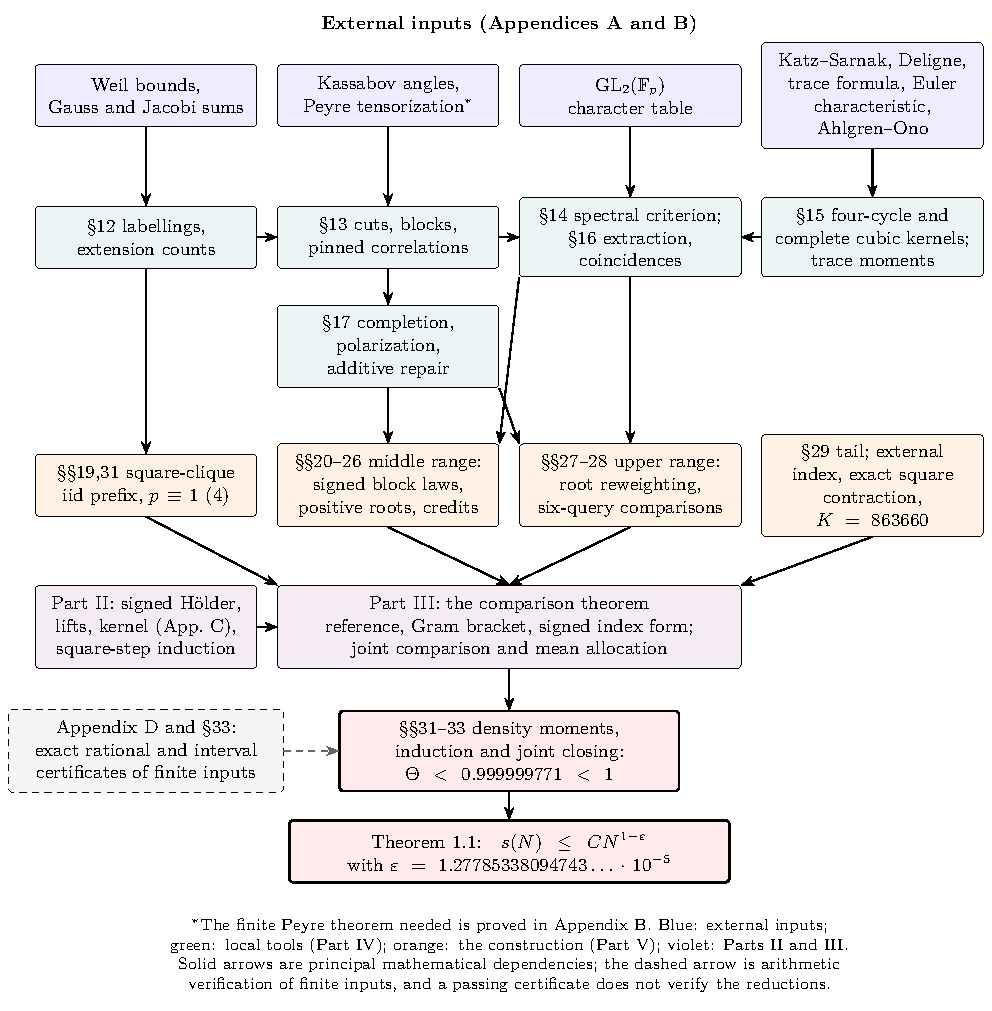
\includegraphics[width=\textwidth]{figures/dependency_graph.pdf}
\caption{Principal dependencies of the proof. External inputs feed the
local tools of Part~IV; these build the laws of the construction in
Part~V, which verify the hypotheses (CP0)--(CP8) of the comparison
theorem of Part~III. The selected density moments and induction extend
the analytic framework of Part~II; the normalized closing in
\cref{sec:four-routes-closing} then gives \cref{thm:main}. The dashed arrow
records finite arithmetic checks, whose scope is stated in
\cref{subsec:intro:status} and \cref{app:certificates}. The parts are
described in \cref{subsec:intro:outline}.}
\label{fig:intro:dependencies}
\end{figure}


The whole proof is organised around one average attached to $A$.
We define it in this subsection, show that it is large when $A$ is
dense, and then explain how the induction proves that it must in
fact be small. The rest of the paper either proves these two bounds
or constructs the distributions that make the second bound explicit.

\paragraph{The average $Y$.}
Write $\alpha=|A|/N$ for the density of $A$, and write
$N=\Kint\Lsc$, where $\Kint$ is a fixed number of intervals and
$\Lsc$ is the scale. There are $72$ \emph{slots}, forming a set $V$
(Step~1 below gives the exact array). A \emph{label} is an element
of a finite group $G_N$ built from residue classes at the primes;
a \emph{configuration} is a choice of one label $z_v$ for each slot
$v\in V$. Let $F_A$ be the truncated Fourier series of $\one_A$ on
$G_N$ (the \emph{Fourier lift} of $A$; see \cref{sec:lifts}). It has
mean $\alpha$, but it may take negative values. Finally, let $\mu$
be a probability distribution on configurations, built as a product
over blocks of primes. We call $\mu$ the \emph{reference law}, and
put
\[
  Y=\E_\mu\prod_{v\in V}F_A(z_v).
\]
Thus $Y$ is a $72$-fold Fourier average of $A$: we choose a random
configuration from $\mu$ and multiply the values of $F_A$ at its
$72$ labels. If $F_A$ were the constant $\alpha$, this would be
exactly $\alpha^{72}$.

\paragraph{Why $Y$ is large.}
The reference law $\mu$ is \emph{reflection positive}: for each of
several mirror symmetries of the slots, the matrix that couples the
two halves of a configuration is positive semidefinite
(\cref{sec:mechanism} informally, \cref{sec:positivity} formally).
Repeated Cauchy--Schwarz across these symmetries gives a signed
H\"older inequality, and hence
\[
  \alpha^{72}\le Y.
\]
The sign of $F_A$ is the point. For a nonnegative function this
would be an ordinary moment bound; here reflection positivity is
what makes the same conclusion available for the signed lift.
In particular, a dense set $A$ forces $Y$ to be large.

\paragraph{What we prove about $Y$.}
Against this, we prove an upper bound of the form
\[
  Y\le C\Lsc^{-a}\alpha^{\vartheta},
\]
where $a>0$ is fixed and $\vartheta=1$ in the baseline argument;
the final argument obtains the stronger exponent
$\vartheta=\FourRoutesDensity>1$. The two bounds together give
$\alpha^{72-\vartheta}\ll\Lsc^{-a}$, which is the power saving in
\cref{thm:main}.

The upper bound is proved by induction on the scale. Suppose it
failed, and look at the smallest scale $\Lsc$ where it could fail;
call this a \emph{least counterexample}. At every smaller scale
the bound is already known, and the whole comparison below takes
place at this one scale, with the smaller scales available as an
induction hypothesis.

\paragraph{Forcing six square differences.}
At a least counterexample we change the reference law $\mu$ into a
law that forces six specified pairs of slots, called
\emph{queries}, to receive labels differing by a square class at
every prime. For such a law the average is negligible compared
with $Y$: roughly, it counts pairs of elements of $A$ at square
distance, and $A$ has none. Making this precise is the kernel
estimate of Step~3 below; it is the only place where the hypothesis
that $A$ is square-difference-free is used directly.

The change of law is made in two stages, $\mu\to\lambda\to\nu$.
The \emph{first-stage law} $\lambda$ is obtained from $\mu$ by a
small number of explicit changes. (A \emph{record} is one weighted
summand in the explicit expansion of a local law; a
\emph{component} of a signed combination is one nonnegative summand
of that combination. The two words are distinct throughout.) The
\emph{comparison law} $\nu$ is a finite signed combination of
nonnegative laws, each of which \emph{accepts} the six queries:
almost surely, each query pair differs by a nonzero square at every
field prime (a prime whose coordinate in $G_N$ is $\Fp$) and by a
nonvanishing square class at the prime-power coordinates, and the
summand has the uniform one-slot marginals required in (CP4).
In informal prose we say such a summand \emph{forces} a square
difference when only the almost-sure square condition is meant;
\emph{accepts} always includes the marginal requirement. Their
formal definitions are (CP1), (CP2) and (CP4) in
\cref{sec:comparison-theorem}.

The law $\nu$ is signed, so it need not be reflection positive,
and the lower-bound argument does not apply to it. It is instead
controlled at one distinguished mirror symmetry $\iota$, the
\emph{reserved cut} (the other symmetries are used for the lower
bound). A positive law $\Nbr$ dominates $\lambda$ at this cut, in
the sense that the block matrix of cut forms
$\bigl(\begin{smallmatrix}\Nbr&\lambda\\
\lambda&\Nbr\end{smallmatrix}\bigr)$ is positive semidefinite
(written $\succeq_\iota0$ below), and a second pair of positive
laws dominates $\nu$ itself. The symmetric and \emph{skew}
(antisymmetric under $\iota$) parts of each change
$\nu-\lambda$ are dominated and priced separately.

\paragraph{What a price is.}
It remains to say what these changes cost. The primes are grouped
into \emph{blocks} $\Blk$; write $q_{\Blk}$ for the product of the
primes in $\Blk$. Fixing the labels at one block fixes a residue
class modulo $q_{\Blk}$, and splitting that class into progressions
with square step restricts $A$ to shorter progressions with square
step (Step~2 below). Those shorter sets
are still square-difference-free, so the induction hypothesis
applies to them. This is the only use of the induction hypothesis,
and its quantitative form is:

\begin{quote}
Changing the law at one block $\Blk$ changes $Y$ by at most
$(\text{size of the change})\times q_{\Blk}^{2a}\times Y$, up to a
factor $1+o(1)$ as $\Lsc\to\infty$.
\end{quote}

The product (size of the change)${}\times q_{\Blk}^{2a}$ is called
the \emph{price} of the change. The ``size'' is a total variation
or an operator norm, according to the kind of change, and norms are
always taken relative to the true one-half distributions of the
record being replaced (its \emph{actual marginals}), not relative
to a product approximation; the three precise forms are in
\cref{def:price} and are summarised in
\cref{subsec:intro:glossary}. Grouping primes into blocks means
the factor $q_{\Blk}^{2a}$ is paid once per block rather than once
per prime. Character sums bound the sizes: they measure how far
the local laws are from independent. The finite certificates of
Part~V then verify that, for one fully specified construction, all
these sizes are small enough; they check finite inequalities only,
not the analytic arguments (\cref{subsec:intro:status}).

So the task of the paper can be stated plainly: construct laws
that are reflection positive where the lower bound needs it, that
force the six square differences where the kernel estimate needs
it, and whose total price is strictly less than $1$. These three
requirements pull against each other, and most of the paper is
about meeting them simultaneously.

\paragraph{The six indices and the number $\Theta$.}
One point has been suppressed. The prime $2$ and the small primes
$p\equiv3\pmod4$ are not coordinates of $G_N$. Each query therefore
also carries an \emph{external index}: an interval number and a
residue modulo a fixed modulus. A signed average over the six
indices expands into $2^6=64$ terms. Every term that couples a
query across two adjacent intervals is negligible by the kernel
estimate, except when the next interval wraps cyclically from the
last interval back to the first; these exceptional terms are the
\emph{wrapping} terms, and they are priced separately.

Collecting the prices of all the changes above gives a single
number, which in the baseline argument is
\begin{equation}\label{eq:intro:closing}
 \Theta=\tfrac{63}{64}\bigl(L_0+\mathcal E\bigr)+J+W+\tfrac{1-m}{64}.
\end{equation}
Here $L_0$ is the total price of the first-stage change
$\mu\to\lambda$; $\mathcal E$ is the total dominated price of the
comparison change $\nu-\lambda$ at the reserved cut; $J$ bounds
the coupled terms coming from the external indices; $W$ bounds
the wrapping terms; and $m>1$ measures how much of the mean
(constant-function) part of $Y$ the dominating laws retain
(\cref{sec:matching-mean}), so the last term $(1-m)/64$ is a
credit. The factor $63/64$ records that the empty term of the
$64$-term expansion is the comparison average itself. All symbols
are defined fully in \cref{subsec:intro:inequality} and
\cref{sec:comparison-theorem}.

If $\Theta<1$, then at a least counterexample the priced upper
bound for $Y$ is incompatible with the lower bound
$\alpha^{72}\le Y$. Hence there is no least counterexample, and
the upper bound holds at every scale. This implication is the
comparison theorem, Theorem~C (\cref{thm:comparison}); its proof
(\cref{sec:comparison-lemmas,sec:comparison-proof}) uses nothing
about the particular local laws, and \cref{prop:mech:one-query}
shows the whole mechanism with a single query. The rest of the
paper verifies the hypotheses of Theorem~C for one explicit
construction and evaluates $\Theta$. For \cref{thm:main} the
improved stage then uses the joint form of this criterion
(\cref{cor:joint-closing}) together with the stronger density
induction; \eqref{eq:intro:closing} is its baseline form.

\paragraph{Why this shape gives a power saving.}
The conversion is worth isolating. Suppose that at some fixed
$a>0$, independent of the scale and of $\alpha$, the construction
above can be priced with $\Theta<1$. Then
$\alpha^{72-\vartheta}\ll\Lsc^{-a}$ at once, so
$\eps=a/(72-\vartheta)$: no iteration is needed, and the saving is
a fixed power for the elementary reason that the required win does
not shrink as $\alpha\to0$. This is also where the quantitative
difficulty lies. With only the first-order (Weil) bounds
$O(p^{-1/2})$ for the local character sums, the best certified
value of $\Theta$ is still larger than $1$
(\cref{subsec:intro:deligne}); the second-order bounds
$O(p^{-1})$ of Part~IV, the relative (actual-marginal) form of the
local estimates, and the variance and mean subtractions are what
bring the total price below $1$ at an explicit value of $a$.

\paragraph{Is this a density-increment argument?}
In ancestry, yes; in form, no. The classical arguments
\cite{PSS88,BloomMaynard} (and \cite{GreenSawhney}) assume that
$A$ is dense and square-difference-free, count square differences
by Fourier analysis, and deduce that $A$ has larger relative
density on a shorter structured set---a progression with square
step in \cite{PSS88}, a Bohr set in \cite{BloomMaynard}. Iterating
this increment until the density would exceed $1$ bounds $\alpha$.
Each step gains only a small factor in density and loses length,
so the final saving is smaller than any fixed power of $N$.

The present proof uses the same square-step rescaling, but it
never produces a denser set. Instead, the induction hypothesis at
all smaller scales is used at once, at a least counterexample, in
the form of prices: passing to the shorter progressions is what
makes a change of law at one block cost the factor
$q_{\Blk}^{2a}$. And the quantity being bounded is not the density
$\alpha$ itself but the $72$-fold average $Y$. This is where the
extra strength comes from. Since $\alpha^{72}\le Y\le
C\Lsc^{-a}\alpha^{\vartheta}$ with $\vartheta\approx1$, a single
constant-factor win---the inequality $\Theta<1$ at one scale---already
gives $\alpha^{72-\vartheta}\ll\Lsc^{-a}$: the $72$ slots amplify
one rescaling gain into a power saving, with no iteration and no
repeated loss of length. The cost of this amplification is that
$F_A$ changes sign, so the positivity that a density has for free
must be manufactured (this is the role of reflection positivity),
and the change of law must be priced in the actual marginals with
second-order character-sum bounds, so that the total price
converges at an explicit value of $a$.

\paragraph{The eleven ingredients, in order of first use.}
The genuine ideas, in the order in which the paper uses them, are:
(i)~reflection positivity across mirror symmetries of the slots;
(ii)~rescaling by progressions with square step, with an induction
linear in the density; (iii)~the kernel estimate of Step~3;
(iv)~handling small primes jointly through one signed external
index per query; (v)~graph laws made reflection positive by adding
correction summands, the principal law itself sometimes reweighted;
(vi)~replacements that keep the true one-half distributions, so
their differences pair to zero with constants and can be bounded by
operator norms; (vii)~controlling a signed, non-positive comparison
law by domination at one cut, with symmetric and antisymmetric
changes bounded separately; (viii)~signed combinations over a whole
block of primes whose first-order change is purely antisymmetric
(adding an edge together with its mirror is the simplest case);
(ix)~subtracting variance and related savings and retaining the
common mean, instead of bounding every term trivially;
(x)~square cliques for the primes $p\equiv1\pmod4$;
(xi)~exact star factorisation: a \emph{star} is a set of cross pairs
sharing one endpoint; for a half law invariant under the
square-affine maps $z\mapsto rz+t$ with $r$ a square unit, its Gram
matrix is computed exactly, so star sums reduce to finite matrix tests.

\paragraph{What is routine verification rather than a new idea.}
The spectral certificates for specific graphs, the matching partitions
and their extraction bookkeeping, the local constants of each prime
range, the block partitions and their degree sums, the completion
weights, the dominator witnesses, the tabulated middle prices, and the
arithmetic that evaluates $\Theta$. They sit
behind lemmas stated once, with the finite inputs in the appendices:
monotone majorants are checked at one endpoint, and polynomials with
nonnegative coefficients are evaluated at upper prices.


\subsection{The proof in five steps}\label{subsec:intro:steps}

The five steps are: (1)~a $72$-fold average at least $\alpha^{72}$;
(2)~rescaling to shorter progressions with square step;
(3)~the kernel estimate, the only use of no square differences;
(4)~local distributions, by prime range; (5)~summing the error
bounds and completing the induction.

\emph{Step 1. A $72$-fold average that is at least $\alpha^{72}$.}
Let $N=\Kint\Lsc$, where $\Kint=\PushK$ is a fixed number of intervals
and $\Lsc$ is the scale. The labels live in the finite group
$G_N=\prod_p\Z/p^{e_p}\Z$, the product over three kinds of primes: the
primes $p\equiv1\pmod4$ below $\Pfour=2^{512}$, with $e_p=2\mcl$ and
$\mcl=8192$; the primes $p\equiv3\pmod4$ in $[Q_3,\Pfour)$, where
$Q_3=19\,951\,586$; and all primes in $[\Pfour,N^{1/20}]$; the last two
kinds have $e_p=1$. The prime $2$ and the primes $p\equiv3\pmod4$ below
$Q_3$ are not coordinates; they enter through the external index of
Step~4. The lift $F_A(z)=\sum_\xi\widehat{\one_A}(\xi)e(z\cdot\xi)$ sums,
over the characters $\xi$ of $G_N$ of conductor at most $N^{1/20}$, the
normalized exponential sums $\widehat{\one_A}(\xi)=N^{-1}\sum_{n\in
A}e(-n\xi)$; it has mean $\alpha=|A|/N$, but it may be negative. The $72$
slots are $V=(\Z/6\Z)^2\times\{0,1\}$: two six-chamber coordinates and a
layer. Given a probability law $\mu$ on labellings $z\colon V\to G_N$, put
$Y=\E_\mu\prod_{v\in V}F_A(z_v)$ (\cref{def:record:functional}).

Reflection positivity says that, at specified cuts of the slots, the
matrix of the two halves is positive semidefinite. Here the cuts are the
three chamber reflections of each six-chamber coordinate and the reserved
cut $\iota$, which flips the layer; their folds sort $V$
(\cref{lem:slot-array}). Repeated Cauchy--Schwarz then gives a signed
H\"older inequality. Unlike an ordinary moment, this still works for
functions that change sign. Reflection
positivity entered through statistical mechanics and constructive field
theory \cite{FrohlichSimonSpencer76,DysonLiebSimon78,FrohlichLieb,FILS,
GlimmJaffe87}; in combinatorics the same positive-semidefinite formalism
underlies graph-homomorphism inequalities and flag algebras
\cite{ConlonLee,HatamiNorine11,Razborov07,LovaszGraphLimits12,
BorgsChayesLovaszSosVesztergombi08}. The finite version needed here is
\cref{thm:holder}. For the reference law
$\mu=\bigotimes_{\Blk}\mu_{\Blk}$ of the construction, a product of laws
on blocks of primes that are reflection positive at all these cuts and
square-affine invariant, it gives $\alpha^{72}\le Y$
(\cref{lem:record:holder}).

\emph{Step 2. Rescaling to shorter progressions with square step.}
Fixing the labels at a block of primes specifies an integer residue
class. Splitting it into progressions of square step rescales the
problem to a shorter interval while preserving square-difference
avoidance; the step is the least square divisible by the modulus
(\cref{lem:record:fibre-scale}). The errors in this comparison are
controlled in \cref{sec:lifts,sec:scale-comparison}. At a least
counterexample to $Y\le C\Lsc^{-a}\alpha$ (a smallest scale where
the bound fails, so it holds at every smaller scale) this gives the
prices of \cref{subsec:intro:method}: each slot contributes a factor
$(q_{\Blk}^2)^{a/72}$, hence $q_{\Blk}^{2a}$ over $72$ slots, times
the size of the change at $\Blk$. The moment bounds are linear in $\alpha$, so the
induction keeps the full density factor: from
$\alpha^{72}\le Y\le C\Lsc^{-a}\alpha$ one obtains $\alpha\le C'N^{-a/71}$,
which is the conversion $\eps=a/71$ (\cref{thm:record:lineardensity}).

\emph{Step 3. The kernel estimate: the only use of no square differences.}
Suppose two slots are placed in adjacent intervals and, at every
prime, their labels are forced to differ by a square class. Then the
corresponding Fourier average is negligible: roughly, it counts
pairs from $A$ at square distance, and $A$ has none. Making this
precise is a circle-method calculation with a kernel supported on
squares, for Fourier frequencies up to $N^{1/20}$
(\cref{sec:kernel,app:kernel20}). This is the only step that
directly uses the defining property of $A$. Everything else in the
proof is about arranging, at small price, that six such forced
pairs occur.

\emph{Step 4. Local distributions, by prime range.}
No single elementary estimate is efficient for every prime, and the class
of $p$ modulo $4$ matters. If $p\equiv1\pmod4$, then $-1$ is a square and
the strict-square relation $y-x\in\Qsq$ is symmetric. If $p\equiv3\pmod4$,
exactly one of $y-x$ and $x-y$ is a nonzero square, and the relation is a
tournament, the Paley tournament. The construction has five ranges.
\begin{itemize}
\item \emph{The small modulus.} The external modulus is
$\Mzero=2^{129}\prod_{3\le p<Q_3,\,p\equiv3\,(4)}p^{128}$.
Each query carries an index $(b,s)$: an interval number and a
residue modulo $\Mzero$. Its coupled index is $(b+1,s+r)$, where $r$
is a random square residue. Averaging over $r$ by its exact
conductor gives one number $R_I$ per query, which is how the small
primes enter the closing sum
(\cref{lem:imp:padic-envelope,prop:imp:padic-price,sec:tail-index}).
\item \emph{The class-one prefix.} At the primes $p\equiv1\pmod4$ below
$2^{512}$ the labels are drawn conditionally independently from a random
square clique of $\Z/p^{2\mcl}\Z$, a set whose nonzero differences are
even powers of $p$ times unit squares. This law is reflection positive at
every cut and accepts every query except on the event, of mass
$2^{-\mcl}$ at each such prime, that the two endpoint labels of a
query coincide at that prime,
which the comparison law deletes, at a total price below
$8\cdot10^{-69}$ over all these primes
(\cref{sec:frontier:iidprefix}).
\item \emph{The middle range.} The primes $p\equiv3\pmod4$ in
$[Q_3,\Pthree)$, $\Pthree=167\cdot2^{40}$, are grouped into blocks $\Blk$
with $\sum_{p\in\Blk}\log p\le L=570$, in $33$ pieces. Each block carries a
twelve-label law, completed to a reflection-positive law, and the
comparison records built on it; on the seven largest pieces the
principal twelve-label law is reweighted by a nonnegative function
(\crefrange{sec:middle-reference}{sec:matching-mean}).
\item \emph{The upper range.} The primes $p\equiv3\pmod4$ in
$[\Pthree,2^{512})$, in $310$ bands, carry the completed two-layer law on
all $72$ slots, on blocks with $\sum\log p$ at most a band-dependent
bound ($\le886$) (\cref{sec:upper-reference,sec:upper-comparison}).
\item \emph{Large primes.} Every prime $p\ge2^{512}$, of either
class, forms a block by itself, with price of order $p^{-3/2+2a}$,
hence summable (\cref{sec:tail-index}).
\end{itemize}
The middle and upper laws start from a graph law: the uniform law on
labellings of a small graph by distinct labels whose edges are
strict-square constraints. A graph law is not reflection positive at
chamber cuts: its negative cut spectrum, of order $p^{-1/2}$, is
cancelled by adding folds, matchings, merges and constants with weights
in powers of $p^{-1/2}$; this is a \emph{completion}
(\cref{lem:five-type}). The weights are dictated by spectral bounds for
cut operators (\cref{thm:spectral-criterion,subsec:spec:actual-stars}).
Weil's bound controls them
to first order; the second-order control needed in the middle and upper
ranges comes from the bounds of \cref{subsec:intro:deligne}. The
comparison law keeps every summand that already forces the six
square differences, replaces most others by forcing laws with the
same one-half distributions, and deletes the rest; the price of
each replacement is what Step~5 sums.

\emph{Step 5. Summing the error bounds and completing the induction.}
Each changed record of a block contributes its norm, relative to the
actual half marginals, times $q_{\Blk}^{2a}$. On a block of logarithmic
size at most $L$ the factor $q_{\Blk}^{2a}\le e^{2aL}$ is bounded, while
the local errors are those of its least prime. The prices are summed
over each range with exact prime products and sieved counts below
explicit thresholds and the explicit Chebyshev bound of Bennett, Martin,
O'Bryant and Rechnitzer for primes $p\equiv3\pmod4$ above them
(\cref{thm:bmor}; compare the explicit prime-number literature
\cite{RosserSchoenfeld75,PlattTrudgian21}); the sum over the large
primes is bounded by comparison with an integral. A
signed product over the six disjoint queries amplifies the cancellation
of Step~3. The comparison theorem turns the totals into the single number
$\Theta$, and the proof closes because $\Theta<1$
(\cref{subsec:intro:inequality}).

\subsection{What is inherited from the OpenAI preprint, and what is new here}
\label{subsec:intro:new}

The overall architecture---signed functional, square-step comparison,
actual-square kernel, separate treatment of the exceptional
wrapping terms $W$, and induction---is inherited
from \cite{OpenAI}. Its Fourier-lift and density-comparison steps are
descendants of the classical Roth--Gowers density-increment method
\cite{Roth53,Bourgain99,Gowers01,Sanders11,TaoVu06}, but the
reflection-positive functional replaces a single density increment by
an induction on a much larger multilinear average. The explicit
exponent comes from changing the local laws and the accounting at
almost every quantitative interface.

\paragraph{Where the larger exponent comes from.}
In both proofs the final exponent has the form
$\eps=(\text{scale exponent})/(\text{number of slots})$, and two
separate effects make ours larger; they multiply. The first is the
denominator: the displayed OpenAI construction uses
$d=(24!)^{161}$ slots, with $\log_{10}d\approx3830.63$
(\cref{app:openai-constant}), where we use $72$; at an equal scale
exponent this alone gains about $3829$ orders of magnitude. The
second is the numerator. The OpenAI argument does not quantify its
local estimates, and for its displayed parameters the scale
exponent is forced down by its mixing and modulus thresholds,
making $\eps$ triple-exponentially small
(\cref{app:openai-constant}). Here every local law is rebuilt so
that its price can be summed explicitly: relative rather than
absolute graph estimates, primes grouped into blocks of bounded
budget ($\sum\log p\le570$ in the middle range), norms in the
actual marginals, second-order character-sum bounds, and the
variance and mean subtractions. The outcome is that $\Theta<1$
already at $a=\FourRoutesA\approx9.07\cdot10^{-4}$, and hence
$\eps=a/(72-\vartheta)\approx1.28\cdot10^{-5}$. The items below
are the local changes behind this second effect; the most recent
refinements (the joint mean allocation and the cross-weighted
upper reweighting) improve $\eps$ only by a few percent on top.

\begin{description}[leftmargin=2.2em,style=nextline]
\item[Finite rectangle instead of an enormous one]
The displayed OpenAI construction uses $d=(24!)^{161}$ slots. Here
$V=(\Z/6\Z)^2\times\{0,1\}$ has $72$ slots. This alone changes the
conversion $\eps\approx a/d$ by many orders of magnitude. It also leaves
much less room for waste in the local estimates.

\item[Relative, not merely absolute, graph estimates]
A square-constraint graph over $\F_p$ has very small density.
Weil's bound estimates how many labels remain available after some
neighbours are fixed. We divide by the graph's own expected density
before normalising, so the relevant error is relative. This is what lets
the same construction be used at explicit thresholds.

\item[Small primes enter through a coupled external index]
The prime $2$ and the primes $p\equiv3\pmod4$ below the middle threshold
enter a fixed modulus. Instead of
estimating the rare event that all of their residues are simultaneously
good, the proof couples the index of each query with a shifted copy, so
that a selected difference is forced into a nonvanishing square class.
The resulting price factor is the explicit conductor moment
$R_I$. Exact norm envelopes at
successive prime-power depths and the least square step determine its finite
product (\cref{lem:imp:padic-envelope,prop:imp:padic-price}); the original
prime moments remain an efficiently evaluated upper majorant for its
large-prime part (\cref{cor:imp:padic-majorant,lem:index-moments}).

\item[Dependence after fixing labels is bounded as an operator norm]
After some labels are fixed, the remaining labels are not independent.
Kassabov's subspace-angle inequalities \cite{Kassabov} control
dependence between two labels, and Peyre's maximal-correlation theorem
\cite{Peyre} combines these into bounds between sets of labels;
maximal correlation itself goes back to
\cite{Hirschfeld35,Renyi59,AhlswedeGacs76}. The finite form of Peyre's
result needed here (\cref{thm:peyre-finite}) is proved in
\cref{app:peyre}.
These estimates turn a heuristic ``almost independent'' into operator
bounds that can be inserted into the budget.

\item[Completions instead of independence]
Graph laws are not assumed independent across a cut, nor reflection
positive. Their negative cut spectrum is small and explicit, and the
positive corrections of a completion cancel it; the weights satisfy a few
explicit inequalities dictated by the spectral bounds
(\cref{lem:five-type}).

\item[Non-forcing records are replaced or deleted, not bounded by a union bound]
Records of the reference that do not accept the queries are repaired or
deleted, not covered by a union bound over obstructions. Polarization and
additive repairs produce positive records that impose the query
constraints and keep the actual conditional marginals of the records they
replace. A record difference then annihilates constants, and a record of
weight $O(p^{-1/2})$ costs $O(p^{-1})$.

\item[A comparison law that is not reflection positive]
The accepting law is not assumed reflection positive, and in the middle
range it is a signed combination of nonnegative accepting laws. It is
compared with the first stage at one distinguished cut only, where
a positive law dominates it in the $2\times2$ block sense; its
changes are split into symmetric and antisymmetric parts with
separate bounds, the antisymmetric price entering the closing sum
only through $\cosh A$. The cancellation of Step~3 is applied to each
nonnegative product component, so the signs cost only a constant in a
vanishing remainder (\cref{sec:comparison-theorem}).

\item[Signed whole-block laws and positive envelopes]
In the middle range a fold record of the comparison law is a signed
mixture, taken after the products over the primes of a block, of three
positive accepting laws, each repaired to the actual half marginal of the
record it replaces (\cref{def:record:mixture}). Its first-order change
against that record is purely skew: at a prime $p$, a three-arm star of
norm about $1.2732\,p^{-1/2}$ at the parameter $\tlaw=127/500$. The case
$\tlaw=0$ is mirror pairing, which adds to the record the query edge
together with its mirror image under the reserved reflection; its star has
two arms and norm about $\sqrt2\,p^{-1/2}$ (\cref{lem:mirror}). The
variation $1+\tlaw$ of the mixture
does not grow with the number of primes.
Products of two, four or six antisymmetric changes on distinct
blocks are bounded by quantities smaller than the trivial norm
estimate, using positive semidefinite dominating matrices,
averaged over reflections
(\cref{sec:middle-records,sec:envelopes}).

\item[Norms are taken in the marginals of the record being replaced]
Local laws are measured in the true one-half distribution of the
record they replace, not in a product approximation. Leading terms
and remainders (including coincident labels) are bounded
separately, and simultaneous changes on several blocks by a power
series with nonnegative coefficients in those bounds
(\cref{lem:actual-features,lem:middle-comparison-prices,lem:record:record-expansion}).
In the final upper range, extraction is cross-weighted: the conditional
density of the witness labels is retained together with its cover
marginal, rather than bounded separately and multiplied. The resulting
smaller root caps lead to recomputed completion weights on $301$ bands
(\cref{lem:matching:extractionk,subsec:upper-cross-weighted}).

\item[Star-shaped features with exactly computable Gram matrices]
The star features of a square-affine invariant law have exact Gram
matrices, so the leading part of a cut operator is a finite signed matrix
of star incidences, certified by exact positivity tests
(\cref{subsec:spec:actual-stars}). This gives the bound at one
chamber symmetry for the principal middle law, whose leading star
matrix has norm exactly $\sqrt{30}$ (\cref{subsec:middle-l20}), and
several upper-range bounds where old and new star matrices differ
in only a few entries (\cref{sec:upper-comparison,lem:joint-rows}).

\item[Reweighting the principal twelve-label law by a nonnegative function]
On the seven largest middle subranges the principal twelve-label law
(the weight-$1$ summand, called a \emph{root} in Part~V; the word has
nothing to do with square roots) is reweighted, at every prime, by
averages of squares of affine functions of three quartic trace
statistics, or by a $39$-trace square with a positive constant added
(\cref{def:positive-root}). The reweighting keeps the symmetries,
keeps the support inside the accepting set, and improves the
one-sided spectral bound across a chamber symmetry; the changed
one-half marginal is accounted for separately
(\cref{sec:positive-roots}).

\item[Errors are tensored at the cut where they are largest]
The two repaired folded matching records of the first stage attain
their largest cut norms (their sharp prices) at different cuts.
All record differences whose sharp price is attained at one cut
are tensored there, which makes the first-stage error and the
error part of the bracket about sixteen times smaller than a bound
with one sharp factor per term
(\cref{lem:sharp-first,cor:two-cut-series}).

\item[Subtractions in the closing inequality (variance, dominators, mean)]
Three quantities are subtracted (or, for the mean, credited) in
$\Theta$ rather than bounded trivially: the variance saved when a
replacement preserves one-half distributions
(\cref{sec:variance}); the saving from dominating matrices for
products of changes (\cref{sec:envelopes,prop:signed-sides}); and
the common mean energy $m>1$ retained from the six indices
(\cref{sec:matching-mean}). In the final closing, higher mean
contributions are allocated jointly against the same labelled positive
comparison coefficients before upper prices are substituted; only the
residual series with nonnegative coefficients is then completed
(\cref{cor:joint-closing,subsec:joint-mean}). If only the variance and dominator
savings were removed, with all other credits kept, $\Theta$ would
exceed $1$ by about $0.46$ in the baseline; see
\cref{subsec:intro:inequality}.

\item[Improving the power of $\alpha$ in the induction]
The baseline moment bounds are linear in the density, with conversion
$\eps=a/71$. The final argument strengthens this to
$\alpha^{\FourRoutesDensity}$. Most laws are controlled by grouping
labels in pairs; rare cases where many labels coincide are instead
handled by fixing (\emph{pinning}) the coinciding labels and
rescaling the resulting shorter progressions, and a new prefix law
with independent labels
removes repeated-label concentration. These steps are proved after
the baseline closing (\cref{sec:density:moments-prefix} and
\cref{sec:density-upgrade}). The comparison error is bounded before
the operator reduction, and the square-step main term is then
estimated with the actual folded laws and their mixed moments,
as in \cref{prop:density:production}.

\item[A kernel for larger cutoffs]
The actual-square kernel is proved for Fourier cutoffs up to $N^{1/20}$
and for prime-power moduli (\cref{app:kernel20}), so that the class-one
primes can carry labels modulo $p^{2\mcl}$.

\item[Estimates are verified at explicit prime thresholds]
The middle range starts at $Q_3=19\,951\,586$ and the upper range at
$\Pthree=167\cdot2^{40}$. These are not asymptotic placeholders: at the chosen
thresholds, exact rational matrices and interval inequalities verify the
hypotheses of the analytic lemmas, and monotone majorants carry each
check to all larger primes. \Cref{app:certificates} states precisely which
assertions are computational.
\end{description}

\paragraph{The general machinery and the earlier explicit design.}
The first explicit versions of this argument used the slot array
$(\Z/6\Z)^3$, with $216$ slots, and a reserved cut that was a chamber
reflection of the third coordinate. Most of the general machinery of
Parts~II--IV was developed for that $216$-slot design: the chessboard
calculus on products of reflection coordinates; lifts, moments, conductor
decay and the actual-square kernel; the external index and its coupling;
graph laws with Weil-type insertion counts and pinned influence; the
spectral criterion with its coupling block, its witness extraction and the
four-cycle bound; completions by folds, matchings, merges and constants;
and the comparison of three laws, an all-cut reference, an intermediate
law and an accepting law, by polarization and additive repairs that keep
the actual conditional marginals. Parts~II--IV state it once, in the
generality the final design uses. The final proof is that design
re-instantiated on $72$ slots, with new local laws and four structural
substitutions (\cref{tab:walk:substitutions}): a two-point layer whose
flip is the reserved cut replaces the third six-chamber coordinate, which
changes the conversion at the same $a$ from $a/(216-\vartheta)$ to
$a/(72-\vartheta)$, hence to $a/71$ for the density-linear
induction with $\vartheta=1$; six disjoint one-way queries
with a common signed index replace coupled families of amplified edges and
their obstruction covers; the comparison law is not reflection positive,
and is controlled at the reserved cut by a positive $2\times2$
block; and the primes are divided by
their class modulo $4$ into the ranges of Step~4. What the final theorem
does not use are the instances of the $216$-slot design: its particular
laws, constants and certificates, and the proofs of its checkpoints.
\Cref{sec:design-walk} explains each substitution as the answer to a
quantitative failure, and \cref{subsec:history:216} lists what survives of
each part of that design.

\subsection{Where the Deligne bound enters}\label{subsec:intro:deligne}

It is useful to separate first-order and second-order character sums.

For one square constraint, or for counting extensions of one label at a
time, the relevant sums contain one quadratic character of a polynomial
with distinct roots. Weil's bound \cite{Weil48,Weil49,Schmidt76} gives
square-root cancellation: after the normalisations of
\cref{sec:labellings}, the
relative error is $O(p^{-1/2})$. Gauss and Jacobi sums evaluate the
constant Fourier blocks exactly \cite{BerndtEvansWilliams,IrelandRosen}.
These tools suffice for a large part of the construction and already
appear, in a simpler form, in the OpenAI argument.

The difficulty is that the spectral estimates are conditional. One has
fixed part of a graph labelling and must compare the joint law of two
remaining labels with a product law. Errors from two one-variable counts
can correlate. Bounding each separately by $O(p^{-1/2})$ is not enough
for the negative spectral side: several terms must be $O(p^{-1})$ after
normalisation, uniformly in the fixed labels and in the polynomials
arising from the graph. A model sum is
\[
  \sum_{y,z\in\F_p}\chi\bigl(f(y)g(z)(y-z)\bigr),
\]
where $\chi$ is the quadratic character and $f,g$ have controlled
degrees and distinct roots. This is the content of \cref{thm:dl:H2}.

There is no single black box in the proof.
Four algebraic-geometric facts are combined:
\begin{enumerate}[label=(\roman*)]
\item The Grothendieck--Lefschetz trace formula rewrites the character
sum as a trace of Frobenius on compactly supported cohomology.
\item For the family of curves $y^2=f(x)(x-z)$, Katz--Sarnak
\cite{KatzSarnak} identify the relevant sheaf: it is lisse, tame, pure and
geometrically irreducible, with large symplectic monodromy. In elementary
language, as the parameter $z$ moves there is no hidden invariant
direction in which all the errors point the same way.
\item The Grothendieck--Ogg--\v Safarevi\v c formula bounds the
dimension of the cohomology in terms of the degrees and ramification.
This is where the explicit, degree-dependent constant comes from.
\item Deligne's theorem on weights \cite{DeligneWeilI,DeligneWeilII}
bounds the Frobenius eigenvalues. After the normalisations in the
spectral problem, this yields the required $O(p^{-1})$ rather than
$O(p^{-1/2})$.
\end{enumerate}
The precise external statements are isolated in \cref{app:external}
(\cref{thm:prelim:ks}); their conversion into the estimates used by the
local laws is carried out in \cref{sec:dl}. A reader willing to accept
\cref{thm:dl:H2} and the second moments of \cref{sec:dl} as named
character-sum estimates can read the rest of the proof without following
the sheaf argument.

A second, different second-order input concerns the complete bipartite
graph $K_{2,2}$. Its character kernel is invariant under
$\mathrm{PGL}_2(\F_p)$. The character table of $\mathrm{GL}_2(\F_p)$
therefore decomposes it into representation blocks, and Gauss--Jacobi
identities bound those blocks. The resulting normalised estimate is $2/p$
(\cref{thm:dl:K}). This is representation theory, not the Katz--Sarnak
sheaf input, although both feed the same spectral envelopes.

In the construction these bounds are used wherever two remaining
labels must be compared with independent labels: in the spectral
bounds for middle and upper laws (\cref{sec:spectral}), in the
non-star terms of the character expansion
(\cref{sec:extraction}), and in conditional distributions given a
fixed middle label. The same sheaf family also gives mean-square
bounds for trace functions with one free label, used for the two
principal upper cuts below $2^{52}$
(\cref{thm:record:direct-star}). Precise entry points are cited in
each Part~V section.

Two later local estimates should be distinguished. The complete
$K_{3,3}$ character kernel is bounded by an exact polynomial-resultant
Gram identity, not by the cohomological input above
(\cref{thm:cubic-resultant}). The centred rectangle bound uses the
symmetric square of the same Legendre sheaf, through the Mellin
eigenvalue estimate of \cref{lem:rectangle-mellin}; its weaker
$128q$ form avoids that symmetric-square step
(\cref{thm:rectangle-gram}).

This is the same circle of ideas as the modern theory of algebraic
trace functions. Fouvry--Kowalski--Michel recast many character and
exponential sums as Frobenius traces, then use Deligne's bounds and
monodromy to show that no main term survives
\cite{FKMPrimes14,FKMTwists15}. Will Sawin's work is a prominent part
of that programme, both over the integers---bilinear forms with
Kloosterman and more general trace functions
\cite{KMS17,KMS20,FKMSBilinearTrace25}---and over
$\mathbf F_q[T]$, where the geometry is strong enough to prove
function-field Chowla/twin-prime statements and near-square-root
cancellation for factorization functions
\cite{SawinShusterman22,SawinFactorization24,KowalskiBourbakiSawinShusterman}.
His quantitative sheaf theory \cite{SawinQST23} also addresses the
same practical question faced here: after Deligne gives square-root
size for Frobenius eigenvalues, how does one bound how many of them
there are, uniformly and explicitly?

The overlap is methodological rather than a direct dependence. We do
not quote a theorem of Sawin. Our sheaves come from one fixed family
$y^2=f(x)(x-z)$ over $\F_p$, arising from two remaining labels in the
graphs of the local laws; the required output is not an asymptotic
cancellation statement but an explicit $O(p^{-1})$ spectral envelope
with a degree-dependent constant that can be inserted into the spectral
caps at explicit thresholds. The Sawin--Shusterman results cited above
concern increasing polynomial degree over a fixed finite field satisfying
their size and characteristic hypotheses. What is shared is the
mechanism: interpret a character sum cohomologically, use monodromy
to exclude a hidden main term, bound conductors and cohomology
dimensions, and let Deligne's weights supply the cancellation.

One further input is modular. The second moment of the neighbourhood
count behind the variance credits of the middle range
(\cref{lem:record:weighted-moment}) contains the twisted second moment
$\sum_\lambda\chi(\lambda)T_\lambda^2$ of the point counts
$T_\lambda=\sum_y\chi\bigl(y(y-1)(y-\lambda)\bigr)$ of the Legendre family
of elliptic curves, for which Weil's bound alone gives only $O(p^2)$.
Ahlgren and Ono \cite{AhlgrenOno2000} evaluate it as $-p-a(p)$, where
$a(p)$ is the $p$-th coefficient of the weight-four cusp form
$\eta(2z)^4\eta(4z)^4$ of level~$8$, and Deligne's proof of the
Ramanujan--Petersson conjecture \cite{DeligneWeilI} gives
$|a(p)|\le2p^{3/2}$ (\cref{thm:ahlgren-ono}). With this evaluation the normalised second moment
$\E[P_{\rm adm}\mathcal W^2]/p^2$ of
\cref{lem:record:weighted-moment} is at most $5/p+O(p^{-3/2})$,
while the general bound for the graph moments it contains gives
only $10/p+O(p^{-3/2})$. Through the root-half variances of the
middle roots it enters the recomputation (restoration) of the
variance credits after a tilt changes the root half marginal
(\cref{sec:variance}) and the cut caps of the middle roots
(\cref{subsec:middle-l20,sec:positive-roots}).

\paragraph{Why the qualitative result did not need second-order bounds.}
They were unnecessary, not unavailable. The OpenAI theorem asserts the
existence of some $\eps>0$. For that purpose one may choose an enormous
number of slots and an enormous prime threshold, and lose very large
absolute constants, provided the errors eventually become small. The
elementary one-edge Gauss-sum calculation and telescoping graph
estimates in \cite[Section~2]{OpenAI} are enough for that qualitative
conclusion.

An explicit exponent is stricter in three ways. First, $d=72$, so there
is no huge denominator in which to hide losses when passing from the
functional exponent $a$ to $\eps=a/71$. Secondly, the laws must be
certified at named finite thresholds, principally $Q_3=19\,951\,586$ in
the middle range and $\Pthree=167\cdot2^{40}$ in the upper range. Thirdly,
the closing sum has no room for a correlated first-order term: the certified
spectral caps, completion variances and upper-root bounds are evaluated
with the second-order estimates, and the baseline closing margin
$1-\Theta$ is only about $2.7\cdot10^{-11}$ (the final joint closing
margin is $>2.29\cdot10^{-7}$), so the certified exponents depend on
them. The closing certificates use the four-cycle bound, Deligne's
theorems, Katz--Sarnak and the evaluation of Ahlgren and Ono to obtain the
second-order bounds entering that budget. This
explains their role in this proof; it does not establish that these
inputs are necessary for a comparable exponent by another argument, and
whether a smaller exponent can be certified with first-order bounds alone
has not been tested.

\subsection{The closing inequality \texorpdfstring{$\Theta<1$}{Theta<1} in the baseline (\texorpdfstring{$\vartheta=1$}{vartheta=1})}\label{subsec:intro:inequality}

The comparison theorem (\cref{thm:comparison}, Theorem~C) reduces the
baseline ($\theta=1$, where $\theta$ denotes $\vartheta$ in Part~III)
to nine hypotheses (CP0)--(CP8)---standing data, reference law,
first-stage law, domination at the reserved cut, comparison law,
optional sharper bounds for named families of simultaneous record
changes, dominators for the comparison law,
mean energies, and admissibility---and to the single inequality
$\Theta<1$ for the number \eqref{eq:intro:closing} with $k=6$ queries
on $d=72$ slots, where
\begin{gather*}
 \mathcal E=B\bigl(e^S\cosh A-1\bigr)-D,\qquad
 J=Be^T\Bigl(\frac{R_I}2\Bigr)^6,\\
 W=Be^{S+A}\Bigl[\Bigl(1+\frac{R_I}{2}\,\Kint^{-35/36}\Bigr)^6-1\Bigr].
\end{gather*}
Here $S$ and $A$ are the total symmetric and skew prices of
$\nu-\lambda$, $B$ is the energy factor of the law dominating
$\lambda$ (so $\mathcal E$ is the dominated price bound with savings
$D$ subtracted), $T$ is the total dominator price entering through
$e^T$ (not an exponent of $p$), $R_I=\E(\Kint\operatorname{sq}(D))^{2a/72}$
is the conductor factor of one external index (\cref{def:hyb:coupled}),
and the displayed formula for $\mathcal E$ is the baseline
specialisation of the general complete-polynomial bound $\Psi$ of
Theorem~C (that is, an admissible upper bound for $\Psi$ at the
baseline prices, in the notation of \cref{thm:comparison}). The $63/64$ factor records that the empty term of
the signed-index expansion is the comparison average itself; in $J$
each query contributes $R_I/2$; $W$ bounds the terms in which every
active query wraps from the last interval to the first; and $m>1$
lowers $\Theta$ through $(1-m)/64$ (\cref{rem:cp:reading}).

Each quantity is constructed in Part~V. The first stage $\lambda$
differs from $\mu$ only on middle blocks; its price $L_0$ and the
dominating law $\Nbr$, with energy factor $B=e^{U_0}+R_{\rm err}$
(where $U_0$ is the total price of the positive records added to
$\mu$ in the bracket and $R_{\rm err}$ is the remaining two-cut
first-stage error, \cref{def:cp3}), are
constructed in \cref{sec:middle-frame}. The prices $S$ and $A$ are
summed over all prime ranges: the deleted coincident-label event of
the $p\equiv1\pmod4$ prefix (\cref{sec:frontier:iidprefix}, in the
baseline counted in $S$ only), the middle-range replacements
(\cref{sec:middle-records}), the upper-range replacements
(\cref{sec:upper-comparison}), and the large primes
(\cref{sec:tail-index}). The savings $D$ are the variance savings of
\cref{sec:variance} together with the dominator savings of
\cref{sec:envelopes} for even products of skew differences. The
price total $T$ and the mean constant $m$ come from the dominators
of $\nu$ in \cref{sec:matching-mean}; $R_I$, $J$ and $W$ are computed
from the index law at $\Kint=\PushK$ (\cref{sec:tail-index}).
\Cref{sec:closing} assembles the baseline $\Theta$; middle prices
first computed at the evaluation exponent $a_0=\PushAnchor<a$ are
converted to $a$ by $t=e^{2(a-a_0)L}$ with $L=570$ (this conversion
is called \emph{repricing} and needs $a\ge a_0$), and upper prices
are converted band by band from $a_{\rm u}=883/10^6<a$.
\Cref{tab:intro:values} lists the baseline values only. The improved
closing in \cref{sec:four-routes-closing} uses
$a=\FourRoutesA$, $K=\FourRoutesK$ and
$\vartheta=\FourRoutesDensity$, replaces the wrap exponent by
$-1+\vartheta/36$, recomputes every price, and counts the new prefix
deletion in both $S$ and $A$; its value
$\Theta<\FourRoutesTheta$ is the one used for \cref{thm:main}.
With those recomputed prices, the final closing number is
\[
 \Theta=\frac{63}{64}(L_0+\mathcal E)+J+W+
 \frac{1-m_1}{64}-\Delta_{\rm mid}-\Delta_u+\mathcal R_u
 <\FourRoutesTheta<1,
\]
where $m_1$ retains only the one-block mean terms, after the
first-stage error reserve, $\Delta_{\rm mid}$ and $\Delta_u$ are the
joint middle and finite-upper mean allocations, and $\mathcal R_u$
is the reserve for the latter allocation. The allocations are made
inside the common positive completion before the shared energies are
replaced by upper prices; they replace the higher-degree mean credits
of \cref{prop:record:mean-credit} and are not additional credits to
be added to the baseline $m$. This is
\eqref{eq:final-joint-closing}; its complete ledger is in
\cref{sec:four-routes-closing}.

\begin{table}[ht]
\centering
\caption{Baseline closing only ($\vartheta=1$, $a=\PushA$; this table
does not prove \cref{thm:main}, whose improved values are in
\cref{sec:four-routes-closing}): certified upper ($<$) and lower
($>$) bounds, rounded outward; $\ldots$ marks an exactly defined
number (\cref{tab:closing-values} gives more digits).}
\label{tab:intro:values}
\small
\begin{tabular}{@{}lll@{}}
\toprule
term & meaning & value\\
\midrule
$t$ & repricing factor $e^{2(a-a_0)L}$ of the middle prices & $1.0000000616512\ldots$\\
$U_0$ & exponent in $e^{U_0}$ below (dominating law) & $<0.84691$\\
$B$ & energy factor $e^{U_0}+R_{\rm err}$ of that law & $<2.33263$\\
$L_0$ & total price of $\mu\to\lambda$ & $<4.7634\cdot10^{-4}$\\
$S$ & total symmetric price of $\nu-\lambda$ & $<0.014555$\\
$A$ & total skew price of $\nu-\lambda$ & $<0.96928$\\
$D$ & savings; of these, variance part $D_{\rm var}>0.0099585$ & $>0.46685$\\
$\mathcal E$ & dominated bound $B(e^S\cosh A-1)-D$ & $<0.76897$\\
$T$ & dominator price total (in $e^T$) & $<0.60760$\\
$R_I$ & conductor factor of one index, $\Kint=\PushK$ & $<1.24714$\\
$J$ & coupled term $Be^T(R_I/2)^6$ & $<0.25177$\\
$W$ & wrapping bound & $<3.8345\cdot10^{-5}$\\
$m$ & mean constant (trivial value $1$) & $>1.58994$\\
$\Theta$ & closing number \eqref{eq:intro:closing} & $<\PushTheta$\\
\bottomrule
\end{tabular}
\end{table}

The certificate (\cref{cert:closing}) evaluates $\Theta$ in exact
rational and outward interval arithmetic and gives
$\Theta<\PushTheta$ (baseline), so that
$1-\Theta>2.673\cdot10^{-11}$. In round numbers,
$(63/64)(L_0+\mathcal E)$ contributes about $0.758$, $J$ about $0.251$
and $W$ about $4\cdot10^{-5}$, and $(1-m)/64$ about $-0.0092$. The
exponent $a$ is chosen so that $\Theta<1$ holds. Every price grows
with $a$ through $q_{\Blk}^{2a}$, so a larger $a$ needs smaller local
bounds. The displayed point is feasible; no optimality is claimed. The construction
itself is specified in \cref{sec:design} (\cref{def:record:parameters}), and
\cref{tab:hypotheses} lists, for each hypothesis of Theorem~C, the
statement of Part~V that verifies it.

\subsection{Proof inputs and verification}\label{subsec:intro:status}

The proof has three kinds of input, and the paper keeps them separate.

First, there are the arguments proved in the text: Parts~II--III
(positivity, the kernel estimate, rescaling and induction, and the
comparison theorem) and the local estimates of Part~IV. They occupy
most of the paper and do not depend on the numerical choices of
Part~V.

Secondly, there are named external theorems: Weil's bound for character
sums of polynomials (\cref{thm:weil}); the explicit Chebyshev bound of
Bennett, Martin, O'Bryant and Rechnitzer \cite{BMOR18} for primes
$p\equiv3\pmod4$ (\cref{thm:bmor}); Kassabov's angle inequality
(\cref{thm:kassabov}); the character table of $\mathrm{GL}_2(\F_p)$; and,
for the second-order sums, the $\ell$-adic formalism: the
Grothendieck--Lefschetz trace formula, the cohomology of curves,
Deligne's theorem on weights, the Grothendieck--Ogg--\v Safarevi\v c
formula and the Katz--Sarnak description of the family $y^2=f(x)(x-z)$,
including its local monodromy at the finite roots; and the evaluation by
Ahlgren and Ono of a twisted second moment of the Legendre point counts,
with Deligne's bound for the coefficients of a modular form
(\cref{thm:ahlgren-ono}). Their exact entry
points are stated near the sections that use them and collected in
\cref{app:external}; \cref{fig:intro:dependencies} is a compressed map.
Peyre's theorem is proved in the finite form needed (\cref{app:peyre}),
the Gauss and Jacobi sums are evaluated in \cref{sec:notation}, and the
other prime sums are exact finite computations or sums over all integers.

Thirdly, there are finite certificates. A \emph{checked inequality}
is a single finite matrix or numerical inequality verified by exact
rational or outward-interval arithmetic; a \emph{certificate}
packages such verifications and proves nothing analytic. Examples
are the thirteen completion inequalities for each of the $33$ middle
intervals, the positivity tests for the middle spectral bounds, and
the $32\,550$ completion and domination inequalities for the $310$
upper intervals, together with threshold checks and the evaluation
of $\Theta$. \Cref{app:certificates} lists every finite inequality
used, with its verification method and data file
(\cref{tab:cert:finite}). A successful run verifies those finite
assertions and the identity of their inputs; it is not a formal
verification of the analytic reductions or of the external theorems.

This work was developed in parallel lines of work assisted by AI
models (OpenAI Codex and Anthropic Claude models) and reviewed
internally by AI models, including independent re-implementations of
the finite computations; the closing number has been computed by two
separately written programs; on each of the $45$ compared scalar
components of the closing evaluation (\cref{cert:closing}) their
outward-interval enclosures overlap. The final joint closing also has
author and independent complete assemblies
(\cref{cert:four-routes-closing}). These
reviews are internal, not external referee reports;
\cref{subsec:obs:reviews} states their scope.

\subsection{Terminology used throughout}\label{subsec:intro:glossary}

The proof uses several dozen nouns with precise, nonstandard meanings.
Each is defined formally where it first becomes a mathematical object
(noted below); this subsection gives a one-sentence meaning usable
from the start, so that roadmaps and theorem statements can be read
in order. Where one English word has several meanings, the entry
separates them; the bare ambiguous word is not used in titles.

\emph{Slots, configurations, and laws.}
A \emph{slot} is one of the $72$ positions
$v\in V=(\Z/6\Z)^2\times\{0,1\}$ at which the Fourier lift $F_A$ is
evaluated in $Y=\E_\mu\prod_vF_A(z_v)$ (formally \cref{sec:positivity}).
A \emph{configuration} is a map $z\colon V\to G_N$; $z_v$ is its
\emph{label} at $v$. A \emph{law} is a probability or finite signed
distribution on configurations. The \emph{reference law} $\mu$ is the
reflection-positive product law defining $Y$; the \emph{first-stage
law} $\lambda$ is $\mu$ after the small modifications of (CP2); the
\emph{comparison law} $\nu$ is the signed law of (CP4) whose
nonnegative summands accept the queries (below). A \emph{cut} is a
mirror symmetry of $V$ with a chosen plus half; the \emph{reserved
cut} $\iota$ flips the last coordinate and is reserved for the
domination in Part~III, the other cuts serving the lower bound.
A law is \emph{reflection positive} at a cut if the matrix coupling
the two halves is positive semidefinite.
A \emph{query} is one of six fixed disjoint ordered slot pairs whose
difference $\nu$ forces to be a square; \emph{forces} means the
square condition holds almost surely, while \emph{accepts} (in
(CP4)) means in addition the required uniform one-slot marginals and
the conditions \ref{it:record:R4} and \ref{it:record:R5} of
\cref{sec:lifts} hold, with nonvanishing square classes at
the
prime-power coordinates. Graph \emph{edges} (Part~IV) are different
from queries and carry only the field-prime square condition.

\emph{Records and components (distinct).}
A \emph{record} is one indexed weighted summand in the explicit
expansion of a local law (formally \cref{def:cp:records}, where the
phrase ``nonnegative measure'' must be read as this summand sense;
differences of records are signed). A \emph{component} of
$\nu_{\Blk}=\sum_ic_i\nu_{\Blk,i}$ is one nonnegative summand
$\nu_{\Blk,i}$ of the signed combination. Records are what is changed
in $\nu-\lambda$; components are what must accept. Where the text
below calls a computer file a ``record'' (in certificate
descriptions), read \emph{data file}; the mathematical meaning
above is the only one used in statements. An \emph{actual
marginal} is a one-half distribution computed from the law itself,
not from a product or uniform model; \emph{shared labels} $s$ are
auxiliary conditioning variables in \cref{def:price}(b) such that,
conditional on $s$, a law splits across a cut. A record difference
that \emph{annihilates constants} has zero pairing with constant
half-functions, which is why it can be priced by an operator norm.

\emph{Prices.}
Fix a block $\Blk$ of primes with product $q_{\Blk}$. The
\emph{price} of a signed measure $\zeta$ is
$\|\zeta\|_{\mathrm{var}}q_{\Blk}^{2a}$; a \emph{sharp price} is
$wd_\zeta q_{\Blk}^{2a}$, where $w$ is the weight of the record
carrying $\zeta$ and $d_\zeta$ is the uniform bound in the
shared-label decomposition of \cref{def:price}(b); an \emph{operator
price} is a weight times an operator norm in the actual half
marginals times $q_{\Blk}^{2a}$. An \emph{upper price} is any number
at least the price. The noun \emph{cost} in the text below always
means one of these prices or a class bound just defined; it is
never a fourth, undefined quantity---when in doubt, replace
``cost'' by the price displayed in the same paragraph. In (CP5) a
\emph{class cost}
$c_{\mathcal C}$ is the scalar in the special case
$\varphi=c_{\mathcal C}\pi$, in which the class-bound
polynomial $\varphi$ is a multiple of the monomial $\pi$, the
product of the prices of the selected records; the two are not
the same. The superscripts in $y^{\rm arm}$, $y^{\rm lead}$,
$y^{\rm rem}$ (and their totals $A^{\rm arm}$, $A^{\rm lead}$,
$A^{\rm rem}$) are labels for three auxiliary upper prices attached
to one skew record in the degree-class replacement of
\cref{lem:record:record-expansion}(v) (the formal degree of a
record type is the exponent of $r=p^{-1/2}$ in its graded
completion weight, \cref{def:patterns}): the first, the raw-arm
price, is the auxiliary price whose product over the records of a
selection is the first term of the class bound there, and the second
and third split the full skew price into its leading star part
and a remainder. \emph{Repricing} converts prices computed at an evaluation
exponent $a_0$ to the theorem exponent $a\ge a_0$ by powers of
$q_{\Blk}$; the inequality needs $a\ge a_0$. A \emph{saving} is a
proved amount subtracted from a price bound; the mean constant $m$
is exceptional, being a lower bound added to an energy (hence
$(1-m)/64$ in $\Theta$). A \emph{robust} bound
(\cref{def:robust}) is one whose $o(1)$ error comes only from the
two analytic remainders allowed in Part~II; it is used in (CP5) and
(CP7). A \emph{complete polynomial} $\Psi$ is a power series with
nonnegative coefficients dominating every simultaneous-change bound
coefficientwise; it is defined in the remark after Theorem~C in
\cref{sec:comparison-theorem} and developed in Part~III---read that
definition before applying Theorem~C with families.

\emph{Dominations (four uses of ``envelope'').}
A $2\times2$ block
$\bigl(\begin{smallmatrix}M&K\\K^*&M'\end{smallmatrix}\bigr)
\succeq_\iota0$ of cut matrices implies
$|Q_K(x,y)|\le Q_M(x,x)^{1/2}Q_{M'}(y,y)^{1/2}$ and is called a
\emph{bracket} at $\iota$; the bracket of (CP3), dominating
$\lambda$ by $\Nbr$ at the reserved cut, is also called the
\emph{reserved Gram bracket}. The \emph{direct Gram} is the Gram
matrix computed jointly for a reference fold record and its signed
replacement (\cref{subsec:record:direct_gram}), rather than from
separate norm bounds for the two.
(CP3) brackets $\lambda$ by $\Nbr$; (CP6) brackets $\nu$ itself by
$M_L,M_R$ (called \emph{matching envelopes} in (CP6) and
\emph{dominators} in prose, to distinguish them from the
\emph{matching records} $E_0,E_1$); (CP4) record differences are
bracketed by diagonal envelopes; Part~V \cref{sec:envelopes} uses
\emph{dominating matrices} $D$ with $-D\preceq T\preceq D$
(``positive'' means positive semidefinite there). Where
\emph{envelope} occurs without a qualifier below, the display in
the same paragraph identifies which of the four is meant. Depth tails
$\delta_{p,j}$ bound the norm of the index
shift operator $T$ on the exact-conductor sector of depth $j$ at
$p$; $R_I$ is their
averaged factor (\cref{def:hyb:coupled}).

\emph{Prime packaging.}
An \emph{atom} is one tensor factor of $\mu$; a multi-prime
middle or upper atom is a \emph{prime block} $\Blk$ with
$\sum_{p\in\Blk}\log p\le L$ ($L=570$ in the middle range; this
roman $L$ bounds $\log q_{\Blk}$ and is not the scale $\Lsc$).
Consecutive blocks sharing constants form $33$ middle prime
intervals (called \emph{pieces} in Part~V displays) and $310$ upper
prime intervals (called \emph{bands}); no law lives on a prime
interval. Unqualified, \emph{interval} in the index sections means
one of the $\Kint$ subintervals of $[N]$, never a prime interval. ``Piece'' also occurs in Part~II for a Fourier support
component $f_U$; the two senses are distinguished as
\emph{middle interval} versus \emph{support component}. The
\emph{prefix} is the range $p\equiv1\pmod4$, $p<2^{512}$; \emph{large
primes} $p\ge2^{512}$ are one atom each (the word \emph{tail} is used
only with the qualifier \emph{large primes} or \emph{depth tail}).
A \emph{graph labelling} is a map $W\to\mathbf F_p$ sending each
directed edge to a nonzero-square difference; \emph{injective} is a
separate adjective, and $\lambda_p(G)$ is uniform on the injective
ones (\cref{sec:labellings}). The weight-$1$ twelve-label summand is
called the \emph{principal law} (in Part~V, the \emph{root}); its
nonnegative reweightings are \emph{tilted laws}. \emph{Completion}
adds the four smaller summand types making a graph law reflection
positive; \emph{polarization} dominates the two
nonaligned fold records at a chamber cut by the two matching
records plus a merge correction, in the cut order at that cut;
a \emph{replacement at fixed marginals} (called a \emph{repair} in
Part~V) substitutes a forcing law with exactly the replaced law's
half marginals. Part~V distinguishes \emph{kept} (already forces),
\emph{deleted} (dropped, mass priced), \emph{repaired one-way}
(rebuilt from two half copies and the projected queries), and
\emph{replaced densely} (old cross graph kept, missing required
edges added and the unrequired old edges meeting them softened); ``repair'' never means a small perturbation.

\emph{Patterns, folds, and channels.}
A \emph{pattern} is a map $\phi\colon\Z/6\Z\to O$ into a small set of
\emph{objects} saying which object supplies the label at each of the
six positions of one chamber coordinate (\cref{def:patterns}): the
identity (the root, type~$\rm L$), the three \emph{folds}
$F_0,F_1,F_2$ (type~$\rm D$), the two \emph{matchings} $E_0,E_1$
(type~$\rm S$), the six \emph{merges} (type~$\rm R$), and the
constant maps (type~$\rm C$). A \emph{fold record} is a record using
a fold pattern, and its \emph{fold chamber} is the chamber cut at
which it is diagonal. A fold is \emph{aligned} at a chamber cut
when that cut is its fold chamber, so that it is diagonal, hence
positive, there; at the other chamber cuts it is
\emph{nonaligned}. A \emph{folded copy} (also
\emph{reserved-folded copy}) of a one-layer record is that record
placed on the reserved diagonal,
$\operatorname{Diag}_\iota(\,\cdot\,)$, with the same one-layer
labels on both layers; this is the sense in names such as the
folded matching records and the measures $F_{\rm fold}$,
$E_{\rm fold}$ of \cref{def:record:frame}. This is a different use of the word from
Part~II, where the \emph{folds} $\phi_\pm$ of a cut
(\cref{def:sorting}) are the two slot maps copying one half of $V$
onto all of $V$, and a \emph{folded energy} is the energy of such a
copied input. At one prime $p\equiv3\pmod4$ the four \emph{Paley
channels} $\mathsf A,\mathsf B,\mathsf C,\mathsf D$ are the explicit
kernels $\chi(\text{difference})$ between labels of the two halves
of a fold record \eqref{eq:middle:channels}; a monomial in the
channels is a \emph{star monomial} if all its edges share one
endpoint and a \emph{nonstar} otherwise.

\emph{Further nouns in Parts~IV--V.}
A \emph{chamber} is one $\Z/6\Z$ coordinate value; a \emph{chamber
cut} is the reflection $u\mapsto2a-1-u$ in one such coordinate. A
\emph{star} (above) is a set of cross pairs sharing an endpoint; a
\emph{spectator} is a tensor factor left unchanged. A \emph{chart}
is one fixed half law whose $L^2$ space is used to state and prove
operator bounds for several laws at a cut
(\cref{rem:root-charts}); bounds proved in a chart are transported
to the actual marginals by the lemmas named where they are used, so
``in the fixed half chart'' always means ``in $L^2$ of the fixed
half law displayed there''. A \emph{cell} is one of the geometric
prime intervals $[x_j,x_{j+1})$ above the explicit Chebyshev
threshold $X_{\rm Ch}$ in the block-charge estimate
(\cref{lem:record:block-charge}), inside which primes are grouped
into blocks of a fixed number $n_j$ (not a group cell). A \emph{gate} or
\emph{checked inequality} is one finite inequality verified in
Appendix~D; a \emph{coupon} is one proved saving entering a single
coefficient (in particular $m$), as defined in
\cref{sec:variance}; a \emph{cap} is a certified
spectral bound $-gp^{-1/2}I\preceq A_p\preceq(1+c^+/p)I$ for a
named normalised cut operator $A_p$, with named constants $g$ and
$c^+$. The adjective \emph{selected} means the Part~V
construction, except in \cref{sec:scale-comparison,sec:comparison-proof}
where a \emph{selected atom} is an atom of a structured energy
and a \emph{selected law} is a law occurring in an expansion, as
defined there; a \emph{selected diagonal} is
$\operatorname{Diag}_\iota(m_\phi)$ for an eligible record $\phi$
(\cref{sec:variance}); \emph{native} means computed directly from the
law in its own actual marginals, not obtained by a conversion such
as repricing from $a_0$ or transport from a fixed half chart; \emph{final} means the construction of the
closing under discussion---check whether baseline or improved
parameters are in force;
\emph{anchor} and \emph{evaluation exponent} both mean the smaller
exponent $a_0$ at which a price was first computed. A \emph{ledger}
is an explicit list of the records of one prime range together with
their weights and prices, whether displayed in the text or stored
in a named data file; the \emph{twelve-query ledger} is that list
for the twelve queries $\mathcal E_{12}$, retained in the upper and
tail ranges even though only six queries are used in the closing.
The \emph{frame} has two defined uses: the \emph{frame data} of
(CP0) in Part~III (the standing data of \cref{def:cp0}), and the
\emph{middle frame} (\cref{def:record:frame}), the package
consisting of $\mu$, its named records, the first stage $\lambda$
and its dominator $\Nbr$ on a middle block. Elsewhere ``frame''
is an informal word for the
standing choices (slots, cuts, external index, exponents) within
which an estimate is stated, and the display in the same paragraph
always says which choices are meant. A \emph{tag} is one of the
two record differences of the first stage in (CP2)(b), one for
each folded matching type.
A \emph{packet} occurs only in \cref{sec:density-upgrade}, where it
means a set of atoms changed simultaneously.

\emph{Index and kernel.}
Each query carries an \emph{external index} $(b_e,s_e)$ (interval and
residue); the \emph{coupled index} is $(b_e+1,s_e+r_e)$ with $r_e$ a
random square class. \emph{Wrapping} is the case $b_e=K$, where
$b_e+1$ wraps to the first interval and kernel cancellation fails;
$W$ bounds the terms in which every active query wraps. The
\emph{kernel estimate} (\cref{sec:kernel,app:kernel20}) is the
statement that ordered pairs forced into a square class with no
integer-square difference have negligible Fourier pairing.

\emph{Closings.}
$\Theta$ denotes the closing number for the stage being discussed:
\eqref{eq:intro:closing} in the baseline and
\eqref{eq:final-joint-closing} in the improved stage.
The \emph{baseline closing}
(\cref{sec:closing}) has $\theta=\vartheta=1$ and
$\Theta<\PushTheta$; the \emph{improved closing}
(\cref{sec:four-routes-closing}) has
$\vartheta=\FourRoutesDensity>1$ and $\Theta<\FourRoutesTheta$ and
uses an induction beyond Theorem~C, whose hypothesis (CP0) requires
$0<\theta\le1$. Appendices~D and~E tabulate the baseline unless a
caption states the improved closing.

\subsection{Reading the proof}\label{subsec:intro:outline}

The paper has six parts and six appendices. Part~I is this
introduction, the one-query miniature in \cref{sec:mechanism}
(\cref{prop:mech:one-query}), and the design explanation in
\cref{sec:design-walk}. Part~II
(\crefrange{sec:notation}{sec:scale-comparison}) proves the lower
bound $Y\ge\alpha^{72}$, defines $Y$, proves the kernel estimate,
and proves rescaling and the baseline induction. Part~III
(\crefrange{sec:comparison-theorem}{sec:comparison-proof}) states
and proves Theorem~C. Part~IV
(\crefrange{sec:labellings}{sec:completion-repair}) proves the
local estimates: counting labellings, cut operators, spectral
bounds, second-order character sums, and how to make a graph law
reflection positive. Part~V (\crefrange{sec:design}{sec:closing}) is the
construction: it specifies the design, verifies the hypotheses of
Theorem~C range by range, each section ending with the rows of
\cref{tab:hypotheses} that it verifies, and evaluates the baseline $\Theta$ in
\cref{sec:closing}; the middle range takes seven of its sections
(\crefrange{sec:middle-reference}{sec:matching-mean}: blocks and
spectral bounds for the twelve-label law, its nonnegative
reweightings, the reference and first-stage laws with their
domination, the comparison records, the variance savings, the
dominating matrices, and the dominators for $\nu$ with the mean
constant). The improved closing follows in
\crefrange{sec:density:moments-prefix}{sec:four-routes-closing}.
Part~VI (\cref{sec:history,sec:obstructions}),
placed after the proof, explains how the construction developed and
records obstructions and limits. The appendices contain the
external inputs (\cref{app:external}), Peyre's theorem in finite
form (\cref{app:peyre}), the kernel proof (\cref{app:kernel20}),
the finite certificates (\cref{app:certificates}), the baseline
data tables (\cref{app:data}), and the OpenAI exponent calculation
(\cref{app:openai-constant}).

The logical dependence is simple: Part~III uses Part~II, Part~V uses
only the statements of Parts~II--IV, and Parts~I and~VI cite nothing as a
premise. A reader who wants the logical skeleton can read
\cref{sec:mechanism,sec:design-walk}, the statements of Part~II,
\cref{sec:comparison-theorem}, \cref{tab:hypotheses}, \cref{sec:design}
and \cref{sec:closing}, accepting the local estimates. A reader who wants
to see where the quantitative work occurs should then read Part~IV and
follow the prime ranges through
\crefrange{sec:frontier:iidprefix}{sec:tail-index}.

\providecommand{\PushK}{890666}
\providecommand{\PushTheta}{0.99999999997327}

\section{The whole argument with one query}
\label{sec:mechanism}

\paragraph{What this section proves and how to read it.}
This section proves nothing new; it assembles, with one query instead
of six, the four facts on which the whole proof rests, in the form
\cref{prop:mech:one-query}: at a least counterexample,
$1\le\mathcal E+BR_I/2+W_1+o(1)$, where
$W_1=BR_I/(2\Kint^{35/36})$ is the one-query wrapping term. The
four facts are: (1) a
reflection-positive law gives $\alpha^{72}\le Y$ for the $72$-fold
Fourier average $Y$ (\cref{subsec:mech:chessboard}); (2) at a least
counterexample every change of the law is bounded by its price times
$Y$, because fixing labels restricts to shorter square-step
progressions (\cref{subsec:mech:prices}); (3) small primes enter
through an external index coupling the two ends of the query
(\cref{subsec:mech:index}); (4) coupled terms in which the query is
accepted and intervals do not wrap are negligible by the kernel
estimate (\cref{subsec:mech:kernel}). Inputs: the definitions of
Part~II, quoted by label. Output: the one-query inequality, whose
six-query form is Theorem~C (\cref{thm:comparison}); Part~V applies
it with six queries. A first reading should follow the statements and
the sketch after \cref{prop:mech:one-query} and skip the quoted
hypothesis checks; nothing here is a premise of a later section.
\Cref{subsec:mech:budget} explains why one query cannot give
$\Theta<1$, and \cref{subsec:mech:crude} why conditioning independent
labels does not work, which motivates \cref{sec:design-walk}.

\subsection{The \texorpdfstring{$72$}{72}-fold average and reflection positivity}\label{subsec:mech:chessboard}

Let $N$ be large (in particular so large that the prime ranges
below are nonempty as stated), let $A\subseteq[N]$ be square-difference-free, and let
$\alpha=|A|/N$. The labels of the proof live in the finite group
$G_N=\prod_p\Z/p^{e_p}\Z$, a product over three kinds of primes
(\cref{def:record:functional}): the primes $p\equiv1\pmod4$ below
$\Pfour=2^{512}$, with $e_p=2\mcl$ and $\mcl=8192$; the primes
$p\equiv3\pmod4$ in $[Q_3,\Pfour)$, $Q_3=19951586$; and all primes in
$[\Pfour,N^{1/20}]$, the last two kinds with $e_p=1$. The prime $2$ and the
primes $p\equiv3\pmod4$ below $Q_3$ are not coordinates of $G_N$; they enter
in \cref{subsec:mech:index}. The \emph{lift} of $A$ is
\[
 F_A(z)=\sum_{q(\xi)\le N^{1/20}}\widehat{\one_A}(\xi)\,e(z\cdot\xi),
 \qquad\widehat{\one_A}(\xi)=\frac1N\sum_{n\in A}e(-n\xi),
\]
the sum over the characters $\xi$ of $G_N$ whose conductor $q(\xi)$ is at
most $N^{1/20}$. It is real, and its mean over the uniform law on $G_N$ is the
coefficient of the trivial
character: $\E F_A=\alpha$.

\paragraph{Slots, cuts and reflection positivity.}
Let $V$ be a finite set of \emph{slots}, $d=|V|$. For a finite signed
measure $\kappa$ on the labellings $z=(z_v)_{v\in V}\in G_N^V$ and real
functions $g_v$ on $G_N$ put
\[
 \Lambda_\kappa\bigl((g_v)_{v\in V}\bigr)=\int\prod_{v\in V}g_v(z_v)\,d\kappa(z),
 \qquad\Lambda_\kappa(g)=\Lambda_\kappa\bigl((g)_{v\in V}\bigr).
\]
The average of the proof is $Y=\Lambda_\mu(F_A)$ for one fixed probability
measure $\mu$, the \emph{reference}. A \emph{cut} is a fixed-point-free
involution $\vartheta$ of $V$ with a decomposition $V=V_+\sqcup V_-$,
$V_-=\vartheta V_+$. The \emph{cut matrix} of $\kappa$ at $\vartheta$ is
$C_\vartheta(\kappa)_{x,y}=\kappa(z_{V_+}=x,\ z_{\vartheta V_+}=y)$, indexed by
$x,y\in G_N^{V_+}$, and its \emph{cut form} is
$Q_\kappa(X,X')=\ip X{C_\vartheta(\kappa)X'}$ for \emph{half-functions}
$X,X'\colon G_N^{V_+}\to\R$. If $X$ and $X'$ are products of functions of the
single labels, $Q_\kappa(X,X')$ is the average $\Lambda_\kappa$ in which the
factors of $X$ sit on $V_+$ and those of $X'$ are carried to $V_-$ by
$\vartheta$ \eqref{eq:cc:bilinear}. The measure $\kappa$ is \emph{reflection
positive} at $\vartheta$ if $C_\vartheta(\kappa)$ is symmetric and positive
semidefinite (\cref{def:rp,def:cc:order}). Reflection positivity at a cut is
preserved by sums, positive multiples and tensor products
\eqref{eq:cc:kron}.

\paragraph{One cut, and folding repeatedly until all slots agree.}
Let $\phi_+$ be the map of $V$ that fixes $V_+$ and sends $v\in V_-$ to
$\vartheta v$, and $\phi_-$ the map that fixes $V_-$ and sends $v\in V_+$ to
$\vartheta v$. If $\kappa$ is reflection positive at $\vartheta$, the
Cauchy--Schwarz inequality for its cut form gives, for every assignment
$h\colon V\to\R^{G_N}$ of functions to slots (\cref{lem:holder:one-cut}),
\begin{equation}\label{eq:mech:one-cut}
 \bigl|\Lambda_\kappa(h)\bigr|^2\le\Lambda_\kappa(h\circ\phi_+)\,
 \Lambda_\kappa(h\circ\phi_-),\qquad\Lambda_\kappa(h\circ\phi_\pm)\ge0,
\end{equation}
where $\Lambda_\kappa(h)=\Lambda_\kappa((h(v))_v)$: a mixed average is at most the
geometric mean of the two averages in which one half has been copied onto
the other. A sequence of cuts $\vartheta^1,\dots,\vartheta^T$ with signs
$s_t\in\{\pm\}$ is \emph{sorting} if the composition
$\phi^{\vartheta^T}_{s_T}\circ\dots\circ\phi^{\vartheta^1}_{s_1}$ of its folds is
constant (\cref{def:sorting}).

\begin{theorem*}[Signed H\"older inequality]
If $\kappa$ is reflection positive at every cut of a sorting sequence, then
for all real functions $g$, $g_v$ on $G_N$ \textup{(\cref{thm:holder})}
\[
 \Lambda_\kappa(g)\ge0\qquad\text{and}\qquad
 \bigl|\Lambda_\kappa\bigl((g_v)_{v\in V}\bigr)\bigr|
 \le\prod_{v\in V}\Lambda_\kappa(g_v)^{1/d}.
\]
\end{theorem*}

\emph{Sketch.} Fix finitely many functions $f_1,\dots,f_k$, and let $M$ be the
largest value of $|\Lambda_\kappa(h)|$ over the assignments $h$ with values in
$\{f_i\}$. If $h$ attains $M$, both folded assignments $h\circ\phi_\pm$ again
take values in $\{f_i\}$. By \eqref{eq:mech:one-cut} they are nonnegative,
at most $M$, and their product is at least $M^2$, so both equal $M$: folds of
maximizers are maximizers. Folding along the whole sorting sequence
produces a constant maximizer, so $M=\max_i\Lambda_\kappa(f_i)$. Applied to
$f_v=g_v/(\Lambda_\kappa(g_v)+\epsilon)^{1/d}$, $\epsilon>0$, multilinearity gives
the inequality as $\epsilon\to0$. This is the chessboard estimate of statistical mechanics in
finite form. Consequently $\|g\|_\kappa=\Lambda_\kappa(g)^{1/d}$ is a seminorm, and
if every one-slot marginal of $\kappa$ is uniform, then $|\E g|\le\|g\|_\kappa$,
by the inequality with $g$ at one slot and $1$ at the others
(\cref{cor:seminorm}). With $g=F_A$ this is $\alpha^d\le\Lambda_\kappa(F_A)$. The
inequality says more: every average of the same shape, with arbitrary real
functions at the slots, is controlled by the diagonal averages of its
inputs. This is what makes the prices of \cref{subsec:mech:prices} possible.

\paragraph{The slot array.}
The slots form $V=\Zsix\times\Zsix\times\{0,1\}$, $d=72$, with slots
$(u_0,u_1,\ell)$ (\cref{def:slot-array}). On each chamber coordinate $\Zsix$
there are the chamber reflections $\vartheta_a(j)=2a-1-j$ with plus halves
$H_a=\{a,a+1,a+2\}$, and $\vartheta_{c,a}$ is $\vartheta_a$ acting on $u_c$. The
layer carries the reserved cut $\iota(u_0,u_1,\ell)=(u_0,u_1,1-\ell)$, with plus
half $V_+=\{\ell=0\}$. The plus folds of $\vartheta_0$ and $\vartheta_4$ are
$f_0=(0,1,2,2,1,0)$ and $f_4=(0,0,5,4,4,5)$ (values at $0,\dots,5$), and
$f_0\circ f_4\circ f_0$ is constant. Folds of different coordinates commute,
so the seven-step sequence
$\vartheta_{0,0},\vartheta_{0,4},\vartheta_{0,0},\vartheta_{1,0},\vartheta_{1,4},
\vartheta_{1,0},\iota$, all with sign $+$, maps every slot to $(0,0,0)$
(\cref{lem:slot-array}(ii),(iii)). The family $\mathfrak F$ of the chamber
cuts and $\iota$ consists of seven involutions. The reference is a product
$\mu=\bigotimes_\Blk\mu_\Blk$ over the \emph{atoms} $\Blk$ of $G_N$ (the single
primes of the prefix, blocks of the primes $p\equiv3\pmod4$ in
$[Q_3,\Pfour)$, and the single tail primes) of probability measures that are
reflection positive at every cut of $\mathfrak F$ and invariant under the maps
$z_{v,p}\mapsto r_pz_{v,p}+t_p$, $r_p$ a square unit, chosen independently at
each prime; in particular their one-slot marginals are uniform
(\cref{hyp:record:reference}). Hence (\cref{lem:record:holder})
\begin{equation}\label{eq:mech:density}
 \alpha^{72}\le\Yf(\Lsc,A)=\Lambda_\mu(F_A)=Y .
\end{equation}
Positivity turns density into size; the proof shows, conversely, that
$Y\le C\Lsc^{-a}\alpha$ at the scale $\Lsc$ in the decomposition
$N=\Kint\Lsc$ of \cref{subsec:mech:prices} (the next subsection).

\paragraph{The six distinguished slot pairs (queries).}
The proof uses the six queries $e=(u_e,v_e)=((0,j,0),(2,\rot j,1))$,
$j\in\Zsix$, of the family $\mathcal E_6$, where $\rot j=j+2$ for even $j$ and
$\rot j=j-2$ for odd $j$. Their twelve
endpoints are distinct, the sources lie in $V_+$, the targets in $V_-$, and
the reflected targets $\iota v_e=(2,\rot j,0)$ in $V_+$
(\cref{lem:slot-array}(iv)). Each query crosses the reserved cut. In this
section one query $e$ is enough.

\subsection{Rescaling by square steps: the price of changing a local law}\label{subsec:mech:prices}

\paragraph{The induction.}
Write $N=\Kint\Lsc$ with a fixed integer $\Kint\ge2$ (in the
baseline $\Kint=\PushK$; the improved stage uses
$\Kint=\FourRoutesK$), and fix a price exponent $a$ with
$0<a<\sigma=1/825$,
where $\sigma$ is the error exponent of the analytic stage
(\cref{def:record:analytic-stage}). The proof shows that for a suitable
$C_0\ge1$
\[
 \Yf(\Lsc,A)\le C_0\Lsc^{-a}\alpha
\]
for every $\Lsc$ and every square-difference-free $A\subseteq[\Kint\Lsc]$. With
\eqref{eq:mech:density} this gives $\alpha^{71}\le C_0\Lsc^{-a}$, that is
$|A|\le CN^{1-a/71}$: the baseline saving is $\eps=a/71$
(\cref{thm:record:lineardensity}). If the bound fails, let $\Lsc$ be the least
scale at which it fails, for some $A$. Then $(\Lsc,A)$ is a \emph{least
normalized counterexample} (\cref{def:record:counterexample}):
$Y=\Yf(\Lsc,A)>C_0\Lsc^{-a}\alpha$, while
$\Yf(\Lsc',A')\le C_0(\Lsc')^{-a}\alpha_{A'}$ for every scale
$\Lsc'<\Lsc$ and every square-difference-free $A'\subseteq[\Kint\Lsc']$,
$\alpha_{A'}$ its density. Every argument of the proof takes place at such a
pair, and its aim is a contradiction once $\Lsc$ is large. Throughout,
$o(1)$ is a quantity that tends to zero as $\Lsc\to\infty$, uniformly in $A$.

\paragraph{Fixing labels is rescaling.}
Let $\Blk$ be an atom of primes with $e_p=1$, and $q_\Blk=\prod_{p\in\Blk}p$.
Fixing, for one slot, its block label
$z_\Blk\in X_\Blk=\prod_{p\in\Blk}\Fp$ fixes for that slot a residue
class $\mathfrak a$ modulo $q_\Blk$ (the argument below is applied
slot by slot through the signed H\"older inequality): by the Chinese remainder theorem the specialized
lift $F_A(z_\Blk,\cdot)$ is, at every character $\xi$ of the other coordinates
with $q(\xi)q_\Blk\le N^{1/20}$, the lift of $q_\Blk\one_{A\cap(\mathfrak a+q_\Blk\Z)}$
(\cref{lem:record:fibre-scale}(a)). Split the class into the $q_\Blk$
progressions with the square step $q_\Blk^2$. Since $q_\Blk^2k^2=(q_\Blk k)^2$, the
set $A$ meets each progression $\{q_\Blk^2n'+c\}$ in a rescaled copy
$A'_c=\{n':q_\Blk^2n'+c\in A\}$, which is again square-difference-free and lives
at the scale $N/q_\Blk^2$. So, up to the characters of large conductor, whose
contribution is an error linear in $\alpha$ (\cref{lem:record:density-dc}),
$F_A(z_\Blk,\cdot)$ is an average of lifts of square-difference-free sets at a
shorter scale, composed with square-affine maps, which preserve $\mu$
(\cref{lem:record:fibre-scale}(b),(c)). By the triangle inequality for the
seminorm $\Lambda_\mu(\cdot)^{1/72}$ and the induction hypothesis at the shorter
scale, the specialized input has $\Lambda_\mu$ at most
$(1+o(1))(q_\Blk^2)^a(\alpha_{\rm f}/\alpha)Y$, $\alpha_{\rm f}$ the density of $A$ in the
class; the average over the progressions introduces no further
factor: by the triangle inequality for the seminorm
$\Lambda_\mu(\cdot)^{1/72}$ its seminorm is at most the weighted
average of the progression seminorms (the weights sum to one), and
concavity of $t\mapsto t^{1/72}$ moves that average inside the
power.
A change of the law at $\Blk$ changes all $72$ slots, and the signed H\"older
inequality multiplies the $72$ slot factors $(q_\Blk^2)^{a/72}$, while the
fibre densities average to $\alpha$ under labels with uniform one-slot
marginals.

\paragraph{The price of a change: total variation times $q_{\Blk}^{2a}$.}
The \emph{price} of a finite signed measure $\zeta$ on $X_\Blk^V$ is
$\|\zeta\|_{\rm var}\,q_\Blk^{2a}$ (\cref{def:price}; at a prefix prime the
factor is $p^{e_pa}$). The structured-energy estimate
(\cref{prop:record:density-structured}) states that, at a least normalized
counterexample, the \emph{energy} $\Lambda_{\zeta\otimes\mu_{-\Blk}}(F_A)$ of $\zeta$, in
which the factor $\mu_\Blk$ of the reference is replaced by $\zeta$, has absolute
value at most $(1+o(1))\|\zeta\|_{\rm var}\,q_\Blk^{2a}\,Y$, provided the variation of $\zeta$ has
uniform one-slot marginals; changes at several atoms multiply their prices.
Inputs restricted to intervals and residue classes are priced in the same
way. An input that sees only an interval of length $\Lsc=N/\Kint$ and a
residue class modulo an integer $D_0$ (the inputs $g^{I,D_0,s}$ of
\cref{subsec:mech:index}) is a lift at a scale shorter by the factor
$\Kint\sq(D_0)$, where $\sq(D_0)$ is the least square divisible by $D_0$ (for
instance $\sq(24)=144$). Its slot costs $(\Kint\sq(D_0))^{a/72}$, and a fixed
interval adds the factor $\Kint^{1/72}$, because the density of $A$ on an
interval of length $N/\Kint$ is at most $\Kint\alpha$
(\cref{def:record:structured-energy}). The product of these factors is the
\emph{coarse price} of the energy.

\paragraph{The only use of the induction hypothesis.}
Every comparison between laws in the proof is reduced to energies of this
kind, and the induction hypothesis enters only through the rescaling
above. Everything else is an exact identity at one scale, an estimate of a
finite local law, or one of two analytic remainders: the cancellation of
\cref{subsec:mech:kernel}, and the selections of atoms with a large product
(\cref{lem:record:density-can,lem:record:density-lp}). Both remainders are
$O(\Lsc^{-\sigma}\alpha)$, linear in the density. At a counterexample
$Y>C_0\Lsc^{-a}\alpha$, so such a remainder is at most
$(C/C_0)\Lsc^{a-\sigma}Y=o(1)Y$. This is why $a<\sigma$ is required, and why
the induction can keep the full density factor $\alpha$ on the right: the
density exponent $\theta=1$ of \cref{thm:record:lineardensity}.

\subsection{One query and its external index \texorpdfstring{$(b,s)$}{(b,s)}}\label{subsec:mech:index}

The prime $2$ and the primes $p\equiv3\pmod4$ below $Q_3$ form the fixed
external modulus
$\Mzero=2^{129}\prod_{3\le p<Q_3,\,p\equiv3\,(4)}p^{128}$.
They are not coordinates of $G_N$; their conductor depths are revealed
by an external random index attached to each query.

\paragraph{Intervals, inputs and the index.}
Split $[N]$ into the $\Kint$ consecutive intervals $I_b=((b-1)\Lsc,b\Lsc]\cap\Z$,
$b\in\Z/\Kint\Z$ (identified with $\{1,\dots,\Kint\}$). For an interval $I$, a
divisor $D_0$ of $\Mzero$ and $s\in\Z/D_0\Z$, the \emph{input} $g^{I,D_0,s}$ is
the lift of $D_0\one_{n\equiv s\,(D_0)}\one_A$ restricted to $I$, with
coefficients normalized by $|I|$ (\cref{def:record:functional}(f)); its mean
is the relative density $D_0\#\{n\in A\cap I:n\equiv s\ (D_0)\}/|I|$ of $A$ in
the class. Fix one query $e=(u_e,v_e)$. Its \emph{index} is $\omega=(b,s)$,
uniform on $\Z/\Kint\Z\times\Z/\Mzero\Z$, and its \emph{coupled index} is
$\omega'=(b+1,s+r)$, with $r$ independent of $\omega$ and distributed
as the square of a uniform residue conditioned on root valuation less than
$64$ in each prime-power coordinate. Thus $r$ is a nonvanishing square
class (\cref{def:nonvanishing-square-class,lem:imp:padic-envelope}). The
\emph{half-functions} $X_\omega$ and $Y_\omega$ carry the input $g^{I_b,\Mzero,s}$ at
the source $u_e$, respectively at the reflected target $\iota v_e$, and $F_A$
at the other slots of $V_+$ (\cref{def:hyb:coupled}; the half-function
$Y_\omega$ is unrelated to the average $Y$).

\paragraph{The mean identity.}
The lift is linear, the intervals $I_b$ partition $[N]$, and the residue
classes partition $\Z$; so averaging an input over a uniform index returns
the lift of $A$ (\cref{lem:twointerval}):
\begin{equation}\label{eq:mech:mean}
 \E_{b,s}\,g^{I_b,\Mzero,s}=F_A .
\end{equation}
Hence $\E_\omega X_\omega=\E_\omega Y_\omega=\bar X$, the half-function carrying $F_A$ at
every slot of $V_+$, and $Q_\kappa(\bar X,\bar X)=\Lambda_\kappa(F_A)=:Y_\kappa$ for every
measure $\kappa$; in particular $Y_\mu=Y$.

\paragraph{Coupling the two ends, and the signed combination $2P-T$.}
From now on cut forms are taken at the reserved cut $\iota$. Let $T$ be the
Markov operator $(Tf)(b,s)=\E_rf(b+1,s+r)$ on functions of the index
(this $T$ is an operator, not the dominator price $T$ of
Theorem~C), and $P$
the average over the whole index. For a finite signed measure $\kappa$ put
\[
 I_\kappa=\E_\omega Q_\kappa\bigl(X_\omega,(TY)_\omega\bigr),\qquad
 J_\kappa=\E_\omega Q_\kappa\bigl(X_\omega,((2P-T)Y)_\omega\bigr),
\]
the operators acting on the index of $Y_\omega$. Since $\iota(\iota v_e)=v_e$,
the \emph{coupled form} $I_\kappa$ is the average of $\Lambda_\kappa$ with
$g^{I_b,\Mzero,s}$ at $u_e$, $g^{I_{b+1},\Mzero,s+r}$ at $v_e$ and $F_A$ at the
other slots: it places the two ends of the query on the residue classes $s$
and $s+r$ of the adjacent intervals $I_b$ and $I_{b+1}$. By
\eqref{eq:mech:mean}, $(PY)_\omega=\bar X$, so the \emph{signed index form} is
\begin{equation}\label{eq:mech:signed}
 J_\kappa=2Y_\kappa-I_\kappa ,
\end{equation}
the case of one query of \eqref{eq:record:expansion}.

\paragraph{Decomposition by exact conductor.}
The Chinese remainder theorem splits the index into its interval coordinate
and prime-power coordinates. In the $p$-coordinate, conditional expectation
onto residues modulo $p^j$ gives a nested filtration; its orthogonal
differences are the exact-conductor sectors. Write $\delta_{p,j}$ for the
decreasing envelope on the norm of the shift at conductor $p^j$ proved in
\cref{lem:imp:padic-envelope}. Independently at the different primes choose
$J_p$ with $\Pr(J_p\ge j)=\delta_{p,j}$, and always reveal the interval.
On a nonconstant product sector of depths $\mathbf j$, both $T$ and $2P-T$
have norm at most $\prod_p\delta_{p,j_p}$, with the interval factor $1$.
Both operators fix constants. The coefficient $2$ used in the comparison
comes instead from the expansion $2P-T$: its fully averaged term is $2P$,
while the remaining term is the coupled form that cancels. There
is no contradiction in the two numbers: $1$ is the eigenvalue of
both operators on constant index functions, while $2$ is the
coefficient of the fully averaged term $Y_\kappa$ in the expansion
\eqref{eq:mech:signed}.

Let $\Jc=(J_p)_p$ and $D_\Jc=\prod_{p\mid\Mzero}p^{J_p}$. Conditional
expectation gives $X^\Jc=\E[X\mid b,s\bmod D_\Jc]$ and,
for any bracket matrix $M$ at the reserved cut (introduced
in the next paragraph),
$V_M(X)=\E_\Jc\E_\omega Q_M(X^\Jc_\omega,X^\Jc_\omega)$, and
likewise for $Y$.
The conditioned input is $g^{I_b,D_\Jc,s\bmod D_\Jc}$
(\cref{lem:twointerval}). The one affected slot in $X^\Jc$ and the one in
$Y^\Jc$ each contribute the slot factor
$(\Kint\sq(D_\Jc))^{a/72}$, hence $(\Kint\sq(D_\Jc))^{a/36}$
jointly after averaging their densities. Consequently
\begin{equation}\label{eq:mech:RI}
 R_I=\E_\Jc(\Kint\sq(D_\Jc))^{a/36}
 =M_{\rm pad}(\Kint)<1.247139907407.
\end{equation}
The numerical bound in \eqref{eq:mech:RI} is at the baseline
values $a=\PushA$ and $\Kint=\PushK$. The finite product formula
and its exact relation to the single-level square-shift moment are
proved in \cref{lem:hyb:moment,prop:imp:padic-price}.
Only the conditioning used to bound an energy has the random modulus
$D_\Jc$; the kernel cancellation itself always uses inputs at the
full modulus $\Mzero$.

\paragraph{The index-support lemma.}
Let $\bigl(\begin{smallmatrix}M_{\rm L}&\Gamma\\ \Gamma^{\mathsf T}&M_{\rm R}
\end{smallmatrix}\bigr)\succeq0$ be a \emph{bracket} of real matrices indexed by
$G_N^{V_+}$, and let $\mathcal T$ be an operator on functions of the index that
maps every exact-conductor sector into itself, is the identity on constants
and has norm at most $\prod_p\delta_{p,j_p}$ on the sector of depths
$\mathbf j$. Then \cref{lem:record:common-mean} gives
\begin{equation}\label{eq:mech:index-support}
 \bigl|\E_\omega\ip{X_\omega}{\Gamma(\mathcal TY)_\omega}\bigr|
 \le V_{\rm L}^{1/2}V_{\rm R}^{1/2},
\end{equation}
where $V_{\rm L}$ and $V_{\rm R}$ are the depth-conditioned energies under
$M_{\rm L}$ and $M_{\rm R}$. The probability that every $J_p\ge j_p$ equals
$\prod_p\delta_{p,j_p}$, exactly the weight of that sector in these energies.
The same lemma keeps the constant component exactly. With
$M_{\rm L}=M_{\rm R}=\Gamma\succeq0$ and $\mathcal T=T$ this is the plain
coupling inequality in the finite-depth form.

\subsection{Where square-difference-freeness enters}\label{subsec:mech:kernel}

In this one-query section a nonnegative law $\nu$ \emph{accepts}
the query $e$ if, $\nu$-almost surely, $z_{v_e}-z_{u_e}$ is a
nonzero square at every prime of $G_N$ with $e_p=1$, and (this is
the almost-sure condition alone; in Part~III \emph{accepts} also
includes the marginal requirements of (CP4), as in the glossary)
at every prime of the prefix it is nonzero, of even valuation $2j<e_p$, with
a square unit part (\cref{def:record:comparison-law}(a)). Consider the part
of the coupled form $I_\nu$ with $b\ne\Kint$. The two ends of the query carry
$g^{I_b,\Mzero,s}$ and $g^{I_{b+1},\Mzero,s+r}$. Every integer in the support
of the first, $A\cap I_b\cap(s+\Mzero\Z)$, is smaller than every integer in the
support of the second; their residues differ by $r$, a nonvanishing square class
modulo $\Mzero$; and at every prime of $G_N$ the law forces the labels of the
two ends to differ by a nonzero square. Fixing the labels at the primes
below $\Pfive=2^{65536}$ places the two ends in residue classes whose
difference is a square class of the kind the kernel admits
(\cref{lem:record:fibre-scale}(a)); at the primes $p\ge\Pfive$ the endpoint
pair is uniform on the strict-square pairs $\Om$, by the
\ref{it:record:R4} clause included in
\cref{def:record:comparison-law}(a) and not by the square condition
alone, and integrating it turns the average
into a Fourier pairing with the multiplier
$g(\xi)=\varphi(q(\xi))^{-1}\sum_{m\in(\Z/q(\xi)\Z)^\times}e(\xi m^2)$, the average
of $e(\xi m^2)$ over the units modulo $q(\xi)$ (\cref{lem:square-shift}(d)).

Three of the hypotheses of the actual-square kernel
(\cref{prop:record:kernel20}(iii)) are the form in which square-difference-freeness
is used: the two functions $F_1$ and $F_2$ are supported in single residue
classes $a_1$ and $a_2$ modulo $D$, with $a_2-a_1$ a nonvanishing square class;
every $x\in\supp F_1$ is smaller than every $y\in\supp F_2$; and no difference
$y-x$ is the square of a positive integer. Here $F_1$ and $F_2$ are built
from the square-difference-free set $A$, which is what makes the third
hypothesis true. Under these hypotheses the kernel bounds the Fourier
pairing $D\sum_{\xi\in\Xi_{H,D}}g(\xi)\widehat F_1(-\xi)\widehat F_2(\xi)$, truncated to
the frequencies $\Xi_{H,D}$ of squarefree conductor at most $H=N^{1/40}$ prime
to $D$, by $CH^{-1/3}\|F_1\|_{\ell^2}\|F_2\|_{\ell^2}/N$, where
$H^{-1/3}=N^{-1/120}$. In the proof
(\cref{app:kernel20}) this pairing is rewritten using a signed kernel whose
support consists of positive integer squares; the third hypothesis makes
that kernel's contribution exactly zero, and the factor $H^{-1/3}$ bounds
the remainder of the rewriting. With conductor decay at the large primes and
moment bounds for the other $70$ slots, the part of $I_\nu$ with $b\ne\Kint$ is
$O(\Lsc^{-\sigma}\alpha)=o(1)Y$ (\cref{lem:record:density-can}). This is the
only place where the absence of square differences yields a gain; the
rescaling of \cref{subsec:mech:prices} uses only that the property is
preserved.

If $b=\Kint$, the interval $I_\Kint$ is followed, cyclically, by $I_1$, and the
two ends are not ordered. This \emph{wrap} has probability $1/\Kint$; its term
is bounded by energies, and it becomes the term $W$ of the closing.

\subsection{One query: \texorpdfstring{$1\le\mathcal E+BR_I/2+W_1+o(1)$}{1 <= E+B R\_I/2+W\_1+o(1)} at a least counterexample}\label{subsec:mech:one-query}

This proposition is the whole mechanism with one query in place of
six: if the reference law is reflection positive, a comparison law
accepts the query and is dominated by a $2\times2$ block with energy
factor $B$, then a least counterexample would force
$1\le\mathcal E+BR_I/2+W_1+o(1)$. Its proof is
\cref{rem:cp:one-query}, the case $k=1$ of Theorem~C.

\begin{proposition}[One query]\label{prop:mech:one-query}
Consider the frame data of (CP0) (\cref{def:cp0}) with the index law of
\cref{subsec:mech:index} and a single query $e\in\mathcal E_6$, so $k=1$. Let
$0<a<\sigma$, let $(\Lsc,A)$ be a least normalized counterexample for
$(a,1,C_0)$ (\cref{def:record:counterexample}), and $Y=\Yf(\Lsc,A)$. Let the
reference $\mu$ satisfy (CP1) (\cref{def:cp1}): a product over the atoms of
probability measures, each reflection positive at the seven cuts of
$\mathfrak F$, square-affine invariant and mixing at the primes
$p\ge\Pfive$. Let $\nu=\bigotimes_\Blk\nu_\Blk$ be a product of nonnegative
measures, of total mass bounded independently of the scale, that accepts
$e$ in the sense of (CP4)(a) (\cref{def:record:comparison-law}; in particular
every one-slot marginal of $\nu_\Blk$ is a multiple of the uniform law).
Suppose that
\begin{enumerate}[label=\textup{(H\arabic*)}]
\item $Y_\nu\ge(1-\mathcal E-o(1))Y$ for a number $\mathcal E$; and
\item there are nonnegative measures $M_\Blk$ on $X_\Blk^V$ with
 $\bigl(\begin{smallmatrix}M_\Blk&\nu_\Blk\\ \nu_\Blk^*&M_\Blk\end{smallmatrix}\bigr)
 \succeq_\iota0$ for every atom, and a number $B$, such that the energy
 $\E_\omega\Lambda_M((g^{I_v,D_{0,v},s_v})_v)$ of every structured slot datum
 (\cref{def:record:structured-energy}(c); the expectation is
 over the index vector $\omega=(I_v,s_v)_v$ under the law
 $\mathbf P$ of that datum) under $M=\bigotimes_\Blk M_\Blk$ is at most
 $(B+o(1))$ times its coarse price times $Y$.
\end{enumerate}
Then, with the conductor moment $R_I$ of \eqref{eq:mech:RI},
\[
 1\le\mathcal E+\frac{BR_I}2+W_1+o(1),\qquad W_1=\frac{BR_I}{2\Kint^{35/36}} .
\]
\end{proposition}

\emph{Sketch of the proof.} By \eqref{eq:mech:signed}, $2Y_\nu=J_\nu+I_\nu$. The
brackets of (H2) tensorize over the atoms (\cref{lem:record:block-gram}), and
\eqref{eq:mech:index-support}, with $\Gamma$ the cut matrix of $\nu$ at $\iota$ and
$\mathcal T=2P-T$, gives $|J_\nu|\le V_{\rm L}^{1/2}V_{\rm R}^{1/2}$. By (H2) and the
slot prices of \cref{subsec:mech:index}, each of the depth-conditioned energies
$V_{\rm L}$ and $V_{\rm R}$ (the energies after conditioning on
the random conductor depths $\Jc$) is at most $(BR_I+o(1))Y$, the conductors being held fixed and averaged over $\Jc$
only at the end. In $I_\nu$ the part with $b\ne\Kint$ is $o(1)Y$ by the kernel
(\cref{subsec:mech:kernel}). The wrap $b=\Kint$ has probability $1/\Kint$, and
\eqref{eq:mech:index-support} on the residue coordinates bounds it by energies
at the fixed intervals $I_\Kint$ and $I_1$, which cost the density factor
$\Kint^{1/72}$ at each of the two changed slots: its term is at most
$(BR_I\Kint^{1/36}/\Kint+o(1))Y=(2W_1+o(1))Y$. With (H1),
$2(1-\mathcal E-o(1))Y\le2Y_\nu\le(BR_I+2W_1+o(1))Y$; divide by $2Y>0$. The
complete proof is \cref{rem:cp:one-query}, which checks the hypotheses of the
lemmas used in the frame of Part~III.

\emph{Keeping the common mean.} Part~(a) of \cref{lem:record:common-mean}
keeps exactly the component supported on no query and no conductor
coordinate (the \emph{empty-support}, that is constant, component):
that of $J_\nu$ is $Y_\nu$, and
that of each energy is the mean energy $e_M=Q_M(\bar X,\bar X)$ of the bracket
measure. It gives $J_\nu\le Y_\nu+(BR_I+o(1))Y-e_M$, and if
$e_M\ge(m-o(1))Y$, the conclusion becomes
\[
 1\le\tfrac12\mathcal E+\frac{BR_I}2+W_1+\frac{1-m}2+o(1):
\]
keeping the common mean halves the coefficient of $\mathcal E$, and a
mean constant $m>1$ lowers the right-hand side further through
$(1-m)/2$. This is the case $k=1$ of
\cref{thm:comparison} without a first stage ($L_0=0$), with the one energy
factor $B$ of (H2) in place of both $Be^T$ in $J$ and $Be^{S+A}$ in $W$.

\begin{remark}[A positive comparison law]\label{rem:mech:positive}
If every factor $\nu_\Blk$ were reflection positive at $\iota$, the bracket of
(H2) would hold with $M_\Blk=\nu_\Blk$, since
$\bigl(\begin{smallmatrix}C&C\\ C&C\end{smallmatrix}\bigr)=
\bigl(\begin{smallmatrix}1&1\\ 1&1\end{smallmatrix}\bigr)\otimes C\succeq0$ for
$C=C_\iota(\nu_\Blk)\succeq0$, and part (a) of the index-support lemma with
$\mathcal T=T$ would be the plain coupling inequality
$2Y_\nu-\bar V_\nu\le I_\nu$ of \cref{lem:hyb:coupling}, where
$\bar V_\nu=\frac12(V_\nu(X)+V_\nu(Y))$ is a scalar (not the slot
set $V$). The comparison laws of the
construction accept the queries but are not reflection positive at $\iota$
(\cref{subsec:walk:bracket} explains why); the signed index form and the
bracket are what replace positivity there. In the middle range the
comparison laws are signed measures: a fold record of the comparison law
is a signed combination of three nonnegative accepting laws with exact
marginals (\cref{def:record:mixture}). The cancellation of
\cref{subsec:mech:kernel} is applied to each nonnegative product component,
and the variation of the signed laws multiplies only the constant of a
vanishing remainder (\cref{def:cp4,lem:record:wrap-expansion}). The bracket asks less than
positivity: $M$ has to dominate $\nu$ only at the one cut $\iota$, and it need
not accept anything.
\end{remark}

\subsection{Why the sum of error bounds must be \texorpdfstring{$<1$}{<1}, and why one query fails}
\label{subsec:mech:budget}

\Cref{prop:mech:one-query} says that a least counterexample forces
$\mathcal E+BR_I/2+W_1\ge1-o(1)$. Hence if $\mathcal E$ and $B$ do
not depend on the scale and $\mathcal E+BR_I/2+W_1<1$, no least
normalized counterexample exists at large scales; once every $o(1)$
is shown to come only from structured energies and the two analytic
remainders (\cref{lem:record:rec}), the induction of
\cref{thm:record:lineardensity} gives $s(N)\le CN^{1-a/71}$. Each
term has a direct meaning. The left side is the constant coefficient $2$ of $2P-T$, divided by
$2$: in \eqref{eq:mech:signed} the term without an active index is $2Y_\nu$,
while the coupled form, in which the index is active, cancels by the kernel
except for the wrap. The conductor moment $R_I\ge1$ is the price of
revealing the index: the squared slot price of an input restricted to an
interval and to the residues kept by the inclusion law, averaged over the
inclusions. And $B$ is the energy factor of the bracket, the price of
controlling by a positive measure a law that is not reflection positive at
$\iota$; in the comparison theorem $B=e^{U_0}+R_{\rm err}\ge1$.

With one query the coupled term $BR_I/2$ is at least $R_I/2$, about
$0.623$ at the baseline $R_I$, so even with $B=1$ the comparison
price $\mathcal E$ would have to be below about $0.377$; at the
baseline energy factor $B<2.332628665480$ it is about $1.454>1$, so
one query cannot give $\Theta<1$. Using $k$ queries with disjoint
endpoints and independent indices, the operator
$\bigotimes_e(2P_e-T_e)$ has constant coefficient $2^k$, while the
energies factor over the queries, each contributing $R_I$
(\cref{lem:envelope-energy}). The coupled term becomes
\[
 J=Be^T\Bigl(\frac{R_I}2\Bigr)^k,
\]
where $T$ is the total price of the dominators for $\nu$ in (CP6)
(\cref{def:cp6}). For $k=6$, $(R_I/2)^6<0.0588$ at the baseline
$R_I$, and $J<0.25177$ at the baseline $B$ and $T<0.60760$
(baseline values; the improved values are in
\cref{sec:four-routes-closing}). Why six queries are used, and
why these six, is explained in \cref{subsec:walk:queries}.

Theorem~C is \cref{prop:mech:one-query} for $k$ queries with two
refinements: a first-stage law $\lambda$ with total price $L_0$
between $\mu$ and $\nu$, dominated at $\iota$ with energy factor $B$,
against which the symmetric and skew parts of $\nu-\lambda$ are
priced separately; and retention of the common mean, which lowers
the coefficient of $L_0+\mathcal E$ to $1-2^{-k}$. Its comparison
law may be, at a set of atoms whose number is bounded
independently of the scale (the middle blocks), a real combination
of
nonnegative accepting laws (\cref{def:cp4},
\cref{rem:mech:positive}). It gives $1\le\Theta+o(1)$ with
$\Theta=(1-2^{-k})(L_0+\mathcal E)+J+W+(1-m)/2^k$ at a least
counterexample. Part~V constructs $\nu$ with baseline
$\Theta<\PushTheta$ (\cref{sec:closing,tab:intro:values}); the
improved value $\Theta<\FourRoutesTheta$ is proved later by the
separate $\vartheta>1$ induction.

\subsection{Why conditioning independent labels on a square difference does not work}\label{subsec:mech:crude}

Which law should accept the query? The obvious candidate starts from the
law $\mu_0$ of independent uniform labels, whose cut matrices have rank one
and which is reflection positive at every cut, and conditions it on
$z_{v_e}-z_{u_e}\in\Qsq$ at every prime $p$ of $G_N$ with $e_p=1$ (and on the
corresponding event at the prefix primes). At one prime this replaces the
uniform law of the pair $(z_{u_e},z_{v_e})$ by the uniform law on the
strict-square pairs $\Om$. The uniform law puts the mass $(p+1)/(2p)$
outside $\Om$, and conditioning moves all of it onto $\Om$; so the change
$\nu_p-\mu_{0,p}$ has total variation norm
$\|\nu_p-\mu_{0,p}\|_{\rm var}=(p+1)/p>1$ (twice the moved mass),
and its price exceeds
$p^{2a}>1$. In the expansion of
$\nu=\bigotimes_p(\mu_{0,p}+(\nu_p-\mu_{0,p}))$ the prices of the primes
multiply, and their total grows with the number of primes of $G_N$: it is
not bounded independently of the scale, so $\mathcal E$ cannot be
bounded. Even a change of size about $1/p$ at every prime is too
large, since $\sum_pp^{2a-1}$ over the primes of $G_N$ is unbounded.

Two ingredients are missing. First, reference laws whose records
already give a square difference on most of their mass, so that an
accepting law changes only a small part at each prime. Second, a way
to bound many primes jointly: a change on a whole block of primes
should be bounded by about its worst prime, with one factor
$q_{\Blk}^{2a}$ for the block. \Cref{sec:design-walk} explains both
(\cref{subsec:walk:graph-laws,subsec:walk:completions} and
\cref{subsec:walk:blocks} respectively).

\paragraph{Consequences and what to read next.}
This section quotes, by their labels, statements of Part~II (the square
shift \cref{lem:square-shift}, \cref{sec:positivity}, the functional and the
kernel of \cref{def:record:functional,prop:record:kernel20}, and
\cref{sec:scale-comparison}) and of Part~III
(\cref{sec:comparison-theorem,sec:comparison-lemmas,sec:comparison-proof}), the
comparison law of the middle range (\cref{def:record:mixture}), and
the final values of \cref{sec:closing}; its only new statement,
\cref{prop:mech:one-query}, is proved in \cref{rem:cp:one-query}.

\section{From the one-query argument to the full construction}\label{sec:design-walk}

\paragraph{What this section proves and how to read it.}
This section proves nothing and is not a premise of any later
section. Its purpose is to explain, before the formal construction in
Part~V, why each feature of that construction is needed.
\Cref{sec:mechanism} reduced the theorem to: exhibit a signed law
$\nu$ whose nonnegative summands accept six disjoint queries across
$\iota$, dominate it at $\iota$ as in Part~III, and achieve
$\Theta<1$. Each subsection below follows the same pattern:
\emph{Problem} means ``with the naive choice just described,
$\Theta\ge1$ (or no scale-independent bound exists), because [an
explicit number]'', and \emph{Construction} describes the choice
used in Part~V and names the section proving it. The numerical illustrations use the density-linear baseline of
\cref{sec:closing}. The final theorem uses the additional moments,
normalized assignments and joint mean allocation in
\cref{sec:four-routes-closing}; \cref{subsec:walk:glance} connects
these ingredients. Historical comparisons are collected in Part~VI.

Every version of the argument has the same three tasks: verify
finitely many local operator inequalities, sum the resulting prices
over blocks of primes, and check $\Theta<1$. The subsections explain
the local laws that make the first task possible with small
constants, the block summation that makes the second finite, and the
sharper inequalities that make the third true.

The earlier $216$-slot construction used the same general tools.
\Cref{tab:walk:substitutions} records the four structural changes;
\cref{subsec:history:216} gives the historical instances and their
certificates. Those instances are not premises of the present proof.

\begin{table}[htbp]
\centering
\small
\caption{The four structural substitutions.}\label{tab:walk:substitutions}
\begin{tabular}{@{}>{\raggedright\arraybackslash}p{0.375\textwidth}%
>{\raggedright\arraybackslash}p{0.45\textwidth}%
>{\raggedright\arraybackslash}p{0.11\textwidth}@{}}
\toprule
$216$-slot design & final design & explained in\\
\midrule
$V=(\Zsix)^3$, sorted by nine folds; the reserved cut is a chamber
reflection of the third coordinate; exponent $a/(216-\theta)$
& $V=(\Zsix)^2\times\{0,1\}$, sorted by seven folds; the reserved cut is the
layer flip $\iota$; exponent $a/(72-\theta)$ ($a/71$ at $\theta=1$)
& \cref{subsec:walk:queries}\\
\addlinespace
nine coupled families and a singleton recurrence, with the records that do
not accept covered by obstruction cylinders; later one fixed family of
sixteen (at one checkpoint four) amplified edges
& six disjoint one-way queries with a common signed index; records that do
not accept are repaired with their actual marginals, or deleted
& \cref{subsec:walk:queries,subsec:walk:repair}\\
\addlinespace
a comparison law that is reflection positive at the reserved cut
& a comparison law that is a signed combination of nonnegative accepting
laws, not reflection positive, controlled at $\iota$ by a reserved Gram
bracket; symmetric and skew changes priced separately; signed whole-block
fold records, variance and envelope credits, common mean
& \cref{subsec:walk:bracket,subsec:walk:accounting}\\
\addlinespace
the same laws for both classes of primes (a map law, two middle arrays, a
three-depth high range); small primes in the index with generic bounds
& class one: a square-clique prefix; class three: a twelve-label middle law
and a two-layer $72$-slot upper law; small class-three primes in the index
with the exact square-shift contraction
& \cref{subsec:walk:blocks,subsec:walk:bracket,subsec:walk:analytic}\\
\bottomrule
\end{tabular}
\end{table}

\subsection{Put square-difference constraints into the reference law (graph laws)}\label{subsec:walk:graph-laws}

\paragraph{Problem.}
The crude accepting law of \cref{subsec:mech:crude} starts from independent
labels and conditions them on a square difference. At every prime its change
has variation more than one, and the prices of the primes multiply. The
reference knows nothing about squares, so the comparison law has to create
every square relation by itself.

\paragraph{Construction: graph laws.}
The square relations are put into the reference. At a prime $p$ the labels
are drawn from a \emph{graph law} $\lambda_p(G)$ (\cref{def:graphs:labeling}):
the uniform law on the labellings of the vertices of a small oriented graph $G$
by distinct elements of $\Fp$ in which every edge $u\to w$ is a strict-square
constraint, $z_w-z_u\in\Qsq$. The slots are labelled through maps from slots to
vertices; the laws obtained in this way are the \emph{records} of
\cref{subsec:walk:completions}. A record that maps a query to an edge of $G$
already forces that query at the prime and is kept unchanged, so
it needs no replacement and contributes no replacement price. The middle law lives on twelve
vertices, $\Zsix\times\{0,1\}$ (one chamber coordinate and the layer), with all
four layer lifts of the six edges $u\to\rot u$: $24$ directed edges, every vertex of
outdegree two and indegree two (four incident constraints), and the
edge $(0,0)\to(2,1)$ onto which every query projects. The
upper law lives on all $72$ slots, with $720$ directed edges and every vertex of
outdegree ten and indegree ten (twenty incident constraints), and
its root contains every query
(\cref{subsec:push:layer12spectral}, \cref{lem:upper-geometry}).

\paragraph{Why a graph law is almost independent.}
The number of labels available to a vertex whose $t$ neighbours carry distinct
labels is $p2^{-t}$, up to a relative error of order $2^tp^{-1/2}$, by Weil's
bound (\cref{lem:extension}). Iterating this count gives every marginal,
conditional law and density of $\lambda_p(G)$, relative to the independent
law, with explicit relative errors of order $2^tr$, $r=p^{-1/2}$
(\cref{sec:labellings}); the relative form is what makes them usable at
explicit thresholds (\cref{subsec:intro:new}). The law is invariant under the maps
$z\mapsto sz+c$ with $s$ a nonzero square, so its one-slot marginals are
uniform (\cref{lem:marginals}). The errors grow like $2^t$ with the number of
constraints at a vertex, which is one reason why graphs of small degree are
used where the primes are small: the twelve-label law from
$Q_3=19\,951\,586$ on, the $72$-slot law only from $\Pthree=167\cdot2^{40}$ on
(\cref{subsec:walk:blocks}). What remains is that a graph law is not
reflection positive (\cref{subsec:walk:completions}), and that the records
which do not map the queries to edges must be changed
(\cref{subsec:walk:repair}).

\subsection{Graph laws are not reflection positive: adding correction summands}
\label{subsec:walk:completions}

\paragraph{Problem.}
At a chamber cut the two halves of a graph law are coupled through its cross
edges. Relative to the product of its half laws, its normalized cut operator
is a combination of character kernels such as $\chi(y-x)$, each of normalized
size about $p^{-1/2}$, and its spectrum reaches down to about $-gr$, for a
constant $g$ of the graph (\cref{sec:cuts}). So $\lambda_p(G)$ is not reflection
positive, and the signed H\"older inequality (\cref{thm:holder}) does not apply
to it.

\paragraph{Construction: the five-type completion.}
The root law (type L, weight $1$) is completed by records built from the laws
of its half graphs and composed with maps of the chamber coordinate onto
parts of itself: three folds (type D), two matchings (S), six merges (R) and
two constants (C), with the graded weights $1$, $w_{\rm D}r$, $w_{\rm S}r$,
$w_{\rm R}r^2$, $w_{\rm C}r^3$ (\cref{lem:five-type}).
Positivity at a chamber cut is built in steps of one order in $r$ each. The
aligned fold is a copy of the half law placed symmetrically; it is fixed
samplewise by the cut, and it supplies the positive diagonal that cancels the
negative part $-dr$ of the root if $w_{\rm D}\ge d$ (here
$d,f,h$ are the spectral constants of \cref{lem:five-type}; this
$d$ is not the slot count $d=72$). A fold that is aligned at
one cut is not aligned at the others, where it couples two corners of the
half; the matchings pay for this if $w_{\rm S}\ge w_{\rm D}$. The row errors
$fr$, $hr$ of the folds and matchings are paid by the merges if
$w_{\rm R}\ge fw_{\rm D}+hw_{\rm S}$, and the linear terms of the merges by the
constants if $w_{\rm C}w_{\rm S}\ge w_{\rm R}^2$; the constants, of
weight $r^3$, together with the matchings, of weight $r$, dominate
the $r^2$ cross terms of the merges in the Schur complement at the
cut, since the product of the $r^3$ and $r$ weights has the same
$r$-order as the square of the $r^2$ merge weight. The chamber group transports
positivity from one chamber cut to all of them (\cref{lem:slot-array}(i)), and
one-layer copies of the completion records, placed on the reserved diagonal, restore
positivity at $\iota$. (The history of this completion, through
an earlier version on $216$ slots, is in \cref{sec:history}.) The
twelve-label reference of the middle range (thirteen inequalities
per piece, together with the inequality that protects the
$2\times2$ block at $\iota$, \cref{lem:front12:reference}) and
the $25$-state two-layer reference of the upper range ($105$
inequalities per band, \cref{lem:upper-reference-rp}) are its two
instances in the construction.

\paragraph{Reweighting the principal law by a nonnegative function.}
The root itself need not be the graph law. Reweighting it at every prime by a
nonnegative weight built from trace scores---the average
$\frac13\sum_j(1+\ulaw\Hs j)^2$ of the individual squares for the three
opposite base pairs, or $1/100+(1+\ulaw H_{\mathcal D_{39}})^2$ for the
coherent dictionary of $39$ traces---keeps its accepting support, its symmetries and its uniform one-slot
marginals, and lowers the constant $d$ of its chamber cut below $\sqrt{30}$
(\cref{def:positive-root,lem:positive-root-properties,lem:imp:coherent39-law,cert:positive-root-caps}). The
price is a larger constant $k_{\rm L}$ of the layer cut, paid through the
weight $v_{\rm L}$ of the one-layer copy (\cref{prop:root-layer}), and a changed
half marginal, paid in the restorations of the variance credits and of the
mean savings (\cref{lem:record:root-marginal}(iv)). Both cut bounds are proved
in the fixed half charts in which the completion inequalities are stated
(\cref{rem:root-charts}). The gain is only in the negative part
of the chamber-cut operator. Indeed, every law satisfying the
sixteen cross constraints of that cut, with the half marginal and
chamber symmetries of the graph law, has centred norm --- the
operator norm on half-functions of mean zero in the stated half
marginal --- at least about $\sqrt{30}\,r$: with those marginals
no improvement is
possible. A nonnegative reweighting, however, changes the half
marginal, and can thereby raise the least eigenvalue
(\cref{subsec:obs:root}). The construction tilts the root on the
seven pieces from $2^{30}$: averages of individual squares on six
of them, and on the final piece the coherent $39$-trace square
with the constant $1/100$ added. Sharper collision bounds on two
explicit subspaces, an interpolation between the two pair bounds,
and a layer remainder summed without expanding all its monomials
make these parameter values work (\cref{sec:positive-roots}).

\paragraph{Inputs.}
The constants $d$, $f$, $h$ are spectral caps and row bounds of graph laws
(for $d$ on the seven last middle pieces, of the positive roots). The
spectral criterion certifies at one prime that the normalized cut operator of
a graph law has spectrum in $[-gp^{-1/2},1+O(p^{-1})]$, by a character expansion
of its kernel, an extraction of witnesses (\cref{lem:matching:extractionk}) and
a Schur test; monotone majorants carry the bound to all larger primes
(\cref{lem:majorant}). It has two routes: Route~A, through
conditional laws of the opposite half
(\cref{thm:spectral-criterion}), and, at the root of the upper law
below $2^{52}$, Route~B, a direct decomposition into explicit
uniform averages over allowed sets
(\cref{thm:record:direct-star}). At the chamber cut of the uniform middle
root, complete actual stars give the cap directly: the eighteen star features
of the root have an exact signed star matrix of norm $\sqrt{30}$, and a
translation-sector completion, a rectangular factorization of the root and
balanced collisions bring the cap at $Q_3$ below $5.500058$
(\cref{subsec:middle-l20}). The row bounds
come from pinned influence, through Kassabov's and Peyre's inequalities
(\cref{prop:middle-negative}), and from density ratios
(\cref{lem:record:class-three,lem:row-comparison}).

\paragraph{Why second-order character sums are needed.}
On a block of primes (\cref{subsec:walk:blocks}) the negative side of a cut
operator is governed by the worst prime, but the positive side multiplies over
the primes: if the factors have spectra in $[-g_p,1+b_p]$, with
$0\le g_p\le1+b_p$ and $b_p\ge0$, the tensor product has spectrum in
\[
 \Bigl[-\max_pg_p\prod_{q\ne p}(1+b_q),\ \prod_p(1+b_p)\Bigr]
\]
(\cref{lem:spec:tensorcomp}). The density ratios of the
conditional rows --- the conditional distributions of one half
given the labels of the other half, in the row notation of
\cref{sec:spectral} --- multiply over the block in the same way. These quantities must therefore be of
order $1/p$, and a first-order bound, such as Weil's bound for one character,
of order $p^{-1/2}$, is not enough for them. In the $216$-slot design the
first-order bound for a row of its middle completion would have
given a bound of about $35$ for the logarithm of the product of
the row factors over its first middle piece, where the
second-order bound gave $4.3\cdot10^{-3}$ for the same logarithm. In the final design some of the second-order quantities
follow from exact counts at the primes $p\equiv3\pmod4$: the density ratios of
the middle rows lie between $R_2^{-1}$ and
$R_2=(p-3)(p-7)/((p-11)(p-15))=1+O(1/p)$, and between $R_1^{-1}$ and
$R_1=(p-1)/(p-3)$ for one layer (\cref{lem:record:class-three}). The others need
genuinely second-order estimates (\cref{sec:dl}; \cref{subsec:intro:deligne}
says where each enters): the four-cycle kernel, bounded through the character
table of $\mathrm{GL}_2(\Fp)$ and Jacobi sums (\cref{thm:dl:K}); character
sums in two variables and second moments of trace functions with
a moving root $\lambda$ (not the principal law), bounded through
Deligne's theorem and the Katz--Sarnak description of a family
of curves (\cref{thm:dl:H2,lem:moving-root-moments}); and, for the second moment
of the neighbourhood count behind the half variances of the root, a twisted
second moment of Legendre traces, evaluated through a cusp form of weight four
(\cref{thm:ahlgren-ono,lem:record:weighted-moment}).

\subsection{Summing a price at every prime is too large: group primes into blocks}\label{subsec:walk:blocks}

\paragraph{Problem.}
With graph laws and repairs (\cref{subsec:walk:repair}) the comparison law
changes a record of weight of order $r$ by a measure of norm of order $r$, so
the change at one prime costs about $c/p$, for a local constant $c$, and is
priced $(c/p)\,p^{2a}$. The sum $c\sum_pp^{2a-1}$ over all primes is unbounded
(\cref{subsec:mech:crude}), and on a finite range it is large: over the primes
$p\equiv3\pmod4$ of $[Q_3,\Pthree)$ the sum $\sum_p1/p$ alone is about $0.33$,
while the local constants of the middle records are of order ten (twice a
completion weight $w_{\rm D}$ between $5.43$ and $5.51$, times a norm
coefficient of order one).

\paragraph{Construction: blocks.}
Consecutive primes are grouped into blocks $\Blk$ with $\log q_\Blk\le L$,
$q_\Blk=\prod_{p\in\Blk}p$ (\cref{subsec:record:middle_blocks}), and each
block carries one law: the completion,
with $r=b_\Blk^{-1/2}$ for the least prime $b_\Blk$ of $\Blk$, of the tensor
product over its primes of the graph laws (for the root on the seven last
middle pieces, of their positive tilts). A tensor product of operators that
preserve the constants
decomposes into exact-support sectors (\cref{lem:sector}). On a sector with one
active prime, the difference of two tensor products is the difference at that
prime; on a sector with several active primes it is a product of small
factors. So a change made jointly at all primes of a block costs about as much
as at its worst prime, $c/b_\Blk$, and its price is
$c\,b_\Blk^{-1}q_\Blk^{2a}\le c\,e^{2aL}/b_\Blk$: one selection factor $e^{2aL}$
for the whole block. The negative spectrum of a block is likewise that of its
worst prime, times a product $\prod_{p\in\Blk}(1+O(p^{-1}))$ that stays bounded
(\cref{subsec:walk:completions}).

\paragraph{Choosing the block-size bound $L$.}
Near $x$ about $L/\log x$ primes $p\equiv3\pmod4$ fit into one block, so about
$dx/(2L)$ blocks start in $[x,x+dx]$, and heuristically
\[
 \sum_{\Blk}\frac c{b_\Blk}\,q_\Blk^{2a}\approx
 c\,\frac{e^{2aL}}{2L}\,\log\frac{\Pthree}{Q_3}.
\]
The factor $e^{2aL}/L$ is least at $L=1/(2a)$, where the total is
about $c\,a\,e\log(\Pthree/Q_3)$ and grows linearly with $a$. Hence
$a$ is limited by the local constants $c$: every price grows with $a$
through $q_\Blk^{2a}$, and $a$ can be raised only by lowering a local
constant. At the baseline parameters $e^{2aL}\log(\Pthree/Q_3)/(2L)$
is about $0.039$, against about $0.33$ for single primes. The
construction uses $L=570$, close to $1/(2a)\approx562.8$
(\cref{def:record:exact-blocks}); although every block satisfies $\log q_\Blk\le L$,
the local laws are verified at the slightly larger bound
$L_{\rm loc}=585$, hence with the prime-count cap
$\lfloor L_{\rm loc}/\log X\rfloor$, so they hold on every block
(\cref{lem:record:local-domain}). Middle prices computed at the
evaluation exponent $a_0=\PushAnchor$ are converted to $a$ by
$t=e^{2(a-a_0)L}\approx1.000000062$ (\cref{lem:record:repricing}).
Blocks are formed from exact prime counts below an explicit
threshold and from fixed-size prime-counting intervals above it,
controlled by \cref{thm:bmor}.

\paragraph{The ranges.}
A block is priced with the local constants of its least prime, so different
laws are used where different constants are smallest (\cref{tab:ranges}).
Below $Q_3$ the primes $p\equiv3\pmod4$ are not coordinates of the labels but
enter the index of the queries, each at a factor close to one in the conductor
moment $R_I$ (\cref{subsec:walk:analytic}). In $[Q_3,\Pthree)$ the twelve-label
law needs one added edge in each nonaccepting record of degree one, so its
changes are of order $r^2=1/p$ per prime. From $\Pthree=167\cdot2^{40}$ on, the
two-layer law on all $72$ slots contains every query in its root, every one of
its records of degree at most one accepts. Repairs start at degree two
and deletions at degree three, so its operator prices at one prime
are of order $r^3=p^{-3/2}$
(\cref{sec:frontier:upper-oneway}); the Route~B criterion supplies
its root caps from $\Pthree$ to $2^{52}$, with graded root counts and
coefficients interpolated between certified prime thresholds, and
the Route~A criterion those from $2^{52}$ on
(\cref{subsec:upper-bands}). From
$\Pfour=2^{512}$ on, the primes of both classes are single atoms with a fixed
two-layer tail law, at prices $O(p^{-3/2+2a})$ with a convergent sum
(\cref{sec:tail-index}). The primes $p\equiv1\pmod4$ below $2^{512}$ need no
comparison at first order (\cref{subsec:walk:bracket}).

\subsection{One query leaves an error term above $1$: use six disjoint queries}
\label{subsec:walk:queries}

\paragraph{Problem.}
With one query the coupled term $BR_I/2$ of \cref{prop:mech:one-query}
is about $1.45$ at the baseline values, already above $1$ before any
comparison price is added (\cref{subsec:mech:budget}).

\paragraph{Construction: six disjoint queries.}
With $k$ disjoint queries and independent indices the matching term is
$Be^T(R_I/2)^k$ (\cref{subsec:mech:budget}, \cref{thm:comparison}).
But every retained record of the comparison law must accept every query, and
acceptance costs added constraints. The geometry of $V$ decides how many
queries are cheap. The six queries $e_j=((0,j,0),(2,\rot j,1))$, $j\in\Zsix$,
of \cref{def:slot-array} all have the first-coordinate pair $(0,\rot0)=(0,2)$;
they differ only in the second chamber coordinate, on which they act by
$\rot$. The middle laws ignore that coordinate (\cref{lem:slot-array}(v)), so
they see one query, the edge from the label $(0,0)$ to the label $(2,1)$, and
each nonaccepting fold or matching record of the middle law needs one added
edge; the prefix law ignores
the layer as well and sees one coincidence event
(\cref{subsec:front6:construction}). Six is the largest number of disjoint
queries with this projection, since there are only six slots $(0,j,0)$. So six
queries cost the middle range no more than one, while the matching term
carries $(R_I/2)^6<0.0588$; finally $J<0.25177$.

The larger family of twelve queries $((u,j,0),(\rot u,\rot j,1))$,
$u\in\{0,5\}$, has two first-coordinate pairs, $(0,2)$ and $(5,3)$, and each
nonaccepting fold or matching record then needs two added edges instead of
one. The construction was first proved for these twelve queries and then
specialized to the six, and only the six-query form was certified
(row~8 of \cref{tab:history:checkpoints}). The twelve queries survive as the
acceptance set of the middle merge repairs, of the one-way repairs and the
dense EL comparison of the upper range, and of the tail, while the signed fold
records of the middle, the LE mixture and the retained records $G_{01}L$,
$G_{10}L$ of the upper range accept the six queries only
(\cref{subsec:front12:construction,lem:six-query-retention}). Twelve queries
would need more than new edges: joint laws (couplings) of the two
halves forcing both queries of a fold record do exist, but with
the unchanged references the symmetric error of the
fold record is then of order $r$, at least about $r/\sqrt3$, and that of a
matching fork at least about $\sqrt3\,r$ in symmetric plus skew norm
(\cref{subsec:obs:twelve}).

\paragraph{Why $216$ slots became $72$.}
In the $216$-slot design the laws of the lower ranges ignored the third
chamber coordinate: its only role there was to carry the reserved cut. A
two-point layer with one reflection serves as well. The folds
$f_0\circ f_4\circ f_0$ in each of two chamber coordinates, followed by the one
fold of the layer, map $V=(\Zsix)^2\times\{0,1\}$ to a single slot
(\cref{lem:slot-array}(iii)), so the chessboard estimate gives
$\alpha^{72}\le Y$. Since the exponent of the theorem is $a/(|V|-\theta)$
(\cref{thm:comparison}), the same price exponent $a$ gives about three times
the saving: $a/(216-\theta)$ becomes $a/(72-\theta)$, and the density-linear
induction (\cref{subsec:walk:analytic}) then gives $a/71$. The laws of the high
range, which used the third coordinate in the $216$-slot design (a hierarchy of
three depths), became two-layer laws on the $72$ slots. The first $72$-slot
design, which also treated the two classes of primes separately, raised the
exponent from $2.288\cdot10^{-7}$ to $1.992\cdot10^{-6}$.

\subsection{Records that do not force a square difference: replace, delete, or dominate them}
\label{subsec:walk:repair}

\paragraph{Problem.}
The reference law is a positive combination of records. Most of its
mass already forces the queries (in the middle range, the principal
law and the aligned fold). Some records do not: in the middle range
the other two fold records $F_1,F_2$ and the two matching records
$E_0,E_1$ (degree one), and the merges and constants; in the upper
range some records of degree at least two. Bounding a non-forcing
record by its whole mass (a union bound over obstructions) charges
order $r$ for a degree-one record, which is first order and too
large: summed over primes it cannot give $\Theta<1$ (see
\cref{subsec:obs:polynomials} for the abandoned union-bound
polynomials, which play no logical role). Each non-forcing record
must instead be removed by domination, replaced at fixed marginals,
or deleted, according to its type.

\paragraph{Construction: polarization and replacement at fixed marginals.}
Both are proved in \cref{sec:completion-repair}.
\emph{Polarization} (\cref{lem:tr:polarization}): at a chamber cut the two
nonaligned fold records are dominated, in the cut order, by the two matching
records plus a merge correction of one more order in $r$, so they can be
removed without losing positivity at that cut. This is an order of cut
matrices, not of measures; only actual records are subtracted, so the law
stays nonnegative. \emph{Additive repair} (\cref{lem:tr:repair}): a record whose
graph lacks the query edge is replaced by the graph law with the edge added,
reweighted by a factor $1+f(x)+g(y)$ so that its half marginals at the cut are
exactly those of the old record. The reweighting keeps the support, hence
every constraint, and $f,g$ solve two linear equations that are well
conditioned when the conditional operator of the new record is a contraction.
The new and the old record then have the same actual half marginals, so their
difference annihilates the constants on both sides of the cut; its energy is
controlled by its operator norm between the actual half spaces, which is of
order $r$, not by its mass. A record of weight of order $r$ costs
$O(r)\cdot O(r)=O(1/p)$. Records of high degree are simply deleted and charged
by their mass. The copies of records that the completion places on the
reserved diagonal are handled by a \emph{first stage}: polarization at the
chamber cut $\vartheta_0$ removes their nonaccepting fold records, and a
one-stage repair keeps the actual conditional marginals of their matchings
(\cref{lem:record:first-stage}, \cref{sec:middle-frame}); its loss, with the
errors of the two folded matching repairs tensored at their own first cuts
(\cref{cor:two-cut-series}), is $L_0<4.7634\cdot10^{-4}$.

\paragraph{Replacements that keep the old cross edges.}
A one-way repair builds its new record from two half copies and the projected
queries and discards the old cross graph, so that a degree-two record whose old
cross graph is large changes by a kernel of the size of that whole graph. For
such records the upper comparison keeps the old cross graph, adds the missing
required edges, softens the unrequired old edges that meet them, and repairs
the result to the exact old actual marginals. Written in one
common list of actual star feature functions, the old and the new
star matrices then nearly cancel, and the
difference is priced separately in its symmetric and skew parts. For the six
LE records four such softened laws, each repaired to the same marginals, are
mixed; the star matrix of the mixture is the mixture of their matrices, and at
the selected weights its norm is below that of every component
(\cref{def:dense-comparison,prop:dense-comparison,prop:le-mixture}). At $2^{48}$
the symmetric and skew operator norms in the actual half
marginals are about $1.84r$ and $1.83r$ per LE record and $3.20r$
and $2.31r$ per EL record, against about $9.2r$ per LE record and
$9.7r$ per EL record, charged in full to both prices, for one-way repairs of the
same records at $2^{49}$ in the construction of row~11 of
\cref{tab:history:checkpoints}.


\subsection{The forcing law is not reflection positive: domination by $2\times2$ blocks}
\label{subsec:walk:bracket}

\paragraph{Problem.}
In the $216$-slot design the middle laws and all their changes depended only
on the first two chamber coordinates, so every nonnegative law built from them
was fixed samplewise by the reserved cut, and a nonnegative measure fixed
samplewise by a cut is positive there (\cref{lem:commoncut}(i)): the
comparison law stayed reflection positive at the reserved cut. The final
middle law carries the layer: its twelve labels are a
chamber coordinate times the layer, and its query edge runs from layer $0$ to
layer $1$. So $\iota$ acts on its labels, and a change of a record is, at
$\iota$, a signed measure that is not positive. In the first $72$-slot design
the upper laws already carried the layer, and positivity at $\iota$ was kept
by adding to each repair a positive diagonal of the size of its change, the
one-sided bracket of \cref{subsec:history:layers}; this diagonal was paid at
first order.

\paragraph{Construction: domination at the reserved cut, with symmetric and skew parts bounded separately.}
The comparison law $\nu$ need not be positive at any cut, and on the middle
blocks it is not even nonnegative: there it is a finite signed combination of
nonnegative laws that accept the queries (\cref{def:cp4}). It is compared with
the first stage $\lambda$ at $\iota$ alone, through a nonnegative measure
$\Nbr$ with
$\bigl(\begin{smallmatrix}\Nbr&\lambda\\ \lambda&\Nbr\end{smallmatrix}\bigr)
\succeq_\iota0$, that is $-\Nbr\preceq_\iota\lambda\preceq_\iota\Nbr$
(\cref{lem:record:gram}); its energy factor is $B=e^{U_0}+R_{\rm err}<2.33263$
(\cref{lem:bracket-energy}). Every change $\nu_\Blk-\lambda_\Blk$ is split into
its symmetric and skew parts at $\iota$, and each part is priced with its own
positive envelope (\cref{def:cp4}). A nonzero skew part is never positive
semidefinite, since a cut matrix that is $\succeq0$ is symmetric; keeping $\nu$
positive at $\iota$ means adding positive mass of the size of the change,
which is what the first $72$-slot design paid. But a skew part costs nothing at
first order. In the expansion of $Y_\nu-Y_\lambda$ over the blocks, every term
with an odd number of skew factors vanishes, because both halves carry the
same half-function and $\lambda$ is symmetric at $\iota$
(\cref{lem:record:record-expansion}). The reserved cost is therefore
$B(e^S\cosh A-1)$: the symmetric price $S$ enters linearly, the skew price $A$
only through $\cosh A-1\approx A^2/2$. A comparison law that is positive at
$\iota$ is its own bracket (\cref{rem:mech:positive}); the positive
correction of the first $72$-slot design is that case.

\paragraph{Signed combinations over a whole block of primes.}
So the first-order change of an accepting record should be skew. Write $x_i$
and $y_i$ for the labels of the object $i$ of a two-layer fold record on the
layers $0$ and $1$. At $p\equiv3\pmod4$ the number $-1$ is a nonsquare, so the
reserved reflection, which exchanges $x$ and $y$, maps the channel
$\mathsf C=\chi(y_0-x_1)$ of the added accepting edge $x_1\to y_0$ to
$-\mathsf D$, where $\mathsf D=\chi(y_1-x_0)$ is the channel of its mirror
$x_0\to y_1$. Writing $K_{\rm old}$ for the cut kernel of the reference fold
record at $\iota$, relative to the product of its two actual half
laws, adding both edges multiplies this kernel by
$(1+\mathsf C)(1+\mathsf D)$, so the change of kernel is
\[
 K_{\rm old}(1+\mathsf C)(1+\mathsf D)-K_{\rm old}
 =K_{\rm old}(\mathsf C+\mathsf D)+K_{\rm old}\mathsf C\mathsf D:
\]
the first-order part $\mathsf C+\mathsf D$ is skew, and the symmetric part
$\mathsf C\mathsf D$ is the kernel of the two disjoint cross
pairs $(x_1,y_0)$ and $(x_0,y_1)$, spanning only two of the four
pairs of $\{x_0,x_1\}\times\{y_0,y_1\}$ (a nonstar two-edge
kernel), of normalized norm $O(1/p)$; the other orientation, $(1+\mathsf C)(1-\mathsf D)$, would make the
first-order change symmetric; this is not the mirror pairing of
\cref{lem:mirror}, which is the $(1+\mathsf C)(1+\mathsf D)$
orientation above. Within nonnegative
combinations of the accepting sign patterns a zero symmetric leading error
forces this pairing, with skew leading norm $\sqrt2\,r$. The fold record of the
construction allows signed weights: it is the signed mixture
\[
 \bigotimes_{p\in\Blk}P_{++,p}+\frac\tlaw2\bigotimes_{p\in\Blk}P_{-+,p}
 -\frac\tlaw2\bigotimes_{p\in\Blk}P_{--,p},
\]
taken after the products over the primes of the block, of three nonnegative
accepting laws, each repaired to the actual half marginal of the reference
record by an accepting Markov coupling
(\cref{def:record:mixture,lem:signed-components}). Its symmetric leading
change is still zero, its skew leading change is a three-arm star of norm
about $\sqrt{1+\tlaw^2+(1-\tlaw)^2}\,r=1.2732\,r$ at $\tlaw=127/500$, and its
variation $1+\tlaw$ does not grow with the number of primes. In the complete
sign model a zero symmetric leading error forces a one-parameter family with
this skew norm, least at $\tlaw=1/2$, whose laws have variation at least
$1+\tlaw$ for $\tlaw\ge0$; the three-component law attains this variation, and
the complete closing chooses $\tlaw=127/500$ (\cref{rem:obs:sign-frontier}).
The comparison theorem allows such a law,
because the cancellation of the kernel is applied to each nonnegative product
component and the variation multiplies only the constant of a vanishing
remainder (\cref{def:cp4}). Mirror pairing is the case $\tlaw=0$. The even
products of skew changes, which survive in $\cosh A$, are not positive
semidefinite either; positive envelopes in the algebra generated by the features
depending on a single label (the singleton features), averaged
over the reflections of the slot array in the first chamber
coordinate, price them well below the coefficient
$B$ that norm envelopes would give
(\cref{thm:envelopes,lem:oct24:mask-schur,lem:reflection-averaging}).

\paragraph{Including one fold diagonal in the dominating law.}
The bracket carries one copy of the fold diagonal,
$\Nbr=\lambda+F_{\rm fold}+H$ (\cref{lem:record:gram}), where
$F_{\rm fold}$ is the sum of the two one-layer fold copies, $H$ is
the analogous diagonal copy of the two-layer matchings, $E_{\rm add}$
below is a further pair of one-layer matching copies, $G$ is the
polarization correction (two merge records), and
$\Nbrz=\mu+E_{\rm add}+G+H$ is the auxiliary dominator of
\cref{def:record:frame}. Then the part $\Nbrz-\mu$ of the bracket
beyond the reference is invariant
under the chamber group of the first coordinate except for the polarization
correction $G$, a pair of
merge records, and the envelopes use the invariant part as the
positive background measure; its assigned price falls short of
$U_0$ by only about $2.4\cdot10^{-5}$
(\cref{lem:oct24:invariant-background}).
The price is a doubled protection of the fold records in the completion,
$v_{\rm D}\ge2w_{\rm D}k_{\rm D}$ (\cref{lem:front12:reference}(iv)), which
raises the prices of the first stage. It is affordable because the
first-stage error is a series in the two first-stage record
differences (the tags of (CP2)(b)), each tag being the difference
whose largest cut norm is attained at its own cut, whose sharp
bounds multiply there:
$R_{\rm err}<2.0445\cdot10^{-4}$ and $L_0<4.7634\cdot10^{-4}$, against about
$3.3\cdot10^{-3}$ and $7.6\cdot10^{-3}$ with one sharp factor per term
(\cref{cor:two-cut-series}).

\paragraph{The two residue classes modulo $4$.}
At $p\equiv1\pmod4$ the strict-square relation is symmetric. Labels drawn
conditionally independently from a random square clique of $\Z/p^{2\mcl}\Z$
(any two of its elements differ by an even power of $p$ times a unit square)
give a reference that is reflection positive at every cut, since a chamber cut
form is the square of a conditional mean, and that accepts every query unless
its two labels coincide (\cref{lem:frontier:iidlocal}). This event has
probability $2^{-\mcl}$ and is deleted, at a total price below
$8\cdot10^{-69}$ (\cref{lem:frontier:iidenergy}); so these primes cost
nothing at first order, and they leave the small modulus. At $p\equiv3\pmod4$
the relation is the Paley tournament, so a law that draws the two ends of a
query exchangeably cannot accept it: these primes need the oriented graph laws
and the bracket above, and the completion uses that the two-label middle law is
uniform on distinct pairs, which holds at $p\equiv3\pmod4$ and fails at $p=13$
(\cref{rem:middle-class-three}). So the laws that the $216$-slot design used for
both classes became a square-clique prefix below $2^{512}$ for class one and
the middle and upper laws for class three
(\cref{sec:frontier:iidprefix,subsec:obs:class-one}). Class three also gives
exact identities used throughout: the density ratios of the rows, the Paley
identities $\mathsf C^*=-\mathsf C$, $\mathsf C\mathsf C^*=pI-\Jall$ of the
channels of the fold records (\cref{lem:square-shift}(c)), and the exact
contraction of the index (\cref{subsec:walk:analytic}).

\subsection{The crude bound exceeds $1$: five sharper inequalities}
\label{subsec:walk:accounting}

\paragraph{Problem.}
Bounding every simultaneous change by its norm, without sharper
family bounds, without retaining the common mean, and with
$T=S+A$, gives only the crude sufficient condition
\[
 L_0+B\bigl(e^S\cosh A-1\bigr)+Be^{S+A}\Bigl(\frac{R_I}2\Bigr)^6+W<1,
\]
which is a different (stronger) requirement than $\Theta<1$: it has
no factor $63/64$, no savings $D$, and no mean term. At the baseline
values its left-hand side is about $1.603>1$
(\cref{rem:record:plain}), so this crude route cannot prove the
theorem. Five separate sharper inequalities below replace it by
$\Theta<1$.

\paragraph{Construction: five sharper inequalities.}
Each credit below bounds a separately named term or coefficient
in the closing quantities, and the five terms are distinct, so
the five savings may be added without subtracting any quantity
twice.
\begin{enumerate}[label=(\alph*)]
\item \emph{Variance credits} (\cref{sec:variance}). A repaired record has the
 actual half marginals of the record it replaces, so their difference
 annihilates the constants, and its form against the bracket is a variance:
 the energy of the diagonal copy at $\iota$ of its actual half
 marginal minus that of the product of its actual
 half marginals. Lower bounds for the latter, with positive backgrounds of the
 outside bracket, for one to four blocks and for the late pieces jointly,
 are subtracted from the reserved cost; finally $D_{\rm var}>0.0099585$.
\item \emph{Positive joint envelopes} (\cref{thm:envelopes,cor:envelope-costs}).
 The even skew products are priced below their trivial coefficient $B$: by
 positive matrices built from the single-label and star feature
 functions and averaged over the reflections of the slot array.
 The part invariant under all reflections is priced separately at
 a smaller price, since an error depending on one changed
 coordinate can first be averaged over its orbit under the
 reflections; leading and remainder prices are kept apart. With (a)
 they form the discount $D>0.46685$, and
 $\mathcal E=B(e^S\cosh A-1)-D<0.76897$, against about $1.2358$ before the
 discount, of which about $1.2016$ is the even skew part.
\item \emph{Bounding old and new records jointly} (the direct Gram
 matrix, \cref{subsec:record:direct_gram}). The matching
 envelopes of the fold records are built from a joint $2\times2$ Gram
 estimate of the old and the new record at $\iota$, instead of their norm
 envelopes. For the signed law its ideal coefficient is about $2.3842$
 ($\sqrt6$ for pure pairing); each diagonal side coefficient of the joint
 Gram bound is the larger of the signed coefficient and a
 certified auxiliary coefficient bound for that side, and only its excess over the fold diagonal
 $v_{\rm D}$ that the bracket already carries is paid
 (\cref{prop:signed-sides}). The matching exponent is $T<0.60760$ instead of
 $S+A\approx0.984$, and $J<0.25177$ instead of about $0.3668$. At the
 October~18 design this step alone took the closing from $1.1219$ to
 $1.0122$.
\item \emph{The common mean} (\cref{lem:record:common-mean}(a)). The component
 of empty support of the six signed indices is kept exactly, so the reserved
 cost is counted $63$ times out of the $64$ copies of the constant term: the
 coefficient of $L_0+\mathcal E$ is $63/64$. It saves about $0.0120$.
\item \emph{The mean credit} (\cref{prop:record:mean-credit}). Positive means of
 records of the reference, and of the chosen side diagonals that
 the (CP6) matching dominators already include, at degrees up to
 four and on the late pieces jointly, give
 $m>1.58994$ in the term $(1-m)/64$, which saves about $0.0092$.
\end{enumerate}
The result is
\[
 \Theta=\tfrac{63}{64}\bigl(L_0+\mathcal E\bigr)+J+W+\tfrac{1-m}{64}
 \approx0.757418+0.251761+0.000038-0.009218,
\]
certified as $\Theta<\PushTheta$ (\cref{sec:closing}). Without (d) and (e)
it would be about $1.0212$: in the baseline every listed credit is needed, and
the margin $1-\Theta$ is about $2.7\cdot10^{-11}$. Every credit is an exact
relation minus upper bounds for the same quantities (\cref{def:cp8}); an upper
bound is never used as a lower bound, and a certified joint bound is never
replaced by a sum of looser ones (\cref{subsec:obs:pitfalls}).

\subsection{Six parameters of the analytic stage and the estimates they control}\label{subsec:walk:analytic}

Six further parameters, from the analytic stage rather than the
local laws, were also tightened; each removes a loss that would
otherwise cost the final exponent.

\paragraph{The density exponent $\theta=1$.}
The induction bounds $Y$ by $C\Lsc^{-a}\alpha^\theta$, and the exponent of the
theorem is $a/(72-\theta)$. The analytic remainders of the cancellation and of
the large products were first bounded absolutely, by $C\Lsc^{-\sigma}$; against
$Y>C_0\Lsc^{-a}\alpha^\theta$ this needs $\alpha$ not too small, which forced
$\theta<1$ and a sparse side condition $as/(s-\theta)<\sigma$,
with $s<1$ the exponent of a bound for sparse sets. In the
six-query design of exponent $7.057\cdot10^{-6}$, with
$\theta=29/50$, this condition was within one per cent of
binding. Moment bounds that are linear in the density make every remainder
$O(\Lsc^{-\sigma}\alpha)$ (\cref{lem:record:density-can,lem:record:density-lp}),
so the induction keeps $\theta=1$ under the single condition
$a<\sigma$ (\cref{thm:record:lineardensity}); the baseline
$a\approx8.884\cdot10^{-4}$ is below
$\sigma=1/825\approx1.212\cdot10^{-3}$, and all analytic side
conditions hold on the whole
range $0<a\le9/10000$, independently of the thresholds $Q_3$ and $\Pthree$
(\cref{cert:record:analytic-stage}).

\paragraph{The Fourier cutoff $N^{1/20}$.}
The error exponent is limited by the cutoff $N^\beta$ of the lift. When the
cutoff was raised, the comparison was pointwise in the selected labels and
saved $\gamma\beta/2-\tau-72\delta$, and the large-product estimate saved
$\tau/4-\ell_0$, with $\gamma=255/1024$ the mixing exponent at the tail primes
and $\delta,\ell_0$ the moment losses (\cref{def:record:analytic-stage}); so
$\sigma<\min(\gamma\beta/2-\tau,\tau/4)\le\gamma\beta/10$, and at the cutoff
$\beta=1/36$ of the earlier versions this bound is about $6.9\cdot10^{-4}$,
below the final $a$. The stage inequalities that the certificate checks keep
this form ((S1) and (S4) of \cref{cert:record:analytic-stage}). A single
averaged comparison needs only $\gamma\beta/2-72\delta>\sigma$;
summing the raw errors over the small selections in the improved
induction uses the additional $\tau$ allowance in (S1), as proved in
\cref{prop:density:production}. The
actual-square kernel for Fourier cutoffs up to $N^{1/20}$ and prime-power
moduli (\cref{app:kernel20}) allows $\sigma=1/825$; the prime powers are needed
by the square-clique prefix.

\paragraph{The least square step.}
Fixing the labels at a set of atoms fixes a residue class modulo an integer
$D$, which is split into progressions whose step must be a square divisible by
$D$. The step is the least such square, $\sq(D)$ \eqref{eq:square-step}, where
the earlier versions used the square of the index part of $D$. The
single-level law therefore improved the step for its always-revealed modulus
$24$ from $576$ to $144$. The selected finite-depth law instead averages
$\sq(\prod_p p^{J_p})$ over its conductor depths, with the same least-square
principle at every level (\cref{prop:imp:padic-price}).

\paragraph{A fixed number of intervals.}
Earlier versions took $\Kint=2^{64}$ intervals, making the wrap negligible.
Every proof holds for arbitrary fixed $\Kint\ge2$
(\cref{rem:fixed-parameters}). The matching term grows like $\Kint^{a/6}$,
whereas the wrap decreases with $\Kint$. The selected fixed value
$\Kint=\PushK$ gives $W<3.8345\cdot10^{-5}$. Feasibility at this integer is
all the proof requires; the convexity calculation in
\cref{rem:index-convexity} guides its choice.

\paragraph{Square shifts at every conductor depth.}
At the first odd-prime level the exact square-shift contraction is
$\sqrt{p+1}/(p-1)$, optimal among doubly stochastic matrices on the
strict-square transitions (\cref{lem:square-shift}(b)). This single-level
optimality does not rule out a better distribution across conductor depths.
The selected law conditions a uniform root to have valuation less than $m$
in each prime-power coordinate, and then squares it. Its depth envelopes and finite moment are proved in
\cref{lem:imp:padic-envelope,prop:imp:padic-price}; the certified value is
$R_I<1.247139907407$ at the baseline exponent. The selected final closing
uses $R_I<1.252937308029$ (\cref{sec:four-routes-closing}). The old prime-moment
certificate remains an auxiliary majorant for this evaluation.

\paragraph{The digit pairs of the prefix.}
The square clique uses $\mcl=8192$ digit pairs. Its exception is priced below
$2^{513-\mcl+1024\mcl a}$ (\cref{lem:frontier:iidenergy}); with the earlier
$\mcl=2048$ this bound would exceed one as soon as $a>1535/2^{21}$, that is
$\eps>1.0309\cdot10^{-5}$, below the final exponent. With $8192$ pairs the
bound stays below the allowance $10^{-12}$ on the whole analytic range
$a\le9/10000$ (\cref{rem:record:prefix-walls}).

\subsection{From the local laws to the final closing}\label{subsec:walk:glance}

The examples above explain the baseline prices. The same local
interfaces support the main theorem, but its final assembly must
recompute their assignments together. \Cref{tab:walk:glance} gives
the reading path; the baseline numerical table is
\cref{tab:closing-values}, and the selected numerical ledger is in
\cref{sec:four-routes-closing}.

\begin{table}[htbp]
\centering\small
\caption{The construction's interfaces and their final assembly.}
\label{tab:walk:glance}
\begin{tabular}{@{}>{\raggedright\arraybackslash}p{0.43\textwidth}%
>{\raggedright\arraybackslash}p{0.52\textwidth}@{}}
\toprule
Output & Proof and use\\
\midrule
$\alpha^{72}\le Y$ & Reflection positivity, \cref{sec:positivity}\\
First-stage price $L_0$, dominator $B$ & Middle reference and frame,
\cref{sec:middle-reference,sec:positive-roots,sec:middle-frame}\\
Comparison prices $S,A$ & Middle and upper accepting laws,
\cref{sec:middle-records,sec:upper-comparison}\\
Discount $D$ & Fixed-marginal variance and positive envelopes,
\cref{sec:variance,sec:envelopes}\\
Matching price $T$ and joint mean & Chosen sides and disjoint mean
allocations, \cref{sec:matching-mean,subsec:joint-mean}\\
Conductor moment $R_I$ & Finite index law and summable tail,
\cref{sec:tail-index}\\
$Y\le C\Lsc^{-a}\alpha^\vartheta$ & Prefix moments and density induction,
\cref{sec:density:moments-prefix,sec:density-upgrade}\\
$\Theta<1$ & Normalized, compatible prices and the joint scalar,
\cref{sec:four-routes-closing}\\
\bottomrule
\end{tabular}
\end{table}

Each arrow from a local improvement to this closing requires its
actual marginals, completion weights, restoration bounds and
normalizing factors. A smaller isolated operator constant does not
by itself lower $\Theta$. The final assembly keeps those dependencies
explicit and evaluates every affected term at the selected parameters.

\section{Preliminary lemmas: character sums, correlation, and monotone bounds}\label{sec:notation}

\paragraph{What this section proves and how to read it.}
This section proves no part of the main argument. It fixes
conventions for finite probability spaces and operators, lists
arithmetic notation, and states five inputs used as black boxes
later: Weil's bound with Gauss and Jacobi evaluations (first-order
$O(p^{-1/2})$ estimates), the spectrum of the square shift on
$\mathbf F_p$, an explicit prime-counting bound, two correlation
inequalities, and a method for extending a bound proved at the
smallest prime of a range to every larger prime (monotone
majorants). Inputs: only standard character-sum and probability
facts, with Peyre's inequality proved in \cref{app:peyre}. Outputs:
the lemmas cited by Parts~IV and~V for counting, correlation after
fixing labels, and prime summation. A first reading should note the
conventions in \cref{subsec:notation:conventions} and the statements
only; proofs can be skipped. The list in
\cref{subsec:notation:symbols} is an \emph{index of symbols} with
pointers to defining sections, not a set of definitions; project
terms are defined in \cref{subsec:intro:glossary} and at their formal
sites. In particular ``price'' is defined in \cref{def:price}, not
here.

\subsection{Finite probability spaces, operators, and correlation}\label{subsec:notation:conventions}

All probability spaces in the paper are finite. This subsection
fixes expectation, norms, operator order and correlation once, so
that later sections can use them without repeating conventions.
Asymptotic notation is the standard one, made precise as follows:
$X\ll Y$, $X=O(Y)$ and $X\lesssim Y$ all mean $|X|\le CY$ for an
absolute constant $C$, independent of $N$, of the scale $\Lsc$, of
$A$ and of $p$, unless a dependence is stated in the same
statement or in the standing conventions of its section; $X\asymp
Y$ means both $X\ll Y$ and $Y\ll X$; and $o(1)$ denotes a quantity
tending to $0$ as $\Lsc\to\infty$ with all other parameters fixed,
unless another limit is named. In statements at a least
counterexample, $o(1)$ is this limit along counterexamples with
$\Lsc\to\infty$.

\begin{definition}[Finite probability spaces and operator order]\label{def:prelim:operators}
For a finite probability space $(X,\mu)$,
$\mathbb E_\mu f=\sum_{x\in X}\mu(x)f(x)$ and
$\|f\|_{L^r(\mu)}=(\mathbb E_\mu|f|^r)^{1/r}$ for $1\le r<\infty$.
The inner product is $\langle f,g\rangle_\mu=\mathbb E_\mu\overline f g$;
$L^2_0(\mu)$ is the subspace of mean-zero functions.
All unqualified averages on finite sets use uniform probability.
A measure $\nu$ has density $h$ with respect to $\mu$ if
$\nu(x)=h(x)\mu(x)$ at each point; its mass is $\nu(X)$. The notation
$\delta_x$ denotes the probability measure concentrated at $x$.
For a self-adjoint operator $T$, the notation $T\succeq0$ means
$\langle f,Tf\rangle\ge0$ for every $f$. We write $S\preceq T$
if $T-S\succeq0$; this is the \emph{Loewner order}.
The operator norm is $\|T\|=\sup_{\|f\|_2=1}\|Tf\|_2$.
For a numerical matrix, the operator norm uses the ordinary Euclidean
norms on its coordinate spaces: matrix multiplication is a sum, with
no probability normalization. In particular, this convention applies
to the matrix of correlation bounds in \cref{thm:peyre-finite}.
A \emph{Markov operator} preserves nonnegative functions and the
constant function $1$.
\end{definition}

\paragraph{Kernels, projections and centred norms.}
Probability spaces are finite and, after the points of mass zero are
discarded, have full support. For such a space $(\Omega,\lambda)$,
$\Jproj f=\ip{\one}{f}_\lambda\one=(\E_\lambda f)\one$ and
$P_0=I-\Jproj$ (in Part~IV also written $Q$; this $Q$ is not the
conductor cutoff $Q$ of \cref{sec:lifts}) are the
orthogonal projections onto the constants and onto
$L^2_0(\lambda)$. For finite probability spaces $(X,\mu)$, $(Y,\nu)$ and a
kernel $K\colon X\times Y\to\C$ let $T_Kf(x)=\int K(x,y)f(y)\,d\nu(y)$, and let
$\opnorm K$ be the norm of $T_K$ from $L^2(\nu)$ to $L^2(\mu)$. Both spaces carry
the uniform probability unless another measure is indicated; for the uniform
probabilities, $\opnorm K$ is the operator norm of the entry matrix of $K$
(Euclidean norms) divided by $\sqrt{|X||Y|}$. If
$X=Y$, $\mu=\nu$ and $K(y,x)=\overline{K(x,y)}$, then $T_K$ is self-adjoint. The
all-ones kernel is $\Jall$, so that $T_{\Jall}=\Jproj$ on a uniform space; as a
matrix acting on vectors indexed by $n$ points, $\Jall v=(\sum_yv(y))\one=n\Jproj v$.

Let $T$ be a Markov operator from functions on $Y$ to functions on $X$ with
$T\one=\one$ and $T^*\one=\one$, the adjoint taken with respect to $\mu$ and
$\nu$. Equivalently, $Tf(x)=\E_\pi[f(y)\mid x]$ for the coupling
$\pi(x,y)=\mu(x)T(x,y)$ of $\mu$ and $\nu$, $T(x,y)$ being the transition
probability, so that $Tf(x)=\sum_{y\in Y}T(x,y)f(y)$; we call $T$ the operator of the coupling. As
$\ip{\one}{Tf}_\mu=\ip{T^*\one}{f}_\nu$, $T$ maps $L^2_0(\nu)$ into $L^2_0(\mu)$,
and its \emph{centred norm} is $\|T|_{L^2_0(\nu)}\|=\|T-\Jproj\|$, with
$\Jproj f=(\E_\nu f)\one$. By \cref{def:prelim:maxcorr} the centred norm of the
operator of a coupling is the maximal correlation of its two coordinates. For a
cut $c$ of a slot array, $\kappa\succeq_c\kappa'$ means that the cut matrix of
$\kappa-\kappa'$ is symmetric and positive semidefinite (\cref{def:cc:order}).

\begin{definition}[Mean, fluctuation and compression]\label{def:split:notation}
On a finite probability space $(\Omega,\lambda)$ with full support let
$\Jproj f=(\E_\lambda f)\one$ and $P_0=I-\Jproj$. For a real function $U$ put
$u=\E_\lambda U$, $U^\circ=P_0U$ and $\sigma_U=\norm{U^\circ}_2$. Thus
$\norm U_2^2=u^2+\sigma_U^2$. For an operator $T$ on $L^2(\lambda)$ with
$\ip\one{T\one}=1$, its two \emph{marginal errors} are $c=T\one-\one$ and
$b=T^*\one-\one$; its \emph{mean-zero compression} is $C=P_0TP_0$. Relative to
the constants and their orthogonal complement,
\[
 T=\begin{pmatrix}1&b^*\\c&C\end{pmatrix},
\]
where $b^*$ is the functional $g\mapsto\ip bg$ on $L^2_0(\lambda)$.
\end{definition}

Both marginal errors are mean-zero, since
$\ip\one c=\ip\one{T\one}-1=0=\ip{T^*\one}\one-1=\ip b\one$, and for
$f=\alpha\one+f_0$ with $f_0\in L^2_0(\lambda)$,
$Tf=(\alpha+\ip b{f_0})\one+(\alpha c+Cf_0)$, which is the block form. The
operator of a coupling of $\lambda$ with itself has $b=c=0$ and centred norm
$\|C\|$. The completion inequalities of \cref{lem:five-type} are written in
this notation.

\begin{definition}[Maximal and conditional maximal correlation]\label{def:prelim:maxcorr}
For random variables $X,Y$ on a finite probability space, the \emph{maximal
correlation} is
\[
  \rho(X;Y)=\sup\big\{|\E f(X)g(Y)|:\ \E f(X)=\E g(Y)=0,\ \E f(X)^2=\E g(Y)^2=1\big\},
\]
with $\rho=0$ if either side has no non-constant functions. The intersection
of the spaces $L^2(X)$ and $L^2(Y)$ of functions of $X$ and of $Y$, inside
$L^2$ of the underlying space, contains the constants. If it consists of the constants only, then
$\rho(X;Y)$ is the Friedrichs cosine of these two subspaces
(the supremum of $|\langle f,g\rangle|$ over unit vectors $f$ in
one subspace and $g$ in the other, after the constants are
removed); if it is larger,
then $\rho(X;Y)=1$, while the Friedrichs cosine may be smaller. In all cases
$\rho(X;Y)$ is the norm of the conditional expectation operator
$L^2_0(X)\to L^2_0(Y)$. For a family $(X_i)_{i\in I}$ and $S\subseteq I$, the
\emph{conditional} maximal correlation of $X_i,X_j$ given $X_S=s$ is the
maximal correlation computed under $\Pr(\cdot\mid X_S=s)$, for every value
$s$ of positive probability.
\end{definition}

\begin{definition}[Friedrichs angle]\label{def:prelim:angle}
For closed subspaces $V,W$ of a finite-dimensional Hilbert space, the
\emph{cosine of the Friedrichs angle} is
$\cos\angle(V,W)=\sup\{|\ip vw|:\ v\in V,\ w\in W,\ \norm v=\norm w=1,\
v,w\perp V\cap W\}$. It is $0$ if one space contains the other.
\end{definition}

\subsection{Arithmetic notation, square classes, and index of symbols}\label{subsec:notation:symbols}

\paragraph{Arithmetic notation.}
Throughout, $p$ denotes a prime, $q=1/p$ and $r=p^{-1/2}$; for odd $p$,
$\chi=\chi_p$ is the quadratic character. We write $[N]=\{1,\dots,N\}$ and
$\ee t=e^{2\pi it}$. All logarithms are natural, an empty product is $1$, and
a positive integer is \emph{squarefree} if no square of a prime divides it.
For a positive integer $d$ we write $v_p(d)$ for the exponent of $p$ in $d$,
$\varphi(d)$ for the number of invertible residues modulo $d$, $\omega(d)$ for
the number of its distinct prime divisors (always with its argument) and
$\rad(d)$ for their product; $\pi(x)$ is the number of primes up to $x$. For
$\xi\in\Q/\Z$, $q(\xi)$ is its reduced denominator, the \emph{conductor}, with
$q(0)=1$; for a set $U$ of primes, $q_U=\prod_{p\in U}p$. For an odd prime $p$
we put
\[
  \Qsq=\{u^2:u\in\Fp^\times\},\qquad \Ap(t)=\one_{\Qsq}(t),\qquad
  \Om=\{(x,y)\in\Fp^2:\ y-x\in\Qsq\};
\]
$\chi_p(t)$ is $1$ on nonzero squares, $-1$ on non-squares and $0$ at $t=0$,
and $G_p(k)=\sum_{u\in\Fp}\ee{ku^2/p}$. The space $L^2(\Fp)$ carries the
uniform probability, $\ip fg=\E_{a\in\Fp}\overline{f(a)}g(a)$, and
$e_k(a)=\ee{ka/p}$, $k\in\Fp$, is an orthonormal basis; the $e_k$ with
$k\ne0$ span $L^2_0(\Fp)$. For a law $\nu$ on a finite set and functions $F$ and $G$ on that set,
$\norm F_\nu^2=\E_\nu|F|^2$ and $\ip FG_\nu=\E_\nu\overline FG$; the index is
dropped when the law is clear.

\begin{definition}[Strict square classes]\label{def:strict-square-class}
Let $D=8d$ with $d$ odd, not necessarily squarefree. A residue $r\bmod D$ is a
\emph{strict square class} if $r\equiv1\pmod8$ and $r$ is a nonzero square
modulo every prime dividing $d$.
\end{definition}

By Hensel's lemma the second condition is equivalent to $r$ being the square
of a unit modulo every odd prime power dividing $D$: if $p$ is odd, $p\nmid r$ and $c_j^2\equiv
r\pmod{p^j}$, then $c_{j+1}=c_j+tp^j$ with $2c_jt\equiv(r-c_j^2)/p^j\pmod p$
satisfies $c_{j+1}^2\equiv r\pmod{p^{j+1}}$, and $t$ exists because
$p\nmid2c_j$. Every unit modulo $8$ has square $1$, so by the Chinese remainder
theorem the strict square classes modulo $D$ are exactly the squares of units
modulo $D$; in particular a strict square class is a unit modulo $D$.

The external index of \cref{def:hyb:coupled} also uses nonunit squares at a fixed prime-power
modulus. We use the following more general class only when explicitly stated.
\begin{definition}[Nonvanishing square classes]\label{def:nonvanishing-square-class}
Let $D=2^{h_2}\prod_{p\text{ odd}}p^{h_p}$ with $h_2\ge3$.
A residue $r\bmod D$ is a nonvanishing square class if, at each odd
$p\mid D$, it has valuation $2j_p<h_p$ and square unit part, and at $2$
it has valuation $2j_2$ with $h_2-2j_2\ge3$ and unit part congruent
to $1$ modulo $8$. The valuations and unit parts are properties of the
reductions of $r$ modulo $p^{h_p}$ for odd $p$ and modulo $2^{h_2}$ at $2$. In particular zero modulo a
prime-power coordinate is excluded.
\end{definition}
These conditions imply the existence of a square root modulo each full
prime-power coordinate. At odd primes this is Hensel lifting after
division by $p^{2j_p}$. At $2$, begin with an odd root modulo $8$: if
$b^2\equiv u\pmod{2^k}$ with $k\ge3$, one of $b$ and $b+2^{k-1}$
squares to $u$ modulo $2^{k+1}$, since their squares differ by
$2^kb$ modulo $2^{k+1}$. This lifts every unit $u\equiv1\pmod8$.
Strict square classes with $v_2(D)=3$ are a special case.

\paragraph{The least square step.}
For a positive integer $d$ put
\begin{equation}\label{eq:sq}
 \sq(d)=\prod_{p\mid d}p^{2\lceil v_p(d)/2\rceil},
\end{equation}
the least positive square divisible by $d$: a square $\prod_pp^{2k_p}$ is
divisible by $d$ exactly when $2k_p\ge v_p(d)$ for every $p$. Thus
$d\mid\sq(d)\mid d^2$, $\sq(de)=\sq(d)\sq(e)$ for coprime $d,e$, and
$\sq(p)=p^2$, $\sq(8)=16$, $\sq(24)=144$.

\paragraph{Conventions on numbers.}
$o(1)$ is as defined in \cref{subsec:notation:conventions}; in
the analytic statements of Part~II the convergence as
$\Lsc\to\infty$ is uniform in the set $A$. Numbers in the text
are the numbers certified in \cref{app:certificates}, written as in the
certificate (outward-rounded decimals or exact rationals); a decimal that is
not certified is marked ``about''. A \emph{price} is $\|\zeta\|_{\rm
var}q_{\Blk}^{2a}$ for a signed block measure $\zeta$ (\cref{def:price}); an
\emph{operator price} is a weight times an operator norm relative to the
actual half marginals times $q_{\Blk}^{2a}$; an \emph{upper price} is any
number at least the price, in practice a certified upper bound. Every coefficient that is
\emph{evaluated at an endpoint} is an admissible majorant in the sense of
\cref{lem:majorant}, written with its powers of $r$ cancelled first
(\cref{rem:majorant-use}).

\paragraph{Symbols.}
\Cref{tab:notation} lists the principal symbols and where they are defined.
Its rules concern named quantities, written with the bare letter: $t$ denotes
only the repricing factor, $\tau$ and $\sigma$ only the analytic-stage
parameters, $\iota$ only the reserved cut and $J$ only the matching term; and
$\delta_{p,j}$ at a prime-power index coordinate denotes its depth tail,
while $\delta_p$, $\delta_j$ denote inclusion probabilities in the
whole-coordinate special case. A letter used as a bound
variable inside one statement or proof is local to it, for instance a number
$t$ of roots or the index of $e_t$, a type $\tau$, a permutation $\sigma$, an
index set $J$, the matrix $\mathcal E$ of correlation bounds in
\cref{thm:peyre-finite}, or the point mass $\delta_x$. In the same local
sense $m$ or $m_0$ may denote a probability measure on a set of labels
(\cref{sec:labellings,sec:middle-records,sec:envelopes}), $m$ a multiset of
middle pieces (\cref{lem:piece-caps} and
\cref{sec:variance,sec:envelopes,sec:matching-mean}), and $t$ may index
the records of a block (\cref{sec:comparison-theorem,sec:comparison-lemmas}
and Part~V); the mean credit $m$ occurs only in the closing formulas, and the
repricing factor $t$ only in formulas that carry a price certified at the
anchor $a_0$ to the exponent $a$: the repricing statements
(\cref{lem:record:repricing,cor:first-stage-repricing}), the totals and
credits of Part~V formed from such prices (for instance the middle prices,
the variance credit and the class costs of the envelopes,
\cref{def:closing-quantities,cor:envelope-costs}) and the closing formulas;
these local uses do not occur there. Two rules are followed in every section: the letter $B$ alone is the energy
factor of the reserved Gram bracket, and a block of primes is written $\Blk$
wherever both can occur (Part~IV, which never meets the energy factor, may
write a block as $B$); and the layer coordinate of a slot is $\ell$, so that
$t$ is free for the repricing factor. Several objects of the local laws carry
sans-serif letters: the Paley channels $\mathsf A$--$\mathsf D$ of the fold
record, the scores $\Hs j$ of the positive roots, the signed-law parameter
$\tlaw$ and the root-tilt parameter $\ulaw$; neither $\tlaw$ nor $\ulaw$ is
ever the repricing factor $t$. The reserved cost is $\mathcal E$
(calligraphic, without subscript), and the query family is $\mathcal E_6$
(always with its subscript).

\begingroup
\small
\setlength{\LTpre}{6pt}\setlength{\LTpost}{6pt}
\begin{longtable}{@{}>{\raggedright\arraybackslash}p{0.22\textwidth}%
>{\raggedright\arraybackslash}p{0.74\textwidth}@{}}
\caption{Principal symbols. Numerical illustrations are at the baseline
parameters unless the selected parameters are specified.}\label{tab:notation}\\
\toprule
symbol & meaning (and where it is defined)\\
\midrule
\endfirsthead
\toprule
symbol & meaning (and where it is defined)\\
\midrule
\endhead
\bottomrule
\endfoot
$N$, $[N]$, $s(N)$ & the scale of the main theorem; $\{1,\dots,N\}$; the
 largest size of a subset of $[N]$ with no nonzero square difference\\
$A$, $\alpha$ & a square-difference-free set $A\subseteq[N]$ and its density
 $\alpha=|A|/N$; the letter $A$ alone is also the skew total (row $S$, $A$,
 $T$)\\
$\epsilon$ & the exponent of the main theorem, $s(N)\le CN^{1-\epsilon}$,
 $\eps=a/(72-\theta)=\FourRoutesExponent$; the baseline has
 $\eps=a/71=\PushExponent$\\
$a$, $a_0$, $a_{\rm u}$ & the price exponent of the functional,
 baseline $a=\PushA$, selected $a=\FourRoutesA$; the anchor $a_0=\PushAnchor$, at
 which the middle prices are certified (\cref{subsec:closing-quantities}); the
 upper ledger has its own anchor $a_{\rm u}=883/10^6$
 (\cref{prop:record:upper})\\
$\theta$ & the density exponent of the induction: baseline $1$, selected
 $\FourRoutesDensity$ (also denoted $\vartheta$ in the closing);
 chamber reflections carry their cut indices, and $\theta(x;4,r)$
 always carries its arguments\\
$\Lsc$, $\Kint$ & the interval scale, $N=\Kint\Lsc$; the number of intervals
 of the index: baseline $\Kint=\PushK$, selected $\Kint=\FourRoutesK$\\
$L$, $L_{\rm loc}$, $L_{\rm band}$, $L_{\rm u}$ & the actual block budget
 $L=570$ of the middle range (\cref{def:record:exact-blocks}), used for the
 repricing and for the caps in the restorations of \cref{lem:record:restoration}; the local cap $L_{\rm loc}=585$, at which
 the local laws, the block densities, the row constants, the spectral caps and
 $k_{\rm D}$, $k_{\rm new}$ are evaluated at every piece start
 (\cref{lem:record:local-domain}); the budget $L_{\rm band}$ of an upper band,
 an integer between $550$ and $886$ at which the local data of the band are
 evaluated (\cref{def:record:upper-bands}); and the block length
 $L_{\rm u}=50000/27$ of the local data of the tail datum, larger than every
 band budget (\cref{def:record:parameters})\\
$G_N$, $e_p$ & the label group $\prod_p\Z/p^{e_p}\Z$ over the set
 $\mathcal P_N$ of primes of the scale $N$, with $e_p=2\mcl$ at the
 primes $p\equiv1\ (4)$ below $\Pfour$ and $e_p=1$ otherwise
 (\cref{def:record:functional})\\
$V$, $d$ & the slot array $(\Z/6\Z)^2\times\{0,1\}$ with slots
 $(u_0,u_1,\ell)$, $d=|V|=72$; the layer coordinate is $\ell$
 (\cref{def:slot-array})\\
$\rot$ & the rotation of $\Z/6\Z$: $\rot j=j+2$ for even $j$ and $\rot j=j-2$
 for odd $j$\\
$\vartheta_{c,a}$, $H_a$ & the chamber reflection $\vartheta_a(j)=2a-1-j$ in the
 coordinate $c\in\{0,1\}$, with plus half $H_a=\{a,a+1,a+2\}$\\
$\iota$ & the reserved cut $(u_0,u_1,\ell)\mapsto(u_0,u_1,1-\ell)$, with plus half
 $\{\ell=0\}$; $\iota$ is used for nothing else, and the class indicator is
 written $\one_{p\equiv1\,(4)}$\\
$\mathcal E_6$, $e=(u_e,v_e)$ & the six queries $u_e=(0,j,0)$,
 $v_e=(\rot0,\rot j,1)$, $j\in\Z/6\Z$ (\cref{def:slot-array})\\
$p$, $q$, $r$; $\chi$, $\Qsq$, $\Om$ & a prime, $q=1/p$, $r=p^{-1/2}$; the
 quadratic character, the nonzero squares, the strict-square pairs\\
$G_p(k)$, $G_\chi$, $\eps_G$, $\Jac$ & Gauss sums, $G_\chi^2=\chi(-1)p$,
 $\eps_G=G_\chi/\sqrt p$ (\cref{thm:gauss}); the Jacobi sum
 (\cref{thm:jacobi})\\
$\delta_{p,j}$; $\delta_p$, $\delta_j$ & the conductor-depth tail
 $\Pr(J_{e,p}\ge j)$ of \cref{def:hyb:coupled}, with the selected
 $m=64$ law of \cref{lem:imp:padic-envelope}; the latter two symbols
 are inclusion probabilities in the whole-coordinate special case\\
$\omega_e=(b_e,s_e)$ & the index of the query $e$: an interval and a residue
 modulo $\Mzero$ (\cref{def:hyb:coupled}); count errors are written $e_t$,
 $w_\Delta$, never $\omega$\\
$\Mzero$, $D_\Jc$, $\sq(d)$ & the external modulus
 $2^{129}\prod_{p<Q_3,\,p\equiv3\,(4)}p^{128}$ at $m=64$;
 the revealed modulus $\prod_p p^{J_{e,p}}$ for one query;
 the least square divisible by $d$, \eqref{eq:sq}\\
$\Jc$, $R_I$ & the independent depth vector, with every interval revealed
 (\cref{def:hyb:coupled}); the conductor moment
 $\E_\Jc(\Kint\sq(D_\Jc))^{a/36}=M_{\rm pad}(\Kint)$,
 bounded above by $1.247140$ (\cref{cert:index-moment})\\
$Q_3$, $\Pthree$, $\Pfour$, $\Pfive$ & $19951586$, $167\cdot2^{40}$, $2^{512}$,
 $2^{65536}$: the primes $p\equiv3\ (4)$ of $[Q_3,\Pthree)$ form the middle
 range and those of $[\Pthree,\Pfour)$ the upper range; the large primes are those from $\Pfour$ on, one atom each; mixing in
 the sense of \ref{it:record:R4} is asserted only from $\Pfive$ on
 (\cref{def:record:parameters})\\
$\mcl$, $m$ & the number of digit pairs of the square-clique prefix,
 $\mcl=8192$ (\cref{def:record:parameters}); the mean credit in $\Theta$
 (\cref{def:cp7})\\
$B$ & only the energy factor of the reserved Gram bracket,
 $B=e^{U_0}+R_{\rm err}$ (\cref{def:cp3}); its certified upper end at the
 baseline parameters is $2.332628665480$\\
$\Blk$, $q_\Blk$, $b_\Blk$ & a block (atom) of primes; the product and the
 least of its primes\\
$\Nbr$, $\Nbrz$ & the reserved Gram bracket measures (\cref{def:cp3}), never
 the scale $N$\\
$S$, $A$, $T$ & the symmetric, skew and matching price totals
 (\cref{thm:comparison})\\
$P$, $V$, $D$, $U_0$, $R_{\rm err}$, $L_0$ & the first-stage and bracket
 totals, with the tag totals $d_j$, $v_j$; $L_0=e^P\tagser(d,v)$ and
 $R_{\rm err}=e^{U_0}\tagser(d,v)$ (\cref{def:cp2,def:cp3}); for two tags with
 equal totals the series $\tagser$ has the finite majorant $\tagser_n^+$
 (\cref{cor:two-cut-series})\\
$\mathcal E$, $J$, $W$, $\Theta$ & the reserved cost, the matching term, the
 wrap and the closing number,
 $\Theta=\frac{63}{64}(L_0+\mathcal E)+J+W+\frac{1-m}{64}$ for six queries
 in the baseline (\cref{thm:comparison}); the selected joint formula is
 \eqref{eq:final-joint-closing}; $\Theta(z)$ is its inflated form\\
$D$, $D_{\rm var}$ (closing) & the total discount in
 $\mathcal E=B(e^S\cosh A-1)-D$, the sum of the variance credit $D_{\rm var}$
 and the savings of the envelope classes (\cref{def:closing-quantities}),
 never in one formula with the first-stage total $D$; the first-stage sharp
 total enters the closing only through its two equal tag totals $d_0=d_1$,
 each one half of it (\cref{def:closing-quantities})\\
$\mathsf A$, $\mathsf B$, $\mathsf C$, $\mathsf D$ & the four Paley channels
 $\chi(y_2-x_0)$, $\chi(x_2-y_0)$, $\chi(y_0-x_1)$, $\chi(y_1-x_0)$ of the $F$
 record, sans-serif so as not to collide with the prices\\
$t$ & only the repricing factor $e^{2(a-a_0)L}$, about $1.0000000616512$
 ($a_0=\PushAnchor$, $L=570$; \cref{def:closing-quantities})\\
$\beta$, $\eta$, $\gamma$, $\tau$, $t_{\rm an}$, $\sigma$ & the analytic-stage
 parameters $1/20$, $17/100$, $255/1024$, $1/201$, $1/60$, $1/825$
 (\cref{def:record:analytic-stage})\\
$\tside$, $\tau^{\rm sp}$, $t_Y$, $\Sigma_i$ & the direct-Gram side weight
 $31/32$; the free parameter of the spectral test; the mean (Young) allowance
 of a row of the upper completion, free in the joint rows of the bands
 (\cref{lem:five-type}(f)) and $1/50$ in the Schur rows of the tail datum
 (\cref{lem:five-type}(c)); the block-start sums, certified lower bounds for $\sum_{\Blk}b_\Blk^{-1}$ over the blocks of piece $i$ (\cref{lem:record:lower-start-sums})\\
$\Jall$, $\Jproj$ & the all-ones kernel; the projection onto constants; $J$
 alone is the matching term\\
$E_0$, $E_1$, $F_0$, $F_1$, $F_2$, $G$, $H$, $C$ & $E_0$ and $E_1$ matching records, $F_0$, $F_1$ and $F_2$ fold records,
 $G$ merge records, $H$ reserved half-diagonal records and $C$ constant records of the local laws (\cref{def:patterns,def:record:frame})\\
$e_t(p,n)$, $w_\Delta$, $e^\pm_t$, $a_t$, $b_t$, $h_t$ & the coarse and graded
 insertion-count errors and their coefficients
 (\cref{eq:graphs:et,eq:graphs:graded}, \cref{lem:extension})\\
$A_F$, $A^{\rm arm}_F$, $A^{\rm lead}_F$, $A^{\rm rem}_F$, $S_F$ (and $E$);
 $S_{\rm oth}$, $A_{\rm oth}$ & the full skew price, the raw-arm price (coefficient $w_{\rm D}r^2$ per fold
 record, before the leading and remainder split), and the leading and remainder prices and the symmetric price of the fold (matching) records, with
 $A_F=A^{\rm lead}_F+A^{\rm rem}_F$, while the full skew price $A_E$ of the
 matching records is bounded directly; the other middle symmetric and skew
 prices (\cref{lem:middle-comparison-prices}, \eqref{eq:middle-piece-prices})\\
$\kappa_{FF}$ & the cap of the envelope of the pairs of fold records, the
 fraction of their variance gain that is credited (\cref{lem:class-credit})\\
$\tlaw$ & the signed-law parameter $\tlaw=\FurtherT$ of the fold records
 (\cref{def:record:mixture})\\
$\mathfrak v_\nu$, $n_\nu$ & the variation factor of the comparison law and
 the number of its product components (\cref{def:cp4})\\
$\ulaw$; $\Hs0$, $\Hs1$, $\Hs2$, $\Hbar$ & the root-tilt parameter, with
 its seven values for the seven tilted pieces in \cref{def:record:parameters};
 the three opposite-base-pair scores $\Hs0$, $\Hs1$, $\Hs2$ and their mean
 $\Hbar$. The last of the seven tilted pieces uses the signed coherent trace
 sum $H_{\mathcal D_{39}}$ and the positive floor $1/100$
 (\cref{def:positive-root})\\
$\tagser(d,v)$, $d_j$, $v_j$ & the tagged first-stage series and the sharp
 and variation totals of the tag $j$ (\cref{def:cp2})\\
$\Uinv$ & the assigned price of the invariant tags $E_{\rm add}+H$ of the
 outside law $\Nbrz$ (\cref{lem:oct24:invariant-background})\\
$C_{n,m}$, $\mathcal R_{n,m}$, $D_{n,m}$ & the leading class cost per raw-arm
 monomial, the remainder polynomial and the saving of the class with $n$ fold
 and $m$ matching skew records (\cref{cor:envelope-costs})\\
$M_{n,m}$, $M^{\rm inv}_{n,m}$, $\delta_{\rm s}$ & the collected coupling mass
 and the invariant orbit mass of a class; the price saving of one folded tag,
 sharp minus symmetric (\cref{lem:orbit-coupon})\\
$m_F$, $m_Q$ & the fold and nonempty-$Q$ coupons of the mean credit $m$
 (\cref{prop:record:mean-credit})\\
$\Phat$ & the normalized Paley operator $P/r$ at a class-three prime;
 $\Phat^*=-\Phat$, and $\Phat^2=-I$ on $L^2_0$ (\cref{lem:square-shift}(c))\\
$s_\tlaw$, $d_\tlaw$, $\ell_\tlaw$, $e_{\rm sg}$ & the ideal and actual
 coefficients of the signed direct Gram, the leading cap over $r$ and the
 signed remainder constant (\cref{lem:record:direct-gram,prop:signed-bounds})\\
$k_{\rm D}$, $e_o$; $k_{\rm new}$, $s_{\rm fold}$; $\bar H_X$ & the negative
 cap and the centred remainder coefficient of the reference fold record
 (\cref{lem:old-f-law}); the sharp and symmetric coefficients of the one-stage
 folded repair (\cref{lem:record:one-stage-folded-e}); the block density
 factor $(1-n_Xe_X)^{-1}$ of a piece starting at $X$\\
$\delta^+_{s,i}$ & the increment of the side $s\in\{L,R\}$ of the piece $i$
 over its auxiliary side, $\max(0,\bar H_{X_i}d_\tlaw(X_i)-d^{\rm aux}_s(X_i))$
 rounded up (\cref{prop:signed-sides}); not to be confused with $\delta_{\rm s}$\\
$g$, $c^+$, $B_{\rm top}$ & the prime caps of a cut,
 $-gp^{-1/2}I\preceq\Op\preceq(1+c^+/p)I$ for its normalized cut operator $\Op$ at $p$;
 the positive constant is written $c^+$ for the cuts of the middle range and
 $B_{\rm top}$ for the upper range, where the caps come from Route~B
 (\cref{lem:layer12-caps,thm:record:direct-star,lem:spec:tensorcomp})\\
piece, band & a range of the middle partition (\cref{def:record:exact-blocks});
 a range of the upper partition (\cref{def:record:upper-bands})\\
\end{longtable}
\endgroup

\subsection{Character sums}\label{subsec:prelim:characters}

Let $p$ be an odd prime. A \emph{multiplicative character} is a homomorphism
$\psi\colon\Fp^\times\to\C^\times$; we extend every multiplicative character,
the trivial one $\psi_0$ included, by $\psi(0)=0$, and only nontrivial
characters will enter the sums below. The characters form a cyclic group of
order $p-1$ (the dual of the cyclic group $\Fp^\times$); $\chi_p$ is its
unique element of order $2$. Hence for every $m\mid p-1$ there are characters
of order exactly $m$, and if $4\mid p-1$ every character $\psi$ of order $4$
satisfies $\psi^2=\chi_p$. Since $|\psi(t)|=1$ for $t\ne0$,
$\psi(t^{-1})=\overline{\psi(t)}=\bar\psi(t)$. The element $-1$ is the
element of order two of the cyclic group $\Fp^\times$, so it is a square
exactly when $4\mid p-1$: $\chi(-1)=1$ if $p\equiv1\pmod4$ and $\chi(-1)=-1$
if $p\equiv3\pmod4$. For $s\in\Fp$ the \emph{Gauss sum} of $\psi$ is
\[
  g_s(\psi)=\sum_{t\in\Fp}\psi(t)\,\ee{st/p},\qquad g(\psi)=g_1(\psi),\qquad
  G_\chi=g(\chi_p)=\sum_{t\in\Fp}\chi_p(t)\,\ee{t/p},
\]
and for multiplicative characters $\psi_1,\psi_2$ the \emph{Jacobi sum} is
$\Jac(\psi_1,\psi_2)=\sum_{t\in\Fp}\psi_1(t)\psi_2(1-t)$.

\begin{theorem}[Weil's bound]\label{thm:weil}
Let $p$ be an odd prime and $a_1,\dots,a_t\in\Fp$ distinct, $t\ge1$.
\begin{enumerate}[label=\textup{(\alph*)}]
\item $\big|\sum_{x\in\Fp}\chi_p\big((x-a_1)\cdots(x-a_t)\big)\big|\le(t-1)\sqrt p$.
\item If $t\ge2$ is even, then
 \[
  \Bigl|\sum_{x\in\Fp}\chi_p\bigl((x-a_1)\cdots(x-a_t)\bigr)+1\Bigr|\le(t-2)\sqrt p ,
 \]
 so the sum has modulus at most $(t-2)\sqrt p+1$.
\end{enumerate}
\end{theorem}

Part (a) is Weil's theorem; see \cite[Theorem~11.23]{IwaniecKowalski},
\cite[Ch.~II]{Schmidt76}. Part (b) follows from (a).

\begin{proof}[Proof of \textup{(b)}]
Put $f(x)=\prod_{i\le t}(x-a_i)$, $c=\prod_{i<t}(a_t-a_i)\ne0$ and
$b_i=1/(a_i-a_t)$ for $i<t$; the $b_i$ are distinct and nonzero. The map
$u\mapsto a_t+1/u$ is a bijection from $\Fp^\times$ onto $\Fp\setminus\{a_t\}$,
and $x-a_i=(a_t-a_i)(u-b_i)/u$ for $x=a_t+1/u$ and $i<t$. Hence
\[
 f(a_t+1/u)=\frac{c\,g(u)}{u^t},\qquad g(u)=\prod_{i<t}(u-b_i).
\]
As $t$ is even, $\chi(u^{-t})=1$ for $u\ne0$. Since $f(a_t)=0$ and
$g(0)=\prod_{i<t}(-b_i)=1/c$,
\[
 \sum_{x\in\Fp}\chi(f(x))=\chi(c)\sum_{u\ne0}\chi(g(u))
 =\chi(c)\sum_{u\in\Fp}\chi(g(u))-1 .
\]
The polynomial $g$ is a product of $t-1\ge1$ distinct linear factors, so by
(a) the last sum has modulus at most $(t-2)\sqrt p$.
\end{proof}

Part (b) is the character sum over an even number of distinct roots, with the point at infinity retained: the
substitution moves the root $a_t$ to infinity, and the proof needs only (a).
Its case $t=2$ is the \emph{two-root identity}, which we record with a direct
proof: for distinct $a,b\in\Fp$,
\begin{equation}\label{eq:two-root}
 \sum_{y\in\Fp}\chi\bigl((y-a)(y-b)\bigr)=-1,\qquad\text{hence}\qquad
 \E_{y\in\Fp}\,\chi(y-a)\chi(y-b)=\one_{a=b}-q\quad(a,b\in\Fp).
\end{equation}
Indeed, for $y\ne a$, $\chi((y-a)(y-b))=\chi((y-b)/(y-a))=\chi(1-(b-a)/(y-a))$,
and as $y$ runs over $\Fp\setminus\{a\}$ the argument $1-(b-a)/(y-a)$ runs
over $\Fp\setminus\{1\}$; the term $y=a$ vanishes. So the sum is
$\sum_{s\ne1}\chi(s)=-\chi(1)=-1$, because there are as many squares as
non-squares in $\Fp^\times$. For $a=b$ the average is $(p-1)/p=1-q$.

\begin{theorem}[Gauss sums; see {\cite[Ch.~6, \S\S3--4 and Ch.~8, \S2]{IrelandRosen}}, {\cite[Ch.~1]{BerndtEvansWilliams}}]\label{thm:gauss}
Let $p$ be an odd prime and $\psi$ a nontrivial multiplicative character of $\Fp$.
\begin{enumerate}[label=\textup{(\roman*)}]
\item\label{it:gauss:twist} $g_0(\psi)=0$, and $g_s(\psi)=\bar\psi(s)\,g(\psi)$
  for every $s\in\Fp^\times$.
\item\label{it:gauss:abs} $|g(\psi)|=\sqrt p$.
\item\label{it:gauss:quad} For the quadratic character,
  $\overline{G_\chi}=\chi_p(-1)G_\chi$ and $G_\chi^2=\chi_p(-1)\,p$; moreover
  $G_p(k)=\chi_p(k)G_\chi$ for every $k\in\Fp^\times$, and
  $\sum_{t\in\Fp}\chi_p(t)\ee{kt/p}=\chi_p(k)G_\chi$ for every $k\in\Fp$. We
  write $\eps_G=G_\chi/\sqrt p$; thus $|\eps_G|=1$ and $\eps_G^2=\chi_p(-1)$, so
  $G_\chi$ is real if $p\equiv1\pmod4$ and purely imaginary if $p\equiv3\pmod4$.
\end{enumerate}
\end{theorem}

\begin{proof}
\ref{it:gauss:twist} $g_0(\psi)=\sum_{t\ne0}\psi(t)=0$, because $\psi$ is a
nontrivial character of the finite group $\Fp^\times$: if $\psi(t_0)\ne1$ then
multiplying the sum by $\psi(t_0)$ permutes its terms. For $s\ne0$ substitute
$t=s^{-1}u$: $g_s(\psi)=\sum_u\psi(s^{-1}u)\ee{u/p}=\psi(s^{-1})g(\psi)=\bar\psi(s)g(\psi)$.

\ref{it:gauss:abs} On the one hand, by \ref{it:gauss:twist} and
$|\bar\psi(s)|=1$ for $s\ne0$, $\sum_{s\in\Fp}|g_s(\psi)|^2=(p-1)|g(\psi)|^2$.
On the other hand, expanding,
\[
  \sum_{s\in\Fp}|g_s(\psi)|^2=\sum_{x,y\in\Fp}\psi(x)\overline{\psi(y)}\sum_{s\in\Fp}\ee{s(x-y)/p}=p\sum_{x\in\Fp}|\psi(x)|^2=p(p-1).
\]
Hence $|g(\psi)|^2=p$.

\ref{it:gauss:quad} $\chi_p$ is real, so
$\overline{G_\chi}=\sum_t\chi_p(t)\ee{-t/p}=g_{-1}(\chi_p)=\chi_p(-1)G_\chi$ by
\ref{it:gauss:twist}; with \ref{it:gauss:abs},
$p=G_\chi\overline{G_\chi}=\chi_p(-1)G_\chi^2$. The number of $u\in\Fp$ with
$u^2=t$ is $1+\chi_p(t)$ (this includes $t=0$, since $\chi_p(0)=0$), so for
$k\ne0$
$G_p(k)=\sum_t(1+\chi_p(t))\ee{kt/p}=\sum_t\ee{kt/p}+g_k(\chi_p)=0+\chi_p(k)G_\chi$.
The last formula is \ref{it:gauss:twist} for $k\ne0$ and $g_0(\chi_p)=0$ for
$k=0$. Finally $|\eps_G|=1$ by \ref{it:gauss:abs} and
$\eps_G^2=G_\chi^2/p=\chi_p(-1)$, and $\chi_p(-1)=1$ exactly when
$p\equiv1\pmod4$.
\end{proof}

\begin{remark}[Gauss's sign]\label{rem:gauss-sign}
Gauss evaluated the sign: $G_\chi=\sqrt p$ if $p\equiv1\pmod4$ and
$G_\chi=i\sqrt p$ if $p\equiv3\pmod4$ \cite[Ch.~6, \S4]{IrelandRosen}. It is
not used in this paper: wherever $\eps_G$ occurs, only $|\eps_G|=1$ and
$\eps_G^2=\chi_p(-1)$ are needed, which is \cref{thm:gauss}\ref{it:gauss:quad}.
\end{remark}

\begin{theorem}[Jacobi sums; see {\cite[Ch.~8, \S3]{IrelandRosen}}, {\cite[Ch.~2]{BerndtEvansWilliams}}]\label{thm:jacobi}
Let $p$ be an odd prime and $\psi_1,\psi_2$ multiplicative characters such that
$\psi_1$, $\psi_2$ and $\psi_1\psi_2$ are nontrivial. Then
\[
  \Jac(\psi_1,\psi_2)=\frac{g(\psi_1)\,g(\psi_2)}{g(\psi_1\psi_2)},\qquad\text{hence}\qquad |\Jac(\psi_1,\psi_2)|=\sqrt p .
\]
\end{theorem}

\begin{proof}
Expanding the product and grouping by $s=x+y$,
\[
  g(\psi_1)g(\psi_2)=\sum_{s\in\Fp}\ee{s/p}\sum_{x+y=s}\psi_1(x)\psi_2(y).
\]
For $s=0$ the inner sum is
$\sum_x\psi_1(x)\psi_2(-x)=\psi_2(-1)\sum_{x\ne0}(\psi_1\psi_2)(x)=0$, since
$\psi_1\psi_2$ is nontrivial (\cref{thm:gauss}\ref{it:gauss:twist}, first part
of its proof). For $s\ne0$ substitute $x=st$, $y=s(1-t)$; this is a bijection
of the solutions of $x+y=s$ with $t\in\Fp$, and the inner sum becomes
$(\psi_1\psi_2)(s)\sum_t\psi_1(t)\psi_2(1-t)=(\psi_1\psi_2)(s)\Jac(\psi_1,\psi_2)$.
Hence
\[
 g(\psi_1)g(\psi_2)=\Jac(\psi_1,\psi_2)\sum_{s\ne0}(\psi_1\psi_2)(s)\ee{s/p}
 =\Jac(\psi_1,\psi_2)\,g(\psi_1\psi_2).
\]
By \cref{thm:gauss}\ref{it:gauss:abs} all three Gauss sums have modulus
$\sqrt p\ne0$, which gives both claims.
\end{proof}

\subsection{The square shift and the Paley matrix}\label{subsec:notation:square-shift}

The square shift adds a uniformly chosen nonzero square. At the primes $p\equiv3\pmod4$ dividing
the small modulus $\Mzero$ it is the one-coordinate kernel of the external index
(\cref{def:hyb:coupled}), so its centred norm is the inclusion probability of
that coordinate; its tensor products over a set of primes give the
strict-square pair law, which the
cancellation along an accepted query expands in characters; and the Paley
matrix is the signed part of both.

\begin{lemma}[The square shift and the Paley matrix]\label{lem:square-shift}
Let $p$ be an odd prime, $q=1/p$ and $r=p^{-1/2}$. Let $T_p$ be the
\emph{square shift} on $L^2(\Fp)$,
\[
 (T_pf)(x)=\E_{u\in\Qsq}f(x+u),
\]
let $C$ be the $p\times p$ \emph{Paley matrix} $C(x,y)=\chi(y-x)$, and let
$P=T_C$ be the \emph{Paley operator}, $(Pf)(x)=\E_{y\in\Fp}\chi(y-x)f(y)$.
\begin{enumerate}[label=\textup{(\alph*)}]
\item $T_p$ is doubly stochastic: its matrix $\frac2{p-1}\Ap(y-x)$ has
 $(p-1)/2$ nonzero entries in each row and in each column. It is diagonal in
 the additive characters: $T_pe_0=e_0$, and $T_pe_k=\lambda_ke_k$ for $k\ne0$
 with
 \[
  \lambda_k=\frac{G_p(k)-1}{p-1}=\frac{\chi(k)G_\chi-1}{p-1}.
 \]
 Hence $\|T_p|_{L^2_0}\|\le(\sqrt p+1)/(p-1)=1/(\sqrt p-1)$, with equality if
 $p\equiv1\pmod4$. Likewise the matrices $(\Ap(\pm(y-x))-\frac12)_{x,y}$ have
 the eigenvalue $-\frac12$ at $e_0$ and $(G_p(\pm k)-1)/2$ at $e_k$, $k\ne0$,
 and norm at most $(\sqrt p+1)/2$.
\item If $p\equiv3\pmod4$, then $|\lambda_k|=\sqrt{p+1}/(p-1)$ for every
 $k\ne0$, so $T_p$ restricted to $L^2_0(\Fp)$ is $\sqrt{p+1}/(p-1)$ times a
 unitary operator, and
 \[
  \|T_p|_{L^2_0}\|=\frac{\sqrt{p+1}}{p-1}.
 \]
 The norm in this display is best possible among such transitions: for every odd $p$, every doubly stochastic matrix $T$ on
 $\Fp$ with $T(x,y)=0$ unless $y-x\in\Qsq$ satisfies
 $\|T|_{L^2_0}\|\ge\sqrt{p+1}/(p-1)$. The number $\sqrt{p+1}/(p-1)$ is $1$ at
 $p=3$, less than $1$ for $p\ge5$, and less than $1/(\sqrt p-1)$ for every $p$.
\item $C\one=C^*\one=0$, $C^*=\chi(-1)C$ and $CC^*=C^*C=pI-\Jall$, so
 $\|C\|=\sqrt p$. Hence $P\one=P^*\one=0$, $P^*=\chi(-1)P$,
 $P^*P=PP^*=q(I-\Jproj)$ and $\|P\|=r$. Moreover, as matrices and as
 operators on $L^2(\Fp)$,
 \[
  T_p=\frac{\Jall-I+C}{p-1},\qquad T_p=\frac{p\Jproj-I+pP}{p-1}.
 \]
 In particular $C^*=-C$ and $P^*=-P$ if $p\equiv3\pmod4$.
\item Let $\mathcal S$ be a finite set of odd primes,
 $X_{\mathcal S}=\prod_{p\in\mathcal S}\Fp$ with the uniform probability, and
 $\pi_{\mathcal S}$ the uniform probability on
 $\prod_{p\in\mathcal S}\Om\subseteq X_{\mathcal S}\times X_{\mathcal S}$, the
 strict-square pair law. The characters of $X_{\mathcal S}$ are
 $z\mapsto\ee{z\xi}=\prod_p\ee{a_pz_p/p}$ with $\xi=\sum_pa_p/p\in\Q/\Z$, and
 $\widehat g(\xi)=\E_zg(z)\ee{-z\xi}$. For functions $g_1,g_2$ on
 $X_{\mathcal S}$,
 \[
  \int g_1(x)g_2(y)\,d\pi_{\mathcal S}(x,y)=\sum_{\xi}\widehat{g_1}(-\xi)\,\widehat{g_2}(\xi)\,g(\xi),
 \]
 the sum running over the characters of $X_{\mathcal S}$, where
 \[
  g(\xi)=\prod_{p\in\mathcal S,\ a_p\ne0}\frac{G_p(a_p)-1}{p-1}
  =\frac1{\varphi(q(\xi))}\sum_{m\in(\Z/q(\xi)\Z)^\times}\ee{\xi m^2}
 \]
 is the unit quadratic average of the actual-square kernel
 (\cref{def:kernel-notation}). Moreover
 \[
  |g(\xi)|\le\prod_{p\mid q(\xi)}\frac1{\sqrt p-1},\qquad\text{and}\qquad
  |g(\xi)|\le q(\xi)^{-1/3}\ \text{if every prime factor of $q(\xi)$ is at least $64$.}
 \]
\end{enumerate}
\end{lemma}

\begin{proof}
(a) Since $|\Qsq|=(p-1)/2$, the matrix of $T_p$ is
$T_p(x,y)=\frac2{p-1}\Ap(y-x)$. For fixed $x$ there are $(p-1)/2$ values of $y$
with $y-x\in\Qsq$, and for fixed $y$ there are as many values of $x$; so $T_p$
is doubly stochastic. It is a convolution, and
$T_pe_k(x)=e_k(x)\,\E_{u\in\Qsq}\ee{ku/p}$. Every nonzero square has exactly two
square roots, so
\[
 \E_{u\in\Qsq}\ee{ku/p}=\frac1{p-1}\sum_{m\in\Fp^\times}\ee{km^2/p}=\frac{G_p(k)-1}{p-1}.
\]
This is $1$ at $k=0$, and $(\chi(k)G_\chi-1)/(p-1)$ at $k\ne0$ by
\cref{thm:gauss}\ref{it:gauss:quad}. The $e_k$ with $k\ne0$ form an orthonormal
basis of $L^2_0(\Fp)$, so $\|T_p|_{L^2_0}\|=\max_{k\ne0}|\lambda_k|\le
(|G_\chi|+1)/(p-1)=(\sqrt p+1)/(p-1)$. If $p\equiv1\pmod4$, then
$G_\chi=\pm\sqrt p$ is real, $\chi$ takes both signs on $\Fp^\times$, and some
$k\ne0$ has $\chi(k)G_\chi=-\sqrt p$, so that $|\lambda_k|=(\sqrt p+1)/(p-1)$.
For the second statement,
$\sum_y(\Ap(y-x)-\frac12)e_k(y)=e_k(x)\bigl(\sum_{u\in\Qsq}\ee{ku/p}-\frac p2\one_{k=0}\bigr)$,
which is $-\frac12e_0$ at $k=0$ and $\frac12(G_p(k)-1)e_k$ at $k\ne0$; for
$\Ap(x-y)$ replace $k$ by $-k$. Both matrices are diagonal in the orthonormal
basis $(p^{-1/2}e_k)_k$ of $\C^{\Fp}$, so their norms are the largest moduli of
their eigenvalues, at most $(\sqrt p+1)/2$, since $|G_p(\pm k)|=\sqrt p$ for
$k\ne0$.

(b) If $p\equiv3\pmod4$, then $G_\chi^2=-p$ (\cref{thm:gauss}\ref{it:gauss:quad}),
so $\chi(k)G_\chi=\pm i\sqrt p$ for $k\ne0$ and $|\chi(k)G_\chi-1|^2=p+1$.
Hence $|\lambda_k|=\sqrt{p+1}/(p-1)$ for every $k\ne0$, and $T_p$ is diagonal on
$L^2_0(\Fp)$ in an orthonormal basis with eigenvalues of this common modulus.
For the optimality, let $T$ be doubly stochastic with $T(x,y)=0$ unless
$y-x\in\Qsq$. Since $T\one=\one$ and $T^*\one=\one$, $T$ maps $L^2_0$ into
itself, and the constants carry the singular value $1$. Hence the squared
Hilbert--Schmidt norm satisfies
$\|T\|_{\rm HS}^2=1+\|T|_{L^2_0}\|_{\rm HS}^2\le1+(p-1)\|T|_{L^2_0}\|^2$. Each
row of $T$ has at most $(p-1)/2$ nonzero entries, summing to $1$, so by
Cauchy--Schwarz its squared entries sum to at least $2/(p-1)$, and
$\|T\|_{\rm HS}^2\ge2p/(p-1)$. Combining,
$\|T|_{L^2_0}\|^2\ge(2p/(p-1)-1)/(p-1)=(p+1)/(p-1)^2$. Finally
$\sqrt{p+1}<\sqrt p+1$ for every $p$, and $\sqrt{p+1}<p-1$ exactly when $p>3$.

(c) The row sums $\sum_y\chi(y-x)$ and the column sums vanish, so
$C\one=C^*\one=0$. The adjoint has entries
$C^*(x,y)=\overline{C(y,x)}=\chi(x-y)=\chi(-1)C(x,y)$. The $(x,z)$ entry of $CC^*$
is $\sum_y\chi(y-x)\chi(y-z)$, which is $p-1$ for $x=z$ and $-1$ for $x\ne z$ by
\eqref{eq:two-root}; so $CC^*=pI-\Jall$, and $C^*C=\chi(-1)C^2=CC^*$. On the
constants $CC^*$ vanishes and on their orthogonal complement it is $pI$, so
$\|C\|^2=p$. As a matrix acting on vectors, $P$ is $C/p$, and the uniform
probability multiplies every inner product by the same factor $1/p$, so the
adjoint of $P$ is $C^*/p$. Hence $P^*=\chi(-1)P$,
$P^*P=C^*C/p^2=(pI-\Jall)/p^2=q(I-\Jproj)$ (as $\Jall/p=\Jproj$ on vectors),
$PP^*=P^*P$ and $\|P\|=\|C\|/p=r$. Finally
$2\Ap(y-x)=1+\chi(y-x)-\one_{y=x}$ for all $x,y$: both sides are $2$ if
$y-x\in\Qsq$ and $0$ otherwise. So
$T_p=\frac2{p-1}(\Ap(y-x))_{x,y}=(\Jall-I+C)/(p-1)$; applied to $f$ this is
$(p\E f-f+pPf)/(p-1)$.

(d) The map $(x,u)\mapsto(x,x+u)$ is a bijection of $\Fp\times\Qsq$ onto $\Om$.
So under $\pi_{\mathcal S}$ the pair $(x,y)$ is $(x,x+u)$, with $x$ uniform on
$X_{\mathcal S}$ and $u=(u_p)_p$ independent of $x$, its coordinates independent
and uniform on the sets $\Qsq$. Hence
$\int g_1(x)g_2(y)\,d\pi_{\mathcal S}=\E_xg_1(x)(T_{\mathcal S}g_2)(x)$ with
$T_{\mathcal S}=\bigotimes_{p\in\mathcal S}T_p$. Expand
$g_2(y)=\sum_\xi\widehat{g_2}(\xi)\ee{y\xi}$. The character $\ee{\cdot\,\xi}$ is
the tensor product of the characters $e_{a_p}$ of the factors, so by (a)
$T_{\mathcal S}\ee{\cdot\,\xi}=g(\xi)\ee{\cdot\,\xi}$ with
$g(\xi)=\prod_{a_p\ne0}(G_p(a_p)-1)/(p-1)$; and
$\E_xg_1(x)\ee{x\xi}=\widehat{g_1}(-\xi)$. This is the identity. By the
computation in (a), $(G_p(a)-1)/(p-1)=\frac1{p-1}\sum_{m\in\Fp^\times}\ee{am^2/p}$.
By the Chinese remainder theorem, $m\bmod q(\xi)$ runs over the units exactly
when $(m\bmod p)_{p\mid q(\xi)}$ runs over $\prod_p\Fp^\times$, and
$\ee{\xi m^2}=\prod_p\ee{a_pm^2/p}$; this gives the second expression for
$g(\xi)$. By (a) each factor has modulus at most $1/(\sqrt p-1)$, and for
$p\ge64$, $\sqrt p-1=p^{1/3}(p^{1/6}-p^{-1/3})\ge p^{1/3}(2-\tfrac14)\ge p^{1/3}$.
Multiply over $p\mid q(\xi)$.
\end{proof}

The optimality in (b) concerns this specified class of transitions, the
doubly stochastic kernels supported on square shifts; it places no
restriction on a different construction of the indices. The index law uses
(b), the Paley channels of the local laws use (c) (\cref{lem:paley-triple}),
the pinned pair bounds (bounds with prescribed labels fixed) use
the second statement of (a) (\cref{lem:mid:pinpair}), and the
cancellation uses (d).

\subsection{Primes in the classes modulo four}\label{subsec:notation:primes}

For primes in a residue class modulo four we use the following explicit
Chebyshev estimate. Write $\theta(x;4,r)=\sum_{p\le x,\ p\equiv r\ (4)}\log p$.

\begin{theorem}[Bennett--Martin--O'Bryant--Rechnitzer {\cite[Theorem~1.2 and Table~1]{BMOR18}}]\label{thm:bmor}
For $r\in\{1,3\}$ and every real $x\ge4\,800\,162\,889$,
\[
 \Bigl|\theta(x;4,r)-\frac x2\Bigr|<c_\theta(4)\,\frac{x}{\log x},
 \qquad c_\theta(4)=0.0004822=\frac{2411}{5000000}.
\]
Consequently, if $X\ge4\,800\,162\,889$, then
$|\theta(t;4,r)-t/2|\le\mathsf e_Xt$ for every $t\ge X$, where
$\mathsf e_X=2411/(5000000\log X)$.
\end{theorem}

The consequence holds because $t/\log t\le t/\log X$ for $t\ge X$. The constants
are those of the published version (\cref{subsec:external:sources}). In the
construction this theorem supplies the prime counts for the cells of the middle range above
$4\,800\,162\,890$, from which their prices and the analytic lower start sums of the mean credit are computed
(\cref{eq:record:cell-charge,lem:record:lower-start-sums}); the same cell charge
prices the cells of the upper bands (\cref{prop:record:upper}). Below
$4\,800\,162\,890$, one more than the threshold of the theorem, no Chebyshev estimate is used (\cref{rem:record:middle-scope}).

\subsection{Two correlation inequalities (Peyre and Kassabov)}\label{subsec:notation:correlation}

Maximal correlation and the Friedrichs angle are defined in
\cref{def:prelim:maxcorr,def:prelim:angle}. When the intersection of the two
function spaces consists of the constants, the maximal correlation is the
cosine of the Friedrichs angle between them; this is why an inequality for
angles (Kassabov's) and one for correlations (Peyre's) combine in the pinned
influence bounds of the local laws.

\begin{theorem}[Peyre's tensorization {\cite[Theorem~3.3.1]{Peyre}}]\label{thm:peyre-finite}
Let $A,B$ be disjoint nonempty finite sets, and let $(X_v)_{v\in A\cup B}$ be
random variables on a common probability space, each taking finitely many
values. Let $\eps_{ij}\ge0$ for $i\in A$, $j\in B$, and
$\mathcal E=(\eps_{ij})$. Suppose that for all $i\in A$, $j\in B$, every
$S\subseteq(A\cup B)\setminus\{i,j\}$ and every value $s$ of
$X_S=(X_v)_{v\in S}$ with $\Pr(X_S=s)>0$,
\begin{equation}\label{eq:peyre:hyp}
  \rho(X_i;X_j\mid X_S=s)\le\eps_{ij}.
\end{equation}
Then
\begin{equation}\label{eq:peyre:concl}
  \rho\big((X_a)_{a\in A};(X_b)_{b\in B}\big)\le\min\{1,\opnorm{\mathcal E}\}.
\end{equation}
More precisely, \eqref{eq:peyre:concl} holds as soon as there are enumerations
$A=\{a_1,\dots,a_N\}$ and $B=\{b_1,\dots,b_M\}$ such that \eqref{eq:peyre:hyp}
holds for $i=a_k$, $j=b_l$ and the single set
$S=\{a_1,\dots,a_{k-1}\}\cup\{b_1,\dots,b_{l-1}\}$, for all $1\le k\le N$ and
$1\le l\le M$.
\end{theorem}

Here $\opnorm{\mathcal E}$ is the norm of $\mathcal E$ as an operator
$\ell^2(B)\to\ell^2(A)$ (Euclidean norms, \cref{def:prelim:operators}), its
largest singular value. The second statement has a weaker hypothesis, because
the sets $S$ it uses are among those allowed in the first: they avoid $a_k$
and $b_l$. \Cref{app:peyre} gives the complete proof, which is Peyre's argument in
finite form; the proof establishes the second statement directly. The paper
applies only the first.

\begin{corollary}[Independent pairs]\label{cor:peyre-independent}
Let $(X_k,Y_k)$, $1\le k\le n$, be pairs of finite-valued random variables,
the $n$ pairs independent of each other. Then
\[
 \rho\big((X_k)_k;(Y_k)_k\big)=\max_k\rho(X_k;Y_k).
\]
The same holds conditionally: if the triples $(X_k,Y_k,Z_k)$ are independent
across $k$ and $z=(z_k)_k$ is a value of $(Z_k)_k$ of positive probability,
then $\rho((X_k)_k;(Y_k)_k\mid(Z_k)_k=z)=\max_k\rho(X_k;Y_k\mid Z_k=z_k)$.
\end{corollary}

\begin{proof}
Apply \cref{thm:peyre-finite} with $X_{a_k}=X_k$ and $X_{b_k}=Y_k$. Let $S$
avoid $a_k$ and $b_l$, and let $s$ be a value of $X_S$ of positive probability.
The event $\{X_S=s\}$ is an intersection of events, one in each pair, so under
$\Pr(\cdot\mid X_S=s)$ the pairs are still independent. If $k\ne l$, then
$X_k$ and $Y_l$ lie in different pairs, are conditionally independent, and
$\rho(X_k;Y_l\mid X_S=s)=0$. If $k=l$, the event depends only on the other
pairs, the conditional law of $(X_k,Y_k)$ is its law, and
$\rho(X_k;Y_k\mid X_S=s)=\rho(X_k;Y_k)$. So the hypothesis holds with the
diagonal matrix $\mathcal E=\diag(\rho(X_k;Y_k))_k$, whose norm is
$\max_k\rho(X_k;Y_k)$. The reverse inequality holds because functions of $X_k$
alone and of $Y_k$ alone are admissible in the definition of
$\rho((X_k)_k;(Y_k)_k)$. For the conditional statement apply this under
$\Pr(\cdot\mid(Z_k)_k=z)$: by the same product computation the pairs remain
independent, with the conditional laws of $(X_k,Y_k)$ given $Z_k=z_k$.
\end{proof}

In operator form: the operator of a product of couplings is the tensor product
of the operators of the factors, and its centred norm is the largest centred
norm of a factor (\cref{lem:sector}(c)).

\begin{corollary}[Conditional decorrelation]\label{cor:cond-decorrelation}
Let $X,Y,Z$ be finite-valued random variables on a common probability space
and $\eps\ge0$, and assume $\rho(X;Y\mid Z=z)\le\eps$ for every value $z$ with
$\Pr(Z=z)>0$. If a real function $f\in L^2(X,Z)$ satisfies $\E[f\mid Z]=0$ and
$g\in L^2(Y,Z)$ is real, then
\[
 |\E[fg]|\le\eps\,\norm f\,\norm{g-\E[g\mid Z]}\le\eps\norm f\norm g .
\]
\end{corollary}

\begin{proof}
This is \cref{lem:peyre:basic}(b), proved in \cref{app:peyre} on a finite space
of full support (\cref{sec:peyre:conv}); every quantity here depends only on
the joint law of $(X,Y,Z)$, so this is no restriction. The proof is fibrewise:
on each set $\{Z=z\}$ of positive probability the hypothesis bounds
$|\E[fg\mid Z=z]|$ by $\eps$ times the conditional norms of $f$ and of
$g-\E[g\mid Z]$, and Cauchy--Schwarz for the sum over $z$ gives the claim.
\end{proof}

The two corollaries are used together when a law on a whole block
is built from feature functions (the block step of
\cref{lem:oct24:feature-block}): given a function of all the
labels of a block, the conditional correlation tensorizes over
the primes of the block
(\cref{cor:peyre-independent}), and a function with conditional mean zero is
then decorrelated from every function of the other side
(\cref{cor:cond-decorrelation}).

\begin{theorem}[Kassabov's angle inequality {\cite[Lemma~4.2(b)]{Kassabov}}]\label{thm:kassabov}
Let $V_1,V_2,V_3$ be subspaces of a finite-dimensional Hilbert space and put
$\eps_{ij}=\cos\angle(V_i,V_j)$. If $\eps_{13}<1$ and $\eps_{23}<1$, then
\[
  \cos\angle(V_1\cap V_3,V_2\cap V_3)\le\frac{\eps_{12}+\eps_{13}\eps_{23}}{\sqrt{(1-\eps_{13}^2)(1-\eps_{23}^2)}} .
\]
\end{theorem}

It enters through the elimination of pinned vertices in \cref{lem:mid:allpin},
and through it in the pinned influence theorem \cref{prop:middle-negative}.

\subsection{Monotone majorants: a bound at the smallest prime implies the bound at every larger prime}\label{subsec:notation:majorants}

Every local constant of Part~V is an explicit expression in a prime $p$. It is
computed once, at the start $X$ of a range of primes (a piece of the middle
range, an upper band, the tail threshold), and then used at every prime
$p\ge X$ and on every block of primes of the range. This is valid because each
such constant, written as a function of the real variables $r=p^{-1/2}$,
$q=1/p$, $\lambda=1/\log p$ and a block count (the number of primes in the block), is nondecreasing in each of
them. To write a constant in these variables replace $p$ by $r^{-2}$: for
instance $p/(p-1)=1/(1-r^2)$, $1/(p-1)=r^2/(1-r^2)$, $k/(p-k)=kr^2/(1-kr^2)$ and
$k/p=kr^2$ for a fixed number $k$. ``Nondecreasing'' always refers to these variables. The definition
and the lemma below record the calculus once; every section that evaluates a
constant at an endpoint cites the lemma and displays the constant in a form
built from its operations.

\begin{definition}[Admissible and small functions]\label{def:majorant}
A \emph{box} is a product $\Delta=I_1\times\dots\times I_k$ of intervals
$I_j\subseteq[0,\infty)$, each containing its supremum $x^+_j<\infty$; the
point $x^+=(x^+_1,\dots,x^+_k)$ is its \emph{endpoint}, and $\Delta$ is ordered
coordinatewise. A function $\varphi\colon\Delta\to[0,\infty)$ is
\emph{admissible} if $\varphi(x)\le\varphi(x')$ whenever $x\le x'$. If $r$ is a
coordinate whose interval lies in $(0,\infty)$, then $\varphi$ is \emph{small} if
$\varphi/r$ is admissible. A map $F\colon\mathcal D\to[0,\infty)$ on a set
$\mathcal D\subseteq[0,\infty)^m$ is \emph{monotone} if $F(y)\le F(y')$ whenever
$y\le y'$ in $\mathcal D$.
\end{definition}

\begin{lemma}[Admissible majorants]\label{lem:majorant}
Let $\Delta$ be a box with endpoint $x^+$.
\begin{enumerate}[label=\textup{(\roman*)}]
\item Nonnegative constants, the coordinates, and every power series in the
 coordinates with nonnegative coefficients that converges on $\Delta$ are
 admissible; such a series in which every monomial contains $r$ is small. In
 particular every polynomial in $r$ with nonnegative coefficients, such as a
 count error of \cref{lem:extension}, and $p/(p-1)=1/(1-r^2)$ are admissible.
\item If $F\colon\mathcal D\to[0,\infty)$ is monotone and
 $\varphi_1,\dots,\varphi_m$ are admissible with
 $(\varphi_1(x),\dots,\varphi_m(x))\in\mathcal D$ for every $x\in\Delta$, then
 $F(\varphi_1,\dots,\varphi_m)$ is admissible. Hence sums, products, maxima,
 minima and square roots of admissible functions, and powers $\varphi^\psi$
 with $\varphi\ge1$, are admissible; so are $e^\varphi$, $e^\varphi-1$,
 $(e^\varphi-1)/\varphi$ (with value $1$ where $\varphi=0$) and
 $\log(1+\varphi)$, and, where $\varphi<1$ on $\Delta$, also $1/(1-\varphi)$,
 $(1+\varphi)/(1-\varphi)$ and $-\log(1-\varphi)$; and so are the operator
 norm of a matrix whose entries are admissible and the largest eigenvalue of
 a real symmetric matrix whose entries are admissible. Finally,
 $(G,D,r)\mapsto G+D^2r/(1+Gr)$ is monotone on
 $\{G,D,r\ge0,\ Dr\le1\}$, so $\varphi_G+\varphi_D^2\varphi_r/(1+\varphi_G\varphi_r)$
 is admissible for admissible $\varphi_G,\varphi_D,\varphi_r$ with
 $\varphi_D\varphi_r\le1$ on $\Delta$.
\item Every small function is admissible. If $\varphi,\psi$ are small and
 $h$ is admissible, then $\varphi+\psi$, $\max(\varphi,\psi)$,
 $\min(\varphi,\psi)$, $h\varphi$ and $\sqrt{\varphi\psi}$ are small. If
 $F(y)=yG(y)$ with $G\ge0$ monotone, then $F\circ\varphi$ is small for small
 $\varphi$ (with values in the domain of $G$); in particular $e^\varphi-1$,
 and, where $\varphi<1$, $-\log(1-\varphi)$, $\varphi/(1-\varphi)$ and
 $(1+\varphi)/(1-\varphi)-1$ are small. If $\varphi_1,\dots,\varphi_n$ are
 small, then $\prod_i(1+\varphi_i)-1$ is small. The function $\log(1+\varphi)$
 need not be small: $\log(1+y)/y$ decreases.
\item One fixed candidate, chosen independently of $x$ (for instance by
 its value at the endpoint), among finitely many admissible candidates is admissible. If $\varphi$ is admissible and $\psi\le\varphi$ on
 $\Delta$, then $\max(\varphi,\psi)=\varphi$ is admissible, whatever $\psi$ is.
\end{enumerate}
Consequently the following hold.
\begin{enumerate}[label=\textup{(\alph*)}]
\item \emph{Endpoint.} If $\varphi$ is admissible, then $\varphi(x)\le\varphi(x^+)$
 for every $x\in\Delta$. In particular, let $P>1$ and $L\ge0$ be real, and let
 $\Delta=(0,P^{-1/2}]\times(0,1/P]\times(0,1/\log P]\times[0,L/\log P]$ in the
 variables $r$, $q$, $\lambda$ and the block count (or a product of some of
 these factors). Then every inequality of the form $\varphi(x^+)<c$ (or $\le c$) checked at the
 endpoint holds at every prime $p\ge P$ and every block count at most
 $L/\log P$, and every admissible coefficient at such a prime is at most its
 value at the endpoint.
\item \emph{Piece start.} Let $X>1$, $q_X=1/X$, $r_X\ge X^{-1/2}$ and
 $n_X\ge0$ (the certificates use $r_X=1/\lfloor\sqrt X\rfloor$), and let
 $\varphi(q,r,l)$ be admissible on the box $(0,q_X]\times(0,r_X]\times[0,n_X]$.
 If a quantity at the prime $p$ with block count $l\le n_X$ is
 $r^d\varphi(q,r,l)$, where $d\ge0$, $r=p^{-1/2}$ and $q=1/p$, then for every
 prime $p\ge X$ it is at most $p^{-d/2}\varphi(q_X,r_X,n_X)$.
\item \emph{Block inflation.} Let $c\ge0$ and $L>0$. The function
 $X\mapsto\exp(cL/(X\log X))$ is nonincreasing on $(1,\infty)$ (decreasing if
 $c>0$). If $\Blk$ is a set of
 primes, all at least $X>1$, with $q_\Blk\le e^L$, then $|\Blk|\le L/\log X$,
 $\sum_{p\in\Blk}1/p\le L/(X\log X)$ and
 $\prod_{p\in\Blk}(1+c/p)\le\exp(cL/(X\log X))$.
\item \emph{Matrix tests.} Let $M_0$ be a fixed Hermitian matrix and
 $E_1,\dots,E_m\succeq0$ fixed positive semidefinite matrices of the same
 size, and let $c_1,\dots,c_m$ be real functions on $\Delta$
 with $c_i(x)\ge c_i(x^+)$ for every $x$ (for instance $c_i=-\varphi_i$, or
 $c_i=g/\varphi_i$ with a constant $g\ge0$ independent of $x$, where $\varphi_i>0$ is admissible). If
 $M_0+\sum_ic_i(x^+)E_i\succeq0$, then $M_0+\sum_ic_i(x)E_i\succeq0$ for every
 $x\in\Delta$.
\item \emph{Several thresholds.} Let $\mathcal A(p,g)$ be a statement about a
 prime $p$ and a number $g$ that remains true when $g$ is increased (for
 instance $C_p\succeq-gp^{-1/2}I$, $C_p\preceq(1+g/p)I$ or $c(p)\le g$). If,
 for each $s$ in a finite set, $\mathcal A(p,g_s)$ holds for every prime
 $p\ge y_s$, then $\mathcal A(p,\min\{g_s:y_s\le y\})$ holds for every prime
 $p\ge y$ and every real $y\ge\min_sy_s$.
\end{enumerate}
\end{lemma}

\begin{proof}
(i) For $0\le x\le x'$ every monomial satisfies $x^\alpha\le x'^\alpha$, so a
series with nonnegative coefficients is admissible. If every monomial contains
$r$, the series is $r$ times a series with nonnegative coefficients, which
converges on $\Delta$ because $r>0$ there; so it is small. The count errors are
polynomials in $r$ with nonnegative coefficients, and
$1/(1-r^2)=\sum_{k\ge0}r^{2k}$ for $r<1$.

(ii) If $x\le x'$, then $\varphi_i(x)\le\varphi_i(x')$ for every $i$, and the
monotonicity of $F$ gives the claim. The listed maps are monotone on their
domains: $(y,z)\mapsto y+z$, $yz$, $\max(y,z)$, $\min(y,z)$ on $[0,\infty)^2$;
$y\mapsto\sqrt y$; $(y,z)\mapsto y^z$ on $[1,\infty)\times[0,\infty)$;
$y\mapsto e^y$, $e^y-1$, $(e^y-1)/y=\sum_{k\ge0}y^k/(k+1)!$ and $\log(1+y)$ on
$[0,\infty)$; and $y\mapsto1/(1-y)=\sum_ky^k$,
$(1+y)/(1-y)=1+2\sum_{k\ge1}y^k$ and $-\log(1-y)=\sum_{k\ge1}y^k/k$ on $[0,1)$.
For real matrices with $0\le M\le M'$ entrywise and unit vectors $u,v$,
$|v^*Mu|\le|v|^{\mathsf T}M|u|\le|v|^{\mathsf T}M'|u|\le\|M'\|$, where $|u|$ is
the vector of moduli; so $\|M\|\le\|M'\|$. For real symmetric $M\ge0$,
$u^{\mathsf T}Mu\le|u|^{\mathsf T}M|u|$, so the largest eigenvalue is the maximum
of $u^{\mathsf T}Mu$ over nonnegative unit vectors $u$, which is monotone in the
entries in the same way. Finally, on
$\mathcal D=\{G,D,r\ge0,\ Dr\le1\}$ the map $F(G,D,r)=G+D^2r/(1+Gr)$ has the
partial derivatives $1-D^2r^2/(1+Gr)^2\ge0$ (as $Dr\le1\le1+Gr$),
$2Dr/(1+Gr)\ge0$ and $D^2/(1+Gr)^2\ge0$. If $y\le y'$ in $\mathcal D$, the
path from $y$ to $y'$ that raises first $G$, then $D$, then $r$ stays in
$\mathcal D$, because the product $Dr$ only increases along it, up to its
value at $y'$; so $F(y)\le F(y')$.

(iii) A small $\varphi=r\varphi'$ is a product of admissible functions. Write
also $\psi=r\psi'$. Then $\varphi+\psi=r(\varphi'+\psi')$,
$\max(\varphi,\psi)=r\max(\varphi',\psi')$,
$\min(\varphi,\psi)=r\min(\varphi',\psi')$, $h\varphi=rh\varphi'$ and
$\sqrt{\varphi\psi}=r\sqrt{\varphi'\psi'}$, and (ii) applies to the cofactors.
If $F(y)=yG(y)$, then $F(\varphi)/r=G(\varphi)\varphi'$, admissible by (ii);
this covers $e^y-1$ with $G(y)=(e^y-1)/y$, $-\log(1-y)$ with
$G(y)=\sum_{k\ge1}y^{k-1}/k$, $y/(1-y)$ with $G(y)=1/(1-y)$, and
$(1+y)/(1-y)-1=2y/(1-y)$. Finally
$\prod_i(1+\varphi_i)-1=\sum_{\emptyset\ne I}\prod_{i\in I}\varphi_i$, and each
term is a small function times admissible ones.

(iv) A choice made once is a fixed admissible function, and
$\max(\varphi,\psi)=\varphi$ when $\psi\le\varphi$.

(a) Every $x\in\Delta$ satisfies $x\le x^+$. For a prime $p\ge P>1$,
$p^{-1/2}\le P^{-1/2}$, $1/p\le1/P$ and $1/\log p\le1/\log P$.

(b) For a prime $p\ge X$, $1/p\le q_X$, $p^{-1/2}\le X^{-1/2}\le r_X$ and
$l\le n_X$, so $\varphi(1/p,p^{-1/2},l)\le\varphi(q_X,r_X,n_X)$ by (a); multiply
by $p^{-d/2}$.

(c) The function $X\log X$ is positive on $(1,\infty)$, with derivative
$\log X+1>0$. Every prime of $\Blk$ is at least $X$, so
$|\Blk|\log X\le\log q_\Blk\le L$; then $\sum_{p\in\Blk}1/p\le|\Blk|/X\le
L/(X\log X)$, and $\prod_{p\in\Blk}(1+c/p)\le\exp(c\sum_{p\in\Blk}1/p)$.

(d) The difference of the two matrices is
$\sum_i(c_i(x)-c_i(x^+))E_i\succeq0$.

(e) Every $s$ with $y_s\le y$ gives $\mathcal A(p,g_s)$ at every prime
$p\ge y\ge y_s$, hence $\mathcal A(p,g)$ for the smallest such $g_s$.
\end{proof}

\begin{remark}[How the lemma is applied]\label{rem:majorant-use}
(1) \emph{Cancel the powers of $r$ first.} A remainder of the form
$q\cdot c(q,r)$ is used as $r\cdot(rc(q,r))$, with the admissible coefficient
$rc(q,r)$, before the piece start is used. At the piece start the coefficient
is evaluated at $q_X=1/X$ and $r_X=1/\lfloor\sqrt X\rfloor\ge X^{-1/2}$, and the bound used for a
block with least prime $b\ge X$ is $b^{-1/2}$ times this
coefficient (part (b) with $d=1$). A remainder computed at $q_X$ and then
divided by the larger $r_X$ would not in general bound the coefficient, since
$q_X/r_X<X^{-1/2}$ when $r_X>X^{-1/2}$; this is never done.

(2) \emph{Logarithmic counts.} Inserting the vertices of a labelling in a
fixed order, with the count errors of \cref{lem:extension} at each step,
gives logarithmic count bounds. Where such a bound must be small in the sense
of \cref{def:majorant} it is used in the form $\sum e$, an
upper bound for $\sum\log(1+e)$, or $\sum-\log(1-e)$; both are small when the
count errors $e$ are, whereas $\sum\log(1+e)$ is admissible but in general not
small.

(3) \emph{Choices and gates.} Orders, partitions, Schur-test parameters and the
branch of a maximum are fixed at the endpoint before (a) is applied. A minimum
of bounds is taken only among bounds whose own hypotheses, which are gates,
hold at the endpoint, and hence everywhere by (a). No monotonicity of an
eigenvector or of an optimized parameter is used. When one branch of a maximum
is not monotone, (iv) applies once it is shown to be dominated by an admissible
branch; this is how the two branches of the maximum in the spectral criterion
are treated (\cref{lem:spectral-monotone,lem:record:monotone-endpoint}).

(4) \emph{Classes.} A matrix test whose matrices depend on $p$ only through
$p\bmod4$ is checked for both classes, and (d) is applied within each class.
The threshold hypotheses of spectral data are gates built from the
operations of (i) and (ii), and persist by (a). A spectral cap valid for every
prime $p\ge P$, times the block inflation of (c) evaluated at the start
$X\ge P$ of a piece or band, bounds the corresponding factor on every block of
that piece or band (\cref{cor:spectral-criterion-blocks}).
\end{remark}

\paragraph{Consequences and what to read next.}
External inputs: Weil's theorem (\cref{thm:weil}(a)), the explicit Chebyshev
bound of Bennett, Martin, O'Bryant and Rechnitzer (\cref{thm:bmor}) and
Kassabov's inequality (\cref{thm:kassabov}); \cref{subsec:external:sources}
gives their sources. Peyre's theorem (\cref{thm:peyre-finite}) and the
conditional decorrelation inequality (\cref{cor:cond-decorrelation}) are proved
in \cref{app:peyre}. Everything else is proved here from standard facts: the
cyclicity of $\Fp^\times$, the Chinese remainder theorem, Hensel's lemma,
Fourier analysis on finite abelian groups and the Cauchy--Schwarz inequality.


\section{Reflection positivity and a H\"older inequality for signed laws}
\label{sec:positivity}

\paragraph{What this section proves and how to read it.}
This section proves that a signed $72$-fold average can still be
bounded below by $\alpha^{72}$ and above by diagonal averages,
provided the averaging law is positive across mirror symmetries.
Precisely, it defines cuts and reflection positivity, proves that
domination by a positive $2\times2$ block at one cut permits
Cauchy--Schwarz for signed laws, iterates this over seven cuts to
obtain the signed H\"older inequality, and constructs the $72$ slots
with their seven cuts and six queries. Signed laws appear because
the comparison law $\nu$ of Part~III cannot be reflection positive;
the block domination is what replaces positivity for $\nu$. Inputs:
only finite linear algebra. Outputs: \cref{thm:holder} (hence
$\alpha^{72}\le Y$) and the block-domination calculus used in
Part~III. A first reading should follow the definitions,
\cref{thm:holder}, and the slot construction in
\cref{subsec:slot-array}; the detailed one-cut lemmas can be treated
as reference. Until \cref{subsec:slot-array}, $V$ is an arbitrary
finite slot set; from there on $V=(\Z/6\Z)^2\times\{0,1\}$.

\paragraph{Notation.}
Throughout, $V$ is a finite set of \emph{slots}, $d=|V|$, and $\mathcal X$ is
a finite set of labels. For a finite signed measure $\nu$ on $\mathcal X^V$ and
real functions $g_v$ on $\mathcal X$ we write
\[
 \Lambda_\nu\big((g_v)_{v\in V}\big)=\int\prod_{v\in V}g_v(z_v)\,d\nu(z),
 \qquad
 \Lambda_\nu(g)=\Lambda_\nu\big((g)_{v\in V}\big).
\]
A map $h\colon V\to\R^{\mathcal X}$ is an \emph{assignment}, and
$\Lambda_\nu(h)=\Lambda_\nu((h(v))_{v\in V})$. For a map $\Psi$ between finite
sets, $\Psi_*\kappa$ is the image of a measure $\kappa$; for a permutation
$\sigma$ of $V$ we write $\sigma_*\kappa$ for the image of $\kappa$ under the
map $z\mapsto z\circ\sigma=(z_{\sigma v})_{v\in V}$ of $\mathcal X^V$.

\subsection{Cuts and cut matrices}\label{subsec:pos:cuts}

Laws obtained by restricting a law to an event, by repair, or as
comparison laws are in general not reflection positive. Two facts replace positivity at a single cut: measures that the cut
fixes samplewise are ordered in the Loewner order at that cut
(\cref{lem:commoncut}), and a measure bracketed at one cut by a reflection
positive law inherits that law's mixed H\"older bound
(\cref{lem:record:block-gram}, \cref{rem:cc:mixed}). This subsection fixes the
language.

\begin{definition}[Cuts and reflection positivity]\label{def:rp}
A \emph{cut} of $V$ is a fixed-point-free involution $\vartheta$ of $V$ together
with a decomposition $V=V_+\sqcup V_-$ with $V_-=\vartheta V_+$; $V_+$ is its
\emph{plus half}. We name a cut by its involution when the plus half is
understood. A finite signed measure $\nu$ on $\mathcal X^V$ is
\emph{reflection positive} (RP) at $\vartheta$ if it is invariant under
$(z_v)_v\mapsto(z_{\vartheta v})_v$ and
\[
 \int F\big(z_{V_+}\big)\,F\big((z_{\vartheta u})_{u\in V_+}\big)\,d\nu(z)\ \ge\ 0
 \qquad\text{for every }F\colon\mathcal X^{V_+}\to\R .
\]
Equivalently (\cref{def:cc:order}), its cut matrix
$\big(\nu(z_{V_+}=x,\ z_{\vartheta V_+}=y)\big)_{x,y\in\mathcal X^{V_+}}$ is
symmetric and positive semidefinite.
\end{definition}

Positive multiples and sums of measures that are RP at $\vartheta$ are RP at
$\vartheta$, and so are tensor products of such measures \eqref{eq:cc:kron}.
Since $|V|=2|V_+|$, a slot set with a cut has an even number of slots.

\begin{definition}[Cut matrix, cut order and cut form]\label{def:cc:order}
Fix a cut $\vartheta$ with halves $V_\pm$. For a finite signed measure $\nu$
on $\mathcal X^V$ its \emph{cut matrix} at $\vartheta$ is
\[
 C_\vartheta(\nu)_{x,y}=\nu\big(z_{V_+}=x,\ z_{\vartheta V_+}=y\big)
 \qquad(x,y\in\mathcal X^{V_+}),
\]
where $z_{V_+}=x$ means $z_u=x_u$ and $z_{\vartheta V_+}=y$ means
$z_{\vartheta u}=y_u$ for all $u\in V_+$. For real symmetric matrices,
$A\preceq B$ means that $B-A$ is positive semidefinite (the Loewner order of
\cref{def:prelim:operators}). For finite signed
measures $\kappa,\kappa'$ on $\mathcal X^V$ we write $\kappa\succeq_\vartheta\kappa'$,
or $\kappa'\preceq_\vartheta\kappa$, if $C_\vartheta(\kappa-\kappa')$ is
symmetric and positive semidefinite; thus $\nu$ is RP at $\vartheta$ if and
only if $\nu\succeq_\vartheta0$. The \emph{cut form} of $\kappa$ at $\vartheta$
is the bilinear form
\[
 Q_\kappa(X,Y)=\ip{X}{C_\vartheta(\kappa)Y}
 =\int X\big(z_{V_+}\big)\,Y\big((z_{\vartheta u})_{u\in V_+}\big)\,d\kappa(z)
\]
on real functions $X,Y$ on $\mathcal X^{V_+}$ (\emph{half-functions}), with the
Euclidean inner product of $\R^{\mathcal X^{V_+}}$.
\end{definition}

The map $z\mapsto\big(z_{V_+},(z_{\vartheta u})_{u\in V_+}\big)$ is a bijection
of $\mathcal X^V$ onto $\mathcal X^{V_+}\times\mathcal X^{V_+}$, so a measure is
determined by its cut matrix at any one cut. The cut form $Q_\kappa(X,Y)$ is
bilinear in $(X,Y)$ and linear in $\kappa$; if $\kappa\succeq_\vartheta0$ it is
a symmetric positive semidefinite form, and $\kappa\preceq_\vartheta\kappa'$
implies $Q_\kappa(X,X)\le Q_{\kappa'}(X,X)$ for every $X$.

\emph{The bilinear identity.} For real $g_v$ on $\mathcal X$ put
$F(x)=\prod_{u\in V_+}g_u(x_u)$ and $G(y)=\prod_{u\in V_+}g_{\vartheta u}(y_u)$.
Since $V=V_+\sqcup\vartheta V_+$,
\begin{equation}\label{eq:cc:bilinear}
 \Lambda_\nu\big((g_v)_{v\in V}\big)=\sum_{x,y}F(x)\,C_\vartheta(\nu)_{x,y}\,G(y)
 =\ip{F}{C_\vartheta(\nu)G}=Q_\nu(F,G).
\end{equation}
When every $g_v$ equals $g$, both $F$ and $G$ are the half-function
$F_g(x)=\prod_{u\in V_+}g(x_u)$ carrying $g$ at every slot of the plus half; so
$\Lambda_\nu(g)=Q_\nu(F_g,F_g)$, at every cut of $V$.

\emph{Products.} If $\nu_1$, $\nu_2$ are finite signed measures on
$\mathcal X_1^V$, $\mathcal X_2^V$, we write $\nu_1\otimes\nu_2$ for the image of
the product measure under $(z^1,z^2)\mapsto((z^1_v,z^2_v))_{v\in V}$, a measure
on $(\mathcal X_1\times\mathcal X_2)^V$. Under the
identification $(\mathcal X_1\times\mathcal X_2)^{V_+}=\mathcal X_1^{V_+}\times
\mathcal X_2^{V_+}$,
\begin{equation}\label{eq:cc:kron}
 C_\vartheta(\nu_1\otimes\nu_2)=C_\vartheta(\nu_1)\otimes C_\vartheta(\nu_2)
 \qquad\text{(Kronecker product)},
\end{equation}
because the entry at $((x^1,x^2),(y^1,y^2))$ factors. A Kronecker product of
symmetric positive semidefinite matrices is symmetric positive semidefinite
(its eigenvalues are the products of those of the factors). Hence
$\kappa_i\succeq_\vartheta0$ for all $i$ implies
$\bigotimes_i\kappa_i\succeq_\vartheta0$.

\begin{remark}[Reflections, halves and permutations]\label{rem:cut-symmetries}
Let $\kappa$ be a finite signed measure on $\mathcal X^V$ and $\vartheta$ a cut.
\begin{enumerate}[label=(\alph*)]
\item \emph{Reflection.} $C_\vartheta(\vartheta_*\kappa)=C_\vartheta(\kappa)^{\mathsf T}$,
 since $\vartheta_*\kappa(z_{V_+}=x,\ z_{\vartheta V_+}=y)
 =\kappa(z_{\vartheta V_+}=x,\ z_{V_+}=y)$. As $\kappa$ is determined by its cut
 matrix, $\kappa$ is invariant under the reflection if and only if
 $C_\vartheta(\kappa)$ is symmetric. The \emph{symmetric} and \emph{skew parts}
 $\frac12(\kappa\pm\vartheta_*\kappa)$ have the symmetric and the antisymmetric
 part of $C_\vartheta(\kappa)$ as cut matrices. The diagonal cut form of a
 measure with antisymmetric cut matrix vanishes, and so does that of its
 product with any measure with symmetric cut matrix \eqref{eq:cc:kron}.
\item \emph{Halves.} $(\vartheta,V_-)$ is again a cut. Identify
 $\mathcal X^{V_-}$ with $\mathcal X^{V_+}$ by $x\mapsto(x_{\vartheta u})_{u\in V_+}$;
 then the cut matrix at $(\vartheta,V_-)$ is the transpose of the cut matrix
 at $(\vartheta,V_+)$. Hence $\kappa\succeq\kappa'$ at one choice of the plus
 half if and only if at the other; in particular reflection positivity does
 not depend on the choice of the plus half.
\item \emph{Permutations.} For a permutation $\sigma$ of $V$, the involution
 $\sigma^{-1}\vartheta\sigma$ with plus half $\sigma^{-1}V_+$ is a cut, and
 $s(x)=(x_{\sigma u})_{u\in\sigma^{-1}V_+}$ is a bijection
 $\mathcal X^{V_+}\to\mathcal X^{\sigma^{-1}V_+}$ with
 \[
  C_{\sigma^{-1}\vartheta\sigma}(\sigma_*\kappa)_{s(x),s(y)}=C_\vartheta(\kappa)_{x,y}.
 \]
 Indeed, for $w=z\circ\sigma$ we have $w_{\sigma^{-1}V_+}=s(z_{V_+})$ and
 $(w_{\sigma^{-1}\vartheta\sigma u})_{u\in\sigma^{-1}V_+}=s((z_{\vartheta v})_{v\in V_+})$.
 Hence $\kappa\succeq_\vartheta\kappa'$ if and only if
 $\sigma_*\kappa\succeq_{\sigma^{-1}\vartheta\sigma}\sigma_*\kappa'$.
\end{enumerate}
\end{remark}

\begin{lemma}[Common-cut order]\label{lem:commoncut}
Let $\vartheta$ be a cut of $V$ with halves $V_\pm$, and let
$\operatorname{Fix}(\vartheta)=\{z\in\mathcal X^V:z_{\vartheta v}=z_v\ \text{for
all }v\in V\}$.
\begin{enumerate}[label=(\roman*)]
\item \emph{Diagonal measures.} Let $\kappa$ be a nonnegative measure on
 $\mathcal X^V$ supported on $\operatorname{Fix}(\vartheta)$; we say that
 $\kappa$ is \emph{diagonal at $\vartheta$}, or \emph{fixed samplewise by
 $\vartheta$}. Then $C_\vartheta(\kappa)$ is diagonal with entries
 $\kappa(z_{V_+}=x)\ge0$; in particular $\kappa\succeq_\vartheta0$, and $\kappa$
 is RP at $\vartheta$. Every nonnegative measure whose support lies in that of
 $\kappa$ is again diagonal at $\vartheta$: a restriction of $\kappa$ to an
 event, a nonnegative reweighting of $\kappa$, and, if $\kappa=Z_*\pi$ for a
 finite set $\Omega$ with weights $\pi\ge0$ and a map
 $Z\colon\Omega\to\mathcal X^V$ (a \emph{latent representation}), every
 $Z_*(w\pi)$ with $w\ge0$ on $\Omega$ (a restriction to latent events if $w$ is
 an indicator). For a finite nonnegative measure $m$ on $\mathcal X^{V_+}$,
 the \emph{diagonal copy} $\operatorname{Diag}_\vartheta(m)$, the image of $m$
 under the map $x\mapsto z$ with $z_{V_+}=x$ and $z_{\vartheta u}=x_u$ for
 $u\in V_+$ (for a probability measure $m$: the law of $z$ with $z_{V_+}\sim m$
 and $z_{\vartheta u}=z_u$), is diagonal at $\vartheta$ with cut matrix
 $\operatorname{diag}(m)$.
\item \emph{Order.} If $\kappa,\kappa_1,\dots,\kappa_k$ are diagonal at
 $\vartheta$ and $\kappa\le\sum_i\kappa_i$, then
 $0\preceq_\vartheta\kappa\preceq_\vartheta\sum_i\kappa_i$.
\item \emph{Adjoining a factor.} If $\kappa\preceq_\vartheta\kappa'$ on
 $\mathcal X^V$ and $\rho$ is a finite signed measure on $\mathcal Y^V$ with
 $\rho\succeq_\vartheta0$, then $\kappa\otimes\rho\preceq_\vartheta\kappa'\otimes\rho$
 on $(\mathcal X\times\mathcal Y)^V$. In particular (ii) persists after
 adjoining $\rho$.
\item \emph{Diagonal functionals.} Consequently, in the situation of (ii) and
 (iii), $0\le\Lambda_{\kappa\otimes\rho}(g)\le\sum_i\Lambda_{\kappa_i\otimes\rho}(g)$
 for every real function $g$ on $\mathcal X\times\mathcal Y$.
\item \emph{One kernel on both halves.} Let $\vartheta'$ be a cut of a finite
 set $W$ with halves $W_\pm$, $\mathcal Y$ a finite set, and $P$ a Markov
 kernel from $\mathcal X^{V_+}$ to $\mathcal Y^{W_+}$ (a nonnegative matrix with
 unit row sums). For a finite signed measure $\kappa$ on $\mathcal X^V$ let
 $\kappa^P$ be the measure on $\mathcal Y^W$ obtained by applying $P$
 independently to $z_{V_+}$ and to the reflected minus half
 $(z_{\vartheta u})_{u\in V_+}$, and placing the results on $W_+$ and, through
 $\vartheta'$, on $W_-$:
 \[
  \kappa^P(w)=\sum_{z}\kappa(z)\,P\big(z_{V_+},w_{W_+}\big)\,
  P\big((z_{\vartheta u})_{u\in V_+},(w_{\vartheta'u'})_{u'\in W_+}\big).
 \]
 Then $C_{\vartheta'}(\kappa^P)=P^{\mathsf T}C_\vartheta(\kappa)P$; so
 $\kappa\succeq_\vartheta\kappa'$ implies $\kappa^P\succeq_{\vartheta'}\kappa'^P$.
 The measure $\kappa^P$ is nonnegative if $\kappa$ is, has the mass of
 $\kappa$, and has plus-half marginal $mP$ if $\kappa$ has plus-half marginal
 $m$. For a finite nonnegative measure $m$ on $\mathcal X^{V_+}$,
 $P^{\mathsf T}\operatorname{diag}(m)P\preceq\operatorname{diag}(mP)$; hence
 $\pi+k\operatorname{Diag}_\vartheta(m)\succeq_\vartheta0$ with $k\ge0$ implies
 $\pi^P+k\operatorname{Diag}_{\vartheta'}(mP)\succeq_{\vartheta'}0$. If $P$ is
 deterministic, $P(x,\cdot)=\delta_{\phi(x)}$, then $\kappa^P=\Phi_*\kappa$ for
 the \emph{half-local} map $\Phi\colon\mathcal X^V\to\mathcal Y^W$ with
 \[
  \Phi(z)_{W_+}=\phi(z_{V_+}),\qquad
  \big(\Phi(z)_{\vartheta'u'}\big)_{u'\in W_+}=\phi\big((z_{\vartheta u})_{u\in V_+}\big);
 \]
 the map $\Phi$ intertwines the two reflections, it maps
 $\operatorname{Fix}(\vartheta)$ into $\operatorname{Fix}(\vartheta')$, and
 $\Phi_*\operatorname{Diag}_\vartheta(m)=\operatorname{Diag}_{\vartheta'}(\phi_*m)$.
\end{enumerate}
\end{lemma}

\begin{proof}
(i) $C_\vartheta(\kappa)_{x,y}=\kappa(z_{V_+}=x,\ z_{\vartheta V_+}=y)$. On
$\operatorname{Fix}(\vartheta)$ we have $(z_{\vartheta u})_{u\in V_+}=z_{V_+}$, so
the entry vanishes unless $y=x$, and the diagonal entries are
$\kappa(z_{V_+}=x)\ge0$. A nonnegative diagonal matrix is symmetric and
positive semidefinite. The support of $Z_*(w\pi)$ is contained in
$Z(\{\pi>0\})$, which is the support of $\kappa$. The diagonal copy is
supported on $\operatorname{Fix}(\vartheta)$, with diagonal entries $m(x)$.

(ii) $\sum_i\kappa_i-\kappa$ is a nonnegative measure supported in
$\bigcup_i\operatorname{supp}\kappa_i\subseteq\operatorname{Fix}(\vartheta)$. By
linearity of $C_\vartheta$ and (i), $C_\vartheta(\sum_i\kappa_i)-C_\vartheta(\kappa)$
is nonnegative diagonal, and $C_\vartheta(\kappa)\succeq0$ by (i).

(iii) By \eqref{eq:cc:kron}, $C_\vartheta(\kappa'\otimes\rho)-C_\vartheta(\kappa\otimes\rho)
=C_\vartheta(\kappa'-\kappa)\otimes C_\vartheta(\rho)$, a Kronecker product of two
symmetric positive semidefinite matrices.

(iv) Apply \eqref{eq:cc:bilinear} with the same real vector $F_g$ on both sides
of the inequalities of (ii) and (iii).

(v) For $x',y'\in\mathcal Y^{W_+}$,
\[
 C_{\vartheta'}(\kappa^P)_{x',y'}
 =\sum_z\kappa(z)P\big(z_{V_+},x'\big)P\big((z_{\vartheta u})_u,y'\big)
 =\sum_{x,y}C_\vartheta(\kappa)_{x,y}P(x,x')P(y,y'),
\]
which is the matrix identity. Thus
$\ip{G}{C_{\vartheta'}(\kappa^P)G}=\ip{PG}{C_\vartheta(\kappa)PG}$ for every real
$G$, and $P^{\mathsf T}CP$ is symmetric when $C$ is; this gives the order
statement. Nonnegativity, the mass and the marginal follow from the unit row
sums. For the diagonal, by Jensen's inequality for each row of $P$,
\[
 \ip{G}{P^{\mathsf T}\operatorname{diag}(m)PG}=\sum_xm(x)\,(PG)(x)^2
 \le\sum_xm(x)\,(PG^2)(x)=\ip{G}{\operatorname{diag}(mP)G},
\]
so $C_{\vartheta'}(\pi^P)+k\operatorname{diag}(mP)\succeq
P^{\mathsf T}\big(C_\vartheta(\pi)+k\operatorname{diag}(m)\big)P\succeq0$, and
the left side is symmetric. If $P$ is deterministic, the defining sum
collapses to $\Phi_*\kappa$. Since $(z\circ\vartheta)_{V_+}=(z_{\vartheta u})_u$
and $((z\circ\vartheta)_{\vartheta u})_u=z_{V_+}$, we get
$\Phi(z\circ\vartheta)=\Phi(z)\circ\vartheta'$; for
$z\in\operatorname{Fix}(\vartheta)$ both halves of $\Phi(z)$ are $\phi(z_{V_+})$,
so $\Phi(z)\in\operatorname{Fix}(\vartheta')$. Finally
$P^{\mathsf T}\operatorname{diag}(m)P=\operatorname{diag}(\phi_*m)$, and two
measures with the same cut matrix coincide.
\end{proof}

\begin{remark}[Limits of the common-cut order]\label{rem:cc:limits}
\begin{enumerate}[label=(\alph*)]
\item Part (iv) is a union bound in the cone of positive semidefinite cut
 matrices, not a pointwise inequality for the integrand: a product of Fourier
 lifts can be negative. A Boolean cover $\one_B\le\sum_F\one_{I_F}$ of events of
 a latent representation therefore becomes the inequality
 $0\le\Lambda_{Z_*(\one_B\pi)\otimes\rho}(g)\le\sum_F\Lambda_{Z_*(\one_{I_F}\pi)\otimes\rho}(g)$
 of diagonal functionals.
\item The samplewise hypothesis is essential. Being supported on
 $\operatorname{Fix}(\vartheta)$ is a property of the samples; invariance of a
 measure under the reflection does not imply it, and reflection positivity of
 a measure at every cut does not make its restrictions to events positive
 semidefinite at a chosen cut without an additional argument. This is one
 reason why the residues modulo the small modulus and the position of an
 integer among the intervals are external indices of the comparison
 (\cref{def:hyb:coupled}) and not coordinates of the labels: a reference law
 carrying correlated residues would have to be restricted to events of the
 residues, and such restrictions need not remain positive semidefinite at the
 cuts where positivity is required.
\end{enumerate}
\end{remark}

\subsection{Controlling a law that is not reflection positive by two reflection-positive laws ($2\times2$ blocks)}\label{subsec:pos:brackets}

If a block matrix of two positive semidefinite diagonal blocks is positive
semidefinite, its off-diagonal block is bounded by the diagonal ones. Such a
\emph{bracket} controls a measure that is not reflection positive at a cut by
two positive ones, and brackets tensorize. This is how the comparison law,
which is not reflection positive, is controlled at the reserved cut.

\begin{lemma}[Block-Gram calculus]\label{lem:record:block-gram}
Let $\mathcal H,\mathcal H',\mathcal H_1,\dots,\mathcal H_n$ be finite-dimensional
Hilbert spaces.
\begin{enumerate}[label=(\alph*)]
\item \emph{Brackets.} For operators $M$ on $\mathcal H$, $M'$ on $\mathcal H'$
 and $K\colon\mathcal H'\to\mathcal H$, the block operator
 $\bigl(\begin{smallmatrix}M&K\\ K^*&M'\end{smallmatrix}\bigr)$ on
 $\mathcal H\oplus\mathcal H'$ is positive semidefinite if and only if
 $M\succeq0$, $M'\succeq0$ and $K=M^{1/2}CM'^{1/2}$ for an operator $C$ with
 $\|C\|\le1$. Then $|\ip{x}{Ky}|\le\ip{x}{Mx}^{1/2}\ip{y}{M'y}^{1/2}$.
\item \emph{Tensorization.} If
 $\bigl(\begin{smallmatrix}M_i&K_i\\ K_i^*&M_i'\end{smallmatrix}\bigr)\succeq0$
 on $\mathcal H_i\oplus\mathcal H_i$ for each $i$, then the same holds for
 $M=\bigotimes_iM_i$, $M'=\bigotimes_iM_i'$ and $K=\bigotimes_iK_i$, and
 $|\ip{x}{Ky}|\le\ip{x}{Mx}^{1/2}\ip{y}{M'y}^{1/2}$.
\item \emph{Modulus.} Every operator $T$ on a finite-dimensional Hilbert space
 satisfies
 \[
  \begin{pmatrix}|T^*|&T\\ T^*&|T|\end{pmatrix}\succeq0,
  \qquad |T|=(T^*T)^{1/2},\quad |T^*|=(TT^*)^{1/2}.
 \]
\item \emph{Symmetric brackets.} For self-adjoint $M$, $K$,
 $\bigl(\begin{smallmatrix}M&K\\ K&M\end{smallmatrix}\bigr)\succeq0$ if and only
 if $M\pm K\succeq0$. If $A_i$, $B_i$ are self-adjoint with $A_i\pm B_i\succeq0$
 for every $i$, then $\bigotimes_iA_i\pm\bigotimes_iB_i\succeq0$; for two
 factors, explicitly,
 \[
  2\,(A\otimes N\pm D\otimes G)=(A\pm D)\otimes(N+G)+(A\mp D)\otimes(N-G).
 \]
 In particular $0\preceq A_i\preceq A_i'$ for every $i$ implies
 $\bigotimes_iA_i\preceq\bigotimes_iA_i'$.
\end{enumerate}
\end{lemma}

\begin{proof}
(a) The diagonal blocks of a positive semidefinite block operator are positive
semidefinite. If $K=M^{1/2}CM'^{1/2}$ with $\|C\|\le1$, the form of the block
operator at $(x,y)$ is at least
$\|M^{1/2}x\|^2-2\|M^{1/2}x\|\,\|M'^{1/2}y\|+\|M'^{1/2}y\|^2\ge0$. Conversely,
for $\epsilon>0$ conjugate the block operator plus $\epsilon$ by
$\operatorname{diag}((M+\epsilon)^{-1/2},(M'+\epsilon)^{-1/2})$: the result
$\bigl(\begin{smallmatrix}I&C_\epsilon\\ C_\epsilon^*&I\end{smallmatrix}\bigr)$,
$C_\epsilon=(M+\epsilon)^{-1/2}K(M'+\epsilon)^{-1/2}$, is positive definite,
and its form at $(x,-C_\epsilon^*x)$ is $\|x\|^2-\|C_\epsilon^*x\|^2$, so
$\|C_\epsilon\|\le1$. Since $K=(M+\epsilon)^{1/2}C_\epsilon(M'+\epsilon)^{1/2}$
for every $\epsilon$, any limit point $C$ of $C_\epsilon$ as $\epsilon\to0$ is a
contraction with $K=M^{1/2}CM'^{1/2}$, by continuity of the square root. The
inequality is Cauchy--Schwarz: $|\ip{x}{Ky}|=|\ip{M^{1/2}x}{CM'^{1/2}y}|$.

(b) Write $K_i=M_i^{1/2}C_iM_i'^{1/2}$ by (a). The square root of a tensor
product of positive semidefinite operators is the tensor product of the square
roots, so $K=M^{1/2}\big(\bigotimes_iC_i\big)M'^{1/2}$, and
$\|\bigotimes_iC_i\|=\prod_i\|C_i\|\le1$; apply (a).

(c) Let $T=U|T|$ with $U$ unitary. Then $|T^*|=U|T|U^*$, and the block operator
equals $X|T|X^*$, where $X$ is the column operator $h\mapsto(Uh,h)$ into
$\mathcal H\oplus\mathcal H$; indeed $X^*(a,b)=U^*a+b$, $U|T|=T$ and
$|T|U^*=T^*$.

(d) Conjugation by the unitary
$\frac1{\sqrt2}\bigl(\begin{smallmatrix}I&I\\ I&-I\end{smallmatrix}\bigr)$ turns
$\bigl(\begin{smallmatrix}M&K\\ K&M\end{smallmatrix}\bigr)$ into
$\bigl(\begin{smallmatrix}M+K&0\\ 0&M-K\end{smallmatrix}\bigr)$. If
$A_i\pm B_i\succeq0$, the first part gives the brackets
$\bigl(\begin{smallmatrix}A_i&B_i\\ B_i&A_i\end{smallmatrix}\bigr)\succeq0$, (b)
tensorizes them, $\bigotimes_iB_i$ is self-adjoint, and the first part applies
again. The two-factor identity is expanded directly, and each summand on its
right is a tensor product of positive semidefinite operators. Finally
$0\preceq A_i\preceq A_i'$ gives $A_i'\pm A_i\succeq0$.
\end{proof}

\emph{Brackets of measures.} For finite signed measures $\kappa,\kappa',\zeta$
on $\mathcal X^V$ and a cut $\vartheta$ we write
$\bigl(\begin{smallmatrix}\kappa&\zeta\\ \zeta^*&\kappa'\end{smallmatrix}\bigr)\succeq_\vartheta0$,
a \emph{bracket at $\vartheta$}, if the block matrix with blocks
$C_\vartheta(\kappa)$, $C_\vartheta(\zeta)$, $C_\vartheta(\zeta)^{\mathsf T}$ (the block denoted $\zeta^*$; $\zeta^*$ is not a separate measure),
$C_\vartheta(\kappa')$ is positive semidefinite. By (a),
$|Q_\zeta(X,Y)|\le Q_\kappa(X,X)^{1/2}Q_{\kappa'}(Y,Y)^{1/2}$ for all
half-functions; by (b) and \eqref{eq:cc:kron}, brackets of the factors of
product measures tensorize to a bracket of the products; and by (d), if
$C_\vartheta(\zeta)$ is symmetric, then
$\bigl(\begin{smallmatrix}\kappa&\zeta\\ \zeta&\kappa\end{smallmatrix}\bigr)\succeq_\vartheta0$
if and only if $\kappa\pm\zeta\succeq_\vartheta0$.

\subsection{From one cut to all slots: the H\"older inequality}\label{subsec:pos:holder}

Reflection positivity turns a quadratic-form inequality at one cut into a
mixed inequality across all slots. We first prove the single-cut
Cauchy--Schwarz step, then explain why a sorting sequence gives the signed
H\"older inequality. The method comes from infrared and chessboard estimates in
statistical mechanics
\cite{FrohlichSimonSpencer76,DysonLiebSimon78,FrohlichLieb,FILS,GlimmJaffe87};
the same positive semidefinite formalism appears in graph-density inequalities
and flag algebras
\cite{ConlonLee,HatamiNorine11,Razborov07,LovaszGraphLimits12,BorgsChayesLovaszSosVesztergombi08}.
We use only the finite cut-matrix form proved below.

\begin{definition}[Folds; sorting sequences]\label{def:sorting}
For a cut $\vartheta$ define $\phi^\vartheta_\pm\colon V\to V$ by
$\phi^\vartheta_+(v)=v$ for $v\in V_+$ and $\phi^\vartheta_+(v)=\vartheta v$ for
$v\in V_-$; and $\phi^\vartheta_-(v)=\vartheta v$ for $v\in V_+$ and
$\phi^\vartheta_-(v)=v$ for $v\in V_-$. A finite sequence of cuts
$\vartheta^1,\dots,\vartheta^T$ with chosen signs $s_t\in\{\pm\}$ is
\emph{sorting} if
$\phi^{\vartheta^T}_{s_T}\circ\dots\circ\phi^{\vartheta^1}_{s_1}$ is constant on
$V$.
\end{definition}

\begin{lemma}[Cauchy--Schwarz at one cut]\label{lem:holder:one-cut}
Suppose $\nu$ is reflection positive at $\vartheta$. Then for every assignment
$h\colon V\to\R^{\mathcal X}$,
\begin{equation}\label{eq:cs-cut}
 |\Lambda_\nu(h)|^2\le\Lambda_\nu(h\circ\phi^\vartheta_+)\,
 \Lambda_\nu(h\circ\phi^\vartheta_-),\qquad
 \Lambda_\nu(h\circ\phi^\vartheta_\pm)\ge0 .
\end{equation}
In particular $\Lambda_\nu(g)\ge0$ for a constant assignment.
\end{lemma}

\begin{proof}
Put $F(x)=\prod_{u\in V_+}h(u)(x_u)$ and $G(x)=\prod_{u\in V_+}h(\vartheta u)(x_u)$
for $x\in\mathcal X^{V_+}$. By \eqref{eq:cc:bilinear}, $\Lambda_\nu(h)$ is the
cut form of $\nu$ at $(F,G)$, and its values at $(F,F)$ and $(G,G)$ are
$\Lambda_\nu(h\circ\phi^\vartheta_+)$ and $\Lambda_\nu(h\circ\phi^\vartheta_-)$:
the first folded assignment puts $h(u)$ at $u$ and at $\vartheta u$, the second
puts $h(\vartheta u)$ at both ($u\in V_+$). Cauchy--Schwarz for the positive
semidefinite form of $C_\vartheta(\nu)$ gives \eqref{eq:cs-cut}. For a constant
assignment $F=G$.
\end{proof}

\begin{theorem}[Signed H\"older inequality]\label{thm:holder}
Let $\nu$ be a finite signed measure on $\mathcal X^V$ that is RP at every cut
of a sorting sequence. Then for all real functions $g$, $g_v$ on $\mathcal X$,
\[
 \Lambda_\nu(g)\ge0\qquad\text{and}\qquad
 \big|\Lambda_\nu\big((g_v)_{v\in V}\big)\big|\le\prod_{v\in V}\Lambda_\nu(g_v)^{1/d}.
\]
\end{theorem}

\begin{proof}
By \cref{lem:holder:one-cut}, diagonal values are nonnegative. Fix real
functions $f_1,\dots,f_k$ and let $M=\max_h|\Lambda_\nu(h)|$ over the
assignments $h\colon V\to\{f_1,\dots,f_k\}$. If $M>0$, let $h$ attain it. Both
folded assignments again take values in $\{f_i\}$, so by \eqref{eq:cs-cut}
they are nonnegative, at most $M$, and have product at least $M^2$. Hence both
equal $M$: folds of maximisers are maximisers. Applying the folds in the order
$\vartheta^T,\vartheta^{T-1},\dots,\vartheta^1$ turns $h$ into
$h\circ\phi^{\vartheta^T}_{s_T}\circ\dots\circ\phi^{\vartheta^1}_{s_1}$, which is a
constant maximiser. Therefore $M=\max_i\Lambda_\nu(f_i)$, which also holds when
$M=0$. For $\epsilon>0$ apply this to
$f_v=g_v/(\Lambda_\nu(g_v)+\epsilon)^{1/d}$, which satisfy $\Lambda_\nu(f_v)\le1$.
Multilinearity gives
$|\Lambda_\nu((g_v))|\le\prod_v(\Lambda_\nu(g_v)+\epsilon)^{1/d}$; let
$\epsilon\downarrow0$.
\end{proof}

The proof uses only reflection positivity at the cuts of the sequence; it does
not use that $\nu$ is nonnegative or normalized. Recall that a
\emph{seminorm} is a nonnegative, absolutely homogeneous function satisfying
the triangle inequality; it may vanish on nonzero vectors.

\begin{corollary}[Seminorm]\label{cor:seminorm}
Under the hypotheses of \cref{thm:holder}, $\|g\|_\nu=\Lambda_\nu(g)^{1/d}$ is a
seminorm on $\R^{\mathcal X}$. If every one-slot marginal of $\nu$ is the
uniform probability measure on $\mathcal X$, then
$|\E_{x\in\mathcal X}g(x)|\le\|g\|_\nu$.
\end{corollary}

\begin{proof}
Homogeneity holds because $d$ is even. For the triangle inequality, expand
$\Lambda_\nu(g_1+g_2)$ into $2^d$ mixed terms and bound each by
\cref{thm:holder}:
\[
 0\le\Lambda_\nu(g_1+g_2)\le\sum_{S\subseteq V}\|g_1\|_\nu^{|S|}\|g_2\|_\nu^{d-|S|}
 =(\|g_1\|_\nu+\|g_2\|_\nu)^d .
\]
For the mean, put $g$ in one slot and $1$ in the others; then $\Lambda_\nu(1)=1$
and the uniform marginal give
$|\E g|=|\Lambda_\nu(g,1,\dots,1)|\le\|g\|_\nu\|1\|_\nu^{d-1}=\|g\|_\nu$.
\end{proof}

\begin{remark}[Domination at one cut]\label{rem:cc:mixed}
Let $\mu$ satisfy the hypotheses of \cref{thm:holder}, let $\vartheta$ be a cut
at which $\mu$ is RP (it need not belong to the sorting sequence), and let $D$
be a finite signed measure with a bracket
$\bigl(\begin{smallmatrix}\mu&D\\ D^*&\mu\end{smallmatrix}\bigr)\succeq_\vartheta0$,
for instance $0\preceq_\vartheta D\preceq_\vartheta\mu$
(\cref{lem:record:block-gram}(d)). With $F,G$ as in \eqref{eq:cc:bilinear},
\cref{lem:record:block-gram}(a) and \cref{thm:holder} for the two folded
assignments, in which each $g_u$ with $u\in V_+$, respectively $u\in V_-$,
occurs twice, give
\[
 |\Lambda_D((g_v)_v)|\le Q_\mu(F,F)^{1/2}Q_\mu(G,G)^{1/2}
 \le\prod_{v\in V}\Lambda_\mu(g_v)^{1/d}.
\]
The measure $D$ need not be positive, RP at any other cut, a product, or
normalized, and no seminorm is attached to it; only the dominating law
carries the H\"older inequality. Normalizing $D$ by its mass would in general
destroy the domination, and we never do it.
\end{remark}

\subsection{The $72$ slots $(\Z/6\Z)^2\times\{0,1\}$, their symmetries, and the six queries}\label{subsec:slot-array}

The slots of the functional are indexed by a product of reflection
coordinates: two six-chamber coordinates and a two-point layer. A product of
coordinates, each with its own cuts and its own sorting sequence, is sorted by
the concatenation of the sequences, because folds of different coordinates
commute; this is the reason for working with products. A chamber coordinate
carries the rotation $\rot$, the relation $\Rel$ and the group $\mathcal G_6$ of chamber automorphisms defined below, which transport
positivity from one chamber cut to the others.

\begin{definition}[Reflection coordinates; the slot array]\label{def:slot-array}
\leavevmode
\begin{enumerate}[label=(\alph*)]
\item A \emph{reflection coordinate} is a finite set with a family of cuts that
 contains a sorting sequence. For reflection coordinates $V^{(i)}$,
 $i\in\mathcal C$ (a finite index set), a cut $\vartheta$ of $V^{(i)}$ with plus
 half $V^{(i)}_+$ induces the cut $\vartheta^{[i]}$ of $V=\prod_{i\in\mathcal C}V^{(i)}$
 that applies $\vartheta$ to the coordinate $v_i$ and fixes the other
 coordinates, with plus half $\{v:v_i\in V^{(i)}_+\}$; these are the \emph{cuts
 of the coordinate $i$}.
\item The \emph{chamber coordinate} is $\Zsix$, whose elements are
 \emph{chambers}, with the \emph{rotation} $\rot(j)=j+2$ for even $j$ and
 $\rot(j)=j-2$ for odd $j$, the relation
 $\Rel(x,y)\Leftrightarrow y\in\{x,x+1,x-1,\rot(x)\}$, and, for $a\in\Zsix$,
 the \emph{chamber reflection} $\vartheta_a(j)=2a-1-j$ with plus half
 $H_a=\{a,a+1,a+2\}$; its family of cuts consists of the six \emph{chamber
 cuts} $(\vartheta_a,H_a)$, $a\in\Zsix$ (they are cuts by
 \cref{lem:slot-array}(i) and contain a sorting sequence by
 \cref{lem:slot-array}(ii)). A pair $(j,\rot j)$ is a \emph{$\rot$-step}. The
 plus fold of $\vartheta_a$ is $f_a$: $f_a(j)=j$ for $j\in H_a$ and
 $f_a(j)=\vartheta_a(j)$ otherwise.
\item The \emph{layer} is $\{0,1\}$ with the single cut $\ell\mapsto1-\ell$ and
 plus half $\{0\}$; its plus fold $\ell\mapsto0$ is constant, so this cut is a
 sorting sequence.
\item The \emph{slot array} is $V=\Zsix\times\Zsix\times\{0,1\}$, $d=|V|=72$,
 with slots $v=(u_0,u_1,\ell)$; the coordinates $0$ and $1$ are the
 \emph{chamber coordinates} and the coordinate $2$, with value $\ell$, is the
 \emph{layer}. The \emph{chamber cut} $\vartheta_{c,a}$ ($c\in\{0,1\}$,
 $a\in\Zsix$) is the cut of the coordinate $c$ induced by $\vartheta_a$. The
 \emph{reserved cut} is the cut of the layer,
 \[
  \iota(u_0,u_1,\ell)=(u_0,u_1,1-\ell),\qquad V_+=\{\ell=0\},\qquad V_-=\iota V_+ .
 \]
 The \emph{family of cuts} of $V$ is
 $\mathfrak F=\{\vartheta_{c,a}:c\in\{0,1\},\ a\in\Zsix\}\cup\{\iota\}$: thirteen cuts, with seven distinct
 involutions, since $\vartheta_{a+3}=\vartheta_a$ with complementary halves
 (three involutions in each chamber coordinate, and $\iota$). At
 $\iota$ we write $C_\iota$, $\succeq_\iota$ and $Q_\kappa$ for the cut matrix,
 the cut order and the cut form (\cref{def:cc:order}).
\item The \emph{queries} are the six ordered pairs of slots
 \[
  e^{(j)}=\big((0,j,0),\,(\rot0,\rot j,1)\big)=\big((0,j,0),\,(2,\rot j,1)\big),
  \qquad j\in\Zsix,
 \]
 forming the family $\mathcal E_6$. For $e=(u_e,v_e)\in\mathcal E_6$, $u_e$ is
 the \emph{source} and $v_e$ the \emph{target}.
\end{enumerate}
\end{definition}

\begin{lemma}[The slot array]\label{lem:slot-array}
\leavevmode
\begin{enumerate}[label=(\roman*)]
\item \emph{Chamber geometry and transport.} Each $\vartheta_a$ is a
 fixed-point-free involution of $\Zsix$ commuting with $\rot$, with
 $\vartheta_a(H_a)=\Zsix\setminus H_a$; moreover $\vartheta_{a+3}=\vartheta_a$
 and $H_{a+3}=\Zsix\setminus H_a$, so $\vartheta_{c,a+3}$ is $\vartheta_{c,a}$
 with its halves exchanged. The \emph{chamber automorphisms}, the
 permutations $\alpha$ of $\Zsix$ with $\alpha\circ\rot=\rot\circ\alpha$ and
 $\Rel(\alpha x,\alpha y)\Leftrightarrow\Rel(x,y)$, form a group $\mathcal G_6$
 of order $6$: the translations $j\mapsto j+2k$ ($k=0,1,2$) and the
 reflections $\vartheta_0,\vartheta_1,\vartheta_2$. For $a\in\Zsix$ the element
 $\alpha_a\in\mathcal G_6$ given by $\alpha_a(j)=j-a$ for even $a$ and
 $\alpha_a(j)=a+2-j$ for odd $a$ satisfies $\alpha_a(H_a)=H_0$ and
 $\alpha_a\vartheta_a\alpha_a^{-1}=\vartheta_0$. There is exactly one bijection
 $H_a\to H_0$ that preserves $\Rel$ (the \emph{half isomorphism} of $H_a$); it
 is the restriction of every $\alpha\in\mathcal G_6$ with $\alpha(H_a)=H_0$, and
 it maps the unique $\rot$-step inside $H_a$ to $(0,2)$. \emph{Transport:} let
 $V=\prod_{i\in\mathcal C}V^{(i)}$ be a product of reflection coordinates whose
 coordinate $c$ is a chamber coordinate (for instance $\Zsix$ itself,
 $\Zsix\times\{0,1\}$, or the slot array with $c\in\{0,1\}$), write
 $\vartheta_{c,a}$ for the cut of the coordinate $c$ induced by $\vartheta_a$, and
 for $\alpha\in\mathcal G_6$ let $\alpha^{(c)}$ be the permutation of $V$ that
 applies $\alpha$ to the coordinate $c$. If a finite signed measure $\kappa$ on
 $\mathcal X^V$ is invariant under $\alpha_a^{(c)}$, then
 $C_{\vartheta_{c,a}}(\kappa)=S_aC_{\vartheta_{c,0}}(\kappa)S_a^{\mathsf T}$
 for the permutation matrix $S_a$ of the bijection
 $x\mapsto(x_{\alpha_a^{(c)}u})_u$ of half-labellings; so a lower bound
 $C_{\vartheta_{c,0}}(\kappa)\succeq Q$ gives
 $C_{\vartheta_{c,a}}(\kappa)\succeq S_aQS_a^{\mathsf T}$, and
 $\kappa\succeq_{\vartheta_{c,0}}\kappa'$ implies
 $\kappa\succeq_{\vartheta_{c,a}}(\alpha_a^{(c)})_*\kappa'$. In particular a
 measure invariant under $\mathcal G_6$ acting on the coordinate $c$ that is RP
 at $\vartheta_{c,0}$ is RP at every chamber cut of the coordinate $c$; and on
 the slot array a measure invariant under $\mathcal G_6$ acting on each chamber
 coordinate that is RP at $\vartheta_{0,0}$, $\vartheta_{1,0}$ and $\iota$ is RP
 at every cut of $\mathfrak F$.
\item \emph{Folds.} $f_0=(0,1,2,2,1,0)$ and $f_4=(0,0,5,4,4,5)$ (values at
 $0,\dots,5$), and $f_0\circ f_4\circ f_0$ is the constant map $0$; so
 $(\vartheta_0,\vartheta_4,\vartheta_0)$, all with sign $+$, is a sorting
 sequence of $\Zsix$. The minus fold of $\vartheta_a$ is $f_{a+3}$; in
 particular $f_4$ is the plus fold of $\vartheta_4$, the involution
 $\vartheta_1=\vartheta_4$ with plus half $H_4=\{4,5,0\}$.
\item \emph{Products and sorting.} In a product $V=\prod_{i\in\mathcal C}V^{(i)}$
 of reflection coordinates every induced cut is a cut; its folds act on its
 own coordinate by the folds of the factor and fix the other coordinates;
 reflections and folds of cuts of different coordinates commute; and every
 interleaving of sorting sequences of the factors that keeps the order within
 each factor is a sorting sequence of $V$. For the slot array, $\iota$ is a
 cut, every chamber reflection and chamber fold commutes with $\iota$ and its
 folds, the seven-step sequence
 \[
  \vartheta_{0,0},\ \vartheta_{0,4},\ \vartheta_{0,0},\ \vartheta_{1,0},\
  \vartheta_{1,4},\ \vartheta_{1,0},\ \iota,
 \]
 all with sign $+$, maps every slot to $(0,0,0)$, and $\mathfrak F$ consists
 of seven distinct involutions. Consequently a finite signed measure $\nu$ on
 $\mathcal X^V$ that is RP at the cuts of this sequence satisfies
 \cref{thm:holder,cor:seminorm} with $d=72$; if its one-slot marginals are
 uniform probabilities, $(\E g)^{72}\le\Lambda_\nu(g)$ whenever $\E g\ge0$,
 which is $\alpha^{72}\le Y$ for the functional (\cref{lem:record:holder}(e)).
\item \emph{Queries.} The twelve endpoints of the six queries are distinct;
 every source lies in $V_+$ and every target in $V_-$; the reflected targets
 $\iota v_e=(2,\rot j,0)$ lie in $V_+$; and the twelve slots $u_e$, $\iota v_e$
 ($e\in\mathcal E_6$) of $V_+$ are distinct. Each query applies $\rot$ to both
 chamber coordinates and flips the layer.
\item \emph{Cylinder pullback.} Let $V=\prod_{i\in\mathcal C}V^{(i)}$ be a product
 of reflection coordinates, $\emptyset\ne\mathcal C'\subseteq\mathcal C$ a set
 of \emph{active} coordinates, $W=\prod_{i\in\mathcal C'}V^{(i)}$ with the
 induced cuts, and $\pi\colon V\to W$ the projection. The \emph{pullback}
 $\rho^*$ of a finite signed measure $\rho$ on $\mathcal X^W$ is its image under
 $\zeta\mapsto\zeta\circ\pi$: the slot $v$ receives the label of $\pi(v)$.
 \begin{enumerate}[label=(\alph*)]
 \item \emph{Inactive cuts.} If $\vartheta$ is a cut of a coordinate
  $i\notin\mathcal C'$, every $\zeta\circ\pi$ lies in
  $\operatorname{Fix}(\vartheta^{[i]})$; so every nonnegative measure supported
  on such labellings, for instance the pullback of any nonnegative measure on
  $\mathcal X^W$, is diagonal at $\vartheta^{[i]}$ and has a nonnegative
  diagonal cut matrix there (\cref{lem:commoncut}(i)).
 \item \emph{Active cuts.} If $\vartheta$ is a cut of a coordinate
  $i\in\mathcal C'$, then $\zeta\mapsto\zeta\circ\pi$ is half-local for the cuts
  induced by $\vartheta$ on $W$ and on $V$ (\cref{lem:commoncut}(v)); so an
  inequality $\rho_1\succeq\rho_2$ at the cut of $W$ gives $\rho_1^*\succeq\rho_2^*$
  at the cut of $V$, and in particular reflection positivity passes from
  $\rho$ to $\rho^*$.
 \item \emph{Marginals.} For $u,v\in V$ the law of $(z_u,z_v)$ under $\rho^*$ is
  the law of $(\zeta_{\pi u},\zeta_{\pi v})$ under $\rho$.
 \item \emph{Equivariance.} If $\rho$ is invariant under
  $\zeta\mapsto(g(\zeta_w))_w$ for a bijection $g$ of $\mathcal X$, then $\rho^*$
  is invariant under $z\mapsto(g(z_v))_v$.
 \end{enumerate}
 For the slot array and $\mathcal C'=\{0,2\}$ (a law on labels indexed by
 $(u_0,\ell)$), the cuts of the second chamber coordinate are inactive, and by
 (c) the ordered pair of labels at every query of $\mathcal E_6$ under the
 pullback $\rho^*$ has the law of the single ordered pair at the slots
 $(0,0)$ and $(2,1)$ of $\Zsix\times\{0,1\}$ under the original law $\rho$.
\end{enumerate}
\end{lemma}

\begin{proof}
(i) $\vartheta_a(\vartheta_a(j))=2a-1-(2a-1-j)=j$. A fixed point would satisfy
$2j\equiv2a-1\pmod6$, which is impossible because $2j-2a+1$ is odd. For
$i\in\{0,1,2\}$, $\vartheta_a(a+i)=a-1-i$, so
$\vartheta_a(H_a)=\{a-1,a-2,a-3\}=\Zsix\setminus H_a$; and
$\vartheta_{a+3}(j)=2a+5-j\equiv\vartheta_a(j)$,
$H_{a+3}=\{a+3,a+4,a+5\}=\Zsix\setminus H_a$. The map $\vartheta_a$ reverses
parity. For even $j$, $\vartheta_a(j)$ is odd and
$\rot(\vartheta_a(j))=2a-3-j=\vartheta_a(j+2)=\vartheta_a(\rot j)$; for odd $j$,
$\rot(\vartheta_a(j))=2a+1-j=\vartheta_a(j-2)=\vartheta_a(\rot j)$.

\emph{Chamber automorphisms.} Let $\alpha$ be one. For every $x$, the elements
$y\ne x$ with $\Rel(x,y)$ and $y\ne\rot(x)$ are $x\pm1$, because
$\rot(x)=x\pm2$. Since $\alpha$ is a bijection commuting with $\rot$ and
preserving $\Rel$, it maps this set for $x$ onto the set for $\alpha x$; so it
preserves the hexagon adjacency $y=x\pm1$, and $\alpha$ is a rotation
$j\mapsto j+k$ or a reflection $j\mapsto m-j$. A rotation commutes with $\rot$
if and only if $k$ is even: then it preserves parity and
$\rot(j+k)=\rot(j)+k$, while for odd $k$, $\rot(k)=k-2\ne k+2=\rot(0)+k$. A
reflection commutes with $\rot$ if and only if $m$ is odd: then it reverses
parity and $\rot(m-j)=m-\rot(j)$, while for even $m$,
$\rot(m)=m+2\ne m-2=m-\rot(0)$. The odd values $m=2a-1$ give
$\vartheta_0,\vartheta_1,\vartheta_2$. Conversely these six maps commute with
$\rot$ and change the differences $y-x\in\{0,\pm1\}$ at most by a sign, so
they preserve $\Rel$, and so do their inverses. The chamber automorphisms form
a group by definition; it has these six elements.

\emph{The elements $\alpha_a$.} For even $a$, $\alpha_a$ is a translation by an
even number, $\alpha_a(H_a)=H_0$, and
$\alpha_a\vartheta_a\alpha_a^{-1}(j)=2a-1-(j+a)-a=-1-j=\vartheta_0(j)$. For odd
$a$, $\alpha_a$ is the reflection $j\mapsto m-j$ with $m=a+2$ odd, hence lies
in $\mathcal G_6$; it is an involution with $\alpha_a(H_a)=\{2,1,0\}$, and
$\alpha_a\vartheta_a\alpha_a(j)=a+2-\big(2a-1-(a+2-j)\big)=5-j=\vartheta_0(j)$.

\emph{Half isomorphisms.} Restricted to $H_0=\{0,1,2\}$, the relation $\Rel$
holds on all ordered pairs except $(2,0)$: indeed $\rot(0)=2$, while
$0\notin\{2,1,3,4\}$. So $(0,2)$ is the unique pair $(x,y)$ of $H_0$ with
$\Rel(x,y)$ and not $\Rel(y,x)$, and it is the only $\rot$-step inside $H_0$
($\rot(1)=5$ and $\rot(2)=4$ lie outside $H_0$). The automorphism $\alpha_a$
maps $H_a$ onto $H_0$ preserving $\Rel$ and $\rot$-steps, so $H_a$ also has a
unique asymmetric pair, which is its unique $\rot$-step. A $\Rel$-preserving
bijection $H_a\to H_0$ must map the asymmetric pair of $H_a$ to $(0,2)$ and
therefore the third element to $1$. This proves uniqueness, and the restriction
of every $\alpha\in\mathcal G_6$ with $\alpha(H_a)=H_0$ is such a bijection.

\emph{Transport.} Let $\sigma=\alpha_a^{(c)}$. Since
$\alpha_a^{-1}\vartheta_0\alpha_a=\vartheta_a$, we have
$\sigma^{-1}\vartheta_{c,0}\sigma=\vartheta_{c,a}$, and
$\sigma^{-1}\{v:v_c\in H_0\}=\{v:v_c\in\alpha_a^{-1}H_0\}=\{v:v_c\in H_a\}$ is
the plus half of $\vartheta_{c,a}$. If $\sigma_*\kappa=\kappa$, then
\cref{rem:cut-symmetries}(c) gives the relabelling of the cut matrix, and
$\kappa\succeq_{\vartheta_{c,0}}\kappa'$ implies
$\kappa=\sigma_*\kappa\succeq_{\vartheta_{c,a}}\sigma_*\kappa'$. For the last
two assertions apply this with $\kappa'=0$ to each $a\in\Zsix$ and each chamber
coordinate.

(ii) For $f_0$: $H_0=\{0,1,2\}$ and $\vartheta_0(3,4,5)=(2,1,0)$. For $f_4$:
$H_4=\{4,5,0\}$ and $\vartheta_4(j)=7-j\equiv1-j$, so $\vartheta_4(1,2,3)=(0,5,4)$.
Hence
\[
 f_0(\Zsix)=\{0,1,2\},\qquad f_4(\{0,1,2\})=\{0,5\},\qquad f_0(\{0,5\})=\{0\},
\]
and $f_0\circ f_4\circ f_0$ is the constant map $0$. The minus fold of
$\vartheta_a$ maps $H_a$ by $\vartheta_a$ onto $H_{a+3}$ and fixes $H_{a+3}$; as
$\vartheta_{a+3}=\vartheta_a$, it is the plus fold $f_{a+3}$ of $\vartheta_{a+3}$.

(iii) An induced cut $\vartheta^{[i]}$ is a fixed-point-free involution because
$\vartheta$ is one, and it maps $\{v:v_i\in V^{(i)}_+\}$ onto
$\{v:v_i\in V^{(i)}_-\}$. If $v_i\in V^{(i)}_+$, then $v$ lies in the plus half
and is fixed by the plus fold; otherwise the plus fold sends $v$ to
$\vartheta^{[i]}v$, whose coordinate $i$ is $\vartheta(v_i)$. So the folds of
$\vartheta^{[i]}$ replace $v_i$ by its fold and fix the other coordinates, and
maps acting on different coordinates commute. In the composition of the folds
of an interleaved sequence, the coordinate $i$ is changed only by the folds of
the coordinate $i$, in their order, and their composition is constant on
$V^{(i)}$; so the composition is constant on $V$. For the slot array the factor
sequences are $(\vartheta_0,\vartheta_4,\vartheta_0)$ for both chamber
coordinates, by (ii), and the single cut of the layer, whose plus fold
$\ell\mapsto0$ is constant; $\iota$ is the cut of the layer. The induced
involutions $\vartheta_{c,a}$ and $\vartheta_{c,a'}$ coincide if and only if
$\vartheta_a=\vartheta_{a'}$, that is $2a\equiv2a'\pmod6$, that is
$a'\in\{a,a+3\}$; involutions of different coordinates differ; so $\mathfrak F$
consists of $3+3+1=7$ involutions. The last assertion is
\cref{thm:holder,cor:seminorm}.

(iv) The sources $(0,j,0)$ are six distinct slots with $u_0=0$ and $\ell=0$; the
targets $(2,\rot j,1)$ are six distinct slots, since $\rot$ is a bijection, with
$u_0=2$ and $\ell=1$. As $0\ne2$, the twelve endpoints are distinct. Sources lie
in $V_+$ and targets in $V_-$, and $\iota v_e=(2,\rot j,0)\in V_+$; the slots
$u_e$ and $\iota v_e$ are distinct, since their first coordinates are $0$ and
$2$. The last sentence is the definition, with $\rot0=2$.

(v) (a) If $i\notin\mathcal C'$, then $\vartheta^{[i]}v$ differs from $v$ only in
the coordinate $i$, so $\pi(\vartheta^{[i]}v)=\pi(v)$ and
$(\zeta\circ\pi)_{\vartheta^{[i]}v}=(\zeta\circ\pi)_v$. (b) Write $\vartheta_V$,
$\vartheta_W$ for the cuts induced by $\vartheta$ on $V$ and on $W$, with plus
halves $V_+$, $W_+$. Since $i\in\mathcal C'$, $\pi\circ\vartheta_V=\vartheta_W\circ\pi$,
$\pi(V_+)\subseteq W_+$ and $\pi^{-1}(W_+)=V_+$. Put
$\phi(\xi)=(\xi_{\pi v})_{v\in V_+}$ for $\xi\in\mathcal X^{W_+}$. For
$z=\zeta\circ\pi$ we have $z_{V_+}=\phi(\zeta_{W_+})$ and
$(z_{\vartheta_Vv})_{v\in V_+}=(\zeta_{\vartheta_W\pi v})_{v\in V_+}
=\phi\big((\zeta_{\vartheta_Ww})_{w\in W_+}\big)$; so the pullback is the
half-local map of $\phi$, and \cref{lem:commoncut}(v) applies. (c) and (d) are
immediate from $z_v=\zeta_{\pi v}$. For the slot array with $\mathcal C'=\{0,2\}$,
$\pi(0,j,0)=(0,0)$ and $\pi(2,\rot j,1)=(2,1)$.
\end{proof}

\begin{remark}\label{rem:slot-array-instances}
Nothing in the transport of (i), in (iii) and in (v) depends on the particular
factors. For instance the
array $(\Zsix)^3$, with the nine-step sequence formed from
$(\vartheta_0,\vartheta_4,\vartheta_0)$ in each of its three chamber
coordinates, is sorted in the same way; Part~VI uses this array.
\end{remark}

\subsection{Square-affine invariance}\label{subsec:pos:invariance}

Many laws below are invariant under relabelling all field elements
at once by maps $x\mapsto rx+c$ with $r$ a square unit, chosen
independently at each prime. Such a map acts only on the sampled
field labels, not on the discrete choices in a record (which
component or type was selected). Conditioning on a component or a
type therefore preserves this invariance, while conditioning on a
specified field label need not preserve it, and no invariance is claimed
after such conditioning below. This subsection
defines the invariance and lists the operations that preserve it.

\begin{definition}[Square-affine invariance and pair law]\label{def:map:invariance}
Let $\mathcal B$ be a finite set of odd primes with exponents $e_p\ge1$
($p\in\mathcal B$), and $X_{\mathcal B}=\prod_{p\in\mathcal B}\Z/p^{e_p}\Z$. Let
$\mathfrak G_{\mathcal B}$ be the group of maps $g=(g_p)_{p\in\mathcal B}$ of
$X_{\mathcal B}$, $g(x)_p=r_px_p+c_p$, where $r_p$ is a square unit modulo
$p^{e_p}$ and $c_p\in\Z/p^{e_p}\Z$, chosen \emph{independently} for each prime
(for $e_p=1$: $r_p\in\Qsq$ and $c_p\in\Fp$). It acts on tuples
$z\in X_{\mathcal B}^S$ ($S$ any finite index set) by $(gz)_s=g(z_s)$, the same
$g$ for every index. A finite signed measure $\mu$ on $\Omega\times X_{\mathcal B}^S$,
where the finite set $\Omega$ records discrete data fixed by the group (maps,
component and type indices, tags), is \emph{square-affine invariant} if it is
invariant under $(\omega,z)\mapsto(\omega,gz)$ for all $g\in\mathfrak G_{\mathcal B}$.
If $e_p=1$ for every $p\in\mathcal B$, write
$\Om[\mathcal B]=\prod_{p\in\mathcal B}\Om\subseteq X_{\mathcal B}^2$ (the pairs
$(x,y)$ with $y_p-x_p\in\Qsq$ for every $p\in\mathcal B$); the \emph{product
strict-square pair law} is the uniform probability on $\Om[\mathcal B]$, which
is $\bigotimes_{p\in\mathcal B}\Unif(\Om)$.
\end{definition}

\begin{lemma}[Marginals and pair laws]\label{lem:marginals}
Let $\mathcal B$ be as in \cref{def:map:invariance}.
\begin{enumerate}[label=\textup{(\arabic*)}]
\item\label{it:marg:closure} \emph{Invariance is preserved} by the following
 operations on square-affine invariant measures: sums and real multiples;
 normalization of a nonzero nonnegative measure; passing to the variation
 $|\mu|$; multiplication by a nonnegative function $\Phi(\omega,z)$ with
 $\Phi(\omega,gz)=\Phi(\omega,z)$ (for instance the restriction to an event
 defined by the latent record $\omega$ alone, or to injectivity at every
 prime, or, when $e_p=1$, a density that is a product of functions
 $\Ap(\pm(z_s-z_{s'})_p)$); images under $(\omega,z)\mapsto(\omega',z\circ\varsigma_\omega)$,
 where $\omega'$ is a function of $\omega$ and $\varsigma_\omega\colon S'\to S$ is
 a map of index sets depending on $\omega$ (including the
 cylinder pullback of \cref{lem:slot-array}(v), forgetting coordinates);
 products $\mu_1\otimes\mu_2$ of invariant measures over disjoint prime sets
 $\mathcal B_1,\mathcal B_2$ (as a measure over $\mathcal B_1\cup\mathcal B_2$, with
 latent record $(\omega_1,\omega_2)$); and mixtures
 $\sum_{\omega_0\in\Omega_0}\kappa(\omega_0)\,\delta_{\omega_0}\otimes\mu^{\omega_0}$ on
 $(\Omega_0\times\Omega)\times X_{\mathcal B}^S$ of invariant measures
 $\mu^{\omega_0}$ indexed by an additional latent variable $\omega_0$ with law
 $\kappa$ (for example a map shared by all primes of a block, drawn before the
 field labels, which are then independent across the primes). For a prime $p$
 with $e_p=1$ and an oriented graph $G$, the uniform law on the injective
 strict-square labellings of $G$ over $\Fp$ (the law $\lambda_p(G)$ of
 \cref{def:graphs:labeling}) and the uniform law on all its strict-square
 labellings are invariant ($\mathcal B=\{p\}$).
\item\label{it:marg:one} \emph{One-slot marginals.} If $\mu$ is an invariant
 finite signed measure on $\Omega\times X_{\mathcal B}^S$, then for every
 $s\in S$ and $\omega\in\Omega$ the measure $\mu(\{\omega\}\times\{z:z_s\in\cdot\})$
 on $X_{\mathcal B}$ is $\mu(\{\omega\}\times X_{\mathcal B}^S)\,\Unif(X_{\mathcal B})$.
 In particular the one-slot marginals of $\mu$ and of $|\mu|$ are
 $\mu(1)\Unif(X_{\mathcal B})$ and $|\mu|(1)\Unif(X_{\mathcal B})$, where
 $\mu(1)$ is the total mass; and if $\mu$ is nonnegative, the law of $z_s$
 under $\mu(\cdot\mid\omega)$ is uniform for every $\omega$ of positive mass.
 These conclusions need only invariance under the translations
 $(\omega,z)\mapsto(\omega,(z_s+c)_s)$, $c\in X_{\mathcal B}$.
\item\label{it:marg:pair} \emph{Pair laws.} Suppose $e_p=1$ for every
 $p\in\mathcal B$. If $\mu$ is a nonzero nonnegative invariant measure,
 $s\ne s'$, and $\mu$-almost surely $(z_s,z_{s'})\in\Om[\mathcal B]$, then the law
 of $(z_s,z_{s'})$ under $\mu(\cdot\mid\omega)$, and under $\mu/\mu(1)$, is the
 product strict-square pair law $\Unif(\Om[\mathcal B])$.
\end{enumerate}
\end{lemma}

\begin{proof}
\ref{it:marg:closure} Each operation commutes with the action
$(\omega,z)\mapsto(\omega,gz)$. For images, $(gz)\circ\varsigma_\omega=g(z\circ\varsigma_\omega)$
because $g$ acts slotwise; for products,
$\mathfrak G_{\mathcal B_1\cup\mathcal B_2}=\mathfrak G_{\mathcal B_1}\times\mathfrak G_{\mathcal B_2}$
acts factorwise; for the variation, the image under the bijection $g$ of the
Jordan decomposition $\mu=\mu_+-\mu_-$ is again a decomposition into mutually
singular nonnegative measures, so by uniqueness $g$ preserves $\mu_\pm$ and
$|\mu|$; the other cases are immediate, injectivity being preserved because
each $g_p$ is a bijection. The uniform laws are invariant because
$z\mapsto rz+c$ ($r\in\Qsq$) is a bijection of the respective sets of
labellings: it multiplies every difference by a nonzero square and preserves
injectivity. Functions $\Ap(\pm(z_s-z_{s'})_p)$ are invariant for the same
reason.

\ref{it:marg:one} The measure $\mu(\{\omega\}\times\{z:z_s\in\cdot\})$ is
invariant under the translations $x\mapsto x+c$, $c\in X_{\mathcal B}$, which
lie in $\mathfrak G_{\mathcal B}$ and act transitively on $X_{\mathcal B}$; so it
gives the same mass to every point. Summing over $\omega$ gives the
unconditional statement, and $|\mu|$ is invariant under the same translations
by the Jordan argument of \ref{it:marg:closure}. Only the translations were
used.

\ref{it:marg:pair} $\mathfrak G_{\mathcal B}$ acts transitively on $\Om[\mathcal B]$:
given $(x,y),(x',y')\in\Om[\mathcal B]$, put
$g(w)_p=\frac{y'_p-x'_p}{y_p-x_p}(w_p-x_p)+x'_p$; the ratio is a quotient of
nonzero squares, so $g\in\mathfrak G_{\mathcal B}$, and $g(x)=x'$, $g(y)=y'$.
Conditioning on $\omega$ preserves invariance, so the law of $(z_s,z_{s'})$
under $\mu(\cdot\mid\omega)$ is an invariant probability on the finite set
$\Om[\mathcal B]$, on which $\mathfrak G_{\mathcal B}$ acts transitively; hence it is
uniform. Mixing over $\omega$ gives the statement for $\mu/\mu(1)$. Finally
$\Om[\mathcal B]=\prod_p\Om$, so its uniform law is the product of the uniform
laws of the factors.
\end{proof}

\subsection{Independent atoms: product laws and $\alpha^{72}\le Y$}\label{subsec:pos:products}

The reference law of the functional is a product of laws of independent
atoms, finite sets of primes. The next lemma collects what the product
inherits from its factors.

An \emph{atom} is a finite set $\Blk$ of odd primes with exponents $e_p\ge1$;
$X_\Blk=\prod_{p\in\Blk}\Z/p^{e_p}\Z$ carries its uniform probability measure. Let
$V$ be a slot set with a family $\mathfrak F$ of cuts that contains a sorting
sequence, $d=|V|$, and let $\mathcal A$ be a set of pairwise disjoint atoms,
each with a measure $\mu_\Blk$ on $X_\Blk^V$. For a finite set
$\mathcal S\subseteq\mathcal A$ put $X_{\mathcal S}=\prod_{\Blk\in\mathcal S}X_\Blk$,
identify a family $(z_{v,\Blk})_{v\in V,\Blk\in\mathcal S}$ with $(z_v)_{v\in V}$,
$z_v=(z_{v,\Blk})_\Blk\in X_{\mathcal S}$, and let
\[
 \mu_{\mathcal S}=\bigotimes_{\Blk\in\mathcal S}\mu_\Blk ,\qquad
 Z_{\mathcal S}(g)=\Lambda_{\mu_{\mathcal S}}(g)\quad(g\colon X_{\mathcal S}\to\R).
\]
For $\mathcal S_1\subseteq\mathcal S$, $\E_{\mathcal S_1}g$ is the uniform average
of $g$ over the coordinates of the atoms of $\mathcal S_1$:
$\E_{\mathcal S_1}g(x)=\E_{y\in X_{\mathcal S_1}}g(x+y)$, with $y$ extended by $0$
at the other atoms.

\begin{lemma}[Signed H\"older inequality, mean and averaging]\label{lem:record:holder}
Suppose that every $\mu_\Blk$ is a probability measure on $X_\Blk^V$, reflection
positive at every cut of $\mathfrak F$, and square-affine invariant
(\cref{def:map:invariance}, for the primes of $\Blk$). Let
$\mathcal S\subseteq\mathcal A$ be finite and let $g,g_v$ ($v\in V$) be real
functions on $X_{\mathcal S}$.
\begin{enumerate}[label=(\alph*)]
\item $\mu_{\mathcal S}$ is a probability measure, RP at every cut of
 $\mathfrak F$. Hence $Z_{\mathcal S}(g)\ge0$,
 $|\Lambda_{\mu_{\mathcal S}}((g_v)_v)|\le\prod_vZ_{\mathcal S}(g_v)^{1/d}$, and
 $\|g\|_{\mathcal S}=Z_{\mathcal S}(g)^{1/d}$ is a seminorm.
\item $\mu_{\mathcal S}$ is invariant under
 $\mathfrak G_{\mathcal S}=\prod_{\Blk\in\mathcal S}\mathfrak G_\Blk$; its one-slot
 marginals are $\Unif(X_{\mathcal S})$; and for $u,w\in V$ the law of
 $(z_u,z_w)$ is the product over $\Blk\in\mathcal S$ of the laws of
 $(z_{u,\Blk},z_{w,\Blk})$ under $\mu_\Blk$. Consequently
 $|\E_xg(x)|\le\|g\|_{\mathcal S}$.
\item $\|g\circ\psi\|_{\mathcal S}=\|g\|_{\mathcal S}$ for every primewise map
 $\psi\in\mathfrak G_{\mathcal S}$, $\psi(z)_p=r_pz_p+c_p$.
\item If $\mathcal S_1\subseteq\mathcal S$, then
 $Z_{\mathcal S}(\E_{\mathcal S_1}g)=Z_{\mathcal S\setminus\mathcal S_1}(\E_{\mathcal S_1}g)
 \le Z_{\mathcal S}(g)$. If $g$ depends only on the coordinates of the atoms of
 $\mathcal S_2\subseteq\mathcal S$, then $Z_{\mathcal S}(g)=Z_{\mathcal S_2}(g)$.
\item If $\E_xg(x)=\alpha\ge0$, then $\alpha^d\le Z_{\mathcal S}(g)$. In
 particular, for the lift, the inputs and the functional of
 \cref{def:record:functional} (with $\mathcal S=\mathcal A_N$, $d=72$, and $I,D_0,s$ as there),
 \[
  \E_{z\in G_N}g^{I,D_0,s}(z)=\frac{D_0\,\#\{n\in A\cap I:\ n\equiv s\ (D_0)\}}{|I|},
 \]
 so $\E F_A=\alpha:=|A|/N$ and $\alpha^{72}\le\Yf(\Lsc,A)$.
\end{enumerate}
\end{lemma}

\begin{proof}
(a) A product of probability measures is a probability measure. At a cut
$\vartheta\in\mathfrak F$, $C_\vartheta(\mu_{\mathcal S})=\bigotimes_\Blk C_\vartheta(\mu_\Blk)$
by \eqref{eq:cc:kron}, a Kronecker product of symmetric positive semidefinite
matrices. Since $\mathfrak F$ contains a sorting sequence, \cref{thm:holder}
and \cref{cor:seminorm} apply; $d$ is even because $V$ has a cut.
(b) The invariance is the product clause of
\cref{lem:marginals}\ref{it:marg:closure}, and the one-slot marginals are
uniform by \cref{lem:marginals}\ref{it:marg:one}. Under a product measure the
coordinates of different factors are independent, and $(z_u,z_w)$ is the
family of the pairs $(z_{u,\Blk},z_{w,\Blk})$. The mean bound is the second
part of \cref{cor:seminorm}.
(c) By (b), the map $(z_v)_v\mapsto(\psi(z_v))_v$ preserves $\mu_{\mathcal S}$.
(d) $\E_{\mathcal S_1}g$ is the average of the translates $g(\cdot+y)$,
$y\in X_{\mathcal S_1}$; by (c) with $r_p=1$ they all have seminorm
$\|g\|_{\mathcal S}$, and the triangle inequality of (a) gives the inequality.
The two equalities follow from Fubini, since the factors $\mu_\Blk$ are
probability measures and the integrand does not depend on the labels of the
atoms integrated out.
(e) By (b), $\alpha\le\|g\|_{\mathcal S}$. For the lift, averaging over $z$
annihilates every nontrivial character, and the trivial character
has conductor $1$, at most the cutoff $Q$ of the lift
(\cref{sec:lifts}), so it is retained and the mean of
$\mathcal L_{I,N}f$ is
$\widehat f_I(0)=|I|^{-1}\sum_{n\in I}f(n)$. With
$f=(D_0\one_{n\equiv s\,(D_0)}\one_A)|_I$ this is the stated number; with
$I=[N]$ and $D_0=1$ it is $\alpha$. Apply the first part to $g=F_A$, for which
$Z_{\mathcal A_N}(F_A)=\Yf(\Lsc,A)$.
\end{proof}

For the slot array and its family $\mathfrak F$ the hypotheses of the lemma
are contained in \ref{it:record:R1}--\ref{it:record:R3} of
\cref{hyp:record:reference}, which Part~V verifies atom by atom at every cut of
$\mathfrak F$, not only at the sorting cuts (see the discussion after
\cref{hyp:record:reference}).

\paragraph{Consequences and what to read next.}
Only linear algebra (the Loewner order of \cref{def:prelim:operators},
Kronecker products, polar decomposition, Cauchy--Schwarz and Jensen's
inequality) and the arithmetic notation of \cref{sec:notation}: the nonzero
squares $\Qsq$, the strict-square pairs $\Om$ and the indicator $\Ap$. Later
definitions are named only as examples or applications: the laws
$\lambda_p(G)$ (\cref{def:graphs:labeling}) in \cref{lem:marginals}, the
coupled index (\cref{def:hyb:coupled}) in \cref{rem:cc:limits}, and the lift,
the functional and the reference hypotheses
(\cref{def:record:functional,hyp:record:reference}) in and after
\cref{lem:record:holder}(e). No property of square-difference-free sets is
used in this section.

\section{The functional \texorpdfstring{$Y$}{Y}: Fourier truncation and estimates preserving the density}
\label{sec:lifts}

\paragraph{What this section proves and how to read it.}
This section defines $Y=\Yf(\Lsc,A)$, the $72$-fold average of a
truncated Fourier series $F_A$ of $\one_A$ (the \emph{lift}: $F_A$
retains characters of conductor at most $N^{1/20}$ so that fixing
labels can be analysed prime by prime), and proves three properties
used throughout: averaging interval-and-residue inputs returns $F_A$
exactly; $L^{2r}$ norms of lifts are linear in the density $\alpha$
(so remainders in \cref{sec:scale-comparison} are $O(\Lsc^{-\sigma}
\alpha)$ with $\sigma=1/825$ (\cref{def:record:analytic-stage})); and Fourier terms of large conductor are damped at large
primes. It also proves that tensor products preserve exact Fourier
support (the resulting orthogonal components of a function,
indexed by exact Fourier support, are called \emph{sectors}; they
are not prime pieces; a \emph{spectator} is a factor left
unchanged in such a tensor product). Inputs: \cref{sec:positivity} and the reference hypotheses
(R1)--(R5) (\cref{subsec:lifts:reference}), verified in Part~V.
Outputs: the definition \cref{def:record:functional} and the moment
and decay estimates cited in Parts~III and~V. A first reading should
follow the definition and the statements of the moment and decay
results; the tensor-product linear algebra can be used as reference.
(R4) uses \emph{mixing} (damping of nonconstant functions
at large primes, \cref{def:mixing} below) and (R5) uses the forcing terminology
of \cref{subsec:intro:glossary}.

\subsection{Definition of the lift \texorpdfstring{$F_A$}{F\_A} and the functional \texorpdfstring{$Y(\Lsc,A)$}{Y(L,A)}}\label{subsec:lifts:functional}

The slot array is $V=(\Z/6\Z)^2\times\{0,1\}$ of \cref{def:slot-array},
$d=|V|=72$, with the family $\mathfrak F$ of its cuts: the chamber cuts
$\vartheta_{c,a}$ of the two chamber coordinates and the reserved cut $\iota$.
The family contains a sorting sequence (\cref{def:sorting},
\cref{lem:slot-array}(iii)). The multilinear averages
$\Lambda_\kappa((g_v)_v)$ and $\Lambda_\kappa(g)$ of a finite signed measure
$\kappa$ on $X^V$ are those of \cref{sec:positivity}.

\begin{definition}[The functional]\label{def:record:functional}
Let $\beta=1/20$, let $\Kint\ge2$ be a fixed integer, and let $Q_3=19951586$,
$\Pfour=2^{512}$ and $\Pfive=2^{65536}$. Put
\[
 \mathcal P_1=\{p<\Pfour:\ p\equiv1\ (\mathrm{mod}\ 4)\},\qquad
 \mathcal P_3=\{Q_3\le p<\Pfour:\ p\equiv3\ (\mathrm{mod}\ 4)\},
\]
fix integers $m_p\ge1$ for $p\in\mathcal P_1$, and put $e_p=2m_p$ for
$p\in\mathcal P_1$ and $e_p=1$ for every other prime. For a finite set
$\mathcal S$ of primes let $X_{\mathcal S}=\prod_{p\in\mathcal S}\Z/p^{e_p}\Z$,
with its uniform probability measure, and call
$D_{\mathcal S}=|X_{\mathcal S}|=\prod_{p\in\mathcal S}p^{e_p}$ its \emph{full
order}.
\begin{enumerate}[label=(\alph*)]
\item \emph{Scales.} For an integer $\Lsc\ge1$ put $N=\Kint\Lsc$, $Q=N^\beta$,
 $\mathcal T_N=\{p\ \text{prime}:\ \Pfour\le p\le N^\beta\}$,
 $\mathcal P_N=\mathcal P_1\cup\mathcal P_3\cup\mathcal T_N$ and
 $G_N=X_{\mathcal P_N}$.
\item \emph{Characters.} A character of $X_{\mathcal S}$ is
 $z\mapsto e(z\cdot\xi)$ with $\xi=\sum_{p\in\mathcal S}a_p/p^{e_p}\in\Q/\Z$,
 $a_p\in\Z/p^{e_p}\Z$, and $z\cdot\xi=\sum_pa_pz_p/p^{e_p}$; we identify it
 with $\xi$. Its \emph{exact support} is $\{p:a_p\ne0\}$, and its
 \emph{conductor} $q(\xi)$ is the reduced denominator of $\xi$, that is,
 $q(\xi)=\prod_pp^{e_p-\min(v_p(a_p),e_p)}$, the product over
 $p\in\mathcal S$, with $a_p$ represented by an integer between $0$ and
 $p^{e_p}-1$ and $v_p(0)$ taken as $+\infty$. For $n\in\Z$ the number
 $e(n\xi)$ is well defined. The Fourier coefficient of
 $G\colon X_{\mathcal S}\to\C$ is $\widehat G(\xi)=\E_zG(z)e(-z\cdot\xi)$.
\item \emph{Lift.} For a nonempty interval $I$ of integers and
 $f\colon I\to\C$ put
 \[
  \widehat f_I(\xi)=\frac1{|I|}\sum_{n\in I}f(n)e(-n\xi)\quad(\xi\in\Q/\Z),
  \qquad
  \mathcal L_{I,N}f(z)=\sum_{\xi\in\Xi_N}\widehat f_I(\xi)\,e(z\cdot\xi)\quad(z\in G_N),
 \]
 where $\Xi_N$, the set of \emph{retained characters}, consists of the
 characters $\xi$ of $G_N$ with $q(\xi)\le Q$. It is defined by the
 \emph{total} conductor and depends neither on $I$ nor on $f$. It contains
 every character supported on the prefix coordinates ($p\in\mathcal P_1$) of conductor $p^j\le Q$, $1\le j\le e_p$, and it is
 closed under negation, so the lift of a real function is real.
\item \emph{Atoms and reference laws.} The set $\mathcal A_N$ of \emph{atoms}
 at scale $N$ consists of the clique atoms $\{p\}$, $p\in\mathcal P_1$; the
 blocks of a fixed partition of $\mathcal P_3$ into finite sets (the middle
 blocks of \cref{def:record:exact-blocks} and the upper blocks of
 \cref{def:record:upper-bands}); and the tail atoms $\{p\}$,
 $p\in\mathcal T_N$. For an atom $\Blk$ we write $X_\Blk$ for $X_{\mathcal S}$
 with $\mathcal S$ the set of primes of $\Blk$, and $\mu_\Blk$ for its
 reference law, a probability measure on $X_\Blk^V$ (constructed in Part~V;
 Parts~II and~III use only \cref{hyp:record:reference}). For a set
 $\mathcal S$ of atoms put $\mu_{\mathcal S}=\bigotimes_{\Blk\in\mathcal S}\mu_\Blk$
 and $Z_{\mathcal S}(g)=\Lambda_{\mu_{\mathcal S}}(g)$ for
 $g\colon X_{\mathcal S}\to\R$; and $\mu_N=\mu_{\mathcal A_N}$,
 $Z_N=Z_{\mathcal A_N}$.
\item \emph{Functional.} For $A\subseteq[N]$ let $F_A=\mathcal L_{[N],N}\one_A$
 and $\Yf(\Lsc,A)=Z_N(F_A)$, and let $\Ym(\Lsc)$ be the maximum of
 $\Yf(\Lsc,A)$ over the square-difference-free sets $A\subseteq[N]$.
\item \emph{Inputs.} For $b\in\Z/\Kint\Z$, identified with
 $\{1,\dots,\Kint\}$ through the least positive residues, let
 $I_b=((b-1)\Lsc,b\Lsc]\cap\Z$, and put $\mathcal I_\Lsc=\{[N],I_1,\dots,I_\Kint\}$.
 The intervals $I_b$ have length $\Lsc$ and partition $[N]$; every element of
 $I_b$ is smaller than every element of $I_{b+1}$ for $1\le b<\Kint$, and the
 shift $b\mapsto b+1$ wraps $I_\Kint$ to $I_1$. The \emph{small modulus} is
 $\Mzero=2^{2m_{\rm ext}+1}\prod_{3\le p<Q_3,\ p\equiv3\ (4)}p^{2m_{\rm ext}}$, with fixed $m_{\rm ext}=64$. For $I\in\mathcal I_\Lsc$, a
 positive divisor $D_0$ of $\Mzero$ and $s\in\Z/D_0\Z$,
 \[
  g^{I,D_0,s}=\mathcal L_{I,N}\big((D_0\one_{n\equiv s\,(D_0)}\one_A)|_I\big).
 \]
\end{enumerate}
\end{definition}

Throughout, $Y$ and $\Yf$ denote this functional. The small modulus is coprime
to $D_{\mathcal P_N}$: its primes are $2$ and the primes $p\equiv3\pmod4$ below
$Q_3$, none of which lies in $\mathcal P_N$. So $\Mzero$ is not a coordinate of
$G_N$; it enters only through the inputs and the external index of the
queries (\cref{def:hyb:coupled}). The atoms of $\mathcal P_1\cup\mathcal P_3$
are present at every scale, also when their primes exceed $N^\beta$; a clique
prime $p>Q$ then carries no nonconstant retained character. Two fixed integers
control them,
\[
 Q_{\rm cl}=\prod_{p\in\mathcal P_1}p^{e_p},\qquad
 Q_{\rm pre}=Q_{\rm cl}\prod_{\substack{Q_3\le p<\Pfive\\ p\notin\mathcal P_1}}p ,
\]
the full order of the clique prefix and a common multiple of the full orders of
all atoms below $\Pfive$. The data $\Kint$ and $(m_p)_{p\in\mathcal P_1}$ are
fixed, and constants may depend on them and on $\Mzero$, $Q_{\rm cl}$,
$Q_{\rm pre}$ (\cref{rem:fixed-parameters}). The baseline uses
$\Kint=\PushK$, and the main theorem uses $\Kint=\FourRoutesK$;
both use $m_p=\mcl=8192$ at every $p\in\mathcal P_1$
(\cref{def:record:parameters}).

\paragraph{Support components (``pieces'') of a lift.}
Let $\mathcal P$ be a finite set of primes with $e_p=1$ for $p\in\mathcal P$, so
that $X_{\mathcal P}=\prod_{p\in\mathcal P}\Fp$, and put $q_U=\prod_{p\in U}p$
for $U\subseteq\mathcal P$; a character of $X_{\mathcal P}$ with exact support
$U$ has conductor $q_U$. For $f\colon I\to\C$ and $U\subseteq\mathcal P$, the
\emph{piece of exact support $U$} of the lift of $f$ on $X_{\mathcal P}$ is
$f_U(z)=\sum_\xi\widehat f_I(\xi)e(z\cdot\xi)$, the sum over the characters $\xi$
of $X_{\mathcal P}$ of exact support $U$. Each $f_U$
depends only on $z_U$ and has mean zero in every coordinate of $U$; if $f$ is
real, so is $f_U$. The mean of a lift is its coefficient at $\xi=0$,
$\E_z\mathcal L_{I,N}f(z)=\widehat f_I(0)=\E_If$, since $q(0)=1\le Q$. A lift of
a nonnegative function can take negative values: all positivity in this paper
comes from the reflection positivity of the laws, not from the inputs.

\subsection{Assumptions (R1)--(R5) on the per-atom laws (proved in Part~V)}\label{subsec:lifts:reference}

The analytic stage uses the following properties of the reference laws and of
the factors of the comparison law, and nothing else about the local laws.

\begin{hypothesis}[Reference atom laws]\label{hyp:record:reference}
For every interval scale $\Lsc\ge1$, with $N=\Kint\Lsc$:
\begin{enumerate}[label=(R\arabic*)]
\item\label{it:record:R1} every $\mu_\Blk$ is a probability measure on
 $X_\Blk^V$, and the law of an atom does not depend on $N$;
\item\label{it:record:R2} every $\mu_\Blk$ is reflection positive
 (\cref{def:rp}) at every cut of the family $\mathfrak F$, that is, at the
 chamber cuts of both chamber coordinates and at the reserved cut $\iota$; in
 particular at the seven cuts of the sorting sequence of \cref{lem:slot-array};
\item\label{it:record:R3} every $\mu_\Blk$ is square-affine invariant
 (\cref{def:map:invariance}): it is invariant under the simultaneous maps
 $z_{v,p}\mapsto r_pz_{v,p}+c_p$, where $r_p$ is a square unit and $c_p$
 an element of $\Z/p^{e_p}\Z$, chosen independently for $p\in\Blk$; and every
 signed measure $\rho_\Blk$ on $X_\Blk^V$ that occurs in Parts~III and~V at $\Blk$ as a component, a replacement, a one-layer folded copy, or a difference of such measures, has a variation $|\rho_\Blk|$ whose one-slot marginals are all
 $|\rho_\Blk|(1)\Unif(X_\Blk)$. Both hold for every measure that is invariant
 under these maps, since the variation of an invariant measure is invariant;
 in particular every one-slot marginal of $\mu_\Blk$ is $\Unif(X_\Blk)$;
\item\label{it:record:R4} for every tail prime $p\ge\Pfive$, with
 $\gamma=255/1024$: the law $\mu_p$ and its accepted part
 $\bar\nu_p=\nu_p/\nu_p(1)$, where $\nu_p$ is the factor at the one-prime atom $\{p\}$ of the comparison
 law $\nu$ of \cref{def:record:comparison-law} (at a tail prime the
 comparison law is nonnegative, \cref{lem:tail-prices}), are
 $(\gamma,v)$-mixing
 (\cref{def:mixing}) for every slot $v$; and for each query $(u,v)$ of the
 query family $\mathcal E_k$ of \cref{def:cp0}(c) (in Part~V, $\mathcal E_6$)
 the $(u,v)$-marginal of $\bar\nu_p$ is $\Unif(\Om)$ and
 $\bar\nu_p$ is $(\gamma,(u,v))$-mixing: its conditional operator from the
 pair $(u,v)$ to the other $70$ slots fixes constants, maps mean-zero functions
 to mean-zero functions and has norm at most $p^{-\gamma}$ on them;
\item\label{it:record:R5} under every accepted part, that is every normalized component $\bar\nu_{\Blk,i}=\nu_{\Blk,i}/\nu_{\Blk,i}(1)$ of positive mass of the comparison law (\cref{def:record:comparison-law}) (components of mass zero are omitted), almost surely each query pair is a
 strict-square pair at every prime of $\Blk$ with $e_p=1$, and at a clique
 prime $p\in\mathcal P_1$ its difference is nonzero, of even valuation
 $2j<e_p$, with a square unit part.
\end{enumerate}
\end{hypothesis}

Part~V verifies these properties: \ref{it:record:R1}--\ref{it:record:R3} for
the clique atoms by \cref{lem:frontier:iidlocal}, for the middle blocks by
\cref{lem:front12:reference}, for the upper blocks by
\cref{lem:upper-reference-rp} and for the tail atoms by \cref{lem:tail-law};
\ref{it:record:R4} is \cref{lem:record:tail-mixing}; \ref{it:record:R5} is the
acceptance property (a) of \cref{def:record:comparison-law}, checked range by
range and component by component; and the variation clause of \ref{it:record:R3} is part of the
admissibility of every selected law (\cref{def:admissible}). Each of the four
reference lemmas proves reflection positivity at every cut of $\mathfrak F$,
not only at the sorting cuts. This is needed: the one-cut arguments of
Parts~III and~V also use first-coordinate chamber cuts outside the sorting
sequence, for instance $\vartheta_{0,2}$, with plus half $\{2,3,4\}$, which is
neither a sorting cut nor a sorting cut with its halves exchanged.

\subsection{Averaging a lift over intervals and residues is exact}\label{subsec:lifts:index}

The external index replaces the lift by averages over subintervals
and residue classes. The next lemma says these averages return the
original lift exactly, with no error term; this is why conditioning
on the index preserves the mean $\alpha$.

\begin{lemma}[Index averages]\label{lem:twointerval}
Let $I$ be a nonempty interval of integers and $I=J_1\sqcup\dots\sqcup J_k$ a
partition of $I$ into nonempty intervals. For every $f\colon I\to\C$,
\[
 \mathcal L_{I,N}f=\sum_{j=1}^k\frac{|J_j|}{|I|}\,\mathcal L_{J_j,N}\big(f|_{J_j}\big).
\]
Consequently, for $\Lsc\ge1$, $N=\Kint\Lsc$, $A\subseteq[N]$ and a positive
divisor $D_0$ of $\Mzero$:
\begin{enumerate}[label=\textup{(\roman*)}]
\item\label{it:ti:intervals}
 $\Kint^{-1}\sum_{b\in\Z/\Kint\Z}g^{I_b,D_0,s}=g^{[N],D_0,s}$ for every
 $s\in\Z/D_0\Z$;
\item\label{it:ti:residues} if $s$ is uniform on $\Z/D_0\Z$ and $D'$ is a
 positive divisor of $D_0$, then
 $\E[g^{I,D_0,s}\mid s\bmod D']=g^{I,D',\,s\bmod D'}$ for every
 $I\in\mathcal I_\Lsc$; in particular ($D'=1$)
 $\E_sg^{I,D_0,s}=\mathcal L_{I,N}(\one_A|_I)$;
\item\label{it:ti:mean} if $b$ and $s$ are independent and uniform on
 $\Z/\Kint\Z$ and on $\Z/D_0\Z$, then $\E_{b,s}g^{I_b,D_0,s}=F_A$ and
 $\E_sg^{[N],D_0,s}=F_A$, identically on $G_N$.
\end{enumerate}
These identities are exact and hold for every fixed $\Kint\ge2$.
\end{lemma}

\begin{proof}
For every $\xi\in\Q/\Z$, $\widehat f_I(\xi)=\sum_j(|J_j|/|I|)
\widehat{(f|_{J_j})}_{J_j}(\xi)$, because the $J_j$ partition $I$. The lift sums
these coefficients over the set $\Xi_N$, which depends neither on the interval
nor on the function, so it is linear in the coefficient vector and the identity
follows. \ref{it:ti:intervals} Apply it to the partition of $[N]$ into the
$I_b$, for which $|I_b|/N=1/\Kint$, and $f=D_0\one_{n\equiv s}\one_A$.
\ref{it:ti:residues} Let $t\in\Z/D'\Z$ and $n\in\Z$. Given $s\equiv t\pmod{D'}$,
$s$ is uniform among the $D_0/D'$ residues modulo $D_0$ above $t$, of which
exactly one is $\equiv n\pmod{D_0}$ if $n\equiv t\pmod{D'}$, and none otherwise;
hence the conditional expectation of $D_0\one_{n\equiv s\,(D_0)}$ is
$D'\one_{n\equiv t\,(D')}$. Multiply by $\one_A(n)$, restrict to $I$ and apply
the linear map $\mathcal L_{I,N}$. \ref{it:ti:mean} By \ref{it:ti:residues},
$\E_sg^{I,D_0,s}=\mathcal L_{I,N}(\one_A|_I)$, which is $F_A$ for $I=[N]$; averaging
over $b$ and using the partition identity gives
$\E_{b,s}g^{I_b,D_0,s}=\Kint^{-1}\sum_b\mathcal L_{I_b,N}(\one_A|_{I_b})=F_A$.
\end{proof}

Only the linearity of the lift and the independence of $\Xi_N$ from the
interval and the input are used; the prime-power coordinates of $G_N$ play no
role. In the index law (\cref{def:hyb:coupled}) the residue $s\in\Z/\Mzero\Z$
has prime-power coordinates by the Chinese remainder theorem. Revealing a
residue to depth $J_p$ at each prime is conditioning on
$s\bmod D_{\boldsymbol J}$, where $D_{\boldsymbol J}=\prod_p p^{J_p}$.
When every revealed depth $J_p$ is either full (the whole
$p$-coordinate of $\Mzero$) or zero, write $W$ for the set of fully
revealed coordinates and $D_W$ for the corresponding modulus; in either case
\ref{it:ti:residues} turns $g^{I,\Mzero,s}$ into $g^{I,D_{\boldsymbol J},s\bmod D_{\boldsymbol J}}$. For
inputs with independent indices at distinct slots, such as the pairwise
disjoint endpoints of the queries, the expectation and the conditional
expectations of the product are the products of those of the factors.

\subsection{\texorpdfstring{$L^{2r}$}{L\textasciicircum (2r)} bounds for lifts, linear in the density}\label{subsec:lifts:moments}

The moment bounds have three ingredients: a conditional Parseval bound for the
pieces of a lift, a recursion for their square function, and decoupling over
the prime coordinates (compare the general decoupling formalism for
multilinear and U-statistic averages in \cite{dlPMS}; the coordinate-colour
argument needed here is proved directly below). We state them separately, so
that the dependence on the conductor cutoff and on the number of prime factors
remains visible. The first ingredient is arithmetic. A generic hypercontractive
bound would not do: on $\Fp$ the mean-zero function $\one_{x=0}-1/p$ has
$\|f\|_{2r}/\|f\|_2$ of order $p^{1/2-1/(2r)}$. The pieces of a lift come from an
interval, and the Gram (large-sieve) bound uses this.

\begin{lemma}[Gram bound and conditional square sums]
\label{lem:lift:conditional-squares}
Let $I$ be an interval of integers and $Q\ge1$.
\begin{enumerate}[label=(\alph*)]
\item If $\Xi$ is a set of distinct elements of $\Q/\Z$ with reduced
 denominators at most $Q$, then for every $f\colon I\to\C$
 \[
  \sum_{\xi\in\Xi}|\widehat f_I(\xi)|^2\le\Big(1+\frac{Q^4}{2|I|}\Big)\E_I|f|^2 .
 \]
\item Let $|I|\ge10Q^6$ and $\|f\|_\infty\le M$, let $\mathcal P$ be a finite
 set of primes with $e_p=1$, and let $\mathcal F$ be a family of subsets
 $U\subseteq\mathcal P$ with $q_U\le Q$. For every $W\subseteq\mathcal P$ with
 $q_W\le Q$ and every $z_W\in X_W$, the pieces $f_U$ of the lift of $f$ on
 $X_{\mathcal P}$ satisfy
 \begin{equation}\label{eq:cond-square}
  \sum_{U\in\mathcal F,\,U\supseteq W}\E\big[|f_U|^2\ \big|\ z_W\big]
  \le4M^2\,4^{|W|}.
 \end{equation}
\end{enumerate}
\end{lemma}

\begin{proof}
(a) Distinct elements of $\Q/\Z$ with reduced denominators at most $Q$ are at
distance at least $Q^{-2}$, and there are at most $\sum_{q\le Q}\varphi(q)\le Q^2$
of them. Write $\|t\|$ for the distance from $t\in\Q/\Z$ to $0$.
For $\xi\ne\xi'$ in $\Xi$,
$|I|^{-1}|\sum_{n\in I}e(n(\xi-\xi'))|\le(2|I|\,\|\xi-\xi'\|)^{-1}
\le Q^2/(2|I|)$. So the Gram matrix $G$ of the unit vectors
$\phi_\xi=(|I|^{-1/2}e(n\xi))_{n\in I}$, $\xi\in\Xi$, has norm at most
$1+Q^4/(2|I|)$ (Schur's test), and Bessel's inequality in Gram form,
$\sum_\xi|\ip f{\phi_\xi}|^2\le\|G\|\,\|f\|^2$, is the claim, since
$|\ip f{\phi_\xi}|^2=|I|\,|\widehat f_I(\xi)|^2$ and $\|f\|^2=|I|\E_I|f|^2$.

(b) Write $U=W\sqcup U'$ and $\xi=\xi_W+\eta$ with exact supports $W$ and $U'$.
After fixing $z_W$, the coefficient of $e(z_{U'}\cdot\eta)$ in $f_U$ is
\[
 c_W(\eta;z_W)=\frac1{|I|}\sum_{n\in I}f(n)e(-n\eta)\prod_{p\in W}
 \big(p\one_{n\equiv z_p\,(p)}-1\big),
\]
since $\sum_{a=1}^{p-1}e(a(z_p-n)/p)=p\one_{n\equiv z_p}-1$. By conditional
Parseval the left side of \eqref{eq:cond-square} is
$\sum_{\eta\in\Omega_W}|c_W(\eta;z_W)|^2$, summed over the union $\Omega_W$ of the
sets of characters of exact support $U\setminus W$, $U\in\mathcal F$,
$U\supseteq W$ (different $U$ give disjoint sets); the elements of $\Omega_W$
have reduced denominators at most $Q/q_W$, all coprime to $q_W$. Expanding the
product over the subsets $J\subseteq W$ gives
$c_W=\sum_J(-1)^{|W\setminus J|}c_J$ with
$c_J(\eta)=(q_J/|I|)\sum_{n\in I,\,n\equiv z_J\,(q_J)}f(n)e(-n\eta)$. Write
$n=n_J+q_Jn'$ with $n'$ in an interval $T_J$ of length $L_J$, where
$|L_J-|I|/q_J|\le1$; since $|I|/q_J\ge10Q^5$, $L_J\ge0.9|I|/q_J$ and
$q_JL_J\le1.1|I|$. The frequencies $q_J\eta$, $\eta\in\Omega_W$, are distinct,
because $q_J$ is a unit modulo every denominator in $\Omega_W$, and have reduced
denominators at most $Q$. With $F_J(n')=f(n_J+q_Jn')$,
$|c_J(\eta)|=(q_JL_J/|I|)\,|\widehat{(F_J)}_{T_J}(q_J\eta)|$, and (a) on $T_J$, with
$1+Q^4/(2L_J)\le1+Q^5/(1.8|I|)\le19/18$, gives
$(\sum_\eta|c_J(\eta)|^2)^{1/2}\le1.1\sqrt{19/18}\,M\le2M$. The triangle inequality
over the $2^{|W|}$ sets $J$ gives
$(\sum_\eta|c_W(\eta;z_W)|^2)^{1/2}\le2^{|W|}\cdot2M$, which is
\eqref{eq:cond-square}.
\end{proof}

\begin{lemma}[Square-function recursion]\label{lem:sqfun-rec}
Let $X=\prod_{p\in\mathcal P}X_p$ be a finite product of finite probability
spaces, $\mathcal F$ a finite family of subsets of $\mathcal P$ of size at most
$k$, and $h_U\colon X\to\C$ $(U\in\mathcal F)$ functions such that $h_U$
depends only on $z_U$. Suppose that for some $c\ge0$, every $W\subseteq\mathcal P$
contained in a member of $\mathcal F$, and every $z_W$,
\[
 \sum_{U\in\mathcal F,\,U\supseteq W}\E\big[|h_U|^2\ \big|\ z_W\big]\le c\,4^{|W|}.
\]
Put $S=(\sum_{U\in\mathcal F}|h_U|^2)^{1/2}$ and $T_j=\E S^{2j}$, so $T_0=1$.
Then $T_j\le c\,4^k2^{(j-1)k}\,T_{j-1}$ for every $j\ge1$; hence, for all
integers $0\le j_0\le r$,
\[
 T_r\le(c\,4^k)^{r-j_0}\,2^{k(r(r-1)-j_0(j_0-1))/2}\,T_{j_0}.
\]
\end{lemma}

\begin{proof}
Let $j\ge1$. Expand $S^{2j}=\sum_{U_1,\dots,U_j}\prod_i|h_{U_i}|^2$ and fix
$U_2,\dots,U_j$, with union $\mathcal U$, so $|\mathcal U|\le(j-1)k$. The
product $\prod_{i\ge2}|h_{U_i}|^2$ depends only on $z_{\mathcal U}$, and since the
coordinates are independent,
$\E[|h_{U_1}|^2\mid z_{\mathcal U}]=\E[|h_{U_1}|^2\mid z_W]$ with
$W=U_1\cap\mathcal U$. Grouping the supports $U_1$ by $W$, which takes at most
$2^{|\mathcal U|}\le2^{(j-1)k}$ values, each contained in a member of
$\mathcal F$ and of size at most $k$, gives pointwise
$\sum_{U_1}\E[|h_{U_1}|^2\mid z_{\mathcal U}]\le2^{(j-1)k}c\,4^k$. Multiplying by
$\prod_{i\ge2}|h_{U_i}|^2$, taking expectations and summing over
$U_2,\dots,U_j$ gives $T_j\le c4^k2^{(j-1)k}T_{j-1}$. Iterate from $j_0+1$ to
$r$, using $\sum_{j=j_0+1}^r(j-1)=(r(r-1)-j_0(j_0-1))/2$.
\end{proof}

For the pieces of a lift with $\|f\|_\infty\le M$, \eqref{eq:cond-square} gives
the hypothesis with $c=4M^2$, and the case $j_0=0$ reads
$\|S\|_{2r}\le2M\,2^{k(r+3)/4}$.

\begin{lemma}[Decoupling by coordinate colours]\label{lem:lift:decoupling}
Let $X=\prod_{p\in\mathcal P}X_p$ be a finite product of finite probability
spaces, $\mathcal F$ a finite family of subsets of $\mathcal P$ of size at most
$k$, and $f_U\colon X\to\C$ $(U\in\mathcal F)$ functions such that $f_U$
depends only on the coordinates in $U$ and has mean zero in each of them. Put
$S=(\sum_{U\in\mathcal F}|f_U|^2)^{1/2}$ and, for an integer $r\ge1$,
$K_{2r}=((2r)!/(2^rr!))^{1/(2r)}$. Then
\[
 \Big\|\sum_{U\in\mathcal F}f_U\Big\|_{2r}\le(k+1)(2eK_{2r})^k\|S\|_{2r}.
\]
\end{lemma}

\begin{proof}
We use Khintchine's inequality $\|\sum a_i\epsilon_i\|_{2r}\le
K_{2r}(\sum|a_i|^2)^{1/2}$ for independent uniform signs $\epsilon_i$. For real
$a_i$ the even moment is at most that of $\sum a_i\mathrm g_i$ with independent
standard Gaussians (expand: only even exponents survive, with nonnegative
coefficients, and $\E\epsilon^{2m}=1\le\E\mathrm g^{2m}$), which is
$(2r-1)!!(\sum a_i^2)^r=K_{2r}^{2r}(\sum a_i^2)^r$. For complex $a_i$ apply this
to the real and imaginary parts and Minkowski in $L^r$ to
$|X|^2=(\mathrm{Re}X)^2+(\mathrm{Im}X)^2$.

The same constant applies to Hilbert-space vectors $v_i$. Work in their
finite-dimensional real span (realifying a complex Hilbert space), and let
$G$ be a standard Gaussian vector there. With $c_r=(2r-1)!!=K_{2r}^{2r}$,
the scalar inequality and then Minkowski in $L^r$ give
\[
 \E_\epsilon\Big\|\sum_i\epsilon_i v_i\Big\|^{2r}
 =c_r^{-1}\E_G\E_\epsilon
       \Big\langle G,\sum_i\epsilon_i v_i\Big\rangle^{2r}
 \le\E_G\Big(\sum_i\langle G,v_i\rangle^2\Big)^r
 \le c_r\Big(\sum_i\|v_i\|^2\Big)^r.
\]
This also holds conditionally when the vectors depend on other variables.

Fix $j\ge1$ and colour the coordinates independently and uniformly with $j$
colours; a set of size $j$ is \emph{transversal} if its elements have distinct
colours, which happens with probability $\pi_j=j!/j^j$. Fix a colouring and let
$\mathcal T$ be the transversal members of $\mathcal F$ of size $j$. Take
independent copies $X^0,X^1$ of the coordinates and put
$D_U=\prod_{p\in U}(I-\mathrm{swap}_p)f_U(X^0)$, where $\mathrm{swap}_p$
exchanges the $p$-coordinates of $X^0$ and $X^1$. Then
$D_U=\sum_{U'\subseteq U}(-1)^{|U'|}f_U(X^{U'})$, where $X^{U'}$ takes the
coordinates in $U'$ from $X^1$ and the others from $X^0$; integrating out $X^1$
makes every term with $U'\ne\emptyset$ vanish, since $f_U$ has mean zero in
each coordinate of $U$. So
$\E_{X^1}D_U=f_U(X^0)$, and by Jensen
$\|\sum_{\mathcal T}f_U\|_{2r}\le\|\sum_{\mathcal T}D_U\|_{2r}$. Each
$\mathrm{swap}_p$ preserves the joint law of $(X^0,X^1)$ and changes the sign of
$D_U$ exactly when $p\in U$; hence
$\|\sum_{\mathcal T}D_U\|_{2r}=\|\sum_{\mathcal T}\epsilon_UD_U\|_{2r}$, where
$\epsilon_U=\prod_{p\in U}\epsilon_p$ for independent uniform signs $\epsilon_p$.
A transversal $U$ has exactly one coordinate $p_c(U)$ of each colour $c$, so
$\epsilon_U=\prod_{c=1}^j\epsilon_{p_c(U)}$, and we integrate the signs one colour
at a time. With the signs of colour $1$ free and the rest fixed,
$\sum_{\mathcal T}\epsilon_UD_U=\sum_p\epsilon_pA_p$ over the coordinates of colour
$1$, and Khintchine gives the bound $K_{2r}\|\sum_p|A_p|^2\|_r^{1/2}$. Each $A_p$
is in turn $\sum_{p'}\epsilon_{p'}A_{p,p'}$ over the coordinates of colour $2$,
and the Hilbert-space inequality applied to the vectors
$(A_{p,p'})_p$, conditionally on all remaining variables, gives
$\|\sum_p|A_p|^2\|_r\le K_{2r}^2\|\sum_{p,p'}|A_{p,p'}|^2\|_r$. After the $j$
colours,
\[
 \Big\|\sum_{\mathcal T}\epsilon_UD_U\Big\|_{2r}
 \le K_{2r}^j\Big\|\Big(\sum_{U\in\mathcal T}|D_U|^2\Big)^{1/2}\Big\|_{2r}.
\]
For transversal $U$ the sets $U'\subseteq U$ correspond to sets $C$ of colours,
so $D_U=\sum_{C\subseteq[j]}(-1)^{|C|}f_U(X^{(C)})$, where $X^{(C)}$ takes the
coordinates of the colours in $C$ from $X^1$ and the others from $X^0$ and does
not depend on $U$. As every $X^{(C)}$ has the law of $X^0$, Minkowski in
$\ell^2(\mathcal T)$ and in $L^{2r}$ gives
$\|(\sum_{\mathcal T}|D_U|^2)^{1/2}\|_{2r}\le2^j\|S\|_{2r}$. So
$\|\sum_{\mathcal T}f_U\|_{2r}\le(2K_{2r})^j\|S\|_{2r}$ for every colouring. Every
$U$ of size $j$ is transversal with probability $\pi_j$, so
$\sum_{|U|=j}f_U=\pi_j^{-1}\E_{\rm col}\sum_{\mathcal T}f_U$, and Minkowski over
the colourings gives
$\|\sum_{|U|=j}f_U\|_{2r}\le\pi_j^{-1}(2K_{2r})^j\|S\|_{2r}\le(2eK_{2r})^j\|S\|_{2r}$,
as $j^j/j!\le e^j$. The term with $|U|=0$ is constant and bounded in modulus by
$S$. Sum over $0\le j\le k$, using $2eK_{2r}\ge1$.
\end{proof}

The moment theorem combines the three lemmas. It keeps the $\ell^2$ mass
$\E_I|f|^2$ of the integer input, and with it the density.

\begin{lemma}[Moments that retain the $\ell^2$ mass]
\label{lem:record:lift-moments}
Let $\mathcal S'\subseteq\mathcal P_1$ and let $\mathcal P$ be a finite set of
primes with $e_p=1$; put $X=X_{\mathcal S'}\times X_{\mathcal P}$. Let $Q\ge1$, let
$I$ be an interval with $|I|\ge10Q^6$, and let $f\colon I\to\C$ with
$\|f\|_\infty\le M$. For each character $\chi$ of $X_{\mathcal S'}$ with
$q(\chi)\le Q$ let $\mathcal F_\chi$ be a family of sets $U\subseteq\mathcal P$
with $q(\chi)q_U\le Q$, and put
\[
 G(z',z)=\sum_\chi e(z'\cdot\chi)\sum_{U\in\mathcal F_\chi}(f_\chi)_U(z),
 \qquad f_\chi(n)=f(n)e(-n\chi),
\]
where $(f_\chi)_U$ is the piece of exact support $U$ of the lift of $f_\chi$ on
$X_{\mathcal P}$. We call such a $G$ a \emph{whole-support piece} of the lift of
$f$ on $X$ with cutoff $Q$. Let $k=\max\{|U|:U\subseteq\mathcal P,\ q_U\le Q\}$,
and let $K_{2r}$ be as in \cref{lem:lift:decoupling}.
\begin{enumerate}[label=(\alph*)]
\item $\|G\|_2^2\le(1+Q^4/(2|I|))\,\E_I|f|^2\le\tfrac{21}{20}\E_I|f|^2$.
\item For every integer $r\ge1$,
 \[
  \|G\|_{2r}\le D_{\mathcal S'}(k+1)(2eK_{2r})^k(2M)^{1-1/r}
  2^{k(r^2+3r-4)/(4r)}\big(\tfrac{21}{20}\E_I|f|^2\big)^{1/(2r)}.
 \]
\item For fixed $r$ and $\epsilon>0$ (an auxiliary exponent, not the exponent
 of the main theorem) there is $C_{r,\epsilon}$, depending only
 on $r$, $\epsilon$ and $Q_{\rm cl}$, with
 $\|G\|_{2r}^{2r}\le C_{r,\epsilon}Q^\epsilon M^{2r-2}\E_I|f|^2$. In particular,
 for $f=D_0\one_{n\equiv s\,(D_0)}\one_A$ on $I$ with $D_0\mid\Mzero$, the
 right-hand side is at most $C_{r,\epsilon}Q^\epsilon\Mzero^{2r}\alpha_I$, where
 $\alpha_I=|A\cap I|/|I|$.
\end{enumerate}
No division by $\E_I|f|^2$, $M$ or a density occurs; if $\E_I|f|^2=0$ then
$G=0$.
\end{lemma}

The lift itself is such a piece: a character of $G_N$ is $\chi+\xi$ with $\chi$
a character of $X_{\mathcal P_1}$ and $\xi$ one of $X_{\mathcal P_3\cup\mathcal T_N}$,
$q(\chi+\xi)=q(\chi)q(\xi)$ and $\widehat f_I(\chi+\xi)=\widehat{(f_\chi)}_I(\xi)$;
so $\mathcal L_{I,N}f$ is the whole-support piece with $\mathcal S'=\mathcal P_1$,
$\mathcal P=\mathcal P_3\cup\mathcal T_N$ and $\mathcal F_\chi=\{U:q(\chi)q_U\le Q\}$.

\begin{proof}
\emph{Step 1: the Gram bound.} The Fourier coefficient of $G$ at $\chi+\xi''$ is
$0$ or $\widehat f_I(\chi+\xi'')$, and the characters with a nonzero coefficient
are distinct elements of $\Q/\Z$ with reduced denominators at most $Q$; so
Parseval and \cref{lem:lift:conditional-squares}(a) prove (a), as
$1+Q^4/(2|I|)\le21/20$. Applied to $f_\chi$, whose modulus is that of $f$, with
the cutoff $Q/q(\chi)$, the same argument gives for each $\chi$
\begin{equation}\label{eq:record:Echi}
 E_\chi:=\sum_{U\in\mathcal F_\chi}\|(f_\chi)_U\|_2^2\le\tfrac{21}{20}\E_I|f|^2 .
\end{equation}

\emph{Step 2: one prefix character.} Fix $\chi$ and write $h_U=(f_\chi)_U$,
$S^2=\sum_{U\in\mathcal F_\chi}|h_U|^2$ and $T_j=\E S^{2j}$, so $T_1=E_\chi$. By
\eqref{eq:cond-square} for $f_\chi$, with $\|f_\chi\|_\infty\le M$ and
$|I|\ge10Q^6$, the hypothesis of \cref{lem:sqfun-rec} holds with $c=4M^2$; the
case $j_0=1$ gives $T_r\le(2M)^{2r-2}2^{k(r^2+3r-4)/2}E_\chi$, because
$(4M^24^k)^{r-1}2^{kr(r-1)/2}=(2M)^{2r-2}2^{k(r-1)(r+4)/2}$. The $h_U$ depend only
on $z_U$ and have mean zero in each coordinate of $U$, so
\cref{lem:lift:decoupling} gives
\[
 \Big\|\sum_Uh_U\Big\|_{2r}\le(k+1)(2eK_{2r})^k\,T_r^{1/(2r)}
 \le(k+1)(2eK_{2r})^k(2M)^{1-1/r}2^{k(r^2+3r-4)/(4r)}E_\chi^{1/(2r)} .
\]

\emph{Step 3: the prefix.} $|e(z'\cdot\chi)|=1$, and there are at most
$D_{\mathcal S'}$ characters $\chi$. Minkowski over $\chi$, Step~2 and
\eqref{eq:record:Echi} prove (b).

\emph{Step 4: asymptotics.} A product of $k$ distinct primes is at least
$(k+1)!$, so $(k+1)!\le Q$ and $k=O(\log Q/\log\log Q)$. Hence every factor of
(b) that is exponential in $k$ is $Q^{o(1)}$ for fixed $r$, and
$D_{\mathcal S'}\le Q_{\rm cl}$. Raising (b) to the power $2r$ gives the first
part of (c). For $f=D_0\one_{n\equiv s}\one_A$ we have $M=D_0\le\Mzero$ and
$\E_I|f|^2=D_0^2\#\{n\in A\cap I:n\equiv s\}/|I|\le\Mzero^2\alpha_I$.
\end{proof}

In \cref{sec:scale-comparison} the lemma is applied to the inputs on $G_N$,
whose specializations at fixed labels on an arbitrary set of atoms are integrated over the
labels by Fubini, $\E_{z_{\mathcal W}}\|G(z_{\mathcal W},\cdot)\|_s^s=\|G\|_s^s$
for every set $\mathcal W$ of coordinates and every $s\ge1$ (the fibres of a
finite uniform product have equal mass); and to the lifts of rescaled sets on
the complement of the selected atoms (\cref{lem:record:fibre-scale}(e)). A fixed
label, without averaging, satisfies the explicit bound of the next
corollary.

\begin{corollary}[Conditional moments]\label{lem:record:conditional-moments}
In the setting of \cref{lem:record:lift-moments}, let
$\mathcal W\subseteq\mathcal P$, let $z_{\mathcal W}\in X_{\mathcal W}$, and fix arbitrary values on any subset of the coordinates of $X_{\mathcal S'}$; the bound below holds for every such choice. Then for every
integer $r\ge1$, with $A_r=2eK_{2r}2^{(r+3)/4}$,
\[
 \|G(z_{\mathcal W},\cdot)\|_{2r}\le D_{\mathcal S'}\,2M\,3^{|\mathcal W|}(k+1)A_r^k,
\]
the norm being taken over the remaining coordinates with their uniform law. If
$Q\le N^\beta$ and $q_{\mathcal W}\le N^{C_0}$ for a fixed $C_0$, the right-hand
side is at most $C_{r,\epsilon}MN^\epsilon$ for every $\epsilon>0$, uniformly in
the labels.
\end{corollary}

\begin{proof}
Fixing prefix coordinates multiplies the term of $\chi$ by a unimodular
constant or leaves it a function of the free prefix coordinates, so by
Minkowski over $\chi$ it suffices to treat one $\chi$, with $h_U=(f_\chi)_U$.
Group the supports by $U_0=U\cap\mathcal W$. For fixed $U_0$ the functions
$h'_{U'}(y)=h_{U_0\cup U'}(z_{U_0},y)$, $U'\subseteq\mathcal P\setminus\mathcal W$,
depend only on $y_{U'}$ and have mean zero in each coordinate of $U'$; for
$W'\subseteq\mathcal P\setminus\mathcal W$ their conditional square sum over
$U'\supseteq W'$ given $y_{W'}$ is part of the sum in \eqref{eq:cond-square} with
pinned set $U_0\cup W'$, hence at most $4M^24^{|U_0|}4^{|W'|}$.
\Cref{lem:sqfun-rec} with $c=4M^24^{|U_0|}$ and $j_0=0$, and
\cref{lem:lift:decoupling}, give
$\|\sum_{U'}h'_{U'}\|_{2r}\le2M2^{|U_0|}(k+1)A_r^k$. Summing over
$U_0\subseteq\mathcal W$, with $\sum_{U_0}2^{|U_0|}=3^{|\mathcal W|}$, proves the
bound. A product of $|\mathcal W|$ distinct primes is at least
$(|\mathcal W|+1)!$, so $3^{|\mathcal W|}$ and the factors exponential in $k$ are
$N^{o(1)}$.
\end{proof}

\begin{remark}[Averages and suprema over fibres]\label{rem:lift:fibres}
The estimates of \cref{sec:scale-comparison} use only averaged moments.
Averaging the fibre norms over $z_{\mathcal W}$ returns the full norm exactly.
For a general function a single fixed fibre can be larger by the factor
$q_{\mathcal W}^{1/s}$, the reciprocal of the $s$-th root of the fibre probability $q_{\mathcal W}^{-1}$:
$\|G(z_{\mathcal W},\cdot)\|_s\le q_{\mathcal W}^{1/s}\|G\|_s$; for a lift a
fixed label costs only $3^{|\mathcal W|}=N^{o(1)}$. This does not bound a pinned
lift by a pinned density, and a pinned lift need not vanish on an empty fibre
(\cref{rem:record:fibres}).
\end{remark}

\subsection{Tensor products preserve exact Fourier support}\label{subsec:lifts:sectors}

A tensor product of operators that fix the constants on both sides preserves
the orthogonal decomposition of a product space by exact nonconstant support,
so its norm, the norm of a difference of two such products, and their symmetric
and skew parts can be computed support by support.

\paragraph{Setting.} Let $\mathcal K$ be a finite set. For
$j\in\{0\}\cup\mathcal K$ let $(\Omega_j,\pi_j)$ and $(\Omega'_j,\pi'_j)$ be
finite probability spaces, $L^2(\pi_j)$ the (real or complex) functions on the
support of $\pi_j$, and $L^2_0(\pi_j)=\{f:\int f\,d\pi_j=0\}$; put
$\Omega=\prod_j\Omega_j$, $\pi=\bigotimes_j\pi_j$ and
$\pi'=\bigotimes_j\pi'_j$. The index $0$ is a
\emph{spectator}, possibly a one-point space. For $S\subseteq\mathcal K$ the
\emph{sector} of exact support $S$ is
\[
 H_S(\pi)=L^2(\pi_0)\otimes\bigotimes_{j\in S}L^2_0(\pi_j)\otimes
 \bigotimes_{j\in\mathcal K\setminus S}\C\one ,
\]
and $X_S$ is the component of $X\in L^2(\pi)$ in $H_S(\pi)$, taken
coordinatewise for maps into a finite-dimensional space. The sectors are
mutually orthogonal and sum to $L^2(\pi)$, and for $W\subseteq\mathcal K$ the
conditional expectation $\E_\pi[X\mid\omega_0,\omega_W]$ is the orthogonal
projection onto $\bigoplus_{S\subseteq W}H_S(\pi)$, that is, it equals
$\sum_{S\subseteq W}X_S$. A linear operator $T_j\colon L^2(\pi_j)\to L^2(\pi'_j)$
is \emph{sector-preserving} if $T_j\one=\one$ and $T_j^*\one=\one$. Then $T_j$
maps $L^2_0(\pi_j)$ into $L^2_0(\pi'_j)$, as
$\ip{\one}{T_jf}=\ip{T_j^*\one}f=\ip{\one}f$; we write $T_j^\circ$ for this
restriction and $\delta_j=\|T_j^\circ\|$ (this local $\delta_j$
is a norm, not one of the depth tails $\delta_{p,j}$). The Markov
operator
$T_jf(x')=\E[f(x)\mid x']$ of a coupling of $\pi'_j$ and $\pi_j$ (a probability
measure on $\Omega'_j\times\Omega_j$ with these marginals) is sector-preserving,
with $\delta_j\le1$, its maximal correlation; so is a doubly stochastic matrix
on a finite set with the uniform law. The spectator operator
$T_0\colon L^2(\pi_0)\to L^2(\pi'_0)$ is any linear operator.

\begin{lemma}[Sector lemma]\label{lem:sector}
In this setting let $T_j$ $(j\in\mathcal K)$ be sector-preserving and
$T=T_0\otimes\bigotimes_{j\in\mathcal K}T_j$; put $\delta_S=\prod_{j\in S}\delta_j$.
\begin{enumerate}[label=(\alph*)]
\item\emph{Sectors.} $T$ maps $H_S(\pi)$ into $H_S(\pi')$ and equals
 $T_0\otimes\bigotimes_{j\in S}T_j^\circ\otimes\bigotimes_{j\notin S}1$ there,
 of norm $\|T_0\|\,\delta_S$; the same holds for $T^*$. Consequently, if $R$ is
 a linear combination of such tensor products and their adjoints, all acting
 between the same two spaces, then $R$ maps every sector into the
 corresponding sector and $\|R\|=\max_S\|R|_{H_S(\pi)}\|$; when $\pi'=\pi$ this
 applies to the symmetric and skew parts $\frac12(R\pm R^*)$, and an
 $n\times n$ operator matrix whose entries are such combinations maps every
 $H_S(\pi)\otimes\C^n$ into itself; it is positive semidefinite if and only if
 each of these restrictions is.
\item\emph{Differences.} Let $T'_j$ $(j\in\mathcal K)$ be sector-preserving
 as well, with $\delta'_j=\|T'^\circ_j\|$, $\delta'_S=\prod_{j\in S}\delta'_j$,
 $\|T'^\circ_j-T^\circ_j\|\le d_j$ and $\max(\delta_j,\delta'_j)\le\kappa_j$, and
 $T'=T_0\otimes\bigotimes_jT'_j$.
 Then $T'-T$ vanishes on $H_\emptyset(\pi)$ and, on $H_S(\pi)$,
 \[
  \|(T'-T)|_{H_S}\|\le\|T_0\|\min\Big(\sum_{j\in S}d_j\!\!\prod_{k\in S\setminus\{j\}}\!\!\kappa_k,\
  \delta'_S+\delta_S\Big).
 \]
 Let moreover $\pi'=\pi$ and $T_0=I$. On $H_{\{j\}}$ the difference and its
 symmetric and skew parts are those of $T'^\circ_j-T^\circ_j$. If every $T_j$
 is self-adjoint, the skew part of $T'-T$ on $H_S$ is that of $T'|_{H_S}$, of
 norm at most $\delta'_S$. If $d_j\le d$ and $\kappa_j\le\kappa\le1/2$ for all
 $j$, the first bound is at most $|S|d\kappa^{|S|-1}\le2d\kappa\le d$ for
 $|S|\ge2$; so if also $\|\mathrm{Sym}(T'_j-T_j)\|\le d_{\rm s}$ and
 $\|\mathrm{Skew}(T'_j-T_j)\|\le d_{\rm a}$ for all $j$, then
 \[
  \|\mathrm{Sym}(T'-T)\|\le\max(d_{\rm s},2d\kappa),\qquad
  \|\mathrm{Skew}(T'-T)\|\le\max(d_{\rm a},2d\kappa),\qquad\|T'-T\|\le d .
 \]
 More generally, with $\pi'=\pi$ and $T_0=I$, the norms of $T'-T$ and of its
 symmetric and skew parts are the maxima over $S\ne\emptyset$ of the norms of
 their restrictions to $H_S$; on $H_{\{j\}}$ these restrictions are the
 corresponding parts of $T'^\circ_j-T^\circ_j$, and on $H_S$ with $|S|\ge2$
 their norms are at most $\delta_S+\delta'_S$, which is at most
 $\delta_j\delta_k+\delta'_j\delta'_k$ for any $j\ne k$ in $S$ when all
 $\delta_i,\delta'_i\le1$. Hence, in that case,
 \[
  \|\mathrm{Sym}(T'-T)\|\le\max\Bigl(\max_j\|\mathrm{Sym}(T'^\circ_j-T^\circ_j)\|,\
  \max_{j\ne k}(\delta_j\delta_k+\delta'_j\delta'_k)\Bigr),
 \]
 the second maximum being $0$ if $|\mathcal K|=1$, and the same holds for
 $\mathrm{Skew}(T'-T)$ and for $T'-T$.
\item\emph{Markov tensor maximum.} Let the spectator be trivial,
 $\mathcal K\ne\emptyset$, and $\delta_j\le1$ for all $j$ (for instance, Markov
 operators of couplings with exact marginals). Then
 $\|T-\Jproj\|=\max_j\delta_j$, where $\Jproj f=(\int f\,d\pi)\one$. If moreover
 $\pi'=\pi$ and each $T_j$ is self-adjoint with spectrum in $[-c_j,1]$,
 $0\le c_j\le1$, then $T\succeq-(\max_jc_j)I$.
\item\emph{Random inclusion.} Let $\Jc\subseteq\mathcal K$ be a random set
 containing each $j$ independently with probability $\delta_j\in[0,1]$, where
 here the $\delta_j$ are any numbers (in the applications, bounds for the norms
 of (a)), and $\delta_S=\prod_{j\in S}\delta_j$. Let $E$ be
 a finite-dimensional space with a positive semidefinite Hermitian form $M$,
 and $\|Y\|_M^2=\int M(Y(\omega),Y(\omega))\,d\pi(\omega)$ for $Y\colon\Omega\to E$.
 Then components of different supports are orthogonal for this form, and for
 every $X\colon\Omega\to E$
 \[
  \E_\Jc\big\|\E_\pi[X\mid\omega_0,\omega_\Jc]\big\|_M^2=\sum_{S\subseteq\mathcal K}\delta_S\|X_S\|_M^2 .
 \]
\item\emph{Exact-support decay.} For every $X\in L^2(\pi)$,
 $\|TX\|^2=\sum_S\|TX_S\|^2\le\|T_0\|^2\sum_S\delta_S^2\|X_S\|^2$.
\item\emph{Product densities.} If the spectator is trivial and
 $\varphi_j\in L^2(\pi_j)$ with $\int\varphi_j\,d\pi_j=1$ $(j\in\mathcal K)$, then
 $\|\bigotimes_j\varphi_j-\one\|^2=\prod_j(1+\|\varphi_j-\one\|^2)-1$.
\item\emph{Tensor spectrum} (no sector hypothesis). If $A_1,\dots,A_r$ are
 self-adjoint operators on finite-dimensional Hilbert spaces with spectra in
 $[-c_i,1+b_i]$, where $b_i\ge0$ and $0\le c_i\le1+b_i$, then the spectrum of
 $\bigotimes_iA_i$ lies in
 \[
  \Big[-\max_i\Big(c_i\prod_{k\ne i}(1+b_k)\Big),\ \prod_i(1+b_i)\Big];
 \]
 in particular
 $\bigotimes_iA_i\succeq-(\max_ic_i)\prod_i(1+b_i)I\succeq-(\max_ic_i)e^{\sum_ib_i}I$.
\item\emph{Two supports.} Let $\pi'=\pi$, $T_0=I$, let $T_j$ and $T'_j$ be as
 in \textup{(b)} with every $T_j$ self-adjoint, and write $T'_j=T_j+S_j+A_j$
 with $S_j=\mathrm{Sym}(T'_j-T_j)$ and $A_j=\mathrm{Skew}(T'_j-T_j)$, so that
 $T_j+S_j=\mathrm{Sym}\,T'_j$ and $A_j=\mathrm{Skew}\,T'_j$. Then $S_j$ and
 $A_j$ vanish on the constants and map $L^2_0(\pi_j)$ into itself, and on
 $H_{\{j,k\}}$, $j\ne k$, with the identity on the spectator and on the
 constants of the other coordinates,
 \begin{align*}
  \mathrm{Sym}(T'-T)&=T^\circ_j\otimes S^\circ_k+S^\circ_j\otimes T^\circ_k
   +S^\circ_j\otimes S^\circ_k+A^\circ_j\otimes A^\circ_k,\\
  \mathrm{Skew}(T'-T)&=(T_j+S_j)^\circ\otimes A^\circ_k
   +A^\circ_j\otimes(T_k+S_k)^\circ;
 \end{align*}
 in particular the skew part of $T'-T$ on $H_{\{j,k\}}$ has norm at most
 $\|(T_j+S_j)^\circ\|\,\|A^\circ_k\|+\|A^\circ_j\|\,\|(T_k+S_k)^\circ\|$.
\end{enumerate}
\end{lemma}

\begin{proof}
\emph{The setting.} For $S\ne S'$ pick $j$ in the symmetric difference; on pure
tensors the factors at $j$ are $\one$ and a function of mean zero, so
$H_S\perp H_{S'}$. Expanding $L^2(\pi_j)=\C\one\oplus L^2_0(\pi_j)$ for
$j\in\mathcal K$ shows that the sectors sum to $L^2(\pi)$ and that the functions
of $(\omega_0,\omega_W)$ form $\bigoplus_{S\subseteq W}H_S$.

(a) On a pure tensor $f_0\otimes\bigotimes_{j\in S}f_j\otimes\bigotimes_{j\notin S}\one$
with $f_j\in L^2_0(\pi_j)$, $T$ acts as $T_0f_0\otimes\bigotimes_{j\in S}T_j^\circ
f_j\otimes\bigotimes_{j\notin S}\one\in H_S(\pi')$, and such tensors span $H_S(\pi)$;
tensoring with $\C\one$ is isometric, and the norm of a tensor product of
operators is the product of the norms. The adjoint
$T^*=T_0^*\otimes\bigotimes_jT_j^*$ has the same form, each $T_j^*$ being
sector-preserving with $(T_j^*)^\circ=(T_j^\circ)^*$. A combination $R$ is the
orthogonal sum of its restrictions to the sectors, which are orthogonal on both
sides; so is an operator matrix with such entries, on the spaces
$H_S(\pi)\otimes\C^n$, and its quadratic form is the sum of theirs.

(b) By (a), $T'-T$ is $T_0\otimes(\bigotimes_{j\in S}T'^\circ_j-\bigotimes_{j\in
S}T^\circ_j)\otimes1$ on $H_S$, and $0$ on $H_\emptyset$, where both act as
$T_0\otimes1$. Telescoping over an ordering $j_1,\dots,j_s$ of $S$,
\[
 \bigotimes_iT'^\circ_{j_i}-\bigotimes_iT^\circ_{j_i}=\sum_{i=1}^s
 T'^\circ_{j_1}\otimes\dots\otimes T'^\circ_{j_{i-1}}\otimes
 (T'^\circ_{j_i}-T^\circ_{j_i})\otimes T^\circ_{j_{i+1}}\otimes\dots\otimes T^\circ_{j_s},
\]
of norm at most $\sum_id_{j_i}\prod_{k\ne j_i}\kappa_k$; the triangle inequality
gives the second bound. With $T_0=I$ and $\pi'=\pi$, $T'-T$ and its adjoint
preserve every $H_S$, so its symmetric and skew parts restrict to those of the
restrictions; on $H_{\{j\}}$ the restriction is $T'^\circ_j-T^\circ_j$. If every
$T_j$ is self-adjoint, so is $T|_{H_S}$, and the skew part of $(T'-T)|_{H_S}$ is
that of $\bigotimes_{j\in S}T'^\circ_j$, of norm at most $\delta'_S$. For
$s=|S|\ge2$, $sd\kappa^{s-1}=\kappa d\,s\kappa^{s-2}\le\kappa d\,s2^{2-s}\le
2d\kappa\le d$, and the three displayed bounds are the maxima over the sectors.
For the final assertion of (b), (a) applies to the combinations $T'-T$,
$\mathrm{Sym}(T'-T)$ and $\mathrm{Skew}(T'-T)$, whose restrictions to $H_S$ are
$(T'-T)|_{H_S}$ and its two parts. On $H_S$ with $|S|\ge2$ the second bound of
the display gives $\delta_S+\delta'_S$, and the symmetric and skew parts of an
operator have norm at most its own; for $j\ne k$ in $S$ every factor of
$\delta_S$ and of $\delta'_S$ other than those at $j$ and $k$ is at most one.

(c) $\Jproj=\bigotimes_j\Jproj_j$, with $\Jproj_jf=(\int f\,d\pi_j)\one$, is a
tensor product of sector-preserving operators with $\Jproj_j^\circ=0$; so it
agrees with $T$ on $H_\emptyset$ and vanishes on the other sectors, and
$T-\Jproj$ vanishes on $H_\emptyset$ and has norm
$\delta_S\le\min_{j\in S}\delta_j$ on $H_S$, $S\ne\emptyset$, with equality at
singletons; by (a) its norm is $\max_j\delta_j$. If each $T_j$ is self-adjoint
with spectrum in $[-c_j,1]$, then on $H_S$ the operator
$\bigotimes_{j\in S}T_j^\circ$ has eigenvalues $\prod_{j\in S}\lambda_j$,
$\lambda_j\in[-c_j,1]$; a negative product has a negative factor
$\lambda_i\ge-c_i$ and other factors of modulus at most one, so it is at least
$-\max_jc_j$. On $H_\emptyset$ the operator is the identity.

(d) For $X_S\in H_S\otimes E$, $X_{S'}\in H_{S'}\otimes E$ and $S\ne S'$,
$\int M(X_S,X_{S'})\,d\pi=\sum_{a,b}M_{ab}\int\overline{X_{S,a}}X_{S',b}\,d\pi=0$
in a basis of $E$. Hence
$\|\E[X\mid\omega_0,\omega_W]\|_M^2=\sum_{S\subseteq W}\|X_S\|_M^2$ for fixed $W$;
averaging over $\Jc$ gives $\sum_S\Pr(S\subseteq\Jc)\|X_S\|_M^2$, and
$\Pr(S\subseteq\Jc)=\delta_S$.

(e) The images $TX_S$ lie in the orthogonal sectors $H_S(\pi')$, and
$\|TX_S\|\le\|T_0\|\delta_S\|X_S\|$ by (a).

(f) With $\varphi_j=\one+c_j$, $c_j\in L^2_0(\pi_j)$,
$\bigotimes_j\varphi_j-\one=\sum_{S\ne\emptyset}\bigotimes_{j\in S}c_j\otimes
\bigotimes_{j\notin S}\one$, the term of $S$ lying in $H_S$; by orthogonality
the squared norm is $\sum_{S\ne\emptyset}\prod_{j\in S}\|c_j\|^2=
\prod_j(1+\|c_j\|^2)-1$.

(g) $\bigotimes_iA_i$ is self-adjoint with an orthonormal eigenbasis of product
vectors and eigenvalues $\prod_i\lambda_i$, $\lambda_i\in[-c_i,1+b_i]$, so
$|\lambda_i|\le1+b_i$. A product is at most $\prod_i(1+b_i)$, and a negative one
has a negative factor $\lambda_i\ge-c_i$, so it is at least
$-c_i\prod_{k\ne i}(1+b_k)$. Finally $1+b\le e^b$.

(h) As $T_j$ and $T'_j$ are sector-preserving, $T'_j-T_j$ and its adjoint
vanish on the constants, hence so do $S_j$, $A_j$ and their adjoints; and
$\ip\one{S_jf}=\ip{S_j^*\one}f=0$, likewise for $A_j$, so both map
$L^2_0(\pi_j)$ into itself. Thus $T'^\circ_j=T^\circ_j+S^\circ_j+A^\circ_j$ on
$L^2_0(\pi_j)$, with $T^\circ_j$, $S^\circ_j$ self-adjoint and $A^\circ_j$ skew. By
(a), $T'-T$ acts on $H_{\{j,k\}}$ as $T'^\circ_j\otimes T'^\circ_k-T^\circ_j\otimes
T^\circ_k$, with the identity on the other factors. Put
$U_j=(T_j+S_j)^\circ$ and $U_k=(T_k+S_k)^\circ$, both self-adjoint. The adjoint
of $(U_j+A^\circ_j)\otimes(U_k+A^\circ_k)$ is $(U_j-A^\circ_j)\otimes(U_k-A^\circ_k)$,
so its symmetric part is $U_j\otimes U_k+A^\circ_j\otimes A^\circ_k$ and its skew
part is $U_j\otimes A^\circ_k+A^\circ_j\otimes U_k$. The operator
$T^\circ_j\otimes T^\circ_k$ is self-adjoint; subtracting it and expanding
$U_j\otimes U_k-T^\circ_j\otimes T^\circ_k$ gives the two identities. The norm
bound follows from the triangle inequality and $\|X\otimes Y\|=\|X\|\,\|Y\|$.
\end{proof}

\begin{remark}[How the sector lemma is used]\label{rem:sector-uses}
Part (c) is why the comparison records of Part~V keep their actual marginals:
Markov operators of couplings with exact marginals, taken in those marginals,
have centred norm equal to the \emph{maximum} of the centred norms of their
factors under tensor products, not the sum or product of those norms. The maximal correlation of a product of couplings is the
largest factor correlation. For self-adjoint Markov operators the product
is bounded below by the minimum of zero and the smallest eigenvalues of
its factors; if at least one factor has a negative eigenvalue, the smallest
product eigenvalue equals the smallest factor eigenvalue. Operators normalized in a
reference space are not Markov; when their factor spectra lie in
$[-c_i,1+b_i]$, part (g) bounds every product eigenvalue above by
$\prod_i(1+b_i)$ and below by $-\max_i c_i\prod_{k\ne i}(1+b_k)$
(\cref{lem:spec:tensorcomp}). Part (b) prices a block difference: on a support
of at least two primes the difference of two products is of second order, and
when the old operator is self-adjoint only the new one contributes to the skew
part. Parts (a), (d) and (e) are the whole content of the index estimates
(\cref{cor:index-support-frame}(i), \cref{lem:record:common-mean}) and of
conductor decay; part
(f) says that for a product density $\bigotimes_j(\one+c_j)$ the
squared $L^2$ distance from $\one$ is
$\prod_j(1+\|c_j\|^2)-1$. The closing
clause of (b) prices a block whose prime differences have separate symmetric
and skew coefficients (the upper comparisons of \cref{sec:upper-comparison};
for the signed fold records of \cref{sec:middle-records}, which are
combinations of products, \cref{rem:signed-mixture-sectors} gives the same
decomposition), and (h) is the two-prime step of the matching records, whose
reference factor is self-adjoint (\cref{lem:oct24:matching-star}).
\end{remark}

\begin{remark}[Signed mixtures of products]\label{rem:signed-mixture-sectors}
Let the spectator be trivial, let $T_{i,j}$ ($i$ in a finite index set,
$j\in\mathcal K$) be sector-preserving, and put
$K=\sum_ic_i\bigotimes_{j\in\mathcal K}T_{i,j}$ with real $c_i$,
$\sum_ic_i=1$. By (a), $K$ maps every sector into the corresponding sector: it
is the identity on $H_\emptyset$, it acts on $H_{\{j\}}$ as the combination
$\sum_ic_iT^\circ_{i,j}$ at the single coordinate $j$, and on $H_S$ its norm is
at most $\sum_i|c_i|\prod_{j\in S}\|T^\circ_{i,j}\|$. The difference of two
such combinations decomposes in the same way: it vanishes on $H_\emptyset$, it
is the difference of the two coordinate combinations on $H_{\{j\}}$, and on
$H_S$ its norm is at most the sum of the two bounds; when $\pi'=\pi$, its
symmetric and skew parts restrict to the sectors in the same way, with the same
bound on $H_S$, and all these norms are maxima over the sectors. If the
$T_{i,j}$ are the operators of couplings $\pi_{i,j}$ of $\pi'_j$ and $\pi_j$,
then $K$ is the operator of the signed measure
$\sum_ic_i\bigotimes_j\pi_{i,j}$, which has the marginals $\pi'$ and $\pi$ and
total variation at most $\sum_i|c_i|$, whatever $|\mathcal K|$. A combination
taken at every coordinate, $\bigotimes_j(\sum_ic_iT_{i,j})$, has the same
marginals, but its total variation is the product of those of the coordinate
combinations, for which only the bound $(\sum_i|c_i|)^{|\mathcal K|}$ is
available. The fold records of the middle range are combinations of the first
kind, of three products with $\sum_i|c_i|=1+\tlaw$
(\cref{def:record:mixture}).
\end{remark}

\subsection{Fourier terms of large conductor are damped at the mixing primes \texorpdfstring{$p\ge\Pfive$}{p >= P\_5}}\label{subsec:lifts:decay}

A Fourier term supported on many prime coordinates is small after conditioning
on the other slots, provided each such prime supplies a mixing factor. The
orthogonality of distinct Fourier supports lets these factors multiply without
counting the supports. Reflection positivity is not an assumption in this
step.

\begin{definition}[Conditional mixing]\label{def:mixing}
Let $X$ be a finite set, $\rho$ a probability measure on $X^V$, and $Z\subseteq V$
a nonempty block of slots, with $\rho_Z$ the $\rho$-law of $z_Z$ and $\lambda$
the $\rho$-law of $z_{V\setminus Z}$. The \emph{conditional operator} from $Z$
to the other slots is
$T^{\rho,Z}f(y)=\E_\rho[f(z_Z)\mid z_{V\setminus Z}=y]$, from $L^2(\rho_Z)$ to
$L^2(\lambda)$; it fixes the constants, maps $\rho_Z$-mean-zero functions to
$\lambda$-mean-zero functions and is a contraction. For a prime $p$ and
$\gamma>0$, a probability measure $\rho$ on $\Fp^V$ is
\emph{$(\gamma,Z)$-mixing} if $\|T^{\rho,Z}f\|_{L^2(\lambda)}\le p^{-\gamma}
\|f\|_{L^2(\rho_Z)}$ for every $f$ with $\int f\,d\rho_Z=0$. For $Z=\{v\}$ we say
\emph{$(\gamma,v)$-mixing} (when $\rho$ has uniform one-slot marginals,
$\rho_{\{v\}}=\Unif(\Fp)$), and for a query pair $Z=\{u,v\}$, ordered as
$(u,v)$, \emph{$(\gamma,(u,v))$-mixing}.
\end{definition}

\begin{lemma}[Mixtures]\label{lem:mixture}
Let $Z$ and $Z'$ be finite sets and $\kappa=\sum_{i=1}^n\varpi_i\kappa_i$ with
$\varpi_i>0$, $\sum_i\varpi_i=1$, where the $\kappa_i$ are probability measures on
$Z\times Z'$ with the same $Z$-marginal $m$. Let $\kappa'$ and $\kappa'_i$ be the
$Z'$-marginals, and $T^\kappa f(z')=\E_\kappa[f(z)\mid z']$, $T^{\kappa_i}$
likewise, for $f\in L^2(m)$. Then $T^\kappa f=\sum_ih_iT^{\kappa_i}f$
$\kappa'$-almost everywhere, with $h_i=\varpi_i\,d\kappa'_i/d\kappa'$ and
$\sum_ih_i=1$, and
\[
 \|T^\kappa f\|^2_{L^2(\kappa')}\le\sum_i\varpi_i\|T^{\kappa_i}f\|^2_{L^2(\kappa'_i)} .
\]
Each $T^{\kappa_i}$, and $T^\kappa$, fixes the constants, is a contraction and
maps $m$-mean-zero functions to mean-zero functions. Consequently, if
$\|T^{\kappa_i}f\|\le c_i\|f\|$ for every $m$-mean-zero $f$, then
$\|T^\kappa f\|^2\le\sum_i\varpi_ic_i^2\|f\|^2$: a mixture of $(\gamma,Z)$-mixing
laws with a common $Z$-marginal is $(\gamma,Z)$-mixing, and a component of
weight $\varpi$ costs at most $\varpi^{1/2}$ in the norm.
\end{lemma}

\begin{proof}
For $z'$ with $\kappa'(z')>0$,
$T^\kappa f(z')=\sum_zf(z)\kappa(z,z')/\kappa'(z')=\sum_i(\varpi_i\kappa'_i(z')/
\kappa'(z'))\,T^{\kappa_i}f(z')$, the terms with $\kappa'_i(z')=0$ being absent.
By convexity $|T^\kappa f|^2\le\sum_ih_i|T^{\kappa_i}f|^2$ pointwise, and
$\int h_i|T^{\kappa_i}f|^2\,d\kappa'=\varpi_i\int|T^{\kappa_i}f|^2\,d\kappa'_i$.
Conditional Jensen gives $\|T^{\kappa_i}f\|^2_{L^2(\kappa'_i)}\le\int|f|^2\,dm$,
and $\int T^{\kappa_i}f\,d\kappa'_i=\int f\,dm$.
\end{proof}

The atoms below $\Pfive$, forming the finite low part of the functional,
have no quantitative mixing bound in (R4); in the lemma below they contribute
only the factor $C'^{\gamma}$. The conditional operator of the low part
has norm at most one, and, in the notation of the lemma, a frequency of
total conductor above $H$ has conductor above $H/C'$ at the tail primes
$p\ge\Pfive$.

\begin{lemma}[Conductor decay with a finite prefix]
\label{lem:record:prefix-conductor}
Let $X'$ be a finite product of cyclic groups of prime-power order, and let $C'$
be a positive integer divisible by the reduced denominator of every character
of $X'$. Let $\mathcal T$ be a finite set of primes not dividing $C'$. Let
$\rho'$ be a probability measure on $X'^V$ with uniform one-slot marginals. Fix a slot $v\in V$ and $\gamma>0$, and for $p\in\mathcal T$ let $\rho_p$ be a probability measure on $\Fp^V$ with uniform one-slot marginals that is $(\gamma,v)$-mixing at this same slot $v$ (\cref{def:mixing}). Put
$\rho=\rho'\otimes\bigotimes_{p\in\mathcal T}\rho_p$. Let
$g_w\colon X'\times X_{\mathcal T}\to\C$ $(w\in V)$ and $H\ge1$, and suppose that
$\widehat{g_v}(\xi)=0$ whenever $q(\xi)\le H$. Then
\[
 \Big|\int\prod_{w\in V}g_w(z_w)\,d\rho(z)\Big|
 \le\Big(\frac{C'}{H}\Big)^{\gamma}\|g_v\|_2\prod_{w\ne v}\|g_w\|_{2(d-1)},
\]
with norms for the uniform probability measure. If instead $\rho'=m\bar\rho'$
with $m\ge0$ and $\bar\rho'$ as above, the right-hand side is multiplied by $m$.
\end{lemma}

\begin{proof}
\emph{The conditional operator.} Let $\lambda'$, $\lambda_p$ be the laws of
$z'_{V\setminus\{v\}}$ under $\rho'$ and of $z_{p,V\setminus\{v\}}$ under $\rho_p$,
and $T'$, $T_p$ the conditional operators of $\rho'$, $\rho_p$ from slot $v$
(\cref{def:mixing}). By conditional Jensen and the uniform marginal of $z'_v$,
\begin{equation}\label{eq:pre:contraction}
 \|T'f\|_{L^2(\lambda')}^2=\E_{\rho'}\big|\E_{\rho'}[f(z'_v)\mid z'_{V\setminus\{v\}}]\big|^2
 \le\E_{\rho'}|f(z'_v)|^2=\|f\|_{L^2(X')}^2 ,
\end{equation}
so $\|T'\|\le1$; no mixing of $\rho'$ is used. Each $T_p$ fixes the constants and
$\int T_pf\,d\lambda_p=\E_{x\in\Fp}f(x)$, as $z_{p,v}$ is uniform; so $T_p$ is
sector-preserving, with $\|T_p^\circ\|\le p^{-\gamma}$ by mixing. The factors of
$\rho$ are independent, so the conditional law of $z_v$ given
$z_{V\setminus\{v\}}$ is the product of theirs, and the conditional operator of
$\rho$ from slot $v$ is $T=T'\otimes\bigotimes_{p\in\mathcal T}T_p$, from the
uniform space $X'\times X_{\mathcal T}$ to $L^2(\lambda)$,
$\lambda=\lambda'\otimes\bigotimes_p\lambda_p$.

\emph{The support condition.} Apply \cref{lem:sector} with the spectator $X'$,
$T_0=T'$, and the coordinates $p\in\mathcal T$. A character of
$X'\times X_{\mathcal T}$ is $\xi'+\xi_{\mathcal T}$, with $\xi'$ a character of
$X'$ and $\xi_{\mathcal T}$ of exact tail support $U\subseteq\mathcal T$; it lies in
$H_U$, and since $q(\xi')$ divides $C'$ and is coprime to
$q(\xi_{\mathcal T})=q_U$, its conductor is $q(\xi')q_U\le C'q_U$. The component
$g_{v,U}$ of $g_v$ in $H_U$ collects the Fourier terms of $g_v$ of tail support
$U$; if it is nonzero, then $H<q(\xi)\le C'q_U$ for some such term, so
$q_U>H/C'$. By \cref{lem:sector}(e),
\[
 \|Tg_v\|^2_{L^2(\lambda)}\le\sum_{U:\,q_U>H/C'}q_U^{-2\gamma}\|g_{v,U}\|_2^2
 \le\Big(\frac{C'}H\Big)^{2\gamma}\|g_v\|_2^2 .
\]

\emph{Conclusion.} Conditioning on $z_{V\setminus\{v\}}$, then applying
Cauchy--Schwarz in $L^2(\lambda)$ and H\"older with $d-1$ factors,
\[
 \Big|\int\prod_wg_w(z_w)\,d\rho\Big|=\Big|\int(Tg_v)(y)\prod_{w\ne v}g_w(y_w)\,d\lambda(y)\Big|
 \le\|Tg_v\|_{L^2(\lambda)}\prod_{w\ne v}\Big(\E_\lambda|g_w(y_w)|^{2(d-1)}\Big)^{\frac1{2(d-1)}} ,
\]
and the $\lambda$-law of $y_w$ is the $\rho$-law of $z_w$, uniform on
$X'\times X_{\mathcal T}$. The factor $m$ follows by multilinearity.
\end{proof}

With $X'$ trivial and $C'=1$ this is the same estimate with no low part.
The factor $C'^{\gamma}$ from the low part does not decay with $H$, and all
decay comes from the tail primes; the lemma is useful only because $C'$ is
bounded independently
of the scale. \Cref{sec:scale-comparison} applies it with $X'$ the product of the
groups of the atoms below $\Pfive$ that are present, $C'=Q_{\rm pre}$, and
$\mathcal T$ the tail primes $p\ge\Pfive$; \ref{it:record:R3} and
\ref{it:record:R4} supply its hypotheses, and no mixing is used below $\Pfive$.
The cancellation needs the same decay with a pair of slots as the source, and
a truncation of the pair supports.

\begin{lemma}[Decay by exact pair support]\label{lem:tr:pairsupport}
Let $\mathcal T$ be a finite set of primes, $(u,v)$ an ordered pair of distinct
slots and $\gamma>0$. For $p\in\mathcal T$ let $\rho_p$ be a probability measure
on $\Fp^V$ whose $(u,v)$-marginal is $\Unif(\Om)$ and which is
$(\gamma,(u,v))$-mixing, and put $\rho=\bigotimes_p\rho_p$. For $U\subseteq\mathcal T$
let $E_U$ be the conditional expectation, under $\bigotimes_p\Unif(\Om)$, onto
the pair coordinates at the primes of $U$, and $q_U=\prod_{p\in U}p$. Then for
$T_0\ge1$, every pair function $\varphi$ on $\prod_p\Om$ and every function $W$
of the labels of the other slots,
\[
 \Big|\int\varphi(z_u,z_v)W(z_{V\setminus\{u,v\}})\,d\rho(z)\Big|^2
 \le\|W\|_2^2\Big[T_0^{-2\gamma}\|\varphi\|_2^2
 +\sum_{q_U\le T_0}q_U^{-2\gamma}\|E_U\varphi\|_2^2\Big],
\]
with $\|\varphi\|_2$ and $\|E_U\varphi\|_2$ in $L^2(\bigotimes_p\Unif(\Om))$ and
$\|W\|_2$ in $L^2$ of the $\rho$-law $\lambda$ of the other slots.
\end{lemma}

\begin{proof}
The factors of $\rho$ are independent, so the conditional operator of $\rho$
from the pair $(u,v)$ to the other slots is $T=\bigotimes_pT_p$, with $T_p$
that of $\rho_p$;
each $T_p$ fixes the constants and integrates against $\lambda_p$ as against
$\Unif(\Om)$, so it is sector-preserving, with $\|T_p^\circ\|\le p^{-\gamma}$.
Conditioning on the other slots and Cauchy--Schwarz give
$|\int\varphi W\,d\rho|\le\|T\varphi\|_{L^2(\lambda)}\|W\|_2$, and
$\|T\varphi\|^2\le\sum_Uq_U^{-2\gamma}\|\varphi_U\|_2^2$ by \cref{lem:sector}(e),
with a trivial spectator. The
supports with $q_U>T_0$ contribute at most $T_0^{-2\gamma}\|\varphi\|^2$. For the
others, $E_U$ is the orthogonal projection onto $\bigoplus_{S\subseteq U}H_S$, so
$\varphi_U$ is the $U$-component of $E_U\varphi$ and
$\|\varphi_U\|_2\le\|E_U\varphi\|_2$.
\end{proof}

\paragraph{Consequences and what to read next.}
The slot array, its cuts and its six queries
(\cref{def:slot-array,lem:slot-array}), reflection positivity (\cref{def:rp}),
sorting sequences (\cref{def:sorting}) and the multilinear averages of
\cref{sec:positivity}, in the definitions only; the large sieve in Gram form and
Khintchine's inequality, both proved here. The reference laws, the comparison
law and admissibility
(\cref{hyp:record:reference,def:record:comparison-law,def:admissible}) are
interfaces whose instances are proved in Part~V.

\section{Cancellation from square-difference-freeness: statement of the kernel estimate}\label{sec:kernel}

\paragraph{What this section proves and how to read it.}
Square-difference-freeness of $A$ produces cancellation in exactly one place
of the analytic stage: a bound for a truncated Fourier pairing of two functions
that live on single residue classes of a modulus $D$, on ordered intervals,
with no difference a positive square. This section states that bound;
elsewhere, in the rescaling of \cref{sec:scale-comparison}, only the fact that
the property passes to progressions with square step is used. The bound is
applied in
the accepted-pair cancellation (\cref{lem:record:density-can}), and through it
in the wrap of the signed index form (\cref{lem:record:wrap-expansion}). The
proof, a quadratic circle-method argument, is in \cref{app:kernel20}. The
statement carries symbolic exponents because the cutoff of the functional and
the range of the kernel have to match: the cancellation applies the kernel at
the cutoff $H=N^{1/40}$ with moduli up to $N^{1/20}$, and a kernel bound proved
for a smaller cutoff does not apply to it. The proof is the same for every
admissible choice of exponents, so it is given once.

\begin{definition}[Kernel notation]\label{def:kernel-notation}
For $\xi\in\Q/\Z$ let $q(\xi)$ be its reduced denominator, and let
\[
 g(\xi)=\frac1{\varphi(q(\xi))}\sum_{m\in(\Z/q(\xi)\Z)^\times}e\big(\xi m^2\big),
 \qquad g(0)=1,
\]
be the \emph{unit quadratic average} at $\xi$; thus $|g(\xi)|\le1$, and for
squarefree odd $q(\xi)$ this is the product formula of
\cref{lem:square-shift}(d). For $H\ge1$ and any positive integer $D$ put
\[
 \Xi_{H,D}=\{\xi\in\Q/\Z:\ q(\xi)\le H,\ q(\xi)\ \text{squarefree},\ (q(\xi),D)=1\}.
\]
When $D=8d$ with $d$ odd, strict square classes modulo $D$ are those of
\cref{def:strict-square-class};
by the paragraph after that definition they are exactly the squares of units
modulo $D$, so a strict square class is the square of a unit modulo every odd
prime power dividing $D$. For an integer $N\ge1$
and a finitely supported $F\colon\Z\to\C$ write
$\widehat F(\xi)=N^{-1}\sum_nF(n)e(-n\xi)$ and
$\|F\|_{\ell^2}=(\sum_n|F(n)|^2)^{1/2}$.
\end{definition}

Three exponents enter the proof: the modulus satisfies $D\lesssim N^\kappa$,
the cutoff is $H\asymp N^{\beta/2}$, and the major arcs of the circle method
are the neighbourhoods (of the radius fixed in \cref{app:kernel20}) of the
fractions with denominator at most $N^\eta$; the
saving is $H^{-1/3}\asymp N^{-\beta/6}$.

\begin{definition}[Kernel exponents]\label{def:kernel-conditions}
A triple $(\beta,\kappa,\eta)$ of positive numbers is \emph{admissible for the
kernel} if the following seven strict inequalities hold:
\begin{align*}
 &\text{(E1)}\quad \kappa+\tfrac\beta2-\tfrac\eta2<-\tfrac\beta6, &
 &\text{(E2)}\quad \kappa+\beta-\eta<-\tfrac\beta6, &
 &\text{(E3)}\quad \eta+2\kappa+\tfrac{3\beta}2-1<-\tfrac\beta6,\\
 &\text{(E4)}\quad 2\eta+2\kappa+\beta-\tfrac12<-\tfrac\beta6, &
 &\text{(K0)}\quad 3\eta<1, &
 &\text{(K1)}\quad \kappa+\tfrac\beta2<\eta,\\
 &\text{(K2)}\quad 2\eta+\kappa+\tfrac\beta2<1 .
\end{align*}
\end{definition}

Here (K0) makes the major arcs disjoint, (K1) puts every centre of the model
kernel (\cref{lem:record:K20-centres}) on a major arc, and (K2) separates
distinct centres; (E1)--(E4) say that the
four error terms of the circle method (the actual kernel on the minor arcs, the
model kernel on the minor arcs, and the model and the actual kernel on the
major arcs) are smaller than the saving $N^{-\beta/6}$.

\begin{proposition}[The actual-square kernel]\label{prop:record:kernel20}
Let $(\beta,\kappa,\eta)$ be admissible for the kernel, and fix
$C_D,C_H\ge1$. There are $C$ and $N_0$, depending only on $\beta$, $\kappa$,
$\eta$, $C_D$ and $C_H$, with the following property. Let $N\ge N_0$, let
$D=8d\le C_DN^\kappa$ with $d$ odd (not necessarily squarefree), and let
$C_H^{-1}N^{\beta/2}\le H\le C_HN^{\beta/2}$. Let $F,J\colon\Z\to\C$ be supported
in $[1,N]$, in residue classes $a$ and $b$ modulo $D$. Suppose that $x<y$ for
all $x\in\supp F$ and $y\in\supp J$, and that no such difference $y-x$ is the
square of a positive integer.
\begin{enumerate}[label=(\roman*)]
\item If $b-a$ is a strict square class modulo $D$, then
 \begin{equation}\label{eq:record:K20}
  \Big|D\sum_{\xi\in\Xi_{H,D}}g(\xi)\widehat F(-\xi)\widehat J(\xi)\Big|
  \le C\,N^{-\beta/6}\,\frac{\|F\|_{\ell^2}\|J\|_{\ell^2}}N .
 \end{equation}
\item Let $\mathcal P_0$ be a finite set of odd primes and $m_p\ge1$
 $(p\in\mathcal P_0)$ integers such that the exponent of $p$ in $D$ is
 exactly $2m_p$. Suppose that
 $b-a\equiv1\pmod8$, that $b-a$ is a nonzero square modulo every prime of $d$
 outside $\mathcal P_0$, and that at each $p\in\mathcal P_0$ either $b-a$ is a
 unit square modulo $p$, or $v_p(b-a)=2j_p$ with $1\le j_p<m_p$ and
 the unit part of the representative a nonzero square modulo $p$ (where $v_p(b-a)$ is
 the valuation of any integer representative of the class $b-a$
 modulo $p^{2m_p}$, independent of the choice when it is
 $<2m_p$). Then \eqref{eq:record:K20} holds
 with the same $C$ and $N_0$ as in (i), as a special case of (iii).
 The corresponding rescaling identity is as follows. With $R=\prod_pp^{2j_p}$
 over the primes of $\mathcal P_0$ at which $v_p(b-a)\ge2$, $D_R=D/R$ and
 $N'=\lceil N/R\rceil$, the expression inside the absolute value
 in \eqref{eq:record:K20} (the \emph{pairing}) equals
 $R(N'/N)^2$ times the corresponding expression with $D$ replaced
 by $D_R$, at length $N'$, for the functions $F',J'$ on $[1,N']$
 constructed in \cref{lem:record:nonunit-rescale}, to which (i)
 applies with the constants $C_DR^\kappa$ and $C_HR^{\beta/2}$.
\item With the condition $D=8d$, $d$ odd, replaced by
 $D=2^{h_2}\prod_{p\text{ odd}}p^{h_p}\le C_DN^\kappa$, $h_2\ge3$,
 \eqref{eq:record:K20} holds whenever $b-a$ is a nonvanishing square class
 (\cref{def:nonvanishing-square-class}). The constants $C$ and
 $N_0$ may be taken depending only on $\beta,\kappa,\eta,C_D,C_H$,
 as in (i). The root-class construction of
 \cref{lem:kernel-depth-classes} supplies for these classes the same
 arithmetic coefficient and the same period and Fourier-coefficient bounds
 as for the strict classes of (i), for the proof in \cref{app:kernel20}.
\end{enumerate}
In particular, if $|F|,|J|\le1$ and $F,J$ are supported in intervals
$I_1,I_2$, the right-hand side of \eqref{eq:record:K20} is at most
$CN^{-\beta/6}N^{-1}((|I_1|/D+1)(|I_2|/D+1))^{1/2}$.
\end{proposition}

The paper applies the proposition at one triple.

\begin{corollary}[The kernel at $\beta=1/20$]\label{cor:kernel20}
The triple $(\beta,\kappa,\eta)=(1/20,1/20,17/100)$ is admissible for the
kernel. The slacks of (E1), (E2), (E3), (E4), (K0), (K1), (K2), that is, the
differences between the right-hand and the left-hand sides, are
\[
 \frac1{600},\qquad\frac{37}{600},\qquad\frac{97}{150},\qquad\frac1{600},
 \qquad\frac{49}{100},\qquad\frac{19}{200},\qquad\frac{117}{200}.
\]
Hence \cref{prop:record:kernel20} holds with $D\le C_DN^{1/20}$,
$C_H^{-1}N^{1/40}\le H\le C_HN^{1/40}$ and the saving $N^{-\beta/6}=N^{-1/120}$.
These seven numbers are (S6) of \cref{cert:record:analytic-stage}, checked
there in exact rational arithmetic; this is the form of the kernel that
\cref{lem:record:density-can} uses.
\end{corollary}

\begin{proof}
With $\beta=\kappa=1/20$ and $\eta=17/100$, so that $\beta/2=1/40$ and
$\beta/6=1/120$, the seven slacks are, over the common denominator $600$,
\begin{gather*}
 \tfrac{51-30-15-5}{600}=\tfrac1{600},\qquad
 \tfrac{102-30-30-5}{600}=\tfrac{37}{600},\qquad
 \tfrac{600-102-60-45-5}{600}=\tfrac{388}{600}=\tfrac{97}{150},\\
 \tfrac{300-204-60-30-5}{600}=\tfrac1{600},\qquad
 1-\tfrac{51}{100}=\tfrac{49}{100},\qquad
 \tfrac{17}{100}-\tfrac3{40}=\tfrac{19}{200},\qquad
 1-\tfrac{34}{100}-\tfrac3{40}=\tfrac{117}{200}.
\end{gather*}
All are positive, and $\beta/6=1/120$.
\end{proof}

\paragraph{How square-difference-freeness enters.}
The multiplier $g(\xi)$ is the average of $e(\xi m^2)$ over the units modulo
$q(\xi)$. Three hypotheses of the proposition are the form in which
square-difference-freeness is used: $F$ and $J$ are supported in single
residue classes $a$ and $b$ modulo $D$ whose difference is a nonvanishing
square class (strict in (i), of controlled valuation in (ii)); every $x\in\supp F$ is
smaller than every $y\in\supp J$; and no difference $y-x$ is the square of a
positive integer. In the applications $F$ and $J$ are built from a
square-difference-free set $A$, restricted to two adjacent intervals and to
two residue classes that differ by a square, and this makes the third
hypothesis true. The proof compares two kernels on the positive integers: a
model kernel $k_0$, the multiplier $\sum_{\xi\in\Xi_{H,D}}g(\xi)e(-\xi n)$
restricted to $1\le n\le N$ and to the class $n\equiv b-a\pmod D$, and an
actual-square kernel $k$, supported on the squares $m^2$, $1\le m\le\sqrt N$,
weighted by the root-class weights of period dividing $D$ and by the
truncated indicator, expanded in additive characters in
\cref{def:record:K20-kernels}, that the root is a unit at every prime
outside $D$ up to the cutoff $H$. The root classes of \cref{lem:kernel-depth-classes}
give one construction for all three parts of the proposition. Put
$B_h(F,J)=N^{-1}\sum_{x,n}h(n)F(x)J(x+n)$. The ordering and the class condition
give $B_{k_0}(F,J)=D\sum_{\xi\in\Xi_{H,D}}g(\xi)\widehat F(-\xi)\widehat J(\xi)$,
the pairing of the proposition, while $B_k(F,J)=0$ because no difference of
the supports is a positive square. Plancherel bounds $|B_{k_0-k}(F,J)|$ by
$N^{-1}\sup_\alpha|S_0(\alpha)-S(\alpha)|\,\|F\|_{\ell^2}\|J\|_{\ell^2}$, where
$S_0(\alpha)=\sum_nk_0(n)e(\alpha n)$ and
$S(\alpha)=\sum_nk(n)e(\alpha n)$ are the Fourier series of the
two kernels, and the circle method shows that this supremum is
$O(H^{-1/3})$ with a constant depending only on
$\beta,\kappa,\eta,C_D,C_H$. This is the only place in the
analytic stage where the defining property of $A$ yields a gain. The argument is a
quadratic circle-method input in the tradition of Davenport and Vaughan
\cite{Davenport00,Vaughan97}; for the large-sieve and Fourier background see
also \cite{MontgomeryVaughan,IwaniecKowalski}. It follows
\cite[Prop.~6.1]{OpenAI}, with prime-power moduli, a modulus and a cutoff that
are only comparable to powers of $N$, the division of (ii) and symbolic
exponents.

\paragraph{The $\ell^2$ form and the division.}
No bound on $|F|$ or $|J|$ is needed for \eqref{eq:record:K20}. The $\ell^2$
norms make the estimate homogeneous of degree one in each input, which is what
lets the pair cancellation of \cref{lem:record:density-can} retain the
counts of $A$ in the two residue classes in the two intervals, and so gives
a remainder bounded by a constant multiple of the density. A zero
difference is not covered by (ii), and it does not occur under
\ref{it:record:R5}: the exceptional clique records, on which a query difference
vanishes, are removed from the comparison law, and \cref{lem:frontier:iidenergy}
bounds the price of this removal, which is counted in the symmetric part only. Every divided prime keeps an exponent
$2m_p-2j_p\ge2$ in $D_R$, so $D_R$ has the same prime divisors as $D$ and the
frequency set is unchanged, $\Xi_{H,D_R}=\Xi_{H,D}$. The factor $R(N'/N)^2$ in
(ii) is essential: without it the two pairings differ by the factor
$R(N'/N)^2$ of (ii) itself, and equality of the ratios $D/|I|$ and
$(D/R)/(|I|/R)$ for an interval $I$ and its rescaling alone is not the
normalized Fourier identity of (ii).

\paragraph{The range of the exponents.}
With $-\beta/6$ moved to the left, each of the seven conditions says that an
affine function of $(\beta,\kappa)$ with nonnegative coefficients is smaller
than a number depending only on $\eta$. So with $\kappa=\beta$ and
$\eta=17/100$ they hold for every $\beta\in(0,1/20]$, since they hold at
$\beta=1/20$: the proposition contains the kernel at every smaller cutoff
exponent, in particular at $\beta\le1/36$ with squarefree $d$. For
$\kappa=\beta$ the admissible $\eta$ form the window
$(10\beta/3,\,1/4-19\beta/12)$, nonempty only for $\beta<3/59$
(\cref{rem:record:K20-range}); so $\beta=1/20$ is close to the largest cutoff
exponent that this method allows when the modulus is as large as the cutoff.

\paragraph{Consequences and what to read next.}
This section has used the strict square classes of
\cref{def:strict-square-class} and the product formula of
\cref{lem:square-shift}(d) only in its definitions. The proof of
the proposition is \cref{app:kernel20}.

\section{Induction on the scale: reducing pinned averages to smaller instances}
\label{sec:scale-comparison}

\paragraph{What this section proves and how to read it.}
This section proves that, at a least counterexample, every pinned
average (an average with labels fixed at a few atoms and inputs
restricted to residue classes, called a \emph{structured energy})
is at most its price times $Y$, and that the induction then converts
$\Theta<1$ into $s(N)\le CN^{1-a/71}$ in the baseline
($\theta=1$). The mechanism is the single rescaling already used in
\cref{sec:mechanism}: fixing labels restricts $A$ to shorter
square-step progressions, where the induction hypothesis holds.
Inputs: $Y=\Yf(\Lsc,A)$ of \cref{def:record:functional} with atom
laws satisfying (R1)--(R5). Outputs: the pinned-average bound, the
rules (\emph{admissible for the energy estimates},
\cref{def:admissible}---one of three qualified uses of
``admissible'' in the paper) for applying sharp bounds without
counting a price twice, negligibility of forced pairs and of large
pinnings, and \cref{thm:record:lineardensity}. Part~III uses only
these outputs. A first reading should follow the rescaling in
\cref{subsec:scale:fibres} and the induction in
\cref{subsec:scale:induction}; the folded-energy order of operations
can be read as a specified order (sharp bound, then average over
shared labels, then rescale).

\paragraph{Remainders linear in the density.}
Two features of the estimates matter. First, every analytic remainder is
$O(\Lsc^{-\sigma}\alpha)$, with the density $\alpha=|A|/N$ to the first
power. The density enters through the moment bounds of
\cref{lem:record:lift-moments}, which are linear in $\alpha$: an $L^{2r}$
norm of an input costs $\alpha^{1/(2r)}$, and the density exponents of every
H\"older split used below add up to exactly one ($1/2+71/142$ in the
comparison, $2\cdot2/4$ and $70\cdot2/140$ in the cancellation, $72/72$ for
large products). At a counterexample, where $Y>C_0\Lsc^{-a}\alpha^\theta$, a
remainder $C\Lsc^{-\sigma}\alpha$ is at most
$(C/C_0)\Lsc^{a-\sigma}\alpha^{1-\theta}Y$, uniformly in $\alpha$, and the
induction closes at the density exponent $\theta=1$ under the single
condition $a<\sigma$. An absolute remainder $C\Lsc^{-\sigma}$ would be small compared
with $Y$ only if $\alpha$ were not too small, which forces a sparseness
condition and $\theta<1$ (\cref{rem:record:theta-ladder}).

Second, the averaging is done in a fixed order. A sharp operator bound is
applied at fixed shared labels, with a constant that does not depend on
them; the Cauchy--Schwarz inequality is then integrated over the law of the
shared labels; and only then is the comparison applied, to the two resulting
unconditional energies (\cref{lem:record:folded-energy}). No comparison is
pointwise in the selected labels, and no conditional
distribution of the non-shared labels of one half, given the
shared labels, is assumed to be uniform.

The induction hypothesis is used only through the rescaling of
\cref{lem:record:fibre-scale}. Fixing the labels at a set of atoms fixes a
residue class; splitting the class into progressions with a square step
returns the same problem at a shorter scale, because a square-difference-free
set meets a progression of square step in a rescaled square-difference-free
set.

\subsection{Numerical exponents and the inequalities they must satisfy}\label{subsec:scale:stage}

The exponents of the analytic estimates are fixed once.

\begin{definition}[Analytic stage]\label{def:record:analytic-stage}
$\beta=1/20$ is the exponent of the functional; $\eta=17/100$ is the
major-arc exponent of \cref{app:kernel20}; $\gamma=255/1024$ is the
one-slot and pair mixing exponent at the tail primes $p\ge\Pfive$; selected
sets of field primes have product at most $N^\tau$, $\tau=1/201$;
$T_0=N^{t_{\rm an}}$, $t_{\rm an}=1/60$, is the truncation of pair supports
in the cancellation; $H=N^{\beta/2}=N^{1/40}$ is the outside cutoff of the
comparison and of the kernel; $\sigma=1/825$ is the error exponent;
$\delta=10^{-10}$ is the moment loss per slot and $\ell_0=10^{-8}$ the
moment loss of the large-product estimate. A \emph{constant} depends only on
these parameters, on $\Kint$, $\Mzero$, $Q_{\rm pre}$, the reference laws and
the moment constants of \cref{lem:record:lift-moments}; it never depends on
$\Lsc$, $A$, the selected atoms, their labels, the intervals or the residues.
\end{definition}

\paragraph{The stage inequalities.}
\Cref{cert:record:analytic-stage} (\cref{app:certificates}) checks in
exact rational arithmetic that these parameters satisfy the following strict
inequalities:
\begin{enumerate}[label=(S\arabic*)]
\item $\gamma\beta/2-\tau-72\delta-\sigma>0$;
\item $\gamma t_{\rm an}-72\delta-\sigma>0$;
\item $\beta/6-t_{\rm an}(1/2-\gamma)-72\delta-\sigma>0$;
\item $\tau/4-\ell_0-\sigma>0$;
\item $1-2\tau-6\beta>0$, $\beta/2-\tau>0$, $\beta/2-t_{\rm an}>0$ and
 $\beta(1-2\tau)-\beta/2>0$;
\item the seven kernel slacks of \cref{lem:record:arcs}, computed in
 \cref{cor:kernel20}, are positive;
\item the tail coefficients and the tail gates of
 \cref{lem:record:tail-mixing} hold; only the gate at $\Pfive$ is used.
\end{enumerate}
Here (S1) is used in the comparison, where only the weaker
$\gamma\beta/2-72\delta>\sigma$ is needed for an individual averaged estimate
(\cref{lem:record:density-dc}); its full slack also absorbs the sum of raw
comparison errors in \cref{prop:density:production}. Conditions (S2) and (S3) are used in the accepted-pair
cancellation (\cref{lem:record:density-can}), where they are the two saving
exponents $\gamma t_{\rm an}=17/4096$ and
$1/120-t_{\rm an}(1/2-\gamma)=17/4096$ less the moment loss; (S4) in the
large-product estimate (\cref{lem:record:density-lp}); the four inequalities
of (S5), in this order, give the moment hypothesis at the target scale,
complete selected fibres ($HD_E\le Q$ when $q_E\le N^\tau$), complete pair
fibres and the kernel modulus ($HN^{t_{\rm an}}Q_{\rm pre}\le Q$), and the
target cutoff ($n^\beta\ge H$), through \cref{lem:scale-conditions}; (S6) is
the admissibility of the kernel triple of \cref{cor:kernel20}, used in
\cref{app:kernel20}, and (S7) is used in \cref{lem:record:tail-mixing}. None
of (S1)--(S7) involves $\Kint$ or the clique prefix. Apart from the slot
prices $\xi_v$ and the density factors $\kappa_v$ of
\cref{def:record:structured-energy}, in which $\Kint$, divisors of $\Mzero$
and the clique powers $p^{e_p}$ appear explicitly, the fixed integers
$\Kint$, $\Mzero$, $Q_{\rm cl}$ and $Q_{\rm pre}$ enter the estimates of this
section only through constants, through the term $u_\Lsc\to0$ and through the
starting scale of \cref{lem:scale-conditions}; this is possible because every
inequality is strict.

\subsection{Residue-class restriction and square-step rescaling}\label{subsec:scale:fibres}

For a set $E$ of atoms of $\mathcal A_N$ we write $X_E$ for the product of
their groups, $D_E=|X_E|$ for its full order, $q_E$ for the product of the
primes of the atoms of $E$ with $e_p=1$, and $E_{\rm cl}=E\cap\mathcal P_1$
for its clique primes. Thus $D_E=q_E\prod_{p\in E_{\rm cl}}p^{e_p}\le
q_EQ_{\rm cl}$. For a divisor $D_0$ of $\Mzero$ put $D=D_0D_E$. The two
factors are coprime: the primes of $\Mzero$ are $2$ and the primes
$p\equiv3\pmod4$ below $Q_3$, none of which is a prime of an atom. The
\emph{square step} of $E$ and $D_0$ is the least perfect square divisible by
$D$ \eqref{eq:sq},
\begin{equation}\label{eq:square-step}
 R=\sq(D)=\sq(D_0)\,q_E^2\prod_{p\in E_{\rm cl}}p^{e_p};
\end{equation}
the second form holds because $\sq$ is multiplicative on coprime factors,
$q_E$ is squarefree and every $e_p$ is even. The primes of $R$ are those of
$D$, so $R$ is coprime to every prime of an atom outside $E$.

\begin{lemma}[Exact fibres and the square-step comparison input]
\label{lem:record:fibre-scale}
Let $\Lsc\ge2$, $N=\Kint\Lsc$, let $A\subseteq[N]$ be square-difference-free
and let $E\subseteq\mathcal A_N$, with $\mathcal S=\mathcal A_N\setminus E$.
Let $I\in\mathcal I_\Lsc$, $D_0\mid\Mzero$, $s\in\Z/D_0\Z$, $z\in X_E$ and
$g=g^{I,D_0,s}$. Put $D=D_0D_E$, let $\mathfrak a\bmod D$ be the class with
$\mathfrak a\equiv s\pmod{D_0}$ and $\mathfrak a\equiv z_p\pmod{p^{e_p}}$ for the primes $p$ of
$E$, and let
\[
 \alpha_{\rm f}=\frac D{|I|}\,\#\{x\in A\cap I:\ x\equiv\mathfrak a\ (\mathrm{mod}\ D)\}
\]
be the density of $A$ in the fibre of $z$.
\begin{enumerate}[label=(\alph*)]
\item \emph{(Exact fibre.)} For every $f:I\to\C$ and every character $\xi$ of
 $X_{\mathcal S}$ with $q(\xi)D_E\le Q$, the coefficient at $\xi$ of the
 specialization $(\mathcal L_{I,N}f)(z,\cdot)$ is
 $(D_E/|I|)\sum_{x\in I,\,x\equiv z\,(D_E)}f(x)e(-x\xi)$, where
 $x\equiv z\ (D_E)$ means $x\equiv z_p\pmod{p^{e_p}}$ for each prime $p$ of
 $E$. In particular
 \[
  \widehat{g(z,\cdot)}(\xi)=\frac D{|I|}\sum_{\substack{x\in A\cap I\\ x\equiv\mathfrak a\,(D)}}e(-x\xi).
 \]
\item \emph{(Square step.)} Let $R=\sq(D)$ be the square step of $E$ and
 $D_0$, $\ell=\lceil|I|/(\Kint R)\rceil$, $n=\Kint\ell$ and
 $\lambda=Rn/|I|$. Write $I=c_I+[|I|]$, $A_I=(A\cap I)-c_I\subseteq[|I|]$ and
 $J_{\mathfrak a}=\{j\in[R]:j\equiv\mathfrak a-c_I\pmod D\}$ (so $|J_{\mathfrak a}|=R/D$), and for $j\in J_{\mathfrak a}$
 put $c_j=j-R$,
 \[
  A'_j=\{n'\in[n]:\ Rn'+c_j\in A_I\},\qquad
  T_j(y)=R^{-1}(y-c_I-c_j)\quad(y\in X_{\mathcal S}),
 \]
 $h_j=\mathcal L^{\mathcal S}_{[n],n^\beta}\one_{A'_j}$, the lift of
 $\one_{A'_j}$ on $X_{\mathcal S}$ with cutoff $n^\beta$, and
 \[
  \widetilde g=\frac{\lambda D}{R}\sum_{j\in J_{\mathfrak a}}h_j\circ T_j ,
 \]
 the \emph{square-step model} of $g(z,\cdot)$. Each $A'_j$ is
 square-difference-free, each $T_j$ is a map of the form in
 \ref{it:record:R3}, and
 \[
  \frac DR\sum_{j\in J_{\mathfrak a}}\alpha_j=\frac{\alpha_{\rm f}}\lambda,\qquad
  \alpha_j=\frac{|A'_j|}n .
 \]
 If $H\le n^\beta$ and $HD_E\le Q$, then $\widetilde g$ and $g(z,\cdot)$
 have the same Fourier coefficient at every character $\xi$ of
 $X_{\mathcal S}$ with $q(\xi)\le H$.
\item \emph{(Restoration.)} $Z_{\mathcal S}(h_j)\le\Yf(\ell,A'_j)$ for every
 $j\in J_{\mathfrak a}$.
\item \emph{(Scales.)} $1\le\lambda<1+\Kint R/|I|$ and $\ell\ge\Lsc/\xi_I$
 with $\xi_I=(N/|I|)R$. Moreover $\ell<\Lsc$, unless $E=\emptyset$,
 $D_0=1$ and $I=[N]$.
\item \emph{(Moments.)} If $n\ge10n^{6\beta}$, then for every integer
 $r\ge1$ and every $\epsilon>0$,
 $\|\widetilde g\|_{2r}^{2r}\le C_{r,\epsilon}N^\epsilon\lambda^{2r-1}\alpha_{\rm f}$,
 with the constant $C_{r,\epsilon}$ of \cref{lem:record:lift-moments}(c).
\end{enumerate}
\end{lemma}

\begin{proof}
(a) Every prime of $D_0$ divides $\Mzero$ and none divides $D_E$, so the
class $\mathfrak a$ exists and is unique. Write a character of $G_N$ as $\xi+\zeta$
with $\xi$ a character of $X_{\mathcal S}$ and $\zeta$ one of $X_E$; their
conductors are coprime, so $q(\xi+\zeta)=q(\xi)q(\zeta)$, and $q(\zeta)$
divides $D_E$. If $q(\xi)D_E\le Q$, every character $\zeta$ of $X_E$ occurs
together with $\xi$ in the lift, so the coefficient of $e(y\cdot\xi)$ in
$(\mathcal L_{I,N}f)(z,\cdot)$ is
\[
 \frac1{|I|}\sum_{x\in I}f(x)e(-x\xi)\sum_{\zeta}e((z-x)\cdot\zeta)
 =\frac{D_E}{|I|}\sum_{\substack{x\in I\\ x\equiv z\,(D_E)}}f(x)e(-x\xi),
\]
by orthogonality of the characters of each cyclic group $\Z/p^{e_p}\Z$. For
$f=D_0\one_{x\equiv s\,(D_0)}\one_A$ the Chinese remainder theorem
gives the second formula, and it holds also when the fibre is empty.
Completeness of the selected group is necessary here: for the cyclic group
$\Z/9\Z$ with cutoff $3$, $I=[1,9]$, $A=\{9\}$ and label $3$, the retained
characters have numerators $0,3,6$ and the specialized lift equals $1/3$,
although the fibre $\{x\equiv3\ (9)\}\cap A$ is empty.

(b) Since $D$ divides $R$, exactly $R/D$ residues $j\in[R]$ satisfy
$j\equiv\mathfrak a-c_I\pmod D$. The map $(n',j)\mapsto Rn'+c_j=R(n'-1)+j$ is a
bijection $[n]\times[R]\to[Rn]$, and $[|I|]\subseteq[Rn]$ because
$Rn\ge|I|$; restricted to $j\in J_{\mathfrak a}$ it is a bijection onto the integers of
$[Rn]$ in the class $\mathfrak a-c_I\bmod D$. The integers of $(|I|,Rn]$ do not lie in
$A_I$, so the padding contributes nothing, and
$\sum_{j\in J_{\mathfrak a}}|A'_j|=\#\{x\in A\cap I:x\equiv\mathfrak a\ (D)\}$. Therefore
$(D/R)\sum_j\alpha_j=D\,\#\{x\in A\cap I:x\equiv\mathfrak a\ (D)\}/(Rn)
=\alpha_{\rm f}|I|/(Rn)=\alpha_{\rm f}/\lambda$. If $n'_1<n'_2$ lie in
$A'_j$ and $n'_2-n'_1=k^2$ with $k\ge1$, then two elements of $A$ differ by
$Rk^2=(\sqrt R\,k)^2$, which is impossible because $R$ is a perfect square.
The integer $R$ is coprime to every prime of $\mathcal S$, and as $R$ is a
perfect square, $R^{-1}$ is a square unit modulo every $p^{e_p}$, $p$ a prime
of $\mathcal S$; so $T_j$ is of the form in \ref{it:record:R3}. Let $\xi$ be
a character of $X_{\mathcal S}$ with $q(\xi)\le H$. Multiplication by the
unit $R$ permutes the characters of $X_{\mathcal S}$ and preserves
conductors, and $e(T_j(y)\cdot R\xi)=e((y-c_I-c_j)\cdot\xi)$. Since
$q(R\xi)=q(\xi)\le H\le n^\beta$, the character $R\xi$ is retained in $h_j$,
and the coefficient of $e(y\cdot\xi)$ in $\widetilde g$ is
\[
 \frac{\lambda D}{R}\sum_{j\in J_{\mathfrak a}}e(-(c_I+c_j)\xi)\,
 \frac1n\sum_{n'\in A'_j}e(-n'R\xi)
 =\frac{\lambda D}{Rn}\sum_{\substack{x\in A\cap I\\ x\equiv\mathfrak a\,(D)}}e(-x\xi)
 =\frac D{|I|}\sum_{\substack{x\in A\cap I\\ x\equiv\mathfrak a\,(D)}}e(-x\xi).
\]
By (a), which applies since $q(\xi)D_E\le HD_E\le Q$, this is the
coefficient of $g(z,\cdot)$.

(c) Let $\mathcal A_n$ be the atoms of the functional at the scale $\ell$,
whose group has cutoff $n^\beta$ ($\Kint\ell=n$); so
$\mathcal A_n\subseteq\mathcal A_N$, and put $E'=E\cap\mathcal A_n$. A
character with $q\le n^\beta$ involves only primes at most $n^\beta$, and
every such prime of $\mathcal S$ lies in an atom of $\mathcal A_n$ (the
atoms of $\mathcal P_1\cup\mathcal P_3$ belong to every scale), so $h_j$
depends only on the
coordinates of $\mathcal S'=\mathcal S\cap\mathcal A_n=\mathcal A_n\setminus E'$,
and $Z_{\mathcal S}(h_j)=Z_{\mathcal S'}(h_j)$ by Fubini
(\cref{lem:record:holder}(d)). Let $u_j=\mathcal L_{[n],n}\one_{A'_j}$ be the
full lift at scale $n$. Averaging $u_j$ over the coordinates of $E'$ deletes
exactly the characters that are nonconstant on an atom of $E'$ and leaves the
others; the remaining characters are those of $h_j$, with the same
coefficients. Hence $\E_{E'}u_j=h_j$. Averaging over atoms does not increase
$Z$ (\cref{lem:record:holder}(d)), and the atom laws at scale $\ell$ are those
at scale $\Lsc$ by \ref{it:record:R1}, so
\[
 Z_{\mathcal S'}(h_j)=Z_{\mathcal A_n}(\E_{E'}u_j)\le Z_{\mathcal A_n}(u_j)
 =\Yf(\ell,A'_j).
\]

(d) $n=\Kint\lceil|I|/(\Kint R)\rceil$ lies in $[|I|/R,|I|/R+\Kint)$, which
gives the bounds for $\lambda$, and $\ell\ge|I|/(\Kint R)=\Lsc/\xi_I$. If
$D>1$, then $R\ge4$, because $R$ is a perfect square, and
$\ell\le\lceil N/(4\Kint)\rceil=\lceil\Lsc/4\rceil<\Lsc$. If $D=1$, then
$E=\emptyset$, $D_0=1$ and $R=1$; for $I=I_b$,
$\ell=\lceil\Lsc/\Kint\rceil<\Lsc$, since $\Kint\ge2$ and $\Lsc\ge2$.

(e) $T_j$ preserves the uniform measure, so by Minkowski
$\|\widetilde g\|_{2r}\le\lambda\frac DR\sum_j\|h_j\|_{2r}$. Each $h_j$ is a
whole-support piece of the lift of $\one_{A'_j}$ on $X_{\mathcal S}$ with
cutoff $n^\beta$, and $|[n]|\ge10(n^\beta)^6$, so
$\|h_j\|_{2r}^{2r}\le C_{r,\epsilon}N^\epsilon\alpha_j$ by
\cref{lem:record:lift-moments}(c) and $n\le N$. Concavity of
$x\mapsto x^{1/(2r)}$ and (b) give
$\|\widetilde g\|_{2r}\le\lambda(C_{r,\epsilon}N^\epsilon\alpha_{\rm f}/\lambda)^{1/(2r)}$.
\end{proof}

The hypotheses of (b) and (e) hold for every selection used below, from a
fixed starting scale on. We collect once all the conditions on the scale
that the comparison and the cancellation need.

\begin{lemma}[Scale conditions]\label{lem:scale-conditions}
There is $\Lsc_*\ge2$, depending only on the analytic stage, $\Kint$,
$\Mzero$, $Q_{\rm cl}$ and $Q_{\rm pre}$, such that for every
$\Lsc\ge\Lsc_*$, with $N=\Kint\Lsc$, $Q=N^\beta$, $H=N^{\beta/2}$ and
$T_0=N^{t_{\rm an}}$:
\begin{enumerate}[label=(\roman*)]
\item $\Lsc\ge10N^{6\beta}$;
\item $HQ_{\rm cl}N^\tau\le Q$;
\item $n_0:=N^{1-2\tau}/(\Kint\Mzero^2Q_{\rm cl})$ satisfies
 $n_0^\beta\ge H$ and $n_0\ge10N^{6\beta}$;
\item $\Kint^2\Mzero^2Q_{\rm cl}N^{2\tau-1}\le1$;
\item $N^\beta\ge\Pfive$, so that every prime of $[\Pfour,\Pfive)$ is a
 coordinate of $G_N$;
\item $HQ_{\rm pre}T_0\le Q$ and
 $\Mzero Q_{\rm pre}T_0\le\min(N^{1/20},\Lsc)$;
\item $N$ is at least the thresholds $N_0$ and $N_0'$ of
 \cref{prop:record:kernel20}(i)--(iii) at the triple of
 \cref{cor:kernel20}, $(\beta,\kappa,\eta)=(1/20,1/20,17/100)$, with
 $C_D=C_H=1$, $\mathcal P_0=\mathcal P_1$ and $m_p=e_p/2$.
\end{enumerate}
Consequently, let $E\subseteq\mathcal A_N$ with $q_E\le N^\tau$, $D_0\mid\Mzero$
and $I\in\mathcal I_\Lsc$, and let $R$, $n$ and $\lambda$ be as in
\cref{lem:record:fibre-scale}(b). Then $R\le\Mzero^2Q_{\rm cl}N^{2\tau}$,
$HD_E\le Q$, $n_0\le n\le N$, $n^\beta\ge H$ and $n\ge10n^{6\beta}$; and
$1\le\lambda\le2$ and $\lambda^{72}\le1+u_\Lsc$, where
\[
 u_\Lsc=\big(1+\Kint^2\Mzero^2Q_{\rm cl}N^{2\tau-1}\big)^{72}-1
\]
tends to zero as $\Lsc\to\infty$. In particular the hypotheses of
\cref{lem:record:fibre-scale}(b) and (e) hold.
\end{lemma}

\begin{proof}
Each of (i)--(iv) and (vi) compares two powers of $N$, up to fixed
constants, with a positive gap in the exponents: $1-6\beta>0$ for (i),
$\beta/2-\tau>0$ for (ii), $\beta(1-2\tau)-\beta/2>0$ and $1-2\tau-6\beta>0$
for (iii), $1-2\tau>0$ for (iv), and $\beta/2-t_{\rm an}>0$, hence also
$\beta-t_{\rm an}>0$ and $1-t_{\rm an}>0$, for (vi); all of them follow from
(S5). Conditions (v) and (vii) are fixed thresholds. So all seven hold for
large $\Lsc$.

For the consequences, $\sq(D_0)\le D_0^2\le\Mzero^2$ and
$\prod_{p\in E_{\rm cl}}p^{e_p}\le Q_{\rm cl}$ give
$R\le\Mzero^2Q_{\rm cl}N^{2\tau}$, and $D_E\le q_EQ_{\rm cl}$ with (ii) gives
$HD_E\le Q$. Next $n=\Kint\lceil|I|/(\Kint R)\rceil\le\Kint\lceil N/\Kint\rceil=N$,
and $n\ge|I|/R\ge(N/\Kint)/(\Mzero^2Q_{\rm cl}N^{2\tau})=n_0$ because
$|I|\ge\Lsc=N/\Kint$; by (iii), $n^\beta\ge n_0^\beta\ge H$ and
$n\ge n_0\ge10N^{6\beta}\ge10n^{6\beta}$. Finally
\cref{lem:record:fibre-scale}(d) gives
$1\le\lambda<1+\Kint R/|I|\le1+\Kint^2\Mzero^2Q_{\rm cl}N^{2\tau-1}$, which is
at most $2$ by (iv), and raising to the power $72$ gives
$\lambda^{72}\le1+u_\Lsc$.
\end{proof}

Conditions (i)--(iv) are used in the comparison
(\cref{lem:record:density-dc,prop:record:density-structured}), (i) and
(v)--(vii) in the cancellation (\cref{lem:record:density-can}), and (i) in the
large-product estimate (\cref{lem:record:density-lp}).

\subsection{Pinned averages at a least counterexample}
\label{subsec:scale:structured}

All energy estimates are made at a least counterexample to the bound that
the induction proves.

\begin{definition}[Least normalized counterexample]
\label{def:record:counterexample}
Let $a>0$, $0<\theta\le1$ and $C_0\ge1$. A pair $(\Lsc,A)$, with
$A\subseteq[\Kint\Lsc]$ square-difference-free, is a \emph{least normalized
counterexample} for $(a,\theta,C_0)$ if $\Yf(\Lsc,A)>C_0\Lsc^{-a}\alpha^\theta$,
and $\Yf(\ell,A')\le C_0\ell^{-a}\alpha_{A'}^\theta$ for every $\ell<\Lsc$ and
every square-difference-free $A'\subseteq[\Kint\ell]$, where
$\alpha_{A'}=|A'|/(\Kint\ell)$ and $0^\theta=0$. Then $\alpha>0$, since
$F_\emptyset=0$.
\end{definition}

\begin{definition}[Structured energies and prices]
\label{def:record:structured-energy}
Let $a>0$ and $0<\theta\le1$ be the exponents of the induction. Let
$\Lsc\ge1$, $N=\Kint\Lsc$, let $A\subseteq[N]$ be square-difference-free and
$\alpha=|A|/N>0$. A \emph{structured energy} at $(\Lsc,A)$ is given by the
following data.
\begin{enumerate}[label=(\alph*)]
\item A set $E\subseteq\mathcal A_N$ of \emph{selected} atoms with
 $q_E\le N^\tau$; put $\mathcal S=\mathcal A_N\setminus E$.
\item A finite signed measure $\rho$ on $X_E^V$ whose variation $|\rho|$ has
 every one-slot marginal equal to $\|\rho\|\Unif(X_E)$, where
 $\|\rho\|=|\rho|(X_E^V)$.
\item For each $v\in V$ a divisor $D_{0,v}$ of $\Mzero$ and a length
 $M_v\in\{\Lsc,N\}$, and a probability law $\mathbf P$ on index vectors
 $\omega=(I_v,s_v)_{v\in V}$ with $I_v\in\mathcal I_\Lsc$, $|I_v|=M_v$ and
 $s_v\in\Z/D_{0,v}\Z$.
\end{enumerate}
The energy is
\[
 \mathfrak E=\E_{\omega\sim\mathbf P}\int\Lambda_{\mu_{\mathcal S}}
 \big((g_v^\omega(z_v,\cdot))_{v\in V}\big)\,d\rho(z),\qquad
 g_v^\omega=g^{I_v,D_{0,v},s_v}.
\]
A slot is \emph{unchanged} if $E=\emptyset$, $D_{0,v}=1$ and $M_v=N$ (then
$g_v^\omega=F_A$), and \emph{changed} otherwise. With
$R_E=q_E^2\prod_{p\in E_{\rm cl}}p^{e_p}$, the slot prices are
\[
 \xi_v=\frac N{M_v}\,\sq(D_{0,v})R_E,\qquad
 \bar\alpha_v=\E_{\mathbf P}\,\frac{D_{0,v}}{M_v}\#\{x\in A\cap I_v:
 x\equiv s_v\ (D_{0,v})\}.
\]
The \emph{main price} is
$\Pi_{\rm main}=\prod_v\xi_v^{a/72}\prod_{v\ \rm changed}(\bar\alpha_v/\alpha)^{\theta/72}$.
If $\kappa_v\ge1$ are numbers with $\bar\alpha_v\le\kappa_v\alpha$ for every
changed slot, the \emph{coarse price} is
$\Pi=\prod_v\xi_v^{a/72}\prod_{v\ \rm changed}\kappa_v^{\theta/72}$; thus
$\Pi\ge\max(1,\Pi_{\rm main})$.
\end{definition}

One may take $\kappa_v=1$ if $(I_v,s_v)$ is uniform on
$\{I_1,\dots,I_\Kint\}\times\Z/D_{0,v}\Z$, or if $M_v=N$ and $s_v$ is
uniform; $\kappa_v=\Kint$ if $s_v$ is uniform given a fixed interval $I_v$,
since then $\bar\alpha_v=\alpha_{I_v}\le\Kint\alpha$; and always
$\kappa_v=\Mzero\Kint$. Since $\sq(D_{0,v})R_E=\sq(D_{0,v}D_E)$, the price
$\xi_v$ is $\xi_{I_v}$ of \cref{lem:record:fibre-scale}(d): for $M_v=N$ it is
the square step of $E$ and $D_{0,v}$, and for $M_v=\Lsc$ it is $\Kint$ times
it. If a clique prime $p$ belongs to $E$, its contribution to
$\prod_v\xi_v^{a/72}$ over the $72$ slots is $p^{e_pa}$; a prefix
atom not in $E$ contributes no factor.

\begin{lemma}[Averaged comparison with a density factor]
\label{lem:record:density-dc}
There is a constant $C_{\rm dc}$ with the following property. Let
$\Lsc\ge\Lsc_*$ (\cref{lem:scale-conditions}) and consider a structured
energy at $(\Lsc,A)$. Put $H=N^{1/40}$. For every $\omega$, $z\in X_E^V$ and
changed slot $v$, let $\widetilde g_v^\omega(z_v,\cdot)$ be the square-step
model of \cref{lem:record:fibre-scale}(b) for
$(E,I_v,D_{0,v},s_v,z_v)$; for an unchanged slot put
$\widetilde g_v^\omega=F_A$. Let $\widetilde{\mathfrak E}$ be the energy with
$\widetilde g_v^\omega$ in place of $g_v^\omega$. Then
\begin{multline*}
 \E_{\mathbf P}\int\big|\Lambda_{\mu_{\mathcal S}}((g_v^\omega(z_v,\cdot))_v)
 -\Lambda_{\mu_{\mathcal S}}((\widetilde g_v^\omega(z_v,\cdot))_v)\big|\,d|\rho|(z)\\
 \le C_{\rm dc}\|\rho\|N^{-\gamma\beta/2+72\delta}\alpha
 \le C_{\rm dc}\|\rho\|\Lsc^{-\sigma}\alpha ;
\end{multline*}
in particular $|\mathfrak E-\widetilde{\mathfrak E}|\le
C_{\rm dc}\|\rho\|\Lsc^{-\sigma}\alpha$.
\end{lemma}

\begin{proof}
\emph{Step 0: the scale.} By \cref{lem:scale-conditions}, applied to $E$ and
each $D_{0,v}$, $I_v$, the hypotheses $H\le n^\beta$, $HD_E\le Q$ and
$n\ge10n^{6\beta}$ of \cref{lem:record:fibre-scale}(b),(e) hold at every
changed slot, and $1\le\lambda_v\le2$.

\emph{Step 1: telescoping.} Fix $\omega$ and $z$, and let $v_1,\dots,v_k$ be
the changed slots. Then
$\Lambda((g_v)_v)-\Lambda((\widetilde g_v)_v)=\sum_{i=1}^k\Lambda(Y^{(i)})$,
where $Y^{(i)}$ carries $\widetilde g_{v_j}$ at $v_j$ for $j<i$,
$g_{v_i}-\widetilde g_{v_i}$ at $v_i$, $g_{v_j}$ at $v_j$ for $j>i$, and $F_A$
at the unchanged slots (all specialized at $z$). By
\cref{lem:record:fibre-scale}(b), the input at $v_i$ has no character of
conductor at most $H$. The law $\mu_{\mathcal S}$ is the product of the laws
of the atoms of $\mathcal S$ below $\Pfive$, a probability measure with
uniform one-slot marginals by \ref{it:record:R3}, and of the tail laws
$\mu_p$, $p\ge\Pfive$, which satisfy the mixing hypothesis
\ref{it:record:R4} at every slot (in the notation of
\cref{def:mixing}). Every character of the first factor has conductor
dividing $Q_{\rm pre}$. By \cref{lem:record:prefix-conductor} with
$C'=Q_{\rm pre}$,
\[
 |\Lambda(Y^{(i)})|\le\Big(\frac{Q_{\rm pre}}H\Big)^{\gamma}
 \big\|(g_{v_i}-\widetilde g_{v_i})(z_{v_i},\cdot)\big\|_2
 \prod_{w\ne v_i}\|Y^{(i)}_w(z_w,\cdot)\|_{142}.
\]

\emph{Step 2: averaging.} Integrate over $\omega\sim\mathbf P$ and
$z\sim|\rho|/\|\rho\|$ and apply H\"older's inequality with the exponents
$2$ and $142$ ($71$ times), so that $1/2+71/142=1$:
\[
 \E\Big[\|X\|_2\prod_{w}\|Y_w\|_{142}\Big]\le(\E\|X\|_2^2)^{1/2}
 \prod_w(\E\|Y_w\|_{142}^{142})^{1/142}.
\]
Under $|\rho|/\|\rho\|$ each $z_w$ is uniform on $X_E$ and independent of
$\omega$. Hence, by Fubini and \cref{lem:record:lift-moments}(c) (the lift on
$G_N$ is a whole-support piece of the kind treated there, with
$\mathcal S'=\mathcal P_1$, and $|I_w|\ge\Lsc\ge10N^{6\beta}$), for
$2r\in\{2,142\}$ and every $\epsilon>0$,
\[
 \E\|g_w^\omega(z_w,\cdot)\|_{2r}^{2r}=\E_\omega\|g_w^\omega\|_{L^{2r}(G_N)}^{2r}
 \le C_{r,\epsilon}N^\epsilon\Mzero^{2r}\,\E_\omega\alpha_{I_w}
 \le C_{r,\epsilon}N^\epsilon\Mzero^{2r}\Kint\alpha ,
\]
because $\alpha_I\le\Kint\alpha$ for $|I|\ge N/\Kint$; the same holds for
$F_A$. By \cref{lem:record:fibre-scale}(e), with $\lambda_w\le2$,
$\E\|\widetilde g_w(z_w,\cdot)\|_{2r}^{2r}\le C_{r,\epsilon}N^\epsilon2^{2r-1}
\E\alpha_{{\rm f},w}$, where $\alpha_{{\rm f},w}$ is the fibre density of
$z_w$, and
$\E_z\alpha_{{\rm f},w}=D_{0,w}\#\{x\in A\cap I_w:x\equiv s_w\}/|I_w|
\le\Mzero\Kint\alpha$, because the class $\mathfrak a(z_w)$ is uniform among the $D_E$
classes modulo $D$ compatible with $s_w$. Finally
$\|X\|_2^2\le2\|g\|_2^2+2\|\widetilde g\|_2^2$. Thus every factor is at most
$(C_\epsilon N^\epsilon\alpha)^{1/(2r)}$, and each of the at most $72$ terms
is bounded by $Q_{\rm pre}^\gamma H^{-\gamma}C_\epsilon N^{\epsilon}\alpha$,
the density exponents adding to $1/2+71/142=1$. Take $\epsilon=72\delta$.
Finally $N^{-\gamma\beta/2+72\delta}\le N^{-\sigma}\le\Lsc^{-\sigma}$ by (S1).
\end{proof}

\begin{proposition}[Density-structured energy estimate]
\label{prop:record:density-structured}
Let $0<\theta\le1$, $a>0$ and $C_0\ge1$, and let $(\Lsc,A)$ be a least
normalized counterexample for $(a,\theta,C_0)$
(\cref{def:record:counterexample}), with $\Lsc\ge\Lsc_*$ and
$Y=\Yf(\Lsc,A)$. Then every structured energy at $(\Lsc,A)$ satisfies
\[
 |\mathfrak E|\le\|\rho\|\big[(1+u_\Lsc)\,\Pi_{\rm main}\,Y
 +C_{\rm dc}\Lsc^{-\sigma}\alpha\big]
 \le\|\rho\|\Big(1+u_\Lsc+\frac{C_{\rm dc}}{C_0}\Lsc^{a-\sigma}
 \alpha^{1-\theta}\Big)\Pi\,Y,
\]
with $u_\Lsc\to0$ as in \cref{lem:scale-conditions}.
\end{proposition}

\begin{proof}
By \cref{lem:record:density-dc} it suffices to bound $\widetilde{\mathfrak E}$
by $\|\rho\|(1+u_\Lsc)\Pi_{\rm main}Y$. Fix $\omega$ and $z$. By the signed
H\"older inequality of \cref{lem:record:holder}(a) for $\mu_{\mathcal S}$,
$|\Lambda_{\mu_{\mathcal S}}((\widetilde g_v)_v)|\le
\prod_vZ_{\mathcal S}(\widetilde g_v(z_v,\cdot))^{1/72}$. At an unchanged slot
$E=\emptyset$, $\mathcal S=\mathcal A_N$ and $Z_{\mathcal S}(F_A)=Y$. At a
changed slot $v$, with the data $D,R,J_{\mathfrak a},h_j,A'_j,\lambda_v,\ell_v$ of
\cref{lem:record:fibre-scale}(b) for that slot, the triangle inequality for
the seminorm $Z_{\mathcal S}^{1/72}$ and its invariance under the maps $T_j$
(\cref{lem:record:holder}(a),(c)), then \cref{lem:record:fibre-scale}(c), give
\[
 Z_{\mathcal S}(\widetilde g_v)^{1/72}\le\lambda_v\frac DR\sum_{j\in J_{\mathfrak a}}
 Z_{\mathcal S}(h_j)^{1/72}\le\lambda_v\frac DR\sum_{j\in J_{\mathfrak a}}
 \Yf(\ell_v,A'_j)^{1/72}.
\]
Here $\ell_v<\Lsc$ by \cref{lem:record:fibre-scale}(d), so the hypothesis on
smaller scales gives $\Yf(\ell_v,A'_j)\le C_0\ell_v^{-a}\alpha_j^\theta$, also
when $A'_j=\emptyset$. Concavity of $x\mapsto x^{\theta/72}$ and
\cref{lem:record:fibre-scale}(b) give
$\frac DR\sum_j\alpha_j^{\theta/72}\le(\alpha_{{\rm f},v}/\lambda_v)^{\theta/72}$,
where $\alpha_{{\rm f},v}$ is the fibre density of $z_v$, hence
\[
 Z_{\mathcal S}(\widetilde g_v)\le\lambda_v^{72-\theta}C_0\ell_v^{-a}\alpha_{{\rm f},v}^\theta
 \le(1+u_\Lsc)C_0\Lsc^{-a}\xi_v^a\alpha_{{\rm f},v}^\theta ,
\]
using $\ell_v\ge\Lsc/\xi_v$ and $\lambda_v^{72}\le1+u_\Lsc$
(\cref{lem:record:fibre-scale}(d), \cref{lem:scale-conditions}). The price
$\xi_v$ does not depend on $\omega$ or $z$. Every factor is nonnegative, so
H\"older's inequality with $72$ equal exponents on the probability space of
$(\omega,z)$, with law $\mathbf P\otimes|\rho|/\|\rho\|$, gives
\[
 |\widetilde{\mathfrak E}|\le\|\rho\|\prod_v\big(\E\,Z_{\mathcal S}
 (\widetilde g_v(z_v,\cdot))\big)^{1/72}.
\]
At a changed slot, Jensen's inequality ($\theta\le1$) and
$\E\alpha_{{\rm f},v}=\bar\alpha_v$ (as in Step~2 of
\cref{lem:record:density-dc}) give $\E Z_{\mathcal S}(\widetilde g_v)\le
(1+u_\Lsc)C_0\Lsc^{-a}\alpha^\theta\xi_v^a(\bar\alpha_v/\alpha)^\theta\le
(1+u_\Lsc)Y\xi_v^a(\bar\alpha_v/\alpha)^\theta$, since
$C_0\Lsc^{-a}\alpha^\theta<Y$. Multiplying over the slots proves the first
inequality. For the second, $\Pi_{\rm main}\le\Pi$, $\Pi\ge1$ and
$C_{\rm dc}\Lsc^{-\sigma}\alpha=(C_{\rm dc}/C_0)\Lsc^{a-\sigma}\alpha^{1-\theta}
\cdot C_0\Lsc^{-a}\alpha^\theta<(C_{\rm dc}/C_0)\Lsc^{a-\sigma}
\alpha^{1-\theta}\,\Pi\,Y$.
\end{proof}

The additive error is bounded before the main term is estimated, and the
main term carries no additive error, so no density ratio is pulled through
an additive error; in particular a density ratio below one is
never factored out of the displayed bound, whose additive error
was estimated before any ratio is formed (an example of the
error this avoids is in \cref{subsec:history:lessons}). The
second form uses only the coarse factors $\kappa_v\ge1$: a fixed interval
index costs at most $\Kint^{\theta/72}$ per changed slot, and the finer
factor $(\alpha_{I_v}/\alpha)^{\theta/72}$ is never multiplied into the
additive term (\cref{rem:wrap-coarse}).

The average over the $R/D$ progressions of the square step is essential, and
their number costs nothing: the weights $D/R$ of the triangle inequality add
up to one, and concavity moves the average inside the power $\theta/72$. A
changed slot therefore costs only $\xi_v^{a/72}$, where $\xi_v$ bounds the
factor by which the child scale $\ell_v\ge\Lsc/\xi_v$ is shorter, together
with the density of its fibre.

\subsection{Differences of laws at one cut, and the order for applying bounds}\label{subsec:scale:folded}

At one cut, the comparison theorem bounds a signed difference of
records $K_s$ through the inequality \eqref{eq:record:sharp}
below: its pairing with half-functions on the two sides is at most
a constant $d$ times the product of their norms in the half
marginals. (This displayed form is what ``sharp'' means throughout
the paper.) Cauchy--Schwarz across the cut then replaces the
signed difference by the geometric mean of two nonnegative
energies, obtained by copying one half onto all slots---the folds
$\phi_\pm$ of \cref{def:sorting}. The next lemma states this
reduction, the order in which such steps may be composed, and the
marginals and prices of the two energies.

\begin{lemma}[Folded energies]\label{lem:record:folded-energy}
Let $\vartheta$ be a cut of $V$ with halves $V_\pm$ and folds $\phi_\pm$
(\cref{def:sorting}), at which every $\mu_\Blk$ is reflection positive. Let
$E\subseteq\mathcal A_N$, $\mathcal S=\mathcal A_N\setminus E$, and write
$z=(z_+,z_-)$ with $z_\pm\in X_E^{V_\pm}$. Let $\pi$ be a probability measure
on a finite set $\Omega_0$ of shared labels; for $s\in\Omega_0$ let
$\kappa_s$ be a probability measure on $X_E^V$ with half marginals $m_\pm^s$
on $X_E^{V_\pm}$, and let $K_s$ be a signed measure on $X_E^V$ such that,
for all real functions $\varphi$ on $X_E^{V_+}$ and $\psi$ on $X_E^{V_-}$,
\begin{equation}\label{eq:record:sharp}
 \Big|\int\varphi(z_+)\psi(z_-)\,dK_s(z)\Big|\le d\,
 \|\varphi\|_{L^2(m_+^s)}\|\psi\|_{L^2(m_-^s)},
\end{equation}
with $d$ independent of $s$. Let $g_v$ $(v\in V)$ be real functions on
$X_E\times X_{\mathcal S}$. Put
\begin{align*}
 T&=\int\pi(ds)\int\Lambda_{\mu_{\mathcal S}}\big((g_v(z_v,\cdot))_{v\in V}\big)\,dK_s(z),\\
 \mathfrak E_\pm&=\int\pi(ds)\int\Lambda_{\mu_{\mathcal S}}
 \big((g_{\phi_\pm(u)}(z_{\phi_\pm(u)},\cdot))_{u\in V}\big)\,dm_\pm^s(z_\pm).
\end{align*}
\begin{enumerate}[label=(\alph*)]
\item $\mathfrak E_\pm\ge0$ and $|T|\le d\,\mathfrak E_+^{1/2}\mathfrak E_-^{1/2}$.
\item $\mathfrak E_\pm$ is the energy of the inputs $g_{\phi_\pm(u)}$ with the
 nonnegative selected measure $\kappa^\pm$, the image of
 $\pi(ds)m_\pm^s(dz_\pm)$ under $z_\pm\mapsto(z_{\phi_\pm(u)})_{u\in V}$. The
 one-slot marginal of $\kappa^\pm$ at $u$ is the marginal at $\phi_\pm(u)$
 of $\kappa=\int\pi(ds)\kappa_s$. In particular, if $\kappa$ has uniform
 one-slot marginals on $V_+$ (resp.\ $V_-$), so has $\kappa^+$
 (resp.\ $\kappa^-$) on all of $V$.
\item If the inputs also depend on an external index $\omega$ with a
 probability law $\mathbf P$ independent of the labels, then
 $\E_{\mathbf P}|T^\omega|\le d\,(\E_{\mathbf P}\mathfrak E_+^\omega)^{1/2}
 (\E_{\mathbf P}\mathfrak E_-^\omega)^{1/2}$.
\item If $K_s=K'_s\otimes\pi'_s$, where $\pi'_s$ is a probability measure on
 the labels of further atoms (a coupling of its two half marginals) and
 $K'_s$ satisfies \eqref{eq:record:sharp} relative to $\kappa'_s$, then $K_s$
 satisfies \eqref{eq:record:sharp} with the same $d$ relative to
 $\kappa'_s\otimes\pi'_s$.
\item[(d$'$)] \emph{(Common cut.)} If $K_s=K^1_s\otimes K^2_s$, where $K^1_s$
 and $K^2_s$ are signed measures on the labels of two disjoint sets of atoms,
 each $K^i_s$ satisfying \eqref{eq:record:sharp} at the same cut $\vartheta$,
 relative to a probability measure $\kappa^i_s$, with the constant $d_i$,
 then $K_s$ satisfies \eqref{eq:record:sharp} relative to
 $\kappa^1_s\otimes\kappa^2_s$ with the constant $d_1d_2$; if the two factors
 have their own laws of shared labels, take the product law. By induction,
 the same holds for finitely many factors, with the product of their
 constants.
\item \emph{(Copying.)} For every function $b:V\to\R$,
 \[
  \sum_{u\in V}b(\phi_+(u))+\sum_{u\in V}b(\phi_-(u))=2\sum_{v\in V}b(v).
 \]
 Hence, for structured inputs, the slot data of $\mathfrak E_\pm$ at $u$ are
 those of the slot $\phi_\pm(u)$ of $T$, and
 $\Pi(\mathfrak E_+)\Pi(\mathfrak E_-)=\Pi^2$, where $\Pi$ is the coarse price
 of the slot data of $T$; likewise for the main prices and for every product
 $\prod_vc_v$ of nonnegative numbers attached to the slots. If the slot data
 depend on further data, such as the conductors of an index support, that
 are held fixed through a finite sequence of such steps, each applied to an
 energy produced by the previous ones, then for each fixed value of these
 data the final energies $\mathfrak E_i$, which enter the resulting bound
 with the exponents $2^{-j_i}$ ($j_i$ the number of steps leading to
 $\mathfrak E_i$), satisfy $\prod_i\Pi(\mathfrak E_i)^{2^{-j_i}}=\Pi$.
\end{enumerate}
\end{lemma}

\begin{proof}
(a) A sharp bound is a block-Gram bracket. To see this, fix $s$, identify
minus-half labels with plus-half labels through the reflection, and let
$D_\pm^s$ be the diagonal matrices of the half marginals $m_\pm^s$ and
$C_s=C_\vartheta(K_s)$. Inequality \eqref{eq:record:sharp} is equivalent to
\[
 \begin{pmatrix}dD_+^s&C_s\\C_s^{\mathsf T}&dD_-^s\end{pmatrix}\succeq0:
\]
the sharp bound makes its quadratic form nonnegative by $2xy\le x^2+y^2$;
conversely, applying a nonnegative quadratic form to $(t\varphi,\psi)$ and
varying $t$ gives the sharp bound. This also covers zero marginal masses
and $d=0$.

Let $Q=C_\vartheta(\mu_{\mathcal S})\succeq0$, by reflection positivity and
\eqref{eq:cc:kron}. The bracket with every block equal to $Q$ is positive
semidefinite. Tensorizing it with the preceding bracket
(\cref{lem:record:block-gram}(b)) gives
\[
 \begin{pmatrix}
 dD_+^s\otimes Q&C_s\otimes Q\\
 C_s^{\mathsf T}\otimes Q&dD_-^s\otimes Q
 \end{pmatrix}\succeq0.
\]
Evaluate at the two half-functions carrying their respective inputs $g_v$.
By \eqref{eq:cc:bilinear}, the off-diagonal form is the integrand defining
$T$ at fixed $s$; the diagonal forms, without the factor $d$, are exactly
the two folded energies at fixed $s$, since a diagonal copy repeats the
same half assignment across the cut. They are nonnegative, and the
block-Gram inequality bounds the absolute value of the first form by $d$
times their geometric mean. Integrating over $s$ and applying
Cauchy--Schwarz in $L^2(\pi)$ proves (a).

(b) The first statement is the definition; for the marginal, the law of
$z_{\phi_+(u)}$ under $\pi(ds)m_+^s(dz_+)$ is the marginal at
$\phi_+(u)\in V_+$ of $\int\pi(ds)\kappa_s$, because $m_+^s$ is the
$V_+$-marginal of $\kappa_s$.

(c) Apply (a) for each $\omega$ and Cauchy--Schwarz in $L^2(\mathbf P)$.

(d$'$) Tensorize the two sharp brackets from (a). Their diagonal blocks
are $d_1d_2D^1_\pm\otimes D^2_\pm$ and their off-diagonal block is the cut
matrix of $K_s^1\otimes K_s^2$, by \eqref{eq:cc:kron}. The same equivalence
therefore gives the sharp bound with constant $d_1d_2$. The argument is
pointwise in all shared labels, so independent shared-label laws can be
combined by taking their product, and induction gives finitely many factors.
For (d), a probability coupling satisfies the sharp bound with constant one
by Cauchy--Schwarz under that coupling; apply (d$'$).

(e) Each $v\in V_+$ occurs exactly twice among $\phi_+(u)$, $u\in V$ (for
$u=v$ and $u=\vartheta v$), and no $v\in V_-$ occurs; symmetrically for
$\phi_-$. This is the identity, and the same count gives
$\prod_uc_{\phi_+(u)}\cdot\prod_uc_{\phi_-(u)}=\prod_{v\in V_+}c_v^2
\prod_{v\in V_-}c_v^2=(\prod_vc_v)^2$ for all numbers $c_v\ge0$. With $c_v$
the slot factors $\xi_v^{a/72}$, $\kappa_v^{\theta/72}$ and
$(\bar\alpha_v/\alpha)^{\theta/72}$ (the last two at changed slots), this is
the statement on prices; the changed or unchanged status of a slot is copied
with its input. For a sequence of
steps, induct on the number of steps: replacing an energy $\mathfrak E$ of
exponent $2^{-j}$ by the two energies of a further step, each of exponent
$2^{-j-1}$, does not change the product, because
$\Pi(\mathfrak E_+)^{1/2}\Pi(\mathfrak E_-)^{1/2}=\Pi(\mathfrak E)$ by the
first part.
\end{proof}

By (a), (e) and \cref{prop:record:density-structured}, a sharp difference
with constant $d$ costs at most
$d(1+u_\Lsc+(C_{\rm dc}/C_0)\Lsc^{a-\sigma}\alpha^{1-\theta})\Pi\,Y$ at a least
normalized counterexample: the geometric mean of the two energies retains the
price $\Pi$, not $\Pi^2$. The same holds for the weights carried by the slots
of an index support. In the index energies of Part~III each query conductor
occurs at two slots, so it enters with the exponent $2a/72=a/36$. A later
chamber fold can give four occurrences on one energy and none on the other,
but the geometric mean keeps the original two; the conductors are therefore
held fixed through every Cauchy--Schwarz step and averaged only after the
complementary energies are combined, and no higher conductor moment is used
(\cref{lem:envelope-energy}).

The two energy estimates apply to the energies of the comparison once the
selected laws and the bounds applied to them have the following properties.
They are properties of the construction, verified where the laws are built.

\begin{definition}[Admissible laws]\label{def:admissible}
Consider a reduction of a multilinear form to structured energies by
expansions over selected atoms, sharp operator bounds at cuts
(\cref{lem:record:folded-energy}) and \cref{prop:record:density-structured}.
Its closure obligations are:
\begin{enumerate}[label=(O\arabic*)]
\item every selected law that remains after the operator-to-energy reduction
 is nonnegative, or an invariant signed measure, with uniform whole-slot
 marginals on the selected atoms (\ref{it:record:R3},
 \cref{def:record:comparison-law}), and it is independent of the interval,
 residue and inclusion indices;
\item every sharp operator bound is uniform in the shared labels at which it
 is applied (the constant $d$ of \eqref{eq:record:sharp});
\item index-support projections are taken before the field folds, and the
 inclusion conductors stay fixed through all folds and geometric means; they
 are averaged only afterwards (\cref{lem:record:folded-energy}(e));
\item the chamber folds used in a geometric mean commute with the reserved
 cut $\iota$, so that complementary folds have the
 copying property of \cref{lem:record:folded-energy}(e).
\end{enumerate}
A signed measure on the labels of a finite set of atoms is an
\emph{admissible law} if it satisfies (O1) and every sharp operator bound
applied to it satisfies (O2). A reduction is \emph{admissible} if its selected
laws are admissible and it satisfies (O3) and (O4).
\end{definition}

For the slot array $V$ every chamber fold commutes with the reserved cut
$\iota$ (\cref{lem:slot-array}(iii)); so a law fixed samplewise by $\iota$,
and an assignment of inputs invariant under $\iota$, stay so after a chamber
fold. Whole-slot uniformity does not imply uniformity of the conditional
distributions of the non-shared labels of one half given the shared labels,
and none of the statements of this section needs it. A pointwise statement
with arbitrary pinned values of the non-shared labels would need a further
theorem and is not used. Each construction lemma of Part~V states that its
laws are admissible; \cref{tab:admissibility} collects them.

\subsection{Forced pairs and very large pinnings are negligible}\label{subsec:scale:cancellation}

The accepted queries enter through one estimate: an average in which an
ordered pair of slots carries inputs from adjacent intervals, with residues
differing by a nonvanishing square class, and whose law forces a strict-square
difference on that pair at every prime with $e_p=1$ (at a clique prime, a
nonzero difference of even valuation with a square unit part), is
negligible. Square-difference-free%
ness is used here, through the actual-square kernel.

\begin{lemma}[Accepted-pair cancellation with a density factor]
\label{lem:record:density-can}
There is a constant $C_{\rm can}$ with the following property. Let
$\Lsc\ge\Lsc_*$ (\cref{lem:scale-conditions}), $N=\Kint\Lsc$, let
$A\subseteq[N]$ be square-difference-free and $\alpha=|A|/N$. Let $X_{\rm pre}$
be the product of the groups of the atoms below $\Pfive$, and let
$\varrho=\varrho_{\rm pre}\otimes\bigotimes_{\Pfive\le p\le N^\beta}\varrho_p$
be a product of probability measures on $X_{\rm pre}^V$ and on $\Fp^V$, each
with uniform one-slot marginals. Let $(u,v)$ be an ordered pair of slots
such that:
\begin{enumerate}[label=(\alph*)]
\item for every $p\ge\Pfive$, $\varrho_p$ satisfies the hypothesis of
 \cref{lem:tr:pairsupport} at $(u,v)$ with the exponent $\gamma$: the
 $(u,v)$-marginal of $\varrho_p$ is $\Unif(\Om)$, and its conditional
 operator from the pair $(u,v)$ to the other slots fixes constants, maps
 mean-zero functions to mean-zero functions and has norm at most
 $p^{-\gamma}$ on them;
\item $\varrho_{\rm pre}$-almost surely, $z_{v,p}-z_{u,p}$ is a nonzero square
 at every prime with $e_p=1$ below $\Pfive$, and at every clique prime it is
 nonzero, of even valuation $2j<e_p$, with a square unit part.
\end{enumerate}
Let $1\le b\le\Kint-1$, $s\in\Z/\Mzero\Z$, and let $r\in\Z/\Mzero\Z$ be a
nonvanishing square class (\cref{def:nonvanishing-square-class}). Let $G_u=g^{I_b,\Mzero,s}$,
$G_v=g^{I_{b+1},\Mzero,s+r}$, and let $G_w=g^{I_w,D_{0,w},s_w}$ $(w\ne u,v)$
be inputs of \cref{def:record:functional}. Then
\[
 \Big|\int\prod_{w\in V}G_w(z_w)\,d\varrho(z)\Big|\le C_{\rm can}N^{72\delta}\alpha
 \big(N^{-\gamma t_{\rm an}}+N^{-1/120+t_{\rm an}(1/2-\gamma)}\big)
 \le2C_{\rm can}\Lsc^{-\sigma}\alpha .
\]
The bound is uniform in $b$, $s$, $r$ and the other indices, so it persists
after integration against any probability law of the indices; for
$c\varrho$ with $0\le c\le1$ it is multiplied by $c$.
\end{lemma}

\begin{proof}
\emph{Step 0.} Use the constant of \cref{prop:record:kernel20}(iii)
at the triple of \cref{cor:kernel20}, with $C_D=C_H=1$. The external
modulus and the clique moduli are fixed independently of the scale. Put $H=N^{1/40}$, $T_0=N^{t_{\rm an}}$ and $D_{\rm pre}=|X_{\rm pre}|$,
which divides $Q_{\rm pre}$. By \cref{lem:scale-conditions}(v), every prime of
$[\Pfour,\Pfive)$ is a coordinate of $G_N$; the other primes below $\Pfive$
are coordinates of $G_N$ or divide $\Mzero$.

\emph{Step 1: the pair decomposition.} Condition on the prefix labels
$x=(x_w)_{w\in V}$ of all slots, distributed by $\varrho_{\rm pre}$. Put
$\varphi_x(y_u,y_v)=G_u(x_u,y_u)G_v(x_v,y_v)$ and
$W_x=\prod_{w\ne u,v}G_w(x_w,\cdot)$, functions of the tail labels. By (a),
\cref{lem:tr:pairsupport} applies to the tail factors, so
\[
 \Big|\int\varphi_xW_x\Big|^2\le\|W_x\|_2^2\Big[T_0^{-2\gamma}\|\varphi_x\|_2^2
 +\sum_{q_U\le T_0}q_U^{-2\gamma}\|E_U\varphi_x\|_2^2\Big],
\]
with $\|\varphi_x\|_2$ for $\bigotimes_p\Unif(\Om)$, $\|W_x\|_2$ for the law of
the other slots, and $U$ running over sets of tail primes $p\ge\Pfive$.
Integrate over $x$ and apply Cauchy--Schwarz:
\[
 \Big|\int\prod_wG_w\,d\varrho\Big|\le\Big(\int\|W_x\|_2^2\Big)^{1/2}
 \Big(T_0^{-2\gamma}\int\|\varphi_x\|_2^2
 +\sum_{q_U\le T_0}q_U^{-2\gamma}\int\|E_U\varphi_x\|_2^2\Big)^{1/2}.
\]

\emph{Step 2: moments.} Under $\varrho$ every $z_w$ is uniform on $G_N$. By
H\"older with $70$ factors and \cref{lem:record:lift-moments}(c) with moments of
order $140$ (all inputs have intervals of length at least
$\Lsc\ge10N^{6\beta}$, by \cref{lem:scale-conditions}(i)),
\[
 \int\|W_x\|_2^2\,d\varrho_{\rm pre}=\int\prod_{w\ne u,v}|G_w(z_w)|^2\,d\varrho
 \le\prod_{w\ne u,v}\|G_w\|_{140}^2\le C_\epsilon N^\epsilon\alpha ,
\]
and by Cauchy--Schwarz and the fourth moments,
$\int\|\varphi_x\|_2^2\le\|G_u\|_4^2\|G_v\|_4^2\le C_\epsilon N^\epsilon\alpha$.
The density exponents are $70\cdot2/140=1$ and $2\cdot2/4=1$.

\emph{Step 3: a low pair support.} Fix $U$ with $q_U\le T_0$. The function
$E_U\varphi_x$ averages both pair variables over the tail primes outside $U$.
Fix also the pair labels $y=(y_u,y_v)$ at $U$, with
$(y_{u,p},y_{v,p})\in\Om$; let $\mathcal S'$ be the set of tail primes
$\Pfive\le p\le N^\beta$ outside $U$, and $g_1=G_u(x_u,y_u,\cdot)$,
$g_2=G_v(x_v,y_v,\cdot)$ on $X_{\mathcal S'}$. By the pair multiplier
identity of \cref{lem:square-shift}(d),
\[
 E_U\varphi_x(y)=\Psi_{\le H}+\Psi_{>H},\qquad
 \Psi_{\le H}=\sum_{q(\xi)\le H}\widehat{g_1}(-\xi)\widehat{g_2}(\xi)g(\xi),
\]
the sums running over the characters of $X_{\mathcal S'}$, with $g(\xi)$ the
unit quadratic average (\cref{def:kernel-notation}). Since every prime of
$\mathcal S'$ exceeds $64$, $|g(\xi)|\le q(\xi)^{-1/3}<H^{-1/3}$ for
$q(\xi)>H$, and Cauchy--Schwarz and Parseval give
$|\Psi_{>H}|\le H^{-1/3}\|g_1\|_2\|g_2\|_2$.

For the low part put $D=\Mzero D_{\rm pre}q_U$. By
\cref{lem:scale-conditions}(vi), $HD_{\rm pre}q_U\le Q$, so
\cref{lem:record:fibre-scale}(a), with the conditioned atoms in the role of
$E$, gives for $q(\xi)\le H$
\[
 \widehat{g_1}(\xi)=\frac D\Lsc\sum_{\substack{n\in A\cap I_b\\ n\equiv\mathfrak a_1\,(D)}}e(-n\xi),
 \qquad
 \widehat{g_2}(\xi)=\frac D\Lsc\sum_{\substack{n\in A\cap I_{b+1}\\ n\equiv\mathfrak a_2\,(D)}}e(-n\xi),
\]
where $\mathfrak a_1\equiv s$, $\mathfrak a_2\equiv s+r\pmod\Mzero$, $\mathfrak a_1\equiv x_u$,
$\mathfrak a_2\equiv x_v$ on $X_{\rm pre}$ and $\mathfrak a_1\equiv y_u$, $\mathfrak a_2\equiv y_v$ on $X_U$.
Every prime below $\Pfive$ and every prime of $U$ divides $D$; hence the
characters of $X_{\mathcal S'}$ with $q(\xi)\le H$ are exactly the elements
of $\Xi_{H,D}$ (\cref{def:kernel-notation}), since a squarefree $q\le H\le N^\beta$ coprime to $D$ has all
its primes in $\mathcal S'$. The difference $\mathfrak a_2-\mathfrak a_1$ is $r$ modulo $\Mzero$,
a nonzero square at the primes of $U$ and at the primes below $\Pfive$ with
$e_p=1$, and at the clique primes nonzero of even valuation below $e_p$ with
square unit part, by (b). With
$F_i=\one_A\one_{I_{b+i-1}}\one_{n\equiv\mathfrak a_i\,(D)}$ on $[N]$ and $\widehat F_i$
normalized by $N$, we have $\widehat{g_1}(-\xi)=(DN/\Lsc)\widehat F_1(-\xi)$ and
$\widehat{g_2}(\xi)=(DN/\Lsc)\widehat F_2(\xi)$. The supports are ordered,
since $I_b$ lies below $I_{b+1}$, and no difference is a positive square. So
\cref{prop:record:kernel20}(iii) applies in the form of \cref{cor:kernel20}, with
$D\le N^{1/20}$ (\cref{lem:scale-conditions}(vi)), $H=N^{1/40}$ and
$N$ above the thresholds of the proposition (\cref{lem:scale-conditions}(vii)):
\begin{align*}
 |\Psi_{\le H}|&=\frac{DN^2}{\Lsc^2}\Big|D\sum_{\xi\in\Xi_{H,D}}g(\xi)
 \widehat F_1(-\xi)\widehat F_2(\xi)\Big|\\
 &\le\frac{DN^2}{\Lsc^2}\,\frac{C N^{-1/120}\|F_1\|_{\ell^2}\|F_2\|_{\ell^2}}N
 =C\Kint N^{-1/120}\sqrt{\alpha_{{\rm f},1}\alpha_{{\rm f},2}},
\end{align*}
where
$\alpha_{{\rm f},i}=(D/\Lsc)\|F_i\|_{\ell^2}^2=(D/\Lsc)\#\{n\in A\cap I_{b+i-1}:n\equiv\mathfrak a_i\ (D)\}$
are the two fibre densities. The fibre modulus $D$ cancels. Since
$D\le\Lsc$ (\cref{lem:scale-conditions}(vi)),
$\alpha_{{\rm f},i}\le(D/\Lsc)(\Lsc/D+1)\le2$.

Now average over $x\sim\varrho_{\rm pre}$ and
$y\sim\bigotimes_{p\in U}\Unif(\Om)$. The labels $(x_u,y_u)$ are uniform on
$X_{\rm pre}\times X_U$, so the class $\mathfrak a_1$ is uniform among the
$D_{\rm pre}q_U$ classes modulo $D$ above $s$, and
$\E\alpha_{{\rm f},1}=\Mzero\#\{n\in A\cap I_b:n\equiv s\ (\Mzero)\}/\Lsc
\le\Mzero\Kint\alpha$. Hence
$\E(\alpha_{{\rm f},1}\alpha_{{\rm f},2})\le2\E\alpha_{{\rm f},1}\le2\Mzero\Kint\alpha$;
no independence of the two classes is used. For the high part,
Cauchy--Schwarz and Jensen's inequality ($\|g_1\|_2^4\le\E|g_1|^4$ over
$X_{\mathcal S'}$) give
$\E(\|g_1\|_2^2\|g_2\|_2^2)\le\|G_u\|_4^2\|G_v\|_4^2\le C_\epsilon N^\epsilon\alpha$,
because $(x_u,y_u)$ together with the uniform outside label is uniform on
$G_N$. Since $\|E_U\varphi_x\|_2^2=\E_y|E_U\varphi_x(y)|^2$ and
$|\Psi|^2\le2|\Psi_{\le H}|^2+2|\Psi_{>H}|^2$,
\[
 \int\|E_U\varphi_x\|_2^2\,d\varrho_{\rm pre}(x)\le4C^2\Kint^3\Mzero N^{-1/60}\alpha
 +2H^{-2/3}C_\epsilon N^\epsilon\alpha\le C'_\epsilon N^{-1/60+\epsilon}\alpha ,
\]
uniformly in $U$.

\emph{Step 4: summation.} Distinct sets $U$ have distinct products, and
$0<\gamma<1/2$, so
$\sum_{q_U\le T_0}q_U^{-2\gamma}\le1+T_0^{1-2\gamma}/(1-2\gamma)$. Inserting
Steps~2 and~3 into Step~1,
\[
 \Big|\int\prod_wG_w\,d\varrho\Big|\le C_\epsilon N^\epsilon\alpha
 \big(N^{-\gamma t_{\rm an}}+N^{-1/120+t_{\rm an}(1/2-\gamma)}\big).
\]
Take $\epsilon=72\delta$; both exponents are below $-\sigma$ by (S2) and
(S3), which proves the lemma.
\end{proof}

At a nonunit clique or external-index difference the kernel is applied in
the root-class form of \cref{prop:record:kernel20}(iii), which keeps every
pinned prime in the modulus. Its constants satisfy the same uniform bounds.
For the odd prefix with a unit external index,
\cref{prop:record:kernel20}(ii), where an even-valuation square is divided
out of the modulus, may be used in place of (iii). The fourth moment
enters with the exponent exactly $1/2$, and no strict inequality between
moment exponents is needed.

\begin{lemma}[Large products with a density factor]
\label{lem:record:density-lp}
Let $(\eta_\Blk)$ be nonnegative numbers indexed by the atoms of all scales,
with $\Pi_{\rm H}=\prod_\Blk(1+\eta_\Blk q_\Blk^{1/4})<\infty$, where $q_\Blk$
is the product of the primes of $\Blk$ with $e_p=1$. For $\epsilon>0$ there is
$C_\epsilon$ with the following property. Let $\Lsc\ge1$ with
$\Lsc\ge10N^{6\beta}$, $c\ge1$, and for every set $E\subseteq\mathcal A_N$
with $q_E>N^\tau$ let $\kappa'_E$ be a finite nonnegative measure on $G_N^V$
with $\kappa'_E(1)\le c\prod_{\Blk\in E}\eta_\Blk$ whose one-slot marginals are
multiples of the uniform law, and let $(G^E_v)_v$ be inputs
$g^{I,D_0,s}$ of \cref{def:record:functional}, possibly averaged over indices
by a probability law. Then
\[
 \sum_{E:\,q_E>N^\tau}\Big|\int\prod_vG^E_v(z_v)\,d\kappa'_E(z)\Big|
 \le c\,C_\epsilon\Pi_{\rm H}N^{-\tau/4+\epsilon}\alpha .
\]
The same bound holds if the term of $E$ is replaced by
$a_E(I_E^+I_E^-)^{1/2}$ with $0\le a_E\le c\prod_{\Blk\in E}\eta_\Blk$ and
$I_E^\pm$ energies of such inputs under probability measures with uniform
one-slot marginals. With $\epsilon=\ell_0$ the right-hand side is at most
$c\,C\,\Pi_{\rm H}\Lsc^{-\sigma}\alpha$, by (S4).
\end{lemma}

\begin{proof}
For fixed $E$ and indices, H\"older's inequality with $72$ factors in
$L^{72}(\kappa'_E)$ and the uniform marginals give
$|\int\prod_vG_v\,d\kappa'_E|\le\kappa'_E(1)\prod_v\|G_v\|_{L^{72}(G_N)}$; after
averaging over the indices, H\"older over their law gives the same product of
averaged norms. By \cref{lem:record:lift-moments}(c) with moments of order $72$,
each norm is at most $(C_\epsilon N^\epsilon\Mzero^{72}\Kint\alpha)^{1/72}$, so
the product is $C_\epsilon N^\epsilon\alpha$: the density exponents are
$72/72=1$. The same bound holds for $I_E^\pm$, hence for $(I_E^+I_E^-)^{1/2}$.
Finally, by Rankin's trick,
\[
 \sum_{E:\,q_E>N^\tau}\prod_{\Blk\in E}\eta_\Blk\le N^{-\tau/4}\sum_E
 \prod_{\Blk\in E}\eta_\Blk q_\Blk^{1/4}\le N^{-\tau/4}\Pi_{\rm H}.
\]
\end{proof}

In the comparison proof the coefficient $\eta_\Blk$ of an atom
is taken to be the sum of the prices at $\Blk$ listed in
(CP8)(c), after the operator-to-energy reduction
(\cref{lem:record:rec}(ii), \cref{def:cp8}); a spectral price entering
the sum is the price produced by this reduction, not the total variation
of the original signed law. The product
$\Pi_{\rm H}$ is then finite by the summability (c) of \cref{def:cp8}: the
atoms below $\Pfour$ are finitely many, each with a finite factor in
$\Pi_{\rm H}$, and at a tail prime $p$ the prices of the selected laws are
$s_p$, $a_p$ and the matching prices $T_{{\rm L},p}=T_{{\rm R},p}$, which
add up to at most three times $s_p+a_p\le C_{\rm tail}p^{-3/2+2a}$, so that
their sum weighted by $p^{1/4}$ converges (\cref{lem:tail-prices}(iii),
(iv)).

\subsection{From $\Theta<1$ to $s(N)\le CN^{1-a/71}$ (baseline induction)}\label{subsec:scale:induction}

It remains to convert a closing inequality at a least counterexample
into a bound for every $A$. The theorem does this by induction on
the scale: if a least counterexample would satisfy $Y\le\Theta Y$
with $\Theta(0)<1$ and only the two allowed kinds of remainder, then
no counterexample exists and $Y\le C\Lsc^{-a}\alpha^\theta$ holds in
general.

\begin{theorem}[Linear-density induction]\label{thm:record:lineardensity}
Let $0<a<\sigma$ and $0<\theta\le1$, and assume
\ref{it:record:R1}--\ref{it:record:R5}. Suppose there are $\Lsc_1\ge1$,
$z_0>0$ and a function $\Theta:[0,z_0]\to[0,\infty)$, continuous at $0$ with
$\Theta(0)<1$, such that the following recurrence hypothesis holds.
\begin{enumerate}[label=(Rec)]
\item Let $C_0\ge1$, let $(\Lsc,A)$ be a least normalized counterexample for
 $(a,\theta,C_0)$ with $\Lsc\ge\Lsc_1$, and let $z\in[0,z_0]$. If every
 structured energy that the recurrence bounds at $(\Lsc,A)$ satisfies
 $|\mathfrak E|\le(1+z)\|\rho\|\,\Pi\,\Yf(\Lsc,A)$ with its coarse price $\Pi$,
 and the sum of the absolute values of its cancellation and large-product
 remainders is at most $z\,\Yf(\Lsc,A)$, then
 $\Yf(\Lsc,A)\le\Theta(z)\,\Yf(\Lsc,A)$.
\end{enumerate}
Suppose further that these remainders consist of a number, bounded
independently of $\Lsc$ and $A$, of integrals of the form bounded in
\cref{lem:record:density-can}, integrated against probability laws of the
indices and multiplied by coefficients bounded independently of $\Lsc$ and
$A$, together with finitely many sums of the form bounded in
\cref{lem:record:density-lp}, whose number and whose constants $c$ and
$\Pi_{\rm H}$ are independent of $\Lsc$ and $A$. Then there is $C$
with
\[
 \Yf(\Lsc,A)\le C\,\Lsc^{-a}\alpha^\theta
\]
for every $\Lsc\ge1$ and every square-difference-free $A\subseteq[\Kint\Lsc]$.
Consequently $\alpha^{72-\theta}\le C\Lsc^{-a}$, and
$s(N)\le C'N^{1-a/(72-\theta)}$ for every $N\ge1$. At $\theta=1$ the
conversion is $\eps=a/71$.
\end{theorem}

\begin{proof}
Let $C_{\rm R}$ be a constant with: the remainders at any least normalized
counterexample $(\Lsc,A)$ with $\Lsc\ge\Lsc_*$ have total absolute value at
most $C_{\rm R}\Lsc^{-\sigma}\alpha$. It exists by
\cref{lem:record:density-can,lem:record:density-lp} and the hypothesis on
their number and coefficients, and it does not depend on $C_0$, because the
remainders do not involve the induction.

\emph{Choice of constants.} By continuity choose $z_1\in(0,z_0]$ with
$\Theta(z)\le(1+\Theta(0))/2<1$ for $0\le z\le z_1$. Choose
$\Lsc_0\ge\max(\Lsc_1,\Lsc_*)$ such that $u_\Lsc\le z_1/2$ and
$(C_{\rm dc}+C_{\rm R})\Lsc^{a-\sigma}\le z_1/2$ for $\Lsc\ge\Lsc_0$; this is
possible because $a<\sigma$. For the finitely many $\Lsc<\Lsc_0$, every
retained coefficient of $F_A$ has modulus at most $\alpha$, so
$|F_A|\le n_\Lsc\alpha$, with $n_\Lsc$ the number of retained characters of
$G_N$, and $\Yf(\Lsc,A)\le(n_\Lsc\alpha)^{72}\le n_\Lsc^{72}\alpha$. Put
$C_{\rm base}=\max_{\Lsc<\Lsc_0}n_\Lsc^{72}$ and
$C_0=\max(1,C_{\rm base}\Lsc_0^a)$. Then
$\Yf(\Lsc,A)\le C_{\rm base}\alpha\le C_0\Lsc^{-a}\alpha^\theta$ for
$\Lsc<\Lsc_0$, since $\alpha\le\alpha^\theta$.

\emph{The least counterexample.} Suppose the bound
$\Yf(\Lsc,A)\le C_0\Lsc^{-a}\alpha^\theta$ fails for some pair, and let $\Lsc$
be the least scale at which it fails, for some $A$. Then $(\Lsc,A)$ is a least
normalized counterexample, $\Lsc\ge\Lsc_0$, $\alpha>0$ and $Y=\Yf(\Lsc,A)>0$.
By \cref{prop:record:density-structured}, every structured energy satisfies
$|\mathfrak E|\le(1+u_\Lsc+C_{\rm dc}\Lsc^{a-\sigma}\alpha^{1-\theta}/C_0)
\|\rho\|\Pi Y\le(1+z_1)\|\rho\|\Pi Y$, because $\alpha\le1$ and $C_0\ge1$. The
remainders are at most
$C_{\rm R}\Lsc^{-\sigma}\alpha=(C_{\rm R}/C_0)\Lsc^{a-\sigma}\alpha^{1-\theta}
\cdot C_0\Lsc^{-a}\alpha^\theta<z_1Y$. By (Rec), $Y\le\Theta(z_1)Y<Y$, a
contradiction. Hence the bound holds with $C=C_0$. No lower bound on $\alpha$
is used: the relative error $C\Lsc^{a-\sigma}\alpha^{1-\theta}/C_0$ is uniform
in $\alpha$ because $\theta\le1$.

\emph{Conversion.} By \cref{lem:record:holder}(e), $\alpha^{72}\le\Yf(\Lsc,A)
\le C_0\Lsc^{-a}\alpha^\theta$, so $\alpha^{72-\theta}\le C_0\Lsc^{-a}$ when
$\alpha>0$, and
$|A|=\alpha N\le C_0^{1/(72-\theta)}\Kint^{a/(72-\theta)}N^{1-a/(72-\theta)}$.
For an arbitrary $N\ge\Kint$ put $N'=\Kint\lceil N/\Kint\rceil<2N$; a
square-difference-free subset of $[N]$ is one of $[N']$, which gives
$s(N)\le C'N^{1-a/(72-\theta)}$. For $N<\Kint$, $s(N)\le N\le\Kint$.
\end{proof}

The hypothesis (Rec) is supplied by the comparison theorem: in the proof of
\cref{thm:comparison}, \cref{lem:record:rec} shows that (Rec) holds for the
density exponent $\theta$ of the frame data, with $\Theta(z)$ the closing
number of \cref{thm:comparison} evaluated with every energy bound inflated by
the factor $1+z$ and every remainder bounded by $zY$; it also proves the
continuity at $z=0$ and that the remainders have the forms of
\cref{lem:record:density-can,lem:record:density-lp}. In the baseline theorem
$\theta=1$, and $\Theta(0)$ is the certified closing value. The induction uses
only the moments of orders $2$, $4$, $72$, $140$ and $142$, and no limit in an
interpolation parameter.

\begin{remark}[Fixed parameters]\label{rem:fixed-parameters}
Every statement and proof of \cref{sec:scale-comparison} holds for an
arbitrary fixed integer $\Kint\ge2$, with the least square step
\eqref{eq:square-step}, and for arbitrary fixed even exponents $e_p=2m_p$ at
the clique primes, and so do the statements of Part~II that it uses:
the functional is defined for these data (\cref{def:record:functional}); the
index averages hold for every $\Kint\ge2$ (\cref{lem:twointerval}); the
moment constants depend on the prefix only through $Q_{\rm cl}$
(\cref{lem:record:lift-moments}(c)); conductor decay allows any finite
prefix (\cref{lem:record:prefix-conductor}), and the pair-support decay
involves only the tail primes (\cref{lem:tr:pairsupport}); and the kernel
allows any $m_p$, with constants depending on $\prod_{p\in\mathcal P_1}p^{e_p}$
(\cref{prop:record:kernel20}(iii), \cref{lem:kernel-depth-classes}).
Constants and the starting scale depend on these fixed data, and nothing is
asserted uniformly as $\Kint$ or the prefix grow with $N$. Each interval pair
$I_b,I_{b+1}$ with $1\le b<\Kint$ is ordered, which, with their common length
$\Lsc$, is all that the cancellation uses of the intervals, and the child
scales are strictly smaller by
\cref{lem:record:fibre-scale}(d). The baseline theorem uses $\Kint=\PushK$,
$e_p=2\mcl$ with $\mcl=8192$ at the class-one primes below $\Pfour$,
$\theta=1$ and the price exponent $a=\PushA$, which satisfies the gate
$a<\sigma$ of \cref{thm:record:lineardensity}, with
$\sigma-a=65195254/201416015625$, and gives
$\eps=a/71=\PushExponent$. The gates of the analytic transfer that involve
$a$ (the analytic, density, fixed-index and fixed-prefix gates,
\cref{cert:record:analytic-stage}(S0)) hold on the
whole range $0<a\le9/10000$ and for every fixed $\Kint\ge2$; in particular,
there the induction slack is $\sigma-a\ge103/330000$, and the exponent of the
bound $2^{513-\mcl+1024\mcl a}$ for the price of the deleted clique exception
(\cref{lem:frontier:iidenergy}) is at most $-80783/625$, so that this price
together with the tail prices beyond $\Pfour$ stays below $10^{-12}$
(\cref{cert:record:frame-data}(a), (f); \cref{rem:prefix-digits}).
\end{remark}

\begin{remark}[Empty and concentrated fibres]\label{rem:record:fibres}
\leavevmode
\begin{enumerate}[label=(\roman*)]
\item If $A=\emptyset$, every lift and every energy vanishes; the induction
 treats this case before any division by $\alpha$.
\item If $A$ is a single point, $\E_I|f|^2=1/|I|$, and
 \cref{lem:record:lift-moments} bounds every fixed moment by
 $C_\epsilon N^\epsilon/|I|$; no hypothesis $\alpha|I|\to\infty$ is used.
\item A pinned lift need not vanish on an empty fibre. Let $|I|$ be divisible
 by $15$, $A=\{n\in I:15\mid n\}$, $\mathcal P=\{3,5\}$ and $Q=5$. The lift is
 $G(z_3,z_5)=(3\cdot\one_{z_3=0}+5\cdot\one_{z_5=0}-1)/15$. At $z_3=1$ the
 fibre is empty, but $G(1,z_5)=(5\cdot\one_{z_5=0}-1)/15\ne0$. Its part of
 conductor at most $Q/3$ is zero, as the exact fibre identity
 (\cref{lem:record:fibre-scale}(a)) requires. The comparison never asserts
 more than this: the square-step model $\widetilde g$ vanishes on an empty
 fibre, and the difference $g-\widetilde g$ is controlled by averaged
 moments.
\item If $A$ is one residue class modulo a retained conductor, the lift
 concentrates on one class of the product group, and its moments of every
 fixed order are of order $\alpha$; so the linear dependence on $\alpha$ in
 \cref{lem:record:lift-moments} cannot be improved in general.
\end{enumerate}
\end{remark}

\begin{remark}[The density exponent]\label{rem:record:theta-ladder}
At $\theta=1$ the density saving $a/(72-\theta)$ is $a/71$. Without the
density-linear moments of \cref{lem:record:lift-moments}, a remainder
$C\Lsc^{-\sigma}$ is compared with $Y>C_0\Lsc^{-a}\alpha^\theta$ through the
sparse-set bound $Y\le C_\epsilon\Lsc^\epsilon\alpha^s$ (every $\epsilon>0$),
$s=(10^6-36)/(10^6-1)$, which follows from H\"older, Parseval and a moment of
order $2\cdot10^6$ by interpolation. This needs the sparse gate $as/(s-\theta)<\sigma$, which allows
exactly $\theta<s(\sigma-a)/\sigma$: about $0.2680$ at the price exponent of
the baseline theorem, so a saving of less than $a/71.73$. That route also needs
the uniform whole-slot marginals: its main-term Jensen step uses them
(\cref{def:admissible}). Only $\theta=0$, with
saving $a/72$, needs no density averaging at all. The density-linear moments
thus gain the factor $72/71$ over $\theta=0$, and about $1.010$ over the
sparse gate.
\end{remark}

\paragraph{Consequences and what to read next.}
Inputs used in this section: the functional, its atoms, inputs and
reference hypotheses
(\cref{def:record:functional,hyp:record:reference}); the least square step
and the strict square classes (\eqref{eq:sq}, \cref{def:strict-square-class,def:nonvanishing-square-class});
the products of atom
laws with the signed H\"older inequality, the seminorm, invariance and
averaging (\cref{lem:record:holder}); the density-linear moment bound
(\cref{lem:record:lift-moments}); conductor decay with a finite prefix and
the pair-support decay (\cref{lem:record:prefix-conductor,lem:tr:pairsupport},
with \cref{def:mixing}); the pair multiplier of the strict-square pair law
(\cref{lem:square-shift}(d)); the actual-square kernel and its notation
(\cref{def:kernel-notation,prop:record:kernel20,cor:kernel20}); the tail prices, for the
finiteness of $\Pi_{\rm H}$ (\cref{lem:tail-prices}); reflection
positivity, folds and the one-cut
Cauchy--Schwarz inequality (\cref{def:rp,def:sorting,lem:holder:one-cut}); the
slot array (\cref{lem:slot-array}); and the stage inequalities of
\cref{cert:record:analytic-stage}.

\providecommand{\PushA}{\frac{5422587}{6103515625}}
\providecommand{\PushK}{890666}
\providecommand{\PushTheta}{0.99999999997327}
\section{The comparison theorem: standing data, prices, and hypotheses}
\label{sec:comparison-theorem}

\paragraph{What this section proves and how to read it.}
This section states Theorem~C: if distributions $\mu,\lambda,\nu$
satisfy explicit hypotheses (CP0)--(CP8) and the number $\Theta$
formed from their prices is $<1$, then
$s(N)\le C'N^{1-a/(72-\theta)}$ with $0<\theta\le1$. No particular
local law is used; Part~V later exhibits laws satisfying the
hypotheses. In words: $\mu$ is the reflection-positive reference
law; $\lambda$ is obtained from $\mu$ by record differences with the
same conditional one-half distributions, grouped by the cut at which
each difference has a uniform operator bound (a \emph{tag}); a
positive law $\Nbr$ dominates $\lambda$ at the reserved cut in the
$2\times2$ block sense; $\nu$ is a finite signed combination of
nonnegative laws each accepting the queries (in the bundled sense of
\cref{subsec:intro:glossary}), with symmetric and skew differences
priced separately; second positive laws dominate $\nu$ itself.
Inputs: Part~II only. Output: \cref{thm:comparison}, proved in
\cref{sec:comparison-lemmas,sec:comparison-proof} and applied with
$k=6$ in Part~V (\cref{tab:hypotheses}). A first reading should
follow (CP0), the price definitions, the statement of Theorem~C with
the reading guide preceding it, and treat (CP1)--(CP8) as a checklist
to be consulted in Part~V. Two reading-order warnings: the
repricing corollary in \cref{subsec:cp:prices} mentions totals
$L_0,B$ defined in (CP2)--(CP3) below and can be skipped until then;
and \emph{robust} bounds, used in (CP5) and (CP7), are defined in
\cref{def:robust} immediately after (CP7)---in brief, bounds whose
$o(1)$ errors come only from the two allowed analytic remainders.
Theorem~C is the $k$-query form of \cref{prop:mech:one-query}.

\emph{Letters.} In this part $B$ is the energy factor of the law
dominating $\lambda$, $A$ the total skew price, $\mathcal E$ the
dominated price bound for $\nu-\lambda$ and $J$ the coupled index
term; an
atom (a block of primes) is written $\Blk$. The square-difference-free set of
integers of the main theorem is also written $A$, but only in its lift $F_A$,
as the second entry of a pair $(\Lsc,A)$ (in $\Yf(\Lsc,A)$, in a
counterexample, and in ``uniformly in $A$''), and where such a set is
quantified (as in \cref{def:hyb:coupled} and Theorem~C); its density is
$\alpha=|A|/N$.

\subsection{Standing data (CP0), prices, and conversion between exponents}\label{subsec:cp:prices}

Theorem~C is stated for abstract comparison data, which Part~V
later verifies for one concrete construction. This subsection lists
those data as (CP0), then defines the price of changing the law at
one atom and how a price computed at a smaller exponent $a_0$ is
converted to the exponent $a$ of the theorem.

\begin{definition}[(CP0) Standing data: slots, scales, queries, index]\label{def:cp0}
\emph{Comparison data} consist of the following objects.
\begin{enumerate}[label=(\alph*)]
\item\emph{Slots and cuts.} The slot array $V$ of \cref{def:slot-array},
 $d=|V|=72$, with the family $\mathfrak F$ of its cuts: the chamber cuts
 $\vartheta_{c,a}$ of the two coordinates and the reserved cut
 $\iota(u_0,u_1,\ell)=(u_0,u_1,1-\ell)$, with plus half $V_+=\{\ell=0\}$ and
 minus half $V_-=\iota V_+$. The family contains the sorting sequence of
 \cref{lem:slot-array}(iii) (\cref{def:sorting}).
\item\emph{Scales, atoms and the analytic stage.} A fixed integer $\Kint\ge2$
 and, for every scale $\Lsc\ge1$ with $N=\Kint\Lsc$, the group $G_N$, its set
 $\mathcal A_N$ of atoms, the lift $F_A$ and the inputs $g^{I,D_0,s}$ of
 \cref{def:record:functional}, with fixed prefix exponents $e_p$; the
 analytic stage of \cref{def:record:analytic-stage}; a density exponent
 $0<\theta\le1$; and a price exponent $a$ with $0<a<\sigma$. We write
 $\mathcal A=\bigcup_N\mathcal A_N$ for the set of atoms of all scales. Every
 law attached below to an atom $\Blk$ is a measure on $X_{\Blk}^V$ that does
 not depend on the scale.
\item\emph{Queries.} A family $\mathcal E_k$ of $k\ge1$ directed queries
 $e=(u_e,v_e)$ with pairwise disjoint endpoints (the $2k$ slots $u_e,v_e$ are
 distinct), sources $u_e\in V_+$ and reflected targets $\iota v_e\in V_+$.
\item\emph{Index law.} A fixed modulus $\Mzero=\prod_p p^{h_p}$,
 $h_2\ge3$, coprime to every prime of $G_N$; a product convolution law
 on nonvanishing square increments at these coordinates; and independent
 conductor-depth envelopes and moment $R_I$, as in
 \cref{def:hyb:coupled}. Each exact-conductor space is preserved by the
 coordinate transition, and the norm of the transition restricted
 to it is bounded by the corresponding decreasing depth tail. The interval transition is the cyclic shift.
\end{enumerate}
\end{definition}

Only (a) refers to the particular array: the arguments of this part use of
$V$ only that its family of cuts contains a sorting sequence and the reserved
cut, and that the chamber folds commute with $\iota$ ((O4) of
\cref{def:admissible}; \cref{lem:slot-array}(iii)). So the scheme of
(CP1)--(CP8) is not tied to this array, and \cref{subsec:history:216} reads
the $216$-slot design, with $V=(\Zsix)^3$ and the reserved cut
$\vartheta_{2,0}$, as its first instance. The analytic stage of Part~II,
however, is formulated for $72$ slots, and Theorem~C is stated for the array
of (a), so $d=72$ throughout; the letter $d$ marks where the number of slots
enters an exponent (the slot price exponent $a/d$ and the density factor
$\theta/d$). In Part~V,
$k=6$ and $\mathcal E_6$ is the family of the six queries of
\cref{def:slot-array}(e), which satisfies (c) by \cref{lem:slot-array}(iv).

\paragraph{Energies, the counterexample and $o(1)$.}
For a finite signed measure $\kappa=\bigotimes_{\Blk}\kappa_{\Blk}$ on
$G_N^V$ let $C_\iota(\kappa)$ be its cut matrix at $\iota$ and
$Q_\kappa(X,Y)=\ip X{C_\iota(\kappa)Y}$ its cut form for half-functions $X,Y$
on $G_N^{V_+}$ (\cref{def:cc:order}), and put
\[
 Y_\kappa=Q_\kappa(\bar X,\bar X)=\Lambda_\kappa(F_A,\dots,F_A),
\]
where $\bar X$ is the half-function carrying $F_A$ at every slot of $V_+$.
Since every slot carries the same input, $Y_\kappa$ is also the value at
$(\bar X,\bar X)$ of the cut form of $\kappa$ at any other cut. For the
reference $\mu$ of (CP1), $Y_\mu=\Yf(\Lsc,A)$ and $\alpha^d\le Y_\mu$
(\cref{lem:record:holder}). Every argument of this part takes place at a
least normalized counterexample $(\Lsc,A)$ for $(a,\theta,C_0)$
(\cref{def:record:counterexample}), and $Y=Y_\mu>0$ there. Energies whose
selected atoms have a union $E$ with $q_E\le N^\tau$ are structured energies,
bounded by their coarse prices (\cref{prop:record:density-structured}), with
sharp bounds applied in the order of \cref{lem:record:folded-energy}. Every
expansion over selected atoms also has terms with $q_E>N^\tau$; their sum is
bounded by
\cref{lem:record:density-lp}, with the post-reduction prices of the selected
laws as the coefficients $\eta_{\Blk}$, and is $O(\Lsc^{-\sigma}\alpha)=o(1)Y$. Throughout,
$o(1)$ denotes a quantity that tends to zero as $\Lsc\to\infty$, uniformly in
$A$. Every $o(1)$ of this part is produced by structured energies and by the
two kinds of analytic remainders, the large selections just described and
the cancellations of \cref{lem:record:density-can}; this is the robustness of
\cref{def:robust}, which is what the hypothesis (Rec) of
\cref{thm:record:lineardensity} asks for (\cref{lem:record:rec}).

At a least counterexample, fixing the labels at an atom $\Blk$ fixes residue
classes, and splitting a class into progressions whose step is a square
divisible by $q_{\Blk}$ returns the problem at a shorter scale
(\cref{lem:record:fibre-scale}); by the induction hypothesis this costs the
factor $(q_{\Blk}^2)^{a/d}$ at each of the $d$ slots. This is the origin of
the prices.

\begin{definition}[Prices]\label{def:price}
Let $\Blk$ be an atom and $q_{\Blk}=\prod_{p\in\Blk}p$ its block modulus. Its
\emph{selection factor} is $q_{\Blk}^{2a}$; for a prefix atom $\{p\}$ with
$e_p$ even we read $q_{\Blk}^{2a}$ as $p^{e_pa}$, the factor of selecting the
full group $\Z/p^{e_p}\Z$ (\cref{def:record:structured-energy}).
\begin{enumerate}[label=(\alph*)]
\item The \emph{price} of a finite signed measure $\zeta$ on $X_{\Blk}^V$ is
 $\|\zeta\|_{\rm var}\,q_{\Blk}^{2a}$: selecting $\Blk$ changes every slot.
\item Let $c\in\mathfrak F$ be a cut, $\kappa$ a nonnegative measure on
 $X_{\Blk}^V$ of mass $w$ and $\zeta$ a signed measure on $X_{\Blk}^V$. Then
 $\zeta$ has \emph{sharp bound $d_\zeta$ relative to $\kappa$ at $c$} if, for a
 probability law $\pi$ on a finite set of shared labels,
 $\kappa=w\int\kappa_s\,\pi(ds)$ and $\zeta=w\int K_s\,\pi(ds)$ with
 probability measures $\kappa_s$ and signed measures $K_s$ that satisfy
 \eqref{eq:record:sharp} at $c$ relative to the half marginals of $\kappa_s$,
 with the constant $d_\zeta$, for every $s$. The \emph{sharp price} of $\zeta$
 is $w\,d_\zeta\,q_{\Blk}^{2a}$. More generally an \emph{operator price} is a
 weight, times an operator norm relative to actual half marginals, times
 $q_{\Blk}^{2a}$.
\item An \emph{upper price} is any number at least the price. A \emph{total}
 is a sum of prices over the atoms of $\mathcal A$. In an expansion over
 selected atoms each selected atom is charged its price once per expanded
 term.
\end{enumerate}
\end{definition}

The unpriced part of a price (a mass, a weight, a weighted norm) does not
depend on the exponent, and an atom's laws do not depend on the scale; so a
total over $\mathcal A$ bounds the corresponding sum over $\mathcal A_N$ at
every scale.

\begin{lemma}[Repricing]\label{lem:record:repricing}
Let $0<a'\le a''$ and $L\ge0$, and let $\mathcal P$ be a family of atoms of
primes with $e_p=1$ such that $\log q_{\Blk}\le L$ for every
$\Blk\in\mathcal P$. Then $q_{\Blk}^{2a''}\le e^{2(a''-a')L}q_{\Blk}^{2a'}$ for
$\Blk\in\mathcal P$, and for all numbers $c_{\Blk}\ge0$ that do not depend on
the exponent,
\[
 \sum_{\Blk\in\mathcal P}c_{\Blk}\,q_{\Blk}^{2a''}
 \le e^{2(a''-a')L}\sum_{\Blk\in\mathcal P}c_{\Blk}\,q_{\Blk}^{2a'} .
\]
In particular every price, sharp price or operator price of a law of an atom
of $\mathcal P$ at the exponent $a''$ is at most $e^{2(a''-a')L}$ times its
value at $a'$; an upper bound at $a'$ for a sum of such prices (for instance
the block charge \eqref{eq:record:cell-charge} of Part~V, in the notation
there), multiplied by $e^{2(a''-a')L}$, bounds the
sum at $a''$; and two such steps compose to one step from the first to the
last exponent.
\end{lemma}

\begin{proof}
For each atom, $q_{\Blk}^{2a''}=q_{\Blk}^{2a'}e^{2(a''-a')\log q_{\Blk}}\le
q_{\Blk}^{2a'}e^{2(a''-a')L}$, because $a''-a'\ge0$ and $\log q_{\Blk}\le L$.
Multiply by $c_{\Blk}\ge0$ and sum. A price is its unpriced part times
$q_{\Blk}^{2a}$, and the partition and the laws are the same at both
exponents; only the selection factor changes. Two steps with budgets $L_1$,
$L_2$ multiply to the factor $e^{2(a_1-a_0)L_1+2(a_2-a_1)L_2}$, which is
$e^{2(a_2-a_0)L}$ for a common budget $L$.
\end{proof}

The argument needs $a''\ge a'$: for a negative difference the upper bound
$L$ for $\log q_{\Blk}$ would point the wrong way.

\begin{corollary}[The first stage at a larger exponent]
\label{cor:first-stage-repricing}
Let $a_0\le a$, and let every first-stage atom of (CP2) be a block of primes
with $e_p=1$ and $\log q_{\Blk}\le L$. Let $U_0'$, $P'$ and $d_j'$, $v_j'$
($j\in\mathfrak T$) be upper bounds for the totals $U_0$, $P$ and the tag
totals $d_j$, $v_j$ of (CP2) and (CP3), computed for the same laws at the
exponent $a_0$, and put $t=e^{2(a-a_0)L}$. Then at the exponent $a$
\[
 U_0\le tU_0',\qquad P\le tP',\qquad d_j\le td_j',\qquad v_j\le tv_j'
 \quad(j\in\mathfrak T),
\]
and
\[
 L_0\le e^{tP'}\tagser(td',tv'),\qquad
 R_{\rm err}\le e^{tU_0'}\tagser(td',tv'),\qquad
 B\le e^{tU_0'}\bigl(1+\tagser(td',tv')\bigr).
\]
\end{corollary}

\begin{proof}
Every first-stage price is a price of a law of a first-stage atom: $p_\Blk$
and $u_\Blk$ are prices of positive records, $d_{\Blk,i}$ is a sharp price and
$v_{\Blk,i}$ the price of two positive records. So
\cref{lem:record:repricing}, applied to the sums over the first-stage atoms
and, for the tag totals, to the sums over the differences of each tag, gives
the first four bounds. The series $\tagser$ and the exponential are
nondecreasing in every argument (\cref{rem:cp:tags}), which gives the bounds
for $L_0=e^P\tagser(d,v)$ and $R_{\rm err}=e^{U_0}\tagser(d,v)$, and then
$B=e^{U_0}+R_{\rm err}\le e^{tU_0'}+e^{tU_0'}\tagser(td',tv')$.
\end{proof}

In the closing of Part~V the corollary is applied with the totals of the
middle range certified at the anchor $a_0=\PushAnchor$
(\cref{lem:record:middle-prices,cert:record:middle-price}) and the actual
middle block budget $L=570$ (\cref{def:closing-quantities}); the upper prices
have their own anchor $a_{\rm u}=883/10^6$ and are repriced band by band, each
with its own logarithmic product bound (\cref{prop:record:upper}).

\subsection{Queries and the random interval-and-residue index}\label{subsec:cp:index}

The primes dividing $\Mzero$ are not coordinates of $G_N$. They enter
through a fixed external residue index on each query, together with an
interval index.
The coupled index is $(b_e+1,s_e+r_e)$, where $r_e$ has the prescribed
product law on nonvanishing square classes. On a nonwrapping interval,
accepted-square cancellation follows from \cref{lem:record:density-can}
and the prime-power kernel extension \cref{prop:record:kernel20}(iii).
Uniform averaging still gives exactly the original lift. The residue depths
enter the estimates through the conductor moment $R_I$
(\cref{def:hyb:coupled}(g)).
The following elementary unit-square case also explains the earlier
squarefree index and remains useful when bounding its moment.

\begin{lemma}[Unit squares]\label{lem:func:unitsq}
Let $\Mzero=8d_0$ with $d_0$ odd and squarefree, and let $\Qsqmod{\Mzero}$ be
the set of squares of the unit group $(\Z/\Mzero\Z)^\times$.
\begin{enumerate}[label=(\roman*)]
\item $\Qsqmod{\Mzero}=\{r\in\Z/\Mzero\Z:\ r\equiv1\pmod8,\ r\bmod p\in\Qsq\
 \text{for every prime }p\mid d_0\}$. Every element of $\Qsqmod{\Mzero}$ is a
 strict square class modulo $\Mzero$ (\cref{def:strict-square-class}).
\item Under the Chinese remainder isomorphism
 $\Z/\Mzero\Z\cong\Z/8\Z\times\prod_{p\mid d_0}\Fp$, the uniform probability on
 $\Qsqmod{\Mzero}$ is the product of the point mass at $1$ in $\Z/8\Z$ and the
 uniform probabilities on the sets $\Qsq$, $p\mid d_0$. In particular
 $|\Qsqmod{\Mzero}|=\prod_{p\mid d_0}(p-1)/2$, and if $3\mid d_0$ the factor at
 $3$ is the point mass at $1$.
\end{enumerate}
\end{lemma}

\begin{proof}
Since $d_0$ is odd and squarefree, the Chinese remainder theorem gives
$\Z/\Mzero\Z\cong\Z/8\Z\times\prod_{p\mid d_0}\Fp$ and
$(\Z/\Mzero\Z)^\times\cong(\Z/8\Z)^\times\times\prod_{p\mid d_0}\Fp^\times$.
The squares of a product of groups are the products of the squares. Every
odd square is $\equiv1\pmod8$, so the squares of $(\Z/8\Z)^\times=\{1,3,5,7\}$
form $\{1\}$, and the squares of $\Fp^\times$ form $\Qsq$; this is the
description in (i), and its elements are $\equiv1\pmod8$ and nonzero squares
modulo every prime of $d_0$, which is the definition of a strict square
class. The uniform probability on a product set is the product of the
uniform probabilities, $|\Qsq|=(p-1)/2$, and $\Qsq[3]=\{1\}$; this is (ii).
\end{proof}

\begin{definition}[The coupled index]\label{def:hyb:coupled}
Let $\mathcal E_k$ be the query family of (CP0), $\Lsc\ge1$, $N=\Kint\Lsc$,
$A\subseteq[N]$ square-difference-free, and let $I_b$, $b\in\Z/\Kint\Z$, be
the intervals of \cref{def:record:functional}: consecutive intervals of
length $\Lsc$ partitioning $[N]$, each element of $I_b$ smaller than each
element of $I_{b+1}$ for $1\le b<\Kint$, while $b+1$ wraps $I_{\Kint}$ to
$I_1$.
\begin{enumerate}[label=(\alph*)]
\item\emph{Index space.} $\Omega=\prod_{e\in\mathcal E_k}\Omega_e$ with
 $\Omega_e=\Z/\Kint\Z\times\Z/\Mzero\Z$ and the uniform probability measure;
 $\omega=(\omega_e)_e$, $\omega_e=(b_e,s_e)$. By the Chinese remainder theorem
 $\Omega=\prod_{j\in\mathcal K}\Omega_j$ is a product of cyclic groups indexed
 by the \emph{coordinates} $\mathcal K=\bigsqcup_e\mathcal K_e$: the interval
 coordinate $b_e$ and the prime-power residues
 $s_e\bmod p^{h_p}$ for $p\mid\Mzero$.
\item\emph{Half-functions.} For $\omega\in\Omega$ and $x\in G_N^{V_+}$,
 \begin{align*}
  X_\omega(x)&=\prod_{e}g^{I_{b_e},\Mzero,s_e}(x_{u_e})
  \prod_{v\in V_+\setminus\{u_e\}_e}F_A(x_v),\\
  Y_\omega(x)&=\prod_{e}g^{I_{b_e},\Mzero,s_e}(x_{\iota v_e})
  \prod_{v\in V_+\setminus\{\iota v_e\}_e}F_A(x_v),
 \end{align*}
 and $\bar X(x)=\prod_{v\in V_+}F_A(x_v)$. (The half-function $Y_\omega$ always
 carries an index; it is not one of the energies $Y_\kappa$.)
\item\emph{Coupling.} Independently for every query and prime, choose
 the specified square increment $r_{e,p}\bmod p^{h_p}$; combine them by
 the Chinese remainder theorem to obtain $r_e$. The coupled index is
 $\omega'=(b+1,s+r)$. Its Markov operator
 $T_ef(b_e,s_e)=\E_{r_e}f(b_e+1,s_e+r_e)$ is the tensor product of the
 interval shift and the coordinate convolutions. Let $P_e$ average over
 the entire index $\omega_e$, interval coordinate included. All the
 coordinate transitions are doubly stochastic. The finite laws of the
 square increments $r_{e,p}$ used in the application are given in
 \cref{lem:imp:padic-envelope}; the uniform
 unit-square law of \cref{lem:func:unitsq} is a special alternative.
\item\emph{Coupled and signed forms.} For a finite signed measure $\kappa$ on
 $G_N^V$ and $\mathcal S\subseteq\mathcal E_k$ put
 \[
  I_{\kappa,\mathcal S}=\E_\omega\,Q_\kappa\Bigl(X_\omega,
  \Bigl(\bigotimes_{e\in\mathcal S}T_e\bigotimes_{e\notin\mathcal S}P_e\,Y
  \Bigr)_\omega\Bigr),\qquad
  J_\kappa=\E_\omega\,Q_\kappa\bigl(X_\omega,(\mathcal TY)_\omega\bigr),\qquad
  \mathcal T=\bigotimes_e(2P_e-T_e),
 \]
 the operators acting on the index variable of $Y_\omega$; they commute with
 the field labels. $J_\kappa$ is the \emph{signed index form}.
\item\emph{Depth law.} On a residue coordinate modulo $p^{h_p}$ let
 $E_{p,j}$ be conditional expectation given the residue modulo $p^j$,
 $0\le j\le h_p$, with $E_{p,0}$ the average. Choose decreasing tails
 $1=\delta_{p,0}\ge\delta_{p,1}\ge\cdots\ge\delta_{p,h_p}\ge0$
 bounding the transition norm on the exact-conductor spaces
 $\operatorname{ran}(E_{p,j}-E_{p,j-1})$. Set
 $\delta_{p,h_p+1}=0$ and choose a random depth with
 $\Pr(J_{e,p}\ge j)=\delta_{p,j}$, independently across primes and
 queries. Always reveal the interval. Write $\Jc$ for this whole
 depth vector and $Z^{\Jc}$ for the corresponding conditional
 expectation. Bernoulli inclusion is the special case of a chain
 containing only the constant and full-coordinate projections.
\item\emph{Energies.} For a nonnegative measure $M$ on $G_N^V$ with
 $M\succeq_\iota0$ the \emph{single-half random-inclusion energies} of $X$ and
 $Y$ under $M$ are
 \[
  V_M(X)=\E_{\Jc}\E_\omega\,Q_M\bigl(X^{\Jc}_\omega,X^{\Jc}_\omega\bigr),\qquad
  V_M(Y)=\E_{\Jc}\E_\omega\,Q_M\bigl(Y^{\Jc}_\omega,Y^{\Jc}_\omega\bigr),
 \]
 the two summands of the energy of the one-cut coupling inequality
 (\cref{lem:hyb:coupling}) without its factor $\frac12$.
\item\emph{Conductor moment.} Put
 $D_{\Jc_e}=\prod_{p\mid\Mzero}p^{J_{e,p}}$. With $\sq(D)$ the least
 square divisible by $D$, the one-query moment is
 \[
  R_I=\E_{\Jc}\bigl(\Kint\,\sq(D_{\Jc_e})\bigr)^{2a/d}.
 \]
 It does not depend on $e$. Depths are held fixed through every fold
 and structured-energy estimate, and averaged only afterwards.
\end{enumerate}
\end{definition}

The coupled forms place the two ends of every query of $\mathcal S$ on the
residue classes $s_e$ and $s_e+r_e$ of the intervals $I_{b_e}$ and
$I_{b_e+1}$. Indeed, by the bilinear identity \eqref{eq:cc:bilinear},
$Q_\kappa(X_\omega,Y_{\omega''})=\Lambda_\kappa((k_v)_{v\in V})$ with
$k_{u_e}=g^{I_{b_e},\Mzero,s_e}$, $k_{v_e}=g^{I_{b''_e},\Mzero,s''_e}$ and
$k_v=F_A$ otherwise, because the slot $\iota(\iota v_e)=v_e$ carries the
factor of $Y_{\omega''}$ at $\iota v_e$; and an averaged index $e\notin\mathcal
S$ leaves $F_A$ at both of its ends. In $V_M(Y)$ the map $Y$ is evaluated at
a uniform index; since $\omega'$ is uniform as well (the $T_j$ are doubly
stochastic), this is the natural normalization. The depth law
gives the exact norm envelope on each conductor vector
$\mathbf j$: the envelope $\prod_p\delta_{p,j_p}$ is exactly the
probability that all the depths $j_p$ are revealed.
The index-support lemma, with its filtration form below, applies to
both the transition and its adjoint.
By \cref{lem:twointerval}, $X^{\Jc}_\omega$
carries $g^{I_{b_e},D_{\Jc_e},s_e\bmod D_{\Jc_e}}$ at $u_e$ and $F_A$ at the
other slots of $V_+$, and likewise $Y^{\Jc}_\omega$ at the slots $\iota v_e$
(\cref{cor:index-support-frame}(ii)).

\begin{lemma}[Conductor moment]\label{lem:hyb:moment}
For $w\ge0$ and every query $e$,
\[
 \E_{\Jc}(\Kint\,\sq(D_{\Jc_e}))^w
 =\Kint^w\prod_{p\mid\Mzero}
 \left[1+(p^{2w}-1)\sum_{l=1}^{\lceil h_p/2\rceil}
 p^{2w(l-1)}\delta_{p,2l-1}\right].
\]
The expectation of the product over $k$ queries is the $k$-th power
of this expression. Every factor is nondecreasing in $w$ and in the
chosen tails. For the earlier squarefree law $\Mzero=8d_0$, with
$8$ always revealed and Bernoulli odd-prime probabilities $\delta_p$,
the expression is $(16\Kint)^w\prod_{p\mid d_0}(1+\delta_p(p^{2w}-1))$.
\end{lemma}
\begin{proof}
The local least square is $p^{2\lceil J_{e,p}/2\rceil}$.
For an integer-valued nonnegative variable $J$,
\[
 \E z^{\lceil J/2\rceil}
 =1+(z-1)\sum_{l\ge1}z^{l-1}\Pr(J\ge2l-1).
\]
Apply this finite summation-by-parts identity with $z=p^{2w}$;
independence across primes and queries proves the assertions.
The Bernoulli specialization follows from $\sq(8)=16$ and
$\sq(p)=p^2$. In the selected construction $w=2a/72=a/36$
and the finite-depth moment is evaluated in \cref{prop:imp:padic-price}.
\end{proof}

\paragraph{The signed index form.}
Expanding the product of the commuting operators $2P_e-T_e$,
$\bigotimes_e(2P_e-T_e)=\sum_{\mathcal S}(-1)^{|\mathcal S|}2^{k-|\mathcal
S|}\bigotimes_{e\in\mathcal S}T_e\bigotimes_{e\notin\mathcal S}P_e$, so for
every finite signed measure $\kappa$
\begin{equation}\label{eq:record:expansion}
 J_\kappa=\sum_{\mathcal S\subseteq\mathcal E_k}
 (-1)^{|\mathcal S|}2^{k-|\mathcal S|}I_{\kappa,\mathcal S},
 \qquad I_{\kappa,\varnothing}=Y_\kappa .
\end{equation}
The second identity holds because every unused index averages its slot
function to the full lift: $\E_{b,s}g^{I_b,\Mzero,s}=F_A$ for uniform $(b,s)$
(\cref{lem:twointerval}), and $X_\omega$, $Y_\omega$ are products of functions
of the independent $\omega_e$ at the distinct slots $u_e$, respectively $\iota
v_e$; so $(\bigotimes_eP_eY)_\omega=\E Y=\bar X$, $\E X=\bar X$, and
$I_{\kappa,\varnothing}=Q_\kappa(\E X,\bar X)=Y_\kappa$ by bilinearity. The constant coefficient $2^k$ of
$\mathcal T$ is the factor $2^k$ of the closing: the empty-support component
of $J_\nu$ is $Y_\nu$ itself.

\begin{remark}[The choice of the coupling]\label{rem:hyb:optimal}
Nothing in the proofs depends on the following two facts. No doubly
stochastic kernel on $\F_p$ supported on nonzero square shifts has a smaller
centred norm than the uniform square shift (\cref{lem:square-shift}(b)). Reusing one index for
two queries generally correlates their inputs, and the product mean identity
$\E X=\bar X$ then has no justification; this is why the queries have
pairwise disjoint endpoints and independent indices.
\end{remark}

\subsection{Hypotheses (CP1)--(CP8) on the three laws}\label{subsec:cp:hypotheses}

The hypotheses are conditions, atom by atom, on the reference law
$\mu$, the first-stage law $\lambda$ and the signed comparison law
$\nu$. We first fix the words \emph{record}, \emph{diagonal} and
\emph{bracket}, then state (CP1)--(CP8) in order.

\begin{definition}[Records, diagonals and brackets]\label{def:cp:records}
A \emph{record} of an atom $\Blk$ is a nonnegative measure on $X_{\Blk}^V$,
and a \emph{positive record} is a record whose normalization is admissible
(\cref{def:admissible}); in particular its one-slot marginals are uniform. A
record is \emph{diagonal at a cut} $c$ if it is fixed samplewise by the
reflection of $c$; at $\iota$ we say \emph{reserved diagonal}. A diagonal
record has a nonnegative diagonal cut matrix at its cut, so it is
$\succeq_c0$ (\cref{lem:commoncut}(i)). For a probability law $m$ on
$X_{\Blk}^{V_+}$, $\operatorname{Diag}_\iota(m)$ is its \emph{diagonal copy}
(\cref{lem:commoncut}(i)): the plus half has law $m$ and the minus half is its
reflection; its cut matrix is $\operatorname{diag}(m)$. For a measure
$\zeta$ with image $\iota_*\zeta$ under the reflection,
$\frac12(\zeta+\iota_*\zeta)$ and $\frac12(\zeta-\iota_*\zeta)$ are the
\emph{symmetric} and \emph{skew parts} of $\zeta$ at $\iota$; their cut
matrices are the symmetric and the antisymmetric part of $C_\iota(\zeta)$
(\cref{rem:cut-symmetries}(a)). A \emph{bracket} at $\iota$ is a bracket of
measures
$\bigl(\begin{smallmatrix}M&K\\ K^*&M'\end{smallmatrix}\bigr)\succeq_\iota0$
in the sense of \cref{subsec:pos:brackets}, a positive semidefinite block
matrix of cut matrices at $\iota$. It gives
$|Q_K(x,y)|\le Q_M(x,x)^{1/2}Q_{M'}(y,y)^{1/2}$, brackets tensorize over
atoms, and for $K$ symmetric at $\iota$,
$\bigl(\begin{smallmatrix}M&K\\ K&M\end{smallmatrix}\bigr)\succeq_\iota0$ if
and only if $M\pm K\succeq_\iota0$ (\cref{lem:record:block-gram}(a),(b),(d)).
\end{definition}

\begin{definition}[(CP1) Reference]\label{def:cp1}
The \emph{reference} at scale $N$ is a product
$\mu=\bigotimes_{\Blk\in\mathcal A_N}\mu_{\Blk}$ of probability measures that
satisfies \ref{it:record:R1}--\ref{it:record:R3} of
\cref{hyp:record:reference}, with \ref{it:record:R2} at every cut of
$\mathfrak F$, and the part of \ref{it:record:R4} that concerns $\mu$: at
every tail prime $p\ge\Pfive$, $\mu_p$ is $(\gamma,v)$-mixing for every
slot $v$.
\end{definition}

Reflection positivity is required at every cut of the family, not only along
the sorting sequence (see the remark after \cref{hyp:record:reference}): the
first comparison and the bracket energies of the next section, and the
restorations (\cref{lem:record:restoration}) and companion energies
(\cref{lem:record:companion-energy}) of Part~V, use chamber cuts outside the
sorting sequence.

\begin{definition}[(CP2) First stage]\label{def:cp2}
A set $\mathcal A^{\rm fs}\subseteq\mathcal A$ of \emph{first-stage atoms},
a finite set $\mathfrak T$ of \emph{tags} with a cut $c_j\in\mathfrak F$ for
every $j\in\mathfrak T$, and, for $\Blk\in\mathcal A^{\rm fs}$, signed
measures $\rho_{\Blk}$ and $\delta_{E,\Blk}$ on $X_{\Blk}^V$ ($E$ anticipates
the application, where the tagged differences below are those of the
matching records; see \cref{rem:cp:tags}) such that:
\begin{enumerate}[label=(\alph*)]
\item $\rho_{\Blk}-\mu_{\Blk}=\sum_ic_i\kappa_i$ is a finite real combination
 of positive records $\kappa_i$, with \emph{variation price}
 $p_{\Blk}=\sum_i|c_i|\kappa_i(1)\,q_{\Blk}^{2a}$, and
 $\rho_{\Blk}\succeq_{\vartheta_0}\mu_{\Blk}$ at one cut $\vartheta_0\in\mathfrak F$,
 the same for all first-stage atoms;
\item $\delta_{E,\Blk}=\sum_i(\kappa'_{\Blk,i}-\kappa_{\Blk,i})$ is a finite
 sum of differences of positive records of equal mass; each difference
 carries a tag $j(\Blk,i)\in\mathfrak T$ and has a sharp bound relative to
 $\kappa_{\Blk,i}$ at the cut $c_{j(\Blk,i)}$ of its tag
 (\cref{def:price}(b)); $d_{\Blk,i}$ is its sharp price and
 $v_{\Blk,i}=\bigl(\kappa_{\Blk,i}(1)+\kappa'_{\Blk,i}(1)\bigr)q_{\Blk}^{2a}$
 its \emph{variation price}, the price of both positive parts of the
 difference.
\end{enumerate}
The \emph{first stage} is $\lambda=\bigotimes_{\Blk}\lambda_{\Blk}$ with
$\lambda_{\Blk}=\rho_{\Blk}+\delta_{E,\Blk}$ on $\mathcal A^{\rm fs}$ and
$\lambda_{\Blk}=\mu_{\Blk}$ otherwise. Its totals are $P=\sum_\Blk p_{\Blk}$,
the \emph{tag totals}
\[
 d_j=\sum_{(\Blk,i):\,j(\Blk,i)=j}d_{\Blk,i},\qquad
 v_j=\sum_{(\Blk,i):\,j(\Blk,i)=j}v_{\Blk,i}\qquad(j\in\mathfrak T),
\]
$D=\sum_jd_j$ and $V=\sum_jv_j$, and its \emph{cost} is
\[
 L_0=e^P\tagser(d,v),\qquad
 \tagser(d,v)=\sum_{\boldsymbol k\in\Z_{\ge0}^{\mathfrak T}\setminus\{0\}}\
 \min_{j:\,k_j\ge1}\frac{d_j^{k_j}\prod_{j'\ne j}v_{j'}^{k_{j'}}}
 {\prod_{j'\in\mathfrak T}k_{j'}!},
\]
where $d=(d_j)_j$, $v=(v_j)_j$ and $\boldsymbol k=(k_j)_{j\in\mathfrak T}$
runs over the nonzero \emph{count vectors}.
\end{definition}

\begin{remark}[Tags]\label{rem:cp:tags}
The series $\tagser$ has nonnegative terms, and it is nondecreasing in every
argument, a minimum of nondecreasing functions being nondecreasing. It
converges: with $m_j=\max(d_j,v_j)$ every term at $\boldsymbol k$ is at most
$\prod_jm_j^{k_j}/k_j!$, so $\tagser(d,v)\le e^{\sum_jm_j}-1$. If
$d_j\le v_j$ for every tag, then $\tagser(d,v)\le De^V$, so $L_0\le
De^{P+V}$, the cost of expanding with one sharp difference per term: bound
the minimum at $\boldsymbol k$ by the term of one tag $j$ with $k_j\ge1$, use
$d_j^{k_j}\le d_jv_j^{k_j-1}$ and $k_j!\ge(k_j-1)!$, and sum over the
$\boldsymbol k$ assigned to each $j$. The condition $d_j\le v_j$ can always
be arranged when the two positive parts of every difference have the same
half marginals in every shared label: a difference of two probability
couplings with common half marginals satisfies \eqref{eq:record:sharp} with
the constant $2$, each coupling being a contraction between its marginal
spaces, so its sharp constant may be taken at most $2$ and then
$d_{\Blk,i}\le v_{\Blk,i}$. In that sense tags only sharpen. A tag collects
the differences that are sharp at a common cut, and all of them are applied
sharply together
(\cref{lem:sharp-first}); with a single tag the series is
$\tagser=e^{d_0}-1$, and its gain over $De^V$ comes from the differences being
paid sharply at once instead of one at a time. In Part~V there are two tags,
the two folded matching records of the one-stage repair, each sharp at its
own first cut, with $d_0=d_1=D/2$ and $v_0=v_1=V/2$
(\cref{lem:record:one-stage-folded-e,cor:two-cut-series}).
\end{remark}

\begin{definition}[(CP3) Gram bracket]\label{def:cp3}
The \emph{bracket} is $\Nbr=\bigotimes_{\Blk}\Nbr_{\Blk}$ with
$\Nbr_{\Blk}=\mu_{\Blk}$ off the first-stage atoms and
$\Nbr_{\Blk}=\Nbr_{0,\Blk}+\delta_{E,\Blk}$ on them, where
$\Nbr_{0,\Blk}-\mu_{\Blk}$ is a finite sum of positive reserved-diagonal
records, of total price $u_{\Blk}$, such that for every atom $\lambda_{\Blk}$
is symmetric at $\iota$, $\Nbr_{\Blk}$ is nonnegative, and
\[
 \begin{pmatrix}\Nbr_{\Blk}&\lambda_{\Blk}\\ \lambda_{\Blk}&\Nbr_{\Blk}
 \end{pmatrix}\succeq_\iota0,\qquad\text{equivalently}\qquad
 \Nbr_{\Blk}\pm\lambda_{\Blk}\succeq_\iota0 .
\]
We also write $\Nbrz=\bigotimes_\Blk\Nbr_{0,\Blk}$ for the
record-difference-free part of the bracket, with
$\Nbr_{0,\Blk}=\mu_\Blk$ off the first-stage atoms. Its totals
are $U_0=\sum_\Blk u_{\Blk}$ and
$R_{\rm err}=e^{U_0}\tagser(d,v)$, with the tags and prices of (CP2)(b), and
the \emph{energy factor} of the bracket is
\[
 B=e^{U_0}+R_{\rm err}.
\]
\end{definition}

The bracket is the substitute for reflection positivity of $\lambda$ at the
reserved cut: $\lambda$ need not be positive there, but it is dominated in
absolute value by a positive measure whose energies are priced. An energy
with outside law $\Nbr$ on the atoms outside its selected set $X$ costs at
most $B$ times its price (\cref{lem:bracket-energy}): $e^{U_0}$ for the
part without record differences and $R_{\rm err}$ for the rest.

\begin{definition}[(CP4) Comparison law]\label{def:record:comparison-law}
\label{def:cp4}
A \emph{comparison law} is a product $\nu=\bigotimes_{\Blk}\nu_{\Blk}$ of
finite signed measures on $X_{\Blk}^V$, each a finite real combination
$\nu_{\Blk}=\sum_{i\in I_\Blk}c_{\Blk,i}\nu_{\Blk,i}$ of nonnegative measures
$\nu_{\Blk,i}$, its \emph{components}, with $\nu_\Blk(1)>0$, and with
$|I_\Blk|=1$, $c_{\Blk,1}=1$ at all but finitely many atoms of $\mathcal A$,
such that:
\begin{enumerate}[label=(\alph*)]
\item\emph{Acceptance.} Every query of $\mathcal E_k$ is accepted by every
 component: $\nu_{\Blk,i}(1)>0$ and, $\nu_{\Blk,i}$-almost surely, for every
 $e$, the difference $z_{v_e}-z_{u_e}$ is a nonzero square at every prime of
 $\Blk$ with $e_p=1$, and at a prefix prime it is nonzero, of even valuation
 $2j<e_p$, with a square unit part. All one-slot marginals of every component
 are multiples of the uniform law. With the normalized components
 $\bar\nu_{\Blk,i}=\nu_{\Blk,i}/\nu_{\Blk,i}(1)$ as the accepted parts,
 \ref{it:record:R5} and the part of \ref{it:record:R4} that concerns
 $\bar\nu$ hold, the latter for the queries of $\mathcal E_k$ (in Part~V,
 $\mathcal E_k=\mathcal E_6$).
\item\emph{Records and brackets.} We have
 \[
  \nu_{\Blk}-\lambda_{\Blk}=\sum_{t\in\mathcal T_{\Blk}}
  \bigl(\zeta^{\rm s}_{\Blk,t}+\zeta^{\rm a}_{\Blk,t}\bigr),
 \]
 a finite sum over the records $t$ of $\Blk$ that the comparison law changes
 (repairs, replaces or deletes), where $\zeta^{\rm s}_{\Blk,t}$ and
 $\zeta^{\rm a}_{\Blk,t}$ are the symmetric and skew parts at $\iota$ of the
 change of $t$; and there are reserved-diagonal probability laws
 $D^{\rm s}_{\Blk,t}$, $D^{\rm a}_{\Blk,t}$ with uniform one-slot marginals
 (diagonal copies of actual half marginals of $t$, in the applications) and
 numbers $\tilde\pi^{\rm s}_{\Blk,t},\tilde\pi^{\rm a}_{\Blk,t}\ge0$ with
 \[
  \begin{pmatrix}\tilde\pi^{\rm s}_{\Blk,t}D^{\rm s}_{\Blk,t}&\zeta^{\rm s}_{\Blk,t}\\
  \zeta^{\rm s}_{\Blk,t}&\tilde\pi^{\rm s}_{\Blk,t}D^{\rm s}_{\Blk,t}\end{pmatrix}
  \succeq_\iota0,\qquad
  \begin{pmatrix}\tilde\pi^{\rm a}_{\Blk,t}D^{\rm a}_{\Blk,t}&\zeta^{\rm a}_{\Blk,t}\\
  \zeta^{{\rm a}*}_{\Blk,t}&\tilde\pi^{\rm a}_{\Blk,t}D^{\rm a}_{\Blk,t}\end{pmatrix}
  \succeq_\iota0 .
 \]
 The diagonal entries are the \emph{norm envelopes} of the change; their
 coefficients carry no price. The prices are
 $\pi^\epsilon_{\Blk,t}=\tilde\pi^\epsilon_{\Blk,t}q_{\Blk}^{2a}$
 ($\epsilon\in\{{\rm s},{\rm a}\}$), $s_{\Blk}=\sum_t\pi^{\rm s}_{\Blk,t}$,
 $a_{\Blk}=\sum_t\pi^{\rm a}_{\Blk,t}$, and the totals are
 \[
  S=\sum_{\Blk}s_{\Blk},\qquad A=\sum_{\Blk}a_{\Blk}.
 \]
\item\emph{Selections.} A \emph{selection} $\omega$ is a nonempty finite set
 $X\subseteq\mathcal A_N$ of atoms with a record $t_{\Blk}\in\mathcal
 T_{\Blk}$ and a type $\epsilon_{\Blk}\in\{{\rm s},{\rm a}\}$ for every
 $\Blk\in X$, the number of skew types being even. Its signed measure, its
 monomial and its term are
 \[
  \zeta_\omega=\bigotimes_{\Blk\in X}\zeta^{\epsilon_{\Blk}}_{\Blk,t_{\Blk}},\qquad
  \pi_\omega=\prod_{\Blk\in X}\pi^{\epsilon_{\Blk}}_{\Blk,t_{\Blk}},\qquad
  I_\omega=Y_{\zeta_\omega\otimes\lambda_{-X}},\qquad
  \lambda_{-X}=\bigotimes_{\Blk\notin X}\lambda_{\Blk}.
 \]
\end{enumerate}
The \emph{variation factor} of $\nu$ is
$\mathfrak v_\nu=\prod_{\Blk\in\mathcal A}|\nu|_\Blk/\nu_\Blk(1)$, with
$|\nu|_\Blk=\sum_{i\in I_\Blk}|c_{\Blk,i}|\,\nu_{\Blk,i}(1)$, and
$n_\nu=\prod_{\Blk\in\mathcal A}|I_\Blk|$ is the number of its \emph{product
components} $\bigotimes_\Blk c_{\Blk,i_\Blk}\nu_{\Blk,i_\Blk}$. Both are
finite, do not depend on the scale, and equal one when every $\nu_\Blk$ is
represented by a single nonnegative component with coefficient one;
every factor $|\nu|_\Blk/\nu_\Blk(1)$ is at least one.
\end{definition}

Summing the brackets of (b) over $t$ gives blockwise brackets with the
diagonal laws $D^\epsilon_{\Blk}=\sum_t\tilde\pi^\epsilon_{\Blk,t}
D^\epsilon_{\Blk,t}/\sum_t\tilde\pi^\epsilon_{\Blk,t}$ and the coefficients
$\sum_t\tilde\pi^\epsilon_{\Blk,t}$. A term of the expansion of
$\bigotimes_{\Blk}(\lambda_{\Blk}+\sum_t(\zeta^{\rm s}_{\Blk,t}+\zeta^{\rm
a}_{\Blk,t}))$ chooses at most one record and one type at each atom; since
$\lambda_{\Blk}$ is symmetric at $\iota$, a term with an odd number of skew
factors has a skew cut matrix and vanishes at $(\bar X,\bar X)$. This is why
selections carry an even number of skew types. In the construction of
Part~V, $\nu_{\Blk}$ is normalized by the normalizing mass of $\mu_{\Blk}$, so
that retained records keep their weights. In Part~V the middle blocks carry
signed combinations, through their fold records (three components each,
\cref{def:record:mixture}); every other atom law is nonnegative. The signs
enter the theorem only through the cancellation of the accepted queries,
which is applied to each product component separately
(\cref{lem:record:wrap-expansion}); the brackets of (b) and every energy
bound concern the record changes and the envelopes, not the components.

\begin{remark}[Charging rules]\label{rem:cp:charging}
(i) Let a record $w\kappa$, with $\kappa$ a probability measure symmetric at
$\iota$ and $m$ its half marginal, be deleted, so that $-w\kappa$ is its
change. Then $\zeta^{\rm s}=-w\kappa$, $\zeta^{\rm a}=0$, $D^{\rm
s}=\operatorname{Diag}_\iota(m)$ and $\tilde\pi^{\rm s}=w$ satisfy (b): a
deleted positive record is charged its mass in $\tilde\pi^{\rm s}$ only.
Indeed $|Q_\kappa(f,f)|\le\int|f(z_+)||f(\iota z_-)|\,d\kappa\le
\|f\|_{L^2(m)}^2=Q_{\operatorname{Diag}_\iota(m)}(f,f)$, where $\iota z_-$
denotes the minus-half labels read on $V_+$, so
$\operatorname{Diag}_\iota(m)\pm\kappa\succeq_\iota0$.
(ii) Let a record $w\Pi$ be replaced by $w\Pi'$, where $\Pi,\Pi'$ are
probability measures with the same half marginal $m$ on both halves of
$\iota$, and let $\Delta$ be the operator on $L^2(m)$ with
$\ip\varphi{\Delta\psi}_m=\int\varphi(z_+)\psi(\iota z_-)\,d(\Pi'-\Pi)(z)$, with
symmetric and skew parts $\Delta^{\rm s},\Delta^{\rm a}$. Then (b) holds with
$D^{\rm s}=D^{\rm a}=\operatorname{Diag}_\iota(m)$,
$\tilde\pi^{\rm s}=w\|\Delta^{\rm s}\|$ and $\tilde\pi^{\rm a}=w\|\Delta^{\rm
a}\|$: such a repair is charged its weight times its operator norms. Indeed
the cut matrix of $\Pi'-\Pi$ is $\operatorname{diag}(m)\Delta$ and that of
$\operatorname{Diag}_\iota(m)$ is $\operatorname{diag}(m)$, so the form of the
symmetric bracket at $(f,g)$ is
$c\|f\|_m^2+2\ip f{\Delta^{\rm s}g}_m+c\|g\|_m^2$, $c=\|\Delta^{\rm s}\|$, which
is nonnegative; likewise for the skew part.
(iii) \emph{Skew-only charging.} In (ii) let $\Pi$ be symmetric at $\iota$.
Then $\Delta^{\rm a}$ is the skew part of the operator $\Delta'$ of $\Pi'$
alone, $\ip\varphi{\Delta'\psi}_m=\int\varphi(z_+)\psi(\iota z_-)\,d\Pi'(z)$:
the operator of $\Pi'-\Pi$ is $\Delta'-\Delta_\Pi$, with $\Delta_\Pi$ the
operator of $\Pi$, which is self-adjoint. So a replacement of a symmetric
record is charged in the skew price only by the skew part of the new law,
$\tilde\pi^{\rm a}=w\|\Delta'^{\rm a}\|$, whatever the symmetric record it
replaces; and a deleted symmetric record has no skew charge, as in (i).
\end{remark}

\begin{definition}[(CP5) Class bounds]\label{def:cp5}
Optionally: for every atom $\Blk$ finitely many numbers $y_{\Blk,j}\ge0$
($j\in J_\Blk$), the \emph{auxiliary prices}, each attached to one record
$t\in\mathcal T_\Blk$ of (CP4)(b) and one type $\epsilon\in\{{\rm s},{\rm a}\}$
(in Part~V, operator prices of parts of the record changes: raw-arm, leading
and remainder prices, \cref{lem:middle-comparison-prices}); a family of
pairwise disjoint \emph{classes} $\mathcal C$ of selections, each selection
of a class having at most $n_{\max}$ atoms, with $n_{\max}$ a fixed integer
independent of the scale, of $A$ and of the class; and for every
selection $\omega$ of a class a polynomial $\phi_\omega$ with nonnegative
coefficients in the auxiliary prices, its \emph{class bound}, each of whose
monomials is a product, over the atoms $\Blk$ of $\omega$, of one auxiliary
price attached to the record and type $(t_\Blk,\epsilon_\Blk)$ of $\omega$ at
$\Blk$; such that robustly and uniformly in $\mathcal C$
\[
 \sum_{\omega\in\mathcal C}|I_\omega|\le\sum_{\omega\in\mathcal C}
 \bigl(\phi_\omega+o(1)\pi_\omega\bigr)Y .
\]
A \emph{class cost} $0\le c_{\mathcal C}\le B$ is the case
$\phi_\omega=c_{\mathcal C}\pi_\omega$, the prices
$\pi^{\epsilon_\Blk}_{\Blk,t_\Blk}$ of the selected records serving as auxiliary
prices; its \emph{gain} is $B-c_{\mathcal C}$.
\end{definition}

Every selection costs at most $B$ times its monomial
(\cref{lem:record:record-expansion}); a class cost below $B$, or class bounds
below $B$ times the monomials of their class, record a saving proved for that
class: a variance credit (\cref{sec:variance}), a bound by
positive dominating matrices (\cref{sec:envelopes}), or both. The
requirement
$c_{\mathcal C}\le B$ is no restriction: since every class satisfies the
bound with the cost $B$, a proved cost $c\ge0$ may always be replaced by
$\min(c,B)$. In particular a cost certified below an upper bound $B'$ of $B$
gives the class cost $\min(c,B)\le c$, and the closing may be evaluated with
$c$ and $B'$ (\cref{rem:cp:monotone}). A class bound in auxiliary prices is
used when it improves, in the evaluated totals, on $B$ times the full
monomials of its class; the degree-class replacement of
\cref{lem:record:record-expansion}(v) is the case used in Part~V. Since a
monomial of a class bound contains one auxiliary price of each record of its
selection, it determines the selection; this is what lets the class bounds of
all selections be added up as one power series.

\begin{definition}[(CP6) Matching envelopes]\label{def:cp6}
For $s\in\{{\rm L},{\rm R}\}$ and every atom, nonnegative measures
$M_{s,\Blk}$ such that $M_{s,\Blk}-\Nbr_{\Blk}$ is a finite nonnegative
combination of positive reserved-diagonal records, of price $T_{s,\Blk}$,
and
\[
 \begin{pmatrix}M_{{\rm L},\Blk}&\nu_{\Blk}\\ \nu_{\Blk}^*&M_{{\rm R},\Blk}
 \end{pmatrix}\succeq_\iota0
\]
for every atom. The \emph{matching exponent} is a number $T$ with
$\sum_{\Blk}T_{s,\Blk}\le T$ for both sides $s$.
\end{definition}

\begin{definition}[(CP7) Mean energies]\label{def:cp7}
A number $m$, the \emph{mean credit}, such that robustly
\[
 \tfrac12(e_{\rm L}+e_{\rm R})\ge(m-o(1))\,Y,\qquad
 e_s=Q_{\bigotimes_{\Blk}M_{s,\Blk}}(\bar X,\bar X),
\]
where $e_s$ is the \emph{mean energy} of the envelope of the side $s$.
\end{definition}

The envelopes are allowed to differ on the two sides of the reserved cut,
and each half-function is measured only under its own envelope. The mean
energies enter the closing through the common mean of the signed index
(\cref{lem:record:common-mean}): the empty-support component of $J_\nu$ is
$Y_\nu$, and that of the envelope energies is $e_s$.

\begin{definition}[Robust bounds]\label{def:robust}
Let $z\ge0$. A least normalized counterexample $(\Lsc,A)$, for
$(a,\theta,C_0)$ with any $C_0\ge1$, is
\emph{$z$-inflated} for an argument if every structured energy $\mathfrak E$
that the argument bounds at $(\Lsc,A)$ satisfies $|\mathfrak
E|\le(1+z)\|\rho\|\,\Pi\,Y$ with its coarse price $\Pi$, and the absolute
values of its \emph{remainders} (the integrals of the form bounded in
\cref{lem:record:density-can} and the sums of the form bounded in
\cref{lem:record:density-lp} that it uses) add up to at most $zY$. An
inequality $\Xi\le(c+o(1))Y$, with $\Xi$ a quantity attached to $(\Lsc,A)$ and
$c$ a number, is \emph{robust} if it has an argument such that:
\begin{enumerate}[label=(\alph*)]
\item its remainders are a number, bounded independently of $\Lsc$ and $A$,
 of integrals of the form of \cref{lem:record:density-can}, each integrated
 against a probability law of the indices and multiplied by a coefficient
 bounded independently of $\Lsc$ and $A$, and finitely many sums of the form
 of \cref{lem:record:density-lp} whose constants $c$ and $\Pi_{\rm H}$ (in the
 notation of that lemma) do not depend on $\Lsc$ and $A$;
\item there are $z_0>0$, $\Lsc_1$ and a function $c(\cdot)$ on $[0,z_0]$,
 continuous at $0$ with $c(0)=c$, such that $\Xi\le c(z)Y$ at every
 $z$-inflated least normalized counterexample with $\Lsc\ge\Lsc_1$ and $z\le
 z_0$.
\end{enumerate}
Robust lower bounds $\Xi\ge(c-o(1))Y$ are defined in the same way. A family of
bounds is robust \emph{uniformly} if one argument, one $z_0$ and $\Lsc_1$, and
one modulus of continuity at $0$ serve for all of them; in particular the
remainders of the whole family together satisfy (a).
\end{definition}

A robust bound holds with $o(1)$ in the ordinary sense. By
\cref{prop:record:density-structured}, every least normalized counterexample
with $\Lsc$ large is $z$-inflated with
$z=u_\Lsc+(C_{\rm dc}+C_{\rm R})\Lsc^{a-\sigma}$, which tends to zero uniformly
in $A$ because $a<\sigma$ and $C_0\ge1$; here $C_{\rm R}$ bounds the
remainders allowed by (a), through
\cref{lem:record:density-can,lem:record:density-lp}, as in the proof of
\cref{thm:record:lineardensity}.

\begin{definition}[(CP8) Admissibility, robustness, summability]\label{def:cp8}
\leavevmode
\begin{enumerate}[label=(\alph*)]
\item\emph{Admissibility.} Every law named in (CP2)--(CP6) (the positive
 records of (CP2)(a), the records $\kappa_{\Blk,i},\kappa'_{\Blk,i}$, the
 records of $\Nbr_{0,\Blk}-\mu_{\Blk}$, the laws $D^\epsilon_{\Blk,t}$ and the
 records of $M_{s,\Blk}-\Nbr_{\Blk}$) is admissible, and so is every selected
 law that the reductions of this part produce from them; every reduction of
 this part satisfies (O3) and (O4) of \cref{def:admissible}.
\item\emph{Robustness.} The bounds of (CP5) and (CP7) are robust
 (\cref{def:robust}), those of (CP5) uniformly in the class.
\item\emph{Summability.} With $q_{\Blk}$ here denoting the
 product of the primes of $\Blk$ with $e_p=1$ only (so the weight
 $q_{\Blk}^{1/4}$ is $1$ at a prefix atom, whose prices in
 \cref{def:price} nevertheless carry the factor $p^{e_pa}$),
 $v_\Blk=\sum_iv_{\Blk,i}$ and $d_\Blk=\sum_id_{\Blk,i}$
 as in (CP2), $s_{\Blk},a_{\Blk}$ as in (CP4) and the auxiliary prices of
 (CP5),
 \[
  \sum_{\Blk\in\mathcal A}q_{\Blk}^{1/4}\Bigl(p_{\Blk}+v_{\Blk}+d_{\Blk}
  +u_{\Blk}+s_{\Blk}+a_{\Blk}+T_{{\rm L},\Blk}+T_{{\rm R},\Blk}
  +\sum_{j\in J_\Blk}y_{\Blk,j}\Bigr)<\infty .
 \]
\end{enumerate}
\end{definition}

Part (c) makes the totals $P$, $V$, $D$ (and the tag totals), $U_0$, $S$,
$A$, $T$ and the totals of the auxiliary prices finite and independent of the
scale, and it makes the product $\Pi_{\rm H}$ of \cref{lem:record:density-lp}
finite for the coefficients that the expansions produce: these are
post-reduction prices of the selected laws, and only the tail atoms form an
infinite family. A bound is shown to be robust by the criterion of
\cref{lem:record:rec}(i): it is built from structured-energy bounds by sums,
products and monotone operations, or it is an exact relation minus such
bounds, and every strict inequality it needs holds strictly at $z=0$.

\subsection{Theorem~C: if \texorpdfstring{$\Theta<1$}{Theta<1} then \texorpdfstring{$s(N)\le C'N^{1-a/(72-\theta)}$}{s(N) <= C' N\textasciicircum (1-a/(72-theta))}}\label{subsec:cp:theorem}

\paragraph{How to read the statement.}
Theorem~C is conditional: it assumes laws satisfying (CP0)--(CP8)
and concludes the power saving from the single numerical inequality
$\Theta<1$. The symbols in $\Theta$ are: $d=72$ slots and $k$ queries
($k=6$ in Part~V); $L_0$ the total price of $\mu\to\lambda$ (CP2);
$B$ the energy factor of the law dominating $\lambda$ (CP3);
$S,A$ the total symmetric and skew prices of $\nu-\lambda$ (CP4),
with $\hat S,\hat A$ any finite upper bounds for them; $\mathcal E$
any number at least $\Psi(\hat\pi,\hat y)$, where $\Psi$ is a
\emph{complete polynomial}---a power series with nonnegative
coefficients dominating every simultaneous-change bound, defined in
\cref{rem:cp:monotone} below and constructed in
\cref{lem:record:record-expansion} (without (CP5) families,
$\Psi(\hat\pi)=B(e^{\hat S}\cosh\hat A-1)$; the simpler display
$\mathcal E=B(e^S\cosh A-1)-D$ in \cref{subsec:intro:inequality} is
the Part~V evaluation with savings $D$ subtracted); $T$ the total
price of the dominators for $\nu$ (CP6), entering through $e^T$;
$R_I$ the conductor factor of one index (\cref{def:hyb:coupled});
$m$ the mean-energy lower bound (CP7), whose trivial admissible
value is $1-L_0$ (\cref{lem:record:domination}); and
$J,W$ as displayed. Hatted quantities are certified upper bounds:
by monotonicity (\cref{rem:cp:monotone}) the theorem may be applied
with upper bounds for prices and a lower bound for $m$. Note
$0<\theta\le1$ in (CP0): the improved exponent
$\vartheta=\FourRoutesDensity>1$ of \cref{thm:main} is not obtained
by substituting $\vartheta$ for $\theta$ here, but by the separate
induction of \crefrange{sec:density:moments-prefix}{sec:four-routes-closing}.
In (CP4) the letter $\omega$ denotes a \emph{selection} (a choice of
changed records), not the random index $\omega$ of
\cref{def:hyb:coupled}; the context (prices versus intervals)
distinguishes them.

\begin{theorem}[Theorem~C. If $\Theta<1$ then $s(N)\le C'N^{1-a/(72-\theta)}$]\label{thm:comparison}
Let comparison data satisfy (CP0)--(CP8) at every scale. Let $\hat\pi\ge\pi$
be upper prices for the records of (CP4), with totals $\hat S\ge S$ and
$\hat A\ge A$ finite; let $\hat y\ge y$ be upper auxiliary prices of (CP5),
of finite total $\sum_{\Blk,j}\hat y_{\Blk,j}$; let $\Psi$ be a complete
polynomial of \cref{lem:record:record-expansion}(ii) for the classes and
class bounds of (CP5) (for instance in the completed form (iv) or the
replaced form (v) of that lemma) that converges at $(\hat\pi,\hat y)$, and
let $\mathcal E\ge\Psi(\hat\pi,\hat y)$. Put
\begin{gather*}
 J=Be^T\Bigl(\frac{R_I}2\Bigr)^k,\qquad
 W=Be^{S+A}\Bigl[\Bigl(1+\frac{R_I}{2\Kint^{1-2\theta/d}}\Bigr)^k-1\Bigr],\\
 \Theta=\bigl(1-2^{-k}\bigr)\bigl(L_0+\mathcal E\bigr)+J+W+\frac{1-m}{2^k}.
\end{gather*}
If $\Theta<1$, there is a constant $C$, depending only on the
comparison data, such that $\Yf(\Lsc,A)\le
C\Lsc^{-a}\alpha^\theta$ for every $\Lsc\ge1$ and every square-difference-free
set $A\subseteq[\Kint\Lsc]$, $\alpha=|A|/(\Kint\Lsc)$. Consequently
\[
 s(N)\le C'N^{1-a/(d-\theta)}\qquad\text{for every }N\ge1 .
\]
\end{theorem}

The proof is in \cref{sec:comparison-proof}. Without classes, the complete
polynomial of \cref{lem:record:record-expansion}(ii) is
$\Psi=B(e^{S(x)}\cosh A(x)-1)$ and $\Psi(\hat\pi)=B(e^{\hat S}\cosh\hat
A-1)$; a class replaces $B$ times its monomials by its class bounds.

\begin{remark}[Monotonicity]\label{rem:cp:monotone}
$\Theta$ is nondecreasing in $L_0$, $\mathcal E$, $B$, $S$, $A$, $T$ and
$R_I$, and nonincreasing in $m$: $1-2^{-k}>0$, $J$ is nondecreasing in $B$,
$T$ and $R_I$, and $W$ in $B$, $S+A$ and $R_I$, all of these being
nonnegative. A complete polynomial is any power series with nonnegative
coefficients that dominates, coefficient by coefficient, the series
$\sum_\omega b_\omega$ of \cref{lem:record:record-expansion}(ii), in which a
selection in no class contributes $B$ on its monomial, a selection of a class
with a class cost that cost on its monomial, and a selection of a class with
class bounds its class bound. So every power series with nonnegative
coefficients dominating these, for instance one built from certified upper
bounds for $B$, for the class costs and for the coefficients of the class
bounds, gives an admissible $\mathcal E$ when it is evaluated at upper prices
and upper auxiliary prices. Hence the theorem holds with certified upper
bounds for $L_0$, $B$, $S$, $A$, $T$, $R_I$, the prices, the auxiliary prices,
the class costs and the coefficients of the class bounds, and a certified
lower bound for $m$, in place of the quantities themselves; this is how the
closing of Part~V evaluates $\Theta$.
\end{remark}

\begin{remark}[Reading the closing number]\label{rem:cp:reading}
The sum $L_0+\mathcal E$ bounds $|Y_\nu-Y_\mu|/Y$ up to $o(1)$, and
since the empty term of the signed-index expansion is $Y_\nu$
itself, the bound $L_0+\mathcal E$ enters $\Theta$ with the
coefficient $(2^k-1)/2^k$ (see the opening of
\cref{sec:comparison-lemmas}). In $J$ each query contributes
$R_I/2$; $W$ bounds the terms in which every query to which the
coupled transition, rather than the average, is applied in that
term wraps; and
$m>1$ lowers $\Theta$ through $(1-m)/2^k$. In the baseline
application $k=6$, $d=72$, $\theta=1$, so $1-2^{-k}=63/64$ and
$\Kint^{1-2\theta/d}=\Kint^{35/36}$ with $\Kint=\PushK$, giving
$\eps=a/71$ and $\Theta<\PushTheta$ (\cref{sec:closing}). These are
baseline values, quoted here only as an illustration; Theorem~C
itself uses no Part~V number.
\end{remark}

\paragraph{Consequences and what to read next.}
From Part~II: the slot array and its cuts (\cref{lem:slot-array},
\cref{def:sorting}), the cut calculus (\cref{def:cc:order},
\cref{eq:cc:bilinear}, \cref{rem:cut-symmetries}, \cref{lem:commoncut},
\cref{lem:record:block-gram}), the
functional and its inputs (\cref{def:record:functional},
\cref{lem:twointerval}), the reference hypotheses
(\cref{hyp:record:reference}), the square shift (\cref{lem:square-shift}), the
sector lemma (\cref{lem:sector}), and the analytic notions of
\cref{def:record:analytic-stage,def:record:counterexample,def:record:structured-energy,def:admissible},
\cref{eq:record:sharp}, \cref{lem:record:density-can,lem:record:density-lp}.

\makeatletter
\providecommand{\setprimedlabel}[1]{\protected@edef\@currentlabel{#1}}
\makeatother
\section{Five estimates at a least counterexample}
\label{sec:comparison-lemmas}

\paragraph{What this section proves and how to read it.}
The comparison theorem (\cref{thm:comparison}) reduces the baseline theorem to the
inequality $\Theta<1$ between finitely many prices. Its proof, in the next
section, composes five inequalities proved here at a least normalized
counterexample: the first comparison $Y_\lambda\ge(1-L_0-o(1))Y$
(\cref{lem:record:first-stage}); the reserved cost
$|Y_\nu-Y_\lambda|\le(\mathcal E+o(1))Y$, with $\mathcal E$ a complete
polynomial in the prices and the auxiliary prices
(\cref{lem:record:record-expansion}); the wrap
$|J_\nu-2^kY_\nu|\le(2^kW+o(1))Y$ (\cref{lem:record:wrap-expansion}); the
index-support inequality
$J_\nu\le Y_\nu+\frac12[(V_{\rm L}-e_{\rm L})+(V_{\rm R}-e_{\rm R})]$
(\cref{lem:record:common-mean,cor:index-support-frame}); and the envelope
bound $V_{\rm L},V_{\rm R}\le(2^kJ+o(1))Y$ (\cref{lem:envelope-energy}). They
rest on one calculus of energies under the reserved Gram bracket
(\cref{lem:sharp-first,lem:bracket-energy,lem:energy-toolkit}), which Part~V
uses as well: for the variance credits and envelope class bounds of (CP5),
together with the variance form of \cref{lem:record:variance-interface}
(\cref{lem:var-gain,prop:background-variance,lem:class-credit,thm:envelopes,cor:envelope-costs}),
for the mean credit (CP7) (\cref{prop:record:mean-credit}), and in the
closing, which evaluates the complete polynomial (\cref{cert:closing}). Every
statement uses only the frame data and the hypotheses of
\cref{thm:comparison} that it lists, and Part~II; none refers to a particular
local law.

\paragraph{How the inequalities fit together.}
The reference $\mu$ is reflection positive at every cut and defines
$Y=Y_\mu$. The first-stage law $\lambda$ is a law that dominates $\mu$ in the
cut order at one cut of the family, plus record differences grouped in tags,
each sharp at the cut of its tag, so it loses only $L_0$. The comparison law
$\nu$ accepts every query and is a finite signed combination of nonnegative
accepting laws, but it is not reflection positive; the reserved Gram bracket
controls it record by record. The signed index form $J_\nu$ of
\eqref{eq:record:expansion} carries the constant coefficient $2^k$ on
$Y_\nu$, and every other term of its expansion couples a nonempty set of
queries and cancels by the actual-square kernel unless all its intervals
wrap. On the other side, $J_\nu$ is bounded by the random-inclusion energies
of the matching envelopes. Decompose by the exact support of the index
functions: the component of $J_\nu$ with empty support is $Y_\nu$ itself,
and that of each energy is the mean energy of the envelope, which dominates
$Y_\lambda$. Keeping these two components exactly, rather than bounding
$J_\nu$ by the full envelope energies without subtracting their mean
energies, saves one of the $2^k$ copies of the reserved
comparison cost: in $\Theta$ the coefficient of $\mathcal E$ is $1-2^{-k}$,
while the matching term and the wrap keep coefficient one
(\cref{lem:record:domination}). The index step bounds each half-function
only under its own envelope and uses no symmetry of $\nu$ and no odd-skew
cancellation; skewness enters only through the exact identity of the empty
component.

\paragraph{Conventions.}
Notation, energies $Y_\kappa$, the least normalized counterexample and $o(1)$
are those of the previous section: atoms are written $\Blk$,
$B=e^{U_0}+R_{\rm err}$, $\Nbr_\Blk=\Nbr_{0,\Blk}=\lambda_\Blk=\mu_\Blk$ off the
first-stage atoms, $d=|V|=72$, $(\Lsc,A)$ is a least normalized
counterexample with $\Lsc$ larger than the thresholds of the
lemmas used in this section (every $o(1)$ is as $\Lsc\to\infty$)
and $Y=Y_\mu>0$. A positive measure on the
labels $X_X^V$ of a finite set $X$ of atoms is \emph{admissible} in the sense
of \cref{def:admissible}: its one-slot marginals are multiples of the uniform
law, it does not depend on the indices, and every sharp bound applied to it
is uniform in the shared labels (on one atom, its normalization is a positive
record). Prices are those of \cref{def:price},
and $C_X=\prod_{\Blk\in X}q_\Blk^{2a}$ is the price of selecting every atom of
$X$.

\paragraph{Remainders.}
Every bound below is robust in the sense of \cref{def:robust}: its $o(1)$ is
a finite sum, with coefficients bounded independently of $\Lsc$ and $A$, of
\emph{energy errors} (the relative error of
\cref{prop:record:density-structured}, multiplying a structured-energy bound
once), \emph{cancellation remainders} (integrals of the form bounded in
\cref{lem:record:density-can}) and \emph{large-product remainders} (the terms
of an expansion whose union $E$ of selected atoms has $q_E>N^\tau$, bounded
together by \cref{lem:record:density-lp} with the post-reduction prices of
the selected laws as coefficients). Each statement lists which kinds occur;
this is what \cref{lem:record:rec}(ii) uses.

\paragraph{Fixed selections and summed remainders.}
An individual asymptotic bound below with a selected set $X$ is a bound
for fixed $X$; its large-product remainder need not be uniform as $X$
varies. In a sum over selections we first expand the outside laws and
split by the \emph{full} union $E$ of selected atoms. On $q_E\le N^\tau$
the structured-energy error is uniform in $E$ and its labels. All terms
with $q_E>N^\tau$ are instead summed by
\cref{lem:record:density-lp}, with their post-reduction coefficients.
Thus no summed argument below uses a pointwise $o(1)$ for an arbitrary
large selected set. For fixed $X$, the same procedure also proves the
individual asymptotic statements: if $Z$ is the further selected set,
then
\[
 \sum_{Z:\,q_Xq_Z>N^\tau}\prod_{\Blk\in Z}\eta_\Blk
 \le N^{-\tau/4}q_X^{1/4}
 \prod_\Blk(1+\eta_\Blk q_\Blk^{1/4}).
\]
The factor $q_X^{1/4}$ is fixed in that assertion. When $X$ varies in a
priced expansion it is included in the full union before Rankin's
inequality is applied, and (CP8)(c) bounds the resulting product.

\subsection{Bounding a bilinear form by energies of random restrictions}

The small primes enter the comparison only through the external index. The
next lemma is the inequality behind every index estimate: the one-cut
coupling inequality, the bound of the signed index form by random-inclusion
energies, and the common mean are its cases.

\begin{lemma}[Index-support lemma]
\label{lem:record:common-mean}
Let $\mathcal X_+$ be a finite set, and $M_{\rm L}$, $M_{\rm R}$, $\Gamma$ real
matrices indexed by $\mathcal X_+\times\mathcal X_+$, with $M_{\rm L},M_{\rm R}$
symmetric and
\begin{equation}\label{eq:record:joint-gram}
 \begin{pmatrix}M_{\rm L}&\Gamma\\ \Gamma^{\mathsf T}&M_{\rm R}\end{pmatrix}
 \succeq0 .
\end{equation}
Let $\Omega=\prod_{j\in\mathcal K}\Omega_j$ be a finite product of finite sets
with the uniform probability measure. On coordinate $j$, let
$E_{j,0}\le\cdots\le E_{j,h_j}=I$ be a chain of conditional-expectation
projections, with $h_j\ge1$ and $E_{j,0}$ the projection onto constants. Put
$\Pi_{j,0}=E_{j,0}$, $\Pi_{j,l}=E_{j,l}-E_{j,l-1}$ for $l\ge1$, and
\[
 H_{\boldsymbol l}=\bigotimes_{j\in\mathcal K}\operatorname{ran}\Pi_{j,l_j},
 \qquad 0\le l_j\le h_j.
\]
Choose tails $1=\delta_{j,0}\ge\delta_{j,1}\ge\cdots\ge\delta_{j,h_j}\ge0$
and put $\delta_{\boldsymbol l}=\prod_j\delta_{j,l_j}$. Let $\mathcal T$ on
$L^2(\Omega)$ preserve every $H_{\boldsymbol l}$, act as the identity on
$H_{\boldsymbol0}$, and have norm at most $\delta_{\boldsymbol l}$ on
$H_{\boldsymbol l}$. It acts componentwise on vector-valued maps.
Independently of $\omega$, reveal independent depths $J_j\in\{0,\ldots,h_j\}$
with $\Pr(J_j\ge l)=\delta_{j,l}$, write
$\Jc=(J_j)_j$, and set $Z^\Jc=(\bigotimes_jE_{j,J_j})Z$.
For $X,Y\colon\Omega\to\R^{\mathcal X_+}$ put
\begin{gather*}
 \mathsf J=\E_\omega\ip{X(\omega)}{\Gamma(\mathcal TY)(\omega)},\qquad
 e_{\rm L}=\ip{\E X}{M_{\rm L}\,\E X},\qquad
 e_{\rm R}=\ip{\E Y}{M_{\rm R}\,\E Y},\\
 V_{\rm L}=\E_\Jc\E_\omega\ip{X^\Jc(\omega)}{M_{\rm L}X^\Jc(\omega)},\qquad
 V_{\rm R}=\E_\Jc\E_\omega\ip{Y^\Jc(\omega)}{M_{\rm R}Y^\Jc(\omega)} .
\end{gather*}
Then $V_{\rm L}\ge e_{\rm L}\ge0$, $V_{\rm R}\ge e_{\rm R}\ge0$, and
\begin{enumerate}[label=(\alph*)]
\item
 \begin{equation}\label{eq:record:common-mean}
  \bigl|\mathsf J-\ip{\E X}{\Gamma\,\E Y}\bigr|
  \le\tfrac12\bigl[(V_{\rm L}-e_{\rm L})+(V_{\rm R}-e_{\rm R})\bigr];
 \end{equation}
\item $|\mathsf J|\le V_{\rm L}^{1/2}V_{\rm R}^{1/2}$.
\end{enumerate}

The whole-coordinate case is $h_j=1$: identify $\Jc$ with the set of
coordinates whose depth is one. Then $Z^\Jc=\E[Z\mid\omega_\Jc]$, each
coordinate is included independently with probability $\delta_j=\delta_{j,1}$,
and the sector indexed by $S=\{j:l_j=1\}$ is
$H_S=\bigotimes_{j\in S}L^2_0(\Omega_j)\otimes\bigotimes_{j\notin S}\R\one$,
with weight $\delta_S=\prod_{j\in S}\delta_j$.
\end{lemma}

\begin{proof}
\emph{Factorization.} The diagonal blocks of \eqref{eq:record:joint-gram}
are positive semidefinite, and $\Gamma=M_{\rm L}^{1/2}CM_{\rm R}^{1/2}$ with
$\|C\|\le1$ (\cref{lem:record:block-gram}). Put
$\|Z\|_M^2=\E_\omega\ip{Z(\omega)}{MZ(\omega)}$ for symmetric $M\succeq0$.
Matrices acting on $\R^{\mathcal X_+}$ commute with $\mathcal T$ and with
(conditional) expectations over $\omega$.

\emph{Decomposition.} Nested orthogonal projections satisfy
$E_{j,l}E_{j,l'}=E_{j,\min(l,l')}$. Their differences $\Pi_{j,l}$ are
therefore mutually orthogonal projections summing to $I$. Tensorizing gives
$L^2(\Omega)=\bigoplus_{\boldsymbol l}H_{\boldsymbol l}$, so componentwise
$Z=\sum_{\boldsymbol l}Z_{\boldsymbol l}$ and
$Z_{\boldsymbol0}=\E Z$. These components are orthogonal for every form
$\E_\omega\ip{\cdot}{M\,\cdot}$ with $M\succeq0$, and
\[
 Z^\Jc=\sum_{\boldsymbol l:\,l_j\le J_j\ \text{for every }j}Z_{\boldsymbol l}.
\]
This is the depth version of the exact-support decomposition of
\cref{lem:sector}.

\emph{The form and its energy envelope.} Since $\mathcal T$ preserves the
sectors, only equal sectors pair in $\mathsf J$. On the sector
$H_{\boldsymbol l}$ the factorization gives
\[
 \bigl|\E_\omega\ip{X_{\boldsymbol l}}{\Gamma\mathcal TY_{\boldsymbol l}}\bigr|
 =\bigl|\E_\omega\ip{M_{\rm L}^{1/2}X_{\boldsymbol l}}
 {(C\otimes\mathcal T)M_{\rm R}^{1/2}Y_{\boldsymbol l}}\bigr|
 \le\delta_{\boldsymbol l}\|X_{\boldsymbol l}\|_{M_{\rm L}}
 \|Y_{\boldsymbol l}\|_{M_{\rm R}}.
\]
The zero-sector term is $\ip{\E X}{\Gamma\,\E Y}$. The same coefficient
$\delta_{\boldsymbol l}=\Pr(J_j\ge l_j\ \text{for every }j)$ is the
probability that the random projection retains this sector. Orthogonality
therefore gives the energy identity
\[
 V_{\rm L}=\sum_{\boldsymbol l}\delta_{\boldsymbol l}
 \|X_{\boldsymbol l}\|^2_{M_{\rm L}}
 =e_{\rm L}+\sum_{\boldsymbol l\ne\boldsymbol0}\delta_{\boldsymbol l}
 \|X_{\boldsymbol l}\|^2_{M_{\rm L}},
\]
and likewise for $V_{\rm R}$. In the whole-coordinate case this is
\cref{lem:sector}(d).

\emph{Conclusion.} For (a), sum the bound for the form over
$\boldsymbol l\ne\boldsymbol0$ and use $2xy\le x^2+y^2$. For (b), sum over all
$\boldsymbol l$ and apply Cauchy--Schwarz with weights
$\delta_{\boldsymbol l}$. The energy identity also gives
$V_s\ge e_s\ge0$ for $s\in\{{\rm L},{\rm R}\}$.
\end{proof}

\begin{remark}[The inclusion and depth laws]
In the whole-coordinate special case, the inclusion law makes the energy
exactly the norm
envelope of the index operator: $\Pr(S\subseteq\Jc)=\delta_S$ turns the bound
$\delta_S$ on $H_S$ into the weight of $H_S$ in $V_{\rm L}$ and $V_{\rm R}$.
The proof uses only $\Pr(S\subseteq\Jc)\ge\delta_S$, and among such laws the
independent one minimizes every moment later paid for the inclusions: for
$w_j\ge1$, $\E\prod_{j\in\Jc}w_j=\sum_S\Pr(S\subseteq\Jc)\prod_{j\in S}(w_j-1)
\ge\prod_j(1+\delta_j(w_j-1))$.
For the finite-depth law of (CP0)(d), independence instead gives
$\Pr(J_j\ge k_j\ \text{for every }j)=\prod_j\delta_{j,k_j}$.
These joint tails give the sector weights in the filtration form of the
lemma and the conductor moment $R_I$ of \cref{lem:hyb:moment}.
\end{remark}

The instructive base case is the plain coupling inequality, in which one
positive form plays all three roles.

\begin{corollary}[One-cut coupling inequality]\label{lem:hyb:coupling}
In the whole-coordinate case of \cref{lem:record:common-mean}, let
$C\succeq0$ be symmetric,
$\|F\|_C^2=\ip F{CF}$, and let $T_j$ be doubly stochastic matrices on
$\Omega_j$ with $\|T_jf\|\le\delta_j\|f\|$ for $f$ of mean zero. Let $\omega$
be uniform, $\Pr(\omega'=\eta\mid\omega)=\prod_jT_j(\omega_j,\eta_j)$, and $\Jc$
independent of $(\omega,\omega')$. With
$\mathsf I=\E\ip{X(\omega)}{CY(\omega')}$ and
$\mathsf V=\frac12\E_\Jc\E_\omega[\|X^\Jc\|_C^2+\|Y^\Jc\|_C^2]$,
\begin{equation}\label{eq:hyb:coupling}
 \tfrac12\|\E X+\E Y\|_C^2-\mathsf V\ \le\ \mathsf I\ \le\
 \mathsf V-\tfrac12\|\E X-\E Y\|_C^2 ;
\end{equation}
in particular $|\mathsf I|\le\mathsf V$. No relation between $\E X$ and $\E Y$
is assumed.
\end{corollary}

\begin{proof}
$\E[Y(\omega')\mid\omega]=(TY)(\omega)$ with $T=\bigotimes_jT_j$. Each $T_j$
fixes the constants (its rows sum to one) and maps $L^2_0(\Omega_j)$ into
itself (its columns sum to one), so $T$ satisfies the hypotheses on
$\mathcal T$ (\cref{lem:sector}(a)). Apply (a) with
$M_{\rm L}=M_{\rm R}=\Gamma=C$, for which \eqref{eq:record:joint-gram} holds as
$\bigl(\begin{smallmatrix}C&C\\C&C\end{smallmatrix}\bigr)=
\bigl(\begin{smallmatrix}1&1\\1&1\end{smallmatrix}\bigr)\otimes C$: since
$\mathsf V=\frac12(V_{\rm L}+V_{\rm R})$, it gives
$|\mathsf I-\ip{\E X}{C\,\E Y}|\le\mathsf V-\frac12(\|\E X\|_C^2+\|\E Y\|_C^2)$,
which is \eqref{eq:hyb:coupling}.
\end{proof}

\begin{corollary}[The signed index form and the common mean]
\label{cor:index-support-frame}
Assume (CP0)(c),(d) of \cref{thm:comparison}. Let
$\nu=\bigotimes_\Blk\nu_\Blk$ be a product of finite signed measures on the
$X_\Blk^V$ (for instance the comparison law of (CP4)), and let
$M_{{\rm L},\Blk}$, $M_{{\rm R},\Blk}$ be nonnegative measures with
$\bigl(\begin{smallmatrix}M_{{\rm L},\Blk}&\nu_\Blk\\ \nu_\Blk^*&M_{{\rm R},\Blk}
\end{smallmatrix}\bigr)\succeq_\iota0$ for every atom, as in (CP6). Let $J_\nu$
be the signed index form of \eqref{eq:record:expansion}, $X_\omega$,
$Y_\omega$, $\bar X$ the half-functions of \cref{def:hyb:coupled},
$e_s=Q_{\otimes M_s}(\bar X,\bar X)$ for $s\in\{{\rm L},{\rm R}\}$, and
$V_{\rm L}=V_{\otimes M_{\rm L}}(X)$, $V_{\rm R}=V_{\otimes M_{\rm R}}(Y)$ the
single-half random-inclusion energies of \cref{def:hyb:coupled}. Then:
\begin{enumerate}[label=(\roman*)]
\item $\mathcal T=\bigotimes_e(2P_e-T_e)$, and likewise $\mathcal T^*$, maps
 every exact-conductor sector $H_S$ of the index space into itself, with
 $S$ a vector of conductor depths, is the identity on
 $H_{\boldsymbol0}$ and has norm at most $\delta_S$ on $H_S$;
\item $\E_\omega X_\omega=\E_\omega Y_\omega=\bar X$, and for every value of
 $\Jc$, $X^\Jc_\omega$ carries $g^{I_{b_e},D_{\Jc_e},s_e\bmod D_{\Jc_e}}$ at $u_e$
 and $F_A$ at the other slots of $V_+$, likewise $Y^\Jc_\omega$ at the slots
 $\iota v_e$;
\item $V_s\ge e_s\ge0$,
 \begin{equation}\label{eq:index-support-frame}
  |J_\nu-Y_\nu|\le\tfrac12\bigl[(V_{\rm L}-e_{\rm L})+(V_{\rm R}-e_{\rm R})\bigr],
 \end{equation}
 and $|J_\nu|\le V_{\rm L}^{1/2}V_{\rm R}^{1/2}$.
\end{enumerate}
\end{corollary}

\begin{proof}
(i) The coordinates are the interval and the full prime-power
residues of \cref{def:hyb:coupled}. Convolution preserves each exact
conductor space, as does its adjoint. The interval has the two-sector
chain of constants and their orthogonal complement, with tail one.
On a conductor vector $S$, put $S_e$ for its coordinates belonging to
query $e$. If $S_e=\boldsymbol0$, then $P_e=T_e=I$ on this sector.
Otherwise $P_e=0$ and $2P_e-T_e=-T_e$, whose norm is bounded by the
product of the tails belonging to $S_e$. Tensoring over queries proves
(i), for both $\mathcal T$ and its adjoint. For whole-coordinate
Bernoulli inclusion the same argument is the ordinary support proof.

(ii) For uniform $(b,s)$, $\E_{b,s}g^{I_b,\Mzero,s}=F_A$, and conditioning a
uniform residue on its revealed depths $\Jc_e$ turns $g^{I,\Mzero,s}$ into
$g^{I,D_{\Jc_e},s\bmod D_{\Jc_e}}$, with $D_{\Jc_e}$ the product of the
revealed prime powers
(\cref{lem:twointerval}). The queries have pairwise disjoint endpoints and
independent indices, so $X_\omega$ and $Y_\omega$ are products of functions of
the independent $\omega_e$ at distinct slots, with $F_A$ at the remaining
slots; expectations and conditional expectations factorize over $e$, and the
interval coordinates lie in $\Jc$ with probability one.

(iii) Let $M_{\rm L}$, $M_{\rm R}$, $\Gamma$ be the cut matrices at $\iota$ of
$\bigotimes_\Blk M_{{\rm L},\Blk}$, $\bigotimes_\Blk M_{{\rm R},\Blk}$ and $\nu$;
by \eqref{eq:cc:kron} and the tensorization of brackets
(\cref{lem:record:block-gram}) they satisfy \eqref{eq:record:joint-gram}. Then
$\mathsf J=J_\nu$, $\ip{\bar X}{\Gamma\bar X}=Y_\nu$, and the depth envelope of
(CP0)(d) is that of the filtration form of \cref{lem:record:common-mean}; apply that lemma with (i)
and (ii).
\end{proof}

\begin{remark}[Where the gain comes from]
With $M_{\rm L}=M_{\rm R}=\Gamma\succeq0$, \cref{lem:record:common-mean}(a) is
the plain inequality $|\mathsf J-e|\le V-e$ for the common mean energy $e$ of
one positive form, and gives nothing new: the empty components on the two
sides coincide. The gain comes from envelopes whose mean energies
$e_{\rm L},e_{\rm R}$ exceed the mean energy $Y_\nu$ of the law itself. Only
single-half energies occur, $X$ under $M_{\rm L}$ and $Y$ under $M_{\rm R}$,
which is the order in which \eqref{eq:record:joint-gram} holds; the bracket
with the envelopes exchanged is neither proved nor needed.
\end{remark}

\subsection{The signed average over intervals: cancellation except when intervals wrap}

Recall from \cref{def:hyb:coupled} that $P_e$ averages over the
whole index of the query $e$ and that $T_e$ is the coupled
transition to the next interval with a square residue increment.
The signed index form uses the signed combination $2P_e-T_e$ in
place of $T_e$. Expanding the product over the $k$ queries
\eqref{eq:record:expansion} isolates the term $2^kY_\nu$, in which
every query is fully averaged. Every other term applies the actual
coupled transition $T_e$ to a nonempty set of queries; such a term
pairs two points in ordered intervals forced into a square class,
so it is negligible by the kernel estimate---unless an interval
wraps ($b_e=\Kint$, \cref{subsec:cp:index}), where the two intervals
are no longer ordered and cancellation fails. The lemma bounds the
wrapping terms by the quantity $W$. The signed combination is
controlled by the same $2\times2$ domination as the ordinary
coupling (\cref{cor:index-support-frame}), through
\cref{lem:envelope-energy} below, whose proof does not depend on
this lemma.

\begin{lemma}[Expansion and wrap]\label{lem:record:wrap-expansion}
Assume (CP0)--(CP4) and (CP8) of \cref{thm:comparison}, and put
\[
 W=Be^{S+A}\Bigl[\Bigl(1+\frac{R_I}{2\Kint^{1-2\theta/d}}\Bigr)^k-1\Bigr].
\]
Then $|J_\nu-2^kY_\nu|\le(2^kW+o(1))Y$. The $o(1)$ consists of at most
$3^kn_\nu$ cancellation remainders, with coefficients at most
$2^k\mathfrak v_\nu e^{P+S}$, and of the energy errors and large-product
remainders of the wrapping terms.
\end{lemma}

\begin{proof}
By \eqref{eq:record:expansion},
$J_\nu-2^kY_\nu=\sum_{\mathcal S\ne\varnothing}(-1)^{|\mathcal S|}
2^{k-|\mathcal S|}I_{\nu,\mathcal S}$, where $I_{\nu,\mathcal S}$ carries the
ordinary coupling on the queries of $\mathcal S\subseteq\mathcal E_k$ and the
full average on the others. Split
$I_{\nu,\mathcal S}=\sum_{\mathcal W\subseteq\mathcal S}I_{\nu,\mathcal S,\mathcal W}$
by the set $\mathcal W=\{e\in\mathcal S:b_e=\Kint\}$ of wrapping active
queries; there are $3^k$ pairs $\mathcal W\subseteq\mathcal S$.

\emph{The mass of $\nu$.} On a first-stage atom
$\lambda_\Blk(1)=1+(\rho_\Blk-\mu_\Blk)(1)\le1+p_\Blk$, as the record
differences of (CP2) have mass zero. The cut matrix of
$\zeta^{\rm a}_{\Blk,t}$ is skew, so $\zeta^{\rm a}_{\Blk,t}(1)=0$, and the
bracket of $\zeta^{\rm s}_{\Blk,t}$ in (CP4) at the all-ones vector gives
$|\zeta^{\rm s}_{\Blk,t}(1)|\le\tilde\pi^{\rm s}_{\Blk,t}$. As $q_\Blk^{2a}\ge1$,
$0<\nu(1)\le\prod_\Blk(1+p_\Blk+s_\Blk)\le e^{P+S}$. Hence, every factor
$|\nu|_\Blk/\nu_\Blk(1)$ of (CP4) being at least one,
$\prod_{\Blk\in\mathcal A_N}|\nu|_\Blk\le\mathfrak v_\nu\,\nu(1)\le
\mathfrak v_\nu e^{P+S}$.

\emph{Nonwrapping terms.} If $\mathcal W\ne\mathcal S$, pick
$e\in\mathcal S\setminus\mathcal W$. Then $b_e\le\Kint-1$, the inputs
$g^{I_{b_e},\Mzero,s_e}$ at $u_e$ and $g^{I_{b_e+1},\Mzero,s_e+r_e}$ at $v_e$
lie on adjacent ordered intervals, and $r_e$ is a nonvanishing square
class modulo $\Mzero$, by (CP0)(d) and \cref{lem:imp:padic-envelope}. Expand every
$\nu_\Blk$ into its components: $\nu$ becomes a sum of at most $n_\nu$
product components $\bigotimes_\Blk c_{\Blk,i_\Blk}\nu_{\Blk,i_\Blk}$. By
(CP4)(a) the normalized factors $\bar\nu_{\Blk,i_\Blk}$ of each product
component accept every query, have uniform one-slot marginals and satisfy
(R4) and (R5) of \cref{hyp:record:reference}; their product is a probability
measure of the form required in \cref{lem:record:density-can}, and these are
the hypotheses of that lemma for $(u_e,v_e)$; the other slots carry inputs of
\cref{def:record:functional}(f). At fixed indices each product component
contributes $\prod_\Blk c_{\Blk,i_\Blk}\nu_{\Blk,i_\Blk}(1)$ times an integral
bounded in that lemma, uniformly in the indices, so the bound persists after
integration against their conditional law. Summing the absolute values of the
coefficients over the product components gives
$\prod_{\Blk\in\mathcal A_N}|\nu|_\Blk$. So $I_{\nu,\mathcal S,\mathcal W}$,
with its expansion coefficient, is a sum of at most $n_\nu$ cancellation
remainders whose coefficients add up to at most
$2^k\prod_\Blk|\nu|_\Blk\le2^k\mathfrak v_\nu e^{P+S}$. No other step of this
proof uses the components: the wrapping terms below are bounded through the
brackets of (CP3) and (CP4), which hold for the signed $\nu_\Blk$, and not
through the variation of $\nu$.

\emph{Wrapping terms.} Let $\mathcal W=\mathcal S$ and $j=|\mathcal S|$. All
$j$ intervals wrap with probability $\Kint^{-j}$. Given this, the averages
$P_e$ ($e\notin\mathcal S$) replace those inputs by $F_A$ on both sides, and
the term is $\Kint^{-j}\E_s\ip{X'(s)}{\Gamma(T'Y')(s)}$: $X'(s)$ carries
$g^{I_\Kint,\Mzero,s_e}$ at $u_e$ and $Y'(s)$ carries $g^{I_1,\Mzero,s_e}$ at
$\iota(v_e)$ ($e\in\mathcal S$), both carry $F_A$ elsewhere, $s$ is uniform,
$\Gamma=C_\iota(\nu)$, and $T'$ is the residue part of the coupling on
$\mathcal S$, a tensor product of doubly stochastic kernels with the norms
given by the conductor tails of (CP0)(d) on exact-conductor spaces. On every atom the brackets of
(CP3) and (CP4) add up to
\[
 \begin{pmatrix}M_\Blk&\nu_\Blk\\ \nu_\Blk^*&M_\Blk\end{pmatrix}
 \succeq_\iota0,\qquad
 M_\Blk=\Nbr_\Blk+\sum_t\bigl(\tilde\pi^{\rm s}_{\Blk,t}D^{\rm s}_{\Blk,t}
 +\tilde\pi^{\rm a}_{\Blk,t}D^{\rm a}_{\Blk,t}\bigr),
\]
and these tensorize (\cref{lem:record:block-gram}). As in the proof of
\cref{lem:hyb:coupling}, $T'$ satisfies the hypotheses of
\cref{lem:record:common-mean}, and part (b) bounds the term by
$\Kint^{-j}(V'_{\rm L}V'_{\rm R})^{1/2}$, with $V'_{\rm L},V'_{\rm R}$ the
single-half random-inclusion energies of $X'$ and $Y'$ under
$\bigotimes_\Blk M_\Blk$. Here $M_\Blk-\Nbr_\Blk$ is a nonnegative combination of
the admissible positive reserved-diagonal laws $D^\epsilon_{\Blk,t}$, of total
price $S+A$, so \cref{lem:envelope-energy}, with $T_Q=S+A$ and the fixed
intervals $I_\Kint$, $I_1$ ($\kappa_e=\Kint$, \cref{rem:wrap-coarse}), gives
$V'_{\rm L},V'_{\rm R}\le(Be^{S+A}(\Kint^{2\theta/d}R_I)^j+o(1))Y$. Hence
$|I_{\nu,\mathcal S,\mathcal S}|\le(Be^{S+A}(R_I\Kint^{2\theta/d-1})^j+o(1))Y$.

\emph{Summation.} Summing $2^{k-j}$ times this over the $\binom kj$ sets of
size $j$,
\[
 \sum_{j=1}^k\binom kj2^{k-j}Be^{S+A}\bigl(R_I\Kint^{2\theta/d-1}\bigr)^j
 =Be^{S+A}\bigl[(2+R_I\Kint^{2\theta/d-1})^k-2^k\bigr]=2^kW .\qedhere
\]
\end{proof}

\begin{remark}[The wrap uses the coarse interval factor]
\label{rem:wrap-coarse}
In the wrapping terms the intervals are fixed, so each changed index slot
has the coarse factor $\kappa_v=\Kint$ of \cref{def:record:structured-energy}
($\alpha_I\le\Kint\alpha$), which \cref{prop:record:density-structured} charges
as $\Kint^{\theta/d}$. An active query changes two slots of each single-half
energy, so the wrap pays $\Kint^{2\theta/d}$ per active query; at $d=72$,
$\theta=1$ the ratio per query is $R_I/\Kint^{35/36}$, as in
\cref{thm:comparison}. The finer factor $(\bar\alpha_v/\alpha)^{\theta/d}$ of
the main price is not used: it may not be multiplied into the additive error
of \cref{prop:record:density-structured}.
\end{remark}

\subsection{Energies of the dominating law, and $Y_\lambda\ge(1-L_0-o(1))Y$}

Neither the comparison law nor the bracket measure need be reflection
positive along a sorting sequence, as the structured-energy estimate
requires of the outside law (for the bracket, (CP3) gives positivity at
$\iota$ only).
Their energies are bounded by expanding them into admissible positive laws,
whose energies \cref{prop:record:density-structured} bounds by their prices,
and into record differences grouped in tags; at the cut of a tag all its
differences are applied sharply together
(\cref{lem:record:folded-energy}(d$'$)), and the folded-energy lemma bounds
them by the geometric mean of two folded energies. This is done once
(\cref{lem:sharp-first}); its consequences are
the first comparison, the factor $B$ under the bracket, and the order
relations that Part~V uses throughout.

\paragraph{Energies of selected laws.}
Fix structured slot data: divisors $D_{0,v}$ of $\Mzero$, lengths
$M_v\in\{\Lsc,N\}$ and a law $\mathbf P$ of index vectors
$\omega=(I_v,s_v)_{v\in V}$ independent of the labels, as in
\cref{def:record:structured-energy}(c), with inputs
$g^\omega_v=g^{I_v,D_{0,v},s_v}$. For a finite set $X$ of atoms let $\Pi_X$ be
the coarse price of these data with selected set $X$; for unchanged inputs
($F_A$ at every slot) $\Pi_X=C_X$. An \emph{outside law} is one of the
products $\mu$, $\Nbrz$, $\Nbr$ (with $\Nbrz$ as in
\cref{def:cp3}); write $O_{-X}=\bigotimes_{\Blk\notin X}O_\Blk$.
For a finite signed measure $\kappa$ on $X_X^V$ put
\[
 \mathfrak E_O[\kappa]=\E_{\omega\sim\mathbf P}\int\Lambda_{O_{-X}}
 \bigl((g^\omega_v(z_v,\cdot))_{v\in V}\bigr)\,d\kappa(z),\qquad
 \mathfrak E=\mathfrak E_\mu,
\]
and, for unchanged inputs, $Y^O[\kappa]=Y_{\kappa\otimes O_{-X}}$,
$Y[\kappa]=Y^\mu[\kappa]$. At any cut an energy is the value of the cut form
of the measure at the half-function carrying $F_A$ at every slot of the plus
half, whose reflection is the same half-function \eqref{eq:cc:bilinear}.
Thus $Y[\bigotimes_{\Blk\in X}\mu_\Blk]=Y$, and for admissible positive
$\kappa$ with $q_X\le N^\tau$, $\mathfrak E[\kappa]$ is a structured energy.

\begin{lemma}[Tagged sharp-first expansion]\label{lem:sharp-first}
Assume (CP1) of \cref{thm:comparison}. Let $F$ be a finite set of atoms and
$\mathfrak T$ a finite set of tags with cuts $c_j\in\mathfrak F$, and for
$\Blk\in F$ let $\rho_\Blk$ and $\delta_{\Blk,i}$ ($i$ in a finite set) be
finite signed measures on $X_\Blk^V$ such that:
\begin{enumerate}[label=(\alph*)]
\item $\rho_\Blk-\mu_\Blk=\sum_hc_h\rho_h$ is a finite real combination of
 admissible positive measures, of \emph{variation price}
 $p_\Blk=\sum_h|c_h|\rho_h(1)q_\Blk^{2a}$;
\item $\delta_{\Blk,i}=\kappa'_{\Blk,i}-\kappa_{\Blk,i}$ with admissible positive
 measures of equal mass $w_{\Blk,i}$; it carries a tag $j(\Blk,i)\in\mathfrak T$
 and has a sharp bound $\tilde d_{\Blk,i}$ relative to $\kappa_{\Blk,i}$ at the
 cut $c_{j(\Blk,i)}$ of its tag, in the sense of \cref{def:price}(b): for a
 probability law $\pi$ of shared labels,
 $\kappa_{\Blk,i}=w_{\Blk,i}\int\kappa_s\,\pi(ds)$ and
 $\delta_{\Blk,i}=w_{\Blk,i}\int K_s\,\pi(ds)$, each $K_s$ satisfying
 \eqref{eq:record:sharp} at $c_{j(\Blk,i)}$ relative to the half marginals of
 $\kappa_s$ with the constant $\tilde d_{\Blk,i}$.
\end{enumerate}
Let $d_{\Blk,i}=\tilde d_{\Blk,i}w_{\Blk,i}q_\Blk^{2a}$ be the sharp price of
$\delta_{\Blk,i}$ and $v_{\Blk,i}=2w_{\Blk,i}q_\Blk^{2a}$ the price of its two
positive parts (as in (CP2)(b)), $P=\sum_\Blk p_\Blk$, and let $d_j$ and $v_j$
be the sums of the $d_{\Blk,i}$ and of the $v_{\Blk,i}$ over the differences of
tag $j$. Assume that these prices satisfy the summability condition of
(CP8)(c), as they do in the applications below; in particular $P$ and the
$d_j$, $v_j$ are bounded independently of the scale. Let $X$ be a fixed finite set
of atoms disjoint from $F$ and $\kappa$ an admissible positive measure on
$X_X^V$. Then, for structured slot data and with the selected set $X\cup F$,
\[
 \Bigl|\mathfrak E\Bigl[\kappa\otimes\bigotimes_{\Blk\in F}
 \Bigl(\rho_\Blk+\sum_i\delta_{\Blk,i}\Bigr)\Bigr]
 -\mathfrak E\Bigl[\kappa\otimes\bigotimes_{\Blk\in F}\rho_\Blk\Bigr]\Bigr|
 \le\bigl(e^P\tagser(d,v)+o(1)\bigr)\|\kappa\|\,\Pi_XY ,
\]
with $\tagser$ the series of (CP2). The $o(1)$ consists of energy errors and
one large-product remainder.
\end{lemma}

\begin{proof}
We expand the product over $F$ and bound each nonempty choice of
differences at the cut of its tag; summing over count vectors gives
the series $\tagser(d,v)$. A term of the difference chooses a
nonempty set
$S\subseteq F$ of atoms and one difference $\delta_{\Blk,i_\Blk}$ at each
$\Blk\in S$, and carries $\rho_\Blk$ at the atoms of $F\setminus S$; at most
one difference of an atom enters a term. Its \emph{count vector} is
$\boldsymbol k\in\Z_{\ge0}^{\mathfrak T}\setminus\{0\}$,
$k_j=|\{\Blk\in S:j(\Blk,i_\Blk)=j\}|$. The terms with count vector
$\boldsymbol k$ form the \emph{category} of $\boldsymbol k$. Fix
$\boldsymbol k$ and a tag $j$ with $k_j\ge1$; we bound the sum of the
absolute values of the terms of the category, using the cut $c_j$.

In a term of the category let $S_j\subseteq S$ be the $k_j$ atoms whose
difference has tag $j$. Expand the difference at every atom of
$S\setminus S_j$ into its two given positive parts (not into its Jordan
parts, whose marginals need not be uniform), and every $\rho_\Blk$,
$\Blk\in F\setminus S$, as $\mu_\Blk+\sum_hc_h\rho_h$. The term becomes a
signed sum of energies $T'$ in which the atoms of $S_j$ carry their tag-$j$
differences, a set $X'\subseteq F\setminus S_j$ carries admissible positive
measures, $X$ carries $\kappa$, and every other atom carries $\mu_\Blk$.

In $T'$ apply \cref{lem:record:folded-energy} at $c_j$ with the selected set
$E=X\cup X'\cup S_j$. The outside $\mu_\Blk$ are reflection positive at $c_j$
by (R2) at every cut of the family (CP1). Each $\delta_{\Blk,i_\Blk}$,
$\Blk\in S_j$, is $w_{\Blk,i_\Blk}\int K_s\,\pi_\Blk(ds)$ with kernels that
satisfy \eqref{eq:record:sharp} at the common cut $c_j$; by part (d$'$) of
that lemma, under the product law of the shared labels, their tensor product
over $S_j$ satisfies \eqref{eq:record:sharp} at $c_j$ relative to the
product of the $\kappa_s$, with the constant
$\prod_{\Blk\in S_j}\tilde d_{\Blk,i_\Blk}$. The normalized positive measures on
$X\cup X'$ form a coupling $\pi''$ of its half marginals, so by part (d) the
tensor product with $\pi''$ keeps this constant: positive couplings are
contractions between their marginal spaces, and no positivity of these
factors at $c_j$ is used. By parts (a), (c), $|T'|$ is at most
$\prod_{\Blk\in S_j}\tilde d_{\Blk,i_\Blk}w_{\Blk,i_\Blk}$ times the masses of the
positive factors times the geometric mean of two folded energies
$\mathfrak E_\pm$; by (b) these are energies of admissible positive measures,
since a fold only copies an existing slot, and by (e) their coarse prices
multiply to $\Pi(T')^2$, $\Pi(T')=\Pi_X\prod_{\Blk\in X'\cup S_j}q_\Blk^{2a}$.
If $q_E\le N^\tau$, \cref{prop:record:density-structured}, applied once to
each folded energy with the union $E$ of the selected moduli, gives
\[
 |T'|\le(1+o(1))\prod_{\Blk\in S_j}d_{\Blk,i_\Blk}\prod_{\Blk\in X'}
 \bigl(\text{price of the positive factor at }\Blk\bigr)\,\|\kappa\|\,\Pi_XY :
\]
the geometric mean retains $\Pi(T')$, not $\Pi(T')^2$, no atom is charged
twice, and $1+o(1)$ is not raised to the number of selected atoms. The terms
with $q_E>N^\tau$ have the form $a_E(I^+_EI^-_E)^{1/2}$ of
\cref{lem:record:density-lp}.

Summing over the energies $T'$ of one term: at an atom of $S\setminus S_j$
the two positive parts have total price $v_{\Blk,i_\Blk}$, and at an atom of
$F\setminus S$ the factor is $\mu_\Blk$ (weight one) or a positive record of
$\rho_\Blk-\mu_\Blk$ (total weight $p_\Blk$). Summing then over the terms of
the category, and dropping the requirement that the atoms be distinct, which
only adds nonnegative terms, the category is at most
\[
 (1+o(1))\,\frac{d_j^{k_j}\prod_{j'\ne j}v_{j'}^{k_{j'}}}
 {\prod_{j'\in\mathfrak T}k_{j'}!}\,\prod_{\Blk\in F}(1+p_\Blk)\,
 \|\kappa\|\,\Pi_XY ,
\]
because the sum, over the sets of $k_{j'}$ differences of tag $j'$ at
distinct atoms, of the product of their prices is at most the $k_{j'}$-th
power of the total price of the tag divided by $k_{j'}!$. This holds for
every tag $j$ with $k_j\ge1$, and we use the tag that gives the smallest
bound. The minimum is taken after the whole category has been bounded with
each tag, not inside the sum over its terms, so it needs no relation between
the ratios $d_{\Blk,i}/v_{\Blk,i}$ of the individual differences; the two
bounds refer to the same terms, and their intermediate folded couplings need
not coincide. The categories partition the terms. Summing over
$\boldsymbol k\ne0$ and using $\prod_\Blk(1+p_\Blk)\le e^P$ gives the main
term $e^P\tagser(d,v)\|\kappa\|\Pi_XY$, the tag totals over $F$ being at most
the totals of the statement and $\tagser$ being nondecreasing. The terms with
$q_E>N^\tau$ of all categories form one large-product remainder: such a term
is determined by the role of each atom of $E\setminus X$ (a difference
applied sharply, a positive part of a difference, or a positive record of
$\rho_\Blk-\mu_\Blk$), so for each $E$ their coefficients add up to at most
$\|\kappa\|\,\Pi_X$ times the product over $E\setminus X$ of
$p_\Blk+v_\Blk+d_\Blk$, with $v_\Blk=\sum_iv_{\Blk,i}$, $d_\Blk=\sum_id_{\Blk,i}$.
\end{proof}

\begin{corollary}[Two tags]\label{cor:two-cut-series}
Let $\mathfrak T=\{0,1\}$ and $d_0=d_1\le v_0=v_1$, and write $d$ and $v$ for
the common values (here $d$ is a tag total, not the number of slots) and
$\tagser(d,v)$ for the series of (CP2) at these totals. Then
\[
 \tagser(d,v)=\sum_{k_0+k_1>0}\frac{d^{\max(k_0,k_1)}v^{\min(k_0,k_1)}}
 {k_0!\,k_1!}.
\]
For every integer $n\ge1$ with $d<n+2$ and $dv<(n+2)^2$,
\begin{align*}
 \tagser(d,v)\le\tagser_n^+(d,v):={}&\sum_{i=1}^{n}\Bigl[\frac{2d^i}{i!}
 \sum_{l=0}^{i-1}\frac{v^l}{l!}+\frac{(dv)^i}{(i!)^2}\Bigr]\\
 &+\frac{2e^vd^{n+1}}{(n+1)!\,\bigl(1-d/(n+2)\bigr)}
 +\frac{(dv)^{n+1}}{\bigl((n+1)!\bigr)^2\bigl(1-dv/(n+2)^2\bigr)},
\end{align*}
every term of which is nonnegative and nondecreasing in $d$ and in $v$ where
the two gates hold.
\end{corollary}

\begin{proof}
With $d\le v$, $\min(d^{k_0}v^{k_1},d^{k_1}v^{k_0})=d^{\max(k_0,k_1)}
v^{\min(k_0,k_1)}$, and a count vector with $k_1=0$ (or $k_0=0$) allows one
tag only, with the same value; this is the series. Group its terms by
$i=\max(k_0,k_1)\ge1$: the two terms with $\{k_0,k_1\}=\{i,l\}$, $l<i$, give
$(2d^i/i!)\sum_{l<i}v^l/l!$, and the term $k_0=k_1=i$ gives
$(dv)^i/(i!)^2$. The groups with $i\le n$ form the finite sum. For $i\ge n+1$
bound $\sum_{l<i}v^l/l!$ by $e^v$; the successive ratios of $2d^i/i!$ are
$d/(i+1)\le d/(n+2)$, and those of $(dv)^i/(i!)^2$ are
$dv/(i+1)^2\le dv/(n+2)^2$, so the two geometric series give the two tails.
Every term is a power series in $d$ and $v$ with nonnegative coefficients,
or such a series divided by a positive nonincreasing function of $d$ or of
$dv$, and is therefore nonnegative and nondecreasing in $d$ and in $v$.
\end{proof}

In Part~V, $n=4$ (\cref{def:closing-quantities}). The checked
inequalities $d<6$, $dv<36$ and $d\le v$ are listed in
\cref{app:certificates}; these inequalities justify the displayed
geometric bound for the tail of the two-tag series, which itself converges
for every finite nonnegative $d,v$. At the baseline parameters its value
is the one used in \cref{rem:cp:tags} (no comparison with a
one-sharp bound is needed).

\begin{lemma}[First comparison]\label{lem:record:first-stage}
Assume (CP1), (CP2) and (CP8) of \cref{thm:comparison}. Then
$Y_\lambda\ge(1-L_0-o(1))Y$, with $L_0=e^P\tagser(d,v)$ of (CP2), where the
$o(1)$ consists of energy errors and one large-product remainder.
\end{lemma}

\begin{proof}
\emph{Step 1: $Y_\rho\ge Y$,} where $\rho=\bigotimes_\Blk\rho_\Blk$, $\rho_\Blk=\mu_\Blk$
off the first-stage atoms. At the cut $\vartheta_0$ of (CP2)(a),
$\mu_\Blk\succeq_{\vartheta_0}0$ for every atom by (R2) at every cut of the
family, and $\rho_\Blk\succeq_{\vartheta_0}\mu_\Blk$ on the first-stage atoms.
Tensor products preserve the Loewner order of positive semidefinite matrices
(\cref{lem:record:block-gram}(d)), and the cut matrix of a product measure is
the tensor product of the cut matrices \eqref{eq:cc:kron}; so
$\rho\succeq_{\vartheta_0}\mu$, and evaluation at the half-function carrying
$F_A$ at every slot gives $Y_\rho\ge Y_\mu=Y$ \eqref{eq:cc:bilinear}.

\emph{Step 2: $|Y_\lambda-Y_\rho|\le(L_0+o(1))Y$.} This is
\cref{lem:sharp-first} with $X=\varnothing$, $F$ the first-stage atoms of
$\mathcal A_N$, the $\rho_\Blk$ and the tagged record differences of (CP2),
and unchanged inputs ($\Pi_\varnothing=1$); the tag totals over $\mathcal A_N$
are at most those of (CP2).
\end{proof}

\begin{remark}[Why the first stage is cheap]
Step~1 is an exact relation at one scale; in the construction (CP2)(a) is
the polarization inequality \cref{lem:tr:polarization}
(\cref{subsec:middle-first-stage}).
Step~2 pays only for record differences between laws with the same actual
conditional marginals at the cut of their tag, whose sharp price
(an operator distance times a mass) is smaller than their
variation price by a factor $O(p^{-1/2})$ at the least prime $p$
of the atom; and the differences of one tag are paid together at
their
common cut, so that a term with $k_0$ differences of one tag and $k_1$ of the
other costs the smaller of $d^{k_0}v^{k_1}/(k_0!k_1!)$ and
$v^{k_0}d^{k_1}/(k_0!k_1!)$ instead of one sharp price times the variation of
all the others. At the baseline parameters the two tags have $d=D/2$, about
$2.37\cdot10^{-5}$, and $v=V/2$, about $1.69$, and
$L_0<4.76332373\cdot10^{-4}$; the one-sharp cost $De^{P+V}$ would be about
$7.6\cdot10^{-3}$, larger than the margin of the closing by eight orders of
magnitude (\cref{tab:closing-values}).
\end{remark}

\begin{lemma}[Energies under the bracket]\label{lem:bracket-energy}
Assume (CP1), (CP2)(b), (CP3) and (CP8) of \cref{thm:comparison}. Let $X$ be a
fixed finite set of atoms, $\kappa$ an admissible positive measure on $X_X^V$, and
fix structured slot data. Then
\begin{gather*}
 |\mathfrak E[\kappa]|\le(1+o(1))\|\kappa\|\,\Pi_XY,\qquad
 |\mathfrak E_{\Nbrz}[\kappa]|\le(e^{U_0}+o(1))\|\kappa\|\,\Pi_XY,\\
 |\mathfrak E_{\Nbr}[\kappa]-\mathfrak E_{\Nbrz}[\kappa]|
 \le(R_{\rm err}+o(1))\|\kappa\|\,\Pi_XY,
\end{gather*}
and hence $|\mathfrak E_{\Nbr}[\kappa]|\le(B+o(1))\|\kappa\|\,\Pi_XY$. When such
an energy is one of the two factors of a Cauchy--Schwarz step, the same bound
holds for both, and their geometric mean retains $B$, not $B^2$. The $o(1)$
consists of energy errors and large-product remainders.
\end{lemma}

\begin{proof}
For fixed $X$, eventually $q_X\le N^\tau$, and the first bound is
\cref{prop:record:density-structured}. In a sum over $X$, terms with
$q_X>N^\tau$ are retained in the aggregate large-product remainder
described above. On a first-stage atom $\Blk\notin X$
write $\Nbr_\Blk=\Nbr_{0,\Blk}+\delta_{E,\Blk}$ and
$\Nbr_{0,\Blk}=\mu_\Blk+(\Nbr_{0,\Blk}-\mu_\Blk)$, the second summand being an
admissible positive measure of price $u_\Blk$ by (CP3) and (CP8). Expanding
the latter, $\mathfrak E_{\Nbrz}[\kappa]$ is the sum over the sets $X'$ of
first-stage atoms outside $X$ of the energies with selected measures
$\kappa\otimes\bigotimes_{\Blk\in X'}(\Nbr_{0,\Blk}-\mu_\Blk)$, each at most
$(1+o(1))\|\kappa\|\,\Pi_X\prod_{X'}u_\Blk\,Y$; the sum is at most
$(1+o(1))\prod_\Blk(1+u_\Blk)\|\kappa\|\,\Pi_XY\le(1+o(1))e^{U_0}\|\kappa\|\,\Pi_XY$.
The difference is \cref{lem:sharp-first} with $F$ the first-stage atoms
outside $X$, $\rho_\Blk=\Nbr_{0,\Blk}$ (variation price $u_\Blk$) and the tagged
record differences of (CP2)(b): it is at most
$(e^{U_0}\tagser(d,v)+o(1))\|\kappa\|\,\Pi_XY=(R_{\rm err}+o(1))\|\kappa\|\,
\Pi_XY$, the tag totals over the first-stage atoms outside $X$ being at most
those of (CP2) and $\tagser$ being nondecreasing. For
the last assertion, the two factors of a Cauchy--Schwarz step have coarse
prices whose product is the square of the original price
(\cref{lem:record:folded-energy}(e)).
\end{proof}

The next lemma collects the order, contraction and interpolation
estimates for energies that Part~V applies repeatedly: its parts
(E1)--(E3) are the basic comparisons, and (P1)--(P5), (P3$'$) are
the product estimates used when a bound proved in a fixed chart is
transported to actual marginals (restoration), when centred norms
are interpolated, and when class bounds are formed, in the places
named in Part~V.

\begin{lemma}[Energy toolkit: order, contraction and interpolation estimates]\label{lem:energy-toolkit}
Assume (CP1)--(CP3) and (CP8) of \cref{thm:comparison}. Let $X$ be a finite
set of atoms and $\kappa,\kappa'$ finite signed measures on $X_X^V$. In (E2),
(P1)--(P3) and (P3$'$), $\vartheta$ is a cut of the family and $O=\mu$, or
$\vartheta=\iota$ and $O$ is any outside law.
\begin{enumerate}[label=(E\arabic*)]
\item\label{it:record:E1} If $\kappa$ is positive and admissible, then
 $|Y[\kappa]|\le(1+o(1))\|\kappa\|C_XY$,
 $|Y^{\Nbrz}[\kappa]|\le(e^{U_0}+o(1))\|\kappa\|C_XY$,
 $|Y^{\Nbr}[\kappa]|\le(B+o(1))\|\kappa\|C_XY$ and
 $|Y^{\Nbr}[\kappa]-Y^{\Nbrz}[\kappa]|\le(R_{\rm err}+o(1))\|\kappa\|C_XY$.
\item\label{it:record:E2} If $\kappa\succeq_\vartheta\kappa'$, then
 $Y^O[\kappa]\ge Y^O[\kappa']$; more generally, at any cut $\vartheta$,
 $\kappa\succeq_\vartheta\kappa'$ implies $Y_{\kappa\otimes O'}\ge Y_{\kappa'\otimes O'}$
 for every finite signed measure $O'$ on the labels of the atoms outside $X$
 with $O'\succeq_\vartheta0$. If $\kappa\succeq_\iota0$, then
 $Y[\kappa]\le Y^{\Nbrz}[\kappa]$.
\item\label{it:record:E3} A positive measure fixed samplewise by the
 reflection of $\vartheta$ (\emph{diagonal at $\vartheta$}) has a
 nonnegative diagonal cut matrix at $\vartheta$, so it is $\succeq_\vartheta0$.
\end{enumerate}
For a positive measure $m$ on the plus-half labels at $\vartheta$ let
$\operatorname{Diag}_\vartheta(m)$ be its diagonal copy of
\cref{lem:commoncut}(i) (the plus half has law $m$, the minus half is its
reflection) and $J_\vartheta(m)=(m\otimes m)/m(1)$ the measure with
independent halves of laws proportional to $m$.
\begin{enumerate}[label=(P\arabic*)]
\item\label{it:record:P1} \emph{Contraction.} If $\pi$ is a positive measure on
 $X_X^V$ with half marginals $m_\pm$ at $\vartheta$, then
 $|Y^O[\pi]|\le Y^O[\operatorname{Diag}_\vartheta(m_+)]^{1/2}
 Y^O[\operatorname{Diag}_\vartheta(m_-)]^{1/2}$, where
 $\operatorname{Diag}_\vartheta(m_-)$ is the diagonal measure whose minus half
 has law $m_-$.
\item\label{it:record:P2} \emph{Density domination.} If $m\le Mm'$ for positive
 measures on the plus-half labels, then
 $Y^O[\operatorname{Diag}_\vartheta(m)]\le MY^O[\operatorname{Diag}_\vartheta(m')]$.
\item\label{it:record:P3} \emph{Centred interpolation.} Let $\pi$ be a positive
 measure symmetric at $\vartheta$ with half marginal $m$ and Markov operator
 $T$ on $L^2(m)$. If $\|T-\Jproj\|\le\kappa_0\le1$, then
 $\pi\preceq_\vartheta(1-\kappa_0)J_\vartheta(m)
 +\kappa_0\operatorname{Diag}_\vartheta(m)$, hence $Y^O[\pi]\le(1-\kappa_0)
 Y^O[J_\vartheta(m)]+\kappa_0Y^O[\operatorname{Diag}_\vartheta(m)]$. The case
 $\kappa_0=1$ holds for every such $\pi$.
\item[(P3$'$)]\setprimedlabel{(P3$'$)}\label{it:record:P3b}
 \emph{Product centred interpolation.} Let $\pi$ be as in (P3), on the labels
 of $X$, with half marginal $m$ and constant $\kappa_0\le1$, and let $\pi'$ be
 a positive measure on the labels of a finite set $Z$ of atoms disjoint from
 $X$, symmetric at $\vartheta$, with half marginal $m'$. Then
 \[
  \pi\otimes\pi'\preceq_\vartheta(1-\kappa_0)\,J_\vartheta(m)\otimes
  \operatorname{Diag}_\vartheta(m')+\kappa_0\operatorname{Diag}_\vartheta(m\otimes m'),
 \]
 hence $Y^O[\pi\otimes\pi']\le(1-\kappa_0)Y^O[J_\vartheta(m)\otimes
 \operatorname{Diag}_\vartheta(m')]+\kappa_0Y^O[\operatorname{Diag}_\vartheta(m\otimes
 m')]$. No order is tensored with an indefinite factor: $\pi'$ enters only
 through its Markov operator, a self-adjoint contraction.
\item\label{it:record:P4} \emph{Products.} If $\pi_\Blk$ $(\Blk\in X)$ are as in
 (P3) with half marginals $m_\Blk$ and constants $\kappa_\Blk$, then
 $\bigotimes_\Blk\pi_\Blk$ is as in (P3) with half marginal
 $\bigotimes_\Blk m_\Blk$ and constant $\max_\Blk\kappa_\Blk$.
\item\label{it:record:P5} \emph{$\pm$ tensorization.} If $\zeta$ is a signed
 measure on $X_X^V$ with $\kappa\pm\zeta\succeq_\iota0$, then
 $|Y_{\zeta\otimes\lambda_{-X}}|\le Y^{\Nbr}[\kappa]$. If
 $\bigl(\begin{smallmatrix}\kappa&\zeta\\ \zeta^*&\kappa'\end{smallmatrix}
 \bigr)\succeq_\iota0$, then $|Y_{\zeta\otimes\lambda_{-X}}|\le
 Y^{\Nbr}[\kappa]^{1/2}Y^{\Nbr}[\kappa']^{1/2}$. If the cut matrix of $\zeta$ at
 $\iota$ is skew, then $Y_{\zeta\otimes\lambda_{-X}}=0$.
\end{enumerate}
\end{lemma}

\begin{proof}
\ref{it:record:E1} is \cref{lem:bracket-energy} for unchanged inputs.
\ref{it:record:E2}: for $O'$ as stated, the cut matrix of
$(\kappa-\kappa')\otimes O'$ at $\vartheta$ is
$C_\vartheta(\kappa-\kappa')\otimes C_\vartheta(O')$ \eqref{eq:cc:kron}, a
Kronecker product of symmetric positive semidefinite matrices; evaluate at the
half-function carrying $F_A$ \eqref{eq:cc:bilinear}. The outside laws are such
measures: $\mu_{-X}\succeq_\vartheta0$ at every cut of the family by (R2), as
tensor products of reflection positive measures are reflection positive
(\cref{def:rp}); $\Nbr_{-X}\succeq_\iota0$ because each $\Nbr_\Blk$ is a
diagonal block of the bracket of (CP3); and $\Nbr_{0,-X}\succeq_\iota0$
because $\Nbr_{0,\Blk}=\mu_\Blk+(\Nbr_{0,\Blk}-\mu_\Blk)$, with
$\mu_\Blk\succeq_\iota0$ and the second summand positive and reserved
diagonal, hence $\succeq_\iota0$ by (E3). For the last claim, $0\preceq_\iota\mu_\Blk\preceq_\iota
\Nbr_{0,\Blk}$, so $\mu_{-X}\preceq_\iota\Nbr_{0,-X}$ (\cref{lem:record:block-gram}(d)),
and $C_\iota(\kappa)\otimes(C_\iota(\Nbr_{0,-X})-C_\iota(\mu_{-X}))\succeq0$.
\ref{it:record:E3} is \cref{lem:commoncut}(i).

\ref{it:record:P1} Let $D_\pm$ be the diagonal cut matrices of
$\operatorname{Diag}_\vartheta(m_\pm)$, the minus half read on the plus half
through the reflection. For real $f,g$ on the plus-half labels,
$\ip f{D_+f}+2\ip f{C_\vartheta(\pi)g}+\ip g{D_-g}=\int(f(z_+)+g(\tilde z_-))^2
\,d\pi\ge0$, with $\tilde z_-$ the reflected minus half, so
$\bigl(\begin{smallmatrix}D_+&C_\vartheta(\pi)\\
C_\vartheta(\pi)^{\mathsf T}&D_-\end{smallmatrix}\bigr)\succeq0$. Tensorize with
$\bigl(\begin{smallmatrix}1&1\\1&1\end{smallmatrix}\bigr)\otimes
C_\vartheta(O_{-X})$ and apply the block-Gram inequality
(\cref{lem:record:block-gram}) at the half-function carrying $F_A$; for
$O=\mu$ this is \cref{lem:record:folded-energy}(a) with $d=1$.
\ref{it:record:P2}: $\operatorname{Diag}_\vartheta(Mm'-m)$ is positive and
diagonal at $\vartheta$; apply (E3), (E2).

\ref{it:record:P3} Relative to $m$ the cut matrices of $\pi$,
$J_\vartheta(m)$ and $\operatorname{Diag}_\vartheta(m)$ are $D_mT$, $D_m\Jproj$
and $D_m$ ($D_m$ the diagonal matrix of $m$), so the cut order between
measures of half marginal $m$ is the Loewner order of their operators on
$L^2(m)$. $T$ is self-adjoint and fixes the constants, so
$T-\Jproj=(I-\Jproj)(T-\Jproj)(I-\Jproj)\preceq\kappa_0(I-\Jproj)$, that is,
$T\preceq(1-\kappa_0)\Jproj+\kappa_0I$; apply (E2). The Markov operator of a
positive coupling is a contraction on $L^2(m)$ (Jensen), so
$\|T-\Jproj\|\le1$ always.

\ref{it:record:P3b} Relative to $m\otimes m'$ the cut matrices of
$\pi\otimes\pi'$, $J_\vartheta(m)\otimes\operatorname{Diag}_\vartheta(m')$ and
$\operatorname{Diag}_\vartheta(m\otimes m')$ are $D(T\otimes T')$,
$D(\Jproj\otimes I)$ and $D$, with $D$ the diagonal matrix of $m\otimes m'$
and $T'$ the Markov operator of $\pi'$ on $L^2(m')$, which is self-adjoint,
because $\pi'$ is symmetric, and a contraction. The operator $T\otimes T'$
maps $\operatorname{ran}\Jproj\otimes L^2(m')$ and its orthogonal complement
$L^2_0(m)\otimes L^2(m')$ into themselves. On the first it is $I\otimes T'\preceq
I$; on the second it is $(T-\Jproj)\otimes T'$, self-adjoint of norm at most
$\kappa_0$, hence $\preceq\kappa_0I$. So
$T\otimes T'\preceq\Jproj\otimes I+\kappa_0(I-\Jproj)\otimes I
=(1-\kappa_0)\Jproj\otimes I+\kappa_0I$, which is the order claimed; apply
(E2).

\ref{it:record:P4}: the Markov operator of the
product is $\bigotimes_\Blk T_\Blk$, self-adjoint, and
$\|\bigotimes_\Blk T_\Blk-\Jproj\|=\max_\Blk\|T_\Blk-\Jproj\|$ (\cref{lem:sector}(c)).

\ref{it:record:P5} By (CP3), $\Nbr_\Blk\pm\lambda_\Blk\succeq_\iota0$ for every
atom (off the first-stage atoms these are $2\mu_\Blk$ and $0$). With
$\kappa\pm\zeta\succeq_\iota0$, \cref{lem:record:block-gram}(d) gives
$\kappa\otimes\Nbr_{-X}\pm\zeta\otimes\lambda_{-X}\succeq_\iota0$, and evaluation at
the half-function carrying $F_A$ gives the first claim. For the bracket form
tensorize the bracket of $\zeta$ with those of (CP3)
(\cref{lem:record:block-gram}(b)) and apply part (a) of that lemma. If
$C_\iota(\zeta)$ is skew, so is $C_\iota(\zeta)\otimes C_\iota(\lambda_{-X})$, whose
form vanishes at two equal arguments (\cref{rem:cut-symmetries}(a)).
\end{proof}

\subsection{Expanding $\nu-\lambda$ over changed blocks: the bound as a power series in prices}

The difference $Y_\nu-Y_\lambda$ at the reserved cut is expanded
by choosing, at any set of atoms, which records were changed; each
such choice is a \emph{selection}. A selection in no special class
is bounded by $B$ times the product of the prices of its changed
records. Selections in a class of (CP5) may have a smaller proved
bound. Summing over all selections gives a power series in the
prices; any series with nonnegative coefficients that dominates
it coefficient by coefficient (a \emph{complete polynomial},
\cref{subsec:intro:glossary}) may be used in the closing. This
subsection makes the expansion precise.

\paragraph{Selections.}
Recall from (CP4)(b), (c) (\cref{def:record:comparison-law}) the decomposition
$\nu_\Blk-\lambda_\Blk=\sum_{t\in\mathcal T_\Blk}(\zeta^{\rm s}_{\Blk,t}+
\zeta^{\rm a}_{\Blk,t})$ over the changed records $t$ of $\Blk$, the brackets of
$\zeta^\epsilon_{\Blk,t}$ with the norm envelopes
$\tilde\pi^\epsilon_{\Blk,t}D^\epsilon_{\Blk,t}$, the prices
$\pi^\epsilon_{\Blk,t}$ with totals $S$ and $A$, and the selections $\omega$ (a
set $X$ of atoms with a record $t_\Blk$ and a type $\epsilon_\Blk$ at each, an
even number of them skew) with their measures $\zeta_\omega$, monomials
$\pi_\omega$ and terms $I_\omega=Y_{\zeta_\omega\otimes\lambda_{-X}}$.
In formal variables $x=(x^\epsilon_{\Blk,t})$ for the prices and
$y=(y_{\Blk,j})$ for the auxiliary prices of (CP5) let
$S(x)=\sum x^{\rm s}_{\Blk,t}$, $A(x)=\sum x^{\rm a}_{\Blk,t}$ and
$e^{S(x)}\cosh A(x)-1=\sum_{\boldsymbol n}c_{\boldsymbol n}x^{\boldsymbol n}$, the
sum over the nonconstant monomials of even skew degree. Every
$c_{\boldsymbol n}$ is positive (it is $1/\boldsymbol n!$), and a squarefree
monomial has coefficient one; so has, in particular, the monomial
$x^{\boldsymbol n(\omega)}$ of a selection, for which
$\pi^{\boldsymbol n(\omega)}=\pi_\omega$. A selection determines its atoms,
records and types, hence its monomial; selections of different patterns of
types, also those without skew types, are different monomials, and (CP5) may
be proved for every pattern with an even number of skew types. For a
selection of a class $\mathcal C$ of (CP5) with a class cost let
$c_\omega=c_{\mathcal C}$, and $c_\omega=B$ for a selection in no class; for
these put $b_\omega=c_\omega x^{\boldsymbol n(\omega)}$. For a selection of a
class with class bounds put $b_\omega=\phi_\omega$, a polynomial in $y$. A
monomial in $x$ is the monomial of at most one selection, and a monomial of a
class bound determines its selection (CP5); so $\sum_\omega b_\omega$, the sum
over all selections of atoms of $\mathcal A$, is a power series in $(x,y)$
with nonnegative coefficients, each of whose coefficients is a finite sum
of coefficients of the $b_\omega$.

\begin{lemma}[Record expansion and complete polynomial]
\label{lem:record:record-expansion}
Assume (CP0)--(CP4) and (CP8) of \cref{thm:comparison}.
\begin{enumerate}[label=(\roman*)]
\item $Y_\nu-Y_\lambda=\sum_\omega I_\omega$, and $|I_\omega|\le(B+o(1))\pi_\omega Y$
 for every fixed selection $\omega$.
\item \emph{Complete polynomials.} Assume (CP5). Let $\Psi(x,y)$ be a power
 series with nonnegative coefficients such that $\Psi-\sum_\omega b_\omega$ has
 nonnegative coefficients. Then $|Y_\nu-Y_\lambda|\le(\Psi(\hat\pi,\hat
 y)+o(1))Y$ for all upper prices $\hat\pi\ge\pi$ and upper auxiliary prices
 $\hat y\ge y$ at which $\Psi$ converges. Such a $\Psi$ is a \emph{complete
 polynomial}. Without classes, $\Psi=B(e^{S(x)}\cosh A(x)-1)$, and this
 reads $|Y_\nu-Y_\lambda|\le(B(e^S\cosh A-1)+o(1))Y$; with $B'\ge B$ (for
 instance a certified upper bound for $B$) every $B$ may be replaced by
 $B'$. For classes with class costs, $\Psi=\sum_{\boldsymbol n}(B'-\hat
 g_{\boldsymbol n})c_{\boldsymbol n}x^{\boldsymbol n}$ is complete whenever
 $0\le\hat g_{\boldsymbol n}\le B'$ for every $\boldsymbol n$ and $\hat
 g_{\boldsymbol n(\omega)}\le B'-c_\omega$ for every selection $\omega$ (the
 $\hat g_{\boldsymbol n}$ are arbitrary in $[0,B']$ on the other monomials,
 which have a repeated atom).
\item $\Psi$ is nondecreasing in each price variable and in each auxiliary
 variable. In particular an upper bound for the total of a nonempty set of variables
 may be distributed over them in proportion to their actual values when
 their total is positive, and arbitrarily as nonnegative upper prices when
 their total is zero, giving a sum exactly equal to the given bound.
\item \emph{Completion.} Assume (CP5) with class costs, and let $B'\ge B$. Let
 $\mathcal D(x)=\sum_{\boldsymbol n}d_{\boldsymbol n}x^{\boldsymbol n}$ be a power
 series with nonnegative coefficients, convergent at $\hat\pi$, with
 $d_{\boldsymbol n}\le B'-c_\omega$ on the monomial of every selection and
 $d_{\boldsymbol n}\le B'c_{\boldsymbol n}$ on every other monomial
 ($c_{\boldsymbol n}=0$ if $x^{\boldsymbol n}$ does not occur). Then, with
 $\hat S=S(\hat\pi)$, $\hat A=A(\hat\pi)$,
 \[
  |Y_\nu-Y_\lambda|\le\bigl(B'(e^{\hat S}\cosh\hat A-1)-\mathcal D(\hat\pi)
  +o(1)\bigr)Y .
 \]
 That is, $\Psi=B'(e^{S(x)}\cosh A(x)-1)-\mathcal D(x)$ is a complete
 polynomial in the sense of (ii).
\item \emph{Degree-class replacement.} Divide the skew records into kinds
 $1,\dots,r$: for every kind $l$ a set $\mathcal R_l$ of pairs $(\Blk,t)$,
 $t\in\mathcal T_\Blk$, the sets being disjoint. Let
 $A_l(x)=\sum_{(\Blk,t)\in\mathcal R_l}x^{\rm a}_{\Blk,t}$, and let every
 $(\Blk,t)\in\mathcal R_l$ carry auxiliary prices
 $y^{\rm arm}_{\Blk,t},y^{\rm lead}_{\Blk,t},y^{\rm rem}_{\Blk,t}\ge0$ (raw-arm,
 leading and remainder), attached to $(t,{\rm a})$, with totals
 $A^{\rm arm}_l$, $A^{\rm lead}_l$, $A^{\rm rem}_l$ over $\mathcal R_l$. For
 $\boldsymbol n\in\Z_{\ge0}^r$ with $|\boldsymbol n|\ge2$ even let $\mathcal
 C_{\boldsymbol n}$ be the class of the selections consisting of $n_l$ skew
 records of kind $l$ for every $l$ and of no other record, and suppose that
 $\mathcal C_{\boldsymbol n}$ satisfies (CP5) with
 \[
  \phi_\omega=C_{\boldsymbol n}\prod_{\Blk\in X}y^{\rm arm}_{\Blk,t_\Blk}
  +B'\Bigl(\prod_{\Blk\in X}\bigl(y^{\rm lead}_{\Blk,t_\Blk}
  +y^{\rm rem}_{\Blk,t_\Blk}\bigr)-\prod_{\Blk\in X}y^{\rm lead}_{\Blk,t_\Blk}\Bigr)
 \]
 for a number $C_{\boldsymbol n}\ge0$, where $X=X(\omega)$. Let $\Psi_0$ be a
 complete polynomial for the other classes, the selections of $\mathcal
 C_{\boldsymbol n}$ being in no class, whose coefficients on the monomials of
 degree $n_l$ in the skew variables of kind $l$ for every $l$ and of degree
 zero in all other variables are those of $B'(e^{S(x)}\cosh A(x)-1)$. Then,
 with $\boldsymbol n!=\prod_ln_l!$,
 \[
  \Psi=\Psi_0-\frac1{\boldsymbol n!}\Bigl[B'\prod_lA_l^{n_l}
  -C_{\boldsymbol n}\prod_l\bigl(A^{\rm arm}_l\bigr)^{n_l}
  -B'\Bigl(\prod_l\bigl(A^{\rm lead}_l+A^{\rm rem}_l\bigr)^{n_l}
  -\prod_l\bigl(A^{\rm lead}_l\bigr)^{n_l}\Bigr)\Bigr],
 \]
 read as a power series in the variables of the individual records, is a
 complete polynomial for all the classes. For a set of such degree vectors
 the replacements add. \emph{Credits:} if moreover the selections $\omega$ of
 $\mathcal C_{\boldsymbol n}$ satisfy (CP5) with the smaller class bounds
 $\phi_\omega-\gamma_\omega$, where the credits $\gamma_\omega$ are polynomials
 with nonnegative coefficients (for instance variance credits on the raw-arm
 monomials), then $\Psi-\Gamma$ is a complete polynomial for every power
 series $\Gamma$ with nonnegative coefficients whose coefficient is at most
 that of $\gamma_\omega$ on every monomial of a selection $\omega$ of $\mathcal
 C_{\boldsymbol n}$ and at most that of $\Psi-\sum_\omega b_\omega$ on every
 other monomial, as in (iv).
\end{enumerate}
The $o(1)$ consists of energy errors and large-product remainders.
\end{lemma}

In (ii) the bounds of (CP5) hold robustly and uniformly in the class
((CP8)(b)); this is where the bounded arity $n_{\max}$ enters, since the
bounds of the classes then come from finitely many types of operator
reductions. No argument uses a particular arity. In Part~V every selection of
the variance, background and late-pool credits and of the envelope classes
has at most six atoms, and so has every selection of the mean savings of
(CP7) (\cref{prop:background-variance,lem:pool-coupons}).

The replacement (v) applies to coarser kinds as well: if $C_{\boldsymbol n}$
depends only on the sums of the $n_l$ over groups of kinds, then by the
multinomial expansion the replacements of the degree vectors with given group
sums add up to the replacement for the merged kinds, whose totals are the
sums of the totals. In Part~V the kinds are the fold records and the two
matching records $E_0$, $E_1$: the general classes, with $n$ fold and $m$
matching records, are replaced with the merged kind of the matching records,
and the matching pairs with $E_0$ and $E_1$ separate, the aligned pairs (two
records of one kind) and the crossed pairs (one of each) each having the
total $A_E^2/4$, the two matching records having equal totals
(\cref{cor:envelope-costs,def:closing-quantities}).

\begin{proof}
(i) Expand $\nu=\bigotimes_\Blk(\lambda_\Blk+\sum_t(\zeta^{\rm s}_{\Blk,t}+\zeta^{\rm a}_{\Blk,t}))$.
A term with an odd number of skew factors has a skew cut matrix at $\iota$,
because $\lambda_\Blk$ is symmetric there by (CP3), and vanishes by
\ref{it:record:P5}. The remaining terms are $Y_\lambda$ and the $I_\omega$.
For a selection, the tensor product of the brackets of its factors and
\ref{it:record:P5} give $|I_\omega|\le\prod_{\Blk\in X}
\tilde\pi^{\epsilon_\Blk}_{\Blk,t_\Blk}\,Y^{\Nbr}[\bigotimes_{\Blk\in X}
D^{\epsilon_\Blk}_{\Blk,t_\Blk}]\le(B+o(1))\pi_\omega Y$ by \ref{it:record:E1}, the
laws $D^\epsilon_{\Blk,t}$ being admissible and normalized.

(ii) Fully expand the bracket outside each selection as in the proof of
\cref{lem:bracket-energy}. For selections in no class, apply the uniform
structured-energy bound only to the resulting terms whose full union
$E$ satisfies $q_E\le N^\tau$; the other terms, summed over the selections
and the outside expansion together, are one large-product remainder.
Their coefficients are bounded by products of the sums of the local
prices in (CP8)(c), so \cref{lem:record:density-lp} makes their total
$o(1)Y$. The small terms have one uniform relative energy error.
Combine these bounds with the class sums of (CP5), which are uniform
by (CP8)(b). Thus, after adding this aggregate remainder,
$|Y_\nu-Y_\lambda|\le\sum_\omega|I_\omega|\le\sum_\omega\bigl(b_\omega(\pi,y)
+o(1)\pi_\omega\bigr)Y+o(1)Y$, with $b_\omega(\pi,y)=c_\omega\pi_\omega$ off the classes
with class bounds and $b_\omega(\pi,y)=\phi_\omega(y)$ on them, the bounds of
(CP5) being uniform in the class ((CP8)(b)). The arguments $(\pi,y)$ and
$(\hat\pi,\hat y)$ are nonnegative and $(\pi,y)\le(\hat\pi,\hat y)$, so
$\sum_\omega b_\omega(\pi,y)\le\Psi(\pi,y)\le\Psi(\hat\pi,\hat y)$ by the
dominance and by (iii). Also $\sum_\omega\pi_\omega\le e^S\cosh A-1$ is
bounded, so the errors add up to $o(1)Y$. Without classes
$\sum_\omega b_\omega=B\sum_\omega x^{\boldsymbol n(\omega)}$, which
$B(e^{S(x)}\cosh A(x)-1)$ dominates, its coefficient being $B$ on every
squarefree monomial and nonnegative on the others. For the last
sentence of (ii): the coefficient of $\Psi$ on the monomial of a selection is
$B'-\hat g_{\boldsymbol n(\omega)}\ge c_\omega$, since
$c_{\boldsymbol n(\omega)}=1$, and on the other monomials it is nonnegative;
distinct selections have distinct monomials, so this is the dominance.

(iii) Every coefficient of $\Psi$ is nonnegative. If
$0<\sum_G\pi\le\hat\Pi_G$, then
$\hat\pi_g=\pi_g\hat\Pi_G/\sum_G\pi\ge\pi_g$ and
$\sum_G\hat\pi_g=\hat\Pi_G$. If $G$ is nonempty and the actual total
is zero, all its prices are zero; assign the upper total to any one variable
and zero to the others. Empty groups need no allocation.

(iv) On the monomial of a selection the coefficient of
$B'(e^{S(x)}\cosh A(x)-1)-\mathcal D(x)$ is $B'-d_{\boldsymbol n}\ge c_\omega$,
and on every other monomial it is $B'c_{\boldsymbol n}-d_{\boldsymbol n}\ge0$;
this is the dominance of (ii), both series converging absolutely at $\hat\pi$.

(v) By the multinomial expansion of $\cosh A(x)$, the monomials of
$B'(e^{S(x)}\cosh A(x)-1)$ of degree $n_l$ in the skew variables of kind $l$
for every $l$ and of degree zero in all other variables sum to
$B'\prod_lA_l(x)^{n_l}/\boldsymbol n!$: the coefficient of such a monomial
$x^{\boldsymbol m}$ in $\prod_lA_l^{n_l}$ is $\boldsymbol n!/\boldsymbol m!$,
and in $e^{S}\cosh A$ it is $1/\boldsymbol m!$. These monomials are the
monomials of the selections of $\mathcal C_{\boldsymbol n}$ and of the tuples
of that degree with a repeated atom. By the hypothesis on $\Psi_0$,
subtracting $B'\prod_lA_l^{n_l}/\boldsymbol n!$ sets their coefficients to
zero and leaves all other coefficients of $\Psi_0$, which dominate the
$b_\omega$ of the selections outside $\mathcal C_{\boldsymbol n}$ (those of
$\mathcal C_{\boldsymbol n}$, in no class for $\Psi_0$, contributed only to
these monomials). The added polynomial
$\bigl[C_{\boldsymbol n}\prod_l(A^{\rm arm}_l)^{n_l}+B'\bigl(\prod_l(A^{\rm
lead}_l+A^{\rm rem}_l)^{n_l}-\prod_l(A^{\rm lead}_l)^{n_l}\bigr)\bigr]/\boldsymbol
n!$ is a polynomial in the auxiliary variables with nonnegative coefficients,
so $\Psi$ has nonnegative coefficients. It dominates
$\sum_{\omega\in\mathcal C_{\boldsymbol n}}\phi_\omega$. A selection of
$\mathcal C_{\boldsymbol n}$ is a set of distinct atoms with one record of
kind $l$ at $n_l$ of them; it corresponds to exactly $\boldsymbol n!$ tuples
$((\Blk_1,t_1),\dots,(\Blk_{|\boldsymbol n|},t_{|\boldsymbol n|}))$ whose first
$n_1$ entries lie in $\mathcal R_1$, the next $n_2$ in $\mathcal R_2$, and so
on, with distinct atoms. So $\sum_{\omega\in\mathcal C_{\boldsymbol
n}}\phi_\omega$ is $1/\boldsymbol n!$ times the sum of
$C_{\boldsymbol n}\prod_iy^{\rm arm}_{\Blk_i,t_i}+B'\bigl(\prod_i(y^{\rm
lead}_{\Blk_i,t_i}+y^{\rm rem}_{\Blk_i,t_i})-\prod_iy^{\rm lead}_{\Blk_i,t_i}\bigr)$
over these tuples. The sum of the same expression over all tuples, the atoms
not required to be distinct, is the added polynomial, by expanding the
products of the totals; and every expression in the sum has nonnegative
coefficients, the bracket being the sum of the products in which at least
one remainder price occurs. So dropping the distinctness adds only
nonnegative coefficients, and $\Psi$ dominates $\sum_\omega b_\omega$. Several
degree vectors concern disjoint sets of monomials in $x$ and add disjoint
nonnegative polynomials in $y$, so their replacements add. For the credits:
on a monomial of a selection $\omega$ of
$\mathcal C_{\boldsymbol n}$ the coefficient of $\Psi-\Gamma$ is at least
that of $\phi_\omega-\gamma_\omega$, and on every other monomial at least that
of $\sum_\omega b_\omega$; this is the dominance of (ii) for the credited
class bounds, and it implies that $\Psi-\Gamma$ has nonnegative coefficients.
\end{proof}

\begin{remark}[Completion and subtraction]\label{rem:completion-subtraction}
Parts (iv) and (v) are the only ways in which a discount is subtracted from
the reserved cost, and they fix the order of operations of the closing
(\cref{cert:closing}, which takes for $B'$ the certified upper end of $B$):
every genuine selection first receives its nonnegative coefficient, the cost
of its class after its credits ($B'-d_{\boldsymbol n}\ge c_\omega$ in (iv)) or
its credited class bound (in (v)); the monomials with a repeated atom receive
nonnegative coefficients ($[0,B'c_{\boldsymbol n}]$ in (iv)); only then is the
series rewritten as an exponential minus homogeneous polynomials in the
totals of the price variables and of the auxiliary variables and evaluated at
the upper prices. The homogeneous terms are not lower bounds for a
distinct-block discount, and no claim is made that a subtracted polynomial,
considered alone, is a lower bound for the saving from distinct blocks.
The finite gates of the closing which say that every coefficient
stays nonnegative after the credits (every leading class cost $C_{n,m}\ge0$,
every credited coefficient nonnegative, every restoration gain
--- the factor in $[0,1)$ by which a restored variance credit
(\cref{sec:variance}) multiplies a class coefficient --- in
$[0,1)$) are
exactly the conditions of (iv) and (v); that a class is replaced only when
its saving is positive is a choice, not a condition of (v), which holds
whatever the sign of the saving. Two rules govern the subtractions in this
paper: an upper bound for a
quantity is never used as a lower bound for it; and a discount is subtracted
only inside an expression with nonnegative coefficients in the same chosen
variables, as in (iv) and (v). In the replaced form (v) the remainder
polynomial contains only the separately proved leading prices $y^{\rm lead}$
and the remainder prices $y^{\rm rem}$; neither a raw arm price nor the
difference of a full price and a remainder price may replace a leading price
there, since neither bounds the leading part of a record change.

The same completion bounds other polynomials with nonnegative coefficients.
If $0\le\kappa_b\le\kappa_H$ and $v_\Blk,w_\Blk\ge0$, then
\[
 \kappa_H\prod_\Blk(1+v_\Blk+w_\Blk)-(\kappa_H-\kappa_b)\prod_\Blk(1+v_\Blk)
\]
has coefficient $\kappa_b$ on the monomials in the $v_\Blk$ alone and $\kappa_H$
on all others, all squarefree, and it is nondecreasing in every $v_\Blk$ and
every $w_\Blk$ separately: its derivative in $w_\Blk$ is
$\kappa_H\prod_{\Blk'\ne\Blk}(1+v_{\Blk'}+w_{\Blk'})\ge0$, and its derivative in
$v_\Blk$ is at least $\kappa_b\prod_{\Blk'\ne\Blk}(1+v_{\Blk'})\ge0$. Hence, for
chosen upper prices $m_\Blk\ge v_\Blk$ and $n_\Blk\ge w_\Blk$ with
$\sum_\Blk(m_\Blk+n_\Blk)\le U$, it is at most its value at $(m,n)$, which is at
most $\kappa_He^U-(\kappa_H-\kappa_b)e^{\sum_\Blk m_\Blk}$: the expansion of the
latter has the same coefficients $\kappa_b$, $\kappa_H$ on the squarefree
monomials and nonnegative ones on all others. An upper price of the
invariant tags may thus stand in the subtracted exponential, because the form
is monotone in the tag variables; it is never used as a lower bound of a norm
(\cref{lem:oct24:invariant-background,thm:envelopes}).
\end{remark}

\subsection{When a change preserves half-marginals its bound is a variance}

When a comparison law replaces a record by a law with the same actual half
marginals at $\iota$, the difference annihilates the constants on both
sides, and its form against the bracket is a \emph{variance}: the energy of
the record's selected diagonal minus that of the product of its actual half
marginals. This is the interface between the variance credits of Part~V and
the class bounds (CP5): a lower bound for the product energy lowers the
coefficient of the class below $B$.

\begin{lemma}[Variance form at the reserved cut]
\label{lem:record:variance-interface}
Assume (CP1)--(CP3) and (CP8) of \cref{thm:comparison}. Let $X$ be a nonempty
finite set of atoms and, for $\Blk\in X$, let $m_\Blk$ be a probability measure
on the plus-half labels $X_\Blk^{V_+}$ at $\iota$ with
$\operatorname{Diag}_\iota(m_\Blk)$ and $J_\iota(m_\Blk)$ admissible, and
$\Delta_\Blk$ a self-adjoint or skew-adjoint operator on $L^2(m_\Blk)$ with
$\Delta_\Blk\one=\Delta_\Blk^*\one=0$ and $\|\Delta_\Blk\|\le\gamma_\Blk$, the number
of skew-adjoint $\Delta_\Blk$ being even. Put $m_X=\bigotimes_\Blk m_\Blk$,
$\operatorname{Diag}_X=\bigotimes_\Blk\operatorname{Diag}_\iota(m_\Blk)$,
$J_X=\bigotimes_\Blk J_\iota(m_\Blk)$, and let $\zeta$ be the signed measure on
$X_X^V$ whose cut operator at $\iota$ relative to $m_X$ is
$\Delta_X=\bigotimes_\Blk\Delta_\Blk$. Then:
\begin{enumerate}[label=(\roman*)]
\item $Y^{\Nbr}[\operatorname{Diag}_X]\ge Y^{\Nbr}[J_X]$ and
 $|Y_{\zeta\otimes\lambda_{-X}}|\le\prod_\Blk\gamma_\Blk\,
 \bigl(Y^{\Nbr}[\operatorname{Diag}_X]-Y^{\Nbr}[J_X]\bigr)$;
\item $Y^{\Nbr}[\operatorname{Diag}_X]\le(B+o(1))C_XY$ and
 $Y^{\Nbr}[J_X]\ge Y[J_X]-(R_{\rm err}+o(1))C_XY$;
\item consequently, if $Y^{\Nbrz}[J_X]\ge(\ell-o(1))Y$ with $\ell\ge0$ and
 $C_X\le\bar C$, then
 \[
  |Y_{\zeta\otimes\lambda_{-X}}|\le\prod_\Blk\gamma_\Blk\,C_X\bigl(B-g+o(1)\bigr)Y,
  \qquad g=\max\bigl(0,\ell/\bar C-R_{\rm err}\bigr).
 \]
\end{enumerate}
By \ref{it:record:E2}, as in the proof of (ii), $Y^{\Nbrz}[J_X]\ge Y[J_X]$, so
the hypothesis of (iii) holds for every lower bound $\ell$ of $Y[J_X]$; positive
background terms of the expansion of $\Nbrz$ may be added to such a bound
(\cref{prop:background-variance}). Only $\Nbrz\succeq_\iota\mu$ and the priced
difference $\Nbr-\Nbrz$ are used, not an order between $\Nbr$ and $\mu$. The
$o(1)$ consists of energy errors and large-product remainders.
\end{lemma}

\begin{proof}
(i) The number of skew-adjoint factors is even, so $\Delta_X$ is
self-adjoint. As $\Delta_\Blk\one=\Delta_\Blk^*\one=0$, $\Delta_X$ and $\Delta_X^*$
annihilate every vector with a constant factor, in particular the constants
of $L^2(m_X)$; so $\Delta_X=(I-\Jproj)\Delta_X(I-\Jproj)$ and, with
$\gamma=\prod_\Blk\gamma_\Blk\ge\|\Delta_X\|$,
$\gamma(I-\Jproj)\pm\Delta_X\succeq0$. Relative to $m_X$ the cut operators of
$\operatorname{Diag}_X$ and $J_X$ are $I$ and $\Jproj$, so
$\gamma(\operatorname{Diag}_X-J_X)\pm\zeta\succeq_\iota0$, and
\ref{it:record:P5} gives the second assertion; the first is the case
$\Delta_X=0$.

(ii) $\operatorname{Diag}_X$ and $J_X$ are admissible probability measures, so
\ref{it:record:E1} gives the first bound and
$|Y^{\Nbr}[J_X]-Y^{\Nbrz}[J_X]|\le(R_{\rm err}+o(1))C_XY$; moreover
$J_X\succeq_\iota0$, its cut operator being a projection, so
$Y^{\Nbrz}[J_X]\ge Y[J_X]$ by \ref{it:record:E2}.

(iii) By (i), the first bound of (ii), \ref{it:record:E1} for
$\Nbr-\Nbrz$ at $J_X$ and the hypothesis,
$Y^{\Nbr}[J_X]\ge Y^{\Nbrz}[J_X]-(R_{\rm err}+o(1))C_XY\ge(\ell-o(1))Y
-(R_{\rm err}+o(1))C_XY$, and so
$|Y_{\zeta\otimes\lambda_{-X}}|\le\gamma(BC_X+R_{\rm err}C_X-\ell+o(1))Y$. If
$\ell/\bar C\le R_{\rm err}$, use instead $|Y_{\zeta\otimes\lambda_{-X}}|\le\gamma
Y^{\Nbr}[\operatorname{Diag}_X]\le\gamma(B+o(1))C_XY$, valid as
$Y^{\Nbr}[J_X]\ge0$ by \ref{it:record:E2}. Otherwise $\ell\ge C_X\ell/\bar C$,
whence the claim, as $C_X\ge1$.
\end{proof}

\subsection{Energies of the dominators for $\nu$ are at most $Be^TR_I^kY$}

Two places need energies not of $\nu$ itself but of the laws
$M_\Blk$ that dominate it in (CP6): the index-support inequality,
which bounds the signed form $J_\nu$ by such energies with random
inclusion of the index coordinates, and the wrapping terms, which
need the same energies at a fixed interval. The lemma bounds both:
writing $M_\Blk=\Nbr_\Blk+Q_\Blk$, the excess $Q_\Blk$ with total
price $T_Q$ contributes a factor $e^{T_Q}$, and each coupled query
contributes its conductor moment $R_I$.

\begin{lemma}[Envelope energies]\label{lem:envelope-energy}
Assume (CP0), (CP1), (CP2)(b), (CP3) and (CP8) of \cref{thm:comparison}. For
every atom let $M_\Blk=\Nbr_\Blk+Q_\Blk$, with $Q_\Blk$ a nonnegative combination
of admissible positive reserved-diagonal laws and
$\sum_\Blk\|Q_\Blk\|q_\Blk^{2a}\le T_Q$, the prices $\|Q_\Blk\|q_\Blk^{2a}$
satisfying the summability condition of (CP8)(c) (as those of (CP4)(b) and
(CP6) do). Let $\mathcal S\subseteq\mathcal E_k$, and
for $e\in\mathcal S$ let $b_e$ be uniform on $\Z/\Kint\Z$ ($\kappa_e=1$) or
fixed ($\kappa_e=\Kint$) and $s_e$ uniform on $\Z/\Mzero\Z$, all independent.
Let $X$ carry $g^{I_{b_e},\Mzero,s_e}$ at the source $u_e$ of each
$e\in\mathcal S$ and $F_A$ at every other slot of $V_+$, and let
$V=\E_\Jc\E_\omega\ip{X^\Jc}{C_\iota(\bigotimes_\Blk M_\Blk)X^\Jc}$ be its
single-half random-inclusion energy, where $\Jc$ reveals every uniform
interval coordinate and independent prime-power depths with the tails
$\delta_{p,j}$ of (CP0)(d) (for $\mathcal
S=\mathcal E_k$ and uniform intervals, $V=V_{\otimes M}(X)$ of
\cref{def:hyb:coupled}). Then
\[
 V\le\Bigl(Be^{T_Q}\prod_{e\in\mathcal S}\bigl(\kappa_e^{2\theta/d}R_I\bigr)
 +o(1)\Bigr)Y ,
\]
and the same holds with the inputs at the reflected targets $\iota(v_e)$. The
$o(1)$ consists of energy errors and large-product remainders.
\end{lemma}

With $\mathcal S=\mathcal E_k$, uniform intervals and $Q_\Blk=M_{s,\Blk}-\Nbr_\Blk$
of (CP6), this is $V_s\le(Be^TR_I^k+o(1))Y=(2^kJ+o(1))Y$ with
$J=Be^T(R_I/2)^k$, as in \cref{thm:comparison}.

\begin{proof}
Fix $\Jc$ and the intervals. The revealed depths determine $s_e$
modulo $D_{\Jc_e}=\prod_p p^{J_{e,p}}$, a divisor of $\Mzero$. By
\cref{lem:twointerval} and the disjointness of the endpoints, as in
\cref{cor:index-support-frame}(ii), $X^\Jc$ carries
$g^{I_{b_e},D_{\Jc_e},s_e\bmod D_{\Jc_e}}$ at $u_e$ ($e\in\mathcal S$); these support
projections come before any fold, as (O3) requires. By
\eqref{eq:cc:bilinear}, $\ip{X^\Jc}{C_\iota(\bigotimes_\Blk M_\Blk)X^\Jc}$ is the
energy of $\bigotimes_\Blk M_\Blk$ with the input of $u$ at $u$ and at $\iota u$
($u\in V_+$): each $e\in\mathcal S$ has the two changed slots $u_e$, $\iota u_e$,
each of coarse price $(\Kint\sq(D_{\Jc_e}))^{a/d}\kappa_e^{\theta/d}$
(\cref{def:record:structured-energy}, with the square step of
\cref{lem:record:fibre-scale}).
Expand the outside laws fully and split by the total selected union
as above; the large unions contribute one aggregate $o(1)Y$.
For the small unions, start with
$\bigotimes_\Blk M_\Blk=\sum_Z\bigotimes_{\Blk\in Z}Q_\Blk\otimes\Nbr_{-Z}$ over the
finite sets $Z$ of atoms. Each $\bigotimes_{\Blk\in Z}Q_\Blk$ is admissible and
positive, so the small-union part of the proof of \cref{lem:bracket-energy}
bounds its contribution by
$(B+o(1))\prod_{\Blk\in Z}\|Q_\Blk\|\,\Pi_ZY$, where
$\Pi_Z=C_Z\prod_{e\in\mathcal S}(\Kint\sq(D_{\Jc_e}))^{2a/d}\kappa_e^{2\theta/d}$.
Since $\sum_Z\prod_{\Blk\in Z}\|Q_\Blk\|q_\Blk^{2a}=\prod_\Blk(1+\|Q_\Blk\|q_\Blk^{2a})
\le e^{T_Q}$, the energy at fixed $\Jc$ is at most
$(B+o(1))e^{T_Q}\prod_{e\in\mathcal S}(\Kint\sq(D_{\Jc_e}))^{2a/d}
\kappa_e^{2\theta/d}\,Y$. In \cref{lem:bracket-energy} the conductors stay
fixed through every fold and geometric mean, and complementary folds keep
two occurrences of each conductor (\cref{lem:record:folded-energy}(e), (O4)).
Only now average over $\Jc$: the $\Jc_e$ are independent with the law of
(CP0)(d), so $\E_\Jc\prod_{e\in\mathcal S}(\Kint\sq(D_{\Jc_e}))^{2a/d}
=R_I^{|\mathcal S|}$, and the errors are uniform in $\Jc$. For the reflected
targets use the slots $\iota(v_e)$ and $v_e$.
\end{proof}

\begin{remark}[The trivial mean credit and the bookkeeping of the closing]
\label{lem:record:domination}
Assume (CP1)--(CP3), (CP6) and (CP8). For every atom and
$s\in\{{\rm L},{\rm R}\}$,
$M_{s,\Blk}\pm\lambda_\Blk=(\Nbr_\Blk\pm\lambda_\Blk)+(M_{s,\Blk}-\Nbr_\Blk)
\succeq_\iota0$: the first summand by (CP3) (off the first-stage atoms
$\Nbr_\Blk\pm\lambda_\Blk$ is $2\mu_\Blk$ or $0$), the second by
\ref{it:record:E3}. By \cref{lem:record:block-gram}(d),
$\bigotimes_\Blk M_{s,\Blk}\pm\bigotimes_\Blk\lambda_\Blk\succeq_\iota0$, and at
$\bar X$ this is $e_s\ge Y_\lambda\ge(1-L_0-o(1))Y$
(\cref{lem:record:first-stage}). Hence (CP7) holds with the trivial credit
$m=1-L_0$, and then
$\Theta=(1-2^{-k})(L_0+\mathcal E)+J+W+2^{-k}L_0=L_0+(1-2^{-k})\mathcal E+J+W$:
the first-stage loss enters $2^k-1$ times through $Y_\nu$ and once through
the mean credit, so it keeps coefficient one, as do the matching term and
the wrap, and only the reserved cost drops to $1-2^{-k}$. No resource is
counted twice: the class bounds and credits enter only through the reserved
cost, a separate inequality between $Y_\nu$ and $Y_\lambda$
(\cref{lem:record:record-expansion}); the matching prices enter only through
the bounds for $V_{\rm L}$, $V_{\rm R}$ (\cref{lem:envelope-energy}); and this
credit uses no price at all, only positivity, and no order between $\Nbr$ and
$\mu$. The construction uses the larger credit of
\cref{prop:record:mean-credit} for (CP7); this remark is not one of its
premises.
\end{remark}

\paragraph{Consequences and what to read next.}
From Part~II: cut matrices, their order and the Kronecker rule
(\cref{def:cc:order}, \eqref{eq:cc:bilinear}, \eqref{eq:cc:kron},
\cref{def:rp}, \cref{rem:cut-symmetries}), the common-cut order (\cref{lem:commoncut}), the block-Gram
calculus (\cref{lem:record:block-gram}) and the sector lemma
(\cref{lem:sector}); the functional, its inputs, the index averages and the
reference hypotheses (\cref{def:record:functional}, \cref{lem:twointerval},
\cref{hyp:record:reference}); structured energies and their estimate, folded
energies, admissibility, the square step, the cancellation and the large
products
(\cref{def:record:structured-energy,prop:record:density-structured,%
lem:record:folded-energy,def:admissible,lem:record:fibre-scale,%
lem:record:density-can,lem:record:density-lp}), at a least normalized
counterexample (\cref{def:record:counterexample}). From Part~III: the frame
data and hypotheses of \cref{thm:comparison}, the index law, the nonvanishing square classes
and the signed index form (\cref{def:hyb:coupled}, \cref{lem:func:unitsq},
\eqref{eq:record:expansion}), the
comparison law (\cref{def:record:comparison-law}) and the prices
(\cref{def:price}).

\providecommand{\PushA}{\frac{5422587}{6103515625}}
\providecommand{\PushK}{890666}
\providecommand{\PushTheta}{0.99999999997327}
\section{From the five estimates to Theorem~C}
\label{sec:comparison-proof}

\paragraph{What this section proves and how to read it.}
This section proves Theorem~C. The closing inequality
(\cref{thm:record:criterion}) combines the wrapping bound $W$, the mean energies $e_{\rm L},e_{\rm R}$ and the
envelope energies $V_{\rm L},V_{\rm R}$ of the previous section with the first comparison: at a
least counterexample, $1\le\Theta+o(1)$. The robustness lemma
(\cref{lem:record:rec}) shows that every $o(1)$ in this chain is produced by
structured energies and by the two analytic remainders, so that the
density-linear induction of \cref{thm:record:lineardensity} applies. The
section ends with the proof of the one-query proposition
(\cref{rem:cp:one-query}) and with \cref{tab:hypotheses}, which records where
Part~V verifies each hypothesis.

\subsection{At a least counterexample, \texorpdfstring{$1\le\Theta+o(1)$}{1 <= Theta+o(1)}}\label{subsec:cp:closing}

This lemma is where the comparison closes: the five estimates of
\cref{sec:comparison-lemmas} combine to show that a least
counterexample forces $1\le\Theta+o(1)$. Hence $\Theta<1$ rules out
a counterexample at large scale, which is the contradiction behind
Theorem~C.

\begin{lemma}[Closing inequality]\label{thm:record:criterion}
Assume (CP0)--(CP4), (CP6) and (CP8). Let $\mathcal E$ and $m$ be numbers such
that, at every least normalized counterexample,
\begin{enumerate}[label=(\roman*)]
\item $Y_\nu\ge Y_\lambda-(\mathcal E+o(1))Y$, and
\item $\frac12(e_{\rm L}+e_{\rm R})\ge(m-o(1))Y$.
\end{enumerate}
Then, at every least normalized counterexample,
\begin{equation}\label{eq:record:criterion}
 1\le\Theta(\mathcal E,m)+o(1),\qquad
 \Theta(\mathcal E,m)=\bigl(1-2^{-k}\bigr)\bigl(L_0+\mathcal E\bigr)+J+W
 +\frac{1-m}{2^k},
\end{equation}
with $J$ and $W$ as in \cref{thm:comparison}. Consequently, if
$\Theta(\mathcal E,m)<1$, no least normalized counterexample
exists with $\Lsc$ sufficiently large.
\end{lemma}

\begin{proof}
By \cref{lem:record:wrap-expansion},
\begin{equation}\label{eq:cp:wrap-step}
 2^kY_\nu\le J_\nu+(2^kW+o(1))Y .
\end{equation}
The index-support lemma, in the form of \cref{cor:index-support-frame}, applies
to the signed index operator $\mathcal T=\bigotimes_e(2P_e-T_e)$, the joint
bracket of the envelopes of (CP6) tensorized over the finitely many atoms of
$\mathcal A_N$, and the half-functions $X_\omega$, $Y_\omega$, whose means are
$\bar X$. Its mean term is $Y_\nu$, its mean energies are the $e_s$ of (CP7),
and its random-inclusion energies are $V_{\rm L}=V_{\bigotimes M_{\rm L}}(X)$ and
$V_{\rm R}=V_{\bigotimes M_{\rm R}}(Y)$ (\cref{def:hyb:coupled}(f)). By
\eqref{eq:index-support-frame},
\begin{equation}\label{eq:cp:mean-step}
 J_\nu\le Y_\nu+\tfrac12\bigl[(V_{\rm L}-e_{\rm L})+(V_{\rm R}-e_{\rm R})\bigr].
\end{equation}
By \cref{lem:envelope-energy}, applied with $Q_{\Blk}=M_{s,\Blk}-\Nbr_{\Blk}$
and $T_Q=T$ (CP6), $V_{\rm L},V_{\rm R}\le(Be^TR_I^k+o(1))Y=(2^kJ+o(1))Y$.
With (ii), \eqref{eq:cp:wrap-step} and \eqref{eq:cp:mean-step} give
\[
 (2^k-1)\,Y_\nu\le\bigl(2^kJ-m+2^kW+o(1)\bigr)Y .
\]
By (i) and \cref{lem:record:first-stage}, $Y_\nu\ge(1-L_0-\mathcal E-o(1))Y$.
Since $Y>0$ and $2^k-1>0$,
$(2^k-1)(1-L_0-\mathcal E)\le2^kJ-m+2^kW+o(1)$, that is,
$2^k\le(2^k-1)(L_0+\mathcal E)+2^kJ+2^kW+(1-m)+o(1)$; dividing by $2^k$ gives
\eqref{eq:record:criterion}. The last assertion follows because $o(1)\to0$ as
$\Lsc\to\infty$, uniformly over square-difference-free $A\subseteq[\Kint\Lsc]$.
\end{proof}

\begin{corollary}[Joint comparison and mean allocation]\label{cor:joint-closing}
The comparison loss $Y_\lambda-Y_\nu$ and the mean energies
$e_{\rm L},e_{\rm R}$ enter the preceding proof with opposite signs.
It suffices to bound their combined contribution.
The separate bounds (i) and (ii) in \cref{thm:record:criterion} may be
replaced by a single robust bound. Suppose that, for some real
constant $\mathcal H$,
\[
 (2^k-1)(Y_\lambda-Y_\nu)-\tfrac12(e_{\rm L}+e_{\rm R})
 \le (2^k\mathcal H-1+o(1))Y.
\]
Then the resulting closing number is
\[
 \Theta=(1-2^{-k})L_0+J+W+\mathcal H.
\]
In particular, positive comparison energies and negative mean energies
may first be combined on the same labelled diagonal. If their residual
coefficients are nonnegative, their common energies may then be bounded
by upper prices and completed to exponential series.
\end{corollary}

\begin{proof}
Keep the mean energies in \eqref{eq:cp:mean-step} until after combining
that inequality with \eqref{eq:cp:wrap-step}. This gives
\[
 (2^k-1)Y_\lambda\le (2^k(J+W)+o(1))Y
 +(2^k-1)(Y_\lambda-Y_\nu)-\tfrac12(e_{\rm L}+e_{\rm R}).
\]
Use the displayed joint bound and
$Y_\lambda\ge(1-L_0-o(1))Y$, and divide by $2^k$.
Nonnegative residual coefficients permit exactly the positive
completion argument of \cref{lem:record:record-expansion}; applying an
upper price to an isolated negative mean term would not permit it.
The robustness proof of \cref{lem:record:rec} applies to the combined
positive series, with the same two kinds of analytic remainder.
\end{proof}

\begin{remark}[The trivial value of the mean constant]\label{rem:cp:trivial-mean}
By \cref{lem:record:domination}, hypothesis (ii) always holds with
$m=1-L_0$, and then $\Theta(\mathcal E,1-L_0)=L_0+(1-2^{-k})\mathcal E+J+W$;
that remark explains this bookkeeping. A larger $m$ lowers $\Theta$ by
$(m-1+L_0)/2^k$; Part~V proves $m>1$ (\cref{prop:record:mean-credit}).
\end{remark}

\subsection{Every error term comes from the two allowed remainders}\label{subsec:cp:robust}

The hypothesis (Rec) of \cref{thm:record:lineardensity} asks for the closing
inequality with every analytic error made explicit: every structured-energy
bound inflated by the factor $1+z$, every remainder bounded by $zY$, and a
closing number $\Theta(z)$ continuous at $z=0$. The next lemma supplies it and
records how each $o(1)$ above arises.

\begin{lemma}[The recurrence hypothesis]\label{lem:record:rec}
Assume (CP0)--(CP8).
\begin{enumerate}[label=(\roman*)]
\item\emph{Robust bounds.} Exact same-scale relations (identities and
 inequalities between quantities at the same scale, with no error term) hold
 unchanged at every $z$-inflated counterexample. A bound $\Xi\le(c+o(1))Y$ obtained by applying \cref{prop:record:density-structured}, directly or
 through \cref{lem:record:folded-energy}, \ref{it:record:E1} or
 \cref{lem:bracket-energy}, to finitely many families of structured
 energies, summing with nonnegative coefficients bounded by convergent
 products of prices, and adding remainders of the forms of
 \cref{def:robust}(a), is robust: at a $z$-inflated counterexample its
 constant $c$ becomes $(1+z)c+c'z$, where $c'$ is a bound, independent of $\Lsc$ and $A$, for the coefficients multiplying the remainder integrals and sums in its derivation. An exact relation minus robust upper bounds is a robust lower
 bound. Let a bound be derived from finitely many robust bounds, with
 functions $c_1(z),\dots,c_n(z)$, by an argument that is valid whenever
 finitely many strict inequalities between the $c_i(z)$ and fixed numbers
 hold, and let its constant be $F(c_1,\dots,c_n)$, with $F$ continuous at
 $(c_1(0),\dots,c_n(0))$. If the strict inequalities hold at $z=0$, the bound
 is robust, with $c(z)=F(c_1(z),\dots,c_n(z))$.
\item\emph{The lemmas.} The bounds of \cref{lem:energy-toolkit} and of
 \cref{lem:sharp-first,lem:record:first-stage,lem:bracket-energy,lem:record:wrap-expansion,lem:record:common-mean,cor:index-support-frame,lem:record:record-expansion,lem:record:variance-interface,lem:envelope-energy}
 are exact or robust for fixed selected sets. For the summed families used
 here, the full-union split of \cref{sec:comparison-lemmas} gives uniform
 $z_0$, $\Lsc_1$ and aggregate remainder coefficients. Their remainders
 are of two kinds:
 \begin{enumerate}[label=(\alph*)]
 \item the nonwrapping terms of \cref{lem:record:wrap-expansion}: for each of
  the at most $3^kn_\nu$ triples of a product component of $\nu$, an index
  subset and a subset of wrapping queries that does not contain every query of the subset (a \emph{wrap pattern with a nonwrapping query}), an integral of the form
  bounded in \cref{lem:record:density-can}, against a probability law of the
  indices, the coefficients of the product components for one pair $(X_\omega,Y_\omega)$ of half-functions adding up to at most $2^k\mathfrak v_\nu e^{P+S}$;
 \item the terms of the selections whose union $E$ of atoms has $q_E>N^\tau$,
  in finitely many sums of the form bounded in \cref{lem:record:density-lp}
  whose coefficients $\eta_{\Blk}$ are the prices of the selected laws after the operator-to-energy reduction of \cref{lem:record:rec}(ii) (the \emph{post-reduction prices}); together they have the bound of one such sum, with $c$ the sum of their constants, and with $\Pi_{\rm H}=\prod_\Blk(1+\eta_\Blk q_\Blk^{1/4})$ as in \cref{lem:record:density-lp}; neither $c$ nor $\Pi_{\rm H}$ depends on $\Lsc$ or $A$.
 \end{enumerate}
\item\emph{The recurrence.} Let $\mathcal E$ and $m$ be numbers for which (i)
 and (ii) of \cref{thm:record:criterion} hold robustly. Then there are
 $z_0>0$, $\Lsc_1$ and a function $\Theta\colon[0,z_0]\to[0,\infty)$,
 continuous at $0$ with $\Theta(0)=\max(\Theta(\mathcal E,m),0)$, such that
 the hypothesis (Rec) of \cref{thm:record:lineardensity} holds; its
 remainders are those of (ii) together with those of the robust arguments
 for (i) and (ii) of \cref{thm:record:criterion}, and they have the forms
 that theorem requires.
\end{enumerate}
\end{lemma}

\begin{proof}
(i) An exact relation holds at every scale with no error term, so it needs
no inflation, and a bound of the form $\Xi\le cY$ that it gives has $c(z)=c$.
In a bound of the second kind each structured energy is at most
$1+z$ times its main bound at a $z$-inflated counterexample; the
coefficients are nonnegative, so the sum of the main bounds is multiplied by
at most $1+z$; and the remainders, at most $zY$ in total, enter with
coefficients at most $c'$, which by \cref{def:robust}(a) is independent of
$\Lsc$ and $A$. If $\Xi\ge\Xi_0-U$ with $\Xi_0$ exact and $U\le u(z)Y$, then
$\Xi\ge\Xi_0-u(z)Y$. In the last case, by continuity there is $z_0>0$ such
that the strict inequalities hold for $0\le z\le z_0$; the argument then
applies at every $z$-inflated counterexample with $z\le z_0$, and
$F(c_1(z),\dots,c_n(z))\to F(c_1(0),\dots,c_n(0))$ as $z\to0$. The number of
remainders and their coefficients remain bounded, being those of finitely
many arguments.

(ii) We go through the proofs of these statements. The following are
\emph{exact relations}: $Y[\bigotimes_{\Blk}\mu_{\Blk}]=Y$; the orders
\ref{it:record:E2} and \ref{it:record:E3} and the relations
\ref{it:record:P1}--\ref{it:record:P5} of \cref{lem:energy-toolkit}, among
them the product centred interpolation \ref{it:record:P3b}; the
cut-order and bracket
manipulations (\cref{eq:cc:kron}, \cref{lem:record:block-gram}, part (i) of
\cref{lem:record:variance-interface}); the vanishing of the terms with an odd
number of skew factors in \cref{lem:record:record-expansion}; Step~1 of the
first comparison, which is (CP2)(a); the identity
\eqref{eq:record:expansion}; and the inequalities of
\cref{lem:record:common-mean} and \cref{cor:index-support-frame}, which hold
for arbitrary vectors and envelopes. The following are upper bounds of the second kind of (i):
\ref{it:record:E1}; the tagged expansion \cref{lem:sharp-first}, which bounds
each term of the tagged series, indexed by the numbers of
summands of the two tags, by the product of the sharp norms of
one tag times the geometric mean of two folded energies
(\cref{lem:record:folded-energy}(a),
(d$'$), (e)), the tag used for a category being chosen from the prices alone,
so that the bound is again a sum of structured energies with nonnegative
coefficients, and is used for Step~2 of \cref{lem:record:first-stage};
\cref{lem:bracket-energy}, the same expansion
with the bracket outside, in which the geometric mean of two inflated factors
of a Cauchy--Schwarz step is again inflated by $1+z$, so that $B$ becomes
$(1+z)B$ and not $(1+z)^2B$; the small-union bound underlying
$|I_\omega|\le(B+o(1))\pi_\omega Y$ of
\cref{lem:record:record-expansion}(i); the energy bounds of
\cref{lem:envelope-energy} and of the wrapping terms of
\cref{lem:record:wrap-expansion}, in which the conductors are held fixed
through every fold and averaged only at the end ((O3) of
\cref{def:admissible}); and the upper bound in
\cref{lem:record:variance-interface}(ii). Each of these is a sum of structured
energies with nonnegative coefficients bounded by convergent price products
such as $e^P\tagser(d,v)$, $e^{U_0}\tagser(d,v)$, $e^{S+A}$ and $e^T$. The
following are lower
bounds of the third kind: the first comparison $Y_\lambda\ge(1-L_0-o(1))Y$,
which is Step~1 minus Step~2; the bound $Y^{\Nbr}[J_X]\ge
Y[J_X]-(R_{\rm err}+o(1))C_XY$ of \cref{lem:record:variance-interface}(ii),
which is \ref{it:record:E2} minus \ref{it:record:E1}; and the gain
$\max(0,\ell/\bar C-R_{\rm err})$ of \cref{lem:record:variance-interface}(iii),
a continuous function of robust bounds. Finally,
\cref{lem:record:record-expansion}(ii), (iii) combine the bounds of (i) of
that lemma with the class bounds of (CP5), which are robust uniformly in the
class by (CP8)(b), through the complete polynomial $\Psi$. The series
$\sum_\omega b_\omega$ that $\Psi$ dominates has as coefficients $B$, the scalars $c_{\mathcal C}$ and the coefficients of the class bounds; at a $z$-inflated
counterexample these become functions of $z$ that converge to them uniformly
over the classes, and we may replace each by its positive part, while the
errors $o(1)\pi_\omega$ of (CP5) become $\epsilon(z)\pi_\omega$ with one function
$\epsilon(z)\to0$. Adding to $\Psi$ the positive parts of the changes of the
$b_\omega$, and $\epsilon(z)(e^{S(x)}\cosh A(x)-1)$, gives a series $\Psi_z$
with nonnegative coefficients that dominates the inflated bounds. The
difference $\Psi_z(\hat\pi,\hat y)-\Psi(\hat\pi,\hat y)$ is at most the
largest change of a coefficient times the sum of the values at $(\hat\pi,\hat
y)$ of the monomials of the $b_\omega$, plus $\epsilon(z)(e^{\hat S}\cosh\hat
A-1)$. That sum is finite: the monomials in the prices sum to at most
$e^{\hat S}\cosh\hat A-1$, since distinct selections have distinct squarefree
monomials, and those of the class bounds to at most
$\prod_\Blk(1+\sum_j\hat y_{\Blk,j})$, since each of them contains one auxiliary
price of each atom of its selection and determines the selection (CP5); this
product is finite because $\hat y$ has a finite total. So $\Psi_z(\hat\pi,\hat
y)$ tends to $\Psi(\hat\pi,\hat y)$ as $z\to0$.

The remainders. By \cref{lem:record:wrap-expansion}, whose proof splits the
term of an index subset $\mathcal S$ by the set of its wrapping
queries (each query is of exactly one of three kinds: in
$\mathcal S$ and wrapping, in $\mathcal S$ and nonwrapping, or
outside $\mathcal S$), the nonwrapping terms are at most
$3^kn_\nu$ integrals of the
form bounded in \cref{lem:record:density-can}, one for each product component
of $\nu$, against the conditional law of the indices, with coefficients
adding up to at most $2^k\mathfrak v_\nu e^{P+S}$ for each pair; that proof
also bounds the mass of $\nu$ by (CP2) and the brackets of (CP4). This is
(a). The
selections with $q_E>N^\tau$ occur in finitely many expansions, each of the
form bounded in \cref{lem:record:density-lp} with post-reduction prices of
the selected laws as the $\eta_{\Blk}$. Each law chosen at an atom in these expansions is one
of the laws of (CP2)--(CP6) or a fold or normalization of one, so its price
is at most the sum of the prices of the atom listed in (CP8)(c); the
components of a signed comparison law are never selected laws, since they
occur only in the cancellation of (a), so the variation factor $\mathfrak
v_\nu$ does not enter here. Taking that
sum as $\eta_{\Blk}$ for all the expansions,
$\Pi_{\rm H}=\prod_{\Blk}(1+\eta_{\Blk}q_{\Blk}^{1/4})$ is finite by (CP8)(c);
summing the finitely many sums gives the bound of one such sum. The number of
terms and their coefficients do not depend on $\Lsc$ or $A$. This is (b).

(iii) Let $(\Lsc,A)$ be a $z$-inflated least normalized counterexample, with
$\Lsc$ and $z$ in the ranges of the finitely many robust bounds used. By (ii),
the steps of the proof of \cref{thm:record:criterion} hold with each $o(1)$
replaced by the deviation of a function continuous at $0$:
$2^kY_\nu\le J_\nu+2^kW(z)Y$; \eqref{eq:cp:mean-step} exactly; $V_{\rm L},V_{\rm
R}\le2^kJ(z)Y$; and $Y_\lambda\ge(1-L_0(z))Y$, with $W(0)=W$, $J(0)=J$ and
$L_0(0)=L_0$. By hypothesis, $Y_\nu\ge Y_\lambda-\mathcal E(z)Y$ and
$\frac12(e_{\rm L}+e_{\rm R})\ge m(z)Y$, with $\mathcal E(0)=\mathcal E$ and
$m(0)=m$. The algebra of that proof gives $Y\le\Theta(z)Y$ with
\[
 \Theta(z)=\bigl(1-2^{-k}\bigr)\bigl(L_0(z)+\mathcal E(z)\bigr)+J(z)+W(z)
 +\frac{1-m(z)}{2^k},
\]
which is continuous at $0$ with $\Theta(0)=\Theta(\mathcal E,m)$; since
$Y>0$, the inequality persists when $\Theta(z)$ is replaced by
$\max(\Theta(z),0)$. This is (Rec), with $z_0$ the minimum and $\Lsc_1$ the maximum of the numbers $z_0,\Lsc_1$ of the robust bounds involved. Its
remainders are those of (ii) and those of the robust arguments for (i) and
(ii) of \cref{thm:record:criterion}; by \cref{def:robust}(a) they are
finitely many integrals of the form of \cref{lem:record:density-can}, with
coefficients bounded independently of $\Lsc$ and $A$, and finitely many sums
of the form of \cref{lem:record:density-lp}, which together have the bound of
one such sum with the sum of their constants $c$ and the largest of their
products $\Pi_{\rm H}$. This is the second hypothesis of
\cref{thm:record:lineardensity}.
\end{proof}

\begin{remark}[Robustness of the final chain]\label{rem:cp:robust-final}
In Part~V every bound that enters (CP5) and (CP7) is of one of the kinds of
\cref{lem:record:rec}(i).
\begin{enumerate}[label=(\alph*)]
\item\emph{Upper bounds of structured energies}, with nonnegative
 coefficients over certified prices: the direct prices of the middle records
 and their repricing (\cref{lem:middle-comparison-prices,lem:record:repricing});
 the repriced first-stage totals and the tagged series, which give $U_0$,
 $B$, $R_{\rm err}$ and $L_0$ (\cref{cor:first-stage-repricing,cor:two-cut-series});
 every leading class cost (with $n,m$ and $\kappa_H,\kappa_b,\Uinv,\delta_{\rm s}$ as in \cref{cor:envelope-costs})
 \[
  C_{n,m}=\kappa_He^{U_0}-(\kappa_H-\kappa_b)e^{t\Uinv}+M_{n,m}R_{\rm err}
  -M^{\rm inv}_{n,m}e^{t\Uinv}t\delta_{\rm s}
 \]
 whose terms are an outside energy, the
 invariant-background polynomial with nonnegative coefficients
 (\cref{lem:oct24:invariant-background,rem:completion-subtraction}),
 normalized couplings bounded by \ref{it:record:E1}, and an orbit coupon that
 lowers the coupling term by an exact orbit decomposition
 (\cref{lem:orbit-coupon}); the remainder polynomials $B\mathcal R_{n,m}$; $J$
 and $W$; the upper prices $S_{\rm u}(a)$, $A_{\rm u}(a)$
 (\cref{prop:record:upper}); and the complete polynomial after the
 repeated-block monomials are added with nonnegative coefficients
 (\cref{lem:record:record-expansion}(iv), (v)).
\item\emph{Exact same-scale relations}: the orders \ref{it:record:E2},
 \ref{it:record:E3} and \ref{it:record:P3b}; the operator comparison of the
 pair projections with their positive substitutes
 (\cref{lem:oct24:pure-pair-substitute}); the matrix-envelope orders and their
 mask form (\cref{lem:oct24:mask-schur}); the changes of variables of
 \cref{lem:reflection-averaging}; the orbit decomposition of
 \cref{lem:orbit-coupon}; the positive compressions of the aligned matching
 bridge (\cref{lem:record:paired-e-joint}(a), (c)); the all-degree
 polarization identity (\cref{lem:tr:polarization}); and the contraction and
 density steps of \cref{lem:record:companion-energy}.
\item\emph{Exact relations minus upper bounds}: the restorations $l$ with the
 individual piece caps (\cref{lem:record:restoration,lem:piece-caps}; under
 inflation $l=\max(0,1-(C-1)h)$ becomes $\max(0,1-((1+z)C-1)h)$); the gains
 with positive backgrounds and the late-pool gains
 (\cref{prop:background-variance,lem:pool-coupons,lem:var-gain}), positive
 parts of continuous expressions; the selected-only aligned matching gain
 (\cref{lem:record:paired-e-joint,lem:class-credit}); the credited class
 bounds (\cref{lem:class-credit}); the variance credit $D_{\rm var}$
 (\cref{cor:variance:final}); and the mean credit $m$
 (\cref{prop:record:mean-credit}), which subtracts $R_{\rm
 err}e^{T_K+T_{QE}}$.
\end{enumerate}
The strict inequalities used are: every saving used in (a)--(c) has a stated positive lower bound; every restoration gain lies in $[0,1)$ with a positive denominator; the
two-cut conditions $d<6$, $dv<36$ of \cref{cor:two-cut-series}; and the
positive-mean branch; the closing and restoration scripts assert them with
strict margins (\cref{tab:cert:finite}). Three further gates are
nonnegativity conditions that need no margin. The orbit-coupon gate
$M^{\rm inv}_{n,m}e^{t\Uinv}t\delta_{\rm s}\le M_{n,m}R_{\rm err}$ concerns the
coefficient $M_{n,m}R_{\rm err}-M^{\rm inv}_{n,m}e^{t\Uinv}t\delta_{\rm s}$ of
the coupling term, which is itself a bound of the kind (a) and so only grows
under inflation. Every subtracted term $cg$ on a monomial in the auxiliary prices $y^{\rm arm}$ of a replaced class,
a fixed envelope cap $c$ times a gain $g<1$, is below the coefficient
$C_{n,m}$ of that monomial (\cref{lem:class-credit}); this gate is proved in
the text, from $c\le\kappa_be^{t\Uinv}\le C_{n,m}$ (\cref{prop:closing-data}),
not asserted by a script. Under inflation the coefficient, a bound of the kind
(a), only grows, and the credit, its gain being of the kind (c), only shrinks.
The restoration regime $0\le l\le C/2$ is kept by inflation, which lowers
$l=\max\bigl(0,1-(C-1)h\bigr)$ and raises $C$. The side coefficients
$k_s\ge0$, the side increments $\delta^+_{s,X}$ of \eqref{eq:signed-increment} and the bracket condition (\cref{prop:signed-sides,prop:record:matching,eq:protection})
are inequalities between fixed numbers that enter only exact bracket
inequalities, so inflation does not affect them; the piece caps
$1\le C_i\le e^{2aL}$ (\cref{lem:piece-caps}) and the domain $0<a\le9/10000$
of the analytic gates are fixed numbers as well. Under inflation the class
costs and $B$ increase together and every normalized restoration stays at
most one. The selections of the classes and of the credits have at most six
atoms, the envelope expansions have finitely many couplings, the comparison
law has finitely many product components, and $\Kint$ is fixed, so the
remainders are finitely many.
\end{remark}

\subsection{End of the proof: applying the baseline induction}\label{subsec:cp:proof}

Everything is now in place: the record expansion bounds
$|Y_\nu-Y_\lambda|$, hypothesis~(CP7) supplies the mean credit $m$,
and the closing lemma together with the induction of
\cref{sec:scale-comparison} finishes Theorem~C.

\begin{proof}[Proof of \cref{thm:comparison}]
Let $(\Lsc,A)$ be a least normalized counterexample. By
\cref{lem:record:record-expansion}(ii), applied with the classes and class
bounds of (CP5), the upper prices $\hat\pi$ and the upper auxiliary prices
$\hat y$,
\[
 |Y_\nu-Y_\lambda|\le(\Psi(\hat\pi,\hat y)+o(1))Y\le(\mathcal E+o(1))Y,
\]
which is hypothesis (i) of \cref{thm:record:criterion}; (CP7) is hypothesis
(ii). Both hold robustly: the first by \cref{lem:record:rec}(ii), with
$\mathcal E(z)=\mathcal E+|\Psi_z(\hat\pi,\hat y)-\Psi(\hat\pi,\hat y)|+c'z$,
where $\Psi_z$ is the inflated series of that proof and $c'$ bounds the
coefficients of the remainders (\cref{lem:record:rec}(i)), and the second by
(CP8)(b). By \cref{lem:record:rec}(iii) there are $z_0>0$, $\Lsc_1$ and a
function $\Theta(\cdot)$, continuous at $0$ with
$\Theta(0)=\max(\Theta,0)<1$, for which (Rec) of
\cref{thm:record:lineardensity} holds, with remainders of the forms that
theorem requires. Its other hypotheses hold: $0<a<\sigma$ and
$0<\theta\le1$ by (CP0)(b), and \ref{it:record:R1}--\ref{it:record:R5} by
(CP1) and (CP4)(a), with the clauses of \ref{it:record:R4} and
\ref{it:record:R5} on the accepted parts read for the normalized components
of $\nu$ and the queries of $\mathcal E_k$, as (CP4)(a) states them; these
clauses enter only through the hypotheses of \cref{lem:record:density-can},
which \cref{lem:record:wrap-expansion} checks for every product
component. It gives a constant $C$, depending only on the
comparison data, with
$\Yf(\Lsc,A)\le C\Lsc^{-a}\alpha^\theta$ for every $\Lsc\ge1$ and every
square-difference-free $A\subseteq[\Kint\Lsc]$, and
$s(N)\le C'N^{1-a/(d-\theta)}$ for every $N\ge1$, with $d=72$.
\end{proof}

The proof is the composition of \cref{thm:record:criterion},
\cref{lem:record:first-stage}, \cref{lem:bracket-energy} (inside
\cref{lem:record:record-expansion,lem:envelope-energy}),
\cref{lem:record:wrap-expansion}, \cref{lem:record:record-expansion},
\cref{lem:record:common-mean} (through \cref{cor:index-support-frame}),
\cref{lem:envelope-energy} and \cref{lem:record:rec}, followed by
\cref{thm:record:lineardensity} of Part~II, and of nothing else. No symmetry
of $\nu$ and no positivity of $\nu$ is used, except that each of its finitely
many product components is a nonnegative accepting law in the cancellation of
the nonwrapping terms (\cref{lem:record:wrap-expansion}); the skew parts enter
only through the vanishing of the terms with an odd number of skew factors in the record expansion and through
the separate pricing of skew changes.

\subsection{The case of one query (\texorpdfstring{\cref{prop:mech:one-query}}{Proposition \ref*{prop:mech:one-query}})}\label{subsec:cp:one-query}

For completeness we record how the one-query proposition of
Part~I follows from the same argument with $k=1$. Nothing later
depends on this remark.

\begin{remark}[Proof of the one-query proposition]\label{rem:cp:one-query}
We read the hypotheses of \cref{prop:mech:one-query} with the notation of this part: $k=1$ and $\mathcal E_1=\{e\}$; $\mu$ satisfies (CP1); $\nu$ is a
product of nonnegative atom measures of bounded total mass satisfying
(CP4)(a) for the query $e$; (H1) is
$Y_\nu\ge(1-\mathcal E-o(1))Y$; and (H2) gives nonnegative measures
$M_{\Blk}$ with $\bigl(\begin{smallmatrix}M_{\Blk}&\nu_{\Blk}\\
\nu_{\Blk}^*&M_{\Blk}\end{smallmatrix}\bigr)\succeq_\iota0$ such that the
energy under $\bigotimes_{\Blk}M_{\Blk}$ of every structured slot datum
(\cref{def:record:structured-energy}(c)) is at most $(B+o(1))$ times its
coarse price times $Y$. With $k=1$, \eqref{eq:record:expansion} reads
$2Y_\nu=J_\nu+I_{\nu,\{e\}}$.

(1) Part (b) of \cref{lem:record:common-mean}, applied as in
\cref{cor:index-support-frame} with $M_{\rm L}=M_{\rm R}$ the cut matrix of
$\bigotimes M_{\Blk}$, $\Gamma$ that of $\nu$, and $\mathcal T=2P_e-T_e$, gives
$|J_\nu|\le V_{\rm L}^{1/2}V_{\rm R}^{1/2}$ with $V_{\rm L}=V_{\bigotimes M}(X)$ and
$V_{\rm R}=V_{\bigotimes M}(Y)$. By \cref{lem:twointerval} the energy of
$X^{\Jc}$ under $\bigotimes M_{\Blk}$ is the energy under this measure of a
structured slot datum whose changed slots are $u_e$ and $\iota u_e$, each
with the slot price
$(\Kint\sq(D_{\Jc_e}))^{a/d}$ and the coarse factor $1$ of a uniform index; by
(H2) it is at most $(B+o(1))(\Kint\sq(D_{\Jc_e}))^{2a/d}Y$, the conductor
being held fixed and averaged at the end. Averaging over $\Jc$ gives $V_{\rm
L}\le(BR_I+o(1))Y$, and likewise for $V_{\rm R}$; so $|J_\nu|\le(BR_I+o(1))Y$.

(2) Split $I_{\nu,\{e\}}$ according to $b_e$. If $b_e\ne\Kint$, the query $e$
is accepted, its two ends carry $g^{I_{b_e},\Mzero,s_e}$ and
$g^{I_{b_e+1},\Mzero,s_e+r_e}$ with ordered supports and a nonvanishing square class
$r_e$ (\cref{lem:imp:padic-envelope,def:nonvanishing-square-class}), and the term is a cancellation remainder of
the form of \cref{lem:record:density-can}, hence $o(1)Y$. The event
$b_e=\Kint$ has probability $1/\Kint$. At this fixed interval,
the form of \cref{lem:record:common-mean} for the filtration by
residue coordinates, with the operator
$T_e$, bounds the term by the geometric mean of two energies as in (1), in
which the fixed interval adds the coarse factor $\Kint^{\theta/d}$ at each of
the two changed slots. Hence $|I_{\nu,\{e\}}|\le(BR_I\Kint^{2\theta/d}/\Kint
+o(1))Y=(2W_1+o(1))Y$ with $W_1=BR_I/(2\Kint^{1-2\theta/d})$.

(3) Therefore $2(1-\mathcal E-o(1))Y\le2Y_\nu=J_\nu+I_{\nu,\{e\}}\le
(BR_I+2W_1+o(1))Y$, that is, $1\le\mathcal E+BR_I/2+W_1+o(1)$, which is the
assertion of \cref{prop:mech:one-query}, where $\theta=1$ and
$\Kint^{1-2\theta/d}=\Kint^{35/36}$.

If part (a) of \cref{lem:record:common-mean} is used in (1) instead, then
$J_\nu\le Y_\nu+(BR_I+o(1))Y-\frac12(e_{\rm L}+e_{\rm R})$, and with
$\frac12(e_{\rm L}+e_{\rm R})\ge(m-o(1))Y$ one obtains $1\le\frac12\mathcal
E+BR_I/2+W_1+(1-m)/2+o(1)$: keeping the common mean halves the coefficient of
$\mathcal E$. This is the case $k=1$ of \cref{thm:comparison}, without a first
stage ($L_0=0$) and with the one energy factor $B$ of (H2) in place of both
$Be^T$ in $J$ and $Be^{S+A}$ in $W$.
\end{remark}

\subsection{Where the hypotheses are verified (table for Theorem~C)}\label{subsec:cp:table}

\Cref{tab:hypotheses} lists each hypothesis of Theorem~C, what Part~V shows
for the construction of \cref{def:record:parameters}, and the statements that
show it. Each section of Part~V ends with a paragraph naming the rows it
verifies.

{\small
\begin{longtable}{@{}>{\raggedright\arraybackslash}p{2.75cm}>{\raggedright\arraybackslash}p{6.1cm}>{\raggedright\arraybackslash}p{5.95cm}@{}}
\caption{Where the hypotheses of Theorem~C are verified.}\label{tab:hypotheses}\\
\toprule
Hypothesis & What is shown & Proved in\\
\midrule
\endfirsthead
\toprule
Hypothesis & What is shown & Proved in\\
\midrule
\endhead
\bottomrule
\endfoot
(CP0)(a) slots, cuts & $V$ sorted by seven folds; $\iota$ fixed-point free; the family $\mathfrak F$ & \cref{def:slot-array,lem:slot-array}\\
(CP0)(b) atoms, exponents, $a<\sigma$ & $a=\PushA<9/10000<\sigma=1/825$; inequalities (S1)--(S7); $\Kint=\PushK$; checked inequalities involving $a$ hold for $0<a\le9/10000$ & \cref{def:record:parameters,def:record:functional,cert:record:analytic-stage,cert:record:frame-data}; data files in \cref{app:certificates}\\
(CP0)(c) queries & six queries with disjoint endpoints, sources and reflected targets in $V_+$ & \cref{lem:slot-array}, \cref{subsec:front6:construction}\\
(CP0)(d) index law & finite conductor depths $m_{\rm ext}=64$; nonvanishing square increments modulo $\Mzero$; $R_I=M_{\rm pad}(\Kint)<1.247139907407$ & \cref{lem:kernel-depth-classes,lem:imp:padic-envelope,lem:hyb:moment,prop:imp:padic-price,cor:imp:padic-majorant,cert:index-moment}\\
(CP1) prefix & probability law, reflection positive at every cut, square-affine invariant & \cref{lem:frontier:iidlocal}\\
(CP1) middle & the same for the twelve-label reference; the uniform root below $2^{30}$, and seven positive roots from $2^{30}$ & \cref{lem:front12:reference} via \cref{lem:five-type}; root caps by \cref{lem:layer12-caps} (route A, \cref{thm:spectral-criterion}), \cref{prop:l20-collisions,prop:root-chamber,prop:root-layer}; the fold cap \cref{lem:old-f-law}; rows by \cref{prop:middle-negative,lem:row-comparison,lem:four-count}\\
(CP1) upper & the same for the two-layer reference in $310$ bands & \cref{lem:upper-reference-rp}, \cref{lem:five-type} (with (f)); \cref{thm:spectral-criterion,thm:record:direct-star,lem:logconvex-coefficients,prop:observed-caps,lem:joint-rows,lem:joint-pins}\\
(CP1) tail & the same for the large-prime law, at primes of both classes mod $4$ & \cref{lem:tail-law} (the tail law of \cref{def:tail-law}); class-one caps, \cref{subsec:advance:parity}\\
(R4) & $(\gamma,v)$-mixing, $\gamma=255/1024$, at $p\ge P_5$; query pairs & \cref{lem:record:tail-mixing,lem:trace-mixing,lem:mixture}; (S7) of \cref{cert:record:analytic-stage}\\
(R5), (CP4)(a) & accepted query pairs are strict-square pairs for every component; clique differences of even valuation with square unit part; uniform one-slot marginals & \cref{lem:frontier:iidlocal,cert:record:middle-geometry,lem:signed-components,def:record:mixture,lem:record:e-law,lem:merge-repair,cor:merge-repair}, \cref{sec:frontier:upper-oneway}, \cref{lem:six-query-retention,def:dense-comparison,prop:le-mixture}, \cref{lem:tail-prices}(i)\\
(CP2)(a) & $E_{\rm add}+G-F_{\rm fold}\succeq_{\vartheta_0}0$ & \cref{lem:middle-polarization}: \cref{lem:tr:polarization} with the rows of \cref{lem:front12:reference}(i) (\cref{prop:middle-negative,lem:row-comparison})\\
(CP2)(b) & $E_{\rm new}$ keeps the actual conditional marginals; two tags, $E_0$ sharp at its first cut and $E_1$ at its own, with equal sharp and equal variation prices; sharp coefficient $k_{\rm new}$ & \cref{lem:record:one-stage-folded-e,cert:record:one-stage}\\
(CP3) & $\Nbr\pm\lambda\succeq_\iota0$ for $\Nbr=\lambda+F_{\rm fold}+H$; $\Nbrz-\mu=E_{\rm add}+G+H$ positive reserved diagonal; the protection gate $v_D\ge2w_Dk_D$ & \cref{lem:record:gram}(i), (ii); \cref{lem:front12:reference}(iii), and (iv) for the protection gate (\cref{eq:protection}); \cref{sec:frontier:empty-triple-negative}(c)\\
$P$, $V$, $D$, $U_0$, tags & the middle-frame prices $P,V,D$, the block prices, repricing, the tagged series & \cref{lem:record:middle-prices,lem:record:block-charge,cert:record:middle-price,lem:record:repricing,cor:first-stage-repricing,cor:two-cut-series}; \cref{prop:closing-data}(a)\\
(CP4) middle $F$ & the signed whole-block law: three positive accepting components repaired to the actual marginal, exact marginals, variation $1+\tlaw$; direct prices & \cref{lem:middle-comparison-prices} with \cref{def:record:mixture,lem:signed-components,prop:signed-bounds,lem:actual-features,cor:markov-completion}\\
(CP4) middle $E$ & the law $K_1$ with exact marginals; prices; degree-four remainder & \cref{lem:middle-comparison-prices} with \cref{lem:record:e-law,lem:record:exact-marginal-e,lem:oct24:matching-star}\\
(CP4) merges, deletions & asymmetric repairs; deleted positive records & \cref{lem:middle-comparison-prices} with \cref{lem:merge-repair,cor:merge-repair,rem:cp:charging}\\
(CP4) upper & $84$ one-way repairs (skew-only charging; forest records in the bands from $2^{48}$), comparisons by the dense EL law, the LE mixture, deletions; $S_{\rm u}(a)$, $A_{\rm u}(a)$ & \cref{prop:record:upper,lem:tr:repair,lem:six-query-retention,prop:dense-comparison,prop:le-mixture,prop:forest-records}, \cref{rem:cp:charging}(iii); \cref{lem:upper-stars} (tail)\\
(CP4) prefix & the deleted exception, reserved diagonal, charged to $S$ & \cref{lem:frontier:iidenergy}\\
(CP4) tail & repairs with the all-prime caps and deletions; $s_p+a_p\le C_{\rm tail}p^{-3/2+2a}$; $S_{\rm tail}$, $A_{\rm tail}$ at $a$ & \cref{lem:tail-prices}\\
(CP5) variance classes & the variance savings with positive backgrounds, of degrees one to four, and the savings pooled over the middle intervals with least prime at least $2^{31}$, with the piece caps & \cref{cor:variance:final} via \cref{lem:var-gain,prop:background-variance,lem:pool-coupons,lem:record:restoration,lem:piece-caps,lem:record:variance-interface,lem:record:paired-e-joint}\\
(CP5) envelope classes & the class bounds $C_{n,m}(A^{\rm arm}_F)^n(A^{\rm arm}_E)^m+B\mathcal R_{n,m}$ ($n\ge1$, $n+m\in\{2,4,6\}$), of the aligned and of the crossed matching pairs, and of $(0,4)$, $(0,6)$ & \cref{cor:envelope-costs} via \cref{thm:envelopes,lem:oct24:mask-schur,lem:reflection-averaging,lem:oct24:invariant-background,lem:orbit-coupon}; \cref{lem:record:record-expansion}(v)\\
(CP5) credited classes & $\kappa_{FF}g$ on fold pairs; the selected-only $\kappa_bg$ on aligned matching pairs; the quartic alternatives & \cref{lem:class-credit}\\
(CP6) & the matching bracket with the signed direct Gram, the sides $\max(\bar H_Xd_\tlaw,d^{\rm aux}_s)$ and the chosen diagonals; $T$ & \cref{prop:record:matching,prop:signed-sides,lem:record:direct-gram,lem:record:asymmetric-gram}\\
(CP7) & the mean credit $m=1+m_F+m_Q-R_{\rm err}e^{T_K+T_{QE}}$ & \cref{prop:record:mean-credit,lem:record:companion-energy}\\
(CP8)(a) & (O1)--(O4) for every selected law & \cref{def:admissible} and \cref{tab:admissibility}\\
(CP8)(b) & every bound is of a kind of \cref{lem:record:rec}(i); strict gates & \cref{lem:record:rec,rem:cp:robust-final}; \cref{thm:envelopes}(iv)\\
(CP8)(c) & at a tail atom only $s_p$, $a_p$ and $T_{{\rm L},p}=T_{{\rm R},p}$ are nonzero, with $T_{{\rm L},p}\le s_p+a_p$ ($M_{s,p}-\mu_p$ is the sum of the norm envelopes), and $\sum_p(s_p+a_p)p^{1/4}<\infty$; auxiliary prices only at middle atoms; the other atoms are finitely many & \cref{lem:tail-prices}(iii), (iv); \cref{prop:record:matching}(i)\\
$\Theta<1$ (baseline) & $\Theta<\PushTheta$ & \cref{prop:closing-data,cert:closing}; data files in \cref{app:certificates}\\
\end{longtable}
}

\paragraph{Consequences and what to read next.}
The lemmas of the previous section and \ref{it:record:E1}--\ref{it:record:E3};
(CP0)--(CP8) with \cref{def:hyb:coupled,lem:func:unitsq,def:robust}
and \eqref{eq:record:expansion}; and from Part~II
\cref{prop:record:density-structured,lem:record:folded-energy,lem:record:density-can,lem:record:density-lp,thm:record:lineardensity},
\cref{def:admissible,lem:record:block-gram} and \cref{eq:cc:kron}.


\section{Square-constraint labellings over \texorpdfstring{$\mathbb F_p$}{Fp}}
\label{sec:labellings}

\paragraph{Part IV.}
\Cref{sec:labellings} and the five sections after it prove the local
operator estimates with which Part~V verifies the hypotheses (CP1)--(CP7) of
the comparison theorem (\cref{thm:comparison}). The statements of Part~IV
are made for arbitrary oriented graphs, spectral data or couplings, and their
hypotheses are inequalities that a finite check verifies at one prime and that
the admissible majorants of \cref{lem:majorant} extend to all larger primes;
an evaluation at a particular graph and threshold, such as
\cref{lem:trace-mixing}\ref{it:trace:72}, is stated as an instance.

\paragraph{What this section proves and how to read it.}
This section proves the counting estimates behind every local law.
A \emph{graph labelling} is a map from the vertices of a small
oriented graph $G$ to $\mathbf F_p$ sending each directed edge to a
nonzero-square difference (\emph{injective} is a separate adjective;
$\lambda_p(G)$ is uniform on the injective labellings). The main
estimate is: once neighbours of a new vertex carry distinct labels,
the number of choices for the new label is $p2^{-t}$ up to relative
error $O(t2^tp^{-1/2})$ for $t$ constraints (Weil's bound).
Iterating gives sizes, marginals and conditional laws; comparing two
graphs gives a ratio of four counts; at $p\equiv3\pmod4$ exact
identities for directed triples are proved. Inputs: Weil's bound
(\cref{sec:notation}). Outputs: the counts used for cut operators,
spectral bounds and all Part~V local laws. A first reading should
follow the definitions and \cref{lem:extension}; sequential counts
can be used as reference. Terminology for Part~IV: a \emph{cut
operator} $A_p$ represents $E[F(x)H(x')]$ as
$\langle F,A_pH\rangle$ in the half law (defined in
\cref{sec:cuts}); a \emph{spectral cap} is a certified bound
$-gp^{-1/2}I\preceq A_p\preceq(1+c^+/p)I$ for all $p\ge p_0$ in a
stated residue class, for a stated threshold $p_0$;
\emph{pinning} means conditioning on prescribed labels; the
\emph{soft kernel} is the kernel obtained by expanding every
square indicator as $(1+\chi)/2$ and dropping the condition that
labels be distinct; the resulting terms in which two labels that
must be distinct coincide are the \emph{coincidence terms}, and
the difference between the true kernel and the soft kernel is a
sum of such terms. Full definitions are at the sites
noted; this paragraph only allows the statements to be read in order.

\paragraph{Conventions.}
Throughout, $p$ is an odd prime, $q=1/p$ and $r=p^{-1/2}$; $\chi=\chi_p$ is the
quadratic character of $\Fp$ with $\chi(0)=0$, and $\Qsq$ is the set of nonzero
squares. $L^2(\Fp)$ carries the uniform probability, $\E_x$ is the average over
$x\in\Fp$, $H_0\subseteq L^2(\Fp)$ is the space of mean-zero functions and
$\Jproj$ is the projection onto the constants. A strict-square pair is a pair
$(x,x')$ with $x'-x\in\Qsq$; $\Om$ is the set of them.

\subsection{Oriented graphs, labellings, and count errors}\label{subsec:labellings:defs}

The local laws of Part~V are uniform distributions on assignments
of elements of $\Fp$ to the vertices of a small directed graph,
with prescribed differences required to be nonzero squares. This
subsection defines those assignments (called labellings) and the
error terms that measure how close their counts are to what
independent uniform labels would give.

\begin{definition}[Oriented graphs and strict-square labellings]
\label{def:graphs:labeling}
An \emph{oriented graph} $G=(W,E)$ is a finite directed graph without loops
and with at most one edge on each unordered pair of vertices. The degree
$\deg_G(w)$ counts incoming and outgoing edges, and for $W'\subseteq W$,
$G[W']$ is the induced oriented graph and $G-w=G[W\setminus\{w\}]$. A
\emph{strict-square labelling} of $G$ over $\Fp$ is a map $z\colon W\to\Fp$ with
$z_v-z_u\in\Qsq$ for every edge $(u,v)\in E$; it is \emph{injective} if
$z_u\ne z_w$ for $u\ne w$. Let $\operatorname{Inj}_p(G)$ be the set of injective
strict-square labellings and, when it is nonempty, let $\lambda_p(G)$ (also
written $\lambda_G$) be the uniform probability on it: the \emph{graph law} of
$G$ at $p$. For a block $\Blk$ (a finite set of odd primes),
$\lambda_{\Blk}(G)=\bigotimes_{p\in\Blk}\lambda_p(G)$ is a law on
$(\prod_{p\in\Blk}\Fp)^W$; the labels at different primes are independent. A
labelling of a set $A\subseteq W$ is \emph{feasible} if it is the restriction
of an element of $\operatorname{Inj}_p(G)$.
\end{definition}

A vertex is labelled by a field element. The extension count below counts the
possible labels of one new vertex after its neighbours have distinct fixed
labels. Each neighbour imposes a condition on one quadratic character and so
halves the count, up to a character sum of size $O(\sqrt p)$: the main term is
$p2^{-t}$ for $t$ constraints. For integers $t,\Delta\ge0$ and $n,z\ge0$ put
\begin{equation}\label{eq:graphs:et}
 h_t=\frac t2-1+2^{-t},\qquad e_t(p,n)=2^t\bigl(h_tr+nr^2\bigr),\qquad
 w_\Delta(p,n)=2^\Delta\Bigl(\frac\Delta2r+nr^2\Bigr),
\end{equation}
the \emph{coarse} count error and its uniform majorant, and the \emph{graded}
coefficients and count errors
\begin{equation}\label{eq:graphs:graded}
\begin{gathered}
 a_t=(t-3)2^{t-1}+2,\qquad b_t=2^{t-1}-1\quad(t\ge1),\qquad a_0=b_0=0,\\
 e^+_t=a_tr+b_tr^2,\qquad e^-_t(z)=e^+_t+z2^tr^2 .
\end{gathered}
\end{equation}
Thus $a_0=a_1=a_2=0$, $a_3=2$, $a_4=10$, $a_5=34$, and $b_2=1$, $b_4=7$. We use
the following elementary properties.
\begin{enumerate}[label=\textup{(E\arabic*)}]
\item\label{it:et:mono} $a_{t+1}-a_t=(t-1)2^{t-1}$ and $b_{t+1}-b_t=2^{t-1}$
 for $t\ge1$, $a_1-a_0=b_1-b_0=0$, and $h_{t+1}-h_t=\frac12(1-2^{-t})$; so
 $a_t$, $b_t$, $h_t$ are nondecreasing in $t$, and $h_t\le t/2$.
\item\label{it:et:compare} $a_t+b_t=2^th_t$. Hence
 $e^+_t\le e^-_t(z)\le e_t(p,z)$, with $e_t(p,z)-e^-_t(z)=b_t(r-r^2)\ge0$, and
 $e_t(p,n)\le w_\Delta(p,n)$ for $t\le\Delta$.
\item\label{it:et:poly} For fixed $t,z,n,\Delta$, each of $e^+_t$, $e^-_t(z)$,
 $e_t(p,n)$, $w_\Delta(p,n)$ and its quotient by $r$ is a polynomial in $r$ with
 nonnegative coefficients; so all of them are nondecreasing in $r$, that is,
 nonincreasing in $p$. All are nondecreasing in $t$ ($w_\Delta$ in $\Delta$), $z$
 and $n$.
\item\label{it:et:main} $2^{-t}(1-e^-_t(z))$ and $2^{-t}(1-e_t(p,z))$ are
 nonincreasing in $t$ and in $z$.
\end{enumerate}
Indeed $a_t+b_t=(t-2)2^{t-1}+1=2^th_t$, which gives \ref{it:et:compare} with
\ref{it:et:mono}; \ref{it:et:poly} is read off \eqref{eq:graphs:et} and
\eqref{eq:graphs:graded}; and for \ref{it:et:main},
$2^{-t}(1-e^-_t(z))=2^{-t}-2^{-t}a_tr-2^{-t}b_tr^2-zr^2$ and
$2^{-t}(1-e_t(p,z))=2^{-t}-h_tr-zr^2$, where $2^{-t}a_t$ and $2^{-t}b_t$ are
nondecreasing (for $t\ge1$ their increments are $\frac12-2^{-t}$ and
$2^{-t-1}$, and from $t=0$ to $t=1$ they are zero).

\subsection{Counting choices for one new vertex}\label{subsec:labellings:extension}

An edge between a new vertex, labelled $x$, and a vertex labelled $\beta$
imposes $x-\beta\in\Qsq$ (edge into the new vertex) or $\beta-x\in\Qsq$ (edge
out of it), that is, $\chi(x-\beta)=1$ or $\chi(x-\beta)=\chi(-1)$. The
admissible labels of a vertex whose $t$ neighbours carry distinct labels, and
which must avoid a set of used labels, therefore form a set $\Phi$ as in the
following lemma, with the neighbour labels as roots. More generally, for
$\epsilon_i\in\{\pm1\}$ the condition $\epsilon_i(x-\beta_i)\in\Qsq$ is
$\chi(x-\beta_i)=\chi(\epsilon_i)$, so counts of this form are the case
$s_i=\chi(\epsilon_i)$. At $p\equiv3\pmod4$ the sign records the orientation of
the edge; at $p\equiv1\pmod4$ every sign is $+1$.

\begin{lemma}[Graded extension count]\label{lem:extension}
Let $t\ge0$, let $\beta_1,\dots,\beta_t\in\Fp$ be distinct, let
$s_1,\dots,s_t\in\{1,-1\}$, and let $\mathcal X\subseteq\Fp$ contain
$\beta_1,\dots,\beta_t$. Put
\[
 \Phi=\{x\in\Fp\setminus\mathcal X:\ \chi(x-\beta_i)=s_i\ (1\le i\le t)\},\qquad
 \mathfrak S=\sum_{x\in\Fp}\prod_{i=1}^t\bigl(1+s_i\chi(x-\beta_i)\bigr).
\]
\begin{enumerate}[label=\textup{(\alph*)}]
\item\label{it:ext:soft} $|\mathfrak S-p|\le a_t\sqrt p+b_t$.
\item\label{it:ext:upper} $|\Phi|\le p2^{-t}(1+e^+_t)$, whatever the size of
 $\mathcal X$.
\item\label{it:ext:lower} If $|\mathcal X|\le z$, then $|\Phi|\ge p2^{-t}(1-e^-_t(z))$.
\item\label{it:ext:coarse} If $|\mathcal X|\le n$, then
 $p2^{-t}-h_t\sqrt p-n\le|\Phi|\le p2^{-t}+h_t\sqrt p$; hence
 $|\Phi|\in p2^{-t}[1-e_t(p,n),1+e_t(p,n)]$.
\end{enumerate}
\end{lemma}

\begin{proof}
For $y\ne0$ the indicator of $\chi(y)=s$ is $\frac12(1+s\chi(y))$. Let
$f(x)=2^{-t}\prod_i(1+s_i\chi(x-\beta_i))$, so that $\mathfrak S=2^t\sum_xf(x)$.
Each factor $\frac12(1+s_i\chi(x-\beta_i))$ lies in $\{0,\frac12,1\}$, so
$0\le f\le1$, and for $x\notin\{\beta_1,\dots,\beta_t\}$, $f(x)$ is the
indicator of the $t$ conditions. Since the roots lie in $\mathcal X$,
\begin{equation}\label{eq:ext:split}
 |\Phi|=\sum_{x\notin\mathcal X}f(x)=2^{-t}\mathfrak S-\sum_{x\in\mathcal X}f(x),
 \qquad 0\le\sum_{x\in\mathcal X}f(x)\le|\mathcal X| .
\end{equation}
Expanding the product and using the multiplicativity of $\chi$,
\[
 \mathfrak S=\sum_{S\subseteq\{1,\dots,t\}}s_SW_S,\qquad
 s_S=\prod_{i\in S}s_i,\qquad
 W_S=\sum_{x\in\Fp}\chi\Bigl(\prod_{i\in S}(x-\beta_i)\Bigr).
\]
Here $W_\emptyset=p$; $W_S=\sum_x\chi(x-\beta)=0$ for $|S|=1$; $W_S=-1$ for
$|S|=2$ by \eqref{eq:two-root}; for odd $|S|=k\ge3$, $|W_S|\le(k-1)\sqrt p$ by
\cref{thm:weil}\textup{(a)}, the roots being distinct; and for even $|S|=k\ge4$,
$|W_S+1|\le(k-2)\sqrt p$ by \cref{thm:weil}\textup{(b)}, so
$|W_S|\le(k-2)\sqrt p+1$. Summing,
\[
 |\mathfrak S-p|\le\sqrt p\Bigl[\sum_{k\ \mathrm{odd},\,k\ge3}\binom tk(k-1)
 +\sum_{k\ \mathrm{even},\,k\ge4}\binom tk(k-2)\Bigr]
 +\sum_{k\ \mathrm{even},\,k\ge2}\binom tk .
\]
For $t\ge1$ the last sum is $2^{t-1}-1=b_t$. The bracket equals
$\sum_{k\ge3}\binom tk(k-1)-\sum_{k\ \mathrm{even},\,k\ge4}\binom tk$; since
$\sum_{k\ge0}\binom tk(k-1)=(t-2)2^{t-1}$ and
$\sum_{k\ \mathrm{even}}\binom tk=2^{t-1}$, removing the terms $k\le2$ gives
$\bigl[(t-2)2^{t-1}+1-\binom t2\bigr]-\bigl[2^{t-1}-1-\binom t2\bigr]=a_t$. This
proves \ref{it:ext:soft}; for $t=0$, $\mathfrak S=p$.

By \ref{it:ext:soft}, $2^{-t}\mathfrak S\in p2^{-t}[1-e^+_t,1+e^+_t]$. The
upper bound of \eqref{eq:ext:split} uses only $f\ge0$, which gives
\ref{it:ext:upper}; its lower bound gives
$|\Phi|\ge p2^{-t}(1-e^+_t)-z=p2^{-t}(1-e^-_t(z))$, which is \ref{it:ext:lower}.
Finally $2^{-t}(a_t\sqrt p+b_t)\le2^{-t}(a_t+b_t)\sqrt p=h_t\sqrt p$ by
\ref{it:et:compare}, and \ref{it:ext:coarse} follows from \ref{it:ext:upper}
and \ref{it:ext:lower}.
\end{proof}

Two features of the count recur below. First, the excluded labels are handled
collectively, through \eqref{eq:ext:split}: the exact value $W_S=-1$ of a pair
sum is available only for the sum over all of $\Fp$, and the partial sums of
$\chi(x-\beta_i)\chi(x-\beta_j)$ over $x\notin\mathcal X$ are not $-1$ when
$\mathcal X$ contains more than the roots. Second, Weil's bound needs distinct
roots. This is why every count in this paper is a count of \emph{injective}
extensions: the pinned labels are then distinct, and injectivity contributes only the excluded-label term $z2^tr^2$ of $e^-_t(z)$, which is of lower order.
The coarse error $e_t(p,n)$ results from bounding $|W_S|$ for $|S|=2$ by $\sqrt p$ instead of using $W_S=-1$, and for even $|S|=k\ge4$ by $(k-1)\sqrt p$; it is larger than the graded error by
\ref{it:et:compare}, so every statement proved or certified with $e_t(p,n)$
remains valid, and the certificates use both.

\begin{corollary}[Signed neighbourhoods]\label{lem:record:signed-nbhd}
Let $x_1,\dots,x_4\in\Fp$ be distinct, $s\in\{\pm1\}^4$, and put
$\upsilon_+=11r+6q$ and $\upsilon_-=11r+70q$. The soft count
$\mathfrak S=\sum_{z\in\Fp}\prod_i(1+s_i\chi(z-x_i))$ satisfies
$|\mathfrak S-p|\le10\sqrt p+7\le11\sqrt p+6$, and the signed neighbourhood
$\{z\notin\{x_1,\dots,x_4\}:\chi(z-x_i)=s_i\ \forall i\}$ has between
$\frac p{16}(1-\upsilon_-)$ and $\frac p{16}(1+\upsilon_+)$ elements. If $k$
further labels are excluded, at least $\frac p{16}(1-\upsilon_--16kq)$ of its
elements remain.
\end{corollary}

\begin{proof}
Take $t=4$ in \cref{lem:extension}, so $a_4=10$, $b_4=7$, and $\mathcal X=\{x_1,\dots,x_4\}$.
Part \ref{it:ext:soft} gives $|\mathfrak S-p|\le10\sqrt p+7\le11\sqrt p+6$, part
\ref{it:ext:upper} gives at most $\frac p{16}(1+10r+7q)\le\frac p{16}(1+\upsilon_+)$
elements and part \ref{it:ext:lower} with $z=4$ at least
$\frac p{16}(1-10r-71q)\ge\frac p{16}(1-\upsilon_-)$, since $q\le r$. Removing $k$
labels costs at most $k=\frac p{16}\cdot16kq$.
\end{proof}

\subsection{Sequential counts and densities}\label{subsec:labellings:sequential}

Labelling the vertices of a graph one at a time and applying
\cref{lem:extension} at each step bounds the number of completions of a
partial labelling. The lemmas of this subsection hold with any count error
that the extension count supplies; we isolate in \cref{def:graphs:error-pair} the property of the error that the lemmas use.

\begin{definition}[One-step error pairs]\label{def:graphs:error-pair}
Let $n\ge1$. A \emph{one-step error pair} at $(p,n)$ consists of two sequences
$(\epsilon^+_t)_{t\ge0}$, $(\epsilon^-_t)_{t\ge0}$ of nonnegative numbers,
nondecreasing in $t$, such that
$p2^{-t}(1-\epsilon^-_t)\le|\Phi|\le p2^{-t}(1+\epsilon^+_t)$ for every set $\Phi$ of
\cref{lem:extension} with $t$ roots and an excluded set of at most $n$ labels.
\end{definition}

By \cref{lem:extension} and \ref{it:et:mono}--\ref{it:et:poly}, two one-step
error pairs at $(p,n)$ are the \emph{graded pair}, $\epsilon^+_t=e^+_t$ and
$\epsilon^-_t=e^-_t(n)$, and the \emph{coarse pair}, $\epsilon^\pm_t=e_t(p,n)$;
so is every pair of larger nondecreasing sequences.

\begin{lemma}[Sequential counts]\label{lem:graphs:sequential}
Let $G=(W,E)$ be an oriented graph, $n\ge|W|$, $A\subseteq W$, and let
$v_1,\dots,v_s$ be an ordering of $W\setminus A$. Let $t_i$ be the number of
$G$-neighbours of $v_i$ in $A\cup\{v_1,\dots,v_{i-1}\}$, so that
$\sum_it_i=|E|-|E(G[A])|$, and put $\mathrm{main}=p^s2^{-\sum_it_i}$. Let
$(\epsilon^+,\epsilon^-)$ be a one-step error pair at $(p,n)$ with
$\epsilon^-_{t_i}<1$ for all $i$, and define the \emph{logarithmic count errors}
of the ordering,
\[
 \mathrm{up}=\sum_i\log\bigl(1+\epsilon^+_{t_i}\bigr),\qquad
 \mathrm{lo}=\sum_i-\log\bigl(1-\epsilon^-_{t_i}\bigr).
\]
For $x\in\operatorname{Inj}_p(G[A])$ let $C(x)$ be the number of
$y\in\operatorname{Inj}_p(G)$ with $y|_A=x$.
\begin{enumerate}[label=\textup{(\alph*)}]
\item\label{it:seq:count} $\mathrm{main}\cdot e^{-\mathrm{lo}}\le C(x)\le\mathrm{main}\cdot e^{\mathrm{up}}$
 for every $x\in\operatorname{Inj}_p(G[A])$; the upper bound holds without the
 hypothesis on $\epsilon^-$. In particular every element of
 $\operatorname{Inj}_p(G[A])$ is feasible, and $\operatorname{Inj}_p(G)\ne\emptyset$
 if $\operatorname{Inj}_p(G[A])\ne\emptyset$ (for instance if $A=\emptyset$).
\item\label{it:seq:marg} The marginal of $\lambda_p(G)$ on $A$ is supported on
 $\operatorname{Inj}_p(G[A])$, and its density with respect to $\lambda_p(G[A])$
 takes values in $[e^{-(\mathrm{up}+\mathrm{lo})},e^{\mathrm{up}+\mathrm{lo}}]$.
\item\label{it:seq:rows} \emph{Anchored extension probability.} Let $Z=W\setminus A$ and let $H$ be the
 set of edges of $G$ between $A$ and $Z$. For every $x\in\operatorname{Inj}_p(G[A])$,
 the probability under $y\sim\lambda_p(G[Z])$ that $(x,y)\in\operatorname{Inj}_p(G)$
 lies in $2^{-|H|}[e^{-(\mathrm{up}+\mathrm{lo})},e^{\mathrm{up}+\mathrm{lo}}]$.
\item\label{it:seq:coarse} For the coarse pair,
 $e^{\mathrm{up}+\mathrm{lo}}=R:=\prod_i\frac{1+e_{t_i}(p,n)}{1-e_{t_i}(p,n)}$. If
 $G$ has maximum degree $\Delta$ and $e_\Delta(p,n)<1$, the hypotheses hold for
 the coarse pair, for every $A$ and every ordering.
\item\label{it:seq:thresholds} \emph{Thresholds.} For the graded and the coarse
 pairs, the quantities $\epsilon^\pm_{t_i}$, $\mathfrak u=\sum_i\epsilon^+_{t_i}/r$
 and $\mathfrak l=\mathrm{lo}/r$, and for the coarse pair also $\log R/r$, are
 nondecreasing functions of $r$ on the range where every $\epsilon^-_{t_i}<1$.
 Hence, if $\epsilon^-_{t_i}<1$ at a real threshold $P>1$, then the same holds at
 every prime $p\ge P$, and there
 $\log(\max_xC(x)/\mathrm{main})\le r_p\,\mathfrak u(P)$ and
 $\log(\mathrm{main}/\min_xC(x))\le r_p\,\mathfrak l(P)$, where $r_p=p^{-1/2}$ and
 $\mathfrak u(P)$, $\mathfrak l(P)$ are evaluated at $r=P^{-1/2}$.
\end{enumerate}
\end{lemma}

\begin{proof}
Every edge not inside $A$ is counted exactly once in $\sum_it_i$, at its
endpoint of largest index; this gives $\sum_it_i=|E|-|E(G[A])|$.

\ref{it:seq:count} The elements of $\operatorname{Inj}_p(G)$ extending $x$ are
obtained by choosing $y(v_1),y(v_2),\dots$ in turn. When $v_i$ is labelled,
its $t_i$ labelled neighbours carry pairwise distinct labels (injectivity),
and, since $G$ has at most one edge on each unordered pair, each of them
imposes exactly one condition $\chi(y(v_i)-\beta)=s$, with $\beta$ its label. The
new label must avoid the $|A|+i-1\le n-1$ labels used so far, which contain
the roots. Conversely every sequence of choices satisfying these conditions
gives an element of $\operatorname{Inj}_p(G)$ extending $x$: the edges inside
$A$ are satisfied by $x$, every other edge at the step of its later endpoint.
So the number of choices at step $i$ is the size of a set $\Phi$ of
\cref{lem:extension} with $t_i$ roots and at most $n-1$ excluded labels, and it
lies in $p2^{-t_i}[1-\epsilon^-_{t_i},1+\epsilon^+_{t_i}]$ whatever the earlier
choices were. Multiplying over $i$ gives \ref{it:seq:count}.

\ref{it:seq:marg} The marginal of $\lambda_p(G)$ at $x$ is
$C(x)/\sum_{x'}C(x')$ and $\lambda_p(G[A])(x)=1/|\operatorname{Inj}_p(G[A])|$, so
the density is $C(x)/\operatorname{mean}_{x'}C(x')$, which lies between
$\min C/\max C$ and $\max C/\min C$, hence in the stated interval by
\ref{it:seq:count}; it is positive everywhere on $\operatorname{Inj}_p(G[A])$.

\ref{it:seq:rows} The probability is $C(x)/|\operatorname{Inj}_p(G[Z])|$. By
\ref{it:seq:count}, $C(x)\in p^s2^{-|H|-|E(G[Z])|}[e^{-\mathrm{lo}},e^{\mathrm{up}}]$.
By \ref{it:seq:count} for $G[Z]$ with no anchors and the same ordering,
$|\operatorname{Inj}_p(G[Z])|\in p^s2^{-|E(G[Z])|}\prod_i[1-\epsilon^-_{t^0_i},1+\epsilon^+_{t^0_i}]$,
where $t^0_i\le t_i$ is the number of earlier neighbours of $v_i$ in $Z$; since
$\epsilon^\pm$ are nondecreasing in $t$, this interval lies in
$p^s2^{-|E(G[Z])|}[e^{-\mathrm{lo}},e^{\mathrm{up}}]$. Divide.

\ref{it:seq:coarse} The identity is the definition. If $e_\Delta(p,n)<1$ then
$e_{t_i}(p,n)\le e_\Delta(p,n)<1$ by \ref{it:et:poly}, since $t_i\le\Delta$.

\ref{it:seq:thresholds} By \ref{it:et:poly}, $\epsilon^\pm_t$ and $\epsilon^\pm_t/r$ are
polynomials in $r$ with nonnegative coefficients. The functions
$x\mapsto-\log(1-x)/x=\sum_{k\ge1}x^{k-1}/k$ and
$x\mapsto\operatorname{artanh}(x)/x=\sum_{k\ge0}x^{2k}/(2k+1)$ are increasing
on $(0,1)$, so
$-\log(1-\epsilon^-)/r=\bigl(-\log(1-\epsilon^-)/\epsilon^-\bigr)(\epsilon^-/r)$ and
$\log\frac{1+e}{1-e}/r=2\bigl(\operatorname{artanh}(e)/e\bigr)(e/r)$ are products of
nonnegative nondecreasing functions of $r$ (this is an instance of
\cref{lem:majorant}). Since $r_p\le P^{-1/2}$ for $p\ge P$, the hypothesis
transfers from $P$ to $p$, and by \ref{it:seq:count} and $\log(1+x)\le x$,
$\log(\max C/\mathrm{main})\le\sum_i\epsilon^+_{t_i}(p)=r_p\mathfrak u(p)\le
r_p\mathfrak u(P)$; the other bound is the same argument.
\end{proof}

The next lemma collects the facts about one vertex, about subsets and about
conditional laws of a graph law that the cut and spectral estimates use; its
part \ref{it:vertex:tuple} is the density bound behind the extraction of
\cref{lem:matching:extractionk}.

\begin{lemma}[Vertices, subsets and conditional laws]\label{lem:graphs:vertex}
Let $G=(W,E)$ be an oriented graph with $|W|\le n$, maximum degree $\Delta$ and
$e_\Delta(p,n)<1$. Let $\lambda=\lambda_p(G)$, $d_w=\deg_G(w)$, and for $Y\subseteq W$
put
\[
 R_Y=\prod_{i\in Y}\frac{1+e_{d_i}(p,n)}{1-e_{d_i}(p,n)},\qquad d_i=\deg_G(i).
\]
\begin{enumerate}[label=\textup{(\alph*)}]
\item\label{it:vertex:inv} $\lambda$ is invariant under the maps
 $z\mapsto(\alpha z_w+\beta)_{w\in W}$ with $\alpha\in\Qsq$, $\beta\in\Fp$, and its
 one-vertex marginals are uniform (\cref{lem:marginals}).
\item\label{it:vertex:dens} Let $w\in W$. Conditionally on $z_{W\setminus\{w\}}$, the
 label $z_w$ is uniform on its admissible set $\Phi_w(z_{W\setminus\{w\}})$, which
 has at least $p2^{-d_w}(1-e_{d_w}(p,n))$ elements; so its conditional density
 with respect to the uniform probability on $\Fp$ is at most
  $2^{d_w}/(1-e_{d_w}(p,n))$. If $m$ is a probability measure on
  $\operatorname{Inj}_p(G)$ whose density with respect to $\lambda$ takes values in
  an interval $[c,Rc]$, $c>0$, then under $m$ the conditional probability of each
 value of $z_w$ given $z_{W\setminus\{w\}}$ is at most $R/|\Phi_w|$.
\item\label{it:vertex:del} The marginal of $\lambda$ on $W\setminus\{w\}$ is
 supported on $\operatorname{Inj}_p(G-w)$, and its density with respect to
 $\lambda_p(G-w)$ takes values in $[R_{\{w\}}^{-1},R_{\{w\}}]$.
\item\label{it:vertex:subset} Let $J\subseteq W$. The marginal $\lambda_J$ of
 $\lambda$ on $J$ is supported on $\operatorname{Inj}_p(G[J])$, and its density with
 respect to $\lambda_p(G[J])$ takes values in an interval $[c',R_{W\setminus J}c']$,
 $c'>0$ (in particular in $[R_{W\setminus J}^{-1},R_{W\setminus J}]$). For $m$ as in
 \ref{it:vertex:dens}, the density of the marginal $m_J$ with respect to
 $\lambda_p(G[J])$ takes values in an interval $[c'',R\,R_{W\setminus J}c'']$.
\item\label{it:vertex:tuple} Let $W=V\sqcup C\sqcup U$ with $V\ne\emptyset$, let $x_C$ be a
 feasible labelling of $C$, order $V$, and let $t_i$ be the number of
 neighbours of the $i$-th vertex of $V$ in $C$ and among the earlier vertices of
 $V$, so that $t_V=\sum_it_i$ is the number of edges inside $V$ or between $V$
 and $C$. The conditional law of $z_V$ given $z_C=x_C$ is supported on injective
 tuples, and its density with respect to the uniform probability on $\Fp^V$ is
 at most
 \[
  \frac{2^{t_V}R_U}{\prod_i(1-e_{t_i}(p,n))}\ \le\ \frac{2^{t_V}R_U}{(1-e_\Delta(p,n))^{|V|}} .
 \]
\end{enumerate}
\end{lemma}

\begin{proof}
\ref{it:vertex:inv} is \cref{lem:marginals}, parts (1) and (2): the map
$z\mapsto\alpha z+\beta$ is a bijection of $\operatorname{Inj}_p(G)$.

\ref{it:vertex:dens} For fixed $z_{W\setminus\{w\}}=y'$ the elements of
$\operatorname{Inj}_p(G)$ extending $y'$ correspond to the admissible values of
$z_w$, all equally likely under $\lambda$. They form a set $\Phi$ of
\cref{lem:extension} whose roots are the $d_w$ (distinct) labels of the
neighbours of $w$ and whose excluded set consists of the other $|W|-1\le n$
labels, so \cref{lem:extension}\ref{it:ext:coarse} gives the lower bound. Under
$m$ the conditional probability of $a\in\Phi_w$ is
$(dm/d\lambda)(y',a)/\sum_{a'\in\Phi_w}(dm/d\lambda)(y',a')\le Rc/(|\Phi_w|c)$.

\ref{it:vertex:subset} The marginal of $\lambda$ at $x\in\Fp^J$ is
$C(x)/|\operatorname{Inj}_p(G)|$, $C(x)$ the number of completions. By
\cref{lem:graphs:sequential}\ref{it:seq:count},\ref{it:seq:coarse} for the anchors
$J$ and any ordering of $W\setminus J$, whose numbers $t_i$ of earlier neighbours
satisfy $t_i\le d_i$, $C$ is positive exactly on $\operatorname{Inj}_p(G[J])$ and
takes values in an interval whose endpoints have ratio at most
$\prod(1+e_{t_i})/(1-e_{t_i})\le R_{W\setminus J}$ (by \ref{it:et:poly}). The density with
respect to the uniform law on $\operatorname{Inj}_p(G[J])$ is proportional to $C$.
For $m$, $m_J(x)$ is the sum of $m$ over the completions of $x$, which lies
between $cC(x)/|\operatorname{Inj}_p(G)|$ and $RcC(x)/|\operatorname{Inj}_p(G)|$.

\ref{it:vertex:del} is \ref{it:vertex:subset} with $J=W\setminus\{w\}$.

\ref{it:vertex:tuple} The conditional probability of $x_V$ is
$C(x_C,x_V)/\sum_{x'_V}C(x_C,x'_V)$, where $C(x_C,x_V)$ is the number of completions
of $(x_C,x_V)$ on $U$. By \cref{lem:graphs:sequential}\ref{it:seq:count} with the
anchors $C\cup V$, this count is positive exactly when
$(x_C,x_V)\in\operatorname{Inj}_p(G[C\cup V])$, and it takes values in an interval
with endpoint ratio at most $R_U$; so the admissible tuples are injective, and
the conditional probability of each is at most $R_U$ divided by their number.
Since $x_C$ is feasible, $x_C\in\operatorname{Inj}_p(G[C])$, and
\cref{lem:graphs:sequential}\ref{it:seq:count} for $G[C\cup V]$ with the anchors $x_C$
and the given ordering of $V$ shows that there are at least
$p^{|V|}2^{-t_V}\prod_i(1-e_{t_i}(p,n))$ admissible tuples. Multiplying by
$p^{|V|}$ gives the bound, and the last inequality is \ref{it:et:poly} with
$t_i\le\Delta$.
\end{proof}

For a block $\Blk$ all these statements hold at each prime of $\Blk$, and the
corresponding statements for $\lambda_{\Blk}(G)$ follow because its marginals,
conditional laws and densities are products over the primes of $\Blk$.

\subsection{Comparing two graph laws: a ratio of four counts}\label{subsec:labellings:four-count}

In Part~V (\cref{lem:front12:reference,lem:upper-reference-rp}) the conditional laws given a middle label (the rows of the middle and upper references) of two graph laws whose graphs differ only away from the conditioned and queried
vertices are compared. Their density is then a ratio of four completion counts, whose main
terms cancel.

\begin{lemma}[Four-count comparison]\label{lem:four-count}
Let $G$ and $G'$ be oriented graphs with vertex sets $W$ and $W'$, and let
$M,S$ be disjoint subsets of $W\cap W'$ such that $G[M\cup S]=G'[M\cup S]$ (the
same edges with the same orientations). Fix orderings and one-step error pairs
for which \cref{lem:graphs:sequential} applies to $G$ with the anchors $M$ and with
the anchors $M\cup S$, and to $G'$ with the same anchors, and write
$\mathrm{up}_G(A),\mathrm{lo}_G(A)$, $\mathrm{up}_{G'}(A),\mathrm{lo}_{G'}(A)$ for
the logarithmic count errors with the anchors $A$; write $C_G^A(x_A)$ for the
number of elements of $\operatorname{Inj}_p(G)$ extending $x_A$, so that
$C_G^\emptyset=|\operatorname{Inj}_p(G)|$. Let $\lambda=\lambda_p(G)$ and $\lambda'=\lambda_p(G')$.
\begin{enumerate}[label=\textup{(\alph*)}]
\item\label{it:four:formula} For every $x_M\in\operatorname{Inj}_p(G[M])$, the conditional laws
 of $z_S$ given $z_M=x_M$ under $\lambda$ and under $\lambda'$ are both supported on
 $\Sigma(x_M)=\{x_S:(x_M,x_S)\in\operatorname{Inj}_p(G[M\cup S])\}$, and the density
 of the first with respect to the second is
 \[
  \varrho(x_M,x_S)=\frac{C_G^{M\cup S}(x_M,x_S)\,C_{G'}^M(x_M)}
  {C_G^M(x_M)\,C_{G'}^{M\cup S}(x_M,x_S)} .
 \]
\item\label{it:four:errors} The main terms cancel, and
 \begin{align*}
  \log\varrho&\le\mathrm{up}_G(M\cup S)+\mathrm{lo}_G(M)+\mathrm{lo}_{G'}(M\cup S)
  +\mathrm{up}_{G'}(M),\\
  -\log\varrho&\le\mathrm{lo}_G(M\cup S)+\mathrm{up}_G(M)+\mathrm{up}_{G'}(M\cup S)
  +\mathrm{lo}_{G'}(M).
 \end{align*}
 With $M=\emptyset$ this compares the marginals of $\lambda$ and $\lambda'$ on $S$.
\item\label{it:four:block} For a block $\Blk$, the density of the conditional law of
 $z_S$ given $z_M$ under $\lambda_{\Blk}(G)$ with respect to that under
 $\lambda_{\Blk}(G')$ is the product over $p\in\Blk$ of the densities of
 \ref{it:four:formula}, and its logarithm lies in the sum over $p\in\Blk$ of the
 intervals of \ref{it:four:errors}.
\end{enumerate}
\end{lemma}

\begin{proof}
\ref{it:four:formula} Under $\lambda$ the law of $z_{M\cup S}$ is
$C_G^{M\cup S}/|\operatorname{Inj}_p(G)|$ and that of $z_M$ is
$C_G^M/|\operatorname{Inj}_p(G)|$, so the conditional law of $z_S$ given $z_M=x_M$
is $C_G^{M\cup S}(x_M,\cdot)/C_G^M(x_M)$. By \cref{lem:graphs:sequential}\ref{it:seq:count}
it is positive exactly on $\Sigma(x_M)$. The same holds for $G'$, with the same
set $\Sigma(x_M)$ because $G'[M\cup S]=G[M\cup S]$, and the ratio is $\varrho$.

\ref{it:four:errors} For a graph $H$ with vertex set $W_H$ write
$\mathrm{main}_H(A)=p^{|W_H|-|A|}2^{-(|E(H)|-|E(H[A])|)}$ for the main term of
\cref{lem:graphs:sequential}. In the quotient of the four main terms of $\varrho$
the powers of $p$ cancel, and the powers of $2$ combine to
$2^{|E(G[M\cup S])|-|E(G[M])|-|E(G'[M\cup S])|+|E(G'[M])|}=1$, since $G$ and $G'$
have the same induced graphs on $M\cup S$ and on $M$. By
\cref{lem:graphs:sequential}\ref{it:seq:count} each count $C_H^A$ lies in
$\mathrm{main}_H(A)\,[e^{-\mathrm{lo}_H(A)},e^{\mathrm{up}_H(A)}]$; inserting
these four intervals gives the bounds.

\ref{it:four:block} The labels at different primes are independent under both
product laws, so the conditional laws and their density are products.
\end{proof}

In Part~V the lemma is applied to the field graphs $G_F$ and $G_E$ of a fold
record and of a matching record on three objects (the fold and matching patterns of \cref{def:patterns}), whose induced graphs on any
two adjacent objects coincide (\cref{lem:layer12-geometry}(d) in the middle
range, \cref{lem:upper-geometry}(d) in the upper range): on two adjacent
objects the fold relation and the matching relation both relate every pair of
distinct object values and neither has a forward pair. With $M$ the middle
object and $S$ one of the outer objects, part \ref{it:four:formula} writes the
density of the conditional outer marginals of the rows as a ratio of
completion counts, and part \ref{it:four:errors} bounds its logarithm: in the
middle range the counts are exact (\cref{lem:record:class-three}(iii)), and in
the upper range part \ref{it:four:errors} with the graded insertion counts gives
the pointwise marginal ratio of the rows \ref{it:record:upper-F5}. With
$M=\emptyset$ and $S$ the middle object, part \ref{it:four:errors} bounds the
density of the middle marginals at first order. On a block whose primes are at
least $b$ and whose logarithmic length $\sum\log p$ is at most
$L$ (any such bound; $L=570$ in the construction), the errors,
which are
nondecreasing in $r$ by \cref{lem:graphs:sequential}\ref{it:seq:thresholds}, add
over at most $L/\log b$ primes by part \ref{it:four:block}.

\subsection{How uniform is one label, or a queried pair, given the others?}\label{subsec:labellings:trace}

The mixing hypothesis (R4) of \cref{hyp:record:reference} needs, at large primes, that conditioning on all other
slots leaves the maximal correlation of one slot, or of a queried pair of slots, with the rest small (\cref{def:mixing}). For a graph law this follows from the symmetry of
$\lambda_p(G)$ alone: the operator $T^*T$ commutes with translations and with
square dilations, so it is diagonal, or block diagonal, in the additive
characters with equal traces along the dilation orbits, and its trace is an
average of reciprocal counts.

\begin{lemma}[Trace lemma for conditional mixing]\label{lem:trace-mixing}
Let $G=(W,E)$ be an oriented graph with $n=|W|\ge3$ vertices and maximum degree
$\Delta$, let $p$ be an odd prime with $\operatorname{Inj}_p(G)\ne\emptyset$, and
let $\lambda=\lambda_p(G)$.
\begin{enumerate}[label=\textup{(\alph*)}]
\item\label{it:trace:slot} \emph{One slot.} Let $v\in W$, $d=\deg_G(v)$, and let
 $w<1$ with $w\ge e_d(p,n-1)$ (for instance $w=w_\Delta(p,n)$ if this is below
 one). The conditional
 operator $T=T^{\lambda,v}$ of \cref{def:mixing} satisfies, for every
 $f\colon\Fp\to\C$ with $\E f=0$,
 \[
  \|Tf\|^2\le\frac2{p-1}\Bigl(\frac{2^d}{1-w}-1\Bigr)\|f\|^2 .
 \]
\item\label{it:trace:pair} \emph{A pair, trace form.} Let $(u,v)\in E$ and
 $W'=W\setminus\{u,v\}$. The pair $(z_u,z_v)$ has law $\Unif(\Om)$. For a
 labelling $z'$ of $W'$ in the support of the marginal of $\lambda$, let
 $\Phi(z')\subseteq\Om$ be the set of pairs $(x,x')$ such that $z'$ together with
 $z_u=x$, $z_v=x'$ lies in $\operatorname{Inj}_p(G)$; for $y\in\Qsq$ let
 $c_y(z')$ be the number of $x$ with $(x,x+y)\in\Phi(z')$, and put
 $\varphi_y(z')=\frac{p-1}2\,c_y(z')/|\Phi(z')|-1$. The conditional operator
 $(T_{uv}f)(z')=\E_\lambda[f(z_u,z_v)\mid z_{W'}=z']$ satisfies, for every
 $f\in L^2(\Unif(\Om))$ with mean zero,
 \[
  \|T_{uv}f\|^2\le\max\Bigl\{\E_\lambda\Bigl[\frac2{p-1}\sum_{y\in\Qsq}\varphi_y^2\Bigr],\
  p\,\E_\lambda\Bigl[\frac1{|\Phi|}\Bigr]\Bigr\}\|f\|^2 .
 \]
\item\label{it:trace:explicit} \emph{A pair, explicit form.} In \ref{it:trace:pair}
 let $d'_u=\deg_G(u)-1$, $d'_v=\deg_G(v)-1$, $t=d'_u+d'_v$, $s=\max(d'_u,d'_v)$,
 $n_\times=d'_ud'_v$, and let $e<1$ with $e\ge e_t(p,2n-4)$ and $e\ge e_{s+1}(p,n)$.
 Put
 \[
  \eta=\frac{n_\times2^{t-s+1}}{p-1},\qquad
  \varphi_{\rm gen}=\frac{3e}{(1-e)^2}+(1+e)\eta,\qquad
  \varphi_{\rm exc}=\frac{2^{t-s}(1+e)}{(1-e)^2} .
 \]
 Then for every mean-zero $f\in L^2(\Unif(\Om))$,
 \[
  \|T_{uv}f\|^2\le\max\Bigl\{\varphi_{\rm gen}^2+\frac{2n_\times}{p-1}\varphi_{\rm exc}^2,\
  \frac{2^{t+1}}{(p-1)(1-e)^2}\Bigr\}\|f\|^2 .
 \]
\item\label{it:trace:72} \emph{Seventy-two vertices of degree at most twenty.} If
 $n=72$ and $\Delta\le20$, then for every prime $p\ge2^{512}$, every vertex $v$ and
 every edge $(u,v)$, the squared norms in \ref{it:trace:slot} and
 \ref{it:trace:pair} on the mean-zero functions are at most $2^{22}/p$ and
 $2^{92}/p$ respectively.
\end{enumerate}
\end{lemma}

\begin{proof}
Let $\mathfrak G$ be the group of the maps $x\mapsto\alpha x+\beta$ ($\alpha\in\Qsq$,
$\beta\in\Fp$), acting on labellings coordinatewise. It preserves
$\operatorname{Inj}_p(G)$ (it multiplies every difference by a nonzero square),
hence $\lambda$ and all its marginals (\cref{lem:marginals}); its translations act
transitively on $\Fp$, and $\mathfrak G$ acts transitively on $\Om$
(\cref{lem:marginals}, part (3)), so the one-slot marginals are uniform and, the
edge $(u,v)$ forcing $(z_u,z_v)\in\Om$, the pair has law $\Unif(\Om)$.

\ref{it:trace:slot} For a labelling $z'$ of $W\setminus\{v\}$ in the support of the
marginal $\lambda'$, let $\Phi_v(z')$ be the set of admissible labels of $v$; since
$\lambda$ is uniform, $Tf(z')=|\Phi_v(z')|^{-1}\sum_{x\in\Phi_v(z')}f(x)$. The labels
of the $d$ neighbours of $v$ are distinct and lie among the $n-1$ excluded
labels, so \cref{lem:extension}\ref{it:ext:coarse} gives
$|\Phi_v(z')|\ge p2^{-d}(1-e_d(p,n-1))\ge p2^{-d}(1-w)$. For $g\in\mathfrak G$,
$\Phi_v(gz')=g\Phi_v(z')$, hence $T(f\circ g)=(Tf)\circ g$; the maps $f\mapsto f\circ g$
are unitary on $L^2(\Fp)$ and on $L^2(\lambda')$, so $S=T^*T$ commutes with them.
Commuting with the translations, $S$ is diagonal in the characters
$e_\xi(x)=e(\xi x/p)$, each of which spans the joint eigenspace of the
translations for its own character: $Se_\xi=\kappa_\xi e_\xi$ with
$\kappa_\xi=\|Te_\xi\|^2\ge0$. Since $e_\xi(\alpha x)=e_{\alpha\xi}(x)$, commuting with
the dilations gives $\kappa_{\alpha\xi}=\kappa_\xi$ for $\alpha\in\Qsq$: $\kappa$ takes one
value $\kappa_+$ on $\Qsq$ and one value $\kappa_-$ on the nonsquares, and
$\kappa_0=\|T\one\|^2=1$. In the orthonormal basis $(\sqrt p\,\one_{\{x\}})_x$,
\[
 \tr S=\sum_xp\,\|T\one_{\{x\}}\|^2
 =\sum_xp\,\E_{\lambda'}\Bigl[\frac{\one\{x\in\Phi_v\}}{|\Phi_v|^2}\Bigr]
 =p\,\E_{\lambda'}\Bigl[\frac1{|\Phi_v|}\Bigr]\le\frac{2^d}{1-w},
\]
and $\tr S=1+\frac{p-1}2(\kappa_++\kappa_-)$. Hence
$\max(\kappa_+,\kappa_-)\le\frac2{p-1}\bigl(\frac{2^d}{1-w}-1\bigr)$, and for
$f=\sum_{\xi\ne0}\widehat f(\xi)e_\xi$,
$\|Tf\|^2=\sum_{\xi\ne0}\kappa_\xi|\widehat f(\xi)|^2\le\max(\kappa_+,\kappa_-)\|f\|^2$.
Finally $e_d(p,n-1)\le e_\Delta(p,n)\le w_\Delta(p,n)$ by \ref{it:et:compare},
\ref{it:et:poly}.

\ref{it:trace:pair} Use the coordinates $(x,y)$, $x'=x+y$, which identify $\Om$
with $\Fp\times\Qsq$ and $\Unif(\Om)$ with the uniform law there; write
$\E_y$ for the average over $y\in\Qsq$ and $\lambda''$ for the marginal of $z_{W'}$.
Since $\lambda$ is uniform, $T_{uv}f(z')=|\Phi(z')|^{-1}\sum_{\omega\in\Phi(z')}f(\omega)$, and
as in \ref{it:trace:slot}, $\Phi(gz')=g\Phi(z')$ for $g\in\mathfrak G$ (acting diagonally
on $\Om$), so $S=T_{uv}^*T_{uv}$ commutes with the unitaries $f\mapsto f\circ g$. The
translation $x\mapsto x+\beta$ acts by $(x,y)\mapsto(x+\beta,y)$ and the dilation by
$\alpha\in\Qsq$ by $(x,y)\mapsto(\alpha x,\alpha y)$. For $k\in\Fp$ let
$\mathcal H_k=\{e_k(x)\psi(y)\}$; these spaces are orthogonal, they are the joint
eigenspaces of the translations (with distinct characters), and
$L^2_0(\Unif(\Om))=(\mathcal H_0\ominus\C\one)\oplus\bigoplus_{k\ne0}\mathcal H_k$. So $S$
preserves each $\mathcal H_k$, and also $\mathcal H_0\ominus\C\one$ (it fixes $\one$
and is self-adjoint), and $\|T_{uv}|_{L^2_0}\|^2$ is the largest of the norms of
the restrictions $S_k$ of $S$ to $\mathcal H_k$ ($k\ne0$) and to
$\mathcal H_0\ominus\C\one$.

\emph{Nonzero frequencies.} The dilation by $\alpha$ maps $\mathcal H_k$ onto
$\mathcal H_{\alpha k}$ and commutes with $S$, so $\tr S_k$ takes one value
$\sigma_+$ for $k\in\Qsq$ and one value $\sigma_-$ for the nonsquares. Since
$S_k\succeq0$, $\|S_k\|\le\tr S_k$, and
$\frac{p-1}2(\sigma_++\sigma_-)\le\tr S$. In the orthonormal basis
$(|\Om|^{1/2}\one_{\{\omega\}})_\omega$, as in \ref{it:trace:slot},
$\tr S=|\Om|\,\E_{\lambda''}[1/|\Phi|]$. With $|\Om|=p(p-1)/2$ this gives
$\|S_k\|\le\sigma_++\sigma_-\le p\,\E[1/|\Phi|]$.

\emph{Frequency zero.} For $\psi\in\mathcal H_0$ with $\E_y\psi=0$,
\[
 T_{uv}\psi(z')=\sum_{y\in\Qsq}\frac{c_y(z')}{|\Phi(z')|}\psi(y)
 =\E_y\bigl[(1+\varphi_y(z'))\psi(y)\bigr]=\E_y\bigl[\varphi_y(z')\psi(y)\bigr],
\]
so by Cauchy--Schwarz
$|T_{uv}\psi(z')|^2\le\E_y[\varphi_y(z')^2]\,\E_y|\psi|^2$, and
$\|T_{uv}\psi\|^2\le\E_{\lambda''}\bigl[\frac2{p-1}\sum_y\varphi_y^2\bigr]\|\psi\|^2$.

\ref{it:trace:explicit} Fix $z'$ in the support; let $\mathcal L=z'(W')$, a set of $n-2$
labels, and let $B_u$, $B_v$ be the sets of labels of the neighbours of $u$,
respectively $v$, in $W'$; $|B_u|=d'_u$, $|B_v|=d'_v$. A pair $(x,x+y)$ lies in
$\Phi(z')$ iff $x,x+y\notin\mathcal L$ and $x$ satisfies the $d'_u$ conditions
$\chi(x-\beta)=s_\beta$ ($\beta\in B_u$) from the edges at $u$ and the $d'_v$
conditions $\chi(x-(\beta'-y))=s'_{\beta'}$ ($\beta'\in B_v$) from the edges at $v$; the
edge $(u,v)$ is the condition $y\in\Qsq$. So $c_y$ is the size of a set $\Phi$ of
\cref{lem:extension} with excluded set $\mathcal L\cup(\mathcal L-y)$, of size at most $2n-4$,
which contains all the roots. Call $y$ \emph{generic} if
$B_u\cap(B_v-y)=\emptyset$; at most $n_\times$ values of $y$ are not.

\emph{Counts.} For generic $y$ there are $t$ distinct roots, and
\cref{lem:extension}\ref{it:ext:coarse} gives $c_y\in p2^{-t}[1-e,1+e]$. For every
$y$, keeping only the conditions of an endpoint with $s$ conditions,
\cref{lem:extension}\ref{it:ext:upper} gives $c_y\le p2^{-s}(1+e^+_s)\le p2^{-s}(1+e)$,
since $e^+_s\le e_s(p,n)\le e_{s+1}(p,n)\le e$. Labelling first the endpoint
with $s$ conditions and then the other endpoint, which has $t-s+1\le s+1$
conditions (its own and the edge $(u,v)$),
\cref{lem:graphs:sequential}\ref{it:seq:count} with the coarse pair gives
$|\Phi(z')|\ge p^22^{-(t+1)}(1-e)^2$.

\emph{Bounds.} Hence $p\,\E[1/|\Phi|]\le2^{t+1}/(p(1-e)^2)$, which is at most the
second term. Recall $|\Qsq|=\frac{p-1}2$. For generic $y$,
$|\Qsq|c_y/|\Phi|\le|\Qsq|p2^{-t}(1+e)/(p^22^{-(t+1)}(1-e)^2)\le(1+e)/(1-e)^2$, so
$\varphi_y\le3e/(1-e)^2$; and
$|\Phi|=\sum_yc_y\le|\Qsq|p2^{-t}(1+e)+n_\times p2^{-s}(1+e)=|\Qsq|p2^{-t}(1+e)(1+\eta)$,
so $|\Qsq|c_y/|\Phi|\ge(1-e)/((1+e)(1+\eta))$ and
\[
 -\varphi_y\le\frac{2e+(1+e)\eta}{(1+e)(1+\eta)}\le2e+(1+e)\eta .
\]
Thus $|\varphi_y|\le\varphi_{\rm gen}$ for generic $y$. For the other $y$,
$-1\le\varphi_y\le|\Qsq|p2^{-s}(1+e)/(p^22^{-(t+1)}(1-e)^2)\le\varphi_{\rm exc}$, and
$\varphi_{\rm exc}\ge1$, so $|\varphi_y|\le\varphi_{\rm exc}$. Therefore
$\frac2{p-1}\sum_y\varphi_y^2\le\varphi_{\rm gen}^2+\frac{2n_\times}{p-1}\varphi_{\rm exc}^2$,
and \ref{it:trace:explicit} follows from \ref{it:trace:pair}.

\ref{it:trace:72} In \ref{it:trace:slot} take $w=w_{20}(p,72)=2^{20}(10r+72r^2)$,
which is at least $e_d(p,71)$ for $d\le20$ by \ref{it:et:compare},
\ref{it:et:poly}; the bound is nondecreasing in $d$, so $d=20$ is the worst case.
In \ref{it:trace:explicit} take $e=e_{38}(p,140)=2^{38}((18+2^{-38})r+140r^2)$,
which is at least $e_t(p,140)$ and $e_{s+1}(p,72)$ since $t\le38$ and $s+1\le20$;
the right side of \ref{it:trace:explicit} is nondecreasing in $n_\times\le361$,
$t-s\le19$ and $t+1\le39$, so the worst case is $d'_u=d'_v=19$, with
$\eta=361\cdot2^{20}/(p-1)$ and $\varphi_{\rm exc}=2^{19}(1+e)/(1-e)^2$. Multiplied by
$p$, the three resulting expressions are
\[
 \frac2{1-r^2}\Bigl(\frac{2^{20}}{1-w}-1\Bigr),\qquad
 \Bigl(\frac{\varphi_{\rm gen}}r\Bigr)^2+\frac{722\,\varphi_{\rm exc}^2}{1-r^2},\qquad
 \frac{2^{39}}{(1-r^2)(1-e)^2},
\]
and $e/r$, $w/r$ and $\eta/r=361\cdot2^{20}r/(1-r^2)$ are nondecreasing in $r$; so
all three are nondecreasing in $r$ (\cref{lem:majorant}), and it suffices to
bound them at $p=2^{512}$, which \cref{cert:trace-mixing-72} does.
\end{proof}

\begin{certificate}[Mixing constants of the two-layer root at $p=2^{512}$]
\label{cert:trace-mixing-72}
At $p=2^{512}$, the quantities $e=e_{38}(p,140)$,
$\eta=361\cdot2^{20}/(p-1)$, $\varphi_{\rm gen}=3e/(1-e)^2+(1+e)\eta$,
$\varphi_{\rm exc}=2^{19}(1+e)/(1-e)^2$ and $w=2^{20}(10p^{-1/2}+72p^{-1})$
of the proof of \cref{lem:trace-mixing}\ref{it:trace:72} satisfy
$e<\frac12$, $w<\frac12$ and the three inequalities below. They are
evaluated in exact rational arithmetic by the function
\texttt{leading\_trace} of
\path{research/push_2026_10_17/structural/layer72_analytic.py}:
\[
 p\Bigl(\varphi_{\rm gen}^2+\frac{722}{p-1}\varphi_{\rm exc}^2\Bigr)<2^{92},\qquad
 \frac{p\,2^{39}}{(p-1)(1-e)^2}<2^{92},\qquad
 \frac{2p}{p-1}\Bigl(\frac{2^{20}}{1-w}-1\Bigr)<2^{22} .
\]
For orientation only (not part of the check), the three left sides are approximately $2^{87.51}$, $2^{39}$ and $2^{21}$. How the check
is run and authenticated is recorded in its row of \cref{tab:cert:finite}.
\end{certificate}

\subsection{Primes $p\equiv3\pmod4$: the Paley tournament, triples, and operators}\label{subsec:labellings:class-three}

At a prime $p\equiv3\pmod4$, $-1$ is a nonsquare, so for $x\ne y$ exactly one of
$y-x$ and $x-y$ is a square: the strict-square relation is a tournament, the
Paley tournament, and the character kernel $\chi(t-s)$ is antisymmetric. This is
why the middle and upper primes are taken with
$p\equiv3\pmod4$: the laws of directed
configurations there have exact counts and exact correlation identities, which
the following lemma collects. (At $p\equiv1\pmod4$ the relation is symmetric
and the tournament statements of the lemma fail; its part \ref{it:paley:corr}
holds for every odd $p$, and the disjoint-triple operator at the end of the
subsection uses no character sum and is treated at every prime $p\ge7$.)

\begin{lemma}[Paley-triple calculus]\label{lem:paley-triple}
Let $p\equiv3\pmod4$ be prime and write $a\to b$ if $\chi(b-a)=1$. Put
$k=(p-3)/4$ and let $P$ be the Paley operator of \cref{lem:square-shift},
$(Ph)(s)=\E_t\chi(t-s)h(t)$ on $L^2(\Fp)$.
\begin{enumerate}[label=\textup{(\alph*)}]
\item\label{it:paley:counts} \emph{Tournament counts.} $\to$ is a tournament on $\Fp$
 in which every label has $(p-1)/2$ out-neighbours and $(p-1)/2$
 in-neighbours. Two distinct labels $a\ne a'$ have exactly $k$ common
 out-neighbours and exactly $k$ common in-neighbours, and
 $\#\{c:a\to c\to a'\}=k+1-\one[a\to a']$.
\item\label{it:paley:corr} \emph{Character correlations.}
 $\E_t\chi(t-a)\chi(t-a')=\one[a=a']-q$ for all $a,a'\in\Fp$ (for every odd $p$;
 this is \eqref{eq:two-root}).
\item\label{it:paley:op} \emph{The Paley operator.} $P^*=-P$, $P\one=0$,
 $P^*P=PP^*=q(I-\Jproj)$ and $\|P\|=r$ (\cref{lem:square-shift}(c)). Hence $P$
 maps $H_0$ into itself, and on $H_0$ we have $P^2=-qI$, i.e.\ $pP^2=-I$, and
 $P/r$ is unitary with eigenvalues $\pm i$.
\item\label{it:paley:triples} \emph{Directed triples.} Let $\nu_F$ be the uniform law on
 $H_F=\{(x_0,x_1,x_2):\ x_0,x_1,x_2\ \text{distinct},\ x_0\to x_2\}$, and
 $V_i\colon L^2(\Fp)\to L^2(\nu_F)$, $(V_ih)(x)=h(x_i)$. The coordinates of
 $\nu_F$ are uniform, each $V_i$ is an isometry, and $V_i^*$ is the conditional
 expectation onto $x_i$. On $H_0$,
 \[
  V_0^*V_2=\frac{P-qI}{1-q},\qquad
  V_0^*V_1=V_1^*V_2=-\frac{I+V_0^*V_2}{p-2}=-\frac I{p-1}-\frac{pP}{(p-1)(p-2)},
 \]
 and so $V_2^*V_0=-(P+qI)/(1-q)$ and
 $V_1^*V_0=V_2^*V_1=-\frac I{p-1}+\frac{pP}{(p-1)(p-2)}$. The norms on $H_0$ are
 exactly
 \[
  \|V_0^*V_2\|=\varrho:=\frac{r\sqrt{1+q}}{1-q}=\frac{\sqrt{p+1}}{p-1},\qquad
  \|V_0^*V_1\|=\|V_1^*V_2\|=\varrho_1:=\frac{q}{1-q}\sqrt{1+\frac q{(1-2q)^2}},
 \]
 and $\varrho_1\le\varrho':=q(1+\varrho)/(1-2q)$. For $p\ge7$, $\varrho'\le\varrho$, and
 the Gram operator $(V_i^*V_j)_{i,j}$ of $(V_0,V_1,V_2)$ on $H_0^3$ has norm at
 most $\Gamma:=1+\varrho+\varrho'$.
\item\label{it:paley:features} \emph{Features.} Let $A_1=V_2P$, $A_2=V_1P$ and
 $(A_3h)(x)=-\E_s[\chi(s-x_2)\chi(s-x_1)h(s)]-q\,\E h$, operators
 $L^2(\Fp)\to L^2(\nu_F)$. Each $A_j$ annihilates the constants and maps into the
 $\nu_F$-mean-zero functions, and on $H_0$
 \begin{gather*}
  A_1^*A_1=A_2^*A_2=qI,\qquad A_3^*A_3=\frac{1-2q-q^2}{p-1}I\preceq qI,\qquad
  A_1^*A_2=-\frac q{p-1}I+\frac P{(p-1)(p-2)},\\
  A_1^*A_3=-\frac q{(p-1)(p-2)}I+\frac q{p-1}P,\qquad
  A_2^*A_3=\frac q{(p-1)(p-2)}I+\frac q{p-1}P,\\
  V_1^*A_3=-\frac q{p-1}I+\frac P{(p-1)(p-2)},\qquad
  V_2^*A_3=-\frac q{p-1}I-\frac P{(p-1)(p-2)},\\
  V_0^*A_1=-\frac{I+P}{p-1},\qquad V_0^*A_2=\frac I{(p-1)(p-2)}-\frac P{p-1},\qquad
  V_0^*A_3=\frac{2I}{p(p-1)(p-2)} .
 \end{gather*}
 Hence, for $\xi\in\R^3$ and $A_\xi=\xi_1A_1+\xi_2A_2+\xi_3A_3$, $V_0^*A_\xi=a_\xi I+b_\xi P$
 on $H_0$ with
 \[
  a_\xi=-\frac{\xi_1q}{1-q}+\frac{\xi_2q^2}{(1-q)(1-2q)}+\frac{2\xi_3q^3}{(1-q)(1-2q)},
  \qquad b_\xi=-\frac{(\xi_1+\xi_2)q}{1-q},
 \]
 and $\|(A_1,A_2,A_3)\|\le r\gamma$ on $H_0^3$, with $\gamma^2=1+q(1+2r)/(1-2q)$.
\item\label{it:paley:perturb} \emph{Density perturbation.} Let $m=g\nu_F$ be a
 probability measure on $H_F$ with uniform coordinate marginals and
 $|g-1|\le e$. Then $|\ip FG_m-\ip FG_{\nu_F}|\le e\|F\|_{\nu_F}\|G\|_{\nu_F}$ and
 $(1-e)\|F\|^2_{\nu_F}\le\|F\|_m^2\le(1+e)\|F\|^2_{\nu_F}$ for all $F,G$. In
 particular, for $f,h\in H_0$ the correlations $\ip{V_if}{V_jh}$ under $m$ and
 under $\nu_F$ differ by at most $e\|f\|\|h\|$, the norms $\|V_if\|$ being equal
 under both laws; and for every operator $A\colon L^2(\Fp)\to L^2(\nu_F)$, the
 adjoints of $V_i$ in $L^2(m)$ and in $L^2(\nu_F)$ satisfy
 $\|V_{i,m}^*A-V_{i,\nu_F}^*A\|\le e\|A\|$.
\end{enumerate}
\end{lemma}

\begin{proof}
\ref{it:paley:corr} is \eqref{eq:two-root}.

\ref{it:paley:counts} Since $\chi(-1)=-1$, $\chi(a-b)=-\chi(b-a)$, so exactly one of
$a\to b$, $b\to a$ holds for $a\ne b$; out- and in-neighbours of $a$ are the
$(p-1)/2$ labels $b$ with $\chi(b-a)=1$, respectively $-1$. For $a\ne a'$,
\[
 4\#\{c:a\to c,\ a'\to c\}=\sum_{c\ne a,a'}(1+\chi(c-a))(1+\chi(c-a'))
 =(p-2)-\chi(a'-a)-\chi(a-a')-1=p-3,
\]
using $\sum_{c\ne a}\chi(c-a)=0$ and \eqref{eq:two-root}; the in-neighbours are the
same computation with $1-\chi$, and give $p-3$ again. For the paths,
$4\#\{c\}=\sum_{c\ne a,a'}(1+\chi(c-a))(1+\chi(a'-c))=(p-2)-2\chi(a'-a)+1$,
because both linear sums equal $-\chi(a'-a)$ and
$\sum_c\chi(c-a)\chi(a'-c)=-\sum_c\chi((c-a)(c-a'))=1$; this is $4k$ if $a\to a'$
and $4k+4$ otherwise.

\ref{it:paley:op} The first assertions are \cref{lem:square-shift}(c), since
$\chi(-1)=-1$. As $P^*\one=-P\one=0$, $P$ maps $H_0$ into itself; there
$P^*P=PP^*=qI$, so $P/r$ is unitary, and $P^2=-P^*P=-qI$, so its eigenvalues
are $\pm i$.

\ref{it:paley:triples} The translations preserve $H_F$ and act transitively on
each coordinate, so the coordinates are uniform, $V_i$ is an isometry, and
$\ip{V_ih}F_{\nu_F}=\E_s\overline{h(s)}\,\E_{\nu_F}[F\mid x_i=s]$. Given $x_0=s$, the label
$x_2$ is uniform on the set $s+\Qsq$ of the out-neighbours of $s$, and given
$(x_0,x_2)$ the label $x_1$ is uniform on the other $p-2$ labels. So $V_0^*V_2$ is
the square shift $T_p$ of \cref{lem:square-shift}, which is
$(p\Jproj-I+pP)/(p-1)$ by part (c) there, that is $(pP-I)/(p-1)$ on $H_0$; and
for $g\in H_0$, $\E[g(x_1)\mid x_0,x_2]=-(g(x_0)+g(x_2))/(p-2)$, which gives $V_0^*V_1$;
conditioning on $x_2$ instead gives $V_2^*V_1=-(I+V_2^*V_0)/(p-2)$, whose adjoint
is $V_1^*V_2$. The closed forms follow from $q/(1-q)=1/(p-1)$, and the adjoints
from $P^*=-P$. By \ref{it:paley:op}, $P$ is normal on $H_0$ with eigenvalues
$\pm ir$, so $V_0^*V_2$ has eigenvalues $(-q\pm ir)/(1-q)$, of modulus $\varrho$, and
$V_0^*V_1$ has eigenvalues $-\frac1{p-1}\mp\frac{ipr}{(p-1)(p-2)}$, of modulus
$\frac1{p-1}(1+\frac p{(p-2)^2})^{1/2}=\varrho_1$; and
$\varrho_1=\|I+V_0^*V_2\|/(p-2)\le(1+\varrho)/(p-2)=\varrho'$. The inequality $\varrho'\le\varrho$
is $q\le\varrho(1-3q)$, i.e.\ $1\le(p-3)\sqrt{p+1}/(p-1)$, which holds for $p\ge7$.
The Schur test applied to the symmetric matrix of the norms of the blocks of the
Gram operator bounds its norm by the largest row sum,
$1+\max(\varrho+\varrho_1,2\varrho_1)\le\Gamma$.

\ref{it:paley:features} By \ref{it:paley:op}, $A_1\one=A_2\one=0$, and
$A_3\one=-(\one[x_1=x_2]-q)-q=0$ by \ref{it:paley:corr}. The functions $A_1h$, $A_2h$
have mean $\E Ph=0$, and $\E_{\nu_F}[\chi(s-x_2)\chi(s-x_1)]$ does not depend on $s$
(translation invariance), hence equals its average over $s$, which is $-q$; so
$\E_{\nu_F}A_3h=q\E h-q\E h=0$.

Let $M_{1|2}=V_2^*V_1$, the conditional expectation of a function of $x_1$ given
$x_2$. For distinct $a,b$ the number of $x_0$ with $(x_2,x_1)=(a,b)$ is
$(p-2-\chi(a-b))/2$; summing $g(b)$ against these weights gives, on all of
$L^2(\Fp)$,
\[
 M_{1|2}=\frac{p\Jproj-I}{p-1}+\frac{pP}{(p-1)(p-2)},\qquad
 M_{1|2}^*=V_1^*V_2=\frac{p\Jproj-I}{p-1}-\frac{pP}{(p-1)(p-2)} .
\]
On $H_0$, where $\Jproj=0$ and $P$ maps $H_0$ into itself,
$A_1^*A_1=A_2^*A_2=P^*P=qI$ and
$A_1^*A_2=P^*M_{1|2}P=-\frac{P^*P}{p-1}+\frac{pP^*P\,P}{(p-1)(p-2)}
=-\frac q{p-1}I+\frac P{(p-1)(p-2)}$, since $pq=1$.
For $A_3$ write $\Psi_h(a,b)=\E_s\chi(s-a)\chi(s-b)h(s)$, so $A_3h(x)=-\Psi_h(x_2,x_1)$
on $H_0$, and $\varphi_s(b)=\chi(s-b)$. By \ref{it:paley:corr},
$(P\varphi_s)(a)=q-\one[a=s]$, and $\Jproj\varphi_s=0$, so
\[
 \E[\chi(s-x_1)\mid x_2=a]=(M_{1|2}\varphi_s)(a)
 =-\frac{\chi(s-a)}{p-1}-\frac{p\one[a=s]-1}{(p-1)(p-2)} .
\]
Multiplying by $\chi(s-a)h(s)$ and averaging over $s$, with $\chi(s-a)^2=\one[s\ne a]$
and $\chi(s-a)\one[a=s]=0$, gives
$\E[\Psi_h(a,x_1)\mid x_2=a]=\frac q{p-1}h(a)+\frac{Ph(a)}{(p-1)(p-2)}$ for $h\in H_0$,
which is $-V_2^*A_3h(a)$. Conditioning on $x_1$ with $M_{1|2}^*$ gives $V_1^*A_3$ in
the same way. Then $A_1^*A_3=P^*V_2^*A_3$ and $A_2^*A_3=P^*V_1^*A_3$, and $P^*=-P$,
$P^2=-qI$ give the stated values. For $A_3^*A_3$: the law of $(x_2,x_1)$ is
$(p-2-\chi(a-b))/(p(p-1)(p-2))$ on distinct pairs, $\Psi_h$ is symmetric and the
antisymmetric part $\chi(a-b)$ integrates to zero against
$\Psi_{h'}\Psi_h$; with $\E_{a,b}\Psi_{h'}\Psi_h=\E_{s,s'}h'(s)h(s')(\one[s=s']-q)^2
=q(1-2q)\ip{h'}h$ and $\Psi_h(a,a)=-qh(a)$, one gets
$\frac p{p-1}\bigl[q(1-2q)-q^3\bigr]\ip{h'}h=\frac{1-2q-q^2}{p-1}\ip{h'}h$, which is at
most $q\ip hh$ for $h'=h$. Next $V_0^*A_1=V_0^*V_2P=(P^2-qP)/(1-q)=-(I+P)/(p-1)$
and $V_0^*A_2=V_0^*V_1P=-\frac P{p-1}-\frac{pP^2}{(p-1)(p-2)}$. Finally, given
$x_0=s$ and $x_2=a$, $\E[\chi(t-x_1)\mid x_0,x_2]=-(\chi(t-s)+\chi(t-a))/(p-2)$; so
\begin{align*}
 \E\bigl[\chi(t-x_2)\chi(t-x_1)\bigm|x_0=s\bigr]
 &=-\frac{\chi(t-s)\E[\chi(t-x_2)\mid x_0=s]+\Pr(x_2\ne t\mid x_0=s)}{p-2}\\
 &=-\frac{1-2\cdot\one[t\ne s]/(p-1)}{p-2},
\end{align*}
by $\E[\chi(t-x_2)\mid x_0=s]=(1-\chi(t-s)-p\one[t=s])/(p-1)$ (the computation of
$V_0^*V_2$ applied to $\varphi_t$) and
$\Pr(x_2=t\mid x_0=s)=(\one[t\ne s]+\chi(t-s))/(p-1)$. Averaging against $h\in H_0$
gives $V_0^*A_3h=-\E[\Psi_h(x_2,x_1)\mid x_0]=\frac{2q}{(p-1)(p-2)}h$.

The formula for $V_0^*A_\xi$ is linearity with $1/(p-1)=q/(1-q)$ and
$1/((p-1)(p-2))=q^2/((1-q)(1-2q))$. For the norm, the Schur test applied to the
matrix of the norms $\|A_i^*A_j\|$ (with $\|P\|=r$) bounds
$\|(A_1,A_2,A_3)\|^2$ by its largest row sum. The first two rows sum to
$q+\frac{q^2}{1-q}+\frac{rq^2}{(1-q)(1-2q)}+\frac{q^3}{(1-q)(1-2q)}+\frac{q^2r}{1-q}
=q\bigl(1+\frac{q(1+2r)}{1-2q}\bigr)=q\gamma^2$, and the third row is smaller by
$\frac{2q^2(1-2q+qr-q^2)}{(1-q)(1-2q)}>0$.

\ref{it:paley:perturb} $|\ip FG_m-\ip FG_{\nu_F}|=|\E_{\nu_F}[(g-1)\overline FG]|\le
e\,\E_{\nu_F}|F||G|$, and Cauchy--Schwarz gives the first claim; the second is
the case $F=G$. The coordinate marginals of $m$ are uniform, so
$\|V_if\|_m=\|f\|=\|V_if\|_{\nu_F}$ and the means of $V_if$, $f\in H_0$, vanish under
both laws. For the adjoints,
$\ip f{(V_{i,m}^*-V_{i,\nu_F}^*)Ah}=\ip{V_if}{Ah}_m-\ip{V_if}{Ah}_{\nu_F}$, which is at
most $e\|f\|\|A\|\|h\|$ in modulus.
\end{proof}

In the middle range these identities enter three times: the counts of
\ref{it:paley:counts} make the middle pair law exact
(\cref{lem:record:class-three}) and give the actual pair laws of the fold
records (\cref{lem:actual-features}); the Grams of \ref{it:paley:triples} give
the channel norms of the reference fold record (\cref{lem:old-f-law}) and, with
\ref{it:paley:perturb}, the block-extension estimates for the actual features (\cref{lem:oct24:feature-block});
and \ref{it:paley:features} is the Gram-matrix calculus behind the
joint bound for the reference and the signed comparison fold
records (\cref{lem:record:direct-gram}), with $A_3$ the second-order feature of the
comparison record.

The matching records of the middle range are uniform on pairs of disjoint
injective triples, and at the reserved cut their Markov operator relative to
the actual half law is the following operator (the identification is \cref{lem:record:gram}). Its negativity is exact and
uses no character sum.

\begin{lemma}[The disjoint-triple operator]\label{sec:frontier:empty-triple-negative}
Let $p\ge7$, let $\mathcal T$ be the set of ordered triples of distinct elements
of $\Fp$ with its uniform law, and let $T$ be the Markov operator on
$L^2(\mathcal T)$ which, given a triple $x$, chooses a triple $y\in\mathcal T$
disjoint from $x$ uniformly:
$Tf(x)=\frac1{(p-3)(p-4)(p-5)}\sum_{y\cap x=\emptyset}f(y)$.
\begin{enumerate}[label=\textup{(\alph*)}]
\item\label{it:triple:spec} $T$ is self-adjoint, annihilates the functions whose
 average over the orderings of each unordered triple vanishes, and on functions
 of the unordered triple it has the eigenvalues
 \begin{equation}\label{eq:triple:spectrum}
  \lambda_j=(-1)^j\binom{p-3-j}{3-j}\Big/\binom{p-3}3\qquad(j=0,1,2,3),
 \end{equation}
 that is $1$, $-\frac3{p-3}$, $\frac6{(p-3)(p-4)}$ and
 $-\frac6{(p-3)(p-4)(p-5)}$, the eigenvalue $1$ having the constants as its
 eigenspace.
\item\label{it:triple:bound} Hence $-\frac3{p-3}I\preceq T\preceq I$, the lower constant
 is attained, and $\|T-\Jproj\|=\frac3{p-3}$.
\item\label{it:triple:block} For a block $\Blk$ of primes with least prime $b\ge7$, the
 tensor product $T_{\Blk}=\bigotimes_{p\in\Blk}T$ on $L^2$ of the product of the
 uniform laws satisfies $-\frac3{b-3}I\preceq T_{\Blk}\preceq I$ and
 $\|T_{\Blk}-\Jproj\|\le\frac3{b-3}$.
\end{enumerate}
\end{lemma}

\begin{proof}
\ref{it:triple:spec} The kernel of $T$ with respect to the uniform law is symmetric,
so $T$ is self-adjoint, and $T\one=\one$. For $f$ on $\mathcal T$ let $\bar f$ be its
average over the six orderings of each triple. Then
$Tf(x)=\binom{p-3}3^{-1}\sum_Y\bar f(Y)$, the sum over the unordered triples $Y$
disjoint from $\{x_0,x_1,x_2\}$; so $Tf=0$ if $\bar f=0$, and on the functions of
the unordered triple $T$ acts as the operator $\bar T$ on functions of
$3$-subsets of $\Fp$ given by the same formula.

For $0\le j\le3$ let $\mathcal F_j$ be the space of functions on $j$-subsets, with
the counting inner product. Put $(U_jf)(B)=\sum_{x\in B}f(B\setminus\{x\})$ for
$f\in\mathcal F_j$ and $|B|=j+1$, and $D_{j+1}=U_j^*$, so
$(D_{j+1}g)(A)=\sum_{y\notin A}g(A\cup\{y\})$. Counting the terms that add and
remove the same element gives $D_{j+1}U_j-U_{j-1}D_j=(p-2j)I$ on $\mathcal F_j$
($U_{-1}D_0=0$). For $j\le2<p/2$ this gives $D_{j+1}U_j\succeq(p-2j)I$, so $U_j$ is
injective and $\mathcal F_{j+1}=U_j(\mathcal F_j)\oplus\ker D_{j+1}$ (the range of
$U_j$ is orthogonal to $\ker U_j^*$). Iterating, $\mathcal F_3$ is the direct sum
of the four spaces of \emph{lifts} $f_h(Y)=\sum_{A\subseteq Y,|A|=j}h(A)$ of
\emph{harmonic} functions $h\in\ker D_j$ ($j=0,\dots,3$, with $\ker D_0=\mathcal F_0$
the constants); indeed the lift $U_2\cdots U_jh$ is $(3-j)!\,f_h$.

If $h$ is harmonic on $j$-subsets, the sum of $h(A)$ over the $j$-sets $A$
containing a fixed set $B$ with $|B|<j$ is zero: for $|B|=j-1$ it is $(D_jh)(B)$,
and for smaller $B$ it is $(j-|B|)^{-1}$ times the sum of these over the
$(j-1)$-sets $B'\supseteq B$, since each $A\supseteq B$ contains $j-|B|$ of them.
Hence inclusion--exclusion over the elements of a $3$-set $S$ gives
\[
 \sum_{|A|=j,\ A\cap S=\emptyset}h(A)=\sum_{B\subseteq S}(-1)^{|B|}\sum_{A\supseteq B}h(A)
 =(-1)^j\sum_{A\subseteq S,\ |A|=j}h(A) .
\]
Each $j$-set $A$ disjoint from $S$ lies in $\binom{p-3-j}{3-j}$ of the $3$-sets
disjoint from $S$, so
$\sum_{Y\cap S=\emptyset}f_h(Y)=\binom{p-3-j}{3-j}(-1)^jf_h(S)$, that is
$\bar Tf_h=\lambda_jf_h$. The values \eqref{eq:triple:spectrum} follow by
evaluating the binomial coefficients; the four eigenvalues are distinct, so the
four spaces are the eigenspaces of the self-adjoint operator $\bar T$, and the
$j=0$ space is the constants.

\ref{it:triple:bound} The spectrum of $T$ lies in $\{1,\lambda_1,\lambda_2,\lambda_3,0\}$. For
$p\ge7$, $|\lambda_3|\le\lambda_2\le\frac3{p-3}=|\lambda_1|$ (these are $1\le p-5$ and
$2\le p-4$), and the $j=1$ space is not zero.

\ref{it:triple:block} The eigenvalues of $T_{\Blk}$ are the products of eigenvalues of
the factors, with tensor products of eigenvectors. Every factor has modulus at
most one. A negative product has a negative factor, of modulus at most
$\frac3{p-3}\le\frac3{b-3}$; and a product other than the one with all factors
equal to $1$ (whose eigenvector is the constant) has a factor of modulus at most
$\frac3{p-3}$.
\end{proof}

The operator $\bar T$ is the normalized adjacency operator of the Kneser graph
of $3$-subsets of a $p$-set, two subsets being adjacent when they are disjoint,
and \eqref{eq:triple:spectrum} is its classical spectrum; the proof above is
self-contained. In the middle range (\cref{lem:record:gram}) the bound is used as follows: for a block with least prime $b\ge7$
(writing $r=b^{-1/2}$ in this paragraph), an unfolded
empty-triple record of mass $w_Er$ has reserved
negative part at least $-\frac3{b-3}$ times its own half diagonal, so it is
compensated by a folded actual-half diagonal of mass
$\frac3{b-3}w_Er=\frac{3w_E}{1-3/b}r^3$; in particular the doubled correction
used to replace a removed folded empty-triple diagonal has mass at most
$\frac{6w_E}{1-3/b}r^3$. The actual half law of the record is exactly the
uniform law on injective triples, so no change of reference density is
required.

\paragraph{Consequences and what to read next.}
Weil's bound in odd and even degree (\cref{thm:weil}) and the two-root identity
\eqref{eq:two-root}; the square shift and the Paley operator
(\cref{lem:square-shift}); square-affine invariance and its consequences for one-slot
and pair marginals (\cref{lem:marginals}); the conditional operator of
\cref{def:mixing}; and the admissible majorants (\cref{lem:majorant}) for the
transfer of thresholds.


\section{Cuts of graph laws: the cut operator and correlations after pinning}\label{sec:cuts}

\paragraph{What this section proves and how to read it.}
This section defines the cut operator $A_p$ of a graph law (the
operator representing dependence across a mirror symmetry), shows
how bounds at one prime extend to blocks, and bounds correlations
remaining after some labels are fixed (\emph{pinned}). It then
proves conversion lemmas between the true one-half distributions
(\emph{actual marginals}) and product reference measures. Here
\emph{block} in ``block operator'' means a matrix block, not a
prime block; a \emph{row} is a conditional law of outer labels given
a middle label (defined at first use below). Inputs:
\cref{sec:labellings,sec:positivity}. Outputs: the setting for the
spectral criteria of \cref{sec:spectral}. A first reading should
follow the definition of $A_p$ and the statements of the pinning
bounds; the reference-measure conversions can be consulted as
needed; each Part~V section cites the lemma it uses. Statements
concern one prime or one block, with hypotheses in $r=p^{-1/2}$
verified at a threshold and extended by \cref{lem:majorant}.

\subsection{A graph with an involution, and its cut operator}\label{subsec:cuts:data}

Throughout this section $p$ is an odd prime, and $q$, $r$, $\chi$, $\Qsq$ and
$\Ap=\one_{\Qsq}$ are as in \cref{subsec:notation:symbols}. Oriented graphs, the
sets $\operatorname{Inj}_p(H)$ and the graph laws $\lambda_p(H)$ are those of
\cref{def:graphs:labeling}, and $e_t(p,n')$ is the coarse count error of
\eqref{eq:graphs:et}, nondecreasing in $t$, $n'$ and $r$ (\ref{it:et:poly}).
Inner products and norms $\ip FH_\nu$, $\norm F_\nu$ are those of $L^2(\nu)$
(the index is dropped when the law is clear), and maximal correlations are
those of \cref{def:prelim:maxcorr}.

\begin{definition}[Spectral data]\label{def:spec:data}
\emph{Spectral data} $(G,\vartheta,U^+,\mathfrak o)$ consist of
\begin{enumerate}[label=\textup{(S0)},leftmargin=*]
\item an oriented graph $G=(U,E)$, an involutive automorphism $\vartheta$ of
  $G$ that preserves orientations ($(u,w)\in E$ iff
  $(\vartheta u,\vartheta w)\in E$), and a set $U^+\subseteq U$ with
  $\vartheta(U^+)=U\setminus U^+=:U^-$;
\end{enumerate}
and an ordering $\mathfrak o=(v_1,\dots,v_n)$ of $U^+$, called
the \emph{deletion order} because labels are chosen by
successively deleting $v_1,v_2,\dots$. Thus
$(G,U^+,\vartheta)$ is a \emph{reflection cut}; its \emph{cross edges} are the
edges with one end in each half. We use the following notation.
\begin{itemize}
\item $n=|U^+|$, so $|U|=2n$; $G^+=G[U^+]$; for $j,k\in U^+$ we write
  $j\sim k$ if $jk$ is an edge of $G^+$ (either orientation); $d^0_k$ is the
  degree of $k$ in $G^+$ and $\Delta^+=\max_kd^0_k$; for $L\subseteq U^+$,
  $e(L)$ is the number of edges of $G^+$ inside $L$.
\item The \emph{cross signs} $\varsigma_{jk}$ ($j,k\in U^+$):
  $\varsigma_{jk}=+1$ if $(j,\vartheta k)\in E$, $\varsigma_{jk}=-1$ if
  $(\vartheta k,j)\in E$, and $\varsigma_{jk}=0$ otherwise.
  $N(k)=\{j\in U^+:\varsigma_{jk}\ne0\}$, $r_k=|N(k)|$ (a degree,
  not $r=p^{-1/2}$), $d_k=d^0_k+r_k$,
  $\Delta=\max_kd_k$; $E_\times=\{(j,k)\in U^+\times U^+:\varsigma_{jk}\ne0\}$
  is the set of \emph{cross pairs} and $m_\times=|E_\times|$. In a pair $(j,k)$,
  $j$ is the \emph{$x$-endpoint} and $k$ the \emph{$x'$-endpoint}.
\item The \emph{deletion degrees} $t_i$ ($1\le i\le n$): $t_i$ is the number of
  $G$-neighbours of $v_i$ in $U\setminus\{v_1,\dots,v_{i-1}\}$ (the vertices of
  $U^-$ are never deleted). The \emph{row ratio}, an upper bound for the ratio between the largest and smallest numbers of extensions of a half labelling, is
  \begin{equation}\label{eq:spec:Rcut}
    \Rcut(p)=\prod_{i=1}^n\frac{1+e_{t_i}(p,2n)}{1-e_{t_i}(p,2n)} .
  \end{equation}
\end{itemize}
Let $p_0>0$ be real and $r_0=p_0^{-1/2}$, with $e_\Delta(p_0,2n)$ denoting the polynomial in $r_0$ of \eqref{eq:graphs:et}. The data satisfy the \emph{threshold
hypothesis at $p_0$} if
\begin{enumerate}[label=\textup{(S1)},leftmargin=*]
\item $e_\Delta(p_0,2n)<1$ and $p_0>4n^2$.
\end{enumerate}
\end{definition}

Since $e_\Delta(\cdot,2n)$ is a polynomial in $r$ with nonnegative
coefficients, (S1) at $p_0$ implies (S1) at every prime $p\ge p_0$; this is the
simplest instance of the monotone-majorant principle (\cref{lem:majorant}) by
which one exact check at a threshold covers all larger primes. The pinned
correlations of the half graph $G^+$ are governed by the influence conditions
\eqref{eq:spec:S2} of \cref{subsec:cuts:influence}, which are not part of the
definition.

\begin{lemma}[Elementary facts]\label{lem:spec:elementary}
Under \textup{(S0)}: $\varsigma$ is well defined, $\varsigma_{kj}=-\varsigma_{jk}$
and $\varsigma_{kk}=0$; hence $(j,k)\in E_\times$ iff $(k,j)\in E_\times$, and
$\#\{k:\varsigma_{jk}\ne0\}=r_j$. The map $(j,k)\mapsto$ (the edge of $G$
between $j$ and $\vartheta k$) is a bijection from $E_\times$ onto the set of
cross edges. Every vertex $k\in U^+$ and its image $\vartheta k$ have degree
$d_k$ in $G$, so $\Delta$ is the maximum degree of $G$. Finally $\vartheta$
maps $G^+$ isomorphically, with orientations, onto $G[U^-]$.
\end{lemma}

\begin{proof}
$\varsigma_{jk}$ is well defined because $G$ contains at most one
of the two opposite directed edges on each unordered pair.
Applying
$\vartheta$ (an orientation-preserving involution) gives $(k,\vartheta j)\in E$
iff $(\vartheta k,j)\in E$, so $\varsigma_{kj}=+1$ iff $\varsigma_{jk}=-1$, and
likewise with the signs exchanged. An edge $(k,\vartheta k)$ would give the
opposite edge $(\vartheta k,k)$; hence $\varsigma_{kk}=0$. Every cross edge
joins some $j\in U^+$ to some $\vartheta k$, $k\in U^+$, in one orientation,
which is the bijection. The degree of $k$ is $d^0_k$ plus the number of $k'$
with $\varsigma_{kk'}\ne0$, which is $r_k$ by antisymmetry; $\vartheta$ is an
automorphism, so $\vartheta k$ has the same degree. The last claim is the
automorphism property restricted to $U^+$.
\end{proof}

Fix a prime $p$. Put $\mathcal I^+=\operatorname{Inj}_p(G^+)$,
$\mu=\mu_p=\lambda_p(G^+)$ (uniform on $\mathcal I^+$; the
\emph{half law}) and $\lambda=\lambda_p(G)$ (throughout this
section $\mu,\lambda$ are these local graph laws, not the
reference and first-stage laws of Part~III). For $y\in\Fp^U$ write $x=y|_{U^+}$ ($x_k=y_k$) and
$x'=(y\circ\vartheta)|_{U^+}$ ($x'_k=y_{\vartheta k}$). For $(j,k)\in E_\times$
the cross constraint of the edge between $j$ and $\vartheta k$ reads
$\varsigma_{jk}(x'_k-x_j)\in\Qsq$. The identification of a labelling $y$ of the
whole graph with the pair $(x,x')$ of labellings of $G^+$, and this form of the
cross constraints, are what the whole spectral method rests on.

\begin{lemma}[Cut kernel]\label{lem:spec:cutkernel}
Let spectral data satisfy $e_\Delta(p,2n)<1$.
\begin{enumerate}[label=\textup{(\alph*)}]
\item $\operatorname{Inj}_p(G)$ and $\mathcal I^+$ are nonempty, and
  $y\mapsto(x,x')$ is a bijection of $\operatorname{Inj}_p(G)$ onto
  $\{(x,x')\in\mathcal I^+\times\mathcal I^+:K(x,x')=1\}$, where
  \begin{equation}\label{eq:spec:K}
    K(x,x')=\one\{x(U^+)\cap x'(U^+)=\emptyset\}\prod_{(j,k)\in E_\times}
    \Ap\big(\varsigma_{jk}(x'_k-x_j)\big).
  \end{equation}
  Moreover $K(x,x')=K(x',x)$.
\item Under $\lambda$ the pair $(x,x')$ has law $\mu\otimes\mu\cdot K/Z$ with
  $Z=Z_p=\E_{\mu\otimes\mu}K>0$, and $x$, $x'$ have the same law $m_p$, the
  \emph{actual half marginal}. The \emph{normalized cut operator} $\Op$ (the operator $A_p$ of the roadmaps) on
  $L^2(\mu)$, $(\Op H)(x)=\E_{x'\sim\mu}[K(x,x')H(x')]/Z$, is self-adjoint,
  $\E_\lambda[F(x)H(x')]=\ip F{\Op H}_\mu$ for real $F,H$, and
  $\Op\one=\varrho:=dm_p/d\mu$.
\item For $x\in\mathcal I^+$ let $N(x)=\#\{x'\in\mathcal I^+:K(x,x')=1\}$. Then
  $N_-\le N(x)\le N_+$ for every $x$, with
  $N_\pm=\prod_{i=1}^np2^{-t_i}\big(1\pm e_{t_i}(p,2n)\big)$ and
  $N_+/N_-=\Rcut(p)$. Hence $\Rcut(p)^{-1}\le\varrho\le\Rcut(p)$ on
  $\mathcal I^+$, and $2^{-m_\times}\Rcut(p)^{-1}\le Z\le2^{-m_\times}\Rcut(p)$.
\item $\lambda$, $\mu$ and $m_p$ are invariant under the diagonal maps
  $z\mapsto(az_u+c)_u$ ($a\in\Qsq$, $c\in\Fp$), every one-vertex marginal of
  $\lambda$, $\mu$ and $m_p$ is uniform on $\Fp$, and $\lambda$ is invariant
  under $(x,x')\mapsto(x',x)$.
\item Let $B$ be a finite set of odd primes with $e_\Delta(p,2n)<1$ for
  $p\in B$, $X=\prod_{p\in B}\Fp$, $\lambda_B(G)=\bigotimes_p\lambda_p(G)$,
  $\mu_B=\bigotimes_p\mu_p$ and $\mathsf A_B=\bigotimes_{p\in B}\Op$ on
  $L^2(\mu_B)=\bigotimes_pL^2(\mu_p)$. Then for all real
  $F,H:X^{U^+}\to\R$, $\E_{y\sim\lambda_B(G)}[F(x)H(x')]=\ip F{\mathsf
  A_BH}_{\mu_B}$.
\item \emph{(Positive reweightings.)} Let $w\ge0$ be a function on
  $\operatorname{Inj}_p(G)$ with $\E_\lambda w>0$, write $w(x,x')$ for its value
  at the labelling with halves $(x,x')$ (and put $w(x,x')K(x,x')=0$ where
  $K(x,x')=0$), and let $\lambda^w=w\lambda/\E_\lambda w$. Under $\lambda^w$ the
  pair $(x,x')$ has law $\mu\otimes\mu\cdot wK/(Z\E_\lambda w)$. The operator
  $\Op^w$ on $L^2(\mu)$ with kernel $wK/(Z\E_\lambda w)$ relative to
  $\mu\otimes\mu$ satisfies $\E_{\lambda^w}[F(x)H(x')]=\ip F{\Op^wH}_\mu$ for
  real $F,H$, and $\Op^w\one=dm^w_p/d\mu$, where $m^w_p$ is the law of $x$ under
  $\lambda^w$; $\Op^w$ is self-adjoint if $w(x,x')=w(x',x)$. For a block $B$ as
  in (e) and $w_B=\prod_{p\in B}w_p$, the identity of (e) holds for
  $\lambda_B(G)^{w_B}=\bigotimes_p\lambda_p(G)^{w_p}$ with
  $\bigotimes_p\Op^{w_p}$ in place of $\mathsf A_B$.
\end{enumerate}
\end{lemma}

\begin{proof}
(a) $G$ has $2n$ vertices and maximum degree $\Delta$
(\cref{lem:spec:elementary}), so $\operatorname{Inj}_p(G)\ne\emptyset$ by
\cref{lem:graphs:sequential}, and restriction gives $\mathcal
I^+\ne\emptyset$. Since $\vartheta$ is a bijection, $y$ is determined by
$(x,x')$. The constraints defining $\operatorname{Inj}_p(G)$ are: the edges
inside $U^+$ and injectivity on $U^+$, which say $x\in\mathcal I^+$; the edges
inside $U^-$ and injectivity on $U^-$, which say $x'\in\mathcal I^+$, because
$\vartheta$ maps $G^+$ onto $G[U^-]$ with orientations; the cross edges, which
are the factors of \eqref{eq:spec:K} by \cref{lem:spec:elementary}; and
injectivity across the cut, the first factor. The map $y\mapsto y\circ\vartheta$
is a bijection of $\operatorname{Inj}_p(G)$ (an automorphism preserves
injectivity and the constraints), and it maps $(x,x')$ to $(x',x)$; hence the
image set is symmetric, and $K$, its indicator, is symmetric.

(b) $\lambda$ is uniform, so the law of $(x,x')$ is the uniform law on
$\{K=1\}$, which is $\mu\otimes\mu\cdot K/Z$ with
$Z=|\operatorname{Inj}_p(G)|/|\mathcal I^+|^2>0$. The swap symmetry of (a)
shows that $x$ and $x'$ have the same law. $\Op$ has a real symmetric kernel,
so it is self-adjoint, and $\ip F{\Op H}_\mu$ equals
$\E_{\mu\otimes\mu}[F(x)K(x,x')H(x')]/Z=\E_\lambda[F(x)H(x')]$. Finally
$m_p(x)=N(x)/|\operatorname{Inj}_p(G)|$ and $\mu(x)=1/|\mathcal I^+|$, so
$(\Op\one)(x)=N(x)/(Z|\mathcal I^+|)=m_p(x)/\mu(x)$.

(c) By the automorphism $\vartheta$, $N(x)$ is the number of labellings of
$U^+$ that extend the labelling $x\circ\vartheta$ of $U^-$ to an element of
$\operatorname{Inj}_p(G)$. Label $U^+$ in the order $v_n,v_{n-1},\dots,v_1$.
When $v_i$ is labelled, its labelled neighbours are its $t_i$ neighbours in
$U\setminus\{v_1,\dots,v_i\}$, their labels are distinct, and fewer than $2n$
labels are in use. By \cref{lem:extension} (with the used labels as excluded
set) the number of choices lies in
$p2^{-t_i}[1-e_{t_i}(p,2n),1+e_{t_i}(p,2n)]$, whatever the earlier choices;
here $e_{t_i}(p,2n)\le e_\Delta(p,2n)<1$. Multiplying gives $N_-\le N(x)\le
N_+$, and $N_+/N_-=\Rcut(p)$ by \eqref{eq:spec:Rcut}. By (b),
$\varrho=N|\mathcal I^+|/|\operatorname{Inj}_p(G)|=N/\E_\mu N$, so it lies in
$[N_-/N_+,N_+/N_-]$. For $Z$, label $U^+$
alone in the same order: $v_i$ then has $t^0_i\le t_i$ labelled neighbours
(those in $G^+$) and fewer than $n$ labels are in use, so
$|\mathcal I^+|\in\prod_ip2^{-t^0_i}[1-e_{t^0_i}(p,n),1+e_{t^0_i}(p,n)]$ with
$e_{t^0_i}(p,n)\le e_{t_i}(p,2n)$. Since $\sum_it_i=e(U^+)+m_\times$ (each edge
inside $U^+$ is counted at its earlier-deleted endpoint, each cross edge at its
end in $U^+$, and there are $m_\times$ cross edges by
\cref{lem:spec:elementary}) and $\sum_it^0_i=e(U^+)$, comparing the two
products factor by factor shows that the quotient
$Z=|\operatorname{Inj}_p(G)|/|\mathcal I^+|^2=\E_\mu N/|\mathcal I^+|$ lies in
$2^{-m_\times}[\Rcut^{-1},\Rcut]$.

(d) $\lambda$ and $\mu$ are uniform laws on injective strict-square
labellings, hence square-affine invariant, and $m_p$ is the image of $\lambda$
under the coordinate map $y\mapsto x$; so all three are invariant and have
uniform one-vertex marginals by \cref{lem:marginals}(1),(2). The swap
invariance is (a).

(e) All laws and kernels are products over $p\in B$, and the identity follows
from (b) for product functions and then for all $F,H$ by bilinearity, since
product functions span $\bigotimes_pL^2(\mu_p)$.

(f) Through the bijection of (a), $\lambda^w$ has the density
$w/\E_\lambda w$ relative to $\lambda$, so by (b) the pair $(x,x')$ has the law
$\mu\otimes\mu\cdot wK/(Z\E_\lambda w)$ under $\lambda^w$. Hence
\[
  \ip F{\Op^wH}_\mu=\frac{\E_{\mu\otimes\mu}[F(x)\,(wK)(x,x')\,H(x')]}{Z\E_\lambda w}
  =\E_{\lambda^w}[F(x)H(x')],
\]
and $(\Op^w\one)(x)$ is the density of the law of $x$ under $\lambda^w$ relative
to $\mu$. The kernel is real, and it is symmetric
when $w$ is, because $K$ is symmetric. For a block,
$\E_{\lambda_B(G)}w_B=\prod_p\E_{\lambda_p(G)}w_p$, so $\lambda_B(G)^{w_B}$ is the
product of the laws $\lambda_p(G)^{w_p}$, and the identity follows from the
prime identity for product functions and bilinearity, as in (e).
\end{proof}

Thus the full labelling law is the product of two copies of the half law
reweighted by the cross kernel; every cut-operator estimate starts from this
identity, and parts (a)--(c) use the reflection only to identify the two
halves. Part (f) is the form in which the positive roots of the late middle
pieces are measured (\cref{sec:positive-roots}): the reference stays the half
law $\mu$, and the reweighting enters only the kernel and the constant image
$\Op^w\one$. The factor $2^{-m_\times}$ in (c) is the expected mass of the cross
constraints; normalizing by the exact mass $Z$ instead is what makes the
later estimates relative. The norm matters too: $\Op$ acts on $L^2$ of the
half law $\mu$, not of the actual half marginal $m_p$, and by (c) the two norms
differ by a factor in $[\Rcut^{-1/2},\Rcut^{1/2}]$. The comparison records of
Part~V are measured in the actual marginals
(\cref{subsec:cuts:actual,subsec:cuts:recentering}).

We write $Q(F)=\ip F{\Op F}_\mu=\E_\lambda[F(x)F(x')]$ for real $F$, and
$\mathcal B(F,H)=\E_\lambda[F(x)H(x')]$ for the symmetric bilinear form
(symmetric by the swap invariance). For a set $S\subseteq U^+$ and a value $s$
with $\mu(x_S=s)>0$ (a \emph{feasible pinning}) the conditional law is
$\mu(\cdot\mid x_S=s)$.

\begin{lemma}[Transport along isomorphisms]\label{lem:cut-transport}
Let $(G,\vartheta,U^+)$ and $(G',\vartheta',U'^+)$ satisfy \textup{(S0)}, and
let $\phi\colon U\to U'$ be an isomorphism of oriented graphs with
$\phi(U^+)=U'^+$ and $\phi\circ\vartheta=\vartheta'\circ\phi$. Then
$y\mapsto y\circ\phi^{-1}$ is a bijection
$\operatorname{Inj}_p(G)\to\operatorname{Inj}_p(G')$ which maps the halves
$(x,x')$ of $y$ to the halves $(x\circ\phi^{-1},x'\circ\phi^{-1})$ of
$y\circ\phi^{-1}$. Consequently $\Phi F(\xi)=F(\xi\circ\phi)$ defines a
unitary operator $L^2(\mu_p)\to L^2(\mu'_p)$ with $\Phi\Op\Phi^*=\Op'$ and
$\Phi\varrho=\varrho'$; $\Phi$ maps the functions of the labels of
$A\subseteq U^+$ onto the functions of the labels of $\phi(A)$, so the
compressions of $\Op$ and $\Op'$ to corresponding subspaces are unitarily
equivalent; the same holds over a block of primes with $\bigotimes_p\Phi$; and
if $\phi$ maps $\mathfrak o$ to a deletion order $\mathfrak o'$, the row ratios
agree. In particular, if $\phi$ is an automorphism of $G$, the cut operators of
$\lambda_p(G)$ at the cuts $(U^+,\vartheta)$ and
$(\phi(U^+),\phi\vartheta\phi^{-1})$ are unitarily equivalent.
\end{lemma}

\begin{proof}
$\phi$ maps edges to edges with orientations, and
$(y\circ\phi^{-1})(\phi w)-(y\circ\phi^{-1})(\phi u)=y(w)-y(u)$, so
$y\circ\phi^{-1}\in\operatorname{Inj}_p(G')$ iff $y\in\operatorname{Inj}_p(G)$.
The new halves are $(y\circ\phi^{-1})|_{U'^+}=x\circ\phi^{-1}$ and
$(y\circ\phi^{-1}\circ\vartheta')|_{U'^+}=(y\circ\vartheta\circ\phi^{-1})|_{U'^+}
=x'\circ\phi^{-1}$, using $\phi^{-1}\circ\vartheta'=\vartheta\circ\phi^{-1}$.
Since $\phi$ maps $G^+$ onto $G'^+$, the half law $\mu'_p$ is the image of
$\mu_p$ under $x\mapsto x\circ\phi^{-1}$, so $\Phi$ is unitary, and
\[
  \ip{\Phi F}{\Op'\Phi H}_{\mu'_p}=\E_{\lambda_p(G')}\big[(\Phi F)(x\circ\phi^{-1})
  (\Phi H)(x'\circ\phi^{-1})\big]=\E_{\lambda_p(G)}[F(x)H(x')]=\ip F{\Op H}_{\mu_p}
\]
by \cref{lem:spec:cutkernel}(b). The actual half marginals correspond in the
same way, which gives $\Phi\varrho=\varrho'$. The statements on functions of a
vertex set and on blocks are immediate, and the deletion degrees are preserved
because $\phi$ preserves adjacency.
\end{proof}

\subsection{From mean-zero bounds to operator bounds}\label{subsec:cuts:blocks}

Several facts turn a spectral bound for one normalized operator at one prime
into the bounds the construction uses. An upper bound on the mean-zero
compression, together with a small constant image, gives a positive envelope
$1+O(1/p)$ (\cref{prop:matching:positive}); a lower bound on the compression
gives the matching lower envelope; and for an operator commuting with
translations the centred bound may be split between the translation-invariant
functions and their complement. The envelopes at the primes of a block
tensorize, the upper envelopes contributing the factor $\prod_p(1+c^+/p)\le\exp(c^+\sum_p1/p)$ (\cref{lem:spec:tensorcomp}). The operators $\Op$ act on
the reference half law and are not Markov: their upper spectrum exceeds $1$ by
about $c^+/p$, and that excess is the source of the inflation factor. Markov operators of
couplings, taken in their actual marginals, pay only the maximum of their
factors under tensor products (\cref{lem:sector}(c)); this is one reason why the
comparison records of Part~V keep their actual marginals. Two more tools
bound syntheses of many feature maps: weighted frames (finite
families of feature maps with a positive weight vector, bounded
through the largest eigenvalue of a symmetric majorant matrix;
\cref{lem:weighted-frame}), and
swapped rectangular kernels, whose nonzero eigenvalues are, up to sign,
products of two singular values of the rectangle (\cref{lem:swapped-rectangle}). The
projections $\Jproj$ and $P_0=I-\Jproj$ are those of
\cref{subsec:notation:conventions}.

The following identity is the common reason that eliminating one diagonal block loses at most the square of the coupling norm divided by the lower bound of that block. It will be used both for the
constant direction of a normalized kernel and for smaller compressions in
Part~V.

\begin{lemma}[Block completion]\label{lem:block-completion}
Let $T=\begin{psmallmatrix}A&B^*\\B&D\end{psmallmatrix}$ be self-adjoint on
a finite-dimensional orthogonal sum $\mathcal H_1\oplus\mathcal H_2$, and put
$b=\norm B$.
\begin{enumerate}[label=\textup{(\alph*)}]
\item If $A\succeq sI$ with $s>0$, then
  \[
    \ip{(x,y)}{T(x,y)}
    =\norm{A^{1/2}x+A^{-1/2}B^*y}^2
      +\ip y{(D-BA^{-1}B^*)y}.
  \]
  Consequently $T\succeq0$ if and only if
  $D-BA^{-1}B^*\succeq0$, and
  $D-BA^{-1}B^*\succeq D-(b^2/s)I$.
\item If $A\succeq aI$, $D\succeq dI$ and $a>d$, then
  \[
    T\succeq\left(d-\frac{b^2}{a-d}\right)I.
  \]
  Dually, if $A\preceq aI$, $D\preceq dI$ and $a>d$, then
  $T\preceq\left(a+\frac{b^2}{a-d}\right)I$.
\end{enumerate}
\end{lemma}

\begin{proof}
Expanding the square gives (a); choosing $x=-A^{-1}B^*y$ proves the
necessity of its positivity criterion, and $A^{-1}\preceq s^{-1}I$ gives
the residual bound. For (b), put $\lambda=d-b^2/(a-d)$. The first diagonal
block of $T-\lambda I$ is at least $(a-d)I$, and the second is at least
$b^2/(a-d)I$, so (a) gives $T-\lambda I\succeq0$.
Apply this lower bound to $-T$ with the two summands interchanged to obtain
the upper bound.
\end{proof}

\begin{proposition}[Positive envelope from the mean-zero compression]\label{prop:matching:positive}
Let $(\Omega,\nu)$ be a finite probability space with full support and $A$ a
self-adjoint operator on $L^2(\nu)$ with $\ip\one{A\one}=1$.
\begin{enumerate}[label=\textup{(\alph*)}]
\item If $\norm{P_0A\one}\le e$ and $P_0AP_0\preceq\beta P_0$ with $\beta<1$,
  then $A\preceq\big(1+\frac{e^2}{1-\beta}\big)I$.
\item[\textup{(a$'$)}] \emph{(Lower envelope.)} If $\norm{P_0A\one}\le e$ and
  $P_0AP_0\succeq-gP_0$ with $g\ge0$, then
  $A\succeq-\big(g+\frac{e^2}{1+g}\big)I$.
\item[\textup{(a$''$)}] \emph{(Translation sectors.)} Let a finite group act on
  $\Omega$ preserving $\nu$, let $A$ commute with the induced unitary operators
  $f\mapsto f\circ\gamma^{-1}$, and let $\mathcal I\ni\one$ be the space of
  invariant functions. Then $A$ preserves $\mathcal I$ and $\mathcal I^\perp$,
  and $u=P_0A\one\in\mathcal I$. If $\norm{A|_{\mathcal I^\perp}}\le C$,
  $\norm{P_0AP_0|_{\mathcal I}}\le H<1$ and $\norm u^2\le\vartheta_u$, then
  \[
    -\max(C,H+\vartheta_u)\,I\preceq A\preceq\max\Big(C,\,1+\frac{\vartheta_u}{1-H}\Big)I .
  \]
\item[\textup{(b)}] \emph{(Normalized kernels.)} Let $K\ge0$ be a symmetric kernel on
  $\Omega\times\Omega$ with operator $T_Kf(x)=\E_{y\sim\nu}K(x,y)f(y)$, and
  suppose that $\norm{T_K-k\Jproj}\le k\eps$ for some $k>0$ and $0\le\eps<1$. Put
  $z=\ip\one{T_K\one}/k$, $A=T_K/(kz)$ and $\hat\eps=\eps/(1-\eps)$. Then
  $|z-1|\le\eps$, $\ip\one{A\one}=1$, $\norm{P_0A\one}\le\hat\eps$,
  $\norm{P_0AP_0}\le\hat\eps$ and $A\succeq-\hat\eps I$; if $\hat\eps<1$, then
  $A\preceq(1+\hat\eps^2/(1-\hat\eps))I$.
\item[\textup{(c)}] \emph{(All primes above a threshold.)} Suppose that for every prime
  $p\ge p_0$ an operator $A=A_p$ as above satisfies (a) with $e=e(r)$ and
  $\beta=gr$, where $e(r)/r$ is nondecreasing in $r=p^{-1/2}$ and $gr_0<1$,
  $r_0=p_0^{-1/2}$. Then $A_p\preceq(1+B^+/p)I$ for every prime $p\ge p_0$,
  with $B^+=p_0\,e(r_0)^2/(1-gr_0)$.
\end{enumerate}
\end{proposition}

\begin{proof}
(a), (a$'$) Relative to $\langle\one\rangle\oplus\one^\perp$, the operator
has diagonal blocks $1$ and $P_0AP_0$, and coupling vector $P_0A\one$ of
norm at most $e$. Apply the upper and lower bounds of
\cref{lem:block-completion}(b), respectively, with diagonal bounds
$(1,\beta)$ and $(1,-g)$.

(a$''$) For a group element $\gamma$ the operator $U_\gamma f=f\circ\gamma^{-1}$
is unitary on $L^2(\nu)$ and fixes $\one$, so it commutes with $\Jproj$ and
$P_0$. If $f\in\mathcal I$, then $U_\gamma Af=AU_\gamma f=Af$ for every
$\gamma$; so $A$ preserves $\mathcal I$, and, being self-adjoint, also
$\mathcal I^\perp$. Hence $A\one\in\mathcal I$, $u=P_0A\one$ lies in
$\mathcal I_0=\mathcal I\cap\one^\perp$, and $D_{\mathcal I}=P_0AP_0|_{\mathcal I_0}$
is a self-adjoint operator on $\mathcal I_0$ with $\norm{D_{\mathcal I}}\le H$. As
$L^2(\nu)=\mathcal I\oplus\mathcal I^\perp$ and $A$ preserves both summands, it
suffices to bound $A$ on each; on $\mathcal I^\perp$, $-CI\preceq A\preceq CI$.
On $\mathcal I$, parts (a) and (a$'$), with $e^2=\vartheta_u$ and
$\beta=g=H$, give the upper bound $1+\vartheta_u/(1-H)$ and the lower bound
$-H-\vartheta_u/(1+H)\ge-H-\vartheta_u$. Combining these with the bounds on
$\mathcal I^\perp$ proves the claim.

(b) Write $T_K=k\Jproj+D$ with $\norm D\le k\eps$. Then
$kz=\ip\one{T_K\one}=k+\ip\one{D\one}$, so $|z-1|\le\eps$, and clearly
$\ip\one{A\one}=1$. Since $P_0\Jproj=\Jproj P_0=0$, $P_0A\one=P_0D\one/(kz)$ and
$P_0AP_0=P_0DP_0/(kz)$ have norms at most $\eps/z\le\hat\eps$. Next
$A=\Jproj/z+D/(kz)\succeq D/(kz)\succeq-(\eps/z)I\succeq-\hat\eps I$. Finally
$P_0AP_0\preceq\hat\eps P_0$, and (a) with $e=\beta=\hat\eps$ gives the upper
bound.

(c) For $p\ge p_0$, $r\le r_0$, and
$e(r)^2/(1-gr)=r^2(e(r)/r)^2/(1-gr)\le r^2(e(r_0)/r_0)^2/(1-gr_0)=B^+/p$.
Insert this in (a).
\end{proof}

Part (a) is the positive envelope of both spectral criteria: with
$e=\eps_\varrho$ (the bound on $\norm{P_0\Op\one}$ of
\ref{it:centre:inputs}) and $\beta=gr$ it gives
$A\preceq(1+\eps_\varrho^2/(1-gr))I$ at one
prime, which (c) turns into the threshold bound $1+B^+/p$ of
\cref{thm:spectral-criterion}, and with $\beta=g_{\rm root}r$ it gives that of
\cref{thm:record:direct-star}. It also covers an
operator written as $A=\ip{w}{\cdot}\,w+R$ with $w$ real, $\ip\one w=1$,
$\norm{w-\one}\le v$, and $R=P_0RP_0$ self-adjoint with $\norm R\le d$: then
$\ip\one{A\one}=1$,
$P_0A\one=w-\one$ and $P_0AP_0\preceq(d+v^2)P_0$, so
$A\preceq\big(1+v^2/(1-d-v^2)\big)I$ when $d+v^2<1$.

With (a), parts (a$'$) and (a$''$) give the two-sided caps
$-gp^{-1/2}I\preceq T_p\preceq(1+c^+/p)I$ of the cuts whose centred blocks are
bounded directly: (a$''$) gives the upper cap of the cut L20 of the uniform root
(\cref{subsec:middle-l20}); (a) and (a$'$) give both caps of the chamber cut of a
positive root on one of the seven middle intervals with least prime at least $2^{30}$ (\cref{prop:root-chamber}), and (a) the
upper cap of its layer cut (\cref{prop:root-layer}); and (a$'$) gives the lower
caps of the merge and constant compressions of the upper range
(\cref{prop:observed-caps}). At the cut L20 the
group of (a$''$) is the group of simultaneous translations of all labels: it
preserves the half law (\cref{lem:spec:cutkernel}(d)) and commutes with the cut
operator, because the kernel \eqref{eq:spec:K} depends only on differences of
labels.

\begin{lemma}[Tensor products of compressions]\label{lem:spec:tensorcomp}
\leavevmode
\begin{enumerate}[label=\textup{(\alph*)}]
\item \emph{(Tensor spectrum, \cref{lem:sector}(g).)} If $C_1,\dots,C_k$ are
  self-adjoint operators on finite-dimensional Hilbert spaces with spectra in
  $[-g_i,1+b_i]$, where $b_i\ge0$ and $0\le g_i\le1+b_i$, then
  $\bigotimes_iC_i\succeq-\max_i\big(g_i\prod_{j\ne i}(1+b_j)\big)I
  \succeq-(\max_ig_i)\exp(\sum_ib_i)I$.
\item Let $B$ be a finite set of odd primes, $b=\min B$, and for $p\in B$ let
  $T_p$ be a self-adjoint operator on a finite-dimensional Hilbert space with
  \[
    -gp^{-1/2}I\preceq T_p\preceq(1+c^+/p)I,\qquad gp^{-1/2}<1,
  \]
  where $g,c^+\ge0$. Then
  \[
    \bigotimes_{p\in B}T_p\succeq-\frac g{\sqrt b}\prod_{p\in B}\Big(1+\frac{c^+}p\Big)I
    \succeq-\frac g{\sqrt b}\exp\Big(c^+\sum_{p\in B}\frac1p\Big)I,
  \]
  and if $B=\{p\}$ the bound is $-gp^{-1/2}I$. In particular, let spectral data
  be given with $e_\Delta(p,2n)<1$ for $p\in B$, and for $p\in B$ let
  $\mathcal V_p\subseteq L^2(\mu_p)$ be a subspace with
  \[
    -gp^{-1/2}\norm F^2\le\ip F{\Op F}_{\mu_p}\le(1+c^+/p)\norm F^2\qquad
    (F\in\mathcal V_p),
  \]
  with $g,c^+\ge0$ and $gp^{-1/2}<1$ as above.
  Then for every $F\in\bigotimes_{p\in B}\mathcal V_p$
  \[
    \ip F{\mathsf A_BF}_{\mu_B}\ge-\frac g{\sqrt b}\prod_{p\in B}\Big(1+\frac{c^+}p\Big)
    \norm F^2_{\mu_B}\ge-\frac g{\sqrt b}\exp\Big(c^+\sum_{p\in B}\frac1p\Big)
    \norm F^2_{\mu_B},
  \]
  and if $B=\{p\}$ the bound is $-gp^{-1/2}\norm F^2$. For $A\subseteq U^+$ the
  functions of $x_A$ in $L^2(\mu_B)$ form the subspace $\bigotimes_p\mathcal
  V_{A,p}$, where $\mathcal V_{A,p}$ is the space of functions of $x_{A,p}$ in
  $L^2(\mu_p)$; so (b) applies to the compression to the functions of the
  labels of a vertex set.
\item If $\log\prod_{p\in B}p\le L$, then $|B|\le L/\log b$ and
  $\sum_{p\in B}1/p\le L/(b\log b)$.
\end{enumerate}
The lower and the upper bound in (b) may come from different arguments. The
upper bound for $\mathcal V_p=L^2(\mu_p)$, which bounds every compression, is
supplied by \cref{prop:matching:positive}(c), with $c^+=B^+$.
\end{lemma}

\begin{proof}
(a) is \cref{lem:sector}(g) with $c_i=g_i$. (b) Apply (a) to the operators
$T_p$, with $g_p=gp^{-1/2}\le gb^{-1/2}$ and $b_p=c^+/p$; the condition
$g_p\le1+b_p$ holds since $gp^{-1/2}<1$, and
$g_p\prod_{p'\ne p}(1+b_{p'})\le gb^{-1/2}\prod_{p'\in B}(1+b_{p'})$. For a single
prime the product over $p'\ne p$ is empty. For spectral data let $P_p$ be the
orthogonal projection of $L^2(\mu_p)$ onto $\mathcal V_p$ and
$C_p=P_p\Op P_p|_{\mathcal V_p}$, a self-adjoint operator on $\mathcal V_p$
whose spectrum lies in its numerical range, hence in
$[-gp^{-1/2},1+c^+/p]$. On $\bigotimes_p\mathcal V_p\subseteq L^2(\mu_B)$,
$(\bigotimes_pP_p)(\bigotimes_p\Op)(\bigotimes_pP_p)=\bigotimes_pC_p$, so
$\ip F{\mathsf A_BF}=\ip F{(\bigotimes_pC_p)F}$ for $F\in\bigotimes_p\mathcal
V_p$, and the first statement applies with $T_p=C_p$. The last statement holds
because $\mu_B$ is a product and $x_A=(x_{A,p})_{p\in B}$, so the functions of
$x_A$ are spanned by the products $\prod_pf_p(x_{A,p})$. (c) is
\cref{lem:majorant}(c) with $X=b$, since $q_B=\prod_{p\in B}p\le e^L$.
\end{proof}

By (c), a block of logarithmic length at most $L$ whose least prime $b$ is at
least $X$ has $\sum_{p\in B}1/p\le L/(b\log b)\le L/(X\log X)$. So if the caps of
(b) hold with the same $g,c^+$ at every prime $p\ge X$, then
\[
  \bigotimes_{p\in B}T_p\succeq-g\exp\Big(\frac{c^+L}{X\log X}\Big)\,b^{-1/2}I :
\]
so the displayed lower bound, with the number $g\exp(c^+L/(X\log X))$ in place of $g$, holds for every such block. Part (b) uses only the two caps of each $T_p$, so it applies as well
to the cut operators of positive reweightings (\cref{lem:spec:cutkernel}(f)) and
to their compressions to subspaces.

\paragraph{Weighted frames.}
Many estimates of Part~V bound a sum of feature maps whose ranges are not
orthogonal, through a matrix of bounds for their pairwise overlaps. The next
lemma is the general form of that step; its part (c) reduces the largest
eigenvalue of a symmetric majorant to a small matrix when the majorant has
symmetries.

\begin{lemma}[Weighted frames]\label{lem:weighted-frame}
Let $V_i\colon\mathcal H_i\to\mathcal H$ ($i\in I$, $I$ finite) be operators
between finite-dimensional Hilbert spaces, and let $G=(G_{ij})_{i,j\in I}$ be a
symmetric matrix with nonnegative entries such that $\norm{V_i^*V_j}\le G_{ij}$
for all $i,j$ (for isometries one may take $G_{ii}=1$).
\begin{enumerate}[label=\textup{(\alph*)}]
\item For $d_i\ge0$ and $D=\operatorname{diag}(d_i)$,
  \[
    \Big\|\sum_id_iV_iV_i^*\Big\|\le\lambda_{\max}(D^{1/2}GD^{1/2})
    \le\max_i\sum_jG_{ij}d_j ;
  \]
  equivalently, the synthesis map $(z_i)_i\mapsto\sum_i\sqrt{d_i}V_iz_i$ from
  $\bigoplus_i\mathcal H_i$ to $\mathcal H$ has squared norm at most these
  numbers. In particular $\norm{\sum_iV_iV_i^*}\le\lambda_{\max}(G)$.
\item For finitely many such families $(V^{(k)}_i)_{i\in I_k}$ with matrices
  $G^{(k)}$, the tensor products $\bigotimes_kV^{(k)}_{i_k}$, indexed by
  $\prod_kI_k$, satisfy the hypothesis with the Kronecker product
  $\bigotimes_kG^{(k)}$.
\item \emph{(Perron gate.)} Let $G$ be any symmetric matrix with nonnegative
  entries indexed by $I$, preserved by a group of permutations of $I$
  ($G_{\sigma i,\sigma j}=G_{ij}$) with orbits $O_1,\dots,O_m$, and put
  $\bar G_{ab}=(|O_a||O_b|)^{-1/2}\sum_{i\in O_a,\,j\in O_b}G_{ij}$. Then
  $\lambda_{\max}(G)=\lambda_{\max}(\bar G)$. Hence $\lambda_{\max}(G)\le\lambda$
  as soon as $\lambda I-\bar G\succeq0$, which may be verified by eliminating
  positive diagonal entries (Schur complements).
\end{enumerate}
In applications of (a), any smaller bound for $\lambda_{\max}(G)$ may replace the row-sum bound.
\end{lemma}

\begin{proof}
(a) The synthesis map $S(z_i)_i=\sum_i\sqrt{d_i}V_iz_i$ has the adjoint
$S^*h=(\sqrt{d_i}V_i^*h)_i$, so $SS^*=\sum_id_iV_iV_i^*$ and
$\norm{\sum_id_iV_iV_i^*}=\norm{S^*S}$. For $z=(z_i)_i$ put $w_i=\norm{z_i}$; then
\[
  \ip z{S^*Sz}=\sum_{i,j}\sqrt{d_id_j}\ip{z_i}{V_i^*V_jz_j}
  \le\sum_{i,j}\sqrt{d_id_j}\,G_{ij}w_iw_j=\ip w{D^{1/2}GD^{1/2}w},
\]
which is at most $\lambda_{\max}(D^{1/2}GD^{1/2})\norm z^2$,
since $\norm w=\norm z$, and $S^*S\succeq0$ has norm equal to the supremum of
this form over unit vectors. Deleting the indices with $d_i=0$ removes a zero
block of $D^{1/2}GD^{1/2}$ and does not increase the row sums; for $d_i>0$ the
matrix $D^{1/2}GD^{1/2}=D^{1/2}(GD)D^{-1/2}$ is similar to $GD$, whose
eigenvalues are at most its largest row sum $\max_i\sum_jG_{ij}d_j$ in modulus,
because its entries are nonnegative.

(b) For multi-indices $(i_k)$, $(j_k)$,
$(\bigotimes_kV^{(k)}_{i_k})^*(\bigotimes_kV^{(k)}_{j_k})=\bigotimes_kV^{(k)*}_{i_k}V^{(k)}_{j_k}$,
whose norm is the product of the norms of the factors, at most
$\prod_kG^{(k)}_{i_kj_k}$, the entry of the Kronecker product; this matrix is
symmetric with nonnegative entries.

(c) Let $v$ be a real unit eigenvector of $G$ for $\lambda_1=\lambda_{\max}(G)$,
and let $|v|$ be its entrywise modulus. Since the entries of $G$ are
nonnegative, $\ip{|v|}{G|v|}\ge\ip v{Gv}=\lambda_1$, so $|v|$ maximizes the
Rayleigh quotient and is an eigenvector for $\lambda_1$. The permutation
matrices of the group commute with $G$, so the average $\bar v$ of the images
of $|v|$ under the group is again an eigenvector for $\lambda_1$; it is
nonzero, since it is nonnegative with the same positive entry sum as $|v|$,
and it is invariant. The invariant vectors are those constant on every orbit,
with the orthonormal basis $e_a=\one_{O_a}/|O_a|^{1/2}$; $G$ maps them to
invariant vectors, and $\ip{e_a}{Ge_b}=\bar G_{ab}$. So $\bar G$ is the matrix
of the restriction of $G$ to the invariant vectors, a compression of $G$, which
gives $\lambda_{\max}(\bar G)\le\lambda_1$; and $\bar v$ is an eigenvector of
that restriction for $\lambda_1$, which gives the reverse inequality.
\end{proof}

When $G$ has unit diagonal, $\lambda_{\max}(G)=1+\lambda_{\max}(G-I)$, and (c)
may be applied to the off-diagonal part $G-I$. For example, for
arbitrary nonnegative numbers $\varrho_{01},\varrho_{02},
\varrho_{03},\varrho_{34}$, five features with the off-diagonal
bounds $G_{01}=G_{12}=\varrho_{01}$, $G_{02}=\varrho_{02}$,
$G_{03}=G_{24}=\varrho_{03}$, $G_{34}=\varrho_{34}$ (and zero elsewhere), as
the fold features of \cref{lem:oct24:feature-block}, admit the symmetry that
exchanges $0\leftrightarrow2$ and $3\leftrightarrow4$; its orbits are
$\{0,2\}$, $\{3,4\}$ and $\{1\}$, and the Perron block of the off-diagonal part
is
\[
  \begin{pmatrix}\varrho_{02}&\varrho_{03}&\sqrt2\,\varrho_{01}\\
  \varrho_{03}&\varrho_{34}&0\\ \sqrt2\,\varrho_{01}&0&0\end{pmatrix}.
\]
Eliminating its last two diagonal entries shows that the synthesis map of the
five features has squared norm at most $1+\lambda$ for every $\lambda$ with
\[
  \lambda>\varrho_{34},\qquad
  \lambda-\varrho_{02}-\frac{\varrho_{03}^2}{\lambda-\varrho_{34}}
  -\frac{2\varrho_{01}^2}\lambda\ge0 .
\]
The lemma also gives the diagonal caps of the positive envelopes
(\cref{thm:envelopes}) and the frames of the complete actual stars
(\cref{subsec:spec:actual-stars}).

\paragraph{Swapped rectangular kernels.}
At a root cut whose half factors into two independent parts, the soft kernel is
a product of one rectangular kernel with its own transpose, the second coordinates of the two halves being exchanged. Its spectrum is then read off from the singular
values of the rectangle, and products with kernel factors depending on a common auxiliary label
factor through the same exchange.

\begin{lemma}[Swapped rectangular kernels]\label{lem:swapped-rectangle}
Let $(X,\alpha)$ and $(Y,\beta)$ be finite probability spaces with full
support, let $A\colon L^2(\beta)\to L^2(\alpha)$ have the real kernel $A(x;y)$,
$(Ah)(x)=\E_{y\sim\beta}A(x;y)h(y)$, and let $T[A,A]$ be the operator on
$L^2(\alpha\otimes\beta)$ whose kernel relative to $\alpha\otimes\beta$ is
$A(x;y')A(x';y)$ at $((x,y),(x',y'))$.
\begin{enumerate}[label=\textup{(\alph*)}]
\item $T[A,A](f\otimes g)=Ag\otimes A^*f$, that is,
  $T[A,A]=(A\otimes A^*)\operatorname{Swap}$ with
  $\operatorname{Swap}(f\otimes g)=g\otimes f$. Let $(u_i)$ and $(v_j)$ be
  orthonormal bases of $L^2(\alpha)$ and $L^2(\beta)$, and $\sigma_i\ge0$, with
  $Av_i=\sigma_iu_i$ and $A^*u_i=\sigma_iv_i$ for $i\le k=\min(|X|,|Y|)$, and
  $Av_j=0$, $A^*u_i=0$ for $j>k$, $i>k$ (a singular value decomposition). Then
  $T[A,A](u_i\otimes v_j)=\sigma_i\sigma_j\,u_j\otimes v_i$ for $i,j\le k$, and
  $T[A,A](u_i\otimes v_j)=0$ otherwise. So $T[A,A]$ is self-adjoint, its
  eigenvalues are the $\sigma_i^2$, the numbers $\pm\sigma_i\sigma_j$
  ($i<j\le k$) and zero, and $\norm{T[A,A]}=\norm A^2$. If
  $A=\sigma_0u_0\ip{v_0}{\cdot}+A'$ with unit vectors $u_0,v_0$, $\sigma_0\ge0$,
  $A'v_0=0$, $A'^*u_0=0$ and $\norm{A'}\le c$, and if $s\ge\max(\sigma_0,c)$,
  then $T[A,A]\succeq-sc\,I$, and $\norm{T[A,A]h}\le sc\norm h$ for every $h$
  orthogonal to $u_0\otimes v_0$.
\item \emph{(Products with a bounded row.)} Let $(Z,\gamma)$, $(S,\pi)$ and
  $(S',\pi')$ be finite probability spaces with full support, let
  $P\colon L^2(\pi)\to L^2(\gamma)$ have the real kernel $P(z;s)$, and let
  $R(z;t)$ be a real kernel on $Z\times S'$ with
  $\sup_z\norm{R(z;\cdot)}_{L^2(\pi')}\le\xi$. The product synthesis
  $(P\cdot R)F(z)=\E_{s\sim\pi,\,t\sim\pi'}P(z;s)R(z;t)F(s,t)$ has norm at most
  $\xi\norm P$ from $L^2(\pi\otimes\pi')$ to $L^2(\gamma)$. More generally, let
  $\Gamma$ be a real positive semidefinite kernel on $Z$ (the matrix
  $(\Gamma(z,z'))$ is positive semidefinite) with $\Gamma(z,z)\le c$, let $W$ be
  an operator on $L^2(\gamma)$ with $0\preceq W\preceq aI$, and let
  $\Gamma\circ W$ be the operator whose kernel relative to $\gamma\otimes\gamma$
  is the pointwise product of $\Gamma$ with the kernel of $W$. Then
  $0\preceq\Gamma\circ W\preceq caI$.
\item \emph{(Entangled swap.)} Let $\mathcal H=L^2_0(\Fp)$ for the uniform law
  on $\Fp$ and $e_0(a,s)=(p\one_{a=s}-1)/\sqrt{p-1}$. Then $e_0$ is a unit vector
  of $\mathcal H\otimes\mathcal H$, and if $e_0\otimes I\colon\mathcal H\to
  \mathcal H^{\otimes3}$ maps $h$ to $e_0\otimes h$ and
  $\operatorname{Swap}_{13}$ exchanges the first and the third factor, then
  $(e_0\otimes I)^*\operatorname{Swap}_{13}(e_0\otimes I)=I/(p-1)$ on
  $\mathcal H$.
\item \emph{(Common auxiliary label.)} Let $(S,\pi)$ be a finite probability space with
  full support, let $x\mapsto\phi_x$ and $x\mapsto\phi'_x$ be maps from $X$ to
  real functions in $L^2(\pi)$, put $M(x,x')=\ip{\phi_x}{\phi'_{x'}}_\pi$, and
  let $\mathcal Y,\mathcal Y'\colon L^2(\beta\otimes\pi)\to L^2(\alpha)$ have the
  kernels $A(x;y)\phi_x(s)$ and $A(x;y)\phi'_x(s)$. Let $T[A,A]\circ M$ be the
  operator with kernel $A(x;y')A(x';y)M(x,x')$. Then
  \[
    T[A,A]\circ M=(\mathcal Y\otimes I_\beta)\operatorname{Swap}_{\beta\beta}
    (\mathcal Y'^*\otimes I_\beta),
  \]
  where $\operatorname{Swap}_{\beta\beta}$ exchanges the two $Y$-labels of
  $L^2(\beta\otimes\pi\otimes\beta)$ and the auxiliary label $s$ is shared. So
  $\norm{T[A,A]\circ M}\le\norm{\mathcal Y}\norm{\mathcal Y'}$, and
  $\norm{\mathcal Y}\le\norm\Phi\sup_x\norm{A(x;\cdot)}_{L^2(\beta)}$ by (b),
  where $\Phi\colon L^2(\pi)\to L^2(\alpha)$ has the kernel $\phi_x(s)$; likewise
  for $\mathcal Y'$. If $\phi_x=\phi^1_x+\phi^2_x$ and
  $\phi'_x=\phi'^1_x+\phi'^2_x$ for all $x$, with $\phi^1_x,\phi'^1_x\in E$ and
  $\phi^2_x,\phi'^2_x\in E^\perp$ for one subspace $E\subseteq L^2(\pi)$, then
  $T[A,A]\circ M=T[A,A]\circ M^{11}+T[A,A]\circ M^{22}$ with
  $M^{kk}(x,x')=\ip{\phi^k_x}{\phi'^k_{x'}}$: there are no cross terms.
\end{enumerate}
All of this holds with the two factors exchanged, since $T[A,A]$ is
$T[A^*,A^*]$ written on $L^2(\beta\otimes\alpha)$; multipliers $M(y,y')$ of the
$Y$-labels factor through $A^*$.
\end{lemma}

\begin{proof}
(a) For $f\in L^2(\alpha)$ and $g\in L^2(\beta)$,
\[
  \big(T[A,A](f\otimes g)\big)(x,y)=\E_{x',y'}A(x;y')A(x';y)f(x')g(y')
  =(Ag)(x)\,(A^*f)(y),
\]
which is the first identity. Hence $T[A,A](u_i\otimes v_j)=Av_j\otimes A^*u_i$,
which is $\sigma_j\sigma_i\,u_j\otimes v_i$ for $i,j\le k$ and zero otherwise.
In the orthonormal basis $(u_i\otimes v_j)$ the operator therefore has the
eigenvectors $u_i\otimes v_i$ ($i\le k$, eigenvalue $\sigma_i^2$),
$u_i\otimes v_j\pm u_j\otimes v_i$ ($i<j\le k$, eigenvalues $\pm\sigma_i\sigma_j$)
and the remaining basis vectors (eigenvalue zero); it is self-adjoint, and its
norm is $\max_i\sigma_i^2=\norm A^2$. In the last statement $Av_0=\sigma_0u_0$
and $A^*u_0=\sigma_0v_0$, and $A=A'$ maps $v_0^\perp$ into $u_0^\perp$; so a
singular value decomposition may be chosen in which $(\sigma_0,u_0,v_0)$ is one
of the triples, with index $0$ say, and all other singular values are at most
$\norm{A'}\le c$. Every negative eigenvalue is some $-\sigma_i\sigma_j$ with
$i\ne j$: it is at most $\sigma_0c$ in modulus if $0\in\{i,j\}$ and at most $c^2$
otherwise, and both numbers are at most $sc$. The orthogonal complement of the
eigenvector $u_0\otimes v_0$ is spanned by the other eigenvectors, whose
eigenvalues are $\sigma_i^2$ ($i\ne0$), $\pm\sigma_0\sigma_j$ ($j\ne0$) and
$\pm\sigma_i\sigma_j$ ($i,j\ne0$), all at most $\max(c^2,\sigma_0c)\le sc$ in
modulus.

(b) Write $F_t=F(\cdot,t)$. By the Cauchy--Schwarz inequality in $t$,
\[
  |(P\cdot R)F(z)|^2=\Big|\E_tR(z;t)\,(PF_t)(z)\Big|^2\le\xi^2\,\E_t|(PF_t)(z)|^2,
\]
and averaging over $z$ gives
$\norm{(P\cdot R)F}^2\le\xi^2\E_t\norm{PF_t}^2\le\xi^2\norm P^2\norm F^2$. For
the general statement write $W(z,z')$ for the kernel of $W$. Since
$\ip f{Wf}_\gamma=\sum_{z,z'}\gamma(z)f(z)\,W(z,z')\,\gamma(z')f(z')$, the
operator $W$ is positive semidefinite exactly when the matrix $(W(z,z'))$ is,
and the identity has the kernel $\one_{z=z'}/\gamma(z)$. By the Schur product
theorem the matrices $(\Gamma(z,z')W(z,z'))$ and
$(\Gamma(z,z')(a\one_{z=z'}/\gamma(z)-W(z,z')))$ are positive semidefinite, and
the operator with kernel $a\Gamma(z,z)\one_{z=z'}/\gamma(z)$ is multiplication
by $a\Gamma(z,z)\le ca$. The first statement is also the case
$\Gamma(z,z')=\ip{R(z;\cdot)}{R(z';\cdot)}_{\pi'}$, $W=PP^*$ of the second,
because the Gram operator $(P\cdot R)(P\cdot R)^*$ has the kernel
$\E_sP(z;s)P(z';s)\cdot\E_tR(z;t)R(z';t)$.

(c) The kernel of the identity of $L^2(\Fp)$ relative to the uniform law is
$p\one_{a=s}=\sum_if_i(a)f_i(s)$ for every real orthonormal basis $(f_i)_{0\le
i<p}$ with $f_0=\one$; so $\sqrt{p-1}\,e_0=\sum_{i\ge1}f_i\otimes f_i$, an element
of $\mathcal H\otimes\mathcal H$ of squared norm $p-1$. For $h=f_k$ ($k\ge1$),
$\operatorname{Swap}_{13}(e_0\otimes f_k)=(p-1)^{-1/2}\sum_{i\ge1}f_k\otimes
f_i\otimes f_i$, and since $\ip{e_0}{f_k\otimes f_i}=(p-1)^{-1/2}\one_{i=k}$,
contracting the first two factors with $e_0$ leaves $f_k/(p-1)$.

(d) The kernel of $T[A,A]\circ M$ is
$\E_{s\sim\pi}[A(x;y')\phi_x(s)][A(x';y)\phi'_{x'}(s)]$. For
$F\in L^2(\alpha\otimes\beta)$, $(\mathcal Y'^*\otimes I_\beta)F$ is the function
$(y_1,s,y_2)\mapsto\E_{x'}A(x';y_1)\phi'_{x'}(s)F(x',y_2)$; the swap exchanges
$y_1$ and $y_2$, and $\mathcal Y\otimes I_\beta$ then integrates
$A(x;y_1)\phi_x(s)$ against the variables $(y_1,s)$. Renaming $y_1=y'$ and
$y_2=y$ gives $\E_{x',y',s}A(x;y')\phi_x(s)A(x';y)\phi'_{x'}(s)F(x',y')$, the
action of $T[A,A]\circ M$. The swap is unitary, which gives the norm bound, and
$\mathcal Y$ is the product synthesis of (b) with $P=\Phi$ and $R=A$, up to the
order of the variables. Finally $M=\sum_{k,l}M^{kl}$ with
$M^{kl}(x,x')=\ip{\phi^k_x}{\phi'^l_{x'}}$, and $M^{12}=M^{21}=0$ because
$E\perp E^\perp$; the map $M\mapsto T[A,A]\circ M$ is linear. For the last
statement, the kernel of $T[A^*,A^*]$ at $((y,x),(y',x'))$ is
$A^*(y;x')A^*(y';x)=A(x';y)A(x;y')$, the kernel of $T[A,A]$ at
$((x,y),(x',y'))$.
\end{proof}

If a score has the form $\eta(x,x')=r^{-1}\ip{\psi_x}{\psi'_{x'}}$, its square
is the multiplier $q^{-1}M$ of (d) with the rows $\phi_x=\psi_x\otimes\psi_x$ and
$\phi'_x=\psi'_x\otimes\psi'_x$. Splitting these rows along the diagonal unit
vector $d$ of \cref{cor:raw-pair-maps}(b) ($E=\C d$), parts (b) and (d) give the
square identities of the positive roots (\cref{lem:root-square}), and part (c)
evaluates the leading terms of their linear traces (\cref{lem:root-linear}).
At the cut L20 of the uniform root the distinguished vector of (a) is
$u_0\otimes v_0$ with $v_0=\one$ and $u_0$ the normalised
row-sum function of the rectangle (as in
\cref{prop:l20-rectangular}); it is invariant under simultaneous
translations, so on the
independent half chart (a) bounds the negative part of the soft kernel and its
norm on the nontrivial translation sectors. After the compression to the actual
half and the collision and normalizer corrections, these bounds give the
constant $C$ of \cref{prop:matching:positive}(a$''$) at that cut
(\cref{subsec:middle-l20}).

\subsection{Correlations after fixing coordinates}\label{subsec:cuts:influence}

The pinned influence theorem turns a local count into a bound for all
conditional correlations of a graph law at once. Pin every vertex but two: the
two free labels then range over explicit sets of sizes about $p2^{-d_i}$ and $p2^{-d_j}$ ($d_i,d_j$ the degrees of the two vertices), coupled
by one square constraint or by injectivity alone, and their maximal
correlation is of order $r$ or $r^2$ (\cref{lem:mid:pinpair}). Correlations
under coarser pinnings are reached by releasing one vertex at a time. In the
language of subspaces, passing to a coarser pinning intersects the coordinate subspaces with $V_k$ (\cref{lem:mid:subspaces}), and Kassabov's inequality bounds the new angles by the
old ones through exactly the formula by which one step of Gaussian elimination
in the normalized matrix $I-\mathcal E$ produces the next Schur complement. So
the matrix $\mathcal E$ of fully pinned correlations bounds every partially
pinned correlation through $(I-\mathcal E)^{-1}$
(\cref{lem:mid:allpin}), and Peyre's tensorization
(\cref{thm:peyre-finite}) passes from pairs of vertices to pairs of disjoint
sets of vertices (\cref{prop:middle-negative}).

\begin{definition}[Influence data]\label{def:mid:influence}
Let $G=(U,E)$ be an oriented graph with $n=|U|$ vertices, $d_i$ the degree of
$i\in U$ in $G$, and $\mu=\lambda_p(G)$ (so $\operatorname{Inj}_p(G)\ne\emptyset$),
with coordinates $y=(y_u)_{u\in U}$. A \emph{pinning} $(S,s)$, $S\subseteq U$,
$s\in\Fp^S$, is \emph{feasible} if $\mu(y_S=s)>0$; then
$\mu_{S,s}=\mu(\cdot\mid y_S=s)$ is uniform on the set $\Omega_{S,s}$ of
completions, $F=U\setminus S$ is the set of \emph{free} vertices, and
$\Delta_F=\max_{i\in F}d_i$. A pinning $(S',s')$ \emph{extends} $(S,s)$ if
$S'\supseteq S$ and $s'|_S=s$.
\begin{enumerate}[label=\textup{(\roman*)}]
\item \emph{Count errors.} Numbers $w,w^{\rm conn}\in[0,1)$ are \emph{count
  errors for $(G,F)$ at $p$} if for all distinct $a_1,\dots,a_t\in\Fp$, all
  signs $\epsilon_1,\dots,\epsilon_t$ and every $E'\supseteq\{a_1,\dots,a_t\}$,
  the number
  $N=\#\{x\in\Fp\setminus E':\epsilon_i(x-a_i)\in\Qsq\ (1\le i\le t)\}$
  satisfies
  \begin{equation}\label{eq:mid:standing}
    \frac{2^tN}p\ge1-w\quad\text{if }t\le\Delta_F,\ |E'|\le n,\qquad
    \frac{2^tN}p\ge1-w^{\rm conn}\quad\text{if }t\le\Delta_F+1,\ |E'|\le2n .
  \end{equation}
  By \cref{lem:extension}(d) and \ref{it:et:compare}, the coarse errors
  $w=w_{\Delta_F}(p,n)$ and $w^{\rm conn}=w_{\Delta_F+1}(p,2n)$ of
  \eqref{eq:graphs:et} are count errors whenever they are below one; by
  \cref{lem:extension}(c) and \ref{it:et:poly}, so are the graded errors
  $w=e^-_{\Delta_F}(n)$ and $w^{\rm conn}=e^-_{\Delta_F+1}(2n)$ of
  \eqref{eq:graphs:graded}. The two numbers are separate choices: one may be
  coarse and the other graded.
\item \emph{Influence entries.} With $H_w=(1+w)/(1-w)^2$, for distinct
  $i,j\in F$
  \begin{equation}\label{eq:mid:epsij}
    \eps_{ij}=\begin{cases}H_w\,2^{(d_i+d_j-2)/2}(r+r^2),&ij\text{ an edge
    (either orientation)},\\ H_w\,2^{(d_i+d_j)/2}r^2,&\text{otherwise},\end{cases}
  \end{equation}
  and $\eps_{ii}=0$. The \emph{influence matrix} is
  $\mathcal E=(\eps_{ij})_{i,j\in F}$.
\end{enumerate}
\end{definition}

Only the free vertices are indexed, but their degrees $d_i$ include the edges
to pinned vertices; the degrees of pinned vertices do not enter. The matrix
$\mathcal E$ is symmetric with nonnegative entries, so $\norm{\mathcal E}$ is at
most its maximal row sum. For either choice of count errors in (i), the
numbers $w$, $w^{\rm conn}$, $H_w$ and $\eps_{ij}/r$ are admissible functions of
$r$ in the sense of \cref{lem:majorant} (polynomials with nonnegative
coefficients, and $x\mapsto1/(1-x)$ of them). The proof below gives
\eqref{eq:mid:epsij} with $1/(1-w)$ in place of $H_w$
(\cref{lem:mid:pinpair}); we state \eqref{eq:mid:epsij} with $H_w$, the constant the certificates evaluate (\cref{tab:cert:finite}).

\begin{definition}[Influence conditions]
An oriented graph with $n$ vertices and maximum degree $\Delta$ satisfies the
\emph{influence conditions at $p_0$} if
\begin{equation}\label{eq:spec:S2}
  w_\Delta(p_0,n)<\frac12,\qquad w_{\Delta+1}(p_0,2n)<1,\qquad e<\frac14,
\end{equation}
with $w_\Delta$ as in \eqref{eq:graphs:et}, where $e$ is the maximal row sum,
at $r=p_0^{-1/2}$, of the influence matrix of the empty pinning ($F=U$) with
$w=w_\Delta(p_0,n)$.
\end{definition}

The three quantities are admissible functions of $r$, so the conditions at
$p_0$ hold at every prime $p\ge p_0$, and there they give the hypotheses of
\cref{prop:middle-negative} for the empty pinning ($\operatorname{Inj}_p(G)\ne
\emptyset$ by \cref{lem:graphs:sequential}, since $e_\Delta(p,n)\le
w_\Delta(p,n)<1$). For spectral data, the certificates assert
\eqref{eq:spec:S2} for the half graph $G^+$ at every threshold at which
\cref{thm:spectral-criterion} is applied (\cref{tab:cert:finite}); no theorem of this paper assumes \eqref{eq:spec:S2}.

\begin{lemma}[Fully pinned pairs]\label{lem:mid:pinpair}
In the setting of \cref{def:mid:influence}, let $w$ satisfy the first
inequality of \eqref{eq:mid:standing}. Let $i,j\in F$ be distinct and let $z$ be
a feasible value of $y_{U\setminus\{i,j\}}$ that extends $s$. Then
$\rho(y_i;y_j\mid y_{U\setminus\{i,j\}}=z)\le\eps_{ij}$.
\end{lemma}

\begin{proof}
Let $S_i$ be the set of $x\in\Fp\setminus z(U\setminus\{i,j\})$ satisfying the
constraints between $i$ and the pinned vertices, and similarly $S_j$. Let $t_i$
be the number of pinned neighbours of $i$: $t_i=d_i-1$ if $ij$ is an edge and
$t_i=d_i$ otherwise; similarly $t_j$. Given the pinning, $(y_i,y_j)$ is uniform
on $\{(x,x')\in S_i\times S_j:K(x,x')=1\}$, where $K(x,x')=\Ap(\pm(x'-x))$ (sign
by the orientation) if $ij$ is an edge, and $K(x,x')=\one\{x\ne x'\}$
otherwise. Let $a(x)=\sum_{x'\in S_j}K(x,x')$ and $b(x')=\sum_{x\in
S_i}K(x,x')$. If $ij$ is an edge, $a(x)$ counts the labels of $j$ outside the
$n-1$ values $z(U\setminus\{i,j\})\cup\{x\}$ that satisfy $t_j+1=d_j\le\Delta_F$
constraints with distinct roots (the pinned neighbours of $j$ and
$x\notin z(U\setminus\{i,j\})$), so $a(x)\ge p2^{-d_j}(1-w)=\frac12p2^{-t_j}(1-w)$
by \eqref{eq:mid:standing}; if not, $a(x)$ counts the labels outside the same
$n-1$ values that satisfy the $t_j=d_j$ constraints of $j$, so
$a(x)\ge p2^{-t_j}(1-w)$. The same holds for $b$ with $i$ in place of $j$. Put
$k=\frac12$ for an edge and $k=1$ otherwise; then
$\min a\cdot\min b\ge k^2p^22^{-t_i-t_j}(1-w)^2$.

The conditional expectation operator from $L^2(y_j)$ to $L^2(y_i)$ is unitarily
equivalent to the matrix $\widetilde K=D_a^{-1/2}KD_b^{-1/2}\colon\ell^2(S_j)\to
\ell^2(S_i)$; its top singular value is $1$, with singular vectors
$\sqrt b,\sqrt a$, and the maximal correlation is its second singular value
$s_2(\widetilde K)$. Since $D_a^{-1/2}(k\Jall)D_b^{-1/2}$ has rank one ($\Jall$
the all-ones matrix),
\[
  s_2(\widetilde K)\le\big\|D_a^{-1/2}(K-k\Jall)D_b^{-1/2}\big\|\le
  \frac{\|K-k\Jall\|_{\ell^2(S_j)\to\ell^2(S_i)}}{\sqrt{\min a\cdot\min b}} .
\]
For an edge, $K-k\Jall$ is a submatrix of the $\Fp\times\Fp$ matrix
$(\Ap(\pm(x'-x))-\frac12)$, whose norm is at most $\frac{\sqrt p+1}2$ by
\cref{lem:square-shift}(a), for either orientation. For a non-edge,
$K-\Jall$ is minus a partial identity, of norm at most $1$. Hence, for an edge,
$\rho\le2^{(t_i+t_j)/2}\frac{\sqrt p+1}{p(1-w)}=2^{(d_i+d_j-2)/2}\frac{r+r^2}{1-w}$,
and for a non-edge $\rho\le2^{(d_i+d_j)/2}\frac{r^2}{1-w}$. These are
$\eps_{ij}/(H_w(1-w))\le\eps_{ij}$, since $H_w(1-w)=(1+w)/(1-w)\ge1$.
\end{proof}

\begin{lemma}[Connectivity of pinned state spaces]\label{lem:mid:connect}
In the setting of \cref{def:mid:influence}, let $w^{\rm conn}$ satisfy the
second inequality of \eqref{eq:mid:standing}. For every feasible pinning
$(S',s')$ that extends $(S,s)$, any two elements of $\Omega_{S',s'}$ are joined
by a sequence of elements of $\Omega_{S',s'}$ in which consecutive elements
differ in exactly one free coordinate.
\end{lemma}

\begin{proof}
Every free vertex of $(S',s')$ is free for $(S,s)$, so it has degree at most
$\Delta_F$. By \eqref{eq:mid:standing}, for every $t\le\Delta_F+1$ and every
set of at most $2n$ excluded values containing the roots, a vertex with $t$
root constraints at distinct roots has at least $p2^{-t}(1-w^{\rm conn})>0$
admissible labels. Let $x,y\in\Omega_{S',s'}$ and let $T=y(U\setminus S')$ be
the set of target labels; $|T|\le n$.

\emph{Phase 1.} For each free vertex in turn, change its label to a value
outside $T$ and outside all labels currently in use that satisfies its
constraints with all its (currently labelled) neighbours: at most $\Delta_F$
distinct roots and at most $2n$ exclusions, so this is possible. Each step stays
in $\Omega_{S',s'}$. Afterwards no free vertex carries a target label.

\emph{Phase 2.} Process the free vertices $i$ one by one. Call a free vertex
\emph{placed} once it carries its target label. Invariant: placed vertices carry
their targets; unplaced free vertices carry labels outside $T$. Before placing
$i$, change each unplaced neighbour $j\ne i$ of $i$ to a value that satisfies
all constraints of $j$ with its current neighbours (including the current label
of $i$), satisfies the constraint of the edge between $j$ and $i$ for the
prospective label $y_i$, and avoids $T$ and all labels in use. The prospective
root $y_i$ differs from every current label: pinned and placed vertices carry
target labels $\ne y_i$ (injectivity of $y$), and unplaced vertices carry labels
outside $T$. So there are at most $\Delta_F+1$ distinct roots and at most $2n$
exclusions, and the move is possible; the invariant is kept. Now change $i$ to
$y_i$: its constraints with pinned and placed neighbours hold because $y$ is
feasible, those with unplaced neighbours hold by construction, and $y_i$ is not
in use. Later moves only touch unplaced vertices and respect the constraints
with all current labels. When all free vertices are placed we have reached $y$.
\end{proof}

\begin{lemma}[Coordinate subspaces]\label{lem:mid:subspaces}
In the setting of \cref{lem:mid:connect}, fix a feasible pinning $(S',s')$ that
extends $(S,s)$, with free set $F'$. In $L^2(\mu_{S',s'})$ let $V_i$ ($i\in F'$)
be the subspace of functions of $y_{F'\setminus\{i\}}$, and put
$V_A=\bigcap_{i\in A}V_i$ for $A\subseteq F'$ ($V_\emptyset=L^2(\mu_{S',s'})$).
\begin{enumerate}[label=\textup{(\roman*)}]
\item $V_A$ is the space of functions of $y_{F'\setminus A}$; in particular
  $V_{F'}$ is the space of constants. Moreover $V_A\cap V_{A'}=V_{A\cup A'}$.
\item Let $\beta,\beta'\subseteq F'$ be disjoint and nonempty, and let
  $\bar\eps\ge0$ be such that
  $\rho(y_\beta;y_{\beta'}\mid y_{U\setminus(\beta\cup\beta')}=z)\le\bar\eps$ for every
  feasible value $z$ of $y_{U\setminus(\beta\cup\beta')}$ that extends $s'$.
  Then $\cos\angle(V_\beta,V_{\beta'})\le\bar\eps$. In particular, if $w$
  satisfies the first inequality of \eqref{eq:mid:standing}, then
  $\cos\angle(V_i,V_j)\le\eps_{ij}$ for distinct $i,j\in F'$.
\item For disjoint nonempty $\beta,\beta'\subseteq F'$,
  $\cos\angle(V_{F'\setminus\beta'},V_{F'\setminus\beta})=\rho(y_\beta;y_{\beta'}\mid
  y_{S'}=s')$.
\end{enumerate}
\end{lemma}

\begin{proof}
(i) Functions of $y_{F'\setminus A}$ lie in $V_A$. Conversely let $f\in V_A$, so
$f$ is unchanged by any change of one coordinate in $A$ that stays in
$\Omega_{S',s'}$. For a value $u$ of $y_{F'\setminus A}$, the completions with
$y_{F'\setminus A}=u$ form $\Omega_{S'\cup(F'\setminus A),(s',u)}$, which is
connected by single-coordinate moves in $A$ (\cref{lem:mid:connect}, applied to
this pinning, which extends $(S,s)$). So $f$ is constant there. The last
statement is the definition of $V_A$.

(ii) By (i), $V_\beta\cap V_{\beta'}=V_{\beta\cup\beta'}$ consists of the
functions of $u=y_{F'\setminus(\beta\cup\beta')}$. Let $f\in V_\beta\ominus
V_{\beta\cup\beta'}$ and $g\in V_{\beta'}\ominus V_{\beta\cup\beta'}$: $f$ is a
function of $(y_{\beta'},u)$ with $\E[f\mid u]=0$, and $g$ a function of
$(y_\beta,u)$ with $\E[g\mid u]=0$. Conditionally on $u$ the law is
$\mu(\cdot\mid y_{U\setminus(\beta\cup\beta')}=(s',u))$, a full pinning of
$U\setminus(\beta\cup\beta')$ that extends $s'$, under which $f$ is a centred
function of $y_{\beta'}$ and $g$ a centred function of $y_\beta$. So
$|\E[fg\mid u]|\le\bar\eps\,\E[f^2\mid u]^{1/2}\E[g^2\mid u]^{1/2}$, and
averaging over $u$ with Cauchy--Schwarz gives $|\ip fg|\le\bar\eps\norm f\norm g$
(\cref{cor:cond-decorrelation}). For single vertices,
\cref{lem:mid:pinpair} supplies $\bar\eps=\eps_{ij}$.

(iii) By (i), $V_{F'\setminus\beta'}$ and $V_{F'\setminus\beta}$ are the
functions of $y_{\beta'}$ and of $y_\beta$, and their intersection is $V_{F'}$,
the constants, since $\beta\cap\beta'=\emptyset$. So the Friedrichs cosine
(\cref{def:prelim:angle}) is the supremum over centred functions, which is the
maximal correlation (\cref{def:prelim:maxcorr}).
\end{proof}

\begin{lemma}[All partial pinnings: Kassabov--Schur elimination]\label{lem:mid:allpin}
In the setting of \cref{lem:mid:subspaces}, let $\mathcal P$ be a partition of
$F'$ into nonempty parts and $\bar E=(\bar E_{\beta\beta'})_{\beta,\beta'\in\mathcal
P}$ a symmetric matrix with nonnegative entries, zero diagonal and $\norm{\bar
E}<1$, such that $\cos\angle(V_\beta,V_{\beta'})\le\bar E_{\beta\beta'}$ for all
distinct $\beta,\beta'\in\mathcal P$ (for instance, by
\cref{lem:mid:subspaces}(ii), if every fully pinned correlation
$\rho(y_\beta;y_{\beta'}\mid y_{U\setminus(\beta\cup\beta')}=z)$ is at most $\bar
E_{\beta\beta'}$). Then for all distinct $\beta,\beta'\in\mathcal P$
\[
  \rho(y_\beta;y_{\beta'}\mid y_{S'}=s')\le\big[(I-\bar E)^{-1}\big]_{\beta\beta'} .
\]
In particular, if $w$ satisfies the first inequality of \eqref{eq:mid:standing}
and $\norm{\mathcal E}<1$, then for distinct $i,j\in F'$
\[
  \rho(y_i;y_j\mid y_{S'}=s')\le\big[(I-\mathcal E_{F'F'})^{-1}\big]_{ij}\le
  \big[(I-\mathcal E)^{-1}\big]_{ij}.
\]
\end{lemma}

\begin{proof}
For $\mathcal Y\subseteq\mathcal P$ put $V[\mathcal Y]=V_{\cup\mathcal Y}$; by
\cref{lem:mid:subspaces}(i) it is the space of functions of
$y_{F'\setminus\cup\mathcal Y}$, and $V[\mathcal Y]\cap V[\mathcal
Y']=V[\mathcal Y\cup\mathcal Y']$. Let $M=I-\bar E$, positive definite since
$\norm{\bar E}<1$. For $\mathcal Y\subseteq\mathcal P$ and distinct
$\beta,\beta'\in\mathcal P\setminus\mathcal Y$ put
$c_{\mathcal Y}(\beta,\beta')=\cos\angle(V[\mathcal Y\cup\{\beta\}],V[\mathcal
Y\cup\{\beta'\}])$. Let $M^{(\mathcal Y)}$ be the Schur complement of
$M_{\mathcal Y\mathcal Y}$ in $M$, a positive definite matrix on $\mathcal
P\setminus\mathcal Y$, let $N^{(\mathcal Y)}$ be its normalization
$N^{(\mathcal Y)}_{\beta\beta'}=M^{(\mathcal Y)}_{\beta\beta'}/(M^{(\mathcal
Y)}_{\beta\beta}M^{(\mathcal Y)}_{\beta'\beta'})^{1/2}$, and put $e_{\mathcal
Y}(\beta,\beta')=-N^{(\mathcal Y)}_{\beta\beta'}$.

\emph{Claim: $0\le e_{\mathcal Y}(\beta,\beta')<1$ and $c_{\mathcal
Y}(\beta,\beta')\le e_{\mathcal Y}(\beta,\beta')$.} For $\mathcal Y=\emptyset$,
$e_\emptyset(\beta,\beta')=\bar E_{\beta\beta'}$, and the claim is the
hypothesis. Since $N^{(\mathcal Y)}$ is positive definite with unit diagonal,
its off-diagonal entries have modulus $<1$. Let $\mathcal Y'=\mathcal
Y\cup\{\gamma\}$. Eliminating $\gamma$ from $N^{(\mathcal Y)}$ (Schur
complements are transitive, and conjugating by a positive diagonal matrix
commutes with taking Schur complements and with normalizing) gives
\[
  e_{\mathcal Y'}(\beta,\beta')=\frac{e_{\mathcal Y}(\beta,\beta')+e_{\mathcal
  Y}(\beta,\gamma)e_{\mathcal Y}(\beta',\gamma)}{\sqrt{(1-e_{\mathcal
  Y}(\beta,\gamma)^2)(1-e_{\mathcal Y}(\beta',\gamma)^2)}}\ \ge0 .
\]
On the other hand, Kassabov's inequality (\cref{thm:kassabov}) with
$V_1=V[\mathcal Y\cup\{\beta\}]$, $V_2=V[\mathcal Y\cup\{\beta'\}]$,
$V_3=V[\mathcal Y\cup\{\gamma\}]$, for which $V_1\cap V_3=V[\mathcal
Y'\cup\{\beta\}]$ and $V_2\cap V_3=V[\mathcal Y'\cup\{\beta'\}]$, gives
\[
  c_{\mathcal Y'}(\beta,\beta')\le\frac{c_{\mathcal Y}(\beta,\beta')+c_{\mathcal
  Y}(\beta,\gamma)c_{\mathcal Y}(\beta',\gamma)}{\sqrt{(1-c_{\mathcal
  Y}(\beta,\gamma)^2)(1-c_{\mathcal Y}(\beta',\gamma)^2)}} ,
\]
the denominators being positive by induction. The right side is nondecreasing
in each of its three arguments on $[0,1)$; by induction on $|\mathcal Y|$,
$c_{\mathcal Y}\le e_{\mathcal Y}$ entrywise, which proves the claim. Thus the
cosines of the coordinate subspaces are bounded by the recursion of Gaussian elimination in $I-\bar E$.

Take $\mathcal Y=\mathcal P\setminus\{\beta,\beta'\}$. By
\cref{lem:mid:subspaces}(iii), $c_{\mathcal
Y}(\beta,\beta')=\rho(y_\beta;y_{\beta'}\mid y_{S'}=s')$. The Schur complement
of $M_{\mathcal Y\mathcal Y}$ is the inverse of the $\{\beta,\beta'\}$ block of
$\mathcal Q=M^{-1}$, so $e_{\mathcal Y}(\beta,\beta')=\mathcal
Q_{\beta\beta'}/\sqrt{\mathcal Q_{\beta\beta}\mathcal Q_{\beta'\beta'}}$. The
Neumann series $\mathcal Q=\sum_{k\ge0}\bar E^k$ has nonnegative entries and
$\mathcal Q_{\beta\beta}\ge1$; hence $e_{\mathcal Y}(\beta,\beta')\le\mathcal
Q_{\beta\beta'}$. For the second statement take the partition of $F'$ into
singletons and $\bar E=\mathcal E_{F'F'}$, which is admissible by
\cref{lem:mid:subspaces}(ii) and has $\norm{\mathcal E_{F'F'}}\le\norm{\mathcal
E}<1$; finally $(\mathcal E_{F'F'}^k)_{ij}\le(\mathcal E^k)_{ij}$ entrywise.
\end{proof}

\begin{proposition}[Pinned influence theorem]\label{prop:middle-negative}
Let $G$ be an oriented graph with $n$ vertices, $p$ an odd prime,
$\mu=\lambda_p(G)$, $(S,s)$ a feasible pinning with free set $F$, $w$ and
$w^{\rm conn}$ count errors for $(G,F)$ at $p$ \eqref{eq:mid:standing}, and
$\mathcal E$ the influence matrix \eqref{eq:mid:epsij}, with $\norm{\mathcal
E}\le e<1$. Let $(S',s')$ be a feasible pinning that extends $(S,s)$, with free
set $F'$.
\begin{enumerate}[label=\textup{(\alph*)}]
\item For distinct $i,j\in F'$,
  \[
    \rho(y_i;y_j\mid y_{S'}=s')\le\big[(I-\mathcal E_{F'F'})^{-1}\big]_{ij}\le
    \big[(I-\mathcal E)^{-1}\big]_{ij}\le\eps_{ij}+\frac{e^2}{1-e} .
  \]
\item For disjoint nonempty $X,Y\subseteq F'$,
  \[
    \rho(y_X;y_Y\mid y_{S'}=s')\le\min\Big\{1,\ \norm{\mathcal
    E_{XY}}+\frac{e^2}{1-e}\Big\},\qquad \mathcal E_{XY}=(\eps_{uv})_{u\in X,\,v\in Y}.
  \]
\end{enumerate}
\end{proposition}

\begin{proof}
(a) The first two inequalities are \cref{lem:mid:allpin}. Next
$(I-\mathcal E)^{-1}=I+\mathcal E+\mathcal E^2(I-\mathcal E)^{-1}$, and the
last matrix is symmetric with spectrum in $\{\lambda^2/(1-\lambda):|\lambda|\le
e\}\subseteq[0,e^2/(1-e)]$; so its norm, and with it every entry and the norm of
every submatrix, is at most $e^2/(1-e)$. For $i\ne j$ the identity contributes
nothing.

(b) Apply \cref{thm:peyre-finite} (first statement) in the probability space
$(\Omega_{S',s'},\mu_{S',s'})$ to the families $(y_u)_{u\in X}$ and $(y_v)_{v\in
Y}$, with $\eps'_{uv}=[(I-\mathcal E)^{-1}]_{uv}\ge0$. Its hypothesis asks for
$\rho(y_u;y_v\mid y_{S''}=s'')\le\eps'_{uv}$ in this space, for
$S''\subseteq(X\cup Y)\setminus\{u,v\}$ and every value $s''$ of positive
probability; this is $\rho(y_u;y_v\mid y_{S'\cup S''}=(s',s''))$ under $\mu$, a
feasible pinning that extends $(S,s)$, so (a) supplies it. The theorem gives
$\rho\le\min\{1,\opnorm{([(I-\mathcal E)^{-1}]_{uv})_{u\in X,v\in Y}}\}$. Since
$X\cap Y=\emptyset$, this matrix is $\mathcal E_{XY}$ plus a submatrix of
$\mathcal E^2(I-\mathcal E)^{-1}$, so its norm is at most $\norm{\mathcal
E_{XY}}+e^2/(1-e)$.
\end{proof}

The certificates evaluate the following form, which is weaker
only through the harmless factor $\sqrt{|X||Y|}\ge1$ inserted in
its proof, with the Schur test for the cross block.

\begin{corollary}[Schur-test form]\label{cor:influence-schur}
In the setting of \cref{prop:middle-negative}, without its assumption on
$\norm{\mathcal E}$, put $c_{ij}=\eps_{ij}/r$, let
$q_{\rm inf}\ge\max_{i\in F}\sum_{j\in F}c_{ij}$ with $rq_{\rm inf}<1$, and for
disjoint nonempty $X,Y\subseteq F'$ let
\[
  c_\times^2=\Big(\max_{u\in X}\sum_{v\in Y}c_{uv}\Big)\Big(\max_{v\in
  Y}\sum_{u\in X}c_{uv}\Big).
\]
Then
\[
  \rho(y_X;y_Y\mid y_{S'}=s')\le r\Big(c_\times+\sqrt{|X||Y|}\,\frac{rq_{\rm inf}^2}{1-rq_{\rm inf}}\Big).
\]
\end{corollary}

\begin{proof}
$\mathcal E=r(c_{ij})$ is symmetric and nonnegative, so $\norm{\mathcal E}\le
rq_{\rm inf}<1$, and \cref{prop:middle-negative} applies with $e=rq_{\rm inf}$,
for which $e^2/(1-e)=r\cdot rq_{\rm inf}^2/(1-rq_{\rm inf})$. The Schur test gives
$\norm{\mathcal E_{XY}}\le rc_\times$. So \cref{prop:middle-negative}(b) gives the
bound without the factor $\sqrt{|X||Y|}$, which is at least one.
\end{proof}

\begin{remark}[Uses and the certified forms]\label{rem:influence-uses}
(1) The conditional influence bound \ref{it:record:upper-F2} and the row
correlations $\rho_F,\rho_E$ of the twelve-label reference
(\cref{lem:front12:reference}) are the bound of \cref{cor:influence-schur} with
the graded count errors $w=e^-_{\Delta_F}(n)$, $w^{\rm conn}=e^-_{\Delta_F+1}(2n)$,
and with $\Delta_F$, $q_{\rm inf}$ taken over the free vertices: for the rows,
$X$ and $Y$ are the labels of the two outer objects and the middle object is
pinned; for the layer repairs, $X$ and $Y$ are the layer halves and nothing is
pinned. The certificates assert $w<\frac12$, $w^{\rm conn}<1$, $rq_{\rm inf}<1$
and that the bound is below one; the bound without $\sqrt{|X||Y|}$ is not used.
(2) The frame of the upper joint stars (\cref{lem:upper-stars}) uses
\cref{prop:middle-negative}(a), and (b) for disjoint vertex sets, for the empty
pinning of an induced half graph, with $w=w_\Delta(p,n)$ and
$w^{\rm conn}=e^-_{\Delta+1}(2n)$. (3) \emph{Monotonicity.} For fixed $G$,
pinning pattern and $X,Y$, the quantities $q_{\rm inf}$, $c_\times$ and $rq_{\rm inf}^2/(1-rq_{\rm inf})$ of \cref{cor:influence-schur} are admissible functions of $r$ (\cref{lem:majorant}); so hypotheses verified
at $p_0$ hold at every prime $p\ge p_0$, and the bound at $p$ is at most $r_p$
times its value divided by $r$ at $p_0$. (4) For a reflection cut with halves
$U^\pm$ and the empty pinning, \cref{prop:middle-negative}(b) bounds
$\rho(y_{U^+};y_{U^-})$, the centred norm of the cut coupling in its actual half
marginal.
\end{remark}

\subsection{Recentring: from reference means to actual marginal means}\label{subsec:cuts:recentering}

A coupling given by a kernel on a product of reference laws is centred in the
reference, but its correlation must be measured in its own marginals. The
exact identity (a) below separates the two: the cross term of the actual
centring is a product of two marginal defects. It is used with a normalized
kernel (part (b): the exact-support row correlations and the spectral bound for
the replaced records of the one-way repairs), with an additive repair (the exact
marginal cancellation \cref{lem:record:additive-cancellation}), and for
differences of normalized marginals (part (c)).

\begin{lemma}[Recentering]\label{lem:recentering}
Let $(X,\mu_X)$ and $(Y,\mu_Y)$ be finite probability spaces with full support,
and let $P_0$ denote the projections onto the mean-zero functions.
\begin{enumerate}[label=\textup{(\alph*)}]
\item Let $\mathfrak b$ be a bilinear form on real functions on $X$ times real
  functions on $Y$ with $\mathfrak b(\one,\one)=1$, and define $\varrho_L,\varrho_R$ by
  $\mathfrak b(f,\one)=\ip f{\varrho_L}_{\mu_X}$ and $\mathfrak
  b(\one,h)=\ip{\varrho_R}h_{\mu_Y}$. If $\ip f{\varrho_L}_{\mu_X}=0$ and
  $\ip{\varrho_R}h_{\mu_Y}=0$, then
  \[
    \mathfrak b(f,h)=\mathfrak b(P_0f,P_0h)-\ip{\varrho_L-\one}{P_0f}_{\mu_X}
    \ip{\varrho_R-\one}{P_0h}_{\mu_Y}.
  \]
\item Let $K\ge0$ be a kernel on $X\times Y$ relative to $\mu_X\otimes\mu_Y$
  (operator $(Kh)(x)=\E_{y\sim\mu_Y}K(x,y)h(y)$), $z=\ip\one{K\one}>0$, and
  $\pi=(K/z)\,\mu_X\otimes\mu_Y$, with marginals $\varrho_L\mu_X$ and
  $\varrho_R\mu_Y$, so that $\varrho_L-\one=P_0K\one/z$ and
  $\varrho_R-\one=P_0K^*\one/z$. Suppose $|z-1|\le\eps<1$,
  $\norm{P_0K\one}\le M_L$, $\norm{P_0K^*\one}\le M_R$, $\norm{P_0KP_0}\le c$,
  $\varrho_L\ge e^{-l_L}$ and $\varrho_R\ge e^{-l_R}$. Then for $f,h$ centred
  under the marginals of $\pi$,
  \[
    \frac{\ip f{Kh}}z=\frac{\ip f{P_0KP_0h}}z-\ip{\varrho_L-\one}f\ip{\varrho_R-\one}h,
  \]
  and the maximal correlation of $\pi$ is at most
  \[
    e^{(l_L+l_R)/2}\Big(\frac c{1-\eps}+\frac{M_LM_R}{(1-\eps)^2}\Big);\qquad
    \text{for }l_L=l_R=l,\ M_L=M_R=M:\quad e^l\Big(\frac c{1-\eps}+\frac{M^2}{(1-\eps)^2}\Big).
  \]
\item For two kernels $K_1,K_2$ as in (b), with $z_k=\ip\one{K_k\one}$,
  $m_k=P_0K_k\one$ and left marginal densities $\varrho_k=K_k\one/z_k$,
  \[
    \varrho_1-\varrho_2=\frac{m_1-m_2}{z_1}-\frac{(z_1-z_2)\,m_2}{z_1z_2};
  \]
  hence if $|z_k-1|\le\eps_k<1$, $\norm{m_1-m_2}\le M_D$, $|z_1-z_2|\le\Delta_z$
  and $\norm{m_2}\le M_2$, then $\norm{\varrho_1-\varrho_2}\le
  (M_D+\Delta_zM_2/(1-\eps_2))/(1-\eps_1)$.
\end{enumerate}
\end{lemma}

\begin{proof}
(a) Write $f=f_0+a$ and $h=h_0+b$ with $f_0=P_0f$, $h_0=P_0h$ and constants
$a,b$. Since $\ip\one{\varrho_L}=\mathfrak b(\one,\one)=1$ and $f_0\perp\one$,
$0=\ip f{\varrho_L}=\ip{f_0}{\varrho_L-\one}+a$, so $a=-\ip{f_0}{\varrho_L-\one}$
and $\mathfrak b(f_0,\one)=\ip{f_0}{\varrho_L}=-a$; likewise
$b=-\ip{\varrho_R-\one}{h_0}$ and $\mathfrak b(\one,h_0)=-b$. Hence
$\mathfrak b(f,h)=\mathfrak b(f_0,h_0)+b\,\mathfrak b(f_0,\one)+a\,\mathfrak
b(\one,h_0)+ab=\mathfrak b(f_0,h_0)-ab$.

(b) Apply (a) to $\mathfrak b(f,h)=\ip f{Kh}/z$: then $\mathfrak b(\one,\one)=1$,
$\mathfrak b(f,\one)=\ip f{K\one}/z$, so $\varrho_L=K\one/z$ and
$\varrho_L-\one=P_0K\one/z$ (because $\E_{\mu_X}K\one=z$), and $\mathfrak
b(P_0f,P_0h)=\ip f{P_0KP_0h}/z$; moreover $\ip{\varrho_L-\one}{P_0f}=
\ip{\varrho_L-\one}f$. The centring conditions of (a) are the centring of $f$,
$h$ under the marginals of $\pi$. With $z\ge1-\eps$,
$\norm{\varrho_L-\one}\le M_L/(1-\eps)$ and $\norm{\varrho_R-\one}\le
M_R/(1-\eps)$, so $|\int f(x)h(y)\,d\pi|=|\mathfrak b(f,h)|\le\big(\frac
c{1-\eps}+\frac{M_LM_R}{(1-\eps)^2}\big)\norm f_{\mu_X}\norm h_{\mu_Y}$. Finally
$\norm f^2_{\mu_X}\le e^{l_L}\E_{\mu_X}[\varrho_Lf^2]$, the squared norm of $f$
under the left marginal of $\pi$, and likewise for $h$.

(c) $\varrho_k=\one+m_k/z_k$ by (b), and
$m_1/z_1-m_2/z_2=(m_1-m_2)/z_1+m_2(z_2-z_1)/(z_1z_2)$.
\end{proof}

\begin{remark}[Instances]\label{rem:recentering-uses}
(1) The exact-support correlation bound of
\cref{subsec:row-anova-correlation} is (b) verbatim, with $c$ the bound of the
centred strict compression and $M$ the bound of the constant images. (2) A
normalized cut operator $A$ is self-adjoint with $\ip\one{A\one}=1$, so it is (b)
with $z=1$, $\eps=0$ and $M_L=M_R$; if $\norm{P_0AP_0}\le gr$ and
$\norm{A\one-\one}^2\le B^+r^2$ (for instance with $B^+\ge p\eps_\varrho^2/(1-gr)$
when $\norm{P_0A\one}\le\eps_\varrho$), and the actual half marginal has density
at least $e^{-l}$, its correlation relative to the actual marginal is at most
$e^l(gr+B^+r^2)$. This is the spectral bound for the replaced records of the
one-way repairs (\ref{it:record:upper-F7}). (3) For an
additive repair $d\tilde\nu=(1+f(x)+g(y))\,d\nu$ of a coupling $\nu$ of
$\nu_X,\nu_Y$, apply (a) with the references $\nu_X,\nu_Y$ and $\mathfrak
b(h,k)=\int hk\,d\tilde\nu$: for $h,k$ centred under the marginals
$(1+u)\nu_X$, $(1+v)\nu_Y$ of $\tilde\nu$,
$\int hk\,d\tilde\nu=\int h_0k_0(1+f+g)\,d\nu-\ip u{h_0}\ip v{k_0}$, which is
the identity behind \cref{lem:record:additive-cancellation}. (4) Part (c) is
the normalizer comparison for the upper product rows (display
(PR13) in \cref{subsec:advance:product-rows}).
\end{remark}

\subsection{Marginals of the law itself (actual marginals)}\label{subsec:cuts:actual}

Bounds are often proved in a convenient reference probability
measure, while prices require norms in the marginals of the law
itself---its \emph{actual marginals}. The next lemma moves between
the two when the actual marginals differ from the reference by a
density factor between $1-\eta$ and $1+\eta$ (the reference is
called $\nu$ inside the lemma; this is a local notation, not the
comparison law of Part~III). Part~(a) bounds a correlation
computed in the actual marginals by one computed in the reference;
part~(b) says that the operator of a difference of two records
with the same actual marginal $m$ is, after the unitary change of
measure, the same operator computed relative to the reference,
with norm increased by at most $1/(1-\eta)$.

\begin{lemma}[Actual marginals]\label{lem:record:actual-correlation}
Let $\nu$ be a probability measure on a finite set $X$ with full support, let
$0\le\eta<1$, and let $\mathcal H$ be a space of real functions on $X$ that
contains the constants. Write $\Pi f=f-\E_\nu f$.
\begin{enumerate}[label=\textup{(\alph*)}]
\item Let $K\ge0$ be the density, relative to $\nu\otimes\nu$, of a probability
  measure on $X\times X$ with marginals $m_L=(1+\delta_L)\nu$ and
  $m_R=(1+\delta_R)\nu$, where $|\delta_L|,|\delta_R|\le\eta$. Suppose that
  $|\ip{\Pi f}{K\Pi g}_\nu|\le\kappa\norm{\Pi f}_\nu\norm{\Pi g}_\nu$ for all
  $f,g\in\mathcal H$. Then for all $f,g\in\mathcal H$ with
  $\E_{m_L}f=\E_{m_R}g=0$,
  \[
    \Big|\int f(x)g(y)K(x,y)\,d\nu(x)\,d\nu(y)\Big|\le\frac{\kappa+\eta^2}{1-\eta}
    \,\norm f_{L^2(m_L)}\norm g_{L^2(m_R)} .
  \]
\item \emph{(Density transport.)} Let $m=\psi\nu$ be a probability measure with
  $\psi\ge1-\eta$, let $t$ be a real function on $X\times X$, let $T$ be the
  operator on $L^2(\nu)$ with kernel $t$ relative to $\nu\otimes\nu$, and let
  $T_m$ be the operator on $L^2(m)$ with
  $\ip f{T_mh}_m=\int f(x)t(x,y)h(y)\,d\nu(x)\,d\nu(y)$. Let $W\colon L^2(m)\to
  L^2(\nu)$, $Wf=\psi^{1/2}f$, and let $M_\psi$ be multiplication by $\psi$.
  Then $W$ is unitary and $T_m=W^*M_\psi^{-1/2}TM_\psi^{-1/2}W$; hence
  $\norm{T_m}\le\norm T/\min\psi\le\norm T/(1-\eta)$, the transposed kernel
  gives $T_m^*$, and the symmetric and skew parts of $T_m$ are those of $T$
  transported in the same way, with the same bound.
\end{enumerate}
\end{lemma}

\begin{proof}
(a) Apply \cref{lem:recentering}(a) to
$\mathfrak b(f,g)=\int f(x)g(y)K(x,y)\,d\nu(x)\,d\nu(y)$:
\[
 \mathfrak b(f,g)=\ip{\Pi f}{K\Pi g}_\nu
 -\ip{\delta_L}{\Pi f}_\nu\ip{\delta_R}{\Pi g}_\nu.
\]
Since $\mathcal H$ contains the constants, $\Pi f,\Pi g\in\mathcal H$.
The first term is bounded by the hypothesis, and the second by
$\eta^2\norm{\Pi f}_\nu\norm{\Pi g}_\nu$. Finally
$\norm{\Pi f}_\nu\le\norm f_\nu\le(1-\eta)^{-1/2}\norm f_{m_L}$,
and likewise for $g$.

(b) $\ip{Wf}{Wh}_\nu=\E_\nu[\psi fh]=\ip fh_m$, and $W$ is onto since $\psi>0$.
For $f,h\in L^2(m)$,
$\ip f{T_mh}_m=\ip f{Th}_\nu=\ip{M_\psi^{-1/2}Wf}{TM_\psi^{-1/2}Wh}_\nu$, which
is the identity, and $\norm{M_\psi^{-1/2}}^2=1/\min\psi$. The adjoint
statement is the symmetry of the defining formula.
\end{proof}

Part (a) is the exactly normalized case of the recentering
\cref{lem:recentering}(b) ($z=1$, $\eps=0$, $M_L,M_R\le\eta$,
$e^{l}=1/(1-\eta)$), restricted to a space $\mathcal H$. It bounds the centred
norm of a coupling in its actual marginals when only its centred norm in a
nearby reference is known.

\paragraph{Positive quadratic tilts.}
A positive reweighting of a symmetric kernel by a square changes its marginal.
The next lemma bounds the new mass, the centred part of the new marginal and
its pointwise range in terms of a few operator norms of the pointwise products
of the kernel with the scores, where $\eta_j$ are arbitrary real functions on $X\times X$.

\begin{lemma}[Marginals of a positive quadratic tilt]\label{lem:tilt-marginals}
Let $(X,\nu)$ be a finite probability space with full support and $K\ge0$ a
symmetric kernel on $X\times X$ with $\E_{\nu\otimes\nu}K=1$, marginal density
$m=K\one>0$, $\sup m/\inf m\le R$ and $\norm{m-\one}_\nu\le\delta_0$. Let
$\eta_0,\eta_1,\eta_2$ be real functions on $X\times X$ that are permuted among themselves by
$(x,x')\mapsto(x',x)$, let $\bar\eta=\frac13\sum_j\eta_j$, and let
$V=\frac13\sum_j\eta_j^2$ or $V=\bar\eta^2$. Write $K_{\bar\eta}=K\circ\bar\eta$ and
$K_V=K\circ V$ for the pointwise products, and use the same letters for their
operators on $L^2(\nu)$. For constants $c_V,e,\ell,h,c,b\ge0$ suppose
\[
  \norm{K_V-c_VK}\le e,\quad\norm{P_0K_{\bar\eta}\one}_\nu\le\ell,\quad
  |\ip\one{K_{\bar\eta}\one}_\nu|\le h,\quad|K_{\bar\eta}\one|\le c\,K\one,\quad
  |\eta_j|\le b\ \text{on}\ \{K>0\}.
\]
For $\ulaw\ge0$ put $s=1+c_V\ulaw^2$, and assume $\ulaw c<1$ and
$z=s-2\ulaw h-\ulaw^2e>0$. Then $T=(K+2\ulaw K_{\bar\eta}+\ulaw^2K_V)/Z$, with
$Z$ the $\nu\otimes\nu$-mass of the numerator, is a symmetric nonnegative kernel
of mass one, and
\[
  Z\ge z,\qquad\norm{T\one-\one}_\nu\le\frac{s\delta_0+2\ulaw\ell+\ulaw^2e}z,
  \qquad\frac{\sup T\one}{\inf T\one}\le R\,\frac{(1+\ulaw b)^2}{(1-\ulaw c)^2}.
\]
If $T_1,\dots,T_n$ are symmetric nonnegative kernels of mass one on finite
probability spaces $(X_i,\nu_i)$ with $\norm{T_i\one-\one}\le\delta_i$ and
$\sup T_i\one/\inf T_i\one\le R_i$, then $T=\bigotimes_iT_i$ has range ratio at
most $\prod_iR_i$ and marginal chi-square
$\norm{T\one-\one}^2\le\prod_i(1+\delta_i^2)-1$.
\end{lemma}

\begin{proof}
Put $w=1+2\ulaw\bar\eta+\ulaw^2V$, so that the numerator is $K\circ w$. In both
cases $V\ge\bar\eta^2$ (for the mean of the squares by the Cauchy--Schwarz
inequality), so $w\ge(1+\ulaw\bar\eta)^2\ge0$; the kernel $T$ is nonnegative,
and it is symmetric because $K$, $\bar\eta$ and $V$ are.

\emph{Mass.} $Z=\ip\one{K\one}+2\ulaw\ip\one{K_{\bar\eta}\one}
+\ulaw^2\ip\one{K_V\one}$, with $\ip\one{K\one}=1$,
$\ip\one{K_{\bar\eta}\one}\ge-h$, and $\ip\one{K_V\one}\ge c_V-e$ because
$\ip\one{(K_V-c_VK)\one}\ge-e$. So $Z\ge s-2\ulaw h-\ulaw^2e=z>0$.

\emph{Centred marginal.} $T\one$ has mean one, so
\[
  T\one-\one=\frac1Z\,P_0\big(sK\one+2\ulaw K_{\bar\eta}\one
  +\ulaw^2(K_V-c_VK)\one\big),
\]
with $\norm{P_0K\one}=\norm{m-\one}\le\delta_0$, $\norm{P_0K_{\bar\eta}\one}\le\ell$
and $\norm{P_0(K_V-c_VK)\one}\le\norm{K_V-c_VK}\le e$, since $P_0$ is a
contraction and $\norm\one=1$.

\emph{Range.} $(T\one)(x)=m(x)\,\E_K[w\mid x]/Z$, where $\E_K[\cdot\mid x]$ is
the average in $x'$ against the probability $K(x,x')\,d\nu(x')/m(x)$; thus
$K_{\bar\eta}\one=m\,\E_K[\bar\eta\mid x]$ and $|\E_K[\bar\eta\mid x]|\le c$. By
conditional Jensen,
\[
  \E_K[w\mid x]\ge\E_K[(1+\ulaw\bar\eta)^2\mid x]
  \ge\big(1+\ulaw\E_K[\bar\eta\mid x]\big)^2\ge(1-\ulaw c)^2,
\]
and on $\{K>0\}$, $w\le(1+\ulaw b)^2$ in both cases (for the mean of the
squares, $w=\frac13\sum_j(1+\ulaw\eta_j)^2$). The common factor $1/Z$ cancels
from the ratio.

\emph{Products.} The marginal density of $\bigotimes_iT_i$ is
$\bigotimes_iT_i\one$, so its range ratio is the product of the ratios, and,
every $T_i\one$ having mean one, its chi-square is
$\prod_i(1+\norm{T_i\one-\one}^2)-1$ (\cref{lem:sector}(f)).
\end{proof}

\Cref{prop:root-chamber} applies the lemma to the positive roots of the late
middle pieces (\cref{def:positive-root}), with $\eta_j=\Hs j$ and
$c_V=1$ for the mean of the individual squares, and the parameters of the
selected laws. The square-of-the-mean option is a second instance of the same
identity. In addition,
\cref{lem:record:root-marginal}(iv) uses its product clause for the range ratio
and the marginal chi-square of a block of such primes.

\subsection{Restriction to an injectivity event}\label{subsec:cuts:restriction}

Conditional row laws are first computed against a product of laws on the allowed label sets,
in which the labels of one row are independent, and then restricted to the
event that they are distinct. The next lemma transfers the three numbers that
the spectral and correlation estimates need (the centred compression, the
constant image and the total mass) through such a restriction.

\begin{lemma}[Restriction to an injectivity event]\label{lem:restriction}
Let $(X,\lambda_X)$ and $(Y,\lambda_Y)$ be finite probability spaces with full
support, $I_X\subseteq X$ and $I_Y\subseteq Y$ nonempty events,
$P_X=\lambda_X(I_X)$, $P_Y=\lambda_Y(I_Y)$, and $\mu_X=\lambda_X(\cdot\mid
I_X)$, $\mu_Y=\lambda_Y(\cdot\mid I_Y)$. For a kernel $S$ on $X\times Y$ let
$T_S\colon L^2(\lambda_Y)\to L^2(\lambda_X)$, $T_Sh(x)=\E_{y\sim\lambda_Y}S(x,y)h(y)$,
and let $S_\mu\colon L^2(\mu_Y)\to L^2(\mu_X)$ be the operator with kernel
$S|_{I_X\times I_Y}$ relative to $\mu_X\otimes\mu_Y$. Let
$\iota_Xf=\one_{I_X}f/\sqrt{P_X}$ ($f$ extended by zero) and
similarly $\iota_Y$ (these $\iota_X,\iota_Y$ are embeddings, not
the reserved cut $\iota$).
\begin{enumerate}[label=\textup{(\alph*)}]
\item $\iota_X\colon L^2(\mu_X)\to L^2(\lambda_X)$ is an isometry that maps
  $\mu_X$-centred functions to $\lambda_X$-centred functions,
  $\iota_X^*g=\sqrt{P_X}\,g|_{I_X}$, and $\iota_X\one=\sqrt{P_X}\one+v_X$ with
  $v_X$ centred and $\norm{v_X}=\sqrt{1-P_X}$; likewise for $Y$. Moreover
  $S_\mu=\iota_X^*T_S\iota_Y/\sqrt{P_XP_Y}$.
\item With $P_0$ the projections onto mean-zero functions,
  $\norm{S_\mu}\le\norm{T_S}/\sqrt{P_XP_Y}$ and
  $\norm{P_0S_\mu P_0}\le\norm{P_0T_SP_0}/\sqrt{P_XP_Y}$. Let $M'_X$ be the
  supremum of $|\ip{\iota_Xf}{T_S\one}|$ over $\mu_X$-centred $f$ of norm one;
  thus $M'_X\le\norm{P_0T_S\one}$. Then
  \[
    \norm{P_0S_\mu\one}\le\frac{M'_X}{\sqrt{P_X}}+\norm{P_0T_SP_0}
    \sqrt{\frac{1-P_Y}{P_XP_Y}},
  \]
  the same holds with $X,Y$ exchanged for $S_\mu^*$, and
  \[
    \big|\ip\one{S_\mu\one}-\ip\one{T_S\one}\big|\le\norm{P_0T_S^*\one}
    \sqrt{\frac{1-P_Y}{P_Y}}+\norm{P_0T_S\one}\sqrt{\frac{1-P_X}{P_X}}
    +\norm{P_0T_SP_0}\sqrt{\frac{(1-P_X)(1-P_Y)}{P_XP_Y}} .
  \]
\item In particular, if $P_X,P_Y\ge I_0>0$ and $C$ bounds
  $\norm{P_0T_S\one}$, $\norm{P_0T_S^*\one}$ and $\norm{P_0T_SP_0}$ (for
  instance $C\ge\norm{T_{S-a}}$ for some constant kernel $a$), then
  $\norm{P_0S_\mu P_0}\le\norm{P_0T_SP_0}/I_0$,
  $\norm{P_0S_\mu\one}\le M'_X/\sqrt{I_0}+C\sqrt{1-I_0}/I_0\le(M+C\sqrt{1-I_0})/I_0$
  for every $M\ge M'_X$, and
  \[
    \big|\ip\one{S_\mu\one}-a_0\big|\le\frac{Z+C\big(2\sqrt{1-I_0}+1-I_0\big)}{I_0}
    \qquad\text{whenever }\big|\ip\one{T_S\one}-a_0\big|\le Z .
  \]
\item If $\lambda_X$ is a product of laws on $\Fp$ indexed by an $m$-element
  set, each with density at most $\kappa$ relative to the uniform law, and
  $I_X$ is the event that the $m$ coordinates are distinct, then
  $P_X\ge1-\binom m2\kappa/p$.
\end{enumerate}
\end{lemma}

\begin{proof}
(a) $\norm{\iota_Xf}^2_{\lambda_X}=\E_{\lambda_X}[\one_{I_X}f^2]/P_X=\E_{\mu_X}f^2$
and $\E_{\lambda_X}\iota_Xf=\sqrt{P_X}\E_{\mu_X}f$. For the adjoint,
$\ip{\iota_Xf}g_{\lambda_X}=\E_{\lambda_X}[\one_{I_X}fg]/\sqrt{P_X}=\sqrt{P_X}\,\E_{\mu_X}[fg]$.
Put $v_X=\one_{I_X}/\sqrt{P_X}-\sqrt{P_X}\one$; then $\E v_X=0$ and
$\norm{v_X}^2=1-2P_X+P_X=1-P_X$. Finally
$\ip f{S_\mu h}_{\mu_X}=\E_{\lambda_X\otimes\lambda_Y}[\one_{I_X}f\,S\,\one_{I_Y}h]/(P_XP_Y)
=\ip{\iota_Xf}{T_S\iota_Yh}/\sqrt{P_XP_Y}$.

(b) The first two bounds follow from (a), since $\iota_X,\iota_Y$ are isometries
preserving centring and $\ip{\iota_Xf}{T_S\iota_Yh}=\ip{\iota_Xf}{P_0T_SP_0\iota_Yh}$
for centred $f,h$. For a centred unit $f$,
\[
  \ip f{S_\mu\one}=\frac{\ip{\iota_Xf}{T_S(\sqrt{P_Y}\one+v_Y)}}{\sqrt{P_XP_Y}}
  =\frac{\ip{\iota_Xf}{T_S\one}}{\sqrt{P_X}}+\frac{\ip{\iota_Xf}{P_0T_SP_0v_Y}}{\sqrt{P_XP_Y}},
\]
and $|\ip{\iota_Xf}{T_S\one}|=|\ip{\iota_Xf}{P_0T_S\one}|\le\norm{P_0T_S\one}$.
Expanding $\ip{\iota_X\one}{T_S\iota_Y\one}/\sqrt{P_XP_Y}$ in the same way gives
$\ip\one{S_\mu\one}=\ip\one{T_S\one}+\ip{P_0T_S^*\one}{v_Y}/\sqrt{P_Y}
+\ip{v_X}{P_0T_S\one}/\sqrt{P_X}+\ip{v_X}{P_0T_SP_0v_Y}/\sqrt{P_XP_Y}$.

(c) Insert $P_X,P_Y\ge I_0$, $\sqrt{1-P}\le\sqrt{1-I_0}$ and $1/\sqrt{I_0}\le1/I_0$
in (b): the last display of (b) is at most
$C(2\sqrt{1-I_0}/\sqrt{I_0}+(1-I_0)/I_0)\le C(2\sqrt{1-I_0}+1-I_0)/I_0$, and
$|\ip\one{T_S\one}-a_0|\le Z\le Z/I_0$. The three compressions do not change
when a constant kernel is added to $S$, since $T_a\one=a\one$ and $T_aP_0=0$.

(d) Two independent coordinates with laws $\lambda_i,\lambda_j$ of density at
most $\kappa$ coincide with probability
$\sum_x\lambda_i(x)\lambda_j(x)\le\max_x\lambda_j(x)\le\kappa/p$. Take a union
bound over the $\binom m2$ pairs.
\end{proof}

In the upper product rows the lemma is applied to the star part of a
conditional kernel, with $a_0=0$ for its mean (the normalizer errors and the
centred constant images of \cref{subsec:push:layer72product}), and to the
difference of the $F$ and $E$ star parts, with $C$ the sum of their
full-operator bounds (display (PR12) in
\cref{subsec:advance:product-rows}); in the
exact-support row correlations of \cref{subsec:row-anova-correlation}, part (b)
gives the bound of the centred strict compression.

\subsection{Kernels depending on few coordinates}\label{subsec:cuts:projection}

Many kernels below depend on only a few of the labels. The next
lemma says their operator norm can then be computed using those
labels alone, up to explicit factors comparing the true marginals
with the uniform ones.

\begin{lemma}[Projected kernels]\label{lem:record:projection}
Let $\nu$ be a probability measure on a finite product
$\Omega=\prod_{i\in\Lambda}\Omega_i$; for $I\subseteq\Lambda$ let $\nu_I$ be the
law of $x_I=(x_i)_{i\in I}$ under $\nu$, $\upsilon_I$ the uniform law on
$\Omega_I=\prod_{i\in I}\Omega_i$, and $\varrho_I\ge\max d\nu_I/d\upsilon_I$.
\begin{enumerate}[label=\textup{(\alph*)}]
\item Let $I,J\subseteq\Lambda$ be nonempty and let $\kappa$ be a function of
  $(x_I,y_J)$ only. The norm of the operator with kernel $\kappa$ on $L^2(\nu)$
  (relative to $\nu\otimes\nu$) equals the norm of the operator with kernel
  $\kappa$ from $L^2(\nu_J)$ to $L^2(\nu_I)$ (relative to $\nu_I\otimes\nu_J$), and
  is at most $(\varrho_I\varrho_J)^{1/2}$ times the norm of $\kappa$ from
  $L^2(\upsilon_J)$ to $L^2(\upsilon_I)$. In particular, if a probability $\lambda$ on
  $\Omega$ has density at most $H$ relative to the uniform law, every kernel has
  norm on $L^2(\lambda)$ at most $H$ times its norm for independent uniform
  labels.
\item Let $\Omega=\Fp^{\{0,1,2\}}$. For the uniform law $\nu_F$ on ordered
  triples of distinct labels with $x_2-x_0\in\Qsq$ (the law $\lambda_p$ of the
  graph on $\{0,1,2\}$ with the single edge $0\to2$) one may take $\varrho_I=1$
  for one label, $\varrho_{\{0,2\}}=2/(1-q)$,
  $\varrho_{\{0,1\}}=\varrho_{\{1,2\}}=1/(1-2q)$ and
  $\varrho_{\{0,1,2\}}=2/((1-q)(1-2q))$. For the uniform law $\nu_E$ on ordered
  triples of distinct labels one may take $\varrho_I=1$ for one label,
  $\varrho_I=1/(1-q)$ for two labels and $\varrho_{\{0,1,2\}}=1/((1-q)(1-2q))$.
\end{enumerate}
\end{lemma}

\begin{proof}
(a) The operator factors as $\iota_I\widetilde\kappa\,\iota_J^*$, where
$\iota_I\colon L^2(\nu_I)\to L^2(\nu)$ is the isometric embedding of functions
of $x_I$, $\iota_J^*$ is the conditional expectation onto functions of $x_J$,
and $\widetilde\kappa$ is the operator with kernel $\kappa$ from $L^2(\nu_J)$ to
$L^2(\nu_I)$; since $\iota_I$ is isometric and $\iota_J^*\iota_J$ is the
identity, the norms agree. If $\psi_I$ is the
density of $\nu_I$, then
$\ip\varphi{\widetilde\kappa\phi}=\E_{\upsilon_I\otimes\upsilon_J}[\varphi\psi_I\,
\kappa\,\phi\psi_J]$, and $\E_{\upsilon_I}[\varphi^2\psi_I^2]\le\varrho_I
\norm\varphi_{\nu_I}^2$. The last statement is the case $I=J=\Lambda$.

(b) Every coordinate of $\nu_F$ and of $\nu_E$ is uniform, by translation
invariance. $\nu_F$ has $p(p-1)(p-2)/2$ equally likely triples, so its density
is $2p^2/((p-1)(p-2))$. The pair $(x_0,x_2)$ is uniform on the $p(p-1)/2$
directed pairs, of density $2p/(p-1)$. Given distinct $x_0,x_1$ there are at
most $(p-1)/2$ completions $x_2$, and given distinct $x_1,x_2$ at most
$(p-1)/2$ completions $x_0$, which gives the density bound $p/(p-2)$. Under
$\nu_E$ every pair is uniform on distinct pairs, of density $p/(p-1)$, and the
triple has density $p^2/((p-1)(p-2))$.
\end{proof}

With (a), a kernel norm computed for independent uniform labels, for instance
by the kernel bound of \cref{lem:matching:kernel},
transfers to every such law at the cost of the displayed density factors.

\subsection{Conditional laws given the middle label, under a change of reference}\label{subsec:cuts:rows}

The five-type completions (\cref{lem:five-type}) need, at each label of the
middle object, a bound for the fold and matching row operators relative to one
common reference law of the outer rows. The fold row law has its own
marginals; the next lemma bounds the effect of the change of reference.

\begin{lemma}[Row comparison]\label{lem:row-comparison}
Let $\nu$ be a probability measure on a finite set $X$ with full support,
$\pi$ a probability measure on $X\times X$ with marginals $\pi_L=r_L\nu$ and
$\pi_R=r_R\nu$ and maximal correlation $\rho_\pi$, and $T$ the operator on
$L^2(\nu)$ with kernel $d\pi/d(\nu\otimes\nu)$. Let $H_L\ge\max r_L$,
$H_R\ge\max r_R$, $v_L\ge\norm{r_L-\one}_\nu$ and $v_R\ge\norm{r_R-\one}_\nu$.
\begin{enumerate}[label=\textup{(\alph*)}]
\item For real $f,h\in L^2(\nu)$ with $\nu$-means $a,b$ and centred parts
  $f_0,h_0$,
  \begin{align*}
    \ip f{(T-\Jproj)h}_\nu&=\operatorname{Cov}_\pi(f(x),h(y))+(\E_{\pi_L}f-a)\E_{\pi_R}h
    +a(\E_{\pi_R}h-b)\\
    &=a\ip{r_R-\one}{h_0}+b\ip{r_L-\one}{f_0}+\ip{f_0}{Th_0},
  \end{align*}
  so the two mean terms are at most $v_R|a|\norm{h_0}$ and $v_L|b|\norm{f_0}$, and
  the fluctuation term satisfies
  $|\ip{f_0}{Th_0}|\le(\sqrt{H_LH_R}\,\rho_\pi+v_Lv_R)\norm{f_0}\norm{h_0}$. Hence
  \[
    \norm{T-\Jproj}\le\sqrt{H_LH_R}\,\rho_\pi+v_L\min\{\sqrt{H_R},1+v_R\}+v_R\le
    \sqrt{H_LH_R}\,\rho_\pi+v_L+v_R+v_Lv_R .
  \]
\item If $H_0\ge1$ and $m\ge0$ satisfies $m\le H_0$ and
  $|m-1|\le H_0-1$ (for instance
  $m\in[1/H_0,H_0]$), then
  $\norm{mT-\Jproj}\le H_0(\sqrt{H_LH_R}\,\rho_\pi+v_L+v_R+v_Lv_R)+H_0-1$.
\item Let $X=\prod_{p\in B}X_p$, $\nu=\bigotimes_p\nu_p$ and $\pi=\bigotimes_p\pi_p$.
  Then $r_L=\prod_pr_{L,p}$, $1+\norm{r_L-\one}^2=\prod_p(1+\norm{r_{L,p}-\one}^2)$,
  likewise for $r_R$, and $\rho_\pi=\max_p\rho_{\pi_p}$. A
  density $\rho$ with $\E_\nu\rho=1$ and values in $[l,u]$ has
  $\norm{\rho-\one}^2\le(u-1)(1-l)$.
\end{enumerate}
\end{lemma}

\begin{proof}
(a) $\ip f{Th}_\nu=\E_\pi[f(x)h(y)]$ and $\ip f{\Jproj h}_\nu=ab$, which gives
the first expression. For the second,
$\E_\pi[f(x)h(y)]=ab+a\E_{\pi_R}h_0+b\E_{\pi_L}f_0+\E_\pi[f_0(x)h_0(y)]$, with
$\E_{\pi_R}h_0=\ip{r_R}{h_0}=\ip{r_R-\one}{h_0}$ and likewise for $f_0$. Next
$\E_\pi[f_0(x)h_0(y)]=\operatorname{Cov}_\pi(f_0,h_0)+\E_{\pi_L}f_0\,\E_{\pi_R}h_0$;
the covariance is at most $\rho_\pi\norm{f_0}_{\pi_L}\norm{h_0}_{\pi_R}\le
\rho_\pi\sqrt{H_LH_R}\norm{f_0}_\nu\norm{h_0}_\nu$, and the product of the means
at most $v_Lv_R\norm{f_0}\norm{h_0}$. For the norm bound (the kernel is real, so
real $f,h$ suffice) use the first expression: the covariance term is bounded in
the same way, with $f,h$ in place
of $f_0,h_0$; $|\E_{\pi_L}f-a|=|\ip{r_L-\one}f|\le v_L\norm f$,
$|\E_{\pi_R}h|\le\min\{\norm h_{\pi_R},\norm{r_R}\norm h\}\le
\min\{\sqrt{H_R},1+v_R\}\norm h$ (as $\norm{r_R}^2=1+\norm{r_R-\one}^2$),
$|a|\le\norm f$ and $|\E_{\pi_R}h-b|\le v_R\norm h$.

(b) $\norm{mT-\Jproj}\le m\norm{T-\Jproj}+|m-1|\norm\Jproj$.

(c) The marginal densities of a product are products, and the identity for
$\norm{r_L-\one}^2$ is \cref{lem:sector}(f). Maximal correlations of product
couplings are maxima over the factors by \cref{lem:sector}(c). Finally
$(u-r)(r-l)\ge0$ gives $\E r^2\le(u+l)\E r-ul=u+l-ul$, so
$\E(r-1)^2\le(u-1)(1-l)$.
\end{proof}

\begin{remark}[Instances]\label{rem:row-comparison-uses}
In the applications $\nu$ is the common conditional reference of the outer rows
at a fixed middle label, $\pi$ the conditional fold row law, $\rho_\pi\le\rho_F$
a bound for its maximal correlation (\cref{cor:influence-schur}, or in the upper
rows its minimum with \eqref{eq:row-anova-actual}), and $m$ the density of the
fold middle law relative to the common middle law at that label. (1) On a block
of $n_B$ primes with per-prime marginal densities in $[R^{-1},R]$ and $m=1$, (c)
gives $H_L,H_R\le R^{n_B}$ and $v^2\le\exp(n_B(R-1)^2)-1$, whence the row
coefficient $fr=R^{n_B}\rho_F+2v+v^2$ of the twelve-label reference, with $R$ the
density-ratio bound $R_j$ of \cref{lem:record:class-three}(iii)
(\cref{lem:front12:reference}); a matching row has exact marginals, so
$hr=\rho_E$. (2) With pointwise log-ratio bounds
$|\log r_L|,|\log r_R|\le\ell_{\rm mar}$ and $|\log m|\le\ell_{\rm mid}$, (a)
and (b) give $e^{\ell_{\rm mid}}(e^{\ell_{\rm mar}}\rho_F+e^{2\ell_{\rm mar}})-1$,
the common-reference fold row bound of the two-layer rows. (3) With middle ratio
$H$, pointwise marginal inflation $R_{\rm m}$ and chi-square defect $\upsilon$,
(b) gives the full-norm coefficient
$f=[H(R_{\rm m}\rho_F+2\upsilon+\upsilon^2)+H-1]/r$ of the rows
at large primes (\cref{lem:tail-prices}), the alternative to their
Schur coefficient (\ref{it:record:upper-F5}(b)).
(4) With $|r_L-1|,|r_R-1|\le c_0$
pointwise, the first bound of (a) gives $\rho_\pi(1+c_0)+c_0\sqrt{1+c_0}+c_0$.
(5) In the rows of the upper bands the fold and matching rows are bounded
jointly on the actual matching chart (\cref{lem:joint-rows,cor:joint-row-split})
and enter the completions through \cref{lem:five-type}(f); part (b) is not used
there.
\end{remark}

\paragraph{Consequences and what to read next.}
The labellings, the count errors and the sequential counts
(\cref{def:graphs:labeling}, \eqref{eq:graphs:et}, \eqref{eq:graphs:graded},
\cref{lem:extension}, \cref{lem:graphs:sequential}); maximal correlation,
Friedrichs angles, Kassabov's angle inequality, Peyre's tensorization (first
statement) and conditional decorrelation
(\cref{def:prelim:maxcorr,def:prelim:angle,thm:kassabov,thm:peyre-finite,cor:cond-decorrelation});
the norm of the square-shift matrices (\cref{lem:square-shift}(a));
square-affine invariance and uniform marginals (\cref{lem:marginals}); the
Markov tensor maximum, product densities and the tensor spectrum
(\cref{lem:sector}(c),(f),(g)); and admissible majorants and block budgets
(\cref{lem:majorant}). Three standard facts are used without statement: the
Schur product theorem, conditional Jensen, and the Rayleigh quotient
characterization of the largest eigenvalue.


\section{Spectral criteria for cut operators}\label{sec:spectral}

\paragraph{What this section proves and how to read it.}
This section proves that a lower bound
$A_p\succeq -gp^{-1/2}I$ for a cut operator (the normalized cut operator $\Op$ of \cref{lem:spec:cutkernel}), for all $p\ge p_0$, can
be verified by one finite positive-semidefiniteness test at $p_0$.
Two routes are given: Route~A via conditional laws of the opposite
half, centring at the half-law mean; Route~B via explicit uniform
averages over allowed label sets, needing no completed law. A third
method computes star-shaped parts exactly in a fixed invariant half
law. \emph{Centring at the half-law mean} means subtracting the mean
under the half law itself, not under a uniform model; a
\emph{matrix part} is a block of an operator matrix, never a prime
block. Inputs:
\cref{sec:cuts,sec:dl,sec:extraction}. Outputs: the spectral caps
used for completions in Part~V. A first reading should follow the
statements of the two criteria and \cref{subsec:spec:thresholds};
Fourier and coupling details are reference material. The list of
Part~V cuts using each route is in \cref{sec:design-walk}; it is not
needed to read the criteria. Both routes also bound the mean-zero
compression and give $\Op\preceq(1+O(1/p))I$ ($\Op$ and $r=p^{-1/2}$ are as in the Conventions paragraph below), which is what allows
tensorisation over a prime block. Cut codes such as L20 denote
specific mirror symmetries of the twelve- or $72$-label graphs; each
is expanded where it is first used in Part~V and need not be
memorised here.

\paragraph{The method.}
The criteria split $L^2(\mu)$ into the constants, the \emph{degree-one space}
$\mathcal V$ of sums of mean-zero functions of one label, and the rest.
Fourier analysis diagonalizes $\Op$ on $\mathcal V$: on the mode
$\xi$ it acts as $r\Azero(\xi)$ up to an error of operator norm
$O(r^2)$, quantified in \cref{subsec:spec:degone}, where
$\Azero(\xi)=\chi(\xi)\eps_G\Delta^E$ is the
signed matrix of the cross edges (\cref{subsec:spec:fourier,subsec:spec:degone}).
The coupling of $\mathcal V$ to the rest is controlled by a Gram matrix of the
conditional densities of one opposite label; these densities lie within the factor $R'_k$ of uniform on the explicit allowed sets $\Phi_k(x)$ (\cref{def:coupling-data}) and are compared entrywise with an explicit
model matrix (\cref{subsec:spec:coupling,subsec:spec:completion-variance}). On
the rest the cross kernel is expanded in characters of sets of cross pairs
(\cref{subsec:spec:perp}). Centring the test function at its mean under the
half law makes the empty set and every star vanish exactly there
(\cref{subsec:spec:centring}). What remains are the nonstar sets, which are
of second order and are bounded by the extraction lemma and by bounding the terms with a repeated label separately
(\cref{lem:matching:extractionk,lem:oct24-collision}). A Schur complement over
the two remaining blocks gives the finite test (\cref{subsec:spec:routeA}).
Route~B (\cref{subsec:spec:routeB}) works with explicit Markov stars instead of
the conditional law of the opposite half, and therefore needs no information
on the completed cut law. Every error term is an admissible function of
$r=p^{-1/2}$, so one exact test at a threshold covers all larger primes
(\cref{subsec:spec:thresholds}). Class one ($p\equiv1\pmod4$) needs the extra terms $\Hmat^{\rm cov}$ and $\eps_{\rm par}$, collected in \cref{subsec:advance:parity}. When the half law is
one explicit invariant law, the star part can instead be computed exactly in
that law (\cref{subsec:spec:actual-stars}); this is how the cut L20 of the
uniform middle root, the cuts of the positive roots and the observed caps of
the upper range are bounded.

\paragraph{Conventions.}
Throughout, $(G,\vartheta,U^+,\mathfrak o)$ are spectral data
(\cref{def:spec:data}; here $\vartheta$ is the cut involution, not the density exponent $\vartheta$ of the closings), with the notation of \cref{subsec:cuts:data}:
$n=|U^+|$, the cross signs $\varsigma_{jk}$, $N(k)$, $r_k=|N(k)|$, the internal
degrees $d^0_k$, $d_k=d^0_k+r_k$, $\Delta=\max_kd_k$, $\Delta^+=\max_kd^0_k$, the
cross pairs $E_\times$, $m_\times=|E_\times|$, the deletion degrees $t_i$ and
$\Rcut$. Let $p$ be an odd prime with $e_\Delta(p,2n)<1$, $r=p^{-1/2}$ and
$q=1/p$. Then $\mathcal I^+=\operatorname{Inj}_p(G^+)$, $\mu=\lambda_p(G^+)$ is the
half law, $\lambda=\lambda_p(G)$, $m_p$ is the actual half marginal, $K$ is the
cut kernel \eqref{eq:spec:K}, $Z=\E_{\mu\otimes\mu}K$, $\varrho=dm_p/d\mu=\Op\one$
and $Q(F)=\ip F{\Op F}_\mu$ (\cref{lem:spec:cutkernel}). Inner products are
conjugate-linear in the first variable. $\Op$ has a real symmetric kernel, so
its quadratic form is determined by real functions. $P_0=I-\Jproj$ is the
projection onto the $\mu$-mean-zero functions, and $u\otimes v$ is the operator
$f\mapsto\ip vf_\mu u$. The class of $p$ is $\mathfrak c\in\{1,3\}$,
$p\equiv\mathfrak c\pmod4$, and $\one_{p\equiv1(4)}$ is the indicator of class one.
Every error term below is an explicit expression in $p$; replacing $p$ by
$r^{-2}$ makes it a function of $r$, and \emph{admissible} means admissible in
the sense of \cref{def:majorant}, that is, nondecreasing in $r$.

\subsection{Single-variable Fourier analysis}\label{subsec:spec:fourier}

On $L^2(\Fp)$ we use the uniform probability, with inner product
$\ip fg=\E_a\overline{f(a)}g(a)$. The characters $e_\xi(a)=\ee{\xi a/p}$ ($\xi\in\Fp$) form an orthonormal basis,
$\hat g(\xi)=\ip{e_\xi}g$, and $L^2_0(\Fp)$ is the space of mean-zero functions.
Let $\eps_G=G_\chi/\sqrt p$ (\cref{thm:gauss}\ref{it:gauss:quad}), let $C$ be the
\emph{Gauss operator} $(Ch)(a)=\E_{b\in\Fp}\chi(b-a)h(b)$ (the Paley operator $P$
of \cref{lem:square-shift}, written $C$ here and in \cref{sec:extraction}), and for
$\varsigma\in\{\pm1\}$ let $(C_\varsigma h)(a)=\E_b\chi(\varsigma(b-a))h(b)$.

\begin{lemma}[The Gauss operator]\label{lem:spec:gauss}
$Ce_\xi=c_\xi e_\xi$ with $c_0=0$ and $c_\xi=\chi(\xi)\eps_Gr$ for $\xi\ne0$.
Moreover $\eps_G^2=\chi(-1)$, so $\eps_G\in\{\pm1\}$ if $p\equiv1\pmod4$ and
$\eps_G\in\{\pm i\}$ if $p\equiv3\pmod4$; $|c_\xi|=r$ for $\xi\ne0$; $\norm C=r$;
$C\one=C^*\one=0$; $\overline{c_\xi}=c_{-\xi}=\chi(-1)c_\xi$; and
$C_\varsigma=\chi(\varsigma)C$.
\end{lemma}

\begin{proof}
$(Ce_\xi)(a)=\E_b\chi(b-a)\ee{\xi b/p}=e_\xi(a)\,p^{-1}\sum_t\chi(t)\ee{\xi t/p}$,
and by \cref{thm:gauss}\ref{it:gauss:quad} the last sum is $\chi(\xi)G_\chi$
for every $\xi\in\Fp$. So $c_\xi=\chi(\xi)G_\chi/p=\chi(\xi)\eps_Gr$. By the same
part of \cref{thm:gauss}, $\eps_G^2=\chi(-1)$ and $|\eps_G|=1$, so $|c_\xi|=r$ for
$\xi\ne0$; $\overline{G_\chi}=\chi(-1)G_\chi$ gives $\overline{c_\xi}=\chi(-1)c_\xi$,
and $\chi(-\xi)=\chi(-1)\chi(\xi)$ gives $c_{-\xi}=\chi(-1)c_\xi$. Since $C$ is the
Paley operator $P$, \cref{lem:square-shift}(c) gives $\norm C=r$ and
$C\one=C^*\one=0$. Finally $\chi(\varsigma(b-a))=\chi(\varsigma)\chi(b-a)$.
\end{proof}

The group $\mathrm{Aff}_p=\{z\mapsto az+c:\ a\in\Qsq,\ c\in\Fp\}$ of square-affine
maps acts diagonally on $\Fp^2$ and on $\Fp^W$ for every finite set $W$. Its
orbits on $\Fp^2$ are the diagonal, $\Om=\{(a,b):b-a\in\Qsq\}$ and
$\Om'=\{(a,b):b-a\notin\Qsq\cup\{0\}\}$. Indeed the diagonal is one orbit by
translation; given $(a,b),(a',b')\in\Om$, the map $z\mapsto sz+c$ with
$s=(b'-a')/(b-a)\in\Qsq$ and $c=a'-sa$ sends $(a,b)$ to $(a',b')$; and likewise
on $\Om'$. An invariant kernel is therefore a combination of three indicator
functions, and its eigenvalues are the formulas of \cref{lem:spec:affpair}(a) below, through the $c_\xi$ of \cref{lem:spec:gauss}.

\begin{lemma}[$\mathrm{Aff}_p$-invariant kernels]\label{lem:spec:affpair}
\leavevmode
\begin{enumerate}[label=\textup{(\alph*)}]
\item Let $\kappa\colon\Fp^2\to\C$ satisfy $\kappa(\gamma a,\gamma b)=\kappa(a,b)$ for
  $\gamma\in\mathrm{Aff}_p$. Then
  $\kappa=\alpha\one_{\rm diag}+\beta_+\one_{\Om}+\beta_-\one_{\Om'}$ for
  constants $\alpha,\beta_\pm$, and the operator $(\mathcal K_\kappa h)(a)=\E_b\kappa(a,b)h(b)$
  satisfies $\mathcal K_\kappa e_\xi=\lambda_\xi e_\xi$ with
  \[
    \lambda_0=\frac\alpha p+\frac{p-1}p\cdot\frac{\beta_++\beta_-}2,\qquad
    \lambda_\xi=\frac1p\Big(\alpha-\frac{\beta_++\beta_-}2\Big)+c_\xi\,\frac{\beta_+-\beta_-}2
    \quad(\xi\ne0).
  \]
\item \emph{(Pair laws.)} Let $(u,v)$ be an $\Fp^2$-valued random pair whose law is
  $\mathrm{Aff}_p$-invariant, $\pi^==\Pr(u=v)$ and $D=\E\chi(v-u)$. The law of $(u,v)$
  is $\pi^=\,\Unif(\mathrm{diag})+\pi^+\Unif(\Om)+\pi^-\Unif(\Om')$ with
  $\pi^++\pi^-=1-\pi^=$ and $\pi^+-\pi^-=D$, and for all $g,h\in L^2_0(\Fp)$
  \begin{equation}\label{eq:spec:affpair}
    \E\big[\overline{g(u)}h(v)\big]=\pi^=\ip gh-\frac{1-\pi^=}{p-1}\ip gh+\frac p{p-1}D\ip g{Ch}.
  \end{equation}
\item \emph{(Covariant fields.)} Let $\nu$ be a probability measure on a finite set
  $\mathcal Y$ on which $\mathrm{Aff}_p$ acts preserving $\nu$, and let
  $\mathcal V_1,\dots,\mathcal V_s\colon\mathcal Y\times\Fp\to\C$ satisfy
  $\mathcal V_k(\gamma y,\gamma a)=\mathcal V_k(y,a)$ for $\gamma\in\mathrm{Aff}_p$. Put
  $\Gamma_{kl}=\E_\nu\E_a\overline{\mathcal V_k}\mathcal V_l$,
  $M_{kl}=\E_\nu\overline{\E_a\mathcal V_k}\,\E_a\mathcal V_l$ and
  $\mathcal P_{kl}=\E_\nu\ip{\mathcal V_k(y,\cdot)}{C\mathcal V_l(y,\cdot)}$. Then for every
  $\xi\ne0$ and $w\in\C^s$, with $\mathcal V_w=\sum_kw_k\mathcal V_k$,
  \[
    \E_\nu\big|\E_a[\mathcal V_w(y,a)e_\xi(a)]\big|^2
    =\frac{w^*\big(\Gamma-M+\chi(\xi)G_\chi\mathcal P\big)w}{p-1}.
  \]
\item \emph{(Commutant and invariant functions, $p\equiv3\pmod4$.)} (i) Every real
  operator $T$ on $L^2(\Fp)$ that commutes with the operators $h\mapsto h\circ\gamma$,
  $\gamma\in\mathrm{Aff}_p$, is $\alpha_TI+\beta_T\Jproj+\gamma_TC$ with real
  $\alpha_T,\beta_T,\gamma_T$. On $L^2_0(\Fp)$ it is $\alpha_TI+\gamma_TC$, a normal
  operator of norm $(\alpha_T^2+q\gamma_T^2)^{1/2}$, with $\alpha_T=\tr(T)/(p-1)$ and
  $\gamma_T=\tr(C^*T)/(1-q)$ (traces on $L^2_0(\Fp)$), and it is self-adjoint if and
  only if $\gamma_T=0$. (ii) Hence, if $\mathrm{Aff}_p$ acts on $(\mathcal Y,\nu)$ as in
  (c) and $Y,Y'\colon L^2_0(\Fp)\to L^2(\nu)$ map real functions to real functions
  and intertwine the two actions, then $T=Y^*Y'$ is $\alpha_TI+\gamma_TC$ on
  $L^2_0(\Fp)$ as in (i), and $Y^*Y=\tr(Y^*Y)/(p-1)\cdot I$. (iii) If the law of a random
  $x=(x_w)_{w\in W}\in\Fp^W$ is invariant under the simultaneous translations
  $x\mapsto x+c\one$ and $f$ is a function on $\Fp^W$ with $f(x+c\one)=f(x)$ for all
  $c$ and $\E f(x)=0$, then $\E[f(x)\mid x_w]=0$ for every $w\in W$.
\end{enumerate}
\end{lemma}

\begin{proof}
(a) An invariant $\kappa$ is constant on the three orbits. By translation
invariance $\kappa(a,a+d)=\tilde\kappa(d)$ depends only on $d$, so
$(\mathcal K_\kappa e_\xi)(a)=e_\xi(a)\E_d\tilde\kappa(d)\ee{\xi d/p}$. For $\xi\ne0$,
$\sum_{d\in\Qsq}\ee{\xi d/p}=\frac12\sum_{d\ne0}(1+\chi(d))\ee{\xi d/p}=\frac12(-1+\chi(\xi)G_\chi)$
by \cref{thm:gauss}\ref{it:gauss:quad}, and likewise with $-\chi$ for the
non-squares; with $\chi(\xi)G_\chi/p=c_\xi$ this gives $\lambda_\xi$. For $\xi=0$
the sum is $\alpha+\frac{p-1}2(\beta_++\beta_-)$.

(b) The law is invariant, so it is constant on the orbits; $\chi(v-u)$ is $0$,
$+1$, $-1$ on the diagonal, on $\Om$ and on $\Om'$, which gives the
decomposition. The function $\kappa(a,b)=p^2\Pr(u=a,v=b)$ is invariant, with
$\alpha=p\pi^=$ and $\beta_\pm=2p\pi^\pm/(p-1)$, since $|\Om|=|\Om'|=p(p-1)/2$.
For $g,h\in L^2_0$, $\E[\overline{g(u)}h(v)]=\ip g{\mathcal K_\kappa h}=\sum_{\xi\ne0}\lambda_\xi
\overline{\hat g(\xi)}\hat h(\xi)$, and by (a) and \cref{lem:spec:gauss},
$\lambda_\xi=\pi^=-\frac{1-\pi^=}{p-1}+\frac p{p-1}Dc_\xi$. Since
$\ip gh=\sum_\xi\overline{\hat g}\hat h$ and $\ip g{Ch}=\sum_\xi c_\xi\overline{\hat g}\hat h$,
this is \eqref{eq:spec:affpair}.

(c) Put $\kappa(a,b)=\E_\nu[\overline{\mathcal V_w(y,a)}\mathcal V_w(y,b)]$. By the invariance
of $\nu$, $\kappa$ is $\mathrm{Aff}_p$-invariant, and the left side is
$\E_{a,b}\kappa(a,b)\overline{e_\xi(a)}e_\xi(b)=\ip{e_\xi}{\mathcal K_\kappa e_\xi}=\lambda_\xi$. Now
$w^*\Gamma w=\E_a\kappa(a,a)=\alpha$; $w^*Mw=\E_{a,b}\kappa(a,b)=\lambda_0$; and
$w^*\mathcal Pw=\E_{a,b}\chi(b-a)\kappa(a,b)=\frac{p-1}{2p}(\beta_+-\beta_-)$. Eliminating
$\beta_\pm$ in (a), $\lambda_\xi=(\alpha-\lambda_0+\chi(\xi)G_\chi w^*\mathcal Pw)/(p-1)$.

(d) (i) $T=\mathcal K_\kappa$ with $\kappa(a,b)=p\,T(a,b)$, the matrix of $T$ scaled by
$p$; $T$ commutes with the square-affine maps exactly when $\kappa$ is invariant, and
$\kappa$ is real when $T$ is. By (a), $\kappa=\alpha\one_{\rm diag}+\beta_+\one_{\Om}+\beta_-\one_{\Om'}$
with real coefficients, and since
$\one_{\Om}(a,b)=\frac12(1-\one_{a=b}+\chi(b-a))$ and
$\one_{\Om'}(a,b)=\frac12(1-\one_{a=b}-\chi(b-a))$,
\[
  T=\Big(\alpha-\frac{\beta_++\beta_-}2\Big)\frac Ip+\frac{\beta_++\beta_-}2\Jproj
  +\frac{\beta_+-\beta_-}2\,C .
\]
On $L^2_0(\Fp)$, $\Jproj=0$, and $C$ has the eigenvalues $c_\xi=\chi(\xi)\eps_Gr\in\{\pm ir\}$,
$\xi\ne0$, each value occurring $(p-1)/2$ times (\cref{lem:spec:gauss}). So
$\alpha_TI+\gamma_TC$ is normal with the eigenvalues $\alpha_T\pm i\gamma_Tr$, of modulus
$(\alpha_T^2+q\gamma_T^2)^{1/2}$; $\tr C=\sum_{\xi\ne0}c_\xi=0$ and
$\tr(C^*C)=(p-1)q=1-q$ give the two traces; and $C^*=-C$ shows that
$(\alpha_TI+\gamma_TC)^*=\alpha_TI-\gamma_TC$, which equals $\alpha_TI+\gamma_TC$ only if
$\gamma_T=0$. (ii) For $\gamma\in\mathrm{Aff}_p$ let $U_\gamma$ and $\tilde U_\gamma$ be the
two unitary actions, with $YU_\gamma=\tilde U_\gamma Y$ and $Y'U_\gamma=\tilde U_\gamma Y'$. Then
$Y^*\tilde U_\gamma=U_\gamma Y^*$, so $Y^*Y'$ commutes with every $U_\gamma$ and is real;
extended by zero on the constants (which the $U_\gamma$ fix) it is an operator as in (i).
As $Y^*Y$ is self-adjoint, its coefficient $\gamma_T$ vanishes. (iii) Let
$g(t)=\E[f(x)\mid x_w=t]$. The law of $x_w$ is translation invariant, hence uniform, and
replacing $x$ by $x+c\one$ gives $g(t)=g(t-c)$ for all $c$; so $g$ is constant, equal to
$\E f(x)=0$.
\end{proof}

By \cref{lem:spec:cutkernel}(d) the laws $\lambda$, $\mu$ and $m_p$ are invariant
under $\mathrm{Aff}_p$ and have uniform one-vertex marginals, and so has every
pair law obtained from them by taking two coordinates; part (b) applies to all
of them. Put
\begin{equation}\label{eq:spec:smallconst}
  \delta^\times_l=\frac{e_{d_l}(p,2n)+e_{d_l+1}(p,2n)}{1-e_{d_l}(p,2n)},\qquad
  \delta^\mu_l=\frac{e_{d^0_l}(p,n)+e_{d^0_l+1}(p,n)}{1-e_{d^0_l}(p,n)}\qquad(l\in U^+).
\end{equation}

\begin{lemma}[Small pair constants]\label{lem:spec:small}
Assume $e_\Delta(p,2n)<1$.
\begin{enumerate}[label=\textup{(\alph*)}]
\item For $k,l\in U^+$ with $\varsigma_{kl}=0$ (including $k=l$),
  $|\E_\lambda\chi(x'_l-x_k)|\le\min(\delta^\times_k,\delta^\times_l)$. If
  $\varsigma_{kl}\ne0$, then $\E_\lambda\chi(x'_l-x_k)=\chi(\varsigma_{kl})$. In all
  cases $\E_\lambda\chi(x'_k-x_l)=\chi(-1)\E_\lambda\chi(x'_l-x_k)$.
\item For distinct non-adjacent $k,l\in U^+$,
  $|\E_\mu\chi(x_l-x_k)|\le\min(\delta^\mu_k,\delta^\mu_l)$. If $(k,l)$ is an edge of
  $G^+$ the value is $1$; if $(l,k)$ is an edge it is $\chi(-1)$.
\end{enumerate}
\end{lemma}

\begin{proof}
(a) Let $\varsigma_{kl}=0$ and condition on all labels $y_w$, $w\ne\vartheta l$.
By \cref{lem:graphs:vertex}\ref{it:vertex:dens} for $G$ ($2n$ vertices), the
label $x'_l=y_{\vartheta l}$ is uniform on its admissible set $\mathcal A$: the
values outside the other $2n-1$ labels that satisfy the $d_l$ constraints with
the distinct labels of the neighbours of $\vartheta l$. By
\cref{lem:extension}\ref{it:ext:coarse},
$|\mathcal A|\in p2^{-d_l}[1-e_{d_l},1+e_{d_l}]$, with $e_t=e_t(p,2n)$. The vertex $k$
is not a neighbour of $\vartheta l$ (this is $\varsigma_{kl}=0$; for $k=l$ it is
$\varsigma_{ll}=0$), so $x_k$ is distinct from the roots of these constraints
and lies in the excluded set. The subset $\mathcal A^+=\{a\in\mathcal A:a-x_k\in\Qsq\}$
is cut out by $d_l+1$ constraints with distinct roots, so
$2|\mathcal A^+|\in p2^{-d_l}[1-e_{d_l+1},1+e_{d_l+1}]$. Since $x'_l\ne x_k$, the
conditional expectation of $\chi(x'_l-x_k)$ is
$(2|\mathcal A^+|-|\mathcal A|)/|\mathcal A|$, of modulus at most
$(e_{d_l}+e_{d_l+1})/(1-e_{d_l})=\delta^\times_l$; average over the conditioning.
The swap invariance of $\lambda$ gives
$\E\chi(x'_l-x_k)=\E\chi(x_l-x'_k)=\chi(-1)\E\chi(x'_k-x_l)$, the last identity of
(a); applying the first bound to the pair $(l,k)$
($\varsigma_{lk}=-\varsigma_{kl}=0$) gives the bound $\delta^\times_k$. If
$\varsigma_{kl}\ne0$, the cross constraint $\varsigma_{kl}(x'_l-x_k)\in\Qsq$ holds
$\lambda$-almost surely, so $\chi(x'_l-x_k)=\chi(\varsigma_{kl})$.
(b) The same argument for $G^+$ ($n$ vertices, maximum degree $\Delta^+$,
$e_{\Delta^+}(p,n)\le e_\Delta(p,2n)<1$), with $d^0_l$ constraints and at most $n-1$
excluded labels. On an edge $(k,l)$, $x_l-x_k\in\Qsq$ almost surely.
\end{proof}

\subsection{Exact star factorisation in a fixed invariant half law}\label{subsec:spec:actual-stars}

The criteria of the following subsections compare a cut kernel with product
laws: route~A through the conditional laws of single labels of the opposite
half and an explicit model matrix, route~B through explicit normalized stars on
allowed sets. When the half law is one fixed law invariant under
$\mathrm{Aff}_p$, the stars need no comparison. Every Gram $\mathcal F_\alpha^*\mathcal F_\beta$ of the features defined below is then a combination of $I$ and $C$ (\cref{lem:spec:affpair}(d)), with
coefficients given by two traces, and the complete star part of a soft cross kernel (defined in \cref{cor:star-matrix} below) factors exactly through these features. This subsection records the
Grams (\cref{lem:general-star}), the star matrix (\cref{cor:star-matrix}), the
projections of unobserved features (\cref{lem:hidden-feature}) and the real form of the phase gates (the positive-semidefiniteness tests at the phases $\pm i$; \cref{rem:realified-gates}). Its uses are listed in the
opening of this section; it uses neither criterion.

\paragraph{Setting.}
In this subsection no spectral data are fixed. Let $p\equiv3\pmod4$,
$\mathcal H=L^2_0(\Fp)$ and $\Phat=C/r$, the normalized Paley operator of
\cref{sec:notation}; by \cref{lem:spec:gauss}, $\Phat e_\xi=\pm ie_\xi$ for $\xi\ne0$,
so $\Phat^*=-\Phat$ and $\Phat^2=-I$ on $\mathcal H$. Let $U$ be a finite set and $\mu$
a law on the injective tuples $x=(x_i)_{i\in U}\in\Fp^U$ that is invariant under
the diagonal action of $\mathrm{Aff}_p$, for instance the uniform law on the
injective strict-square labellings of an oriented graph
(\cref{def:graphs:labeling}) or a marginal of such a law. As in the rest of the
section, $P_0=I-\Jproj$ is the projection onto the $\mu$-mean-zero functions. For
$R\subseteq U$, $z\in\Fp$ and $h\in\mathcal H$ put
\begin{gather*}
  \psi_R(z,x)=\prod_{j\in R}\chi(z-x_j),\qquad w_R(x)=\E_z\psi_R(z,x),\\
  (W_Rh)(x)=\E_z\psi_R(z,x)h(z),\qquad (V_ih)(x)=h(x_i),
\end{gather*}
with $z$ uniform on $\Fp$. The sets $S\subseteq U$ with $|S|\ge2$ are the
\emph{supports}, $w_S$ is the \emph{star mean} of $S$, and the maps $V_i$
($i\in U$) and $W_S/r$ are the \emph{actual features} of $\mu$, the singletons and
the stars. We write $\mathcal F_\alpha$, $\alpha\in U\sqcup\mathcal S$, for the features
of a set $\mathcal S$ of supports ($\mathcal F_i=V_i$, $\mathcal F_S=W_S/r$), and call
$\mathcal F_\alpha^*\mathcal F_\beta$ their \emph{Gram}.

\begin{lemma}[Complete actual star synthesis]\label{lem:general-star}
In this setting the $V_i$ are isometries of $\mathcal H$ into $L^2_0(\mu)$, the $W_S$
map $\mathcal H$ into $L^2_0(\mu)$, and the ranges of all these maps are orthogonal
to the functions of $x$ that are invariant under the simultaneous translations
$x\mapsto x+c\one$.
\begin{enumerate}[label=\textup{(\alph*)}]
\item \emph{(Diagonal Grams.)} On $\mathcal H$,
  \begin{equation}\label{eq:star-diagonal}
    W_S^*W_S=\frac{q\big(1-|S|q-\E_\mu w_S^2\big)}{1-q}\,I\preceq qI .
  \end{equation}
\item \emph{(Cross Grams.)} For supports $S,T$ put
  $\mathcal A_{ST}=\E_\mu\E_z\psi_S\psi_T$, $\mathcal C_{ST}=\E_\mu w_Sw_T$ and
  $\mathcal B_{ST}=\E_\mu\ip{\psi_S(\cdot,x)}{C\psi_T(\cdot,x)}$. Then, on $\mathcal H$,
  \begin{equation}\label{eq:star-cross}
    W_S^*W_T=\frac{q(\mathcal A_{ST}-\mathcal C_{ST})}{1-q}\,I+\frac{\mathcal B_{ST}}{1-q}\,C,
    \qquad
    \norm{W_S^*W_T}=\frac q{1-q}\Big((\mathcal A_{ST}-\mathcal C_{ST})^2
    +\frac{\mathcal B_{ST}^2}q\Big)^{1/2}.
  \end{equation}
\item \emph{(Pivot bound.)} Let $S\ne T$, $k=|S|$, $l=|T|$, $c=|S\cap T|$,
  $d=|S\triangle T|$, and $a_1=0$, $a_2=q$, $a_d=(d-1)r$ for $d\ge3$. Let
  $j\in S\triangle T$ be a \emph{pivot}: given the other coordinates, every value of
  $x_j$ has conditional probability at most $D_j/p$. Then
  \begin{equation}\label{eq:star-cross-bound}
    \frac{\norm{W_S^*W_T}}q\le
    \frac{\big([a_d+(c+(k-1)(l-1))q]^2+q(D_j-1)\big)^{1/2}}{1-q} .
  \end{equation}
\item \emph{(Singleton entries.)} Let $k=|S|$. Then
  \begin{equation}\label{eq:singleton-star}
    \frac{(1-q)\norm{V_i^*W_S}}r\le
    \begin{cases}
      \big(r^2(1+(k-1)r)^2+k^2q\big)^{1/2}, & i\notin S,\\
      q\sqrt{1+q}, & i\in S,\ k=2,\\
      2\sqrt2\,q, & i\in S,\ k=3,\\
      \big((k-1)^2q^2+((k-2)r+q)^2\big)^{1/2}, & i\in S,\ k\ge4,
    \end{cases}
  \end{equation}
  and $\norm{V_i^*V_j}\le r\sqrt{1+q}/(1-q)$ for $i\ne j$.
\item \emph{(Disjoint supports and overlapping pair supports.)} If $\rho_S$ bounds the maximal
  correlation (\cref{def:prelim:maxcorr}) of $x_S$ and $x_{U\setminus S}$, then
  $\norm{(W_S/r)^*(W_T/r)}\le\rho_S$ for every support $T$ disjoint from $S$. Let
  $S=\{a,b\}$ and $T=\{a,b'\}$ with $a,b,b'$ distinct, and let $\rho$ bound, for every
  value of $x_a$, the conditional maximal correlation of $x_b$ and
  $x_{U\setminus\{a,b\}}$ given $x_a$. Then
  \begin{equation}\label{eq:pair-overlap}
    \norm{(W_S/r)^*(W_T/r)}\le\frac{2\rho}{1-q}+\frac{q(q+r)^2}{(1-q)^2} .
  \end{equation}
\item \emph{(Synthesis.)} Let $\mathcal S$ be a set of supports and
  $\mathcal F\colon\mathcal H^U\oplus\mathcal H^{\mathcal S}\to L^2_0(\mu)$,
  $\mathcal F\big((h_\alpha)_\alpha\big)=\sum_\alpha\mathcal F_\alpha h_\alpha$, the synthesis
  of its features. If a symmetric nonnegative matrix $N$ indexed by
  $U\sqcup\mathcal S$ satisfies $\norm{\mathcal F_\alpha^*\mathcal F_\beta}\le N_{\alpha\beta}$
  for $\alpha\ne\beta$, then
  $\norm{\mathcal F}^2\le1+\lambda_{\max}(N)\le1+\max_\alpha\sum_\beta N_{\alpha\beta}$.
\end{enumerate}
\end{lemma}

\begin{proof}
\emph{Equivariance and traces.} The group $\mathrm{Aff}_p$ acts unitarily on
$\mathcal H$ by $h\mapsto h\circ\gamma^{-1}$ and, since $\mu$ is invariant, on $L^2(\mu)$
by $F\mapsto F\circ\gamma^{-1}$ (diagonally). For $\gamma(z)=sz+c$ with $s\in\Qsq$,
$\chi(\gamma z-\gamma y)=\chi(s)\chi(z-y)=\chi(z-y)$, so $\psi_S(\gamma z,\gamma x)=\psi_S(z,x)$,
and $V_i$, $W_S$ intertwine the two actions and map real functions to real
functions. Both are of the form $(Yh)(x)=\E_z\phi(z,x)h(z)$ with a real kernel
$\phi$: $\phi=\psi_S$ for $W_S$, and $\phi(z,x)=p\one_{z=x_i}$ for $V_i$. By
\cref{lem:spec:affpair}(d), the Gram $T=Y^*Y'$ of two such maps is, on $\mathcal H$,
$\alpha_TI+\gamma_TC$ with $\alpha_T=\tr(T)/(p-1)$, $\gamma_T=\tr(C^*T)/(1-q)$ and
$\norm T=(\alpha_T^2+q\gamma_T^2)^{1/2}$, and $\gamma_T=0$ if $Y=Y'$. If $(e_m)$ is an
orthonormal basis of $\mathcal H$, then $(Ye_m)(x)=\ip{\phi(\cdot,x)}{e_m}$, and
$\sum_m\overline{\ip f{e_m}}\ip g{e_m}=\ip g{f-\E_zf(z)}$; with $\ip{C^*\phi}{e_m}=\ip\phi{Ce_m}$
this gives, for kernels $\phi$, $\phi'$ of $Y$, $Y'$ and traces on $\mathcal H$,
\begin{equation}\label{eq:star-traces}
  \tr(Y^*Y')=\E_\mu\big(\E_z\phi\phi'-\E_z\phi\,\E_z\phi'\big),\qquad
  \tr(C^*Y^*Y')=\E_\mu\ip{\phi(\cdot,x)}{C\phi'(\cdot,x)} .
\end{equation}

\emph{Ranges.} By translation invariance every one-vertex marginal of $\mu$ is
uniform, so $V_i$ is an isometry and $\E_\mu V_ih=\E h=0$. Let $F\in L^2(\mu)$ satisfy
$F(x+c\one)=F(x)$. By \cref{lem:spec:affpair}(d) applied to $F-\E_\mu F$,
$\E_\mu[F\mid x_i]=\E_\mu F$, so $\ip F{V_ih}_\mu=\overline{\E_\mu F}\,\E h=0$. Next
$\ip F{W_Sh}_\mu=\E_zh(z)\,\E_\mu[\overline{F(x)}\psi_S(z,x)]$, and the inner expectation does not
depend on $z$, since $\psi_S(z+c,x+c\one)=\psi_S(z,x)$ and $\mu$ and $F$ are translation
invariant; as $\E h=0$, $\ip F{W_Sh}_\mu=0$. For $F=\one$ this says that $W_Sh$ has
$\mu$-mean zero.

(a) In \eqref{eq:star-traces} take $\phi=\phi'=\psi_S$. As $x$ is injective,
$\psi_S(z,x)^2=1$ except at the $|S|$ labels $x_j$, $j\in S$, so
$\tr(W_S^*W_S)=1-|S|q-\E_\mu w_S^2$; divide by $p-1=(1-q)/q$.
The bound by $qI$ holds already for $|S|\ge1$, since
$\E_\mu w_S^2\ge0$.

(b) Take $\phi=\psi_S$, $\phi'=\psi_T$ in \eqref{eq:star-traces}: the traces are
$\mathcal A_{ST}-\mathcal C_{ST}$ and $\mathcal B_{ST}$.

(c) Since $\chi(z-x_j)^2=1-\one_{z=x_j}$ and the labels are distinct,
\[
  \psi_S\psi_T=\psi_{S\triangle T}(z,x)-\sum_{j\in S\cap T}\one_{z=x_j}\,\psi_{S\triangle T}(x_j,x),
\]
so $|\E_z\psi_S\psi_T|\le|\E_z\psi_{S\triangle T}|+cq$. The average of a product of $d$
characters with distinct roots is $0$ for $d=1$, $-q$ for $d=2$ \eqref{eq:two-root},
and at most $(d-1)r$ in modulus for $d\ge3$ (\cref{thm:weil}); so
$|\mathcal A_{ST}|\le a_d+cq$. The same facts give $|w_S|\le(k-1)r$ for every support
($w_S=-q$ if $k=2$), so $|\mathcal C_{ST}|\le(k-1)(l-1)q$. For $\mathcal B_{ST}$ let first
$j\in S\setminus T$. Conditionally on $x_{U\setminus\{j\}}$ let $\nu_j$ be the law of $x_j$ and
$\phi_j(z)=\E[\chi(z-x_j)\mid x_{U\setminus\{j\}}]=\sum_t\nu_j(t)\chi(z-t)$. As $\psi_T$ and
$\psi_{S\setminus\{j\}}$ do not depend on $x_j$,
$\mathcal B_{ST}=\E_\mu\ip{\phi_j\psi_{S\setminus\{j\}}}{C\psi_T}$. By \eqref{eq:two-root},
$\norm{\phi_j}^2=\sum_{t,t'}\nu_j(t)\nu_j(t')(\one_{t=t'}-q)=\sum_t\nu_j(t)^2-q\le q(D_j-1)$; with
$|\psi_{S\setminus\{j\}}|\le1$, $\norm{C\psi_T}\le r$ (\cref{lem:spec:gauss}) and Cauchy--Schwarz,
$|\mathcal B_{ST}|\le q(D_j-1)^{1/2}$. If $j\in T\setminus S$, write
$\mathcal B_{ST}=\E_\mu\ip{C^*\psi_S}{\psi_T}$ and argue in the same way, as $\norm{C^*}=r$.
Insert these bounds in the norm of (b).

(d) In \eqref{eq:star-traces} take $\phi=p\one_{z=x_i}$ and $\phi'=\psi_S$:
$\tr(V_i^*W_S)=\E_\mu(\psi_S(x_i,x)-w_S)$ and
$\tr(C^*V_i^*W_S)=\E_\mu(C\psi_S(\cdot,x))(x_i)=\E_\mu\E_z\chi(z-x_i)\psi_S(z,x)=:\beta_i$. So
$(1-q)\norm{V_i^*W_S}/r=\big(q(\E_\mu\psi_S(x_i,x)-\E_\mu w_S)^2+\beta_i^2\big)^{1/2}$. If $i\notin S$,
$|\psi_S(x_i,x)|\le1$, $|w_S|\le(k-1)r$, and $\beta_i=\E_\mu w_{S\cup\{i\}}$ has modulus at most
$kr$ by \cref{thm:weil}. If $i\in S$, $\psi_S(x_i,x)=0$, and
$\chi(z-x_i)\psi_S(z,x)=(1-\one_{z=x_i})\psi_{S\setminus\{i\}}(z,x)$ gives
$\beta_i=\E_\mu\big(w_{S\setminus\{i\}}-q\psi_{S\setminus\{i\}}(x_i,x)\big)$: for $k=2$, $w_S=-q$ and
$w_{S\setminus\{i\}}=0$, so the trace is $q$ and $|\beta_i|\le q$; for $k=3$, $|w_S|\le2r$ and
$w_{S\setminus\{i\}}=-q$, so $|\beta_i|\le2q$; for $k\ge4$, $|w_S|\le(k-1)r$ and
$|\beta_i|\le(k-2)r+q$. These give the four cases. For $i\ne j$ take
$\phi=p\one_{z=x_i}$, $\phi'=p\one_{z=x_j}$: the traces are $-1$ (injectivity) and
$\E_\mu\chi(x_j-x_i)\in[-1,1]$, so $\norm{V_i^*V_j}\le(q^2+q)^{1/2}/(1-q)$.

(e) For disjoint $S$, $T$ and $h,h'\in\mathcal H$, $W_Sh$ and $W_Th'$ are functions of
$x_S$ and of $x_{U\setminus S}$ with $\mu$-mean zero, of norms at most $r\norm h$ and
$r\norm{h'}$ by (a); so $|\ip{W_Sh}{W_Th'}_\mu|\le\rho_Sq\norm h\norm{h'}$, which is the
first claim. Now let
$S=\{a,b\}$, $T=\{a,b'\}$, and write $(W_Sh)(x)=F_{x_a}(x_b)$ and
$(W_Th')(x)=G_{x_a}(x_{b'})$. Fix $x_a=\alpha$. The pair $(x_a,x_b)$ has an invariant law
without diagonal mass, so by \cref{lem:spec:affpair}(b) the conditional law of $x_b$
has the density $(1-\one_{\beta=\alpha}+s_{ab}\chi(\beta-\alpha))/(1-q)\le2/(1-q)$ in $\beta$
relative to the uniform law, with $s_{ab}=\E\chi(x_b-x_a)\in[-1,1]$. As
$F_\alpha(\beta)=\E_t\chi(t-\beta)\chi(t-\alpha)h(t)=\big(C(\chi(\cdot-\alpha)h)\big)(\beta)$,
$\E[|F_\alpha(x_b)|^2\mid x_a=\alpha]\le2r^2\norm h^2/(1-q)$. Summing the density against
$F_\alpha$ with \eqref{eq:two-root} and $\chi(-1)=-1$ gives the conditional mean
\[
  m_F(\alpha)=\E[F_\alpha(x_b)\mid x_a=\alpha]
  =\frac{q^2h(\alpha)+qs_{ab}(Ch)(\alpha)}{1-q},
\]
of norm at most $q(q+r)\norm h/(1-q)$ in $\alpha$; likewise for $G$ and $h'$. Split
$F_\alpha=m_F(\alpha)+F^\circ_\alpha$ and $G_\alpha=m_G(\alpha)+G^\circ_\alpha$ into conditional means
and fluctuations. The fluctuations are functions of $x_b$ and of
$x_{b'}$ with conditional mean zero given $x_a$, so their conditional inner product is
at most $\rho\cdot2r^2\norm h\norm{h'}/(1-q)$ in modulus, and the means contribute at most
$q^2(q+r)^2\norm h\norm{h'}/(1-q)^2$. Divide the sum by $r^2=q$.

(f) The diagonal Grams satisfy $V_i^*V_i=I$ and $(W_S/r)^*(W_S/r)\preceq I$ by (a), so the
matrix $I+N$ bounds the norms of all Grams. As
$\norm{\mathcal F}^2=\norm{\sum_\alpha\mathcal F_\alpha\mathcal F_\alpha^*}$, \cref{lem:weighted-frame}(a)
with unit weights gives the bound by $\lambda_{\max}(I+N)=1+\lambda_{\max}(N)$, and by the
largest row sum of $I+N$.
\end{proof}

\Cref{lem:general-star} is an operator inequality for the whole synthesis: nested
and overlapping supports are allowed, and no orthogonality of distinct supports is
assumed; the only loss beyond the diagonal Grams is the term $\lambda_{\max}(N)$ in \textup{(f)}. For the uniform law on the
injective strict-square labellings of a graph on $n$ vertices, the label $x_j$ is
conditionally uniform on its admissible set (\cref{lem:graphs:vertex}\ref{it:vertex:dens}),
so \cref{lem:extension}\ref{it:ext:coarse} gives the pivot density
$D_j=2^t/(1-e_t(p,n))$, with $t$ the degree of $j$, whenever $e_t(p,n)<1$; the pivot minimizing the right side of \eqref{eq:star-cross-bound} is chosen for each pair of supports. The next statement is the reason for the
frame: the star part of a soft cross kernel is a fixed matrix in these features.

\begin{corollary}[Complete star matrix]\label{cor:star-matrix}
In this setting let $D=(D_{ij})_{i,j\in U}$ be a real matrix with $|D_{ij}|\le1$, and let
\[
  K_D(x,y)=\prod_{i,j\in U}\big(1+D_{ij}\chi(y_j-x_i)\big)
\]
be the \emph{soft cross kernel} of $D$ between two copies $x$, $y$
of the half, and write $K_D$ also for the operator on $L^2(\mu)$
with kernel $K_D$ relative to $\mu\otimes\mu$. In the expansion of the product, the \emph{complete star part} is the
sum of the terms of the single pairs $(i,j)$, of the \emph{left stars}
$\prod_{j\in S}D_{ij}\chi(y_j-x_i)$ with centre $i$ and leaves $S$, and of the
\emph{right stars} $\prod_{i\in S}D_{ij}\chi(y_j-x_i)$ with centre $j$ and leaves $S$
($|S|\ge2$). Let $\mathcal F$ be the synthesis of \cref{lem:general-star}(f) for a set
$\mathcal S$ that contains every set of leaves. Then the complete star part,
compressed by $P_0$ on both sides, is
\[
  r\,\mathcal F M(\Phat)\mathcal F^*,
\]
where $M(\Phat)$ is the block operator matrix indexed by $U\sqcup\mathcal S$ with the
singleton block $D\otimes\Phat$, the entries $(-1)^{|S|}\prod_{j\in S}D_{ij}$ (row $i$,
column $S$) and $\prod_{i\in S}D_{ij}$ (row $S$, column $j$), each times $I_{\mathcal H}$,
and zero block between supports. Let $M(i)$ be the complex matrix obtained by
replacing $\Phat$ with the imaginary unit $i$. Then
$\norm{r\mathcal FM(\Phat)\mathcal F^*}\le r\norm{\mathcal F}^2\norm{M(i)}$; the same holds for the
symmetric and the skew part, with $\operatorname{Sym}M(i)$ and $\operatorname{Skew}M(i)$,
and for the difference of two soft kernels in one synthesis, with the difference of
their matrices.
\end{corollary}

\begin{proof}
For $f\in L^2(\mu)$ let $g_j=V_j^*f$, so that $\E_\mu[f(y)\mid y_j=t]=\E_\mu f+g_j(t)$, the
marginal of $y_j$ being uniform. \emph{Single pairs.} As $\E_t\chi(t-x_i)=0$,
$\E_y\chi(y_j-x_i)f(y)=\E_t\chi(t-x_i)g_j(t)=(Cg_j)(x_i)$: the pair $(i,j)$ gives
$D_{ij}V_iCV_j^*=rD_{ij}V_i\Phat V_j^*$. \emph{Right stars.}
$\E_y\psi_S(y_j,x)f(y)=\E_t\psi_S(t,x)(\E_\mu f+g_j(t))=w_S(x)\E_\mu f+(W_Sg_j)(x)$: the right
star gives $\prod_{i\in S}D_{ij}\,(W_SV_j^*+w_S\otimes\one)$. \emph{Left stars.} As
$\chi(-1)=-1$, $\prod_{j\in S}\chi(y_j-x_i)=(-1)^{|S|}\psi_S(x_i,y)$. The function
$z\mapsto\E_y\psi_S(z,y)f(y)$ has mean $\ip{w_S}f_\mu$ over $z$, and its projection onto
$\mathcal H$ is $W_S^*f$; so the left star gives
$(-1)^{|S|}\prod_{j\in S}D_{ij}\,(V_iW_S^*+\one\otimes w_S)$.

\emph{Centring.} $P_0(\one\otimes w_S)=0$ and $(w_S\otimes\one)P_0=0$, while $V_i$ and $W_S$
map into $L^2_0(\mu)$ and $V_j^*$, $W_S^*$ vanish on the constants
(\cref{lem:general-star}). So the compression is the sum of the terms
$rD_{ij}V_i\Phat V_j^*$, $(-1)^{|S|}\prod_{j\in S}D_{ij}\,rV_i(W_S/r)^*$ and
$\prod_{i\in S}D_{ij}\,r(W_S/r)V_j^*$, which is $r\mathcal FM(\Phat)\mathcal F^*$.

\emph{Norms.} By \cref{lem:spec:gauss}, $\mathcal H=\mathcal H_+\oplus\mathcal H_-$ with
$\Phat=\pm iI$ on $\mathcal H_\pm$. Write $M(\Phat)=M_0\otimes I+M_1\otimes\Phat$ with real
matrices $M_0$, $M_1$. On $\C^{U\sqcup\mathcal S}\otimes\mathcal H_\pm$ it acts as $M(\pm i)\otimes I$,
and $M(-i)=\overline{M(i)}$ has the norm of $M(i)$; so $\norm{M(\Phat)}=\norm{M(i)}$, and
$\norm{r\mathcal FM(\Phat)\mathcal F^*}\le r\norm{\mathcal F}^2\norm{M(i)}$. Since $\Phat^*=-\Phat$,
$M(\Phat)^*$ acts as $M(\pm i)^*\otimes I$ on the same spaces, and the symmetric and skew
parts of $\mathcal FM(\Phat)\mathcal F^*$ are $\mathcal F\operatorname{Sym}M(\Phat)\mathcal F^*$ and
$\mathcal F\operatorname{Skew}M(\Phat)\mathcal F^*$; the same argument applies to them. For two
soft kernels on the same half law both star parts have this form with one synthesis,
so their difference is $r\mathcal F\big(M_D(\Phat)-M_{D'}(\Phat)\big)\mathcal F^*$.
\end{proof}

If $D$ is antisymmetric, as is the matrix $\Delta^E$ of the factors of a cut kernel at
$p\equiv3\pmod4$ (\cref{lem:spec:expansion}, \cref{subsec:spec:degone}), then
$\prod_{k\in S}D_{kj}=(-1)^{|S|}\prod_{k\in S}D_{jk}$ for every singleton $j$ and
support $S$: the block of the right stars is the transpose of the block of the left
stars, and $M(i)=\begin{psmallmatrix}iD&A\\A^{\mathsf T}&0\end{psmallmatrix}$, with
$A_{jS}=(-1)^{|S|}\prod_{k\in S}D_{jk}$, is Hermitian, of the form tested in
\cref{rem:realified-gates}.

The star means $w_S$ are not lost: they sit in the rank-one terms $\one\otimes w_S$
and $w_S\otimes\one$, which only the double centring removes. For $|S|\ge3$, $w_S$ is
in general a nonconstant translation-invariant function with pointwise bound $|w_S|\le(|S|-1)r$, so it remains in the kernel through these rank-one terms; only the
doubly centred matrix omits it. The raw scalar means, the nonstar terms and the
coincidences of the kernel are not covered by the corollary and are bounded
separately in each application. For two soft kernels on the same half law one synthesis over the union of their supports cancels every common
star coefficient exactly.

When a cut operator is compressed to the functions of a set $O$ of observed
coordinates, as for the merge and constant marginals of the upper range
(\cref{prop:observed-caps}), the star matrix splits into its principal part on the
features measurable in $x_O$ and the rest. A feature that involves an unobserved
coordinate is small after the compression:

\begin{lemma}[Unobserved features]\label{lem:hidden-feature}
In this setting let $O\subseteq U$, let $\Pi_O$ be the conditional expectation onto the
functions of $x_O$, and let $j\in U\setminus O$ be such that, given the other
coordinates, every value of $x_j$ has conditional probability at most $D_j/p$. Then
\[
  \norm{\Pi_OV_j}\le r\Big(\frac{D_j-1}{1-q}\Big)^{1/2},\qquad
  \norm{\Pi_O(W_S/r)}\le r\Big(\frac{D_j-1}{1-q}\Big)^{1/2}\quad(j\in S).
\]
No independence of the unobserved coordinates is used.
\end{lemma}

\begin{proof}
Let $\Pi_j$ be the conditional expectation onto the functions of $x_{U\setminus\{j\}}$, and
$\nu_j(\cdot\mid x)$ the conditional law of $x_j$ given them. As $O\subseteq U\setminus\{j\}$,
$\Pi_O=\Pi_O\Pi_j$ and $\norm{\Pi_O}\le1$, so it suffices to bound $\Pi_jV_j$ and $\Pi_jW_S$.
Conditional expectation commutes with the diagonal action of $\mathrm{Aff}_p$, since
$\mu$ is invariant; so these maps intertwine the two actions, and their Grams are
real self-adjoint operators on $\mathcal H$ commuting with $\mathrm{Aff}_p$, that is,
scalars equal to their traces over $p-1=(1-q)/q$ (\cref{lem:spec:affpair}(d)). The map
$\Pi_jV_j$ has the kernel $\phi=p\nu_j(z\mid x)$, and by \eqref{eq:star-traces} its Gram
has the trace $\E_\mu\big(p\sum_z\nu_j(z\mid x)^2-1\big)\le D_j-1$. The map $\Pi_jW_S$ has the
kernel $\phi=\phi_j\psi_{S\setminus\{j\}}$ with
$\phi_j(z,x)=\E[\chi(z-x_j)\mid x_{U\setminus\{j\}}]=\sum_t\nu_j(t\mid x)\chi(z-t)$, as
$\psi_{S\setminus\{j\}}$ does not depend on $x_j$. By \eqref{eq:star-traces} and
$|\psi_{S\setminus\{j\}}|\le1$, its Gram has trace at most $\E_\mu\E_z\phi_j^2$, and as in the
proof of \cref{lem:general-star}(c), $\E_z\phi_j^2=\sum_t\nu_j(t\mid x)^2-q\le q(D_j-1)$.
Dividing by $p-1$ gives $\norm{\Pi_jV_j}^2\le q(D_j-1)/(1-q)$ and
$\norm{\Pi_jW_S}^2\le q^2(D_j-1)/(1-q)$.
\end{proof}

The division by $\dim\mathcal H=p-1$ is where the invariance enters: a
Hilbert--Schmidt bound alone would give only $\norm{\Pi_jW_S}\le r(D_j-1)^{1/2}$. A
star with all its leaves observed is measurable in $x_O$ and is not changed by
$\Pi_O$; for a star with an unobserved leaf the best unobserved pivot may be chosen.

\begin{remark}[Real forms of the phase gates]\label{rem:realified-gates}
On $\mathcal H$ the operator $\Phat$ has the eigenvalues $\pm i$, so a coefficient
operator built from real matrices and $\Phat$ is the direct sum of its values at $i$
and at $-i$, which are complex conjugate matrices; one test at $\Phat=i$ covers both
phases. A Hermitian matrix $X_0+iX_1$ ($X_0$ real symmetric, $X_1$ real
antisymmetric) is positive semidefinite if and only if the real symmetric matrix
$\begin{psmallmatrix}X_0&-X_1\\X_1&X_0\end{psmallmatrix}$ of twice the size is, since
$(u+iv)^*(X_0+iX_1)(u+iv)$ is its quadratic form at $(u,v)$ for real $u,v$; the
certificates test this real form by exact rational $LDL^{\mathsf T}$ elimination. A
bound $\norm{M(i)}\le k$ for a Hermitian $M(i)=\begin{psmallmatrix}iD&A\\A^*&0\end{psmallmatrix}$,
with $D$ real antisymmetric and $A$ real, is $kI\pm M(i)\succeq0$, that is, after
eliminating the lower block $kI$, $k^2I-AA^*\pm ikD\succeq0$; a non-Hermitian $M$ uses
its singular-value dilation
$\begin{psmallmatrix}kI&M\\M^*&kI\end{psmallmatrix}\succeq0$ in the same way. The same
real forms serve the matrix test \eqref{eq:spectral-test} at class three
(\cref{rem:spectral-criterion:certificate}), the conditional star and joint row
gates (\cref{prop:conditional-star,lem:joint-rows}) and the observed caps
(\cref{prop:observed-caps}).
\end{remark}

\subsection{The degree-one part}\label{subsec:spec:degone}

Let $\mathcal V_k=\{g(x_k):g\in L^2_0(\Fp)\}\subseteq L^2(\mu)$ and
$\mathcal V=\sum_{k\in U^+}\mathcal V_k$, the \emph{degree-one space}, with the
$\mu$-orthogonal projection $\Pi_{\mathcal V}$. Since the one-vertex marginals of
$\mu$ and of $m_p$ are uniform, every $v\in\mathcal V$ has
$\E_\mu v=\E_{m_p}v=0$. For $v=\sum_kg_k(x_k)$ with $g_k\in L^2_0(\Fp)$ put
$\hat g(\xi)=(\hat g_k(\xi))_{k\in U^+}\in\C^{U^+}$ and
$\norm g^2=\sum_k\norm{g_k}^2=\sum_{\xi\ne0}|\hat g(\xi)|^2$. Then
$v=\sum_{\xi\ne0}v_\xi$ with the \emph{mode components}
$v_\xi=\sum_k\hat g_k(\xi)e_\xi(x_k)$; if the $g_k$ are real,
$\hat g(-\xi)=\overline{\hat g(\xi)}$.

The translations $x\mapsto x+c\one$ ($c\in\Fp$) act unitarily on $L^2(\mu)$ and
commute with $\Op$, with $\Pi_{\mathcal V}$ and with $\Jproj$ ($\mu$ and $K$ are
translation invariant, and $\mathcal V$ is a translation-invariant subspace).
Hence $L^2(\mu)$ is the orthogonal sum of the \emph{isotypic subspaces}
$\mathcal W_\xi=\{F:F(x+c\one)=e_\xi(c)F(x)\ \text{for all}\ c\}$, $\xi\in\Fp$; each
is preserved by $\Op$, $\Pi_{\mathcal V}$ and $P_0$, and $v_\xi\in\mathcal W_\xi$.

Let $\Delta^E$ be the $U^+\times U^+$ matrix with $\Delta^E_{kl}=\chi(\varsigma_{kl})$
if $\varsigma_{kl}\ne0$ and $0$ otherwise. It depends on $p$ only through
$\chi(-1)$: it is the $0/1$ matrix of the cross pairs (symmetric) if
$p\equiv1\pmod4$, and the antisymmetric matrix $(\varsigma_{kl})$ if
$p\equiv3\pmod4$. Let $\Lambda_D\ge\norm{\Delta^E}$ be a certified bound (the
certificates use an exact rational one). Put
\begin{gather}
  \Azero(\xi)=\chi(\xi)\eps_G\,\Delta^E,\qquad
  \eta_Q=\frac{\Lambda_D}{p-1}+\frac p{p-1}\max_k\sum_{l:\,\varsigma_{kl}=0}\min(\delta^\times_k,\delta^\times_l)
  +\frac n{(p-1)r},\label{eq:spec:Azero}\\
  \eps_V=\frac{n-1}{p-1}+\frac p{p-1}\,r\,\max_k\Big(d^0_k+\sum_{l\ne k,\,l\not\sim k}
  \min(\delta^\mu_k,\delta^\mu_l)\Big).\label{eq:spec:epsV}
\end{gather}
$\Azero(\xi)$ is Hermitian: for $p\equiv1\pmod4$, $\eps_G$ is real and $\Delta^E$
real symmetric; for $p\equiv3\pmod4$, $\eps_G$ is imaginary and $\Delta^E$ real
antisymmetric. Also $\Azero(\xi)^*\Azero(\xi)=(\Delta^E)^{\mathsf T}\Delta^E$.

\begin{lemma}[The degree-one block]\label{lem:spec:degone}
Assume $e_\Delta(p,2n)<1$.
\begin{enumerate}[label=\textup{(\alph*)}]
\item For $v=\sum_kg_k(x_k)$ and $v'=\sum_kh_k(x_k)$ in $\mathcal V$ (complex
  coefficients allowed),
  $\E_\lambda[\overline{v(x)}v'(x')]=\ip v{\Op v'}_\mu=\sum_{\xi\ne0}\hat g(\xi)^*\mathbf Q(\xi)\hat h(\xi)$,
  where $\mathbf Q(\xi)_{kl}=-\frac1{p-1}+\frac p{p-1}c_\xi\delta^\times_{kl}$ and
  $\delta^\times_{kl}=\E_\lambda\chi(x'_l-x_k)$. The matrix $\mathbf Q(\xi)$ is Hermitian and
  $\mathbf Q(-\xi)=\overline{\mathbf Q(\xi)}$.
\item $\mathbf Q(\xi)/r=\Azero(\xi)+E_Q(\xi)$ with $E_Q(\xi)$ Hermitian,
  $\norm{E_Q(\xi)}\le\eta_Q$, and $\norm{\Azero(\xi)}=\norm{\Delta^E}$.
\item For $\xi\ne0$ and $w\in\C^{U^+}$,
  $\norm{\sum_kw_ke_\xi(x_k)}^2_\mu=w^*\mathbf N(\xi)w$ with
  $\mathbf N(\xi)=I-\frac{\one\one^{\mathsf T}-I}{p-1}+\frac p{p-1}c_\xi\Delta^\mu$, where
  $\Delta^\mu_{kl}=\E_\mu\chi(x_l-x_k)$ ($k\ne l$) and $\Delta^\mu_{kk}=0$; and
  $\norm{\mathbf N(\xi)-I}\le\eps_V$. Different mode components are orthogonal in
  $L^2(\mu)$. Hence $(1-\eps_V)\norm g^2\le\norm v^2_\mu\le(1+\eps_V)\norm g^2$ for
  every $v\in\mathcal V$.
\end{enumerate}
\end{lemma}

\begin{proof}
(a) The identity $\E_\lambda[\overline{v(x)}v'(x')]=\ip v{\Op v'}_\mu$ is
\cref{lem:spec:cutkernel}(b), extended to complex functions by linearity. The
pair $(x_k,x'_l)$ has an $\mathrm{Aff}_p$-invariant law with $\pi^==0$
(injectivity across the cut) and $D=\delta^\times_{kl}$, so by
\cref{lem:spec:affpair}(b)
$\E_\lambda[\overline{g_k(x_k)}h_l(x'_l)]=-\frac1{p-1}\ip{g_k}{h_l}+\frac p{p-1}\delta^\times_{kl}
\ip{g_k}{Ch_l}$. By Parseval and \cref{lem:spec:gauss},
$\ip{g_k}{h_l}=\sum_\xi\overline{\hat g_k(\xi)}\hat h_l(\xi)$ and
$\ip{g_k}{Ch_l}=\sum_\xi c_\xi\overline{\hat g_k(\xi)}\hat h_l(\xi)$, and the term $\xi=0$
vanishes. Here $\delta^\times_{kl}$ is real and $\delta^\times_{lk}=\chi(-1)\delta^\times_{kl}$
(\cref{lem:spec:small}(a)); with $\overline{c_\xi}=\chi(-1)c_\xi$ this gives
$\overline{\mathbf Q(\xi)_{lk}}=\mathbf Q(\xi)_{kl}$, and $\overline{c_\xi}=c_{-\xi}$ gives
$\mathbf Q(-\xi)=\overline{\mathbf Q(\xi)}$.

(b) Write $\delta^\times=\Delta^E+\Delta^{\rm sm}$, where $\Delta^{\rm sm}_{kl}=\delta^\times_{kl}$ if
$\varsigma_{kl}=0$ and $0$ otherwise (\cref{lem:spec:small}(a)). With
$c_\xi/r=\chi(\xi)\eps_G$ and $\frac p{p-1}=1+\frac1{p-1}$,
\[
  \mathbf Q(\xi)/r=\Azero(\xi)+\frac{\Azero(\xi)}{p-1}+\frac p{p-1}\chi(\xi)\eps_G\Delta^{\rm sm}
  -\frac{\one\one^{\mathsf T}}{(p-1)r}.
\]
$|\chi(\xi)\eps_G|=1$, so $\norm{\Azero(\xi)}=\norm{\Delta^E}\le\Lambda_D$. The matrix of
moduli $|\Delta^{\rm sm}|$ is symmetric with entries at most
$\min(\delta^\times_k,\delta^\times_l)$; by the Schur test its norm, and hence
$\norm{\Delta^{\rm sm}}$, is at most the maximal row sum in \eqref{eq:spec:Azero}.
$\norm{\one\one^{\mathsf T}}=n$. This gives $\norm{E_Q}\le\eta_Q$, and $E_Q$ is
Hermitian as a difference of Hermitian matrices.

(c) For $k\ne l$, \cref{lem:spec:affpair}(b) for $(x_k,x_l)$ under $\mu$
($\pi^==0$, $D=\Delta^\mu_{kl}$) gives
$\E_\mu[\overline{e_\xi(x_k)}e_\xi(x_l)]=-\frac1{p-1}+\frac p{p-1}c_\xi\Delta^\mu_{kl}$,
and the diagonal terms are $1$; this is the formula for $\mathbf N(\xi)$. As in
(a), $c_\xi\Delta^\mu$ is Hermitian. Its norm is at most $r$ times the maximal row
sum of the symmetric matrix $|\Delta^\mu|$, whose entries are $1$ on the $d^0_k$
internal edges at $k$ and at most $\min(\delta^\mu_k,\delta^\mu_l)$ otherwise
(\cref{lem:spec:small}(b)); and $\norm{\one\one^{\mathsf T}-I}=n-1$. So
$\norm{\mathbf N(\xi)-I}\le\eps_V$. The mode components $v_\xi$ lie in the mutually
orthogonal spaces $\mathcal W_\xi$, and $\norm g^2=\sum_\xi|\hat g(\xi)|^2$.
\end{proof}

\subsection{Coupling degree-one functions to the remainder}\label{subsec:spec:coupling}

The spectral criteria split test functions into the degree-one
space $\mathcal V$, handled by Fourier analysis in the preceding
subsection, and its orthogonal complement. What remains is the
leakage from $\mathcal V$ into the complement under the cut
operator, namely $\norm{(I-\Pi_{\mathcal V})\Op F_V}$ for
$F_V\in\mathcal V$; this subsection bounds it. Write $\Op=\varrho\cdot\mathcal P$, i.e.\ $(\Op H)(x)=\varrho(x)(\mathcal PH)(x)$, with $(\mathcal PH)(x)=\E_\lambda[H(x')\mid x]$. Then
$\Op F_V$ is controlled by the conditional laws of the single opposite labels
$x'_k$ given $x$. These are probability vectors on explicit allowed sets with
almost constant densities, and the model matrix $\Hmat$ below is the Gram
matrix that their densities would have if they were exactly the normalized
indicators of the allowed sets. Since route~B
(\cref{subsec:spec:routeB}) needs the same estimates for the uniform laws on
the allowed sets, we state them for a family of such densities.

For $x\in\mathcal I^+$ and $k\in U^+$ the \emph{allowed set} is
\[
  \Phi_k(x)=\{a\in\Fp\setminus x(U^+):\ \varsigma_{jk}(a-x_j)\in\Qsq\ \text{for all}\ j\in N(k)\}.
\]
It is a set as in \cref{lem:extension} with the $r_k$ distinct roots $x_j$,
$j\in N(k)$, and the excluded set $x(U^+)$ of $n$ labels, so
$|\Phi_k(x)|\in p2^{-r_k}[1-\hat e_k,1+\hat e_k]$ with $\hat e_k=e_{r_k}(p,n)$
(\cref{lem:extension}\ref{it:ext:coarse}). For $\gamma\in\mathrm{Aff}_p$,
$\Phi_k(\gamma x)=\gamma\Phi_k(x)$.

\begin{definition}[Coupling data]\label{def:coupling-data}
\emph{Coupling data} at $p$ consist of a law $\nu$ on $\mathcal I^+$ and, for every
$k\in U^+$ and $x\in\mathcal I^+$, a probability vector $P_k(\cdot\mid x)$ on $\Fp$
supported on $\Phi_k(x)$, such that:
\begin{enumerate}[label=\textup{(\roman*)}]
\item $\nu$ is $\mathrm{Aff}_p$-invariant, and its density with respect to $\mu$ takes
  values in an interval $[c,R_\nu c]$ with $c>0$ and $R_\nu\ge1$;
\item $P_k(\gamma a\mid\gamma x)=P_k(a\mid x)$ for $\gamma\in\mathrm{Aff}_p$;
\item $P_k(a\mid x)=(1+\delta_k(a;x))/|\Phi_k(x)|$ on $\Phi_k(x)$, with
  $1+\delta_k\in[1/R'_k,R'_k]$ for numbers $R'_k\ge1$; we put $\delta_k=0$ off
  $\Phi_k(x)$ and $\delta'_k=R'_k-1$, so $|\delta_k|\le\delta'_k$.
\end{enumerate}
Put $\Psi_k(x,a)=pP_k(a\mid x)-1$, a function with $\E_a\Psi_k(x,a)=0$ for $a$ uniform on $\Fp$, and
\[
  \widetilde\Hmat_{kl}=\E_\nu\ip{\Psi_k(x,\cdot)}{\Psi_l(x,\cdot)},\qquad
  \mathbf D_{kl}=\E_\nu\ip{\Psi_k(x,\cdot)}{C\Psi_l(x,\cdot)},\qquad
  \mathbf M(\xi)=\frac{\widetilde\Hmat}{p-1}+\frac p{p-1}c_\xi\mathbf D .
\]
For $F_V=\sum_kg_k(x_k)\in\mathcal V$ let $(\mathcal PF_V)(x)=\sum_k\sum_aP_k(a\mid x)g_k(a)$.
\end{definition}

The two instances used below are these.
\begin{enumerate}[label=\textup{(\Alph*)}]
\item \emph{The cut.} $\nu=m_p$, and $P_k(\cdot\mid x)$ is the conditional law of $x'_k$
  given $x$ under $\lambda$; then $\mathcal PF_V(x)=\E_\lambda[F_V(x')\mid x]$. Here
  $R_\nu=\Rcut$: by \cref{lem:spec:cutkernel}(b),(c) and its proof,
  $\varrho=N/\E_\mu N$ with $N_-\le N\le N_+$ and $N_+/N_-=\Rcut$. Condition
  (ii) holds because $\lambda$ is $\mathrm{Aff}_p$-invariant. For (iii), let
  $\mathfrak o_k$ be the order of $U^+$ that starts with $k$ and then lists
  $U^+\setminus\{k\}$ in the reverse of the deletion order $\mathfrak o$; for
  $i\ne k$ let $t'_{k,i}$ be $r_i$ plus the number of $G^+$-neighbours of $i$
  preceding $i$ in $\mathfrak o_k$, and
  \begin{equation}\label{eq:spec:Rprime}
    R'_k=\prod_{i\ne k}\frac{1+e_{t'_{k,i}}(p,2n)}{1-e_{t'_{k,i}}(p,2n)} .
  \end{equation}
  Let $N_k(a)$ be the number of $x'\in\mathcal I^+$ with $K(x,x')=1$ and $x'_k=a$,
  so that $P_k(a\mid x)=N_k(a)/\sum_bN_k(b)$. If $a\notin\Phi_k(x)$ then
  $N_k(a)=0$ (injectivity across the cut, or a cross constraint at $k$ fails).
  If $a\in\Phi_k(x)$, label the vertices $i\ne k$ of $x'$ in the order
  $\mathfrak o_k$: when $x'_i$ is chosen, its constraints are the $r_i$ cross
  constraints with the roots $x_j$, $j\in N(i)$, and the internal constraints
  with its already labelled $x'$-neighbours (including $k$), $t'_{k,i}\le d_i\le
  \Delta$ constraints in all; their roots are distinct, and the excluded set
  $x(U^+)\cup\{\text{labels already chosen}\}$ has fewer than $2n$ elements and
  contains them. By \cref{lem:extension}\ref{it:ext:coarse} the number of choices
  lies in $p2^{-t'_{k,i}}[1-e_{t'_{k,i}}(p,2n),1+e_{t'_{k,i}}(p,2n)]$, whatever the
  earlier choices. Hence $N_k(a)\in[L_k,U_k]$ on $\Phi_k(x)$, with $L_k>0$ and
  $U_k/L_k=R'_k$, and
  $1+\delta_k(a)=N_k(a)/\operatorname{avg}_{\Phi_k}N_k\in[1/R'_k,R'_k]$,
  where $\operatorname{avg}_{\Phi_k}N_k:=
  |\Phi_k(x)|^{-1}\sum_{a\in\Phi_k(x)}N_k(a)$.
\item \emph{Explicit stars.} $\nu=\mu$, and $P_k(\cdot\mid x)$ is the uniform law on
  $\Phi_k(x)$: $R_\nu=1$ and $R'_k=1$, $\delta_k=0$.
\end{enumerate}

\begin{lemma}[Modes of coupling data]\label{lem:coupling-modes}
For coupling data and $F_V=\sum_kg_k(x_k)\in\mathcal V$,
$\norm{\mathcal PF_V}^2_\nu=\sum_{\xi\ne0}\hat g(\xi)^*\mathbf M(\xi)\hat g(\xi)$, and
$\mathbf M(\xi)$ is Hermitian. In instance \textup{(A)},
$\norm{\Op F_V}^2_\mu\le(\sup\varrho)\,\norm{\mathcal PF_V}^2_{m_p}$.
\end{lemma}

\begin{proof}
Since $\E_a[pP_k(a\mid x)]=1$ and $\E_ag_k=0$,
$\sum_aP_k(a\mid x)g_k(a)=\E_a[\Psi_k(x,a)g_k(a)]$. Hence $\mathcal PF_V=\sum_{\xi\ne0}Y_\xi$
with $Y_\xi(x)=\E_a[\sum_k\hat g_k(\xi)\Psi_k(x,a)e_\xi(a)]$. By (ii) for the
translations, $Y_\xi(x+c\one)=e_\xi(c)Y_\xi(x)$, and $\nu$ is translation invariant;
so the $Y_\xi$ are orthogonal in $L^2(\nu)$. By \cref{lem:spec:affpair}(c) with
$\mathcal Y=\mathcal I^+$ and the covariant fields $\Psi_k$, for which $M=0$,
$\norm{Y_\xi}^2_\nu=\hat g^*(\widetilde\Hmat+\chi(\xi)G_\chi\mathbf D)\hat g/(p-1)=\hat g^*\mathbf M(\xi)\hat g$,
because $\chi(\xi)G_\chi=pc_\xi$. $\mathbf M(\xi)$ is Hermitian, since the left side is
real for every $\hat g$. In instance (A), $\Op H=\varrho\cdot\mathcal PH$
(\cref{lem:spec:cutkernel}(b)), so
$\norm{\Op F_V}^2_\mu=\E_\mu[\varrho^2|\mathcal PF_V|^2]=\E_{m_p}[\varrho|\mathcal PF_V|^2]$.
\end{proof}

\paragraph{The model.}
For $J\subseteq U^+$ let $\eps_J\in\R^{U^+}$ have the entries
$(\eps_J)_k=\prod_{j\in J}\chi(\varsigma_{jk})$ if $J\subseteq N(k)$ and $0$ otherwise,
and write $\eps_J\cdot w=\sum_k(\eps_J)_kw_k$. The \emph{star Gram model} is
\begin{equation}\label{eq:spec:H}
  \Hmat=\sum_{\emptyset\ne J\subseteq U^+}\eps_J\eps_J^{\mathsf T},\qquad
  \Hmat_{kl}=\prod_{j\in N(k)\cap N(l)}\big(1+\chi(\varsigma_{jk}\varsigma_{jl})\big)-1 .
\end{equation}
Thus $\Hmat\succeq0$, $\Hmat_{kk}=2^{r_k}-1$, and
$\norm\Hmat_{\rm row}=\max_k\sum_l|\Hmat_{kl}|\ge\norm\Hmat$. Distinct $k,l$ are
\emph{inconsistent} if $\chi(\varsigma_{jk}\varsigma_{jl})=-1$ for some
$j\in N(k)\cap N(l)$ (then $\Hmat_{kl}=-1$), and \emph{consistent} otherwise.

\begin{definition}[The coupling model]\label{def:coupling-model}
A set $J\subseteq U^+$ with $|J|\ge2$ is \emph{coverable} if $G^+[J]$ has no
isolated vertex. Put
\[
  \Hmat^{\rm cov}=\sum_{\substack{|J|\ge2\\ J\ \text{coverable}}}\eps_J\eps_J^{\mathsf T},\qquad
  \Hmat^{\rm nc}=\sum_{\substack{|J|\ge2\\ J\ \text{not coverable}}}\eps_J\eps_J^{\mathsf T},\qquad
  \Hmat^+=\Hmat+\one_{p\equiv1(4)}\Hmat^{\rm cov}.
\]
These matrices, $\Delta^E$ and $\Hmat$ depend on $p$ only through its class
$\mathfrak c$; we write $\Hmat_{(\mathfrak c)}$, $\Hmat^+_{(\mathfrak c)}$,
$\Delta^E_{(\mathfrak c)}$ when the class matters, and put
\[
  \mathbf A_{1,\pm}=\pm\Delta^E_{(1)},\qquad \mathbf A_{3,\pm}=\pm i\,\Delta^E_{(3)}.
\]
By \cref{lem:spec:gauss}, for every $\xi\ne0$ the matrix $\Azero(\xi)$ is one of
$\mathbf A_{\mathfrak c,+}$, $\mathbf A_{\mathfrak c,-}$, both values occur, and
$\mathbf A_{\mathfrak c,\pm}^*\mathbf A_{\mathfrak c,\pm}=(\Delta^E_{(\mathfrak c)})^{\mathsf T}\Delta^E_{(\mathfrak c)}$.
For a real symmetric matrix $X$, $\bar\lambda(X)$ denotes a fixed certified number with $\bar\lambda(X)\ge\lambda_{\max}(X)$; every formula below uses this fixed number (an exact $LDL^{\mathsf T}$ certificate of
$\bar\lambda I-X\succeq0$, or the maximal absolute row sum).
\end{definition}

$\Hmat^{\rm cov}$ and $\Hmat^{\rm nc}$ are Gram sums, hence positive semidefinite.
For $p\equiv1\pmod4$, $\chi(-1)=1$, so $(\eps_J)_k=[J\subseteq N(k)]$,
$\Delta^E_{kl}=[\varsigma_{kl}\ne0]$, $\Hmat_{kl}=2^{|N(k)\cap N(l)|}-1$, and every pair is
consistent.

\paragraph{The Gram comparison.}
Put $\beta_{kk}=2^{r_k}\hat e_k/(1-\hat e_k)$, and for consistent $k\ne l$, with
$u_{kl}=|N(k)\cup N(l)|$ and $e_u=e_{u_{kl}}(p,n)$,
\begin{equation}\label{eq:spec:beta}
  \beta_{kl}=2^{|N(k)\cap N(l)|}\max\Big(\frac{1+e_u}{(1-\hat e_k)(1-\hat e_l)}-1,\
  1-\frac{1-e_u}{(1+\hat e_k)(1+\hat e_l)}\Big);
\end{equation}
$\beta_{kl}=0$ for inconsistent $k\ne l$, and $\eps'_H=\max_k\sum_l\beta_{kl}$. For
consistent $k\ne l$ put
$\Upsilon_{kl}=2^{|N(k)\cap N(l)|}(1+e_u)/((1-\hat e_k)(1-\hat e_l))$, and
$\Upsilon_{kl}=0$ otherwise (in particular for inconsistent $k\ne l$; the diagonal values $\Upsilon_{kk}$ are not used). For coupling data put
\[
  \eps_X=\max_k\Big[\frac{2^{r_k}\delta'^2_k}{1-\hat e_k}+\sum_{l\ne k}\Upsilon_{kl}
  \big(\delta'_k+\delta'_l+\delta'_k\delta'_l\big)\Big].
\]

\begin{lemma}[Gram comparison]\label{lem:spec2:gram}
Assume $e_\Delta(p,2n)<1$ and let coupling data be given. Let
$\psi_k(x,\cdot)=(p/|\Phi_k(x)|)\one_{\Phi_k(x)}-1$ and
$\Hmat^0_{kl}=\E_\nu\ip{\psi_k}{\psi_l}$. Then $\Hmat^0\preceq\Hmat+\eps'_HI$ and
$\widetilde\Hmat\preceq\Hmat+\eps_HI$ with $\eps_H:=\eps'_H+\eps_X$. In instance
\textup{(B)}, $\widetilde\Hmat=\Hmat^0$ and $\eps_X=0$.
\end{lemma}

\begin{proof}
\emph{The model.} Fix $x$. Then
$\ip{\psi_k}{\psi_l}=p|\Phi_k\cap\Phi_l|/(|\Phi_k||\Phi_l|)-1$. For $k=l$ this is
$p/|\Phi_k|-1$, while $\Hmat_{kk}+1=2^{r_k}$ and
$p/|\Phi_k|\in2^{r_k}[(1+\hat e_k)^{-1},(1-\hat e_k)^{-1}]$; so the two differ by at
most $\beta_{kk}$. For inconsistent $k\ne l$ some $j\in N(k)\cap N(l)$ requires
$a-x_j\in\varsigma_{jk}\Qsq$ and $a-x_j\in\varsigma_{jl}\Qsq$, which are disjoint
sets; so $\Phi_k\cap\Phi_l=\emptyset$ and both entries are $-1$. For consistent
$k\ne l$ the two constraints at a common $j$ coincide, so $\Phi_k\cap\Phi_l$ is cut
out by $u_{kl}$ constraints with distinct roots and has
$p2^{-u_{kl}}[1-e_u,1+e_u]$ elements; since
$2^{r_k+r_l-u_{kl}}=2^{|N(k)\cap N(l)|}=\Hmat_{kl}+1$, the entries differ by at
most $\beta_{kl}$. These bounds hold for every $x$; average over $\nu$ and apply
Gershgorin to the real symmetric matrix $\Hmat^0-\Hmat$.

\emph{The deviations.} By (iii), $pP_k=(1+\psi_k)(1+\delta_k)$, so
$\Psi_k=\psi_k+(1+\psi_k)\delta_k$ and $\widetilde\Hmat=\Hmat^0+X+X^{\mathsf T}+Y$ with
$X_{kl}=\E_\nu\ip{\psi_k}{(1+\psi_l)\delta_l}$ and
$Y_{kl}=\E_\nu\ip{(1+\psi_k)\delta_k}{(1+\psi_l)\delta_l}$. Since $P_l$ is a probability
on $\Phi_l$, $\sum_{a\in\Phi_l}\delta_l(a)=0$, and therefore
\[
  \ip{\psi_k}{(1+\psi_l)\delta_l}=\frac{p^2}{|\Phi_k||\Phi_l|}\E_a[\one_{\Phi_k\cap\Phi_l}\delta_l]
  -\frac p{|\Phi_l|}\E_a[\one_{\Phi_l}\delta_l]
  =\frac{p^2}{|\Phi_k||\Phi_l|}\E_a[\one_{\Phi_k\cap\Phi_l}\delta_l].
\]
For $k=l$ this vanishes, so $X_{kk}=0$. For inconsistent $k\ne l$,
$X_{kl}=Y_{kl}=0$. For consistent $k\ne l$,
$p|\Phi_k\cap\Phi_l|/(|\Phi_k||\Phi_l|)\le\Upsilon_{kl}$, so $|X_{kl}|\le\Upsilon_{kl}\delta'_l$
and $|Y_{kl}|\le\Upsilon_{kl}\delta'_k\delta'_l$. Finally
$Y_{kk}\le\E_\nu(p/|\Phi_k|)\delta'^2_k\le2^{r_k}\delta'^2_k/(1-\hat e_k)$. The matrix of
these bounds for $|X_{kl}|+|X_{lk}|+|Y_{kl}|$ is symmetric, so by Gershgorin
$X+X^{\mathsf T}+Y\preceq\eps_XI$. In instance (B), $\delta_k=0$.
\end{proof}

\paragraph{The Paley part.}
For $k\in U^+$, $J\subseteq N(k)$, $a\in\Fp$ and $x\in\mathcal I^+$ put
\[
  \chi_{J,k}(a;x)=\prod_{j\in J}\chi(\varsigma_{jk}(a-x_j)),\qquad
  \varphi_k(a;x)=\prod_{j\in N(k)}\big(1+\chi(\varsigma_{jk}(a-x_j))\big)
  =\sum_{J\subseteq N(k)}\chi_{J,k}(a;x),
\]
$\varphi^\circ_k=\varphi_k-1$ and, for coupling data, $E_k=pP_k(\cdot\mid x)-\varphi_k$, so
that $\Psi_k=\varphi^\circ_k+E_k$. For $J\subseteq U^+$ let
$g_J(a;x)=\prod_{j\in J}\chi(a-x_j)$, so that $\chi_{J,k}=(\eps_J)_kg_J$, and
\[
  S_J(x_J)=\ip{g_J}{Cg_J}=\E_{a,b}\,g_J(a)\chi(b-a)g_J(b),\qquad t_J=\E_\nu S_J(x_J).
\]
Put
\begin{gather*}
  \theta_j=\Big(\frac{R_\nu2^{d^0_j}}{1-e_{d^0_j}(p,n)}-1\Big)^{1/2},\qquad
  \theta_{\max}=\max_j\theta_j,\\
  \rho_{\rm row}=\max_k(2^{r_k}-1)\sum_l(2^{r_l}-1),\qquad
  \eps_{\ne}=r\,\theta_{\max}\rho_{\rm row},\\
  \Delta_k=\max\Big(\frac{R'_k}{1-\hat e_k}-1,\ 1-\frac1{(1+\hat e_k)R'_k}\Big),\qquad
  \hat E^2=\sum_k\Big(2^{r_k}(1+\hat e_k)\Delta_k^2+\frac{n4^{r_k}}p\Big),
\end{gather*}
and, for numbers $\Gamma_E\ge0$ and $\eps_H$ with $\widetilde\Hmat\preceq\Hmat+\eps_HI$,
\begin{equation}\label{eq:spec:rem}
  \eps_{\rm rem}(\Gamma_E)=2\big(\Gamma_E(\bar\lambda(\Hmat)+\eps_H)\big)^{1/2}+\Gamma_E .
\end{equation}
The notation $\eps_{\rm rem}(\Gamma_E)$ suppresses the dependence on $\eps_H$.

\begin{lemma}[The Paley part]\label{lem:spec2:paley}
Assume $e_\Delta(p,2n)<1$ and let coupling data be given.
\begin{enumerate}[label=\textup{(\alph*)}]
\item For every $x\in\mathcal I^+$ and $w\in\C^{U^+}$,
  $\norm{\sum_kw_kE_k(\cdot;x)}\le\hat E|w|$.
\item Let $\Gamma_E$ satisfy $\E_\nu\norm{\sum_kw_kE_k(\cdot;x)}^2\le\Gamma_E|w|^2$ for all $w$
  (by (a), $\Gamma_E=\hat E^2$ is admissible), and $\eps_H$ as above. Then for
  $w\in\C^{U^+}$
  \[
    \Big|w^*\mathbf Dw-\sum_{|J|\ge2}t_J\,|\eps_J\cdot w|^2\Big|\le r\big(\eps_{\ne}+\eps_{\rm rem}(\Gamma_E)\big)|w|^2 .
  \]
\item $S_J=0$ if $|J|=1$, $|S_J|\le r$ for every $J$, and $S_J=0$ (so $t_J=0$)
  for every $J$ if $p\equiv3\pmod4$.
\end{enumerate}
\end{lemma}

\begin{proof}
(a) Let $\lambda_k=p2^{-r_k}/|\Phi_k|\in[(1+\hat e_k)^{-1},(1-\hat e_k)^{-1}]$. For
$a\notin x(U^+)$ every factor of $\varphi_k$ is $0$ or $2$, so
$\varphi_k(a;x)=2^{r_k}\one_{\Phi_k}(a)$; for $a\in x(U^+)$, $0\le\varphi_k\le2^{r_k}$ and
$P_k(a\mid x)=0$. On $\Phi_k$, $E_k=2^{r_k}(\lambda_k(1+\delta_k)-1)$ with
$\lambda_k(1+\delta_k)\in[1/((1+\hat e_k)R'_k),R'_k/(1-\hat e_k)]$, so $|E_k|\le2^{r_k}\Delta_k$
there; $E_k=0$ off $\Phi_k\cup x(U^+)$, and $|E_k|\le2^{r_k}$ on the $n$ points of
$x(U^+)$. Since $|\Phi_k|/p\le2^{-r_k}(1+\hat e_k)$,
$\norm{E_k}^2\le2^{r_k}(1+\hat e_k)\Delta_k^2+n4^{r_k}/p$, and Cauchy--Schwarz gives
$\norm{\sum_kw_kE_k}\le\hat E|w|$.

(b) \emph{Splitting.} With $\Psi_w=\sum_kw_k\Psi_k$, $\varphi^\circ_w=\sum_kw_k\varphi^\circ_k$ and
$E_w=\sum_kw_kE_k$,
\[
  w^*\mathbf Dw=\E_\nu\ip{\Psi_w}{C\Psi_w}=\E_\nu\ip{\varphi^\circ_w}{C\varphi^\circ_w}
  +\E_\nu\ip{\varphi^\circ_w}{CE_w}+\E_\nu\ip{E_w}{C\Psi_w}.
\]
As $\norm{\varphi^\circ_w}\le\norm{\Psi_w}+\norm{E_w}$ and $\norm C=r$, the last two terms are
at most $r\E_\nu[\norm{E_w}(2\norm{\Psi_w}+\norm{E_w})]$, which by Cauchy--Schwarz in $x$
is at most $r\big(2\Gamma_E^{1/2}|w|(\E_\nu\norm{\Psi_w}^2)^{1/2}+\Gamma_E|w|^2\big)$; and
$\E_\nu\norm{\Psi_w}^2=w^*\widetilde\Hmat w\le(\bar\lambda(\Hmat)+\eps_H)|w|^2$. This is
$r\eps_{\rm rem}(\Gamma_E)|w|^2$. The main term is
\[
  \E_\nu\ip{\varphi^\circ_w}{C\varphi^\circ_w}=\sum_{k,l}\overline{w_k}w_l
  \sum_{\emptyset\ne J\subseteq N(k)}\ \sum_{\emptyset\ne J'\subseteq N(l)}
  \E_\nu\ip{\chi_{J,k}}{C\chi_{J',l}} .
\]

\emph{Terms with $J\ne J'$.} Suppose $j\in J\setminus J'$ (if $J\subseteq J'$ take
$j\in J'\setminus J$ and use $C^*$, which also has norm $r$). Then $\chi_{J',l}$ and
$\chi_{J\setminus\{j\},k}$ do not depend on $x_j$, so
$\E_\nu\ip{\chi_{J,k}}{C\chi_{J',l}}=\E_\nu\ip{\phi_j\chi_{J\setminus\{j\},k}}{C\chi_{J',l}}$ with
$\phi_j(a)=\sum_t\nu_j(t)\chi(\varsigma_{jk}(a-t))$, where $\nu_j$ is the conditional law of
$x_j$ given the other labels under $\nu$. By \eqref{eq:two-root},
$\norm{\phi_j}^2=\norm{\nu_j}^2_{\ell^2}-\frac1p\le\max\nu_j-\frac1p$. Under $\mu$ the
conditional law of $x_j$ is uniform on a set of at least
$p2^{-d^0_j}(1-e_{d^0_j}(p,n))$ values, and the density of $\nu$ with respect to $\mu$
has ratio at most $R_\nu$, so $\max\nu_j\le R_\nu2^{d^0_j}/(p(1-e_{d^0_j}(p,n)))$
(\cref{lem:graphs:vertex}\ref{it:vertex:dens} for $G^+$). Hence
$\norm{\phi_j}\le r\theta_j$, and as $|\chi|\le1$ the term is at most $r^2\theta_{\max}$
in modulus. There are at most $(2^{r_k}-1)(2^{r_l}-1)$ pairs $(J,J')$, and the
Schur test for the symmetric matrix $((2^{r_k}-1)(2^{r_l}-1))_{kl}$ bounds their
total by $r^2\theta_{\max}\rho_{\rm row}|w|^2=r\eps_{\ne}|w|^2$.

\emph{Terms with $J=J'$.} For $J\subseteq N(k)\cap N(l)$,
$\E_\nu\ip{\chi_{J,k}}{C\chi_{J,l}}=(\eps_J)_k(\eps_J)_lt_J$, so these terms sum to
$\sum_Jt_J|\eps_J\cdot w|^2$; the singletons contribute nothing by (c).

(c) If $p\equiv3\pmod4$, $C$ is real antisymmetric ($\chi(-1)=-1$), so
$\ip g{Cg}=0$ for real $g$. If $J=\{j\}$, substituting $a\mapsto a+x_j$,
$b\mapsto b+x_j$ and then $b=au$ ($a\ne0$),
$p^2S_J=\sum_{a\ne0}\chi(a)^3\sum_u\chi(u)\chi(u-1)=-\sum_{a\ne0}\chi(a)=0$. Always
$|S_J|\le\norm{g_J}^2\norm C\le r$.
\end{proof}

For $p\equiv3\pmod4$ the lemma says that the Paley part of the coupling is of
lower order: $|w^*\mathbf Dw|\le r(\eps_{\ne}+\eps_{\rm rem})|w|^2$. For $p\equiv1\pmod4$ the
diagonal terms $t_J$ with $|J|\ge2$ survive, and \cref{subsec:advance:parity} bounds
them.

\begin{lemma}[The coupling block]\label{cor:spec2:coupling}
Assume $e_\Delta(p,2n)<1$ and $\eps_V<1$, and take the coupling data of instance
\textup{(A)}. Let the following numbers be given.
\begin{itemize}
\item $R_+\ge\sup_{\mathcal I^+}\varrho$; for instance $R_+=\Rcut$
  (\cref{lem:spec:cutkernel}(c)), or $R_+$ of \cref{prop:spec2:mucentre}\ref{it:centre:sup}.
\item $\eps_H$ with $\widetilde\Hmat\preceq\Hmat+\eps_HI$; for instance $\eps'_H+\eps_X$
  (\cref{lem:spec2:gram}), or its minimum with $\eps^{\rm loc}_H$ of
  \cref{lem:push:conditionalgram}.
\item $\Gamma_E$ with $\E_{m_p}\norm{\sum_kw_kE_k(\cdot;x)}^2\le\Gamma_E|w|^2$ for all $w$; for
  instance $\hat E^2$ (\cref{lem:spec2:paley}(a)), or its minimum with the
  completion-variance bound $\Gamma^{\rm loc}_E$ of \cref{lem:projection-diagonal}.
\item If $p\equiv1\pmod4$, a number $\bar\zeta\ge0$ with $|t_J|\le\bar\zeta r$ for every
  $J$ with $|J|\ge2$ that is not coverable; \cref{subsec:advance:parity} supplies
  admissible values.
\item $\Lambda_+\ge\lambda_{\max}(\Hmat^+)$, $\Lambda_{\rm nc}\ge\lambda_{\max}(\Hmat^{\rm nc})$,
  $\Lambda_D\ge\norm{\Delta^E}$ and $\bar\lambda(\Hmat)\ge\lambda_{\max}(\Hmat)$.
\end{itemize}
Put $\eps_{\rm par}=\one_{p\equiv1(4)}\bar\zeta\Lambda_{\rm nc}$,
$\eps_{\rm rem}=\eps_{\rm rem}(\Gamma_E)$ of \eqref{eq:spec:rem} with this $\eps_H$, and
\begin{equation}\label{eq:spec:etaB}
  \eta_B=\Big(\frac{R_+p}{p-1}-1\Big)\Lambda_+
  +\frac{R_+p}{p-1}\big(\eps_H+\eps_{\ne}+\eps_{\rm rem}+\eps_{\rm par}\big)
  +\eps_V\Lambda_D^2+2\Lambda_D\eta_Q .
\end{equation}
Then for every $\xi\ne0$
\[
  \mathbf M(\xi)\preceq\frac1{p-1}\Big[\widetilde\Hmat+\one_{p\equiv1(4)}\Hmat^{\rm cov}
  +(\eps_{\ne}+\eps_{\rm rem}+\eps_{\rm par})I\Big]\preceq\frac{\Lambda_M}{p-1}\,I,
\]
with $\Lambda_M=\Lambda_++\eps_H+\eps_{\ne}+\eps_{\rm rem}+\eps_{\rm par}$, and for every complex
$F_V=\sum_kg_k(x_k)\in\mathcal V$
\begin{equation}\label{eq:spec:coupling}
  \norm{(I-\Pi_{\mathcal V})\Op F_V}^2_\mu\le r^2\sum_{\xi\ne0}\hat g(\xi)^*
  \big(\Hmat^+-\Azero(\xi)^*\Azero(\xi)+\eta_BI\big)\hat g(\xi).
\end{equation}
\end{lemma}

\begin{proof}
\emph{The matrix $\mathbf M$.} By \cref{lem:spec2:paley}(b),(c), and since $|t_J|\le r$
for every $J$, $|t_J|\le\bar\zeta r$ for the non-coverable $J$, and both
$\Hmat^{\rm cov}$ and $\Hmat^{\rm nc}$ are Gram sums,
\[
  |w^*\mathbf Dw|\le r\big(\one_{p\equiv1(4)}\big(w^*\Hmat^{\rm cov}w+\bar\zeta\,w^*\Hmat^{\rm nc}w\big)
  +(\eps_{\ne}+\eps_{\rm rem})|w|^2\big),
\]
and $\bar\zeta w^*\Hmat^{\rm nc}w\le\bar\zeta\Lambda_{\rm nc}|w|^2$. Multiply by
$\frac p{p-1}|c_\xi|=\frac p{p-1}r$ and use $pr^2=1$; as $\mathbf M(\xi)$ is Hermitian
(\cref{lem:coupling-modes}) this gives the first inequality, and
\cref{lem:spec2:gram} ($\widetilde\Hmat\preceq\Hmat+\eps_HI$) with $\Hmat^+\preceq\Lambda_+I$ gives
the second.

\emph{Step 1.} By \cref{lem:coupling-modes} and the first part,
$\norm{\Op F_V}^2_\mu\le R_+\sum_\xi\hat g^*\mathbf M\hat g\le
r^2\frac{R_+p}{p-1}\sum_\xi\hat g^*\big[\Hmat^++(\eps_H+\eps_{\ne}+\eps_{\rm rem}+\eps_{\rm par})I\big]\hat g$,
and $\frac{R_+p}{p-1}\Hmat^+\preceq\Hmat^++(\frac{R_+p}{p-1}-1)\Lambda_+I$, because
$\Hmat^+\succeq0$ and $R_+p/(p-1)\ge1$ ($\sup\varrho\ge\E_\mu\varrho=1$).

\emph{Step 2.} Let $v=\sum_kv_k(x_k)$ with $\hat v(\xi)=\mathbf Q(\xi)\hat g(\xi)$ for
$\xi\ne0$ and $\hat v(0)=0$. Then $v\in\mathcal V$, with no reality
condition on its coefficients. By \cref{lem:spec:degone}(a),
$\ip v{\Op F_V}_\mu=\sum_\xi|\mathbf Q\hat g|^2$, and by \cref{lem:spec:degone}(c),
$\norm v^2\le(1+\eps_V)\sum_\xi|\mathbf Q\hat g|^2$. Hence
$\norm{\Pi_{\mathcal V}\Op F_V}^2\ge|\ip v{\Op F_V}|^2/\norm v^2\ge(1+\eps_V)^{-1}
\sum_\xi|\mathbf Q(\xi)\hat g(\xi)|^2$ (trivially if the sum is $0$).

\emph{Conclusion.} By \cref{lem:spec:degone}(b),
$|\mathbf Q\hat g|^2/r^2=|(\Azero+E_Q)\hat g|^2\ge|\Azero\hat g|^2-2\Lambda_D\eta_Q|\hat g|^2=:X-Y$,
and since $\eps_V<1$ and $X\le\Lambda_D^2|\hat g|^2$,
\[
  (1+\eps_V)^{-1}|\mathbf Q\hat g|^2/r^2\ge(1-\eps_V)\max(0,X-Y)\ge X-Y-\eps_VX
  \ge\hat g^*\Azero^*\Azero\hat g-(2\Lambda_D\eta_Q+\eps_V\Lambda_D^2)|\hat g|^2 .
\]
By Pythagoras, $\norm{(I-\Pi_{\mathcal V})\Op F_V}^2=\norm{\Op F_V}^2-\norm{\Pi_{\mathcal V}\Op F_V}^2$;
collecting the terms gives \eqref{eq:spec:coupling}.
\end{proof}

The proof uses $\sup\varrho$ only in Step~1, where $\Op F_V=\varrho\cdot\mathcal PF_V$. The
other occurrences of $\Rcut$, through $R_\nu$ in $\theta_j$ and in the constant
$\zeta$ of \cref{subsec:advance:parity}, bound ratios of counts; the number $R_+$ used in Step~1 is not substituted for $\Rcut$ in them. For $p\equiv3\pmod4$ the model is $\Hmat^+=\Hmat$ and
$\eps_{\rm par}=0$.

\subsection{Variance of completion counts}\label{subsec:spec:completion-variance}

The coupling inputs $\eps_H$ and $\Gamma_E$ measure how far the conditional density
$pP_k(\cdot\mid x)$ of instance (A) is from the normalized indicator of $\Phi_k(x)$,
that is, how much the number of completions of the opposite half varies with the
value $a=x'_k$. The bounds of \cref{lem:spec2:gram,lem:spec2:paley} use only the
range of the completion counts, through $R'_k$, which is a product over all
vertices. At the completed-root cuts LL20 (the chamber cut in coordinate~0 of the two-layer root) and LL22 (its layer cut), defined in \cref{subsec:push:layer72spectral} (see also \cref{lem:upper-completed-root}), this range bound is too crude for the test \eqref{eq:spectral-test}. The estimate below integrates the
internal neighbourhood $S$ of $k$ exactly: conditionally on the labels $z$ of the
vertices outside $S\cup\{k\}$, whose law does not depend on $a$, the count is,
up to the edges inside $S$ and to coincidences, a product of one-variable counts,
and each depends on $a$ only through one Paley factor of norm $r$; the edges inside
$S$ are expanded in characters and bounded by matchings or by the two-variable
sum of \cref{thm:dl:H2}. Minkowski's inequality then averages over $z$. The result is
a bound for the relative variance of the counts, which enters the coupling block
through the two lemmas that follow it.

Fix $x\in\mathcal I^+$ and $k\in U^+$, and let $C_k(a)$ be the number of
$x'\in\mathcal I^+$ with $K(x,x')=1$ and $x'_k=a$ (the count $N_k(a)$ of instance
(A)); it vanishes off $\Phi_k=\Phi_k(x)$. Write $\E_{\Phi_k}$, $\Var_{\Phi_k}$ for the
uniform probability on $\Phi_k$, and let
$v_k(x)=\Var_{\Phi_k}(C_k)/(\E_{\Phi_k}C_k)^2$ be the \emph{relative completion variance}.
We use count errors $(\epsilon^+_t)_{t\ge0}$ and $(\epsilon^-_t(z))_{t,z\ge0}$, nondecreasing
in $t$ and $z$, such that every set $\Phi$ of \cref{lem:extension} with $t$ roots
satisfies $|\Phi|\le p2^{-t}(1+\epsilon^+_t)$, whatever its excluded set, and
$|\Phi|\ge p2^{-t}(1-\epsilon^-_t(z))$ if it excludes at most $z$ labels. By
\cref{lem:extension}\ref{it:ext:upper},\ref{it:ext:lower} the graded errors
$e^+_t$, $e^-_t(z)$ of \eqref{eq:graphs:graded} are such errors, and so is every
larger choice. The certificates use $\epsilon^+_t=c_tr+\binom t2r^2$ and
$\epsilon^-_t(z)=\epsilon^+_t+z2^tr^2$ with $c_t=\sum_{j=3}^t\binom tj(j-1)$. These are
larger: $c_t-a_t=b_t-\binom t2$ is the number of even-size subsets of $\{1,\dots,t\}$
with at least four elements (with $a_t$, $b_t$ as in \eqref{eq:graphs:graded}; proof of \cref{lem:extension}), so $\epsilon^+_t-e^+_t=\epsilon^-_t(z)-e^-_t(z)=(c_t-a_t)(r-r^2)\ge0$;
and $c_t$, $\binom t2$ are nondecreasing in $t$.

\begin{lemma}[Completion variance]\label{lem:push:localvariance}
Assume $e_\Delta(p,2n)<1$, and let $x\in\mathcal I^+$ and $k\in U^+$.
\begin{enumerate}[label=\textup{(\alph*)}]
\item \emph{(Range.)} If $0<l\le C\le u$ on a probability space and $\bar C=\E C$, then
  $\Var(C)/\bar C^2\le(u-\bar C)(\bar C-l)/\bar C^2\le(u-l)^2/(4ul)$. In particular
  $v_k(x)\le\delta'^2_k/(4(1+\delta'_k))$ with $\delta'_k=R'_k-1$ of \eqref{eq:spec:Rprime}.
\item \emph{(The internal neighbourhood.)} Let $S=\{i\in U^+:i\sim k\}$, let
  $R=U^+\setminus(\{k\}\cup S)$, and suppose that $G^+[S]$ is bipartite, with parts
  $S_0$, $S_1$. For $i\in S$ put $m_i=d_i-1-\deg_{G^+[S]}(i)$ and
  \begin{gather*}
    \alpha^-_i=1-\epsilon^-_{m_i}(2n),\qquad \alpha^+_i=1+\epsilon^+_{m_i},\qquad
    \alpha^{++}_i=1+\epsilon^+_{m_i+1},\\
    \kappa_i=\frac{2^{m_i+1}}{1-\epsilon^-_{m_i+1}(2n)},\qquad
    \kappa_\Phi=\frac{2^{r_k}}{1-\epsilon^-_{r_k}(n)},\qquad
    L_i=(\kappa_\Phi2^{m_i}\alpha^+_i)^{1/2}r+2^{m_i}r^2,
  \end{gather*}
  and assume that all displayed denominators are positive. For a nonempty set $H$ of
  edges of $G^+[S]$ let $P_H$ be the minimum of the numbers in
  (i), over all matchings satisfying the stated component
  condition (this set may be empty), and in (ii), over all edges
  $uv\in H$ (nonempty, since $H\ne\emptyset$).
  \begin{enumerate}[label=\textup{(\roman*)}]
  \item \emph{Matching bounds.} Let $M=\{u_1v_1,\dots,u_mv_m\}\subseteq H$ be a nonempty
    matching, $u_i\in S_0$, $v_i\in S_1$, and let its \emph{contracted digraph} on
    $\{1,\dots,m\}$ have an arc $i\to l$ for every edge of $H$ between $u_i$ and $v_l$,
    $i\ne l$. If its strongly connected components have size at most two, $b$ of them
    of size two, put
    \[
      B_H(M)=2^br^{|M|}\prod_{i\in V(M)}(2^{m_i+1}\alpha^{++}_i)^{1/2}
      \prod_{i\in S\setminus V(M)}\alpha^{++}_i .
    \]
  \item \emph{Two-variable bounds.} For an edge $uv\in H$, with $d_u=m_u+1$,
    $d_v=m_v+1$, $f_u$ and $f_v$ the numbers of other edges of $H$ at $u$ and at
    $v$, $s_u=\alpha^{++}_u+d_u2^{d_u}r^2$, $s_v=\alpha^{++}_v+d_v2^{d_v}r^2$ and
    $(C_0,C_1,C_2)=\sum_{i\le d_u,\,j\le d_v}\binom{d_u}i\binom{d_v}j\mathbf c(i+f_u,j+f_v)$,
    \[
      \Big(r^2(C_0+rC_1+r^2C_2)+2nr^2\big(2^{d_u}s_v+2^{d_v}s_u\big)\Big)
      \prod_{i\in S\setminus\{u,v\}}\alpha^{++}_i .
    \]
    Here $\mathbf c(a,b)=(0,0,0)$ if $ab=0$, $\mathbf c(1,1)=(1,0,0)$, and otherwise
    $\mathbf c(a,b)$ is the vector of the coefficients of $1,r,r^2$ in
    $\mathcal B(a,b,0)$ of \eqref{eq:dl:B} if $a\ge2$ (in
    particular if both are at least two), and in
    $\mathcal B(b,a,0)$ if $a<2\le b$.
  \end{enumerate}
  Put
  \begin{gather*}
    \mathrm{Lin}_k=\sum_{i\in S}L_i\prod_{j\in S\setminus\{i\}}\alpha^{++}_j,\qquad
    \mathrm{Pair}_k=\sum_{\emptyset\ne H\subseteq E(G^+[S])}P_H,\\
    \mathrm{Coll}_k=2^{|E(G^+[S])|}\prod_{i\in S}\alpha^{++}_i
    \sum_{\{i,j\}\subseteq S}\min(\kappa_i,\kappa_j)\,r^2,\qquad
    \mathrm{Exc}_k=\prod_{i\in S}\alpha^+_i\,(|R|\kappa_\Phi)^{1/2}r,
  \end{gather*}
  $\eps^{\rm loc}_k=\mathrm{Lin}_k+\mathrm{Pair}_k+\mathrm{Coll}_k+\mathrm{Exc}_k$ and
  $\ell^{\rm loc}_k=\prod_{i\in S}\alpha^-_i-\eps^{\rm loc}_k$. If $\ell^{\rm loc}_k>0$, then
  \begin{equation}\label{eq:push:localvariance}
    v_k(x)\le\big(\eps^{\rm loc}_k/\ell^{\rm loc}_k\big)^2 .
  \end{equation}
\end{enumerate}
\end{lemma}

The bound depends on $x$ only through the graph data, so it is uniform in $x$. If
$G^+[S]$ is a forest, every nonempty matching is admissible in (i) with $b=0$: a
directed cycle of the contracted graph, followed through the matched edges, would
be a cycle of $G^+[S]$. If $G^+[S]$ is a four-cycle together with isolated
vertices, $b=1$ exactly when $H$ is the four-cycle and $|M|=2$, and $b=0$
otherwise. These are the two geometries of the root cuts: each internal
neighbourhood of $\mathrm{LL20}$ is a $K_{2,2}$ together with isolated vertices,
and each internal neighbourhood of $\mathrm{LL22}$ is a forest (the evaluator of \cref{rem:spectral-criterion:certificate} checks that every internal neighbourhood is of one of these two kinds).

\begin{proof}
(a) $(u-C)(C-l)\ge0$ gives $\E C^2\le(u+l)\bar C-ul$, so
$\Var C\le(u-\bar C)(\bar C-l)$, and
$(u-l)^2\bar C^2-4ul(u-\bar C)(\bar C-l)=((u+l)\bar C-2ul)^2\ge0$. For the second statement take
the uniform probability on $\Phi_k$ and $C=C_k$, which lies in $[L_k,U_k]$ with
$U_k/L_k=R'_k$ (instance (A) of \cref{subsec:spec:coupling}).

(b) \emph{Conditioning.} The vertices of $R$ are not adjacent to $k$. Let $\mathcal Z$ be
the set of labellings $z$ of $R$ that are injective, avoid $x(U^+)$, and satisfy the
edges inside $R$ and the cross constraints of $R$ with $x$; it does not depend on
$a$. A completion counted by $C_k(a)$ is a triple $(a,y,z)$ with $z\in\mathcal Z$,
$a\notin z(R)$ and a labelling $y$ of $S$ satisfying the remaining constraints. For
$i\in S$ the constraints of $y_i$ with the fixed labels are its $r_i$ cross
constraints with $x$ and its edges to $R$, $m_i$ in all, with distinct roots; let
$\Phi^z_i$ be the set of values outside $x(U^+)\cup z(R)$ (at most $2n$ labels)
satisfying them, and $A_i=2^{m_i}|\Phi^z_i|/p$, so that $\alpha^-_i\le A_i\le\alpha^+_i$. For
$a\in\Phi_k\setminus z(R)$ let $\mathcal A_i(a)=\{y\in\Phi^z_i:y\ne a,\ \text{the constraint of
the edge between $i$ and $k$ holds}\}$, a set with $m_i+1$ distinct roots, and
$\rho_i=2^{m_i+1}\one_{\mathcal A_i(a)}$ on $\Fp$. Then
$q_i:=\E\rho_i=2^{m_i+1}|\mathcal A_i(a)|/p\le\alpha^{++}_i$ and
$\norm{\rho_i}^2_2=2^{m_i+1}q_i\le2^{m_i+1}\alpha^{++}_i$. Define the normalized count
$\mathcal H(a,z)=2^{|E(G^+[S])|}\prod_{i\in S}(2^{m_i+1}/p)\cdot\#\{y\}$ for $a\notin z(R)$,
and $\mathcal H(a,z)=0$ if $a\in z(R)$. Then
$C_k(a)=c_0\sum_{z\in\mathcal Z}\mathcal H(a,z)$ with a constant $c_0>0$ independent of $a$ and
$z$, and $\mathcal Z\ne\emptyset$ because $C_k\not\equiv0$ (\cref{lem:spec:cutkernel}(c)).
For $a\notin z(R)$, with $y$ uniform on $\Fp^S$,
\[
  \mathcal H(a,z)=\E_y\Big[\prod_{i\in S}\rho_i(y_i)\,\one[y\ \text{injective}]
  \prod_{e\in E(G^+[S])}\big(1+\chi_e(y)\big)\Big],
\]
where $\chi_e(y)=\chi(y_w-y_{w'})$ for the edge $e=(w',w)$: on injective $y$,
$1+\chi_e(y)$ is twice the indicator of the edge constraint $y_w-y_{w'}\in\Qsq$.

\emph{The linear part.} For $a\in\Phi_k\setminus z(R)$,
$q_i(a)=\frac{2^{m_i}}p\sum_{y\in\Phi^z_i}\big(1+s_i\chi(y-a)-\one_{y=a}\big)
=A_i+f_i(a)-\frac{2^{m_i}}p\one_{\Phi^z_i}(a)$, with $s_i\in\{\pm1\}$ the sign of the
constraint of the edge between $i$ and $k$ and $f_i=s_i2^{m_i}C\one_{\Phi^z_i}$. By
\cref{lem:spec:gauss}, $\norm{f_i}^2_2\le4^{m_i}r^2|\Phi^z_i|/p=2^{m_i}A_ir^2$. The
uniform probability on $\Phi_k$ has density at most $\kappa_\Phi$ with respect to the
uniform probability on $\Fp$, so $\norm{(q_i-A_i)\one_E}_{L^2(\Phi_k)}\le L_i$ on
$E=\Phi_k\setminus z(R)$. There $q_j\le\alpha^{++}_j$ and $A_j\le\alpha^+_j\le\alpha^{++}_j$;
telescoping $\prod_iq_i-\prod_iA_i$ and Minkowski give
$\norm{(\prod_iq_i-\prod_iA_i)\one_E}_{L^2(\Phi_k)}\le\mathrm{Lin}_k$.

\emph{Coincidences.} Let $\mathcal H'$ be the expression for $\mathcal H$ with the indicator of
injectivity replaced by the indicator of injectivity inside $S_0$ and inside $S_1$.
The product over $E(G^+[S])$ lies in $[0,2^{|E(G^+[S])|}]$, and on injective $y$ the
two agree. Hence
$0\le\mathcal H'-\mathcal H\le2^{|E(G^+[S])|}\sum\E_y[\prod_i\rho_i(y_i)\one_{y_i=y_j}]$ over the
pairs $\{i,j\}$ with one vertex in each part. For any pair,
$\E_y[\prod_l\rho_l\one_{y_i=y_j}]=\prod_lq_l\cdot|\mathcal A_i\cap\mathcal A_j|/(|\mathcal A_i||\mathcal A_j|)
\le\prod_lq_l\cdot\min(\kappa_i,\kappa_j)/p$, since $\mathcal A_i$ excludes at most $2n$ labels
and so $|\mathcal A_i|\ge p/\kappa_i$. Expanding the product over the edges,
$\mathcal H'=\sum_{H\subseteq E(G^+[S])}T_H$ with
\[
  T_H=\E_y\Big[\prod_{i\in S}\rho_i(y_i)\,\one[y\ \text{injective inside}\ S_0\ \text{and inside}\ S_1]
  \prod_{e\in H}\chi_e(y)\Big],
\]
and $\prod_iq_i-T_\emptyset$ lies in $[0,\prod_lq_l\sum\min(\kappa_i,\kappa_j)/p]$, the sum over
the pairs inside one part. These two lists of pairs are disjoint, so on $E$
\[
  \Big|\mathcal H-\prod_iq_i-\sum_{\emptyset\ne H}T_H\Big|\le\mathrm{Coll}_k .
\]

\emph{Matching bounds.} Let $M\subseteq H$ be a matching as in (i). Freeze the labels of
$S\setminus V(M)$. The factors of $T_H$ that involve a matched vertex and an unmatched
one (characters of edges of $H$, and the indicators of distinctness inside a part)
are functions of the matched label of modulus at most one; absorb them into
$\rho_i$, $i\in V(M)$, which does not increase $\norm{\rho_i}_2$. The remaining
kernel between the labels of $V(M)\cap S_0$ and of $V(M)\cap S_1$ is a product of
signed characters of the core $H[V(M)]$, with the matching edges as diagonal; all
edges of $H$ join the two parts, and the distinctness inside each part restricted
to $V(M)$ is the projection onto injective tuples. By \cref{lem:matching:kernel}(a)
(if $b=0$) and (b), the compression of this kernel by these projections has norm at
most $2^br^{|M|}$, so the inner
expectation over the matched labels is at most
$2^br^{|M|}\prod_{i\in V(M)}\norm{\rho_i}_2$ in modulus, by Cauchy--Schwarz. The
remaining factors among the unmatched labels have modulus at most one, and
$\E_y\prod_{i\notin V(M)}\rho_i(y_i)=\prod_{i\notin V(M)}q_i\le\prod_{i\notin V(M)}\alpha^{++}_i$.
Hence $|T_H|\le B_H(M)$.

\emph{Two-variable bounds.} Let $uv\in H$, $u\in S_0$, $v\in S_1$, and freeze all labels
except $y_u,y_v$. Off $x(U^+)\cup z(R)\cup\{a\}$, which contains its roots, $\rho_u(y_u)$
equals the soft product $\tilde\rho_u(y_u)=\prod_\beta(1+s_\beta\chi(y_u-\beta))$ over its $d_u$ constraints
with the fixed labels and $a$ (the \emph{optional centres}; a
centre here is a label $\beta$ in a factor $\chi(y_u-\beta)$, not
a principal law); the characters of the other edges of $H$ at $u$
have the frozen labels of $S_1$ as centres (the $f_u$ \emph{forced
centres}). The optional centres lie in $x(U^+)\cup z(R)\cup\{a\}$
and the forced centres are labels of $\mathcal A_w$, $w\in S_1$,
distinct by the injectivity inside $S_1$; so all $d_u+f_u$ centres
at $u$ are distinct, and likewise at $v$. Expanding the optional
factors, the average over $(y_u,y_v)\in\Fp^2$ of
$\tilde\rho_u\tilde\rho_v$ times the characters is a sum of
$\binom{d_u}i\binom{d_v}j$ averages $\E_{y,y'}\chi(f(y)g(y')(y'-y))$ with
$\deg f=i+f_u$, $\deg g=j+f_v$, each multiplied by a sign. If $\deg g=0$ the sum
over $y'$ vanishes, and similarly for $\deg f=0$; if $\deg f=\deg g=1$ the
two-root identity \eqref{eq:two-root} gives modulus at most $p$; otherwise
\cref{thm:dl:H2} gives modulus at most $p\,\mathcal B(\cdot,\cdot,s)\le p\,\mathcal B(\cdot,\cdot,0)$.
So this average is at most $r^2(C_0+rC_1+r^2C_2)$. Restoring the excluded values:
$\tilde\rho_u\ge0$, it agrees with $2^{d_u}$ times the indicator of its constraints off
its $d_u$ roots and is at most $2^{d_u}$ at the roots, so
$\E\tilde\rho_u\le s_u$; each of $y_u$, $y_v$ must avoid at most $2n$ labels (the
excluded labels and the frozen labels of its own part); so the restriction changes
the average by at most $\frac{2n}p(2^{d_u}s_v+2^{d_v}s_u)$. The edge $uv$ vanishes on
the diagonal, and the coincidences between the two parts are charged in
$\mathrm{Coll}_k$. The other factors are bounded as in the matching case. Hence $|T_H|$
is at most the bound (ii), and so $|T_H|\le P_H$.

\emph{Averaging.} On $E$,
$|\mathcal H-\prod_iA_i|\le|\prod_iq_i-\prod_iA_i|+\mathrm{Pair}_k+\mathrm{Coll}_k$. On
$\Phi_k\setminus E$ (where $a\in z(R)$), $\mathcal H=0$ and $|\mathcal H-\prod_iA_i|\le\prod_i\alpha^+_i$,
while the uniform probability of this set is at most $|R|/|\Phi_k|\le|R|\kappa_\Phi/p$.
Hence $\norm{\mathcal H(\cdot,z)-\prod_iA_i}_{L^2(\Phi_k)}\le\eps^{\rm loc}_k$ for every
$z\in\mathcal Z$. Let $\bar{\mathcal H}=\E_z\mathcal H(\cdot,z)$ and $\bar A=\E_z\prod_iA_i\ge\prod_i\alpha^-_i$,
with $z$ uniform on $\mathcal Z$. By Minkowski,
$\norm{\bar{\mathcal H}-\bar A}_{L^2(\Phi_k)}\le\eps^{\rm loc}_k$, so
$\E_{\Phi_k}\bar{\mathcal H}\ge\bar A-\eps^{\rm loc}_k\ge\ell^{\rm loc}_k>0$ and
$\Var_{\Phi_k}\bar{\mathcal H}\le\norm{\bar{\mathcal H}-\bar A}^2\le(\eps^{\rm loc}_k)^2$. As
$C_k=c_0|\mathcal Z|\bar{\mathcal H}$, the relative variance of $C_k$ is that of $\bar{\mathcal H}$.
\end{proof}

The relative variance enters the coupling block in two ways: through the
error functions $E_k$ (the input $\Gamma_E$) and through the Gram matrix of the
conditional densities (the input $\eps_H$). In \cref{lem:projection-diagonal,lem:push:conditionalgram} below, $\bar v_k$ is any
number with $v_k(x)\le\bar v_k$ for every $x$, for instance the minimum of the
bounds of \cref{lem:push:localvariance}(a) and (b).

\begin{lemma}[Projection-error diagonal]\label{lem:projection-diagonal}
In instance \textup{(A)}, for every $x\in\mathcal I^+$ and $k\in U^+$,
\begin{equation}\label{eq:push:projectiondiagonal}
  \norm{E_k(\cdot;x)}^2\le\frac{n4^{r_k}}p+\frac{2^{r_k}}{1-\hat e_k}\big(\bar v_k+\hat e_k^2\big),
\end{equation}
with $\hat e_k=e_{r_k}(p,n)$. Consequently $\Gamma^{\rm loc}_E$, the sum over $k$ of the
right side, satisfies $\norm{\sum_kw_kE_k(\cdot;x)}^2\le\Gamma^{\rm loc}_E|w|^2$ for every
$x$, and $\min(\Gamma^{\rm loc}_E,\hat E^2)$ is an admissible input $\Gamma_E$ of
\cref{cor:spec2:coupling}.
\end{lemma}

\begin{proof}
Let $\alpha=|\Phi_k|/p$ and $\bar C_k=\E_{\Phi_k}C_k$. On $\Phi_k$,
$pP_k=\alpha^{-1}C_k/\bar C_k$ and $\varphi_k=2^{r_k}$, so
$E_k=\alpha^{-1}(C_k/\bar C_k-1)+(\alpha^{-1}-2^{r_k})$; off $\Phi_k\cup x(U^+)$, $E_k=0$; and
$|E_k|\le2^{r_k}$ on $x(U^+)$. Since $\sum_{\Phi_k}(C_k/\bar C_k-1)=0$, the cross term
vanishes and
$\norm{E_k}^2\le\alpha^{-1}v_k+\alpha^{-1}(1-2^{r_k}\alpha)^2+n4^{r_k}/p$. Finally
$\alpha^{-1}\le2^{r_k}/(1-\hat e_k)$ and $|1-2^{r_k}\alpha|\le\hat e_k$. The second statement
is Cauchy--Schwarz over $k$, and the minimum of two admissible inputs is
admissible.
\end{proof}

A \emph{weighted Schur bound} of a nonnegative symmetric matrix $Y$ is a number
$\max_k(Yw)_k/w_k$ for a vector $w$ with positive entries. It bounds the norm of
every Hermitian matrix $X$ with $|X_{kl}|\le Y_{kl}$, since
$|u^*Xu|\le\sum Y_{kl}|u_k||u_l|\le\sum_k|u_k|^2(Yw)_k/w_k$.

\begin{lemma}[Conditional-density Gram refinement]\label{lem:push:conditionalgram}
In instance \textup{(A)} put $y_k=2^{r_k}\bar v_k/(1-\hat e_k)$, let $Y$ be the matrix with
$Y_{kk}=y_k$, $Y_{kl}=\min\{(y_ky_l)^{1/2},\Upsilon_{kl}\delta'_k\delta'_l\}$ for consistent
$k\ne l$ and $Y_{kl}=0$ otherwise, and let $\Gamma_D$ be the smaller of $\sum_ky_k$ and a
weighted Schur bound of $Y$. Let $h_0$ be a weighted Schur bound of the matrix
$(\beta_{kl})$ of \eqref{eq:spec:beta}. Then
\begin{equation}\label{eq:push:conditionalgram}
  \widetilde\Hmat\preceq\Hmat+\eps^{\rm loc}_HI,\qquad
  \eps^{\rm loc}_H=h_0+2\big(\Gamma_D(\bar\lambda(\Hmat)+h_0)\big)^{1/2}+\Gamma_D .
\end{equation}
So $\min(\eps'_H+\eps_X,\eps^{\rm loc}_H)$ is an admissible input $\eps_H$ of
\cref{cor:spec2:coupling}.
\end{lemma}

\begin{proof}
Fix $x$. As in the proof of \cref{lem:spec2:gram}, $\Psi_k=\psi_k+D_k$ with
$D_k=(1+\psi_k)\delta_k=\alpha_k^{-1}\one_{\Phi_k}(C_k/\bar C_k-1)$, $\alpha_k=|\Phi_k|/p$ and
$\bar C_k=\E_{\Phi_k}C_k$. The Gram
matrix of the $\psi_k$ differs from $\Hmat$ entrywise by at most $\beta_{kl}$, so its
norm distance from $\Hmat$ is at most $h_0$, and the synthesis operator
$A_x\colon w\mapsto\sum_kw_k\psi_k$ satisfies $\norm{A_xw}^2\le w^*\Hmat w+h_0|w|^2$, and so
$\norm{A_xw}^2\le(\bar\lambda(\Hmat)+h_0)|w|^2$. Next
$\norm{D_k}^2=\alpha_k^{-1}v_k\le y_k$; for consistent $k\ne l$,
$|\ip{D_k}{D_l}|\le\min\{\norm{D_k}\norm{D_l},\Upsilon_{kl}\delta'_k\delta'_l\}$, by the
intersection count of the proof of \cref{lem:spec2:gram}; and for inconsistent
pairs the supports are disjoint. So the synthesis operator $D_x\colon
w\mapsto\sum_kw_kD_k$ has $\norm{D_x}^2\le\Gamma_D$ (the trace bound
$\norm{D_x}^2\le\sum_k\norm{D_k}^2$ needs no positivity). Finally
$w^*\widetilde\Hmat w=\E_{m_p}\norm{A_xw+D_xw}^2\le\E\big(\norm{A_xw}^2+2\norm{A_xw}\norm{D_xw}
+\norm{D_xw}^2\big)$, which is at most $w^*\Hmat w+\eps^{\rm loc}_H|w|^2$.
\end{proof}

At the root cuts the certificates take, at each threshold, the smaller of each
refined input and the standard one: $\Gamma_E=\min(\Gamma^{\rm loc}_E,\hat E^2)$, with
$\bar v_k$ the bound (b) of \cref{lem:push:localvariance} (each $P_H$ the smaller of its
matching and two-variable bounds), and $\eps_H=\min(\eps'_H+\eps_X,\eps^{\rm loc}_H)$, with
$\bar v_k$ the minimum of the bounds (a) and (b); they then
recompute $\eps_{\rm rem}$ and $\eta_B$ and repeat the exact
positive-semidefiniteness tests of \eqref{eq:spectral-test}.
All these inputs are admissible
(\cref{lem:spectral-monotone}(d)), with the Schur weights fixed at the threshold.

\subsection{The character expansion}\label{subsec:spec:perp}

The part of the cut kernel orthogonal to the degree-one space is
handled by expanding it in the characters of its cross pairs.
Each set $S$ of cross pairs contributes one operator $T_S$; sets
whose pairs all share one endpoint (\emph{stars}) are computed
exactly below, and the remaining sets are grouped into a nonstar
term and a collision term, bounded in \cref{sec:extraction}. For a
cross pair $e=(j,k)\in E_\times$ put $\chi_e(x,x')=\chi(\varsigma_{jk}(x'_k-x_j))$, and
for $S\subseteq E_\times$ put $\chi_S=\prod_{e\in S}\chi_e$; let $T_S$ be the operator on
$L^2(\mu)$ with kernel $\chi_S$ relative to $\mu\otimes\mu$,
$(T_Sh)(x)=\E_{x'\sim\mu}[\chi_S(x,x')h(x')]$. Let $J(S)$ and $K(S)$ be the sets of
$x$-endpoints and $x'$-endpoints of $S$. A nonempty $S$ is a \emph{column star} if
$|K(S)|=1$ (all its pairs have the same $x'$-endpoint), a \emph{row star} if
$|J(S)|=1$, and a \emph{nonstar} otherwise; single pairs are stars of both kinds.
The \emph{transpose} of $S$ is $S^{\mathsf t}=\{(k,j):(j,k)\in S\}\subseteq E_\times$
(\cref{lem:spec:elementary}). Put
\[
  K_0(x,x')=\one\{x(U^+)\cap x'(U^+)=\emptyset\}\prod_{e\in E_\times}\big(1+\chi_e(x,x')\big),
  \qquad Z_0=\E_{\mu\otimes\mu}K_0,
\]
let $T_{\rm ns}=\sum_{S\ \rm nonstar}T_S$, and let $T_{\rm coll}$ be the operator with the
kernel $\one\{x(U^+)\cap x'(U^+)\ne\emptyset\}\prod_{e\in E_\times}(1+\chi_e(x,x'))$. We use
the same letter for a kernel and its operator relative to $\mu\otimes\mu$.

\begin{lemma}[Expansion]\label{lem:spec:expansion}
On $\mathcal I^+\times\mathcal I^+$, $K_0=2^{m_\times}K$, so $Z_0=2^{m_\times}Z$ and $\Op=K_0/Z_0$;
and, as operators on $L^2(\mu)$,
\begin{equation}\label{eq:record:root-kernel}
  K_0=\one\otimes\one+\sum_{S\ \rm star}T_S+T_{\rm ns}-T_{\rm coll}.
\end{equation}
All these kernels are real; the kernel of $T_{\rm coll}$ is nonnegative and symmetric,
and $T_S^*=T_{S^{\mathsf t}}$ for every $S$.
\end{lemma}

\begin{proof}
$\prod_e(1+\chi_e)=\sum_S\chi_S$ identically, and $\chi_\emptyset=1$ gives $\one\otimes\one$. If
$x(U^+)\cap x'(U^+)=\emptyset$, then $x'_k\ne x_j$ for every pair, and $1+\chi(y)=2\Ap(y)$
for $y\ne0$, so the product is $2^{m_\times}K$ by \eqref{eq:spec:K}; otherwise $K=0$
and $K_0=0$. Each factor of the collision kernel lies in $\{0,1,2\}$. Exchanging
$x$ and $x'$ maps $\chi_e$, $e=(j,k)$, to
$\chi(\varsigma_{jk}(x_k-x'_j))=\chi(\varsigma_{kj}(x'_j-x_k))=\chi_{(k,j)}$, because
$\varsigma_{kj}=-\varsigma_{jk}$ (\cref{lem:spec:elementary}); this gives the symmetry of
the collision kernel and $T_S^*=T_{S^{\mathsf t}}$.
\end{proof}

For $x\in\mathcal I^+$ and $t\in\Fp$ let
$\varphi_k(t;x)=\prod_{j\in N(k)}(1+\chi(\varsigma_{jk}(t-x_j)))$ as in
\cref{subsec:spec:coupling}, $h_{\star,k}(x)=\E_t\varphi_k(t;x)-1$, and let
$h_\star=\sum_kh_{\star,k}$; this is the star function of
\eqref{eq:star-function} in \cref{sec:dl}, with its centre $t$
integrated out.
The \emph{standard star constants} are
\[
  P_{\rm st}=r^2\sum_{k\in U^+}\binom{r_k}2,\qquad
  W_{\rm st}=r\sum_{k\in U^+}\sum_{s=3}^{r_k}\binom{r_k}s(s-1).
\]

\begin{lemma}[Stars]\label{lem:spec:stars}
Assume $e_\Delta(p,2n)<1$.
\begin{enumerate}[label=\textup{(\alph*)}]
\item Let $S=J\times\{k\}$ be a column star, $\emptyset\ne J\subseteq N(k)$, and
  $h\in L^2(\mu)$. Then $(T_Sh)(x)=\E_t[\chi_{J,k}(t;x)\,\E_\mu[h\mid x_k=t]]$. In
  particular $T_Sh=(\E_\mu h)\,T_S\one$ if $\E_\mu[h\mid x_k]$ is constant, and
  $T_S\one=(\eps_J)_kw_J$ with $w_J(x)=\E_t\prod_{j\in J}\chi(t-x_j)$; on $\mathcal I^+$,
  $w_J=0$ if $|J|=1$, $w_J=-q$ if $|J|=2$, and $|w_J|\le(|J|-1)r$ if $|J|\ge3$.
\item For a row star $S$, $T_S=(T_{S^{\mathsf t}})^*$ with $S^{\mathsf t}$ a column star,
  and $T_S\one$ is a constant.
\item The column stars at $k$ together map $\one$ to $h_{\star,k}$, and
  $\sum_{S\ \rm star}T_S\one=h_\star+\E_\mu h_\star$; hence
  $\ip\one{\sum_{S\ \rm star}T_S\one}_\mu=2\E_\mu h_\star$.
\item $|\E_\mu h_\star|\le P_{\rm st}+W_{\rm st}$ and $\norm{h_\star-\E_\mu h_\star}_\mu\le W_{\rm st}$.
\end{enumerate}
\end{lemma}

\begin{proof}
(a) $\chi_S(x,x')=\chi_{J,k}(x'_k;x)$ depends on $x'$ only through $x'_k$, which is
uniform under $\mu$. The values of $w_J$ are \cref{lem:star-trace}: for $|J|=1$
the sum $\sum_t\chi(t-x_j)$ vanishes, for $|J|=2$ use \eqref{eq:two-root}
($x$ is injective), and for $|J|\ge3$ \cref{thm:weil}. The identity
$\chi_{J,k}=(\eps_J)_k\prod_j\chi(t-x_j)$ is the multiplicativity of $\chi$.
(b) The first statement is \cref{lem:spec:expansion}. $(T_S\one)(x)=\E_{x'}\prod_{k\in
K(S)}\chi(\varsigma_{jk}(x'_k-x_j))$ with $\{j\}=J(S)$; replacing $x'$ by $x'+x_j\one$,
which preserves $\mu$, shows that it does not depend on $x$.
(c) Summing (a) over $\emptyset\ne J\subseteq N(k)$ gives
$\E_t[(\varphi_k(t;x)-1)\cdot1]=h_{\star,k}$. The single pairs contribute $w_{\{j\}}=0$,
so the row stars (with at least two pairs) contribute a constant equal to
$\sum\ip\one{T_S\one}=\sum\ip{T_{S^{\mathsf t}}\one}\one$, which is the total mean of the
column stars with at least two pairs, $\E_\mu h_\star$.
(d) By (a), $h_\star=-q\sum_k\sum_{|J|=2}(\eps_J)_k+h^{\ge3}$ with
$h^{\ge3}=\sum_k\sum_{|J|\ge3}(\eps_J)_kw_J$, where $|(\eps_J)_k|\le1$. The first term is a
constant of modulus at most $P_{\rm st}$, and $\norm{h^{\ge3}}_\infty\le W_{\rm st}$.
Hence $h_\star-\E_\mu h_\star=h^{\ge3}-\E_\mu h^{\ge3}$, of norm at most
$\norm{h^{\ge3}}_\mu\le W_{\rm st}$.
\end{proof}

\subsection{Centring at the half-law mean}\label{subsec:spec:centring}

The test functions are centred at their mean under the half law $\mu$. Centring
at the mean under $m_p$ instead leaves $\E_\mu F_\perp\ne0$, and then every star and
every four-cycle can contribute through $\E_\mu F_\perp$; centring at $\E_\mu F$ removes these terms
exactly, in exchange for one cross term $2c\ip{\varrho-1}{F_\perp}_\mu$ between the constant and the remainder,
which is of second order. Let $\mathcal H_\perp=(\C\one\oplus\mathcal V)^\perp\subseteq L^2(\mu)$.

\begin{proposition}[Centring at the $\mu$-mean]\label{prop:spec2:mucentre}
Assume $e_\Delta(p,2n)<1$ and $\eps_V<1$.
\begin{enumerate}[label=\textup{(\alph*)}]
\item\label{it:centre:decomp} For real $F\in L^2(\mu)$ let $c=\E_\mu F$,
  $F_V=\Pi_{\mathcal V}(F-c)=\sum_kg_k(x_k)$ and $F_\perp=F-c-F_V\in\mathcal H_\perp$. Every
  $h\in\mathcal H_\perp$ has $\E_\mu[h\mid x_k]=0$ for all $k$; hence $\ip{h'}{T_Sh}_\mu=0$
  for $h,h'\in\mathcal H_\perp$ if $S=\emptyset$ or $S$ is a star. Moreover
  $\ip\one{\Op v}_\mu=0$ for $v\in\mathcal V$, and
  $\norm F^2_\mu=c^2+\norm{F_V}^2_\mu+\norm{F_\perp}^2_\mu\ge(1-\eps_V)(c^2+\norm g^2+\norm{F_\perp}^2_\mu)$.
\item\label{it:centre:form}
  $Q(F)=c^2+2c\ip{\varrho-1}{F_\perp}_\mu+Q(F_V)+2\ip{F_\perp}{\Op F_V}_\mu+Q(F_\perp)$.
\item\label{it:centre:inputs} \emph{(Inputs.)} Let $N_{\rm ns}$, $D_{\rm col}$, $M_\star$ satisfy
  $\norm{T_{\rm ns}}\le N_{\rm ns}$, $\norm{T_{\rm coll}}\le D_{\rm col}$ and
  $\norm{h_\star-\E_\mu h_\star}_\mu\le M_\star$, and let $\eps_Z<1$ satisfy $Z_0\ge1-\eps_Z$; for
  instance $\eps_Z=Z_\star+N_{\rm ns}+D_{\rm col}$ with
  $2|\E_\mu h_\star|\le Z_\star$, or
  $\eps_Z=\min(\eps_Z',\eps_Z'')$ for two numbers
  $\eps_Z',\eps_Z''$ formed in this way from different admissible
  pairs $(Z_\star,D_{\rm col})$.
  Put $R_Z=(1-\eps_Z)^{-1}$ and $\eps_\varrho=R_Z(M_\star+N_{\rm ns}+D_{\rm col})$.
  \begin{enumerate}[label=\textup{(c\arabic*)}]
  \item\label{it:centre:Z} $Z_0-1=2\E_\mu h_\star+\ip\one{(T_{\rm ns}-T_{\rm coll})\one}_\mu$,
    and $2^{-m_\times}/Z\le R_Z$.
  \item\label{it:centre:sup} $\sup_{\mathcal I^+}\varrho\le R_+:=\dfrac{\prod_{i=1}^n\big(1+e_{t_i}(p,2n)\big)}
    {(1-\eps_Z)\prod_{i\in U^+}\big(1-e_{d^0_i}(p,n)\big)}$, with the deletion degrees $t_i$.
  \item\label{it:centre:rho} $\norm{\varrho-1}_\mu=\norm{P_0\Op\one}_\mu\le\eps_\varrho$.
  \item\label{it:centre:perp} $|\ip h{\Op h}_\mu|\le R_Z(N_{\rm ns}+D_{\rm col})\norm h^2_\mu$ for
    $h\in\mathcal H_\perp$.
  \item\label{it:centre:cperp} $c^2+2c\ip{\varrho-1}{F_\perp}_\mu+Q(F_\perp)\ge-c_\perp r\norm{F_\perp}^2_\mu$
    with $c_\perp=\big(R_Z(N_{\rm ns}+D_{\rm col})+\eps_\varrho^2\big)/r$.
  \end{enumerate}
\item\label{it:centre:standard} \emph{(Standard star inputs.)} The numbers
  $M_\star=W_{\rm st}$ and $Z_\star=2(P_{\rm st}+W_{\rm st})$ are admissible in
  \ref{it:centre:inputs}, by \cref{lem:spec:stars}(d).
\end{enumerate}
\end{proposition}

\begin{proof}
(a) $h\perp\one$ and $h\perp\mathcal V_k$, and every function of $x_k$ is a constant plus
an element of $\mathcal V_k$; so $h$ is orthogonal to all functions of $x_k$. For
$S=\emptyset$, $\ip{h'}{T_\emptyset h}=\overline{\E h'}\,\E h=0$. For a column star at $k$,
$T_Sh=0$ by \cref{lem:spec:stars}(a); for a row star,
$\ip{h'}{T_Sh}=\ip{T_{S^{\mathsf t}}h'}h=0$ by (b) of that lemma. Next
$\ip\one{\Op v}=\E_\lambda v(x')=\E_{m_p}v=0$ (\cref{lem:spec:cutkernel}(b),(d)). The
three functions $c$, $F_V$, $F_\perp$ are pairwise orthogonal, and
\cref{lem:spec:degone}(c) gives $\norm{F_V}^2\ge(1-\eps_V)\norm g^2$.
(b) Put $G=F_V+F_\perp$, so $\E_\mu G=0$. As $\Op$ is self-adjoint with $\Op\one=\varrho$,
$Q(c+G)=c^2\E_\mu\varrho+2c\ip\varrho G+Q(G)$, with $\E_\mu\varrho=1$,
$\ip\varrho G=\ip{\varrho-1}G$ and $\ip{\varrho-1}{F_V}=\E_{m_p}F_V-\E_\mu F_V=0$.
(c1) Pair \eqref{eq:record:root-kernel} with $\one$ and use
\cref{lem:spec:stars}(c). By \cref{lem:spec:expansion}, $2^{-m_\times}/Z=1/Z_0$.
(c2) By the proof of \cref{lem:spec:cutkernel}(b),(c),
$\varrho(x)=N(x)/(Z|\mathcal I^+|)$ with
$N(x)\le\prod_ip2^{-t_i}(1+e_{t_i}(p,2n))$, and $\sum_it_i=|E(G^+)|+m_\times$. By
\cref{lem:graphs:sequential}\ref{it:seq:count} for $G^+$ (any order, $t^0_i\le d^0_i$),
$|\mathcal I^+|\ge p^n2^{-|E(G^+)|}\prod_i(1-e_{d^0_i}(p,n))$. With $Z\ge2^{-m_\times}(1-\eps_Z)$
the powers of $p$ and $2$ cancel.
(c3) $\E_\mu\varrho=1$, so $\varrho-1=P_0\Op\one$. By \eqref{eq:record:root-kernel} and
\cref{lem:spec:stars}(c),
$P_0K_0\one=(h_\star-\E_\mu h_\star)+P_0(T_{\rm ns}-T_{\rm coll})\one$, of norm at most
$M_\star+N_{\rm ns}+D_{\rm col}$; divide by $Z_0\ge1-\eps_Z$.
(c4) By (a) only $T_{\rm ns}-T_{\rm coll}$ contributes to $\ip h{K_0h}$; divide by $Z_0$.
(c5) $c^2+2c\ip{\varrho-1}{F_\perp}\ge-\ip{\varrho-1}{F_\perp}^2\ge-\eps_\varrho^2\norm{F_\perp}^2$, and
(c4) bounds $Q(F_\perp)$.
\end{proof}

The proposition reduces the perpendicular block to the four numbers $N_{\rm ns}$,
$D_{\rm col}$, $M_\star$ and $\eps_Z$: after centring at
the $\mu$-mean no star term survives on $\mathcal H_\perp$, and every nonstar set, a
four-cycle included, lies in a class of a nonstar partition, whose classes together
are bounded by $N_{\rm ns}$
(\cref{lem:advance:compressed-partition,lem:matching:extractionk}). The two
remaining inputs are the coincidence bound $D_{\rm col}$ (\cref{lem:oct24-collision})
and the star marginal $M_\star$ and mean $Z_\star$: the standard constants of
\ref{it:centre:standard}, or the sharper ordered-star bounds of
\cref{prop:advance:ordered-star,lem:star-mean}.

\subsection{Route~A (conditional laws, centring at the half-law mean)}\label{subsec:spec:routeA}

Route~A centres test functions at their mean under the half law
and works through the conditional law of the opposite half. The
theorem packages the estimates of the previous subsections into
one finite test at the smallest prime $p_0$; hypotheses
(R1)--(R3) name exactly which earlier estimates must be supplied.

\begin{theorem}[Spectral criterion centred at the half-law mean (Route~A)]\label{thm:spectral-criterion}
Let $(G,\vartheta,U^+,\mathfrak o)$ be spectral data satisfying
\textup{(S1)} of \cref{def:spec:data} at $p_0$,
put $r_0=p_0^{-1/2}$, and fix a class $\mathfrak c\in\{1,3\}$. Suppose that the
following hold at every prime $p\ge p_0$ with $p\equiv\mathfrak c\pmod4$, with
$r=p^{-1/2}$, where every input is a function of $r\in(0,r_0]$, and
$N_{\rm ns}/r$, $D_{\rm col}/r$, $M_\star/r$, $\eps_Z$, $\Gamma_E$, $\eps_H$ and $\bar\zeta$ are
admissible.
\begin{enumerate}[label=\textup{(R\arabic*)}]
\item \emph{(Degree one.)} $\eta_Q$ and $\eps_V$ are the quantities \eqref{eq:spec:Azero}
  and \eqref{eq:spec:epsV}, with a fixed $\Lambda_D\ge\norm{\Delta^E_{(\mathfrak c)}}$.
\item \emph{(Perpendicular inputs.)} $N_{\rm ns}$, $D_{\rm col}$, $M_\star$ and $\eps_Z<1$ are
  as in \cref{prop:spec2:mucentre}\ref{it:centre:inputs}, and $\eps_Z(r_0)<1$.
\item \emph{(Coupling.)} $\eps_H$, $\Gamma_E$ and, if $\mathfrak c=1$, $\bar\zeta$ satisfy
  the hypotheses of \cref{cor:spec2:coupling} at $p$, and $\eta_B$ is the quantity
  \eqref{eq:spec:etaB} formed with them, with $R_+$ of
  \cref{prop:spec2:mucentre}\ref{it:centre:sup} (or $R_+=\Rcut$) and with fixed bounds
  $\Lambda_+$, $\Lambda_{\rm nc}$, $\bar\lambda(\Hmat)$ for the matrices of class $\mathfrak c$.
\end{enumerate}
Put $R_Z=(1-\eps_Z)^{-1}$, $\eps_\varrho=R_Z(M_\star+N_{\rm ns}+D_{\rm col})$ and
$c_\perp=\big(R_Z(N_{\rm ns}+D_{\rm col})+\eps_\varrho^2\big)/r$. Let
$\cperp,\bar\eta_Q,\bar\eta_B,\bar\eps_V$ be upper bounds of the values of
$c_\perp,\eta_Q,\eta_B,\eps_V$ at $r_0$, with $\bar\eps_V<1$. Suppose that for each sign
$\pm$ there is $\tau^{\rm sp}_{\mathfrak c,\pm}>0$ with
\begin{equation}\label{eq:spectral-test}
  \mathbf M_{\mathfrak c,\pm}:=\mathbf A_{\mathfrak c,\pm}
  -\frac{\Hmat^+_{(\mathfrak c)}-(\Delta^E_{(\mathfrak c)})^{\mathsf T}\Delta^E_{(\mathfrak c)}}{\tau^{\rm sp}_{\mathfrak c,\pm}}
  +\Big(\cperp+\tau^{\rm sp}_{\mathfrak c,\pm}-\bar\eta_Q-\frac{\bar\eta_B}{\tau^{\rm sp}_{\mathfrak c,\pm}}\Big)I\succeq0 .
\end{equation}
For $\mathfrak c=3$, if $\tau^{\rm sp}_{3,+}=\tau^{\rm sp}_{3,-}$ the two matrices are complex
conjugate, so one of the two tests suffices. Let
\[
  g_{\mathfrak c}\ \ge\ \max_\pm\frac{\cperp+\tau^{\rm sp}_{\mathfrak c,\pm}}{1-\bar\eps_V}.
\]
Then for every prime $p\ge p_0$ with $p\equiv\mathfrak c\pmod4$:
\begin{enumerate}[label=\textup{(\alph*)}]
\item $\Op\succeq-g_{\mathfrak c}\,p^{-1/2}I$ on $L^2(\mu_p)$;
\item $\norm{P_0\Op P_0}\le g_{\mathfrak c}\,p^{-1/2}$;
\item $\norm{\varrho-1}_\mu=\norm{P_0\Op\one}_\mu\le\eps_\varrho(r)$, and
  $p\,\eps_\varrho(r)^2\le p_0\,\eps_\varrho(r_0)^2$;
\item for every $g\ge g_{\mathfrak c}$ with $gr_0<1$, $\Op\preceq(1+B^+/p)I$ with
  $B^+=p_0\,\eps_\varrho(r_0)^2/(1-gr_0)$.
\end{enumerate}
\end{theorem}

\begin{corollary}[Blocks]\label{cor:spectral-criterion-blocks}
In the setting of \cref{thm:spectral-criterion}, let $g\ge g_{\mathfrak c}$ with $gr_0<1$
and $B^+$ as in \textup{(d)}, and let $\Blk$ be a finite set of primes
$p\equiv\mathfrak c\pmod4$, all at least $P\ge p_0$, with $\sum_{p\in\Blk}\log p\le L$, and
$b=\min\Blk$. Then $\bigotimes_{p\in\Blk}\Op\succeq-d\,b^{-1/2}I$ with
$d=g_{\mathfrak c}\exp\big(B^+L/(P\log P)\big)$, and so also with $g$ in place of
$g_{\mathfrak c}$. If the hypotheses hold for both classes and $g\ge\max(g_1,g_3)$, the
same holds for blocks of primes of both classes.
\end{corollary}

\begin{proof}
By (a) and (d), at every $p\in\Blk$,
$-g_{\mathfrak c}p^{-1/2}\le\Op\le1+B^+/p$ and $g_{\mathfrak c}p^{-1/2}\le gr_0<1$. By
\cref{lem:spec:tensorcomp}(b) with $\mathcal V_p=L^2(\mu_p)$,
$\bigotimes_p\Op\succeq-g_{\mathfrak c}b^{-1/2}\exp(B^+\sum_{p\in\Blk}1/p)$, and
$\sum_{p\in\Blk}1/p\le L/(b\log b)\le L/(P\log P)$ by \cref{lem:spec:tensorcomp}(c) and
since $X\log X$ increases. For both classes use $\max(g_1,g_3)$ in place of
$g_{\mathfrak c}$, and the larger of the two values of $B^+$.
\end{proof}

\begin{proof}[Proof of \cref{thm:spectral-criterion}]
Fix a prime $p\ge p_0$ with $p\equiv\mathfrak c\pmod4$, so that $r\le r_0$.

\emph{Uniformity.} (S1) at $p_0$ gives (S1) at $p$. By \cref{lem:spectral-monotone} and
the admissibility of the inputs, $\eps_V(r)\le\bar\eps_V<1$, $\eps_Z(r)\le\eps_Z(r_0)<1$,
$\eta_Q(r)\le\bar\eta_Q$, $\eta_B(r)\le\bar\eta_B$, $c_\perp(r)\le\cperp$, and $\eps_\varrho/r$ is
nondecreasing; the matrices depend only on $\mathfrak c$. So \cref{cor:spec2:coupling} and
\cref{prop:spec2:mucentre} apply at $p$. Let $\Xi_\pm$ be the set of $\xi\ne0$ with
$\chi(\xi)\eps_G=\pm1$ if $\mathfrak c=1$, and with $\chi(\xi)\eps_G=\pm i$ if $\mathfrak c=3$;
the two sets partition $\Fp^\times$, and $\Azero(\xi)=\mathbf A_{\mathfrak c,\pm}$ on $\Xi_\pm$
(\cref{lem:spec:gauss}). For $s>0$ write $\mathbf M_{\mathfrak c,\pm}(s)$ for the
matrix of \eqref{eq:spectral-test} with $s$ in place of $\tau^{\rm sp}_{\mathfrak c,\pm}$. For
every $s>0$ and every $\xi\in\Xi_\pm$, the matrix
\[
  \mathcal M_s(\xi)=\Azero(\xi)-\frac{\Hmat^+-\Azero(\xi)^*\Azero(\xi)}s
  -\Big(\eta_Q(r)+\frac{\eta_B(r)}s\Big)I
\]
dominates $\mathbf M_{\mathfrak c,\pm}(s)-(\cperp+s)I$
(\cref{lem:majorant}(d)), so $\mathcal M_s(\xi)\succeq-(\cperp+s)I$ whenever
$\mathbf M_{\mathfrak c,\pm}(s)\succeq0$, in particular for $s=\tau^{\rm sp}_{\mathfrak c,\pm}$.

\emph{Centring at the half-law mean.} Let $F$ be real, with the decomposition
$F=c+F_V+F_\perp$ of \cref{prop:spec2:mucentre}. By parts
\ref{it:centre:form} and \ref{it:centre:cperp} of that proposition,
\[
  Q(F)\ge-\cperp r\norm{F_\perp}^2+Q(F_V)+2\ip{F_\perp}{\Op F_V},
\]
and $Q(F_V)\ge r\sum_{\xi\ne0}\hat g(\xi)^*(\Azero(\xi)-\eta_QI)\hat g(\xi)$
(\cref{lem:spec:degone}(a),(b)).

\emph{Splitting by translation characters.} Work in the complexification of
$L^2(\mu)$ and let $F_{V,\pm}$ and $F_{\perp,\pm}$ be the components of $F_V$ and
$F_\perp$ in $\bigoplus_{\xi\in\Xi_\pm}\mathcal W_\xi$. These summands are
orthogonal for either prime class. The components need not be real:
$F_{V,\pm}\in\mathcal V$ has coefficients $\hat g\one_{\Xi_\pm}$,
$F_{\perp,\pm}\perp\mathcal V$, and
$\norm{F_{\perp,+}}^2+\norm{F_{\perp,-}}^2\le\norm{F_\perp}^2$.
As $\Op$ and $\Pi_{\mathcal V}$ preserve every translation sector,
\[
 \ip{F_\perp}{\Op F_V}
 =\sum_\pm\ip{F_{\perp,\pm}}{(I-\Pi_{\mathcal V})\Op F_{V,\pm}}.
\]
Put $s_\pm=\tau^{\rm sp}_{\mathfrak c,\pm}$. Young's inequality on each
orthogonal summand and the complex form of \eqref{eq:spec:coupling} give
\[
  2|\ip{F_\perp}{\Op F_V}|\le\sum_\pm\Big(s_\pm r\norm{F_{\perp,\pm}}^2
  +\frac r{s_\pm}\sum_{\xi\in\Xi_\pm}\hat g^*\big(\Hmat^+-\Azero^*\Azero+\eta_BI\big)\hat g\Big).
\]
Hence
$Q(F)\ge r\sum_\pm\sum_{\xi\in\Xi_\pm}\hat g^*\mathcal M_{s_\pm}(\xi)\hat g-\cperp r\norm{F_\perp}^2
-\sum_\pm s_\pm r\norm{F_{\perp,\pm}}^2$, and by the uniformity step
\[
  Q(F)\ge-\big(\cperp+\max_\pm s_\pm\big)r\big(\norm g^2+\norm{F_\perp}^2\big)
  \ge-g_{\mathfrak c}(1-\bar\eps_V)\,r\,(c^2+\norm g^2+\norm{F_\perp}^2)
  \ge-g_{\mathfrak c}r\norm F^2,
\]
by \cref{prop:spec2:mucentre}\ref{it:centre:decomp}. This proves (a) for both
classes. The difference between the classes remains entirely in their finite
matrices: for class three the two tests with a common parameter are complex
conjugate, as stated in the theorem.

\emph{The compression (b).} For real $h\perp\one$, $c=0$ in the decomposition, and
\cref{prop:spec2:mucentre}\ref{it:centre:perp} is two-sided:
$-Q(h_\perp)\ge-R_Z(N_{\rm ns}+D_{\rm col})\norm{h_\perp}^2\ge-\cperp r\norm{h_\perp}^2$. Apply the
argument above to $-\Op$: only the sign of $\Azero(\xi)$ changes, and on the modes
$\Xi_\pm$ the bracket of $-\Op$ is $\mathcal M_s$ with $\mathbf A_{\mathfrak c,\mp}$; use
$s=\tau^{\rm sp}_{\mathfrak c,\mp}$ on those modes.
This gives $-Q(h)\ge-g_{\mathfrak c}r\norm h^2$, and with (a)
$|Q(h)|\le g_{\mathfrak c}r\norm h^2$; as $P_0\Op P_0$ is real symmetric, (b) follows. This
is why both signs are needed: on a given mode the lower bound uses one sign and the
upper bound the other.

\emph{(c) and (d).} (c) is \cref{prop:spec2:mucentre}\ref{it:centre:rho} together with
$p\eps_\varrho(r)^2=(\eps_\varrho(r)/r)^2\le(\eps_\varrho(r_0)/r_0)^2$. (d) is
\cref{prop:matching:positive}(c) with $e=\eps_\varrho$ and $\beta=gr\ge g_{\mathfrak c}r$, using (b)
and (c).
\end{proof}

\begin{remark}[Pinned correlations of the half law are not used]\label{rem:spectral-criterion:influence}
The proof uses \textup{(S1)} only, through the extension counts of the degree-one
and coupling blocks (\cref{lem:spec:small,lem:spec2:gram,lem:spec2:paley}), the
star means, the nonstar extraction (\cref{lem:matching:extractionk}), the
coincidence bound and the normalization. After $\mu$-centring the empty set and the
stars vanish on $F_\perp$, and every other character set, each $K_{2,2}$ included, is
a leaf of the nonstar partition. The influence conditions \eqref{eq:spec:S2} of $G^+$
were needed in the perpendicular estimates of those earlier 216-slot criteria that
charged the $K_{2,2}$ terms separately through a pure-pair frame bound
$\sum_J\norm{\Pi_{H_J}F}^2\le\mathrm{Fr}\,\norm F^2$ (\cref{subsec:obs:tested}); the criterion
here does not use that bound, although the certificates still assert
\eqref{eq:spec:S2} for $G^+$ (\cref{rem:spectral-criterion:certificate}).
\end{remark}

\begin{remark}[The row-norm criterion]\label{rem:spectral-criterion:row}
If $s>0$ satisfies $s^2-(\Lambda_D+\bar\eta_Q)s-(\bar\lambda(\Hmat^+)+\bar\eta_B)\ge0$, then
\eqref{eq:spectral-test} holds with $\tau^{\rm sp}_{\mathfrak c,\pm}=s$, because
$\mathbf A_{\mathfrak c,\pm}\succeq-\Lambda_DI$ and
$\Hmat^+-(\Delta^E)^{\mathsf T}\Delta^E\preceq\bar\lambda(\Hmat^+)I$. A scalar test of this
kind, with row norms and the earlier model $2\Hmat$, was the acceptance test of an
earlier version of the criterion. No certificate of the final construction uses it:
every cap is certified by the matrix test \eqref{eq:spectral-test} itself.
\end{remark}

\begin{remark}[The earlier criteria]\label{rem:spectral-criterion:history}
The criteria of the 216-slot design (its Theorem~S and its
sharpenings at its middle cuts; see \cref{sec:history}) are built
from the same blocks, those of
\cref{subsec:spec:fourier,subsec:spec:degone,subsec:spec:coupling,subsec:spec:perp},
and the same Schur complement. Theorem~S centres at $\E_{m_p}F$, uses the model
$2\Hmat$ and bounds the perpendicular block by decision trees and bicliques. Its
sharpenings centre at $\E_\mu F$ as in \cref{prop:spec2:mucentre} and treat the
class-one Paley terms with dilation parity and an exceptional-clique term (here
$\Hmat^{\rm cov}$ and $\bar\zeta$ suffice, \cref{subsec:advance:parity}); they charge the
$K_{2,2}$ terms first through a pure-pair frame and finally, in the matching test,
through a matching partition and coincidence charging as in
\cref{subsec:spec:centring}. All of them use one test
parameter for all signs and assume \eqref{eq:spec:S2}. So they are not literally
cases of \cref{thm:spectral-criterion}, and no cap of the final construction uses
them; \cref{subsec:history:216} records them.
\end{remark}

\begin{remark}[Where route A is applied]\label{rem:spectral-criterion:uses}
The three applications evaluate the same test and differ only in the inputs.
\begin{enumerate}[label=\textup{(\roman*)}]
\item \emph{Twelve-label middle cuts} (\cref{lem:layer12-caps}): the cuts L21, E21
  and L10 of the uniform graph laws. The cuts F21 and L20 are computed as well,
  but the middle uses for F21 the negative cap $k_{\rm D}$ of the reference fold
  record (\cref{lem:old-f-law}, \cref{cert:record:old-f-cap}) and for L20 the caps
  of \cref{subsec:middle-l20}, from the complete actual stars; on the three late middle pieces the two-layer root is a positive reweighting of the uniform root (the tilted law of \cref{sec:positive-roots}), and its cuts L20 and L21 have the
  caps of \cref{prop:root-chamber,prop:root-layer}.
  The two grids of \cref{cert:layer12-grid} have $26$ and $9$ thresholds and
  $520$ and $180$ exact tests. $N_{\rm ns}$ from a compressed
  matching partition, $D_{\rm col}=D_{\rm nat}$ of \eqref{eq:collision-natural}, the standard
  star inputs ($M_\star=W_{\rm st}$, $Z_\star=2(P_{\rm st}+W_{\rm st})$), and the standard
  coupling inputs ($\eps_H=\eps'_H+\eps_X$, $\Gamma_E=\hat E^2$, $\bar\zeta=\zeta$). The
  block caps use $g_3$ only; $B^+$ is computed with the maximum over both classes,
  which is allowed by (d).
\item \emph{Ten nonroot upper cuts} (\ref{it:record:upper-F6}): FL21, EL21, FL22,
  EL22, FF22, FE22, EE22, LL10, FL11, EL11, at the thresholds $2^{47}$ (for the
  upper bands below $2^{48}$) and $2^{48}$ (for the bands from $2^{48}$ on) and at
  the thresholds of the tail datum; inputs as in (i).
  Below $\Pfour=2^{512}$ only class three occurs, and $g$ is the larger of the caps of the
  two conjugate class-three tests; for the tail datum $g$ is the maximum over both
  classes and both signs. The merge and constant marginals of EL22 in four
  reserved states have the observed caps of \cref{prop:observed-caps}, which are
  not route-A applications.
\item \emph{Completed roots} LL20, LL22 from $2^{52}$ on
  (\cref{lem:upper-completed-root}): $N_{\rm ns}=\sum_{k=2}^4C_kr^k$ from the augmented
  partition (a refinement of the compressed partition of
  \cref{lem:advance:compressed-partition}), with the nonstar coefficients $C_k$ of
  \cref{cor:extraction-leaf}(b); $D_{\rm col}=\min(D_{\rm ord},D_{\rm nat})$
  (\cref{lem:oct24-collision}(e)); $M_\star$ and $Z_\star$ of
  \cref{prop:advance:ordered-star,lem:star-mean}, maximized over the two classes;
  $\eps_Z$ the smaller of $2(P_{\rm st}+W_{\rm st})+N_{\rm ns}+D_{\rm nat}$ and
  $Z_\star+N_{\rm ns}+D_{\rm col}$; $R_+$ recomputed with this $\eps_Z$; $\Gamma_E$ and $\eps_H$
  the minima of \cref{subsec:spec:completion-variance}; and, at class one, $\bar\zeta$
  the minimum of \cref{lem:spec2:parity-transfer}.
\end{enumerate}
\end{remark}

\subsection{Route~B (uniform averages over allowed sets)}\label{subsec:spec:routeB}

Route~A tests the cut operator through the conditional law of the opposite half,
whose completion counts it must control. At the two root cuts this needs the
completion-variance denominator $\ell^{\rm loc}_k$ of \cref{lem:push:localvariance} to
be positive, which holds only for $p$ above approximately
$2^{49.96}$ for $\mathrm{LL20}$ and $2^{49.30}$ for
$\mathrm{LL22}$ --- well above $\Pthree$, which is why Route~B
is used at these cuts; no bound in the paper uses these
approximate values as thresholds. Route~B expands the kernel
around the product of the
half laws and compares its star part with explicit normalized stars: averages over
the allowed sets $\Phi_k(x)$, not conditional laws of the completed cut law. Their
star synthesis is controlled by a finite Schur test. It is stated for $p\equiv3\pmod4$, the
only class at which it is applied.

\paragraph{Setting.}
Let $p\equiv3\pmod4$ be a prime with $e_\Delta(p,2n)<1$ and $p>4n^2$. Then
$\Hmat^+=\Hmat$, $\Azero(\xi)=\chi(\xi)\eps_G\Delta^E=\pm i\Delta^E$ is Hermitian,
$\Azero(\xi)^2=(\Delta^E)^{\mathsf T}\Delta^E$, and both signs occur. Let $\Lambda_D\ge\norm{\Delta^E}$
and $\mathbf R=\Hmat-(\Delta^E)^{\mathsf T}\Delta^E$. Let $U=L^2_0(\Fp)$ and
$\mathbf E\colon U^n\to L^2(\mu)$, $(\mathbf Eg)(x)=\sum_kg_k(x_k)$; the \emph{explicit star}
is $(B_kg)(x)=|\Phi_k(x)|^{-1}\sum_{t\in\Phi_k(x)}g(t)$, with $\mathbf Bg=\sum_kB_kg_k$. Put
$(S_kg)(x)=\E_t\varphi_k(t;x)g(t)$ and $\mathbf Sg=\sum_kS_kg_k$. Translations act unitarily
on $U^n$ and diagonally on $L^2(\mu)$, and $\mathbf E$, $\mathbf B$, $\mathbf S$ intertwine
these actions ($\Phi_k(x+c\one)=\Phi_k(x)+c$). Hence $\mathbf E^*\mathbf E$, $\mathbf E^*\mathbf B$
and $\mathbf B^*\mathbf B$ preserve each mode $\C^ne_\xi$, $\xi\ne0$, and act there by
$n\times n$ matrices; distinct modes have orthogonal images.

\begin{theorem}[Spectral criterion from uniform averages over allowed sets (Route~B)]\label{thm:record:direct-star}
In this setting assume the following.
\begin{enumerate}[label=\textup{(H\arabic*)}]
\item\label{it:record:star-H1} \emph{Frame.} On every mode $\xi\ne0$,
  \[
    \norm{\mathbf E^*\mathbf E-I}\le\eps_V,\qquad
    \norm{\mathbf E^*\mathbf B/r-\Azero(\xi)}\le\eps_\times,\qquad
    \mathbf B^*\mathbf B/r^2\preceq\Hmat+\eps_{\mathbf B}I .
  \]
\item\label{it:record:star-H2} \emph{Schur test.} With
  $\eps_{\mathbf W}=\eps_{\mathbf B}+2\Lambda_D\eps_\times+\Lambda_D^2\eps_V$ and
  $\eps_{\mathbf{EW}}=\eps_\times+\Lambda_D\eps_V$, there are rationals $s_\star,g_\star>0$ such
  that, with $\alpha_\star=1+\eps_V+s_\star$ and $\beta_\star=\eps_{\mathbf W}+\eps_{\mathbf{EW}}^2/s_\star$,
  the matrix $\mathbf R+\beta_\star I$ is positive definite and
  \begin{equation}\label{eq:record:schur}
    \pm\eps_G\Delta^E+\frac{g_\star}{\alpha_\star}I-\frac{\mathbf R+\beta_\star I}{g_\star}\succeq0
    \qquad\text{for both signs}.
  \end{equation}
\item\label{it:record:star-H3} \emph{Inputs.} Nonnegative numbers $N_{\rm ns}$, $D_{\rm col}$,
  $M_\star$, $z_\star$ and $Z_\star$ satisfy $\norm{T_{\rm ns}}\le N_{\rm ns}$, $\norm{T_{\rm coll}}\le D_{\rm col}$,
  $\norm{h_\star-\E_\mu h_\star}_\mu\le M_\star$, $|\E_\mu h_\star|\le z_\star$ and
  $2|\E_\mu h_\star|\le Z_\star$, and $\eps_Z:=Z_\star+N_{\rm ns}+D_{\rm col}<1$.
\end{enumerate}
Put
\begin{gather*}
  \eps_{\rm soft}=2(1+\eps_V)^{1/2}\Big[r\Big(\sum_k\hat e_k^2(\Hmat_{kk}+\eps_{\mathbf B})\Big)^{1/2}
  +nr^2\Big(\sum_k4^{r_k}\Big)^{1/2}\Big],\\
  g_{\rm root}=\frac{g_\star+(N_{\rm ns}+D_{\rm col}+M_\star^2+z_\star^2+\eps_{\rm soft})/r}{1-\eps_Z},
  \qquad
  \eps_\varrho=\frac{M_\star+N_{\rm ns}+D_{\rm col}}{1-\eps_Z}.
\end{gather*}
Then, with $\mathbf W=\mathbf B/r-\mathbf E\Azero$ and
$\mathbf L=r(\mathbf E\Azero\mathbf E^*+\mathbf E\mathbf W^*+\mathbf W\mathbf E^*)$:
\begin{enumerate}[label=\textup{(\alph*)}]
\item $-g_\star rI\preceq\mathbf L\preceq g_\star rI$;
\item $K_0=(\one+h_\star)\otimes(\one+h_\star)+\mathbf L+\mathcal R$ with
  $\norm{\mathcal R}\le N_{\rm ns}+D_{\rm col}+M_\star^2+z_\star^2+\eps_{\rm soft}$;
\item $|Z_0-1|\le\eps_Z$ and $\Op\succeq-g_{\rm root}rI$;
\item $\norm{P_0\Op\one}\le\eps_\varrho$ and $\norm{P_0\Op P_0}\le g_{\rm root}r$;
\item if $g_{\rm root}r<1$, then $\Op\preceq(1+B_{\rm top}/p)I$ with
  $B_{\rm top}=p\eps_\varrho^2/(1-g_{\rm root}r)$.
\end{enumerate}
\end{theorem}

The two signs in \eqref{eq:record:schur} are the two values of $\Azero(\xi)$. Each
direction of (a) needs both: on a given mode the lower bound uses the sign
$\chi(\xi)$, and the upper bound the opposite one. The upper bound in (a) enters
through (d), and (d) enters (e). The two matrices of \eqref{eq:record:schur} are
complex conjugates ($\eps_G\Delta^E$ is $\pm i$ times a real matrix and $\mathbf R$ is real),
so either test implies the other; the certificate checks both.

\begin{proof}
(a) Let $\mathbf F=[\mathbf E,\mathbf W]\colon U^n\oplus U^n\to L^2(\mu)$ and, on the mode $\xi$,
$\mathcal C(\xi)=\begin{psmallmatrix}\Azero(\xi)&I\\ I&0\end{psmallmatrix}$. Then
$\mathbf F\mathcal C\mathbf F^*=\mathbf E\Azero\mathbf E^*+\mathbf W\mathbf E^*+\mathbf E\mathbf W^*=\mathbf L/r$. Write
$\Gamma=\mathbf E^*\mathbf B/r-\Azero$ and $\Delta_V=\mathbf E^*\mathbf E-I$, so $\norm\Gamma\le\eps_\times$
and $\norm{\Delta_V}\le\eps_V$. Then $\mathbf E^*\mathbf W=\Gamma-\Delta_V\Azero$ has norm at most
$\eps_{\mathbf{EW}}$, and
\[
  \mathbf W^*\mathbf W=\frac{\mathbf B^*\mathbf B}{r^2}-\Azero^2-\Gamma^*\Azero-\Azero\Gamma+\Azero\Delta_V\Azero
  \preceq\mathbf R+\eps_{\mathbf W}I .
\]
For $(u,v)$ on one mode,
$\norm{\mathbf Eu+\mathbf Wv}^2\le(1+\eps_V)\norm u^2+2\eps_{\mathbf{EW}}\norm u\norm v
+\ip v{(\mathbf R+\eps_{\mathbf W})v}$, and
$2\eps_{\mathbf{EW}}\norm u\norm v\le s_\star\norm u^2+\eps_{\mathbf{EW}}^2\norm v^2/s_\star$ gives
$\mathbf F^*\mathbf F\preceq\mathcal M:=\diag(\alpha_\star I,\mathbf R+\beta_\star I)$, which is positive definite.
Thus $\mathcal Q=\mathbf F\mathcal M^{-1/2}$ has norm at most one, and
$\mathbf F\mathcal C\mathbf F^*=\mathcal Q(\mathcal M^{1/2}\mathcal C\mathcal M^{1/2})\mathcal Q^*$. By congruence,
$\mathcal M^{1/2}\mathcal C\mathcal M^{1/2}+g_\star I\succeq0$ is equivalent to
$\mathcal C+g_\star\mathcal M^{-1}\succeq0$, that is, to
\[
  \begin{pmatrix}\Azero(\xi)+(g_\star/\alpha_\star)I&I\\ I&g_\star(\mathbf R+\beta_\star I)^{-1}\end{pmatrix}\succeq0,
\]
and, the lower right block being positive definite, to the Schur complement
condition \eqref{eq:record:schur} with the sign of $\chi(\xi)$. Hence
$\mathbf L\succeq-\mathcal Q(g_\star rI)\mathcal Q^*\succeq-g_\star rI$. For the upper bound conjugate by
the unitary $\diag(I,-I)$, which commutes with $\mathcal M$: it carries $-\mathcal C(\xi)$ to the
matrix $\mathcal C$ with $-\Azero(\xi)$ in place of $\Azero(\xi)$, and the same argument with
the other sign of \eqref{eq:record:schur} gives $-\mathbf L\succeq-g_\star rI$.

(b) \emph{Stars.} The uniform one-vertex marginals of $\mu$ give
$(\mathbf E^*f)_k(t)=\E_\mu[f\mid x_k=t]-\E_\mu f$. By \cref{lem:spec:stars}(a), summed
over $\emptyset\ne J\subseteq N(k)$, the column stars at $k$ act by
\[
  f\mapsto\E_t\big[(\varphi_k(t;x)-1)\big(\E_\mu f+(\mathbf E^*f)_k(t)\big)\big]
  =h_{\star,k}(x)\,\E_\mu f+\big(S_k(\mathbf E^*f)_k\big)(x),
\]
since $\E_t(\mathbf E^*f)_k=0$. So the column stars give $h_\star\otimes\one+\mathbf S\mathbf E^*$,
and the row stars, their adjoints by \cref{lem:spec:stars}(b), give
$\one\otimes h_\star+\mathbf E\mathbf S^*$. Row and column stars overlap exactly in the
single pairs. The single pair $\{(j,k)\}$ acts by
$f\mapsto\chi(\varsigma_{jk})(C(\mathbf E^*f)_k)(x_j)$, since its constant part integrates to
zero; as $Ce_\xi=r\chi(\xi)\eps_Ge_\xi$, the single pairs sum to $r\mathbf E\Azero\mathbf E^*$. By
\eqref{eq:record:root-kernel},
\[
  K_0=(\one+h_\star)\otimes(\one+h_\star)-h_\star\otimes h_\star+\mathbf S\mathbf E^*+\mathbf E\mathbf S^*
  -r\mathbf E\Azero\mathbf E^*+T_{\rm ns}-T_{\rm coll}.
\]
Since $\mathbf B=r(\mathbf E\Azero+\mathbf W)$ and $\Azero$ is Hermitian,
$\mathbf B\mathbf E^*+\mathbf E\mathbf B^*-r\mathbf E\Azero\mathbf E^*=\mathbf L$. Hence (b) holds with
$\mathcal R=(\mathbf S-\mathbf B)\mathbf E^*+\mathbf E(\mathbf S-\mathbf B)^*-h_\star\otimes h_\star+T_{\rm ns}-T_{\rm coll}$,
and $\norm{h_\star\otimes h_\star}=\norm{h_\star}^2_\mu=\norm{h_\star-\E_\mu h_\star}^2+(\E_\mu h_\star)^2\le
M_\star^2+z_\star^2$.

\emph{Soft stars.} For $t\notin x(U^+)$ each factor of $\varphi_k(t;x)$ is $0$ or $2$, so
$\varphi_k(t;x)=2^{r_k}\one_{\Phi_k(x)}(t)$. Hence
\[
  S_kg=a_k\,B_kg+\mathrm{coll}_kg,\qquad a_k(x)=\frac{2^{r_k}|\Phi_k(x)|}p,\qquad
  (\mathrm{coll}_kg)(x)=\frac1p\sum_{i\in U^+}\varphi_k(x_i;x)g(x_i),
\]
with $|a_k-1|\le\hat e_k$ and $0\le\varphi_k\le2^{r_k}$. By \ref{it:record:star-H1} on the
modes, $\norm{B_kg}\le r(\Hmat_{kk}+\eps_{\mathbf B})^{1/2}\norm g$, and each $x_i$ is uniform,
so $\norm{\mathrm{coll}_kg}\le n2^{r_k}p^{-1}\norm g$. Cauchy--Schwarz over $k$ gives
\[
  \norm{\mathbf S-\mathbf B}\le r\Big(\sum_k\hat e_k^2(\Hmat_{kk}+\eps_{\mathbf B})\Big)^{1/2}
  +\frac np\Big(\sum_k4^{r_k}\Big)^{1/2},
\]
and $\norm{\mathbf E}\le(1+\eps_V)^{1/2}$, so the two soft terms of $\mathcal R$ have norm at most
$\eps_{\rm soft}$.

(c) The images of $\mathbf E$, $\mathbf B$ and $\mathbf S$ have $\mu$-mean zero: the first because
the one-vertex marginals are uniform, the others because the law of $t$ in $B_k$,
and the weight $\E_\mu\varphi_k(t;x)$ in $S_k$, are translation invariant in $t$. Also
$\mathbf E^*\one=0$. Hence $\mathbf L\one=0$, $\ip\one{\mathbf L\,\cdot}=0$ and
$(\mathbf S-\mathbf B)^*\one=0$. Pairing (b) with $\one$,
$Z_0=\ip\one{K_0\one}=1+2\E_\mu h_\star+\ip\one{(T_{\rm ns}-T_{\rm coll})\one}$, so
$|Z_0-1|\le\eps_Z$; moreover $Z_0>0$. As $(\one+h_\star)\otimes(\one+h_\star)\succeq0$, (a) and
(b) give $K_0\succeq-(g_\star r+\norm{\mathcal R})I$, and dividing by $Z_0\ge1-\eps_Z$ gives
$\Op\succeq-g_{\rm root}rI$.

(d) Applying (b) to $\one$ and projecting,
$P_0K_0\one=(h_\star-\E_\mu h_\star)+P_0(T_{\rm ns}-T_{\rm coll})\one$, because the soft terms
vanish on $\one$ and the term $-h_\star\E_\mu h_\star$ of $\mathcal R$ cancels against
$(\one+h_\star)\E_\mu h_\star$. Hence $\norm{P_0K_0\one}\le M_\star+N_{\rm ns}+D_{\rm col}$.
Compressing (b) by $P_0$ on both sides removes $\one\otimes\one$, $h_\star\otimes\one$ and
$\one\otimes h_\star$; the two terms $\pm P_0(h_\star\otimes h_\star)P_0$ cancel, and
$P_0\mathbf LP_0=\mathbf L$. Thus
$P_0K_0P_0=\mathbf L+P_0[(\mathbf S-\mathbf B)\mathbf E^*+\mathbf E(\mathbf S-\mathbf B)^*+T_{\rm ns}-T_{\rm coll}]P_0$, of
norm at most $g_\star r+\eps_{\rm soft}+N_{\rm ns}+D_{\rm col}$ by (a). Divide by $Z_0$.

(e) $\Op$ is self-adjoint with $\ip\one{\Op\one}=1$; use
\cref{prop:matching:positive}(a) with $e=\eps_\varrho$ and $\beta=g_{\rm root}r$, by (d).
\end{proof}

The proof never uses the completed conditional law of the root, its row ratio
$\Rcut$, or the completion-variance denominator. The rank-one term
$h_\star\otimes h_\star$ is included in the remainder bound of \textup{(b)} through $M_\star^2+z_\star^2$, not omitted, and it does not enter the centred
block.

\begin{lemma}[Inputs for the star synthesis at the root cuts]\label{lem:record:frame-inputs}
In the setting of \cref{thm:record:direct-star},
\ref{it:record:star-H1} holds with the following numbers, in
which $\hat E^2$, $\eps_{\rm rem}$ and $\eps_{\ne}$ are the
quantities so named in \cref{subsec:spec:coupling}, specialised
to the explicit-stars mode ($R'_k=1$ and $R_\nu=1$, so that
$\Delta_k=\hat e_k/(1-\hat e_k)$ and $\theta^\mu_j$ has no $R_\nu$
factor).
\begin{enumerate}[label=\textup{(\roman*)}]
\item $\eps_V$ is the quantity \eqref{eq:spec:epsV}.
\item With $\phi_k=(\hat e_k+e_{r_k+1}(p,n))/(1-\hat e_k)$,
  \[
    \eps_\times=\frac n{(p-1)r}+\frac{\Lambda_D}{p-1}+\frac p{p-1}
    \Big(\max_i\sum_{k:\,\varsigma_{ik}=0}\phi_k\cdot\max_k\sum_{i:\,\varsigma_{ik}=0}\phi_k\Big)^{1/2}.
  \]
\item With $\eps'_H$ of \eqref{eq:spec:beta},
  $\theta^\mu_j=(2^{d^0_j}/(1-e_{d^0_j}(p,n))-1)^{1/2}$, $\rho_{\rm row}$ as in
  \cref{subsec:spec:coupling}, and
  \begin{gather*}
    \hat E^2=\sum_k\Big(2^{r_k}(1+\hat e_k)\Big(\frac{\hat e_k}{1-\hat e_k}\Big)^2+\frac{n4^{r_k}}p\Big),
    \qquad
    \eps_{\rm rem}=2\big(\hat E^2(\norm\Hmat_{\rm row}+\eps'_H)\big)^{1/2}+\hat E^2,\\
    \eps_{\ne}=r\max_j\theta^\mu_j\,\rho_{\rm row},\qquad
    \eps_{\mathbf B}=\Big(\frac p{p-1}-1\Big)\norm\Hmat_{\rm row}+\frac p{p-1}\big(\eps'_H+\eps_{\ne}+\eps_{\rm rem}\big).
  \end{gather*}
\end{enumerate}
\end{lemma}

\begin{proof}
(i) On the mode $\xi$, $\mathbf E^*\mathbf E$ is the matrix $\mathbf N(\xi)$ of
\cref{lem:spec:degone}(c).

(ii) The pair $(x_i,t)$, with $x\sim\mu$ and $t$ uniform on $\Phi_k(x)$, has an
$\mathrm{Aff}_p$-invariant law, and $t\ne x_i$ always. By \cref{lem:spec:affpair}(b) the
entry $(i,k)$ of $\mathbf E^*\mathbf B$ on the mode $\xi$ is $-1/(p-1)+\frac p{p-1}m_{ik}c_\xi$,
where $m_{ik}=\E\chi(t-x_i)$. If $\varsigma_{ik}\ne0$, every $t\in\Phi_k(x)$ satisfies
$\chi(t-x_i)=\chi(\varsigma_{ik})$, so $m_{ik}=\Delta^E_{ik}$. If $\varsigma_{ik}=0$ (including
$i=k$), $x_i$ is not a root of the constraints of $\Phi_k(x)$, and the
$t\in\Phi_k(x)$ with $\chi(t-x_i)=1$ are cut out by $r_k+1$ constraints with distinct
roots; their number lies in $p2^{-r_k-1}[1\pm e_{r_k+1}(p,n)]$. Since
$\sum_{t\in\Phi_k}\chi(t-x_i)=2\#\{\chi=1\}-|\Phi_k|$, this sum is at most
$p2^{-r_k}(e_{r_k+1}+\hat e_k)$ in modulus, and $|m_{ik}|\le\phi_k$ pointwise in $x$.
Therefore
\[
  \frac{\mathbf E^*\mathbf B}r-\Azero(\xi)=-\frac{\one\one^{\mathsf T}}{(p-1)r}+\frac{\Azero(\xi)}{p-1}
  +\frac p{p-1}\chi(\xi)\eps_GM^{\rm off},
\]
where $M^{\rm off}$ has the entries $m_{ik}$ with $\varsigma_{ik}=0$ and zeros elsewhere.
Bound the three norms by $n$, $\Lambda_D$ and the Schur test.

(iii) This is \cref{subsec:spec:coupling} for the explicit stars, instance (B), in which
$R_\nu=1$ and $R'_k=1$: then $\theta_j=\theta^\mu_j$, $\Delta_k=\hat e_k/(1-\hat e_k)$ and $\eps_X=0$.
For $w\in\C^n$, $\mathbf B(we_\xi)=\mathcal P(\sum_kw_ke_\xi(x_k))$ in the notation of
\cref{def:coupling-data}, so by \cref{lem:coupling-modes}
\[
  \frac{w^*(\mathbf B^*\mathbf B)(\xi)w}{r^2}=\frac{w^*\mathbf M(\xi)w}{r^2}
  =\frac p{p-1}\big(w^*\Hmat^0w+pc_\xi\,w^*\mathbf D^0w\big),
\]
with $\Hmat^0=\widetilde\Hmat$ and $\mathbf D^0=\mathbf D$ for these data. By
\cref{lem:spec2:gram}, $\Hmat^0\preceq\Hmat+\eps'_HI$; by \cref{lem:spec2:paley}, with
$\Gamma_E=\hat E^2$, $\bar\lambda(\Hmat)=\norm\Hmat_{\rm row}$ and $\eps_H=\eps'_H$, and since
$t_J=0$ for $p\equiv3\pmod4$, $|w^*\mathbf D^0w|\le r(\eps_{\ne}+\eps_{\rm rem})|w|^2$. As $|pc_\xi|r=1$
and $\Hmat\succeq0$, $\norm\Hmat\le\norm\Hmat_{\rm row}$,
\[
  \frac{w^*\mathbf B^*\mathbf Bw}{r^2}\le\frac p{p-1}\big(w^*\Hmat w+(\eps'_H+\eps_{\ne}+\eps_{\rm rem})|w|^2\big)
  \le w^*\Hmat w+\eps_{\mathbf B}|w|^2. \qedhere
\]
\end{proof}

The same proofs give \cref{thm:record:direct-star} and \cref{lem:record:frame-inputs} at $p\equiv1\pmod4$, with
$\Hmat^+=\Hmat+\Hmat^{\rm cov}$ in place of $\Hmat$ everywhere except inside $\eps_{\rm rem}$,
with $\pm\Delta^E$ in place of $\pm\eps_G\Delta^E$ (now two distinct tests), and with
$\eps_{\rm par}=(R_{\rm full}-1+n/((p-n)r))\norm{\Hmat^{\rm nc}}_{\rm row}$ ($R_{\rm full}$ is defined in \cref{lem:spec2:paley-one} below) added inside the last
bracket of $\eps_{\mathbf B}$ (\cref{lem:spec2:paley-one} with $R_\nu=1$); the caps of the
final construction use only $p\equiv3\pmod4$. The application to the root
cuts, with the inputs of \ref{it:record:star-H3}, the monotone extension from an
endpoint, the exact frame and Schur tests and the certified class-three caps, is
\cref{lem:record:direct-star-inputs}, \cref{lem:record:monotone-endpoint},
\cref{cert:record:direct-star} and \cref{cert:upper-root-caps}.

\subsection{From one prime to all primes and blocks}\label{subsec:spec:thresholds}

Both criteria are checked at one threshold and used at every larger prime and on
blocks of primes. The first step is the monotonicity of the error terms.

\begin{lemma}[Monotone spectral quantities]\label{lem:spectral-monotone}
Let spectral data satisfy \textup{(S1)} at $p_0$, $r_0=p_0^{-1/2}$, and write every
quantity as a function of $r\in(0,r_0]$. In part~\textup{(a)}, quantities
involving coupling data use instance~\textup{(A)} or~\textup{(B)} of
\cref{subsec:spec:coupling}.
\begin{enumerate}[label=\textup{(\alph*)}]
\item The following are admissible: every $e_t(p,n')$ with $t\le\Delta$, $n'\le2n$,
  and $\hat e_k$; $\Rcut-1$, $R_{\rm full}-1$, $R'_k-1$, $R_\nu R_{\rm full}-1$ and their
  quotients by $r$; $\delta^\times_l$, $\delta^\mu_l$, $\eps_V$ and $\eta_Q$; $\beta_{kl}$,
  $\eps'_H$, $\Upsilon_{kl}$ and $\eps_X$; $\theta_j$, $\theta^\mu_j$, $\eps_{\ne}$, $\Delta_k$,
  $\hat E^2$, $\phi_k$, $\eps_\times$, and $\zeta$ of \cref{lem:spec2:paley-one}.
\item If the inputs $\Gamma_E$, $\eps_H$, $\bar\zeta$ and $R_+$ are admissible, so are
  $\eps_{\rm rem}$, $\eps_{\rm par}$, $\eta_B$ and $\Lambda_M$.
\item If $N_{\rm ns}/r$, $D_{\rm col}/r$, $M_\star/r$ and $\eps_Z$ are admissible and
  $\eps_Z(r_0)<1$, then $R_Z$, $R_+$ of \cref{prop:spec2:mucentre}\ref{it:centre:sup},
  $\eps_\varrho/r$, $\eps_\varrho$ and $c_\perp$ are admissible, and so are the bound
  $R_{\rm full}-1+n/((p-n)r)+\eps_\varrho$ of \cref{lem:spec2:parity-transfer} and its
  minimum with $\zeta$; $P_{\rm st}/r^2$ and $W_{\rm st}/r$ are constants.
\item If the count errors $\epsilon^\pm_t$ of \cref{subsec:spec:completion-variance} are
  polynomials in $r$ with nonnegative coefficients, and at $r_0$ the denominators of
  \cref{lem:push:localvariance}\textup{(b)} are positive and $\ell^{\rm loc}_k>0$, then
  $\ell^{\rm loc}_k>0$ on $(0,r_0]$, and the bound $(\eps^{\rm loc}_k/\ell^{\rm loc}_k)^2$ of
  \cref{lem:push:localvariance}, the bound (a) there, $\Gamma^{\rm loc}_E$, and
  $\eps^{\rm loc}_H$ with fixed Schur weights are admissible.
\end{enumerate}
The matrices $\Delta^E$, $\Hmat$, $\Hmat^{\rm cov}$, $\Hmat^{\rm nc}$ and $\Hmat^+$ depend on $p$ only
through its class modulo $4$.
\end{lemma}

\begin{proof}
We use \cref{lem:majorant}. Every $e_t(p,n')=2^t(h_tr+n'r^2)$ is a polynomial in $r$
with nonnegative coefficients and no constant term; so is $e_u$ for every $u$; and by
(S1) every $e_t(p,n')$ with $t\le\Delta$, $n'\le2n$ is below one at $r_0$, hence on
$(0,r_0]$. Further $p/(p-1)=1/(1-r^2)$, $1/(p-1)=r^2/(1-r^2)$, $1/((p-1)r)=r/(1-r^2)$
and $n/((p-n)r)=nr/(1-nr^2)$, where $nr^2<1$ by (S1). A product of factors
$(1+e)/(1-e)$ with small $e<1$ is one plus a small function. This gives the ratios and
the constants of \eqref{eq:spec:smallconst}, \eqref{eq:spec:Azero}, \eqref{eq:spec:epsV},
$\Upsilon_{kl}$, $\eps_X$, $\hat E^2$ (whose last term is $n4^{r_k}r^2$), $\phi_k$, $\eps_\times$ and
$\zeta=(R_\nu R_{\rm full}-1)+nr/(1-nr^2)$. In $\theta_j$ the argument of the square root
is at least $0$ and nondecreasing, since $R_\nu\ge1$ and $2^{d^0_j}/(1-e)\ge1$, and
$\eps_{\ne}=r\theta_{\max}\rho_{\rm row}$. Both branches of $\Delta_k$ are nondecreasing.
In \eqref{eq:spec:beta} the second branch of the maximum never exceeds the first:
for $0\le a,b<1$ and $e_u\ge0$,
\[
  \frac{1+e_u}{(1-a)(1-b)}+\frac{1-e_u}{(1+a)(1+b)}-2
  =\frac{2\big(a^2+b^2+ab-a^2b^2+e_u(a+b)\big)}{(1-a^2)(1-b^2)}\ge0,
\]
so $\beta_{kl}$ equals its first branch, which is nondecreasing; this avoids any
condition on $e_u$. For (b), $\eps_{\rm rem}$, $\eps_{\rm par}=\bar\zeta\Lambda_{\rm nc}$, $\Lambda_M$ and
$\eta_B$ are built from these by sums, products and square roots, and
$R_+p/(p-1)-1=R_+/(1-r^2)-1\ge0$ is nondecreasing. For (c),
$R_Z=1/(1-\eps_Z)$ and $R_+$ are nondecreasing when $\eps_Z<1$ is;
$\eps_\varrho/r=R_Z(M_\star/r+N_{\rm ns}/r+D_{\rm col}/r)$;
$c_\perp=R_Z(N_{\rm ns}/r+D_{\rm col}/r)+r(\eps_\varrho/r)^2$; $\eps_\varrho=r\cdot(\eps_\varrho/r)$; and
$R_{\rm full}-1$, $nr/(1-nr^2)$ and $\zeta$ are admissible by (a). For (d), the denominators
$1-\epsilon^-_t(z)$ of $\kappa_\Phi$ and $\kappa_i$ are nonincreasing in $r$ and positive at
$r_0$, so $\kappa_\Phi$ and $\kappa_i$ are admissible; every term of
$\eps^{\rm loc}_k$ is built from $r$, $\kappa_\Phi$, $\kappa_i$, $\alpha^+_i$, $\alpha^{++}_i$ and
fixed integers by sums, products and square roots, so it is admissible, while
$\prod_i\alpha^-_i$ is nonincreasing; hence $\ell^{\rm loc}_k$ is nonincreasing and
$\eps^{\rm loc}_k/\ell^{\rm loc}_k$ nondecreasing. The bound (a) is
$\delta'^2_k/(4(1+\delta'_k))$ with $\delta'_k$ admissible, and $y\mapsto y^2/(4(1+y))$
increases. The remaining quantities are sums, products, minima and square roots of
these, and a weighted Schur bound with fixed weights is a fixed nonnegative
combination of matrix entries.
\end{proof}

\begin{remark}[How a cap is certified]\label{rem:spectral-criterion:certificate}
For a cut and a threshold $p_0$ the route-A evaluator computes, at $r_0=p_0^{-1/2}$ and in
outward interval arithmetic, the quantities of (R1)--(R3). It asserts
$e_{d_l}(p_0,2n)<1$ for every $l$, hence the first half of (S1) (the second, $p_0>4n^2$,
holds at every threshold used, since $p_0\ge2^{24}>4\cdot36^2\ge4n^2$ for the values $n\le36$ occurring in \cref{rem:spectral-criterion:uses}), $\eps_Z<\frac12$
and $\bar\eps_V<1$ (and asserts the influence conditions \eqref{eq:spec:S2} of $G^+$,
which no statement uses). For each class $\mathfrak c\in\{1,3\}$ and each sign, a
floating-point bisection proposes a rational $\tau^{\rm sp}_{\mathfrak c,\pm}$, which is accepted
only by an exact rational $LDL^{\mathsf T}$ test of \eqref{eq:spectral-test}; for $\mathfrak c=3$ the
test runs on the real $2n\times2n$ embedding of the Hermitian matrix
(\cref{rem:realified-gates}). In this test
$\cperp,\bar\eta_Q,\bar\eta_B,\bar\eps_V$ are the upper ends of the enclosures, rounded up
to denominator $10^{10}$. The evaluator records
$g_{\mathfrak c,\pm}=(\lceil10^8(\cperp+\tau^{\rm sp}_{\mathfrak c,\pm})/(1-\bar\eps_V)\rceil+1)/10^8$ and
$g=\max_{\mathfrak c,\pm}g_{\mathfrak c,\pm}\ge\max(g_1,g_3)$, asserts $gr_0<1$, and records
$B^+=p_0\eps_\varrho(r_0)^2/(1-gr_0)$ as an interval. An argument applying \cref{cor:spectral-criterion-blocks} at a block start $Q\ge p_0$
with block length at most $L$ uses $d=g'\exp(B^+L/(Q\log Q))$ and asserts $d/\sqrt Q<1$,
where $g'=g_3$ in the middle range and on the bands of the upper range, where $B^+$ is also recomputed with $g_3$ in place of $g$, as (d) allows, and $g'=g$
for the tail datum (\cref{cor:spectral-criterion-blocks}). Every input is an admissible function fixed at
$p_0$ together with the partitions and the test matrices, so its value at $p_0$ is a
valid input at every prime $p\ge p_0$ (\cref{lem:spectral-monotone,lem:majorant}). Floating
point only proposes the rational parameters; the exact tests prove them. The route-B
caps are extended from their endpoints in the same way
(\cref{lem:record:monotone-endpoint}), with the two branches of \eqref{eq:spec:beta}
checked as above. The twelve-label grids are listed in \cref{tab:data:layer12-grid},
and the grid of the cut L20 of \cref{subsec:middle-l20} in \cref{tab:data:l20-grid}. The
caps of the upper range are recorded in the certificates of \cref{sec:upper-reference}
and in \cref{cert:upper-lower-bands}, and \cref{tab:data:upper-bands} lists the
band inputs.
\end{remark}

\subsection{Primes \texorpdfstring{$p\equiv1\pmod4$}{p = 1 (mod 4)}: extra terms (large primes only)}\label{subsec:advance:parity}

This subsection is used only at the tail primes $p\ge\Pfour=2^{512}$ with
$p\equiv1\pmod4$ (\cref{subsec:tail-law}). At every other prime of the construction
where a spectral cap is used, $p\equiv3\pmod4$ and $t_J=0$
(\cref{lem:spec2:paley}(c)). At $p\equiv1\pmod4$ the degree-one matrices
$\mathbf A_{1,\pm}=\pm\Delta^E$ are real symmetric, the two signs of
\eqref{eq:spectral-test} are distinct tests, the model is $\Hmat^+=\Hmat+\Hmat^{\rm cov}$
(\cref{def:coupling-model}), and the non-coverable sets enter $\eta_B$ through
$\eps_{\rm par}=\bar\zeta\Lambda_{\rm nc}$ (\cref{cor:spec2:coupling}). It remains to supply
admissible values of $\bar\zeta$.

\begin{lemma}[Class-one Paley terms]\label{lem:spec2:paley-one}
Let $p\equiv1\pmod4$, assume $e_\Delta(p,2n)<1$, and let coupling data be given. For
every $J\subseteq U^+$ with $|J|\ge2$ and every $x\in\mathcal I^+$, $|S_J(x_J)|\le r$; in
particular $|t_J|\le r$. If $J$ is not coverable, then
\[
  |t_J|\le\zeta r,\qquad \zeta=(R_\nu R_{\rm full}-1)+\frac n{(p-n)r},\qquad
  R_{\rm full}=\prod_{i\in U^+}\frac{1+e_{d^0_i}(p,n)}{1-e_{d^0_i}(p,n)} .
\]
In instance \textup{(A)}, $R_\nu R_{\rm full}=\Rcut R_{\rm full}$.
\end{lemma}

\begin{proof}
$|S_J|\le\norm{g_J}^2\norm C\le r$. Let $j\in J$ be isolated in $G^+[J]$, and let
$u_{\rm cons}$ be the uniform law on $\operatorname{Inj}_p(G^+[J])$. By
\cref{lem:graphs:vertex}\ref{it:vertex:subset} for $G^+$ and the density bound (i) of
the coupling data, the law $\nu_J$ of $x_J$ under $\nu$ is $w\,u_{\rm cons}/\E_{u_{\rm cons}}w$
with $\max w/\min w\le R_\nu R_{U^+\setminus J}\le R:=R_\nu R_{\rm full}$. Since
$w/\E w\in[1/R,R]$ and $|S_J|\le r$,
$|t_J-\E_{u_{\rm cons}}S_J|=|\E_{u_{\rm cons}}[(w/\E w-1)S_J]|\le(R-1)r$. Under $u_{\rm cons}$, given
$x_{J\setminus\{j\}}$ the label $x_j$ is uniform on the $p-|J|+1$ values not used, because
$j$ has no edge in $G^+[J]$. Write $S_J=\E_{a,b}\chi(b-a)\chi(a-x_j)\chi(b-x_j)
g_{J\setminus\{j\}}(a)g_{J\setminus\{j\}}(b)$. The terms $a=b$ vanish, and for $a\ne b$,
$|\sum_{t\notin x(J\setminus\{j\})}\chi((a-t)(b-t))|\le1+(|J|-1)$ by \eqref{eq:two-root}; so
$|\E_{u_{\rm cons}}S_J|\le|J|/(p-|J|+1)\le n/(p-n)$. Hence $|t_J|\le\zeta r$.
\end{proof}

So $\bar\zeta=\zeta$ is admissible in \cref{cor:spec2:coupling}; the ten nonroot cuts use it.
At the root cuts the constant $\zeta$ (with $R_\nu=\Rcut$ in instance~\textup{(A)}) is larger at every stored threshold than the bound of the transfer below, which replaces it there.

\begin{lemma}[Transfer of the non-coverable Paley averages]\label{lem:spec2:parity-transfer}
Let $p\equiv1\pmod4$, take instance \textup{(A)}, and let $\eps_\varrho\ge\norm{\varrho-1}_\mu$.
Then for every $J$ with $|J|\ge2$ that is not coverable,
\[
  \frac{|t_J|}r\le R_{\rm full}-1+\frac n{(p-n)r}+\eps_\varrho .
\]
Consequently $\bar\zeta=\min\{\zeta,\ R_{\rm full}-1+n/((p-n)r)+\eps_\varrho\}$ is admissible in
\cref{cor:spec2:coupling}.
\end{lemma}

\begin{proof}
Here $t_J=\E_{m_p}S_J$. Since $|S_J|\le r$ pointwise, Cauchy--Schwarz gives
$|\E_{m_p}S_J-\E_\mu S_J|=|\E_\mu[(\varrho-1)S_J]|\le\eps_\varrho r$. The isolated-vertex argument
of \cref{lem:spec2:paley-one} for $\nu=\mu$ ($R_\nu=1$) gives
$|\E_\mu S_J|\le(R_{\rm full}-1+n/((p-n)r))r$.
\end{proof}

The certificate applies the transfer only at the root cuts LL20 and LL22, with
$\eps_\varrho=R_Z(M_\star+N_{\rm ns}+D_{\rm col})$, the constant coupling of
\cref{prop:spec2:mucentre}\ref{it:centre:rho}; there it gives the smaller value at every
stored threshold, and the stored class-one root caps, which are inputs of the tail law,
are computed with it. Every quantity is
admissible (\cref{lem:spectral-monotone}), so the value at the threshold covers all
larger primes of the class. Sharper class-one bounds recorded in \cref{subsec:obs:tested} are not used by any certificate of the construction.

\paragraph{Consequences and what to read next.}
This section used the following inputs; its outputs are the two criteria and the exact star synthesis above.
From Part~II: Weil's bound, the two-root identity, Gauss sums and the Paley operator
(\cref{thm:weil,thm:gauss,lem:square-shift}, \eqref{eq:two-root}); maximal correlation
(\cref{def:prelim:maxcorr}); admissible majorants
(\cref{def:majorant,lem:majorant}). From Part~IV: the extension count, the sequential
counts and the conditional laws of graph laws
(\cref{lem:extension,lem:graphs:sequential,lem:graphs:vertex},
\eqref{eq:graphs:graded}); spectral data, the cut kernel, the positive envelope and the
block lift (\cref{def:spec:data,lem:spec:elementary,lem:spec:cutkernel,prop:matching:positive,lem:spec:tensorcomp});
weighted frames (\cref{lem:weighted-frame}), in \cref{subsec:spec:actual-stars};
the star-trace dictionary and the star function (\cref{lem:star-trace},
\eqref{eq:star-function}); the two-variable sum \cref{thm:dl:H2} with \eqref{eq:dl:B}; and
the witness kernel \cref{lem:matching:kernel}. As inputs of the criteria (not used in
their proofs): the nonstar and coincidence bounds
(\cref{lem:advance:compressed-partition,lem:matching:extractionk,cor:extraction-leaf,lem:oct24-collision}) and
the ordered-star bounds (\cref{prop:advance:ordered-star,lem:star-mean}). No input of
\cref{subsec:spec:actual-stars} comes from the two criteria.


\section{Second-order character sums: $O(p^{-1})$ where Weil gives $O(p^{-1/2})$}\label{sec:dl}

\paragraph{What this section proves and how to read it.}
A bound is \emph{second order} if it is $O(r^2)=O(1/p)$ where one
Weil bound gives $O(r)$. Three such bounds are proved, for a
four-cycle kernel, a two-variable sum, and trace functions with one
free label (called \emph{moving pinned values} below; ``root'' in
lemma names refers to pinned values, not to the Part~V principal
law). A reader willing to accept \cref{thm:dl:K,thm:dl:H2} as stated
can skip the sheaf arguments; external inputs are collected in
\cref{app:external}.
Weil's bound gives square-root cancellation in a sum of one quadratic
character of one polynomial; after the normalizations of the local
laws this square-root cancellation is a relative error of order
$r=p^{-1/2}$. The spectral criteria of
\cref{sec:spectral}, as they are applied in Part~V, are
conditional: part of a labelling is fixed, and the joint law of the remaining
labels is compared with a product law. Errors of two one-variable counts can
then correlate, and several terms must be of order $r^2$, uniformly in the
fixed labels. This section proves the three second-order estimates the
construction needs, in the generality in which they are used. No graph occurs
in \cref{subsec:dl:K,subsec:dl:H2}, and \cref{subsec:moving-root} uses a half
law only through its one-vertex conditional laws, except for the density bound
of \cref{lem:wt:stars}(a), which uses the tuple densities of a graph law.
\begin{enumerate}[label=(\arabic*)]
\item \emph{The four-cycle kernel} $\chi\big(\prod_{i,j\le2}(y_j-x_i)\big)$ on
ordered pairs of distinct labels has norm at most $2/p=2r^2$ for uniform
probability (\cref{thm:dl:K,cor:dl:normalized}), where Cauchy--Schwarz gives
only $r$. This is the norm of a decided complete rectangle (one all of whose pairs are present or absent; \cref{subsec:extraction:partition}) in the witness
kernels (\cref{lem:matching:kernel}) and of the $K_{2,2}$ core of the
completion variance (\cref{lem:push:localvariance}). Split along the diagonal
of two auxiliary labels, it bounds the remainder of the raw pair maps by order
$q=1/p$ (\cref{cor:raw-pair-maps}): this bound is used for the
positive roots of the late middle pieces (\cref{sec:positive-roots}).
\item \emph{The two-variable sum} $\sum_{y,z}\chi\big(f(y)g(z)(y-z)\big)$ with
split squarefree $f,g$ is $O(p)$ rather than $O(p^{3/2})$ (\cref{thm:dl:H2}).
It bounds the complete conditional means of the product rows
(\cref{subsec:advance:product-rows}) and the pair term of the completion
variance. It also bounds the conditional pivot means of weighted star
marginals (\cref{lem:wt:stars}), which bound the higher-star marginals ($|T|\ge3$ in \cref{lem:wt:stars}) of the
dense comparisons and of the six-query mixture of the upper range
(\cref{prop:dense-comparison,prop:le-mixture}).
\item \emph{The moving-root traces} $\tau_S$ describe the integrated-centre
stars of a cut kernel once all labels but one are fixed. They are almost
orthogonal for distinct root sets, also against character weights
(\cref{lem:moving-root-moments}). Ordered pivot groups turn this into the
star marginal $M_\star$ and the star mean $z_\star$ of the upper root
(\cref{prop:advance:ordered-star,lem:star-mean}), which enter
\cref{lem:record:direct-star-inputs,lem:upper-completed-root}; the uniform
forms of the moments enter the conditional row bounds of the product rows
(\cref{cor:moving-root-uniform,cor:moving-root-conditional}).
\end{enumerate}
The first estimate is representation theory of $\mathrm{PGL}_2(\Fp)$ together
with Jacobi sums. The second and third come from Deligne's theorem applied to
the Katz--Sarnak sheaves of the family of curves $y^2=f(x)(x-z)$; the external
inputs are stated in \cref{app:external}. One further second-order input is
not proved here: the twisted second moment
$\sum_\lambda\chi(\lambda)T_\lambda^2$ of the Legendre traces
$T_\lambda=\sum_y\chi\big(y(y-1)(y-\lambda)\big)$, to which the
graph moment $M_{G_5}$ behind the variance savings (the graph
$G_5$ and its moment are defined in
\cref{lem:record:weighted-moment}) reduces, is evaluated through
a cusp form of
weight four (\cref{thm:ahlgren-ono}) and enters
\cref{lem:record:weighted-moment} directly.
\Cref{subsec:second-order-uses} lists where each estimate enters.
Throughout, $p$ is an odd prime, $r=p^{-1/2}$, $\chi=\chi_p$ is the quadratic
character with $\chi(0)=0$, and $\E_x$ is the average over $x\in\Fp$.

\subsection{The four-cycle kernel}\label{subsec:dl:K}

For four distinct points, the character kernel of a complete
rectangle $K_{2,2}$ is the quadratic character of a cross-ratio
(it is $0$ when points coincide), so it is invariant under
$\mathrm{PGL}_2(\Fp)$
acting on pairs of points of the projective line. The permutation
representation on ordered pairs of distinct points is induced from the split
torus and has multiplicities at most two, so the kernel acts by computable
scalars on all but one isotypic component. The scalars are twisted sums over
the split and the nonsplit torus: products of two Jacobi sums and squares of
sums of modulus $\sqrt p$. This gives spectral norm at most $2p$
for the character matrix (\cref{thm:dl:K}), that is $2/p$ after
normalisation by counting measure
(\cref{cor:dl:normalized}).

\paragraph{Notation.} Points of $\mathbb P^1=\mathbb P^1(\Fp)$ are represented
by the column vectors $(u,1)^{\mathsf T}$, $u\in\Fp$, and
$\infty=(1,0)^{\mathsf T}$; for column vectors $a=(a_0,a_1)^{\mathsf T}$,
$b=(b_0,b_1)^{\mathsf T}$ put $a\wedge b=a_0b_1-a_1b_0$. Let
$\mathcal X=\{(x_1,x_2)\in\mathbb P^1\times\mathbb P^1:x_1\ne x_2\}$, so
$|\mathcal X|=p(p+1)$, and for $x,z\in\mathcal X$ let
\begin{equation}\label{eq:dl:M}
  M(x,z)=\chi\Big(\prod_{i,j\in\{1,2\}}(z_i\wedge x_j)\Big),
\end{equation}
computed with the chosen representatives. For finite points
$z_i\wedge x_j=z_i-x_j$, so on pairs of finite points
$M(x,z)=\chi\big((z_1-x_1)(z_1-x_2)(z_2-x_1)(z_2-x_2)\big)$. We also write $M$
for the matrix $(M(x,z))_{x,z\in\mathcal X}$ and for the operator
$(Mh)(x)=\sum_{z\in\mathcal X}M(x,z)h(z)$ on $\C^{\mathcal X}$ with the
standard inner product $\ip hk=\sum_x\overline{h(x)}k(x)$.

If $\{z_1,z_2\}\cap\{x_1,x_2\}=\emptyset$, the product in \eqref{eq:dl:M} is
the cross-ratio
$[z_1,z_2;x_1,x_2]=\frac{(z_1\wedge x_1)(z_2\wedge x_2)}{(z_1\wedge x_2)(z_2\wedge x_1)}$
times the nonzero square $\big((z_1\wedge x_2)(z_2\wedge x_1)\big)^2$, so
$M(x,z)=\chi([z_1,z_2;x_1,x_2])$; otherwise $M(x,z)=0$. The cross-ratio does
not depend on the representatives and is invariant under
$\mathrm{GL}_2(\Fp)$. Thus $M(x,z)$ depends only on the orbit of the
configuration $(x,z)$, which is why its spectrum can be computed by
representation theory.

Let $\Gamma=\mathrm{PGL}_2(\Fp)$, of order $p(p^2-1)$, acting on $\mathbb P^1$
by matrices on column vectors and diagonally on $\mathcal X$, and let
$\Lambda(g)h(y)=h(g^{-1}y)$ be the permutation representation on
$\C^{\mathcal X}$. We fix a nonsquare $D\in\Fp^\times$ and an element
$\sqrt D\in\F_{p^2}$ with $(\sqrt D)^2=D$, so $\F_{p^2}=\Fp(\sqrt D)$; for
$\zeta\in\F_{p^2}$, $\bar\zeta=\zeta^p$, $N\zeta=\zeta\bar\zeta\in\Fp$ and
$\tr\zeta=\zeta+\bar\zeta\in\Fp$. Let $\mathsf U=\{s\in\F_{p^2}:Ns=1\}$, a
cyclic group of order $p+1$ (the kernel of the norm, which maps
$\F_{p^2}^\times$ onto $\Fp^\times$), and $\eta$ its unique character of order
$2$; for $s\in\mathsf U$, $s^{-1}=\bar s$ and $\tr s=s+s^{-1}$. The map
$\zeta\mapsto\zeta/\bar\zeta=\zeta^{1-p}$ is a homomorphism
$\F_{p^2}^\times\to\mathsf U$ with kernel $\Fp^\times$, hence onto (orders
$p^2-1$ and $p+1$); the elements $\zeta=m+\sqrt D$, $m\in\Fp$, together with
$\zeta=1$ represent the cosets of $\Fp^\times$, and $\zeta=1$ is the one with
$\zeta/\bar\zeta=1$. In $\Gamma$ we use the elements
$u=\begin{psmallmatrix}1&1\\0&1\end{psmallmatrix}$,
$h_a=\begin{psmallmatrix}a&0\\0&1\end{psmallmatrix}$ ($a\in\Fp^\times$), and,
for $\xi\in\F_{p^2}\setminus\Fp$, the image $g_\xi$ in $\Gamma$ of the
$\Fp$-linear map $\zeta\mapsto\xi\zeta$ of $\F_{p^2}=\Fp\oplus\Fp\sqrt D$ (in
the basis $1,\sqrt D$); $g_\xi$ has the eigenvalues $\xi,\bar\xi$.
Multiplicative characters vanish at $0$.

\begin{lemma}[Invariance]\label{lem:dl:invariance}
\begin{enumerate}[label=\textup{(\alph*)}]
\item The value $M(x,z)$ does not depend on the chosen representatives.
  Moreover $M(x,z)=M(z,x)$, and $M(gx,gz)=M(x,z)$ for every
  $g\in\mathrm{GL}_2(\Fp)$. Hence $M$ is real symmetric and commutes with
  $\Lambda(g)$ for every $g\in\Gamma$.
\item $\Gamma$ acts transitively on $\mathcal X$, and the stabilizer of
  $x_0=(0,\infty)$ is the image $\mathsf T=\{h_a:a\in\Fp^\times\}$ of the
  diagonal matrices, of order $p-1$. Hence
  $\C^{\mathcal X}\cong\mathrm{Ind}_{\mathsf T}^\Gamma\mathbf 1$.
\end{enumerate}
\end{lemma}

\begin{proof}
(a) For column vectors and $g\in\mathrm{GL}_2(\Fp)$,
$(ga)\wedge(gb)=\det g\,(a\wedge b)$, and $(ca)\wedge b=c(a\wedge b)=a\wedge(cb)$.
Each of the four points $x_1,x_2,z_1,z_2$ occurs in exactly two of the four
factors $z_i\wedge x_j$. Replacing a representative $a$ by $ca$
($c\in\Fp^\times$) therefore multiplies the product by $c^2$, and replacing
every point by its image under $g$ multiplies it by $(\det g)^4$ times a
product of squares of the normalizing constants of the images; in all cases
the product is multiplied by a nonzero square, which does not change $\chi$.
Moreover
$\prod_{i,j}(x_i\wedge z_j)=\prod_{i,j}(-(z_j\wedge x_i))=\prod_{i,j}(z_i\wedge x_j)$,
so $M$ is symmetric; it is real. If $g\in\Gamma$, then
$(M\Lambda(g)h)(x)=\sum_zM(x,z)h(g^{-1}z)=\sum_zM(x,gz)h(z)
=\sum_zM(g^{-1}x,z)h(z)=(\Lambda(g)Mh)(x)$.
(b) Given $(x_1,x_2)\in\mathcal X$ with representatives $a_1,a_2$, the matrix
with columns $a_1,a_2$ is invertible and maps $\infty=(1,0)^{\mathsf T}$ to
$x_1$ and $0=(0,1)^{\mathsf T}$ to $x_2$; so $\Gamma$ is transitive on
$\mathcal X$. A matrix fixing the points $0$ and $\infty$ has both standard
basis vectors as eigenvectors, so it is diagonal, and its image in $\Gamma$ is
some $h_a$. Since $|\Gamma|/|\mathsf T|=p(p+1)=|\mathcal X|$, the permutation
representation on $\mathcal X$ is $\mathrm{Ind}_{\mathsf T}^\Gamma\mathbf 1$.
\end{proof}

\begin{lemma}[Classes and characters of $\Gamma$]\label{lem:dl:group}
\begin{enumerate}[label=\textup{(\alph*)}]
\item For $\xi\in\F_{p^2}\setminus\Fp$, the conjugacy class of $g_\xi$ in
  $\Gamma$ depends only on $s=\xi/\bar\xi\in\mathsf U\setminus\{1\}$; we write
  $g_s$ for it. Moreover $h_a$ is conjugate to $h_{1/a}$ and $g_s$ to
  $g_{1/s}$, and for every class function $F$ on $\Gamma$
  \begin{equation}\label{eq:dl:classsum}
    \sum_{g\in\Gamma}F(g)=F(1)+(p^2-1)F(u)
    +\frac{p(p+1)}2\sum_{a\in\Fp^\times\setminus\{1\}}F(h_a)
    +\frac{p(p-1)}2\sum_{s\in\mathsf U\setminus\{1\}}F(g_s).
  \end{equation}
\item The irreducible complex representations of $\Gamma$ are, up to
  isomorphism, the following, with the characters shown at $u$, $h_a$
  ($a\ne1$) and $g_s$ ($s\ne1$):
  \begin{center}\small
  \begin{tabular}{@{}lllllr@{}}
  \toprule
  representation & dimension & $u$ & $h_a$ & $g_s$ & number\\
  \midrule
  $\mathbf 1$ & $1$ & $1$ & $1$ & $1$ & $1$\\
  $\mathrm{sgn}$ & $1$ & $1$ & $\chi(a)$ & $\eta(s)$ & $1$\\
  $\mathrm{St}$ & $p$ & $0$ & $1$ & $-1$ & $1$\\
  $\mathrm{St}\otimes\mathrm{sgn}$ & $p$ & $0$ & $\chi(a)$ & $-\eta(s)$ & $1$\\
  $\pi(\mu)$, $\mu\in\widehat{\Fp^\times}$, $\mu^2\ne1$ & $p+1$ & $1$
    & $\mu(a)+\bar\mu(a)$ & $0$ & $(p-3)/2$\\
  $D_\nu$, $\nu\in\widehat{\mathsf U}$, $\nu^2\ne1$ & $p-1$ & $-1$ & $0$
    & $-(\nu(s)+\bar\nu(s))$ & $(p-1)/2$\\
  \bottomrule
  \end{tabular}
  \end{center}
  Here $\pi(\mu)\cong\pi(\bar\mu)$ and $D_\nu\cong D_{\bar\nu}$, and the last
  column is the number of isomorphism classes of each kind; all characters are
  real. $\mathrm{St}$ is the complement of $\mathbf 1$ in the permutation
  representation of $\Gamma$ on $\mathbb P^1$.
\end{enumerate}
\end{lemma}

\begin{proof}
We use \cref{thm:prelim:gl2} with $q=p$. Scaling a matrix does not change its
type, so every $g\ne1$ in $\Gamma$ has a well-defined type (b), (c) or (d).

(a) Let $\xi,\xi'\in\F_{p^2}\setminus\Fp$ with
$\xi'/\bar\xi'\in\{\xi/\bar\xi,\bar\xi/\xi\}$. The multiplications by $\xi'$
and by $\bar\xi'$ have the same eigenvalues $\{\xi',\bar\xi'\}$, so they are
conjugate in $\mathrm{GL}_2(\Fp)$ (\cref{thm:prelim:gl2}; explicitly, the
$\Fp$-linear map $\zeta\mapsto\bar\zeta$ conjugates one into the other).
Replacing $\xi'$ by $\bar\xi'$ if necessary, we may therefore assume
$\xi'/\bar\xi'=\xi/\bar\xi$. Then $c=\xi'/\xi$ satisfies $\bar c=c$, so
$c\in\Fp^\times$, and the multiplication by $\xi'=c\xi$ is $c$ times the
multiplication by $\xi$; hence $g_{\xi'}=g_\xi$ in $\Gamma$. This shows that
the class depends only on $s$ and that $g_s\sim g_{1/s}$. Similarly $h_{1/a}$
is the image of $\mathrm{diag}(1,a)$, which is conjugate to $\mathrm{diag}(a,1)$.

For \eqref{eq:dl:classsum} we count the elements of $\Gamma$ of each type; each
element of $\Gamma$ has exactly $p-1$ preimages in $\mathrm{GL}_2(\Fp)$. By
\cref{thm:prelim:gl2}(iv), a conjugacy class of $\mathrm{GL}_2(\Fp)$ of type
(b), (c) or (d) has $p^2-1$, $p(p+1)$ or $p(p-1)$ elements.
\emph{Type (b).} For $x\in\Fp^\times$ the non-scalar matrices with
characteristic polynomial $(T-x)^2$ form one class, so there are
$(p-1)(p^2-1)$ such matrices and $p^2-1$ elements of type (b) in $\Gamma$. All
of them are conjugate to $u$: the matrix
$\begin{psmallmatrix}x&1\\0&x\end{psmallmatrix}$ represents the same element as
$\begin{psmallmatrix}1&1/x\\0&1\end{psmallmatrix}
=\mathrm{diag}(1/x,1)\,u\,\mathrm{diag}(1/x,1)^{-1}$.
\emph{Type (c).} For $a\in\Fp^\times\setminus\{1\}$ let $C_a\subseteq\Gamma$ be
the set of elements with a preimage whose eigenvalues are $x,ax$ for some $x$;
then $C_a=C_{1/a}$, every element of $C_a$ is conjugate to $h_a$, and the $C_a$
partition the elements of type (c). The eigenvalue sets $\{x,ax\}$,
$x\in\Fp^\times$, are $p-1$ distinct sets if $a\ne-1$ and $(p-1)/2$ if $a=-1$.
So $|C_a|=p(p+1)$ for $a\ne\pm1$ and $|C_{-1}|=p(p+1)/2$. In the sum
$\frac{p(p+1)}2\sum_{a\ne1}F(h_a)$ each set $C_a$ with $a\ne-1$ appears twice
(as $a$ and $1/a$) with weight $\frac{p(p+1)}2$, and $C_{-1}$ once; so this sum
is $\sum_{g\text{ of type (c)}}F(g)$.
\emph{Type (d).} For $s\in\mathsf U\setminus\{1\}$ let $C'_s\subseteq\Gamma$ be
the set of elements with a preimage whose eigenvalues $\xi,\bar\xi$ satisfy
$\xi/\bar\xi\in\{s,1/s\}$; by \cref{thm:prelim:gl2} and the first part of
(a), every element of $C'_s$ is conjugate to $g_s$. The equation
$\xi/\bar\xi=s$ has $p-1$ solutions, and the eigenvalue sets $\{\xi,\bar\xi\}$
with $\xi/\bar\xi=s$ are $p-1$ distinct sets if $s\ne-1$ (since then
$\bar\xi/\xi=1/s\ne s$) and $(p-1)/2$ if $s=-1$. So $|C'_s|=p(p-1)$ for
$s\ne\pm1$ and $|C'_{-1}|=p(p-1)/2$, and as for type (c) the last sum in
\eqref{eq:dl:classsum} is $\sum_{g\text{ of type (d)}}F(g)$. (The count
$1+(p^2-1)+\frac{p(p+1)}2(p-2)+\frac{p(p-1)}2p=p^3-p$ confirms that every
element is counted once.)

(b) The irreducible representations of $\Gamma$ are those of
$\mathrm{GL}_2(\Fp)$ on which the scalar matrices act trivially. By
\cref{thm:prelim:gl2}(iii) and Schur's lemma (a scalar matrix acts on an
irreducible representation by its character value divided by the dimension),
the scalar $xI$ acts on $U_\alpha$ and on $V_\alpha$ by $\alpha(x)^2$, on
$W_{\alpha,\beta}$ by $\alpha\beta(x)$ and on $X_\varphi$ by $\varphi(x)$.
Hence the representations of $\Gamma$ are: $U_\alpha$, $V_\alpha$ with
$\alpha^2=1$, that is $\alpha\in\{1,\chi\}$ (we put $\mathbf 1=U_1$,
$\mathrm{sgn}=U_\chi$, $\mathrm{St}=V_1$, $\mathrm{St}\otimes\mathrm{sgn}=V_\chi$);
$W_{\mu,\bar\mu}=:\pi(\mu)$ with $\mu\ne\bar\mu$, that is $\mu^2\ne1$; and
$X_\varphi$ with $\varphi|_{\Fp^\times}=1$ and $\varphi^p\ne\varphi$. A
character $\varphi$ of $\F_{p^2}^\times$ trivial on $\Fp^\times$ factors through
the surjection $\zeta\mapsto\zeta/\bar\zeta$ onto $\mathsf U$:
$\varphi(\zeta)=\nu(\zeta/\bar\zeta)$ for a unique $\nu\in\widehat{\mathsf U}$;
since $(\zeta/\bar\zeta)^p=\bar\zeta/\zeta$, $\varphi^p=\varphi$ iff
$\bar\nu=\nu$ iff $\nu^2=1$; we put $D_\nu=X_\varphi$. The isomorphisms are
those of \cref{thm:prelim:gl2}(ii), and the numbers follow ($p-3$ characters
$\mu$ of $\Fp^\times$ and $p-1$ characters $\nu$ of $\mathsf U$ have square
$\ne1$). The values: $u$ is of type (b) with $x=1$, $h_a$ of type (c) with
$(x,y)=(a,1)$, and $g_\xi$ of type (d) with $\zeta=\xi$; so
$\varphi(\xi)+\varphi(\bar\xi)=\nu(s)+\nu(\bar s)=\nu(s)+\bar\nu(s)$. Finally
$\xi\mapsto\chi(N\xi)$ is a character of $\F_{p^2}^\times$ that is trivial on
$\Fp^\times$ ($Nc=c^2$) and nontrivial (the norm is onto $\Fp^\times$), so it is
$\nu_0(\xi/\bar\xi)$ with $\nu_0$ of order $2$, that is $\chi(N\xi)=\eta(s)$;
this gives the values of $\mathrm{sgn}$ and $\mathrm{St}\otimes\mathrm{sgn}$ at
$g_s$. All values are real.
\end{proof}

\begin{lemma}[Decomposition]\label{lem:dl:decomp}
As a representation of $\Gamma$,
\[
  \C^{\mathcal X}\cong\mathbf 1\oplus\mathrm{St}^{\oplus2}
  \oplus(\mathrm{St}\otimes\mathrm{sgn})
  \oplus\bigoplus_{\{\mu,\bar\mu\}}\pi(\mu)\oplus\bigoplus_{\{\nu,\bar\nu\}}D_\nu,
\]
the sums over the unordered pairs with $\mu^2\ne1$, resp.\ $\nu^2\ne1$;
$\mathrm{sgn}$ does not occur.
\end{lemma}

\begin{proof}
By \cref{lem:dl:invariance}(b) and Frobenius reciprocity, the multiplicity of
an irreducible $\pi$ is
$m_\pi=\dim\pi^{\mathsf T}=\frac1{p-1}\sum_{a\in\Fp^\times}\chi_\pi(h_a)
=\frac1{p-1}\big(\dim\pi+\sum_{a\ne1}\chi_\pi(h_a)\big)$. With the table of
\cref{lem:dl:group}(b) and $\sum_{a\ne1}\chi(a)=-1$,
$\sum_{a\ne1}(\mu+\bar\mu)(a)=-2$ ($\mu\ne1$): $m_{\mathbf 1}=1$,
$m_{\mathrm{sgn}}=0$, $m_{\mathrm{St}}=\frac{p+p-2}{p-1}=2$,
$m_{\mathrm{St}\otimes\mathrm{sgn}}=1$, $m_{\pi(\mu)}=\frac{p+1-2}{p-1}=1$,
$m_{D_\nu}=1$. (Check:
$1+2p+p+\frac{p-3}2(p+1)+\frac{p-1}2(p-1)=p(p+1)$.)
\end{proof}

\begin{lemma}[Eigenvalue on a multiplicity-one constituent]\label{lem:dl:schur}
Let $\pi$ be an irreducible representation of $\Gamma$ of multiplicity one in
$\C^{\mathcal X}$, and $V_\pi$ its isotypic subspace. Then $M$ acts on $V_\pi$
as the scalar
\[
  \lambda_\pi=\frac1{|\Gamma|}\sum_{g\in\Gamma}\chi_\pi(g)\,\Phi(g),\qquad
  \Phi(g)=\sum_{x\in\mathcal X}M(x,gx).
\]
$\Phi$ is a class function.
\end{lemma}

\begin{proof}
$M$ commutes with $\Lambda(\Gamma)$ (\cref{lem:dl:invariance}(a)), so it
preserves $V_\pi\cong\pi$ and acts there by a scalar $\lambda_\pi$ (Schur's
lemma). $P_\pi=\frac{\dim\pi}{|\Gamma|}\sum_g\overline{\chi_\pi(g)}\Lambda(g)$ is
the orthogonal projection onto $V_\pi$, so
$\lambda_\pi\dim\pi=\mathrm{Tr}(MP_\pi)
=\frac{\dim\pi}{|\Gamma|}\sum_g\overline{\chi_\pi(g)}\,\mathrm{Tr}(M\Lambda(g))$.
The matrix of $\Lambda(g)$ has the entries $[y=gx]$, so
$\mathrm{Tr}(M\Lambda(g))=\sum_xM(x,gx)=\Phi(g)$; the characters are real
(\cref{lem:dl:group}(b)). $\Phi(kgk^{-1})=\Phi(g)$ by the substitution
$x\mapsto kx$ and \cref{lem:dl:invariance}(a).
\end{proof}

For $a\in\Fp^\times$ put $\Upsilon(a)=\sum_{t\in\Fp}\chi\big(t(a-t)(at-1)\big)$,
and for $s\in\mathsf U$ put
$R(s)=\sum_{t\in\mathsf U\setminus\{1\}}\chi(\tr s-\tr t)$.

\begin{lemma}[The function $\Phi$]\label{lem:dl:Phi}
\begin{enumerate}[label=\textup{(\roman*)}]
\item $\Phi(1)=0$ and $\Phi(u)=-p(1+\chi(-1))$.
\item $\Phi(h_a)=(p-1)(\Upsilon(a)-1)$ for $a\ne1$; $\Upsilon(1/a)=\Upsilon(a)$
  and $\Upsilon(1)=-\chi(-1)$.
\item $\Phi(g_s)=-(p+1)\,\eta(s)\,R(s)$ for $s\in\mathsf U\setminus\{1\}$.
\end{enumerate}
\end{lemma}

\begin{proof}
(i) $x_1\wedge x_1=0$, so $M(x,x)=0$. The element $u$ maps $(v,1)^{\mathsf T}$
to $(v+1,1)^{\mathsf T}$ and fixes $\infty$. If $x$ contains $\infty$, the
factor $(u\infty)\wedge\infty$ vanishes. For finite $x$ with $d=x_1-x_2\ne0$
the four factors $(ux)_i-x_j$ are $1$, $1+d$, $1-d$, $1$, so
$\Phi(u)=p\sum_{d\ne0}\chi(1-d^2)$. Now
$\sum_{d\in\Fp}\chi(1-d^2)=\chi(-1)\sum_d\chi((d-1)(d+1))=-\chi(-1)$ by the
two-root identity \eqref{eq:two-root}, and the term $d=0$ is $1$; so
$\Phi(u)=p(-\chi(-1)-1)$.
(ii) $h_a$ fixes $0$ and $\infty$, so pairs containing one of them contribute
$0$. For $x_1,x_2\in\Fp^\times$ write $x_2=tx_1$, $t\notin\{0,1\}$; the four
factors are $(a-1)x_1$, $(a-t)x_1$, $(at-1)x_1$, $(a-1)tx_1$, with product
$(a-1)^2x_1^4\,t(a-t)(at-1)$. Hence
$\Phi(h_a)=(p-1)\sum_{t\ne0,1}\chi(t(a-t)(at-1))=(p-1)(\Upsilon(a)-1)$: the
term $t=0$ of $\Upsilon(a)$ is $0$ and the term $t=1$ is $\chi((a-1)^2)=1$.
Next, $\Upsilon(1/a)=\sum_t\chi\big(t(1-at)(t-a)a^{-2}\big)=\Upsilon(a)$, and
$\Upsilon(1)=\sum_t\chi(-t(t-1)^2)=\sum_{t\ne1}\chi(-t)=-\chi(-1)$.
(iii) Identify $\Fp^2$ with $\F_{p^2}$ by $(a_0,a_1)\mapsto\alpha=a_0+a_1\sqrt D$.
For $\alpha$, $\beta$ corresponding to $a$, $b$ one checks
$\bar\alpha\beta-\alpha\bar\beta=2\sqrt D(a_0b_1-a_1b_0)$, so
$a\wedge b=(\bar\alpha\beta-\alpha\bar\beta)/(2\sqrt D)$. The points of
$\mathbb P^1$ are the cosets $\F_{p^2}^\times/\Fp^\times$, and $g_\xi$ acts by
multiplication by $\xi$. The multiplications by elements of $\F_{p^2}^\times$
form a subgroup of $\mathrm{GL}_2(\Fp)$ whose image $\mathsf T'\subseteq\Gamma$
acts simply transitively on $\mathbb P^1$ and commutes with $g_\xi$. For
$k\in\mathsf T'$, $M(kx,g_\xi kx)=M(kx,kg_\xi x)=M(x,g_\xi x)$ by
\cref{lem:dl:invariance}(a); every $x\in\mathcal X$ is mapped by exactly one
$k\in\mathsf T'$ to a pair with first point $[1]$, so
$\Phi(g_\xi)=(p+1)\sum_wM\big(([1],[w]),([\xi],[\xi w])\big)$, the sum over the
$p$ cosets $[w]\ne[1]$. The numerators $2\sqrt D(z_i\wedge x_j)$ of the four
factors are $\bar\xi-\xi$, $\bar\xi w-\xi\bar w$, $\bar\xi\bar w-\xi w$ and
$N(w)(\bar\xi-\xi)$, and the common denominator $(2\sqrt D)^4=16D^2$ is a
square. Write $\xi=\xi_0+\xi_1\sqrt D$ with $\xi_1\ne0$; then
$(\bar\xi-\xi)^2=4\xi_1^2D$ is a nonsquare. Further
\[
  (\bar\xi w-\xi\bar w)(\bar\xi\bar w-\xi w)=N(w)\tr(\xi^2)-N(\xi)\tr(w^2)
  =N(w)N(\xi)\big(\tr s-\tr t\big),\qquad s=\xi/\bar\xi,\ t=w/\bar w,
\]
since $\tr(\zeta^2)/N\zeta=\zeta/\bar\zeta+\bar\zeta/\zeta$. Hence the summand
is $-\chi(N\xi)\chi(\tr s-\tr t)=-\eta(s)\chi(\tr s-\tr t)$
(\cref{lem:dl:group}(b) for $\chi(N\xi)=\eta(s)$), and as $[w]$ runs over the
cosets $\ne[1]$, $t=w/\bar w$ runs over $\mathsf U\setminus\{1\}$ bijectively.
\end{proof}

We also need two identities. Let $s\in\mathsf U\setminus\{1\}$ and write
$s=w/\bar w$ with $w=m+\sqrt D$. Then $\tr s-2=-(s-1)(\bar s-1)=-N(s-1)$ and
$s-1=(w-\bar w)/\bar w=2\sqrt D/\bar w$, so $N(s-1)=-4D/N(w)$ and
$\chi(\tr s-2)=\chi(D)\chi(Nw)=-\eta(s)$. Since $\chi(2-\tr t)=\chi(-1)\chi(\tr t-2)$ and $\sum_{t\in\mathsf U}\eta(t)=0$,
\begin{equation}\label{eq:dl:trace2}
  \sum_{t\in\mathsf U}\chi(2-\tr t)=\chi(-1),\qquad
  \sum_{s\in\mathsf U}\psi(s)\chi(\tr s-2)=-\sum_{s\ne1}(\psi\eta)(s)=1
  \quad(\psi\in\widehat{\mathsf U},\ \psi\ne\eta).
\end{equation}
For $\psi\in\widehat{\mathsf U}$ and $\mu\in\widehat{\Fp^\times}$ put
\[
  \mathcal N(\psi)=\sum_{s,t\in\mathsf U}\psi(s)\chi(\tr s-\tr t),\qquad
  \mathcal S(\mu)=\sum_{a\in\Fp^\times}\mu(a)\Upsilon(a),
\]
and let $\Jac(\psi_1,\psi_2)=\sum_{v\in\Fp}\psi_1(v)\psi_2(1-v)$ be the Jacobi
sum of \cref{thm:jacobi}. Since $\tr(s^{-1})=\tr s$ and
$\Upsilon(1/a)=\Upsilon(a)$, $\mathcal N(\bar\psi)=\mathcal N(\psi)$ and
$\mathcal S(\bar\mu)=\mathcal S(\mu)$. Since $\Fp^\times\subseteq\F_{p^2}^\times$
is a subgroup of a finite abelian group, $\chi$ extends to a character
$\tilde\chi$ of $\F_{p^2}^\times$; we fix one ($\tilde\chi(0)=0$). For
$\kappa\in\widehat{\mathsf U}$ put
$\mathcal C(\kappa)=\sum_{v\in\mathsf U}\kappa(v)\tilde\chi(v-1)$.

\begin{lemma}[Line sums]\label{lem:dl:line}
Let $\Xi$ be a character of $\F_{p^2}^\times$ whose restriction to
$\Fp^\times$ is nontrivial, and $\alpha\in\F_{p^2}\setminus\Fp$. Then
$\big|\sum_{m\in\Fp}\Xi(m+\alpha)\big|=\sqrt p$.
\end{lemma}

\begin{proof}
$m+\alpha\ne0$ for all $m$, and
$|\sum_m\Xi(m+\alpha)|^2=p+\sum_{m\ne n}\Xi\big(\frac{m+\alpha}{n+\alpha}\big)$.
We claim that $(m,n)\mapsto w=\frac{m+\alpha}{n+\alpha}$ is a bijection from
$\{(m,n)\in\Fp^2:m\ne n\}$ onto $\F_{p^2}\setminus\Fp$. If $w=c\in\Fp$, then
$(1-c)\alpha=cn-m\in\Fp$, which forces $c=1$ and $m=n$; so the map lands in
$\F_{p^2}\setminus\Fp$. Given $w\notin\Fp$, the elements $1,w$ are a basis of
$\F_{p^2}$ over $\Fp$, so $m-wn=(w-1)\alpha$ has exactly one solution
$(m,n)\in\Fp^2$, and $m\ne n$ (otherwise $(w-1)(m+\alpha)=0$, impossible); this
solution is the unique preimage. Hence the last sum is
$\sum_{\F_{p^2}^\times}\Xi-\sum_{\Fp^\times}\Xi=0-0$, because $\Xi$ is
nontrivial on $\Fp^\times$, hence on $\F_{p^2}^\times$.
\end{proof}

\begin{lemma}[Torus sums]\label{lem:dl:split}
\begin{enumerate}[label=\textup{(\alph*)}]
\item Let $C$ be a cyclic group of even order, $-1$ its element of order two,
  $\psi$ a character of $C$ and $F:C\to\C$. If $\psi(-1)=-1$ then
  $\sum_{y\in C}\psi(y)F(y^2)=0$. If $\psi(-1)=1$ then
  $\sum_{y\in C}\psi(y)F(y^2)=\sum_\kappa\sum_{w\in C}\kappa(w)F(w)$, the sum
  over the two characters $\kappa$ of $C$ with $\kappa^2=\psi$.
\item \emph{(Split torus.)} If $\mu(-1)=-1$ then $\mathcal S(\mu)=0$. If
  $\mu(-1)=1$, then
  \[
    \mathcal S(\mu)=\chi(-1)\sum_{\kappa}\Jac(\kappa,\chi)\Jac(\bar\kappa\chi,\chi),
  \]
  the sum over the two characters $\kappa$ of $\Fp^\times$ with
  $\kappa^2=\bar\mu$. If $\mu^2\ne1$, or if $\mu=\chi$, then
  $|\mathcal S(\mu)|\le2p$.
\item \emph{(Nonsplit torus.)} Let $\psi\in\widehat{\mathsf U}$ and
  $\rho=(\psi\bar{\tilde\chi})|_{\mathsf U}$. If $\rho(-1)=-1$ then
  $\mathcal N(\psi)=0$; otherwise
  $\mathcal N(\psi)=\sum_{\kappa}\mathcal C(\kappa)^2$, the sum over the two
  $\kappa\in\widehat{\mathsf U}$ with $\kappa^2=\rho$. Moreover
  $|\mathcal C(\kappa)|=\sqrt p$ for every $\kappa\in\widehat{\mathsf U}$; hence
  $|\mathcal N(\psi)|\le2p$ for every $\psi$.
\end{enumerate}
\end{lemma}

\begin{proof}
(a) If $\psi(-1)=-1$, the substitution $y\mapsto-y$ multiplies the sum by
$\psi(-1)=-1$, so it vanishes. If $\psi(-1)=1$: the characters of $C$ form a
cyclic group of even order, in which the characters with value $1$ at $-1$
form the subgroup of index two, that is the squares; so $\psi=\kappa_0^2$, and
the characters with square $\psi$ are $\kappa_0$ and $\kappa_0\chi_C$, where
$\chi_C$ is the character of order two of $C$. As $y\mapsto y^2$ is two-to-one
onto the subgroup $C^2$ of squares and $\kappa_0+\kappa_0\chi_C=2\kappa_0\one_{C^2}$,
$\sum_y\psi(y)F(y^2)=\sum_y\kappa_0(y^2)F(y^2)=2\sum_{w\in C^2}\kappa_0(w)F(w)
=\sum_{w\in C}(\kappa_0+\kappa_0\chi_C)(w)F(w)$.

(b) The terms $t=0$ of $\Upsilon$ vanish. For $t\ne0$ write $a=tb$; then
$t(a-t)(at-1)=t^2(b-1)(t^2b-1)$. With $c=t^2b$ we have
$\mu(a)=\bar\mu(t)\mu(c)$ and $\chi(b-1)=\chi(c-t^2)$, so
\[
  \mathcal S(\mu)=\sum_{c\ne0}\mu(c)\chi(c-1)\,I(c),\qquad
  I(c)=\sum_{t\ne0}\bar\mu(t)\chi(c-t^2).
\]
Apply (a) with $C=\Fp^\times$, $\psi=\bar\mu$ (so $\psi(-1)=\mu(-1)$) and
$F(y)=\chi(c-y)$: if $\mu(-1)=-1$ then $I(c)=0$, and otherwise
$I(c)=\sum_\kappa\sum_{y\ne0}\kappa(y)\chi(c-y)$. For $c\ne0$ the substitution
$y=cv$ gives $\sum_y\kappa(y)\chi(c-y)=(\kappa\chi)(c)\Jac(\kappa,\chi)$. Hence
$\mathcal S(\mu)=\sum_\kappa\Jac(\kappa,\chi)\sum_{c\ne0}(\mu\kappa\chi)(c)\chi(c-1)$,
and $\mu\kappa=\bar\kappa$ (as $\kappa^2=\bar\mu$), while
$\sum_c(\bar\kappa\chi)(c)\chi(c-1)=\chi(-1)\sum_c(\bar\kappa\chi)(c)\chi(1-c)
=\chi(-1)\Jac(\bar\kappa\chi,\chi)$.
Moduli: if $\mu^2\ne1$ then $\kappa^4\ne1$, so $\kappa\ne1$, $\kappa\ne\chi$;
hence $\kappa$, $\chi$, $\kappa\chi$ and $\bar\kappa\chi$, $\chi$,
$\bar\kappa\chi\cdot\chi=\bar\kappa$ are nontrivial, and \cref{thm:jacobi} gives
$|\Jac|=\sqrt p$ for both Jacobi sums. If $\mu=\chi$ is even,
i.e. $\chi(-1)=1$ ($p\equiv1\pmod4$), $\kappa$ has order $4$, so
$\kappa\chi=\bar\kappa$ and $\bar\kappa\chi=\kappa$ are
nontrivial, and again $|\Jac|=\sqrt p$. In both cases
$|\mathcal S(\mu)|\le2p$; if $\mu=\chi$ is odd
($\chi(-1)=-1$), $\mathcal S(\chi)=0$.

(c) For $s,t\in\mathsf U$, $\tr s-\tr t=(s-t)(st-1)/(st)\in\Fp$. Since
$\tilde\chi$ restricts to $\chi$ on $\Fp^\times$ and is multiplicative,
$\chi(\tr s-\tr t)=\tilde\chi(s-t)\tilde\chi(st-1)\bar{\tilde\chi}(st)$ (both
sides vanish iff $t\in\{s,s^{-1}\}$). Put $t=sw$, $w\in\mathsf U$: the summand
$\psi(s)\chi(\tr s-\tr t)$ becomes
$\rho(s)\cdot\bar{\tilde\chi}(w)\tilde\chi(1-w)\cdot\tilde\chi(s^2w-1)$. So
$\mathcal N(\psi)=\sum_{w}\bar{\tilde\chi}(w)\tilde\chi(1-w)
\sum_{s\in\mathsf U}\rho(s)\tilde\chi(s^2w-1)$. Apply (a) with $C=\mathsf U$
(cyclic of even order $p+1$; note $-1\in\mathsf U$) and
$F(y)=\tilde\chi(yw-1)$: the inner sum vanishes if $\rho(-1)=-1$, and otherwise
it is $\sum_\kappa\sum_{y\in\mathsf U}\kappa(y)\tilde\chi(yw-1)
=\sum_\kappa\bar\kappa(w)\mathcal C(\kappa)$ ($v=yw$). Finally
$\bar{\tilde\chi}(w)\tilde\chi(1-w)=\tilde\chi(w^{-1}-1)$, and
$\sum_w\bar\kappa(w)\tilde\chi(w^{-1}-1)=\mathcal C(\kappa)$ ($w\mapsto w^{-1}$).

For $|\mathcal C(\kappa)|$: the map $z\mapsto z^{p-1}=\bar z/z$ sends
$\F_{p^2}^\times$ onto $\mathsf U$ with kernel $\Fp^\times$, the coset of $1$
goes to $1$ (whose term $\tilde\chi(1-1)=0$ vanishes), and the cosets of
$z=m+\sqrt D$, $m\in\Fp$, go bijectively to $\mathsf U\setminus\{1\}$. For such
$z$, $\bar z/z-1=-2\sqrt D/z$. Hence, with the character
$\Xi(z)=\kappa(z^{p-1})\bar{\tilde\chi}(z)$ of $\F_{p^2}^\times$,
\[
  \mathcal C(\kappa)=\tilde\chi(-2\sqrt D)\sum_{m\in\Fp}\Xi(m+\sqrt D),
\]
and $\Xi$ restricts to $\bar\chi=\chi\ne1$ on $\Fp^\times$, because
$z\mapsto\kappa(z^{p-1})$ is trivial there. \Cref{lem:dl:line} with
$\alpha=\sqrt D$ gives $|\mathcal C(\kappa)|=\sqrt p$.
\end{proof}

\begin{theorem}[Four-cycle operator norm]\label{thm:dl:K}
For every odd prime $p$, every eigenvalue of the real symmetric matrix $M$ of
\eqref{eq:dl:M} lies in $[-2p,2p]$. In particular every principal submatrix of
$M$ (for instance the one indexed by the ordered pairs of distinct elements of
$\Fp$) has spectral norm at most $2p$.
\end{theorem}

\begin{proof}
By \cref{lem:dl:decomp} $\C^{\mathcal X}$ is the orthogonal sum of the isotypic
subspaces, which $M$ preserves (it commutes with $\Lambda(\Gamma)$). We
determine the eigenvalues on each.

\emph{$\pi(\mu)$, $\mu^2\ne1$.} By \cref{lem:dl:schur}, \eqref{eq:dl:classsum},
\cref{lem:dl:Phi} and \cref{lem:dl:group}(b),
\begin{align*}
  \lambda&=\frac1{|\Gamma|}\Big[(p^2-1)\Phi(u)
    +\frac{p(p+1)}2\sum_{a\ne1}(\mu+\bar\mu)(a)(p-1)(\Upsilon(a)-1)\Big]\\
  &=-(1+\chi(-1))+\frac12\sum_{a\ne1}(\mu+\bar\mu)(a)(\Upsilon(a)-1).
\end{align*}
Since $\sum_{a\ne1}\mu(a)=-1$ and $\Upsilon(1)=-\chi(-1)$,
$\sum_{a\ne1}\mu(a)(\Upsilon(a)-1)=\mathcal S(\mu)+\chi(-1)+1$, and likewise for
$\bar\mu$ with $\mathcal S(\bar\mu)=\mathcal S(\mu)$. So
$\lambda=\mathcal S(\mu)$, and $|\lambda|\le2p$ by \cref{lem:dl:split}(b).

\emph{$D_\nu$, $\nu^2\ne1$.} Here $\chi_\pi(u)=-1$, $\chi_\pi(h_a)=0$, so
$\lambda=(1+\chi(-1))+\frac12\sum_{s\ne1}(\nu+\bar\nu)(s)\eta(s)R(s)$. For
$\psi\in\widehat{\mathsf U}$ with $\psi\ne\eta$, removing from $\mathcal N(\psi)$
the row $s=1$ and the column $t=1$ (whose common term $\chi(0)$ is $0$) gives,
by \eqref{eq:dl:trace2}, $\sum_{s\ne1}\psi(s)R(s)=\mathcal N(\psi)-\chi(-1)-1$.
With $\psi=\nu\eta$ and $\psi=\bar\nu\eta$ (both $\ne\eta$ as $\nu\ne1$) and
$\mathcal N(\bar\nu\eta)=\mathcal N(\overline{\nu\eta})=\mathcal N(\nu\eta)$, we
get $\lambda=\mathcal N(\nu\eta)$, and $|\lambda|\le2p$ by
\cref{lem:dl:split}(c).

\emph{$\mathrm{St}\otimes\mathrm{sgn}$.} Here $\chi_\pi(u)=0$,
$\chi_\pi(h_a)=\chi(a)$, $\chi_\pi(g_s)=-\eta(s)$, so
\begin{align*}
  \lambda&=\frac12\sum_{a\ne1}\chi(a)(\Upsilon(a)-1)+\frac12\sum_{s\ne1}R(s)\\
  &=\frac12\big(\mathcal S(\chi)+\chi(-1)+1\big)
  +\frac12\big(\mathcal N(\mathbf 1)-\chi(-1)-1\big)
  =\frac12\big(\mathcal S(\chi)+\mathcal N(\mathbf 1)\big),
\end{align*}
and $|\lambda|\le2p$ by \cref{lem:dl:split}(b),(c).

\emph{The trivial representation.} It is spanned by the constant function, with
eigenvalue the row sum $\sum_zM(x_0,z)$, which is the same for all $x_0$
(transitivity). For $x_0=(0,\infty)$: with the representatives $(z_i,1)$, $(0,1)$, $(1,0)$ fixed above, $z_i\wedge0=z_i$ and $z_i\wedge\infty=-1$
for finite $z_i$, while $\infty\wedge\infty=0$; so $M(x_0,z)=\chi(z_1z_2)$ if
$z_1,z_2\in\Fp$ and $0$ otherwise, and
$\sum_{z_1\ne z_2}\chi(z_1z_2)=(\sum_{v}\chi(v))^2-\sum_v\chi(v^2)=-(p-1)$.

\emph{$\mathrm{St}$ (multiplicity $2$).} Let $C(z,x)=\chi(z\wedge x)$ for
$z,x\in\mathbb P^1$. Then $\sum_{z\in\mathbb P^1}C(z,x)C(z,x')=p\,[x=x']$: for
$x=x'$ there are $p$ points $z\ne x$; for $x\ne x'$ both finite,
$\sum_{z\in\Fp}\chi((z-x)(z-x'))=-1$ by \eqref{eq:two-root}, and the term
$z=\infty$ is $\chi(1)^2=1$; for $x'=\infty$, $x$ finite,
$\sum_{z\in\Fp}\chi(z-x)\chi(-1)=0$ and the term $z=\infty$ vanishes. Now
$M(x,z)=\phi_x(z_1)\phi_x(z_2)$ with $\phi_x(z)=C(z,x_1)C(z,x_2)$, so
$\sum_{z\in\mathbb P^1}\phi_x(z)=0$ and
$\phi_x(z)^2=\one[z\notin\{x_1,x_2\}]$. For $f:\mathbb P^1\to\C$ with
$\sum f=0$ put $F_1(x)=f(x_1)$, $F_2(x)=f(x_2)$. Then
\[
  (MF_1)(x)=\sum_{z_1}f(z_1)\phi_x(z_1)\sum_{z_2\ne z_1}\phi_x(z_2)
  =-\sum_{z_1}f(z_1)\phi_x(z_1)^2=-\sum_{z_1\notin\{x_1,x_2\}}f(z_1)
  =f(x_1)+f(x_2),
\]
and, $M(x,z)$ being symmetric in $(z_1,z_2)$, also $MF_2=F_1+F_2$. The space
$V_1=\{F_1+F_2':\ \sum f=\sum f'=0\}$ (with $F'_2(x)=f'(x_2)$) has dimension
$2p$ (if $f(x_1)+f'(x_2)=0$ for all $x_1\ne x_2$, then $f$ is constant, as
$p+1\ge3$, hence $0$, and then $f'=0$), is $\Gamma$-invariant and is isomorphic
to $\mathrm{St}\oplus\mathrm{St}$ (\cref{lem:dl:group}(b): $\mathrm{St}$ is the
space of functions on $\mathbb P^1$ with sum $0$). Since $m_{\mathrm{St}}=2$,
$V_1$ is the $\mathrm{St}$-isotypic subspace, and $M$ acts on it as the
identity on $\mathrm{St}$ tensored with
$\begin{psmallmatrix}1&1\\1&1\end{psmallmatrix}$, with eigenvalues $2$ and $0$.

So every eigenvalue of $M$ is one of $\mathcal S(\mu)$, $\mathcal N(\nu\eta)$,
$\frac12(\mathcal S(\chi)+\mathcal N(\mathbf 1))$, $-(p-1)$, $2$, $0$, all of
modulus at most $2p$. A principal submatrix of a real symmetric matrix is a
compression, so its norm is at most $\norm M\le2p$.
\end{proof}

Every application of \cref{thm:dl:K} in this paper needs it for normalized counting measure, for
functions that vanish on noninjective tuples, and sometimes against
conditional laws with bounded densities. We record these forms once.

\begin{corollary}[The four-cycle kernel for uniform probability]\label{cor:dl:normalized}
Let $a,b\ge2$, let $\varsigma_{ij}\in\{\pm1\}$ ($i\le a$, $j\le b$), and put
\[
  K(x,y)=\prod_{i\le a,\ j\le b}\chi\big(\varsigma_{ij}(y_j-x_i)\big)
  \qquad(x\in\Fp^a,\ y\in\Fp^b).
\]
\begin{enumerate}[label=\textup{(\alph*)}]
\item If $f:\Fp^a\to\C$ vanishes on the tuples with $x_1=x_2$ and
  $h:\Fp^b\to\C$ on the tuples with $y_1=y_2$ (in particular, if both vanish on
  noninjective tuples), then, for uniform probability on $\Fp^a$ and $\Fp^b$,
  \begin{equation}\label{eq:dl:normalized}
    \Big|\E_{x,y}\overline{f(x)}\,K(x,y)\,h(y)\Big|\le\frac2p\,\norm f_2\norm h_2 .
  \end{equation}
  For $a=b=2$: the operator with kernel $K$ relative to uniform probability on
  $\Fp^2$, compressed to the functions that vanish on the diagonal, has norm
  at most $2/p=2r^2$.
\item Let $\nu_1,\nu_2$ be probability measures on $\Fp^a$, $\Fp^b$ with
  $\nu_1\{x_1=x_2\}=\nu_2\{y_1=y_2\}=0$ and densities relative to uniform
  probability at most $D_1$, $D_2$. Then for $f\in L^2(\nu_1)$, $h\in L^2(\nu_2)$,
  \[
    \Big|\E_{x\sim\nu_1,\,y\sim\nu_2}\overline{f(x)}\,K(x,y)\,h(y)\Big|
    \le\frac2p\sqrt{D_1D_2}\,\norm f_{\nu_1}\norm h_{\nu_2}.
  \]
\end{enumerate}
\end{corollary}

\begin{proof}
Since $\chi(\varsigma(y-x))=\chi(\varsigma)\chi(y-x)$, the signs multiply $K$ by a
constant of modulus one; we take them equal to $1$.

(a) First let $a=b=2$. For finite pairs $K(x,y)=M(x,y)$, and $f,h$ are supported
on the set $\mathcal X_{\rm aff}$ of ordered pairs of distinct elements of
$\Fp$. So the left side of \eqref{eq:dl:normalized} is
$p^{-4}|\mathbf f^*M_{\rm aff}\mathbf h|$, where $M_{\rm aff}$ is the principal
submatrix of $M$ on $\mathcal X_{\rm aff}$ and $\mathbf f$, $\mathbf h$ are the
vectors of values. By \cref{thm:dl:K} this is at most
$p^{-4}\cdot2p\,\norm{\mathbf f}_{\ell^2}\norm{\mathbf h}_{\ell^2}
=p^{-4}\cdot2p\cdot p\norm f_2\cdot p\norm h_2=\frac2p\norm f_2\norm h_2$. For
general $a,b$ fix $x'=(x_3,\dots,x_a)$ and $y'=(y_3,\dots,y_b)$. Then
$K(x,y)=K_{2,2}\big((x_1,x_2),(y_1,y_2)\big)\,\alpha(x_1,x_2)\beta(y_1,y_2)c$,
where $K_{2,2}$ is the kernel for $a=b=2$, $\alpha=\prod_{i\le2<j}\chi(y_j-x_i)$,
$\beta=\prod_{j\le2<i}\chi(y_j-x_i)$ and $c=\prod_{i,j>2}\chi(y_j-x_i)$ have
modulus at most one and depend on $(x',y')$. The sliced functions
$f(\cdot,x')\alpha$ and $h(\cdot,y')\beta$ vanish on the diagonal, so the case
$a=b=2$ bounds the inner average over $(x_1,x_2,y_1,y_2)$ by
$\frac2p\norm{f(\cdot,x')}_2\norm{h(\cdot,y')}_2$. Averaging over the
independent $x'$ and $y'$ and applying Cauchy--Schwarz separately in $x'$ and in
$y'$ gives \eqref{eq:dl:normalized}.

(b) Let $d_i$ be the density of $\nu_i$. The left side is
$|\E_{x,y}\overline{(fd_1)(x)}K(x,y)(hd_2)(y)|$ for uniform probability, and
$fd_1$, $hd_2$ vanish where $x_1=x_2$, resp.\ $y_1=y_2$. By (a) it is at most
$\frac2p\norm{fd_1}_2\norm{hd_2}_2$, and
$\norm{fd_1}_2^2=\E[d_1^2|f|^2]\le D_1\E[d_1|f|^2]=D_1\norm f_{\nu_1}^2$, and
likewise for $h$.
\end{proof}

The positive roots of the late middle pieces (\cref{sec:positive-roots})
multiply a root kernel by a polynomial of degree two in quartic traces
$\E_s\psi_y(s)\psi_{y'}(s)$ of two pairs of labels, built from the \emph{pair
traces} $\psi_y(s)=\chi(s-y_0)\chi(s-y_1)$. The maps defined by pair traces are close to rank one in the sense of \eqref{eq:raw-pair-split} below ($\norm R^2\le c_0q^2$ there): their diagonal part is explicit, and their off-diagonal part
is the four-cycle kernel, of norm $O(1/p)$ by \cref{cor:dl:normalized}.

\begin{corollary}[Raw pair maps]\label{cor:raw-pair-maps}
Let $p$ be an odd prime and $q=1/p$. Unless said otherwise every label is
uniform on $\Fp$, and $L^2(\Fp^k)$ carries the uniform probability. For a pair
$y=(y_0,y_1)$ of labels put $\psi_y(s)=\chi(s-y_0)\chi(s-y_1)$.
\begin{enumerate}[label=\textup{(\alph*)}]
\item The maps $h\mapsto\E_s\chi(s-a)h(s)$ ($h\in L^2(\Fp)$) and $F\mapsto\E_{s,t}\chi(s-a)\chi(t-a)F(s,t)$ ($F\in L^2(\Fp^2)$), into functions of $a\in\Fp$, have norms
  $r$ and $\sqrt{q(1-q)}\le r$. The \emph{raw pair map}
  $h\mapsto\E_s\psi_y(s)h(s)$ has norm $\sqrt{q(1-q)}$ into functions of
  $y\in\Fp^2$, and norm at most $r$ into functions of $y$ uniform on the ordered
  pairs of distinct labels. A tensor product of such maps on independent labels
  has the product of their norms as its norm.
\item Let $y$ be uniform on the ordered pairs of distinct labels, let
  $S\colon L^2(\Fp^2)\to L^2(y)$ be the map
  $(SF)(y)=\E_{s,u}\psi_y(s)\psi_y(u)F(s,u)$, and let $d=\sqrt p\,\one_{s=u}$, a
  unit vector of $L^2(\Fp^2)$. Then
  \begin{equation}\label{eq:raw-pair-split}
    S=r(1-2q)\,\one\ip d{\cdot}+R,\qquad Rd=0,\qquad\norm R^2\le c_0q^2,\qquad
    c_0=\frac4{1-q}+2q .
  \end{equation}
  In detail, the space $L^2(\Fp^2)$ is the orthogonal sum of $\C d$, of the
  functions $Df$, where $(Df)(s,u)=\sqrt p\,\one_{s=u}f(s)$ and
  $f\in L^2_0(\Fp)$, and of the functions that vanish on the diagonal
  $\{s=u\}$. On the second space
  $(RDf)(y)=-qr\big(f(y_0)+f(y_1)\big)$ and $\norm{RDf}\le\sqrt2\,qr\norm f$; on
  the third, $R$ agrees with $S$ and has norm at most $2q/\sqrt{1-q}$. For every
  $y$ the row $(s,u)\mapsto\psi_y(s)\psi_y(u)-r(1-2q)\,d(s,u)$ of $R$ has norm at
  most one in $L^2(\Fp^2)$.
\end{enumerate}
\end{corollary}

\begin{proof}
By \eqref{eq:two-root}, $\E_a\chi(s-a)\chi(s'-a)=\one_{s=s'}-q$ for all $s,s'$.

(a) The first map is the Paley operator $P$ of \cref{lem:square-shift}, of norm
$r$ by part (c) there. Write $R_2$ for the second map and $R_3$ for the raw pair
map into functions of $y\in\Fp^2$. Then
\[
 (R_2R_2^*g)(a)=\E_{a'}\big(\E_s\chi(s-a)\chi(s-a')\big)^2g(a'),\qquad
 (R_3^*R_3h)(s)=\E_{s'}\big(\E_{y_0}\chi(s-y_0)\chi(s'-y_0)\big)^2h(s'),
\]
and both kernels are $(\one_{a=a'}-q)^2=(1-2q)\one_{a=a'}+q^2$ (with $s,s'$ in
place of $a,a'$ in the second). The operator with this kernel is $q(1-2q)$ times
the identity on $L^2_0(\Fp)$ and $q(1-q)$ on the constants, so
$\norm{R_2}=\norm{R_3}=\sqrt{q(1-q)}$. For $y$ uniform on distinct pairs: the
uniform probability on $\Fp^2$ is $1-q$ times the law of $y$ plus $q$ times the
uniform law on the diagonal, and on the diagonal
$\E_{y_0}\psi_{(y_0,y_0)}(s)\psi_{(y_0,y_0)}(s')=\E_{y_0}\one_{y_0\notin\{s,s'\}}
=1-2q+q\one_{s=s'}$; hence
\[
 \E_y\psi_y(s)\psi_y(s')=\frac{(1-2q)\one_{s=s'}+q^2-q(1-2q+q\one_{s=s'})}{1-q}
 =\frac{1-2q-q^2}{1-q}\one_{s=s'}-\frac{q(1-3q)}{1-q},
\]
and the Gram operator of the raw pair map is $q(1-2q-q^2)/(1-q)\le q$ on
$L^2_0(\Fp)$ and $q^2$ on the constants. Finally, the norm of a tensor product of
operators is the product of their norms.

(b) The map $D\colon L^2(\Fp)\to L^2(\Fp^2)$ is an isometry onto the functions
supported on the diagonal, and $D\one=d$; this gives the orthogonal
decomposition. Since $y_0\ne y_1$, $\psi_y(s)^2=\one_{s\notin\{y_0,y_1\}}$, so
\[
 (SDf)(y)=\sqrt p\,\E_{s,u}\one_{s=u}\psi_y(s)\psi_y(u)f(s)
 =r\,\E_s\one_{s\notin\{y_0,y_1\}}f(s)=r\,\E f-qr\big(f(y_0)+f(y_1)\big).
\]
For $f=\one$ this is $Sd=r(1-2q)\one$, and $\ip dd=1$ gives $Rd=0$. For
$f\in L^2_0(\Fp)$, $\ip d{Df}=\E f=0$, so $RDf=SDf=-qr(f(y_0)+f(y_1))$; as $y_0$
and $y_1$ are uniform and $\E f(y_0)\overline{f(y_1)}=-\norm f^2/(p-1)$,
$\norm{RDf}^2=2q^3\big(1-\frac1{p-1}\big)\norm f^2\le2q^3\norm f^2$.

A function $F$ that vanishes on the diagonal has $\ip dF=0$, so $RF=SF$. The
kernel $\psi_y(s)\psi_y(u)=\prod_{i\in\{0,1\}}\prod_{v\in\{s,u\}}\chi(v-y_i)$ is the
kernel $K$ of \cref{cor:dl:normalized} with $a=b=2$, the pair $y$ in the role of
$x$ and all signs $+1$. For $G\in L^2(y)$ let $\tilde G$ be its extension by zero
to $\Fp^2$, so that $\norm{\tilde G}_{L^2(\Fp^2)}=(1-q)^{1/2}\norm G$. By
\cref{cor:dl:normalized}(a), $\tilde G$ and $F$ vanishing on the diagonals,
\[
 \big|\ip G{SF}_{L^2(y)}\big|
 =\frac1{1-q}\Big|\E_{y\in\Fp^2}\overline{\tilde G(y)}\,(SF)(y)\Big|
 \le\frac1{1-q}\cdot\frac2p\,(1-q)^{1/2}\norm G\norm F
 =\frac{2q}{\sqrt{1-q}}\norm G\norm F .
\]
For a general $F=\lambda d+Df+F'$, with $f\in L^2_0(\Fp)$ and $F'$ vanishing on
the diagonal, $RF=RDf+RF'$, and Cauchy--Schwarz gives
$\norm{RF}^2\le\big(2q^3+\frac{4q^2}{1-q}\big)\big(\norm f^2+\norm{F'}^2\big)
\le c_0q^2\norm F^2$.

Finally, the row of $S$ at $y$ is $k_y(s,u)=\psi_y(s)\psi_y(u)$, of modulus at
most one, so $\norm{k_y}\le1$; and $\ip d{k_y}=(Sd)(y)=r(1-2q)$, so the row of
$R$ at $y$, $k_y-r(1-2q)d=k_y-\ip d{k_y}d$, is the orthogonal projection of
$k_y$ onto $d^\perp$.
\end{proof}

\noindent For two pairs $y,y'$ of distinct labels the normalized quartic trace
$H=r^{-1}\E_s\psi_y(s)\psi_{y'}(s)$ (the scores of the positive roots,
\cref{def:positive-root}, are of this form) satisfies $H^2=q^{-1}\ip{k_y}{k_{y'}}$,
where $k_y$ is the row of $S$ at $y$, and so, by (b),
\[
 H^2=(1-2q)^2+q^{-1}\ip{\rho_y}{\rho_{y'}},\qquad\rho_y=k_y-r(1-2q)\,d .
\]
The square of a score thus differs from the constant $(1-2q)^2$ by a Gram kernel
of the rows of $R$, divided by $q$. With the notation of
\cref{lem:swapped-rectangle} (in particular that this Gram kernel
is positive semidefinite), the bound $\norm R^2\le c_0q^2$ turns
this
into an error of order $q$ in the square estimates of the positive roots
(\cref{lem:root-square}).

\begin{remark}[The constant $2$]\label{rem:dl:K-sharp}
The formulas of the proof of \cref{thm:dl:K} reproduce the full spectrum of $M$ for every odd
prime $p\le73$ (floating-point computations of two internal referees, the
second up to $p\le89$; evaluating the formulas for every odd prime $p<2000$
gives $\max|\lambda|<2p$ throughout), and $\max|\lambda|/p$ reaches
$2-4.4\cdot10^{-12}$ at $p=71$. These floating-point computations suggest
that the constant $2$ is optimal; they do not prove optimality (and are
not used). The
exact finite consistency tests of \cref{thm:dl:K} are described in
\cref{rem:cert:deligne-tests}; they are not used in any proof.
\end{remark}

\subsection{The complete three-by-three character kernel}
\label{subsec:cubic-resultant}

The four-cycle estimate has a counterpart for three labels on each
side. Here a polynomial Gram identity replaces the character table.
The bound applies to the complete bipartite graph $K_{3,3}$; deleting one of its
edges does not preserve the argument.

\begin{theorem}[Squarefree cubic resultant]\label{thm:cubic-resultant}
Let $p$ be an odd prime and let $\mathcal S_d$ be the monic squarefree
polynomials of degree $d$ over $\Fp$. On counting-measure spaces, set
\[
 B_d(f,g)=\chi(\operatorname{Res}(g,f)),
 \qquad f\in\mathcal S_d,\quad g\in\mathcal S_3.
\]
Then $B_3^*B_3\preceq p^3I$. Consequently the kernel
\[
 \prod_{i,j=1}^3\chi(y_j-x_i)
\]
on uniform $\Fp^3$, compressed on both sides to internally distinct
triples, has norm at most $6p^{-3/2}$.
\end{theorem}

\begin{proof}
We first record the polynomial character identity needed for the Gram.
For a monic squarefree polynomial $D$ of degree $2m$, put
$\chi_D(f)=\chi(\operatorname{Res}(D,f))$ and
$S_j(D)=\sum_{f\ {\rm monic},\,\deg f=j}\chi_D(f)$.
On the finite \'etale algebra $\Fp[X]/D$, use the additive character
$\psi_D(z)=\ee{\operatorname{res}(z/D)/p}$, where the residue is the
coefficient of $X^{-1}$ at infinity. In the monomial basis
$X^{2m-1},\ldots,X,1$, ordered by decreasing degree, the matrix of
$(u,v)\mapsto\operatorname{res}(uv/D)$ has antidiagonal entries $1$
and zeros below that antidiagonal, so its determinant is
$(-1)^{m(2m-1)}$. Factoring the algebra into fields and evaluating
the quadratic Gauss sums gives
\[
 \sum_z\chi_D(z)\psi_D(bz)=p^m\chi_D(b).
\]
This holds also for nonunits $b$: a field factor then has a zero
multiplicative-character sum. The annihilator of the polynomials
of degree less than $k$ consists of those of degree less than
$2m-k$. Summing the displayed Fourier identity over monic degree-$k$
polynomials, and then over the nonzero leading coefficient, yields
\[
 S_k(D)=p^{k-m}\left((p-1)\sum_{j=0}^{2m-k-2}S_j(D)
                         -S_{2m-k-1}(D)\right),\qquad k<2m.
\]
For $j\ge2m$, $S_j(D)=0$ by periodicity modulo $D$: the sum over
a complete residue system modulo $D$ vanishes.
In particular,
\[
\begin{array}{c|l}
 \deg D&\text{identities}\\ \hline
 6&S_3=(p-1)(1+S_1)-S_2,\\
 4&S_2=p-1-S_1,\quad S_3=-p,\\
 2&S_1=-1,\quad S_2=S_3=0.
\end{array}
\]

Write $G_d=B_d^*B_d$, let $r_g$ be the number of rational roots of
$g$, put $R=\diag(r_g)$ and $L=G_1+J$, and introduce the features
\[
 C(a,g)=\one[g(a)=0],\qquad
 V(a,t;g)=\one[g(a)=0]\chi\bigl((g/(X-a))(t)\bigr).
\]
Here $a,t\in\Fp$ and $g\in\mathcal S_3$; in $V$, the quotient is
understood only when $a$ is a root of $g$, and $V(a,t;g)=0$ otherwise.
Set $T=C^*C+V^*V$ and $E=\sum_aV(a,a)^*V(a,a)$.
The exact identity is
\begin{equation}\label{eq:cubic-gram}
 G_3=p^3I+RL+LR-L-G_2-(p+1)T+E.
\end{equation}
Here is an entrywise verification, including nonsplit cubics.
Fix $g,h$, put $U=\gcd(g,h)$, $D=gh/U^2$, and let $u$ be the number of
$a\in\Fp$ such that $g(a)h(a)=0$. With
$M_j=\sum_{\deg f=j,\ f\ {\rm monic}}\chi_g(f)\chi_h(f)$, the
nonsquarefree quadratics and cubics are, respectively,
$(X-a)^2$ and $(X-a)^2(X-b)$. Thus
\[
 (G_1)_{g,h}=M_1,\quad (G_2)_{g,h}=M_2-(p-u),\quad
 (G_3)_{g,h}=M_3-(p-u)M_1.
\]
For $g\ne h$, the generating series of the $M_j$ is that of the
$S_j(D)$ multiplied by $\prod_{P\mid U}(1-\chi_D(P)z^{\deg P})$.
If $U=1$, the degree-six identity gives zero correction in
\eqref{eq:cubic-gram}. If $U=X-a$, put
$\eta=\chi_D(X-a)$ and $\ell=1+S_1(D)$. Then
\[
 M_1=\ell-1-\eta,\quad M_2=p-(1+\eta)\ell+\eta,\quad
 M_3=-p(1+\eta)+\eta\ell,
\]
and $T_{g,h}=\ell$, $E_{g,h}=\eta$, giving the correction
$-(p+1)\ell+\eta$.
If $U=(X-a)(X-b)$, write
$e_1=\chi_D(X-a)+\chi_D(X-b)$,
$e_2=\chi_D(X-a)\chi_D(X-b)$. Then
$(M_1,M_2,M_3)=(-1-e_1,e_1+e_2,-e_2)$ and
$(T_{g,h},E_{g,h})=(-e_1,e_1)$, giving $(p+2)e_1$.
If $U$ is an irreducible quadratic, the same calculation with
$\eta=\chi_D(U)$ gives $(M_1,M_2,M_3)=(-1,-\eta,\eta)$ and
$T_{g,h}=E_{g,h}=0$.
On the diagonal, listing the degrees of the irreducible factors
of $g$, the three factorization types give
\[
\begin{array}{c|c|c|c|c|c}
 \text{type}&r_g&M_1&M_2&M_3&T_{g,g}\\ \hline
 111&3&p-3&p^2-3p+3&p^3-3p^2+3p-1&3(p-1)\\
 12&1&p-1&p^2-p-1&p^3-p^2-p+1&p+1\\
 3&0&p&p^2&p^3-1&0
\end{array}
\]
and $E_{g,g}=r_g$. Substitution proves \eqref{eq:cubic-gram}
in every case.

Finally $0\preceq E\preceq T$. The synthesis identities
\[
 \sum_a C(a,g)=r_g,\qquad
 \sum_a\chi(t-a)V(a,t;g)=r_g\chi(g(t))
\]
and Cauchy--Schwarz imply
$C^*C\succeq p^{-1}RJR$ and
$V^*V\succeq(p-1)^{-1}RG_1R$, hence $pT\succeq RLR$.
Since
$RLR-RL-LR+L=(R-I)L(R-I)\succeq0$,
\eqref{eq:cubic-gram} gives $G_3\preceq p^3I$.
Restriction to split cubics is a compression. Each split cubic has
six ordered root triples; lifting both variables therefore multiplies
the counting norm by $6$. Dividing by $p^3$ for uniform-cube measure
proves the last assertion.
\end{proof}

As with the four-cycle bound, separate input and output restrictions
are contractions. A jointly imposed missing-edge mask is a different
operator and needs its own proof. The complete nine-edge case is used
in the finite upper comparisons of \cref{prop:upper-soft-nine}.
Other three-by-three subgraphs there retain matching, path or
four-cycle witnesses.


\subsection{A two-variable character sum}\label{subsec:dl:H2}

The second estimate concerns two labels whose characters are coupled through
one factor $y-z$. For fixed $z$ the inner sum over $y$ is, up to an explicit
correction, minus the trace of Frobenius at $z$ on a sheaf of rank
$2\lfloor\deg f/2\rfloor$ attached to the family of curves $y^2=f(x)(x-z)$
(Katz--Sarnak). Twisting by the Kummer sheaf of $g$ keeps this sheaf
geometrically irreducible of rank at least two. So the $H^2_c$ coinvariants vanish (\cref{lem:tame-trace-bound} below), i.e.\ no term of order $p^{3/2}$ occurs; the compactly supported cohomology lives in degree one, its
dimension is the tame Euler characteristic, and Deligne's theorem bounds its
Frobenius eigenvalues by $p$. This is square-root cancellation in both
variables.

For an integer $m\ge1$ put $\gamma(m)=m$ if $m$ is even and $\gamma(m)=m-1$ if
$m$ is odd ($\gamma(m)=2\lfloor m/2\rfloor$; for $z$ distinct from the roots of $f$, this is twice the genus of the smooth projective model of $y^2=f(x)(x-z)$ with $\deg f=m$), and for integers $m\ge2$, $n\ge1$, $s\ge0$
\begin{equation}\label{eq:dl:B}
  \mathcal B(m,n,s)=\gamma(m)(m+n-s-1)+[m\text{ odd}]\big((n-1)r+mr^2\big)
  +m\big((m-2)r+r^2\big).
\end{equation}

\begin{theorem}[Two-variable character sum]\label{thm:dl:H2}
Let $p$ be an odd prime, $r=p^{-1/2}$, $m\ge2$ and $n\ge1$ integers,
$a_1,\dots,a_m\in\Fp$ distinct, $b_1,\dots,b_n\in\Fp$ distinct,
$c,c'\in\Fp^\times$,
\[
  f(X)=c\prod_{i=1}^m(X-a_i),\qquad g(X)=c'\prod_{k=1}^n(X-b_k),\qquad
  s=\big|\{a_1,\dots,a_m\}\cap\{b_1,\dots,b_n\}\big| .
\]
Then $\Sigma=\sum_{y,z\in\Fp}\chi\big(f(y)\,g(z)\,(y-z)\big)$ satisfies
$|\Sigma|\le p\,\mathcal B(m,n,s)$, and if $n\ge2$ also
$|\Sigma|\le p\,\mathcal B(n,m,s)$.
\end{theorem}

\noindent The main term $\gamma(m)(m+n-s-1)$ is the dimension of a cohomology
group of weight at most $2$; all other terms are the displayed
multiples of $r$ and $r^2$ in \eqref{eq:dl:B}, with coefficients
depending only on $m$ and $n$. (Only split
polynomials occur in this paper. For even $m$ the same proof works for
squarefree $f,g$ that do not split, with Weil's bound for general squarefree
polynomials in place of \cref{thm:weil}; for odd $m$ the construction in
\cref{lem:dl:sheaf} uses a root of $f$ in $\Fp$.) The proof rests on the
following lemma, in which $U_f=\mathbb A^1_{\Fp}\setminus\{a_1,\dots,a_m\}$ and
traces and Frobenius eigenvalues are regarded as complex numbers through the
isomorphism of $\overline{\mathbb Q}_\ell$ with $\C$ fixed in
\cref{subsec:external:sheaves}. Its parts (v) and (vi) are used only in
\cref{subsec:moving-root}.

\begin{lemma}[The sheaf of the family $y^2=f(x)(x-z)$]\label{lem:dl:sheaf}
Let $f=\prod_{i=1}^m(X-a_i)$ with $m\ge2$ and distinct $a_i\in\Fp$ \textup(so
$f$ is monic\textup), and put
\[
  \tau_f(z)=\frac1p\Big(\sum_{y\in\Fp}\chi\big(f(y)(y-z)\big)+[m\text{ odd}]\Big)
  \qquad(z\in\Fp).
\]
If $m$ is odd, fix a root $a$ of $f$ \textup(any root may be
chosen\textup). The construction below, applied to this fixed
$a$, gives a lisse $\overline{\mathbb Q}_\ell$-sheaf
$\mathcal F'$ on $U_f$ such that:
\begin{enumerate}[label=\textup{(\roman*)}]
\item $\mathcal F'$ has rank $\gamma(m)$ and is pure of weight $1$;
\item $\mathcal F'$ is geometrically irreducible;
\item $\mathcal F'$ is tame at every point of
  $\mathbb P^1\setminus U_f=\{a_1,\dots,a_m,\infty\}$;
\item $p\,\tau_f(z)=-\mathrm{Tr}(\mathrm{Frob}_z\mid\mathcal F')$ for every
  $z\in U_f(\Fp)$;
\item there is a perfect alternating pairing
  $\mathcal F'\otimes\mathcal F'\to\overline{\mathbb Q}_\ell(-1)$ of lisse sheaves
  on $U_f$;
\item for every root $a_i$ of $f$ if $m$ is even, and for every root $a_i\ne a$
  if $m$ is odd, the inertia group at $a_i$ acts on $\mathcal F'$ through
  unipotent automorphisms, not all trivial.
\end{enumerate}
\end{lemma}

\begin{proof}
\emph{$m$ even.} Let $\mathcal F'=\mathcal F_f$ be the sheaf of
\cref{thm:prelim:ks} with $k=\Fp$ and $h=f$, a polynomial of degree
$m=2\cdot\frac m2$, $\frac m2\ge1$, with $m$ distinct roots; then $U_h=U_f$.
Parts (i), (ii), (iii) and (v) are \cref{thm:prelim:ks}(i), (iii), (ii) and
(v), and \cref{thm:prelim:ks}(iv) with $E=\Fp$, $t=z$, gives
$-\mathrm{Tr}(\mathrm{Frob}_z\mid\mathcal F_f)=\sum_x\chi((x-z)f(x))=p\,\tau_f(z)$.
For (vi), $\mathcal F_f$ is tame at $a_i$ (\cref{thm:prelim:ks}(ii)), so its
local monodromy there factors through the pro-cyclic tame quotient
(\ref{it:prelim:E3}), and the inertia image is the closure of the group
generated by the element $u$ of \cref{thm:prelim:ks}(vi). As $(u-1)^2=0$, the
powers $u^k=1+k(u-1)$ are unipotent, hence so is every element
$1+c(u-1)$ of the closure, and $u\ne1$.

\emph{$m$ odd.} Then $m\ge3$. Put $f_1=f/(X-a)$, so $\deg f_1=m-1\ge2$ is even
and $f_1(a)\ne0$, and
\[
  f_1^\sharp(X)=X^{m-1}f_1\big(a+X^{-1}\big)=\prod_{a_i\ne a}\big(1+(a-a_i)X\big).
\]
$f_1^\sharp$ has degree $m-1$ (leading coefficient $f_1(a)\ne0$), the $m-1$
distinct roots $1/(a_i-a)\in\Fp^\times$ ($a_i\ne a$), and $f_1^\sharp(0)=1$.
Let $\varphi_a:\mathbb A^1\setminus\{a\}\to\mathbb A^1\setminus\{0\}$,
$\varphi_a(z)=1/(z-a)$, an isomorphism of $\Fp$-schemes that extends to the
automorphism $z\mapsto1/(z-a)$ of $\mathbb P^1$ (with $a\mapsto\infty$,
$\infty\mapsto0$). It maps $U_f$ onto
$W=\mathbb A^1\setminus(\{0\}\cup Z(f_1^\sharp))$, since
$\varphi_a(a_i)=1/(a_i-a)$ for $a_i\ne a$. Let $\mathcal F_{f_1^\sharp}$ be the
sheaf of \cref{thm:prelim:ks} with $k=\Fp$, $h=f_1^\sharp$ (degree
$m-1=2\cdot\frac{m-1}2$, $\frac{m-1}2\ge1$, distinct roots), lisse on
$U_{f_1^\sharp}=\mathbb A^1\setminus Z(f_1^\sharp)\supseteq W$, and let
$\mathcal L=\mathcal L_{\chi(a-z)}$ be the Kummer sheaf \ref{it:prelim:E4} of the
polynomial $a-z$, lisse on $\mathbb A^1\setminus\{a\}\supseteq U_f$. Put
\[
  \mathcal F'=\varphi_a^*\big(\mathcal F_{f_1^\sharp}|_W\big)\otimes\mathcal L|_{U_f}.
\]
\emph{Transport of (i)--(iii) and (v).} Restriction to a dense open,
pull-back by an isomorphism, and tensoring with a rank-one sheaf preserve
geometric irreducibility (\ref{it:prelim:E1}). Thus
\cref{thm:prelim:ks}(i),(iii) and \ref{it:prelim:E2}, \ref{it:prelim:E4}
give rank $m-1=\gamma(m)$, purity of weight $1$ and geometric
irreducibility for $\mathcal F'$. For tameness, the automorphism
$\varphi_a$ sends the roots other than $a$ to $Z(f_1^\sharp)$, sends $a$
to infinity, and sends infinity to $0$. The original sheaf is tame at
$Z(f_1^\sharp)$ and infinity and lisse at $0$; hence its restriction to $W$
and pull-back are tame at every missing point. The Kummer sheaf is tame
there too, so their tensor product is tame (\ref{it:prelim:E3}). Finally,
$\mathcal L\otimes\mathcal L$ is the constant sheaf, since its monodromy
character has order dividing two (\ref{it:prelim:E4}). Pulling back the
pairing of \cref{thm:prelim:ks}(v) and using this trivialization gives the
perfect alternating pairing for $\mathcal F'$, with the same target
$\overline{\mathbb Q}_\ell(-1)$. This proves (i)--(iii) and (v).

(iv) Let $z\in U_f(\Fp)$ and $w=\varphi_a(z)=1/(z-a)$, so $-w=1/(a-z)$. By
\ref{it:prelim:E1}, \ref{it:prelim:E4} and \cref{thm:prelim:ks}(iv) with $E=\Fp$,
\[
  -\mathrm{Tr}(\mathrm{Frob}_z\mid\mathcal F')
  =-\chi(a-z)\,\mathrm{Tr}(\mathrm{Frob}_w\mid\mathcal F_{f_1^\sharp})
  =\sum_{x'\in\Fp}\chi\big((a-z)(x'-w)f_1^\sharp(x')\big).
\]
On the other hand, the term $y=a$ of $\sum_y\chi(f(y)(y-z))$ vanishes
($f(a)=0$), and $y\mapsto x'=1/(y-a)$ is a bijection of $\Fp\setminus\{a\}$ onto
$\Fp^\times$ with $y=a+1/x'$. For such $y$,
$f(y)=x'^{-1}f_1(a+1/x')=x'^{-m}f_1^\sharp(x')$ and
$y-z=x'^{-1}\big((a-z)x'+1\big)=x'^{-1}(a-z)(x'-w)$, so
$f(y)(y-z)=x'^{-(m+1)}(a-z)(x'-w)f_1^\sharp(x')$ with $m+1$ even. Hence
\begin{align*}
  \sum_y\chi\big(f(y)(y-z)\big)
  &=\sum_{x'\ne0}\chi\big((a-z)(x'-w)f_1^\sharp(x')\big)\\
  &=-\mathrm{Tr}(\mathrm{Frob}_z\mid\mathcal F')-\chi\big((a-z)(-w)f_1^\sharp(0)\big)
  =-\mathrm{Tr}(\mathrm{Frob}_z\mid\mathcal F')-1,
\end{align*}
since $(a-z)(-w)=1$ and $f_1^\sharp(0)=1$; that is,
$p\,\tau_f(z)=-\mathrm{Tr}(\mathrm{Frob}_z\mid\mathcal F')$.
(vi) Let $a_i\ne a$ be a root of $f$. The automorphism of $\mathbb P^1$
extending $\varphi_a$ maps $a_i$ to the root $1/(a_i-a)$ of $f_1^\sharp$ and,
by \ref{it:prelim:E3}, the inertia groups at $a_i$ onto those at $1/(a_i-a)$;
so the inertia at $a_i$ acts on $\varphi_a^*(\mathcal F_{f_1^\sharp}|_W)$ as the
inertia at $1/(a_i-a)$ acts on $\mathcal F_{f_1^\sharp}|_W$, that is, as it acts
on $\mathcal F_{f_1^\sharp}$ (restriction to the dense open $W$ keeps the
inertia groups and the local monodromy at this point, \ref{it:prelim:E3}).
This is as stated in (vi), by the argument of
the even case applied to $\mathcal F_{f_1^\sharp}$ (\cref{thm:prelim:ks}(ii),
(vi)). The sheaf $\mathcal L$ is lisse at $a_i$, so the
inertia at $a_i$ acts trivially on it (\ref{it:prelim:E3}), and the tensor
product has the same local monodromy at $a_i$ as
$\varphi_a^*\mathcal F_{f_1^\sharp}$.
\end{proof}

For odd $m$ we have $m\ge3$, so the root $a$ can be chosen different from any
given root of $f$. Thus every root of $f$ is, for some allowed
choice of the root $a$ in the construction of $\mathcal F'$, a
point at which the inertia acts through nontrivial unipotent
automorphisms; this is how part (vi) is used in
\cref{lem:moving-root-moments}.

The cohomological step used below is the same for one trace and for a product
of two traces. Once the geometric coinvariants vanish, only the rank, the
weight and the number of punctures enter the bound.

\begin{lemma}[Tame trace bound]\label{lem:tame-trace-bound}
Let $B\subseteq\Fp$ have $m\ge1$ elements, let
$U=\mathbb A^1_{\Fp}\setminus B$, and let $\mathcal G$ be a lisse sheaf on $U$
of rank $R$, mixed of weights at most $w$, and tame at every point of
$B\cup\{\infty\}$. Suppose its generic stalk $V$ has zero coinvariants under
$\pi_1^{\rm geom}(U)$. Then
\[
 \dim H^1_c(U\otimes\bar\F_p,\mathcal G)=R(m-1),\qquad
 \left|\sum_{x\in U(\Fp)}\mathrm{Tr}(\mathrm{Frob}_x\mid\mathcal G)\right|
 \le R(m-1)p^{(w+1)/2}.
\]
In particular the coinvariant hypothesis holds if $\mathcal G$ is
geometrically irreducible of rank at least two.
\end{lemma}

\begin{proof}
By \cref{thm:prelim:curves}, compactly supported cohomology vanishes outside
degrees one and two, and $H^2_c\cong V_{\pi_1^{\rm geom}(U)}(-1)=0$.
Tameness at all $m+1$ missing points makes every Swan conductor zero, so
\cref{thm:prelim:gos} gives
$-\dim H^1_c=R(2-(m+1))$. By \cref{thm:prelim:lefschetz}, the trace sum is
$-\mathrm{Tr}(\mathrm{Frob}_p\mid H^1_c)$, and every eigenvalue in this trace
has modulus at most $p^{(w+1)/2}$ by \cref{thm:prelim:weights}.
Finally, the span of the vectors $gv-v$ is invariant. For an irreducible
representation it is zero or all of $V$; the first possibility makes the
action trivial, which is incompatible with irreducibility in rank at least
two. Thus the coinvariants vanish in the stated special case.
\end{proof}

\begin{proof}[Proof of \cref{thm:dl:H2}]
\emph{Step 0 (normalization).} Replacing $f,g$ by $f/c$, $g/c'$ multiplies
$\Sigma$ by $\chi(cc')=\pm1$, and $\mathcal B$ does not depend on $c,c'$; so we
may assume $f$ and $g$ monic. Write $Z(f)=\{a_i\}$, $Z(g)=\{b_k\}$, so
$|Z(f)\cup Z(g)|=m+n-s$.

\emph{Step 1 (the three parts).}
$\Sigma=\sum_{z\in\Fp}\chi(g(z))\sum_y\chi\big(f(y)(y-z)\big)$. For
$z=a_j\in Z(f)$, $f(y)(y-a_j)=(y-a_j)^2f_j(y)$ with
$f_j=\prod_{i\ne j}(X-a_i)$, $\deg f_j=m-1\ge1$, so
$\chi(f(y)(y-a_j))=\chi(f_j(y))$ for $y\ne a_j$ and $0$ for $y=a_j$; by
\cref{thm:weil},
$|\sum_y\chi(f(y)(y-a_j))|\le|\sum_y\chi(f_j(y))|+1\le(m-2)\sqrt p+1$. For
$z\notin Z(f)$, \cref{lem:dl:sheaf}(iv) gives
$\sum_y\chi(f(y)(y-z))=p\,\tau_f(z)-[m\text{ odd}]
=-\mathrm{Tr}(\mathrm{Frob}_z\mid\mathcal F')-[m\text{ odd}]$. Hence
\begin{multline*}
  \Sigma=-\sum_{z\in U_f(\Fp)}\chi(g(z))\,\mathrm{Tr}(\mathrm{Frob}_z\mid\mathcal F')
  \ -\ [m\text{ odd}]\sum_{z\in U_f(\Fp)}\chi(g(z))\\
  +\ \sum_{z\in Z(f)}\chi(g(z))\sum_y\chi\big(f(y)(y-z)\big).
\end{multline*}
The last part is at most $m\big((m-2)\sqrt p+1\big)$ in modulus. The middle sum
differs from $\sum_{z\in\Fp}\chi(g(z))$ by at most $m$ terms of modulus at most
$1$, and $|\sum_z\chi(g(z))|\le(n-1)\sqrt p$ by \cref{thm:weil}; so the middle
part is at most $(n-1)\sqrt p+m$ (and occurs only for odd $m$).

\emph{Step 2 (the sheaf $\mathcal G$).} Let
$U'=U_f\setminus Z(g)=\mathbb A^1\setminus(Z(f)\cup Z(g))$,
$\mathcal L_{\chi(g)}$ the Kummer sheaf of $g$ of \ref{it:prelim:E4}, lisse on
$\mathbb A^1\setminus Z(g)\supseteq U'$, and
$\mathcal G=\mathcal L_{\chi(g)}|_{U'}\otimes\mathcal F'|_{U'}$. As $\chi(g(z))=0$
for $z\in Z(g)$, the first part is
$-\sum_{z\in U'(\Fp)}\mathrm{Tr}(\mathrm{Frob}_z\mid\mathcal G)$ by
\ref{it:prelim:E1} and \ref{it:prelim:E4}. $\mathcal G$ is lisse of rank
$\gamma(m)\ge2$ and pure of weight $1$ (\cref{lem:dl:sheaf}(i),
\ref{it:prelim:E2}); it is geometrically irreducible (\cref{lem:dl:sheaf}(ii):
the restriction to the dense open $U'$ and the tensor product with a rank-one
sheaf preserve this, \ref{it:prelim:E1}); and it is tame at every point of
$\mathbb P^1\setminus U'=Z(f)\cup Z(g)\cup\{\infty\}$ by \ref{it:prelim:E3}
(restriction to a dense open keeps tameness, a sheaf is tame at a point where it
is lisse, and tensor products of tame sheaves are tame): $\mathcal F'$ is tame at
$Z(f)\cup\{\infty\}$ (\cref{lem:dl:sheaf}(iii)) and lisse at the points of
$Z(g)\setminus Z(f)\subseteq U_f$, and $\mathcal L_{\chi(g)}$ is tame at the
points of $Z(g)\cup\{\infty\}$ (\ref{it:prelim:E4}) and lisse at those of
$Z(f)\setminus Z(g)$.

\emph{Step 3 (cohomology).} The sheaf of Step~2 satisfies
\cref{lem:tame-trace-bound}: its rank is $\gamma(m)\ge2$, its weight is $1$,
it is geometrically irreducible, and it is tame at all
$m+n-s+1$ missing points, including infinity. Therefore
\[
 \left|\sum_{z\in U'(\Fp)}\mathrm{Tr}(\mathrm{Frob}_z\mid\mathcal G)\right|
 \le\gamma(m)(m+n-s-1)p.
\]
The trace sum is $-p\sum_{z\in U'(\Fp)}\chi(g(z))\tau_f(z)$, a rational
integer by \cref{lem:dl:sheaf}(iv), so the bound is independent of the
identification of $\overline{\mathbb Q}_\ell$ with $\C$. It bounds the first
part of Step~1.

\emph{Step 4 (conclusion).} Adding the three parts,
\[
  |\Sigma|\le\gamma(m)(m+n-s-1)p+[m\text{ odd}]\big((n-1)\sqrt p+m\big)
  +m\big((m-2)\sqrt p+1\big)=p\,\mathcal B(m,n,s).
\]
Finally, $\Sigma=\chi(-1)\sum_{z,y}\chi\big(g(z)f(y)(z-y)\big)$ is, up to sign,
the sum of the theorem for the pair $(g,f)$; if $n\ge2$ the bound just proved
applies to it and gives $|\Sigma|\le p\,\mathcal B(n,m,s)$.
\end{proof}

\begin{remark}[Sharpness and the coefficients of $\mathcal B$]\label{rem:dl:H2-sharp}
(i) The main term is nearly attained (numerically): for $f$
proportional to $g$ of degree two
($m=n=s=2$) the group $H^1_c$ has dimension $2$, and exact computations for
primes up to $9\cdot10^4$ give $|\Sigma|/(p\mathcal B)$ up to $0.998$
(numerical, not used). The consistency test of \cref{thm:dl:H2} against exact
double sums is described in \cref{rem:cert:deligne-tests}; it is not an input
of any proof.
(ii) As a polynomial in $r$, $\mathcal B(m,n,0)=C_0+C_1r+C_2r^2$ with
$(C_0,C_1,C_2)=\big(\gamma(m)(m+n-1),\ m(m-2)+[m\text{ odd}](n-1),\
m(1+[m\text{ odd}])\big)$; these are the coefficient triples with which the
completion variance (\cref{lem:push:localvariance}) uses the theorem.
(iii) $\mathcal B(m,n,s)$ is nonincreasing in $s$ and nondecreasing in $n$.
Since $\mathcal B(2,4,0)=10+2r^2$, $\mathcal B(3,4,0)=12+6r+6r^2$ and
$\mathcal B(4,4,0)=28+8r+4r^2$, and $r\le1/\sqrt3$, we get
$\mathcal B(m,n,s)\le\mathcal B(4,4,0)<40$ for $2\le m\le4$, $1\le n\le4$,
$s\ge0$ and every odd prime; the product rows use this.
\end{remark}

\subsection{Trace functions with one free label}\label{subsec:moving-root}

At a root cut of the upper range the star part of the cut kernel is an average
over the label $z$ of an integrated centre of a product of characters
$\chi(z-x_j)$ over the leaves $j$ of the star. Fixing all half labels except
the label $x_i$ of one leaf turns such a star into an affine function of a
single \emph{moving-root trace} $\tau_S(x_i)$, whose fixed roots $S$ are the
labels of the other leaves (\cref{lem:star-trace}). The second moments of
combinations of these traces against the conditional law of $x_i$ (a
uniform law on an allowed set, whose density is a product of characters with
the neighbouring labels as roots) are governed by the almost-orthogonality of
traces with distinct root sets against character weights
(\cref{lem:moving-root-moments}). This is a statement about sheaves: distinct
root sets give non-isomorphic sheaves, even after a quadratic twist, because
their local monodromy at a root in the symmetric difference differs. First moments satisfy \eqref{eq:advance:rank-first}, with its factor $r^2$ in place of the pointwise factor $r$ in $|\tau_S|\le sr$ (\cref{lem:moving-root-trace}(b)), and they make pivot groups almost
orthogonal without any independence assumption
(\cref{prop:advance:ordered-star}). For a graph law the same conditioning,
with the conditional means bounded through \cref{thm:dl:H2} and the diagonal
terms through densities, bounds star marginals with arbitrary real
coefficients (\cref{lem:wt:stars}). The subsection ends with the exact mean of
the complete star (\cref{lem:star-mean}).

\subsubsection{Trace functions and stars}\label{subsec:advance:conditional-star}

For a set $S\subseteq\Fp$ of $s=|S|\ge2$ distinct elements put
$f_S=\prod_{c\in S}(X-c)$ and
\begin{equation}\label{eq:moving-root-tau}
  \tau_S(x)=\frac1p\Big(\sum_{z\in\Fp}\chi\Big((z-x)\prod_{c\in S}(z-c)\Big)
  +\one_{|S|\ \rm odd}\Big)\qquad(x\in\Fp).
\end{equation}
Thus $\tau_S=\tau_{f_S}$ in the notation of \cref{lem:dl:sheaf}. We write
$\mathcal F_S$ for a sheaf on $\mathbb A^1\setminus S$ given by
\cref{lem:dl:sheaf} for $f=f_S$ (for odd $s$ with some choice of the root $a$),
and $h(s)=2\lfloor s/2\rfloor=\gamma(s)$ for its rank. The correction
$\one_{|S|\ \rm odd}$ accounts for the points at infinity: for
$x\notin S$ and odd $s$ the polynomial $(z-x)f_S(z)$ is squarefree of even
degree with leading coefficient one, so the smooth projective curve
$y^2=(z-x)f_S(z)$ has two rational points at infinity, which the affine sum
misses. With the correction, $p\,\tau_S(x)$ is, for every $s$ and $x\notin S$,
minus the trace of Frobenius on the first cohomology of that curve.

\begin{lemma}[Moving-root traces]\label{lem:moving-root-trace}
Let $S\subseteq\Fp$ with $|S|=s\ge2$.
\begin{enumerate}[label=\textup{(\alph*)}]
\item $\tau_S$ is real, and $\tau_S(x)=-p^{-1}\,\mathrm{Tr}(\mathrm{Frob}_x\mid\mathcal F_S)$
  for $x\notin S$.
\item $|\tau_S(x)|\le h(s)r$ for $x\notin S$, and
  $|\tau_S(x)|\le\big((s-2)\sqrt p+2\big)/p\le sr$ for $x\in S$. In particular
  $|\tau_S|\le sr$ on $\Fp$.
\end{enumerate}
\end{lemma}

\begin{proof}
(a) is \cref{lem:dl:sheaf}(iv). (b) For $x\notin S$, $\mathcal F_S$ has rank
$h(s)$ and is pure of weight $1$ (\cref{lem:dl:sheaf}(i)), so each Frobenius
eigenvalue at $x$ has modulus $\sqrt p$, and $|p\,\tau_S(x)|\le h(s)\sqrt p$.
For $x\in S$, $(z-x)f_S(z)=(z-x)^2f_{S\setminus\{x\}}(z)$; the term $z=x$
vanishes, and for $z\ne x$ the summand is $\chi(f_{S\setminus\{x\}}(z))$. Hence
$p\,\tau_S(x)=\sum_z\chi(f_{S\setminus\{x\}}(z))-\chi(f_{S\setminus\{x\}}(x))
+\one_{s\ \rm odd}$. The first sum has modulus at most $(s-2)\sqrt p$ by
\cref{thm:weil} (a product of $s-1\ge1$ distinct linear factors), and the two
other terms have modulus at most one; finally $2\le2\sqrt p$.
\end{proof}

\begin{lemma}[Star-trace dictionary]\label{lem:star-trace}
Let $x:U\to\Fp$ be injective, $T\subseteq U$ nonempty, and
$w_T(x)=\E_z\prod_{j\in T}\chi(z-x_j)$. Then $w_T(x)=0$ if $|T|=1$,
$w_T(x)=-1/p$ if $|T|=2$, and for $|T|\ge3$ and every $i\in T$,
\[
  w_T(x)=\tau_{x(T\setminus\{i\})}(x_i)-\frac{\one_{|T|\ \rm even}}p,\qquad
  x(T\setminus\{i\})=\{x_j:j\in T\setminus\{i\}\}.
\]
For signs $\varsigma_j\in\{\pm1\}$,
$\E_z\prod_{j\in T}\chi(\varsigma_j(z-x_j))=\big(\prod_{j\in T}\chi(\varsigma_j)\big)w_T(x)$.
\end{lemma}

\begin{proof}
For $|T|=1$, $\sum_z\chi(z-x_j)=0$. For $|T|=2$, $\sum_z\chi((z-x_j)(z-x_{j'}))=-1$
by \eqref{eq:two-root}, as $x_j\ne x_{j'}$. For $|T|\ge3$ and $i\in T$,
$\prod_{j\in T}(z-x_j)=(z-x_i)\prod_{c\in S}(z-c)$ with
$S=x(T\setminus\{i\})$, a set of $|T|-1\ge2$ distinct elements, and
$|S|$ is odd iff $|T|$ is even; so $w_T(x)=\tau_S(x_i)-\one_{|T|\ \rm even}/p$
by \eqref{eq:moving-root-tau}. The signs factor out since $\chi$ is
multiplicative.
\end{proof}

\paragraph{The star function.} Consider spectral data (\cref{def:spec:data})
with half vertex set $U^+$, half graph $G^+$, cross signs $\varsigma_{jk}$ and
$N(k)=\{j\in U^+:\varsigma_{jk}\ne0\}$. The column stars of the cut kernel
centred at $k$ have kernels $\prod_{j\in T}\chi(\varsigma_{jk}(x'_k-x_j))$,
$\emptyset\ne T\subseteq N(k)$; averaging the centre label $z$ uniformly on $\Fp$ gives the \emph{integrated-centre star function}
\begin{equation}\label{eq:star-function}
  h_\star(x)=\sum_{k\in U^+}\Big(\E_z\prod_{j\in N(k)}\big(1+\chi(\varsigma_{jk}(z-x_j))\big)-1\Big)
  =\sum_{\emptyset\ne T\subseteq U^+}a_Tw_T(x),\qquad
  a_T=\sum_{k:\,T\subseteq N(k)}\ \prod_{j\in T}\chi(\varsigma_{jk}).
\end{equation}
We fix this sign convention: the signs $\chi(\varsigma_{jk})$ belong to the
centre $k$, and no factor $\chi(-1)^{|T|}$ appears. (Writing the characters as
$\chi(x_j-z)$ multiplies $a_T$ by $\chi(-1)^{|T|}$; the bounds below use $|a_T|$
for odd $|T|$, and for even $|T|$ the factor is one, so they do not depend on
the convention.) By \cref{lem:star-trace}, on injective labellings $h_\star$ is a
constant plus a linear combination of the traces
$\tau_{x(T\setminus\{i\})}(x_i)$, $|T|\ge3$, for any choice of $i\in T$. The
row stars map constants to constants
(\cref{lem:spec:stars}(b)), so they disappear under projection off constants.

\subsubsection{Means and mean squares of the traces $\tau_S$}\label{subsec:moving-root-moments}

For a finite set $A\subseteq\Fp$ put $\chi_A(x)=\prod_{a\in A}\chi(x-a)$, the
squarefree character factor with root set $A$ ($\chi_\emptyset=1$).

\begin{lemma}[Moving-root moments]\label{lem:moving-root-moments}
Let $p$ be an odd prime, $r=p^{-1/2}$, $h(s)=2\lfloor s/2\rfloor$, and let
$S,T,A\subseteq\Fp$ with $|S|=s\ge2$, $|T|=t\ge2$ and $|A|=u\ge0$; the three
sets may overlap arbitrarily. Then
\begin{align}
 \Big|\E_x\chi_A\tau_S\tau_T-p^{-1}\one_{S=T,\ A=\emptyset}\Big|
 &\le r^3\Big[(s+t+u-1)h(s)h(t)+1+r(s+t+u)st\Big],
 \label{eq:advance:rank-second}\\
 \big|\E_x\chi_A\tau_S\big|
 &\le r^2\Big[(s+u-1)h(s)+r(s+u)s\Big].
 \label{eq:advance:rank-first}
\end{align}
\end{lemma}

\begin{proof}
Let $U=\mathbb A^1\setminus(S\cup T\cup A)$ and $\pi=\pi_1^{\rm geom}(U)$. We use
sheaves $\mathcal F_S$, $\mathcal F_T$ of \cref{lem:dl:sheaf} for $f_S$, $f_T$,
restricted to $U$, with $\mathcal F_T=\mathcal F_S$ if $T=S$; when $s$ or $t$ is
odd, the root $a$ of that construction (the \emph{inversion root}) is chosen in
Step~3 (\cref{lem:dl:sheaf} and \cref{lem:moving-root-trace} hold for every
choice). Let $\mathcal L$ be the Kummer sheaf of
$g_A=\prod_{a\in A}(X-a)$ restricted to $U$ (the constant sheaf if
$A=\emptyset$), with monodromy character $\lambda$; so
$\mathrm{Tr}(\mathrm{Frob}_x\mid\mathcal L)=\chi_A(x)$ for $x\in U(\Fp)$
(\ref{it:prelim:E4}). Put $\mathcal G=\mathcal F_S\otimes\mathcal F_T\otimes\mathcal L$,
and write $V_S$, $V_T$ for the generic stalks of $\mathcal F_S$, $\mathcal F_T$ as
representations $\rho_S$, $\rho_T$ of $\pi$.

\emph{Step 1 (traces and omitted points).} For every $x\in U(\Fp)$,
\cref{lem:moving-root-trace}(a) and \ref{it:prelim:E1} give
\[
  \chi_A(x)\tau_S(x)\tau_T(x)=p^{-2}\,\mathrm{Tr}(\mathrm{Frob}_x\mid\mathcal G).
\]
For $x\in A$, $\chi_A(x)=0$. The remaining points $x\in(S\cup T)\setminus A$ number at
most $s+t$, and there $|\chi_A\tau_S\tau_T|\le st\,r^2$ by
\cref{lem:moving-root-trace}(b). Hence
\begin{equation}\label{eq:moving-root-omitted}
  \Big|\E_x\chi_A\tau_S\tau_T-p^{-3}\sum_{x\in U(\Fp)}
  \mathrm{Tr}(\mathrm{Frob}_x\mid\mathcal G)\Big|
  \le p^{-1}(s+t)st\,r^2\le r^4(s+t+u)st .
\end{equation}

\emph{Step 2 (the top cohomology).} $\mathcal G$ is lisse on $U$ of rank
$h(s)h(t)$, pure of weight $2$ (\ref{it:prelim:E2}; $\mathcal L$ has weight $0$),
and tame at every point of $\mathbb P^1\setminus U$ (\cref{lem:dl:sheaf}(iii),
\ref{it:prelim:E3}, \ref{it:prelim:E4}). By
\cref{thm:prelim:lefschetz,thm:prelim:curves},
\[
  \sum_{x\in U(\Fp)}\mathrm{Tr}(\mathrm{Frob}_x\mid\mathcal G)
  =\mathrm{Tr}(\mathrm{Frob}_p\mid H^2_c)-\mathrm{Tr}(\mathrm{Frob}_p\mid H^1_c),
  \qquad H^i_c=H^i_c(U\otimes\bar\F_p,\mathcal G),
\]
and $H^2_c\cong(V_S\otimes V_T\otimes\lambda)_\pi(-1)$. The dual of the space of
coinvariants is the space of $\pi$-invariant linear forms on
$V_S\otimes V_T\otimes\lambda$, that is the $\pi$-invariants of
$V_S^\vee\otimes V_T^\vee\otimes\lambda^{-1}$. The pairing of
\cref{lem:dl:sheaf}(v) identifies $V_S$ with $V_S^\vee$ as $\pi$-representations
($\pi$ acts trivially on $\overline{\mathbb Q}_\ell(-1)$), and $\lambda^{-1}=\lambda$;
so this space is $(V_S\otimes V_T^\vee\otimes\lambda)^\pi
=\mathrm{Hom}_\pi(V_T,V_S\otimes\lambda)$. The representations $V_T$ and
$V_S\otimes\lambda$ are irreducible (\cref{lem:dl:sheaf}(ii); restriction to a
dense open and twisting by a rank-one sheaf preserve geometric irreducibility,
\ref{it:prelim:E1}). By Schur's lemma, $\dim H^2_c=1$ if
$V_S\cong V_T\otimes\lambda$ (equivalently $V_T\cong V_S\otimes\lambda$, as
$\lambda^2=1$), and $H^2_c=0$ otherwise.

\emph{Step 3 (local monodromy: $H^2_c=0$ unless $S=T$ and
$A=\emptyset$).} For a finite point $c\in\mathbb P^1\setminus U$ let
$I_c\subseteq\pi$ be an inertia group at $c$ (\ref{it:prelim:E3}). A sheaf lisse
at $c$ has trivial inertia image there, and a rank-one sheaf has scalar inertia
image. Restriction to the dense open $U$ keeps the local monodromy at $c$
(\ref{it:prelim:E3}), so \cref{lem:dl:sheaf}(vi) for $\mathcal F_S$ on
$\mathbb A^1\setminus S$ holds for its restriction to $U$. For every $c\in A$
the character $\lambda$ is nontrivial on $I_c$: $c$ is a simple root of $g_A$, so
the double covering $w^2=g_A(z)$ is ramified at $c$ and the local monodromy of
$\mathcal L$ at $c$ is the character of order $2$ of $I_c$ (the case of odd
multiplicity in \ref{it:prelim:E4}, and \ref{it:prelim:E3} for the restriction
to $U$).

Suppose $S\ne T$. Choose $c_0\in S\triangle T$; exchanging $S$ and $T$ if
necessary, $c_0\in S\setminus T$. If $s$ is odd, construct $\mathcal F_S$ with an
inversion root different from $c_0$. By \cref{lem:dl:sheaf}(vi),
$\rho_S(I_{c_0})$ is not contained in the scalars (a unipotent scalar is the
identity), while $\mathcal F_T$ is lisse at $c_0$ and $\mathcal L$ has rank one,
so $\rho_T\otimes\lambda$ maps $I_{c_0}$ into the scalars. Hence
$V_S\not\cong V_T\otimes\lambda$.

Suppose $S=T$ and $A\ne\emptyset$, so that $\mathcal F_T=\mathcal F_S$. Choose
$c_0\in A$ and, if $c_0\in S$ and $s$ is odd, construct $\mathcal F_S$ with an
inversion root different from $c_0$. Take $g\in I_{c_0}$ with $\lambda(g)=-1$.
If $c_0\notin S$, then $\rho_S(g)=1$ ($\mathcal F_S$ is lisse at $c_0$), while
$(\rho_S\otimes\lambda)(g)=-1$. If $c_0\in S$, then $\rho_S(g)$ is unipotent by
\cref{lem:dl:sheaf}(vi), so all its eigenvalues are $1$, while all eigenvalues of
$(\rho_S\otimes\lambda)(g)=-\rho_S(g)$ are $-1$. In both cases $\rho_S(g)$ and
$(\rho_S\otimes\lambda)(g)$ are not conjugate, so $V_S\not\cong V_S\otimes\lambda$.

Thus $H^2_c=0$ unless $S=T$ and $A=\emptyset$. (In that case $\lambda=1$,
$V_T=V_S$ and $H^2_c$ is one-dimensional; the case is computed directly in
Step~4.)

\emph{Step 4 (the diagonal case).} Let $S=T$ and $A=\emptyset$. Write
$p\,\tau_S(x)=Y(x)+\one_{s\ \rm odd}$ with $Y(x)=\sum_z\chi(z-x)\chi(f_S(z))$.
Then $\sum_xY(x)=0$, since $\sum_x\chi(z-x)=0$. By the two-root identity
\eqref{eq:two-root}, $\sum_x\chi\big((z-x)(z'-x)\big)$ is $p-1$ if $z=z'$ and
$-1$ otherwise, and $\chi(f_S(z))^2=\one_{z\notin S}$; so
\begin{gather*}
  \sum_xY(x)^2=p(p-s)-\Big(\sum_z\chi(f_S(z))\Big)^2,\\
  \E_x\tau_S^2=\frac{\sum_xY(x)^2+p\one_{s\ \rm odd}}{p^3}
  =\frac1p-\frac{h(s)}{p^2}-\frac1{p^3}\Big(\sum_z\chi(f_S(z))\Big)^2,
\end{gather*}
as $s-\one_{s\ \rm odd}=h(s)$. By \cref{thm:weil}(a) the last sum has modulus at
most $(s-1)\sqrt p$, so
$|\E_x\tau_S^2-p^{-1}|\le\big(h(s)+(s-1)^2\big)r^4\le2s^3r^4$, which is the last
term of \eqref{eq:advance:rank-second} for $T=S$, $u=0$. Conceptually, the main
term $1/p$ is the one invariant of $\mathcal F_S\otimes\mathcal F_S$, the pairing
of \cref{lem:dl:sheaf}(v), on which Frobenius acts by $p$; the computation does
not use this. The sheaves are needed for distinct root sets and nontrivial
weights.

\emph{Step 5 (dimension and weights).} If $S\ne T$ or $A\ne\emptyset$,
Steps~2 and~3 show that the geometric coinvariants of $\mathcal G$ vanish.
Its rank is $h(s)h(t)$, its weight is $2$, and it is tame at the
$|S\cup T\cup A|+1$ missing points, including infinity. Thus
\cref{lem:tame-trace-bound} gives
\[
 \Big|\sum_{x\in U(\Fp)}\mathrm{Tr}(\mathrm{Frob}_x\mid\mathcal G)\Big|
 \le h(s)h(t)(|S\cup T\cup A|-1)p^{3/2}
 \le(s+t+u-1)h(s)h(t)p^{3/2}.
\]
Dividing by $p^3$ and adding \eqref{eq:moving-root-omitted} gives
\eqref{eq:advance:rank-second}, with the term $1$ of the bracket to spare
(it allows for the invariant of the diagonal case).

\emph{Step 6 (the first moment).} Let $U'=\mathbb A^1\setminus(S\cup A)$ and
$\mathcal G'=\mathcal F_S\otimes\mathcal L'$ on $U'$, with $\mathcal L'$ the Kummer
sheaf of $g_A$ on $U'$. $\mathcal G'$ is lisse of rank $h(s)\ge2$, pure of weight
$1$, tame, and geometrically irreducible (as in Step~2, by
\cref{lem:dl:sheaf}(i)--(iii) and \ref{it:prelim:E1}--\ref{it:prelim:E4}), so \cref{lem:tame-trace-bound} applies with $|S\cup A|$ finite punctures and
gives
$|\sum_{x\in U'(\Fp)}\mathrm{Tr}(\mathrm{Frob}_x\mid\mathcal G')|
\le h(s)(|S\cup A|-1)p\le(s+u-1)h(s)p$.
For $x\in U'(\Fp)$,
$\chi_A(x)\tau_S(x)=-p^{-1}\mathrm{Tr}(\mathrm{Frob}_x\mid\mathcal G')$; $\chi_A$
vanishes on $A$; and the at most $s$ points of $S\setminus A$ contribute at
most $p^{-1}\cdot s\cdot sr=s^2r^3$ to $\E_x\chi_A\tau_S$. So
$|\E_x\chi_A\tau_S|\le r^2(s+u-1)h(s)+r^3(s+u)s$, which is
\eqref{eq:advance:rank-first}.
\end{proof}

The sizes enter the bounds through the ranks $h(s)$, $h(t)$, the puncture bound $s+t+u$, and the term $r(s+t+u)st$ in \eqref{eq:advance:rank-second}. The root cuts use root sets of sizes $2$ to $11$ and
weights with at most ten roots, and they use the rank-sensitive bounds
themselves, through the pivot groups of \cref{subsec:advance:ordered-star}. The
product rows use root sets of sizes $2$ to $5$, weights with at most four
roots, and the uniform constant $512$ below; the constant $6000$ is the
corresponding uniform constant for the sizes of the root cuts.

\begin{corollary}[Uniform constants]\label{cor:moving-root-uniform}
For every odd prime $p$ and $S,T,A\subseteq\Fp$ with $2\le|S|,|T|\le11$ and
$|A|\le10$,
\[
  \Big|\E_x\chi_A\tau_S\tau_T-\frac{\one_{S=T,\ A=\emptyset}}p\Big|\le6000\,p^{-3/2}.
\]
If $|S|,|T|\le5$ and $|A|\le4$, the constant $6000$ can be replaced by $512$.
\end{corollary}

\begin{proof}
The bracket of \eqref{eq:advance:rank-second} is nondecreasing in $s$, $t$ and
$u$. At $(s,t,u)=(11,11,10)$ it is $31\cdot100+1+32\cdot121r=3101+3872r$
(rank $100$, at most $32$ finite punctures); at $(5,5,4)$ it is
$13\cdot16+1+14\cdot25r=209+350r$ (rank $16$, at most $14$ finite punctures).
Since $p\ge3$, $r\le1/\sqrt3$, and $3101+3872/\sqrt3<6000$,
$209+350/\sqrt3<512$.
\end{proof}

\begin{corollary}[Conditional $L^2$ bound]\label{cor:moving-root-conditional}
Let $y_1,\dots,y_d\in\Fp$ be distinct, $\varsigma_1,\dots,\varsigma_d\in\{\pm1\}$,
$E\subseteq\Fp$ a set containing $y_1,\dots,y_d$, and
$\Phi=\{x\in\Fp\setminus E:\varsigma_j(x-y_j)\in\Qsq\ \text{for}\ j\le d\}$; let
$\nu$ be the uniform law on $\Phi$, and suppose $|\Phi|\ge(1-e)p2^{-d}$ with
$e<1$, so that $\gamma=p2^{-d}/|\Phi|\le(1-e)^{-1}$. Let $S_1,\dots,S_m$ be
distinct subsets of $\Fp$ of sizes in $[2,\bar s]$ and $b_1,\dots,b_m\in\R$.
Then
\[
  \Big\|\sum_lb_l\tau_{S_l}\Big\|_{L^2(\nu)}
  \le\sqrt\gamma\,r\Big[\sum_lb_l^2+2^dC\,r\Big(\sum_l|b_l|\Big)^2\Big]^{1/2},
\]
with $C=6000$ if $\bar s\le11$ and $d\le10$, and $C=512$ if $\bar s\le5$ and
$d\le4$. In particular, for at most four pinned labels
$y_1,\dots,y_d$ ($d\le4$) and root sets of sizes $2$ to $5$,
the factor $2^dC$ may be taken equal to $8192$.
\end{corollary}

\begin{proof}
For $x\in\Phi$ each factor $1+\chi(\varsigma_j(x-y_j))$ equals $2$, and every
factor is nonnegative; so the density of $\nu$ relative to uniform probability is
at most $\gamma\prod_j\big(1+\chi(\varsigma_j(x-y_j))\big)$, and, the function
$F=\sum_lb_l\tau_{S_l}$ being real, $\E_\nu F^2\le\gamma\,\E_x\big[\prod_j(1+\chi(\varsigma_j(x-y_j)))F^2\big]$:
dropping the factor $\one[x\notin E]\le1$ from the nonnegative integrand only increases the right side. Expanding the product
over the subsets $P\subseteq\{1,\dots,d\}$, with $y(P)=\{y_j:j\in P\}$,
\[
  \E_x\Big[\prod_j\big(1+\chi(\varsigma_j(x-y_j))\big)F^2\Big]
  =\sum_P\chi\Big(\prod_{j\in P}\varsigma_j\Big)\sum_{l,l'}b_lb_{l'}
  \E_x\chi_{y(P)}\tau_{S_l}\tau_{S_{l'}}.
\]
By \cref{cor:moving-root-uniform} (arbitrary overlaps of $S_l$, $S_{l'}$ and the
pins are allowed), the main terms with $P=\emptyset$ and $l=l'$ give
$p^{-1}\sum_lb_l^2$, and all error terms, including the diagonal errors, together are at most
$2^dC\,r^3(\sum_l|b_l|)^2$ in modulus, since the root sets $S_l$ are distinct.
For $d\le4$ and $C=512$, $2^dC\le16\cdot512=8192$.
\end{proof}

\begin{remark}[One family of moments]\label{rem:trace-moment-family}
\Cref{thm:dl:H2} and \eqref{eq:advance:rank-first} are first moments, and
\eqref{eq:advance:rank-second} is a second moment, of the same normalized
traces: $\Sigma=p^2\E_z\chi_{Z(g)}\tau_f-[m\text{ odd}]\sum_z\chi_{Z(g)}(z)$ when
$f$ and $g$ are monic. Their common cohomological step is \cref{lem:tame-trace-bound}.
The output statements keep the data needed by their different applications: \cref{thm:dl:H2} keeps the exact number of common roots and the
symmetric variant, which the product rows and the completion variance use;
\cref{lem:moving-root-moments} keeps the ranks and the puncture counts, which
the pivot groups below need.
\end{remark}

\subsubsection{Grouping stars by a distinguished free label}\label{subsec:advance:ordered-star}

The conditional laws to which the moments are applied are those of a half
law given all labels but one.

\begin{definition}[Pinned half laws]\label{def:pinned-law}
Let $U$ be a finite set of $n$ vertices, and for each $i\in U$ let
$N^0(i)\subseteq U\setminus\{i\}$, $d_i=|N^0(i)|$ (the degree inside the half; $d^0_i$ in the notation of \cref{sec:spectral}), and signs
$\varsigma^0_{ij}\in\{\pm1\}$ ($j\in N^0(i)$). A probability law $\mu$ on the
injective maps $x:U\to\Fp$ is a \emph{pinned half law} with count errors
$e_i\in[0,1)$ if, for every $i\in U$ and every $x$ in the support of $\mu$, the
conditional law of $x_i$ given $x_{-i}=(x_j)_{j\ne i}$ is the uniform law on
\[
  \Phi_i(x_{-i})=\big\{y\in\Fp\setminus x(U\setminus\{i\}):\
  \varsigma^0_{ij}(y-x_j)\in\Qsq\ \text{for all}\ j\in N^0(i)\big\},
\]
and $|\Phi_i(x_{-i})|\ge(1-e_i)p2^{-d_i}$.
\end{definition}

For an oriented graph $G^+$ on $U$, the uniform law $\lambda_p(G^+)$ on
$\mathrm{Inj}_p(G^+)$ (\cref{def:graphs:labeling}) is a pinned half law, with
$N^0(i)$ the neighbours of $i$, $\varsigma^0_{ij}=+1$ for an edge $(j,i)$ and
$-1$ for an edge $(i,j)$: given $x_{-i}$, the admissible values of $x_i$ are
exactly $\Phi_i(x_{-i})$. By \cref{lem:extension}, with the at most $n-1$
other labels excluded, one may take $e_i=e_{d_i}(p,n)$ whenever this is below
one.

\begin{lemma}[Ordered almost orthogonality]\label{lem:ordered-orthogonality}
Let $x=(x_1,\dots,x_n)$ be a random vector with values in a finite set, with an
arbitrary joint law, and let $F=\sum_{i=1}^nF_i$, where each $F_i$ is a real
function of $(x_j)_{j\le i}$. Suppose that for every $i$, almost surely,
$\E[F_i^2\mid x_{-i}]\le\alpha_i^2$ and $|\E[F_i\mid x_{-i}]|\le\beta_i$. Then
\[
  \E F^2\le\sum_i\alpha_i^2+2\sum_i\beta_i\sum_{j<i}\alpha_j .
\]
\end{lemma}

\begin{proof}
$\E F^2=\sum_i\E F_i^2+2\sum_{j<i}\E F_iF_j$, and $\E F_i^2\le\alpha_i^2$. For
$j<i$ the function $F_j$ does not involve $x_i$, so it is a function of $x_{-i}$
and $\E F_iF_j=\E\big[F_j\,\E[F_i\mid x_{-i}]\big]$, of modulus at most
$\beta_i\E|F_j|\le\beta_i(\E F_j^2)^{1/2}\le\beta_i\alpha_j$.
\end{proof}

No independence between the $F_i$ is assumed: the cross terms are controlled
by conditioning on all variables but the later one, which turns the later
function into a combination of traces with fixed roots and the earlier one
into a constant.

\paragraph{Pivot groups.} Let $\mu$ be a pinned half law on $U$, fix a total
order of $U$, and let $a_T\in\R$ be coefficients indexed by the subsets
$T\subseteq U$ with $|T|\ge3$. Each such $T$ is assigned to its greatest vertex
$i(T)$, its \emph{pivot}; put $s_T=|T|-1$ and
$F_i(x)=\sum_{T:\,i(T)=i}a_T\,\tau_{x(T\setminus\{i\})}(x_i)$. For $i\in U$, with
all sums over the $T$ with $i(T)=i$ and with $d=d_i$, put
\begin{equation}\label{eq:pivot-sums}
\begin{gathered}
 A_i=\sum_Ta_T^2,\qquad L_i=\sum_T|a_T|,\qquad
 U_i=\sum_T|a_T|h(s_T),\\
 V_i=\sum_T|a_T|(s_T-1)h(s_T),\qquad
 W_i=\sum_T|a_T|s_T,\qquad X_i=\sum_T|a_T|s_T^2,\\
 E_i=2^d\Big[2U_iV_i+\big(\tfrac d2+1\big)U_i^2+L_i^2
   +r\big\{2W_iX_i+\tfrac d2W_i^2\big\}\Big],\qquad
 D_i^2=\frac{A_i+rE_i}{1-e_i},\\
 K_i=\frac{2^d}{1-e_i}\Big[V_i+\tfrac d2U_i
   +r\big\{X_i+\big(\tfrac d2+n-1\big)W_i\big\}\Big].
\end{gathered}
\end{equation}
These nonnegative expressions also apply when $d_i=0$, and they vanish for a
vertex that is the pivot of no support.

\begin{lemma}[Conditional moments of a pivot group]\label{lem:pivot-moments}
In this setting, for every $i\in U$ and every $x$ in the support of $\mu$,
\begin{enumerate}[label=\textup{(\alph*)}]
\item $\E_\mu[F_i^2\mid x_{-i}]\le r^2D_i^2$;
\item $|\E_\mu[F_i\mid x_{-i}]|\le r^2K_i$.
\end{enumerate}
\end{lemma}

\begin{proof}
Fix $i$ and $x_{-i}$, and write $d=d_i$, $X_{-i}=x(U\setminus\{i\})$ (a set of
$n-1$ labels), $\varsigma_j=\varsigma^0_{ij}$ and $y_j=x_j$ for $j\in N^0(i)$.
Given $x_{-i}$, $F_i=\sum_Ta_T\tau_{S_T}$ is a combination of traces with the
fixed root sets $S_T=x(T\setminus\{i\})$ of sizes $s_T\ge2$, and these root sets
are distinct, since $x$ is injective and distinct $T$ with the same pivot have
distinct sets $T\setminus\{i\}$. The conditional law of $x_i$ has density
$\gamma_i\prod_{j\in N^0(i)}\big(1+\chi(\varsigma_j(y-x_j))\big)\one[y\notin X_{-i}]$
relative to uniform probability on $\Fp$, with
$\gamma_i=p2^{-d}/|\Phi_i(x_{-i})|\le(1-e_i)^{-1}$. For $P\subseteq N^0(i)$ write
$x(P)=\{x_j:j\in P\}$ and $\varsigma_P=\prod_{j\in P}\varsigma_j$; then
$\prod_{j\in N^0(i)}(1+\chi(\varsigma_j(y-x_j)))=\sum_P\chi(\varsigma_P)\chi_{x(P)}(y)$.
Over the $2^d$ subsets, $\sum_P1=2^d$ and $\sum_P|P|=\frac d22^d$.

(a) As in the proof of \cref{cor:moving-root-conditional}, discarding the
restriction $y\notin X_{-i}$ from a square,
$\E_\mu[F_i^2\mid x_{-i}]\le\gamma_i\sum_P\chi(\varsigma_P)\sum_{T,T'}a_Ta_{T'}
\E_y\chi_{x(P)}\tau_{S_T}\tau_{S_{T'}}$. By \eqref{eq:advance:rank-second} with
$(s,t,u)=(s_T,s_{T'},|P|)$, the terms with $P=\emptyset$ and $T=T'$ give
$p^{-1}\sum_Ta_T^2=r^2A_i$, and the error is at most
\[
  r^3\sum_P\sum_{T,T'}|a_T||a_{T'}|\Big[(s_T+s_{T'}+|P|-1)h(s_T)h(s_{T'})+1
  +r(s_T+s_{T'}+|P|)s_Ts_{T'}\Big].
\]
Summing over $P$ replaces $|P|$ by $\frac d2$ and multiplies by $2^d$. Writing
$s_T+s_{T'}-1+\frac d2=(s_T-1)+(s_{T'}-1)+(1+\frac d2)$, the rank part sums to
$2U_iV_i+(\frac d2+1)U_i^2+L_i^2$ and the restored-point part to
$2W_iX_i+\frac d2W_i^2$. So the error is at most $r^3E_i$, and
$\E_\mu[F_i^2\mid x_{-i}]\le\gamma_i(r^2A_i+r^3E_i)\le r^2D_i^2$.

(b) Unlike the second moment, the first moment cannot drop the excluded
labels. Write $\one[y\notin X_{-i}]=1-\one[y\in X_{-i}]$:
\[
  \E_\mu[F_i\mid x_{-i}]=\gamma_i\sum_P\chi(\varsigma_P)\sum_Ta_T\E_y\chi_{x(P)}\tau_{S_T}
  -\frac{\gamma_i}p\sum_{y\in X_{-i}}\prod_{j\in N^0(i)}\big(1+\chi(\varsigma_j(y-x_j))\big)F_i(y).
\]
By \eqref{eq:advance:rank-first}, the first part is at most
$\gamma_ir^2\sum_P\sum_T|a_T|\big[(s_T+|P|-1)h(s_T)+r(s_T+|P|)s_T\big]
=\gamma_ir^22^d\big[V_i+\frac d2U_i+r(X_i+\frac d2W_i)\big]$ in modulus. In the
second part there are $n-1$ points, the pin product is at most $2^d$, and
$|F_i(y)|\le\sum_T|a_T|s_Tr=rW_i$ by \cref{lem:moving-root-trace}(b); so it is
at most $\gamma_ip^{-1}(n-1)2^drW_i=\gamma_ir^32^d(n-1)W_i$. This $(n-1)W_i$ term
covers the excluded labels exactly, and the sum is at most $r^2K_i$.
\end{proof}

Every vertex of a support with pivot $j$ precedes or equals $j$, so $F_j$ is a
function of $(x_k)_{k\le j}$, as \cref{lem:ordered-orthogonality} requires.

\begin{proposition}[Norm of a sum of higher star functions in a fixed vertex order]\label{prop:advance:ordered-star}
Let $\mu$ be a pinned half law on $U$, fix a total order of $U$ and real
coefficients $a_T$ ($T\subseteq U$, $|T|\ge3$), and let $F_i$, $D_i$, $K_i$ be as
in \eqref{eq:pivot-sums}. Then
\[
  \Big\|\sum_{i\in U}F_i\Big\|_{L^2(\mu)}\le M_\star
  :=r\Big[\sum_iD_i^2+2r\sum_iK_i\sum_{j<i}D_j\Big]^{1/2},
  \qquad |\E_\mu F_i|\le r^2K_i\quad(i\in U).
\]
In particular $\norm{P_0\sum_iF_i}_\mu\le M_\star$, where $P_0$ is the projection
off constants. No bound on $n$, on the degrees or on $|T|$ is needed; the root
cuts of the upper range have $n=36$, $d_i\le10$ and $|T|\le12$.
\end{proposition}

\begin{proof}
Apply \cref{lem:ordered-orthogonality}, with the vertices listed in the fixed
order, $\alpha_i=rD_i$ and $\beta_i=r^2K_i$ (\cref{lem:pivot-moments}(a),(b)):
$\E_\mu(\sum_iF_i)^2\le r^2\sum_iD_i^2+2r^3\sum_iK_i\sum_{j<i}D_j=M_\star^2$.
Integrating \cref{lem:pivot-moments}(b) gives the bound for $\E_\mu F_i$, and
$P_0$ is a contraction.
\end{proof}

\begin{remark}[The order, and monotonicity in $r$]\label{rem:pivot-order}
The order is only a choice of bound: the proposition holds for every total
order. The certificates place the vertices in decreasing internal degree,
breaking ties by their original indices, so every support uses one of its
vertices of smallest internal degree as its pivot. If each $e_i$ is replaced by
a bound $\bar e_i(r)<1$ that is a polynomial in $r$ with nonnegative
coefficients (as $e_t(p,n)$ of \cref{lem:extension} is), then $D_i$, $K_i$, and
hence $M_\star/r$ and the quantity $z_\star/r^2$ of \cref{lem:star-mean}, are
nondecreasing functions of $r$; so evaluation at the largest $r$ in the range (the smallest prime) bounds every smaller $r$, hence every larger prime (\cref{lem:majorant}).
\end{remark}

\paragraph{Diagonal and pivot bounds.}
The next lemma bounds the same kind of star marginal for a graph law, with
arbitrary real coefficients, by the $T=T'$ density bounds of part~\textup{(a)} and the conditional-mean bounds of part~\textup{(b)}
computed with \cref{thm:dl:H2} instead of conditional moments. It needs no
order of the vertices: each cross term is conditioned on all labels but that
of one vertex outside the other support.

\begin{lemma}[Weighted star marginals in $L^2$]\label{lem:wt:stars}
Let $G^+$ be an oriented graph on a set $U$ of $n$ vertices with degrees $d_i$
and maximum degree $\Delta^+$, let $p$ be an odd prime with
$e_{\Delta^+}(p,n)<1$, put $q=1/p$, and let $\mu=\lambda_p(G^+)$, a pinned half
law whose neighbour sets $N^0(i)$ are the sets of neighbours in $G^+$
(\cref{def:pinned-law}). For $T\subseteq U$ let $e(T)$ be the number of edges of
$G^+$ inside $T$ and $w_T(x)=\E_z\prod_{j\in T}\chi(z-x_j)$ as in
\cref{lem:star-trace}, and put
$R_U=\prod_{i\in U}\frac{1+e_{d_i}(p,n)}{1-e_{d_i}(p,n)}$ (the quantity $R_{\rm full}$ of \cref{lem:spec2:paley-one} when $U=U^+$). For $|T|\ge3$ and
$j\in T$ put $s_T=|T|-1$, $d=d_j$, $o=|N^0(j)\cap T|$,
\begin{gather}
 D^{\rm st}_T=\min\Big(2^{e(T)}R_U,\ \min_{i\in T}\frac{2^{d_i}}{1-e_{d_i}(p,n)},
 \ (|T|-1)^2\Big),\label{eq:wt:Dst}\\
 \beta_{T,j}=\frac q{1-e^-_d(n)}\Big[(d-o)+d(s_T-1)r
 +\sum_{a=2}^d\sum_{u\ge0}\binom ou\binom{d-o}{a-u}\mathcal B_{\min}(s_T,a,u)
 +2^d(n-1)s_Tr\Big],\label{eq:wt:beta}
\end{gather}
with the graded count error $e^-_d(n)$ of \eqref{eq:graphs:graded},
$\mathcal B_{\min}(m,a,u)=\min\big(\mathcal B(m,a,u),\mathcal B(a,m,u)\big)$ with
$\mathcal B$ of \eqref{eq:dl:B}, and binomial coefficients outside their range
zero. For $T\ne T'$ of size at least three let $\Xi_{TT'}$ be the least of the
numbers $\beta_{T,j}(D^{\rm st}_{T'})^{1/2}r$ ($j\in T\setminus T'$) and
$\beta_{T',j}(D^{\rm st}_T)^{1/2}r$ ($j\in T'\setminus T$). Then for all
$T,T'\subseteq U$ of size at least three:
\begin{enumerate}[label=\textup{(\alph*)}]
\item $\E_\mu w_T^2\le qD^{\rm st}_T$;
\item $|\E_\mu[w_T\mid x_{U\setminus\{j\}}]|\le\beta_{T,j}$ for $j\in T$ and
  every feasible $x_{U\setminus\{j\}}$;
\item $|\E_\mu w_Tw_{T'}|\le\Xi_{TT'}$ if $T\ne T'$.
\end{enumerate}
Consequently, for real coefficients $c_T$,
\[
 \Big\|\sum_{|T|\ge3}c_Tw_T\Big\|^2_\mu\le q\sum_Tc_T^2D^{\rm st}_T
 +\sum_{T\ne T'}|c_Tc_{T'}|\,\Xi_{TT'} .
\]
\end{lemma}

\begin{proof}
By \cref{lem:graphs:sequential}\ref{it:seq:count},\ref{it:seq:coarse},
$\mathrm{Inj}_p(G^+)\ne\emptyset$, so $\mu$ is defined, and it is supported on
injective labellings. Write $x_{-j}=x_{U\setminus\{j\}}$ and
$X_{-j}=\{x_k:k\ne j\}$. Since $e_t(p,n)$ is nondecreasing in $t$
(\ref{it:et:poly}), $e_{d_i}(p,n)\le e_{\Delta^+}(p,n)<1$ for every $i$, and
$e^-_d(n)\le e_d(p,n)<1$ (\ref{it:et:compare}).

(a) Any one of three bounds suffices. \emph{Weil.} On injective labellings
$\prod_{j\in T}(z-x_j)$ has $|T|$ distinct roots, so $|w_T|\le(|T|-1)r$ by
\cref{thm:weil}(a), and $\E_\mu w_T^2\le(|T|-1)^2q$. \emph{Density.} By
\cref{lem:graphs:vertex}\ref{it:vertex:tuple} with $V=T$, $C=\emptyset$ and any
ordering of $T$, the law of $x_T$ under $\mu$ has density at most
$2^{e(T)}R_{U\setminus T}\prod_{i\in T}(1-e_{t_i}(p,n))^{-1}$ with respect to the
uniform probability on $\Fp^T$, where $t_i\le d_i$ is the number of earlier
neighbours of $i$ in $T$, so that $\sum_it_i=e(T)$; as
$(1-e_{t_i})^{-1}\le(1-e_{d_i})^{-1}\le(1+e_{d_i})/(1-e_{d_i})$, the density is at
most $2^{e(T)}R_U$. Extend $w_T$ to all of $\Fp^T$ by its defining formula. By
\eqref{eq:two-root}, with $s=|T|\ge3$,
\begin{align*}
 \E_{v\in\Fp^T}w_T(v)^2&=\E_{z,z'}\prod_{j\in T}\E_{v_j}\chi(z-v_j)\chi(z'-v_j)
 =\E_{z,z'}(\one_{z=z'}-q)^s\\
 &=q\big[(1-q)^s+(p-1)(-q)^s\big]\le q(1-q),
\end{align*}
since $(1-q)^s\le(1-q)^2$ and $(p-1)q^s\le(p-1)q^2$; so
$\E_\mu w_T^2\le2^{e(T)}R_U\,q$. \emph{Conditional.} Fix $i\in T$, let
$f=\prod_{l\in T\setminus\{i\}}(X-x_l)$ and
$\mathcal G(\xi)=p^{-1}\sum_{y\in\Fp}\chi\big(f(y)(y-\xi)\big)$, so that
$w_T=\mathcal G(x_i)$. Since
$\sum_\xi\chi\big((y-\xi)(y'-\xi)\big)=p\one_{y=y'}-1$ by \eqref{eq:two-root},
\[
 \sum_{\xi\in\Fp}\mathcal G(\xi)^2
 =p^{-2}\sum_{y,y'}\chi\big(f(y)f(y')\big)\big(p\one_{y=y'}-1\big)
 =p^{-2}\Big[p(p-|T|+1)-\Big(\sum_y\chi(f(y))\Big)^2\Big]\le1 .
\]
By \cref{lem:graphs:vertex}\ref{it:vertex:dens}, given a feasible $x_{-i}$ the
label $x_i$ is uniform on a set $\Phi_i$ of at least
$p2^{-d_i}(1-e_{d_i}(p,n))$ elements, so
$\E_\mu[w_T^2\mid x_{-i}]\le|\Phi_i|^{-1}\sum_\xi\mathcal G(\xi)^2
\le q2^{d_i}/(1-e_{d_i}(p,n))$. Averaging over $x_{-i}$, and taking the least of
the three bounds and of the choices of $i$, gives (a).

(b) Fix $j\in T$ and a feasible $x_{-j}$; let $d$, $o$, $s_T$ be as in
\eqref{eq:wt:beta}, and $f$, $\mathcal G$ as in (a) with $i=j$, so that
$w_T=\mathcal G(x_j)$ and $\deg f=s_T\ge2$. Given $x_{-j}$, the label $x_j$ is
uniform on the admissible set $\Phi_j=\Phi_j(x_{-j})$ of \cref{def:pinned-law}
(\cref{lem:graphs:vertex}\ref{it:vertex:dens}). Put $\varsigma_k=\varsigma^0_{jk}$,
$\varsigma_P=\prod_{k\in P}\varsigma_k$ and $x(P)=\{x_k:k\in P\}$, and use the
character weights $\chi_A$ of \cref{subsec:moving-root-moments}. For
$\xi\notin X_{-j}$ every $\xi-x_k$ is nonzero, and
\[
 \one_{\Phi_j}(\xi)=\prod_{k\in N^0(j)}\tfrac12\big(1+\chi(\varsigma_k)\chi(\xi-x_k)\big)
 =2^{-d}\sum_{P\subseteq N^0(j)}\chi(\varsigma_P)\chi_{x(P)}(\xi).
\]
Hence, with $g_P=\prod_{k\in P}(X-x_k)$,
\[
 \sum_{\xi\in\Phi_j}\mathcal G(\xi)=2^{-d}\sum_{P\subseteq N^0(j)}\chi(\varsigma_P)
 \Big[\frac{\Sigma_P}p-\sum_{\xi\in X_{-j}}\chi_{x(P)}(\xi)\mathcal G(\xi)\Big],
 \qquad
 \Sigma_P=\sum_{y,\xi\in\Fp}\chi\big(f(y)\,g_P(\xi)\,(y-\xi)\big).
\]
\emph{$P=\emptyset$:} $\Sigma_\emptyset=\sum_y\chi(f(y))\sum_\xi\chi(y-\xi)=0$.
\emph{$P=\{k\}$:} $\sum_\xi\chi\big((\xi-x_k)(y-\xi)\big)=\chi(-1)(p\one_{y=x_k}-1)$
by \eqref{eq:two-root}, so $\Sigma_P=\chi(-1)\big[p\chi(f(x_k))-\sum_y\chi(f(y))\big]$
and $|\Sigma_P|/p\le|\chi(f(x_k))|+(s_T-1)r$ by \cref{thm:weil}(a); as $x$ is
injective, $\chi(f(x_k))=0$ exactly when $k\in T$. So the $d$ sets with $|P|=1$
contribute at most $(d-o)+d(s_T-1)r$. \emph{$|P|=a\ge2$:} $f$ and $g_P$ are monic
and split with distinct roots, of degrees $s_T\ge2$ and $a\ge2$, and by
injectivity they have exactly $u=|P\cap T|$ common roots; \cref{thm:dl:H2} with
$c=c'=1$, in both of its forms, gives $|\Sigma_P|\le p\,\mathcal B_{\min}(s_T,a,u)$,
and there are $\binom ou\binom{d-o}{a-u}$ such sets $P$ for given $a$ and $u$.
\emph{The excluded labels:} $|\mathcal G(\xi)|\le s_Tr$ for every $\xi$. If $\xi$
is not a root of $f$, $f(y)(y-\xi)$ has $s_T+1$ distinct roots and
\cref{thm:weil}(a) applies; if it is, $f(y)(y-\xi)=(y-\xi)^2\tilde f(y)$ with
$\tilde f$ of degree $s_T-1\ge1$ with distinct roots, the term $y=\xi$ vanishes,
and $|p\,\mathcal G(\xi)|\le|\sum_y\chi(\tilde f(y))|+1\le(s_T-2)\sqrt p+1\le
s_T\sqrt p$. The $2^d$ sets $P$ and the $n-1$ labels of $X_{-j}$ therefore
contribute at most $2^d(n-1)s_Tr$. Altogether
$|\sum_{\xi\in\Phi_j}\mathcal G(\xi)|$ is at most $2^{-d}$ times the bracket of
\eqref{eq:wt:beta}. Finally
$\E_\mu[w_T\mid x_{-j}]=|\Phi_j|^{-1}\sum_{\xi\in\Phi_j}\mathcal G(\xi)$, and
\cref{lem:extension}\ref{it:ext:lower}, with the $d$ distinct roots $x_k$
($k\in N^0(j)$), the signs $\chi(\varsigma_k)$ and the excluded set $X_{-j}$, which
has $n-1\le n$ elements and contains the roots, gives
$|\Phi_j|\ge p2^{-d}(1-e^-_d(n))>0$. Dividing gives (b).

(c) Let $j\in T\setminus T'$. Then $w_{T'}$ is a function of $x_{T'}$ and
$T'\subseteq U\setminus\{j\}$, so
$\E_\mu w_Tw_{T'}=\E_\mu\big[w_{T'}\,\E_\mu[w_T\mid x_{-j}]\big]$, and by (b) and (a)
$|\E_\mu w_Tw_{T'}|\le\beta_{T,j}\E_\mu|w_{T'}|\le\beta_{T,j}(qD^{\rm st}_{T'})^{1/2}
=\beta_{T,j}(D^{\rm st}_{T'})^{1/2}r$. The case $j\in T'\setminus T$ is symmetric,
and one of the two sets is nonempty as $T\ne T'$. For the last assertion expand
$\norm{\sum_Tc_Tw_T}^2_\mu=\sum_{T,T'}c_Tc_{T'}\E_\mu w_Tw_{T'}$, and bound the
diagonal terms by (a) and the others by (c).
\end{proof}

For a soft cross kernel the higher-star part of the marginal density of one half relative to $\mu$ is $\sum_{|T|\ge3}c_Tw_T$, where $T$ runs over sets of leaves in that half
and $c_T$ is the sum, over the centres in the other half, of the star
coefficients of support $T$ (\cref{cor:star-matrix}); for the cut kernel $K_0$ of \cref{sec:spectral} (all soft coefficients equal to $1$ on $E_\times$) $c_T=a_T$ of \eqref{eq:star-function}. The coefficients are arbitrary, so the
signs and sizes of the soft entries play no role in the lemma. The certificates
of the dense comparisons and of the six-query mixture
(\cref{prop:dense-comparison,prop:le-mixture}) evaluate the bound with the count
error $\big(\sum_{k\ge3}\binom dk(k-1)\big)r+\big(\binom d2+2^dn\big)q$ in place of
$e^-_d(n)$. Since $\sum_{k\ge3}\binom dk(k-1)=a_d+b_d-\binom d2$ (proof of
\cref{lem:extension}, and \ref{it:et:compare}), this error exceeds $e^-_d(n)$ by
$\big(b_d-\binom d2\big)(r-q)\ge0$ ($b_d=2^{d-1}-1\ge\binom d2$ for $d\ge1$); the
certificates use this weaker form: $\beta_{T,j}$ increases with $e^-_d(n)$ through the factor $(1-e^-_d(n))^{-1}$ in \eqref{eq:wt:beta}, so replacing $e^-_d(n)$ by a larger error below $1$ only enlarges the bound. For fixed coefficients, $D^{\rm st}_T$,
$\beta_{T,j}/q$ and $\Xi_{TT'}/(qr)$ are nondecreasing functions of $r$: they are
built from the polynomials $e_t(p,n)$, $e^-_t(n)$ and $\mathcal B(m,a,u)$ in $r$
with nonnegative coefficients (\ref{it:et:poly}, \eqref{eq:dl:B}) by sums,
products, minima and the maps $x\mapsto(1-x)^{-1}$, $x\mapsto(1+x)/(1-x)$ on
$[0,1)$. So the bound divided by $q$ is nondecreasing in $r$, and a check at one
prime covers every larger prime at which the coefficients are the same
(\cref{lem:majorant}).

\subsubsection{The complete-star mean}\label{subsec:advance:star-normalizer}

The constant $Z_0=\E_{\mu\otimes\mu}K_0$ normalizing the cut kernel $K_0$ of \cref{sec:spectral} needs the mean of the star function, not only
its centred part; here the affine constants of \cref{lem:star-trace} must be
kept.

\begin{lemma}[The complete-star mean]\label{lem:star-mean}
Consider spectral data with the star function $h_\star$ and the coefficients
$a_T$ of \eqref{eq:star-function}. Let $\mu=\lambda_p(G^+)$ be a pinned half law
with count errors $e_i$, fix a total order of $U^+$, let $F_i$, $K_i$, $M_\star$
be the quantities of \cref{subsec:advance:ordered-star} for the coefficients
$a_T$ with $|T|\ge3$, and put
\[
  B_{\rm even}=\sum_{T:\ |T|\ \text{even}\ \ge2}a_T
  =\sum_{k\in U^+}\Big(\frac12\Big[\prod_{j\in N(k)}\big(1+\chi(\varsigma_{jk})\big)
  +\prod_{j\in N(k)}\big(1-\chi(\varsigma_{jk})\big)\Big]-1\Big).
\]
Then $h_\star=\sum_iF_i-B_{\rm even}/p$ on $\mathrm{Inj}_p(G^+)$. Consequently
$h_\star-\E_\mu h_\star=P_0\sum_iF_i$, $\norm{h_\star-\E_\mu h_\star}_\mu\le M_\star$,
and
\[
  |\E_\mu h_\star|\le z_\star:=r^2\Big(\sum_iK_i+|B_{\rm even}|\Big).
\]
\end{lemma}

\begin{proof}
By \eqref{eq:star-function} and \cref{lem:star-trace}, the supports with $|T|=1$
contribute nothing, those with $|T|=2$ contribute $-a_T/p$, and those with
$|T|\ge3$ contribute $a_T\big(\tau_{x(T\setminus\{i(T)\})}(x_{i(T)})-\one_{|T|\ \rm
even}/p\big)$. Summing, $h_\star=\sum_iF_i-p^{-1}\big(\sum_{|T|=2}a_T
+\sum_{|T|\ge4\ \rm even}a_T\big)=\sum_iF_i-B_{\rm even}/p$. For the second
expression of $B_{\rm even}$: for a centre $k$ with signs
$c_j=\chi(\varsigma_{jk})$, $\sum_{T\subseteq N(k),\ |T|\ \rm even}\prod_{j\in T}c_j
=\frac12\big[\prod_j(1+c_j)+\prod_j(1-c_j)\big]$, and the empty support, which
contributes $1$, is subtracted. (For $|N(k)|\ge1$ a centre whose signs $c_j$ are
all equal contributes $2^{|N(k)|-1}-1$, and every other centre contributes
$-1$.) Then $\E_\mu h_\star=\sum_i\E_\mu F_i-B_{\rm even}/p$ and
$h_\star-\E_\mu h_\star=P_0\sum_iF_i$, and \cref{prop:advance:ordered-star} gives
both bounds, as $1/p=r^2$.
\end{proof}

\begin{remark}[How the mean enters, and what is not done]\label{rem:star-mean-scope}
The row stars have the same mean as the column stars, and together the stars
contribute $2\E_\mu h_\star$ to the normalizer of the cut kernel
(\cref{lem:spec:stars}(c)). This is how $z_\star$ and
$Z_\star\ge2|\E_\mu h_\star|$ enter hypothesis \ref{it:record:star-H3} of
\cref{thm:record:direct-star}, and how the same bound enters the normalizer
error of route~A (\cref{thm:spectral-criterion}). The number $z_\star$ depends
on the class of $p$ through the signs $\chi(\varsigma_{jk})$: the
root caps proved by Route~B, applied at $p\equiv3\pmod4$, use its value for that class
(\cref{lem:record:direct-star-inputs}(ii)), and the completed-root caps use the
larger of its two values (\cref{lem:upper-completed-root}). Two cautions
apply. The affine constants are kept: the two-leaf stars and the constants
$-\one_{|T|\ \rm even}/p$ make up $B_{\rm even}/p$, which does not vanish in the
mean. And the estimate bounds $\E_\mu h_\star$ itself; the bound for the centred part $P_0h_\star=h_\star-\E_\mu h_\star$ is not used in its place.

For one half law the mean is known exactly. On the half reference of the middle
root cut L20, the graph law on the six vertices $(a_0,a_1,b_0,b_1,c_0,c_1)$ whose only edges are the four arrows $a_i\to c_j$ ($i,j\in\{0,1\}$) from the pair $(a_0,a_1)$ to the pair $(c_0,c_1)$, the remaining two vertices $(b_0,b_1)$ being isolated, the two-leaf star means
cancel, the three-leaf ones add up to zero at each centre, and the four-leaf
ones are given
exactly in terms of the graph moment $M_{G_5}$ of the variance credits
(\cref{lem:l20-star-mean}, proved in \cref{sec:variance} next to that moment).
The normalizer of that cut uses this exact value instead of the general bound
(\cref{subsec:middle-l20}).
\end{remark}

\subsection{Where these estimates enter}\label{subsec:second-order-uses}

\Cref{tab:second-order-uses} lists every use in the final construction. The
sheaves of \cref{lem:dl:sheaf} stand behind all rows except those of
\cref{thm:dl:K,cor:dl:normalized,cor:raw-pair-maps}, which rest on the
representation theory of $\mathrm{PGL}_2(\Fp)$, and the last row, an external
evaluation through a modular form (\cref{subsec:external:modular}).

\begin{table}[ht]
\small
\caption{Where the second-order estimates enter.}\label{tab:second-order-uses}
\begin{tabular}{@{}>{\raggedright\arraybackslash}p{3.1cm}%
>{\raggedright\arraybackslash}p{5.6cm}>{\raggedright\arraybackslash}p{5.4cm}@{}}
\toprule
estimate & enters as & in\\
\midrule
\cref{thm:dl:K}, \cref{cor:dl:normalized}(a)
 & the norm $2r^2$ of a two-vertex strongly connected block of a witness kernel
   (\cref{lem:matching:kernel}), hence the complete-rectangle coefficient of the
   compressed partitions (\cref{lem:advance:compressed-partition})
 & the nonstar bounds of every spectral cap: the twelve-label grid, the caps of
   the root cut L20 (\cref{subsec:middle-l20,sec:positive-roots}), the ten
   nonroot upper cuts, $N_{\rm ns}$ of the direct-star root
   (\cref{lem:record:direct-star-inputs}(iii)), the pinned rows of \cref{subsec:push:pinnedremainder}\\
\cref{cor:dl:normalized}
 & the injective $K_{2,2}$ core $2r^2$ of a matched neighbourhood in the
   completion variance (\cref{lem:push:localvariance}, through
   \cref{lem:matching:kernel}(b))
 & the coupling block (\cref{cor:spec2:coupling}) of the completed-root caps (\cref{lem:upper-completed-root})
   from $2^{52}$\\
\cref{cor:raw-pair-maps}
 & the remainder $\norm R^2\le c_0q^2$ of the raw pair maps (b), and the norms
   $r$ and $\sqrt{q(1-q)}$ of the maps of (a)
 & the square identity, the linear trace and the layer squares of the
   positive roots
   (\cref{lem:root-square,lem:root-linear,prop:root-layer})\\
\cref{thm:dl:H2}
 & the pair term of the completion variance, through the coefficient triples of
   $\mathcal B(a,b,0)$ (\cref{rem:dl:H2-sharp}(ii))
 & the coupling block of the completed-root caps (\cref{lem:upper-completed-root}) from $2^{52}$\\
\cref{thm:dl:H2}
 & the complete conditional means (PR1) of the product rows, with
   $p\,\mathcal B(4,4,0)<40p$ (\cref{rem:dl:H2-sharp}(iii),
   \cref{subsec:advance:product-rows})
 & the row inputs of the upper bands\\
\cref{lem:wt:stars} (through \cref{thm:dl:H2})
 & the $L^2$ norm of the weighted higher-star marginals of a soft cross kernel
 & the dense comparisons and the six-query mixture of the upper range
   (\cref{prop:dense-comparison,prop:le-mixture})\\
\cref{cor:moving-root-uniform,cor:moving-root-conditional}
 & the weighted moments (PR7) and the conditional $L^2$ bounds (PR8) of the
   product rows
 & the row inputs of the upper bands\\
\cref{prop:advance:ordered-star,lem:star-mean}
 & $M_\star$, $z_\star$ and $Z_\star$ (\cref{lem:record:direct-star-inputs}(i),(ii))
 & the direct-star root on the upper bands from $P_3$ to $2^{52}$
   (\cref{thm:record:direct-star}) and the completed-root caps from $2^{52}$
   (\cref{lem:upper-completed-root})\\
\cref{thm:ahlgren-ono} (\cref{app:external})
 & the bounds $-(1-q)(2qr+q^2)\le M_{G_5}\le(1-q)(2qr-q^2)$ of the graph
   moment \eqref{eq:record:modular-moment}, in the second moment of a
   neighbourhood count (\cref{lem:record:weighted-moment}) and in the quartic
   star mean (\cref{lem:l20-star-mean})
 & the root-half variances $\chi_p$ (the $\chi^2$-divergences of \cref{sec:variance}, not the character $\chi_p$ above) of the middle roots
   (\cref{lem:record:root-marginal}) in the restorations and the completion of
   the root cut L20 (\cref{subsec:middle-l20}); the star mean of that cut; the
   linear prices and the normalization of the positive roots
   (\cref{lem:root-linear,lem:root-normalization})\\
\bottomrule
\end{tabular}
\end{table}

\paragraph{Consequences and what to read next.}
This section used the following inputs; its outputs are the three second-order estimates of the opening, whose uses are listed in \cref{tab:second-order-uses}.
From Part~II: Weil's bound (\cref{thm:weil}), Jacobi sums (\cref{thm:jacobi}),
the two-root identity \eqref{eq:two-root}, the Paley operator
(\cref{lem:square-shift}(c)), and, in \cref{rem:pivot-order} and in the discussion after \cref{lem:wt:stars} only (not in any proof), the admissible majorants of
\cref{lem:majorant}. From Part~IV: strict-square labellings and the extension
count (\cref{def:graphs:labeling,lem:extension}), to see that half laws are
pinned and, with the one-vertex conditional laws and tuple densities of graph
laws (\cref{lem:graphs:vertex}\ref{it:vertex:dens},\ref{it:vertex:tuple}), the
sequential counts (\cref{lem:graphs:sequential}), the graded lower count
\cref{lem:extension}\ref{it:ext:lower} and the properties
\ref{it:et:compare}, \ref{it:et:poly} of the count errors, in
\cref{lem:wt:stars}; spectral data
(\cref{def:spec:data}) for the cross signs of the star function; and, in remarks and discussion only (not in any proof), \cref{lem:spec:stars,cor:star-matrix,lem:swapped-rectangle}. From
\cref{app:external}: the character table of $\mathrm{GL}_2(\Fp)$ with its
class sizes (\cref{thm:prelim:gl2}); the $\ell$-adic facts
\ref{it:prelim:E1}--\ref{it:prelim:E4}; the trace formula, the cohomology of
open curves, Deligne's theorem and the Euler characteristic formula
(\cref{thm:prelim:lefschetz,thm:prelim:curves,thm:prelim:weights,thm:prelim:gos});
and the Katz--Sarnak family with its self-duality and its local monodromy at the
finite roots (\cref{thm:prelim:ks}).


\section{The non-star part of the character expansion and coincident labels}\label{sec:extraction}

\paragraph{What this section proves and how to read it.}
Expanding a cut kernel in characters gives terms indexed by sets of
cross pairs. Terms whose pairs share an endpoint (\emph{stars}) are
handled in \cref{sec:spectral}; this section bounds the remaining
terms and the terms where labels coincide, showing both are second
order with explicit constants. No new cancellation is proved here:
the work is bookkeeping to keep constants small when many subsets
are summed. \emph{Extraction} means the following choice, made for
each group of subsets (a \emph{class} $\mathcal C(P,A)$: pairs in
$P$ present, pairs in $A$ absent, others free): choose two disjoint
present pairs (\emph{witnesses}, certifying second order), choose
sets of vertices meeting every other undecided pair (a \emph{vertex
cover}, whose labels are conditioned on), and choose labelling
orders. An \emph{extraction datum} records these choices (called a
``record of a class'' in the text below, not to be confused with
records of Part~III). Inputs: \cref{sec:cuts,sec:dl}. Output: the
per-class bound (\cref{subsec:extraction:extraction}) used by the
spectral criteria. A first reading should follow the class
definition and the statement of the per-class bound; the counting
details are reference material. Writing each cross constraint at $e=(j,k)$ as
$\tfrac12(1+\chi(\varsigma_{jk}(x'_k-x_j)))$ gives the expansion; the non-star part
$T_{\rm ns}$ is second order because a non-star contains two
disjoint pairs, and the coincidence part $T_{\rm coll}$ corrects for
half labellings sharing a label. The difficulty is the constant at
the first prime of a range, where $2^{m_\times}$ subsets are summed;
it is kept small by stopping at the first two disjoint pairs,
conditioning only on a vertex cover, counting constraints met by
each vertex, and labelling the coincident vertices (those forced
to carry equal labels) first in the coincidence count.

\subsection{The character expansion and the compressed partition}\label{subsec:extraction:partition}

\paragraph{Setting.}
Throughout this section, except in \cref{subsec:push:pinnedremainder},
$(G,\vartheta,U^+,\mathfrak o)$ are spectral data (\cref{def:spec:data}) with the
notation fixed there: $n=|U^+|$, the half graph $G^+$, adjacency $j\sim k$ in
$G^+$, the degrees $d^0_k$ and $\Delta^+=\max_kd^0_k$, the cross signs
$\varsigma_{jk}$, the neighbourhoods $N(k)=\{j:\varsigma_{jk}\ne0\}$ with
$r_k=|N(k)|$, $d_k=d^0_k+r_k$, $\Delta=\max_kd_k$, the cross pairs $E_\times$ and
$m_\times=|E_\times|$. We write $\operatorname{Adj}(i)=\{j\in U^+:j\sim i\}$, so
that $|\operatorname{Adj}(i)|=d^0_i$, and $e(L)$, $e(L,L')$ for the numbers of
edges of $G^+$ inside $L$ and between disjoint sets $L,L'$. The prime $p$ is
odd, $r=p^{-1/2}$, $e_t(p,n')=2^t(h_tr+n'r^2)$ is the count error of
\eqref{eq:graphs:et}, $\mathcal I^+=\operatorname{Inj}_p(G^+)$ and
$\mu=\lambda_p(G^+)$ is the half law. For $Y\subseteq U^+$ put
\[
 R_Y=\prod_{i\in Y}\frac{1+e_{d^0_i}(p,n)}{1-e_{d^0_i}(p,n)},\qquad
 R_{\rm full}=R_{U^+},\qquad \hat e=e_{\Delta^+}(p,n),
\]
the completion ratios of \cref{lem:graphs:vertex} for the graph $G^+$. Under
(S1) at $p$, $e_t(p,n')<1$ for $t\le\Delta$ and $n'\le2n$; in particular
$\hat e<1$, and every factor of every $R_Y$ is defined and at least one.

The two labellings of a pair $(x,x')\in\mathcal I^+\times\mathcal I^+$ live on two
copies $X$ and $Z$ of $U^+$; in a cross pair $(j,k)$ the $x$-endpoint $j$ is a
vertex of $X$ and the $x'$-endpoint $k$ a vertex of $Z$. Graph quantities
($\operatorname{Adj}$, $d^0$, $N$, $r$) of a vertex of $X$ or $Z$ are those of
the corresponding vertex of $U^+$. The characters
$\chi_e(x,x')=\chi(\varsigma_{jk}(x'_k-x_j))$ of the cross pairs $e=(j,k)$, their
products $\chi_S$, the operators $T_S$ on $L^2(\mu)$ with kernel $\chi_S$ relative to
$\mu\otimes\mu$, the stars and nonstars, $T_{\rm ns}=\sum_{S\ \rm nonstar}T_S$, and
the collision operator $T_{\rm coll}$, whose kernel $K_{\rm coll}$ is
$\prod_{e\in E_\times}(1+\chi_e)$ on the pairs $(x,x')$ that share a label and $0$
elsewhere, are those of \cref{subsec:spec:perp}. By \cref{lem:spec:expansion},
$2^{m_\times}$ times the cut kernel is
$\one\otimes\one+\sum_{S\ \rm star}T_S+T_{\rm ns}-T_{\rm coll}$
\eqref{eq:record:root-kernel}, and $K_{\rm coll}$ is nonnegative and symmetric; the
constants and the stars are treated in \cref{sec:spectral}. By \cref{lem:spec:elementary},
$(j,k)\in E_\times$ iff $(k,j)\in E_\times$; so $j\in N(k)$ iff $k\in N(j)$, and $r_j$
is also the number of cross pairs with $x$-endpoint $j$.

\paragraph{Graded errors.}
Every statement of this section outside \cref{subsec:push:pinnedremainder}, whose
rows carry their own error $e^{\rm pin}_d$, holds with the same proof when the
coarse error $e_t(p,n')$ is replaced throughout (in $R_Y$, $R_{\rm full}$, $\hat e$,
the vertex and leaf factors, $L_{\rm int}$, $\Upsilon$ and $\Upsilon_k$) by the graded
error $e^-_t(n')$ of \eqref{eq:graphs:graded}. Indeed the proofs use three
properties of $e_t(p,n')$: it bounds the relative error of a count of
\cref{lem:extension} from above whatever the excluded set, and from below when at
most $n'$ labels are excluded
(\cref{lem:extension}\ref{it:ext:upper},\ref{it:ext:coarse}); it is nondecreasing in
$t$ and $n'$ and a polynomial in $r$ with nonnegative coefficients
(\ref{it:et:poly}); and the densities and completion ratios of
\cref{lem:graphs:vertex} are formed with it. The graded error has the first two
properties by \cref{lem:extension}\ref{it:ext:upper},\ref{it:ext:lower} with
\ref{it:et:compare} and \ref{it:et:poly}. For the third,
\cref{lem:graphs:vertex}\ref{it:vertex:dens}--\ref{it:vertex:tuple} hold with
$e^-_t(n)$ in place of $e_t(p,n)$, under $e^-_\Delta(n)<1$: in their proofs
\cref{lem:extension}\ref{it:ext:coarse} enters only through lower counts, for which
\ref{it:ext:lower} with $z=n$ serves, and
\cref{lem:graphs:sequential}\ref{it:seq:count},\ref{it:seq:coarse} for the coarse pair
may be replaced by \ref{it:seq:count} for the graded pair, whose ratio
$\prod_i(1+e^+_{t_i})/(1-e^-_{t_i}(n))$ is at most
$\prod_i(1+e^-_{d_i}(n))/(1-e^-_{d_i}(n))$ by \ref{it:et:compare} and
\ref{it:et:poly}, since $t_i\le d_i$. Where a proof uses the explicit form of
$e_t(p,n')$ (\cref{cor:extraction-compressed}), it applies through
$e^-_t(n')\le e_t(p,n')$ (\ref{it:et:compare}); in particular, under (S1),
$e^-_t(n')<1$ for $t\le\Delta$ and $n'\le2n$. The \emph{error pair of the setting}
is the coarse pair or the graded pair of \cref{def:graphs:error-pair}; one choice
is made for all the errors of a bound, and the nonstar coefficients of the root cuts
of the upper range below $2^{52}$ use the graded one.

\paragraph{Classes.}
For disjoint $P,A\subseteq E_\times$ the \emph{class}
$\mathcal C(P,A)=\{S:P\subseteq S\subseteq E_\times\setminus A\}$ consists of the
sets in which the pairs of $P$ are \emph{present}, those of $A$ \emph{absent}, and
those of $F=E_\times\setminus(P\cup A)$ \emph{free}. A pair is \emph{decided} if it
is present or absent; pairs of $X\times Z$ outside $E_\times$ count as absent. The
\emph{mass} of a class is $2^{|F|}$, and $T_{\mathcal C}=\sum_{S\in\mathcal C}T_S$.
An \emph{exact partition} of a family of subsets of $E_\times$ is a set of
pairwise disjoint classes whose union is the family. If $\mathcal C$ is the
disjoint union of $\mathcal C_1$ and $\mathcal C_2$, then
$T_{\mathcal C}=T_{\mathcal C_1}+T_{\mathcal C_2}$. Hence bounds for the classes
of an exact partition add up to a bound for the whole family, and for a class
split in two the smaller of a bound for the class and the sum of bounds for its
two parts is again a bound for the class.

\begin{definition}[Witnesses and covers]\label{def:extraction:witness}
Let $\mathcal C=\mathcal C(P,A)$ be a class with free pairs $F$, and $k\ge1$.
\begin{enumerate}[label=\textup{(\alph*)}]
\item A \emph{witness of size $k$} consists of pairs
 $(j_1,k_1),\dots,(j_k,k_k)\in P$ with distinct $j_i$ and distinct $k_i$ such
 that, with $V=\{j_1,\dots,j_k\}\subseteq X$ and $W=\{k_1,\dots,k_k\}\subseteq Z$,
 every pair of the \emph{rectangle} $E_{VW}=(V\times W)\cap E_\times$ is decided;
 call this \textup{(W$_k$)}.
\item The \emph{witness digraph} $D_{\mathcal C}$ has the vertex set
 $\{1,\dots,k\}$ and an arc $i\to l$ ($i\ne l$) whenever $(j_i,k_l)\in P$. If
 all its strongly connected components have at most two vertices,
 $\beta(\mathcal C)$ denotes the number of components with two vertices.
\item A \emph{cover} is a pair $C_x\subseteq X\setminus V$, $C_z\subseteq
 Z\setminus W$ such that every pair of $P\cup F$ outside $V\times W$ has its
 $x$-endpoint in $C_x$ or its $x'$-endpoint in $C_z$; call this
 \textup{(VC$_k$)}. The \emph{integrated} vertices are
 $U_x=X\setminus(V\cup C_x)$ and $U_z=Z\setminus(W\cup C_z)$. The pair
 $(X\setminus V,Z\setminus W)$ is always a cover.
\end{enumerate}
\end{definition}

The partition lemma concerns only the combinatorics of the cross pairs, and we
state it for an arbitrary finite set $E_\times\subseteq X\times Z$ of pairs,
symmetric or not (the pinned rows of \cref{subsec:push:pinnedremainder} need a
set that is not symmetric). For such a set let $r^X_j$ and $r^Z_k$ be the numbers
of its pairs with $x$-endpoint $j$ and with $x'$-endpoint $k$; for spectral data
both are the cross degrees $r_j$, $r_k$. Two pairs are \emph{disjoint} if their
$x$-endpoints differ and their $x'$-endpoints differ.

\begin{lemma}[The compressed partition]\label{lem:advance:compressed-partition}
Let $E_\times\subseteq X\times Z$ be finite, $m_\times=|E_\times|$, with a total
order $\prec$.
\begin{enumerate}[label=\textup{(\alph*)}]
\item A subset of $E_\times$ contains no two disjoint pairs if and only if it is
 empty or a star. The empty set and the stars are
 \[
  1+m_\times+\sum_j\bigl(2^{r^X_j}-1-r^X_j\bigr)+\sum_k\bigl(2^{r^Z_k}-1-r^Z_k\bigr)
 \]
 subsets; so the masses of the classes of an exact partition of the nonstar
 subsets add up to $2^{m_\times}$ minus this number.
\item For a nonstar $S$ let $e=(a,b)$ be its first pair. Exactly one of the
 following holds, and it defines a class $\mathcal C(S)=\mathcal C(P,A)$.
 \begin{enumerate}[label=\textup{(\Alph*)}]
 \item Some pair of $S$ is disjoint from $e$. Let $f=(a',b')$ be the first one,
  let $\mathrm{Con}=\{(a,b'),(a',b)\}\cap E_\times$ be the \emph{connectors}, and
  \[
   P=\{e,f\}\cup(S\cap\mathrm{Con}),\qquad
   A=\{g:g\prec e\}\cup\{g\prec f:g\text{ disjoint from }e\}\cup(\mathrm{Con}\setminus S).
  \]
 \item No pair of $S$ is disjoint from $e$. Then $S$ contains, besides $e$, a pair
  with $x$-endpoint $a$ and a pair with $x'$-endpoint $b$ (the \emph{arms} of $e$).
  Let $g_1=(a,b'')$ and $g_2=(a'',b)$ be the first arms of the two kinds, let $A_1$
  ($A_2$) be the set of pairs $g\ne e$ with $x$-endpoint $a$ ($x'$-endpoint $b$) and
  $g\prec g_1$ ($g\prec g_2$), and
  \[
   P=\{e,g_1,g_2\},\qquad
   A=\{g:g\prec e\}\cup A_1\cup A_2\cup\{g:g\text{ disjoint from }e\}.
  \]
 \end{enumerate}
 Every element of $\mathcal C(S)$ is a nonstar whose class is $\mathcal C(S)$.
 So the distinct classes $\mathcal C(S)$ form an exact partition of the nonstar
 subsets, the \emph{compressed partition}. In case \textup{(A)} the pairs $e,f$,
 and in case \textup{(B)} the arms $g_1,g_2$, form a witness of size two of
 $\mathcal C(S)$. Its witness digraph is a two-cycle if, in case \textup{(A)},
 both connectors are present, and it is acyclic otherwise.
\item Let $\mathcal C(P,A)$ be a class and $g$ a free pair. The \emph{children}
 $\mathcal C(P\cup\{g\},A)$ and $\mathcal C(P,A\cup\{g\})$ partition it; so
 replacing a class of an exact partition by its children, any number of times,
 gives an exact partition. A witness of $\mathcal C(P,A)$ is a witness of each
 child, with the same witness digraph, and a cover of $\mathcal C(P,A)$ is a
 cover of each child. If $k$ pairs of $P$ have distinct $x$-endpoints and
 distinct $x'$-endpoints, they form a witness of size $k$ of every class
 obtained from $\mathcal C(P,A)$ by deciding, one at a time, the undecided pairs
 of their rectangle.
\end{enumerate}
\end{lemma}

\begin{proof}
(a) Let $S$ be nonempty without two disjoint pairs, and fix $e=(a,b)\in S$.
Every other pair of $S$ shares $a$ or $b$ with $e$. If $S$ contained a pair
$(a,b_1)$ with $b_1\ne b$ and a pair $(a_1,b)$ with $a_1\ne a$, these two would be
disjoint. So all pairs of $S$ have the $x$-endpoint $a$, or all have the
$x'$-endpoint $b$. Conversely any two pairs of a star share an endpoint. A set of
at least two pairs is not both a row star and a column star, since two pairs with
the same two endpoints coincide, while a single pair is both. Counting the empty
set, the $m_\times$ single pairs, the row stars of at least two pairs inside each row
and the column stars of at least two pairs inside each column gives the number.

(b) By (a) a nonstar $S$ contains two disjoint pairs, and so it has a first pair
$e$ and falls in exactly one of the two cases. In case (B) every pair of $S$
shares an endpoint with $e$, and $S$ is neither contained in the row of $e$ nor
in its column, which gives the arms; $g_1$ and $g_2$ are disjoint, and both
follow $e$. In both cases $P\cap A=\emptyset$, $P\subseteq S$, and no pair of $A$
lies in $S$: the pairs before $e$ by the choice of $e$, the pairs disjoint from
$e$ before $f$ by the choice of $f$, the arms before $g_1$, $g_2$ by the choice of
the arms, and in case (B) the pairs disjoint from $e$ by assumption. So
$S\in\mathcal C(S)$. Let $S'\in\mathcal C(S)$. In case (A), $e\in S'$ and no pair
before $e$ lies in $S'$, so $e$ is the first pair of $S'$; $f\in S'$ is disjoint
from $e$ and no pair disjoint from $e$ precedes it in $S'$; and
$S'\cap\mathrm{Con}=S\cap\mathrm{Con}$. Hence $S'$ is a nonstar in case (A) with the
same $e$, $f$ and connectors, and $\mathcal C(S')=\mathcal C(S)$. In case (B), $e$
is again the first pair of $S'$, no pair of $S'$ is disjoint from $e$, and $g_1$,
$g_2$ are the first arms of $S'$; $S'$ is a nonstar because it contains the
disjoint pairs $g_1,g_2$, and $\mathcal C(S')=\mathcal C(S)$. So two classes
$\mathcal C(S_1)$, $\mathcal C(S_2)$ with a common element coincide, and the
classes cover the nonstar subsets exactly once.

In case (A) take $(j_1,k_1)=e$ and $(j_2,k_2)=f$, so $V=\{a,a'\}$ and
$W=\{b,b'\}$. The rectangle consists of $e$, $f$ and the connectors, all decided;
$D_{\mathcal C}$ has the arc $1\to2$ iff $(a,b')\in P$ and the arc $2\to1$ iff
$(a',b)\in P$. In case (B) take $(j_1,k_1)=g_1=(a,b'')$ and $(j_2,k_2)=g_2=(a'',b)$,
so $V=\{a,a''\}$ and $W=\{b'',b\}$. The rectangle consists of $g_1$, $g_2$, the
present pair $e=(a,b)$, which gives the arc $1\to2$, and the pair $(a'',b'')$,
which is disjoint from $e$ and therefore absent; there is no arc $2\to1$.

(c) The children are the elements of $\mathcal C(P,A)$ that contain $g$ and those
that do not. A child has more present and more absent pairs; the witness pairs
stay present, the rectangle stays decided, and $P\cap(V\times W)$ does not change,
because $g$ was free and so lies outside the rectangle. The non-absent pairs of a
child are non-absent in the parent, so (VC$_k$) passes to the child. Deciding the
undecided pairs of a rectangle produces classes in which the rectangle is
decided, which is (W$_k$).
\end{proof}

\begin{remark}[Comments on the partition]\label{rem:extraction-partition}
(1) The arm case cannot be omitted: a three-edge path whose middle pair comes
first contains no pair disjoint from that pair. In the arm case the first pair $e$
is a present connector of the witness, not a witness pair.
(2) A set $J\times K$ with $|J|,|K|\ge2$ contains two disjoint pairs, so complete
bipartite subsets lie in classes and need no separate estimate.
(3) Refinement does not worsen the available bound: by (c) the witness and cover of a class remain valid at
all its descendants, so the size-two bound is available for every class obtained by
repeated refinement, and such a class may keep the smaller of its own bound
and the sum of the bounds of its children.
Larger witnesses are found along augmenting paths: if the present pairs contain a
matching of size $k+1$, the symmetric difference with a matching $M$ of size $k$
contains an augmenting path for $M$ (Berge's lemma), of length one, three or five
when $k=2$. The search for witnesses is heuristic and lies outside the proof; a
proposed witness is used only after \textup{(W$_k$)} and the digraph
condition have been verified.
(4) Summed over a refinement of the compressed partition, the bounds for the
classes at which refinement stops (the leaves) give the
nonstar coefficients $C_k(Q)$ of \cref{cor:extraction-leaf}(b). Every choice (the
order, the pair to decide, the witness, when to stop, the cover and the orders)
affects only constants. The certificates make the choices once, in
floating point at one prime, and fix them for all primes; their builders also check
that the masses of the classes and the number in (a) add up to $2^{m_\times}$, and
that a refined union of classes carries the mass it replaces. These checks accompany
the proof; they do not replace it. (In the data files, whose
names are reproduced in \cref{app:certificates}, the classes of
case~(B) are called type~A and those of case~(A) type~B --- the
reverse of the letters in this text; the cases here are always
referred to as (A) and (B).)
\end{remark}

\subsection{Bounding a class by two designated pairs}\label{subsec:extraction:kernel}

Fix a class $\mathcal C(P,A)$ and its designated witness pairs
(\cref{def:extraction:witness}). After conditioning on all other
labels, the kernel that remains on the witness labels is a product
of characters $\chi(\pm(y_l-x_i))$ over a set $\mathcal K$ of
pairs. The lemma bounds such a kernel: its compressed norm is at most $2^\beta r^k$
($k$ the number of witness labels, so second order as soon as
$k\ge2$), provided the directed graph of the pairs has no strongly
connected component larger than a $2\times2$ rectangle, with $\beta$ the
number of two-vertex components. These components use the four-cycle
bound of \cref{sec:dl}; larger components require a separate estimate.

\begin{lemma}[Witness kernels]\label{lem:matching:kernel}
Let $k\ge1$, let $\mathcal K\subseteq\{1,\dots,k\}^2$ contain the diagonal pairs
$(i,i)$, let $\varsigma_{il}\in\{\pm1\}$ for $(i,l)\in\mathcal K$, and let
$T_{\mathcal K}$ be the operator on $L^2(\Fp^k)$, with uniform probability, given
by
\[
 (T_{\mathcal K}f)(x)=\E_{y\in\Fp^k}\Bigl[\prod_{(i,l)\in\mathcal K}
 \chi\bigl(\varsigma_{il}(y_l-x_i)\bigr)\,f(y)\Bigr].
\]
Let $D_{\mathcal K}$ be the digraph on $\{1,\dots,k\}$ with an arc $i\to l$ for
every $(i,l)\in\mathcal K$ with $i\ne l$.
\begin{enumerate}[label=\textup{(\alph*)}]
\item If $D_{\mathcal K}$ is acyclic, then $\norm{T_{\mathcal K}}\le r^k$.
\item Suppose that every strongly connected component of $D_{\mathcal K}$ has at
 most two vertices and that $\beta$ of them have two. Let $P_{\rm in}$ and
 $P_{\rm out}$ be the multiplications by the indicators of sets of tuples $y$,
 respectively $x$, with $y_i\ne y_l$, respectively $x_i\ne x_l$, for every
 two-vertex component $\{i,l\}$ (for instance the injective tuples). Then
 $\norm{P_{\rm out}T_{\mathcal K}P_{\rm in}}\le2^\beta r^k$.
\item $D_{\mathcal K}$ is acyclic if and only if the identity is the only
 permutation $\pi$ of $\{1,\dots,k\}$ with $(i,\pi(i))\in\mathcal K$ for
 all $i$, that is, if and only if the diagonal is the only perfect matching
 contained in $\mathcal K$.
\item \emph{Inserted multipliers.} Let $k=2$ and $\mathcal K=\{(1,1),(2,2)\}$, and
 let $F_{\rm out}(x_1,x_2)$, $F_{\rm mid}(x_1,y_2)$ and $F_{\rm in}(y_1,y_2)$ be
 bounded functions. The operator on $L^2(\Fp^2)$ with kernel
 \[
  \chi\bigl(\varsigma_{11}(y_1-x_1)\bigr)\,\chi\bigl(\varsigma_{22}(y_2-x_2)\bigr)\,
  F_{\rm out}(x_1,x_2)\,F_{\rm mid}(x_1,y_2)\,F_{\rm in}(y_1,y_2)
 \]
 has norm at most $r^2\norm{F_{\rm out}}_\infty\norm{F_{\rm mid}}_\infty
 \norm{F_{\rm in}}_\infty$, and so has the operator with $F_{\rm mid}(y_1,x_2)$ in
 place of $F_{\rm mid}(x_1,y_2)$.
\end{enumerate}
\end{lemma}

\begin{proof}
Let $C_1,\dots,C_{n_c}$ be the strongly connected components of $D_{\mathcal K}$,
ordered so that every arc between two components goes from an earlier to a later
one. Consider functions of mixed coordinates: $x_i$ for $i$ in the components
already treated and $y_i$ for the others, with uniform probability. Step $s$
replaces the coordinates $y_{C_s}$ by $x_{C_s}$:
\[
 g\longmapsto M_s\cdot B_sg,\qquad
 B_sg=\E_{y_{C_s}}\Bigl[\prod_{(i,l)\in\mathcal K\cap C_s^2}
 \chi\bigl(\varsigma_{il}(y_l-x_i)\bigr)\,g\Bigr],\qquad
 M_s=\prod_{(i,l)\in\mathcal K_s}\chi\bigl(\varsigma_{il}(y_l-x_i)\bigr),
\]
where $\mathcal K_s$ is the set of $(i,l)\in\mathcal K$ with $i\in C_s$ and $l$ in a
later component.
When step $s$ is performed the coordinates $x_{C_s}$ have just been created and
every $y_l$ with $l$ in a later component is still present, so $M_s$ is a function
of the current coordinates. Every pair of $\mathcal K$ is used exactly once: a
pair inside a component in its block $B_s$, and a pair between two components in
$M_s$ for the component $C_s$ of its first index, since its second index lies in a
later component. Hence $T_{\mathcal K}=M_{n_c}B_{n_c}\cdots M_1B_1$. Each $M_s$ is a
multiplication by a function of modulus at most one, and $B_s$ is the operator of
the block $C_s$ tensored with the identity in the other coordinates, which has the
same norm.

(a) If $D_{\mathcal K}$ is acyclic, every component is a single vertex $i$, and
$B_s$ is $h\mapsto\E_y\chi(\varsigma_{ii}(y-x))h(y)=\chi(\varsigma_{ii})Ch$ in the
coordinate $i$, with the Gauss operator $C$ of \cref{lem:spec:gauss}, of norm $r$.
So $\norm{T_{\mathcal K}}\le r^k$.

(b) For a two-vertex component $C_s=\{i,l\}$, strong connectivity gives both arcs,
so the kernel of $B_s$ is the complete rectangle
$\prod_{a,b\in\{i,l\}}\chi(\varsigma_{ab}(y_b-x_a))$. Let $Q_{\rm in}$ and
$Q_{\rm out}$ be the multiplications by $\one[y_i\ne y_l]$ and by
$\one[x_i\ne x_l]$. The steps before $s$ act on other coordinates or multiply
pointwise, so they commute with $Q_{\rm in}$, and $Q_{\rm in}P_{\rm in}=P_{\rm in}$.
The steps after $s$, and $M_s$, act on other coordinates or multiply pointwise, so
they commute with $Q_{\rm out}$, and $P_{\rm out}Q_{\rm out}=P_{\rm out}$. Hence
$Q_{\rm in}$ may be inserted immediately before $B_s$ and $Q_{\rm out}$ immediately
after it without changing $P_{\rm out}T_{\mathcal K}P_{\rm in}$, for every
two-vertex component. By \cref{cor:dl:normalized}(a) with $a=b=2$,
$\norm{Q_{\rm out}B_sQ_{\rm in}}\le2/p=2r^2$, and the singleton blocks have norm
$r$ as in (a). Multiplying, $\norm{P_{\rm out}T_{\mathcal K}P_{\rm in}}\le
r^{k-2\beta}(2r^2)^\beta=2^\beta r^k$.

(c) If $i_1\to i_2\to\dots\to i_\ell\to i_1$ is a directed cycle with distinct
vertices, the permutation with $\pi(i_s)=i_{s+1}$ (indices modulo $\ell$) and
$\pi(i)=i$ otherwise is a second perfect matching. Conversely, if $\pi\ne\mathrm{id}$
is a perfect matching in $\mathcal K$, every $i$ with $\pi(i)\ne i$ gives an arc
$i\to\pi(i)$, and following a cycle of $\pi$ gives a directed cycle.

(d) Let $M_F$ be the multiplication by $F$, and let $C_\varsigma\otimes I$ and
$I\otimes C_\varsigma$ be the Gauss operator
$(C_\varsigma h)(a)=\E_b\chi(\varsigma(b-a))h(b)$ of \cref{lem:spec:gauss} acting in the
first and in the second coordinate. Applied to $f(y_1,y_2)$, the operator multiplies
by $F_{\rm in}$, replaces $y_1$ by $x_1$ through the kernel
$\chi(\varsigma_{11}(y_1-x_1))$, multiplies by $F_{\rm mid}(x_1,y_2)$, replaces $y_2$
by $x_2$ through $\chi(\varsigma_{22}(y_2-x_2))$, and multiplies by $F_{\rm out}$: it
is $M_{F_{\rm out}}(I\otimes C_{\varsigma_{22}})M_{F_{\rm mid}}(C_{\varsigma_{11}}\otimes
I)M_{F_{\rm in}}$. With $F_{\rm mid}(y_1,x_2)$ the two transforms are applied in the
other order. Each Gauss operator has norm $r$, and each multiplication has norm at
most the supremum of its function.
\end{proof}

\begin{remark}[The witness kernels that occur]\label{rem:extraction-kernels}
For a witness of size two the rectangle is a matching, a three-edge path (one
connector present) or a complete rectangle (both present). The first two are
acyclic, so their kernels have norm at most $r^2=1/p$ for independent uniform
labels, with no injectivity condition (the \emph{incomplete-rectangle bound}). The
complete rectangle has norm at most $2r^2$ on distinct pairs; numerical evidence
for the sharpness of $2$ is discussed in \cref{rem:dl:K-sharp}. A witness of size
three or four found along an augmenting path is used only if its digraph has no
 strongly connected component of three or more vertices in the selected
 partition. A complete three-vertex component may instead be priced at
 $6r^3$ by \cref{thm:cubic-resultant}, with internal distinctness on
 both sides. This extension does not apply to an incomplete three-vertex
 component. The original criterion holds, for instance,
when the connectors between a new witness pair and the others all point one way:
the new vertex then lies on no directed cycle, and the kernel factors through one
more Gauss operator. Part~(d) keeps inside the norm a bounded multiplier that depends
on one endpoint of each of the two pairs of a matching; a third character
$\chi(\varsigma_{12}(y_2-x_1))$ or $\chi(\varsigma_{21}(y_1-x_2))$ has modulus at most
one and may be absorbed into $F_{\rm mid}$, so the three-edge paths are covered too.
In the applications the other coordinates of a larger witness are fixed first and the
multipliers may depend on them; the score multipliers of the positive roots are of
this form (\cref{sec:positive-roots}). No Schur-multiplier bound for a signed kernel
is used.
\end{remark}

\subsection{A bound for each class $\mathcal C(P,A)$}\label{subsec:extraction:extraction}

A class is bounded in four steps. (1)~Its character sum is written
as the witness kernel times the nonnegative factors $1+\chi_e$ of
the free pairs. (2)~One conditions on the labels of a vertex
cover. (3)~The witness labels then have a bounded density, and
their kernel is bounded by \cref{lem:matching:kernel}.
(4)~The remaining labels are integrated one vertex at a time,
each contributing its vertex factor $F_v$ of
\cref{def:extraction:records}, with an
additional second-order term when a label coincides with a fixed
label of the other row. The definitions below record exactly the
choices (witness, cover, orders) and the factor contributed by
each non-witness vertex.

\begin{definition}[Records of a class (extraction data)]\label{def:extraction:records}
Let $\mathcal C=\mathcal C(P,A)$ be a class with free pairs $F$, a witness of
size $k$ with sets $V\subseteq X$, $W\subseteq Z$, and a cover $(C_x,C_z)$ with
integrated sets $U_x$, $U_z$ (\cref{def:extraction:witness}). Fix orders of the
four sets $U_x$, $U_z$, $C_x$, $C_z$. Witness, cover and orders form a
\emph{record} of $\mathcal C$ (extraction data, not a record in the sense of
\cref{subsec:intro:glossary}). For a \emph{non-witness vertex}
$v\in(X\setminus V)\cup(Z\setminus W)$ define $t_v$, the set $H_v$ of its \emph{free
partners}, $h_v=|H_v|$ and $s_v=t_v+h_v$:
\begin{itemize}
\item $u\in U_x$: $t_u$ is the number of $G^+$-neighbours of $u$ in $V\cup C_x$
 or earlier in $U_x$, and $H_u=\{b:(u,b)\in F\}$;
\item $u\in U_z$: $t_u$ is the number of $G^+$-neighbours of $u$ in $W\cup C_z$
 or earlier in $U_z$, and $H_u=\{a:(a,u)\in F\}$;
\item $b\in C_z$: $t_b$ is the number of $G^+$-neighbours of $b$ earlier in
 $C_z$, and $H_b=\{a:(a,b)\in F\}$ (all free pairs at $b$, also those from
 $V$);
\item $a\in C_x$: $t_a$ is the number of $G^+$-neighbours of $a$ earlier in
 $C_x$, and $H_a=\{b:(a,b)\in F\}$.
\end{itemize}
Viewed in $U^+$, $H_v\subseteq N(v)$, by the symmetry of $N$; and by \textup{(VC$_k$)},
$H_u\subseteq C_z$ for $u\in U_x$ and $H_u\subseteq C_x$ for $u\in U_z$. Thus
$t_v\le d^0_v$, $h_v\le r_v$ and $s_v\le d_v\le\Delta$. Put
$t_V=e(V)+e(V,C_x)$ and $t_W=e(W)+e(W,C_z)$, let $f_V$ and $f_W$ be the numbers
of free pairs with $x$-endpoint in $V$ and with $x'$-endpoint in $W$, and let
$\mathrm{ex}(\mathcal C)=t_V+t_W+f_V+f_W$ be the \emph{exponent} of the record.
With the \emph{merge counts} (for the merged roots of
\cref{lem:extraction-merged-count} below, not the merges of
\cref{sec:completion-repair})
\[
 \mathrm{mg}(j,i)=\#\{i'\in\operatorname{Adj}(i):j\in N(i')\},\qquad
 c^U(j,i)=\#\{u\in\operatorname{Adj}(j):u\in N(i)\}\qquad(i,j\in U^+),
\]
the \emph{vertex factors} of the record are, with Iverson brackets,
\begin{align*}
 F_u&=\frac{1+e_{s_u}(p,n)+r^22^{s_u}\sum_{b\in C_z}2^{c^U(u,b)-[b\in H_u]}}
 {1-e_{t_u}(p,n)}&&(u\in U_x),\\
 F_u&=\frac{1+e_{s_u}(p,n)+r^22^{s_u}\sum_{a\in C_x}2^{c^U(u,a)-[a\in H_u]}}
 {1-e_{t_u}(p,n)}&&(u\in U_z),\\
 F_b&=\frac{1+e_{s_b}(p,2n)+r^22^{s_b}\sum_{j\in U^+}
 2^{\mathrm{mg}(j,b)+c^U(j,b)-[j\in H_b]}}{1-e_{t_b}(p,n)}&&(b\in C_x\cup C_z).
\end{align*}
The brackets record that the free factor of a pair whose two labels coincide is
$1+\chi(0)=1$. There are exactly $2(n-k)$ non-witness vertices, hence $2(n-k)$
vertex factors. A class may carry several records; each choice is made once,
independently of $p$.
\end{definition}

\begin{lemma}[Counts with merged roots]\label{lem:extraction-merged-count}
Let $\beta_1,\dots,\beta_t\in\Fp$ be distinct, let $\gamma_1,\dots,\gamma_h\in\Fp$
be distinct, let $s_1,\dots,s_t,s'_1,\dots,s'_h\in\{\pm1\}$, and let
$\mathcal X\subseteq\Fp$ contain all $\beta_i$ and $\gamma_l$. Let
$\mu_{\rm m}=\#\{(i,l):\beta_i=\gamma_l\}$, the number of \emph{merged} roots. Then
for every $n'\ge0$
\[
 \sum_{\substack{y\in\Fp\setminus\mathcal X\\ \chi(y-\beta_i)=s_i\ \forall i}}
 \ \prod_{l=1}^h\bigl(1+s'_l\chi(y-\gamma_l)\bigr)
 \ \le\ p\,2^{-t}2^{\mu_{\rm m}}\bigl(1+e_{t+h-\mu_{\rm m}}(p,n')\bigr)
 \ \le\ p\,2^{-t}2^{\mu_{\rm m}}\bigl(1+e_{t+h}(p,n')\bigr).
\]
\end{lemma}

\begin{proof}
For $y\notin\mathcal X$ every factor $1+s'_l\chi(y-\gamma_l)$ is $0$ or $2$, so the
sum is $2^h$ times the number of $y\notin\mathcal X$ satisfying the $t+h$
conditions $\chi(y-\beta_i)=s_i$ and $\chi(y-\gamma_l)=s'_l$. Since the $\beta_i$
are distinct and the $\gamma_l$ are distinct, the merged roots pair one $\beta_i$
with one $\gamma_l$. Two conditions at the same root are identical or
incompatible; in the second case the sum is $0$. Otherwise the conditions are
$t+h-\mu_{\rm m}$ conditions with distinct roots, all in $\mathcal X$, and by
\cref{lem:extension}\ref{it:ext:upper} and \ref{it:et:compare} their solution set
has at most $p2^{-(t+h-\mu_{\rm m})}(1+e_{t+h-\mu_{\rm m}}(p,n'))$ elements.
Multiply by $2^h$; the second inequality holds because $e_t(p,n')$ is
nondecreasing in $t$ \ref{it:et:poly}.
\end{proof}

\begin{lemma}[Cover rows]\label{lem:extraction-rows}
Assume \textup{(S1)} at $p$. Let $C\subseteq U^+$ be a set of $x'$-vertices with an
order, let $x\in\mathcal I^+$ and $H\subseteq\{(a,b)\in E_\times:b\in C\}$. For
$b\in C$ let $t_b$ be the number of $G^+$-neighbours of $b$ earlier in $C$,
$H_b=\{a:(a,b)\in H\}$, $h_b=|H_b|$, $s_b=t_b+h_b$, and let $F_b(H)$ be the
expression of $F_b$ in \cref{def:extraction:records} with these counts and these
sets $H_b$. Let $\mu_C$ be the law of
$x'_C$ for $x'\sim\mu$, and
$\kappa_C(x,c')=\sum_{b\in C}\sum_{i\in U^+}c^U(i,b)\one[c'_b=x_i]$. Then
\[
 \E_{c'\sim\mu_C}\Bigl[\prod_{(a,b)\in H}\bigl(1+\chi(\varsigma_{ab}(c'_b-x_a))\bigr)
 \,2^{\kappa_C(x,c')}\Bigr]\ \le\ R_{U^+\setminus C}\prod_{b\in C}F_b(H).
\]
\end{lemma}

\begin{proof}
Call the integrand $\Pi(c')\ge0$.

\emph{Step 1 (reference law).} Let $\lambda_C=\lambda_p(G^+[C])$. By
\cref{lem:graphs:vertex}\ref{it:vertex:subset} the density of $\mu_C$ with respect
to $\lambda_C$ takes values in an interval $[c_0,R_{U^+\setminus C}c_0]$; since it has
mean one, $c_0\le1$ and the density is at most $R_{U^+\setminus C}$. So it suffices
to show $\E_{\lambda_C}\Pi\le\prod_{b\in C}F_b(H)$.

\emph{Step 2 (lower count).} By \cref{lem:graphs:sequential}\ref{it:seq:count}
with the error pair of the setting, no anchors and the given order,
\[
 |\operatorname{Inj}_p(G^+[C])|\ge\prod_{b\in C}p2^{-t_b}\bigl(1-e_{t_b}(p,n)\bigr).
\]
Write $\Pi(c')=\prod_b\omega_b(c'_b)$ with
\[
 \omega_b(y)=\prod_{a\in H_b}\bigl(1+\chi(\varsigma_{ab}(y-x_a))\bigr)\cdot
 2^{\sum_ic^U(i,b)\one[y=x_i]}.
\]

\emph{Step 3 (merge weights).} Call $b$ \emph{coincident} if $c'_b=x_{j(b)}$ for
some (unique) $j(b)\in U^+$. A \emph{merge at $b$} is a pair $(b',a)$ with $b'$
earlier than $b$, $b'\sim b$, $a\in H_b$ and $c'_{b'}=x_a$; let
$\mu_b=\mu_b(c'_{<b})$ be their number. If $(b',a)$ is a merge at $b$, then
$b'$ is coincident with $j(b')=a$, and $b\in\operatorname{Adj}(b')$ with
$j(b')\in N(b)$. So a fixed $b'$ causes at most $\mathrm{mg}(j(b'),b')$
merges, and $\sum_b\mu_b\le\sum_{b'\ \text{coincident}}\mathrm{mg}(j(b'),b')$. With $\hat\omega_b(y)=\omega_b(y)2^{\mathrm{mg}(j,b)}$ if
$y=x_j$ for some $j\in U^+$, and $\hat\omega_b(y)=\omega_b(y)$ otherwise,
\[
 \Pi(c')\le\prod_b\hat\omega_b(c'_b)\,2^{-\mu_b(c'_{<b})}.
\]

\emph{Step 4 (one vertex).} Fix $b$ and the earlier labels $c'_{<b}$, and let
$\mathrm{Adm}_b$ be the set of $y$ distinct from the earlier labels that satisfy the
$t_b$ constraints of $G^+$ with the earlier neighbours of $b$. We claim
\begin{equation}\label{eq:extraction:onevertex}
 \sum_{y\in\mathrm{Adm}_b}\hat\omega_b(y)\,2^{-\mu_b}\le p2^{-t_b}
 \Bigl(1+e_{s_b}(p,2n)+r^22^{s_b}\sum_{j\in U^+}
 2^{\mathrm{mg}(j,b)+c^U(j,b)-[j\in H_b]}\Bigr).
\end{equation}
For $y\notin x(U^+)$, $\hat\omega_b(y)=\prod_{a\in H_b}(1+\chi(\varsigma_{ab}(y-x_a)))$.
The internal roots (the labels of the earlier neighbours) are distinct, the cross
roots $x_a$ ($a\in H_b$) are distinct, and they coincide exactly at the $\mu_b$
merges. With $\mathcal X=x(U^+)\cup\{c'_{b'}:b'\text{ earlier}\}$,
\cref{lem:extraction-merged-count} bounds the sum of $\hat\omega_b(y)$ over these
values by $p2^{-t_b}2^{\mu_b}(1+e_{s_b}(p,2n))$, so their contribution to the left
side of \eqref{eq:extraction:onevertex} is at most $p2^{-t_b}(1+e_{s_b}(p,2n))$. For $y=x_j$ the factor of $a=j$, if
$j\in H_b$, is $1+\chi(0)=1$, the other factors are at most $2$, and $x$ is
injective; so
$\hat\omega_b(x_j)2^{-\mu_b}\le2^{h_b-[j\in H_b]+c^U(j,b)+\mathrm{mg}(j,b)}
=p2^{-t_b}r^22^{s_b+\mathrm{mg}(j,b)+c^U(j,b)-[j\in H_b]}$, because $pr^2=1$.
Summing over $j\in U^+$ proves \eqref{eq:extraction:onevertex}.

\emph{Step 5 (product).} The right side of \eqref{eq:extraction:onevertex} does not
depend on $c'_{<b}$, and $\mu_b$ depends only on $c'_{<b}$. Summing the bound of
Step 3 over $c'\in\operatorname{Inj}_p(G^+[C])$, successively over the labels in reverse order and using the uniform
bound \eqref{eq:extraction:onevertex} for each label given the earlier ones,
gives $\sum_{c'}\Pi(c')\le\prod_bp2^{-t_b}(1+e_{s_b}(p,2n)+r^22^{s_b}\sum_j
2^{\mathrm{mg}(j,b)+c^U(j,b)-[j\in H_b]})$, and dividing by the count of Step 2
gives $\E_{\lambda_C}\Pi\le\prod_bF_b(H)$.
\end{proof}

\begin{theorem}[Grouped extraction with a witness of size $k$]\label{lem:matching:extractionk}
Assume \textup{(S1)} at $p$. Let $\mathcal C=\mathcal C(P,A)$ be a class with a
record (\cref{def:extraction:records}) whose witness has size $k$, and suppose that
the kernel
\[
 \mathsf W(v,w)=\prod_{(a,b)\in P\cap(V\times W)}\chi\bigl(\varsigma_{ab}(w_b-v_a)\bigr)
 \qquad(v\in\Fp^V,\ w\in\Fp^W)
\]
of its present rectangle pairs, compressed to injective tuples, has norm at most
$c_{\rm ker}r^k$ for uniform probability; by \cref{lem:matching:kernel},
$c_{\rm ker}=2^{\beta(\mathcal C)}$ when every strongly connected component of
$D_{\mathcal C}$ has at most two vertices. For either integrated set put
$\widetilde R_U=\prod_{u\in U}(1+e_{t_u}(p,n))/(1-e_{t_u}(p,n))$,
where $t_u$ is its actual internal insertion degree. Then for all $f,h\in L^2(\mu)$
\[
 \Bigl|\sum_{S\in\mathcal C}\ip f{T_Sh}_\mu\Bigr|
 \le c_{\rm ker}\,r^k\,2^{\mathrm{ex}(\mathcal C)/2}\,
 \frac{\sqrt{\widetilde R_{U_x}\widetilde R_{U_z}}}{(1-\hat e)^k}
 \prod_{v\in(X\setminus V)\cup(Z\setminus W)}F_v^{1/2}\;\norm f_\mu\norm h_\mu .
\]
\end{theorem}

\begin{proof}
Let $E_{VW}$ be the rectangle and $F$ the free pairs.

\emph{Step 1 (grouping).} The sets of $\mathcal C$ are the sets $P\cup S'$ with
$S'\subseteq F$, so
$\sum_{S\in\mathcal C}\chi_S=\prod_{e\in P}\chi_e\prod_{e\in F}(1+\chi_e)
=\prod_{e\in P\cup F}\psi_e$, with $\psi_e=\chi_e$, $|\psi_e|\le1$, for $e\in P$ and
$\psi_e=1+\chi_e\in[0,2]$ for $e\in F$. By (W$_k$) no pair of $E_{VW}$ is free. Let
$(a,b)$ be a non-absent pair outside $E_{VW}$. If $a\in V\cup U_x$, then
$a\notin C_x$ and $(a,b)\notin V\times W$, so $b\in C_z$ by (VC$_k$). Hence every
such pair lies in exactly one of the groups
\[
 \mathcal G_1:\ a\in V\cup U_x,\ b\in C_z;\qquad
 \mathcal G_2:\ a\in C_x,\ b\in W\cup U_z;\qquad
 \mathcal G_\Gamma:\ a\in C_x,\ b\in C_z,
\]
and $\sum_{S\in\mathcal C}\chi_S=\mathsf W(v,w)\,\Theta_1\Theta_2\Gamma$ with
$v=x_V$, $w=x'_W$ and $\Theta_1,\Theta_2,\Gamma$ the products of $\psi_e$ over
$\mathcal G_1,\mathcal G_2,\mathcal G_\Gamma$. Here $\Theta_1$ depends on
$x_{V\cup U_x}$ and $x'_{C_z}$, $\Theta_2$ on $x_{C_x}$ and $x'_{W\cup U_z}$, and
$\Gamma$ on $x_{C_x}$ and $x'_{C_z}$. Let $\Theta^+_1$ and $\Gamma^+$ be the
products of $1+\chi_e$ over the free pairs of $\mathcal G_1$ and of
$\mathcal G_\Gamma$; then $|\Theta_1|\le\Theta^+_1$ and $|\Gamma|\le\Gamma^+$. A free
pair with $x$-endpoint in $V$ lies in $\mathcal G_1$, so
$\Theta^+_1=\Theta^+_V\Theta^+_U$ with
$\Theta^+_V=\prod_{(a,b)\in F,\,a\in V}(1+\chi_{ab})\le2^{f_V}$ and
$\Theta^+_U=\prod_{(u,b)\in F,\,u\in U_x}(1+\chi_{ub})$.

\emph{Step 2 (conditioning).} Put $c=x_{C_x}$ and $c'=x'_{C_z}$. Under
$\mu\otimes\mu$ the labellings $x$ and $x'$ are independent, so given $(c,c')$ the
pairs $(x_V,x_{U_x})$ and $(x'_W,x'_{U_z})$ are independent. Let $\nu_V$ and
$\nu_W$ be the conditional laws of $x_V$ given $c$ and of $x'_W$ given $c'$ under
$\mu$, and put
$\mathsf a(v)=\E[f(x)\Theta_1\mid x_V=v,c,c']$ and
$\mathsf b(w)=\E[\Theta_2h(x')\mid x'_W=w,c,c']$. The characters being real,
\[
 \sum_{S\in\mathcal C}\ip f{T_Sh}_\mu
 =\E_{\mu\otimes\mu}\Bigl[\overline{f(x)}\sum_{S\in\mathcal C}\chi_S\,h(x')\Bigr]
 =\E_{c,c'}\Bigl[\Gamma\,\E_{v\sim\nu_V,\,w\sim\nu_W}
 \bigl[\overline{\mathsf a(v)}\,\mathsf W(v,w)\,\mathsf b(w)\bigr]\Bigr].
\]

\emph{Step 3 (density together with its cover marginal).}
Keep the actual conditional density supremum
$D_V(c)=\sup_v\tilde\nu_V(v\mid c)$ as a function of the cover labels.
Write $N_C(c)$ for the number of completions on $V\sqcup U_x$,
$N_U(v,c)$ for the number on $U_x$, and $\lambda_C$ for the uniform
strict labelling law on $C_x$. Exact counting gives
\[
 \frac{D_V(c)\mu_{C_x}(c)}{\lambda_C(c)}
 =\frac{p^k|\mathcal I_{C_x}|\max_v N_U(v,c)}{|\mathcal I^+|}.
\]
All cover labellings extend by (S1). Inserting $V$ after $C_x$ gives
at least $p^k2^{-t_V}(1-\hat e)^k$ choices. The subsequent insertion
of $U_x$ gives lower and upper products
$\prod_up2^{-t_u}(1-e_{t_u})$ and
$\prod_up2^{-t_u}(1+e_{t_u})$. Thus, as measures,
\begin{equation}\label{eq:extraction:cross-density}
 D_V\,d\mu_{C_x}\le
 \frac{2^{t_V}\widetilde R_{U_x}}{(1-\hat e)^k}\,d\lambda_{C_x}.
\end{equation}
The same assertion holds for $D_W(c')$ and $C_z$.

\emph{Step 4 (the witness kernel).} The functions $\mathsf a\tilde\nu_V$ and
$\mathsf b\tilde\nu_W$ vanish off injective tuples, so the kernel hypothesis and
$\E|\mathsf a|^2\tilde\nu_V^2\le D_V(c)\E|\mathsf a|^2\tilde\nu_V$ (expectations for
uniform probability) give
$|\E_{\nu_V\otimes\nu_W}[\overline{\mathsf a}\mathsf W\mathsf b]|
=|\ip{\mathsf a\tilde\nu_V}{T_{\mathsf W}(\mathsf b\tilde\nu_W)}|
\le c_{\rm ker}r^k\sqrt{D_V(c)D_W(c')}\norm{\mathsf a}_{\nu_V}\norm{\mathsf b}_{\nu_W}$.
Hence
\begin{equation}\label{eq:extraction:step4}
 \Bigl|\sum_{S\in\mathcal C}\ip f{T_Sh}_\mu\Bigr|\le c_{\rm ker}r^k
 \E_{c,c'}\bigl[|\Gamma|\sqrt{D_V(c)D_W(c')}\,
       \norm{\mathsf a}_{\nu_V}\norm{\mathsf b}_{\nu_W}\bigr].
\end{equation}

\emph{Step 5 (Cauchy--Schwarz in the integrated variables).} With the weight
$|\Theta_1|\le\Theta^+_1$,
$|\mathsf a(v)|^2\le\E[|f|^2\Theta^+_1\mid v,c,c']\,\E[\Theta^+_1\mid v,c,c']$. Given
$(v,c)$ the labels $x_{U_x}$ are uniform on the set $\mathcal Y(v,c)$ of completions
of $(v,c)$ to an element of $\mathcal I^+$, so
\[
 \E[\Theta^+_1\mid v,c,c']=\Theta^+_V\,\mathsf m(v,c,c')\le2^{f_V}\mathsf m(v,c,c'),
 \qquad\mathsf m(v,c,c')=\frac1{|\mathcal Y|}\sum_{y\in\mathcal Y}\Theta^+_U(y,c').
\]

\emph{Step 6 (the integrated vertices).} Label $U_x$ in its order, writing $y_u$ for
the label of $u$. For $u\in U_x$ the free partners are $H_u=\{b:(u,b)\in F\}$; a free
pair $(u,b)$ is not in $E_{VW}$ and $u\notin C_x$, so $H_u\subseteq C_z$ by (VC$_k$),
and
$\Theta^+_U=\prod_uw_u(y_u)$ with
$w_u(y)=\prod_{b\in H_u}(1+\chi(\varsigma_{ub}(c'_b-y)))$. A \emph{merge at $u$} is a
pair $(i,b)$ with $i\in\operatorname{Adj}(u)$ labelled before $u$ (so $i\in V\cup
C_x$, or $i\in U_x$ earlier than $u$), $b\in H_u$, and label of $i$ equal to
$c'_b$. Let $\kappa^f_u$ count the merges at $u$ with $i\in V\cup C_x$, which are
determined by $(v,c,c')$, let $\kappa^r_u(y_{<u})$ count those with $i\in U_x$, and
$\kappa^f=\sum_u\kappa^f_u$. Put $\hat w_u(y)=w_u(y)2^{c^U(u,b)}$ if $y=c'_b$ for
some $b\in C_z$ (unique, as $c'$ is injective) and $\hat w_u(y)=w_u(y)$ otherwise.
If $(i,b)$ is a merge at $u$ with $i\in U_x$, then $y_i=c'_b$,
$u\in\operatorname{Adj}(i)$ and $u\in N(b)$; so an $i\in U_x$ with $y_i=c'_b$
causes at most $c^U(i,b)$ merges, and
$\prod_uw_u(y_u)\le\prod_u\hat w_u(y_u)2^{-\kappa^r_u(y_{<u})}$.

Fix $u$ and the earlier labels, and sum over the admissible values $y$ of $y_u$
(distinct from the labels already used, satisfying the $t_u$ constraints with the
labelled neighbours of $u$). For the \emph{generic values}
$y\notin\{c'_b:b\in C_z\}$, $\hat w_u(y)=w_u(y)$; the internal roots (labels of
the labelled neighbours) and the cross roots $c'_b$ ($b\in H_u$) merge exactly at
the $\kappa^f_u+\kappa^r_u$ merges at $u$. With $\mathcal X$ the set of labels
already used together with $\{c'_b:b\in C_z\}$, \cref{lem:extraction-merged-count}
bounds the sum of $\hat w_u(y)$ over these values by
$p2^{-t_u}2^{\kappa^f_u+\kappa^r_u}(1+e_{s_u}(p,n))$.
For the \emph{special values} $y=c'_b$, $b\in C_z$, every factor of $w_u(c'_b)$ is at
most $2$, and that of $b$ itself, if $b\in H_u$, is $1+\chi(0)=1$; so
$\hat w_u(c'_b)\le2^{h_u-[b\in H_u]+c^U(u,b)}=p2^{-t_u}r^22^{s_u+c^U(u,b)-[b\in H_u]}$;
distinct $b$ give distinct values. Hence, uniformly in the earlier labels,
\[
 \sum_y\hat w_u(y)\,2^{-\kappa^r_u}\le p2^{-t_u}2^{\kappa^f_u}
 \Bigl(1+e_{s_u}(p,n)+r^22^{s_u}\sum_{b\in C_z}2^{c^U(u,b)-[b\in H_u]}\Bigr).
\]
Summing over $y\in\mathcal Y$ with the last vertex first bounds
$\sum_{y\in\mathcal Y}\Theta^+_U(y,c')$ by the product of these bounds. Since $(v,c)$
is feasible, \cref{lem:graphs:sequential}\ref{it:seq:count} with the error pair of the
setting, the anchors $V\cup C_x$ and the order of $U_x$ gives
$|\mathcal Y|\ge\prod_{u\in U_x}p2^{-t_u}(1-e_{t_u}(p,n))$. Dividing,
\begin{equation}\label{eq:extraction:mbound}
 \mathsf m(v,c,c')\le2^{\kappa^f}\prod_{u\in U_x}F_u .
\end{equation}
Finally $\kappa^f\le\kappa_{C_z}(x,c')$ for every completion $x$ of $(v,c)$, with
$\kappa_{C_z}$ of \cref{lem:extraction-rows}: a pair $(i,b)$ with $x_i=c'_b$ is a
merge at most at the $c^U(i,b)$ vertices of $\operatorname{Adj}(i)\cap N(b)$.

\emph{Step 7 (the cover rows).} Apply Cauchy--Schwarz to
\eqref{eq:extraction:step4}, placing $D_W(c')$ with
$\norm{\mathsf a}_{\nu_V}^2$ and $D_V(c)$ with
$\norm{\mathsf b}_{\nu_W}^2$. By Steps 5 and 6, since $\Gamma^+$ depends only on
$(c,c')$,
$|\Gamma|\,|\mathsf a(v)|^2\le2^{f_V}\prod_{u\in U_x}F_u\,
\E[|f(x)|^2\Theta^+_1\Gamma^+2^{\kappa_{C_z}(x,c')}\mid v,c,c']$. Integrating over
$v\sim\nu_V$ and over $(c,c')\sim\mu_{C_x}\otimes\mu_{C_z}$, under which $x\sim\mu$
and $c'\sim\mu_{C_z}$ are independent,
\[
 \E_{c,c'}\bigl[|\Gamma|D_W(c')\norm{\mathsf a}^2_{\nu_V}\bigr]\le2^{f_V}\prod_{u\in U_x}F_u\;
 \E_{x\sim\mu}\Bigl[|f(x)|^2\,\E_{c'\sim\mu_{C_z}}
 \bigl[D_W(c')\Theta^+_1\Gamma^+2^{\kappa_{C_z}(x,c')}\bigr]\Bigr].
\]
The product $\Theta^+_1\Gamma^+=\Theta^+_V\Theta^+_U\Gamma^+$ runs over exactly the
free pairs with $x'$-endpoint in $C_z$, their $x$-endpoints lying in $V$, $U_x$ or
$C_x$. \Cref{lem:extraction-rows} with $C=C_z$ in its order and
$H=\{(a,b)\in F:b\in C_z\}$, whose counts and sets $H_b$ are those of
\cref{def:extraction:records}, is applied after
\eqref{eq:extraction:cross-density} has replaced
$D_W\,d\mu_{C_z}$ by its multiple of $d\lambda_{C_z}$.
Only Steps 2--5 of that row lemma are then needed; its separate
marginal comparison is omitted. The inner expectation is at most
$2^{t_W}\widetilde R_{U_z}(1-\hat e)^{-k}\prod_{b\in C_z}F_b$.
Consequently
\[
 \E_{c,c'}[|\Gamma|D_W\norm{\mathsf a}^2_{\nu_V}]
 \le\frac{2^{f_V+t_W}\widetilde R_{U_z}}{(1-\hat e)^k}
 \prod_{u\in U_x}F_u\prod_{b\in C_z}F_b\,\norm f_\mu^2.
\]

\emph{Step 8 (the other side, and conclusion).} The map $(x,x')\mapsto(x',x)$
preserves $\mu\otimes\mu$, and
$\chi_{(a,b)}(x,x')=\chi(\varsigma_{ab}(x'_b-x_a))=\chi(\varsigma_{ba}(x_a-x'_b))
=\chi_{(b,a)}(x',x)$ by \cref{lem:spec:elementary}. With the two labellings
exchanged, $\mathsf b$ is therefore the function $\mathsf a$ of the transposed class
$\mathcal C(P^{\mathsf T},A^{\mathsf T})$, $P^{\mathsf T}=\{(b,a):(a,b)\in P\}$, of the
same spectral data, with $h$ in place of $f$; its record is the transposed
witness with the same cover and orders, $(W,C_z,U_z)$ playing the role of
$(V,C_x,U_x)$. Since both labellings carry the half graph $G^+$ and $N$ is
symmetric, the counts and factors of the transposed record are those defined in
\cref{def:extraction:records} for $U_z$ and $C_x$. Steps 5--7 for the transposed
class give
$\E_{c,c'}[|\Gamma|D_V\norm{\mathsf b}^2_{\nu_W}]$ bounded by
$2^{f_W+t_V}\widetilde R_{U_x}(1-\hat e)^{-k}
\prod_{u\in U_z}F_u\prod_{a\in C_x}F_a\,\norm h_\mu^2$.
The cross-weighted Cauchy--Schwarz inequality of Step 7 gives
\[
 \Bigl|\sum_{S\in\mathcal C}\ip f{T_Sh}_\mu\Bigr|
 \le c_{\rm ker}r^k\,2^{\mathrm{ex}(\mathcal C)/2}
 \frac{\sqrt{\widetilde R_{U_x}\widetilde R_{U_z}}}{(1-\hat e)^k}
 \prod_{v\in(X\setminus V)\sqcup(Z\setminus W)}F_v^{1/2}
 \norm f_\mu\norm h_\mu .
\]
Here $\mathrm{ex}=t_V+t_W+f_V+f_W$. The vertex factors left are those of
$U_x\sqcup C_z\sqcup U_z\sqcup C_x=(X\setminus V)\sqcup(Z\setminus W)$. This is the
claim. Since each insertion degree is at most its full internal degree,
$\sqrt{\widetilde R_{U_x}\widetilde R_{U_z}}\le R_{\rm full}$.
In particular the earlier, coarser factor $R_{\rm full}^2$ remains valid
for the retained leaf and histogram certificates below.
\end{proof}

\begin{remark}[What the proof uses]\label{rem:extraction-proof}
(1) Only Steps 3 and 4 see the size $k$ of the witness, through the density of the
witness labels and the norm of the witness kernel; the other steps use only the
cover condition and the counts $s_v=t_v+h_v$. So witnesses of size three and four
need no hypothesis beyond \cref{lem:matching:kernel}.
(2) The cover may be chosen for each class. With $C_x=X\setminus V$ and
$C_z=Z\setminus W$ no vertex is integrated. Integrated vertices may carry free
pairs; only their coincidences with fixed labels of the other row produce the weight
$2^{\kappa^f}$, which the cover rows absorb at the second-order cost
$r^22^{s_b}\sum_j2^{\mathrm{mg}(j,b)+c^U(j,b)-[j\in H_b]}$. Each merge costs one factor $2$,
moved to the coincident vertex that caused it, so the bound factorizes over the
coincidence patterns.
(3) The count $h_b$ of a cover vertex must include its free pairs to the witness set
$V$: their factors occur in Step 7 a second time, inside the product integrated by
\cref{lem:extraction-rows}, after the first copy was bounded by $2^{f_V}$ in Step 5.
A vertex $u\in U_x$ has no free pair to $W$, by (VC$_k$), so $h_u$ is its full free
degree.
(4) Step 8 is the only use of the symmetry of $N$. Without it the transposed class
has its own counts, taken in the column neighbourhoods
(\cref{subsec:push:pinnedremainder}).
\end{remark}

The certificates evaluate two consequences of
\cref{lem:matching:extractionk}. The first keeps the leaf-specific counts $s_v$,
bounds each special sum by its largest value over the vertices and the free
partners that the count $s_v$ allows, and bounds the denominators uniformly; the
second averages the labelling orders and is linear in the logarithm. For
$0\le s\le\Delta$ and $i\in U^+$ put $h^0_i(s)=\max(0,s-d^0_i)$,
$w^{\rm m}_{ij}=2^{c^U(i,j)}$ and $w^\varrho_{ij}=2^{\mathrm{mg}(j,i)+c^U(j,i)}$
($j\in U^+$), and let $\sigma^{\rm m}_i(s)$ and $\sigma^\varrho_i(s)$ be the sums of
the $h^0_i(s)$ smallest of the numbers $w^{\rm m}_{ij}$, respectively
$w^\varrho_{ij}$, over $j\in N(i)$; if $d_i\ge s$, then $h^0_i(s)\le r_i$. Put
\begin{equation}\label{eq:leaf-factors}
\begin{gathered}
 \mathsf S_{\rm m}(s)=\max_{i\in U^+,\ d_i\ge s}\Bigl(\sum_{j\in U^+}w^{\rm m}_{ij}
 -\tfrac12\sigma^{\rm m}_i(s)\Bigr),\\
 \mathsf S_\varrho(s)=\max_{i\in U^+,\ d_i\ge s}\Bigl(\sum_{j\in U^+}w^\varrho_{ij}
 -\tfrac12\sigma^\varrho_i(s)\Bigr),\\
 \mathsf f_{\rm m}(s)=\frac{1+e_s(p,n)+r^22^s\mathsf S_{\rm m}(s)}{1-\hat e},\qquad
 \mathsf f_\varrho(s)=\frac{1+e_s(p,2n)+r^22^s\mathsf S_\varrho(s)}{1-\hat e}.
\end{gathered}
\end{equation}
The maxima are over nonempty sets, since $\Delta=\max_id_i$. The constants
$\mathsf S_{\rm m}(s)$ and $\mathsf S_\varrho(s)$ are at most
$\max_i\sum_jw^{\rm m}_{ij}$ and $\max_i\sum_jw^\varrho_{ij}$, the values that bound
the special sums when every factor at a special value is bounded by $2$. The
subtracted terms are exact maxima: for a set $H\subseteq N(i)$ of at least
$h^0_i(s)$ free partners,
$\sum_jw_{ij}2^{-[j\in H]}=\sum_jw_{ij}-\frac12\sum_{j\in H}w_{ij}$, which is
largest when $H$ consists of $h^0_i(s)$ elements of smallest weight.

\begin{corollary}[Leaf bound and nonstar coefficients]\label{cor:extraction-leaf}
\leavevmode
\begin{enumerate}[label=\textup{(\alph*)}]
\item In \cref{lem:matching:extractionk} with $c_{\rm ker}=2^{\beta(\mathcal C)}$ put
 $\mathrm{ex}^\star(\mathcal C)=\mathrm{ex}(\mathcal C)+2\beta(\mathcal C)$. Then
 \[
  \norm{T_{\mathcal C}}\le r^k\,2^{\mathrm{ex}^\star(\mathcal C)/2}\,
  \frac{R_{\rm full}^2}{(1-\hat e)^k}\prod_{u\in U_x\cup U_z}\mathsf f_{\rm m}(s_u)^{1/2}
  \prod_{b\in C_x\cup C_z}\mathsf f_\varrho(s_b)^{1/2}.
 \]
 If moreover the \emph{monotone-factor condition} (on the
 factor functions $\mathsf S_{\rm m},\mathsf S_\varrho$ of
 \eqref{eq:leaf-factors})
 \begin{equation}\label{eq:monotone-signature}
  2^{s+1}\mathsf S_{\rm m}(s+1)\ge2^s\mathsf S_{\rm m}(s),\qquad
  2^{s+1}\mathsf S_\varrho(s+1)\ge2^s\mathsf S_\varrho(s)\qquad(0\le s<\Delta)
 \end{equation}
 holds, then $\mathsf f_{\rm m}$ and $\mathsf f_\varrho$ are nondecreasing on
 $\{0,\dots,\Delta\}$, and the bound holds with each $s_v$ replaced by any $s'_v$ with
 $s_v\le s'_v\le\Delta$.
\item Let $\mathfrak P$ be an exact partition of the nonstar subsets of $E_\times$
 into classes with fixed records whose witness digraphs have strongly connected
 components of at most two vertices, the witness sizes lying in a finite set
 $\mathcal K_{\rm w}$; for instance a refinement of the compressed partition
 (\cref{lem:advance:compressed-partition}). Let \textup{(S1)} hold at a real
 $Q>1$, and let $C_k(Q)$ be the sum over the classes of $\mathfrak P$ with witness
 size $k$ of
 $2^{\mathrm{ex}^\star(\mathcal C)/2}R_{\rm full}^2(1-\hat e)^{-k}\prod_u\mathsf
 f_{\rm m}(s_u)^{1/2}\prod_b\mathsf f_\varrho(s_b)^{1/2}$, evaluated at $r=Q^{-1/2}$.
 Then for every prime $p\ge Q$
 \[
  \norm{T_{\rm ns}}_{L^2(\mu)}\le\sum_{k\in\mathcal K_{\rm w}}C_k(Q)\,p^{-k/2}.
 \]
 Under the condition \eqref{eq:monotone-signature} the same holds when $C_k(Q)$ is
 computed from stored numbers $s'_v$ with $s_v\le s'_v\le\Delta$.
\end{enumerate}
\end{corollary}

\begin{proof}
(a) Since $t_v\le d^0_v\le\Delta^+$ and $e_t(p,n)$ is nondecreasing in $t$,
$1-e_{t_v}(p,n)\ge1-\hat e$. Let $u\in U_x$. As $H_u\subseteq C_z$, the special sum
of $F_u$ is
\[
 \sum_{b\in C_z}2^{c^U(u,b)-[b\in H_u]}
 =\sum_{b\in C_z}w^{\rm m}_{ub}-\frac12\sum_{b\in H_u}w^{\rm m}_{ub}
 \le\sum_{b\in U^+}w^{\rm m}_{ub}-\frac12\sum_{b\in H_u}w^{\rm m}_{ub}.
\]
The set $H_u\subseteq N(u)$ has $h_u=s_u-t_u\ge s_u-d^0_u$ elements, hence at least
$h^0_u(s_u)$, so its weights add up to at least $\sigma^{\rm m}_u(s_u)$; and
$d_u\ge s_u$. So the special sum is at most $\mathsf S_{\rm m}(s_u)$, and
$F_u\le\mathsf f_{\rm m}(s_u)$. For $u\in U_z$ the same argument applies with $C_x$,
and for a cover vertex $b$ with the weights $w^\varrho_{bj}$ and $H_b\subseteq N(b)$,
$|H_b|=s_b-t_b\ge h^0_b(s_b)$; this gives $F_b\le\mathsf f_\varrho(s_b)$. Finally
$2^\beta=2^{2\beta/2}$. Under this condition the numerators of $\mathsf f_{\rm m}(s)$ and
$\mathsf f_\varrho(s)$ are nondecreasing in $s$, since $e_s(p,n)$ and $e_s(p,2n)$ are
(\ref{it:et:poly}) and $r^22^s\mathsf S(s)$ is by \eqref{eq:monotone-signature}, while
the denominator does not depend on $s$; so $\mathsf f(s_v)\le\mathsf f(s'_v)$.

(b) (S1) at $Q$ implies (S1) at every prime $p\ge Q$ (\cref{def:spec:data}). By the
triangle inequality over $\mathfrak P$ and (a), $\norm{T_{\rm ns}}\le\sum_{\mathcal
C\in\mathfrak P}r^{k_{\mathcal C}}\varphi_{\mathcal C}(r)$, where
$\varphi_{\mathcal C}(r)$ is the coefficient of $r^{k_{\mathcal C}}$ in (a) as a
function of $r$. The count errors $e_s(p,n)$, $e_s(p,2n)$ and $r^2$ are polynomials
in $r$ with nonnegative coefficients, and on $(0,Q^{-1/2}]$ every $e_t(p,n')$ with
$t\le\Delta$, $n'\le2n$ is below one; so $\varphi_{\mathcal C}$ is admissible by
\cref{lem:majorant}(i),(ii) (quotients $1/(1-\varphi)$ and
$(1+\varphi)/(1-\varphi)$, products and square roots). Since the records are fixed,
$\varphi_{\mathcal C}(p^{-1/2})\le\varphi_{\mathcal C}(Q^{-1/2})$ by
\cref{lem:majorant}(a), and summing over the classes of each witness size gives
the claim. With stored numbers $s'_v$ every class bound of (a) only grows, and the
same argument applies.
\end{proof}

For a fixed partition with fixed records, the coefficients $C_k(P)$ between
two evaluation points $P_0<P_1$ are bounded by log-convexity in $\log P$. The leaf factors have a common factor;
after it is divided out, the rest is a positive combination of square roots of
positive sums of exponentials in $\log p$.

\begin{lemma}[Log-convex nonstar coefficients]\label{lem:logconvex-coefficients}
Fix $\mathfrak P$ and its records as in \cref{cor:extraction-leaf}(b), and one error
pair of the setting. For real $P>1$ at which \textup{(S1)} holds let $C_k(P)$ be the
coefficients of \cref{cor:extraction-leaf}(b), and put
$M(P)=R_{\rm full}(P)^2(1-\hat e(P))^{-n}$, both evaluated at $r=P^{-1/2}$. Then
$C_k=M D_k$, where $D_k$ is a finite positive sum of products of square roots of the
numerators of $\mathsf f_{\rm m}$ and $\mathsf f_\varrho$, and $M$, $D_k$ and $C_k$ are
nonincreasing functions of $P$ and log-convex functions of $\log P$. Consequently, if
$P_0<P_1$, \textup{(S1)} holds at $P_0$, $c_i\ge C_k(P_i)$ for $i=0,1$,
$P_0\le Q\le P_1$ and $\theta=\log(Q/P_0)/\log(P_1/P_0)$, then
\[
 C_k(Q)\le M(Q)\Bigl(\frac{c_0}{M(P_0)}\Bigr)^{1-\theta}
 \Bigl(\frac{c_1}{M(P_1)}\Bigr)^{\theta}\le c_0^{1-\theta}c_1^{\theta}.
\]
\end{lemma}

\begin{proof}
A class of witness size $k$ contributes to $C_k$ the term
$2^{\mathrm{ex}^\star/2}R_{\rm full}^2(1-\hat e)^{-k}\prod_v\mathsf f(s_v)^{1/2}$ over its
$2(n-k)$ non-witness vertices, and every $\mathsf f(s_v)$ is a numerator divided by
$1-\hat e$. So the powers of $1-\hat e$ add up to $-k-(n-k)=-n$, and the term is $M$
times $2^{\mathrm{ex}^\star/2}$ times the product of the square roots of the
numerators; this gives $C_k=MD_k$.

Put $u=\log P$, so that $r=e^{-u/2}$. Every count error of \eqref{eq:graphs:et} or
\eqref{eq:graphs:graded}, and every $r^22^s\mathsf S(s)$, is a nonnegative combination of
$e^{-u/2}$ and $e^{-u}$. A positive function of $u$ is log-convex if its logarithm is
convex; the functions $e^{cu}$ are log-convex, and products, positive powers and
positive sums of log-convex functions are log-convex, the last by H\"older's
inequality. So every numerator $1+e_s+r^22^s\mathsf S(s)$, every factor $1+e_{d^0_i}$
and $D_k$ are log-convex. If $\varepsilon$ is a nonnegative combination of decreasing
exponentials of $u$ with $\varepsilon<1$, then $(1-\varepsilon)^{-1}$ is log-convex,
since
\[
 \frac{d^2}{du^2}\bigl(-\log(1-\varepsilon)\bigr)
 =\frac{\varepsilon''}{1-\varepsilon}+\frac{(\varepsilon')^2}{(1-\varepsilon)^2}\ge0,
\]
as $\varepsilon''\ge0$. Hence $M$ and $C_k=MD_k$ are log-convex. Every exponential
$e^{-u/2}$, $e^{-u}$ decreases in $u$, so all these functions are nonincreasing in
$P$. On $[P_0,P_1]$ all denominators are positive, as (S1) at $P_0$ gives (S1) at every
$P\ge P_0$ (\cref{def:spec:data}).

Write $\log Q=(1-\theta)\log P_0+\theta\log P_1$. Log-convexity of $D_k$ gives
$D_k(Q)\le D_k(P_0)^{1-\theta}D_k(P_1)^\theta$, and $D_k(P_i)=C_k(P_i)/M(P_i)\le
c_i/M(P_i)$; multiplying by $M(Q)$ gives the first inequality. The second is the
log-convexity of $M$, $M(Q)\le M(P_0)^{1-\theta}M(P_1)^\theta$.
\end{proof}

At an evaluation point the certificates bound $C_k(P_i)$ by rounding every square
root of a vertex factor upward to a multiple of $2^{-48}$ and summing the stored
histogram exactly. The lemma is applied to the unrounded functions $C_k$, with these
upper bounds as $c_i$, so the rounded values need not be log-convex.

\begin{lemma}[An order with a bounded weighted extension sum]\label{lem:cover:order}
For an integer $g\ge0$ put $\mathrm{av}(g)=(2^{g+1}-1)/(g+1)$. If a vertex has $g$
neighbours in a uniformly ordered vertex set containing it, then the expected value
of $2^t$, where $t$ counts its earlier neighbours, is $\mathrm{av}(g)$. Consequently,
for any fixed nonnegative weights $\omega_v$ on the vertices, some deterministic
order has $\sum_v\omega_v2^{t_v}\le\sum_v\omega_v\mathrm{av}(g_v)$, where $g_v$ is
the number of neighbours of $v$ in the set.
\end{lemma}

\begin{proof}
The vertex has uniform rank among itself and its $g$ neighbours, so $t$ is uniform
on $\{0,\dots,g\}$, and $\E2^t=\frac1{g+1}\sum_{t=0}^g2^t=\mathrm{av}(g)$. By
linearity the weighted sum has expectation $\sum_v\omega_v\mathrm{av}(g_v)$, and a
finite average is at least its minimum.
\end{proof}

\begin{corollary}[Compressed classes, log-linear form]\label{cor:extraction-compressed}
Assume \textup{(S1)} at $p$. Let $\mathcal C$ be a class with a witness of size two
and a cover, and let $c_{\rm ker}(\mathcal C)\in\{1,2\}$ be its kernel constant
($2$ for the complete rectangle). For a non-witness vertex $i$ let $h_i$ be the
number of free pairs at $i$, and put
\[
\begin{aligned}
 \mathrm{oc}(\mathcal C)={}&\sum_{i\in C_x}2^{h_i}\,\mathrm{av}(|\operatorname{Adj}(i)\cap C_x|)
 +\sum_{i\in U_x}2^{h_i+d^0_i-|\operatorname{Adj}(i)\cap U_x|}\,
 \mathrm{av}(|\operatorname{Adj}(i)\cap U_x|)\\
 &+\sum_{i\in C_z}2^{h_i}\,\mathrm{av}(|\operatorname{Adj}(i)\cap C_z|)\\
 &+\sum_{i\in U_z}2^{h_i+d^0_i-|\operatorname{Adj}(i)\cap U_z|}\,
 \mathrm{av}(|\operatorname{Adj}(i)\cap U_z|),
\end{aligned}
\]
$\gamma_{\rm cmp}=nr^2+\frac\Delta4r$,
$J_{\rm sp}=\sum_{i,j\in U^+}2^{d_i+|\operatorname{Adj}(i)\cap N(j)|
+|\operatorname{Adj}(j)\cap N(i)|}$ and
\[
 \Lambda_0=\frac{R_{\rm full}^2\exp(r^2J_{\rm sp})}
 {(1-\hat e)^2\prod_{i\in U^+}(1-e_{d^0_i}(p,n))}.
\]
Then
$\norm{T_{\mathcal C}}\le c_{\rm ker}(\mathcal C)\,r^2\,2^{\mathrm{ex}(\mathcal C)/2}
\Lambda_0\exp(\gamma_{\rm cmp}\,\mathrm{oc}(\mathcal C))$.
Consequently, group the classes into \emph{buckets} indexed by
integers $\mathfrak b$: if every class of an exact partition of
the nonstar subsets is assigned a bucket index
$\mathfrak b\ge\mathrm{oc}(\mathcal C)2^{-\mathfrak q}$, for a
fixed integer
$\mathfrak q\ge0$, and
$\mathsf a_{\mathfrak b}+\mathsf b_{\mathfrak b}\sqrt2=\sum_{\mathcal C\mapsto\mathfrak b}
c_{\rm ker}(\mathcal C)2^{\mathrm{ex}(\mathcal C)/2}$ with
$\mathsf a_{\mathfrak b},\mathsf b_{\mathfrak b}\in\Z_{\ge0}$, then
\[
 \norm{T_{\rm ns}}\le r^2\Lambda_0\sum_{\mathfrak b}
 \bigl(\mathsf a_{\mathfrak b}+\mathsf b_{\mathfrak b}\sqrt2\bigr)
 \exp\bigl(\gamma_{\rm cmp}\,\mathfrak b\,2^{\mathfrak q}\bigr).
\]
For fixed classes and a fixed assignment of each class to an integer
$\mathfrak b$ (its bucket) as above, this right side divided by $r^2$ is
admissible
(\cref{lem:majorant}) as a function of $r$ on the range where \textup{(S1)} holds.
\end{corollary}

\begin{proof}
We choose the orders of the record and apply \cref{lem:matching:extractionk} with
$k=2$. For $i\in C_x$ the number $t_i$ counts the neighbours of $i$ earlier in
$C_x$; for $i\in U_x$ it counts the $d^0_i-|\operatorname{Adj}(i)\cap U_x|$
neighbours outside $U_x$ and the neighbours earlier in $U_x$. By
\cref{lem:cover:order}, applied to each of the four sets with the weights
$2^{h_i}$ (multiplied by $2^{d^0_i-|\operatorname{Adj}(i)\cap U_x|}$ on $U_x$, and
likewise on $U_z$), there are orders with $\sum_v2^{s_v}\le\mathrm{oc}(\mathcal C)$.
Since $s\le\Delta$, \ref{it:et:mono} gives
$e_s(p,n)\le e_s(p,2n)\le2^s(\frac\Delta2r+2nr^2)=2^s\cdot2\gamma_{\rm cmp}$. By the
symmetry of $N$, $\mathrm{mg}(j,i)=|\operatorname{Adj}(i)\cap N(j)|$ and
$c^U(j,i)=|\operatorname{Adj}(j)\cap N(i)|$, so $c^U(u,b)=\mathrm{mg}(b,u)$. Put
$\mathrm{sp}_v=\sum_{j\in U^+}2^{d_v+\mathrm{mg}(j,v)+c^U(j,v)}$. As $s_v\le d_v$, the
special sum of an integrated vertex $u$ is at most
$r^2\sum_b2^{s_u+\mathrm{mg}(b,u)}\le r^2\mathrm{sp}_u$, and that of a cover vertex
is at most $r^2\mathrm{sp}_b$; with $t_v\le d^0_v$, every vertex factor satisfies
\[
 F_v\le\frac{1+2\gamma_{\rm cmp}2^{s_v}+r^2\mathrm{sp}_v}{1-e_{d^0_v}(p,n)}
 \le\frac{\exp(2\gamma_{\rm cmp}2^{s_v}+r^2\mathrm{sp}_v)}{1-e_{d^0_v}(p,n)}.
\]
Each $i\in U^+$ occurs at most twice among the $2(n-2)$ non-witness vertices (once
in $X\setminus V$, once in $Z\setminus W$), and $J_{\rm sp}=\sum_i\mathrm{sp}_i$.
Hence $\prod_vF_v^{1/2}\le\exp(\gamma_{\rm cmp}\,\mathrm{oc}(\mathcal C)+r^2J_{\rm sp})
\prod_{i\in U^+}(1-e_{d^0_i}(p,n))^{-1}$, every factor $(1-e)^{-1}$ being at least
one, and \cref{lem:matching:extractionk} gives the class bound. The sum follows from
the triangle inequality, since $\mathrm{oc}(\mathcal C)\le\mathfrak b2^{\mathfrak q}$.
Finally $\gamma_{\rm cmp}$ and $r^2J_{\rm sp}$ are polynomials in $r$ with nonnegative
coefficients, and $\Lambda_0$ is built from them and from the count errors, which are
such polynomials and are below one where (S1) holds, by products, exponentials and the
quotients $1/(1-\varphi)$ and $(1+\varphi)/(1-\varphi)$; so \cref{lem:majorant}(i),(ii)
give the admissibility.
\end{proof}

\subsection{Ordered coincidences}\label{subsec:extraction:coincidences}

The collision part $T_{\rm coll}$ of \eqref{eq:record:root-kernel} lives on the
pairs of half labellings that share a label. Such a pair has an \emph{exact
coincidence matching}: the set $I$ of the $x'$-vertices whose labels are labels of
$x$, and the injective map $\phi\colon I\to U^+$ with $x'_i=x_{\phi(i)}$. For fixed
$x$ and $(I,\phi)$ the set of $x'$ with exact coincidence matching
$(I,\phi)$, called a \emph{stratum} below, is counted by labelling the
coincident vertices first;
a coincident vertex costs a factor $r^2=1/p$, and the remaining vertices are
counted sequentially in an order chosen for the stratum type.

\begin{lemma}[Ordered coincidence bound]\label{lem:oct24-collision}
Let spectral data satisfy $e_\Delta(p,2n)<1$. Put
\[
\begin{gathered}
 L_{\rm int}=\prod_{i\in U^+}\bigl(1-e_{d^0_i}(p,n)\bigr),\qquad
 \Upsilon=\prod_{i\in U^+}\bigl(1+e_{d_i}(p,2n)\bigr),\\
 a_{ij}=2^{r_i-[j\in N(i)]+\mathrm{mg}(j,i)}\quad(i,j\in U^+),\qquad
 \Xi=2^{\Delta^+/2}p^{-1}\sum_{i,j\in U^+}a_{ij},
\end{gathered}
\]
and write $T_{\rm coll}=T_{\rm coll,1}+T_{\rm coll,\ge2}$ for the parts of
$T_{\rm coll}$ on the pairs with exactly one and with at least two common labels.
\begin{enumerate}[label=\textup{(\alph*)}]
\item \emph{Exactly one coincidence.} For each $(i,j)\in U^+\times U^+$ choose an
 order of $U^+\setminus\{i\}$, and for $\ell\ne i$ let
 \[
  t^{ij}_\ell=r_\ell+[\ell\sim i]-[\ell\sim i\text{ and }j\in N(\ell)]
  +|\operatorname{Adj}(\ell)\cap\{\text{vertices before }\ell\}|.
 \]
 Then
 $\norm{T_{\rm coll,1}}\le D_1:=\dfrac1{pL_{\rm int}}\sum_{i,j\in U^+}a_{ij}
 \prod_{\ell\ne i}\bigl(1+e_{t^{ij}_\ell}(p,2n)\bigr)$.
\item \emph{At least two coincidences.} For each $k\ge2$ choose an order $\pi_k$
 of $U^+$, independently of the coincidence matching; let $b_i(\pi_k)$ be the
 number of $G^+$-neighbours of $i$ preceding $i$ in $\pi_k$,
 $t^{(k)}_i=\min\bigl(r_i+d^0_i,\ r_i+b_i(\pi_k)+k\bigr)$ and
 $\Upsilon_k=\prod_i(1+e_{t^{(k)}_i}(p,2n))$. Then
 \begin{equation}\label{eq:oct24-collision}
  \norm{T_{\rm coll,\ge2}}\le D_{\ge2}:=L_{\rm int}^{-1}\sum_{k=2}^n\Upsilon_k\,
  \frac{\Xi^k}{k!}.
 \end{equation}
\item \emph{Series tail in $k$.} $\Upsilon_k=\Upsilon$ for
 $k\ge\Delta^+$. Put
 $k_0=\max(2,\Delta^+)$. If $\Xi<k_0+1$, then
 \[
  \frac1{L_{\rm int}}\sum_{k\ge k_0}\Upsilon_k\frac{\Xi^k}{k!}\le
  \frac\Upsilon{L_{\rm int}}\,\frac{\Xi^{k_0}}{k_0!}\Bigl(1-\frac\Xi{k_0+1}\Bigr)^{-1}.
 \]
\item \emph{Coarse forms.} For all orders,
 $D_1\le\Upsilon L_{\rm int}^{-1}p^{-1}\sum_{i,j}a_{ij}$ and
 $D_{\ge2}\le\Upsilon L_{\rm int}^{-1}(e^\Xi-1-\Xi)$. In particular
 \begin{equation}\label{eq:collision-natural}
  \norm{T_{\rm coll}}\le D_{\rm nat}:=\frac\Upsilon{L_{\rm int}}
  \Bigl[p^{-1}\sum_{i,j\in U^+}a_{ij}+e^\Xi-1-\Xi\Bigr],
 \end{equation}
 the \emph{natural bound}.
\item \emph{Minima and endpoint monotonicity.} Put
 $D_{\rm ord}=D_1+\Upsilon L_{\rm int}^{-1}(e^\Xi-1-\Xi)$, the ordered
 single-coincidence bound. The minimum of any finitely many valid bounds for
 $\norm{T_{\rm coll}}$ --- in particular of $D_1+D_{\ge2}$ (with the tail of
 \textup{(c)} for $k\ge k_0$), of $D_{\rm ord}$ and of the natural bound
 $D_{\rm nat}$, for any choices of the orders --- is again a bound for
 $\norm{T_{\rm coll}}$. If the orders are fixed and $e_\Delta(P,2n)<1$ at a real
 $P>1$, then at every prime $p\ge P$ the quantities $D_1/r^2$, $D_{\ge2}/r^4$,
 $D_{\rm ord}/r^2$ and $D_{\rm nat}/r^2$ are at most their values at $P$, and so is
 the tail of \textup{(c)} divided by $r^4$ if $\Xi<k_0+1$ at $P$.
\end{enumerate}
\end{lemma}

\begin{proof}
The kernel $K_{\rm coll}$ is nonnegative and symmetric (\cref{lem:spec:expansion}),
and the number of common labels is symmetric too; so both parts have nonnegative
symmetric kernels, and by Schur's test their norms are
at most the supremum over $x$ of their row sums $\E_{x'\sim\mu}[\cdot]$. Fix
$x\in\mathcal I^+$. By \cref{lem:graphs:sequential}\ref{it:seq:count} with the error
pair of the setting and any order, $|\mathcal I^+|\ge p^n2^{-|E(G^+)|}L_{\rm int}$, using
$1-e_{t}(p,n)\ge1-e_{d^0_i}(p,n)$ for $t\le d^0_i$. In a stratum $(I,\phi)$ the
cross factors at an $x'$-vertex $i$ are $w_i(x'_i)$ with
$w_i(y)=\prod_{j\in N(i)}(1+\chi(\varsigma_{ji}(y-x_j)))$; at a coincident vertex,
$x'_i=x_{\phi(i)}$, the factor of $j=\phi(i)$, if $\phi(i)\in N(i)$, is $1+\chi(0)=1$
and the others are at most $2$, so $w_i(x_{\phi(i)})\le2^{r_i-[\phi(i)\in N(i)]}$.
We drop the internal constraints among coincident vertices, which only increases
the sums. The stratum is summed by labelling the vertices of $x'$ one at a time;
the sum of $w_i$ over the admissible labels of $i$, given the earlier labels, is
the \emph{one-step sum} at $i$, and the stratum sum is at most the product of
bounds for the one-step sums that are uniform in the earlier labels (sum the
last vertex first).

(a) Let $I=\{i\}$ and $\phi(i)=j$. Label $i$ first and the other vertices in the
chosen order. A vertex $\ell\ne i$ has label outside $x(U^+)$, so its cross roots
$x_{j'}$ ($j'\in N(\ell)$) and its internal roots (the labels of its labelled
neighbours: $x_j$ if $\ell\sim i$, and labels outside $x(U^+)$ otherwise) merge
exactly when $\ell\sim i$ and $j\in N(\ell)$. With $\mathcal X=x(U^+)\cup\{$labels
of $x'$ already chosen$\}$, \cref{lem:extraction-merged-count} bounds its one-step sum by
$p2^{-t^0_\ell}2^{\mu_\ell}(1+e_{t^{ij}_\ell}(p,2n))$, where $t^0_\ell$ is its number
of labelled neighbours, $\mu_\ell=[\ell\sim i\text{ and }j\in N(\ell)]$, and
$t^{ij}_\ell=r_\ell+t^0_\ell-\mu_\ell$ is its number of distinct roots. Every edge of
$G^+$ is counted in $t^0_\ell$ at its later endpoint, so $\sum_{\ell\ne
i}t^0_\ell=|E(G^+)|$, and $\sum_{\ell\ne i}\mu_\ell=\mathrm{mg}(j,i)$. The stratum sum
is therefore at most
$p^{n-1}2^{-|E(G^+)|}a_{ij}\prod_{\ell\ne i}(1+e_{t^{ij}_\ell}(p,2n))$, and dividing by
$|\mathcal I^+|$ and summing over $(i,j)$ bounds the row sum by $D_1$.

(b) Fix a stratum $(I,\phi)$ with $|I|=k\ge2$, label $I$ first and the other vertices
in the restriction of $\pi_k$. A vertex $i\notin I$ has $r_i$ distinct cross roots
and $t^0_i$ internal roots, the labels of its labelled neighbours, where
$t^0_i\le\min(d^0_i,b_i(\pi_k)+k)$: the labelled neighbours are at most $k$
coincident ones and the neighbours preceding $i$ in $\pi_k$. A cross root $x_j$ equals
an internal root exactly when a coincident neighbour $l\in I$ has $\phi(l)=j\in N(i)$;
let $\mu_i$ be the number of such $l$. As $r_i+t^0_i-\mu_i\le t^{(k)}_i$,
\cref{lem:extraction-merged-count} bounds the one-step sum at $i$ by
$p2^{-t^0_i}2^{\mu_i}(1+e_{t^{(k)}_i}(p,2n))$, whatever the earlier labels. Each
merge counted in $\mu_i$ is caused by some $l\in I$ with $i\in\operatorname{Adj}(l)$
and $\phi(l)\in N(i)$, so
$\sum_{i\notin I}\mu_i\le\sum_{l\in I}\mathrm{mg}(\phi(l),l)$. Every edge of $G^+$
not inside $I$ is counted in $t^0$ of its later endpoint, which lies outside $I$;
so $\sum_{i\notin I}t^0_i=|E(G^+)|-e(I)$. Inserting the factors of $\Upsilon_k$ at
the coincident vertices, each at least one, the stratum sum is at most
$p^{n-k}2^{-|E(G^+)|+e(I)}\prod_{l\in I}a_{l,\phi(l)}\Upsilon_k$, and after division by
$|\mathcal I^+|$ at most $L_{\rm int}^{-1}\Upsilon_kp^{-k}2^{e(I)}\prod_{l\in
I}a_{l,\phi(l)}$. Now $2^{e(I)}\le2^{k\Delta^+/2}$, and expanding
$(\sum_{i,j}a_{ij})^k$ counts every pair $(I,\phi)$ with $|I|=k$ exactly $k!$ times,
besides other nonnegative terms. Summing over the strata with $|I|=k$ and over
$k\ge2$ bounds the row sum by $D_{\ge2}$.

(c) For $k\ge\Delta^+$, $b_i(\pi_k)+k\ge d^0_i$, so $t^{(k)}_i=r_i+d^0_i=d_i$. The
ratio of consecutive terms of $\sum_{k\ge k_0}\Xi^k/k!$ is at most $\Xi/(k_0+1)<1$,
which gives the geometric bound.

(d) Always $t^{ij}_\ell\le r_\ell+d^0_\ell=d_\ell$ and $t^{(k)}_i\le d_i$, so every
product is at most $\Upsilon$, and $\sum_{k\ge2}\Xi^k/k!\le e^\Xi-1-\Xi$.

(e) Each listed quantity bounds the same norm, so their minimum does; no error
bound is subtracted. For the endpoints write $r=p^{-1/2}$. Every count error is a
polynomial in $r$ with nonnegative coefficients, $L_{\rm int}^{-1}$ is a product of
factors $1/(1-\varphi)$ with $\varphi<1$ on $(0,P^{-1/2}]$, and $\Xi=r^2\Xi_0$ with a
constant $\Xi_0$. Hence $D_1/r^2$, $D_{\ge2}/r^4=L_{\rm int}^{-1}\sum_k\Upsilon_k\Xi_0^k
r^{2k-4}/k!$, $(e^\Xi-1-\Xi)/r^2=\sum_{k\ge2}\Xi_0^kr^{2k-2}/k!$, and so
$D_{\rm ord}/r^2$ and $D_{\rm nat}/r^2$, and the tail divided by $r^4$ are admissible
in the sense of \cref{lem:majorant}, and \cref{lem:majorant}(a) gives the claim.
\end{proof}

\begin{remark}[Why the coincident vertices are labelled first]\label{rem:collision-fixed-order}
With one fixed order of all vertices for every stratum, a coincident vertex $i$
pays $2^{t^0_i}\le2^{d^0_i}$ for its earlier neighbours, that is, the charge
$r^22^{d_i-[j\in N(i)]+\mathrm{mg}(j,i)}=2^{d^0_i}r^2a_{ij}$ instead of $r^2a_{ij}$.
Labelling the coincident vertices first moves these factors into the single factor
$2^{e(I)}$, which is $1$ for one coincidence. This factor cannot be dropped: the
internal constraint between two coincident vertices is not counted, although the
normalization $|\mathcal I^+|$ contains a factor $\frac12$ for it. The
cardinality-sensitive orders of (b) refine the count of the vertices outside $I$
once more: a vertex has at most $k$ coincident neighbours, so in a stratum with
few coincidences its internal degree is effectively that of the order $\pi_k$.
\end{remark}

\paragraph{Soft factors and incident weights.}
The dense comparisons of the upper range (\cref{prop:dense-comparison}) use
kernels whose cross factors are
$1+D_e\chi_e$ with $|D_e|\le1$, and the L20 cut of the middle root (\cref{prop:l20-collisions}) needs the
coincidence bound with the actual cross factors of the coincident vertices. Both
follow from the proofs above.

\begin{corollary}[Soft cross factors]\label{cor:soft-kernels}
Let numbers $D_e\in[-1,1]$ be given for $e\in E_\times$, put
$D_S=\prod_{e\in S}D_e$, and consider the \emph{soft kernel}
$K^D_0(x,x')=\one\{x(U^+)\cap x'(U^+)=\emptyset\}\prod_{e\in E_\times}(1+D_e\chi_e(x,x'))$,
its nonstar part $T^D_{\rm ns}=\sum_{S\ \rm nonstar}D_ST_S$, and its collision part
$T^D_{\rm coll}$, the operator with kernel
$\one\{x(U^+)\cap x'(U^+)\ne\emptyset\}\prod_{e\in E_\times}(1+D_e\chi_e)$; as in
\cref{lem:spec:expansion},
$K^D_0=\one\otimes\one+\sum_{S\ \rm star}D_ST_S+T^D_{\rm ns}-T^D_{\rm coll}$ on
$\mathcal I^+\times\mathcal I^+$.
\begin{enumerate}[label=\textup{(\alph*)}]
\item For a class $\mathcal C$ with a record, $T^D_{\mathcal C}=\sum_{S\in\mathcal C}D_ST_S$
 satisfies the bounds of \cref{lem:matching:extractionk}, \cref{cor:extraction-leaf}(a)
 and \cref{cor:extraction-compressed}; hence $T^D_{\rm ns}$ satisfies those of
 \cref{cor:extraction-leaf}(b) and \cref{cor:extraction-compressed}, with the
 partitions, records and constants computed for $E_\times$.
\item $T^D_{\rm coll}$, and its parts on the pairs with exactly one and with at least
 two common labels, satisfy the bounds of \cref{lem:oct24-collision}.
\item The same holds for the pinned rows of \cref{subsec:push:pinnedremainder}: the
 bounds of \cref{prop:pinned-extraction,prop:pinned-collision} hold when the cross
 factors are $1+D_{ij}\chi_{ij}$ with $|D_{ij}|\le1$.
\end{enumerate}
In particular, let $E'\supseteq\{e\in E_\times:D_e\ne0\}$ be the set of cross pairs of
spectral data with the same half graph $G^+$. As $D_e\chi(\varsigma_ey)=D'_e\chi(\varsigma'_ey)$
with $D'_e=\pm D_e$ for any two signs $\varsigma_e,\varsigma'_e$, the soft kernel is a soft
kernel of $E'$ (with the signs of $E'$ and $D'_e=0$ off the support of $D$). So the
bounds computed for the Boolean kernel of $E'$, all of whose coefficients are one,
bound its nonstar and collision parts, and bounds certified at a threshold $p_0$ hold
at every prime $p\ge p_0$ (\cref{cor:extraction-leaf}(b), \cref{lem:oct24-collision}(e)).
\end{corollary}

\begin{proof}
The expansion is $\prod_e(1+D_e\chi_e)=\sum_SD_S\chi_S$, and the identity follows as in
\cref{lem:spec:expansion}. The proofs of the cited statements use the cross factors
only in four ways, and each survives the soft factors. (1) The class sum is
$\sum_{S\in\mathcal C}D_S\chi_S=\prod_{e\in P}D_e\chi_e\prod_{e\in F}(1+D_e\chi_e)$: a
present pair contributes a factor of modulus at most one, so the witness kernel is
multiplied by a constant of modulus at most one, and a free pair contributes a factor
in $[0,2]$. (2) Every bound for a sum over one label of a product of free factors is
uniform in the prescribed signs: $1+b\chi=\frac{1+b}2(1+\chi)+\frac{1-b}2(1-\chi)$ is a
convex combination of the two orientations, so a product of such factors is a convex
combination of products of factors $1\pm\chi(\cdot)$, each of which
\cref{lem:extraction-merged-count} bounds by the same quantity, whatever the signs. No
free factor is squared: the Cauchy--Schwarz steps use the free factors as weights (Step
5 of \cref{lem:matching:extractionk}). (3) At a special value or at a coincidence the
factor of the coincident pair is $1+b\chi(0)=1$, and every other factor is at most
$1+|b|\le2$. (4) The collision kernel is nonnegative. It need not be symmetric, and
Schur's test is then applied with its row sums and its column sums; the column sums are
the row sums of the soft kernel with the coefficient $D_{(j,k)}$ at the pair $(k,j)$,
which is a soft kernel of the same spectral data (as in the proof of
\cref{lem:spec:expansion}), so the same bound holds for both. The pinned rows are
covered by the same four remarks; their collision bound already uses row and column
sums. Only absolute values enter: every term of the expansion is bounded, and no
monotonicity of a signed norm under the deletion of pairs is used.
\end{proof}

\begin{corollary}[Incident weights at coincident vertices]\label{cor:incident-weights}
In \cref{lem:oct24-collision}, with hard or soft cross factors
(\cref{cor:soft-kernels}), fix $x\in\mathcal I^+$. For an $x'$-vertex $i$ let
$w_i(y)=\prod_{l\in N(i)}\bigl(1+D_{(l,i)}\chi(\varsigma_{li}(y-x_l))\bigr)$ be its cross
factor at the label $y$ ($D\equiv1$ for the hard kernel), and put
$\alpha_{ij}(x)=w_i(x_j)2^{\mathrm{mg}(j,i)}$ and
$\rho_i(x)=r^2\sum_{j\in U^+}\alpha_{ij}(x)$. Then $\alpha_{ij}(x)\le a_{ij}$, and with the
orders of \cref{lem:oct24-collision}(a),(b) the row sums at $x$ of $T_{\rm coll,1}$
and of $T_{\rm coll,\ge2}$ are at most
\[
 \frac1{L_{\rm int}}\sum_{i,j\in U^+}r^2\alpha_{ij}(x)
 \prod_{\ell\ne i}\bigl(1+e_{t^{ij}_\ell}(p,2n)\bigr)
 \quad\text{and}\quad
 \frac1{L_{\rm int}}\sum_{k=2}^n\Upsilon_k\sum_{I\subseteq U^+,\,|I|=k}2^{e(I)}
 \prod_{i\in I}\rho_i(x).
\]
If the kernel is symmetric, the norms of $T_{\rm coll,1}$ and $T_{\rm coll,\ge2}$ are
at most the suprema over $x$ of these bounds; in general they are at most the
geometric means of these suprema and of the same suprema for the transposed
coefficients. A stratum $(I,\phi)$ with $\alpha_{i\phi(i)}(x)=0$ for some $i\in I$
contributes nothing, and any relation among the numbers $\alpha_{ij}(x)$ that holds for
every $x$ (vanishing weights, disjoint supports, a bound for the number of nonzero
ones) may be used to bound these sums before the supremum is taken.
\end{corollary}

\begin{proof}
In the proof of \cref{lem:oct24-collision} keep, at a coincident vertex $i$ with
label $x_{\phi(i)}$, its cross factor $w_i(x_{\phi(i)})$ instead of its bound
$2^{r_i-[\phi(i)\in N(i)]}$; that bound is $w_i(x_j)\le2^{r_i-[j\in N(i)]}$, the factor
of $l=j$ being $1+D_{(j,i)}\chi(0)=1$ and every other factor at most $2$, which gives
$\alpha_{ij}\le a_{ij}$. The one-step sums at the vertices outside $I$ are bounded as there
(\cref{cor:soft-kernels}). In (a) the stratum $(\{i\},j)$ then has sum at most
$p^{n-1}2^{-|E(G^+)|}\alpha_{ij}(x)\prod_{\ell\ne i}(1+e_{t^{ij}_\ell}(p,2n))$. In (b)
the stratum $(I,\phi)$ has, after division by $|\mathcal I^+|$, sum at most
$L_{\rm int}^{-1}\Upsilon_k2^{e(I)}\prod_{l\in I}r^2\alpha_{l\phi(l)}(x)$, and the sum
over the injective maps $\phi\colon I\to U^+$ is at most the sum over all maps, which
is $\prod_{l\in I}\rho_l(x)$. These bounds hold pointwise in $x$, which gives the last
assertion, and Schur's test is applied as in \cref{lem:oct24-collision}, with the
column sums of \cref{cor:soft-kernels} for a nonsymmetric kernel. The balanced
coincidence bound of the L20 cut is this corollary (\cref{prop:l20-collisions}).
\end{proof}

\begin{lemma}[Sign-incompatible collision strata]\label{lem:signed-collisions}
Suppose $p\equiv3\pmod4$ and the two half graphs have the same signed
adjacency $A_{ij}=\one[i\to j]-\one[j\to i]$. Write the hard cross
kernel as $\prod_{k,i}(1+D_{ki}\chi(y_i-x_k))$, omitting zero
coefficients, with $D_{ki}\in\{-1,0,1\}$. Define
\[
 \gamma_{ij}=\one[A_{kj}D_{ki}\ne-1\text{ for all }k,\quad
                       A_{i\ell}D_{j\ell}\ne-1\text{ for all }\ell].
\]
Every collision stratum containing $y_i=x_j$ vanishes when
$\gamma_{ij}=0$. Consequently in the nonnegative collision sums of
\cref{lem:oct24-collision}, with the notation of that lemma, one may replace the old pin weights by
\[
 \widetilde a_{ij}=\gamma_{ij}
       2^{r_i-\one[j\in N(i)]+\mathrm{mg}(j,i)},\qquad
 s_i=\sum_j\widetilde a_{ij}.
\]
In particular, for the same fixed insertion orders, the single- and
multiple-collision row bounds become
\begin{align*}
 D_1^\#&=\frac q{L_{\rm int}}\sum_{i,j}\widetilde a_{ij}
                      \prod_{\ell\ne i}(1+e_{t^{ij}_\ell}(p,2n)),\\
 D_{\ge2}^\#&=\frac1{L_{\rm int}}\sum_{k=2}^n q^k\Upsilon_k
                  \sum_{|I|=k}2^{e(I)}\prod_{i\in I}s_i.
\end{align*}
The transposed argument supplies the column bounds.
\end{lemma}
\begin{proof}
On the pin $y_i=x_j$, an internal plus constraint fixes
$\chi(x_j-x_k)=A_{kj}$. If its product with $D_{ki}$ is $-1$,
the corresponding cross factor is zero. The second test uses the
internal minus constraint
$\chi(y_\ell-y_i)=A_{i\ell}$ in exactly the same way.
Within-half injectivity guarantees that these differences are nonzero.
Adding further cross coincidences cannot remove the vanishing factor.
Delete these zero strata before applying the positive extension bounds.
For multiple collisions, sum first over injective compatible target
maps, then enlarge to all compatible maps; the latter sum factors
as $\prod_{i\in I}s_i$. The internal pinned-edge cost $2^{e(I)}$
remains. This proves both bounds.
\end{proof}

The second sign test is a property of the entire stratum; it is not
an upper bound for an isolated incident factor. Nor does it apply to
a softened factor $1+b\chi$ with $|b|<1$. These distinctions matter
when the same graph is used for different comparison laws.

\subsection{Conditional laws given fixed labels}\label{subsec:push:pinnedremainder}

The conditional rows of the upper range (\cref{subsec:advance:product-rows}) are
labellings of $n$ labels that avoid $z$ fixed labels and satisfy a few square-class
constraints against fixed labels; there are no edges inside a row, and the cross
constraints between two rows need not be symmetric. The pins play the role of the
half graph: a fixed root never coincides with a free root, so there are no merge
charges, while every count gains the pins and the fixed labels as exclusions. Before
the rows are made injective their labels are independent, each uniform on its allowed
set; so the star part of a row factors through one coefficient matrix, as the stars of
an invariant law do in \cref{cor:star-matrix} (\cref{prop:conditional-star}), and the
fold and matching rows of one coordinate, which have the same allowed sets, are
bounded jointly on one chart (\cref{lem:joint-rows}).

\paragraph{Setting.}
Let $n\ge2$, $z\ge0$, and let $\mathcal M\subset\Fp$ be a set of $z$ fixed labels.
Every coordinate $i\in[n]$ carries a set of $\varpi_i\le\varpi$ \emph{pins}
$(\beta,\epsilon)\in\mathcal M\times\{\pm1\}$ with distinct roots $\beta$, the same
for both copies. Let $\mathcal I_{\rm pin}$ be the set of injective
$x\in(\Fp\setminus\mathcal M)^n$ with $\epsilon(x_i-\beta)\in\Qsq$ for every pin
$(\beta,\epsilon)$ of every $i$, and let $\mu$ be the uniform law on
$\mathcal I_{\rm pin}$. The \emph{allowed set} of a coordinate $i$ consists of the
$t\in\Fp\setminus\mathcal M$ with $\epsilon(t-\beta)\in\Qsq$ for every pin
$(\beta,\epsilon)$ of $i$; with $\lambda_i$ the uniform law on it and
$\lambda=\bigotimes_i\lambda_i$, the law $\mu$ is $\lambda$ conditioned on
injectivity. Let
$E_\times\subseteq[n]\times[n]$ carry signs $\varsigma_{ij}\in\{\pm1\}$, and put
$N_X(i)=\{j:(i,j)\in E_\times\}$ and $N_Y(j)=\{i:(i,j)\in E_\times\}$; no symmetry
is assumed. The rows are the copies $X$ (labels $x$) and $Y$ (labels $y$) of $[n]$;
$\chi_{ij}(x,y)=\chi(\varsigma_{ij}(y_j-x_i))$, and $T_S$, classes, witnesses and
covers are as in \cref{subsec:extraction:partition}, with $y$ in place of $x'$. For a
non-witness vertex $v$ let $h_v$ be its number of free pairs, counted in $N_X$ on
the row side and in $N_Y$ on the column side. Put
\[
\begin{gathered}
 e^{\rm pin}_d=2^d\Bigl((2n+z)r^2+\frac d2\,r\Bigr),\qquad
 \Delta_{\rm pin}=\varpi+\max_{i\in[n]}\max\bigl(|N_X(i)|,|N_Y(i)|\bigr),\\
 \gamma_{\rm pin}=\frac{2n+z}2\,r^2+\frac{\Delta_{\rm pin}}4\,r,\qquad
 R_{\rm pin}=\Bigl(\frac{1+e^{\rm pin}_\varpi}{1-e^{\rm pin}_\varpi}\Bigr)^n,\qquad
 \Lambda^{\rm pin}_0=\frac{R_{\rm pin}^2\exp(r^2n^22^{\Delta_{\rm pin}})}
 {(1-e^{\rm pin}_\varpi)^{n+2}}.
\end{gathered}
\]
By \ref{it:et:mono}, $e_d(p,n')\le e^{\rm pin}_d$ for $n'\le2n+z$; so by
\cref{lem:extension}\ref{it:ext:upper},\ref{it:ext:coarse} every set $\Phi$ of
\cref{lem:extension} with $d$ roots and at most $2n+z$ excluded labels has between
$p2^{-d}(1-e^{\rm pin}_d)$ and $p2^{-d}(1+e^{\rm pin}_d)$ elements, and the upper
bound needs no condition on the exclusions.

\begin{proposition}[Pinned compressed classes]\label{prop:pinned-extraction}
Assume $e^{\rm pin}_\varpi<\frac12$. Let $\mathcal C$ be a class of nonstar subsets of
$E_\times$ with a witness of size two whose kernel, compressed to injective pairs,
has norm at most $c_{\rm ker}(\mathcal C)r^2$, $c_{\rm ker}(\mathcal C)\in\{1,2\}$,
and with a cover; put $\mathrm{ex}^{\mathrm{pin}}(\mathcal C)=f_V+f_W$ (the pinned analogues of $\mathrm{ex}$ and $\mathrm{oc}$ in \cref{cor:extraction-compressed}, with different definitions) and
$\mathrm{oc}^{\mathrm{pin}}(\mathcal C)=\sum_v2^{h_v}$ over the $2(n-2)$ non-witness vertices. Then
\begin{equation}\label{eq:push:pinnedclass}
 \norm{T_{\mathcal C}}_{L^2(\mu)\to L^2(\mu)}
 \le c_{\rm ker}(\mathcal C)\,r^2\,2^{\mathrm{ex}^{\mathrm{pin}}(\mathcal C)/2+2\varpi}\,
 \Lambda^{\rm pin}_0\exp\bigl(\gamma_{\rm pin}2^\varpi\,\mathrm{oc}^{\mathrm{pin}}(\mathcal C)\bigr).
\end{equation}
Consequently, for an exact partition of the nonstar subsets of $E_\times$ into such
classes (for instance the compressed partition of
\cref{lem:advance:compressed-partition}(b), with $c_{\rm ker}$ from
\cref{lem:matching:kernel}), grouped by integers
$\mathfrak b\ge\mathrm{oc}^{\mathrm{pin}}(\mathcal C)2^{-\mathfrak q}$ with
$\mathsf a_{\mathfrak b}+\mathsf b_{\mathfrak b}\sqrt2=\sum_{\mathcal C\mapsto\mathfrak b}
c_{\rm ker}(\mathcal C)2^{\mathrm{ex}^{\mathrm{pin}}(\mathcal C)/2}$, the nonstar part is bounded by
\[
 N^{\rm pin}=r^2\Lambda^{\rm pin}_0\,2^{2\varpi}\sum_{\mathfrak b}
 \bigl(\mathsf a_{\mathfrak b}+\mathsf b_{\mathfrak b}\sqrt2\bigr)
 \exp\bigl(\gamma_{\rm pin}2^\varpi\,\mathfrak b\,2^{\mathfrak q}\bigr).
\]
\end{proposition}

\begin{proof}
We follow the proof of \cref{lem:matching:extractionk} for $\mathcal C$, with
$k=2$, the pinned law $\mu$ on both rows, and any orders; only the counts change.
Every count below is that of a set $\Phi$ of \cref{lem:extension} with at most
$2n+z$ excluded labels.

Steps 1, 2 and 5 use only the product form of the weights, the cover condition
and the independence of the two rows under $\mu\otimes\mu$, and hold verbatim.

\emph{Step 3.} Given the cover labels $c=x_{C_x}$, a label of $U_x$ meets only its
$\varpi_u\le\varpi$ pins, whose roots lie in $\mathcal M$ and so are distinct, and
avoids $\mathcal M$ and the labels already used. So the number of completions of
$(c,v)$ on $U_x$ lies in $\prod_{u\in U_x}p2^{-\varpi_u}[1-e^{\rm pin}_\varpi,
1+e^{\rm pin}_\varpi]$, a ratio at most $R_{\rm pin}$; in particular every admissible
$(c,v)$ has a completion, as $e^{\rm pin}_\varpi<1$. Labelling the two witness
labels in turn, there are at least $p^22^{-\varpi_{j_1}-\varpi_{j_2}}
(1-e^{\rm pin}_\varpi)^2$ admissible pairs $v$. Hence $\nu_V$ is supported on
injective pairs and has density at most $D_V=2^{2\varpi}R_{\rm pin}
(1-e^{\rm pin}_\varpi)^{-2}$ with respect to uniform probability on $\Fp^2$, and
likewise $D_W$. This replaces $2^{t_V}R_{U_x}(1-\hat e)^{-2}$: each witness label
contributes the factor $2^{\varpi}$ of its pins.

\emph{Step 4} holds verbatim: the kernel bound for uniform probability, compressed to
injective pairs, applies to the zero extensions of $\mathsf a\tilde\nu_V$ and
$\mathsf b\tilde\nu_W$.

\emph{Step 6.} An integrated vertex $u\in U_x$ meets $\varpi_u$ pins and the $h_u$
cross roots $c'_b$ ($b\in H_u\subseteq C_z$). The cross roots are labels of the other
row and avoid $\mathcal M$, so no root merges, and there are no internal edges. For the
generic values $y\notin c'(C_z)$, \cref{lem:extraction-merged-count} with the pins as
the conditions $\chi(y-\beta_i)=s_i$ bounds the contribution by
$p2^{-\varpi_u}(1+e^{\rm pin}_{\varpi_u+h_u})$; the at most $n$ special values
$y=c'_b$ contribute at most $2^{h_u}=p2^{-\varpi_u}r^22^{\varpi_u+h_u}$ each. The lower
count is $|\mathcal Y|\ge\prod_up2^{-\varpi_u}(1-e^{\rm pin}_\varpi)$. So
$\mathsf m\le\prod_{u\in U_x}F^{\rm pin}_u$ with
$F^{\rm pin}_v=(1+e^{\rm pin}_{\varpi_v+h_v}+r^2n2^{\varpi_v+h_v})/(1-e^{\rm pin}_\varpi)$.

\emph{Step 7.} The cover rows are bounded as in \cref{lem:extraction-rows}, without
merge weights: the marginal of $\mu$ on $C_z$ has density at most $R_{\rm pin}$ with
respect to the uniform law on the pinned injective labellings of $C_z$, which has at
least $\prod_{b\in C_z}p2^{-\varpi_b}(1-e^{\rm pin}_\varpi)$ elements; a value
$y\notin x([n])$ of $b$ contributes as a generic value above, and the at most $n$
values $y=x_j$ at most $2^{h_b}=p2^{-\varpi_b}r^22^{\varpi_b+h_b}$ each. So the cover
row of $b$ costs $F^{\rm pin}_b$, with $h_b$ the number of free pairs at $b$ (in $N_Y$).

\emph{Step 8.} The transposed class is a class of the same kind for the support
$\{(j,i):(i,j)\in E_\times\}$, whose row and column neighbourhoods are $N_Y$ and
$N_X$, with the same pinned law on both rows. Steps 5--7 apply to it with its own
counts, which are the counts $h_v$ of the statement on $U_z$ and $C_x$. The symmetry
of the support is never used.

\emph{Conclusion.} As in Step 8 of \cref{lem:matching:extractionk},
$\norm{T_{\mathcal C}}\le c_{\rm ker}r^2\sqrt{D_VD_W}\,2^{(f_V+f_W)/2}R_{\rm pin}
\prod_vF^{\rm pin}_v{}^{1/2}$. Since $\varpi_v+h_v\le\Delta_{\rm pin}$ and
$e^{\rm pin}_d$ is nondecreasing in $d$,
$e^{\rm pin}_{\varpi_v+h_v}\le e^{\rm pin}_{\varpi+h_v}\le2^\varpi2^{h_v}\cdot2\gamma_{\rm pin}$
and $r^2n2^{\varpi_v+h_v}\le r^2n2^{\Delta_{\rm pin}}$. With $1+x\le e^x$ and the
$2(n-2)\le2n$ factors,
$\prod_vF^{\rm pin}_v{}^{1/2}\le\exp(\gamma_{\rm pin}2^\varpi\,\mathrm{oc}^{\mathrm{pin}}(\mathcal C)
+r^2n^22^{\Delta_{\rm pin}})(1-e^{\rm pin}_\varpi)^{-n}$, and
$\sqrt{D_VD_W}=2^{2\varpi}R_{\rm pin}(1-e^{\rm pin}_\varpi)^{-2}$. Collecting the
factors gives \eqref{eq:push:pinnedclass}, and the sum follows as in
\cref{cor:extraction-compressed}.
\end{proof}

\begin{proposition}[Pinned coincidences]\label{prop:pinned-collision}
In the setting of this subsection assume $e^{\rm pin}_\varpi<1$, and let
$T^{\rm pin}_{\rm coll}$ be the operator on $L^2(\mu)$ with kernel
$\one\{x([n])\cap y([n])\ne\emptyset\}\prod_{(i,j)\in E_\times}(1+\chi_{ij}(x,y))$
relative to $\mu\otimes\mu$. Put
\[
\begin{gathered}
 U_Y=r^2\sum_{j,i\in[n]}2^{\varpi+|N_Y(j)|-[i\in N_Y(j)]},\qquad
 \Upsilon_Y=\prod_{j\in[n]}\bigl(1+e^{\rm pin}_{\varpi+|N_Y(j)|}\bigr),\\
 D_Y=\frac{\Upsilon_Y}{(1-e^{\rm pin}_\varpi)^n}\bigl(e^{U_Y}-1\bigr),
\end{gathered}
\]
and let $U_X$, $\Upsilon_X$, $D_X$ be the same with $N_X$ in place of $N_Y$. Then
$\norm{T^{\rm pin}_{\rm coll}}\le(D_XD_Y)^{1/2}\le\max(D_X,D_Y)$. If the multisets
$\{|N_X(i)|\}_i$ and $\{|N_Y(j)|\}_j$ coincide, then $D_X=D_Y$. For fixed data,
$D_X/r^2$, $D_Y/r^2$ and $N^{\rm pin}/r^2$ of \cref{prop:pinned-extraction} are
admissible (\cref{lem:majorant}) as functions of $r$ on the range where
$e^{\rm pin}_\varpi<1$.
\end{proposition}

\begin{proof}
The kernel is nonnegative, so by Schur's test its norm is at most the geometric mean
of the suprema of its row sums $\E_{y\sim\mu}[\cdot]$ and its column sums
$\E_{x\sim\mu}[\cdot]$. Fix $x\in\mathcal I_{\rm pin}$ and a coincidence pattern: a
nonempty set $I$ of $y$-vertices and a map $\phi\colon I\to[n]$ with $y_j=x_{\phi(j)}$
for $j\in I$ and $y_j\notin x([n])$ otherwise. The cross factors at $j$ are
$\prod_{i\in N_Y(j)}(1+\chi(\varsigma_{ij}(y_j-x_i)))$. A coincident vertex $j$ has
weight at most $2^{|N_Y(j)|-[\phi(j)\in N_Y(j)]}=p2^{-\varpi_j}\,r^2
2^{\varpi_j+|N_Y(j)|-[\phi(j)\in N_Y(j)]}$. A free vertex $j$ meets its pins and the
$|N_Y(j)|$ cross roots $x_i$, which avoid $\mathcal M$; with no internal edges no root
merges, and \cref{lem:extraction-merged-count} bounds its weight by
$p2^{-\varpi_j}(1+e^{\rm pin}_{\varpi+|N_Y(j)|})$, whatever the order. Dividing by
$|\mathcal I_{\rm pin}|\ge\prod_jp2^{-\varpi_j}(1-e^{\rm pin}_\varpi)$, the stratum
contributes at most
$(1-e^{\rm pin}_\varpi)^{-n}\prod_{j\in I}u_{j,\phi(j)}\prod_{j\notin I}
(1+e^{\rm pin}_{\varpi+|N_Y(j)|})$, where $u_{j,i}=r^22^{\varpi+|N_Y(j)|-[i\in N_Y(j)]}$.
Summing over all nonempty $I$ and all maps $\phi$ (an upper bound), and with
$u_j=\sum_iu_{j,i}$, the row sum is at most
$\Upsilon_Y(1-e^{\rm pin}_\varpi)^{-n}(\prod_j(1+u_j)-1)$, and
$\prod_j(1+u_j)-1\le e^{U_Y}-1$. So every row sum is at most $D_Y$.
Exchanging the two rows exchanges $N_X$ and $N_Y$ and leaves the pinned law
unchanged, so every column sum is at most $D_X$. Next, $\Upsilon_Y$ and
$U_Y=r^2\sum_j2^{\varpi+|N_Y(j)|}(n-\frac12|N_Y(j)|)$ depend only on the multiset of
the column degrees, and $\Upsilon_X$, $U_X$ in the same way on the row degrees.
Finally $U_Y/r^2$ is a constant, so $(e^{U_Y}-1)/r^2$ is a power series in $r$ with
nonnegative coefficients; $e^{\rm pin}_d$, $\gamma_{\rm pin}$ and
$r^2n^22^{\Delta_{\rm pin}}$ are polynomials in $r$ with nonnegative coefficients; and
$\Upsilon_Y(1-e^{\rm pin}_\varpi)^{-n}$ and $\Lambda^{\rm pin}_0$ are built from them
by products, exponentials and the quotients $1/(1-\varphi)$ and
$(1+\varphi)/(1-\varphi)$. So \cref{lem:majorant}(i),(ii) give the admissibility.
\end{proof}

\paragraph{Star matrices.}
The star part of a pinned row is of first order, and the extraction does not touch
it. Under a product of coordinate laws the leaves supported on
disjoint exact supports (a leaf has \emph{exact support} $S$ if
it depends exactly on the coordinates in $S$ and has mean zero in
each of them) are orthogonal, and the complete star part factors
through one coefficient matrix; the
leaves are centred in their own laws, and their means, bounded by
$\beta_\chi$ in \cref{prop:conditional-star}(b), contribute the separate term
$T_{\rm mean}$ there.

\begin{proposition}[Star matrix under pinned product laws]\label{prop:conditional-star}
Let $p\equiv3\pmod4$, let $\mathcal H=L^2_0(\Fp)$ for the uniform law, and let
$\Phat=C/r$ be the normalized Paley operator, so that $\Phat\one=0$, $\Phat^*=-\Phat$
and $\Phat^2=-I$ on $\mathcal H$ (\cref{lem:spec:gauss}). Let $X$ and $Y$ be finite
sets, let $\nu_X=\bigotimes_{i\in X}\nu_i$ and $\nu_Y=\bigotimes_{j\in Y}\nu'_j$ be
product laws on $\Fp^X$ and $\Fp^Y$ whose coordinate laws have densities at most
$\kappa$ relative to the uniform law and are supported in a set $\Omega\subseteq\Fp$,
and let $D\in\{0,\pm1\}^{X\times Y}$, $N_X(i)=\{j:D_{ij}\ne0\}$ and
$N_Y(j)=\{i:D_{ij}\ne0\}$. In the expansion of the kernel
$\prod_{i,j}(1+D_{ij}\chi(y_j-x_i))$ the \emph{star part} consists of the single pairs
$D_{ij}\chi(y_j-x_i)$, the \emph{row stars} $\prod_{j\in T}D_{ij}\chi(y_j-x_i)$ with
centre $i$ and leaves $T$, and the \emph{column stars}
$\prod_{i\in S}D_{ij}\chi(y_j-x_i)$ with centre $j$ and leaves $S$ ($|T|,|S|\ge2$);
let $T_\star\colon L^2_0(\nu_Y)\to L^2_0(\nu_X)$ be its operator relative to
$\nu_X\otimes\nu_Y$, compressed to the mean-zero functions on both sides. (For a
pinned row at $p\equiv3\pmod4$, $D_{ij}=\varsigma_{ij}$ for
$(i,j)\in E_\times$, since $\chi(\varsigma_{ij})=\varsigma_{ij}$, and
$D_{ij}=0$ off $E_\times$.)
For sets $T\subseteq Y$ and $S\subseteq X$ with at least two elements put
$A_{iT}=(-1)^{|T|}\prod_{j\in T}D_{ij}$ and $B_{jS}=\prod_{i\in S}D_{ij}$, and let
$M(\Phat)$ be the block operator matrix with rows indexed by $X$ and the sets $S$ and
columns indexed by $Y$ and the sets $T$, with the singleton block $D\otimes\Phat$, the
blocks $A\otimes I_{\mathcal H}$ (rows $i$, columns $T$) and $B^*\otimes I_{\mathcal H}$
(rows $S$, columns $j$), and zero between sets, as in \cref{cor:star-matrix}; let
$M(i)=\begin{psmallmatrix}iD&A\\B^*&0\end{psmallmatrix}$.
\begin{enumerate}[label=\textup{(\alph*)}]
\item For $\mathsf k>0$, $\norm{M(i)}\le\mathsf k$ if and only if
 \begin{equation}\label{eq:conditional-star-gate}
  \begin{pmatrix}\mathsf k^2I-AA^*&\mathsf kD\\ \mathsf kD^*&\mathsf k^2I-BB^*\end{pmatrix}
  \succeq0 .
 \end{equation}
\item Let $\beta_\chi$ bound $|\E_{\nu_i}\chi(t-x_i)|$ and $|\E_{\nu'_j}\chi(t-y_j)|$ for
 all $i$, $j$ and $t\in\Omega$. Let $\mathsf d_{\rm L}$ and $\mathsf d_{\rm R}$ be the
 square roots of the largest row sum times the largest column sum of the nonnegative
 $X\times Y$ matrices with the entries $(1+\beta_\chi)^{|N_X(i)|-1}-1$, respectively
 $(1+\beta_\chi)^{|N_Y(j)|-1}-1$, where $D_{ij}\ne0$, and zero elsewhere, and
 $\mathsf d_1=\mathsf d_{\rm L}+\mathsf d_{\rm R}$; with $m_{ii'}=|N_X(i)\cap N_X(i')|$ put
 \[
  \mathsf e_{\rm L}^2=\max_{i\in X}\sum_{i'\in X}\sum_{s=2}^{m_{ii'}}\binom{m_{ii'}}s
  \bigl((1+\beta_\chi)^{|N_X(i)|-s}-1\bigr)\bigl((1+\beta_\chi)^{|N_X(i')|-s}-1\bigr),
 \]
 let $\mathsf e_{\rm R}$ be defined likewise with $N_Y$, and put
 $\mathsf e=\max(\mathsf e_{\rm L},\mathsf e_{\rm R})$ and
 $\mathsf e_\star=\frac12\bigl(\mathsf d_1+\sqrt{\mathsf d_1^2+4\mathsf e^2}\bigr)$. Then
 $T_\star=\kappa r\,\mathcal F_XM(\Phat)\mathcal F_Y^*+T_{\rm mean}$, with contractions
 $\mathcal F_X\colon\mathcal H^X\oplus\mathcal H^{\mathcal S_X}\to L^2_0(\nu_X)$,
 where $\mathcal S_X=\{S\subseteq X:|S|\ge2\}$, and $\mathcal F_Y$ likewise
 with $Y$ in place of $X$, built from $\nu_X$, respectively $\nu_Y$, alone
 (defined in the proof) and $\norm{T_{\rm mean}}\le\kappa r\mathsf e_\star$. Hence
 $\norm{T_\star}\le\kappa r(\norm{M(i)}+\mathsf e_\star)$, and under (a)
 $\norm{T_\star}\le\kappa r(\mathsf k+\mathsf e_\star)$. No invariance of the coordinate
 laws is used.
\item \emph{Decay.} Let $\kappa_0\ge\kappa$ and $0<\omega_s\le1$ ($s\ge2$) satisfy
 $\kappa_0\omega_s^2\ge\min\{\kappa_0,1+\nu_\chi^s/r^2\}$, where $\nu_\chi$ bounds
 $|\operatorname{Cov}_\nu(\chi(t-x),\chi(t'-x))|$ for every coordinate law $\nu$ and
 all distinct $t,t'\in\Omega$ (if $\omega_s=1$ for every $s\ge2$ no bound on
 $\nu_\chi$ is needed; an individual $s$ with $\omega_s<1$ uses the bound at
 that $s$). Let
 $A_\omega$, $B_\omega$ be $A$, $B$ with every column of a set $T$, respectively $S$,
 multiplied by $\omega_{|T|}$, respectively $\omega_{|S|}$, and let $M_\omega$ be built
 from them. Then (b) holds with $\kappa_0$, $M_\omega$ and contractions
 $\mathcal F^\omega_X$, $\mathcal F^\omega_Y$ in place of $\kappa$, $M$, $\mathcal F_X$,
 $\mathcal F_Y$; so \eqref{eq:conditional-star-gate} for $A_\omega$, $B_\omega$ gives
 $\norm{T_\star}\le\kappa_0r(\mathsf k+\mathsf e_\star)$. If $\kappa$ and $\nu_\chi/r$
 are admissible functions of $r$ (\cref{lem:majorant}) and rational $\kappa_0$,
 $\omega_s$ satisfy these conditions at a threshold $p_0$, they satisfy them at every
 prime $p\ge p_0$.
\end{enumerate}
\end{proposition}

\begin{proof}
\emph{Centred feature maps.} (The maps $U_\nu$ and $W_S$ below
are the \emph{feature maps}; $\mathcal F_X,\mathcal F_Y$ are
assembled from them.) For a coordinate law $\nu$ on $\Fp$ with
density $\rho\le\kappa$ let
$\iota_\nu\colon L^2(\Fp)\to L^2(\nu)$ be the evaluation $f\mapsto f$; then
$\norm{\iota_\nu f}^2_\nu=\E\rho |f|^2\le\kappa\norm f^2$ and $\iota_\nu^*g=\rho g$. The
\emph{centred evaluation} $U_\nu=P_0\iota_\nu|_{\mathcal H}\colon\mathcal H\to L^2_0(\nu)$
has norm at most $\sqrt\kappa$; since $P_0\iota_\nu\one=0$,
$P_0\iota_\nu=U_\nu P_{\mathcal H}$, with $P_{\mathcal H}$ the projection of $L^2(\Fp)$
onto $\mathcal H$; and for $g\in L^2_0(\nu)$, $U_\nu^*g=\rho g$ is a mean-zero function
supported in $\supp\nu\subseteq\Omega$. Put $m_\nu(t)=\E_{x\sim\nu}\chi(t-x)$ and
$\phi_\nu(t,x)=\chi(t-x)-m_\nu(t)$, so that $\E_{x\sim\nu}\phi_\nu(t,x)=0$. For
$S\subseteq X$ with $|S|\ge2$ let $W_S\colon L^2(\Fp)\to L^2(\nu_X)$,
$(W_Sf)(x)=\E_tf(t)\prod_{i\in S}\phi_{\nu_i}(t,x_i)$, and define $W'_T$ for
$T\subseteq Y$ likewise with the laws $\nu'_j$. Write $U_i=U_{\nu_i}$ and
$U'_j=U_{\nu'_j}$, their outputs read as functions of $x_i$ and of $y_j$.

\emph{Step 1 (the contractions $\mathcal F_X,\mathcal F_Y$).} The product law gives the orthogonal decomposition
$L^2(\nu_X)=\bigoplus_{R\subseteq X}H_R$, where $H_R$ consists of the functions of
$x_R$ whose conditional mean in every coordinate of $R$ vanishes; $U_i$ maps into
$H_{\{i\}}$ and $W_S$ into $H_S$. By independence,
$\ip{W_Sf}{W_Sf'}=\E_{t,t'}\overline{f(t)}f'(t')\prod_{i\in S}\Gamma_i(t,t')$ with
$\Gamma_i(t,t')=\E_{x\sim\nu_i}\phi_{\nu_i}(t,x)\phi_{\nu_i}(t',x)$. Each $\Gamma_i$ is a
positive semidefinite kernel with $\Gamma_i(t,t)\le1$, and as an operator relative to
the uniform law it is $V_i^*V_i$ with
$V_if=\E_t\phi_{\nu_i}(t,\cdot)f(t)=P_0\iota_{\nu_i}Cf$, so $0\preceq\Gamma_i\preceq\kappa
r^2I$. For $i_1\in S$, the pointwise product of the $\Gamma_i$ with $i\ne i_1$ is a
positive semidefinite kernel with diagonal at most one (Schur product theorem), so by
\cref{lem:swapped-rectangle}(b) the kernel $\prod_{i\in S}\Gamma_i$ defines an operator
between $0$ and $\kappa r^2I$, and $\norm{W_S}\le\sqrt\kappa\,r$ on all of $L^2(\Fp)$.
As the ranges are orthogonal,
\[
 \mathcal F_X\bigl((f_i)_{i\in X},(g_S)_S\bigr)=\sum_{i\in X}\frac{U_if_i}{\sqrt\kappa}
 +\sum_S\frac{W_Sg_S}{\sqrt\kappa\,r}
\]
is a contraction from $\mathcal H^X\oplus\mathcal H^{\mathcal S_X}$ into $L^2_0(\nu_X)$,
$\mathcal S_X$ the set of the $S\subseteq X$ with $|S|\ge2$; $\mathcal F_Y$ is built in
the same way from the $U'_j$ and the $W'_T$.

\emph{Step 2 (exact supports).} Let $g\in L^2_0(\nu_Y)$, and let $\bar g_j$ be its
component in $H_{\{j\}}$. A kernel has \emph{exact support} $R$ in $y$ if, for
fixed $x$, it depends only on $y_R$ and has conditional mean zero in each
coordinate of $R$. Such a kernel sees only the component of $g$ in $H_R$. \emph{Single pairs:}
$\E_y\chi(y_j-x_i)g(y)=\E_b\chi(b-x_i)\rho'_j(b)\bar g_j(b)=(CU'^*_j\bar g_j)(x_i)$, with
$U'^*_j\bar g_j\in\mathcal H$; after the output is centred, the pair $(i,j)$ gives
$rD_{ij}U_i\Phat U'^*_j$. \emph{Row stars:} since $\chi(-1)=-1$,
$\prod_{j\in T}D_{ij}\chi(y_j-x_i)=A_{iT}\prod_{j\in T}\bigl(m_{\nu'_j}(x_i)
+\phi_{\nu'_j}(x_i,y_j)\bigr)$. In the expansion, the term with all factors $\phi$ has
exact support $T$ and gives, after centring,
$A_{iT}P_0\iota_{\nu_i}W'^*_T=A_{iT}U_iP_{\mathcal H}W'^*_T=A_{iT}U_i(W'_T|_{\mathcal H})^*$;
the term without a factor $\phi$ is a function of $x_i$ and vanishes on mean-zero $g$;
the others, with exact supports $\emptyset\ne T'\subsetneq T$, carry the
\emph{complementary means} $\prod_{j\in T\setminus T'}m_{\nu'_j}(x_i)$. \emph{Column
stars:} $\prod_{i\in S}D_{ij}\chi(y_j-x_i)=B_{jS}\prod_{i\in S}\bigl(m_{\nu_i}(y_j)
+\phi_{\nu_i}(y_j,x_i)\bigr)$; the term with all factors $\phi$ gives
$B_{jS}W_SU'^*_j$, the term without a factor $\phi$ has a constant image, which the
centring removes, and the others carry complementary means. So
$T_\star=T_{\rm pure}+T_{\rm mean}$, where $T_{\rm mean}$ collects the terms with
complementary means and
\[
 T_{\rm pure}=\sum_{i,j}rD_{ij}U_i\Phat U'^*_j+\sum_{i,T}A_{iT}U_i(W'_T|_{\mathcal H})^*
 +\sum_{j,S}B_{jS}W_SU'^*_j=\kappa r\,\mathcal F_XM(\Phat)\mathcal F_Y^*,
\]
as one checks block by block.

\emph{Step 3 (the pure part).} By \cref{lem:spec:gauss},
$\mathcal H=\mathcal H_+\oplus\mathcal H_-$ with $\Phat=\pm iI$ on $\mathcal H_\pm$, and
$M(\Phat)$ acts on the two parts as $M(i)\otimes I$ and as $\overline{M(i)}\otimes I$;
so $\norm{M(\Phat)}=\norm{M(i)}$ and $\norm{T_{\rm pure}}\le\kappa r\norm{M(i)}$. The
matrix is decomposed before the contractions are applied, so no commutation of $\Phat$
with the features is used.

\emph{Step 4 (the gate).} For $\mathsf k>0$, $\norm{M(i)}\le\mathsf k$ if and only if
the Hermitian dilation $\begin{psmallmatrix}\mathsf kI&M(i)\\M(i)^*&\mathsf kI
\end{psmallmatrix}$ is positive semidefinite. Order its index set as
$(X,\mathcal S_X,Y,\mathcal T_Y)$, $\mathcal T_Y$ the sets $T$, and take the Schur
complement of its diagonal block $\mathsf kI$ on $(\mathcal S_X,\mathcal T_Y)$: the
dilation is positive semidefinite if and only if, by
\cref{lem:block-completion}(a),
\[
 \begin{pmatrix}\mathsf kI-\mathsf k^{-1}AA^*&iD\\-iD^*&\mathsf kI-\mathsf k^{-1}BB^*
 \end{pmatrix}\succeq0 .
\]
Multiplying by $\mathsf k$ and conjugating with the unitary $\diag(I,-iI)$ gives
\eqref{eq:conditional-star-gate}. This proves (a).

\emph{Step 5 (complementary means).} Fix a row centre $i$ and an exact support
$T'\ne\emptyset$. The terms of the row stars at $i$ with this support add up to
$(-1)^{|T'|}\prod_{j\in T'}D_{ij}\,c(x_i)\prod_{j\in T'}\phi_{\nu'_j}(x_i,y_j)$, where
$c(t)=\prod_{l\in N_X(i)\setminus T'}(1-D_{il}m_{\nu'_l}(t))-1$ satisfies
$|c|\le(1+\beta_\chi)^{|N_X(i)|-|T'|}-1$ on $\Omega$. Their operator maps
$H_{T'}(\nu_Y)$ into $H_{\{i\}}(\nu_X)$: for $|T'|\ge2$ it is
$g\mapsto\pm P_0[c\cdot\iota_{\nu_i}W'^*_{T'}g]$, of norm at most $\kappa r\norm c_\infty$
by Step 1, and for $T'=\{j\}$ it is $g\mapsto\pm P_0[c\cdot\iota_{\nu_i}C^*U'^*_j\bar
g_j]$, with the same bound, since
$\E_{y_j}\phi_{\nu'_j}(t,y_j)\bar g_j(y_j)=(C^*U'^*_j\bar g_j)(t)$. Likewise the column
stars at $j$ with exact support $S'$ give an operator from $H_{\{j\}}(\nu_Y)$ into
$H_{S'}(\nu_X)$, namely $g\mapsto W_{S'}\iota_{\nu'_j}^*(b\,\bar g_j)$ with
$|b|\le(1+\beta_\chi)^{|N_Y(j)|-|S'|}-1$ on $\Omega$, and for $S'=\{i\}$ the same with
$P_0\iota_{\nu_i}C$ in place of $W_{S'}$; its norm is at most $\kappa r\norm b_\infty$.
Write $L^2_0(\nu_X)=\mathcal V_X\oplus\mathcal W_X$ with
$\mathcal V_X=\bigoplus_iH_{\{i\}}$ and $\mathcal W_X=\bigoplus_{|S|\ge2}H_S$, and likewise
for $Y$. The norm of an operator matrix between orthogonal sums is at most the norm of
the matrix of the norms of its entries. The block $\mathcal V_X\leftarrow\mathcal V_Y$
of $T_{\rm mean}$ has entries $H_{\{i\}}\leftarrow H_{\{j\}}$ of norm at most $\kappa r$
times the sum of the entries of the two matrices of (b), so its norm is at most
$\kappa r(\mathsf d_{\rm L}+\mathsf d_{\rm R})$ by Schur's test. The block
$\mathcal V_X\leftarrow\mathcal W_Y$ has entries $H_{\{i\}}\leftarrow H_{T'}$ of norm at
most $\kappa re_{iT'}$, with $e_{iT'}=(1+\beta_\chi)^{|N_X(i)|-|T'|}-1$ for
$T'\subseteq N_X(i)$ and zero otherwise; the squared norm of the matrix $(e_{iT'})$ is
the norm of its Gram matrix $(\sum_{T'}e_{iT'}e_{i'T'})_{i,i'}$, at most its largest row
sum $\mathsf e_{\rm L}^2$. Likewise the block $\mathcal W_X\leftarrow\mathcal V_Y$ has
norm at most $\kappa r\mathsf e_{\rm R}$, and the block $\mathcal W_X\leftarrow\mathcal W_Y$
vanishes, since every star has a singleton centre. So
$\norm{T_{\rm mean}}\le\kappa r\norm{\begin{psmallmatrix}\mathsf d_1&\mathsf e\\
\mathsf e&0\end{psmallmatrix}}=\kappa r\mathsf e_\star$, which with Step 3 proves (b).

\emph{Step 6 (decay).} The Gram kernel of $W_S\one_\Omega$ is
$\one_\Omega(t)\one_\Omega(t')\prod_{i\in S}\Gamma_i(t,t')$, with diagonal at most one and
off-diagonal entries of modulus at most $\nu_\chi^{|S|}$; its absolute row sums relative
to the uniform law are at most $r^2+\nu_\chi^{|S|}$, and Schur's test gives
$\norm{W_S\one_\Omega}^2\le r^2+\nu_\chi^{|S|}$. Since $U'^*_j$ has mean-zero range
supported in $\Omega$, $W_SU'^*_j=W_S\one_\Omega P_{\mathcal H}U'^*_j$, the two
projections being applied in this order; and since $\iota_{\nu_i}$ sees only $\Omega$,
$U_iP_{\mathcal H}W'^*_T=U_iP_{\mathcal H}\one_\Omega W'^*_T=U_i(W'_T\one_\Omega
P_{\mathcal H})^*$. By the choice of $\omega_s$,
$\norm{W_S\one_\Omega P_{\mathcal H}}\le\sqrt{\kappa_0}\,r\omega_{|S|}$: if
$\omega_{|S|}<1$, then $\kappa_0\omega_{|S|}^2\ge1+\nu_\chi^{|S|}/r^2$, and otherwise
Step 1 applies. So the maps of Step 1 with $\sqrt{\kappa_0}$ in place of $\sqrt\kappa$
and $W_S\one_\Omega P_{\mathcal H}/(\sqrt{\kappa_0}\,r\omega_{|S|})$ in place of
$W_S/(\sqrt\kappa\,r)$, and likewise for $Y$, are contractions $\mathcal F^\omega_X$,
$\mathcal F^\omega_Y$, and $T_{\rm pure}=\kappa_0r\,\mathcal F^\omega_XM_\omega(\Phat)
\mathcal F^{\omega*}_Y$, while $\norm{T_{\rm mean}}\le\kappa r\mathsf e_\star\le\kappa_0r
\mathsf e_\star$. At a prime $p\ge p_0$, $\kappa(p)\le\kappa(p_0)\le\kappa_0$, and
$1+\nu_\chi^s/r^2=1+(\nu_\chi/r)^sr^{s-2}$ ($s\ge2$) is at most its value at $p_0$, by
admissibility; the gate does not depend on $p$.
\end{proof}

For an invariant law the same matrix appears in \cref{cor:star-matrix}; under a
product law the leaves are centred in their own laws and their means are paid by
$\mathsf e_\star$. In the conditional rows of the upper range
(\cref{subsec:push:layer72product,subsec:advance:product-rows}) the coordinate laws
are the allowed-set laws, $\Omega$ is the complement of the middle labels,
$\kappa=2^\varpi/(1-e^-_\varpi(z))$, $\beta_\chi$ is the one-character mean bound and $\nu_\chi$
the covariance bound (display (PR3) in
\cref{subsec:advance:product-rows}); in the bands the bound
$\min\{C_\star,
\kappa_0r(\mathsf k+\mathsf e_\star)\}$ takes the place of the scalar majorant $C_\star$
of \eqref{eq:row-anova-stars} in the correlation bound \eqref{eq:row-anova-actual}.

\paragraph{Joint fold and matching rows.}
The completion of an upper coordinate bounds its fold row and its matching row
jointly, relative to one chart (\cref{lem:five-type}(f)). The two rows have the same
allowed sets, so their star parts factor through the same contractions, and the joint
bound is one more matrix test.

\begin{lemma}[Joint fold and matching rows]\label{lem:joint-rows}
Let $p\equiv3\pmod4$, and in the setting of this subsection let $\kappa$ bound the
densities of the allowed-set laws $\lambda_i$ relative to the uniform law and
$I_0\le\lambda(\mathcal I_{\rm pin})$. Let two sets of signed cross pairs be given, the
\emph{fold} row $\rm F$ and the \emph{matching} row $\rm E$, with signed incidence
matrices $D_{\rm F},D_{\rm E}\in\{0,\pm1\}^{n\times n}$ ($D_\bullet(i,j)=\varsigma_{ij}$ on
the pairs of the row and zero elsewhere) and $D_{\rm E}^{\mathsf T}=-D_{\rm E}$. For
$\bullet\in\{{\rm F},{\rm E}\}$ let $K_\bullet$ be the raw kernel relative to
$\mu\otimes\mu$ (the indicator that $x([n])\cap y([n])=\emptyset$, times the product over
the pairs of $1+\chi_{ij}$), $Z_\bullet=\ip\one{K_\bullet\one}_\mu$ and
$\pi_\bullet=K_\bullet\,\mu\otimes\mu/Z_\bullet$. Let $\nu$ be the marginal of
$\pi_{\rm E}$, and suppose $d\nu/d\mu\ge e^{-\ell_{\rm E}}$. Relative to $\nu\otimes\nu$
let $T_{\rm F}$ and $T_{\rm E}$ be the densities of $\pi_{\rm F}$ and $\pi_{\rm E}$, and
$u_{\rm L}$, $u_{\rm R}$ the densities of the two marginals of
$\pi_{\rm F}$ relative to $\nu$, and put
$C_{\rm F}=T_{\rm F}-u_{\rm L}\otimes u_{\rm R}$ and $C_{\rm E}=T_{\rm E}-\Jproj$, as
operators on $L^2(\nu)$. With $\kappa_0$ and $\omega_s$ as in
\cref{prop:conditional-star}(c) for the laws $\lambda_i$ and
$\Omega=\Fp\setminus\mathcal M$, put, for $D=D_{\rm F},D_{\rm E}$ and all
$S\subseteq[n]$ with $|S|\ge2$,
\[
 A_D(i,S)=(-1)^{|S|}\omega_{|S|}\prod_{j\in S}D(i,j),\qquad
 B_D(i,S)=\omega_{|S|}\prod_{j\in S}D(j,i),
\]
and
\[
 \mathcal Z=\begin{pmatrix}D_{\rm E}&D_{\rm F}\\-D_{\rm F}^{\mathsf T}&D_{\rm E}\end{pmatrix},
 \qquad
 \mathcal A=\begin{pmatrix}A_{D_{\rm E}}&A_{D_{\rm F}}\\B_{D_{\rm F}}&A_{D_{\rm E}}\end{pmatrix},
 \qquad\mathcal G=\mathcal A\mathcal A^*.
\]
Then $C_{\rm F}$ and $C_{\rm E}$ annihilate the constants on both sides,
$C_{\rm E}=C_{\rm E}^*$, and $A_{D_{\rm E}}=B_{D_{\rm E}}$.
\begin{enumerate}[label=\textup{(\alph*)}]
\item Let $\mathsf k>0$ satisfy
 \begin{equation}\label{eq:joint-gate}
  \mathsf k^2I+i\mathsf k\mathcal Z-\mathcal G\succeq0,
 \end{equation}
 a Hermitian test of size $2n$, rational of size $4n$ in real form
 (\cref{rem:realified-gates}). For each row $\bullet$ let $e_\bullet$ bound the norm of
 the complementary-mean operator $T^\bullet_{\rm mean}$ of
 \cref{prop:conditional-star}(b) for $D_\bullet$ on $L^2_0(\lambda)$, where
 $\lambda$ is the product of the allowed-set laws, divided by $\kappa_0r$
 (for instance $\mathsf e_\star$ of \cref{prop:conditional-star}(b) for
 $D_\bullet$); let $S^\star_\bullet\ge\norm{P_0K^{\rm st}_\bullet P_0}$ for the star part
 $K^{\rm st}_\bullet$ of $K_\bullet$, $N_\bullet\ge\norm{T^\bullet_{\rm ns}}
 +\norm{T^\bullet_{\rm coll}}$ for its nonstar and collision parts,
 $\eps_\bullet\ge|Z_\bullet-1|$ with $\eps_\bullet<1$, and
 $m_\bullet\ge\norm{P_0K_\bullet\one},\norm{P_0K_\bullet^*\one}$, all on $L^2(\mu)$. Then
 \[
  \begin{pmatrix}C_{\rm E}&C_{\rm F}\\C_{\rm F}^*&C_{\rm E}\end{pmatrix}
  \succeq-\mathfrak k_pI\quad\text{on }L^2(\nu)\oplus L^2(\nu),\qquad
  \mathfrak k_p=e^{\ell_{\rm E}}\Bigl[\frac{\kappa_0r(\mathsf k+e_{\rm F}+e_{\rm E})}{I_0}
  +\mathfrak c_{\rm F}+\mathfrak c_{\rm E}\Bigr],
 \]
 where $\mathfrak c_\bullet=(\eps_\bullet S^\star_\bullet+N_\bullet)/(1-\eps_\bullet)
 +m_\bullet^2/(1-\eps_\bullet)^2$.
\item Let $\Blk$ be a finite set of primes and, for $p\in\Blk$, let $C_{{\rm F},p}$ and
 $C_{{\rm E},p}=C_{{\rm E},p}^*$ be operators on $L^2(\nu_p)$ that annihilate the
 constants on both sides, for instance those of (a) at $p$. Put
 $C_\Blk=\bigotimes_p(\Jproj_p+C_{{\rm F},p})-\Jproj_\Blk$ and
 $E_\Blk=\bigotimes_p(\Jproj_p+C_{{\rm E},p})-\Jproj_\Blk$ on $L^2(\bigotimes_p\nu_p)$.
 They act on each exact prime-support sector
 $\bigotimes_{p\in S}L^2_0(\nu_p)\otimes\one$ ($\emptyset\ne S\subseteq\Blk$) as
 $\bigotimes_{p\in S}C_{{\rm F},p}$ and $\bigotimes_{p\in S}C_{{\rm E},p}$, so the joint
 block of $(E_\Blk,C_\Blk)$ is the direct sum of the joint blocks of the sectors. If
 $\norm{C_{{\rm F},p}}\le c<1$ and $\norm{C_{{\rm E},p}}\le h<1$ for every $p$, the
 joint block of every sector with at least two primes is $\succeq-(c^2+h^2)I$; so the
 joint block of $(E_\Blk,C_\Blk)$ is $\succeq-\max(c^2+h^2,\max_p\mathfrak k'_p)I$
 whenever the joint block at each prime $p$ is $\succeq-\mathfrak k'_pI$.
\item If moreover $C_{{\rm F},p}=T_{{\rm F},p}-u_{{\rm L},p}\otimes u_{{\rm R},p}$ for a
 kernel $T_{{\rm F},p}$ of mass one with marginal densities $u_{{\rm L},p}$,
 $u_{{\rm R},p}$ relative to $\nu_p$, and $U_{\rm L}=\bigotimes_pu_{{\rm L},p}$,
 $U_{\rm R}=\bigotimes_pu_{{\rm R},p}$ satisfy
 $\norm{U_{\rm L}-\one},\norm{U_{\rm R}-\one}\le\upsilon$, then
 $T_{{\rm F},\Blk}=\bigotimes_pT_{{\rm F},p}$ satisfies
 \[
  \norm{T_{{\rm F},\Blk}-U_{\rm L}\otimes U_{\rm R}-C_\Blk}\le(2\upsilon+\upsilon^2)
  \Bigl[\prod_{p\in\Blk}\bigl(1+\norm{C_{{\rm F},p}}\bigr)-1\Bigr],
 \]
 which is at most $(2\upsilon+\upsilon^2)(e^{Nc}-1)$ if $\Blk$ has at most $N$
 primes, for an integer $N\ge|\Blk|$, and $\norm{C_{{\rm F},p}}\le c$ for
 every $p\in\Blk$.
\end{enumerate}
\end{lemma}

\begin{proof}
\emph{Preliminaries.} At $p\equiv3\pmod4$ the factor of a pair is
$1+\varsigma_{ij}\chi(y_j-x_i)$. The factor of $(i,j)$ in $K_{\rm E}(y,x)$ is
$1+\varsigma_{ij}\chi(x_j-y_i)=1+D_{\rm E}(j,i)\chi(y_i-x_j)$, the factor of $(j,i)$ in
$K_{\rm E}(x,y)$; so $K_{\rm E}$ is symmetric, $\pi_{\rm E}$ has two equal marginals
$\nu$, and $T_{\rm E}$ is a symmetric kernel with marginal densities one; hence
$C_{\rm E}=C_{\rm E}^*$ annihilates the constants. As $T_{\rm F}\one=u_{\rm L}$ and
$\E_\nu u_{\rm R}=1$, $C_{\rm F}\one=0$, and likewise $C_{\rm F}^*\one=0$. Finally
$B_{D_{\rm E}}(i,S)=\omega_{|S|}\prod_{j\in S}(-D_{\rm E}(i,j))=A_{D_{\rm E}}(i,S)$.

(a) \emph{The actual chart.} Let $g=d\nu/d\mu=K_{\rm E}\one/Z_{\rm E}$,
$g_{\rm L}=K_{\rm F}\one/Z_{\rm F}$ and $g_{\rm R}=K_{\rm F}^*\one/Z_{\rm F}$. Then
$T_{\rm F}(x,y)=K_{\rm F}(x,y)/(Z_{\rm F}g(x)g(y))$, $u_{\rm L}=g_{\rm L}/g$ and
$u_{\rm R}=g_{\rm R}/g$, so for $f,h\in L^2(\nu)$
\[
 \ip f{C_{\rm F}h}_\nu=\E_{\pi_{\rm F}}[\overline{f(x)}h(y)]-\E_\nu[\overline f u_{\rm L}]\,\E_\nu[u_{\rm R}h]
 =\ip f{(K_{\rm F}/Z_{\rm F}-g_{\rm L}\otimes g_{\rm R})h}_\mu,
\]
and likewise $\ip f{C_{\rm E}h}_\nu=\ip f{(K_{\rm E}/Z_{\rm E}-g\otimes g)h}_\mu$. So the
quadratic form of the joint block at $(f,h)$ is that of the self-adjoint operator
$\mathbb K$ on $L^2(\mu)^2$ with the diagonal entries $K_{\rm E}/Z_{\rm E}-g\otimes g$
and the off-diagonal entries $K_{\rm F}/Z_{\rm F}-g_{\rm L}\otimes g_{\rm R}$ and its
adjoint, and $\norm f^2_\mu=\E_\nu[|f|^2/g]\le e^{\ell_{\rm E}}\norm f^2_\nu$. Hence
$\mathbb K\succeq-cI$ with $c\ge0$ gives the joint block $\succeq-ce^{\ell_{\rm E}}I$. A
block operator $\begin{psmallmatrix}X&Y\\Y^*&X\end{psmallmatrix}$ has norm at most
$\norm X+\norm Y$, which bounds every error term below.

\emph{Centring and normalization.} For a kernel $K$ with $Z=\ip\one{K\one}$ and
marginal densities $g_1=K\one/Z$, $g_2=K^*\one/Z$ the exact identity
$K/Z-g_1\otimes g_2=P_0KP_0/Z-(g_1-\one)\otimes(g_2-\one)$ holds, and for $K=K_\bullet$
the rank-one term has norm at most $m_\bullet^2/(1-\eps_\bullet)^2$. On
$\mathcal I_{\rm pin}\times\mathcal I_{\rm pin}$,
$K_\bullet=\one\otimes\one+K^{\rm st}_\bullet+T^\bullet_{\rm ns}-T^\bullet_{\rm coll}$,
the expansion of \cref{lem:spec:expansion} with the collision part of
\cref{prop:pinned-collision}; so
$P_0K_\bullet P_0/Z_\bullet=P_0K^{\rm st}_\bullet P_0+(Z_\bullet^{-1}-1)P_0K^{\rm st}_\bullet
P_0+Z_\bullet^{-1}P_0(T^\bullet_{\rm ns}-T^\bullet_{\rm coll})P_0$, and the last two terms
have norm at most $(\eps_\bullet S^\star_\bullet+N_\bullet)/(1-\eps_\bullet)$. Hence
$\mathbb K\succeq\mathbb K^{\rm st}-(\mathfrak c_{\rm F}+\mathfrak c_{\rm E})I$, where
$\mathbb K^{\rm st}$ is the joint block of the operators $P_0K^{\rm st}_\bullet P_0$.

\emph{Restriction.} Both rows have the law $\mu=\lambda(\cdot\mid\mathcal I_{\rm pin})$,
and $P=\lambda(\mathcal I_{\rm pin})\ge I_0$. By \cref{lem:restriction}(a), with the
isometry $\iota f=\one_{\mathcal I_{\rm pin}}f/\sqrt P$, which preserves centring,
$\ip F{\mathbb K^{\rm st}F}=\ip{\iota F}{\mathbb T\iota F}/P$ for $F\in L^2_0(\mu)^2$,
where $\mathbb T$ is the joint block, on $L^2_0(\lambda)^2$, of the operators
$T^\bullet_\star$ of \cref{prop:conditional-star} for $\nu_X=\nu_Y=\lambda$ and
$D=D_\bullet$; and $\mathbb K^{\rm st}$ vanishes on the constants. So
$\mathbb T\succeq-c'I$ gives $\mathbb K^{\rm st}\succeq-(c'/I_0)I$.

\emph{Pure stars.} By \cref{prop:conditional-star}(b),(c),
$T^\bullet_\star=\kappa_0r\,\mathcal FM_\bullet(\Phat)\mathcal F^*+T^\bullet_{\rm mean}$,
with one contraction $\mathcal F=\mathcal F^\omega_X=\mathcal F^\omega_Y$ for both rows and
both laws (it depends only on $\lambda$; take all sets $S\subseteq[n]$, $|S|\ge2$),
with $M_\bullet$ built from $D_\bullet$, $A_{D_\bullet}$ and $B_{D_\bullet}$, and with
$\norm{T^\bullet_{\rm mean}}\le\kappa_0re_\bullet$. So
$\mathbb T=\kappa_0r(\mathcal F\oplus\mathcal F)\mathbb M(\mathcal F\oplus\mathcal F)^*
+\mathbb T_{\rm mean}$ with $\norm{\mathbb T_{\rm mean}}\le\kappa_0r(e_{\rm E}+e_{\rm F})$,
where $\mathbb M$ has the diagonal entries $M_{\rm E}(\Phat)$ and the off-diagonal entries
$M_{\rm F}(\Phat)$ and $M_{\rm F}(\Phat)^*$. As $\Phat^*=-\Phat$, $M_{\rm F}(\Phat)^*$ has the
singleton block $-D_{\rm F}^{\mathsf T}\otimes\Phat$, the block $B_{D_{\rm F}}\otimes I$
from the sets to the singletons and $A_{D_{\rm F}}^*\otimes I$ from the singletons to the
sets; and $D_{\rm E}^{\mathsf T}=-D_{\rm E}$, $A_{D_{\rm E}}=B_{D_{\rm E}}$ give
$M_{\rm E}(\Phat)^*=M_{\rm E}(\Phat)$. Grouping the singletons of the two copies and the
sets of the two copies,
\[
 \mathbb M=\begin{pmatrix}\mathcal Z\otimes\Phat&\mathcal A\otimes I\\
 \mathcal A^*\otimes I&0\end{pmatrix}.
\]
On $\mathcal H_\pm$ it acts as $\begin{psmallmatrix}\pm i\mathcal Z&\mathcal A\\
\mathcal A^*&0\end{psmallmatrix}\otimes I$; these are complex conjugate Hermitian
matrices, $\mathcal Z$ being real and antisymmetric. By
\cref{lem:block-completion}(a), eliminating the block $\mathsf kI$, the one with $+i$ is $\succeq-\mathsf kI$ if and only if
$\mathsf kI+i\mathcal Z-\mathsf k^{-1}\mathcal G\succeq0$, which is \eqref{eq:joint-gate}.
So $\mathbb M\succeq-\mathsf kI$ and
$\mathbb T\succeq-\kappa_0r(\mathsf k+e_{\rm F}+e_{\rm E})I$, and the three steps give
$\mathfrak k_p$.

(b) As $C_{{\rm F},p}$ annihilates the constants on both sides,
$\bigotimes_p(\Jproj_p+C_{{\rm F},p})=\sum_{S\subseteq\Blk}\bigotimes_{p\in S}C_{{\rm F},p}
\otimes\bigotimes_{p\notin S}\Jproj_p$, the term of $S$ acting on the sector of $S$ and
vanishing on the others; the same holds for $E_\Blk$. On a sector with $|S|\ge2$ the
joint block is
$\succeq-(\norm{\bigotimes_{p\in S}C_{{\rm E},p}}+\norm{\bigotimes_{p\in S}C_{{\rm F},p}})I
\succeq-(h^{|S|}+c^{|S|})I\succeq-(h^2+c^2)I$; on a singleton sector it is the joint
block at the prime.

(c) Expand $T_{{\rm F},\Blk}=\bigotimes_p(u_{{\rm L},p}\otimes u_{{\rm R},p}+C_{{\rm F},p})$
over the sets $S\subseteq\Blk$ of the primes at which the factor $C_{{\rm F},p}$ is taken.
The term of $S=\emptyset$ is $U_{\rm L}\otimes U_{\rm R}$, and $C_\Blk$ is the sum of the
other terms with the marginal rank
$\bigotimes_{p\notin S}u_{{\rm L},p}\otimes u_{{\rm R},p}=a\otimes b$ of the inactive
primes replaced by $\Jproj=\one\otimes\one$. Since $\E u_{{\rm L},p}=1$,
$\norm{\bigotimes_{p\in A}u_{{\rm L},p}-\one}^2=\prod_{p\in A}\norm{u_{{\rm L},p}}^2-1$ is
nondecreasing in $A$, so $\norm{a-\one}\le\upsilon$, and likewise $\norm{b-\one}\le\upsilon$;
hence $a\otimes b-\one\otimes\one=(a-\one)\otimes b+\one\otimes(b-\one)$ has norm at most
$\upsilon(1+\upsilon)+\upsilon$. Summing $\prod_{p\in S}\norm{C_{{\rm F},p}}$ times this over
$S\ne\emptyset$ gives the bound, and $1+x\le e^x$ the last one.
\end{proof}

\begin{corollary}[The joint fluctuation in a positive row]\label{cor:joint-row-split}
In \cref{lem:joint-rows}(b) let $h\ge0$ and $\mathsf k_\Blk\ge h$ satisfy
$E_\Blk\succeq-hI$ and $\begin{psmallmatrix}E_\Blk&C_\Blk\\C_\Blk^*&E_\Blk\end{psmallmatrix}
\succeq-\mathsf k_\Blk I$ (a bound $\mathsf k$ of the joint block with $\mathsf k<h$ is
replaced by $h$). If $0\le m\le H$ and $a_{\rm S}\ge Ha_{\rm D}\ge0$, then
\[
 \begin{pmatrix}a_{\rm S}E_\Blk&ma_{\rm D}C_\Blk\\ma_{\rm D}C_\Blk^*&a_{\rm S}E_\Blk
 \end{pmatrix}\succeq-\bigl(ha_{\rm S}+Ha_{\rm D}(\mathsf k_\Blk-h)\bigr)I .
\]
With $T_{{\rm F},\Blk}-U_{\rm L}\otimes U_{\rm R}$ in place of $C_\Blk$ the bound decreases
by at most $Ha_{\rm D}(2\upsilon+\upsilon^2)[\prod_p(1+\norm{C_{{\rm F},p}})-1]$, by
\cref{lem:joint-rows}(c); the $S=\emptyset$ term
$U_{\rm L}\otimes U_{\rm R}$ of \cref{lem:joint-rows}(c) is not counted in
this fluctuation bound; it is instead absorbed by the mean allowance term
in \cref{lem:five-type}(f),
where $m$ is the fold mass $m_b$ and $a_{\rm S}$, $a_{\rm D}$ are the five-type weights.
\end{corollary}

\begin{proof}
The matrix is the sum of $ma_{\rm D}$ copies of the joint block and of
$a_{\rm S}-ma_{\rm D}$ copies of $\diag(E_\Blk,E_\Blk)$, both coefficients being
nonnegative as $m\le H$ and $a_{\rm S}\ge Ha_{\rm D}$. Its lower bound is
$-(ma_{\rm D}\mathsf k_\Blk+(a_{\rm S}-ma_{\rm D})h)=-(ha_{\rm S}+ma_{\rm D}(\mathsf
k_\Blk-h))$, and $m\le H$ is used only after $\mathsf k_\Blk-h\ge0$. The last assertion
is \cref{lem:joint-rows}(c), multiplied by $ma_{\rm D}\le Ha_{\rm D}$ in the off-diagonal
blocks.
\end{proof}

When the pins of a row make some allowed sets disjoint, the coordinates whose allowed
sets contain a given label lie in one member of the family $\mathcal S$ of
the lemma, and the density bound $\kappa_0$ then enters through the
principal submatrices on the members of $\mathcal S$.

\begin{lemma}[Positive potentials]\label{lem:joint-potential}
In \cref{lem:joint-rows}(a) let $\rho_i$ be the density of $\lambda_i$ relative to the
uniform law, and let $\mathcal S$ be a family of sets of coordinates $(c,i)$ of
$\mathcal Z$ ($c\in\{1,2\}$ the copy, $i\in[n]$) such that for every $t\in\Fp$ the
coordinates with $\rho_i(t)>0$ lie in one member of $\mathcal S$. Let $T$ be a real
symmetric $2n\times2n$ matrix with $T\pm i\mathcal Z\succeq0$, for instance
$T=|\mathcal Z|=(-\mathcal Z^2)^{1/2}$. If $\mathsf k>0$ and
\begin{equation}\label{eq:joint-potential-gate}
 \mathsf k^2I_S-\mathsf k\kappa_0T_S-\kappa_0^2\mathcal G_S\succeq0\qquad(S\in\mathcal S),
\end{equation}
where $X_S$ denotes the principal submatrix of $X$ on $S$, then the conclusion of
\cref{lem:joint-rows}(a) holds without \eqref{eq:joint-gate} and with $r\mathsf k/I_0$
in place of $\kappa_0r\mathsf k/I_0$ in $\mathfrak k_p$; all other terms are kept.
For rational $T$ and rational gate parameters, both
$T\pm i\mathcal Z\succeq0$ and \eqref{eq:joint-potential-gate} are rational tests in real
form (\cref{rem:realified-gates}).
\end{lemma}

\begin{proof}
In the proof of \cref{lem:joint-rows}(a) only the bound of the pure part
$\mathbb P=\kappa_0r(\mathcal F\oplus\mathcal F)\mathbb M(\mathcal F\oplus\mathcal F)^*$
changes. Let $\Psi_i\colon L^2(\lambda_i)\to L^2(\Fp)$, $g\mapsto\sqrt{\rho_i}\,g$, an
isometry onto the functions supported in the allowed set of $i$; then
$\Psi_i\iota_{\lambda_i}$ is the multiplication by $\sqrt{\rho_i}$, and
$U_{\lambda_i}=\Psi_i^*\Pi_i\sqrt{\rho_i}\,|_{\mathcal H}$, where $\Pi_i=\Psi_iP_0\Psi_i^*$ is
an orthogonal projection. Let $D_\rho$ be the multiplication by $\sqrt{\rho_i}$ on the
copy of $L^2(\Fp)$ of the coordinate $(c,i)$, extend $\Phat$ by zero to the constants,
and let $\mathcal W$ be the higher part of $\mathcal F\oplus\mathcal F$, a contraction.
Since the singleton part of $\mathcal F$ is $U_{\lambda_i}/\sqrt{\kappa_0}$, $\mathbb P$
is the compression, by $\Pi$ on the singleton coordinates (followed by $\Psi^*$), of
\[
 \mathbb S=\begin{pmatrix}rD_\rho(\mathcal Z\otimes\Phat)D_\rho&
 \sqrt{\kappa_0}\,rD_\rho(\mathcal A\otimes I)\mathcal W^*\\
 \sqrt{\kappa_0}\,r\mathcal W(\mathcal A^*\otimes I)D_\rho&0\end{pmatrix},
\]
and compressions keep lower bounds; so it suffices that $\mathbb S\succeq-r\mathsf kI$. By
\cref{lem:block-completion}(a) on the block $r\mathsf kI$ and
$\mathcal W^*\mathcal W\preceq I$,
this follows from $r\mathsf kI+rD_\rho(\mathcal Z\otimes\Phat)D_\rho-(\kappa_0r/\mathsf
k)D_\rho(\mathcal G\otimes I)D_\rho\succeq0$. On the eigenspaces of $\Phat$ for $i$, $-i$
and $0$ the operator $T\otimes I+\mathcal Z\otimes\Phat$ is $T+i\mathcal Z$, $T-i\mathcal Z$
and $T$, all positive semidefinite (the last by averaging the first two); so
$D_\rho(\mathcal Z\otimes\Phat)D_\rho\succeq-D_\rho(T\otimes I)D_\rho$, and it suffices that
$\mathsf k^2I-D_\rho((\mathsf kT+\kappa_0\mathcal G)\otimes I)D_\rho\succeq0$. This operator
is the multiplication by the matrix function $t\mapsto\mathsf k^2I-D(t)(\mathsf kT
+\kappa_0\mathcal G)D(t)$, $D(t)=\diag(\sqrt{\rho_i(t)})$. At each $t$, $D(t)$ vanishes
outside a set $S\in\mathcal S$ and $0\preceq D(t)\preceq\sqrt{\kappa_0}I$; as
$\mathsf kT+\kappa_0\mathcal G\succeq0$, the matrix $D(t)(\mathsf kT+\kappa_0\mathcal G)D(t)$
is at most $\kappa_0\lambda_{\max}((\mathsf kT+\kappa_0\mathcal G)_S)I\preceq\mathsf k^2I$,
by \eqref{eq:joint-potential-gate}. For $T=|\mathcal Z|$, $T\pm i\mathcal Z\succeq0$ because
$i\mathcal Z$ is Hermitian with $|i\mathcal Z|=|\mathcal Z|$.
\end{proof}

\begin{remark}[The pinned rows of the construction]\label{rem:pinned-instances}
The conditional rows of \cref{subsec:advance:product-rows} come in six geometries
(the other type L, F or E, with one or two layers), each for the two laws F and E.
In all twelve there are no edges inside a row, $n=z\in\{3,6,12\}$, and the pin bound
is $\varpi\in\{0,1,2,4\}$; in the two geometries with other type F the actual pin
numbers are mixed ($\{0,1\}$ and $\{0,2\}$) and are majorized by $\varpi$. The classes are those of
the compressed partition, grouped with $\mathfrak q=0$: the integer
$\mathfrak b=\mathrm{oc}(\mathcal C)$, at most $1280$, is used exactly, and for the
classes of case (A) of \cref{lem:advance:compressed-partition}(b) the better of two
covers is taken class by class (a class may carry several records,
\cref{def:extraction:records}). The E law of the E geometries has no cross pairs, so
its nonstar part vanishes; the other ten rows have $7164$ classes, counted with their
kernel constants $c_{\rm ker}(\mathcal C)$. In all twelve the multisets of row and
column degrees coincide. Hence $\Delta_{\rm pin}=\varpi+\max_i|N_X(i)|$ and
$D_X=D_Y$, and the evaluator, which computes
$\Upsilon_X(1-e^{\rm pin}_\varpi)^{-n}(e^{U_Y}-1)$, returns this common value. These
facts are read off the row geometry and the stored partitions
(\path{research/advance_2026_10_17/sparse/product_rows_all.py} and
\path{product_rows_all_parts.json}; the exact grouping is
\path{research/advance_2026_10_24/upper/conditional_fine_parts.json}, checked by
\path{check_conditional_fine_buckets.py} of the same directory into
\path{conditional_fine_parts_review.json}). Rows with internal edges, which would need
the merge charges of \cref{lem:matching:extractionk}, do not occur. The fold and
matching rows of one geometry have the same pins, which is the hypothesis of
\cref{lem:joint-rows}.
\end{remark}

\paragraph{The forms that the certificates evaluate.}
\emph{Nonstar bounds.} For the two root cuts of the upper range ($n=36$,
$\Delta^+=10$, $\Delta=20$) the partition is a refinement of the compressed
partition with witnesses of sizes $2$, $3$ and $4$, and the nonstar bound is
\cref{cor:extraction-leaf}(b) with the graded errors, the free partners of the
records (\cref{def:extraction:records}) and the constants of \eqref{eq:leaf-factors},
under the monotone-factor condition \eqref{eq:monotone-signature}. For the direct
Route~B criterion (\cref{lem:record:direct-star-inputs}), from $\Pthree$ to
$2^{52}$, the coefficients are evaluated at the nineteen points $2^{47},\dots,2^{52}$,
$167\cdot2^{40}$ and $j2^{42}$, $j\in\{40,42,43,44,46,48,50,52,56,60,80,96\}$, and
between consecutive ones bounded by \cref{lem:logconvex-coefficients}. The
Route~A criterion from $2^{52}$ on uses the tables $C_k(Q)$ at
$Q=2^{50},2^{52},\dots,2^{60}$, each prime using the table of the largest $Q\le p$;
these tables are computed with the coarse errors and the constants
$\max_i\sum_jw^{\rm m}_{ij}$, $\max_i\sum_jw^\varrho_{ij}$, which dominate the factors of
\eqref{eq:leaf-factors}.
The classes are stored as a histogram of signatures (the witness size,
$\mathrm{ex}^\star$, and the multiset of the pairs (kind, $s_v$), the kind being
$\mathsf f_{\rm m}$ on $U_x\cup U_z$ and $\mathsf f_\varrho$ on $C_x\cup C_z$) with integer
multiplicities, $30\,645\,955$ distinct signature rows in all ($17\,286\,284$ for LL20 and $13\,359\,671$
for LL22); every square root of a vertex factor is rounded upward to a multiple of
$2^{-48}$, and the integer sums over the histogram are exact. The nonroot caps
\ref{it:record:upper-F6} and the route-A twelve-label caps (\cref{sec:middle-reference})
use \cref{cor:extraction-compressed} with $\mathfrak q=0$ on the compressed partition,
each vertex summand of $\mathrm{oc}(\mathcal C)$ rounded upward at $2^{-20}$. The
conditional rows \ref{it:record:upper-F3} of the bands use
\cref{prop:pinned-extraction} with $\mathfrak q=0$ (\cref{rem:pinned-instances}),
\cref{prop:pinned-collision} and the star matrices of
\cref{prop:conditional-star}(a)--(c), and their joint fold and matching bounds
\cref{lem:joint-rows} (for the $\rm L$ rows with \cref{lem:joint-potential}); those of
the tail datum
(\cref{def:record:upper-bands}) are computed with $\mathfrak q=20$ and the scalar
majorant \eqref{eq:row-anova-stars}.
Soft kernels (\cref{cor:soft-kernels}) are evaluated with every
coefficient $D_e$ replaced by $|D_e|$ on its support
$\{e:D_e\ne0\}$ (its \emph{Boolean support}), or on a larger set
of pairs containing that support whose admissibility is checked
in \cref{app:certificates} (a \emph{certified Boolean
supergraph}).
\emph{Coincidence bounds.} For the root cuts the Route~B criterion takes
the minimum in \cref{lem:oct24-collision}(e) of $D_1+D_{\ge2}$ (with one order for
each pair $(i,j)$, one order $\pi_k$ for each $k=2,\dots,9$ chosen at each of the
points $2^{47},\dots,2^{52}$, and the tail (c) from $k_0=10$), $D_{\rm ord}$ and
$D_{\rm nat}$; a band evaluates this minimum at its start $X$, with the orders chosen
at the evaluation point of its band (\cref{cert:upper-root-caps}). The Route~A criterion takes
$\min(D_{\rm ord},D_{\rm nat})$. The nonroot caps and the route-A twelve-label caps use
$D_{\rm nat}$ of \eqref{eq:collision-natural}, the L20 cut of the middle root the
balanced bound of \cref{prop:l20-collisions} (\cref{cor:incident-weights}),
sharpened, for the rows in which the principal (root) law is the
uniform law, by the protected-subspace compression of
\cref{imp:local:collision-gap}, and the
product rows \cref{prop:pinned-collision}.

\paragraph{Consequences and what to read next.}
This section uses the labellings and the extension count with its coarse
and graded errors
(\cref{lem:extension}, \eqref{eq:graphs:et}, \eqref{eq:graphs:graded},
\ref{it:et:mono}--\ref{it:et:poly}); one-step error pairs, sequential counts, vertex
densities and marginal ratios
(\cref{def:graphs:error-pair,lem:graphs:sequential,lem:graphs:vertex}); spectral data,
their elementary symmetries and the cut kernel
(\cref{def:spec:data,lem:spec:elementary,lem:spec:cutkernel}); the positive Schur
order (\cref{lem:swapped-rectangle}(b)) and the restriction to an injectivity event
(\cref{lem:restriction}(a)); the character expansion, the Gauss operator and the real
form of the phase gates (\cref{lem:spec:expansion,lem:spec:gauss,rem:realified-gates}); the
four-cycle kernel for uniform probability (\cref{cor:dl:normalized}); and admissible
majorants (\cref{lem:majorant}). Three standard facts are used without statement: the
Schur product theorem, Schur's test for the norm of a kernel or a matrix, and
H\"older's inequality.

\section{Making a graph law reflection positive, and replacing a law at fixed marginals}\label{sec:completion-repair}

\paragraph{What this section proves and how to read it.}
A graph law need not be reflection positive: its cut operator can have a
negative part of size about $gp^{-1/2}$. This section proves three
constructions that, with the spectral caps, produce the objects
Theorem~C needs. A \emph{completion} adds four smaller summand
types (folds, matchings, merges, constants, with weights in powers
of $r=p^{-1/2}$) to make the law reflection positive at every cut.
\emph{Polarization} dominates two summands by two others in the
$2\times2$ block order. A \emph{replacement at fixed marginals}
(called a \emph{repair} in Part~V) reweights a coupling by
$1+f(x)+g(y)$ to prescribed one-half marginals with the same
support; ``repair'' never means a small perturbation, and a
repaired record keeps the actual half marginals of the record it
replaces, so differences annihilate constants. Inputs: spectral
caps (\cref{sec:spectral}). Outputs: the completion, polarization
and repair theorems applied in Part~V. A first reading should
follow the chamber geometry and the three statements below; weight
calculations are reference material.

\begin{enumerate}[label=(\arabic*)]
\item \emph{The five-type completion} (\cref{lem:five-type}). Adding to a
 root law its folds, matchings, merges and constants, with weights in powers
 of $r=p^{-1/2}$ fixed by four scalar inequalities, gives a law that is
 reflection positive at every chamber cut; adding one-layer diagonals
 restores the reserved cut $\iota$. This is (CP1) of \cref{def:cp1} for the
 middle atoms (\cref{lem:front12:reference}), the upper atoms
 (\cref{lem:upper-reference-rp}) and the tail atoms (\cref{sec:tail-index}).
 Its joint form (f) completes rows whose fold and matching kernels are bounded
 together, in one Gram matrix, with a mean allowance $t_Y>0$ for each row
 subject to $t_Y\le H^{-1}$ and $M\ge H+t_Y$
 (\cref{cor:joint-completion-blocks}); the bands of the upper range use it.
\item \emph{Polarization} (\cref{lem:tr:polarization}). At the chamber cut
 $\vartheta_0$ the two nonaligned fold records are dominated by the two
 matching records plus a merge correction of one more order in $r$. This is
 the first-stage order (CP2)(a) of \cref{def:cp2} (\cref{sec:middle-frame}),
 the matching bridge of the variance credits (\cref{sec:variance}) and, in all
 degrees, the fold coupon of the mean credit (\cref{prop:record:mean-credit}).
\item \emph{Additive marginal repair} (\cref{lem:tr:repair}) with the
 centred norm of an additive reweighting
 (\cref{lem:record:additive-cancellation}). A coupling with the required support whose prescribed target
 marginals are $\mu_X=(1+u)\nu_X$ and $\mu_Y=(1+v)\nu_Y$ with
 $|u|\le U_X$, $|v|\le U_Y$ (and the $L^2$ bounds of \cref{lem:tr:repair})
 is reweighted by $1+f(x)+g(y)$ to a coupling with exactly those marginals
 and the same support, and its centred conditional norm stays of the same order; the
 centred correction is bounded in the actual marginal space, with separate
 symmetric and skew parts and, against a law with the same marginals, without a
 marginal-variance term (\cref{lem:record:centered-correction}). If a coupling
 with the prescribed marginals and the required support is at hand, a positive
 kernel is completed by mixing it in (\cref{cor:markov-completion}). Apart from
 the matching records of the middle range, whose law keeps the half marginals of
 the records it replaces without a repair (\cref{lem:record:e-law}), the
 comparison records of (CP4) of \cref{def:cp4} are such repaired records or
 finite combinations of them: the signed fold law of the middle range combines
 three positive components completed through an accepting coupling
 (\cref{sec:middle-records}); the middle merge repairs use \cref{lem:tr:repair}
 (\cref{lem:merge-repair}); the upper range uses one-way repairs (imposing edges in one
direction only across the reserved cut), dense
 comparisons repaired by the initial-segment bound of \cref{lem:tr:repair}(g)
 and a convex mixture of such repairs (\cref{sec:upper-comparison}); and the
 tail uses one-way repairs
 (\cref{sec:tail-index}).
\end{enumerate}
A repaired record keeps the actual half marginals of the record it replaces,
and so does a signed combination of such records with total coefficient one;
so every record difference annihilates the constants on both sides of the
reserved cut. This is what makes the sharp prices, the variance credits and
the common mean of Part~V (the empty-support component retained
in \cref{lem:record:common-mean}(a)) possible. \Cref{subsec:chamber-geometry} fixes the
chamber geometry of the records, which all three statements use.

\subsection{How records sit inside chambers (supports and symmetries)}\label{subsec:chamber-geometry}

Throughout this section the patterns below act in one chamber
coordinate $\Z/6\Z$ (two in \cref{lem:five-type}(d)); all remaining slot data
of a configuration are carried by the objects in $\mathfrak X$. We use the
rotation $\rot$, the chamber reflections $\vartheta_i(j)=2i-1-j$ with plus
halves $H_i=\{i,i+1,i+2\}$ ($\vartheta_{i+3}=\vartheta_i$), and the group
$\mathcal G_6$ of \cref{def:slot-array,lem:slot-array}(i): the translations
$u\mapsto u+2k$ and the reflections $\vartheta_0,\vartheta_1,\vartheta_2$
($u\mapsto5-u$, $1-u$, $3-u$).

An \emph{object} carries the labels of a finite set $\mathfrak X$, and a
\emph{configuration} is $\Psi=(\Psi_u)_{u\in\Z/6\Z}\in\mathfrak X^{\Z/6\Z}$. For a
cut $\vartheta=\vartheta_i$ we use the cut matrix $C_\vartheta$, the order
$\succeq_\vartheta$ and the cut form of \cref{def:cc:order} on configurations, and
write the diagonal cut form at a real function $g$ on $\mathfrak X^{H_i}$ as
\[
 Q^{\vartheta}_\kappa(g)=\int g(\Psi|_{H_i})\,g\bigl((\Psi\circ\vartheta)|_{H_i}\bigr)
 \,d\kappa(\Psi)=\ip g{C_\vartheta(\kappa)g},\qquad Q_\kappa=Q^{\vartheta_0}_\kappa .
\]
For a law $\lambda$ on $\mathfrak X^{H_i}$ the diagonal copy
$\operatorname{Diag}_\vartheta(\lambda)$
(\cref{lem:commoncut}(i)) is fixed \emph{samplewise} by
$\vartheta$, meaning $\Psi\circ\vartheta=\Psi$ for every
configuration $\Psi$ in its support, and its cut form is
$\E_\lambda g^2$.

\begin{definition}[Patterns and types]\label{def:patterns}
For a map $\phi\colon\Z/6\Z\to O$ into a finite set of objects and a law
$\lambda$ on $\mathfrak X^O$, $\Pi_\phi(\lambda)$ is the law of the configuration
$\omega\circ\phi=(\omega_{\phi(u)})_u$, $\omega\sim\lambda$; we write $\Pi_\phi$
when $\lambda$ is clear. The \emph{patterns}, listed as $(\phi(0),\dots,\phi(5))$,
are:
\begin{itemize}
\item the identity of $\Z/6\Z$ (type $\rm L$, the \emph{root});
\item the three \emph{folds} $F_0=(0,1,2,2,1,0)$, $F_1=(1,0,0,1,2,2)$,
 $F_2=(2,2,1,0,0,1)$ (type $\rm D$), with $O=\{0,1,2\}$;
\item the two \emph{matchings} $E_0=(0,1,1,2,2,0)$ and $E_1=(0,0,1,1,2,2)$
 (type $\rm S$), constant on the blocks of the pair partitions
 $\mathcal P_e=\{\{0,5\},\{1,2\},\{3,4\}\}$ and
 $\mathcal P_o=\{\{0,1\},\{2,3\},\{4,5\}\}$, whose $k$th blocks are
 $E_0^{-1}(k)$ and $E_1^{-1}(k)$;
\item the six \emph{merges} $G_{sk}=\one[E_s(\cdot)=k]$, $s\in\{0,1\}$,
 $k\in\{0,1,2\}$ (type $\rm R$), with values in $\{0,1\}$:
 $G_{00}=(1,0,0,0,0,1)$, $G_{01}=(0,1,1,0,0,0)$, $G_{02}=(0,0,0,1,1,0)$,
 $G_{10}=(1,1,0,0,0,0)$, $G_{11}=(0,0,1,1,0,0)$, $G_{12}=(0,0,0,0,1,1)$; we
 write $G_e=G_{00}$ and $G_o=G_{11}$;
\item the constant map $0$, counted twice as $C_0$ and $C_1$ (type $\rm C$),
 so that $\pi_{\rm C}$ in \cref{def:five-type-datum} contains two copies of
 $\Pi_0(\nu)$ and contributes the term $2a_{\rm C}z^2$ in
 \cref{lem:five-type}(a).
\end{itemize}
The types $\rm L,D,S,R,C$ have the \emph{multiplicities}
$1,3,2,6,2$ and the \emph{formal degrees} $0,1,1,2,3$, where the
formal degree is the exponent of $r$ in the graded weight of
\cref{lem:five-type}.
\end{definition}

The geometry of these patterns is the following finite check. The root graph
of the middle reference, with one or two layers, is the \emph{rotation lift}
$G_{\rm L}$ below; with two layers its uniform law is the twelve-label root of
\cref{sec:middle-reference}, and on the three late middle pieces the root is a
positive reweighting of this law, with the same support and the same
symmetries (\cref{sec:positive-roots}).

\begin{table}[ht]
\centering\small
\begin{tabular}{@{}llll@{}}
\toprule
pattern & plus half $(\Psi_0,\Psi_1,\Psi_2)$ & reflected half $(\Psi_5,\Psi_4,\Psi_3)$ & position\\
\midrule
$F_0$ & $(\omega_0,\omega_1,\omega_2)$ & $(\omega_0,\omega_1,\omega_2)$ & diagonal\\
$F_1$ & $(\omega_1,\omega_0,\omega_0)$ & $(\omega_2,\omega_2,\omega_1)$ & $\mathcal U\to\mathcal V$\\
$F_2$ & $(\omega_2,\omega_2,\omega_1)$ & $(\omega_1,\omega_0,\omega_0)$ & $\mathcal V\to\mathcal U$\\
$E_0$ & $(\omega_0,\omega_1,\omega_1)$ & $(\omega_0,\omega_2,\omega_2)$ & $\mathcal U\to\mathcal U$\\
$E_1$ & $(\omega_0,\omega_0,\omega_1)$ & $(\omega_2,\omega_2,\omega_1)$ & $\mathcal V\to\mathcal V$\\
$G_{00}=G_e$ & $(\omega_1,\omega_0,\omega_0)$ & $(\omega_1,\omega_0,\omega_0)$ & diagonal on $\mathcal U$\\
$G_{01}$ & $(\omega_0,\omega_1,\omega_1)$ & $(\omega_0,\omega_0,\omega_0)$ & $\mathcal U\to\mathcal Z$\\
$G_{02}$ & $(\omega_0,\omega_0,\omega_0)$ & $(\omega_0,\omega_1,\omega_1)$ & $\mathcal Z\to\mathcal U$\\
$G_{10}$ & $(\omega_1,\omega_1,\omega_0)$ & $(\omega_0,\omega_0,\omega_0)$ & $\mathcal V\to\mathcal Z$\\
$G_{11}=G_o$ & $(\omega_0,\omega_0,\omega_1)$ & $(\omega_0,\omega_0,\omega_1)$ & diagonal on $\mathcal V$\\
$G_{12}$ & $(\omega_0,\omega_0,\omega_0)$ & $(\omega_1,\omega_1,\omega_0)$ & $\mathcal Z\to\mathcal V$\\
$C_0,C_1$ & $(\omega_0,\omega_0,\omega_0)$ & $(\omega_0,\omega_0,\omega_0)$ & diagonal on $\mathcal Z$\\
\bottomrule
\end{tabular}
\caption{The halves of $\omega\circ\phi$ at $\vartheta_0$, for
$\omega=(\omega_0,\omega_1,\omega_2)$, and the corners
$\mathcal U=\{(b,y,y)\colon y\ne b\}$, $\mathcal V=\{(y,y,b)\colon y\ne b\}$,
$\mathcal Z=\{(b,b,b)\}$ of $\mathfrak X^{H_0}$ in which they lie when the
labels $\omega_o$ that occur are distinct. In the position column
$\mathcal A\to\mathcal B$ means that the plus half lies in $\mathcal A$ and
the reflected half in $\mathcal B$.}
\label{tab:corner}
\end{table}

\begin{table}[ht]
\centering\small
\begin{tabular}{@{}lccc@{}}
\toprule
$\alpha$ & $(F_0\circ\alpha,F_1\circ\alpha,F_2\circ\alpha)$ & $\psi_{0,\alpha}$ & $\psi_{1,\alpha}$\\
\midrule
$\vartheta_1\colon u\mapsto1-u$ & $(F_1,F_0,F_2)$ & $(0\ 1)$ & $(1\ 2)$\\
$\vartheta_2\colon u\mapsto3-u$ & $(F_2,F_1,F_0)$ & $(0\ 2)$ & $(0\ 1)$\\
$\vartheta_0\colon u\mapsto5-u$ & $(F_0,F_2,F_1)$ & $(1\ 2)$ & $(0\ 2)$\\
$u\mapsto u+2$ & $(F_2,F_0,F_1)$ & $(0\ 1\ 2)$ & $(0\ 1\ 2)$\\
\bottomrule
\end{tabular}
\caption{Precomposition with the generators of $\mathcal G_6$:
$E_s\circ\alpha=\psi_{s,\alpha}\circ E_s$, where $(0\ 1\ 2)$ is the cycle
$0\mapsto1\mapsto2\mapsto0$.}
\label{tab:reflection}
\end{table}

\begin{lemma}[Chamber geometry of the records]\label{lem:record:fold-identification}
Let $\Blk$ be a finite set of primes and $\Lambda$ a finite set of layers. Let
$G_{\rm L}$ be the oriented graph on $\Z/6\Z\times\Lambda$ with the edges
$(u,\ell)\to(\rot u,\ell')$ for all $u$ and all $\ell,\ell'\in\Lambda$ (all layer
lifts of the six rotation edges $0\to2\to4\to0$ and $1\to5\to3\to1$); let
$G_{\rm F}$ be the graph on $\{0,1,2\}\times\Lambda$ with the
edges $(0,\ell)\to(2,\ell')$ for all $\ell,\ell'\in\Lambda$,
and $G_{\rm E}$ the graph on $\{0,1,2\}\times\Lambda$
without edges. An object carries one label of $X_{\Blk}=\prod_{p\in\Blk}\Fp$ per
layer, so $\mathfrak X=X_{\Blk}^\Lambda$. The graph law $\lambda_{\Blk}(G_{\rm L})$ is a law on
$\mathfrak X^{\Z/6\Z}$; put $\lambda_{\rm F}=\lambda_{\Blk}(G_{\rm F})$ and
$\lambda_{\rm E}=\lambda_{\Blk}(G_{\rm E})$.
\begin{enumerate}[label=\textup{(\alph*)}]
\item The reflections $u\mapsto k-u$ $(k\in\{1,3,5\})$ and the translation
 $u\mapsto u+2$ map the edge set of $G_{\rm L}$ onto itself. Hence $\lambda_{\Blk}(G_{\rm L})$ is invariant under $\mathcal G_6$, and at each $\vartheta_i$ it is a coupling
 of two copies of one half law.
\item For $j\in\{0,1,2\}$, $F_j\circ\vartheta_{2j}=F_j$, and $F_j$ maps the
 points $2j,2j+1,2j+2$ of $H_{2j}$ (indices mod $6$) to $0,1,2$. Hence for every
 law $\lambda$ on $\mathfrak X^{\{0,1,2\}}$,
 $\Pi_{F_j}(\lambda)=\operatorname{Diag}_{\vartheta_{2j}}(\lambda^{(j)})$, where
 $\lambda^{(j)}$ is the law on $\mathfrak X^{H_{2j}}$ which puts the labels of the
 object $o$ at $2j+o$, $o\in\{0,1,2\}$. We call $\vartheta_{2j}$ the
 \emph{fold chamber} of $F_j$.
\item The subgraph of $G_{\rm L}$ induced on $H_{2j}\times\Lambda$, read in the
 order $(2j,2j+1,2j+2)$, is $G_{\rm F}$. Hence the half marginal of
 $\lambda_{\Blk}(G_{\rm L})$ on $H_{2j}$, read in this order, is a law on the support of
 $\lambda_{\rm F}$, and it does not depend on $j$.
\item Let $\Lambda=\{0,1\}$ and let $\iota$ be the layer swap, with plus half the
 layer $0$. If a law $\lambda$ on $\mathfrak X^O$ is invariant under the swap of
 the two layer labels of every object, then every image $\Pi_\phi(\lambda)$ is
 symmetric at $\iota$, and its actual half marginal at $\iota$ is the image
 under $\phi$ of the layer-zero marginal of $\lambda$. In particular
 $\Pi_{F_j}(\lambda_{\rm F})$ and $\Pi_{E_s}(\lambda_{\rm E})$ are symmetric at
 $\iota$; the actual half marginal of the first is $\Pi_{F_j}(m_0)$, where
 $m_0$ is the law of the layer-zero triple under $\lambda_{\rm F}$, that of the second the
 uniform law on the ordered triples of labels distinct at every prime of
 $\Blk$, placed by $E_s$.
\item Precomposition with $\alpha\in\mathcal G_6$ permutes the folds, maps
 $E_s$ to $\psi\circ E_s$ for a permutation $\psi=\psi_{s,\alpha}$ of
 $\{0,1,2\}$, maps $G_{sk}$ to $G_{s,\psi^{-1}(k)}$, and fixes the constant
 maps; for the generators the action is that of \cref{tab:reflection}. The
 fold $F_j$ and the merges $G_e$, $G_o$ are fixed by the following
 chamber reflections: $F_0$, $G_e$ and $G_o$ by $\vartheta_0$, $F_1$ by $\vartheta_2$,
 $F_2$ by $\vartheta_4=\vartheta_1$.
\item At $\vartheta_0$ the halves of $\omega\circ\phi$ are those of
 \cref{tab:corner}. The corners $\mathcal U$, $\mathcal V$, $\mathcal Z$ are
 pairwise disjoint.
\end{enumerate}
Parts (b), (e) and (f) use only the patterns, and hold for objects with labels
in any finite set $\mathfrak X$.
\end{lemma}

\begin{proof}
(a) Under $u\mapsto3-u$ the edges $0\to2$, $2\to4$, $4\to0$ go to $3\to1$,
$1\to5$, $5\to3$, and conversely; under $u\mapsto1-u$ they go to $1\to5$,
$5\to3$, $3\to1$, and under $u\mapsto5-u$ to $5\to3$, $3\to1$, $1\to5$; the
translation by two permutes each of the two directed triangles. Since all layer
lifts of every rotation edge are edges, these maps, acting on the first
factor, are automorphisms of $G_{\rm L}$, and they generate $\mathcal G_6$. A
graph automorphism permutes the injective strict-square labellings at every
prime, so it preserves $\lambda_{\Blk}(G_{\rm L})$. A law invariant under
$\vartheta_i$ has the same law on its two halves.

(b) At the points $2j,2j+1,2j+2$ the fold $F_j$ takes the values $0,1,2$
(for $F_2$ the points are $4,5,0$), and $\vartheta_{2j}(u)=4j-1-u$, that is
$5-u$, $3-u$ and $1-u$ for $j=0,1,2$; substitution in the tuples gives
$F_j(\vartheta_{2j}u)=F_j(u)$. So every configuration $\omega\circ F_j$ is fixed
by $\vartheta_{2j}$, and its plus half carries $\omega_o$ at $2j+o$.

(c) Inside $H_{2j}$ the only rotation edge is $2j\to2j+2$: $\rot(2j)=2j+2$,
while $\rot(2j+1)=2j-1$ and $\rot(2j+2)=2j+4$ lie outside $H_{2j}$, and the odd
position $2j+1$ is joined in $G_{\rm L}$ only to odd positions. With all layer lifts the induced
graph is $G_{\rm F}$ in the stated order. The restriction of an injective
strict-square labelling of $G_{\rm L}$ to $H_{2j}\times\Lambda$ is one of the
induced graph. The translation $u\mapsto u+2j$ maps $H_0$ onto $H_{2j}$ in order and
preserves $G_{\rm L}$, so by (a) the half marginal does not depend on $j$.

(d) The layer swap commutes with $\omega\mapsto\omega\circ\phi$, so the image of
a swap-invariant law is $\iota$-invariant, which is the symmetry of its cut
matrix at $\iota$; its plus half is the layer-zero part. The swap is an
automorphism of $G_{\rm F}$ (all layer lifts of $0\to2$ are edges) and of
$G_{\rm E}$, so $\lambda_{\rm F}$ and $\lambda_{\rm E}$ are swap invariant. Under
$\lambda_{\rm E}$ the six labels are uniform among those distinct at every
prime, so the layer-zero triple is uniform on the ordered triples of distinct
labels.

(e) Substitution in the tuples gives \cref{tab:reflection}; for instance
$E_0(1-u)=(1,0,0,2,2,1)$, which is $E_0$ with the names $0,1$ exchanged, and
$F_1(3-u)=F_1(u)$. Since the generators map each block of $\mathcal P_e$ and of
$\mathcal P_o$ onto a block of the same partition, so does every
$\alpha\in\mathcal G_6$, and $E_s\circ\alpha=\psi\circ E_s$ for the induced
permutation $\psi$ of the block names. Then
$G_{sk}(\alpha u)=\one[\psi(E_s(u))=k]=G_{s,\psi^{-1}(k)}(u)$. The last
sentence is (b) together with $G_{00}(5-u)=G_{00}(u)$ and
$G_{11}(5-u)=G_{11}(u)$.

(f) Substitution gives \cref{tab:corner}. If $(b,y,y)=(y',y',b')$ with
$y\ne b$ and $y'\ne b'$, then $y'=b$ and $y'=y$, contradicting $y\ne b$; a
point of $\mathcal Z$ has three equal entries, so in either form above it
has $y=b$ and lies in neither $\mathcal U$ nor $\mathcal V$. Hence the
corners are pairwise disjoint.
\end{proof}

The cut forms of all components at $\vartheta_0$ are read off
\cref{tab:corner}: the cut form of every component other than the root and the
aligned fold $F_0$ depends on a half-function $g$ only through its
restrictions to the corners $\mathcal U$, $\mathcal V$ and $\mathcal Z$.
In Part~V the two facts used most are (b), which says that the two-layer fold
record is the diagonal copy, at its own chamber, of its induced law, and (d),
which identifies its actual half marginal at the reserved cut.

\subsection{The five-type completion}\label{subsec:five-type}

A labelling law is made positive at a chamber cut in steps of one order of
$r=p^{-1/2}$ each. Relative to the diagonal of its own half law, its cut
operator is bounded below by $-\delta$ with $\delta$ of order $r$ (the
\emph{root envelope}, from the spectral caps). In the graph-law
applications that diagonal is supplied by the aligned fold
(\cref{lem:record:fold-identification}(b),(c)): a copy of the half law
placed symmetrically, which is fixed by the cut and positive there. In
\cref{lem:five-type} this is the general root-envelope hypothesis
$\Pi_{\rm L}\succeq_{\vartheta_0}-\delta\,\Pi_{F_0}$, with $\Pi_{F_0}$
built from $\pi_{\rm F}$. The aligned fold at one cut is a nonaligned
fold at the others, where its form couples the two corners
$\mathcal U,\mathcal V$; this coupling is dominated by the matchings up to the kernel
errors $e_{\rm F},e_{\rm E}$ of \cref{lem:five-type}(b); those errors, and
the mean-zero parts $U^\circ,V^\circ$ of (c), are dominated by the merges,
and the linear terms of the merges by the constants. So the
five types enter with the formal degrees $0,1,1,2,3$, and the constants may
carry degree three although the merges have degree two, because the last
condition $a_{\rm C}a_{\rm S}\ge a_{\rm R}^2$ of \cref{lem:five-type}(b)
has total degree $3+1=2+2$ in the graded weights.

\begin{definition}[Five-type datum]\label{def:five-type-datum}
A \emph{five-type datum} on a finite set $\mathfrak X$ consists of
\begin{enumerate}[label=\textup{(\roman*)}]
\item a probability measure $\nu$ on $\mathfrak X$, the law of the middle
 object $\omega_1$ in (iii) and (iv) below (the \emph{middle law}), and,
 for each $b\in\supp\nu$, a probability measure $\nu^b$ on $\mathfrak X$ (the
 \emph{conditional reference});
\item a symmetric probability measure $\Gamma$ on $\mathfrak X^2$ with
 $\Gamma(dx\,db)=\nu(db)\nu^b(dx)$;
\item an exchangeable probability measure $\pi_{\rm E}$ on
 $\mathfrak X^{\{0,1,2\}}$ with
 \[
  \pi_{\rm E}(d\omega_0\,d\omega_1\,d\omega_2)=\nu(d\omega_1)\,\nu^{\omega_1}(d\omega_0)\,
  \nu^{\omega_1}(d\omega_2)\,T_{\rm E}^{\omega_1}(\omega_0,\omega_2);
 \]
\item a probability measure $\pi_{\rm F}$ on $\mathfrak X^{\{0,1,2\}}$ with
 \[
  \pi_{\rm F}(d\omega_0\,d\omega_1\,d\omega_2)=\nu(d\omega_1)\,\nu^{\omega_1}(d\omega_0)\,
  \nu^{\omega_1}(d\omega_2)\,T_{\rm F}^{\omega_1}(\omega_0,\omega_2);
 \]
\item a probability measure $\pi_{\rm L}$ on $\mathfrak X^{\Z/6\Z}$ invariant
 under $\mathcal G_6$;
\end{enumerate}
with nonnegative kernels $T_{\rm E}^b,T_{\rm F}^b$. A kernel $T$ is the
operator $Th(x)=\int T(x,y)h(y)\,\nu^b(dy)$ on $L^2(\nu^b)$; norms, inner
products, means and the projection $\Jproj$ onto the constants refer to
$L^2(\nu^b)$. The \emph{components} of the datum are
$\Pi_{\rm L}=\pi_{\rm L}$, $\Pi_{F_j}=\Pi_{F_j}(\pi_{\rm F})$,
$\Pi_{E_s}=\Pi_{E_s}(\pi_{\rm E})$, $\Pi_{G_{sk}}=\Pi_{G_{sk}}(\Gamma)$ (the
objects $0,1$ of $\Gamma$) and $\Pi_{C_0}=\Pi_{C_1}=\Pi_0(\nu)$; $\pi_t$ is the
sum of the components of the type $t$, and for weights
$a=(a_{\rm L},a_{\rm D},a_{\rm S},a_{\rm R},a_{\rm C})\ge0$ the \emph{five-type
measure} is $\mathcal Q_a=\sum_ta_t\pi_t$.
\end{definition}

In the applications $\Gamma$ is the two-object marginal of $\pi_{\rm E}$ and
$\nu$, $\nu^b$ are its one-object marginal and conditional law (the merges and
constants use only some objects of the matching law); then (ii) holds, and
$T^b_{\rm E}$, the density of the conditional law of the objects $0,2$ given
$\omega_1=b$, is a coupling of $\nu^b$ with itself, $T_{\rm E}^b\one=
(T_{\rm E}^b)^*\one=\one$. The fold kernel $T_{\rm F}^b$ contains the density of
the middle law of $\pi_{\rm F}$ relative to $\nu$ and those of its conditional
outer marginals relative to $\nu^b$, so no equality of the middle laws of the
fold and matching laws is assumed.

\begin{definition}[Two coordinates]\label{def:two-coordinate-five-type}
Let $X$ be a finite set of labels, $\Lambda$ a finite set of layers and
$W=\Z/6\Z\times\Z/6\Z\times\Lambda$. Put $O_{\rm L}=\Z/6\Z$ and
$O_{\rm F}=O_{\rm E}=\{0,1,2\}$. The types $\rm L,D,S,R,C$ have
the \emph{field types} (the named graph $G_{\rm L},G_{\rm F}$ or
$G_{\rm E}$ from which the coordinate law is taken; ``field''
here does not refer to $\Fp$)
$\mathfrak f({\rm L})={\rm L}$, $\mathfrak f({\rm D})={\rm F}$,
$\mathfrak f({\rm S})=\mathfrak f({\rm R})=\mathfrak f({\rm C})={\rm E}$ and the
pattern sets $P_{\rm L}=\{{\rm id}\}$, $P_{\rm D}=\{F_0,F_1,F_2\}$,
$P_{\rm S}=\{E_0,E_1\}$, $P_{\rm R}=\{G_{sk}\}$, $P_{\rm C}=\{C_0,C_1\}$. Suppose
given, for each pair of field types, a probability law
$\lambda_{\mathfrak f_0\mathfrak f_1}$ on $X^{O_{\mathfrak f_0}\times O_{\mathfrak f_1}
\times\Lambda}$. A \emph{state} is $t=(t_0,t_1)$, of degree
$\deg t_0+\deg t_1$. For patterns $\phi=(\phi_0,\phi_1)\in P_{t_0}\times P_{t_1}$
the component $\Pi_{t,\phi}$ is the law of $e_\phi(y)$, where
$e_\phi(y)_{(u_0,u_1,\ell)}=y_{\phi_0(u_0),\phi_1(u_1),\ell}$ and
$y\sim\lambda_{\mathfrak f(t_0)\mathfrak f(t_1)}$; $\pi_t=\sum_\phi\Pi_{t,\phi}$, and
for weights $a_t\ge0$ we put $\mathcal Q=\sum_ta_t\pi_t$. The \emph{row data
of the coordinate $0$ at the field type $\mathfrak f'$} are the laws, on the
row space $\mathfrak X=X^{O_{\mathfrak f'}\times\Lambda}$, of the families of rows
$(y_{o,\cdot,\cdot})_o$ of $y\sim\lambda_{{\rm L}\mathfrak f'}$ (this is
$\pi_{\rm L}$), $y\sim\lambda_{{\rm F}\mathfrak f'}$ ($\pi_{\rm F}$) and
$y\sim\lambda_{{\rm E}\mathfrak f'}$ ($\pi_{\rm E}$), together with the law
$\Gamma$ of the rows $0,1$ and the law $\nu$ of the row $0$ of
$\lambda_{{\rm E}\mathfrak f'}$, and the conditional law $\nu^b$ of the row $0$
given that the row $1$ is $b$. The row data of the coordinate $1$ are defined
in the same way with the two coordinates exchanged. We write
$\vartheta_{c,i}$ for the reflection $\vartheta_i$ in the coordinate $c$.
\end{definition}

\begin{lemma}[Five-type completion]\label{lem:five-type}
Let $(\nu,\nu^b,\Gamma,\pi_{\rm E},\pi_{\rm F},\pi_{\rm L})$ be a five-type datum
on $\mathfrak X$, and $a\ge0$ weights.
\begin{enumerate}[label=\textup{(\alph*)}]
\item \emph{Invariance and cut forms.} $\mathcal Q_a$ is invariant under
 $\mathcal G_6$. For a real function $g$ on $\mathfrak X^{H_0}$ put
 $U_b(y)=g(b,y,y)$, $V_b(y)=g(y,y,b)$, $z_b=g(b,b,b)$, $u_b=\E_{\nu^b}U_b$ and
 $v_b=\E_{\nu^b}V_b$, and let $\E_b$ be the average over $b\sim\nu$. Then
 \begin{gather*}
  Q_{\Pi_{F_0}}(g)=\E_{\pi_{\rm F}}g(\omega)^2,\qquad
  Q_{\Pi_{F_1}}(g)=Q_{\Pi_{F_2}}(g)=\E_b\ip{U_b}{T_{\rm F}^bV_b},\\
  Q_{\Pi_{E_0}}(g)=\E_b\ip{U_b}{T_{\rm E}^bU_b},\qquad
  Q_{\Pi_{E_1}}(g)=\E_b\ip{V_b}{T_{\rm E}^bV_b},\\
  Q_{\Pi_{G_e}}(g)=\E_b\|U_b\|^2,\qquad Q_{\Pi_{G_o}}(g)=\E_b\|V_b\|^2,\\
  Q_{\Pi_{G_{01}}}(g)=Q_{\Pi_{G_{02}}}(g)=\E_b[z_bu_b],\qquad
  Q_{\Pi_{G_{10}}}(g)=Q_{\Pi_{G_{12}}}(g)=\E_b[z_bv_b],\qquad
  Q_{\Pi_{C_k}}(g)=\E_bz_b^2 .
 \end{gather*}
 For every $b\in\supp\nu$, every linear operator $T$ on
 $L^2(\nu^b)$, every $e\ge0$ with $\|T-\Jproj\|\le e$ and all
  real $\Phi,\Psi\in L^2(\nu^b)$,
 $\ip\Phi{T\Psi}\ge\E_{\nu^b}\Phi\,\E_{\nu^b}\Psi
 -e\|\Phi\|\|\Psi\|$.
\item \emph{Full-norm criterion.} Suppose that
 $\|T_{\rm F}^b-\Jproj\|\le e_{\rm F}$ and $\|T_{\rm E}^b-\Jproj\|\le e_{\rm E}$ for
 every $b\in\supp\nu$, and
 \[
  a_{\rm S}\ge a_{\rm D},\qquad a_{\rm R}\ge e_{\rm F}a_{\rm D}+e_{\rm E}a_{\rm S},
  \qquad a_{\rm C}a_{\rm S}\ge a_{\rm R}^2 .
 \]
 Then $\mathcal Q_a-a_{\rm L}\Pi_{\rm L}\succeq_{\vartheta_0}a_{\rm D}\Pi_{F_0}$. If
 moreover the root envelope $\Pi_{\rm L}\succeq_{\vartheta_0}-\delta\,\Pi_{F_0}$
 holds and $a_{\rm D}\ge\delta a_{\rm L}$ (no condition if $a_{\rm L}=0$), then
 $\mathcal Q_a$ is reflection
 positive at every chamber cut $\vartheta_i$, $i\in\Z/6\Z$. For $r>0$ and the
 \emph{graded weights} $(w_{\rm L},w_{\rm D}r,w_{\rm S}r,w_{\rm R}r^2,w_{\rm C}r^3)$,
 with $e_{\rm F}=fr$, $e_{\rm E}=hr$ and $\delta=dr$, the conditions read
 \[
  w_{\rm D}\ge d\,w_{\rm L},\qquad w_{\rm S}\ge w_{\rm D},\qquad
  w_{\rm R}\ge fw_{\rm D}+hw_{\rm S},\qquad w_{\rm C}w_{\rm S}\ge w_{\rm R}^2 .
 \]
\item \emph{Schur criterion.} Suppose that for every $b\in\supp\nu$ the
 matching kernel has exact marginals, $T_{\rm E}^b\one=(T_{\rm E}^b)^*\one=\one$,
 with $\|T_{\rm E}^b-\Jproj\|\le\rho_{\rm E}$, and that the fold kernel
 $K_b=T_{\rm F}^b$ has the \emph{fold data}
 \[
  m_b:=\ip\one{K_b\one}\in[H^{-1},H],\qquad
  \|(I-\Jproj)K_b\one\|,\ \|(I-\Jproj)K_b^*\one\|\le\beta,\qquad
  \|(I-\Jproj)K_b(I-\Jproj)\|\le q_\perp .
 \]
 Let $a_{\rm D}>0$, $M=a_{\rm S}/a_{\rm D}$, $s=a_{\rm R}/a_{\rm D}$,
 $k=a_{\rm C}/a_{\rm D}$, and let $t_Y>0$ (the \emph{mean allowance})
 satisfy
 \[
  M\ge H+t_Y,\qquad t_Y\le H^{-1},\qquad
  s\ge q_\perp+M\rho_{\rm E}+\beta^2/t_Y,\qquad kM\ge s^2 .
 \]
 Then $\mathcal Q_a-a_{\rm L}\Pi_{\rm L}\succeq_{\vartheta_0}a_{\rm D}\Pi_{F_0}$, and
 under the root envelope and $a_{\rm D}\ge\delta a_{\rm L}$ of (b) the measure
 $\mathcal Q_a$ is reflection positive at every chamber cut. For
 $t_Y=\frac12$ the conditions
 follow from $H\le\frac32$, $M\ge2$, $s\ge q_\perp+M\rho_{\rm E}+2\beta^2$ and
 $kM\ge s^2$. For graded weights, with $h=\rho_{\rm E}/r$ and
 $f_{\rm al}=(q_\perp+\beta^2/t_Y)/r$, the conditions read
 $w_{\rm D}\ge d\,w_{\rm L}$, $w_{\rm S}\ge(H+t_Y)w_{\rm D}$,
 $w_{\rm R}\ge f_{\rm al}w_{\rm D}+hw_{\rm S}$ and $w_{\rm C}w_{\rm S}\ge w_{\rm R}^2$,
 together with $t_Y\le H^{-1}$.
\item \emph{Two coordinates (slice principle).} In the setting of
 \cref{def:two-coordinate-five-type}, suppose that for each coordinate $c$ and
 each field type $\mathfrak f'$ the row data of $c$ at $\mathfrak f'$ form a
 five-type datum, and that for each type $t'$ the five weights $a_t$ of the
 states $t$ with $t_{1-c}=t'$, as $t_c$ ranges over the five types, satisfy
 the hypotheses of (b), of (c) or of (f) for the row data of $c$ at
 $\mathfrak f(t')$, these five weights playing the roles of
 $a_{\rm L},a_{\rm D},a_{\rm S},a_{\rm R},a_{\rm C}$ there respectively, in
 each case together with the root envelope and the inequality
 $a_{\rm D}\ge\delta a_{\rm L}$ of (b) in these roles. Then
 $\mathcal Q$ is reflection positive at every chamber cut $\vartheta_{c,i}$ of
 both coordinates. More precisely, for fixed $c$, $t'$ and $\phi'\in P_{t'}$,
 the sum of the components $a_t\Pi_{t,\phi}$ with $t_{1-c}=t'$ and
 $\phi_{1-c}=\phi'$ is the image of the five-type measure of these row data
 under the emission (placement map) $e_{\phi'}\colon\mathfrak X^{\Z/6\Z}\to X^W$,
 $e_{\phi'}(\Psi)_{(u_0,u_1,\ell)}=\Psi_{u_c}(\phi'(u_{1-c}),\ell)$.
\item \emph{The reserved cut (fold pairing).} Let $\Lambda=\{0,1\}$, let $\iota$
 be the layer swap, and for a one-layer measure $\kappa$ let
 $\operatorname{Diag}_\iota(\kappa)$ be the law that carries the same one-layer
 configuration on both layers. Consider the components of one coordinate
 (objects carrying one label per layer) or of two coordinates as in (d), and
 the one-layer components $\Pi^{(1)}$ built in the same way from one-layer
 laws; let $\pi_{t,j}$ be the sum of the $j$-layer components of the type or
 state $t$. Suppose that every two-layer component $\Pi$ of $t$ satisfies
 $\Pi\succeq_\iota-k_tr\operatorname{Diag}_\iota(\Pi^{(1)})$, where
 $\Pi^{(1)}$ is a fixed one-layer component with the same patterns as
 $\Pi$ (one such component being fixed for each two-layer component), and
 let $w_t,v_t\ge0$ with
 $v_t\ge k_tw_t$ for every $t$. Then
 \[
  \widetilde\mu=\sum_tw_tr^{\deg t}\pi_{t,2}
   +r\sum_tv_tr^{\deg t}\operatorname{Diag}_\iota(\pi_{t,1})\succeq_\iota0 .
 \]
 $\operatorname{Diag}_\iota$ preserves the order $\succeq_\vartheta$ at every
 chamber cut $\vartheta$; in particular it maps a one-layer measure that is
 reflection positive at a chamber cut to a measure reflection positive there.
 Hence if the two-layer data with the weights $w_tr^{\deg t}$ and the one-layer
 data with the weights $v_tr^{\deg t}$ satisfy the hypotheses of (b), (c), (d)
 or (f), root envelopes included (for (b) in graded form: $v_{\rm D}\ge d_1v_{\rm L}$,
 $v_{\rm S}\ge v_{\rm D}$, $v_{\rm R}\ge f_1v_{\rm D}+h_1v_{\rm S}$,
 $v_{\rm C}v_{\rm S}\ge v_{\rm R}^2$ with the one-layer inputs; all these conditions
 are homogeneous in $v$), then $\widetilde\mu$ is
 reflection positive at every chamber cut of the active coordinates and at
 $\iota$. Finally, if a field
 law $\lambda$ and its one-layer law $\lambda^{(1)}$ satisfy
 $\lambda\succeq_\iota-kr\operatorname{Diag}_\iota(\lambda^{(1)})$, then so do
 their images under every emission $e_\phi$ (in one coordinate, the map
 $\omega\mapsto\omega\circ\phi$); so components that use only some
 objects of a field law, the merges and the constants, inherit its bound. A
 component may also be used with a smaller proved coefficient than $k_t$
 in its own order at $\iota$, and $\Pi^{(1)}$ need
 not be the one-layer marginal of $\Pi$: only the order
 $\Pi\succeq_\iota-k_tr\operatorname{Diag}_\iota(\Pi^{(1)})$ is used.
\item \emph{Joint Schur criterion.} Suppose that for every $b\in\supp\nu$ the
 matching kernel has exact marginals, as in (c), and the fold kernel has the
 \emph{joint data}
 \[
  K_b=T_{\rm F}^b=m_b\bigl(\varphi_0\otimes\varphi_2+C_b+R_b\bigr),\qquad
  m_b\in[H^{-1},H],
 \]
 with $\E\varphi_0=\E\varphi_2=1$ (both $\varphi_0$ and $\varphi_2$
 depend on $b$, the index being suppressed) and
 $\|\varphi_o-\one\|\le\upsilon$ ($o=0,2$),
 where $\varphi_0\otimes\varphi_2$ is the kernel $\varphi_0(x)\varphi_2(y)$ and the
 kernels $C_b$, $R_b$ annihilate the constants on both sides, with
 $\|R_b\|\le\eps_{\rm T}$; and that, with
 $E_b=\frac12(T_{\rm E}^b+(T_{\rm E}^b)^*)-\Jproj$,
 \[
  E_b\succeq-\eps_{\rm E}I,\qquad
  \begin{pmatrix}E_b&C_b\\ C_b^*&E_b\end{pmatrix}\succeq-\kappa_{\rm J}I
  \quad\text{on }L^2(\nu^b)\oplus L^2(\nu^b).
 \]
 Let $a_{\rm D}$, $M$, $s$ and $k$ be as in (c), and let $t_Y>0$ satisfy
 \[
  t_Y\le H^{-1},\qquad M\ge H+t_Y,\qquad
  s\ge s_{\rm J},\qquad kM\ge s^2,
 \]
 where
 \[
  s_{\rm J}=M\eps_{\rm E}+H(\kappa_{\rm J}-\eps_{\rm E})_++H\eps_{\rm T}
  +\Bigl(H+\frac{H^2}{t_Y}\Bigr)\upsilon^2 .
 \]
 Then the conclusions of (c) hold. For graded weights, with
 $h=\eps_{\rm E}/r$, $k_{\rm J}=\kappa_{\rm J}/r$ and
 \[
  f_{\rm J}=\frac{H\{(k_{\rm J}-h)_+r+\eps_{\rm T}\}+(H+H^2/t_Y)\upsilon^2}{r},
 \]
 the conditions read $w_{\rm D}\ge d\,w_{\rm L}$,
 $w_{\rm S}\ge(H+t_Y)w_{\rm D}$, $w_{\rm R}\ge f_{\rm J}w_{\rm D}+hw_{\rm S}$ and
 $w_{\rm C}w_{\rm S}\ge w_{\rm R}^2$, together with $t_Y\le H^{-1}$.
\end{enumerate}
\end{lemma}

\begin{proof}
(a) By \cref{lem:record:fold-identification}(e), precomposition with
$\alpha\in\mathcal G_6$ permutes the fold patterns, maps $E_s$ to
$\psi\circ E_s$, permutes the merges of each partition and fixes the constant
maps. The law of $\Psi\circ\alpha$ under $\Pi_\phi(\lambda)$ is
$\Pi_{\phi\circ\alpha}(\lambda)$, and $\Pi_{\psi\circ E_s}(\pi_{\rm E})=
\Pi_{E_s}(\pi_{\rm E})$ because $\pi_{\rm E}$ is exchangeable. Hence every sum
$\pi_t$ with $t\ne{\rm L}$ is invariant, and $\Pi_{\rm L}$ is invariant by (v).

The cut forms are read off \cref{tab:corner}. The halves of $\Pi_{F_0}$
coincide. For $F_1$ the halves are $(\omega_1,\omega_0,\omega_0)$ and
$(\omega_2,\omega_2,\omega_1)$, so its form is
$\E_{\pi_{\rm F}}[U_{\omega_1}(\omega_0)V_{\omega_1}(\omega_2)]=\E_b\ip{U_b}{T_{\rm F}^bV_b}$
by (iv); $F_2$ exchanges the two halves and gives the same value. For $E_1$
the form is $\E_{\pi_{\rm E}}[V_{\omega_1}(\omega_0)V_{\omega_1}(\omega_2)]=
\E_b\ip{V_b}{T_{\rm E}^bV_b}$ by (iii). For $E_0$ the object on both halves is
$\omega_0$, and the form is $\E_{\pi_{\rm E}}[U_{\omega_0}(\omega_1)U_{\omega_0}(\omega_2)]
=\E_b\ip{U_b}{T_{\rm E}^bU_b}$, because $(\omega_1,\omega_0,\omega_2)$ again has the
law $\pi_{\rm E}$. For the merges $(\omega_0,\omega_1)\sim\Gamma$: $G_e$ gives
$\E_\Gamma[U_{\omega_1}(\omega_0)^2]=\E_b\|U_b\|^2$ by (ii), and $G_{01}$, $G_{02}$
give $\E_\Gamma[z_{\omega_0}U_{\omega_0}(\omega_1)]=\E_b[z_bu_b]$ by (ii) and the
symmetry of $\Gamma$; $G_o$, $G_{10}$ and $G_{12}$ are the same with $V$ in
place of $U$. The constants give $\E_\nu z_b^2$. Finally
$\ip\Phi{T\Psi}=\ip\Phi{\Jproj\Psi}+\ip\Phi{(T-\Jproj)\Psi}$ and
$\ip\Phi{\Jproj\Psi}=\E\Phi\,\E\Psi$.

(b) Fix $b\in\supp\nu$ and omit it from the notation. Let $\Phi_b$ be the sum of
the terms of the integrand of $Q_{\mathcal Q_a-a_{\rm L}\Pi_{\rm L}-a_{\rm D}\Pi_{F_0}}(g)$
given by (a):
\[
 \Phi_b=2a_{\rm D}\ip U{T_{\rm F}V}+a_{\rm S}\bigl(\ip U{T_{\rm E}U}+\ip V{T_{\rm E}V}\bigr)
 +a_{\rm R}\bigl(\|U\|^2+\|V\|^2+2z(u+v)\bigr)+2a_{\rm C}z^2 .
\]
By (a) and $2\|U\|\|V\|\le\|U\|^2+\|V\|^2$,
\[
 \Phi_b\ge(a_{\rm R}-e_{\rm F}a_{\rm D}-e_{\rm E}a_{\rm S})\bigl(\|U\|^2+\|V\|^2\bigr)
 +a_{\rm S}(u^2+v^2)+2a_{\rm D}uv+2a_{\rm R}z(u+v)+2a_{\rm C}z^2 .
\]
The first term is nonnegative. With $w=u+v$,
$a_{\rm S}(u^2+v^2)+2a_{\rm D}uv=\frac12(a_{\rm S}+a_{\rm D})w^2
+\frac12(a_{\rm S}-a_{\rm D})(u-v)^2\ge\frac12a_{\rm S}w^2$, because
$a_{\rm S}\ge a_{\rm D}\ge0$. The binary form
$\frac12a_{\rm S}w^2+2a_{\rm R}zw+2a_{\rm C}z^2$ has nonnegative diagonal
coefficients and determinant $a_{\rm S}a_{\rm C}-a_{\rm R}^2\ge0$, so
$\Phi_b\ge0$. The cut form at $\vartheta_0$ of
$\mathcal Q_a-a_{\rm L}\Pi_{\rm L}-a_{\rm D}\Pi_{F_0}$ at $g$ is $\E_b\Phi_b\ge0$,
and its cut matrix is symmetric, because $\mathcal Q_a$ and $\Pi_{\rm L}$ are
$\vartheta_0$-invariant by (a) and $\Pi_{F_0}$ is fixed samplewise by
$\vartheta_0$ (\cref{lem:record:fold-identification}(b)). This is the first
claim. Under the root envelope and $a_{\rm D}\ge\delta a_{\rm L}$ (for
$a_{\rm L}=0$ the term $a_{\rm L}\Pi_{\rm L}$ vanishes, and the chain holds with
$\delta=0$),
\[
 \mathcal Q_a\succeq_{\vartheta_0}a_{\rm L}\Pi_{\rm L}+a_{\rm D}\Pi_{F_0}
 \succeq_{\vartheta_0}(a_{\rm D}-\delta a_{\rm L})\Pi_{F_0}\succeq_{\vartheta_0}0,
\]
the last step by \cref{lem:commoncut}(i). Since $\mathcal Q_a$ is
$\mathcal G_6$-invariant, chamber transport (\cref{lem:slot-array}(i))
gives every cut $\vartheta_i$. For the graded weights, divide
$a_{\rm D}\ge\delta a_{\rm L}$ and the first displayed condition by $r$ and the
second by $r^2$; in the third both sides carry $r^4$, since $3+1=2+2$.

(c) Fix $b$ and omit it. Write $U=u+U^\circ$, $V=v+V^\circ$ with
$U^\circ,V^\circ\perp\one$, $\sigma_U=\|U^\circ\|$, $\sigma_V=\|V^\circ\|$, and
$K=K_b$; only $m_b$ keeps its index. Then
$\ip U{KV}=m_buv+u\ip{(I-\Jproj)K^*\one}{V^\circ}+v\ip{U^\circ}{(I-\Jproj)K\one}
+\ip{U^\circ}{(I-\Jproj)K(I-\Jproj)V^\circ}$, so the fold data give
\[
 2\ip U{KV}\ge2m_buv-2\beta\bigl(|u|\sigma_V+|v|\sigma_U\bigr)
 -q_\perp(\sigma_U^2+\sigma_V^2).
\]
Since $T_{\rm E}$ has exact marginals,
$\ip U{T_{\rm E}U}=u^2+\ip{U^\circ}{(T_{\rm E}-\Jproj)U^\circ}\ge u^2-\rho_{\rm E}\sigma_U^2$,
and likewise for $V$; and $\|U\|^2=u^2+\sigma_U^2$. Hence $\Phi_b/a_{\rm D}$, with
$\Phi_b$ as in (b), is at least
\[
 (s-q_\perp-M\rho_{\rm E})(\sigma_U^2+\sigma_V^2)+(M+s)(u^2+v^2)+2m_buv
 -2\beta\bigl(|u|\sigma_V+|v|\sigma_U\bigr)+2sz(u+v)+2kz^2 .
\]
By $2\beta|u|\sigma_V\le t_Yu^2+\beta^2\sigma_V^2/t_Y$ and the same
for $(v,\sigma_U)$, this is at least
\[
 \Bigl(s-q_\perp-M\rho_{\rm E}-\frac{\beta^2}{t_Y}\Bigr)(\sigma_U^2+\sigma_V^2)
 +A(u^2+v^2)+2m_buv+2sz(u+v)+2kz^2,\qquad A=M+s-t_Y.
\]
The fluctuation term is nonnegative. With $w_\pm=(u\pm v)/\sqrt2$ the rest is
$(A-m_b)w_-^2+(A+m_b)w_+^2+2\sqrt2\,szw_++2kz^2$. Here
$A-m_b\ge M-t_Y-H+s\ge s\ge0$, and $A+m_b\ge M+s-t_Y+H^{-1}\ge M$, so
the binary form in $(w_+,z)$ has nonnegative diagonal coefficients and
determinant $2k(A+m_b)-2s^2\ge2(kM-s^2)\ge0$. Thus $\Phi_b\ge0$, and the rest of
the proof is that of (b). For $t_Y=\frac12$: $M\ge2\ge H+\frac12$ and
$\frac12<\frac23\le H^{-1}$. The graded form follows as in (b), since
$s=w_{\rm R}r/w_{\rm D}$, $M=w_{\rm S}/w_{\rm D}$ and $k=w_{\rm C}r^2/w_{\rm D}$.

(d) Fix $c=0$; the coordinate $1$ is the same with the coordinates exchanged.
Fix a type $t'$ of the coordinate $1$ and $\phi_1\in P_{t'}$, and let
$\mathcal Q^{\rm row}$ be the five-type measure of the row data of $0$ at
$\mathfrak f(t')$ with the weights $a_{(t_0,t')}$. For a type $t_0$ and
$\phi_0\in P_{t_0}$, the configuration $\Psi_{u_0}=y_{\phi_0(u_0),\cdot,\cdot}$ of
rows of $y\sim\lambda_{\mathfrak f(t_0)\mathfrak f(t')}$ has the law of the
component $\phi_0$ of the row data: the rows of $\lambda_{{\rm L}\mathfrak f(t')}$
are $\pi_{\rm L}$, the three rows of $\lambda_{{\rm F}\mathfrak f(t')}$ are
$\pi_{\rm F}$, those of $\lambda_{{\rm E}\mathfrak f(t')}$ are $\pi_{\rm E}$, and
a merge or a constant reads only the rows $0,1$ or the row $0$, whose laws
are $\Gamma$ and $\nu$. Moreover
$e_{\phi_1}(\Psi)_{(u_0,u_1,\ell)}=y_{\phi_0(u_0),\phi_1(u_1),\ell}$. So the sum
of $a_t\Pi_{t,\phi}$ over the states $t=(t_0,t')$ and the patterns
$(\phi_0,\phi_1)$ is $(e_{\phi_1})_*\mathcal Q^{\rm row}$, which is the slice
decomposition. Let $\vartheta=\vartheta_{0,i}$, with plus half
$W_+=H_i\times\Z/6\Z\times\Lambda$. The emission is half-local for the cuts
$\vartheta_i$ of $\Z/6\Z$ and $\vartheta$ of $W$ in the sense of
\cref{lem:commoncut}(v): $e_{\phi_1}(\Psi)|_{W_+}=\varphi(\Psi|_{H_i})$ and the
reflected half of $e_{\phi_1}(\Psi)$ is $\varphi$ of the reflected half of
$\Psi$, with
$\varphi(x)=(x_{u_0}(\phi_1(u_1),\ell))_{(u_0,u_1,\ell)\in W_+}$ for
$x\in\mathfrak X^{H_i}$; so the image of a measure reflection positive at
$\vartheta_i$ is reflection positive at $\vartheta$. By (b), (c) or (f),
$\mathcal Q^{\rm row}$ is reflection positive at every $\vartheta_i$, and so is
each image. Summing over $t'$ and $\phi_1$ proves the claim.

(e) A component $\Pi$ of $t$, with the weight $w_tr^{\deg t}$, together with
its one-layer diagonal, with the weight $v_tr^{\deg t+1}$, satisfies
\[
 w_tr^{\deg t}\Pi+v_tr^{\deg t+1}\operatorname{Diag}_\iota(\Pi^{(1)})
 \succeq_\iota(v_t-k_tw_t)\,r^{\deg t+1}\operatorname{Diag}_\iota(\Pi^{(1)})
 \succeq_\iota0,
\]
by the hypothesis and because a diagonal copy is fixed samplewise by $\iota$
(\cref{lem:commoncut}(i)); summing over the components gives
$\widetilde\mu\succeq_\iota0$. Let $\vartheta$ be a chamber cut, acting on the
chamber coordinates only. The diagonal embedding $z'\mapsto z$,
$z_{(u,\ell)}=z'_u$, is half-local for $\vartheta$ on the one-layer and on the
two-layer slots, so by \cref{lem:commoncut}(v) it preserves the order
$\succeq_\vartheta$; this is the statement about $\operatorname{Diag}_\iota$, and
the two sums of $\widetilde\mu$
are then reflection positive at the chamber cuts by (b), (c), (d) or (f). Finally
$e_\phi$ is half-local for the layer swaps of the field labels and of the
slots, so by \cref{lem:commoncut}(v) the image of
$\lambda+kr\operatorname{Diag}_\iota(\lambda^{(1)})\succeq_\iota0$ is
$(e_\phi)_*\lambda+kr\operatorname{Diag}_\iota((e_\phi)_*\lambda^{(1)})\succeq_\iota0$.
The argument uses each component only through its own order at $\iota$ and
the one-layer sums only through their own completion inequalities; this is
the last sentence of (e).

(f) Fix $b$ and omit it; write $U=u+U^\circ$, $V=v+V^\circ$, $\sigma_U$, $\sigma_V$
as in (c), and $\alpha=\ip{U^\circ}{\varphi_0-\one}$,
$\alpha'=\ip{\varphi_2-\one}{V^\circ}$, so that $|\alpha|\le\upsilon\sigma_U$ and
$|\alpha'|\le\upsilon\sigma_V$. Since $\E\varphi_0=\E\varphi_2=1$ and $C_b$, $R_b$
annihilate the constants on both sides,
\[
 \ip U{K_bV}=m_b(u+\alpha)(v+\alpha')+m_b\ip{U^\circ}{(C_b+R_b)V^\circ}.
\]
By $0\le m_b\le H$ and Young's inequality with the allowance $t_Y$,
\begin{gather*}
 2m_b(u\alpha'+v\alpha)\ge-t_Y(u^2+v^2)
 -\frac{H^2\upsilon^2}{t_Y}(\sigma_U^2+\sigma_V^2),\\
 2m_b\bigl(\alpha\alpha'+\ip{U^\circ}{R_bV^\circ}\bigr)\ge
 -H(\upsilon^2+\eps_{\rm T})(\sigma_U^2+\sigma_V^2).
\end{gather*}
The matching kernel has exact marginals, so
$\ip U{T_{\rm E}U}=u^2+\ip{U^\circ}{E_bU^\circ}$, and likewise for $V$. The
remaining terms $a_{\rm S}(\ip{U^\circ}{E_bU^\circ}+\ip{V^\circ}{E_bV^\circ})
+2m_ba_{\rm D}\ip{U^\circ}{C_bV^\circ}$ are the form of the block operator
$\bigl(\begin{smallmatrix}a_{\rm S}E_b&m_ba_{\rm D}C_b\\
m_ba_{\rm D}C_b^*&a_{\rm S}E_b\end{smallmatrix}\bigr)$ at $(U^\circ,V^\circ)$. Apply \cref{cor:joint-row-split} with
$h=\eps_{\rm E}$, $\mathsf k_\Blk=\max(\kappa_{\rm J},\eps_{\rm E})$ and
$m=m_b$. Its hypotheses hold because $a_{\rm S}=Ma_{\rm D}\ge Ha_{\rm D}$
and $m_b\le H$; the splitting uses only these block inequalities, not the
prime-product origin of the operators. Thus the remaining terms are at least
\[
 -\bigl(a_{\rm S}\eps_{\rm E}+Ha_{\rm D}(\kappa_{\rm J}-\eps_{\rm E})_+\bigr)
 (\sigma_U^2+\sigma_V^2).
\]
Collecting, $\Phi_b/a_{\rm D}$, with $\Phi_b$ as in (b), is at least
\[
 (s-s_{\rm J})(\sigma_U^2+\sigma_V^2)+A(u^2+v^2)+2m_buv+2sz(u+v)+2kz^2,
 \qquad A=M+s-t_Y,
\]
which is the form of the proof of (c) with the fluctuation coefficient
$s-s_{\rm J}\ge0$. Its mean part is nonnegative exactly as there, because
$M\ge H+t_Y$, $t_Y\le H^{-1}$ and $kM\ge s^2$; so $\Phi_b\ge0$, and the
rest of the proof is that of (b). In graded form $\eps_{\rm E}=hr$ and
$\kappa_{\rm J}=k_{\rm J}r$, so $s_{\rm J}=(w_{\rm S}/w_{\rm D})hr+f_{\rm J}r$ and
$s\ge s_{\rm J}$ reads $w_{\rm R}\ge f_{\rm J}w_{\rm D}+hw_{\rm S}$; the other conditions
read as in (c).
\end{proof}

\begin{corollary}[Joint rows of a block]\label{cor:joint-completion-blocks}
Let $\Blk$ be a finite set of primes with least prime $P$, $r=P^{-1/2}$ and
$r_p=p^{-1/2}$. Fix a value $b$ of the middle object of a five-type datum whose
conditional kernels at $b$ are products over the primes of $\Blk$:
$\nu^b=\bigotimes_p\nu_p$, $T^b_{\rm E}=\bigotimes_pT_{{\rm E},p}$ with
$T_{{\rm E},p}$ a self-adjoint coupling of $\nu_p$ with itself, and
$T^b_{\rm F}=m_bT_{{\rm F},\Blk}$, $T_{{\rm F},\Blk}=\bigotimes_pT_{{\rm F},p}$, with
$T_{{\rm F},p}$ of mass one and marginal densities $u_{{\rm L},p}$, $u_{{\rm R},p}$
relative to $\nu_p$. Let $C_{{\rm F},p}=T_{{\rm F},p}-u_{{\rm L},p}\otimes u_{{\rm R},p}$
and $C_{{\rm E},p}=T_{{\rm E},p}-\Jproj_p$, as in \cref{lem:joint-rows}, and suppose
that for every $p\in\Blk$
\[
 \|C_{{\rm F},p}\|\le c_{\rm F}r_p,\qquad \|C_{{\rm E},p}\|\le c_{\rm E}r_p,\qquad
 \begin{pmatrix}C_{{\rm E},p}&C_{{\rm F},p}\\ C_{{\rm F},p}^*&C_{{\rm E},p}\end{pmatrix}
 \succeq-k_{\rm J}r_pI,
\]
with $c_{\rm F}r,c_{\rm E}r<1$ and $(c_{\rm F}^2+c_{\rm E}^2)r\le k_{\rm J}$. Let
$m_b\in[H^{-1},H]$, let the block marginal densities
$U_{\rm L}=\bigotimes_pu_{{\rm L},p}$ and $U_{\rm R}=\bigotimes_pu_{{\rm R},p}$ satisfy
$\|U_{\rm L}-\one\|,\|U_{\rm R}-\one\|\le\upsilon$, let
$E_\Blk=T^b_{\rm E}-\Jproj\succeq-hrI$, and put
\[
 E_{\rm T}=(2\upsilon+\upsilon^2)\Bigl(\prod_{p\in\Blk}(1+c_{\rm F}r_p)-1\Bigr),
\]
which is at most $(2\upsilon+\upsilon^2)(e^{nc_{\rm F}r}-1)$ if $\Blk$ has at most
$n$ primes. Then the joint data of \cref{lem:five-type}(f) hold at $b$ with
$\varphi_0=U_{\rm L}$, $\varphi_2=U_{\rm R}$, $\eps_{\rm E}=hr$,
$\kappa_{\rm J}=k_{\rm J}r$ and $\eps_{\rm T}=E_{\rm T}$. Consequently, if this holds
at every $b\in\supp\nu$ and $0<t_Y\le H^{-1}$, then for row parameters
\[
 M\ge H+t_Y,\qquad
 f\ge\frac{H\{(k_{\rm J}-h)_+r+E_{\rm T}\}+(H+H^2/t_Y)\upsilon^2}{r},
\]
and $h$, the completion inequalities $w_{\rm D}\ge d\,w_{\rm L}$,
$w_{\rm S}\ge Mw_{\rm D}$, $w_{\rm R}\ge fw_{\rm D}+hw_{\rm S}$,
$w_{\rm C}w_{\rm S}\ge w_{\rm R}^2$ imply the graded conditions of
\cref{lem:five-type}(f). This holds for the two-layer and for the one-layer rows
alike, so the corollary serves the ordinary completion, with the two-layer rows,
and the reserved one, with the one-layer rows (\cref{lem:five-type}(e)).
\end{corollary}

\begin{proof}
The kernels $C_{{\rm F},p}$ and $C_{{\rm E},p}$ annihilate the constants on both
sides. Hence $C_\Blk=\bigotimes_p(\Jproj_p+C_{{\rm F},p})-\Jproj_\Blk$ and
$E_\Blk=\bigotimes_p(\Jproj_p+C_{{\rm E},p})-\Jproj_\Blk$ annihilate them too, and
their joint block is bounded by \cref{lem:joint-rows}(b). Indeed on its
singleton sectors the joint block is $\succeq-k_{\rm J}rI$ (using
$r_p\le r$), and on sectors with at least two primes it is
$\succeq-(c_{\rm F}^2+c_{\rm E}^2)r^2I\succeq-k_{\rm J}rI$.
Hence the joint block of $(E_\Blk,C_\Blk)$ is $\succeq-k_{\rm J}rI$.
Write
$T_{{\rm F},\Blk}=U_{\rm L}\otimes U_{\rm R}+C_\Blk+R_\Blk$. Since
$T_{{\rm F},\Blk}\one=U_{\rm L}$, $T_{{\rm F},\Blk}^*\one=U_{\rm R}$ and $C_\Blk$
annihilates the constants, so does $R_\Blk$; and
$\|R_\Blk\|\le(2\upsilon+\upsilon^2)(\prod_p(1+\|C_{{\rm F},p}\|)-1)\le E_{\rm T}$ by
\cref{lem:joint-rows}(c). With $C_b=C_\Blk$ and $R_b=R_\Blk$ these are the joint
data of \cref{lem:five-type}(f); the bound by $e^{nc_{\rm F}r}$ is $1+x\le e^x$.
Finally $f\ge f_{\rm J}$ and $M\ge H+t_Y$, so the four completion
inequalities with $(d,M,f,h)$ imply those of \cref{lem:five-type}(f). Nothing in
the argument depends on the number of layers.
\end{proof}

\begin{remark}[Fold data from marginal densities]\label{rem:five-type-fold-data}
Suppose that, for every $b\in\supp\nu$, the middle density $m_b$ --- the
density at $b$ of the $\omega_1$-marginal of $\pi_{\rm F}$ relative to
$\nu$, equal to $\ip\one{K_b\one}$ for $K_b=T_{\rm F}^b$ by the
factorisation in \cref{def:five-type-datum}(iv) --- lies in $[H^{-1},H]$, and the conditional law of $(\omega_0,\omega_2)$ given
$\omega_1=b$ under $\pi_{\rm F}$ has marginal densities $\varphi_0,\varphi_2$
relative to $\nu^b$, with $\varphi_o\le R_{\rm m}$ and
$\|\varphi_o-\one\|\le\upsilon$, and maximal correlation at most $\rho_{\rm F}$
relative to its own marginals. Then the fold data of (c) hold with
$\beta=H\upsilon$ and $q_\perp=H(R_{\rm m}\rho_{\rm F}+\upsilon^2)$, and
\[
 f_{\rm al}=\frac{HR_{\rm m}\rho_{\rm F}+(H+H^2/t_Y)\upsilon^2}{r} .
\]
Indeed $K_b=m_b(\varphi_0\otimes\varphi_2+c_b)$, where the kernel $c_b$ represents
the covariance, $\ip h{c_bh'}=\operatorname{Cov}(h(\omega_0),h'(\omega_2)\mid\omega_1=b)$;
so $c_b\one=c_b^*\one=0$ and $\|c_b\|\le R_{\rm m}\rho_{\rm F}$, because
$\|h\|^2_{\varphi_o\nu^b}\le R_{\rm m}\|h\|^2$. Hence $\ip\one{K_b\one}=m_b$,
$(I-\Jproj)K_b\one=m_b(\varphi_0-\one)$, and the perpendicular block is
$m_b\bigl((\varphi_0-\one)\otimes(\varphi_2-\one)+(I-\Jproj)c_b(I-\Jproj)\bigr)$. With
$t_Y=1/50$ this is the Schur row coefficient
$f_{\rm Schur}=(HR_{\rm m}\rho_{\rm F}+(H+50H^2)\upsilon^2)/r$ of the tail datum of the
upper range (\ref{it:record:upper-F5}). The joint form (f) splits the
covariance kernel as $c_b=C_b+R_b$ and bounds $C_b$ together with the matching
row, in one Gram matrix, instead of adding the two norms: the term
$HR_{\rm m}\rho_{\rm F}$ becomes $H\{(k_{\rm J}-h)_+r+\eps_{\rm T}\}$, and on a block
with the data of \cref{cor:joint-completion-blocks}
\[
 f_{\rm J}=\frac{H\{(k_{\rm J}-h)_+r+E_{\rm T}\}+(H+H^2/t_Y)\upsilon^2}{r},
\]
with a rational $t_Y$ chosen for each row; this is the row coefficient of the
bands of the upper range (\ref{it:record:upper-F5}). Both criteria keep a
change of marginals and a centred correlation apart: in the constant direction the
matching contribution dominates the fold term because $M\ge H+t_Y$ while
$m_b\le H$, and Young's inequality with the allowance $t_Y$ absorbs the
constant--perpendicular coupling of the fold, so a linear marginal error
enters only through its square. The allowance enters only through
$M\ge H+t_Y$, $t_Y\le H^{-1}$ and the term $H^2\upsilon^2/t_Y$, so
it may be chosen freely, row by row.
\end{remark}

\begin{remark}[The model computation and its ancestors]\label{rem:five-type-model}
The proof of (b), (c) and (f) is one computation: the cut forms of the twelve
components other than the root and the aligned fold are explicit in the
conditional means $u_b,v_b$, the fluctuations and the constant value $z_b$, and
the four inequalities are the conditions for the resulting form in $(u,v,z)$ to
be positive after the rotation $w_\pm=(u\pm v)/\sqrt2$. Only the inequalities
matter: any nonnegative weights satisfying them give a positive law, so the
certificates may choose rational weights by a sequential recipe or jointly, and
then check the inequalities exactly. Without a root ($a_{\rm L}=0$) and with
$a_{\rm D}=1$, $a_{\rm S}=1+a_{\rm R}$ and $a_{\rm C}=a_{\rm R}$, (b) is the array
completion of the middle range of the $216$-slot design: its condition
$a_{\rm R}(1-e_{\rm E})\ge e_{\rm F}+e_{\rm E}$ is the second inequality of (b),
and the other two hold for these weights. Its later row completions, with a
separate bound for the middle density and with split marginal and fluctuation
bounds, are described in \cref{sec:history}.
\end{remark}

\begin{remark}[How the completions are certified]\label{rem:five-type-certificates}
Every certified completion inequality is an instance of (b)--(f) with the
stored inputs. A middle reference (\cref{lem:front12:reference}) uses
(b) with the full-norm row coefficients $f_2,h_2$, (b) for the one-layer
diagonals with $f_1,h_1$, and (e): $4+4+5=13$ inequalities per piece, $429$ for
the $33$ pieces (\cref{cert:record:frame-data}(c)); the type-S inequality of (e) (the matching type, of field
type ${\rm E}$) is checked in the stronger form
$v_{\rm S}\ge2k_{\rm E}w_{\rm S}$, where $k_{\rm E}=k_{\rm S}$ is the
coefficient $k_t$ of (e) for $t={\rm S}$, and the
protection inequality $v_{\rm D}\ge2k_{\rm D}w_{\rm D}$ of
\cref{lem:front12:reference}(iv), which implies the type-D inequality of (e), is
checked with them. An upper band uses (d) in both coordinates and for both
layer counts, with (e): $40$ slice inequalities for $w$, $40$ for $v$ and the $25$ domination
inequalities $v_t\ge k_tw_t$ of (e), one for each of the $25$ states,
$105$ per band and $32550$ for the $310$ bands
(\cref{cert:upper-completion}). Its slices use (f), through
\cref{cor:joint-completion-blocks}, with $h=\eps_{\rm E}/r$ and a rational mean
allowance $t_Y$ for each row, with $t_YH<1$ and $M\ge H+t_Y$. The
tail datum of the upper range (\cref{def:record:upper-bands}(e)) has its own
$105$ inequalities, and its slices use (c) with $t_Y=1/50$ and
$h=\rho_{\rm E}/r$: in all six rows of the tail datum (three field types, two
layer counts) the coefficient $f_{\rm Schur}$ of \cref{rem:five-type-fold-data} is
smaller than the full-norm one and $H<103/100$, and the floor
$w_{\rm S}\ge\frac{21}{20}w_{\rm D}$ of its slices gives $M\ge H+t_Y$ and
$t_Y\le H^{-1}$ (\ref{it:record:upper-F5}).
\end{remark}

\begin{remark}[Fold pairing]\label{rem:fold-pairing}
Part (e) pairs each component with the diagonal copy of a one-layer law, one
power of $r$ higher: the copy is fixed samplewise by the cut, hence positive
there, and it is positive at every other cut at which that law is. The
reserved cut is cheap because the half graph of a two-layer labelling at
$\iota$ is its one-layer graph, so the copy that cancels a component's negative
envelope is the one-layer version of the same component, and the one-layer
versions are made positive at the chamber cuts by their own completion
inequalities. The paired law need not be the half law of the component. On the
three late middle pieces the two-layer root is a positive reweighting of the
uniform root, and its layer cut is capped against the diagonal copy of the
uniform one-layer root, which the completion supplies
(\cref{sec:positive-roots}); the reserved merges and constants of the upper
range carry smaller caps, proved for the marginals they observe
(\cref{prop:observed-caps}). The same pairing, applied in every chamber
coordinate at once, made the high range of the $216$-slot design positive
(\cref{sec:history}).
\end{remark}

\subsection{Polarization: dominating two summands by two others}\label{subsec:polarization}

The first stage $\lambda$ must drop the fold records $F_1,F_2$,
which do not accept the queries, without losing positivity at the
chamber cut $\vartheta_0$ used for the first stage. At $\vartheta_0$
these two folds are nonaligned: their cut forms couple the two
corners $\mathcal U$ and $\mathcal V$ of the half space, while the
matching records $E_0,E_1$ act inside each corner separately
(\cref{tab:corner}). Polarization is the inequality that lets the
matchings replace the folds: the sum of the two matching forms
exceeds twice the fold form by the square $(u-v)^2$ of the
difference of the conditional means on the corners (a nonnegative
deficit term, favourable to us), less the explicit error term of
\eqref{eq:polarization} (the row errors), and those errors are in turn
dominated by the two merge records $G_e,G_o$, which are diagonal
on the corners. When the domination holds with both signs in
front of the fold terms, it also holds after taking tensor
products over any set of blocks (part~(d)), which the mean credit
of (CP7) uses.

\begin{lemma}[Polarization]\label{lem:tr:polarization}
Let $\nu^b$ be a probability measure on a finite set, and $T_{\rm F}$,
$T_{\rm E}$, $T_{\rm E'}$ kernels on $L^2(\nu^b)$ with
$\|T_{\rm F}-\Jproj\|\le e_{\rm F}$ and
$\|T_{\rm E}-\Jproj\|,\|T_{\rm E'}-\Jproj\|\le e_{\rm E}$. For real $U,V\in L^2(\nu^b)$
with means $u,v$,
\begin{equation}\label{eq:polarization}
 \ip U{T_{\rm E}U}+\ip V{T_{\rm E'}V}-2\ip U{T_{\rm F}V}\ge(u-v)^2
 -(e_{\rm F}+e_{\rm E})\bigl(\|U\|^2+\|V\|^2\bigr).
\end{equation}
Consequently, for the components of a five-type datum with
$\|T_{\rm F}^b-\Jproj\|\le e_{\rm F}$ and $\|T_{\rm E}^b-\Jproj\|\le e_{\rm E}$ for
every $b\in\supp\nu$, and every $\varepsilon\ge e_{\rm F}+e_{\rm E}$:
\begin{enumerate}[label=\textup{(\alph*)}]
\item $\Pi_{E_0}+\Pi_{E_1}+\varepsilon(\Pi_{G_e}+\Pi_{G_o})
 \succeq_{\vartheta_0}\Pi_{F_1}+\Pi_{F_2}$;
\item if $\nu^b(\{b\})=0$ for every $b\in\supp\nu$, so that the
 conditional law $\nu^b$ gives mass $0$ to the value $b$ itself and the
  middle object differs from each outer object almost surely under the
  fold law, then both orders
 $\Pi_{E_0}+\Pi_{E_1}+\varepsilon(\Pi_{G_e}+\Pi_{G_o})
 \succeq_{\vartheta_0}\pm(\Pi_{F_1}+\Pi_{F_2})$ hold. Equivalently, with $A=C_{\vartheta_0}(\Pi_{E_0}+\varepsilon\Pi_{G_e})$,
 $D=C_{\vartheta_0}(\Pi_{E_1}+\varepsilon\Pi_{G_o})$ and
 $K=C_{\vartheta_0}(\Pi_{F_1})$, viewed as matrices on
 $\R^{\mathfrak X^{H_0}}$ supported on the blocks
 $\mathcal U\times\mathcal U$, $\mathcal V\times\mathcal V$ and
 $\mathcal U\times\mathcal V$ respectively and zero elsewhere, both
 matrices
 $\bigl(\begin{smallmatrix}A&\pm K\\ \pm K^{\mathsf T}&D\end{smallmatrix}\bigr)$ on
 $\R^{\mathcal U}\oplus\R^{\mathcal V}$ are positive semidefinite; in
 particular $A,D\succeq0$;
\item let $X$ be a finite nonempty set of blocks, and for $\Blk\in X$ let a
 five-type datum on $\mathfrak X_{\Blk}$ satisfy the hypotheses of (b) with
 constants $\varepsilon_{\Blk}\ge e_{{\rm F},\Blk}+e_{{\rm E},\Blk}$. Then, as
 measures on $(\prod_{\Blk}\mathfrak X_{\Blk})^{\Z/6\Z}$ and for both signs,
 \[
  \bigotimes_{\Blk}\bigl(\Pi_{E_0,\Blk}+\varepsilon_{\Blk}\Pi_{G_e,\Blk}\bigr)
  +\bigotimes_{\Blk}\bigl(\Pi_{E_1,\Blk}+\varepsilon_{\Blk}\Pi_{G_o,\Blk}\bigr)
  \pm\Bigl(\bigotimes_{\Blk}\Pi_{F_1,\Blk}+\bigotimes_{\Blk}\Pi_{F_2,\Blk}\Bigr)
  \succeq_{\vartheta_0}0,
 \]
 and $\bigotimes_{\Blk}\bigl(\Pi_{E_0,\Blk}+\Pi_{E_1,\Blk}+\varepsilon_{\Blk}
 (\Pi_{G_e,\Blk}+\Pi_{G_o,\Blk})\bigr)\succeq_{\vartheta_0}
 \bigotimes_{\Blk}\Pi_{F_1,\Blk}+\bigotimes_{\Blk}\Pi_{F_2,\Blk}$;
\item for every number $k$ of tensor factors: if $\vartheta$ is a
 cut of a slot set $V$ and, for
 $j=1,\dots,k$, $\kappa_j$ and $\zeta_j$ are finite signed measures on
 $\mathfrak X_j^V$ with $\kappa_j\pm\zeta_j\succeq_\vartheta0$ for both signs, then
 \[
  \bigotimes_{j=1}^k\kappa_j-\bigotimes_{j=1}^k\zeta_j
  =2^{-k}\sum_{\sigma\in\{\pm1\}^k}(1-\sigma_1\cdots\sigma_k)
  \bigotimes_{j=1}^k(\kappa_j+\sigma_j\zeta_j),
 \]
 every product on the right is $\succeq_\vartheta0$, and
 $\bigotimes_j\kappa_j\pm\bigotimes_j\zeta_j\succeq_\vartheta0$ for both signs. In
 particular, under the hypotheses of (c), with
 $\mathcal Q^{\rm E}_\Blk=\Pi_{E_0,\Blk}+\Pi_{E_1,\Blk}
 +\varepsilon_\Blk(\Pi_{G_e,\Blk}+\Pi_{G_o,\Blk})$ and
 $\mathcal Q^{\rm F}_\Blk=\Pi_{F_1,\Blk}+\Pi_{F_2,\Blk}$,
 \[
  \bigotimes_{\Blk\in X}\mathcal Q^{\rm E}_\Blk\pm\bigotimes_{\Blk\in X}\mathcal Q^{\rm F}_\Blk
  \succeq_{\vartheta_0}0\qquad\text{for both signs.}
 \]
\end{enumerate}
\end{lemma}

\begin{proof}
By \cref{lem:five-type}(a),
$\ip U{T_{\rm E}U}\ge u^2-e_{\rm E}\|U\|^2$, $\ip V{T_{\rm E'}V}\ge v^2-e_{\rm E}\|V\|^2$
and $2\ip U{T_{\rm F}V}\le2uv+2e_{\rm F}\|U\|\|V\|\le2uv+e_{\rm F}(\|U\|^2+\|V\|^2)$,
which gives \eqref{eq:polarization}.

(a) By \cref{lem:five-type}(a), the cut form at $\vartheta_0$ of the difference of
the two sides at $g$ is
$\E_b\bigl[\ip{U_b}{T_{\rm E}^bU_b}+\ip{V_b}{T_{\rm E}^bV_b}+\varepsilon(\|U_b\|^2+\|V_b\|^2)
-2\ip{U_b}{T_{\rm F}^bV_b}\bigr]$, which is at least
$\E_b(u_b-v_b)^2\ge0$ by \eqref{eq:polarization}. The cut matrix is symmetric:
$\Pi_{E_s}$ and $\Pi_{G_e},\Pi_{G_o}$ are $\vartheta_0$-invariant, and
$\vartheta_0$ exchanges $\Pi_{F_1}$ and $\Pi_{F_2}$
(\cref{lem:record:fold-identification}(e)).

(b) If $\nu^b(\{b\})=0$, the fold law has
$\omega_1\ne\omega_0,\omega_2$ almost surely. The matching law has all three
objects distinct by exchangeability, and the merge law has its two objects
distinct. In particular, for $E_0$,
$\omega_0\ne\omega_2$ because $(\omega_0,\omega_2)$ has the law of
$(\omega_0,\omega_1)$ by exchangeability. Thus the
cut matrices of $\Pi_{E_0}$ and $\Pi_{G_e}$ live on $\mathcal U\times\mathcal U$,
those of $\Pi_{E_1}$ and $\Pi_{G_o}$ on $\mathcal V\times\mathcal V$, that of
$\Pi_{F_1}$ on $\mathcal U\times\mathcal V$ and that of $\Pi_{F_2}$, which is
$K^{\mathsf T}$ because $\Pi_{F_2}$ is the image of $\Pi_{F_1}$ under
$\vartheta_0$ (\cref{rem:cut-symmetries}(a)), on $\mathcal V\times\mathcal U$. Given $g$, let $\tilde g$ equal
$g$ on $\mathcal U$ and $-g$ on $\mathcal V$; the corners are disjoint
(\cref{lem:record:fold-identification}(f)). The forms of $\Pi_{E_s}$, $\Pi_{G_e}$,
$\Pi_{G_o}$ at $\tilde g$ equal those at $g$, and the fold forms change sign,
so (a) at $\tilde g$ is the order with the lower sign at $g$. The two orders are the two
block matrices evaluated at $(x|_{\mathcal U},x|_{\mathcal V})$, and a diagonal
block of a positive semidefinite matrix is positive semidefinite.

(c) Let $\mathcal H_{\Blk}=\R^{\mathfrak X_{\Blk}^{H_0}}$, and extend $A_{\Blk}$,
$D_{\Blk}$, $K_{\Blk}$ of (b) by zero to $\mathcal H_{\Blk}$. The block matrices
$\bigl(\begin{smallmatrix}A_{\Blk}&\pm K_{\Blk}\\ \pm K_{\Blk}^{\mathsf T}&D_{\Blk}
\end{smallmatrix}\bigr)$ remain positive semidefinite on
$\mathcal H_{\Blk}\oplus\mathcal H_{\Blk}$, because their form at $(x,y)$ is the
form of (b) at $(x|_{\mathcal U},y|_{\mathcal V})$. Choose the sign $-$ at one
block and $+$ at the others, or $+$ at every block. By
\cref{lem:record:block-gram},
$\bigl(\begin{smallmatrix}\bigotimes A_{\Blk}&\pm\bigotimes K_{\Blk}\\
\pm\bigotimes K_{\Blk}^{\mathsf T}&\bigotimes D_{\Blk}\end{smallmatrix}\bigr)\succeq0$
for both signs, and its form at $(x,x)$ is
$\ip x{(\bigotimes A_{\Blk}+\bigotimes D_{\Blk}\pm(\bigotimes K_{\Blk}+\bigotimes
K_{\Blk}^{\mathsf T}))x}$. By \eqref{eq:cc:kron} these four Kronecker products
are the cut matrices at $\vartheta_0$ of the four tensor products in the first
claim, which is therefore proved; the cut matrices are symmetric, each factor
being $\vartheta_0$-invariant or exchanged with its partner. For the second
claim expand the left side into the $2^{|X|}$ products
$\bigotimes_{\Blk}(\Pi_{E_{s_{\Blk}},\Blk}+\varepsilon_{\Blk}\Pi_{G_{s_{\Blk}s_{\Blk}},\Blk})$,
$s\in\{0,1\}^X$. The two constant choices of $s$ give the first claim with the
sign $-$; every other product has the cut matrix $\bigotimes_{\Blk}M_{\Blk}$
with $M_{\Blk}\in\{A_{\Blk},D_{\Blk}\}$, a Kronecker product of positive
semidefinite matrices.

(d) Expand the products on the right. The product with $\zeta_j$ at the
positions $j\in S$ and $\kappa_j$ elsewhere has the coefficient
$2^{-k}\sum_\sigma(1-\prod_j\sigma_j)\prod_{j\in S}\sigma_j=[S=\emptyset]-[S=\{1,\dots,k\}]$,
because $\sum_\sigma\prod_{j\in T}\sigma_j=2^k[T=\emptyset]$ for every
$T\subseteq\{1,\dots,k\}$ and $\prod_j\sigma_j\prod_{j\in S}\sigma_j=\prod_{j\notin S}\sigma_j$;
this is the identity. Each factor $\kappa_j+\sigma_j\zeta_j$ is
$\succeq_\vartheta0$, so each product is $\succeq_\vartheta0$ by \eqref{eq:cc:kron},
and the coefficients $1-\sigma_1\cdots\sigma_k\in\{0,2\}$ are nonnegative; hence
$\bigotimes_j\kappa_j-\bigotimes_j\zeta_j\succeq_\vartheta0$. Replacing $\zeta_1$ by
$-\zeta_1$, which satisfies the same hypothesis, gives the other sign. For cut
matrices this is \cref{lem:record:block-gram}(d); the identity moreover writes
the difference as a nonnegative combination of tensor products
of the $\succeq_\vartheta0$ signed measures
$\kappa_j+\sigma_j\zeta_j$, so that any of them may be discarded. For the last claim, (b) gives
$\mathcal Q^{\rm E}_\Blk\pm\mathcal Q^{\rm F}_\Blk\succeq_{\vartheta_0}0$ for every
$\Blk\in X$.
\end{proof}

\begin{remark}[Where polarization is used]\label{rem:polarization-uses}
(1) In the middle frame (\cref{def:record:frame}) (a) is applied to the
one-layer datum with $\varepsilon=(f_1+h_1)r$; multiplied by the record weight
$v_{\rm D}r^2$ and copied to the reserved diagonal, which preserves the order at
$\vartheta_0$ (\cref{lem:five-type}(e)), it is the first-stage order
$E_{\rm add}+G\succeq_{\vartheta_0}F_{\rm fold}$ of (CP2)(a). (2) In the variance
credits (a) is applied to the two-layer datum with
$\varepsilon_{\Blk}=(f_2+h_2)r_{\Blk}$ (\cref{lem:record:paired-e-bridge}(a)); this
datum also satisfies the hypothesis $\nu^b(\{b\})=0$ of (b), and (c)
gives the aligned bridge of several blocks (\cref{lem:record:paired-e-joint}(a)).
(3) The one-layer datum of (1) also satisfies the hypothesis of (b), whose two
orders, copied to the reserved diagonal as in (1), give
$E_{\rm add}+G\pm F_{\rm fold}\succeq_{\vartheta_0}0$ on every block; (d) carries
both orders to the products over any set of blocks, in every degree. This is
the fold coupon of the mean credit (\cref{prop:record:mean-credit}). In all
three the order is an order of
cut matrices, not of measures; only actual components of the reference are
subtracted, so the laws built from it stay nonnegative. In the middle range
$T_{\rm F}^b$ carries no middle density, the $F$ and $E$ laws having the same
middle law at class-three primes (\cref{lem:record:class-three}).
\end{remark}

\subsection{Reweighting to prescribed marginals}\label{subsec:additive-repair}

A comparison record must accept the queries, which is a condition on its
support, and it must keep the actual half marginals at $\iota$ of the record
it replaces, so that the difference annihilates the constants. A coupling with
the right support and slightly wrong marginals is corrected by the additive
reweighting $1+f(x)+g(y)$: the marginal equations are linear in $(f,g)$, and a
positive reweighting keeps the support. The next lemma bounds the centred norm
of such a reweighting; it holds for any additive perturbation with centred
$f,g$, not only for the solution of the marginal equations.

\begin{lemma}[Centred norm of an additive reweighting]\label{lem:record:additive-cancellation}
Let $\nu$ be a probability measure on $X\times Y$, finite sets, with marginals
$\nu_X,\nu_Y$ of full support, and let its centred conditional operator
$A\colon L^2_0(\nu_Y)\to L^2_0(\nu_X)$, $(Ag)(x)=\E_\nu[g(y)\mid x]$, have norm at
most $\rho$. Let $d\tilde\nu=(1+f(x)+g(y))\,d\nu\ge0$ with
$\E_{\nu_X}f=\E_{\nu_Y}g=0$, and let $1+u$, $1+v$ be the densities of its
marginals relative to $\nu_X$, $\nu_Y$. If $u\ge-U_X$, $v\ge-U_Y$,
$\|u\|_2\le e_X$, $\|v\|_2\le e_Y$, $\|f\|_\infty\le F_X$ and $\|g\|_\infty\le F_Y$,
with $U_X,U_Y<1$, then the centred conditional operator of $\tilde\nu$, relative
to its own marginals, has norm at most
\[
 \frac{\rho(1+F_X+F_Y)+e_Xe_Y}{\sqrt{(1-U_X)(1-U_Y)}} .
\]
The bounds $\|u\|_2\le e_X$, $\|v\|_2\le e_Y$ enter only through
$\|u\|_2\|v\|_2\le e_Xe_Y$, so the conclusion holds whenever $e_Xe_Y\ge\|u\|_2\|v\|_2$.
\end{lemma}

\begin{proof}
Apply \cref{lem:recentering}(a), with the references $\nu_X,\nu_Y$, to the form
$\mathfrak b(h,k)=\int hk\,d\tilde\nu$ (\cref{rem:recentering-uses}(3)): its
densities are $\varrho_L=1+u$ and $\varrho_R=1+v$, so for $h,k$ centred under the
marginals of $\tilde\nu$, with $h_0=h-\E_{\nu_X}h$ and $k_0=k-\E_{\nu_Y}k$,
\[
 \int hk\,d\tilde\nu=\int h_0k_0(1+f+g)\,d\nu-\ip u{h_0}\ip v{k_0} .
\]
Since $k_0$ is centred, $\|Ak_0\|\le\rho\|k_0\|$. Hence
\[
 \Bigl|\int h_0k_0\,d\nu\Bigr|=|\ip{h_0}{Ak_0}|\le\rho\|h_0\|\|k_0\|,\qquad
 \Bigl|\int h_0fk_0\,d\nu\Bigr|=|\ip{h_0f}{Ak_0}|\le F_X\rho\|h_0\|\|k_0\|,
\]
and the term with $g$ is bounded in the same way through $A^*$. By
Cauchy--Schwarz, $|\ip u{h_0}\ip v{k_0}|\le e_Xe_Y\|h_0\|\|k_0\|$. Finally
$1+u\ge1-U_X$ gives
$\|h\|^2_{\tilde\nu_X}\ge(1-U_X)\E_{\nu_X}h^2\ge(1-U_X)\|h_0\|^2$, and likewise for
$k$.
\end{proof}

\begin{lemma}[Additive marginal repair]\label{lem:tr:repair}
Let $\nu$, $A$ and $\rho<1$ be as in \cref{lem:record:additive-cancellation},
and let $K_\infty$ bound $A$ and $A^*$ as operators from $L^2$ to $L^\infty$,
$\|Ag\|_\infty\le K_\infty\|g\|_{L^2(\nu_Y)}$ and
$\|A^*h\|_\infty\le K_\infty\|h\|_{L^2(\nu_X)}$; one may take
$K_\infty=(\sup d\nu/d(\nu_X\otimes\nu_Y))^{1/2}$. Let $\mu_X=(1+u)\nu_X$ and
$\mu_Y=(1+v)\nu_Y$ be probability measures with $|u|\le U_X$, $|v|\le U_Y$,
$\|u\|_2\le e_X$ and $\|v\|_2\le e_Y$.
\begin{enumerate}[label=\textup{(\alph*)}]
\item The equations $f+Ag=u$, $g+A^*f=v$ have exactly one solution with
 $f\in L^2_0(\nu_X)$, $g\in L^2_0(\nu_Y)$, namely
 $f=(I-AA^*)^{-1}(u-Av)$, $g=v-A^*f$. The signed measure
 $\nu'=(1+f(x)+g(y))\,\nu$ has the marginals $\mu_X$, $\mu_Y$. The norms are
 bounded equation by equation:
 $\|f\|_2\le(e_X+\rho e_Y)/(1-\rho^2)$ and $\|g\|_2\le(e_Y+\rho e_X)/(1-\rho^2)$.
 If a group acts on $X$ and on $Y$, the diagonal action
 $(x,y)\mapsto(gx,gy)$ preserves $\nu$, and the two actions preserve
 $\mu_X$ and $\mu_Y$ respectively, then $f$, $g$ and $\nu'$ are invariant
 under these actions.
\item $\|f\|_\infty\le U_X+K_\infty\|g\|_2\le F_X:=U_X+K_\infty(e_Y+\rho e_X)/(1-\rho^2)$,
 and likewise $\|g\|_\infty\le F_Y$.
\item If $\|f\|_\infty+\|g\|_\infty<1$, for instance if $F_X+F_Y<1$, then $\nu'$ is
 a probability measure with the marginals $\mu_X,\mu_Y$, and
 $1+f+g\ge1-\|f\|_\infty-\|g\|_\infty>0$; so $\nu'$ has the support of $\nu$ and
 satisfies every constraint that holds $\nu$-almost surely.
\item \emph{(One-way repair.)} If $|u|,|v|\le U<1$, then
 $\|f\|_2,\|g\|_2\le U/(1-\rho)$ and $\|f\|_\infty,\|g\|_\infty\le
 F:=U(1+K_\infty/(1-\rho))$; if $2F<1$, (c) applies.
\item \emph{(Swap symmetry.)} If $X=Y$, $\nu$ is invariant under
 $(x,y)\mapsto(y,x)$ and $\mu_X=\mu_Y$, then $A^*=A$ and $f=g=s$, where $s$ is
 the centred solution of $(I+A)s=u$; $\nu'$ is swap invariant.
\item \emph{(Centred norm and difference.)} Under (c) and $U_X,U_Y<1$, $\nu'$
 satisfies the hypotheses of \cref{lem:record:additive-cancellation} with the
 bounds $U_X,U_Y,e_X,e_Y$ above (or any $e_X,e_Y$ with
 $e_Xe_Y\ge\|u\|_2\|v\|_2$) and any $F_X\ge\|f\|_\infty$, $F_Y\ge\|g\|_\infty$; so
 its centred conditional operator, relative to $\mu_X,\mu_Y$, has norm at most
 \[
  \rho'=\frac{\rho(1+F_X+F_Y)+e_Xe_Y}{\sqrt{(1-U_X)(1-U_Y)}};
 \]
 in the case of (d),
 \[
  \rho'\le\frac{\rho(1+2F)+U^2}{1-U}\le\frac{\rho(1+2F)+U^2+2FU}{1-U}.
 \]
 If $\pi$ is a coupling of $\mu_X$ and $\mu_Y$ whose centred conditional
 operator has norm at most $\rho(\pi)$, then $\nu'-\pi$ has zero marginals
 and, as an operator from $L^2(\mu_Y)$ to $L^2(\mu_X)$, norm at most
 $\rho'+\rho(\pi)$.
\item \emph{(Neumann series split after $N$ terms.)} For this part $\rho<1$ is not assumed. Let
 $\mathcal V_X\subseteq L^2_0(\nu_X)$ and $\mathcal V_Y\subseteq L^2_0(\nu_Y)$ be
 subspaces with $A\mathcal V_Y\subseteq\mathcal V_X$, $A^*\mathcal V_X\subseteq\mathcal V_Y$
 and $\|A|_{\mathcal V_Y}\|\le\rho_I<1$. If $u\in\mathcal V_X$, $v\in\mathcal V_Y$,
 $|u|,|v|\le U$ and $\|u-Av\|_2,\|v-A^*u\|_2\le e_I$, then
 \[
  f=\sum_{j\ge0}(AA^*)^j(u-Av)\in\mathcal V_X,\qquad
  g=\sum_{j\ge0}(A^*A)^j(v-A^*u)\in\mathcal V_Y
 \]
 solve the equations of (a), and for every integer $N\ge1$
 \[
  \|f\|_\infty,\ \|g\|_\infty\le F_N:=2NU+\frac{K_\infty\rho_I^{2N-1}e_I}{1-\rho_I^2} .
 \]
 If $2F_N<1$, the conclusions of (c) hold for this solution. If a group acts on
 $X$ and on $Y$, the diagonal action $(x,y)\mapsto(gx,gy)$ preserves
 $\nu$, and
 $\mathcal V_X$, $\mathcal V_Y$ consist of invariant functions, then $f$, $g$ and
 $\nu'$ are invariant.
\end{enumerate}
\end{lemma}

\begin{proof}
(a) $A$ maps centred functions to centred functions, since
$\E_{\nu_X}Ag=\E_{\nu_Y}g$. The positive operator $AA^*$ on $L^2_0(\nu_X)$ has norm
at most $\rho^2<1$, so $I-AA^*$ is invertible, and substitution gives
$f+Ag=(I-AA^*)f+Av=u$ and $g+A^*f=v$; the targets are centred because $\mu_X$
and $\mu_Y$ are probability measures. If $(f,g)$ solves the equations with
$u=v=0$, then $f=AA^*f$, so $f=0$ and $g=0$: the solution is unique. For
centred $f,g$ the marginal densities of $\nu'$ are
$1+f+\E_\nu[g(y)\mid x]=1+f+Ag=1+u$ and $1+v$. Taking norms in each equation
separately, $\|f\|\le e_X+\rho\|g\|$ and $\|g\|\le e_Y+\rho\|f\|$, so
$\|f\|\le e_X+\rho e_Y+\rho^2\|f\|$, which is the first bound; likewise for $g$.
(The norm $\rho$ of the off-diagonal operator on
$L^2_0(\nu_X)\oplus L^2_0(\nu_Y)$ alone would give only
$\|(f,g)\|\le\|(u,v)\|/(1-\rho)$, a loss of $\sqrt2$ in the one-way case.) A
symmetry of the data commutes with $A$ and $A^*$ and maps a centred solution to
a centred solution, which is therefore the same one.

(b) $f=u-Ag$, so $\|f\|_\infty\le\|u\|_\infty+K_\infty\|g\|_2$, and (a) bounds
$\|g\|_2$. If $k=d\nu/d(\nu_X\otimes\nu_Y)$, then
$|Ag(x)|^2\le\int k(x,y)^2\,\nu_Y(dy)\,\|g\|_2^2\le\sup k\,\|g\|_2^2$, because
$\int k(x,y)\,\nu_Y(dy)=1$.

(c) By (a) $\nu'$ has mass one and the marginals $\mu_X,\mu_Y$, and
$1+f+g\ge1-\|f\|_\infty-\|g\|_\infty>0$ on the support of $\nu$.

(d) With $U_X=U_Y=e_X=e_Y=U$, (a) gives $U(1+\rho)/(1-\rho^2)=U/(1-\rho)$ and (b)
gives $U+K_\infty U/(1-\rho)=F$.

(e) Under the swap the system for $(f,g)$ becomes the system for $(g,f)$; by
uniqueness $f=g$, and then $f+Af=u$.

(f) $\nu'\ge0$ by (c), $f,g$ are centred and $1+u,1+v$ are the densities of the
marginals of $\nu'$, with $u\ge-U_X$ and $v\ge-U_Y$;
\cref{lem:record:additive-cancellation} gives $\rho'$, and in the case of (d)
$F_X=F_Y=F$, $e_Xe_Y\le U^2$ and $\sqrt{(1-U)^2}=1-U$. Finally $\nu'$ and $\pi$
have the same marginals; their operators relative to $\mu_X,\mu_Y$ agree on the
constants, both fix them on both sides, and both map centred functions to
centred functions, so the difference is the difference of the centred parts,
of norm at most $\rho'+\rho(\pi)$.

(g) Since $A^*\mathcal V_X\subseteq\mathcal V_Y$, the restriction of $A^*$ to
$\mathcal V_X$ is the adjoint of $A|_{\mathcal V_Y}\colon\mathcal V_Y\to\mathcal V_X$;
so $AA^*$ maps $\mathcal V_X$ into itself with norm at most $\rho_I^2$, and
$A^*A$ maps $\mathcal V_Y$ into itself with norm at most $\rho_I^2$. Hence both
series converge, $f\in\mathcal V_X$, $g\in\mathcal V_Y$, $(I-AA^*)f=u-Av$, and
$A^*(AA^*)^j=(A^*A)^jA^*$ gives $g=\sum_j(A^*A)^jv-\sum_j(A^*A)^jA^*u=v-A^*f$.
Then $g+A^*f=v$ and $f+Ag=(I-AA^*)f+Av=u$. The operators $A$ and $A^*$ are
conditional expectations, hence contractions of $L^\infty$, so each of the first
$N$ terms of the series for $f$ has sup norm at most $\|u-Av\|_\infty\le2U$. For
$j\ge N$ write $(AA^*)^j(u-Av)=A\bigl[A^*(AA^*)^{j-1}(u-Av)\bigr]$; its sup norm
is at most $K_\infty\|A^*(AA^*)^{j-1}(u-Av)\|_2\le K_\infty\rho_I^{2j-1}e_I$. Summing
over $j\ge N$ gives $F_N$, and the same argument with $A$ and $A^*$ exchanged
bounds $g$. The marginal densities of $\nu'$ are $1+f+Ag=1+u$ and
$1+g+A^*f=1+v$, as in (a), and the proof of (c) applies. In the last claim
$f\in\mathcal V_X$ and $g\in\mathcal V_Y$ are invariant, and so is
$\nu'=(1+f+g)\nu$, since $\nu$ is.
\end{proof}

\begin{remark}[Blocks and the certified forms]\label{rem:repair-forms}
(1) On a block the replaced and the repaired records are tensor products over
the primes whose prime operators fix the constants of the same marginal spaces;
if every prime centred norm of both is at most $\frac12$, \cref{lem:sector}(b)
bounds the block difference by the largest prime difference: on
functions with exact support a set $S$ of $k$ primes the difference is a
sum of $k$ terms, each the prime difference at one prime of $S$ times
centred factors of norm at most $\frac12$ at the other $k-1$ primes,
hence at most $k2^{1-k}\le1$ times the largest prime difference, and on
the empty support the difference vanishes. (2) The certificates evaluate (f) in two forms. The middle merge
repairs (\cref{lem:merge-repair}) use the weaker form with $+2FU$, which the
stronger one implies, with the influence bound for $\rho(\pi)$; the one-way
repairs of the upper range (\cref{sec:upper-comparison}) use
$(\rho(1+2F)+U^2)/(1-U)$, with the smaller of the influence bound and the
spectral bound of the replaced record for $\rho(\pi)$, and in their joint-star
refinement a smaller bound for $\|u\|_2\|v\|_2$ in place of $U^2$, which (f)
allows. In every case the targets are the actual half marginals of the replaced
record, the solution of (a) keeps the support of the new graph law, and (a)
makes it invariant under the square-affine maps when the data are. (3) The
dense comparisons of the upper range and the components of its six-query
mixture (\cref{prop:dense-comparison,prop:le-mixture}) are repaired by (g) on
the functions invariant under the square-affine maps, where the centred
leading stars vanish; on these subspaces $\|A\|\le\rho_I$ with the
certified $\rho_I<1$ of the applications, and the tail of the series in
(g) beyond its first $N$ terms contributes at most
$K_\infty\rho_I^{2N-1}e_I/(1-\rho_I^2)$ to the $L^\infty$ bound $F_N$
there; the certificates record $N$ for each endpoint ($N=2$
for the dense records, $N=1$ for the components of the mixture). The changes
of these records, and those of the forest records (\cref{prop:forest-records}),
from the records they replace are bounded in the actual marginal space by
\cref{lem:record:centered-correction}: for the dense comparisons and the
mixture by its part (c), without a marginal-variance term; for the forest
records by its part (b), which also gives the full operator norms on
$L^2(m)$ entering the block-gate inequalities \eqref{eq:upper-block-gate}
for the forest records,
and for the field pairs FE and EF the symmetric part by its part (c).
\end{remark}

A repaired law is compared with the record it replaces in the space of
its actual marginals, while its bounds are proved in one common fixed
half chart. The next lemma carries out this change of space for a
reweighting $(1+f(x)+g(y))K$. It bounds separately the norm of the centred operator and
the norms of its symmetric and skew parts; and against a second law with the same
marginals, the rank-one terms produced by centring on the left and
on the right cancel, so that no marginal-variance term remains.

\begin{lemma}[Centred additive correction]\label{lem:record:centered-correction}
Let $\nu$ be a probability measure on a finite set $\mathcal H$,
$\Pi_\perp=I-\Jproj$ on $L^2(\nu)$, and $K$ a real kernel on
$\mathcal H\times\mathcal H$ with $\int K\,d(\nu\otimes\nu)=1$ (in the applications
a probability density relative to $\nu\otimes\nu$). Write $h\otimes k$ for the
kernel $h(x)k(y)$, and put $\delta_L=K\one-\one$, $\delta_R=K^*\one-\one$ and
$K_c=\Pi_\perp K\Pi_\perp$, so that
\[
 K=\one\otimes\one+\delta_L\otimes\one+\one\otimes\delta_R+K_c ,
\]
with $\delta_L$, $\delta_R$ centred. Let $\|K_c\|\le c$,
$\|\operatorname{Sym}K_c\|\le s$, $\|\operatorname{Skew}K_c\|\le a$ and
$\|\delta_L\|_\nu,\|\delta_R\|_\nu\le e$, all on $L^2(\nu)$. Let $f$, $g$ be real
functions on $\mathcal H$ with $\|f\|_\infty,\|g\|_\infty\le F$, and
$K'=(1+f(x)+g(y))K$. Here a kernel $\kappa$ denotes both the
measure $\kappa\,d(\nu\otimes\nu)$ and the operator
$h\mapsto\int\kappa(\cdot,y)h(y)\,\nu(dy)$ on $L^2(\nu)$; its half
marginals are the marginals of that measure. For a kernel $\kappa$ of
mass one with both half marginals
equal to a probability measure $m$, the \emph{centred operator} $\mathcal C_\kappa$
on $L^2(m)$ is defined by
$\ip\phi{\mathcal C_\kappa\psi}_m=\int\phi(x)\psi(y)\kappa(x,y)\,\nu(dx)\,\nu(dy)
-\E_m\phi\,\E_m\psi$; for a probability density it is the centred conditional
operator relative to the marginals.
\begin{enumerate}[label=\textup{(\alph*)}]
\item The centred correction $D=\Pi_\perp(K'-K)\Pi_\perp$ is
 \[
  D=(\Pi_\perp f)\otimes\delta_R+\delta_L\otimes(\Pi_\perp g)
  +\Pi_\perp(fK_c)\Pi_\perp+\Pi_\perp(K_cg)\Pi_\perp ,
 \]
 where $fK_c$ and $K_cg$ are the kernels $f(x)K_c(x,y)$ and $K_c(x,y)g(y)$, and
 \[
  \|D\|\le\|f\|_\nu\|\delta_R\|_\nu+\|\delta_L\|_\nu\|g\|_\nu
  +(\|f\|_\infty+\|g\|_\infty)\|K_c\|\le2F(c+e).
 \]
\item Suppose that $K'$ has mass one and both half marginals $m=(1+u_0)\nu$, with
 $1+u_0\ge e^{-\ell_m}$ and $\|u_0\|_\nu^2\le b_0$. Then
 \[
  K'-(1+u_0)\otimes(1+u_0)=K_c+D-u_0\otimes u_0 ,
 \]
 and the norms of $\mathcal C_{K'}$, of its symmetric part and of
 its skew part are at most
 \[
  e^{\ell_m}\bigl(c+2F(c+e)+b_0\bigr),\qquad
  e^{\ell_m}\bigl(s+2F(c+e)+b_0\bigr),\qquad
  e^{\ell_m}\bigl(a+2F(c+e)\bigr).
 \]
\item Suppose moreover that $O$ is a kernel of mass one with the same half
 marginals $m$ (in the applications the record that is replaced). Then
 \[
  K'-O=\Pi_\perp(K-O)\Pi_\perp+D ,
 \]
 and the symmetric and skew parts of $\mathcal C_{K'}-\mathcal C_O$ have norms at
 most $e^{\ell_m}(\|\operatorname{Sym}\Pi_\perp(K-O)\Pi_\perp\|+2F(c+e))$ and
 $e^{\ell_m}(\|\operatorname{Skew}\Pi_\perp(K-O)\Pi_\perp\|+2F(c+e))$: there is no
 marginal-variance term.
\end{enumerate}
\end{lemma}

\begin{proof}
The kernel $h(x)k(y)$ has the compression $(\Pi_\perp h)(x)(\Pi_\perp k)(y)$, so
a term that is constant in $x$ or in $y$ is killed by $\Pi_\perp\cdot\Pi_\perp$.
The four terms of the decomposition of $K$ are its four compressions by $\Jproj$
and $\Pi_\perp$: $\Jproj K\Jproj=\one\otimes\one$ because $K$ has mass one,
$\Pi_\perp K\Jproj=(K\one-\one)\otimes\one$, $\Jproj K\Pi_\perp=\one\otimes(K^*\one-\one)$,
and $\delta_L$, $\delta_R$ are centred for the same reason.

(a) Expand $(f(x)+g(y))K$ with this decomposition and compress. In
$f(x)K(x,y)$ the terms $f\otimes\one$ and $(f\delta_L)\otimes\one$ are killed, and
$f\otimes\delta_R$ and $fK_c$ give $(\Pi_\perp f)\otimes\delta_R$ and
$\Pi_\perp(fK_c)\Pi_\perp$, since $\Pi_\perp\delta_R=\delta_R$; in $g(y)K(x,y)$
the terms $\one\otimes g$ and $\one\otimes(g\delta_R)$ are killed, and
$\delta_L\otimes g$ and $K_cg$ give the other two terms. The rank-one terms have
norms $\|\Pi_\perp f\|_\nu\|\delta_R\|_\nu\le\|f\|_\nu\|\delta_R\|_\nu$ and
$\|\delta_L\|_\nu\|\Pi_\perp g\|_\nu\le\|\delta_L\|_\nu\|g\|_\nu$; the last two are
compressions of the products of $K_c$ with the multiplications by $f$ and by
$g$, of norms at most $\|f\|_\infty\|K_c\|$ and $\|g\|_\infty\|K_c\|$. With
$\|f\|_\nu\le\|f\|_\infty\le F$ and $\|g\|_\nu\le F$ this is at most $2F(c+e)$.
The bound uses only the sup norms of $f$, $g$, and no centring of them.

(b) Since $K'\one=K'^*\one=1+u_0$ and $\E_\nu u_0=0$, the kernel
$X=K'-(1+u_0)\otimes(1+u_0)$ annihilates the constants on both sides, so it equals
its compression
$\Pi_\perp K'\Pi_\perp-u_0\otimes u_0=K_c+D-u_0\otimes u_0$. By the density transport of \cref{lem:record:actual-correlation}(b), with
$\psi=1+u_0$ and $W\phi=(1+u_0)^{1/2}\phi$,
\[
 \mathcal C_{K'}=W^*M_{1+u_0}^{-1/2}XM_{1+u_0}^{-1/2}W.
\]
Here $M_{1+u_0}$ denotes multiplication by $1+u_0$. The transport multiplies
norm bounds by at most $e^{\ell_m}$ and preserves symmetric and skew parts.
The rank-one term $u_0\otimes u_0$ is self-adjoint, of norm $\|u_0\|_\nu^2\le b_0$,
so it enters the full and the symmetric norms and not the skew one; and the
symmetric and skew parts of $D$ have norms at most $\|D\|$.

(c) $K'$ and $O$ have mass one and the same half marginals, so $K'-O$
annihilates the constants on both sides and equals its compression
$\Pi_\perp(K'-O)\Pi_\perp=\Pi_\perp(K-O)\Pi_\perp+D$. As in (b),
$\mathcal C_{K'}-\mathcal C_O=W^*M_{1+u_0}^{-1/2}(K'-O)M_{1+u_0}^{-1/2}W$: the two
subtractions
$(1+u_0)\otimes(1+u_0)$ cancel. Take symmetric and skew parts.
\end{proof}

A second way to correct the marginals of a positive kernel adds instead of
reweighting. If a coupling $J$ with the prescribed (target) marginals and the
required support is at hand, a kernel with marginal defects
$\alpha,\beta$ bounded in absolute value by $M$ and satisfying
$J\beta=0$ and $J^*\alpha=0$ is corrected by the added term
$J(\alpha+\beta+2M)$ of \cref{cor:markov-completion}. This uses
neither the inversion of $I-AA^*$ nor a hypothesis $\rho<1$, and the
centred change is at most $2M(\|QRQ\|+2\|QJQ\|)$ there.

\begin{corollary}[Completion by mixing in a coupling of the target marginals]\label{cor:markov-completion}
Let $m_X$, $m_Y$ be probability measures on finite sets $X$, $Y$, and let $R\ge0$
be a density relative to $m_X\otimes m_Y$ of mass one, with marginal defects
$\alpha=\one-R\one$ and $\beta=\one-R^*\one$, $|\alpha|,|\beta|\le M$. Let $J\ge0$ be a
density relative to $m_X\otimes m_Y$ with $J\one=\one$ and $J^*\one=\one$ (a
coupling of $m_X$ and $m_Y$) such that $J\beta=0$ and $J^*\alpha=0$. Then
\[
 P=\frac{R+J\bigl(\alpha(x)+\beta(y)\bigr)+2MJ}{1+2M},
\]
where $J(\alpha(x)+\beta(y))$ is the kernel $J(x,y)(\alpha(x)+\beta(y))$, is a
probability density relative to $m_X\otimes m_Y$ with marginals $m_X$ and $m_Y$,
it vanishes wherever $R$ and $J$ both vanish, and, with $Q$ the projections off
the constants,
\[
 \|Q(P-R)Q\|\le2M\bigl(\|QRQ\|+2\|QJQ\|\bigr),
\]
the norms being those of operators from $L^2(m_Y)$ to $L^2(m_X)$. If a group acts on $X$ and on $Y$ preserving $m_X$ and
$m_Y$, and the diagonal action on $X\times Y$ preserves the densities
$R$ and $J$, then $P$ is invariant under the diagonal action.
\end{corollary}

\begin{proof}
$J(x,y)(\alpha(x)+\beta(y)+2M)\ge0$ because $\alpha+\beta\ge-2M$, so $P\ge0$. As an
operator the kernel $J(x,y)(\alpha(x)+\beta(y))$ is $M_\alpha J+JM_\beta$, with
$M_\alpha$ the multiplication by $\alpha$. By $J\one=\one$ and $J\beta=0$,
$(1+2M)P\one=(\one-\alpha)+\alpha+0+2M\one$; by $J^*\one=\one$ and $J^*\alpha=0$,
$(1+2M)P^*\one=(\one-\beta)+0+\beta+2M\one$. So $P$ has the marginals $m_X$ and
$m_Y$, and mass one; the support claim is clear. Next, $J$ maps centred functions
to centred functions, since $\ip\one{J\psi}=\ip{J^*\one}\psi$, and constants to
constants; so $JQ=QJQ$ and $QJ\Jproj=0$. Hence $QM_\alpha JQ=QM_\alpha(QJQ)$ and
$QJM_\beta Q=(QJQ)(QM_\beta Q)$, and
$\|Q(M_\alpha J+JM_\beta)Q\|\le2M\|QJQ\|$. Therefore
\[
 Q(P-R)Q=\frac{Q(M_\alpha J+JM_\beta)Q+2M\,QJQ-2M\,QRQ}{1+2M}
\]
has norm at most $2M(\|QRQ\|+2\|QJQ\|)$. Finally $\alpha$ and $\beta$ are invariant
when $R$, $m_X$ and $m_Y$ are, and the formula for $P$ is equivariant.
\end{proof}

\paragraph{Consequences and what to read next.}
From \cref{sec:positivity}: cut matrices and the order $\succeq_\vartheta$
(\cref{def:cc:order}, \eqref{eq:cc:kron}, \cref{rem:cut-symmetries}), diagonal
laws of samplewise fixed records and images under half-local maps
(\cref{lem:commoncut}(i),(v)), block brackets and their tensorization
(\cref{lem:record:block-gram}, with (d) for symmetric brackets), and the chamber
group with chamber transport (\cref{def:slot-array,lem:slot-array}). From
\cref{sec:lifts}: the sector lemma (\cref{lem:sector}), for block differences.
From \cref{sec:labellings}: the laws $\lambda_{\Blk}(G)$
(\cref{def:graphs:labeling}). From \cref{sec:cuts}: the recentering identity
(\cref{lem:recentering}(a)) and density transport
(\cref{lem:record:actual-correlation}(b)). From \cref{sec:extraction}: the joint fold and
matching rows (\cref{lem:joint-rows}(b),(c), \cref{cor:joint-row-split}).
Nothing from Part~III or Part~V is used; the references to Part~V name
applications.

\section{Overview of the construction verifying (CP0)--(CP8)}\label{sec:design}

\paragraph{What this section proves and how to read it.}
Part~V exhibits laws satisfying (CP0)--(CP8) with baseline
$\Theta<\PushTheta<1$. This section specifies the construction once:
parameters, queries, prime ranges, and which graph law is used in
each range. Later sections verify the hypotheses range by range;
each ends by naming the rows of \cref{tab:hypotheses} it proves.
Inputs: Theorem~C and Part~IV. Output: the standing data
\cref{def:record:parameters} for the baseline. The improved
($\vartheta>1$) parameters differ and are specified in
\crefrange{sec:density:moments-prefix}{sec:four-routes-closing};
do not use baseline numbers there. ``Admissible'' in Part~V has
three qualified senses, distinguished in
\cref{subsec:design-admissibility}: admissible for the energy
estimates (\cref{def:admissible}), admissible tuples (local degree
conditions), and admissible price bounds $c_{\mathcal C}$ (allowed
(CP5) scalars). Where a sum is computed at a smaller evaluation
exponent and converted to $a$ (repricing),
\cref{lem:record:repricing,cor:first-stage-repricing} justify the step
and require $a\ge a_0$.

The prime ranges are: prefix $p\equiv1\pmod4$, $p<2^{512}$
(\cref{sec:frontier:iidprefix}); middle $p\equiv3\pmod4$ in
$[Q_3,P_3)$ (\crefrange{sec:middle-reference}{sec:matching-mean});
upper $p\equiv3\pmod4$ in $[P_3,2^{512})$
(\cref{sec:upper-reference,sec:upper-comparison}); large primes
$p\ge2^{512}$ and the external index (\cref{sec:tail-index}); closing
(\cref{sec:closing}). Baseline totals are
$L_0,S,A,D,\mathcal E,T,R_I,J,W,m$ as in
\cref{subsec:intro:inequality,tab:intro:values}.

\subsection{The baseline numerical parameters}\label{subsec:design-parameters}

The construction is now fixed completely: exponents, number of
intervals, prime ranges, and which law is used in each range.
These are the baseline values ($\theta=\vartheta=1$); the improved
closing changes only the values named in
\cref{sec:four-routes-closing}.

\begin{definition}[Parameters]\label{def:record:parameters}
The construction has the following data.
\begin{enumerate}[label=(\alph*)]
\item \emph{Exponents.} The price exponent $a=\PushA$, the density exponent
 $\theta=1$, and the exponent of the baseline theorem
 $\eps=a/(72-\theta)=a/71=\PushExponent$.
\item \emph{Slots, queries and intervals.} The slot array
 $V=(\Zsix)^2\times\{0,1\}$ with its family $\mathfrak F$ of cuts and its
 reserved cut $\iota$ (\cref{def:slot-array}); the six queries $\mathcal E_6$
 (\cref{subsec:front6:construction}); and $\Kint=\PushK$ intervals.
\item \emph{Prime ranges.}
 \begin{itemize}
 \item \emph{Prefix:} the primes $p\equiv1\pmod4$ below $\Pfour=2^{512}$. Each
  is an atom $\{p\}$ with label group $\Z/p^{e_p}\Z$, $e_p=2\mcl$, $\mcl=8192$ digit pairs, carrying the
  square-clique law of \cref{def:clique-law}.
 \item \emph{Small modulus:} $\Mzero=2^{2m_{\rm ext}+1}\prod_{3\le p<Q_3,\
  p\equiv3\ (4)}p^{2m_{\rm ext}}$, $m_{\rm ext}=64$, $Q_3=\FurtherQ$. Its primes are not coordinates of the
  label group; they enter only through the index (\cref{def:hyb:coupled}).
 \item \emph{Middle range:} the primes $p\equiv3\pmod4$ in $[Q_3,\Pthree)$,
  $\Pthree=\FurtherPthree$, in $33$ pieces $[X_i,X_{i+1})$
  (\cref{tab:record:middle-pieces}), each partitioned into exact blocks
  (\cref{def:record:exact-blocks}); the seven tilted pieces start at $2^{30}$, $2^{31}$, $2^{32}$,
  $2^{34}$, $2^{36}$, $2^{40}$ and $2^{45}$.
 \item \emph{Upper range:} the primes $p\equiv3\pmod4$ in $[\Pthree,\Pfour)$, in
  $310$ bands, each partitioned into blocks (\cref{def:record:upper-bands}):
  $45$ bands in $[\Pthree,2^{48})$, namely $[167\cdot2^{40},168\cdot2^{40})$
  and the $44$ bands $[j2^{41},(j+1)2^{41})$, $84\le j<128$; $64$ equal bands
  in each octave $[2^b,2^{b+1})$, $48\le b\le51$; and the nine bands
  $[2^b,2^{b+1})$, $52\le b\le57$, $[2^{58},2^{60})$, $[2^{60},2^{64})$ and
  $[2^{64},\Pfour)$.
 \item \emph{Tail:} every prime $p\ge\Pfour$, an atom $\{p\}$ with $e_p=1$; the
  threshold in the mixing condition \ref{it:record:R4}
 (\cref{lem:record:tail-mixing}) is $\Pfive=2^{65536}$.
 \end{itemize}
 Every other prime ($2$, and the primes $p\equiv3\pmod4$ below $Q_3$) divides
 $\Mzero$.
\item \emph{Block budgets.} Every middle block has $\log q_{\Blk}\le L=570$, so
 that its selection factor is at most $e^{2aL}$, with
 $2aL=1236349836/1220703125<1.013$. The local laws of the middle range are
 evaluated for blocks of logarithmic length at most the local cap
 $L_{\rm loc}=585$, at which their constants are computed
 (\cref{lem:record:local-domain}). Every upper block has $\log q_{\Blk}$ at
 most the recorded budget $L_{\rm band}$ of its band, an integer between $550$
 and $886$ (\cref{def:record:upper-bands}), at which the local data of the band
 are evaluated; the completed-root caps of the bands from $2^{52}$ and the
 local data of the tail law (\cref{lem:tail-law}) are evaluated for the larger block length
 $L_{\rm u}=50000/27$.
\item \emph{Fold records.} In the comparison law the two-layer fold records
 $F_1,F_2$ of the middle blocks are replaced by the signed whole-block fold
 records with parameter $\tlaw=\FurtherT$ (\cref{def:record:mixture}).
\item \emph{Roots.} On a middle piece starting below $2^{30}$ the
 two-layer root is the uniform strict-square labelling law
 $\lambda_{\Blk}(G_{\rm L,2})$. The other seven pieces use the positive
 reweightings proved in \cref{sec:positive-roots}:
 \begin{center}
 \begin{tabular}{lll}
 piece start & multiplier & $\ulaw$\\ \hline
 $2^{30}$ & $\frac13\sum_j(1+\ulaw\Hs j)^2$ & $711/4096$\\
 $2^{31}$ & same & $1021/4096$\\
 $2^{32}$ & same & $1455/4096$\\
 $2^{34}$ & same & $833/1024$\\
 $2^{36}$ & same & $3851/4096$\\
 $2^{40}$ & same & $4049/4096$\\
 $2^{45}$ & $1/100+(1+\ulaw H_{39})^2$ & $67/40$
 \end{tabular}
 \end{center}
 Each multiplier is normalized at every prime; $H_{39}=H_{\mathcal D_{39}}$ is the collected signed trace sum with coefficients
 $\pm1/15$ specified in \cref{sec:positive-roots}.
 The one-layer root remains $\lambda_{\Blk}(G_{\rm L,1})$ (the graph
 $G_{\rm L,1}$ of \cref{subsec:push:layer12spectral}) on every piece.
\item \emph{First stage and bracket.} The one-layer folded copies of the fold records are fully
 polarized (polarized fraction one, i.e.\ the whole of $F_{\rm fold}$ is
 subtracted in forming $\rho$; \cref{def:construction}(c)); the folded
 matching records use the
 one-stage repair of \cref{lem:record:one-stage-folded-e}, whose record
 differences, of the two types $E_0$ and $E_1$, form the two tags of (CP2)(b)
 (\cref{def:record:frame}(e)); the dominator $\Nbr$ of (CP3)
 carries one folded copy of each fold record
 (\cref{def:record:frame}(d)).
\item \emph{Closing constants.} The common-mean coefficient $63/64=1-2^{-6}$
 (\cref{thm:comparison} with $k=6$), and the side weight
 $\tside=31/32$ for the auxiliary sides of the joint Gram block
 (\cref{def:side-function}); every numerical side bound of
 the matching envelopes is at least the corresponding auxiliary side
 bound (\cref{prop:signed-sides}).
\item \emph{Credits.} Variance credits of degrees one to four, with positive
 backgrounds of degrees one and two (\cref{sec:variance}); mean savings of all
 degrees up to four (\cref{prop:record:mean-credit}); on the pieces starting at
 or above $2^{31}$, pooling over those pieces adds background
 degrees three and four and mean degrees five and six
 (\cref{lem:pool-coupons}); every restoration, i.e.\ every recovery of
 product energy as in \cref{subsec:variance:restoration}, is
 formed at the exponent $a$ with the piece product caps of \cref{lem:piece-caps}.
\item \emph{Analytic stage} (\cref{def:record:analytic-stage}). $\beta=1/20$,
 the major-arc exponent $\eta=17/100$, $\gamma=255/1024$, $\tau=1/201$,
 $t_{\rm an}=1/60$, $\sigma=1/825$, and the moment losses $\delta=10^{-10}$ and
 $\ell_0=10^{-8}$.
\end{enumerate}
\end{definition}

The completion weights of the $33$ middle pieces and of the $310$ upper bands,
and the other finite data of the construction, are listed or referenced in
\cref{app:data}; the finite consequences of these choices that the frame uses
(the tiling of $[Q_3,\Pthree)$ by the pieces, the completion inequalities and
the protection inequality \eqref{eq:protection} in every piece, the
one-stage gates, the band starts and the
prefix gate) are collected in \cref{cert:record:frame-data}
(\cref{app:certificates}). The price exponent is below the error exponent of
the analytic stage, $\sigma-a=65195254/201416015625>0$
(\cref{cert:record:frame-data}(a)); the strict inequalities (S1)--(S7) of the
analytic stage hold (\cref{cert:record:analytic-stage}), and the gates of the
analytic transfer that depend on $a$ hold on the whole interval
$0<a\le9/10000$, for every fixed $\Kint\ge2$
(\path{research/advance_2026_10_24/global/analytic_domain.py}; the baseline
verifier asserts $0<a\le9/10000$). The larger parameter domain used for
the main theorem is verified in \cref{sec:four-routes-closing}.
All data are fixed integers or rationals,
independent of the scale; the analysis of Part~II applies with constants that
depend on them (\cref{rem:fixed-parameters}). The certificate computes the
prices of the middle range at the anchor $a_0=\PushAnchor<a$ and reprices them by
the factor $t=e^{2(a-a_0)L}$, about $1.0000000616512$; it computes the prices of the
upper bands at the anchor $a_{\rm u}=883/10^6<a$ and reprices them band by band
with the logarithmic-product cap of each band
(\cref{lem:record:repricing,cor:first-stage-repricing}). The numbers $a_0$ and
$a_{\rm u}$ are points of evaluation of the certificate, not parameters of the
construction.

\subsection{The six queries \texorpdfstring{$\mathcal E_6$}{E\_6} and the twelve pairs in projections}\label{subsec:front6:construction}

The comparison law accepts the six queries
$e^{(j)}=((0,j,0),(\rot0,\rot j,1))=((0,j,0),(2,\rot j,1))$, $j\in\Zsix$, of
\cref{def:slot-array}(e), the family $\mathcal E_6$. By \cref{lem:slot-array}(iv)
their twelve endpoints are distinct, every source lies in $V_+=\{\ell=0\}$ and
every reflected target $\iota(2,\rot j,1)=(2,\rot j,0)$ lies in $V_+$; so
$\mathcal E_6$ is a family of $k=6$ queries in the sense of \cref{def:cp0}(c).
Each query crosses the reserved cut from layer $0$ to layer $1$ and applies
$\rot$ to both chamber coordinates.

All six queries have the same first-coordinate pair $(0,\rot0)=(0,2)$; they
differ only in the second chamber coordinate, on which they act by the
permutation $\rot$. A law that ignores the second coordinate therefore sees
one query. The middle laws are such laws: they live on one chamber coordinate
and the layer, and the pullback reads every query of $\mathcal E_6$ through
the single pair $((0,0),(2,1))$ (\cref{lem:slot-array}(v)). In the middle
records the six queries thus impose one directed edge between the layers: the
two-layer root and the aligned fold $F_0$ accept it (on the pieces from
$2^{30}$ the root is the positive root of \cref{def:positive-root}, which has
the accepting support of the uniform root), the two-layer fold records
$F_1,F_2$ and matching records $E_0,E_1$ need one added cross edge each, and
the folded matching records one edge between their two private labels (the two labels not shared
between its halves; \cref{cert:record:middle-geometry}). The square-clique law of the prefix
ignores the layer as well, and sees the six queries as one coincidence event
of two labels (\cref{lem:frontier:iidlocal}(v)). This is why the six queries
impose on the middle range the same single edge condition as one query,
while the matching term of the closing
carries the sixth power $(R_I/2)^6$ (\cref{thm:comparison}).

\begin{remark}[The twelve-query superset]\label{subsec:front12:construction}
The family
\[
 \mathcal E_{12}=\bigl\{\bigl((u,j,0),(\rot u,\rot j,1)\bigr):u\in\{0,5\},\
 j\in\Zsix\bigr\}
\]
consists of twelve queries with twenty-four distinct endpoints, each running
from layer~$0$ to layer~$1$. Its first-coordinate pairs are $(0,2)$ and
$(5,\rot5)=(5,3)$, and $\mathcal E_6$ is its part with $u=0$. Some parts of the
construction accept all twelve queries: the one-way repairs of
the upper range, whose ledger was built for $\mathcal E_{12}$
(\cref{sec:frontier:upper-oneway}), the dense comparison of the two EL records (field type ${\rm E}$ in one
chamber coordinate and ${\rm L}$ in the other; \cref{def:dense-comparison},
and \cref{subsec:push:layer72spectral} for the codes), and the tail law with its one-way repairs
(\cref{lem:tail-prices}). Others accept $\mathcal E_6$ but not all of
$\mathcal E_{12}$: the mirror merge repairs and accepting two-layer
constants (\cref{lem:merge-repair,lem:record:accepting-c2}),
the signed fold records of the middle (\cref{def:record:mixture}), the positive mixture of the six LE records (the field types
${\rm L}$ and ${\rm E}$ exchanged; \cref{prop:le-mixture}), and the upper records $G_{01}L$, $G_{10}L$ with their
reserved one-layer companions, which accept $\mathcal E_6$ and are retained
(\cref{lem:six-query-retention}). So $\mathcal E_{12}$ is only an acceptance set
of parts of the construction: the comparison theorem is applied with
$\mathcal E_6$, $k=6$ (what twelve queries would need is in
\cref{subsec:obs:twelve}). In the density-linear baseline (density exponent $\theta=1$), the exception of the clique prefix is
charged with the two-pair mass $\eta_{\mcl}=2^{1-\mcl}-2^{-2\mcl}$, its exact
mass for $\mathcal E_{12}$ and an upper bound for $\mathcal E_6$
(\cref{lem:frontier:iidlocal}(v)).
\end{remark}

\subsection{Which graph law is used in each prime range}\label{subsec:design-laws}

The construction is one set of comparison data in the sense of Part~III. Its
objects are built in the sections named below; here they are listed together.

\begin{definition}[The construction]\label{def:construction}
The comparison data of Part~V, at the parameters of
\cref{def:record:parameters}, are the following.
\begin{enumerate}[label=(\alph*)]
\item \emph{Frame data} (\cref{def:cp0}). The slot array $V$ with $\mathfrak F$
 and $\iota$. At scale $N$ the atoms of \cref{def:record:functional}: the
 prefix atoms, the blocks of the $33$ middle pieces and of the $310$ upper
 bands, and a tail atom $\{p\}$ for every prime $\Pfour\le p\le N^{\beta}$. The
 queries $\mathcal E_6$. The index law: independent indices
 $\omega_e=(b_e,s_e)\in\Z/\Kint\Z\times\Z/\Mzero\Z$, $e\in\mathcal E_6$, with
 coupled index $(b_e+1,s_e+r_e)$, where each prime-power component of
 $r_e$ is the square of a uniform residue conditioned so that the residue
 itself has $p$-adic valuation less than $64$. The independent depths $J_p$ have tails
 $\Pr(J_p\ge j)=\delta_{p,j}$ of \cref{lem:imp:padic-envelope}; the interval
 coordinate $b_e$ is always revealed (conditioned on, not averaged over;
 \cref{def:hyb:coupled,prop:imp:padic-price}).
\item \emph{Reference} $\mu=\bigotimes_{\Blk}\mu_{\Blk}$ (\cref{def:cp1}): at a
 prefix atom the square-clique law (\cref{def:clique-law}); on a middle block
 the twelve-label five-type completion of \cref{lem:front12:reference}, a law
 on one chamber coordinate and the layer pulled back to $V$, whose two-layer
 root is the uniform labelling law on the pieces below $2^{30}$ and the
 positive root of \cref{def:positive-root} on the seven pieces from $2^{30}$;
 on an upper block the $25$-state five-type completion of the two-layer graph
 law, with independent one-layer fold weights (\cref{def:record:upper-bands},
 \cref{lem:upper-reference-rp}); at a tail atom the tail law of
 \cref{def:tail-law} at the single prime.
\item \emph{First stage and bracket} (\cref{def:cp2,def:cp3}). The first-stage
 atoms are the middle blocks. There the records $F_{\rm fold}$ (the two
 nonaccepting one-layer fold components on the reserved diagonal), $E_{\rm fold}$ (the two
 reserved-folded matching components), $E_{\rm add}$, the polarization
 correction $G$, the reserved half diagonals $H$, and the one-stage repair
 $E_{\rm new}$ of $E_{\rm fold}+E_{\rm add}$ give, with $\rho$ the intermediate law obtained from $\mu$ by polarization before the one-stage repair, and $\Nbrz$ the auxiliary dominator of \cref{def:cp3},
 \begin{gather*}
  \rho=\mu-F_{\rm fold}+E_{\rm add}+G,\qquad
  \lambda=\rho+\delta_E,\qquad \delta_E=E_{\rm new}-E_{\rm fold}-E_{\rm add},\\
  \Nbr=\lambda+F_{\rm fold}+H,\qquad \Nbrz=\mu+E_{\rm add}+G+H
 \end{gather*}
 (\cref{def:record:frame}). The record differences of $\delta_E$ of type $E_0$, whose
 sharp (O2) bound is at their first-coordinate cut $\vartheta_1$, form one of
 the two tags of (CP2)(b), and those of type $E_1$, whose sharp bound is at
 $\vartheta_2$, the other. Off the middle blocks,
 $\lambda_{\Blk}=\Nbr_{\Blk}=\mu_{\Blk}$.
\item \emph{Comparison law} $\nu=\bigotimes_{\Blk}\nu_{\Blk}$ (\cref{def:cp4}),
 with the normalizing masses of $\mu$, as described in the next paragraph. On a
 middle block $\nu_{\Blk}$ is a finite real combination of nonnegative measures
 that accept the queries, each of the two signed fold records contributing
 three product components (\cref{def:record:mixture,lem:middle-comparison-prices});
 every other $\nu_{\Blk}$ is nonnegative. As the middle blocks are finitely
 many, the variation factor of \cref{def:cp4} is a fixed finite number.
\item \emph{Classes, envelopes and the mean credit}
 (\cref{def:cp5,def:cp6,def:cp7}). The variance classes of degrees one to four
 with their gains and positive backgrounds (\cref{sec:variance}); the positive
 joint envelope classes with $n\ge1$ fold factors and $m$ matching
 factors in the tensor product over distinct middle blocks defining the class,
 $n+m\in\{2,4,6\}$, the aligned and crossed matching pairs and the matching
 classes of degrees four and six, with the class bounds of
 \cref{cor:envelope-costs} in the auxiliary prices of
 \cref{lem:middle-comparison-prices}, the invariant background at its assigned
 tag price $\Uinv$ (\cref{lem:oct24:invariant-background}) and the envelope
 portfolio of \cref{tab:data:envelopes}
 (\cref{thm:envelopes,lem:class-credit,lem:orbit-coupon});
 matching envelopes whose sides are the larger of the signed direct-Gram side
 and the auxiliary side, rounded up, with chosen side diagonals
 (\cref{prop:record:matching,prop:signed-sides}); and the mean credit
 (\cref{prop:record:mean-credit}).
\end{enumerate}
\end{definition}

\paragraph{The comparison law in words.}
On a middle block the comparison law keeps the two-layer root and the aligned
fold $F_0$, which accept the queries. It replaces the two other two-layer fold
records $F_1,F_2$ by the signed whole-block law: on the block, the combination
$\bigotimes_pP_{++,p}+(\tlaw/2)\bigotimes_pP_{-+,p}-(\tlaw/2)\bigotimes_pP_{--,p}$
of three positive accepting product laws, each of which is at every prime the
joint law (Markov coupling) of two nonnegative kernels, both
forcing the extra cross edge, whose two marginals are the actual
half marginals of the reference fold record (an \emph{accepting
Markov coupling})
(\cref{def:record:mixture,lem:signed-components}). The combination is taken
after the block products, so its total variation is at most $1+\tlaw$ whatever
the number of primes; $F_2$ is the reflected transpose of $F_1$, and the case
$\tlaw=0$ is the mirror pairing of \cref{lem:mirror}. It replaces the two
two-layer matching records by the exact-marginal law $K_1$
(\cref{lem:record:exact-marginal-e}), repairs every two-layer merge record
by its actual-marginal mirror law (\cref{lem:merge-repair}), replaces
the two-layer constants by the accepting edge law
(\cref{lem:record:accepting-c2}), and, relative to the first-stage law
$\lambda$, deletes the folded merge and constant
records and the polarization correction $G$,
and keeps $E_{\rm new}$ unchanged. On an upper block it keeps every record that accepts
the six queries, among them the records $G_{01}L$, $G_{10}L$ (the two EL records of state
$RL$) and their reserved
one-layer companions (\cref{lem:six-query-retention}); it replaces the six
degree-two LE records by the positive mixture of four separately repaired
six-query laws (\cref{prop:le-mixture}), the two remaining degree-two EL records
by the dense positive comparison
(\cref{def:dense-comparison,prop:dense-comparison}), each of the other $84$
nonaccepting two-layer records of degrees two and three by its one-way repair,
and deletes every other nonaccepting record (\cref{def:upper-comparison}); the
tail atoms use the one-way replacements of the tail law at single primes, with
the all-prime caps (\cref{lem:tail-prices}). At each prefix prime it deletes
the exception of \cref{lem:frontier:iidlocal}. Every change is either a repair
with the same actual half marginals at $\iota$ as the record it replaces, or
the deletion of a positive record. Every component of the comparison law is
nonnegative and accepts the six queries, and only the middle blocks carry
signed combinations. The comparison law is not reflection positive; it is
compared with the first stage only at $\iota$, through the bracket $\Nbr$ and
the norm envelopes of its changes, with the symmetric and skew parts priced
separately.

\paragraph{One recipe per range.}
\Cref{tab:ranges} lists, for each range of primes, the reference law and the
reason for its positivity, the change made by the comparison law, and where
the range enters the closing number $\Theta$.

{\small
\setlength{\LTpre}{6pt}\setlength{\LTpost}{6pt}
\begin{longtable}{@{}>{\raggedright\arraybackslash}p{2.55cm}%
>{\raggedright\arraybackslash}p{4.55cm}%
>{\raggedright\arraybackslash}p{3.3cm}%
>{\raggedright\arraybackslash}p{4.25cm}@{}}
\caption{The ranges of primes.}\label{tab:ranges}\\
\toprule
Range & Reference law and its positivity & Comparison change & Contribution to $\Theta$\\
\midrule
\endfirsthead
\toprule
Range & Reference law and its positivity & Comparison change & Contribution to $\Theta$\\
\midrule
\endhead
\bottomrule
\endfoot
Small modulus: $2^{129}$ and $p^{128}$ for $3\le p<Q_3$, $p\equiv3\ (4)$ (not atoms)
& no law; an external index per query, with coupled index $(b+1,s+r)$;
 doubly stochastic kernels, no positivity needed
& none
& the conductor moment $R_I=M_{\rm pad}(\Kint)$ in $J$ and $W$, at $\Kint=\PushK$
 (\cref{prop:oct24-index-cost,lem:index-moments})\\
\addlinespace
Prefix: $p\equiv1\ (4)$, $p<\Pfour$; atoms $\{p\}$, $e_p=2\mcl$
& independent draws from a random square clique; at the chamber
 cuts of the first coordinate the square of a conditional mean,
 the other cuts fix it samplewise
 (\cref{lem:frontier:iidlocal})
& delete the zero-difference exception
& mass at most $\eta_{\mcl}$; total price below $2^{513-\mcl+1024\mcl a}$, in
 $S$ and $T$ only, inside the allowance $10^{-12}$
 (\cref{lem:frontier:iidenergy})\\
\addlinespace
Middle: $p\equiv3\ (4)$ in $[Q_3,\Pthree)$; $33$ pieces, blocks with
 $\log q_{\Blk}\le L$
& twelve-label five-type completion on one chamber coordinate and the layer
 (\cref{lem:front12:reference}), its root uniform, or positive on the seven
 pieces from $2^{30}$ (\cref{def:positive-root}); chamber cuts by the
 completion lemma with the caps of the root
 (\cref{lem:layer12-caps,prop:l20-collisions,prop:root-chamber,prop:root-layer})
 and the rows, the layer flip by fold pairing (\cref{lem:five-type})
& first stage: polarized folds, one-stage repair $E_{\rm new}$ in two tags;
 comparison: signed whole-block $F_1,F_2$, exact-marginal $E$, mirror
 merges, accepting two-layer constants, folded deletions
& $L_0$ and the energy factor $B$ through the tagged series
(\cref{sec:middle-frame}); the direct
 prices of the middle records in $S$, $A$, and the auxiliary prices of the
 fold and matching records in the class bounds
 (\cref{lem:middle-comparison-prices}); variance and envelope credits in
 $\mathcal E$ (\cref{sec:variance}, \cref{cor:envelope-costs}); the prices of
 the matching and other records and the side excess $T_K$
(\cref{prop:signed-sides}(iii)) of the matching
 envelopes in the total $T$, the mean savings in $m$ (\cref{sec:matching-mean})\\
\addlinespace
Upper: $p\equiv3\ (4)$ in $[\Pthree,\Pfour)$; $310$ bands
& $25$-state two-layer five-type completion with independent reserved fold
 weights and observed reserved caps
 (\cref{lem:upper-reference-rp,prop:observed-caps}); root caps by the direct
 Route~B criterion below $2^{52}$, with graded counts and interpolated
 coefficients, and by the Route~A criterion from $2^{52}$
 (\cref{thm:record:direct-star,thm:spectral-criterion}); joint fold and
 matching rows (\cref{lem:five-type})
& one-way repairs of $84$ records, a dense comparison of two EL records, a
 positive mixture of the six LE records; deletion of the other nonaccepting
 records
& $S_{\rm u}(a)$, $A_{\rm u}(a)$ in $S$, $A$ and $T$, the band ledger repriced
 band by band (\cref{prop:record:upper})\\
\addlinespace
Tail: every $p\ge\Pfour$; atoms $\{p\}$, $e_p=1$
& the tail law at one prime (\cref{def:tail-law}), at class-one primes with
 the all-prime caps; mixing \ref{it:record:R4} for $p\ge\Pfive$
 (\cref{lem:tail-law,lem:record:tail-mixing})
& one-way repairs of the $94$ records that do not accept the twelve queries,
 with the all-prime caps; deletion of the other nonaccepting records
& per prime at most $Cp^{-3/2+2a}$ with the absolute constant $C$
  of \cref{lem:tail-prices}, inside $S_{\rm u}(a)$ and
  $A_{\rm u}(a)$
 (\cref{lem:tail-prices})\\
\end{longtable}
}

\subsection{Three uses of ``admissible'', and why each holds}\label{subsec:design-admissibility}

The energy estimates of Part~II apply to the energies of the comparison when
the laws and the reductions are admissible (\cref{def:admissible}), and (CP8)(a)
asks this of every law of the construction. Each construction lemma of
\cref{sec:frontier:iidprefix} and of the sections after it states the
admissibility of its laws; \cref{tab:admissibility} collects them, with the two
facts that give (O1) and (O2) for each.

{\small
\setlength{\LTpre}{6pt}\setlength{\LTpost}{6pt}
\begin{longtable}{@{}>{\raggedright\arraybackslash}p{3.45cm}%
>{\raggedright\arraybackslash}p{4.4cm}%
>{\raggedright\arraybackslash}p{3.65cm}%
>{\raggedright\arraybackslash}p{3.15cm}@{}}
\caption{The laws of the construction and their admissibility.}\label{tab:admissibility}\\
\toprule
Law & Sign; one-slot marginals (O1) & Sharp bounds (O2) & Proved in\\
\midrule
\endfirsthead
\toprule
Law & Sign; one-slot marginals (O1) & Sharp bounds (O2) & Proved in\\
\midrule
\endhead
\bottomrule
\endfoot
prefix: $\lambda_p$, the exception $\lambda^{\rm ex}_p$, $\lambda_p-\lambda^{\rm ex}_p$
& nonnegative; invariant under $\mathfrak G_p$
& none; the exception is charged by its mass
& \cref{lem:frontier:iidlocal}(vi)\\
middle and upper references $\mu_{\Blk}$
& nonnegative; invariant under the maps of \ref{it:record:R3}
& none
& \cref{lem:front12:reference}, \cref{lem:positive-root-properties,lem:imp:coherent39-law},
 \cref{lem:upper-reference-rp}\\
first-stage and bracket records $F_{\rm fold}$, $E_{\rm fold}$, $E_{\rm add}$,
 $G$, $H$; $\Nbrz-\mu=E_{\rm add}+G+H$
& nonnegative, reserved diagonal; images of invariant laws under vertex maps,
 then diagonal copies
& none; variation and mass prices
& \cref{def:record:frame}, \cref{lem:record:gram}\\
one-stage repair $E_{\rm new}$
& nonnegative, reserved diagonal; invariant
& $k_{\rm new}(X)b^{-1/2}$, and $s_{\rm fold}(X)/b$ for the symmetric part, for
 every value of the shared label, where $X$ is the piece start and $b$ the
least prime of the block
& \cref{lem:record:one-stage-folded-e}\\
middle comparison records: the three product components of each signed fold
 record, the law $K_1$, merge and two-layer constant repairs
& nonnegative; invariant under the maps of \ref{it:record:R3}, independently
 at the primes of the block; the actual half marginals of the replaced record
& operator norms between actual half spaces at $\iota$, nothing conditioned
& \cref{lem:signed-components}, \cref{prop:signed-bounds},
 \cref{lem:record:exact-marginal-e}, \cref{lem:merge-repair,lem:record:accepting-c2};
 \cref{lem:middle-comparison-prices}\\
upper and tail comparison laws: one-way repairs, the dense EL comparison, the
 components of the LE mixture
& nonnegative; the actual half marginals of the replaced record, each mixture
 component repaired to them before mixing
& as for the middle records
& \cref{prop:record:upper}, \cref{prop:dense-comparison},
 \cref{prop:le-mixture}, \cref{lem:tail-prices}\\
deleted records (middle, upper, tail)
& records of the reference
& none; charged by mass (\cref{rem:cp:charging})
& \cref{lem:middle-comparison-prices}, \cref{prop:record:upper},
 \cref{lem:tail-prices}\\
tail law $\mu_p$, $p\ge\Pfour$
& as the upper references, at one prime
& none
& \cref{lem:tail-law}\\
selected laws of the variance credits
& positive; invariant under independent translations at the primes of their
 blocks
& $d=1$ for a probability coupling; centred norms of a record's own operator at
 $\iota$
& \cref{def:record:eligible}, \cref{lem:var-gain}\\
couplings of the positive joint envelopes
& normalized positive couplings, among them the singleton couplings
 $M_{ij}=V_iV_j^*$ (a uniform label and independent conditioned halves);
 invariant under translations at each prime
& none (the envelope bounds are brackets at $\iota$ between actual half spaces)
& \cref{thm:envelopes}(iv), \cref{lem:oct24:mask-schur}\\
matching-envelope diagonals $M_{s,\Blk}-\Nbr_{\Blk}$
& positive, reserved diagonal (norm envelopes and chosen side diagonals);
 normalizations with uniform one-slot marginals
& block Grams at $\iota$ between actual half spaces
& \cref{prop:record:matching}, \cref{prop:signed-sides}\\
companions of the mean credit
& positive normalized laws fixed by $\iota$, uniform one-slot marginals
& none
& \cref{lem:record:companion-energy}\\
\end{longtable}
}

\paragraph{How the table is read.}
For (O1), every law of the table is nonnegative (a signed fold record of the
middle enters only through its three nonnegative product components, each of
which is such a law), and its one-slot marginals are uniform for one of two
reasons named in the table: it is invariant under the translations, or all
square-affine maps, at the primes of its atom, so that
\cref{lem:marginals}\ref{it:marg:one} applies; or it is nonnegative with the
actual half marginals of such an invariant law, whose one-slot marginals it
therefore shares. Invariance passes to every law that the reductions of
Part~III produce from these: to variations, normalizations, restrictions to
invariant events, half marginals and their diagonal copies, images under folds
and pullbacks, products over disjoint atoms and mixtures
(\cref{lem:marginals}\ref{it:marg:closure}). Every law of the table is a law of
the field labels of its atoms, and the index is external (\cref{def:cp0}(d)); so
no law depends on the interval index $b_e$, the residue $s_e$, or the
inclusion indices of \cref{def:hyb:coupled}, which is the last
clause of (O1). For (O2), the third column says why every sharp bound applied
to the law holds uniformly in the shared labels: either it is an operator norm
between actual half spaces with nothing conditioned, or it is proved for every
value of the shared label. The remaining two obligations concern the
reductions, not the laws. (O3): the index-support projections are taken before
the field folds and the inclusion conductors are averaged last, in the
reductions of Part~III (\cref{lem:record:common-mean,lem:record:wrap-expansion,lem:envelope-energy}),
and no section of Part~V changes this order. (O4): every chamber fold commutes
with $\iota$ on the slot array (\cref{lem:slot-array}(iii)).

\subsection{Where the hypotheses are verified (guide to Part~V)}\label{subsec:design-table}

\Cref{tab:hypotheses} lists each hypothesis of \cref{thm:comparison}, what
Part~V shows for the construction of \cref{def:construction}, and the statements
that show it. The frame data (CP0) are verified by the parameters above, by the
slot array (\cref{lem:slot-array}) and by the index law
(\cref{prop:oct24-index-cost,lem:index-moments}); the hypotheses (CP1)--(CP7)
range by range in the following sections; the admissibility clause (CP8)(a) by
\cref{tab:admissibility}; and the summability clause (CP8)(c) because only the
tail atoms are infinitely many and their prices are summable
(\cref{lem:tail-prices}(iv)), while the auxiliary prices of (CP5) are nonzero
only at the finitely many middle atoms. The robustness clause (CP8)(b) follows
from \cref{lem:record:rec}(i) (\cref{rem:cp:robust-final}):
under the inflation of \cref{def:robust} (multiplying structured
energy bounds by $1+z$ and adding remainders at most $zY$), every
certified inequality (gate) whose left side changes is strict,
except two: the orbit saving of
\cref{lem:orbit-coupon}, which is a nonnegativity condition on a
coefficient that only grows under inflation, and the hypothesis
$\chi<1$ selecting the branch of the restoration function
\eqref{eq:density:restoration}, which inflation preserves. The
remaining non-strict gates concern fixed numbers of the
construction. Only the
finitely many middle blocks carry signed comparison laws
(\cref{def:construction}(d)), so the variation factor of \cref{def:cp4} is
finite and independent of the scale.

\paragraph{Consequences and what to read next.}
This section uses the slot array and its queries (\cref{def:slot-array},
\cref{lem:slot-array}(iii),
(iv), (v)); the comparison data and the hypotheses (CP0)--(CP8)
(\cref{def:cp0,def:cp1,def:cp2,def:cp3,def:cp4,def:cp5,def:cp6,def:cp7,def:cp8});
admissibility and its closure under the operations of the reductions
(\cref{def:admissible}, \cref{lem:marginals}); the functional, the analytic stage
and the repricing (\cref{def:record:functional}, \cref{def:record:analytic-stage},
\cref{cert:record:analytic-stage}, \cref{lem:record:repricing},
\cref{cor:first-stage-repricing}); and, as pointers, the construction lemmas named
in \cref{tab:ranges,tab:admissibility}.

\paragraph{Hypotheses verified in this section (\cref{tab:hypotheses}).}
(CP0)(b) for the construction: the atoms and exponents of
\cref{def:record:parameters}, with $a<\sigma$, the stage inequalities (S1)--(S7)
and the analytic gates on $0<a\le9/10000$ (\cref{cert:record:analytic-stage});
(CP0)(c): the six queries have disjoint endpoints, with sources and reflected
targets in $V_+$ (\cref{subsec:front6:construction}, \cref{lem:slot-array}(iv));
for (CP4), that only the finitely many middle blocks carry signed combinations,
so that the variation factor is finite and independent of the scale
(\cref{def:construction}(d)); and the summary of (CP8)(a) in
\cref{tab:admissibility}. These are the rows ``(CP0)(b)'', ``(CP0)(c)'' and
``(CP8)(a)'' of \cref{tab:hypotheses}, and the finiteness of the variation
factor in the row ``(CP4) middle $F$'', whose variation $1+\tlaw$ per block is
that of the signed fold record (\cref{def:record:mixture}(c)).

\section{Primes \texorpdfstring{$p\equiv1\pmod4$}{p = 1 (mod 4)}: independent labels from a random square clique}
\label{sec:frontier:iidprefix}

\paragraph{What this section proves and how to read it.}
At $p\equiv1\pmod4$, $-1$ is a square, so ``differs by a nonzero
square'' is symmetric and independent labels can force it. This
section constructs, for $p\equiv1\pmod4$ below $2^{512}$, a
reflection-positive law (CP1) with negligible comparison price: draw
labels independently from a random \emph{square clique} (a set of
residues pairwise differing by a square, defined below), so every
query difference is a square except on the probability-$2^{-\mcl}$
event that its ends coincide (the \emph{deleted coincidence event},
called ``the exception'' below); at the baseline exponent, deleting that
event gives total price below $8\cdot10^{-69}$. At $p\equiv3\pmod4$ no exchangeable law
(one invariant under permuting the slots) can force a directed square
difference, which is why middle and
upper ranges need oriented graph laws. Output: (CP1), (R5) and the
prefix parts of (CP4),(CP6). Large primes $p\ge2^{512}$ of both
classes are in \cref{sec:tail-index}.

\subsection{The square-clique law}\label{subsec:clique-law}

At primes $p\equiv1\pmod4$ the relation $x\to y$ defined by
$\chi(y-x)=1$ is symmetric, not a tournament as in
\cref{subsec:middle-pairs}, so the
reference law is built differently: labels are drawn independently
from one random set of residues modulo $p^{2\mcl}$, the square
clique, which is built digit by digit from strict-square pairs so
that its elements have square differences. The definition makes
this precise.

\begin{definition}[The square-clique law]\label{def:clique-law}
Let $p\equiv1\pmod4$ be prime and $\mcl\ge1$ an integer. Represent $\Fp$ by
$\{0,\dots,p-1\}$. Choose independently, for $0\le j<\mcl$, a uniform ordered
strict-square pair
$(a_j,b_j)\in\Om:=\{(a,b)\in\Fp^2:\chi(b-a)=1\}$
(\cref{def:strict-square-class}) and two uniform digits
$k_j,k'_j\in\{0,\dots,p-1\}$, and put
\[
 A_j=a_j+pk_j,\qquad B_j=b_j+pk'_j,\qquad
 \mathcal C_p=\Bigl\{\sum_{j=0}^{\mcl-1}p^{2j}x_j:\ x_j\in\{A_j,B_j\}\Bigr\}
 \subseteq\Z/p^{2\mcl}\Z .
\]
Conditionally on these data, choose six labels $y_0,\dots,y_5$, one for each
chamber of the first coordinate, independently and uniformly from
$\mathcal C_p$, and a uniform square-affine map $g(x)=sx+c$ of
$\Z/p^{2\mcl}\Z$ ($s$ a uniform unit square, $c$ uniform), independent of
the clique data and of $y_0,\dots,y_5$. The
\emph{square-clique law} $\lambda_p$ is the law of the labelling
\[
 z_{(u_0,u_1,\ell)}=g(y_{u_0})\qquad\bigl((u_0,u_1,\ell)\in V\bigr)
\]
of the slot array by $\Z/p^{2\mcl}\Z$: the pullback of the six labels
$(g(y_i))_{i\in\Zsix}$ along the first chamber coordinate
(\cref{lem:slot-array}(v)). We call $\mathcal C_p$ the \emph{random square
clique}.
\end{definition}

In the construction (\cref{def:record:parameters}(c)) every prime
$p\equiv1\pmod4$ below $\Pfour$ is an atom $\{p\}$ with label group
$\Z/p^{e_p}\Z$, $e_p=2\mcl=16384$, and reference law $\mu_p=\lambda_p$ with
$\mcl=8192$. The prefix is a fixed finite modulus
$Q_{\rm cl}=\prod_{p<\Pfour,\,p\equiv1\ (4)}p^{e_p}$, and its analytic interface is in Part~II
(\cref{rem:fixed-parameters} lists where it enters: the lift retains every
prefix character below the conductor cutoff, and the actual-square kernel
divides out an even $p$-adic valuation with square unit part and keeps
every prefix prime in the modulus,
\cref{prop:record:kernel20}(ii)). Here only the local law is needed.

\subsection{Reflection positivity and forcing except for coincidences}\label{subsec:clique-local}

For a pair of slots $(u,v)$, its \emph{first-coordinate pair} is
$(u_0,v_0)$, the pair of their first chamber coordinates.

\begin{lemma}[The square-clique law]\label{lem:frontier:iidlocal}
Let $p\equiv1\pmod4$ be prime, $\mcl\ge1$, $\lambda_p$ the law of
\cref{def:clique-law}, and $\mathfrak G_p$ the group of the maps
$x\mapsto sx+c$ of $\Z/p^{2\mcl}\Z$ with $s$ a unit square
(\cref{def:map:invariance}).
\begin{enumerate}[label=(\roman*)]
\item $\lambda_p$ is a probability measure on $(\Z/p^{2\mcl}\Z)^V$, reflection
 positive at every cut of the family $\mathfrak F$: at the chamber cuts of both
 chamber coordinates and at $\iota$.
\item $\lambda_p$ is invariant under the simultaneous maps $z\mapsto(h(z_v))_v$,
 $h\in\mathfrak G_p$; in particular its one-slot marginals are uniform.
\item The random square clique has exactly $2^{\mcl}$ elements, and every
 nonzero difference $z_v-z_w$ of two labels of a labelling in the support of
 $\lambda_p$ is $p^{2j}u$ with $0\le j<\mcl$ and $u$ a unit square modulo
 $p^{2\mcl-2j}$.
\item Let $\mathcal Q$ be a family of ordered pairs of slots with
 first-coordinate pairs $(u_0,v_0)$, $u_0\ne v_0$, and let $\lambda^{\rm ex}_p$,
 the \emph{exception} of $\mathcal Q$, be the restriction of $\lambda_p$ to the
 event $\mathsf E$ that $z_u=z_v$ for some $(u,v)\in\mathcal Q$. Then
 $\lambda^{\rm ex}_p$ is a nonnegative measure, supported on labellings $z$
with $z_{\iota v}=z_v$ for all $v$ (fixed samplewise by $\iota$) and
 invariant as in (ii), so that its one-slot marginals are $\lambda^{\rm ex}_p(1)$
 times the uniform law; and $\lambda_p-\lambda^{\rm ex}_p$ accepts every pair of
 $\mathcal Q$: its difference $z_v-z_u$ is nonzero, of even valuation
 $2j<2\mcl$, with a square unit part. If the first-coordinate pairs of
 $\mathcal Q$ form $n$ distinct unordered pairs, then
 $\lambda^{\rm ex}_p(1)\le n2^{-\mcl}$, and
 $\lambda^{\rm ex}_p(1)=1-(1-2^{-\mcl})^n$ if these pairs are pairwise disjoint.
\item For the six queries $\mathcal E_6$, $\lambda^{\rm ex}_p(1)=2^{-\mcl}$, so
 $\lambda_p-\lambda^{\rm ex}_p$ has mass $1-2^{-\mcl}>0$; for the twelve queries
 of \cref{subsec:front12:construction},
 $\lambda^{\rm ex}_p(1)=\eta_{\mcl}=2^{1-\mcl}-2^{-2\mcl}$. In both cases
 $\lambda^{\rm ex}_p(1)\le\eta_{\mcl}$.
\item The measures $\lambda_p$, $\lambda^{\rm ex}_p$ and $\lambda_p-\lambda^{\rm ex}_p$
 are admissible (\cref{def:admissible}). Thus $\mu_p=\lambda_p$ satisfies
 \ref{it:record:R1}--\ref{it:record:R3} of \cref{hyp:record:reference}, with
 \ref{it:record:R2} at every cut of $\mathfrak F$, and the accepted part of
 $\lambda_p-\lambda^{\rm ex}_p$ for $\mathcal Q=\mathcal E_6$ satisfies
 \ref{it:record:R5}.
\end{enumerate}
\end{lemma}

\begin{proof}
\emph{The clique.} Since $A_j\equiv a_j$ and $B_j\equiv b_j\pmod p$ and
$b_j-a_j$ is a nonzero square in $\Fp$ by the definition of $\Om$, $A_j\ne B_j$. Let $x=\sum_jp^{2j}x_j$ and $x'=\sum_jp^{2j}x'_j$
be given by two different choices, and let $j$ be the least index with
$x_j\ne x'_j$, so that $\{x_j,x'_j\}=\{A_j,B_j\}$. Then $x-x'=p^{2j}u$ with
$u=(x_j-x'_j)+p^2w$ for an integer $w$, and $u\equiv\pm(b_j-a_j)\pmod p$. As
$p\equiv1\pmod4$, $-1$ is a square modulo $p$, so $u$ is a nonzero square
modulo $p$, and since $p$ is odd, Hensel's lemma makes $u$ the square of a unit
modulo $p^{2\mcl-2j}$ (the remark after \cref{def:strict-square-class}). As
$2j<2\mcl$, $x\ne x'$: the $2^{\mcl}$ choices give $2^{\mcl}$ distinct elements,
any two of which differ by $p^{2j}$ times a unit square. A map
$g\in\mathfrak G_p$ multiplies differences by the unit square $s$, so the same
holds in $g(\mathcal C_p)$; and two labels $z_v=g(y_{v_0})$, $z_w=g(y_{w_0})$
are equal or two distinct elements of $g(\mathcal C_p)$. This is (iii).

\emph{Invariance.} The map $g$ is uniform on the group $\mathfrak G_p$ and
independent of the clique and of the $y_i$. For fixed $h\in\mathfrak G_p$,
$h\circ g$ has the same properties, so $(h(g(y_i)))_i$ has the law of
$(g(y_i))_i$, and the pullback $\lambda_p$ is invariant under
$z\mapsto(h(z_v))_v$ (\cref{lem:slot-array}(v)(d)). The translations act
transitively, so the one-slot marginals are uniform
(\cref{lem:marginals}\ref{it:marg:one}). This is (ii).

\emph{Positivity.} Let $\omega$ be the clique data together with $g$.
Conditionally on $\omega$ the six labels $Y_i=g(y_i)$, $i\in\Zsix$, are
independent and uniform on $g(\mathcal C_p)$, and $z_v=Y_{v_0}$. A chamber cut
$\vartheta_{1,a}$ of the second coordinate and the cut $\iota$ do not change the
first coordinate, so they fix every labelling in the support: the cut matrix of
$\lambda_p$ there is nonnegative and diagonal, and $\lambda_p$ is reflection
positive (\cref{lem:slot-array}(v)(a), \cref{lem:commoncut}(i)). Consider a
chamber cut $\vartheta_{0,a}$ of the first coordinate, with reflection
$\vartheta_a$ and plus half $W_a=\{v:v_0\in H_a\}$. The family $(Y_i)_i$ is
conditionally exchangeable, so $\lambda_p$ is invariant under the reflection. A
real function $F$ of the labels on $W_a$ has the form
$F(z_{W_a})=\Phi((Y_i)_{i\in H_a})$, and then
$F((z_{\vartheta_{0,a}v})_{v\in W_a})=\Phi((Y_{\vartheta_ai})_{i\in H_a})$. As
$\vartheta_a$ maps $H_a$ onto $\Zsix\setminus H_a$, the families
$(Y_i)_{i\in H_a}$ and $(Y_{\vartheta_ai})_{i\in H_a}$ are conditionally
independent and identically distributed, so
\[
 \int F(z_{W_a})\,F\bigl((z_{\vartheta_{0,a}v})_{v\in W_a}\bigr)\,d\lambda_p(z)
 =\E_\omega\Bigl[\Bigl(\E\bigl[\Phi\bigl((Y_i)_{i\in H_a}\bigr)\bigm|\omega\bigr]\Bigr)^2\Bigr]\ge0 ,
\]
which is reflection positivity at $\vartheta_{0,a}$ (\cref{def:rp}). This is (i).

\emph{The exception.} The event $\mathsf E$ depends only on the first-coordinate
labels and is preserved by every bijection $h\in\mathfrak G_p$; so
$\lambda^{\rm ex}_p=\one_{\mathsf E}\lambda_p$ is invariant and its one-slot
marginals are $\lambda^{\rm ex}_p(1)$ times the uniform law
(\cref{lem:marginals}\ref{it:marg:closure}, \ref{it:marg:one}). Like
$\lambda_p$, it is supported on labellings fixed by $\iota$. Off $\mathsf E$
every pair of $\mathcal Q$ has a nonzero difference, of the form stated by
(iii). Conditionally on $\omega$ the $Y_i$ are independent and uniform on
$2^{\mcl}$ elements, so $\Pr(Y_i=Y_{i'}\mid\omega)=2^{-\mcl}$ for $i\ne i'$; the
union bound gives $\lambda^{\rm ex}_p(1)\le n2^{-\mcl}$, and if the $n$ pairs
are disjoint the $n$ coincidence events involve disjoint sets of conditionally
independent labels, so that $\Pr(\mathsf E^c\mid\omega)=(1-2^{-\mcl})^n$.

(v) Every query of $\mathcal E_6$ has the first-coordinate pair $(0,\rot0)=(0,2)$
(\cref{def:slot-array}(e)), so $n=1$. The twelve queries have the disjoint
first-coordinate pairs $\{0,2\}$ and $\{5,\rot5\}=\{5,3\}$, so
$\lambda^{\rm ex}_p(1)=1-(1-2^{-\mcl})^2=\eta_{\mcl}$; and
$\eta_{\mcl}-2^{-\mcl}=2^{-\mcl}-2^{-2\mcl}\ge0$.

(vi) The three measures are nonnegative, invariant under $\mathfrak G_p$, so that
their one-slot marginals and those of their variations are multiples of the
uniform law (\cref{lem:marginals}), and they are measures of the field labels
of $\{p\}$ only, so they do not depend on the interval, residue or inclusion
indices: this is (O1). No sharp operator bound is applied to them (the
exception is charged by its mass, \cref{lem:frontier:iidenergy}), so (O2) holds.
The law does not depend on the scale; with (i) and (ii) this gives
\ref{it:record:R1}--\ref{it:record:R3}, and \ref{it:record:R5} at a clique prime
is (iv) for $\mathcal E_6$, with $2\mcl=e_p$.
\end{proof}

Outside its own atoms, the prefix enters the estimates of
Part~V only through parts (i) and (ii) of
\cref{lem:frontier:iidlocal}, as an unchanged tensor factor
(a spectator) at other atoms.

\subsection{Price of deleting coincident labels}\label{subsec:clique-price}

Selecting a prefix atom fixes the full group $\Z/p^{e_p}\Z$ at every slot, so
the price of a deletion is its mass times $p^{e_pa}$. With $\mcl$ digit pairs
the mass is $2^{-\mcl}$, while the price factor grows only like $p^{2\mcl a}$.

\begin{lemma}[The price of the prefix]\label{lem:frontier:iidenergy}
Let $a>0$, $\mcl\ge1$ and $P\ge2$. Let every prime $p\equiv1\pmod4$ below $P$
be a prefix atom $\{p\}$ with $e_p=2\mcl$ and reference law $\lambda_p$, and let
the comparison law at $p$ be $\nu_p=\lambda_p-\lambda^{\rm ex}_p$, where
$\lambda^{\rm ex}_p$ is the exception of a family of queries with
$\lambda^{\rm ex}_p(1)\le\eta_{\mcl}$ (\cref{lem:frontier:iidlocal}(iv),(v)).
\begin{enumerate}[label=(\roman*)]
\item The selection factor of $\{p\}$ is $p^{e_pa}=p^{2\mcl a}$: in every
 structured energy in which $\{p\}$ is selected it contributes the factor
 $p^{2\mcl a}$ to the price, density factors included; an unselected prefix
 atom contributes nothing.
\item The change $\nu_p-\lambda_p=-\lambda^{\rm ex}_p$ is symmetric at $\iota$,
 and (CP4)(b) holds for it with $\zeta^{\rm s}=-\lambda^{\rm ex}_p$,
 $\zeta^{\rm a}=0$, $D^{\rm s}=\lambda^{\rm ex}_p/\lambda^{\rm ex}_p(1)$ and
 $\tilde\pi^{\rm s}=\lambda^{\rm ex}_p(1)$: the deletion is charged to the
 symmetric part only, at the price
 $\lambda^{\rm ex}_p(1)p^{2\mcl a}\le\eta_{\mcl}p^{2\mcl a}$. Its norm envelope
 is $\lambda^{\rm ex}_p$, and (CP6) holds at $p$ with
 $M_{\rm L}=M_{\rm R}=\lambda_p+\lambda^{\rm ex}_p$, at the same price.
 If $\lambda^{\rm ex}_p(1)=0$, omit the normalized record and take
 $\zeta^{\rm s}=\zeta^{\rm a}=0$ and price zero.
\item The total price of the deletions is at most
 \[
  H_{\rm iid}=\eta_{\mcl}\sum_{\substack{p<P\\p\equiv1\ (4)}}p^{2\mcl a}
  \le\eta_{\mcl}P^{1+2\mcl a}<2P\Bigl(\frac{P^{2a}}2\Bigr)^{\mcl} .
 \]
\item For the baseline construction, $P=\Pfour=2^{512}$, $\mcl=8192$ and
 $a=\PushA$:
 \[
  H_{\rm iid}<2^{513-\mcl+1024\mcl a}=2^{-1380939795479/6103515625}
  <8\cdot10^{-69}.
 \]
\end{enumerate}
\end{lemma}

\begin{proof}
(i) Selecting $\{p\}$ fixes the residues modulo $p^{e_p}$ of the inputs at every
slot and multiplies the square step of every slot by $p^{e_p}$, a square since
$e_p$ is even (\eqref{eq:square-step}, \cref{lem:record:fibre-scale}). So each slot
price $\xi_v$ of \cref{def:record:structured-energy} contains $p^{e_p}$, and the
main price $\prod_{v\in V}\xi_v^{a/72}$ contains $(p^{e_p})^{72\cdot a/72}=p^{e_pa}$,
the selection factor of \cref{def:price}; the density factors depend on the
index law only. The structured energies use two properties of the prefix
laws, both from \cref{lem:frontier:iidlocal}(ii): a selected law at $p$ (here
$\lambda^{\rm ex}_p$ and its normalization) has a variation with uniform
one-slot marginals, as \cref{def:record:structured-energy}(b) requires; and an
unselected prefix law is preserved by the square-unit dilation of the
rescaling (\ref{it:record:R3}).

(ii) If the exception has mass zero it is the zero measure and the claims
follow directly. Otherwise $\lambda^{\rm ex}_p$ is nonnegative and fixed samplewise by $\iota$, so its
cut matrix at $\iota$ is nonnegative and diagonal (\cref{lem:commoncut}(i)), in
particular symmetric. Its normalization
$\kappa=\lambda^{\rm ex}_p/\lambda^{\rm ex}_p(1)$ is a probability measure on
labellings fixed by $\iota$, hence $\kappa=\operatorname{Diag}_\iota(m_\kappa)$
for its half marginal $m_\kappa$, with uniform one-slot marginals; so
\cref{rem:cp:charging}(i), applied to the deleted record
$\lambda^{\rm ex}_p=\lambda^{\rm ex}_p(1)\kappa$, gives (CP4)(b) with the stated
data, and the price is $\tilde\pi^{\rm s}$ times the factor of (i). For (CP6):
$\Nbr_p=\lambda_p$, a prefix atom not being a first-stage atom, and $\nu_p$ is
symmetric at $\iota$, so it suffices that $M\pm\nu_p\succeq_\iota0$ for
$M=\lambda_p+\lambda^{\rm ex}_p$ (\cref{def:cp:records}); indeed
$M+\nu_p=2\lambda_p$ and $M-\nu_p=2\lambda^{\rm ex}_p$ are nonnegative measures
on labellings fixed by $\iota$ (\cref{lem:commoncut}(i)). The difference
$M-\Nbr_p=\lambda^{\rm ex}_p$ is a positive reserved-diagonal record with
uniform one-slot marginals that does not depend on the index
(\cref{lem:frontier:iidlocal}(vi)); this is the matching envelope of
\cref{prop:record:matching}(i) at a prefix atom.

(iii) There are fewer than $P$ primes below $P$, and $p^{2\mcl a}<P^{2\mcl a}$
for each; and $\eta_{\mcl}<2^{1-\mcl}$, with
$2^{1-\mcl}P^{1+2\mcl a}=2P(P^{2a}/2)^{\mcl}$.

(iv) By (iii), $H_{\rm iid}<2^{1-\mcl}2^{512(1+2\mcl a)}=2^{513-\mcl+1024\mcl a}$.
At $\mcl=8192$ and $a=\PushA$ the exponent is
$-1380939795479/6103515625=-226.25\ldots$. The decimal bound follows from
$513-\mcl+1024\mcl a<-905/4$ and the integer inequality
$10^{276}<2^{917}$. The broader domain check is
\cref{cert:record:frame-data}(f).
\end{proof}

\begin{remark}[The allowance and the number of digit pairs]\label{rem:prefix-digits}
The finite check behind (iv) is item (f) of \cref{cert:record:frame-data}: the
domain audit \path{research/advance_2026_10_24/global/analytic_domain.py}
bounds the price of the deleted prefix exception together with the tail prices
beyond $\Pfour$, which the upper totals $S_{\rm u}(a)$ and $A_{\rm u}(a)$ of
\cref{prop:record:upper} also contain, by less
than $1.2332\cdot10^{-39}$ at $a=9/10000$ (prefix exponent $-80783/625$), hence
at every $0<a\le9/10000$, both prices increasing with $a$; this is inside the
allowance $10^{-12}$ that the closing adds to $S$, to $A$ and to the matching
exponent $T$ (\cref{def:closing-quantities}). By
\cref{lem:frontier:iidenergy}(ii) the prefix enters only
$S$ and $T$, so this is conservative, and so is the use of the two-pair mass
$\eta_{\mcl}$, exact for the twelve queries, in place of the mass $2^{-\mcl}$
of the deletion for $\mathcal E_6$ (which would replace $513$ by $512$ in the
exponent). At the baseline exponent the exponent $513-\mcl(1-1024a)$ of (iv) is
negative only for $\mcl\ge5685$; with $\mcl=8192$ it is negative for every
$a<7679/8388608$, about $0.000915$, an interval that contains the analytic
baseline domain $a\le9/10000$, at the cost of a larger fixed modulus $Q_{\rm cl}$, which
affects only constants and the starting scale (\cref{rem:fixed-parameters}).
Why this layout of the prefix needs many digit pairs, and where it stops
working, is the subject of \cref{rem:record:prefix-walls}.
\end{remark}

\paragraph{Consequences and what to read next.}
The slot array and the cylinder pullback (\cref{def:slot-array},
\cref{lem:slot-array}(v)); reflection positivity and diagonal measures
(\cref{def:rp}, \cref{lem:commoncut}); square-affine invariance
(\cref{def:map:invariance}, \cref{lem:marginals}); Hensel's lemma
(\cref{def:strict-square-class}); structured energies, the square step and
prices (\cref{def:record:structured-energy}, \eqref{eq:square-step},
\cref{lem:record:fibre-scale}, \cref{def:price}); the charging of deleted records
and the brackets of (CP4) and (CP6) (\cref{rem:cp:charging}, \cref{def:cp:records},
\cref{def:record:comparison-law}, \cref{def:cp6}); admissibility
(\cref{def:admissible}); and \cref{cert:record:frame-data}(f).

\paragraph{Hypotheses verified in this section (\cref{tab:hypotheses}).}
At the prefix atoms: (CP1), that is, \ref{it:record:R1}--\ref{it:record:R3}
with \ref{it:record:R2} at every cut of $\mathfrak F$, by parts (i), (ii) and
(vi) of \cref{lem:frontier:iidlocal}; \ref{it:record:R5} and the acceptance
part of (CP4)(a), by its parts (iii)--(v); the prefix parts of (CP4)(b) and of
(CP6), the deletion of the exception charged to $S$ only, by part (ii) of
\cref{lem:frontier:iidenergy}, with baseline total price below $8\cdot10^{-69}$ by
its part (iv) and \cref{cert:record:frame-data}(f); and (CP8)(a) for the prefix
laws, by part (vi) of \cref{lem:frontier:iidlocal}. The prefix atoms are
finitely many, so they do not affect the summability (CP8)(c). These are the
rows ``(CP1) prefix'', ``(R5), (CP4)(a)'' (at the prefix) and ``(CP4) prefix''
of \cref{tab:hypotheses}.


\section{Middle primes I: blocks and spectral bounds for the twelve-label law}
\label{sec:middle-reference}

\paragraph{What this section proves and how to read it.}
The middle range is $p\equiv3\pmod4$ in
$[Q_3,P_3)=[19\,951\,586,167\cdot2^{40})$. This section partitions
it into prime blocks $\Blk$ with $\sum_{p\in\Blk}\log p\le570$
(grouped into $33$ consecutive intervals, called \emph{pieces} in
displays), proves degree-sum bounds converting per-prime constants
into block prices (sums $\sum q_{\Blk}^{2a}b_{\Blk}^{-d/2}$; ``block
charge'' below means such a sum), and proves spectral bounds
($-gp^{-1/2}I\preceq A_p\preceq(1+c^+/p)I$, called \emph{caps}) for
the twelve-label graph laws. The summand of weight $1$ in the five-type
completion of \cref{lem:front12:reference} is called the \emph{principal law} (\emph{root} in this part; the word has
nothing to do with square roots). Cut codes name mirror symmetries:
L20 is one chamber symmetry, expanded at first use. Inputs: Part~IV.
Outputs: blocks and caps used to build $\mu,\lambda$ in
\cref{sec:middle-frame}. On seven intervals from $2^{30}$ the
principal law is reweighted; \cref{sec:positive-roots} bounds it.
A first reading should follow the block definition and cap
statements; threshold arithmetic is reference material.

\emph{Conventions.} In this section $\vartheta_a$ is the chamber cut
$\vartheta_{0,a}$ of the first coordinate: the reflection
$u_0\mapsto2a-1-u_0$ with plus half $H_a=\{a,a+1,a+2\}$ (indices mod $6$),
$a\in\Z/6\Z$. The reserved cut $\iota$ flips the layer $\ell$ and has plus
half $V_+=\{\ell=0\}$. For a prime $p$ we write $r=p^{-1/2}$ and $q=1/p$; on a
block $\Blk$ with least prime $b=b_{\Blk}$, $r=b^{-1/2}$ and $q=1/b$, while
$q_{\Blk}=\prod_{p\in\Blk}p$. The order $\succeq_c$ of cut matrices is that of
\cref{def:cc:order}. Every middle block has $\log q_{\Blk}\le L=570$; the
local data of a piece $[X,Y)$ are evaluated at its start $X$ and at the
local cap $L_{\rm loc}=585$ (\cref{lem:record:local-domain}).

\subsection{Middle blocks with $\sum\log p\le570$ and their degree sums}
\label{subsec:record:middle_blocks}

This subsection fixes the partition of the middle primes $p\equiv3\pmod4$
(called class-three primes below; $p\equiv1\pmod4$ are class-one) into
blocks and bounds the three sums
\[
 b_d(X,Y)=\sum_{\Blk\subseteq[X,Y)}q_{\Blk}^{2a}\,b_{\Blk}^{-d/2}
 \qquad(d=2,3,4)
\]
over the blocks $\Blk$ of a middle piece $[X,Y)$. Multiplied by the local
coefficients evaluated at $X$, these sums give every middle price
(\cref{lem:record:middle-prices}). The subsection also gives the lower
bounds for $\sum_{\Blk}b_{\Blk}^{-1}$ used by the mean credit
(\cref{lem:record:lower-start-sums}) and the caps of the selection factors of
the pieces used by the restorations (\cref{lem:piece-caps}).

Below the explicit Chebyshev threshold the partition consists of exact
blocks built from an authenticated prime histogram; above it, of
geometrically spaced cells partitioned into blocks of fixed cardinality $n_j$. Every block has logarithmic length at most the
budget $L=570$, so its selection factor is at most $e^{2aL}$; the local laws
of a piece are evaluated at the larger local cap $L_{\rm loc}=585$. The
partition depends on no parameter of the induction and is fixed before the
scale $N$.

Throughout, $\theta(t;4,3)=\sum_{p\le t,\ p\equiv3\ (4)}\log p$, and
$\mathsf e_X=2411/(5000000\log X)$ is the relative error of \cref{thm:bmor}.
We put $X_{\rm Ch}=4\,800\,162\,890$; thus $X_{\rm Ch}-1$ is the threshold of
that theorem, and $|\theta(t;4,3)-t/2|\le\mathsf e_Xt$ for all
$t\ge X\ge X_{\rm Ch}$. The threshold has no slack: an analytic cell may not
start below $X_{\rm Ch}$.

\begin{definition}[Exact log-budget blocks]\label{def:record:exact-blocks}
Let $L=570$ and let
\[
 \mathfrak u_*=2^{40}L=626\,721\,627\,832\,320
\]
be the integer budget.
\begin{enumerate}[label=(\alph*)]
\item \emph{Pieces.} The middle range
 $[Q_3,P_3)=[19\,951\,586,\,167\cdot2^{40})$ is the union of the $33$ pieces
 $[X_i,Y_i)=[X_i,X_{i+1})$, $1\le i\le33$, whose endpoints
 $X_1<X_2<\dots<X_{34}$ are
 \begin{gather*}
  19951586,\ 21757358,\ 23726568,\ 25429506,\ 25874006,\ 28215802,\\
  2^{25},\ 39903170,\ 47453134,\ 56431604,\ 2^{26},\ 79806340,\
  94906266,\\ 112863208,\ 2^{27},\ 159612678,\ 189812532,\ 225726414,\
  2^{28},\\ 319225356,\ 379625064,\ 451452826,\ 2^{29},\ 638450710,\
  759250126,\\ 902905652,\ 2^{30},\ 2^{31},\ 2^{32},\ 2^{34},\ 2^{36},\
  2^{40},\ 2^{45},\ 167\cdot2^{40};
 \end{gather*}
 thus $X_1=Q_3$, $X_{33}=2^{45}$ and $Y_{33}=X_{34}=P_3$, the numbering of
 \cref{tab:record:middle-pieces}. A block of a piece contains only primes
 $p\equiv3\pmod4$ of that piece.
\item \emph{Mandatory threshold points.} For $97\le j\le128$ let
 $c_j=2\lceil2^{j/4}/2\rceil$ be the least even integer $\ge2^{j/4}$; let
 $c'_1=21\,757\,358$, $c'_2=25\,429\,506$ and $c'_3=25\,874\,006$, the least
 even integers $\ge2^{195/8}$, $2^{123/5}$ and $2^{197/8}$; and put
 $c_{129}=X_{\rm Ch}$. These $36$ numbers are the \emph{threshold points} (called cuts in the data; they are not mirror cuts), and the $35$ intervals between consecutive threshold points are the \emph{parts}. Every endpoint of (a) below $2^{32}$ is a threshold point ($Q_3=c_{97}$), so each piece below $2^{32}$ is a
 union of parts, and the piece $[2^{32},2^{34})$ contains the part
 $[c_{128},c_{129})$.
\item \emph{Exact blocks below $X_{\rm Ch}$.} Every prime
 $p\in[2^{24},X_{\rm Ch})$ carries an integer upper logarithm
 $\mathfrak u(p)$: the interval $[2^{24},X_{\rm Ch})$ is covered by $5668$
 fixed consecutive count bins $[{\rm lo},{\rm hi})$, and $\mathfrak u(p)$ is
 the least integer $\ge2^{40}\log{\rm hi}$ for the bin containing $p$, so
 that $\log p<\mathfrak u(p)/2^{40}$ (the bins and the authenticated
 histogram are in \cref{subsec:data:pieces}). In each part list its primes
 $p\equiv3\pmod4$ in increasing order. A prime joins the current block if
 the sum of $\mathfrak u$ over the block stays at most $\mathfrak u_*$;
 otherwise it starts a new block. The last block of a part is closed at the
 end of the part.
\item \emph{Fixed-cardinality cells above $X_{\rm Ch}$.} In a piece $[X,Y)$
 with $Y>X_{\rm Ch}$ put $x=\max(X,X_{\rm Ch})$,
 $\mathsf n=\lceil128\log_2(Y/x)\rceil$ and
 \[
  x_j=x^{1-j/\mathsf n}Y^{j/\mathsf n},\qquad
  n_j=\Bigl\lfloor\frac L{\log x_{j+1}}\Bigr\rfloor\qquad(0\le j<\mathsf n).
 \]
 In the cell $[x_j,x_{j+1})$ group its primes $p\equiv3\pmod4$, in
 increasing order, into consecutive blocks of $n_j$ primes; the last
 block of the cell may have fewer. The five pieces above $X_{\rm Ch}$ have
 $\mathsf n=236,256,512,640,306$; their integers $n_j$ are recorded in
 \cref{cert:record:middle-price}.
\end{enumerate}
The \emph{middle blocks} are the blocks of (c) and (d). Each lies in one
part or one cell, and therefore in one piece.
\end{definition}

No endpoint used in (c) or (d) is a prime: $X_{\rm Ch}$, the threshold points and every
$Y$ are even, and an interior $x_j$ cannot be an odd prime $p$, because
$p^{\mathsf n}=x^{\mathsf n-j}Y^j$ would be even. The cells and the
cardinalities are deterministic functions of $L$ and of the endpoints; the
bin integers are fixed rational upper logarithms. No numerical choice
depends on $a$ or on $N$.

\begin{remark}[Restarts and fixed cardinality]
\label{rem:middle-restarts}
A block never straddles a part or a cell: the partition restarts at every
cut. This costs one restart term per cell in \cref{lem:record:block-charge},
but it removes every analysis of blocks that cross a boundary between
pieces with different local coefficients, and it lets each piece carry its
own local law. Inside a cell all blocks except the last have exactly $n_j$
primes, so the start of every later block is controlled by the full block
that precedes it; this turns the sum over block starts into a sum over
primes, to which the explicit Chebyshev bound is applied once, on the whole
interval.
The pieces need not be equally spaced: the threshold points $c'_1,c'_2,c'_3$, together with
$c_{98}$, are endpoints $X_i$, so $[c_{97},c_{99})$ is the union of five
consecutive pieces, each a union of parts. Each piece carries its own prime
counts, product
budget and restart, endpoint and jump terms; the pieces are disjoint and cover
the range, so adding their charges drops no boundary term.
\end{remark}

\begin{lemma}[Domain of the local laws]\label{lem:record:local-domain}
Let $\Blk$ be a middle block in the piece $[X,Y)$. Then:
\begin{enumerate}[label=(\roman*)]
\item every prime of $\Blk$ satisfies $p\equiv3\pmod4$ and
 $X\le b_{\Blk}\le p<Y$;
\item $\log q_{\Blk}\le L$; hence
 $|\Blk|\le\lfloor L/\log X\rfloor\le n_X:=\lfloor L_{\rm loc}/\log X\rfloor$
 with $L_{\rm loc}=585$, $\sum_{p\in\Blk}1/p\le L/(X\log X)$ and
 $q_{\Blk}^{2a}\le e^{2aL}$;
\item each bound listed below, computed with threshold $Q=X$ and
 logarithmic block length $L_{\rm loc}$, holds for every prime and block as
 stated in its cited result, hence for $\Blk$; these are the
 caps of the cuts of the root and of the twelve-label graphs with their block
 inflation (\cref{lem:layer12-caps}; \cref{imp:local:collision-gap} on the pieces
 below $2^{30}$; \cref{cert:positive-root-caps} on the pieces from $2^{30}$), the cap $k_{\rm D}$ of the reference fold record
 (\cref{lem:old-f-law}), the row constants $f_j,h_j$, the completion weights,
 the one-stage coefficients $k_{\rm new}$ and $s_{\rm fold}$ and the
 coefficients of the middle prices (\cref{lem:front12:reference},
 \cref{lem:record:one-stage-folded-e}, \cref{lem:record:middle-prices} and
 \cref{lem:middle-comparison-prices}).
\end{enumerate}
\end{lemma}

\begin{proof}
(i) holds by construction. For (ii), a block of
\cref{def:record:exact-blocks}(c) satisfies
\[
 \log q_{\Blk}<\sum_{p\in\Blk}\mathfrak u(p)/2^{40}\le\mathfrak u_*/2^{40}=L .
\]
A block of (d) in the cell $[x_j,x_{j+1})$ has at most $n_j$ primes, all
below $x_{j+1}$, so $\log q_{\Blk}<n_j\log x_{j+1}\le L$ by the definition of
$n_j$. Every prime of $\Blk$ is at least $X$, so
$|\Blk|\log X\le\log q_{\Blk}\le L\le L_{\rm loc}$,
$\sum_{p\in\Blk}1/p\le|\Blk|/X$, and
$q_{\Blk}^{2a}=e^{2a\log q_{\Blk}}\le e^{2aL}$.

(iii) The row constants, $k_{\rm new}$, $s_{\rm fold}$ and the coefficients of
\cref{lem:record:middle-prices} are admissible functions in the sense of
\cref{lem:majorant}, of $r=p^{-1/2}$ and of the block count, with their powers
of $r$ cancelled (for the row constants see the proof of
\cref{lem:front12:reference}(i), for $k_{\rm new}$ and $s_{\rm fold}$ their
formulas). By \cref{lem:majorant}(b) the value of such a coefficient at $X$,
with the count $n_X\ge|\Blk|$ of (ii), bounds its value at $b_{\Blk}\ge X$. The
coefficients of \cref{lem:middle-comparison-prices} combine the weights and
$f_1,h_1$ with the constants $s_F$, $a_F$ and $\ell_{\tlaw}$ of the signed fold
records and the coefficients $s_E$, $a_E$ and $g_\Sigma(X)$, which are valid at
every block of the piece by \eqref{eq:signed-constants} with
\cref{prop:signed-bounds}, by \cref{lem:record:exact-marginal-e}(ii) and by
\cref{cor:merge-repair}. The caps
are constants valid for every prime at least the threshold at which they are
computed, and this threshold is the piece start $X$ itself: every piece start
is a threshold of \cref{cert:layer12-grid} and an endpoint of
\cref{cert:l20-grid}, and the caps of the positive roots are evaluated at $X$
(\cref{cert:positive-root-caps}). The block caps hold for every block of the
piece by (i) and (ii), since $L\le L_{\rm loc}$; the grid domain $Q\ge2^{24}$,
length at most $10000$, contains $(X,L_{\rm loc})$. The cap $k_{\rm D}$ holds
at every block of the piece by \cref{lem:old-f-law}. The completion weights are
fixed numbers whose inequalities involve only these inputs. That the local data
of each of the $33$ pieces were computed at $(X,L_{\rm loc})$ is part of
\cref{cert:record:middle-price}.
\end{proof}

The selection exponent $2aL$ exceeds one: it is
$1236349836/1220703125<1.013$ at the baseline exponent $a$, and
$253204431/250000000$ at the reference exponent $a_0=\PushAnchor$ of the tabulated
middle prices. No statement of the paper requires $2aL\le1$: the restorations
and variance credits take an arbitrary upper bound for the block selection
factor, and every block is priced at its own $q_{\Blk}^{2a}$. A middle price at
$a\ge a_0$ is at most $t=e^{2(a-a_0)L}$ times its value at $a_0$
(\cref{lem:record:repricing}), and the selection factor of one block is at most
$C=e^{2aL}$, which is below $2.753348440327$ at the baseline exponent (\cref{def:closing-quantities},
\cref{tab:closing-values}). The restorations use the sharper caps of the
individual pieces (\cref{lem:piece-caps}).

\begin{lemma}[Block charges]\label{lem:record:block-charge}
Let $a>0$ and $s>0$.
\begin{enumerate}[label=(\roman*)]
\item \emph{Cells.} Let $[x,Y)$ be an interval with $x\ge X_{\rm Ch}$ and
 $x,Y$ even, $x_j=x^{1-j/\mathsf n}Y^{j/\mathsf n}$ for $0\le j\le\mathsf n$,
 and let $n_0,\dots,n_{\mathsf n-1}\ge1$ be integers. Partition the primes
 $p\equiv3\pmod4$ of each cell $[x_j,x_{j+1})$ into consecutive blocks of
 $n_j$ primes, the last possibly shorter. Put
 \[
  \Pi_j=\exp(2an_j\log x_{j+1}),\qquad g_j=\Pi_j/n_j,\qquad
  I_j(s)=\int_{x_j}^{x_{j+1}}\frac{t^{-s}}{\log t}\,dt
 \]
 (numbers attached to the cells). Then, with
$\mathsf e=\mathsf e_x:=2411/(5000000\log x)$,
 \begin{equation}\label{eq:record:cell-charge}
 \begin{split}
  \sum_{\Blk}q_{\Blk}^{2a}b_{\Blk}^{-s}\le{}&\sum_{j<\mathsf n}\Pi_jx_j^{-s}
   +\Bigl(\frac12+\mathsf e\Bigr)\sum_{j<\mathsf n}g_jI_j(s)\\
   &+2\mathsf e\,\frac{g_0x^{1-s}}{\log x}
   +2\mathsf e\sum_{0<j<\mathsf n}(g_j-g_{j-1})_+\frac{x_j^{1-s}}{\log x_j}.
 \end{split}
 \end{equation}
\item \emph{Exact blocks.} For a block $\Blk$ of
 \cref{def:record:exact-blocks}(c) put
 $\mathfrak u(\Blk)=\sum_{p\in\Blk}\mathfrak u(p)$,
 $k_{\Blk}=\lceil2^{16}\mathfrak u(\Blk)/\mathfrak u_*\rceil$ and
 \[
  w_2(\Blk)=\Bigl\lceil\frac{2^{95}}{b_{\Blk}}\Bigr\rceil,\quad
  w_3(\Blk)=\Bigl\lceil\frac{2^{127}}{b_{\Blk}\lfloor(2^{64}b_{\Blk})^{1/2}
  \rfloor}\Bigr\rceil,\quad
  w_4(\Blk)=\Bigl\lceil\frac{2^{95}}{b_{\Blk}^2}\Bigr\rceil.
 \]
 Then $1\le k_{\Blk}\le2^{16}$,
 $q_{\Blk}^{2a}\le\exp(2a\mathfrak u_*k_{\Blk}/2^{56})\le e^{2aL}$ and
 $b_{\Blk}^{-d/2}\le w_d(\Blk)/2^{95}$. Consequently, for every part
 $\mathfrak p$,
 \[
  \sum_{\Blk\subseteq\mathfrak p}q_{\Blk}^{2a}b_{\Blk}^{-d/2}\le
  \sum_{k=1}^{2^{16}}\exp\Bigl(\frac{2a\mathfrak u_*k}{2^{56}}\Bigr)
  \frac{w_d(\mathfrak p,k)}{2^{95}},\qquad
  w_d(\mathfrak p,k)=\sum_{\Blk\subseteq\mathfrak p,\ k_{\Blk}=k}w_d(\Blk).
 \]
\end{enumerate}
In particular, for every middle piece $[X,Y)$ and $d\in\{2,3,4\}$,
$b_d(X,Y)$ is at most the sum of (ii) over the parts of the piece below
$X_{\rm Ch}$ and of \eqref{eq:record:cell-charge} with $s=d/2$ over its cells
above $X_{\rm Ch}$.
\end{lemma}

\begin{proof}
(i) \emph{Block starts.} Fix a cell $j$. Its first block starts at a prime
$b\ge x_j$, so it contributes at most $\Pi_jx_j^{-s}$: its primes are
below $x_{j+1}$, and it has at most $n_j$ of them, so
$q_{\Blk}<x_{j+1}^{n_j}$. Every later block $\Blk'$ of the cell is preceded by
a block $\Blk$ of exactly $n_j$ primes, all smaller than $b_{\Blk'}$. Since
$t^{-s}$ decreases, $b_{\Blk'}^{-s}\le n_j^{-1}\sum_{p\in\Blk}p^{-s}$.
Distinct blocks $\Blk'$ give distinct blocks $\Blk$, so
\[
 \sum_{\Blk\subseteq\text{cell }j}q_{\Blk}^{2a}b_{\Blk}^{-s}\le\Pi_jx_j^{-s}
  +g_j\sum_{\substack{x_j\le p<x_{j+1}\\ p\equiv3\ (4)}}p^{-s}.
\]
Empty cells and short last blocks are covered, and every cell keeps its
own restart term $\Pi_jx_j^{-s}$.

\emph{Partial summation.} Put $f_s(t)=t^{-s}/\log t$ and let
$\phi(t)=g_jf_s(t)$ for $x_j\le t<x_{j+1}$. Then $\phi$ is right-continuous
and positive, it decreases on each open cell (as $s>0$ and $t>1$), and its
jump at an interior endpoint is $\Delta_j=(g_j-g_{j-1})f_s(x_j)$. With
$\eta(t)=\theta(t;4,3)-t/2$,
\[
 \sum_jg_j\sum_{\substack{x_j\le p<x_{j+1}\\ p\equiv3\ (4)}}p^{-s}
 =\int_{[x,Y)}\phi\,d\theta(\cdot;4,3)
 =\frac12\int_x^Y\phi(t)\,dt+\int_{[x,Y)}\phi\,d\eta .
\]
No endpoint is a prime, so $\eta$ has no atom at any $x_j$ or at $Y$, and
Stieltjes integration by parts with the jumps of $\phi$ gives
\[
 \int_{[x,Y)}\phi\,d\eta=\eta(Y)\phi(Y^-)-\eta(x)\phi(x)-\int_x^Y\eta(t)\phi'(t)\,dt
 -\sum_{0<j<\mathsf n}\eta(x_j)\Delta_j ,
\]
the integral being over the open cells. By \cref{thm:bmor},
$|\eta(t)|\le\mathsf et$ on $[x,Y]$. Since $\phi\ge0$ and $\phi'<0$ on the
open cells, the modulus of the right side is at most
\[
 \mathsf e\Bigl[Y\phi(Y^-)+x\phi(x)+\int_x^Yt(-\phi'(t))\,dt
 +\sum_jx_j|\Delta_j|\Bigr].
\]
Integrating by parts on each open cell and summing,
$\int_x^Yt(-\phi')\,dt=x\phi(x)-Y\phi(Y^-)+\int_x^Y\phi+\sum_jx_j\Delta_j$.
Since $\Delta_j+|\Delta_j|=2(\Delta_j)_+$, the error is at most
$\mathsf e[2x\phi(x)+\int_x^Y\phi+2\sum_jx_j(\Delta_j)_+]$. Adding the main
term $\frac12\int\phi=\frac12\sum_jg_jI_j(s)$ and the restart terms gives
\eqref{eq:record:cell-charge}. The argument does not use monotonicity of
$g_j$, and it applies a single Chebyshev error to the whole interval; no additional error term arises at interior cell
endpoints beyond the jump terms displayed in
\eqref{eq:record:cell-charge}.

(ii) The bin integers satisfy $\log p<\mathfrak u(p)/2^{40}$, so
$\log q_{\Blk}<\mathfrak u(\Blk)/2^{40}$. A single prime has
$\mathfrak u(p)\le\lceil2^{40}\log X_{\rm Ch}\rceil<2.46\cdot10^{13}<\mathfrak u_*$,
so a block started by one prime is within the budget, and the greedy rule
gives $1\le\mathfrak u(\Blk)\le\mathfrak u_*$, hence $1\le k_{\Blk}\le2^{16}$
and $\mathfrak u(\Blk)\le\mathfrak u_*k_{\Blk}/2^{16}$, which gives the price
bound and $\exp(2a\mathfrak u_*k_{\Blk}/2^{56})\le\exp(2a\mathfrak u_*/2^{40})
\le e^{2aL}$. For $d=2,4$ the weight bound is immediate. For $d=3$ put
$s_0=\lfloor(2^{64}b)^{1/2}\rfloor\le2^{32}b^{1/2}$; then
$2^{127}/(bs_0)\ge2^{95}b^{-3/2}$. Group the blocks of the part by $k_{\Blk}$.
Every block, including the first block after each cut, is an actual block
of the partition, so no restart term is needed.
\end{proof}

\begin{corollary}[One positive functional for all charge degrees]
\label{cor:positive-charge-functional}
For fixed cells and fixed $a$, the right side of
\eqref{eq:record:cell-charge} is $\Phi(t^{-s})$, where
\begin{align*}
 \Phi(f)={}&\sum_j\Pi_j f(x_j)
 +(\tfrac12+\mathsf e)\sum_jg_j\int_{x_j}^{x_{j+1}}
                                      \frac{f(t)}{\log t}\,dt\\
 &+2\mathsf e\frac{g_0x}{\log x}f(x)
 +2\mathsf e\sum_{j>0}(g_j-g_{j-1})_+
                              \frac{x_j}{\log x_j}f(x_j).
\end{align*}
This functional is positive and independent of the degree $s$.
Hence any pointwise polynomial inequality in $r=t^{-1/2}$ on
$[x,Y]$ may be integrated against $\Phi$, including an
inequality with signed coefficients. A common positive repricing
factor preserves this property.
\end{corollary}
\begin{proof}
Every displayed weight is nonnegative, and substitution of $f(t)=t^{-s}$
gives \eqref{eq:record:cell-charge}. Apply positivity to the difference
of the two sides of the pointwise inequality.
\end{proof}

The inequality is applied before rounding. Independently rounded
upper bounds for different monomials do not define the same positive
functional and cannot be substituted into its negative coefficients.
For the exact blocks the same principle applies to the actual common
block sum; their independently rounded degree histograms supply upper
bounds, not signed functional identities.


The same partial summation, with the error subtracted, gives lower bounds
for the unpriced start sums.

\begin{lemma}[Lower start sums]\label{lem:record:lower-start-sums}
\leavevmode
\begin{enumerate}[label=(\roman*)]
\item In the setting of \cref{lem:record:block-charge}(i),
 \[
  \sum_{\Blk}b_{\Blk}^{-1}\ \ge\ \Bigl(\frac12-\mathsf e\Bigr)
   \sum_{j<\mathsf n}\frac1{n_j}\log\frac{\log x_{j+1}}{\log x_j}
   -2\mathsf e\Bigl(\frac1{n_0\log x}
   +\sum_{0<j<\mathsf n}\frac{(1/n_j-1/n_{j-1})_+}{\log x_j}\Bigr).
 \]
\item For every part $\mathfrak p$ of \cref{def:record:exact-blocks}(c),
 \[
  \sum_{\Blk\subseteq\mathfrak p}b_{\Blk}^{-1}\ \ge\
  \frac{\sum_{\Blk\subseteq\mathfrak p}w_2(\Blk)-\#\{\Blk\subseteq\mathfrak p\}}
  {2^{95}} .
 \]
\end{enumerate}
\end{lemma}

\begin{proof}
(i) A block of cell $j$ has at most $n_j$ primes, all at least its first
prime $b$, so $\sum_{p\in\Blk}p^{-1}\le n_jb^{-1}$. Summing over the blocks,
$\sum_{\Blk}b_{\Blk}^{-1}\ge\sum_j n_j^{-1}\sum_{p\in\text{cell }j}p^{-1}$.
Apply the partial summation of the proof of
\cref{lem:record:block-charge}(i) with $s=1$ and $g_j$ replaced by $1/n_j$:
the main term is $\frac12\sum_jn_j^{-1}I_j(1)$ with
$I_j(1)=\log(\log x_{j+1}/\log x_j)$, and the same error bound, now
subtracted, gives (i). No first-block term is subtracted, and the bound
holds for arbitrary $n_j$. (ii) $w_2(\Blk)<2^{95}/b_{\Blk}+1$.
\end{proof}

The lower sum of (i) is a bound for a whole interval: it does not assume
that a single fine cell has relative prime density close to one half.

One budget $L$ bounds every block, but the largest block product of a piece
may be smaller; the restorations of \cref{sec:variance} use the following caps,
one for each piece.

\begin{lemma}[Piece caps]\label{lem:piece-caps}
For a middle piece $[X_i,Y_i)$ let $L_i$ be the largest of the numbers
$k_{\Blk}L/2^{16}$ over its blocks $\Blk$ of
\cref{def:record:exact-blocks}(c) and of the recorded upper bounds for
$n_j\log x_{j+1}$ over its cells of \cref{def:record:exact-blocks}(d). Then
every block of the piece has $\log q_{\Blk}\le L_i\le L$. Consequently, for
$0<a\le a_*$ and $C_i=e^{2a_*L_i}$, every block of piece $i$ has
$q_{\Blk}^{2a}\le C_i$, and distinct blocks $\Blk_1,\dots,\Blk_k$ lying in
pieces $i_1,\dots,i_k$ have $\prod_lq_{\Blk_l}^{2a}\le C_m:=\prod_lC_{i_l}$
($m$ the multiset of the pieces $i_1,\dots,i_k$).
\end{lemma}

\begin{proof}
For a block of (c), $\log q_{\Blk}<\mathfrak u(\Blk)/2^{40}\le
k_{\Blk}\mathfrak u_*/2^{56}=k_{\Blk}L/2^{16}$ by
\cref{lem:record:block-charge}(ii), as $\mathfrak u_*=2^{40}L$; and
$k_{\Blk}\le2^{16}$. A block of (d) in the cell $[x_j,x_{j+1})$ has at most
$n_j$ primes, all below $x_{j+1}$, so $\log q_{\Blk}<n_j\log x_{j+1}$, and
$n_j\log x_{j+1}\le L$ by the definition of $n_j$. The authenticated histogram
stores $k_{\Blk}$ for every exact block, so the maximum over the piece bounds
every block of it; it is not an average. The products follow from
$q_{\Blk}^{2a}\le e^{2aL_i}\le e^{2a_*L_i}$.
\end{proof}

The numbers $L_i$ lie between $556.79$ and $570$
(\cref{tab:data:piece-values}). They are recorded in
\path{research/push_2026_10_25/artifacts/author.json} (key
\texttt{restoration\_product\_caps}; producer
\path{research/advance_2026_10_24/envelopes/piece_product_caps.py}, which
authenticates the histogram and the partition run). The restorations
(\cref{subsec:variance:final}) use them at $a_*=a$.

\Cref{cert:record:middle-price} (\cref{app:certificates}) records the finite facts about
this partition (the tiling, the bins and the histogram of the exact blocks, the
cells and their integers $n_j$, the piece log caps $L_i$ and the lower start
sums of \cref{lem:record:lower-start-sums}) and, at the reference exponent
$a_0$, the four totals of \cref{subsec:middle-frame-prices}. The degree charges
of each piece are listed in \cref{tab:record:middle-pieces}, and its four sums
in \cref{tab:record:middle-charges}.

\begin{remark}[What rests on the explicit Chebyshev bound]
\label{rem:record:middle-scope}
In the middle range \cref{thm:bmor} enters only through
\eqref{eq:record:cell-charge} and \cref{lem:record:lower-start-sums}(i): it
prices the five analytic intervals above $X_{\rm Ch}$, which carry about
two thirds of the total degree-two charge at the reference exponent $a_0$
(pieces $29$--$33$ of \cref{tab:record:middle-pieces}), and it gives the
analytic lower start sums of the mean credit. Below $X_{\rm Ch}$ the blocks
are built from exact prime counts, and no Chebyshev estimate is used.
\end{remark}

\subsection{Ordered pairs at $p\equiv3\pmod4$}\label{subsec:middle-pairs}

Let $p\equiv3\pmod4$ be prime and $\chi$ its quadratic character, and write
$x\to y$ if $\chi(y-x)=1$. Since $\chi(-1)=-1$ this is a tournament on
$\Fp$ (the Paley tournament).

\begin{lemma}[Class-three middle pairs]\label{lem:record:class-three}
Let $p\equiv3\pmod4$ be prime.
\begin{enumerate}[label=(\roman*)]
\item For distinct $x,y\in\Fp$ there are exactly $(p-3)/4$ labels $z$ with
 $x\to z$ and $y\to z$, and exactly $(p-3)/4$ with $z\to x$ and $z\to y$.
\item Call $(x_0,x_0',x_2,x_2',u,u')$, six distinct labels, an
 \emph{$F$-configuration} if $y\to z$ for all $y\in\{x_0,x_0'\}$ and
 $z\in\{x_2,x_2'\}$. For $p\ge11$ every ordered pair $(u,u')$ of distinct
 labels is the middle pair of exactly $(p-3)(p-7)(p-4)(p-5)/16$
 $F$-configurations.
\item Let $p>15$. Fix distinct $u,u'$ and an ordered pair $(x_0,x_0')$ of
 distinct labels outside $\{u,u'\}$. The number of ordered pairs
 $(x_2,x_2')$ completing an $F$-configuration lies between
 $(p-11)(p-15)/16$ and $(p-3)(p-7)/16$. Consequently the conditional laws
 of $(x_0,x_0')$ and of $(x_2,x_2')$ given $(u,u')$ under
 $\lambda_p(G_{\rm F,2})$ (\cref{subsec:push:layer12spectral}), relative to the uniform
 distinct-pair law avoiding the middle pair, have densities in
 $[R_2^{-1},R_2]$ with $R_2=(p-3)(p-7)/((p-11)(p-15))$. For one layer the
 same holds with $R_1=(p-1)/(p-3)$.
\end{enumerate}
\end{lemma}

\begin{proof}
(i) is part of \cref{lem:paley-triple}.

(ii) By (i) there are $p(p-1)\lambda_0(\lambda_0-1)$ ordered outer
$K_{2,2}$ embeddings $(x_0,x_0',x_2,x_2')$, with $\lambda_0=(p-3)/4$;
each allows $(p-4)(p-5)$ ordered middle pairs. The maps
$z\mapsto\alpha z+\beta$ with $\chi(\alpha)=1$ preserve $F$-configurations
and act transitively on the ordered distinct pairs $(u,u')$ with fixed
$\chi(u'-u)$. The middle labels are unconstrained, so $(u,u')$ and $(u',u)$
have the same number of completions; since $\chi(-1)=-1$, this exchange
interchanges the two orbits. Hence the count is constant, equal to
$\lambda_0(\lambda_0-1)(p-4)(p-5)=(p-3)(p-7)(p-4)(p-5)/16$.

(iii) By (i), the common successors of $x_0,x_0'$ number $\lambda_0$;
removing those among $u,u'$ leaves $\lambda_0-h$ with $0\le h\le2$. Ordered
pairs of distinct ones number $(\lambda_0-h)(\lambda_0-h-1)$, which lies
between $(\lambda_0-2)(\lambda_0-3)$ and $\lambda_0(\lambda_0-1)$. The
conditional density of $(x_0,x_0')$ is its count divided by the mean count,
so it lies in $[R_2^{-1},R_2]$. The same argument with common predecessors
gives the opposite outer marginal. For one layer the successors of $x_0$
other than the middle label number $(p-1)/2$ or $(p-3)/2$, whence $R_1$.
\end{proof}

\begin{remark}[Why the middle range is class three]\label{rem:middle-class-three}
Part (ii) fails for $p\equiv1\pmod4$: at $p=13$ the two orbits of ordered
middle pairs have $312$ and $264$ completions. Part (ii) gives the $F$ and
$E$ laws the same middle law, so that in the completion and in the first
stage the $F$ and $E$ kernels are densities against the one conditional
reference of part~(iii) (the uniform distinct-pair law given the middle
pair) and the fold kernel has middle-pair density identically $1$
(\cref{rem:polarization-uses}); this is why the middle range consists of
class-three primes, every class-one prime below $P_4$ being a prefix prime
(\cref{lem:frontier:iidlocal}).
\end{remark}

\subsection{The twelve-label graphs and bounds $-gp^{-1/2}I\preceq A_p\preceq(1+c^+/p)I$}
\label{subsec:push:layer12spectral}

On a block $\Blk$ of class-three primes we write $x\to y$ if $\chi_p(y-x)=1$
at every prime $p$ of $\Blk$. The \emph{twelve-label root} $G_{\rm L,2}$, the
\emph{$F$ graph} $G_{\rm F,2}$ and the \emph{$E$ graph} $G_{\rm E,2}$ are the
graphs $G_{\rm L}$, $G_{\rm F}$, $G_{\rm E}$ of
\cref{lem:record:fold-identification} with the layer set $\{0,1\}$, and
$G_{\rm L,1}$, $G_{\rm F,1}$, $G_{\rm E,1}$ are their one-layer versions (layer
set $\{0\}$). Thus $G_{\rm L,2}$ has the vertices
$(u,\ell)\in\Z/6\Z\times\{0,1\}$ and the edges $(u,\ell)\to(\rot u,\ell')$ for
all $u,\ell,\ell'$, the four layer lifts of each of the six rotation edges
$0\to2\to4\to0$ and $1\to5\to3\to1$: $12$ vertices, $24$ edges, every degree
$4$. The $F$ and $E$ graphs have three \emph{objects} $0,1,2$, each carrying
one label per layer; the $F$ graphs have all the edges from the labels of
object $0$ to those of object $2$ (four, respectively one), the $E$ graphs no
edges. For an oriented graph $G$,
$\lambda_{\Blk}(G)=\bigotimes_{p\in\Blk}\lambda_p(G)$ is the product of the
uniform laws on the injective strict-square labellings
(\cref{def:graphs:labeling}).

\begin{lemma}[Twelve-label geometry]\label{lem:layer12-geometry}
\leavevmode
\begin{enumerate}[label=(\alph*)]
\item The chamber reflections $u\mapsto k-u$ ($k\in\{1,3,5\}$), the translation
 $u\mapsto u+2$ and the layer swap $\ell\mapsto1-\ell$ map the edge set of
 $G_{\rm L,2}$ onto itself; the first two do the same for $G_{\rm L,1}$; the
 layer swap is an automorphism of $G_{\rm F,2}$ and $G_{\rm E,2}$.
\item The subgraph of $G_{{\rm L},j}$ induced on the objects $0,1,2$ of the
 plus half $H_0$ is $G_{{\rm F},j}$, $j=1,2$.
\item The subgraph of $G_{\mathfrak f,2}$ induced on the layer $\ell=0$ is
 $G_{\mathfrak f,1}$, $\mathfrak f\in\{\rm L,F,E\}$.
\item $G_{{\rm F},j}$ and $G_{{\rm E},j}$ induce the same graph, without
 edges, on the object pairs $\{0,1\}$ and $\{1,2\}$.
\end{enumerate}
\end{lemma}

\begin{proof}
The chamber maps of (a) and part (b) are
\cref{lem:record:fold-identification}(a),(c); the layer swap permutes the
four layer lifts of every edge. (c) and (d) are read off from the
definitions. The script \path{research/push_2026_10_17/sparse/layer12.py}
reconstructs these facts.
\end{proof}

The spectral caps concern five cuts: the first-coordinate cut $\vartheta_0$
of $G_{\rm L,2}$ and of $G_{\rm L,1}$ (named L20 and L10), and the layer
cut $\iota$ of $G_{\rm L,2}$, $G_{\rm F,2}$ and $G_{\rm E,2}$ (named L21, F21
and E21). Each is spectral data in the sense of \cref{def:spec:data}, with the
deletion order $\mathfrak o$ of that definition fixed as in the data of
\cref{cert:layer12-grid}; by \cref{lem:layer12-geometry}(b),(c) its half
graph $G^+$ is $G_{{\rm F},j}$ for L20 and L10 and the one-layer graph for
the three layer cuts. For a prime $p$ let $\mathsf A_p$ be the normalized
cut operator of \cref{lem:spec:cutkernel} on $L^2(\lambda_p(G^+))$, so that
$\E_{\lambda_p(G)}[\Phi(x)\Phi(x')]=\ip\Phi{\mathsf A_p\Phi}$ for every real
function $\Phi$ on the half, $x$ and $x'$ being the half and the reflected
half of a labelling; on a block, $\mathsf A_{\Blk}=\bigotimes_{p\in\Blk}\mathsf A_p$,
and the same identity holds for $\lambda_{\Blk}(G)$
(\cref{lem:spec:cutkernel}(e)).

Route~A (\cref{thm:spectral-criterion}) gives the caps of L21, E21, L10 and F21
(\cref{lem:layer12-caps}). The cap of L20 of the uniform root is proved directly
from complete actual stars (\cref{subsec:middle-l20}); on the seven pieces from $2^{30}$ the caps of L20 and L21 of the positive root are those of
\cref{sec:positive-roots}. For the folds the reference uses the cap $k_{\rm D}$
of \cref{lem:old-f-law}, not the F21 cap.

\begin{lemma}[Twelve-label caps]\label{lem:layer12-caps}
Let $X$ be the start of a middle piece, and for one of the cuts L21, E21, L10
and F21 let $g_X$ be the class-three negative constant and $c^+_X$ the positive
constant recorded at the threshold $X$ in \cref{cert:layer12-grid}.
\begin{enumerate}[label=(\alph*)]
\item For every prime $p\ge X$ with $p\equiv3\pmod4$,
 $-g_Xp^{-1/2}I\preceq\mathsf A_p\preceq(1+c^+_X/p)I$.
\item Let $\Blk$ be a middle block, with least prime $b$, of the piece starting
 at $X$. Then
 $\mathsf A_{\Blk}\succeq-g_X\exp\bigl(c^+_XL_{\rm loc}/(X\log X)\bigr)\,b^{-1/2}$.
 The coefficient $g_X\exp(c^+_XL_{\rm loc}/(X\log X))$ is the \emph{block cap}
 of the cut for the piece.
\end{enumerate}
The reference uses the block caps of L21 on the pieces below $2^{30}$ and those
of E21 and L10 on every piece; the cap of F21 is recorded but not used.
\end{lemma}

\begin{proof}
(a) This is route~A, \cref{thm:spectral-criterion}(a),(d) for the class
$\mathfrak c=3$, with $p_0=X$ and $c^+_X$ the constant $B^+$ of (d). The
spectral data satisfy (S1) at $X$: the graphs have at most twelve vertices
(half-graphs on $n\le6$ vertices, in the notation of
\cref{thm:spectral-criterion}) and maximum degree at most four, and $X\ge Q_3>2^{24}$, so
$e_\Delta(X,2n)\le e_4(2^{24},12)<5\cdot10^{-3}$ and $X>4n^2$. The inputs
(R1)--(R3) are the standard ones of \cref{rem:spectral-criterion:uses}(i): the
nonstar bound of the compressed matching partition for these spectral
data (\cref{cor:extraction-compressed}), the natural coincidence bound
\eqref{eq:collision-natural} of \cref{lem:oct24-collision}, and the standard
star and coupling inputs. The evaluator verifies the test
\eqref{eq:spectral-test} in exact rational arithmetic at $X$ for both
class-three signs, with one common value of $\tau^{\rm sp}_{3,\pm}$, and
records $g_X$, rounded upward, as the class-three constant $g_3$ of the
theorem; it computes $c^+_X$ with the largest $g$ of all four tests, which
satisfies $gX^{-1/2}<1$ and is at least $g_3$, as (d) allows
(\cref{rem:spectral-criterion:certificate}).
(b) By \cref{lem:record:local-domain}(i),(ii), the primes of $\Blk$ satisfy
$p\equiv3\pmod4$ and $p\ge X$, and $\sum_{p\in\Blk}\log p\le L\le L_{\rm loc}$.
Apply \cref{cor:spectral-criterion-blocks} with its $P$ equal to $X$ and its
length $L$ equal to $L_{\rm loc}$.
\end{proof}

\begin{certificate}[The twelve-label grids]\label{cert:layer12-grid}
For each of the five cuts of the twelve-label law and each of the
$35$ thresholds listed below, the constants of the Route~A
criterion (\cref{thm:spectral-criterion}) have been evaluated and
its four exact positive-semidefiniteness tests
\eqref{eq:spectral-test} pass; every middle piece start is one of
the thresholds, so these give the caps at every piece. The values
are stored in two data files, built with the spectral evaluator
\path{research/push_2026_10_17/sparse/layer72_spectral.py} applied to the
twelve-label graphs (\path{research/push_2026_10_17/sparse/layer12_spectral.py}).
The record \path{research/frontier_2026_10_17/root/middle12_grid.json}, built by
\path{research/frontier_2026_10_17/root/build_middle12_grid.py}, contains $26$
thresholds: $2^{24}$, $2^{25}$, $2^{26}$, the sixteen piece starts from
$79\,806\,340$ to $2^{30}$, and $2^{31}$, $2^{32}$, $2^{34}$, $2^{36}$,
$2^{40}$, $2^{45}$, $2^{50}$; the replay record
\path{research/frontier_2026_10_17/root/middle12_grid_replay.json} repeats its
$520$ tests with fresh partitions. The record
\path{research/continuation_2026_10_24/global/middle_grid_new.json}, built by
\path{research/continuation_2026_10_24/global/middle_grid.py}, contains the nine
piece starts $19\,951\,586$, $21\,757\,358$, $23\,726\,568$, $25\,429\,506$,
$25\,874\,006$, $28\,215\,802$, $39\,903\,170$, $47\,453\,134$,
$56\,431\,604$; the review record
\path{research/continuation_2026_10_24/global/middle_grid_review.json} repeats
its $180$ tests with fresh partitions. The two records contain the same
compressed matching partition of each cut, which each review rebuilds, and,
for each threshold and cut, the constants
of \cref{thm:spectral-criterion} and four exact rational positive
semidefiniteness tests of \eqref{eq:spectral-test} (both real class-one signs
and both Hermitian class-three signs); in every record the two class-three
tests use the same $\tau^{\rm sp}$. Every piece start is a threshold of one of
the records: pieces $1$--$6$ and $8$--$10$ read the second, pieces $7$ and
$11$--$33$ the first. The final source stores for each piece and cut the
threshold $X$, the length $585$, the class-three $g$, $c^+$ and the block cap;
the native check
(\path{research/advance_2026_10_24/global/check_low_reference_native.py}) binds
every stored route-A spectrum to the record entry at $X$, and the L20 spectrum
to the endpoint $X$ of \cref{cert:l20-grid}, and recomputes the block caps; the
native check of the final source verifies that its spectra are those of the
source so checked, with L20 replaced by the protected collision cap
at every start and with both L20 and L21 replaced on the seven middle pieces
from $2^{30}$ by \cref{cert:positive-root-caps}. At $Q_3$ the
class-three values of $g$ are $2.57407111$ (L21), $0.00454092$ (E21) and
$1.75129044$ (L10), with block caps
below $2.574071293695$, $0.004540920001$ and $1.751290440133$. The records also
contain route-A constants of L20 and F21, which the reference does not use
(\cref{subsec:middle-l20}; for the folds \cref{lem:old-f-law},
\cref{cert:record:old-f-cap}), and of L21 at the starts from $2^{30}$, where the
root is a positive tilt (\cref{sec:positive-roots}). The finite
checks are inputs of the spectral proof, not substitutes for its graph
decomposition. The data are listed in \cref{tab:data:layer12-grid}.
\end{certificate}

\subsection{The chamber symmetry L20 for the uniform principal law}\label{subsec:middle-l20}

One cut governs the middle range: the chamber reflection in the
first coordinate, called L20 in the tables and certificates. The
lower spectral bound (the \emph{cap}) of its operator for the
twelve-label principal law is the most negative in the middle
range, so it is the bound the completion has to compensate. On the
middle intervals (``pieces'') starting below $2^{30}$ the
principal law is the uniform law $\lambda_{\Blk}(G_{\rm L,2})$; the
tilted laws of \cref{sec:positive-roots} start at $2^{30}$. This
subsection bounds the L20 operator for the uniform law directly,
by computing its star part exactly in its own half law
(\cref{subsec:spec:actual-stars}) instead of using the general
criteria of \cref{sec:spectral}. Fix
a prime $p\equiv3\pmod4$. By \cref{lem:layer12-geometry}(b) the half graph of
L20 is $G_{\rm F,2}$, so the half reference $\mu_p=\lambda_p(G_{\rm F,2})$ is
the uniform law on injective tuples $x=(a_0,a_1,b_0,b_1,c_0,c_1)$ with
$a_i\to c_j$ for all $i,j$ (the labels of the objects $0,1,2$ in the layers
$0,1$; coordinates numbered $0,\dots,5$ in this order). Let $T=\mathsf A_p$ be
the L20 cut operator on $L^2(\mu_p)$, $\mathcal I$ the subspace of functions
invariant under the simultaneous translations $x_k\mapsto x_k+y$
($y\in\Fp$), and $\chi^+_p=D_{\rm full}^2/L_{\rm low}^2$ the second bound of
\cref{lem:record:root-marginal}(ii), with $D_{\rm full},L_{\rm low}$ as defined
there. As $T\one$ is the density of the half law
of the root relative to $\mu_p=\lambda_{F,p}$ (\cref{lem:spec:cutkernel}(b)),
$\norm{T\one-\one}^2=\chi^2(\nu_{\mathrm L,p}\,\|\,\lambda_{F,p})\le\chi^+_p$,
where $\nu_{\mathrm L,p}$ is the $\vartheta_0$-half law of $\lambda_p(G_{{\rm L},2})$.

The cross pairs of the cut are the sixteen layer lifts of the four root edges
$b'\to a$, $c\to b'$, $b\to a'$ and $c'\to b$ between the half $x$ and the
reflected half $x'$. The \emph{soft L20 kernel} is the product over the
sixteen cross pairs of the factors $1+(D_{20})_{ij}\chi(x'_j-x_i)$, without the
indicator that $x$ and $x'$ have no common label (its factors are the signed
factors of the cut, not the soft factors of \cref{cor:soft-kernels}), with the
signed cross matrix
\begin{equation}\label{eq:l20-cross-matrix}
 D_{20}=\begin{pmatrix}
 0&0&-1&-1&0&0\\0&0&-1&-1&0&0\\
 1&1&0&0&-1&-1\\1&1&0&0&-1&-1\\
 0&0&1&1&0&0\\0&0&1&1&0&0
 \end{pmatrix}
\end{equation}
(rows indexed by the coordinates of $x$, columns by those of $x'$; an edge
$y\to y'$ means $\chi(y'-y)=1$, and $\chi(-1)=-1$). The matrix $D_{20}$ is
antisymmetric. In the notation of \cref{lem:spec:expansion} the cross signs are
$\varsigma_{ij}=(D_{20})_{ij}$, so $T=K_0/Z_0$ and $K_0=K_{\rm soft}-T_{\rm coll}$,
where $K_{\rm soft}=\one\otimes\one+\sum_{S\ \rm star}T_S+T_{\rm ns}$ is the soft
kernel as an operator on $L^2(\mu_p)$. We call $C=(a_0,a_1,c_0,c_1)$
(coordinates $0,1,4,5$) the \emph{core} of $x$ and $b=(b_0,b_1)$ (coordinates
$2,3$; not the least prime $b_{\Blk}$) its \emph{pair}, write $\mathcal H=L^2_0(\Fp)$ and $\Phat=P/r$ for the
normalized Paley operator, where $P$ is the Paley operator of
\cref{lem:square-shift}, and use the features $V_k$, $W_S$ of
\cref{subsec:spec:actual-stars} relative to $\mu_p$ and their synthesis
$\mathcal F=(V_k,(W_S/r)_S)$. The signs of the core coordinates are
$s=(s_0,s_1,s_4,s_5)=(-1,-1,1,1)$, as in \cref{lem:record:weighted-moment}.

\begin{lemma}[Complete stars of L20]\label{lem:l20-star-matrix}
Let $p\equiv3\pmod4$ and $p>15$.
\begin{enumerate}[label=\textup{(\alph*)}]
\item The leaf supports with at least two elements of the stars of
 $K_{\rm soft}$ are the twelve sets $01$, $014$, $0145$, $015$, $04$, $045$,
 $05$, $14$, $145$, $15$, $23$, $45$, the subsets with at least two elements of
 the row supports $\{2,3\}$ and $\{0,1,4,5\}$ of $D_{20}$. With the six
 singletons, the Hermitian matrix $M(\Phat)$ of \cref{cor:star-matrix}
 satisfies
 \[
  \det(\lambda I-M(i))=\lambda^{14}(\lambda^2-4)(\lambda^2-30);
 \]
 in particular $\norm{M(i)}=\sqrt{30}$.
\item Under $\mu_p$ the conditional probability of each value of a core
 coordinate given the other five coordinates is at most $D_j/p$ with
 $D_j=4/(1-15q)$, and that of a pair coordinate is $D_j/p$ with
 $D_j=1/(1-5q)$. Let $\Gamma_{20}$ be one plus the largest row
 sum of the symmetric $18\times18$ matrix, indexed by the six
 singletons $V_k$ and the twelve supports $S$ of part~(a) (the
 features $W_S/r$), whose diagonal entries are $0$ and whose
 off-diagonal entries are: for two supports $S\ne T$, the bound of
 \cref{lem:general-star}(c) with the pivot $j\in S\triangle T$ of
 least $D_j$; for a singleton $k$ and a support $S$, the bound of
 \cref{lem:general-star}(d); and for two singletons, the bound of
 \cref{lem:general-star}(c) applied to their pair.
 Then $\norm{\mathcal F}^2\le\Gamma_{20}$; $\Gamma_{20}$ is a nondecreasing
 function of $r$ (with $q=r^2$), and $\Gamma_{20}\to1$ as $p\to\infty$.
\item For a label $z$ put
 \begin{gather*}
  \mathsf K(z,C)=\prod_{i=0,1}\bigl(1-\chi(z-a_i)\bigr)
  \prod_{j=0,1}\bigl(1+\chi(z-c_j)\bigr),\\
  \ell(z,C)=-\chi(z-a_0)-\chi(z-a_1)+\chi(z-c_0)+\chi(z-c_1),
 \end{gather*}
 $\mathsf K_\star=\mathsf K-1-\ell$ and $(W_\star h)(x)=\E_z\mathsf K_\star(z,C)h(z)$
 for $h\in\mathcal H$, and put
 \begin{gather*}
  \mathbf u=\tfrac12(V_0+V_1-V_4-V_5),\qquad
  \mathbf v=\tfrac1{\sqrt2}(V_2+V_3),\qquad
  \mathbf w=\tfrac12(V_0+V_1+V_4+V_5),\\
  \mathbf e=W_{23}/r,\qquad
  \mathbf z=\tfrac1{\sqrt{15}}\bigl(W_\star/r-2\mathbf u\Phat\bigr).
 \end{gather*}
 Then $\mathsf K=16\cdot\one\{c_0,c_1\to z\to a_0,a_1\}$; in particular
 $\mathsf K$ vanishes at the core labels, $\mathsf K^2=16\mathsf K$,
 $\mathsf K\ell=4\mathsf K$ and $\E_z\ell^2=4$. The function $\mathsf K_\star$ is
 the signed sum $\sum_S\sigma_S\psi_S$ of the eleven higher stars on the core,
 $\sigma_S=\prod_{k\in S}s_k$, $\psi_S(z,x)=\prod_{k\in S}\chi(z-x_k)$, and the
 doubly centred complete star part of $K_{\rm soft}$ is
 \begin{equation}\label{eq:l20-rank4-operator}
  T_\star=r\bigl\{\sqrt{30}(\mathbf v\mathbf z^*+\mathbf z\mathbf v^*)
  +2(\mathbf w\mathbf e^*+\mathbf e\mathbf w^*)\bigr\}.
 \end{equation}
\end{enumerate}
\end{lemma}

\begin{proof}
(c) For $z$ outside the core each factor of $\mathsf K$ is $0$ or $2$, and all
four are $2$ exactly when $\chi(z-a_i)=-1$ and $\chi(z-c_j)=1$ for all $i,j$,
that is, when $z\to a_i$ and $c_j\to z$. At $z=a_i$ the factor
$1+\chi(a_i-c_j)$ vanishes, because $a_i\to c_j$ and $\chi(-1)=-1$; at $z=c_j$
the factor $1-\chi(c_j-a_i)$ vanishes. Hence $\mathsf K\in\{0,16\}$,
$\mathsf K^2=16\mathsf K$, and $\ell=4$ where $\mathsf K\ne0$. Since
$\E_z\chi(z-y)\chi(z-y')=\one_{y=y'}-q$ \eqref{eq:two-root} and
$\sum_ks_k=0$, $\E_z\ell^2=4(1-q)+4q=4$. Expanding the product,
$\mathsf K=\sum_S\sigma_S\psi_S$ over all $S\subseteq\{0,1,4,5\}$; the empty set
gives $1$ and the singletons give $\ell$, so $\mathsf K_\star$ is the sum over
the eleven sets with at least two elements.

(a) and \eqref{eq:l20-rank4-operator}. By \cref{cor:star-matrix}, $M(\Phat)$ has
the singleton block $D_{20}\otimes\Phat$, the entry
$(-1)^{|S|}\prod_{j\in S}(D_{20})_{kj}$ at (singleton $k$, support $S$) and
$\prod_{i\in S}(D_{20})_{ij}$ at (support $S$, singleton $j$). The leaf sets of
the left stars are the subsets of the row supports of $D_{20}$, those of the
right stars the subsets of its column supports, and these are the same because
$D_{20}$ is antisymmetric; this gives the twelve supports. In $\C^{18}$, with
the coordinate vectors $e_k$ ($0\le k\le5$) and $e_S$, put, at the phase
$\Phat=i$,
\begin{gather*}
 \hat{\mathbf u}=\tfrac12(e_0+e_1-e_4-e_5),\quad
 \hat{\mathbf v}=\tfrac1{\sqrt2}(e_2+e_3),\quad
 \hat{\mathbf w}=\tfrac12(e_0+e_1+e_4+e_5),\quad
 \hat{\mathbf e}=e_{23},\\
 \hat{\mathbf z}=\tfrac1{\sqrt{15}}\Bigl(\sum_S\sigma_Se_S-2i\,\hat{\mathbf u}\Bigr),
\end{gather*}
the sum over the eleven supports contained in $\{0,1,4,5\}$. The four vectors
$\hat{\mathbf v},\hat{\mathbf z},\hat{\mathbf w},\hat{\mathbf e}$ are orthonormal
($|\hat{\mathbf z}|^2=(11+4)/15$), and
\[
 M(i)=\sqrt{30}\bigl(\hat{\mathbf v}\hat{\mathbf z}^*+\hat{\mathbf z}\hat{\mathbf v}^*\bigr)
 +2\bigl(\hat{\mathbf w}\hat{\mathbf e}^*+\hat{\mathbf e}\hat{\mathbf w}^*\bigr),
\]
as a comparison of entries shows: on the right the singleton entries are $i$ at
$(b_l,a_k)$ and $(c_k,b_l)$ and $-i$ at $(b_l,c_k)$ and $(a_k,b_l)$, which are
those of $iD_{20}$; the entries at $(b_l,S)$ and $(S,b_l)$, $S\subseteq
\{0,1,4,5\}$, are $\sigma_S=(-1)^{|S|}\prod_{j\in S}(D_{20})_{2j}
=\prod_{i\in S}(D_{20})_{i2}$; the entries at $(k,23)$ and $(23,k)$, $k$ a core
coordinate, are $1=(D_{20})_{k2}(D_{20})_{k3}$; and all other entries vanish on
both sides, since a core row of $D_{20}$ has the support $\{2,3\}$ and a pair row
the support $\{0,1,4,5\}$. So $M(i)$ has the eigenvalues $\pm\sqrt{30}$ and
$\pm2$ on the span of the four vectors and $0$ on its orthogonal complement,
which is (a). The synthesis maps $e_k$ to $V_k$ and $e_S$ to $W_S/r$, the phase
acting as $\Phat$ on the label input; it maps $\hat{\mathbf v}$,
$\hat{\mathbf w}$, $\hat{\mathbf e}$ to $\mathbf v$, $\mathbf w$, $\mathbf e$, and
$\hat{\mathbf z}$ to $\mathbf z$, since $\sum_S\sigma_SW_S=W_\star$ by (c). The
identity $T_\star=r\mathcal FM(\Phat)\mathcal F^*$ of \cref{cor:star-matrix} is
therefore \eqref{eq:l20-rank4-operator}.

(b) The coordinate $a_0$ is a common predecessor of $c_0,c_1$ distinct from
$a_1,b_0,b_1$. By \cref{lem:record:class-three}(i) two distinct labels have
exactly $(p-3)/4$ common predecessors, so given the other coordinates $a_0$ is
uniform on at least $(p-3)/4-3=(p-15)/4$ labels; the same holds for $a_1$ and,
with common successors of $a_0,a_1$, for $c_0,c_1$. A pair coordinate is
uniform on the $p-5$ labels outside the other five. This gives the $D_j$. The
off-diagonal Grams of $\mathcal F$ are bounded by the entries of the matrix
(\cref{lem:general-star}(c),(d)), the diagonal ones are at most one
(\cref{lem:general-star}(a)), and \cref{lem:general-star}(f) gives
$\norm{\mathcal F}^2\le\Gamma_{20}$. Every entry is built from $q$, $r$ and
$D_j-1\in\{(3+15q)/(1-15q),\,5q/(1-5q)\}$ by sums, products, square roots and
division by $1-q$, so it is admissible (\cref{lem:majorant}) and tends to $0$.
\end{proof}

The synthesis bound $\norm{\mathcal F}^2\le\Gamma_{20}$ alone
gives the coefficient $\sqrt{30}\,\Gamma_{20}$ of $r$ in the
negative cap; its excess over $\sqrt{30}$ is of order $r$, with a
large coefficient coming from the overlaps of the eighteen
features. The following propositions separate the
translation-invariant part of the kernel
(\cref{prop:l20-completion}), replace this synthesis bound by
the exact Gram matrices of the four
features of \eqref{eq:l20-rank4-operator}, so that the leading coefficient
becomes $\sqrt{30}+O(q)$ (\cref{prop:l20-rank4}), and factor the root through a
rectangular kernel whose nonstar part is priced quadratically
(\cref{prop:l20-rectangular,prop:l20-pair-gap}). What remains of order $r$ is the
collision cap (\cref{prop:l20-collisions} and the remark after it).

\begin{proposition}[Translation sectors]\label{prop:l20-completion}
Let $p\equiv3\pmod4$, $p\ge2^{20}$, let $N_{\rm ns}$ and $D_{\rm col}$ be raw nonstar
and collision caps of the soft L20 kernel (``raw'': bounds for the
unnormalized kernel $K_0$, before division by $Z_0$), $\norm{T_{\rm ns}}\le N_{\rm ns}$
and $\norm{T_{\rm coll}}\le D_{\rm col}$
(\cref{cor:extraction-compressed,lem:oct24-collision}), let $m_\star$ be the
averaged-star mean bound of \cref{lem:l20-star-mean}, and put
$\eps_Z=N_{\rm ns}+D_{\rm col}+m_\star$ and
$H_{20}=(N_{\rm ns}+D_{\rm col})/(1-\eps_Z)$, assuming $\eps_Z<1$. Then $T$
preserves $\mathcal I$ and $\mathcal I^\perp$, the ranges of the features
$V_k$, $W_S$ lie in $\mathcal I^\perp$, and the centred block of $T$ on
$\mathcal I\cap\one^\perp$ has norm at most $H_{20}$. If moreover $H_{20}<1$
and $C_\perp<1$ satisfy $T\succeq-C_\perp I$ and
$\norm{T|_{\mathcal I^\perp}}\le C_\perp$, then
\begin{equation}\label{eq:l20-caps}
 -g\,rI\preceq T\preceq(1+c^+/p)I,\qquad g=C_\perp/r,\qquad
 c^+=\frac{p\chi^+_p}{1-H_{20}}.
\end{equation}
\end{proposition}

\begin{proof}
By \cref{lem:spec:expansion}, $T=K_0/Z_0$ with $Z_0=\ip\one{K_0\one}_{\mu_p}$,
and by \cref{lem:l20-star-mean} the star means of $K_{\rm soft}$ sum to at most
$m_\star$ in modulus, so $Z_0\ge1-\eps_Z>0$. The simultaneous translations
preserve $\mu_p$ and $K_0$, so $T$ commutes with them and preserves
$\mathcal I$, and $\mathcal I^\perp$ as it is self-adjoint. The ranges of the
features lie in $\mathcal I^\perp$ by \cref{lem:general-star}. Let
$h,h'\in\mathcal I\cap\one^\perp$. Then $\E_{\mu_p}[h\mid x_k]=0$ for every
coordinate $k$ (\cref{lem:spec:affpair}(d)), so $T_Sh=0$ for every column star
$S$ (\cref{lem:spec:stars}(a)) and
$\ip{h'}{T_Sh}=\ip{T_{S^{\mathsf t}}h'}h=0$ for every row star
(\cref{lem:spec:stars}(b)); also $(\one\otimes\one)h=0$. By
\eqref{eq:record:root-kernel},
$\ip{h'}{K_0h}=\ip{h'}{(T_{\rm ns}-T_{\rm coll})h}$, of modulus at most
$(N_{\rm ns}+D_{\rm col})\norm h\norm{h'}$, and division by $Z_0$ bounds the
centred block by $H_{20}$. The vector $T\one-\one$ is translation invariant
and orthogonal to $\one$, as $\ip\one{T\one}=1$, and its squared norm is at
most $\chi^+_p$. Now \cref{prop:matching:positive}(a$''$), for the group of
translations, gives
$T\preceq\max\bigl(C_\perp,1+\chi^+_p/(1-H_{20})\bigr)I=(1+c^+/p)I$, as
$C_\perp<1$. The lower bound is the hypothesis.
\end{proof}

The lower bound is required on the whole space;
\cref{prop:l20-rectangular} supplies it.

\begin{proposition}[Gram bounds for the four L20 star features]\label{prop:l20-rank4}
Let $p\equiv3\pmod4$, $p\ge2^{20}$, let
$\bar{\mathsf K}(C)=\E_z\mathsf K(z,C)$, $m_{\mathsf K}=\E_{\mu_p}\bar{\mathsf K}-1$
and $v_{\mathsf K}=\E_{\mu_p}(\bar{\mathsf K}-1)^2$, let $m_\star$ be the bound
of \cref{lem:l20-star-mean}, and put
\begin{gather*}
 \mathfrak m_+=2q+\tfrac14m_\star,\qquad
 g_{\mathbf z}=\frac{1+\frac{14}{15}\mathfrak m_+}{1-q},\qquad
 \rho=\frac{(12+8r)q^2}{(1-4q)(1-5q)},\\
 \rho_{\mathbf v\mathbf z}=\frac{4\sqrt{2/15}\,qr(1+\mathfrak m_+)}{(1-4q)(1-q)},\qquad
 \rho_{\mathbf v\mathbf w}=\frac{2\sqrt2\,q}{1-q},\qquad
 \rho_{\mathbf v\mathbf e}=\frac{\sqrt2\,qr}{1-q},\\
 \rho_{\mathbf z\mathbf w}=\frac{2r(1+\mathfrak m_+)}{\sqrt{15}(1-q)},\qquad
 \rho_{\mathbf z\mathbf e}=\sqrt{g_{\mathbf z}}\,\rho,\qquad
 k_{\rm top}=\sqrt{30}\,(g_{\mathbf z}+\rho_{\mathbf v\mathbf z}),\qquad
 k_{\rm low}=2(1+\rho),\\
 k_\times^2=2\sqrt{30}\bigl(\rho_{\mathbf v\mathbf w}^2+\rho_{\mathbf v\mathbf e}^2
 +\rho_{\mathbf z\mathbf w}^2+\rho_{\mathbf z\mathbf e}^2\bigr),\qquad
 k_4=k_{\rm top}+\frac{k_\times^2}{\sqrt{30}-k_{\rm low}}.
\end{gather*}
Then $\sqrt{30}-k_{\rm low}>0$, $|m_{\mathsf K}|\le\mathfrak m_+$, and on
$\mathcal H$:
\begin{enumerate}[label=\textup{(\alph*)}]
\item $\mathbf u^*\mathbf u=\frac1{1-q}I$,
 $\mathbf w^*\mathbf w=\frac{1-4q}{1-q}I$,
 $\mathbf u^*\mathbf w=\frac{2r}{1-q}\Phat$ and
 $\mathbf v^*\mathbf v=\frac{1-2q}{1-q}I$;
\item $W_\star^*W_\star=\frac{q(11+6m_{\mathsf K}-v_{\mathsf K})}{1-q}I$,
 $\mathbf u^*W_\star=-\frac{2m_{\mathsf K}r}{1-q}\Phat$ and
 $\mathbf w^*W_\star=\frac{2q(1-m_{\mathsf K})}{1-q}I$;
\item $\mathbf z^*\mathbf z=\frac{15+14m_{\mathsf K}-v_{\mathsf K}}{15(1-q)}I
 \preceq g_{\mathbf z}I$,
 $\mathbf w^*\mathbf z=-\frac{2r(1+m_{\mathsf K})}{\sqrt{15}(1-q)}I$,
 $\mathbf v^*\mathbf z=\frac{4\sqrt{2/15}\,qr(1+m_{\mathsf K})}{(1-4q)(1-q)}I$ and
 $\mathbf v^*\mathbf w=-\frac{2\sqrt2\,q}{1-q}I$;
\item $\mathbf e^*\mathbf e=\frac{1-2q-q^2}{1-q}I$,
 $\mathbf v^*\mathbf e=\frac{\sqrt2\,qr}{1-q}I$,
 $\norm{\mathbf w^*\mathbf e}\le\rho$ and
 $\norm{\mathbf z^*\mathbf e}\le\rho_{\mathbf z\mathbf e}$.
\end{enumerate}
Consequently, if $\mathfrak F=(\mathbf v,\mathbf z,\mathbf w,\mathbf e)$ and
$\Xi$ is a real symmetric $4\times4$ matrix with
$-\Delta_\star\preceq\Xi\preceq\Delta_\star$,
$\Delta_\star=\operatorname{diag}(\sqrt{30},\sqrt{30},2,2)$, then
$\norm{\mathfrak F\Xi\mathfrak F^*}\le k_4$. In particular
$\norm{T_\star}\le k_4r$.
\end{proposition}

\begin{proof}
For $p\ge2^{20}$, $\rho<1/2$, so $k_{\rm low}<3<\sqrt{30}$.

\emph{The mean.} By \cref{lem:l20-star-matrix}(c),
$\bar{\mathsf K}-1=\sum_S\sigma_Sw_S$ over the eleven higher supports $S$ on the
core, with $w_S(C)=\E_z\psi_S(z,x)$. The six two-element supports have
$w_S=-q$ \eqref{eq:two-root} and $\sum\sigma_S=\frac12((\sum_ks_k)^2-4)=-2$,
which contributes $2q$. Under $\mu_p$ the core is uniform on the admissible
quadruples of \cref{lem:record:weighted-moment} (each has exactly $(p-4)(p-5)$
completions by the pair), whose probability under independent uniform labels
is $Z_4/16$ with $Z_4=(1-q)(1-3q)(1-7q)$, while $P_{\rm adm}D_4=16$ on
them ($D_4$ the indicator that the four labels are distinct, and $P_{\rm adm}$
the product of \cref{lem:record:weighted-moment}, $16$ on admissible
quadruples and $0$ on the other distinct quadruples). In the notation of
\cref{lem:l20-star-mean} the three- and four-element supports therefore
contribute $\E_{\mu_p}[\mathcal W_3/p]=0$ and
$\E_{\mu_p}[\mathcal W_4/p]=(M_{G_5}+8q^2-33q^3+25q^4)/Z_4$
\eqref{eq:l20-star-identities}, and $|M_{G_5}|\le(1-q)(q^2+2qr)$
(\cref{lem:record:weighted-moment}(b)) gives $|m_{\mathsf K}-2q|\le m_\star/4$.

\emph{The Grams.} Each operator below commutes with the square-affine maps
acting on the label input and on all coordinates, so on $\mathcal H$ it is
$\alpha I+\gamma\Phat$, where $\alpha$ is its trace divided by $p-1$ and
$\gamma(p-1)$ is the trace of its product with $\Phat^*$; if it is
self-adjoint, $\gamma=0$ (\cref{lem:spec:affpair}(d)). For an orthonormal basis
$(h)$ of $\mathcal H$, $\sum_hh(y)h(y')=p\one_{y=y'}-1$, which gives the traces.

(a) Two core coordinates on the same side form a uniform distinct pair, and
$(a_i,c_j)$ a uniform directed pair, so $V_k^*V_{k'}=-\frac q{1-q}I$ for a
same-side pair and $V_{a_i}^*V_{c_j}=-\frac q{1-q}I+\frac r{1-q}\Phat$. The
coefficients of $\mathbf u$ sum to zero, and the Paley parts of
$V_{a_i}^*V_{c_j}$ and $V_{c_j}^*V_{a_i}$ cancel in $\mathbf u^*\mathbf u$ and
$\mathbf w^*\mathbf w$ and add up in $\mathbf u^*\mathbf w$; this gives (a) for
$\mathbf u$ and $\mathbf w$. The pair $(b_0,b_1)$ is a uniform distinct pair,
which gives $\mathbf v^*\mathbf v$.

(b) By \cref{lem:l20-star-matrix}(c),
$\E_z\mathsf K_\star^2=16\bar{\mathsf K}+1+4-2\bar{\mathsf K}-8\bar{\mathsf K}
=6\bar{\mathsf K}+5$ and $\E_z\mathsf K_\star=\bar{\mathsf K}-1$, so the trace of
$W_\star^*W_\star$ is $\E_{\mu_p}\Var_z\mathsf K_\star=11+6m_{\mathsf K}-v_{\mathsf K}$.
For a core coordinate $k$, $\mathsf K(x_k,C)=0$ and
$\ell(x_k,C)=-2\pm\chi(x_k-x_{k'})$, $k'$ the other coordinate on the same side,
so $\E_{\mu_p}\mathsf K_\star(x_k,C)=1$ by the exchange of $x_k$ and $x_{k'}$, and
the trace of $V_k^*W_\star$ is $1-m_{\mathsf K}$. Where $\mathsf K\ne0$,
$\chi(z-x_k)=s_k$, and $\E_z\chi(z-x_k)\ell=s_k$; so
$\E_z\chi(z-x_k)\mathsf K_\star=s_k(\bar{\mathsf K}-1)$ and
$V_k^*W_\star=\frac{q(1-m_{\mathsf K})}{1-q}I+\frac{s_km_{\mathsf K}r}{1-q}\Phat$.
Summing with the coefficients of $\mathbf u$ and of $\mathbf w$ gives (b).

(c) By (a), (b), $\Phat^2=-I$ and $\Phat^*=-\Phat$ on $\mathcal H$,
$15\,\mathbf z^*\mathbf z=W_\star^*W_\star/q+8m_{\mathsf K}(1-q)^{-1}I
+4\,\mathbf u^*\mathbf u$ and
$\sqrt{15}\,\mathbf w^*\mathbf z=\mathbf w^*W_\star/r-2\mathbf w^*\mathbf u\Phat$;
this gives $\mathbf z^*\mathbf z$ and $\mathbf w^*\mathbf z$, and
$\mathbf z^*\mathbf z\preceq g_{\mathbf z}I$ as $v_{\mathsf K}\ge0$. Given the
core, each pair coordinate is uniform on the $p-4$ labels outside it, so
$\E_{\mu_p}[h(b_l)\mid C]=-2(\mathbf wh)(C)/(p-4)$ for $h\in\mathcal H$; hence
$\mathbf v^*Y=-\frac{2\sqrt2\,q}{1-4q}\mathbf w^*Y$ for every operator $Y$ with
values in the functions of the core, and $Y=\mathbf w,\mathbf z$ give
$\mathbf v^*\mathbf w$ and $\mathbf v^*\mathbf z$.

(d) \Cref{lem:general-star}(a) with $w_{23}=-q$ gives $\mathbf e^*\mathbf e$.
The trace of $V_2^*W_{23}$ is $\E[\chi(0)\chi(b_0-b_1)]+q=q$, and the trace of
its product with $\Phat^*$ is $r^{-1}\E\,\E_z\chi(z-b_0)^2\chi(z-b_1)
=-qr^{-1}\E\chi(b_0-b_1)=0$; so
$V_2^*W_{23}=V_3^*W_{23}=\frac{q^2}{1-q}I$, which gives $\mathbf v^*\mathbf e$.
Given the core, $(b_0,b_1)$ is uniform on the ordered distinct pairs outside it,
and expanding $\sum_{y\ne y'}\chi(z-y)\chi(z-y')$ over such pairs gives, on
$\mathcal H$,
\[
 \E_{\mu_p}[W_{23}\mid C]=\frac{-2q\sum_kV_k+2\sum_{|S|=2}W_S}{(p-4)(p-5)},
\]
the sums over the core coordinates and over the six two-element subsets of the
core. As $\norm{V_k}=1$ and $\norm{W_S}\le r$ (\cref{lem:general-star}(a)), the
conditional expectation $\Pi_C\mathbf e$ of $\mathbf e$ onto the functions of the
core has norm at most $\rho$. For $Y=\mathbf w,\mathbf z$, which take values in
the functions of the core, $\mathbf e^*Y=(\Pi_C\mathbf e)^*Y$, and
$\norm{\mathbf w}\le1$, $\norm{\mathbf z}\le\sqrt{g_{\mathbf z}}$.

\emph{The consequence.} As $-\Delta_\star\preceq\Xi\preceq\Delta_\star$,
$\norm{\mathfrak F\Xi\mathfrak F^*}\le\norm{\mathfrak F\Delta_\star\mathfrak F^*}
=\norm{\Delta_\star^{1/2}\mathfrak G\Delta_\star^{1/2}}$, where
$\mathfrak G=\mathfrak F^*\mathfrak F$ is the Gram of the four features. In the
blocks $(\mathbf v,\mathbf z)$ and $(\mathbf w,\mathbf e)$ this matrix has
diagonal blocks of norms at most $k_{\rm top}$ and $k_{\rm low}$, by (a)--(d),
and an off-diagonal block of squared norm at most $k_\times^2$, the weighted sum
of the squared norms of its four entries. Since
$k_{\rm top}\ge\sqrt{30}>k_{\rm low}$, the largest eigenvalue of
$\bigl(\begin{smallmatrix}k_{\rm top}&k_\times\\k_\times&k_{\rm low}\end{smallmatrix}\bigr)$,
at most $k_{\rm top}+k_\times^2/(k_{\rm top}-k_{\rm low})\le k_4$, bounds the
norm. By \eqref{eq:l20-rank4-operator}, $T_\star/r=\mathfrak F\Xi_\star\mathfrak F^*$
with $\Xi_\star=\bigl(\begin{smallmatrix}0&\sqrt{30}\\\sqrt{30}&0\end{smallmatrix}\bigr)
\oplus\bigl(\begin{smallmatrix}0&2\\2&0\end{smallmatrix}\bigr)$, and
$-\Delta_\star\preceq\Xi_\star\preceq\Delta_\star$.
\end{proof}

The coefficient $k_4$ is $\sqrt{30}+O(q)$: the only overlap of order $r$, the
entry $\rho_{\mathbf z\mathbf w}$ between the two blocks, enters quadratically
across the gap $\sqrt{30}-2$.

\begin{proposition}[The soft L20 kernel as a swapped rectangle product]\label{prop:l20-rectangular}
Let $p\equiv3\pmod4$, $p\ge2^{20}$. Let $\mu^{\rm core}$ be the uniform law on the
admissible cores $C$ (distinct labels with $a_i\to c_j$) and $\mu^{\rm pair}$ the
uniform law on the ordered distinct pairs $b$, and let
$\mathsf R\colon L^2(\mu^{\rm pair})\to L^2(\mu^{\rm core})$ have the kernel
$\mathsf R(C;b)=\mathsf K(b_0,C)\mathsf K(b_1,C)$; the features $\mathbf z,\mathbf w$
of the core and $\mathbf v,\mathbf e$ of the pair are those of
\cref{lem:l20-star-matrix}, read in these laws.
\begin{enumerate}[label=\textup{(\alph*)}]
\item $\mathsf R$ has the row mass
 $\mathfrak r(C)=\mathsf R\one(C)=(\bar{\mathsf K}(C)^2-16q\bar{\mathsf K}(C))/(1-q)$
 and a constant column mass, and $\mathsf R_c=\mathsf R-\mathfrak r\otimes\one$
 (where $(\mathfrak r\otimes\one)h=(\E h)\,\mathfrak r$) satisfies
 $\mathsf R_c\one=\mathsf R_c^*\one=0$ and $\mathsf R_c^*\mathfrak r=0$.
\item Let $N_A$ be an upper bound for the norm of the double-centred
 nonstar remainder
 $P_0(\text{nonstars})P_0$. A raw cap from
 \cref{cor:soft-kernels}(a) suffices; the sharper bound of
 \cref{thm:rectangle-gram} also applies. Then
 \begin{equation}\label{eq:l20-rectangle}
  \mathsf R=\mathfrak r\otimes\one+\mathsf R_\star+\mathsf R_\circ,\qquad
  \mathsf R_\star=r\bigl(\sqrt{30}\,\mathbf z\mathbf v^*+2\mathbf w\mathbf e^*\bigr),\qquad
  \norm{\mathsf R_\circ}\le N_A ,
 \end{equation}
 and $\norm{\mathsf R_\star}\le k_4r$; hence $\norm{\mathsf R_c}\le k_4r+N_A$.
\item On $L^2(\mu^{\rm core}\otimes\mu^{\rm pair})$ the soft L20 kernel is
 \begin{equation}\label{eq:l20-swap}
  K_{\rm soft}\bigl((C,b),(C',b')\bigr)=\mathsf R(C;b')\,\mathsf R(C';b),\qquad
  K_{\rm soft}=T[\mathsf R,\mathsf R]=(\mathsf R\otimes\mathsf R^*)\operatorname{Swap}.
 \end{equation}
\item Put $\eta=2q+11r$, $h_p=(1-4q)(1-5q)/(1-q)$ and
 \[
  s_p=\frac{\bigl[1+4\mathfrak m_++(6+4\eta+\eta^2)\eta^2
  +256q^2(1+2\mathfrak m_++\eta^2)\bigr]^{1/2}}{1-q}.
 \]
 Then $\norm{\mathfrak r}\le s_p$. If $\norm{\mathsf R_c}\le c_{\rm R}<1$, then for
 every collision cap $D_{\rm col}$ with $\eps_Z=N_{\rm ns}+D_{\rm col}+m_\star<1$
 as in \cref{prop:l20-completion},
 \[
  T\succeq-C'I,\qquad\norm{T|_{\mathcal I^\perp}}\le C',\qquad
  C'=\frac{s_pc_{\rm R}/h_p+D_{\rm col}}{1-\eps_Z}.
 \]
\end{enumerate}
\end{proposition}

\begin{proof}
(a) Given $C$, under $\mu^{\rm pair}$, $\mathfrak r(C)=\frac1{p(p-1)}\sum_{y\ne y'}
\mathsf K(y,C)\mathsf K(y',C)=\frac{p^2\bar{\mathsf K}^2-\sum_y\mathsf K(y,C)^2}{p(p-1)}$,
which is the stated formula by $\mathsf K^2=16\mathsf K$. If $\varphi$ is a
function of the core invariant under the square-affine maps, then
$\mathsf R^*\varphi(b)=\E_{\mu^{\rm core}}[\mathsf R(C;b)\varphi(C)]$ is invariant
under these maps acting on $b$, hence constant on each of the two orbits of
ordered distinct pairs (the sign of $\chi(b_1-b_0)$); $\mathsf R$ is symmetric
in $b_0,b_1$, and the exchange maps one orbit onto the other because
$\chi(-1)=-1$, so $\mathsf R^*\varphi$ is constant. With $\varphi=\one$ and
$\varphi=\mathfrak r$ this gives the constant column mass $\E\mathfrak r$ and
$\mathsf R^*\mathfrak r=\norm{\mathfrak r}^2\one$; hence $\mathsf R_c\one=0$,
$\mathsf R_c^*\one=0$ and $\mathsf R_c^*\mathfrak r=0$.

(b) By (a), $\mathsf R_c=P_0\mathsf RP_0$, with $P_0$ the projections onto the
mean-zero functions. Expand
$\mathsf R=\prod(1+s_k\chi(b_l-x_k))$ over the eight cross pairs (core
coordinate $k$, pair coordinate $b_l$) into its $256$ subset terms: the
constant, $34$ stars ($8$ single pairs, $22$ sets of at least two pairs at one
pair coordinate and $4$ pairs $\{(k,b_0),(k,b_1)\}$ at one core coordinate)
and $221$ nonstars. The double centring removes the constant. The stars at
$b_l$ add up to $(\ell+\mathsf K_\star)(b_l,C)$, and
$\E_z\ell(z,C)h(z)=\sum_ks_k(Ph)(x_k)=-2r(\mathbf u\Phat h)(C)$; so after the
double centring they give $(W_\star-2r\mathbf u\Phat)V^*_{b_l}=\sqrt{15}\,r\,\mathbf zV^*_{b_l}$,
with $V_{b_l}h=h(b_l)$; the stars at the core coordinates give
$\sum_kV_kW_{23}^*=2r\mathbf w\mathbf e^*$, their rank-one marginal terms being
exactly those removed by the double centring (\cref{cor:star-matrix}).
Hence the centred stars give
$\sqrt{15}\,r\,\mathbf z(V^*_{b_0}+V^*_{b_1})+2r\mathbf w\mathbf e^*=\mathsf R_\star$,
and $\mathsf R_\circ=P_0(\text{nonstars})P_0$ has norm at most that of the sum
of the nonstar terms. The raw extraction bound of \cref{cor:soft-kernels}(a)
also bounds this compression: the core and pair coordinate embeddings
are isometries, and the eight-edge kernel uses the same $221$ subsets.
The sharper direct calculation is \cref{thm:rectangle-gram}.
Finally $\mathsf R_\star$ maps the mean-zero functions of the pair to those of
the core. Its Hermitian dilation on $L^2(\mu^{\rm core})\oplus L^2(\mu^{\rm pair})$ is
$r\mathfrak F'\Xi_\star\mathfrak F'^*$ for the four features placed in their
summands; their Gram has the blocks of \cref{prop:l20-rank4} inside each summand
($\mathbf z,\mathbf w$ depend only on the core and $\mathbf v,\mathbf e$ only on
the pair, whose laws under $\mu_p$ are $\mu^{\rm core}$ and $\mu^{\rm pair}$) and
zero blocks across them. The argument of \cref{prop:l20-rank4} gives
$\norm{\mathsf R_\star}\le k_4r$.

(c) The cross factors between the core of $x$ and the pair of $x'$ are
$1-\chi(b'_l-a_i)$ and $1+\chi(b'_l-c_j)$, the entries $-1$ and $1$ of $D_{20}$
in the rows of $a_i$ and $c_j$; their product is $\mathsf R(C;b')$. By the
antisymmetry of $D_{20}$ the factors between the pair of $x$ and the core of
$x'$ are $1+\chi(a'_i-b_l)=1-\chi(b_l-a'_i)$ and $1-\chi(c'_j-b_l)=1+\chi(b_l-c'_j)$,
with product $\mathsf R(C';b)$, and $D_{20}$ has no other nonzero entries. The
second form is \cref{lem:swapped-rectangle}(a).

(d) Write $\bar{\mathsf K}=1+y$. By \cref{lem:l20-star-matrix}(c) and
\cref{thm:weil}, $|y|\le2q+4\cdot2r+3r=\eta$ (six two-root, four three-root and
one four-root sum), and $\E_{\mu^{\rm core}}y=m_{\mathsf K}\le\mathfrak m_+$
(\cref{prop:l20-rank4}). Hence
$\E\bar{\mathsf K}^4\le1+4\mathfrak m_++(6+4\eta+\eta^2)\eta^2$ and
$\E\bar{\mathsf K}^2\le1+2\mathfrak m_++\eta^2$, and dropping the term
$-32q\bar{\mathsf K}^3\le0$ in $(1-q)^2\mathfrak r^2$ gives
$\norm{\mathfrak r}\le s_p$; note $s_p\ge1$. By (a), $\mathsf R$ has the singular
pair $(\mathfrak r/\norm{\mathfrak r},\one)$ with the value $\norm{\mathfrak r}$,
and all its other singular values are at most $c_{\rm R}$. By
\cref{lem:swapped-rectangle}(a) the eigenvalues of $T[\mathsf R,\mathsf R]$ are
$0$, the squares of the singular values and their products $\pm\sigma_i\sigma_j$
($i\ne j$); as $c_{\rm R}<1\le s_p$, all negative eigenvalues are at least
$-s_pc_{\rm R}$, and all eigenvalues except the one at the translation-invariant
vector $(\mathfrak r/\norm{\mathfrak r})\otimes\one$ have modulus at most
$s_pc_{\rm R}$. The law $\mu_p$ is $\mu^{\rm core}\otimes\mu^{\rm pair}$ conditioned on
the translation-invariant event $\mathcal E$ that the pair avoids the core,
which has probability $h_p$ for every core. With the isometry
$Jf=\one_{\mathcal E}f/\sqrt{h_p}$ of $L^2(\mu_p)$ into
$L^2(\mu^{\rm core}\otimes\mu^{\rm pair})$, $K_{\rm soft}=h_p^{-1}J^*T[\mathsf R,\mathsf R]J$
on $L^2(\mu_p)$, and $J$ maps $\mathcal I^\perp$ into the orthogonal complement
of the translation-invariant functions. So $K_{\rm soft}\succeq-(s_pc_{\rm R}/h_p)I$
and $\norm{K_{\rm soft}|_{\mathcal I^\perp}}\le s_pc_{\rm R}/h_p$. Finally
$T=(K_{\rm soft}-T_{\rm coll})/Z_0$ with $\norm{T_{\rm coll}}\le D_{\rm col}$ and
$Z_0\ge1-\eps_Z$ (proof of \cref{prop:l20-completion}).
\end{proof}

\subsubsection{Bounding the centred remainder through its Gram}

The $221$ nonstar terms of the rectangle share their four core
variables. Estimating the Gram of their sum retains cancellations
that are lost when the $221$ terms are bounded separately and their
norms are then added. The following estimate
is for precisely $\mathsf R_\circ$ in \eqref{eq:l20-rectangle}.

\begin{lemma}[Two-sided bounds for the squared cubic trace $H_u$]\label{lem:rectangle-mellin}
For $u\in\Fp$, on counting measure on $\Fp\setminus\{u\}$, put
\[
 T_u(v,w)=\E_y\chi(u-y)\chi(v-y)\chi(w-y),\qquad H_u=T_u\circ T_u.
\]
Then $\|T_u\|\le1$, $\|H_u\|\le1-2q-2q^2$, and
\[
 H_u\succeq-(3r+q-q^2)I.
\]
\end{lemma}
\begin{proof}
The full character matrix $C$ satisfies $CC^*=pI-J$.
The matrix $T_u$ is a compression of
$qC\diag(\chi(u-y))C^*$, so has norm at most $1$.
Character orthogonality gives each row sum of the nonnegative matrix
$H_u$ as $1-2q-2q^2$, proving its absolute norm bound.
For the lower bound translate $u$ to zero. Dilation gives
$T_0(v,w)=\chi(v)T_0(1,w/v)$, so $H_0$ is multiplicative convolution.
Its trivial-character eigenvalue is its positive row sum. For a
nontrivial multiplicative character $\rho$, the eigenvalue is
\[
 -q+q^2+p^{-2}\sum_{\lambda\ne0,1}\rho(\lambda)
  \tr(\operatorname{Frob}_\lambda\mid\operatorname{Sym}^2\mathcal F),
\]
where $\mathcal F$ is the Legendre sheaf of
\cref{thm:prelim:ks} with $h(X)=X(X-1)$. Indeed its determinant is
$\overline{\Q}_\ell(-1)$, so the symmetric-square trace is the square
of the cubic character sum minus $p$; the missing value at $1$ is $q^2$.
The Kummer sheaf for $\rho$ is the corresponding eigensheaf of
$z\mapsto z^{p-1}$ on $\mathbb G_m$. It has weight zero and is tame.
The twist of $\operatorname{Sym}^2\mathcal F$ has rank $3$, weight $2$,
and is tame at $0,1,\infty$. Its geometric irreducibility follows from
the $\mathrm{SL}_2$ monodromy of $\mathcal F$ and irreducibility of
the symmetric square. Thus its invariants and coinvariants vanish.
By \cref{thm:prelim:curves,thm:prelim:gos}, $H_c^0=H_c^2=0$ and
$\dim H_c^1=3$. The trace formula and Deligne's bound
(\cref{thm:prelim:lefschetz,thm:prelim:weights}) bound the sum by
$3p^{3/2}$. All eigenvalues are real because $H_0$ is symmetric.
This proves the stated lower bound.
\end{proof}

\begin{theorem}[The centred accepting rectangle]\label{thm:rectangle-gram}
For $p\equiv3\pmod4$, $p\ge2^{20}$, let
$Z_4=(1-q)(1-3q)(1-7q)$. Then
\begin{equation}\label{eq:rectangle-gram-cap}
 \|\mathsf R_\circ\|\le
 4q\sqrt{\frac{920+4012r+48641q+3008q^2+320q^3}{(1-q)Z_4}}
 \le121.588q.
\end{equation}
For $p\ge2^{36}$ the last bound improves to $121.328q$.
Without \cref{lem:rectangle-mellin}, the same argument gives $128q$.
These are centred bounds; they do not replace a raw nonstar or
collision bound elsewhere in the proof.
\end{theorem}

\begin{proof}
Put $h=1-q$ for this proof. Initially give the four core coordinates
independent uniform laws and retain the uniform distinct private pair.
With $s=(-1,-1,1,1)$, set
\[
 k_x(t)=\prod_{i=1}^4(1+s_i\chi(t-x_i)),\qquad
 N(x;b_0,b_1)=(k_x(b_0)-1)(k_x(b_1)-1)
       -\sum_i\chi(b_0-x_i)\chi(b_1-x_i).
\]
This is exactly the sum of the nonstar terms. The accepting-core
event has probability $Z_4/16$: each distinct ordered $c$-pair has
$(p-3)/4$ common predecessors, from which the ordered $a$-pair is
chosen distinctly. Restriction therefore costs $4/\sqrt{Z_4}$;
output centring is a contraction. We bound $NP_0$ on the full core cube.

\emph{The Gram away from private overlaps.}
For four distinct private labels $z_1,z_2,z_3,z_4$, write
\[
 v=\E_y\prod_i\chi(z_i-y),\qquad
 t_i=\E_y\prod_{j\ne i}\chi(z_j-y),\qquad T=\sum_i t_i.
\]
Independent integration in the four core variables gives
\begin{align}
 G={}&[(1-6q+v)^2-T^2]^2
       -\sum_i[(1-3q)^2-t_i^2]^2+6h^4-3\notag\\
    &-8[h^3(v-q)+q]+4v+12q^2.\label{eq:rectangle-gram-polynomial}
\end{align}
Denote the same polynomial on all private pair pairs by $\widetilde G$.
With $a=1-6q$, $b=1-3q$, its nonconstant part is
\begin{align*}
 \alpha v+6a^2v^2+(12q-54q^2)\sum_i t_i^2
 -4a^2\sum_{i<j}t_it_j+4a(v^3-vT^2)+Q_4,\\
 \alpha=-48q+408q^2-856q^3<0,\qquad
 Q_4=v^4-2v^2T^2+T^4-\sum_i t_i^4.
\end{align*}
Powers denote pointwise products. The full kernel $v$ is a positive
Gram, so the term with negative coefficient is $\preceq0$ in Loewner order.
The constant kernel vanishes after compression by $P_0$.

\emph{Quadratic terms.}
Put $g=(1-2q)/(1-q)$. Applying the four-cycle estimate to the
off-diagonal output of the pair-to-field-square map, and the singleton
incidence map to its diagonal, gives
\[
 \|P_0v^2P_0\|\le q^2\left(\frac4h+2gq\right).
\]
For $t_it_j$ with both omissions on the same private half, two outer
Paley transforms give
$q^2\sqrt{4/h^2+2gq/h}$; there are two such pairs.
For each of the four opposite-half pairs, the middle kernel is a
two-edge matching, giving $q^2/h$. These bounds follow from
\cref{cor:dl:normalized,cor:raw-pair-maps,lem:matching:kernel}
by keeping the common auxiliary labels. Together they bound the
quadratic cross terms by $(56/h+16q)q^2$.
For $t_i^2$, split its two auxiliary labels into distinct and equal
ones. The distinct part factors through the raw pair-to-singleton
map and the four-cycle map and has norm at most $2q^{3/2}$.
The equal part is
$q(1-3q)J+q^2(\one[c=d]+\one[c=e])$ on the singleton/pair chart.
After centring its norm is at most $\sqrt{2g}q^3$. Thus the four
square terms cost at most $(96r+96q^2)q^2$.

\emph{Cubic auxiliary collisions.}
For four distinct private labels put
$A(y)=\prod_i\chi(z_i-y)$ and
$B(y)=\sum_i\prod_{j\ne i}\chi(z_j-y)$.
Let $D_3$ be the unrenormalized average of
$A(u)A(v')A(w)-A(u)B(v')B(w)$ over three distinct auxiliary labels.
The equality-partition formula for three summation labels gives
\[
 v^3-vT^2=D_3-qv+q^2(6+L)v-2q^3L,
 \qquad L=\sum_i\left(\sum_{j\ne i}\chi(z_j-z_i)\right)^2\le20.
\]
For verification, the merged moments are
$\E A^2=1-4q$, $\E A^3=v$, $\E AB=0$,
$\E B^2=4(1-3q)-qL$, and $\E AB^2=4v-qL$.
The bound on $L$ is the score bound for a four-vertex tournament.
Since $|v|\le2r+q$, the error away from overlaps is at most
$52q^2r+66q^3$.
On the private diagonal the error after $-qv$ is
$-4q+40q^2-80q^3$, on a row fraction $2q^2/h$.
On exactly one overlap it is at most $73q^2$, on a row fraction
at most $4q/h$. These follow by the same three-label partition:
there $|v|\le2q$, $|T|\le4r+2q$, $|\E AB|\le2q$,
$\E A^2\le1$, $|\E B^2|,|\E AB^2|\le16$.
The absolute row and column bounds therefore give
\[
 v^3-vT^2=D_3-qv+E_3,\qquad
 \|E_3\|\le52q^2r+400q^3/h.
\]
The term $D_3$ has two-label witness mass $28$: $4$ for $v^3$,
$8\cdot2$ for the ordered same-half omissions, and $8$ for the
opposite-half omissions. Matching, path and four-cycle bounds give
$\|D_3\|\le28q^2/h$. Auxiliary distinctness is an output
projection and is not renormalized; each private-half restriction
costs $h^{-1/2}$. Dropping the negative semidefinite term $-qv$, the cubic
contribution is at most $(112/h+208r+1600q/h)q^2$.

\emph{Quartic auxiliary collisions.}
For four support characters $\psi_i$, write $\tau_i=\E\psi_i$ and
$m_I=\E\prod_{i\in I}\psi_i$. The exact partition identity is
\begin{align*}
 \tau_1\tau_2\tau_3\tau_4={}&D_4
 +q\sum_{ij}m_{ij}\tau_k\tau_l
 -q^2\sum_{ij|kl}m_{ij}m_{kl}\\
 &-2q^2\sum_{ijk}m_{ijk}\tau_l+6q^3m_{1234},
\end{align*}
where the multiplicities are $6,3,4,1$ and $D_4$ retains four
distinct auxiliary labels. This identity includes every root-hit hole.
For any of the five traces $v,t_1,\ldots,t_4$, and any nonempty
XOR of at most three of their supports, the row and column second
moments are at most $q$, by Paley orthogonality and the raw pair
Gram. Hence a product of two such traces has absolute Schur norm
at most $q$. Also
\[
 \|P_0(\tau\tau')P_0\|\le2q^{3/2}/h+16q^2/h.
\]
The square-cubic case was proved above; different cubics use the
quadratic cross bounds. For $v$ times a cubic the distinct term
has a path and a rectangle witness, and the equal term has a
singleton trace with at most three holes, giving $5q^2/h$.
Each $m_I$ differs from its XOR trace by at most $4q$.
These observations give the following bounds after centring:
\[
\begin{array}{c|c}
 \text{one partition term}&\text{upper bound}\\ \hline
 qm_{ij}\tau_k\tau_l&2q^{5/2}/h+20q^3/h\\
 q^2m_{ij}m_{kl}&9q^3\\
 2q^2m_{ijk}\tau_l&3q^3\\
 6q^3m_{1234}&6q^3
\end{array}
\]
For the first row, identical supports use the preceding centred
bound, with $4q^3$ for holes. Nonidentical supports have singleton
or two-root XOR. The latter is $-q$ plus a possible cross-half
equality; on that equality the product of traces is at most $4q$,
apart from a diagonal of row mass $q^2/h$. This gives at most
$10q^3/h$ including holes. For the second row two identical
blocks give $q^2((1-qu_i)(1-qu_j)-1)$, $0\le u_i,u_j\le4$;
one or no identical blocks give respectively $6q^3$ or $2q^3$.
The third row has nonempty XOR and costs $2(1+4r)q^3$ by
row and column Cauchy--Schwarz. The last row uses $|m_I|\le1$.

The absolute word mass in $Q_4$ is $1+32+252=285$.
Its distinct-label witness mass is $332$: $4$ from $v^4$,
$2(8\cdot2+8)=48$ from $-2v^2T^2$, and
$28\cdot2+224=280$ from $T^4-\sum t_i^4$.
The same two-label witnesses as above therefore give
\[
 \|P_0Q_4P_0\|\le(332+3420r+47025q)q^2/h.
\]
Here $3420=285\cdot6\cdot2$ and
$47025=285(6\cdot20+3\cdot9+4\cdot3+6)$.

\emph{Private overlaps.}
It remains to bound $\Delta=N^*N-\widetilde G$. Use unordered
private pairs, of cardinality $n=\binom p2$; symmetry makes this
equivalent to the ordered-pair operator. A universal expression,
valid also at repeated roots, is obtained by setting
\[
 m_{\epsilon,J}=\E_y\prod_{j\in J}(1+\epsilon\chi(z_j-y)),\qquad
 F(z)=\sum_{J\subseteq[4]}(-1)^{4-|J|}m_{-,J}^2m_{+,J}^2.
\]
The true Gram is $F(z)-8[h^3(v-q)+q]+4v+12q^2$.
Subtracting \eqref{eq:rectangle-gram-polynomial} gives
\[
 \Delta_{A,A}=210-1512q+4020q^2-3720q^3.
\]
For $A=\{u,v_0\}$, $B=\{u,w\}$ put
$e=\chi(u-v_0)$, $f=\chi(u-w)$, $s=e+f$, $\eta=ef$, and
$t=T_u(v_0,w)$. The other nonzero entries are
\begin{align*}
 \Delta_{A,B}={}&-28(2+\eta)q-24t^2+(594+240\eta)q^2
 -(1204+528\eta)q^3\\
 &+(112+16\eta)qt^2+s(-24q+128q^2)t.
\end{align*}
These formulas follow by expanding the displayed $m_{\epsilon,J}$;
no distinct-root formula has been applied on an overlap.

For clarity, the one-sided operator bound can be checked with
incidence matrices. On counting measure let
$U(A,u)=\one[u\in A]$ and
$W(\{u,v_0\},u)=\chi(u-v_0)$, zero otherwise.
Their Grams have diagonal $2$ and off-diagonal entries $1$ and
$\eta$ on a shared endpoint. Their coefficients in $\Delta$ are
$-56q+594q^2-1204q^3$ and $-28q+240q^2-528q^3$, both negative.
After their diagonal terms are removed, their sum is at most
$(168q-1668q^2+3464q^3)I$.
Let $R_u$ restrict to pairs containing $u$, and let
$E_u=\diag_{v_0\ne u}\chi(u-v_0)$. Since $\sum_uR_u^*R_u=2I$,
the remaining trace-square and trace-linear terms are
\begin{align*}
 &(-24+112q)(H^{(0)}-2q^2I)+16q(H^{(1)}-2q^2I)\notag\\
 &\hspace{25mm}+(-24q+128q^2)(K+4qI),\\
 H^{(0)}&=\sum_uR_u^*H_uR_u,\quad
 H^{(1)}=\sum_uR_u^*E_uH_uE_uR_u,\quad
 K=\sum_uR_u^*(E_uT_u+T_uE_u)R_u.
\end{align*}
By \cref{lem:rectangle-mellin},
$H^{(0)}\succeq-2(3r+q-q^2)I$,
$\|H^{(1)}\|\le2(1-2q-2q^2)$, and $\|K\|\le4$.
Adding the diagonal and incidence contributions, and dividing by
$n$, gives the probability-normalized bound
\[
 \Delta\preceq\frac{q^2}{h}
 [420+(288-1344q)r-2336q+2912q^2+320q^3]I.
\]
Using only $\|H_u\|\le1-2q-2q^2$ instead gives
$\Delta\preceq516q^2I$ for $q\le1/16$.

\emph{Assembly.}
Add the quadratic, cubic, quartic and overlap estimates, discarding
only negative terms. On mean-zero private inputs this yields
\[
 \|NP_0\|^2\le
 q^2\frac{920+4012r+48641q+3008q^2+320q^3}{h}.
\]
The accepting-core restriction gives \eqref{eq:rectangle-gram-cap}.
The factor multiplying $q$ in the first bound is increasing in
$q$ and $r$ while $Z_4>0$.
Exact evaluation at $(q,r)=(2^{-20},2^{-10})$ and
$(2^{-36},2^{-18})$ gives respectively coefficients less than
$121.588$ and $121.328$. The elementary overlap bound gives instead
\[
 \|NP_0\|^2\le q^2\left(516+
            \frac{500+3724r+48641q+96q^2}{h}\right),
\]
which proves the stated $128q$ alternative on the same domain.
\end{proof}

The coefficient in \eqref{eq:rectangle-gram-cap} may be used as
$N_A/q$ in the gap estimate below. The selected completion weights
and their certificates retain the larger, previously certified
rectangle prices. They remain valid upper assignments; no global
saving is claimed merely by reducing this local norm bound.


\begin{proposition}[Sharper bound for the centred rectangle, using the gap $30q-\ell_g^2$]\label{prop:l20-pair-gap}
In the setting of \cref{prop:l20-rectangular} put
\begin{gather*}
 g_{\mathbf v}=\frac{1-2q}{1-q},\qquad
 M_g=15+44\mathfrak m_++(42+12\eta)\eta^2,\qquad
 \tau_g^2=\frac{2qM_g}{(1-q)^2(1-2q)},\\
 e_g=\frac{\sqrt{30}\,r(\eta+15q)\sqrt{g_{\mathbf z}}}{(1-q)\sqrt{g_{\mathbf v}}},\qquad
 w_g=\frac{\sqrt{30}\,r\rho_{\mathbf z\mathbf w}}{\sqrt{g_{\mathbf v}}}+e_g,\qquad
 l_g=2r+N_A,\\
 x_g=2rw_g+\tau_gN_A,\qquad\Delta_g=30q-l_g^2 .
\end{gather*}
If $\Delta_g>0$, then
$\norm{\mathsf R_c}\le c_{\rm gap}:=\bigl(\tau_g^2+x_g^2/\Delta_g\bigr)^{1/2}$.
\end{proposition}

\begin{proof}
On $\mathcal H$, $\mathbf v^*\mathbf v=g_{\mathbf v}I$, so
$\mathbf v'=\mathbf v/\sqrt{g_{\mathbf v}}$ is an isometry into the mean-zero
functions of the pair. As $\E_z\ell(z,C)h(z)=-2r(\mathbf u\Phat h)(C)$ (proof of
\cref{prop:l20-rectangular}(b)), $\mathbf zh=\E_z\mathsf K(z,C)h(z)/(\sqrt{15}\,r)$
for $h\in\mathcal H$. Given $b_0=y$, the label $b_1$ is uniform on the other $p-1$
labels and $\sum_{y'\ne y}\mathsf K(y',C)=p\bar{\mathsf K}-\mathsf K(y,C)$; with
$\mathsf K^2=16\mathsf K$ this gives the exact action
\[
 \mathsf R\mathbf v=\sqrt{30}\,r\,\frac{\bar{\mathsf K}-16q}{1-q}\,\mathbf z .
\]
The Gram $(\mathsf R\mathbf v')^*\mathsf R\mathbf v'$ is self-adjoint and commutes
with the square-affine maps, so it is a scalar (\cref{lem:spec:affpair}(d)); its
trace is $30q\,\E[(\bar{\mathsf K}-16q)^2(1-q)^{-2}\norm{P_0\mathsf K(\cdot,C)}^2]
/(15q\,g_{\mathbf v})$ with $\norm{P_0\mathsf K(\cdot,C)}^2=16\bar{\mathsf K}-\bar{\mathsf K}^2$,
and division by $p-1$ gives
\[
 (\mathsf R\mathbf v')^*\mathsf R\mathbf v'
 =\frac{2q\,\E\bigl[(\bar{\mathsf K}-16q)^2(16\bar{\mathsf K}-\bar{\mathsf K}^2)\bigr]}
 {(1-q)^2(1-2q)}I .
\]
Here $\bar{\mathsf K}=16n/p=16nq$, where $n=\#\{z:\mathsf K(z,C)=16\}$; the
weight vanishes at $n=0$,
and for $n\ge1$, $0\le\bar{\mathsf K}-16q\le\bar{\mathsf K}\le16$, so the
expectation is at most $\E(16\bar{\mathsf K}^3-\bar{\mathsf K}^4)$; expanding at
$\bar{\mathsf K}=1+y$, $16\bar{\mathsf K}^3-\bar{\mathsf K}^4=15+44y+42y^2+12y^3-y^4$,
and $|y|\le\eta$, $\E y\le\mathfrak m_+$ bound it by $M_g$. Thus
$\norm{\mathsf R\mathbf v'}\le\tau_g$, and $\tau_g^2\ge30q$ as $M_g\ge15$. On the
orthogonal complement of the range of $\mathbf v'$ in the mean-zero functions of
the pair, $\mathbf v^*=0$, so there $\mathsf R_c=2r\mathbf w\mathbf e^*+\mathsf R_\circ$
has norm at most $l_g$, as $\norm{\mathbf w},\norm{\mathbf e}\le1$. Moreover
$|(\bar{\mathsf K}-16q)/(1-q)-1|\le(\eta+15q)/(1-q)$ gives
$\norm{\mathsf R\mathbf v'-\sqrt{30}\,r\mathbf z/\sqrt{g_{\mathbf v}}}\le e_g$ and
$\norm{(\mathsf R\mathbf v')^*\mathbf w}\le w_g$, so the off-diagonal block of
$\mathsf R_c^*\mathsf R_c$ in this decomposition has norm at most
$2rw_g+\tau_gN_A=x_g$. The diagonal blocks have norms at most $\tau_g^2$ and
$l_g^2$, and $\tau_g^2-l_g^2\ge\Delta_g>0$, so the largest eigenvalue of the
scalar comparison matrix, and with it $\norm{\mathsf R_c}^2$, is at most
$\tau_g^2+x_g^2/\Delta_g$.
\end{proof}

The nonstar term $N_A$ enters $c_{\rm gap}^2$ through $x_g$, of order $qr$,
across the gap $\Delta_g$ of order $q$, and through $l_g$ in the gap itself, at
relative order $r$; so it changes $(c_{\rm gap}/r)^2$ by $O(q)$, whereas in
$k_4r+N_A$ it enters $c/r$ linearly, at order $r$.

\begin{proposition}[Collisions with the core--pair weights of the proof; the caps of L20]
\label{prop:l20-collisions}
For $p\equiv3\pmod4$, $p\ge2^{20}$, put $E_{c,j}=e_j(p,12)
=((j/2-1)2^j+1)r+12\cdot2^jq$ ($j=2,3,4$),
$\Lambda_c=(1-e_2(p,6))^4(1-e_0(p,6))^2=(1-r-24q)^4(1-6q)^2$,
$U_c=(1+E_{c,4})^6$,
\begin{gather*}
 P_c(q)=96q+3712q^2+81920q^3+1245184q^4+12582912q^5+67108864q^6,\\
 S_c=32q(1+E_{c,3})^2(1+E_{c,4})^3+64q(1+E_{c,2})(1+E_{c,3})^2(1+E_{c,4})^2,\\
 D_{\rm bal}=\frac{S_c+U_c(P_c-96q)}{\Lambda_c}.
\end{gather*}
\begin{enumerate}[label=\textup{(\alph*)}]
\item $\norm{T_{\rm coll}}\le D_{\rm bal}$ for the soft L20 kernel.
\item Put $\eps_Z=N_{\rm ns}+D_{\rm bal}+m_\star$,
 $C_{20}=(s_pc_{\rm gap}/h_p+D_{\rm bal})/(1-\eps_Z)$,
 $H_{20}=(N_{\rm ns}+D_{\rm bal})/(1-\eps_Z)$, $g_{20}=C_{20}/r$ and
 $c^+_{20}=p\chi^+_p/(1-H_{20})$. If $\eps_Z<1/2$, $\Delta_g>0$,
 $c_{\rm gap}<1$, $C_{20}<1$ and $H_{20}<1$ at an endpoint $P\ge2^{20}$ (that
 is, with $q=1/P$ and $r=P^{-1/2}$), then
 $-g_{20}(P)p^{-1/2}\le\mathsf A_p\le1+c^+_{20}(P)/p$ for every prime $p\ge P$
 with $p\equiv3\pmod4$, and a middle block $\Blk$ of a piece starting at
 $X\ge P$, with least prime $b$, has
 \[
  \mathsf A_{\Blk}\succeq-g_{20}(P)\exp\bigl(c^+_{20}(P)L_{\rm loc}/(X\log X)\bigr)
  \,b^{-1/2}.
 \]
\end{enumerate}
\end{proposition}

\begin{proof}
(a) The soft kernel contains the factors $\mathsf K(b'_l,C)$ and
$\mathsf K(b_l,C')$ (\cref{prop:l20-rectangular}(c)), which vanish at the core
labels (\cref{lem:l20-star-matrix}(c)). So the strata of $T_{\rm coll}$ with a
coincidence between a pair label of one half and a core label of the other
contribute nothing, and in the bounds of \cref{cor:incident-weights} the weights
$\alpha_{ij}(x)$ of the $16$ pairs $(i,j)$ joining a core coordinate and a pair
coordinate may be replaced by zero: a stratum containing such a pair is bounded
by zero, and the bounds of the other strata do not change. The remaining
coincidences $x'_i=x_j$ join two core coordinates ($16$ choices of $(i,j)$) or two
pair coordinates ($4$ choices); for these, $j\notin N(i)$ and $\mathrm{mg}(j,i)=0$
in \cref{lem:oct24-collision}. Fix $x$ and apply \cref{cor:incident-weights} with
the actual incident weights $\alpha_{ij}(x)=w_i(x_j)$, where $w_i$ is the
cross factor at vertex $i$ of that corollary. For an $a$-coordinate
$i$ of $x'$ and a core coordinate $j$,
$w_i(x_j)=\prod_{l=0,1}(1-\chi(b_l-x_j))$; for a $c$-coordinate,
$w_i(x_j)=\prod_{l=0,1}(1+\chi(b_l-x_j))$; for a pair coordinate $i$ and a pair
coordinate $j$, $w_i(x_j)=\mathsf K(x_j,C)$. At a core label $y$ of $x$ the
labels $y,b_0,b_1$ are distinct, so the two products are $0$ or $4$, and not
both are $4$. Let $n_-$ and $n_+$ count the core labels of $x$ at which the
first, respectively the second, product is $4$; then $n_-+n_+\le4$, and the row
charges $\rho_i(x)=q\sum_j\alpha_{ij}(x)$ are $\rho_a=4n_-q$ for the two
$a$-coordinates, $\rho_c=4n_+q$ for the two $c$-coordinates and
$\rho_{b_l}=q(\mathsf K(b_0,C)+\mathsf K(b_1,C))\le32q$ for the two pair
coordinates.

\emph{One coincidence.} Order the other vertices so that, for a coincident core
coordinate, its two neighbours on the opposite side of the core come before the
other coordinate on its side, and, for a coincident pair coordinate, the core
alternates between the sides. The five remaining vertices then have
$t^{ij}_\ell$ equal to $3,3,4,4,4$, respectively $2,3,3,4,4$, and
\cref{cor:incident-weights} bounds the row sum of $T_{\rm coll,1}$ by
$\Lambda_c^{-1}$ times
\[
 \sum_{i\ \rm core}\rho_i(x)(1+E_{c,3})^2(1+E_{c,4})^3
 +\sum_{i\ \rm pair}\rho_i(x)(1+E_{c,2})(1+E_{c,3})^2(1+E_{c,4})^2\le S_c,
\]
since the core charges add up to $8(n_-+n_+)q\le32q$ and the pair charges to at
most $64q$; here $\Lambda_c=L_{\rm int}$ and $e_t(p,2n)=E_{c,t}$.

\emph{Two or more coincidences.} Every vertex has degree $d_i=4$, so
$\Upsilon_k\le(1+E_{c,4})^6=U_c$, and the row sum of $T_{\rm coll,\ge2}$ is at
most $U_c\Lambda_c^{-1}$ times the part of degree at least two of
$\sum_I2^{e(I)}\prod_{i\in I}\rho_i(x)$. The internal edges join the
$a$-coordinates to the $c$-coordinates, so this sum is
$F(\rho_a,\rho_c)(1+\rho_{b_0})(1+\rho_{b_1})$ with
\begin{align*}
 F(\rho_a,\rho_c)&=\sum_{k,l=0}^2\tbinom2k\tbinom2l2^{kl}\rho_a^k\rho_c^l\\
 &=1+2(\rho_a+\rho_c)+(\rho_a+\rho_c)^2+6\rho_a\rho_c
 +8(\rho_a+\rho_c)\rho_a\rho_c+16\rho_a^2\rho_c^2 .
\end{align*}
As a polynomial in $\rho_a+\rho_c$, $\rho_a\rho_c$, $\rho_{b_0}$, $\rho_{b_1}$ its
part of degree at least two has nonnegative coefficients, and
$\rho_a+\rho_c\le16q$, $\rho_a\rho_c\le(\rho_a+\rho_c)^2/4$, $\rho_{b_l}\le32q$;
so it is at most its value at $\rho_a=\rho_c=8q$, $\rho_{b_l}=32q$, which is
$(1+32q)^2F(8q,8q)-1-96q=P_c-96q$. All these bounds are pointwise in $x$, and
\cref{cor:incident-weights} turns them into the norm bound
$\norm{T_{\rm coll}}\le D_{\rm bal}$.

(b) \emph{Endpoint monotonicity.} Write every quantity as a function of
$r=p^{-1/2}$, with $q=r^2$, on $(0,P^{-1/2}]$. The functions $N_{\rm ns}/q$ and
$N_A/q$ are admissible in the sense of \cref{lem:majorant}
(\cref{cor:extraction-compressed,cor:extraction-leaf}), and so is
$D_{\rm bal}/q$: its numerator divided by $q$ is a polynomial with nonnegative
coefficients in $r$ and the count errors, and $\Lambda_c$ is a product of
factors $1-\varphi$ with admissible $\varphi<1$. The functions $m_\star/q$,
$\mathfrak m_+/q$ and $\chi^+_p/q$ are nondecreasing: written in $r$, the
numerator of $m_\star/q$ is nondecreasing on $(0,1]$ and its denominator $Z_4$
is positive and nonincreasing, and $\chi^+_p/q=(D_{\rm full}/r)^2/L_{\rm low}^2$
with $L_{\rm low}$ positive and nonincreasing (\cref{lem:record:root-marginal}(iii))
and $D_{\rm full}/r$ nondecreasing, since each term of $D_{\rm full}$ carries one
of the factors $\Delta_2$, $q$, $\mathfrak a_p$, and $\Delta_2/r$, $q/r$ and
$\mathfrak a_p/r$ are nondecreasing. The quantities $g_{\mathbf z}$,
$1/g_{\mathbf v}=1+q/(1-2q)$, $1/h_p=(1+3q/(1-4q))/(1-5q)$, $\rho/q$, $\eta/r$,
$s_p$ and $k_4$ are built from these by sums, products, square roots and
quotients by positive nonincreasing denominators. Hence $\eps_Z$, $H_{20}$,
$\tau_g/r$, $w_g/q$, $x_g/q=2r\,w_g/q+r(\tau_g/r)(N_A/q)$ and
$c^+_{20}=(\chi^+_p/q)/(1-H_{20})$ are nondecreasing in $r$ while $\eps_Z$ and
$H_{20}$ are below one; $\Delta_g/q=30-(l_g/r)^2$, with $l_g/r=2+r\,N_A/q$, is
nonincreasing; and where $\Delta_g>0$ the functions
$(c_{\rm gap}/r)^2=(\tau_g/r)^2+(x_g/q)^2/(\Delta_g/q)$ and
$C_{20}/r=(s_p(c_{\rm gap}/r)/h_p+D_{\rm bal}/r)/(1-\eps_Z)$ are nondecreasing.
If the gates hold at $P$, they therefore hold at every prime $p\ge P$, with
$g_{20}(p)\le g_{20}(P)$ and $c^+_{20}(p)\le c^+_{20}(P)$.

\emph{The caps.} At such a prime, \cref{prop:l20-pair-gap} gives
$\norm{\mathsf R_c}\le c_{\rm gap}<1$, \cref{prop:l20-rectangular}(d) with
$c_{\rm R}=c_{\rm gap}$ and $D_{\rm col}=D_{\rm bal}$ from (a) gives
$T\succeq-C_{20}I$ and $\norm{T|_{\mathcal I^\perp}}\le C_{20}$, and
\cref{prop:l20-completion} with $C_\perp=C_{20}$ gives
$-g_{20}(p)rI\preceq\mathsf A_p\preceq(1+c^+_{20}(p)/p)I$. The block bound follows
from \cref{lem:spec:tensorcomp}(b) with $g=g_{20}(P)$ and $c^+=c^+_{20}(P)$,
where $g_{20}(P)p^{-1/2}\le C_{20}(P)<1$, and from
$\sum_{p\in\Blk}1/p\le L/(X\log X)\le L_{\rm loc}/(X\log X)$
(\cref{lem:record:local-domain}(ii)).
\end{proof}

At the endpoint $p=Q_3$ (just below the middle primes) the main terms of $C_{20}/r$
are $s_pc_{\rm gap}/(h_pr)=5.47787\ldots$, against their limit
$\sqrt{30}=5.47723\ldots$ as $p\to\infty$, and
$D_{\rm bal}/r=0.02176\ldots$ ($D_{\rm bal}/q=97.18\ldots$,
close to its leading coefficient $96$); the normalizer
$h_p^{-1}$ adds about $4.01\cdot10^{-7}$ as a relative correction. So the
collision bound $D_{\rm bal}$ is the largest correction, and
$g_{20}-\sqrt{30}$ is asymptotic to $96r$ as $p\to\infty$. The
other inputs at $Q_3$ are $N_{\rm ns}=7.336\cdot10^{-5}$ up to
the displayed digits,
$N_A/q=281.37$, $k_4=5.4772264$, $c_{\rm gap}=1.226351\cdot10^{-3}$,
$\chi^+_p=1.0341\cdot10^{-6}$ and $H_{20}=7.8240\cdot10^{-5}$.

\begin{certificate}[The L20 grid]\label{cert:l20-grid}
At each of the $45$ endpoints below, the quantities
$N_{\rm ns}$, $N_A$, $D_{\rm bal}$, $m_\star$, $\eps_Z$, $k_4$,
$s_P$, $h_P$, $c_{\rm gap}$, $C_{20}$, $H_{20}$ and $\chi^+_P$ of
the L20 estimates satisfy $\eps_Z<1/2$, $\Delta_g>0$,
$c_{\rm gap}<1$, $C_{20}<1$ and $H_{20}<1$ in outward rational
interval arithmetic, with the recorded values of $g_{20}$ and
$c^+_{20}$ stated below. The scripts and records are in the
directory \path{research/advance_2026_10_24/local/}. The record
\path{l20_refined_Q_grid.json}, built by \path{l20_collision_balanced.py} on the
rank-four, rectangular and gap evaluators \path{l20_rank4.py},
\path{l20_rectangular.py} and \path{l20_rectangular_gap.py} (and on the star
matrix and the frame cap of \path{l20_full_star.py}, which asserts the
characteristic polynomial of \cref{lem:l20-star-matrix}(a) in exact symbolic
arithmetic), contains $45$ endpoints from $2^{20}$ to $2^{50}$, among them the
$33$ piece starts. The nonstar ledger of $N_A$ (\cref{prop:l20-rectangular}(b))
is the histogram \path{middle_factor_probe/rectangular_A.hist.json.gz} of the
same directory. At each endpoint $P$ it evaluates in outward rational
interval arithmetic $N_{\rm ns}$, $N_A$, $D_{\rm bal}$, $m_\star$, $\eps_Z$,
$k_4$, $s_P$, $h_P$, $c_{\rm gap}$, $C_{20}$, $H_{20}$ and $\chi^+_P$, checks
$\eps_Z<1/2$, $\Delta_g>0$, $c_{\rm gap}<1$, $C_{20}<1$ and $H_{20}<1$, and
records $g_{20}(P)$, rounded up to $10^{-12}$, and $c^+_{20}(P)$. At $Q_3$ it
gives $g_{20}=5.500057067029$ and $c^+_{20}<20.633953751661$, hence a block
cap below $5.500255036718$ at $L_{\rm loc}$; at $2^{20}$, $g_{20}=5.597878403332$;
the limit is $\sqrt{30}$. These are the inherited uniform-root prices, preserved as a baseline in
\cref{tab:data:l20-grid}. The selected native reconstruction recomputes
the protected collision price of \cref{imp:local:collision-gap} at all
33 piece starts, with the same positive coefficient and marginal data.
It then replaces L20 and L21 on the seven middle pieces from $2^{30}$ by the
prices of \cref{cert:positive-root-caps}. The reference uses
the selected value at $Q_3$, $g_{20}=5.481634403216$, proved
through \cref{imp:local:collision-gap}; the larger value
$5.500057067029$ recorded above is the weaker bound of
\cref{prop:l20-collisions}, retained only as a comparison. At
$Q_3$ the selected uniform root also has
$c^+_{20}=20.633953751661$ and
block cap below $5.481831709798$ at budget $585$.
The exact selected spectra and weights are in
\path{research/push_2026_10_25/global/refined_L570_source.json};
\path{research/improvements_2026_10_25/verify.py} independently
checks the collision, endpoint and native-completion interfaces,
and \path{research/push_2026_10_25/verify.py} authenticates their
unchanged identity after scalar reanchoring.
\end{certificate}

\paragraph{Consequences and what to read next.}
\Cref{thm:bmor} (the cell charges above $X_{\rm Ch}$); \cref{lem:paley-triple}
(class-three counts); \cref{lem:record:fold-identification},
\cref{def:graphs:labeling} and \cref{def:spec:data} (the twelve-label graphs
and their cuts); \cref{thm:spectral-criterion} and
\cref{cor:spectral-criterion-blocks}, with the inputs of
\cref{cor:extraction-compressed,lem:oct24-collision} (the route-A caps);
\cref{lem:majorant} (evaluation at the piece start and at the endpoints);
\cref{lem:spec:expansion,lem:spec:stars}, \cref{lem:general-star},
\cref{cor:star-matrix}, \cref{lem:spec:affpair}(d), \cref{lem:l20-star-mean} and
\cref{lem:record:weighted-moment}, \cref{lem:swapped-rectangle},
\cref{prop:matching:positive}(a$''$), \cref{thm:weil}, \eqref{eq:two-root},
\cref{cor:soft-kernels}(a), \cref{cor:extraction-leaf}, \cref{cor:incident-weights} and
\cref{lem:record:root-marginal}(ii),(iii) (the cap of L20);
\cref{lem:spec:cutkernel} and \cref{lem:spec:tensorcomp}(b) (block caps);
\cref{lem:record:repricing} and \cref{def:closing-quantities} (prices and the
selection factor at $a$). Certificates:
\cref{cert:record:middle-price,cert:layer12-grid,cert:l20-grid}.

\paragraph{Hypotheses verified in this section (\cref{tab:hypotheses}).} the inputs of the rows ``(CP1)
middle'' and ``$P$, $V$, $D$, $U_0$, tags'' that do not depend on the reference:
the middle partition and its charges
(\cref{def:record:exact-blocks,lem:record:block-charge,lem:record:lower-start-sums},
\cref{cert:record:middle-price}) and the caps of the twelve-label cuts L21, E21
and L10 and of the cut L20 of the uniform root
(\cref{lem:layer12-caps,prop:l20-collisions};
\cref{cert:layer12-grid,cert:l20-grid}); and the piece caps of the restorations
(\cref{lem:piece-caps}), an input of the row ``(CP5) variance classes''. The
first two rows are completed in \cref{sec:middle-frame}.


\section{Middle primes II: reweighting the principal law on seven intervals}
\label{sec:positive-roots}

\paragraph{What this section proves and how to read it.}
On seven middle intervals from $2^{30}$ onward, the uniform
twelve-label law has spectral bound $g\to\sqrt{30}$, which forces
completion weights too large for $\Theta<1$. This section
reweights it by an explicit nonnegative function (a \emph{tilted
law}, called a \emph{positive root} in the text) that preserves
support and one-slot marginals and improves the bound to
$g(\lambda)<\sqrt{30}$ (where $\lambda=2\ulaw/(1+\ulaw^2)$ in
terms of the tilt parameter $\ulaw$ of
\cref{def:positive-root}, and $g(\lambda)$ is the leading
coefficient defined there), at the price of a larger bound at a
second
cut and a changed one-half marginal, both bounded here. The other
$26$ intervals use the uniform law of \cref{sec:middle-reference};
the choice of which intervals are reweighted is part of the
construction (\cref{sec:design}). Inputs: \cref{sec:middle-reference}
and Part~IV trace estimates. Outputs: the two cut bounds and
marginal controls used in \cref{sec:middle-frame}. A first reading
should follow the definition and the two bound statements; the
pair-score calculations are reference material.
On seven pieces of the middle range, from $2^{30}$ onward, the two-layer
root is a positive reweighting of the uniform twelve-label law. Six pieces
use individual squares of the three quartic pair scores; the last uses
39 coherent traces, with a positive floor. The support, invariance under the chamber
reflections and layer swap of \cref{lem:layer12-geometry}(a) and uniform
one-slot marginals are preserved. We bound the
chamber and layer operators in the fixed uniform induced-half charts
used by \cref{sec:middle-frame}, and give the actual marginal variance
and range needed by \cref{lem:record:root-marginal}(iv).
The pair-score toolkit is proved first; then come the sharper
collision bound on the two protected subspaces, the interpolation
between the pair bounds for the actual (physical) kernel
(\cref{imp:env:physical-interpolation}), the
layer remainder summed without expanding all monomials
(\cref{imp:env:layer-resummation}), and the
finite bounds for the coherent law. The seven endpoint caps
$g,c^+$ are in \cref{cert:positive-root-caps}. These caps
determine the completion
weights $w_{\rm D}$ and $v_{\rm L}$.

The reason for the tilt is visible in the leading matrices. The negative cap of L20 of
the uniform root tends to $\sqrt{30}$, the norm of the complete star matrix of its soft
kernel (\cref{lem:l20-star-matrix}), and through the completion inequality
$w_{\rm D}\ge d$ of \cref{lem:front12:reference}(iii), where $d$ is the block cap
of L20, this cap fixes the first-order weights $w_{\rm D}=w_{\rm S}$ of the
reference. The linear part $2\ulaw\Hbar$ of a tilt adds to that matrix a coupling of the
pairs of opposite base labels, and the eigenvector of the least eigenvalue has a component along
this coupling; the least eigenvalue rises to $-g(\lambda)$ with $g(\lambda)<\sqrt{30}$
(\cref{lem:root-pair-matrix}). This gain is at order one in the coefficient of $r$. The
costs are of order $r$: the layer cut of the tilted root has a larger cap,
which enters the reference only through the larger one-layer weight $v_{\rm L}$
it forces (\cref{rem:middle-weights}), and the half marginal of the root changes,
which the restorations pay through its range ratio and its chi-square.

\emph{Conventions.} Those of \cref{sec:middle-reference}. Throughout $p\equiv3\pmod4$,
$q=1/p$, $r=p^{-1/2}$, every space carries a probability measure, $\ulaw\ge0$ is
rational, and $P_0$ is the projection onto mean-zero functions.
In \cref{imp:local:collision-gap} the same centering $P_0$ is written $Q$,
with protected subspaces $P_{\rm c},P_{\rm p}$ defined there. For an operator $T$ with
a kernel on a product of two spaces and a function $f$ on that product, $T\circ f$ is the
operator whose kernel is the pointwise product of the kernel of $T$ with $f$, as in
\cref{lem:swapped-rectangle,lem:tilt-marginals}.

\subsection{The tilted law \texorpdfstring{$\Gamma_{p,\ulaw}$}{Gamma\_(p,u)}}\label{subsec:positive-root-law}

On seven middle intervals the uniform twelve-label law is
reweighted (tilted) by an explicit sum of squares, hence by a
nonnegative weight with the same support. This one-parameter
family is the positive root; the definition fixes the weight and
the parameter value used on each interval.

\begin{definition}[Positive roots]\label{def:positive-root}
Let $x$ be a labelling of the twelve vertices $(u,\ell)$ of $G_{\rm L,2}$ at the
prime $p$. For $j\in\{0,1,2\}$ let
\[
 \Hs j(x)=r\sum_{z\in\Fp}\chi\Bigl(\prod_{u\in\{j,j+3\}}\ \prod_{\ell\in\{0,1\}}
 (z-x_{u,\ell})\Bigr)
\]
be the normalized trace score of the opposite base pair $\{j,j+3\}$, and
$\Hbar=(\Hs0+\Hs1+\Hs2)/3$. For rational $\ulaw\ge0$ the
\emph{individual-square positive root} is
\begin{equation}\label{eq:positive-root}
 \Gamma_{p,\ulaw}=\frac{w_\ulaw}{\E w_\ulaw}\,\lambda_p(G_{\rm L,2}),\qquad
 w_\ulaw=\frac13\sum_{j=0}^2(1+\ulaw\Hs j)^2,
\end{equation}
the expectation being under $\lambda_p(G_{\rm L,2})=\Gamma_{p,0}$. Thus
\[
 w_\ulaw=1+2\ulaw\Hbar+\ulaw^2 V,
 \qquad V=\frac13\sum_j\Hs j^2.
\]
We put $\gamma=\ulaw^2$, $s=1+\gamma$ and $\lambda=2\ulaw/s$,
the \emph{strength} of the tilt. On a block,
$\Gamma_{\Blk,\ulaw}=\bigotimes_{p\in\Blk}\Gamma_{p,\ulaw}$. The selected construction uses individual squares on the six successive
middle pieces starting at $2^{30},2^{31},2^{32},2^{34},2^{36},2^{40}$, with parameters
$711/4096$, $1021/4096$, $1455/4096$, $833/1024$, $3851/4096$, $4049/4096$,
respectively. On $[2^{45},P_3)$ it uses instead
\[
 \Gamma_{p,\ulaw}=
 \frac{1/100+(1+\ulaw H_{\mathcal D_{39}})^2}
 {\E[1/100+(1+\ulaw H_{\mathcal D_{39}})^2]}
 \,\lambda_p(G_{\rm L,2}),\qquad \ulaw=67/40,
\]
where $H_{\mathcal D_{39}}=\sum_{S\in\mathcal D_{39}}c_SH_S$
with coefficients $c_S\in\{\pm1/15\}$ and $H_S$ the trace
function of the support $S$; the list $\mathcal D_{39}$ of $39$
subsets (``supports'') of the twelve label positions, with the
signs $c_S$, is defined in \cref{imp:local:filtered-coherent}. All expectations normalising
these weights are under the uniform law $\lambda_p(G_{\rm L,2})$.
Below $2^{30}$ the principal law remains uniform.
\end{definition}

Why squares of the individual scores, rather than the square
$(1+\ulaw\Hbar)^2$ of their average? The two weights have the same
linear term $2\ulaw\Hbar$, but the square of the average also
contains the mixed products $\Hs j\Hs k$ ($j\ne k$), whose cut
operators are harder to bound; the individual-square weight
avoids them. On the last interval such products are instead
included in a controlled form: the score $H_{\mathcal D_{39}}$ is
one symmetrised list of trace functions, invariant under all
chamber reflections and the layer swap, so that the same tilted
law can be bounded at every sorting cut. It is called the
\emph{coherent} law for this reason, and the list of supports
with their coefficients is called its \emph{dictionary}.

The three base pairs are $\{0,3\}$, $\{1,4\}$ and $\{2,5\}$: each consists of a base of the
even component $\{0,2,4\}$ of $G_{\rm L,2}$ and a base of the odd component $\{1,3,5\}$, and
a score is a quartic character sum over the four labels of the pair, two in each layer.

\begin{lemma}[Properties of the positive roots]\label{lem:positive-root-properties}
Let $\Gamma_{p,\ulaw}$ be the individual-square root of
\eqref{eq:positive-root}. The coherent root has the separate admissibility statement of
\cref{lem:imp:coherent39-law}.
\begin{enumerate}[label=(\alph*)]
\item On the support of $\Gamma_{p,0}$ every score lies in $r\Z$ and satisfies
 $|\Hs j|\le2+r$, and $w_\ulaw>0$. Hence $\Gamma_{p,\ulaw}$ is a probability law with the
 support of $\Gamma_{p,0}$, and it accepts the six queries.
\item The chamber reflections $u\mapsto k-u$ ($k\in\{1,3,5\}$) and the translation
 $u\mapsto u+2$ permute the three scores, and the layer swap $\ell\mapsto1-\ell$ and every
 map $z\mapsto\alpha z+\beta$ of the labels with $\alpha\ne0$ fix each of them. Hence
 $\Gamma_{p,\ulaw}$, and $\Gamma_{\Blk,\ulaw}$ on a block, is invariant under the maps of
 \cref{lem:layer12-geometry}(a) and under the square-affine maps, and every slot is
 uniform.
\item At the chamber cut $\vartheta_0$, with plus half $(a,b,c)$ on the objects
 $0,1,2$ and reflected half $(a',b',c')$ on the objects $5,4,3$, the scores pair $a$
 with $c'$, $b$ with $b'$ and $c$ with $a'$; the reflection exchanges $\Hs0$ and $\Hs2$
 and fixes $\Hs1$. At the layer cut $\iota$ each score selects in each layer one label of
 each of the two components of $G_{\rm L,2}$, at the same bases.
\end{enumerate}
The half marginals of $\Gamma_{p,\ulaw}$ differ from the uniform induced half laws at
order $r$, as quantified in \cref{prop:root-chamber,prop:root-layer}; all caps
below are proved in those fixed uniform half charts, which are the
diagonal measures of the completion.
\end{lemma}

\begin{proof}
(a) On the support all twelve labels are distinct, so the four labels of a base pair are
distinct. The sum in $\Hs j$ is an integer, and \cref{thm:weil}(b) with $t=4$ bounds its
modulus by $2\sqrt p+1$; hence $\Hs j\in r\Z$ and $|\Hs j|\le2+r$. Let $\ulaw>0$. If
$1+\ulaw\Hs j=0$ with $\Hs j=rn$, $n\in\Z$, then $\sqrt p=-\ulaw n$ would be rational;
so every square in $w_\ulaw$ is strictly positive on the support (and
$w_0=1$), $\E w_\ulaw>0$, and $\Gamma_{p,\ulaw}$ has the support of $\Gamma_{p,0}$.
Acceptance of a query is a property of the support, and $\Gamma_{p,0}$ accepts the six
queries.

(b) $\Hs j$ depends only on the four labels on the vertices $(u,\ell)$ with
$u\in\{j,j+3\}$, symmetrically. The map $u\mapsto k-u$ sends $\{j,j+3\}$ to
$\{k-j,k-j+3\}$ and $u\mapsto u+2$ sends it to $\{j+2,j+5\}$ (indices mod $6$), both base
pairs; the layer swap fixes the vertex set of each base pair. Under $z\mapsto\alpha z+\beta$
the substitution $z=\alpha z'+\beta$ in the defining sum multiplies the product by
$\alpha^4$, and $\chi(\alpha^4)=1$. The weight $w_\ulaw$ is a symmetric function of
$(\Hs0,\Hs1,\Hs2)$, so every map that preserves $\Gamma_{p,0}$ and permutes the scores
preserves $w_\ulaw$ and $\Gamma_{p,\ulaw}$. The maps of \cref{lem:layer12-geometry}(a) are
automorphisms of $G_{\rm L,2}$ and preserve its uniform labelling law, and so do the
square-affine maps, which preserve strict squareness of differences; a block law is a
product. Translations act transitively on the labels, so every slot is uniform
(\cref{lem:marginals}).

(c) At $\vartheta_0$ the reflection is $u\mapsto5-u$, so the objects $0,1,2$ of the plus
half face $5,4,3$. The base pairs $\{0,3\}$, $\{1,4\}$, $\{2,5\}$ therefore join $a$
with $c'$, $b$ with $b'$ and $c$ with $a'$, and $u\mapsto5-u$ maps $\{0,3\}$ to $\{2,5\}$
and $\{1,4\}$ to itself. At $\iota$ the plus half is the layer $\ell=0$, and the base pair
$\{j,j+3\}$ has one base in each component.
\end{proof}

\subsection{The chamber symmetry for the tilted law}\label{subsec:positive-root-chamber}

This subsection proves the cap of the chamber cut L20 of a positive root. The proof
follows that of \cref{subsec:middle-l20} for the uniform root: the soft kernel is a
swapped rectangle, its leading part is a complete star matrix synthesized by the actual
frame, and everything else is a remainder of order $q$. The tilt adds to the leading
part one exact matrix term, the coupling of the pair features by the linear term
$2\ulaw\Hbar$ (\cref{lem:root-pair-matrix}); its square terms are, up to order $q$,
multiples of the untilted kernel (\cref{lem:root-square}); the
linear term has an explicit remainder (\cref{lem:root-linear}); and the normalization,
the half marginal and the pointwise conditional score mean are bounded in
\cref{lem:root-normalization}. All estimates are written so that they can be evaluated
at a prime endpoint and hold for every larger prime.

\paragraph{The chart.}
At $\vartheta_0$ the half graph of the root is $G_{\rm F,2}$
(\cref{lem:layer12-geometry}(b)), and the half reference is
$\mu_p=\lambda_p(G_{\rm F,2})=\lambda_{F,p}$, the uniform law on injective tuples
$x=(a_0,a_1,b_0,b_1,c_0,c_1)$ with $a_i\to c_j$. We use the notation of
\cref{subsec:middle-l20}: the \emph{core} $C=(a_0,a_1,c_0,c_1)$ and the \emph{pair}
$b=(b_0,b_1)$ of $x$; the independent laws $\mu^{\rm core}$ (the uniform law of the
admissible cores, injective directed copies of $K_{2,2}$) and $\mu^{\rm pair}$ (the uniform
law of the ordered distinct pairs) of \cref{prop:l20-rectangular}; and the features
$V_k$, $W_S$, $\mathbf u,\mathbf v,\mathbf w,\mathbf z,\mathbf e$ of
\cref{lem:l20-star-matrix}, the same formulas defining them on $\mu_p$ and on
$\mu^{\rm core}\otimes\mu^{\rm pair}$. The law $\mu_p$ is $\mu^{\rm core}\otimes\mu^{\rm pair}$
conditioned on $b\cap C=\emptyset$, an event of probability
\[
 h_p=\frac{(1-4q)(1-5q)}{1-q}\ \ge\ h'_p=(1-4q)(1-5q),
\]
and $J_\mu\colon L^2(\mu_p)\to L^2(\mu^{\rm core}\otimes\mu^{\rm pair})$ denotes its
isometric embedding (\cref{lem:restriction}(a)). The rectangle of
\cref{prop:l20-rectangular} is built from $\mathsf K(z,C)$,
$\bar{\mathsf K}(C)=\E_z\mathsf K(z,C)$, $\mathsf R(C;b)=\mathsf K(b_0,C)\mathsf K(b_1,C)$ and
$\mathfrak r=\mathsf R\one$:
\[
 \mathsf R=\mathfrak r\otimes\one+\mathsf R_\star+\mathsf R_\circ,\qquad
 \mathsf R_\star=r\bigl(\sqrt{30}\,\mathbf z\mathbf v^*+2\mathbf w\mathbf e^*\bigr),\qquad
 \|\mathsf R_\circ\|\le N_A,\qquad\mathsf R_\circ\one=\mathsf R_\circ^*\one=0
\]
\eqref{eq:l20-rectangle}, with $\|\mathbf z\|^2\le g_{\mathbf z}$,
$\|\mathbf w\|,\|\mathbf v\|,\|\mathbf e\|\le1$ (\cref{prop:l20-rank4}) and
$\|\mathsf R_\star\|\le k_4r$ (\cref{prop:l20-rectangular}(b)), and $\mathsf R^*\one=\E\mathfrak r$
is constant. The soft L20 kernel
on $L^2(\mu^{\rm core}\otimes\mu^{\rm pair})$ is
$K_{\rm soft}=T[\mathsf R,\mathsf R]=(\mathsf R\otimes\mathsf R^*)\operatorname{Swap}$
\eqref{eq:l20-swap}, with kernel $\mathsf R(C;b')\mathsf R(C';b)$ at a pair of halves
$x=(C,b)$, $x'=(C',b')$. Further
\begin{gather*}
 Z_4=(1-q)(1-3q)(1-7q),\qquad\eta=11r+2q,\qquad c_0=\frac4{1-q}+2q,\\
 \mathfrak r_+=\frac{(1+\eta)^2}{1-q},\qquad\mathfrak r_-=(1-\eta)(1-\eta-16q),
\end{gather*}
so that $\mathfrak r_-\le\mathfrak r\le\mathfrak r_+$, as $|\bar{\mathsf K}-1|\le\eta$
(\cref{prop:l20-rectangular}(d)). We write $\mathfrak r_2=s_p\ge\|\mathfrak r\|_2$ for the
bound of \cref{prop:l20-rectangular}(d), $\mathfrak m_+\ge|\E\bar{\mathsf K}-1|$ for that of
\cref{prop:l20-rank4}, $\Gamma_{20}\ge\|\mathcal F\|^2$ for the frame cap of
\cref{lem:l20-star-matrix}(b) ($\mathcal F$ the synthesis of the eighteen features on
$L^2(\mu_p)$, in the coefficient space of \cref{lem:l20-star-matrix}), $N_A$, $D_{\rm bal}$
and $\eps_Z$ for the caps and the normalizer error of
\cref{prop:l20-rectangular,prop:l20-collisions}, $\chi^+_p\ge\|T_0\one-\one\|^2$ for the
root-half chi-square bound of \cref{subsec:middle-l20} (\cref{lem:record:root-marginal}(ii)),
and $R_p$ for that of \cref{lem:record:root-marginal}(i). For a feature map $Y$ on
$\mu^{\rm core}\otimes\mu^{\rm pair}$ and the same map $Y_\mu$ on $\mu_p$,
$J_\mu^*Y=\sqrt{h_p}\,Y_\mu$ (\cref{lem:restriction}(a)); hence a leading operator
$YMY'^*$ of the soft kernel becomes $Y_\mu MY_\mu'^*$ under the compression
$h_p^{-1}J_\mu^*(\cdot)J_\mu$, with no factor $h_p^{-1}$, which only norm
remainders pay.

The cut operator of the uniform root on $L^2(\mu_p)$ is the operator $T$ of
\cref{subsec:middle-l20}, which we write $T_0$:
\[
 T_0=K_0/Z_0,\qquad K_0=K^\mu_{\rm soft}-T_{\rm coll},\qquad
 K^\mu_{\rm soft}=h_p^{-1}J_\mu^*K_{\rm soft}J_\mu ,
\]
where $K^\mu_{\rm soft}$ is the soft kernel as an operator on $L^2(\mu_p)$, $T_{\rm coll}$ is
its restriction to the pairs of halves with a common label, a nonnegative kernel with
$\|T_{\rm coll}\|\le D_{\rm bal}$ (\cref{prop:l20-collisions}(a)), and
$Z_0=\ip\one{K_0\one}\ge1-\eps_Z$ (\cref{prop:l20-completion,prop:l20-rectangular}); on
cross-injective pairs every factor of the soft kernel is $0$ or $2$, so the \emph{raw
kernel} $K_0$ is $2^{16}$ times the indicator that $(x,x')$ join to a
labelling of $G_{\rm L,2}$. By
\cref{lem:spec:cutkernel}(f) the cut operator of $\Gamma_{p,\ulaw}$ on $L^2(\mu_p)$ is
\[
 T_\ulaw=\frac{T_0\circ w_\ulaw}{\E_{\Gamma_{p,0}}w_\ulaw}
 =\frac{K_0\circ w_\ulaw}{\ip\one{(K_0\circ w_\ulaw)\one}},
\]
self-adjoint because $w_\ulaw$ is invariant under the reflection
(\cref{lem:positive-root-properties}(c)).

\paragraph{The scores as kernels.}
For a pair $y=(y_0,y_1)$ of labels put $\psi_y(z)=\chi(z-y_0)\chi(z-y_1)$. By
\cref{lem:positive-root-properties}(c), at $\vartheta_0$
\[
 \Hs0(x,x')=\frac1r\E_z\psi_a(z)\psi_{c'}(z),\qquad
 \Hs1(x,x')=\frac1r\E_z\psi_b(z)\psi_{b'}(z),\qquad
 \Hs2(x,x')=\frac1r\E_z\psi_c(z)\psi_{a'}(z),
\]
where $a,b,c$ are the pairs of $x$ and $a',b',c'$ those of $x'$; so the multiplier of a
score is a scalar product of rows of raw pair maps, the setting of
\cref{lem:swapped-rectangle}(d), and we call $\Hs0,\Hs2$ the \emph{core scores} and $\Hs1$
the \emph{private score}. Let $\mathcal U_a=W_{01}/r$ and $\mathcal U_c=W_{45}/r$ be the
normalized pair features of the core and $\mathcal U_b=W_{23}/r=\mathbf e$ that of the
private pair. Since $\E_z\psi_y(z)=-q$ for distinct labels, $W_{01}$ has the kernel
$\psi_a(z)+q$ on mean-zero label functions, and
\begin{equation}\label{eq:root-score-feature}
 \Hs0=r\,\mathcal U_a\mathcal U_c^*+qr,\qquad
 \Hs1=r\,\mathcal U_b\mathcal U_b^*+qr,\qquad
 \Hs2=r\,\mathcal U_c\mathcal U_a^*+qr
\end{equation}
as kernels on the half, the term $qr$ denoting the constant kernel
$qr\,\one\otimes\one$. In the coefficient space of \cref{lem:l20-star-matrix} the three couplings
are $e_{01}e_{45}^*$, $e_{23}e_{23}^*$ and $e_{45}e_{01}^*$.

\begin{lemma}[The pair-feature matrix of a tilt]\label{lem:root-pair-matrix}
In the coefficient space of \cref{lem:l20-star-matrix}, with orthonormal coordinates $e_i$
($0\le i\le5$) and $e_S$ (the twelve supports) and $\Phat$ specialized to $i$
(\cref{rem:realified-gates}), let $M$ be the star matrix of the soft L20 kernel and, for
$\lambda\ge0$,
\[
 M_\lambda=M+\tfrac\lambda3\bigl(e_{01}e_{45}^*+e_{45}e_{01}^*+e_{23}e_{23}^*\bigr).
\]
Then $M_\lambda$ is unitarily equivalent to the direct sum of
$\left(\begin{smallmatrix}0&2&\sqrt{26}\\2&\lambda/3&0\\\sqrt{26}&0&0\end{smallmatrix}\right)$,
$\left(\begin{smallmatrix}0&2\\2&\lambda/3\end{smallmatrix}\right)$, $(-\lambda/3)$ and the
zero matrix of size twelve; its characteristic polynomial is
$x^{12}(x+\frac\lambda3)(x^2-\frac\lambda3x-4)(x^3-\frac\lambda3x^2-30x+\frac{26\lambda}3)$.
Consequently, for $0\le\lambda\le3\sqrt{26}$ the least eigenvalue of $M_\lambda$ is
$-g(\lambda)$, where $g(\lambda)\in(\sqrt{26},\sqrt{30}]$ is the root of
\begin{equation}\label{eq:root-cubic}
 3g^3+\lambda g^2-90g-26\lambda=0 ,
\end{equation}
decreasing in $\lambda$, $g(0)=\sqrt{30}$; every other negative eigenvalue is at least
$-\max(2,\lambda/3)$; and $\|M_\lambda\|\le\sqrt{30}+\lambda/3$. The same holds at
$\Phat=-i$.
\end{lemma}

\begin{proof}
(1) As in the proof of \cref{lem:l20-star-matrix}(a) put
$\hat{\mathbf v}=(e_2+e_3)/\sqrt2$, $\hat{\mathbf w}=(e_0+e_1+e_4+e_5)/2$,
$\hat{\mathbf e}=e_{23}$, $\hat{\mathbf u}=(e_0+e_1-e_4-e_5)/2$ and
\[
 \hat{\mathbf z}=\frac1{\sqrt{15}}\Bigl(\sum_S\sigma_Se_S-2i\,\hat{\mathbf u}\Bigr),\qquad
 \sigma_S=(-1)^{|S\cap\{0,1\}|},
\]
the sum running over the eleven supports $S\subseteq\{0,1,4,5\}$ of the core stars, and
$\sigma_S$ being the sign of the star $S$ in the expansion of $\mathsf K$. The vectors
$\hat{\mathbf v},\hat{\mathbf z},\hat{\mathbf w},\hat{\mathbf e}$ are orthonormal
($|\hat{\mathbf z}|^2=(11+4)/15$), and a comparison of entries gives
\[
 M=\sqrt{30}\,(\hat{\mathbf v}\hat{\mathbf z}^*+\hat{\mathbf z}\hat{\mathbf v}^*)
 +2(\hat{\mathbf w}\hat{\mathbf e}^*+\hat{\mathbf e}\hat{\mathbf w}^*).
\]

(2) $\sigma_{01}=\sigma_{45}=1$, so the coordinates of $\hat{\mathbf z}$ along $e_{01}$ and $e_{45}$
are both $1/\sqrt{15}$. With $\hat{\mathbf u}_\pm=(e_{01}\pm e_{45})/\sqrt2$ this gives
\[
 \hat{\mathbf z}=\sqrt{2/15}\;\hat{\mathbf u}_++\sqrt{13/15}\;\hat{\mathbf z}_\perp
\]
with a unit vector $\hat{\mathbf z}_\perp$ orthogonal to $\hat{\mathbf v}$, $\hat{\mathbf w}$,
$\hat{\mathbf e}$, $\hat{\mathbf u}_+$ and $\hat{\mathbf u}_-$; the six vectors
$\hat{\mathbf v},\hat{\mathbf u}_+,\hat{\mathbf z}_\perp,\hat{\mathbf w},\hat{\mathbf e},
\hat{\mathbf u}_-$ are orthonormal.

(3) $e_{01}e_{45}^*+e_{45}e_{01}^*=\hat{\mathbf u}_+\hat{\mathbf u}_+^*-\hat{\mathbf u}_-\hat{\mathbf u}_-^*$, so the
pair term is $\frac\lambda3(\hat{\mathbf u}_+\hat{\mathbf u}_+^*-\hat{\mathbf u}_-\hat{\mathbf u}_-^*+\hat{\mathbf e}\hat{\mathbf e}^*)$.

(4) As $\sqrt{30}\sqrt{2/15}=2$ and $\sqrt{30}\sqrt{13/15}=\sqrt{26}$,
\begin{multline*}
 M_\lambda=2(\hat{\mathbf v}\hat{\mathbf u}_+^*+\hat{\mathbf u}_+\hat{\mathbf v}^*)
 +\sqrt{26}\,(\hat{\mathbf v}\hat{\mathbf z}_\perp^*+\hat{\mathbf z}_\perp\hat{\mathbf v}^*)
 +\tfrac\lambda3\hat{\mathbf u}_+\hat{\mathbf u}_+^*\\
 +2(\hat{\mathbf w}\hat{\mathbf e}^*+\hat{\mathbf e}\hat{\mathbf w}^*)+\tfrac\lambda3\hat{\mathbf e}\hat{\mathbf e}^*
 -\tfrac\lambda3\hat{\mathbf u}_-\hat{\mathbf u}_-^*.
\end{multline*}
In the orthonormal bases $(\hat{\mathbf v},\hat{\mathbf u}_+,\hat{\mathbf z}_\perp)$, $(\hat{\mathbf w},\hat{\mathbf e})$,
$\hat{\mathbf u}_-$, completed by an orthonormal basis of the complement, on which $M_\lambda$
vanishes, this is the displayed direct sum. Its blocks have the characteristic
polynomials $x^3-\frac\lambda3x^2-30x+\frac{26\lambda}3$, $x^2-\frac\lambda3x-4$ and
$x+\frac\lambda3$.

(5) For $g>0$ the value of the cubic at $x=-g$ is $-f(g)/3$ with
$f(g)=3g^3+\lambda g^2-90g-26\lambda$. Since $f(0)=-26\lambda\le0$ and $f''\ge0$ on
$[0,\infty)$, $f$ has exactly one positive root $g(\lambda)$ (for $\lambda=0$ it is
$\sqrt{30}$); as $f(\sqrt{26})=-12\sqrt{26}<0$ and $f(\sqrt{30})=4\lambda\ge0$, it lies in
$(\sqrt{26},\sqrt{30}]$. At the root $\partial_gf=9g^2+2\lambda g-90>0$ and
$\partial_\lambda f=g^2-26>0$, so $g$ decreases in $\lambda$. So the $3\times3$ block has
the single negative eigenvalue $-g(\lambda)$. The $2\times2$ block has the negative
eigenvalue $\lambda/6-(\lambda^2/36+4)^{1/2}\in[-2,0)$, and the last block $-\lambda/3$;
for $\lambda\le3\sqrt{26}<3g(\lambda)$ both lie above $-g(\lambda)$. The $3\times3$ block is
$B_0+\frac\lambda3\hat{\mathbf u}_+\hat{\mathbf u}_+^*$, where $B_0$ has the characteristic polynomial
$x^3-30x$, so its norm is at most $\sqrt{30}+\lambda/3$; the $2\times2$ block has norm
$\lambda/6+(\lambda^2/36+4)^{1/2}\le2+\lambda/3$. At $\Phat=-i$ the matrix is the
complex conjugate (\cref{rem:realified-gates}), with the same spectrum.
\end{proof}

The orientation of the pair term matters. The scores couple the core pair $a$ of one
half with the core pair $c'$ of the other, and the leading vector $\hat{\mathbf z}$ has a
component along $\hat{\mathbf u}_+$, on which this coupling is positive. With the opposite sign
on the two core couplings, $\hat{\mathbf u}_+$ and $\hat{\mathbf u}_-$ exchange their roles, the
cubic becomes $3g^3-\lambda g^2-90g+26\lambda=0$, and its root exceeds $\sqrt{30}$.

\begin{lemma}[Square of a score on the rectangle]\label{lem:root-square}
Suppose $k_4r+N_A<1$. Then for each score, on $L^2(\mu^{\rm core}\otimes\mu^{\rm pair})$,
\[
 \bigl\|K_{\rm soft}\circ\Hs j^2-(1-2q)^2\,K_{\rm soft}\bigr\|\le256c_0\mathfrak r_+q,
 \qquad
 \bigl\|K_{\rm soft}\circ\Hs j^2-K_{\rm soft}\bigr\|\le4q\mathfrak r_2^2+256c_0\mathfrak r_+q .
\]
\end{lemma}

\begin{proof}
Take the core score $\Hs0$; $\Hs2$ is its transpose. For a pair $y$ of distinct labels let
$\Psi_y(z,z')=\psi_y(z)\psi_y(z')$ in $L^2(\Fp^2)$, so that
$\Hs0^2(x,x')=q^{-1}\ip{\Psi_a}{\Psi_{c'}}$. By \cref{cor:raw-pair-maps}(b),
$\Psi_y=r(1-2q)d+\rho_y$, where $d=\sqrt p\,\one_{z=z'}$ is a unit vector, $\rho_y\perp d$
is the row of the remainder of \eqref{eq:raw-pair-split}, and the map
$F\mapsto\ip{\rho_y}F$ has norm at most $\sqrt{c_0}\,q$ into $L^2$ of a uniform distinct
pair $y$. Under $\mu^{\rm core}$ the pairs $a$ and $c$ of a core are uniform distinct
pairs, so the same bound holds into $L^2(\mu^{\rm core})$. Since $\rho\perp d$, the cross terms vanish and
\[
 \Hs0^2=(1-2q)^2+q^{-1}\ip{\rho_a}{\rho_{c'}},\qquad
 K_{\rm soft}\circ\Hs0^2-(1-2q)^2K_{\rm soft}
 =q^{-1}\,T[\mathsf R,\mathsf R]\circ\ip{\rho_a}{\rho_{c'}} .
\]
By \cref{lem:swapped-rectangle}(d) the right side is
$q^{-1}(\mathcal Y_a\otimes I)\operatorname{Swap}(\mathcal Y_c^*\otimes I)$, the auxiliary
label being shared and the private variables exchanged, where $\mathcal Y_a$ has the kernel
$\mathsf R(C;b)\rho_{a(C)}$ from $L^2(\mu^{\rm pair})\otimes L^2(\Fp^2)$ to
$L^2(\mu^{\rm core})$, and $\mathcal Y_c$
likewise. The Gram $\mathcal Y_a\mathcal Y_a^*$ is the pointwise product of the positive
semidefinite kernel $\mathsf R\mathsf R^*$, whose diagonal is
$\E_b\mathsf R(C;b)^2=256\,\mathfrak r(C)\le256\,\mathfrak r_+$ ($\mathsf R$ takes the values
$0$ and $256$), with the Gram of the residual pair map, which lies between $0$ and
$c_0q^2$. By the positive Schur order of \cref{lem:swapped-rectangle}(b),
$\|\mathcal Y_a\|^2\le256c_0\mathfrak r_+q^2$, and likewise for $\mathcal Y_c$; this proves the
first bound for the core scores. For the private score the pairs $b$ and $b'$ are the input
variables of $\mathsf R$: in the variables $(b,C)$ the soft kernel is
$T[\mathsf R^*,\mathsf R^*]$ (the last sentence of \cref{lem:swapped-rectangle}), and the same
argument applies with the rows of $\mathsf R^*$, whose square norm is the constant
$256\,\E\mathfrak r\le256\,\mathfrak r_+$.

For the second bound, $\mathsf R=\mathfrak r\otimes\one+\mathsf R_c$ with $\mathsf R_c\one=0$
and $\mathsf R_c^*\mathfrak r=0$ (\cref{prop:l20-rectangular}(a)), so $\mathsf R$ maps $\one$
to $\mathfrak r$ and $\one^\perp$ into $\mathfrak r^\perp$, and its norm is the larger of
$\|\mathfrak r\|_2\le\mathfrak r_2$ and $\|\mathsf R_c\|\le k_4r+N_A<1$
(\cref{prop:l20-rectangular}(b),(d)). As $\mathfrak r_2=s_p\ge1/(1-q)>1$,
$\|K_{\rm soft}\|=\|\mathsf R\|^2\le\mathfrak r_2^2$ (\cref{lem:swapped-rectangle}(a)), and
$1-(1-2q)^2\le4q$.
\end{proof}

The estimate bounds the square of a score on the whole rectangle at once,
with the coefficient $4\mathfrak r_2^2+256c_0\mathfrak r_+$ of $q$, which tends to
$1028$ as $p\to\infty$. Bounded class by class instead, the remainder class
of the rectangle alone would give about $N_A^2/q$, about $8\cdot10^4q$.

\paragraph{Linear prices.}
The linear part of the tilt is $K_{\rm soft}\circ\Hbar$. Its finite price uses the
following constants. Put
\[
 d_{\mathsf K}=\Bigl(\frac{5q+34qr+11q^3}{Z_4}\Bigr)^{1/2}+2q,\quad
 d_{\mathfrak r}=\frac{(2+\eta+16q)d_{\mathsf K}+15q}{1-q},\quad
 \delta_{\mathfrak r}=\frac{d_{\mathfrak r}}{\sqrt{1-q}},\quad
 A_{\mathfrak r}=1+\delta_{\mathfrak r}.
\]
In the expansion of $\bar{\mathsf K}-1$ the single terms vanish and the pair terms sum to
exactly $2q$; the higher terms are $\mathcal W/p$ in the notation of
\cref{lem:record:weighted-moment} (signs $(-1,-1,1,1)$ on $(a_0,a_1,c_0,c_1)$), and the core
law $\mu^{\rm core}$ has the density $P_{\rm adm}D_4/Z_4$ relative to independent uniform
labels ($D_4$ is the indicator that the four labels are distinct, and $P_{\rm adm}$ is $16$
on the admissible cores, of total probability $Z_4/16$, and $0$ on the other distinct
quadruples), so
$\E_{\mu^{\rm core}}(\mathcal W/p)^2\le\E[P_{\rm adm}\mathcal W^2]/(p^2Z_4)$. Hence
\cref{lem:record:weighted-moment}(b) gives $\|\bar{\mathsf K}-1\|_2\le d_{\mathsf K}$, and since
$(1-q)(\mathfrak r-1)=(\bar{\mathsf K}-1)(\bar{\mathsf K}+1-16q)-15q$,
$\|\mathfrak r-1\|_2\le d_{\mathfrak r}$. For a core function $f$ invariant under the
square-affine maps and a normalized core star $\mathcal U_S=W_S/r$, the Gram of
$f\mathcal U_S$ commutes with the affine group and is self-adjoint, hence scalar
(\cref{lem:spec:affpair}(d)), and its trace gives $\|f\mathcal U_S\|\le\|f\|_2/\sqrt{1-q}$
(as in \cref{lem:general-star}(a)). So multiplying a core star by $\mathfrak r$ changes it
by at most $\delta_{\mathfrak r}$ and enlarges its norm by at most the factor
$A_{\mathfrak r}$; for the private features, which are independent of the core, the change
is at most $d_{\mathfrak r}\le\delta_{\mathfrak r}$.

\emph{Product maps.} Fix a same-side core pair $A_0$ (the pair $a$ or the pair $c$), with
normalized pair feature $\mathcal U_{A_0}$. For a core support $S$ with $2\le|S|\le4$ the
product map $\mathcal U_S\times\mathcal U_{A_0}\colon\mathcal H\otimes\mathcal H\to L^2(\mu^{\rm core})$,
$F\mapsto\E_{t,z}\,\mathcal U_S(\cdot;t)\,\mathcal U_{A_0}(\cdot;z)F(t,z)$
($\mathcal H=L^2_0(\Fp)$), is bounded on three orthogonal pieces of $\mathcal H\otimes\mathcal H$: the functions
vanishing on the diagonal $t=z$, the mean-zero diagonal functions
$D_{\mathcal H}f=(P_0\otimes P_0)\sqrt p\,\one_{t=z}f(t)$, $f\in\mathcal H$, whose Gram is $(1-2q)I$, and the
constant diagonal vector $e_0=(p\one_{t=z}-1)/\sqrt{p-1}$ of
\cref{lem:swapped-rectangle}(c). With $d=|S\triangle A_0|$, $c=|S\cap A_0|$,
$u=|S\cup A_0|$, the densities $\mathfrak d_2=1/(1-q)$, $\mathfrak d_3=4/((1-q)(1-3q))$,
$\mathfrak d_4=16/Z_4$ of a same-side pair, a triple of core labels
consisting of one same-side pair and one further core label, and the whole
core relative to independent uniform labels, and the bounds $\omega_1=0$, $\omega_2=q$,
$\omega_3=2r$, $\omega_4=2r+q$ for the complete character mean $|\E_t\psi_S(t)|$ of
$1,\dots,4$ distinct labels, put
\begin{gather*}
 \varrho^o_S=\begin{cases}2\sqrt{\mathfrak d_2},&S=A_0,\\\sqrt{\mathfrak d_u},&S\ne A_0,\end{cases}
 \qquad
 \varrho^d_S=\frac{\one_{d\ne0}+cr+q+\omega_{|S|}}{\sqrt{1-2q}},\qquad
 \varrho^c_S=\begin{cases}0,&S=A_0,\\[2pt]
 \dfrac{\omega_d+cq+\omega_{|S|}q}{r\sqrt{1-q}},&S\ne A_0,\end{cases}\\
 R_S=\bigl((\varrho^o_S)^2+(\varrho^d_S)^2+(\varrho^c_S)^2\bigr)^{1/2}.
\end{gather*}
Then $\mathcal U_S\times\mathcal U_{A_0}$ has norm at most $R_S$, except that for $S=A_0$
the vector $e_0$ has the constant image $h_{A_0}\one$,
$h_{A_0}=(1-2q-q^2)/(r\sqrt{1-q})$, which is set apart. Indeed, on the off-diagonal piece
choose an output label in $S\setminus A_0$ and one in $A_0$: with the two auxiliary labels
they span a matching or a three-edge path, of norm $q$ by two Paley transforms
(\cref{lem:matching:kernel}(a)), the other labels entering as bounded multipliers and the
density of the $u$ labels costing $\sqrt{\mathfrak d_u}$; for $S=A_0$ the incidence is a
$K_{2,2}$, of counting norm $2p$ (\cref{thm:dl:K}), whence $2q$; the separate distinctness
compressions stay in place. On $D_{\mathcal H}\mathcal H$ the image is
$r^{-1}(W_{S\triangle A_0}-\text{$c$ holes}-w_{A_0}W_S-w_SW_{A_0})$, with $w_{A_0}=-q$, each
hole (evaluation at a common label) costing $q$ and every nonempty star having norm at
most $r$. On $e_0$ the image is $(\E_t\psi_S\psi_{A_0}-w_Sw_{A_0})/(r\sqrt{1-q})$, bounded
by $\varrho^c_S$ for $S\ne A_0$ and equal to $h_{A_0}$ for $S=A_0$. A singleton inside
$A_0$ times $\mathcal U_{A_0}$ costs $1/\sqrt{1-q}$ and one outside $A_0$ costs
$\sqrt{\mathfrak d_3}$; so the products of $\mathbf w$, and of $\mathbf u$ and
$\mathbf u\Phat$ ($\Phat$ is unitary on $\mathcal H$), with $\mathcal U_{A_0}$ have norm at most
$R_{\mathbf w}=1/\sqrt{1-q}+\sqrt{\mathfrak d_3}$. With
$\mathbf z=(\sum_S\sigma_S\mathcal U_S-2\mathbf u\Phat)/\sqrt{15}$ and $\sigma_{A_0}=1$,
\begin{gather*}
 \mathbf z\times\mathcal U_{A_0}=h'_{\mathbf z}\,\one e_0^*+(\text{residual}),\qquad
 0\le h'_{\mathbf z}\le h_{\mathbf z}=\frac1{r\sqrt{15(1-q)}},\\
 \|\text{residual}\|\le R_{\mathbf z}=\frac{\sum_SR_S+2R_{\mathbf w}}{\sqrt{15}},
\end{gather*}
the sum running over the eleven core supports. For the private pair, $\mathbf v\times\mathbf e$
has norm at most $R_{\mathbf v}=(2/(1-q))^{1/2}$, and
$\mathbf e\times\mathbf e=h'_{\mathbf e}\one e_0^*+(\text{residual})$ with residual norm at most
$R_{\mathbf e}=(4/(1-q)+(2r+2q)^2/(1-2q))^{1/2}$ and
$0\le h'_{\mathbf e}\le h_{\mathbf e}=1/(r\sqrt{1-q})$, by the computation for $S=A_0$, the
private pair being a uniform distinct pair. As $p\to\infty$, $R_{\mathbf z}$ tends to about
$10.14$, $R_{\mathbf w}$ to $3$, $R_{\mathbf v}$ to $\sqrt2$ and $R_{\mathbf e}$ to $2$. The class
prices are
\begin{align*}
 \eps_{00}&=r(2\delta_{\mathfrak r}+\delta_{\mathfrak r}^2),\qquad
 \eps_{01,c}=2qA_{\mathfrak r}(\sqrt{30}R_{\mathbf z}+2R_{\mathbf w}),\\
 \eps_{01,b}&=2q\bigl\{\sqrt{30}\sqrt{g_{\mathbf z}}\,\mathfrak r_2R_{\mathbf v}
   +2(\mathfrak r_2R_{\mathbf e}+h_{\mathbf e}d_{\mathfrak r})\bigr\},\\
 \eps_{11,c}&=r^3\bigl\{30\bigl(R_{\mathbf z}^2+2h_{\mathbf z}R_{\mathbf z}
   +\tfrac{h_{\mathbf z}^2}{p-1}\bigr)+4\sqrt{30}(R_{\mathbf z}+h_{\mathbf z})R_{\mathbf w}
   +4R_{\mathbf w}^2\bigr\},\\
 \eps_{11,b}&=r^3\bigl\{30g_{\mathbf z}R_{\mathbf v}^2
   +4\sqrt{30}\sqrt{g_{\mathbf z}}\,R_{\mathbf v}(R_{\mathbf e}+h_{\mathbf e})
   +4\bigl(R_{\mathbf e}^2+2h_{\mathbf e}R_{\mathbf e}+\tfrac{h_{\mathbf e}^2}{p-1}\bigr)\bigr\},\\
 \eps_{02}&=2A_{\mathfrak r}N_A,\qquad
 \eps_{12,c}=2N_A\bigl\{\sqrt{30}(rh_{\mathbf z}+rR_{\mathbf z})+2rR_{\mathbf w}\bigr\},\\
 \eps_{12,b}&=2N_A\bigl\{\sqrt{30}\sqrt{g_{\mathbf z}}\,rR_{\mathbf v}
   +2(rh_{\mathbf e}+rR_{\mathbf e})\bigr\},\qquad
 \eps_{22}=N_A^2/r,
\end{align*}
and, a core value counted twice and the private value once,
\begin{gather*}
 \eps_{\rm lin}=\eps_{00}+\frac{2\eps_{01,c}+\eps_{01,b}}3+\frac{2\eps_{11,c}+\eps_{11,b}}3
 +\eps_{02}+\frac{2\eps_{12,c}+\eps_{12,b}}3+\eps_{22}+qr\mathfrak r_2^2,\\
 \mathfrak l_0=\frac{2\sqrt{30}\,rh_{\mathbf z}A_{\mathfrak r}+2rh_{\mathbf e}\mathfrak r_2}3 .
\end{gather*}

\begin{lemma}[Linear root trace]\label{lem:root-linear}
Suppose $k_4r+N_A<1$. On $L^2(\mu^{\rm core}\otimes\mu^{\rm pair})$,
\[
 P_0(K_{\rm soft}\circ\Hbar)P_0=\frac r3\bigl(\mathcal U_a\mathcal U_c^*+\mathcal U_c\mathcal U_a^*
 +\mathcal U_b\mathcal U_b^*\bigr)+\mathcal R_{\rm lin},\qquad
 \|\mathcal R_{\rm lin}\|\le\eps_{\rm lin},
\]
the leading term being the pair term of \cref{lem:root-pair-matrix} with coefficient
$r/3$ per score, synthesized by the features. Moreover
$\|P_0(K_{\rm soft}\circ\Hbar)\one\|\le\mathfrak l_0r+\eps_{\rm lin}$ and
$\|P_0(K_{\rm soft}\circ\Hbar)\|\le r(1+2\mathfrak l_0)+\eps_{\rm lin}$, and
$\mathfrak l_0\to(2\sqrt2+2)/3$.
\end{lemma}

\begin{proof}
By \eqref{eq:root-score-feature}, $K_{\rm soft}\circ\Hs0=r\,K_{\rm soft}\circ\mathcal U_a\mathcal U_c^*
+qr\,K_{\rm soft}$, and the last term has norm at most $qr\mathfrak r_2^2$ (proof of
\cref{lem:root-square}); the same holds for the other scores. Expand both factors of
$K_{\rm soft}=T[\mathsf R,\mathsf R]$ by \eqref{eq:l20-rectangle}: $K_{\rm soft}$ is the
sum of the operators $T[X,Y]$ with $X,Y$ the rank $\mathfrak r\otimes\one$, the star
$\mathsf R_\star$ or the remainder $\mathsf R_\circ$, six classes up to transposition. For a
core score write the kernel of $T[X,Y]\circ\mathcal U_a\mathcal U_c^*$ at $(x,x')$ as
$\E_z[X(C;b')\mathcal U_a(C;z)]\,[Y(C';b)\mathcal U_c(C';z)]$: it factors through the
shared auxiliary label $z$ and the exchange of the private variables
(\cref{lem:swapped-rectangle}(d)), and its norm is at most the product of the norms of
the two factors, each a product map of the arms (core or pair feature
factors) of $X$ or $Y$ with a pair feature. The
star $\mathsf R_\star$ has the two arms $(\mathbf z,\mathbf v)$ and $(\mathbf w,\mathbf e)$
with the coefficients $\sqrt{30}\,r$ and $2r$.

\emph{Rank/rank.} The factors are $\mathfrak r\,\mathcal U_a$ and $\mathfrak r\,\mathcal U_c$,
so the class is $r\,(\mathfrak r\,\mathcal U_a)(\mathfrak r\,\mathcal U_c)^*$. Since
$P_0(\mathfrak r\,\mathcal U_a)-\mathcal U_a=P_0((\mathfrak r-1)\mathcal U_a)$ has norm at most
$\delta_{\mathfrak r}$, it is the leading term $r\,\mathcal U_a\mathcal U_c^*$ up to
$\eps_{00}$ after centring on both sides.

\emph{Rank/star.} The factors are $\mathfrak r\,\mathcal U_a$ (norm at most $A_{\mathfrak r}$)
tensored with the private arm, and the product of the core arm with $\mathcal U_c$, with the
coefficient $r\cdot r=q$ of the star and the score. By the product maps the second factor is
bounded by $R_{\mathbf z}$ or $R_{\mathbf w}$ except for the large constant
$h'_{\mathbf z}\one e_0^*$ of $\mathbf z\times\mathcal U_c$, which yields an operator whose
input is the constant function of $x'$: a constant-to-feature rank, killed by $P_0$ on the
right. The two placements give $\eps_{01,c}$. For the private score the large constant is
that of $\mathbf e\times\mathbf e$; its output is $\mathfrak r$ times a constant, and
$P_0(\mathfrak r h)=hP_0\mathfrak r$ is paid by $h_{\mathbf e}d_{\mathfrak r}$ in $\eps_{01,b}$.

\emph{Star/star.} The coefficient is $r\cdot r\cdot r$ and the four arm pairs give the
products of the bounds above. The only term with a large constant on both sides is
$\mathbf z\times\mathcal U_a$ against $\mathbf z\times\mathcal U_c$ (for the private score
$\mathbf e\times\mathbf e$ against itself); there the two vectors $e_0$ meet through the
exchange of the auxiliary labels, and the entangled swap of
\cref{lem:swapped-rectangle}(c) reduces the term to $I/(p-1)$. This gives $\eps_{11,c}$ and
$\eps_{11,b}$.

\emph{Classes with the remainder.} Apply $\mathsf R_\circ$ fibrewise in its own core and
private variables, keeping the shared auxiliary label (it is not duplicated), then the free
feature on the other side: rank/remainder costs $2A_{\mathfrak r}N_A$, star/remainder
$\eps_{12,c}$ or $\eps_{12,b}$ (here the large constant costs $rh_{\mathbf z}$ or
$rh_{\mathbf e}$), and remainder/remainder $N_A^2/r$, the raw pair rows having norm at most
one.

Averaging the three scores, a core value twice and the private value once, gives the
first assertion. The constant-to-feature ranks are explicit: at a core score the vector
obtained by contracting $e_0$ with $\mathfrak r\,\mathcal U\otimes\mathbf v$ has norm at most
$A_{\mathfrak r}$ and mean zero, by translation invariance and independence, with the
coefficient $\sqrt{30}\,rh_{\mathbf z}\cdot r$; at the private score the vector from
$\mathbf w\otimes\mathbf e$ has norm at most $\E\mathfrak r\le\mathfrak r_2$, with the
coefficient $2rh_{\mathbf e}\cdot r$. Exactly one of the two orientations survives in
$P_0(K_{\rm soft}\circ\Hbar)\one$, which gives $\mathfrak l_0r$ rather than twice that
number; the other parts of $P_0(K_{\rm soft}\circ\Hbar)\one$ are bounded by their norms. The
leading pair term has norm at most $r$, which gives the bound for
$\|P_0(K_{\rm soft}\circ\Hbar)\|$. As $p\to\infty$, $A_{\mathfrak r},\mathfrak r_2\to1$ and
$\mathfrak l_0\to(2\sqrt{30}/\sqrt{15}+2)/3$.
\end{proof}

\begin{lemma}[Normalization, marginal and conditional prices]\label{lem:root-normalization}
Let $p\ge2^{20}$. Put
\begin{gather*}
 \bar{\mathfrak r}=\frac{1+2\mathfrak m_++d_{\mathsf K}^2}{1-q},\qquad
 \mathfrak s_b=\frac{512\,\bar{\mathfrak r}q^2}{1-q},\qquad
 \mathfrak s_c=\frac{32\,\mathfrak r_+(1+\eta)^2q^2}{Z_4},\qquad
 \mathfrak s=\frac{2\mathfrak s_c+\mathfrak s_b}3,\\
 c_{\rm lin}=(2+r)D_{\rm bal}+\frac{\mathfrak s}{h'_pr},\qquad
 \eps^{\rm raw}_{\rm lin}=\frac{\eps_{\rm lin}}{h'_p}+c_{\rm lin},\\
 \eps^{\rm raw}_{\rm sq}=\frac{4q\mathfrak r_2^2+256c_0\mathfrak r_+q}{h'_p}
 +\bigl((2+r)^2-1\bigr)D_{\rm bal}+\frac{\mathfrak s}{h'_pq},\qquad
 \eps_{\rm sq}=\frac{\eps^{\rm raw}_{\rm sq}}{1-\eps_Z},\\
 \mathfrak l=\frac1{1-\eps_Z}\Bigl\{\frac{\mathfrak l_0r+\eps_{\rm lin}}{\sqrt{h'_p}}
 +\frac{[r(1+2\mathfrak l_0)+\eps_{\rm lin}]\sqrt{8q/(1-q)}}{h'_p}+c_{\rm lin}\Bigr\},\\
 h_0=\frac{72q+37qr+2qr/(1-q)}{1-36q}.
\end{gather*}
\begin{enumerate}[label=(\alph*)]
\item If $k_4r+N_A<1$, then in the fixed half chart $L^2(\mu_p)$,
 $\bigl\|K_0\circ\tfrac13\sum_j\Hs j^2-K_0\bigr\|\le\eps^{\rm raw}_{\rm sq}$ and
 \[
  \Bigl\|P_0(K_0\circ\Hbar)P_0-\frac r3\,\mathcal F\bigl(e_{01}e_{45}^*+e_{45}e_{01}^*
  +e_{23}e_{23}^*\bigr)\mathcal F^*\Bigr\|\le\eps^{\rm raw}_{\rm lin};
 \]
 consequently $\bigl\|T_0\circ\tfrac13\sum_j\Hs j^2-T_0\bigr\|\le\eps_{\rm sq}$ and
 $\|P_0(T_0\circ\Hbar)\one\|\le\mathfrak l$.
\item For each score, $|\E_{\Gamma_{p,0}}\Hs j|\le h_0$ and
 $\E_{\Gamma_{p,0}}\Hs j^2\ge1-4q-36q(2+r)^2-2q/(1-q)$; in particular
 $|\E_{\Gamma_{p,0}}\Hbar|\le h_0$.
\item Put $\Delta_{\rm core}=(1-q)^4-16r-144q-512qr-512q^2$, positive for $p\ge2^{20}$,
 and
 \begin{gather*}
  c_{\rm core}=\frac{148q+616qr+580q^2}{r\Delta_{\rm core}}+2r,\qquad
  \varphi_b=\frac{24r+8q}{1-\eta},\qquad d_b=\frac{16q}{1-\eta-16q},\\
  c_b=\frac{4q+(1+d_b)\varphi_b^2+d_b}r,\qquad c_{\rm avg}=\frac{2c_{\rm core}+c_b}3,\qquad
  I_{\rm in}=\frac{128\,q\,\mathfrak r_+\bar{\mathfrak r}}{1-\eta},\qquad
  \rho_{\rm in}=\mathfrak r_-^2-I_{\rm in}-D_{\rm bal}.
 \end{gather*}
 If $\rho_{\rm in}>0$, then for every half $x$
 \[
  \bigl|\E_{\Gamma_{p,0}}[\Hbar\mid x]\bigr|\le c_{\rm cond}
  :=\frac{\mathfrak r_+\bar{\mathfrak r}\,c_{\rm avg}+(2+r)(I_{\rm in}+D_{\rm bal})
  +\mathfrak s/r}{\rho_{\rm in}} .
 \]
\end{enumerate}
\end{lemma}

\begin{proof}
(a) \emph{Spikes.} $\bar{\mathfrak r}$ bounds
$\E\mathfrak r\le\E\bar{\mathsf K}^2/(1-q)$, as $\E\bar{\mathsf K}^2\le1+2\mathfrak m_++d_{\mathsf K}^2$. When the two halves share a label, the only large values of a score
occur when the two selected pairs are equal as sets; there
$\Hs j=(1-2q)/r$, and otherwise $|\Hs j|\le2+r$. For the private score, $\{b'\}=\{b\}$ has
probability $2q^2/(1-q)$ and $\mathsf R\le256$; integrating the core of the other half gives
the column mass $\E\mathfrak r\le\bar{\mathfrak r}$, so the rows and columns of the soft kernel
on this event are at most $\mathfrak s_b$. For a core score, $\{c'\}=\{a\}$ has the same
probability; given it, the labels $a'$ are a uniform ordered distinct pair among the
$(p-3)/4$ common predecessors of the pinned pair (\cref{lem:paley-triple}(a)), and both must
lie in the set of labels that extend $(b,c')$ cyclically, of at most $p(1+\eta)/16$ points,
so the conditional mean of $\mathsf R(C';b)$ is at most $16(1+\eta)^2/((1-3q)(1-7q))$;
integrating the pair of the other half gives $\mathfrak r(C)\le\mathfrak r_+$, and this
gives $\mathfrak s_c$. Away from these events a score has
$|\Hs j|\le2+r$, as a single repeated label leaves a character sum of degree two, so
$|\Hs j^2-1|\le(2+r)^2-1$, and the nonnegative kernel $T_{\rm coll}$ contributes in the
displayed directions. The spike prices are row and column bounds of nonnegative kernels
(Schur's test), compressed with the factor $1/h_p\le1/h'_p$.

\emph{Squares.} For $V=\frac13\sum_j\Hs j^2$,
$K_0\circ V-K_0=h_p^{-1}J_\mu^*(K_{\rm soft}\circ V-K_{\rm soft})J_\mu
-T_{\rm coll}\circ(V-1)$, and \cref{lem:root-square,lem:restriction}(b) bound the first term
by $(4q\mathfrak r_2^2+256c_0\mathfrak r_+q)/h'_p$; with the collision bounds this is
$\eps^{\rm raw}_{\rm sq}$, and division by $Z_0\ge1-\eps_Z$ gives $\eps_{\rm sq}$.

\emph{Linear term.} By \cref{lem:restriction}(a) the embedding maps centred functions to
centred functions and $J_\mu^*\one=\sqrt{h_p}\one$, so
$P_0(K^\mu_{\rm soft}\circ\Hbar)P_0=h_p^{-1}P_0J_\mu^*\bigl[P_0(K_{\rm soft}\circ\Hbar)P_0\bigr]
J_\mu P_0$. By \cref{lem:root-linear} and the identity $J_\mu^*Y=\sqrt{h_p}Y_\mu$ for
the features, the leading term becomes
$\frac r3\mathcal F(e_{01}e_{45}^*+e_{45}e_{01}^*+e_{23}e_{23}^*)\mathcal F^*$ and the remainder
has norm at most $\eps_{\rm lin}/h'_p$; the collision part $T_{\rm coll}\circ\Hbar$ has norm at
most $c_{\rm lin}$. For the marginal, \cref{lem:restriction}(b) with both events of
probability $h_p$ gives
\[
 \|P_0(K^\mu_{\rm soft}\circ\Hbar)\one\|\le\frac{\|P_0(K_{\rm soft}\circ\Hbar)\one\|}{\sqrt{h_p}}
 +\|P_0(K_{\rm soft}\circ\Hbar)P_0\|\,\frac{(1-h_p)^{1/2}}{h_p},
\]
where $1-h_p=(8q-20q^2)/(1-q)\le8q/(1-q)$ and \cref{lem:root-linear} bounds the two norms.
Adding $c_{\rm lin}$ and dividing by $Z_0$ gives $\mathfrak l$.

(b) Before global injectivity the root is the product of the uniform laws of its two
components, each a cyclic $K_{2,2,2}$ on the bases of one parity (the
parts being the two layer labels at each of the three bases, with all
edges directed cyclically to the next base), and each score pairs the
two labels of one base of one component with those of a base of the other. Each such pair
is a uniform ordered distinct pair: square-affine maps act transitively on each of the
two orbits of ordered distinct pairs and the layer swap exchanges them. Hence, with
$\E\psi_y(z)=-q$, $\E\Hs j=r^{-1}\E_z(\E\psi_y(z))^2=qr$, and
\[
 \E\Hs j^2=q^{-1}\E_{z,z'}\bigl(\E_y\psi_y(z)\psi_y(z')\bigr)^2
 =(1-2q)^2+\frac{q(1-3q)^2}{1-q}\ \ge\ 1-4q,
\]
as $\E_y\psi_y(z)^2=1-2q$ and $\E_y\psi_y(z)\psi_y(z')=-q(1-3q)/(1-q)$ for $z\ne z'$. The
thirty-six coincidences between the labels of the two components have total probability
at most $36q$; on them $|\Hs j|\le2+r$, except on the events where the two selected pairs
are equal as sets, of probability at most $2q^2/(1-q)$, where $|\Hs j|\le1/r$. Conditioning
on injectivity therefore gives
$|\E_{\Gamma_{p,0}}\Hs j|\le(qr+36q(2+r)+2qr/(1-q))/(1-36q)=h_0$ and
$\E_{\Gamma_{p,0}}\Hs j^2\ge\E\Hs j^2-36q(2+r)^2-2q(1-2q)^2/(1-q)$, whence the bounds.

(c) Fix $x=(C,b)$. On $\mu^{\rm core}\otimes\mu^{\rm pair}$ the soft conditional law of $x'=(C',b')$ given $x$ is
proportional to $\mathsf R(C;b')\mathsf R(C';b)$; it is the product of a law of $C'$ that
depends on $b$ and a law of $b'$ that depends on $C$, and
$\E_{x'}K_{\rm soft}(x,x')=\mathfrak r(C)\E\mathfrak r$.

\emph{A core score.} Take $\Hs0$, which tests the pair $c'$ of $C'$:
$\E[\Hs0\mid x]=r^{-1}\E_z\psi_a(z)\,\E[\psi_{c'}(z)\mid b]$. In independent uniform labels
$(a'_0,a'_1,c'_0,c'_1)$ the law of $C'$ given $b$ has a density proportional to the
product of the four internal edge factors $1+\chi(c'_j-a'_i)$, of the vertex weights
$w_A(a'_i)$ and $w_C(c'_j)$, with $w_A(y)=(1-\chi(b_0-y))(1-\chi(b_1-y))$ and
$w_C(y)=(1+\chi(b_0-y))(1+\chi(b_1-y))$, and of the indicator that the four labels are
distinct. Each weight has mean $1-q$, $L^2$ norm at most $2$ and supremum at most $4$;
testing a vertex by $\chi(z-y)$, for $z\notin\{b_0,b_1\}$, gives a weight of mean at most
$2r+2q$ in modulus (two quadratic character sums
contribute $q$ each and the cubic one $2r$),
with the same norm bounds. Expand the four internal edge factors into the $16$ subsets of
edges. A single edge, a Paley operator of norm $r$ between two weights of norm $2$, costs
$4r$; each of the two matchings costs $16q$; each of the four adjacent two-edge paths
costs $16q$ (integrate the two leaf Paley transforms first and use the supremum of the
internal weight); each of the four three-edge paths costs $64qr$; and the cycle costs
$16q$, as a product of two operators $M_{w_1}PM_{w_2}P$, each of Hilbert--Schmidt norm at
most $4r$. The distinctness costs only the same-side coincidences:
$w_A(y)w_C(y)=(1-\chi(b_0-y)^2)(1-\chi(b_1-y)^2)=0$ kills the four cross-side ones, and on a
same-side coincidence $w^2\le4w$ and every doubled edge factor is at most twice the
original, so its mass is at most
$16q\,\E_a[w_A(a)(\E_cw_C(c)(1+\chi(c-a)))^2]\le16q(1+8r+16q)$; the two such events cost
$C_{\rm coll}=32q+256qr+512q^2$. Without tests this bounds the normalizing mass below by
$(1-q)^4-16r-112q-256qr-C_{\rm coll}=\Delta_{\rm core}$. With the two vertices of $c'$
tested, the empty graph gives $m^2$, the four single edges $16rm$, the matchings $32q$, the
two paths centred on the untested side $32q$, the two paths centred at a tested vertex
$32qm$, the three-edge paths $256qr$, the cycle $16q$ and the coincidences $C_{\rm coll}$; the
sum is
\[
 m^2+16rm+80q+32qm+256qr+C_{\rm coll}=148q+616qr+580q^2 .
\]
Hence $|\E[\psi_{c'}(z)\mid b]|\le(148q+616qr+580q^2)/\Delta_{\rm core}$ for
$z\notin\{b_0,b_1\}$, and the two exceptional labels cost $2q$, which gives the soft bound
$c_{\rm core}$. The lower bound $\Delta_{\rm core}$ increases with $p$ and is positive at
$p=2^{20}$, hence for $p\ge2^{20}$.

\emph{The private score.} $\E[\Hs1\mid x]=r^{-1}\E_z\psi_b(z)\E[\psi_{b'}(z)\mid C]$, and
given $C$ the pair $b'$ is a uniform ordered distinct pair from the set $L_C$ of cyclic
extensions of $C$, of $n=p\bar{\mathsf K}(C)/16\ge p(1-\eta)/16$ points. For $z\notin C$,
expanding $\mathsf K(t,C)\chi(z-t)$ in $t$ gives $|\E_{t\in L_C}\chi(z-t)|\le\varphi_b$: the four
terms with one further character cost $q$ each, the six cubic terms $2r$ each, the four
quartic terms $2r+q$ each (\cref{thm:weil}(b)) and the quintic term $4r$, and the mass is
$\bar{\mathsf K}\ge1-\eta$. Sampling without replacement gives
$\E\chi(z-b'_0)\chi(z-b'_1)=(n\gamma_C^2-\E_{t\in L_C}\chi(z-t)^2)/(n-1)$ with
$\gamma_C=\E_{t\in L_C}\chi(z-t)$, of modulus at most $(1+d_b)\varphi_b^2+d_b$, as
$1/(n-1)\le d_b$; the four labels $z\in C$ cost $4q$. This gives the soft bound $c_b$, and
$c_{\rm avg}$ for $\Hbar$.

\emph{The row of the actual kernel.} (``Physical'' in this proof
means: of the actual kernel $K_0$, as opposed to the soft kernel
$K_{\rm soft}$.) The soft row of $K_{\rm soft}\circ\Hbar$ at $x$ is at most
$c_{\rm avg}\,\mathfrak r(C)\E\mathfrak r\le\mathfrak r_+\bar{\mathfrak r}\,c_{\rm avg}$ in modulus, and
the soft row of $K_{\rm soft}$ is at least $\mathfrak r_-^2$. Passing to the physical
conditional law removes, first, the eight coincidences of $b'$ with the core $C'$, which
are excluded from the actual half: given $C$ the pair $b'$ is uniform in $L_C$, so each
costs at most $16q/(1-\eta)$ of the row mass $\mathfrak r(C)\E\mathfrak r$, together
$I_{\rm in}$; second, the coincidences across the cut, of row mass at most $D_{\rm bal}$
(\cref{prop:l20-collisions}(a), the compression factor $h_p\le1$ being used in the
conservative direction); third, the equal-pair spikes, of score at most $1/r$ and row mass
at most $\mathfrak s$. On the first two kinds $|\Hbar|\le2+r$. The ratio of the remaining
numerator and denominator is at most $c_{\rm cond}$.
\end{proof}

The conditional bound $c_{\rm cond}$ is about $299r$; it is used only for the range of the
tilted marginal, by Jensen's inequality in \cref{lem:tilt-marginals}, while the much
smaller $L^2$ bound $\mathfrak l$ prices its variance.

\begin{proposition}[The chamber cut of a positive root]\label{prop:root-chamber}
Let $p\ge2^{30}$, suppose $k_4r+N_A<1$ and $\rho_{\rm in}>0$, and let
$\Gamma_{p,\ulaw}$ be the individual-square root, with
$s=1+\ulaw^2$, $\lambda=2\ulaw/s$, and $g=g(\lambda)$ of
\eqref{eq:root-cubic}. Put
\begin{gather*}
 \eps_0=\frac{2rd_{\mathfrak r}(\sqrt{30}\sqrt{g_{\mathbf z}}+2)+k_4^2q+2\mathfrak r_2N_A
   +2k_4rN_A+N_A^2}{h'_p}+D_{\rm bal},\qquad
 \eps_\ulaw=s\eps_0+2\ulaw\eps^{\rm raw}_{\rm lin}+\ulaw^2\eps^{\rm raw}_{\rm sq},\\
 z_-=s-2\ulaw h_0-\ulaw^2\eps_{\rm sq},\qquad z_{\rm raw}=(1-\eps_Z)z_-,\qquad
 g_{\rm ch}=\frac{sg\,r\Gamma_{20}+\eps_\ulaw}{z_{\rm raw}},\\
 c_{\rm ch}=\frac{s(\sqrt{30}+\lambda/3)r\Gamma_{20}+\eps_\ulaw+sd_{\mathfrak r}^2/h'_p}{z_{\rm raw}},
 \qquad
 d_\ulaw=\frac{s\sqrt{\chi^+_p}+2\ulaw\mathfrak l+\ulaw^2\eps_{\rm sq}}{z_-}.
\end{gather*}
If $z_->0$, $\ulaw c_{\rm cond}<1$, $c_{\rm ch}<1$ and $d_\ulaw<1$, the cut operator
$T_\ulaw$ of $\Gamma_{p,\ulaw}$ at $\vartheta_0$ in the fixed uniform actual half chart
$L^2(\mu_p)$ satisfies
\begin{gather*}
 -\Bigl(g_{\rm ch}+\frac{d_\ulaw^2}{1+g_{\rm ch}}\Bigr)I\preceq T_\ulaw\preceq
 \Bigl(1+\frac{d_\ulaw^2}{1-c_{\rm ch}}\Bigr)I,\qquad \|T_\ulaw\one-\one\|^2\le d_\ulaw^2,\\
 \frac{\sup T_\ulaw\one}{\inf T_\ulaw\one}\le R_p\,\frac{(1+\ulaw(2+r))^2}{(1-\ulaw c_{\rm cond})^2}.
\end{gather*}
With $g^\ulaw_{20}=(g_{\rm ch}+d_\ulaw^2/(1+g_{\rm ch}))/r$ and
$c^{+,\ulaw}_{20}=d_\ulaw^2/(q(1-c_{\rm ch}))$ evaluated at an endpoint $P$, the same bounds,
$-g^\ulaw_{20}p^{-1/2}\le T_\ulaw\le1+c^{+,\ulaw}_{20}/p$, the variance $d_\ulaw^2$ and the
range ratio hold for every prime $p\ge P$ with the same $\ulaw$. The block caps follow from
\cref{lem:spec:tensorcomp}(b): a middle block $\Blk$ of a piece starting at $X\ge P$, with
least prime $b$ and $\sum_{p\in\Blk}\log p\le L_{\rm loc}$, has
$T_{\Blk,\ulaw}\succeq-g^\ulaw_{20}\exp\bigl(c^{+,\ulaw}_{20}L_{\rm loc}/(X\log X)\bigr)b^{-1/2}$
if $g^\ulaw_{20}X^{-1/2}<1$.
\end{proposition}

\begin{proof}
\emph{The base kernel.} Expand $K_{\rm soft}=T[\mathsf R,\mathsf R]$ by \eqref{eq:l20-rectangle}
and keep the positive rank: $T[\mathfrak r\otimes\one,\mathfrak r\otimes\one]$ is the rank-one
operator $(\mathfrak r\otimes\one)\ip{\mathfrak r\otimes\one}{\cdot}$. The two rank/star classes
are the star part $T_\star=r\{\sqrt{30}(\mathbf v\mathbf z^*+\mathbf z\mathbf v^*)
+2(\mathbf w\mathbf e^*+\mathbf e\mathbf w^*)\}$ of \eqref{eq:l20-rank4-operator}, up to the
factor $\mathfrak r$ on one side, which costs $2rd_{\mathfrak r}(\sqrt{30}\sqrt{g_{\mathbf z}}+2)$;
star/star costs $k_4^2q$, rank/remainder $2\mathfrak r_2N_A$, star/remainder $2k_4rN_A$ and
remainder/remainder $N_A^2$, as $\|T[X,Y]\|\le\|X\|\|Y\|$. The compression to $\mu_p$
(\cref{lem:restriction}) and the collisions give, in the coefficient space,
\[
 P_0K_0P_0=r\,\mathcal FM\mathcal F^*+P_0\mathfrak r_\mu\mathfrak r_\mu^*P_0+\mathcal R_0,
 \qquad\|\mathcal R_0\|\le\eps_0,
\]
where $\mathfrak r_\mu$ is the function $\mathfrak r(C)$ on the actual half; the centred rank
$P_0\mathfrak r_\mu\mathfrak r_\mu^*P_0$ is positive semidefinite, of norm at most
$\|\mathfrak r-1\|_2^2/h_p\le d_{\mathfrak r}^2/h'_p$, and enters only the absolute norm.

\emph{The tilt.} By \cref{def:positive-root},
$K_0\circ w_\ulaw=K_0+2\ulaw\,K_0\circ\Hbar+\ulaw^2\,K_0\circ V$
with $V=\frac13\sum_j\Hs j^2$. By \cref{lem:root-normalization}(a),
$K_0\circ V=K_0+\mathcal R_V$ with
$\|\mathcal R_V\|\le\eps^{\rm raw}_{\rm sq}$, and $P_0(K_0\circ\Hbar)P_0$ is the pair
term up to $\eps^{\rm raw}_{\rm lin}$. As $1+\ulaw^2=s$ and $2\ulaw/s=\lambda$,
\[
 P_0(K_0\circ w_\ulaw)P_0=s\,r\,\mathcal FM_\lambda\mathcal F^*
 +sP_0\mathfrak r_\mu\mathfrak r_\mu^*P_0+\mathcal R_\ulaw,\qquad\|\mathcal R_\ulaw\|\le\eps_\ulaw .
\]
By \cref{lem:root-pair-matrix}, applicable since $\lambda\le1$,
$M_\lambda\succeq-gI$ and $\|M_\lambda\|\le\sqrt{30}+\lambda/3$, so
$\mathcal FM_\lambda\mathcal F^*\succeq-g\Gamma_{20}$ and
$\|\mathcal FM_\lambda\mathcal F^*\|\le(\sqrt{30}+\lambda/3)\Gamma_{20}$, the features mapping into
mean-zero functions.

\emph{Mass, marginal and range.} Apply \cref{lem:tilt-marginals} to the kernel of $T_0$,
which has mass one, $\|T_0\one-\one\|\le(\chi^+_p)^{1/2}$
(\cref{lem:record:root-marginal}(ii)) and range ratio $\sup T_0\one/\inf T_0\one\le R_p$: by
\eqref{eq:record:root-count} the density is a ratio of completion counts between two
bounds whose quotient is $R_p$. Take the scores $\eta_j=\Hs j$, which the transposition
permutes (\cref{lem:positive-root-properties}(c)), and the constants
\[
 (c_V,\delta_0,e,\ell,h,c,b)=\bigl(1,(\chi^+_p)^{1/2},\eps_{\rm sq},\mathfrak l,
 h_0,c_{\rm cond},2+r\bigr)
\]
of \cref{lem:root-normalization} and
\cref{lem:positive-root-properties}(a). It gives $\E_{\Gamma_{p,0}}w_\ulaw\ge z_-$,
$\|T_\ulaw\one-\one\|\le d_\ulaw$ and the range ratio. Since the raw mass of
$K_0\circ w_\ulaw$ is $Z_0\,\E_{\Gamma_{p,0}}w_\ulaw\ge z_{\rm raw}$,
$P_0T_\ulaw P_0\succeq-g_{\rm ch}P_0$ and $\|P_0T_\ulaw P_0\|\le c_{\rm ch}$.

\emph{The constant block.} $T_\ulaw$ is self-adjoint with $\ip\one{T_\ulaw\one}=1$ and
$\|P_0T_\ulaw\one\|=\|T_\ulaw\one-\one\|\le d_\ulaw$, so \cref{prop:matching:positive}(a)
and (a$'$) give the two full bounds; no alignment of spectral directions is assumed.

\emph{Uniformity.} The quantities $\mathfrak r_-$, $h'_p$, the square term $4q\mathfrak r_2^2$
and the conditional ratio were coarsened so that every normalized remainder has a positive
increasing numerator and a positive decreasing denominator in $q,r$; the retained
$N_A/q$, $D_{\rm bal}/q$, frame cap, normalizer error, $\chi^+_p$ and $R_p$ have this
property (\cref{prop:l20-collisions}, \cref{lem:record:root-marginal}). Thus
$G=g_{\rm ch}/r$, $c_{\rm ch}/r$ and $D=d_\ulaw/r$ increase toward a smaller prime
endpoint. The negative coefficient is $G+D^2r/(1+Gr)$; its derivative in $G$ is
$1-D^2r^2/(1+Gr)^2>0$, as $Dr<1$, and its derivatives in $D$ and $r$ are nonnegative
(\cref{lem:majorant}(ii)). The
positive coefficient $D^2/(1-(c_{\rm ch}/r)\,r)$, the variance divided by $q$ and the range multiplier
increase as well on the gated domain, so the values at $P$ bound every prime $p\ge P$.
For the block caps, the primes of $\Blk$ satisfy the prime bounds and
$\sum_{p\in\Blk}1/p\le L_{\rm loc}/(X\log X)$ (\cref{lem:record:local-domain}), the cut
operator of $\Gamma_{\Blk,\ulaw}$ is the tensor product of the prime operators
(\cref{lem:spec:cutkernel}(f)), and \cref{lem:spec:tensorcomp}(b) applies.
\end{proof}

\subsection{The layer-flip symmetry \texorpdfstring{$\iota$}{iota} for the tilted law}\label{subsec:positive-root-layer}

This subsection bounds the reserved cut $\iota$ of a positive root, the cut L21. Here the
scores are positive Gram kernels, so the tilt costs only at order $r$; the bounds are
proved on the fixed uniform induced layer half, the half law of the one-layer root, which
is not tilted.

\paragraph{The two components.}
At $\iota$ the half graph of $G_{\rm L,2}$ is $G_{\rm L,1}$, two directed triangles on the
bases $\{0,2,4\}$ and $\{1,5,3\}$ (\cref{lem:layer12-geometry}(c)). Let $\mu_\triangle$ be the
uniform law of a directed cyclic triangle $x_0\to x_1\to x_2\to x_0$ of $\Fp$, let
$\nu_\triangle=\mu_\triangle\otimes\mu_\triangle$ (one triangle for each component), and let
$\nu=\lambda_p(G_{\rm L,1})$ be $\nu_\triangle$ conditioned on its six labels being distinct,
an event of probability $h\ge h_-=1-9q$. In a component, with the labels $x$ of the layer
$0$ and $x'$ of the layer $1$ indexed along the triangle, the cross edges are
$x_i\to x'_{i+1}$ and $x'_i\to x_{i+1}$: a six-cycle without an edge between the two labels
of one base. The soft kernel of a component is
\[
 \Phi(x,x')=\prod_{i\ne j}\bigl(1+(D_\triangle)_{ij}\chi(x'_j-x_i)\bigr),\qquad
 N_\Phi=\Phi-1,
\]
$D_\triangle$ being the skew adjacency matrix of the directed triangle
($(D_\triangle)_{i,i+1}=1$, $(D_\triangle)_{i+1,i}=-1$ with indices mod $3$, and
$0$ on the diagonal), and the soft layer
kernel on $\nu_\triangle\otimes\nu_\triangle$ is $\Phi\otimes\Phi$. A score $\Hs j$ multiplies the
kernel by $r^{-1}\ip{f_j(x)}{f_j(x')}$, $f_j(x)(z)=\chi(z-x_j)\chi(z-x_{j+3})$, the product of
the raw pair rows of the two selected labels of a half, one from each component. Put
\begin{gather*}
 d_2=\frac2{1-q},\quad d_\mu=\frac8{1-q^2},\quad
 \kappa=\frac{\sqrt3+\sqrt7}2,\\
 \mathfrak b=6+15d_2+18\sqrt{d_2d_\mu}+4d_\mu+14d_\mu r,\quad
 \mathfrak n=\kappa(1+5r)r+\mathfrak bq,\quad M_\Phi=d_\mu(1+q)^3,\\
 Z_-=(1-\mathfrak bq)^2-q\bigl[18M_\Phi^2+384M_\Phi+72d_\mu^2(1+q)^5\bigr],
\end{gather*}
and let $p\ge2^{30}$. The following facts hold for every score.
\begin{enumerate}[label=(L\arabic*)]
\item $\|N_\Phi\|\le\mathfrak n$ and $\|N_\Phi\one\|\le\mathfrak bq$ on $L^2(\mu_\triangle)$.
 Indeed the six single edges and the six two-edge stars have the coefficient matrix
 $\left(\begin{smallmatrix}iD_\triangle&-I_3\\-I_3&0\end{smallmatrix}\right)$
 (\cref{cor:star-matrix}), whose characteristic polynomial is $(z^2-1)(z^4-5z^2+1)$ and whose
 norm is $\kappa$. The six features (the coordinate isometries $V_i$ and the pair stars
 $W_{\{j,k\}}/r$) have actual Gram at most $(1+5r)I$ for $p\ge2^{20}$
 (\cref{lem:general-star}): the off-diagonal norms are at most $r\sqrt{1+q}/(1-q)$
 (singleton/singleton), $2q/(1-q)$ (incident singleton/pair), exactly $r$ (opposite
 singleton/pair: condition on that coordinate and negate while swapping the other two)
 and $(3q+\sqrt3r)/(1-q)$ (pair/pair), with row sums at most $5r$. The uncentred stars
 leave $+6q$ times the constant kernel, each pair mean being $-q$ and each star
 coefficient $-1$. The remaining $51$ masks can be priced using just
 their active coordinates. The one-, two-, and three-coordinate densities
 of a directed triangle are $1,d_2,d_\mu$. A kernel using $u$ output and
 $v$ input coordinates therefore incurs only $\sqrt{d_ud_v}$.
 The exact mask partition is
 \[
 \begin{array}{c|c|c|c}
 \text{mask type}&(u,v)&\text{number}&\text{bound per mask}\\ \hline
 \text{two-edge matching or forest}&(2,2)&15&d_2q\\
 \text{matching number two forest}&(2,3),(3,2)&9+9&\sqrt{d_2d_\mu}q\\
 \text{two disjoint two-edge stars}&(3,3)&3&d_\mu q\\
 \text{matching number three forest}&(3,3)&14&d_\mu rq\\
 \text{full six-cycle}&(3,3)&1&d_\mu q
 \end{array}
 \]
 A path of $k\le5$ edges has full-cube norm at most
 $r^{\lceil k/2\rceil}$: the two-edge star has squared norm
 $q(1-q)$, the three- and five-edge paths factor into Paley
 transforms with intervening contractions, and the four-edge path
 is bounded by fixing its middle vertex and applying two transforms.
 Disconnected components tensor. For the full cycle, fix one
 coordinate on each side and apply the two-edge matching/path
 bound, at cost $q$; no $r^3$ estimate for that cycle is used.
 Summing the table and the six means gives $\mathfrak b$.
 In particular
 \[
 \mathfrak b\le6+\frac{102}{1-q}
                     +\frac{32+112r}{1-q^2}<140.004
                     \qquad(p\ge2^{30}),
 \]
 with limit $140$. All these majorants are increasing in $q,r$.
\item The passive selected-coordinate maps $h\mapsto\E_z\chi(z-y)h(z)$ and
 $F\mapsto\E_{z,z'}\chi(z-y)\chi(z'-y)F(z,z')$ have norms $r$ and $(q(1-q))^{1/2}$
 (\cref{cor:raw-pair-maps}(a)).
\item \emph{Insertion of a score multiplier in a monomial of $N_\Phi\otimes N_\Phi$.}
In a monomial of $N_\Phi\otimes N_\Phi$ choose one cross
 edge in each component; it has at most one endpoint among the selected labels of a score,
 as no cross edge joins the two labels of a base. With the other vertices pinned, a bounded
 multiplier depending on at most one endpoint of each chosen edge can be placed between
 the two Paley transforms, or before or after their tensor product, so the kernel has norm
 at most $q$ times the supremum of the multiplier (\cref{lem:matching:kernel}(d)). Given the
 other two vertices of a triangle, the active vertex has exactly $(p+1)/4$ completions
 (\cref{lem:paley-triple}(a)), a conditional density at most $4/(1+q)\le4$; Cauchy--Schwarz
 over the pinned vertices recovers the triangle energies, at the cost $16$.
\item \emph{Rows and coincidences.} Each two-edge column of $\Phi$ has uniform mean $1+q$, so
 the rows of $\Phi$ are at most $M_\Phi$. A cross-component equality across the cut costs at
 most $4d_\mu^2(1+q)^5q$ of row mass (given a coordinate, the other two of its triangle have
 density $d_\mu$), a twin equality $x_u=x'_u$ at most $64M_\Phi q$, an equality between
 the two components inside one half at most $M_\Phi^2q$ (integrate the other half against
 the two row bounds), and a same-component equality at different bases makes $\Phi$ vanish,
 the third base supplying a contradictory edge. The soft mass is at least
 $(1-\mathfrak bq)^2$ by (L1); counting the eighteen cross-component coincidences inside the
 two halves, the six twins and the eighteen cross-component coincidences across the cut,
 the raw mass of the uniform root relative to $\nu\otimes\nu$ is at least $Z_-$; division by
 the half probability squared only increases it.
\end{enumerate}

\begin{lemma}[Inserting an opposite-base-pair score into the soft kernel]\label{lem:native-pair-linear}
Fix one of the opposite-base-pair scores $\Hs0,\Hs1,\Hs2$ introduced
above and denote it by $\mathsf H$. On the two independent cyclic
triangles put
$K=\Phi\otimes\Phi$, $e=\mathfrak b-6$. Then, for $p\ge2^{30}$,
\[
 \|K\circ\mathsf H-\mathsf H\|\le C_{\rm pair}q,\qquad
 C_{\rm pair}=2304+2\kappa(1+5r)(1+e)
                    +r(12+14e+e^2)<2897.
\]
Restriction to the actual six-distinct half costs at most
$(1-9q)^{-1}$. Cross-cut collisions must still be charged separately.
\end{lemma}
\begin{proof}
Keep the same auxiliary label in the two raw pair rows. For an
operator $A$ on the first triangle, let
\[
 (VF)(x,y)=\E_s\chi(s-x_i)\chi(s-y_j)F(x,s).
\]
Uniformity of $y_j$ and the Paley bound give $\|V\|\le r$, while
direct composition gives
$(A\otimes J)\circ\mathsf H=r^{-1}V(A\otimes I)V^*$.
Thus this term has norm at most $r\|A\|$.
Write $\Phi=J+S+R$, with $S$ the twelve raw star monomials.
The preceding bounds give
$\|S\|\le\kappa(1+5r)r+6q$ and $\|R\|\le eq$.
Each nonempty old-edge monomial times $\mathsf H$ costs at most
$16q$: select one old edge and the passive score coordinate in
the other triangle. The passive Paley map and the two-edge
matching/path bound leave $r^3$ before the raw factor $r^{-1}$;
the conditional triangle densities cost $16$. The absence of an
old edge at the selected base is used here.
Apply this bound to the $12^2=144$ terms of $S\otimes S$.
The one-sided $S$ and $R$ terms use the displayed sandwich.
The remaining $R\otimes S$, $S\otimes R$, $R\otimes R$ terms
use the Schur multiplier norm at most $r^{-1}$ of the positive
raw pair Gram. Summing gives the stated bound $C_{\rm pair}q$.
The endpoint inequality uses $r\le2^{-15}$ and the rational
upper bound for $\mathfrak b$ above. Conditioning both half laws
on six distinct labels gives the single factor $(1-9q)^{-1}$.
\end{proof}

\begin{proposition}[The layer cut of a positive root]\label{prop:root-layer}
Let $p\ge2^{30}$ and let $\Gamma_{p,\ulaw}$ be the individual-square
root, with $\gamma=\ulaw^2$. Let $\nu$ be the fixed uniform induced layer
half. With $d_\mu,\mathfrak b,\mathfrak n,M_\Phi,Z_-$ as above and
$h_0$ of \cref{lem:root-normalization}, put
$B_H=2+r$ and
\begin{gather*}
 m_\ulaw=1+2\ulaw r+\gamma,\qquad F_\ulaw=1+2\ulaw B_H+\gamma B_H^2,\qquad
 C_{\rm nn,\ulaw}=3969\cdot16\,F_\ulaw,\\
 C_{\rm sc,\ulaw}=127\bigl[4(1+4\ulaw r+4\gamma q)+2(q+2\ulaw r+\gamma)\bigr],\qquad
 C_{\rm cr,\ulaw}=\bigl[256M_\Phi+64d_\mu^2(1+q)^5\bigr]F_\ulaw,\\
 C_\ulaw=C_{\rm nn,\ulaw}+C_{\rm sc,\ulaw}+C_{\rm cr,\ulaw},\qquad
 C_{\rm in,\ulaw}=127\bigl[9F_\ulaw+2(q+2\ulaw r+\gamma)\bigr],\\
 z^\iota_\ulaw=1+\gamma-\gamma\Bigl[4q+36qB_H^2+\frac{2q}{1-q}\Bigr]-2\ulaw h_0,
\end{gather*}
and
\begin{align*}
 g^\iota_\ulaw&=\frac{2\mathfrak nm_\ulaw+C_\ulaw q}{rz^\iota_\ulaw h_-Z_-},\\
 c^\iota_\ulaw&=\frac{2\ulaw r+\gamma c_0q
   +(2\mathfrak nm_\ulaw+C_\ulaw q)/h_-}{z^\iota_\ulaw Z_-},\\
 A^\iota_\ulaw&=\frac{C_\ulaw+C_{\rm in,\ulaw}+910\gamma
   +2(1+\gamma)\mathfrak b/h_-}{z^\iota_\ulaw h_-Z_-},\qquad
 c^{+,\iota}_\ulaw=\frac{q(A^\iota_\ulaw)^2}{1-c^\iota_\ulaw}.
\end{align*}
Here $C_{\rm nn,\ulaw}$ bounds the $N_\Phi\otimes N_\Phi$ monomials,
$C_{\rm sc,\ulaw}$ the selected-label coincidences, $C_{\rm cr,\ulaw}$ the other
cross coincidences, and $C_{\rm in,\ulaw}$ the input-half coincidences. If
$z^\iota_\ulaw>0$ and $c^\iota_\ulaw<1$, the cut operator $T^\iota_\ulaw$ of
$\Gamma_{p,\ulaw}$ at $\iota$ on $L^2(\nu)$ satisfies
\[
 -g^\iota_\ulaw rI\preceq T^\iota_\ulaw\preceq(1+c^{+,\iota}_\ulaw q)I,\qquad
 \|P_0T^\iota_\ulaw\one\|\le qA^\iota_\ulaw,\qquad\|P_0T^\iota_\ulaw P_0\|\le c^\iota_\ulaw .
\]
The bounds at an endpoint hold for all larger primes with the same $\ulaw$, and
$g^\iota_\ulaw\to\sqrt3+\sqrt7$. The block caps follow from \cref{lem:spec:tensorcomp}(b), as in
\cref{prop:root-chamber}.
\end{proposition}

\begin{proof}
Write $w_\ulaw=\frac13\sum_j\Upsilon_j$, with
$\Upsilon_j=1+2\ulaw\Hs j+\gamma\Hs j^2$. It suffices to bound the soft
operator of one polynomial $\Upsilon=1+2\ulaw\mathsf H+\gamma\mathsf H^2$
and then average and normalize. By \cref{lem:spec:cutkernel}(f),
$T^\iota_\ulaw=(T^\iota_0\circ w_\ulaw)/\E_{\Gamma_{p,0}}w_\ulaw$.

\emph{Soft expansion.} $\Phi\otimes\Phi=1\otimes1+N_\Phi\otimes1+1\otimes N_\Phi+N_\Phi\otimes N_\Phi$.
The base term $(1\otimes1)\circ\Upsilon$ is positive semidefinite: $\mathsf H$ is a positive Gram kernel,
so is its pointwise square, and the coefficients of $\Upsilon$ are nonnegative. In
$(N_\Phi\otimes1)\circ\Upsilon$ the passive component carries the constant kernel and its selected
labels; retaining the auxiliary variables, (L1) and (L2) give the absolute price
$\mathfrak n[1+2\ulaw r+\gamma(1-q)]\le\mathfrak nm_\ulaw$ in both orders, and the other
component the same. For the $63^2$ monomials of $N_\Phi\otimes N_\Phi$, (L3) with the
multiplier $\Upsilon$ on four distinct selected labels, where $|\mathsf H|\le B_H$ (\cref{thm:weil}(b)) and
$|\Upsilon|\le F_\ulaw$, gives $16F_\ulaw q$ each, together $C_{\rm nn,\ulaw}q$. The strict score
mask is part of this multiplier; no other cross-injectivity mask is removed inside a norm.

\emph{Coincidences.} The four single coincidences between the selected labels of the two
halves have, before the input half is conditioned, total row and column mass at most $4q$,
and there $|\mathsf H|\le2r$, so $|\Upsilon|\le1+4\ulaw r+4\gamma q$; the two equal-pair events have mass
at most $2q^2$ and $\mathsf H=(1-2q)/r$, so $|\Upsilon|\le1+2\ulaw/r+\gamma/q$. They are deleted from the
unmasked part $1+N_\Phi\otimes1+1\otimes N_\Phi$, whose kernel is pointwise
at most $1+2\cdot63=127$ in absolute value ($N_\Phi$ being a sum of $63$
character monomials of modulus at most $1$), which costs $C_{\rm sc,\ulaw}q$. After these four, the coincidences across the cut are four twins and
sixteen cross-component equalities, on which $|\Upsilon|\le F_\ulaw$, and (L4) gives
$C_{\rm cr,\ulaw}q$. These are positive row and column bounds of the deleted kernels, not
Schur monotonicity of signed kernels.

\emph{Mass.} The raw mass of the uniform root is at least $Z_-$ (L4). Its scores have
$|\E_{\Gamma_{p,0}}\Hs j|\le h_0$ and $\E_{\Gamma_{p,0}}\Hs j^2\ge1-4q-36qB_H^2-2q/(1-q)$
(\cref{lem:root-normalization}(b)); so $\E_{\Gamma_{p,0}}w_\ulaw\ge z^\iota_\ulaw$.

\emph{Lower bound.} The restriction to $\nu$ costs $h_-^{-1}$ (\cref{lem:restriction}) and the
normalization $Z_-^{-1}$ of the uniform root. Dividing by the tilt mass gives $T^\iota_\ulaw\succeq-g^\iota_\ulaw r$.

\emph{Centred norm.} The selected pair of a half is a uniform distinct pair under $\nu$, by
square-affine invariance and the interchange of the two components, so the centred base
is at most $2\ulaw r+\gamma c_0q$: $P_0\mathsf HP_0=r\,\mathcal U\mathcal U^*$ with
$\|\mathcal U\|\le1$, and \cref{cor:raw-pair-maps}(b) gives $\|P_0\mathsf H^2P_0\|\le c_0q$. The other
terms are those of the lower bound, which gives $c^\iota_\ulaw$.

\emph{Row.} On a six-distinct output half the unconditioned base row is constant, as
$\mathsf H$ has mean $0$ and $\mathsf H^2$ has mean $(1-2q)^2+q^3$ when the other half is
unconditioned. In a one-component term the linear row vanishes
after the passive coordinate is integrated, and the square row multiplies $N_\Phi(x,x')$ by
\[
 \E_z\bigl[\chi(z-y)^2\chi(z-y')^2\chi(z-y'')^2\bigr]-\bigl(\E_z\chi(z-y)\chi(z-y')\chi(z-y'')\bigr)^2,
 \qquad y\ne y'',
\]
where $y,y''$ are the two selected labels of the output half and $y'$ that
of the input half in the active component; this differs from one by at
most $7q$, also when $y'\in\{y,y''\}$. With $|N_\Phi|\le65$ this
costs $455q$. The two
components therefore have row price $2(1+\gamma)\mathfrak bq/\sqrt h+910\gamma q$. The nine
input-half coincidences and their pair spikes cost $C_{\rm in,\ulaw}q$, by the same
ordinary/equal-pair split; all other errors cost $C_\ulaw q$. With $h^{-1/2}\le h_-^{-1}$, the
half compression, the normalization of the uniform root and the tilt
mass this gives $\|P_0T^\iota_\ulaw\one\|\le qA^\iota_\ulaw$.

\emph{Upper bound.} $T^\iota_\ulaw$ is self-adjoint of mass one, so
\cref{prop:matching:positive}(a) gives $T^\iota_\ulaw\preceq1+q^2(A^\iota_\ulaw)^2/(1-c^\iota_\ulaw)$.

\emph{Uniformity.} After the explicit factor $r$ in $g^\iota_\ulaw$ is cancelled, all numerators
are positive increasing in $q,r$ and all lower denominators positive decreasing, so
evaluation at $q=1/P$, $r=P^{-1/2}$ is uniform for $p\ge P$. As $q\to0$, $\mathfrak n/r\to\kappa$
and $m_\ulaw$ and $z^\iota_\ulaw$ tend to $1+\gamma$, so $g^\iota_\ulaw\to2\kappa=\sqrt3+\sqrt7$.
\end{proof}

For $\gamma=1$, the individual squares at $\ulaw=1$, the proposition is
the individual-square layer bound at that parameter; then
$z^\iota_1=2-4q-36qB_H^2-2q/(1-q)-2h_0$, $2\mathfrak nm_1/r=2[\kappa(1+5r)+\mathfrak br](2+2r)$
and $F_1=(3+r)^2$. The proved coefficient tends to $2\kappa$ for every $\ulaw>0$, because the
two one-component terms are priced separately; the larger layer cap costs only through
the weight $v_{\rm L}$ of the completion (\cref{rem:middle-weights}).

\paragraph{Sharper bounds for the tilted law (next nine subsections).}
The following subsections sharpen the two cut bounds above at the
seven interval starts. In order they: isolate collision terms on
two explicit subspaces; give a finite gap for the uniform law;
split a remainder across that gap; retain a constant term at the
layer-flip cut; list supports for the $39$-trace law; extend it to
all sorting cuts; use one parameter for both cuts; evaluate an
explicit layer price; and evaluate a finite chamber price. A first reading can skip to
\cref{subsec:positive-root-caps} and use the stated bounds.

\subsection{Isolating collision terms on two explicit subspaces}
\label{imp:local:protected-section}

The remaining subsections of this section are finite calculations
at one prime $p\equiv3\pmod4$, used only to evaluate the caps
tabulated in \cref{subsec:positive-root-caps}. They do two things.
First, they sharpen the collision part of the L20 bound for the
uniform principal law, by computing it exactly on two explicit
subspaces. Second, they construct and bound the coherent tilted
law of the last interval $[2^{45},P_3)$: its score is an explicit
linear combination of the trace functions
$\E_s\prod_{i\in D}\chi(s-x_i)$ over a list of $39$ supports
$D$ (subsets of the twelve label positions), symmetrised so that
one law serves at every sorting cut. Its matrix bounds are first
proved at the endpoint parameter $t_*=12/5$ and then transferred
by convexity to the parameter $t=67/40$ used in the construction.
In this part of the paper a support or a law is called
\emph{physical} when it is described in the original twelve
labels, as opposed to coordinates of a chosen half chart; a
\emph{gate} is one finite matrix or positivity inequality checked
exactly (\cref{app:certificates}). A reader who accepts the caps of
\cref{cert:positive-root-caps} can skip to
\cref{sec:middle-frame}. Local words in this part: a \emph{pin}
is a label fixed by conditioning (core pins $C_i$, private pins
$b_l$); a \emph{mask} is a subset of the edge set of the small
graph under discussion, determining one character product; an
\emph{arm} is one synthesis factor (feature map) in a product of
two stars, and a \emph{free leaf} is a label coordinate occurring
in no other factor; a \emph{spike} is an exceptional large value
of a trace or score at special configurations (in particular at
equal score pairs), always bounded separately; a \emph{hole
term} is a term in which the common auxiliary label equals one of
the fixed labels; an argument is \emph{rooted} when it keeps the
common auxiliary summation label $s$ unintegrated, and
\emph{unrooted} when $s$ is integrated out first; a star factor
is \emph{passive} when it carries none of the displayed
characters; the \emph{realification} of a complex feature space
is the real span of the real and imaginary parts of its
functions; an \emph{endpoint} $X$ is the lower endpoint of an
interval, at which bounds are evaluated; and \emph{physical}
(as defined above) is opposed to \emph{soft}: the physical
kernel is the actual kernel $K_0$ in the original labels, the
soft kernel its expansion without distinctness.

We begin with the uniform law, before any tilt. The collision
part of its L20 kernel---the terms where labels of the two halves
coincide---is split according as the test function lies in one of
two explicit subspaces or in their orthogonal complement; on the
two subspaces it is computed exactly below.
In the following local calculations write $A=\mathsf R$, $a=\mathfrak r$
for the rectangle and its private mean in \cref{prop:l20-rectangular},
$C_0=A-a\otimes1$, and $Z=\boldsymbol z$, with the other normalized
star features $v,w,e$ as in \cref{prop:l20-rank4}. All spaces have
probability normalization, $q=p^{-1}$ and $r=\sqrt q$.
The letter $a$ in these local formulas denotes a function on the core;
the scalar exponent does not enter this calculation. Likewise $t$
below denotes the root parameter $\ulaw$, not scalar repricing.
Write $Q=I-J$ for ordinary centering (subtracting the mean). Put $a_2=\|a\|_2$, $P_a=aa^*/a_2^2$ and
\[
 P_{\rm c}=I_{\rm core}\otimes J_{\rm pair},\qquad
 P_{\rm p}=P_a\otimes Q_{\rm pair},\qquad
 P=P_{\rm c}+P_{\rm p},\qquad R=Q_a\otimes Q_{\rm pair}.
\]
The core labels are $C=(a_0,a_1,c_0,c_1)=(C_0,C_1,C_2,C_3)$, with $a_i\to c_j$,
and the private pair is $b=(b_0,b_1)$. Set
\[
 K_C(s)=\prod_i(1-\chi(s-a_i))\prod_j(1+\chi(s-c_j)),
 \qquad\kappa_C=\E_sK_C(s),\qquad
 Z_C=(K_C-\kappa_C)/(\sqrt{15}r).
\]
The six-distinct induced half is obtained by conditioning the
independent core and distinct private pair on the six labels being pairwise distinct.

\begin{lemma}[Compression of the constant kernels at pinned labels]
\label{imp:local:pin-projections}
For $h\in H=L^2_0(\mathbb F_p)$, let $\sigma=(-1,-1,1,1)$, $V_i h=h(C_i)$,
$B_lh=h(b_l)$, $w=\sum_iV_i/2$, $u=(V_0+V_1-V_2-V_3)/2$,
$v=(B_0+B_1)/\sqrt2$, and
\[
 W h(b)=\mathbb E_s\chi(s-b_0)\chi(s-b_1)h(s),\quad e=W/r,
 \quad R_lh(b)=\mathbb E_s\chi(b_l-s)h(s).
\]
On $H$, for $\epsilon\in\{-1,1\}$, define
\[
 F_i^\epsilon h=\prod_{l=0}^1(1+\epsilon\chi(b_l-C_i))h(C_i),
 \qquad G_lh=K_C(b_l)h(b_l),
\]
and set $k=\mathbb E a/a_2$, $k'=\mathbb E(a\kappa)/a_2$,
where $\kappa$ denotes the function $C\mapsto\kappa_C$ and the
expectations are under the core law (uniform on core
configurations).
The sixteen core-pin constant kernels and the four private-pin
constant kernels have auxiliary-mean-zero parts
\[
 K_c=q\sum_{i,j}F_i^{\sigma_j}(F_j^{\sigma_i})^*,
 \qquad K_b=q(G_0+G_1)(G_0+G_1)^*.
\]
Their protected blocks are
\begin{equation}\label{eq:merge-local-I-14}
\begin{array}{c|c|c|c}
 &P_{\rm c}KP_{\rm c}&P_{\rm p}KP_{\rm p}&P_{\rm c}KP_{\rm p}\\ \hline
K_c&4q(1-q)^2ww^*&16q^2k^2ee^*
 &4q(1-q)k[-2u(R_0+R_1)^*+2wW^*]\\
K_b&60q^2ZZ^*&2q(k')^2vv^*&2\sqrt{30}qrk'Zv^*
\end{array}
\end{equation}
The full auxiliary constant-label pieces contribute, respectively,
$16q(1-q)^2J$ and $4q\kappa\otimes\kappa$ on $P_{\rm c}$, and zero
other protected blocks.
\end{lemma}

\begin{proof}
Uniformity of the private pair and affine invariance of the actual
core give exactly
\[
 P_{\rm c}F_i^\epsilon=(1-q)V_i,\quad
 P_{\rm p}F_i^\epsilon=k[\epsilon(R_0+R_1)+W],\quad
 P_{\rm c}G_l=\sqrt{15}rZ,\quad P_{\rm p}G_l=k'B_l.
\]
Indeed $\mathbb E[a\mid C_i=s]=\mathbb E a$ and
$\mathbb E_C[aK_C(s)]=\mathbb E(a\kappa)$, independently of $s$.
Summing uses $\sum\sigma_i=0$, $\sum V_i=2w$, and
$\sum\sigma_iV_i=-2u$, proving \eqref{eq:merge-local-I-14}.  On the constant label,
$P_{\rm c}F_i^\epsilon1=(1-q)1$, $P_{\rm p}F_i^\epsilon1=0$,
$P_{\rm c}G_l1=\kappa$, and $P_{\rm p}G_l1=0$, which proves the last assertion.
\end{proof}

\subsection{A finite collision bound for the uniform law}
\label{imp:local:finite-collision-section}

This result is a finite bound for the uniform (untilted) L20 root in the original twelve labels.
Its positive coefficient, marginal range, variance and layer data
are consequently unchanged. Retain the independent-half rectangle
$A=a\otimes1+C_0$ and the certified bounds for the rectangle
and its domain gap from \cref{prop:l20-rectangular} and
\cref{prop:l20-pair-gap}: numbers again called $a_2,c$ with
$a_2\ge\|a\|_2$, $c\ge\|C_0\|$, $z_2\ge\|Z\|^2$ (here $a_2,c$
are upper bounds, although the same letters denoted the exact
norms above).
Put
\[
 \theta=(1-q)(1-3q)(1-7q),\quad h_-=(1-4q)(1-5q),
 \quad \eta=11r+2q,
\]
\begin{equation}\label{eq:merge-local-I-15}
 \begin{aligned}
 d_\kappa&=\sqrt{\frac{5q+34qr+11q^3}{\theta}}+2q,\qquad
 d_a=\frac{(2+\eta+16q)d_\kappa+15q}{1-q},\\
 a_-&=(1-\eta)(1-\eta-16q),\qquad \omega=d_a/a_-.
 \end{aligned}
\end{equation}
From the rectangle estimates of \cref{sec:middle-reference} we
retain the bounds $|\kappa-1|\le\eta$, $\|a-1\|_2\le d_a$ and
$a\ge a_-$.

\begin{proposition}[Finite bound for the collision term on the two protected subspaces]
\label{imp:local:collision-gap}
Define
\[
 \delta_c=\frac{4(4r+92q)}{\sqrt{\theta(1-q)}},
 \qquad \delta_b=\frac{4\sqrt{15}\,r}{\sqrt{\theta(1-q)}},
\]
\begin{equation}\label{eq:merge-local-I-16}
 E_{\rm pin}=256q(2\delta_c+\delta_c^2)
              +1024q(2\delta_b+\delta_b^2),\qquad
 E_{\rm mult}=\frac{24903680q^2}{1-q},
\end{equation}
and
\begin{equation}\label{eq:merge-local-I-17}
 \begin{aligned}
 b_B&=64q(2+\eta),\\
 A_0&=4q+60q^2z_2,\qquad
 A_1=2q(1+\eta)^2+16q^2,\\
 X&=8qr\bigl(\sqrt{2/(1-q)}+1\bigr)
                +2\sqrt{30}qr(1+\eta)\sqrt{z_2},\\
 \alpha&=\max(A_0,A_1)+X+16q\omega^2+4q(\eta+\omega)^2,\\
 E_S&=\frac{b_B^2}{a_-^2-b_B},\qquad
 G=a_2c+\alpha,\qquad D=c^2+b_B .
 \end{aligned}
\end{equation}
For $p\equiv3\pmod4$ satisfying $a_-^2>b_B$ and $G>D$, the old mass-one root operator
on its fixed induced half satisfies
\begin{equation}\label{eq:merge-local-I-18}
 T_{\rm old}\succeq-g_{\rm pin}rI,\qquad
 g_{\rm pin}=
 \frac{E_S+G+b_B^2/(G-D)+E_{\rm pin}+E_{\rm mult}}
      {h_-(1-\varepsilon_Z)r}.
\end{equation}
Here $\varepsilon_Z$ is the normalizer error of the uniform
(untilted) law from \cref{prop:l20-completion}. Exact rational endpoint evaluation is valid uniformly
for every prime above the endpoint. For example, the endpoint $19951586$ gives
$g_{\rm pin}<5.481634404$, compared with the retained
$5.500057067029$.
\end{proposition}

\begin{proof}
Let $B$ be the sum of the twenty full-label constant pin-incidence
kernels in Lemma~\ref{imp:local:pin-projections}. For a core pin
$C_i=C'_j=t$, where $C'$ denotes the core labels of the second half, its incident factors are two half multipliers bounded
by four. After removing them, the cross polynomial is a swapped
product of two $3$-by-$2$ rectangles. Given one core coordinate,
the remaining three have density $16/\theta$ relative to the
three-label cube; the private distinct-pair density is $1/(1-q)$.

The six-edge rectangle has seventeen nonempty stars and
forty-six other masks (edge subsets that are not stars). Group the stars on the full independent cube.
Every raw star has norm at most $r$, because its Gram is a Schur
product of Paley Grams with diagonal at most one and norm at most
$q$. Distinct output supports are orthogonal ANOVA spaces.
On nonzero translation sectors, the three singleton and four
higher output supports, and the two singleton and one pair input
supports, give a seven-by-three matrix. Collapsing the two equal
singleton columns gives Gram
\[
 \begin{pmatrix}14&\pm i\sqrt2\\\mp i\sqrt2&3\end{pmatrix},
\]
whose largest eigenvalue is below sixteen: the three retained
core signs sum to $\pm1$. On zero translation frequency the
blocks are $2\sum_{|S|\ge2}\sigma_Sm_S\otimes1$, of norm at most
$4r$, and $3\,1\otimes m_{\rm pair}$, of norm at most $3r$.
Their input and output spaces are orthogonal. This retains the
full auxiliary constant sector and proves that the seventeen stars together have norm at most $4r$.
Every other mask contains two disjoint edges whose induced
subkernel is a matching, a path, or a restricted $K_{2,2}$, of
norm at most $2q$.
Fixing the third output coordinate inserts only one-variable input
multipliers and separate output exclusions. Distinctness of the
selected input and output pairs stays inside the restricted
kernel. Density congruence gives $\|A_i-J\|\le\delta_c$.

For a private pin the two incident factors are bounded by sixteen.
The remaining rectangle is $K_C(s)$ with $s$ uniform outside the
pinned label. Its fifteen nonempty output supports are orthogonal
on the full four-label cube, giving norm $\sqrt{15}r$ before the
same density congruence. Its defect from $J$ is at most $\delta_b$.
A swapped product of two $J+$defect rectangles differs from $J$
by at most $2\delta+\delta^2$. Equality of two uniform coordinates
disintegrates exactly as $q\mathbb E_t$; conditional
Cauchy--Schwarz recovers the original half norms. The sixteen
core pins and four private pins therefore give
$\|D_{\rm sum}-B\|\le E_{\rm pin}$, where $D_{\rm sum}$ is the
sum of those twenty pin terms, with multipliers
$16\cdot4^2$ and $4\cdot16^2$. The condition that the labels involved are distinct is retained
inside every norm estimated above.

The sixteen core/private equalities vanish because $K_C$ is zero
at every core label. Of the other twenty events, compatible
double equalities form matchings on two six-distinct halves.
Every two-coordinate input marginal has point mass at most
$2q^2/(1-q)$: this is attained by a directed core pair; same-side
and private pairs have mass $q^2/(1-q)$, and core/private pairs
have mass $q^2$. The soft density is at most $65536$.
For multiplicity $m$, $m-1\le\binom m2$. Counting even all
$\binom{20}{2}=190$ pairs bounds the positive overlap correction
by $E_{\rm mult}$. Conditioning on the input half contributes the single factor
$h_-^{-1}$ in \eqref{eq:merge-local-I-18}, which also covers every higher coincidence.

With $f_\epsilon(s)=\prod_l(1+\epsilon\chi(b_l-s))$ the
private factor in $F_i^\epsilon$, the exact second moment
$\mathbb E f_\epsilon^2=4(1-2q)$ gives
$\|F_i^\epsilon\|^2=4(1-2q)$, while
$\|G_l\|^2=16\mathbb E\kappa\le16(1+\eta)$.
Hence $\|B\|\le b_B$. In \eqref{eq:merge-local-I-14}, use
$\|w\|,\|v\|,\|e\|\le1$, $\|u\|\le(1-q)^{-1/2}$,
$k\le1$ and $k'\le1+\eta$. The nonconstant protected blocks
are bounded by $A_0,A_1,X$. On the core space orthogonal to
$a$, the constant-label blocks cost at most $16q\omega^2$
and $4q(\eta+\omega)^2$. Thus $P_-BP_-$ (with $P_-$ as defined in the next paragraph) has norm at most
$\alpha$; no auxiliary constant mode is omitted.

Let $S=\operatorname{span}(a\otimes1)$ and $P_-=P\ominus S$.
The old rectangle reduces $S$, $P_-$ and $R$. Its lower diagonal bounds are
$\|a\|_2^2$, $-\|a\|_2\|C_0\|$, and $-\|C_0\|^2$.
After subtracting $B$, the $S$ block is at least $a_-^2-b_B$;
its off-diagonal norm is at most $b_B$. The positive-block elimination in \cref{lem:block-completion}(a)
costs at most $E_S$ times the remaining identity. The other
two blocks have lower bounds $-G,-D$ and off-diagonal norm
at most $b_B$. Since $G>D$, \cref{lem:block-completion}(b) gives their lower bound
$-G-b_B^2/(G-D)$. Adding the two pin errors, compressing to
the physical half and dividing by the old normalizer proves
\eqref{eq:merge-local-I-18}.

For uniform endpoint evaluation, retain certified endpoint
upper bounds on $a_2,c/r,z_2,\varepsilon_Z$. All normalized
numerators are positive increasing in $q,r$, and the lower
denominators are positive decreasing on the gates. Before the
last Schur step replace $G/r,D/r,b_B/r$ by endpoint majorants
$G_0,D_0,B_0$. The lower block matrix with these fixed entries
is valid at every larger prime; use
$G_0+B_0^2/(G_0-D_0)$ after checking $G_0>D_0$.
No monotonicity of a moving gap denominator is assumed.
\end{proof}

\subsection{Allocating the pair-square remainder across a spectral gap}
\label{imp:env:gap-section}

All spaces in this subsection carry probability measures; its $C$ is the rectangle $C_0$ above.  Let $U$ be
the uniform directed $K_{2,2}$ core, with ordered side pairs $a(u),c(u)$,
and let $V$ be the uniform ordered distinct-pair space.  Put
\begin{align*}
 A(u;b)&=K_u(b_0)K_u(b_1),\quad a=A1,\quad C=A-a\otimes1,\\
 a_2&=\|a\|_2,\quad a_\infty=\|a\|_\infty,\quad c=\|C\|.
\end{align*}
Here $K_u$ is the function $K_C$ above with core $C=u$.
The rectangle identities used in
Proposition~\ref{prop:root-chamber} give
$C1=C^*1=C^*a=0$.  Write $M^2=\sup_u\int|C(u;b)|^2\,db$;
the exact row square $256a(u)-a(u)^2$ permits $M^2\le256a_\infty$.
The column square is constant.  Indeed square-affine changes and
private-pair exchange act transitively on $V$ and preserve $C$.
If $F_a,F_c:L^2(V)\to L^2(U)$ are the side-pair pullbacks, the same
symmetry proves
\begin{equation}\label{imp:env:conditional-square}
 F_a^*M_{a^2}F_a=F_c^*M_{a^2}F_c=a_2^2I.
\end{equation}

For real kernels $X,Y:V\to U$, define
\[
 T[X,Y]((u,b),(u',b'))=X(u;b')Y(u';b).
\]
Set
\[
 P_{\rm c}=I_U\otimes J_V,\quad P_{\rm p}=P_a\otimes Q_V,\quad
 P=P_{\rm c}+P_{\rm p},\quad R=Q_a\otimes Q_V,\quad P_a=aa^*/a_2^2.
\]
Put $K=T[A,A]$; expanding $A=a\otimes1+C$ shows that $P,R$ reduce $K$ exactly.
The $R$ block is $T[C,C]$, of norm at most $c^2$.
On $P$, the positive rank-one term $aa^*\otimes J$ and the two adjoint
blocks $a_2C,C^*a_2$ give a lower bound $-a_2c$.

\begin{lemma}[The pair-square residual]
\label{imp:env:pair-residual}
Put $q=p^{-1}$, $r=\sqrt q$, and
$H(b,d)=r^{-1}\mathbb E_s\chi(s-b_0)\chi(s-b_1)
\chi(s-d_0)\chi(s-d_1)$.  Then
\begin{align*}
 \sigma&=(1-2q)^2+\frac{q(1-3q)^2}{1-q},\qquad
 L=H^{\circ2}-\sigma J,\\
 0&\preceq L\preceq\rho I,\quad L1=0,
 \quad\rho=q\left(\frac4{1-q}+2q\right).
\end{align*}
For
\begin{align*}
 E_c&=\tfrac12K\circ\{L(a(u),c(u'))+L(c(u),a(u'))\},\\
 E_b&=K\circ L(b,b'),\qquad E=(2E_c+E_b)/3,
\end{align*}
one has
\[
 PEP\succeq-\alpha P,\quad\|REP\|\le b,\quad
 \|RER\|\le\gamma,
\]
where
\[
 \alpha=\frac{2\rho}{3}\max(a_2^2,c^2),\quad
 \gamma=\rho M^2,\quad
 b=\frac{\rho M}{3}
 \sqrt{(2a_2+c)^2+(a_2+2a_\infty c/a_2)^2}.
\]
The separate $R\leftarrow P_{\rm c}$ bound (the norm of the block $REP_{\rm c}$) is
$b_0=\rho M(2a_2+c)/3$.
\end{lemma}

\begin{proof}
For the raw pair map $W$ with kernel
$\chi(s-b_0)\chi(s-b_1)$, the exact Paley Gram is
$W^*W=qg_eQ+q^2J$, where $g_e=(1-2q-q^2)/(1-q)$.
This gives the constant row sum
$\sigma=(1-q)g_e^2+q^3$.
The auxiliary constant diagonal contributes $(1-2q)^2J$ to
$H^{\circ2}$; the part of $H^{\circ2}$ orthogonal to that contribution is positive with norm at
most $\rho$, by the distinct-pair $K_{2,2}$ bound and the
mean-zero diagonal bound.  Removing its constant eigenvalue proves
the asserted bounds on $L$.

Consider first the unaveraged core placement $L(a(u),c(u'))$.
Its rank/rank term (the part $a\otimes1$ in both factors; the rank/centered and centered/centered terms below are analogous) is supported on $P_{\rm c}$ and costs at most
$\rho a_2^2$, by \eqref{imp:env:conditional-square}.
The rank/centered terms have zero $P$ compression: use $C1=0$
on $P_{\rm c}$, and \eqref{imp:env:conditional-square} followed by
$L1=0$ on $P_{\rm p}$.  Their $R\leftrightarrow P_{\rm c}$ norm is at most
$a_2\rho M$.  To see the normalization explicitly, their squared
Gram is bounded by
$a_2^2\rho^2(CC^*)\circ(F_aF_a^*)$; the last operator is a direct
integral over pair fibers, each with trace at most $M^2$.

The centered/centered term kills $P_{\rm c}$.  Its $P_{\rm p}$ compression is
$B_a^*LB_c/a_2^2$, where $M_a$ is multiplication by the
function $a$, $B_a=F_a^*M_aC$, and $B_c=F_c^*M_aC$.
Equation~\eqref{imp:env:conditional-square} gives
$\|B_a\|,\|B_c\|\le a_2c$, so this compression costs $\rho c^2$.
The full image of $a\otimes g/a_2$ is
\[
 (Cg)(u)(LF_c^*M_aC)(a(u);b)/a_2.
\]
The second factor has constant squared row norm, at most
$\rho^2a_\infty^2M^2$, giving the $R\leftarrow P_{\rm p}$ bound
$\rho a_\infty Mc/a_2$.
Factoring $L$ into two square roots, retaining the same auxiliary
label in the two product maps and the private-coordinate swap,
gives the whole centered/centered norm at most $\rho M^2$.

For the private placement, the rank/rank term is $aa^*\otimes L$
and is positive on $P_{\rm p}$.  The rank/centered term couples $P_{\rm p},R$
with norm at most $a_2\rho M$: its squared Gram is bounded by
$\rho^2(C^*C)\circ I$, whose diagonal is the constant column square.
The centered/centered term kills $P_{\rm p}$, has positive $P_{\rm c}$
compression $CLC^*$, and has $R\leftarrow P_{\rm c}$ norm at most
$\rho Mc$.  The same square-root factorization bounds its full
norm by $\rho M^2$.
Thus the two columns of $REP$ cost respectively
$\rho M(2a_2+c)/3$ and
$\rho M(a_2+2a_\infty c/a_2)/3$.
Their squared sum proves the result.  These are product-operator
bounds, not an arbitrary-kernel Schur-multiplier assertion.
\end{proof}

\begin{proposition}[Finite chamber-cut price for the pair-square law, with the gap bound]
\label{imp:env:finite-gap-chamber}
Use the retained finite constants of
Proposition~\ref{prop:root-chamber}. In its notation (the
following ten aliases are used only in this proposition; in
particular $N,\Gamma,h,\varepsilon,e$ do not have their earlier
meanings here),
$N=N_A$, $\Gamma=\Gamma_{20}$, $E_L=\eps_{\rm lin}$,
$\ell_0=\mathfrak l_0$, $h=h'_p$, $D_{\rm old}=D_{\rm bal}$,
$P_{\rm spike}=\mathfrak s$, $\varepsilon=\eps_Z$,
$h_{\rm mean}=h_0$ and $e=\eps_{\rm sq}$.
Use
$a_-\le a$, $a_+\ge\|a\|_\infty$, $d\ge\|a-1\|_2$,
$\delta=d/\sqrt{1-q}$, and
\[
 \|QL_{\rm soft}Q-rM_{\rm pair}\|\le E_L,\qquad
 \|QL_{\rm soft}1\|\le\ell_0r+E_L,
\]
where $L_{\rm soft}=K\circ\Hbar$ is the soft kernel multiplied by the mean score and
$M_{\rm pair}$ the leading pair matrix of
\cref{prop:root-chamber}.
Let $c$ be an upper bound for $\|C\|$, namely the retained rectangular-domain-gap bound, and assume
$c<a_-$.  Put $d_a=d/a_-$,
\begin{align*}
 E_{0P}&=2rd(\sqrt{30\Gamma}+2)+2a_2N,
 \quad E_{\rm rank}=r(2\delta+\delta^2),\\
 s_+&=1+t^2+2tqr,\qquad s_-=1+t^2(1-4q).
\end{align*}
For a fixed rational $0<\Lambda\le15$ with $k=2t/\Lambda\le s_-$,
let $g(\Lambda)$ be the unique root $>\sqrt{26}$ of
$3g^3+\Lambda g^2-90g-26\Lambda=0$ (the cubic is negative at
$\sqrt{26}$ and strictly increasing beyond it). Define
\begin{align*}
 G&=(s_+-k)a_2c+k\{g(\Lambda)r\Gamma+E_{0P}\}
       +2tE_{\rm rank}+\tfrac{4t}{3}rc^2+t^2\alpha,\\
 d_L&=E_L+rd_a^2/3+qrc^2,\\
 b_L&=E_L+rd_a/3+d_a(\ell_0r+E_L),\\
 h_L&=\ell_0r+E_L(1+d_a),\\
 D&=s_+c^2+2td_L+t^2\gamma+
       \frac{(2th_L+t^2b_0)^2}{s_-a_-^2},
 \qquad B=2tb_L+t^2b.
\end{align*}
Here the residual constants are those of
Lemma~\ref{imp:env:pair-residual}, with $M=16\sqrt{a_+}$ and
$a_2$ in denominators replaced by the smaller bound $a_-$, which only enlarges the constants.
If $G>D$, the independent-half weighted rectangle satisfies
\[
 K\circ\frac13\sum_{j=0}^2(1+t\Hs j)^2
 \succeq-\left(G+\frac{B^2}{G-D}\right)I.
\]
For the actual normalized root, the following number $g$ is
valid in the bound $T\succeq-grI$ for its chamber operator $T$
in the fixed half chart (a \emph{full fixed-half negative
coefficient}):
\begin{equation}\label{imp:env:physical-gap}
 \begin{gathered}
 \frac{h^{-1}[G+B^2/(G-D)]+C_w}{(1-\varepsilon)zr},\\
 C_w=(1+2tB_H+t^2B_H^2)D_{\rm old}
       +\left(\frac{2t}{hr}+\frac{t^2}{hq}\right)P_{\rm spike}.
 \end{gathered}
\end{equation}
Here $B_H=2+r$, $h$, $D_{\rm old}$, $P_{\rm spike}$,
$\varepsilon$, and $z=1+t^2-2t h_{\rm mean}-t^2e$ are the
retained conditioning, collision, spike, normalizer and moment bounds.
The upper bounds for the norm, variance and range of that same
law at the same parameter, proved in
\cref{prop:root-chamber}, remain valid.
\end{proposition}

\begin{proof}
Let $S$ project onto $(a/a_2)\otimes1$, and set $P_-=P-S$.
The exact scalar pair mean is $qr$.  With
$L_0=K\circ\frac13\sum_j(H_j-qr)$,
the weighted rectangle is $sK+2tL_0+t^2E$, where
$s=1+2tqr+t^2\sigma\in[s_-,s_+]$.
Conditional identity \eqref{imp:env:conditional-square} and
the centered pair kernels imply
$SL_0S=SES=SL_0P_-=SEP_-=0$.
The positive $S$ block is therefore $sa_2^2$.

On $P_-$, the exact old bound is $-a_2c$.
In comparing $K$ with its leading stars, $T[C,C]$ has zero
$P$ compression, so only the rank/centered remainder $E_{0P}$
is charged.  The inherited eighteen-feature Gram bound $\Gamma$
also applies on the independent half: cross-factor Grams vanish,
and within-core and within-private conditional counts dominate
the smaller counts used in its original proof.
The finite leading matrix has negative norm $g(\Lambda)$;
its remaining blocks cost at most
$\max(2,\Lambda/3)\le5<g(\Lambda)$.
The exact positive-coefficient splitting
\[
 sK+2trM_{\rm pair}=(s-k)K+k(K+\Lambda rM_{\rm pair})
\]
therefore incurs the error $E_{0P}$ only in the second summand.
The weighted rank error is $E_{\rm rank}$.
The other core $P_{\rm p}$ linear block costs at most $2rc^2/3$;
the private $P_{\rm c}$ block is positive.  This proves the stated $G$.

The angle of $P_-$ to the ordinary constant is at most $d_a$.
Splitting through $Q$ gives $b_L$; the private leading pair term
has coefficient $1/3$, while core terms have private-constant output
and vanish against $R$.  The same split gives $d_L$, with $qrc^2$
paying the removed raw mean.  For the $S$ column, the leading pair
matrix sends $Q((a/a_2)\otimes1)$ into $U\otimes1$, which $R$
annihilates; this gives the sharper $h_L$.
Eliminating the positive $S$ block costs only
$(2th_L+t^2b_0)^2/(s_-a_-^2)$ on $R$.
The remaining two-block bound is $G+B^2/(G-D)$ by
\cref{lem:block-completion}(b).
It is already a full-space bound, so no second constant-block
penalty is added after compression.

Actual-half compression costs $h^{-1}$.
Outside the configurations where the two label pairs of a score
are equal as unordered sets, the weight is at most
$1+2tB_H+t^2B_H^2$; the equal-pair strata are paid by the
two explicit spike terms in \eqref{imp:env:physical-gap}.
The retained raw mass is at least $(1-\varepsilon)z$.
These facts prove the bound in the original twelve labels, in
the fixed half chart, without passing to the tilted half marginal.

For a uniform endpoint price, majorize $G/r,D/r,B/r$ first by
fixed endpoint values $G_0,D_0,B_0$ and check $G_0>D_0$.
Use $G_0+B_0^2/(G_0-D_0)$ at every larger prime.
All constituent normalized numerators increase in $q,r$, and
all positive lower denominators decrease.  This order of operations
avoids assuming monotonicity of a quotient with a moving gap.
The fixed $\Lambda$ remains feasible: at the endpoint $X$ (the
lower endpoint of the interval) $k\le s_-(X)$, and $s_-(p)$ is
nondecreasing in $p$, so $k\le s_-(p)$ for all $p\ge X$.
\end{proof}

\begin{corollary}[Interpolation after physical normalization]
\label{imp:env:physical-interpolation}
Let $g_0r$ be any full negative price for the mass-one unchanged
physical root $\Gamma_0$.  Fix $0<\tau\le1$.  In
Proposition~\ref{imp:env:finite-gap-chamber}, replace
\[
 s_+=\tau+t^2+2tqr,\qquad s_-=\tau+t^2(1-4q),
\]
and replace the constant $1$ in the collision coefficient
$1+2tB_H+t^2B_H^2$ by $\tau$.  Keep all linear and square
coefficients $2t,t^2$, and check the same positive-block and gap
conditions. After these replacements, choose endpoint majorants
$G_0,D_0,B_0$ for $G/r,D/r,B/r$, respectively, with $G_0>D_0$, as
in the final paragraph of the proposition's proof, and set
\[
 C_{\rm soft}=G_0+\frac{B_0^2}{G_0-D_0}.
\]
This is the raw soft coefficient, before half-conditioning, scalar
normalization and collision corrections. If $C_{w,\tau}$ is the
corresponding collision price in \eqref{imp:env:physical-gap}, then
\[
 g_{\rm int}=
 \frac{(1-\tau)g_0+
       [C_{\rm soft}/h+C_{w,\tau}/r]/(1-\varepsilon)}{z}
\]
is a full negative coefficient, in the sense above
($T\succeq-g_{\rm int}rI$), for the original individual-square
(pair-score) law. Here $h$, $\varepsilon$ and $z$ are those of the proposition at the same $t$.
Its marginal and layer data remain those at the original parameter $t$.
\end{corollary}

\begin{proof}
Before normalizing the new tilt, split its exact physical operator as
\[
 (1-\tau)\Gamma_0+
 \Gamma_0\left(\tau+2t\,\frac13\sum_jH_j
                       +t^2\,\frac13\sum_jH_j^2\right).
\]
The first summand has lower price $(1-\tau)g_0r$ in the mass-one
physical convention.  The second summand can have signed entries;
the three-block argument requires only its positive $S$ block and
the stated gap gates.  Its raw scalar normalization alone costs
$(1-\varepsilon)^{-1}$.  Absolute collision weights are bounded by
$\tau+2tB_H+t^2B_H^2$, with the same exceptional-pair terms.
Add these two lower prices and divide once by the common new mass
lower bound $z$.  No second old-normalizer or half-conditioning
factor belongs to the first summand.
\end{proof}

\subsection{Retaining the constant coefficient at the layer cut}
\label{imp:env:layer-section}

\begin{proposition}[Layer-cut remainder, summed without expanding all monomials]
\label{imp:env:layer-resummation}
For the individual-square law in Proposition~\ref{prop:root-layer}, put
\begin{align*}
 d_\mu&=\frac8{1-q^2},\quad M_\Phi=d_\mu(1+q)^3,
 \quad b_*=6+51d_\mu,\\
 n&=r\{\kappa(1+5r)+b_*r\},\quad
 \kappa=(\sqrt3+\sqrt7)/2,\quad B_H=2+r.
\end{align*}
Replace its remainder coefficients by
\begin{align*}
 C_{\rm nn}&=(n/r)^2+3969\cdot16(2tB_H+t^2B_H^2),\\
 C_0&=128M_\Phi+8d_\mu^2(1+q)^5,\\
 C_{\rm sc}&=C_0+127(20tr+16t^2q+2t^2).
\end{align*}
Keep $C_{\rm cr},C_{\rm in}$ and both mass lower bounds unchanged,
and substitute $C_{\rm nn}+C_{\rm sc}+C_{\rm cr}$ in its negative,
centered and marginal formulas.  The resulting prices hold for
the same positive law, with no change to its support or parameter.
\end{proposition}

\begin{proof}
Write the probability-normalized triangle operator of \cref{prop:root-layer} as $\Phi=J+N$,
where $\|N\|\le n$.  In the score-independent coefficient retain
the full $N\otimes N$, of norm at most $n^2$, instead of expanding
its $63^2$ nonempty monomials.  The score-containing terms retain
their specified four-label mask, with all labels distinct, and the two-Paley
price, giving $C_{\rm nn}$.

Delete the removed constant mask from the whole positive
$\Phi_1\Phi_2$ of the two triangle operators.  Among its four specified equalities, two twins
cost $64M_\Phi q$ each and two cross-component pins cost
$4d_\mu^2(1+q)^5q$ each.  Their positive union bound gives $C_0$,
including all intersections.  For terms containing a score, single
coincidences in the specified single strata have
$|H|\le2r$ for the pair score $H$ of
\cref{def:positive-root}, and equal unordered pairs
have $|H|\le1/r$; the unchanged mass bounds $4q,2q^2$ and
absolute base density $127$ give the remaining terms of $C_{\rm sc}$.
In particular no mask is deleted through a signed $N\otimes N$
kernel.  Its row contribution is bounded by its full norm, so the
same replacement is valid in the marginal estimate.
The input-half conditioning factor from \cref{prop:root-layer} remains an upper bound here.

The saving in the remainder coefficient is exactly
\[
 3969\cdot16-(n/r)^2+127(4+2q)-C_0,
\]
whose limit is $62476-\kappa^2>62471$.
After cancellation of $r$, every displayed endpoint expression has
positive increasing numerators and decreasing positive lower
denominators.  The explicit mass, centered-gap and tensor-domain
gates (\cref{app:certificates}) therefore certify uniform prices above the endpoint.
They must still be combined with a chamber price for the same $t$,
fresh native completion, and the corresponding marginal restoration.
\end{proof}


\subsection{Supports of the $39$-trace law}

The tilted law of the last interval has weight
$\eta+(1+tH)^2$, where each trace in $H$ uses the same auxiliary
summation label on its two halves. Squaring introduces two auxiliary
labels; their diagonal must be retained. The following lemma
bounds the product synthesis on one half, including this diagonal,
before it is contracted with the other half.
\begin{lemma}[Higher-star products]
\label{imp:local:star-product}
Let $H=L^2_0(\mathbb F_p)$ and
$U_S=(\psi_S-\mathbb E\psi_S)/r:H\to L^2(C)$, where
$\psi_S(s)=\prod_{i\in S}\chi(s-C_i)$.
For subsets $S,T$ of the four core coordinates with $S$ nonempty and
$|T|\ge2$, let $U_S\cdot U_T:H\otimes H\to L^2(C)$ be the
pointwise product synthesis, defined on simple tensors by
$(U_S\cdot U_T)(f\otimes g)=(U_Sf)(U_Tg)$.
It has the decomposition
\begin{equation}\label{eq:merge-local-I-4}
 \begin{aligned}
 U_S\cdot U_T&=h e_0^*+R,\quad Re_0=0,\quad \|R\|=O(1),\\
 h&=1_{S=T}/r+O(1)\ \text{pointwise},\qquad
 e_0(s,u)=\frac{p1_{s=u}-1}{\sqrt{p-1}}.
 \end{aligned}
\end{equation}
Here $h$ is a function on core configurations and the $O(1)$
constants are absolute, uniformly in $p$ and in the labels. The
same conclusion holds for fixed linear combinations, with the
coefficient of $1/r$ equal to their coefficient-vector inner product.
A coordinate evaluation times a higher star has product norm bounded by an absolute constant.
The assertion does not include a shared singleton--singleton support.
\end{lemma}

\begin{proof}
For $Df(s,u)=\sqrt p1_{s=u}f(s)$, its projection $D_H$ to
$H\otimes H$ obeys
\begin{equation}\label{eq:merge-local-I-5}
 D_H^*D_H=(1-2q)P_H+(1-q)J.
\end{equation}
On the orthogonal complement of its range, auxiliary functions vanish
on $s=u$ and all auxiliary centering terms disappear.  If $S\ne T$,
choose two output coordinates whose incidence with $s,u$ is a
matching or a three-edge path.  Such coordinates exist also when one
support contains the other.  Two Paley transforms give norm $q$,
with a bounded middle multiplication for the path.  If $S=T$, choose
two common coordinates and use the restricted $K_{2,2}$ estimate
$2q$, retaining distinctness of both output and auxiliary pairs.
After fixing all other core coordinates, their characters are bounded
auxiliary multipliers.  Exclusions of fixed coordinates are separate
output restrictions.  The actual core density is
$16/\theta$, $\theta=(1-q)(1-3q)(1-7q)$, so output compression costs
at most $4/\sqrt\theta$.  Division by $r^2=q$ proves the off-diagonal
bound without deleting a coupled injectivity mask.

On the mean-zero part of $D_H$, repeated-root cancellation gives
$U_{S\triangle T}$, or zero if $S\triangle T$ is empty, plus at most
four evaluation terms of size $q/r=r$.  Terms containing an auxiliary
mean are bounded by the degree-four character estimate (\cref{thm:weil}).  Equation
\eqref{eq:merge-local-I-5} gives a bounded diagonal inverse.  Finally the $e_0$ image is
\[
 \frac{\mathbb E_s[(\psi_S-m_S)(\psi_T-m_T)]}
      {r\sqrt{1-q}},\qquad m_S=\mathbb E_s\psi_S.
\]
Its numerator is $1+O(q)$ when $S=T$ and $O(r)$ otherwise.
For evaluation times a higher star, fix the evaluated coordinate;
one other leaf supplies a Paley factor $r$, canceling the star's
normalization. Passing from the product law to the actual law
changes the bound only by the density factor $\prod_jD_j$ of
\cref{lem:l20-star-matrix}, an absolute constant.
\end{proof}

\subsection{The $39$-trace law at every sorting cut}
\label{imp:local:filtered-coherent}

We now define the list of supports. A symmetrised list
$\mathcal D_{51}$ of $51$ supports is defined first, and the
action of its score and of its square on the soft kernel (the
kernel without the distinctness indicator) is computed, keeping
every mean term of a star, including the functions invariant under
simultaneous translation of all labels. Removing the twelve
supports with fewer than three labels in one layer then leaves
the list $\mathcal D_{39}$ used in the law, and explicit finite
matrix bounds at the endpoint parameter $t_*=12/5$ follow.

The twelve vertices are grouped into six bases, numbered
$0,\ldots,5$, each carrying two labels $(j,\ell)$,
$\ell\in\{0,1\}$, in the two layers (the ``twins'' $(j,0),(j,1)$).
The directed edges between the bases are
\begin{equation}\label{eq:merge-local-I-19}
 0\longrightarrow2\longrightarrow4\longrightarrow0,\qquad
 1\longrightarrow5\longrightarrow3\longrightarrow1.
\end{equation}
At the first chamber cut, with the two halves identified by the
reflection (the reflected chart), the halves are
$(a,b,c)=(0,1,2)$ and $(a',b',c')=(5,4,3)$.
On each four-label core retain the four cubic supports and the
quartic support. Give a support $S$ sign $(-1)^{|S\cap a|}$.
Form the twenty-five products of pairs of supports, one from
each core, divide their coefficients by five, and average over
\begin{equation}\label{eq:merge-local-I-20}
 j\mapsto j,\ j+2,\ j+4,\ 1-j,\ 3-j,\ 5-j\pmod6.
\end{equation}
After collecting equal physical supports this gives seventy-five
nonzero coefficients, each $\pm1/15$.

Retain a support if, at every chamber cut, either its
intersections with the core labels of both halves have size at
least two, or its intersections with the private labels of both
halves have size two. Denote this fifty-one-element
dictionary by $\mathcal D_{51}$, retaining the collected
coefficients $c_D$. Put
\begin{equation}\label{eq:merge-local-I-21}
 H_{\mathcal D}
   =\frac1r\sum_{D\in\mathcal D}c_D\,
                \mathbb E_s\prod_{i\in D}\chi(s-x_i),
 \qquad \sigma_{\mathcal D}=\sum_D c_D^2 .
\end{equation}
Here $x=(x_i)$ is the configuration of the twelve labels.
This definition uses physical labels and is independent of a
chosen cut. In particular $\sigma_{51}=17/75$ and
$\sum|c_D|=17/5$.
We give the complete argument keeping the common auxiliary
label $s$ (the root) unintegrated, since integrating it out
first and using only moment orthogonality would not suffice. Write
$K_{\rm soft}=T[A,A]$, with $A$ the exact swapped rectangle of \cref{prop:l20-rectangular}, and
\begin{equation}\label{eq:merge-local-I-23}
 A=a\otimes1+r(\sqrt{30}\,Zv^*+2we^*)+E,\qquad
 \|E\|=O(q),\quad a=1+O(r).
\end{equation}
Both row and column squared norms of $A$ are at most
$256a_\infty$ (with $a_\infty=\|a\|_\infty$). For two trace supports, retain their common
auxiliary labels $s,t$ and split $s=t$ from $s\ne t$.
If two nonempty raw supports have union of size at least two,
their off-diagonal two-auxiliary map has norm $O(q)$.
Distinct supports use a matching or three-edge path; equal
supports use the restricted $K_{2,2}$ estimate. Output and
auxiliary distinctness are both retained.

If the two maps obtained from the core part of $A$ have the
property of the preceding paragraph (norm $O(r)$ after one free
transform) on both halves, write the modulated rectangles
(rectangles $A$ with left and right multiplication operators
$M_f,M_g$ by the displayed private multiplier functions $f,g$
and their reflected counterparts $\tilde f,\tilde g$) as
$B_{st}=M_fAM_g$ and
$D_{st}=M_{\tilde f}AM_{\tilde g}$. The private multipliers have
modulus at most one, so positive Gram Schur order gives
\begin{equation}\label{eq:merge-local-I-24}
 \left\|\mathbb E_{s\ne t}B_{st}B_{st}^*\right\|
 \le256a_\infty\|F_{\rm core}\|^2=O(q^2),
\end{equation}
where $F_{\rm core}$ is the core synthesis operator of
\eqref{eq:merge-local-I-23}; and the same for $D$. Operator Cauchy--Schwarz bounds
$\mathbb E B_{st}\otimes D_{st}^*$ by $O(q^2)$, with the private
swap unchanged. Division by the score-square normalization $q$
gives $O(q)$. If both private maps instead have the property,
use the input Grams and the column bound. Exact support
enumeration covers all $51^2$ ordered pairs: 2537 use core output
Grams and 64 use private input Grams.

On $s=t$, cancel repeated roots. The identical-support term is
$K_{\rm soft}+O(q)$. Other terms are raw traces on the symmetric
difference, with at most twelve hole terms (terms where the
common auxiliary label equals a fixed label) of size $q$.
A raw trace with nonempty supports on both halves costs $O(q)$
after multiplication by $K_{\rm soft}$. For core/core or
private/private placement, use the one-auxiliary form of
\eqref{eq:merge-local-I-24}, with two raw norms $O(r)$. Pure core/private placement
reduces to $A$ times a raw-star cross-kernel; expand \eqref{eq:merge-local-I-23}.
Rank and remainder terms cost $O(q)$. Every leading edge has
a coordinate evaluation at one endpoint. The higher/raw
product has a bounded exceptional $e_0$ image and an $O(r)$
remainder, whereas the evaluation/raw image is
\begin{equation}\label{eq:merge-local-I-25}
 \frac{\psi_S(x_i)-\mathbb E\psi_S}{\sqrt{p-1}}=O(r).
\end{equation}
The old factor $r$ makes these terms $O(q)$. A shared singleton
pair gives $1_{x_i=y_j}-q$, whose positive equality mass is
$O(q)$. One-sided differences give invariant functions of size
$O(r)$; their leading one-sided ranks vanish under ordinary
centering, and multiplication by $K_{\rm soft}-J=O(r)$ costs
$O(q)$. Thus
\begin{equation}\label{eq:merge-local-I-26}
 Q(K_{\rm soft}\odot H^2)Q=\sigma QK_{\rm soft}Q+O(q).
\end{equation}

The corresponding linear calculation gives
\begin{equation}\label{eq:merge-local-I-27}
 Q(K_{\rm soft}\odot H)Q=QHQ+O(q),\qquad
 \|K_{\rm soft}\odot H\|=O(r).
\end{equation}
Here are the exceptional shared-label cases. Rank/star terms
have a free raw core and private transform, each $O(r)$.
For the product of two stars, the two arms (synthesis factors)
from the untilted law are $(Z,v)$ and $(w,e)$.
The cross pairing has a free leaf at its $(w,v)$ endpoint,
since each half score uses at least three labels.
For equal $(Z,v)$ pairings, two private leaves again give a free
transform. Otherwise the private support is a singleton and
the core support has at least two labels. Split its higher/raw
product into the constant exceptional image plus an $O(r)$
remainder. The two exceptional images contract against the
swapped private evaluations; the delta terms vanish by
$\chi(0)=0$ and the remaining probability operator is
$qQ/(p-1)$. It is $O(q^2)$, not an omitted order-$r$ block.
The equal $(w,e)$ case exchanges core and private. Every
single remainder costs $O(q)$. An $E$/star term applies $E$
fiberwise between two bounded product maps with the shared
label retained. The $E$/rank term has free raw transforms;
$E$/$E$ costs $O(\|E\|^2/r)$. These prove \eqref{eq:merge-local-I-27}.

For a half support $S$ (a support contained in one half), extending the notation of \cref{imp:local:star-product}, let
$U_S=(\psi_S-m_S)/r$ on
mean-zero auxiliary labels and $M_S=m_S/r$. With $C$ the
symmetric matrix, indexed by the half supports, whose entries
are the collected coefficients $c_D$ of
\eqref{eq:merge-local-I-21}, and $U$ the row of operators
$(U_S)_S$,
\begin{equation}\label{eq:merge-local-I-28}
 H=rUCU^*+rMCM^* .
\end{equation}
The two terms occupy respectively nontrivial translation sectors
and the invariant sector. To specify the finite matrix gate
without ambiguity, index all nonempty half supports by $S$.
Let $D_{ij}$ be $+1$ or $-1$ according to the directed cross
edge between coordinate $i$ and the reflected coordinate $j$,
and zero if it is absent. The old matrix has singleton block
$iD$, higher/singleton entry $\prod_{i\in S}D_{ij}$, its
adjoint entry, and zero higher/higher block.

The Gram matrix of the core raw mean functions $M_S$ is at most $16+O(r)$, by cube orthogonality
and the core density. Group mixed means by their private singleton
or pair support. Their raw Gram is at most
$q[1+q/(1-q)+2qr/(1-q)]I$; for each fixed injective core the
character supports have Gram $I+O(r)$. Conditional synthesis gives
mixed mean Gram $I+O(r)$. The Gram matrix of the common actual stars is likewise
$I+O(r)$ on nonconstant auxiliary labels. These estimates will price
the invariant sector as well as the nonzero translation sectors.

\paragraph{Physical completion.}
Each half support has at least three labels. Complete character
cancellation therefore requires at least three cross identifications, of positive row/column mass $O(q^3)$.
Everywhere each single-support trace factor in \eqref{eq:merge-local-I-21}, before its coefficient, is at most $1/r$ in absolute value, so even at the configurations where
a trace takes an exceptional value (the spikes), its square
contributes $O(q^2)$ after the normalizations. Other collisions have mass $O(q)$ and bounded
score by the repeated-root Weil bound (\cref{thm:weil}). This controls all
physical deletions and their intersections.

The positive constant $\eta=1/100$ added in the weight (its
floor) and the Weil bound on the strict support (distinct
labels) give uniformly
positive bounded new marginal densities. The full identities for the new half-marginal density $g$
with respect to the fixed half law give $\|g-1\|_2=O(r)$. For each normalized star, the weighted
affine Gram with weight $(g^{-1/2}-1)^2$ is real symmetric
and a scalar multiple of the identity on mean-zero labels,
with scalar its trace divided by $p-1$; this shows that multiplying the finite feature synthesis by
$g^{-1/2}-1$ changes its norm by $O(r)$. Thus the leading
$r$ operator changes by $O(q)$ under actual-marginal
congruence. The finitely many invariant mean arms are pointwise
bounded; their multiplication by $g^{-1/2}-1$ likewise has norm
$O(r)$ by its $L^2$ bound, covering the second term of \eqref{eq:merge-local-I-28}.
Finally, writing $T$ for the chamber operator of the tilted law
on the induced half,
\begin{equation}\label{eq:merge-local-I-29}
 T=g\otimes g+QTQ-(g-1)\otimes(g-1)
\end{equation}
keeps the constant rank positive and charges only $O(q)$.
This proves that the leading bound transfers from the fixed half chart to the actual half marginal at every chamber cut.

Remove from $\mathcal D_{51}$ the twelve supports containing
fewer than three labels in one layer. Call the remaining
dictionary $\mathcal D_{39}$. It has twelve supports of degree
six, twenty-four of degree seven, and three of degree eight.
Consequently
\begin{equation}\label{eq:merge-local-I-30}
 \sigma_{39}=13/75,\quad \sum|c_D|=13/5,\quad
 |H_{\mathcal D_{39}}|\le14+r
 \quad\hbox{on strict physical support}.
\end{equation}
The last bound uses $(k-2)r+q$ for even degree $k$ and
$(k-1)r$ for odd degree, before dividing by $r$.

\begin{lemma}[Admissibility of the coherent root]
\label{lem:imp:coherent39-law}
For every rational $t\ge0$ and every $\eta>0$, normalize
$\eta+(1+tH_{\mathcal D_{39}})^2$ against the old physical root at the prime $p\equiv3\pmod4$ fixed above.
The resulting probability law has exactly the old root's support
and accepts the six queries. It is invariant under the three
chamber reflections $j\mapsto2a-1-j$, $a=0,1,2$, the rotation
$j\mapsto j+2$, the simultaneous layer interchange, and the
square-affine maps of the labels. Every slot is uniform.
These assertions also hold for the primewise product on a block.
In particular they hold at the selected parameter $t=67/40$ and
floor $\eta=1/100$.
\end{lemma}

\begin{proof}
The initial average in \eqref{eq:merge-local-I-20} makes the signed
support dictionary invariant under the chamber reflections and
the rotation. Simultaneous layer interchange permutes the four
cubic supports and fixes the quartic support in each core; it
preserves their signs and the twenty-five corresponding products.
The filter defining $\mathcal D_{51}$ is imposed at every chamber
and is unchanged by these permutations. The subsequent filter
requiring at least three labels in each layer is also unchanged.
Thus each of these permutations preserves the collected
coefficients of $\mathcal D_{39}$ and fixes its score.

Under $x_i\mapsto\alpha x_i+\beta$, with $\chi(\alpha)=1$,
the substitution $s=\alpha s'+\beta$ fixes every character
product in \eqref{eq:merge-local-I-21}, in both odd and even
degrees. All the stated maps preserve the old physical root,
so they preserve its tilted weight and normalizer. Since the
weight is at least $\eta>0$, normalization is defined and the
support is unchanged; query acceptance follows from that of
the old root. Translations act transitively on the labels,
so every slot is uniform. Tensor products give the block
assertions. Only the simultaneous layer interchange is needed;
independent flips of individual twins are not asserted.
\end{proof}

\begin{proposition}[Thirty-nine coherent traces at every sorting cut: the leading coefficients]
\label{imp:local:coherent-39}
Let $\Gamma$ be the coherent law at the endpoint parameter
$t_*=12/5$, that is, the uniform law reweighted by
$1/100+(1+(12/5)H_{\mathcal D_{39}})^2$ and normalized. It is
invariant under the chamber reflections
$j\mapsto2a-1-j$, $a=0,1,2$, and under the simultaneous
interchange of the two layers $(j,\ell)\mapsto(j,1-\ell)$; these
are the reflections occurring in the sorting sequences.
(Independent flips of single twins are not symmetries and are not
used.) There are absolute constants $C$ and $P_0$ such that for every
prime $p\equiv3\pmod4$ with $p\ge P_0$ the Markov operators
of $\Gamma$ at its cuts, on its actual marginals, obey
\begin{equation}\label{eq:merge-local-I-31}
 T_{\rm chamber}\succeq-(5.413r+Cq)I,\qquad
 T_{\rm layer}\succeq-(2.19r+Cq)I,
\end{equation}
the first at all three chamber cuts. This proposition identifies
only the leading coefficients $5.413$ and $2.19$; by itself it
gives no bound at any specified prime. The explicit bounds used
in the construction, with every remainder evaluated, are
\cref{imp:local:finite-coherent-layer,imp:env:finite-coherent-chamber}.
\end{proposition}

\begin{proof}
The chamber calculation for $\mathcal D_{51}$ above applies to the retained dictionary $\mathcal D_{39}$.
There are 1493 core-output and 28 private-input covariance
cases. Its strength is
$\lambda=2t/(1+\eta+t^2\sigma)=12000/5021$.
Exact rational gates (\cref{app:certificates}) give chamber coefficient $5413/1000$,
core mean coefficient $7/100$ and mixed mean coefficient
$21/100$. The invariant chamber price is below
$\lambda(16\cdot7/100+21/100)<16/5$.

At the layer cut a half is initially two independent directed
cyclic triangles, on bases $\mathcal A=\{0,2,4\}$ and
$\mathcal B=\{1,3,5\}$. The actual half conditions their six
labels to be distinct, at cost $1+O(q)$. Each component has
\begin{equation}\label{eq:merge-local-I-32}
 \Phi=J+rFM_0F^*+E,\quad \|E\|=O(q),\qquad
 M_0=\begin{pmatrix}iD_0&-I_3\\-I_3&0\end{pmatrix},
\end{equation}
where $F$ is the synthesis operator assembled from the six
feature maps of the preceding paragraph. Its arms (factors) are
the three evaluations and three pair stars.
The six omitted pair means give $+6qJ$, included in $E$.
There is no higher/higher edge.

For every retained trace each half support meets both
triangles in one or two coordinates and has size at least
three. In the quadratic product use
$q^{-1}\mathbb E_{s\ne t}B_{st}\otimes D_{st}$.
Operator Cauchy--Schwarz now uses $BB^*$ and $D^*D$:
the small raw maps must be output $\mathcal A$ and input
$\mathcal B$, or input $\mathcal A$ and output $\mathcal B$.
The exact enumeration gives 1437 cases of the first kind and 84
of the second. Each raw map is $O(q)$; the component density
$8/(1-q^2)$ and bounded row/column squares of $\Phi$ give
the full $O(q)$ off-diagonal contribution.

On the auxiliary diagonal, supports in opposite components
use the one-label crossed argument with two $O(r)$ maps.
If both lie in the same component, expand \eqref{eq:merge-local-I-32}.
The rank and remainder terms cost $O(q)$; each star has an
evaluation endpoint, so \eqref{eq:merge-local-I-25} controls the exceptional
image. Two singleton supports instead give an equality
kernel of bounded-density mass $O(q)$.
For this particular dictionary, collecting all one-sided
symmetric differences gives thirty pair supports of total
absolute coefficient mass $8/25$. After conditioning the
half to be six-distinct, every such raw trace is exactly
$-q$. Therefore at either cut the full covariance, in the
fixed induced-half chart, is, writing $K$ for the tensor square
of the layer-cut kernel,
\begin{equation}\label{eq:merge-local-I-33}
 K\odot H^2=\sigma K+O(q).
\end{equation}
This full-norm identity is not asserted on the independent
triangle chart before conditioning.

For the layer linear term expand the two copies of \eqref{eq:merge-local-I-32}.
One star term and one rank term have, on both sides, free raw
star factors carrying none of the displayed characters (passive
factors). For two stars, the scalar is $r^2/r=r$.
A coordinate/coordinate endpoint has a free leaf because
the score uses at least three coordinates. Every
higher/higher endpoint is opposite one of this type.
The remaining coordinate/higher against higher/coordinate
case either has a free leaf or has two identical pair-star
exceptional images. The latter is the same shared-label
$qQ/(p-1)$ contraction used above; all single remainders
have norm $O(r)$. An $E$/star term is a fiberwise $E$
between bounded product maps; $E$/rank has free raw
transforms and $E$/$E$ costs $O(\|E\|^2/r)$.
Hence $K\odot H=H+O(q)$ on the induced half.

The real vector space spanned by the real and imaginary parts
of the layer feature functions that occur (the active layer
realification) has dimension $54$; rational
elimination proves coefficient $219/100$. Its raw-mean
coefficient matrix is bounded below by $-21/100$.
Group mean arms by the singleton or pair in one triangle.
The normalized six-arm nonconstant Gram is $I+O(r)$;
the three pair constant images add only $3q^2J$ before
normalization. Fixed opposite-triangle character Grams
are $I+O(r)$, so the complete mean frame is $I+O(r)$.
Its invariant negative coefficient is below
$\lambda(21/100)<1$. Thus no invariant sector is omitted.
Physical collision deletion, positivity and actual-marginal
transport follow exactly as in the physical-completion argument above:
all retained half supports still have size at least three.
The dictionary, all 1521 crossed cases, chamber and layer
matrix gates and separate mean gates are reconstructed by
\texttt{check\_coherent\_39\_all\_cuts.py} (\cref{app:certificates}).
\end{proof}

\subsection{One parameter $\ulaw$ for both cuts of the $39$-trace law}

The matrix bounds above were proved at the endpoint parameter
$t_*=12/5$, because the finite checks are cleanest there. The law
used in the construction has the smaller parameter $t=67/40$. The
following proposition transfers the endpoint bounds to every
$0\le t\le t_*$ by convexity---the leading matrix is affine in an
explicit interpolation parameter $\alpha(t)$---at both the
chamber cut and the layer cut simultaneously; all remaining terms
are then evaluated directly at $t=67/40$.

\begin{proposition}[The common coherent parameter interval]
\label{imp:local:coherent-parameter}
\label{imp:env:coherent-parameter}
Keep $\eta=1/100$, $\sigma=13/75$ and the 39-trace score, and let
$0\le t\le t_*=12/5$. Set
\begin{equation}\label{eq:merge-local-I-43}
 z(t)=1+\eta+\sigma t^2,\qquad
 \lambda(t)=\frac{2t}{z(t)},\qquad
 \alpha(t)=\frac{\lambda(t)}{12000/5021}.
\end{equation}
Then $0\le\alpha(t)\le1$. In the leading matrices of the normalized
coherent law, valid negative coefficients are
\[
 g_{\rm ch}(t)=(1-\alpha(t))\sqrt{30}
                   +\alpha(t)\frac{5413}{1000},\qquad
 g_{\rm lay}(t)=\frac{219}{100}.
\]
The invariant mean branches obey the same displayed bounds.
Each estimate in \cref{imp:local:finite-coherent-layer,imp:env:finite-coherent-chamber}
below applies to the physical weight
$\eta+(1+tH)^2$ by using this $t$, its scalar leading mass $z(t)$,
and the corresponding leading coefficient. The error terms in the linear and covariance identities for
the score itself do not change with $t$. A separately certified matrix bound
at a specified parameter may improve its leading coefficient, provided
the separate invariant-mean price remains below it. This changes neither
the law nor its other prices.
\end{proposition}

\begin{proof}
The exact factorization
\begin{equation}\label{eq:merge-local-I-44}
 t_*z(t)-tz(t_*)=(t_*-t)(1+\eta-\sigma tt_*),\qquad
 1+\eta-\sigma t_*^2=29/2500
\end{equation}
gives $0\le\alpha\le1$. At either cut, with $M_{\rm old}$ and $C$ denoting the untilted leading matrix and the score coefficient matrix at that cut, the leading coefficient matrix is
\[
 M_{\rm old}+\lambda(t)C
 =(1-\alpha)M_{\rm old}
       +\alpha\bigl(M_{\rm old}+(12000/5021)C\bigr).
\]
The endpoint orders are those proved in
\cref{imp:local:coherent-39}. The old chamber coefficient is $\sqrt{30}$;
the old layer coefficient $(\sqrt3+\sqrt7)/2$ is less than $219/100$.
Convexity gives the stated bounds. The old invariant centered leading
operator is zero, so the separate invariant branches interpolate as well.

For the finite calculation, expand the raw weight before normalizing.
The old-root, linear and covariance terms have coefficients
$z(t),2t,t^2$, respectively; the regular and exceptional collision
weights are their explicit positive quadratic polynomials. Each
primitive error is bounded separately below. Substituting these
coefficients therefore prices the same physical law at both cuts.
The $10q$ allowance for centering the layer mean arms is bounded at
$t_*$ and remains valid for smaller $t$ (see the proof of \cref{imp:local:finite-coherent-layer}). For each fixed $t$, the
positive endpoint majorants give uniformity in $p$; no monotonicity
of the final price in $t$ is needed.
\end{proof}

\subsection{An explicit layer price for the coherent law}
\label{imp:local:finite-coherent-layer-section}

We now evaluate the layer-cut bound for the same $39$-trace law
numerically. All norms in this subsection are taken in $L^2$ of
the fixed uniform half law (the fixed chart), not in the tilted
law's own marginal; the passage from the chart to the actual
marginal was already bounded in the transport estimates above, so
no extra factor for that change of measure is charged here.
Fix $0\le t\le12/5$ and keep $\eta=1/100$, $L=13/5$,
$\sigma=13/75$ and $z=z(t)=1+\eta+t^2\sigma$ from
\cref{imp:local:coherent-parameter}.
For $p\ge2^{32}$ set
\begin{equation}\label{eq:merge-local-I-34}
 \begin{aligned}
 h&=1-9q,& d&=\frac8{1-q^2},&
 M&=d(1+q)^3,& \Gamma&=1+1000r,\\
 B_H&=14+r,& W&=\eta+(1+tB_H)^2 .
 \end{aligned}
\end{equation}
Define positive coefficients
\begin{equation}\label{eq:merge-local-I-35}
 \begin{aligned}
 C_{\rm soft}
   &=\frac{1100z+2tL\cdot100000+t^2\cdot200000+10}{h},\\
 C_\times&=\frac W h[384M+72d^2(1+q)^5],\\
 C_{\rm exc}
   &=\frac{9830400d^2}{h}
          [(1+\eta)q^2+2tLqr+t^2L^2q],\qquad
 C=C_{\rm soft}+C_\times+C_{\rm exc}.
 \end{aligned}
\end{equation}
Here $C$ is a finite coefficient, not an unspecified asymptotic
constant. Put
\begin{equation}\label{eq:merge-local-I-36}
 m=z-Cq,\qquad
 \delta=\frac{Cq}{m},\qquad
 c=\frac{4z\Gamma r+Cq}{m}.
\end{equation}

\begin{proposition}[Finite layer-cut bound for the coherent law in the fixed half chart]
\label{imp:local:finite-coherent-layer}
With $p\ge2^{32}$ and $0\le t\le12/5$ as fixed above, on the explicit gates $m>0$ and $c<1$, the normalized physical
layer operator of the law in \cref{lem:imp:coherent39-law},
represented on the fixed uniform six-distinct induced half and
written $T$, satisfies
\begin{equation}\label{eq:merge-local-I-37}
 -g_{21}rI\preceq T\preceq(1+B_{21}q)I,
\end{equation}
where
\begin{equation}\label{eq:merge-local-I-38}
 g_{21}=\frac{z(219/100)\Gamma+Cr}{m}
                  +\frac{C^2qr}{m^2},\qquad
 B_{21}=\frac{C^2q}{m^2(1-c)}.
\end{equation}
Its marginal defect (the difference between its actual half
marginal and the fixed chart marginal, as a density minus $1$)
has $L^2$ norm at most $\delta$, hence variance at most
$\delta^2$. Its pointwise marginal range ratio is at
most the old range ratio multiplied by $W/\eta$.
Evaluation of these positive majorants at the endpoint $p=X$
(the lower endpoint of the interval) is valid uniformly for every
prime $p\ge X$. The separate chamber inequalities and the
completion inequalities for the law itself (not a converted one)
remain to be checked.
\end{proposition}

\begin{proof}
We first justify every finite constant. A cyclic triangle has
density $d=8/(1-q^2)$ relative to its three-label cube and
exactly $(p+1)/4$ completions of a directed pair. The inherited
six-cycle expansion gives \eqref{eq:merge-local-I-32} with
\begin{equation}\label{eq:merge-local-I-39}
 \|E\|\le(6+51d)q<500q,\qquad
 \|rFM_0F^*\|\le\kappa(1+5r)r,\quad
 \kappa=(\sqrt3+\sqrt7)/2 .
\end{equation}
The twelve star entries are six evaluation/evaluation and six
evaluation/pair entries. The positive row and column bound
is $M$, and $0\le\Phi\le64$, so their squared norms are at
most $64M<600$; also $\|\Phi\|<2$.
Consequently the old two-component root equals its constant
plus leading star operator with remainder at most $1100q$,
since $1000+[\kappa(1+5r)+500r]^2<1100$.

For completeness the finite product bounds used next hold
also when a raw symmetric-difference support is the full
triangle. If $|S|=2$ and $1\le|T|\le3$, the normalized pair
star times $\psi_T$ has decomposition $h_{ST}e_0^*+R_{ST}$.
The exact diagonal image is
$(\mathbb E\psi_S\psi_T-m_Sm_T)/\sqrt{1-q}$.
Off the auxiliary diagonal, a matching/path or restricted
$K_{2,2}$ map costs at most $2\sqrt d\,r<6r$.
The mean-zero diagonal part is below $2r$, using
$D_H^*D_H=(1-2q)P_H+(1-q)J$ and the at-most-three removed
roots. The constant-input part is at most $2r$.
Thus $\|R_{ST}\|\le10r$, $|h_{ST}|\le2$, and
$S\ne T$ gives $|h_{ST}|\le3r$. A raw singleton gives a
whole product at most $13r$. A coordinate times a raw pair
or triple has norm at most $\sqrt d\,r<3r$, by fixing that
coordinate and retaining a free Paley transform.
Every whole product has norm at most two.
The coarser constants $100r,4r,2$ will suffice.

There are 24 one-component leading terms in the linear
rooted expansion. Each costs at most $4q$. Of the 144
two-component terms, 126 have a free evaluated leaf and cost
at most $10q$ each; fixing that coordinate leaves conditional
density at most $4/(1+q)<4$. The 18 exceptional
evaluation/pair against pair/evaluation terms have residual
at most $400r+10000q+8q^2<500r$ before their old factor $r$.
This includes the exact double-$e_0$ contraction. The 24
remainder/star placements cost at most $24\cdot4\cdot500q$;
the two remainder/rank terms cost $1000rq$, and the
remainder/remainder term costs $250000rq$. Their sum is
below $100000q$ per trace. Summing the absolute coefficient
mass $L$ proves the linear price used in \eqref{eq:merge-local-I-35}.

For the quadratic term, each of the 1521 valid crossed
factorizations has two raw two-label maps at most $6q$.
Its positive Gram CS bound is at most
$600\cdot9\cdot4q=21600q$. The diagonal two-sided raw-trace
bound is at most $6100q$: opposite components use two raw
transforms of norm at most $2r$, giving $2400q$, while a
common component uses its rank,
twelve star entries and $500q$ remainder, followed by
the other component of norm less than two.
The evaluation endpoint controls its exceptional diagonal
image. Holes cost at most $32L^2q$.
Collect the one-sided pair terms only after conditioning
both halves to be distinct; then they are exactly $-q$
and have absolute coefficient mass $8/25$.
Thus the full induced-half covariance error is at most
\begin{equation}\label{eq:merge-local-I-40}
 \frac qh\{(21600+6100+32)L^2+4(8/25)\}
 <200000q/h.
\end{equation}
Before conditioning a pair spanning the two triangles may
have trace $1_{x_i=x_j}-q$, so no unconditioned full-norm
claim is used here.

For collisions in the actual kernel, twelve equalities between
labels at different bases make the untilted (old) root kernel
vanish. The six remaining twin events
have positive total price $384Mq/h$; the eighteen
cross-component events cost $72d^2(1+q)^5q/h$.
Multiply their union by $W$. Partial root repetitions
still satisfy the even/odd degree bound in \eqref{eq:merge-local-I-30}.
Complete cancellation requires a three-matching between
the halves. There are at most
$\binom63^2\,3!=2400$ such matchings. The input-half cube
density is at most $d^2/h$, the root kernel at most 4096,
and each matching has mass $q^3$. The unrestricted score
bound $L/r$ therefore gives exactly $qC_{\rm exc}$.
Positive unions include all further collisions and
intersections; no coupled mask was removed inside a norm.

The finite actual-star Gram is at most $1+182r$.
Indeed every conditional vertex has at least $(p-11)/4$
choices, and the common actual-star identities give
off-diagonal Gram entries at most $7r$ among 27 active arms.
The fifteen mean arms have Gram at most
\begin{equation}\label{eq:merge-local-I-41}
 \frac{(1+5r)(1+10r+5q)}{1-9q}\le1+16r:
\end{equation}
grouping by singleton/pair support in one triangle, using its
raw six-arm frame, and then using the pointwise character Gram of
the other triangle. Both are bounded by $\Gamma$.

Each mean arm has expectation at most $100q/h$.
Before half conditioning its raw mean is zero when the support
meets the two triangles in $1$ and $2$ labels, and $q^2$ when it meets them in $2$ and $2$ labels. Removing nine equalities
costs $27qr$, except complete two-pair cancellation of
probability at most $18q^2$; division by $r h$ gives
$(27+19r)q/h<100q/h$. With mean synthesis norm at most two,
coefficient norm at most $\sqrt\sigma<1/2$, and fifteen
arms, centering the raw-mean contribution to $2tH$ costs
less than $10q$. Nonconstant auxiliary arms already kill
constants by translation invariance.

We have therefore proved the exact decomposition
$T_{\rm raw}=zJ+L_{\rm cen}+R$ with
\begin{equation}\label{eq:merge-local-I-42}
 L_{\rm cen}1=0,\quad
 \|R\|\le Cq,\quad
 L_{\rm cen}\succeq-z(219/100)\Gamma rI,\quad
 \|L_{\rm cen}\|\le4z\Gamma r .
\end{equation}
The lower order uses the 54-dimensional rational gate, the
separate invariant mean gate and \cref{imp:local:coherent-parameter}; the upper norm follows
from $\kappa+\lambda\sqrt\sigma<4$.
The actual raw scalar mass is at least $m$.
After normalization the constant entry is exactly one,
the off-diagonal vector has norm at most $\delta$, and
the centered block has norm at most $c$.
By \cref{lem:block-completion}, the positive constant square costs
at most $\delta^2$ below, and the separated upper blocks cost
$\delta^2/(1-c)$. These are precisely \eqref{eq:merge-local-I-38}.
The pointwise weight bounds $\eta\le w\le W$ prove the
range assertion without a pointwise closeness claim.

Finally every numerator after its indicated power of $q$
or $r$ is removed has nonnegative coefficients and
increases with $q,r$; $h,m,1-c$ decrease on their positive
gates. Rational outward endpoint evaluation is uniform.
The independent checker rebuilds the 39-support dictionary,
both collected diagonals and 136 scalar quantities at
eight endpoints, authenticating the separate matrix and
triangle-product certificates. Its parameter replay checks 72
endpoint/parameter cases and 1296 rational quantities, recovering
the values at the fixed parameter $t=t_*$. At $X=2^{45}$ the selected
$t=67/40$ gives $g_{21}<2.869198$ and $B_{21}<0.460808$, compared
with $g_{21}<3.163793$ and $B_{21}<0.947552$ at $t=t_*$.
\end{proof}

At the selected exact parameter $t=67/40$, the chamber strength is
$\lambda=402000/179557$ and a rational matrix gate improves the
convex chamber coefficient to $5.41674864$.
The checker \texttt{check\_coherent\_39\_selected\_matrix.py}
reconstructs the physical dictionary and directed reflected matrix,
proves all 56 rational LDL pivots positive, and verifies all 1596
exact reconstruction identities. The invariant mean order remains
below $3.2$. The parameter interval above is used for the finite
remainder and layer estimates; this stronger matrix gate is used
only at its stated exact parameter.
\subsection{A finite chamber price for the coherent law}
\label{imp:env:finite-coherent-section}

This is the corresponding numerical evaluation at the chamber
cut, for the same law \cref{lem:imp:coherent39-law} and with the
same convention: all norms are in $L^2$ of the fixed uniform
chamber half law, and no extra change-of-measure factor is
charged here. Throughout this subsection
\begin{gather*}
 q=p^{-1},\quad r=\sqrt q,\quad p\equiv3\pmod4,
 \quad p\ge2^{40},\\
 0\le t\le\frac{12}{5},\quad\eta=\frac1{100},\quad
 \sigma=\frac{13}{75},\quad s=z(t)=1+\eta+t^2\sigma.
\end{gather*}
The weight of the law (before normalization) is
$w=\eta+(1+tH)^2$. Recall that the $39$ coefficients in $H$ are
$\pm1/15$, of total absolute mass $\ell=13/5$ (denoted $L$ in the preceding subsection). The degree count
and Weil estimate in \eqref{eq:merge-local-I-30} give
\begin{equation}
 |H|\le B_H:=14+r
 \label{imp:env:coherent-score-bound}
\end{equation}
on the support of the uniform law.

Use the exact rectangle of the uniform law
(\cref{prop:l20-rectangular}) and its probability-normalized
decomposition
\[
 A=a\otimes1+r(\sqrt{30}Zv^*+2we^*)+E,
 \qquad \|E\|\le N_0,
\]
with $N_0$ the nonstar bound of
\cref{imp:env:finite-coherent-chamber}, and where the repeated
letter $w$ in this rectangle denotes its
four-coordinate feature function, not the weight $w$ above.
Write $a_+$ for a pointwise upper bound on $a$, $a_2$ for its
$L^2$ bound, and put
\[
 \theta=(1-q)(1-3q)(1-7q),\qquad
 h=(1-4q)(1-5q),\qquad D_6=\frac{16}{\theta h}.
\]
The row and column squared norms of $A$ are at most $256a_+$.
Let $K_\nu$ be its swapped product after compression to the old
six-distinct induced half.  A norm-bounded independent-half remainder
costs at most $1/h$; an unchanged leading feature has its original
coefficient after compression.

\begin{lemma}[Full coherent covariance]
\label{imp:env:coherent-full-covariance}
One has
\[
 \|K_\nu\odot H^2-\sigma K_\nu\|\le E_2/h,
\]
where
\begin{align}
 E_2=q\biggl[256a_+\biggl\{
       \frac{20992}{225\theta}+\frac{2108}{225(1-q)}\biggr\}
   +\biggl(\frac{32}{225}+\frac8{25}+\frac{2028}{25}\biggr)a_2^2
      \biggr]<26400q.\label{imp:env:coherent-E2}
\end{align}
This is a full operator estimate, including its constant sector.
\end{lemma}

\begin{proof}
For each ordered pair of score supports, keep their common auxiliary
labels and split the diagonal from its complement.  On the complement,
use the cheaper of the two valid whole-rectangle Cauchy--Schwarz
factorizations.  A different-support core product costs
$4q/\sqrt\theta$ and an equal-support product twice that; the
private costs are $q/\sqrt{1-q}$ and twice that.  The exact ordered counts of support pairs, by
core and private product coefficient, are
\[
 \begin{array}{c|rrr}
 \text{core product coefficient}&16&32&64\\
 \text{number}&804&56&41\\ \hline
 \text{private product coefficient}&1&2&4\\
 \text{number}&184&240&196.
 \end{array}
\]
Multiplying by the rectangle row or column square and by $1/225$
gives
\[
 256a_+q\left\{\frac{17280}{225\theta}
                  +\frac{1448}{225(1-q)}\right\}.
\]
The operator Cauchy--Schwarz uses the two output Grams for the
swapped rectangle, or the two input Grams in its private version.
It does not introduce a second copy of either auxiliary label.

On the auxiliary diagonal, collect equal symmetric differences before
taking absolute values.  Every nonzero one-sided difference has size
two.  Its trace in the induced half is exactly $-q$; the absolute
coefficient mass is $4/25$ on each side.  For the two-sided differences,
the private raw-star maps give weighted cost $44/15$, and the remaining
core maps give $3712/225$.  A core singleton has norm $r$; a higher
raw core star has norm at most $4r/\sqrt\theta$.  The only unmatched
terms are sixteen core-singleton/private-singleton terms of total
mass $32/225$.  Their raw trace is $1_{x=y}-q$, and the accepting
rectangle vanishes at $x=y$, so their operator is exactly $-qK_\nu$.
Finally the repeated-root holes cost at most
$12\ell^2q\|K_\nu\|$.
These are precisely the remaining terms in
\eqref{imp:env:coherent-E2}.
The one-sided identities are asserted after induced-half conditioning;
before conditioning a core/private pair may coincide.  The other
remainder estimates are compressed with the single factor $1/h$.
\end{proof}

\begin{lemma}[Finite coherent linear error]
\label{imp:env:coherent-linear-finite}
With $E_1=12500q$,
\[
 \|Q(K_\nu\odot H-H)Q\|\le E_1/h,
 \qquad \|K_\nu\odot H\|\le(12r+E_1)/h.
\]
\end{lemma}

\begin{proof}
Here are explicit rounded product bounds sufficient for the assertion.
The inherited positive endpoint majorants give
\[
 N\le282q,\qquad \|a-1\|_2\le4.5r,
 \qquad a_+,a_2,\|Z\|<1.001,
 \qquad \|K_\nu-J\|<15r.
\]
For higher core supports $S,T$, split the normalized product map by
the constant diagonal vector
$e_0=(p1_{u=v}-1)/\sqrt{p-1}$, its mean-zero diagonal, and its
off-diagonal complement.  Set
\begin{gather*}
 b_1=0,\quad b_2=q,\quad b_3=2r,\quad b_4=2r+q,\\
 D_2=\frac2{1-q},\quad
 D_3=\frac4{(1-q)(1-3q)},\quad D_4=\frac{16}{\theta}.
\end{gather*}
For $S\ne T$, writing $c=|S\cap T|$ and $d=|S\triangle T|$,
the three pieces are bounded respectively by
\[
 \sqrt{D_{|S\cup T|}},\qquad
 \frac{1+cr+b_{|S|}+b_{|T|}}{\sqrt{1-2q}},\qquad
 \frac{b_d+cq+b_{|S|}b_{|T|}}{r\sqrt{1-q}}.
\]
For $S=T$ double the first bound, omit the last, and remove the
constant image $1/[r\sqrt{1-q}]$.  Its remaining variation is at
most $(|T|q+b_{|T|}^2)/[r\sqrt{1-q}]$.  These bounds follow from
the two-Paley matching/path extraction or the restricted $K_{2,2}$
bound, and the exact Gram of the projected auxiliary diagonal.
Their orthogonal-input square sum, the eleven-star expression for
$Z$, and its singleton correction give residual bound 22 and
exceptional coefficient at most $.259/r$.  The four-singleton aggregate
has product bound 9.  Each expression is a positive endpoint majorant;
the displayed rational constants hold already at $p=2^{40}$.

There are thirteen pure-core terms (whose supports at this cut lie in the core labels of the halves).  For each, the rectangle expansion
prices the three rank and star classes, the three classes containing
a nonstar remainder, and the raw invariant means by the following
coefficients of $q$:
\[
 9.1,\quad278,\quad400,\quad565,\quad801,\quad1,\quad61.
\]
For clarity the nontrivial rounded expressions are
\begin{align*}
 278&>2(1+4.5r)(22\sqrt{30}+18),\\
 400&>30r\,22^2+60(.259)22
       +\frac{30(.259)^2r}{1-q}
       +4\sqrt{30}r\,22\cdot9
       +4\sqrt{30}(.259)9+4r\,9^2,\\
 801&>2\cdot282\{\sqrt{30}(.259+22r)+18r\}.
\end{align*}
The factor $1+4.5r$ is the invariant weighted-star correction from
$a-1$.  The large constant output of a pure-core rank/star term is
killed by $Q$ on that half; its nonconstant variation was included
in the residual bound 22.  The retained uncentered rank/star norm, after
weighting all thirteen terms, is below $6r$.  The mean contribution
uses $(2+r)^2\|K_\nu-J\|r<61q$.  The sum of these seven prices is
below 2300.

The other twenty-six terms are mixed.  Weighted raw-star synthesis
gives a rank/rank cost of at most $91q$.
The free core and private transforms give a rank/star cost of $61q$.
For the two cross-arm star/star
terms, the $w,v$ triple map has a free Paley leaf and norm below $6r$,
while $Z,e$ has norm below 1.001; their price is 132.  Equal $Z,v$
arms have exceptional amplitude at most $.259$ and residual $24r$;
equal $w,e$ arms have amplitude at most $.501$ and residual $6r$.
The double exceptional contractions are exactly $qQ/(p-1)$, not
products of their separate norms.  These prices are 375 and 26.
The nonstar/star chain applies the input product, then $E$ fiberwise,
then the output product, keeping both shared labels.  Their norms
are at most 1.04 and 1.001, so both placements cost less than
\[
 2(\sqrt{30}+2)(1.04)(1.001)282q<4500q.
\]
Nonstar/rank and nonstar/nonstar cost 566 and 1.  Thus the mixed
price is below 6000.  The total is bounded by
$(13\cdot2300+26\cdot6000)q/15<12500q$.

For the full-norm assertion, the raw score coefficient matrix has
absolute row sum at most $1/3$.  Cube star ranges are orthogonal,
so compression gives $\|H\|\le D_6r/3<5.334r$.
Adding the retained rank/star norm below $6r$ and the error just
proved gives the stated $12r+E_1$ bound, with its compression price.
\end{proof}

We state the final finite scalar interface explicitly.  Let $N_0,D,
\epsilon,\chi$ be the authenticated old raw nonstar, positive collision,
scalar-normalizer and normalized marginal-variance bounds:
$N_0=N_{\rm ns}$, $D=D_{\rm bal}$, $\epsilon=\eps_Z$ and
$\chi=\chi_p^+$ in the notation of
\cref{prop:l20-completion,prop:l20-collisions}. Put
\begin{align}
 P_*&=144\cdot65536D_6q^3,\nonumber\\
 C_w&=[\eta+(1+tB_H)^2]D
       +P_*[\eta+1+2t\ell/r+t^2\ell^2/q],\nonumber\\
 L&=\frac{(12r+E_1)/h+B_HD+\ell P_*/r}{1-\epsilon},\nonumber\\
 V&=\frac{E_2/h+(B_H^2+\sigma)D+(\ell^2/q+\sigma)P_*}
                  {1-\epsilon},\nonumber\\
 z&=s-2tL-t^2V,\qquad
 \delta=\frac{s\sqrt\chi+2tL+t^2V}{z}.
 \label{imp:env:coherent-normalization}
\end{align}
(From here $z$ denotes the proved lower bound $s-2tL-t^2V$ for the scalar mass whose leading value was called $z(t)$ above; the letter $L$ in $z$ is the linear error term of the display, not the block budget.) Let $\Gamma=1+434r$. Let $g_*$ be any number such that both the
nontrivial and invariant branches at the specified $t$ have
leading negative coefficient at most $g_*$; the value
$g_{\rm ch}(t)$ of \cref{imp:env:coherent-parameter} may be
used, or a sharper certified coefficient
at the specified $t$. In particular the selected
$t=67/40$ uses $g_*=5.41674864$. Define
\begin{align}
 E_*&=sN_0+2tE_1/h+t^2E_2/h+C_w,\nonumber\\
 G&=\frac{s g_*\Gamma r+E_*}{(1-\epsilon)z},\qquad
 c=\frac{s\sqrt{30}\Gamma r+2tD_6r/3+E_*}{(1-\epsilon)z}.
 \label{imp:env:coherent-final-prices}
\end{align}

\begin{proposition}[Finite chamber-cut bound and marginal data for the coherent law]
\label{imp:env:finite-coherent-chamber}
The explicit gates $z>0$, $c<1$, and $\delta<1$ hold on the stated
domain.  The normalized physical operator of
\cref{lem:imp:coherent39-law}, on the fixed old induced half and written $T$, satisfies
\[
 -(G+\delta^2)I\preceq T
 \preceq\left(1+\frac{\delta^2}{1-c}\right)I.
\]
Its marginal variance is at most $\delta^2$, and its marginal range
ratio is at most the old ratio times
$[\eta+(1+tB_H)^2]/\eta$.  Every endpoint price is uniform for all
primes $p\equiv3\pmod4$ above the endpoint.
\end{proposition}

\begin{proof}
Complete character-root cancellation needs three cross identifications
for each of the twelve degree-six traces, or four for each of the
three degree-eight traces.  There are at most
$12\cdot3!+3\cdot4!=144$ matchings.  The raw root is bounded by 65536
and the input half has cube density at most $D_6$, giving the positive
exceptional row/column mass $P_*$.  Outside it, cancellation only
reduces the Weil price in \eqref{imp:env:coherent-score-bound}; everywhere
$|H|\le\ell/r$.  Thus $C_w$ bounds the difference between the soft kernel and
the kernel with the distinctness conditions imposed, including all intersections.  The same argument and the two lemmas give the full
normalized-old prices $L$ and $V$.  The new scalar mass is at least $z$,
and its centered row has norm at most $\delta$.

The general actual-star Gram bound applies to all 63 nonempty supports.
Every distinct-feature entry is at most $7r$, giving $\Gamma$.
The exact matrix inequality of
\cref{imp:env:coherent-parameter} (its certified gate) gives
the nontrivial negative leading price $s g_*\Gamma r$. In the
invariant sector the bound from the core mean features
price is $16/(\theta h)$, and the mixed price is at most
\[
 \frac{[1+q/(1-q)+2qr/(1-q)](1+45r+60q)}h.
\]
The latter follows by enlarging the core character list to all 15
nonempty supports: each distinct-support entry is at most $3r+4q$,
so its row sum is at most $1+42r+56q$.  The respective negative
coefficient orders $-7/100$ and $-21/100$ keep this invariant branch
strictly below the nontrivial branch.  The full positive centered
price follows from $\|M_{\rm old}\|=\sqrt{30}$ and
$\|H\|\le D_6r/3$.  This proves the centered bounds $-G$ and $c$.
The constant-block bounds of \cref{lem:block-completion} cost at most
$\delta^2$ below and $\delta^2/(1-c)$ above.  The pointwise multiplier lies between
$\eta$ and $\eta+(1+tB_H)^2$, proving the range statement.

After substituting $q=r^2$, all new normalized numerator majorants
are positive increasing functions of $r$, while $z$ and $1-c$ decrease.
For example the three exceptional terms in $C_w/r$ have powers
$r^5,r^4,r^3$.  The inherited majorants have the same endpoint
property.  Thus the gates and orders extend uniformly above the
endpoint.  Exact coefficient collection, finite product gates and
an independently assembled scalar replay accompany the proof (\cref{app:certificates}).
For the endpoint parameter $t=t_*$ at $2^{45}$, with $g_{20}$
the negative coefficient in $T\succeq-g_{20}rI$ and $B_{20}$ the
excess in $T\preceq(1+B_{20}q)I$ (both formed from $G,\delta,c$
by the formulas above, as $g_{21},B_{21}$ are for the layer cut),
the values are $g_{20}<5.441282211737$ and
$B_{20}<1100.871034665$.
These are local interfaces; the layer price, native completion and
full scalar comparison are checked separately.
\end{proof}

\begin{proposition}[The coherent score on a single collision]
\label{imp:env:coherent-single-pin}
For the same $39$-trace coherent law, put
\[
 B_c=\frac{64}5+\frac85r,\qquad
 B_s=10+\frac{11}5r,\qquad
 B_x=\frac{26}3+\frac{31}{15}r,\qquad B=14+r.
\]
Let $A_c,A_p,A_m$ be the positive collision bounds
\[
\begin{split}
 e_2&=r+48q,\quad e_3=5r+96q,\quad e_4=17r+192q,\\
 \Lambda_c&=(1-r-24q)^4(1-6q)^2,\\
 A_c&=\frac{32q(1+e_3)^2(1+e_4)^3}{\Lambda_c},\\
 A_p&=\frac{32q(1+e_2)(1+e_3)^2(1+e_4)^2}{\Lambda_c},\\
 A_m&=\frac{(1+e_4)^6}{\Lambda_c}
 (3712q^2+81920q^3+1245184q^4+12582912q^5+67108864q^6).
\end{split}
\]
With $w(x)=\eta+(1+tx)^2$, replace only $C_w$ in the negative
price of Proposition~\ref{imp:env:finite-coherent-chamber} by
\[
 C_{\rm pin}=A_cw(B_c)+A_p[w(B_s)+w(B_x)]+A_mw(B)
 +P_*[\eta+1+2t\ell/r+t^2\ell^2/q].
\]
Retain the previous $z,\delta,c$ and all positive, variance and range
prices. The resulting lower coefficient is uniformly valid for
$p\ge2^{40}$ and each fixed parameter $t$ for which the leading matrix bound has been certified.
\end{proposition}

\begin{proof}
At the chosen chamber cut, numbering the label $(j,\ell)$ by $2j+\ell$, the coordinate sets are
\[
 \text{cores: }\{0,1,4,5\},\ \{6,7,10,11\};
 \qquad \text{private pairs: }\{2,3\},\ \{8,9\}.
\]
Only their sixteen core/core and four
private/private coincidences survive the soft accepting kernel.
For exactly one equality $x_a=x_b=u$, use
$\chi(v-u)^2=1-1_{\{v=u\}}$ in every score monomial and collect the
remaining supports.  In the score divided by $r$, the deleted
evaluation contributes at most $r$ times its absolute coefficient.
No remaining support has fewer than four labels.  For a remaining support of degree $d$, the even-degree
character price is $d-2+r$ and the odd-degree price is $d-1$.
Exact collection gives eight pins with bound $B_c$, six with $B_s$,
and six with $B_x$.

The eight $B_c$ pins join the output $a$ pair to the input $a$ pair,
or output $c$ to input $c$.  The other two classes are
\[
\begin{array}{c|l}
 B_s&(0,6),(1,7),(4,10),(5,11),(2,8),(3,9)\\
 B_x&(0,7),(1,6),(4,11),(5,10),(2,9),(3,8).
\end{array}
\]
For $p\ge2^{40}$, $B_c$ dominates the other two prices, so the original
mutually exclusive core orientations retain their total incident
charge $32q$. For each output private coordinate, the two input
private pins have the same incident cyclic-extension weight, at
most $16$, and one belongs to each of the $B_s,B_x$ classes.
Their row charges are therefore $32q$ each. The counts of
extensions of a pinned pair to full labellings (the extension
histograms) are unchanged within the two groups and give
$A_c,A_p$; transposition
gives the same column bounds.

The strata with exactly one coincidence are disjoint from the set with at least two coincidences, already bounded by $A_m$.
Keep the original $A_m$ with the generic score bound $B$, and the entire
exceptional mass $P_*$ with the worst score $\ell/r$.
Schur's test gives the displayed collision price.
Recompute the numerator of $G$ in \eqref{imp:env:coherent-final-prices}, with $C_{\rm pin}$ in place of $C_w$ in $E_*$, using only positive terms, retaining
the old denominator and constant-block charge.  This proves the
same-law substitution without subtracting monotone majorants.
All normalized numerator prices increase with $q$ and $r$, and the previous
denominators decrease on their gates, proving endpoint uniformity.
The independent replay verifies the 20 support collections,
180 finite identities and all 35 endpoint/parameter cases.
At $p=2^{45}$ and the rational parameter $t=3337/2048$ (a
rational below the endpoint $t_*=12/5$ at which this refined
check is run; the selected construction uses $t=67/40$ with the
coefficient above), the refined coefficient is
$g_{20}<5.434524687965$, with the positive and marginal prices unchanged.
\end{proof}


\subsection{Values of the bounds at the seven interval starts}\label{subsec:positive-root-caps}

The preceding subsections proved bounds for the tilted law in
terms of quantities evaluated at the start of each interval. The
following certificate records those values at the seven starts,
checked by exact and outward-interval arithmetic; the table at its
end is the form in which later sections use them.

\begin{certificate}[The positive roots]\label{cert:positive-root-caps}
The chamber caps for the selected individual-square (pair-score) laws combine
\cref{imp:local:collision-gap,imp:env:finite-gap-chamber,imp:env:physical-interpolation};
their layer prices use \cref{imp:env:layer-resummation} where it improves the
retained finite price. The last band uses
\cref{imp:local:coherent-parameter,imp:env:coherent-parameter,imp:env:coherent-single-pin},
with the exact matrix gate at $\ulaw=67/40$.
All prices concern the same tilted law at both cuts, and that law's
actual marginal enters the restoration. Every positivity or
contractivity condition required above --- in particular
$z_->0$, $\Delta_g>0$, $\rho_{\rm in}>0$, $c_{\rm ch}<1$,
$d_\ulaw<1$ and $gX^{-1/2}<1$ at each endpoint $X$ --- is checked
in outward interval arithmetic, with the uniform endpoint
majorants proved above.

The exact selected data are the \texttt{local.spectra} and
\texttt{local.further\_root\_law} entries of
\path{research/push_2026_10_25/global/refined_parent.json}. They agree
exactly with the native data authenticated by
\path{research/improvements_2026_10_25/verify.py}; only scalar charges
are reanchored by \path{research/push_2026_10_25/verify.py}.
The former reruns independent collision, pair-gap, interpolation,
resummation, coherent covariance, selected matrix, finite chamber,
finite layer and single-pin checkers. Its full tier regenerates the
native completion. The latter checks exact equality of all native
records and reruns the independent closing and restoration assemblies.
At $L_{\rm loc}=585$, the exported prices, rounded upward, are:
\begin{center}\scriptsize
\begin{tabular}{@{}llllll@{}}
\toprule
piece start & law, $\ulaw$ & cut & $g$ & $c^+$ & block cap\\
\midrule
$2^{30}$ & individual squares, $711/4096$ & L20 & $5.476619678296$ & $25.456659470084$ & $5.476623331076$\\
 &  & L21 & $6.313078885225$ & $3.988889092310$ & $6.313079545011$\\
$2^{31}$ & individual squares, $1021/4096$ & L20 & $5.474335244881$ & $27.623843030000$ & $5.474337162024$\\
 &  & L21 & $6.315256713466$ & $3.962812801799$ & $6.315257030740$\\
$2^{32}$ & individual squares, $1455/4096$ & L20 & $5.471257426364$ & $30.397461416086$ & $5.471258447645$\\
 &  & L21 & $6.312562621834$ & $3.927444212402$ & $6.312562774077$\\
$2^{34}$ & individual squares, $833/1024$ & L20 & $5.464133834236$ & $36.835698528597$ & $5.464134125055$\\
 &  & L21 & $6.307298870667$ & $3.877354549660$ & $6.307298906003$\\
$2^{36}$ & individual squares, $3851/4096$ & L20 & $5.460775686025$ & $37.085210712622$ & $5.460775755114$\\
 &  & L21 & $5.426082230198$ & $1.143781717023$ & $5.426082232316$\\
$2^{40}$ & individual squares, $4049/4096$ & L20 & $5.457521105807$ & $37.019255725148$ & $5.457521109684$\\
 &  & L21 & $4.646587567237$ & $0.075183415124$ & $4.646587567244$\\
$2^{45}$ & coherent 39, $67/40$ & L20 & $5.434450251962$ & $983.324753609660$ & $5.434450254811$\\
 &  & L21 & $2.869197519095$ & $0.460807795864$ & $2.869197519096$\\
\bottomrule
\end{tabular}
\end{center}
The seven per-prime marginal variances and range ratios are recorded as
exact rationals in the corresponding rows of the data file named above and
displayed in
\cref{tab:data:positive-roots}. They are bounds in the fixed uniform
chamber half, with its actual root marginal retained. No return to a
uniform root is made in computing the restorations.
\end{certificate}

The finite tables retain the larger choice
$\mathfrak b_{\rm cert}=6+51d_\mu$ in the layer formulas and the
corresponding certified remainder prices. Since
$\mathfrak b\le\mathfrak b_{\rm cert}$, these remain valid
majorants for the same laws. The sharper triangle estimate and
\cref{lem:native-pair-linear} do not change the chosen weights or
permit an uncharged change of the actual half marginals.

The block caps of L20, rounded upward, give $w_{\rm D}=w_{\rm S}$,
and those of L21 give $v_{\rm L}$ (\cref{rem:middle-weights}). The
restorations use actual budget $570$ and the respective maximum block
cardinalities $\lfloor L/\log X\rfloor$ ($L=570$), namely
$27,26,25,24,22,20,18$ at the seven starts; local operator tensorization
uses budget $585$.

\begin{remark}[The family of tilts]\label{rem:positive-root-family}
The root $g(\lambda)$ of \eqref{eq:root-cubic} is the limit of the chamber coefficient
$g^\ulaw_{20}$ as $p\to\infty$ (\cref{prop:root-chamber}: $\Gamma_{20}\to1$, $z_{\rm raw}\to s$).
It decreases from $g(0)=\sqrt{30}$, the limit of the uniform root, to about $5.466411$ at
$\lambda=1/2$, $5.456962$ at $\lambda=24/25$ ($\ulaw=3/4$), $5.456161$ at $\lambda=1$ ($\ulaw=1$,
the largest value of $2\ulaw/(1+\ulaw^2)$).
For comparison, the leading matrix of a square-of-the-average weight
has strength $6\ulaw/(3+\ulaw^2)$: the same cubic gives $5.443543$ at
$\lambda=4080/2467$ ($\ulaw=51/40$) and $5.442090$ at its maximum
$\lambda=\sqrt3$. These matrix values explain the historical interest in
that family; a finite law must also pay its mixed-product errors. The gain is at order one; the costs are at order $r$: the layer coefficient
tends to $\sqrt3+\sqrt7$ for every $\ulaw$, the half marginal moves, and the range ratio
grows like $(1+\ulaw(2+r))^2/(1-\ulaw c_{\rm cond})^2$ and enters the restorations through the
per-block product of the per-prime range ratios, bounded by
$M_{\Blk}\le R_\ulaw(X)^n$ in \cref{lem:record:root-marginal}(iv). The selected seven middle pieces and their parameters are those of
\cref{def:positive-root}. The coherent last-band law has its own full
chamber and layer estimates above; the one-layer root is unchanged.
\end{remark}

\paragraph{Consequences and what to read next.}
\Cref{thm:weil} (the scores); \cref{lem:layer12-geometry} and \cref{lem:marginals} (the
symmetries); \cref{lem:l20-star-matrix,prop:l20-completion,prop:l20-rank4,prop:l20-rectangular,prop:l20-collisions}
(the star matrix and the frame cap, the normalizer, the rank-four Gram, the rectangle and the
collision cap of the uniform root);
\cref{lem:general-star,cor:star-matrix,rem:realified-gates} and \cref{lem:spec:affpair}(d)
(stars); \cref{cor:raw-pair-maps,lem:swapped-rectangle,lem:l20-star-mean} (pair maps, swapped
products, star means), with \cref{thm:dl:K}, \cref{lem:matching:kernel} and
\cref{lem:paley-triple} (witness kernels and completion counts);
\cref{lem:record:weighted-moment} (the fluctuation of the extension count);
\cref{lem:restriction} (the actual half);
\cref{lem:tilt-marginals} and \cref{prop:matching:positive}(a),(a$'$) (mass, marginal, range and
the constant block); \cref{lem:record:root-marginal}(i),(ii) and
\eqref{eq:record:root-count} ($R_p$, $\chi^+_p$); \cref{lem:spec:cutkernel}(f) and
\cref{lem:spec:tensorcomp}(b) (cut operators of a reweighted law, block caps);
\cref{lem:majorant} (evaluation at an endpoint); \cref{lem:record:local-domain} (the block
budget). Certificate:
\cref{cert:positive-root-caps}.

\paragraph{Hypotheses verified in this section (\cref{tab:hypotheses}).} the seven positive-root bands
supply the root inputs of ``(CP1) middle'': positivity, support, native
sorting symmetries, uniform single-slot marginals, and finite chamber
and layer caps. Pair laws use \cref{lem:positive-root-properties};
the coherent law uses the physical dictionary, positive floor and
square-affine invariance of \cref{lem:imp:coherent39-law}. Their common finite interfaces
and actual marginal data are certified in \cref{cert:positive-root-caps}.
The completion is in \cref{sec:middle-frame}; restorations use
\cref{lem:record:root-marginal}(iv).


\section{Middle primes III: the reference law $\mu$, first stage $\lambda$, and its dominator}
\label{sec:middle-frame}

\paragraph{What this section proves and how to read it.}
This section builds $\mu$ (five-type completion of the
twelve-label principal law), $\lambda$ (polarization and one-stage
replacements), and the law $\Nbr$ dominating $\lambda$ at $\iota$,
and proves (CP1)--(CP3) for middle atoms with prices $L_0,B$.
Inputs: caps of \cref{sec:middle-reference,sec:positive-roots}.
Outputs: $\mu,\lambda,\Nbr$ for \cref{sec:middle-records}. A first
reading should follow the three constructions and the (CP1)--(CP3)
statements; weight verification is reference material.
``Frame'' in labels below means the package of these three laws together with the records and prices defined with them, as
defined in \cref{def:record:frame}. On a middle block the
reference (\cref{subsec:middle-reference-law}) is the five-type
completion of the twelve-label principal law, which is uniform on
the intervals below $2^{30}$ and tilted
(\cref{sec:positive-roots}) on the seven intervals from $2^{30}$;
its completion weights use the caps of the principal law
(\cref{sec:middle-reference,sec:positive-roots}) and of the
reference fold record (\cref{lem:old-f-law}). The first stage
(\cref{subsec:middle-first-stage}) is obtained by polarization at
one chamber cut, which removes the two nonaccepting one-layer
fold copies $\operatorname{Diag}_\iota(\Pi^{(1)}_{F_1})$,
$\operatorname{Diag}_\iota(\Pi^{(1)}_{F_2})$, and by replacing the
one-layer matching copies by accepting laws with the same actual
conditional marginals; the two resulting record differences are
the tags of (CP2)(b). The law $\Nbr$
(\cref{subsec:middle-gram}) then dominates $\lambda$ at $\iota$ in
a $2\times2$ block, giving (CP3), and
\cref{subsec:middle-frame-prices} computes the resulting prices
$L_0$ and $B$. Later sections build the comparison records on
this reference (\cref{sec:middle-records}) and compare them with
$\mu$, $\lambda$ and $\Nbr$ through the variance savings
(\cref{sec:variance}), the dominating matrices
(\cref{sec:envelopes}) and the matching envelopes
(\cref{sec:matching-mean}); the closing
(\cref{sec:closing}) uses the prices through $B$, $R_{\rm err}$
and $L_0$.

The middle reference uses twelve labels, two layers over one chamber
coordinate, and is pulled back to the slot array $V$ by ignoring the second
chamber coordinate. It is the five-type completion of \cref{lem:five-type}
applied to the twelve-label root: folds, matchings, merges and constants are
added with weights in powers of $r=b^{-1/2}$ ($b$ the least prime of the block) until every chamber cut is
positive, and one-layer copies placed on the reserved diagonal restore
positivity at the layer flip $\iota$. On the seven tilted pieces the positive
root changes two inputs of the completion, its caps at the chamber cut L20 and
at the layer cut L21, both proved in fixed half charts
(\cref{rem:root-charts}). (\Cref{sec:history} explains how this
completion developed from an earlier version on $216$ slots;
nothing here depends on that history.) The comparison law built
on this reference need not be reflection positive; it is compared with
the first stage $\lambda$ only at $\iota$, through the
$2\times2$ block of \cref{subsec:middle-gram}, with symmetric and
skew errors priced separately.

\emph{Conventions.} In this section $\vartheta_a$ is the chamber cut
$\vartheta_{0,a}$ of the first coordinate: the reflection
$u_0\mapsto2a-1-u_0$ with plus half $H_a=\{a,a+1,a+2\}$ (indices mod $6$),
$a\in\Z/6\Z$. The reserved cut $\iota$ flips the layer $\ell$ and has plus
half $V_+=\{\ell=0\}$. For a prime $p$ we write $r=p^{-1/2}$ and $q=1/p$; on a
block $\Blk$ with least prime $b=b_{\Blk}$, $r=b^{-1/2}$ and $q=1/b$, while
$q_{\Blk}=\prod_{p\in\Blk}p$. The order $\succeq_c$ of cut matrices is that of
\cref{def:cc:order}. The pieces, the blocks, the twelve-label graphs and the
caps of their cuts are those of \cref{sec:middle-reference,sec:positive-roots}.
Every middle block has $\log q_{\Blk}\le L=570$; the local data of a piece are
evaluated at its start $X$ and at the local cap $L_{\rm loc}=585$
(\cref{lem:record:local-domain}).

\subsection{The reference law of a middle block}
\label{subsec:middle-reference-law}

Fix a middle block $\Blk$ of a piece starting at $X$, with least prime $b$,
$r=b^{-1/2}$ and $q=1/b$. An \emph{object} carries one label of $X_{\Blk}$
per layer. Write $\lambda_{\rm F}=\lambda_{\Blk}(G_{\rm F,2})$ and
$\lambda_{\rm E}=\lambda_{\Blk}(G_{\rm E,2})$ for the two-layer $F$ and $E$
laws of three objects $(y_0,y_1,y_2)$, $y_o=(y_{o,0},y_{o,1})$, and
$\lambda^{(1)}_{\rm F}$, $\lambda^{(1)}_{\rm E}$ for their one-layer versions.
The components of the reference are images of these laws under the patterns
of \cref{def:patterns}: the folds $F_0=(0,1,2,2,1,0)$, $F_1=(1,0,0,1,2,2)$ and
$F_2=(2,2,1,0,0,1)$ applied to the $F$ law, and the matchings
$E_0=(0,1,1,2,2,0)$ and $E_1=(0,0,1,1,2,2)$, the six merges $G_{sk}$ (which use
the objects $0,1$) and the two constants $C_0,C_1$ (which use the object $0$)
applied to the $E$ law. Under a pattern $\phi$, a configuration
$(y_0,y_1,y_2)$ of three objects gives the slot $(u_0,u_1,\ell)$ of $V$ the
label $y_{\phi(u_0),\ell}$, whatever $u_1$ is. We write $\Pi_\phi$
($\Pi_{\phi,\Blk}$ when the block matters) for the resulting image on
$X_{\Blk}^V$ of the two-layer law, $\Pi^{(1)}_\phi$ for that of the one-layer
law, and $\Pi_{\rm L}$ for the two-layer root of the block pulled back in the
same way: the uniform law $\lambda_{\Blk}(G_{\rm L,2})$ on the pieces below $2^{30}$, and on the pieces from $2^{30}$ the positive root
$\Gamma_{\Blk,\ulaw}$ of \cref{def:positive-root} with the parameter of the
piece; $\Pi^{(1)}_{\rm L}$ is the pullback of the one-layer root
$\lambda_{\Blk}(G_{\rm L,1})$, which is not tilted. The five types
$\rm L,D,S,R,C$, with multiplicities $1,3,2,6,2$ and degrees $0,1,1,2,3$, are
those of \cref{def:patterns}; $\pi_{\mathfrak t,j}$ is the sum of the $j$-layer
components of type $\mathfrak t$, of mass equal to the multiplicity. For a law
$\kappa$ of one-layer configurations, $\operatorname{Diag}_\iota(\kappa)$
places the same configuration on both layers (the diagonal copy of
\cref{lem:commoncut}(i)); it is fixed samplewise by $\iota$. The halves of the
components at $\vartheta_0$ are listed in \cref{tab:corner}.

\paragraph{Rows.}
Let $j\in\{1,2\}$. Under the $j$-layer $E$ law let $\nu$ be the law of one object (in this paragraph $\nu$ is this one-object law, not the comparison law)
and $\nu^\xi$ the conditional law of an outer object given that the
middle object $y_1$ equals $\xi$: $\nu$ is uniform on the $j$-tuples, indexed by the layers, of block
labels whose labels at each prime are pairwise distinct, and $\nu^\xi$ is uniform on those whose labels
avoid the labels of $\xi$ at every prime. Let $T^\xi_{\rm F}$ and
$T^\xi_{\rm E}$ be the densities, relative to $\nu^\xi\otimes\nu^\xi$, of the
conditional law of $(y_0,y_2)$ given $y_1=\xi$ under the $j$-layer $F$ and
$E$ laws, regarded as operators on $L^2(\nu^\xi)$. For a prime $p$ let
$\rho_{{\rm F},j}(p)$ and $\rho_{{\rm E},j}(p)$ be the Schur-test bounds of
\cref{cor:influence-schur} for the conditional maximal correlation of the
labels of objects $0$ and $2$, with the labels of object $1$ pinned, under
$\lambda_p(G_{{\rm F},j})$ and $\lambda_p(G_{{\rm E},j})$, in the form of
\cref{rem:influence-uses}(1) (graded count errors; the two vertex sets of the
corollary are the labels of the two outer objects); they are explicit
functions of $r=p^{-1/2}$, and
$\rho_{{\rm F},j}(X)$, $R_j(X)$ below denote their values at $r=X^{-1/2}$.
With $n=L_{\rm loc}/\log X$,
$R_1(p)=(p-1)/(p-3)$, $R_2(p)=(p-3)(p-7)/((p-11)(p-15))$ and
$\upsilon_j=(e^{n(R_j(X)-1)^2}-1)^{1/2}$, the \emph{row constants} of the
piece are
\[
 f_j=\frac{R_j(X)^n\rho_{{\rm F},j}(X)+2\upsilon_j+\upsilon_j^2}{X^{-1/2}},
 \qquad h_j=\frac{\rho_{{\rm E},j}(X)}{X^{-1/2}} .
\]
These are the row constants that the certificate evaluates
(\cref{rem:row-comparison-uses}(1)).

\begin{lemma}[The reference]\label{lem:front12:reference}
Let $\Blk$ be a middle block of a piece starting at $X$, with least prime $b$
and $r=b^{-1/2}$.
\begin{enumerate}[label=(\roman*)]
\item \emph{Rows.} For $j\in\{1,2\}$ the middle object has the law $\nu$
 under the $j$-layer $F$ law as well as under the $j$-layer $E$ law, and
 for every value $\xi$,
 \[
  \|T^\xi_{\rm F}-\Jproj\|\le f_jr,\qquad \|T^\xi_{\rm E}-\Jproj\|\le h_jr
 \]
 on $L^2(\nu^\xi)$, $\Jproj$ being the projection onto constants.
\item \emph{Negative envelopes.} Let $d$, $d_1$, $k_{\rm L}$ and $k_{\rm E}$
 be the block caps, at the piece start $X$ and the local cap $L_{\rm loc}$, of
 the root cuts L20 and L10 and of the layer cuts L21 and E21: for L10 and
 E21, and for L21 on the pieces below $2^{30}$, those of
 \cref{lem:layer12-caps}(b); for L20 on the pieces below $2^{30}$ that of
 \cref{imp:local:collision-gap}; for L20 and L21 on the pieces from $2^{30}$ those
 of the positive root (\cref{cert:positive-root-caps}). Let $k_{\rm D}=k_{\rm D}(X,L_{\rm loc})$ be
 the cap of the reference fold record of \cref{lem:old-f-law}(e), and put
 $k_{\rm S}=k_{\rm R}=k_{\rm C}=k_{\rm E}$. Then
 \[
  \Pi_{\rm L}\succeq_{\vartheta_0}-dr\,\Pi_{F_0},\qquad
  \Pi^{(1)}_{\rm L}\succeq_{\vartheta_0}-d_1r\,\Pi^{(1)}_{F_0},
 \]
 and $\Pi_\phi\succeq_\iota-k_{\mathfrak t}r\operatorname{Diag}_\iota(\Pi^{(1)}_\phi)$
 for every two-layer component $\Pi_\phi$ of type $\mathfrak t$, the root
 included.
\item \emph{Completion.} Let $w=(w_{\rm L},w_{\rm D},w_{\rm S},w_{\rm R},w_{\rm C})$
 with $w_{\rm L}=1$ and $v=(v_{\rm L},v_{\rm D},v_{\rm S},v_{\rm R},v_{\rm C})$ be
 nonnegative weights satisfying the thirteen inequalities
 \begin{align*}
  &w_{\rm D}\ge d,&&w_{\rm S}\ge w_{\rm D},&&w_{\rm R}\ge f_2w_{\rm D}+h_2w_{\rm S},
   &&w_{\rm C}w_{\rm S}\ge w_{\rm R}^2,\\
  &v_{\rm D}\ge d_1v_{\rm L},&&v_{\rm S}\ge v_{\rm D},&&v_{\rm R}\ge f_1v_{\rm D}+h_1v_{\rm S},
   &&v_{\rm C}v_{\rm S}\ge v_{\rm R}^2,\\
  &v_{\mathfrak t}\ge k_{\mathfrak t}w_{\mathfrak t}\quad(\mathfrak t\in\{\rm L,D,S,R,C\}).
 \end{align*}
 Then
 \[
  \widetilde\mu_{\Blk}=\sum_{\mathfrak t}w_{\mathfrak t}r^{\deg\mathfrak t}\pi_{\mathfrak t,2}
   +r\sum_{\mathfrak t}v_{\mathfrak t}r^{\deg\mathfrak t}\operatorname{Diag}_\iota(\pi_{\mathfrak t,1})
 \]
 is a nonnegative measure on $X_{\Blk}^V$ of mass at least one, reflection
 positive at every cut of the family (the chamber cuts of both
 coordinates and $\iota$), and invariant under the layer swap and under the
 square-affine maps of (R3) of \cref{hyp:record:reference}; in particular
 its one-slot marginals are its mass times the uniform law.
\item \emph{Protection.} If the weights satisfy moreover the fourteenth
 inequality
 \begin{equation}\label{eq:protection}
  v_{\rm D}\ge2k_{\rm D}w_{\rm D},
 \end{equation}
 which implies $v_{\rm D}\ge k_{\rm D}w_{\rm D}$ of the third line, then for
 $s\in\{1,2\}$
 \[
  2w_{\rm D}r\,\Pi_{F_s}+v_{\rm D}r^2\operatorname{Diag}_\iota(\Pi^{(1)}_{F_s})
  \succeq_\iota0.
 \]
 Parts (i)--(iii) do not use \eqref{eq:protection}; the bracket of
 \cref{subsec:middle-gram} does.
\end{enumerate}
The \emph{reference law} of $\Blk$ is
$\mu_{\Blk}=\widetilde\mu_{\Blk}/\widetilde\mu_{\Blk}(1)$. It satisfies (R1)--(R3)
of \cref{hyp:record:reference}, with (R2) at every cut of the family, and it
is admissible (\cref{def:admissible}).
\end{lemma}

\begin{proof}
(i) \emph{One prime.} For one layer the middle law is uniform for both laws,
by translation invariance; for two layers it is uniform on the distinct
pairs for the $E$ law by symmetry and for the $F$ law by
\cref{lem:record:class-three}(ii), since $p\ge Q_3>11$. Under the $E$ law the
outer objects given $y_1=\xi$ have exactly the marginal $\nu^\xi$, so
$T^\xi_{\rm E}$ is the density of a coupling with exact marginals and
$\|T^\xi_{\rm E}-\Jproj\|$ is its conditional maximal correlation, at most
$\rho_{{\rm E},j}(p)$ by \cref{cor:influence-schur}. Under the $F$ law the
actual outer marginals given $y_1=\xi$ have densities in
$[R_j(p)^{-1},R_j(p)]$ relative to $\nu^\xi$ (\cref{lem:record:class-three}(iii),
$p>15$), and the coupling relative to these actual marginals has maximal
correlation at most $\rho_{{\rm F},j}(p)$; in the language of the four-count
comparison (\cref{lem:four-count}), these densities are ratios of completion
counts.

\emph{The block.} Fix $j\in\{1,2\}$. Given $\xi=(\xi_p)_p$ the conditional laws are products over
the primes of $\Blk$. By \cref{lem:row-comparison}(c), the densities of the
actual outer marginals multiply, so they are at most
$R_{\Blk}=\prod_pR_j(p)\le R_j(b)^n$, because $R_j$ decreases and
$|\Blk|\le n_X\le n$ (\cref{lem:record:local-domain}(ii)); their chi-square
defects multiply, and a density with values in $[R^{-1},R]$ has defect at
most $R-1$; writing $g$ for an outer marginal density and $g_p$ for its factor at $p$,
\[
 1+\|g-1\|^2=\prod_p(1+\|g_p-1\|^2)\le\exp\Bigl(\sum_p(R_j(p)-1)^2\Bigr)
 \le e^{n(R_j(b)-1)^2}
\]
for each such $g$; and the maximal correlation of the
product coupling is the largest of the factors, at most
$\max_p\rho_{{\rm F},j}(p)$, respectively $\max_p\rho_{{\rm E},j}(p)$. Hence
\cref{lem:row-comparison}(a), with $H_{\rm L},H_{\rm R}\le R_{\Blk}$ and
$v_{\rm L},v_{\rm R}\le\upsilon$, $\upsilon^2=e^{n(R_j(b)-1)^2}-1$, gives
$\|T^\xi_{\rm F}-\Jproj\|\le R_{\Blk}\max_p\rho_{{\rm F},j}(p)+2\upsilon+\upsilon^2$;
the $E$ kernel has exact marginals, so
$\|T^\xi_{\rm E}-\Jproj\|\le\max_p\rho_{{\rm E},j}(p)$.

\emph{Evaluation at the piece start.} As functions of $r=p^{-1/2}$ (with $n$
fixed), $(R_1-1)/r^2=2/(1-3r^2)$ and
$(R_2-1)/r^2=(16-144r^2)/((1-11r^2)(1-15r^2))
=\sum_{m\ge0}(24\cdot15^m-8\cdot11^m)r^{2m}$ are power series with
nonnegative coefficients, so $\upsilon/r$ and $\upsilon^2/r=r(\upsilon/r)^2$ are
admissible majorant functions in the sense of \cref{lem:majorant} (a different use of \emph{admissible} from admissible laws), since $(e^x-1)/x$ increases; $R_j^n$ is
nondecreasing in $r$; and $\rho_{{\rm F},j}/r$, $\rho_{{\rm E},j}/r$ are admissible,
the bound of \cref{cor:influence-schur} being $r$ times an admissible function
of $r$ (\cref{rem:influence-uses}(3)). Hence $\max_p\rho(p)\le\rho(b)$, and the bound
of the previous paragraph, divided by $r$, is a majorant function of $r$,
so the bound is at most $r$ times that quotient at $r=b^{-1/2}$, which is at most its value at $X$ by \cref{lem:majorant}(b):
$\|T^\xi_{\rm F}-\Jproj\|\le f_jr$ and $\|T^\xi_{\rm E}-\Jproj\|\le h_jr$.

(ii) The plus half of $\vartheta_0$ carries the objects $0,1,2$ of $H_0$, and
by \cref{lem:layer12-geometry}(b) the half graph of the root at $\vartheta_0$
is $G_{\rm F,2}$, whose labelling law $\lambda_{\rm F}$ is the law of the plus
half of $\Pi_{F_0}$. The configurations of $\Pi_{F_0}$ are fixed by
$\vartheta_0$ (as $F_0(5-u)=F_0(u)$), so the cut form of $\Pi_{F_0}$ at a real
half-function $\Phi$ is $\E_{\lambda_{\rm F}}\Phi^2$. For the uniform root the
cut form of $\Pi_{\rm L}$ is $\ip\Phi{\mathsf A_{\Blk}\Phi}$, where $\mathsf A_{\Blk}$ is its cut operator on $L^2(\lambda_{\rm F})$, and
\cref{imp:local:collision-gap} for the cut L20 gives the first inequality. For the
positive root of a piece from $2^{30}$ the cut form of $\Pi_{\rm L}$ at $\Phi$
is $\ip\Phi{T_{\Blk}\Phi}$ on $L^2(\lambda_{\rm F})$, where $T_{\Blk}$ is the
cut operator of the reweighted graph law relative to the fixed half law
$\lambda_{\rm F}$ (\cref{lem:spec:cutkernel}(f)); \cref{cert:positive-root-caps}
with \cref{lem:spec:tensorcomp}(b) gives $T_{\Blk}\succeq-dr$, which is the
first inequality with the same $\Pi_{F_0}$ (\cref{rem:root-charts}). The
one-layer root is the uniform law on every piece, and
\cref{lem:layer12-caps}(b) for the cut L10 gives the second inequality. At
$\iota$, by \cref{lem:layer12-geometry}(c) the half graphs of $G_{\rm L,2}$ and
$G_{\rm E,2}$ are their one-layer graphs, and the cut form of
$\operatorname{Diag}_\iota(\Pi^{(1)}_\phi)$ at $\Phi$ is the mean of $\Phi^2$
under $\Pi^{(1)}_\phi$. So the caps L21 and E21 give
$\lambda_{\Blk}(G_{\rm L,2})\succeq_\iota-k_{\rm L}r\operatorname{Diag}_\iota(\lambda_{\Blk}(G_{\rm L,1}))$
for the uniform root and
$\lambda_{\rm E}\succeq_\iota-k_{\rm E}r\operatorname{Diag}_\iota(\lambda^{(1)}_{\rm E})$.
For the positive root, the layer bounds of \cref{cert:positive-root-caps} with
\cref{lem:spec:cutkernel}(f) and \cref{lem:spec:tensorcomp}(b) give the
inequality relative to the half law of
$\operatorname{Diag}_\iota(\Pi^{(1)}_{\rm L})$, the untilted one-layer root:
$\Gamma_{\Blk,\ulaw}\succeq_\iota
-k_{\rm L}r\operatorname{Diag}_\iota(\lambda_{\Blk}(G_{\rm L,1}))$.
A component is the image of its field law under an emission, and it inherits
the bound of the field law (\cref{lem:five-type}(e)); this gives the
inequality for the root and, with $k_{\rm E}$, for the matchings, the merges
and the constants. For the folds it is \cref{lem:old-f-law}(e), with the cap
$k_{\rm D}=k_{\rm D}(X,L_{\rm loc})$: its values at the $33$ piece starts,
with the gates of that lemma, are in \cref{cert:record:old-f-cap}, and its
conditions on the block ($p\ge X\ge2^{24}$,
$\sum_{p\in\Blk}\log p\le L_{\rm loc}$) hold by
\cref{lem:record:local-domain}(i),(ii).

(iii) \emph{Positivity, mass and invariance.} All components are probability
laws and all weights are nonnegative; the root has weight $w_{\rm L}=1$, so
$\widetilde\mu_{\Blk}(1)\ge1$. Every graph law $\lambda_p(G)$ is invariant under
the diagonal maps $z\mapsto\alpha z+\beta$ with $\alpha$ a nonzero square,
which preserve injectivity and multiply differences by squares; the
component maps act on the vertices only and commute with them, and on a
block the maps act independently at each prime. The positive root is
invariant under the same maps and under the layer swap
(\cref{lem:positive-root-properties,lem:imp:coherent39-law}). Translations act transitively, so every
one-slot marginal is its mass times the uniform law (\cref{lem:marginals}). The layer swap is an
automorphism of the three two-layer graphs (\cref{lem:layer12-geometry}(a)),
and a diagonal copy is fixed by it.

\emph{First-coordinate cuts.} For $j\in\{1,2\}$, the middle law $\nu$ and the
conditional references $\nu^\xi$ of the $j$-layer $E$ law, the two-object marginal of that law, the $j$-layer $E$ and $F$ laws and the $j$-layer root form a
five-type datum on the label set of one object (\cref{def:five-type-datum}):
the $E$ law is exchangeable; by (i) the middle law of the $F$ law is $\nu$, so
that the $F$ law has the form required there with the kernels $T^\xi_{\rm F}$;
and the root is invariant under $\mathcal G_6$ (\cref{lem:layer12-geometry}(a)
for the uniform root, \cref{lem:positive-root-properties,lem:imp:coherent39-law}
for the positive root). For $j=2$, (i) gives the full-norm hypotheses
of \cref{lem:five-type}(b) with $e_{\rm F}=f_2r$ and $e_{\rm E}=h_2r$, and (ii)
the root envelope with $\delta=dr$; for the graded weights
$(1,w_{\rm D}r,w_{\rm S}r,w_{\rm R}r^2,w_{\rm C}r^3)$ the conditions of
\cref{lem:five-type}(b) are the four inequalities of the first line. So
$\sum_{\mathfrak t}w_{\mathfrak t}r^{\deg\mathfrak t}\pi_{\mathfrak t,2}$ is
reflection positive at every chamber cut of the first coordinate. The same
holds for $j=1$ with the inputs $d_1,f_1,h_1$ and the weights $v$ (the second
line, homogeneous in $v_{\rm L}$), and the diagonal copy preserves this
positivity (\cref{lem:five-type}(e)).

\emph{The reserved cut.} By (ii) every two-layer component of type $\mathfrak t$
is bounded below at $\iota$ by $-k_{\mathfrak t}r$ times the diagonal copy of its
one-layer component, and the third line is
$v_{\mathfrak t}\ge k_{\mathfrak t}w_{\mathfrak t}$; so
$\widetilde\mu_{\Blk}\succeq_\iota0$ by the fold pairing of
\cref{lem:five-type}(e). The one-layer component of a type need not be the
one-layer marginal of its two-layer component, only the order of (ii) being
used (\cref{lem:five-type}(e)); for the positive root it is the untilted
$\Pi^{(1)}_{\rm L}$. The first coordinate and
the layer are the active coordinates of the pullback to $V$, so both
conclusions hold on $V$ (\cref{lem:slot-array}(v)).

\emph{Second-coordinate cuts.} $\widetilde\mu_{\Blk}$ is the pullback of a law on
the labels indexed by $(u_0,\ell)$, so every configuration is fixed by every
chamber cut of the second coordinate, and the cut matrix there is
nonnegative diagonal (\cref{lem:slot-array}(v), \cref{lem:commoncut}).

\emph{Normalization} preserves positivity and the marginal assertions, and
(R1) holds because the block and its law do not depend on the scale. The
reference is a nonnegative law depending only on the labels in the finite fields at the primes of the block, invariant under
the maps of (R3); so it has uniform whole-slot marginals and does not depend
on the interval, residue or inclusion indices, which is (O1) of
\cref{def:admissible}; no sharp bound is claimed for it, so clause (O2) is vacuous for it.

(iv) By (ii) for the type D,
$2w_{\rm D}r\,\Pi_{F_s}\succeq_\iota-2k_{\rm D}w_{\rm D}r^2
\operatorname{Diag}_\iota(\Pi^{(1)}_{F_s})$, and
$\operatorname{Diag}_\iota(\Pi^{(1)}_{F_s})\succeq_\iota0$, being fixed
samplewise by $\iota$ (\cref{lem:commoncut}); so \eqref{eq:protection} gives
the claim.
\end{proof}

\begin{remark}[The certified weights]\label{rem:middle-weights}
In each of the $33$ pieces the weights $w,v$ are fixed rationals
(\cref{tab:data:middle-weights}), chosen at $(X,L_{\rm loc})$ with the caps of
the piece, and the thirteen inequalities of \cref{lem:front12:reference}(iii)
and the protection \eqref{eq:protection} are checked exactly with the inputs
of the piece, $462$ inequalities in all (\cref{cert:record:frame-data}). In
every piece three of them fix the leading weights: $w_{\rm D}=w_{\rm S}$ is the
block cap $d$ of L20, rounded up; $v_{\rm L}$ is the block cap $k_{\rm L}$ of
L21, rounded up; and $v_{\rm D}=v_{\rm S}$ is $2k_{\rm D}w_{\rm D}$,
rounded up to the tabulated rational, so that the protection inequality holds, with equality before rounding. The inequality
$v_{\rm D}\ge d_1v_{\rm L}$ is slack, also on the seven pieces from $2^{30}$,
where $v_{\rm L}$ is the layer cap of the same positive root. Its
smallest slack on these seven pieces is greater than $5.7\cdot10^{-5}$;
the exact rational check retains this gate along with protection. The certificate checks $v_{\rm S}\ge2k_{\rm E}w_{\rm S}$, which is
stronger than required. Since every input of \cref{lem:front12:reference} is
evaluated at the piece start and is valid for every block of the piece
(\cref{lem:record:local-domain}), one set of weights serves all blocks of a
piece.
\end{remark}

\begin{remark}[The fixed half charts]\label{rem:root-charts}
The caps of the positive root are proved in two fixed charts: at the chamber
cut on $L^2(\lambda_{\rm F})$, the half law of $\Pi_{F_0}$, and at the layer
cut on $L^2(\lambda_{\Blk}(G_{\rm L,1}))$, the half law of
$\operatorname{Diag}_\iota(\Pi^{(1)}_{\rm L})$
(\cref{cert:positive-root-caps}). These are the diagonal measures
against which \cref{lem:front12:reference}(ii) is stated and which the
completion of (iii) uses, so the actual half marginal of the positive root,
whose density relative to the fixed half law differs from $1$ by $O(r)$ in the norms used below, is not needed there. Its change is paid
where the half marginal enters: in the restorations of the variance credits
and of the mean savings (\cref{lem:record:root-marginal}(iv)).
\end{remark}

Together with the laws of the other ranges (\cref{lem:frontier:iidlocal},
\cref{lem:upper-reference-rp}, \cref{lem:tail-law}), the reference laws of
the middle blocks form the reference $\mu=\bigotimes_{\Blk}\mu_{\Blk}$ of
(CP1). Of its components, the root and the aligned fold $\Pi_{F_0}$ accept
the six queries, both as two-layer components and as one-layer diagonals
(the positive root has the support of the uniform root); every other record
is removed or replaced, by the first stage below or by the comparison law
(\cref{cert:record:middle-geometry}).

\subsection{The first stage $\lambda$ (polarization and one-stage replacements)}\label{subsec:middle-first-stage}

The comparison law will not contain the two one-layer fold records
$\operatorname{Diag}_\iota(\Pi^{(1)}_{F_1})$ and
$\operatorname{Diag}_\iota(\Pi^{(1)}_{F_2})$, which do not accept the queries,
nor the folded matching records in their reference form. The first stage
removes them at the price of a second-order correction at one chamber cut,
and replaces the folded matching records by laws that accept the queries
and keep their actual conditional marginals.

\begin{definition}[The middle frame]\label{def:record:frame}
The frame consists of the following objects.
\begin{enumerate}[label=(\alph*)]
\item \emph{Reference.} $\mu=\bigotimes_{\Blk}\mu_{\Blk}$ is the reference of
 (CP1); on a middle block, $\mu_{\Blk}$ is the law of
 \cref{lem:front12:reference}.
\item \emph{Records.} Let $\Blk$ be a middle block with least prime $b$, and
 put $r=b^{-1/2}$ and $q=r^2$. Before the common normalization, define the following measures (the first two are summands of $\widetilde\mu_{\Blk}$; the next three are added in (d) below):
 \begin{itemize}
 \item $F_{\rm fold}=v_{\rm D}r^2\bigl(\operatorname{Diag}_\iota(\Pi^{(1)}_{F_1})
  +\operatorname{Diag}_\iota(\Pi^{(1)}_{F_2})\bigr)$ is the sum of the two
  nonaccepting one-layer fold components on the reserved diagonal, of mass $2v_{\rm D}r^2$;
 \item $E_{\rm fold}=v_{\rm S}r^2\bigl(\operatorname{Diag}_\iota(\Pi^{(1)}_{E_0})
  +\operatorname{Diag}_\iota(\Pi^{(1)}_{E_1})\bigr)$ is the sum of the two
  reserved-folded matching components, of mass $2v_{\rm S}r^2$;
 \item $E_{\rm add}=v_{\rm D}r^2\bigl(\operatorname{Diag}_\iota(\Pi^{(1)}_{E_0})
  +\operatorname{Diag}_\iota(\Pi^{(1)}_{E_1})\bigr)$ is a pair of reserved-folded
  matching records of total mass $2v_{\rm D}r^2$;
 \item $G=(f_1+h_1)r\,(G_e+G_o)$, with
  $G_e=v_{\rm D}r^2\operatorname{Diag}_\iota(\Pi^{(1)}_{G_{00}})$ and
  $G_o=v_{\rm D}r^2\operatorname{Diag}_\iota(\Pi^{(1)}_{G_{11}})$, is the
  \emph{polarization correction}: two merge records of common record weight
  $v_{\rm D}r^2$, of total mass $2v_{\rm D}(f_1+h_1)r^3$;
 \item $H$ adds, for each of the two two-layer matching components
  $\Pi_{E_0},\Pi_{E_1}$ of weight $w_{\rm S}r$, its actual half diagonal
  $\operatorname{Diag}_\iota(\Pi^{(1)}_{E_s})$ with coefficient
  $2w_{\rm S}r\cdot3/(b-3)$; thus $H$ has mass $12w_{\rm S}r^3/(1-3q)$.
 \end{itemize}
 All five measures are nonnegative and reserved diagonal, that is, fixed
 samplewise by $\iota$. In the decompositions below all five measures are
 divided by $\widetilde\mu_{\Blk}(1)$; only the first two are records of $\mu_{\Blk}$ itself.
\item \emph{First stage.} $E_{\rm new}$ is the nonnegative reserved-diagonal
 replacement of $E_{\rm fold}+E_{\rm add}$ given by
 \cref{lem:record:one-stage-folded-e}. It has the same mass, it accepts
 the six queries, and at its own first-coordinate cut ($\vartheta_1$ for $E_0$, $\vartheta_2$ for $E_1$) each record of
 $E_{\rm new}$ has the same actual conditional marginals as the record it
 replaces.
\item \emph{Decomposition.} Blockwise, and with all records zero outside the
 middle blocks,
 \begin{align*}
  \rho&=\mu-F_{\rm fold}+E_{\rm add}+G,&
  \lambda&=\mu-F_{\rm fold}-E_{\rm fold}+E_{\rm new}+G,\\
  \delta_E&=E_{\rm new}-E_{\rm fold}-E_{\rm add},&
  \Nbr&=\lambda+F_{\rm fold}+H,\\
  \Nbrz&=\mu+E_{\rm add}+G+H.
 \end{align*}
 Hence $\lambda=\rho+\delta_E$, $\Nbr=\Nbrz+\delta_E$,
 $\Nbr-\lambda=F_{\rm fold}+H$ and
 $\Nbr+\lambda=2\mu-F_{\rm fold}-2E_{\rm fold}+H+2E_{\rm new}+2G$; in
 particular $F_{\rm fold}$ occurs with coefficient one in $\Nbr-\lambda$. (The bracket measures $\Nbr$
 and $\Nbrz$ are unrelated to the scale $N=\Kint\Lsc$.)
\item \emph{Prices and tags.} $U_0$ is the summed price of
 $\Nbrz-\mu=E_{\rm add}+G+H$ and $P$ that of $F_{\rm fold}+E_{\rm add}+G$. The
 record differences of $\delta_E$ form two tags (\cref{def:cp2}(b)): the
 differences of type $E_0$, sharp at their first-coordinate cut
 $\vartheta_1$, form the tag $0$, and those of type $E_1$, sharp at
 $\vartheta_2$, the tag $1$. $V$ and $D$ are the summed variation and sharp
 prices of $\delta_E$, the sharp price of a difference being its mass times
 its sharp bound at its own cut, relative to its actual half marginals, times
 $q_{\Blk}^{2a}$ (\cref{def:price}(b)). The two tags have equal totals, the
 sharp total $D/2$ and the variation total $V/2$ each, because the two
 records of a block have the same mass and the same sharp bound
 (\cref{lem:record:middle-prices}). With the two-tag series $\tagser$ of
 \cref{cor:two-cut-series},
 \[
  R_{\rm err}=e^{U_0}\tagser(D/2,V/2),\qquad B=e^{U_0}+R_{\rm err},\qquad
  L_0=e^{P}\tagser(D/2,V/2).
 \]
\end{enumerate}
\end{definition}

The actual half marginal of $\Pi_{E_s}$ at $\iota$ is the uniform law on
ordered triples of distinct labels placed by $E_s$, which is the half law
of $\Pi^{(1)}_{E_s}$ (\cref{lem:record:fold-identification}(d)); this is the
diagonal that $H$ adds. All records in \cref{def:record:frame}(b) are images of invariant laws under
vertex maps, followed by a diagonal copy, so they are positive records
(\cref{def:cp:records}): their normalizations are admissible. Admissibility of the replacements in \cref{def:record:frame}(c) is verified after \cref{lem:record:one-stage-folded-e} below.

\begin{lemma}[The polarized first stage]\label{lem:middle-polarization}
For every middle block, $E_{\rm add}+G-F_{\rm fold}\succeq_{\vartheta_0}0$. Hence
$\rho_{\Blk}\succeq_{\vartheta_0}\mu_{\Blk}\succeq_{\vartheta_0}0$, and (CP2)(a)
holds at the cut $\vartheta_0$, with the variation price $p_{\Blk}$ of the
positive records $F_{\rm fold}$, $E_{\rm add}$ and $G$.
\end{lemma}

\begin{proof}
The one-layer data of the proof of \cref{lem:front12:reference}(iii) form a
five-type datum whose rows satisfy $\|T^\xi_{\rm F}-\Jproj\|\le f_1r$ and
$\|T^\xi_{\rm E}-\Jproj\|\le h_1r$ (\cref{lem:front12:reference}(i) with
$j=1$). By \cref{lem:tr:polarization}(a) with $\varepsilon=(f_1+h_1)r$,
\[
 \Pi^{(1)}_{E_0}+\Pi^{(1)}_{E_1}+(f_1+h_1)r\bigl(\Pi^{(1)}_{G_{00}}+\Pi^{(1)}_{G_{11}}\bigr)
 \succeq_{\vartheta_0}\Pi^{(1)}_{F_1}+\Pi^{(1)}_{F_2} .
\]
A diagonal copy preserves this order of cut matrices (\cref{lem:five-type}(e));
multiplying by the record weight $v_{\rm D}r^2$ gives
$E_{\rm add}+G\succeq_{\vartheta_0}F_{\rm fold}$ (\cref{rem:polarization-uses}(1)).
The reference is positive at $\vartheta_0$ (\cref{lem:front12:reference}), and
$\rho_{\Blk}-\mu_{\Blk}$, which is $E_{\rm add}+G-F_{\rm fold}$ divided by
$\widetilde\mu_{\Blk}(1)$, is a real combination of the three positive records,
of variation at most their total mass.
\end{proof}

So the first stage costs only second order in $r$ (the removed fold copies have mass $2v_{\rm D}r^2$): the nonaccepting
one-layer fold copies are traded for matching records at the one
cut $\vartheta_0$ where positivity is needed, and the row errors
are paid by merges of degree three.
Since only actual components of the reference are subtracted, $\rho$ and
$\lambda$ stay nonnegative. The tensor step, $Y_\rho\ge Y_\mu$, is Step~1 of
\cref{lem:record:first-stage}.

\paragraph{The folded matching records.}
For $s\in\{0,1\}$ the folded matching record of type $E_s$ in
$E_{\rm fold}+E_{\rm add}$ has mass $(v_{\rm S}+v_{\rm D})r^2$: the one-layer law
$\Pi^{(1)}_{E_s}$, uniform on the halves, placed on the reserved diagonal. By
\cref{cert:record:middle-geometry}, at its first-coordinate cut
($\vartheta_1$ for $E_0$, $\vartheta_2$ for $E_1$) the label of object~$2$ lies
on both sides of the cut (it is \emph{shared}), the labels of objects $0$
and $1$ lie on one side each (they are \emph{private}), and the six queries
need exactly the edge $y_0\to y_1$. At one prime (the block statement then follows by tensoring), given the shared label $c$, the private
pair is uniform on the ordered distinct pairs of $V_c=\Fp\setminus\{c\}$.
Write
$V_c^\pm=\{a\in V_c:\chi(a-c)=\pm1\}$, each of size $(p-1)/2$, let
$\mathbf M_c$ be the $0/1$ matrix of the relation $a\to a'$ on $V_c$, and
$\mathbf M_c^{+-}$ its restriction to $V_c^+\times V_c^-$, extended by zero.

\begin{lemma}[One-stage replacement of the folded matching records]\label{lem:record:one-stage-folded-e}
Let $p\ge11$ with $p\equiv3\pmod4$, $k=(p-3)/4$,
$\kappa^{\rm fold}_p=(1+3r)r/(1-3q)=(\sqrt p+3)/(p-3)$ and
\[
 k_{\rm new}(p)=\frac{1+5q}{(1-3q)(1+q)}+\frac{qr}{(1-3q)(1-2q)},\qquad
 s_{\rm fold}(p)=\frac{(1+r)^2+4q}{(1-3q)^2}+\frac q{(1-2q)^2}.
\]
\begin{enumerate}[label=(\alph*)]
\item The four blocks of $\mathbf M_c$, from $V_c^+$ to $V_c^+$, from $V_c^+$
 to $V_c^-$, from $V_c^-$ to $V_c^+$ and from $V_c^-$ to $V_c^-$, have equal
 row and column degrees, namely $k$, $k+1$, $k$ and $k$.
\item The matrix $\mathcal K_+=\mathbf M_c/(2k)-\mathbf M_c^{+-}/(2k(k+1))$ is
 doubly stochastic, supported on the pairs $a\to a'$, with entries $1/(2k)$
 or $1/(2(k+1))$ there; from each $a$ it chooses each destination sector
 with probability $1/2$ and, within a sector, is uniform on the out-neighbours of $a$ in that sector.
\item Let $\mathcal K_0=(\Jall-I)/(p-2)$ on $V_c$, the conditional coupling of
 the record being replaced, and $\Delta=\mathcal K_+-\mathcal K_0$. On $L^2$ of
 the uniform law of $V_c$ both $\mathcal K_+$ and $\mathcal K_0$ fix constants
 and preserve mean-zero functions; there
 $\|\mathcal K_+\|\le\kappa^{\rm fold}_p$ and $\|\mathcal K_0\|=1/(p-2)$; the
 symmetric part of $\Delta$ has norm exactly $1/(p-2)$, attained at the
 sector contrast $\one_{V_c^+}-\one_{V_c^-}$; and
 $\|\Delta\|\le k_{\rm new}(p)\,r$.
\item Let $\Blk$ be a block of such primes $p\ge X\ge2^{24}$ with least prime
 $b$, put $r_X=X^{-1/2}$, $q_X=1/X$, $\alpha_X=(1+3r_X)/(1-3q_X)$ and
 $\beta_X=1/(1-2q_X)$, write $k_{\rm new}(X)$ and $s_{\rm fold}(X)$ for the displayed formulas evaluated at $q_X,r_X$, and suppose
 $\alpha_X^2r_X+\beta_X^2q_Xr_X<k_{\rm new}(X)$. For every shared label
 $c=(c_p)_{p\in\Blk}$ the difference
 $\Delta_c=\bigotimes_p\mathcal K_+^{(c_p)}-\bigotimes_p\mathcal K_0^{(c_p)}$
 satisfies $\|\Delta_c\|\le k_{\rm new}(X)\,b^{-1/2}$ and
 $\|\operatorname{Sym}\Delta_c\|\le s_{\rm fold}(X)/b$.
\item Replace each folded matching record of type $E_s$ by the measure of
 the same mass under which the shared label is uniform and, given it, the
 private pair is distributed by $\bigotimes_p\mathcal K_+^{(c_p)}$, placed on
 the reserved diagonal; let $E_{\rm new}$ be the sum of the two replacements.
 Then $E_{\rm new}$ is a nonnegative reserved-diagonal measure of the mass of
 $E_{\rm fold}+E_{\rm add}$; it accepts the six queries; it is invariant under
 the groups $\mathcal G_p$ of the maps $z\mapsto\alpha z+\beta$ ($\alpha$ a
 nonzero square) acting independently at the primes of $\Blk$, so it has
 uniform one-slot marginals and its queried pair is uniform on the
 strict-square pairs; and at its own first-coordinate cut each of its
 records has the same actual conditional marginals as the record it
 replaces, differs from it by at most $k_{\rm new}(X)\,b^{-1/2}$ in sharp
 operator norm, uniformly in the shared label, its symmetric part by at
 most $s_{\rm fold}(X)/b$, and by at most twice its mass in variation. The coupling is direct: no label is resampled when the two private labels coincide.
\end{enumerate}
\end{lemma}

\begin{proof}
(a) We use the Paley counts of \cref{lem:paley-triple}(a): two distinct
labels have exactly $k$ common out-neighbours and $k$ common in-neighbours,
and $\#\{c':a\to c'\to b'\}=k+1-\one[a\to b']$ for $a\ne b'$. Now, for
$a\in V_c^+$, i.e.\ $c\to a$, the out-neighbours of $a$ in $V_c^+$ are the
common out-neighbours of $c$ and $a$ ($k$), and those in $V_c^-$ are the
labels on paths $a\to a'\to c$ ($k+1$, as $a\not\to c$); for $a\in V_c^-$ they
are the common out-neighbours of $a$ and $c$ ($k$) and the labels on paths
$a\to a'\to c$ ($k$, as $a\to c$). The column degrees are computed in the
same way from common in-neighbours and paths $c\to a\to a'$.
(b) By (a), the row of $a$ puts mass $1/2$ uniformly on each destination
sector. Since row and column degrees agree in each block, the column of $a'$
receives from each of the two source sectors its degree in that block
divided by twice that degree, in all $1/2+1/2=1$.
(c) Both matrices are doubly stochastic for the uniform law, which gives
the first claim. On $V_c$, $\mathbf M_c=(\Jall-I+\mathbf C_c)/2$, where
$\mathbf C_c$ is the compression of the $p\times p$ matrix $(\chi(a'-a))$,
whose norm is $\sqrt p$ (\cref{lem:square-shift}(c)); as $\chi(-1)=-1$,
$\mathbf C_c$ is skew-symmetric. On mean-zero $f$, $\Jall f=0$, so
$\|\mathbf M_cf\|\le(1+\sqrt p)\|f\|/2$. Each block of $\mathbf M_c^{+-}$ has
row and column sums $k+1$, so $\|\mathbf M_c^{+-}\|\le k+1$ by the Schur test.
Hence $\|\mathcal K_+f\|\le[(1+\sqrt p)/(4k)+1/(2k)]\|f\|=\kappa^{\rm fold}_p\|f\|$.
On constants $\Delta$ vanishes; on mean-zero functions
$\mathcal K_0=-I/(p-2)$, and, since $2k=(p-3)/2$ and $2k(k+1)=(p-3)(p+1)/8$,
\[
 \Delta f=\frac{\mathbf C_cf}{p-3}-\frac f{(p-3)(p-2)}
  -\frac{8\,\mathbf M_c^{+-}f}{(p-3)(p+1)} .
\]
Let $\mathbf h_c=\one_{V_c^+}-\one_{V_c^-}$, the sector contrast, and let
$\mathcal Z_c$ be the space of functions with mean zero on each of the two
sectors, so that the mean-zero functions are the orthogonal sum of the
multiples of $\mathbf h_c$ and $\mathcal Z_c$. By (b) and its proof, for every
$a'$ the column of $a'$ receives mass $1/2$ from each source sector, and every
row puts mass $1/2$ on each target sector. Hence $\mathcal K_+$ and
$\mathcal K_+^*$ map every mean-zero function to a function with zero sum on
each sector, so they map $\mathcal Z_c$ into itself, and
$\mathcal K_+\mathbf h_c=\mathcal K_+^*\mathbf h_c=0$; both summands reduce
$\Delta$, and $\Delta\mathbf h_c=\Delta^*\mathbf h_c=\mathbf h_c/(p-2)$. On
$\mathcal Z_c$ the all-ones part of the block $\mathbf M_c^{+-}$ vanishes and
the identity has no entries in it, so there $\mathbf M_c^{+-}$ is half the
$(V_c^+,V_c^-)$ block of $\mathbf C_c$: its norm is at most $\sqrt p/2$, and,
being off-diagonal for the splitting of $\mathcal Z_c$ by the sectors, its
compression to $\mathcal Z_c$ has symmetric and skew parts of norm at most
$\sqrt p/4$ each. As the compression of $\mathbf C_c$ is skew, the symmetric
part of $\Delta$ on $\mathcal Z_c$ has norm at most
\[
 \frac1{(p-3)(p-2)}+\frac{2\sqrt p}{(p-3)(p+1)}\le\frac1{p-2};
\]
after clearing the positive denominators the inequality reads
$4q+2r(1-2q)/(1+q)\le1$, whose left side decreases in $p$ and is below
$0.82$ at $p=11$. So the symmetric part of $\Delta$ has norm $1/(p-2)$,
attained at $\mathbf h_c$. Finally, on $\mathcal Z_c$,
\[
 \|\Delta\|\le\frac{\sqrt p}{p-3}+\frac1{(p-3)(p-2)}+\frac{4\sqrt p}{(p-3)(p+1)}
 =\frac{\sqrt p(p+5)}{(p-3)(p+1)}+\frac1{(p-3)(p-2)}=k_{\rm new}(p)\,r,
\]
which is larger than $1/(p-2)$, the norm of $\Delta$ on the multiples of
$\mathbf h_c$.
(d) Both couplings fix the constants on both sides, so they are
sector-preserving in the sense of \cref{lem:sector}, and $\Delta_c$ and its
symmetric part map every sector $H_S$ (of exact support $S\subseteq\Blk$)
into itself; their norms are the largest over the sectors
(\cref{lem:sector}(a)). On $H_\emptyset$, $\Delta_c=0$. On $H_{\{p\}}$,
$\Delta_c$ is the factor $\Delta$ at $p$, so by (c) its norm is at most
$k_{\rm new}(p)r_p$ and its symmetric part has norm $1/(p-2)$. The function
$k_{\rm new}$ is nondecreasing in $q$ and $r$ (its first term is
$(1+4q/(1+q))/(1-3q)$), so $k_{\rm new}(p)\le k_{\rm new}(X)$, while
$r_p\le b^{-1/2}$ and $1/(p-2)\le1/(b-2)\le\beta_X/b$. On $H_S$ with
$|S|\ge2$ the operator is
$\bigotimes_{p\in S}\mathcal K_+^\circ-\bigotimes_{p\in S}\mathcal K_0^\circ$,
the centred factors having norms $\|\mathcal K_+^\circ\|\le\kappa^{\rm fold}_p
\le\alpha_Xb^{-1/2}$ and $\|\mathcal K_0^\circ\|=1/(p-2)\le\beta_X/b$, all
below one; so its norm is at most
$\alpha_X^2/b+\beta_X^2/b^2\le(\alpha_X^2r_X+\beta_X^2q_Xr_X)b^{-1/2}
<k_{\rm new}(X)b^{-1/2}$. This proves the first bound. For the symmetric
part, the decomposition of (c) gives on the mean-zero functions at one prime
$\|\operatorname{Sym}\mathcal K_+^\circ\|\le1/(4k)+1/(4k)=2q/(1-3q)$ and
$\|\operatorname{Skew}\mathcal K_+^\circ\|\le(\sqrt p+1)/(4k)=r(1+r)/(1-3q)$,
since $\mathbf C_c$ is skew and the symmetric and skew parts of the
off-diagonal block $\mathbf M_c^{+-}$ have norm at most $(k+1)/2$. On a
two-prime sector $\{p,p'\}$, as $\mathcal K_0^\circ$ is symmetric,
\[
 \operatorname{Sym}\Delta_c=\operatorname{Sym}\mathcal K_+^\circ\otimes
 \operatorname{Sym}\mathcal K_+^\circ+\operatorname{Skew}\mathcal K_+^\circ\otimes
 \operatorname{Skew}\mathcal K_+^\circ-\mathcal K_0^\circ\otimes\mathcal K_0^\circ ,
\]
of norm at most
$[4q_pq_{p'}+r_pr_{p'}(1+r_p)(1+r_{p'})]/((1-3q_p)(1-3q_{p'}))
+q_pq_{p'}/((1-2q_p)(1-2q_{p'}))\le s_{\rm fold}(X)/b$, using
$r_pr_{p'}\le1/b$ and $q_pq_{p'}\le q_X/b$. On a sector with $|S|\ge3$ the
whole operator has norm at most $\alpha_X^3b^{-3/2}+\beta_X^3b^{-3}<1/b$, as
$X\ge2^{24}$. Since $\beta_X\le s_{\rm fold}(X)$ and $1\le s_{\rm fold}(X)$,
every sector gives at most $s_{\rm fold}(X)/b$.
(e) Positivity, mass and the reserved-diagonal placement are clear. The
support lies on $a_0\to a_1$, strictly, at every prime, so the queried
edge is a strict-square edge and the three labels are distinct. The maps
of $\mathcal G_p$ preserve the sectors and the relation $\to$, so the law
is invariant; as $\mathcal G_p$ is transitive on labels and on the pairs
$a\to a'$, the one-slot marginals and the law of the queried pair are
uniform. At the cut the two half marginals are the laws of
$(c,a_0)$ and $(c,a_1)$; by (b) they are uniform on distinct pairs, as for
the record being replaced. The record difference is the coupling
difference $\Delta_c$ of (d) conditional on the shared label, which gives the
sharp bound and the bound of its symmetric part, and two probability laws
differ by at most $2$ in variation. No conditioning on a coincidence is
made.
\end{proof}

Only one strict edge has to be imposed, because the six queries need only
the edge between the two private labels of a folded matching record; a
single sector-balanced coupling of the private pair, which keeps both
actual half marginals at the record's own cut, therefore replaces each
record, with no additional conditioning event and no resampling at coincidences. The sector balance also
keeps the difference nearly skew: at a prime its symmetric part has norm exactly
$1/(p-2)$, carried by the sector contrast, and on a block it is of order
$1/b$, while the sharp coefficient $k_{\rm new}$ is about $1+7q$. The
symmetric part gives each folded tag the symmetric price
$(v_{\rm S}+v_{\rm D})s_{\rm fold}(X)r^4q_{\Blk}^{2a}$ on a block, which the
orbit coupon of the positive envelopes uses (\cref{lem:orbit-coupon}). The
coefficients
$k_{\rm new}(X)$ and $s_{\rm fold}(X)$ at the $33$ piece starts and the
two-support gate of (d) are recorded in \cref{cert:record:one-stage}
(\cref{app:certificates}); the gate holds at every $X\ge2^{24}$, since
$k_{\rm new}(X)>1$ while its left side is below $2^{-11}$. The replaced records
are positive records whose normalizations are admissible: they involve only
the field labels, and their sharp bounds hold for every value of the shared
label, which is (O2) of \cref{def:admissible}.

\emph{(CP2)(b).} On a middle block, $\delta_{E,\Blk}=\sum_{s\in\{0,1\}}
(\kappa'_s-\kappa_s)$, where $\kappa_s$ is the folded matching record of type
$E_s$ in $E_{\rm fold}+E_{\rm add}$ and $\kappa'_s$ its replacement in $E_{\rm new}$:
the two have the same mass $(v_{\rm S}+v_{\rm D})r^2$, and by
\cref{lem:record:one-stage-folded-e}(e) the difference has a sharp bound
$k_{\rm new}(X)b^{-1/2}$ relative to $\kappa_s$ at the cut $\vartheta_{1+s}$,
in the sense of \cref{def:price}(b), with the shared label as the label of
that definition, and variation at most twice the mass. The difference of type
$E_s$ carries the tag $s$ of (CP2)(b), whose cut $\vartheta_{1+s}$ is the same
in every middle block. This is (CP2)(b) with two tags, with the sharp and
variation prices of \cref{lem:record:middle-prices}; the tag totals are
equal.

\subsection{The law $\Nbr$ dominating $\lambda$ at $\iota$}\label{subsec:middle-gram}

Hypothesis~(CP3) requires one nonnegative law $\Nbr$ that dominates
$\lambda$ at the reserved cut in a $2\times2$ block. The next lemma
builds $\Nbr$ from $\mu$ and $\lambda$ record by record and proves
that the block is positive semidefinite.

\begin{lemma}[The $2\times2$ block dominating $\lambda$ at $\iota$]\label{lem:record:gram}
Let the weights of every middle piece satisfy the thirteen inequalities of
\cref{lem:front12:reference}(iii) and the protection \eqref{eq:protection}.
\begin{enumerate}[label=(\roman*)]
\item $\mu\preceq_\iota\Nbrz$, and $\Nbrz-\mu=E_{\rm add}+G+H$ is a
 nonnegative reserved-diagonal measure.
\item $\Nbr=\Nbrz+\delta_E=\lambda+F_{\rm fold}+H$ is a nonnegative measure,
 $\lambda_{\Blk}$ is symmetric at $\iota$, and blockwise
 $\begin{pmatrix}\Nbr_{\Blk}&\lambda_{\Blk}\\ \lambda_{\Blk}&\Nbr_{\Blk}\end{pmatrix}
 \succeq_\iota0$; in particular $-\Nbr\preceq_\iota\lambda\preceq_\iota\Nbr$.
\end{enumerate}
\end{lemma}

\begin{proof}
(i) Each of $E_{\rm add}$, $G$ and $H$ is a positive measure fixed
samplewise by $\iota$, so its cut matrix is a nonnegative diagonal matrix
(\cref{lem:commoncut}), and so is that of their sum $\Nbrz-\mu$.

(ii) $\lambda$ is nonnegative: $F_{\rm fold}$ and $E_{\rm fold}$ are actual
components of the unnormalized reference, and $E_{\rm new}$ and $G$ are
nonnegative. Hence so is $\Nbr=\lambda+F_{\rm fold}+H$. The reference is
invariant under the layer swap (\cref{lem:front12:reference}) and all records
are reserved diagonal, so the cut matrices of $\lambda_{\Blk}$ and
$\Nbr_{\Blk}$ at $\iota$ are symmetric. As in (i),
$\Nbr-\lambda=F_{\rm fold}+H\succeq_\iota0$. Next,
$\Nbr+\lambda=2\mu-F_{\rm fold}-2E_{\rm fold}+H+2E_{\rm new}+2G$, where
$E_{\rm new}$ and $G$ are nonnegative and reserved diagonal; it remains to show
$2\mu-F_{\rm fold}-2E_{\rm fold}+H\succeq_\iota0$, and we do so summand by summand
in $2\widetilde\mu_{\Blk}$ (all records are divided by the same normalizer
$\widetilde\mu_{\Blk}(1)$). Each fold component $\Pi_{F_s}$, $s\in\{1,2\}$,
enters $2\widetilde\mu_{\Blk}$ with
$2w_{\rm D}r\,\Pi_{F_s}+2v_{\rm D}r^2\operatorname{Diag}_\iota(\Pi^{(1)}_{F_s})$,
and $-F_{\rm fold}$ removes one $v_{\rm D}r^2\operatorname{Diag}_\iota(\Pi^{(1)}_{F_s})$;
what remains is positive at $\iota$ by \cref{lem:front12:reference}(iv). Each
matching component $\Pi_{E_s}$ enters with
$2w_{\rm S}r\,\Pi_{E_s}+2v_{\rm S}r^2\operatorname{Diag}_\iota(\Pi^{(1)}_{E_s})$;
$-2E_{\rm fold}$ removes its folded part, and $H$ adds
$2w_{\rm S}r\cdot3/(b-3)\cdot\operatorname{Diag}_\iota(\Pi^{(1)}_{E_s})$. The
component $\Pi_{E_s}$ is uniform on two disjoint injective triples, and its
cut operator at $\iota$ relative to its actual half law, the uniform law on
injective triples, which is the half law of $\Pi^{(1)}_{E_s}$, is the
disjoint-triple operator at each prime; on the block its spectrum lies in
$[-3/(b-3),1]$ (\cref{sec:frontier:empty-triple-negative}(c)). Hence
$\Pi_{E_s}+\frac3{b-3}\operatorname{Diag}_\iota(\Pi^{(1)}_{E_s})\succeq_\iota0$.
Every other component (the root, the aligned fold $\Pi_{F_0}$, the merges and
the constants) keeps both its two-layer part and its folded part, which
are positive together at $\iota$ by \cref{lem:front12:reference}(ii) and the
third line $v_{\mathfrak t}\ge k_{\mathfrak t}w_{\mathfrak t}$ of
\cref{lem:front12:reference}(iii). So $2\mu-F_{\rm fold}-2E_{\rm fold}+H\succeq_\iota0$,
and $\Nbr_{\Blk}\pm\lambda_{\Blk}\succeq_\iota0$, which is the block statement
for the symmetric matrices: conjugation by the unitary
$2^{-1/2}\bigl(\begin{smallmatrix}1&1\\1&-1\end{smallmatrix}\bigr)$ turns the
block matrix into the diagonal matrix with blocks $\Nbr_{\Blk}+\lambda_{\Blk}$ and
$\Nbr_{\Blk}-\lambda_{\Blk}$ (\cref{def:cp3}). Outside the middle,
$\Nbr_{\Blk}=\lambda_{\Blk}=\mu_{\Blk}\succeq_\iota0$.
\end{proof}

With the price $u_{\Blk}$ of $\Nbr_{0,\Blk}-\mu_{\Blk}$ given by
\cref{lem:record:middle-prices}, the lemma is hypothesis (CP3) of
\cref{thm:comparison} (\cref{def:cp3}). The
energy bound that the bracket buys (every structured energy of a
fixed selected law with $\Nbr$ outside is at most $B+o(1)$ times its price times
$Y$, the part without record differences costing at most $e^{U_0}$ and the
rest at most $R_{\rm err}$) is \cref{lem:bracket-energy}, which assumes only
(CP1), (CP2)(b), (CP3) and (CP8).

\begin{remark}[What the bracket buys]\label{rem:middle-bracket}
The bracket is a Gram bracket at $\iota$, not a domination at every cut: the
comparison law built later need not be reflection positive, and the comparison
is made at the reserved cut only. Two features of the comparison rest on
this. First, $\lambda_{\Blk}$ is symmetric at $\iota$, so in the expansion of
$Y_\nu-Y_\lambda$ every tensor term with an odd number of skew factors is
skew-adjoint and has zero real quadratic form on the identical reserved
half-functions; this is why the reserved cost is $B(e^S\cosh A-1)$ and not
$B(e^{S+A}-1)$, where $S$ and $A$ are the total symmetric and skew prices of \cref{lem:record:record-expansion}. Second, the conductors
of the index supports are held fixed through every Cauchy--Schwarz step:
for complementary fold maps $f_+,f_-$ and every slot-weight vector $w=(w_v)$,
$\frac12(\sum_vw_{f_+(v)}+\sum_vw_{f_-(v)})=\sum_vw_v$, so although a later
chamber fold can give four occurrences of a conductor on one energy and
none on the other, their geometric mean has the original two; only after the
complementary energies are combined are the conductor powers averaged. The
conductor moment of the matching term is therefore exactly $R_I^6$, also in
the mixed-cut remainder of \cref{lem:bracket-energy}
(\cref{lem:record:folded-energy}(e)).

The bracket carries one copy of the one-layer folded copies of the fold records, so that
$\Nbrz-\mu=E_{\rm add}+G+H$, whose coefficient of $r^2$, namely $2v_{\rm D}$, is half
that of the first-stage records $F_{\rm fold}+E_{\rm add}$
(\cref{lem:record:middle-prices}). Its part $E_{\rm add}+H$ is invariant under
the chamber reflections and the group $\mathcal G_6$ they generate, as $\mu$
is, and the positive envelopes use $\mu+E_{\rm add}+H$ as their invariant
background (\cref{lem:oct24:invariant-background}). The price is the
protection \eqref{eq:protection}, binding in every piece
(\cref{rem:middle-weights}), and the diagonal copy of the fold
records available to the joint Gram bound of the matching
envelopes has coefficient $v_{\rm D}$ per side
(\cref{prop:record:matching}).
\end{remark}

\subsection{Prices $L_0$ and $B$ for $\lambda$ and $\Nbr$}
\label{subsec:middle-frame-prices}

\begin{lemma}[Middle prices]\label{lem:record:middle-prices}
Let $\Blk$ be a block of a middle piece starting at $X$, with least prime
$b\ge X$ and $r=b^{-1/2}$. Evaluate every local coefficient below at $X$.
Then the prices of $\Blk$ are at most $q_{\Blk}^{2a}$ times
\begin{align*}
 &\Nbrz-\mu:\ 2v_{\rm D}r^2+\Bigl(2v_{\rm D}(f_1+h_1)+\frac{12w_{\rm S}}{1-3/X}\Bigr)r^3,\\
 &F_{\rm fold}+E_{\rm add}+G:\ 4v_{\rm D}r^2+2v_{\rm D}(f_1+h_1)r^3,\\
 &\delta_E\ \text{(sharp)}:\ 2(v_{\rm S}+v_{\rm D})k_{\rm new}(X)\,r^3,\qquad
 \delta_E\ \text{(variation)}:\ 4(v_{\rm S}+v_{\rm D})r^2,
\end{align*}
where $k_{\rm new}$ is the coefficient of \cref{lem:record:one-stage-folded-e};
each of the two tags carries half of the last two prices.
\end{lemma}

\begin{proof}
Dividing by the normalizing mass $\widetilde\mu_{\Blk}(1)\ge1$ only decreases
each mass, so it suffices to bound unnormalized masses. The masses of
$E_{\rm add}$, $G$ and $H$ (\cref{def:record:frame}(b)) give the first price
and those of $F_{\rm fold}$, $E_{\rm add}$ and $G$ the second, with
$3/(b-3)=3r^2/(1-3q)\le3r^2/(1-3/X)$. The two prices of $\delta_E$ are those
of (CP2)(b) above: two record differences, each of a record of mass
$(v_{\rm S}+v_{\rm D})r^2$, with sharp bound $k_{\rm new}(X)r$ and variation
at most twice that mass, and no coincidence term; each tag consists of one of
them. The row constants $f_1,h_1$ and the coefficient $k_{\rm new}$ are valid
at every block of the piece when evaluated at $X$
(\cref{lem:record:local-domain}(iii)).
\end{proof}

Summing over the blocks of each piece with the charges $b_d(X,Y)$ of
\cref{lem:record:block-charge} for a piece $[X,Y)$, writing $b_2,b_3$ for $b_2(X,Y),b_3(X,Y)$ below, and over the $33$ pieces, with the weights and
row constants of each piece,
\begin{gather*}
 U_0\le\sum_{\rm pieces}\Bigl[2v_{\rm D}b_2+\Bigl(2v_{\rm D}(f_1+h_1)
  +\frac{12w_{\rm S}}{1-3/X}\Bigr)b_3\Bigr],\qquad
 P\le\sum_{\rm pieces}\bigl[4v_{\rm D}b_2+2v_{\rm D}(f_1+h_1)b_3\bigr],\\
 D\le\sum_{\rm pieces}2(v_{\rm S}+v_{\rm D})k_{\rm new}(X)\,b_3,\qquad
 V\le\sum_{\rm pieces}4(v_{\rm S}+v_{\rm D})\,b_2 ,
\end{gather*}
each tag carrying half of $D$ and of $V$. In the certificate arithmetic all coefficients have nonnegative
lower endpoints in every piece, so upper charges times upper coefficients are
upper bounds. The certificate evaluates these sums from
\path{research/push_2026_10_25/global/refined_L570_source.json},
with exact finite block histograms and outward analytic charges, at the anchor exponent
$a_0=\PushAnchor$ at which the middle prices are tabulated
(\cref{cert:record:middle-price}): the totals there (primed, denoting evaluation at $a_0$) have the upper ends
$U_0'\le0.8469081935391430$, $P'\le1.6936504653996420$,
$D'\le4.741704122563\cdot10^{-5}$ and $V'\le3.387253370148178$, and each of
the two tags has sharp total at most $D'/2$ and variation total at most
$V'/2$; the four sums of each piece are listed in
\cref{tab:record:middle-charges}. At the baseline exponent $a$
every middle block has $\log q_{\Blk}\le L=570$
(\cref{lem:record:local-domain}(ii)), so all these prices are at most
$t=e^{2(a-a_0)L}$ times their values at $a_0$ (\cref{lem:record:repricing}),
and \cref{cor:first-stage-repricing} with the two-tag series of
\cref{cor:two-cut-series} at $n=4$ gives $U_0<0.846908245753$,
$B<2.332628665480$, $R_{\rm err}<2.042558854365\cdot10^{-4}$ and
$L_0<4.763323725665\cdot10^{-4}$ (\cref{def:closing-quantities}(2)); the repriced
tag totals, about $2.37\cdot10^{-5}$ (sharp) and $1.694$ (variation), satisfy
the hypotheses of that corollary, since the sharp total is below
the variation total and below $6$, and their product is below $36$. For
comparison, the one-sharp bounds
$De^{P+V}$ and $De^{U_0+V}$ of \cref{rem:cp:tags} would be about
$7.7\cdot10^{-3}$ and $3.3\cdot10^{-3}$: in the tagged series a term whose
differences all carry one tag pays no variation price, and a term with both
tags pays the variation of the less frequent tag only. The prices of the
comparison records of the middle range are those of
\cref{lem:middle-comparison-prices}, assembled from
\cref{prop:signed-bounds,lem:oct24:matching-star,lem:record:exact-marginal-e,lem:merge-repair}
with the same block charges.

\paragraph{Consequences and what to read next.}
This section depends on the following statements, grouped by topic.
\Cref{lem:record:class-three}, \cref{lem:record:local-domain} and
\cref{lem:record:block-charge} (pairs, domain and charges);
\cref{lem:layer12-geometry} (the half graphs and the symmetries); the caps of
the root: \cref{lem:layer12-caps,imp:local:collision-gap,cert:positive-root-caps}, with \cref{lem:spec:cutkernel}(f)
and \cref{lem:spec:tensorcomp}(b); \cref{def:positive-root} and
\cref{lem:positive-root-properties,lem:imp:coherent39-law}; \cref{lem:old-f-law} (the cap
$k_{\rm D}$); \cref{prop:middle-negative} in the form of
\cref{cor:influence-schur}, \cref{lem:row-comparison}, \cref{lem:four-count},
\cref{lem:sector} and \cref{lem:majorant} (the rows, the block steps and the
evaluation at the piece start); \cref{lem:five-type} with
\cref{lem:slot-array}, \cref{lem:marginals}, \cref{lem:commoncut} and
\cref{lem:record:fold-identification} (the completion);
\cref{lem:tr:polarization} (the first stage); \cref{lem:paley-triple} and
\cref{lem:square-shift} (the one-stage repair);
\cref{sec:frontier:empty-triple-negative} (the coefficient of $H$);
\cref{def:cp2,def:cp3,cor:two-cut-series} (the tags and the series);
\cref{lem:record:repricing} and \cref{cor:first-stage-repricing} (prices at
$a$). Certificates:
\cref{cert:record:middle-price,cert:layer12-grid,cert:l20-grid,cert:positive-root-caps,cert:record:one-stage,cert:record:old-f-cap,cert:record:frame-data,cert:record:middle-geometry}.

\paragraph{Hypotheses verified in this section (\cref{tab:hypotheses}).}
(CP1) for the middle atoms, that is, (R1)--(R3) with (R2) at every cut of the
family (\cref{lem:front12:reference}); (CP2)(a) at $\vartheta_0$
(\cref{lem:middle-polarization}) and (CP2)(b) with two tags
(\cref{lem:record:one-stage-folded-e}, \cref{cert:record:one-stage}); (CP3)
(\cref{lem:record:gram}, under the protection \eqref{eq:protection}); the
prices $P$, $V$, $D$, $U_0$ and the tag totals
(\cref{lem:record:middle-prices,lem:record:block-charge,cert:record:middle-price},
\cref{lem:record:repricing}); and the admissibility clause (CP8)(a) for the
reference, the first-stage records and the bracket records. These are the
rows ``(CP1) middle'', ``(CP2)(a)'', ``(CP2)(b)'', ``(CP3)'' and ``$P$,
$V$, $D$, $U_0$, tags'' of \cref{tab:hypotheses}.



\section{Middle primes IV: the comparison law $\nu$ and its prices $S,A$}
\label{sec:middle-records}

\paragraph{What this section proves and how to read it.}
This section proves (CP4) for middle atoms: it constructs $\nu$
from $\lambda$ by keeping forcing records, replacing non-forcing
records at fixed actual marginals, and deleting the rest, and
bounds symmetric and skew prices $S,A$. A \emph{record} is one
summand (see \cref{subsec:intro:glossary}); $F_0,F_1,F_2$ are fold
records (two-layer, defined below) and $E_0,E_1$ matching records.
The key idea is mirror pairing: adding a required edge together
with its mirror makes the first-order change purely skew. Inputs:
\cref{sec:middle-frame}. Outputs: middle contributions to $S,A$
for \cref{sec:closing}. A first reading should follow the
keep/replace/delete classification and mirror pairing; per-prime
kernel estimates are reference material.
On a middle block the comparison law
keeps the two-layer root and the aligned fold $F_0$, which accept the six
queries, and changes the other two-layer records: the fold records $F_1,F_2$
are replaced by the signed whole-block fold record of parameter $\tlaw$
(\cref{subsec:oct24:pure-local,subsec:pure-bounds}), a combination of mass one
of three positive accepting product laws, each with the exact actual half
marginals of the record it replaces; the matching records $E_0,E_1$ by the
exact-marginal law $K_1$ (\cref{subsec:record:e_side}); the six merge records
by their actual-marginal mirror repairs (\cref{subsec:merge-repair}); the
two-layer constants by strict Paley-edge laws. The folded merges and
constants and the polarization correction $G$ of the first stage are
deleted. Every replacement keeps the actual half marginals at
$\iota$ of the record it replaces, so every record difference annihilates the
constants on both sides of the reserved cut, and every deleted record is
positive. \Cref{lem:middle-comparison-prices} collects the symmetric, skew and
auxiliary prices of a block; they enter $S$, $A$ and the class bounds as sums
over the pieces of the degree charges times local coefficients evaluated at
the piece start. Later sections use more than the prices: the three-arm
leading stars and remainders of the fold changes and the one-arm stars and
degree-four remainders of the matching changes
(\cref{prop:signed-bounds,lem:oct24:matching-star}) are the inputs of the
positive envelopes (\cref{thm:envelopes}); the coefficient
$d_\tlaw$ of the joint Gram matrix for the reference and signed
records (\cref{prop:signed-bounds}(d)) is the input of the matching sides
(\cref{prop:signed-sides}); the negative cap $k_{\rm D}$
(\cref{lem:old-f-law}(e)) enters the completion
(\cref{lem:front12:reference}); and the centred norm $\kappa_F$ of the
reference fold record (\cref{lem:record:old-f-marginal}) is an input of the
variance credits (\cref{sec:variance}).

The idea of the section is a signed pairing of the fold records. The
reference fold record has the two cross edges $x_0\to y_2$ and $y_0\to x_2$
between its layer-zero labels $x$ and its layer-one labels $y$, and the
queries need one more, $x_1\to y_0$. Adding it alone would change the record
at first order in its symmetric and in its skew part. Adding it together with
the mirror edge $x_0\to y_1$ (the reversal of its image $y_1\to x_0$ under the
reserved reflection) makes the first-order change purely skew, a two-arm star
of norm about $\sqrt2\,r$, and pushes the symmetric change to second order:
this is the mirror pairing (\cref{subsec:mirror}). The signed record adds two
further product laws with coefficients $\pm\tlaw/2$, the signed sum being
taken after the products over the primes of the block. The first-order change
stays purely skew and becomes a three-arm star of norm about
$(1+\tlaw^2+(1-\tlaw)^2)^{1/2}r$ (about $1.2732\,r$ at $\tlaw=127/500$), at the
price of a total variation $1+\tlaw$ per block, whatever the number of primes;
\cref{rem:mirror-why} explains the trade. Two inputs about the reference fold
record are exact rather than perturbative: the pair laws of its actual half
marginal (\cref{lem:actual-features}), and a centred bound for its
coincidences, which also lowers its negative cap
(\cref{lem:old-f-law}(e),(f)).

\subsection{One prime: halves, kernels and channels}
\label{subsec:middle-records:notation}

Throughout the section $p\equiv3\pmod4$ is a prime, $p\ge19$ unless a larger
bound is stated (every middle prime is at least $Q_3=19951586>2^{24}$; the
statements below that need $p\ge2^{20}$ or $p\ge2^{24}$ say so), and
\[
 q=\frac1p,\quad r=p^{-1/2},\quad Z=(1-q)(1-2q),\quad h_0=1-14q,\quad
 e_0=\frac{2q}{(1-3q)(1-4q)},\quad k_p=\frac{p-3}4 .
\]
Let $\chi$ be the quadratic character and write $a\to b$ if $\chi(b-a)=1$; as
$\chi(-1)=-1$ this is a tournament. Finite sets carry their uniform
probability and $\E$ is the corresponding average; $H_0$ is the space of
mean-zero functions on $\Fp$, $P$ the Paley operator
$(Ph)(s)=\E_t\chi(t-s)h(t)$, so $P^*=-P$, $P\one=0$ and $P^*P=qI$ on $H_0$, and
$\mathcal G_p$ the group of the maps $t\mapsto\alpha t+\beta$, $\alpha$ a nonzero
square, acting diagonally on tuples of labels (\cref{lem:paley-triple}).

\paragraph{Halves and kernels.}
A \emph{half} is a triple $x=(x_0,x_1,x_2)$ of distinct labels. Let $H_F$ be
the set of halves with $x_0\to x_2$, so $|H_F|=p(p-1)(p-2)/2$, and $\nu_F$ its
uniform law; its coordinates are uniform, $V_i\colon L^2(\Fp)\to L^2(\nu_F)$,
$(V_ih)(x)=h(x_i)$, is an isometry and $V_i^*$ is the conditional expectation
onto $x_i$ (\cref{lem:paley-triple}(d)). At the reserved cut a two-layer fold
record of a middle block is, at one prime, a probability measure on
$H_F\times H_F$: the first half carries the layer-zero labels $x$ of the three
objects and the second the layer-one labels $y$
(\cref{lem:record:fold-identification}(b),(d)). We identify such a measure
with its density $K(x,y)$ relative to $\nu_F\otimes\nu_F$ and with the operator
$Kf(x)=\E_yK(x,y)f(y)$ on $L^2(\nu_F)$; every function on $H_F\times H_F$ is
regarded as such a kernel, and $\|\cdot\|$ is the operator norm on
$L^2(\nu_F)$ unless another space is named. The reserved reflection exchanges
$x_i$ and $y_i$; it maps $K$ to $K^\top(x,y)=K(y,x)$, the adjoint operator.
Put $\operatorname{Sym}K=\frac12(K+K^\top)$,
$\operatorname{Skew}K=\frac12(K-K^\top)$ and $\Pi_\perp=I-\Jproj$. If
$m=g\nu_F$ is a probability measure with $g\ge1-\eta$ for some $\eta\in[0,1)$, the \emph{operator of
$K$ on $L^2(m)$} has the same bilinear form,
$\ip{\varphi}{K_m\psi}_m=\int\varphi(x)K(x,y)\psi(y)\,d\nu_F(x)\,d\nu_F(y)$; by
\cref{lem:record:actual-correlation}(b) its norm is at most $\|K\|/(1-\eta)$,
and its symmetric and skew parts are those of $K$, transported in the same
way. If $K,K'$ are densities of probability measures with both half marginals
$m$, the operator of $K'-K$ on $L^2(m)$ is the operator $\Delta$ of the charging
rule \cref{rem:cp:charging}(ii) for the replacement of $K$ by $K'$; the same
holds when $K'$ is a signed density of mass one with both half marginals $m$.

\paragraph{The Paley channels.}
The cross characters of a pair of halves are
\begin{equation}\label{eq:middle:channels}
 \mathsf A=\chi(y_2-x_0),\qquad\mathsf B=\chi(x_2-y_0),\qquad
 \mathsf C=\chi(y_0-x_1),\qquad\mathsf D=\chi(y_1-x_0);
\end{equation}
on six distinct labels $\mathsf A=1$, $\mathsf B=1$, $\mathsf C=1$ and
$\mathsf D=1$ mean $x_0\to y_2$, $y_0\to x_2$, $x_1\to y_0$ and $x_0\to y_1$.
Let $I_\times$ be the indicator that $x$ and $y$ have no common label. Since
$\chi(-1)=-1$, transposition acts by
\begin{equation}\label{eq:middle:transpose}
 (\mathsf A,\mathsf B,\mathsf C,\mathsf D)^\top
 =(\mathsf B,\mathsf A,-\mathsf D,-\mathsf C),\qquad I_\times^\top=I_\times .
\end{equation}
Kernels below are defined at every pair of halves; a channel whose two labels
coincide vanishes there. The edges of $\mathsf A$ and $\mathsf D$ form a star
at $x_0$ with leaves $y_2,y_1$, and those of $\mathsf B$ and $\mathsf C$ a star
at $y_0$ with leaves $x_2,x_1$; the two stars have no common label. A monomial
in the channels is a \emph{star monomial} if all its edges lie in one star
($\mathsf A$, $\mathsf B$, $\mathsf C$, $\mathsf D$, $\mathsf A\mathsf D$,
$\mathsf B\mathsf C$) and a \emph{nonstar} otherwise; the nine nonstars are
listed in \cref{lem:record:projected-nonstar}. This two-star picture organizes
all the estimates of the fold records: star monomials have norms of order $r$,
and nonstars, which contain two disjoint cross edges, of order $q$.

\paragraph{Features.}
For the operators $A_1=V_2P$, $A_2=V_1P$ and
$(A_3h)(x)=-\E_s[\chi(s-x_2)\chi(s-x_1)h(s)]-q\E h$ of
\cref{lem:paley-triple}(e), the kernels of $A_1V_0^*$, $A_2V_0^*$ and $A_3V_0^*$
are $-\mathsf B$, $\mathsf C$ and $\mathsf B\mathsf C-q$, since they depend on
$y$ only through $y_0$, which is uniform; transposing, $\mathsf A=-V_0A_1^*$
and $\mathsf D=-V_0A_2^*$. Put $A_\star=A_2+A_3$ and, for $0\le\tlaw\le1$,
\[
 A_\tlaw=A_2+\tlaw A_1+(1-\tlaw)A_3,\qquad
 \mathbf a_\tlaw=(\tlaw,1,1-\tlaw),\qquad
 |\mathbf a_\tlaw|^2=1+\tlaw^2+(1-\tlaw)^2,
\]
so that $A_\tlaw=A_{\mathbf a_\tlaw}$ in the notation of
\cref{lem:paley-triple}(e), with the \emph{arm vector} $\mathbf a_\tlaw$, and
$A_0=A_\star$. The actual half marginal $m_0=g_0\nu_F$ of the reference fold
record (\cref{lem:old-f-law}(a)) is translation invariant, so its coordinates
are uniform and $V_i$ is also an isometry $H_0\to L^2(m_0)$; write $V_{i,m}^*$
for its adjoint in $L^2(m_0)$, $\mathcal H_i=V_iH_0$, and $\mathcal K_{12}$ for
the orthogonal complement in $L^2(m_0)$ of $\mathcal H_1+\mathcal H_2$ within
the $m_0$-mean-zero functions of $(x_1,x_2)$. The operator $A_3$ maps $H_0$
into the latter space, because $s\mapsto\E_{m_0}[\chi(s-x_2)\chi(s-x_1)]$ is
translation invariant, hence constant. Put $A_3^\circ=\Pi_{\mathcal K_{12}}A_3$,
$A_\star^\circ=A_2+A_3^\circ$ and
$A^\circ_\tlaw=A_2+\tlaw A_1+(1-\tlaw)A_3^\circ$; the three arms $A_2$,
$\tlaw A_1$ and $(1-\tlaw)A_3^\circ$ of $A^\circ_\tlaw$ map into $\mathcal H_1$,
$\mathcal H_2$ and $\mathcal K_{12}$, and $A^\circ_0=A^\circ_\star$.

\begin{lemma}[Two-feature spectral calculation]\label{lem:two-feature-spectrum}
Let $V\colon H_0\to\mathcal H$ be an isometry and $A\colon H_0\to\mathcal H$
satisfy, for real $a,b,c$,
\[
 V^*A=aI+bP,\qquad A^*A=cI,
\]
where $P^*=-P$ and $P^*P=qI$ on $H_0$, and $r=\sqrt q$. Then
$\delta=c-a^2-b^2q\ge0$, and
\begin{align*}
 \|AV^*+VA^*\|&=|a|+\sqrt{c-b^2q},\\
 \|AV^*-VA^*\|&=|b|r+\sqrt{c-a^2}.
\end{align*}
The spectrum of $AV^*+VA^*$ is contained in
$\{0,a\pm\sqrt{c-b^2q}\}$. Thus one pair of Gram identities determines
both the symmetric reference spectrum and the skew spectrum of a mirror or
signed star, in whichever half-marginal Hilbert space the identities hold.
\end{lemma}

\begin{proof}
Put $M=V^*A$ and $A_\perp=A-VM$. Then $V^*A_\perp=0$ and
$A_\perp^*A_\perp=A^*A-M^*M=\delta I$, proving $\delta\ge0$.
If $\delta>0$, write $A_\perp=\sqrt\delta\,U$, with $U$ an isometry
orthogonal to $V$. Both operators vanish off $VH_0\oplus UH_0$, and on
this sum they are
\[
 AV^*+VA^*=\begin{pmatrix}2aI&\sqrt\delta I\\\sqrt\delta I&0\end{pmatrix},
 \qquad
 AV^*-VA^*=\begin{pmatrix}2bP&-\sqrt\delta I\\\sqrt\delta I&0\end{pmatrix}.
\]
The first matrix has eigenvalues $a\pm\sqrt{a^2+\delta}$.
On a $P$-eigenspace of eigenvalue $i\varepsilon r$, $\varepsilon\in\{\pm1\}$,
the second has eigenvalues
$i(b\varepsilon r\pm\sqrt{b^2q+\delta})$; its norm is
$|b|r+\sqrt{b^2q+\delta}$. Substitution gives the formulas. If $\delta=0$,
then $A=VM$, and the operators on $VH_0$ are $2aI$ and $2bP$;
the same conclusions hold directly.
\end{proof}

\paragraph{The reflected transpose.}
The map $\varsigma(x)=(-x_2,-x_1,-x_0)$ is an involution of $H_F$ preserving
$\nu_F$: the relation $s\to t$ becomes $-t\to-s$ under negation, so
$x_0\to x_2$ is preserved, and $\one[x_0\to x_1]$ and $\one[x_1\to x_2]$ are
exchanged. Put $(\mathcal Uf)(x)=f(\varsigma x)$, a self-adjoint unitary on
$L^2(\nu_F)$, and call $K^\varsigma(x,y)=K(\varsigma y,\varsigma x)$ the
\emph{reflected transpose} of a function $K$ on $H_F\times H_F$. As operators
$K^\varsigma=\mathcal UK^\top\mathcal U$. The map
$(x,y)\mapsto(\varsigma y,\varsigma x)$ preserves $\mathsf A$, $\mathsf B$ and
$I_\times$, and $\mathsf C^\varsigma=\chi(y_1-x_2)$. Only this arithmetic
identification of coordinates is used; no negation invariance of an input
function is assumed.

\subsection{The reference fold record at the reserved cut}\label{subsec:old-f}

Before the fold records $F_1,F_2$ can be replaced, the record
they replace must be understood exactly: the reference's own
two-layer fold record at the reserved cut. At one prime this is
the uniform law on pairs of halves $(x,y)$ with six distinct
labels and the two cross edges $x_0\to y_2$ and $y_0\to x_2$ (the
channels $\mathsf A$ and $\mathsf B$ of
\eqref{eq:middle:channels}). The next lemma collects everything
later sections use about it: how many completions $y$ each half
$x$ has and the resulting normalizing constant and actual half
marginal; an exact spectral description of its leading part; its
centred norms and remainder in the actual marginal; and its
negative cap $k_{\rm D}$ at $\iota$, which enters the completion
inequality $v_{\rm D}\ge k_{\rm D}w_{\rm D}$ of
\cref{lem:front12:reference} and the protection inequality
\eqref{eq:protection}. The exact pair laws of its actual half
marginal follow in \cref{lem:actual-features}.

\begin{lemma}[The reference fold record]\label{lem:old-f-law}
Let $p\ge19$, $\Psi_0=I_\times(1+\mathsf A)(1+\mathsf B)$, $z_0=\E\Psi_0$ (the
average over $\nu_F\otimes\nu_F$) and $K_0=\Psi_0/z_0$. On six distinct labels
$\Psi_0$ is $4$ times the indicator of $x_0\to y_2$ and $y_0\to x_2$, and it
vanishes elsewhere; so $K_0$ is uniform on the pairs of halves with six
distinct labels, $x_0\to y_2$ and $y_0\to x_2$. It is the law at $\iota$ of
each two-layer fold record $\Pi_{F_0},\Pi_{F_1},\Pi_{F_2}$ of the middle
reference at one prime (\cref{lem:record:fold-identification}).
\begin{enumerate}[label=(\alph*)]
\item \emph{Fibres and normalizer.} For $x\in H_F$ put
 $e_{01}=\one[x_0\to x_1]$ and $e_{12}=\one[x_1\to x_2]$. The number of $y$ with
 $\Psi_0(x,y)\ne0$ is $N_0(x)=(p-5)(k_p-1)\bigl(\frac{p-3}2-e_{01}-e_{12}\bigr)$,
 and as $\Psi_0^\top=\Psi_0$ the same formula counts the $x$ for a given $y$.
 Both half marginals of $K_0$ equal $m_0=g_0\nu_F$, where $g_0\circ\varsigma=g_0$,
 \[
  g_0=\frac{(p-2)(p-3-2e_{01}-2e_{12})}{(p-3)(p-4)},\qquad
  \|g_0-1\|_\infty=\eta_F:=\frac{2(p-1)}{(p-3)(p-4)}
  =\frac{2q(1-q)}{(1-3q)(1-4q)}\le e_0,
 \]
 the largest value of $g_0$ is $(p-2)/(p-4)=1+2/(p-4)$, and, with
 $h_0\le z_0\le1$,
 \[
  z_0=\frac{(p-3)(p-4)(p-5)(p-7)}{p(p-1)(p-2)^2}
  =1-14q+\frac{q^2(53-273q+364q^2)}{(1-q)(1-2q)^2}.
 \]
 On a block $\Blk$ of at most $n$ primes $p\ge X$ the density of
 $m_{0,\Blk}=\bigotimes_pm_{0,p}$ relative to $\nu_{F,\Blk}=\bigotimes_p\nu_{F,p}$
 is at most $(1+e_0(X))^n\le e^{ne_0(X)}$, and at most $(1-ne_0(X))^{-1}$ if
 $ne_0(X)<1$, where $e_0(X)$ denotes $e_0$ evaluated at $q=1/X$.
\item \emph{Leading part.} As kernels
 $\Psi_0=\Jproj+\mathsf L+\mathsf A\mathsf B-\mathsf C_{\rm rem}$, with
 $\mathsf L=\mathsf A+\mathsf B$ and
 $\mathsf C_{\rm rem}=(1-I_\times)(1+\mathsf A)(1+\mathsf B)$. On $L^2(\nu_F)$:
 \begin{enumerate}[label=(\roman*)]
 \item $\mathsf L$ annihilates the constants and has its spectrum in
  $\{0\}\cup\{q/(1-q)\pm(q-q^3/(1-q)^2)^{1/2}\}$; hence $\mathsf L\succeq-(r-q)I$
  and $\|\mathsf L\|\le r+q/(1-q)\le\Gamma r$, where $\Gamma=1+\varrho+\varrho'$,
  $\varrho=r\sqrt{1+q}/(1-q)$ and $\varrho'=q(1+\varrho)/(1-2q)$
  (\cref{lem:paley-triple}(d));
 \item $\|\mathsf A\mathsf B\|\le2q/(1-q)\le2q/Z$;
 \item $\mathsf C_{\rm rem}$ is nonnegative and symmetric, its row sums are at
  most $q(17-120q+247q^2)/Z\le17q$, and
  $\|\mathsf C_{\rm rem}\|\le17q\le17q/Z\le36q$.
 \end{enumerate}
\item \emph{Centred norms.} $\|\Pi_\perp K_0\Pi_\perp\|\le h_{\rm old}/h_0$ with
 $h_{\rm old}=\Gamma r+(2/Z+36)q$, and on the $m_0$-centred functions of
 $L^2(m_0)$ the operator of $K_0$ has norm at most
 $\kappa_{\rm old}=(h_{\rm old}/h_0+e_0^2)/(1-e_0)$. Moreover
 $K_0=(\Jproj+\mathsf L)/z_0+R_{\rm old}$ with $\|R_{\rm old}\|\le19q/(Zh_0)$.
\item \emph{Negative cap on the uniform law.}
 $K_0\succeq-r\bigl[1+(19/Z-1)r\bigr]h_0^{-1}I$ on $L^2(\nu_F)$.
\item \emph{Blocks.} Let $\Blk$ be a block of primes $p\ge X\ge2^{24}$ with
 least prime $b$ and $\sum_{p\in\Blk}\log p\le L$, let $n_X\ge\lfloor L/\log
 X\rfloor$ be an integer (the certificate takes $n_X=\lfloor L/\log^-X\rfloor$
 with a rational lower bound $\log^-X\le\log X$), $q_X=1/X$,
 $r_X\ge X^{-1/2}$ and $e_X=e_0(X)$, suppose $n_Xe_X<1$, and put
 $\bar H_X=(1-n_Xe_X)^{-1}$ and
 \[
  k_{\rm D}(X,L)=\bar H_X\bigl[1+(e_o(X)-1)r_X\bigr],
 \]
 where $e_o(X)$ is the constant $e_o$ of \eqref{eq:signed-constants} at $(q_X,r_X)$. The notation $k_{\rm D}(X,L)$ suppresses the choices $n_X,r_X$ fixed here. If $[1+(e_o(X)-1)r_X]r_X<1$, then for every real function
 $\varphi$ on $H_{F,\Blk}=\prod_{p\in\Blk}H_{F,p}$
 \[
  \int\varphi(x)\varphi(y)\bigotimes_{p\in\Blk}K_{0,p}\,
  d\nu_{F,\Blk}(x)\,d\nu_{F,\Blk}(y)\ \ge\ -k_{\rm D}(X,L)\,b^{-1/2}
  \int\varphi^2\,d\nu_{F,\Blk} .
 \]
 Hence every two-layer fold component of the reference of $\Blk$ satisfies
 \[
  \Pi_{F_j}\succeq_\iota-k_{\rm D}(X,L)\,b^{-1/2}\operatorname{Diag}_\iota(\Pi^{(1)}_{F_j}),
 \]
 which is the fold case of \cref{lem:front12:reference}(ii), with its reserved
 cap $k_{\rm D}=k_{\rm D}(X,L)$, on every block of a piece starting at $X$.
\item \emph{Actual centred remainder.} Let $p\ge2^{24}$, let $T_{\rm old}$ be the
 operator of $K_0$ on $L^2(m_0)$, the Markov operator of
 \cref{lem:record:old-f-marginal}(c), let $O=T_{\rm old}-\Jproj$ be its
 centred part, and put
 \[
  O_0=V_0PV^*_{2,m}-V_2PV^*_{0,m}=-\bigl(A_1V^*_{0,m}+V_0A_1^{*_m}\bigr),
 \]
 adjoints in $L^2(m_0)$. Then $O=O_0+R_o$ with $\|R_o\|\le e_oq$, where $e_o$
 is the constant of \eqref{eq:signed-constants} at $(q,r)$; $O_0$ is
 self-adjoint, annihilates the constants, has its spectrum in
 $\{0\}\cup\{q/(1-q)\pm(q-q^3/(1-q)^2)^{1/2}\}$, and $\|O_0\|\le\Gamma_Ar$, with
 $\Gamma_A$ of \cref{lem:actual-features}(d). Hence
 $T_{\rm old}\succeq-\bigl[1+(e_o-1)r\bigr]r\,I$ on $L^2(m_0)$, and the centred
 norm of $T_{\rm old}$ is at most $(\Gamma_A+e_or)r$.
\end{enumerate}
\end{lemma}

\begin{proof}
(a) All counts use \cref{lem:paley-triple}(a). Fix $x$. The label $y_0$ is an
in-neighbour of $x_2$ other than $x_0$, and other than $x_1$ if $e_{12}=1$:
$\frac{p-1}2-1-e_{12}$ choices. Then $y_2$ is a common out-neighbour of $x_0$
and $y_0$ other than $x_2$, and other than $x_1$ if $x_0\to x_1$ and
$y_0\to x_1$; if $e_{01}=1$, exactly $k_p-1$ admissible $y_0$ satisfy
$y_0\to x_1$, namely the common in-neighbours of $x_1,x_2$ other than $x_0$.
Finally $y_1$ is any of the $p-5$ remaining labels. This gives $N_0$. The
ordered pairs of sources $x_0\ne y_0$ with two distinct common out-neighbours
$x_2,y_2$ number $p(p-1)k_p(k_p-1)$, and each extends in $(p-4)(p-5)$ ways;
dividing by $|H_F|$ gives the mean $\bar N_0=(p-3)(p-7)(p-4)(p-5)/(8(p-2))$. As
$\Psi_0=4$ on its support, $\E_yK_0(x,y)=4N_0(x)/(|H_F|z_0)$, and averaging
over $x$ gives $z_0=4\bar N_0/|H_F|$; so each half marginal has the density
$N_0/\bar N_0=g_0$. As $e_{01}+e_{12}\in\{0,1,2\}$, $g_0$ takes the values
$1+2/(p-4)$, $1-2/((p-3)(p-4))$ and $1-2(p-1)/((p-3)(p-4))$, the last being the
farthest from one and the first the largest; $\varsigma$ exchanges $e_{01}$
and $e_{12}$. Multiplying out,
$(1-3q)(1-4q)(1-5q)(1-7q)-(1-14q)(1-q)(1-2q)^2=53q^2-273q^3+364q^4$, positive
because $273^2<4\cdot53\cdot364$, which gives the expansion of $z_0$; and
$(1-q)(1-2q)^2-(1-3q)(1-4q)(1-5q)(1-7q)=q(14-123q+385q^2-420q^3)>0$ for
$q\le1/19$ gives $z_0\le1$. On a block, $g_{0,p}\le1+2/(p-4)\le1+e_0(p)\le
1+e_0(X)$ for $p\ge X$; and $1+y\le e^y$ and $e^{ny}\le(1-ny)^{-1}$ for
$0\le ny<1$.

(b) (i) By the kernel identities of \cref{subsec:middle-records:notation},
$\mathsf L=-(A_1V_0^*+V_0A_1^*)$; it annihilates the constants because $A_1$
does and maps into mean-zero functions. On $H_0$, $A_1^*A_1=qI$ and
$M:=V_0^*A_1=-(I+P)/(p-1)$ (\cref{lem:paley-triple}(e)), so \cref{lem:two-feature-spectrum}, with
$a=b=-q/(1-q)$ and $c=q$, gives the nonzero eigenvalues of $\mathsf L$ as
$q/(1-q)\pm\sqrt{q-q^3/(1-q)^2}$. The
bounds follow from $(q-q^3/(1-q)^2)^{1/2}\le r$ and
$\varrho r=q\sqrt{1+q}/(1-q)\ge q/(1-q)$.
(ii) The kernel $\mathsf A\mathsf B$ depends on $(x_0,x_2)$ and $(y_0,y_2)$
and is a product of two single cross edges; for independent uniform labels it
is a tensor product of two operators of norm $r$, and
\cref{lem:record:projection} with the density $2/(1-q)$ of a directed edge on
both sides gives the bound.
(iii) Both factors of $\mathsf C_{\rm rem}$ are nonnegative, and
$\mathsf C_{\rm rem}^\top=\mathsf C_{\rm rem}$. Fix $x$. Then
$\E_y\mathsf A=\E_y\mathsf B=0$. The pair $(y_0,y_2)$ is a uniform directed
edge, with density $(1+\chi(y_2-y_0)-\one_{y_0=y_2})/(1-q)$ relative to two
independent labels; against $\mathsf A\mathsf B=\chi(y_2-x_0)\chi(x_2-y_0)$ the
three terms contribute $0$, $q\chi(x_2-x_0)=q$ and $-q^2$
(\cref{lem:paley-triple}(b) and $x_0\to x_2$). Hence $\E_y\mathsf A\mathsf B=q$
and $\E_y(1+\mathsf A)(1+\mathsf B)=1+q$, while
$\E_y\Psi_0(x,y)=4N_0(x)/|H_F|\ge(p-5)(p-7)^2/(p(p-1)(p-2))$ by (a). The row sum
of $\mathsf C_{\rm rem}$ at $x$ is the difference,
\[
 \frac{p+1}p-\frac{(p-5)(p-7)^2}{p(p-1)(p-2)}
 =\frac{17p^2-120p+247}{p(p-1)(p-2)}=\frac{q(17-120q+247q^2)}Z ,
\]
at most $17q$ because $17-120q+247q^2\le17(1-3q+2q^2)$ for $q\le69/213$; and
$17/Z\le36$. The Schur test for a nonnegative symmetric kernel bounds the norm
by the largest row sum.

(c) $\Pi_\perp\Jproj\Pi_\perp=0$, so by (b)
$\|\Pi_\perp K_0\Pi_\perp\|\le(\Gamma r+2q/Z+36q)/z_0\le h_{\rm old}/h_0$. The bound
in $L^2(m_0)$ is \cref{lem:record:actual-correlation}(a) with $m_L=m_R=m_0$,
$\eta=e_0\ge\eta_F$ and all functions; and
$R_{\rm old}=(\mathsf A\mathsf B-\mathsf C_{\rm rem})/z_0$.

(d) By (b) and $\Jproj\succeq0$,
$\Psi_0\succeq-(r-q+2q/Z+17q/Z)I=-r[1+(19/Z-1)r]I$; divide by $z_0\ge h_0$.

(e), (f): see the end of \cref{subsec:record:f_remainders}. The proof of (f)
uses \cref{lem:actual-features} and \cref{lem:record:conditional-collision}(d),
and that of (e) uses (f).
\end{proof}

The reference uses the cap $k_{\rm D}$ for its fold type
(\cref{lem:front12:reference}(ii)). Its values $k_{\rm D}(X,585)$ at the $33$
piece starts, all below the recorded F21 block caps of \cref{lem:layer12-caps},
are those of \cref{cert:record:old-f-cap}; at $X=Q_3$ the block
count is $n_X=34$, $\bar H_X<1.0000035$, $1+(e_o-1)r_X<1.0014832$ and
$k_{\rm D}<1.0014866$.

\begin{corollary}[Actual marginal and centred norm of the reference fold record]
\label{lem:record:old-f-marginal}
Let $p\ge19$.
\begin{enumerate}[label=(\alph*)]
\item The actual half marginal is $m_0=g_0\nu_F$, with $g_0$ and
 $\|g_0-1\|_\infty=\eta_F$ as in \cref{lem:old-f-law}(a).
\item The joint law of the two $\iota$-halves of the fold record has the density
 $K_0=\Psi_0/z_0$ relative to $\nu_F\otimes\nu_F$, with
 $z_0=(p-3)(p-4)(p-5)(p-7)/(p(p-1)(p-2)^2)\ge1-14q$.
\item The Markov operator $T_{\rm old}$ of this coupling on $L^2(m_0)$ is
 self-adjoint, $T_{\rm old}\one=\one$, and, provided $(2/Z+36)q<1$ and
 $\eta_F<1$,
 \[
  \|T_{\rm old}-\Jproj\|\le\kappa_F(q,r):=\frac{\dfrac{\bar\Gamma r+(2/Z+36)q}
  {1-(2/Z+36)q}+\eta_F^2}{1-\eta_F},\qquad
  \bar\varrho=\frac{r(1+q)}{1-q},\quad\bar\Gamma=1+\bar\varrho
  +\frac{q(1+\bar\varrho)}{1-2q}.
 \]
\item Let $X$ be a nonempty finite set of middle blocks, $j\in\{0,1,2\}$, and
 $\kappa_X$ the largest value of $\kappa_F(1/p,p^{-1/2})$ at the primes $p$ of
 the blocks of $X$. The Markov operator $T_X$ at $\iota$ of
 $\Pi_X=\bigotimes_{\Blk\in X}\Pi_{F_j,\Blk}$ on $L^2(m_X)$,
 $m_X=\bigotimes_\Blk m_{F_j,\Blk}$ the actual half marginal, satisfies
 $\|T_X-\Jproj\|\le\kappa_X$ and $T_X\preceq(1-\kappa_X)\Jproj+\kappa_XI$; hence, if
 $\kappa_X<1$, with $J_X$ the law with independent $\iota$-halves of law $m_X$,
 \[
  Y[J_X]\ge\frac{Y[\Pi_X]-\kappa_X(1+o(1))C_XY}{1-\kappa_X}.
 \]
\end{enumerate}
\end{corollary}

\begin{proof}
(a) and (b) are \cref{lem:old-f-law}(a). (c) The layer swap preserves the
record, so the coupling is symmetric, and $T_{\rm old}$ is self-adjoint and
fixes the constants. As $\varrho\le\bar\varrho$, $\Gamma\le\bar\Gamma$, and
\cref{lem:old-f-law}(b) gives
$\|\Pi_\perp(\Psi_0-\Jproj)\Pi_\perp\|\le\bar\Gamma r+(2/Z+36)q$; with
$z_0\ge1-14q\ge1-(2/Z+36)q$, $\|\Pi_\perp K_0\Pi_\perp\|$ is at most the inner
fraction, and \cref{lem:record:actual-correlation}(a) with $\eta=\eta_F$ gives
(c). (d) Every $\Pi_{F_j,\Blk}$ has the law $\bigotimes_{p\in\Blk}K_{0,p}$ at $\iota$
(\cref{lem:old-f-law}), so $T_X$ is the tensor product of the prime operators
$T_{\rm old}$, each with $\|T_{\rm old}-\Jproj\|\le\kappa_X$;
\cref{lem:sector}(c) gives $\|T_X-\Jproj\|\le\kappa_X$, and as $T_X$ is
self-adjoint and fixes the constants, $T_X-\Jproj\preceq\kappa_X(I-\Jproj)$. The
energy bound is (P3) of \cref{lem:energy-toolkit} at $\iota$ with the outside
law $\mu$, followed by (E1) for the diagonal copy $\operatorname{Diag}_\iota(m_X)$.
\end{proof}

The certificate evaluates $\kappa_F$ at the piece start with
$\bar\varrho=r(1+q)/(1-q)$, which exceeds the exact norm
$\varrho=r\sqrt{1+q}/(1-q)$ of $V_0^*V_2$, and with $1-(2/Z+36)q$, which is
below $z_0$; both substitutions only increase $\kappa_F$, which is admissible
in $(q,r)$. The bound $\kappa_{\rm old}$ of \cref{lem:old-f-law}(c) bounds the
same norm; the variance credits use $\kappa_F$, and the block bounds of the
signed law the actual centred norm $(\Gamma_A+e_or)r$ of
\cref{lem:old-f-law}(f).

The actual half marginal $m_0$ is not uniform, but its pair laws are exact
and simple, and they give the correlations of the feature spaces without any
density-perturbation allowance.

\begin{lemma}[Exact actual features]\label{lem:actual-features}
Let $p\ge19$, $\mu=2/(p-4)$, and let $m_{ij}$ be the law of $(x_i,x_j)$ under
the actual half marginal $m_0$ of \cref{lem:old-f-law}(a).
\begin{enumerate}[label=(\alph*)]
\item $m_{01}(a,b)=m_{12}(a,b)=\dfrac{1-\mu\chi(b-a)}{p(p-1)}$ for $a\ne b$, and
 $m_{02}$ is uniform on the pairs $a\to b$.
\item On $H_0$, $V^*_{0,m}V_2=(P-qI)/(1-q)$ and
 $V^*_{0,m}V_1=V^*_{1,m}V_2=-(I+\mu pP)/(p-1)$. Hence the correlations of the
 singleton feature spaces in $L^2(m_0)$ are
 \[
  \varrho_{02}=\|V^*_{0,m}V_2\|=\frac{r\sqrt{1+q}}{1-q},\qquad
  \varrho_{01}=\|V^*_{0,m}V_1\|=\|V^*_{1,m}V_2\|
  =\frac q{1-q}\Bigl(1+\frac{4q}{(1-4q)^2}\Bigr)^{1/2};
 \]
 $\varrho_{02}$ is the number $\varrho$ of \cref{lem:paley-triple}(d).
\item On $H_0$,
 \begin{gather*}
  A_3^{*_m}A_3=\frac{q(1-2q-q^2)}{1-q}\,I\preceq qI,\qquad
  A_3^{*_m}V_0=\frac{p+4}{p(p-1)(p-4)}\,I,\\
  V^*_{1,m}A_3=-\frac q{p-1}I+\frac\mu{p-1}P,\qquad
  V^*_{2,m}A_3=-\frac q{p-1}I-\frac\mu{p-1}P .
 \end{gather*}
 Hence, as operators from $H_0$ to $L^2(m_0)$, $\|A_1\|=\|A_2\|=r$,
 $\|A_3^\circ\|\le\|A_3\|\le r$ and $\|\Pi_{\mathcal H_1+\mathcal H_2}A_3\|\le J_Fqr$,
 where
 \[
  J_F=\Bigl(\frac2{1-\varrho_{01}}\Bigr)^{1/2}
  \Bigl(\frac r{1-q}+\frac{2q}{(1-q)(1-4q)}\Bigr).
 \]
\item The synthesis map $(h_0,h_1,h_2,h_3)\mapsto V_0h_0+(A_2h_1+A_1h_2+A_3h_3)/r$
 from $H_0^4$ to $L^2(m_0)$ has squared norm at most
 \[
  \Gamma_A=1+\varrho_{02}+2\varrho_{01}+\frac{qr(1+4q)}{(1-q)(1-4q)}
  +\frac{2qr}{1-q}+\frac{4q^2}{(1-q)(1-4q)} .
 \]
\item Let $\Blk$ be a middle block with least prime $b$ and actual marginal
 $m_{0,\Blk}=\bigotimes_pm_{0,p}$, and let $\mathcal H_i(\Blk)$ and
 $\mathcal K_{12}(\Blk)$ be the spaces of \cref{subsec:middle-records:notation}
 for the whole objects. Let $\mathcal V_0$ be the direct sum over $p\in\Blk$
 of the maps $V_0$ at $p$, an isometry from $\bigoplus_pH_0(\mathbb F_p)$
 into $\mathcal H_0(\Blk)$, and let $\mathcal A_1,\mathcal A_2,\mathcal A_3$ be
 the direct sums of the prime arms $A_2$, $A_1$, $A_3^\circ$. Then
 $\mathcal A_1$, $\mathcal A_2$, $\mathcal A_3$ have ranges in $\mathcal H_1(\Blk)$,
 $\mathcal H_2(\Blk)$, $\mathcal K_{12}(\Blk)$ and norms at most $b^{-1/2}$, and
 for real $c_1,c_2,c_3$ and $\mathcal A=c_1\mathcal A_1+c_2\mathcal A_2+c_3\mathcal A_3$
 the star $\mathcal A\mathcal V_0^*-\mathcal V_0\mathcal A^*$ on $L^2(m_{0,\Blk})$
 is the orthogonal sum over $p\in\Blk$ of the prime stars
 $(c_1A_2+c_2A_1+c_3A_3^\circ)V^*_{0,m}-V_0(c_1A_2+c_2A_1+c_3A_3^\circ)^{*_m}$ on the
 sectors of exact support $\{p\}$.
\end{enumerate}
\end{lemma}

\begin{proof}
(a) By \cref{lem:old-f-law}(a) the weight of a half $x$ under $m_0$ is
proportional to $\one[x_0\to x_2](d-1-e_{01}-e_{12})$, with $d=(p-1)/2$; put
$k=k_p=(d-1)/2$. Fix $(x_1,x_2)=(a,b)$ with $a\ne b$ and put $j=\one[a\to b]$.
The label $x_0$ is an in-neighbour of $b$ other than $a$, in $d-j$ ways, and
$k$ of these are also in-neighbours of $a$ (\cref{lem:paley-triple}(a)); so
the total weight is $(d-j)(d-1-j)-k$, which is $(d-1)(d-\frac12)$ for $j=0$ and
$(d-1)(d-\frac52)$ for $j=1$. Their mean over the two values of $j$ is
$(d-1)(d-\frac32)=(d-1)(p-4)/2$, and the two values are this mean times
$1+\mu$ and $1-\mu$; as $\chi(b-a)=2j-1$, this is the formula for $m_{12}$. The
map $\varsigma$ preserves $m_0$ (\cref{lem:old-f-law}(a)) and sends $(x_0,x_1)$
to $(-x_2,-x_1)$, so $m_{01}(a,b)=m_{12}(-b,-a)$, which is the same formula.
For $x_0\to x_2$, the sum of $d-1-e_{01}-e_{12}$ over $x_1\notin\{x_0,x_2\}$ is
$(p-2)(d-1)-2(d-1)$, the same for every directed pair; so $m_{02}$ is uniform
on the directed pairs.

(b) The first identity is that of \cref{lem:paley-triple}(d), as $m_{02}$ is the
uniform law of directed pairs, as under $\nu_F$. For $f\in H_0$, by (a),
$(V^*_{0,m}V_1f)(a)=\sum_{b\ne a}\frac{1-\mu\chi(b-a)}{p-1}f(b)
=-\frac{f(a)+\mu p(Pf)(a)}{p-1}$, and likewise for $V^*_{1,m}V_2$. On $H_0$ the
operator $P$ is normal with eigenvalues $\pm ir$ (\cref{lem:paley-triple}(c)),
so $\|P-qI\|^2=q+q^2$ and $\|I+\mu pP\|^2=1+\mu^2p$, and
$\mu^2p=4q/(1-4q)^2$.

(c) For $h\in H_0$, $A_3h$ is the function
$-\frac1p\sum_s\chi(s-x_1)\chi(s-x_2)h(s)$ of $(x_1,x_2)$, which is symmetric in
$(x_1,x_2)$; and the density of $m_{12}$ relative to the uniform law of
distinct pairs is $1-\mu\chi(x_2-x_1)$, whose nonconstant part is
antisymmetric. So the Gram $A_3^{*_m}A_3$ is that of the uniform law of
distinct pairs. The pair $(x_1,x_2)$ under $\nu_F$ gives the same Gram,
since its density relative to that law is $1-\chi(x_2-x_1)/(p-2)$, and it is the value
$(1-2q-q^2)/(p-1)\cdot I$ of \cref{lem:paley-triple}(e). Next, by (a) and
\eqref{eq:two-root},
\[
 (V^*_{1,m}A_3h)(a)=-\frac1{p(p-1)}\sum_s\chi(s-a)h(s)
 \sum_{b\ne a}\bigl(1-\mu\chi(b-a)\bigr)\chi(s-b)
 =\frac{-h(a)+\mu p(Ph)(a)}{p(p-1)},
\]
because the inner sum is $-\chi(s-a)-\mu$ for $s\ne a$; conditioning on $x_2$
instead, the inner sum is $-\chi(s-b)+\mu$, which gives $V^*_{2,m}A_3$. For
$A_3^{*_m}V_0$, translation invariance shows that
$\E_{m_0}[\chi(s-x_1)\chi(s-x_2)\mid x_0=a]=\kappa(s-a)$ for a function $\kappa$;
the computation below gives $\kappa(0)=\kappa_0$ and $\kappa(t)=\kappa_1$ for every
$t\ne0$, and then $A_3^{*_m}V_0=-q(\kappa_0-\kappa_1)I$ on $H_0$, since
$\ip{A_3h}{V_0h'}_{m_0}=-\E_a\E_sh'(a)h(s)\kappa(s-a)$. Fix $x_0=0$ and write $b=x_1$,
$c=x_2$; the conditional weight is $\one[0\to c](d-1-e_{0b}-e_{bc})$, of total
$d(d-1)(p-4)$. With $e_{0b}=(1+\chi(b))/2$, $e_{bc}=(1+\chi(c-b))/2$ and
\eqref{eq:two-root}, the sum over $b\notin\{0,c\}$ of $\chi(b)$ times the weight
is $-(p-3)$ for every $c$, so $\kappa_0=-d(p-3)/(d(d-1)(p-4))=-2/(p-4)$. For
$s\ne0$ put $\xi=\chi(s)$, $u=\chi(s-c)$ and $v=\chi(c)$; the sums over
$b\notin\{0,c\}$ of $\chi(s-b)$, $\chi(b)\chi(s-b)$ and $\chi(c-b)\chi(s-b)$ are
$-\xi-u$, $1-vu$ and $p\one_{c=s}-1-v\xi$, so the sum over $b$ of the
weight times $\chi(s-b)$ is $\frac12[(v-(p-5))(\xi+u)-p\one_{c=s}]$. Summing
$u$ times this over $c\ne0$ with the factor $\one[0\to c]=(1+v)/2$, and using
$(1+v)(v-(p-5))=-(p-6)(1+v)$, $\sum_{c\ne0}(1+v)u=1-\xi$ and
$\sum_{c\ne0}(1+v)u^2=p-2-\xi$, gives $-(p-6)(p-3)/4$, the term with
$\one_{c=s}$ vanishing because $u=0$ at $c=s$; so
$\kappa_1=-(p-6)/((p-1)(p-4))$ and $-q(\kappa_0-\kappa_1)=(p+4)/(p(p-1)(p-4))$.
Finally $\|A_i\|=\|P|_{H_0}\|=r$ for $i=1,2$, as $V_1,V_2$ are isometries;
$\|A_3\|^2\le q$ by the first identity. The Gram of $(V_1,V_2)$ on $H_0^2$ is at
least $(1-\varrho_{01})I$ by (b), so
$\|\Pi_{\mathcal H_1+\mathcal H_2}A_3\|\le(1-\varrho_{01})^{-1/2}\sqrt2\max_i
\|V^*_{i,m}A_3\|$, and $\|V^*_{i,m}A_3\|\le q/(p-1)+\mu r/(p-1)=
qr\bigl(r/(1-q)+2q/((1-q)(1-4q))\bigr)$.

(d) The Gram of the four maps is a $4\times4$ block operator on $H_0^4$ with
diagonal blocks of norm at most one (by (c), and as $V_0$, $A_2/r$, $A_1/r$ are
isometries). Its off-diagonal blocks have the norms $\varrho_{01}$ (for $V_0$ and
$A_2/r$, since $P/r$ is unitary on $H_0$), $\varrho_{02}$ ($V_0$ and $A_1/r$),
$\varrho_{01}$ ($A_2/r$ and $A_1/r$), $\|A_3^{*_m}V_0\|/r=qr(1+4q)/((1-q)(1-4q))$ and
$\|V^*_{i,m}A_3\|/r\le qr/(1-q)+2q^2/((1-q)(1-4q))$ for $i=1,2$, by (b) and (c).
Every row sum of these norms is at most $\Gamma_A$, and the Schur test bounds
the norm of the Gram by the largest row sum.

(e) The Markov operators of couplings with exact marginals preserve the
sectors of exact prime support (\cref{lem:sector}(a)), and the stars are
defined sectorwise. A function of the prime-$p$ labels lying in
$\mathcal H_i(p)$ lies in $\mathcal H_i(\Blk)$. One lying in $\mathcal K_{12}(p)$
lies in $\mathcal K_{12}(\Blk)$: the conditional expectation under $m_{0,\Blk}$ of a
function of the whole-object label $x_1$ given the prime-$p$ labels is a
function of $x_{1,p}$ alone, hence lies in $\mathcal H_1(p)$ plus the constants,
which is orthogonal to $\mathcal K_{12}(p)$; likewise for $x_2$. The prime pieces
of $\mathcal V_0$ and of each $\mathcal A_i$ have ranges in the mutually
orthogonal sectors of exact support $\{p\}$, so these maps are isometric,
respectively of norm $\max_p\|A\|\le\max_pr_p\le b^{-1/2}$ by (c), and the star
splits into its prime stars.
\end{proof}

\subsection{Adding an edge together with its mirror: first-order change purely skew}\label{subsec:mirror}

This subsection contains the algebraic idea on which the fold
replacement rests. Recall that $x$ and $y$ are the layer-zero and
layer-one triples of a fold record at one prime. For the record
$F_1$ to accept the six queries, one further cross edge is needed
beyond the two reference edges, namely $x_1\to y_0$
(\cref{cert:record:middle-geometry}); its channel is $\mathsf C$.
Imposing only this edge would change the record already at first
order in $r=p^{-1/2}$ in its symmetric part, which is too
expensive. The reserved reflection sends the channel $\mathsf C$
to $-\mathsf D$, where $\mathsf D$ is the channel of the mirror
edge $x_0\to y_1$. Imposing the mirror edge as well cancels the
first-order symmetric change exactly, leaving a purely skew
first-order change and a symmetric change only at second order.
Part~(d) of the next lemma is the one-parameter signed form of
this pairing used in \cref{subsec:oct24:pure-local}; mirror pairing
itself is the case $\tlaw=0$.

\begin{lemma}[Mirror pairing]\label{lem:mirror}
Let $\Phi=(1+\mathsf A)(1+\mathsf B)\bigl[(1+\mathsf C)(1+\mathsf D)-1\bigr]$ and
$\Phi'=(1+\mathsf A)(1+\mathsf B)\bigl[(1+\mathsf C)(1-\mathsf D)-1\bigr]$,
polynomials in the channels \eqref{eq:middle:channels}, read as kernels.
\begin{enumerate}[label=(\alph*)]
\item $\operatorname{Sym}\Phi=\Phi_{\rm s}:=(1+\mathsf A)(1+\mathsf B)\mathsf C\mathsf D$ and
 $\operatorname{Skew}\Phi=\Phi_{\rm a}:=(1+\mathsf A)(1+\mathsf B)(\mathsf C+\mathsf D)$,
 whereas $\operatorname{Skew}\Phi'=0$ and
 $\operatorname{Sym}\Phi'=(1+\mathsf A)(1+\mathsf B)(\mathsf C-\mathsf D-\mathsf C\mathsf D)$.
\item The four monomials $\mathsf C\mathsf D$, $\mathsf A\mathsf C\mathsf D$,
 $\mathsf B\mathsf C\mathsf D$, $\mathsf A\mathsf B\mathsf C\mathsf D$ of $\Phi_{\rm s}$
 are nonstars: each contains the two-edge matching of $\mathsf C$ ($x_1$--$y_0$)
 and $\mathsf D$ ($x_0$--$y_1$), whose endpoints span only two of the four pairs
 of $\{x_0,x_1\}\times\{y_0,y_1\}$. The skew part splits as
 $\Phi_{\rm a}=L_p+\Phi_{\rm a,ns}$ into the star part
 $L_p=\mathsf C+\mathsf D+\mathsf A\mathsf D+\mathsf B\mathsf C$ and the nonstar part
 $\Phi_{\rm a,ns}=\mathsf A\mathsf C+\mathsf B\mathsf D+\mathsf A\mathsf B\mathsf C
 +\mathsf A\mathsf B\mathsf D$.
\item $L_p=A_\star V_0^*-V_0A_\star^*$ on $L^2(\nu_F)$, with $A_\star=A_2+A_3$; it
 annihilates the constants, has mean-zero range, and
 \[
  \|L_p\|=|\beta|r+(\gamma-\lambda^2)^{1/2}\le l:=r\Bigl[\Bigl(\frac{2+2q^2/(1-2q)}
  {1-q}\Bigr)^{1/2}+\frac q{1-q}\Bigr],
 \]
 where $\lambda=\frac{p+2}{p(p-1)(p-2)}$, $\beta=-\frac1{p-1}$ and
 $\gamma=q+\frac{1-2q-q^2}{p-1}+\frac{2q}{(p-1)(p-2)}$. In particular $l/r\to\sqrt2$
 as $q\to0$, and $l/r$ is admissible in $(q,r)$.
\item \emph{The signed pairing.} For $0\le\tlaw\le1$ let
 \[
  \Phi_\tlaw=(1+\mathsf C)\bigl(1+(1-\tlaw)\mathsf B\bigr)
  \bigl[1+\mathsf D+(1+\tlaw)\mathsf A+(1-\tlaw)\mathsf A\mathsf D\bigr]
  -(1+\mathsf A)(1+\mathsf B),
 \]
 and put $\tilde x_\tlaw=\mathsf D+\tlaw\mathsf A+(1-\tlaw)\mathsf A\mathsf D$ and
 $\tilde y_\tlaw=\mathsf C-\tlaw\mathsf B+(1-\tlaw)\mathsf B\mathsf C$. Then
 $\Phi_0=\Phi$,
 \[
  \operatorname{Sym}\Phi_\tlaw=\tilde x_\tlaw\tilde y_\tlaw,\qquad
  \operatorname{Skew}\Phi_\tlaw=L_{\tlaw,p}+K_\tlaw-K_\tlaw^\top,\qquad
  K_\tlaw=\mathsf A\mathsf C\bigl(1+(1-\tlaw)\mathsf B\bigr),
 \]
 where
 $L_{\tlaw,p}=\tilde x_\tlaw+\tilde y_\tlaw=\mathsf C+\mathsf D+\tlaw(\mathsf A-\mathsf B)
 +(1-\tlaw)(\mathsf A\mathsf D+\mathsf B\mathsf C)$ is, on $L^2(\nu_F)$, the operator
 $A_\tlaw V_0^*-V_0A_\tlaw^*$, with $A_\tlaw=A_2+\tlaw A_1+(1-\tlaw)A_3$ of
 \cref{subsec:middle-records:notation}. The factor $\tilde x_\tlaw$ is a rectangular
 star with centre $x_0$, leaves $y_1,y_2$ and coefficients $(1,\tlaw,1-\tlaw)$, and
 $\tilde y_\tlaw$ one with centre $y_0$, leaves $x_1,x_2$ and coefficients
 $-(1,\tlaw,1-\tlaw)$ (\cref{lem:record:projected-nonstar}(b)); $K_\tlaw$ does not
 depend on $y_1$, and its only factor that depends on $x_1$ is $\mathsf C$.
\end{enumerate}
\end{lemma}

\begin{proof}
(a) By \eqref{eq:middle:transpose}, $(1+\mathsf A)(1+\mathsf B)$ and
$\mathsf C\mathsf D\mapsto(-\mathsf D)(-\mathsf C)$ are symmetric,
$\mathsf C+\mathsf D$ is skew and $\mathsf C-\mathsf D$ is symmetric; and
$(1+\mathsf C)(1\pm\mathsf D)-1=\mathsf C\pm\mathsf D\pm\mathsf C\mathsf D$.
(b) is the expansion of the products; the star monomials of $\Phi_{\rm a}$ are
the singletons $\mathsf C,\mathsf D$ and the products $\mathsf A\mathsf D$ (at $x_0$)
and $\mathsf B\mathsf C$ (at $y_0$).
(c) The kernels of $A_2V_0^*$ and $A_3V_0^*$ are $\mathsf C$ and
$\mathsf B\mathsf C-q$ (\cref{subsec:middle-records:notation}); by
\eqref{eq:middle:transpose} the kernel of the adjoint $V_0A_\star^*$ is
$(\mathsf C+\mathsf B\mathsf C-q)^\top=-\mathsf D-\mathsf A\mathsf D-q$, and the
difference is $L_p$. Each $A_j$ annihilates the constants and maps into
mean-zero functions (\cref{lem:paley-triple}(e)), hence so does $L_p$. On $H_0$,
by \cref{lem:paley-triple}(e), $M:=V_0^*A_\star=\lambda I+\beta P$ and
$A_\star^*A_\star=\gamma I$, because the parts of $A_2^*A_3$ and $A_3^*A_2$ that
contain $P$ cancel ($P^*=-P$). Apply \cref{lem:two-feature-spectrum} with
$(a,b,c)=(\lambda,\beta,\gamma)$ to obtain the stated norm. Finally
$|\beta|r=rq/(1-q)$ and
$\gamma/q=\frac{2-3q-q^2}{1-q}+\frac{2q^2}{(1-q)(1-2q)}\le\frac{2+2q^2/(1-2q)}{1-q}$.

(d) The first factor of $\Phi_\tlaw+(1+\mathsf A)(1+\mathsf B)$ is
$(1+\mathsf C)(1+(1-\tlaw)\mathsf B)=1+\mathsf B+\tilde y_\tlaw$ times
$1+\mathsf D+(1+\tlaw)\mathsf A+(1-\tlaw)\mathsf A\mathsf D=1+\mathsf A+\tilde x_\tlaw$.
The two factors are polynomials in disjoint channels, so
\[
 \Phi_\tlaw=(1+\mathsf B)\tilde x_\tlaw+(1+\mathsf A)\tilde y_\tlaw
 +\tilde x_\tlaw\tilde y_\tlaw .
\]
By \eqref{eq:middle:transpose}, $\tilde x_\tlaw^\top=-\mathsf C+\tlaw\mathsf B
-(1-\tlaw)\mathsf B\mathsf C=-\tilde y_\tlaw$ and $\tilde y_\tlaw^\top=-\tilde x_\tlaw$,
so $\Phi_\tlaw^\top=-(1+\mathsf A)\tilde y_\tlaw-(1+\mathsf B)\tilde x_\tlaw
+\tilde x_\tlaw\tilde y_\tlaw$. Hence $\operatorname{Sym}\Phi_\tlaw=\tilde x_\tlaw\tilde y_\tlaw$
and $\operatorname{Skew}\Phi_\tlaw=(\tilde x_\tlaw+\tilde y_\tlaw)+(\mathsf B\tilde x_\tlaw
+\mathsf A\tilde y_\tlaw)$, and
$\mathsf B\tilde x_\tlaw+\mathsf A\tilde y_\tlaw=\mathsf A\mathsf C(1+(1-\tlaw)\mathsf B)
+\mathsf B\mathsf D(1+(1-\tlaw)\mathsf A)=K_\tlaw-K_\tlaw^\top$, since
$K_\tlaw^\top=\mathsf B(-\mathsf D)(1+(1-\tlaw)\mathsf A)$. At $\tlaw=0$ the first
factor is $(1+\mathsf C)(1+\mathsf B)(1+\mathsf A)(1+\mathsf D)$, so $\Phi_0=\Phi$. The
kernels of $A_2V_0^*$, $A_1V_0^*$ and $A_3V_0^*$ are $\mathsf C$, $-\mathsf B$ and
$\mathsf B\mathsf C-q$, so the kernel of $A_\tlaw V_0^*$ is $\tilde y_\tlaw-(1-\tlaw)q$
and that of its adjoint $V_0A_\tlaw^*$ is $-\tilde x_\tlaw-(1-\tlaw)q$; their
difference is $L_{\tlaw,p}$. With $\mathsf D=\chi(y_1-x_0)$, $\mathsf A=\chi(y_2-x_0)$,
$\mathsf C=-\chi(x_1-y_0)$ and $\mathsf B=\chi(x_2-y_0)$, $\tilde x_\tlaw$ and
$\tilde y_\tlaw$ are the stated rectangular stars, and
$K_\tlaw=\chi(y_2-x_0)\cdot\mathsf C(1+(1-\tlaw)\mathsf B)$ involves the labels
$x_0,x_1,x_2,y_0,y_2$ only.
\end{proof}

\begin{remark}[Why the mirror]\label{rem:mirror-why}
For the orientation $(1+\mathsf C)(1-\mathsf D)$ the whole first-order change
$\mathsf C-\mathsf D$ is symmetric, priced in $S$, which enters the closing
through $e^S$. For the pairing of \cref{lem:mirror} the symmetric change is of
order $q$, and the first-order change is the skew two-arm star $L_p$ of norm
about $\sqrt2\,r$: odd skew terms vanish in the expansion of the reserved cost,
and the even products of such stars are priced by positive envelopes
(\cref{thm:envelopes}), after reflection averaging, at a fraction of their
norms. The signed record keeps this structure and lowers the leading norm from
$\sqrt2\,r$ to about $|\mathbf a_\tlaw|r=(1+\tlaw^2+(1-\tlaw)^2)^{1/2}r$ by two further
product laws with coefficients $\pm\tlaw/2$ (\cref{lem:mirror}(d)). The cost is
a total variation $1+\tlaw$ per block, which enters only the vanishing
remainders of the comparison theorem through the variation factor of
\cref{def:cp4}, and a larger second-order symmetric part ($s_F$ of
\cref{prop:signed-bounds}). Replacements that change the cross edge
$y_0\to x_2$ of the reference record, and the limits of positive mixtures, are
discussed in \cref{subsec:obs:pairing}.
\end{remark}

\subsection{The signed combination over a whole block replacing $F_1,F_2$}\label{subsec:oct24:pure-local}

The comparison records of $F_1$ and $F_2$ replace the reference fold record,
at every prime, by three positive accepting kernels repaired to the actual
half marginal $m_0$, and combine their tensor products over the block with the
signed coefficients $1,\tlaw/2,-\tlaw/2$. The repair precedes tensorization and
the signed sum follows it: every product has exactly the product of the actual
prime marginals, and the sector lemma prices the block difference by its prime
differences (\cref{lem:sector}(b) with its closing clause and (h),
\cref{rem:signed-mixture-sectors}). In this subsection the densities of the
components are taken relative to $m_0\otimes m_0$; the operator of such a
density $P$ on $L^2(m_0)$ is its Markov operator
$T[P]\psi(x)=\int P(x,y)\psi(y)\,dm_0(y)$, which is the operator on $L^2(m_0)$,
in the sense of \cref{subsec:middle-records:notation}, of the
$\nu_F\otimes\nu_F$-density $P\,(g_0\otimes g_0)$.

\begin{lemma}[Positive components with the actual half marginal]
\label{lem:signed-components}
Let $p\ge2^{24}$, $0\le\tlaw\le1$ and $(u,v)\in\{(1,1),(-1,1),(-1,-1)\}$, and on
$H_F\times H_F$ put
\[
 U_{uv}=2\,\one[x_1\to y_0]\bigl(1+(1-\tlaw)\mathsf B\bigr)(1+u\mathsf D)(1+v\mathsf A),
 \qquad z_{uv}=\E_{\nu_F\otimes\nu_F}U_{uv},\qquad
 R_{uv}=\frac{U_{uv}}{z_{uv}\,g_0\otimes g_0},
\]
so that $R_{uv}$ is the density of the probability measure
$U_{uv}\,\nu_F\otimes\nu_F/z_{uv}$ relative to $m_0\otimes m_0$.
\begin{enumerate}[label=(\alph*)]
\item $U_{uv}\ge0$; it vanishes unless $x_1\to y_0$, and it is invariant under
 $\mathcal G_p$ acting diagonally on all six labels.
\item For all $x,y\in H_F$,
 $|\E_{y'\sim\nu_F}U_{uv}(x,y')-1|\le qR_{\rm row}$ and
 $|\E_{x'\sim\nu_F}U_{uv}(x',y)-1|\le qR_{\rm col}$, where
 \begin{gather*}
  R_{\rm row}=(5-3\tlaw)+\frac{2[1+(5-3\tlaw)q]}{1-2q}
  +(2-\tlaw)\Bigl(1+\frac{2q}{1-q}\Bigr),\\
  R_{\rm col}=(5-4\tlaw)+\frac{2[1+(5-4\tlaw)q]}{1-2q}+\frac{1+q}{1-2q};
 \end{gather*}
 both are below $10$, and $|z_{uv}-1|\le\eta_c:=10q$.
\item The marginal defects $\alpha=\one-R_{uv}\one$ and $\beta=\one-R_{uv}^*\one$,
 $R_{uv}$ acting on $L^2(m_0)$, are $\mathcal G_p$-invariant and $m_0$-centred, and
 $|\alpha|,|\beta|\le M_c:=\frac{2\eta_c+(1+\eta_c)e_0}{h_c(1-e_0)}$, $h_c=1-\eta_c$.
 The query coupling $J_C=\frac2{1-q}\one[x_1\to y_0]$, a density relative to
 $m_0\otimes m_0$, has both marginals $m_0$, satisfies $J_C\beta=0$ and
 $J_C^*\alpha=0$, and $\|\Pi_\perp J_C\Pi_\perp\|\le\varrho_{02}$ on $L^2(m_0)$, with
 $\Pi_\perp$ the projection off the constants and $\varrho_{02}$ of
 \cref{lem:actual-features}(b).
\item The density
 \[
  P_{uv}=\frac{R_{uv}+J_C\bigl(\alpha(x)+\beta(y)\bigr)+2M_cJ_C}{1+2M_c}
 \]
 relative to $m_0\otimes m_0$ is that of a $\mathcal G_p$-invariant probability
 measure supported on $x_1\to y_0$, with both half marginals $m_0$, and
 $\|\Pi_\perp(T[P_{uv}]-T[R_{uv}])\Pi_\perp\|\le2M_c\bigl(\|\Pi_\perp T[R_{uv}]\Pi_\perp\|
 +2\varrho_{02}\bigr)$.
\end{enumerate}
\end{lemma}

\begin{proof}
(a) For $a\ne b$, $1+\chi(b-a)$ is $2$ if $a\to b$ and $0$ otherwise; the other
three factors lie in $[0,2]$ for all values $0,\pm1$ of the channels; and the
channels are invariant under the maps $t\mapsto\alpha t+\beta$ with $\alpha$ a
nonzero square, acting on all labels.

(b) \emph{Rows.} Fix $x$, and write $2\,\one[x_1\to y_0]=1+\mathsf C-\delta_{10}$,
$\delta_{10}=\one[y_0=x_1]$ (at $y_0=x_1$ the channel $\mathsf C$ vanishes). Then
$U_{uv}=H(1+u\mathsf D)(1+v\mathsf A)-\delta_{10}\bigl(1+(1-\tlaw)\mathsf B\bigr)
(1+u\mathsf D)(1+v\mathsf A)$, where $H=(1+\mathsf C)(1+(1-\tlaw)\mathsf B)\ge0$ is a
function of $y_0$. Under $\nu_F$ the label $y_0$ is uniform, $y_2$ is a uniform
out-neighbour of $y_0$, and $y_1$ is uniform on the other $p-2$ labels. By
\cref{lem:paley-triple}(b), $\E H=1+(1-\tlaw)\E_c\chi(c-x_1)\chi(x_2-c)=
1+(1-\tlaw)q$. Next $\E[\mathsf A\mid y_0=c]=(p\one_{c=x_0}-1-\chi(c-x_0))/(p-1)$,
so $(p-1)\E[H\mathsf A]=H(x_0)-\E H-\E_c[H(c)\chi(c-x_0)]$. Here $H(x_0)$ is $0$
or $2(2-\tlaw)$, as $\chi(x_2-x_0)=1$, and
$\E_c[H(c)\chi(c-x_0)]=-q+(1-\tlaw)q-(1-\tlaw)\E_c\chi((c-x_0)(c-x_1)(c-x_2))$,
where the last average has modulus at most $2r$ by \cref{thm:weil}(a). Hence
$|\E[H\mathsf A]|\le q(3-2\tlaw+q+2r)/(1-q)\le2(2-\tlaw)q$, the last step because
$q+2r+(4-2\tlaw)q\le1$; so $|\E[H(1+v\mathsf A)]-1|\le(5-3\tlaw)q$. Given
$(y_0,y_2)$, $|\E[\mathsf D\mid y_0,y_2]|=|\chi(y_0-x_0)+\chi(y_2-x_0)|/(p-2)\le
2q/(1-2q)$, and $H(1+v\mathsf A)\ge0$, so the term with $u\mathsf D$ is at most
$\frac{2q}{1-2q}[1+(5-3\tlaw)q]$ in modulus. For the excluded
query coincidence $y_0=x_1$ (the removed query of the preceding
remark), at $y_0=x_1$
the factor $1+(1-\tlaw)\mathsf B$ is at most $2-\tlaw$, and with
$\xi=\chi(x_1-x_0)$ the conditional means given $y_0=x_1$ are
$\E\mathsf A=-(1+\xi)/(p-1)$,
$\E\mathsf D=-\xi/(p-2)+(1+\xi)/((p-1)(p-2))$ and
$\E\mathsf A\mathsf D=-(p-3)/((p-1)(p-2))$; the largest value of
$1+u\E\mathsf D+v\E\mathsf A+uv\E\mathsf A\mathsf D$ over $u,v,\xi$ is $1+2/(p-1)$.
These three bounds add up to $qR_{\rm row}$.

\emph{Columns.} Fix $y$, and integrate $x_1$ first: given $(x_0,x_2)$ it is
uniform on the other $p-2$ labels, so
$|\E[\mathsf C\mid x_0,x_2]|=|\chi(y_0-x_0)+\chi(y_0-x_2)|/(p-2)\le2q/(1-2q)$. The
remaining factor $(1+(1-\tlaw)\mathsf B)G$, $G=(1+u\mathsf D)(1+v\mathsf A)$ a function
of $x_0$, is nonnegative; $\E G=1-uvq$ by \cref{lem:paley-triple}(b), and
$\E[\mathsf B\mid x_0]=(p\one_{x_0=y_0}-1-\chi(x_0-y_0))/(p-1)$ is $1$ at
$x_0=y_0$ and $0$ or $-2/(p-1)$ elsewhere, so
$-2q(1+q)/(1-q)\le\E[\mathsf BG]\le4q$. Hence
$|\E[(1+(1-\tlaw)\mathsf B)G]-1|\le(5-4\tlaw)q$, and the $\mathsf C$-term is at most
$\frac{2q}{1-2q}[1+(5-4\tlaw)q]$. The removed query has column mass
$q\,\E[(1+(1-\tlaw)\chi(x_2-y_0))G(x_0)\mid x_1=y_0]\le q(1+q)/(1-2q)$: given
$x_1=c$ the pair $(x_0,x_2)$ is uniform on the $(p-1)(p-2)/2$ directed pairs
avoiding $c$, the sum over $x_2$ of $1+(1-\tlaw)\chi(x_2-c)$ is at most
$(p-1)/2$ for every $x_0$, and $\sum_{x_0}G(x_0)=p(1-uvq)$.

For $q\le1/100$ the two bounds are at most $9.19$ and $8.18$. Averaging the row
estimate over $x$ gives $|z_{uv}-1|\le qR_{\rm row}<10q$.

(c) $R_{uv}\one(x)=\E_{y\sim\nu_F}U_{uv}(x,y)/(z_{uv}g_0(x))$. By (b) the ratio
$\E_yU_{uv}(x,y)/z_{uv}$ is within $2\eta_c/h_c$ of one, and
$|g_0-1|\le e_0$ (\cref{lem:old-f-law}(a)), so
$|\alpha|\le(e_0+2\eta_c/h_c)/(1-e_0)\le M_c$; likewise for $\beta$. Invariance
holds because $U_{uv}$, $\nu_F$ and $g_0$ are invariant, and
$\int\alpha\,dm_0=1-\iint R_{uv}\,dm_0\,dm_0=0$. The label $y_0$ is uniform under
$m_0$ and, for every $x$, $\Pr(x_1\to y_0)=(1-q)/2$; so $J_C\one=\one$, and likewise
$J_C^*\one=\one$. As $\beta$ is translation invariant and $m_0$-centred,
$\E_{m_0}[\beta\mid y_0]=0$ (\cref{lem:spec:affpair}(d)(iii)), and
$(J_C\beta)(x)=\frac2{1-q}\E_{m_0}\bigl[\one[x_1\to y_0]\E[\beta\mid y_0]\bigr]=0$;
likewise $J_C^*\alpha=0$. Finally, as $2\,\one[a\to c]=1+\chi(c-a)-\one_{c=a}$,
the operator of $J_C$ on $L^2(m_0)$ is $V_1SV^*_{0,m}$ with
$S=(\Jproj+P-qI)/(1-q)$ on $L^2(\Fp)$; so
$\Pi_\perp J_C\Pi_\perp=V_1\frac{P-qI}{1-q}V^*_{0,m}\Pi_\perp$, of norm at most
$\|P-qI\|/(1-q)=\varrho_{02}$ on $H_0$.

(d) This is \cref{cor:markov-completion} with $m_X=m_Y=m_0$, $R=R_{uv}$,
$J=J_C$ and $M=M_c$; the density vanishes off $x_1\to y_0$, where both
$R_{uv}$ and $J_C$ vanish, and it is invariant because $R_{uv}$, $J_C$, $\alpha$
and $\beta$ are.
\end{proof}

\begin{remark}[Coincidences of the two halves]
The kernels $U_{uv}$ are defined at every pair of halves; only the query
coincidence $y_0=x_1$ is excluded. At another coincidence $x_i=y_j$ the
channels of that pair vanish, and $U_{uv}\ge0$ there. Acceptance needs only
$x_1\to y_0$ (\cref{cert:record:middle-geometry}); invariance under
$\mathcal G_p$, hence uniform one-slot marginals and uniform queried pairs,
holds on the whole product; and every bound of \cref{prop:signed-bounds} is a
bound for the operator of the kernel on all pairs of halves (stars and
nonstars for independent labels, compressed by the induced densities; the
removed query charged $k_{\rm col}q$). No later statement assumes distinct
labels in the two halves of a fold record: the middle frame (\cref{def:record:frame}) and the dominating matrices of \cref{sec:envelopes}, the
matching Gram and the mean credit use operators on $L^2(m_0)$; the
restorations use only the reference records and the root; admissibility
(O1) allows invariant signed measures and (O2) applies only the records' own
norms at $\iota$ (\cref{def:admissible}); and \ref{it:record:R4} concerns only
tail primes.
\end{remark}

\begin{definition}[The signed whole-block fold record]\label{def:record:mixture}
Let $p\ge2^{24}$ and $0\le\tlaw\le1$; the construction uses $\tlaw=127/500$.
\begin{enumerate}[label=(\alph*)]
\item \emph{Reference law:} $\Psi_0$, $z_0$, $K_0=\Psi_0/z_0$ and $m_0=g_0\nu_F$ of
 \cref{lem:old-f-law}.
\item \emph{Components:} the densities $P_{++,p}$, $P_{-+,p}$, $P_{--,p}$ of
 \cref{lem:signed-components} at every prime $p$, relative to
 $m_{0,p}\otimes m_{0,p}$.
\item \emph{The record of $F_1$} on a middle block $\Blk$ is the signed measure
 with the density
 \begin{equation}\label{eq:signed-law}
  K_{\tlaw,\Blk}=\bigotimes_{p\in\Blk}P_{++,p}
  +\frac\tlaw2\bigotimes_{p\in\Blk}P_{-+,p}-\frac\tlaw2\bigotimes_{p\in\Blk}P_{--,p}
 \end{equation}
 relative to $m_{0,\Blk}\otimes m_{0,\Blk}$, $m_{0,\Blk}=\bigotimes_pm_{0,p}$: the
 signed sum is taken after the three products. It has mass one, both half
 marginals $m_{0,\Blk}$, and total variation at most $1+\tlaw$, whatever the
 number of primes.
\item \emph{The record of $F_2$} is the reflected transpose $K^\varsigma_{\tlaw,\Blk}$,
 taken componentwise at every prime; its reference law is $K_0^\varsigma=K_0$.
\item Both are placed by $F_1$ and $F_2$ (\cref{lem:record:fold-identification}(b)),
 with the weight $w_{\rm D}r$ of the records they replace. At $\tlaw=0$ the record is
 $\bigotimes_pP_{++,p}$, whose raw kernel $U_{++}$ adds to the reference record
 the query edge and its mirror: it is a mirror pairing in the sense of
 \cref{lem:mirror}.
\end{enumerate}
\end{definition}

For one prime put
$K_{\tlaw,p}=P_{++,p}+\frac\tlaw2P_{-+,p}-\frac\tlaw2P_{--,p}$,
the same combination as \eqref{eq:signed-law} at one prime, and
write $D_{\tlaw,p}=T[K_{\tlaw,p}]-T_{\rm old}$ for the record
difference of $F_1$ at $p$, where $T$ is extended linearly to signed densities
and $T_{\rm old}$ is the operator of $K_0$ on $L^2(m_0)$, that is $T$ of the
$m_0\otimes m_0$-density $K_0/(g_0\otimes g_0)$; the difference $D_{\tlaw,p}$ annihilates
the constants on both sides, and $D^{\rm s}_{\tlaw,p}$, $D^{\rm a}_{\tlaw,p}$ are its
symmetric and skew parts. The leading part of $D^{\rm a}_{\tlaw,p}$ is
\begin{equation}\label{eq:signed-leading}
 L^\circ_{\tlaw,p}=A^\circ_\tlaw V_{0,m}^*-V_0(A^\circ_\tlaw)^{*_m},\qquad
 A^\circ_\tlaw=A_2+\tlaw A_1+(1-\tlaw)A_3^\circ,
\end{equation}
on $L^2(m_0)$, adjoints taken in $L^2(m_0)$: the operator $L_{\tlaw,p}$ of
\cref{lem:mirror}(d) with the adjoints of the actual marginal and with $A_3$
replaced by its part orthogonal to the singleton features. It is a three-arm
star with centre $\mathcal H_0$, arms in $\mathcal H_1$, $\mathcal H_2$ and
$\mathcal K_{12}$, and coefficients $(1,\tlaw,1-\tlaw)$; at $\tlaw=0$ it is the
two-arm star $A^\circ_\star V^*_{0,m}-V_0(A^\circ_\star)^{*_m}$ of the mirror pairing.
For $F_2$ the record difference is $\mathcal UD_{\tlaw,p}^*\mathcal U$, since
$K^\varsigma=\mathcal UK^\top\mathcal U$ componentwise and $\mathcal UK_0\mathcal U=K_0$;
$\mathcal U$ is unitary on $L^2(m_0)$ because $g_0\circ\varsigma=g_0$, and the
symmetric and skew parts of $\mathcal UD_{\tlaw,p}^*\mathcal U$ are
$\mathcal UD^{\rm s}_{\tlaw,p}\mathcal U$ and $-\mathcal UD^{\rm a}_{\tlaw,p}\mathcal U$.

\paragraph{Acceptance.}
By \cref{cert:record:middle-geometry}, the six queries need in the two-layer
$F_1$ exactly the cross edge $x_1\to y_0$ and in $F_2$ exactly $x_2\to y_1$;
$F_0$ accepts. Every component $P_{uv,p}$ is supported on $x_1\to y_0$
(\cref{lem:signed-components}(a),(d)), so every product of components accepts
the query of $F_1$ at every prime of the block; as
$\mathsf C^\varsigma=\chi(y_1-x_2)$, the reflected components accept the query of
$F_2$. Every component is $\mathcal G_p$-invariant, so its one-slot marginals are
uniform and, $\mathcal G_p$ being transitive on the ordered pairs $(a,a')$ with
$a\to a'$, its queried pair is uniform on the strict-square pairs.

\begin{certificate}[Query images of the middle records]\label{cert:record:middle-geometry}
The frozen geometry record
\path{research/frontier_2026_10_17/structural/middle6_geometry.json}, with the
labels $x_i=i$ and $y_i=3+i$, gives the following projections of
the six slot queries of $\mathcal E_6$ onto each record (the
queries as they read on the original labels, before any
compression). In the two-layer records $F_0$ accepts, and the only needed
cross edges are $x_1\to y_0$ in $F_1$, $x_2\to y_1$ in $F_2$ and $x_0\to y_1$ in
$E_0$ and in $E_1$. In the one-layer records $E_0,E_1$ the only needed edge is
$0\to1$; at the chamber cut $\vartheta_1$ for $E_0$ and $\vartheta_2$ for $E_1$,
label $2$ lies on both sides of the cut and labels $0$ and $1$ on one side each.
The two checker programs re-derived these facts independently
(\path{research/record_gate_2026_10_18/U01/compute/geometry_components.py},
\path{research/record_gate_2026_10_18/U03/compute/indep_geometry.py}).
\end{certificate}

\subsection{Nonstar and coincidence remainders}\label{subsec:record:f_remainders}

This subsection collects the nonstar, rectangular-star and coincidence bounds
used by the signed fold records (\cref{prop:signed-bounds}) and by the
reference fold record (\cref{lem:old-f-law}(e),(f)). No estimate of this
subsection is applied to the matching records. A polynomial of degree at most
one in each character attains its maximum modulus on $[-1,1]^4$ at a vertex,
so it is bounded by its maximum on $\{\pm1\}^4$ everywhere, including where a
character vanishes.

\begin{lemma}[Projected nonstars and rectangular stars]\label{lem:record:projected-nonstar}
\begin{enumerate}[label=(\alph*)]
\item For each nonstar monomial $m$, $\|m\|\le\pi_mq$, where
 \[
 \begin{gathered}
  \pi_{\mathsf A\mathsf B}=\frac2{1-q},\qquad
  \pi_{\mathsf A\mathsf C}=\pi_{\mathsf B\mathsf D}=\Bigl(\frac2Z\Bigr)^{1/2},\qquad
  \pi_{\mathsf C\mathsf D}=\frac1{1-2q},\\
  \pi_{\mathsf A\mathsf B\mathsf C}=\pi_{\mathsf A\mathsf B\mathsf D}=\frac2{Z^{1/2}},\qquad
  \pi_{\mathsf A\mathsf C\mathsf D}=\pi_{\mathsf B\mathsf C\mathsf D}=\frac{\sqrt2}{1-2q},\qquad
  \pi_{\mathsf A\mathsf B\mathsf C\mathsf D}=\frac2{1-2q}.
 \end{gathered}
 \]
 Every $\pi_m$ is at most $2/Z$. Consequently
 $\|\Phi_{\rm s}\|\le\mathcal N_{\rm s}:=q(3+2\sqrt2)/(1-2q)$ and
 $\|\Phi_{\rm a,ns}\|\le\mathcal N_{\rm a}:=q\bigl(2(2/Z)^{1/2}+4/Z^{1/2}\bigr)$.
\item \emph{Rectangular stars.} For independent uniform labels $z,u,v$ and real
 $a_1,a_2,a_3$, the \emph{rectangular star}
 $a_1\chi(u-z)+a_2\chi(v-z)+a_3\chi(u-z)\chi(v-z)$, as an operator between
 functions of $z$ and functions of $(u,v)$, has norm at most
 $r(a_1^2+a_2^2+a_3^2)^{1/2}$: its Gram on mean-zero functions of $z$ is
 $q(a_1^2+a_2^2+a_3^2-2qa_3^2)$, and on the constants $a_3^2q(1-q)$. A product of
 two rectangular stars on disjoint sets of labels has norm at most the product
 of their norms, and its restriction to $H_F\times H_F$, as a kernel relative to
 $\nu_F\otimes\nu_F$, has norm at most $2/Z$ times that.
\end{enumerate}
\end{lemma}

\begin{proof}
(a) A nonstar monomial is $m=m_1m_2$, with $m_1$ a nonempty product of characters of
the star at $x_0$ and $m_2$ of the star at $y_0$. For independent uniform labels
the operator of $m$ is the tensor product of those of $m_1$ and $m_2$. A single
edge has norm $r$, and a full star has norm $(q-q^2)^{1/2}$, its Gram operator
being $q(1-2q)I+q^2\Jproj$ by \cref{lem:paley-triple}(b); so monomials with two,
three and four edges have norms $q$, $q(1-q)^{1/2}$ and $q(1-q)$. Each $m$
depends on $x$ through the coordinates $I$ and on $y$ through $J$, where
$(I,J)$ is $(\{0,2\},\{0,2\})$, $(\{0,1\},\{0,2\})$, $(\{0,2\},\{0,1\})$,
$(\{0,1\},\{0,1\})$, $(\{0,1,2\},\{0,2\})$, $(\{0,2\},\{0,1,2\})$,
$(\{0,1\},\{0,1,2\})$, $(\{0,1,2\},\{0,1\})$ and $(\{0,1,2\},\{0,1,2\})$ in the order
of the display; \cref{lem:record:projection} multiplies the norms by the square
roots of the two density bounds, which gives the $\pi_m$. The coefficients of
$\Phi_{\rm s}$ are one on $\mathsf C\mathsf D,\mathsf A\mathsf C\mathsf D,
\mathsf B\mathsf C\mathsf D,\mathsf A\mathsf B\mathsf C\mathsf D$, and those of
$\Phi_{\rm a,ns}$ one on $\mathsf A\mathsf C,\mathsf B\mathsf D,\mathsf A\mathsf B
\mathsf C,\mathsf A\mathsf B\mathsf D$; the triangle inequality gives the last
claims.
(b) The Gram kernel of the star, as a function of $(z,z')$, is the average over
$(u,v)$ of the product of the two values; by
$\E_u\chi(u-z)\chi(u-z')=\one_{z=z'}-q$ (\cref{lem:paley-triple}(b)) it is
$(a_1^2+a_2^2)(\one_{z=z'}-q)+a_3^2(\one_{z=z'}-q)^2$, the cross terms containing
an isolated average $\E_u\chi(u-\cdot)=0$; as an operator this is
$q(a_1^2+a_2^2+a_3^2(1-2q))I+q\bigl(-(a_1^2+a_2^2)+a_3^2q\bigr)\Jproj$, with the
stated values on mean-zero functions and on the constants, both at most
$q(a_1^2+a_2^2+a_3^2)$. A product on disjoint labels is a tensor product of
operators. The induced density of $\nu_F$ relative to three independent labels
is $2/Z$ (\cref{lem:record:projection}(b)), and \cref{lem:record:projection}(a)
on both halves gives the factor $2/Z$.
\end{proof}

\begin{lemma}[Conditional collisions]\label{lem:record:conditional-collision}
Let $g$ be a polynomial in $\mathsf A,\mathsf B,\mathsf C,\mathsf D$ of degree at
most one in each, $M_g$ its maximum modulus on $\{\pm1\}^4$, and $\delta_{ij}$ the
indicator of $x_i=y_j$, $i,j\in\{0,1,2\}$.
\begin{enumerate}[label=(\alph*)]
\item $\|(1-I_\times)g\|\le9M_gq$.
\item Fix $(i,j)$. On $\{x_i=y_j\}$ every character becomes $0$, a fixed sign, a
 function of the free labels of one half only (\emph{one-sided}), or the
 character of a pair $(x_{i'},y_{j'})$ of free labels (\emph{cross}). After like
 terms are collected, at most two cross characters remain in each monomial, and
 they form a single edge, a two-edge star or a two-edge matching. Let
 $c^{ij}_0(g)$, $c^{ij}_r(g)$, $c^{ij}_q(g)$ be the sums of the absolute
 coefficients of the monomials with no cross character, with a single cross
 edge or a two-edge star, and with a two-edge matching. Then $\delta_{ij}g$ is
 the direct sum over the common value $v$ of $q$ times conditional operators
 $T^{ij}_v$ between the conditional laws given $x_i=v$ and given $y_j=v$, and
 $\|T^{ij}_v\|\le\|T^{ij,0}_v\|+(2/Z)(c^{ij}_rr+c^{ij}_qq)$, where $T^{ij,0}_v$,
 the conditional operator of the no-cross part, has norm at most $c^{ij}_0$.
\item With $c_\ast(g)=\sum_{i,j}c^{ij}_\ast(g)$,
 \[
  \|(1-I_\times)g\|\le q\Bigl[c_0(g)+\frac2Z\bigl(c_r(g)r+c_q(g)q\bigr)
  +\frac{36M_gq}{1-q}\Bigr],
 \]
 and $c^{ij}_0(g)$ may be replaced in $c_0(g)$ by any bound for
 $\sup_v\|T^{ij,0}_v\|$.
\item \emph{The reference collision in bundled form.} Let $g=(1+\mathsf A)(1+\mathsf B)$,
 so that $(1-I_\times)g=\mathsf C_{\rm rem}$ (\cref{lem:old-f-law}(b)), and on a half
 put $h=\chi(x_1-x_0)$ and $k=\chi(x_2-x_1)$. The no-cross parts of the nine
 substitutions $\delta_{ij}g$ sum to
 \[
 \begin{aligned}
  &4\delta_{00}+4\delta_{22}+\delta_{02}+\delta_{20}+\delta_{11}\\
  &\quad+\delta_{01}\bigl(1+k(y)\bigr)+\delta_{10}\bigl(1+k(x)\bigr)
  +\delta_{12}\bigl(1+h(x)\bigr)+\delta_{21}\bigl(1+h(y)\bigr)=qVCV^*,
 \end{aligned}
 \]
 where $V=(V_0,V_1,V_2,kV_1,hV_1)\colon L^2(\Fp)^5\to L^2(\nu_F)$ and $C$ is the
 symmetric $5\times5$ matrix with diagonal $(4,1,4,0,0)$ and entries $1$ at the
 positions $01$, $02$, $12$, $03$, $24$ and their transposes. Then
 $\|C\|\le56119/10000$; on $H_0^5$ the map $V$ has squared norm at most
 $\Gamma_5=1+2(r+q)/(1-q)+2q(1+r)/((1-q)(1-2q))$; and the constant-input part
 $q\bigl[15\,\one\otimes\one+\one\otimes(h+k)+(h+k)\otimes\one\bigr]$ of $qVCV^*$ is
 annihilated by centring on both sides. Consequently, with $Q_\nu$ the
 projection off the constants in $L^2(\nu_F)$ and $c^\nu_{\rm col}$, $c_{\rm col}$
 of \eqref{eq:signed-constants},
 $\|Q_\nu\mathsf C_{\rm rem}Q_\nu\|\le c^\nu_{\rm col}q$, and on the $m_0$-centred
 functions of $L^2(m_0)$ the operator of $\mathsf C_{\rm rem}$ has norm at most
 $c_{\rm col}q$.
\end{enumerate}
\end{lemma}

\begin{proof}
(a) Pointwise $|(1-I_\times)g|\le M_g\sum_{i,j}\delta_{ij}$, and for fixed $x$ each
event $y_j=x_i$ has probability $q$, since $y_j$ is uniform; likewise for fixed
$y$. The Schur test gives the bound.
(b) As $x_i$ and $y_j$ are independent and uniform under $\nu_F\otimes\nu_F$,
$\E[\varphi(x)\delta_{ij}g\,\psi(y)]=q\,\E_v\E[\varphi(x)g\,\psi(y)\mid x_i=y_j=v]$
for real $\varphi,\psi$, which is the direct-sum description; Cauchy--Schwarz in
$v$ bounds the norm by $q\sup_v\|T^{ij}_v\|$. Given $x_i=v$ the two free labels of
$x$ are uniform on a set of $(p-1)(p-2)/2$ pairs, for each $i$ and $v$, so their
density relative to two independent uniform labels is $2/Z$, and likewise for
$y$. The coincidence removes every edge of the two stars at $x_i$ or $y_j$, and
inspection of the nine cases shows that the remaining cross edges are none, a
star or a matching. A monomial without a cross character is a product of
one-sided factors of modulus at most one, so its conditional operator has rank
one and norm at most one. For independent labels a single cross edge, times
one-sided factors, has norm at most $r$, a two-edge star at most
$(q-q^2)^{1/2}\le r$, and a two-edge matching at most $q$; conjugation by the two
square-root densities costs the factor $2/Z$, as in \cref{lem:record:projection}.
Values of the kernel off the support of the conditional laws do not matter, so
fixed signs may be substituted first.
(c) Let $\kappa=\sum_{i,j}\delta_{ij}$. As both halves are injective, simultaneous
coincidences form a partial matching between $\{0,1,2\}$ and $\{0,1,2\}$, and
$0\le\kappa-\one_{\kappa\ge1}\le\binom\kappa2$, the right side being the sum of
$\delta_{ij}\delta_{i'j'}$ over the $18$ unordered pairs of coincidences with
$i\ne i'$, $j\ne j'$. Given $x$, the probability that $y$ has two prescribed
distinct labels at two prescribed positions is at most $(p-2)/|H_F|=2q^2/(1-q)$.
So the kernel $(\kappa-\one_{\kappa\ge1})g$ has row and column sums at most
$36M_gq^2/(1-q)$, and the Schur test bounds its norm. Now
$(1-I_\times)g=\sum_{i,j}\delta_{ij}g-(\kappa-\one_{\kappa\ge1})g$, and (b) bounds
each $\delta_{ij}g$.
(d) \emph{Substitutions.} At $x_0=y_0=v$ and at $x_2=y_2=v$ both characters of
$g$ equal $1$ (for instance $\mathsf A=\chi(y_2-v)=1$ as $y_0\to y_2$), so $g=4$.
At $x_0=y_2$ the character $\mathsf A$ vanishes and $\mathsf B$ stays cross; at
$x_2=y_0$, $\mathsf B$ vanishes and $\mathsf A$ stays cross; at $x_1=y_1$ both stay
cross. At $x_0=y_1$, $\mathsf A=\chi(y_2-y_1)=k(y)$ is one-sided and $\mathsf B$
stays cross; at $x_1=y_0$, $\mathsf B=\chi(x_2-x_1)=k(x)$; at $x_1=y_2$,
$\mathsf A=\chi(x_1-x_0)=h(x)$; at $x_2=y_1$, $\mathsf B=\chi(y_1-y_0)=h(y)$. This
gives the displayed no-cross parts, and leaves twelve single cross characters
counted with the norms $1$ or $2$ of their one-sided multipliers (one each at
$02$ and $20$, two at $11$, two each at $01$, $10$, $12$, $21$) and the two-edge
matching $\mathsf A\mathsf B$ at $11$. As operators on $L^2(\nu_F)$,
$\delta_{ij}=qV_iV_j^*$ (the label $y_j$ is uniform), and the one-sided factors
give $\delta_{01}k(y)=qV_0(kV_1)^*$, $\delta_{10}k(x)=q(kV_1)V_0^*$,
$\delta_{12}h(x)=q(hV_1)V_2^*$ and $\delta_{21}h(y)=qV_2(hV_1)^*$; this is $qVCV^*$.

\emph{The matrix.} $C$ is nonnegative and symmetric. For the positive vector
\[
 w=\Bigl(1,\frac{43367}{10^5},1,\frac{17820}{10^5},\frac{17820}{10^5}\Bigr)
\]
the quotients $(Cw)_a/w_a$ are $561187/10^5$, $243367/43367$, $561187/10^5$,
$10^5/17820$ and $10^5/17820$, all below $56119/10000$, so
$\|C\|\le56119/10000$.

\emph{The synthesis maps.} On $H_0$ every Gram entry $V_a^*V_b$,
$a\ne b$, is a
translation- and dilation-invariant operator, $\alpha I+\beta P$; fixing the two
source labels and summing the third, with $D_0=(p-1)(p-2)$, the ten entries are
\[
\begin{array}{c|cccccccccc}
 ab&01&02&03&04&12&13&14&23&24&34\\\hline
 \alpha&-\frac1{p-1}&-\frac1{p-1}&\frac1{D_0}&\frac1{D_0}
 &-\frac1{p-1}&-\frac1{p-2}&-\frac1{p-2}&\frac1{D_0}&\frac1{D_0}&\frac1{p-2}\\[2pt]
 \beta&-\frac p{D_0}&\frac p{p-1}&\frac p{D_0}&\frac p{p-1}
 &-\frac p{D_0}&0&0&-\frac p{p-1}&-\frac p{D_0}&0
\end{array}
\]
(the entries $01$, $02$, $12$ are those of \cref{lem:paley-triple}(d)). As
$\|\alpha I+\beta P\|=(\alpha^2+q\beta^2)^{1/2}$ on $H_0$, the entries $02$, $04$,
$23$ have norm at most $a_5=(r+q)/(1-q)$ and the others at most
$b_5=q(1+r)/((1-q)(1-2q))\le a_5$; every row has at most two entries of the
first kind, so by the Schur test $\|V|_{H_0^5}\|^2\le1+2a_5+2b_5=\Gamma_5$.

\emph{Centring.} Write $V=V^0+V\Jproj$ with $V^0$ the restriction to $H_0^5$.
Then $VCV^*=V^0C(V^0)^*+\sum_{a,b}C_{ab}\,|U_a\rangle\langle U_b|$ with
$U=(V_a\one)_a=(\one,\one,\one,k,h)$, and $\sum_{a,b}C_{ab}U_a\otimes U_b$ is the
displayed constant-input part. Every $V^0_a$ maps into $\nu_F$-mean-zero
functions (for $kV_1$ and $hV_1$ because $\E[k\mid x_1]$ and $\E[h\mid x_1]$ are
constant), and $Q_\nu(\cdot)Q_\nu$ annihilates the constant-input part: each of
its terms has a constant output or a constant input. Hence $\|Q_\nu(qVCV^*)Q_\nu\|\le q\|C\|\Gamma_5$. The single cross
characters and the matching cost at most $(2/Z)(12r+q)q$ by (b), and
$(\kappa-\one_{\kappa\ge1})g$ at most $36M_gq^2/(1-q)=144q^2/(1-q)$ by the proof of
(c); the certified constant $c^\nu_{\rm col}$ uses $288q/(1-q)$, twice this. So
$\|Q_\nu\mathsf C_{\rm rem}Q_\nu\|\le c^\nu_{\rm col}q$.

\emph{Actual centring.} Let $\varphi,\psi$ be $m_0$-centred with
$\|\varphi\|_{m_0}=\|\psi\|_{m_0}=1$. Then $\|\varphi\|_{\nu_F}\le(1-e_0)^{-1/2}$ and
$|\E_{\nu_F}\varphi|=|\E_{m_0}[\varphi(g_0^{-1}-1)]|\le e_0/(1-e_0)$. Split $\varphi$ and
$\psi$ into their $\nu_F$-centred parts and their $\nu_F$-means; the centred-centred
term is at most $c^\nu_{\rm col}q/(1-e_0)$, and the three terms with a mean are at
most $\|\mathsf C_{\rm rem}\|\le17q$ (\cref{lem:old-f-law}(b)(iii)) times
$2e_0/(1-e_0)^{3/2}+e_0^2/(1-e_0)^2$. This is $c_{\rm col}q$.
\end{proof}

\begin{proof}[Proof of \cref{lem:old-f-law}(e),(f)]
\emph{Transport.} For a kernel $K$ relative to $\nu_F\otimes\nu_F$, the operator
of $K$ on $L^2(m_0)$ is $M_{g_0}^{-1}N_KM_{g_0}^{-1}$, where $M_{g_0}$ is
multiplication by $g_0$ and $N_K\psi(x)=\int K(x,y)\psi(y)\,dm_0(y)$ is its
\emph{natural} operator (\cref{lem:record:actual-correlation}(b)). As
$\|M_{g_0}^{-1}-I\|\le e_0/(1-e_0)$, three rules follow. (T1) The operator has norm
at most $\|K\|/(1-e_0)$. (T2) For every operator $N$ on $L^2(m_0)$,
$\|M_{g_0}^{-1}NM_{g_0}^{-1}-N\|\le D_g\|N\|$, with $D_g=(2e_0+e_0^2)/(1-e_0)^2$ of
\eqref{eq:signed-constants}. (T3) For the constant kernel $\one$,
$\Pi_\perp M_{g_0}^{-1}N_{\one}M_{g_0}^{-1}\Pi_\perp$ is the rank-one operator
$\ip{g_0^{-1}-\one}{\cdot}_{m_0}(g_0^{-1}-\one)$, of norm
$\|g_0^{-1}-\one\|^2_{m_0}\le c_g=e_0^2/(1-e_0)^2$. Moreover, the coordinates of
$m_0$ being uniform, the natural operator of a kernel that depends on $y$ only
through $y_j$ is $AV^*_{j,m}$, where $A$ has the same kernel as an operator from
$L^2(\Fp)$; so $N_{\mathsf L}=V_0PV^*_{2,m}-V_2PV^*_{0,m}=O_0$, and
$N_{\mathsf C}=A_2V^*_{0,m}$, $N_{-\mathsf B}=A_1V^*_{0,m}$,
$N_{\mathsf B\mathsf C-q}=A_3V^*_{0,m}$, the natural operator of a transposed kernel
being the adjoint in $L^2(m_0)$.

(f) \emph{The leading operator.} By \cref{lem:actual-features}(a),(b) the pair
$(x_0,x_2)$ is uniform on the directed pairs under $m_0$, so
$V^*_{0,m}V_2=(P-qI)/(1-q)$ on $H_0$ as under $\nu_F$, and $V_0$, $V_2$ are
isometries of $H_0$ into $L^2(m_0)$. \Cref{lem:two-feature-spectrum} therefore
applies with the same Gram data as in (b)(i) to
$O_0=-(A_1V^*_{0,m}+V_0A_1^{*_m})$: it is self-adjoint,
annihilates the constants and has the stated spectrum. In the synthesis of
\cref{lem:actual-features}(d), $O_0/r$ is the image of a $4\times4$ matrix of
norm one, so $\|O_0\|\le\Gamma_Ar$.

\emph{The remainder.} By \cref{lem:old-f-law}(b),
$\Psi_0=\Jproj+\mathsf L+\mathsf A\mathsf B-\mathsf C_{\rm rem}$, and
$O=\Pi_\perp T_{\rm old}\Pi_\perp$ is $1/z_0$ times the centred operator of
$\Psi_0$ on $L^2(m_0)$. In that operator the constant kernel costs $c_g$ by
(T3); $\mathsf L$ gives $O_0$ up to $D_g\|O_0\|\le D_g\Gamma_Ar$ by (T2);
$\mathsf A\mathsf B$ costs $2q/(Z(1-e_0))$ by (b)(ii) and (T1); and
$\mathsf C_{\rm rem}$ costs $c_{\rm col}q$ by
\cref{lem:record:conditional-collision}(d). So the centred operator of
$\Psi_0$ is $O_0+R'$ with $\|R'\|\le r_oq$, $r_o$ of \eqref{eq:signed-constants},
and its norm is at most $(\Gamma_A+r_or)r$. As $h_0\le z_0\le1$ and
$1-z_0\le14q$ (\cref{lem:old-f-law}(a)), $0\le z_0^{-1}-1\le14q/h_0$, and
$O=O_0+R'+(z_0^{-1}-1)(O_0+R')=O_0+R_o$ with
$\|R_o\|\le r_oq+(14q/h_0)(\Gamma_A+r_or)r=(r_o+n_o)q=e_oq$. Finally
$T_{\rm old}=\Jproj+O\succeq O\succeq O_0-e_oqI$, and the smallest eigenvalue
$q/(1-q)-(q-q^3/(1-q)^2)^{1/2}$ of $O_0$ is at least $q-r$; so
$T_{\rm old}\succeq-(r-q+e_oq)I=-[1+(e_o-1)r]rI$, and
$\|O\|\le\Gamma_Ar+e_oq=(\Gamma_A+e_or)r$.

(e) For $p\in\Blk$ put $c_p=[1+(e_o(p)-1)r_p]r_p$, with $e_o(p)$ the value of $e_o$
at $(1/p,p^{-1/2})$. By (f) the operator $T_p$ of $K_{0,p}$ on $L^2(m_{0,p})$, the
Markov operator of a symmetric coupling of $m_{0,p}$ with itself, is
self-adjoint with spectrum in $[-c_p,1]$. The constant $e_o$ is a
nondecreasing function of $(q,r)$ and at least $56119/10000>1$
(\eqref{eq:signed-constants} and the remark after it), so $c/r=1+(e_o-1)r$ is
nondecreasing, and $c_p\le r_pc_X/r_X\le b^{-1/2}[1+(e_o(X)-1)r_X]$, where
$c_X=[1+(e_o(X)-1)r_X]r_X<1$ by hypothesis. By \cref{lem:sector}(c),
$\bigotimes_pT_p\succeq-\max_pc_p\,I$ on $L^2(m_{0,\Blk})$. Its form at $\varphi$ is the
left side of the inequality, and
$\|\varphi\|^2_{m_{0,\Blk}}\le(1+e_X)^{n_X}\int\varphi^2d\nu_{F,\Blk}\le\bar H_X\int\varphi^2d\nu_{F,\Blk}$
by (a), since $\Blk$ has at most $\lfloor L/\log X\rfloor\le n_X$ primes; as
$\bar H_Xc_X/r_X=k_{\rm D}(X,L)$, this is the inequality. The cut form at
$\iota$ of $\Pi_{F_j}$ at a real half-function is the left side, with $\varphi$ the
half-function read through $F_j$, and that of
$\operatorname{Diag}_\iota(\Pi^{(1)}_{F_j})$ is $\int\varphi^2d\nu_{F,\Blk}$, because the
one-layer fold law is $\nu_{F,\Blk}$
(\cref{lem:record:fold-identification}(b),(d)).
\end{proof}

\subsection{Prime and block bounds of the signed fold records}
\label{subsec:pure-bounds}

The leading skew part of a signed fold difference is the three-arm star
$L^\circ_{\tlaw,p}$ of \eqref{eq:signed-leading}; the next proposition bounds it,
the symmetric part and the remainder, on primes and on blocks. Its constants
are the following expressions in $q$, $r$ and $\tlaw$, with $e_0$, $h_0$, $Z$ and
$|\mathbf a_\tlaw|$ of \cref{subsec:middle-records:notation}, $\varrho_{02}$, $J_F$
and $\Gamma_A$ of \cref{lem:actual-features}, and $\eta_c=10q$, $h_c=1-\eta_c$, $M_c$
of \cref{lem:signed-components}:
\begin{equation}\label{eq:signed-constants}
\begin{aligned}
 &D_g=\frac{2e_0+e_0^2}{(1-e_0)^2},\qquad c_g=\frac{e_0^2}{(1-e_0)^2},\qquad
  n_c=\frac{18/Z+3}{1-e_0}+\frac{(1+2q)c_g}q,\\
 &c_c=\sqrt3\,\Gamma_A+\Bigl(n_c+\frac{D_g}q\sqrt3\,\Gamma_Ar\Bigr)r,\qquad
  E_c=\frac{10c_cr}{h_c}+\frac{2M_c}q\Bigl(\frac{c_cr}{h_c}+2\varrho_{02}\Bigr),\\
 &c_+=\sqrt3\,\Gamma_A+\Bigl(n_c+\frac{D_g}q\sqrt3\,\Gamma_Ar+E_c\Bigr)r,\\
 &e_{\rm sg}=\frac{(18-12\tlaw)/Z+k_{\rm col}}{1-e_0}+\frac{(1+2q)c_g}q
  +\frac{D_g}q\sqrt{3+2\tlaw^2}\,\Gamma_Ar+(1+\tlaw)E_c,\\
 &\Gamma_5=1+\frac{2(r+q)}{1-q}+\frac{2q(1+r)}{(1-q)(1-2q)},\qquad
  c^\nu_{\rm col}=\frac{56119}{10000}\Gamma_5+\frac2Z(12r+q)+\frac{288q}{1-q},\\
 &c_{\rm col}=\frac{c^\nu_{\rm col}}{1-e_0}
  +17\Bigl[\frac{2e_0}{(1-e_0)^{3/2}}+\frac{e_0^2}{(1-e_0)^2}\Bigr],\qquad
  r_o=\frac2{Z(1-e_0)}+c_{\rm col}+\frac{c_g}q+\frac{D_g}q\Gamma_Ar,\\
 &n_o=\frac{14}{h_0}(\Gamma_A+r_or)r,\qquad e_o=r_o+n_o,\qquad
  s_p=\frac{2|\mathbf a_\tlaw|^2/Z+k_{\rm col}}{1-e_0}+c_{\rm col}+(1+\tlaw)E_c+n_o,\\
 &a_p=\frac{2(1+(1-\tlaw)^2)^{1/2}/Z+k_{\rm col}}{1-e_0}
  +\frac{D_g}q|\mathbf a_\tlaw|\Gamma_Ar+(1+\tlaw)E_c+2(1-\tlaw)J_Fr,\\
 &c_{\ge2}=(\Gamma_A+e_or)^2+(1+\tlaw)c_+^2,\qquad
  s_F=\max(s_p,c_{\ge2}),\qquad a_F=\max(a_p,c_{\ge2}),\\
 &\ell_\tlaw=(1+e_0)\biggl[\Bigl(\frac{|\mathbf a_\tlaw|^2+2\tlaw q
  +2(1-\tlaw)^2q^2/(1-2q)}{1-q}\Bigr)^{1/2}+\frac{(1+\tlaw)q}{1-q}\biggr]
  +2(1-\tlaw)J_Fq,\\
 &s_\tlaw=\bigl(4-2\tlaw+2\tlaw^2+2(1+\tlaw^2)^{1/2}\bigr)^{1/2},\qquad
  d_\tlaw=s_\tlaw\Gamma_A+(e_o+e_{\rm sg})r,
\end{aligned}
\end{equation}
where $k_{\rm col}=9/4$ if $\tlaw=0$ or $\tlaw\ge2/(p-1)$, and $k_{\rm col}=3$
otherwise. Each expression is built from $q$, $r$ and positive constants by
sums, products, maxima and square roots, and reciprocals of the positive
decreasing denominators $1-q$, $1-2q$, $1-4q$, $Z$, $h_0$, $h_c$, $1-e_0$ and
$1-\varrho_{01}$, after every remainder carrying $q$ has been written as $r$ times
an admissible coefficient ($e_0/q$, $D_g/q$, $c_g/q$ and $M_c/q$ are themselves
such functions); so for a fixed branch of $k_{\rm col}$ it is a nondecreasing
function of $(q,r)$ (\cref{lem:majorant}), and its value at $(q_X,r_X)$, with
$q_X=1/X$ and $r_X\ge X^{-1/2}$, bounds its value at every prime $p\ge X$. Also
$e_o\ge c_{\rm col}\ge56119/10000$. At $\tlaw=127/500$, $k_{\rm col}=9/4$ for every
$p\ge2^{24}$. In words: $c_cr$ bounds the centred norm of an unnormalized
positive component, $qE_c$ its normalization and positive completion, $c_+r$ the
centred norm of a repaired component; $qe_{\rm sg}$ is the distance of the signed
record from its natural leading operator and $qe_o$ that of the reference
record (\cref{lem:old-f-law}(f)); $s_pq$ and $a_pq$ are the prime symmetric and
skew remainders, $c_{\ge2}/b$ the bound on larger supports, $\ell_\tlaw r$ the
leading star, and $d_\tlaw$ the actual coefficient of the direct Gram of the
signed record; $s_0=\sqrt6$.

\begin{proposition}[Prime and block bounds of the signed fold records]
\label{prop:signed-bounds}
Let $0\le\tlaw\le1$, let $\Blk$ be a middle block with least prime $b\ge2^{24}$,
evaluate the constants of \eqref{eq:signed-constants} at $q=1/b$, $r=b^{-1/2}$,
and let $D_\tlaw=T[K_{\tlaw,\Blk}]-\bigotimes_pT_{{\rm old},p}$ be the record
difference of $F_1$ on $\Blk$, an operator on $L^2(m_{0,\Blk})$, with $T[\cdot]$
taken relative to $m_{0,\Blk}\otimes m_{0,\Blk}$.
\begin{enumerate}[label=(\alph*)]
\item $\|\operatorname{Sym}D_\tlaw\|\le s_F/b$.
\item $\operatorname{Skew}D_\tlaw=L_{\tlaw,\Blk}+R_{\tlaw,\Blk}$, where $L_{\tlaw,\Blk}$ is
 $L^\circ_{\tlaw,p}$ on the sector of exact support $\{p\}$, $p\in\Blk$, and zero on
 the other sectors; $\|L_{\tlaw,\Blk}\|\le\ell_\tlaw b^{-1/2}$ and
 $\|R_{\tlaw,\Blk}\|\le a_F/b$. The operator $L_{\tlaw,\Blk}$ is the three-arm star
 $\mathcal A\mathcal V_0^*-\mathcal V_0\mathcal A^*$ of \cref{lem:actual-features}(e)
 with $(c_1,c_2,c_3)=(1,\tlaw,1-\tlaw)$.
\item \emph{One prime.} At a prime $p\ge2^{24}$, with the constants at
 $(1/p,p^{-1/2})$: $\|D^{\rm s}_{\tlaw,p}\|\le s_pq$,
 $\|D^{\rm a}_{\tlaw,p}-L^\circ_{\tlaw,p}\|\le a_pq$ and $\|L^\circ_{\tlaw,p}\|\le\ell_\tlaw r$;
 every centred component $\Pi_\perp T[P_{uv,p}]\Pi_\perp$ has norm at most $c_+r$, and
 the centred reference $O$ at most $(\Gamma_A+e_or)r$; and the centred signed
 record is
 \[
  \Pi_\perp T[K_{\tlaw,p}]\Pi_\perp=O_0+L^m_{\tlaw,p}+R^{\rm new}_{\tlaw,p},\qquad
  L^m_{\tlaw,p}=A_\tlaw V^*_{0,m}-V_0A_\tlaw^{*_m},\qquad
  \|R^{\rm new}_{\tlaw,p}\|\le e_{\rm sg}q,
 \]
 with $O_0$ of \cref{lem:old-f-law}(f) and $A_\tlaw$ unprojected.
\item \emph{The inputs of the direct Gram.} On every exact support $S\subseteq\Blk$
 with $|S|\ge2$, the restrictions of the centred reference
 $\bigotimes_pT_{\rm old,p}$ and of the centred signed record have norms with sum at
 most $c_{\ge2}/b$; and $c_{\ge2}r<2<s_\tlaw\le d_\tlaw$. With the prime
 decompositions of (c) and \cref{lem:old-f-law}(f) and the frame $\Gamma_A$, these
 are the inputs of the direct common-cut Gram of the signed record
 (\cref{lem:record:direct-gram}, \cref{prop:signed-sides}), whose coefficient before the frame factor $\Gamma_A$ and the
 remainder term in $d_\tlaw$ is $s_\tlaw$ and whose actual coefficient is $d_\tlaw$.
\item For $F_2$ the record difference is $\mathcal UD_\tlaw^*\mathcal U$,
 $\mathcal U=\bigotimes_p\mathcal U_p$, with the same bounds and the leading part
 $-\mathcal UL_{\tlaw,\Blk}\mathcal U$.
\end{enumerate}
\end{proposition}

\begin{proof}
Write $\operatorname{op}(K)=M_{g_0}^{-1}N_KM_{g_0}^{-1}$ for the operator on
$L^2(m_0)$ of a kernel $K$ relative to $\nu_F\otimes\nu_F$, with the transport
rules (T1)--(T3) and the natural operators of the star channels from the
proof of \cref{lem:old-f-law}(e),(f). In the frame of
\cref{lem:actual-features}(d), a natural operator $A_xV^*_{0,m}+V_0A_y^{*_m}$, with
$A_x=A_{\mathbf x}$, $A_y=A_{\mathbf y}$ for vectors $\mathbf x,\mathbf y\in\R^3$ in the
notation of \cref{lem:paley-triple}(e), is $r$ times the image of a matrix of norm
$\max(|\mathbf x|,|\mathbf y|)$, so its norm is at most $\max(|\mathbf x|,|\mathbf y|)\Gamma_Ar$.

\emph{Step 1: the components.} Expand
$U_{uv}=(1+\mathsf C)(1+(1-\tlaw)\mathsf B)(1+u\mathsf D)(1+v\mathsf A)
-\delta_{10}(1+(1-\tlaw)\mathsf B)(1+u\mathsf D)(1+v\mathsf A)$. The star monomials
$\mathsf C,\mathsf B,\mathsf B\mathsf C$ and $\mathsf D,\mathsf A,\mathsf A\mathsf D$ have the
natural operators of the proof of \cref{lem:old-f-law}(e),(f), with the constants
$-q$ of $\mathsf B\mathsf C$ and $\mathsf A\mathsf D$ moved into the constant kernel;
the star part is $A_xV^*_{0,m}+V_0A_y^{*_m}$ with
$\mathbf x=(\tlaw-1,1,1-\tlaw)$ and $\mathbf y=-(v,u,uv)$, so
$\max(|\mathbf x|,|\mathbf y|)=\sqrt3$, and the constant kernel has a coefficient of
modulus at most $1+2q$. The nine nonstar monomials have coefficients of modulus
at most one and norms at most $(2/Z)q$ each
(\cref{lem:record:projected-nonstar}(a)); the removed query has norm at most
$3q$ by the Schur test, its row and column masses being at most
$q(2-\tlaw)(1+2q/(1-q))$ and $q(1+q)/(1-2q)$ (proof of
\cref{lem:signed-components}(b)). By (T1)--(T3) the centred operator of
$U_{uv}$ on $L^2(m_0)$ has norm at most
$\sqrt3\,\Gamma_Ar+D_g\sqrt3\,\Gamma_Ar+n_cq=c_cr$. Dividing by $z_{uv}$, with
$|z_{uv}^{-1}-1|\le\eta_c/h_c$, changes it by at most $(10q/h_c)c_cr$, and the
completion of \cref{lem:signed-components}(d) by at most
$2M_c(c_cr/h_c+2\varrho_{02})$; together $E_cq$. Hence
$\|\Pi_\perp T[P_{uv}]\Pi_\perp\|\le c_cr+E_cq=c_+r$.

\emph{Step 2: the signed record.} With the coefficients $c_{++}=1$,
$c_{-+}=\tlaw/2$, $c_{--}=-\tlaw/2$, $\sum c_{uv}=1$ and $\sum|c_{uv}|=1+\tlaw$, and
by \cref{lem:mirror}(d),
\[
\begin{gathered}
 \sum_{uv}c_{uv}U_{uv}=\Psi^{\rm soft}_\tlaw-\delta_{10}G_\tlaw,\qquad
 \Psi^{\rm soft}_\tlaw=\Phi_\tlaw+(1+\mathsf A)(1+\mathsf B),\\
 G_\tlaw=\bigl(1+(1-\tlaw)\mathsf B\bigr)\bigl[1+\mathsf D+(1+\tlaw)\mathsf A
 +(1-\tlaw)\mathsf A\mathsf D\bigr].
\end{gathered}
\]
The star part of $\Psi^{\rm soft}_\tlaw$ is $A_xV^*_{0,m}+V_0A_y^{*_m}$ with
$\mathbf x=\mathbf a_\tlaw-\mathbf e$ and $\mathbf y=-\mathbf a_\tlaw-\mathbf e$,
$\mathbf e=(1,0,0)$: by \cref{lem:mirror}(d) it is the star part $-\mathbf e$ of
$(1+\mathsf A)(1+\mathsf B)$, whose natural operator is $O_0$, plus $L_{\tlaw,p}$,
whose natural operator is $L^m_{\tlaw,p}$; its constants cancel, and
$\max(|\mathbf x|,|\mathbf y|)=(3+2\tlaw^2)^{1/2}$. The nonstars of
$\Psi^{\rm soft}_\tlaw$ are those of the products of $\{\mathsf C,(1-\tlaw)\mathsf B,
(1-\tlaw)\mathsf B\mathsf C\}$ with $\{\mathsf D,(1+\tlaw)\mathsf A,(1-\tlaw)\mathsf A\mathsf D\}$,
of absolute coefficient sum $(3-2\tlaw)\cdot3=9-6\tlaw$, each of norm at most
$(2/Z)q$. For the removed query, on $\{-1,0,1\}^2$
\[
 \bigl|1+\mathsf D+(1+\tlaw)\mathsf A+(1-\tlaw)\mathsf A\mathsf D\bigr|
 \le1+\tlaw+(1-\tlaw)\mathsf D+\mathsf A+\mathsf A\mathsf D ,
\]
and $0\le1+(1-\tlaw)\mathsf B\le2-\tlaw$. With the conditional means of the
proof of \cref{lem:signed-components}(b), the row average of the right side
given $y_0=x_1$ is at most $1+\tlaw$ when $\tlaw\ge2/(p-1)$, so the row mass is
at most $(2-\tlaw)(1+\tlaw)q\le9q/4$; given $x_1=y_0=c$, the column average of
$(1+(1-\tlaw)\chi(x_2-c))$ times the right side is at most
$(1+\tlaw-q)/(1-2q)$, as in the column estimate there, so the column mass is
below $9q/4$. At $\tlaw=0$ the record is $P_{++}$ alone, whose removed query
has row and column masses below $9q/4$ by \cref{lem:signed-components}(b). For
$0<\tlaw<2/(p-1)$ the row average exceeds $1+\tlaw$ by at most
$2/((p-1)(p-2))$, and both masses are below $3q$. By the Schur test the
removed query has norm at most $k_{\rm col}q$. By (T1)--(T3) and Step~1 for the normalizations and
completions of the three components, weighted by $\sum|c_{uv}|=1+\tlaw$, the
centred signed record is $O_0+L^m_{\tlaw,p}+R^{\rm new}_{\tlaw,p}$ with
$\|R^{\rm new}_{\tlaw,p}\|\le e_{\rm sg}q$. This is the last claim of (c).

\emph{Step 3: the prime difference.} Now
$D_{\tlaw,p}=\Pi_\perp(T[K_{\tlaw,p}]-T_{\rm old})\Pi_\perp$, and
\[
 \sum_{uv}c_{uv}U_{uv}-\Psi_0=\Phi_\tlaw-\delta_{10}G_\tlaw+\mathsf C_{\rm rem},
\]
since $\Psi_0=(1+\mathsf A)(1+\mathsf B)-\mathsf C_{\rm rem}$; this kernel has no constant
term. Hence $D_{\tlaw,p}$ is the centred operator of
$\Phi_\tlaw-\delta_{10}G_\tlaw+\mathsf C_{\rm rem}$, plus the normalizations and
completions of the components (at most $(1+\tlaw)E_cq$), minus $(z_0^{-1}-1)$ times
the centred operator of $\Psi_0$, which is self-adjoint and at most $n_oq$ by
the proof of \cref{lem:old-f-law}(f). \emph{Symmetric part.}
$\operatorname{Sym}\Phi_\tlaw=\tilde x_\tlaw\tilde y_\tlaw$ is a product of two rectangular
stars with $|\mathbf a_\tlaw|^2$ as the sum of the squared coefficients of each, so
its norm on $L^2(\nu_F)$ is at most $(2|\mathbf a_\tlaw|^2/Z)q$
(\cref{lem:record:projected-nonstar}(b)); the removed query costs $k_{\rm col}q$;
both are transported by (T1); and $\mathsf C_{\rm rem}$, symmetric, costs
$c_{\rm col}q$ (\cref{lem:record:conditional-collision}(d)). With the
normalizations and the completions this gives $\|D^{\rm s}_{\tlaw,p}\|\le s_pq$.
\emph{Skew part.} $\operatorname{Skew}\Phi_\tlaw=L_{\tlaw,p}+K_\tlaw-K_\tlaw^\top$. The
operator of $L_{\tlaw,p}$ differs from its natural operator $L^m_{\tlaw,p}$ by at most
$D_g|\mathbf a_\tlaw|\Gamma_Ar$ (T2), and $L^m_{\tlaw,p}-L^\circ_{\tlaw,p}
=(1-\tlaw)\bigl(TV^*_{0,m}-V_0T^{*_m}\bigr)$ with
$T=\Pi_{\mathcal H_1+\mathcal H_2}A_3$, of norm at most $2(1-\tlaw)J_Fqr$
(\cref{lem:actual-features}(c)). On the full label spaces, $K_\tlaw$ ignores the
input label $y_1$ and its output has mean zero in $x_1$; so with $\mathcal H$ the
functions independent of the middle label, $K_\tlaw=\Pi_{\mathcal H^\perp}K_\tlaw\Pi_{\mathcal H}$,
$K_\tlaw-K_\tlaw^\top$ is an off-diagonal block, and
$\|K_\tlaw-K_\tlaw^\top\|=\|K_\tlaw\|\le r\cdot(1+(1-\tlaw)^2)^{1/2}r$, the norms of the
one-edge star $\mathsf A$ and of the rectangular star $\mathsf C(1+(1-\tlaw)\mathsf B)$
(\cref{lem:record:projected-nonstar}(b)); its restriction to $H_F\times H_F$ costs
$2/Z$, and (T1) transports it. The removed query costs $k_{\rm col}q/(1-e_0)$
again. The reference collision $\mathsf C_{\rm rem}$, the normalization of the
reference and the constant centring are self-adjoint and are not charged to the
skew part. With the normalizations and completions this gives
$\|D^{\rm a}_{\tlaw,p}-L^\circ_{\tlaw,p}\|\le a_pq$. \emph{Leading star.} On
$L^2(\nu_F)$, $A_\tlaw^*A_\tlaw$ is the scalar
$\gamma_\tlaw=q[\tlaw^2+1+(1-\tlaw)^2(1-2q-q^2)/(1-q)-2\tlaw q/(1-q)
+2(1-\tlaw)^2q^2/((1-q)(1-2q))]$ by \cref{lem:paley-triple}(e) (the parts with $P$ of
the cross Grams cancel), and $\gamma_\tlaw/q$ is at most the quotient under the
square root in $\ell_\tlaw$; and $V_0^*A_\tlaw=\alpha I+\beta P$ with
$|\beta|=(1+\tlaw)q/(1-q)$. \Cref{lem:two-feature-spectrum} gives
$\|A_\tlaw V_0^*-V_0A_\tlaw^*\|\le|\beta|r+\gamma_\tlaw^{1/2}$ on $L^2(\nu_F)$. The
coordinates of $m_0$ being uniform, $V^*_{0,m}=V_0^*M_{g_0}$ and
$A_\tlaw^{*_m}=A_\tlaw^*M_{g_0}$, so $L^m_{\tlaw,p}$ is unitarily equivalent to
$M_{g_0}^{1/2}(A_\tlaw V_0^*-V_0A_\tlaw^*)M_{g_0}^{1/2}$, of norm at most $1+e_0$ times
that; with the projection cost above, $\|L^\circ_{\tlaw,p}\|\le\ell_\tlaw r$. This
proves (c), the claim on the components being Step~1 and that on the
reference \cref{lem:old-f-law}(f).

\emph{Step 4: blocks.} Every component and the reference are couplings with
both marginals $m_{0,p}$, so their Markov operators are sector-preserving, with
centred norms at most $c_+(p)r_p\le c_+b^{-1/2}$ and
$(\Gamma_A+e_o(p)r_p)r_p\le(\Gamma_A+e_or)b^{-1/2}$, both below one, by (c) and the
monotonicity of the constants. By \cref{rem:signed-mixture-sectors}, $D_\tlaw$
vanishes on the empty sector, is $D_{\tlaw,p}$ on the sector $\{p\}$, and on a
sector $S$ with $|S|\ge2$ has norm at most
$(1+\tlaw)\prod_{p\in S}c_+(p)r_p+\prod_{p\in S}(\Gamma_A+e_o(p)r_p)r_p\le c_{\ge2}/b$,
the further centred factors being contractions; the same bound holds for its
symmetric and skew parts, and all these norms are maxima over the sectors.
The operator $L_{\tlaw,\Blk}$ vanishes on the sectors with $|S|\ge2$ and is the
orthogonal sum of the $L^\circ_{\tlaw,p}$ on the singletons, which is the star of
\cref{lem:actual-features}(e); on the singletons (c) applies with $q_p\le1/b$ and
$r_p\le b^{-1/2}$. This proves (a), (b) and the first claim of (d). For the
second, only the factor $1+\tlaw$ of $c_{\ge2}$ depends on $\tlaw$, so $c_{\ge2}$ is at
most its value at $(2^{-24},2^{-12})$ and $\tlaw=1$, which is
$<8$ by outward evaluation of the formula for $c_{\ge2}$ in
\eqref{eq:signed-constants} (the value is $7.043\ldots$); hence
$c_{\ge2}r<8\cdot2^{-12}<2$; and $s_\tlaw^2\ge4-2\tlaw+2\tlaw^2+2\ge4+3/2$ on
$[0,1]$, while $\Gamma_A\ge1$.

(e) $\mathcal U$ is unitary on $L^2(m_{0,\Blk})$ because $g_0\circ\varsigma=g_0$; the
record difference of $F_2$ is $\mathcal UD_\tlaw^*\mathcal U$ componentwise, whose
symmetric and skew parts are $\mathcal U(\operatorname{Sym}D_\tlaw)\mathcal U$ and
$-\mathcal U(\operatorname{Skew}D_\tlaw)\mathcal U$, and conjugation preserves norms and
the sector decomposition.
\end{proof}

\begin{certificate}[The constants of the signed law and of the matching records]
\label{cert:signed-local}
At each of the $33$ piece starts, the constants below have been
evaluated in outward interval arithmetic and satisfy the gates
listed in this certificate ($R_{\rm row},R_{\rm col}<10$,
$c_+r<1$, $c_{\ge2}r<d_\tlaw$, and the others named). In detail,
the functions \texttt{sharp\_bounds}, \texttt{e\_bounds} and
\texttt{old\_negative} of
\path{research/advance_2026_10_24/local/low_domain.py} evaluate the constants of
\eqref{eq:signed-constants}, the coefficients $s_E(X)$, $a_E(X)$, $r_E(X)$ of
\cref{lem:record:exact-marginal-e}(ii) and \cref{lem:oct24:matching-star}, and
$k_{\rm D}(X,585)$ of \cref{lem:old-f-law}(e), in outward rational interval
arithmetic at $q=1/X$, $r=1/\lfloor\sqrt X\rfloor$ and $\tlaw=127/500$, at each of
the $33$ piece starts; the leading cap is computed there by
\texttt{actual\_leading} of
\path{research/continuation_2026_10_24/local/orientation_local.py}, which is the
closed form $\ell_\tlaw$ of \eqref{eq:signed-constants} at the arm vector
$\mathbf a_\tlaw$. The final scalar evaluation calls them through
\path{research/advance_2026_10_24/global/evaluate_signed.py}, selected by the
low-domain flag of the final design file
\path{research/push_2026_10_25/global/refined_L570_source.json}, from
\path{research/improvements_2026_10_25/global/selected.py}, invoked with the selected push design. It asserts
$R_{\rm row},R_{\rm col}<10$, $c_+r<1$, $c_{\ge2}r<d_\tlaw$ and
the centred-norm bound $\|T_{\rm old}P_0\|\le(\Gamma_A+e_or)r$
of \cref{lem:old-f-law}(f) with a constant exceeding $e_o$, so
that
$(\Gamma_A+e_or)r<1$;
$e_o>1$, $n_Xe_X<1$ and $[1+(e_o-1)r]r<1$; the gates of
\cref{lem:record:exact-marginal-e}(ii); and in each piece the inequalities
$A^{\rm lead}_{F,i}\ge A^{\rm arm}_{F,i}$ and $A_{E,i}\ge A^{\rm arm}_{E,i}$ between
the prices of \cref{subsec:middle-comparison}. The totals of those prices at the
exponent $a$ are stored in \path{research/push_2026_10_25/artifacts/author.json}
(key \texttt{raw\_totals}); no stored record holds the per-piece constants. A
read-only evaluation of the three functions at $X=Q_3=19951586$
($r_X=1/4466$) gives the following upper bounds: $\Gamma_A<1.0002241$,
$R_{\rm row}<7.9840009$, $R_{\rm col}<6.9840008$, $c_+<1.7371505$,
$E_c<0.04070887$, $e_{\rm sg}<17.254638$, $c^\nu_{\rm col}<5.6198028$,
$c_{\rm col}<5.6198068$, $e_o<7.6238442$, $s_F=s_p<11.166062$,
$a_F=a_p<4.7973987$, $c_{\ge2}<4.7880514$, $\ell_\tlaw<1.2731978$,
$s_\tlaw<2.3842273$ and $d_\tlaw<2.3903321$; for the matching records
$s_E<5.4071859\cdot10^{-4}$, $a_E<1.0000003$, $1/(1-q_X)<1.0000001$,
$\kappa^E/r<1.0012128$ and $r_E<10.829703$; and for the cap $n_X=34$,
$\bar H_X<1.0000035$, $1+(e_o-1)r_X<1.0014832$ and $k_{\rm D}<1.0014866$. As
$q\to0$, $\ell_\tlaw\to|\mathbf a_\tlaw|=1.27319\ldots$ and $d_\tlaw\to s_\tlaw$.
Independently, \path{research/advance_2026_10_24/local/check_signed_law.py} checks the
polynomial and leading skew identities of \cref{lem:mirror}(d), the exact
two-centre Gram and $18$ collision sign patterns, with exact finite checks at
small primes; \path{research/advance_2026_10_24/local/check_signed_sharp.py} the
factored symmetric and skew identities, the matrix $C$ of
\cref{lem:record:conditional-collision}(d) with its exact Schur rows, and exact
conditional feature Grams; and
\path{research/advance_2026_10_24/local/check_low_domain.py} the uniform analytic
majorants and gates from $2^{20}$, for $21$ values of the parameter.
\end{certificate}

\subsection{The matching records $E_0,E_1$ and their replacement $K_1$}\label{subsec:record:e_side}

The two two-layer matching records $E_0,E_1$ of a middle block, of weight
$w_{\rm S}r$ each, do not accept the six queries: each needs exactly the cross
edge $x_0\to y_1$ (\cref{cert:record:middle-geometry}). They are replaced by an
exact-marginal law that imposes this edge and its mirror image $x_1\to y_0$, and
nothing else. Unlike the fold records it needs no repair: its fibre count is
constant (\cref{lem:record:e-law}(a)).

\paragraph{The empty half law.}
Let $H_E$ be the set of all halves, $|H_E|=p(p-1)(p-2)$, and $\nu_E$ its uniform
law. Kernels are densities relative to $\nu_E\otimes\nu_E$ and operators act on
$L^2(\nu_E)$; $V_i$, $\Pi_\perp$, $\top$, $\operatorname{Sym}$ and
$\operatorname{Skew}$ are as in \cref{subsec:middle-records:notation}, with $\nu_E$
in place of $\nu_F$. For $i\ne j$ and mean-zero $g$, $\E[g(x_j)\mid x_i]=-g(x_i)/(p-1)$,
so the Gram operator of $V=(V_0,V_1,V_2)$ on $H_0^3$ is $(1+u)I-uJ_3$, with
$u=1/(p-1)$ and $J_3$ the all-ones $3\times3$ matrix; its eigenvalues are
$1+u=1/(1-q)$ and $1-2u=(1-3q)/(1-q)$. Every pair of coordinates of $\nu_E$ is
uniform on the distinct pairs, of density $1/(1-q)$, and $\nu_E$ has density
$1/Z$ (\cref{lem:record:projection}(b)); \cref{lem:record:projection}(a)
applies with these bounds. Write
$\delta_{\mathsf C}=\one[x_1=y_0]$, $\delta_{\mathsf D}=\one[x_0=y_1]$ and
$\delta_{ij}=\one[x_i=y_j]$. At $\iota$ the reference's two-layer matching record
is the uniform law of pairs of disjoint halves, $K^E_0=I_\times/z^E_0$, with both
half marginals $\nu_E$ (\cref{lem:record:fold-identification}(d)).

\begin{lemma}[The exact-marginal matching law]\label{lem:record:e-law}
Let $p\ge19$ and $z_1=(p^2-3p+4)/(p(p-1))$.
\begin{enumerate}[label=(\alph*)]
\item The kernel
 $K_1=(1+\mathsf C-\delta_{\mathsf C})(1+\mathsf D-\delta_{\mathsf D})/z_1$ is the
 density of a $\mathcal G_p$-invariant probability measure on $H_E\times H_E$ whose
 two half marginals both equal $\nu_E$. It is $4/z_1$ times the indicator of the
 strict edges $x_1\to y_0$ and $x_0\to y_1$ and imposes no other relation between
 the halves; in particular other coincidences between the halves, such as
 $x_2=y_2$, have positive probability. Under it each of the pairs $(x_0,y_1)$ and
 $(x_1,y_0)$ is uniform on the strict-square pairs.
\item $z^E_0=(p-3)(p-4)(p-5)/(p(p-1)(p-2))\ge1-9q$, and on mean-zero functions
 $K^E_0$ has norm at most $k^E_{\rm old}=9q/(1-9q)$; its exact value there is
 $3/(p-3)$ (\cref{sec:frontier:empty-triple-negative}). Moreover $z_1\ge1-2q$ and
 $0<z_1-z^E_0=(7p^2-37p+52)/(p(p-1)(p-2))\le7q/Z$.
\item $K_1-K^E_0=\Pi_\perp(K_1-K^E_0)\Pi_\perp$, and
 \[
  \operatorname{Skew}(K_1-K^E_0)=\frac{\mathsf C+\mathsf D-\delta_{\mathsf C}\mathsf D
  -\delta_{\mathsf D}\mathsf C}{z_1},\qquad
  \|\mathsf C+\mathsf D\|=\frac r{1-q},\qquad
  \|\delta_{\mathsf C}\mathsf D\|,\|\delta_{\mathsf D}\mathsf C\|\le\frac{qr}{1-q},
 \]
 so that $\|\operatorname{Skew}(K_1-K^E_0)\|\le a^E_p:=r(1+2q)/((1-q)(1-2q))$.
\item Write $1-I_\times=\sum_{i,j}\delta_{ij}-\varepsilon_E$. Then $\varepsilon_E\ge0$,
 $\|\varepsilon_E\|\le18q^2/(1-q)$, and
 \[
  \Pi_\perp\operatorname{Sym}(K_1-K^E_0)\Pi_\perp
  =\mathcal S+\frac{\Pi_\perp\mathsf C\mathsf D\Pi_\perp
  +\Pi_\perp\delta_{\mathsf C}\delta_{\mathsf D}\Pi_\perp}{z_1}
  -\frac{\Pi_\perp\varepsilon_E\Pi_\perp}{z^E_0},
 \]
 where $\mathcal S=qV[J_3/z^E_0-(E_{10}+E_{01})/z_1]V^*$ on mean-zero functions,
 $E_{ij}$ being matrix units. Moreover $\|\mathcal S\|\le\mathfrak s_p$,
 $\|\mathsf C\mathsf D\|/z_1\le q/((1-q)(1-2q))$ and
 $\|\delta_{\mathsf C}\delta_{\mathsf D}\|/z_1\le q^2/((1-q)(1-2q))$, where
 \[
  \mathfrak s_p=\frac q{1-q}\Bigl[\frac{1+\sqrt2}{1-9q}
  +\frac{7q}{Z(1-9q)(1-2q)}\Bigr].
 \]
\end{enumerate}
\end{lemma}

\begin{proof}
(a) For $a\ne b$, $1+\chi(b-a)$ is $2$ if $a\to b$ and $0$ otherwise, and for
$a=b$ the factor $1+0-1$ vanishes; this describes $K_1$. Fix a half $x$. Under
$\nu_E$ the pair $(y_0,y_1)$ is uniform on ordered distinct pairs, and the pairs
with $x_1\to y_0$ and $x_0\to y_1$ number $(\frac{p-1}2)^2-k_p=(p^2-3p+4)/4$, the
coincident ones being the $k_p$ common out-neighbours of $x_0$ and $x_1$
(\cref{lem:paley-triple}(a)), whatever the orientation between $x_0$ and $x_1$.
Hence $\E_yK_1(x,y)=4((\frac{p-1}2)^2-k_p)/(p(p-1)z_1)=1$; the column sums are
one by the same count with common in-neighbours. Invariance holds because $\chi$
is invariant under square dilations; every relation other than the two strict
edges is free; and $\mathcal G_p$ acts transitively on the ordered pairs $(a,a')$
with $a\to a'$, so the invariant law of each queried pair is uniform on them.
(b) Given $x$, the half $y$ avoids three labels with probability $z^E_0$; the rest
is the symmetry of $I_\times$, the Schur test with row sums
$\E_y(1-I_\times)\le9q$, and the identities
$(1-3q)(1-4q)(1-5q)-(1-9q)Z=18q^2-42q^3$, $p^2-3p+4-(p-1)(p-2)=2$ and
$(p^2-3p+4)(p-2)-(p-3)(p-4)(p-5)=7p^2-37p+52\le7p^2$.
(c) Both laws have the half marginals $\nu_E$, which gives the first identity.
Expanding the product and using that transposition maps $\mathsf C,\mathsf D$
to $-\mathsf D,-\mathsf C$ and exchanges $\delta_{\mathsf C},\delta_{\mathsf D}$,
\[
 z_1\operatorname{Sym}K_1=1+\mathsf C\mathsf D-\delta_{\mathsf C}-\delta_{\mathsf D}
 +\delta_{\mathsf C}\delta_{\mathsf D},\qquad
 z_1\operatorname{Skew}K_1=\mathsf C+\mathsf D-\delta_{\mathsf C}\mathsf D
 -\delta_{\mathsf D}\mathsf C,
\]
and $K^E_0$ is symmetric. As operators $\mathsf C=V_1PV_0^*$ and
$\mathsf D=V_0PV_1^*$, so $\mathsf C+\mathsf D$ is
$\bigl(\begin{smallmatrix}0&1\\1&0\end{smallmatrix}\bigr)\otimes P$ conjugated by the
row $(V_0,V_1)$; the Gram matrix
$\bigl(\begin{smallmatrix}1&-u\\-u&1\end{smallmatrix}\bigr)$ of that row commutes with
$\bigl(\begin{smallmatrix}0&1\\1&0\end{smallmatrix}\bigr)$, with eigenvalues $1-u$ and
$1+u$ on $(1,1)$ and $(1,-1)$, so $\|\mathsf C+\mathsf D\|=(1+u)\|P\|=r/(1-q)$. The
kernel $\delta_{\mathsf C}\mathsf D$ depends on $(x_0,x_1)$ and $(y_0,y_1)$; for
independent labels it is $qI\otimes P$, of norm $qr$, and the two pair densities
$1/(1-q)$ give the bound; likewise for $\delta_{\mathsf D}\mathsf C$. Then use
$z_1\ge1-2q$.
(d) With $\kappa=\sum\delta_{ij}$, $\varepsilon_E=\kappa-\one_{\kappa\ge1}$ is bounded
by the sum of $\delta_{ij}\delta_{i'j'}$ over the $18$ compatible pairs, and given
$x$ two prescribed labels of $y$ at two prescribed positions have probability
$1/(p(p-1))$; the Schur test gives the bound. Since
$\Pi_\perp\delta_{ij}\Pi_\perp=qV_iV_j^*$ on mean-zero functions, the compressions of
$\sum\delta_{ij}/z^E_0$ and of $(\delta_{\mathsf C}+\delta_{\mathsf D})/z_1$ give
$\mathcal S$, and the constants $1/z_1$, $1/z^E_0$ are removed by the
compression. Write $J_3/z^E_0-(E_{10}+E_{01})/z_1=(J_3-E_{10}-E_{01})/z^E_0
+(E_{10}+E_{01})(1/z^E_0-1/z_1)$. The matrix $J_3-E_{10}-E_{01}$ has the
characteristic polynomial $\lambda^3-3\lambda^2+\lambda+1$, with roots $1$ and
$1\pm\sqrt2$, and $\|E_{10}+E_{01}\|=1$; with $\|V\|^2=1/(1-q)$ and (b) this gives
$\|\mathcal S\|\le\mathfrak s_p$. The kernel $\mathsf C\mathsf D$ is a two-edge
matching on the pairs $(x_0,x_1)$, $(y_0,y_1)$, of norm $q$ for independent
labels, and $\delta_{\mathsf C}\delta_{\mathsf D}$ is $qI\otimes qI$ there; the pair
densities give the last two bounds.
\end{proof}

\begin{lemma}[Orthogonal channels]\label{lem:record:e-orthogonal}
Let $p\ge19$.
\begin{enumerate}[label=(\alph*)]
\item The pair-star map $\mathcal T_E\colon L^2(\Fp)\to L^2(\nu_E)$,
 $\mathcal T_Eg(x)=\E_t\chi(t-x_1)\chi(t-x_0)g(t)$, has norm at most
 $(q(1-2q)/(1-q))^{1/2}\le r$ on mean-zero functions: for independent labels its
 norm there is exactly $(q(1-2q))^{1/2}$, at most $(q(1-q))^{1/2}$.
\item On mean-zero functions $\mathsf C\mathsf DV_0=\mathsf C\mathsf DV_1=-u\mathcal T_E$
 and $\mathsf C\mathsf DV_2=2\mathcal T_E/((p-1)(p-2))$. Hence, if $H$ is the
 orthogonal projection onto $V(H_0^3)$,
 \[
  \|\mathsf C\mathsf DH\|\le e_E:=\frac{qr}{((1-q)(1-3q))^{1/2}}
  \Bigl(2+\frac{4q^2}{(1-2q)^2}\Bigr)^{1/2}.
 \]
\item $\|\operatorname{Sym}(K_1-K^E_0)\|\le s^E_p$, where
 \[
  s^E_p=\mathfrak s_p+\frac{2e_E}{1-2q}+\frac{q^2}{(1-q)(1-2q)}
  +\frac{18q^2}{(1-q)(1-9q)} .
 \]
\end{enumerate}
\end{lemma}

\begin{proof}
(a) For independent labels $\mathcal T_E^*\mathcal T_E$ has the kernel
$(\E_x\chi(t-x)\chi(t'-x))^2=(\one_{t=t'}-q)^2$ by \cref{lem:paley-triple}(b), so
$\mathcal T_E^*\mathcal T_E=q(1-2q)I+q^2\Jproj$; restricting the pair $(x_0,x_1)$ to
distinct labels costs the density factor $1/(1-q)$.
(b) Given $y_0$, the label $y_1$ is uniform off $y_0$, so
$\E[\chi(y_1-x_0)\mid y_0]=-\chi(y_0-x_0)/(p-1)$; this gives
$\mathsf C\mathsf DV_0=-u\mathcal T_E$, and $\mathsf C\mathsf DV_1=-u\mathcal T_E$ in
the same way. Given $y_2=t$, the pair $(y_0,y_1)$ is uniform on the ordered
distinct pairs avoiding $t$, and by \cref{lem:paley-triple}(b)
$\sum_{a\ne a';\,a,a'\ne t}\chi(a-x_1)\chi(a'-x_0)=1+2\chi(t-x_1)\chi(t-x_0)$,
whose constant term is annihilated on mean-zero $g$; this gives
$\mathsf C\mathsf DV_2$. If $h=Vc$ with $c$ a triple of mean-zero functions, then
$\|h\|^2\ge(1-2u)\|c\|^2$ and
$\mathsf C\mathsf Dh=\mathcal T_E(-uc_0-uc_1+2c_2/((p-1)(p-2)))$, so
$\|\mathsf C\mathsf Dh\|\le ru(2+4/(p-2)^2)^{1/2}(1-2u)^{-1/2}\|h\|=e_E\|h\|$.
(c) By \cref{lem:record:e-law}(c),(d) it suffices to bound
$\|\mathcal S+X/z_1\|$ with $X=\Pi_\perp\mathsf C\mathsf D\Pi_\perp$. Here
$\mathcal S=H\mathcal SH$, and $X$ is self-adjoint with
$XH=\Pi_\perp\mathsf C\mathsf DH$, because $\Pi_\perp H=H$; so $\|XH\|=\|HX\|\le e_E$
and $\|X-(I-H)X(I-H)\|=\|HX+(I-H)XH\|\le2e_E$. The operators $\mathcal S$ and
$(I-H)X(I-H)/z_1$ act on orthogonal subspaces, so their sum has norm at most
$\max(\|\mathcal S\|,\|X\|/z_1)\le\mathfrak s_p$, because
$(1+\sqrt2)/(1-9q)\ge1/(1-2q)$. Hence $\|\mathcal S+X/z_1\|\le\mathfrak s_p+2e_E/z_1$,
and the other two terms of \cref{lem:record:e-law}(d) contribute
$q^2/((1-q)(1-2q))$ and $18q^2/((1-q)(1-9q))$.
\end{proof}

\begin{lemma}[Prices of the matching records]\label{lem:record:exact-marginal-e}
Let $p\ge2^{20}$. In the comparison law each two-layer matching record $E_0,E_1$
of a middle block is replaced, at every prime, by the law $K_1$ of
\cref{lem:record:e-law}, and the block record is the tensor product over the
primes.
\begin{enumerate}[label=(\roman*)]
\item On $L^2(\nu_E)$, $\|\operatorname{Sym}(K_1-K^E_0)\|\le s^E_p$ and
 $\|\operatorname{Skew}(K_1-K^E_0)\|\le a^E_p$. The centred operator of $K^E_0$ is
 self-adjoint, of norm $k^E_p=3/(p-3)=3q/(1-3q)$
 (\cref{sec:frontier:empty-triple-negative}), so the centred symmetric part of
 $K_1$ has norm at most $c^{\rm s}_Eq:=k^E_p+s^E_p$ and the centred operator of
 $K_1$ norm at most $\kappa^E_p:=k^E_p+s^E_p+a^E_p$. Each of $s^E_p/r$, $a^E_p/r$,
 $c^{\rm s}_E$ and $\kappa^E_p/r$ is a nondecreasing function of $(q,r)$.
\item Let $\Blk$ be a block of a piece starting at $X\ge2^{20}$, with least prime
 $b$, let $q_X=1/X$ and $r_X\ge X^{-1/2}$, and put, with every quantity of (i) at
 $(q_X,r_X)$,
 \[
 \begin{gathered}
  s_E(X)=\frac{s^E}r,\qquad a_E(X)=\frac{a^E}r=\frac{1+2q_X}{(1-q_X)(1-2q_X)},\\
  c^{\rm s}_E(X)=c^{\rm s}_E,\qquad\kappa_E(X)=\frac{\kappa^E}r,\qquad
  r_E(X)=2c^{\rm s}_E(X)a_E(X).
 \end{gathered}
 \]
 Suppose that, at $(q_X,r_X)$, $3q/(1-3q)<1$, $\kappa_Er<1$, $r_Er^2<1$,
 $4/((1-q)(1-2q))<r_E$, $\kappa_E^3<r_E$,
 \[
  s^E_{(2)}:=\frac{6r}{1-3q}s_E+s_E^2+a_E^2<2\qquad\text{and}\qquad
  s^E_{(3)}:=\Bigl[\Bigl(\frac{3r}{1-3q}\Bigr)^3+\kappa_E^3\Bigr]r<2 .
 \]
 Then the block differences
 $\bigotimes_{p\in\Blk}K_{1,p}-\bigotimes_{p\in\Blk}K^E_{0,p}$ of $E_0$ and $E_1$ have,
 on $L^2(\bigotimes_p\nu_{E,p})$, symmetric part of norm at most $s_E(X)b^{-1/2}$ and
 skew part of norm at most $a_E(X)b^{-1/2}$. The block law is invariant under
 independent maps of $\mathcal G_p$ at the primes of $\Blk$, accepts the six queries,
 and its queried pair is uniform on the pairs that are strict-square at every
 prime of $\Blk$.
\end{enumerate}
\end{lemma}

\begin{proof}
(i) The bounds are \cref{lem:record:e-law}(c) and \cref{lem:record:e-orthogonal}(c);
the centred operator of $K_1$ is that of $K^E_0$ plus the difference, and its
symmetric part is that of $K^E_0$ plus the symmetric part of the difference. The
monotonicity holds because every term is a positive expression in $(q,r)$ with
nonnegative coefficients and positive decreasing denominators, after the powers
of $r$ are cancelled ($\mathfrak s_p/q$, $e_E/q$ and the last two terms of $s^E_p$
divided by $q$ are such expressions).
(ii) For $p\in\Blk$, $q_p\le q_X$ and $r_p\le b^{-1/2}\le X^{-1/2}\le r_X$, so by (i)
$s^E_p\le s_E(X)r_p$, $a^E_p\le a_E(X)r_p$, the centred symmetric part of $K_{1,p}$
has norm at most $c^{\rm s}_E(X)q_p$, the centred operator of $K_{1,p}$ norm at most
$\kappa_E(X)r_p<1$, and the centred reference $T_{0,p}$, self-adjoint, norm
$k^E_p\le(3r_X/(1-3q_X))r_p<1$. The prime operators are Markov operators of
couplings with exact marginals $\nu_{E,p}$, so by \cref{lem:sector}(a),(b) the
block difference vanishes on the empty sector, is the prime difference on the
singleton sectors, and the norms of its symmetric and skew parts are the
maxima over the sectors. On a singleton $\{p\}$ they are at most
$s_E(X)b^{-1/2}$ and $a_E(X)b^{-1/2}$. On a sector $\{p,p'\}$,
\cref{lem:sector}(h) gives the symmetric part
$T^\circ_{0,p}\otimes S^\circ_{p'}+S^\circ_p\otimes T^\circ_{0,p'}+S^\circ_p\otimes S^\circ_{p'}
+A^\circ_p\otimes A^\circ_{p'}$, of norm at most $s^E_{(2)}r_pr_{p'}\le s^E_{(2)}/b$, and the
skew part $(T_{0,p}+S_p)^\circ\otimes A^\circ_{p'}+A^\circ_p\otimes(T_{0,p'}+S_{p'})^\circ$,
of norm at most $2c^{\rm s}_E(X)a_E(X)b^{-3/2}=r_E(X)b^{-3/2}$; here $S_p$, $A_p$ are
the symmetric and skew parts of the prime difference. On a sector $S$ with
$|S|\ge3$ the reference tensor is self-adjoint, so the skew part is that of the
new tensor (\cref{lem:sector}(b)), of norm at most $(\kappa_E(X)b^{-1/2})^3<
r_E(X)b^{-3/2}$; and the symmetric part has norm at most the sum of the norms of
the two tensors, $[(3r_X/(1-3q_X))^3+\kappa_E(X)^3]b^{-3/2}\le s^E_{(3)}/b$; the further
centred factors are contractions. Since $s^E_b\ge\mathfrak s_b\ge(1+\sqrt2)q_b$ and
$s^E_b\le s_E(X)r_b$, the bounds $s^E_{(2)}/b,s^E_{(3)}/b<2/b$ are below
$s_E(X)b^{-1/2}$; and $r_E(X)b^{-3/2}\le r_E(X)r_X^2b^{-1/2}<b^{-1/2}\le
a_E(X)b^{-1/2}$. Invariance, acceptance and the queried pairs hold primewise by
\cref{lem:record:e-law}(a).
\end{proof}

The values of $s_E(X)$, $a_E(X)$, $r_E(X)$ at the $33$ piece starts, with
$r_X=1/\lfloor\sqrt X\rfloor$, and the gates of (ii) are those of
\cref{cert:record:e-coefficients}; at $Q_3$ they are those of
\cref{cert:signed-local}.

\begin{lemma}[Matching one-arm stars]\label{lem:oct24:matching-star}
Let $\Blk$ be a block of a piece starting at $X\ge2^{20}$, with least prime $b$,
under the hypotheses of \cref{lem:record:exact-marginal-e}(ii), and let
$D^{\rm a}_{E,\Blk}$ be the skew part of the block difference of a matching record.
The matching coefficients of the piece are
\[
 s_E(X)=\frac{s^E}r,\qquad a_E(X)=\frac{1+2q}{(1-q)(1-2q)},\qquad
 r_E(X)=2\Bigl(\frac3{1-3q}+\frac{s^E}q\Bigr)a_E(X),
\]
at $(q,r)=(q_X,r_X)$, with $s^E=s^E_p$ of \cref{lem:record:e-orthogonal}(c) there.
Then $D^{\rm a}_{E,\Blk}=L_{E,\Blk}+R_{E,\Blk}$, where $L_{E,\Blk}$ equals
$L_{E,p}=\mathsf C+\mathsf D=V_1PV_0^*-V_0(V_1P)^*$ on the sector of exact support
$\{p\}$, for $p\in\Blk$, and zero on every other sector. The leading term is a
one-arm star with centre $\mathcal H_0$ and arm in $\mathcal H_1$, of arm norm at most
$b^{-1/2}$ and norm at most $b^{-1/2}/(1-b^{-1})$; and
$\|R_{E,\Blk}\|\le r_E(X)b^{-3/2}$, where $r_E(X)\ge2(4+\sqrt2)$, and $r_E(X)<11$ if
$r_X\le2^{-10}$, for instance for $r_X=1/\lfloor\sqrt X\rfloor$.
\end{lemma}

\begin{proof}
At a prime, \cref{lem:record:e-law}(c) gives
$D^{\rm a}_{E,p}-L_{E,p}=(z_1^{-1}-1)(\mathsf C+\mathsf D)-(\delta_{\mathsf C}\mathsf D+
\delta_{\mathsf D}\mathsf C)/z_1$, and $1-2q\le z_1\le1$, so
$\|D^{\rm a}_{E,p}-L_{E,p}\|\le\frac r{1-q}\cdot\frac{2q}{1-2q}+\frac{2qr}{(1-q)(1-2q)}
=\frac{4qr}{(1-q)(1-2q)}$, which is below $r_E(X)b^{-3/2}$ by the gate
$4/((1-q)(1-2q))<r_E$ and monotonicity. On the sectors of size at least two the
skew part of the block difference is at most $r_E(X)b^{-3/2}$ by the proof of
\cref{lem:record:exact-marginal-e}(ii), and $L_{E,\Blk}$ vanishes there. The
sectors are orthogonal, which gives the bound on $R_{E,\Blk}$. The arm $V_1P$ has
norm $r_p\le b^{-1/2}$, and $\|L_{E,p}\|=r_p/(1-q_p)\le b^{-1/2}/(1-b^{-1})$
(\cref{lem:record:e-law}(c)); $L_{E,\Blk}$ is the orthogonal sum of the $L_{E,p}$
over the singleton sectors. Finally $3/(1-3q)\ge3$, $s^E/q\ge\mathfrak s_p/q\ge
1+\sqrt2$ and $a_E\ge1$ give $r_E\ge2(4+\sqrt2)$; and $r_E$ is a nondecreasing
function of $(q,r)$ whose value at $(2^{-20},2^{-10})$ is
$10.834\ldots<11$ by outward evaluation of its formula, so
$r_E(X)<11$ when $r_X\le2^{-10}$.
\end{proof}

\subsection{Merges replaced at fixed marginals, and deleted records}\label{subsec:merge-repair}

The six two-layer merge records of a middle block have weight
$w_{\rm R}r^2$ each. We replace them by positive laws which accept the six
queries and preserve their actual half marginals. Four records use a pair
of mirror edges; the other two use one edge with the unused labels drawn
conditionally from their original half laws. The mirror construction cancels
the leading symmetric error. The two-layer constant records also admit an
accepting replacement, so only their folded counterparts are deleted.

\begin{definition}[Merge records and their designated edges]\label{def:merge-records}
Let $E_0=(0,1,1,2,2,0)$ and $E_1=(0,0,1,1,2,2)$ be the matching patterns and,
for $s\in\{0,1\}$ and $k\in\{0,1,2\}$, let
$G_{sk}(j)=\one[E_s(j)=k]$ be the merge patterns, with objects $0,1$
(\cref{def:patterns}). At a prime $p\equiv3\pmod4$, the two-layer merge
record $\pi_{sk}$ is uniform on injective four-label tuples
$(x_0,x_1,y_0,y_1)$, where $x_a$ and $y_a$ are the labels of object $a$
in layers zero and one. At the reserved cut both half marginals are the
uniform law $m_p$ on ordered distinct pairs. For this pattern
$G_{sk}$, every query of $\mathcal E_6$ reads the same designated
pair $x_{G_{sk}(0)}\to y_{G_{sk}(2)}$, determined by $G_{sk}$.

For $(s,k)\in\{(0,0),(0,1),(1,0),(1,1)\}$ replace $\pi_{sk}$ by the
uniform injective four-label law satisfying the two mirror edges
$x_1\to y_0$ and $x_0\to y_1$. For $(s,k)\in\{(0,2),(1,2)\}$ use instead
the law with density
\[
 \frac{2}{1-1/p}\one[x_0\to y_0]
 \quad\hbox{relative to }m_p\otimes m_p.
\]
The latter law allows coincidences between the two halves, but each half
remains an ordered distinct pair. Block replacements are products of
these laws over the primes of the block.
\end{definition}

\begin{table}[ht]
\centering\small
\begin{tabular}{@{}llll@{}}
\toprule
record & pattern & designated $\mathcal E_6$ edge & replacement\\
\midrule
$G_{00}$ & $(1,0,0,0,0,1)$ & $x_1\to y_0$ & both mirror edges\\
$G_{01}$ & $(0,1,1,0,0,0)$ & $x_0\to y_1$ & both mirror edges\\
$G_{02}$ & $(0,0,0,1,1,0)$ & $x_0\to y_0$ & first-coordinate edge\\
$G_{10}$ & $(1,1,0,0,0,0)$ & $x_1\to y_0$ & both mirror edges\\
$G_{11}$ & $(0,0,1,1,0,0)$ & $x_0\to y_1$ & both mirror edges\\
$G_{12}$ & $(0,0,0,0,1,1)$ & $x_0\to y_0$ & first-coordinate edge\\
\bottomrule
\end{tabular}
\caption{The six merge records and their accepting replacements. Each
replacement has exactly the original ordered-distinct-pair half laws.}
\label{tab:merge-records}
\end{table}

\begin{lemma}[Exact merge repairs]\label{lem:merge-repair}
The replacements of \cref{def:merge-records} are positive probability laws
with both actual half marginals equal to $m_p$. They are invariant under
$\mathcal G_p$, accept every query of $\mathcal E_6$, and have uniform
queried pairs on the ordered strict-square pairs.

Write $D_p$ for the old Markov operator on $L^2(m_p)$, and $P_p^{\rm c}$,
$P_p^{\rm s}$ for the mirror-edge and first-coordinate replacements.
For $p\ge2^{24}$ put
\begin{gather*}
 d_p=\frac2{p-2},\qquad \eta^{\rm G}_p=\frac1{p-1},\qquad
 \gamma^{\rm G}_p=\frac{\sqrt p}{p-1},\qquad
 \rho_p=\frac{\sqrt{p+1}}{p-1},\\
 s^{\rm G}_p=\frac{5p-6}{(p-2)(p-3)},\qquad
 a^{\rm G}_p=\frac{p^{-1/2}[1+2p^{-1/2}(4-6/p)]}{(1-2/p)(1-3/p)}.
\end{gather*}
For a block $\Blk$ with least prime $b$, the differences between the product
replacement and the product source have symmetric and skew norms at most
\[
 \begin{array}{c|cc}
 &\text{symmetric}&\text{skew}\\ \hline
 \text{mirror-edge replacement}&s_b&a_b\\
 \text{first-coordinate replacement}&d_b+\eta_b&\gamma_b.
 \end{array}
\]
All norms are relative to the product of the actual half laws $m_p$.
\end{lemma}

\begin{proof}
\emph{Half marginals and acceptance.}
Fix $x_0\ne x_1$ and put $k=(p-1)/2$. Among labels different from both
$x_0,x_1$, the two allowed out-neighbour sets for $y_0,y_1$ have sizes
$k$ and $k-1$ in some order. Their intersection has size $(p-3)/4$.
Thus the number of admissible distinct pairs $(y_0,y_1)$ is
\[
 k(k-1)-(p-3)/4=(p-2)(p-3)/4,
\]
independent of the fixed half. The incoming-neighbour count is identical,
so the mirror law has both marginals $m_p$. The first-coordinate law has
the same marginals because each coordinate of $m_p$ is uniform and a
strict Paley edge has uniform endpoints. Each designated edge in
\cref{tab:merge-records} holds under its replacement. Square-affine
invariance and transitivity on ordered strict-square pairs give the
claimed queried-pair law. The construction uses only $\mathcal E_6$.

\emph{The source and the first-coordinate law.}
The source operator averages over ordered pairs disjoint from its input
pair. Its eigenvalues are $1$ on constants, zero on antisymmetric pair
functions, $-2/(p-2)$ on $u(x_0)+u(x_1)$ with $\E u=0$, and
$2/((p-2)(p-3))$ on symmetric functions with zero row sums. These mutually
orthogonal spaces exhaust $L^2(m_p)$: summing a function over all pairs
and subtracting the pairs meeting the input gives the displayed values.
In particular $\|D_p-\Jproj\|=d_p$.

Let $V_i$ embed a singleton function as a function of coordinate $i$ of
$m_p$. The normalized strict Paley operator $P$ has symmetric part
$\Jproj-\eta^{\rm G}_p(I-\Jproj)$, skew norm $\gamma^{\rm G}_p$, and centered norm
$\rho_p$. Since $P_p^{\rm s}=V_0PV_0^*$, its difference from $D_p$ has
symmetric norm at most $d_p+\eta^{\rm G}_p$, skew norm $\gamma^{\rm G}_p$, and centered
replacement norm $\rho_p$.

\emph{The mirror law.}
Write $C=\chi(y_0-x_1)$ and $H=\chi(y_1-x_0)$. On the injective source,
$P_p^{\rm c}$ has density $(1+C)(1+H)$ relative to $D_p$.
Transposition exchanges $C,H$ with $-H,-C$, respectively. Hence, as
identities of kernels relative to $m_p\otimes m_p$,
\begin{equation}\label{eq:merge:mirror-identities}
 \operatorname{Sym}(P_p^{\rm c}-D_p)=D_pCH,\qquad
 \operatorname{Skew}(P_p^{\rm c}-D_p)=D_p(C+H),
\end{equation}
where the products on the right are pointwise products of densities.
Put $z=(p-2)(p-3)/(p(p-1))$ and $\tau=1-z$. Then $D_p$ is the
indicator of disjoint halves divided by $z$, and the deleted collision
kernel has constant row and column mass $\tau$. On independent field
pairs the two-edge character kernel $CH$ has norm $1/p$; restricting
both halves to distinct pairs costs at most $(1-1/p)^{-1}$. Schur's
bound on the collision kernel gives
\[
 \|D_pCH\|\le\frac{1/(p-1)+\tau}{z}
 =\frac{5p-6}{(p-2)(p-3)}=s^{\rm G}_p.
\]
For the linear term, the singleton embeddings on mean-zero functions
satisfy $V_i^*V_i=I$ and $V_0^*V_1=V_1^*V_0=-\eta^{\rm G}_p I$.
If $Kf(x)=\E_y\chi(y-x)f(y)$, then
$C+H=V_1KV_0^*+V_0KV_1^*$. Orthogonalizing $V_0+V_1$ and
$V_0-V_1$ gives the two blocks $(1-\eta^{\rm G}_p)K$ and
$-(1+\eta^{\rm G}_p)K$, so the norm is $(1+\eta^{\rm G}_p)/\sqrt p=\gamma^{\rm G}_p$.
The collision part has norm at most $2\tau$. Consequently
\[
 \|D_p(C+H)\|\le\frac{\gamma^{\rm G}_p+2\tau}{z}=a^{\rm G}_p,
 \qquad \|P_p^{\rm c}-\Jproj\|\le\alpha^{\rm G}_p:=d_p+s^{\rm G}_p+a^{\rm G}_p.
\]

\emph{Products over primes.}
Every operator is Markov in the same actual half law, so it preserves
the orthogonal decomposition by exact nonconstant prime support.
For $p\ge2^{24}$ the displayed formulas imply
\[
 \alpha^{\rm G}_p\le2p^{-1/2},\quad d_p\le p^{-1/2},\quad
 s^{\rm G}_p\ge5/p,\quad a^{\rm G}_p\ge4/p,
 \qquad \rho_p^2+d_p^2\le d_p+\eta^{\rm G}_p,\quad
 \rho_p^2\le\gamma^{\rm G}_p.
\]
For example, the first two follow by substituting
$r\le2^{-12}$ in their positive rational majorants; the other four
follow directly after clearing denominators. All the bounds decrease
with $p$. On singleton supports use the prime bounds. On a support of
size at least two, the mirror difference has symmetric norm at most
$\alpha_b^2+d_b^2\le5/b\le s_b$, and skew norm at most
$\alpha_b^2\le4/b\le a_b$, since the source is self-adjoint. Further
support factors are contractions. For the first-coordinate difference
the corresponding bounds are $\rho_b^2+d_b^2$ and $\rho_b^2$.
Taking the maximum over the orthogonal supports proves the block claims.
\end{proof}

\begin{corollary}[The six merge prices]\label{cor:merge-repair}
For a middle piece starting at $X$, set $q_X=1/X$,
$r_X=1/\lfloor\sqrt X\rfloor$, and
\begin{align*}
 g_{\rm S}(X)&=\frac{20}{(1-2q_X)(1-3q_X)}
                  +\frac4{1-2q_X}+\frac2{1-q_X},\\
 g_{\rm A}(X)&=\frac{4(1+8r_X)}{(1-2q_X)(1-3q_X)}
                  +\frac2{1-q_X}.
\end{align*}
On a block of that piece, with least prime $b$ and $r=b^{-1/2}$, the six
merge changes have total symmetric and skew prices at most
\[
 w_{\rm R}g_{\rm S}(X)r^4q_\Blk^{2a},\qquad
 w_{\rm R}g_{\rm A}(X)r^3q_\Blk^{2a},
\]
respectively. Their norm envelopes are positive reserved diagonals of
their actual ordered-distinct-pair half laws.
\end{corollary}

\begin{proof}
There are four mirror and two first-coordinate records, each of mass
$w_{\rm R}r^2$ before the common normalization. In the formulas of
\cref{lem:merge-repair}, drop the negative numerator corrections and
use $1/b\le q_X$, $b^{-1/2}\le r_X$. Summing gives the displayed
coefficients. The charging rule of \cref{rem:cp:charging}(ii) applies
relative to the unchanged actual half marginals. Omitting the
division by the reference normalizer (a number $\ge1$, so its
reciprocal is $\le1$) only enlarges the prices.
\end{proof}

\begin{certificate}[The merge coefficients]\label{cert:merge-coefficients}
The coefficients $g_{\rm S}(X)$ and $g_{\rm A}(X)$ are the explicit positive
rational functions of \cref{cor:merge-repair}; no graph-count approximation
is needed to define them. At $X=Q_3=19951586$ they are, respectively,
$26.0000055133\ldots$ and $6.0071663530\ldots$, and they decrease to $26$
and $6$. The exact checker
\path{research/four_routes_2026_10_26/pair_transfer/actual_g_mirror_check.py}
verifies the rational endpoint gates at $p=2^{24}$ and the physical
marginals, designated edges and mirror identities by exact enumeration
at $p=7,11,19$. It also checks the source spectral polynomial at $p=7,11$.
The uniform proof and the operator identities were independently reviewed
in \path{research/four_routes_2026_10_26/folded_states/INDEPENDENT_ACTUAL_G_MIRROR_REVIEW.md}.
The original source weights and reference laws are unchanged; these
coefficients replace only the merge comparison prices.
\end{certificate}

\begin{lemma}[Accepting two-layer constants]\label{lem:record:accepting-c2}
Each of the two two-layer constant records of a block can be replaced
by a positive accepting law with the same actual half marginals. If
$b\ge7$ is the least prime (as for every middle block) and $r=b^{-1/2}$,
the symmetric and skew norms of
the normalized replacement minus the source are at most
\[
 \frac{r^2}{(1-1/b)^2},\qquad \frac r{1-1/b},
\]
respectively. For a piece starting at $X$, the two records together have
symmetric and skew prices at most
\[
 \frac{2w_{\rm C}}{(1-1/X)^2}r^5q_\Blk^{2a},\qquad
 \frac{2w_{\rm C}}{1-1/X}r^4q_\Blk^{2a}.
\]
Both norm envelopes are uniform one-label reserved diagonals.
\end{lemma}

\begin{proof}
Write $(a_p,b_p)$ for the labels of the single object of either
constant record in layers $0$ and $1$ at the prime $p$ (the labels
seen at the reserved cut). They are uniform
ordered distinct labels: this is the one-object marginal of the original
injective matching law. All six queries read $a_p\to b_p$. Replace this
law by the uniform strict Paley edge, independently at every prime.
It is square-affine invariant, accepts all six queries and has the same
uniform endpoint marginals. The two records give the same physical law,
but both of their weights are retained.

On uniform field $L^2$, the old and new operators are
$D_p=\Jproj-\eta_p(I-\Jproj)$ and
$P_p=D_p+\frac p{p-1}K_p$, where
$K_pf(a)=\E_b\chi(b-a)f(b)$, $K_p^*=-K_p$ and
$K_p^*K_p=p^{-1}(I-\Jproj)$. They commute and are normal. On a
nonconstant complex Fourier mode their eigenvalues are $-\eta_p$ and
$-\eta_p\pm i\gamma_p$. The singleton-support difference is therefore
purely skew, of norm $\gamma_p$. On a support of exactly two primes the
symmetric difference is $\pm\gamma_p\gamma_{p'}$. On a support of size
at least three its symmetric norm is at most
$\rho_b^3+\eta_b^3\le\gamma_b^2$; the last inequality follows from
$(b+1)^{3/2}+1\le b(b-1)$ for $b\ge7$.
On every support of size at least two the skew norm is at most
$\rho_b^2\le\gamma_b$. Constants cancel. These exact-support bounds
prove the asserted whole-block norms without a factor for the number
of primes. Each original record has mass $w_{\rm C}r^3$ before normalization,
so the two norm prices follow from \cref{rem:cp:charging}(ii).
The comparison replacement changes neither the reference nor its first
stage or Gram bracket.
\end{proof}

\paragraph{Deletions.}
The comparison law deletes the six folded merge records
($6v_{\rm R}r^3$), the polarization correction $G$ of the first stage
($2v_{\rm D}(f_1+h_1)r^3$), and the two folded constant records
($2v_{\rm C}r^4$). These are positive records, symmetric at $\iota$
(the folded ones reserved diagonal), and a deleted positive record is
charged its mass to the symmetric part only
(\cref{rem:cp:charging}(i)). The two-layer constant records are replaced
as in \cref{lem:record:accepting-c2} and are not included in these deletions.

\subsection{The comparison law of a middle block and its prices}
\label{subsec:middle-comparison}

On a middle block $\Blk$ the comparison law is
\[
 \nu_\Blk=\lambda_\Blk+\sum_{t\in\mathcal T_\Blk}\zeta_t,
\]
where $\zeta_t$ is the replacement of the record $t$ minus $t$, or minus $t$ if
$t$ is deleted, each with its weight in $\lambda_\Blk$, divided
by the normalizing mass $\widetilde\mu_\Blk(1)$ of the reference
(\cref{lem:front12:reference}). The records $t\in\mathcal T_\Blk$ and their
replacements are: the two two-layer fold records $F_1,F_2$ (weight
$w_{\rm D}r$), replaced by the signed records of
\cref{def:record:mixture}(c),(d); the two two-layer matching records (weight
$w_{\rm S}r$), replaced by the block laws of \cref{lem:record:exact-marginal-e};
the six two-layer merge records (weight $w_{\rm R}r^2$), replaced by the repairs
of \cref{cor:merge-repair}; the two two-layer constant records (weight
$w_{\rm C}r^3$), replaced by \cref{lem:record:accepting-c2}; and the deleted records listed above. The first
stage changes only one-layer folded records (\cref{def:record:frame}), so the
two-layer records enter $\lambda_\Blk$ with the weights of $\mu_\Blk$. The
retained records of $\nu_\Blk$ are the two-layer root and $F_0$, the folded root
and the folded $F_0$, the record $E_{\rm new}$ of the first stage, and the
replacements; each accepts the six queries: the root and $F_0$ contain the edge
$0\to2$ of the first coordinate in both layers, and so do their diagonal copies
(on the pieces from $2^{30}$ the root is the positive root of
\cref{sec:positive-roots}, which has the support of the uniform root and
accepts the six queries, \cref{lem:positive-root-properties,imp:local:filtered-coherent,cert:positive-root-caps}); $E_{\rm new}$ by
\cref{lem:record:one-stage-folded-e}; the replacements by
\cref{lem:signed-components,lem:record:exact-marginal-e,cor:merge-repair,lem:record:accepting-c2}. The
comparison law of the block is a signed measure,
\[
 \nu_\Blk=\nu^+_\Blk-\frac\tlaw2\,w\,\Pi^{--}_{F_1,\Blk}-\frac\tlaw2\,w\,\Pi^{--}_{F_2,\Blk},
 \qquad w=\frac{w_{\rm D}r}{\widetilde\mu_\Blk(1)},
\]
where $\Pi^{--}_{F_1,\Blk}$ and $\Pi^{--}_{F_2,\Blk}$ are the probability records
placed by $F_1$ and $F_2$ with the laws $\bigotimes_pP_{--,p}$ and
$\bigotimes_pP^\varsigma_{--,p}$, and $\nu^+_\Blk\ge0$ consists of all other records
of $\nu_\Blk$, among them the components $\bigotimes_pP_{++,p}$ and
$\frac\tlaw2\bigotimes_pP_{-+,p}$ of the two signed records.

\begin{lemma}[Comparison prices of a middle block]\label{lem:middle-comparison-prices}
Let $\Blk$ be a block of the middle piece $i$ starting at $X$, with least prime
$b\ge X$ and $r=b^{-1/2}$, and evaluate the constants of
\eqref{eq:signed-constants} and the matching coefficients of
\cref{lem:record:exact-marginal-e}(ii) at the piece start, at $(q_X,r_X)$ with
$q_X=1/X$ and $r_X=1/\lfloor\sqrt X\rfloor$. Then
$\nu_\Blk$ is a finite real combination of the three nonnegative measures
$\nu^+_\Blk$, $\Pi^{--}_{F_1,\Blk}$ and $\Pi^{--}_{F_2,\Blk}$, each invariant under
independent square-affine maps at the primes of $\Blk$ and accepting the six
queries, with $\nu_\Blk(1)>0$ and total variation
$|\nu|_\Blk\le\nu_\Blk(1)+2\tlaw w$; it satisfies (a)
of \cref{def:record:comparison-law}, and its changes satisfy (b) there with norm
envelopes $\operatorname{Diag}_\iota$ of their actual half marginals and prices
\[
 s_\Blk\le\bigl(S_2r^2+S_3r^3+S_4r^4+S_5r^5\bigr)q_\Blk^{2a},\qquad
 a_\Blk\le\bigl(A_2r^2+A_3r^3+A_4r^4\bigr)q_\Blk^{2a},
\]
where
\begin{align*}
 S_2&=2w_{\rm S}s_E,&
 A_2&=2w_{\rm D}\ell_\tlaw+2w_{\rm S}a_E,\\
 S_3&=2w_{\rm D}s_F+6v_{\rm R}+2v_{\rm D}(f_1+h_1),&
 A_3&=2w_{\rm D}a_F+w_{\rm R}g_{\rm A},\\
 S_4&=2v_{\rm C}+w_{\rm R}g_{\rm S},&
 A_4&=\frac{2w_{\rm C}}{1-q_X},\\
 S_5&=\frac{2w_{\rm C}}{(1-q_X)^2}.&&
\end{align*}
with $s_F,a_F,\ell_\tlaw$ of \eqref{eq:signed-constants} (\cref{prop:signed-bounds}),
$s_E=s_E(X)$, $a_E=a_E(X)$ of \cref{lem:record:exact-marginal-e}(ii), and
$g_{\rm S}=g_{\rm S}(X)$, $g_{\rm A}=g_{\rm A}(X)$ of \cref{cor:merge-repair}. The auxiliary prices
(\cref{def:cp5}) of the skew change of each of the two fold records are, times
$q_\Blk^{2a}$, the raw-arm price $w_{\rm D}r^2$, the leading price
$w_{\rm D}\ell_\tlaw r^2$ and the remainder price $w_{\rm D}a_Fr^3$; those of each
of the two matching records are $w_{\rm S}r^2$, $w_{\rm S}r^2/(1-q_X)$ and
$w_{\rm S}r_Er^4$, with $r_E=r_E(X)$ of \cref{lem:oct24:matching-star}. Summed over
the two records of each kind they are $2w_{\rm D}r^2$, $2w_{\rm D}\ell_\tlaw r^2$,
$2w_{\rm D}a_Fr^3$ and $2w_{\rm S}r^2$, $2w_{\rm S}r^2/(1-q_X)$, $2w_{\rm S}r_Er^4$.
Every selected law of these changes is admissible (\cref{def:admissible}).
\end{lemma}

\begin{proof}
Dividing by $\widetilde\mu_\Blk(1)\ge1$ only decreases the weights, so it suffices to
charge the unnormalized ones. \emph{Decomposition and (a).} The records of
$\lambda_\Blk$ that the comparison law keeps, the replacements of the matching
and merge records, the accepting two-layer constants, and the components $\bigotimes_pP_{++,p}$, $\frac\tlaw2\bigotimes_pP_{-+,p}$
of the two signed records are nonnegative measures; their sum is $\nu^+_\Blk$,
and $\nu_\Blk(1)=\nu^+_\Blk(1)-\tlaw w$, which gives the total variation. The
two-layer root has weight one in $\widetilde\mu_\Blk$ and is retained, so
$\nu^+_\Blk(1)\ge1/\widetilde\mu_\Blk(1)$ and
$\nu_\Blk(1)\ge(1-\tlaw w_{\rm D}r)/\widetilde\mu_\Blk(1)>0$, as $w_{\rm D}<6$
(\cref{rem:middle-weights}, \cref{tab:data:middle-weights}) and $r<2^{-12}$. Every
record and component is invariant under independent square-affine maps at the
primes of $\Blk$ (\cref{lem:signed-components}(a),(d), \cref{lem:record:e-law}(a),
\cref{cor:merge-repair,lem:record:accepting-c2}; for the unchanged records \cref{lem:front12:reference}
and \cref{lem:record:one-stage-folded-e}), so its one-slot marginals are uniform
and its queried pairs are its mass times the uniform law on strict-square pairs; and each accepts
the six queries, as listed above. This is (a) and the clause \ref{it:record:R5}
for each of the three components. \emph{Prices.} Each replacement has the same
actual half marginals on both halves of $\iota$ as the record it replaces, so
\cref{rem:cp:charging}(ii) charges it its weight times the norms of the symmetric
and skew parts of the difference; for the signed records the proof of (ii) uses
only that the new record has mass one and the half marginals of the old one,
not that it is nonnegative. The two fold records cost at most
$w_{\rm D}r\cdot s_Fr^2$ and $w_{\rm D}r\cdot(\ell_\tlaw r+a_Fr^2)$ each
(\cref{prop:signed-bounds}(a),(b),(e)), the two matching records
$w_{\rm S}r\cdot s_Er$ and $w_{\rm S}r\cdot a_Er$ each
(\cref{lem:record:exact-marginal-e}(ii)), and the six merge records together
$w_{\rm R}g_{\rm S}r^4$ to the symmetric part and $w_{\rm R}g_{\rm A}r^3$ to the skew
part (\cref{cor:merge-repair}). The two-layer constants add $S_5r^5$ and
$A_4r^4$, respectively (\cref{lem:record:accepting-c2}). The deleted records are
charged their masses to the symmetric part (\cref{rem:cp:charging}(i)). The skew
change of a fold record splits into its leading three-arm star, of norm at most
$\ell_\tlaw r$ with arms of norm at most $r$ (\cref{prop:signed-bounds}(b),
\cref{lem:actual-features}(e)), and a remainder of norm at most $a_Fr^2$; that of
a matching record into its one-arm star, of norm at most $r/(1-q_X)$ with arm
norm at most $r$, and a remainder of norm at most $r_Er^3$
(\cref{lem:oct24:matching-star}); times the weights these are the auxiliary
prices. The coefficients are evaluated at the piece start and bound the norms at
every block of the piece (\cref{lem:majorant}, the constants being
nondecreasing in $(q,r)$), and the weights and the row constants $f_1,h_1$ are
those of the piece (\cref{lem:record:local-domain}(iii)). \emph{Admissibility.}
The changes are invariant signed measures on the field labels only, independent
of the indices, so (O1) holds; and the only operator bounds applied to them are
their own norms at $\iota$, with no shared label, so (O2) holds.
\end{proof}

Summing over the blocks of each piece with the charges of
\cref{lem:record:block-charge} and over the pieces gives the middle parts of $S$
and $A$ and the totals of the auxiliary prices directly. In the piece $i$, with
start $X_i$, weights $w_{{\rm D},i}=w_{{\rm S},i}$, the coefficients of
\cref{lem:middle-comparison-prices} at $X_i$, and the certified degree charges
$\bar I_{d,i}\ge\sum_\Blk b_\Blk^{-d/2}q_\Blk^{2a_0}$ of \cref{tab:record:middle-pieces},
the prices at the anchor $a_0$ are
\begin{equation}\label{eq:middle-piece-prices}
\begin{aligned}
 &A^{\rm arm}_{F,i}=\operatorname{up}(2w_{{\rm D},i}\bar I_{2,i}),\quad
  A^{\rm lead}_{F,i}=\operatorname{up}(2w_{{\rm D},i}\ell_\tlaw(X_i)\bar I_{2,i}),\quad
  A^{\rm rem}_{F,i}=\operatorname{up}(2w_{{\rm D},i}a_F(X_i)\bar I_{3,i}),\\
 &S_{F,i}=\operatorname{up}(2w_{{\rm D},i}s_F(X_i)\bar I_{3,i}),\qquad
  A_{F,i}=A^{\rm lead}_{F,i}+A^{\rm rem}_{F,i},\\
 &A^{\rm arm}_{E,i}=\operatorname{up}(2w_{{\rm S},i}\bar I_{2,i}),\quad
  A^{\rm lead}_{E,i}=\operatorname{up}\Bigl(\frac{2w_{{\rm S},i}\bar I_{2,i}}{1-q_{X_i}}\Bigr),\quad
  A^{\rm rem}_{E,i}=\operatorname{up}(2w_{{\rm S},i}r_E(X_i)\bar I_{4,i}),\\
 &A_{E,i}=2\operatorname{up}(w_{{\rm S},i}a_E(X_i)\bar I_{2,i}),\qquad
  S_{E,i}=\operatorname{up}(2w_{{\rm S},i}s_E(X_i)\bar I_{2,i}),\\
 &S_{{\rm oth},i}=\sigma_{s,i}+S^{\rm oth}_{3,i}\bar I_{3,i}
       +S_{4,i}\bar I_{4,i}+S_{5,i}\bar I_{3,i}/X_i,\\
 &A_{{\rm oth},i}=\sigma_{a,i}+w_{{\rm R},i}g_{\rm A}(X_i)\bar I_{3,i}
       +A_{4,i}\bar I_{4,i},
\end{aligned}
\end{equation}
with $\operatorname{up}(x)=10^{-30}\lceil10^{30}x\rceil$ and
$S^{\rm oth}_3=S_3-2w_{\rm D}s_F=6v_{\rm R}+2v_{\rm D}(f_1+h_1)$.
Here $\sigma_{s,i},\sigma_{a,i}\in[0,10^{-30})$ are the rounding
slacks of the corresponding merge and two-layer-constant rows of
the authenticated middle-price source named in
\cref{def:closing-quantities}(3): each is its stored upward
rounding minus its exact unrounded expression. Keeping these
slacks makes the update an exact rational replacement of the
two-layer constant and merge contributions as stored there. The degree-five charge needs no new prime enumeration,
since $b^{-5/2}\le X_i^{-1}b^{-3/2}$.
The totals at the exponent $a$ are $t$ times the sums over the $33$ pieces,
$t=e^{2(a-a_0)L}$ with $L=570$ (\cref{lem:record:repricing},
\cref{def:closing-quantities}): $A^{\rm arm}_F=t\sum_iA^{\rm arm}_{F,i}$ and so on for
$A^{\rm lead}_F$, $A^{\rm rem}_F$, $A_F$, $S_F$, $A^{\rm arm}_E$, $A^{\rm lead}_E$,
$A^{\rm rem}_E$, $A_E$, $S_E$, $S_{\rm oth}$ and $A_{\rm oth}$, with the middle totals
$S_{\rm mid}=S_F+S_E+S_{\rm oth}$ and $A_{\rm mid}=A_F+A_E+A_{\rm oth}$. The merge and constant replacements have different symmetric and skew
prices, as displayed in \eqref{eq:middle-piece-prices}. The full skew
price $A_E$ of the matching records is bounded directly; $A_F$ is the sum of the
leading and remainder prices, and $A^{\rm lead}_F\ge A^{\rm arm}_F$,
$A_E\ge A^{\rm arm}_E$ (\cref{cert:signed-local}). At the density-linear
baseline exponent $a=\PushA$, the following conservative upper totals
remain valid: the generic symmetric and skew prices
$S_{{\rm oth},i}$ and $A_{{\rm oth},i}$ in \eqref{eq:middle-piece-prices} are each no larger than the corresponding generic rows of
\cref{def:closing-quantities}(3). The totals at $a$, which are the
baseline totals used in \cref{sec:closing}, are
$A^{\rm arm}_F=A^{\rm arm}_E<0.42332183839047$,
$A^{\rm lead}_F<0.53897233394172$,
$A^{\rm rem}_F<0.00005658950959$,
$A_F<0.53902892345131$,
$A^{\rm lead}_E<0.42332183982722$,
$A^{\rm rem}_E<1.436778E-8$,
$A_E<0.42332184557419$,
$S_F<0.00013191008864$,
$S_E<0.00003092662078$,
$S_{\rm oth}<0.00052581574396$,
$A_{\rm oth}<0.00023870593198$,
$S_{\rm mid}<0.00068865245337$ and
$A_{\rm mid}<0.96258947495747$
(\path{research/push_2026_10_25/artifacts/author.json}, key
\texttt{raw\_totals}; \cref{tab:data:prices}). The final construction
uses the smaller prices in \eqref{eq:middle-piece-prices} and also
retains the common reference normalization; its complete new totals
are given in \cref{sec:four-routes-closing}.

\paragraph{Consequences and what to read next.}
From Part~II: \cref{lem:majorant} (evaluation at the piece start),
\cref{lem:sector} (sectors of block differences, Markov tensor maximum, the
closing clause of (b) and the two-support step (h)) and
\cref{rem:signed-mixture-sectors} (signed sums of products),
\cref{def:admissible}, and the Weil bound \cref{thm:weil}. From Part~III: the
signed comparison laws of \cref{def:cp4}, the auxiliary prices of
\cref{def:cp5}, the charging rules \cref{rem:cp:charging}, the energy toolkit
\cref{lem:energy-toolkit} (for \cref{lem:record:old-f-marginal}(d)),
\cref{lem:record:repricing}. From Part~IV:
\cref{lem:record:fold-identification} (the records at $\iota$ and their half
marginals),
\cref{lem:paley-triple} (Paley counts, the Paley operator, directed triples and
their features), \cref{lem:spec:affpair} (invariant functions),
\cref{lem:extension,lem:graphs:sequential} (count errors),
\cref{sec:frontier:empty-triple-negative} (the disjoint-triple operator),
\cref{prop:middle-negative,cor:influence-schur} (correlations of the merge graph
laws), \cref{lem:record:actual-correlation,lem:record:projection} (actual marginals,
projected kernels), and the repair package
\cref{lem:tr:repair,cor:markov-completion}.
From \cref{sec:middle-reference,sec:middle-frame}: the reference
(\cref{lem:front12:reference}) and its weights (\cref{rem:middle-weights}), the
frame (\cref{def:record:frame}), the block charges, the local domain and the
recorded F21 caps (\cref{lem:layer12-caps}); from \cref{sec:positive-roots}, the support of the
positive root. Data and certificates:
\cref{cert:record:middle-geometry,cert:signed-local,cert:merge-coefficients,cert:record:old-f-cap,cert:record:e-coefficients};
the totals of \cref{tab:data:prices}.

\paragraph{Hypotheses verified in this section (\cref{tab:hypotheses}).} (CP4) for the middle atoms, that is,
the signed decomposition of $\nu_\Blk$ into nonnegative accepting components with
uniform one-slot marginals, its variation and \ref{it:record:R5}, and the
brackets of every change with the prices and auxiliary prices of
\cref{lem:middle-comparison-prices}; the negative cap $k_{\rm D}=k_{\rm D}(X,L)$ used
in (CP1) for the middle atoms (\cref{lem:old-f-law}(e)); the centred norm
$\kappa_F$ used by the variance credits (\cref{lem:record:old-f-marginal}); the
direct-Gram coefficient $d_\tlaw$ (\cref{prop:signed-bounds}(d)); and the
admissibility clause (CP8)(a) for the changes of the middle records.

\section{The variance identity: savings $D_{\mathrm{var}}$ from fixed marginals}\label{sec:variance}

\paragraph{What this section proves and how to read it.}
When a replacement keeps the same one-half marginals, its energy
against $\Nbr$ equals a diagonal energy minus a product energy (a
variance). The trivial bound keeps only the diagonal ($\le BC_XY$);
this section bounds the product energy below by $gC_XY$, giving the
improved class bound $B-g$ allowed by (CP5). The total saving
$D_{\rm var}$ is subtracted in $\Theta$ as $(63/64)D$ (a
\emph{saving}, called a \emph{credit} in the text; the word
\emph{coupon} below means one proved term in a single coefficient: a subtracted
saving $g$ for price coefficients, or an added energy lower bound
for the mean constant $m$). Four records per
middle block are treated (\emph{eligible} means: replaced at fixed
marginals and annihilating constants). Reading-order note: the
final $D_{\rm var}$ in \cref{cor:variance:final} uses dominator
caps from \cref{sec:envelopes}, and \cref{sec:envelopes} in turn
uses the variance savings for aligned classes; the per-block
inequalities here do not depend on \cref{sec:envelopes}, only the
final assembly does---read the two sections as: per-block
identities first, assembly last. Inputs:
\cref{sec:middle-records}. Output: $D_{\rm var}>0.0099$ (baseline).

The lower bounds are not positive semidefinite orders at $\iota$. They restore
the product energy from the root of the reference in four steps. (A) At the
chamber cut of the fold that produces the record, the actual half law of the
root and the law induced by the record are mutually absolutely continuous,
with a pointwise density bound and a chi-square bound
(\cref{lem:record:root-marginal}; for the positive roots of the late
pieces, \cref{lem:record:root-marginal}(iv)); the chi-square bound rests on the
second moment of a neighbourhood count, which a modular evaluation of a
character sum makes small (\cref{lem:record:weighted-moment}). (B) The root is
a probability coupling at that cut, so its energy is at most that
of its own half diagonal; step (A) compares that diagonal with
the record. (C) The reference is a positive mixture of the root
and of laws of controlled energy, so a stated positive fraction
of $Y$ is recovered from the root energy
(\cref{lem:record:restoration}). (D) At the reserved cut the
record's own Markov operator, in its own actual marginal space,
has centred norm $k_\phi<1$ (\cref{subsec:variance:centred}),
i.e. it is a contraction towards the projection onto constants. The two
matching records are not folds; they are reached from the two fold records by
a polarization at the chamber cut $\vartheta_0$
(\cref{lem:record:paired-e-bridge,lem:record:paired-e-joint}).
\Cref{lem:var-gain} turns the four steps into a gain. For a selected matching
product the exterior bracket adds positive background terms, which a joint
restoration bounds below (\cref{prop:background-variance}). The energies
$Y[\kappa]$, $Y^{\Nbr}[\kappa]$, $Y^{\Nbrz}[\kappa]$ of selected laws, the price
$C_X=\prod_{\Blk\in X}q_\Blk^{2a}$, the diagonal copies $\operatorname{Diag}_\vartheta$,
the product laws $J_\vartheta$ and the relations
\ref{it:record:E1}--\ref{it:record:E3}, \ref{it:record:P1}--\ref{it:record:P4} and
\ref{it:record:P3b} are those of \cref{sec:comparison-lemmas}
(\cref{lem:energy-toolkit}); $Y=Y_\mu$.

\subsection{The four records treated here}\label{subsec:variance:eligible}

The variance saving applies to only four records of a middle
block: the two nonaligned folds $F_1,F_2$ and the two matchings
$E_0,E_1$, called the \emph{eligible} records. Each is replaced
by a law with exactly the same actual half marginals at $\iota$,
so the difference annihilates constants and part of its price can
be recovered as a variance, as the following subsections show.
This subsection fixes the four laws, their actual half marginals,
and the two comparison laws---the diagonal copy and the product
of the marginals---between which the variance is measured.

Let $\Blk$ be a middle block (\cref{def:record:exact-blocks}) with least prime
$b=b_\Blk$, and put $r=r_\Blk=b^{-1/2}$ and $q=r^2$. We write $x\to y$ if
$\chi(y-x)=1$ at every prime of $\Blk$; the laws below are products over the
primes of $\Blk$ of the laws at one prime. We use the components of the
reference of $\Blk$ (\cref{subsec:middle-reference-law}): the \emph{two-layer $F$
law} $\lambda_F$, uniform on six distinct labels
$(y_{o,\ell})_{o\in\{0,1,2\},\,\ell\in\{0,1\}}$ with $y_{0,\ell}\to y_{2,\ell'}$ for
all $\ell,\ell'$, and the \emph{two-layer $E$ law} $\lambda_E$, uniform on six
distinct labels; a map $\phi\colon\Z/6\Z\to\{0,1,2\}$ places the label
$y_{\phi(u),\ell}$ at the six slots $(u,v,\ell)$, $v\in\Z/6\Z$; the type-$\rm D$
components $\Pi_{F_j,\Blk}$ are the images of $\lambda_F$ under the folds $F_j$
of \cref{def:patterns}, of weight $w_{\rm D}r$ each in $\widetilde\mu_\Blk$, and the
type-$\rm S$ components $\Pi_{E_s,\Blk}$ the images of $\lambda_E$ under the matchings
$E_s$, of weight $w_{\rm S}r$ each; and the \emph{root} $\Pi_{\mathrm L,\Blk}$ is the
uniform law on twelve distinct labels $(y_{u,\ell})_{u\in\Z/6\Z,\,\ell\in\{0,1\}}$
with $y_{u,\ell}\to y_{\rot u,\ell'}$ for all $u,\ell,\ell'$, which contains all four
layer lifts of the six directed edges $0\to2\to4\to0$ and $1\to5\to3\to1$; this
is the root of the blocks of the pieces starting below $2^{30}$. On the seven
pieces starting at $2^{30},2^{31},2^{32},2^{34},2^{36},2^{40},2^{45}$ the root is the positive root
$\Gamma_{\Blk,\ulaw}$ of \cref{def:positive-root}, a positive reweighting of the
uniform law with the same support; it is invariant under the
chamber automorphisms used below, the layer interchange and independent
square-affine maps at the primes of $\Blk$
(\cref{lem:positive-root-properties,lem:imp:coherent39-law}),
and every statement of this section about the root holds for it, with the
density and chi-square bounds of its half law given by
\cref{lem:record:root-marginal}(iv) in place of (i)--(iii). For $j\in\{0,1,2\}$ the
\emph{fold chamber} of $F_j$ is the chamber cut $\vartheta_{2j}$ of the first
coordinate, in the notation of \cref{subsec:chamber-geometry}: its reflection
is $u\mapsto4j-1-u$ (that is $5-u$, $3-u$ and $1-u$) and its plus half is
$H_{2j}=\{2j,2j+1,2j+2\}$ (indices mod $6$). By
\cref{lem:record:fold-identification}(a)--(d): the root is invariant under the
chamber automorphisms (for a positive root by
\cref{lem:positive-root-properties}(b) and \cref{lem:imp:coherent39-law}), so at each $\vartheta_{2j}$ it couples
two copies of one half law $\nu_{\mathrm L,\Blk}$, which, read in the order
$(2j,2j+1,2j+2)$, lives on the support of $\lambda_F$ and does not depend on $j$;
$\Pi_{F_j,\Blk}=\operatorname{Diag}_{\vartheta_{2j}}(\lambda_F^{(j)})$, where
$\lambda_F^{(j)}$ places the labels of the object $o$ at the object $2j+o$; and
at $\iota$ the records $\Pi_{F_j,\Blk}$, $\Pi_{E_s,\Blk}$ are symmetric, with
actual half marginal the layer-zero triple law of $\lambda_F$ placed by $F_j$,
respectively the uniform law on ordered triples of distinct labels placed by
$E_s$.

\begin{definition}[Eligible records and repairs]\label{def:record:eligible}
The \emph{eligible records} of a middle block $\Blk$ are
$\phi\in\{F_1,F_2,E_0,E_1\}$. For such $\phi$ let $\Pi_{\phi,\Blk}$ be the
normalized reference record, $m_{\phi,\Blk}$ its actual half marginal at $\iota$
(the same on both halves), $D_{\phi,\Blk}=\operatorname{Diag}_\iota(m_{\phi,\Blk})$
its \emph{selected diagonal}, and $J_{\phi,\Blk}$ the law under which the two
$\iota$-halves are independent, each with law $m_{\phi,\Blk}$ (the
\emph{product of the actual half marginals}). A \emph{repair} of $\phi$ is a
signed measure $\Pi'_{\phi,\Blk}$ of mass one on the labels of $\Blk$ that is a
finite real combination of nonnegative measures, each invariant under
independent square-affine maps at the primes of $\Blk$ and with the actual half
marginal $m_{\phi,\Blk}$ on both sides of $\iota$. The \emph{record difference}
$\Delta_{\phi,\Blk}$ is the operator on $L^2(m_{\phi,\Blk})$ with
\[
 \ip{\psi}{\Delta_{\phi,\Blk}\psi'}_{m_{\phi,\Blk}}
 =\int\psi(z_+)\psi'(z_-)\,d(\Pi'_{\phi,\Blk}-\Pi_{\phi,\Blk})(z),
\]
and $\Delta^{\rm s}_{\phi,\Blk}$, $\Delta^{\rm a}_{\phi,\Blk}$ are its symmetric and
skew parts. In the comparison law of the middle range the repair of $F_j$ is
the signed whole-block fold record of \cref{def:record:mixture}(c),(d), a
combination of three positive product laws, each with both half marginals
$m_{F_j,\Blk}$ (\cref{lem:signed-components}), and the repair of $E_s$ is the
exact-marginal matching law of \cref{lem:record:e-law}, tensorized over the
primes of $\Blk$ (\cref{lem:record:exact-marginal-e}).
\end{definition}

Both $\Pi_{\phi,\Blk}$ and its repair have the actual half marginal
$m_{\phi,\Blk}$ on both sides of $\iota$, so
\begin{equation}\label{eq:record:zero-marginal}
 \Delta_{\phi,\Blk}\one=\Delta_{\phi,\Blk}^*\one=0,\qquad
 \Delta_{\phi,\Blk}=(I-\Jproj)\Delta_{\phi,\Blk}(I-\Jproj),
\end{equation}
where $\Jproj$ is the projection onto the constants of $L^2(m_{\phi,\Blk})$; the
same holds for $\Delta^{\rm s}_{\phi,\Blk}$ and $\Delta^{\rm a}_{\phi,\Blk}$. The
record of weight $w_\phi\in\{w_{\rm D}r,w_{\rm S}r\}$ contributes
$w_\phi(\Pi'_{\phi,\Blk}-\Pi_{\phi,\Blk})$, normalized by
$\widetilde\mu_\Blk(1)\ge1$, to $\nu_\Blk-\lambda_\Blk$: the first stage changes
only the one-layer folded records (\cref{def:record:frame}), so the two-layer
records enter $\lambda_\Blk$ and $\mu_\Blk$ with the same weight. In the
per-record decomposition of \cref{def:record:comparison-law}(b) its norm
envelopes are $\tilde\pi^{\rm s}D_{\phi,\Blk}$ and $\tilde\pi^{\rm a}D_{\phi,\Blk}$
for any $\tilde\pi^{\rm s}\ge w_\phi\|\Delta^{\rm s}_{\phi,\Blk}\|$ and
$\tilde\pi^{\rm a}\ge w_\phi\|\Delta^{\rm a}_{\phi,\Blk}\|$
(\cref{rem:cp:charging}(ii)), with prices $\tilde\pi^{\rm s}q_\Blk^{2a}$ and
$\tilde\pi^{\rm a}q_\Blk^{2a}$; the norm bounds are those of
\cref{prop:signed-bounds} for $F_j$ and of \cref{lem:record:exact-marginal-e} for
$E_s$. The two records of one kind in a block have differences of equal
symmetric and skew norms: that of $F_2$ is $UD^*U$, with $D$ that of $F_1$ and
$U$ a self-adjoint unitary, so that its symmetric and skew parts are
$UD^{\rm s}U$ and $-UD^{\rm a}U$ (\cref{def:record:mixture}(d),
\cref{prop:signed-bounds}(e)), and $E_0$, $E_1$ place one and the same law. So
the two fold records of a block carry the same prices, and so do its two
matching records. Every positive law constructed in this section
(the records, their repairs, their diagonals and their products)
is a positive measure,
invariant under independent translations at the primes of its blocks, whose
normalization has uniform one-slot marginals and does not depend on the
indices (O1); the only operator-norm bounds at a cut applied to
these laws, the contraction ($d=1$) of a probability coupling
and the centred norms of
a record's own Markov operator at $\iota$, condition on no shared label (O2). So
the laws are admissible (\cref{def:admissible}), and
\ref{it:record:E1}--\ref{it:record:E3} apply to them.

The comparison at the fold chamber of $F_j$ is the following statement.

\begin{hypothesis}[Root density, (A)]\label{hyp:variance:A}
For $j\in\{1,2\}$, at the fold chamber $\vartheta_{2j}$ of $F_j$ (reflection
$u\mapsto3-u$ for $F_1$, $u\mapsto1-u$ for $F_2$), the actual half law
$\nu_{\mathrm L,\Blk}$ of the root on the objects $H_{2j}$ and the law
$\lambda_F^{(j)}$, whose $\vartheta_{2j}$-diagonal copy is the record
$\Pi_{F_j,\Blk}$, satisfy $M_\Blk^{-1}\le d\nu_{\mathrm L,\Blk}/d\lambda_F^{(j)}
\le M_\Blk$.
\end{hypothesis}

\Cref{lem:record:root-marginal} proves hypothesis (A) with an explicit
$M_\Blk$, for the uniform root in (i)--(iii) and for the positive roots of the
late pieces in (iv), and also bounds the chi-square divergence of the two laws.
The record compared with the root is the two-layer record itself, which the
first stage does not change, not its reserved-cut marginal. The
comparison is made at a chamber cut because no comparison is available at
$\iota$: there the half laws of the folded records are singular to that of the
root, and no positive semidefinite order at $\iota$ bounds the product energy
from below (\cref{rem:record:variance-n1}).

\subsection{Comparing the principal half law with the record half law}\label{subsec:variance:root}

Restoration needs the chi-square distance between two half laws
at a chamber cut: the half law of the principal (root) record and
the half law of an eligible record. At one prime this distance is
governed by the second moment of a signed neighbourhood count---
how many common neighbours, with prescribed signs, four labels
have. That second moment is computed first; one of the graph
moments in it is evaluated through the Ahlgren--Ono identity
(\cref{thm:ahlgren-ono}), the others by Weil's bound. At one prime $p\equiv3\pmod4$ we use $q=1/p$, $r=p^{-1/2}$ and $k_p=(p-3)/4$,
the exact number of common successors, and of common predecessors, of two
distinct elements of $\Fp$ (\cref{lem:paley-triple}(a)). Signed
neighbourhoods of four distinct labels and their soft counts $\mathfrak S$ are
those of \cref{lem:record:signed-nbhd}: with $\upsilon_+=11r+6q$ and
$\upsilon_-=11r+70q$, a signed neighbourhood has between
$\frac p{16}(1-\upsilon_-)$ and $\frac p{16}(1+\upsilon_+)$ elements, and at
least $\frac p{16}(1-\upsilon_\times)$ of them avoid two further labels, where
\[
 \upsilon_\times=\upsilon_-+32q=11r+102q .
\]

\paragraph{The second moment of a neighbourhood count.}
The chi-square comparison needs the second moment of the fluctuation of a
neighbourhood count. For independent uniform $x=(x_1,x_2,x_3,x_4)\in\Fp^4$ and
the signs $s=(-1,-1,1,1)$ put $s_A=\prod_{i\in A}s_i$ and
\[
 \mathcal W=\sum_{\substack{A\subseteq\{1,2,3,4\}\\|A|\in\{3,4\}}}s_A
 \sum_{z\in\Fp}\prod_{i\in A}\chi(z-x_i),\qquad
 P_{\rm adm}=\prod_{i\in\{1,2\},\ k\in\{3,4\}}\bigl(1+\chi(x_k-x_i)\bigr).
\]
For a finite simple graph $G$ on $\{0,\dots,n-1\}$ let
$M_G=\E\prod_{\{u,v\}\in G,\,u<v}\chi(\xi_v-\xi_u)$ for independent uniform
$\xi_0,\dots,\xi_{n-1}\in\Fp$. Let $G_5$ be the graph on five vertices with the
eight edges $01$, $02$, $03$, $04$, $13$, $14$, $23$, $24$ (the complete
tripartite graph with parts $\{0\}$, $\{1,2\}$, $\{3,4\}$); $G_{12}$ the complete
tripartite graph on six vertices with parts $\{0,1\}$, $\{2,3\}$, $\{4,5\}$; and
$G_{10}$ the graph on six vertices with the ten edges $01$, $03$, $04$, $05$,
$12$, $14$, $15$, $23$, $25$, $34$.

\begin{lemma}[Second moment of the neighbourhood count]
\label{lem:record:weighted-moment}
Let $p\equiv3\pmod4$ be prime.
\begin{enumerate}[label=(\alph*)]
\item The moment satisfies
 \begin{equation}\label{eq:record:weighted-identity}
  \frac{\E[P_{\rm adm}\mathcal W^2]}{p^2}=(4+8q)M_{G_5}+M_{G_{12}}+24M_{G_{10}}
  +5q-4q^2+14q^3-15q^4,
 \end{equation}
 $|M_{G_5}|,|M_{G_{12}}|\le q$ and $|M_{G_{10}}|\le qr$. Consequently
 $\E[P_{\rm adm}\mathcal W^2]/p^2\le10q+24qr+4q^2+14q^3$.
\item With $T_\lambda=\sum_{y\in\Fp}\chi(y(y-1)(y-\lambda))$,
 \begin{equation}\label{eq:record:modular-moment}
  M_{G_5}=\frac{p-1}{p^4}\sum_{\lambda\in\Fp}\chi(\lambda)T_\lambda^2,\qquad
  -(1-q)(2qr+q^2)\le M_{G_5}\le(1-q)(2qr-q^2),
 \end{equation}
 and $M_{G_{12}}=(1-5q)M_{G_5}+q^2(1-q)(1-2q)$. Consequently
 \[
  \frac{\E[P_{\rm adm}\mathcal W^2]}{p^2}=(5+3q)M_{G_5}+24M_{G_{10}}+5q-3q^2
  +11q^3-13q^4\le5q+34qr+11q^3 .
 \]
\end{enumerate}
\end{lemma}

\begin{proof}
\emph{The identity.} Expand $P_{\rm adm}$ into its $16$ products over subsets
of the four cross pairs, and $\mathcal W^2$ into $25$ products over pairs
$(A,A')$, with independent summation labels $z,z'$. Dividing by $p^2$, each of
the $400$ terms is $\pm$ a moment $\E\prod\chi(\xi_v-\xi_u)$ of an oriented
simple graph on the six vertices $x_1,x_2,x_3,x_4,z,z'$, with $z,z'$ uniform;
all these graphs are subgraphs of the complete tripartite graph with parts
$\{x_1,x_2\},\{x_3,x_4\},\{z,z'\}$. The moments are reduced by four exact rules,
valid for every prime $p\equiv3\pmod4$:
(G1) a vertex of degree one makes the moment zero, since
$\sum_\xi\chi(\xi-\eta)=0$; (G2) an odd number of edges makes it zero, since
$\xi\mapsto-\xi$ preserves the uniform law and multiplies the product by
$\chi(-1)^{\#\text{edges}}$; (G3) relabelling the vertices changes the moment
by the sign $\chi(-1)$ per reversed edge, and an automorphism reversing an odd
number of edges forces the moment to vanish; (G4) for a vertex $v$ of degree
two with neighbours $u,w$, $\E_{\xi_v}\chi(\xi_v-\xi_u)\chi(\xi_v-\xi_w)=
\one[\xi_u=\xi_w]-q$ (\cref{lem:paley-triple}(b)), which removes $v$ and adds the
graph with $u$ and $w$ identified; a repeated edge is
$\chi(t)^2=1-\one[t=0]$ and is expanded in the same way, and a loop gives zero.
Every step lowers the number of vertices or of vertices of degree two, so the
reduction terminates in polynomials in $q$ and moments of graphs with all
degrees at least three. Among the graphs that occur these are $G_5$, $G_{12}$
and $G_{10}$, and collecting the $400$ reductions gives
\eqref{eq:record:weighted-identity}. The bookkeeping of the $400$ terms is the
finite symbolic computation of \cref{cert:record:weighted-identity}.

\emph{The bounds for $M_{G_5}$ and $M_{G_{12}}$.} Suppose a graph $G$ has two
disjoint edges $u_1v_1,u_2v_2$ whose four endpoints do not span a complete
graph $K_4$. If one of $u_1v_2,u_2v_1$ is missing, let the two sides be
$\{u_1,u_2\}$ and $\{v_1,v_2\}$; otherwise one of $u_1u_2,v_1v_2$ is missing,
and the sides are $\{u_1,v_2\}$ and $\{v_1,u_2\}$. In either case at most three
of the four pairs across the sides are edges, and both selected edges cross.
Fix all other labels. Edges inside a side, and edges to fixed labels, are
multipliers of modulus at most one on the functions of that side; the crossing
edges are the kernel of an operator $T_{\mathcal K}$ of \cref{lem:matching:kernel}
with $k=2$, whose diagonal pairs are the two selected edges and which has at
most one further pair, so that its digraph is acyclic and
$\|T_{\mathcal K}\|\le r^2=q$ by part (a) of that lemma. The fixed-label moment
is therefore at most $q$ in absolute value, and so is $M_G$. In $G_5$ the edges
$01$ and $23$ qualify ($12$ is missing), and in $G_{12}$ the edges $02$ and $34$
($23$ is missing).

\emph{The bound for $M_{G_{10}}$.} Translate $\xi_0=0$. The factor $\chi(\xi_1)$
vanishes at $\xi_1=0$; for $\xi_1=c\ne0$ substitute $\xi_v=c\eta_v$ ($v\ge2$):
each of the ten edge factors acquires $\chi(c)$, and $\chi(c)^{10}=1$. With
$\eta_2=\beta$, $\eta_3=\gamma$,
\[
 M_{G_{10}}=\frac{p-1}{p^5}\sum_{\beta,\gamma}\chi(\gamma)\chi(\beta-1)
 \chi(\gamma-\beta)\,T_\beta T_\gamma,\qquad
 T_\beta=\sum_y\chi(y)\chi(y-1)\chi(y-\beta),
\]
the sums over $\eta_4$ and $\eta_5$ giving $T_\gamma$ and $T_\beta$. The matrix
$H_{\gamma\beta}=\chi(\gamma-\beta)$ satisfies $H^{\mathsf T}H=pI-\Jall$ and
$H\one=0$, so $\|H\|\le\sqrt p$; and $T=-Hv$ with $v_y=\chi(y)\chi(y-1)$,
$\|v\|^2=p-2$, so $\|T\|\le p$. The double sum is $\psi'^{\mathsf T}H\psi$ with
$\psi_\beta=\chi(\beta-1)T_\beta$ and $\psi'_\gamma=\chi(\gamma)T_\gamma$, of norms
at most $p$; hence it is at most $p^{5/2}$ and
$|M_{G_{10}}|\le(p-1)p^{-5/2}\le p^{-3/2}=qr$.

The last assertion of (a) follows from \eqref{eq:record:weighted-identity}, the
three bounds and $-15q^4\le0$.

\emph{The modular evaluation.} (b) Translate $\xi_0=0$ in $M_{G_5}$. The factor
$\chi(\xi_1)$ vanishes at $\xi_1=0$; for $\xi_1=c\ne0$ substitute $\xi_v=c\eta_v$
($v=2,3,4$): each of the eight edge factors acquires $\chi(c)$, and
$\chi(c)^8=1$. With $\lambda=\eta_2$ the edges at the vertex $3$ give
$\chi(\eta_3)\chi(\eta_3-1)\chi(\eta_3-\lambda)$, and those at the vertex $4$ the
same factor in $\eta_4$, so the sums over $\eta_3$ and $\eta_4$ are both
$T_\lambda$, and the factor $\chi(\eta_2)$ of the edge $02$ is $\chi(\lambda)$; this
is the identity of \eqref{eq:record:modular-moment}. By \cref{thm:ahlgren-ono},
$\sum_\lambda\chi(\lambda)T_\lambda^2=-p-a(p)$ with $|a(p)|\le2p^{3/2}$; multiplying
by $(p-1)/p^4$ gives the two bounds, since $(p-1)p^{-3}=(1-q)q^2$ and
$2(p-1)p^{-5/2}=2(1-q)qr$.

\emph{The inversion identity.} Translate $\xi_0=0$ in $M_{G_{12}}$, so that
$M_{G_{12}}=p^{-5}\sum_{\xi_1,\dots,\xi_5}\Phi(\xi)$, where $\Phi$ is the product of
the twelve edge factors at $\xi_0=0$. The four edges at the vertex $0$ give the
factor $\chi(\xi_2)\chi(\xi_3)\chi(\xi_4)\chi(\xi_5)$.

On the part $\xi_1\ne0$, $\Phi$ vanishes unless all five labels are nonzero;
substitute $\xi_v=1/\eta_v$ ($1\le v\le5$). Then $\chi(\xi_v)=\chi(\eta_v)$, and for
an edge $uw$ with $u<w$ between nonzero labels
$\chi(\xi_w-\xi_u)=\chi\bigl((\eta_u-\eta_w)/(\eta_u\eta_w)\bigr)
=-\chi(\eta_w-\eta_u)\chi(\eta_u)\chi(\eta_w)$. Every vertex has degree four in
$G_{12}$, and each edge at a vertex $v\ge1$ contributes one factor $\chi(\eta_v)$,
so these factors give $\chi(\eta_v)^4=1$; the eight edges between the vertices
$1,\dots,5$ give the sign $(-1)^8=1$. What remains is the product of the factors
$\chi(\eta_w-\eta_u)$ over the edges $12,13,14,15,24,25,34,35$, which form a copy
of $G_5$ (centre $1$, parts $\{2,3\}$ and $\{4,5\}$), summed over nonzero labels.
By inclusion and exclusion over the set of vanishing labels: the unrestricted
sum is $p^5M_{G_5}$; prescribing one vanishing label leaves, by translation,
$p^4M_{G_5}$; two adjacent labels cannot vanish together; the two
nonadjacent pairs $\{2,3\}$ and $\{4,5\}$ each contribute
$\sum_{\eta_1\ne0}\bigl(\sum_{y\ne0}\chi(y-\eta_1)\bigr)^2=p-1$, since
$\sum_{y\ne0}\chi(y-\eta_1)=-\chi(-\eta_1)$; and no three labels are pairwise
nonadjacent. So this part contributes $(p^5-5p^4)M_{G_5}+2(p-1)$.

On the part $\xi_1=0$, the four edges at the vertex $1$ give the same factor as
those at $0$, so the product is the indicator that $\xi_2,\dots,\xi_5$ are
nonzero times the four factors of the complete bipartite graph between
$\{2,3\}$ and $\{4,5\}$. For nonzero $a,b$ put
$c(a,b)=\sum_{y\ne0}\chi(y-a)\chi(y-b)$; then $c(a,a)=p-2$ and
$c(a,b)=-1-\chi(ab)$ for $a\ne b$, and this part is
\[
 \sum_{a,b\ne0}c(a,b)^2=(p-1)(p-2)^2+\sum_{a\ne b}\bigl(2+2\chi(ab)\bigr)
 =(p-1)(p^2-2p-2),
\]
as $\sum_{a\ne b}\chi(ab)=-(p-1)$. Adding the two parts and dividing by $p^5$
gives $M_{G_{12}}=(1-5q)M_{G_5}+(p-1)(p-2)/p^4$, which is the inversion identity.

Substituting it in \eqref{eq:record:weighted-identity} gives the displayed
identity of (b). By \eqref{eq:record:modular-moment}, $5+3q>0$ and
$|M_{G_{10}}|\le qr$, its right side is at most $5q+34qr+11q^3$ minus
$8q^2-2q^3+10q^4+4q^2r+6q^3r$, which is nonnegative.
\end{proof}

\begin{remark}[The crude second moment]\label{rem:variance:crude}
The identity matters only for its constant. Under independent uniform labels
only the diagonal pairs $A=A'$ survive in $\E[\mathcal W^2]$, because
$\E_x\chi(z-x)=0$, and $\E_x\chi(z-x)\chi(z'-x)=\one[z=z']-q$; hence
$\E[\mathcal W^2]=\sum_{|A|\in\{3,4\}}[p(1-q)^{|A|}+p(p-1)(-q)^{|A|}]\le5p$, and
$0\le P_{\rm adm}\le16$ gives $\E[P_{\rm adm}\mathcal W^2]/p^2\le80q$. This
already shows that the chi-square divergence of \cref{lem:record:root-marginal}
is $O(q)$. The identity lowers the constant from $80$ to about $10$, and the
modular evaluation of \cref{lem:record:weighted-moment}(b) to about $5$; the
certified credits use the latter.
\end{remark}

\paragraph{The first moment of the four-root count.}
The cut L20 of the uniform root (\cref{subsec:middle-l20}) needs the first
moment of the same signed count, with the four labels distinct. Write
$\mathcal W=\mathcal W_3+\mathcal W_4$, where $\mathcal W_k$ is the part of
$\mathcal W$ with $|A|=k$, and let $D_4$ be the indicator that $x_1,\dots,x_4$
are distinct.

\begin{lemma}[The first moment of the four-root count]\label{lem:l20-star-mean}
Let $p\equiv3\pmod4$ be prime. Then
\begin{equation}\label{eq:l20-star-identities}
 \frac{\E[P_{\rm adm}D_4\mathcal W_3]}p=0,\qquad
 \frac{\E[P_{\rm adm}D_4\mathcal W_4]}p=M_{G_5}+8q^2-33q^3+25q^4 .
\end{equation}
Consequently, let $p>7$, so that $Z_4=(1-q)(1-3q)(1-7q)>0$, and let $\mathsf K$
be the soft kernel of the cut L20 of \cref{subsec:middle-l20}, the product over
the sixteen cross edges of the factors $1+(D_{20})_{ij}\chi(x'_j-x_i)$ with the
signed cross matrix $D_{20}$ of \eqref{eq:l20-cross-matrix}, for independent
halves $x,x'$ with the law $\lambda_{F,p}$. In the expansion of $\E\mathsf K$ over
the sets of cross edges, the sets that form a star (all their edges at one
label, the centre) have total mean of modulus at most
\[
 m_\star=\frac{4\{(1-q)(q^2+2qr)+8q^2+33q^3+25q^4\}}{Z_4}.
\]
Hence, if the nonstar part $T_{\rm ns}$ of the soft kernel and the collision
correction $T_{\rm coll}$ of \cref{subsec:middle-l20} have norms at most
$N_{\rm ns}$ and $D_{\rm col}$, and $\eps_Z=N_{\rm ns}+D_{\rm col}+m_\star<1$, then
the normalizer $Z_0=\E\mathsf K-\ip\one{T_{\rm coll}\one}$ of the L20 cut operator
satisfies $|Z_0-1|\le\eps_Z$, and the normalizer centred at the half-law mean may use
$R_Z=(1-\eps_Z)^{-1}\ge Z_0^{-1}$.
\end{lemma}

\begin{proof}
\emph{The identities.} Expand $D_4$ over the partitions $\pi$ of the four labels,
with the M\"obius coefficients of the partition lattice:
\begin{equation}\label{eq:partition-coefficient}
 D_4=\sum_\pi\mu(\pi)\,\one_\pi,\qquad
 \mu(\pi)=\prod_{C\in\pi}(-1)^{|C|-1}(|C|-1)!\,,
\end{equation}
where $\one_\pi$ is the indicator that $x$ is constant on every block of $\pi$;
expand $P_{\rm adm}$ into its $16$ products over the sets of cross pairs and
$\mathcal W_k$ into its $k$-sets $A$ with the signs $s_A$. Identifying the labels
of each block of $\pi$ leaves $|\pi|$ independent uniform labels and costs the
factor $q^{4-|\pi|}$. After division by $p$, each of the $16\cdot5\cdot15=1200$
terms is therefore $s_A\mu(\pi)q^{4-|\pi|}$ times the moment of the oriented graph
on the merged labels and the summation label $z$, with the chosen cross pairs and
the edges from $z$ to the labels of $A$; edges reversed by the identification
contribute their signs $\chi(-1)=-1$, and a loop makes the term zero. Each moment
is reduced by the rules (G1)--(G4) of the proof of
\cref{lem:record:weighted-moment}, which are exact for every prime $p\equiv3
\pmod4$. The reduced terms with $|A|=3$ cancel, and those with $|A|=4$ add up to
$M_{G_5}+8q^2-33q^3+25q^4$; the bookkeeping of the $1200$ reductions is the
finite symbolic computation of \cref{cert:l20-star-mean}.

\emph{The star means.} Under $\lambda_F\otimes\lambda_F$ the centre $z$ of a star
is a coordinate of one half, uniform on $\Fp$ and independent of the other half,
which carries the leaves; the leaves are distinct labels. By the orientation of
the factors, a star centred in the first half has the sign $(-1)^{\#\text{leaves}}$
in addition to the product of its entries of $D_{20}$. A one-leaf star has mean
zero, as $\E_z\chi(z-y)=0$. A two-leaf star has mean $-q$ times the product of
its two entries, because $\E_z\chi(z-y)\chi(z-y')=-q$ for $y\ne y'$
(\cref{lem:paley-triple}(b)). The rows of $D_{20}$, and also its columns, are of
two kinds (\eqref{eq:l20-cross-matrix}): four have two nonzero entries, of equal
sign, at the labels $b_0,b_1$ of the other half; two have four nonzero entries,
at the labels $a_0,a_1,c_0,c_1$ of the other half, with the signs
$\pm(-1,-1,1,1)$. The products of the entries
over the two-element subsets of the support therefore sum, over the rows and
over the columns, to $4\cdot1+2\cdot(-2)=0$, and the two-leaf means cancel.
Stars with three or four leaves occur only at the four centres of the second
kind, two on each side, and their leaves are the four labels $(a_0,a_1,c_0,c_1)$
of the other half. Under $\lambda_F$ these labels are uniform on the admissible
ordered quadruples (distinct, with $a_i\to c_j$), since each admissible
quadruple has exactly $(p-4)(p-5)$ completions by $(b_0,b_1)$; for independent
uniform labels $P_{\rm adm}D_4$ is $16$ times the indicator of the admissible
event, which has probability $p(p-1)k_p(k_p-1)/p^4=Z_4/16$. Hence
$\E_{\lambda_F}[f]=\E[P_{\rm adm}D_4f]/Z_4$ for every function $f$ of the four labels.
At such a centre the three-leaf stars together have the mean
$\pm\E_{\lambda_F}[\mathcal W_3]/p$, which is zero by
\eqref{eq:l20-star-identities}, and the four-leaf star, whose sign product is
$+1$, has the mean $\E_{\lambda_F}[\mathcal W_4]/p
=(M_{G_5}+8q^2-33q^3+25q^4)/Z_4$. By \eqref{eq:record:modular-moment},
$|M_{G_5}|\le(1-q)(q^2+2qr)$, so the four centres give at most $m_\star$.

The empty set of edges gives one and the nonstar sets give
$\ip\one{T_{\rm ns}\one}$, of modulus at most $N_{\rm ns}$; the collision
correction $\ip\one{T_{\rm coll}\one}$ has modulus at most $D_{\rm col}$. So
$|Z_0-1|\le m_\star+N_{\rm ns}+D_{\rm col}=\eps_Z$, and $Z_0\ge1-\eps_Z>0$.
\end{proof}

With $q=r^2$, $m_\star/r^2$ is a positive increasing function of $r$ for
$0<r<7^{-1/2}$, its numerator being $4(2r+9r^2-2r^3+32r^4+25r^6)$ and its
denominator $Z_4$ decreasing; so the value of $m_\star$ at a threshold bounds it
at every larger prime.

\begin{certificate}[The four-root first moment]\label{cert:l20-star-mean}
The $1200$ terms of the expansion in the proof of
\cref{lem:l20-star-mean} add up to
\eqref{eq:l20-star-identities}, and the signed two-leaf row and
column sums of the cross matrix vanish; both are checked in exact
arithmetic as follows. The script
\path{research/continuation_2026_10_24/upper_arithmetic/l20_star_mean.py}
writes the record
\path{research/continuation_2026_10_24/upper_arithmetic/l20_star_mean.json}
(status \texttt{PASS\_EXACT\_L20\_STAR\_MEAN\_IDENTITY}): it lists the $1200$ terms
of the expansion in the proof of \cref{lem:l20-star-mean}, with the coefficient
\eqref{eq:partition-coefficient}, the sign and the integer reduction of each by
the rules (G1)--(G4), and checks that they add up to
\eqref{eq:l20-star-identities}; it also checks that the signed two-leaf sums of
the rows and of the columns of the cross matrix vanish, and the identities by
direct finite sums at $p=7,11,19$. The record and the script are pinned by
SHA-256 in \path{research/continuation_2026_10_24/verification/selected.json}.
Its check \texttt{l20\_mean} (status
\texttt{PASS\_INDEPENDENT\_L20\_VARIANCE\_MEAN\_SPECTRAL\_GATES}) runs
\path{research/continuation_2026_10_24/upper_arithmetic/review_middle_l20_mean.py},
which asserts the status of the record, its $1200$ terms, the vanishing of the
part with $|A|=3$ and the two vanishing two-leaf sums; its full-tier check
\texttt{fresh\_l20\_mean} reruns
\path{research/continuation_2026_10_24/upper_arithmetic/middle_l20_variance_mean.py},
which asserts the status of the record as well. The continuation record is an
authenticated input of the later ones: \path{research/advance_2026_10_24/verify.py}
asserts its status and re-hashes the files it pins, and the later verifiers authenticate this chain through
\path{research/push_2026_10_25/verify.py} (\cref{cert:closing}).
\end{certificate}

\begin{lemma}[Root completion count]\label{lem:record:root-marginal}
Let $p\equiv3\pmod4$ be prime and put
\begin{gather*}
 \mathfrak a_p=\frac{4q}{1-3q}\cdot\frac{(1+\upsilon_+)^2}
 {(1-\upsilon_-)(1-\upsilon_--16q)},\qquad
 R_p=\frac{(1+\upsilon_+)^2}{(1-\upsilon_\times)(1-\upsilon_\times-16q)
 (1-24\mathfrak a_p)},\\
 Z_4=(1-q)(1-3q)(1-7q),\qquad
 \Delta_2=\Bigl(\frac{5q+34qr+11q^3}{Z_4}\Bigr)^{1/2}+30q,\\
 \Delta_{\max}=11r+30q,\qquad
 D_{\rm full}=(2+\Delta_{\max}+16q)\Delta_2+16q+24\mathfrak a_p(1+\Delta_{\max})^2,\\
 L_{\rm low}=(1-\Delta_{\max})(1-\Delta_{\max}-16q)(1-24\mathfrak a_p),
\end{gather*}
and assume that the \emph{lower factors} $1-\upsilon_\times-16q$ and
$1-24\mathfrak a_p$ are positive. Then $L_{\rm low}>0$ as well, since
$\Delta_{\max}<\upsilon_\times$.
\begin{enumerate}[label=(\roman*)]
\item The half law $\nu_{\mathrm L,p}$ of the root at one prime satisfies
 $R_p^{-1}\le d\nu_{\mathrm L,p}/d\lambda_{F,p}\le R_p$; moreover the
 supremum of this density is at most $R_p$ times its infimum.
\item $\chi_p:=\chi^2(\nu_{\mathrm L,p}\,\|\,\lambda_{F,p})\le
 \min\bigl((R_p-1)^2/R_p,\,D_{\rm full}^2/L_{\rm low}^2\bigr)$.
\item Let $\Blk$ be a middle block whose primes are at least $X$, with
 $\log q_\Blk\le L$, and let $n\ge\lfloor L/\log X\rfloor$ be an integer.
 Then hypothesis (A) holds with $M_\Blk=\prod_{p\in\Blk}R_p\le\bar R(X)^n$,
 and
 \[
  \chi^2(\nu_{\mathrm L,\Blk}\,\|\,\lambda_{F,\Blk})=\prod_{p\in\Blk}(1+\chi_p)-1
  \le\bigl(1+\bar\chi(X)\bigr)^n-1,
 \]
 where $\bar R(X)$ and $\bar\chi(X)$ are the right sides of (i) and (ii)
 evaluated at $q=1/X$ and any fixed $r\ge X^{-1/2}$ for which the two lower
 factors are positive (the notation suppresses this $r$;
 \eqref{eq:variance:pieces} takes $r=1/\lfloor\sqrt X\rfloor$).
\item \emph{Positive roots.} Let $\Blk$ be a middle block of one of the pieces
 starting at $X\in\{2^{30},2^{31},2^{32},2^{34},2^{36},2^{40},2^{45}\}$, whose root is the positive root
 $\Gamma_{\Blk,\ulaw}$ of \cref{def:positive-root}, with $\log q_\Blk\le L$ and
 $n\ge\lfloor L/\log X\rfloor$, and let $R_\ulaw(X)$ and $d_\ulaw(X)^2$ be the
 range ratio and the variance bound of the half marginal of $\Gamma_{p,\ulaw}$ at
 the chamber cut $\vartheta_0$ given by
\cref{prop:root-chamber,imp:env:coherent-parameter,imp:env:coherent-single-pin} at the endpoint
 $X$, whose gates hold there (\cref{cert:positive-root-caps}). Then hypothesis
 (A) holds for the half law $\nu_{\mathrm L,\Blk}$ of $\Gamma_{\Blk,\ulaw}$ with
 $M_\Blk\le R_\ulaw(X)^n$, and
 \[
  \chi^2(\nu_{\mathrm L,\Blk}\,\|\,\lambda_{F,\Blk})\le
  \bigl(1+d_\ulaw(X)^2\bigr)^n-1 .
 \]
\end{enumerate}
\end{lemma}

\begin{proof}
Work at $\vartheta_0$, with half $H_0=\{0,1,2\}$; the half law does not depend
on the chamber. A half configuration is $y=(y_{u,\ell})_{u\in\{0,1,2\},\,\ell\in
\{0,1\}}$, six distinct labels with $y_{0,\ell}\to y_{2,\ell'}$. It completes to a
root configuration by labels $y_{u,\ell}$, $u\in\{3,4,5\}$, subject to
$y_{2,\ell}\to y_{4,\ell'}\to y_{0,\ell''}$ (even triangle) and
$y_{1,\ell}\to y_{5,\ell'}\to y_{3,\ell''}\to y_{1,\ell'''}$ (odd triangle), for all
layer indices, all twelve labels distinct.

\emph{Odd component.} Fix $(y_{1,0},y_{1,1})$ and let $\mathcal O$ be the set
of $(y_{5,0},y_{5,1},y_{3,0},y_{3,1})$ satisfying the odd constraints with the six
odd labels distinct, and $\mathcal Z=|\mathcal O|$. The labels $y_{5,\ell}$ are an
ordered distinct pair of common successors of $y_{1,0},y_{1,1}$ ($k_p(k_p-1)$
choices), and given them the labels $y_{3,\ell}$ are an ordered distinct pair in
the signed neighbourhood of $(y_{5,0},y_{5,1},y_{1,0},y_{1,1})$ with the signs
$(1,1,-1,-1)$. By \cref{lem:record:signed-nbhd},
$\mathcal Z\ge k_p(k_p-1)(p/16)^2(1-\upsilon_-)(1-\upsilon_--16q)$. The number of
elements of $\mathcal O$ with a prescribed value of $y_{5,0}$ is at most
$(k_p-1)(p/16)^2(1+\upsilon_+)^2$; the same bound holds for $y_{5,1}$, and,
choosing $y_{3,0},y_{3,1}$ first as common predecessors of $y_{1,0},y_{1,1}$, for
$y_{3,0}$ and $y_{3,1}$. So under the uniform law on $\mathcal O$ each of the four
free odd labels takes any given value with probability at most $\mathfrak a_p$,
since $1/k_p=4q/(1-3q)$. Finally $\mathcal Z$ does not depend on
$(y_{1,0},y_{1,1})$: the maps $z\mapsto cz+c'$ with $\chi(c)=1$ preserve all the
constraints and act transitively on the ordered distinct pairs with a fixed
value of $\chi(y_{1,1}-y_{1,0})$; $\mathcal O$ depends only on the set
$\{y_{1,0},y_{1,1}\}$, because all four lifts of each edge are present; and the
two orders of the pair have opposite values of $\chi(y_{1,1}-y_{1,0})$, since
$\chi(-1)=-1$.

\emph{Even component.} Given $y$, the pair $(y_{4,0},y_{4,1})$ is an ordered
distinct pair in the signed neighbourhood of $(y_{0,0},y_{0,1},y_{2,0},y_{2,1})$
with the signs $(-1,-1,1,1)$, avoiding $y_{1,0},y_{1,1}$. By
\cref{lem:record:signed-nbhd} the number of such pairs lies between
$(p/16)^2(1-\upsilon_\times)(1-\upsilon_\times-16q)$ and $(p/16)^2(1+\upsilon_+)^2$.
For each such pair, the odd
completions that avoid the six even labels form a subset of $\mathcal O$ of
relative size between $1-24\mathfrak a_p$ and $1$, by the union bound over four
free odd labels and six forbidden values. Hence the number $\mathfrak N(y)$ of
completions of $y$ satisfies
\begin{equation}\label{eq:record:root-count}
 (1-\upsilon_\times)(1-\upsilon_\times-16q)(1-24\mathfrak a_p)
 \le\frac{\mathfrak N(y)}{\mathcal Z(p/16)^2}\le(1+\upsilon_+)^2 .
\end{equation}

(i) The density of $\nu_{\mathrm L,p}$ with respect to the uniform law
$\lambda_{F,p}$ on the half configurations is $\mathfrak N(y)/
\E_{\lambda_F}\mathfrak N$. By \eqref{eq:record:root-count} the values of
$\mathfrak N$ lie in an interval $[c,R_pc]$, $c>0$ ($\mathcal Z$ cancels), and so
does their mean; hence the supremum of the density is at most $R_p$ times its
infimum, and the density lies in $[R_p^{-1},R_p]$.

(ii) A density $g$ with $\E g=1$ and values in $[R^{-1},R]$ satisfies
$\E(g-R^{-1})(R-g)\ge0$, that is, $\E g^2\le R+R^{-1}-1$; this is the first
bound. For the second, under $\lambda_{F,p}$ the four labels
$x=(y_{0,0},y_{0,1},y_{2,0},y_{2,1})$ are uniform on the \emph{admissible}
ordered quadruples (distinct, with $y_{0,\ell}\to y_{2,\ell'}$), since each has
exactly $(p-4)(p-5)$ choices of $(y_{1,0},y_{1,1})$; for independent uniform
labels the admissible event has probability $p(p-1)k_p(k_p-1)/p^4=Z_4/16$. For
admissible $x$ the soft count with the signs $(-1,-1,1,1)$ equals
$p+2+\mathcal W$: the singleton sums vanish, each quadratic sum is $-1$
by \eqref{eq:two-root}, and $\sum_{i<k}s_is_k=-2$. At each of the four labels of
$x$ one factor of the soft count vanishes (at $z=y_{0,0}$, for instance,
$1+\chi(y_{0,0}-y_{2,0})=1-\chi(y_{2,0}-y_{0,0})=0$), so the soft count is exactly
$16$ times the size of the signed neighbourhood. Removing $y_{1,0},y_{1,1}$
deletes $n_1\in\{0,1,2\}$ points, so the number of admissible labels for
$y_{4,\ell}$ is $n=\bar n(1+\beta)$, with $\bar n=p/16$ and
$\beta=\mathcal W/p+(2-16n_1)q$. By \cref{thm:weil},
$|\mathcal W|\le4\cdot2\sqrt p+3\sqrt p$, so $|\beta|\le\Delta_{\max}$. Since
$P_{\rm adm}\ge0$ everywhere and $P_{\rm adm}=16$ on the admissible event,
\cref{lem:record:weighted-moment}(b) gives
\[
 \E_{\lambda_F}\Bigl(\frac{\mathcal W}p\Bigr)^2\le
 \frac{\E[P_{\rm adm}\mathcal W^2]}{p^2Z_4}
 \le\frac{5q+34qr+11q^3}{Z_4},
\]
hence $\|\beta\|_{L^2(\lambda_F)}\le\Delta_2$. Let $\Xi=n(n-1)/\bar n^2$, the
normalized number of ordered distinct pairs for object $4$. Then
$\Xi-1=\beta(2+\beta)-16q(1+\beta)$, so
$\|\Xi-1\|_{L^2(\lambda_F)}\le(2+\Delta_{\max}+16q)\Delta_2+16q$, and
$(1-\Delta_{\max})(1-\Delta_{\max}-16q)\le\Xi\le(1+\Delta_{\max})^2$, both factors on
the left being positive. By the
even-component step, $\varsigma:=\mathfrak N/(\mathcal Z\bar n^2)$ satisfies
$(1-24\mathfrak a_p)\Xi\le\varsigma\le\Xi$. Therefore
$\|\varsigma-1\|_{L^2(\lambda_F)}\le D_{\rm full}$ and $\E\varsigma\ge L_{\rm low}$.
The density is $\varsigma/\E\varsigma$, and
$\chi_p=\Var(\varsigma)/(\E\varsigma)^2\le\E(\varsigma-1)^2/(\E\varsigma)^2\le
D_{\rm full}^2/L_{\rm low}^2$.

(iii) At a block the root and $\lambda_F$ are products over the primes of
$\Blk$, so the density is the product of the prime densities, and chi-square
divergences of product laws satisfy
$1+\chi^2(\bigotimes_p\nu_p\|\bigotimes_p\lambda_p)=\prod_p(1+\chi^2(\nu_p\|
\lambda_p))$. Each of $\upsilon_\pm$, $\upsilon_\times$, $\mathfrak a_p$, $R_p$,
$\Delta_2$, $\Delta_{\max}$, $D_{\rm full}$ and $1/L_{\rm low}$ is a nondecreasing
function of $(q,r)$ on the domain where the two lower factors are
positive (\cref{lem:majorant}); so for $p\ge X$ the hypotheses of (i) and (ii)
hold, $R_p\le\bar R(X)$ and $\chi_p\le\bar\chi(X)$; and $\Blk$ has at most
$\lfloor L/\log X\rfloor\le n$ primes,
since their product is at most $e^L$ and each is at least $X$. As
$\bar R(X)\ge1$, this proves (iii).

(iv) Each selected tilt is invariant under the chamber reflections
$u\mapsto3-u$, $u\mapsto1-u$ and their product $u\mapsto u+2$.
For the pair laws these maps permute the three scores
(\cref{lem:positive-root-properties}(b)); for the coherent law they
permute its physical support dictionary with its coefficients
(\cref{lem:imp:coherent39-law}). Thus the reweighted root retains the
same three chamber identifications. The
translation maps the plus half $H_0$ of $\vartheta_0$ onto the plus half $H_2$ of
$\vartheta_2$, and $H_2$ onto the plus half $H_4$ of $\vartheta_4$, in order, and it
maps $\lambda_F=\lambda_F^{(0)}$ to $\lambda_F^{(1)}$ and $\lambda_F^{(1)}$ to
$\lambda_F^{(2)}$; each reflection exchanges the two halves of its chamber. Hence,
as for the uniform root, the positive root couples at each fold chamber two
copies of one half law, and its density with respect to $\lambda_F^{(j)}$ is the
same function, read in the order $(2j,2j+1,2j+2)$, at $\vartheta_0$, $\vartheta_2$
and $\vartheta_4$. At $\vartheta_0$ and one prime $p\ge X$ this density is $T_\ulaw\one$
for the cut operator $T_\ulaw$ of $\Gamma_{p,\ulaw}$ on $L^2(\lambda_{F,p})$
(\cref{lem:spec:cutkernel}(f)), and
\cref{prop:root-chamber,imp:env:coherent-parameter,imp:env:coherent-single-pin}
give $\sup T_\ulaw\one/\inf T_\ulaw\one\le R_\ulaw(X)$ and
$\|T_\ulaw\one-\one\|^2\le d_\ulaw(X)^2$; these are the conclusions of
\cref{lem:tilt-marginals} for the cut kernel of the uniform root, with the range
ratio $R=R_p$ of (i) and $\delta_0=(\chi^+_p)^{1/2}$, where
$\chi^+_p=D_{\rm full}^2/L_{\rm low}^2$ is the second bound of (ii). As
$T_\ulaw\one$ has mean one,
$\inf T_\ulaw\one\le1\le\sup T_\ulaw\one$, so $R_\ulaw(X)^{-1}\le T_\ulaw\one\le
R_\ulaw(X)$. On the block the positive root and $\lambda_F$ are products over the
primes, and the product clause of \cref{lem:tilt-marginals} gives the range
ratio $\prod_{p\in\Blk}R_{\ulaw,p}\le R_\ulaw(X)^n$ and the chi-square
$\prod_{p\in\Blk}(1+d_{\ulaw,p}^2)-1\le(1+d_\ulaw(X)^2)^n-1$, with
$R_{\ulaw,p}$, $d^2_{\ulaw,p}$ the values at $p$, since $\Blk$ has at most $n$ primes
and $R_\ulaw(X)\ge1$ (proof of (iii)). The block density has mean one, so, as
at one prime, its range ratio gives hypothesis (A) with
$M_\Blk\le R_\ulaw(X)^n$.
\end{proof}

\subsection{Recovering product energy on a common chamber}\label{subsec:variance:restoration}

The variance saving needs a lower bound for the energy of a
product over several blocks. At one common chamber cut this energy
can be recovered (``restored'') from the diagonal of $\lambda$; the
lemma makes the recovery quantitative, with the loss measured by
the nonroot mass $h_\Blk$ of each block.

\begin{lemma}[Restoration on a common chamber]\label{lem:record:restoration}
Let $j\in\{1,2\}$ and let $X$ be a nonempty finite set of middle blocks. Let
$h_X\ge\prod_{\Blk\in X}(1+h_\Blk)-1$, where $h_\Blk=\widetilde\mu_\Blk(1)-1$
is the nonroot mass of $\widetilde\mu_\Blk$,
\begin{equation}\label{eq:record:nonroot-mass}
 h_\Blk=(3w_{\rm D}+2w_{\rm S}+v_{\rm L})r+(6w_{\rm R}+3v_{\rm D}+2v_{\rm S})r^2
 +(2w_{\rm C}+6v_{\rm R})r^3+2v_{\rm C}r^4,
 \qquad r=r_\Blk .
\end{equation}
Let $M_X\ge\prod_{\Blk\in X}M_\Blk$ with $M_\Blk$ as in \cref{hyp:variance:A},
$\chi_X\ge\chi^2(\bigotimes_\Blk\nu_{\mathrm L,\Blk}\|\bigotimes_\Blk
\lambda_{F,\Blk})$ and $C\ge C_X$, and put $l=1-(C-1)h_X$. Assume $0<l\le C$.
Then, with $\Pi_X=\bigotimes_{\Blk\in X}\Pi_{F_j,\Blk}$, $Y[\Pi_X]\ge0$ and
\[
 Y[\Pi_X]\ge(l_0-o(1))Y,\qquad
 l_0=\max\Bigl(\frac l{M_X},\;l-\frac C2\sqrt{\chi_X},\;
 \frac{2l^2}{2l+C\chi_X+\sqrt{\chi_X(4l(C-l)+C^2\chi_X)}}\Bigr).
\]
\end{lemma}

\begin{proof}
All laws are on the labels of $X$; write $\Pi^{\rm rt}=\bigotimes_\Blk
\Pi_{\mathrm L,\Blk}$, $\nu=\bigotimes_\Blk\nu_{\mathrm L,\Blk}$ and
$\lambda=\bigotimes_\Blk\lambda_F^{(j)}$, so that
$\operatorname{Diag}_{\vartheta_{2j}}(\lambda)=\Pi_X$. The fold chamber
$\vartheta_{2j}$ is a cut of the family, so \ref{it:record:E2},
\ref{it:record:P1} and \ref{it:record:P2} apply there with $\mu$ outside. The
measure $\Pi_X$ is positive and diagonal at $\vartheta_{2j}$, so $Y[\Pi_X]\ge0$
by \ref{it:record:E3} and \ref{it:record:E2}.

\emph{(C) The root carries the reference.} Write $\widetilde\mu_\Blk=
\Pi_{\mathrm L,\Blk}+\mathcal M_\Blk$, where $\mathcal M_\Blk\ge0$ is the sum of
the other weighted components of \cref{lem:front12:reference}. Its mass is
$h_\Blk$, which is \eqref{eq:record:nonroot-mass}: the five types
$\rm L,D,S,R,C$ have multiplicities $1,3,2,6,2$ and degrees $0,1,1,2,3$, a
two-layer component of type $t$ has weight $w_tr^{\deg t}$ and a one-layer
diagonal weight $v_tr^{1+\deg t}$. Expanding $\bigotimes_{\Blk\in X}\mu_\Blk=
\prod_\Blk(1+h_\Blk)^{-1}\bigotimes_\Blk(\Pi_{\mathrm L,\Blk}+\mathcal M_\Blk)$,
every term other than $\Pi^{\rm rt}$ is a positive measure whose normalization
is a product of components, with uniform one-slot marginals, and their total
mass is $h=\prod_\Blk(1+h_\Blk)-1\le h_X$. Since $Y[\bigotimes_\Blk\mu_\Blk]=Y$,
\ref{it:record:E1} gives $Y[\Pi^{\rm rt}]\ge(1+h-(1+o(1))hC_X)Y\ge(l-o(1))Y$.

\emph{(B) Contraction and comparison.} The root $\Pi^{\rm rt}$ is a probability
coupling at $\vartheta_{2j}$ with both half marginals $\nu$, so the contraction
\ref{it:record:P1} gives $Y[\Pi^{\rm rt}]\le
Y[\operatorname{Diag}_{\vartheta_{2j}}(\nu)]$; no positivity of $\Pi^{\rm rt}$ at
the cut is used. By hypothesis (A), $\nu\le M_X\lambda$, so the density
domination \ref{it:record:P2} gives $Y[\operatorname{Diag}_{\vartheta_{2j}}(\nu)]\le
M_XY[\Pi_X]$. Thus $Y[\Pi_X]\ge(l/M_X-o(1))Y$.

\emph{One-sided variation.} The laws $\nu$ and $\lambda$ are invariant under
independent translations at each prime of $X$, and so are the two parts of the
Jordan decomposition $\nu-\lambda=\kappa_+-\kappa_-$, whose masses are
$\frac12\|\nu-\lambda\|_{\rm var}\le\frac12\sqrt{\chi_X}$ by Cauchy--Schwarz. The
normalized diagonal copies of $\kappa_\pm$ have uniform one-slot marginals, and
$Y[\operatorname{Diag}_{\vartheta_{2j}}(\kappa_-)]\ge0$ by \ref{it:record:E2} and
\ref{it:record:E3}. Hence
$Y[\operatorname{Diag}_{\vartheta_{2j}}(\nu)]-Y[\Pi_X]\le
Y[\operatorname{Diag}_{\vartheta_{2j}}(\kappa_+)]\le(1+o(1))\frac12\sqrt{\chi_X}\,C_XY$,
and $Y[\Pi_X]\ge(l-\frac C2\sqrt{\chi_X}-o(1))Y$.

\emph{Bounded variance.} For a half-label tuple $z$ let $o_z$ be the uniform law
on its translates $z+c$, where $c=(c_p)_p$ adds one $c_p\in\Fp$ to all labels at
each prime $p$ of $X$, and put $\eta(z)=Y[\operatorname{Diag}_{\vartheta_{2j}}
(o_z)]/Y$. The diagonal copy of $o_z$ is a positive normalized law with uniform
one-slot marginals, fixed samplewise by the reflection of $\vartheta_{2j}$, so
$0\le\eta(z)\le C':=(1+o(1))C_X$. Translation invariance gives
$\nu=\sum_z\nu(z)o_z$ and $\lambda=\sum_z\lambda(z)o_z$, hence
$Y[\operatorname{Diag}_{\vartheta_{2j}}(\nu)]=Y\,\E_\nu\eta$ and $Y[\Pi_X]=Y\,\bar\eta$
with $\bar\eta=\E_\lambda\eta$. With $u=d\nu/d\lambda-1$,
\[
 \E_\nu\eta-\bar\eta=\E_\lambda[u(\eta-\bar\eta)]
 \le\bigl(\chi_X\Var_\lambda(\eta)\bigr)^{1/2}
 \le\bigl(\chi_X\bar\eta(C'-\bar\eta)\bigr)^{1/2},
\]
because $\eta^2\le C'\eta$. Since $\E_\nu\eta\ge Y[\Pi^{\rm rt}]/Y\ge l-o(1)$ by
(C) and (B), and $C'\le C+o(1)$, we get
$l-o(1)\le\bar\eta+(\chi_X\bar\eta(C-\bar\eta))^{1/2}$. If $\bar\eta<l$, squaring
gives $(1+\chi_X)\bar\eta^2-(2l+C\chi_X)\bar\eta+l^2\le o(1)$; the discriminant of
the left side is $\chi_X(4l(C-l)+C^2\chi_X)\ge0$, and its smaller root,
rationalized, is the third expression in $l_0$, which is at most $l$. So
$\bar\eta$ is at least that expression minus $o(1)$ in either case.
\end{proof}

Write $\mathcal F(C,h,M,\chi)$ for the largest of $0$ and the three expressions
of $l_0$ formed with $l=1-(C-1)h$ if $l>0$, and $\mathcal F(C,h,M,\chi)=0$ if
$l\le0$. As $l\le1\le C$ always and $Y[\Pi_X]\ge0$, the lemma gives
$Y[\Pi_X]\ge(\mathcal F(C,h_X,M_X,\chi_X)-o(1))Y$ under its other hypotheses.
In the construction the cap is a product of piece caps: if every block of the
piece $i$ has $\log q_\Blk\le L_i$ and $a_*\ge a$, then every block of $X$ lying
in the piece $i$ has $q_\Blk^{2a}\le C_i:=e^{2a_*L_i}$, so $C_X$ is at most the
product $\prod_{\Blk\in X}C_{i(\Blk)}$ of the caps of the pieces of its blocks
(\cref{lem:piece-caps}), and the lemma is applied with this product as $C$; the
construction takes $a_*=a$ and the numbers $L_i$ of \cref{lem:piece-caps}.

\begin{remark}[The three branches]\label{rem:variance:branches}
The second expression in $l_0$ never exceeds the third: the smaller root
$\bar\eta_*$ satisfies $l-\bar\eta_*=(\chi_X\bar\eta_*(C-\bar\eta_*))^{1/2}\le
\frac C2\sqrt{\chi_X}$. It is kept because the certificate evaluates all three
expressions, and zero (\cref{cert:variance:fresh}); the certificate also checks
the condition $0\le l\le C/2$, whereas the lemma needs only $l\le C$ (at the
final caps $l\le1<C/2$ holds automatically, every piece cap being larger than
$2$). The pointwise expression $l/M_X$ needs neither the chi-square bound nor the
variance arguments, and it shows the mechanism, but the final restorations rest
on the chi-square expressions: at the final caps the bounded-variance expression
is the largest at every piece and every pair of pieces (at the first piece about $0.98104$,
against about $0.98075$ for the one-sided and $0.71382$ for the pointwise
expression), and on the seven pieces with positive roots $M_i>10^7$.
The bounded-variance expressions therefore provide the useful restoration
on these pieces; the same exact formulas are reevaluated for their own
marginals in \cref{cert:variance:fresh}.
\end{remark}

\subsection{Centred norms at the reserved cut}\label{subsec:variance:centred}

The last step converts a lower bound for the energy of a product of eligible
records into one for the product of its actual half marginals, by the centred
interpolation \ref{it:record:P3} at $\iota$. It needs, for each record, the norm
on the mean-zero space of its own Markov operator at $\iota$, in its own actual
marginal space: for the fold records the centred norm $\kappa_F(q,r)$ of
\cref{lem:record:old-f-marginal}(c), an admissible function of $(q,r)$ that the
certificate evaluates at the piece start, and for the matching records the norm
$3/(b-3)$ of the disjoint-triple operator (\cref{lem:record:paired-e-bridge}(b)
below). For a product of records the centred norm is the largest of the prime
centred norms, not their sum (\cref{lem:sector}(c),
\cref{lem:record:old-f-marginal}(d)), because each prime operator fixes the
constants of its own actual marginal on both sides; we write $\kappa_F(\Blk)$
for the largest value of $\kappa_F(1/p,p^{-1/2})$ at the primes $p$ of $\Blk$.
Inside $\kappa_F$, the kernel of two disjoint cross
edges whose four endpoints do not span a complete rectangle has norm at most
$q$ for independent uniform labels, which is case (a) of
\cref{lem:matching:kernel}, and \cref{lem:record:projection} transfers the bound
to the actual marginal (\cref{lem:old-f-law}(b)).

\subsection{Variance savings for $E_0,E_1$ via polarization}\label{subsec:variance:matching}

The records $E_0,E_1$ are matchings, not folds, and no chamber diagonal is a
matching record. Their energies are reached from those of the two fold records
by a polarization at the chamber cut $\vartheta_0$. For a middle block $\Blk$ let
$G_{e,\Blk}$ and $G_{o,\Blk}$ be the images of $\lambda_E$ under the merges
$G_e=(1,0,0,0,0,1)$ and $G_o=(0,0,1,1,0,0)$ of \cref{def:patterns} (two objects
used); they are positive normalized laws with uniform one-slot marginals,
diagonal at $\vartheta_0$. By the corner table of
\cref{lem:record:fold-identification}(f) (\cref{tab:corner}), at $\vartheta_0$
the cut matrices of $\Pi_{E_0,\Blk}$ and $G_{e,\Blk}$ live on the corner
$\mathcal U$ of the plus-half configurations $(\beta,y,y)$, those of
$\Pi_{E_1,\Blk}$ and $G_{o,\Blk}$ on the corner $\mathcal V$ of the configurations
$(y,y,\beta)$, and $\Pi_{F_1,\Blk}$, $\Pi_{F_2,\Blk}$ connect the two corners; here
$\beta$ is the label pair of the object that is not repeated. Let $f_2,h_2$ be
the two-layer row coefficients of the piece of $\Blk$
(\cref{lem:front12:reference}(i); the index $2$ counts the layers), put
$\varepsilon_\Blk=(f_2+h_2)r_\Blk$, and
$\kappa_E(\Blk)=3/(b_\Blk-3)$. For a finite set $X$ of middle blocks write
$E_{\mathbf s}=\bigotimes_{\Blk\in X}\Pi_{E_{s_\Blk},\Blk}$, $\mathbf s\in\{0,1\}^X$,
for the $2^{|X|}$ \emph{matching embeddings},
$J_{\mathbf s}=\bigotimes_\Blk J_{E_{s_\Blk},\Blk}$ for their products of actual
half marginals, and $E^X_0$, $E^X_1$ for the two \emph{aligned} embeddings, with
$E_0$, respectively $E_1$, on every block.

\begin{lemma}[Paired $E$ bridge]\label{lem:record:paired-e-bridge}
Let $\Blk$ be a middle block.
\begin{enumerate}[label=(\alph*)]
\item As cut matrices at $\vartheta_0$ of laws on the labels of $\Blk$,
 \[
  \Pi_{E_0,\Blk}+\Pi_{E_1,\Blk}+\varepsilon_\Blk(G_{e,\Blk}+G_{o,\Blk})
  \succeq_{\vartheta_0}\Pi_{F_1,\Blk}+\Pi_{F_2,\Blk}.
 \]
\item At $\iota$ the Markov operator $T_E$ of $\Pi_{E_s,\Blk}$ on
 $L^2(m_{E_s,\Blk})$ is self-adjoint and $\|T_E-\Jproj\|\le\kappa_E(\Blk)$. More
 generally, every matching embedding $E_{\mathbf s}$ of a finite set $X$ of
 middle blocks is symmetric at $\iota$, and its Markov operator on $L^2$ of its
 actual half marginal has centred norm at most $\max_{\Blk\in X}\kappa_E(\Blk)$.
\end{enumerate}
\end{lemma}

\begin{proof}
(a) As in the proof of \cref{lem:front12:reference}(iii), the two-layer laws
of $\Blk$ form a five-type datum (\cref{def:five-type-datum}) on the label
pairs of one object: the middle law $\nu$ and the conditional references
$\nu^\xi$ of \cref{lem:front12:reference}(i), the matching law $\lambda_E$, its
two-object marginal, the fold law $\lambda_F$ and the root. By
\cref{lem:front12:reference}(i) the middle object has the law $\nu$ under
$\lambda_F$ as well as under $\lambda_E$ (this uses $p\equiv3\pmod4$), and
$\|T^\xi_{\rm F}-\Jproj\|\le f_2r_\Blk$, $\|T^\xi_{\rm E}-\Jproj\|\le h_2r_\Blk$
on $L^2(\nu^\xi)$ for every $\xi$. The components of this datum at
$\vartheta_0$ are $\Pi_{F_j,\Blk}$, $\Pi_{E_s,\Blk}$, $G_{e,\Blk}$ and $G_{o,\Blk}$,
read on the slot array through the first coordinate. So (a) is
\cref{lem:tr:polarization}(a) with $e_{\rm F}=f_2r_\Blk$, $e_{\rm E}=h_2r_\Blk$ and
$\varepsilon=\varepsilon_\Blk$: the form of the difference of the two sides is at
least the average over $\xi$ of $(u_\xi-v_\xi)^2\ge0$, with $u_\xi,v_\xi$ the
conditional means of the two corner functions. As $\nu^\xi$ gives no mass to
$\xi$, the datum also satisfies the hypothesis of \cref{lem:tr:polarization}(b).

(b) By \cref{lem:record:fold-identification}(d), $\Pi_{E_s,\Blk}$ is symmetric
at $\iota$ and its actual half marginal is uniform on ordered triples of
distinct labels; given the layer-zero triple, the layer-one triple is uniform
among those disjoint from it. So $T_E$ is the tensor product over the primes of
$\Blk$ of the disjoint-triple operators of \cref{sec:frontier:empty-triple-negative},
which are self-adjoint, and part (c) of that lemma gives
$\|T_E-\Jproj\|\le3/(b_\Blk-3)$. An embedding $E_{\mathbf s}$ is a product of such
records, hence symmetric at $\iota$, and its operator is the tensor product of
the operators of its blocks, each fixing the constants of its actual marginal
on both sides; so \ref{it:record:P4} bounds its centred norm by the largest
block value (\cref{lem:sector}(c)).
\end{proof}

\begin{lemma}[Matching selections]\label{lem:record:paired-e-joint}
Let $X$ be a set of $k\ge1$ middle blocks, with $\varepsilon_\Blk$, $G_{e,\Blk}$,
$G_{o,\Blk}$ as above, $G_{0,\Blk}=G_{e,\Blk}$, $G_{1,\Blk}=G_{o,\Blk}$ and
$G_\Blk=G_{e,\Blk}+G_{o,\Blk}$.
\begin{enumerate}[label=(\alph*)]
\item At the chamber cut $\vartheta_0$,
 \[
  \bigotimes_{\Blk\in X}\bigl(\Pi_{E_0,\Blk}+\varepsilon_\Blk G_{e,\Blk}\bigr)
  +\bigotimes_{\Blk\in X}\bigl(\Pi_{E_1,\Blk}+\varepsilon_\Blk G_{o,\Blk}\bigr)
  \succeq_{\vartheta_0}\bigotimes_{\Blk\in X}\Pi_{F_1,\Blk}
  +\bigotimes_{\Blk\in X}\Pi_{F_2,\Blk},
 \]
 and consequently
 $\bigotimes_\Blk(\Pi_{E_0,\Blk}+\Pi_{E_1,\Blk}+\varepsilon_\Blk G_\Blk)
 \succeq_{\vartheta_0}\bigotimes_\Blk\Pi_{F_1,\Blk}+\bigotimes_\Blk\Pi_{F_2,\Blk}$.
\item Let $C\ge C_X$, $\varepsilon_X\ge\prod_\Blk(1+\varepsilon_\Blk)-1$, and
 suppose $Y[\bigotimes_\Blk\Pi_{F_j,\Blk}]\ge(l_0-o(1))Y$ for $j=1$ and $j=2$.
 Then
 \begin{align*}
  \tfrac12\bigl(Y[E^X_0]+Y[E^X_1]\bigr)&\ge(l_0-C\varepsilon_X-o(1))Y,\\
  2^{-k}\textstyle\sum_{\mathbf s}Y[E_{\mathbf s}]
  &\ge(2^{1-k}l_0-C\varepsilon_X-o(1))Y.
 \end{align*}
\item Under the hypotheses of (b), let $m^X_s$ be the actual half marginal of
 $E^X_s$ at $\iota$. Then
 \[
  Y[\operatorname{Diag}_\iota(m^X_0)]+Y[\operatorname{Diag}_\iota(m^X_1)]
  \ge2\bigl([l_0-C\varepsilon_X]_+-o(1)\bigr)Y .
 \]
\end{enumerate}
By \cref{lem:record:restoration} one may take for $l_0$ the restoration bound
of $X$: the same $h_X$, $M_X$, $\chi_X$ serve $j=1$ and $j=2$, because the
half law of the root does not depend on the chamber (also for the positive
roots, \cref{lem:record:root-marginal}(iv)). No lower bound is asserted for an
individual matching embedding, nor for the diagonal of an individual aligned
embedding.
\end{lemma}

\begin{proof}
(a) Both orders are \cref{lem:tr:polarization}(c), applied to the two-layer
five-type data of the blocks of $X$, which satisfy the hypotheses of
\cref{lem:tr:polarization}(b) with the constants $\varepsilon_\Blk$ (proof of
\cref{lem:record:paired-e-bridge}(a)). The first is the compression to the two
aligned corners of the tensor product of the one-block brackets, the sign of
the fold part being reversed on the corner $\mathcal V$; the second adds the
$2^k-2$ nonaligned corner products
$\bigotimes_\Blk(\Pi_{E_{s_\Blk},\Blk}+\varepsilon_\Blk G_{s_\Blk,\Blk})$, which are
tensor products of positive semidefinite diagonal blocks of these brackets.
The order is not obtained by tensoring a one-sided order with an indefinite
factor.

(b) Apply \ref{it:record:E2} at $\vartheta_0$, with $\mu$ outside, to the two
orders of (a). In the first order, expanding
$\bigotimes_\Blk(\Pi_{E_s,\Blk}+\varepsilon_\Blk G_{s,\Blk})$ gives $E^X_s$ and
products that contain at least one merge law; these are positive measures with
uniform one-slot marginals of total mass $\prod_\Blk(1+\varepsilon_\Blk)-1$, so by
\ref{it:record:E1}
\[
 Y[E^X_0]+Y[E^X_1]\ge2(l_0-o(1))Y-2C\Bigl(\prod_\Blk(1+\varepsilon_\Blk)-1\Bigr)Y.
\]
In the second order the merge products have total mass
$\prod_\Blk(2+2\varepsilon_\Blk)-2^k$, so
$\sum_{\mathbf s}Y[E_{\mathbf s}]\ge2(l_0-o(1))Y-2^kC(\prod_\Blk(1+\varepsilon_\Blk)
-1)Y$. Divide by $2$, respectively $2^k$.

(c) By \cref{lem:record:paired-e-bridge}(b), $E^X_s$ is a positive law symmetric
at $\iota$, a probability coupling of two copies of $m^X_s$; so the contraction
\ref{it:record:P1}, applied to the whole product, gives
$Y[E^X_s]\le Y[\operatorname{Diag}_\iota(m^X_s)]$, and no one-sided order is
tensored with an indefinite factor. Adding the two bounds and using the first
bound of (b) gives the claim with $l_0-C\varepsilon_X$ in place of its positive
part; and $Y[\operatorname{Diag}_\iota(m^X_s)]\ge0$ by \ref{it:record:E3} and
\ref{it:record:E2}.
\end{proof}

The factor $2^{1-k}$ in the second bound of (b) is a genuine loss: only the two
aligned corners carry the restoration. The first bound has no such loss, and
its merge correction is $2\varepsilon_X$ against $2^k\varepsilon_X$ for the second.
For two blocks, $l_0-C\varepsilon_X$ exceeds twice $l_0/2-C\varepsilon_X$, which is why
the aligned gain is at least twice the four-embedding gain
(\cref{cor:var-classes}), and why the construction credits only the aligned
matching classes. Part (c) is the diagonal-mean coupon $2[l_0-C\varepsilon_X]_+$
of the matching diagonals of the mean credit (\cref{prop:record:mean-credit}),
for any number of blocks.

\subsection{The saving $g$: product energy at least $gC_XY$}\label{subsec:variance:gain}

A \emph{selection} of the record expansion (\cref{lem:record:record-expansion})
puts on each block of a finite set $X$ one changed record and one parity,
symmetric or skew, with an even number of skew parities; $I_\omega$ is its
term in $Y_\nu-Y_\lambda$ and $\pi_\omega$ its price, the product over $\Blk\in X$
of the prices of its records with their parities. For a record assignment
$\boldsymbol\phi=(\phi_\Blk)_{\Blk\in X}$ of eligible records put
$\Pi_{\boldsymbol\phi}=\bigotimes_\Blk\Pi_{\phi_\Blk,\Blk}$,
$m_{\boldsymbol\phi}=\bigotimes_\Blk m_{\phi_\Blk,\Blk}$ and
$J_{\boldsymbol\phi}=\bigotimes_\Blk J_{\phi_\Blk,\Blk}$.

\begin{lemma}[Variance gain]\label{lem:var-gain}
Let $X$ be a nonempty finite set of middle blocks, with a parity for each
$\Blk\in X$, an even number of them skew. Let $\mathcal R$ be a nonempty finite
set of record assignments $\boldsymbol\phi$ of eligible records, and let
$\omega_{\boldsymbol\phi}$ be the selection with the records $\phi_\Blk$ and the
fixed parities. Suppose that, for every $\Blk$, the price of $\phi_\Blk$ with
the parity of $\Blk$ is the same for all $\boldsymbol\phi\in\mathcal R$. Let
$C\ge C_X$, $l_0\in\R$ and $0\le\kappa<1$, and assume:
\begin{enumerate}[label=(\textup{\Roman*})]
\item[\textup{(Res)}] $|\mathcal R|^{-1}\sum_{\boldsymbol\phi\in\mathcal R}
 Y[\Pi_{\boldsymbol\phi}]\ge(l_0-o(1))Y$;
\item[\textup{(Cen)}] for every $\boldsymbol\phi\in\mathcal R$, $\Pi_{\boldsymbol\phi}$
 is symmetric at $\iota$, and its Markov operator $T_{\boldsymbol\phi}$ on
 $L^2(m_{\boldsymbol\phi})$ satisfies $\|T_{\boldsymbol\phi}-\Jproj\|\le\kappa$.
\end{enumerate}
Put $\bar l=(l_0/C-\kappa)/(1-\kappa)$ and $g=[\bar l-R_{\rm err}]_+$. Then:
\begin{enumerate}[label=(\alph*)]
\item $|\mathcal R|^{-1}\sum_{\boldsymbol\phi}Y[J_{\boldsymbol\phi}]\ge
 (\bar l-o(1))C_XY$;
\item $\sum_{\boldsymbol\phi}|I_{\omega_{\boldsymbol\phi}}|\le(B-g+o(1))
 \sum_{\boldsymbol\phi}\pi_{\omega_{\boldsymbol\phi}}Y$;
\item if $l_0\le C$, then $0\le g\le1\le B$, so the selections
 $\omega_{\boldsymbol\phi}$, $\boldsymbol\phi\in\mathcal R$, form a class of cost
 $B-g$ in the sense of (CP5).
\end{enumerate}
Any upper bound for $R_{\rm err}$ may replace it in $g$.
\end{lemma}

\begin{proof}
(a) Fix $\boldsymbol\phi$. By (Cen), the centred interpolation \ref{it:record:P3}
at $\iota$, with $\mu$ outside and $\kappa_0=\kappa$, gives
$Y[\Pi_{\boldsymbol\phi}]\le(1-\kappa)Y[J_{\boldsymbol\phi}]+
\kappa Y[\operatorname{Diag}_\iota(m_{\boldsymbol\phi})]$, as
$J_{\boldsymbol\phi}=J_\iota(m_{\boldsymbol\phi})$; and \ref{it:record:E1} bounds
the last energy by $(1+o(1))C_XY$. Averaging over $\mathcal R$ and using (Res),
$(1-\kappa)|\mathcal R|^{-1}\sum_{\boldsymbol\phi}Y[J_{\boldsymbol\phi}]\ge
(l_0-\kappa C_X-o(1))Y$. If $\bar l\le0$, (a) holds because
$Y[J_{\boldsymbol\phi}]\ge0$ by \ref{it:record:E2}, the cut operator of
$J_{\boldsymbol\phi}$ being a projection. If $\bar l>0$, then $l_0>0$, so
$l_0\ge l_0C_X/C$ and $l_0-\kappa C_X\ge(1-\kappa)\bar lC_X$.

(b) For $\boldsymbol\phi\in\mathcal R$ and $\Blk\in X$, the change of $\phi_\Blk$
with the parity of $\Blk$ has, relative to $m_{\phi_\Blk,\Blk}$, a cut operator
$D_\Blk$ at $\iota$ that is self-adjoint or skew-adjoint, annihilates the
constants on both sides by \eqref{eq:record:zero-marginal}, and has norm at most
the coefficient $\tilde\pi_\Blk$ of its norm envelope (\cref{def:record:comparison-law});
by hypothesis $\tilde\pi_\Blk$ does not depend on $\boldsymbol\phi$, and
$\pi_{\omega_{\boldsymbol\phi}}=\prod_\Blk\tilde\pi_\Blk\,C_X$. By
\cref{lem:record:variance-interface}(i),(ii), applied with these $D_\Blk$,
\[
 |I_{\omega_{\boldsymbol\phi}}|\le\prod_\Blk\tilde\pi_\Blk\bigl(
 Y^{\Nbr}[\operatorname{Diag}_\iota(m_{\boldsymbol\phi})]-
 Y^{\Nbr}[J_{\boldsymbol\phi}]\bigr)
 \le\prod_\Blk\tilde\pi_\Blk\bigl((B+R_{\rm err}+o(1))C_XY
 -Y[J_{\boldsymbol\phi}]\bigr).
\]
Summing over $\mathcal R$ and using (a) gives
$\sum|I_{\omega_{\boldsymbol\phi}}|\le(B-(\bar l-R_{\rm err})+o(1))
\sum\pi_{\omega_{\boldsymbol\phi}}Y$. If $\bar l-R_{\rm err}\le0$ use instead
$|I_{\omega_{\boldsymbol\phi}}|\le\prod_\Blk\tilde\pi_\Blk\,
Y^{\Nbr}[\operatorname{Diag}_\iota(m_{\boldsymbol\phi})]\le(B+o(1))
\pi_{\omega_{\boldsymbol\phi}}Y$, valid because $Y^{\Nbr}[J_{\boldsymbol\phi}]\ge0$
by \ref{it:record:E2}. A larger $R_{\rm err}$ only lowers $g$.

(c) If $l_0\le C$ then $\bar l\le1$, so $g\le1$; and
$B=e^{U_0}+R_{\rm err}\ge1$.
\end{proof}

The lemma uses the parities only through the evenness of the number of skew
factors. It applies to two symmetric parities as well as to two skew ones, and
selections with different parities, records or blocks are different monomials
of the record expansion.

\begin{corollary}[The eligible variance classes]\label{cor:var-classes}
Let $X$ be a set of $k\ge1$ middle blocks with fixed parities as in
\cref{lem:var-gain}, and let $C\ge C_X$. Let $h_X$, $M_X$, $\chi_X$ be as in
\cref{lem:record:restoration}, with $0<l=1-(C-1)h_X\le C$, and let $l_0$ be the
largest of $0$ and the three expressions of that lemma. Let
$\kappa_F\ge\max_{\Blk\in X}\kappa_F(\Blk)$ and $\kappa_E\ge\max_{\Blk\in X}
\kappa_E(\Blk)$ be smaller than one, and $\varepsilon_X\ge\prod_{\Blk\in X}(1+
\varepsilon_\Blk)-1$. Assume that the two matching records of every block of $X$
carry the same prices, as they do in the comparison law
(\cref{subsec:variance:eligible}). Then \cref{lem:var-gain} applies to
\begin{enumerate}[label=(\roman*)]
\item the aligned fold assignment $(F_j)_{\Blk\in X}$, $j\in\{1,2\}$, with
 $l_0$ and $\kappa_F$, so that $\bar l_F=(l_0/C-\kappa_F)/(1-\kappa_F)$;
\item the two aligned matching assignments, with $l_0-C\varepsilon_X$ and
 $\kappa_E$, so that $\bar l^{\rm al}_E=(l_0/C-\varepsilon_X-\kappa_E)/(1-\kappa_E)$;
\item the $2^k$ matching embeddings, with $2^{1-k}l_0-C\varepsilon_X$ and
 $\kappa_E$, so that $\bar l_E=(2^{1-k}l_0/C-\varepsilon_X-\kappa_E)/(1-\kappa_E)$.
\end{enumerate}
For $k=1$, (ii) and (iii) coincide; in general
$[\bar l^{\rm al}_E-R_{\rm err}]_+\ge2^{k-1}[\bar l_E-R_{\rm err}]_+$.
\end{corollary}

\begin{proof}
(i) (Res) is \cref{lem:record:restoration}, where the maximum with $0$ is
allowed because $Y[\bigotimes_\Blk\Pi_{F_j,\Blk}]\ge0$; (Cen) is
\cref{lem:record:old-f-marginal}(d). (ii), (iii) (Res) is
\cref{lem:record:paired-e-joint}(b), with the restoration bound for $j=1$ and
$j=2$; (Cen) is \cref{lem:record:paired-e-bridge}(b). The prices are common by
assumption in (ii), (iii) and trivially in (i). Finally
$2^{k-1}\bar l_E=(l_0/C-2^{k-1}(\varepsilon_X+\kappa_E))/(1-\kappa_E)\le
\bar l^{\rm al}_E$, and $R_{\rm err}\ge0$, $2^{k-1}\ge1$ give the last claim.
\end{proof}

\begin{remark}[Repair independence]\label{rem:variance:independence}
The numbers $l_0$, $\kappa_F$, $\kappa_E$ and $\varepsilon_X$, hence the gains,
depend only on the reference, its records, the bracket (through $B$ and
$R_{\rm err}$) and the cap $C$. A repair enters \cref{lem:var-gain} only through
the zero-marginal identity \eqref{eq:record:zero-marginal} and through its
prices. The credits therefore hold for every repair in the sense of
\cref{def:record:eligible}, signed or not, in particular for the repairs of the
final construction.
\end{remark}

Selections that put $F_1$ on one block and $F_2$ on another, or a fold record
on one block and a matching record on another, receive no variance credit:
$F_1$ and $F_2$ are diagonal at different chamber cuts, so no chamber diagonal
is their product, and the restoration needs a common chamber. Their skew
classes are priced by positive envelopes (\cref{thm:envelopes}).

\subsection{Additional positive terms in the exterior energy}
\label{subsec:variance:backgrounds}

The gains of \cref{lem:var-gain} use the selected blocks only. Outside them the
exterior bracket $\Nbrz$ exceeds $\mu$ by positive reserved-diagonal records
(\cref{def:record:frame}, \cref{lem:record:gram}(i)), and the variance form may
use the energy $Y^{\Nbrz}[J_X]$ with $\Nbrz$ outside in place of $Y[J_X]$, at the
cost of one comparison of $\Nbr$ with $\Nbrz$
(\cref{lem:record:variance-interface}(iii)). Among these records are the two
matching diagonals of $E_{\rm add}$ of every middle block, which are diagonal
copies of the actual half marginals of the two matching records. A selected
aligned matching product therefore gains, from every set of other blocks
carrying $E_{\rm add}$, the energy of its product of actual half marginals
tensored with the diagonals of these blocks, and a joint restoration of the
selected and the other blocks bounds this energy below. This subsection
bounds these \emph{positive background} terms: on one or two other blocks of any
pieces, with a lower bound for the weighted number of distinct choices of these
blocks, and on three or four blocks of a pool of late pieces, where uniform
data suffice. The bracket has one fold copy, which is a summand of $\Nbr$ and
not of $\Nbrz$ (\cref{lem:record:gram}); so the exterior contains no fold
diagonal, and a selected fold variance has no positive background term of this
kind.

\paragraph{Piece data.}
The bounds are stated for \emph{piece data}: the middle blocks are grouped into
the pieces $[X_i,Y_i)$, every block of the piece $i$ has least prime at least
$X_i$, and numbers $h_i\ge0$, $M_i\ge1$, $\chi_i\ge0$, $\varepsilon_i\ge0$,
$k_{F,i},k_{E,i}\in[0,1)$, $C_i\ge1$ and $\Sigma_i\ge0$ satisfy, for every block
$\Blk$ of the piece $i$,
\begin{gather*}
 h_\Blk\le h_i,\qquad M_\Blk\le M_i,\qquad
 \chi^2(\nu_{\mathrm L,\Blk}\|\lambda_{F,\Blk})\le\chi_i,\qquad
 \varepsilon_\Blk\le\varepsilon_i,\\
 \kappa_F(\Blk)\le k_{F,i},\qquad\kappa_E(\Blk)\le k_{E,i},\qquad
 q_\Blk^{2a}\le C_i,
\end{gather*}
and $\Sigma_i\le\sum_{\Blk\subseteq[X_i,Y_i)}b_\Blk^{-1}$. For a finite multiset $m$
of pieces, with multiplicities $m_i$ and size $|m|$, put
\begin{gather*}
 h_m=\prod_{i\in m}(1+h_i)-1,\quad M_m=\prod_{i\in m}M_i,\quad
 \chi_m=\prod_{i\in m}(1+\chi_i)-1,\quad\eta_m=\prod_{i\in m}(1+\varepsilon_i)-1,\\
 C_m=\prod_{i\in m}C_i,\qquad k_{F,m}=\max_{i\in m}k_{F,i},\qquad
 k_{E,m}=\max_{i\in m}k_{E,i},\qquad\ell_m=\mathcal F(C_m,h_m,M_m,\chi_m),
\end{gather*}
the products with multiplicity, $C_\varnothing=1$, and $m+r$ the union of two
multisets. A set $X$ of distinct middle blocks has the \emph{pattern} $m$ if
$m_i$ of its blocks lie in the piece $i$. Then the products over $X$ of
$1+h_\Blk$, of $M_\Blk$, of $1+\chi^2(\nu_{\mathrm L,\Blk}\|\lambda_{F,\Blk})$ and of
$1+\varepsilon_\Blk$ are at most $1+h_m$, $M_m$, $1+\chi_m$ and $1+\eta_m$, and
$C_X\le C_m$; so \cref{lem:record:restoration} gives
$Y[\bigotimes_{\Blk\in X}\Pi_{F_j,\Blk}]\ge(\ell_m-o(1))Y$ for $j=1,2$, and
\cref{cor:var-classes} applies with $C=C_m$, $\kappa_F=k_{F,m}$,
$\kappa_E=k_{E,m}$ and $\varepsilon_X=\eta_m$ (if $1-(C_m-1)h_m\le0$, then
$\ell_m=0$ and \cref{lem:var-gain} applies directly with $l_0=0$). Its numbers
(i), (ii) are the \emph{margins without background blocks}
(called selected-only margins in the data)
\begin{equation}\label{eq:variance:margins}
 b_F(m)=\frac{\ell_m/C_m-k_{F,m}}{1-k_{F,m}},\qquad
 b_E(m)=\frac{\ell_m/C_m-\eta_m-k_{E,m}}{1-k_{E,m}} .
\end{equation}
The coefficients of the two matching diagonals of $E_{\rm add}$, divided by the
normalizer $\widetilde\mu_\Blk(1)=1+h_\Blk$, are $v_{{\rm D}}r_\Blk^2/(1+h_\Blk)$
(\cref{def:record:frame}(b)); in the piece $i$ they are at least
$c_{E,i}b_\Blk^{-1}$, where
\[
 c_{E,i}=\frac{v_{{\rm D},i}}{1+h_i},
\]
with $v_{{\rm D},i}$ the completion weight of the piece.

\begin{lemma}[Distinct choices]\label{lem:distinct-choice}
Let $c=(c_i)$ be nonnegative numbers indexed by the pieces, $m$ a multiset of
pieces, $X$ a set of distinct middle blocks of pattern $m$, and write $i(\Blk)$
for the piece of a block $\Blk$.
\begin{enumerate}[label=(\alph*)]
\item For a multiset $r$ of pieces, the sum of
 $\prod_{\Blk\in Z}c_{i(\Blk)}b_\Blk^{-1}$ over the sets $Z$ of middle blocks of
 pattern $r$ disjoint from $X$ is at least the choice weight $W(m,r;c)$ (not the wrapping term $W$),
 \begin{equation}\label{eq:variance:choice-weight}
  W(m,r;c)=\prod_i\frac{c_i^{r_i}}{r_i!}\prod_{j=0}^{r_i-1}
  \Bigl(\Sigma_i-\frac{m_i+j}{X_i}\Bigr)_+ .
 \end{equation}
\item Let $\mathcal P$ be a set of pieces and put
 $\mathfrak m(c)=\sum_{i\in\mathcal P}c_i\Sigma_i$,
 $\mathfrak u(c)=\max_{i\in\mathcal P}c_i/X_i$ and
 $\mathfrak e_m(c)=\sum_{i\in\mathcal P}m_ic_i/X_i$. For $k\ge1$ the same sum over
 the sets $Z$ of $k$ distinct blocks of pieces of $\mathcal P$, disjoint from $X$,
 is at least
 \[
  \mathfrak w_k(c;m)=\frac1{k!}\prod_{j=0}^{k-1}
  \bigl[\mathfrak m(c)-\mathfrak e_m(c)-j\,\mathfrak u(c)\bigr]_+ .
 \]
\end{enumerate}
\end{lemma}

\begin{proof}
Every block of the piece $i$ has $b_\Blk^{-1}\le1/X_i$. (a) The choices in
different pieces are independent, so it suffices to treat one piece $i$, and to
count ordered $r_i$-tuples of distinct blocks, then divide by $r_i!$. The
blocks of the piece outside $X$ have $\sum b_\Blk^{-1}\ge\Sigma_i-m_i/X_i$, since
$X$ removes $m_i$ of them; after $j$ more choices the remaining blocks have
$\sum b_\Blk^{-1}\ge\Sigma_i-(m_i+j)/X_i$. Summing successively from the last
choice, each partial sum is at least the positive part of its bound, whatever
the earlier choices; multiply by $c_i^{r_i}$. (b) The same argument on the
union of the pieces of $\mathcal P$: the blocks of $\mathcal P$ outside $X$ have
$\sum c_{i(\Blk)}b_\Blk^{-1}\ge\mathfrak m(c)-\mathfrak e_m(c)$, and each later
choice removes a block of weight $c_{i(\Blk)}b_\Blk^{-1}\le\mathfrak u(c)$;
divide by $k!$.
\end{proof}

\paragraph{Pooling the pieces from $2^{31}$.}
Let $\mathcal P$ be the set of middle pieces with $X_i\ge2^{31}$, and give it the
\emph{pool data} $h_{\mathcal P}=\max_{i\in\mathcal P}h_i$ and likewise
$M_{\mathcal P}$, $\chi_{\mathcal P}$, $\varepsilon_{\mathcal P}$, and the cap
$C_{\mathcal P}=\max_{i\in\mathcal P}C_i$. For a multiset $m$ and $k\ge1$ let
$m+\mathcal P^k$ denote $m$ with $k$ additional entries carrying the pool data, so
that $h_{m+\mathcal P^k}$, $M_{m+\mathcal P^k}$, $\chi_{m+\mathcal P^k}$,
$\eta_{m+\mathcal P^k}$, $C_{m+\mathcal P^k}=C_mC_{\mathcal P}^k$ and
$\ell_{m+\mathcal P^k}$ are defined as above, and write $c^{\mathcal P}$ for a
coefficient vector $c$ restricted to $\mathcal P$ (zero off $\mathcal P$).

\begin{lemma}[Terms pooled over the pieces from $2^{31}$]\label{lem:pool-coupons}
If $X$ has pattern $m$ and $Z$ is a set of $k$ distinct blocks of pieces of
$\mathcal P$ disjoint from $X$, then the four products over $X\cup Z$ of the
piece-data paragraph are at most those of $m+\mathcal P^k$, and
$C_{X\cup Z}\le C_mC_{\mathcal P}^k$; so
$Y[\bigotimes_{\Blk\in X\cup Z}\Pi_{F_j,\Blk}]\ge(\ell_{m+\mathcal P^k}-o(1))Y$ for
$j=1,2$, and \cref{lem:record:paired-e-joint}(b), (c) hold for $X\cup Z$ with
$l_0=\ell_{m+\mathcal P^k}$, $C=C_mC_{\mathcal P}^k$ and
$\varepsilon_{X\cup Z}\le\eta_{m+\mathcal P^k}$. Moreover:
\begin{enumerate}[label=(\alph*)]
\item \emph{Variance.} For $|m|\le2$ and an upper bound $R_*\ge R_{\rm err}$ put
 \[
  P_E(m)=\sum_{k\in\{3,4\}}\mathfrak w_k(c_E^{\mathcal P};m)\,
  \frac{[\ell_{m+\mathcal P^k}/C_m-C_{\mathcal P}^k(\eta_{m+\mathcal P^k}+k_{E,m})]_+}
  {1-k_{E,m}}
 \]
 if $b_E(m)\ge R_*$, and $P_E(m)=0$ otherwise. This term may be added to the gain
 of the aligned matching variance of \cref{prop:background-variance}, whose proof
 shows it.
\item \emph{Mean.} Let $k\in\{5,6\}$ and let $Z$ range over the sets of $k$
 distinct blocks of pieces of $\mathcal P$. For coefficient vectors $d,d'$ with
 $0\le d_i\le\rho\,d'_i$ on $\mathcal P$, for some $\rho\in[0,1]$,
 \[
  \sum_Z\prod_{\Blk\in Z}d_{i(\Blk)}b_\Blk^{-1}\ge\mathfrak w_k(d^{\mathcal P};\varnothing),
  \qquad
  \sum_Z\Bigl[\prod_{\Blk\in Z}d'_{i(\Blk)}b_\Blk^{-1}-\prod_{\Blk\in Z}
  d_{i(\Blk)}b_\Blk^{-1}\Bigr]\ge(1-\rho^k)\,\mathfrak w_k(d'^{\mathcal P};\varnothing).
 \]
 With the restorations of the first assertion, these give the late-pool
 coupons of the mean credit (\cref{prop:record:mean-credit}),
 \begin{align*}
  m^{\rm pool}_F&=\sum_{k\in\{5,6\}}\ell_{\mathcal P^k}\Bigl[2\mathfrak w_k(c_F^{\mathcal P};\varnothing)
  +\mathfrak w_k\bigl((k_{\rm L}/H)^{\mathcal P};\varnothing\bigr)
  +\mathfrak w_k\bigl((k_{\rm R}/H)^{\mathcal P};\varnothing\bigr)\Bigr],\\
  m^{\rm pool}_Q&=\sum_{k\in\{5,6\}}2(1-\rho^k)\,
  \mathfrak w_k\bigl((c_E+q)^{\mathcal P};\varnothing\bigr)
  \bigl[\ell_{\mathcal P^k}-C_{\mathcal P}^k\eta_{\mathcal P^k}\bigr]_+,
 \end{align*}
 with $c_{F,i}=c_{E,i}/H_i$, the density factors $H_i$ of
 \eqref{eq:variance:pieces}, the side coefficients $k_{s,i}$ of
 \cref{prop:signed-sides}, the coefficients $q_i$ of the chosen matching
 diagonals (\cref{subsec:matching-envelopes}) and
 $\rho=\max_{i\in\mathcal P}c_{E,i}/(c_{E,i}+q_i)$. They occupy the degrees five
 and six, disjoint from the degrees at most four of the other coupons.
\end{enumerate}
\end{lemma}

\begin{proof}
Every block of a piece of $\mathcal P$ has data at most the pool data and
$q_\Blk^{2a}\le C_i\le C_{\mathcal P}$, so the products are bounded as stated;
the pool data are therefore valid hypotheses of \cref{lem:record:restoration}
and of \cref{lem:record:paired-e-joint}(b), (c), whose conclusions follow.
(a) The bound that justifies the term is part of the proof of
\cref{prop:background-variance}. If $b_E(m)\ge R_*$ then
$b_E(m)-R_*\ge0$, so after the positive part of the remaining
gain is taken, this difference is exactly the term the
certificate adds; the complementary term $[R_*-b_E(m)]_+$ is
then zero. (b) The first bound is
\cref{lem:distinct-choice}(b) with $m$ empty. For the second,
$\prod_{\Blk\in Z}d_{i(\Blk)}\le\rho^k\prod_{\Blk\in Z}d'_{i(\Blk)}$ pointwise, so the
bracket is at least $(1-\rho^k)\prod_{\Blk\in Z}d'_{i(\Blk)}b_\Blk^{-1}$; apply the
first bound to $d'$. In the coupons the fold diagonals of $k$ pool blocks have,
by the first assertion and \cref{lem:record:companion-energy}(a) (the energy bound for the
one-layer companions $D^j_\Blk$ of the fold records, proved in
\cref{sec:matching-mean}), applied with the set $Z$, energy at least
$\ell_{\mathcal P^k}$ divided by the product of the $H_i$, and the two aligned
matching diagonals have energies
adding up to at least $2[\ell_{\mathcal P^k}-C_{\mathcal P}^k\eta_{\mathcal P^k}]_+$
(\cref{lem:record:paired-e-joint}(c)). The coefficient per block of the polarized
fold branch is at least $c_{E,i}b_\Blk^{-1}$ and that of a chosen side diagonal
$k_{s,i}b_\Blk^{-1}$, which with the factors $1/H_i$ of the energies give the
vectors $c_F$ and $k_s/H$; the nonempty-$Q$ branch (the terms in the expansion of
$\prod_{\Blk\in Z}(c_{E,i(\Blk)}+q_{i(\Blk)})b_\Blk^{-1}$ in which the
$q$-factor is chosen for at least one block) has the coefficient
$\prod(c_E+q)b^{-1}-\prod c_Eb^{-1}$, to which the second bound applies with
$d=c_E$, $d'=c_E+q$. The assembly of the branches is that of
\cref{prop:record:mean-credit}.
\end{proof}

\begin{proposition}[Positive backgrounds in a selected variance]
\label{prop:background-variance}
Assume the piece data above. For multisets $m$, $r$ of pieces put
\[
 p_E(m,r)=\frac{[\ell_{m+r}/C_m-C_r(\eta_{m+r}+k_{E,m})]_+}{1-k_{E,m}},
\]
and for $|m|\in\{1,2\}$ and an upper bound $R_*\ge R_{\rm err}$
\begin{equation}\label{eq:variance:background-gain}
 g_E(m)=\Bigl[b_E(m)+\sum_{1\le|r|\le2}W(m,r;c_E)\,p_E(m,r)+P_E(m)-R_*\Bigr]_+,
 \qquad g_F(m)=\bigl[b_F(m)-R_*\bigr]_+,
\end{equation}
with $P_E(m)$ of \cref{lem:pool-coupons}(a). Let $X$ be a set of distinct middle
blocks of pattern $m$, with parities, an even number of them skew.
\begin{enumerate}[label=(\alph*)]
\item With $J_s$ the product of the actual half marginals of the aligned
 embedding $E^X_s$,
 \[
  \tfrac12\bigl(Y^{\Nbrz}[J_0]+Y^{\Nbrz}[J_1]\bigr)\ge
  \Bigl(C_m\Bigl[b_E(m)+\sum_{1\le|r|\le2}W(m,r;c_E)p_E(m,r)+P_E(m)\Bigr]-o(1)\Bigr)Y .
 \]
 If $g_E(m)\le1$, the class of the two aligned matching assignments
 $(E_0)_{\Blk\in X}$, $(E_1)_{\Blk\in X}$ with these parities has the class cost
 $B-g_E(m)$ in the sense of (CP5); in $g_E(m)$ the error $R_*$ of comparing
 $\Nbr$ with $\Nbrz$ outside $X$ is subtracted once, for all the
 kept terms together.
\item For $j\in\{1,2\}$ the selection of $F_j$ on $X$ with these parities has the
 class cost $B-g_F(m)$.
\end{enumerate}
\end{proposition}

\begin{proof}
(a) Fix $s\in\{0,1\}$ and write $D_{Z,s}=\bigotimes_{\Blk\in Z}D_{E_s,\Blk}$ for a
set $Z$ of middle blocks disjoint from $X$, with the selected diagonals
$D_{E_s,\Blk}=\operatorname{Diag}_\iota(m_{E_s,\Blk})$ of
\cref{def:record:eligible}.

\emph{Exterior expansion.} On a middle block $\Blk\notin X$, $(\Nbrz-\mu)_\Blk$ is a
positive reserved-diagonal measure (\cref{lem:record:gram}(i)), and it contains
the matching diagonal of $E_{\rm add}$ of type $s$: the normalized measure
$(\Nbrz-\mu)_\Blk-v_{\rm D}r_\Blk^2(1+h_\Blk)^{-1}D_{E_s,\Blk}$ is again positive
and reserved diagonal, because the half law of $\Pi^{(1)}_{E_s}$ is $m_{E_s,\Blk}$
(\cref{def:record:frame}(b) and the paragraph after it); outside the middle
$\Nbr_{0,\Blk}=\mu_\Blk$. Expand $\Nbr_{0,-X}=\bigotimes_{\Blk\notin X}(\mu_\Blk+(\Nbrz-\mu)_\Blk)$
over the sets $Z$ of middle blocks outside $X$. The term of $Z$ is the energy, with
$\mu$ outside $X\cup Z$, of $J_s\otimes(\Nbrz-\mu)_Z$, a tensor product of
measures $\succeq_\iota0$ ($J_s$ has a projection as cut operator, the others are
positive and reserved diagonal, \ref{it:record:E3}); by \ref{it:record:E2} it is
nonnegative, and, since $v_{\rm D}r_\Blk^2(1+h_\Blk)^{-1}\ge c_{E,i(\Blk)}b_\Blk^{-1}$
($r_\Blk^2=b_\Blk^{-1}$, $h_\Blk\le h_i$) and the difference of the two tensor
products is a sum of tensor products of measures $\succeq_\iota0$, it is at least
$\prod_{\Blk\in Z}c_{E,i(\Blk)}b_\Blk^{-1}\cdot Y[J_s\otimes D_{Z,s}]$. We keep the
term $Z=\varnothing$, the terms with $1\le|Z|\le2$, and, if $b_E(m)\ge R_*$, the
terms with $Z$ a set of three or four blocks of the pool; they are distinct terms
of the expansion, and the others are dropped. The middle range has finitely
many blocks, so the $o(1)$ below add up to $o(1)$.

\emph{The selected term.} By \cref{lem:record:paired-e-bridge}(b), $E^X_s$ is
symmetric at $\iota$ with centred norm at most $k=k_{E,m}$, so \ref{it:record:P3}
gives $(1-k)Y[J_s]\ge Y[E^X_s]-k(1+o(1))C_XY$. Averaging over $s$, using
\cref{lem:record:paired-e-joint}(b) with $l_0=\ell_m$, $C=C_m$, $\varepsilon_X\le\eta_m$,
and $C_X\le C_m$, gives $\frac12\sum_sY[J_s]\ge(C_mb_E(m)-o(1))Y$.

\emph{A background term.} Let $Z$ have pattern $r$. By \ref{it:record:P3b} with
$\pi=E^X_s$ ($\kappa_0=k$) and $\pi'=E^Z_s$, whose half marginal at $\iota$ is
$\bigotimes_{\Blk\in Z}m_{E_s,\Blk}$,
\[
 Y[E^{X\cup Z}_s]\le(1-k)\,Y[J_s\otimes D_{Z,s}]+k\,Y[\operatorname{Diag}_\iota(
 m^X_s\otimes m^Z_s)]\le(1-k)\,Y[J_s\otimes D_{Z,s}]+k(1+o(1))C_{X\cup Z}Y,
\]
where $E^{X\cup Z}_s=E^X_s\otimes E^Z_s$ is the aligned embedding of $X\cup Z$. The
set $X\cup Z$ has pattern $m+r$, so \cref{lem:record:paired-e-joint}(b) applies to it
with $l_0=\ell_{m+r}$, $C=C_mC_r\ge C_{X\cup Z}$ and $\varepsilon_{X\cup Z}\le\eta_{m+r}$.
Averaging over $s$, and using $Y[J_s\otimes D_{Z,s}]\ge0$ (\ref{it:record:E2}),
\[
 \tfrac12\sum_sY[J_s\otimes D_{Z,s}]\ge(C_mp_E(m,r)-o(1))Y .
\]
The coefficient $\prod_{\Blk\in Z}c_{E,i(\Blk)}b_\Blk^{-1}$ is the same for $s=0$ and
$s=1$, and its sum over the sets $Z$ of pattern $r$ disjoint from $X$ is at least
$W(m,r;c_E)$ by \cref{lem:distinct-choice}(a). For a set $Z$ of $k'\in\{3,4\}$
blocks of the pool, the same argument with the first assertion of
\cref{lem:pool-coupons} in place of the piece data of $X\cup Z$ gives the bound
with
$[\ell_{m+\mathcal P^{k'}}/C_m-C_{\mathcal P}^{k'}(\eta_{m+\mathcal P^{k'}}+k)]_+/(1-k)$,
and the coefficients sum to at least $\mathfrak w_{k'}(c_E^{\mathcal P};m)$ by
\cref{lem:distinct-choice}(b). Adding the kept terms gives the displayed bound.

\emph{The class cost.} For $s\in\{0,1\}$ let $\omega_s$ be the selection of
$E^X_s$ with the given parities, and $\gamma=\prod_\Blk\tilde\pi_\Blk$ the common
coefficient of its norm envelopes (the two matching records of a block carry the
same prices), so that $\pi_{\omega_s}=\gamma C_X$. By
\cref{lem:record:variance-interface}(i), (ii) and the last bound of
\ref{it:record:E1},
$|I_{\omega_s}|\le\gamma\bigl((B+o(1))C_XY-Y^{\Nbr}[J_s]\bigr)$ and
$Y^{\Nbr}[J_s]\ge Y^{\Nbrz}[J_s]-(R_{\rm err}+o(1))C_XY$; this is the comparison
of $\Nbr$ with $\Nbrz$, made once for all the kept terms together. Let $\tilde b$ be
the bracket in the displayed bound. If $\tilde b>R_*$, then $\tilde b>0$ and
$C_m\tilde b\ge C_X\tilde b$, so summing over $s$,
\[
 |I_{\omega_0}|+|I_{\omega_1}|\le\bigl(B-(\tilde b-R_{\rm err})+o(1)\bigr)
 (\pi_{\omega_0}+\pi_{\omega_1})Y\le\bigl(B-g_E(m)+o(1)\bigr)(\pi_{\omega_0}
 +\pi_{\omega_1})Y .
\]
If $\tilde b\le R_*$, then $g_E(m)=0$, and $|I_{\omega_s}|\le\gamma Y^{\Nbr}[
\operatorname{Diag}_\iota(m^X_s)]\le(B+o(1))\pi_{\omega_s}Y$ as in the proof of
\cref{lem:var-gain}(b). Finally $0\le g_E(m)\le1\le B$.

(b) The exterior contains no fold diagonal, and (b) is \cref{cor:var-classes}(i)
with \cref{lem:var-gain}(c), $C=C_m$ and $\bar l_F=b_F(m)$.
\end{proof}

The background terms lower one selected variance; they are not separate
selected records, and they carry no price of their own. All of them are terms
of the one expansion of $\Nbrz$ outside the selected blocks, so the exterior error
$R_{\rm err}$ is paid once, and the positive part is taken only after it is
subtracted. On the two aligned assignments the background blocks carry the matching
diagonal of the same type as the selected records, and the restoration of the
union keeps both fold products of the aligned bridge; no assertion is made for a
crossed matching assignment. Pooling is restricted to the pieces
from $2^{31}$ because a uniform bound using the maxima over all
pieces would lose the term; over those later pieces the maxima are the pool data with which
the pooled term $P_E(m)$ of \eqref{eq:variance:background-gain} is
formed, and that term is included at the certified piece values of
\cref{cert:variance:fresh} when $b_E(m)\ge R_*$.

\subsection{Assembly: the total saving $D_{\rm var}$}\label{subsec:variance:final}

The final construction uses the credits of degrees one to four. They are
evaluated once per middle piece and per multiset of pieces, at the piece
starts.

\paragraph{Piece values.}
Let $[X_i,Y_i)$, $i=1,\dots,33$, be the middle pieces
(\cref{def:record:exact-blocks}, \cref{tab:record:middle-pieces}). Every block
of the piece $i$ has least prime at least $X_i$ and at most
$\lfloor L/\log X_i\rfloor\le n_i$ primes (\cref{lem:record:local-domain}), where
$L=570$ and $n_i=\lfloor L/\log_-X_i\rfloor$ with a rational lower bound
$\log_-X_i\le\log X_i$; and every coefficient below is a nondecreasing function
of $(q,r)$ (\cref{lem:majorant}), evaluated at $q=1/X_i$ and
$r=1/\lfloor\sqrt{X_i}\rfloor\ge X_i^{-1/2}$, except that on the seven pieces with
positive roots $R_\ulaw$ and $d_\ulaw$ are the endpoint bounds of
\cref{cert:positive-root-caps}, valid at every larger prime. The \emph{piece values}
are upper bounds
\begin{equation}\label{eq:variance:pieces}
\begin{gathered}
 h_i\ge h(X_i),\qquad M_i\ge\bar R(X_i)^{n_i},\qquad
 \chi_i\ge\bigl(1+\bar\chi(X_i)\bigr)^{n_i}-1\qquad(i\le26),\\
 M_i\ge R_\ulaw(X_i)^{n_i},\qquad
 \chi_i\ge\bigl(1+d_\ulaw(X_i)^2\bigr)^{n_i}-1\qquad(27\le i\le33),\\
 k_{F,i}\ge\kappa_F\bigl(1/X_i,1/\lfloor\sqrt{X_i}\rfloor\bigr),\qquad
 k_{E,i}=\frac3{X_i-3},\qquad
 \varepsilon_i\ge\frac{f_2+h_2}{\lfloor\sqrt{X_i}\rfloor},\qquad
 H_i=\Bigl(1+\frac2{X_i-4}\Bigr)^{n_i},
\end{gathered}
\end{equation}
where $h(X_i)$ is \eqref{eq:record:nonroot-mass} with the completion weights of
the piece (\cref{sec:middle-frame}), $\bar R$ and $\bar\chi$ are those of
\cref{lem:record:root-marginal}(iii), $R_\ulaw$ and $d_\ulaw$ those of
\cref{lem:record:root-marginal}(iv) on the seven pieces with positive roots,
$\kappa_F$ is the centred norm of \cref{lem:record:old-f-marginal}(c),
$f_2,h_2$ are the two-layer row coefficients of the piece, and $H_i$ is the
density factor of the actual fold marginal used by the mean savings
(\cref{lem:record:companion-energy}). By \cref{lem:record:root-marginal},
\cref{lem:record:old-f-marginal}, \cref{lem:record:paired-e-bridge}(b) and
monotonicity, every block $\Blk$ of the piece $i$ has $h_\Blk\le h_i$,
$M_\Blk\le M_i$, $\chi^2(\nu_{\mathrm L,\Blk}\|\lambda_{F,\Blk})\le\chi_i$,
$\kappa_F(\Blk)\le k_{F,i}$, $\kappa_E(\Blk)\le k_{E,i}$ and
$\varepsilon_\Blk\le\varepsilon_i$. Let $\Sigma_i$ be the certified lower bound of
\cref{lem:record:lower-start-sums} for $\sum_{\Blk\subseteq[X_i,Y_i)}b_\Blk^{-1}$.
The piece values do not depend on $a$; they are listed in
\cref{tab:data:piece-values}.

\paragraph{The cap.}
Let $a_0=\PushAnchor$ be the evaluation exponent at which the
middle prices are stored in \cref{tab:data:prices},
$t=e^{2(a-a_0)L}$ the repricing factor, and $C_i=e^{2aL_i}$ the piece caps of
\cref{lem:piece-caps} at the anchor $a$, with the authenticated log caps
$L_i\le L$ (the first is $L_1=9135105/16384$); every middle block of the piece $i$
has $q_\Blk^{2a}\le C_i$, and a set of blocks of pattern $m$ has $C_X\le C_m$.
Together with the piece values, the caps and the numbers $\Sigma_i$ are piece data
in the sense of \cref{subsec:variance:backgrounds}. Let $B_*\ge B$ and
$R_*\ge R_{\rm err}$ be the certified upper bounds of
\cref{def:closing-quantities}(2) at the exponent $a$
(\cref{cor:first-stage-repricing,cor:two-cut-series}).

\paragraph{Fresh restorations and gains.}
With these data, $\ell_m=\mathcal F(C_m,h_m,M_m,\chi_m)$ is formed for every
multiset $m$ of pieces of size at most four, and on the pool of size at most six,
the selected-only margins $b_F(m)$, $b_E(m)$ are those of
\eqref{eq:variance:margins}, and the gains are
\begin{equation}\label{eq:variance:fresh}
 g_F(m),\ g_E(m)\ \ \text{of \eqref{eq:variance:background-gain}}\ \ (|m|\le2),
 \qquad
 g^{\rm sel}_T(m)=\bigl[b_T(m)-R_*\bigr]_+\ \ (T\in\{F,E\},\ |m|\le4).
\end{equation}
Thus $g_F=g^{\rm sel}_F$, and $g_E(m)$ adds to $g^{\rm sel}_E(m)$ the positive
backgrounds of degrees one and two and the late-pool terms of degrees three and
four. The restorations depend only on the reference and the caps
(\cref{rem:variance:independence}); they are also the restorations of the mean
coupons (\cref{lem:record:companion-energy,prop:record:mean-credit}).

\paragraph{Prices.}
For the piece $i$ let $S_{F,i}$, $S_{E,i}$ (symmetric), $A_{F,i}$, $A_{E,i}$ (full
skew) and $A^{\rm arm}_{F,i}$, $A^{\rm arm}_{E,i}$ (raw arm) be the prices of
\cref{def:closing-quantities}(3) (\cref{tab:data:prices}): rounded upper bounds,
at the exponent $a_0$, for the sums over the blocks of the piece of the prices of
the two fold and of the two matching records, and of their raw-arm auxiliary
prices, given by \cref{lem:middle-comparison-prices}; with the degree charges
$\bar I_{d,i}$ of the piece,
\begin{gather*}
 S_{F,i}=2w_{{\rm D},i}s_F(X_i)\bar I_{3,i},\qquad
 A_{F,i}=2w_{{\rm D},i}\ell_\tlaw(X_i)\bar I_{2,i}+2w_{{\rm D},i}a_F(X_i)\bar I_{3,i},\qquad
 A^{\rm arm}_{F,i}=2w_{{\rm D},i}\bar I_{2,i},\\
 S_{E,i}=2w_{{\rm S},i}s_E(X_i)\bar I_{2,i},\qquad
 A_{E,i}=2w_{{\rm S},i}a_E(X_i)\bar I_{2,i},\qquad
 A^{\rm arm}_{E,i}=2w_{{\rm S},i}\bar I_{2,i},
\end{gather*}
each rounded up as in \cref{def:closing-quantities}(3). Every middle block has
$\log q_\Blk\le L$, so at the exponent
$a$ these prices are at most $t$ times their values
(\cref{lem:record:repricing}). By \cref{lem:record:record-expansion}(iii) each
piece total is distributed over the blocks of the piece in proportion to their
prices, the two records of one kind in a block receiving the same price
(\cref{subsec:variance:eligible}); these per-block upper prices are the prices of
the complete polynomial.

\paragraph{The credit.}
Put, with the double sums over ordered pairs of pieces and $g(i,j)$ the gain of
the multiset $\{i,j\}$,
\begin{equation}\label{eq:variance:dvar}
\begin{split}
 D_{\rm var}={}&t\sum_i\bigl[g_F(i)S_{F,i}+g_E(i)S_{E,i}\bigr]
 +\frac{t^2}4\sum_{i,j}\Bigl[g_F(i,j)\bigl(S_{F,i}S_{F,j}
 +\kappa_{FF}A^{\rm arm}_{F,i}A^{\rm arm}_{F,j}\bigr)\\
 &+g_E(i,j)S_{E,i}S_{E,j}
 +\kappa^{\rm al}_b\,g^{\rm sel}_E(i,j)A^{\rm arm}_{E,i}A^{\rm arm}_{E,j}\Bigr]\\
 &+\sum_{T\in\{F,E\}}\sum_{3\le|m|\le4}\frac{t^{|m|}g^{\rm sel}_T(m)}
 {2^{|m|-1}\prod_im_i!}
 \Bigl[\sum_\sigma\prod_{l=1}^{|m|}P^{\sigma_l}_{T,i_l}
 +\one_{|m|=4}\,\kappa_{4,T}\prod_{l=1}^4A^{\rm arm}_{T,i_l}\Bigr],
\end{split}
\end{equation}
where $i_1\le\dots\le i_{|m|}$ are the pieces of the multiset $m$, $\sigma$ runs
over the words in $\{{\rm s},{\rm a}\}^{|m|}$ with an even number of letters ${\rm a}$,
not all equal to ${\rm a}$, $P^{\rm s}_{T,i}=S_{T,i}$ and $P^{\rm a}_{T,i}=A_{T,i}$;
and where $\kappa_{FF}$ is the cap of the envelope FF of the fold pairs,
$\kappa^{\rm al}_b$ the invariant cap of the envelope EE aligned of the aligned
matching pairs, $\kappa_{4,F}$ the cap of the envelope F4E0 of the class $(4,0)$
and $\kappa_{4,E}$ the invariant cap of the aligned group of the envelope E4 of
the class $(0,4)$ (\cref{thm:envelopes,lem:class-credit}; \cref{tab:data:envelopes}). The factors
$\frac14$ and $2^{1-|m|}$ account for the two records of one kind of a block,
which carry equal prices, of which the variance classes retain the two aligned
assignments.

\begin{corollary}[The variance credits of the final construction]
\label{cor:variance:final}
Assume the gates of \cref{cert:variance:fresh}. Let $m$ be a multiset of pieces,
$X$ a set of $|m|$ distinct middle blocks of pattern $m$, and $j\in\{1,2\}$.
\begin{enumerate}[label=(\roman*)]
\item For $|m|\in\{1,2\}$ and symmetric parities, the selection of $F_j$ on $X$ has
 the class cost $B-g_F(m)$, and the class of the two aligned matching
 assignments has the class cost $B-g_E(m)$.
\item For $|m|=2$ and skew parities, the aligned fold assignment $(F_j,F_j)$ and
 the set of the two aligned matching assignments satisfy \cref{lem:var-gain}(a)
 with $C=C_m$ and the numbers $b_F(m)$, $b_E(m)$, whose gains are $g_F(m)$ and
 $g^{\rm sel}_E(m)$. \Cref{lem:class-credit} turns them into the credits
 $\kappa_{FF}g_F(m)$ and, on the branch with $\mu$ outside and without background
 or pool terms, $\kappa^{\rm al}_bg^{\rm sel}_E(m)$, against the envelope costs of
 the aligned classes. Crossed matching pairs receive no variance credit.
\item For $|m|\in\{3,4\}$ and an even number of skew parities, not all skew, the
 selection of $F_j$ on $X$ and the class of the two aligned matching assignments
 have the class costs $B-g^{\rm sel}_F(m)$ and $B-g^{\rm sel}_E(m)$. For $|m|=4$
 and four skew parities, the aligned assignments of one kind receive instead,
 inside the envelope class $(4,0)$ or $(0,4)$, the credit
 $\kappa_{4,T}g^{\rm sel}_T(m)$ on their raw-arm prices (\cref{lem:class-credit}).
\item At the per-block upper prices, with $B_*\ge B$ in place of $B$
 (\cref{rem:cp:monotone}) and every repeated-block monomial of a piece multiset
 given the gain of that multiset, these credits lower the complete polynomial of
 \cref{lem:record:record-expansion} by at least $D_{\rm var}$
 \eqref{eq:variance:dvar}, and every coefficient stays nonnegative.
\end{enumerate}
\end{corollary}

\begin{proof}
By the paragraphs above the piece values, the caps and the numbers $\Sigma_i$ are
piece data; the gates of \cref{cert:variance:fresh} give $k_{F,i},k_{E,i}<1$ and
every gain in $[0,1)$; and $R_{\rm err}\le R_*$ by the choice of $R_*$.

(i) \Cref{prop:background-variance}(b) for the fold selection and
\cref{prop:background-variance}(a) for the aligned matching class.

(ii) \Cref{cor:var-classes}(i), (ii) with $C=C_m$ give \cref{lem:var-gain}(a) with
$\bar l_F=b_F(m)$ and $\bar l^{\rm al}_E=b_E(m)$, and $[\bar l_F-R_*]_+=g_F(m)$,
$[\bar l^{\rm al}_E-R_*]_+=g^{\rm sel}_E(m)$. These selections belong to the
envelope classes $(2,0)$ and $(0,2)$ of \cref{cor:envelope-costs}, and the
averaged bound of \cref{lem:var-gain}(a) is the hypothesis of
\cref{lem:class-credit}, whose parts (a) and (b) take the fractions $\kappa_{FF}$
and $\kappa^{\rm al}_b$ of the gains; the background terms of
\cref{prop:background-variance} are not used for this class. The restorations
live on the two aligned corners of the matching bridge
(\cref{lem:record:paired-e-joint}), so no lower bound is available for a crossed
class.

(iii) By \cref{cor:var-classes}(i), (ii) with $C=C_m$ and \cref{lem:var-gain}(c)
the stated classes have the costs $B-g^{\rm sel}_F(m)$, $B-g^{\rm sel}_E(m)$;
they lie in no envelope class, since the classes of \cref{cor:envelope-costs}
consist of skew factors only. For four skew factors the selection lies in the
class $(4,0)$ or $(0,4)$, and \cref{lem:class-credit}(c) credits
$\kappa_{4,T}g^{\rm sel}_T(m)$ on its raw-arm monomials, on its aligned words.

(iv) The per-block upper price of a record of one kind with a parity is half of
the block's share of $tS_{T,i}$ or $tA_{T,i}$, and its raw-arm price half of the
share of $tA^{\rm arm}_{T,i}$. On the monomials of the selections of (i) and (iii)
with a symmetric factor, \cref{lem:record:record-expansion}(iv) allows the
coefficient $B_*-g$, because the class cost is $B-g\le B_*-g$; on the monomials
with a repeated block of the same records, kinds and parities it allows any
coefficient in $[0,B_*c_{\boldsymbol n}]$, and they receive the gain of their
piece multiset, which is below $1<B_*$. On the raw-arm monomials of the classes
of (ii) and of the pure quartics of (iii) the credits are subtracted inside the
replaced classes, as \cref{lem:record:record-expansion}(v) allows, the residual
coefficient being nonnegative by the gates of \cref{lem:class-credit}. It remains
to add up the subtracted amounts.

\emph{Degree one.} The symmetric prices of the two records of one kind of a block
sum, over the blocks of the piece $i$, to $tS_{T,i}$ (the distribution of
\cref{lem:record:record-expansion}(iii) is exact); the gains $g_F(i)$,
$g_E(i)$ give $t\sum_i[g_F(i)S_{F,i}+g_E(i)S_{E,i}]$.

\emph{Degree two.} For a fold record $F_j$, the symmetric monomials of degree two
in its variables form $\frac12(\sum_\Blk x^{\rm s}_{\Blk,F_j})^2$, whose ordered pairs
of blocks carry the price products $\frac{t^2}4S_{F,\Blk}S_{F,\Blk'}$, $S_{F,\Blk}$ being
the share of the block; with the gain of the pair of pieces, summed over $j$ and
over the blocks of each pair of pieces, this is
$\frac{t^2}4\sum_{i,j}g_F(i,j)S_{F,i}S_{F,j}$. The same computation gives
$\frac{t^2}4\sum_{i,j}g_E(i,j)S_{E,i}S_{E,j}$ for the aligned symmetric matching
pairs, the crossed pairs receiving nothing, and, on the raw-arm monomials, the
skew terms $\frac{t^2}4\kappa_{FF}\sum_{i,j}g_F(i,j)A^{\rm arm}_{F,i}A^{\rm arm}_{F,j}$ and
$\frac{t^2}4\kappa^{\rm al}_b\sum_{i,j}g^{\rm sel}_E(i,j)A^{\rm arm}_{E,i}A^{\rm arm}_{E,j}$.

\emph{Degrees three and four.} For a multiset $m$ of size $k$, the monomials of
degree $k$ in the variables of one record of a kind whose blocks lie in the pieces
$m$ are, by the multinomial expansion, those of
$\prod_i(\sum_{\Blk\subseteq[X_i,Y_i)}(x^{\rm s}_\Blk+x^{\rm a}_\Blk))^{m_i}/m_i!$, restricted
to an even number of skew factors; at the per-record prices, and summed over the
two records of one kind, they give $2\cdot2^{-k}t^k\sum_\sigma\prod_lP^{\sigma_l}_{T,i_l}
/\prod_im_i!$ for the words with a symmetric letter, and the same with
$\kappa_{4,T}\prod_lA^{\rm arm}_{T,i_l}$ for the pure quartic. With the gains
$g^{\rm sel}_T(m)$ this is the last line of \eqref{eq:variance:dvar}.

The parts are disjoint: different degrees, kinds, records or parity patterns are
different monomials; the skew credits of degree two and the pure quartic credits
lie inside different envelope classes; and the background and late-pool terms are
inside the gains $g_E(m)$ of the linear and symmetric pair terms only.
\end{proof}

\begin{certificate}[Restorations recomputed at the baseline exponent]\label{cert:variance:fresh}
With the tilted laws on the seven later pieces, the restoration
quantities $M_i$, $\chi_i$ below are formed from the tilted laws'
own marginals (not the uniform ones), all gains lie in $[0,1)$,
$k_{F,i},k_{E,i}<1$, and the assembled total satisfies
$0.00995856031576667<D_{\rm var}<0.00995856031576668$. This is
computed twice, by two independently written assemblies of the
scalar totals in
\path{research/improvements_2026_10_25/global/selected.py}, with
the inputs of \path{research/push_2026_10_25/design.json}. The
adapters in
\path{research/improvements_2026_10_25/global/scalar_adapters.py}
authenticate the exact per-band laws, their stored weights, the
prime thresholds and the single-prime marginal bounds. For each of the seven
changed roots they form, with $n_i=\lfloor570/\log_-X_i\rfloor$,
\[
 M_i=R_{\ulaw}(X_i)^{n_i},\qquad
 \chi_i=(1+d_{\ulaw}(X_i)^2)^{n_i}-1,
\]
rounded outward. The author and independent implementations separately
perform these products. The new marginal is used throughout the
restoration; the fixed uniform half is only the reference measure.
The complete \texttt{new\_root\_restoration} record is in
\path{research/push_2026_10_25/artifacts/author.json}.

The piece product caps are recomputed at anchor $a=\PushA$ from the
exact budget-$570$ products. The selected root changes are already
included in the corresponding native weights. All other piece data,
common-chamber restoration formulas, background credits of degrees
one and two, aligned matching credits, and credits of degrees three
and four are the formulas proved above. Terms pooled over the
pieces from $2^{31}$ are included only when $b_E(m)\ge R_*$.
Both assemblies verify $0\le l\le C_m/2$, every gain in $[0,1)$,
and $k_{F,i},k_{E,i}<1$, then assemble $D_{\rm var}$ using
\eqref{eq:variance:dvar}.

\path{research/push_2026_10_25/verify.py} authenticates the preceding
full native proof and reruns both assemblies with these exact inputs.
Their variance components, product caps, savings at the tail
primes and total closing values are in its two stored outputs;
their
agreement is part of \cref{cert:closing}. In particular the outward
interval for $D_{\rm var}$ lies inside
\[
 0.00995856031576667<D_{\rm var}<0.00995856031576668.
\]
\end{certificate}

\begin{remark}[Sizes]\label{rem:variance:sizes}
At the baseline exponent $a=\PushA$, $D_{\rm var}$ is about $9.96\cdot10^{-3}$. The skew
pair credits dominate: about $6.01\cdot10^{-3}$ for the aligned fold pairs and
$3.88\cdot10^{-3}$ for the aligned matching pairs. The linear fold credit is
about $4.8\cdot10^{-5}$, small because the symmetric parts of the signed fold
records are of degree three; the linear matching credit is about
$1.3\cdot10^{-5}$, the symmetric pairs give less than $6\cdot10^{-10}$, and the
degrees three and four about $5.0\cdot10^{-6}$; the late-pool terms account for
about $1.7\cdot10^{-9}$ of the linear and symmetric-pair credits. Degree six is credited only
through the positive envelopes (\cref{thm:envelopes}).
\end{remark}

\begin{remark}[Robustness]\label{rem:variance:robust}
Every lower bound of this section is an exact relation minus upper bounds of
the kind allowed by (CP8). Step (C) of \cref{lem:record:restoration} subtracts
the energies of the nonroot components from the identity
$Y[\bigotimes_\Blk\mu_\Blk]=Y$; its contraction and density steps, and the
centred interpolations of \cref{lem:var-gain} and \cref{prop:background-variance},
are the exact relations \ref{it:record:P1}--\ref{it:record:P3} and
\ref{it:record:P3b}; the one-sided and bounded-variance steps use the upper bound
$C'$ for normalized energies; the bridges subtract the merge energies; and the
background terms are kept terms of an exact expansion. If every subtracted upper
bound is multiplied by $1+z$, the same proofs give the bounds with $(1+z)C$ in
place of $C$, and the piece caps $(1+z)C_i$; every gain is the larger of $0$ and a
continuous expression, so the strict gates of \cref{cert:variance:fresh} persist
for small $z$ (\cref{lem:record:rec}). The condition $b_E(m)\ge R_*$ of the
late-pool terms holds with room: the strict selected-only margins checked in \cref{cert:variance:fresh}
persist under a sufficiently small perturbation as well.
\end{remark}

\paragraph{Consequences and what to read next.}
Parts II and III: \cref{thm:weil}, \eqref{eq:two-root},
\cref{lem:majorant,def:admissible,lem:sector}, (CP4) and (CP5)
with the charging rule and the monotonicity of the closing
(\cref{def:record:comparison-law,def:cp5,rem:cp:charging,rem:cp:monotone}),
the energy toolkit \ref{it:record:E1}--\ref{it:record:E3},
\ref{it:record:P1}--\ref{it:record:P4} and \ref{it:record:P3b}
(\cref{lem:energy-toolkit}),
\cref{lem:record:variance-interface,lem:record:record-expansion,lem:record:repricing,cor:first-stage-repricing,cor:two-cut-series,lem:record:rec}.
Part IV:
\cref{lem:paley-triple,lem:record:signed-nbhd,sec:frontier:empty-triple-negative,lem:record:projection,lem:matching:kernel,lem:spec:cutkernel,lem:tilt-marginals},
the chamber geometry and polarization
(\cref{lem:record:fold-identification,def:patterns,def:five-type-datum,lem:tr:polarization}).
Appendix A: \cref{thm:ahlgren-ono}.
Part V: the middle blocks, the piece caps, the reference and the bracket
(\cref{def:record:exact-blocks,lem:record:local-domain,lem:record:lower-start-sums,lem:piece-caps,lem:front12:reference,def:record:frame,lem:record:gram}),
the cut L20 of the uniform root (\cref{subsec:middle-l20}, \eqref{eq:l20-cross-matrix}),
the positive roots
(\cref{def:positive-root,lem:positive-root-properties,prop:root-chamber,cert:positive-root-caps}),
the fold records (\cref{lem:old-f-law,lem:record:old-f-marginal,def:record:mixture,lem:signed-components,prop:signed-bounds})
and the matching records (\cref{lem:record:e-law,lem:record:exact-marginal-e}); the
prices (\cref{lem:middle-comparison-prices}); the envelope costs
(\cref{thm:envelopes,lem:class-credit,cor:envelope-costs}); the companion
energies, the sides and the chosen diagonals of the mean
(\cref{lem:record:companion-energy,prop:signed-sides,subsec:matching-envelopes}); the
closing quantities (\cref{def:closing-quantities}); and the data and certificates
\cref{cert:record:weighted-identity,cert:l20-star-mean,cert:variance:fresh,tab:data:piece-values,tab:data:prices,tab:data:positive-roots}.

\paragraph{Hypotheses verified in this section.}
The variance part of (CP5) (\cref{tab:hypotheses}): the classes of
\cref{cor:variance:final}(i),(iii) with their costs, the gains of
\cref{cor:variance:final}(ii) and (iii) that \cref{lem:class-credit} consumes, and
the total $D_{\rm var}$ of \eqref{eq:variance:dvar} that the closing uses; the
diagonal-mean and pool coupons (\cref{lem:record:paired-e-joint}(c),
\cref{lem:pool-coupons}(b)) that \cref{prop:record:mean-credit} uses; and the star
normalizer of the cut L20 (\cref{lem:l20-star-mean}) that
\cref{subsec:middle-l20} uses.

\section{Products of skew changes: dominating matrices and savings}\label{sec:envelopes}

\paragraph{What this section proves and how to read it.}
This section proves (CP5) for products of $2,4$ or $6$ skew changes
on distinct middle blocks: instead of the trivial bound $B$ per
product, a positive-semidefinite matrix $D$ with
$-D\preceq T\preceq D$ (a \emph{dominating matrix}, called an
\emph{envelope} in the text; ``positive'' here means positive
semidefinite, while a \emph{positive coupling} is a nonnegative
measure---the two are distinct) dominates the tensor of leading
star operators with a smaller energy after averaging over
reflections. The saving over $B$ is subtracted in the closing discount $D$ of \cref{def:closing-quantities}. A
\emph{signed star} is the normalised leading skew change, with
complex structure $\Phat$, $\Phat^2=-I$ on centred functions
(defined in \cref{subsec:oct24:pure-features} below; uses before
that subsection mean this normalised change). Reading-order note:
aligned classes use variance savings from \cref{sec:variance}. The per-block variance statements of \cref{sec:variance} do not use the caps proved here; only its final assembly and the closing insert them. Inputs:
\cref{sec:middle-records}. Output: (CP5) class bounds for the
sixteen retained classes.
This section verifies (CP5) (\cref{def:cp5}) for the skew selections of the
middle range whose records are all two-layer fold records $F_1,F_2$ or matching
records $E_0,E_1$; these are the envelope rows of (CP5) in \cref{tab:hypotheses}.
On every middle block the comparison law replaces the fold records by the signed
whole-block records of \cref{def:record:mixture} and the matching records by the
exact-marginal law (\cref{subsec:oct24:pure-local,lem:record:exact-marginal-e}).
The skew parts of these changes carry the fold and matching parts $A_F+A_E$ of the skew total $A$ of
\cref{thm:comparison}, and a selection of $n$ fold and $m$ matching skew changes
on $n+m$ distinct middle blocks, $n+m\in\{2,4,6\}$, would cost $B$ times its full
skew prices (\cref{lem:record:record-expansion}(i)). We bound it instead by a
class bound in the sense of (CP5). A positive envelope dominates the tensor of the
leading signed stars; its energy against the outside law is priced by the outside factor in \eqref{eq:envelope-background}; the remainders of the stars are paid by a remainder
polynomial. The class bound is a polynomial in three auxiliary prices of each
record (raw-arm, leading and remainder), and it enters the closing through the
degree classes of \cref{lem:record:record-expansion}(v). Inside the aligned
classes a fraction of the variance credit of \cref{sec:variance} survives
(\cref{lem:class-credit}). Sixteen classes are retained (\cref{cor:envelope-costs});
all sixteen savings are positive, and at the baseline exponent their sum, the uniform discount, is
$0.4568954196753\ldots$; the closing (\cref{sec:closing}) subtracts it in the
discount $D$ of the reserved cost (\cref{def:closing-quantities}), and the
witnesses are tabulated in \cref{subsec:data:envelopes}.

\paragraph{The idea.}
\begin{itemize}
\item \emph{Signed stars.} After division by its raw-arm coefficient, the leading
 skew change of $F_1$ at a block is a signed star: centre $\mathcal H_0$, arms
 $\mathcal H_1,\mathcal H_2,\mathcal K_{12}$ with the coefficients $\Phat$,
 $\tlaw\Phat$ and $1-\tlaw$, as in \eqref{eq:signed-star}, where $\Phat=P/r$ is skew with
 $\Phat^2=-I$ on the centred functions and $\tlaw=127/500$. The leading change of
 $E_s$ has the single arm $\mathcal H_1$ with the coefficient $\Phat$. The rest is a
 remainder of relative size $O(b^{-1/2})$, paid by a remainder polynomial.
\item \emph{Envelopes.} An envelope is a positive semidefinite real matrix in the
 singleton block algebra $M_3(\R)\oplus\R\oplus\R$ of each fold factor (and in
 $M_3(\R)$ or its diagonal of each matching factor) that dominates both signs of
 the tensor of the coefficient matrices at the phases $\Phat=\pm i$. Lifted to the
 actual half spaces, it dominates the tensor of the actual stars and expands into
 normalized positive couplings with the actual marginals
 (\cref{lem:oct24:mask-schur}). A diagonal envelope is a complementary-mask array.
\item \emph{Averages.} The energy of an envelope against an invariant outside law
 does not change when the envelope is averaged over the slot reflections $R_h$ of \cref{lem:reflection-averaging}. The
 common fold reflection averages every class; on fully invariant outside laws the
 extra reflection of the all-$F_1$ and all-$F_2$ words and the action of the
 chamber group on matching words average more
 (\cref{lem:reflection-averaging}). An envelope used alone bounds its tensor by at least the tensor's own norm, with no gain; the averages move its large weights onto small ones.
\item \emph{Background split.} The outside law $\Nbrz$ splits into the invariant
 tags $E_{\rm add}+H$, priced by the assigned price $\Uinv$, and the generic tag $G$
 (\cref{lem:oct24:invariant-background}). An envelope with norm bound $\kappa_H$ on generic monomials and $\kappa_b\le\kappa_H$ on invariant ones (the \emph{caps} $\kappa_H,\kappa_b$ of \cref{thm:envelopes}; norm bounds for the lifted envelope, not spectral caps) costs
 $\kappa_He^{U_0}-(\kappa_H-\kappa_b)e^{t\Uinv}$. Since $t\Uinv$, about
 $0.8468844654$, falls short of $U_0$, about $0.8469082458$, by only about
 $2.4\cdot10^{-5}$, the effective cap is $\kappa_b$; the caps $\kappa_b$ of the
 construction lie between $0.455$ and $2.455$ per raw-arm monomial, while the
 record expansion charges $B$, about $2.333$, per full skew monomial, which exceeds
 the raw-arm monomial by the factor $\ell_\tlaw$, about $1.273$, per fold record.
\item \emph{Coupling mass and coupon.} Comparing the bracket $\Nbr$ with $\Nbrz$
 costs the coupling mass $M$ of the envelope times $R_{\rm err}$. On invariant
 backgrounds the part of this error with exactly one folded record difference is
 reduced by the orbit coupon (\cref{lem:orbit-coupon}).
\item \emph{Convention.} A \emph{positive coupling} is a nonnegative measure with
 the actual half marginals; a \emph{positive operator} is positive semidefinite.
 The two properties are used separately: an envelope is a positive operator whose
 expansion into positive couplings has signed coefficients. All selected tensor
 factors are centred on both sides.
\end{itemize}

The signed fold record is chosen with its envelopes in view. Its skew part is
large, $A_F$ about $0.539$ in total, but its leading part is a star with arms of
relative sizes $1$, $\tlaw$ and $1-\tlaw$, of norm $\ell_\tlaw$ instead of the
$\sqrt2$ of the mirror pairing $\tlaw=0$; and the envelopes of this section lower
the reserved cost by about $0.457$, against about $0.010$ for all variance credits
together (\cref{rem:variance:sizes}).

All conditional expectations of this section use the actual half marginal of
the record in question. In particular the three objects of a fold record are
not independent: two of them are joined by a strict-square edge. The feature synthesis bound of \cref{lem:oct24:feature-block} transfers positive envelopes to the actual half spaces (the lifts of \cref{lem:oct24:mask-schur}) without assuming independence.

\subsection{Star features in the true half laws}\label{subsec:oct24:pure-features}

The \emph{correlation} of two closed subspaces of a Hilbert space is
$\sup|\ip fh|$ over unit vectors $f,h$ in them; for functions of two random
labels, centred in their actual laws, it is their maximal correlation.

\paragraph{The fold spaces.}
At a middle prime $p$ put $q=1/p$ and $r=p^{-1/2}$, and use the one-prime
notation of \cref{subsec:middle-records:notation}: $\nu_F$ is the uniform law on
the triples $x=(x_0,x_1,x_2)$ of distinct labels with $x_0\to x_2$, and the
actual half marginal at $\iota$ of the two-layer fold records is
$m_0=g_0\nu_F$, with
\[
 |g_0-1|\le e_0=\frac{2q}{(1-3q)(1-4q)}
\]
(\cref{lem:old-f-law}(a)). Its pair laws are exact (\cref{lem:actual-features}(a)):
$(x_0,x_1)$ and $(x_1,x_2)$ have the density $1-\mu\chi(y'-y)$, $\mu=2/(p-4)$, with
respect to the uniform law on distinct pairs $(y,y')$, and $(x_0,x_2)$ is uniform on
the pairs $y\to y'$. All singleton marginals of $\nu_F$ and of $m_0$ are uniform.
Let $L^2_0$ be the space of mean-zero functions of one label (uniform law) and
$V_a\colon L^2_0\to L^2(m_0)$, $V_af(x)=f(x_a)$ ($a=0,1,2$), the isometries of the
singleton coordinates; $V_a^*$ is the actual conditional expectation onto $x_a$,
read as a function of one label. In $L^2(m_0)$ let $\Jproj$ project onto the
constants, $P_a$ onto the functions of $x_a$ and $P_{ab}$ onto the functions of
$(x_a,x_b)$, and put $C_a=P_a-\Jproj=V_aV_a^*$,
\[
 \mathcal H_a=\operatorname{ran}C_a=\operatorname{ran}V_a,\qquad
 \mathcal K_{ab}=\operatorname{ran}(P_{ab}-\Jproj)\ominus(\mathcal H_a+\mathcal H_b).
\]
The \emph{fold features} are
$\mathcal H_0,\mathcal H_1,\mathcal H_2,\mathcal K_{12},\mathcal K_{01}$,
with the \emph{indices} $0,1,2,3,4$ (feature indices, not labels
$z_v$; words in these indices are \emph{label words} below). For a block $\Blk$ the same notation means
the whole objects, carrying all prime coordinates of the block, with the
product $m_{0,\Blk}=\bigotimes_{p\in\Blk}m_{0,p}$ of the actual prime laws; then
$L^2_0$ is the space of mean-zero functions of one whole label. A
matching record has the actual half marginal $m_E$, uniform on the triples of
labels distinct at every prime (\cref{lem:record:fold-identification}(d)); its
\emph{matching features} are its singleton spaces $\mathcal H_0,\mathcal H_1,\mathcal H_2$
in $L^2(m_{E,\Blk})$, with the labels $0,1,2$, and $V_0,V_1,V_2$ are defined in the
same way.

\begin{lemma}[The actual feature frame]\label{lem:oct24:feature-block}
Let $\Blk$ be a middle block with least prime $b$, put $q=1/b$, $r=b^{-1/2}$, and
\begin{gather*}
 \varrho_{02}=\frac{r\sqrt{1+q}}{1-q},\qquad
 \varrho_{01}=\frac q{1-q}\Bigl(1+\frac{4q}{(1-4q)^2}\Bigr)^{1/2},\\
 \varrho_{03}=\frac q{1-3q}+\frac{2q^2}{(1-3q)(1-6q)}+\frac{2qr}{(1-6q)(1-2q)},
 \qquad
 \varrho_{34}=\frac{r+q+4q^2/(1-4q)}{1-6q}.
\end{gather*}
\begin{enumerate}[label=(\alph*)]
\item In the actual product marginal $m_{0,\Blk}$ the correlations of distinct
 fold features, with the labels $0,\dots,4$ of $\mathcal H_0,\mathcal H_1,\mathcal H_2,
 \mathcal K_{12},\mathcal K_{01}$, are at most
 \[
  01:\varrho_{01},\qquad02:\varrho_{02},\qquad03:\varrho_{03},\qquad
  12:\varrho_{01},\qquad24:\varrho_{03},\qquad34:\varrho_{34},
 \]
 and all other correlations of distinct fold features vanish.
\item The \emph{synthesis map} $\Sigma_\Blk\colon\bigoplus_v\mathcal H_v\to L^2(m_{0,\Blk})$,
 $(h_v)_v\mapsto\sum_vh_v$, from the orthogonal sum of the five spaces has squared
 norm at most $\Gamma_F=1+\lambda$ for every $\lambda>\varrho_{34}$ with
 \begin{equation}\label{eq:feature-perron}
  \lambda-\varrho_{02}-\frac{\varrho_{03}^2}{\lambda-\varrho_{34}}
  -\frac{2\varrho_{01}^2}\lambda\ge0 .
 \end{equation}
\item In $L^2(m_{E,\Blk})$ the three matching features have pairwise correlations
 at most $1/(b-1)$, and their synthesis map has squared norm at most
 $\Gamma_E=1+1/(b-1)$.
\end{enumerate}
The four fold constants are nondecreasing in $(q,r)$, so at every middle block
they are at most their values at $q=1/Q_3$, $r=Q_3^{-1/2}$, $Q_3=19951586$:
\[
\begin{array}{c|l}
 \varrho_{02}&2.23877949420725\cdot10^{-4}\\
 \varrho_{01}&5.01213362368300\cdot10^{-8}\\
 \varrho_{03}&5.01437833890212\cdot10^{-8}\\
 \varrho_{34}&2.23928121269334\cdot10^{-4}
\end{array}
\]
For every middle block one may therefore take
\begin{equation}\label{eq:oct24:feature-constants}
 \Gamma_F=\frac{500111979555137707696357560603}{5\cdot10^{29}}<1.000223959111,
 \qquad
 \Gamma_E=\frac{19951586}{19951585},
\end{equation}
and the bound $\rho_{\rm pair}=50121336236829934606443\cdot10^{-30}<5.0121336237\cdot10^{-8}$
for $\varrho_{01}$, with $\eta_{\rm pair}=2\rho_{\rm pair}/(1-\rho_{\rm pair}^2)<1.0024267248\cdot10^{-7}$.
\end{lemma}

\begin{proof}
\emph{Step 1: blocks and sectors.} The conditional expectation of a function
of one whole object given another, or given a pair of others, is the tensor
product of the prime conditional expectations, which are Markov operators of
couplings with exact marginals. These preserve the exact supports of the
nonconstant prime factors (\cref{lem:sector}(a)), and the sectors of distinct
supports are orthogonal in the product law. By \cref{lem:sector}(a),(c), on every
nonempty support the product is bounded by the largest one-prime bound. The
prime formulas of the statement and of Step~3 are nonnegative and nondecreasing in
$(q,r)$ (\cref{lem:majorant}); every prime of $\Blk$ is at least $b$, so every
one-prime bound is at most its value at $b$.

\emph{Step 2: the singleton edges $01$, $02$, $12$.} At a prime the pair law of
$(x_0,x_2)$ is uniform on directed pairs, so the correlation of $\mathcal H_0$ and
$\mathcal H_2$ is the norm of the square shift on mean-zero functions,
$r\sqrt{1+q}/(1-q)$ (\cref{lem:square-shift}(b),
\cref{lem:paley-triple}\ref{it:paley:triples}); the pair laws of $(x_0,x_1)$ and
$(x_1,x_2)$ have the density $1-\mu\chi(y'-y)$, whose operator on mean-zero
functions is a combination of $I$ and the Paley operator, with norm
$\varrho_{01}$ (\cref{lem:actual-features}(b)). By Step~1 these are the block bounds.

\emph{Step 3: the edges $03$ and $24$.} Let $f$ be a mean-zero function of one
label, $y,z$ distinct labels and $s=\chi(z-y)$. Direct conditioning in the actual
triple weight $\one[x_0\to x_2](d-1-\one[x_0\to x_1]-\one[x_1\to x_2])$,
$d=(p-1)/2$ (\cref{lem:old-f-law}(a), \cref{lem:actual-features}(a)), gives
\begin{gather*}
 \E_{m_0}[f(x_0)\mid x_1=y,x_2=z]=\frac{N_f(y,z)}{(p-3)(p-4-2s)},\\
 N_f(y,z)=-p(p-5-s)Pf(z)+pPf(y)+pWf(y,z)-(p-5)f(z)-(p-6)(1+s)f(y),
\end{gather*}
with the Paley operator $P$ and $Wf(y,z)=-\E_t[\chi(t-y)\chi(t-z)]f(t)$; for
instance the common-predecessor sum is
$4\sum_{a\to y,\,a\to z}f(a)=-p[Pf(y)+Pf(z)+Wf(y,z)]-(1-s)f(z)-(1+s)f(y)$, and
the formula follows after expanding the two predecessor indicators. Since $s^2=1$,
$1/(p-4-2s)=(p-4+2s)/((p-6)(p-2))$, so the conditional expectation is
$N_f\,(p-4+2s)/((p-3)(p-6)(p-2))$. Expand it, using $s^2=1$, and project onto
$\mathcal K_{12}$: every function of $y$ alone or of $z$ alone is annihilated.
What remains is $-sf(y)/(p-3)$, $-2(p-5)sf(z)/((p-3)(p-6)(p-2))$ and terms in $sPf(z)$,
$sPf(y)$, $Wf$ and $sWf$ whose coefficients have absolute values adding up to
$2p/((p-6)(p-2))$. As $|s|=1$, the singleton marginals are uniform,
$\|Pf\|\le r\|f\|$, and $W^*W\preceq qI$ (\cref{lem:actual-features}(c), where $W$ is
the operator $A_3$), the projection has norm at most
\[
 \frac1{p-3}+\frac2{(p-3)(p-6)}+\frac{2p}{(p-6)(p-2)}\,r=\varrho_{03}(p).
\]
This is the one-prime correlation of $\mathcal H_0$ and $\mathcal K_{12}$, and by
Step~1 the bound on the sectors of size one.

On a support of size $k\ge2$ we use two coarser prime estimates. Put
$\varrho=r\sqrt{1+q}/(1-q)$ and
\[
 \tilde\varrho_{03}=\frac{2(1+\varrho)/(p-3)+e_0}{\sqrt{1-e_0}},\qquad
 \varrho_{0|12}=\frac{(\sqrt{p+1}+2)/(p-3)+e_0}{\sqrt{1-e_0}} .
\]
For a mean-zero $f$ let $Tf(z)=\E_{\nu_F}[f(x_0)\mid x_2=z]$, the average of $f$ over
the $d$ predecessors of $z$. Given $x_1=y$ and $x_2=z$, the label $x_0$ is uniform
under $\nu_F$ on these predecessors, with $y$ excluded if it is one of them; so,
with $j=\one_{y\to z}$,
\[
 \E_{\nu_F}[f(x_0)\mid y,z]=\frac{d\,Tf(z)-jf(y)}{d-j}
 =Tf(z)+\frac j{d-j}\bigl(Tf(z)-f(y)\bigr).
\]
Since $j/(d-j)\le2/(p-3)$, Minkowski's inequality and the uniform singleton
marginals bound the norm of $f\mapsto\E_{\nu_F}[f(x_0)\mid x_1,x_2]$ by
$\varrho+2(1+\varrho)/(p-3)=(\sqrt{p+1}+2)/(p-3)$. In $L^2(m_0)$ the density
perturbation costs $e_0$, and the norm of a function of the pair changes by at
most the factor $(1-e_0)^{-1/2}$ (\cref{lem:paley-triple}\ref{it:paley:perturb}). So the
correlation of $\mathcal H_0$ and $\operatorname{ran}(P_{12}-\Jproj)$ is at most
$\varrho_{0|12}$. Let $h$ be a function of $(x_1,x_2)$ orthogonal in $L^2(m_0)$ to all
functions of $x_2$. Then $\E_{m_0}[Tf(x_2)h]=0$, so
$\ip{f(x_0)}{h}_{m_0}=\E_{m_0}[(f(x_0)-Tf(x_2))h]$. Its uniform part is
$\E_{\nu_F}[\frac j{d-j}(Tf(x_2)-f(x_1))h]$, at most $2(1+\varrho)/(p-3)$ times the
uniform norms; its density-error part is at most
$e_0\|f(x_0)-Tf(x_2)\|_{\nu_F}\|h\|_{\nu_F}\le e_0\|f\|\|h\|_{\nu_F}$, because $T$ is a
conditional expectation under $\nu_F$. Converting only the pair norm, the
correlation of $\mathcal H_0$ and $\operatorname{ran}(P_{12}-P_2)$, which contains
$\mathcal K_{12}$, is at most $\tilde\varrho_{03}$. This comparison uses the actual
orthogonality of $h$; it does not transport a uniform pair projection as an actual
projection.

Let $T_p$ map a function of $x_{0,p}$ to its actual conditional expectation
given $(x_{1,p},x_{2,p})$, and put $T_{2,p}=P_{2,p}T_p$. Both fix the constants on
both sides; on mean-zero functions both have norm at most $\varrho_{0|12}$, and
$\|T_p-T_{2,p}\|\le\tilde\varrho_{03}$. On a support with $k\ge2$ active primes the
telescoping bound of \cref{lem:sector}(b) gives
$\|\bigotimes_pT_p-\bigotimes_pT_{2,p}\|\le k\tilde\varrho_{03}\varrho_{0|12}^{k-1}$. In
terms of $(q,r)$, $\varrho_{0|12}=[(r\sqrt{1+q}+2q)/(1-3q)+e_0]/\sqrt{1-e_0}$ and
$\tilde\varrho_{03}/q=[2(1+\varrho)/(1-3q)+e_0/q]/\sqrt{1-e_0}$ with
$e_0/q=2/((1-3q)(1-4q))$ are nondecreasing in $(q,r)$ (\cref{lem:majorant}). At
$p=2^{24}$, hence at every middle prime, $\varrho_{0|12}<\frac12$ and
$2(\tilde\varrho_{03}/q)\varrho_{0|12}<1$ (\cref{cert:envelopes}(a)); so
$k\tilde\varrho_{03}\varrho_{0|12}^{k-1}\le2\tilde\varrho_{03}\varrho_{0|12}<q\le\varrho_{03}$,
with all constants at $b$. The tensor product of the $T_{2,p}$ maps into the
functions of the whole object $x_2$, which project to zero in $\mathcal K_{12}$, and
distinct input supports have orthogonal output supports. This proves the block
bound $\varrho_{03}$ for $\mathcal H_0,\mathcal K_{12}$; the pair $\mathcal H_2,\mathcal K_{01}$ is
the same with $0$ and $2$ interchanged (the involution $\varsigma$ of
\cref{lem:reflection-averaging}(b)). This step also treats features that involve
several primes; the prime bound alone does not give it.

\emph{Step 4: the edge $34$.} Fix $x_1=0$ at one prime (the actual law is
invariant under translations), and use the uniform law on the $p-1$ other labels
as the base measure. The conditional law of $(x_0,x_2)=(u,w)$ has the density
\[
 \frac{p-1}{(p-3)(p-4)}\bigl[1-\one_{u=w}+\chi(w-u)\bigr]
 \bigl[p-5+\chi(u)-\chi(w)\bigr],
\]
with the marginal densities $1+\mu\chi(u)$ and $1-\mu\chi(w)$. On base-centred
functions its covariance form is $\ip f{\Phi g}+\mu^2\ip\chi f\ip\chi g$, where
$\Phi$ is the operator of the density: after the functions of $u$ alone and of $w$
alone are dropped, $\Phi$ is $(p-1)/((p-3)(p-4))$ times the sum of $-(p-5)/(p-1)$
times the identity, $(p-5)$ times the compressed Paley operator
$g\mapsto\E_w[\chi(w-u)g(w)]$, and the commutator of the latter with
$\operatorname{diag}\chi$. The compressed Paley operator has norm at most
$\sqrt p/(p-1)$ (\cref{lem:square-shift}(c)) and the commutator at most twice this.
Dividing by the two lower bounds $1-\mu$ of the marginal densities, the
conditional maximal correlation of $x_0$ and $x_2$ given $x_1$ is at most
\[
 \frac{\sqrt p/(p-4)+(p-5)/((p-3)(p-4))+4/(p-4)^2}{1-2/(p-4)}\le\varrho_{34}(p).
\]
Given the whole object $x_1$, the pairs $(x_{0,p},x_{2,p})$, $p\in\Blk$, are
conditionally independent, so the conditional maximal correlation of the whole
objects $x_0$ and $x_2$ given $x_1$ is at most $\varrho_{34}(b)$
(\cref{cor:peyre-independent}). A function in $\mathcal K_{12}$ is orthogonal to the
functions of the whole object $x_1$, so it has conditional mean zero given $x_1$;
likewise every function in $\mathcal K_{01}$; and \cref{cor:cond-decorrelation} gives
$|\ip fg|\le\varrho_{34}\|f\|\|g\|$ for $f\in\mathcal K_{12}$, $g\in\mathcal K_{01}$. The
vanishing correlations are the definitions: $\mathcal K_{12}\perp\mathcal H_1+\mathcal H_2$
and $\mathcal K_{01}\perp\mathcal H_0+\mathcal H_1$. This proves (a).

\emph{Step 5: the frame.} The squared norm of $\Sigma_\Blk$ is
$\|\sum_v\iota_v\iota_v^*\|$ for the inclusions $\iota_v$ of the five spaces. By
\cref{lem:weighted-frame}(a) it is at most $\lambda_{\max}$ of the symmetric
matrix $G^{\rm fr}_F$ with unit diagonal and the off-diagonal entries of (a), that is
$1+\lambda_{\max}$ of its off-diagonal part. That part is preserved by the
permutation $0\leftrightarrow2$, $3\leftrightarrow4$, with the orbits $\{0,2\}$,
$\{3,4\}$, $\{1\}$; by \cref{lem:weighted-frame}(c) its largest eigenvalue is that of
the Perron block
\[
 \begin{pmatrix}\varrho_{02}&\varrho_{03}&\sqrt2\,\varrho_{01}\\
 \varrho_{03}&\varrho_{34}&0\\ \sqrt2\,\varrho_{01}&0&0\end{pmatrix}.
\]
For $\lambda>\varrho_{34}$ the lower right block of $\lambda I$ minus this matrix is
positive definite, and its Schur complement is the left side of
\eqref{eq:feature-perron}; so \eqref{eq:feature-perron} gives $\lambda I\succeq$ the
Perron block, which proves (b).

\emph{Step 6: the matching frame.} The matching half law is uniform on injective
triples, so at a prime $V_i^*V_j=-I/(p-1)$ on $L^2_0$ for $i\ne j$ (condition one
coordinate on another). On an exact support $S$ of the block every off-diagonal
singleton Gram entry is $c_SI$ with $c_S=(-1)^{|S|}\prod_{p\in S}(p-1)^{-1}$, so the
correlations are at most $1/(b-1)$, and the Gram matrix of the three features has
the eigenvalues $1-c_S$, $1-c_S$, $1+2c_S$. Odd supports give at most $1+1/(b-1)$,
and even nonempty supports at most $1+2/(b-1)^2$, which is smaller. This proves (c).

\emph{The numbers.} Exact rational bounds for the square roots give the table, the
gates of Step~3 and \eqref{eq:oct24:feature-constants}; $\Gamma_F$ is the rational
end of a bisection for \eqref{eq:feature-perron} with the rounded entries, and
$\Gamma_E=1+1/(Q_3-1)$, every middle prime exceeding $Q_3$
(\cref{cert:envelopes}(a)).
\end{proof}

\subsection{Dominating matrices for tensors of star operators}
\label{subsec:envelope-tools}

\begin{lemma}[A positive substitute for a pure-pair projection]
\label{lem:oct24:pure-pair-substitute}
In $L^2$ of an actual half marginal of a prime or of a block suppose that the
correlation of $\mathcal H_i$ and $\mathcal H_j$ is at most $\rho<1$, and let $\Pi_{ij}$ be
the orthogonal projection onto $\mathcal K_{ij}$. Then
\[
 Q_{ij}=P_{ij}-\frac{P_i+P_j}{1+\rho}+\frac{1-\rho}{1+\rho}\Jproj
\]
satisfies
\begin{equation}\label{eq:oct24:pure-pair-substitute}
 0\preceq Q_{ij}-\Pi_{ij}\preceq\eta\,(C_i+C_j),\qquad
 \eta=\frac{2\rho}{1-\rho^2}.
\end{equation}
Let $\widetilde V_i\colon L^2\to L^2(m)$ be the extension of $V_i$ to
all functions of one label, $\widetilde V_if(x)=f(x_i)$; thus
$\widetilde V_i\one=\one$, whereas $V_i$ has domain $L^2_0$.
Every $P_i$, $P_{ij}$ and $\Jproj$ is the Markov operator of a normalized
nonnegative coupling of the actual marginal with itself, and so is, for singleton
coordinates $i\ne j$, the operator $M_{ij}=\widetilde V_i\widetilde V_j^*$: choose a uniform label, then
sample the two halves independently, conditioned on their coordinates $i$ and $j$,
respectively, taking that label. Both half marginals of these couplings are the
actual marginal, $M_{ii}=P_i$, and $V_iV_j^*=M_{ij}-\Jproj$. Placed by its
record, each such coupling is an admissible positive law: it has uniform one-slot
marginals and is invariant under independent simultaneous translations at the
primes of the block, as \ref{it:record:E1} requires.
\end{lemma}

\begin{proof}
On $\mathcal H_i+\mathcal H_j$ the spectrum of $C_i+C_j$ lies in $[1-\rho,1+\rho]$: it is
that of the Gram operator of the two inclusions of $\mathcal H_i$ and $\mathcal H_j$,
whose off-diagonal block has norm at most $\rho$. There
$Q_{ij}=I-(C_i+C_j)/(1+\rho)$, whereas $\Pi_{ij}=0$; the lower bound follows from
the upper spectral endpoint, and the upper bound from
$I\preceq(C_i+C_j)/(1-\rho)$. On $\mathcal K_{ij}$ both operators equal the identity;
on the constants and on the orthogonal complement of the functions of
$(x_i,x_j)$ both vanish. These four subspaces reduce all the operators
involved.

To realize $P_i$ as a coupling, sample $x_i$ from its actual marginal and then
the two triples independently from their actual conditional laws given that
value; for $P_{ij}$ use the pair instead, and for $\Jproj$ sample two
independent triples. For $M_{ij}$ the half with the coordinate $i$ equal to the
chosen label has the actual marginal because the coordinate $i$ is uniform, and
likewise for $j$; for $g$ on the second half,
$\E[g(x')\mid x]=(\widetilde V_j^*g)(x_i)=(\widetilde V_i\widetilde V_j^*g)(x)$, so its Markov operator is $M_{ij}$,
and $\widetilde V_i\Jproj_{\rm lab}\widetilde V_j^*=\Jproj$ for the projection $\Jproj_{\rm lab}$ onto the
constant labels. One-slot marginals are uniform because they are those of the
actual marginal. The constructions commute with the square-affine symmetries of
that marginal, including independent simultaneous translations at its primes. The
operator $Q_{ij}$ is positive semidefinite, but its signed expansion is not a
nonnegative coupling; this is why the envelopes below are expanded into the
couplings $M_{ij}$, $P_{ij}$, $\Jproj$ before any energy is bounded.
\end{proof}

For a fold record we write $Q_{12}$ and $Q_{01}$ for the substitutes with
$\rho=\rho_{\rm pair}$ and $\eta=\eta_{\rm pair}$ of \cref{lem:oct24:feature-block},
which bounds the correlations of $\mathcal H_1,\mathcal H_2$ and of $\mathcal H_0,\mathcal H_1$
by $\varrho_{01}\le\rho_{\rm pair}$.

\paragraph{Signed stars.}
A \emph{star} on an orthogonal sum $\bigoplus_v\mathcal H_v$ is a skew-adjoint
operator $\sum_a(\mathrm{in}_aA_a\mathrm{in}_c^*-\mathrm{in}_cA_a^*\mathrm{in}_a^*)$ with one
\emph{centre} $c$, mutually orthogonal \emph{arms} $a\ne c$, the coordinate
inclusions $\mathrm{in}_v$ and operators $A_a\colon\mathcal H_c\to\mathcal H_a$, whose norms
are the \emph{arm norms}. On $(L^2_0)^5$ and $(L^2_0)^3$, with rows and columns
indexed by the fold labels $0,\dots,4$ and the matching labels $0,1,2$, let
\begin{equation}\label{eq:signed-star}
 \mathsf F(\Phat)=\begin{pmatrix}0&\Phat&\tlaw\Phat&\tlaw-1&0\\
 \Phat&0&0&0&0\\ \tlaw\Phat&0&0&0&0\\ 1-\tlaw&0&0&0&0\\ 0&0&0&0&0\end{pmatrix},
 \qquad
 \mathsf E(\Phat)=\begin{pmatrix}0&\Phat&0\\ \Phat&0&0\\ 0&0&0\end{pmatrix},
\end{equation}
with $\Phat=P/r$ the normalized Paley operator at a prime (\cref{lem:paley-triple}),
skew-adjoint with $\Phat^2=-I$ on $L^2_0$. They are stars with centre $0$: $\mathsf F$
has the arms $1,2,3$ with the arm operators $\Phat$, $\tlaw\Phat$, $(1-\tlaw)I$ and
arm norms $1$, $\tlaw$, $1-\tlaw$; $\mathsf E$ has the arm $1$ with the arm operator
$\Phat$. For a map $\Xi=(\Xi_v)_v$ from $(L^2_0)^5$ (or $(L^2_0)^3$) into a Hilbert space
we call $\Xi\,\mathsf F\,\Xi^*=\sum_{a,b}\Xi_a\mathsf F_{ab}\Xi_b^*$ the \emph{lift} of
$\mathsf F$ by $\Xi$. At a middle prime $p$ of a block let
$\Xi_p=(V_0,V_1,V_2,A_3^\circ/r_p,0)$ for a fold record, with the pure-pair arm
$A_3^\circ$ of \eqref{eq:signed-leading}, a map of norm at most $r_p$ into the
sector $\{p\}$ of $\mathcal K_{12}$ (\cref{lem:actual-features}(c),(e)), and
$\Xi_p=(V_0,V_1,V_2)$ for a matching record, all restricted to the singleton sector
$\{p\}$ of the label space. The lift of $\mathsf F(\Phat_p)$ by $\Xi_p$ is $r_p^{-1}$
times the leading signed star $L^\circ_{\tlaw,p}=A^\circ_\tlaw V_0^*-V_0(A^\circ_\tlaw)^*$
of \eqref{eq:signed-leading}, $A^\circ_\tlaw=r_p(V_1\Phat_p+\tlaw V_2\Phat_p)
+(1-\tlaw)A_3^\circ$; the pure-pair arm is a contraction after the division by
$r_p$, and it is not assumed to commute with $\Phat$. The lift of $\mathsf E(\Phat_p)$
is $V_1\Phat_pV_0^*+V_0\Phat_pV_1^*$.

For a middle block $\Blk$ with least prime $b$, $r_\Blk=b^{-1/2}$, and an eligible
record $\phi$ (\cref{def:record:eligible}), let $\zeta^{\rm a}_{\Blk,\phi}$ be the skew
part at $\iota$ of the change of $\phi$ in $\nu_\Blk-\lambda_\Blk$, and $m_{\phi,\Blk}$ its
actual half marginal at $\iota$. The \emph{raw-arm coefficient} of $\phi$ is
$w_{\rm D}r_\Blk^2$ for $F_1,F_2$ and $w_{\rm S}r_\Blk^2$ for $E_0,E_1$, with the record
weights of the piece of $\Blk$. The \emph{normalized skew change}
$\widehat\Delta_{\phi,\Blk}$ is the cut operator of $\zeta^{\rm a}_{\Blk,\phi}$ at $\iota$,
relative to $m_{\phi,\Blk}$, divided by the raw-arm coefficient. Write
$\ell_\tlaw(b)$, $a_F(b)$ for the constants of \cref{prop:signed-bounds} at $q=1/b$,
$r=b^{-1/2}$, and $r_E(X)$ for the constant of \cref{lem:oct24:matching-star} at the
start $X$ of the piece of $\Blk$. We use the
following \emph{star form}.
\begin{enumerate}[label=(N\arabic*)]
\item\label{it:env:N1} $\widehat\Delta_{F_1,\Blk}=L+\Upsilon$, where $L$ is the
 orthogonal sum over the singleton sectors $\{p\}$, $p\in\Blk$, of $c_p$ times the
 lift of $\mathsf F(\Phat_p)$ by $\Xi_p$, with numbers $0<c_p\le1$, and vanishes on the
 other sectors; $\|L\|\le\ell_\tlaw(b)$ and $\|\Upsilon\|\le a_F(b)\,r_\Blk$.
\item\label{it:env:N2} $\widehat\Delta_{F_2,\Blk}=-\mathcal U\widehat\Delta_{F_1,\Blk}
 \mathcal U^*$ for the involution $\mathcal U$ of
 \cref{lem:reflection-averaging}(b), and its leading star and remainder are
 $-\mathcal UL\mathcal U^*$ and $-\mathcal U\Upsilon\mathcal U^*$.
\item\label{it:env:N3} For $s\in\{0,1\}$, $\widehat\Delta_{E_s,\Blk}=L+\Upsilon$,
 where $L$ is the orthogonal sum over the singleton sectors of $c_p$ times the lift
 of $\mathsf E(\Phat_p)$, $0<c_p\le1$; $\|L\|\le(1-1/b)^{-1}$ and
 $\|\Upsilon\|\le r_E(X)\,r_\Blk^2$.
\item\label{it:env:N4} At every block $F_1$ and $F_2$ have the same raw-arm
 coefficient and the same auxiliary prices below, and so have $E_0$ and $E_1$.
\end{enumerate}
These hold in the construction. The change of $F_1$ in $\nu_\Blk-\lambda_\Blk$ is the
record weight $w_{\rm D}r_\Blk/\widetilde\mu_\Blk(1)$ times the placed difference of the
signed record and the reference record (\cref{def:record:mixture}), whose skew part
is $L_{\tlaw,\Blk}+R_{\tlaw,\Blk}$ with $\|L_{\tlaw,\Blk}\|\le\ell_\tlaw(b)b^{-1/2}$,
$\|R_{\tlaw,\Blk}\|\le a_F(b)/b$, and $L_{\tlaw,\Blk}$ equal to $L^\circ_{\tlaw,p}$ on the
sector $\{p\}$ and zero on the larger sectors (\cref{prop:signed-bounds}(b)); dividing
by $w_{\rm D}r_\Blk^2$ gives \ref{it:env:N1} with $c_p=(r_p/r_\Blk)/\widetilde\mu_\Blk(1)\le1$,
the normalizer $\widetilde\mu_\Blk(1)\ge1$ only lowering the normalized change.
\ref{it:env:N2} is \cref{prop:signed-bounds}(e) and \cref{lem:reflection-averaging}(b).
For $E_s$, \cref{lem:oct24:matching-star} gives the skew part
$L_{E,\Blk}+R_{E,\Blk}$, with $L_{E,\Blk}$ equal to $V_1PV_0^*-V_0(V_1P)^*$ on the singleton
sectors, of arm norm at most $b^{-1/2}$ and norm at most $b^{-1/2}/(1-b^{-1})$, and
$\|R_{E,\Blk}\|\le r_E(X)b^{-3/2}$; the object-level changes of $E_0$ and $E_1$ coincide
(\cref{lem:record:exact-marginal-e}). \ref{it:env:N4}: the two records of one kind
have the same weight and the same local constants.

The \emph{auxiliary prices} of a skew record $\phi$ at $\Blk$ are
\[
 \pi^{\rm arm}_{\Blk,\phi}=w\,r_\Blk^2q_\Blk^{2a},\qquad
 \pi^{\rm lead}_{\Blk,\phi}=\ell\,\pi^{\rm arm}_{\Blk,\phi},\qquad
 \pi^{\rm rem}_{\Blk,\phi}=\rho\,\pi^{\rm arm}_{\Blk,\phi},
\]
with $w$ the weight of the raw-arm coefficient and $(\ell,\rho)=(\ell_\tlaw(b),a_F(b)r_\Blk)$
for $F_1,F_2$ and $((1-1/b)^{-1},r_E(X)r_\Blk^2)$ for $E_0,E_1$; they are the auxiliary
prices $y^{\rm arm},y^{\rm lead},y^{\rm rem}$ of \cref{lem:record:record-expansion}(v),
and \cref{lem:middle-comparison-prices} bounds them with the coefficients evaluated
at the piece start. The coefficients are nondecreasing in
$(q,r)$, so over the blocks of the piece $i$ with start $X_i$ and degree charges
$\bar I_{d,i}$ their sums are at most, at the exponent $a_0$ and before the repricing
factor $t$,
\[
 A^{\rm arm}_{F,i}=2w_{{\rm D},i}\bar I_{2,i},\quad
 A^{\rm lead}_{F,i}=2w_{{\rm D},i}\ell_\tlaw(X_i)\bar I_{2,i},\quad
 A^{\rm rem}_{F,i}=2w_{{\rm D},i}a_F(X_i)\bar I_{3,i},
\]
\[
 A^{\rm arm}_{E,i}=2w_{{\rm S},i}\bar I_{2,i},\quad
 A^{\rm lead}_{E,i}=\frac{2w_{{\rm S},i}\bar I_{2,i}}{1-1/X_i},\quad
 A^{\rm rem}_{E,i}=2w_{{\rm S},i}r_E(X_i)\bar I_{4,i},
\]
each summed over the two records of one kind and rounded up; their totals are the
auxiliary totals of \cref{def:closing-quantities}. The full skew price of a fold
record is its leading plus its remainder price; that of a matching record is the
price of \cref{lem:record:exact-marginal-e}, which is at least the raw-arm and the
leading price. For a selection $\omega$ on $X$ write $\pi^{\rm arm}_\omega=
\prod_{\Blk\in X}\pi^{\rm arm}_{\Blk,\omega(\Blk)}$, likewise $\pi^{\rm lead}_\omega$, and
$\pi^{\rm tot}_\omega=\prod_{\Blk\in X}(\pi^{\rm lead}_{\Blk,\omega(\Blk)}+\pi^{\rm rem}_{\Blk,\omega(\Blk)})$;
$\pi_\omega$ is its full skew monomial.

For a selection on $X$ with the stars $L_\Blk$ and the remainders $\Upsilon_\Blk$ of
\ref{it:env:N1}--\ref{it:env:N3}, with norm bounds $\ell_\Blk$ and $\rho_\Blk$, the error
after removing the tensor of the leading stars has norm
\begin{equation}\label{eq:oct24:star-tensor-error}
 \Bigl\|\bigotimes_{\Blk\in X}(L_\Blk+\Upsilon_\Blk)-\bigotimes_{\Blk\in X}L_\Blk\Bigr\|
 \le\prod_{\Blk\in X}(\ell_\Blk+\rho_\Blk)-\prod_{\Blk\in X}\ell_\Blk :
\end{equation}
expand the tensor product by the set of remainder factors and bound every term by
the product of its norm bounds. Multiplied by the raw-arm coefficients and by
$q_X^{2a}$, the right side becomes $\pi^{\rm tot}_\omega-\pi^{\rm lead}_\omega$, the
remainder part of the class bounds below. Summed over a degree class with $n$ fold
and $m$ matching records it is the \emph{remainder polynomial}
\[
 \mathcal R_{n,m}=(A^{\rm lead}_F+A^{\rm rem}_F)^n(A^{\rm lead}_E+A^{\rm rem}_E)^m
 -(A^{\rm lead}_F)^n(A^{\rm lead}_E)^m
\]
of the totals, in the form of \cref{lem:record:record-expansion}(v). Only the
separately proved leading prices stand in it (\cref{rem:completion-subtraction}).

\begin{lemma}[Matrix envelopes]\label{lem:oct24:mask-schur}
Let $X=X_F\cup X_E$ be a set of middle blocks, $|X_F|=n$, $|X_E|=m$, $n+m$ even. Let
$\mathcal A_F$ be the algebra of real $5\times5$ matrices that are block diagonal for
the partition $\{0,1,2\},\{3\},\{4\}$ of the fold labels, that is
$M_3(\R)\oplus\R\oplus\R$, let $\mathcal A_E$ be $M_3(\R)$ or its diagonal subalgebra,
and $\mathcal A=\bigotimes_{X_F}\mathcal A_F\otimes\bigotimes_{X_E}\mathcal A_E$, real matrices
on the label words $v=(v_\Blk)_{\Blk\in X}$. An \emph{envelope} for $(X_F,X_E)$ is a
$D\in\mathcal A$ with
\begin{equation}\label{eq:matrix-envelope}
 D\pm\bigotimes_{\Blk\in X_F}\mathsf F(\xi_\Blk)\otimes\bigotimes_{\Blk\in X_E}
 \mathsf E(\xi_\Blk)\succeq0\qquad\text{for every }\xi\in\{i,-i\}^X ,
\end{equation}
the complex matrices of \eqref{eq:signed-star} at $\Phat=\xi_\Blk$; adding the two
signs gives $D\succeq0$.
\begin{enumerate}[label=(\alph*)]
\item \emph{Lifting.} Let $\operatorname{Lift}(D)$ be the operator on
 $L^2(\bigotimes_{X_F}m_{0,\Blk}\otimes\bigotimes_{X_E}m_{E,\Blk})$ obtained by replacing,
 in every factor, a matrix unit $e_{ab}$ of two singleton labels by
 $V_aV_b^*=M_{ab}-\Jproj$, and, at a fold factor, the scalar units $e_{33}$
 and $e_{44}$ by $Q_{12}$ and $Q_{01}$. Let $L_\Blk$ be, at a fold block, an orthogonal
 sum over the singleton sectors of $c_p$ times the lift of $\mathsf F(\Phat_p)$ by
 $\Xi_p$, with $0\le c_p\le1$, and at a matching block the same with $\mathsf E$. Then
 $\pm\bigotimes_{\Blk\in X}L_\Blk\preceq\operatorname{Lift}(D)$. Moreover
 $\operatorname{Lift}(D)$ annihilates every vector with a constant factor at some
 block, and it is a finite real combination $\sum_Cc(C)\,C$ of tensor products $C$ of
 the normalized nonnegative couplings $M_{ab},P_{12},P_{01},\Jproj$ of a fold factor
 and $M_{ab},\Jproj$ of a matching factor, all with the actual half marginals; after
 equal products are collected, $M(D)=\sum_C|c(C)|$ is its \emph{coupling mass}.
\item \emph{Norm.} $\|\operatorname{Lift}(D)\|\le\Gamma_F^n\Gamma_E^m\|D^\sharp\|$, where
 $D^\sharp$ is the image of $D$ under the completely positive map that replaces, at
 every fold factor, $e_{33}$ by $e_{33}+\eta_{\rm pair}(e_{11}+e_{22})$ and $e_{44}$ by
 $e_{44}+\eta_{\rm pair}(e_{00}+e_{11})$. If $D$ is diagonal, then also
 $\|\operatorname{Lift}(D)\|\le\max_v(G^{\rm fr}_X\,d^\sharp)_v$, where $d^\sharp$ is the
 diagonal of $D^\sharp$ and $G^{\rm fr}_X$ the Kronecker product of the matrix
 $G^{\rm fr}_F$ of the proof of \cref{lem:oct24:feature-block} at the fold factors and
 of the $3\times3$ matrix $G^{\rm fr}_E$ with unit diagonal and off-diagonal entries
 $1/(Q_3-1)$ at the matching factors.
\item \emph{Diagonal case.} Consider an even number of stars on orthogonal sums,
 each with one centre and any number of mutually orthogonal arms. A tensor
 feature $v$ specifies a centre or an arm at each factor; let $A(v)$ be its set of
 arm positions, its \emph{mask}, and $\alpha(v)$ the product of the arm norm bounds
 at those positions. Let $d_v>0$ be weights on the tensor features such that for
 every complementary pair of masks $A,A^c$
 \begin{equation}\label{eq:oct24:mask-schur}
  \Bigl(\sum_{A(v)=A}\frac{\alpha(v)^2}{d_v}\Bigr)
  \Bigl(\sum_{A(w)=A^c}\frac{\alpha(w)^2}{d_w}\Bigr)\le1 .
 \end{equation}
 Then the tensor product of the stars lies between $\pm$ the diagonal operator with
 the weights $d_v$, extended by any nonnegative weights to the features that are
 neither centres nor arms. In particular a diagonal $D\in\mathcal A$ satisfying
 \eqref{eq:oct24:mask-schur} for the stars \eqref{eq:signed-star}, with the arm
 magnitudes $1,\tlaw,1-\tlaw$ at the fold arms $1,2,3$ and $1$ at the matching arm
 $1$, is an envelope.
\item \emph{Finite tests.} The conditions \eqref{eq:matrix-envelope} follow from the
 following finite tests, in which $\mathsf F(i)=f_r+if_i$ with real $f_r,f_i$ and
 $H=f_i-if_r$, and in the second, third and fourth cases $D$ is diagonal in the
 matching labels, $D=\sum_eD_e\otimes e_{ee}$ over the matching words $e$:
 \begin{itemize}
 \item FF and FE: $D\pm\mathsf F(i)\otimes\mathsf F(\pm i)\succeq0$, respectively
  $D\pm\mathsf F(i)\otimes\mathsf E(\pm i)\succeq0$;
 \item one fold and an odd number $m$ of matching factors: $D_e\succeq0$ for every
  matching word $e$, and
  $\bigl(\begin{smallmatrix}D_e&H\\H&D_{\bar e}\end{smallmatrix}\bigr)\succeq0$ for the
  complementary active words $e,\bar e\in\{0,1\}^m$;
 \item two fold and two matching factors: the same blocks with the cross matrix
  $\mathsf F(i)\otimes\mathsf F(\pm i)$;
 \item three fold and one matching factor: $D_e\in\mathcal A_F^{\otimes3}$ invariant under
  permutations of the fold coordinates, and the blocks with the cross matrix
  $\mathsf S(\xi_1)\otimes\mathsf S(\xi_2)\otimes\mathsf S(\xi_3)$ for the phase counts $0$ and
  $1$, where $\mathsf S(\xi)=i\,G^*\mathsf F(\xi)G$, $G=\operatorname{diag}(1,1,1,i,i)$, is real
  symmetric (the \emph{pure-pair gauge});
 \item four fold factors: $D$ invariant under permutations of the fold
  coordinates, and $D\pm\bigotimes_{k=1}^4\mathsf S(\xi_k)\succeq0$ for the phase counts
  $0$, $1$, $2$.
 \end{itemize}
\end{enumerate}
Every test is a rational matrix inequality; a Hermitian test is certified by its
real form of twice the size (\cref{rem:realified-gates}), and a real test
$\mathbf M\succeq0$ by an integer matrix $\mathbf L$ and a scale $g$ such that
$g^2\mathbf M-\mathbf L\mathbf L^{\sf T}$ is entrywise diagonally dominant with
nonnegative diagonal.
\end{lemma}

\begin{proof}
(a) The tensor $\bigotimes_\Blk L_\Blk$ is the orthogonal sum, over the choices
$(p_\Blk)_{\Blk\in X}$ of one singleton sector at every block, of
$(\prod_\Blk c_{p_\Blk})$ times the lift by $\Xi=\bigotimes_\Blk\Xi_{p_\Blk}$ of
$T=\bigotimes_{X_F}\mathsf F(\Phat_{p_\Blk})\otimes\bigotimes_{X_E}\mathsf E(\Phat_{p_\Blk})$,
and it vanishes on the other sectors. The operators $\Phat_{p_\Blk}$ act on distinct
tensor factors, so they commute; they are normal with spectrum in $\{i,-i\}$, and
$D\otimes I\pm T$ is a polynomial in them with matrix coefficients. By the joint
spectral decomposition it is the orthogonal sum of the matrices
\eqref{eq:matrix-envelope} over the joint eigenspaces, hence positive semidefinite.
As $D\succeq0$ and $0\le\prod c\le1$, also $D\otimes I\pm(\prod c)T\succeq0$, and the
congruence by $\Xi$ gives
$\Xi(D\otimes I)\Xi^*\pm(\prod c)\,\Xi T\Xi^*\succeq0$. The ranges of the maps $\Xi$ of
distinct choices lie in mutually orthogonal sectors, so
$\pm\bigotimes_\Blk L_\Blk\preceq\sum_{(p_\Blk)}\Xi(D\otimes I)\Xi^*$. It remains to compare
the right side with $\operatorname{Lift}(D)$ by positive enlargements. $D$ acts on the
labels and the sector projections $\Pi_S$ on the label spaces, so they commute.
Summing over all choices of one sector $S_\Blk$ at every block, instead of singleton
sectors only, adds the congruences of the positive operators
$D\otimes\bigotimes_\Blk\Pi_{S_\Blk}$, the maps at the labels $3$, $4$ being taken zero on the
sectors of size at least two. The sum is the lift of $D$ by
$\bigotimes_\Blk(V_0,V_1,V_2,Z_\Blk,0)$ at the fold blocks and $\bigotimes_\Blk(V_0,V_1,V_2)$ at
the matching blocks, on the whole centred label spaces, where $Z_\Blk$ is the
orthogonal sum of the maps $A_3^\circ/r_p$; as these have orthogonal ranges in the
sectors of $\mathcal K_{12}$ and norm at most one, $Z_\Blk$ is a contraction into
$\mathcal K_{12}$. In this lift a unit $e_{ab}$ of two singleton labels gives
$V_aV_b^*$. The labels $3$ and $4$ are separate scalar blocks of $\mathcal A_F$,
so every term with the label $3$ (or $4$) at a fold coordinate is a positive operator
on the other coordinates tensored with $Z_\Blk Z_\Blk^*$ (or $0$) at that coordinate; and
$Z_\Blk Z_\Blk^*\preceq\Pi_{\mathcal K_{12}}\preceq Q_{12}$, $0\preceq Q_{01}$ by
\eqref{eq:oct24:pure-pair-substitute}. Replacing a factor of a tensor product of
positive operators by a larger positive operator increases it, so these replacements,
made one coordinate at a time, give
$0\preceq\sum_{(p_\Blk)}\Xi(D\otimes I)\Xi^*\preceq\operatorname{Lift}(D)$ and hence
$\pm\bigotimes_\Blk L_\Blk\preceq\operatorname{Lift}(D)$. Every unit
$V_aV_b^*$ and $Q_{ij}$ annihilates the constants on both sides, which
gives the second assertion, and the expansions
$V_aV_b^*=M_{ab}-\Jproj$ and
$Q_{ij}=P_{ij}-(P_i+P_j)/(1+\rho)+\frac{1-\rho}{1+\rho}\Jproj$ with $P_i=M_{ii}$ give the third
(\cref{lem:oct24:pure-pair-substitute}).

(b) Write $\Sigma_X=\bigotimes_\Blk\Sigma_\Blk$ for the tensor product of the synthesis maps
of the fold and matching features, and let $D$ act on $\bigotimes_\Blk\bigoplus_v\mathcal H_v$
through the identifications $V_a$ of the singleton spaces with $L^2_0$ and by scalars
on $\mathcal K_{12}$, $\mathcal K_{01}$. By \eqref{eq:oct24:pure-pair-substitute},
$Q_{12}\preceq\Pi_{\mathcal K_{12}}+\eta_{\rm pair}(C_1+C_2)$ and
$Q_{01}\preceq\Pi_{\mathcal K_{01}}+\eta_{\rm pair}(C_0+C_1)$, and the replacements are positive
enlargements of positive principal blocks as in (a); so
$0\preceq\operatorname{Lift}(D)\preceq\Sigma_XD^\sharp\Sigma_X^*$, the lower bound by (a). The
map $D\mapsto D^\sharp$ is the
identity plus the map with the Kraus operators $\eta_{\rm pair}^{1/2}e_{13}$,
$\eta_{\rm pair}^{1/2}e_{23}$, $\eta_{\rm pair}^{1/2}e_{04}$, $\eta_{\rm pair}^{1/2}e_{14}$, hence
completely positive. So
$\|\operatorname{Lift}(D)\|\le\|\Sigma_X\|^2\|D^\sharp\|\le\Gamma_F^n\Gamma_E^m\|D^\sharp\|$ by
\cref{lem:oct24:feature-block}(b),(c). For diagonal $D$,
$\Sigma_XD^\sharp\Sigma_X^*=\sum_vd^\sharp_v\iota_v\iota_v^*$ for the tensor products $\iota_v$ of the
feature inclusions, and \cref{lem:weighted-frame}(a),(b) with the correlation bounds
of \cref{lem:oct24:feature-block}(a),(c) gives the second bound.

(c) A star maps its centre to its arms and its arms to its centre, so the tensor
maps the sector of a mask only to the sector of the complementary mask, and
annihilates the features outside the stars. After conjugation by $D^{-1/2}$, the
block between two complementary sectors is bounded, on the vector of component
norms, by the outer product of the vectors $(\alpha(v)/\sqrt{d_v})_v$ and
$(\alpha(w)/\sqrt{d_w})_w$; its norm is at most the square root of the left side of
\eqref{eq:oct24:mask-schur}. The even tensor is self-adjoint, so the norm bound
proves both orders. The proof keeps the phases of the arm operators and uses no
simultaneous diagonalization, and weights on inactive features are positive
additions. The stars of \eqref{eq:signed-star} at $\Phat=\xi_\Blk$ have the stated arm
magnitudes, which gives the last assertion.

(d) $D$ is real and $\mathsf F(-i)$, $\mathsf E(-i)$ are the complex conjugates of
$\mathsf F(i)$, $\mathsf E(i)$, so the condition at $\xi$ is the complex conjugate of the
condition at $-\xi$; for FF and FE the four phase patterns reduce to the two
listed. If $D$ is diagonal in the matching labels, the tensor maps an active
matching word $e\in\{0,1\}^m$ to its complement $\bar e$ with the scalar factor
$\pi_E=\prod_{X_E}\xi_\Blk$, in both directions, and annihilates the words containing
the label $2$; so \eqref{eq:matrix-envelope} is the orthogonal sum of the conditions
$D_e\succeq0$ on the inactive words and of the blocks
$\bigl(\begin{smallmatrix}D_e&\pm\pi_ET_F\\ \pm\pi_ET_F&D_{\bar e}\end{smallmatrix}\bigr)\succeq0$,
$T_F$ the tensor of the fold matrices. The congruence by $\operatorname{diag}(I,-I)$
exchanges the two signs. For one fold factor and odd $m$, $\pi_E=\pm i$ and
$\pm i\mathsf F(\pm i)\in\{\pm H,\pm\bar H\}$, the conjugate case being automatic; $H$ is
Hermitian because $f_i$ is real symmetric and $f_r$ real antisymmetric. For two fold
and two matching factors $\pi_E=\pm1$. For three fold factors conjugate by
$G^{\otimes3}$, which commutes with $\mathcal A_F^{\otimes3}$: then
$G^*\mathsf F(\xi)G=-i\,\mathsf S(\xi)$, where $\mathsf S(\xi)$ has the entries $i\xi$, $i\tlaw\xi$
at the singleton arms and $1-\tlaw$ at the pure-pair arm, real for $\xi=\pm i$; the
cross matrix becomes $\pi_E(-i)^3\mathsf S\otimes\mathsf S\otimes\mathsf S$, real up to the sign
$\pm1$. By the permutation invariance the test depends only on the number of phases
$-i$ among the fold phases, and complex conjugation identifies the counts $c$ and
$3-c$. For four fold factors $(-i)^4=1$, so the gauged tensor is the real
$\bigotimes_k\mathsf S(\xi_k)$; conjugation identifies the counts $c$ and $4-c$, and
both signs are tested since no matching coordinate provides the congruence. The
certificate of $\mathbf M\succeq0$ is
$g^2\mathbf M=\mathbf L\mathbf L^{\sf T}+(g^2\mathbf M-\mathbf L\mathbf L^{\sf T})$, a sum of a
Gram matrix and a diagonally dominant symmetric matrix with nonnegative diagonal.
\end{proof}

\begin{remark}[Where the gain comes from]\label{rem:envelope-gain}
For one star $L$ with one arm of norm $\alpha$ and the diagonal $D$ with weights
$d_c,d_a$, the operator $D^{-1/2}LD^{-1/2}$ is a contraction if and only if
$d_cd_a\ge\alpha^2$, the one-factor case of \eqref{eq:oct24:mask-schur}.
For an even tensor $T$ of skew stars, every $D$ with
$-D\preceq T\preceq D$ has norm at least $\|T\|$, so
an envelope by itself costs at least the norm of the tensor. The gain comes from
the averaging of \cref{subsec:reflection-averaging}: the reflection fixes some
feature vertices and moves the others in pairs, and the average replaces the weights at each moved vertex and at its reflected mate by their mean, while it keeps that of every fixed one. The
envelopes are chosen with small weights on the fixed vertices and large weights
on the moved ones. For two matching stars of arm norm one, the weights $x$ at
the fixed vertex $(0,0)$ and $2x$ at the moved vertex $(1,1)$, with
$2x^2\ge1$, give the averaged maximum $x\approx2^{-1/2}$ against the norm one of
the tensor. On fully invariant backgrounds the whole action of the chamber group
averages the matching names; for a crossed pair this gives the cap
$(1+\sqrt3)/6$ (\cref{lem:reflection-averaging}(g)). Matrix envelopes in the
singleton block algebra improve on diagonal ones because they may use the signed
off-diagonal couplings $M_{ab}$, $a\ne b$; a coefficient joining a pure-pair label to
another label is excluded, since it would not expand into couplings of bounded
variation.
\end{remark}

\subsection{Averaging a dominating matrix over reflections}\label{subsec:reflection-averaging}

The averaging is a change of variables in the energy, which permutes the slots
and so leaves the product of the identical inputs unchanged; the work is to
say exactly which measure is transported to which, and in which charts the
transports are read.

\paragraph{Record assignments and placed measures.}
For a middle block $\Blk$ and an eligible record $\phi$ let $m_{\phi,\Blk}$ be
its actual half marginal at $\iota$, read on object triples: $m_{0,\Blk}$ for
$F_1,F_2$ and $m_{E,\Blk}$ for $E_0,E_1$. A \emph{record assignment} on a finite
set $X$ of middle blocks is a map $\omega\colon X\to\{F_1,F_2,E_0,E_1\}$, and
$m_\omega=\bigotimes_{\Blk\in X}m_{\omega(\Blk),\Blk}$; a selection of (CP4) all of
whose types are skew and whose records are eligible is identified with its
record assignment. For an operator $K$ on $L^2(m_\omega)$ let $[K]_\omega$ be the
signed measure on the labels of $X$ obtained by placing, at every $\Blk\in X$ by
the map $\omega(\Blk)\colon\Z/6\Z\to\{0,1,2\}$, the signed measure on two-layer
object labellings whose cut operator at $\iota$ relative to $m_\omega$ is $K$: the
slot $(u_0,u_1,\ell)$ receives the layer-$\ell$ label of the object
$\omega(\Blk)(u_0)$. The placement is half-local, so the cut matrix of
$[K]_\omega$ at $\iota$ is the pull-back of $K$ (\cref{lem:commoncut}(v)):
$K\preceq K'$ implies $[K]_\omega\preceq_\iota[K']_\omega$, the map $K\mapsto[K]_\omega$
is linear and multiplicative over the blocks, $[I]_\omega=\operatorname{Diag}_\iota
(m_\omega)$ is the diagonal copy of the actual half marginal, written
$\operatorname{Diag}_\omega$, and $[\Jproj]_\omega=J_\iota(m_\omega)$ is the product
of the actual half marginals, written $J_\omega$. The skew change of
\cref{subsec:envelope-tools} is
$\zeta^{\rm a}_{\Blk,\phi}=w\,r_\Blk^2\,[\widehat\Delta_{\phi,\Blk}]_\phi$, $w\,r_\Blk^2$ the raw-arm
coefficient. The couplings $M_{ab}$ of \cref{lem:oct24:pure-pair-substitute} are placed
in the same way. For a permutation $\beta$ of $\{0,1,2\}$ let $\mathcal P_\beta f(x)=f(x\circ\beta)$,
with $(x\circ\beta)_o=x_{\beta(o)}$, a unitary of $L^2(m_E)$ (the law $m_E$ is
invariant under name permutations) that maps $\mathcal H_i$ onto $\mathcal H_{\beta(i)}$;
$\mathcal P_\beta V_i=V_{\beta(i)}$, so $\mathcal P_\beta\operatorname{Lift}(D)\mathcal P_\beta^*$ is the lift of
the matrix $D$ with both indices permuted by $\beta$.

\begin{lemma}[Reflection averaging]\label{lem:reflection-averaging}
For $h\in\{1,3,5\}$ let $R_h$ be the slot permutation
$(u_0,u_1,\ell)\mapsto(h-u_0,u_1,\ell)$: $R_5$, $R_1$, $R_3$ are the reflections of
the chamber cuts $\vartheta_{0,0}$, $\vartheta_{0,1}$, $\vartheta_{0,2}$ of the first
coordinate. For a finite signed measure $\kappa$ on labellings write
$R_{h*}\kappa$ for the law of $z\circ R_h$.
\begin{enumerate}[label=(\alph*)]
\item \emph{Placements.} $R_h$ commutes with $\iota$ and with the rotation of the
 first coordinate, and maps the edge set of the twelve-label root onto itself.
 For a pattern $\phi\colon\Z/6\Z\to\{0,1,2\}$ and an object law $\kappa$, the
 reflection maps the law placed by $\phi$ to the law placed by $\phi\circ R_h$,
 and placing by $\beta\circ\phi$ is placing by $\phi$ the law relabelled by
 $\beta$. Substitution in the tuples gives the three reflection rows of
 \cref{tab:reflection}, written with $\psi_{h,s}=\psi_{s,R_h}$:
 \[
 \begin{array}{c|c|c|c}
  h&(F_0,F_1,F_2)\circ R_h&\psi_{h,0}&\psi_{h,1}\\\hline
  1&(F_1,F_0,F_2)&(0\,1)&(1\,2)\\
  3&(F_2,F_1,F_0)&(0\,2)&(0\,1)\\
  5&(F_0,F_2,F_1)&(1\,2)&(0\,2)
 \end{array}
 \qquad E_s\circ R_h=\psi_{h,s}\circ E_s,
 \]
 and $G_{sk}\circ R_h=G_{s,\psi_{h,s}(k)}$ for the merges. $F_0\circ R_5=F_0$,
 $F_1\circ R_3=F_1$ and $F_2\circ R_1=F_2$ are the only cases $F_j\circ R_h=F_j$.
 Consequently $R_{h*}$ maps a law placed by $F_j$ to the same object law placed
 by $F_j\circ R_h$, and a law placed by $E_s$ to the law placed by $E_s$ whose
 object names are permuted by $\psi_{h,s}$.
\item \emph{Arithmetic transport.} Let $\varsigma(x)=(-x_2,-x_1,-x_0)$ and
 $\mathcal Uf=f\circ\varsigma$, on a block $\mathcal U=\bigotimes_p\mathcal U_p$.
 Then $\mathcal U$ is a self-adjoint unitary of $L^2(m_{0,\Blk})$ that maps
 $\mathcal H_0,\mathcal H_1,\mathcal H_2,\mathcal K_{12},\mathcal K_{01}$ onto
 $\mathcal H_2,\mathcal H_1,\mathcal H_0,\mathcal K_{01},\mathcal K_{12}$, that is, it permutes
 the fold labels by $\varphi=(0\,2)(3\,4)$; it conjugates $P_0,P_2,P_{12}$ into
 $P_2,P_0,P_{01}$, $M_{ab}$ into $M_{\varphi(a)\varphi(b)}$ and $Q_{12}$ into $Q_{01}$, so
 $\mathcal U\operatorname{Lift}(D)\mathcal U^*$ is the lift of $D$ with both fold indices
 permuted by $\varphi$. The record differences satisfy
 $D_{F_2}=\mathcal UD_{F_1}^*\mathcal U^*$, hence
 $D^{\rm a}_{F_2}=-\mathcal UD^{\rm a}_{F_1}\mathcal U^*$ and
 $D^{\rm s}_{F_2}=\mathcal UD^{\rm s}_{F_1}\mathcal U^*$, and \ref{it:env:N2} holds.
 $\mathcal U$ identifies operators only; it is never applied to the input $F_A$,
 and no negation symmetry of the set $A$ is used.
\item \emph{Energy invariance.} Let $\alpha\in\mathcal G_6$ act on the first
 coordinate, let $X$ be a finite set of middle blocks and
 $O=\bigotimes_{\Blk\notin X}O_\Blk$ a product of measures with
 $O_\Blk\succeq_\iota0$ and $\alpha_*O_\Blk=O_\Blk$ for every atom $\Blk\notin X$.
 Then $Y_{\alpha_*\kappa\otimes O}=Y_{\kappa\otimes O}$ for every finite signed measure
 $\kappa$ on the labels of $X$, and $\kappa\succeq_\iota\kappa'$ implies
 $\alpha_*\kappa\succeq_\iota\alpha_*\kappa'$.
\item \emph{Averaging.} In the setting of (c) with $\alpha=R_h$, let $\Omega$ be a
 finite set of record assignments on $X$ with numbers $\pi_\omega\ge0$, and
 $\omega\mapsto\bar\omega$ an involution of $\Omega$ (fixed points allowed) such
 that, at every $\Blk\in X$, $\bar\omega(\Blk)\circ R_h=\omega(\Blk)$ if
 $\omega(\Blk)$ is a fold record and $\bar\omega(\Blk)=\omega(\Blk)$ if it is a
 matching record, and $\pi_{\bar\omega}=\pi_\omega$. Let $\mathcal T_\omega$ be
 $\mathcal U$ at the fold blocks where $\bar\omega(\Blk)\ne\omega(\Blk)$ and the
 identity elsewhere, $\mathcal P_\omega$ the tensor product of the
 $\mathcal P_{\psi_{h,s}}$ at the matching blocks $E_s$, and
 $g_\omega=\mathcal P_\omega\mathcal T_\omega$. If operators $K_\omega$ on
 $L^2(m_\omega)$ satisfy $K_{\bar\omega}=\mathcal T_\omega K_\omega\mathcal T_\omega^*$,
 then
 \[
  \sum_{\omega\in\Omega}\pi_\omega\,Y_{[K_\omega]_\omega\otimes O}
  =\sum_{\omega\in\Omega}\pi_\omega\,
  Y_{[\frac12(K_\omega+g_\omega K_\omega g_\omega^*)]_\omega\otimes O}.
 \]
\item \emph{Charts.} Let $h=5$ and let $\bar\omega$ exchange $F_1$ and $F_2$ at every
 fold block. The \emph{coordinate unitary} of a record assignment is
 $\mathcal U_\omega=\bigotimes_\Blk\mathcal U_{\omega(\Blk)}$ with
 $\mathcal U_{F_1}=I$, $\mathcal U_{F_2}=\mathcal U$, $\mathcal U_{E_0}=I$ and
 $\mathcal U_{E_1}=\mathcal P_{(0\,1)}$; its \emph{chart reflection}
 $g_5=\mathcal U_\omega^*g_\omega\mathcal U_\omega$ is $\mathcal U$ at every fold
 factor and $\mathcal P_{(1\,2)}$ at every matching factor, whatever $\omega$ is,
 so it permutes the feature labels by $\varphi$ at the fold factors and by
 $(1\,2)$ at the matching factors, and
 $g_5\operatorname{Lift}(D)g_5^*=\operatorname{Lift}(g_{5*}D)$ for the image $g_{5*}D$ of $D$
 under these label permutations. In the charts the normalized leading stars
 have one shape up to sign: $\mathcal U_\omega^*L\,\mathcal U_\omega$ is $\pm$ the star of
 \ref{it:env:N1} (centre $0$, arms $1,2,3$, signed coefficients) at a fold factor,
 and $\pm$ the one-arm star of \ref{it:env:N3} between $0$ and $1$ at a matching
 factor. If $K_\omega=\mathcal U_\omega K\mathcal U_\omega^*$ for one operator $K$ for all
 $\omega$ with the same fold and matching blocks, then
 $K_{\bar\omega}=\mathcal T_\omega K_\omega\mathcal T_\omega^*$ and
 $\frac12(K_\omega+g_\omega K_\omega g_\omega^*)=\mathcal U_\omega\,\frac12(K+g_5Kg_5^*)\,
 \mathcal U_\omega^*$.
\item \emph{Extra reflection.} Let $O$ in (c) be invariant under $R_1$ and $R_3$ as
 well, and let $\omega$ be a record assignment whose fold records are all $F_1$, or
 all $F_2$; put $h=3$ in the first case and $h=1$ in the second. Then $R_{h*}$
 maps $[K]_\omega$ to $[\mathcal P'K\mathcal P'^*]_\omega$, where $\mathcal P'$ is the identity
 at the fold blocks and $\mathcal P_{\psi_{h,s}}$ at a matching block carrying $E_s$; so
 $Y_{[K]_\omega\otimes O}=Y_{[\frac12(K+\mathcal P'K\mathcal P'^*)]_\omega\otimes O}$. In the chart
 of $\omega$, $T_\omega=\mathcal U_\omega^*\mathcal P'\mathcal U_\omega$ fixes every fold label and
 acts by $(0\,2)$ at the $E_0$ factors and by $(0\,1)$ at the $E_1$ factors if
 $h=3$, and by $(0\,1)$ and $(0\,2)$ if $h=1$. The two cases are conjugate by $g_5$:
 $T_{\bar\omega}=g_5T_\omega g_5^{-1}$ on the labels. In a class $\Omega(X_F,X_E)$ with
 $n\ge1$ fold blocks these assignments form the fraction $2^{1-n}$. No reflection
 at individual primes or individual matching blocks is used.
\item \emph{Pure matching words.} Let $X$ consist of matching blocks and $O$ in (c)
 be invariant under $\mathcal G_6$. Every $\alpha\in\mathcal G_6$ maps the placement of
 $E_s$ to itself with the names permuted by $\psi_{s,\alpha}$, where
 $E_s\circ\alpha=\psi_{s,\alpha}\circ E_s$; $\alpha\mapsto\psi_{0,\alpha}$ is onto the
 symmetric group of $\{0,1,2\}$, and $\psi_{1,\alpha}=c\,\psi_{0,\alpha}c^{-1}$ with
 $c=(0\,1\,2)$. So $Y_{[K]_\omega\otimes O}$ equals the same energy with $K$ replaced by
 its average over $\mathcal G_6$. In the chart the action is
 $A_\tau(\sigma)=\bigotimes_j\sigma^{(\tau_j)}$, $\sigma^{(0)}=\sigma$,
 $\sigma^{(1)}=\epsilon\sigma\epsilon$, $\epsilon=(1\,2)$, for the type vector $\tau$ of
 $\omega$ (after fixing an ordering $\Blk_1,\dots,\Blk_m$ of $X$, $\tau_j=1$ if $\Blk_j$ carries $E_1$) and $\sigma=\psi_{0,\alpha}$;
 since $A_{1-\tau}(\sigma)=A_\tau(\epsilon\sigma\epsilon)$, complementary words have the
 same averaging group, and when the envelope of one word is transported to the
 other words with the same number of $E_1$ coordinates by permuting the
 coordinates, the averaged caps depend only on $\{k,m-k\}$, $k$ the number of $E_1$
 coordinates. For $m=4,6$ the groups $\{k,m-k\}$ have the weights
 $(\frac18,\frac12,\frac38)$ and $(\frac1{32},\frac3{16},\frac{15}{32},\frac5{16})$. For
 two matching factors of different types, the diagonal weights $a,b,c,d$ at the
 active chart vertices $(0,0),(0,1),(1,0),(1,1)$ pass the mask conditions
 $ad\ge1$, $bc\ge1$ and average to $a/3$ on the diagonal orbit and $(b+c+d)/6$ off
 it; $a=(1+\sqrt3)/2$, $b=c=1$, $d=1/a$ give both the value $(1+\sqrt3)/6$. For two
 factors of one type the diagonal orbit receives $(a+d)/3\ge\frac23$.
\end{enumerate}
\end{lemma}

\begin{proof}
(a) $R_h$ acts on the first coordinate only, where it commutes with the
rotation (\cref{lem:slot-array}(i)) and preserves the root
(\cref{lem:layer12-geometry}(a)); $\iota$ acts on the layer. Under the law
placed by $\phi$ the slot $(h-u_0,u_1,\ell)$ carries the label $y_{\phi(h-u_0),\ell}$,
which is $y_{(\phi\circ R_h)(u_0),\ell}$; and $y_{\beta(\phi(u_0)),\ell}$ is the label of
the object $\phi(u_0)$ in the relabelled family $y\circ\beta$. The table is the
substitution of \cref{tab:reflection} ($R_1,R_3,R_5$ are $\vartheta_1,\vartheta_2,
\vartheta_0$ there, and $\psi_{h,s}$ is $\psi_{s,R_h}$), the merges follow from
$G_{sk}=\one[E_s=k]$ and $\psi_{h,s}^{-1}=\psi_{h,s}$ (\cref{lem:record:fold-identification}(e)), and the
fixed folds are read off the table.

(b) $\varsigma$ is an involution that preserves $\nu_F$ and $g_0$
(\cref{lem:record:asymmetric-gram}(c)), so $\mathcal U$ is a self-adjoint unitary
of $L^2(m_0)$ that fixes the constants. It maps the functions of $x_i$ onto the
functions of $x_{2-i}$, and those of $(x_1,x_2)$ onto those of $(x_1,x_0)$; this
gives the action on the $\mathcal H_i$, on the pair spaces, hence on
$\mathcal K_{12},\mathcal K_{01}$, and on the projections. With the negation
$Nf(u)=f(-u)$ on $L^2_0$, $\mathcal UV_a=V_{2-a}N$, and $N$ commutes with every real
scalar matrix unit and with $\Jproj$; so $\mathcal UM_{ab}\mathcal U^*=M_{\varphi(a)\varphi(b)}$
and the lift is transported as stated. The comparison record of
$F_2$ is the reflected transpose of that of $F_1$ (\cref{def:record:mixture}(d)),
$K'_2=\mathcal UK'^*\mathcal U^*$ as operators, and $\mathcal UK_0\mathcal U^*=K_0$ with
$K_0$ self-adjoint (\cref{lem:record:asymmetric-gram}(c)); hence
$D_{F_2}=K'_2-K_0=\mathcal U(K'-K_0)^*\mathcal U^*$ at every prime, and on a block by
tensor products, the signed record being taken componentwise. Taking the skew and
symmetric parts gives the next two identities. With \ref{it:env:N4}, dividing by
the common coefficient and taking the transports of the leading star and of the
remainder of $F_1$ gives \ref{it:env:N2}. The energies below are integrals of
$\prod_vF_A(z_v)$ against placed measures, and $\mathcal U$ enters only through the
identity of the operators of two records; the change of variables of (c) is a
permutation of slots.

(c) For every finite signed measure $\rho$ on labellings,
$Y_\rho=\int\prod_{v\in V}F_A(z_v)\,d\rho(z)$ with the same lift at every slot, and
$z\mapsto z\circ\alpha$ permutes the factors of the product; so
$Y_{\alpha_*\rho}=Y_\rho$. The permutation acts on every atom, and
$\alpha_*(\kappa\otimes O)=\alpha_*\kappa\otimes O$ by the invariance of the
$O_\Blk$. Since $\alpha$ fixes the layer, it maps $V_+$ onto itself and commutes
with $\iota$, so it acts on cut matrices at $\iota$ by a simultaneous
permutation of rows and columns (\cref{rem:cut-symmetries}(c)).

(d) By (a), $R_{h*}$ maps the measure placed by the records of $\bar\omega$ with
object operator $K$ to the measure placed by the records of $\omega$ with object
operator $\mathcal P_\omega K\mathcal P_\omega^*$: the fold records of $\bar\omega$
go to those of $\omega$ with the same object law, and the matching laws keep
their placement and have their names permuted, the matching marginal $m_E$
being invariant under name permutations. With
$K=K_{\bar\omega}=\mathcal T_\omega K_\omega\mathcal T_\omega^*$ and (c),
$Y_{[K_{\bar\omega}]_{\bar\omega}\otimes O}=Y_{[g_\omega K_\omega g_\omega^*]_\omega\otimes O}$.
Since $\omega\mapsto\bar\omega$ is a bijection of $\Omega$ and
$\pi_{\bar\omega}=\pi_\omega$, the left side of the identity equals
$\sum_\omega\pi_\omega Y_{[g_\omega K_\omega g_\omega^*]_\omega\otimes O}$; average the two
expressions.

(e) For $h=5$, (a) gives $\mathcal T_\omega=\mathcal U$ at every fold block and
$\mathcal P_\omega=\mathcal P_{(1\,2)}$ at $E_0$, $\mathcal P_{(0\,2)}$ at $E_1$. At a
fold factor $\mathcal U_\omega\in\{I,\mathcal U\}$ commutes with $\mathcal U$, so the
chart reflection is $\mathcal U$; at $E_1$ it is
$\mathcal P_{(0\,1)}\mathcal P_{(0\,2)}\mathcal P_{(0\,1)}=\mathcal P_{(1\,2)}$. Moreover
$\mathcal U_{\bar\omega}=\mathcal T_\omega\mathcal U_\omega$, because $\mathcal U^2=I$;
this gives $K_{\bar\omega}=\mathcal T_\omega K_\omega\mathcal T_\omega^*$, and
$g_\omega\mathcal U_\omega=\mathcal U_\omega g_5$ gives the averaged form. The action on lifts is
(b) and the paragraph before the lemma. By \ref{it:env:N2} the coordinate unitary of an $F_2$
factor turns its star into $-1$ times a star of the $F_1$ shape. The matching star
$V_1\Phat V_0^*+V_0\Phat V_1^*$ is invariant under $\mathcal P_{(0\,1)}$, so the coordinate unitary of an $E_1$ factor keeps the shape.

(f) By (a), $F_1\circ R_3=F_1$ and $F_2\circ R_1=F_2$, so $R_{h*}$ maps the fold
placements of $\omega$ to themselves with the same object laws, and at a matching
block permutes the names by $\psi_{h,s}$; with (c) and the invariance of $O$ under
$R_h$ this is the identity of energies, and averaging the two expressions gives the
averaged form. The coordinate unitary of $\omega$ is $I$ at all fold factors in the first case and
$\mathcal U$ at all of them in the second, which commutes with $\mathcal P'$ there; at the
matching factors the native permutations $\psi_{3,0}=(0\,2)$, $\psi_{3,1}=(0\,1)$,
respectively $\psi_{1,0}=(0\,1)$, $\psi_{1,1}=(1\,2)$, read in the chart
$\mathcal U_{E_1}=\mathcal P_{(0\,1)}$, become $(0\,2),(0\,1)$, respectively $(0\,1),(0\,2)$, as
$(0\,1)(1\,2)(0\,1)=(0\,2)$. Conjugation by $(1\,2)$ exchanges $(0\,1)$ and $(0\,2)$,
which is the last assertion. Among the $2^{n+m}$ assignments of the class, $2^m$
have all fold records $F_1$ and $2^m$ all $F_2$. For $n=1$ the reflections used on a
partner pair are the pairing and then $R_h$ at the common placement; the operators so obtained at the two assignments of the pair, four in all, have the same energy, although the two operations do not define a group action on the assignments.

(g) Every $\alpha\in\mathcal G_6$ maps the placement of $E_s$ to itself with the names
permuted (\cref{lem:record:fold-identification}(e)). The maps $\alpha\mapsto\psi_{s,\alpha}$ are
homomorphisms; the relation $\psi_{1,\alpha}=c\,\psi_{0,\alpha}c^{-1}$ holds for the
generators $R_1,R_3,R_5$ by the table of (a), and the six images $\psi_{0,\alpha}$ are
distinct. With (c) the energy is the same for every $\alpha$, and averaging gives the
group average. In the chart the $E_1$ factors carry
$(0\,1)c\,\sigma c^{-1}(0\,1)=\epsilon\sigma\epsilon$, since $(0\,1)c=c^{-1}(0\,1)=\epsilon$. As
$\sigma\mapsto\epsilon\sigma\epsilon$ is a bijection of the symmetric group, the sets
$\{A_\tau(\sigma)\}$ and $\{A_{1-\tau}(\sigma)\}$ coincide, so the averages coincide. A
word with $k$ coordinates $E_1$ among $m$ has the weight $\binom mk2^{-m}$, which gives
the weights of the groups. For two factors of different types conjugate the second
coordinate by $\epsilon$: the active vertices become $(0,0),(0,2),(1,0),(1,2)$ and the
action becomes the diagonal action $\sigma\otimes\sigma$, whose orbits on the label pairs
are the three diagonal pairs and the six others; averaging a diagonal weight
function over the orbits gives $a/3$ and $(b+c+d)/6$. For two factors of one type
the active vertices are $(0,0),(0,1),(1,0),(1,1)$, the diagonal orbit receives
$(a+d)/3\ge2(ad)^{1/2}/3\ge\frac23$.
\end{proof}

The identities of (d), (f) and (g) are between price-weighted energies of placed
operators; they are not identities between the terms $I_\omega$ of the record
expansion, and partners do not cancel. They are applied only to energies with $F_A$
at every slot and with an invariant outside law: not to energies carrying index
structure (the signed index, the common mean, the energies of
\cref{lem:envelope-energy}), and not with $\Nbr$, $\lambda$, $\rho$ or $\nu$ outside,
which are not invariant (\cref{lem:oct24:invariant-background}). The extra averages
(f), (g) are used only on fully invariant outside monomials.

\subsection{Outside laws invariant under reflections, and their price}
\label{subsec:oct24:pure-background}

\begin{lemma}[Invariant outside laws]\label{lem:oct24:invariant-background}
Let $h\in\{1,3,5\}$.
\begin{enumerate}[label=(\roman*)]
\item For every choice of the completion weights $w,v$, the middle reference
 $\mu_\Blk$ of \cref{lem:front12:reference} is $R_h$-invariant.
\item For every choice of the state weights
 $(w_{\mathfrak t},v_{\mathfrak t})_{\mathfrak t\in\{\rm L,D,S,R,C\}^2}$,
 the upper reference of \cref{def:upper-reference} is $R_h$-invariant, and so is
 every tail law (\cref{def:tail-law}).
\item Every prefix law (\cref{def:clique-law}) is invariant under all
 permutations of the first coordinate.
\item At a middle block, $E_{\rm add}$ and $H$ are $R_h$-invariant and $G$ is
 $R_5$-invariant (\cref{def:record:frame}). The bracket carries one copy of the
 one-layer folded copies of the fold records, so its background, the outside measure $\Nbrz$ of
 \cref{lem:bracket-energy} against which the energies of selected laws are priced, is
 $\Nbr_{0,\Blk}=\mu_\Blk+E_{\rm add}+G+H=\Nbr^{\rm inv}_\Blk+G_\Blk$ (\cref{lem:record:gram});
 $F_{\rm fold}$ is a summand of $\Nbr=\lambda+F_{\rm fold}+H$, not of $\Nbrz$. The
 \emph{invariant background} $\Nbr^{\rm inv}_\Blk=\mu_\Blk+E_{\rm add}+H$ is invariant
 under $R_1,R_3,R_5$ and the group $\mathcal G_6$ they generate, $\Nbr_{0,\Blk}$ is
 $R_5$-invariant, and $\Nbr^{\rm inv}_\Blk$, $G_\Blk$ and $\Nbr_{0,\Blk}$ are $\succeq_\iota0$.
 Off the middle blocks $\Nbr_{0,\Blk}=\Nbr^{\rm inv}_\Blk:=\mu_\Blk$ is invariant under
 $\mathcal G_6$ and $\succeq_\iota0$.
\item \emph{Assigned prices.} For the middle piece $i$ with start $X_i$, weights
 $v_{{\rm D},i}$, $w_{{\rm S},i}$, polarization coefficient $(f_1+h_1)_i$ (an upper end)
 and the exact rational upper ends $I^{\rm ex}_{2,i}$, $I^{\rm ex}_{3,i}$ of its degree
 charges at the source exponent $a_0$, from which the native outside price of the
 piece is computed, put
 \begin{equation}\label{eq:invariant-price}
  u^{\rm inv}_i=2v_{{\rm D},i}I^{\rm ex}_{2,i}+\frac{12w_{{\rm S},i}}{1-3/X_i}I^{\rm ex}_{3,i},
  \qquad u^G_i=2v_{{\rm D},i}(f_1+h_1)_iI^{\rm ex}_{3,i},\qquad
  \Uinv=\sum_iu^{\rm inv}_i .
 \end{equation}
 Then $u^{\rm inv}_i$ and $u^G_i$ bound the summed prices at $a_0$ of the invariant
 tags $E_{\rm add}+H$ and of the generic tag $G$ over the blocks of the piece, and
 $u^{\rm inv}_i+u^G_i\le u_i$, the upper end of the term of the piece in the native
 outside price, with $\sum_iu_i\le U_0'$, the upper bound of $U_0$ at $a_0$
 (\cref{lem:record:middle-prices}). At the exponent $a$ all these prices are at
 most $t$ times their values. Consequently, if $0\le\kappa_b\le\kappa_H$ and an outside
 polynomial has the coefficient $\kappa_b$ on the monomials whose middle factors are
 all $\mu$ or invariant tags and $\kappa_H$ on all others, its completed value at the
 exponent $a$ is at most
 \[
  \kappa_He^{U_0}-(\kappa_H-\kappa_b)e^{t\Uinv}
  \qquad\text{for every }U_0\ge t\Bigl(\Uinv+\sum_iu^G_i\Bigr),
 \]
 for instance $U_0=tU_0'$. The same factor $e^{t\Uinv}$ is the background factor of the
 orbit coupon (\cref{lem:orbit-coupon}).
\end{enumerate}
$G$ is not $R_1$- or $R_3$-invariant, and $\Nbr_\Blk$, $\lambda_\Blk$, $\rho_\Blk$,
$\nu_\Blk$ are not asserted to be invariant under any $R_h$: $E_{\rm new}$ and the
repaired records accept the six queries, whose first-coordinate pair $(0,2)$ is
sent by $R_5$ to $(5,3)$.
\end{lemma}

\begin{proof}
(i) By \cref{lem:front12:reference}(iii), $\widetilde\mu_\Blk=\sum_tw_tr^{\deg t}
\pi_{t,2}+r\sum_tv_tr^{\deg t}\operatorname{Diag}_\iota(\pi_{t,1})$, where $\pi_{t,j}$
is the sum of the $j$-layer components of type $t$. For each $j$ these
components are those of the five-type datum of the $j$-layer root, $F$ and $E$
laws, with the exchangeable $E$ law and the $\mathcal G_6$-invariant root
(\cref{lem:record:fold-identification}(a)); by \cref{lem:five-type}(a) and its
proof every type sum $\pi_{t,j}$ is $\mathcal G_6$-invariant, because
precomposition with a chamber automorphism permutes the folds and the merges
of each partition, fixes the constants, and maps each matching to itself with
its names permuted. The positive roots of the late pieces are invariant as well,
by the score or support-dictionary invariance
(\cref{lem:positive-root-properties}(b), \cref{lem:imp:coherent39-law}). The
weights depend only on the type, and $R_{h*}$ commutes
with $\operatorname{Diag}_\iota$ and with the pull-back to $V$, since $R_h$ fixes
the layer and the second coordinate. Hence $\widetilde\mu_\Blk$, its mass and
$\mu_\Blk$ are invariant.

(ii) The upper reference is the two-coordinate five-type measure of
\cref{def:two-coordinate-five-type}, with the field laws, components and row
data of \cref{subsec:layer72:upper}, the state weights $w_{\mathfrak t}$ and the
reserved weights $v_{\mathfrak t}$. By \cref{lem:five-type}(d), for each type
$\mathfrak t_1$ and pattern $\phi'\in P_{\mathfrak t_1}$ of the second coordinate,
its components with second type $\mathfrak t_1$ and second pattern $\phi'$ form the
image, under the emission $e_{\phi'}$, of a
one-coordinate five-type measure of the row data of the first coordinate, with
weights that depend only on the states. These row data are five-type data
(\cref{subsec:layer72:upper}): the chamber reflections of an $\rm L$ coordinate
are automorphisms of the graphs, and the $\rm E$ field laws are exchangeable in
their object coordinate (\cref{lem:upper-geometry}(b)). So each such measure is
$\mathcal G_6$-invariant by \cref{lem:five-type}(a), and the emission commutes with
the action on the first coordinate. The two-layer part, and in the same way
the diagonal copies of the one-layer part, are therefore invariant for any
weights. A tail law is a law of the same kind at one prime.

(iii) Given the clique data, the six first-coordinate labels are independent and
identically distributed and the common square-affine map does not depend on
the chamber, so the pull-back is invariant under every permutation of the
first coordinate.

(iv) $E_{\rm add}$ and $H$ are combinations of the diagonal copies
$\operatorname{Diag}_\iota(\Pi^{(1)}_{E_s})$, and $R_{h*}$ maps
$\operatorname{Diag}_\iota(\Pi^{(1)}_{E_s})$ to the diagonal copy of the one-layer $E$
law placed by $\psi_{h,s}\circ E_s$, which is the same measure, the $E$ law being
exchangeable. $G$ is a multiple of the diagonal copies placed by $G_{00}$ and
$G_{11}$, which $R_5$ fixes ($\psi_{5,0}(0)=0$, $\psi_{5,1}(1)=1$), and which
$R_1$ and $R_3$ send to merges outside $G$. The diagonal copies are reserved
diagonal, hence $\succeq_\iota0$ (\cref{lem:commoncut}(i)), and $\mu_\Blk\succeq_\iota0$.
The decomposition of $\Nbrz$ is \cref{def:record:frame}(d) and \cref{lem:record:gram}(i).
Off the middle blocks $\Nbr_{0,\Blk}=\mu_\Blk$: the
invariance is (ii) and (iii), and $\mu_\Blk\succeq_\iota0$ is \ref{it:record:R2} at
$\iota$.

(v) The masses of $E_{\rm add}$, $H$ and $G$ at a block of the piece are at most
$2v_{\rm D}r^2$, $12w_{\rm S}r^3/(1-3/X_i)$ and $2v_{\rm D}(f_1+h_1)r^3$, divided by the
normalizing mass $\widetilde\mu_\Blk(1)\ge1$ (\cref{def:record:frame}(b),
\cref{lem:record:middle-prices}); a price is the mass times $q_\Blk^{2a}$, and summing
over the blocks of the piece with the upper charges $I^{\rm ex}_{d,i}$ of the sums of
$r_\Blk^dq_\Blk^{2a_0}$ gives the first claim. The formulas are the degree-two
coefficient and the two summands of the degree-three coefficient of $\Nbrz-\mu$ in
\cref{lem:record:middle-prices}, evaluated at the same exact charges as the native
outside price, so $u^{\rm inv}_i+u^G_i$ is the term of the piece in that price, of
which $u_i$ is the stored upper end (\cref{cert:envelopes}(c) checks
$u^{\rm inv}_i+u^G_i\le u_i$ and $\sum_iu_i\le U_0'$). Every middle block has
$\log q_\Blk\le L=570$, so $q_\Blk^{2a}\le tq_\Blk^{2a_0}$ (\cref{lem:record:repricing}).
For the completed value, expand the outside polynomial in the actual positive tags $E_{\rm add}+H$ and $G$ before completing repeated blocks: with $v_\Blk$, $w_\Blk$ the prices at $a$ of
the invariant and of the generic tag of $\Blk$, it is
$\kappa_H\prod_\Blk(1+v_\Blk+w_\Blk)-(\kappa_H-\kappa_b)\prod_\Blk(1+v_\Blk)$ over the middle
blocks outside the selection, which only increases when the selected blocks are
included, the polynomial being nondecreasing in every variable. By
\cref{lem:record:record-expansion}(iii) choose, in every piece, upper prices
$m_\Blk\ge v_\Blk$ with $\sum_{\Blk\in i}m_\Blk=tu^{\rm inv}_i$ and $n_\Blk\ge w_\Blk$ with
$\sum_{\Blk\in i}n_\Blk=tu^G_i$; then $\sum_\Blk m_\Blk=t\Uinv$ and
$\sum_\Blk(m_\Blk+n_\Blk)=t(\Uinv+\sum_iu^G_i)\le U_0$. The chosen-tag-price form of
\cref{rem:completion-subtraction} then bounds the polynomial by
$\kappa_He^{U_0}-(\kappa_H-\kappa_b)e^{\sum_\Blk m_\Blk}=\kappa_He^{U_0}-(\kappa_H-\kappa_b)e^{t\Uinv}$.
Upper prices are assigned to separate positive components, and no lower bound is
inferred from an upper estimate; the transport by $t$ multiplies all tag prices
together. The last sentence is the proof of \cref{lem:orbit-coupon}.
\end{proof}

The invariance in (i) and (ii) is that of the five-type completion on a
product of six-chamber coordinates; it is the same chamber invariance that the
completions of the $216$-slot design had (\cref{subsec:history:216}). The price
$\Uinv$ is a chosen assignment, not a bound: a smaller number may replace it (the
difference being treated as generic), a larger one may not, since the completed
value decreases in $\Uinv$ at fixed $U_0$.

\begin{lemma}[Invariant coupling orbits for exactly one folded error]
\label{lem:orbit-coupon}
Let $X$ be a finite set of middle blocks, $\omega$ a record assignment on $X$, and
$K=\sum_Cc(C)[C]_\omega$ a collected finite real combination of placed couplings, $C$
running over tensor products of the couplings of \cref{lem:oct24:pure-pair-substitute};
put $M=\sum_C|c(C)|$. Let $h\in\{1,3\}$ be such that $R_h$ maps every fold placement of
$\omega$ to itself ($h=3$ if all fold records of $\omega$ are $F_1$, $h=1$ if all are
$F_2$, either if $\omega$ has none); then $R_{h*}[C]_\omega=[hC]_\omega$ for a permutation
$C\mapsto hC$ of the couplings (\cref{lem:reflection-averaging}(f),(g)). Let
$s=(h-1)/2$, the tag whose cut, the chamber cut $\vartheta_{0,1+s}$ of the first
coordinate, has the reflection $R_h$ (\cref{def:record:frame}(e)), and put
\[
 M_h(K)=\sum_C\one\bigl[c(C)c(hC)>0\bigr]\min\bigl(|c(C)|,|c(hC)|\bigr),
\]
a coupling with $hC=C$ counting with its full $|c(C)|$. Let $d'=D'/2$ be the upper
bound at $a_0$ of the sharp price of one folded tag, half the sharp total $D'$ of the
first stage (\cref{lem:record:middle-prices}: per block of the piece $i$ the sharp
price of a tag is at most $(v_{{\rm S},i}+v_{{\rm D},i})k_{\rm new}(X_i)r_\Blk^3q_\Blk^{2a_0}$), let
\[
 s'=\sum_i\operatorname{up}\bigl((v_{{\rm S},i}+v_{{\rm D},i})s_{\rm fold}(X_i)I^{\rm hi}_{4,i}\bigr)
\]
be the upper bound of its symmetric price, the symmetric part of a tag difference
having the sharp coefficient $s_{\rm fold}(X)b^{-1}$
(\cref{lem:record:one-stage-folded-e}(d),(e)), with the upper degree charges
$I^{\rm hi}_{4,i}$ and the rounding $\operatorname{up}$ of \cref{def:closing-quantities},
and put $\delta_{\rm s}=d'-s'$; $0\le s'\le d'$ (\cref{cert:envelopes}(d)). Let
$U_0\ge t(\Uinv+\sum_iu^G_i)$ as in \cref{lem:oct24:invariant-background}(v), $d=td'$ and
$v$ upper totals at $a$ of the sharp and variation prices of each tag, and
$R_{\rm err}\ge e^{U_0}\tagser(d,v)$, for instance the value of
\cref{def:closing-quantities}(2).
\begin{enumerate}[label=(\roman*)]
\item $|Y^{\Nbr}[K]-Y^{\Nbrz}[K]|\le\bigl(MR_{\rm err}-M_h(K)\,e^{t\Uinv}t\delta_{\rm s}+o(1)\bigr)
 C_XY$.
\item If $\omega$ has no fold record, the two reflections may be used at once:
 the subtraction becomes $(M_1(K)+M_3(K))e^{t\Uinv}t\delta_{\rm s}$, and $M_1+M_3\le2M$.
\item Every other category of the error keeps its bound: the categories with
 several folded differences or with mixed tags, and, outside this comparison, the
 matching, index, unequal-input and restoration energies.
\item \emph{Gate.} The coefficient $MR_{\rm err}-M_h(K)e^{t\Uinv}t\delta_{\rm s}$ (in (ii) with
 $M_1+M_3$) is nonnegative: $M_h\le M$, $e^{t\Uinv}\le e^{U_0}$, $t\delta_{\rm s}\le d$ and
 $R_{\rm err}\ge e^{U_0}(d_0+d_1)=2e^{U_0}d$. The closing checks it in the form
 coupon $\le MR_{\rm err}$, non-strictly. No strict form is needed: it is a
 nonnegativity condition on a coefficient of a bound of the second kind of
 \cref{lem:record:rec}(i), whose inflated constant $(1+z)c+c'z$ stays nonnegative.
\end{enumerate}
For a class of selections the \emph{invariant orbit mass} $M^{\rm inv}$ is the average
over the class of $M_h(K_\omega)$ for the selections admitting an $h$ (in (ii) of
$M_1+M_3$), and zero for the others, $K_\omega$ the collected expansion of the
envelope of $\omega$.
\end{lemma}

\begin{proof}
(i) For a two-element orbit $\{C,hC\}$ whose coefficients have the same sign put
$b=\operatorname{sgn}(c(C))\min(|c(C)|,|c(hC)|)$; then
\[
 c(C)C+c(hC)\,hC=2b\,\frac{C+hC}2+\bigl(c(C)-b\bigr)C+\bigl(c(hC)-b\bigr)hC .
\]
The first coupling is positive, normalized and $R_h$-invariant, and the absolute
coefficient mass is partitioned exactly into $2|b|$ and the residual mass. Fixed
couplings are the one-element case, and opposite-sign orbits retain no mass. So
$K=\sum_kc_kC_k$ with $\sum_k|c_k|=M$, in which $R_h$-invariant couplings carry the
mass $M_h(K)$; and $Y^{\Nbr}[K]-Y^{\Nbrz}[K]=\sum_kc_k(Y^{\Nbr}[C_k]-Y^{\Nbrz}[C_k])$.

Every $C_k$ is an admissible probability measure. Its difference is bounded as in the
proof of \cref{lem:bracket-energy}: \cref{lem:sharp-first} with $F$ the first-stage
atoms outside $X$, $\rho_\Blk=\Nbr_{0,\Blk}$, and the two tags. Let $C_k$ be
$R_h$-invariant, and consider the category of the count vector $e_s$: exactly one
record difference, of tag $s$. Its terms are energies
$Y_{C_k\otimes\delta\otimes O}$, $\delta$ the difference of tag $s$ at one atom
$\Blk'\in F$, $O$ the product of $\Nbrz$ at the other first-stage atoms and of $\mu$
elsewhere. Expand $\Nbr_{0,\Blk}=\mu_\Blk+(E_{\rm add}+H)_\Blk+G_\Blk$. In a term without $G$,
$C_k$ and the outside product are $R_h$-invariant
(\cref{lem:oct24:invariant-background}(i)--(iv)), so their cut matrices at
$\vartheta=\vartheta_{0,1+s}$, whose reflection is $R_h$, are symmetric. The energy is
the diagonal cut form at $\vartheta$ evaluated at the half-function carrying $F_A$ at
every slot, by \eqref{eq:cc:bilinear}, the cut matrix of the product being the Kronecker
product \eqref{eq:cc:kron}; by \cref{rem:cut-symmetries}(a) the skew part
$\frac12(\delta-R_{h*}\delta)$ contributes nothing, so $\delta$ may be replaced by its
symmetric part $\frac12(\delta+R_{h*}\delta)$ at $\vartheta$. The reflection fixes the shared label of
the folded record and transposes its conditional kernel, so this part has the sharp
bound $s_{\rm fold}(X)b^{-1}$ of \cref{lem:record:one-stage-folded-e}(e) relative to the
replaced record at $\vartheta$, and the argument of \cref{lem:sharp-first} charges the
term with the symmetric price $(v_{\rm S}+v_{\rm D})s_{\rm fold}(X)r_{\Blk'}^4q_{\Blk'}^{2a}$
instead of the sharp price. The terms with $G$ keep the sharp price. With
$v_\Blk$, $w_\Blk$ the prices of the invariant and generic tags and $d_{\Blk'}$, $s_{\Blk'}$ the
sharp and symmetric prices of the difference at $\Blk'$, and dropping, as in
\cref{lem:sharp-first}, the requirement that the atoms be distinct, the category is
at most $(1+o(1))C_XY$ times
\[
 \sum_{\Blk'}\Bigl[d_{\Blk'}\Bigl(\prod_\Blk(1+v_\Blk+w_\Blk)-\prod_\Blk(1+v_\Blk)\Bigr)
 +s_{\Blk'}\prod_\Blk(1+v_\Blk)\Bigr],
\]
a polynomial with nonnegative coefficients that is nondecreasing in every variable.
Insert upper prices: for $d_{\Blk'}$ and $s_{\Blk'}$ the repriced block coefficients,
distributed as in \cref{lem:record:record-expansion}(iii) so that they sum to $d=td'$
and to $ts'$, and for $v_\Blk,w_\Blk$ the chosen prices of the proof of
\cref{lem:oct24:invariant-background}(v). As
$\prod(1+m+n)-\prod(1+m)\le e^{\sum(m+n)}-e^{\sum m}$ coefficientwise and $s\prod(1+m)\le
se^{\sum m}$, the category is at most $(de^{U_0}-t\delta_{\rm s}e^{t\Uinv}+o(1))C_XY$. Its
bound in \cref{lem:bracket-energy} is $(de^{U_0}+o(1))C_XY$, the term of $e_s$ in
$e^{U_0}\tagser(d,v)$; the other categories keep their bounds. So the difference for an
invariant $C_k$ is at most $(R_{\rm err}-t\delta_{\rm s}e^{t\Uinv}+o(1))C_XY$, and for the
others at most $(R_{\rm err}+o(1))C_XY$. Summing with $|c_k|$ gives (i).

(ii) For $\omega$ without fold records both $R_1$ and $R_3$ fix the placements. The
categories $e_0$ and $e_1$ are disjoint; treat the first with the orbit
decomposition of $R_1$ and the second with that of $R_3$, the difference being linear
in the coupling. Each mass is at most $M$.

(iii) Only the category $e_s$ and only its terms without $G$ were changed.

(iv) $M_h\le M$ because $\min(|c(C)|,|c(hC)|)\le|c(C)|$. The variation and sharp totals
of the two tags are equal, $d_0=d_1=d$, and the terms $e_0$, $e_1$ of $\tagser$ are
$d_0$ and $d_1$, so $R_{\rm err}\ge2e^{U_0}d$; and $t\delta_{\rm s}\le td'=d$. Hence the
coupon is at most $Me^{U_0}d\le MR_{\rm err}/2$ in (i) and at most $2Me^{U_0}d\le MR_{\rm err}$
in (ii). Under the inflation of \cref{def:robust} the improved category is bounded by
the same argument with every structured energy multiplied by $1+z$, so the
coefficient becomes $(1+z)c+c'z$ with $c\ge0$, $c'\ge0$.
\end{proof}

\subsection{(CP5) bounds for products of skew changes}\label{subsec:envelope-theorem}

\paragraph{Skew selections and envelopes.}
Let $X$ be a finite set of middle blocks, partitioned into a set $X_F$ of $n$
\emph{fold blocks} and a set $X_E$ of $m$ \emph{matching blocks}, $n+m\ge2$ even.
The \emph{skew selections} on $(X_F,X_E)$ are the $2^{n+m}$ selections of
\cref{def:cp4}(c) on $X$ with the skew type at every block, one of $F_1,F_2$ at
every fold block and one of $E_0,E_1$ at every matching block; $\Omega(X_F,X_E)$
is their set, and the \emph{partner} $\bar\omega$ of $\omega$ exchanges $F_1$ and
$F_2$ at every fold block. All of them have the same actual half marginal
$m_\omega=\bigotimes_{X_F}m_{0,\Blk}\otimes\bigotimes_{X_E}m_{E,\Blk}$, and by \ref{it:env:N4}
the same auxiliary monomials. An \emph{envelope family} for a set
$\mathcal C\subseteq\Omega(X_F,X_E)$ closed under the pairing is an envelope $D_{(\omega)}$
of \cref{lem:oct24:mask-schur} for every $\omega\in\mathcal C$, read in the chart of $\omega$,
with $D_{(\bar\omega)}=D_{(\omega)}$; in all classes of the construction except
$(0,4)$, $(0,6)$ it is one envelope $D$, and for $(0,4)$, $(0,6)$ it depends on the
group $\{k,m-k\}$ of \cref{lem:reflection-averaging}(g). Put
$D_\omega=\mathcal U_\omega\operatorname{Lift}(D_{(\omega)})\mathcal U_\omega^*$ and let $\bar D_\omega$ be its
average with $g_\omega D_\omega g_\omega^*$ (\cref{lem:reflection-averaging}(d),(e)), the
lift of $\frac12(D_{(\omega)}+g_{5*}D_{(\omega)})$ in the chart. The numbers of the family
are class averages over $\mathcal C$:
\begin{itemize}
\item $\kappa_H$, the class average of the \emph{caps} of the $\bar D_\omega$, certified upper
 bounds for $\|\bar D_\omega\|$ given by \cref{lem:oct24:mask-schur}(b) (for one envelope
 $D$, the common value $\Gamma_F^n\Gamma_E^m\|(\frac12(D+g_{5*}D))^\sharp\|$ or its
 weighted-frame form);
\item $\kappa_b\le\kappa_H$, the class average of the caps after the additional averages
 \cref{lem:reflection-averaging}(f), (g) where they apply, and of the caps of the
 $\bar D_\omega$ elsewhere (an additional average is an average of unitary conjugates, and the
 frame bounds are invariant under the label permutations involved, so its cap is at
 most that of $\bar D_\omega$); for one envelope invariant under permutations of its
 matching coordinates and $n\ge1$,
 $\kappa_b=(1-2^{1-n})\kappa_H+2^{1-n}\sum_{k=0}^m2^{-m}\binom mkb_k$, $b_k$ the cap of the
 doubly averaged envelope on the words with $k$ coordinates $E_1$;
\item the coupling mass $M$, the average of $M(D_{(\omega)})$;
\item the invariant orbit mass $M^{\rm inv}$ of \cref{lem:orbit-coupon}.
\end{itemize}
For a selection $\omega$ write $\pi^{\rm arm}_\omega$, $\pi^{\rm lead}_\omega$,
$\pi^{\rm tot}_\omega$ and $\pi_\omega$ as in \cref{subsec:envelope-tools}, and let $L_\omega$ be
the tensor product of its normalized leading stars.

\begin{theorem}[Positive joint envelopes]\label{thm:envelopes}
Assume (CP1)--(CP4) and (CP8) of \cref{thm:comparison} and the star form
\ref{it:env:N1}--\ref{it:env:N4}. Let $(X_F,X_E)$ be as above with $n+m\le6$, let
$\mathcal C\subseteq\Omega(X_F,X_E)$ be closed under $\omega\mapsto\bar\omega$, with an envelope
family and its numbers $\kappa_H$, $\kappa_b$, $M$, $M^{\rm inv}$. Let $U_0$, $R_{\rm err}$ and
$B=e^{U_0}+R_{\rm err}$ be upper bounds at the exponent $a$ as in
\cref{lem:orbit-coupon}, and $\delta_{\rm s}$ its price saving.
\begin{enumerate}[label=(\roman*)]
\item \emph{Reduction.} For every $\omega\in\mathcal C$, $\pm L_\omega\preceq D_\omega$, and
 $\sum_{\omega\in\mathcal C}|I_\omega|\le\sum_{\omega\in\mathcal C}(\phi_\omega+o(1)\pi_\omega)Y$ with the
 class bound
 \begin{equation}\label{eq:envelope-class-bound}
 \begin{split}
  \phi_\omega={}&\bigl[\kappa_He^{U_0}-(\kappa_H-\kappa_b)e^{t\Uinv}+MR_{\rm err}
  -M^{\rm inv}e^{t\Uinv}t\delta_{\rm s}\bigr]\pi^{\rm arm}_\omega\\
  &+B\bigl(\pi^{\rm tot}_\omega-\pi^{\rm lead}_\omega\bigr).
 \end{split}
 \end{equation}
 The bracket is nonnegative (\cref{lem:oct24:invariant-background}(v),
 \cref{lem:orbit-coupon}(iv)), and $\phi_\omega$ is a polynomial
 with nonnegative coefficients in the auxiliary prices, each monomial a product of
 one auxiliary price of each record of $\omega$, as (CP5) requires.
\item \emph{Uniform cost.} Without the invariant split and the coupon, that is with
 $\kappa_b=\kappa_H$ and $M^{\rm inv}=0$,
 \begin{equation}\label{eq:oct24:envelope-cost}
  \phi_\omega=\bigl(\kappa_He^{U_0}+MR_{\rm err}\bigr)\pi^{\rm arm}_\omega
  +B\bigl(\pi^{\rm tot}_\omega-\pi^{\rm lead}_\omega\bigr).
 \end{equation}
\item \emph{Invariant background.} The main term of the outside energy obeys the split
 \begin{equation}\label{eq:envelope-background}
  \kappa_He^{U_0}-(\kappa_H-\kappa_b)e^{t\Uinv},
 \end{equation}
 for every class, with the assigned prices of
 \cref{lem:oct24:invariant-background}(v). The class bound is nondecreasing in
 $\kappa_H$, $\kappa_b$, $M$, $R_{\rm err}$, $B$ and $U_0$; $\Uinv$ is the assigned price,
 not an upper bound for one, and $M^{\rm inv}$ and $\delta_{\rm s}$, which enter with a minus
 sign, are a lower bound and the saving computed from the same tag prices as
 $R_{\rm err}$.
\item \emph{Admissibility and robustness.} The couplings of the expansions of the
 $[D_\omega]_\omega$ (tensor products of $M_{ab},P_{12},P_{01},\Jproj$, placed by the
 records) and their orbit averages are admissible positive laws
 (\cref{def:admissible}), independent of the indices, with no sharp bound applied to
 them. The bounds (i)--(iii) are robust (\cref{def:robust}), uniformly in
 $(X_F,X_E)$, in $\mathcal C$ and in the envelope family ranging over a finite set.
\item \emph{Witnesses.} The following envelopes pass the tests of
 \cref{lem:oct24:mask-schur} in exact rational arithmetic at $Q_3$; their caps include
 their frame factors, $\Gamma_F^n\Gamma_E^m$ of \cref{lem:oct24:mask-schur}(b) for the matrix envelopes in (a)--(b) and the E-type families in (d), and the weighted-frame bound for the diagonal mask envelopes in (b)--(c).
 \begin{enumerate}[label=(\alph*)]
 \item The singleton-block matrix envelopes of the pairs FF and FE.
 \item The higher envelopes of the classes with $n\ge1$, $n+m\in\{4,6\}$, other than
  $(6,0)$: the singleton-block matrix envelopes F1E3 and F1E5 (one fold factor),
  F2E2 (two-fold), F3E1 (three-fold) and F4E0 (four-fold); and the diagonal mask
  envelopes F2E4, F3E3, F4E2, F5E1, which use the extra averages of
  \cref{lem:reflection-averaging}(f) on the invariant background.
 \item The diagonal mask envelope F6E0.
 \item The E-type envelopes: the diagonal envelopes of the crossed and of the
  aligned matching pairs, with the averages of \cref{lem:reflection-averaging}(g),
  and the families E4, E6, one diagonal envelope for each group of words.
 \end{enumerate}
\end{enumerate}
The $o(1)$ consists of energy errors and large-product remainders.
\end{theorem}

The certified envelopes are the sixteen rows of \cref{tab:data:envelopes}, from the
bundle \path{research/further_2026_10_25/envelopes/exact_background_pairs.json};
its rows named F0E4 and F0E6 (candidate envelopes for the classes
$(0,4),(0,6)$) are not used --- those classes
instead use the envelopes named E4 and E6 in the table. The proofs of the domination are the exact rational
tests of \cref{lem:oct24:mask-schur} (\cref{cert:envelopes}), not the numerical
optimizations that proposed the matrices. For instance the FE envelope has
$\kappa_H<0.916505$, $\kappa_b<0.775465$ and $M<25.050376$: the extra reflection of the
mixed pair lowers its effective cap by about $0.14$.

\begin{proof}
\emph{Step 1: remainders.} Let $\omega\in\mathcal C$. By
\ref{it:env:N1}--\ref{it:env:N3},
$\widehat\Delta_\omega=\bigotimes_\Blk\widehat\Delta_{\omega(\Blk),\Blk}=L_\omega+\Upsilon_\omega$,
where $\Upsilon_\omega$ is self-adjoint, the tensor having an even number of
skew-adjoint factors, with $\|\Upsilon_\omega\|\le\upsilon_\omega:=\prod_\Blk(\ell_\Blk+\rho_\Blk)-
\prod_\Blk\ell_\Blk$ \eqref{eq:oct24:star-tensor-error}; and the selected measure of $\omega$
is $\zeta_\omega=\tilde\pi^{\rm arm}_\omega[\widehat\Delta_\omega]_\omega$, $\tilde\pi^{\rm arm}_\omega$ the
product of the raw-arm coefficients, so that $\pi^{\rm arm}_\omega=\tilde\pi^{\rm arm}_\omega C_X$
with $C_X=\prod_{\Blk\in X}q_\Blk^{2a}$. Since
$\upsilon_\omega\operatorname{Diag}_\omega\pm[\Upsilon_\omega]_\omega\succeq_\iota0$,
\ref{it:record:P5} and \ref{it:record:E1} give
$|Y_{[\Upsilon_\omega]_\omega\otimes\lambda_{-X}}|\le\upsilon_\omega Y^{\Nbr}[\operatorname{Diag}_\omega]
\le\upsilon_\omega(B+o(1))C_XY$, and $\tilde\pi^{\rm arm}_\omega\upsilon_\omega C_X=
\pi^{\rm tot}_\omega-\pi^{\rm lead}_\omega$.

\emph{Step 2: domination.} By \cref{lem:reflection-averaging}(e),
$\mathcal U_\omega^*L_\omega\mathcal U_\omega$ is $\pm$ a tensor product of stars of the chart
shape, with the numbers $c_p$ of \ref{it:env:N1}, \ref{it:env:N3}, and by
\cref{lem:oct24:mask-schur}(a) it lies between $\pm\operatorname{Lift}(D_{(\omega)})$. Hence
$\pm L_\omega\preceq D_\omega$, $[D_\omega]_\omega\pm[L_\omega]_\omega\succeq_\iota0$, and by
\ref{it:record:P5}, $|Y_{[L_\omega]_\omega\otimes\lambda_{-X}}|\le Y^{\Nbr}[[D_\omega]_\omega]$.

\emph{Step 3: the outside bracket, coupling by coupling.} The chart unitaries
conjugate the coupling basis into itself ($\mathcal U$ by $\varphi$, $\mathcal P_{(0\,1)}$ by the
transposition of the names), so $[D_\omega]_\omega=\sum_Cc(C)[C]_\omega$ with placed
couplings, which are admissible probability measures
(\cref{lem:oct24:pure-pair-substitute}), and $\sum_C|c(C)|=M(D_{(\omega)})$. By
\cref{lem:orbit-coupon},
$Y^{\Nbr}[[D_\omega]_\omega]\le Y^{\Nbrz}[[D_\omega]_\omega]+(M(D_{(\omega)})R_{\rm err}
-M_\omega e^{t\Uinv}t\delta_{\rm s}+o(1))C_XY$, with $M_\omega$ the orbit mass of $\omega$
(zero if no $h$ applies). With Steps 1 and 2,
\[
 |I_\omega|\le\tilde\pi^{\rm arm}_\omega\Bigl(Y^{\Nbrz}\bigl[[D_\omega]_\omega\bigr]
 +\bigl(M(D_{(\omega)})R_{\rm err}-M_\omega e^{t\Uinv}t\delta_{\rm s}+o(1)\bigr)C_XY\Bigr)
 +\bigl(B(\pi^{\rm tot}_\omega-\pi^{\rm lead}_\omega)+o(1)\pi_\omega\bigr)Y .
\]
The coupling mass is that of the envelope before any averaging.

\emph{Step 4: averaging.} At every atom outside $X$, $\Nbr_{0,\Blk}$ is
$R_5$-invariant and $\succeq_\iota0$ (\cref{lem:oct24:invariant-background}(iv)). By
\ref{it:env:N4}, $\tilde\pi^{\rm arm}_{\bar\omega}=\tilde\pi^{\rm arm}_\omega$, and by
\cref{lem:reflection-averaging}(e) the operators $K_\omega=D_\omega$ satisfy the
hypothesis of \cref{lem:reflection-averaging}(d), with
$\frac12(K_\omega+g_\omega K_\omega g_\omega^*)=\bar D_\omega$, because
$g_5\operatorname{Lift}(D)g_5^*=\operatorname{Lift}(g_{5*}D)$ and $D_{(\bar\omega)}=D_{(\omega)}$. Summing
Step 3 over $\mathcal C$ and applying \cref{lem:reflection-averaging}(d), the main
terms become $\sum_\omega\tilde\pi^{\rm arm}_\omega Y^{\Nbrz}[[\bar D_\omega]_\omega]$. The operator
$\bar D_\omega$ is a lift, positive, annihilating every vector with a constant factor,
and of norm at most its cap.

\emph{(iii) and (i).} Write $\Nbr_{0,\Blk}=\Nbr^{\rm inv}_\Blk+G_\Blk$ at the middle blocks
outside $X$ and expand: $\Nbrz$ outside $X$ is $\sum_ZO_Z$, where
$O_Z=\bigotimes_{\Blk\in Z}G_\Blk\otimes\bigotimes_{\Blk\notin Z\cup X}\Nbr^{\rm inv}_\Blk$ and $Z$ runs
over the sets of middle blocks outside $X$; write $Y^{O_Z}[\kappa]=Y_{\kappa\otimes O_Z}$.
Every $O_Z$ is a product of $R_5$-invariant measures $\succeq_\iota0$, and
$O_\varnothing=\bigotimes\Nbr^{\rm inv}_\Blk$ is invariant under $\mathcal G_6$. For $Z\ne\varnothing$,
or for $\omega$ admitting no additional average, $\bar D_\omega\preceq\|\bar D_\omega\|I$ gives, by
the general form of \ref{it:record:E2} with the outside measure $O_Z\succeq_\iota0$,
$Y^{O_Z}[[\bar D_\omega]_\omega]\le\|\bar D_\omega\|Y^{O_Z}[\operatorname{Diag}_\omega]$. For $Z=\varnothing$
and $\omega$ with all fold records equal, or without fold records,
\cref{lem:reflection-averaging}(f), (g) replace $\bar D_\omega$ by its additional average,
whose norm is the cap $b(\omega)$ used in $\kappa_b$. Expanding
$\Nbr^{\rm inv}_\Blk=\mu_\Blk+(E_{\rm add}+H)_\Blk$ in every $O_Z$, each term of
$Y^{O_Z}[\operatorname{Diag}_\omega]$ is the energy of an admissible positive measure with $\mu$
outside, at most $(1+o(1))C_X$ times the product of the tag prices times $Y$
(\ref{it:record:E1}), as in the proof of \cref{lem:bracket-energy}. Summing over $Z$
and averaging over the class, the coefficient of a monomial in the invariant tags
alone is the class average $\kappa_b$, and that of every other monomial is $\kappa_H$:
the main terms are at most $|\mathcal C|\,\tilde\pi^{\rm arm}C_X(1+o(1))Y$ times
$\kappa_H\prod_\Blk(1+v_\Blk+w_\Blk)-(\kappa_H-\kappa_b)\prod_\Blk(1+v_\Blk)$, and
\cref{lem:oct24:invariant-background}(v) bounds this by \eqref{eq:envelope-background}.
The monotonicity: the derivative in $\kappa_H$ is $e^{U_0}-e^{t\Uinv}\ge0$, in $\kappa_b$
it is $e^{t\Uinv}$, and the other variables enter with nonnegative coefficients.
Adding the coupling terms of Step 3, averaged over the class, and the remainders of
Step 1 gives \eqref{eq:envelope-class-bound}; all selections of $\mathcal C$ have the same
auxiliary monomials, so the class sum may be written with the class averages. The
energy errors and the large-product remainders of the finitely many applications
of \ref{it:record:E1} and \cref{lem:orbit-coupon} are $o(1)$ times the monomials
$\pi^{\rm arm}_\omega$, $\pi^{\rm lead}_\omega$, $\pi^{\rm tot}_\omega$, which are at most $2^{|X|}\pi_\omega$:
the raw-arm and leading price of a record are at most its full skew price, and its
remainder price at most $r_E(X)b^{-1}$ or $a_F(b)b^{-1/2}$ times its raw-arm price. This
is (i).

(ii) is the case $\kappa_b=\kappa_H$, $M^{\rm inv}=0$ of (i), which needs neither the additional
averages nor \cref{lem:orbit-coupon}: by \ref{it:record:E2} with $\Nbrz\succeq_\iota0$
outside and \ref{it:record:E1},
$Y^{\Nbrz}[[\bar D_\omega]_\omega]\le\|\bar D_\omega\|(e^{U_0}+o(1))C_XY$.

(iv) The couplings are those of \cref{lem:oct24:pure-pair-substitute}, placed and
tensorized, and their orbit averages: positive, normalized, with uniform one-slot
marginals and invariant under the translations at each prime; they are laws of field
labels only, so they do not depend on the indices (O1); the only operator bounds
applied to them are the brackets at $\iota$ between actual half spaces of Steps 1
and 2, with nothing conditioned (O2); all energies carry $F_A$ at every slot, so
(O3) and (O4) are void. Each bound is built from finitely many applications of
\ref{it:record:E1} and of \cref{lem:sharp-first}, with nonnegative coefficients, and
from the exact relations \ref{it:record:P5}, \ref{it:record:E2},
\cref{lem:reflection-averaging} and the orbit decomposition; the number of
applications is bounded in terms of $n+m\le6$ and the size of the coupling bases. If
every structured-energy bound is inflated as in \cref{def:robust} by a factor $1+z$,
the same proofs give the bounds with $e^{U_0}$, $R_{\rm err}$, $B$, the coupon and the
background polynomial inflated, continuously in $z$; this is robustness
(\cref{lem:record:rec}(i)).

Finally, (v) follows from \cref{cert:envelopes}(b), together with the tests of
\cref{lem:oct24:mask-schur}(c), (d) and the averages of
\cref{lem:reflection-averaging}(d)--(g).
\end{proof}

\subsection{Variance savings retained inside dominating matrices}
\label{subsec:class-credit}

The lift of a positive envelope annihilates every vector having a constant factor at some block: it is built on the
mean-zero feature spaces, which carry the stars because every record difference
annihilates the constants. So its energy is
a variance in the sense of \cref{lem:record:variance-interface}, and a lower
bound for the energy of the product of the actual half marginals lowers the
class cost. The credit must be taken with a fraction at most the norm bound of
the averaged envelope on the branch where it is taken; keeping a larger variance
subtraction with a smaller envelope would be invalid, and so would adding the
credit of a quartic envelope to the full-norm credit of the same class.

\begin{lemma}[Variance credit inside a positive envelope]\label{lem:class-credit}
In the setting of \cref{thm:envelopes}, let $\mathcal C'\subseteq\mathcal C$ be a set of
selections, and suppose that
\[
 \frac1{|\mathcal C'|}\sum_{\omega\in\mathcal C'}Y[J_\omega]\ge(\bar l-o(1))\,C_XY
\]
(a selected-only restoration). For $\omega\in\mathcal C'$ let $c_\omega$ be the cap that the
proof of \cref{thm:envelopes}(i) uses for $\omega$ on the outside monomial of $\mu$ alone,
that is, the bound for the norm of the averaged envelope of $\omega$ after the averages of
\cref{lem:reflection-averaging}(d)--(g) that apply to it; let $0\le c\le\min_{\mathcal
C'}c_\omega$ and $0\le g\le\max(\bar l,0)$. Then (CP5) holds for $\mathcal C$ with the class bounds
$\phi_\omega-cg\,\pi^{\rm arm}_\omega$ for $\omega\in\mathcal C'$ and $\phi_\omega$ for
$\omega\in\mathcal C\setminus\mathcal C'$, with $\phi_\omega$ of \eqref{eq:envelope-class-bound}. In the
construction, $X$ consists of distinct middle blocks of the pieces of a multiset
$m$ of pieces (the letter of \cref{sec:variance} for a multiset of pieces, not the matching-record count $m$ in the class cost $C_{n,m}$; in (a)--(c) the classes are named
by their degrees), the gains are those of \eqref{eq:variance:fresh} at the piece caps $C_m$
of \cref{lem:piece-caps} (\cref{cor:variance:final}), and the credited classes are:
\begin{enumerate}[label=(\alph*)]
\item \emph{Aligned fold pairs.} In the class $(2,0)$ with the envelope FF,
 $\mathcal C'=\{(F_1,F_1),(F_2,F_2)\}$, $c=\kappa_{FF}:=\kappa_H(\mathrm{FF})=\kappa_b(\mathrm{FF})$ and
 $g=g_F(m)$. At one fold copy the coefficient of the outside
 background law $\Nbrz$ in the fold gain $g_F(m)$ is zero, and no
 term pooled over later pieces is added. The crossed fold pairs get no credit.
\item \emph{Aligned matching pairs.} In the class of the aligned pairs
 $\{(E_0,E_0),(E_1,E_1)\}$ with the envelope EE aligned, $\mathcal C'=\mathcal C$,
 $c=\kappa^{\rm al}_b:=\kappa_b(\text{EE aligned})$ and $g=g^{\rm sel}_E(m)$, the selected-only
 aligned gain, without the $E_{\rm add}$ background and the pool term; the residual
 coefficient of the $\mu$ branch is $\kappa^{\rm al}_b(1-g)\ge0$. The crossed pairs get no
 credit.
\item \emph{Quartic classes.} In the classes $(4,0)$ and $(0,4)$, which keep their
 envelopes F4E0 and E4, $\mathcal C'$ is the set of aligned words (all fold records equal,
 respectively all matching records equal; weight $2^{1-4}$), $c$ is the cap of the
 envelope on these words, $\kappa_{4,F}:=\kappa_H(\mathrm{F4E0})$ and $\kappa_{4,E}$ the invariant
 cap of the aligned group of E4, and $g=g^{\rm sel}_T(m)$, $T\in\{F,E\}$. A quartic class
 whose envelope is discarded would instead keep the full-norm credit, through
 $-\prod_\Blk\gamma_\Blk\bigotimes_\Blk(I-\Jproj_\Blk)\preceq\bigotimes_\Blk\Delta_\Blk\preceq \prod_\Blk\gamma_\Blk\bigotimes_\Blk(I-\Jproj_\Blk)$, where $\Jproj_\Blk$ is the projection onto constants in the actual half space at $\Blk$, for the centred differences $\Delta_\Blk$ of norms
 $\gamma_\Blk$ (\cref{lem:record:variance-interface}); the two alternatives are never added.
 In the construction neither quartic envelope is discarded.
\item No other envelope class receives a variance credit; in particular no class of
 degree six does.
\end{enumerate}
\emph{Gates.} Every credit satisfies $0\le cg<C_{n,m}$, where
$C_{n,m}=\kappa_He^{U_0}-(\kappa_H-\kappa_b)e^{t\Uinv}+MR_{\rm err}-M^{\rm inv}e^{t\Uinv}t\delta_{\rm s}$
is the coefficient of $\pi^{\rm arm}_\omega$ in \eqref{eq:envelope-class-bound}. So the credited
class bounds have nonnegative coefficients, as
\cref{lem:record:record-expansion}(v) requires.
\end{lemma}

\begin{proof}
By the proof of \cref{thm:envelopes}(i) it suffices to lower the bound of
$\sum_{\mathcal C}\tilde\pi^{\rm arm}_\omega Y^{\Nbrz}[[\bar D_\omega]_\omega]$ by
$\sum_{\mathcal C'}\tilde\pi^{\rm arm}_\omega(cg-o(1))C_XY$. In the expansion of the outside law
into the monomials $O_Z$ and into $\mu$ and the invariant tags, consider, for
$\omega\in\mathcal C'$, the term in which every outside factor is $\mu$: its energy is
$Y[[\bar D^\mu_\omega]_\omega]$, where $\bar D^\mu_\omega$ is the averaged envelope of $\omega$ on
this branch, of norm at most $c_\omega\ge c$ (\cref{lem:reflection-averaging}(d)--(g), $\mu$
being invariant under $\mathcal G_6$). This operator annihilates every vector with a constant factor, so
$\bar D^\mu_\omega=P\bar D^\mu_\omega P$ for the projection $P=\bigotimes_\Blk(I-\Jproj_\Blk)$, and
$\bar D^\mu_\omega\preceq c_\omega P\preceq c_\omega(I-\Jproj)$, since $P$ and the projection
$\Jproj$ onto the constants of $L^2(m_\omega)$ have orthogonal ranges. For $0\le c\le
c_\omega$, $c_\omega(I-\Jproj)\preceq c_\omega I-c\Jproj$. Placing,
$[\bar D^\mu_\omega]_\omega\preceq_\iota c_\omega\operatorname{Diag}_\omega-cJ_\omega$, and \ref{it:record:E2}
gives $Y[[\bar D^\mu_\omega]_\omega]\le c_\omega Y[\operatorname{Diag}_\omega]-cY[J_\omega]$; the first term
is the contribution of this branch to the bound of \cref{thm:envelopes}(i). Sum
over $\mathcal C'$ with the common coefficient $\tilde\pi^{\rm arm}$. If $\bar l>0$ the
hypothesis gives $\sum_{\mathcal C'}Y[J_\omega]\ge|\mathcal C'|(\bar l-o(1))C_XY$; if $\bar l\le0$ use
$Y[J_\omega]\ge0$ (\ref{it:record:E2}, the cut operator of $J_\omega$ being a projection).
In both cases $c\sum_{\mathcal C'}Y[J_\omega]\ge|\mathcal C'|(cg-o(1))C_XY$, and
$\pi^{\rm arm}_\omega=\tilde\pi^{\rm arm}C_X$. The bound is robust, uniformly in the classes
(\cref{lem:record:rec}(i)): it adds to the robust bound of \cref{thm:envelopes}(i)
the exact relation \ref{it:record:E2} and subtracts $c$ times the lower bound of the
hypothesis, which is robust in the applications below (\cref{rem:variance:robust}).

(a) The aligned assignments $(F_j,F_j)$ on $X$ satisfy \cref{lem:var-gain}(a) with
$C=C_m$ and $\bar l=b_F(m)$, and $g_F(m)=[b_F(m)-R_*]_+\le\max(\bar l,0)$
(\cref{cor:var-classes}(i), \cref{cor:variance:final}(ii)). The FF envelope has
$\kappa_b=\kappa_H$, so its cap on every branch is $\kappa_{FF}$, the largest admissible
fraction.

(b) The aligned matching class consists of its own partners, and its two
selections have the same coefficient. The two aligned assignments together satisfy
\cref{lem:var-gain}(a) with $\bar l=b_E(m)$, and $g^{\rm sel}_E(m)=[b_E(m)-R_*]_+$
(\cref{cor:var-classes}(ii)). On the $\mu$ branch the full average of
\cref{lem:reflection-averaging}(g) applies, so $c_\omega=\kappa^{\rm al}_b$ for both selections;
the background and pool terms of \cref{prop:background-variance} belong to other
outside monomials and are not used here, so this credit does not reuse the invariant
background discount.

(c) The aligned words of the class satisfy \cref{lem:var-gain}(a) with the selected-only
restorations (\cref{cor:variance:final}(iii)); on the $\mu$ branch their caps are
$\kappa_{4,F}$ (the F4E0 envelope has $\kappa_b=\kappa_H$) and the invariant cap of the
aligned group of E4 (\cref{lem:reflection-averaging}(g)). For the alternative, a
tensor of centred differences of norms $\gamma_\Blk$ satisfies the displayed order, its
factors being self-adjoint or skew-adjoint with an even number of skew ones, and
\cref{lem:record:variance-interface}(iii) credits it at the full prices; it replaces,
and is never added to, the envelope bound of the class.

(d) The crossed classes are not credited: the lower bounds of \cref{lem:record:paired-e-joint} concern only the two aligned matching words, all $E_0$ and all $E_1$, taken together, so no lower
bound for the product energies of a crossed class is available, and these
classes are priced by the background bound of \cref{thm:envelopes}(iii) alone.
Degree six carries no variance credit in the closing (\cref{cor:variance:final}).

\emph{Gates.} By \cref{lem:oct24:invariant-background}(v), $U_0\ge t\Uinv$, and by
\cref{lem:orbit-coupon}(iv), $MR_{\rm err}\ge M^{\rm inv}e^{t\Uinv}t\delta_{\rm s}$; so
\[
 C_{n,m}=\kappa_be^{t\Uinv}+\kappa_H\bigl(e^{U_0}-e^{t\Uinv}\bigr)
 +\bigl(MR_{\rm err}-M^{\rm inv}e^{t\Uinv}t\delta_{\rm s}\bigr)\ge\kappa_be^{t\Uinv}.
\]
The gains are in $[0,1)$ (\cref{cert:variance:fresh}) and $e^{t\Uinv}>1$. In (a), (b)
and for F4E0, $c=\kappa_b$, so $cg<\kappa_b<C_{n,m}$. For E4,
with the certified values
$\kappa_b(\mathrm{E4})>0.4817590234$ and $\kappa_{4,E}<0.6667$
(\cref{tab:data:envelopes}) and $e^{t\Uinv}>2.33$ (since
$t\Uinv>0.84688$, at the opening of this section),
$\kappa_b(\mathrm{E4})e^{t\Uinv}>1.122>\kappa_{4,E}>cg$. Also, the credited selections of a class form the
fraction $p$ ($\frac12$, $1$, $\frac18$, $\frac18$) of its selections and $pc\le\kappa_b$, the class
average of caps that are at least $c$ on the credited words, so the credit averaged over
the class, $pcg$, is below $\kappa_b\le C_{n,m}$ as well. These gates are proved here and
are not asserted by the certificate; the caps $c$ are fixed certified numbers, and
under the inflation of \cref{def:robust} the coefficient $C_{n,m}$, a bound of the second
kind of \cref{lem:record:rec}(i), only grows while the gain, a robust lower bound, only
shrinks, so the gates need no margin.
\end{proof}

\subsection{Sixteen classes and their savings}\label{subsec:envelope-costs}

This corollary is the final form of (CP5) used in the closing. A
class $(n,m)$, also written $F_nE_m$, consists of the selections
with $n$ skew fold changes and $m$ skew matching changes; there
are sixteen such classes. For each it gives the class bound, says
where a variance saving from the preceding subsection is credited,
and defines the saving of the class.

\begin{corollary}[The class bounds of the construction]\label{cor:envelope-costs}
Let $U_0$, $R_{\rm err}$, $B$, $\Uinv$, $\delta_{\rm s}$ and the auxiliary totals be the
certified quantities of \cref{def:closing-quantities} at the exponent $a$. For each
class below, (CP5) holds with the class bound \eqref{eq:envelope-class-bound} of the
stated envelope, credited by \cref{lem:class-credit} where stated; before any such credit, the class has the base cost
\[
 C_{n,m}=\kappa_He^{U_0}-(\kappa_H-\kappa_b)e^{t\Uinv}+M_{n,m}R_{\rm err}
 -M^{\rm inv}_{n,m}e^{t\Uinv}t\delta_{\rm s}
\]
per raw-arm monomial, plus the remainder polynomial, in the form of
\cref{lem:record:record-expansion}(v), with the numbers $\kappa_H$, $\kappa_b$,
$M_{n,m}$, $M^{\rm inv}_{n,m}$ of its envelope. For a credited selection, \cref{lem:class-credit} subtracts in addition $cg\pi^{\rm arm}_\omega$ from its class bound.
\begin{enumerate}[label=(\alph*)]
\item $n\ge1$, $n+m\in\{4,6\}$, the class $\Omega(X_F,X_E)$: $(1,3)$ F1E3, $(2,2)$ F2E2,
 $(3,1)$ F3E1, $(4,0)$ F4E0 (credited by \cref{lem:class-credit}(c)), $(1,5)$ F1E5,
 $(2,4)$ F2E4, $(3,3)$ F3E3, $(4,2)$ F4E2, $(5,1)$ F5E1, $(6,0)$ F6E0.
\item $(2,0)$: FF; the aligned pairs are credited (\cref{lem:class-credit}(a)).
\item $(1,1)$: FE, on a union of two partner pairs.
\item $(0,2)$: the aligned pairs with EE aligned (credited,
 \cref{lem:class-credit}(b)) and the crossed pairs with EE crossed, each of the two classes being assigned one half of the coefficient of the matching-pair monomial, so that together they count it once.
\item $(0,4)$, $(0,6)$: E4 (credited on its aligned words) and E6.
\end{enumerate}
The gates are: $C_{n,m}\ge\kappa_be^{t\Uinv}>0$; every coupon is at most $M_{n,m}R_{\rm err}$;
$cg<C_{n,m}$ for every credit. The \emph{saving} of the class $(n,m)$,
\[
 D_{n,m}=\frac{BA_F^nA_E^m-C_{n,m}(A^{\rm arm}_F)^n(A^{\rm arm}_E)^m-B\mathcal R_{n,m}}{n!\,m!},
\]
with the full skew totals $A_F$, $A_E$ (for each of the two pair classes in (d), with the divisor $4$ in place of $0!\,2!=2$ and the cost of that pair class), is
positive for all sixteen classes. The rows F0E4, F0E6 of the bundle are not used.
\end{corollary}

\begin{proof}
The classes are disjoint and closed under the pairing, and each selection has at
most six blocks. Every class bound is that of \cref{thm:envelopes}(i), with the numbers
of the stated envelope (\cref{thm:envelopes}(v)), or that of \cref{lem:class-credit}. In
(c) the class is the union of the two partner pairs $\{F_1E_s,F_2E_s\}$, $s\in\{0,1\}$; the
extra reflection of \cref{lem:reflection-averaging}(f) applies to all four words, and the
bounds of the two pairs add. In (d) the matching records $E_0$, $E_1$ are separate kinds
of \cref{lem:record:record-expansion}(v), and the aligned and the crossed pairs each
have the total $A_E^2/4$, the two matching records having equal totals. The literals of
the closing are exact rationals or outward roundings in the safe directions
($\kappa_H$, $\kappa_b$, $M$, $U_0$, $R_{\rm err}$, $B$ up; $M^{\rm inv}$, $\delta_{\rm s}$ down; $\Uinv$
exact), and the class bound is monotone in them as \cref{thm:envelopes}(iii) states.
The gates are those of \cref{lem:orbit-coupon}(iv) and \cref{lem:class-credit}. The
energy errors of the class bounds are $o(1)$ times auxiliary monomials, which are at
most $2^6$ times the full monomial $\pi_\omega$ (proof of \cref{thm:envelopes}(i)), as (CP5)
requires. The savings are computed by the closing (\cref{cert:envelopes}(d)); no class
is discarded.
\end{proof}

In the closing these classes are the degree classes of
\cref{lem:record:record-expansion}(v), with the auxiliary prices of
\ref{it:env:N1}--\ref{it:env:N3}. The complete polynomial subtracts $D_{n,m}$ for each of
the sixteen classes (\cref{def:closing-quantities}), in total the uniform discount
$0.4568954196753\ldots$; the largest savings are those of $(1,1)$, $0.2073597013\ldots$, and
of $(2,0)$, $0.1230353939\ldots$. The credits (a) and (b) of \cref{lem:class-credit} are the
skew pair terms of $D_{\rm var}$, and those of (c) belong to its degree-four term
(\cref{cor:variance:final}, \eqref{eq:variance:dvar}); together the discount is
$D=D_{\rm var}+\sum D_{n,m}$, above $0.466853979991$. Six matching factors form the class
$(0,6)$, whose saving is $4.9330756374\ldots\cdot10^{-6}$.

\begin{certificate}[The sixteen dominating matrices and their class bounds]\label{cert:envelopes}
\sloppy The sixteen dominating matrices of
\cref{cor:envelope-costs} exist with the stated exact rational
weights, caps and savings: every positive-semidefiniteness and
norm inequality in their definitions holds at $Q_3$; at later
piece starts the same matrices are used with caps from the
displayed formulas. The items below
identify the data files and checkers for each part; paths are
relative to \path{research/}.
\begin{enumerate}[label=(\alph*)]
\item \emph{The feature functions.} \path{continuation_2026_10_24/local/actual_features.py} writes
 \path{continuation_2026_10_24/local/actual_features.json} (status
 \texttt{PASS\_EXACT\_ACTUAL\_FEATURE\_IDENTITIES\_AND\_GATES}). For seven thresholds,
 among them $Q_3=19951586$, it evaluates $\varrho_{02}$, $\varrho_{01}$, $\varrho_{03}$,
 $\varrho_{34}$ of \cref{lem:oct24:feature-block} in outward rational interval
 arithmetic, asserts the gates $\varrho_{0|12}<\frac12$ and $2(\tilde\varrho_{03}/q)\varrho_{0|12}<1$,
 certifies $\Gamma_F$ by the Perron gate \eqref{eq:feature-perron} at a rational point,
 and records $\rho_{\rm pair}$, $\eta_{\rm pair}$ and $\Gamma_E$; at $p=19,23,31,43$ it checks the
 exact pair laws and the conditional expectation formula of the proof in exact
 arithmetic, as spot checks accompanying the proof.
 \path{continuation_2026_10_24/envelopes/weighted_frames.py} builds the matrices
 $G^{\rm fr}_F$, $G^{\rm fr}_E$ of \cref{lem:oct24:mask-schur}(b) used by the diagonal caps.
\item \emph{Witnesses.} The sixteen retained envelopes and the two unused rows are
 stored with exact rational weights, caps and masses (and, for the matrix and E-type
 rows, the frame factor $\Gamma_F^n\Gamma_E^m$; the diagonal caps include the weighted
 frame bound) in
 \path{further_2026_10_25/envelopes/exact_background_pairs.json};
 \path{further_2026_10_25/envelopes/check_exact_background_pairs.json} records the exact
 phase and norm gates of the pair envelopes FF and FE (status \texttt{PASS}).
 \path{further_2026_10_25/verify.py} (lines 177--181) runs
 \path{advance_2026_10_24/envelopes/verify_selected_envelopes.py} on this bundle at
 $Q_3$, without an optimizer: it recertifies every row at $Q_3$, replays the pair
 envelopes (\path{check_singleton_psd_pairs.py}), every envelope with $n\ge1$ and
 $n+m\in\{4,6\}$ (\path{check_signed_higher.py}, which dispatches to the one-, two-,
 three- and four-fold checkers and checks the diagonal and aligned-F rows with their
 extra averages), the E-type envelopes with their physical group actions
 (\path{check_e_type_envelopes.py}) and the orbit masses (\path{invariant_orbit_mass.py},
 \path{check_invariant_orbit_mass.py}); its result \texttt{checks.envelopes} in
 \path{further_2026_10_25/verification/selected.json} is
 \texttt{PASS\_FRESH\_SELECTED\_ENVELOPE\_PORTFOLIO}. The orbit masses are those of
 \texttt{invariant\_error.orbit\_masses} in \path{push_2026_10_25/artifacts/author.json}, field \texttt{result}
 (per-class status \texttt{PASS\_INVARIANT\_REFLECTION\_ORBIT\_MASS}).
\item \emph{Invariant price.} \path{further_2026_10_25/envelopes/chosen_background.py},
 function \texttt{price}, applied to the native source
 \path{push_2026_10_25/global/refined_L570_source.json}
 at $a_0=\PushAnchor$ (the selected author adapter records status
 \texttt{PASS\_EXACT\_CHOSEN\_INVARIANT\_ADDITION\_PRICE}), computes the exact rational
 $\Uinv=0.8468844132135898012833113\ldots$ of \eqref{eq:invariant-price} and asserts
 $u^{\rm inv}_i+u^G_i\le u_i$ for every piece and $\sum_iu_i\le U_0'$; the generic total is
 $\sum_iu^G_i=2.3780326\ldots\cdot10^{-5}$. \path{further_2026_10_25/global/scalar_adapters.py},
 lines 48--61, substitutes $e^{t\Uinv}$ for the background factor of the closing
 evaluator, and lines 63--91 recompute $\Uinv$ independently.
\item \emph{Costs and savings.} \path{advance_2026_10_24/global/closing_beta.py},
 with this substitution, evaluates in outward interval arithmetic the remainder
 polynomials (lines 184--190), the leading costs $C_{n,m}$ with the coupon and the gate
 coupon $\le MR_{\rm err}$ (lines 191--209, the gate at line 205), the savings of the
 general classes, of the two matching pairs and of E4, E6 (lines 222--241, retaining a
 class only when the lower end of its saving is positive, and asserting it for the
 class $(2,0)$ and the matching pairs) and the variance allocation (lines 244--258). The
 symmetric price $s'$ and the saving $\delta_{\rm s}$ are computed by
 \path{advance_2026_10_24/envelopes/invariant_error_mass.py}, function
 \texttt{symmetric\_price} (lines 158--174), which asserts $0\le s'\le d'$
 (\texttt{invariant\_error.price}, status \texttt{PASS\_FOLDED\_SYMMETRIC\_PRICE}). The
 results are \texttt{discounts} and \texttt{invariant\_error.leading\_coupons} of
 \path{push_2026_10_25/artifacts/author.json}, field \texttt{result}, with \texttt{discarded\_discounts}
 empty; the independent assembly overlaps them (\texttt{checks.independent}).
\end{enumerate}
\end{certificate}

\paragraph{Consequences and what to read next.}
The arguments in this section use the following statements. Part~II: cut matrices and their order (\cref{def:cc:order}, \cref{lem:commoncut},
\cref{rem:cut-symmetries}), the slot array (\cref{lem:slot-array}), the square shift
(\cref{lem:square-shift}), independent pairs and conditional decorrelation
(\cref{cor:peyre-independent,cor:cond-decorrelation}), the sector lemma
(\cref{lem:sector}), monotone majorants (\cref{lem:majorant}), admissibility
(\cref{def:admissible}) and the reflection positivity \ref{it:record:R2} of the
reference factors. Part~III: (CP2)--(CP5), the charging rules and robustness
(\cref{def:cp2,def:cp3,def:cp4,def:cp5,rem:cp:charging,def:robust,lem:record:rec}), the
energy toolkit \ref{it:record:E1}, \ref{it:record:E2}, \ref{it:record:P5}, the tagged
expansion and the bracket energies (\cref{lem:sharp-first,lem:bracket-energy}), the
degree classes of \cref{lem:record:record-expansion}(v), the chosen tag prices of
\cref{rem:completion-subtraction}, the repricing (\cref{lem:record:repricing}) and the
variance form (\cref{lem:record:variance-interface}). Part~IV: \cref{lem:paley-triple},
the weighted frames (\cref{lem:weighted-frame}), the real forms of the phase gates
(\cref{rem:realified-gates}), the chamber geometry of the records
(\cref{lem:record:fold-identification}, \cref{tab:reflection}) and the five-type completion
(\cref{lem:five-type}, \cref{def:two-coordinate-five-type}). Part~V: the middle reference,
frame, first stage and bracket with one fold copy (\cref{lem:front12:reference},
\cref{def:record:frame}, \cref{lem:record:one-stage-folded-e}, \cref{lem:record:gram},
\cref{lem:record:middle-prices}, \cref{lem:layer12-geometry},
\cref{lem:positive-root-properties,lem:imp:coherent39-law});
the prefix, upper and tail references (\cref{def:clique-law}, \cref{def:upper-reference},
\cref{lem:upper-geometry}, \cref{def:tail-law}); the reference fold marginal, the actual
features and the signed law (\cref{lem:old-f-law}, \cref{lem:actual-features},
\cref{def:record:mixture}, \eqref{eq:signed-leading}, \cref{prop:signed-bounds}); the
reflected transpose (\cref{lem:record:asymmetric-gram}(c)); the matching star and the
prices of the changes (\cref{lem:oct24:matching-star}, \cref{lem:record:exact-marginal-e},
\cref{lem:middle-comparison-prices}); the piece caps (\cref{lem:piece-caps}); and the variance gains
(\cref{def:record:eligible}, \cref{lem:var-gain}, \cref{cor:var-classes},
\cref{lem:record:paired-e-joint}, \cref{prop:background-variance},
\cref{cor:variance:final}, \cref{rem:variance:robust}).

\paragraph{Hypotheses verified in this section (\cref{tab:hypotheses}).}
(CP5) for the sixteen envelope classes, with the class bounds of
\cref{thm:envelopes}(i): the costs $C_{n,m}$ with the invariant split and the orbit
coupon, and the remainder polynomials, in the form of
\cref{lem:record:record-expansion}(v) (\cref{thm:envelopes}, \cref{lem:oct24:mask-schur},
\cref{lem:reflection-averaging}, \cref{lem:oct24:invariant-background},
\cref{lem:orbit-coupon}, \cref{cor:envelope-costs}); (CP5) for the credited classes, with
the fractions $\kappa_{FF}$, $\kappa^{\rm al}_b$, $\kappa_{4,F}$ and $\kappa_{4,E}$ and their gates
(\cref{lem:class-credit}); and, for these laws and bounds, the admissibility (CP8)(a)
and the robustness (CP8)(b) (\cref{thm:envelopes}(iv), the proof of
\cref{lem:class-credit}).

\section{Dominators for $\nu$ and the mean constant $m>1$}\label{sec:matching-mean}

\paragraph{What this section proves and how to read it.}
This section proves (CP6) and (CP7): it constructs positive laws
$M_{{\rm L},\Blk},M_{{\rm R},\Blk}$ dominating $\nu_\Blk$ at $\iota$
(called \emph{matching envelopes} in (CP6); they are unrelated to
the matching records $E_0,E_1$---in prose we call them
\emph{dominators for $\nu$}), with total price $T$ entering
$J=Be^T(R_I/2)^6$ through $e^T$, and it proves the mean energies
exceed $mY$ with $m>1$ (a lower bound \emph{added} to the energy,
hence $(1-m)/64<0$ in $\Theta$, unlike the subtracted savings $D$).
The \emph{side functions} below collect the diagonal weights; only
their final values are used, and the long list of intermediate
constants in \cref{def:side-function} that no estimate uses can be
skipped---the theorem statements cite only the assembled $T$ and
$m$. Reading-order note: $T$ includes upper-range prices proved in
\cref{sec:upper-comparison}; the per-block dominator construction
here is independent, the total $T$ is assembled in
\cref{sec:closing}. Inputs: \cref{sec:middle-frame}. Outputs:
(CP6),(CP7) with baseline $T<0.60760$, $m>1.58994$.
\begin{itemize}
\item For every atom $\Blk$ it constructs two positive measures
 $M_{{\rm L},\Blk}$ and $M_{{\rm R},\Blk}$, the \emph{matching envelopes}. The
 comparison law sits in a positive semidefinite $2\times2$ block
 $\bigl(\begin{smallmatrix}M_{{\rm L},\Blk}&\nu_\Blk\\
 \nu_\Blk^*&M_{{\rm R},\Blk}\end{smallmatrix}\bigr)\succeq_\iota0$ at the reserved
 cut, and $M_{s,\Blk}-\Nbr_\Blk$ is a positive reserved-diagonal measure. For each $s\in\{{\rm L},{\rm R}\}$, the sum over atoms $\sum_\Blk\operatorname{price}(M_{s,\Blk}-\Nbr_\Blk)$ is at most the matching exponent $T$ of the matching term
 $J=Be^T(R_I/2)^6$ (\cref{prop:record:matching}).
\item The proof of \cref{thm:comparison} uses the envelopes twice. Through the
 index-support lemma (\cref{lem:record:common-mean}) it compares the signed
 index form $J_\nu$ with $Y_\nu$, up to the excess of the random-inclusion
 energies $V_s$ of the envelopes over their mean energies $e_s$
 (\cref{eq:record:cm-selected}); through \cref{lem:envelope-energy} it bounds
 $V_s$ by $2^6J$. The mean energies are bounded below in
 \cref{subsec:record:positive_means}; this is the mean credit $m$ of $\Theta$
 (\cref{prop:record:mean-credit}, \eqref{eq:mean-credit}).
\item The closing (\cref{cert:closing}) evaluates $T$ and $m$.
\end{itemize}

Every record change of the comparison law except the two two-layer fold
records $F_1,F_2$ of a middle block already has such a bracket from its norm
envelopes (\cref{def:record:comparison-law}). For the matching records the
envelopes use chosen diagonals, which dominate the norm envelopes and are paid
by the same prices.

For $F_1,F_2$ the norm envelopes would enter $T$ with the full
fold norm price, which is too large for $\Theta<1$, and the
bracket is built
directly (\cref{subsec:record:direct_gram}). The reference record and its
signed comparison record are bounded jointly by a positive $2\times2$ Gram at
$\iota$, whose diagonal shifts are multiples of the record's own one-layer
companion. The dominator $\Nbr$ already contains that companion
once, with coefficient $v_{\rm D}$ (\cref{lem:record:gram}). The joint Gram
needs a diagonal of coefficient about $2.39\,w_{\rm D}$ on each side (the signed
coefficient $\bar H_Xd_\tlaw$), and only the excess
$k_s=w_{\rm D}d_s-v_{\rm D}$ is priced. The copy of the companion already present in $\Nbr$ is not counted again in that diagonal.

Each chosen side is an auxiliary side, given by a certified formula, plus a nonnegative rounded increment, and is at least the signed Gram coefficient $\bar H_Xd_\tlaw$. So only nonnegative increments are added to the
auxiliary price (\cref{subsec:signed-sides}). The envelopes and $T$ are
assembled in \cref{subsec:matching-envelopes}, the common mean of the
selected law in \cref{subsec:cm-selected}, and the mean credit in
\cref{subsec:record:positive_means}.

\subsection{A joint $2\times2$ block for reference and comparison records}\label{subsec:record:direct_gram}

The matching bracket uses the reference and the signed comparison record
jointly. Its leading part is a small matrix in the four actual features
$V_0,A_1/r,A_2/r,A_3/r$; it does not require a second calculation of their
individual spectra. We first isolate that matrix calculation, then state the
arithmetic side function used to price the resulting diagonals.

\begin{lemma}[The leading Gram]\label{lem:record:direct-gram}
Let $\mathcal H$ be a Hilbert space and let $V,A_1,A_2,A_3\colon H_0\to\mathcal H$
satisfy $\|(V,A_1/r,A_2/r,A_3/r)\|^2\le\Gamma$, where $r>0$.
For $\xi\in\R^3$ put $A_\xi=\sum_i\xi_iA_i$ and $\mathbf e=(1,0,0)$.
For $u,v\in\R^3$ define
\[
 L_{\rm old}=-(A_{\mathbf e}V^*+VA_{\mathbf e}^*),\qquad
 L_{u,v}=A_uV^*+VA_v^*,\qquad
 G(u,v)=\begin{pmatrix}L_{\rm old}&L_{u,v}\\L_{u,v}^*&L_{\rm old}\end{pmatrix}.
\]
For $\tside>0$ let
\[
 \Upsilon_{\tside}(u,v)=
 \begin{pmatrix}-\mathbf e/\tside&u\\v&-\tside\mathbf e\end{pmatrix},\qquad
 s(\tside;u,v)=\|\Upsilon_{\tside}(u,v)\|.
\]
This is a real $6\times2$ matrix, and
\begin{gather*}
 s(\tside;u,v)^2=\lambda_{\max}
 \begin{pmatrix}\tside^{-2}+\|v\|^2&-u_1/\tside-\tside v_1\\
 -u_1/\tside-\tside v_1&\tside^2+\|u\|^2\end{pmatrix},\\
 G(u,v)\succeq-r\Gamma s(\tside;u,v)
 \operatorname{diag}(\tside I,\tside^{-1}I).
\end{gather*}
For the signed arm vector $\mathbf a_\tlaw=(\tlaw,1,1-\tlaw)$, put
$u_\tlaw=\mathbf a_\tlaw-\mathbf e$ and
$v_\tlaw=-\mathbf a_\tlaw-\mathbf e$. Then
\[
 L_{u_\tlaw,v_\tlaw}=L_{\rm old}
 +A_{\mathbf a_\tlaw}V^*-VA_{\mathbf a_\tlaw}^*,\qquad
 G(u_\tlaw,v_\tlaw)\succeq-r\Gamma s_\tlaw I,
\]
where
\[
 s_\tlaw=\bigl(4-2\tlaw+2\tlaw^2+2\sqrt{1+\tlaw^2}\bigr)^{1/2},
 \qquad s_0=\sqrt6.
\]
The statement holds directly in the actual half-marginal space; the adjoints
and the frame bound are always those of $\mathcal H$.
\end{lemma}

\begin{proof}
Let $\Sigma=(V,A_1/r,A_2/r,A_3/r)$ and
$\mathbf S=\operatorname{diag}(\Sigma,\Sigma)$. In each copy of $H_0^4$
separate the centre coordinate $V$ from the three arm coordinates. After
conjugating $G(u,v)$ by
$\Delta_{\tside}^{-1/2}$, where
$\Delta_{\tside}=\operatorname{diag}(\tside I,\tside^{-1}I)$, its coefficient
matrix in these eight features, ordered with both centres first, is
\[
 \mathbf M=\begin{pmatrix}0&\Upsilon_{\tside}^{\mathsf T}\\
 \Upsilon_{\tside}&0\end{pmatrix}.
\]
Indeed the old diagonal stars acquire the coefficients
$-\mathbf e/\tside$ and $-\tside\mathbf e$, while the off-diagonal arms retain
$u,v$. Thus the conjugated operator is
$r\mathbf S(\mathbf M\otimes I)\mathbf S^*$, with the same coordinate
permutation in $\mathbf S$. The least eigenvalue of $\mathbf M$ is
$-\|\Upsilon_{\tside}\|$, so it is at least
$-r s(\tside;u,v)\mathbf S\mathbf S^*\succeq-r\Gamma s(\tside;u,v)I$.
Conjugating back proves the order. The displayed $2\times2$ matrix is
$\Upsilon_{\tside}^{\mathsf T}\Upsilon_{\tside}$.

At the signed point, linearity of $A_\xi$ gives the identity for
$L_{u_\tlaw,v_\tlaw}$, and at $\tside=1$ the last matrix is
\[
 \begin{pmatrix}4+2\tlaw^2&2\\2&4-4\tlaw+2\tlaw^2\end{pmatrix}.
\]
Its largest eigenvalue is $4-2\tlaw+2\tlaw^2+2\sqrt{1+\tlaw^2}$.
\end{proof}

In the application $\mathcal H=L^2(m_0)$ and the features are those of
\cref{lem:actual-features}, with $V=V_0$ and $\Gamma=\Gamma_A$.
The reference contributes $L_{\rm old}$ on the diagonal; the signed law
contributes its old leading part plus its skew leading difference off the
diagonal (\cref{lem:old-f-law}(f), \cref{prop:signed-bounds}(c)). This is why the
Gram gives a joint bracket and not only a norm bound for the change. At
$\tlaw=127/500$, $s_\tlaw=2.38422727\ldots$, compared with $\sqrt6=2.4494897\ldots$
at the mirror point. Adding the two remainders gives the actual coefficient
\[
 d_\tlaw=s_\tlaw\Gamma_A+(e_o+e_{\rm sg})r,
\]
which is below $2.39033202$ at $Q_3$. The block argument is
\cref{prop:signed-sides} below.

\paragraph{Auxiliary sides and the certified price.}
The Gram in the actual space $L^2(m_0)$ is supplied by the signed law. The numerical price is stored
as an auxiliary side plus a nonnegative increment to that Gram coefficient.
We retain the complete arithmetic definition of the auxiliary side because it
fixes this split and its outward roundings. Its parameters are inherited from
a probability mixture of four sign patterns, but no law of the construction
uses that mixture; no operator estimate for it is needed. In particular the
coefficients below are definitions of numbers, not assertions about another
comparison law.

\begin{definition}[The side function]\label{def:side-function}
For a prime $p\equiv3\pmod4$ with $q=1/p\le2^{-20}$, put
$r=p^{-1/2}$, $Z=(1-q)(1-2q)$,
$h_0=1-14q$ and $e_0=2q/((1-3q)(1-4q))$, as in
\cref{subsec:middle-records:notation}. Fix
\[
 (w_{++},w_{+-},w_{-+},w_{--})=(5803723,2409463,1786814,0)/10^7,
\]
\[
 (\bar b,\bar d,\bar f)=(b_0,d_0,f_0)=(.6426372,.5181074,.1607446),\qquad
 \tside=31/32,
\]
where $\bar b=\sum_{(\beta,\delta)\in\{\pm1\}^2}\beta
w_{\beta\delta}$,
$\bar d=\sum_{(\beta,\delta)\in\{\pm1\}^2}\delta
w_{\beta\delta}$ and
$\bar f=\sum_{(\beta,\delta)\in\{\pm1\}^2}\beta\delta
w_{\beta\delta}$.
Set $u=(-\bar b,1,\bar b)$, $v=(-1,-\bar d,-\bar d)$,
$s(\tside)=s(\tside;u,v)$ as in \cref{lem:record:direct-gram}, and
\begin{gather*}
 \gamma=\left(1+\frac{q(1+2r)}{1-2q}\right)^{1/2},\qquad
 c_{\rm lead}=\gamma(\|u\|_2+\|v\|_2),\\
 F_{\rm frame}=\frac{2+|\bar b+1|}{1-q}
 +\frac{|1-\bar d|q}{(1-q)(1-2q)}
 +\frac{2|\bar b-\bar d|q^2}{(1-q)(1-2q)}
 +\frac{|2-\bar b+\bar d|r}{1-q},\\
 \zeta_{++}=\frac{6q^2}{(1-4q)(1-5q)},\qquad
 \zeta_{+-}=\frac{4q}{(1-4q)(1-5q)},\\
 \zeta_{-+}=\frac{4q}{(1-4q)(1-5q)(1-7q)},\qquad
 \zeta_{--}=\frac{8q}{(1-4q)(1-5q)(1-7q)},\\
 C_{\rm old}=\frac{19}{Zh_0},\qquad
 C_{\rm ns}=2|\bar b|+1+2|\bar d|+4|\bar f|,\qquad
 n_*=\frac{1+8r+(18/Z+144)q}{h_0},\\
 C_z=\frac{n_*}q\sum w_{\beta\delta}\zeta_{\beta\delta},\qquad
 C_{\rm new}=\frac{2C_{\rm ns}/Z+144+|\bar b-\bar d|}{h_0}+C_z,\\
 k_{\rm raw}=\frac{rc_{\rm lead}}{h_0}+qC_{\rm new},\qquad
 \eta_1=\frac{(4w_{++}+6w_{+-}+4w_{-+}+8w_{--})q}{h_0},\\
 \rho_1=\frac{k_{\rm raw}+\eta_1^2}{1-\eta_1},\qquad
 \eta_\star=\frac{e_0+\eta_1}{1-\eta_1},\qquad
 \phi_2=\frac{\eta_\star}{1-\rho_1},\qquad
 K_\infty=\frac4{h_0^{1/2}(1-\eta_1)},\\
 \phi_\infty=\eta_\star+K_\infty\phi_2,\qquad
 C_{\rm rep}=\frac{2\phi_\infty}q\Bigl(k_{\rm raw}+\frac{14q}{h_0}\Bigr),
 \qquad C'=C_{\rm new}+C_{\rm rep}.
\end{gather*}
With these numbers define
\begin{gather*}
 c_{\rm com}=\frac{rF_{\rm frame}}{h_0}
 +r\Bigl(C_{\rm old}+C'+\frac{2e_0^2}q\Bigr),\\
 d^m_{\rm L}=\frac{\gamma s(\tside)\tside/h_0+c_{\rm com}}{1-e_0},\qquad
 d^m_{\rm R}=\frac{\gamma s(\tside)\tside^{-1}/h_0+c_{\rm com}}{1-e_0},\\
 k_0=\frac{2\gamma/h_0+r(C_{\rm old}+14/h_0+2e_0/q+e_0^2/q)}{1-e_0},\\
 k_1=\frac{c_{\rm lead}/h_0+r(C'+14/h_0+2e_0/q+e_0^2/q)}{1-e_0},\\
 \bar k=\max(k_0,k_1).
\end{gather*}
For a middle piece starting at $X$, evaluate at $q_X=1/X$ and
$r_X=1/\lfloor\sqrt X\rfloor\ge X^{-1/2}$, and put
$n_X=\lfloor L_{\rm loc}/\log_-X\rfloor$, $L_{\rm loc}=585$
(\cref{lem:record:local-domain}). The \emph{auxiliary sides} are
\[
 d^{\rm aux}_s(X)=e^{n_Xe_0(X)}
 \max\bigl(d^m_s(X),\,2\bar k(X)^2r_X\bigr),\qquad s\in\{{\rm L},{\rm R}\}.
\]
Every coefficient is evaluated as follows: the displayed
expression, exactly as written as a function of the independent
variables $(q,r)$ in the nondecreasing form of
\cref{lem:majorant} (each remainder $qc$ written as $r(rc)$), is
evaluated at $(q_X,r_X)$; no coefficient is used in a different
$(q,r)$ form. In particular a remainder evaluated at $q_X$ is
never divided by the larger value $r_X$.
The $33$ values and their gates, including $\eta_1<1$, $\rho_1<1$ and
$2\phi_\infty<1$, are those of
\cref{tab:data:sides,cert:record:matching}.
\end{definition}

At this auxiliary point $s(31/32)=2.0778741\ldots$,
$s\tside=2.0129405\ldots$ and $s/\tside=2.1449023\ldots$.
The chosen physical sides below are at least the signed Gram coefficient,
regardless of these smaller auxiliary values.

For the block argument, recall that $\nu_F$ is the uniform law of a half
$(x_0,x_1,x_2)$ with distinct labels and $x_0\to x_2$. The reference
record has density $K_0=\Psi_0/z_0$ relative to $\nu_F\otimes\nu_F$,
where $\Psi_0=I_\times(1+\mathsf A)(1+\mathsf B)$ and both half marginals
are $m_0=g_0\nu_F$. Here $h_0\le z_0\le1$ and $|g_0-1|\le e_0$
(\cref{lem:old-f-law}(a)); all Markov adjoints in the next lemma are in
$L^2(m_0)$.

\begin{lemma}[Unequal sides]\label{lem:record:asymmetric-gram}
Let $\Blk$ be a middle block of a piece starting at $X$, with least prime $b$,
$r_b=b^{-1/2}$ and at most $n_X=\lfloor L_{\rm loc}/\log_-X\rfloor$ primes. Let
$\Pi'_{F_1,\Blk}$ be a record placed by $F_1$ whose kernel is a finite real
combination
\[
 K'_\Blk=\sum_{c\in I}\alpha_c\bigotimes_{p\in\Blk}K'_{c,p},\qquad
 \sum_{c\in I}\alpha_c=1,
\]
of products of probability couplings $K'_{c,p}$ with both half marginals $m_0$
(a single product is the case $|I|=1$); write $T'_{c,p}$ for their Markov
operators on $L^2(m_0)$ and $T'_p=\sum_c\alpha_cT'_{c,p}$.
\begin{enumerate}[label=(\alph*)]
\item \emph{Enlargement.} If the block cut matrix of (b) is $\succeq_\iota0$ with
 sides $d_{\rm L},d_{\rm R}$, it is so with any sides $d'_{\rm L}\ge d_{\rm L}$,
 $d'_{\rm R}\ge d_{\rm R}$.
\item \emph{Block extension.} Suppose that, for nonnegative functions $c_{\rm L},c_{\rm R}$
 of $(q,r)$ that are nondecreasing in $(q,r)$ and a number $c_{\ge2}(X)\ge0$,
 \begin{itemize}
 \item at every prime $p\in\Blk$, on $L^2(m_0)^2$,
  $\bigl(\begin{smallmatrix}T_{\rm old}+r_pc_{\rm L}I&T'_p\\
  T'^*_p&T_{\rm old}+r_pc_{\rm R}I\end{smallmatrix}\bigr)\succeq0$, with
  $c_s=c_s(1/p,p^{-1/2})$ and $T_{\rm old}$ the Markov operator of $K_0$;
 \item on every exact support $S\subseteq\Blk$ of at least two primes, the
  restrictions to the sector $\mathcal H_S$ of the old block operator
  $\bigotimes_pT_{{\rm old},p}$ and of the new one $\sum_c\alpha_c\bigotimes_pT'_{c,p}$
  have norms summing to at most $c_{\ge2}(X)r_Xr_b$.
 \end{itemize}
 Then, as cut matrices at $\iota$ of measures on the labels of $\Blk$,
 \[
  \begin{pmatrix}\Pi_{F_1,\Blk}+r_bd_{\rm L}D^1_\Blk&\Pi'_{F_1,\Blk}\\
  \Pi'^{\,*}_{F_1,\Blk}&\Pi_{F_1,\Blk}+r_bd_{\rm R}D^1_\Blk
  \end{pmatrix}\succeq_\iota0
  \qquad\text{for}\quad
  d_s\ge H_\Blk\max\bigl(c_s(X),c_{\ge2}(X)r_X\bigr),
 \]
 where $H_\Blk$ is any bound for the density of $m_{0,\Blk}=\bigotimes_pm_{0,p}$
 relative to $\nu_F^{\otimes\Blk}$, for instance $e^{n_Xe_0(X)}$, or
 $\bar H_X=(1-n_Xe_0(X))^{-1}$ if $n_Xe_0(X)<1$; and $D^1_\Blk$ is the diagonal
 copy at $\iota$ of the product law $\nu_F^{\otimes\Blk}$ placed by $F_1$, the
 normalized one-layer companion of $F_1$ in $\widetilde\mu_\Blk$.
\item Let $\varsigma(x)=(-x_2,-x_1,-x_0)$ and $\Phi(x,y)=(\varsigma
 y,\varsigma x)$. Then $\varsigma$ preserves $\nu_F$ and $g_0$, $\Phi$
 preserves $K_0$, and $\Phi$ maps the edges $x_0\to y_2$,
 $y_0\to x_2$, $x_1\to y_0$, $x_0\to y_1$ to $x_0\to y_2$, $y_0\to x_2$,
 $x_2\to y_1$, $x_1\to y_2$. If the comparison record of $F_2$ is the
 reflected transpose of that of $F_1$, $K'_{2,c,p}(x,y)=K'_{c,p}(\varsigma
 y,\varsigma x)$ for every component and every prime, then (b) holds for
 $F_2$ with $d_{\rm L}$ and $d_{\rm R}$ interchanged.
\end{enumerate}
Consequently, if the \emph{side gates} $k_s:=w_{\rm D}d_s-v_{\rm D}\ge0$,
$s\in\{{\rm L},{\rm R}\}$, hold in the piece, the two fold records of a block
cost $k_{\rm L}+k_{\rm R}$ per unit $r_b^2$ on each side.
\end{lemma}

\begin{proof}
(a) The difference of the two cut matrices is the diagonal
$\operatorname{diag}((d'_{\rm L}-d_{\rm L})r_bD^1_\Blk,(d'_{\rm R}-d_{\rm R})r_bD^1_\Blk)$,
a positive reserved-diagonal measure, which is $\succeq_\iota0$ (\ref{it:record:E3}).

(b) The old block operator is $\bigotimes_pT_{{\rm old},p}$ and the new one is
the combination $T'_\Blk=\sum_c\alpha_c\bigotimes_pT'_{c,p}$; every prime factor
fixes the constants of $m_0$ on both sides, because all these couplings have
the actual marginal $m_0$ on both sides. By \cref{lem:sector}(a) and
\cref{rem:signed-mixture-sectors} both preserve the orthogonal sectors
$\mathcal H_S$ on which the factors in a set $S$ of primes are mean-zero and the
others constant; the old one is $\bigotimes_{p\in S}(T_{{\rm old},p}-\Jproj)$ there,
and the new one is $T'_p-\Jproj$ at the one coordinate $p$ if $S=\{p\}$. So the
block Gram is the orthogonal sum of its restrictions to the sectors
(\cref{lem:sector}(a)), and it suffices to treat each sector with the shifts
$\sigma_s=r_b\max(c_s(X),c_{\ge2}(X)r_X)$. On $\mathcal H_\emptyset$ it is
$\bigl(\begin{smallmatrix}1+\sigma_{\rm L}&1\\1&1+\sigma_{\rm R}
\end{smallmatrix}\bigr)\succeq0$, as $\sum_c\alpha_c=1$. On $S=\{p\}$ it is the
restriction of the prime Gram at $p$, which holds with the shifts
$r_pc_s(1/p,p^{-1/2})\le r_bc_s(X)\le\sigma_s$, by the monotonicity of $c_s$, as
$p\ge b\ge X$ and $r_X\ge X^{-1/2}$; larger shifts preserve it. For $|S|\ge2$ let
$O$ and $N$ be the restrictions of the old and new operators; $O$ is
self-adjoint, $\|O\|+\|N\|\le c_{\ge2}(X)r_Xr_b\le\sigma_s$, and
$\bigl(\begin{smallmatrix}O+\sigma_{\rm L}&N\\N^*&O+\sigma_{\rm R}\end{smallmatrix}\bigr)
\succeq\bigl(\begin{smallmatrix}(\sigma_{\rm L}-\|O\|)I&N\\N^*&(\sigma_{\rm R}-\|O\|)I
\end{smallmatrix}\bigr)\succeq0$, since $\sigma_s-\|O\|\ge\|N\|$. This gives the block
Gram on $L^2(m_{0,\Blk})^2$ with the shifts $\sigma_s$ times $I$.

In measure form, the cut forms at $\iota$ of $\Pi_{F_1,\Blk}$ and
$\Pi'_{F_1,\Blk}$ at real half-functions are the forms of $T_{{\rm old},\Blk}$ and
$T'_\Blk$ on $L^2(m_{0,\Blk})$, and that of the identity is the cut form of the
diagonal law $\operatorname{Diag}_\iota(m^{F_1}_{0,\Blk})$ of the actual half
marginal placed by $F_1$. Its density with respect to $D^1_\Blk$ is
$\prod_{p\in\Blk}g_0(x_p)\le H_\Blk$; for the two examples, $g_0\le1+e_0(X)$ at
every prime of the block (\cref{lem:old-f-law}(a)), and the block has at most
$n_X$ primes, so the density is at most $(1+e_0(X))^{n_X}\le e^{n_Xe_0(X)}\le
\bar H_X$. Replacing $\operatorname{Diag}_\iota(m^{F_1}_{0,\Blk})$ by
$H_\Blk D^1_\Blk$ therefore adds a positive reserved-diagonal measure, which is
$\succeq_\iota0$ (\ref{it:record:E3}).

(c) $\varsigma$ is an involution preserving $\nu_F$
(\cref{subsec:middle-records:notation}) and $g_0$ (\cref{lem:old-f-law}(a)).
Writing
$(x',y')=\Phi(x,y)$, a relation $s\to t$ between labels becomes $-t\to-s$;
this gives the edge table, and in particular $x_0\to y_2$ and $y_0\to x_2$
are fixed, so $K_0\circ\Phi=K_0$. The added edges of $F_1$
go to those of $F_2$ (\cref{cert:record:middle-geometry}). With
$(\mathcal U\varphi)(x)=\varphi(\varsigma x)$, unitary on $L^2(\nu_F)$ and on
$L^2(m_0)$, the hypothesis reads $T'_{2,c,p}=\mathcal UT'^{\,*}_{c,p}\mathcal U^*$
for every component, and $\mathcal UT_{\rm old}\mathcal U^*=T_{\rm old}$. Exchange
the two copies in the prime Gram of (b) and conjugate by
$\operatorname{diag}(\mathcal U,\mathcal U)$: this is the prime Gram of the $F_2$
record with $c_{\rm L}$ and $c_{\rm R}$ interchanged, the shifts being multiples of
the identity. On the block, $\bigotimes_p\mathcal U$ maps every sector
$\mathcal H_S$ onto itself, so the bound on the sectors of at least two primes
is carried over unchanged, and the density of $m_{0,\Blk}$ is $\varsigma$-invariant.
So the proof of (b) applies to $F_2$ with the sides interchanged.

The last assertion is the bookkeeping of the two records: by (b) and (c),
the layer-zero side carries $r_bd_{\rm L}$ for $F_1$ and $r_bd_{\rm R}$ for
$F_2$, the layer-one side the reverse, each record has weight $w_{\rm D}r_b$, and
the bracket already contains the one-layer companion of each record with the
weight $v_{\rm D}r_b^2$ (one fold copy, \cref{lem:record:gram}).
\end{proof}

\paragraph{The global substitution.}
For a middle block $\Blk$ let
$F^{(2)}_\Blk=w_{\rm D}r(\Pi_{F_1,\Blk}+\Pi_{F_2,\Blk})/\widetilde\mu_\Blk(1)$ be the reference's two
two-layer fold records, with their one-layer companions
$F_{{\rm fold},\Blk}=v_{\rm D}r^2(D^1_\Blk+D^2_\Blk)/\widetilde\mu_\Blk(1)$ (\cref{def:record:frame}(b),
where $D^j_\Blk$ is written $\operatorname{Diag}_\iota(\Pi^{(1)}_{F_j})$),
where here $\Pi_{F_j,\Blk}$ and $D^j_\Blk$ denote probability laws;
the common normalizing factor is displayed explicitly, unlike the
component notation of \cref{def:record:frame}(b). The law
$D^2_\Blk$ is defined as
$D^1_\Blk$ with $F_2$ in place of $F_1$; and put
\[
 \lambda_{{\rm res},\Blk}=\lambda_\Blk-F^{(2)}_\Blk,\qquad
 \Nbr_{{\rm res},\Blk}=\Nbr_\Blk-F^{(2)}_\Blk-F_{{\rm fold},\Blk}
 =\lambda_{{\rm res},\Blk}+H_\Blk .
\]
Outside the middle put $\lambda_{{\rm res},\Blk}=\lambda_\Blk$ and
$\Nbr_{{\rm res},\Blk}=\Nbr_\Blk$.

\subsection{The sides of the signed law}\label{subsec:signed-sides}

The joint $2\times2$ block of the preceding subsection needs, on
each of its two diagonal sides, a coefficient---the \emph{side}:
the multiple of the one-layer companion record placed on that
diagonal. For the signed comparison records of $F_1$ and $F_2$
the block is positive already with the two equal sides
$\bar H_Xd_\tlaw(X)$, where $d_\tlaw$ is the explicit coefficient
computed from the joint Gram matrix in
\cref{prop:signed-bounds}(d). The construction instead starts
from cheaper auxiliary sides given by a certified formula
(\cref{def:side-function}) and increases each by a nonnegative
increment to at least $\bar H_Xd_\tlaw(X)$; only the auxiliary
price and the increment are then charged. The proposition makes
this precise, piece by piece.

\begin{proposition}[The sides of the signed law]\label{prop:signed-sides}
For a middle piece starting at $X$ let $n_X=\lfloor L_{\rm loc}/\log_-X\rfloor$,
assume $n_Xe_0(X)<1$, put $\bar H_X=(1-n_Xe_0(X))^{-1}$, and let $d_\tlaw(X)$ and
$c_{\ge2}(X)$ be the constants of \eqref{eq:signed-constants} at $(q_X,r_X)$, with
$\tlaw=127/500$ (the functions of \cref{cert:signed-local} evaluate them at the
$33$ piece starts).
\begin{enumerate}[label=(\roman*)]
\item Let $\Blk$ be a middle block of the piece. The signed comparison record of
 $F_1$ (\cref{def:record:mixture}(c)) satisfies the hypotheses of
 \cref{lem:record:asymmetric-gram}(b) with $c_{\rm L}=c_{\rm R}=d_\tlaw$ and the
 support-two constant $c_{\ge2}(X)$, and $c_{\ge2}(X)r_X<d_\tlaw(X)$. Hence its block
 Gram holds with $d_{\rm L}=d_{\rm R}=\bar H_Xd_\tlaw(X)$, and so does that of $F_2$
 (\cref{lem:record:asymmetric-gram}(c)).
\item The \emph{increments}
 \begin{equation}\label{eq:signed-increment}
  \delta^+_{s,X}=\operatorname{up}\bigl([\bar H_Xd_\tlaw(X)-d^{\rm aux}_s(X)]_+\bigr),
  \qquad s\in\{{\rm L},{\rm R}\},
 \end{equation}
 where in the display $\bar H_Xd_\tlaw(X)$ is replaced by its certified upper endpoint $U_X$ from \cref{cert:signed-local}, and with
 $\operatorname{up}(x)=10^{-30}\lceil10^{30}x\rceil$, define the \emph{chosen sides}
 $d_s(X)=d^{\rm aux}_s(X)+\delta^+_{s,X}\ge\max(\bar H_Xd_\tlaw(X),d^{\rm aux}_s(X))$,
 for which the block Grams of (i) hold (\cref{lem:record:asymmetric-gram}(a)). In
 the piece $i$, starting at $X_i$, with the completion weights $w_{{\rm D},i}$,
 $v_{{\rm D},i}$ of \cref{lem:front12:reference}, the \emph{side coefficients}
 are
 \[
  k_{s,i}=w_{{\rm D},i}d_s(X_i)-v_{{\rm D},i}=k^{\rm aux}_{s,i}+w_{{\rm D},i}\delta^+_{s,i},
  \qquad k^{\rm aux}_{s,i}=w_{{\rm D},i}d^{\rm aux}_s(X_i)-v_{{\rm D},i},
 \]
 with $\delta^+_{s,i}=\delta^+_{s,X_i}$, and $k^{\rm aux}_{s,i}\ge0$ in every piece
 (\cref{cert:record:matching}); so the side gates hold. (These side coefficients
 are not the caps $k_{\rm L}$ of the layer cut L21 and $k_{\rm R}=k_{\rm E}$ of
 \cref{lem:front12:reference}(ii); in this section $k_{\rm L},k_{\rm R}$ always
 denote side coefficients.)
\item With the certified degree-two charges
 $\bar I_{2,i}=\operatorname{hi}(I_{2,i})\ge\sum_\Blk r_\Blk^2q_\Blk^{2a_0}$ of the pieces at
 the anchor $a_0$ (\cref{lem:record:block-charge}, \cref{def:closing-quantities}),
 \[
  \sum_i(k_{{\rm L},i}+k_{{\rm R},i})\bar I_{2,i}\le T'_K:=T^{\rm aux\prime}_K+T^{\rm inc\prime}_K,
 \]
 where $T^{\rm aux\prime}_K=\sum_i\operatorname{up}\bigl((k^{\rm aux}_{{\rm L},i}
 +k^{\rm aux}_{{\rm R},i})\bar I_{2,i}\bigr)$ and $T^{\rm inc\prime}_K=\sum_i
 \operatorname{up}\bigl(2w_{{\rm D},i}\operatorname{up}\bigl(\frac12(\delta^+_{{\rm L},i}
 +\delta^+_{{\rm R},i})\bigr)\bar I_{2,i}\bigr)$. Put $T_K=tT'_K$, with the repricing
 factor $t=e^{2(a-a_0)L}$, $L=570$ (\cref{def:closing-quantities}(1)).
\end{enumerate}
\end{proposition}

\begin{proof}
(i) \emph{The prime Gram.} Let $p\in\Blk$, so $p\ge X\ge Q_3>2^{24}$, and let
$T'_p=T[K_{\tlaw,p}]$ be the operator on $L^2(m_0)$ of the signed record at $p$
(the notation $T[\cdot]$ of \cref{prop:signed-bounds}), the combination
$P_{++,p}+\frac\tlaw2P_{-+,p}-\frac\tlaw2P_{--,p}$ of its three components
(\cref{def:record:mixture}(c)). These are probability couplings with both half
marginals $m_0$ (\cref{lem:signed-components}(d)), so
$T_{\rm old}$ and $T'_p$ fix the constants on both sides, and the decomposition
of $L^2(m_0)$ into the constants and the $m_0$-centred functions reduces the
prime Gram. On the constants it is
$\bigl(\begin{smallmatrix}1+dr&1\\1&1+dr\end{smallmatrix}\bigr)\succeq0$ for
$d\ge0$. On the centred functions, $T_{\rm old}=O_0+R_o$ with
$\|R_o\|\le e_oq$, where $O_0=-(A_{\mathbf e}V_{0,m}^*+V_0A_{\mathbf e}^{*_m})$ is the
natural leading part, with adjoints in $L^2(m_0)$ (\cref{lem:old-f-law}(f));
and $T'_p=O_0+L^m_{\tlaw,p}+R^{\rm new}_{\tlaw,p}$ with
$L^m_{\tlaw,p}=A_{\mathbf a_\tlaw}V_{0,m}^*-V_0A_{\mathbf a_\tlaw}^{*_m}$, the signed
leading difference with the unprojected pair feature $A_3$ and the adjoints of
$L^2(m_0)$, and $\|R^{\rm new}_{\tlaw,p}\|\le e_{\rm sg}q$
(\cref{prop:signed-bounds}(c)). The leading parts form the operator matrix
$G(u_\tlaw,v_\tlaw)$ of the synthesis form of \cref{lem:record:direct-gram}, with
$\mathcal H=L^2(m_0)$, $V=V_0$ and the features $A_i$ regarded as maps into
$L^2(m_0)$, whose synthesis has squared norm at most the frame $\Gamma_A$ of
\cref{lem:actual-features}(d). At $\tside=1$ it gives
$G(u_\tlaw,v_\tlaw)\succeq-r\Gamma_As_\tlaw I$. The remainders form the self-adjoint
matrix $\bigl(\begin{smallmatrix}R_o&R^{\rm new}_{\tlaw,p}\\R^{{\rm new}*}_{\tlaw,p}&R_o
\end{smallmatrix}\bigr)\succeq-(e_o+e_{\rm sg})qI$. As $q=r^2$, the prime Gram with
the shifts $dr$ is positive semidefinite for
$d\ge s_\tlaw\Gamma_A+(e_o+e_{\rm sg})r=d_\tlaw$, all evaluated at $(1/p,p^{-1/2})$. The
function $d_\tlaw$ is nondecreasing in $(q,r)$ (\eqref{eq:signed-constants}), so
this is the first hypothesis of \cref{lem:record:asymmetric-gram}(b) with
$c_{\rm L}=c_{\rm R}=d_\tlaw$.

\emph{Supports of at least two primes.} On every exact support $S\subseteq\Blk$
with $|S|\ge2$ the restrictions of the old and of the signed block operators
have norms with sum at most $c_{\ge2}/b$, with $c_{\ge2}$ at $(1/b,b^{-1/2})$, and
$c_{\ge2}r<2<s_\tlaw\le d_\tlaw$ (\cref{prop:signed-bounds}(d)); the bound comes from the
prime centred norms $(\Gamma_A+e_or)r$ of the reference and $c_+r$ of the three
components, through \cref{lem:sector}(a) and \cref{rem:signed-mixture-sectors},
the record being a combination of three products with absolute coefficient sum
$1+\tlaw$. By monotonicity and $r_b\le r_X$, $c_{\ge2}/b\le c_{\ge2}(X)r_Xr_b$, which is
the second hypothesis. The bound $c_{\ge2}r<2$ of the proof of
\cref{prop:signed-bounds}(d) holds at every $(q,r)$ with $q\le2^{-24}$ and
$r\le2^{-12}$, hence at $(q_X,r_X)$, as $X\ge2^{24}$ gives
$r_X=1/\lfloor\sqrt X\rfloor\le2^{-12}$; so $c_{\ge2}(X)r_X<2<s_\tlaw\le d_\tlaw(X)$, an
inequality that \cref{cert:signed-local} also asserts at the $33$ piece starts.

\emph{The block.} \Cref{lem:record:asymmetric-gram}(b) with $H_\Blk=\bar H_X$
gives the block Gram with the sides
\[
 d_{\rm L}=d_{\rm R}=\bar H_X\max\bigl(d_\tlaw(X),c_{\ge2}(X)r_X\bigr)=\bar H_Xd_\tlaw(X);
\]
here the block has at most $n_X$ primes
(\cref{lem:record:local-domain}(ii)), and $n_Xe_0(X)<1$ is a gate asserted in
\cref{cert:signed-local} and again by the evaluation of the increments of (ii)
(\cref{cert:record:matching}). The record of $F_2$ is the reflected transpose of
that of $F_1$, taken componentwise (\cref{def:record:mixture}(d)), so
\cref{lem:record:asymmetric-gram}(c) gives its block Gram with the same, equal,
sides. The Gram is an exact relation between the operators of the signed record
and of the reference, together with the operator bounds above; the total
variation $1+\tlaw$ of the record enters only the variation factor of (CP4)
(\cref{def:record:comparison-law}, \cref{rem:signed-mixture-sectors}), and the
Gram acquires no total-variation multiplier.

(ii) Since $\operatorname{up}(x)\ge x$ and the certified upper bound is at least
$\bar H_Xd_\tlaw(X)$, $\delta^+_{s,X}\ge\max(0,\bar H_Xd_\tlaw(X)-d^{\rm aux}_s(X))$, so
$d_s(X)\ge\max(\bar H_Xd_\tlaw(X),d^{\rm aux}_s(X))$, and by (i) and
\cref{lem:record:asymmetric-gram}(a) the block Gram holds with the sides $d_s(X)$,
for $F_1$ and, interchanged, for $F_2$. The identity for $k_{s,i}$ is the
definition, and $k_{s,i}\ge k^{\rm aux}_{s,i}\ge0$ because
$w_{{\rm D},i},\delta^+_{s,i}\ge0$.

(iii) By (ii), $(k_{{\rm L},i}+k_{{\rm R},i})\bar I_{2,i}=(k^{\rm aux}_{{\rm L},i}
+k^{\rm aux}_{{\rm R},i})\bar I_{2,i}+2w_{{\rm D},i}\cdot\frac12(\delta^+_{{\rm L},i}
+\delta^+_{{\rm R},i})\cdot\bar I_{2,i}$; bound each term by its rounding upwards
($w_{{\rm D},i},\bar I_{2,i}\ge0$) and sum over the pieces.
\end{proof}

At the first piece start $X=Q_3$: $n_X=34$, $\bar H_Xd_\tlaw(X)$ is about
$2.39034$, the auxiliary sides are about $2.05245$ and $2.18441$, and the
increments about $0.33789$ and $0.20593$. In every piece $\bar H_Xd_\tlaw(X)$
exceeds both auxiliary sides, so both increments are positive and both chosen sides are the auxiliary sides plus the rounded increments of \eqref{eq:signed-increment}, hence at least $\bar H_Xd_\tlaw(X)$; the auxiliary sides only
split the price $T'_K$ into the two certified sums of (iii): $T^{\rm aux\prime}_K$ is
about $0.0354169$, and the repriced increment price $tT^{\rm inc\prime}_K$ about
$0.1273584$. The coefficients
$k^{\rm aux}_{s,i}$ are positive in every piece, the smallest, at the last piece,
being about $0.0707$ (\cref{tab:data:sides}, \cref{cert:record:matching}).

\subsection{The dominators $M_{\rm L},M_{\rm R}$ and the total $T$}\label{subsec:matching-envelopes}

In every middle piece $i$ we use the chosen sides and the side coefficients
$k_{s,i}$ of \cref{prop:signed-sides}. For a middle block $\Blk$ of the piece:
\begin{itemize}
\item the \emph{chosen side diagonals} are
 \[
  K_{{\rm L},\Blk}=r_\Blk^2\bigl(k_{{\rm L},i}D^1_\Blk+k_{{\rm R},i}D^2_\Blk\bigr),\qquad
  K_{{\rm R},\Blk}=r_\Blk^2\bigl(k_{{\rm R},i}D^1_\Blk+k_{{\rm L},i}D^2_\Blk\bigr),
 \]
 without the normalization $1/\widetilde\mu_\Blk(1)$ that the companions in $\Nbr$
 carry; omitting it adds a nonnegative multiple of the same positive reserved
 diagonals;
\item the \emph{chosen matching diagonal} is
 $Q_{E,\Blk}=r_\Blk^2q_i\bigl(D_{E_0,\Blk}+D_{E_1,\Blk}\bigr)$, where
 $q_i=w_{{\rm S},i}(s_{E,i}+a_{E,i})$, and $s_{E,i}$, $a_{E,i}$ are the symmetric
 and skew coefficients of the matching records recorded in the native source
 (\cref{cert:record:means}): certified upper bounds for the coefficients
 $s_E(X_i)$, $a_E(X_i)$ of \cref{lem:record:exact-marginal-e}(ii) evaluated at $r_X=X_i^{-1/2}$, the least value allowed by (ii), which permits every $r_X\ge X_i^{-1/2}$ since the coefficients are nondecreasing in $(q,r)$ by (i); and
 $D_{E_s,\Blk}=\operatorname{Diag}_\iota(m_{E_s,\Blk})$ is the selected diagonal of $E_s$
 (\cref{def:record:eligible}), the diagonal copy at $\iota$ of the product law
 placed by $E_s$. By \cref{lem:record:exact-marginal-e}(ii) the symmetric and skew
 parts of the change of each matching record of $\Blk$, of weight $w_{\rm S}r_\Blk$
 normalized by $\widetilde\mu_\Blk(1)\ge1$, have norm envelopes
 $\tilde\pi^\epsilon D_{E_s,\Blk}$ with $\tilde\pi^{\rm s}+\tilde\pi^{\rm a}\le r_\Blk^2q_i$
 (\cref{subsec:variance:eligible}); so $Q_{E,\Blk}$ dominates the norm envelopes of
 the two matching changes, and replacing them by $Q_{E,\Blk}$ adds a positive
 reserved-diagonal measure. (The prices $S_{E,i}$, $A_{E,i}$ are formed with the
 coefficients of (ii) at $r_X=1/\lfloor\sqrt{X_i}\rfloor$, which are not smaller.)
\end{itemize}
Outside the middle, $K_{s,\Blk}=Q_{E,\Blk}=0$.

\paragraph{The matching exponent.}
With the totals at the exponent $a$ of \cref{def:closing-quantities} put
\[
 T_{QE}=S_E+A_E,\qquad
 T=S_E+A_E+S_{\rm oth}+A_{\rm oth}+T_K+S_{\rm u}(a)+A_{\rm u}(a)+10^{-12},
\]
with the $T_K$ of \cref{prop:signed-sides}(iii), the totals $S_E$, $A_E$ of the
matching records and $S_{\rm oth}$, $A_{\rm oth}$ of the other middle records
(\cref{lem:middle-comparison-prices}), and the upper and tail prices
$S_{\rm u}(a)$, $A_{\rm u}(a)$ of \cref{prop:record:upper}(ii).
\begin{itemize}
\item The gate $2q_i\bar I_{2,i}\le A_{E,i}+S_{E,i}$, with the matching prices of
 the piece at $a_0$ (\cref{def:closing-quantities}(3)), holds in every piece
 (\cref{cert:record:means}), so the chosen matching diagonals cost at most
 $T_{QE}$.
\item The prices of the prefix records lie inside the allowance $10^{-12}$
 (\cref{lem:frontier:iidenergy}(ii)--(iv)).
\item The symmetric and skew prices of the fold records do not enter $T$; only
 $T_K$ does.
\end{itemize}
At the baseline exponent $T_K$ is about $0.1628311$ and $T_{QE}$ about $0.4233528$
(\cref{cert:closing}).

\begin{proposition}[Matching envelopes and the matching exponent]
\label{prop:record:matching}
\leavevmode
\begin{enumerate}[label=(\roman*)]
\item For every atom $\Blk$ there are measures $M_{{\rm L},\Blk}$ and
 $M_{{\rm R},\Blk}$ with $\bigl(\begin{smallmatrix}M_{{\rm L},\Blk}&\nu_\Blk\\
 \nu_\Blk^*&M_{{\rm R},\Blk}\end{smallmatrix}\bigr)\succeq_\iota0$, such that
 $M_{{\rm L},\Blk}-\Nbr_\Blk$ and $M_{{\rm R},\Blk}-\Nbr_\Blk$ are positive
 reserved-diagonal measures whose normalizations have uniform one-slot
 marginals and do not depend on the indices. In a middle block
 \[
  M_{s,\Blk}=\Nbr_\Blk+Q^\circ_\Blk+Q_{E,\Blk}+K_{s,\Blk},\qquad s\in\{{\rm L},{\rm R}\},
 \]
 where $Q^\circ_\Blk$ is the sum of the norm envelopes of
 \cref{def:record:comparison-law} of every record change other than the two
 fold records and the two matching records; outside the middle
 $M_{s,\Blk}=\mu_\Blk+Q_\Blk$, with $Q_\Blk$ the sum of the norm envelopes of the
 changes at $\Blk$.
\item For both $s$, with the $T$ of the paragraph above,
 \[
  \sum_\Blk\operatorname{price}(M_{s,\Blk}-\Nbr_\Blk)\le T,\qquad
  T\in[0.607496889410,\,0.607496889411]\quad\text{at }a=\PushA.
 \]
 So (CP6) holds with the matching exponent $T$ of
 \cref{def:closing-quantities}(5).
\item The single-half random-inclusion energies $V_{\rm L}$ of $X$ under
 $\bigotimes_\Blk M_{{\rm L},\Blk}$ and $V_{\rm R}$ of $Y$ under
 $\bigotimes_\Blk M_{{\rm R},\Blk}$ (\cref{def:hyb:coupled}) are at most
 $(2^6J+o(1))Y$, with $J=Be^T(R_I/2)^6$.
\end{enumerate}
\end{proposition}

\begin{proof}
(i) In a middle block, by \cref{def:record:frame}(d),
$\Nbr_{{\rm res},\Blk}-\lambda_{{\rm res},\Blk}=H_\Blk\succeq_\iota0$ and
\[
 \Nbr_{{\rm res},\Blk}+\lambda_{{\rm res},\Blk}=\bigl(2\mu_\Blk-2F^{(2)}_\Blk
 -2F_{{\rm fold},\Blk}-2E_{{\rm fold},\Blk}+H_\Blk\bigr)+2E_{{\rm new},\Blk}+2G_\Blk .
\]
The proof of \cref{lem:record:gram}(ii) writes
$2\mu_\Blk-F_{{\rm fold},\Blk}-2E_{{\rm fold},\Blk}+H_\Blk$ as a sum of measures each
positive semidefinite at $\iota$, one for every component of $\widetilde\mu_\Blk$
(all normalized by $\widetilde\mu_\Blk(1)$): for each fold record $F_j$, $j=1,2$,
the pair $2w_{\rm D}r\Pi_{F_j,\Blk}+v_{\rm D}r^2D^j_\Blk$, positive at $\iota$ by the
protection \eqref{eq:protection} (\cref{lem:front12:reference}(iv)); for each
matching record the record with its part of $H_\Blk$; and every other component
together with its own one-layer companion. The two fold pairs add up to
exactly $2F^{(2)}_\Blk+F_{{\rm fold},\Blk}$. Removing them leaves a positive
semidefinite sum, and $E_{\rm new}$ and $G$ are positive and reserved diagonal.
Since $\lambda_{{\rm res},\Blk}$ is symmetric at $\iota$, the symmetric-bracket
criterion of \cref{lem:record:block-gram}(d) gives
$\bigl(\begin{smallmatrix}\Nbr_{\rm res}&\lambda_{\rm res}\\
\lambda_{\rm res}&\Nbr_{\rm res}\end{smallmatrix}\bigr)\succeq_\iota0$; no
diagonal is used twice.

Add $w_{\rm D}r/\widetilde\mu_\Blk(1)$ times the block Grams of
\cref{prop:signed-sides}(i),(ii) for the signed $F_1$ record, with the chosen
sides $d_{\rm L},d_{\rm R}$, and, with the sides interchanged, for the signed $F_2$
record. The off-diagonal entry becomes
$\lambda_{\rm res}+w_{\rm D}r(\Pi'_{F_1}+\Pi'_{F_2})/\widetilde\mu_\Blk(1)$, which is
$\lambda_\Blk$ with the two fold records replaced by their signed comparison
records. On the layer-zero side the diagonal entry becomes
\[
 \Nbr_{\rm res}+F^{(2)}_\Blk+\frac{w_{\rm D}r^2}{\widetilde\mu_\Blk(1)}\bigl(d_{\rm
 L}D^1_\Blk+d_{\rm R}D^2_\Blk\bigr)
 =\Nbr_\Blk+\frac{r^2}{\widetilde\mu_\Blk(1)}\bigl(k_{\rm L}D^1_\Blk+k_{\rm R}D^2_\Blk\bigr),
\]
since $\Nbr_{\rm res}+F^{(2)}_\Blk=\Nbr_\Blk-F_{{\rm fold},\Blk}$ and
$F_{{\rm fold},\Blk}=v_{\rm D}r^2(D^1_\Blk+D^2_\Blk)/\widetilde\mu_\Blk(1)$; the difference between $\Nbr_\Blk+K_{{\rm L},\Blk}$ and this diagonal entry is a positive reserved-diagonal measure,
because $k_s\ge0$ and $\widetilde\mu_\Blk(1)\ge1$. On the layer-one side it is at
most $\Nbr_\Blk+K_{{\rm R},\Blk}$ in the same way. Enlarging a diagonal entry by a
positive reserved-diagonal measure keeps the bracket. Finally add the brackets
of \cref{def:record:comparison-law} of every other record change (they are
those of \cref{lem:record:record-expansion}): for the two matching changes with
the diagonal $Q_{E,\Blk}$, which dominates their norm envelopes
(\cref{subsec:matching-envelopes}), and for the other changes with their norm
envelopes, whose sum is $Q^\circ_\Blk$. Their off-diagonal entries complete
$\nu_\Blk$. Outside the middle only this last step occurs, starting from
$\bigl(\begin{smallmatrix}\mu_\Blk&\mu_\Blk\\ \mu_\Blk&\mu_\Blk
\end{smallmatrix}\bigr)\succeq_\iota0$ ($\mu_\Blk$ is reflection positive at
$\iota$, \cref{hyp:record:reference}). The side gates make
$k_{\rm L},k_{\rm R}\ge0$; the added diagonals are positive, reserved diagonal,
with uniform one-slot marginals, and independent of the indices. The exchange
of \cref{lem:record:asymmetric-gram}(c) is used here, so that each envelope
carries $k_{\rm L}+k_{\rm R}$ for the two fold records together; without it one
side would carry $2k_{\rm R}$.

(ii) The price of $K_{s,\Blk}$ is its mass times $q_\Blk^{2a}$, at most
$(k_{{\rm L},i}+k_{{\rm R},i})r_\Blk^2q_\Blk^{2a}$, and $q_\Blk^{2a}\le tq_\Blk^{2a_0}$ for a
middle block (\cref{lem:record:repricing}; $\log q_\Blk\le L$). Summed over the
blocks of the piece $i$ the chosen side diagonals cost at most
$t(k_{{\rm L},i}+k_{{\rm R},i})\bar I_{2,i}$, and over all pieces at most $tT'_K=T_K$
by \cref{prop:signed-sides}(iii). In the same way $Q_{E,\Blk}$ has the price
$2q_ir_\Blk^2q_\Blk^{2a}$, so the chosen matching diagonals cost at most
$t\sum_i2q_i\bar I_{2,i}\le t\sum_i(A_{E,i}+S_{E,i})=T_{QE}$ by the gate; this is
the budget of the norm envelopes they replace, and no second copy is
introduced. The norm envelopes $Q^\circ_\Blk$ of the merges and of the deleted
records have the prices of \cref{lem:middle-comparison-prices}, of total at most
$S_{\rm oth}+A_{\rm oth}$ at $a$. Outside the middle, $Q_\Blk$ is the norm envelope
of the upper and tail repairs and deletions, of total price at most
$S_{\rm u}(a)+A_{\rm u}(a)$ (\cref{prop:record:upper}(ii)), and of the deleted
exception of the prefix, charged to the symmetric part only, of total price
below $10^{-12}$ (\cref{lem:frontier:iidenergy}(ii)--(iv) with $\mcl=8192$). Adding
these bounds gives $T$; its enclosure is that of \cref{cert:closing}.

(iii) Each $M_{s,\Blk}-\Nbr_\Blk$ is a nonnegative combination of positive
reserved-diagonal laws with uniform one-slot marginals, independent of the
index, with $\sum_\Blk\operatorname{price}(M_{s,\Blk}-\Nbr_\Blk)\le T$ by (ii). \Cref{lem:envelope-energy} with
$Q_s=M_{s,\Blk}-\Nbr_\Blk$ and $T_Q=T$ gives $V_s\le(Be^TR_I^6+o(1))Y=
(2^6J+o(1))Y$, the conductor argument being carried out inside each
half-energy. No symmetry of the comparison records and no odd-skew
cancellation is used.
\end{proof}

\subsection{The common mean for the selected law}\label{subsec:cm-selected}

For the final construction the six queries $\mathcal E_6$ have pairwise
disjoint endpoints (\cref{lem:slot-array}(iv)) and the index law, with
$\delta_j=1$ for the interval coordinate, for the $2$-adic coordinate modulo $8$, and for the prime $3$ coordinate, and
$\delta_p=\sqrt{p+1}/(p-1)$ at the class-three primes $7\le p<Q_3$, satisfies
(CP0)(d) (\cref{lem:imp:padic-envelope}); the matching envelopes of
\cref{prop:record:matching}(i) are brackets as in (CP6). So
\cref{cor:index-support-frame} applies to the signed index form $J_\nu$ of
\eqref{eq:record:expansion}. With the \emph{mean energies}
$e_s=Q_{\otimes M_s}(\bar X,\bar X)$ of the two envelopes ($\bar X$ the
half-function with $F_A$ at every slot) and the single-half random-inclusion
energies $V_{\rm L},V_{\rm R}$ of \cref{prop:record:matching}(iii), it gives
\begin{equation}\label{eq:record:cm-selected}
 |J_\nu-Y_\nu|\le\tfrac12\bigl[(V_{\rm L}-e_{\rm L})+(V_{\rm R}-e_{\rm
 R})\bigr],\qquad V_{\rm L},V_{\rm R}\le(2^6J+o(1))Y .
\end{equation}
The empty-support components are kept exactly: on one side $Y_\nu$, on the
other the mean energies, which exceed the mean energy $Y_\nu$ of the law
itself. This saves one of the $64$ copies of the reserved cost in $\Theta$
(\cref{thm:record:criterion}) and is why the lower bounds of the next
subsection enter $\Theta$.

\subsection{Mean energies exceed $mY$ with $m>1$}\label{subsec:record:positive_means}

The number $\Theta$ in \cref{thm:comparison} is nonincreasing
in the mean credit $m$ of (CP7): a larger proved $m$ only helps.
We bound
the mean energies from the reference side. Each envelope contains $\Nbr$,
and $\Nbrz$ is $\mu$ plus positive reserved-diagonal records; at $\iota$
every monomial of the product of $\Nbrz$ and the chosen diagonals is
therefore positive semidefinite, and explicit lower bounds for a few
monomials may be kept while all others are discarded. The monomials kept are
those of the polarized fold diagonals, the chosen side diagonals and the
chosen matching diagonals, on sets of at most four distinct blocks, and of
five or six blocks of a pool of late pieces. Their energies are bounded below
by restoration (\cref{lem:record:restoration}) at the chamber cut where the
two-layer fold record is the diagonal copy of its own induced law, and, for the
matching diagonals, by the aligned bridge (\cref{lem:record:paired-e-joint}). At
the baseline exponent these coupons are necessary for
$\Theta<1$ in this construction: they lower $\Theta$ by about
$(m-1)/64\approx0.0092$, against a margin $1-\Theta$ of about
$2.67\cdot10^{-11}$.

\paragraph{Notation.}
Energies are those of the toolkit
\ref{it:record:E1}--\ref{it:record:E3}: $Y[\kappa]=Y_{\kappa\otimes\mu_{-X}}$
for a measure $\kappa$ on the labels of a set $X$ of atoms, and
$Y^{\Nbr}[\kappa]$, $Y^{\Nbrz}[\kappa]$ with $\Nbr_{-X}$, $\mathsf N_{0,-X}$
outside. Let $\Blk$ be a middle block of the piece $[X_i,Y_i)$
(\cref{def:record:exact-blocks}), with least prime $b_\Blk$ and
$r_\Blk=b_\Blk^{-1/2}$. For $j\in\{1,2\}$ the normalized one-layer
companion $D^j_\Blk$ of $F_j$ is a positive normalized law, fixed samplewise
by $\iota$, with uniform one-slot marginals, and so are the selected diagonals
$D_{E_s,\Blk}$ of the matching records; $D_{E_s,\Blk}=\operatorname{Diag}_\iota(\Pi^{(1)}_{E_s})$
is the one-layer matching law on the reserved diagonal, whereas $D^j_\Blk$ is the diagonal copy of $\nu_F^{\otimes\Blk}$ placed by $F_j$, and the selected diagonal $D_{F_j,\Blk}=\operatorname{Diag}_\iota(m^{F_j}_{0,\Blk})$ is obtained from it by the density of $m^{F_j}_{0,\Blk}$ relative to $\nu_F^{\otimes\Blk}$. By \cref{def:record:frame} and \cref{lem:record:gram},
\[
 (\Nbrz-\mu)_\Blk=\mathsf E_\Blk+H_\Blk,\qquad\mathsf E_\Blk=(E_{\rm add}+G)_\Blk,
 \qquad E_{{\rm add},\Blk}=\frac{v_{\rm D}r_\Blk^2}{1+h_\Blk}\bigl(D_{E_0,\Blk}+D_{E_1,\Blk}\bigr),
\]
with $\widetilde\mu_\Blk(1)=1+h_\Blk$, where $h_\Blk$ is the nonroot mass
\eqref{eq:record:nonroot-mass}; all summands are nonnegative and reserved
diagonal. The fold companion
$F_{{\rm fold},\Blk}=v_{\rm D}r_\Blk^2(1+h_\Blk)^{-1}(D^1_\Blk+D^2_\Blk)$ is a summand of
$\Nbr$, not of $\Nbrz$; it enters the mean only through the polarization orders
$\mathsf E_\Blk\pm F_{{\rm fold},\Blk}\succeq_{\vartheta_0}0$
(\cref{lem:middle-polarization}, \cref{rem:polarization-uses}(3)). By
\cref{prop:record:matching}(i),
$M_{s,\Blk}-\Nbr_\Blk-K_{s,\Blk}-Q_{E,\Blk}=Q^\circ_\Blk\succeq_\iota0$
(\ref{it:record:E3}).

For the piece $i$ we use the piece values $h_i$, $M_i$, $\chi_i$,
$\varepsilon_i$ and the density factors $H_i=(1+2/(X_i-4))^{n_i}$, with
$n_i=\lfloor L/\log_-X_i\rfloor$ and $L=570$, of \eqref{eq:variance:pieces}, and
the caps $C_i$ of \cref{lem:piece-caps}. For a multiset $m$ of pieces, $C_m$,
$\eta_m$ and the restored value $\ell_m=\mathcal F(C_m,h_m,M_m,\chi_m)$ are those
of the piece data of \cref{subsec:variance:backgrounds}, and a set of distinct
middle blocks has the \emph{pattern} $m$ if $m_i$ of its blocks lie in the
piece $i$. (Multisets of pieces are written $m$, as in \cref{subsec:variance:backgrounds}, and ``pattern'' here means such a multiset, not a chamber pattern $\phi$; they occur only as indices and in the
sums over $|m|$, and are not to be confused with the mean credit $m$ of
(CP7).) The factor $H_i$ bounds the density of the actual block marginal $m_{0,\Blk}$
relative to $\nu_F^{\otimes\Blk}$ for every block of the piece: at a prime,
$\sup g_0=(p-2)/(p-4)=1+2/(p-4)$, the value of the formula of
\cref{lem:old-f-law}(a) at $e_{01}=e_{12}=0$, and a block of the piece has at most
$n_i$ primes, all at least $X_i$ (\cref{lem:record:local-domain}). Put
\[
 c_{E,i}=\frac{v_{{\rm D},i}}{1+h_i},\qquad c_{F,i}=\frac{c_{E,i}}{H_i},
\]
the coefficients of the matching diagonals of $E_{\rm add}$ and of the polarized
fold diagonals, and let $W_0(m)=W(\varnothing,m;\mathbf1)$ be the distinct-choice
weight of \cref{lem:distinct-choice}(a) with unit coefficients: the sum of
$\prod_{\Blk\in X}b_\Blk^{-1}$ over the sets $X$ of distinct middle blocks of
pattern $m$ is at least $W_0(m)$. Except through the caps $C_i$, these
quantities do not depend on $a$.

\begin{lemma}[Restored companion energies]\label{lem:record:companion-energy}
Let $X$ be a nonempty set of distinct middle blocks, $\Blk\in X$ lying in the
piece $i(\Blk)$, and $j\in\{1,2\}$.
\begin{enumerate}[label=(\alph*)]
\item For every real $\ell$, if $Y[\bigotimes_{\Blk\in X}\Pi_{F_j,\Blk}]\ge(\ell-o(1))Y$, then
 $Y[\bigotimes_{\Blk\in X}D^j_\Blk]\ge\bigl(\ell/\prod_{\Blk\in X}H_{i(\Blk)}-o(1)\bigr)Y$.
 In particular, if $X$ has the pattern $m$, then
 $Y[\bigotimes_{\Blk\in X}D^j_\Blk]\ge(\ell_m/\prod_{i\in m}H_i-o(1))Y$.
\item If $X$ has the pattern $m$, then
 $Y[\bigotimes_{\Blk\in X}D_{E_0,\Blk}]+Y[\bigotimes_{\Blk\in X}D_{E_1,\Blk}]
 \ge2\bigl([\ell_m-C_m\eta_m]_+-o(1)\bigr)Y$.
\end{enumerate}
\end{lemma}

\begin{proof}
(a) Put $\Pi_X=\bigotimes_{\Blk\in X}\Pi_{F_j,\Blk}$.

\emph{Contraction at the reserved cut.} By
\cref{lem:record:fold-identification}(d), $\Pi_X$ is symmetric at $\iota$
with actual half marginal $m_X=\bigotimes_{\Blk\in X}m^{F_j}_{0,\Blk}$, so
the contraction \ref{it:record:P1} gives
$Y[\Pi_X]\le Y[\operatorname{Diag}_\iota(m_X)]$.

\emph{Density.} For a block $\Blk$ of the piece $i$, the density of
$m^{F_j}_{0,\Blk}$ with respect to the half law $\nu_F^{\otimes\Blk}$ (placed by
$F_j$) of $D^j_\Blk$ is at most $H_i$ (paragraph above), and densities of
products multiply. So the density domination \ref{it:record:P2}, a domination
of reserved-diagonal measures, gives
$Y[\operatorname{Diag}_\iota(m_X)]\le\prod_{\Blk\in X}H_{i(\Blk)}\,
Y[\bigotimes_{\Blk\in X}D^j_\Blk]$. Combining the two steps with the hypothesis
proves the first claim. For the second, the blocks of $X$ share the fold chamber
$\vartheta_{2j}$ of $F_j$ (\cref{lem:record:fold-identification}(b)), and the piece
data give $Y[\Pi_X]\ge(\ell_m-o(1))Y$ (\cref{subsec:variance:backgrounds},
\cref{lem:record:restoration}, with the cap $C_m\ge C_X$ of \cref{lem:piece-caps}).

(b) By \cref{subsec:variance:backgrounds}, \cref{lem:record:paired-e-joint}(b)
holds for $X$ with $l_0=\ell_m$, $C=C_m$ and $\varepsilon_X\le\eta_m$; and the
actual half marginal at $\iota$ of the aligned embedding $E^X_s$ is
$\bigotimes_{\Blk\in X}m_{E_s,\Blk}$, so its diagonal copy is
$\bigotimes_{\Blk\in X}D_{E_s,\Blk}$. Hence (b) is \cref{lem:record:paired-e-joint}(c),
as $[l_0-C\varepsilon_X]_+\ge[\ell_m-C_m\eta_m]_+$.
\end{proof}

\begin{proposition}[Mean credit]\label{prop:record:mean-credit}
Assume, in every middle piece, the protection \eqref{eq:protection}, the side
gates $k^{\rm aux}_{s,i}\ge0$ (\cref{prop:signed-sides}) and the matching gates
$2q_i\bar I_{2,i}\le A_{E,i}+S_{E,i}$ (\cref{subsec:matching-envelopes}). Then, for
$s\in\{{\rm L},{\rm R}\}$, $e_s\ge(m-o(1))Y$ with
\begin{equation}\label{eq:mean-credit}
 m=1+m_F+m_Q-R_{\rm err}e^{T_K+T_{QE}},
\end{equation}
where the sums run over the multisets $m$ of pieces, the products over the
pieces of $m$ with multiplicity,
\begin{align*}
 m_F&=\sum_{1\le|m|\le4}W_0(m)\,\ell_m\Bigl[2\prod_{i\in m}c_{F,i}
 +\prod_{i\in m}\frac{k_{{\rm L},i}}{H_i}+\prod_{i\in m}\frac{k_{{\rm R},i}}{H_i}\Bigr]
 +m^{\rm pool}_F,\\
 m_Q&=\sum_{1\le|m|\le4}2W_0(m)\,[\ell_m-C_m\eta_m]_+
 \Bigl[\prod_{i\in m}(c_{E,i}+q_i)-\prod_{i\in m}c_{E,i}\Bigr]+m^{\rm pool}_Q,
\end{align*}
and $m^{\rm pool}_F$, $m^{\rm pool}_Q$ are the late-pool coupons of degrees five and
six of \cref{lem:pool-coupons}(b), on the pieces starting at $2^{31}$ or later.
Hence (CP7) holds with the mean credit $m$.
\end{proposition}

\begin{proof}
\emph{Step 1: from the envelopes to $\Nbrz$.} In every middle block
$0\preceq_\iota\Nbr_\Blk+K_{s,\Blk}+Q_{E,\Blk}\preceq_\iota M_{s,\Blk}$: the bracket
measure is positive semidefinite at $\iota$ (\cref{lem:record:gram}(ii)), the
chosen diagonals are positive and reserved diagonal (their coefficients are
nonnegative by the gates), and the difference is $Q^\circ_\Blk\succeq_\iota0$;
outside the middle $M_{s,\Blk}-\mu_\Blk=Q_\Blk\succeq_\iota0$. By the tensor
monotonicity of \cref{lem:record:block-gram}(d), applied to the cut matrices at
$\iota$ \eqref{eq:cc:kron}, $\bigotimes_\Blk M_{s,\Blk}\succeq_\iota
\bigotimes_\Blk(\Nbr_\Blk+K_{s,\Blk}+Q_{E,\Blk})$, and evaluation at $\bar X$ gives
$e_s\ge Y_{\widetilde M_s}$ with $\widetilde M_s=\bigotimes_\Blk(\Nbr_\Blk+K_{s,\Blk}+Q_{E,\Blk})$.
Let $M_{0,s}$ be the same product with $\Nbrz$ in place of $\Nbr$. Expand both
over the set $\mathcal S$ of blocks that carry $K_{s,\Blk}$ or $Q_{E,\Blk}$ and
over, at each block of $\mathcal S$, the choice of $K_{s,\Blk}$ or $Q_{E,\Blk}$. Each resulting product $C_{\mathcal S}$ of chosen diagonals (the notation suppresses the choice) is a positive measure whose normalization
has uniform one-slot marginals and is admissible (\cref{prop:record:matching}(i)),
and its price is the product of the prices $\pi_\Blk$ of its factors; by
\ref{it:record:E1},
$|Y^{\Nbr}[C_{\mathcal S}]-Y^{\Nbrz}[C_{\mathcal S}]|\le(1+o(1))R_{\rm err}
\prod_{\Blk\in\mathcal S}\pi_\Blk Y$. Summing over all choices gives at most
$(1+o(1))R_{\rm err}\prod_\Blk\bigl(1+\pi(K_{s,\Blk})+\pi(Q_{E,\Blk})\bigr)Y\le
(1+o(1))R_{\rm err}e^{T_K+T_{QE}}Y$, because the chosen side diagonals cost at most
$T_K$ and the chosen matching diagonals at most $T_{QE}$, for either $s$ (proof of
\cref{prop:record:matching}(ii)). So
$e_s\ge Y_{M_{0,s}}-(R_{\rm err}e^{T_K+T_{QE}}+o(1))Y$.

\emph{Step 2: the expansion.} Write
$M_{0,s}=\bigotimes_\Blk\bigl(\mu_\Blk+\mathsf E_\Blk+H_\Blk+K_{s,\Blk}+Q_{E,\Blk}\bigr)$ and
expand $\mathsf E_\Blk=E_{{\rm add},\Blk}+G_\Blk$ as well. The cut matrix at $\iota$ of
every term is a tensor product of positive semidefinite matrices, since
$\mu_\Blk\succeq_\iota0$ and the other measures are positive and reserved diagonal;
so every term has nonnegative energy (\ref{it:record:E2}), and we may keep
some and discard the rest. Keep the term with $\mu$ at every atom, whose
energy is $Y$, and, for every set $X$ of distinct middle blocks with
$1\le|X|\le4$, or with $|X|\in\{5,6\}$ and all blocks in pieces of the pool, the
three families of terms in which the blocks outside $X$ carry $\mu$ and the
blocks of $X$ carry
\begin{itemize}
\item[($\alpha$)] labels in $\{E_{\rm add},G\}$, together
 $\bigotimes_{\Blk\in X}\mathsf E_\Blk$;
\item[($\beta$)] the chosen side diagonal, together $\bigotimes_{\Blk\in X}K_{s,\Blk}$;
\item[($\gamma$)] labels in $\{E_{\rm add},Q_E\}$, at least one of them $Q_E$.
\end{itemize}
These are distinct terms of the expansion: ($\gamma$) has a $Q_E$ label, and
($\alpha$), ($\beta$) have none and differ in every label. All other terms are
discarded. The number of middle blocks is finite and does not depend on the
scale, so the errors $o(1)Y$ below add up to $o(1)Y$.

\emph{Step 3: the empty-$Q$ branch.} ($\alpha$) By the polarization orders
$\mathsf E_\Blk\pm F_{{\rm fold},\Blk}\succeq_{\vartheta_0}0$
(\cref{rem:polarization-uses}(3)) and the identity of all degrees
\cref{lem:tr:polarization}(d),
\[
 \bigotimes_{\Blk\in X}\mathsf E_\Blk-\bigotimes_{\Blk\in X}F_{{\rm fold},\Blk}
 =2^{-|X|}\sum_{\sigma\in\{\pm1\}^X}\Bigl(1-\prod_\Blk\sigma_\Blk\Bigr)
 \bigotimes_{\Blk\in X}\bigl(\mathsf E_\Blk+\sigma_\Blk F_{{\rm fold},\Blk}\bigr)
 \succeq_{\vartheta_0}0 .
\]
The factors $\mu_{\Blk'}$, $\Blk'\notin X$, are reflection positive at
$\vartheta_0$, so $Y[\bigotimes\mathsf E_\Blk]\ge Y[\bigotimes F_{{\rm fold},\Blk}]$
(\ref{it:record:E2}). Expand $\bigotimes F_{{\rm fold},\Blk}$ in the measures
$\bigotimes_\Blk D^{j_\Blk}_\Blk$; the products with mixed orientations are positive
and reserved diagonal, with nonnegative energy, and are discarded; the two
common orientations $j\equiv1$, $j\equiv2$ have, by
\cref{lem:record:companion-energy}(a), energies at least $\ell_m/\prod_{i\in m}H_i-o(1)$
times $Y$, with the coefficient $\prod_\Blk v_{\rm D}r_\Blk^2/(1+h_\Blk)\ge
\prod_\Blk r_\Blk^2\prod_{i\in m}c_{E,i}$. So the terms ($\alpha$) of $X$ have energy at
least $(2\prod_\Blk r_\Blk^2\,\ell_m\prod_{i\in m}c_{F,i}-o(1))Y$, the factor $2$ counting
the two common orientations. The fold companions are summands of $\Nbr$ and not
of $\Nbrz$, so this polarized copy is the only way in which they enter the
mean.

($\beta$) Expand $\bigotimes K_{s,\Blk}$ in the same measures and keep the two common
orientations: for $s={\rm L}$ they are
$\prod_\Blk r_\Blk^2\bigl(\prod_\Blk k_{{\rm L},i(\Blk)}\bigotimes D^1_\Blk
+\prod_\Blk k_{{\rm R},i(\Blk)}\bigotimes D^2_\Blk\bigr)$, and for $s={\rm R}$ the same with
$D^1$ and $D^2$ exchanged. By \cref{lem:record:companion-energy}(a) both give at
least $(\prod_\Blk r_\Blk^2\,\ell_m[\prod_{i\in m}k_{{\rm L},i}/H_i+\prod_{i\in m}k_{{\rm R},i}/H_i]
-o(1))Y$: the exact left and right pairing is retained, no ordering of the
sides is needed, and both envelopes receive the same credit. The chosen side
diagonals carry no factor $1/(1+h_\Blk)$, so the side ratios are $k_{s,i}/H_i$. In
the bracket of one fold copy the measure $\Nbrz-\mu$ contains no fold diagonal
(\cref{lem:record:gram}), so there are no terms mixing fold diagonals of $\Nbrz$
with the chosen side diagonals.

\emph{Step 4: the nonempty-$Q$ branch.} ($\gamma$) Every factor is
$c_\Blk r_\Blk^2(D_{E_0,\Blk}+D_{E_1,\Blk})$ with
$c_\Blk\in\{v_{\rm D}/(1+h_\Blk),\,q_{i(\Blk)}\}$, so the terms ($\gamma$) of $X$ add up
to
\[
 \prod_\Blk r_\Blk^2\Bigl[\prod_\Blk\Bigl(\frac{v_{\rm D}}{1+h_\Blk}+q_{i(\Blk)}\Bigr)
 -\prod_\Blk\frac{v_{\rm D}}{1+h_\Blk}\Bigr]\bigotimes_\Blk\bigl(D_{E_0,\Blk}+D_{E_1,\Blk}\bigr).
\]
The bracket is a polynomial with
nonnegative coefficients that is nondecreasing in each $v_{\rm D}/(1+h_\Blk)\ge
c_{E,i(\Blk)}$, so it is at least $\prod_{i\in m}(c_{E,i}+q_i)-\prod_{i\in m}c_{E,i}$.
Keep the two aligned orientations of $\bigotimes(D_{E_0,\Blk}+D_{E_1,\Blk})$ and discard
the others; by \cref{lem:record:companion-energy}(b) their energies add up to at
least $2([\ell_m-C_m\eta_m]_+-o(1))Y$. The empty and nonempty $Q$ branches are
disjoint, even where their physical diagonals are proportional.

\emph{Step 5: summation.} For $1\le|X|\le4$ the bounds of Steps 3 and 4 depend on
$X$ only through its pattern $m$ and the factor $\prod_\Blk r_\Blk^2$, and the sum of
this factor over the sets of pattern $m$ is at least $W_0(m)$
(\cref{lem:distinct-choice}(a)); all coefficients are nonnegative. This gives the
sums over $1\le|m|\le4$. For a set $X$ of $k\in\{5,6\}$ blocks of pieces of the
pool, the first assertion of \cref{lem:pool-coupons} gives
$Y[\bigotimes_{\Blk\in X}\Pi_{F_j,\Blk}]\ge(\ell_{\mathcal P^k}-o(1))Y$ and
\cref{lem:record:paired-e-joint}(b), (c) with the pool data, so Steps 3 and 4 hold
with $\ell_{\mathcal P^k}$, $C_{\mathcal P}^k$ and $\eta_{\mathcal P^k}$ in place of
$\ell_m$, $C_m$ and $\eta_m$ (\cref{lem:record:companion-energy}(a), and the proof of
\cref{lem:record:companion-energy}(b) with these data);
the bounds of \cref{lem:pool-coupons}(b) for the sums over these sets of the
coefficients of the three branches give the coupons $m^{\rm pool}_F$ and
$m^{\rm pool}_Q$, which occupy degrees disjoint from those of the other kept terms.
Adding the kept terms and Step 1 gives
$e_s\ge(1+m_F+m_Q-R_{\rm err}e^{T_K+T_{QE}}-o(1))Y$ for both $s$. Every restoration is recomputed at the exponent $a$ with the product caps $C_m$ at that exponent, not transported from an estimate at $a_0$, and no lower estimate
of an upper-priced norm is used.

The closing number $\Theta$ is nonincreasing in $m$ (\cref{rem:cp:monotone}), so
certified lower bounds for $m_F$, $m_Q$ and upper bounds for $R_{\rm err}$, $T_K$ and
$T_{QE}$ may be used.
\end{proof}

The chosen side diagonals carry no factor $1/(1+h_\Blk)$, so the side ratios
are $k_{s,i}/H_i$. The fold companions of $\Nbr$ carry it, so $c_{F,i}$ keeps
$1/(1+h_i)$. The full chosen prices $T_K$ and $T_{QE}$ are charged in the error
exponent, as in the matching exponent. The restorations are
evaluated at the product caps of the final exponent, with piece
data that do not depend on $a$. The following numerical values describe
the baseline certificate, before the joint allocation below; they are in
\cref{cert:record:means}:
$m_F>0.400172842378$, $m_Q>0.190134971388$, of which the terms
pooled over the pieces from $2^{31}$ contribute
about $1.1951\cdot10^{-7}$ and $6.5884\cdot10^{-7}$ (the degree-six parts of both pooled coupons $m^{\rm pool}_F$ and $m^{\rm pool}_Q$ vanish),
$R_{\rm err}e^{T_K+T_{QE}}<3.67071778633\cdot10^{-4}$ and $m>1.589940741988$.

\subsection{Allocating the full positive mean jointly with the comparison}
\label{subsec:joint-mean}

The closing inequality contains the comparison energy with coefficient
$63/64$ and the mean energy with coefficient $-1/64$. A positive
diagonal occurring in both can therefore reduce the closing bound:
subtract its mean coefficient from $63$ times its comparison coefficient,
then apply an upper bound to the remaining nonnegative energy.
This is the joint allocation of \cref{cor:joint-closing}.
We apply it to the positive expansion in Step~2 of
\cref{prop:record:mean-credit}. Of the lower bounds retained there
(called mean credits), only those supported on one block are used
separately here. The following argument replaces the credits on
two or more blocks.

For a middle block write
\[
 \alpha_B=\frac{w_{{\rm D},B}r_B^2}{1+h_B},\qquad
 T_B=E_{{\rm add},B}+H_B
     =\beta_B(D_{E_0,B}+D_{E_1,B}),\qquad
 \mathsf E_B=E_{{\rm add},B}+G_B.
\]
The measures $E_{{\rm add},B},G_B,H_B$, the fold diagonals $D_{F_j,B}$,
and the matching diagonals $D_{E_j,B}$ are those defined in
\cref{subsec:record:positive_means}; $K_{s,B}$ is the added diagonal
on side $s\in\{{\rm L},{\rm R}\}$ of the matching bracket
(\cref{prop:record:matching}). Here $\beta_B$ is a local coefficient.
The actual chosen diagonals satisfy
\begin{equation}\label{eq:joint-resources}
 \begin{aligned}
 2\le\beta_B/\alpha_B&\le R=2.004317,\qquad\sigma=0.3842,\\
 Q_{E,B}&\succeq_\iota\alpha_B(D_{E_0,B}+D_{E_1,B}),\\
 K_{s,B}&\succeq_\iota\sigma\alpha_B(D_{F_1,B}+D_{F_2,B}).
 \end{aligned}
\end{equation}
The density of an actual fold marginal relative to its normalized
companion is at most $H_*=1.000003310$. Thus its companion diagonal
dominates $H_*^{-1}D_{F_j,B}$.
These assertions use the same $33$ physical pieces and chosen sides
as \cref{prop:record:matching}. Explicitly, on a piece starting at $X$,
\[
 \frac{\beta_B}{\alpha_B}
 \le\frac{v_{\rm D}}{w_{\rm D}}
       +\frac{6}{\lfloor\sqrt X\rfloor(1-3/X)}\le R,
 \qquad
 \frac{\min(k_{{\rm L},i},k_{{\rm R},i})}{w_{{\rm D},i}H_i}\ge\sigma.
\]
The matching coefficient $q_i\ge w_{{\rm D},i}/(1+h_i)$ and
$H_i\le H_*$ complete the checks. Both independent assemblies verify
these inequalities piece by piece.

\begin{lemma}[Multiaffine allocation constants]\label{lem:joint-multiaffine}
Put $l=1/R$, $u=1/2$, and, for $0\le k\le n$, put
\[
 P_{n,k}=(1+l)^k(1+u)^{n-k},\quad
 E_{1,n,k}=kl+(n-k)u,\quad
 E_{2,n,k}=\binom k2l^2+k(n-k)lu+\binom{n-k}2u^2.
\]
Define
\[
 \eta_n=\min_{0\le k\le n}\frac{P_{n,k}-1}{E_{2,n,k}} (2\le n\le10),
 \qquad
 \zeta_n=\min_{0\le k\le n}\frac{P_{n,k}}{E_{1,n,k}} (1\le n\le9).
\]
Write $e_1(z)=\sum_i z_i$ and $e_2(z)=\sum_{i<j}z_iz_j$.
For $z_i\in[l,u]$,
$\prod_i(1+z_i)-1\ge\eta_n e_2(z)$ and
$\prod_i(1+z_i)\ge\zeta_n e_1(z)$ in the stated degree ranges.
In every degree the corresponding constants
$\eta_0=211/80$ and $\zeta_0=9/4$ are valid.
\end{lemma}

\begin{proof}
For a fixed trial constant each residual is multiaffine, so its minimum
on the box is attained at a vertex. The displayed formulas are precisely
its vertex tests, grouped by the number of lower coordinates.
For the uniform bounds enlarge the box to $[0,1/2]^n$.
At a vertex with $k$ nonzero coordinates the ratios are
$4((3/2)^k-1)/\binom k2$ and $2(3/2)^k/k$.
The first is minimized at $k=5$: its adjacent difference has the sign
of $(k-5)(3/2)^k+4$. The second is minimized at $k=2,3$,
as its adjacent difference has the sign of $k-2$.
The minima are $211/80$ and $9/4$.
\end{proof}

Use the normalized price assignments of
\cref{lem:four-routes-normalized}, repriced to the selected exponent $a$.
Let $x=A^{\rm arm}_F=A^{\rm arm}_E$ be the common raw-arm total of
\cref{def:closing-quantities}(3): the sum of the arm coefficients
before multiplying by their leading operator norms. Set $y=\sigma x$.
For this subsection abbreviate
$U=tU_0^{\prime\rm new}$ and $V=t{\Uinv}^{\rm new}$, where
$t=e^{2(a-a_0)570}$. These are the total first-stage price and the
portion assigned to invariant factors, respectively; $0\le V\le U$.
An outside factor means a factor on a block other than the selected
fold or matching blocks. Define
\begin{align*}
 F_\eta&=\eta_0e^U+\sum_{j=0}^8(\eta_{j+2}-\eta_0)V^j/j!,\\
 F_\zeta&=\zeta_0e^U+\sum_{j=0}^8(\zeta_{j+1}-\zeta_0)V^j/j!,\\
 B_\rho&=e^U+\sum_{j=1}^{10}(\rho^j-1)V^j/j!,\qquad \rho=1+1/R,\\
 w&=\frac{U}{1+\rho_H},\qquad
 \rho_H=\frac{3}{\lfloor\sqrt{Q_3}\rfloor(1-3/Q_3)}.
\end{align*}

\begin{proposition}[Four disjoint middle allocations]\label{prop:joint-middle-mean}
In the joint closing of \cref{cor:joint-closing}, the middle mean
decreases the closing number, in addition to its one-block mean
credits, by $\Delta_\alpha+\Delta_M+\Delta_O+\Delta_K$, where
\begin{align}
 \Delta_\alpha&=\frac{x^2}{16H_*^2}
                 \frac{e^w-1-w}{w^2},\label{eq:joint-alpha}\\
 \Delta_M&=\frac{x^2}{128}F_\eta,\qquad
 \Delta_O=\frac{x}{64}\left(y+\frac{y^3}{6}+\frac{y^5}{120}\right)F_\zeta,
 \qquad
 \Delta_K=\frac1{64}\left(\frac{y^2}{2}+\frac{y^4}{24}+\frac{y^6}{720}\right)B_\rho.
 \label{eq:joint-middle}
\end{align}
These are corrections to the combined comparison and mean bound;
they are not separate lower bounds obtained by substituting upper
prices in a mean energy.
\end{proposition}

\begin{proof}
After paying $R_{\rm err}e^{T_K+T_{QE}}$, the available positive product is
\[
 \bigotimes_B(\mu_B+E_{{\rm add},B}+G_B+H_B+K_{s,B}+Q_{E,B}).
\]
A tag specifies the summand chosen at a block in this tensor product.
Partition the retained terms first by their exact sets of $K_s$ tags
and then by their $Q_E$ tags. The four families are:
\begin{enumerate}[label=(\roman*)]
\item no $K_s$ or $Q_E$; at least two $\mathsf E$ tags, with reference
factors elsewhere;
\item no $K_s$; a nonempty $Q_E$ set and at least two positions carrying
$T$ or $Q_E$, with $\mu$ or $G$ at the remaining positions;
\item exactly $1,3,5$ $K_s$ tags; at least one further position carrying
$T$ or $Q_E$, with $\mu$ or $G$ at the remaining positions;
\item exactly $2,4,6$ $K_s$ tags, with arbitrary $\mu,T,Q_E,G$ outside.
\end{enumerate}
They are disjoint and correspond, in order, to
$\Delta_\alpha,\Delta_M,\Delta_O,\Delta_K$.
Each has support on at least two blocks, so none consumes a one-block
mean credit.

For the first family use
$\mathsf E_B\pm F_{{\rm fold},B}\succeq_{\vartheta_0}0$ on a selected pair.
The other $\mathsf E$ factors and reference factors are positive at
the same cut. The two companions dominate
$2\alpha_B(D_{F_1,B}+D_{F_2,B})/H_*$ after returning to the reserved
diagonal. Average the pair selection over the $\binom n2$ pairs of
an $n$-tag term. With raw coordinate $x_B=2\alpha_B$ this gives
coefficient $4/(H_*^2\binom n2)$ on the selected pair.
Consequently its exponential completion, after division by $64$, is
$x^2\sum_{j\ge0}w^j/(16H_*^2(j+2)!)$.

Here the $\mathsf E$ and $H$ assignments must be made together.
The physical bound $H_B\le\rho_H\mathsf E_B$ in positive mass allows
their total $U$ to be filled with an $\mathsf E$ assignment at least
$U/(1+\rho_H)$: first assign the genuine $H$ mass and put the remaining
slack into $\mathsf E$. The invariant and generic parts can be filled
with their original separate nonnegative slacks. This preserves $U$
and an invariant assignment $V_{\rm full}\ge V$. The completed
comparison cost is nonincreasing in $V_{\rm full}$, while the mean
corrections are nondecreasing in it, so replacing it by $V$ is safe.
No lower bound for the physical $\mathsf E$ mass is inferred from $U$.

For the second family factor out the $T$ coefficient at each matching
position and put $z_B=\alpha_B/\beta_B\in[1/R,1/2]$.
The nonempty-$Q_E$ sum dominates
$\prod T_B(\prod(1+z_B)-1)$.
The first inequality of \cref{lem:joint-multiaffine} allocates it
simultaneously over selected pairs; the factor $1/2$ in the unordered
pair completion gives $\Delta_M$.
For odd $K_s$ degree select one matching position instead and use the
second inequality. For even $K_s$ degree keep the whole outside
expansion and use $T_B+Q_{E,B}\succeq_\iota\rho T_B$ on a pure
invariant background. These give $\Delta_O$ and $\Delta_K$.
The uniform constants apply also to backgrounds containing $G$;
the finite improvements are used only on pure invariant backgrounds.
The multiaffine inequalities allocate a term among its eligible
positions; they never spend it separately in full on every position.

It remains to justify completion of the combined expression. For a
labelled diagonal energy $Z$, combine its comparison coefficient $c$
and retained mean coefficient $b$ as $(63c-b)Z$ first. The finite
checks below show $63c-b\ge0$, including the already retained variance
credits. Thus \cref{lem:record:record-expansion} applies to the residual
positive series. In particular, allowing repeated block labels enlarges
the sum over distinct blocks and gives the displayed exponential
series; this step is legitimate because the residual coefficients
are nonnegative. Its value is precisely
the former comparison bound minus the four displayed corrections.
This proves the proposition without asserting a lower bound for any
isolated upper-priced mean term.
\end{proof}

\paragraph{Residual coefficients.}
The sixteen classes and their invariant norm caps $\kappa_b$ are
those of \cref{cor:envelope-costs}. In the table below $F$ denotes a
selected fold arm and $E$ a selected matching arm. The outside degree
$j$ counts additional invariant factors. Check $j=0,\ldots,10$
separately, and use one further category for $j\ge11$.
The new mean coefficient is the sum of the applicable entries
\[
\begin{array}{c|c}
\text{selected class}&\text{mean coefficient}\\ \hline
F^2&4/H_*^2\\
E^2&\eta_{j+2}\ (j\le8),\quad\eta_0\ \text{otherwise}\\
F^nE,\ n=1,3,5&\sigma^n\zeta_{j+1}\ (j\le8),\quad\sigma^n\zeta_0\ \text{otherwise}\\
F^n,\ n=2,4,6&\sigma^n\rho^j\ (j\le10),\quad\sigma^n\ \text{in the tail}.
\end{array}
\]
The $F^2$ entries are added. Every selected block cap is at least $2$.
The restoration formulas therefore bound a selected-pair gain by $1/4$;
the same bound holds coefficientwise on each matching background.
Subtract at most $\kappa_b/4$ for $F^2$ and aligned $E^2$,
$\kappa_b/32$ for $F^4$, and the aligned $E^4$ cap divided by $32$.
All $16\cdot12=192$ residuals $63(\kappa_b-\text{variance})-
\text{mean}$ are positive; the minimum exceeds $23.66$.
The gates also hold before averaging over the record words. For the pure
fold classes $F^n$, $n=2,4,6$, the cap $\kappa_n$ is common to every word:
the chart reflection is independent of the word, and the extra reflection
acts trivially when there is no matching coordinate. In addition to the
class gates, check
\[
 63\bigl(1-\tfrac14\one_{n\in\{2,4\}}\bigr)\kappa_n
 -\frac4{H_*^2}\one_{n=2}-\sigma^n\rho^j>0
 \qquad(0\le j\le10),
\]
and the same inequality with $\rho^j$ replaced by $1$ for the tail.
These $36$ gates allow the full conservative variance credit on an
aligned quartic word, before its weight $1/8$ in the class is taken.
Each matching-pair class has a common cap; the pure matching quartics
have no new mean subtraction and retain their existing variance gates.
For the mixed words the chosen unframed caps are at least $1/4$,
and $63/4-\sigma^n\zeta_{j+1}>0$ for $n=1,3,5$, $0\le j\le8$.
The exact rational lists and their independent reconstruction are
part of \cref{cert:four-routes-closing}.

\begin{proposition}[Mean terms with a nonempty upper support]\label{prop:joint-upper-mean}
Let $S_u,A_u$ denote just the finite upper comparison assignments,
excluding prefix and tail padding. Set
\[
 C_E=e^{S_u}\cosh A_u-1,\qquad C_O=e^{S_u}\sinh A_u.
\]
The further joint correction is $\Delta_u-\mathcal R_u$, where
\begin{align*}
 \Delta_u={}&\frac1{64}\left\{
 C_E\bigl(\cosh(y)B_\rho+x\sinh(y)F_\zeta\bigr)
 +C_O\bigl(\sinh(y)B_\rho+x\cosh(y)F_\zeta\bigr)\right\},\\
 \mathcal R_u={}&\frac{R_{\rm err}e^{T_K+T_{QE}}}{64}
                   (e^{S_u+A_u}-1).
\end{align*}
\end{proposition}

\begin{proof}
On each finite upper block both matching brackets are $\mu_B+Q_B$,
with the same positive reserved-diagonal norm envelope $Q_B$.
The nonempty-$Q$ part of their tensor product is disjoint from all
middle-only terms used above. Fix its skew parity and the exact middle
$K_s$ set. If the parities agree, retain the full $T/Q_E/G$ background;
otherwise select one additional matching position. The same multiaffine
allocation gives the displayed even and odd exponential sums.
The new first-stage error is bounded by $\mathcal R_u$, obtained by
summing over the entire nonempty upper support, including discarded
branches. Every such term has positive upper degree, so it belongs to
none of the sixteen exceptional middle classes or their variance credits.
After splitting each full middle skew price into its raw arm and
positive remainder, the residual gates are
$63-\sigma^n\rho^j>0$ and $63-\sigma^n\zeta_{j+1}>0$, with the same
finite ranges and uniform tails. Since $\sigma<1$, $n=0$ is the worst
case, and the stated rational constants satisfy these gates.
Complete this positive residual series as above. The finite upper
assignments are used jointly in its positive cost and mean term;
they are not lower bounds for the mass of $Q_B$.
\end{proof}


\paragraph{Hypotheses verified in this section.}
\begin{itemize}
\item (CP6): for every atom the bracket of \cref{prop:record:matching}(i) holds.
 $M_{s,\Blk}-\Nbr_\Blk$ is a nonnegative combination of positive reserved-diagonal
 laws with uniform one-slot marginals, independent of the index: the norm
 envelopes $D^\epsilon_{\Blk,t}$ of (CP4) of the records other than the fold and
 matching records, the chosen matching diagonals $Q_{E,\Blk}$ and the chosen side
 diagonals $K_{s,\Blk}$. Its summed price is at most the $T$ of
 \cref{prop:record:matching}(ii), with the sides of \cref{prop:signed-sides}. The
 chosen diagonals are diagonal copies of components of the reference, positive
 records with admissible normalizations (\cref{def:record:frame} and the paragraph
 after it); so (CP8)(a) holds for them.
\item (CP7): $\frac12(e_{\rm L}+e_{\rm R})\ge(m-o(1))Y$ with $m$ of
 \eqref{eq:mean-credit}, by \cref{prop:record:mean-credit}.
\item Every bound used is an exact relation (orders at $\iota$ and $\vartheta_0$;
 the expansion and polarization identities; the contraction and density
 steps), an upper bound from \ref{it:record:E1}, or an exact relation minus such
 bounds (the restorations, the mean error), and the restorations are positive
 parts of continuous expressions; so the bound of (CP7) is robust, as (CP8)(b)
 requires (\cref{lem:record:rec}(i)). The gates of this section, $k^{\rm aux}_{s,i}\ge0$
 (positive in every piece), the protection $v_{\rm D}\ge2w_{\rm D}k_{\rm D}$, the
 matching gates, $n_Xe_0(X)<1$ and $c_{\ge2}(X)r_X<d_\tlaw(X)$, are inequalities
 between fixed numbers of the construction, which inflation does not change
 (\cref{rem:cp:robust-final}).
\end{itemize}
These are the rows ``(CP6)'' and ``(CP7)'' of \cref{tab:hypotheses}.

\paragraph{Consequences and what to read next.}
The arguments in this section use the following statements. The one-cut calculus and block-Gram tensorization
(\cref{lem:record:block-gram}); the sector lemma and signed mixtures
(\cref{lem:sector,rem:signed-mixture-sectors}); the admissible majorants
(\cref{lem:majorant}); the Paley triple calculus (\cref{lem:paley-triple});
polarization of all degrees
(\cref{lem:tr:polarization,rem:polarization-uses}); the energy toolkit
(\cref{lem:energy-toolkit}); the comparison-law interface and the robustness of
the final chain
(\cref{def:record:comparison-law,lem:record:record-expansion,lem:record:rec,rem:cp:robust-final,rem:cp:monotone});
repricing (\cref{lem:record:repricing,cor:first-stage-repricing}); and the
index-support and envelope-energy lemmas
(\cref{lem:record:common-mean,cor:index-support-frame,lem:envelope-energy}) with the
disjoint query endpoints of \cref{lem:slot-array}.

From the middle range: the frame, the first stage and the bracket with one fold
copy
(\cref{def:record:frame,lem:middle-polarization,lem:record:gram,lem:front12:reference},
\eqref{eq:protection}); the reference fold record, the actual features and the
signed law
(\cref{lem:old-f-law,lem:actual-features,def:record:mixture,lem:signed-components,prop:signed-bounds,lem:mirror},
\eqref{eq:signed-leading}, \eqref{eq:signed-constants}, \cref{cert:signed-local});
the prices of the matching, other middle and prefix records
(\cref{lem:record:exact-marginal-e,lem:middle-comparison-prices,lem:frontier:iidenergy});
the chamber geometry, restoration and coupons
(\cref{lem:record:fold-identification,lem:record:restoration,def:record:eligible,lem:record:paired-e-joint,lem:distinct-choice,lem:piece-caps,lem:pool-coupons})
with the piece data of \cref{subsec:variance:backgrounds,subsec:variance:final}; and
the block data
(\cref{def:record:exact-blocks,lem:record:local-domain,lem:record:block-charge}).

Finally: the index law (\cref{prop:oct24-index-cost}); the upper prices
(\cref{prop:record:upper}); the closing quantities
(\cref{def:closing-quantities}); and the certificates
\cref{cert:record:matching,cert:record:means,cert:closing}.


\section{Upper primes I: the reference law \texorpdfstring{$\mu$}{mu} and its spectral bounds}
\label{sec:upper-reference}

\paragraph{What this section proves and how to read it.}
The upper range is $p\equiv3\pmod4$ in
$[167\cdot2^{40},2^{512})$, partitioned into $310$ consecutive
\emph{bands} (intervals sharing constants; no law lives on a band).
This section constructs $\mu_\Blk$ as a five-type completion of a
$72$-vertex graph law and proves (CP1): reflection positivity at
every cut with uniform marginals. The two \emph{principal cuts}
(called \emph{root cuts} below; the other ten are \emph{nonroot cuts})
determine the completion weights. Displays (PR1)--(PR13)
in \cref{subsec:upper-rows} and formulas (F1)--(F6), (F10) in
\cref{subsec:upper-formulas} are \emph{definitions} of band
input formulas, not lemmas; cite the display number, not a lemma
name.
``Gate'' below means a checked inequality; $L_{\rm band}$ is a
block-size bound $\sum\log p$, not $\Theta$. Inputs: Part~IV
spectral criteria. Outputs: $\mu_\Blk$ and caps for
\cref{sec:upper-comparison}. A first reading should follow the band
definition and (CP1) statement; per-band tables are reference
material (see Appendix~E).
The upper range consists of the blocks of class-three primes in
$[\Pthree,\Pfour)=[167\cdot2^{40},2^{512})$; the primes $p\equiv1\pmod4$ below
$\Pfour$ are atoms of the square-clique prefix (\cref{lem:frontier:iidlocal}).
This section builds, for every block $\Blk$ of an upper band, the reference
$\mu_\Blk$: a nonnegative combination of two-layer field laws and their folded
one-layer companions, with weights chosen so that the five-type completion of
every chamber coordinate and the reserved domination hold. We prove that it is a
probability measure, reflection positive at every cut of the family $\mathfrak F$,
square-affine invariant and with uniform one-slot marginals
(\cref{lem:upper-reference-rp}). This is (CP1) of \cref{thm:comparison} for the
upper atoms (\cref{def:cp1}).

There are $310$ bands (\cref{def:record:upper-bands}): $45$ below $2^{48}$, $64$
in each binary order of $[2^{48},2^{52})$, and nine from $2^{52}$ on. Their inputs
are the following.
\begin{itemize}
\item The two root cuts: the Route~B criterion with graded count
 errors and log-convex nonstar coefficients below $2^{52}$
 (\cref{subsec:record:upper_root}), and the completed root from $2^{52}$.
\item The ten nonroot cuts: class-three tests at $2^{47}$ and $2^{48}$
 (\cref{subsec:upper-nonroot}), with observed merge and constant caps for four
 reserved states (\cref{subsec:upper-observed}).
\item The rows: pinned conditional stars and joint $\rm F/\rm E$ rows with a free
 Young allowance (\cref{subsec:upper-rows,subsec:upper-formulas}).
\end{itemize}
A separate \emph{tail datum} (\cref{def:record:upper-bands}(e)) carries the tail
law (\cref{sec:tail-index}): a fixed set of inputs and weights, evaluated at
$2^{64}$ and valid at both prime classes, used only at the tail primes
$p\ge\Pfour$.

The law $\mu_\Blk$ is the $25$-state five-type completion of \cref{lem:five-type}
applied to the uniform strict-square labelling law of a $72$-vertex two-layer
graph: in each of the two chamber coordinates, folds, matchings, merges and
constants are added with weights in powers of $r=b^{-1/2}$, and one-layer copies
placed on the reserved diagonal restore positivity at the layer flip $\iota$. The
weights must dominate the negative spectra of twelve cut operators, and of the
merge and constant marginals of one of them, and the row errors of six conditional
row laws. These enter as rational \emph{band inputs}, evaluated once per band, at
its start or at a point below it. The two root cuts dominate the construction:
their caps fix the size of all the weights. \Cref{subsec:upper-formulas} lists
the formulas for the inputs with the gates under which they hold;
\cref{lem:record:domain} shows that gates checked at one point hold at every
larger class-three prime and for every block of the band.

The next section builds the comparison law on $\mu_\Blk$ and prices it
(\cref{prop:record:upper}); the section on the tail uses the reference with the
tail datum at every prime $p\ge\Pfour$ of either class (\cref{lem:tail-law}); the
closing reads the upper range only through the prices $S_{\rm u}(a)$,
$A_{\rm u}(a)$.

\emph{Conventions.} $p$ is a prime, $r=p^{-1/2}$ and $q=1/p$; on a block $\Blk$
with least prime $b=b_\Blk$, $r=b^{-1/2}$. Every band records a budget
$L_{\rm band}$ (\cref{def:record:upper-bands}(b)), the block length with which
its data are evaluated and its caps inflated; $L_{\rm u}=50000/27$ is the block
length of the local data of the tail datum and of the completed-root caps from
$2^{52}$ (\cref{def:record:parameters}). The slot array, its chamber cuts
$\vartheta_{c,a}$ and the reserved cut $\iota$ are those of \cref{def:slot-array}.
The five types $\rm L,D,S,R,C$ have the field types ${\rm L,F,E,E,E}$, the formal
degrees $0,1,1,2,3$ and the multiplicities $1,3,2,6,2$
(\cref{def:two-coordinate-five-type}); a \emph{state} is a pair
$\mathfrak t=(\mathfrak t_0,\mathfrak t_1)$ of types, of degree
$\deg\mathfrak t=\deg\mathfrak t_0+\deg\mathfrak t_1$ and multiplicity
$m_{\mathfrak t}=m_{\mathfrak t_0}m_{\mathfrak t_1}$, and its \emph{field pair}
$\mathfrak f(\mathfrak t)$ is the unordered pair of the field types of
$\mathfrak t_0,\mathfrak t_1$. For a cut with a positive envelope we write
$B_{\rm top}$ for its coefficient, $\Op\preceq(1+B_{\rm top}/p)I$: for the
Route~A criterion it is the $B^+$ of \cref{thm:spectral-criterion}(d), for
the Route~B criterion the $B_{\rm top}$ of
\cref{thm:record:direct-star}(e); the letter $B$ is the energy factor of the
bracket. A prime class is $\mathfrak c\in\{1,3\}$, meaning $p\equiv\mathfrak c\pmod4$,
as in \cref{thm:spectral-criterion}. $t_{\rm Y}$ is the Young (mean) allowance of a
row (\cref{lem:five-type}(c),(f)); a band input records it as $t_\varphi$.

\subsection{The \texorpdfstring{$310$}{310} bands and their input data}\label{subsec:upper-bands}

\paragraph{Where the upper range starts.}
On a middle block the comparison already changes records of formal degree one,
and its leading prices are of order $q_\Blk^{2a}b^{-1}$. The upper comparison changes only records
of formal degree at least two, so an upper block $\Blk$ with
least prime $b$ has total comparison price
$s_\Blk+a_\Blk=O(q_\Blk^{2a}b^{-3/2})$ with a band-dependent
constant (\cref{prop:record:upper}(iii)). The upper reference is
the more expensive law to define.
Its weights grow with the root caps, and the root caps grow fast as the primes
decrease: $d_{\rm L}$ is about $12847$ at $\Pthree$, $2557$ at $2^{49}$ and $113$
from $2^{64}$ on (\cref{cert:upper-root-caps,tab:data:upper-bands}). The bands of
$[\Pthree,2^{48})$ carry about $60\%$ of the upper symmetric price
(\cref{prop:record:upper}).

The threshold hypothesis (S1) of the root cuts holds above about $2^{46.34}$
(\cref{subsec:record:upper_root}). All local gates are checked from $2^{47}$ on
(\cref{lem:record:domain}); the rows need no gate on the middle density beyond
$t_{\rm Y}H<1$, since the Young allowance is free (\cref{lem:five-type}(f)). At the
root cuts the completed conditional law of the root has a completion-variance
denominator that is positive only above about $2^{49.96}$ for LL20 and $2^{49.30}$
for LL22. The Route~B criterion expands the root kernel around the
product of the half laws instead; it needs only (S1), so it supplies the root caps
on all bands below $2^{52}$ (\cref{cert:upper-root-caps}). The start
$\Pthree=167\cdot2^{40}$ is a design choice (\cref{def:record:parameters}).

\paragraph{Class three.} Every prime of an upper band is $3$ modulo $4$. At these
primes $-1$ is a nonsquare, the strict-square relation is a tournament, the two
Fourier signs of a spectral test give complex-conjugate matrices
(\cref{thm:spectral-criterion}), and the normalized Paley operator satisfies
$\Phat^*=-\Phat$ and $\Phat^2=-I$ on $L^2_0$ (\cref{subsec:spec:actual-stars}).
The data of the bands are needed, and certified, for class three only: the direct
root caps by Route~B, the nonroot and observed caps, the pinned conditional stars
and joint rows, and the comparisons of \cref{sec:upper-comparison}. The laws of
this section are also used at the tail primes $p\ge\Pfour$ of both classes, but
only with the tail datum (\cref{def:record:upper-bands}(e), \cref{lem:tail-law}),
whose Route~A caps and rows are stated for both classes.

\begin{definition}[Upper bands]\label{def:record:upper-bands}
\leavevmode
\begin{enumerate}[label=(\alph*)]
\item \emph{Bands.} The $310$ bands $[X,Y)$ partition $[\Pthree,\Pfour)$:
 \begin{itemize}
 \item $[167\cdot2^{40},168\cdot2^{40})$;
 \item $[j2^{41},(j+1)2^{41})$ for $84\le j<128$;
 \item $[2^b(1+\frac j{64}),2^b(1+\frac{j+1}{64}))$ for $48\le b\le51$ and
  $0\le j<64$;
 \item $[2^b,2^{b'})$ for consecutive $b<b'$ in $\{52,53,\dots,58,60,64,512\}$.
 \end{itemize}
\item \emph{Blocks.} Below $2^{52}$ a band $[X,Y)$ has two cells $[x_j,x_{j+1})$,
 $x_j=X^{1-j/2}Y^{j/2}$; from $2^{52}$ on it has $J=128\log_2(Y/X)$ cells,
 $x_j=X^{1-j/J}Y^{j/J}$. Each cell carries a recorded integer $n_j\ge1$, and the
 primes $p\equiv3\pmod4$ of the cell are grouped into consecutive blocks of $n_j$
 primes (\cref{lem:record:block-charge}(i)). The integers satisfy
 $n_j\log x_{j+1}\le L_{\rm band}$, where the \emph{band budget} $L_{\rm band}$ is a
 recorded integer between $550$ and $886$. Thus every block has
 $\log q_\Blk\le L_{\rm band}<L_{\rm u}$.
\item \emph{Band inputs.} For each field type $\varphi\in\{\rm L,F,E\}$ the band
 has two inputs, positive rationals with $h\ge1$:
 \begin{itemize}
 \item an \emph{ordinary input} $(d_\varphi,f_\varphi,h_\varphi,M_\varphi,t_\varphi)$;
 \item a \emph{reserved input} $(d^{\rm res}_\varphi,f^{\rm res}_\varphi,
  h^{\rm res}_\varphi,M^{\rm res}_\varphi,t^{\rm res}_\varphi)$.
 \end{itemize}
 For each of the $25$ states $\mathfrak t$ it has a \emph{reserved cap}
 $k_{\mathfrak t}>0$. These are upper bounds, rounded upward in the record, for the
 local quantities of \cref{subsec:upper-formulas}, evaluated for blocks of
 class-three primes at least $X$ and logarithmic length at most $L_{\rm band}$:
 \begin{itemize}
 \item $d_\varphi$ bounds the block caps of the two-layer and of the one-layer
  chamber cut that cut the $\rm L$ coordinate of the graph whose other coordinate
  has field type $\varphi$ (LL20 and LL10, FL21 and FL11, EL21 and EL11).
 \item $(f_\varphi,h_\varphi,M_\varphi,t_\varphi)$ are row coefficients of
  \ref{it:record:upper-F5} valid for the two-layer and for the one-layer rows at
  $\varphi$; in particular $M_\varphi\ge H+t_\varphi$ and $t_\varphi H<1$ for both.
 \item The reserved input uses the one-layer quantities alone: LL10, FL11 or EL11
  and the one-layer row.
 \item $k_{\mathfrak t}$ is the block cap $k_{\mathfrak f(\mathfrak t)}$ of the
  layer cut of the field pair $\mathfrak f(\mathfrak t)$ (LL22, FL22, EL22, FF22,
  FE22, EE22). The exceptions are $k_{\rm LR}=k_{\rm RL}=k_{\rm G}$ and
  $k_{\rm LC}=k_{\rm CL}=k_{\rm C}$, the observed merge and constant caps of EL22
  (\cref{prop:observed-caps}).
 \end{itemize}
 The root entries $d_{\rm L}$ and $k_{\rm LL}$ are the caps of
 \cref{subsec:record:upper_root}. The values are recorded with the band
 (\cref{cert:upper-completion}) and summarized in \cref{tab:data:upper-bands}.
\item \emph{Weights.} Rational weights $w_{\mathfrak t},v_{\mathfrak t}>0$, indexed
 by the $25$ states, with $w_{\rm LL}=1$, such that for each chamber coordinate
 $c\in\{0,1\}$ and each type $\mathfrak t'$ of the other coordinate the five
 weights $a_{\mathfrak s}=w_{\mathfrak t}$ ($\mathfrak t_c=\mathfrak s$,
 $\mathfrak t_{1-c}=\mathfrak t'$, $\mathfrak s\in\{\rm L,D,S,R,C\}$) satisfy
 \begin{equation}\label{eq:upper-slice}
  a_{\rm D}\ge d\,a_{\rm L},\qquad a_{\rm S}\ge M\,a_{\rm D},\qquad
  a_{\rm R}\ge f\,a_{\rm D}+h\,a_{\rm S},\qquad a_{\rm C}a_{\rm S}\ge a_{\rm R}^2
 \end{equation}
 with the ordinary input $(d,f,h,M)$ of the field type of $\mathfrak t'$ (forty
 inequalities); the weights $v$ satisfy the same forty inequalities with the
 reserved inputs; and
 \begin{equation}\label{eq:independent-fold-domination}
  v_{\mathfrak t}\ge k_{\mathfrak t}\,w_{\mathfrak t}\qquad
  \text{for all $25$ states $\mathfrak t$.}
 \end{equation}
\item \emph{Tail datum.} The \emph{tail datum} is a second set of inputs and
 weights, evaluated at $2^{64}$ for blocks of primes of either class. It is not
 the datum of the band $[2^{64},2^{512})$, whose inputs are class-three data.
 \begin{itemize}
 \item Its inputs $(d,f,h)$ and caps are integers, valid for blocks of primes at
  least $2^{64}$ of either class and of length at most $L_{\rm u}$
  (\cref{cert:upper-band-inputs}(d)).
 \item Ordinary inputs: $(d,f,h)=(113,258,120)$ for $\rm L$, $(24,30,11)$ for $\rm F$,
  $(28,8,1)$ for $\rm E$.
 \item Reserved inputs: $(12,18,10)$, $(5,5,3)$, $(5,3,1)$.
 \item $M_\varphi=21/20$ and $t_\varphi=1/50$ for every type and both inputs.
 \item Caps $k_{\mathfrak t}=k_{\mathfrak f(\mathfrak t)}$ with $k_{\rm LL}=45$,
  $k_{\rm LF}=9$, $k_{\rm LE}=7$, $k_{\rm FF}=4$, $k_{\rm FE}=3$, $k_{\rm EE}=1$.
 \item Its $50$ weights satisfy (d).
 \end{itemize}
 It is used only by the tail law (\cref{def:tail-law}).
\end{enumerate}
\end{definition}

\begin{remark}[What is a choice]\label{rem:upper-band-choices}
The bands, the cells and the integers $n_j$ are choices, and any recorded choice
with $n_j\log x_{j+1}\le L_{\rm band}$ is valid. Below $2^{52}$ the integers $n_j$
were chosen with $1/(2a\log x_{j+1})$ as a guide; from $2^{52}$ on the
recorded partitions carry the block
charges $\mathcal U_d$ of \cref{prop:record:upper}, computed at
the anchor exponent $85941/125000000$, which the prices then
reprice (\cref{prop:record:upper}(ii)).
The bands are short below $2^{52}$ because the root caps, which fix the size of all
the weights, fall fast with $X$ ($d_{\rm L}$ is about $12847$ at $\Pthree$, $6569$
at $2^{48}$ and $367$ at $2^{52}$), and each band pays the caps of its own start.

Only the $105$ inequalities of (d) matter. The certificate fixes the weights by
processing the states in increasing type order and taking for each weight the
maximum of its lower bounds, and then checks every inequality exactly. Any
positive rational solution, for instance one chosen jointly by optimization, gives
the same conclusions.

Each band evaluates its inputs at points not above $X$
(\cref{subsec:upper-nonroot}, \cref{cert:upper-band-inputs}). Since positivity is
proved block by block and tensorizes factor by factor, different valid input sets
may be used on different blocks. The data of a band are valid at every
class-three prime $p\ge X$, but a band uses them only on $[X,Y)$. Beyond $2^{512}$
only the tail datum is used.
\end{remark}

\begin{remark}[Band endpoints]\label{rem:band-endpoints}
Band endpoints need not form an equally spaced grid. Each band carries its own
complete prime-count, product-budget, restart, endpoint and jump bounds of
\cref{lem:record:block-charge}. The bands have disjoint prime supports that cover
the range, so the positive band charges add. No boundary term is dropped.
\end{remark}

\subsection{The two-layer reference}\label{subsec:upper-two-layer}

\subsubsection{The two-layer graphs}\label{subsec:push:layer72spectral}

\paragraph{How to read the two-letter names.}
In the upper range every graph, cut and record carries a short
code with one letter for each of the two chamber coordinates. As
\emph{field types}, $\rm L$ is the six-object root coordinate,
$\rm F$ its three-object fold half, and $\rm E$ the three-object
matching coordinate with no forward edges; thus $G_{{\rm FE},2}$ is
the two-layer graph with a fold coordinate and a matching
coordinate. A cut name adds the number of layers and the cut: the
last digit is $0$ or $1$ for the chamber cut in coordinate $0$ or
$1$, and $2$ for the layer cut $\iota$; so LL20 is the chamber cut
in coordinate $0$ of the two-layer root, and EL22 is the layer cut
of the two-layer $\rm EL$ graph. The $25$ \emph{states}
$\mathfrak t$ use instead the five pattern types
$\rm L,D,S,R,C$ of \cref{def:patterns} in each coordinate, so the
state LR has the root pattern in the first coordinate and a merge
pattern in the second. Records are usually named by their field
types (FF, FE, LE), states by their pattern types (DD, DS); where
both occur together the text gives both, as in
\cref{prop:forest-records}.

For the field types let $O_{\rm L}=\Zsix$ and $O_{\rm F}=O_{\rm E}=\{0,1,2\}$ be
the object sets, with the following relations and forward relations. In
$\rm L$, $x\to y$ is related if $y\in\{x+1,x-1,\rot x\}$ (the chamber relation
$\Rel$ without equality), and forward if $y=\rot x$. In $\rm F$ the relation and
the forward relation are their restrictions to $\{0,1,2\}$: the related pairs are
$0\to1$, $1\to0$, $1\to2$, $2\to1$ and $0\to2$, and only $0\to2$ is forward. In
$\rm E$ all ordered pairs of distinct objects are related and none is forward.
For field types $\varphi_0,\varphi_1$ and $j\in\{1,2\}$ let
$G_{\varphi_0\varphi_1,j}$ be the oriented graph on
$O_{\varphi_0}\times O_{\varphi_1}\times\Lambda_j$, $\Lambda_2=\{0,1\}$,
$\Lambda_1=\{0\}$, with an edge $(u_0,u_1,\ell)\to(v_0,v_1,\ell')$ whenever both
coordinate relations $u_0\to v_0$, $u_1\to v_1$ hold and at least one of them is
forward; there is no condition on the layers. The \emph{root} is $G_{\rm LL,2}$.

\begin{lemma}[Two-layer geometry]\label{lem:upper-geometry}
\leavevmode
\begin{enumerate}[label=(\alph*)]
\item Every $G_{\varphi_0\varphi_1,j}$ is an oriented graph. The root has $72$
 vertices and $720$ edges, every vertex has $10$ out-neighbours and $10$
 in-neighbours, and it contains every query
 $(u_0,u_1,\ell)\to(\rot u_0,\rot u_1,1-\ell)$; in particular the twelve queries
 \eqref{eq:upper-twelve} and $\mathcal E_6$ are edges of the root.
\item The chamber reflections of a coordinate of type $\rm L$ and the layer swap
 are automorphisms of the graphs; every permutation of $O_{\rm E}$ is an
 automorphism of a graph with a coordinate of type $\rm E$ (exchangeability).
\item The subgraph of $G_{{\rm L}\varphi,j}$ induced on the plus half
 $\{0,1,2\}$ of its first coordinate is $G_{{\rm F}\varphi,j}$, and likewise in
 the second coordinate. The subgraph of $G_{\varphi\varphi',2}$ induced on the
 layer $\ell=0$ is $G_{\varphi\varphi',1}$.
\item For every $\varphi$ and $j$ the graphs $G_{{\rm F}\varphi,j}$ and
 $G_{{\rm E}\varphi,j}$ induce the same graph on the objects $\{0,1\}$ and on the
 objects $\{1,2\}$ of their first coordinate, and neither has an edge inside one
 object.
\end{enumerate}
\end{lemma}

\begin{proof}
(a) If $u\to v$ is forward in $\rm L$, then $v\to u$ is not related:
$u\notin\{\rot u\pm1,\rot^2u\}$, as $\rot u-u=\pm2$; in $\rm F$ the pair $2\to0$ is
not related. An edge needs a forward coordinate, whose reverse is not related, so no
pair carries edges in both directions; and no loop occurs, since related objects are
distinct.
At a vertex of the root there are $3\cdot3$ pairs of related successors, of which
$2\cdot2$ have no forward coordinate; so there are $5$ out-neighbours in each
layer, $10$ in all, and by the same count $10$ in-neighbours; so $72\cdot10=720$
edges. Both coordinates of a query are forward. (b) A chamber reflection
$\vartheta_a$ commutes with $\rot$ (\cref{lem:slot-array}(i)) and maps $x\pm1$ to
$\vartheta_a(x)\mp1$; the relations do not involve the layer; and $\rm E$ has all
distinct pairs and no forward pair.
(c) Inside $\{0,1,2\}$ the only forward pair of $\rm L$ is $0\to2$, since
$\rot1=5$ and $\rot2=4$; and edges carry no layer condition. (d) Between the
objects $0,1$ and between $1,2$ the relations of $\rm F$ and $\rm E$ are the
same (both directions, none forward); inside one object the relation fails.
The script \path{research/push_2026_10_17/sparse/layer72.py} reconstructs these
facts for all eighteen graphs.
\end{proof}

The spectral caps concern twelve cuts, and the merge and constant marginals of
one of them (\cref{subsec:upper-observed}). The name of a cut lists the field types
of its graph, its number of layers and the cut: $0$ and $1$ for the chamber cut
$\vartheta_{c,0}$ of the coordinate $c$, and $2$ for the layer cut $\iota$. The
two \emph{root cuts} are LL20 and LL22. The ten \emph{nonroot cuts} are the
chamber cuts LL10, FL21, EL21, FL11, EL11 of the $\rm L$ coordinate and the layer
cuts FL22, EL22, FF22, FE22, EE22; coordinate interchange and the chamber
automorphisms give all other cuts. By \cref{lem:upper-geometry}(c) the half graph
of a chamber cut of $G_{{\rm L}\varphi,j}$ is $G_{{\rm F}\varphi,j}$, which is the
graph of the aligned fold, and the half graph of a layer cut is the one-layer
graph. Each cut, with a deletion order fixed once, is spectral data in the sense
of \cref{def:spec:data}; we write $\Op$ for its normalized cut operator on
$L^2(\mu)$, where $\mu=\lambda_p(G^+)$ is the half law, the graph law of the half
graph $G^+$ (\cref{lem:spec:cutkernel}); the actual half marginal is $\varrho\,\mu$,
with $\varrho=\Op\one$. The root cuts have $n=36$ half
vertices, maximal degree $\Delta=20$, internal degrees $d^0_k\le10$ and cross
degrees $r_k\le12$ (LL20) and $r_k\le10$ (LL22).

\subsubsection{The \texorpdfstring{$25$}{25} summand types}\label{subsec:layer72:upper}
For a block $\Blk$ of odd primes and field types $\varphi_0,\varphi_1$ let
$\lambda_{\varphi_0\varphi_1}=\lambda_\Blk(G_{\varphi_0\varphi_1,2})$ and
$\lambda^{(1)}_{\varphi_0\varphi_1}=\lambda_\Blk(G_{\varphi_0\varphi_1,1})$ be the
two-layer and the one-layer field laws (\cref{def:graphs:labeling}): at every
prime of $\Blk$ independently, the uniform law on injective strict-square
labellings. (In this section \emph{pattern summand} below is
what is meant by a summand of $\pi_{\mathfrak t}$ or of
$\mu_\Blk$; \emph{component} keeps its glossary meaning as a
summand of $\nu_\Blk$.) These are the field laws of
\cref{def:two-coordinate-five-type},
with the layer set $\Lambda=\{0,1\}$, respectively $\{0\}$. For a state
$\mathfrak t$ and patterns $\phi=(\phi_0,\phi_1)\in P_{\mathfrak t_0}\times
P_{\mathfrak t_1}$, the \emph{pattern summand} $\Pi_{\mathfrak t,\phi}$ (respectively
$\Pi^{(1)}_{\mathfrak t,\phi}$) is the image of the two-layer (one-layer) field
law of the field types of $\mathfrak t$ under the emission $e_\phi$; objects
outside the image of $\phi$ are forgotten (the \emph{hidden} objects of merges
and constants). The two-layer and one-layer components are written into the
slots $(u_0,u_1,\ell)$ and, for one-layer components, copied onto both layers by
$\operatorname{Diag}_\iota$. Put
\[
 \pi_{\mathfrak t,2}=\sum_\phi\Pi_{\mathfrak t,\phi},\qquad
 \pi_{\mathfrak t,1}=\sum_\phi\Pi^{(1)}_{\mathfrak t,\phi},
\]
of mass $m_{\mathfrak t}$. The \emph{rows} of the coordinate $c$ at the field
type $\varphi$ are the objects of the coordinate $c$ of a field law whose other
coordinate has type $\varphi$; their law is a five-type datum
(\cref{def:five-type-datum}) whose conditional reference is the law of one outer
row given the middle row under the $\rm E$ law (\cref{subsec:upper-rows}). At
$\iota$ the half graph of a two-layer graph is its one-layer graph
(\cref{lem:upper-geometry}(c)); this is why one-layer copies on the reserved
diagonal can cancel the negative envelopes at $\iota$ (\cref{rem:fold-pairing}).

\subsubsection{The reference law \texorpdfstring{$\mu_\Blk$}{mu\_B} and its weights}\label{subsec:independent-fold-weights}

\begin{definition}[The upper reference]\label{def:upper-reference}
Let $\Blk$ be a block of an upper band with least prime $b$ and $r=b^{-1/2}$, and
let $w_{\mathfrak t},v_{\mathfrak t}$ be the weights of the band
(\cref{def:record:upper-bands}(d)). The \emph{reference} of $\Blk$ is
$\mu_\Blk=\widetilde\mu_\Blk/P_\mu(r)$, where
\[
 \widetilde\mu_\Blk=\sum_{\mathfrak t}w_{\mathfrak t}r^{\deg\mathfrak t}\,\pi_{\mathfrak t,2}
 +r\sum_{\mathfrak t}v_{\mathfrak t}r^{\deg\mathfrak t}\operatorname{Diag}_\iota(\pi_{\mathfrak t,1}),
\]
\begin{equation}\label{eq:independent-fold-polynomial}
 P_\mu(r)=\sum_{\mathfrak t}m_{\mathfrak t}\bigl(w_{\mathfrak t}r^{\deg\mathfrak t}
 +v_{\mathfrak t}r^{\deg\mathfrak t+1}\bigr)\ge1 .
\end{equation}
\end{definition}

The polynomial $P_\mu$ has constant coefficient $w_{\rm LL}=1$, the weight of the
root $\pi_{\rm LL,2}$; its coefficient of degree $d$ is the total weight of the
records of overall degree $d$. The one-layer weights $v_{\mathfrak t}$ form an
array of their own: they satisfy the one-layer completion inequalities with the
one-layer inputs and, separately, the domination
\eqref{eq:independent-fold-domination} by the cap of their own state. Weights
$v_{\mathfrak t}$ proportional to $w_{\mathfrak t}$, with one factor for all states,
would have to dominate the largest cap $k_{\rm LL}$ ($9381.137478$ at $\Pthree$,
$2070.828678$ at $2^{49}$) in every state, while the other caps are below $7.01$.

\subsection{The two principal cuts}\label{subsec:record:upper_root}

Two of the twelve cuts are the full degree-twenty root: the first-coordinate cut
LL20, which gives the ordinary input $d_{\rm L}$, and the layer cut LL22, which
gives the reserved cap $k_{\rm LL}$. Their half graphs have $36$ vertices, each of
degree twenty in the root, and their caps are the largest of all: at $\Pthree$
they are about $12847$ and $9381$ ($2557$ and $2071$ at $2^{49}$), against at most
$25$ for the other cuts. Two routes bound them.

\paragraph{The setting.}
Let $(G,\vartheta,U^+,\mathfrak o)$ be the spectral data of LL20 or LL22, with
$n=|U^+|=36$, cross signs $\varsigma$, cross degrees $r_k$, internal degrees
$d^0_k$ and $\Delta=20$. The threshold hypothesis (S1) of \cref{def:spec:data}
is $e_{20}(p,72)<1$ and $p>4n^2=5184$, with the coarse count error $e_t(p,n)$ of
\eqref{eq:graphs:et}. Let $\mu=\lambda_p(G^+)$ be the half law and $\Op$ the
normalized cut operator on $L^2(\mu)$, with the character expansion
\eqref{eq:record:root-kernel} of the root kernel (\cref{lem:spec:expansion}), its
nonstar part $T_{\rm ns}$, its collision part $T_{\rm coll}$ and the star function
$h_\star$ of \eqref{eq:star-function}. At $p\equiv3\pmod4$ this is the setting of
route~B (\cref{subsec:spec:routeB}): $\Hmat^+=\Hmat$, and the two signs of the Schur
test \eqref{eq:record:schur} give complex-conjugate matrices.

The hard root also permits the sign filter of
\cref{lem:signed-collisions}. On its two cuts the exact pin counts are
\begin{equation}\label{eq:upper-signed-collision-counts}
\begin{array}{c|r|r|r|r}
 &\text{all pins}&\text{compatible}&\sum a_{ij}&\sum\widetilde a_{ij}\\ \hline
 \mathrm{LL20}&1296&168&54583296&2752512\\
 \mathrm{LL22}&1296&324&55738368&39813120
\end{array}
\end{equation}
These integers are obtained directly from the $72$-vertex root and
its two reflections (\cref{cert:astra-local}). They sharpen the collision input while preserving
the accepting graph. The certified band caps below retain their
larger collision assignments, so the filter requires no alteration
of the selected comparison laws or closing table.

\paragraph{Route~B at the two root cuts.}
\Cref{thm:record:direct-star} uses no completed conditional law of the root and no
completion-variance denominator, only (S1). Its Route-B frame numbers
(not those of the middle frame)
\ref{it:record:star-H1} are those of \cref{lem:record:frame-inputs}; its inputs
\ref{it:record:star-H3} are the following.

\begin{lemma}[Root inputs]\label{lem:record:direct-star-inputs}
Let the cut be LL20 or LL22, so that $n=36$, $d^0_k\le10$ and $r_k\le12$, and let
$p\equiv3\pmod4$ satisfy (S1). Then hypothesis \ref{it:record:star-H3} of
\cref{thm:record:direct-star} holds with the following choices.
\begin{enumerate}[label=(\roman*)]
\item $M_\star$ is the quantity of \cref{prop:advance:ordered-star} for a fixed
 total order of $U^+$, with the relative count errors $e_i=e^-_{d^0_i}(n)$ of
 \eqref{eq:graphs:graded}.
\item $z_\star=r^2(\sum_iK_i+|B_{\rm even}|)$, with the $K_i$ of
 \cref{prop:advance:ordered-star} and $B_{\rm even}$ of \cref{lem:star-mean}
 for the signs $\chi(\varsigma_{jk})$ of the class $p\equiv3\pmod4$, and
 $Z_\star=2z_\star$.
\item $N_{\rm ns}=\sum_{k=2}^4C_k(Q)r^k$, where $Q\le p$ is a real number at which
 (S1) holds and $C_k(Q)$ bounds the nonstar coefficients of
 \cref{cor:extraction-leaf}(b) for a refinement of the compressed partition
 (\cref{lem:advance:compressed-partition}) with witnesses of sizes $2$, $3$ and $4$.
 \begin{itemize}
 \item These coefficients are evaluated with the graded error pairs and the
  special values $\mathsf S_{\rm m}(s)$, $\mathsf S_\varrho(s)$ of
  \cref{def:extraction:records} and \eqref{eq:leaf-factors}, and summed exactly
  over the complete nonstar histogram of the cut, under the monotone-signature gate
  \eqref{eq:monotone-signature}.
 \item At an interpolation point $Q$ (a prime size, not an exponent anchor) they are this sum.
 \item Between consecutive interpolation points $P_0\le Q<P_1$ the bound is that of
  \cref{lem:logconvex-coefficients}.
 \end{itemize}
\item $D_{\rm col}$ is the minimum, as in \cref{lem:oct24-collision}(e), of
 $D_1+D_{\ge2}$ (with fixed orders and the tail bound of
 \cref{lem:oct24-collision}(c)), the ordered single-coincidence bound
 $D_{\rm ord}$ and the natural bound $D_{\rm nat}$; any one of them may be used
 instead.
\end{enumerate}
\end{lemma}

\begin{proof}
(i), (ii) Given the other labels, the label $x_i$ is uniform on the values
outside the other $n-1$ half labels that satisfy the $d^0_i$ signed constraints
of its internal neighbours, a set with at least
$p2^{-d^0_i}(1-e^-_{d^0_i}(n))$ elements by \cref{lem:extension}(c). So $\mu$ is a
pinned half law (\cref{def:pinned-law}) with count errors $e_i=e^-_{d^0_i}(n)$,
which are below one by (S1), \ref{it:et:compare} and \ref{it:et:poly}. \Cref{lem:star-mean}, with
the signs $\chi(\varsigma_{jk})$ of the class $p\equiv3\pmod4$, gives
$\norm{h_\star-\E_\mu h_\star}_\mu\le M_\star$ and $|\E_\mu h_\star|\le z_\star$, so
$2|\E_\mu h_\star|\le Z_\star$. These bounds concern $\mu$ itself, not the
completed root.
(iii) is \cref{cor:extraction-leaf}(b), with \cref{lem:logconvex-coefficients}
between anchors; the coefficients are nonincreasing in the prime
(\cref{lem:logconvex-coefficients}), so their value at $Q\le p$ bounds them at $p$.
(iv) is \cref{lem:oct24-collision}(e). Neither (iii) nor (iv) uses the class of $p$.
\end{proof}

The hypothesis (S1) holds only above about $2^{46.34}$: $e_{20}(2^b,72)$ is about
$1.125$, $0.796$ and $0.398$ for $b=46,47,49$. The upper range starts at
$\Pthree\approx2^{47.38}$; below about $2^{46.34}$ the Route~B criterion
does not apply to these root cuts.

\begin{lemma}[Monotone endpoint extension]\label{lem:record:monotone-endpoint}
Fix a root cut, the pivot order, the nonstar partition with its records, the
orders of \cref{lem:oct24-collision}, and rationals $s_\star,g_\star$ that satisfy
\eqref{eq:record:schur} for both signs, for the class $p\equiv3\pmod4$, with the
numbers of \cref{lem:record:frame-inputs} evaluated at $r_0=p_0^{-1/2}$, where
$p_0>4n^2$ is a real number (in the applications a power of two) with
$e_\Delta(p_0,2n)<1$. Suppose that $\mathbf R\succeq0$ and that the numbers of
\cref{lem:record:direct-star-inputs}, with $Q=p_0$ in (iii), give $\eps_Z<1$ and
$g_{\rm root}r_0<1$ at $r_0$. Let $p\ge p_0$ be a prime with $p\equiv3\pmod4$. Then
the numbers of \cref{lem:record:frame-inputs,lem:record:direct-star-inputs} at $p$
satisfy \ref{it:record:star-H1}--\ref{it:record:star-H3} with the same
$s_\star,g_\star$, and
\[
 g_{\rm root}(p)\le g_{\rm root}(p_0),\qquad
 B_{\rm top}(p)\le B_{\rm top}(p_0):=\frac{p_0\,\eps_\varrho(p_0)^2}{1-g_{\rm root}(p_0)p_0^{-1/2}} .
\]
Consequently, for every block $\Blk$ of primes $p\ge X\ge p_0$ with
$p\equiv3\pmod4$ and $\log q_\Blk\le L_{\rm u}$, the normalized block root operator
is at least $-d\,b_\Blk^{-1/2}$, with $d=g_{\rm root}(p_0)\exp\bigl(B_{\rm top}(p_0)
L_{\rm u}/(X\log X)\bigr)$.

More generally, let $s_\star,g_\star$ satisfy \eqref{eq:record:schur} at $p_0$ as
above, with $\mathbf R\succeq0$, and let $X\ge p_0$ be real with (S1) at $X$.
Suppose the numbers of \cref{lem:record:direct-star-inputs} at $r_X=X^{-1/2}$, with
$Q=X$ in (iii), give $\eps_Z<1$ and $g_{\rm root}(X)r_X<1$. Let $\Blk$ be a block of
primes $p\ge X$ with $p\equiv3\pmod4$ and $\log q_\Blk\le L'\le L_{\rm u}$. Then the
normalized block root operator of $\Blk$ is at least $-d\,b_\Blk^{-1/2}$ with
$d=g_{\rm root}(X)\exp\bigl(B_{\rm top}(X)L'/(X\log X)\bigr)$, where
$B_{\rm top}(X)=X\eps_\varrho(X)^2/(1-g_{\rm root}(X)r_X)$.
\end{lemma}

\begin{proof}
Write every quantity as a function of $r\in(0,r_0]$. By
\cref{lem:spectral-monotone}(a) the frame quantities $\eps_V$, $\eps_\times$,
$\eps'_H$, $\theta^\mu_j$, $\hat E^2$ and $\eps_{\ne}$ are admissible
(\cref{lem:majorant}); for $\eps'_H$ this includes the entries $\beta_{kl}$ of
\eqref{eq:spec:beta}, maxima of two branches that equal their first branches (the
proof of \cref{lem:spectral-monotone}).
Hence $\eps_{\rm rem}$, $\eps_{\mathbf B}$, $\eps_{\mathbf W}$, $\eps_{\mathbf{EW}}$,
$\alpha_\star$ and $\beta_\star$ are at most their values at $p_0$. The matrices
$\Delta^E$, $\Hmat$ and $\mathbf R$ depend on $p$ only through its class. So
$\mathbf R+\beta_\star I\succ0$ at $p$, because $\mathbf R\succeq0$ and
$\beta_\star\ge\eps_{\mathbf B}\ge\norm\Hmat_{\rm row}/(p-1)>0$; and
\eqref{eq:record:schur} holds at $p$ by \cref{lem:majorant}(d), since
$g_\star/\alpha_\star$ does not decrease and $\beta_\star$ does not increase.

For the inputs: $M_\star/r$ and $z_\star/r^2$ are admissible
(\cref{rem:pivot-order}), hence so are $(M_\star^2+z_\star^2)/r=r(M_\star/r)^2
+r^3(z_\star/r^2)^2$ and $Z_\star$; $N_{\rm ns}/r=\sum_kC_k(p_0)r^{k-1}$ is a
polynomial in $r$ with nonnegative coefficients; and $D_{\rm col}/r$, for the fixed
orders, is at most its value at $p_0$ (\cref{lem:oct24-collision}(e)). Thus
$\eps_Z$, $\eps_{\rm soft}/r$, $g_{\rm root}$ and $\eps_\varrho/r$ are at most their
values at $p_0$: $\eps_Z<1$, so \ref{it:record:star-H3} holds at $p$;
$g_{\rm root}(p)p^{-1/2}\le g_{\rm root}(p_0)r_0<1$; and
$B_{\rm top}(p)=(\eps_\varrho/r)^2/(1-g_{\rm root}r)\le B_{\rm top}(p_0)$. For the
block, the operator is $\bigotimes_{p\in\Blk}\Op$ with
$-g_{\rm root}(p_0)p^{-1/2}I\preceq\Op\preceq(1+B_{\rm top}(p_0)/p)I$ at every $p\in\Blk$
(\cref{thm:record:direct-star}(c),(e)), and
\cref{lem:spec:tensorcomp} gives the bound, since
$\sum_{p\in\Blk}1/p\le L_{\rm u}/(X\log X)$ (\cref{lem:majorant}(c)).

For the general form, the first part of the proof, at $r=r_X\le r_0$, gives
\ref{it:record:star-H1} and \ref{it:record:star-H2} at $X$ with the same
$s_\star,g_\star$, and \ref{it:record:star-H3} at $X$ is the hypothesis $\eps_Z<1$.
The rest of the proof then runs with $X$ in place of $p_0$ for the inputs: for
$p\ge X$ the numbers of \cref{lem:record:direct-star-inputs}, with the coefficients
$C_k(X)$ held fixed, are at most their values at $X$, so $g_{\rm root}(p)\le
g_{\rm root}(X)$ and $B_{\rm top}(p)\le B_{\rm top}(X)$, and
$\sum_{p\in\Blk}1/p\le L'/(X\log X)$. This is the endpoint form of the
construction: the exact Schur witness of an anchor stays valid at every larger
point because every frame, star-Gram and cross error there is at most its anchor
value; this holds by admissibility, and the certificate also checks it separately
for each error (\cref{cert:upper-root-caps}).
\end{proof}

\begin{certificate}[Route~B star-synthesis bounds and Schur tests at the root cuts]\label{cert:record:direct-star}
For LL20 and LL22 and $p_0=2^b$, $b\in\{47,48,49,50,51,52\}$:
\begin{enumerate}[label=(\alph*)]
\item (S1) holds, with $e_{20}(p_0,72)\le0.3978$ at $2^{49}$ and $e_{20}(2^{47},72)$
 about $0.796$; all count errors of
 \cref{lem:record:frame-inputs,lem:record:direct-star-inputs} are below one;
 $\mathbf R\succeq0$ by exact elimination.
\item The frame numbers of \cref{lem:record:frame-inputs}, evaluated in outward
 rational arithmetic and rounded upward, and stored rationals $s_\star,g_\star$
 satisfy \eqref{eq:record:schur}. The records contain $32$ such tests for
 $b\ge49$ (two cuts, four endpoints, both prime classes, both signs; the class-one
 tests are those of the variant described after \cref{lem:record:frame-inputs},
 and class three runs through its real $72\times72$ embedding) and $16$ for
 $b\in\{47,48\}$ (two cuts, two endpoints, both classes, both signs), each
 certified positive semidefinite by exact rational elimination at the value of
 $g_\star$ found for its sign; the left side of \eqref{eq:record:schur} is
 nondecreasing in $g_\star$, so both signs hold at the larger value, which is the
 $g_\star$ used. The class-three matrices are those of the construction; since
 their two signs are complex conjugate, one sign per cut and endpoint would
 suffice. At class three, $g_\star=3193/32$ (LL20) and $18199639/500000$ (LL22) at
 $2^{47}$, and $98128393/10^6$ and $35898609/10^6$ at $2^{48}$.
\end{enumerate}
The records are \path{research/roadmap_2026_10_18/item12/direct_star_spectral.json}
($2^{49}$ to $2^{52}$), with the model and geometry exports
\path{direct_star_models_export.json} and \path{direct_star_geometry_export.json}
of the same directory, produced by \path{direct_star_spectral.py}, and
\path{direct_star_lower_endpoints.json} of the same directory ($2^{47}$, $2^{48}$;
four tests per row, status \texttt{PASS\_EXACT\_DIRECT\_STAR\_ROOT}). The exact
eliminations at $2^{49},\dots,2^{52}$ and the frame errors were repeated by an
independent rational implementation, the four class-three tests at $2^{47}$
by \path{research/advance_2026_10_24/upper/lower_p47/native_review.json}, and the
class-three tests at $2^{48},\dots,2^{51}$ again by
\path{research/continuation_2026_10_24/upper_arithmetic/fractional_roots_review.json}. The
class-three anchor rows ($g_\star$, frame errors, $M_\star$, $z_\star$, collision
bound) for $2^{47},\dots,2^{52}$ are \path{direct_star_collision_v2.json} (same
directory); the reviews \path{research/advance_2026_10_24/upper/review_lower_native47.py}
and \path{research/continuation_2026_10_24/upper_arithmetic/review_roots.py} read
them. The records also derive root caps from these tests with the star constants
of both prime classes; the derived class-one caps are not used, since the
bands below $2^{52}$ have no
class-one primes. Floating-point computations only proposed the rationals
$s_\star,g_\star$; the proof uses the exact tests.
\end{certificate}

\begin{certificate}[Root caps below $2^{52}$]\label{cert:upper-root-caps}
\sloppy
For LL20 and LL22 and every band $[X,Y)$ below $2^{52}$, the inputs of
\cref{lem:record:direct-star-inputs} are taken at the band's start $X$. The
nonstar coefficients come from the complete histograms with the graded errors and
special values, at the $19$ anchors $2^{47},\dots,2^{52}$, $167\cdot2^{40}$ and
$j2^{42}$ for $j\in\{40,42,43,44,46,48,50,52,56,60,80,96\}$, and are interpolated
log-convexly between them (\cref{lem:logconvex-coefficients}). The scalar stars
$M_\star$, $z_\star$, $Z_\star$, the ordered coincidence bound $D_{\rm col}$ and the
rank-one and soft terms are evaluated at $X$; the frame witness $(s_\star,g_\star)$
is that of the band's anchor (\cref{cert:record:direct-star}): $2^{47}$ below
$2^{48}$, and $2^b$ on $[2^b,2^{b+1})$ for $b=48,\dots,51$, every frame, star-Gram
and cross error at $X$ being checked to be at most its anchor value. These give
$\eps_Z<1$, and $g$ below is an upper bound for $g_{\rm root}$, rounded upward to
$10^{-8}$, with $gX^{-1/2}<10^{-3}$. By \cref{lem:record:monotone-endpoint} with
$L'=L_{\rm band}$, the block caps are $d=g\exp(B_{\rm top}L_{\rm band}/(X\log X))$,
rounded upward to $10^{-6}$; they are the root entries $d_{\rm L}$ (LL20) and
$k_{\rm LL}$ (LL22) of the band. Selected rows (the record holds all $301$):
\begin{center}
\footnotesize\setlength{\tabcolsep}{3.5pt}
\begin{tabular}{@{}llllllll@{}}
\toprule
& & \multicolumn{3}{c}{LL20} & \multicolumn{3}{c@{}}{LL22}\\
\cmidrule(lr){3-5}\cmidrule(l){6-8}
$X$ & $L_{\rm band}$ & $g$ & $B_{\rm top}<$ & $d_{\rm L}$
 & $g$ & $B_{\rm top}<$ & $k_{\rm LL}$\\
\midrule
$\Pthree$ & $559$ & $12846.88753069$ & $2.52265\cdot10^{8}$ & $12847.187931$
 & $9381.04100550$ & $1.10946\cdot10^{8}$ & $9381.137478$\\
$2^{48}$ & $566$ & $6568.89967376$ & $8.59331\cdot10^{7}$ & $6568.933791$
 & $5072.00168224$ & $3.71450\cdot10^{7}$ & $5072.013069$\\
$2^{49}$ & $578$ & $2556.55783215$ & $2.30412\cdot10^{7}$ & $2556.559613$
 & $2070.82814422$ & $8.51920\cdot10^{6}$ & $2070.828678$\\
$2^{50}$ & $555$ & $1165.55594825$ & $9.20408\cdot10^{6}$ & $1165.556101$
 & $942.50581374$ & $2.71889\cdot10^{6}$ & $942.505851$\\
$2^{51}$ & $566$ & $612.94721642$ & $4.71877\cdot10^{6}$ & $612.947237$
 & $472.87513870$ & $1.13250\cdot10^{6}$ & $472.875143$\\
$\frac{127}{64}2^{51}$ & $577$ & $370.09363192$ & $2.81352\cdot10^{6}$ & $370.093636$
 & $262.47992391$ & $5.79331\cdot10^{5}$ & $262.479925$\\
\bottomrule
\end{tabular}
\end{center}
At $2^{52}$ and above the Route~A caps $367,\dots,113$ and $261,\dots,45$
of \cref{cert:upper-completed-root} are used. The records are:
\begin{itemize}
\item the coefficient tables
 \path{research/further_2026_10_25/upper/special_coefficients/LL20_coefficients.json}
 and \path{LL22_coefficients.json} ($19$ anchors);
\item their review \path{research/further_2026_10_25/upper/special_coefficients_review.json}
 (\texttt{PASS\_INDEPENDENT\_EVEN\_COUNT\_ROOT\_COEFFICIENTS}, refinement
 \texttt{PASS\_INDEPENDENT\_FORCED\_COINCIDENCE\_ROOT\_COEFFICIENTS}): the
 $30645955$ histogram rows summed exactly, $1596$ upward vertex factors, $114$
 directed coefficients, the $80$ monotone-signature gates \eqref{eq:monotone-signature}
 (every step $s\to s+1$ up to $s+1=\Delta=20$) and
 $3024$ per-signature maxima;
\item the root assembly \path{research/advance_2026_10_24/upper/apply_even_roots.py}
 (the formulas of \cref{thm:record:direct-star} with the interpolation), applied by
 \path{research/further_2026_10_25/upper/apply_special_roots.py} and written into
 the field \texttt{even\_root\_evidence} of
 \path{research/further_2026_10_25/upper/upper_dense_refined.json};
\item its review \path{research/further_2026_10_25/upper/special_upper_review.json}
 (\texttt{PASS\_INDEPENDENT\_EVEN\_COUNT\_ROOT\_UPPER}: $602$ fresh root and block
 caps, $1806$ log-convex coefficients);
\item the scalar root data at the band starts ($M_\star$, $z_\star$, $Z_\star$,
 $D_{\rm col}$, the rank-one and soft terms, the frame errors): for the $45$ bands below
 $2^{48}$ the field \texttt{roots} of the band record, computed with the anchor witness
 at $2^{47}$ by \path{research/advance_2026_10_24/upper/lower_prefix.py} and replayed
 by \path{review_lower_native47.py} of the same directory in the regenerated upper chain
 of \path{regenerate_upper_chain.py}, whose $51$ independent reviews the record
 \path{research/advance_2026_10_24/verification/selected.json} lists; for the bands of
 $[2^{48},2^{52})$ \path{research/continuation_2026_10_24/upper_arithmetic/fractional_roots.json},
 reviewed by \path{fractional_roots_review.json} of that directory
 (\texttt{PASS\_INDEPENDENT\_FRACTIONAL\_ROOT\_ASSEMBLY}: $16$ exact anchor tests,
 $1536$ frame dominations). The nonstar values stored with these scalar data come
 from earlier coefficient tables and are not used: the caps take $N_{\rm ns}$ from the
 coefficient tables of the first item.
\end{itemize}
\end{certificate}

\paragraph{Where the root cost lies.} At $\Pthree$ the nonstar term
$N_{\rm ns}/r\approx12715$ is about $99\%$ of $g(\mathrm{LL20})$, while the frame
coefficient is $g_\star=3193/32$, about $99.8$, and the coincidence term
$D_{\rm col}/r$ about $18.6$: the root is expensive because of its many
two-matchings, not because of its frame.

\paragraph{Route A from $2^{52}$: the completed root.}
From $2^{52}$ on, the root caps come from the Route~A criterion
\cref{thm:spectral-criterion}, whose coupling inputs integrate the internal
neighbourhoods of the root through its completed conditional law
(\cref{subsec:spec:completion-variance}). The criterion accepts any admissible values
of its perpendicular and coupling inputs; the root caps use the following ones
(\cref{rem:spectral-criterion:uses}(iii)).

\begin{lemma}[Completed-root caps]\label{lem:upper-completed-root}
Let the cut be LL20 or LL22, let $p_0$ be a real number with (S1) at $p_0$, and let
$\mathfrak c\in\{1,3\}$. At every prime $p\ge p_0$ with $p\equiv\mathfrak c\pmod4$ the
following are inputs of \cref{thm:spectral-criterion}, with the admissibility that
it requires.
\begin{enumerate}[label=(\roman*)]
\item \emph{Perpendicular inputs.} $N_{\rm ns}=\sum_{k=2}^4C_k(Q)r^k$ with the
 nonstar coefficients of \cref{cor:extraction-leaf}(b) at a fixed $Q\le p_0$ at which
 (S1) holds;
 $D_{\rm col}=\min(D_{\rm ord},D_{\rm nat})$, a minimum as in
 \cref{lem:oct24-collision}(e); $M_\star$ the larger over the two classes of the bound of
 \cref{prop:advance:ordered-star}; and $\eps_Z$ the smaller of
 $2(P_{\rm st}+W_{\rm st})+N_{\rm ns}+D_{\rm nat}$ and $Z_\star+N_{\rm ns}+D_{\rm col}$,
 with the standard star constants $P_{\rm st},W_{\rm st}$ of \cref{lem:spec:stars}
 and $Z_\star$ twice the larger over the two classes of $z_\star$
 (\cref{lem:star-mean}).
\item \emph{Coupling inputs.} $R_+$ of \cref{prop:spec2:mucentre}\ref{it:centre:sup},
 formed with this $\eps_Z$; $\eps_H=\min(\eps'_H+\eps_X,\eps^{\rm loc}_H)$
 (\cref{lem:push:conditionalgram}); $\Gamma_E=\min(\hat E^2,\Gamma^{\rm loc}_E)$
 (\cref{lem:projection-diagonal}), the relative completion variances being bounded
 by \cref{lem:push:localvariance}, whose two-variable bounds use the coefficient
 triples of \cref{thm:dl:H2} (\cref{rem:dl:H2-sharp}(ii)); and, for $\mathfrak c=1$,
 $\bar\zeta$ the minimum of \cref{lem:spec2:parity-transfer}, with
 $\eps_\varrho=R_Z(M_\star+N_{\rm ns}+D_{\rm col})$.
\end{enumerate}
Consequently, if at $r_0=p_0^{-1/2}$ these inputs give $\eps_Z<1$, $\bar\eps_V<1$
and $\ell^{\rm loc}_k>0$ for every $k\in U^+$, and the tests
\eqref{eq:spectral-test} of the class $\mathfrak c$ hold for both signs, then the
conclusions of \cref{thm:spectral-criterion} hold at every prime $p\ge p_0$ with
$p\equiv\mathfrak c\pmod4$; and if $g\ge g_{\mathfrak c}$ and $gr_0<1$, then for every
block $\Blk$ of such primes, all at least $X\ge p_0$, with $\log q_\Blk\le L_{\rm u}$,
the normalized block root operator is at least $-d\,b_\Blk^{-1/2}$, with
$d=g\exp(B_{\rm top}L_{\rm u}/(X\log X))$ and $B_{\rm top}=p_0\eps_\varrho(r_0)^2/(1-gr_0)$.
\end{lemma}

\begin{proof}
(i) $N_{\rm ns}$ bounds $\norm{T_{\rm ns}}$ by \cref{cor:extraction-leaf}(b), and
$D_{\rm col}$, $D_{\rm nat}$ bound $\norm{T_{\rm coll}}$ by
\cref{lem:oct24-collision}(e). By \cref{lem:star-mean} with
\cref{prop:advance:ordered-star}, for the signs of the class of $p$ (the half law is
a pinned half law, as in the proof of \cref{lem:record:direct-star-inputs}),
$\norm{h_\star-\E_\mu h_\star}\le M_\star$ and $2|\E_\mu h_\star|\le Z_\star$; the
maxima over the classes cover both. With the standard star inputs
(\cref{prop:spec2:mucentre}\ref{it:centre:standard}) both forms of $\eps_Z$, and so
their minimum, are admissible in \cref{prop:spec2:mucentre}\ref{it:centre:inputs}.
(ii) These are admissible inputs of the coupling block \cref{cor:spec2:coupling}, by
the lemmas cited. Finally $N_{\rm ns}/r=\sum_kC_k(Q)r^{k-1}$ is a polynomial with
nonnegative coefficients, $D_{\rm col}/r$ and $D_{\rm nat}/r$ are admissible by
\cref{lem:oct24-collision}(e), $M_\star/r$ and $z_\star/r^2$ by \cref{rem:pivot-order},
and $P_{\rm st}/r^2$, $W_{\rm st}/r$ are constants (\cref{lem:spectral-monotone}(c)); so
both forms of $\eps_Z$, and their minimum, are admissible (\cref{lem:majorant}(ii)).
$\Gamma_E$, $\eps_H$ and $\bar\zeta$ are admissible by
\cref{lem:spectral-monotone}(a),(c),(d): the count errors $\epsilon^\pm_t$ of
\cref{subsec:spec:completion-variance} are polynomials in $r$ with nonnegative
coefficients and at most the coarse errors $e_t$, so the denominators of
\cref{lem:push:localvariance}(b) are positive by (S1), and $\ell^{\rm loc}_k>0$ at $r_0$.
So \cref{thm:spectral-criterion} applies, and
\cref{cor:spectral-criterion-blocks}, with $P=X$, gives the block bound.
\end{proof}

\begin{certificate}[Completed-root caps]\label{cert:upper-completed-root}
For LL20 and LL22 at every band start $p_0=X$ from $2^{52}$ on, with the inputs of
\cref{lem:upper-completed-root}, the evaluator asserts $\eps_Z<\frac12$,
$\bar\eps_V<1$, $\ell^{\rm loc}_k>0$ for every $k$ and $gr_0<1$; the matrix tests
\eqref{eq:spectral-test} hold for both prime classes and both signs (four exact
rational tests per cut and threshold); and the recorded numbers give the block caps
$d=g\exp(B_{\rm top}L_{\rm u}/(X\log X))<g+1.2\cdot10^{-5}$:
\begin{center}
\small
\begin{tabular}{@{}lllll@{}}
\toprule
$X$ & $g(\mathrm{LL20})$ & $\lceil d\rceil$ & $g(\mathrm{LL22})$ & $\lceil d\rceil$\\
\midrule
$2^{52}$ & $366.42727119$ & $367$ & $260.84850454$ & $261$\\
$2^{53}$ & $249.23718696$ & $250$ & $157.02296656$ & $158$\\
$2^{54}$ & $186.71731661$ & $187$ & $101.54007395$ & $102$\\
$2^{55}$ & $157.47650343$ & $158$ & $76.79680847$ & $77$\\
$2^{56}$ & $140.27191683$ & $141$ & $63.35956145$ & $64$\\
$2^{57}$ & $130.28930487$ & $131$ & $56.17027922$ & $57$\\
$2^{58}$ & $123.91150306$ & $124$ & $51.86566728$ & $52$\\
$2^{60}$ & $117.04430410$ & $118$ & $47.52728217$ & $48$\\
$2^{64}$ & $112.38975257$ & $113$ & $44.77917248$ & $45$\\
\bottomrule
\end{tabular}
\end{center}
At $2^{64}$ the recorded $g$ is attained by the class-one tests. The
Route~A caps of LL20 and LL22 are $3458$ and $1123$ at $2^{50}$ and $723$ and $543$ at
$2^{51}$; they are larger than the class-three caps by Route~B and are not used. The records are the grids
\path{upper_low_grid.json} ($2^{52}$), \path{upper_low_odd_grid.json} ($2^{53}$),
\path{upper_odd_grid.json} ($2^{55}$, $2^{57}$) and \path{upper_augmented_grid.json}
($2^{54}$, $2^{56}$, $2^{58}$, $2^{60}$, $2^{64}$) in
\path{research/advance_2026_10_17/sparse/}, produced by \path{build_upper_low_grid.py},
\path{build_upper_low_odd_grid.py}, \path{build_upper_odd_grid.py} and
\path{build_augmented_grid.py} through \path{augmented_spectral_core.py} and
\path{conditional_star_rank_spectral.py}; the band map
\path{research/roadmap_2026_10_18/item15/UPPER_PROVIDER_COVERAGE.json} records which
grid supplies each band and cut, and \path{replay_upper_psd.py} of the same
directory recomputes the coefficients and repeats every positivity test by
fraction-free elimination. The root entries of the nine bands from $2^{52}$ on, in
\path{research/further_2026_10_25/upper/upper_dense_refined.json}, are these
integers, and so are those of the tail datum ($113$ and $45$, in
\path{research/roadmap_2026_10_18/item12/upper_v2_local.json}).
\end{certificate}

\subsubsection{Cross-weighted root refinement and the final reference}
\label{subsec:upper-cross-weighted}

The final construction reduces the root bounds in the preceding $301$
bands. The resulting smaller completion weights lower the comparison
prices throughout those bands. The improvement uses
the conditional-density cancellation in
\cref{lem:matching:extractionk}. It keeps their physical labelling
laws, complete character partitions, frames and collision bounds.
Put $\rho_t=(1+e_t^-(36))/(1-e_t^-(36))$.
The LL20 half graph has $36$ vertices and $168$ edges; twelve
vertices have internal degree $8$ and twenty-four have internal
degree $10$. The LL22 half graph has $180$ edges, and all $36$
vertices have internal degree $10$.
Each integrated set has at most $34$ vertices and sum of insertion
degrees at most the number of internal edges.

\begin{lemma}[Uniform extraction divisors]\label{lem:upper-cross-divisors}
The common factor $R_{\rm full}^2$ in the retained LL20 and LL22
nonstar certificates can respectively be divided by
\[
 D_{20}=\rho_8^{23}\rho_{10}^{32}/\rho_0^{17},
 \qquad D_{22}=\rho_{10}^{54}/\rho_0^{16}.
\]
This division is valid also for the interpolated coefficient at each
band start.
\end{lemma}

\begin{proof}
The graded error coefficients are nondecreasing and discretely convex
in $t$. Since $x\mapsto2\operatorname{arctanh}x$ is increasing and
convex, the same holds for $\log\rho_t$. Pad the insertion-degree list
by zeros to length $34$. Moving a unit from a smaller positive degree
to a larger degree below $10$ increases its product. Thus
\[
 \widetilde R_U\le H_{20}=\rho_{10}^{16}\rho_8\rho_0^{17},
 \qquad
 \widetilde R_U\le H_{22}=\rho_{10}^{18}\rho_0^{16},
\]
respectively. Divide the old $R_{\rm full}^2$ by these bounds.
The factors $\rho_0$ are retained, since $e_0^-(36)=36/p$.
For interpolation the common factor $M$ of
\cref{lem:logconvex-coefficients} becomes $M/D$, with the same
signature sum. Dividing both anchor coefficients by their respective
$D$ leaves their coefficient-to-common-factor ratios unchanged.
Hence the new interpolant is exactly the old one divided by $D$
at the evaluation point. The new common factor is a product of
nonnegative powers of $\rho_t$ and $(1-\hat e)^{-1}$, so the original
monotonicity and log-convexity proof still applies.
\end{proof}

For each cut and band start $X$, replace its retained nonstar input
$N$ by $N'=N/D(X)$ in the Route~B negative coefficient formula:
\[
 g'=\frac{g_\star+
       (N'+D_{\rm col}+M_\star^2+z_\star^2+\eps_{\rm soft})X^{1/2}}
       {1-Z_\star-N'-D_{\rm col}}.
\]
Here $Z_\star=2z_\star$ is the scalar-star contribution to $\eps_Z$,
$M_\star^2+z_\star^2$ is the rank-one correction, and
$\eps_{\rm soft}$ is the error from the two softened factors in
\cref{thm:record:direct-star}. Their values, and the frame bound
$g_\star$, are those specified in \cref{cert:upper-root-caps}.
Keep the old positive envelope and its
block inflation. If $g,d$ are the old rounded coefficients, a new
block cap is
$d'=10^{-6}\lceil10^6d\,g'/g\rceil$.
This is valid because the old ratio $d/g$ is an upper bound for
the unchanged inflation factor.

Let $d_{\rm new}$ be the larger of the new LL20 cap and the
reserved LL10 cap; let $k_{\rm new}$ be the new LL22 cap. For the
old completed weights define
\[
 h=10^{-12}\left\lceil10^{12}
       \max\left\{\frac{d_{\rm new}}{w_{\rm LD}},
                   \frac{d_{\rm new}}{w_{\rm DL}},
                   \frac{k_{\rm new}}{v_{\rm LL}}\right\}\right\rceil.
\]
If $h\ge1$ retain the old row. Otherwise keep $w'_{\rm LL}=1$,
put $w'_{\mathfrak t}=h w_{\mathfrak t}$ for every other ordinary
state, and put $v'_{\mathfrak t}=h v_{\mathfrak t}$ for all reserved
states. Use $d_{\rm new},k_{\rm new}$ as the new root inputs.
The two ordinary root inequalities and the LL reserved domination
hold by the choice of $h$; each other inequality is homogeneous in
the scaled variables. Thus all $105$ completion and domination
inequalities remain valid. The nonroot inputs and component
marginals are unchanged.

All $301$ bands below $2^{52}$ have $h<1$; the first has
$h=981224812287/10^{12}$. The nine later bands and the far tail are
retained. Every comparison polynomial scales by $h$, since the
ordinary LL record is already accepting. Its full reference
normalizer changes from $P_\mu$ to $1+h(P_\mu-1)$.
The final prices use this new polynomial in
\cref{lem:four-routes-upper-normalized}, and the upper mean is
recomputed at those same prices. The independent check
\path{research/epsilon_2026_10_29/check_cross_weighted.py}
rebuilds both half graphs, all $602$ root bounds, the rational
scales, all $32\,550$ completion inequalities and all $310$
normalizers.

\subsection{The ten non-principal cuts}\label{subsec:upper-nonroot}

The ten nonroot cuts give the other spectral inputs:
\begin{itemize}
\item $d_{\rm F}$, $d_{\rm E}$ from the two-layer chamber cuts FL21, EL21;
\item the one-layer inputs from LL10, FL11, EL11;
\item the reserved caps from the layer cuts FL22, EL22, FF22, FE22, EE22.
\end{itemize}
Their caps are those of route~A, \cref{thm:spectral-criterion}, with the standard
inputs (\cref{rem:spectral-criterion:uses}(ii)): $N_{\rm ns}$ from
\cref{cor:extraction-compressed} on a fresh compressed partition of the cut,
$D_{\rm col}=D_{\rm nat}$, the natural coincidence bound of
\eqref{eq:collision-natural}, the standard star inputs $M_\star=W_{\rm st}$ and
$Z_\star=2(P_{\rm st}+W_{\rm st})$ (\cref{prop:spec2:mucentre}\ref{it:centre:standard}),
and the coupling block \cref{cor:spec2:coupling} with $R_+$ of
\cref{prop:spec2:mucentre}\ref{it:centre:sup}, $\eps_H=\eps'_H+\eps_X$,
$\Gamma_E=\hat E^2$ and $\bar\zeta=\zeta$. This is formula \ref{it:record:upper-F6}
below.

For the bands the test \eqref{eq:spectral-test} is made for the class
$p\equiv3\pmod4$ only, both Fourier signs, each with its own rational
$\tau^{\rm sp}_{3,\pm}$. The recorded cap is
$g=\max_\pm(\cperp+\tau^{\rm sp}_{3,\pm})/(1-\bar\eps_V)$, rounded upward to
$10^{-8}$ and not to an integer:
\begin{center}
\small
\begin{tabular}{@{}lll@{\qquad}lll@{}}
\toprule
cut & $p_0=2^{47}$ & $p_0=2^{48}$ & cut & $p_0=2^{47}$ & $p_0=2^{48}$\\
\midrule
FL21 & $23.24980857$ & $23.07315227$ & EL21 & $24.95017938$ & $24.6357449$\\
FL22 & $7.00914919$ & $6.95874256$ & EL22 & $5.65086987$ & $5.63739898$\\
FF22 & $3.12377057$ & $3.12364965$ & FE22 & $2.41440785$ & $2.41435434$\\
EE22 & $0.00002884$ & $0.00002784$ & LL10 & $10.17351517$ & $10.05779953$\\
FL11 & $4.10415806$ & $4.10396046$ & EL11 & $4.58309033$ & $4.5829422$\\
\bottomrule
\end{tabular}
\end{center}

\emph{Evaluation points.} The caps are evaluated at $2^{47}$ for the bands below
$2^{48}$, and at $2^{48}$ for every band from $2^{48}$ on, those from $2^{52}$
included. In each band they are inflated at its own start $X$ and budget,
$d=g\exp(B_{\rm top}L_{\rm band}/(X\log X))$, rounded upward to $10^{-6}$
(\cref{cert:upper-band-inputs}(a)): for instance $d=23.249822$ for FL21 at
$\Pthree$ and $23.073161$ at $2^{48}$, and the caps of the field pairs LF and LE
are $7.00915$ and $5.65087$ at $\Pthree$.

\emph{Tail datum.} The tail datum and the tail comparison use the caps of the four
tests (two classes, two signs), at $2^{54}$ and $2^{64}$, with integer block caps.
At $2^{64}$ the class-one tests give the recorded $g$ in every cut except FE22 and
EE22, where the two classes tie (\cref{cert:upper-band-inputs}(d)).

\begin{certificate}[Band inputs]\label{cert:upper-band-inputs}
\sloppy
For every one of the $310$ bands, the numerical inputs required
by \cref{def:record:upper-bands}---the caps of the ten
non-principal cuts, the observed merge and constant caps, and the
row quantities---have been evaluated at the band start and pass
the exact tests named below. The items identify the data file
and independent review for each kind of input.
\begin{enumerate}[label=(\alph*)]
\item \emph{Class-three nonroot caps.} The records are
 \path{research/advance_2026_10_24/upper/lower_p47/class3_caps.json} ($2^{47}$) and
 \path{research/advance_2026_10_24/upper/class3_nonroot_caps.json} ($2^{48}$). Each
 holds the ten cuts with $g$ and $B_{\rm top}$ and $20$ exact PSD tests (two signs
 per cut). They are produced by \path{class3_nonroot.py} and
 \path{extend_lower_caps47.py} of the same directory. The review
 \path{review_class3_nonroot.py} (records \path{class3_nonroot_review.json} and
 \path{lower_p47/class3_review.json}, both
 \texttt{PASS\_INDEPENDENT\_CLASS3\_NONROOT\_UPPER}) rebuilds the matrices from their definitions, checks both signs in the positive-semidefiniteness tests exactly, and recomputes every completion weight of \cref{lem:five-type} for the ten non-principal cuts.
\item \emph{Observed caps} (\cref{prop:observed-caps}). The records are
 \path{observed_caps.json} and \path{lower_p47/observed_caps.json}; the reviews
 \path{observed_caps_review.json} and \path{lower_p47/observed_review.json}, both
 \texttt{PASS\_INDEPENDENT\_OBSERVED\_MARGINAL\_CAPS}, cover the actual
 projections of the eighteen half labels to the twelve and the six observed
 labels, $4$ PSD tests and $2622$ frame pairs. All these files are in
 \path{research/advance_2026_10_24/upper/}.
\item \emph{Rows.} The product-row quantities of \ref{it:record:upper-F3} and
 \ref{it:record:upper-F4} are evaluated at the band's start $X$ with
 $\bar n=L_{\rm band}/\log X$ (field \texttt{field\_primitives} of the band
 record), with the pinned extraction at the bucket $\mathfrak q=0$
 (\path{research/advance_2026_10_24/upper/conditional_fine_parts.json}) and, in
 the correlations, the full star matrices of \cref{prop:conditional-star} with the
 decay weights of its part (c), certified at $j2^{42}$ for even $j$ from $32$ to
 $62$ and at $2^{48}$ (\path{conditional_fine_decay_lower_grid/} and
 \path{conditional_star_fine_p48.json} in \path{research/advance_2026_10_24/local/},
 each reviewed, \texttt{PASS\_INDEPENDENT\_FINE\_PINNED\_CONDITIONAL\_STAR\_GATES}).
 The joint coefficients of \ref{it:record:upper-F5}(a) come from one of $17$
 joint-row endpoint tables, the largest not above $X$:
 \begin{itemize}
 \item eleven in \path{research/further_2026_10_25/upper/joint_endpoints/}: $\Pthree$,
  $j2^{42}$ for $j\in\{56,60,80,96,112\}$, $2^{49}$, $2^{50}$, $2^{51}$, $2^{52}$,
  $2^{60}$, each with its review, indexed by \path{index.json};
 \item six in \path{research/advance_2026_10_24/local/}: the grid tables
  \path{p42_42.json}, \path{p44_42.json}, \path{p46_42.json}, \path{p48_42.json},
  \path{p50_42.json} of \path{conditional_joint_potential_grid/} ($j2^{42}$) and
  \path{conditional_joint_potential_p48.json} ($2^{48}$).
 \end{itemize}
 Every table has the status \texttt{PASS\_CONDITIONAL\_JOINT\_ROW\_PRIME\_GATES} and
 an independent review \texttt{PASS\_INDEPENDENT\_CONDITIONAL\_JOINT\_PIN\_POTENTIAL}.
 The reviews of the band records in \path{research/advance_2026_10_24/upper/} are
 \path{joint_rows_review.json}, \path{joint_pins_upper_review.json} and
 \path{joint_potential_upper_review.json}
 (\texttt{PASS\_INDEPENDENT\_JOINT\_CONDITIONAL\_UPPER\_ADAPTER}),
 \path{conditional_fine_parts_review.json} (the bucket $\mathfrak q=0$),
 \path{fine_conditional_fields_review.json} and \path{signed_row_upper_review.json}.
 The allowances are reviewed by
 \path{research/further_2026_10_25/upper/allowances_review.json} and
 \path{endpoint_allowances_review.json}
 (\texttt{PASS\_INDEPENDENT\_UPPER\_ALLOWANCE\_REOPTIMIZATION}), which recompute $f$
 and $M$ from the stored $\ell_{\rm mid}$, $c_{\rm mar}$, $(k_{\rm J},c_{\rm F})$, $h$
 and $t_\varphi$ by the formula of \ref{it:record:upper-F5}(a) and authenticate every
 pair $(k_{\rm J},c_{\rm F})$ against its table. At $\Pthree$, for instance, the
 ordinary inputs have $(M_\varphi,t_\varphi)=(1.012767561,\,0.012758561)$,
 $(1.023485,\,0.023484)$ and $(1.000058323,\,0.000057323)$ for $\rm L$, $\rm F$, $\rm E$.
\item \emph{Tail datum and tail caps (both classes).} The nonroot caps and the six
 Schur rows of the tail datum are those of the band $[2^{64},2^{512})$ of
 \path{research/frontier_2026_10_17/root/complete_c375_verification.json}, which
 \path{research/roadmap_2026_10_18/item12/upper_v2_local.json} keeps. The nonroot
 caps at $2^{54}$ and $2^{64}$ come from the grid \path{upper_augmented_grid.json} of
 \path{research/advance_2026_10_17/sparse/}, built by \path{build_augmented_grid.py}
 with four exact rational tests per cut and threshold (two classes, two signs),
 each of the form \eqref{eq:spectral-test}, and the gates of
 \ref{it:record:upper-F6}. The replays \path{replay_upper_psd.py} and
 \path{replay_upper_local_inputs.py} of \path{research/roadmap_2026_10_18/item15/}
 recompute every cap, the six rows and their Schur coefficients (with $H<103/100$
 asserted for every row), and the integer inputs.
\end{enumerate}
The searches only chose finite partitions and rational parameters; the proof uses
the exact tests and the stated formulas.
\end{certificate}

\subsection{Merge and constant bounds for four states}\label{subsec:upper-observed}

A merge component of the upper reference depends only on the
labels in rows $0$ and $1$ of its $\rm E$ coordinate, and a
constant component only on row $0$
(\cref{subsec:layer72:upper}). For the order at the reserved cut,
only the compression of the layer-cut operator to functions of
those labels (the \emph{observed} labels) therefore matters, and
\cref{lem:five-type}(e) allows such a component a cap of its own.
For the four states in question---denoted LR, RL (the merges) and
LC, CL (the constants) in the band data, for the field pair
$\rm LE$---this compressed operator has a much smaller negative
part than the full cut operator (whose cap is $5.65$ at $2^{47}$).
The proposition gives the compressed caps.

\begin{proposition}[Observed merge and constant caps]\label{prop:observed-caps}
Let $p_0\in\{2^{47},2^{48}\}$, let $p\ge p_0$ be a prime with $p\equiv3\pmod4$, let
$\Op$ be the normalized cut operator of EL22 at $p$, and let $\Pi_O$ be the
conditional expectation onto the functions of the labels of a set $O$ of half
vertices. For the merge ($O$ the twelve labels of the rows $0,1$ of the $\rm E$
coordinate) and the constant ($O$ the six labels of the row $0$), the compression
$\Op^O=\Pi_O\Op\Pi_O$ on the functions of $x_O$ satisfies
\[
 -g_{\rm G}rI\preceq\Op^O\preceq(1+B_{\rm top}/p)I,\qquad\text{respectively}\qquad
 {-g_{\rm C}rI}\preceq\Op^O\preceq(1+B_{\rm top}/p)I,
\]
where:
\begin{itemize}
\item $(g_{\rm G},g_{\rm C})=(2.268819655,\,0.079761731)$ and
 $B_{\rm top}<39236.89926$ for $p_0=2^{47}$;
\item $(g_{\rm G},g_{\rm C})=(2.245405779,\,0.056393528)$ and
 $B_{\rm top}<39227.259341$ for $p_0=2^{48}$.
\end{itemize}
Here $B_{\rm top}$ is the positive constant of the full cut EL22. Hence for any $L'$ and a block
of such primes, all at least $X\ge p_0$, with $\log q_\Blk\le L'$, the compressed
block operators have negative coefficients at most
$k_{\rm G}=g_{\rm G}e^{B_{\rm top}L'/(X\log X)}$ and
$k_{\rm C}=g_{\rm C}e^{B_{\rm top}L'/(X\log X)}$. These may serve as the caps of the
reserved states LR, RL and LC, CL in \eqref{eq:independent-fold-domination}
(\cref{lem:five-type}(e)).
\end{proposition}

\begin{proof}
\emph{Geometry.} The plus half of the layer cut of $G_{\rm EL,2}$ is the layer
$\ell=0$, with the eighteen labels $(a,b)$, $a\in\{0,1,2\}$, $b\in\Zsix$. The
edges of the graph are $(a,b,\ell)\to(a',\rot b,\ell')$ for $a\ne a'$ and all
$\ell,\ell'$ (\cref{subsec:push:layer72spectral}: the $\rm E$ coordinate has no
forward pair), so the signed cross-incidence matrix is
\[
 D_{(a,b),(a',b')}=\one_{a\ne a'}\bigl(\one_{b'=\rot b}-\one_{b=\rot b'}\bigr),
\]
an antisymmetric matrix, and the internal and cross degrees are four. Every
permutation of the rows $a$ is an automorphism (\cref{lem:upper-geometry}(b)). The
merge and the constant components are images of the field law under the emission
(\cref{subsec:layer72:upper}); at $\iota$ their cut forms are those of the field
law on the functions of $x_O$, that is, of $\Op^O$. Their observed half
marginals are marginals of the
original half law, not uniform laws of smaller graphs.

\emph{Complete star operator.} There are $162$ distinct supports of size at least
two in the cross neighbourhoods. With the actual features of
\cref{subsec:spec:actual-stars} for the half law and the synthesis
$\mathcal F=(V_j,(W_S/r)_S)$, \cref{cor:star-matrix} writes the doubly centred
complete star part of the cut kernel as $r\mathcal FM(\Phat)\mathcal F^*$, with
\[
 M(\Phat)=\begin{pmatrix}D\otimes\Phat&B_\star\\B_\star^{\mathsf T}&0\end{pmatrix},
 \qquad (B_\star)_{j,S}=(-1)^{|S|}\prod_{i\in S}D_{ji};
\]
since $D$ is antisymmetric, the right-star coefficients $\prod_{i\in S}D_{ij}$ are
the entries of $B_\star^{\mathsf T}$. The higher-star constant couplings vanish only
under the double centring; they stay in the constant-coupling bound below.

\emph{Schur tests.} By \cref{rem:realified-gates}, $\norm{M(\pm i)}\le k$ follows
from the rational tests $k^2I-B_\star B_\star^{\mathsf T}\pm ikD\succeq0$. They hold
with $k=6$ for the full matrix, and with $k=2.188902$ for the principal matrix of
the features of the merge's observed labels (twelve singletons and sixty supports;
on the singleton rows $B_\star B_\star^{\mathsf T}=I$). The principal matrix of the
features of the constant's observed labels is zero. All these are finite rational
matrix inequalities, checked by exact $LDL^{\mathsf T}$ elimination.

\emph{Visible and hidden features.} Call a feature \emph{visible} if it is a
function of $x_O$ (a singleton of $O$, or a support contained in $O$, also when its
principal coefficients vanish) and \emph{hidden} otherwise: the merge has $72$
visible and $108$ hidden features, the constant $12$ and $168$. Let
$\mathcal F_{\rm v}$, $\mathcal F_{\rm h}$ be the two parts of the synthesis, so that
$\Pi_O\mathcal F_{\rm v}=\mathcal F_{\rm v}$. By \cref{lem:general-star}(f),
$\norm{\mathcal F_{\rm v}}^2\le\Gamma$ for the actual frame bound $\Gamma$. By
\cref{lem:hidden-feature}, with the best unobserved pivot of each hidden feature and
$D_j\le2^4/(1-e_4(p,18))$ (\cref{lem:extension}), each hidden feature has a bound
for $\norm{\Pi_O\mathcal F_\alpha}$; let $e_{\rm hid}^2$ be the sum of their squares,
so that $\norm{\Pi_O\mathcal F_{\rm h}}\le e_{\rm hid}$ by Cauchy--Schwarz, no
orthogonality of the hidden features being used. Splitting $M$ into its visible
principal block and the three other blocks, each of norm at most $6$, the
compression of the centred star operator has norm at most
\[
 r\bigl\{\Gamma k+6\bigl(2\sqrt\Gamma\,e_{\rm hid}+e_{\rm hid}^2\bigr)\bigr\}.
\]

\emph{Lower bound.} Let $N_{\rm ns}$, $D_{\rm col}$, $R_Z$ and $\eps_\varrho$ be the
nonstar, coincidence, normalizer and constant-coupling bounds of the full cut EL22
at $p$ (\ref{it:record:upper-F6}). The compression $\Pi_O$ contracts the nonstar and
coincidence parts and the constant-coupling vector, and keeps the scalar corner
$\ip\one{\Op\one}=1$. So $A=\Op^O$ has $\norm{P_0A\one}\le\eps_\varrho$ and
$P_0AP_0\succeq-cP_0$ with
\[
 c=R_Z\Bigl[r\bigl\{\Gamma k+6\bigl(2\sqrt\Gamma\,e_{\rm hid}+e_{\rm hid}^2\bigr)\bigr\}
 +N_{\rm ns}+D_{\rm col}\Bigr],
\]
and \cref{prop:matching:positive}(a$'$) gives
$A\succeq-(c+\eps_\varrho^2/(1+c))I\succeq-(c+\eps_\varrho^2)I$. Outward evaluation
of $(c+\eps_\varrho^2)/r$ at $p_0$, rounded upward, gives the stated $g_{\rm G}$ and
$g_{\rm C}$. The upper bound is the compression of the positive envelope
$\Op\preceq(1+B_{\rm top}/p)I$ of the full cut (\cref{thm:spectral-criterion}(d), with
the class-three caps of \cref{cert:upper-band-inputs}(a)).

\emph{All primes and blocks.} Every error bound above, after division by its
indicated power of $r$, is admissible (\cref{lem:majorant}): the extension
denominators increase with $p$, and $\Gamma$, $e_{\rm hid}$, $N_{\rm ns}/r$,
$D_{\rm col}/r$ and $\eps_\varrho^2/r$ decrease, while the rational matrix caps $6$
and $2.188902$ do not depend on $p$; so the bounds hold at every $p\ge p_0$ with the
values at $p_0$. The block statement is \cref{lem:spec:tensorcomp}(b), applied to the
compression to the functions of the labels of $O$, with
 $\sum_{p\in\Blk}1/p\le L'/(X\log X)$ (\cref{lem:spec:tensorcomp}(c)).
\end{proof}

The four caps enter only the reserved dominations
\eqref{eq:independent-fold-domination}, and through them the reserved weights and
the deletion polynomial of the comparison (\cref{def:upper-comparison}). They depend
on the state, not on the placement of the merge or the constant in the slots, and
the weights of \cref{def:record:upper-bands}(d) are symmetric in the two type
coordinates, so the reference $\mu_\Blk$ remains unchanged
when its root (principal) law is replaced by the swapped one
(interchanging the two type coordinates). The block caps
are rounded upward to $10^{-6}$ with the band's own budget: $k_{\rm G}=2.26882$ and
$k_{\rm C}=0.079762$ at $\Pthree$, and $2.245406$ and $0.056394$ from $2^{48}$ on
(\cref{cert:upper-band-inputs}(b)).

\subsection{Conditional laws given the middle label}\label{subsec:upper-rows}

The five-type completion is applied one chamber coordinate at a
time. Fix such a coordinate; its three objects are called the
rows $0,1,2$. The completion needs, after conditioning on all
labels of the middle row $1$, bounds for the conditional laws of
the two outer rows under the fold pattern ($\rm F$) and under the
matching pattern ($\rm E$), measured against one common product
reference (\cref{lem:five-type}(b),(c),(f)); in the upper bands
the two rows are moreover bounded jointly, by one Gram matrix
(\cref{subsec:upper-joint-rows}). In detail: fix a chamber
coordinate $c$, a field type $\varphi$ of the other coordinate and
a layer count $j$. The rows are the objects $0,1,2$ of the
coordinate $c$ in the field laws
$\lambda_\Blk(G_{{\rm F}\varphi,j})$ and
$\lambda_\Blk(G_{{\rm E}\varphi,j})$. Condition on the $z$ distinct
labels of the middle row $1$. By \cref{lem:upper-geometry}(d), in
both laws the two outer rows have $n$ labels, no internal edges,
and exactly the same signed conditions (pins) towards the middle
row; they differ only in the edges between the outer rows
themselves. The six geometries are
\[
\begin{array}{c|cccccc}
 (\varphi,j)&({\rm L},1)&({\rm L},2)&({\rm F},1)&({\rm F},2)&({\rm E},1)&({\rm E},2)\\
 \hline
 n=z&6&12&3&6&3&6\\
 \varpi=\text{maximal pin degree}&2&4&1&2&0&0
\end{array}
\]
These are the pinned rows of \cref{subsec:push:pinnedremainder}, with pin bound
$\varpi$ and $z$ fixed labels, grouped with the bucket $\mathfrak q=0$, so that the
integer free-degree costs $\mathrm{oc}(\mathcal C)$ enter exactly
(\cref{rem:pinned-instances}). Throughout this subsection $r=p^{-1/2}$ for one odd
prime $p$, and the symbols introduced here are local to it; block quantities are
formed in \ref{it:record:upper-F5}.

\subsubsection{The product reference and the star bounds}
\label{subsec:push:layer72product}
Let $e_t=e^-_t(z)$, the graded error of \eqref{eq:graphs:graded}, be the relative
error of a strict $t$-pin count with $z$ excluded labels; assume $e_\varpi<\frac12$,
and put
\[
 \kappa=\frac{2^\varpi}{1-e_\varpi},\qquad I_0=1-\binom n2\kappa r^2 .
\]
An outer label must avoid the middle labels and satisfy its signed pins; its
\emph{allowed set} has at least $p2^{-\varpi}(1-e_\varpi)$ elements
(\cref{lem:extension}(c)), so the uniform law on it has density at most $\kappa$
relative to the uniform law of $\Fp$. Replacing a smaller actual pin degree by $\varpi$
enlarges the density, insertion, denominator and collision bounds of the pinned
extraction below and imposes no edge; the certificates keep the actual pin
dictionaries and check their equality, both orientations, and the absence of
outer-row edges. Let $\lambda$ be the product of the allowed-set laws of the $n$
labels of a row and $\mu$ the law $\lambda$ conditioned on the row being injective
(the \emph{actual row law}); by \cref{lem:restriction}(d) the injection probability
is at least $I_0$. For $k\in\{\rm F,E\}$ let $K_k$ be the raw cross kernel between
the outer rows, relative to $\mu\otimes\mu$: the indicator that the two rows are
disjoint times the product over the cross pairs $(i,i')$ of
$1+\chi(\varsigma_{ii'}(x'_{i'}-x_i))$. The conditional law of the outer rows under
the $k$ law is $K_k\,\mu\otimes\mu$ normalized; put $Z_k=\ip\one{K_k\one}$ and
$\varrho_k=K_k\one/Z_k$, the normalized marginal density.

\emph{One-character means.} For a fixed output $x$ outside the middle labels and an
outer label with allowed law $\mathcal A$, the mean $\E_{\mathcal A}\chi(x-y)$ has
modulus at most
\[
 \beta_\chi:=\frac{\sum_{s=1}^\varpi\binom{\varpi}{s}(s-\one_{s\ \rm odd})r
 +2^\varpi(z+1)r^2}{1-e_\varpi} .
\]
Indeed, expand $2^\varpi\one_{\mathcal A}$ into pin monomials: a monomial with $s\ge1$
pins gives a character sum with the $s+1$ distinct roots $x$ and its pins, of
modulus at most $s\sqrt p$ for even $s$ and $(s-1)\sqrt p+1$ for odd $s$
(\cref{thm:weil}); the monomial without pins gives zero, the constants $1$ of the odd
$s$ add up to $2^{\varpi-1}$, and deleting the $z$ excluded labels costs at most $z2^\varpi$;
divide by $2^\varpi|\mathcal A|\ge p(1-e_\varpi)$. (For $\varpi=4$, $z=12$ this
is $\beta_\chi=(24r+208r^2)/(1-e_4)$.)

\emph{Stars.} Expand each character $\chi(\varsigma(x'-y))$ of the kernel into its
mean and its centred part. Restricting the Paley operator to two allowed sets has
norm at most $\kappa r$, centring an input is contractive, products on distinct input
coordinates have Gram kernels given by Schur products whose extra centred factors
have diagonal at most one, and exact input supports are orthogonal. Consequently,
after its singleton edges are removed, a star of degree $d$ has input-constant part at
most $\mathsf E_d$ and nonconstant part of norm at most $\kappa r\sqrt{\mathsf T_d}$,
where
\[
 \mathsf E_d=(1+\beta_\chi)^d-1-d\beta_\chi,\qquad
 \mathsf T_d=\sum_{s=1}^d\binom ds\bigl((1+\beta_\chi)^{d-s}-\one_{s=1}\bigr)^2
\]
(for a singleton support, removing the singleton edge subtracts one from its
coefficient). Let $(d_i)$ and $(d'_{i'})$ be the two lists of cross degrees and
$n^\times_k$ the number of cross edges of $K_k$. The full star part of $K_k$ has norm
at most
\[
 \mathsf C_k=n^\times_k\kappa r+\sum_i\bigl(\kappa r\sqrt{\mathsf T_{d_i}}+\mathsf E_{d_i}\bigr)
 +\sum_{i'}\bigl(\kappa r\sqrt{\mathsf T_{d'_{i'}}}+\mathsf E_{d'_{i'}}\bigr),
\]
and its centred constant image is at most the larger, over the two orientations, of
\[
 \mathsf M^{\rm st}_k=\kappa r\Bigl(\sum_id_i^2\Bigr)^{1/2}+\sum_i\mathsf E_{d_i}
 +\sum_{i'}\kappa r\sqrt{\mathsf T_{d'_{i'}}} ;
\]
for the singleton part, the centred output coordinates are orthogonal. The single
edges have means at most $\mathsf J_\varpi r^2$, by (PR2) below.

\emph{Injection.} Let $N^{\rm ns}_k$ and $D^{\rm col}_k$ be the nonstar and
cross-coincidence norms of $K_k$ on $L^2(\mu)$: $N^{\rm ns}_k$ is the bound
$N^{\rm pin}$ of \cref{prop:pinned-extraction} for the compressed partition, and
$D^{\rm col}_k$ the bound of \cref{prop:pinned-collision}, whose two orientations
agree because in all twelve row geometries the row and column degree multisets
coincide (\cref{rem:pinned-instances}). By \cref{lem:restriction}(c), applied with
the full star bound $\mathsf C_k$ (a strict-centred test extends to a
product-centred test),
\begin{gather*}
 |Z_k-1|\le\eps_k:=\frac{n^\times_k\mathsf J_\varpi r^2+\sum\mathsf E
 +\mathsf C_k(2\sqrt{1-I_0}+1-I_0)}{I_0}+N^{\rm ns}_k+D^{\rm col}_k,\\
 \norm{P_0K_k\one}\le\mathsf M_k:=\frac{\mathsf M^{\rm st}_k+\mathsf C_k\sqrt{1-I_0}}{I_0}
 +N^{\rm ns}_k+D^{\rm col}_k,
\end{gather*}
where $\sum\mathsf E$ is the sum of $\mathsf E_d$ over both degree lists.
\Cref{cert:upper-band-inputs}(c) asserts $\eps_k<\frac12$.

\subsubsection{Differences of conditional laws given the middle label}\label{subsec:advance:product-rows}
The completion needs the difference of the two conditional laws, not each law
separately: the middle density is a ratio of the normalizers $Z_{\rm F}$, $Z_{\rm E}$,
and the fold marginal densities are ratios $\varrho_{\rm F}/\varrho_{\rm E}$. The
common product reference makes this difference small. The estimates below hold at
every odd prime; the certificate evaluates them for both prime classes and takes the
larger value.

\paragraph{Complete conditional means.}
For distinct-root sets $S,T$ of size at most four,
\[
 \Bigl|\sum_{x,y}\chi\Bigl((x-y)\prod_{s\in S}(x-s)\prod_{s'\in T}(y-s')\Bigr)\Bigr|
 \le40p .\tag{PR1}
\]
Empty root sets give zero, and for $|S|=|T|=1$ the two-root identity
\eqref{eq:two-root} gives modulus at most $p$. Otherwise this is \cref{thm:dl:H2}
(in its symmetric form if $|S|=1$), since $\mathcal B(m,m',s)\le\mathcal B(4,4,0)=
28+8r+4r^2<40$ for $2\le m\le4$, $1\le m'\le4$ (\cref{rem:dl:H2-sharp}(iii)). Expanding the
two allowed-set densities and deleting their $z$ common excluded labels gives, for
independent outer labels $X,Y$ with allowed laws (including $\varpi=0$),
\[
 |\E\chi(X-Y)|\le\mathsf J_\varpi r^2,\qquad
 \mathsf J_\varpi=\frac{40(2^\varpi-1)^2+2z4^\varpi}{(1-e_\varpi)^2} .\tag{PR2}
\]
In the $({\rm L},2)$ geometry the signed $\rm F-E$ singleton matrix $\mathbf D$ has
absolute entry sum $\norm{\mathbf D}_1=72$ in both prime classes, so its full singleton
mean is at most $72\mathsf J_4r^2=1090368r^2/(1-e_4)^2$. All higher-star means, nonstar
remainders and cross-injection corrections are retained. Thus \emph{the conditional
normalizer difference has order $r^2$, not $r$}.

\paragraph{Exact output supports.}
Write $M_{\rm F},M_{\rm E}$ for the signed cross matrices, with zero for an absent edge.
For a centre $j$ and a set of leaves $S$ put
\[
 c_j(S)=\prod_{i\in S}M_{\rm F}(i,j)-\prod_{i\in S}M_{\rm E}(i,j),\qquad
 b_j(T)=\sum_{\substack{S\supseteq T\\|S|\ge2}}|c_j(S)|\,\beta_\chi^{|S|-|T|}.
\]
Expand each character into its allowed-law mean and centred part. Different nonempty
exact leaf supports $T$ are orthogonal in the product reference; one must first sum the
contributions of all centres on the same support, and only then square. For two
distinct centre values $y,w$ outside the middle set, the one-variable character bound
gives
\[
 |\E\phi_y(X)\phi_w(X)|\le\nu_\chi:=q_\varpi+\beta_\chi^2,\qquad
 q_\varpi=\frac{\sum_{s=1}^\varpi\binom{\varpi}{s}(s+\one_{s\ \rm odd})r
 +2^\varpi(z+1)r^2}{1-e_\varpi},
 \tag{PR3}
\]
where $\phi_y(X)=\chi(X-y)-\E\chi(X-y)$; on the diagonal the variance is at most one.
For $s$ independent leaf coordinates and a centre coefficient of modulus at most
$\bar\alpha$, expanding the squared norm over two centre values bounds it by
$\bar\alpha^2(\kappa r^2+\nu_\chi^s)$: the diagonal probability is at most $\kappa/p$,
and off the diagonal the $s$ covariance bounds multiply. For
$s\le2$ the Paley bound $\bar\alpha\kappa r$ is stronger. So
the higher-star marginal, centred at the opposite (input) leaves
rather than at the centre, is at most
\[
 \Bigl[\sum_{T\ne\emptyset}\Bigl(\sum_jb_j(T)\Bigr)^2\mathsf B_{|T|}^2\Bigr]^{1/2},\qquad
 \mathsf B_s^2=\begin{cases}\kappa^2r^2,&s\le2,\\ \kappa r^2+\nu_\chi^s,&s\ge3,\end{cases}
 \tag{PR4}
\]
and the output-centred orientation contributes its empty-input support,
$\sum_j\sum_{|S|\ge2}|c_j(S)|\beta_\chi^{|S|}$. These are constant-image bounds; no
improved full-operator bound is asserted. In the five geometries other than
$({\rm L},2)$ the singleton part of the difference is bounded as the singleton part of
$\mathsf M^{\rm st}_k$, with $\sum_{i'}|M_{\rm F}(i,i')-M_{\rm E}(i,i')|$ in place of
$d_i$.

\paragraph{The six-density Gram matrix.}
For $({\rm L},2)$ the two layer copies of a centre have the same four-pin allowed law.
Index the six distinct densities by $u\in\Zsix$, the object of the other coordinate,
write $\rho_u$ for the density of the allowed set $\mathcal A_u$ relative to the
uniform law and $\psi_u=\rho_u-\one$. For class one, two distinct allowed sets of the
same parity have six compatible pins and opposite-parity sets eight disjoint pins; for
class three, distinct same-parity sets are disjoint, since one common pin has opposed
signs. The leading density Gram matrix $\mathcal H$ has the entries
\[
 \mathcal H_{uu}=16,\qquad \mathcal H_{uu'}=\begin{cases}
 4,&u\ne u',\ u\equiv u'\pmod2,\ p\equiv1\pmod4,\\
 0,&u\ne u',\ u\equiv u'\pmod2,\ p\equiv3\pmod4,\\
 1,&u\not\equiv u'\pmod2,\end{cases}
\]
with absolute entry errors at most
\[
 \eta_{\rm diag}=\frac{16e_4}{1-e_4},\quad
 \eta_{\rm same}=\frac{4(e_6+2e_4+e_4^2)}{(1-e_4)^2},\quad
 \eta_{\rm cross}=\frac{e_8+2e_4+e_4^2}{(1-e_4)^2};\tag{PR5}
\]
the same-parity class-three error is zero. The Gram matrix of the $\psi_u$ is
$\mathcal G=\mathcal H-\one\one^{\mathsf T}$ with the same errors $\eta_{uu'}$. For the
singleton marginal, collapse the twin layer coefficients in each output row to a vector
$\mathbf c_i\in\R^6$. The Paley operator annihilates constants and has norm $r$;
restricting its output to an allowed set costs $\sqrt\kappa$, and distinct centred
output coordinates are orthogonal. Hence the squared singleton marginal is at most
\[
 \kappa r^2\sum_i\Bigl[\mathbf c_i^{\mathsf T}\mathcal G\mathbf c_i
 +\sum_{u,u'}|c_{iu}c_{iu'}|\eta_{uu'}\Bigr].\tag{PR6}
\]
The exact leading quadratic sums are $2448$ and $2064$ in the two prime classes; the
certificate checks both matrix orientations. One may also bound the singleton
\emph{mean} by $r\operatorname{tr}(|\mathbf D|\mathcal G)$: in class one the collapsed
symmetric matrix has first row $(0,4,-2,0,-2,4)$ and absolute-value first row
$(16/3,-2/3,4/3,-8/3,4/3,-2/3)$; in class three its Hermitian absolute value is
$2\sqrt3$ times the projection onto the parity-wise mean-zero vectors. These give the
leading constants $528$ and $128\sqrt3$. The stronger complete mean (PR2) is the one
used for the normalizer.

\paragraph{Weighted moving-root moments.}
For a set $S$ of two to five distinct field elements let $\tau_S$ be the moving-root
trace \eqref{eq:moving-root-tau}, and let $\chi_A$ be a squarefree character weight
with at most four roots. By \cref{cor:moving-root-uniform}, with arbitrary overlaps of
the three root sets,
\[
 \Bigl|\E_x\chi_A(x)\tau_S(x)\tau_{S'}(x)-\frac{\one_{S=S',\ A=\emptyset}}p\Bigr|
 \le512p^{-3/2} ,\tag{PR7}
\]
and, by \cref{cor:moving-root-conditional}, for an allowed law with at most four pins
and density normalization $\gamma$, and distinct root sets $S$,
\[
 \Bigl\|\sum_S\alpha_S\tau_S\Bigr\|_{\rm allowed}\le\sqrt\gamma\,r
 \Bigl[\sum_S\alpha_S^2+8192r\Bigl(\sum_S|\alpha_S|\Bigr)^2\Bigr]^{1/2}. \tag{PR8}
\]
The input is the local monodromy of the moving-root sheaves at their finite roots
(Katz--Sarnak, Remark~10.1.17, \cref{lem:dl:sheaf}): distinct root sets give sheaves
that are not isomorphic after any rank-one twist.

\paragraph{Signed grouping of the principal supports.}
For each exact support $T$ separate its coefficient with no complementary leaf means,
$\alpha_j=\prod_{i\in T}M_{\rm F}(i,j)-\prod_{i\in T}M_{\rm E}(i,j)$; all terms containing
complementary means keep their majorants from (PR4), and no cancellation of unknown
means is assumed. For $|T|\ge3$ put $\Psi=\sum_j\alpha_j\rho_j$, with $\rho_j$ the
density of the allowed law of the centre $j$. The squared norm of its
principal term is exactly $\E_{y,w}\Psi(y)\Psi(w)\prod_{i\in T}\E\phi_y(X_i)\phi_w(X_i)$,
and the diagonal/off-diagonal split with (PR3) bounds it by
\[
 r^2\norm\Psi_2^2+\nu_\chi^{|T|}\Bigl(\sum_j|\alpha_j|\Bigr)^2;\tag{PR9}
\]
after the twin centres are collapsed into a coefficient vector $\mathbf c\in\R^6$,
(PR5) bounds $\norm\Psi_2^2$ by
$\mathbf c^{\mathsf T}\mathcal H\mathbf c+\sum|c_uc_{u'}|\eta_{uu'}$. For a pair support
first replace every centre normalization by one; since
$|1-1/\gamma_j|\le e_4$ for the density normalization
$\gamma_j$ of the allowed law of the centre $j$
(\cref{cor:moving-root-conditional}), the error is at most
$e_4\kappa r\sum_j|\alpha_j|$. Group identical nonempty pin subsets by
$c_S=\sum_{j:S\subseteq{\rm pins}(j)}\alpha_j\prod_{s\in S}{\rm sign}(j,s)$. Fixing the
first leaf makes the moving trace root set $S\cup\{x\}$, whose roots are distinct because
leaves avoid every middle label; (PR8) bounds the nonconstant principal pair term by
\[
 \sqrt{\gamma_0}\,r\bigl[\mathfrak a_T+8192r\,\mathfrak b_T\bigr]^{1/2},\qquad
 \mathfrak a_T=\sum_Sc_S^2,\quad\mathfrak b_T=\Bigl(\sum_S|c_S|\Bigr)^2,\quad
 \gamma_0=(1-e_4)^{-1}.\tag{PR10}
\]
Centring both leaves contracts this bound. Deleted centre labels cost at most
$12\cdot16r^2\sum_j|\alpha_j|$. The empty pin monomial is $\one_{x=y}-1/p$; after both
leaf centrings and restriction to injective output tuples its remaining absolute value is
at most $3\kappa r^2|\sum_j\alpha_j|$, a remainder charged by the triangle inequality
\emph{after} restriction, not an unrestricted product-space norm estimate. For singleton
supports group the pin subsets of size two to four in the same way, with the
coefficients of $\mathbf D$; put $\mathfrak a=\sum_{i,S}c_{iS}^2$,
$\mathfrak b=\sum_i(\sum_S|c_{iS}|)^2$ and $U=\sum_i(\sum_j|\mathbf D_{ij}|)^2=432$. The
principal singleton norm is at most $\sqrt{\gamma_0}\,r\sqrt{\mathfrak a+8192r\mathfrak b}$,
and the centre-normalization and deleted-label errors are at most
\[
 \frac{e_4}{1-e_4}\sqrt{U\gamma_0}\,r\sqrt{11+8192\cdot121r},\qquad
 \gamma_0\,12\cdot16\sqrt U\,r^2.\tag{PR11}
\]
One-pin monomials are constant on the leaf allowed set and disappear under centring.
The direct singleton terms and the size-one components of higher stars lie in the
singleton subspace, which is orthogonal to all supports of size at least two: sum their
squared bounds, take one square root, then add the pointwise pair-diagonal and scalar
empty-support errors. The exact pair-support totals $(\sum_T\mathfrak a_T,\sum_T\mathfrak
b_T)$ are $(6984,221400)$ and $(6792,213144)$ in the two prime classes, and the leading
squared higher-support Gram totals are $18048$ and $18240$; both orientations are
enumerated.

\paragraph{Strict injection, normalization and the differences.}
By \cref{lem:restriction}(c), with the full star bounds $\mathsf C_{\rm F},\mathsf
C_{\rm E}$ and the nonstar and coincidence remainders, a product mean-difference bound
$\Delta_0$ and a restricted-output centred marginal bound $\mathsf M_0$ (from
(PR4)--(PR11)) give
\begin{equation}\tag{PR12}
\begin{aligned}
 |Z_{\rm F}-Z_{\rm E}|\le\Delta&:=\frac{\Delta_0+(\mathsf C_{\rm F}+\mathsf C_{\rm E})
 (2\sqrt{1-I_0}+1-I_0)}{I_0}+\mathsf R,\\
 \norm{P_0(K_{\rm F}-K_{\rm E})\one}\le\mathsf M_\Delta&:=\frac{\mathsf M_0
 +(\mathsf C_{\rm F}+\mathsf C_{\rm E})\sqrt{1-I_0}}{I_0}+\mathsf R,
\end{aligned}
\end{equation}
with $\mathsf R=N^{\rm ns}_{\rm F}+D^{\rm col}_{\rm F}+N^{\rm ns}_{\rm E}+D^{\rm col}_{\rm E}$.
Here $\Delta_0=\norm{\mathbf D}_1\mathsf J_\varpi r^2+\mathsf E_*$, with $\norm{\mathbf D}_1$ the
absolute entry sum of the signed singleton difference ($72$ for $({\rm L},2)$) and
$\mathsf E_*=\sum_j\sum_{|S|\ge2}|c_j(S)|\beta_\chi^{|S|}$ summed over both orientations:
the cancellation in the difference is used before the triangle inequality. Restriction
contracts the orthogonal principal sum, and the pair-diagonal remainder has already been
bounded on the restriction. By \cref{lem:recentering}(c),
\[
 \norm{\varrho_{\rm F}-\varrho_{\rm E}}_2\le\frac{\mathsf M_\Delta
 +\Delta\,\mathsf M_{\rm E}/(1-\eps_{\rm E})}{1-\eps_{\rm F}} .\tag{PR13}
\]
If $\varrho_{\rm E}\ge e^{-\ell_{\rm E}}$, where
$\ell_{\rm E}=\ell_1+\ell_2+\ell_3$ with $\ell_1$ the
conditional completion lower error (the logarithmic deficit in
the lower bound for the conditional completion density),
$\ell_2$ the half lower error (at most
$-n\log(1-e_\varpi)-\log I_0$), and $\ell_3$ the
full-given-middle upper error (the logarithmic excess in the
upper bound for the full density given the middle row),
multiplication by $e^{\ell_{\rm E}/2}$ turns (PR13) into
the relative chi-square bound $\norm{\varrho_{\rm F}/\varrho_{\rm E}-\one}_{L^2(\varrho_{\rm
E}\mu)}\le c_{\rm mar}r$; this defines the \emph{marginal coefficient} $c_{\rm mar}$. Both
conditional normalizer ratios are at most $1+\Delta/(1-\max(\eps_{\rm F},\eps_{\rm E}))$,
and the global normalizer is an average under the common middle reference; hence the
\emph{middle log ratio}
\[
 \ell_{\rm mid}=\frac{2\Delta}{1-\max(\eps_{\rm F},\eps_{\rm E})}
\]
bounds both middle-density log ratios. This linear majorant, rather than a pointwise
logarithmic formula, has the required monotonicity: every coefficient above, after its
indicated power of $r$ is removed, is admissible (\cref{lem:majorant}). Indeed each is
built by sums, products, maxima, minima, square roots, exponentials and the maps
$y\mapsto1/(1-y)$ and $y\mapsto-\log(1-y)$ from fixed integers, $r$ and the admissible
functions $e_t$, $\kappa$, $\beta_\chi/r$, $q_\varpi/r$, $\mathsf T_d$, $\mathsf E_d/r^2$,
$\sqrt{1-I_0}/r$, $N^{\rm ns}_k/r^2$ and $D^{\rm col}_k/r^2$
(\cref{prop:pinned-extraction,prop:pinned-collision}) and the count logarithms in
$\ell_{\rm E}$; so $\eps_k/r$, $\mathsf M_k/r$, $\Delta/r^2$, $\mathsf M_\Delta/r$,
$\ell_{\rm mid}/r^2$ and $c_{\rm mar}$ are admissible. For example
$\mathsf B_s/r=(\kappa+(\nu_\chi/r)^sr^{s-2})^{1/2}$ for $s\ge3$.

\subsubsection{Exact-support correlations}\label{subsec:row-anova-correlation}
The fold row also needs the correlation $\rho_{\rm F}$ of the conditional outer rows in
their own marginals, and the matching row the correlation $\rho_{\rm E}$. Decompose the
mean-zero product space as $\mathcal V\oplus\mathcal W$, where $\mathcal V$ is the
orthogonal sum of the single-coordinate spaces and $\mathcal W$ consists of the supports
of size at least two. For a left centre $i$ write $N_i$ for its neighbours. Summing all
higher stars with exact leaf support $T$ gives an operator of norm at most
$\kappa r(1+\beta_\chi)^{|N_i|-|T|}$ for $|T|\ge2$, and for a singleton leaf the
higher-star bound is $\kappa r((1+\beta_\chi)^{|N_i|-1}-1)$: retain one centred Paley
factor and use the independent remaining leaves as positive Gram factors with diagonal at
most one; complementary leaf means are bounded multipliers on the centre coordinate, and
projecting the centre to mean zero contracts the norm. Let $\mathsf d$ be the sum of the
scalar matrix bounds of the single-edge adjacency matrix and of the two singleton-support
higher-star matrices, each bounded by the square root of its maximal row sum times its
maximal column sum. For the higher-support block put
\[
 \mathsf G_{ii'}=\sum_{s=2}^{|N_i\cap N_{i'}|}\binom{|N_i\cap N_{i'}|}s
 (1+\beta_\chi)^{|N_i|+|N_{i'}|-2s},\qquad
 \mathsf a=\Bigl(\max_i\sum_{i'}\mathsf G_{ii'}\Bigr)^{1/2},
\]
and $\mathsf b$ likewise with the transposed neighbourhoods. Orthogonality of the centre
coordinates and of the leaf supports bounds the two off-diagonal blocks by $\kappa r\mathsf a$
and $\kappa r\mathsf b$, and empty supports vanish after global centring. So the full
centred star operator has norm at most
\begin{equation}\label{eq:row-anova-stars}
 C_\star=\frac{\kappa r}2\Bigl(\mathsf d+\sqrt{\mathsf d^2+4\max(\mathsf a,\mathsf b)^2}\Bigr).
\end{equation}
No sign or symmetry assumption is needed for this scalar block majorant. For the largest
$\rm E$ row, $\mathsf d\to4$ and $\mathsf a^2=\mathsf b^2\to26$, giving the leading
coefficient $8(4+\sqrt{120})<119.636$; for the largest $\rm F$ row the values are $6$ and
$162$, giving $8(6+\sqrt{684})<257.228$. A centred test on the strict reference, extended
by zero with the normalizing square-root factor, remains centred on $\lambda$
(\cref{lem:restriction}(a),(b)); hence the compressed raw kernel $K_k$ satisfies
$\norm{P_0K_kP_0}\le c_{\rm st}:=C_\star/I_0+N^{\rm ns}_k+D^{\rm col}_k$. With
$|Z_k-1|\le\eps_k$ and $\norm{P_0K_k\one},\norm{P_0K_k^*\one}\le\mathsf M_k$ from
\cref{subsec:push:layer72product}, and actual marginal densities at least
$e^{-\ell_{\rm low}}$, \cref{lem:recentering}(b) bounds the conditional correlation by
\begin{equation}\label{eq:row-anova-actual}
 e^{\ell_{\rm low}}\Bigl(\frac{c_{\rm st}}{1-\eps_k}+\frac{\mathsf M_k^2}{(1-\eps_k)^2}\Bigr),
\end{equation}
where $\ell_{\rm low}$ is the insertion-count lower-density bound of the row. The minimum
with the pinned-influence bound \ref{it:record:upper-F2} is taken. These bounds apply to
$\rm F$ and to $\rm E$, and conditional correlations tensorize by taking their maximum
over the primes of a block (\cref{lem:row-comparison}(c)). The scalar majorant
\eqref{eq:row-anova-stars} uses no property of the prime class; it is the star bound of
the tail datum.

\paragraph{Full star matrices (bands).} At $p\equiv3\pmod4$ the centred star part of a
pinned row is bounded by the full star matrix under the pinned product law
(\cref{prop:conditional-star}): the positive semidefinite gate
$\begin{psmallmatrix}\mathsf k^2I-AA^*&\mathsf kD\\\mathsf kD^*&\mathsf k^2I-BB^*\end{psmallmatrix}
\succeq0$ gives the norm bound $\kappa_0r(\mathsf k+\mathsf e_\star)$, where $\kappa_0\ge\kappa$
is the assigned rational density bound and the decay weights $\omega_s$ of
\cref{prop:conditional-star}(c) multiply the columns of the supports of size $s$. It is
transported to the actual marginals by \eqref{eq:row-anova-actual}, with
$\min\{C_\star,\kappa_0r(\mathsf k+\mathsf e_\star)\}$ in place of $C_\star$. The bands use
this form in \ref{it:record:upper-F4}; the tail datum uses
\eqref{eq:row-anova-stars} in \eqref{eq:row-anova-actual}, which hold at both classes.
The gates are rational and do not depend on $p$, and the other normalized errors are
admissible, so a table certified at an endpoint holds at every larger class-three prime
(\cref{cert:upper-band-inputs}(c)).

\subsubsection{Fold and matching conditional laws bounded jointly}\label{subsec:upper-joint-rows}
For the bands, the fold and matching rows of a coordinate are bounded jointly, on one
common pinned product reference transported to the actual $\rm E$ marginal
(\cref{lem:joint-rows,cor:joint-row-split}): one Gram matrix bounds the fold kernel and
the matching kernel together, and the completion of \cref{lem:five-type}(f) spends the
reserve of the matchings on that matrix rather than on the sum of two separate norms.
For the $\rm L$ rows the pin classes are mutually exclusive, and this lowers the
pure-star coefficient.

\begin{lemma}[Pin classes of the $\rm L$ rows]\label{lem:joint-pins}
Let $p\equiv3\pmod4$ and consider the conditional $\rm L$ rows with $\ell\in\{1,2\}$
layers (the geometries $({\rm L},\ell)$ of \cref{subsec:upper-rows}). Index the
labels of a row by the six base coordinates $u\in\Zsix$ and, for $\ell=2$, their two
\emph{twins} (one per layer). The one-layer signed singleton matrices of the fold and
the matching law are
\[
 D_{\rm F}=\begin{pmatrix}
 0&1&1&0&0&1\\1&0&1&0&0&1\\0&1&0&1&1&0\\
 0&1&1&0&1&0\\1&0&0&1&0&1\\1&0&0&1&1&0\end{pmatrix},\qquad
 D_{\rm E}=\begin{pmatrix}
 0&0&1&0&-1&0\\0&0&0&-1&0&1\\-1&0&0&0&1&0\\
 0&1&0&0&0&-1\\1&0&-1&0&0&0\\0&-1&0&1&0&0\end{pmatrix};
\]
for $\ell$ layers tensor each with the $\ell\times\ell$ all-ones matrix $J_\ell$, and
form $\mathcal Z$, $\mathcal A$ and $\mathcal G=\mathcal A\mathcal A^*$ as in
\cref{lem:joint-rows}, with $\mathcal Z_0$ the matrix $\mathcal Z$ for $\ell=1$. Let $\Pi$
be the projection onto the vectors that are constant on each twin class, in both copies
of the joint block.
\begin{enumerate}[label=\textup{(\alph*)}]
\item $|\mathcal Z|=(-\mathcal Z^2+3\ell^2\Pi)/(4\ell)$; in particular
 $|\mathcal Z|\pm i\mathcal Z\succeq0$.
\item Let $\mathcal S$ consist of the nine coordinate sets obtained by choosing one
 even and one odd base coordinate, with all their twins in both copies. At every label
 the coordinates whose allowed set contains it lie in one set of $\mathcal S$.
\end{enumerate}
Consequently, let $T$ be $|\mathcal Z|$, or a real symmetric matrix with
$T\pm i\mathcal Z\succeq0$ (for $\ell=2$ it suffices that $T=T_0\otimes J_2$ with
$T_0\pm i\mathcal Z_0\succeq0$). If $\mathsf k>0$ and the rational gates
$\mathsf k^2I_S-\mathsf k\kappa_0T_S-\kappa_0^2\mathcal G_S\succeq0$ hold for all
$S\in\mathcal S$, then $r\mathsf k$ is a joint pure-star coefficient: the lower bound of
\cref{lem:joint-rows}(a) holds with $r\mathsf k/I_0$ in place of $\kappa_0r\mathsf k/I_0$
in $\mathfrak k_p$, all other error and normalizer charges being kept.
\end{lemma}

\begin{proof}
\emph{The matrices.} Between the outer objects $0$ and $2$ the fold law $\rm F$ has the
forward pair $0\to2$ and no relation $2\to0$, so its cross edges are $(0,u)\to(2,v)$
for $v\in\{u+1,u-1,\rot u\}$; the matching law $\rm E$ has both relations and no
forward pair, so its cross edges are $(0,u)\to(2,\rot u)$ and $(2,v)\to(0,\rot v)$
(\cref{subsec:push:layer72spectral}). With the sign $+1$ for an edge from the row $0$
to the row $2$ and $-1$ for the reverse, these are the displayed $D_{\rm F}$ and
$D_{\rm E}$; edges carry no layer condition, which gives the factor $J_\ell$.

(b) An edge between an outer object ($0$ or $2$) and the middle object $1$ of the
chamber coordinate needs a forward relation in the other coordinate, which has type
$\rm L$, and $x\to y$ is forward there only for $y=\rot x$
(\cref{subsec:push:layer72spectral}). So in both laws (\cref{lem:upper-geometry}(d))
the outer label of base coordinate $u$ is joined to the middle labels $m_v$ exactly by
the edges $u\to m_{\rot u}$ and $m_{\rot^{-1}u}\to u$. For the six base coordinates
the out-pin and the in-pin are
\[
 (0)\ m_2,m_4;\quad(1)\ m_5,m_3;\quad(2)\ m_4,m_0;\quad
 (3)\ m_1,m_5;\quad(4)\ m_0,m_2;\quad(5)\ m_3,m_1 .
\]
Two even base coordinates share a pin with opposite orientations ($0$ and $2$ at
$m_4$, $0$ and $4$ at $m_2$, $2$ and $4$ at $m_0$), and so do two odd ones. Since
$p\equiv3\pmod4$, the strict-square relation is a tournament, and no label $t$
satisfies both $t\to m$ and $m\to t$; so at every label at most one even and one odd
base coordinate is admissible. With two layers every edge between layers is present
(there is no condition on the layers), so the two twins of a base coordinate have the
same pins and the same allowed set. The two outer rows have the same pins
(\cref{lem:upper-geometry}(d)), so both copies of the joint block have the same
allowed sets. Excluding the middle labels and the other fixed labels only shrinks the
allowed sets. This proves (b).

(a) For $\ell=1$, $\mathcal Z$ is a real antisymmetric $12\times12$ matrix, and direct
multiplication of the displayed matrices gives $(\mathcal Z^2+I)(\mathcal Z^2+9I)=0$.
So the eigenvalues of $-\mathcal Z^2$ are $1$ and $9$, those of
$|\mathcal Z|=(-\mathcal Z^2)^{1/2}$ are $1$ and $3$, and $|\mathcal Z|=(-\mathcal Z^2+3I)/4$.
For $\ell=2$, $\mathcal Z=\mathcal Z_0\otimes J_2$ with $J_2^2=2J_2$ and $\Pi=I\otimes J_2/2$,
so $|\mathcal Z|=|\mathcal Z_0|\otimes J_2=\frac14(-\mathcal Z_0^2+3I)\otimes J_2
=(-\mathcal Z^2+12\Pi)/8$. As $\mathcal Z$ is normal and $i\mathcal Z$ is Hermitian,
$|\mathcal Z|\pm i\mathcal Z\succeq0$ on every eigenvector of $\mathcal Z$. If
$T_0\pm i\mathcal Z_0\succeq0$, then $(T_0\pm i\mathcal Z_0)\otimes J_2\succeq0$, that is,
$T\pm i\mathcal Z\succeq0$ for $T=T_0\otimes J_2$.

For the consequence, a coordinate $(c,i)$ of $\mathcal Z$ has $\rho_i(t)>0$ exactly when
its allowed set contains $t$; so by (b), for every label $t$ these coordinates lie in
one member of $\mathcal S$, which is the hypothesis on $\mathcal S$ in
\cref{lem:joint-potential}, and by (a) the matrix $T$ satisfies its hypothesis
$T\pm i\mathcal Z\succeq0$. So \cref{lem:joint-potential} applies, and its conclusion is
the assertion. The Schur elimination of the higher features and the pointwise
diagonal contraction on the active coordinates are made there.
\end{proof}

The tables of \cref{cert:upper-band-inputs}(c) record, for each of the six row
geometries, the joint coefficient $k_{\rm J}$, the common fold coefficient $c_{\rm F}$
and the matching coefficient of \cref{lem:joint-rows}, and, for the $\rm L$ rows, a
rational base potential $T_0$ with the nine gates of \cref{lem:joint-pins}.

\begin{proposition}[A necessary floor for the chosen joint-row formula]
\label{prop:joint-row-floor}
Every admissible two-layer $\rm L$ table above $2^{47}$, using the
potential and decay gates of \cref{lem:joint-pins,prop:conditional-star},
has chosen complete coefficient $k_{\rm J}>172.9$.
Consequently the band completion inputs satisfy
$f_{\rm L}+h_{\rm L}M_{\rm L}>172.9$, and the native maximum
recursion for the reference gives
$w_{\rm LR},w_{\rm RL}>172.9d_{\rm L}$.
These are lower bounds for specified certificate formulas and their
chosen weights, not for the underlying operator norms. The tail
uses different row formulas and is excluded.
\end{proposition}
\begin{proof}
A free coordinate is uniform on a four-pin allowed set of size $n$,
excluding twelve fixed middle labels. The character expansion gives
\[
 \frac{p-11\sqrt p-6}{16}-12\le n\le
 \frac{p+11\sqrt p+6}{16}.
\]
For $p\ge2^{47}$ this implies $p/17\le n\le c_0p$ with
$c_0=(1+11\cdot2^{-23})/16$. The positive $6$ in the upper count
is absorbed by
$11\cdot10^{-7}+6\cdot2^{-47}<11\cdot2^{-23}$.
For $X_t(x)=\chi(t-x)$, Paley orthogonality gives
\[
 \sum_t\E X_t^2=p-1,\qquad
 \sum_t(\E X_t)^2=p/n-1.
\]
After deleting the twelve fixed labels, the covariance matrix has
trace at least $p-29$, rank at most $n-1$, and diagonal at most $1$.
Thus an off-diagonal covariance bound $\nu_\chi$ must satisfy
\[
 p\nu_\chi^2\ge(1-29/p)^2/c_0-1>14.9999.
\]
Put $c=15.9999$. The decay conditions of
\cref{prop:conditional-star}(c) now force
$\kappa_0>c$, $\kappa_0^2\omega_2^2\ge c^2$ and
$\kappa_0^2\omega_s^2\ge c$ for $s\ge3$; a weight chosen as $1$
already satisfies the corresponding inequality.

Let $G_2,G_h$ be the unweighted column Grams in the joint higher-star
matrix, for supports of size $2$ and at least $3$ respectively.
For each of the nine pin classes choose a real vector $v_i$ supported
on it, and let $R$ have these vectors as columns. Put
$M=R^T\mathcal ZR$. If $K$ is a real skew contraction, then
$R^TTR\pm iM\succeq0$ and $I\pm iK\succeq0$ imply
\[
 \tr(R^TTR)\ge\langle K,M\rangle_F.
\]
Indeed take traces of
$(I+iK)(R^TTR-iM)/2$ and $(I-iK)(R^TTR+iM)/2$.
Evaluating the nine potential gates on their vectors and adding
therefore forces
\[
 k^2N-kcB-c^2Q_2-cQ_h\ge0,
\]
where $N=\sum_i\|v_i\|^2$, $Q_j=\sum_i v_i^TG_jv_i$,
and $B=\langle K,M\rangle_F$. The exact rational witness of
\cref{cert:astra-local}, reconstructed from the displayed
$D_{\rm F},D_{\rm E}$, has
\[
 N=10000010408,\quad Q_2=558217933120,\quad Q_h=1038757368976,
 \quad B=\frac{315100239978216987}{6250000}.
\]
At $k=172.9$ the polynomial equals
$-29790250369036028509477/625000000000<0$.
It is negative at zero and convex, hence negative throughout
$[0,172.9]$. The complete coefficient adds nonnegative mean,
remainder and normalization costs to $k$, so $k_{\rm J}>172.9$.
Finally \ref{it:record:upper-F5}(a) gives
$f_{\rm L}\ge H(k_{\rm J}-h_{\rm L})_+$ and
$M_{\rm L}\ge H\ge1$, whence
$f_{\rm L}+h_{\rm L}M_{\rm L}\ge k_{\rm J}$.
Apply the ordinary completion inequalities on both axes.
\end{proof}

\subsection{Band input formulas (F1)--(F6) and (F10): definitions}\label{subsec:upper-formulas}

The band inputs are computed by the following formulas, each stated for every odd
prime at which its listed hypotheses (the \emph{gates}) hold; the formulas
\ref{it:record:upper-F7}--\ref{it:record:upper-F9} of the comparison laws follow in
\cref{sec:upper-comparison}, and \cref{lem:record:domain} extends gates checked at an
evaluation point to every larger class-three prime and to every block of the band. For
a block of primes at least $p_0$ and logarithmic length at most $L'\le10000$ put
$\bar n=L'/\log p_0$.
\begin{enumerate}[label=\textup{(F\arabic*)}]
\item\label{it:record:upper-F1} \emph{Insertion counts} (\cref{lem:extension}). An
 insertion with $t$ signed constraints at distinct labelled roots and $z$ excluded
 labels has normalized count in $[1-e^-_t(z),1+e^+_t]$; Weil's bound is used in both
 parities. An explicit order of the free vertices gives, with $t$ and $z$ the numbers of
 labelled neighbours and of labelled vertices at each step, the logarithmic count
 bounds $c^+=\sum e^+_t$, an upper bound for $\sum\log(1+e^+_t)$, and
 $c^-=\sum-\log(1-e^-_t(z))$. \emph{Hypothesis:} $e^-_t(z)<1$ at every insertion.
\item\label{it:record:upper-F2} \emph{Conditional influence}
 (\cref{cor:influence-schur}, the certified form of \cref{prop:middle-negative}). For
 disjoint free sets $X,Y$ the conditional maximal correlation is at most
 $r(c_\times+\sqrt{|X||Y|}\,rq_{\rm inf}^2/(1-rq_{\rm inf}))$, with the count errors
 $w=e^-_\Delta(n)$ and $w^{\rm conn}=e^-_{\Delta+1}(2n)$, where $n$ is the number of
 vertices of the graph and $\Delta$ the largest degree of a free vertex. \emph{Hypotheses:}
 $w<\frac12$, $w^{\rm conn}<1$, $rq_{\rm inf}<1$, and the resulting bound below one.
\item\label{it:record:upper-F3} \emph{Product rows} (\cref{subsec:push:layer72product,subsec:advance:product-rows}),
 with the pinned nonstar extraction: the normalizer errors $\eps_{\rm F},\eps_{\rm E}$,
 the differences $\Delta$, $\mathsf M_\Delta$, the middle log ratio $\ell_{\rm mid}$ and
 the marginal coefficient $c_{\rm mar}$. A constant that depends on the class of $p$
 is taken as the larger of its values in the two classes
 (\cref{subsec:advance:product-rows}). \emph{Hypotheses:} $e_\varpi<\frac12$ for the pin
 count and $e^{\rm pin}_\varpi<\frac12$ for the pinned extraction
 (\cref{prop:pinned-extraction});
 $I_0=1-\binom n2\kappa r^2>\frac12$; $\eps_{\rm F},\eps_{\rm E}<\frac12$; every nonstar
 denominator positive.
\item\label{it:record:upper-F4} \emph{Exact-support correlation}
 (\cref{subsec:row-anova-correlation}, \eqref{eq:row-anova-actual}), minimized with
 \ref{it:record:upper-F2}: for the bands with the full star matrix of
 \cref{prop:conditional-star}, that is, with $\min\{C_\star,\kappa_0r(\mathsf k+\mathsf e_\star)\}$
 in \eqref{eq:row-anova-actual}, and for the tail datum with \eqref{eq:row-anova-stars};
 class-dependent constants are taken as in \ref{it:record:upper-F3}.
 \emph{Hypotheses:} $1-\eps>0$ for the normalizer error, the selected correlation below
 one, and, for the bands, the gates of \cref{prop:conditional-star}.
\item\label{it:record:upper-F5} \emph{Completion rows.} With $\ell_{\rm mid}$ and
 $c_{\rm mar}$ from \ref{it:record:upper-F3}, all at $p_0$, put
 \[
  H=\exp(\bar n\ell_{\rm mid}),\qquad \upsilon^2=\exp(\bar nc_{\rm mar}^2/p_0)-1 .
 \]
 \emph{(a) Joint rows (bands).} Let $(k_{\rm J},c_{\rm F})$ be the joint and the common
 fold coefficient of one complete joint-row table (\cref{lem:joint-rows},
 \cref{lem:joint-pins}) whose endpoint is at most $p_0$, let $h$ be a proved
 coefficient of the $\rm E$ row (the centred matching kernel has norm at most $hr_p$ at
 every prime $p\ge p_0$, so that the matching block of a block with least prime $b$ is
 at least $-hb^{-1/2}I$ by \cref{lem:row-comparison}(c); for instance
 $h=\rho_{\rm E}/r_0$ of \ref{it:record:upper-F4}), and put
 $E_{\rm T}=(2\upsilon+\upsilon^2)(\exp(\bar nc_{\rm F}r_0)-1)$. Then for every rational
 $t_{\rm Y}>0$ with $t_{\rm Y}H<1$ the coefficient $h$, every $M\ge H+t_{\rm Y}$ and
 every
 \[
  f\ge\frac{H\{(k_{\rm J}-h)_+r_0+E_{\rm T}\}+(H+H^2/t_{\rm Y})\upsilon^2}{r_0}
 \]
 are valid row coefficients (\cref{lem:five-type}(f),
 \cref{cor:joint-completion-blocks}). An ordinary input takes $f$ to be the maximum of its one-layer and two-layer values, computed with one common value of $t_{\rm Y}$, and likewise takes $H+t_{\rm Y}$ to be the maximum of its one-layer and two-layer values; a reserved
 input uses the one-layer row. A smaller proved $\rm E$ bound may be used for $h$,
 since all of them concern the same actual law; the pair $(k_{\rm J},c_{\rm F})$ always
 comes from one table.

 \emph{(b) Schur rows (tail datum).} With moreover the pointwise marginal ratio
 $\ell_{\rm mar}$ of the field records (from \ref{it:record:upper-F1} and
 \cref{lem:four-count} with $M$ the middle row and $S$ an outer row; its hypothesis,
 that the $\rm F$ and $\rm E$ graphs induce the same graph on $M\cup S$, is
 \cref{lem:upper-geometry}(d)) and the correlations $\rho_{\rm F},\rho_{\rm E}$ of
 \ref{it:record:upper-F4}, all at $p_0$, put $R_{\rm m}=\exp(\bar n\ell_{\rm mar})$. Then
 \[
  f_{\rm Schur}=\frac{HR_{\rm m}\rho_{\rm F}+(H+50H^2)\upsilon^2}{r_0},\qquad
  h=\frac{\rho_{\rm E}}{r_0}
 \]
 are valid row coefficients (\cref{lem:five-type}(c) with
 \cref{rem:five-type-fold-data} at $t_{\rm Y}=1/50$), and so is the full-norm
 coefficient $f=[H(R_{\rm m}\rho_{\rm F}+2\upsilon+\upsilon^2)+H-1]/r_0$ of
 \cref{lem:row-comparison}(b) with \cref{lem:five-type}(b); the smaller of the two is
 used.

 \emph{Hypotheses:} in (a), $M\ge H+t_{\rm Y}$ and
 $t_{\rm Y}H<1$ for the matching ratio $M=w_{\rm S}/w_{\rm D}$,
 $c_{\rm F}r_0<1$, and the prime gates of the table at its
 endpoint; in (b) the weaker $t_{\rm Y}\le H^{-1}$ suffices, and
 with $M=21/20$ and $t_{\rm Y}=1/50$ both hypotheses follow from
 $H\le103/100$.
\item\label{it:record:upper-F6} \emph{Nonroot spectral caps}
 (\cref{thm:spectral-criterion}, \cref{subsec:upper-nonroot}). For each of the ten
 nonroot cuts, $-grI\preceq\Op\preceq(1+B_{\rm top}/p)I$ with
 $g\ge\max_\pm(\cperp+\tau^{\rm sp}_{\mathfrak c,\pm})/(1-\bar\eps_V)$, the maximum over
 the signs and the classes tested, and $B_{\rm top}=p_0\eps_\varrho(r_0)^2/(1-gr_0)$;
 moreover $\norm{P_0\Op P_0}\le gr$ and
 $\norm{P_0\Op\one}\le\eps_\varrho(r)$ with $p\,\eps_\varrho(r)^2\le p_0\,\eps_\varrho(r_0)^2$,
 so that $\norm{P_0\Op\one}\le B_{\rm top}^{1/2}r$ (\cref{thm:spectral-criterion}(b),(c));
 a block of primes at least $X\ge p_0$
 and length at most $L'$ has negative coefficient at most $d\,b^{-1/2}$ with
 $d=g\exp(B_{\rm top}L'/(X\log X))$. The observed caps of \cref{prop:observed-caps}
 are evaluated in the same way. \emph{Hypotheses:} (S1) of \cref{def:spec:data}
 at $p_0$; $\bar\eps_V<1$; $\eps_Z<\frac12$ (which implies the hypothesis $\eps_Z<1$ of
 \cref{thm:spectral-criterion}); the exact rational matrix inequality
 \eqref{eq:spectral-test} with the recorded rational $\tau^{\rm sp}_{\mathfrak c,\pm}$,
 for the class three and both Fourier signs (bands), or for both classes and both
 signs (tail datum); $gr_0<1$; and $d/\sqrt{p_0}<1$.
\end{enumerate}
\begin{enumerate}[label=\textup{(F\arabic*)},start=10]
\item\label{it:record:upper-F10} \emph{Completion} (\cref{def:record:upper-bands}(d),
 \cref{lem:upper-reference-rp}). The forty two-layer and forty one-layer slice
 inequalities \eqref{eq:upper-slice}, with the recorded $M$, and the twenty-five
 reserved dominations \eqref{eq:independent-fold-domination}, with inputs evaluated
 for block lengths at most $10000$.
\end{enumerate}

\begin{proof}[Proofs and forms]
\ref{it:record:upper-F1} is \cref{lem:extension}(b),(c) at each step of the order, the
graded errors being those of \eqref{eq:graphs:graded}; the evaluators sum $e^+_t$,
which bounds $\log(1+e^+_t)$. \ref{it:record:upper-F2} is \cref{cor:influence-schur},
with the graded count errors of \cref{rem:influence-uses}(1).
\ref{it:record:upper-F3} and \ref{it:record:upper-F4} are
\cref{subsec:upper-rows}. For \ref{it:record:upper-F5}: let the block have least prime
$b$, and put $r_b=b^{-1/2}\le r_0=p_0^{-1/2}$. On a block the densities and chi-square
defects multiply and the correlations are maximized over the primes
(\cref{lem:row-comparison}(c)); the block has at most $\bar n$ primes, so
$\sum_p1/p\le\bar nr_b^2$, and every per-prime quantity, after its indicated power of $r$
is removed, is at most its value at $p_0$ (\cref{lem:record:domain}(i)). So the middle
density lies in $[H^{-1},H]$, the fold marginals have pointwise ratio at most $R_{\rm m}$,
the block correlations are at most $(\rho_{\rm F}/r_0)r_b$ and $(\rho_{\rm E}/r_0)r_b$,
and the relative $L^2$ defect $\upsilon_b$ of the block fold marginals satisfies
$\upsilon_b^2\le\prod_p(1+c_{\rm mar}^2r_p^2)-1\le\exp(c_{\rm mar}^2\bar nr_b^2)-1\le
(\upsilon^2/r_0)\,r_b$, because $x\mapsto(e^{cx^2}-1)/x$ is nondecreasing and
$\exp(c_{\rm mar}^2\bar nr_0^2)-1=\upsilon^2$; in particular $\upsilon_b\le\upsilon$.

(a) is \cref{lem:five-type}(f) through \cref{cor:joint-completion-blocks}, with these
block values: by the table, the prime bounds of \cref{cor:joint-completion-blocks} hold
at every prime of the block with the coefficients $(k_{\rm J},c_{\rm F})$ and the
matching coefficient of the table, the matching block is at least $-hr_bI$, and the
tensor error is at most $(2\upsilon_b+\upsilon_b^2)(e^{\bar nc_{\rm F}r_b}-1)\le
(E_{\rm T}/r_0)\,r_b$, since $x\mapsto(e^{\bar nc_{\rm F}x}-1)/x$ is nondecreasing; so
the coefficient $f_{\rm J}$ of \cref{cor:joint-completion-blocks} at $r=r_b$ is at most
$f$. The Young allowance $t_{\rm Y}$ enters only through $H+t_{\rm Y}$ and
$H^2/t_{\rm Y}$, so it may be chosen freely, row by row, subject to $t_{\rm Y}H<1$.

(b) \Cref{rem:five-type-fold-data}, with these block values and $r=r_b$, turns them
into the fold data of \cref{lem:five-type}(c) at $t_{\rm Y}=1/50$ with
$f_{\rm al}\le f_{\rm Schur}$, and the matching row has exact marginals with
$\norm{T_{\rm E}-\Jproj}\le hr_b$; the full-norm coefficient scales in the same way.
For the tail datum $M=\frac{21}{20}=\frac{103}{100}+\frac1{50}\ge H+t_{\rm Y}$ and
$t_{\rm Y}=\frac1{50}\le\frac{100}{103}\le H^{-1}$ when $H\le103/100$; also $M\ge1$, so
\cref{lem:five-type}(b) applies to the full-norm coefficient. In every row of the tail
datum the Schur coefficient is the smaller one (\cref{rem:five-type-certificates}).

\ref{it:record:upper-F6} is \cref{thm:spectral-criterion} with the standard inputs of
\cref{subsec:upper-nonroot}, for each class tested, and its block form is
\cref{cor:spectral-criterion-blocks} with $P=X$, with $g\ge g_3$ for the bands and
$g\ge\max(g_1,g_3)$ for the tail datum. \ref{it:record:upper-F10} is used in
\cref{lem:upper-reference-rp}.
\end{proof}

For the root cuts the domain of the caps is that of
\cref{lem:record:monotone-endpoint} (route~B) and of \cref{lem:upper-completed-root}
(route~A); the per-prime constants of the nonroot cuts are also read by the one-way
repairs \ref{it:record:upper-F7}.

\subsection{(CP1) for upper atoms}\label{subsec:upper-reference-rp}

We say that the inputs of an upper band are \emph{valid} on a finite set $\Blk$ of
primes, with least prime $b$ and $r=b^{-1/2}$, if for every field type $\varphi$:
\begin{enumerate}[label=(V\arabic*)]
\item\label{it:upper-valid-root} the normalized block cut operator of the chamber cut
 of the $\rm L$ coordinate of $G_{{\rm L}\varphi,2}$ is at least $-d_\varphi r$, and
 that of $G_{{\rm L}\varphi,1}$ at least $-d^{\rm res}_\varphi r$;
\item\label{it:upper-valid-rows} at every value of the middle object, the two-layer
 rows at $\varphi$ satisfy, with graded coefficients at most $(f_\varphi,h_\varphi)$,
 one of three sets of hypotheses: those of \cref{lem:five-type}(f) with
 $(M_\varphi,t_\varphi)$; those of \cref{lem:five-type}(c) with $t_{\rm Y}=t_\varphi$
 and $M_\varphi\ge H+t_\varphi$, $t_\varphi H\le1$; or those of
 \cref{lem:five-type}(b). The one-layer rows satisfy the same with the reserved input;
\item\label{it:upper-valid-layer} for every field pair $\varphi\varphi'$, the normalized
 block cut operator of the layer cut of $G_{\varphi\varphi',2}$ is at least
 $-k_{\varphi\varphi'}r$. For each state $\mathfrak t$ with
 $k_{\mathfrak t}<k_{\mathfrak f(\mathfrak t)}$, the compression of the normalized
 block cut operator of EL22 to the functions of the labels that the components of
 $\mathfrak t$ observe (the merge or the constant labels of \cref{prop:observed-caps})
 is at least $-k_{\mathfrak t}r$.
\end{enumerate}

\begin{lemma}[The upper reference]\label{lem:upper-reference-rp}
\leavevmode
\begin{enumerate}[label=(\roman*)]
\item Let $\Blk$ be a finite set of odd primes on which the inputs of an upper band are
 valid, and let $\mu_\Blk$ be defined by the formula of \cref{def:upper-reference} with
 the weights of the band. Then $\mu_\Blk$ is a probability measure on $X_\Blk^V$; it is reflection
 positive at every cut of $\mathfrak F$; it is invariant under the square-affine maps of
 \ref{it:record:R3}; its one-slot marginals are uniform; and it is admissible
 (\cref{def:admissible}).
\item The inputs of every upper band are valid on every block of the band. Hence every
 upper block satisfies \ref{it:record:R1}--\ref{it:record:R3}, with \ref{it:record:R2} at
 every cut of $\mathfrak F$.
\end{enumerate}
\end{lemma}

\begin{proof}
(i) \emph{Measure, invariance, marginals.} Each component is the image of a field law
$\lambda_\Blk(G)$ under an emission, and $\operatorname{Diag}_\iota$ is an emission
too; the field laws are square-affine invariant at every prime, and images, products
over the primes of $\Blk$ and nonnegative combinations preserve invariance
(\cref{lem:marginals}(1)). So $\widetilde\mu_\Blk$ is a nonnegative invariant measure,
of mass $P_\mu(r)$ since $\pi_{\mathfrak t,j}$ has mass $m_{\mathfrak t}$, and $\mu_\Blk$
is a probability measure with uniform one-slot marginals (\cref{lem:marginals}(2)).

\emph{Chamber cuts.} Fix a chamber coordinate $c$ and a type $\mathfrak t'$ of the other
coordinate. The two-layer row data of $c$ at $\mathfrak f(\mathfrak t')$ form a five-type datum
(\cref{subsec:layer72:upper}), with $\pi_{\rm F}$, $\pi_{\rm E}$ the row laws of the
$\rm F$ and $\rm E$ field laws, $\Gamma$ and $\nu$ the laws of the rows $0,1$ and of the
row $0$ under the $\rm E$ law, and $\nu^b$ its conditional law of the row $0$; the merges
and the constants use only these rows, which is the role of the hidden objects. The
weights of the slice in $\widetilde\mu_\Blk$ are $w_{\mathfrak t}r^{\deg\mathfrak t}=
r^{\deg\mathfrak t'}\,a_{\mathfrak s}r^{\deg\mathfrak s}$ ($\mathfrak t_c=\mathfrak s$, $\mathfrak t_{1-c}=\mathfrak t'$,
$a_{\mathfrak s}=w_{\mathfrak t}$): $r^{\deg\mathfrak t'}$ times the graded weights of
\cref{lem:five-type}(b),(c),(f) formed from the $a_{\mathfrak s}$. The conditions are homogeneous,
so the factor $r^{\deg\mathfrak t'}$ does not matter. By
\ref{it:upper-valid-root} the root envelope $\Pi_{\rm L}\succeq_{\vartheta_0}
-d\,r\,\Pi_{F_0}$ holds with $d=d_{\mathfrak f(\mathfrak t')}$, the half law of the cut being
the law of the aligned fold (\cref{lem:upper-geometry}(c)); by \ref{it:upper-valid-rows}
the rows satisfy the hypotheses of \cref{lem:five-type}(f), (c) or (b) with the input
$(f,h,M,t)$ of $\mathfrak f(\mathfrak t')$; and \eqref{eq:upper-slice} is the graded form of
their conditions: $a_{\rm D}\ge d\,a_{\rm L}$; $a_{\rm S}\ge M\,a_{\rm D}$ with the recorded
$M\ge H+t_{\rm Y}$ and $t_{\rm Y}\le H^{-1}$, so in particular $a_{\rm S}\ge a_{\rm D}$;
$a_{\rm R}\ge fa_{\rm D}+ha_{\rm S}$; and $a_{\rm C}a_{\rm S}\ge a_{\rm R}^2$.
By \cref{lem:five-type}(d), the two-layer sum $\sum_{\mathfrak t}w_{\mathfrak t}
r^{\deg\mathfrak t}\pi_{\mathfrak t,2}$ is reflection positive at every chamber cut of
both coordinates. The same argument with the one-layer row data, the reserved inputs
and the weights $v_{\mathfrak t}r^{\deg\mathfrak t}$ shows that $\sum_{\mathfrak t}
v_{\mathfrak t}r^{\deg\mathfrak t}\pi_{\mathfrak t,1}$ is reflection positive at the chamber
cuts, and $\operatorname{Diag}_\iota$ preserves this (\cref{lem:five-type}(e)). Cut forms
add, so $\widetilde\mu_\Blk$ is reflection positive at every chamber cut.

\emph{The reserved cut.} By \ref{it:upper-valid-layer}, for the field law of each field
pair $\lambda\succeq_\iota-k\,r\operatorname{Diag}_\iota(\lambda^{(1)})$, the half graph of
the layer cut being the one-layer graph (\cref{lem:upper-geometry}(c)); by the last
assertion of \cref{lem:five-type}(e) every two-layer component of $\mathfrak t$ inherits
$\Pi\succeq_\iota-k_{\mathfrak f(\mathfrak t)}r\operatorname{Diag}_\iota(\Pi^{(1)})$, the
merges and constants included. A merge or constant component reads only the observed
rows of its $\rm E$ coordinate, so its cut form at $\iota$ is that of its field law on
the functions of the observed labels; by the second assertion of
\ref{it:upper-valid-layer} the components of the states with
$k_{\mathfrak t}<k_{\mathfrak f(\mathfrak t)}$ satisfy the same order with $k_{\mathfrak t}$,
a cap of their own, which \cref{lem:five-type}(e) allows. With
\eqref{eq:independent-fold-domination}, $v_{\mathfrak t}\ge k_{\mathfrak t}w_{\mathfrak t}$
with the cap of \ref{it:upper-valid-layer} for the component of $\mathfrak t$,
\cref{lem:five-type}(e) gives $\widetilde\mu_\Blk\succeq_\iota0$. Normalization by
$P_\mu(r)>0$ preserves reflection positivity, which is (R2) at every cut of $\mathfrak F$.

\emph{Admissibility.} $\mu_\Blk$ is nonnegative and invariant, with uniform whole-slot
marginals, and it is a law of the field labels alone, independent of the interval,
residue and inclusion indices; this is (O1) of \cref{def:admissible}. The reference
creates no sharp operator bound, index projection or fold, so (O2)--(O4) are those of
the frame.

(ii) Let $\Blk$ be a block of the band $[X,Y)$. Its primes are $3$ modulo $4$, at least
$X$, and $\log q_\Blk\le L_{\rm band}<L_{\rm u}$ (\cref{def:record:upper-bands}(b)). The
nonroot and observed caps were evaluated at $p_0=2^{47}$ or $2^{48}$, not above $X$, and
inflated at $X$ with the length $L_{\rm band}$; the product-row quantities at $p_0=X$
with the length $L_{\rm band}$, and the joint coefficients at an endpoint not above $X$;
all under the gates of \ref{it:record:upper-F1}--\ref{it:record:upper-F6}
(\cref{cert:upper-band-inputs}, \cref{cert:upper-lower-bands}). By
\cref{lem:record:domain}(i) the gates hold at every prime of $\Blk$ and every per-prime
constant is at most its value at $p_0$; the block forms of \ref{it:record:upper-F5},
\ref{it:record:upper-F6} and \cref{prop:observed-caps} (\cref{lem:record:domain}(ii),
with the inflation taken at $X$, since every prime of $\Blk$ is at least $X$) bound the
negative coefficients of the nonroot cuts and of the observed marginals on $\Blk$ by
$d\,b^{-1/2}$, and the row coefficients by $f\,b^{-1/2}$ and $h\,b^{-1/2}$ with the
recorded $M$ and $t_\varphi$; the inputs are upper bounds for these values. Inputs
computed for the length $L_{\rm band}$ remain valid for every block of the band,
because every count inflation, tensor variance and row coefficient is nondecreasing in
the length. The root inputs are valid on $\Blk$ by
\cref{lem:record:monotone-endpoint} below $2^{52}$ (\cref{cert:upper-root-caps}) and by
\cref{lem:upper-completed-root} from $2^{52}$ on (\cref{cert:upper-completed-root}). The
weights satisfy \eqref{eq:upper-slice} and \eqref{eq:independent-fold-domination}
(\cref{cert:upper-completion}). Apply (i).
\end{proof}

Part (i) uses nothing about $\Blk$ except the validity of the inputs. It therefore
applies to a single prime $p\ge\Pfour$ of either class with the tail datum
(\cref{def:record:upper-bands}(e)), whose inputs are valid there (\cref{lem:tail-law}).
The data of the last band $[2^{64},2^{512})$ are class-three data and are not used
beyond $2^{512}$.

\begin{certificate}[Completion and domination gates]\label{cert:upper-completion}
At the baseline checkpoint, in each of the $310$ bands the $105$ inequalities \eqref{eq:upper-slice} (forty for
$w$, forty for $v$) and \eqref{eq:independent-fold-domination} (twenty-five) hold
exactly with the recorded inputs, $32550$ in all, and the weights are positive with
$w_{\rm LL}=1$. The record is
\path{research/further_2026_10_25/upper/upper_dense_refined.json}, with the fields
\texttt{inputs}, \texttt{reserved\_inputs}, \texttt{reserved\_state\_caps},
\texttt{weights}, \texttt{reserved\_weights} and \texttt{gates} for each band. Its
inputs, state caps and weights are those of two earlier records of that directory,
\path{upper_special.json} for the $301$ bands below $2^{52}$ and
\path{upper_endpoint_allowances.json} for the nine bands from $2^{52}$; the later
stages within that checkpoint change only the comparison ledgers
(\cref{sec:upper-comparison}). The final cross-weighted inputs and weights
are instead those of \cref{subsec:upper-cross-weighted}, with the same
completion and domination requirements. The
independent reviews of that directory re-check the gates on these records:
\path{special_upper_review.json} for the $301$ bands below $2^{52}$, whose root entries
and weights are fixed with the root caps of \cref{cert:upper-root-caps} ($24080$ slice
inequalities, $7525$ dominations and $903$ polynomials), and
\path{endpoint_allowances_review.json} for all $310$ bands of the allowance stage
($2790$ primitive prices, $24800$ slice inequalities, $7750$ dominations and $930$
physical polynomials), whose data the nine bands from $2^{52}$ keep. The script
\path{research/further_2026_10_25/upper/verify.py} replays the whole finite upper
extension from the certified baseline
\path{research/advance_2026_10_24/verification/selected.json}, without an optimizer,
and requires every regenerated record to equal its archived file; the selected
verification record \path{research/further_2026_10_25/verification/selected.json}
reports \texttt{PASS\_COMPLETE\_FURTHER\_UPPER\_EXTENSION}.

The $105$ gates of the tail datum are those of the band $[2^{64},2^{512})$ of
\path{research/roadmap_2026_10_18/item12/upper_v2_local.json}
(\texttt{PASS\_105\_EXACT\_COMPLETION\_AND\_DOMINATION\_GATES}), written by
\path{assemble_upper_v2.py} with the completion routine of
\path{assemble_upper_candidate.py} (same directory) and re-checked by
\path{research/push_2026_10_24/tools/check_upper.py} into
\path{research/push_2026_10_24/artifacts/coordinator/push_best_upper_review.json}
(\texttt{PASS\_INDEPENDENT\_GENERATED\_DIRECT\_UPPER\_PRICES\_AND\_GATES}: $1260$
gates, $105$ for each of the twelve bands of \path{upper_v2_local.json} from $2^{49}$
on, the band $[2^{64},2^{512})$ among them).
\end{certificate}

\paragraph{Consequences and what to read next.}
From Part~II: the slot array and its cuts (\cref{def:slot-array,lem:slot-array}),
square-affine invariance (\cref{lem:marginals}), admissible majorants
(\cref{lem:majorant}), admissibility (\cref{def:admissible}). From Part~IV: labellings
and counts (\cref{def:graphs:labeling,lem:extension,lem:four-count}), the two-root
identity and Weil's bound (\eqref{eq:two-root}, \cref{thm:weil}); spectral data and cut
kernels (\cref{def:spec:data,lem:spec:cutkernel}), block lifting
(\cref{lem:spec:tensorcomp}), the two-sided constant block
(\cref{prop:matching:positive}(a$'$)), pinned influence
(\cref{prop:middle-negative,cor:influence-schur}), recentering and restriction
(\cref{lem:recentering,lem:restriction}), row comparison (\cref{lem:row-comparison}); the
two spectral routes (\cref{thm:spectral-criterion,cor:spectral-criterion-blocks,thm:record:direct-star})
with the character expansion, the stars and the centring
(\cref{lem:spec:expansion,lem:spec:stars,prop:spec2:mucentre}), the frame inputs
(\cref{lem:record:frame-inputs}), the coupling block and its refinements
(\cref{cor:spec2:coupling,lem:push:localvariance,lem:projection-diagonal,lem:push:conditionalgram,lem:spec2:parity-transfer})
and the monotone spectral quantities (\cref{lem:spectral-monotone}); the complete actual
stars (\cref{lem:general-star,cor:star-matrix,lem:hidden-feature},
\cref{rem:realified-gates}); the two-variable sums and the moving-root moments
(\cref{thm:dl:H2,cor:moving-root-uniform,cor:moving-root-conditional}), the ordered star
marginal and the star mean (\cref{prop:advance:ordered-star,lem:star-mean}); the
compressed partition, the extraction bounds with the graded error pairs and the special
values, and the coincidence bounds
(\cref{lem:advance:compressed-partition,def:extraction:records,cor:extraction-leaf,cor:extraction-compressed,prop:pinned-extraction,lem:oct24-collision,prop:pinned-collision},
\eqref{eq:leaf-factors}); the log-convex nonstar coefficients
(\cref{lem:logconvex-coefficients}); the pinned conditional stars
(\cref{prop:conditional-star,rem:pinned-instances}, with \eqref{eq:row-anova-actual});
the joint rows (\cref{lem:joint-rows,cor:joint-row-split,lem:joint-potential}); and the
five-type completion with its joint form, its free allowance and its state caps
(\cref{lem:five-type}(b)--(f), \cref{cor:joint-completion-blocks,rem:five-type-fold-data}).

\paragraph{Hypotheses verified in this section: (CP1) for upper atoms.}
Every upper block carries the probability measure $\mu_\Blk$, reflection positive at
every cut of $\mathfrak F$ (the chamber cuts of both coordinates and $\iota$, not only the
seven sorting cuts), invariant under the square-affine maps, with uniform one-slot
marginals, and admissible (\cref{lem:upper-reference-rp}); with the band inputs of
\cref{def:record:upper-bands} its spectral caps and rows are valid on every block. The
tail datum (\cref{def:record:upper-bands}(e)) carries the same conclusions to single
primes $p\ge\Pfour$ of both classes (\cref{lem:tail-law}). This is the upper row of
(CP1) in \cref{tab:hypotheses}; the comparison law and its prices (CP4) are
\cref{prop:record:upper}.


\section{Upper primes II: the comparison law \texorpdfstring{$\nu$}{nu} and prices \texorpdfstring{$S_{\rm u},A_{\rm u}$}{S\_u,A\_u}}
\label{sec:upper-comparison}

\paragraph{What this section proves and how to read it.}
This section proves (CP4) for upper atoms: of the degree-two and
degree-three records, $92$ do not force $\mathcal E_6$; $84$ are
replaced by \emph{one-way replacements} (called \emph{one-way
repairs} below: a forcing law with the same actual half marginals
imposing twelve projected pairs), six by a positive mixture, two
by replacements keeping the old cross edges (\emph{dense}
replacements), and every other record is kept if it accepts
$\mathcal E_6$ and deleted if it does not. Types such as LE,
EL, FF name field-type pairs of two-layer records, expanded at
first use. Formulas (F7)--(F9) continue (F1)--(F6) of
\cref{sec:upper-reference}, whose completion item is numbered (F10);
\cref{lem:record:domain} extends a bound
checked at a band start to every larger prime in the band---its
catalogue of admissibilities is a list of separate checked
inequalities, each citable by its display. Inputs:
\cref{sec:upper-reference}. Outputs: $S_{\rm u}(a),A_{\rm u}(a)$ for
\cref{sec:closing}.
The previous section built, for every block $\Blk$ of class-three primes in
$[\Pthree,\Pfour)=[167\cdot2^{40},2^{512})$, the all-cut reference $\mu_\Blk$
(\cref{lem:upper-reference-rp}), its spectral caps and its conditional rows.
The reference does not accept the six queries $\mathcal E_6$. This section
builds and prices the comparison law $\nu_\Blk$ that does.

Of the two-layer records of degrees two and three, $92$ do not accept
$\mathcal E_6$ (\cref{lem:six-query-retention}). Each is replaced by a positive
law with the actual half marginals of the record:
\begin{itemize}
\item $84$ by \emph{one-way repairs}, which impose the twelve projected queries
 (\cref{sec:frontier:upper-oneway});
\item the six LE records by a positive mixture of four softened six-query laws
 (\cref{prop:le-mixture});
\item two EL records by a dense law (\cref{prop:dense-comparison}).
\end{itemize}
Two further EL records and their reserved companions accept $\mathcal E_6$ and
are kept, and every other nonaccepting record is deleted. The distance of a
replacing law from the old record is controlled by the additive repair package
(\cref{lem:tr:repair}) and by norm bounds in the actual frame of the record:
complete star matrices (\cref{subsec:spec:actual-stars}) for the dense laws and
the mixture, and, from $2^{48}$, for the FF, FE and EF repairs of degree two
(\cref{prop:forest-records}), whose frames and remainders come from the star
lemma (\cref{lem:upper-stars}).

A change is charged by its norms. The symmetric price pays the change, and the
skew price only the skew part of the new law, because the old record is
symmetric (\cref{rem:cp:charging}(iii)).

The local inputs are evaluated at points not above the start of their band.
\Cref{lem:record:domain} extends them to every larger class-three prime and to
every block of the band, and \cref{cert:upper-lower-bands} certifies the
evaluation at $2^{47}$. \Cref{prop:record:upper} verifies (CP4) of
\cref{thm:comparison} for the upper atoms and bounds their prices by
$S_{\rm u}(a)$ and $A_{\rm u}(a)$, which enter $S$, $A$ and the matching exponent
$T$ of the closing (\cref{cert:closing}). The tail atoms keep the twelve-query
comparison of the tail datum, with the all-prime star cap
(\cref{lem:tail-prices}). Part (iii) of \cref{prop:record:upper} bounds the price
of an upper block by a constant times $b^{-3/2}q_\Blk^{2a}$.

Throughout, $p$ is an odd prime, $r=p^{-1/2}$ and $q=1/p$. A band's data use its
budget $L_{\rm band}$ (\cref{def:record:upper-bands}(b)); $L_{\rm u}=50000/27$ is the
budget of the tail datum (\cref{def:record:parameters}). Operators are taken
relative to the measures named, and $Q$ is the projection onto the mean-zero
functions. For $p\equiv3\pmod4$, $\Phat$ is the normalized Paley operator
(\cref{subsec:spec:actual-stars}).

\subsection{One-way replacements imposing twelve projected pairs}\label{sec:frontier:upper-oneway}

\paragraph{Queries and records.}
The comparison law has to accept the six queries $\mathcal E_6$ of
\cref{subsec:front6:construction}. The one-way repairs and the tail are built
for the twelve disjoint slot-pair queries on the original
labels (called \emph{physical} queries below, to distinguish
them from their projected images under pattern emissions)
\begin{equation}\label{eq:upper-twelve}
 \bigl((u,v,0),(\rot(u),\rot(v),1)\bigr),\qquad u\in\{0,5\},\quad v\in\Z/6\Z,
\end{equation}
of \cref{subsec:front12:construction}, which run from layer $0$ to layer
$1$ and contain $\mathcal E_6$ (the queries with $u=0$). A \emph{record} of
$\mu_\Blk$ (\cref{def:upper-reference}) is one of its components
(\cref{subsec:layer72:upper}). It has a state
$\mathfrak t=(\mathfrak t_0,\mathfrak t_1)\in\{L,D,S,R,C\}^2$ of formal
degree $\deg\mathfrak t$, and is either a two-layer record, a component
of $\pi_{\mathfrak t,2}$, or a folded record, a component of
$\operatorname{Diag}_\iota(\pi_{\mathfrak t,1})$ of total degree
$\deg\mathfrak t+1$. A record \emph{accepts} a query $(s,s')$, in this
record (support) sense, if every
labelling $z$ in its support has $z_{s'}-z_s$ a nonzero square at every
prime of the block. (A \emph{latent record} is a record before
emission: specified by layer kind, state and pattern pair, with
the hidden objects retained; there are $392$ in all.) The exact
enumeration of all latent records
(\path{research/frontier_2026_10_17/sparse/high72_oneway_geometry.py} and
\path{high72_oneway_higher_geometry.py}) gives the following ledger for the
twelve queries. Every record of formal degree at most one, and every folded
record of total degree at most two, accepts. Of the $37$ two-layer records of
degree two exactly seven accept; the other thirty have the state multiplicities
\[
 LR\colon6,\quad RL\colon4,\quad DD\colon6,\quad DS\colon4,\quad
 SD\colon6,\quad SS\colon4 .
\]
None of the $64$ two-layer records of degree three accepts (states
$LC\colon2$, $CL\colon2$, $DR\colon18$, $RD\colon18$, $SR\colon12$,
$RS\colon12$). Exactly seven folded records of total degree three accept,
with multiplicities $DD\colon3$, $DS\colon2$, $RL\colon2$. No two-layer
record of degree at least four and no folded record of total degree at least
four accepts.

For the six queries two more records of degree two accept, with their reserved
companions. The two-layer records of state $RL$ are the components with a merge
pattern $G_{sk}$ ($s\in\{0,1\}$, $k\in\{0,1,2\}$) in the first coordinate and the
identity in the second (\cref{def:two-coordinate-five-type}); we write $G_{sk}L$
for the record of the pattern $G_{sk}$, and $LG_{sk}$ for the record of state
$LR$ with the pattern $G_{sk}$ in the second coordinate. Their field pairs are
$EL$ and $LE$.

\begin{lemma}[Records that accept the six queries]\label{lem:six-query-retention}
Every record of formal degree at most one and every folded record of total
degree at most two accepts $\mathcal E_6$.
\begin{itemize}
\item Of the $37$ two-layer records of degree two exactly nine accept
 $\mathcal E_6$: the seven of the twelve-query ledger and the two EL records
 $G_{01}L$, $G_{10}L$ of state $RL$.
\item Of the $37$ folded records of total degree three exactly nine accept: the
 seven of that ledger and the reserved companions of $G_{01}L$ and $G_{10}L$.
\item No two-layer record of degree at least three and no folded record of total
 degree at least four accepts.
\end{itemize}
So $92$ two-layer records of degrees two and three do not accept $\mathcal E_6$:
the $28$ of degree two, with the state multiplicities $LR\colon6$, $RL\colon2$,
$DD\colon6$, $DS\colon4$, $SD\colon6$, $SS\colon4$, and the $64$ of degree three.
The other records that do not accept are the $28$ folded records of total degree
three and all records of total degree at least four.
\end{lemma}

\begin{proof}
The merge patterns are $G_{sk}(j)=\one[E_s(j)=k]$ with the matching patterns
$E_0=(0,1,1,2,2,0)$ and $E_1=(0,0,1,1,2,2)$, so
$(G_{01}(0),G_{01}(2))=(0,1)$ and $(G_{10}(0),G_{10}(2))=(1,0)$. Under the emission
of $G_{sk}L$ the query from $(0,v,0)$ to $(2,\rot v,1)$ of $\mathcal E_6$ reads the
slots
\[
 (G_{sk}(0),v,0)\quad\text{and}\quad(G_{sk}(2),\rot v,1)
\]
of the field graph $G_{{\rm EL},2}$, and under the emission of its reserved
companion the slots $(G_{sk}(0),v)$ and $(G_{sk}(2),\rot v)$ of $G_{{\rm EL},1}$,
copied onto both layers. These graphs contain every edge from $(i,v,\ell)$ to
$(j,\rot v,\ell')$ with $i\ne j$: the $\rm E$ coordinate is related because $i\ne j$,
and the $\rm L$ coordinate is forward (\cref{subsec:push:layer72spectral}). Hence for $G_{01}L$, $G_{10}L$ and their
companions every query of $\mathcal E_6$ is an edge of the field graph, and every
labelling in the support accepts it. These records are records of $\mu_\Blk$, with
its mass, invariance and actual marginals. The remaining assertions are an exact
finite enumeration: \path{research/advance_2026_10_24/upper/six_query_geometry.py}
tests all $392$ latent records against $\mathcal E_6$ (record
\path{six_query_geometry.json} of that directory, with the counts by layers,
degree and acceptance), and \path{review_six_query_upper.py} of the same directory
reconstructs the fold arrays and the graph predicates independently and repeats
the $392$ tests (\path{six_query_upper_review.json},
\texttt{PASS\_\allowbreak INDEPENDENT\_\allowbreak SIX\_\allowbreak QUERY\_\allowbreak UPPER}). The last sentence follows from
the counts.
\end{proof}

Compared with the twelve-query ledger, which the tail keeps, a band thus keeps
two of the four nonaccepting $RL$ records of degree two and their reserved
companions; the other two, $G_{02}L$ and $G_{12}L$, and the six $LR$ records are
replaced by the laws of \cref{subsec:upper-actual-frames}.

\paragraph{The repair.}
Fix a nonaccepting two-layer record of degree two or three (a band repairs $84$
of them, \cref{lem:six-query-retention}; the tail repairs all $94$ of the
twelve-query ledger), and a prime $p$ of the block. Its law at $p$ is the image
under the emission of the record (\cref{subsec:layer72:upper}) of the two-layer
field law $\pi^{\rm old}=\lambda_p(G)$ (\cref{def:graphs:labeling}), where
$G=G_{\varphi_0\varphi_1,2}$ is the two-layer graph of the field types of the
record, on the layers $X=U\times\{0\}$ and $Y=U\times\{1\}$, $|U|=n$. The
hidden objects of merges and constants are kept as vertices of $G$ until
after the repair; the emission forgets them only at the end. The layer swap
is an automorphism of $G$, and both layers induce the one-layer graph
$H=G_{\varphi_0\varphi_1,1}$ on $U$ (\cref{lem:upper-geometry}(b),(c)). Let
$G^{\rm new}$ be the oriented graph whose edges are those of the two copies
of $H$ together with the $m_\times$ images, under the pattern maps of the
emission, of the twelve queries \eqref{eq:upper-twelve}: the cross-layer
edges of $G$ are removed and the projected queries are imposed. Put
$\pi^{\rm new}=\lambda_p(G^{\rm new})$.
The induced half laws of $\pi^{\rm old}$ and $\pi^{\rm new}$ coincide (both
are $\lambda_H$); by the layer symmetry of $G$ the two actual half marginals
of $\pi^{\rm old}$ are one law $\mu^{\rm old}$; the two actual half
marginals $\pi^{\rm new}_X$, $\pi^{\rm new}_Y$ of $\pi^{\rm new}$ need not
coincide. The \emph{one-way repair} of the record is the law
\[
 \pi^{\rm rep}=\bigl(1+f(x)+g(y)\bigr)\,\pi^{\rm new}
\]
of \cref{lem:tr:repair} that gives both half marginals the value
$\mu^{\rm old}$ (formula \ref{it:record:upper-F7} below), followed by the
emission. It is supported in the support of $\pi^{\rm new}$, so it accepts
all twelve queries.

This is why one-way queries can be repaired. Every imposed edge runs from
layer $0$ to layer $1$, across the reserved cut and in one direction, so no
opposite constraints arise; the new graph keeps the old induced halves, and
both old actual half marginals can be restored exactly. What is lost is the
symmetry between the layers, and with it positivity of the
repaired law at $\iota$; no such positivity is claimed or needed: the change is charged through its
norms, the symmetric price paying the change and the skew price only the skew
part of the repaired law, since the old record is symmetric at $\iota$
(\cref{rem:cp:charging}(iii), \cref{prop:record:upper}).
The emission acts within each layer, so a test function of an emitted half
is a test function of the field half: the emission preserves the half
marginals at $\iota$ and cannot increase an operator norm between them. The
comparison retains every accepting record, repairs $84$ records, replaces the
six $LE$ records and the two nonaccepting $EL$ records of degree two by the
laws of \cref{subsec:upper-actual-frames}, and deletes every other nonaccepting
record (\cref{def:upper-comparison}).

\paragraph{The repair formula.}
The coefficients of a repaired record are evaluated by the following formula,
which continues the list \ref{it:record:upper-F1}--\ref{it:record:upper-F6}
of the upper local formulas. For a graph $G'$ and a set $S$ of pinned
vertices let $c^+_{G'}(S)=\sum e^+_t$ and $c^-_{G'}(S)=\sum-\log(1-e^-_t(z))$ be the
logarithmic count bounds of \ref{it:record:upper-F1} along its fixed
insertion order, so that the normalized number of injective labellings
extending a pinned labelling lies in $[e^{-c^-},e^{c^+}]$; $j$ ranges over the
two halves $X,Y$.
\begin{enumerate}[label=\textup{(F\arabic*)},start=7]
\item\label{it:record:upper-F7} \emph{One-way repairs.} For a repaired record
 at the prime $p$ put
 \begin{align*}
  \ell_U&=\max_j\max\bigl\{c^+_G(j)+c^-_{G^{\rm new}}(j)+c^+_{G^{\rm new}}(\emptyset)
  +c^-_G(\emptyset),\\
  &\qquad\qquad\ c^+_{G^{\rm new}}(j)+c^-_G(j)+c^+_G(\emptyset)
  +c^-_{G^{\rm new}}(\emptyset)\bigr\},\qquad U=e^{\ell_U}-1,\\
  \ell_{\rm new}&=\max_j\bigl(c^-_{G^{\rm new}}(j)+c^-_H(\emptyset)
  +c^+_{G^{\rm new}}(\emptyset)\bigr),\qquad
  \ell_{\rm old}=\max_j\bigl(c^-_G(j)+c^-_H(\emptyset)+c^+_G(\emptyset)\bigr),\\
  K_\infty&=\bigl(2^{m_\times}\exp(2c^+_H(\emptyset)+c^-_{G^{\rm new}}(\emptyset)
  +2\ell_{\rm new})\bigr)^{1/2},
 \end{align*}
 let $\rho_{\rm new}$ be the bound \ref{it:record:upper-F2} for
 $G^{\rm new}$ between its two layers, and put
 \[
  F=U\Bigl(1+\frac{K_\infty}{1-\rho_{\rm new}}\Bigr),\qquad
  \rho'=\frac{\rho_{\rm new}(1+2F)+U^2}{1-U}.
 \]
 Let $\rho_{\rm old}$ be the smaller of the bound \ref{it:record:upper-F2}
 for $G$ between its layers and $e^{\ell_{\rm old}}(gr+B_{\rm top}r^2)$,
 where $g$ and $B_{\rm top}$ are the constants of \ref{it:record:upper-F6}
 for the layer cut of the field pair of the record (for the pairs $LE$ and
 $EF$ those of $EL$ and $FE$, by the coordinate interchange), certified at an
 evaluation point $p_0\le p$ of that cut. \emph{Hypotheses:} $U<1$,
 $\rho_{\rm new}<1$, $2F<1$, $\rho_{\rm old}<\frac12$ and $\rho'<\frac12$.
 \emph{Conclusion:} the one-way repair $\pi^{\rm rep}$ exists; it is a
 probability law, invariant under the square-affine maps, with both actual
 half marginals equal to $\mu^{\rm old}$; its centred conditional operator
 has norm at most $\rho'$; and $\pi^{\rm rep}-\pi^{\rm old}$ has zero
 marginals and, relative to $\mu^{\rm old}$ on both halves, norm at most
 $\rho_{\rm old}+\rho'$, its skew part norm at most $\rho'$. The record has the
 \emph{symmetric coefficient} $C^{\rm s}=(\rho_{\rm old}+\rho')/r$ and the
 \emph{skew coefficient} $C^{\rm a}=\rho'/r$, each rounded upward to $10^{-9}$,
 with $\rho'$ the smaller value of \ref{it:record:upper-F8} for the ten records
 named there; from $2^{48}$ the FF, FE and EF records of degree two of the bands
 may use the coefficients of \ref{it:record:upper-F9} instead.
\end{enumerate}

\begin{proof}[Proof of \ref{it:record:upper-F7}]
\emph{Densities.} The marginal of a uniform injective graph law on a half,
at a point, is the number of completions of that point divided by the
number of all labellings. Writing both numbers as normalized counts and
dividing, the powers of $p$ and of $2$ cancel, and \ref{it:record:upper-F1}
gives
\[
 e^{-\ell_U}\le\frac{d\mu^{\rm old}}{d\pi^{\rm new}_j}\le e^{\ell_U},\qquad
 \frac{d\pi^{\rm new}_j}{d\lambda_H}\ge e^{-\ell_{\rm new}},\qquad
 \frac{d\mu^{\rm old}}{d\lambda_H}\ge e^{-\ell_{\rm old}}
 \qquad(j=X,Y);
\]
the four ratios in $\ell_U$ are the forward and reverse ratios with either
half pinned. In the same way
$d\pi^{\rm new}/d(\lambda_H\otimes\lambda_H)\le2^{m_\times}e^{2c^+_H(\emptyset)
+c^-_{G^{\rm new}}(\emptyset)}$, the factor $2^{m_\times}$ coming from the
$m_\times$ cross constraints, and dividing by the two marginal densities gives
$\sup d\pi^{\rm new}/d(\pi^{\rm new}_X\otimes\pi^{\rm new}_Y)\le K_\infty^2$.
So $K_\infty$ bounds the conditional operator of $\pi^{\rm new}$ and its
adjoint from $L^2$ to $L^\infty$ (\cref{lem:tr:repair}).

\emph{The repair.} Put $1+u=d\mu^{\rm old}/d\pi^{\rm new}_X$ and
$1+v=d\mu^{\rm old}/d\pi^{\rm new}_Y$. Then $|u|,|v|\le U$, and
\ref{it:record:upper-F2} bounds the centred conditional operator of
$\pi^{\rm new}$ by $\rho_{\rm new}<1$. \Cref{lem:tr:repair}(d), with
$\rho=\rho_{\rm new}$, gives the centred solution $f,g$ with
$\|f\|_\infty,\|g\|_\infty\le F$, and since $2F<1$, part (c) makes
$\pi^{\rm rep}$ a probability law, supported in the support of
$\pi^{\rm new}$, with both half marginals $\mu^{\rm old}$. The data
$\pi^{\rm new}$, $\mu^{\rm old}$ are invariant under the square-affine maps
(\cref{lem:marginals}), so by part (a) $f$, $g$ and $\pi^{\rm rep}$ are
invariant. Part (f) (\cref{lem:record:additive-cancellation}), with
$F_X=F_Y=F$ and $e_X=e_Y=U$, bounds the centred conditional operator of
$\pi^{\rm rep}$ by $(\rho_{\rm new}(1+2F)+U^2)/(1-U)=\rho'$; and as
$\pi^{\rm old}$ is also a coupling of $\mu^{\rm old}$ with itself,
$\pi^{\rm rep}-\pi^{\rm old}$ has zero marginals and norm at most
$\rho'+\rho(\pi^{\rm old})$, where $\rho(\pi^{\rm old})$ is the centred
conditional norm of $\pi^{\rm old}$.

\emph{The replaced record.} It remains to show $\rho(\pi^{\rm old})\le\rho_{\rm old}$.
The first bound is \ref{it:record:upper-F2}. For the second let $\mathcal A$
be the operator on $L^2(\lambda_H)$ with kernel
$d\pi^{\rm old}/d(\lambda_H\otimes\lambda_H)$: the normalized cut operator of
the layer cut of $G$, whose half law is $\lambda_H$ (\cref{lem:spec:cutkernel}).
By \ref{it:record:upper-F6}, that is by \cref{thm:spectral-criterion}(b),(c)
at the prime $p\ge p_0$, $\|Q\mathcal AQ\|\le gr$ and
$\|\mathcal A1-1\|^2=\|Q\mathcal A1\|^2\le\eps_\varrho(r)^2\le
r^2p_0\eps_\varrho(r_0)^2\le B_{\rm top}r^2$, with $r_0=p_0^{-1/2}$ and
$B_{\rm top}=p_0\eps_\varrho(r_0)^2/(1-gr_0)$, the $B^+$ of
\cref{thm:spectral-criterion}(d). As
$\mathcal A1=\mathcal A^*1=d\mu^{\rm old}/d\lambda_H\ge e^{-\ell_{\rm old}}$,
\cref{lem:recentering}(b), with $z=1$, $\eps=0$, $c=gr$,
$M_L=M_R=B_{\rm top}^{1/2}r$ and $l_L=l_R=\ell_{\rm old}$, gives
$\rho(\pi^{\rm old})\le e^{\ell_{\rm old}}(gr+B_{\rm top}r^2)$
(\cref{rem:recentering-uses}(2)): the spectral certificate for the half law
controls the correlation relative to the actual marginals.

\emph{The skew part.} The layer swap is an automorphism of $G$, so the old
record is symmetric at $\iota$ and its centred operator is self-adjoint; the
skew part of $\pi^{\rm rep}-\pi^{\rm old}$ is therefore that of $\pi^{\rm rep}$
alone (\cref{rem:cp:charging}(iii)), of norm at most $\rho'$.
\end{proof}

\subsection{Star terms in the one-way replacements}\label{subsec:upper-stars}

A one-way replacement imposes new cross edges between the two
layers. The general bound \ref{it:record:upper-F2} charges for
every new edge separately, through the influence matrix. For ten
records of the twelve-query list retained in this range---the six
$LR$ records and the four nonaccepting $RL$ records of degree two
(field pairs $\rm LE$ and $\rm EL$)---there are too many new edges
for that bound: their halves have $n=18$ labels, with six new
edges forming two disjoint three-edge paths ($LR$), or twelve
forming six disjoint two-edge stars with all centres in one layer
($RL$). Charged edge by edge, these ten records would dominate the
degree-two prices at the tail primes. The following lemma instead
expands the whole new cross kernel into its star terms (bounded
together), the remaining supports and the coincidences, giving a
sharper bound for the correlation $\rho_{\rm new}$ of the new law.
Nothing else in the repair formula
\ref{it:record:upper-F7} changes. At $2^{54}$ the lemma gives the
joint-star bounds used for the tail primes
(\cref{cert:tail-caps}). In the bands these ten records are kept,
mixed or replaced densely, not repaired one-way
(\cref{lem:six-query-retention,prop:le-mixture,prop:dense-comparison});
there the setting of the lemma is reused for the records of
\cref{prop:forest-records}.

\paragraph{Setting.}
Let $H$ be an oriented graph on $n$ vertices with maximum degree at most
$\Delta$, let $\lambda_H$ be its uniform injective law, and let $G^{\rm new}$
consist of two copies of $H$, on layers $X$ and $Y$, and of $m_\times$ cross
edges, each joining a vertex $u\in X$ and a vertex $v\in Y$ in one of the two
directions, whose bipartite graph $\mathbf D$ has maximum degree at most two and
no cycle of length four (a union of paths, for instance). $\mathbf D$ also
denotes its signed $n\times n$ incidence matrix: $\mathbf D_{uv}=1$ for an edge
from $u$ to $v$, $\mathbf D_{uv}=\chi(-1)$ for an edge from $v$ to $u$, and
$\mathbf D_{uv}=0$ otherwise. (The new graphs of the one-way repairs have only
edges from $X$ to $Y$; reversed edges occur in the replaced records of
\cref{prop:forest-records}.) Let $N_X$ and $N_Y$ be the numbers of vertices of
cross degree two in $X$ and in $Y$, and put $N_1=m_\times$, $N_2=N_X+N_Y$,
$N_*=2^{m_\times}-1-N_1-N_2$. With the lower insertion error
$e^-_\Delta(z)=a_\Delta r+(b_\Delta+z2^\Delta)r^2$ of
\eqref{eq:graphs:graded} put
\begin{gather*}
 \kappa_{\rm pr}=\Bigl(\frac{2^\Delta}{1-e^-_\Delta(n-1)}\Bigr)^2,\qquad
 C_{\rm col}=n^22^{m_\times},\\
 \mathcal R=(N_*\kappa_{\rm pr}+C_{\rm col})q,\qquad
 Z_-=1-(N_2+N_*\kappa_{\rm pr}+C_{\rm col})q .
\end{gather*}
Let $\mathcal E=(\eps_{ij})$ be the influence matrix of $H$ for the empty
pinning, formed with the coarse count error
$w_\Delta=w_\Delta(p,n)=2^\Delta(\frac\Delta2r+nr^2)$ (\cref{def:mid:influence},
\eqref{eq:graphs:et}), $e_{\rm inf}$ its largest row sum,
$\eta=e_{\rm inf}^2/(1-e_{\rm inf})$, $\Gamma=1+e_{\rm inf}+(n-1)\eta$ and
$\gamma=2-\Gamma$. For a vertex $c$ of cross degree two in $X$, with cross
neighbours $w,w'$, and a vertex $k$ of $Y$ put
\[
 \mathbf C_X[c,k]=\begin{cases}q(q+r)/(1-q),&k\in\{w,w'\},\\
 r\bigl((\eps_{wk}^2+\eps_{w'k}^2)^{1/2}+\eta\bigr),&k\notin\{w,w'\},
 \end{cases}
\]
and define $\mathbf C_Y$ in the same way with the layers exchanged.
Kernels on $(x,y)$ are operators from $L^2(\lambda_H)$ (functions of $y$) to
$L^2(\lambda_H)$ (functions of $x$), relative to $\lambda_H\otimes\lambda_H$.
For $S\subseteq\mathbf D$ put $\chi_S(x,y)=\prod_{(u,v)\in S}\chi(y_v-x_u)$ and
$\mathbf D_S=\prod_{(u,v)\in S}\mathbf D_{uv}$. A \emph{two-star} is a pair of
cross edges with a common vertex, its \emph{centre}; there is one at each vertex
of cross degree two. The \emph{centred star operator} is
\[
 \mathcal S^{\rm c}=\sum_{(u,v)\in\mathbf D}\mathbf D_{uv}\chi_{\{(u,v)\}}
 +\mathcal S_X+\mathcal S_Y,\qquad
 \mathcal S_Z=\sum_{S\text{ a two-star with centre in }Z}\mathbf D_S\bigl(\chi_S+q\bigr)
 \quad(Z=X,Y).
\]
Let $\mathcal V\subseteq L^2_0(\lambda_H)$, the \emph{singleton span}, be spanned
by the functions $h(x_i)$ with $h\in L^2_0(\Fp)$ and $i$ a vertex; let
$\mathcal V_X$, $\mathcal V_Y$ be its copies in the two halves, and
$P_{\mathcal V_X}$, $P_{\mathcal V_Y}$ the orthogonal projections onto them.

\begin{lemma}[Upper stars]\label{lem:upper-stars}
In this setting assume that $w_\Delta<\frac12$ and $e^-_{\Delta+1}(2n)<1$, so
that $w_\Delta$ and $e^-_{\Delta+1}(2n)$ are count errors for $H$ and its empty
pinning (\cref{def:mid:influence}(i)); that $e_{\rm inf}<\frac14$; that
$e^-_\Delta(n-1)<1$ and $Z_->0$; and let $e^{-\ell_{\rm new}}$ be a lower
bound for both densities $d\pi^{\rm new}_X/d\lambda_H$ and $d\pi^{\rm new}_Y/d\lambda_H$,
where $\pi^{\rm new}=\lambda_p(G^{\rm new})$. Put $\xi_1=\mathcal R/Z_-$ and
\[
 b_{\rm raw}=\Bigl(N_1+N_2\Bigl(\frac2{1-q}\Bigr)^{1/2}\Bigr)r+\mathcal R .
\]
\begin{enumerate}[label=(\alph*)]
\item\emph{Forest stars.} The centred conditional operator of
 $\pi^{\rm new}$ has norm at most $e^{\ell_{\rm new}}(\xi_0+\xi_0^2)$, where
 $\xi_0=b_{\rm raw}/Z_-$.
\item\emph{Joint stars, every odd prime.} The centred star operator
 $\mathcal S^{\rm c}$ has norm at most
 \begin{equation}\label{eq:frontier:all-prime-star-cap}
  b_{\rm all}=r\biggl(\Gamma\|\mathbf D\|
  +\Bigl(\frac{2\Gamma N_X}{1-q}\Bigr)^{1/2}
  +\Bigl(\frac{2\Gamma N_Y}{1-q}\Bigr)^{1/2}\biggr),
 \end{equation}
 and the centred conditional operator of $\pi^{\rm new}$ has norm at most
 $e^{\ell_{\rm new}}(\xi+\xi_1^2)$ with $\xi=(b+\mathcal R)/Z_-$, $b=b_{\rm all}$.
 No orthogonality between the input pair functions is needed.
\item\emph{Singleton projections, $p\equiv3\pmod4$.} If $\gamma>0$, then
 \[
  \|\mathcal S_XP_{\mathcal V_Y}\|\le\Bigl(\frac\Gamma\gamma\Bigr)^{1/2}\|\mathbf C_X\|_{\rm F},
  \qquad
  \|P_{\mathcal V_X}\mathcal S_Y\|\le\Bigl(\frac\Gamma\gamma\Bigr)^{1/2}\|\mathbf C_Y\|_{\rm F}.
 \]
\item\emph{Targets.} If $\mu^{\rm old}$ is a probability law with
 $\|d\mu^{\rm old}/d\lambda_H-1\|_{L^2(\lambda_H)}\le\epsilon_{\rm old}$, then
 $u=d\mu^{\rm old}/d\pi^{\rm new}_X-1$ and $v=d\mu^{\rm old}/d\pi^{\rm new}_Y-1$
 satisfy
 $\|u\|^2_{L^2(\pi^{\rm new}_X)},\|v\|^2_{L^2(\pi^{\rm new}_Y)}
 \le e^{\ell_{\rm new}}(\epsilon_{\rm old}+\xi_1)^2$.
\end{enumerate}
The lemma applies to every graph of this form, the new graph of a repair or the
two-layer graph of a replaced record.
\end{lemma}

\begin{proof}
\emph{Step 0: coordinates and embeddings.} The law $\lambda_H$ is invariant
under the square-affine maps $z\mapsto sz+c$ ($s$ a nonzero square, $c\in\Fp$)
applied to all labels (\cref{lem:marginals}). Hence every coordinate is
uniform on $\Fp$, and every pair of distinct coordinates has a law invariant
under the maps, supported off the diagonal; the maps have two orbits there,
$\{b'-b\text{ a square}\}$ and its complement, each of size $p(p-1)/2$, so
the pair law has density at most $2p/(p-1)=2/(1-q)$ with respect to the
uniform law on $\Fp^2$. Both halves are copies of $(\Fp^U,\lambda_H)$, and the
following embeddings are used in either of them. For a vertex $i$ let
$\Phi_i\colon L^2_0(\Fp)\to L^2(\lambda_H)$, $\Phi_ih=h(x_i)$, an isometry, and let
$\Phi\colon\bigoplus_iL^2_0(\Fp)\to L^2(\lambda_H)$, $(h_i)\mapsto\sum_i\Phi_ih_i$.
The diagonal blocks of $\Phi^*\Phi$ are identities. An off-diagonal block
$\Phi_i^*\Phi_j$ has norm the maximal correlation $\rho(x_i;x_j)$. The matrix
$\mathcal E$ is symmetric and nonnegative, so $\|\mathcal E\|\le e_{\rm inf}<1$,
and \cref{prop:middle-negative}(a), for the empty pinning with
$e=e_{\rm inf}$, gives $\rho(x_i;x_j)\le\eps_{ij}+\eta$. The block Schur test
gives $\|\Phi^*\Phi-I\|\le e_{\rm inf}+(n-1)\eta$, hence
\[
 \gamma I\preceq\Phi^*\Phi\preceq\Gamma I,
\]
and the same for the restriction of $\Phi$ to any set of coordinates. The range
of $\Phi$ is the singleton span $\mathcal V$, and $\mathcal V_X$, $\mathcal V_Y$ are
its copies in the two halves. For disjoint sets $A,A'$ of vertices,
\cref{prop:middle-negative}(b) also gives
$\rho(x_A;x_{A'})\le\|\mathcal E_{AA'}\|+\eta$.

\emph{Step 1: the kernel.} On labellings with all $2n$ labels distinct, every
cross difference $y_v-x_u$ is nonzero, and the indicator of the edge between $u$
and $v$ is $\frac12(1+\mathbf D_{uv}\chi(y_v-x_u))$: for an edge from $v$ to $u$
the constraint is that $x_u-y_v$ is a square, and
$\chi(x_u-y_v)=\chi(-1)\chi(y_v-x_u)$. Hence $\pi^{\rm new}$ has density $K_0/Z_0$
with respect to $\lambda_H\otimes\lambda_H$, where
$K_0=\mathbf 1\{\text{all labels distinct}\}\prod_{(u,v)\in\mathbf D}
(1+\mathbf D_{uv}\chi(y_v-x_u))$ and $Z_0=\E K_0$. Expanding the product,
\[
 K_0=\sum_{S\subseteq\mathbf D}\mathbf D_S\chi_S-K_{\rm col},
\]
where $0\le K_{\rm col}\le2^{m_\times}\mathbf 1\{\text{some }x_i=y_j\}$. Three
pairwise meeting edges of a bipartite graph share a vertex; as every vertex has
cross degree at most two, a nonempty $S\subseteq\mathbf D$ in which any two edges
meet is a single edge or a pair of edges at a common vertex (a \emph{two-star});
there are $N_1$ of the first kind and $N_2$ of the second, one at each vertex of
cross degree two. Every other nonempty $S$ contains two disjoint edges
$(u,v),(u',v')$, and since $\mathbf D$ has no $4$-cycle at most one of
$(u,v'),(u',v)$ lies in $\mathbf D$. The signs $\mathbf D_S$ have modulus one and
play no role in the bounds below.

\emph{Step 2: single edges.} Let $\mathcal P$ act on $L^2(\Fp)$ by
$\mathcal Ph(a)=\E_b\chi(b-a)h(b)$, the Paley operator of
\cref{lem:square-shift}. By part (c) of that lemma $\|\mathcal P\|=r$ and
$\mathcal P1=\mathcal P^*1=0$, so $\mathcal P$ annihilates the constants and
maps into $L^2_0$. Since $y_v$ is uniform, the
kernel $\chi(y_v-x_u)$ is $\Phi_u\mathcal P\Phi_v^*$, of norm at most $r$ and
mean zero, and the sum of the single-edge kernels $\mathbf D_{uv}\chi(y_v-x_u)$ is
\[
 \mathcal S_{\rm e}=\Phi\,(\mathbf D\otimes\mathcal P)\,\Phi^*,\qquad
 \|\mathcal S_{\rm e}\|\le\Gamma\|\mathbf D\|r .
\]
It maps into $\mathcal V_X$, the singleton span of the layer $X$, and
vanishes on the orthogonal complement of $\mathcal V_Y$ in $L^2_0$.

\emph{Step 3: two-stars.} Let $c\in X$ have cross neighbours $w,w'\in Y$, let
$\varrho$ be the law of $(y_w,y_{w'})$ and let
$\mathcal K\colon L^2(\varrho)\to L^2(\Fp)$ have kernel
$\chi(b-a)\chi(b'-a)$, $a$ the centre and $(b,b')$ the leaves. The kernel
$\chi_S$ of the star is the operator $h\mapsto(\mathcal K\Phi_{ww'}^*h)(x_c)$,
with $\Phi_{ww'}^*h=\E[h\mid y_w,y_{w'}]$. Its constant images are constant: by
\eqref{eq:two-root}, $\mathcal K^*1(b,b')=\E_a\chi(b-a)\chi(b'-a)=-q$ on the
support $b\ne b'$ of $\varrho$, and $\mathcal K1$ is constant because $\varrho$
is translation invariant; hence $\mathcal K1=\ip{\mathcal K^*1}1=-q$ and
\[
 \mathcal K=Q\mathcal KQ-q\,(1\otimes1),\qquad
 \chi_S=\Phi_c(Q\mathcal KQ)\Phi_{ww'}^*-q\,(1\otimes1),
\]
since for $h=h_0+\E h$ with $h_0$ centred, $\mathcal Kh=\mathcal Kh_0-q\E h$ and
$\E\mathcal Kh_0=\ip{\mathcal K^*1}{h_0}=0$. In particular the mean of a
two-star is $-q$. For the norm, let $\mathcal K_{\rm u}$ be the operator with the
same kernel on the uniform law of $\Fp^2$; $\mathcal K_{\rm u}\mathcal
K_{\rm u}^*$ has kernel $(\mathbf 1\{a=a'\}-q)^2$, which is the operator
$q(1-2q)I+q^2\Jproj$, of norm $q(1-q)\le q$. As $\mathcal Kh=\mathcal K_{\rm u}
(h\,d\varrho/d\Unif)$ and $\|h\,d\varrho/d\Unif\|^2\le\frac2{1-q}\|h\|_\varrho^2$,
\[
 \|Q\mathcal KQ\|\le\|\mathcal K\|\le\Bigl(\frac2{1-q}\Bigr)^{1/2}r .
\]
A star with centre in $Y$ and leaves $w,w'\in X$ is treated through its
adjoint, which has the same form ($\chi(b-a)\chi(b-a')=\chi(a-b)\chi(a'-b)$).
Group the centred stars $\mathbf D_S(\chi_S+q)$ by their centres; there is one
star at each centre. For centres in $X$ the sum is $\mathcal S_X=\Phi\circ\Psi$
with $\Psi h=(\mathbf D_{S_c}Q\mathcal K_cQ\Phi^*_{w_cw'_c}h)_c$, and $\|\Psi h\|^2=\sum_c
\|Q\mathcal K_cQ\Phi^*_{w_cw'_c}h\|^2\le N_X\beta_\star^2\|h\|^2$, where
$\beta_\star$ bounds every $\|Q\mathcal K_cQ\|$; with the embedding bound of
Step 0, $\|\mathcal S_X\|\le(\Gamma N_X)^{1/2}\beta_\star$, and likewise for the
sum $\mathcal S_Y$ over the centres in $Y$,
$\|\mathcal S_Y\|\le(\Gamma N_Y)^{1/2}\beta_\star$. Thus
$\mathcal S^{\rm c}=\mathcal S_{\rm e}+\mathcal S_X+\mathcal S_Y$; it
annihilates the constants and maps into $L^2_0$. With
$\beta_\star=(2/(1-q))^{1/2}r$ the triangle inequality gives
$\|\mathcal S^{\rm c}\|\le b_{\rm all}$, the first claim of (b).

\emph{Step 4: the other supports.} Let $S$ contain the disjoint edges
$(u,v),(u',v')$ of Step 1. Condition on the labels $\hat x$ of
$X\setminus\{u,u'\}$ and $\hat y$ of $Y\setminus\{v,v'\}$; under
$\lambda_H\otimes\lambda_H$ the two halves are independent. Given $\hat x$, the
pair $(x_u,x_{u'})$ is uniform on the admissible pairs; inserting $x_u$ and
then $x_{u'}$, each with at most $\Delta$ constraints to labelled vertices and
at most $n-1$ excluded labels, \cref{lem:extension}(c) gives at least
$\bigl(p2^{-\Delta}(1-e^-_\Delta(n-1))\bigr)^2$ admissible pairs, since
$2^{-t}(1-e^-_t(z))$ is nonincreasing in $t$ and $z$ (property
\ref{it:et:main} of \cref{subsec:labellings:defs}). So the conditional law
of $(x_u,x_{u'})$ has density at most $\kappa_{\rm pr}$ with respect to the
uniform law of $\Fp^2$, and the same holds for $(y_v,y_{v'})$. Given
$(\hat x,\hat y)$, the edges of $S$ inside the conditioned labels give a
constant of modulus at most one, the edges with one end among the four free
labels give one-sided multipliers of modulus at most one, and the edges
among the free labels give the kernel
$\chi(b-a)\chi(b'-a')$, possibly times $\chi(b'-a)$ or $\chi(b-a')$, with
$a=x_u$, $a'=x_{u'}$, $b=y_v$, $b'=y_{v'}$. The two free matching edges,
together with at most one of the other rectangle edges, satisfy the acyclic case of \cref{lem:matching:kernel}(a)
with $k=2$, so this kernel has norm at most $r^2=q$ under the uniform law
on $\Fp^2\times\Fp^2$. The multipliers are absorbed into the test functions,
and converting the densities costs $\kappa_{\rm pr}^{1/2}$ on each side, as in Step 3. So the
conditional form is at most $\kappa_{\rm pr}q$ times the conditional norms of
the test functions, and Cauchy--Schwarz over $(\hat x,\hat y)$ gives
$\|\mathbf D_S\chi_S\|\le\kappa_{\rm pr}q$. The within-half injectivity is part of
the conditional laws and is kept. Summing, the remaining supports have total
norm at most $N_*\kappa_{\rm pr}q$, and each has mean of modulus at most
$\kappa_{\rm pr}q$.

\emph{Step 5: coincidences.} As $0\le K_{\rm col}\le2^{m_\times}\sum_{i,j}\mathbf
1\{x_i=y_j\}$ and every coordinate is uniform, every row and column integral
of $K_{\rm col}$ is at most $2^{m_\times}n^2q$; Schur's test gives
$\|K_{\rm col}\|\le C_{\rm col}q$, and $0\le\E K_{\rm col}\le C_{\rm col}q$.

\emph{Step 6: assembly.} By Steps 1--5,
$K_0=(1-q\sum_S\mathbf D_S)(1\otimes1)+\mathcal S^{\rm c}+\mathcal R_*-K_{\rm col}$,
the sum over the two-stars $S$, where $\mathcal R_*$ is the sum of the kernels
$\mathbf D_S\chi_S$ of Step 4. Single edges and centred stars have mean zero, so
$Z_0=1-q\sum_S\mathbf D_S+\E(\mathcal R_*-K_{\rm col})$ and
$|Z_0-1|\le(N_2+N_*\kappa_{\rm pr}+C_{\rm col})q=1-Z_-<1$. Let $\mathcal A$ be
the operator with kernel $K_0/Z_0$, the density of $\pi^{\rm new}$. Since
$\mathcal S^{\rm c}$ annihilates the constants and maps into $L^2_0$,
\[
 QK_0Q=\mathcal S^{\rm c}+Q(\mathcal R_*-K_{\rm col})Q,\qquad
 QK_01=Q(\mathcal R_*-K_{\rm col})1,\qquad
 QK_0^*1=Q(\mathcal R_*-K_{\rm col})^*1,
\]
of norms at most $\|\mathcal S^{\rm c}\|+\mathcal R$, $\mathcal R$ and
$\mathcal R$; in particular $\|Q\mathcal A1\|,\|Q\mathcal A^*1\|\le\xi_1$. The
actual marginals are $\pi^{\rm new}_X=(\mathcal A1)\lambda_H$ and
$\pi^{\rm new}_Y=(\mathcal A^*1)\lambda_H$, with densities at least
$e^{-\ell_{\rm new}}$. \Cref{lem:recentering}(b), applied to the kernel $K_0$
with $z=Z_0$, $\eps=1-Z_-$, $c=\|\mathcal S^{\rm c}\|+\mathcal R$,
$M_L=M_R=\mathcal R$ and $l_L=l_R=\ell_{\rm new}$, bounds the centred
conditional norm of $\pi^{\rm new}$ by
$e^{\ell_{\rm new}}((\|\mathcal S^{\rm c}\|+\mathcal R)/Z_-+\xi_1^2)$, which is (b)
with any bound $b$ for $\|\mathcal S^{\rm c}\|$. For (a), the triangle
inequality over the supports, with the norms $r$ and $(2/(1-q))^{1/2}r$ of
single edges and two-stars (Steps 2 and 3), gives
$\|K_0-1\otimes1\|\le b_{\rm raw}$, which bounds $\|QK_0Q\|$, $\|QK_01\|$ and
$\|QK_0^*1\|$; the same lemma with $c=M_L=M_R=b_{\rm raw}$ gives
$e^{\ell_{\rm new}}(\xi_0+\xi_0^2)$.

\emph{Step 7: singleton projections.} Let $p\equiv3\pmod4$. For a two-star with
centre $c\in X$ and leaves $S=\{w,w'\}$, the operator $Q\mathcal K_cQ\Phi^*_{ww'}$ of
Step 3 is $W_S^*$, the adjoint of the star feature of \cref{lem:general-star} for
the law $\lambda_H$ of the half $Y$: both send $h$ to the mean-zero part of
$a\mapsto\E[\chi(a-y_w)\chi(a-y_{w'})h(y)]$, and $Q\mathcal K_c1=0$. By part (a)
there, with $w_S=-q$, $W_S^*W_S=q(1-2q-q^2)/(1-q)\,I\preceq qI$, so
$\|Q\mathcal K_cQ\|\le r$; the unknown imbalance of the two orbits of the leaf pair
drops out because $\chi(-1)=-1$, which is one of the places where the class-three
primes are cheaper. For $k\in\{w,w'\}$ part (d) gives
$\|W_S^*\Phi_k\|\le q\sqrt{1+q}\,r/(1-q)\le q(q+r)/(1-q)=\mathbf C_X[c,k]$. For a
vertex $k\notin\{w,w'\}$, $W_S$ takes values in the functions of $(y_w,y_{w'})$, so
$W_S^*\Phi_k=W_S^*\Phi_{ww'}\Phi^*_{ww'}\Phi_k$, and $\Phi^*_{ww'}\Phi_k$ has norm at
most $\rho((y_w,y_{w'});y_k)\le(\eps_{wk}^2+\eps_{w'k}^2)^{1/2}+\eta$ by Step 0; so
$\|W_S^*\Phi_k\|\le\mathbf C_X[c,k]$. Let now $g\in\mathcal V_Y$. As $\Phi^*\Phi\succeq\gamma I$ with
$\gamma>0$, $g=\Phi a$ with $\|a\|^2\le\|g\|^2/\gamma$, and $\mathcal S_Xg=\Phi(Ma)$,
where the block matrix
$M=(\mathbf D_{S_c}Q\mathcal K_cQ\Phi^*_{w_cw'_c}\Phi_k)_{c,k}$ has norm at most the
norm of the matrix of its block norms, hence at most $\|\mathbf C_X\|_{\rm F}$. So
$\|\mathcal S_XP_{\mathcal V_Y}\|\le(\Gamma/\gamma)^{1/2}\|\mathbf C_X\|_{\rm F}$,
and in the same way, with the layers exchanged,
$\|P_{\mathcal V_X}\mathcal S_Y\|=\|\mathcal S_Y^*P_{\mathcal V_X}\|\le
(\Gamma/\gamma)^{1/2}\|\mathbf C_Y\|_{\rm F}$; repeated leaf supports cause no
difficulty. This is (c).

\emph{Step 8: targets.} Write $d\mu^{\rm old}/d\lambda_H=1+w_{\rm old}$ and
$d\pi^{\rm new}_X/d\lambda_H=1+w_{\rm new}$, so $w_{\rm new}=Q\mathcal A1$ and
$\|w_{\rm new}\|\le\xi_1$. Then
\[
 \|u\|^2_{L^2(\pi^{\rm new}_X)}=\int\frac{(w_{\rm old}-w_{\rm new})^2}
 {1+w_{\rm new}}\,d\lambda_H\le e^{\ell_{\rm new}}(\epsilon_{\rm old}+\xi_1)^2,
\]
and likewise for $v$; no change of reference and no normalizer is involved.
\end{proof}

The two cross graphs of the ten records give $(N_1,N_2,N_*)=(6,4,53)$,
$\|\mathbf D\|=(1+\sqrt5)/2$ and $N_X=N_Y=2$ for the two paths with three edges
(the six $LR$ records), and $(N_1,N_2,N_*)=(12,6,4077)$, $\|\mathbf D\|=\sqrt2$
and $\{N_X,N_Y\}=\{6,0\}$ for the six two-edge stars (the four $RL$ records:
$N_X=6$ for two of them, $N_Y=6$ for the other two; $b_{\rm all}$ is symmetric
in $N_X,N_Y$); the geometry checks the component sizes, the support counts and
every matching rectangle used in Step 4. As $r\to0$ the coefficients
$b_{\rm all}/r$ tend to $(1+\sqrt5)/2+4\approx5.618$ and
$\sqrt2+\sqrt{12}\approx4.878$. The lemma is applied to the ten records of the
tail through the following formula.

\begin{enumerate}[label=\textup{(F\arabic*)},start=8]
\item\label{it:record:upper-F8} \emph{Joint stars} (\cref{lem:upper-stars}(a),(b),(d))
 for the ten $EL/LE$ records of degree two of the twelve-query ledger, at the
 tail, with $n=18$, $\Delta=4$, so that
 $\kappa_{\rm pr}=256/(1-e^-_4(17))^2$, $C_{\rm col}=18^22^{m_\times}$ and
 $\Gamma=1+e_{\rm inf}+17\eta$. In \ref{it:record:upper-F7} replace
 $\rho_{\rm new}$ by the smallest of the bound \ref{it:record:upper-F2} and the
 bounds of \cref{lem:upper-stars}(a),(b), and $U^2$ by
 \[
  \epsilon_{\rm tg}^2=\min\bigl\{U^2,\ e^{\ell_{\rm new}}
  \bigl(B_{\rm top}^{1/2}r+\xi_1\bigr)^2\bigr\},
 \]
 keeping $U$ and $F$:
 $\rho'=(\rho_{\rm new}(1+2F)+\epsilon_{\rm tg}^2)/(1-U)$. \emph{Hypotheses:}
 internal degree at most four; $w_\Delta<\frac12$ and $e^-_{\Delta+1}(2n)<1$;
 $e_{\rm inf}<\frac14$; $Z_->0$ and $1-e^-_4(17)>0$; repaired correlation
 below $\frac12$.
\end{enumerate}

\begin{proof}[Proof of \ref{it:record:upper-F8}]
The old actual half marginal satisfies
$\|d\mu^{\rm old}/d\lambda_H-1\|=\|Q\mathcal A_{\rm old}1\|\le
B_{\rm top}^{1/2}r$, with $\mathcal A_{\rm old}$ the operator $\mathcal A$ of
the proof of \ref{it:record:upper-F7}, so
\cref{lem:upper-stars}(d) applies with $\epsilon_{\rm old}=B_{\rm top}^{1/2}r$,
and $\|u\|_2\|v\|_2\le\epsilon_{\rm tg}^2$. The original multiplier cap $F$,
computed with the bound \ref{it:record:upper-F2}, still bounds
$\|f\|_\infty$ and $\|g\|_\infty$. Part (f) of \cref{lem:tr:repair}, with
$e_Xe_Y\le\epsilon_{\rm tg}^2$ and any valid bound for the centred conditional
norm of $\pi^{\rm new}$, gives the new $\rho'$.
\end{proof}

All the scalar majorants of \ref{it:record:upper-F7} and \ref{it:record:upper-F8},
divided by their leading power of $r$, are nondecreasing in $r$ at fixed
spectral constants $g$, $B_{\rm top}$; \cref{lem:record:domain} below uses this.
The tail uses the all-prime form \eqref{eq:frontier:all-prime-star-cap}.

\subsection{Replacements keeping the old cross edges}\label{subsec:upper-actual-frames}

Three further kinds of degree-two replacement keep some of the
old cross edges, so the old and new kernels must be compared in
one common system: from $2^{48}$ the sixteen FF, FE and EF repairs
(\cref{prop:forest-records}), and in every band the two remaining
EL records and the six LE records, which are replaced by dense
positive laws
(\cref{prop:dense-comparison,prop:le-mixture}). In each case the
kernels are expanded in characters
(\cref{lem:upper-stars}, \cref{cor:soft-kernels}), and their
complete star parts are written using one fixed list of functions
of the common half law---the single-label functions and the star
functions of \cref{lem:general-star,cor:star-matrix}. A star part
is then an explicit small matrix in these functions; for the dense
laws, the mixture and the FE and EF repairs, the old and the new
star part are two such matrices in the same functions, and the
norm of their difference is checked by an exact rational test
(\cref{rem:realified-gates}). The nonstar terms, the coincidences,
the normalizing constants and the reweighting to the old actual
marginals are bounded separately. The replacing law is positive,
accepts its queries and has the actual half marginals of the old
record, so when the two kernels are compared in one fixed half
chart the rank-one terms from centring cancel in the difference
(\cref{lem:record:centered-correction}(c)). A forest repair is in
addition bounded on its own, its marginal variance entering only
its full and symmetric bounds, by part~(b) there. The symmetric and the
skew part of the change are bounded separately; each proposition
lists the finite inequalities (gates) that carry its bounds from
one prime to blocks (\cref{lem:record:domain}(ii)). Throughout
this subsection $p\equiv3\pmod4$.

\paragraph{Forest records.}
The FF, FE and EF records of degree two (states $DD$, $DS$, $SD$; six, four and
six records) have half graphs $H$ with $n=9$ labels and maximum degree three
(FF) or two (FE, EF). The new cross graph of each has maximum degree two and no
cycle of length four: six cross edges forming a matching for FF, three paths with
two edges for EF, and two hexagons for FE. So has the old cross graph of an FE or
EF record, two hexagons with edges in both directions. The certificates check
these properties on every nonempty cross-edge subset. The setting of
\cref{lem:upper-stars} therefore applies to the new graph $G^{\rm new}$ and, for
FE and EF, to the old graph $G$. The bound \ref{it:record:upper-F2} for the new
law pays every cross edge through the influence matrix; here the star part of
the new law is a fixed matrix in the actual features, and for FE and EF the old
and the new star part are compared in one synthesis.

\begin{proposition}[Degree-two FF, FE and EF records]\label{prop:forest-records}
Let $\pi^{\rm old}=\lambda_p(G)$ be one of the sixteen FF, FE and EF records of
degree two, with its one-way repair $\pi^{\rm rep}$ of \ref{it:record:upper-F7}
and the quantities $F$, $\ell_{\rm old}$, $B_{\rm top}$, $\rho_{\rm old}$ and
$\rho'$ of that formula. Take the setting of \cref{lem:upper-stars} for
$G^{\rm new}$, with $\Delta$ the largest degree of $H$, except that
$\kappa_{\rm pr}$ may be replaced by its larger value $256/(1-e^-_4(n-1))^2$
(property \ref{it:et:main}), and put
$E_{\rm proj}=(\Gamma/\gamma)^{1/2}(\|\mathbf C_X\|_{\rm F}+\|\mathbf C_Y\|_{\rm F})$.
Let $\mathcal S$ be the set of leaf pairs of the two-stars of $G^{\rm new}$, and
$\Gamma_W=1+\max_{S\in\mathcal S}\sum_{T\ne S}N_{ST}$, where $N_{ST}=\rho_S$ for
disjoint $S,T$ and $N_{ST}=2\rho_{ab}/(1-q)+q(q+r)^2/(1-q)^2$ for $S=\{a,b\}$,
$T=\{a,b'\}$; here $\rho_S$ and $\rho_{ab}$ are the bounds \ref{it:record:upper-F2}
for the maximal correlation of $x_S$ and $x_{U\setminus S}$ and for the
conditional one of $x_b$ and $x_{U\setminus\{a,b\}}$ given $x_a$;
set $\Gamma_W=1$ when $\mathcal S$ is empty. Put
$\Gamma_F=\max(\Gamma,\Gamma_W)$, let $k_{\rm f}$, $k_{\rm s}$, $k_{\rm a}$ bound
the norms of the star matrix $M(i)$ of $\mathbf D$ and of its symmetric and skew
parts (\cref{cor:star-matrix}), and put
\[
 c=\frac{\Gamma_Fk_{\rm f}r+E_{\rm proj}+\mathcal R}{Z_-},\quad
 s=\frac{\Gamma_Fk_{\rm s}r+E_{\rm proj}+\mathcal R}{Z_-},\quad
 a=\frac{\Gamma_Fk_{\rm a}r+E_{\rm proj}+\mathcal R}{Z_-},\quad
 e=\frac{\mathcal R}{Z_-}.
\]
\begin{enumerate}[label=(\alph*)]
\item Suppose that the hypotheses of \ref{it:record:upper-F7} and of
 \cref{lem:upper-stars} hold, that $\gamma>0$, and that the correlations above
 satisfy the hypotheses of \ref{it:record:upper-F2}. Relative to $\mu^{\rm old}$
 on both halves, the centred operator of $\pi^{\rm rep}$ has full, symmetric and
 skew norms at most
 \begin{gather*}
  c_{\rm new}=\min\bigl\{\rho',\,e^{\ell_{\rm old}}\bigl(c+2F(c+e)+B_{\rm top}q\bigr)\bigr\},\\
  s_{\rm new}=e^{\ell_{\rm old}}\bigl(s+2F(c+e)+B_{\rm top}q\bigr),\qquad
  a_{\rm new}=e^{\ell_{\rm old}}\bigl(a+2F(c+e)\bigr),
 \end{gather*}
 and the change $\pi^{\rm rep}-\pi^{\rm old}$ has symmetric part of norm at most
 $\rho_{\rm old}+s_{\rm new}$ and skew part of norm at most $a_{\rm new}$.
\item Let the record be FE or EF, and form $\Gamma_F$ with the leaf pairs of the
 two-stars of $G$ and of $G^{\rm new}$ together. For $h\in\{{\rm old},{\rm new}\}$
 let $E_h$, $\mathcal R_h$ and $N_{2,h}$ be the quantities $E_{\rm proj}$,
 $\mathcal R$ and $N_2$ of $G$ and of $G^{\rm new}$, let $k_h$ bound the norm of
 the star matrix of the cross graph of $G$, respectively $G^{\rm new}$, and
 $k_\Delta$ that of the symmetric part of their difference in one synthesis. Put
 $\eps_h=N_{2,h}q+\mathcal R_h$ and $U_h=\Gamma_Fk_hr+E_h+\mathcal R_h$. If
 $\eps_h<\frac12$ for both $h$, the symmetric part of the change has norm at most
 $d_{\rm sym}=e^{\ell_{\rm old}}(d_{\rm raw}+2F(c+e))$, with $c$, $e$ of (a) and
 \[
  d_{\rm raw}=\Gamma_Fk_\Delta r+\sum_h\Bigl(E_h+\mathcal R_h+\frac{\eps_hU_h}{1-\eps_h}\Bigr).
 \]
\item \emph{Block gates:} $c_{\rm new}<\frac12$ and
 $c_{\rm new}^2<\min(s_{\rm new},a_{\rm new})$; for FE and EF also
 $\rho_{\rm old}^2+c_{\rm new}^2<d_{\rm sym}$.
\end{enumerate}
For the sixteen records the exact rational tests at $\Phat=i$ give
$(k_{\rm f},k_{\rm s},k_{\rm a})=(1,0.707107,0.707107)$ for FF,
$(2.414214,1.581139,1.581139)$ for FE and $(1.732051,0.866026,0.866026)$ for EF,
and $(k_{\rm old},k_{\rm new},k_\Delta)=(2.414214,2.414214,2.739626)$ for FE and
$(2.414214,1.732051,2.361993)$ for EF; the decimals are exact rationals.
\end{proposition}

\begin{proof}
\emph{The frame.} By Step~0 of the proof of \cref{lem:upper-stars},
$\gamma I\preceq\Phi^*\Phi\preceq\Gamma I$. The pair features $W_S/r$,
$S\in\mathcal S$, of \cref{lem:general-star} satisfy $(W_S/r)^*(W_S/r)\preceq I$
(part (a) there) and $\|(W_S/r)^*(W_T/r)\|\le N_{ST}$ for $S\ne T$ (part (e), with
the correlations of \ref{it:record:upper-F2}), so their synthesis $\mathcal W$
has $\|\mathcal W\|^2\le\Gamma_W$ (\cref{lem:weighted-frame}(a), as in
\cref{lem:general-star}(f)). Let $Q_{\mathcal V}$ project onto the orthogonal
complement of $\mathcal V$ in $L^2_0(\lambda_H)$, and let $\mathcal F^\circ$ be the
synthesis of the features $\Phi_i$ and $Q_{\mathcal V}W_S/r$. Then
$\mathcal F^\circ\mathcal F^{\circ*}=\Phi\Phi^*+Q_{\mathcal V}\mathcal W\mathcal W^*Q_{\mathcal V}$
is a sum of two positive operators with orthogonal ranges, so
$\|\mathcal F^\circ\|^2\le\Gamma_F$. The projection is applied to the whole pair
synthesis after the correlations are used, so it need not keep the pair
features measurable in their pairs.

\emph{The raw kernel.} By Steps 1--6 of the proof of \cref{lem:upper-stars} the
new law has density $K=K_0/Z_0$ relative to $\lambda_H\otimes\lambda_H$, with
$K_0=(1-q\sum_S\mathbf D_S)(\one\otimes\one)+\mathcal S^{\rm c}+\mathcal R_*-K_{\rm col}$,
where $\mathcal S^{\rm c}$ annihilates the constants and maps into $L^2_0$, the
operators $Q(\mathcal R_*-K_{\rm col})Q$, $Q(\mathcal R_*-K_{\rm col})\one$ and
$Q(\mathcal R_*-K_{\rm col})^*\one$ have norms at most $\mathcal R$, and
$Z_0\ge Z_-$. By \cref{cor:star-matrix}, $\mathcal S^{\rm c}$ is the doubly
centred complete star part $r\mathcal FM(\Phat)\mathcal F^*$ of the soft cross
kernel of $\mathbf D$, with $\mathcal F$ the synthesis of the $\Phi_i$ and of the
$W_S/r$; a left star with centre $c\in X$ contributes $\mathbf D_S\Phi_cW_S^*$, and
a right star $\mathbf D_SW_S\Phi_c^*$. Replacing $W_S$ by $Q_{\mathcal V}W_S$
removes $\mathbf D_S\Phi_cW_S^*P_{\mathcal V_Y}$ from the left stars and
$P_{\mathcal V_X}\mathbf D_SW_S\Phi_c^*$ from the right stars, so
\[
 \mathcal S^{\rm c}=r\mathcal F^\circ M(\Phat)\mathcal F^{\circ*}
 +\mathcal S_XP_{\mathcal V_Y}+P_{\mathcal V_X}\mathcal S_Y ,
\]
and by \cref{cor:star-matrix} and \cref{lem:upper-stars}(c) the full, symmetric
and skew parts of $\mathcal S^{\rm c}$ have norms at most
$\Gamma_Fk_{\rm f}r+E_{\rm proj}$, $\Gamma_Fk_{\rm s}r+E_{\rm proj}$ and
$\Gamma_Fk_{\rm a}r+E_{\rm proj}$. Dividing by $Z_0\ge Z_-$, in the notation of
\cref{lem:record:centered-correction} with $\nu=\lambda_H$ and $\Pi_\perp=Q$,
$K=\one\otimes\one+\delta_L\otimes\one+\one\otimes\delta_R+K_c$ with
$\|K_c\|\le c$, $\|\operatorname{Sym}K_c\|\le s$, $\|\operatorname{Skew}K_c\|\le a$
and $\|\delta_L\|,\|\delta_R\|\le e$.

(a) The one-way repair is $K'=(1+f(x)+g(y))K$ with $\|f\|_\infty,\|g\|_\infty\le F$
(\ref{it:record:upper-F7}). Its half marginals are $\mu^{\rm old}=(1+u_0)\lambda_H$
with $1+u_0\ge e^{-\ell_{\rm old}}$ and $\|u_0\|^2\le B_{\rm top}q$ (proof of
\ref{it:record:upper-F7}). \Cref{lem:record:centered-correction}(b), with
$b_0=B_{\rm top}q$, gives the three norms, and $\rho'$ bounds the full one by
\ref{it:record:upper-F7}. The old record is symmetric at $\iota$, its centred
operator $C_{\rm old}$ self-adjoint of norm at most $\rho_{\rm old}$; so the
symmetric part of the change is $\operatorname{Sym}C_{\rm rep}-C_{\rm old}$, of norm
at most $s_{\rm new}+\rho_{\rm old}$, and its skew part is
$\operatorname{Skew}C_{\rm rep}$ (\cref{rem:cp:charging}(iii)), of norm at most
$a_{\rm new}$.

(b) The graph $G$ has the half graph $H$ in both layers, so the setting of
\cref{lem:upper-stars} applies to it with its own cross graph, whose reversed
edges have $\mathbf D_{uv}=-1$; its density relative to $\lambda_H\otimes\lambda_H$
is $O=K^{\rm old}_0/Z^{\rm old}_0$. In one synthesis over the union of the leaf
pairs of both graphs, with $\|\mathcal F^\circ\|^2\le\Gamma_F$, the two centred
star parts are $r\mathcal F^\circ M_h(\Phat)\mathcal F^{\circ*}$ plus their
projection terms, so the symmetric part of
$\mathcal S^{\rm c}_{\rm new}-\mathcal S^{\rm c}_{\rm old}$ has norm at most
$\Gamma_Fk_\Delta r+E_{\rm new}+E_{\rm old}$ (\cref{cor:star-matrix}, its last
clause), and the centred unnormalized kernel
$X_h=\mathcal S^{\rm c}_h+Q(\mathcal R_{*,h}-K_{{\rm col},h})Q$ of $h$ has norm at
most $U_h$. By Step~6, $|Z^h_0-1|\le\eps_h<\frac12$, so
$\|X_h/Z^h_0-X_h\|\le\eps_hU_h/(1-\eps_h)$; no equality of the two normalizers is
assumed. Hence
$\|\operatorname{Sym}Q(K-O)Q\|=\|\operatorname{Sym}(X_{\rm new}/Z^{\rm new}_0-X_{\rm old}/Z^{\rm old}_0)\|\le d_{\rm raw}$,
and \cref{lem:record:centered-correction}(c), with the correction of (a), gives
$d_{\rm sym}$: the two rank-one terms of the actual centring cancel, because
$K'$ and $O$ have the same half marginals.

(c) The block gates are used in \cref{lem:record:domain}(ii).
\end{proof}

Part~(c) is a numerical condition on the formulas in (a)--(b), not
a consequence of the analytic argument above for arbitrary
parameters: it must be checked wherever the proposition is applied.
The certificates evaluate the proposition at $2^{48}$ and at
$2^{49}$, where all these checked inequalities hold, for all sixteen
records; \cref{lem:record:domain} extends them to larger primes. The records are
\path{research/continuation_2026_10_24/upper_arithmetic/extended_forest.json}
and, for FE and EF, \path{forest_difference.json} of the same directory. Two
independent reviews re-enumerate every cross-edge subset, repeat the exact matrix
tests and recompute the pair correlations, the normalizers and the transport and
block gates: \path{extended_forest_review.json}, with the status
\texttt{PASS\_\allowbreak INDEPENDENT\_\allowbreak EXTENDED\_\allowbreak FOREST\_\allowbreak GATES},
and \path{forest_difference_review.json}, with the status
\texttt{PASS\_\allowbreak INDEPENDENT\_\allowbreak COMMON\_\allowbreak FOREST\_\allowbreak DIFFERENCE}. The
coefficients $C^{\rm s}=(\rho_{\rm old}+s_{\rm new})/r$ for FF and $d_{\rm sym}/r$
for FE and EF, and $C^{\rm a}=a_{\rm new}/r$, rounded upward to $10^{-9}$, sum by
state to the ledgers (symmetric/skew)
\begin{center}
\small
\begin{tabular}{@{}llll@{}}
\toprule
 & $DD$ (FF) & $DS$ (FE) & $SD$ (EF)\\
\midrule
$2^{48}$ & $23.333853648/4.2501729$ & $11.616266188/6.654718256$ & $14.670537186/5.203325484$\\
$2^{49}$ & $23.331070512/4.247966928$ & $11.423578056/6.557982124$ & $14.524506324/5.20122549$\\
\bottomrule
\end{tabular}
\end{center}
Below $2^{48}$ the same records keep the coefficients of \ref{it:record:upper-F7};
their ledgers at $2^{47}$, about $43.09/24.01$, $41.67/32.01$ and $62.49/48.00$, are
those of \cref{cert:upper-lower-bands}.

\paragraph{Dense laws.}
The LE and EL records of degree two have halves with $n=18$ labels and dense old
cross graphs, with $72$ cross edges in both directions. A one-way repair removes
all of them and imposes only the projected queries, so its change is of the size
of the whole old cross kernel. A dense law keeps the old cross graph, adds the
few missing required edges and softens only the old edges that meet them; its
star matrix then differs from the old one in a few entries, and the two are
compared in one synthesis.

\begin{definition}[Softened laws]\label{def:dense-comparison}
Let $\pi^{\rm old}$ be an LE or EL record of degree two, with half graph $H$ on
$n=18$ labels, and let $\mu=\lambda_H$ be its law, the common induced-half chart
of the record. Let $D_0$ be the signed cross-incidence matrix of the old record:
$(D_0)_{ij}=1$ for an edge from $x_i$ to $y_j$, $-1$ for an edge from $y_j$ to
$x_i$, and $0$ otherwise. For a real $n\times n$ matrix $D$ with entries in
$[-1,1]$ put
\[
 H_D(x,y)=\one\{x_i\ne y_j\ \forall i,j\}\prod_{i,j}\bigl(1+D_{ij}\chi(y_j-x_i)\bigr),
 \qquad K_D=\frac{H_D}{Z_D},\qquad Z_D=\int H_D\,d(\mu\otimes\mu).
\]
The old law is $K_{D_0}$, the density of $\pi^{\rm old}$ relative to $\mu\otimes\mu$;
it is symmetric under the layer interchange, with both half marginals
$m_0=g_0\mu$. Fix a list of \emph{required edges}, the projections under the
emission of the record of a family of queries. The \emph{softening} $D_1$ of $D_0$
with parameters $(\beta,\tilde\beta)\in[0,1]^2$ is formed as follows:
\begin{itemize}
\item every required old edge is kept;
\item every missing required edge is added, with coefficient $1$ (it runs from
 layer $0$ to layer $1$);
\item let $R$ and $C$ be the rows and the columns of the added edges; an unrequired
 old entry $(i,j)$ is multiplied by $\beta$ if $i\in R$ or $j\in C$, and otherwise
 by $\tilde\beta$ if $j\in R$ or $i\in C$;
\item all other entries are unchanged.
\end{itemize}
The \emph{dense EL law} uses the twelve-query list (the projections of
\eqref{eq:upper-twelve}) and $(\beta,\tilde\beta)=(7/10,2/5)$, which adds six
edges. The \emph{LE components} use the list of $\mathcal E_6$, $\tilde\beta=1$ and
$\beta\in\{0,\frac15,\frac25,1\}$, which adds one edge. No required edge is an old
edge of the opposite direction, so $H_{D_1}\ge0$, every required edge has
coefficient one, and the support of $H_{D_1}$ satisfies every required query.
\end{definition}

\begin{proposition}[Replacements keeping the old cross edges]\label{prop:dense-comparison}
Let $\pi^{\rm old}$ be an LE or EL record of degree two and $K_1=K_{D_1}$ a
softening of \cref{def:dense-comparison} (in the construction: the dense EL law of
the two EL records $G_{02}L$, $G_{12}L$, and the four LE components of
\cref{prop:le-mixture}), with raw half marginals $g_{1,L}\mu$, $g_{1,R}\mu$. For
$h\in\{0,1\}$ (old, new) let
\begin{itemize}
\item $\mathcal R_h$ be the nonstar-plus-collision bound of $H_{D_h}$
 (\cref{cor:soft-kernels}), $T_{2,h}$ the sum of the moduli of its two-star
 coefficients and $T_{>,h}=\sum_{|S|\ge3}|c_S|(|S|-1)$ over its higher stars,
 counted before grouping, $\eps_h=T_{2,h}q+T_{>,h}r+\mathcal R_h$ and
 $z_h=1-\eps_h$;
\item $\Gamma$ be the frame bound of \cref{lem:general-star}(f) for the union of
 the old and the new star supports, $k_{\rm s}$, $k_{\rm a}$ bounds for the norms of
 $\operatorname{Sym}(M_1-M_0)(i)$ and $\operatorname{Skew}(M_1-M_0)(i)$, $k_0$ one
 for $\|M_0(i)\|$ (\cref{cor:star-matrix}), $k_1=k_0+k_{\rm s}+k_{\rm a}$, and
 $C_h=(\Gamma k_hr+\mathcal R_h)/z_h$;
\item $W_h$ be the larger of the two bounds of \cref{lem:wt:stars} for the
 higher-star marginals of the two sides of $H_{D_h}$, and $u_h=(W_h+\mathcal R_h)/z_h$;
\item $\ell_h$ be a number such that both raw marginals of $K_{D_h}$ have densities $\ge e^{-\ell_h}$ relative to $\mu$ (the \emph{lower-density exponent} of the proof of \ref{it:record:upper-F7}), and $U$ the bound for the deviations of the ratios
 $g_0/g_{1,L}$, $g_0/g_{1,R}$ from one, both from the count orders of
 \ref{it:record:upper-F1} as in \ref{it:record:upper-F7};
\item $m_\times$ be the number of nonzero entries of $D_1$.
\end{itemize}
Put $K_\infty=(2^{m_\times}e^{2\ell_1}/z_1)^{1/2}$,
$\rho_I=e^{\ell_1}(\mathcal R_1/z_1+u_1^2)$, $e_I=(1+\rho_I)e^{\ell_1/2}(u_0+u_1)$
and, for an integer $N\ge1$,
$F_N=2NU+K_\infty\rho_I^{2N-1}e_I/(1-\rho_I^2)$. Suppose $\eps_h<\frac12$, $U<1$,
$\rho_I<1$ and $2F_N<1$.
\begin{enumerate}[label=(\alph*)]
\item There are $f$, $g$ with $\|f\|_\infty,\|g\|_\infty\le F_N$ such that
 $K_1'=(1+f(x)+g(y))K_1$ is a probability coupling of $m_0$ with itself, invariant
 under the square-affine maps and supported where $K_1>0$; it accepts the required
 queries (for the dense EL law the twelve queries), and the record is replaced by
 its image under the emission.
\item With $E=\sum_h\bigl(\mathcal R_h+\eps_h(\Gamma k_hr+\mathcal R_h)/z_h\bigr)$,
 the change from $\pi^{\rm old}$, relative to $m_0$, has symmetric part of norm
 at most $d_{\rm s}=e^{\ell_0}(\Gamma k_{\rm s}r+E+2F_N(C_1+u_1))$ and skew part of
 norm at most $d_{\rm a}=e^{\ell_0}(\Gamma k_{\rm a}r+E+2F_N(C_1+u_1))$.
\item \emph{Block gates:} with $c_0=e^{\ell_0}(C_0+u_0^2)$ and $c_1=c_0+d_{\rm s}+d_{\rm a}$,
 $\max(c_0,c_1)<\frac12$ and $c_0^2+c_1^2<\min(k_{\rm s},k_{\rm a})r$.
\end{enumerate}
For the dense EL law of $G_{02}L$ and $G_{12}L$ the exact tests at $\Phat=\pm i$
give $k_{\rm s}=2.97$, $k_{\rm a}=2.08$ and $k_0=5.606$.
\end{proposition}

\begin{proof}
\emph{Kernels and remainders.} $H_{D_h}$ is the soft kernel of
\cref{cor:soft-kernels} for the cross pairs of the support of $D_h$, with the
strict-cross mask: it is $\one\otimes\one$ plus its complete star part plus its
nonstar part minus its collision part, and the last two are bounded by those of
the Boolean kernel of the support, whose sum is $\mathcal R_h$
(\cref{cor:soft-kernels}(a),(b)). A two-star has mean $-q$ \eqref{eq:two-root}
and a higher star with $|S|$ leaves a mean of modulus at most $(|S|-1)r$
(\cref{thm:weil}), so $|Z_{D_h}-1|\le\eps_h$.

\emph{Star parts.} By \cref{cor:star-matrix}, in one synthesis $\mathcal F$ over
the union of the old and new supports, the doubly centred complete star parts of
$H_{D_0}$ and $H_{D_1}$ are $r\mathcal FM_h(\Phat)\mathcal F^*$, with
$\|\mathcal F\|^2\le\Gamma$; the pivots of \cref{lem:general-star}(c) have the
densities $2^{\deg j}/(1-e_{\deg j}(p,n))$ of \cref{lem:graphs:vertex}. The layer
interchange reverses every old cross edge, so $D_0$ is antisymmetric, and its left
and right higher stars are equal transposes; so $M_0(i)$ is Hermitian, its full cap
needs no skew term, and $\operatorname{Skew}(M_1-M_0)=\operatorname{Skew}M_1$.
Normalizing each kernel by its own $Z_{D_h}$, the centred kernel of $h$ has norm at
most $C_h$, and the symmetric and skew parts of the difference of the two centred
kernels have norms at most $\Gamma k_{\rm s}r+E$ and $\Gamma k_{\rm a}r+E$: the
leading parts differ by $r\mathcal F(M_1-M_0)(\Phat)\mathcal F^*$, the remainders
add $\mathcal R_0+\mathcal R_1$, and each normalizer is paid separately, since
$|Z_{D_h}^{-1}-1|\le\eps_h/z_h$; no equality of the two normalizers is assumed.

\emph{Marginals.} The marginal images of the two-stars are constants. The centred
marginal density of a side is the higher-star sum $\sum_{|T|\ge3}c_Tw_T$ of
\cref{lem:wt:stars}, with the star coefficients $c_T$ of that side, plus the
marginals of the nonstar and collision parts, divided by $Z_{D_h}$; so the raw
marginal densities satisfy $\|g_{h,L}-\one\|_\mu,\|g_{h,R}-\one\|_\mu\le u_h$.

\emph{Repair.} Let $A$ be the centred conditional operator of $K_1$ relative to its
raw marginals, and let $\mathcal V_L$, $\mathcal V_R$ be the functions that are
invariant under the square-affine maps, applied to all labels at once, and have
mean zero under these marginals. The laws are invariant under these maps, so $A$
maps $\mathcal V_R$ into $\mathcal V_L$ and $A^*$ maps $\mathcal V_L$ into $\mathcal V_R$,
and the targets $u=g_0/g_{1,L}-1$, $v=g_0/g_{1,R}-1$ lie in $\mathcal V_L$,
$\mathcal V_R$. The functions of $\mathcal V_L$ and $\mathcal V_R$ are invariant under
the simultaneous translations, and the ranges of the features of
\cref{lem:general-star} are orthogonal to such functions, so the star part of
$K_1$ vanishes on them; the identity of \cref{lem:recentering}(b) holds for every
pair of centred functions, and applied to functions of $\mathcal V_L$ and
$\mathcal V_R$ it gives $\|A|_{\mathcal V_R}\|\le e^{\ell_1}(\mathcal R_1/z_1+u_1^2)=\rho_I$. A soft
count is a convex combination of hard counts with the same support, by
$1+b\chi=\frac{1+b}2(1+\chi)+\frac{1-b}2(1-\chi)$, and the bounds
\ref{it:record:upper-F1} are uniform in the signs; so $|u|,|v|\le U$. Next
$\|u-Av\|\le\|u\|+\rho_I\|v\|$, and
$\|u\|_{L^2(g_{1,L}\mu)}\le e^{\ell_1/2}\|g_0-g_{1,L}\|_\mu\le e^{\ell_1/2}(u_0+u_1)$, so
$e_I$ bounds $\|u-Av\|$ and $\|v-A^*u\|$. Finally $H_{D_1}\le2^{m_\times}$, so the
density of $K_1$ relative to the product of its raw marginals is at most
$K_\infty^2$, which bounds $A$ and $A^*$ from $L^2$ to $L^\infty$.
\Cref{lem:tr:repair}(g), with $\mathcal V_X=\mathcal V_L$, $\mathcal V_Y=\mathcal V_R$
and these constants, gives the centred solution $f,g$ with
$\|f\|_\infty,\|g\|_\infty\le F_N$; as $2F_N<1$, part (c) there makes $K_1'$ a
probability law with both marginals $g_0\mu=m_0$, supported where $K_1>0$, so
accepting every required query, and the last clause of (g) makes it invariant
under the square-affine maps, as $\mathcal V_L$ and $\mathcal V_R$ consist of
invariant functions. The emission preserves the half
marginals at $\iota$ and cannot increase operator norms, as for the one-way
repairs. This is (a).

\emph{Change.} In the chart $\mu$, $K_1'$ and $K_0=K_{D_0}$ have the same half
marginals $m_0$, so \cref{lem:record:centered-correction}(c), with $K=K_1$, $O=K_0$,
$c=C_1$, $e=u_1$ and $F=F_N$, writes $K_1'-K_0$ as $Q(K_1-K_0)Q$ plus a correction
of norm at most $2F_N(C_1+u_1)$; the rank-one terms of the actual centring cancel.
The transport to $L^2(m_0)$ costs $e^{\ell_0}$, as $m_0\ge e^{-\ell_0}\mu$. This is
(b).

\emph{Gates.} By \cref{lem:recentering}(b), $c_0$ bounds the actual centred norm of
the old law; that of the new law is at most $c_1$, its centred operator being the
old one plus the symmetric and the skew part of the change. The gates of (c) are
used in \cref{lem:record:domain}(ii).

\emph{Records.} The six LE records have identical weighted edge arrays in the
common chart. The four EL records of state $RL$ that do not accept the twelve
queries are carried onto the record $G_{01}L$ by exact isomorphisms of their
weighted edge arrays: $G_{02}L$ has the arrays of $G_{01}L$, and $G_{12}L$ is mapped
onto it by the interchange of the halves together with the negation of all field
labels and a permutation of each half
(\path{research/advance_2026_10_24/upper/physical_orbits.json},
\texttt{PASS\_\allowbreak EXACT\_\allowbreak SAME\_\allowbreak HALF\_\allowbreak PHYSICAL\_\allowbreak ISOMORPHISMS}). Such a map conjugates the
operators by an isometry and preserves symmetric and skew norms, so one computation
for $G_{01}L$ serves $G_{02}L$ and $G_{12}L$; $G_{01}L$ is only a
computational representative here and is itself kept
(\cref{lem:six-query-retention}).
\end{proof}

As in \cref{prop:forest-records}, part~(c) here and in
\cref{prop:le-mixture} is a numerical condition to be checked at
each application, not proved for arbitrary parameters by the
analytic argument. For the dense EL law, at $p_0=2^{47}$ and
$p_0=2^{48}$ these checked inequalities hold with $N=2$
($F_N<0.004120$ and $F_N<0.002913$), and the coefficients
$(C^{\rm s},C^{\rm a})=(d_{\rm s},d_{\rm a})/r$, rounded upward to $10^{-12}$, are
\begin{align*}
 (s_{\rm EL},a_{\rm EL})&=(3.291966120220,\,2.401350027793)&&\text{at }2^{47},\\
 (s_{\rm EL},a_{\rm EL})&=(3.197237469233,\,2.306801866952)&&\text{at }2^{48}.
\end{align*}
The records are \path{research/advance_2026_10_24/upper/lower_p47/dense_completed.json}
(\cref{cert:upper-lower-bands}(e)) and \path{dense_p48/completed_invariant.json}
of the same directory, with the extraction witness \path{dense_p48/certificate.json};
the independent review \path{dense_review_full.json} of that directory
(\texttt{PASS\_\allowbreak INDEPENDENT\_\allowbreak DENSE\_\allowbreak REPAIR}) regenerates the complete integer
histograms ($249685$ rows) and repeats the $16$ exact PSD tests, the frame,
marginal, repair and block gates and the ten physical isomorphisms. By
\cref{lem:record:domain} these coefficients hold at every class-three prime
$p\ge p_0$ and give the block bounds $s_{\rm EL}b^{-1/2}$ and $a_{\rm EL}b^{-1/2}$.

\paragraph{The LE mixture.}
For the six LE records of degree two the six queries project to three cross edges,
one of them missing, and the six records have the same old half graph, old cross
graph and required edges. Each LE component of \cref{def:dense-comparison},
repaired to the old actual marginal, is a positive accepting law, so every convex
mixture of them is one too. The star matrix of a mixture is the mixture of the
component matrices, and its norm can be smaller than that of every component: the
symmetric and skew caps $k_{\rm s}$, $k_{\rm a}$ of the four components lie
between $1.914$ and $2.854$, and both caps of the two mixtures are below $1.724$.

\begin{proposition}[Replacing an LE record by a positive mixture of four dense laws]\label{prop:le-mixture}
Let $\pi^{\rm old}$ be one of the six LE records of degree two, with old law $K_0$
and actual half marginal $m_0=g_0\mu$. Let $E'$ be the cross graph formed by the old
cross edges and the two missing edges of the twelve-query list; it contains the
supports of the four LE components $K_{D^{(j)}}$, $j=0,\dots,3$, of
\cref{def:dense-comparison} ($\beta_j=0,\frac15,\frac25,1$). Normalize and repair each
component to $m_0$ as in \cref{prop:dense-comparison}(a), with the quantities
$\eps_{j,h}$, $z_{j,h}$, $C_{j,h}$, $u_j$ and $F_j$ of that proposition for the
component $j$ and its own matrix caps, except that the remainder $\mathcal R_{j,1}$
of its new side is that of the Boolean kernel of $E'$; write $K_j'$ for the repaired
component. For weights $w_j\ge0$ with $\sum_jw_j=1$ put $K=\sum_jw_jK_j'$. Let
$\Gamma$ be the frame bound of \cref{lem:general-star}(f) for the union of the old
and of all four new star supports, $M_j(\Phat)$ the star matrix of component $j$
minus that of $K_0$, $M=\sum_jw_jM_j$, $k_{\rm s}$, $k_{\rm a}$ bounds for the norms of
$\operatorname{Sym}M(i)$ and $\operatorname{Skew}M(i)$, and
\[
 E_j=\sum_h\bigl(\mathcal R_{j,h}+\eps_{j,h}C_{j,h}\bigr)+2F_j(C_{j,1}+u_j),\qquad
 E=\sum_jw_jE_j .
\]
If the gates of \cref{prop:dense-comparison} hold for every component, then $K$ is
a probability coupling of $m_0$ with itself, invariant under the square-affine maps,
that accepts $\mathcal E_6$, and its change from the old record has symmetric and
skew parts of norms at most
\[
 d_{\rm s}=e^{\ell_0}(\Gamma k_{\rm s}r+E),\qquad d_{\rm a}=e^{\ell_0}(\Gamma k_{\rm a}r+E).
\]
\emph{Block gates:} with $c_0=\sum_jw_jc_{0,j}$, where $c_{0,j}$ is the bound
$e^{\ell_0}(C_{j,0}+u_0^2)$ of \cref{prop:dense-comparison}(c) for the old law, and
$c_1=c_0+d_{\rm s}+d_{\rm a}$: $\max(c_0,c_1)<\frac12$ and
$c_0^2+c_1^2<\min(k_{\rm s},k_{\rm a})r$. For the weight vectors
$\mathrm I=(\frac15,\frac15,\frac1{10},\frac12)$ and
$\mathrm{II}=(290450,1,233954,475595)/10^6$ the exact tests give
$(k_{\rm s},k_{\rm a})=(1722417/10^6,\,856249/500000)$ for I and
$(43077/25000,\,1711273/10^6)$ for II.
\end{proposition}

\begin{proof}
Every factor of a raw component has the form $1+b\chi$ with a
signed coefficient $b=D_{ij}$ satisfying $|b|\le1$, and is therefore
nonnegative. Every required factor has coefficient of modulus one
with the required sign; so each raw component is nonnegative and accepts
$\mathcal E_6$, and by \cref{prop:dense-comparison}(a) each repaired component is a
probability coupling of $m_0$ with itself, supported where the raw one is, and
invariant. A convex combination of such couplings is one. The supports of the
components are contained in $E'$, and their character coefficients have modulus at
most one, so the complete nonstar sum and the collision bound of the Boolean kernel
of $E'$ dominate those of each component term by term (\cref{cor:soft-kernels});
this is an absolute expansion, not a monotonicity of a signed norm under the
deletion of edges. The normalizer, the counts, the marginal errors and the repair
of each component are its own, as in \cref{prop:dense-comparison}. In one synthesis
$\mathcal F$ over the union of all supports, with $\|\mathcal F\|^2\le\Gamma$, the
proof of \cref{prop:dense-comparison}(b) writes the centred change of component $j$
relative to $\mu$ as $r\mathcal FM_j(\Phat)\mathcal F^*$ plus a remainder of norm at
most $E_j$, the rank-one terms of the actual centring cancelling because every
repaired component has the marginals $m_0$. Mixing with the weights $w_j$, the
centred change of $K$ is $r\mathcal FM(\Phat)\mathcal F^*$ plus a remainder of norm at
most $E$, and the transport to $L^2(m_0)$, common to all components, costs
$e^{\ell_0}$. \Cref{cor:star-matrix} bounds the symmetric and skew parts of the
leading term by $\Gamma k_{\rm s}r$ and $\Gamma k_{\rm a}r$. The gates play the role
of those of \cref{prop:dense-comparison}(c); $c_0$ is a convex combination of valid
bounds for the old centred norm.
\end{proof}

The proposition is evaluated at the eight endpoints $2^{47}$, $167\cdot2^{40}$,
$2^{48}$, $2^{49}$, $2^{50}$, $2^{52}$, $2^{56}$ and $2^{60}$, with the extraction
coefficients of $E'$ certified at $2^{47}$ and $2^{48}$, valid at every larger prime
(\cref{cor:soft-kernels}), and the collision bounds evaluated at each endpoint. A
band uses the weight vector II only when its complete pair of coefficients is no
larger than that of I: the $301$ bands below $2^{52}$ use II and the nine from
$2^{52}$ use I, so no pair of prices is assembled from two different laws. The
coefficients $(C^{\rm s},C^{\rm a})=(d_{\rm s},d_{\rm a})/r$ at the endpoints used,
rounded upward to $10^{-12}$, are
\begin{center}
\small
\begin{tabular}{@{}llll@{}}
\toprule
endpoint & vector & $s_{\rm LE}$ & $a_{\rm LE}$\\
\midrule
$167\cdot2^{40}$ & II & $1.872914263008$ & $1.861100843756$\\
$2^{48}$ & II & $1.838921462687$ & $1.827109278261$\\
$2^{49}$ & II & $1.801556462666$ & $1.789745796952$\\
$2^{50}$ & II & $1.777352768400$ & $1.765543176463$\\
$2^{52}$ & I & $1.749386716250$ & $1.739466627572$\\
$2^{56}$ & I & $1.729118677881$ & $1.719199405722$\\
$2^{60}$ & I & $1.724091674882$ & $1.714172606843$\\
\bottomrule
\end{tabular}
\end{center}
The records are
\path{research/further_2026_10_25/upper/dense_six.json} (vector I) and
\path{dense_six_refined.json} (vector II) of that directory, produced by
\path{dense_six.py} and \path{reweight_dense_six.py}; the independent reviews
\path{dense_six_review.json} ($236174$ complete extraction rows, $24$ exact PSD tests,
the four supergraph inclusions, all component repairs and the eight block gates) and
\path{dense_six_refined_review.json} (the $32$ unchanged component ledgers and the
eight fresh endpoint gates), both \texttt{PASS\_\allowbreak INDEPENDENT\_\allowbreak POSITIVE\_\allowbreak SIX\_\allowbreak QUERY\_\allowbreak LE\_\allowbreak MIXTURE}.
The histograms of $E'$ are those of the dense twelve-query LE softening,
$(\beta,\tilde\beta)=(2/3,1)$, in \path{research/advance_2026_10_24/upper/dense_p48/}
and \path{lower_p47/dense_certificate.json} of that directory.

\paragraph{The formula.}
The three propositions continue the list of upper formulas.
\begin{enumerate}[label=\textup{(F\arabic*)},start=9]
\item\label{it:record:upper-F9} \emph{Actual-frame comparisons} (bands). These give
 the symmetric and skew coefficients of three kinds of changed records:
 \begin{itemize}
 \item the FF, FE and EF repairs of degree two on the bands from $2^{48}$:
  $C^{\rm s}=(\rho_{\rm old}+s_{\rm new})/r$, for FE and EF $C^{\rm s}=d_{\rm sym}/r$,
  and $C^{\rm a}=a_{\rm new}/r$ (\cref{prop:forest-records});
 \item the two dense EL records: $(C^{\rm s},C^{\rm a})=(d_{\rm s},d_{\rm a})/r$
  (\cref{prop:dense-comparison});
 \item the six LE records: $(C^{\rm s},C^{\rm a})=(d_{\rm s},d_{\rm a})/r$ for the weight
  vector of the band (\cref{prop:le-mixture}).
 \end{itemize}
 \emph{Hypotheses:} the gates listed in the three propositions, their block gates
 included.
\end{enumerate}

\subsection{Complete six-query refinements used in the final closing}
\label{subsec:upper-six-refinements}

The final construction uses the following sharper comparisons for
individual components of the upper reference. Each new accepting law
has the same two full marginals as the component it replaces.
The letters $\mathrm L,\mathrm D,\mathrm S,\mathrm R,\mathrm C$
denote the five emission types of \cref{subsec:layer72:upper};
an ordered pair specifies the types in the two coordinates.
The local bounds below are applied with the completion weights of
\cref{subsec:upper-cross-weighted} and the normalization of
\cref{lem:four-routes-upper-normalized}. Throughout,
$q=p^{-1}$ and $r=\sqrt q$.

\begin{proposition}[Soft nine-label comparisons]\label{prop:upper-soft-nine}
On the whole finite upper range the aggregate symmetric and skew
coefficients for the changed records may be taken as
\[
\begin{array}{c|r|r|r}
\text{state}&\text{records}&C_S&C_A\\ \hline
\mathrm{DD}&6&8.873538&6.087447\\
\mathrm{DS}&4&7.193144&5.748158\\
\mathrm{SD}&6&5.997372&5.173918.
\end{array}
\]
For each state, $C_S$ is the sum over its records of the
per-record symmetric coefficients, and $C_A$ is the analogous skew
sum. The corresponding aggregate norm bounds at one prime are
$C_Sr$ and $C_Ar$, before applying the state's reference weight.
The same coefficients control tensor blocks as in
\cref{prop:record:upper}; that proposition specifies the resulting
weighted comparison polynomials.
\end{proposition}

\begin{proof}
Use the two-layer geometry of \cref{lem:upper-geometry}, restricted
to the nine distinct label positions of the chosen half.
For a record let $D_0$ be the matrix of signed constraints between
its two halves: an entry $D_{0,ij}$ contributes
$1+D_{0,ij}\chi(y_j-x_i)$. Let $\mathcal Q$ be the entries obtained
by projecting the six queries onto these positions.
Start with $D_1=\beta D_0$, set every entry of $\mathcal Q$ to $1$,
and set its reverse entry to zero. The geometry gives no opposed
query pair and no opposed old query; here opposed entries are
related by transposing the two matrix indices. Use
\[
\begin{array}{c|c|c|c|c}
 &\beta&\#\operatorname{supp}D_1&k_S&k_A\\ \hline
\mathrm{DD}&31/40&19&1.476&1.013\\
\mathrm{DS}&11/20&18&1.797&1.436\\
\mathrm{SD}&17/20&13&.999&.862.
\end{array}
\]
The raw density on the product of the two induced half laws is
\[
 H_D(x,y)=\one_{\{x_i\ne y_j\ \forall i,j\}}
                 \prod_{i,j}(1+D_{ij}\chi(y_j-x_i)).
\]
It is nonnegative and accepts the required queries. Every scalar
normalizer and both full marginal densities are retained separately.

The empty character product, the stars, and the nonstars will be
estimated separately. For the stars, use the common feature dictionary
of \cref{cor:star-matrix}, containing all singletons and all old and
new row and column star supports. A star with leaves $S$ has coefficient
$(-1)^{|S|}\prod_{j\in S}D_{ij}$ on the left, and
$\prod_{i\in S}D_{ij}$ on the right. These formulas determine the
complete rational matrices, including stars of every degree.
The symmetric and skew differences have caps $k_S,k_A$ in the table.
Schur complementation of the leaf block reduces each test to rational
positive semidefiniteness in order $18$; both signs and both Fourier
phases are checked. The old full coefficient matrix has norm at most $4$.
The Gram bound $\Gamma$ is the row-sum bound of
\cref{sec:spectral}, applied to this full dictionary under the
actual induced half law; the features are not assumed orthogonal.

Here is a finite, exhaustive bound for every nonstar term. Condition
all labels except the $k$ endpoints on each side of a matching
of size $k=2$ or $3$.
If $e$ is the sum, over the two halves, of the numbers of internal
edges incident to the free coordinates, conjugation of their
conditional laws costs at most
\[
 \frac{2^{e/2}}{(1-e^-_\Delta(p,8))^k},\qquad k=2,3.
\]
Indeed sequential extension of the $k$ coordinates counts each
incident internal edge once and excludes at most eight labels at
each step; the square roots of the two density bounds give this factor.
For $k=2$ use the matching/path primitive, or the $2r^2$ rectangle
primitive when all four cross edges are present. For $k=3$, contract
the chosen matching and inspect the directed graph of its other six
possible cross entries. If its strongly connected components have
size at most two, the tensor primitives give $r^3$ or $2r^3$.
If all nine entries are present, use the complete-cubic bound $6r^3$
proved in \cref{subsec:cubic-resultant}. Otherwise use a two-coordinate
witness. Factors involving a conditioned label are bounded left or
right multipliers and cost at most one.

Enumerate all subsets of the old and new cross supports. Remove the
empty term and stars. Assign each remaining subset a valid witness
by the preceding rule; if it contains $s$ soft edges its absolute
coefficient is $\beta^s$. Thus the exact integer histogram $h_{k,e,v,s}$
gives the complete nonstar majorant
\[
 R_{\rm ns}=\sum_{k,e,v,s}h_{k,e,v,s}\,
    \frac{\beta^s v2^{e/2}r^k}{(1-e^-_\Delta(p,8))^k},
 \qquad v\in\{1,2,6\}.
\]
There is no omitted character class: the empty, star, two-coordinate
and three-coordinate counts sum to $2^{\#\operatorname{supp}D}$.
Two separate exhaustive programs verify this partition for all sixteen
records (\cref{cert:four-routes-closing}). One tests reachability; the other tests ordered components
of size at most two and the complete nine-edge exception.

Add the full cross-collision bound to $R_{\rm ns}$, obtaining $R_D$.
For this bound and the count profiles, a soft factor is a positive
mixture of an absent and a hard constraint. The Boolean supergraph
has extension and collision majorants at least those of each
subgraph, in the same orders, so it bounds their mixture. This is
not a pointwise comparison with the all-hard accepting density.
For the exact star coefficients let $a_D$ be the sum of their scalar
mean bounds and $b_D$ the larger one-sided nonconstant mean bound:
pair means cost $q$, and a star of degree $t\ge3$ costs $(t-1)r$.
Put
\[
 \epsilon_D=a_D+R_D,\quad z_D=1-\epsilon_D,\quad
 c_D=\frac{\Gamma k_Dr+R_D}{z_D},\quad
 u_D=\frac{b_D+R_D}{z_D}.
\]
Here subscripts $0,1$ mean the old and new matrices $D_0,D_1$,
with $k_0=4$ and $k_1=4+k_S+k_A$. Thus $z_i$ is a lower bound
for the normalizing mass, $c_i$ bounds the centered operator, and
$u_i$ bounds either centered marginal density in $L^2$.
Let $R_i$ be the ratio bounds obtained from the exact extension
profiles for the full graph, both completions, and the induced half;
they satisfy $R_i^{-1}\le g_{i,L},g_{i,R}\le R_i$.
Here $g_{i,L},g_{i,R}$ are the marginal densities of the normalized
law relative to the induced half laws. The count bounds follow from
\cref{lem:extension} along an insertion order in each graph.
The finite certificate records these orders and checks their degrees.

Apply the additive repair of \cref{lem:tr:repair,lem:record:additive-cancellation}
to the normalized new law, restoring $g_{0,L},g_{0,R}$. Use
\begin{align*}
 U_1&=R_0R_1-1,&
 \rho_1&=R_1(c_1+u_1^2),&
 \rho_I&=R_1(R_{D_1}/z_1+u_1^2),\\
 K_\infty&=2^{\#\operatorname{supp}D_1/2}R_1/\sqrt{z_1},&
 h_2&=(1+\rho_I)\sqrt{R_1}(u_0+u_1),&
 F&=2U_1+\frac{K_\infty\rho_Ih_2}{1-\rho_I^2}.
\end{align*}
Both marginal errors are invariant under simultaneous translation
of all labels in a half. Centered leading stars annihilate functions
in this invariant subspace, as in \cref{lem:record:additive-cancellation},
so the repair can use the smaller contraction bound $\rho_I$.
The tests $\rho_I\le\rho_1<1/2$, $2F<1$ give a positive law with
the exact old full marginals. Its centered correction is at most
$C_{\rm rep}=2F(c_1+u_1)$.
Writing $E_i=R_{D_i}+\epsilon_i(\Gamma k_ir+R_{D_i})/z_i$, the
complete symmetric and skew bounds are
\[
 d_S\le R_0(\Gamma k_Sr+E_0+E_1+C_{\rm rep}),\qquad
 d_A\le R_0(\Gamma k_Ar+E_1+C_{\rm rep}).
\]
The old law is self-adjoint, so it contributes no skew remainder.
At $p=2^{47}$, exact outward arithmetic gives per-record maxima
\[
\begin{array}{c|cc}
 &d_S/r\le&d_A/r\le\\ \hline
\mathrm{DD}&1.478922985748&1.014574466504\\
\mathrm{DS}&1.798285763015&1.437039335347\\
\mathrm{SD}&.999561930536&.862319609396.
\end{array}
\]
Multiplication by the record counts proves the stated aggregate caps.
The old and new full centered norms are below $1/2$, and their squared
sum is smaller than either displayed comparison cap times $r$.
This proves the higher prime-support tensor gates. Every normalized
majorant increases with $r$ and has positive denominators at $2^{47}$,
so the endpoint proves the whole finite upper range.
\end{proof}

\begin{proposition}[The six-query SS comparison]\label{prop:upper-ss-six}
The four changed $\mathrm{SS}$ records have aggregate caps
$(C_S,C_A)=(4.832,4.832)$ throughout the finite upper range.
\end{proposition}

\begin{proof}
The half law is uniform on injective nine-tuples. The required edges
are $x_a\longrightarrow y_b$ for $a\ne b$, $a,b\in\{0,1,2\}$;
the source and target triples are disjoint when the halves are identified.
Use the product of their six strict factors
$1+\chi(y_b-x_a)-\one_{y_b=x_a}$, without further cross-half exclusions.
Writing $k=(p-3)/4$ and $t$ for the number of common successors of the
three source labels, inclusion-exclusion gives exactly
$k^3-(3k-2)t$ injective target triples, with $0\le t\le k$.
The resulting row and column mass ratio is at most
\[
 1+\frac{4q(3-17q)}{(1-7q)(1-11q)}\le1+13q.
\]
The six singleton terms and six pair stars have complete leading
norm $1+\sqrt2$; their source and target coefficient groups are
disjoint, so the symmetric and skew norms are each
$(1+\sqrt2)/2$. The twelve-feature actual Gram bound is $1+88r$.
Of the $64$ subsets, exactly $51$ are nonstars. Each has a two-edge
matching and contains no four-cycle. The conservative $2q$ primitive,
conditional density $(1-8q)^{-2}$, and strict deletions therefore give
\[
 R=(102(1-8q)^{-2}+192)q,\quad z=1-6q-R,\quad
 c=((1+88r)(1+\sqrt2)r+R)/z.
\]
Put $R_1=1+13q$, $\rho_1=R_1(c+(13q)^2)$, and
\[
 F=13q+\frac{8R_1}{\sqrt z}\frac{13q}{1-\rho_1},\qquad
 C_{\rm rep}=2F(c+13q).
\]
The additive repair is positive and restores both full nine-label
marginals. The old all-distinct eighteen-label law has centered norm
at most $81q/(1-89q)$: its excluded-collision kernel has constant
row and column mass at most $81q/(1-8q)$.
Thus the complete skew coefficient is
$[((1+88r)(1+\sqrt2)r/2+R)/z+C_{\rm rep}]/r$;
the symmetric coefficient adds $81r/(1-89q)$.
At $2^{47}$ these are below $1.207140517672$ and $1.207147345461$.
The squared-full-norm block gate divided by $r$ is below
$4.913171\cdot10^{-7}$. All positivity gates hold and all normalized
majorants decrease with $p$. The per-record choice $1.208$ proves the claim.
\end{proof}

\begin{proposition}[Constant-emission comparisons]\label{prop:upper-constant-six}
The two $\mathrm{LC}$ and two $\mathrm{CL}$ records have aggregate caps
$(C_S,C_A)=(1.162,1.0024)$ and $(C_S,C_A)=(1.8972,2.0056)$,
respectively.
\end{proposition}

\begin{proof}
Retain the full eighteen-label half law $\mu$; constant emission
observes the six labels in row zero of the matching coordinate.
The projected queries are one edge for $\mathrm{LC}$, and a
six-edge permutation matching for $\mathrm{CL}$. Numbering its
six observed positions suitably by $0,\ldots,5$, this permutation is
$(0\ 2\ 4)(1\ 5\ 3)$.
The old constant-emission estimate of \cref{sec:upper-reference} gives
observed centered norm $g_Cr$, with $g_C=.079761731$, full centered
norm $5.65086987r$, and
$\|g_0-1\|_\mu^2\le b_Cq$, $b_C=39236.89926$.
Here $g_0$ is the density of the old full marginal relative to $\mu$;
it must be restored before projecting to the six emitted labels.

All new counts have explicit orders. Each nine-vertex component of
the half is indexed by $(a,b)\in\{0,1,2\}^2$, numbered $3a+b$,
with adjacency when both coordinates differ. The orders
\[
 (0,4,2,6,5,1,7,3,8),\qquad(0,3,7,2,4,6,5,1,8)
\]
give the half and three-pin completion profiles, the latter with pins
$\{0,3,6\}$. Doubling over the two components gives
$(2,4,6,4,2)$ and $(0,4,6,6,2)$.
The old completion shifts the first profile by four degrees.
Use exclusion bounds $18,36,36$, respectively; no independence of
the components is assumed. The count products give
$R_0^{-1}\le g_0\le R_0$, with $R_0<1.000451743231$ at $P_3$.

For $\mathrm{LC}$ put
$K_1=(1+\chi(y_j-x_i)-\one_{y_j=x_i})/(1-q)$.
It has both marginals $\mu$. If $u=g_0-1$, translation invariance
and singleton uniformity imply $K_1u=K_1^*u=0$.
Thus $(1+u(x)+u(y))K_1$ is an explicit positive accepting repair to
the full old marginals. With
$c_1=r\sqrt{1+q}/(1-q)$, its raw symmetric and skew bounds are
$(1+c_1)c_1/2$, and the repair costs $2(R_0-1)c_1$.

For $\mathrm{CL}$ use the product of the six strict matching factors.
Its $57$ nonstars each contain two disjoint matching edges. Put
\[
 D_*=\frac{16}{1-10r-295q},\quad R=(57D_*^2+192)q,\quad
 z=1-R,\quad e=R/z,\quad\Gamma=1+5c_1.
\]
The permutation consists of two three-cycles, so the full, symmetric
and skew leading norms are $1,\sqrt3/2,1$. Hence use
$c=(\Gamma r+R)/z$, $s=(\Gamma\sqrt3 r/2+R)/z$, and $a=c$.
If $[L_H,U_H]$, $[L_C,U_C]$ are the preceding half and completion
count intervals, the raw row lies between $L_C/U_H$ and
$U_C/L_H+18^2 2^6q$. The extra term pays all cross coincidences.
Together with $|Z-1|\le R$ this gives a two-sided marginal ratio
$R_1<1.000004428066$. Set
\[
 \rho_1=R_1(c+e^2),\quad K_\infty=8R_1/\sqrt z,\quad
 F=R_0R_1-1+
       \frac{K_\infty\sqrt{R_1}(\sqrt{b_C}\,r+e)}{1-\rho_1}.
\]
Here $F<.000573119058$, $2F<1$, so the additive repair is positive
and has the exact full old marginals. Its correction is $2F(c+e)$.
Compression to the six observed labels contracts this correction;
transport uses the actual emitted density, bounded below by $R_0^{-1}$.
Thus $d_S\le R_0(s+g_Cr+2F(c+e))$ and
$d_A\le R_0(a+2F(c+e))$. For $\mathrm{LC}$ use $e=0$,
$F=R_0-1$, and $s=a=(1+c_1)c_1/2$.
At $P_3$ the per-record pairs are below
$(.580927565959,.501129803137)$ and
$(.948455483308,1.002692888286)$.
The squared-full-norm block gates divided by $r$ are below
$7.52\cdot10^{-8}$, and each full centered factor is below $1/2$.
The positive normalized majorants decrease with $p$, proving the claim.
\end{proof}

\begin{proposition}[Dense comparisons after emission]\label{prop:upper-observed-dense}
Keep the dense laws and positive mixtures of
\cref{prop:dense-comparison,prop:le-mixture}. In every finite upper band
their assigned aggregate coefficients may be decreased by
\[
 (\delta_S,\delta_A)_{\rm LR}=(4.2612,4.0668),\qquad
 (\delta_S,\delta_A)_{\rm RL}=(2.9322,1.4466).
\]
\end{proposition}

\begin{proof}
The merge observes a set $O$ of twelve of the eighteen half labels.
Let $\mu_O$ be the marginal of the induced half law on $O$ and
$\Pi=\mathbb E_\mu(\,\cdot\mid O)$. Exact common full marginals give
the emitted difference $\Pi(K'-K_0)\Pi$. Its marginal is
$\mathbb E_\mu(g_0\mid O)\mu_O$, so the original lower density bound
and transport factor remain valid. All complete remainders, normalizers
and repairs remain charged in full.

In the star dictionary a feature is visible if its support lies
entirely in $O$; all other features are called hidden. There are
$72$ visible features, out of $198$ for LR and $282$ for RL.
Write $N_h$ for the number of hidden features and put
$D_*=16/(1-10r-295q)$, as in the preceding proof. Set
\[
 h^2=N_hq\frac{D_*-1}{1-q},\qquad
 \Gamma_v=1+71\frac{\sqrt{(9r+21q)^2+q(D_*-1)}}{1-q}.
\]
The actual projected Gram estimates give visible synthesis norm at
most $\sqrt{\Gamma_v}$ and hidden synthesis norm at most $h$.
Let $\Phi$ send a coefficient vector to its linear combination of
star features, and let $M$ be the coefficient matrix.
For a full coefficient norm $\|M\|\le k$ and visible principal norm
at most $k_v$,
\[
 \|\Pi\Phi M\Phi^*\Pi\|\le
 \Gamma_vk_v+k(2\sqrt{\Gamma_v}h+h^2).
\]
This pays both cross blocks without assuming orthogonal feature ranges.
In the local notation of \cref{prop:dense-comparison,prop:le-mixture},
the LR state uses LE laws and the RL state uses EL laws.
The complete rational matrix tests, for all six LR and two RL records, give
\[
\begin{array}{c|cc|cc}
 &k_S&k_{S,v}&k_A&k_{A,v}\\ \hline
\text{LE mixture I}&1.722417&1.012148&1.712498&1.032944\\
\text{LE mixture II}&1.723080&1.012050&1.711273&1.033383\\
\text{EL}&2.970000&1.503700&2.080000&1.356555.
\end{array}
\]
The old chosen formula is $T(\Gamma_{\rm old}k+E/r)$ with
$T,\Gamma_{\rm old}\ge1$. Therefore its upward rounding may be
decreased by
$k-\Gamma_vk_v-k(2\sqrt{\Gamma_v}h+h^2)$.
At $P_3$ the symmetric and skew savings exceed
$(.7102,.6778)$ on each LR record and $(1.4661,.7233)$ on each
RL record. These are savings in a specified
chosen formula, not differences of unrelated norm estimates.
The old and new full centered norms are bounded by $7r,13r$;
their squared sum is at most $218q<r$, while every decreased
coefficient exceeds one. This checks the tensor sectors.
All majorants improve as $p$ increases, so the rebates apply to
all $310$ finite bands. The tail is excluded.
\end{proof}


\subsection{A bound at a band start holds at every larger prime in the band}\label{subsec:upper-domain}

The formulas \ref{it:record:upper-F1}--\ref{it:record:upper-F10} are proved
for any prime at which explicit gates hold. The following lemma states
these gates and shows that, once they are checked at an evaluation point,
the bounds hold with the same or better coefficients at every larger
class-three prime and for every block of such primes. The block gates are
used with the fixed endpoint constants, as explained in Step~3 below.

\begin{lemma}[Domain of the upper formulas]\label{lem:record:domain}
Let $p_0>1$ be real (in the applications an evaluation point of the upper
data: the start of a band, $2^{47}$, $167\cdot2^{40}$, $j\,2^{42}$, or a power of
two from $2^{48}$ to $2^{64}$) and $L'\le10000$ a block length. Fix the combinatorial data of the upper
local computation: the graphs, the insertion orders, the matching partitions and
supports, the repair records and their star supports, the pin classes and
potentials of the joint rows, the softened laws and the mixture weights, and the
rational parameters of the matrix tests. Suppose that, with every quantity
evaluated by the formulas \ref{it:record:upper-F1}--\ref{it:record:upper-F9} at
$r=p_0^{-1/2}$ and with block count $L'/\log p_0$:
\begin{enumerate}[label=\textup{(G\arabic*)}]
\item\label{it:record:upper-G1} $e^-_t(z)<1$ at every insertion of every row,
 repair and spectral graph, including both half-pinned conditional counts;
\item\label{it:record:upper-G2} in every application of
 \ref{it:record:upper-F2}, $w<\frac12$, $w^{\rm conn}<1$, $rq_{\rm inf}<1$ and
 the resulting bound $\rho<1$;
\item\label{it:record:upper-G3} the hypotheses of \ref{it:record:upper-F3} and
 \ref{it:record:upper-F4} (the pin-count error $e_t$ and the pinned-extraction
 error $e^{\rm pin}_t$ of \cref{prop:pinned-extraction} with $\varpi=t$ below
 $\frac12$, $I_0>\frac12$, the normalizer errors $\eps_{\rm F},\eps_{\rm E}$ below
 $\frac12$, every nonstar denominator positive, the normalizer error of
 \ref{it:record:upper-F4} below one and its selected correlation below one); for the
 rows of \ref{it:record:upper-F5}, $M\ge H+t_{\rm Y}$, $t_{\rm Y}H<1$ and, in the
 bands, $c_{\rm F}r_0<1$ (for the tail datum, with $M=21/20$ and
 $t_{\rm Y}=1/50$, the first two follow from $H<103/100$); and the gates of
 \cref{prop:conditional-star}, \cref{lem:joint-rows} and \cref{lem:joint-pins} of the
 band's endpoint table;
\item\label{it:record:upper-G4} for each nonroot cut, the hypotheses of
 \ref{it:record:upper-F6} hold, including $d/\sqrt{p_0}<1$ at length $L'$, and the
 gates of \cref{prop:observed-caps};
\item\label{it:record:upper-G5} for each repaired record ($84$ in a band, $94$ for
 the tail datum), $U<1$, $\rho_{\rm new}<1$, $2F<1$, $\rho_{\rm old}<\frac12$ and
 $\rho'<\frac12$;
\item\label{it:record:upper-G6} for the ten $EL/LE$ records of degree two of the
 tail datum, the hypotheses of \ref{it:record:upper-F8};
\item\label{it:record:upper-G7} the gates of \ref{it:record:upper-F9}.
\end{enumerate}
Let $p\ge p_0$ be a prime with $p\equiv3\pmod4$. Then:
\begin{enumerate}[label=(\roman*)]
\item the prime-level hypotheses in
 \ref{it:record:upper-G1}--\ref{it:record:upper-G7} hold at $p$
 (the block gates are used at $p_0$ in (ii)), and the prime-level conclusions
 of \ref{it:record:upper-F1}--\ref{it:record:upper-F9}
 hold at $p$ with every normalized coefficient at most its value at $p_0$:
 the row coefficients $f$ and $h$, with the same $M$ and $t_{\rm Y}$; the spectral $g$
 and $B_{\rm top}$; and the symmetric and skew coefficients of the repaired and
 replaced records;
\item for every $X\ge p_0$ and every block $\Blk$ of primes $p\equiv3\pmod4$,
 all at least $X$, with $\log q_\Blk\le L'$ and least prime $b$, the conditional rows
 have coefficients at most $f\,b^{-1/2}$ and $h\,b^{-1/2}$, the nonroot
 negative coefficients are at most $d\,b^{-1/2}$ with
 $d=g\exp(B_{\rm top}L'/(X\log X))$, and each repaired or replaced record differs
 from the old record by an operator with zero marginals whose symmetric and skew
 parts have norms at most $C^{\rm s}b^{-1/2}$ and $C^{\rm a}b^{-1/2}$, where
 $f,h,g,B_{\rm top},C^{\rm s},C^{\rm a}$ are the values at $p_0$;
\item the conclusions of (i) for \ref{it:record:upper-F1}--\ref{it:record:upper-F8},
 with \ref{it:record:upper-F5} in its Schur form and without the gates that concern
 the bands only (those of \cref{prop:conditional-star,lem:joint-rows,lem:joint-pins},
 of \cref{prop:observed-caps} and of \ref{it:record:upper-F9}), hold at every prime
 $p\ge p_0$ of either class for the data of the tail datum and of the tail
 comparison; here the matrix tests of \ref{it:record:upper-F6}, which are part of
 \ref{it:record:upper-G4}, and the class-dependent constants of
 \ref{it:record:upper-F3} and \ref{it:record:upper-F4} are evaluated for both prime
 classes, as the certificates do. Part (iii) is used only by \cref{lem:tail-law}
 and \cref{cert:tail-caps}.
\end{enumerate}
\end{lemma}

\begin{proof}
\emph{Step 1: the size of $p$ enters only through the gates.} Each of
\ref{it:record:upper-F1}--\ref{it:record:upper-F9} is stated for every odd
prime at which its listed hypotheses hold, and these hypotheses are the gates:
\ref{it:record:upper-F1} is \cref{lem:extension} (Weil's bound in both
parities) with \ref{it:record:upper-G1}; \ref{it:record:upper-F2} is
\cref{cor:influence-schur}, the certified form of \cref{prop:middle-negative},
under \ref{it:record:upper-G2};
\ref{it:record:upper-F3} and \ref{it:record:upper-F4} consist of complete
conditional means valid for every odd prime, exact identities, Cauchy--Schwarz,
divisions by the denominators of \ref{it:record:upper-G3}, trace constants uniform
for $p\ge3$ and, in the bands, the full star matrices of
\cref{prop:conditional-star}; \ref{it:record:upper-F5} is \cref{lem:five-type}(f),
with \cref{lem:joint-rows,lem:joint-pins} and \cref{cor:joint-completion-blocks}, in
the bands, and an inequality between quadratic forms in
$H,R_{\rm m},\upsilon,\rho_{\rm F},\rho_{\rm E}$ and the weight ratios
(\cref{lem:five-type}(c)) for the tail datum; \ref{it:record:upper-F6} is
\cref{thm:spectral-criterion} under \ref{it:record:upper-G4}, with the observed caps
of \cref{prop:observed-caps}; \ref{it:record:upper-F7} and \ref{it:record:upper-F8}
were proved above; and \ref{it:record:upper-F9} consists of
\cref{prop:forest-records,prop:dense-comparison,prop:le-mixture}, each stated for
every prime $p\equiv3\pmod4$ at which its gates hold. The class of $p$ enters only
in the following places: in the bands, which use class-three data only, the matrix
tests of \ref{it:record:upper-F6} and of \cref{prop:observed-caps} at both Fourier
signs, the gates of the joint rows and of \ref{it:record:upper-F9} at $\Phat=\pm i$,
and the pair Gram of \cref{lem:upper-stars}(c); for the tail datum, the matrix tests
of \ref{it:record:upper-F6}, which are checked for both classes; and the constants
of the rows \ref{it:record:upper-F3}, \ref{it:record:upper-F4}, which depend on the
class through $\chi(-1)$ in the signs of the pinned constraints and are evaluated
for both classes, the larger value being used (\cref{subsec:advance:product-rows}).
The numerical domains at which the evaluators first checked the gates, and their
display assertions $p\ge2^{46}$, $2^{50}$, $2^{54}$, $2^{60}$, $2^{70}$, $2^{72}$,
are evaluation points; no step of the proofs uses them.

\emph{Step 2: monotonicity in $r$ and in the block count.} The combinatorial
data are fixed. Every scalar error entering a prime-level gate, and every normalized coefficient after
its indicated power of $r$ is removed, is built from $r$ and the block count
$l=L'/\log p_0$ by the operations of \cref{lem:majorant}(i)--(iii), so it is
admissible (nonnegative and nondecreasing in $(r,l)$): power series with
nonnegative coefficients ($e^\pm_t$, $e^{\rm pin}_t$, the count logarithms $c^\pm$
and $\ell_h$, the count errors $w$, $w^{\rm conn}$, $w_\Delta$, the influence
entries, $q_{\rm inf}$, $c_\times$, $\kappa_{\rm pr}$, $e_{\rm inf}$, $\eta$, $\Gamma$,
the entries and frame bounds of \cref{lem:general-star}(c)--(f) and $\Gamma_W$, the
coefficients of the fixed extraction histograms and the collision series of
\cref{cor:soft-kernels}, and the bounds of \cref{lem:wt:stars}); $x\mapsto1/(1-x)$ on
$[0,1)$ ($R_Z$, $1/Z_-$, $1/z_h$, $1/I_0$ with $I_0=1-\binom n2\kappa r^2$, the row
normalizers, $1/(1-U)$, $1/(1-\rho)$, $1/(1-\rho_I^2)$, $1/(1-\eps_h)$, $1/\gamma$
with $\gamma=1-(e_{\rm inf}+(n-1)\eta)$, and $(1-e^-_4(n-1))^{-2}$); exponentials and
$(e^x-1)/x$ ($U$, $e^{\ell_{\rm new}}$, $e^{\ell_{\rm old}}$, $e^{\ell_h}$, $K_\infty$,
$H$, $R_{\rm m}$, $\upsilon^2/r^2$ and the block inflation $B_{\rm top}lr^2$); sums,
products, square roots, maxima and minima; and norms of entrywise nonnegative
matrices ($\|\mathbf C\|_{\rm F}$). The upper count logarithms are
$c^+=\sum e^+_t$ (\ref{it:record:upper-F1}), not $\sum\log(1+e^+_t)$, which need
not be small (\cref{lem:majorant}(iii)); so every logarithmic count ratio
$\ell$, and $\ell/r$, is a power series with nonnegative coefficients, and
$U/r=\bigl((e^{\ell_U}-1)/\ell_U\bigr)(\ell_U/r)$ is admissible. For instance
\[
 f_{\rm Schur}=HR_{\rm m}\,\frac{\rho_{\rm F}}r+(H+50H^2)\frac{\upsilon^2}{r^2}\,r,\qquad
 \frac{\rho'}r=\frac{(\rho_{\rm new}/r)(1+2F)+U\,(U/r)}{1-U},
\]
and $F_N=2NU+K_\infty\rho_I^{2N-1}e_I/(1-\rho_I^2)$ with the chosen number $N$ of
initial terms held fixed. In the joint rows of \ref{it:record:upper-F5} the
coefficients $k_{\rm J}$, $c_{\rm F}$ and $h$ of the endpoint table are held at their
values at $p_0$, which bound the rows at $p$ by the same argument, and $t_{\rm Y}$ is
fixed. As $p$ increases from $p_0$, $r$
decreases, and the number of primes in a block of logarithmic length at most $L'$ is
at most $L'/\log p_0$. By \cref{lem:majorant}(a) these scalar errors at $p$ are at most
their values at $p_0$, so the prime-level scalar gates hold at $p$, and every
coefficient is at most its value at $p_0$. This does not infer a comparison
between two decreasing quantities from separate monotonicity: the block gates
\eqref{eq:upper-block-gate} are used only at $p_0$ in Step~3.
A minimum of bounds is taken only among bounds whose own hypotheses
hold, and these hypotheses are among the gates. For \ref{it:record:upper-F6} the
uniformity is part of \cref{thm:spectral-criterion}: its matrix tests are fixed
rational inequalities checked with the endpoint values of the errors
(\cref{lem:majorant}(d)), and its conclusions hold at every $p\ge p_0$ with the same
$g$ and $B_{\rm top}$; the matrix tests of \ref{it:record:upper-F9} are fixed rational
inequalities as well. No monotonicity of an eigenvector or of an optimized parameter
is used. This proves (i).

\emph{Step 3: blocks.} Let $\Blk$ be as in (ii); it has at most
$L'/\log b\le L'/\log p_0$ primes, all with the bounds of (i). The row bounds
are the block form of \ref{it:record:upper-F5}: densities and chi-square
defects multiply and correlations are maximized over the primes
(\cref{lem:sector}(c),(f)), so the per-prime bounds of (i) give the block
quantities of \ref{it:record:upper-F5} (see its proof). The nonroot bound is the
block form of \ref{it:record:upper-F6}, \cref{lem:spec:tensorcomp}(b),(c) with
$\sum_{p\in\Blk}1/p\le L'/(b\log b)\le L'/(X\log X)$.
For a repaired or replaced record, both block laws are tensor products over the
primes of $\Blk$ of couplings with the same actual half marginals, and the old one is
self-adjoint at $\iota$, so their difference has zero marginals. Let $\delta_p$ and
$\delta'_p$ be the centred norms of the old and of the new law at $p$, and
$c_{\rm old}$, $c_{\rm new}$ their bounds at $p_0$; by (i),
$\delta_p\le c_{\rm old}r_p/r_0$ and $\delta'_p\le c_{\rm new}r_p/r_0$, with
$r_p=p^{-1/2}$, $r_0=p_0^{-1/2}$. By the closing clause of \cref{lem:sector}(b) the
norms of the symmetric and of the skew part of the block difference are the maxima,
over the nonempty sets $S$ of primes of $\Blk$, of the norms of their restrictions to
the sector of $S$. For $S=\{p\}$ these are the parts of the prime difference, at most
$C^{\rm s}r_p\le C^{\rm s}b^{-1/2}$ and $C^{\rm a}r_p\le C^{\rm a}b^{-1/2}$ by (i). For
$|S|\ge2$ let $j<k$ be the two least primes of $S$. All $\delta$, $\delta'$ are below
one, so the restriction of the difference has norm at most
$\delta_j\delta_k+\delta'_j\delta'_k\le(c_{\rm old}^2+c_{\rm new}^2)r_j/r_0$, and that
of its skew part, the old law being self-adjoint, at most
$\delta'_j\delta'_k\le c_{\rm new}^2r_j/r_0$. So the \emph{block gates}
\begin{equation}\label{eq:upper-block-gate}
 c_{\rm old}^2+c_{\rm new}^2\le C^{\rm s}r_0,\qquad c_{\rm new}^2\le C^{\rm a}r_0
\end{equation}
give the bounds $C^{\rm s}b^{-1/2}$ and $C^{\rm a}b^{-1/2}$ on these sectors too. For
a one-way repair \ref{it:record:upper-F7}, $c_{\rm old}=\rho_{\rm old}$ and
$c_{\rm new}=\rho'$ are below $\frac12$ by \ref{it:record:upper-G5}, while
$C^{\rm s}r_0\ge\rho_{\rm old}+\rho'$ and $C^{\rm a}r_0\ge\rho'$, so
\eqref{eq:upper-block-gate} holds. For \ref{it:record:upper-F9} it follows from the
gates of the three propositions (\ref{it:record:upper-G7}): for the forest records
$c_{\rm old}=\rho_{\rm old}<\frac12$ and $c_{\rm new}^2<\min(s_{\rm new},a_{\rm new})$,
with $C^{\rm s}r_0\ge\rho_{\rm old}+s_{\rm new}$ (respectively
$\rho_{\rm old}^2+c_{\rm new}^2<d_{\rm sym}\le C^{\rm s}r_0$ for FE and EF) and
$C^{\rm a}r_0\ge a_{\rm new}$; for the dense laws and the mixture
$c_{\rm old}=c_0$, $c_{\rm new}=c_1$, and $c_0^2+c_1^2<\min(k_{\rm s},k_{\rm a})r_0\le
\min(d_{\rm s},d_{\rm a})\le\min(C^{\rm s},C^{\rm a})r_0$, because $e^{\ell_0}\ge1$ and
$\Gamma\ge1$. This proves (ii).

\emph{Step 4: both classes.} By Step 1 the class of $p$ enters only the class-three
tests and Paley gates of the bands, and the tests and row constants of the tail
datum, which are evaluated for both classes; Step 2 does not depend on the class.
This proves (iii).
\end{proof}

The lemma applies the per-prime spectral constants once: a repair reads only
the endpoint values of $g$ and $B_{\rm top}$ of the relevant nonroot cut,
never its block cap $d$, and the block inflation $\exp(B_{\rm top}L'/(X\log
X))$ is applied only to the band inputs $d$. Its domain for the root cuts is
that of \cref{lem:record:monotone-endpoint} and \cref{lem:upper-completed-root}.

\paragraph{Evaluation points.}
Every band records an \emph{anchor}: $2^{47}$ for the $45$ bands of
$[\Pthree,2^{48})$; $2^b$ for the bands of $[2^b,2^{b+1})$, $48\le b\le51$; and its
own start from $2^{52}$. Each input of a band $[X,Y)$ is evaluated at a point not
above $X$, for blocks of logarithmic length at most the band's budget
(\cref{def:record:upper-bands}(c)):
\begin{itemize}
\item root caps: at $X$, with the frame witness of the anchor
 (\cref{cert:upper-root-caps});
\item nonroot and observed caps: at $2^{47}$ below $2^{48}$ and at $2^{48}$ above,
 inflated at $X$ and at the band's budget (\cref{cert:upper-band-inputs}(a),(b));
\item rows: the product-row quantities of \ref{it:record:upper-F3} and
 \ref{it:record:upper-F4} at $X$, and the joint coefficients of
 \ref{it:record:upper-F5}(a) from the largest of the $17$ joint-row endpoint tables
 not above $X$ (\cref{cert:upper-band-inputs}(c));
\item one-way repairs \ref{it:record:upper-F7}: the symmetric coefficients at the
 largest of $2^{47}$, $2^{48}$, $2^{49}$, $2^{50}$, $2^{52}$, $2^{54}$ not above $X$,
 the skew coefficients at the largest of $2^{47}$, $2^{48}$, $2^{49}$ not above $X$;
\item forest records (\cref{prop:forest-records}): at $2^{48}$ on $[2^{48},2^{49})$
 and at $2^{49}$ from $2^{49}$;
\item dense EL law: at $2^{47}$ below $2^{48}$ and at $2^{48}$ above;
\item LE mixture: at the largest of its eight endpoints not above $X$.
\end{itemize}
\Cref{lem:record:domain} extends every input to all blocks of the band. The repair
coefficients at $2^{47}$ are those of \cref{cert:upper-lower-bands}(d). At $2^{48}$
and $2^{49}$ the symmetric coefficients are those of
\path{research/roadmap_2026_10_18/item12/lower_repair_gates_48.json} and
\path{lower_repair_gates_49.json}, and the skew coefficients are the values $\rho'/r$
of the same records, rounded upward as in
\path{research/continuation_2026_10_24/upper_arithmetic/skew_only.py} (record
\path{skew_only.json} of that directory at $2^{49}$). At $2^{50}$, $2^{52}$ and
$2^{54}$ the symmetric coefficients are those of
\path{research/frontier_2026_10_17/sparse/high72_oneway_repairs.json} and
\path{high72_oneway_repairs_degree3.json}, re-checked by
\path{high72_oneway_adapter.py} of that directory. The band record
\path{research/further_2026_10_25/upper/upper_dense_refined.json} carries the
symmetric and skew ledgers of every band. The tail uses the repair records of
degrees two and three at $2^{54}$, with the all-prime joint-star rows of
\path{high72_oneway_jointstar.json} (\ref{it:record:upper-F8}, \cref{cert:tail-caps}).

\begin{certificate}[The bands below $2^{48}$]\label{cert:upper-lower-bands}
For the $45$ bands of $[\Pthree,2^{48})$ the local data are evaluated for
class-three primes at $2^{47}$, except the root inputs, evaluated at the start of
the band with the frame witness at $2^{47}$, the rows, evaluated at the start of the
band with the joint coefficients of the largest joint-row table not above it, and
the LE mixture, evaluated at $\Pthree$. The files named are in
\path{research/advance_2026_10_24/upper/lower_p47/}.
\begin{enumerate}[label=(\alph*)]
\item \emph{Nonroot caps} at $2^{47}$ (table of \cref{subsec:upper-nonroot}):
 \path{class3_caps.json}, reviewed by \path{class3_review.json}
 (\texttt{PASS\_\allowbreak INDEPENDENT\_\allowbreak CLASS3\_\allowbreak NONROOT\_\allowbreak UPPER}, $20$ exact PSD tests).
\item \emph{Observed caps} $g_G=2.268819655$, $g_C=0.079761731$
 (\cref{prop:observed-caps}): \path{observed_caps.json}, reviewed by
 \path{observed_review.json} (\texttt{PASS\_\allowbreak INDEPENDENT\_\allowbreak OBSERVED\_\allowbreak MARGINAL\_\allowbreak CAPS}).
\item \emph{Root anchor} at $2^{47}$ (\cref{cert:record:direct-star,cert:upper-root-caps}),
 with the lower coefficient replay \path{root_coefficients_review.json}
 (\texttt{PASS\_\allowbreak INDEPENDENT\_\allowbreak LOWER\_\allowbreak ROOT\_\allowbreak COEFFICIENTS}).
\item \emph{One-way repairs.} The $84$ repairs at $2^{47}$ with the coefficients of
 \ref{it:record:upper-F7}: \path{repairs.json}, with the review
 \path{native_review.json}, status
 \texttt{PASS\_\allowbreak LOWER\_\allowbreak NATIVE\_\allowbreak ROOT\_\allowbreak FIELD\_\allowbreak AND\_\allowbreak INDEPENDENT\_\allowbreak REPAIR\_\allowbreak REPLAY}
 ($84$ independent actual-marginal repairs, $588$ explicit count orders, $168$
 correlations, $32$ root and $96$ original row replays, $4$ exact anchor PSD tests,
 $96$ log-convex coefficient checks, and the bindings of the complete symmetric and
 skew repair ledgers).
\item \emph{Dense EL law} at $2^{47}$, with $s_{\rm EL}=3.291966120220$ and
 $a_{\rm EL}=2.401350027793$: \path{dense_certificate.json} and
 \path{dense_completed.json}, reviewed by \path{dense_review.json}
 (\texttt{PASS\_\allowbreak INDEPENDENT\_\allowbreak DENSE\_\allowbreak REPAIR}: four complete histograms and all matrix,
 actual-frame, marginal, repair and uniform-support gates).
\item \emph{LE mixture} at $\Pthree$ (\cref{prop:le-mixture}), and the \emph{rows} at
 the start of each band, with the joint-row tables at $\Pthree$ and at $j2^{42}$,
 $j\in\{42,44,46,48,50,56,60\}$ (\cref{cert:upper-band-inputs}(c)).
\end{enumerate}
The resulting state ledgers, the same in all $45$ bands, are (symmetric/skew)
\begin{center}
\small
\begin{tabular}{@{}llll@{}}
\toprule
\multicolumn{2}{@{}l}{degree two} & \multicolumn{2}{l@{}}{degree three}\\
\midrule
$LR$ & $11.237485578048/11.166605062536$ & $LC$ & $51.202575332/37.711621448$\\
$RL$ & $6.58393224044/4.802700055586$ & $CL$ & $51.405075886/37.914122002$\\
$DD$ & $43.091020254/24.006543228$ & $DR$ & $207.354081636/163.894569102$\\
$DS$ & $41.670210072/32.01254062$ & $RD$ & $163.470704406/120.011191872$\\
$SD$ & $62.49133143/48.004827252$ & $SR$ & $108.629454264/108.629445156$\\
$SS$ & $45.271035916/45.271032884$ & $RS$ & $106.542130168/106.542121068$\\
\bottomrule
\end{tabular}
\end{center}
The commands are listed in
\path{research/advance_2026_10_24/upper/LOWER47_AUDIT.md}. The completion gates and
the prices are those of \cref{cert:upper-completion} and \cref{prop:record:upper}.
\end{certificate}

By \cref{lem:record:domain}, and by \cref{lem:record:monotone-endpoint} for the root
entries, the inputs are valid for every block of their bands. The bands below
$2^{48}$ carry about $60\%$ of $S_{\rm u}(a_{\rm u})$ and $65\%$ of $A_{\rm u}(a_{\rm u})$,
and those of $[2^{48},2^{49})$ about $27\%$ and $24\%$.

\subsection{(CP4) for upper atoms with prices \texorpdfstring{$S_{\rm u},A_{\rm u}$}{S\_u,A\_u}}\label{subsec:upper-prices}

We can now define the comparison law in the upper range: each
record of the reference is kept if it already accepts the six
queries, replaced by the repairs of the preceding subsections if
it does not, or deleted. The rest of the subsection sums the
resulting symmetric and skew prices into $S_{\rm u}$ and
$A_{\rm u}$, which is hypothesis~(CP4) for upper atoms.

\begin{definition}[The upper comparison law]\label{def:upper-comparison}
Let $\Blk$ be a block of an upper band (\cref{def:record:upper-bands}), with
least prime $b$ and $r=b^{-1/2}$, and let $\mu_\Blk=\widetilde\mu_\Blk/P_\mu(r)$
be its reference (\cref{def:upper-reference}): $\widetilde\mu_\Blk$ is the sum
of the records, the $m_{\mathfrak t}$ two-layer records of $\pi_{\mathfrak t,2}$
with the weight $w_{\mathfrak t}r^{\deg\mathfrak t}$ and the $m_{\mathfrak t}$
folded records of $\operatorname{Diag}_\iota(\pi_{\mathfrak t,1})$ with the
weight $v_{\mathfrak t}r^{\deg\mathfrak t+1}$, each the tensor product over the
primes of $\Blk$ of its laws at the single primes. The comparison law is
$\nu_\Blk=\widetilde\nu_\Blk/P_\mu(r)$, where $\widetilde\nu_\Blk$ is obtained
from $\widetilde\mu_\Blk$ record by record, each with its weight:
\begin{enumerate}[label=(\alph*)]
\item a record that accepts the six queries $\mathcal E_6$ is kept;
\item each of the $84$ nonaccepting two-layer records of degree two or three that
 are not LE or EL records of degree two is replaced by its one-way repair
 \ref{it:record:upper-F7}, tensorized over the primes of $\Blk$;
\item[(b$'$)] the six LE records of degree two are replaced by the mixture of
 \cref{prop:le-mixture}, with the weight vector of the band, and the two
 nonaccepting EL records of degree two by the dense law of
 \cref{prop:dense-comparison}, each tensorized over the primes of $\Blk$;
\item every other record is deleted.
\end{enumerate}
Let $\Lambda^{\rm s}_k(\mathfrak t)$ and $\Lambda^{\rm a}_k(\mathfrak t)$ be the band's
symmetric and skew ledgers: the sums of the symmetric, respectively skew,
coefficients of the changed records of state $\mathfrak t$ and degree
$k\in\{2,3\}$, at the band's evaluation points (\cref{subsec:upper-domain}). The
polynomials of the band are
\[
 \Pi^{\rm rep}_{\rm s}(r)=r^3\sum_{\mathfrak t}w_{\mathfrak t}\Lambda^{\rm s}_2(\mathfrak t)
 +r^4\sum_{\mathfrak t}w_{\mathfrak t}\Lambda^{\rm s}_3(\mathfrak t),\qquad
 \Pi^{\rm del}(r)=\sum_{d=3}^7C^{\rm del}_dr^d,
\]
$\Pi^{\rm rep}_{\rm a}$ likewise with $\Lambda^{\rm a}$, where $C^{\rm del}_d$ is the
total weight of the deleted records of overall degree $d$,
summed over individual records with their multiplicities
$\mathfrak m_{\mathfrak t}$ ($w_{\mathfrak t}$ for a two-layer
record with $d=\deg\mathfrak t$, $v_{\mathfrak t}$ for a folded
record with $d=\deg\mathfrak t+1$); in particular the constant
records contribute with multiplicity $2$.
\end{definition}

By \cref{lem:six-query-retention}, the deleted records are the twenty-eight
nonaccepting folded records of total degree three and all records of total degree
at least four; so $\Pi^{\rm del}$ has no terms below degree three, and its
coefficients of degrees four to seven are those of $P_\mu$. The changed records of
degrees two and three give the terms of degrees three and four of
$\Pi^{\rm rep}_{\rm s}$ and $\Pi^{\rm rep}_{\rm a}$. All three polynomials are signed
comparison errors only: neither $P_\mu$ nor the normalization of $\nu_\Blk$ is
truncated.

\begin{proposition}[(CP4) in the upper range: the totals $S_{\rm u}$ and $A_{\rm u}$]\label{prop:record:upper}
Let $\Blk$ be a block of an upper band $[X,Y)$, with least prime $b$.
\begin{enumerate}[label=(\roman*)]
\item $\mu_\Blk$ is reflection positive at every cut and has uniform one-slot
 marginals. $\nu_\Blk$ is a nonnegative measure with the normalizing
 denominator $P_\mu$ of $\mu_\Blk$, invariant under the maps of
 \ref{it:record:R3}, so its one-slot marginals are multiples of the uniform
 law; every retained record accepts $\mathcal E_6$ (the one-way repairs and the
 dense EL laws accept the twelve queries, and the LE mixtures $\mathcal E_6$); the
 pair marginal under $\nu_\Blk$ of every query of $\mathcal E_6$ is a multiple of
 $\Unif(\Om[\Blk])=\bigotimes_{p\in\Blk}\Unif(\Om)$; and under the normalized
 accepted part every query pair is a strict-square pair at every prime of $\Blk$,
 which is \ref{it:record:R5}. At $\iota$, $\nu_\Blk-\mu_\Blk$ satisfies the bracket
 of \cref{def:record:comparison-law} with
 \[
  s_\Blk\le\bigl(\Pi^{\rm rep}_{\rm s}+\Pi^{\rm del}\bigr)(b^{-1/2})\,q_\Blk^{2a},\qquad
  a_\Blk\le\Pi^{\rm rep}_{\rm a}(b^{-1/2})\,q_\Blk^{2a},
 \]
 and $\nu_\Blk$ is admissible (\cref{def:admissible}).
\item For each band and each $d$, define $\mathcal U_d(a)$ to be
 the displayed upper bound for
 $\sum_\Blk q_\Blk^{2a}b_\Blk^{-d/2}$ over the blocks of the
 band, namely
 $\mathcal U_d(a)=e^{2(a-a_{\rm c})l}\,\mathcal U_d(a_{\rm c})$, where
 $\mathcal U_d(a_{\rm c})$ is the bound of \cref{lem:record:block-charge}(i), at
 $s=d/2$, for the band's partition at an exponent $a_{\rm c}\le a$ ($a_{\rm c}=883/10^6$
 for the bands below $2^{52}$, $85941/125000000$ for the inherited partitions from
 $2^{52}$), and $l\ge\max_\Blk\log q_\Blk$ is the recorded bound for the band's block
 products (\cref{lem:record:repricing}). Then the upper parts of $S$ and $A$ satisfy
 \[
  \sum_{\Blk\ \rm upper}s_\Blk+\sum_{p\ge\Pfour}s_p\le S_{\rm u}(a),\qquad
  \sum_{\Blk\ \rm upper}a_\Blk+\sum_{p\ge\Pfour}a_p\le A_{\rm u}(a),
 \]
 where
 \begin{gather*}
  S_{\rm u}(a)=\sum_{\rm bands}\sum_d\bigl([r^d]\Pi^{\rm rep}_{\rm s}+[r^d]\Pi^{\rm del}
  \bigr)\,\mathcal U_d(a)+S_{\rm tail}(a),\\
  A_{\rm u}(a)=\sum_{\rm bands}\sum_d[r^d]\Pi^{\rm rep}_{\rm a}\,\mathcal U_d(a)
  +A_{\rm tail}(a),
 \end{gather*}
 and $S_{\rm tail}(a)$, $A_{\rm tail}(a)$ are the bounds of
 \cref{lem:tail-prices}(iv) for the prices of the tail atoms $p\ge\Pfour$.
\item With $C_{\rm band}=\sum_{d=3}^7\bigl([r^d]\Pi^{\rm rep}_{\rm s}+[r^d]\Pi^{\rm rep}_{\rm a}
 +[r^d]\Pi^{\rm del}\bigr)X^{-(d-3)/2}$,
 $s_\Blk+a_\Blk\le C_{\rm band}\,b^{-3/2}q_\Blk^{2a}$.
\end{enumerate}
\end{proposition}

\begin{proof}
(i) The reference is \cref{lem:upper-reference-rp}: by its part (ii) the
inputs of the band, the root entries of both routes included, are valid on
every block, so part (i) applies to $\mu_\Blk$. We write $\tilde s_\Blk$,
$\tilde a_\Blk$ for the sums of the unpriced coefficients
$\tilde\pi^{\rm s}_{\Blk,t}$, $\tilde\pi^{\rm a}_{\Blk,t}$ of
\cref{def:record:comparison-law}(b).

\emph{Records kept.} A kept record is a record of $\mu_\Blk$; it accepts
$\mathcal E_6$ by definition (\cref{lem:six-query-retention}). \emph{Records
repaired.} By \ref{it:record:upper-F7} and \cref{lem:record:domain}(ii), at the
band's evaluation points, a repaired record of state $\mathfrak t$ is replaced by a
probability law $\pi^{\rm rep}_\Blk$, invariant under the square-affine maps at each
prime, supported where the projected queries hold (so it accepts the twelve
queries), with the actual half marginals $\mu^{\rm old}_\Blk$ of the old record
$\pi^{\rm old}_\Blk$; and $\Delta=\pi^{\rm rep}_\Blk-\pi^{\rm old}_\Blk$ has zero
marginals, and at $\iota$ its symmetric and skew parts
$\zeta^{\rm s}=\frac12(\Delta+\Delta^*)$, $\zeta^{\rm a}=\frac12(\Delta-\Delta^*)$ have
norms at most $C^{\rm s}_{\mathfrak t}r$ and $C^{\rm a}_{\mathfrak t}r$ relative to
$\mu^{\rm old}_\Blk$, with the coefficients of \ref{it:record:upper-F7}, or of
\ref{it:record:upper-F9} for the forest records. The skew bound holds because
$\pi^{\rm old}_\Blk$ is symmetric at $\iota$, so
$\operatorname{Skew}\Delta=\operatorname{Skew}\pi^{\rm rep}_\Blk$
(\cref{rem:cp:charging}(iii)). Let $D^{\rm old}$ be the reserved-diagonal copy of
$\mu^{\rm old}_\Blk$. Then
\[
 \begin{pmatrix}C^{\rm s}_{\mathfrak t}rD^{\rm old}&\zeta^{\rm s}\\ \zeta^{\rm s}&C^{\rm s}_{\mathfrak t}rD^{\rm old}
 \end{pmatrix}\succeq_\iota0,\qquad
 \begin{pmatrix}C^{\rm a}_{\mathfrak t}rD^{\rm old}&\zeta^{\rm a}\\ \zeta^{\rm a*}&C^{\rm a}_{\mathfrak t}rD^{\rm old}
 \end{pmatrix}\succeq_\iota0,
\]
since $\bigl(\begin{smallmatrix}cD&K\\K^*&cD\end{smallmatrix}\bigr)\succeq0$ as
soon as $\|D^{-1/2}KD^{-1/2}\|\le c$; here $D^{\rm old}$ has uniform one-slot
marginals, by invariance. With its weight $w_{\mathfrak t}r^{\deg\mathfrak t}$,
the record contributes at most $w_{\mathfrak t}C^{\rm s}_{\mathfrak t}r^{\deg\mathfrak t+1}$
to $\tilde s_\Blk$ and $w_{\mathfrak t}C^{\rm a}_{\mathfrak t}r^{\deg\mathfrak t+1}$ to
$\tilde a_\Blk$. \emph{Records replaced.} The same argument applies, with the
coefficients of \ref{it:record:upper-F9} and \cref{lem:record:domain}(ii), to the
dense EL laws and to the LE mixtures: they are positive laws that accept
$\mathcal E_6$ (the dense ones the twelve queries), are invariant and have the
actual half marginals of the record they replace
(\cref{prop:dense-comparison,prop:le-mixture}). Summing over the changed records
gives $\Pi^{\rm rep}_{\rm s}(r)$ and $\Pi^{\rm rep}_{\rm a}(r)$, because the ledgers
are the sums of the coefficients by state. \emph{Records deleted.} A
deleted two-layer record is a coupling of its actual half marginal
$\mu_{\rm h}$ with itself, symmetric under the layer interchange, so its cut
matrix $C_\iota$ at $\iota$ is self-adjoint with
$-D_{\rm h}\preceq_\iota C_\iota\preceq_\iota D_{\rm h}$, $D_{\rm h}$ the
reserved-diagonal copy of $\mu_{\rm h}$; a deleted folded record is itself a
reserved-diagonal law. Either way the change $-wr^d\cdot(\text{record})$ is
symmetric and satisfies the first bracket with the coefficient $wr^d$ (its
mass) and the second with coefficient $0$ (\cref{rem:cp:charging}(i)); summing gives
$\Pi^{\rm del}(r)$ in $\tilde s_\Blk$ only. The changed records are exactly the
records omitted from the deletion polynomial, so nothing is counted twice.
Dividing by $P_\mu(r)\ge1$ only decreases the coefficients, and the prices carry
the factor $q_\Blk^{2a}$ of \cref{def:price}.

\emph{Acceptance and admissibility.} Every retained record, kept, repaired or
replaced, accepts $\mathcal E_6$; under it each query pair has a nonzero square
difference at every prime of $\Blk$, which is \ref{it:record:R5}. Every retained
record is invariant under the maps of \ref{it:record:R3} (a tensor product over the
primes of invariant laws, \cref{lem:marginals}\ref{it:marg:closure}; a mixture of
invariant laws is invariant) and supported where each query pair of
$\mathcal E_6$ lies in $\Om[\Blk]$, so its pair marginal on every query of
$\mathcal E_6$ is $\Unif(\Om[\Blk])$ (\cref{lem:marginals}\ref{it:marg:pair}). Every
repaired or replaced record is a positive law with exactly the actual half
marginals of the record it replaces, and its one-slot marginals are uniform, as are
those of every diagonal envelope above; the differences have zero one-slot
marginals (\cref{lem:marginals}\ref{it:marg:one}). Every deleted record is a positive record
of $\mu_\Blk$; all these laws are laws of the field labels, independent of the
interval, residue and inclusion indices. This is (O1) of \cref{def:admissible}. The
sharp bounds of \cref{lem:record:domain}(ii) are operator norms between the actual
half spaces at $\iota$, with no label conditioned; this is (O2). The root caps enter
only as completion inputs of $\mu_\Blk$ and create no selected law, and the upper
laws introduce no index projection and no fold, so (O3) and (O4) are those of the
frame.

(ii) Sum (i) over the blocks of each band. For a polynomial $\sum_dc_dr^d$ with
$c_d\ge0$ the sum over the blocks is $\sum_dc_d\sum_\Blk q_\Blk^{2a}b_\Blk^{-d/2}
\le\sum_dc_d\,\mathcal U_d(a)$. The instance of $\mathcal U_d(a)$ is valid by
\cref{lem:record:block-charge}(i), which applies because every band $[X,Y)$ lies
above $X_{\rm Ch}$ and has even endpoints, and by \cref{lem:record:repricing},
which needs $a\ge a_{\rm c}$ and $\log q_\Blk\le l$. Add the tail prices of
\cref{lem:tail-prices}(iv).

(iii) The three polynomials have no terms below degree three, and
$b^{-(d-3)/2}\le X^{-(d-3)/2}$ for $d\ge3$.
\end{proof}

\begin{lemma}[One initial term in the upper marginal repair]
\label{lem:upper:neumann-refinement}
In the setting of \ref{it:record:upper-F7}, one may replace the bound
$F=U(1+K_\infty/(1-\rho_{\rm new}))$ by
\[
 F_* = \min\left\{F,\ 2U+
       \frac{K_\infty\rho_{\rm new}U}{1-\rho_{\rm new}}\right\}.
\]
This bounds the same canonical centred solution and therefore changes
neither the repaired probability law nor its actual half marginals.
The smaller value may be used in the centred norm in
\ref{it:record:upper-F7}, and in the additive-repair correction terms
of \ref{it:record:upper-F8} and \ref{it:record:upper-F9}; all other
terms in those formulas are retained. The resulting symmetric and
skew caps may each be minimized with the previously certified cap
for the same physical law, with upward rational rounding. The dense
$LE,EL$ laws keep their separately certified invariant-space bounds.
\end{lemma}
\begin{proof}
Use the full centred spaces in \cref{lem:tr:repair}(g), with
$\rho_I=\rho_{\rm new}$, $N=1$, and
$e_I=(1+\rho_{\rm new})U$: both right sides have this $L^2$ bound
by the triangle inequality. This gives the second term in $F_*$.
Uniqueness in \cref{lem:tr:repair}(a) identifies the solution with the
one already used in(F7). Its support, symmetries and exact marginals
are unchanged, and the old positivity gate still applies since
$F_*\le F$. Every cited centred norm or repair correction is
nondecreasing in the multiplier bound. The remaining inequalities
involving the full (unprojected) norms on the whole support,
namely the block gates \eqref{eq:upper-block-gate} for the new
caps, are checked in the record named at the end of this proof,
with the retained full-norm majorants and the new symmetric and
skew caps. Thus the substitutions are valid without changing the
mixture law on the original labels or its positive reference
$\mu_\Blk$.
\end{proof}


\paragraph{The upper prices in the closing.}
The record \path{research/further_2026_10_25/upper/upper_dense_refined.json} holds,
for each of the $310$ bands, the weights, the three polynomials
$\Pi^{\rm rep}_{\rm s}$, $\Pi^{\rm rep}_{\rm a}$ and $\Pi^{\rm del}$ (fields
\texttt{comparison.repair}, \texttt{comparison.skew} and
\texttt{comparison.deletion}) and the charges $\mathcal U_d(a_{\rm u})$, $3\le d\le7$,
at $a_{\rm u}=883/10^6$:
\begin{itemize}
\item for the $301$ bands below $2^{52}$ the charges are the bounds of
 \cref{lem:record:block-charge}(i) for their two-cell partitions;
\item for the nine bands from $2^{52}$ they are the stored charges of their
 inherited partitions (\cref{def:record:upper-bands}(b)) at $85941/125000000$,
 multiplied by $\exp(2(a_{\rm u}-85941/125000000)l)$; two repricing steps compose to
 one.
\end{itemize}
At $a_{\rm u}$ this gives $S_{\rm bands}(a_{\rm u})<0.013780948065193294$ and
$A_{\rm bands}(a_{\rm u})<0.006641335659555205$ for the band subtotals (the sums
over bands in \cref{prop:record:upper}(ii), before the tail sums are added). The closing reprices every term by $\exp(2(a-a_{\rm u})l)$, with $l$ the
term's recorded bound for the block products (at most $885.436$), and adds the tail
sums of \cref{lem:tail-prices}(iv). This is done by
\path{research/continuation_2026_10_24/global/closing.py} (\texttt{upper\_price}),
called by \path{research/advance_2026_10_24/global/closing_beta.py}. At the baseline
exponent, $S_{\rm u}(a)<0.013866153512$ and $A_{\rm u}(a)<0.006682351376$. They
enter $S$, $A$ and the matching exponent $T$ of the closing (\cref{cert:closing}).
The band record is regenerated from the certified baseline, without an optimizer, by
\path{research/further_2026_10_25/upper/verify.py}, and the independent review
\path{dense_refined_upper_review.json} of that directory
(\texttt{PASS\_\allowbreak INDEPENDENT\_\allowbreak POSITIVE\_\allowbreak SIX\_\allowbreak QUERY\_\allowbreak LE\_\allowbreak UPPER}) re-checks its $620$ ledgers $\Lambda^{\rm s}$, $\Lambda^{\rm a}$ and $930$
polynomials $\Pi^{\rm rep}_{\rm s}$, $\Pi^{\rm rep}_{\rm a}$, $\Pi^{\rm del}$
(two ledgers and three polynomials per band).

No bound of the form $q_\Blk^{2a}\le e$ is used on upper blocks: every block is
charged the factor $q_\Blk^{2a}$ once per expanded term, through $S$
and $A$, and at the final exponent these factors reach about
$e^{2a\cdot885.436}\approx4.81$. Neither the restoration and variance lemmas of
the middle range nor the positive means use a cap on upper blocks.

\paragraph{Consequences and what to read next.}
From the upper range I: the bands and weights (\cref{def:record:upper-bands}),
the two-layer graphs and their components (\cref{lem:upper-geometry},
\cref{subsec:layer72:upper}), the reference and its positivity
(\cref{def:upper-reference}, \cref{lem:upper-reference-rp}),
the formulas \ref{it:record:upper-F1}--\ref{it:record:upper-F6} and
\ref{it:record:upper-F10}, with the two-class evaluation of the rows
(\cref{subsec:advance:product-rows}) and the joint rows (\cref{lem:joint-pins}), and
the root, nonroot and observed caps with their domain
(\cref{cert:upper-root-caps,cert:upper-band-inputs,lem:record:monotone-endpoint,lem:upper-completed-root,prop:observed-caps}).
From Parts II--IV: the six queries, their twelve-query superset and the merge
patterns (\cref{subsec:front6:construction,subsec:front12:construction},
\cref{def:two-coordinate-five-type}); the additive repair package with its
initial-segment form and the exact marginal cancellation
(\cref{lem:tr:repair,lem:record:additive-cancellation}); same-measure transport
(\cref{lem:record:centered-correction}); recentering (\cref{lem:recentering});
pinned influence (\cref{prop:middle-negative,cor:influence-schur,def:mid:influence});
the graded extension count, vertex densities and witness kernels
(\cref{lem:extension,lem:graphs:vertex,lem:matching:kernel}); square-affine invariance and pair laws
(\cref{lem:marginals}); the two-root identity \eqref{eq:two-root}, Weil's bound
(\cref{thm:weil}) and the Paley operator (\cref{lem:square-shift}); the complete
stars, frames and soft kernels
(\cref{lem:general-star,cor:star-matrix,rem:realified-gates,lem:weighted-frame,cor:soft-kernels});
the weighted star marginals (\cref{lem:wt:stars}); admissible majorants
(\cref{lem:majorant}); the sector lemma with separate symmetric and skew
coefficients (\cref{lem:sector}(b)); the five-type completion with joint rows
(\cref{lem:five-type,lem:joint-rows,prop:conditional-star,cor:joint-completion-blocks});
block lifting (\cref{lem:spec:tensorcomp}); the cut kernel and the spectral
criterion (\cref{lem:spec:cutkernel,thm:spectral-criterion}); block charges and
repricing (\cref{lem:record:block-charge,lem:record:repricing}); the charging rules,
skew-only charging among them (\cref{rem:cp:charging}); and the definitions of
prices, comparison laws and admissibility
(\cref{def:price,def:record:comparison-law,def:admissible}). From the tail: the
tail prices (\cref{lem:tail-prices}).

\paragraph{Hypotheses verified in this section: (CP4) and (R5) for upper atoms.}
For every upper block, $\nu_\Blk$ is a nonnegative measure with the normalizer
of $\mu_\Blk$; every retained record accepts $\mathcal E_6$, with every query
pair a strict-square pair at every prime (\ref{it:record:R5}), and the one-slot
and query-pair marginals of $\nu_\Blk$ are multiples of the uniform laws; at
$\iota$, $\nu_\Blk-\lambda_\Blk=\nu_\Blk-\mu_\Blk$ (the first-stage atoms are the
middle blocks, \cref{def:cp2,def:construction}) is a sum of symmetric and skew record
changes, priced separately, with reserved-diagonal envelopes of actual half
marginals and uniform one-slot marginals; and the prices sum to at most
$S_{\rm u}(a)$ and $A_{\rm u}(a)$, the tail included (\cref{prop:record:upper}). The
laws are admissible (CP8). This is the upper row of (CP4) in \cref{tab:hypotheses}.

\providecommand{\PushA}{\frac{5422587}{6103515625}}
\providecommand{\PushK}{890666}
\section{Large primes \texorpdfstring{$p\ge2^{512}$}{p >= 2\textasciicircum 512} and the external index}\label{sec:tail-index}

\paragraph{What this section proves and how to read it.}
Large primes (called the \emph{tail} below) are one atom per prime,
of both residue classes; this is the only family whose size grows
with $N$. The section proves (CP1) and summability with prices
$O(p^{-3/2+2a})$, and evaluates the conductor factor $R_I$ and the
terms $J,W$ at the baseline choice $\Kint=\PushK$. ``Tail'' here always means large
primes; depth tails $\delta_{p,j}$ are a different notion
(\cref{sec:comparison-theorem}).
Two parts of the construction are not blocks of field primes of bounded
size. The \emph{tail} consists of all primes $p\ge\Pfour=2^{512}$, of both
residue classes modulo $4$, one atom $\{p\}$ per prime with $e_p=1$; it is
the only family of atoms whose number grows with $N$. The tail law is the
reference of the tail datum (\cref{def:record:upper-bands}(e)) at a single
prime; it is not the law of the last band, whose data are class-three data.
The \emph{small modulus} $\Mzero$ (formula in
\cref{subsec:index-law}) is not a coordinate of $G_N$; it enters
only through the external index of the six queries. We show that the tail law satisfies
(CP1) at every tail prime (\cref{subsec:tail-law}) and \ref{it:record:R4} at
the primes $p\ge\Pfive=2^{65536}$, as \cref{lem:record:prefix-conductor}
requires (\cref{subsec:tail-mixing}), and that the tail comparison prices are
$O(p^{-3/2+2a})$ per prime, so that they enter $S$ and $A$ as a convergent
series, satisfy the summability (CP8)(c), and make the product $\Pi_{\rm H}$
of \cref{lem:record:density-lp} finite (\cref{subsec:tail-prices}). For the
index we evaluate the conductor moment $R_I$ and the terms $J$ and $W$ of
\cref{thm:comparison} at the baseline choice $\Kint=\PushK$, with the finite prime-moment bound
of \cref{lem:index-moments} (\cref{subsec:index-law}). These enter the closing
(\cref{sec:closing}).

\subsection{The reference law at one large prime}\label{subsec:tail-law}

The upper reference is defined band by band with class-three data
(\cref{def:record:upper-bands}). Beyond $\Pfour$ every prime is an atom of
its own and carries, at the single prime, the reference of the \emph{tail
datum} (\cref{def:record:upper-bands}(e)): the inputs and weights recorded for
the range $[2^{64},2^{512})$ in
\path{research/roadmap_2026_10_18/item12/upper_v2_local.json}, whose inputs take
the larger value over the two classes. The square-clique prefix ends at $\Pfour$
(\cref{lem:frontier:iidlocal}),
so the tail also contains the primes $p\equiv1\pmod4$. This is the only place
where a two-layer law is used at class-one primes, and the only place where
the class-one cases of the spectral criterion are needed
(\cref{subsec:advance:parity}).

\begin{definition}[The tail law]\label{def:tail-law}
Let $p\ge\Pfour$ be prime and $r=p^{-1/2}$. The \emph{tail law} at $p$ is the
reference $\mu_p=\widetilde\mu_p/P_\mu(r)$ of \cref{def:upper-reference} for
the single prime $\Blk=\{p\}$, with the weights $w_{\mathfrak t},v_{\mathfrak t}$
of the tail datum (\cref{def:record:upper-bands}(e)):
\[
 \widetilde\mu_p=\sum_{\mathfrak t}w_{\mathfrak t}r^{\deg\mathfrak t}\pi_{\mathfrak t,2}
 +r\sum_{\mathfrak t}v_{\mathfrak t}r^{\deg\mathfrak t}
 \operatorname{Diag}_\iota(\pi_{\mathfrak t,1}),\qquad
 P_\mu(r)=\sum_{d=0}^7c_dr^d,
\]
with the components $\pi_{\mathfrak t,j}$ of \cref{subsec:layer72:upper} at
$p$. Here $c_0=w_{\rm LL}=1$ is the weight of the \emph{root} $\pi_{\rm LL,2}$,
the uniform law on the injective strict-square labellings of the two-layer root
graph, and $c_d$ is the total weight of the records of overall degree $d$
(\eqref{eq:independent-fold-polynomial}):
\begin{gather*}
 c_0=1,\quad c_1=\tfrac{5988}{5},\quad c_2=\tfrac{15232626}{25},\quad
 c_3=\tfrac{24807984744}{175},\\
 c_4=\tfrac{50638290432}{5},\quad c_5=\tfrac{621170191872}{5},\quad
 c_6=\tfrac{1877429977088}{7},\quad c_7=\tfrac{970455252992}{7}.
\end{gather*}
The \emph{tail coefficients} are
\begin{equation}\label{eq:tail-coefficients}
 C_j=\sum_{d\ge j}c_d\Pfour^{-(d-j)/2}\quad(j=1,2,3),\qquad
 S_{72}(p)=\frac{2^{92}}p+\frac{C_1}{p^{1/2}}+\frac{C_2}p
 +\frac{C_3}{p^{3/2}};
\end{equation}
$C_1<1197.601$, $C_2<609305.05$ and $C_3<1.4176\cdot10^8$ (item (S7), the $C_j$ bounds, of
\cref{cert:record:analytic-stage}, whose checker recomputes them exactly from
the $c_d$).
\end{definition}

\begin{lemma}[The tail reference]\label{lem:tail-law}
Let $p\ge\Pfour$ be a prime of either class modulo $4$, and $r=p^{-1/2}$.
\begin{enumerate}[label=(\roman*)]
\item The inputs of the tail datum (\cref{def:record:upper-bands}(e)) are
 valid on $\{p\}$ in the sense of \cref{subsec:upper-reference-rp}.
\item $\mu_p$ is a probability measure on $\F_p^V$, reflection positive at
 every cut of the family (the chamber cuts of both coordinates and
 $\iota$), invariant under the square-affine maps $z_v\mapsto sz_v+u$
 ($s\in\Qsq$, $u\in\F_p$), with uniform one-slot marginals, and admissible
 (\cref{def:admissible}); so the tail atoms satisfy
 \ref{it:record:R1}--\ref{it:record:R3}.
\item $\widetilde\mu_p=\pi_{\rm LL,2}+\widetilde\rho_p$ with $\widetilde\rho_p\ge0$
 of mass $h_p=P_\mu(r)-1\le C_1p^{-1/2}$. The root accepts the twelve
 queries \eqref{eq:upper-twelve}, hence $\mathcal E_6$, and each query pair
 is a cross-layer edge of the root graph.
\end{enumerate}
\end{lemma}

\begin{proof}
(i) The inputs of the tail datum are integer ceilings of constants evaluated
at $p_0=2^{64}$ with the block length $L_{\rm u}=50000/27$, that is, for blocks
of at most $L_{\rm u}/\log2^{64}<42$ primes, and they cover both prime
classes. The nonroot caps are the largest of four exact tests, two classes
and two Fourier signs (\cref{subsec:upper-nonroot},
\cref{cert:upper-band-inputs}(d)). The root caps $113$ (LL20) and $45$ (LL22)
come from the tests of both classes, the class-one ones with the class-one
Paley terms and the parity transfer (\cref{lem:upper-completed-root} with
$\mathfrak c\in\{1,3\}$, \cref{cert:upper-completed-root},
\cref{lem:spec2:paley-one,lem:spec2:parity-transfer}); at $2^{64}$ the
class-one tests give the recorded value in every cut except FE22 and EE22,
where the class-one and class-three test values are equal. The row inputs are the larger of the values of the
two classes (\cref{subsec:advance:product-rows}). By
\cref{lem:record:domain}(iii) for \ref{it:record:upper-F1}--\ref{it:record:upper-F6},
with \ref{it:record:upper-F5} in its Schur form, and by
\cref{lem:upper-completed-root} for the two root cuts (its threshold
hypotheses at $p_0$ are asserted by \cref{cert:upper-completed-root}), every
per-prime constant at a prime $p\ge2^{64}$ of either class is at most its
value at $2^{64}$; the rows are those of \ref{it:record:upper-F5}(b), with
$t_Y=1/50$ and $M=21/20$. The set $\{p\}$ is a block of one prime, so no tensor-product factor occurs and its block bounds are the per-prime bounds at $p$:
the normalized cut operators at $p$ are at least $-g\,r$ with the recorded
per-prime cap $g$, which is at most the inflated cap
$g\,e^{B_{\rm top}L_{\rm u}/(X\log X)}$ at $X=2^{64}$ (notation of \ref{it:record:upper-F6}) recorded as the input of the tail
datum, and the row data at $p$ satisfy \ref{it:upper-valid-rows} with
coefficients at most the row inputs. These are the conditions
\ref{it:upper-valid-root}--\ref{it:upper-valid-layer}.

(ii) By (i), \cref{lem:upper-reference-rp}(i), which uses nothing about the
set of primes beyond the validity of the inputs, applies to $\Blk=\{p\}$ with
the weights of the tail datum. These satisfy its $105$ inequalities exactly
(\cref{cert:upper-completion}, last paragraph), which do not involve $p$.
This gives (ii); the law of the atom $\{p\}$ does not depend on $N$.

(iii) $\pi_{\mathfrak t,j}$ has mass $m_{\mathfrak t}$ and $m_{\rm LL}=1$, so
$\widetilde\mu_p$ has mass $P_\mu(r)$; and $p^{-d/2}\le\Pfour^{-(d-1)/2}p^{-1/2}$
for $d\ge1$, which gives $h_p=\sum_{d\ge1}c_dp^{-d/2}\le C_1p^{-1/2}$. By
\cref{lem:upper-geometry}(a) every query
$(u_0,u_1,0)\to(\rot u_0,\rot u_1,1)$ of \eqref{eq:upper-twelve} is an edge of
the root graph joining its two layers, so the root, the uniform law on the
injective strict-square labellings of that graph, accepts the twelve queries;
the six queries of $\mathcal E_6$ are among them.
\end{proof}

\subsection{Mixing at the tail primes}\label{subsec:tail-mixing}

Hypothesis \ref{it:record:R4} is needed only at $p\ge\Pfive$: the atoms
below $\Pfive$, among them the tail primes in $[\Pfour,\Pfive)$, are finitely
many, their full orders divide the integer $Q_{\rm pre}$ of
\cref{def:record:functional}, and in \cref{lem:record:prefix-conductor} they
form the spectator prefix, which only has to be a contraction. The decay
comes from the root, whose conditional operators have norm $O(p^{-1/2})$;
the other records are an admixture of mass $O(p^{-1/2})$.

\begin{lemma}[Tail mixing]\label{lem:record:tail-mixing}
Let $p\ge\Pfour$ be prime, let $\mu_p$ be the tail law, and let
$\bar\nu_p=\nu_p/\nu_p(1)$ be its normalized accepted part, where $\nu_p$ is
the factor at $p$ of the comparison law (\cref{lem:tail-prices},
\cref{def:record:comparison-law}).
\begin{enumerate}[label=(\alph*)]
\item For every slot $v$, the conditional operators of $\mu_p$ and of
 $\bar\nu_p$ from slot $v$ to the other $71$ slots (\cref{def:mixing}) have
 squared norm at most $S_{72}(p)$ on mean-zero functions.
\item For each query $(u,v)\in\mathcal E_6$, the $(u,v)$-marginal of
 $\bar\nu_p$ is $\Unif(\Om)$, and its conditional operator from the pair
 $(u,v)$ to the other $70$ slots fixes constants, maps mean-zero functions
 to mean-zero functions and has squared norm at most $S_{72}(p)$ on them.
\item With $\gamma=255/1024$, $p^{2\gamma}S_{72}(p)$ is decreasing in $p$.
 Hence $S_{72}(p)<p^{-2\gamma}$ for every $p\ge\Pfive$, and
 \ref{it:record:R4} holds.
\end{enumerate}
\end{lemma}

\begin{proof}
\emph{The tail laws as mixtures.} By \cref{lem:tail-law}(iii),
$\mu_p=\varpi\pi_{\rm LL,2}+(1-\varpi)\widetilde\rho_p/h_p$ with
$\varpi=1/(1+h_p)$, and $0<h_p\le C_1p^{-1/2}\le S_{72}(p)-2^{92}/p$. The
comparison law keeps the root,
which accepts $\mathcal E_6$, keeps the other accepting records, replaces
each repaired record by a law of the same mass and deletes the others
(\cref{lem:tail-prices}); so $P_\mu(r)\nu_p=\pi_{\rm LL,2}+\rho_p$ with
$\rho_p\ge0$ of mass $0<h'_p\le h_p$ (the records of degree one are kept), and
$\bar\nu_p=\varpi'\pi_{\rm LL,2}+(1-\varpi')\rho_p/h'_p$ with
$\varpi'=1/(1+h'_p)$.

(a), (b). Apply \cref{lem:mixture} to these two-component mixtures, with $Z$
the labels of the slot $v$ or of the pair $(u,v)$. The components have the
same marginal on $Z$: one-slot marginals are uniform
(\cref{lem:tail-law}(ii), \cref{lem:tail-prices}(i)); the queried pair of
$\bar\nu_p$ is uniform on $\Om$ (\cref{lem:tail-prices}(i)), and so is that
of the root, which is square-affine invariant and accepts the query, the
square-affine maps acting transitively on $\Om$; hence so is that of
$\rho_p/h'_p$. The root graph has $72$ vertices and maximum degree $20$
(ten out- and ten in-neighbours at every vertex, \cref{lem:upper-geometry}(a)),
and the query pair is one of its edges, oriented from $u$ to $v$
(\cref{lem:tail-law}(iii)); by \cref{lem:trace-mixing}\ref{it:trace:72}
(\cref{cert:trace-mixing-72}), for $p\ge2^{512}$ the root has one-slot
conditional norm squared at most $2^{22}/p$ and pair conditional norm squared
at most $2^{92}/p$ on the mean-zero functions. The other component is a
contraction there. By \cref{lem:mixture} the conditional operators fix the
constants, map mean-zero functions to mean-zero functions, and have squared
norm at most $\varpi2^{92}/p+(1-\varpi)\le2^{92}/p+h_p\le S_{72}(p)$, and the
same with $\varpi'$ and $h'_p\le h_p$ for $\bar\nu_p$.

(c) $p^{2\gamma}S_{72}(p)=2^{92}p^{2\gamma-1}+C_1p^{2\gamma-1/2}
+C_2p^{2\gamma-1}+C_3p^{2\gamma-3/2}$ has nonnegative coefficients and
negative exponents, since $2\gamma=255/512<1/2$. At $p=\Pfive$,
$p^{2\gamma}=2^{32640}$, so (S7) gives $p^{2\gamma}S_{72}(p)<1$ for every
$p\ge\Pfive$. With (a) and (b), $\mu_p$ and $\bar\nu_p$ are
$(\gamma,v)$-mixing for every slot $v$, and $\bar\nu_p$ has the pair property
of \ref{it:record:R4}.
\end{proof}

The other inequality of (S7), $2^{16}S_{72}(2^{512})<6.7782\cdot10^{-70}$, would give
by the same monotonicity, since $\Pfour^{1/32}=2^{16}$, mixing with exponent
$1/64$ at every tail prime; it is not used.

\subsection{Comparison prices \texorpdfstring{$O(p^{-3/2+2a})$}{O(p\textasciicircum (-3/2+2a))} at large primes}\label{subsec:tail-prices}

At a tail prime the comparison law is built as at an upper block
(\cref{def:upper-comparison}), but for the twelve queries: a record is kept if
it accepts \eqref{eq:upper-twelve}. Its repair caps are the \emph{all-prime}
caps, since $p$ may be of class one. For each of the $94$ two-layer records
of degree two and three that do not accept the twelve queries
(\cref{sec:frontier:upper-oneway}) the cap $C_\varrho$ is the normalized
coefficient of its one-way repair \ref{it:record:upper-F7}
(\cref{lem:tr:repair}), with the joint-star estimate
\eqref{eq:frontier:all-prime-star-cap}, valid at every odd prime
(\cref{lem:upper-stars}(b), \ref{it:record:upper-F8}), on the ten $EL/LE$
records of degree two. The caps are evaluated at $2^{54}$
(\cref{cert:tail-caps}), where the spectral constants $g,B_{\rm top}$ of the
nonroot cuts that \ref{it:record:upper-F7} reads come from the tests of both
classes (\cref{cert:upper-band-inputs}(d)); by \cref{lem:record:domain}(iii)
the caps bound the repair coefficients at every prime $p\ge2^{54}$ of either
class. No class-three datum of the bands is used. With
$\Lambda^{\rm tail}_k(\mathfrak t)$ the sum of the caps of the repaired
records of state $\mathfrak t$ and degree $k$, put
\begin{equation}\label{eq:tail-polynomials}
 \Pi^{\rm rep}(r)=r^3\sum_{\mathfrak t}w_{\mathfrak t}\Lambda^{\rm tail}_2(\mathfrak t)
 +r^4\sum_{\mathfrak t}w_{\mathfrak t}\Lambda^{\rm tail}_3(\mathfrak t)
 =c^{\rm rep}_3r^3+c^{\rm rep}_4r^4,\qquad
 \Pi^{\rm del}(r)=\sum_{d=3}^7c^{\rm del}_dr^d,
\end{equation}
with $c^{\rm del}_d$ the total weight of the deleted records of overall
degree $d$, as in \cref{def:upper-comparison}. Every record of degree at
least four is deleted, so $c^{\rm del}_d=c_d$ for $4\le d\le7$, and
\[
 c^{\rm rep}_3=\tfrac{73056854152246473}{12500000000},\qquad
 c^{\rm rep}_4=\tfrac{149151332035400049}{68359375},\qquad
 c^{\rm del}_3=\tfrac{81606792}{25}.
\]

\begin{certificate}[The tail repair caps]\label{cert:tail-caps}
Each of the $94$ one-way repairs at a tail prime satisfies its
repair inequalities \ref{it:record:upper-G1},
\ref{it:record:upper-G2} and \ref{it:record:upper-G5} with the
coefficients evaluated at $2^{54}$ (hence at every larger prime,
by monotonicity), with the constants $g,B_{\rm top}$ of the
nonroot layer cuts at $2^{54}$
(\cref{cert:upper-band-inputs}(d)). The coefficients are stored in
\path{research/frontier_2026_10_17/sparse/high72_oneway_repairs.json}
(degree two) and \path{high72_oneway_repairs_degree3.json}
(degree three) in the same directory; the six $LR$ and four $RL$ records of degree
two are replaced by their joint-star rows \ref{it:record:upper-F8} at $2^{54}$
in \path{high72_oneway_jointstar.json}, whose hypotheses hold there. The
adapters \path{high72_oneway_adapter.py}
and \path{high72_oneway_jointstar_adapter.py} of that directory authenticate
the records against \path{high72_oneway_checks.json} and
\path{high72_oneway_star_checks.json}; no class-three datum of the bands is
used. The record of the tail datum,
\path{research/roadmap_2026_10_18/item12/upper_v2_local.json}, carries the
resulting ledgers $\Lambda^{\rm tail}_2,\Lambda^{\rm tail}_3$ and the
coefficients $c^{\rm rep}_3,c^{\rm rep}_4,c^{\rm del}_d$ above as its field
\texttt{tail\_comparison}; the independent review
\path{research/push_2026_10_24/tools/check_upper.py} compares them with the
tail data of the source it reviews and re-sums the tail prices.
\end{certificate}

\begin{lemma}[The tail comparison law and its prices]\label{lem:tail-prices}
Let $p\ge\Pfour$ be prime and $r=p^{-1/2}$. Let $\nu_p$ be obtained from
$\widetilde\mu_p$ by keeping every record that accepts the twelve queries,
replacing each of the $94$ nonaccepting two-layer records of degree two
and three by its one-way repair with the all-prime cap, deleting every other
nonaccepting record, and dividing by $P_\mu(r)$.
\begin{enumerate}[label=(\roman*)]
\item $\nu_p$ is a nonnegative square-affine invariant measure with the
 normalizer of $\mu_p$; every retained record accepts $\mathcal E_6$; the
 normalized accepted part has uniform one-slot marginals and query-pair
 marginals $\Unif(\Om)$; under every accepted part each query pair is a
 strict-square pair at $p$, which is \ref{it:record:R5} at the tail; and
 $\nu_p$ is admissible (\cref{def:admissible}).
\item $\nu_p-\mu_p$ satisfies the bracket of \cref{def:record:comparison-law}
 at $\iota$ with prices $s_p\le(\Pi^{\rm rep}+\Pi^{\rm del})(r)\,p^{2a}$ and
 $a_p\le\Pi^{\rm rep}(r)\,p^{2a}$.
\item $\eta_p:=s_p+a_p\le C_{\rm tail}\,p^{-3/2+2a}$, with
 $C_{\rm tail}=\sum_d(2c^{\rm rep}_d+c^{\rm del}_d)\Pfour^{-(d-3)/2}
 =1.4953\ldots\cdot10^7$ ($c^{\rm rep}_d=0$ for $d\ge5$).
\item With $w_d=d/2-2a$ and $\Phi_d(a)=\Pfour^{-w_d}+\Pfour^{1-w_d}/(w_d-1)$,
 for every $N$
 \[
  S_{\rm tail}:=\sum_{\Pfour\le p\le N^{1/20}}s_p\le
  \sum_{d=3}^7\bigl(c^{\rm rep}_d+c^{\rm del}_d\bigr)\Phi_d(a),\qquad
  A_{\rm tail}:=\sum_{\Pfour\le p\le N^{1/20}}a_p\le
  \sum_{d=3}^4c^{\rm rep}_d\Phi_d(a),
 \]
 and $\sum_{p\ge\Pfour}\eta_pp^{1/4}<\infty$. The tail atoms carry no
 first-stage and no bracket records, and their matching-envelope diagonals
 have price $T_{{\rm L},p}=T_{{\rm R},p}\le\eta_p$; so their part of the sum
 in (CP8)(c) is at most $3\sum_{p\ge\Pfour}\eta_pp^{1/4}<\infty$.
\end{enumerate}
\end{lemma}

\begin{proof}
(i), (ii). By \cref{lem:tr:repair}(a)--(c) a repaired record becomes a
probability law with exactly the actual half marginals at $\iota$ of the
record it replaces, supported in the support of the uniform law of the
repaired graph (half graphs kept, cross constraints removed, projected
queries imposed), so it accepts the twelve queries; its data are
square-affine invariant, so it is invariant. Its difference from the
replaced record has zero marginals and norm at most $C_\varrho r$ relative to
these marginals (\cref{lem:tr:repair}(f) with \ref{it:record:upper-F7}, the
cap bounding the coefficient at $p$ by \cref{lem:record:domain}(iii)). From
here the proof of \cref{prop:record:upper}(i), its admissibility paragraph
included, applies to the atom $\{p\}$ with $C^{\rm s}=C^{\rm a}=C_\varrho$.
Each repair bound is included in full in both the symmetric
total $s_p$ and the skew total $a_p$ (an overestimate in each),
which is allowed:
\cref{rem:cp:charging}(iii) would allow the skew part of the new law alone,
and the recorded tail polynomials do not use this. A repaired record of
state $\mathfrak t$ is charged at most $w_{\mathfrak t}C_\varrho
r^{\deg\mathfrak t+1}$ in each part, and summing gives $\Pi^{\rm rep}(r)$; a
deleted record is positive and self-adjoint at $\iota$, charged its mass in
$s_p$ only, and summing gives $\Pi^{\rm del}(r)$; the repaired records are
exactly those missing from $\Pi^{\rm del}$; repairs keep mass and deletions
decrease it, and dividing by $P_\mu(r)\ge1$ only decreases the prices, which
carry the factor $p^{2a}$ of an atom $\{p\}$ (\cref{def:price}). Every record
of $\nu_p$ is invariant, so the accepted part has uniform one-slot marginals
and invariant query-pair marginals supported on $\Om$, which are therefore
$\Unif(\Om)$. Every retained or repaired record imposes the strict-square
relation on each query pair.

(iii) Both polynomials start in degree three and $p^{-(d-3)/2}\le
\Pfour^{-(d-3)/2}$, so $\eta_p\le(2\Pi^{\rm rep}+\Pi^{\rm del})(r)p^{2a}\le
C_{\rm tail}p^{-3/2+2a}$.

(iv) For $w>1$ and an integer $P\ge2$, $\sum_{n\ge P}n^{-w}\le
P^{-w}+\int_P^\infty x^{-w}dx=P^{-w}+P^{1-w}/(w-1)$. Every $w_d\ge3/2-2a>1$,
the tail primes are integers $n\ge\Pfour$, and by (ii) the prices are sums
of $(c^{\rm rep}_d+c^{\rm del}_d)p^{-w_d}$, respectively $c^{\rm rep}_dp^{-w_d}$.
Next $\eta_pp^{1/4}\le C_{\rm tail}p^{-5/4+2a}$ and $-5/4+2a<-1$. Finally the
records of the first stage and of the bracket vanish outside the middle blocks
(\cref{def:record:frame}), so $p_p=v_p=d_p=u_p=0$ at the tail, and outside the
middle the
matching-envelope diagonals are the norm envelopes of the changes
(\cref{prop:record:matching}(i)), whose price is at most $s_p+a_p$.
\end{proof}

The upper prices $S_{\rm u}(a),A_{\rm u}(a)$ of the closing contain the two
sums of (iv) (\cref{prop:record:upper}(ii)). The final assembly adds them to
the termwise repriced band ledger in
\path{research/continuation_2026_10_24/global/closing.py} (\texttt{upper\_price},
lines 141--149). At the final exponent the tail contributes about
$2.97\cdot10^{-70}$ to $S$ and $1.90\cdot10^{-70}$ to $A$. The allowance
$10^{-12}$ of the closing covers the prefix exception and also a second,
repriced copy of the tail prices (\cref{cert:record:frame-data}(f)); the tail
is thus charged twice, which only increases $\Theta$.

\subsection{The external index by exact conductor}\label{subsec:index-law}

Each query has an interval coordinate modulo $K$ and independent external
prime-power coordinates. At $m=64$ the modulus used in the
square-class kernel (called \emph{physical} below, to
 distinguish it from the comparison-depth modulus) is
\[
 \Mzero=2^{129}\prod_{\substack{p<Q_3\\p\equiv3\ (4)}}p^{128}.
\]
The odd product includes $3$. At each prime choose, for each query, a uniform residue $t$ modulo the corresponding prime power, conditioned on $v_p(t)<m$, and use $t^2$ as the increment $r_{e,p}$ at $p$ (\cref{def:hyb:coupled}).
These increments are nonzero squares; their possible nonunit valuations
lie in the classes treated in \cref{lem:kernel-depth-classes}, applied in the proof of \cref{lem:imp:padic-envelope} below.
The random depth $J$ of \cref{lem:imp:padic-envelope} below
(the comparison depth) does not change this physical modulus. It
only determines the conditional expectation used in the positive
index envelope. Thus the cancellation in the actual kernel and
the comparison moment use different, explicitly specified moduli.

\begin{lemma}[Finite conductor-depth index envelope]
\label{lem:imp:padic-envelope}
Fix $m\ge3$ and $Q>2$. At every odd external prime
$p\equiv3\pmod4$ with $p<Q$, let $t$ be uniform modulo $p^{2m}$
conditioned on $p^m\nmid t$, and use $t^2$ as the increment (a
uniform conditioned root, squared).  At $2$ use the same
construction modulo $2^{2m+1}$.  These finite probability laws
have uniform endpoint marginals and preserve accepted-square cancellation, in that every increment lies in a class of \cref{lem:kernel-depth-classes}.  They admit the following decreasing conductor
tails, where $e_p=p^{-m}$:
\[
 \begin{array}{ll}
 p\text{ odd}:&\delta_0=1,\quad
 \delta_k=\dfrac{p^{-k/2}+e_p}{1-e_p}\ (1\le k<2m),
 \quad\delta_{2m}=0;\\[4pt]
 p=2:&\delta_0=1,\quad
 \delta_1=\delta_2=\dfrac{2^{-1/2}+e_2}{1-e_2},\\[4pt]
 &\delta_k=\dfrac{2^{-(k-1)/2}+e_2}{1-e_2}\ (3\le k<2m+1),
 \quad\delta_{2m+1}=\dfrac{e_2}{1-e_2},\quad
 \delta_{2m+2}=0.
 \end{array}
\]
Independent depths $J$ with $\Pr(J\ge k)=\delta_k$ therefore supply
the finite-filtration index envelope of \cref{lem:record:common-mean},
and its conclusion (a) retains the common mean.
\end{lemma}
\begin{proof}
For odd $p$, the primitive quadratic Gauss multiplier at conductor
$p^k$ satisfies $G_k=p^{-1}G_{k-2}$, $G_0=1$ and
$|G_1|=p^{-1/2}$.  Summing first over the last base-$p$ digit
proves the recurrence.  Excluded roots have square $0$ modulo
$p^{2m}$, so the retained multiplier is
$(G_k-e_p)/(1-e_p)$.  At the even top conductor $G_{2m}=e_p$
and the multiplier is exactly zero.  At $2$, $G_1=0$ and
$|G_k|=2^{-(k-1)/2}$ for $k\ge2$, by \cref{thm:gauss} applied to the quadratic Gauss sum
modulo $2^k$.  The excluded roots
have square $0$ below the top conductor, while their top phases
cancel in equal numbers.  This proves all the displayed bounds.
For $m\ge3$ the $\delta_k$ are nonincreasing in $k$ and $\delta_1<1$, so they define probability depth laws.

\emph{The comparison envelope.} Take $E_j$ to be conditional expectation
on the residue modulo $p^j$. Its exact-depth space $E_j-E_{j-1}$
consists of the characters of conductor $p^j$. The Gauss-sum bounds
just proved therefore give the operator-norm bounds on these
spaces required by \cref{lem:record:common-mean}. Independence of the
prime coordinates gives the product envelope. The field Gram commutes
with the residue projections, and the constant multiplier is one, so
that lemma gives both signed-index bounds and retains the common mean;
self-adjointness of the transition is not required.

\emph{Physical cancellation.} Every retained root has valuation $j<m$.
Its square modulo $p^{2m}$ has valuation $2j<2m$ for odd $p$; at $2$
its square modulo $2^{2m+1}$ has $2j+3\le2m+1$. These are exactly the
nonvanishing square classes of \cref{lem:kernel-depth-classes}.
That lemma supplies the normalized periodic root weights, their uniform
higher-digit distribution and their Fourier bounds. Thus the
actual-square kernel applies to every increment, with the full physical
modulus fixed; no increment is $0$ modulo $p^{2m}$ (resp.\ $2^{2m+1}$ at $2$).

The full physical modulus remains pinned in this cancellation,
independently of the random comparison depth.  In the comparison,
conditioning the normalized input gives exactly
\[
 \mathbb E[p^H\mathbf1_{n=s\ (p^H)}\mid s\ (p^j)]
        =p^j\mathbf1_{n=s\ (p^j)}.
\]
The exact-fibre and square-step arguments of \cref{lem:record:fibre-scale}(a), (b) hence apply without change.  All moduli are fixed before $N$ varies, so
only constants independent of $N$ and the eventual starting scale increase.
Uniform averaging of the input over residues and intervals is
still the original lift.  This retains the density-linear mass
and all common means.
\end{proof}

\begin{proposition}[Finite p-adic matching and wrap prices]
\label{prop:imp:padic-price}\label{prop:oct24-index-cost}
With $a$ the price exponent and $m,Q$ as in
\cref{lem:imp:padic-envelope}, and $B,S,A,T$ as in
\cref{thm:comparison}, put $z_p=p^{a/18}$. The exact one-query
conductor moment is
\[
 M_{\rm pad}(K)=K^{a/36}L_{2,m}
       \prod_{\substack{p<Q\\p\equiv3\ (4)}}L_{p,m},
\]
where, with $e=p^{-m}$,
\begin{align*}
 L_{p,m}&=1+\frac{(z_p-1)p^{-1/2}
                    [1-(z_p/p)^m]/(1-z_p/p)
                       +e(z_p^m-1)}{1-e}\quad(p\text{ odd}),\\
 L_{2,m}&=1+\frac{(z_2-1)
           [2^{-1/2}+z_2(1-(z_2/2)^{m-1})/(2-z_2)]
                  +2^{-m}(z_2^{m+1}-1)}{1-2^{-m}}.
\end{align*}
For every fixed integer $K\ge2$, the matching and wrap prices are
\begin{equation}\label{eq:oct24-index-cost}
 J=Be^T\bigl(M_{\rm pad}(K)/2\bigr)^6,\qquad
 W=Be^{S+A}\left[\left(1+\frac{M_{\rm pad}(K)}
                                  {2K^{35/36}}\right)^6-1\right].
\end{equation}
The coefficient $63/64=1-2^{-6}$ in \cref{thm:comparison} and all field restoration terms in the closing criterion there remain unchanged.
\end{proposition}
\begin{proof}
For each depth $J$, the least square multiple of $p^J$ (the
smallest square divisible by $p^J$) is $p^{2\lceil J/2\rceil}$.  Its two occurrences among the
$72$ slots give exponent $a/36$.  Summation by parts therefore
gives
\[
 L_{p,m}=1+(z_p-1)\sum_{l\ge1}z_p^{l-1}\delta_{2l-1}.
\]
Substituting the tails in \cref{lem:imp:padic-envelope} gives
the displayed formulas.  In particular the top 2-adic depth
has $\lceil(2m+1)/2\rceil=m+1$ and is included.  The entire $2$-part and prime $3$ are represented by their depth
factors; no additional fixed conductor factor is inserted.

Fix the depths, apply the folds $\phi_\pm$ of \cref{def:sorting}, then average over the depths.
There are exactly two occurrences per query, and six independent
queries.  \Cref{lem:record:direct-gram} gives $J$.  For a nonempty
subset of $j$ active queries in the signed expansion, any
nonwrapping interval permits accepted-square cancellation.  All
$j$ wrap with probability $K^{-j}$.  The density normalization multiplies their bound by $K^{j/36}$ and their depth average is $M_{\rm pad}(K)^j$.
The unchanged positive field envelope is $Be^{S+A}$.  Summing
the coefficients $\binom6j2^{6-j}/64$ gives $W$.  The common
mean is unchanged by uniform index averaging, as proved above.
\end{proof}

\begin{corollary}[A compact upper majorant]
\label{cor:imp:padic-majorant}
Take $m=64$, $0<a\le3/2500$, $2^{16}\le Q\le2^{40}$, and
put $Z=Q^{a/18}$.  Define
\[
 L_{p,\infty}=1+\frac{\sqrt p(z_p-1)}{p-z_p},\qquad
 L_{2,\infty}=1+(z_2-1)\left(2^{-1/2}+\frac{z_2}{2-z_2}\right),
\]
\[
 E_o=\frac{Q3^{-m}Z^m}{1-3^{-m}},\qquad
 E_2=\frac{2^{-m}z_2^{m+1}}{1-2^{-m}}.
\]
Let $M_{\rm old}^{+}$ be any proved upper bound for $M_a(K)$ of \eqref{eq:oct24-moment} below, and set
$F_p=1+\sqrt{p+1}(z_p-1)/(p-1)$.  For any exact prime cutoff
$7\le U\le Q$, a valid upper bound for $\log M_{\rm pad}(K)$ is
\begin{align*}
 \log M_{\rm old}^{+}-\frac a{36}\log144
  +\log L_{2,\infty}+\log L_{3,\infty}
  -\sum_{\substack{7\le p<U\\p\equiv3\ (4)}}
       \log\frac{F_p}{L_{p,\infty}}+E_o+E_2.
\end{align*}
The error term satisfies $E_o+E_2<2^{-60}$ on this domain.
\end{corollary}
\begin{proof}
Discarding the negative geometric tails in the exact finite
formulas gives
\[
 L_{p,m}\le L_{p,\infty}
       \left(1+\frac{p^{-m}z_p^m}{1-p^{-m}}\right),\qquad
 L_{2,m}\le L_{2,\infty}
       \left(1+\frac{2^{-m}z_2^{m+1}}{1-2^{-m}}\right).
\]
There are fewer than $Q$ odd primes, so $\log(1+x)\le x$
gives the two surcharges.  Also
$Z\le2^{1/375}<501/500<5/4$.  For $p\ge3$, $1\le z\le5/4$,
\[
 (p+1)(p-z)^2-p(p-1)^2
 \ge\frac{8p^2-31p+25}{16}\ge\frac14.
\]
Thus $L_{p,\infty}\le F_p$.  Replace only the explicitly
enumerated factors by their smaller values and keep the remaining
old upper bound.  Replacing its factor $144$ by the two new factors
proves the claimed logarithmic majorant.  Finally the rational
inequality $(501/500)^{375}>2$ and direct substitution at
$Q=2^{40}$ give
\[
 \frac{2^{40}3^{-64}(501/500)^{64}}{1-3^{-64}}
 +\frac{2^{-64}(501/500)^{65}}{1-2^{-64}}<2^{-60}.
\]
$L_{p,\infty}$ and $L_{2,\infty}$ are used here only as majorants, with the displayed surcharges, for the finite-depth factors $L_{p,m}$ and $L_{2,m}$.  An interval
enclosing this upper majorant supplies no lower bound for the
physical moment.
\end{proof}


\subsection{Evaluating \texorpdfstring{$R_I$}{R\_I}, \texorpdfstring{$J$}{J} and \texorpdfstring{$W$}{W}}

The remaining quantities in $\Theta$ coming from the external
index are its conductor moment $R_I$, and through it $J$ and $W$.
The moment of the index law used in the construction is
$M_{\rm pad}(K)$ of \cref{prop:imp:padic-price}; its evaluation
uses a simpler auxiliary moment, a product of elementary factors
over the $634017$ primes $p\equiv3\pmod4$ below $Q_3$:

\begin{equation}\label{eq:oct24-moment}
 M_a(K)=(144K)^{a/36}
 \prod_{\substack{7\le p<Q_3\\p\equiv3\ (4)}}
 \left[1+\frac{\sqrt{p+1}}{p-1}(p^{a/18}-1)\right].
\end{equation}
The following lemma encloses this product using only $22$
explicit prime sums, so that it can be certified without
multiplying out $634017$ factors in interval arithmetic; this
supplies the upper bound used in \cref{cor:imp:padic-majorant}.

\begin{lemma}[Finite prime moments]\label{lem:index-moments}
Let $Q>7$ be an integer and $a\ge0$; sums and products over $p$ run over the
primes $p\equiv3\pmod4$ with $7\le p<Q$, and $\delta_p=\sqrt{p+1}/(p-1)$.
For $1\le j\le4$ and $j\le k\le7$ put
\[
 M_{jk}(Q)=\sum_p\delta_p^j\Bigl(\frac{\log p}{18}\Bigr)^k,\qquad
 P_j(a)=\sum_p\bigl[\delta_p\bigl(p^{a/18}-1\bigr)\bigr]^j,
\]
and
\[
 T_j(a)=\sum_{k=j}^6\frac{j!}{k!}\genfrac{\{}{\}}{0pt}{}{k}{j}a^kM_{jk}(Q),
 \qquad
 \varrho_j(a)=e^{ja\log Q/18}\,\frac{j^7a^7}{7!}\,M_{j7}(Q),
\]
with the Stirling numbers $\genfrac{\{}{\}}{0pt}{1}{k}{j}$ of the second kind.
Then $T_j(a)\le P_j(a)\le T_j(a)+\varrho_j(a)$, and
$G_Q(a)=\prod_p\bigl(1+\delta_p(p^{a/18}-1)\bigr)$ satisfies, with every term
evaluated at $a$,
\[
 T_1-\tfrac12(T_2+\varrho_2)+\tfrac13T_3-\tfrac14(T_4+\varrho_4)\;\le\;\log G_Q(a)
 \;\le\;T_1+\varrho_1-\tfrac12T_2+\tfrac13(T_3+\varrho_3).
\]
In particular, for every integer $\Kint\ge2$, the moment
$M_a(\Kint)=(144\Kint)^{a/36}G_{Q_3}(a)$ of \eqref{eq:oct24-moment} is enclosed by the explicit bounds above, as a function of $a$, $\Kint$, $Q_3$ and the $22$ positive sums
$M_{jk}(Q_3)$.
\end{lemma}

\begin{proof}
\emph{Taylor bounds.} For $y\ge0$ the exponential generating function of
surjections gives
$(e^y-1)^j=j!\sum_{k\ge j}\genfrac{\{}{\}}{0pt}{1}{k}{j}y^k/k!$, a series with
nonnegative coefficients; its terms of degree at most six are a lower bound.
Since $j!\genfrac{\{}{\}}{0pt}{1}{k}{j}$ counts the surjections of a $k$-set
onto a $j$-set, it is at most $j^k$, the number of all maps; so the terms of
degree at least seven are at most
$\sum_{k\ge7}(jy)^k/k!\le(jy)^7e^{jy}/7!$. Take $y=a(\log p)/18$, which is at
most $a\log Q/18$ for $p<Q$, multiply by $\delta_p^j$ and sum over $p$: as
$p^{a/18}-1=e^y-1$, this gives $T_j(a)\le P_j(a)\le T_j(a)+\varrho_j(a)$.

\emph{Logarithm.} For $x\ge0$ and $0\le s\le x$,
$1-s+s^2-s^3\le1/(1+s)\le1-s+s^2$, since $1/(1+s)=1-s+s^2-s^3/(1+s)$;
integrating over $[0,x]$ gives
$x-\frac{x^2}2+\frac{x^3}3-\frac{x^4}4\le\log(1+x)\le x-\frac{x^2}2+\frac{x^3}3$.
Apply this at $x=\delta_p(p^{a/18}-1)\ge0$ and sum over $p$:
$P_1-\frac12P_2+\frac13P_3-\frac14P_4\le\log G_Q(a)\le P_1-\frac12P_2+\frac13P_3$.
Inserting the bounds of the first step, each with the sign of its
coefficient, gives the two displayed bounds.

\emph{The moment.} By \eqref{eq:oct24-moment}, $M_a(\Kint)=(144\Kint)^{a/36}G_{Q_3}(a)$,
and the bounds above involve, besides $a$, $\Kint$ and $Q_3$, only the sums
$M_{jk}(Q_3)$, $1\le j\le4$, $j\le k\le7$. These are finite sums of positive
terms, so their enclosures need only outward square roots and logarithms of
the primes. This auxiliary product is the Bernoulli moment from
\cref{lem:hyb:moment,lem:square-shift}; it prices the remaining large-prime
factors in \cref{cor:imp:padic-majorant}, rather than defining the
selected physical index law.
\end{proof}

\begin{remark}[The choice of $K$]\label{rem:index-convexity}
For a product majorant $M_{\rm pad}(K)\le\bar c K^{a/36}$ with $M_{\rm pad}$ as in \cref{prop:imp:padic-price}, and $0<a<35$, the bound there for
$J+W$ is a positive sum of $e^{ax/6}$ and
$e^{-j(35-a)x/36}$, $1\le j\le6$, where $x=\log K$.
It is convex. The baseline integer is $K=\PushK$; its validity
requires only evaluation of the two prices, not a proof of optimality.
\end{remark}

\begin{certificate}[The index moment]\label{cert:index-moment}
The auxiliary sums $M_{jk}(Q_3)$ run over the $634017$ primes
$p\equiv3\pmod4$ with $7\le p<19951586$. The largest is $19951579$
and their sum is $6108518317099$. Their outward 48-digit enclosures
and the prime-list digest are retained in
\path{research/continuation_2026_10_24/global/prime_moments.json}.
The checker of \cref{app:certificates} regenerates these finite prime data.

For the baseline finite law, use $m=64$, $Q_3=19951586$,
$a=\PushA$, $K=\PushK$ and small-prime replacement cutoff
$U=65536$ in \cref{cor:imp:padic-majorant}. The outward evaluation
and its independent reconstruction are
\path{research/improvements_2026_10_25/global/padic_moment.py} and
\path{research/improvements_2026_10_25/global/check_padic_moment.py}.
The selected record is
\path{research/push_2026_10_25/artifacts/padic_moment.json}.
They certify
\[
 R_I=M_{\rm pad}(K)\le
 1.247139907406884705556794769493.
\]
This rational is the upper bound used for $R_I$ in \cref{def:closing-quantities}(12). The narrow recorded interval encloses an upper majorant;
its lower endpoint is not a lower bound for $M_{\rm pad}(K)$.
Both scalar assemblies, author and independent, use the same upper rational,
and \path{research/push_2026_10_25/verify.py} reruns its independent
check (\cref{cert:closing}).
\end{certificate}

\paragraph{Consequences and what to read next.}
The tail datum (\cref{def:record:upper-bands}(e)),
\cref{def:upper-reference,def:upper-comparison},
\cref{subsec:layer72:upper,subsec:upper-reference-rp}, \cref{lem:upper-geometry},
\cref{lem:upper-reference-rp,cert:upper-completion},
\ref{it:record:upper-F1}--\ref{it:record:upper-F8}, with
\ref{it:record:upper-F5}(b), and \cref{lem:record:domain}, the class-one
inputs (\cref{subsec:upper-nonroot,subsec:advance:product-rows},
\cref{cert:upper-band-inputs}(d),
\cref{lem:upper-completed-root,lem:spec2:paley-one,lem:spec2:parity-transfer}),
\cref{sec:frontier:upper-oneway}, \cref{lem:tr:repair,lem:upper-stars} with
the caps of \cref{cert:tail-caps}, \cref{rem:cp:charging},
\cref{prop:record:upper,prop:record:matching},
\cref{lem:trace-mixing,lem:mixture}, (S7) of \cref{cert:record:analytic-stage},
\cref{lem:square-shift}, \cref{def:hyb:coupled,lem:hyb:moment},
\cref{lem:imp:padic-envelope,prop:imp:padic-price,cor:imp:padic-majorant,lem:index-moments}
and \cref{thm:comparison}.

\paragraph{Hypotheses verified in this section.}
(CP1) for the tail atoms of both classes (\cref{lem:tail-law});
\ref{it:record:R4} (\cref{lem:record:tail-mixing}); \ref{it:record:R5}, the
tail part of (CP4) and the admissibility (CP8)(a) of the tail laws
(\cref{lem:tail-law}(ii), \cref{lem:tail-prices}(i),(ii)); the summability (CP8)(c)
at the tail (\cref{lem:tail-prices}(iii),(iv)); and (CP0)(d) at
$\Kint=\PushK$ (\cref{prop:oct24-index-cost,lem:index-moments,cert:index-moment}).
These are the rows ``(CP1) tail'', ``(R4)'', ``(R5), (CP4)(a)'' (at the tail),
``(CP4) tail'', ``(CP8)(c)'' and ``(CP0)(d) index law'' of
\cref{tab:hypotheses}.

\providecommand{\PushA}{\frac{5422587}{6103515625}}
\providecommand{\PushExponent}{\frac{5422587}{433349609375}}
\providecommand{\PushK}{890666}
\providecommand{\PushTheta}{0.99999999997327}
\section{Baseline closing: \texorpdfstring{$\Theta<1$}{Theta<1} with \texorpdfstring{$\theta=1$}{theta=1}}\label{sec:closing}

\paragraph{What this section proves and how to read it.}
This section proves the baseline \cref{thm:baseline} only. Recall
$\Theta=(63/64)(L_0+\mathcal E)+J+W+(1-m)/64$ with
$\mathcal E=B(e^S\cosh A-1)-D$ (\cref{thm:comparison} and
\cref{subsec:intro:inequality}). Every quantity is defined at
$a=\PushA$ as a sum of middle prices, upper-band prices converted
from their evaluation exponents, or an explicit function thereof.
Outward-interval evaluation gives $\Theta<\PushTheta$; Theorem~C
with $\theta=1$ then gives $\alpha^{71}\ll\Lsc^{-a}$, i.e.
$\eps=a/71$, the $71$st-root step being
$\alpha\le C\Lsc^{-a/71}$ with an absolute constant $C$. The
margin $1-\Theta$ is about
$2.7\cdot10^{-11}$, so numbers are stated exactly as evaluated; no bound may be replaced by a larger bound for the same quantity without re-evaluating $\Theta$. The
words \emph{robust} and \emph{inflation} below mean: errors come
only from the two allowed remainders (\cref{def:robust}), and
prices are increased to the theorem exponent $a$ from smaller
evaluation exponents (repricing). The improved theorem redoes this
evaluation at $\vartheta>1$ in \cref{sec:four-routes-closing}.

\subsection{Definitions of \texorpdfstring{$L_0,S,A,D,\mathcal E,T,R_I,J,W,m$}{L\_0,S,A,D,E,T,R\_I,J,W,m} (baseline)}\label{subsec:closing-quantities}

This subsection defines the ten numbers entering $\Theta$. Two
conversions are applied first. The middle prices were computed
(certified) at a smaller exponent $a_0=\PushAnchor<a$, the
\emph{anchor}, and are converted to the exponent $a$ of the
theorem (``repriced'') by \cref{cor:first-stage-repricing} and
\cref{lem:record:repricing}, using the block bound
$\sum_{p\in\Blk}\log p\le L=570$. The upper prices have their own
anchor $a_{\rm u}=883/10^6$ and are repriced term by term in each
band (\cref{prop:record:upper}). All rounding is upward: we write
$\operatorname{up}(x)=10^{-30}\lceil10^{30}x\rceil$, the next
multiple of $10^{-30}$ above $x$. A certified quantity $v$ is
stored in the data file (the ``native source'' of
\cref{app:certificates}) as an interval enclosure with an exact
rational upper end $v^{\rm ex}$ and a decimal upper end
$v^{\rm hi}\ge v^{\rm ex}$; we put
$\operatorname{hi}(v)=\operatorname{up}(v^{\rm hi})$, and it is
these rounded upper ends that enter every formula below. For the middle piece $i$
($1\le i\le33$), with left endpoint $X_i$ of its prime interval (\cref{sec:middle-reference}) and $q_{X_i}=1/X_i$, and for $d\in\{2,3,4\}$,
$I_{d,i}$ is the certified degree-$d$ charge of the piece at $a_0$, the bound
of \cref{lem:record:block-charge} for
$\sum_{\Blk}q_{\Blk}^{2a_0}b_{\Blk}^{-d/2}$ ($b_\Blk$ the least
prime of $\Blk$) over its blocks
(\cref{cert:record:middle-price}), and $\bar I_{d,i}=\operatorname{hi}(I_{d,i})$.
A local coefficient evaluated at $X_i$ enters a price through
$\operatorname{up}$ of the upper end of its outward enclosure;
we write this rounded majorant with the same letter as the
coefficient. Thus every letter below denotes the rounded upper
value, and every inequality is in the safe (upper) direction.

\begin{definition}[The closing quantities]\label{def:closing-quantities}
\leavevmode
\begin{enumerate}[label=(\arabic*)]
\item \emph{Repricing.} $a_0=\PushAnchor$, $L=570$ and $t=e^{2(a-a_0)L}$;
 $C=e^{2aL}$; the piece caps $C_i=e^{2aL_i}$ of \cref{lem:piece-caps}, and
 $C_X=\prod_{\Blk\in X}C_{i(\Blk)}$ for a set $X$ of middle blocks, $i(\Blk)$
 the piece of $\Blk$.
\item \emph{First stage and bracket.} Let $U_0'$, $P'$, $D'$ and $V'$ be the
 recorded upper ends of the totals at $a_0$ of \cref{lem:record:middle-prices}
 over the $33$ pieces (\cref{cert:record:middle-price}):
 $U_0'\le0.8469081935391429860$, $P'\le1.6936504653996419205$,
 $D'\le4.741704122562283\cdot10^{-5}$ and $V'\le3.3872533701481774716$. Put
 \[
  U_0=tU_0',\qquad P=tP',\qquad d=\tfrac12tD',\qquad v=\tfrac12tV',
 \]
 where $D'$ and $V'$ are the stored totals at $a_0$ of the sharp prices \eqref{eq:record:sharp} and total-variation prices summed over all middle atoms and both first-stage record differences (the ``tags'' of \cref{def:record:frame}(e)), and the two tags carry equal halves of these totals by \cref{lem:record:middle-prices}, so that $d=\tfrac12tD'$ and $v=\tfrac12tV'$ are the repriced per-tag totals $d_j,v_j$ of \cref{def:cp2}, and
 \[
  R_{\rm err}=e^{U_0}\tagser_4^+(d,v),\qquad L_0=e^{P}\tagser_4^+(d,v),\qquad
  B=e^{U_0}+R_{\rm err},
 \]
 with the majorant $\tagser_4^+$ of \cref{cor:two-cut-series}. By
 \cref{prop:closing-data}(a) these numbers bound the totals of the same names
 of (CP2) and (CP3), and the closing uses them in place of those totals
 (\cref{rem:cp:monotone}); \cref{sec:variance} writes $B_*$ and $R_*$ for them.
 (The letter $D$ is reserved for the discount of (10).)
\item \emph{Middle prices.} For the piece $i$ the \emph{rows} at $a_0$ are the summands of \cref{tab:data:prices} for that piece, as stored in the data, before the normalisation by $Z_i^{-1}$ of \cref{sec:four-routes-closing}. The fold and matching rows agree with
 \eqref{eq:middle-piece-prices}; the two generic rows $S_{{\rm oth},i}$ and $A_{{\rm oth},i}$ use the larger caps stored in the data (\cref{tab:data:prices}), at least those of \eqref{eq:middle-piece-prices}, which also bound the two-layer
 constant and merge repairs.
 Explicitly, for its two
 fold records the raw-arm ($y^{\rm arm}$), leading, remainder, full skew (leading plus remainder) and symmetric prices
 $A^{\rm arm}_{F,i}$, $A^{\rm lead}_{F,i}$, $A^{\rm rem}_{F,i}$,
 $A_{F,i}=A^{\rm lead}_{F,i}+A^{\rm rem}_{F,i}$ and $S_{F,i}$; the same prices
 $A^{\rm arm}_{E,i}$, $A^{\rm lead}_{E,i}$, $A^{\rm rem}_{E,i}$, $A_{E,i}$, $S_{E,i}$
 of its two matching records; and the symmetric and skew prices $S_{{\rm oth},i}$,
 $A_{{\rm oth},i}$ of its other records (merges, deletions and the remaining
 changed records). They are formed from the completion weights
 $w_{{\rm D},i}$, $w_{{\rm S},i}$ (\cref{rem:middle-weights}), the charges
 $\bar I_{d,i}$, the endpoint coefficients $\ell_\tlaw(X_i)$, $a_F(X_i)$, $s_F(X_i)$
 of the signed fold records (\cref{prop:signed-bounds}), $a_E(X_i)$, $s_E(X_i)$,
 $r_E(X_i)$ of the matching records
 (\cref{lem:record:exact-marginal-e,lem:oct24:matching-star}) and the source coefficients for the generic rows $S_{{\rm oth},i},A_{{\rm oth},i}$, and rounded per piece on
 $10^{-30}\Z$; for instance
 $A^{\rm lead}_{F,i}=\operatorname{up}(2w_{{\rm D},i}\ell_\tlaw(X_i)\bar I_{2,i})$ and
 $A_{E,i}=2\operatorname{up}(w_{{\rm S},i}a_E(X_i)\bar I_{2,i})$. The totals at
 $a$ are $t$ times the sums over the pieces:
 $A^{\rm arm}_F=t\sum_iA^{\rm arm}_{F,i}$, and likewise $A^{\rm lead}_F$,
 $A^{\rm rem}_F$, $A_F$, $S_F$, $A^{\rm arm}_E$, $A^{\rm lead}_E$,
 $A^{\rm rem}_E$, $A_E$, $S_E$, $S_{\rm oth}$ and $A_{\rm oth}$; and
 $S_{\rm mid}=S_F+S_E+S_{\rm oth}$, $A_{\rm mid}=A_F+A_E+A_{\rm oth}$.
\item \emph{Symmetric and skew totals.}
 \[
  S=S_{\rm mid}+S_{\rm u}(a)+10^{-12},\qquad A=A_{\rm mid}+A_{\rm u}(a)+10^{-12},
 \]
 where $S_{\rm u}(a)$, $A_{\rm u}(a)$ are the symmetric and skew ledgers of the
 $310$ upper bands of \cref{prop:record:upper}, certified at $a_{\rm u}$ and
 repriced term by term, each term with its own logarithmic product bound, plus
 the tail sums of \cref{lem:tail-prices}(iv).
\item \emph{Matching exponent.} $T_K=t\bigl(T^{\rm aux\prime}_K+T^{\rm inc\prime}_K\bigr)$
 is the price of the chosen side diagonals of \cref{prop:signed-sides}(iii):
 $T^{\rm aux\prime}_K=\sum_i\operatorname{up}\bigl((k^{\rm aux}_{{\rm L},i}
 +k^{\rm aux}_{{\rm R},i})\bar I_{2,i}\bigr)$ is the price bound for the excess coefficients
 $k^{\rm aux}_{s,i}=w_{{\rm D},i}d^{\rm aux}_s(X_i)-v_{{\rm D},i}$ of the auxiliary
 sides (orientation weights, local cap $L_{\rm loc}=585$), and $T^{\rm inc\prime}_K$
 the increments $\delta^+_{s,i}$ of the chosen sides over the auxiliary sides (\cref{prop:signed-sides}(ii)), $s\in\{{\rm L},{\rm R}\}$.
 Further $T_{QE}=S_E+A_E$ and
 \[
  T=S_E+A_E+S_{\rm oth}+A_{\rm oth}+T_K+S_{\rm u}(a)+A_{\rm u}(a)+10^{-12}.
 \]
\item \emph{Invariant price.} With $\pi_i=(f_1+h_1)_i$ the polarization coefficient (an upper end) of \cref{sec:envelopes} for the piece,
 \[
  \Uinv=\sum_i\Bigl[2v_{{\rm D},i}I^{\rm ex}_{2,i}
  +\frac{12w_{{\rm S},i}}{1-3/X_i}I^{\rm ex}_{3,i}\Bigr],
 \]
 the price at $a_0$ assigned to the invariant tags $E_{\rm add}+H$ of the
 bracket (\cref{lem:oct24:invariant-background}(v)); it is an exact rational,
 $\Uinv=0.84688441321358980128331130\ldots$, and with the price
 $\sum_i2v_{{\rm D},i}\pi_iI^{\rm ex}_{3,i}$ assigned to the generic tag $G$ it
 satisfies $\Uinv+\sum_i2v_{{\rm D},i}\pi_iI^{\rm ex}_{3,i}\le U_0'$. The
 \emph{background factor} is $e^{t\Uinv}$; the tag $G$ is not invariant and is
 paid in $U_0$ only.
\item \emph{Leading class costs.} For each of the sixteen envelope classes of
 \cref{cor:envelope-costs} (the classes $(n,m)$ with $n\ge1$,
 $n+m\in\{2,4,6\}$; the aligned and the crossed matching pairs, written
 $(EE,{\rm al})$ and $(EE,{\rm cr})$; and $(0,4)$, $(0,6)$), with the caps
 $\kappa_H\ge\kappa_b\ge0$ (generic and invariant backgrounds, \cref{cor:envelope-costs}), the coupling mass $M_{n,m}$ and the
 invariant orbit mass $M^{\rm inv}_{n,m}$ of its envelope
 (\cref{tab:data:envelopes}),
 \[
  C_{n,m}=\kappa_He^{U_0}-(\kappa_H-\kappa_b)e^{t\Uinv}+M_{n,m}R_{\rm err}
  -M^{\rm inv}_{n,m}e^{t\Uinv}t\delta_{\rm s},
 \]
 where
 $\delta_{\rm s}=\frac12D'-\sum_i\operatorname{up}\bigl((v_{{\rm D},i}+v_{{\rm S},i})
 s_{\rm fold}(X_i)I^{\rm hi}_{4,i}\bigr)$ is the price saving at $a_0$ of one
 folded tag, its sharp price minus its symmetric price (\cref{lem:orbit-coupon}),
 $s_{\rm fold}$ being the symmetric coefficient of
 \cref{lem:record:one-stage-folded-e}.
\item \emph{Savings.} With the remainder polynomial
 $\mathcal R_{n,m}=(A^{\rm lead}_F+A^{\rm rem}_F)^n(A^{\rm lead}_E+A^{\rm rem}_E)^m
 -(A^{\rm lead}_F)^n(A^{\rm lead}_E)^m$, the \emph{saving} of a class is
 \[
  D_{n,m}=\frac{BA_F^nA_E^m-C_{n,m}(A^{\rm arm}_F)^n(A^{\rm arm}_E)^m
  -B\mathcal R_{n,m}}{n!\,m!}
 \]
 for the twelve classes with $n\ge1$, $n+m\in\{2,4,6\}$ of (7) and for $(0,4)$, $(0,6)$; for the two
 matching pairs, $D_{EE,{\rm al}}$ and $D_{EE,{\rm cr}}$ are the same expression
 with $(n,m)=(0,2)$, the cost of the pair class and the divisor $4$ in place of $2$, since the aligned and crossed pairs each have total $A_E^2/4$ (proof of \cref{prop:closing-data}(d)). A class is replaced only if the lower end of its interval enclosure (\cref{cert:closing}) is positive;
 otherwise its saving is omitted. All sixteen savings are positive.
\item \emph{Variance credit.} $D_{\rm var}$ is \eqref{eq:variance:dvar} of \cref{cor:variance:final} evaluated with the following substitutions: the rows of (3) for its record weights, multiplied by the repricing factor $t$; the restoration function evaluated at the piece caps of (1) with the error $R_{\rm err}$ of (2); and the gains given by \cref{prop:background-variance} and \cref{lem:pool-coupons} (including their terms pooled over the pieces from $2^{31}$). Its skew pair credits are those of the fold records, with the cap
 $\kappa_{FF}$, and of the aligned matching pairs, with the invariant cap of
 their envelope and the gains proved only for the selected laws, and its credits of degrees three
 and four include those of the pure quartic classes $(4,0)$ and $(0,4)$ on their raw-arm prices
 (\cref{lem:class-credit}).
\item \emph{Discount and reserved cost.}
 \[
  D=D_{\rm var}+\sum_{n\ge1}D_{n,m}+D_{EE,{\rm al}}+D_{EE,{\rm cr}}+D_{0,4}+D_{0,6},
  \qquad
  \mathcal E=B\bigl(e^S\cosh A-1\bigr)-D.
 \]
\item \emph{Mean credit.} $m=1+m_F+m_Q-R_{\rm err}e^{T_K+T_{QE}}$, with the
 coupons $m_F$ (empty matching tag set) and $m_Q$ (nonempty matching tag set)
 of \cref{prop:record:mean-credit} at the piece caps, the late-pool coupons of
 degrees five and six included (\cref{lem:pool-coupons}).
\item \emph{Index terms.} $\Kint=\PushK$. For the conductor moment use the certified upper bound
 \[
 R_I\le R_I^+=1.247139907406884705556794769493
 \]
 for the finite depth-$64$ moment $M_{\rm pad}(\Kint)$ (every later occurrence of $R_I$ in an upper bound means $R_I^+$), certified using
 \cref{prop:imp:padic-price,cor:imp:padic-majorant}
 (\cref{cert:index-moment}); and
 \[
  \begin{aligned}
  J&=Be^T\Bigl(\frac{R_I}2\Bigr)^6,\\
  W&=Be^{S+A}\Bigl[\Bigl(1+\frac{R_I}2\Kint^{-35/36}\Bigr)^6-1\Bigr].
  \end{aligned}
 \]
\item \emph{Closing number.}
 $\Theta=\frac{63}{64}(L_0+\mathcal E)+J+W+\frac{1-m}{64}$.
\end{enumerate}
\end{definition}

The prices of (3) are rounded per piece on $10^{-30}\Z$ and are sums of upper
prices of the records of the piece, by \cref{lem:middle-comparison-prices} and
the block charges; by \cref{lem:record:record-expansion}(iii) they may be
distributed over the blocks of the piece in proportion to the actual prices,
and the complete polynomial, which has nonnegative coefficients, is evaluated
at them. The endpoint coefficients are values at the piece start of admissible
majorants (\cref{lem:majorant}), so they bound the coefficients of every prime
and block of the piece. No upper estimate of a norm is used as a lower estimate
of that norm; the subtracted exponential $e^{t\Uinv}$ and the coupon
$M^{\rm inv}_{n,m}e^{t\Uinv}t\delta_{\rm s}$ are subtracted only inside
coefficientwise majorants (\cref{rem:completion-subtraction}).

The closing has the form of the comparison theorem; the work is in the
discount. The even skew part $B(\cosh A-1)$ of the reserved cost is far larger
than its symmetric part, and the envelope classes of \cref{sec:envelopes}
replace it, degree by degree, by class costs on raw-arm monomials: a class of
$n$ fold and $m$ matching records replaces its full-norm term $BA_F^nA_E^m$ by $C_{n,m}(A^{\rm arm}_F)^n(A^{\rm arm}_E)^m$ for its leading parts and by $B$ times the remainder polynomial $\mathcal R_{n,m}$ of (8) for the rest. The cost $C_{n,m}$ bounds the energy of the blocks outside the class: $\kappa_He^{U_0}$ for a generic outside background, lowered on the invariant
outside background, whose price $t\Uinv$ is assigned exactly, plus the
couplings of the envelope, each paying the error $R_{\rm err}$ of the bracket,
less the orbit coupon of \cref{lem:orbit-coupon}.

\begin{proposition}[The closing quantities bound the data of the comparison theorem]
\label{prop:closing-data}
For the construction of Part~V, at every scale $\Lsc\ge1$:
\begin{enumerate}[label=(\alph*)]
\item the totals $U_0$, $P$ and the tag totals of (CP2), and $R_{\rm err}$,
 $L_0$, $B$ of (CP2) and (CP3), are at most the numbers of
 \cref{def:closing-quantities}(2) (the tag totals at most $d$ and $v$);
\item the summed symmetric and skew prices of (CP4) are at most $S$ and $A$;
\item the summed price of the matching-envelope diagonals of (CP6) is at
 most $T$;
\item the complete polynomial of \cref{lem:record:record-expansion}, formed
 with the class bounds of \cref{cor:envelope-costs} and the credits of
 \cref{def:closing-quantities}(9), at the upper prices of (3)--(4), is at most
 $\mathcal E$;
\item the mean energies satisfy (CP7) with the $m$ of (11);
\item $R_I$ of (CP0)(d) is at most the value of (12).
\end{enumerate}
The following gates hold: every retained saving of (8) is positive; every
orbit coupon of (7) is at most $M_{n,m}R_{\rm err}$; every restoration gain lies
in $[0,1)$, and every restoration coefficient $\ell$ (the $l$ of \cref{lem:record:restoration}) at cap $C_X$ satisfies $0\le\ell\le C_X/2$; in
every piece $k^{\rm aux}_{{\rm L},i},k^{\rm aux}_{{\rm R},i}\ge0$ and the
protection gate $v_{{\rm D},i}\ge2w_{{\rm D},i}k_{{\rm D},i}$ (\eqref{eq:protection})
hold, and so do the matching gates of \cref{sec:matching-mean}; $D'\le V'$,
$d<6$ and $dv<36$; $B>1$; every credit of (9) on a raw-arm
monomial of a replaced class is below the cost of that class
(\cref{lem:class-credit}); and $0<a\le9/10000$. Hence the closing number of
\cref{thm:comparison} for this construction is at most $\Theta$.
\end{proposition}

\begin{proof}
(a) The first-stage atoms are the middle blocks (\cref{def:record:frame}); they
have $e_p=1$ and $\log q_\Blk\le L$ (\cref{lem:record:local-domain}(ii)). By
\cref{lem:record:middle-prices} and \cref{cert:record:middle-price}, $U_0'$,
$P'$, $D'$ and $V'$ bound the totals $U_0$, $P$, $D$ and $V$ at $a_0$, and
each of the two tags carries half of $D$ and of $V$
(\cref{def:record:frame}(e)), so that $D'/2$ and $V'/2$ bound both tag totals
at $a_0$. \Cref{cor:first-stage-repricing} gives at $a$ the bounds $tU_0'$
and $tP'$ for $U_0$ and $P$, the bounds $d$ and $v$ for the sharp and the
variation total of each tag, and $L_0\le e^{tP'}\tagser$,
$R_{\rm err}\le e^{tU_0'}\tagser$, $B\le e^{tU_0'}(1+\tagser)$, where, by the
monotonicity of the series (\cref{rem:cp:tags}), $\tagser$ may be taken at
the common values $d$, $v$ of the two tags. Since $D'\le V'$, $d\le v$, and
with $d<6$ and $dv<36$ \cref{cor:two-cut-series} at $n=4$ bounds this series
by $\tagser_4^+(d,v)$.

(b) \emph{Middle.} By \cref{lem:middle-comparison-prices} the symmetric and
skew prices of the records of a middle block $\Blk$ with least prime $b$, and
their raw-arm, leading and remainder auxiliary prices, are at most
$q_\Blk^{2a}b^{-k/2}$ times the coefficients of that lemma, $k$ the degree of
the price; the coefficients are evaluated at the piece start and bound those of
every block of the piece (\cref{lem:record:local-domain}(iii)). Summed over the
blocks of the piece at $a_0$, $\sum_\Blk q_\Blk^{2a_0}b_\Blk^{-k/2}\le\bar I_{k,i}$,
so the rows of (3) bound the prices of the records of the piece at $a_0$.
Every middle block has $\log q_\Blk\le L$, so at $a$ these prices are at most
$t$ times their values at $a_0$ (\cref{lem:record:repricing}); summing over
the pieces gives $S_{\rm mid}$ and $A_{\rm mid}$. \emph{Upper bands and tail:}
\cref{prop:record:upper}(ii), every term of the band ledger repriced from
$a_{\rm u}$ at its own logarithmic product (at most $L_{\rm band}\le886$), and
\cref{lem:tail-prices}(iv). \emph{Prefix:} the deleted exception (the coincident-label part of the prefix comparison) is a diagonal at the reserved cut $\iota$ and is included in $S$ only, at the total price, with $\mcl=8192$ the number of digit pairs, $2^{513-\mcl+1024\mcl a}=2^{-1380939795479/6103515625}<8\cdot10^{-69}$
(\cref{lem:frontier:iidenergy}), inside the allowance $10^{-12}$
(\cref{cert:record:frame-data}(f)), which also holds a second copy of the
tail prices (\cref{rem:prefix-digits}). These are all the atoms
(\cref{def:construction}(a)).

(c) This is \cref{prop:record:matching}(ii) with the chosen sides of
\cref{prop:signed-sides}. In a middle block the envelope $M_{s,\Blk}-\Nbr_\Blk$
consists of the chosen side diagonals, of price at most $T_K$
(\cref{prop:signed-sides}(iii) and the factor $t$), the chosen matching
diagonal, of price at most $T_{QE}$ (by the matching gates of \cref{sec:matching-mean}),
and the norm envelopes of the other record changes,
of price at most $S_{\rm oth}+A_{\rm oth}$; outside the middle the envelopes are the
norm envelopes of the upper, tail and prefix changes, of price at most
$S_{\rm u}(a)+A_{\rm u}(a)+10^{-12}$. The prices of the fold records do not
enter $T$.

(d) We use \cref{lem:record:record-expansion} with $B'$ the number $B$ of (2),
which bounds the energy factor of (CP3) by (a), at the per-block upper prices
and auxiliary prices obtained from the totals of (3)--(4) by
\cref{lem:record:record-expansion}(iii), the two records of one kind in a
block receiving equal shares; the auxiliary prices of a record are its
raw-arm, leading and remainder prices (\cref{lem:middle-comparison-prices}).
Every selection of a class has at most six atoms.

\emph{Variance classes.} The classes of \cref{cor:variance:final}(i) and (iii)
whose selections contain a symmetric factor have the class costs $B-g$ with
gains $g\in[0,1)$. By \cref{lem:record:record-expansion}(iv) the series
$\Psi_0=B'(e^{S(x)}\cosh A(x)-1)-\mathcal D_{\rm sym}(x)$, in which
$\mathcal D_{\rm sym}$ carries these gains, the monomials with a repeated
block receiving the gain of their piece multiset, below $1<B'$, is a complete
polynomial for them; its coefficients on the monomials in skew variables alone
are those of $B'(e^{S(x)}\cosh A(x)-1)$.

\emph{Envelope classes.} The sixteen classes of \cref{cor:envelope-costs}
satisfy (CP5) with the class bounds
$C_{n,m}\pi^{\rm arm}_\omega+B(\pi^{\rm tot}_\omega-\pi^{\rm lead}_\omega)$
(\cref{thm:envelopes}(i)), and $C_{n,m}\ge0$: since $\Uinv\le U_0'$,
$e^{U_0}\ge e^{t\Uinv}$, so that
$\kappa_He^{U_0}-(\kappa_H-\kappa_b)e^{t\Uinv}\ge\kappa_be^{t\Uinv}$, and the orbit
coupon is at most $M_{n,m}R_{\rm err}$ (\cref{lem:orbit-coupon}); hence
$C_{n,m}\ge\kappa_be^{t\Uinv}\ge0$. By \cref{lem:record:record-expansion}(v), with
the kinds of the remark after it (the fold records and the merged matching
records for the general classes and for $(0,4)$, $(0,6)$; the two matching
records $E_0$, $E_1$ separately for the pairs, the aligned and the crossed
pairs each having the total $A_E^2/4$), replacing these classes subtracts
from $\Psi_0$ polynomials whose values at the upper prices are the savings
of (8); the classes are disjoint and none contains a selection of a
variance class of the previous step.

\emph{Credits.} Inside the classes $(2,0)$, $(EE,{\rm al})$, $(4,0)$ and
$(0,4)$ the credits of \cref{lem:class-credit} are subtracted on the raw-arm
monomials, as the last part of \cref{lem:record:record-expansion}(v) allows:
every credit $cg$ satisfies $0\le cg<C_{n,m}$ (\cref{lem:class-credit}), so the
credited class bounds have nonnegative coefficients. Indeed the
gains $g$ are below one and $c\le\kappa_be^{t\Uinv}\le
C_{n,m}$: in the first three classes $c=\kappa_b$, and in class
$(0,4)$ the aligned variance cap satisfies the certified
inequality $c<\kappa_be^{t\Uinv}$ (the two sides are $0.667$
and $1.12$ to three digits; the certified values are in
\cref{tab:data:envelopes,cert:envelopes}). By
\cref{cor:variance:final}(iv) the subtractions of $\mathcal D_{\rm sym}$ and of
these credits together lower the polynomial at the upper prices by at least
$D_{\rm var}$, every coefficient staying nonnegative.

\emph{Conclusion.} The resulting series $\Psi$ is a complete polynomial
(\cref{lem:record:record-expansion}(ii)). At the upper prices the totals of
the price and auxiliary variables are those of (3)--(4), so
$\Psi(\hat\pi,\hat y)\le B(e^S\cosh A-1)-(D-D_{\rm var})-D_{\rm var}=\mathcal E$.
This proves the complete bound; it does not assert that an isolated formal
discount bounds a distinct-block discount from below
(\cref{rem:completion-subtraction}).

(e) \Cref{prop:record:mean-credit} at the piece caps, with the error exponent
$T_K+T_{QE}$; its gates are among those listed. (f)
\Cref{prop:imp:padic-price,cor:imp:padic-majorant} and
\cref{cert:index-moment}.

The gates are asserted by the author assembly of \cref{cert:closing}: the
orbit coupons by \path{research/advance_2026_10_24/global/closing_beta.py},
lines 204--205; the savings by lines 223, 228, 234 and 240 there (a general or
quartic class is retained only if its saving is positive, and the classes
$(2,0)$ and the matching pairs must be); the series and $D'\le V'$, $d<6$,
$dv<36$ by \path{research/advance_2026_10_24/global/grouped_first_stage.py},
lines 27--37, which also checks that $\tagser_4^+$ does not exceed the
one-sharp bound of \cref{rem:cp:tags}; the regime $0\le\ell\le C_X/2$ by
\path{research/continuation_2026_10_24/envelopes/restoration.py}, lines 36--37;
the gains by lines 148 and 160 of \texttt{closing\_beta.py} and line 31 of
\path{research/advance_2026_10_24/envelopes/beta_higher_variance.py}; the caps
$1\le C_i\le C$ by line 16 of
\path{research/advance_2026_10_24/envelopes/piece_cap_restoration.py}; and the
sides $k^{\rm aux}_{s,i}\ge0$ by line 42 of \texttt{closing\_beta.py} and line
129 of \path{research/advance_2026_10_24/global/piece_data_beta.py}; and the
matching gates by line 112 of \texttt{closing\_beta.py}. The
protection gate is asserted on all $33$ selected native pieces by
\path{research/improvements_2026_10_25/envelopes/check_gap_native.py}, rerun
on the rebuilt source of \path{research/push_2026_10_25/design.json};
$0<a\le9/10000$ is asserted by the selected design verifier.
Moreover, $B>1$ since $U_0>0$, and the credit gates follow from the
bound $C_{n,m}\ge\kappa_be^{t\Uinv}$ shown in (d).

Finally, $\Theta$ is the closing number of \cref{thm:comparison} at $k=6$,
$d=72$, $\theta=1$ for $\mathcal E\ge\Psi(\hat\pi,\hat y)$, with $J$ and $W$ as in
\cref{prop:oct24-index-cost}. By \cref{rem:cp:monotone} the closing number
is nondecreasing in $L_0$, $B$, $S$, $A$, $T$, $R_I$, the prices and the
auxiliary prices, and nonincreasing in $m$; so the bounds (a)--(f) show that the
closing number of the construction is at most $\Theta$.
\end{proof}

\Cref{tab:closing-values} lists the values. The upper bands and tail
contribute $S_{\rm u}(a)\approx0.0138662$ and
$A_{\rm u}(a)\approx0.00668235$. The class savings remove about $0.456895$
and the variance credits about $0.00995856$ from the reserved cost. The
reserved contribution $\frac{63}{64}(L_0+\mathcal E)+\frac{1-m}{64}$ is
about $0.748200$, the matching term $J$ about $0.251761$, and the wrap $W$
about $3.8345\cdot10^{-5}$. These rounded descriptions are explanatory only.

\begin{table}[ht]
\centering
\caption{The closing quantities, rounded outward from the certificate's
enclosures ($<$ upper bound, $>$ lower bound, $\ldots$ exactly defined).
The certificate evaluates $\Theta$ from the full enclosures, not from these
values.}
\label{tab:closing-values}
\begin{tabular}{@{}llll@{}}
\toprule
quantity & value & quantity & value\\
\midrule
$t$ & $1.0000000616512\ldots$ & $D-D_{\rm var}$ & $>0.456895419675$\\
$C$ & $<2.753348440327$ & $D_{\rm var}$ & $>0.009958560315$\\
$U_0$ & $<0.846908245753$ & $D$ & $>0.466853979991$\\
$B$ & $<2.332628665480$ & $\mathcal E$ & $<0.768964199811$\\
$R_{\rm err}$ & $<0.000204255886$ & $m_F$ & $>0.400172842378$\\
$L_0$ & $<0.000476332373$ & $m_Q$ & $>0.190134971388$\\
$S_{\rm u}(a)$ & $<0.013866153512$ & $m$ & $>1.589940741988$\\
$A_{\rm u}(a)$ & $<0.006682351376$ & $R_I$ & $<1.247139907407$\\
$S$ & $<0.014554805967$ & $J$ & $<0.251761455211$\\
$A$ & $<0.969271826335$ & $W$ & $<0.000038344989$\\
$T$ & $<0.607496889411$ & $\Theta$ & $<\PushTheta$\\
\bottomrule
\end{tabular}
\end{table}

\subsection{Outward-interval evaluation: \texorpdfstring{$\Theta<\PushTheta$}{Theta<\PushTheta}}\label{subsec:closing-certificate}

It remains to evaluate the explicit number $\Theta$ defined in
\cref{subsec:closing-quantities}. This is a finite computation:
every price is a sum of explicit terms at finitely many prime
thresholds, evaluated in outward-interval arithmetic so that
rounding can only enlarge the result. The certificate states the
outcome and identifies the programs and data files that produce
it; \cref{app:certificates} explains what such a check does and
does not prove.

\begin{certificate}[The closing]\label{cert:closing}
The selected rational design
\path{research/push_2026_10_25/design.json} has
\[
 a=\PushA,\qquad \eps=a/71=\PushExponent,\qquad \Kint=\PushK,
\]
and the outward evaluation of \cref{def:closing-quantities} obeys
$\Theta<\PushTheta<1$. The entry point
\path{research/push_2026_10_25/verify.py} invokes the selected adapter
\path{research/improvements_2026_10_25/global/selected.py} with this design.
Two independently written assemblies of the scalar totals use the
separate evaluators of \path{research/advance_2026_10_24/}, with the
invariant-background and root-restoration adapters of the later
checkpoints. The finite conductor law is supplied by
\path{research/improvements_2026_10_25/global/padic_moment.py}; its
independent check and the recomputation of the closing from it are
part of the selected verification. The outputs equal the stored
\path{research/push_2026_10_25/artifacts/author.json} and
\path{research/push_2026_10_25/artifacts/independent.json}; the enclosures of all $45$ compared scalar components intersect. The independent enclosure of $\Theta$ is
\begingroup\footnotesize
\begin{gather*}
 [0.99999999997325941882402031814341317621743080026301922476436792225715828504384175,\\
 0.99999999997325941882402031814341317621743080026301922476436792225715828504384968],
\end{gather*}
\endgroup
and the author's upper endpoint is below
$0.999999999973259418824020318144$.
Both are strictly below $\PushTheta$, giving a certified margin greater than
$2.673\cdot10^{-11}$. The archival launcher \path{paper/verify.py} restores
and authenticates the original source layouts before replaying their
certificates (\cref{app:certificates}). These finite checks do not replace
the analytic reductions or external theorems, whose proofs and assumptions
are given in the text.
\end{certificate}

\paragraph{How the certificate evaluates $\Theta$.}
The certificate evaluates every item of \cref{def:closing-quantities} from the sources whose hashes \cref{app:certificates} checks: the selected middle source
\path{research/push_2026_10_25/global/refined_L570_source.json}, its exact
charge evidence and native parent; the unchanged upper source
\path{research/further_2026_10_25/upper/upper_dense_refined.json}; and the
envelope bundle
\path{research/further_2026_10_25/envelopes/exact_background_pairs.json}.
The exact charges are regenerated at $a_0=\PushAnchor$, then repriced by
$t=e^{2(a-a_0)L}$; the proof is blockwise monotonicity of
$q_\Blk^{2a}$, as in \cref{lem:record:repricing}.
The root-restoration adapter supplies the actual marginal data of all seven tilted pieces of \cref{def:positive-root}, and the conductor adapter supplies the finite-depth upper
majorant. All first-stage totals, comparison prices, discounts and coupons
are recomputed from these sources. The formulas and their checks are listed
in \cref{subsec:cert:evaluation}.

\subsection{Proof of the baseline (\texorpdfstring{$\theta=1$}{theta=1}) by Theorem~C}\label{subsec:proof-main}

Theorem~C now applies directly: it only remains to point, for each
hypothesis (CP0)--(CP8), to the statement of Part~V that verifies
it for the construction, and to $\Theta<1$ from the preceding
subsection.

\begin{proof}[Proof of \cref{thm:baseline}]
By \cref{thm:comparison} it suffices to verify, for the construction of
Part~V with $k=6$ queries on $d=72$ slots and $\theta=1$, the hypotheses
(CP0)--(CP8) at every scale, the boundedness of the totals independently of
the scale, and $\Theta<1$.

\emph{Hypotheses.} \Cref{tab:hypotheses} lists for each hypothesis the
statement of Part~V that verifies it: (CP0) the slot array, the queries,
the atoms and the analytic stage, with
$a=\PushA\le9/10000<1/825=\sigma$,
$\sigma-a=65195254/201416015625$, and the gates of the stage on the whole
domain $0<a\le9/10000$
(\cref{cert:record:analytic-stage,cert:record:frame-data}), and the index law
(\cref{prop:oct24-index-cost}); (CP1) the prefix, middle, upper and tail
references, with \ref{it:record:R4} (\cref{lem:record:tail-mixing}); (CP2),
(CP3) the first stage and the law dominating it in a $2\times2$ block;
(CP4) the comparison law in every range, with \ref{it:record:R5}, the signed
fold records being finite signed combinations of nonnegative accepting
product laws, so that the quantities $n_\nu$ and $\mathfrak v_\nu$ of \cref{def:cp4} are finite; (CP5) the
class bounds of \cref{sec:envelopes} and the variance classes of
\cref{sec:variance}, whose selections have at most six blocks;
(CP6), (CP7) the matching
envelopes and the mean credit; (CP8) admissibility (\cref{def:admissible}),
robustness (\cref{lem:record:rec}) and summability (\cref{lem:tail-prices}(iv)).

\emph{Bounded totals.} Every total is a sum of certified per-atom upper
prices over finitely many atoms below $\Pfour$, independent of $N$, and over
the tail primes, whose prices are summable (\cref{lem:tail-prices}(iv)). So
\cref{prop:closing-data} holds at every scale with the same constants.

\emph{Closing inequality.} By \cref{prop:closing-data} the closing number of
\cref{thm:comparison} is at most $\Theta$, and $\Theta<\PushTheta<1$ by
\cref{cert:closing}. Robustness, the clause of (CP8), follows from
\cref{lem:record:rec}(i) as in \cref{rem:cp:robust-final}: every gate on a
quantity that the inflation changes is strict (the savings, the gains, the
gates $d<6$, $dv<36$, and $\Theta<1$), except the orbit-coupon gate, which is a
nonnegativity condition on a coefficient that only grows under inflation; the
restoration regime $0\le\ell\le C_X/2$ is kept by the inflation, which lowers $\ell$ and raises the effective cap to $(1+\delta)C_X$ (\cref{rem:cp:robust-final}(c)); and the side gates $k^{\rm aux}_{s,i}\ge0$, the
protection gate and $0<a\le9/10000$ concern fixed numbers of the construction.
So the function $\Theta(\delta)$ of \cref{lem:record:rec}
($\delta$ the inflation parameter, with $\Theta(0)=\Theta$) is
continuous at $\delta=0$, with value below one there.

\emph{Conclusion.} \Cref{thm:comparison} gives, for every $\Lsc\ge1$,
$\Yf(\Lsc,\cdot)\le C\Lsc^{-a}\alpha$ at every square-difference-free subset
of $[\Kint\Lsc]$ of density $\alpha$, hence
$s(N)\le C'N^{1-a/71}$ for every $N\ge1$ with an absolute constant $C'$. As
$a/71=\PushExponent=\eps$, this is \cref{thm:baseline}.
\end{proof}

\paragraph{Consequences and what to read next.}
\Cref{thm:comparison,rem:cp:monotone,tab:hypotheses};
\cref{lem:record:repricing,cor:first-stage-repricing,cor:two-cut-series,lem:record:one-stage-folded-e}
and \cref{cert:record:frame-data,cert:record:middle-price};
\cref{lem:record:middle-prices,lem:piece-caps,lem:middle-comparison-prices,prop:signed-bounds,lem:oct24:matching-star,lem:record:exact-marginal-e};
\cref{prop:record:upper,lem:tail-prices,lem:frontier:iidenergy};
\cref{prop:record:matching,prop:signed-sides};
\cref{lem:record:record-expansion,rem:completion-subtraction};
\cref{cor:envelope-costs,thm:envelopes,lem:class-credit,lem:orbit-coupon,lem:oct24:invariant-background};
\cref{cor:variance:final,prop:background-variance,lem:pool-coupons};
\cref{prop:record:mean-credit};
\cref{prop:oct24-index-cost,lem:index-moments,cert:index-moment};
\cref{cert:record:analytic-stage}; and \cref{lem:record:rec,rem:cp:robust-final}.

\paragraph{Hypotheses verified in this section.}
The row ``$\Theta<1$'' of \cref{tab:hypotheses}, $\Theta<\PushTheta$
(\cref{prop:closing-data,cert:closing}), and \cref{thm:baseline}.

\section{Stronger density estimates: multilinear bounds and a new prefix law}
\label{sec:density:moments-prefix}

\paragraph{What this section proves and how to read it.}
To obtain $\vartheta>1$ one needs a multilinear bound
$|\int\prod_vf_v\,d\pi|\le\prod_v\|f_v\|_{L^r}$ with $r<72$
(a \emph{unit mixed moment}, defined below; ``moment'' here means
this multilinear norm, not $\E X^k$). This section proves two
finite-alphabet inequalities giving such bounds and constructs a
replacement prefix law (independent slot labels from the same
clique) satisfying them. Inputs: \cref{sec:frontier:iidprefix}.
Outputs: the moment hypotheses used in \cref{sec:density-upgrade}.
Baseline results do not depend on this section.

\begin{definition}[Unit mixed moment]\label{def:density:mixed-moment}
Let $d\ge1$ and $r\ge1$. Let $\pi$ be a probability measure on $X^d$, with each coordinate uniform
on the finite set $X$. It has \emph{unit mixed $L^r$ norm} if
\[
 \left|\int\prod_{v=1}^d f_v(x_v)\,d\pi(x)\right|
 \le\prod_{v=1}^d\|f_v\|_{L^r(X)}
\]
for all real or complex functions $f_v$, where all norms use uniform
probability measure. Its \emph{density endpoint} is $d/r$. If $\pi'$ on $X^{d'}$ and $\pi''$ on $X^{d''}$ have unit mixed $L^r$ norm, so does $\pi'\otimes\pi''$, by successive integration; the same holds for convex mixtures and common coordinate permutations. A bound at $r$ also holds at every larger exponent.
\end{definition}

\subsection{Uniform convexity and mixtures on a finite alphabet}

The stronger induction needs moment bounds whose density endpoint $d/r$ exceeds $1$. The elementary inequality behind them is uniform
convexity of $L^r$ norms; we prove it, and the finite-alphabet
mixture estimate built on it, here because the exact constants
matter later.

\begin{lemma}[Uniform convexity]\label{lem:density:uniform-convexity}
On a finite probability space, for $1<r\le2$ and nonnegative $f$,
\[
 \|f\|_r^2\ge(\E f)^2+(r-1)\|f-\E f\|_r^2.
\]
\end{lemma}
\begin{proof}
For a positive function $g$ and a real direction $h$, differentiation gives
\begin{align*}
 \frac{d^2}{dt^2}\|g+th\|_r^2\bigg|_{t=0}
 &=2(r-1)\|g\|_r^{2-r}\E(g^{r-2}h^2)\\
 &\quad+2(2-r)\|g\|_r^{2-2r}\bigl(\E(g^{r-1}h)\bigr)^2
 \ge2(r-1)\|h\|_r^2.
\end{align*}
The last step follows from H\"older applied to
$|h|^r=(g^{r-2}h^2)^{r/2}g^{r(2-r)/2}$.
Take $g=\E f$, $h=f-\E f$, and integrate the second derivative along
$g+th$, $0\le t\le1$. The first derivative at zero vanishes. If $f$ has
zeros, apply the argument to $f+\varepsilon$ and let $\varepsilon$ decrease
to zero; the assertion is immediate when $\E f=0$.
\end{proof}

\begin{lemma}[Typed finite-alphabet mixture]\label{lem:density:typed-mixture}
Let $|X|=Q\ge2$ and $1\le s<R<d$. Put $\kappa=s/R$ and, for $R<v\le d$,
\[
 C_v(Q)=\frac d v Q^{(v/R-1)(d/v-1)}
 \frac{Q^{v/R}-(v/R)Q+v/R-1}
      {\kappa Q+1-\kappa-Q^\kappa}.
\]
Let $\pi=\sum_j w_j\pi_j$, where $w_j\ge0$, $\sum_jw_j=1$, and each
$\pi_j$ has unit mixed $L^{r_j}$ norm and uniform coordinate marginals.
Suppose $\sum_{j:r_j\le s}w_j\ge w_0$.
Components with $s<r_j\le R$ require no further condition. For every
remaining component choose $v_j\in(R,d]$ such that $\pi_j$ has unit mixed $L^{v_j}$ norm (for example $v_j=d$). If
\[
 \sum_{j:\,v_j>R}w_j C_{v_j}(Q)\le w_0,
\]
then $\pi$ has unit mixed $L^R$ norm. Moreover, if
$Q^{\kappa-1}\le\kappa/2$, then
\begin{equation}\label{eq:density:typed-mixture-coarse}
 C_v(Q)\le\frac{2d}{\kappa v}Q^{d/R-d/v}.
\end{equation}
In particular, a mixture of a unit mixed $L^s$ law of weight $1-t$ and
an arbitrary uniform-marginal law of weight $t$ has unit mixed $L^R$ norm
whenever $t(1+C_d(Q))\le1$.
\end{lemma}

\begin{proof}
We first prove a one-coordinate estimate. Let $f$ be a function on $X$ with $\|f\|_R=1$, and write $u=|f|^R$. Then $\E u=1$ and $0\le u\le Q$.
For $\lambda>1$ put
\[
 \phi(t)=t^\lambda-\lambda t+\lambda-1,
 \qquad\psi(t)=\kappa t+1-\kappa-t^\kappa.
\]
Both functions and their first derivatives vanish at $1$, and
$\phi''(t)/\psi''(t)$ is a positive constant times
$t^{\lambda-\kappa}$. It follows that
\[
 \frac{\phi(t)}{\psi(t)}\le\frac{\phi(Q)}{\psi(Q)}
 \quad(0\le t\le Q),
\]
with $\phi(1)/\psi(1)$ interpreted as $\phi''(1)/\psi''(1)=\lambda(\lambda-1)/(\kappa(1-\kappa))$. For completeness, on $t<1$
the ratio is a weighted average of $\phi''/\psi''$ on $[t,1]$, hence at most
its value at $1$. On $t>1$, first $\phi'/\psi'$ and then $\phi/\psi$ are
increasing weighted averages of the preceding increasing ratio.

Take $\lambda=v/R$ and $A=\E u^\lambda$. Since
$1\le A\le Q^{\lambda-1}$ and $d/v\ge1$,
\begin{align*}
 \|f\|_v^d-1
 &=A^{d/v}-1\\
 &\le\frac d v Q^{(\lambda-1)(d/v-1)}(A-1)\\
 &\le C_v(Q)(1-\E u^\kappa)
 \le C_v(Q)(1-\|f\|_s^d).
\end{align*}
The last inequality uses $\|f\|_s^d=(\E u^\kappa)^{d/s}\le\E u^\kappa$.
If $Q^{\kappa-1}\le\kappa/2$, then
$\psi(Q)\ge\kappa Q/2$ and $\phi(Q)\le Q^\lambda$; this proves
\eqref{eq:density:typed-mixture-coarse}.

For unequal inputs normalized by $\|f_v\|_R=1$, apply H\"older to the
component index with weights $w_j$:
\[
 |\Lambda_\pi((f_v)_v)|
 \le\sum_jw_j\prod_v\|f_v\|_{r_j}
 \le\prod_v\left(\sum_jw_j\|f_v\|_{r_j}^d\right)^{1/d}\le1.
\]
The final inequality follows from the preceding scalar bound, since the
weight $w_0$ supplies the deficit $1-\|f_v\|_s^d$. Ordinary H\"older gives
unit mixed $L^d$ norm for every law with uniform coordinate marginals,
which proves the final assertion.
\end{proof}

\subsection{A pair moment and independent draws from a digit clique}

The basic local input is one pair of labels whose difference is a
square, or a nonsquare. The next lemma gives its moment bound;
independent draws from the digit clique of the prefix are products
of such pairs, so the same bound applies to them.

\begin{lemma}[Square-pair moment]\label{lem:density:edge-moment}
Let $p$ be an odd prime. A uniform ordered strict square pair, or a
uniform ordered nonsquare pair, in $\Fp$ has unit mixed $L^{1+1/j}$ norm
whenever $j$ is a positive integer satisfying
\begin{equation}\label{eq:density:edge-integer-gate}
 j^{j+1}\left(\frac{p+1}{p-1}\right)^{j-1}
 \frac1{(\sqrt p-1)^2}\le1.
\end{equation}
The conclusion persists on $\Z/p^2\Z$ when each label is written as $x+py$ with $x,y\in\Fp$, the two $y$-coordinates are independent and uniform, and the pair of $x$-coordinates has either of these laws.
\end{lemma}
\begin{proof}
Relative to uniform probability measure, the centered bilinear form $(f,g)\mapsto\E fg-\E f\E g$ of the pair law has norm at most $L=(p+1)/(p-1)$ on $L^1\times L^1$ and at most $\rho=(\sqrt p+1)/(p-1)=1/(\sqrt p-1)$ on $L^2\times L^2$. The latter is the standard Paley
character-spectrum bound; it holds for $p\equiv1$ and $p\equiv3\pmod4$ and for either choice of square or nonsquare difference. Bilinear interpolation at $r=1+1/j$ gives centered
$L^r$ norm at most $\beta=L^{(j-1)/(j+1)}\rho^{2/(j+1)}$.
Under \eqref{eq:density:edge-integer-gate}, $\beta\le r-1$.
For nonnegative inputs of $L^r$ norm one and means $m,n$, the expectation of the product of the two inputs under the pair law is therefore at most
\[
 mn+\frac\beta{r-1}\sqrt{(1-m^2)(1-n^2)}\le1,
\]
by \cref{lem:density:uniform-convexity} and Cauchy--Schwarz in $\R^2$.
Positivity of the pair law allows absolute values of arbitrary inputs.
For the prime-square law, first average each input over its high digit;
this is an $L^r$ contraction.
\end{proof}

\begin{corollary}[Invariant distinct pairs]\label{lem:density:invariant-pair}
For $p\ge64$, any probability law on ordered distinct pairs in $\Fp$
which is invariant under simultaneous square-affine maps has unit mixed
$L^{3/2}$ norm.
\end{corollary}
\begin{proof}
Such a law is a convex mixture of the square and nonsquare pair laws:
these are the two orbits of the square-affine group on distinct pairs.
For $j=2$, the left side of \eqref{eq:density:edge-integer-gate} is at most
$8\cdot65/(63\cdot49)<1$ for $p\ge64$. Apply
\cref{lem:density:edge-moment} and mix.
\end{proof}

\begin{lemma}[Thirty-six digit-clique draws]\label{lem:density:clique36}
Let $2^{16}\le p<2^{512}$ be a prime congruent to $1$ modulo $4$.
Let $(A,B)\in(\Z/p^2\Z)^2$ have the digit-pair law of
\cref{def:clique-law}: its low digits are a uniform strict square pair,
and its high digits are independent and uniform. Conditional on $(A,B)$,
draw $36$ labels independently, each uniform on $\{A,B\}$. Their law has
unit mixed $L^{600/17}$ norm, equivalently density endpoint $51/50$.
\end{lemma}
\begin{proof}
Put $d=36$, $\theta=51/50$ and $R=d/\theta=600/17$. Choose the unique
$b\in\{16,32,\ldots,496\}$ with $2^b\le p<2^{b+16}$. In increasing order
of $b$, use respectively
\[
\begin{gathered}
 5,9,12,15,18,20,23,26,28,31,33,36,38,40,43,45,\\
 47,50,52,54,56,58,61,63,65,67,69,71,73,75,77
\end{gathered}
\]
for the integer $j$, and put $r=1+1/j$, $s=18r$, $\kappa=s/R$.
The condition \eqref{eq:density:edge-integer-gate} holds at $p=2^b$, with
$\sqrt p=2^{b/2}$, and hence for every $p$ in the dyadic
interval $[2^b,2^{b+16})$ (called a band only in this proof; not
an upper band) by monotonicity in $p$.

Expand the independent binary choices into their $2^{36}$ choice vectors.
The choice vectors with eighteen $A$'s and eighteen $B$'s have total weight $w_0=\binom{36}{18}/2^{36}$ and
unit mixed $L^s$ norm: apply the pair moment to the two products of
$18$ inputs and then H\"older within each product. For minority count
$0\le k<18$, the total weight of the two complementary classes is
$w_k=2\binom{36}{k}/2^{36}$. The corresponding law has unit mixed norm at
\[
 v_k=\begin{cases}
 36,&k=0,\\
 \min\{36,(36-k)r\},&1\le k<18.
 \end{cases}
\]
The truncation at $36$ (the $\min\{36,\cdot\}$ in the display;
not a spectral cap) follows from uniform marginals. Thus only the classes with $v_k>R$ occur in the sum in \cref{lem:density:typed-mixture}.

Here $Q=p^2$. The following finite rational tests hold on every band:
\begin{gather}
 2^{-\lfloor2b(1-\kappa)\rfloor}\le\kappa/2,
 \label{eq:density:clique-denominator}\\
 \frac1{w_0}\sum_{k:\,v_k>R}w_k\frac{72}{\kappa v_k}
 2^{\lceil2(b+16)(\theta-36/v_k)\rceil}
 \le\frac{95659840}{13884957009}<1.
 \label{eq:density:clique-binomial-gate}
\end{gather}
For each of the $31$ values of $b$ these are two explicit integer/rational inequalities: the first uses
$Q\ge2^{2b}$, and the second uses $Q\le2^{2(b+16)}$ and rounds every power
of two upward. The largest ratio occurs at $b=16$.
The standalone checker
\path{research/four_routes_2026_10_26/dense_moments/check_iid72_prefix_moments.py}
reproduces these tests, the listed interpolation gates and the price
bounds below using only integer and rational arithmetic; its output is
\path{research/four_routes_2026_10_26/dense_moments/iid72_prefix_moment_gates.json}.
Equations \eqref{eq:density:clique-denominator}--\eqref{eq:density:clique-binomial-gate}
and \cref{lem:density:typed-mixture} prove the assertion.
\end{proof}

\begin{lemma}[At most two copies per label]\label{lem:density:clique-copies}
Under the digit-pair law of \cref{lem:density:clique36}, fix a map from independent draws from $\{A,B\}$ to the $72$ physical slots under which each draw is used at most twice.
The resulting law has unit mixed $L^{1200/17}$ norm. The same holds after
tensoring $m$ independent digit pairs, for any number $m$ of
digit pairs, and applying any common random square-affine
permutation of $\Z/p^{2m}\Z$.
\end{lemma}
\begin{proof}
Write $C=\{A,B\}$ for the random two-element clique and $\nu_C$ for the uniform law on $C$.
Conditional Cauchy--Schwarz in each group of one or two slots gives
\[
 \E\left[\prod_v|f_v|\,\middle|\,C\right]
 \le\prod_v(\nu_C|f_v|^2)^{1/2}.
\]
H\"older on $C$ with $72$ equal exponents, followed by
\cref{lem:density:clique36} with identical input $|f_v|^2$, bounds the
unconditional expectation by
\[
 \prod_v\bigl[\E_C(\nu_C|f_v|^2)^{36}\bigr]^{1/72}
 \le\prod_v\|f_v\|_{1200/17}.
\]
The bound for one digit pair implies the bound for $m$ independent digit pairs, for arbitrary functions of the full digit vector, by successive integration. A fixed affine permutation
preserves the uniform norms, and its positive average preserves the bound.
\end{proof}

\subsection{The replacement prefix and its dominators}

With these moments the prefix law of \cref{sec:frontier:iidprefix}
can be strengthened: at large prefix primes the $72$ labels are
drawn independently from the square clique, instead of through six
chamber labels. The theorem states the properties of this
replacement law and of the laws dominating it, which remain valid
for density exponents up to $51/50$.

\begin{theorem}[A prefix with density endpoint $51/50$]
\label{thm:density:iid-prefix}
At each prefix prime $p\equiv1\pmod4$, keep the $m=\mcl=8192$
digit pairs, label group $\Z/p^{2m}\Z$, random square clique $\mathcal C_p$
and common square-affine map of \cref{def:clique-law}. For $p\ge2^{16}$,
replace its six-label pullback by $72$ conditionally independent uniform
draws from $\mathcal C_p$, one per slot. For $p<2^{16}$ retain
the law of \cref{def:clique-law}. Then:
\begin{enumerate}[label=(\alph*)]
\item The new reference is reflection positive at every cut of the slot array $V$ of \cref{def:slot-array} used in the construction,
 square-affine invariant, and has uniform one-slot marginals. Every
 nonzero difference of two labels in its support has the same square
 property as in \cref{lem:frontier:iidlocal}(iii).
\item At a large prefix prime, the reference, the diagonal copy of its
 actual reserved half, and every law obtained by identifying disjoint
 pairs among its independent labels have unit mixed $L^{1200/17}$ norm.
 These statements tensor over selected prefix atoms.
\item For the six actual queries, let $E_p$ be the restriction of the new reference law $\mu_p$ to the union of their equality events, and put
 \[
  \eta=1-(1-2^{-m})^6\le6\cdot2^{-m}.
 \]
 Both reserved-half marginals of $E_p$ equal $\eta h_p$, where $h_p$ is
 the actual $36$-label half marginal of the new reference $\mu_p$.
 With $D_p=\operatorname{Diag}_\iota(h_p)$ and $\nu_p=\mu_p-E_p$,
 \[
 \begin{pmatrix}\mu_p+\eta D_p&\nu_p\\
                 \nu_p^*&\mu_p+\eta D_p\end{pmatrix}\succeq_\iota0.
 \]
 The measure $\nu_p=\mu_p-E_p$ is nonnegative, has mass $1-\eta>0$, and accepts all six
 queries. The symmetric and skew parts of $E_p$ each have operator norm at most $\eta$ between the actual half $L^2$ spaces; no symmetry of $E_p$ is assumed.
\item For $0<a\le91/100000$ and $1<\theta\le51/50$, each of the three
 aggregate prefix allowances $S,A,T$ is less than $2\cdot10^{-13}$,
 including the factor $Q^{\theta-1}$, for alphabet size $Q$, at the unchanged small primes. Thus each is below the bound $10^{-12}$ assigned to it in \cref{def:closing-quantities}.
\end{enumerate}
\end{theorem}

\begin{proof}
Conditional on the clique and affine map, the $72$ new labels
are iid. At every reflection cut with two halves of $36$ slots
(a balanced reflection) the two halves are independent and have
the same law, so its cut form is the square of a conditional
mean.
This proves reflection positivity. The existing common affine averaging
gives invariance and uniform marginals. The digit argument for the square
property is unchanged: if the first digit pair at which two
clique elements differ is the pair in position $j$ (counted from
$0$), their difference has $p$-adic valuation $2j$ and unit part
congruent to $\pm(b_j-a_j)$ modulo $p$, and $-1$ is a
square. Hensel lifting then gives the required unit square. This proves
(a). Part (b) is \cref{lem:density:clique-copies}; the reserved diagonal
uses $36$ independent labels, each exactly twice.

The query endpoints on the original labels are pairwise
disjoint and each query crosses the reserved binary cut.
Conditional on the clique and on the labels of the plus half,
the six labels at the minus endpoints of the six queries are
independent uniform choices from a set of $2^m$ elements. Each equality has probability $2^{-m}$,
independently, so their union has probability $\eta$, independent of the
plus-half realization. The reverse argument gives the other marginal.
Every positive coupling is a contraction between its actual marginal
$L^2$ spaces. Hence
\[
 \begin{pmatrix}\eta D_p&E_p\\E_p^*&\eta D_p\end{pmatrix}
 \succeq_\iota0.
\]
Changing the signs of the off-diagonal blocks and adding the positive
block matrix with all four entries $\mu_p$ proves the displayed bracket
in (c). The accepted part removes precisely the zero query differences.
The symmetric and skew parts of its change have operator norms at most
$\eta$, and $E_p$ is dominated at $\iota$ by the diagonal envelope $\eta D_p$.
Using the separate symmetric and skew envelopes for matching instead
costs at most $2\eta D_p$. In all cases the chosen matching sides contain
$\mu_p$ plus a positive diagonal, so the lower bound for the mean constant $m$ from these sides is the same as for $\mu_p$.
The first-stage bracket at a prefix atom remains the one for $\mu_p$.

An individual query-equality measure has mass $2^{-m}$ and, after
normalization, identifies exactly one pair of otherwise independent
clique labels. It therefore has the moment in (b). The union measure is
dominated by the sum of these six positive measures. This gives a valid
positive-spectator price without claiming a unit moment for $E_p/\eta$.
For the density comparison before the Gram step, its actual variation
is $\eta$ and its one-slot marginals are uniform. These are separate uses of the deleted measure $E_p$.

For a uniform alphabet of size $Q$, ordinary H\"older and finite-space
norm comparison give, for every positive uniform-marginal law on $72$ slots,
\[
 |\Lambda((f_v)_v)|\le Q^{\theta-1}
                    \prod_v\|f_v\|_{72/\theta}.
\]
Apply this only to the terms of the selection expansion (\cref{def:price}) supported at the unchanged primes $p<2^{16}$, where $Q=p^{2m}$. An unselected prefix stays in the RP outside
reference and pays no such cost. Complete selection of a clique prime
has the existing conductor price $p^{2ma}$, not $p^{4ma}$.
Bounding the number of primes by the number of integers gives the common
upper bound, for each of $S,A,T$,
\begin{align*}
 &12\cdot2^{16+m(-1+32(a+\theta-1))}
   +12\cdot2^{512+m(-1+1024a)}\\
 &\qquad\le12\left(2^{-2694}+2^{-46}\right)
       <2\cdot10^{-13}<10^{-12}.
\end{align*}
The factor $12$ is $6$ for the six equality events times $2$ for bounding the symmetric and skew parts separately. The first term is also less than $2^{-2600}$.
The new large-prime unit moment leaves only the usual conductor price
in the second term. This proves (d).
\end{proof}

\begin{remark}
The prefix replacement changes no coordinate group, conductor cutoff,
external index variable or square-affine map. The fixed-prefix conductor
argument and the actual-square kernel therefore retain their stated
scope. It changes the local law at the large class-one prefix primes,
and the exceptional deletion can now have both symmetric and skew parts.
Its moment and bracket proofs above account for that change explicitly.
The conclusion is the list of moment and bracket properties of the selected prefix laws assumed in \cref{sec:density-upgrade},
not a stronger moment assertion for arbitrary admissible measures.
\end{remark}

\section{Induction with density exponent $\vartheta>1$}\label{sec:density-upgrade}

\paragraph{What this section proves and how to read it.}
Theorem~C requires $0<\theta\le1$, so $\vartheta>1$ needs a separate
induction. This section proves it conditionally: \emph{assuming}
price bounds for the selected laws (verified numerically in
\cref{sec:four-routes-closing}), the bound
$Y\le C\Lsc^{-a}\alpha^{\vartheta}$ holds for
$1<\vartheta\le\theta_*=\FourRoutesDensity$. Read
\cref{thm:density:induction} as ``if the displayed price hypotheses
hold then the induction closes'', not as an unconditional theorem.
Terminology: a \emph{packet} is a set of atoms changed
simultaneously; a packet is \emph{good} if its moment bound holds
with the stated exponent and \emph{bad} (concentrated) otherwise,
in which case labels are pinned and rescaling applies---both are
defined at first use below and summarised here to allow the
statements to be read in order. $\theta_*$ equals the macro
$\FourRoutesDensity$; the equality is part of the hypothesis check
in \cref{sec:four-routes-closing}. The baseline
\cref{thm:baseline} does not depend on this section. Throughout,
\begin{equation}\label{eq:density:parameter-range}
 0<a\le91/100000,\qquad
 1<\theta\le\theta_*:=1014587/1000000,\qquad d=72.
\end{equation}
Use the middle reference of the baseline construction, the clique-prefix
replacement of \cref{thm:density:iid-prefix}, and the accepting merge and
two-layer constant replacements of
\cref{lem:merge-repair,lem:record:accepting-c2}. In the finite upper range
use the reference weights of \cref{subsec:upper-cross-weighted} and
the comparisons of \cref{subsec:upper-six-refinements}. These
comparisons preserve the component marginals, so the moment bounds
below continue to apply to them.
The blocks, middle source weights, external index law and six disjoint
queries are unchanged. At each atom
combine all symmetric norm envelopes except the fold and matching class envelopes into one positive packet,
and do the same separately for the generic skew envelopes. The
specialized fold and matching classes are kept separate.

The unrestricted structured-energy statement
\cref{prop:record:density-structured} is not claimed for $\theta>1$.
Its last Jensen inequality requires $\theta\le1$. Instead we prove the
needed bounds for the actual selected laws and actual index distribution
of this construction. Unit mixed moments refer to
\cref{def:density:mixed-moment} and always use the actual marginals.

\subsection{Multilinear bounds for the laws used in the induction}

The induction with $\vartheta>1$ needs a moment bound (a unit mixed
$L^R$ norm, \cref{def:density:mixed-moment}) for every law that can
arise when several atoms are changed at once. This subsection
proves those bounds, starting from one pair of distinct labels
repeated across slots.

\begin{lemma}[A repeated distinct pair]\label{lem:density:repeated-pair}
Let a probability law on $d$ slots have uniform one-slot marginals.
Suppose there are two distinct random labels $x,y$ and disjoint sets of $t$ specified slots each such that the slots in the first set have label $x$ almost surely and those in the second have label $y$ almost surely, and the joint law of $(x,y)$ has unit mixed $L^q$ norm, where $q<2$.
Then the full law has unit mixed $L^R$, with
\[
 R=d-(2-q)t.
\]
In particular an actual square-affine-invariant distinct pair over
$\mathbb F_p$, $p\ge64$, repeated twice gives unit mixed $L^{11}$
on twelve slots, and a pair repeated four times gives unit mixed
$L^{70}$ on $72$ slots.
\end{lemma}

\begin{proof}
Take absolute values. Group $t$ of the factors at $x$ and $t$ at $y$.
Apply H\"older to this group and each remaining slot, with exponents
$R/(tq)$ and $R$, respectively; their reciprocal exponents sum to one.
Apply the pair moment to the group, and then H\"older among its $t$
functions at each label. Every original function has exponent $R$.
The last assertions use \cref{lem:density:invariant-pair}, with $q=3/2$.
No independence from the remaining labels is required.
\end{proof}

\begin{lemma}[The nonconstant middle catalog]\label{lem:density:middle-catalog}
Every nonroot middle completion component other than the one-layer
constant, and every nonconstant positive law used in the middle
first-stage, reserved-envelope and chosen-side expansions, has unit mixed $L^{11}$ norm as a law on the twelve slots of one prime coordinate. The assertion includes
the actual private folds used for a sharp estimate and the positive
actual-half couplings in the fold and matching class bounds.
It tensors over selected blocks. Both one-layer constant tags are
excluded: they emit the same one-label law and both weights are retained in the bad parts $B_{\rm S},B_{\rm A}$ of \cref{lem:density:packets}.
Every actual two-layer root, including a selected positive tilt, has
unit mixed $L^{23/2}$, hence density $24/23>\theta_*$.
\end{lemma}

\begin{proof}
The labels in the original field coordinates are distinct.
The actual marginals of the labels that remain after unused
labels are integrated out (the \emph{visible} labels; integrated
labels are \emph{hidden}) are square-affine invariant. Thus any
two specified distinct visible objects have
a pair marginal to which \cref{lem:density:invariant-pair} applies.
The physical multiplicities, in the notation of \cref{def:record:frame}, are as follows; a one-layer law is copied
onto the reserved diagonal.
\[
\begin{array}{c|c|c}
\text{component}&\text{number of visible labels}&
 \text{two available multiplicities}\\ \hline
\text{folded root}&6&2,2\\
F_2,E_2&6&2,2\\
\text{folded }F_1,E_1&3&4,4\\
G_2&4&4,4\\
\text{folded }G_1&2&8,4\\
C_2&2&6,6
\end{array}
\]
All rows therefore satisfy \cref{lem:density:repeated-pair} with $t=2$.
The two-layer root is not asserted to have the $L^{11}$ bound and is
not a member of the nonroot packet. For it choose two of its twelve
distinct labels, each with multiplicity one. Its actual pair law is
still square-affine invariant, including for each positive tilt.
The same grouping lemma with $t=1$ gives $L^{23/2}$. This weaker root
bound is enough for the present density range.

The additional first-stage matching law uses three distinct labels
$(a,b,c)$, with $c$ shared and the actual conditional transition on
$a,b$; its physical multiplicities are $4,4,4$. Its own private sharp
fold has the actual uniform ordered-distinct pair $(c,a)$, with
multiplicities $8,4$. The polarization and merge destinations likewise
have a distinct pair with at least two occurrences each. These are
statements about their full actual laws, not about marginals after
conditioning on a shared value.

For the positive couplings $M_{ab},P_{12},P_{01},J$ and their physical
transports in the reserved class bounds, choose two distinct object
labels within one half. That half is the actual fold or matching half
marginal, and each chosen label has two occurrences there. Their pair
law is fixed by that marginal, regardless of the coupling between
halves. Hence coincidences between a label in one half and a label in the other do not affect this pair law or the bound. The same
argument covers the reserved diagonal, independent-half coupling and
their positive mixtures, and the native one-layer companions used for
the chosen sides. Signed coupling expansions retain their existing
absolute coefficient mass; the assertion is applied to each positive
coupling, not to an arbitrary positive operator.

Each bound just proved has the form of \cref{def:density:mixed-moment}, with constant $1$ and arbitrary functions $f_v$. Iterating it over
the prime coordinates gives the block statement, and then the statement
for products of selected blocks. Hidden labels keep their native law
throughout; functions at unused labels are one.
\end{proof}

We need stronger moments only for weighted restoration. We supply their
short field-law proof to distinguish this use from the ordinary catalog.

\begin{lemma}[A collision conditioning bound]\label{lem:density:conditioning}
For $d_0\le6$ nonnegative functions $f_i$, each depending on
one coordinate and normalized by $\|f_i\|_r=1$ under its own
marginal $\mu_i$, put $M=\prod_i\E_{\mu_i} f_i$. Under any
joint law (coupling) on the product space whose one-coordinate
marginals are exactly the $\mu_i$,
\[
 \E\prod_i f_i\ge M-B_r(1-M),
\]
where one may take $B_r=1280$ for $2\le r\le6$, or $B_r=1024$ for
$4/3\le r\le3/2$. Suppose a positive law $\pi_0$ has unit mixed $L^s$,
and $\pi$ is $\pi_0$ conditioned on the complement of an event of $\pi_0$-mass $\eta$, and $\pi_0$ conditioned on the event has the same one-coordinate marginals as $\pi_0$. If $r>s$ lies
in one of these ranges, then $\pi$ has unit mixed $L^r$ whenever
\begin{equation}\label{eq:density:conditioning-gate}
 (B_r+1)\eta\le\frac{r-s}{s(r-1)}.
\end{equation}
\end{lemma}

\begin{proof}
Write $\phi_r(x)=x^r-1-r(x-1)$, $w=(1-x)_+$ and $z=(x-1)_+$.
For nonnegative $x_i$, with $W=\sum w_i$ and $Z=\sum z_i$,
\[
 \prod_i x_i\ge(1-W)(1+Z)
 =\sum_i x_i-(d_0-1)-\sum_{i,j}w_i z_j.
\]
For $W\le1$ this follows by multiplying the deficit and surplus
factors separately; for $W>1$ the right side is nonpositive.
If $r\ge2$, convexity gives
$\phi_r(x)\ge(r-1)(x-1)^2$, so each opposite-deviation product is at
most $[\phi_r(x_i)+\phi_r(x_j)]/[2(r-1)]$.
If $1<r\le2$, Taylor's formula gives
$\phi_r(x)\ge(r-1)(x-1)^2/4$ on $[0,2]$.
Also $\phi_r(2)\ge(r-1)/3$ (differentiate in $r$, using
$2\log2-1>1/3$), and convexity implies
$\phi_r(1+z)\ge(r-1)z/3$ for $z\ge1$.
Thus an opposite-deviation product is at most
$3[\phi_r(x_i)+\phi_r(x_j)]/(r-1)$ in this range.
Each nonzero deviation is paired with at most $d_0-1$ others.

If $M\ge1/2$, apply the resulting pointwise inequality to $f_i/m_i$,
where $m_i=\E f_i\ge1/2$. Use
$m_i^{-r}-1\le r2^{r+1}(1-m_i)$ and
$\sum_i(1-m_i)\le2(1-M)$. The first range gives the constant
$(d_0-1)r2^{r+1}/(r-1)\le1280$. In the second range use
$r2^{r+1}<9$ and $r-1\ge1/3$ to obtain a constant at most $810$,
which is below $1024$. If $M<1/2$, positivity alone proves the stated
bound. Zero means follow directly.

For the conditioning assertion normalize the inputs in $L^r$.
Interpolation between $L^1$ and $L^r$ gives
$\|f_i\|_s\le m_i^\alpha$, where
$\alpha=(r-s)/(s(r-1))$. Hence $\E_{\pi_0}\prod_i f_i$ is at most $M^\alpha\le1-\alpha(1-M)$. Subtract the bad-event contribution,
bounded below by $\eta[M-B_r(1-M)]$, and divide by $1-\eta$.
The result is at most one under \eqref{eq:density:conditioning-gate}.
Absolute values give the complex-input assertion.
\end{proof}

\begin{lemma}[Moments for weighted fold restoration]\label{lem:density:strong-F}
At every middle prime the actual native two-layer fold has unit mixed
field $L^{5/2}$, and the actual native one-layer fold has unit mixed
field $L^{7/5}$. Their twelve-slot emissions have unit mixed $L^5$
and $L^{28/5}$, respectively. In particular both have density endpoint at least $2\theta$ in \eqref{eq:density:parameter-range}.
\end{lemma}

\begin{proof}
The uniform ordered-distinct pair has centered bilinear $L^1$ norm
at most one and $L^2$ norm $1/(p-1)$. Interpolation gives centered $L^{9/8}$ norm $(p-1)^{-2/9}\le1/8$ for every middle prime $p\ge2^{18}$.
The uniform-convexity inequality of
\cref{lem:density:uniform-convexity}, and
$\sqrt{(1-m^2)(1-n^2)}\le1-mn$, give unit mixed $L^{9/8}$.

The strict four-label $K_{2,2}$ outer core has uniform
ordered-distinct-pair marginals on its two objects: in the Paley graph on $\Fp$, two fixed distinct vertices have $(p-3)/4$ common out-neighbors distinct from both, hence exactly
$[(p-3)/4][(p-7)/4]$ ordered distinct neighbor pairs, independently
of its value. The incoming count is the same. Cauchy--Schwarz between
the two objects and the preceding pair bound give unit field $L^{9/4}$.
Adjoin an independent ordered-distinct middle pair, and condition it
to avoid the four core labels. This is exactly the native two-layer
fold, and the excluded mass is at most $8/p$. Translation invariance
gives uniform individual marginals also on the excluded event.
Apply \cref{lem:density:conditioning} with $s=9/4,r=5/2$;
$\alpha=2/27$ and $1281\cdot8/p\le2/27$ for $p\ge2^{18}$.

For a strict Paley edge in class three, centered interpolation at
$4/3$ gives bilinear norm
$(p+1)^{3/4}/(p-1)\le2p^{-1/4}$.
Uniform convexity therefore gives unit mixed $L^{4/3}$ for $p\ge2^{24}$,
since $6p^{-1/4}\le3/32<1$.
Adjoin an independent middle label and remove its two possible
endpoint coincidences. Apply the second range of
\cref{lem:density:conditioning} with $s=4/3,r=7/5$:
$\alpha=1/8$ and $1025\cdot2/p<1/8$ on the middle domain.
This is the actual native three-label fold.
Finally the two-layer and folded one-layer emissions repeat each
field label twice and four times. H\"older within a repeated label
gives the stated physical exponents. Their density endpoints are
$12/5$ and $15/7$, both larger than $2\theta_*$.
\end{proof}

\subsection{Concentrated packets: pinning rare constant labels}

Some packets fail the moment bound only through a small part
concentrated on constant labels. Those labels can be pinned
(fixed), after which the usual square-step rescaling applies. The
next lemma gives the numerical condition under which the good
part and the pinned bad part together still have the required
moment; this condition is the ``gate'' checked numerically in
\cref{sec:four-routes-closing}.

\begin{lemma}[Joint block-size moment gate]\label{lem:density:joint-block-gate}
Put $\kappa_*=98861/100000$, $R_*=12/\theta_*$ and
$s_*=\kappa_*R_*=1694760/144941\ge11$. Suppose a positive packet
on twelve effective slots has a good part with unit mixed $L^{11}$,
and a bad part with uniform one-slot marginals and relative mass at most $t(\beta)$ whenever every prime of the block supporting the packet is at least $\beta$. If $Q$ is the size of the block-product alphabet and $\log Q\le L$, then the packet
has unit mixed $L^{R_*}$ provided
\begin{equation}\label{eq:density:joint-block-gate}
 t(\beta)\left(1+
 \frac{e^{L(\theta_*-1)}-1}
      {\kappa_*-e^{-L(1-\kappa_*)}}\right)<1,
 \qquad \kappa_*>e^{-L(1-\kappa_*)}.
\end{equation}
For blocks contained in a fixed piece $[X,Y)$, if the block
has at most $n$ primes one may take $L=\min(570,n\log Y)$
whenever $(n+1)\log X>570$ (so that the cardinality bound is the
active one).
Alternatively, a row of the block histogram checked in
\cref{app:certificates}, with first-prime bin lower endpoint
$\beta$ and product-price bucket $k$, permits
$\beta$ to be replaced by $\max(X,\beta)$ and
$L=570k/2^{16}$, without changing the block partition.
\end{lemma}
\begin{proof}
The good part has unit mixed $L^{s_*}$ by norm monotonicity.
The exact coefficient in the mixture estimate of
\cref{lem:density:typed-mixture} (the ratio there called the
Bregman coefficient in its proof) is increasing in $Q$. At $Q=e^L$, divide its numerator and
denominator by $Q$. They are respectively at most
$Q^{\theta_*-1}-1$ and at least
$\kappa_*-Q^{\kappa_*-1}$, which proves the displayed sufficient gate.
Every prime in the piece is at least $X$, so the strict cardinality
inequality gives at most $n$ primes; each is below $Y$.
For the alternative, the existing integer block construction has
budget $B=570\,2^{40}$ and recorded bucket
$k=\lceil2^{16}S/B\rceil$, where its authenticated upper log sum
satisfies $\log Q\le S/2^{40}$. Hence
$\log Q\le570k/2^{16}$. The first-bin lower endpoint simultaneously
bounds the least prime. Keeping these two coordinates of the same record leaves the blocks themselves and the price assigned to each block unchanged; only the two bounds $\beta$ and $L$ used for it are read from its histogram row.
\end{proof}

\begin{lemma}[The selected packet gates]\label{lem:density:packets}
For \eqref{eq:density:parameter-range}, the following positive packets, normalized to probability laws, have density endpoint at least $\theta$: each middle generic symmetric
or skew envelope, their sum and the CP6 increment; the whole middle
nonroot packet; and each upper or tail symmetric, skew or combined
norm-envelope packet. Their scalar masses are those assigned in \cref{def:closing-quantities}.
\end{lemma}

\begin{proof}
All nonconstant middle laws are good at exponent $11$ by
\cref{lem:density:middle-catalog}. Write $b$ for the least prime of a middle block and $r=b^{-1/2}$. Before the common reference normalization,
the generic packets after both accepting repairs have good and bad masses
\begin{align*}
 G_{\rm S}&=[6v_{\rm R}+2v_{\rm D}(f_1+h_1)]r^3
                  +w_{\rm R}g_{\rm S}(X)r^4,&
 B_{\rm S}&=2v_{\rm C}r^4+\frac{2w_{\rm C}r^5}{(1-r^2)^2},\\
 G_{\rm A}&=w_{\rm R}g_{\rm A}(X)r^3,&
 B_{\rm A}&=\frac{2w_{\rm C}r^4}{1-r^2}.
\end{align*}
Here ``bad'' denotes the uniform one-label reserved diagonal, including
both constant tags. In $(1-r^2)^{-1}$ and $(1-r^2)^{-2}$ we may replace $r$ by its largest value on the piece, since both are increasing in $r$. The coefficients of the $33$ pieces give
\begin{equation}\label{eq:density:middle-bad-fractions}
 \frac{B_{\rm S}}{G_{\rm S}+B_{\rm S}}\le57\cdot10^{-6},
 \qquad
 \frac{B_{\rm A}}{G_{\rm A}+B_{\rm A}}\le303\cdot10^{-6}.
\end{equation}
These are ratios of assigned envelope masses, not lower bounds deduced
from upper operator norms. The common reference normalizer cancels.
The symmetric ratio, after division by $r^3$, has the form
$(Ar+B(r)r^2)/(c+dr+Ar+B(r)r^2)$, where $B'(r)\ge0$.
Its derivative numerator is
$Ac+2Bcr+Bdr^2+B'r^2(c+dr)\ge0$.
The skew ratio is also increasing. Thus a lower endpoint for the
least prime gives an upper bound for either bad fraction.

Apply \cref{lem:density:joint-block-gate}. In the first six pieces,
retain the first-bin coordinate and the product-price coordinate of
the authenticated histogram for block budget $570$. There are $979$ histogram rows,
covering $12115$ actual blocks. Grouping equal piece/bin pairs and taking
the largest product bucket gives $526$ sufficient gates. The other $27$ pieces use the cardinality bound in the same lemma. Upward bounds for
the larger of the symmetric and skew gates are
\[
\begin{array}{c|r|c}
X&\text{number of gates}&\text{gate upper bound}\\ \hline
19951586&87&.999905396\\
21757358&88&.997725686\\
23726568&70&.995610104\\
25429506&19&.993840613\\
25874006&87&.993514967\\
28215802&175&.991403303\\
\text{each later piece}&1&.830800905
\end{array}
\]
All are strictly below one. The exact worst gate is at most
$7811760900169/7812500000000<1$.
This proves the moment bound for the two middle packets. Taking
convex mixtures then gives it for their sum, for the chosen
diagonals (whose moments were verified in the proof of \cref{lem:density:middle-catalog}), and hence for the increment in (CP6). A smaller $\theta$
follows by monotonicity of the norms.

For the whole nonroot packet write
$\widetilde\mu=\Gamma+\mathcal M$, $h=\mathcal M(1)$.
Its only bad mass is $2v_{\rm C}r^4$, so its bad fraction is
$2v_{\rm C}r^4/h$. Positivity of the coefficients of $h$, of degrees
one through four, makes this ratio increasing in $r$. The $33$ endpoints
give at most $8.305\cdot10^{-12}$. The mixture coefficient at
$Q=e^{570}$ with $(\theta_*,\kappa_*)$ is below $4200$, so this
packet also passes the gate.
The unmodified two-layer root $\Gamma$ is not needed in this argument.

For an upper selected diagonal, the one-coordinate multiplicities of
types $\mathrm L,\mathrm D,\mathrm S,\mathrm R,\mathrm C$ are
$1,2,2,(2,4),6$. Multiplicities multiply across the two coordinates and
double on the reserved diagonal. Every changed type other than
$\mathrm{CC}$ contains two distinct actual labels each occurring at
least four times. This includes $\mathrm{EL}$ and $\mathrm{LE}$ of
formal degree one; no degree-two assumption is used. Deleted folded
types have the same property unless constant. The actual half law is
injective and square-affine invariant, so
\cref{lem:density:repeated-pair} gives unit mixed $L^{70}$.
All skew envelopes are good. The symmetric bad mass is
$4w_{\rm CC}r^6+4v_{\rm CC}r^7$, while the assigned good lower mass
includes $S_3r^3$. Here $S_3$ is the degree-three coefficient of
the complete symmetric comparison polynomial.
Use the final weights of \cref{subsec:upper-cross-weighted} and
the comparison caps of \cref{subsec:upper-six-refinements}.
For a band beginning at $X$, among the $310$ bands, the exact rational test
\[
 \frac{4(w_{\rm CC}+v_{\rm CC}r_X)r_X^3}{S_3}<10^{-16},
 \qquad r_X=\frac1{\lfloor\sqrt X\rfloor},
\]
bounds its bad fraction; the common normalizer cancels.
These tests are included in \cref{cert:four-routes-closing}.
The block product satisfies $\log Q\le886$.
At density $51/50$, $R=1200/17$ and $\kappa=119/120$,
the mixture coefficient is bounded by
$(120/59)Q^{1/50}<3^{19}$, because
$Q^{\kappa-1}<1/2$ at the upper endpoint.
Thus $10^{-16}(1+3^{19})<1$.

At a tail atom $p\ge2^{512}$, count all degree-six and degree-seven
deletion mass as bad. The fixed tail coefficients obey
$S_3\ge1$ and $c_6+c_7<2^{100}$, so its fraction is at most
$2^{100}p^{-3/2}$. The same mixture bound is at most $3p^{1/50}$,
and the gate is below $2^{102}p^{-37/25}<2^{-410}$.
Every half marginal used is the actual half marginal of the law in question. Tensorization and convex mixing finish
the proof.
\end{proof}

\begin{certificate}[Packet arithmetic]\label{cert:density:packets}
All the numerical inequalities (``gates'') in the preceding proof
hold: the coarse bad fractions of
\eqref{eq:density:middle-bad-fractions} at the $33$ middle piece
starts, the stronger joint block-size gate
\eqref{eq:density:joint-block-gate} over the certified block
histogram, the bad fraction of the nonroot packet, and the upper
and tail gates. Each is a finite check in exact rational or
outward-interval arithmetic, replayed as follows. The coarse
fractions are replayed
by \path{research/four_routes_2026_10_26/coordinator_review/check_middle_increment_packets.py}
with \texttt{--merge-repair}. The stronger joint gates are replayed by
\path{research/four_routes_2026_10_26/folded_states/check_middle_density_histogram.py},
with an independent reconstruction in
\path{research/four_routes_2026_10_26/dense_moments/check_middle_histogram_independently.py}.
Their rational logarithm intervals use the positive atanh series after
dyadic reduction, with its geometric remainder; exponential intervals
use the positive Taylor series with a geometric tail. The histogram,
bin, part, integer-budget and input/run hashes are authenticated against
the unchanged source. The upper and tail gate is replayed by
\path{research/four_routes_2026_10_26/folded_states/check_upper_tail_selected_moments.py}.
The smaller-cap source is checked independently by
\path{research/four_routes_2026_10_26/dense_moments/check_middle_cardinality_independently.py}.
The bad fraction $2v_{\rm C}r^4/h$ of the nonroot packet is
checked by
\path{research/four_routes_2026_10_26/coordinator_review/check_rootless_completion.py}.
These are finite arithmetic certificates for the displayed gates;
the analytic implication is proved above. Their source hashes and
independent receipts are retained with the final scalar certificate.
\end{certificate}

\subsection{Sharp estimates with coupled positive spectators}

A changed packet seldom stands alone: unchanged positive factors
(spectators) remain coupled to it through the outside reference.
The next lemma bounds a signed change, in the sharp form
\eqref{eq:record:sharp}, in the presence of such a spectator; the
word \emph{sharp} refers to that displayed form throughout.

\begin{lemma}[Coupled spectator estimate]\label{lem:density:coupled}
Let $O$ be a positive tensor factor outside the selected atoms
(an \emph{outside reference}) for which the signed reflection
H\"older inequality in use in this section
(the display in the statement below, in the following notation:
$x$ ranges over the selected labels, $z$ over the spectator
labels, $h_v(x,z,\cdot)$ are functions on the outside alphabet
and $a_v(x,z)\ge0$ are numbers, for every $x,z$) holds, and
which is reflection positive at a balanced cut $c$ (a cut with
two halves of $36$ slots). Let $K$ be a
selected sharp signed law with bracket constant $\delta$, and let
$\lambda_+,\lambda_-$ be its two full actual folded laws, including
integration of shared labels. Let $\kappa$ be a positive spectator
probability law. Suppose these three laws have unit mixed $L^{d/\theta}$.
If
\[
 Z_O(h_v(x,z,\cdot))^{1/d}
       \le b_v a_v(x,z)^{\theta/d},\qquad a_v\ge0,
\]
with $b_v$ independent of the selected labels, then
\[
 \left|\int\Lambda_O((h_v)_v)\,d(K\otimes\kappa)\right|
 \le\delta\prod_v b_v
          \prod_v(\E_{x,z}a_v(x,z))^{\theta/d}.
\]
The expectations on the right are uniform in each slot alphabet.
No moment hypothesis is required for a fold of $\kappa$.
\end{lemma}

\begin{proof}
Condition first on the entire spectator tuple $z$. Apply the sharp
bracket to $K\otimes O$ and retain the geometric mean of its two
nonnegative folded energies at that value of $z$. For the plus energy,
outside signed H\"older gives
\[
 \prod_v b_{f_+(v)}
 \int\prod_v
 a_{f_+(v)}(x_v,z_{f_+(v)})^{\theta/d}\,d\lambda_+(x),
\]
where $f_+$ is the fold $\phi^c_+$ of \cref{def:sorting} at the balanced cut $c$, copying the plus half. Apply the full actual
moment of $\lambda_+$, and do the same with $f_-$. Shared sharp labels
have already been integrated in the full folded laws; no conditional
moment assertion is made. Taking the square root, every original slot
occurs twice in one branch and zero times in the other. The result is
exactly
\[
 \prod_v b_v\prod_v(\E_xa_v(x,z_v))^{\theta/d}.
\]
Only now integrate the original $\kappa$ and use its moment. Products of sharp atoms from one of the two tags of (CP2)(b) and arbitrary products or positive packets
of spectators obey the same proof. Single-cut positivity is used for
the bracket, but the full signed H\"older property is separately
required and is supplied by the current outside reference.
\end{proof}

\begin{proposition}[Main terms at the improved parameters]\label{prop:density:production}
At a least normalized counterexample with parameters
\eqref{eq:density:parameter-range}, every main term used in the
first-stage, bracket, class, matching-envelope and wrapping
arguments of the construction as selected (the
\emph{production} arguments, i.e. those of
\cref{sec:comparison-proof} at the baseline parameters) has its
existing conductor and norm price, with density exponent
$\theta$. Its additive error is at most a constant (depending
only on the construction data) times
$\|\nu-\lambda\|_{\rm var}\,
N^{-\gamma\beta/2+72\delta}\alpha$, and hence at most
$C\|\nu-\lambda\|_{\rm var}\,\Lsc^{-\sigma}\alpha$, where
$\|\nu-\lambda\|_{\rm var}$ is the variation in the baseline
comparison before the main term is extracted.
The total of these errors over all small selections is
$O(\Lsc^{-\sigma}\alpha)$, with a constant independent of $N$.
The clique-prefix errors have the extra prices of
\cref{thm:density:iid-prefix}, each below its existing prefix allowance.
\end{proposition}

\begin{proof}
The proof of \cref{lem:record:density-dc} uses uniform variation
marginals, lift moments and tail mixing, not $\theta\le1$. Apply it
once to the original selected signed measure, before any Gram step.
All its normalized variation marginals are uniform by translation
invariance. The square-step main term is then exact. The pointwise
fibre argument of \cref{prop:record:density-structured} up to its final
Jensen step remains valid: progression averaging only requires
concavity of $x^{\theta/d}$.

Use \cref{lem:density:coupled} for each sharp tag. The first-stage
positive spectators are the original nonconstant laws of
\cref{lem:density:middle-catalog}; their possible constant images at
another tag's cut are never used. The own sharp folds are explicitly
included in that lemma. The reserved class expansions use the actual
positive half couplings listed there, with their existing absolute
coefficient mass. Generic selected increments are the separate
symmetric/skew packets of \cref{lem:density:packets}. Brackets add
linearly when these packets are formed. The outside reference has
the signed H\"older property at every required cut.

The external conductor depth attached to a slot is the same before and after each fold. After the
complementary geometric means, a production query index occurs in
exactly two original slots. If their fibre-density means are $A,B$,
and $u=\theta/d$, then
\[
 \E[A^uB^u]\le(\E A^{2u}\E B^{2u})^{1/2}
       \le(\E A\E B)^u,
\]
since $2u\le1$. Distinct query indices are independent. Random intervals have the mean density of the baseline index law in \cref{def:hyb:coupled}; fixed wrapping intervals cost at most
$\Kint^{\theta/d}$ per changed slot. This yields exactly the old
$R_I$ and the wrapping exponent $2\theta/d$. It does not extend the
claim to arbitrary dependent index vectors. Conductor copying likewise
retains two occurrences, so every selected block still costs $q_\Blk^{2a}$.

The reserved variance inequality is an exact centered operator
inequality. Its upper terms use only the actual $\operatorname{Diag}_X$
and $J_X$ couplings and the bracket expansion, all just covered.
Spectators outside the aligned F/E classes, grouped into the
packets of \cref{lem:density:packets}, are integrated last by
\cref{lem:density:coupled} for these upper bounds. Every
selection credited in the existing $D_{\rm var}$ consists
entirely of eligible aligned F/E records, with its unchanged
$\lambda$ or bracket outside. A mixed selection containing such
a spectator receives the generic bound (no class saving); no
variance restoration through that spectator is asserted.
The specialized F/E classes retain their raw-arm prices $y^{\rm arm}$ and their savings; no credit is assigned to an individual constituent of such a grouped packet.
Odd-skew cancellation persists because the grouped
operator remains skew. The CP6 increment is a positive mixture of the
same packets and chosen diagonals. The chosen-side and matching-mean
expansions use the same actual F companions and E couplings.

It remains to sum the comparison errors before dividing by $Y$.
Retain the first, stronger estimate in
\cref{lem:record:density-dc}: a signed measure $\rho$ costs at most
$C\|\rho\|_{\rm var}N^{-\gamma\beta/2+72\delta}\alpha$.
The raw variation coefficients need not be summable over tail primes;
the summable prices in (CP8) apply after the operator reduction and do
not bound these separate errors.

We instead bound the total raw mass of the small selections.
For each tail prime $p$, let $b_p$ be the sum of the absolute raw
coefficients times the variations of the local changes, before any
Gram reduction. Include all local record types and their finitely many
roles in the expansions of \cref{sec:comparison-proof} in this sum.
By \cref{subsec:tail-prices}, degree-zero and degree-one records are
kept, and every changed record has degree at least two in
$r=p^{-1/2}$. The catalogue and its weights are fixed, differences of
probability laws have variation at most two, and the normalizing
polynomial $P_\mu(r)$ is at least one. Thus $b_p\le C_1/p$, for a
constant depending only on the construction. Unselected infinite-tail
reference factors have mass one. Any nonunit masses of the finitely
many prefix, middle or finite-upper spectators contribute only a fixed
constant, which is absorbed below; for example the middle first-stage
law has mass $1+G(1)$ in the notation of \cref{def:record:frame}.

Absorb all prefix, middle and finite upper choices, and all tail primes
below $\max(\Pfive,C_1)$, into a fixed constant. At every remaining
prime $b_p\le1$. For a fixed remaining tail subset $T$, summing its
local record choices therefore gives raw mass at most
$\prod_{p\in T}b_p\le1$. A small selection has $q_E\le N^\tau$,
so its remaining tail subset determines a squarefree integer
$\prod_{p\in T}p\le N^\tau$. There are at most $\lfloor N^\tau\rfloor$
such integers, including the empty subset. The finitely many types of
expansion and the absorbed choices only change the constant. Hence
the total raw variation mass of all small selections is $O(N^\tau)$.
Apply this counting argument to the actual selections before replacing
their finite sums by the completed positive price series.

The summed comparison error is consequently
\[
 O\bigl(N^{-\gamma\beta/2+72\delta+\tau}\alpha\bigr)
   =O(\Lsc^{-\sigma}\alpha),
\]
because $N=\Kint\Lsc$ and the parameters in (S1) satisfy
\[
 \frac{\gamma\beta}{2}-72\delta-\tau-\sigma
 =\frac{2260122363}{58960000000000}>0.
\]
Selections with $q_E>N^\tau$ retain their original post-reduction
large-product estimate from (CP8); no small-selection comparison
error is assigned to them.
At no point is a sharp norm
$\|\zeta\|_{\rm sharp}$ with $\|\zeta\|_{\rm sharp}<1$
factored out of a sum of the form (main term) + (variation
error): every such sum is bounded term by term before any sharp
factor is extracted (the error of \cref{subsec:history:lessons}). All primes remain either lift coordinates
or explicitly pinned external coordinates as in the cancellation proof.
\end{proof}

\subsection{Restoration with an $L^2$ orbit bound}

Restoration (\cref{sec:variance}) recovers product energy from a
diagonal. Carrying an $L^2$ bound along the orbit of a block
improves the recovered lower bound when $\vartheta>1$; the lemma
gives the improved restoration function used in every variance and
mean saving below.

\begin{lemma}[Density-sensitive restoration]\label{lem:density:restoration}
For the middle restoration data $C,h,M,\chi$ of
\cref{lem:record:restoration}, put $\ell=\max(0,1-(C-1)h)$. At a least normalized counterexample as in \cref{prop:density:production}, a valid restoration
lower bound is
\begin{equation}\label{eq:density:restoration}
 \mathcal F_2(C,h,M,\chi)=
 \max\left(0,\frac\ell M,
 \frac{\ell-\sqrt{\chi((1+\chi)C^2-\ell^2)}}{1+\chi}\right).
\end{equation}
It replaces the baseline restoration function of
\cref{lem:record:restoration} in every saving of
\cref{sec:variance,sec:envelopes,sec:matching-mean} where a
restoration lower bound is invoked: the individual and pooled
variance credits, the background and class credits, and the
matching-mean credits.
\end{lemma}

\begin{proof}
Keep each normalized nonroot packet $\mathcal M_\Blk/h_\Blk$ intact
when expanding the reference. Its moment is supplied by
\cref{lem:density:packets}; the remaining root factors in each mixed
term have the $L^{23/2}$ moment of \cref{lem:density:middle-catalog}.
Both moments are stronger than density $\theta_*$, so every mixed term
is bounded. Thus the root-carrying step of
\cref{lem:record:restoration} gives the same lower bound $\ell-o(1)$.
Write $\nu=(1+u)\lambda$ for the actual root-half law relative
to the actual fold-half law on the selected blocks (in this proof
only, $\nu$ and $\lambda$ are these two half laws, not the
comparison law or the first stage), and $\chi=\E_\lambda u^2$. Define the nonnegative translation-orbit energy
$\eta(z)$ as in that lemma, and set
$m=\E_\lambda\eta=Y[\Pi_X]/Y$.

For every invariant weight $w$, Cauchy--Schwarz and
\cref{lem:density:strong-F} give
\[
 \int |w|\prod_v a_v(z_v)^{\theta/d}\,d\lambda
 \le\|w\|_2\prod_v(\E a_v)^{\theta/d}.
\]
Apply the averaged comparison with a density factor
(\cref{lem:record:density-dc}) first to the invariant signed measure
$w\lambda$, whose variation is at most $\|w\|_2$ and which has uniform
normalized one-slot marginals. The fibre main term and the displayed inequality give $|\E_\lambda w\eta|\le(C_X+o(1))\|w\|_2$ (with $X$ and $C_X$ as in \cref{lem:record:restoration}, so $C_X\le C$),
uniformly in invariant $w$. Taking $w$ proportional to $\eta$ proves
$\|\eta\|_2\le C_X+o(1)$. This is an $L^2$ bound, not a bound on
each translation orbit.

The root contraction and density domination are unchanged, giving
$m\ge\ell/M-o(1)$. Centring $\eta$ in the chi-square comparison gives
\[
 \ell\le m+\sqrt\chi\sqrt{C^2-m^2}+o(1).
\]
Solving this quadratic inequality, or using $m\ge\ell$ when that
already holds, gives the third branch of
\eqref{eq:density:restoration}. Positivity gives zero. The baseline
branches based on $\eta^2\le C\eta$ are not retained. Every later
saving uses only this restoration lower bound and its existing exact
positive relations, so substituting \eqref{eq:density:restoration}
throughout is valid. The function and all finite positive-part/max operations are
continuous under a common inflation of the upper energy estimates.
\end{proof}

\subsection{Uniform errors at a least counterexample}

The induction needs its error terms to be $o(1)$ uniformly at a
least counterexample, without assuming the bound being proved.
The first step is a crude moment bound for $Y$ valid for every
$A$, square-difference-free or not.

\begin{lemma}[An unconditional reference moment]\label{lem:density:global-moment}
For each $\eta>0$ there is $C_\eta$ such that, uniformly in the scale
and all subsets $A\subseteq[N]$,
\[
 0\le Y(\Lsc,A)\le C_\eta N^\eta\alpha^2.
\]
No square-difference hypothesis is needed for this inequality.
\end{lemma}

\begin{proof}
For any fixed native tail graph and any fixed $r>1$, its uniform
injective labeling law has unit mixed field $L^r$ norm for all sufficiently large primes, with threshold depending only on the graph and $r$. By norm monotonicity it suffices to prove this for
$1<r\le2$. Here is the needed unit-constant argument. Sequential
extension counts give bounded joint density relative to independent
uniform labels. The influence estimate for pinned labels
(\cref{prop:middle-negative}) gives maximal correlation
$O(p^{-1/2})$, with absolute implied constant, between a single
label and the other labels, with their actual marginals. Thus each centered subset form of size at least two
has $L^2$ norm $O(p^{-1/2})$: apply the correlation estimate to one
active input, and use the bounded density of the remaining actual
marginal to bound the $L^2$ norm of their product. Its centered $L^1$ kernel is bounded by
a fixed constant, since centering is the alternating sum of subset
marginal densities. Interpolation gives centered $L^r$ norm $o(1)$.
For nonnegative normalized inputs write $f_i=m_i+h_i$ and
$v_i=\sqrt{r-1}\|h_i\|_r$. Uniform convexity gives
$m_i^2+v_i^2\le1$. Each nonconstant term in the product expansion is
at most $2(1-\prod m_i)$, while its coefficient tends to zero.
There are finitely many terms, so the energy is at most one for all
sufficiently large primes. Singleton centered terms vanish exactly.
Absolute values cover complex inputs.

Use this fact with $r=11/10$ for every graph in the finite tail catalog.
The physical maximum multiplicities for a coordinate type are
$1,2,2,4,6$, with formal degrees $0,1,1,2,3$.
Two-coordinate multiplicities multiply, and a folded component doubles
its multiplicity and increases its degree by one. A component with
maximum multiplicity $m$ therefore has unit mixed $L^{11m/10}$,
unless this exceeds $72$, in which case ordinary H\"older gives $L^{72}$.
Any component whose exponent exceeds $36$ has formal degree at least six:
the only relevant largest multiplicities are $36,48,72$, from two-layer
$\mathrm{CC}$ and folded $\mathrm{RC},\mathrm{CR},\mathrm{CC}$.
Their masses are $O(p^{-3})$ or smaller. The native root has unit
mixed exponent $11/10<36$ eventually. The typed-mixture bound of
\cref{lem:density:typed-mixture}, targeting exponent $36$, charges a bad component of exponent $v\le72$ by $O(p^{2-72/v})$, at most $O(p)$.
Its coefficient times its mass tends to zero. Hence the full tail
reference has unit mixed $L^{36}$ eventually.

All remaining coordinates take values in one finite set independent of the scale and of $A$. Ordinary
H\"older and finite-space norm comparison give them a finite mixed
$L^{36}$ constant, including the changed clique prefix. Tensorizing
with the unit tail gives $Y\le C(\E|F_A|^{36})^2$.
\Cref{lem:record:lift-moments} at order $36$ gives
$\E|F_A|^{36}\le C_{\eta/2}N^{\eta/2}\alpha$.
Reflection positivity gives the lower bound.
\end{proof}

\begin{theorem}[The upgraded induction]\label{thm:density:induction}
Use the construction and parameter range
\eqref{eq:density:parameter-range}, with every restoration saving
recomputed by \eqref{eq:density:restoration}, with the packet
grouping above, and with the same finite class gates as in the
baseline. Suppose the resulting $\Theta$, computed by the formula below, is strictly below one. Then, with constants $C,C'$ depending only on the construction data and on $\Theta$,
\[
 Y(\Lsc,A)\le C\Lsc^{-a}\alpha^\theta,
 \qquad s(N)\le C'N^{1-a/(72-\theta)}.
\]
The closing formula is the baseline comparison formula with the new
record prices, the new restoration savings, and wrapping term
\[
 B e^{S+A}\left[
 \left(1+\frac{R_I}{2\Kint^{1-2\theta/72}}\right)^6-1\right].
\]
Equivalently, $\Theta$ may be computed by the joint closing of
\cref{cor:joint-closing},
provided its residual coefficients and robustness conditions are verified.
\end{theorem}

\begin{proof}
The comparison identities, cut orders, centered variance identities,
odd-skew cancellation and class algebra are unchanged.
\cref{prop:density:production,lem:density:restoration} supply every
analytic upper and lower bound used in their robust recurrence.
The finite class gates ensure the same continuous inflated closing
$\Theta(z)$, with $\Theta(0)<1$.

At a least counterexample $Y>C_0\Lsc^{-a}\alpha^\theta$, use
\cref{lem:density:global-moment} with $\eta=1/10000$ to obtain
\[
 \alpha\ge c C_0^{1/(2-\theta)}
       \Lsc^{-(a+\eta)/(2-\theta)}.
\]
An original density-linear error $O(\Lsc^{-\sigma}\alpha)$, divided
by $Y$, is consequently $o(1)$ uniformly for $C_0\ge1$, since
\[
 a+(a+\eta)\frac{\theta-1}{2-\theta}
 \le\frac{91}{100000}+\frac{101}{100000}\frac{14587}{985413}
 <\frac1{825}=\sigma,
 \qquad \text{with margin }\frac{943271}{3284710000}.
\]
This applies to the summed errors from
\cref{lem:record:density-dc}, from cancellation and from the
large-product remainders. Their constants are fixed independently of
$C_0$. Choose a scale beyond which these relative errors and the
square-step rounding error fit the strict scalar margin.
At the finitely many earlier scales, $|F_A|\le n_\Lsc\alpha$ gives
$Y\le n_\Lsc^{72}\alpha^{72}\le n_\Lsc^{72}\alpha^\theta$;
enlarge $C_0$ to initialize the induction. The least failing scale
would satisfy $Y\le\Theta(z)Y<Y$, a contradiction.
Finally $\alpha^{72}\le Y$ gives
$\alpha^{72-\theta}\le C\Lsc^{-a}$, and the usual interval embedding
gives the claimed bound for every $N$.
\end{proof}

\section{Improved closing: $\Theta<\FourRoutesTheta$ with $\vartheta=\FourRoutesDensity$}
\label{sec:four-routes-closing}

This section verifies the price hypotheses of
\cref{thm:density:induction} at
$a=\FourRoutesA$, $K=\FourRoutesK$,
$\vartheta=\FourRoutesDensity$, and thereby proves
\cref{thm:main}. We first account for the normalizing factors of
the positive reference laws, then assemble the improved local bounds,
and finally evaluate the joint comparison and mean inequality.
The quantities $L_0,S,A,D,\mathcal E,T,R_I,J,W$ have the meanings
given in \cref{def:closing-quantities}; their assigned numerical
bounds are collected in a table below.

Two points govern the assembly. First, a middle reference law is
divided by its total mass $Z_i(r)>1$. Its comparison prices carry
this reciprocal, whereas the two positive matching additions retain
their full prices. \Cref{lem:four-routes-normalized} accounts for
both through a common assignment and the reserve $R_Q$. Second,
the higher mean contributions are used inside the joint bound of
\cref{cor:joint-closing}, through the corrections proved in
\cref{subsec:joint-mean}. Their subtraction is justified before
replacing energies by numerical upper bounds.
The density induction uses the wrapping factor
$(R_I/2)K^{-1+\vartheta/36}$.
Appendices~D and~E record the baseline data; the assignments selected
for the final theorem are specified here.

\subsection{Accounting for the normalizing factor $Z_i^{-1}$}

On each middle piece the reference is defined as a sum of records
divided by its total mass $Z_i(r)>1$. The baseline prices of
\cref{def:closing-quantities} were partly stated for the
unnormalized sums; wherever the comparison uses the normalized
laws, the correct price is the baseline price multiplied by
$Z_i(r)^{-1}<1$. This subsection defines an explicit rational
upper bound $c_i$ for $Z_i(r)^{-1}$ on the whole piece, using only
integer floor and ceiling operations, and the following lemma
states the consistent reassignment of all affected prices.
For a prime $b$ with $X_i\le b<Y_i$, put $r=b^{-1/2}$. The mass of the
unnormalized positive reference is
\begin{align*}
 Z_i(r)={}&1+(3w_{{\rm D},i}+2w_{{\rm S},i}+v_{{\rm L},i})r
 +(6w_{{\rm R},i}+3v_{{\rm D},i}+2v_{{\rm S},i})r^2\\
 &+(2w_{{\rm C},i}+6v_{{\rm R},i})r^3+2v_{{\rm C},i}r^4.
\end{align*}
All coefficients are nonnegative. The following explicit rational numbers
therefore provide simultaneous majorants on the entire piece:
\begin{equation}\label{eq:four-routes-normalizer}
 r_i^-={\left\lfloor\sqrt{\lfloor10^{120}/Y_i\rfloor}\right\rfloor\over10^{60}},
 \qquad c_i=10^{-30}\left\lceil {10^{30}\over Z_i(r_i^-)}\right\rceil,
 \qquad Z_i(r)^{-1}\le c_i<1.
\end{equation}
The floor and ceiling are integer operations. In particular no numerical
square-root approximation is needed to define $c_i$.

\begin{lemma}[Consistent normalized prices]\label{lem:four-routes-normalized}
Define new assigned prices from those of \cref{def:closing-quantities} as follows.
Every norm price and raw-arm price in the middle row
\eqref{eq:middle-piece-prices} is multiplied by $c_i$. For each first-stage
total $T\in\{U_0',P',D',V'\}$, let $t_i$ be its exact certified upper
charge in piece $i$, and replace $T$ by
\begin{equation}\label{eq:four-routes-first}
 T^{\rm new}=\left(T-\sum_i t_i\right)+\sum_i c_i t_i.
\end{equation}
The first parenthesis is its retained nonnegative rounding slack.
Replace the invariant-background assignment by
${\Uinv}^{\rm new}=\sum_i c_i\Uinv_i$ and the one-tag symmetric
assignment by $s^{\rm new}=\sum_i c_i s_i$, where $s_i$ is the assigned
symmetric folded-tag price in that piece. Use
\[
 \delta_{\rm s}^{\rm new}=D^{\prime\rm new}/2-s^{\rm new}
\]
in every orbit saving, and recompute the full tagged series and every
class polynomial from these assignments.

Keep the chosen $F$ matching-side price $T_K$ unchanged. If
$S_{E,i}^{\rm old}$ and $A_{E,i}^{\rm old}$ are the unnormalized
assigned matching prices, use
\begin{equation}\label{eq:four-routes-q-reserve}
 T_{QE}=t\sum_i(S_{E,i}^{\rm old}+A_{E,i}^{\rm old})
       =S_E^{\rm new}+A_E^{\rm new}+R_Q,
 \quad
 R_Q=t\sum_i(1-c_i)(S_{E,i}^{\rm old}+A_{E,i}^{\rm old}),
\end{equation}
where $a$ is the target exponent, $a_0$ is the middle anchor exponent, and $t=e^{2(a-a_0)570}$. Thus $R_Q$ is added to the closing quantity $T$ of \cref{def:closing-quantities} and to the exponent in the mean-error factor $R_{\rm err}e^{T_K+T_{QE}}$. These assignments preserve all
comparison, class and matching inequalities.
\end{lemma}

\begin{proof}
Each middle comparison difference, each of its arm coefficients, and
each first-stage record has the common physical factor $Z_i(r)^{-1}$.
Its former assigned price omitted this factor. Equation
\eqref{eq:four-routes-normalizer} consequently bounds every term after
multiplication by $c_i$. This is a simultaneous coefficientwise bound
on the full positive majorant polynomial; the leading, remainder and
full arm prices are changed together. The assigned slack in
\eqref{eq:four-routes-first} is nonnegative and remains available.
The two folded tags have equal coefficients, and retain equal sharp
and variation prices after this operation.

The invariant and generic pieces of the first-stage bracket are changed
with the same factors. The exact checks below give
$0\le{\Uinv}^{\rm new}\le U_0^{\prime\rm new}$ and
$0\le s^{\rm new}\le D^{\prime\rm new}/2$. Consequently the
invariant-background and one-delta reductions are the same algebraic
reductions of this new positive majorant as in
\cref{def:closing-quantities}(6),(7). Keeping their former, larger
coupons while lowering only the generic total would not justify the
subtraction; the simultaneous assignments avoid that error.

The physical reference and its actual half marginals are unchanged, as are the quantities entering restoration, namely the likelihood and chi-square bounds, the piece product bounds and the chosen matching-side coefficients. In particular, the chosen $K_{\rm L},K_{\rm R}$
and $Q_E$ of \cref{sec:matching-mean} are unnormalized positive
additions. Their former prices remain valid. Equation
\eqref{eq:four-routes-q-reserve} charges the entire old $Q_E$ price
while using the smaller comparison price elsewhere. The old direct
$F$ matching price and its positive increments are also retained.
This proves the matching and mean-error assertions. All restoration
and class gains are then evaluated using the same new price assignment,
so no term is counted using incompatible generic and discounted prices.
\end{proof}

\begin{lemma}[Upper-band normalization]\label{lem:four-routes-upper-normalized}
For a band $[X_i,Y_i)$, let $P_{\mu,i}$ be the positive mass polynomial
of \cref{def:upper-reference}. Write
$d_{\rm L},d_{\rm D},d_{\rm S},d_{\rm R},d_{\rm C}=0,1,1,2,3$ and
$m_{\rm L},m_{\rm D},m_{\rm S},m_{\rm R},m_{\rm C}=1,3,2,6,2$.
Thus, for the $25$ ordered states $uv$ with $u,v\in\{\mathrm L,\mathrm D,\mathrm S,\mathrm R,\mathrm C\}$,
\[
 P_{\mu,i}(r)=\sum_{u,v}m_um_v
       \bigl(w_{uv}r^{d_u+d_v}+v_{uv}r^{d_u+d_v+1}\bigr).
\]
Define
\[
 r_i^-=\frac{\left\lfloor\sqrt{\lfloor10^{200}/Y_i\rfloor}\right\rfloor}{10^{100}},
 \qquad c_i^{\rm u}=10^{-30}\left\lceil\frac{10^{30}}{P_{\mu,i}(r_i^-)}\right\rceil.
\]
Then $P_{\mu,i}(b^{-1/2})^{-1}\le c_i^{\rm u}\le1$.
Multiplying each band's assigned symmetric and skew prices by
$c_i^{\rm u}$ also gives valid, simultaneously smaller generic matching
prices. The tail prices and chosen middle matching diagonals are unchanged.
\end{lemma}

\begin{proof}
The reference polynomial has constant term one and nonnegative
coefficients. The same monotonicity argument as in
\eqref{eq:four-routes-normalizer} proves the stated bound. In the proof
of \cref{prop:record:upper}, every repair, deletion and skew envelope
is divided by this common polynomial before that denominator is
discarded in the displayed prices. Retaining its reciprocal upper
bound is therefore valid for every positive coefficient of the three
comparison polynomials. The upper generic matching envelope is dominated by the sum of their symmetric and skew masses. The same finite upper diagonal assignments are used in the joint mean
allocation of \cref{prop:joint-upper-mean}. This normalization uses the
weights already selected in \cref{subsec:upper-cross-weighted};
it does not make any further change of reference law. The common
factor cancels in the packet mixture gates.
\end{proof}

\subsection{The selected laws and common assignments}

Fix
\[
 a=\FourRoutesA,\qquad \vartheta=\FourRoutesDensity,\qquad
 K=\FourRoutesK,\qquad
 \eps=\frac{a}{72-\vartheta}=\FourRoutesExponent.
\]
The $72$ slots, six queries, $33$ middle pieces, cutoff $Q_3=19951586$,
upper endpoint $P_3=167\cdot2^{40}$, $310$ finite upper bands,
local coefficient bound $585$, block budget $570$, and external depth
$64$ remain as specified in the construction. The complete middle
portfolio is the one specified in
\cref{sec:middle-reference,sec:positive-roots}.

Use the independent-draw prefix of \cref{thm:density:iid-prefix}, the
accepting middle constants and merges of
\cref{lem:merge-repair,lem:record:accepting-c2}, and the new finite upper
comparisons of \cref{subsec:upper-six-refinements}, with the complete
upper reference reweighting of \cref{subsec:upper-cross-weighted}.
Each component keeps its original target marginals. The density-moment
bounds apply componentwise and hence to these positive mixtures.
The finite upper changes preserve acceptance of all six queries.

The middle charge anchor is $a_0=\FourRoutesAnchor$. Its exact
histograms and analytic prime-counting cells give charges of degrees
$2,3,4$. Reprice every middle charge by
$t=e^{2(a-a_0)570}$; this uses the certified maximum block product,
not an average length. Each upper term retains its own certified
product-log bound and anchor. Multiply the middle and upper
assignments by their normalizing factors, using the new full upper
reference polynomial, as in
\cref{lem:four-routes-normalized,lem:four-routes-upper-normalized}.
For each affected upper state replace its entire symmetric and skew
coefficient by the corresponding aggregate cap in
\cref{prop:upper-soft-nine,prop:upper-ss-six,prop:upper-constant-six};
for LR and RL subtract exactly the rebates in
\cref{prop:upper-observed-dense}. Every affected charge is then
resummed. The other upper coefficients retain
\cref{lem:upper:neumann-refinement}. This changes $S,A,T$ and all
uses of those totals together.

Every restoration is recomputed at $a$ with the density-valid bound
\begin{equation}\label{eq:four-routes-restoration}
 \mathcal F_2(C,h,M,\chi)=
 \max\left\{0,\frac{\ell}{M},
 \frac{\ell-\sqrt{\chi((1+\chi)C^2-\ell^2)}}{1+\chi}\right\},
 \qquad \ell=\max\{0,1-(C-1)h\},
\end{equation}
proved in \cref{sec:density-upgrade}. This includes the selected,
background and pooled variance gains. All sixteen middle envelope
classes, their invariant refinements, and their orbit coupons use
the same normalized raw-arm and outside assignments.

For the mean keep only the terms supported on one block in
\cref{prop:record:mean-credit}, whose sum is denoted $m_{\rm nat,1}$.
Replace that proposition's higher-degree mean credits by
\cref{prop:joint-middle-mean,prop:joint-upper-mean}, whose four
middle families and nonempty upper family are disjoint. Set
\[
 m_1=1+m_{\rm nat,1}-R_{\rm err}e^{T_K+T_{QE}},\qquad
 \Delta_{\rm mid}=\Delta_\alpha+\Delta_M+\Delta_O+\Delta_K.
\]
The separate chosen-$Q_E$ reserve of
\eqref{eq:four-routes-q-reserve} is included in both $T$ and the mean
error exponent. The upper-triggered allocation uses only the finite
upper assignments; all prefix and tail padding remains in the positive
costs, matching and wrap.

\subsection{The joint closing number}

The finite conductor moment is evaluated at the selected $(a,K)$
using \cref{prop:imp:padic-price,cor:imp:padic-majorant}. Put
\begin{align*}
 \mathcal E&=B(e^S\cosh A-1)-D,&
 J&=Be^T(R_I/2)^6,\\
 W&=Be^{S+A}\bigl[(1+(R_I/2)K^{-1+\vartheta/36})^6-1\bigr].
\end{align*}
The joint comparison and mean bound proved above gives
\begin{equation}\label{eq:final-joint-closing}
 \Theta=\frac{63}{64}(L_0+\mathcal E)+J+W+
 \frac{1-m_1}{64}-\Delta_{\rm mid}-\Delta_u+\mathcal R_u.
\end{equation}
The two negative allocations are justified inside the common
positive completion. They are not additional independent instances
of (CP7). This is the joint criterion of \cref{cor:joint-closing}.

\begin{table}[ht]
\centering
\caption{The improved closing ledger. Bounds are rounded outward from the
complete enclosures; the closing uses the enclosures themselves.}
\label{tab:four-routes-ledger}
\begin{tabular}{@{}lr@{\qquad}lr@{}}
\toprule
quantity & bound & quantity & bound\\
\midrule
$B$ & $<2.373803797078$ & $L_0$ & $<0.000507024733$\\
$S$ & $<0.008981913739$ & $A$ & $<0.985245889185$\\
$T$ & $<0.610594125990$ & $D$ & $>0.495667577473$\\
$\mathcal E$ & $<0.785417906625$ & $m_1$ & $>1.529526120248$\\
$R_I$ & $<1.252937308029$ & $J$ & $<0.264252164235$\\
$W$ & $<0.000041043577$ & $D_{\rm var}$ & $>0.009861452145$\\
$\Delta_\alpha$ & $>0.007949257298$ & $\Delta_M$ & $>0.013289595166$\\
$\Delta_O$ & $>0.006920381923$ & $\Delta_K$ & $>0.000788314597$\\
$\Delta_u$ & $>0.000716967431$ & $\mathcal R_u$ & $<0.000000070807$\\
\bottomrule
\end{tabular}
\end{table}


\begin{certificate}[The final joint closing]\label{cert:four-routes-closing}
The construction just specified has
\[
 \Theta<\FourRoutesTheta<1,\qquad
 1-\Theta>2.29\cdot10^{-7}.
\]
The reproducible entry point is
\path{research/epsilon_2026_10_29/verify.py}.
Its author assembly and independent complete assembly give intersecting
outward enclosures with value
$0.9999997708753344\ldots$.
The independent assembly reconstructs all $33$ middle price rows,
$310$ upper normalizers and comparison polynomials, all restoration
calls, the chosen-matching reserve, the finite conductor moment,
the physical resource ratios, and the $192$ shared residual gates.
It computes \eqref{eq:final-joint-closing} directly. Both assemblies
use the same completed reference reweighting; its independent local
review checks $602$ root bounds and $32\,550$ completion inequalities.

The new local checks independently reconstruct all sixteen soft
comparison graphs and complete character partitions, their exact
leading matrices, scalar masses, count orders, repairs and tensor
gates; all fourteen dense law/mixture matrix tests and emission
rebates; and the complete SS and LC/CL scalar proofs. The exact
analytic, prefix and density gates hold on $0<a\le91/100000$.
The local and global records, with source hashes, are in the
\path{certificates/} and \path{verification/} subdirectories of
\path{research/epsilon_2026_10_29/}. Numerical verification establishes these finite
assertions; the positive-energy allocation and operator reductions
are the proofs in the preceding sections.
\end{certificate}

\begin{proof}[Completion of the proof of \cref{thm:main}]
The actual reference and its retained marginals satisfy the moment
catalogue and packet bounds of \cref{sec:density-upgrade} at
$\vartheta=\FourRoutesDensity$. The new accepting upper laws are
repaired to those same marginals, so their positive diagonal
reductions use the same catalogue. All generic selected packets
have the required unit mixed moment; the stronger weighted
restoration moments are checked for the actual middle fold laws.
The first-stage assignments, chosen matching prices, and complete
upper comparisons are compatible by the preceding construction.

The joint mean proof has strictly positive residual coefficients.
Consequently its completed positive series has the same robust
inflation and the same two analytic error types as the original
closing proof. The induction of \cref{thm:density:induction}, in
its joint form, therefore applies. Its extended analytic domain is
valid: the relative-error margin at $a=91/100000$ is
$943271/3284710000>0$, and the prefix plus tail is below the assigned
$10^{-12}$ in every channel. The strict closing is
\cref{cert:four-routes-closing}.

Initialization at the finitely many small scales and continuity in
the inflation parameter give, for every square-difference-free
$A\subseteq[\Kint\Lsc]$ of density $\alpha$,
\[
 Y(\Lsc,A)\le C\Lsc^{-a}\alpha^\vartheta.
\]
Reflection positivity gives $\alpha^{72}\le Y(\Lsc,A)$; for $\alpha>0$,
division and the $(72-\vartheta)$th root yield
$\alpha\le C'\Lsc^{-a/(72-\vartheta)}$.
The fixed relation $N=K\Lsc$ and interval rounding change only the
absolute constant. Hence $s(N)\le C''N^{1-\FourRoutesExponent}$
for every $N\ge1$.
\end{proof}

\providecommand{\ContinuationExponent}{\frac{4066280877}{355000000000000}}
\providecommand{\ContinuationTheta}{0.999999999794}
\providecommand{\AdvanceExponent}{\frac{8855891201}{710000000000000}}
\providecommand{\AdvanceTheta}{0.999999999862}
\providecommand{\FurtherExponent}{\frac{887239883}{71000000000000}}
\providecommand{\FurtherTheta}{0.99999999966289}
\section{How the construction developed}\label{sec:history}

\paragraph{What this section is for (not used in the proof).}
This section is historical only: no proof in Parts~I--V depends on
it, and a reader verifying \cref{thm:main} can skip it entirely.
It records how the exponent was reached through complete proofs of
smaller exponents. Terms such as ``checkpoint'' mean one such
complete version; dates in subsection titles are retained as
labels for those versions and each subsection states in words what
changed, so no archived draft need be consulted. The checkpoint
table ends with the baseline ($\vartheta=1$, the $\theta=1$ of \cref{sec:closing}); the improved result
$\vartheta=\FourRoutesDensity$ of
\crefrange{sec:density:moments-prefix}{sec:four-routes-closing} is
described in prose at the end of this section and is not a further
table row.
\Cref{subsec:history:216} reads the design on $216$ slots, on which the first
explicit versions and the first five checkpoints were built, as the first
instance of the scheme of the comparison theorem of Part~III and groups its inherited machinery by its role in the current proof: the final proof is that design
re-instantiated on $72$ slots, with four structural substitutions and new
local laws, not a different proof.
\Cref{subsec:history:sparse,subsec:history:layers,subsec:history:oct24,subsec:history:oct2425}
follow the steps from there to the final design, and
\cref{subsec:history:lessons} collects what they taught; the obstructions met
on the way are in \cref{sec:obstructions}. No proof in Parts~II--V uses this
section. ``Old \S$n$'' is a section of the archived manuscript of $644$ pages
at commit \texttt{a6e4c29}, preserved with its hash manifest in
\path{archive/paper-purepair-2026-10-24.tar.gz}; its proofs and verifiers
remain reproducible (\cref{subsec:cert:archive}, \cref{tab:cert:checkpoints}).
``Master \S$n$'' is a section of the manuscript of $770$ pages at master
commit \texttt{8dc0a3fe}, which appends the three checkpoints of 24--25
October (master \S\S42--44) to that text; it is preserved in
\path{archive/paper-further-2026-10-25.tar.gz}.
Throughout, $\eps$ is the density saving of
the checkpoint in question, $a$ its functional exponent, $\theta$ its density
exponent and $d$ its number of slots, so that $\eps=a/(d-\theta)$; the
archived text often writes $c$ for $\eps$.

\subsection{The checkpoints}\label{subsec:history:checkpoints}

The OpenAI preprint \cite{OpenAI} proved $s(N)\le CN^{1-\eps}$ with an
absolute $\eps>0$ from a functional on $d=(24!)^{161}$ slots. The first
complete explicit version of the present argument \cite{PartI}, already on
the $216$-slot array, gave $\eps=2.939\cdot10^{-15}$, and its rewritten
version $2.5115\cdot10^{-9}$. \Cref{tab:history:checkpoints}
lists the sixteen checkpoints that followed those two versions
(the two versions just named are not rows of the table) and
\cref{tab:history:ideas} what each added. Every
closing in the sequence has the three tasks described in
\cref{sec:design-walk}; the closing numbers of different rows are nevertheless
values of different criteria, comparable only through their margins below
one; the slot counts, query
counts and criteria of a row belong to its own design, and no constant of one
row may be substituted into the criterion of another without the checks of
that criterion.

\begin{table}[ht]
\centering
\footnotesize
\caption{The checkpoints: $d$ slots, $k$ queries (edges amplified
by repetition in the signed product; the first design couples
nine pairs, one family at a time), density exponent $\theta$,
functional exponent $a=(d-\theta)\eps$, and $\Theta$ the certified upper bound
for the closing quantity of the checkpoint's own criterion. The last column
is the section in which the checkpoint is proved: old \S\ of the archived
$644$-page manuscript for rows 1--11, master \S\ of the $770$-page manuscript
for rows 12--14; rows 15--16 are the Codex improvements and the
density-linear baseline integrated here; the verifiers are listed in \cref{tab:cert:checkpoints}.}
\label{tab:history:checkpoints}
\begin{tabular}{@{}rllrlll l@{}}
\toprule
 & $\eps$ & & $d$ & $\theta$ & $k$ & $\Theta<$ & \S\\
\midrule
1 & $3347/10^{12}$ & $3.347\cdot10^{-9}$ & $216$ & $0$ & $9$ pairs & $0.999929$ & \S\S27--28\\
2 & $83/2000000000$ & $4.15\cdot10^{-8}$ & $216$ & $0$ & $16$ & $0.979927$ & \S29\\
3 & $269973/5376500000000$ & $5.0214\cdot10^{-8}$ & $216$ & $47/50$ & $16$ & $0.999580$ & \S30\\
4 & $1/8000000$ & $1.25\cdot10^{-7}$ & $216$ & $108/125$ & $4$ & $0.988050$ & \S31\\
5 & $513/2242156250$ & $2.288\cdot10^{-7}$ & $216$ & $753/1000$ & $16$ & $0.983739$ & \S32\\
6 & $2214/1111328125$ & $1.992\cdot10^{-6}$ & $72$ & $7/8$ & $8$ & $0.997534$ & \S\S33--35\\
7 & $1971/635562500$ & $3.101\cdot10^{-6}$ & $72$ & $817/1000$ & $8$ & $0.998934$ & \S36\\
8 & $63/8927500$ & $7.057\cdot10^{-6}$ & $72$ & $29/50$ & $6$ & $0.957300$ & \S37\\
9 & $441/44375000$ & $9.938\cdot10^{-6}$ & $72$ & $1$ & $6$ & $0.995315$ & \S38\\
10 & $276327/27734375000$ & $9.963\cdot10^{-6}$ & $72$ & $1$ & $6$ & $0.999998993$ & \S40\\
11 & $243319543/22187500000000$ & $1.0967\cdot10^{-5}$ & $72$ & $1$ & $6$ & $0.999999999410$ & \S41\\
12 & {\renewcommand{\frac}[2]{#1/#2}$\ContinuationExponent$} & $1.1454\cdot10^{-5}$ & $72$ & $1$ & $6$ & $\ContinuationTheta$ & master \S42\\
13 & {\renewcommand{\frac}[2]{#1/#2}$\AdvanceExponent$} & $1.2473\cdot10^{-5}$ & $72$ & $1$ & $6$ & $\AdvanceTheta$ & master \S43\\
14 & {\renewcommand{\frac}[2]{#1/#2}$\FurtherExponent$} & $1.2496\cdot10^{-5}$ & $72$ & $1$ & $6$ & $\FurtherTheta$ & master \S44\\
15 & {\renewcommand{\frac}[2]{#1/#2}$\CodexExponent$} & $1.2512\cdot10^{-5}$ & $72$ & $1$ & $6$ & $\CodexTheta$ & Codex 25 Oct.\\
16 & {\renewcommand{\frac}[2]{#1/#2}$\PushExponent$} & $1.2513\cdot10^{-5}$ & $72$ & $1$ & $6$ & $\PushTheta$ & \cref{sec:closing}\\
\bottomrule
\end{tabular}
\end{table}

{\footnotesize
\begin{longtable}{@{}r>{\raggedright\arraybackslash}p{0.54\textwidth}>{\raggedright\arraybackslash}p{0.38\textwidth}@{}}
\caption{What each checkpoint of \cref{tab:history:checkpoints} added (the
new idea in italics), and why it was replaced.}
\label{tab:history:ideas}\\
\toprule
 & Construction & Why it was replaced\\
\midrule
\endfirsthead
\toprule
 & Construction & Why it was replaced\\
\midrule
\endhead
\bottomrule
\endfoot
1 & row completion (old \S18: completing a law from its conditional rows), component-table terminals (the terminal components $\mathcal T$ of the component table, \cref{subsec:history:216} below), obstruction cover (covering nonaccepting records by positive laws, \cref{sec:obstructions});
 \emph{centred singleton recurrence: the common baseline is paid once} &
 nonaccepting records are covered, not repaired; one coupled pair has first-order obstruction polynomial $2x+2y+4z$ ($x,y,z$ as in \cref{subsec:history:216})\\
2 & one fixed family; \emph{repairs keeping the actual conditional marginals,
 a signed product over $16$ disjoint edges} & sharpened by the same method\\
3 & $L^2$ row marginals, a cubic trace in the first repair, a graded upper
 prefix; \emph{the density-normalized induction, $\theta>0$} &
 graph-transfer term $0.438$ and matching term $0.363$ of that row's $\Theta$: ``new local laws rather than new
 parameters''\\
4 & \emph{a sparse middle law: one added constraint per nonaccepting record, at
 one cut}; four amplified edges & with four edges the matching term is
 $0.823$\\
5 & sixteen edges again; \emph{each expansion term at its best cut};
 trace-moment marginals & graph comparison $0.713$; the conversion $a/216$\\
6 & \emph{a two-point layer replaces the third chamber coordinate}; prime
 classes; a two-layer upper reference & refined in row~7\\
7 & second-order upper-root inputs, product rows; upper start $2^{50}$ &
 lower graph comparison $0.330$, matching $0.586$\\
8 & square-clique prefix, twelve-label middle law; \emph{a comparison law that
 is not reflection positive, under a reserved Gram bracket}; six queries &
 reserved comparison $0.793$; the density gate nearly tight\\
9 & \emph{mirror pairing} with an orientation mixture, variance credits,
 direct Gram, \emph{common mean}, coupons, direct-star root from $2^{49}$,
 $\theta=1$, kernel cutoff $\beta=1/20$ (\cref{app:kernel20}) &
 index and square step improvable; a new $F$ law\\
10 & \emph{exact square-shift contraction}, least square step, fixed $\Kint$,
 ordered upper coincidences & kept, and extended, by row~11\\
11 & \emph{pure paired $F$ law with positive joint envelopes for the even skew
 products}; fresh restorations; $\mcl=8192$ &
 the pure-law constants could be lowered only to their proved limits $2$ and
 $\sqrt5$ (row~12); row~13 changed the law\\
12 & \emph{exact identities in the actual half marginal} (pair laws, the actual
 frame); channels \emph{collected with their coincidence substitutions before
 norms}; raw-arm, leading, remainder and full prices kept apart; weighted
 feature frames; positive backgrounds, variance of degrees three and four,
 chosen diagonals in the mean, late-pool coupons; modular root variance; fine
 upper bands, log-convex root coefficients, a free Young allowance, skew-only
 repairs, forest matrices; continuous index moments; a fresh native source &
 the pure law at its sharp limits $2$, $\sqrt5$; the direct-Gram coefficient
 $\sqrt6$ sharp for scalar half diagonals\\
13 & \emph{signed whole-block law}: a signed mixture, after the block products,
 of three positive accepting laws repaired to the actual marginal; the
 \emph{bracket with one fold copy} and the doubled protection; the
 \emph{two-cut error}; matrix envelopes in the singleton block algebra,
 physical averages for all classes, orbit coupons; piece product caps;
 complete actual stars and the direct chamber cap ($\sqrt{30}$); dense upper
 comparisons, six-query acceptance, observed caps, joint F/E rows;
 $Q_3=19951586$, $P_3=167\cdot2^{40}$ &
 the invariant price estimated by $U_0-S/4$ instead of assigned exactly; the root still uniform\\
14 & \emph{positive pair-trace tilts of the root} on three late pieces, both
 cuts in the fixed half charts, the changed marginal priced in restoration;
 the \emph{assigned invariant price}; a positive mixture of six-query LE laws;
 forced free-root coincidence factors; free Young allowances and fresh
 endpoints of the joint rows & conductor-depth and root refinements in
 rows 15--16\\
15 & \emph{seven positive roots}: the collision, pair-gap and layer-remainder bounds and the coherent $39$-score root of \cref{sec:positive-roots};
 \emph{finite conductor-depth index} & closer repricing anchor available\\
16 & \emph{exact block charges rebuilt at a closer anchor}, with the same
 selected local laws and depth index & selected construction\\
\end{longtable}
}

From the first to the last row $\eps$ grew by a factor of about $3739$. The
slot count accounts for a factor of about $3.04$, through $d-\theta$ falling
from $216$ to $71$; the rest, a factor of about $1229$, is the growth of the
functional exponent $a$, which is limited by the requirement $\Theta<1$.
Every price grows with $a$ through $q_{\Blk}^{2a}$, so each step lowered a
local constant, added a credit, or replaced a local law by a cheaper one.

\subsection{The $216$-slot starting point}\label{subsec:history:216}

The first five checkpoints used $(\Zsix)^3$, nine families of
rotation edges, and a third-coordinate chamber cut reserved for
comparison. Their middle laws were fixed samplewise by that cut.
The current $72$-slot law depends on the layer coordinate instead,
so its reserved Gram bracket replaces samplewise fixedness.
The inherited analytic and local machinery is stated in its current
generality in Parts II--IV; the old constructions are not additional
premises of the final theorem.

The early middle reference combined a leading array law, row and
column repairs, and a terminal completion. Its weights were negative
spectral envelopes. This is the origin of the five-type completion
and its slice argument. Pinned correlations supplied the envelopes;
Peyre's tensorization and Kassabov's angle bounds supplied their
stability. The largest early losses were first-order errors in row
counts and in four-cycle character kernels. Pivot averaging and
second-order character estimates removed those losses where the
variables remained free. They could not remove errors in variables
already fixed by conditioning.

The old upper graph had $216$ vertices and degree $74$. Its repair
was consequently expensive even after the first spectral improvements.
The two-layer graph lowered these parameters to $72$ and $20$.
The comparison mechanism survived: assign positive prices to records,
compare their Fourier averages at square-step scales, use the six
query couplings, and close a single strict scalar inequality.

\begin{table}[htbp]
\centering\small
\caption{The inherited machinery and its place in the present proof.
The detailed section-by-section history is preserved in the archived
manuscripts.}\label{tab:history:216}
\begin{tabular}{@{}p{.43\textwidth}p{.51\textwidth}@{}}
\toprule
Inherited argument & Present formulation\\ \midrule
Sorting, positivity, lifts and sectors &
\crefrange{sec:positivity}{sec:scale-comparison}\\
Local counts and correlations &
\cref{sec:labellings,sec:cuts,sec:spectral}\\
Second-order character sums & \cref{sec:dl}\\
Witness extraction and coincidences & \cref{sec:extraction}\\
Completion, polarization and marginal repair & \cref{sec:completion-repair}\\
Price comparison and density induction & \cref{thm:comparison,thm:density:induction}\\
\bottomrule
\end{tabular}
\end{table}

\subsection{Sparse laws, single edges and best cuts}\label{subsec:history:sparse}

The sparse middle law kept $180$ of the $252$ edges of the
one-layer graph. Early repairs imposed one square constraint at a time,
and later versions compared each expansion term at its best available
cut. Eligibility at several cuts belongs to one fixed signed difference;
it does not license taking coordinatewise minima from different laws.
The weighted moving-root moments and the separation of marginal errors
from centred correlations remain in the current proof. The sparse
constructions themselves are historical checkpoints.

\subsection{Two layers, six queries and the October 18 record}\label{subsec:history:layers}

Replacing one six-point coordinate by a two-point layer reduced the
number of slots from $216$ to $72$. With density exponent $\theta$,
the conversion became $\eps=a/(72-\theta)$. The middle construction
then needed positivity and comparison at a genuine layer cut.
The twelve-label root and its fold, matching, merge and constant
records supplied that completion.

Six queries reduced the number of independent index factors in the
matching term. The October 18 record then combined exact block budgets,
paired middle comparisons, a direct-star upper root, and a common-mean
credit. The crude norm sum still exceeded one; the class envelopes,
variance credits and matching comparison were essential. Their roles
are explained by \cref{rem:record:plain}, without reproducing that
checkpoint's proof here.

\subsection{Blocks and the $72$-slot form}\label{subsec:history:oct24}

The next version used the exact square-shift norm
$\sqrt{p+1}/(p-1)$, the least square divisible by the conductor,
and a fixed interval count with a fully paid wrap term.
Ordered collision counts sharpened the upper root.
The pure-pair construction then moved the first-order fold price to
the skew part. Positive envelopes for even skew products more than
paid for the resulting skew norm. Its variance and mean credits were
recomputed together at the new exponent; they were not imported as
separate numerical decrements.

\begin{table}[htbp]
\centering\small
\caption{Structural changes retained in the final construction.}
\label{tab:history:components}
\begin{tabular}{@{}p{.30\textwidth}p{.64\textwidth}@{}}
\toprule
Component & Retained change\\ \midrule
Middle comparison & Actual-marginal signed whole-block law;
\cref{def:record:mixture}\\
Reserved comparison & One fold copy and a two-cut error;
\cref{lem:record:gram,cor:two-cut-series}\\
Middle root & Complete star frame and positive trace-square tilts;
\cref{sec:positive-roots}\\
Upper comparison & One-way repairs, forest and dense accepting laws;
\cref{sec:upper-comparison}\\
Closing & Compatible variance, matching and common-mean credits;
\cref{sec:four-routes-closing}\\
\bottomrule
\end{tabular}
\end{table}

\subsection{Exact actual laws, signed blocks and positive roots}
\label{subsec:history:oct2425}

The subsequent improvements kept the $72$-slot frame and changed
its local laws or the estimates for them. Computing the fold
operators in their actual half marginals, and collecting their
coincidence substitutions before taking norms, brought the pure-law
coefficients close to their limiting values. Signed mixtures taken
\emph{after} block products then reduced the leading fold coefficient
without paying variation once per prime. The selected parameter is
$\tlaw=127/500$.

The complete chamber star matrix exposed the uniform root's leading
coefficient $\sqrt{30}$. Positive squares of pair-trace scores lowered
that coefficient on later pieces. Their finite proofs had to control
both cuts, full rows, normalizers and the actual marginal changes.
The last selected piece uses the coherent $39$-trace law; the seven
selected laws and parameters are in \cref{def:positive-root}.
Smaller local norms alone would not justify these replacements.

In parallel, actual-marginal upper comparisons, exact collision
pricing and finite conductor moments improved the other parts of the
same scalar budget. The density-linear baseline is
$\eps=\PushExponent$. The selected theorem further uses accepting
constant and merge comparisons, consistent normalizers and density
exponent $\vartheta=\FourRoutesDensity$, together with the
October~29 local refinements described next. Its complete closing is
\cref{cert:four-routes-closing}, yielding
$\eps=\FourRoutesExponent$.

\subsection{The October 29 local refinements}\label{subsec:history:astra}

The Gram estimate for the combined centred rectangle gives the
centred cap $121.588/p$
(\cref{thm:rectangle-gram}), replacing a sum of individual nonstar
bounds. The cyclic-triangle remainder has limiting coefficient $140$,
and inserting an opposite-base-pair score into the soft kernel
is bounded by $2897q$
(\cref{lem:native-pair-linear}). Sign-incompatible collision strata
are removed before extension counts
(\cref{lem:signed-collisions}). The squarefree-cubic resultant identity
also gives a complete three-label witness bound
(\cref{thm:cubic-resultant}). These estimates are proved in their
respective sections, not as modifications appended to the closing.

The final reconstruction keeps the complete existing middle portfolio
and allocates its positive mean jointly with the comparison
(\cref{subsec:joint-mean}). It repairs fresh six-query SS and constant
emissions to the old full marginals, compresses the retained dense
comparisons, and bounds all sixteen small soft comparisons by exhaustive
two- and three-coordinate character partitions
(\cref{subsec:upper-six-refinements}). The complete-cubic primitive
improves the DD symmetric coefficient to less than $1.478923$ per
record. Cross-weighted extraction also reduces the two upper root
caps and their complete reference weights on $301$ bands
(\cref{subsec:upper-cross-weighted}). These steps give the independently reconstructed closing
$\Theta<\FourRoutesTheta$ and $\eps=\FourRoutesExponent$.

The larger endpoints quoted in the supplied handoffs concern a different
middle portfolio whose complete cell and matrix witnesses were not
included. Their conditional scalar replays remain useful research
records; the present theorem uses the explicit construction and
independent checks just described. \Cref{cert:astra-local} records the
additional local identities and their finite verification.

\subsection{What the successive versions showed}\label{subsec:history:lessons}

The largest gains came from changing the slot array or a physical law.
Sharper estimates also mattered when they retained a cancellation,
used an exact actual marginal, or replaced a first-order sum by a
second-order operator bound. A local gain becomes an exponent gain
only after every affected completion weight, marginal, restoration
and price has been checked in one compatible construction.

Three accounting rules recur. First, keep raw-arm, leading,
remainder and full prices distinct. Second, subtract only coefficients
identified inside the same positive expansion, spending each invariant
or variance coefficient once. Third, repair candidate laws to common
marginals before averaging, and propagate both symmetric and skew
prices from the resulting law.

An early density-transfer error illustrates a separate analytic rule.
A bound $A(\alpha_v/\alpha)^\theta+e$ cannot be replaced by
$(A+e)(\alpha_v/\alpha)^\theta$ when the density ratio is below one.
For $A=\theta=1$, $e=1/10$ and $\alpha_v/\alpha=1/4$, the former
is $7/20$ and the latter $11/40$. The proof bounds the additive
error before extracting the main density factor
(\cref{prop:record:density-structured}).

Finally, a sharp local decomposition is a limit of that decomposition,
not a proof that the global exponent is optimal. The obstructions in
\cref{sec:obstructions} retain their stated scope. Historical numerical
claims and their exact source files remain in the archived checkpoints;
none of this historical discussion is a premise of the main theorem.

\section{Obstructions, limits and pitfalls}\label{sec:obstructions}

\paragraph{What this section is for (not used in the proof).}
This section records what did not work, where the method stops, and the errors
the proof had to avoid. Nothing in it is a premise of the main theorem, and no
proof of Parts~II--V cites it. Each statement is quoted, with its scope, from
the place where it is derived (a section of this paper, the archived manuscripts
of \cref{subsec:cert:archive}, or a research note), or is checked here by an
elementary argument (\cref{lem:obs:rejection-covers}, \cref{rem:obs:root-support}(i))
or a stated enumeration.
It serves a reader
who wants to know why the construction of \cref{sec:design} has its shape, and
one who wants to push the exponent further. \Cref{sec:history} tells the
development in order; here the material is grouped by kind: the accounting
(\cref{subsec:obs:plain,subsec:obs:reserved,subsec:obs:pairing}), the prime
ranges (\cref{subsec:obs:prefix,subsec:obs:class-one}), the root law and twelve
queries (\cref{subsec:obs:root,subsec:obs:twelve}), the obstruction
polynomials of the earlier recurrence (\cref{subsec:obs:polynomials}), limits
(\cref{subsec:obs:limits}), tested directions (\cref{subsec:obs:tested}),
pitfalls (\cref{subsec:obs:pitfalls}) and the scope of the reviews
(\cref{subsec:obs:reviews}). As in \cref{sec:history}, ``row~$n$'' is a row of
\cref{tab:history:checkpoints}, ``old \S$n$'' a section of the archived
manuscript of $644$ pages and ``master \S$n$'' a section of the archived
manuscript of $770$ pages, whose labels are quoted as master labels. Numbers
marked ``about'' are not certified.

\subsection{The crude bound exceeds \texorpdfstring{$1$}{1} (distinct from \texorpdfstring{$\Theta<1$}{Theta<1})}\label{subsec:obs:plain}

Without classes, without the common mean and with the norm envelopes as
matching envelopes (so that the dominator price is
$T=S+A$, the symmetric plus skew price, by the norm-envelope
case of (CP6) in \cref{def:cp6}), the comparison argument of
\cref{sec:comparison-proof} gives only the \emph{plain criterion}
$L_0+\mathcal E+J+W<1$, with $\mathcal E=B(e^S\cosh A-1)$ and
$J=Be^{S+A}(R_I/2)^6$. Theorem~C (\cref{thm:comparison}) refines it in three
independent ways, described in \cref{subsec:walk:accounting}: the classes of
(CP5) (\cref{sec:variance,sec:envelopes}), the direct Gram
(\cref{sec:matching-mean}), and the common mean (\cref{lem:record:common-mean}),
with which the trivial credit $m=1-L_0$ gives the closing
$L_0+\frac{63}{64}\mathcal E+J+W$ and a credit $m>1$ lowers it by a further
$(m-1+L_0)/64$ (\cref{rem:cp:trivial-mean}).

\begin{remark}[Why the plain criterion is refined]\label{rem:record:plain}
At the October~18 checkpoint ($\eps=441/44375000$,
\cref{subsec:history:layers}) the plain criterion fails even when the reserved
cost already contains the variance discounts of degrees one and two: its value
is then $1.1219\ldots>1$. The certified ledger of that checkpoint, which its
record verifier checks (\cref{subsec:cert:archive}), shows what each refinement
bought (upper bounds, rounded up; the gains are differences of the displayed
values):
\begin{center}
\small
\begin{tabular}{@{}>{\raggedright\arraybackslash}p{0.62\textwidth}rr@{}}
\toprule
After this step & Closing & Gain\\
\midrule
Variance discounts of degrees one and two; plain matching term & $1.121918$ & \\
Direct old/new $F$ matching Gram & $1.012226$ & $0.109692$\\
Variance discounts of degrees three and four & $1.012152$ & $0.000074$\\
Common mean, reserved coefficient $63/64$ & $0.999627$ & $0.012525$\\
Positive $F$ singleton mean, doubled & $0.995618$ & $0.004009$\\
Distinct-block pair mean and its polarized copy & $0.995490$ & $0.000128$\\
Extra direct-envelope singleton and pair means & $0.995315$ & $0.000175$\\
\bottomrule
\end{tabular}
\end{center}
Each line is a separate valid inequality between the same quantities, and no saving is counted in two lines.
\end{remark}

For the baseline construction \cref{subsec:walk:accounting} gives the same
decomposition at the values of \cref{tab:closing-values}: there the plain
criterion is about $1.603$, the closing without the common mean and the mean
credit about $1.021$, and every refinement is needed. The accounting also has
limits. The
coefficient $63/64$ was also derived pattern by pattern; the stronger
coefficient $31/32$ of that derivation needs the comparison and the matching to
use one bracket for every index-support pattern, which fails once the direct Gram prices the
$F$ records. At the October~18 checkpoint the positive mean of the
reserved-diagonal records had the ceiling $(e^{U_0}-1)/64$, about $0.016$, and
the coupons took about $0.0043$ of it. The final mean credit saves about
$0.0092$: its coupons have degrees up to four and use chosen side diagonals
that the matching cap already pays, and late-pool coupons of degrees five and
six complete them (\cref{prop:record:mean-credit}).

\subsection{No positive order at the reserved cut}\label{subsec:obs:reserved}

The variance credits of \cref{sec:variance} need lower bounds for the energies
of the products of the actual half marginals of the fold records $F_1,F_2$ and
the matching records $E_0,E_1$ of a middle block. The bracket lives at
$\iota$, so the natural place to look for them is the reserved cut. It is the
wrong place.

\begin{remark}[A reserved-cut barrier and its scope]\label{rem:record:variance-n1}
At $\iota$ the half law of each of these records is folded: the six labels of a
layer take three distinct values, in the pattern of the fold
(\cref{lem:record:fold-identification}), while the root of the reference
labels a layer injectively. So the half laws are singular to that of the root,
and an independent analysis (statement N1 of
\path{research/roadmap_2026_10_18_claude/item03/main/VARIANCE_NOTE.md}) drew
three consequences: (i) no positive semidefinite order at $\iota$ between a
record's product of marginals and the reference bounds its unselected energy
from below, since in the block coordinate that product has rank one; (ii) an
exact toy with a folded law singular to the root law (energies $1$ and $1/k$ in the selected and unselected cases of that note, $Y\approx0.998$, $k=4,\dots,256$) violates the
inequality such an order would give; (iii) measuring the zero-marginal record
differences by the reference's centred norm in $L^2(m_\Blk)$ gives norms larger by a factor of about $10^3$ than the centred norms in the records' own marginals. These statements concern orders at $\iota$ against the reference,
and they are correct there. They explain how the restoration of
\cref{sec:variance} is built: it compares the root with $F_j$ at the fold
chamber of $F_j$, where both half laws live on six distinct labels with
mutually bounded densities (\cref{hyp:variance:A}, with a pointwise and a
chi-square bound in \cref{lem:record:root-marginal}), reaches $E_0,E_1$ by a
polarization at a chamber cut, and at $\iota$ uses only each record's own
centred norm in its own actual marginal space (\cref{subsec:variance:centred}).
The toy has no chamber cut and violates hypothesis (A) of \cref{hyp:variance:A} (mutually bounded half-law densities on the common chamber), which step~(B) of \cref{lem:record:restoration} uses, so it is not a counterexample to it; the
referees of the record gate reached the same conclusion.
\end{remark}

\subsection{Pairing and signed blocks: norms against envelopes}\label{subsec:obs:pairing}

The fold records $F_1,F_2$ must be replaced by laws that accept the queries and
keep the actual half marginals. The final construction uses the signed
whole-block law (\cref{def:record:mixture}): its first-order change at $\iota$
is purely skew, a three-arm star (a star with three cross pairs) of norm about $1.2732\,r$, and its whole
symmetric part is of order $1/p$ (\cref{prop:signed-bounds}). At the
October~18 checkpoint a different choice won, the orientation mixture of the
next remark, and at row~11 the pure pairing, which the signed law contains as
its case $\tlaw=0$ (\cref{lem:mirror}).

\begin{remark}[Pairing and its barrier]\label{rem:record:pairing-barrier}
The pure paired repair has leading constants $(0,\sqrt2)\,r$ (symmetric, skew)
for $F$ and $(0,1)\,r$ for the paired matching record. For $p\equiv3\pmod4$,
$p\ge43$, every accepting replacement of the two-layer $F_1$ record with the
exact old half marginals that keeps the old cross edge $y_0\to x_2$ differs from
the reference record by at least $(2-3q)^{1/2}r$ in operator norm on $L^2(m_0)$ ($q=1/p$; $m_0$ as in \cref{lem:old-f-law}),
and every accepting replacement of $E_0$ or $E_1$ by at least $r/(1-q)$ (Lemma~LB
of \path{research/roadmap_2026_10_18_claude/item01/deepen2/BARRIER.md}); so
pairing is optimal only within the class that keeps $y_0\to x_2$. The orientation mixture
of the October~18 checkpoint leaves that class: it mixes the four laws that keep
or reverse $y_0\to x_2$ and $x_0\to y_1$, with weights
$(.5803723,.2409463,.1786814,0)$ on (keep, keep), (keep, reverse),
(reverse, keep), (reverse, reverse), and its leading coefficients have norms
$0.30636\ldots$ and $0.97207\ldots$, of sum $1.2784\ldots<\sqrt2$. Joint flips
of the two edges beat pairing at first order for every ratio of symmetric to
skew price below $\sqrt{7/3}$
(\path{research/roadmap_2026_10_18/coordinator/ORIENTATION_MIXTURE_PARETO.md}).
The signed whole-block law leaves that class as well: in all three of its
components the factor $1+\mathsf B$ of the old cross edge $y_0\to x_2$ is replaced by $1+(1-\tlaw)\mathsf B$, two of them reverse the mirror edge $x_0\to y_1$, and
one of these also the old edge $x_0\to y_2$
(\cref{lem:signed-components,def:record:mixture}; master \S43,
\path{paper/sections/advance_2026_10_24/local.tex}:19-36, 95-108).
\end{remark}

At row~11 the construction returned to pure pairing, which loses on norms,
because the closing prices the symmetric and the skew parts differently. In the
reserved cost $B(e^S\cosh A-1)-D$ the symmetric price enters at first order,
through $e^S$, the skew price only through $\cosh A$ (\cref{rem:middle-bracket});
and the even skew products are charged by positive joint envelopes below $B$
(\cref{thm:envelopes,lem:reflection-averaging}), the aligned classes keeping a
fraction of their variance credit (\cref{lem:class-credit}). Against row~10,
which kept the mixture, $S$ fell from about $0.12$ to below $0.0181$ and $A$
rose from about $0.70$ to below $0.952$, and the discount $D>0.428$ more than
paid for the larger $A$ (old \S41). Two repairs are compared by their prices in
the complete reserved cost, not by the norms of their leading terms. The signed
law of the final construction keeps the zero symmetric leading change of
pairing and lowers its skew leading change from $\sqrt2\,r$ to about
$1.2732\,r$, at the variation $1+\tlaw$ (\cref{rem:obs:sign-frontier}); the pure
law itself had reached its limits (\cref{rem:obs:pure-sharpness}).

\begin{remark}[The pure paired law at its limits]\label{rem:obs:pure-sharpness}
Take the pure paired law in the form of row~12: its raw kernel is that of the
case $\tlaw=0$ of \cref{def:record:mixture}, and its repair and its actual
leading two-arm star $L_{F,p}$ are those of master \S42. Its difference at the prime $p$, $D_{F,p}$, satisfies, for primes $p\equiv3\pmod4$,
\[
 \lim_{p\to\infty}p\,\|D^{\rm s}_{F,p}\|=2,\qquad
 \lim_{p\to\infty}p\,\|D^{\rm a}_{F,p}-L_{F,p}\|=\sqrt5,
\]
with witnesses on nontrivial translation sectors (master \S42,
\texttt{cont:local:sharpness},
\path{paper/sections/continuation_2026_10_24/local.tex}:1074-1156;
\path{research/continuation_2026_10_24/local/SHARPNESS.md}); at the first piece
of row~12 the two coefficients were about $2.010$ and $2.268$, against about
$10.836$ and $16.677$ in the bounds of row~11. The coefficient $\sqrt6$ of the
direct old/new Gram of the matching envelopes of that law is sharp for scalar
side diagonals: the leading two-side Gram has the characteristic polynomial
$z^4(z^2-6)(z^2-2)$, so a common scalar side shift must be at least $\sqrt6$,
and two different scalar shifts have average at least $\sqrt6$
(\path{research/continuation_2026_10_24/local/DIRECT_GRAM_OBSTRUCTION.md}).
Both statements concern that law and that decomposition: a further gain in the
middle needed another law, and they say nothing about the optimality of the
exponent.
\end{remark}

\begin{remark}[The leading frontier of signed fold laws]\label{rem:obs:sign-frontier}
Average the $256$ complete cross-sign patterns of the fold record that contain
the accepted query, with arbitrary real weights of total mass one, and let
$n_{\rm s}$, $n_{\rm a}$ be the symmetric and skew leading norms of the change, in
units of $r$. Then, for every relative price weight $c\ge1$ on the symmetric part, $c\,n_{\rm s}+n_{\rm a}\ge\sqrt{3/2}$, without
any positivity. A zero symmetric leading error forces the four sign moments of
the cross edges into a family with one parameter $\tlaw$, whose skew leading
norm is $(1+\tlaw^2+(1-\tlaw)^2)^{1/2}$, least at $\tlaw=1/2$; nonnegative weights
force $\tlaw=0$, pure pairing, with $\sqrt2$; for $0\le\tlaw\le1$ a signed law of the
family has total variation at least $1+\tlaw$, and the three-component law of
\cref{def:record:mixture} attains it. On the same family the scalar coefficient of the direct Gram of the matching sides in the leading Euclidean model is at least
$s_\tlaw=(4-2\tlaw+2\tlaw^2+2(1+\tlaw^2)^{1/2})^{1/2}$, with equality for that law
(\cref{lem:record:direct-gram}): $\sqrt6$ at $\tlaw=0$, about $2.3842$ at
$\tlaw=127/500$
(\path{research/advance_2026_10_24/local/SIGNED_LEADING_FRONTIER.md}:9-82, checked
by \path{research/advance_2026_10_24/local/check_signed_frontier.json}; master
\S43, \texttt{adv:local:signed-law},
\path{paper/sections/advance_2026_10_24/local.tex}:95-146). The statement
concerns the leading Euclidean model: it rules out a further leading gain from
more signed cross orientations with these objectives, not a different law, and
the selected $\tlaw=127/500$ is chosen by the complete closing, which also depends
on the envelopes, the restorations, the coupons and the finite remainders.
\end{remark}

\subsection{The walls of the prefix at primes \texorpdfstring{$p\equiv1\pmod4$}{p = 1 (mod 4)}}\label{subsec:obs:prefix}

A \emph{wall} in this section means a value of the exponent at
which one explicit bound of the construction reaches $1$, so that
this layout of the construction cannot pass it without a new idea.
For the prefix the binding bound is the price of deleting
coincident labels from the square clique; the remark computes the
two walls it gives.

\begin{remark}[The prefix walls]\label{rem:record:prefix-walls}
The numerical comparisons in this remark use the baseline $\vartheta=1$ and $a=\PushA$. With $\mcl$ digit pairs the prefix deletes its exception at a total price at most
$\eta_{\mcl}P_4^{1+2\mcl a}$, $\eta_{\mcl}=2^{1-\mcl}-2^{-2\mcl}$
(\cref{lem:frontier:iidenergy}),
which at $P_4=2^{512}$ is below $2^{513-\mcl(1-1024a)}$: each digit pair halves the
exception and multiplies the selection factor of a prefix prime by at most
$2^{1024a}$. This gives two walls. (i) For a free number of digit pairs the
bound tends to zero exactly when $2^{1024a}<2$, that is $a<1/1024$, or
$\eps<1/72704\approx1.3754\cdot10^{-5}$; at the baseline exponent
$1024a=0.909759\ldots$ and $2^{1024a}\approx1.879$, so $\eps$ is about $91\%$ of
this wall. (ii) With $\mcl=2048$, the number used up to row~10, the exponent
vanishes at $a=1535/2^{21}$, that is $\eps\approx1.0309\cdot10^{-5}$. The October~18 checkpoint (binary exponent $513-\mcl(1-1024a)$ about $-55.2$) and row~10
($\eps\approx9.963\cdot10^{-6}$) lie below this wall; row~11 and all later rows
lie above it, and at the baseline exponent it would be about $+328.19$. This is why
$\mcl=8192$: at the baseline $a$ the exponent is negative exactly for $\mcl\ge5685$,
and at $\mcl=8192$ it is about $-226.25$, far inside the allowance $10^{-12}$;
with $8192$ pairs it stays inside the allowance on the whole analytic range
$a\le9/10000$ (at $a=9/10000$ it is $-80783/625\approx-129.25$), and it vanishes
at $a=7679/2^{23}\approx9.154\cdot10^{-4}$. More digit pairs cost only a larger
fixed modulus (\cref{lem:frontier:iidenergy}(iv), \cref{rem:prefix-digits}).
Both walls belong to the layout, not to the method:
a clique prefix stopped at a smaller power of two $P$, with the all-prime tail
starting there, replaces $1024a$ by $2a\log_2P$ and moves both walls to larger
exponents.
\end{remark}

\subsection{Why class one is a prefix}\label{subsec:obs:class-one}

The five-type completion of the middle range expresses the $F$ and $E$ kernels
against one conditional reference, the common middle law of two labels
(\cref{lem:five-type,lem:front12:reference}), and needs that law to be uniform on
ordered distinct pairs. For $p\equiv3\pmod4$ it is, because the exchange
$(u,u')\mapsto(u',u)$, which preserves the completion counts, interchanges the
two orbits of ordered distinct pairs under the maps $z\mapsto\alpha z+\beta$ with
$\chi(\alpha)=1$ (\cref{lem:record:class-three}(ii)). For $p\equiv1\pmod4$ the exchange preserves
the orbits and the counts differ: the pairs with $\chi(u'-u)=1$ have $312$ completions to $F$-configurations and the others $264$ at $p=13$ (\cref{rem:middle-class-three}), and
$1464$ against $1344$ at $p=17$ (by enumeration). At class-one primes, on the
other hand, the strict-square relation is symmetric and the square clique costs
only an exception (\cref{lem:frontier:iidlocal}). So every class-one prime below
$P_4$ is a prefix prime, the middle and upper ranges are class three
(\cref{sec:frontier:iidprefix}), and class one returns only in the tail, with
caps certified for both classes (\cref{subsec:advance:parity,sec:tail-index}).

\subsection{The root law: forced support and forced norm}\label{subsec:obs:root}

The chamber cap $d$ of the twelve-label root, the negative cap of its cut L20,
fixes the first-order weights $w_{\rm D}=w_{\rm S}$ of the reference, in
particular the weight $w_{\rm D}r$ of every fold record, through the completion
inequality $w_{\rm D}\ge d$ (\cref{lem:front12:reference}). Two scoped facts say
where a gain can come from.

\begin{remark}[Support closure and the forced norm]\label{rem:obs:root-support}
(i) Let $\Gamma$ be a probability law on the labellings of the twelve vertices
$(u,\ell)$ of $G_{\rm L,2}$ at a prime $p\equiv3\pmod4$ whose half marginal on the six half vertices $\{0,1,2\}\times\{0,1\}$ is that of the uniform root, and which is
invariant under the three chamber reflections $u\mapsto k-u$, $k\in\{1,3,5\}$.
Then $\Gamma$ is supported on the labellings that satisfy all $24$ edges of
$G_{\rm L,2}$; in particular none of the sixteen cross edges of L20 can be
dropped. Indeed the group generated by the reflections carries $\{0,1,2\}$ to the
six consecutive triples $H_a=\{a,a+1,a+2\}$ (the reflections give $H_5,H_1,H_3$,
and the translations by $0,2,4$, products of two reflections, give $H_0,H_2,H_4$);
each contains exactly one of the six rotation edges, with
its four layer lifts, and every rotation edge lies in exactly one $H_a$. The half
marginal of the uniform root is carried by the labellings of $G_{\rm F,2}$
(\cref{lem:layer12-geometry}(b)), so the failure of the edge inside $\{0,1,2\}$
is a null event, and invariance carries this to every $H_a$ (master \S43,
\texttt{adv:local:root-support-closure},
\path{paper/sections/advance_2026_10_24/local_interim.tex}:128-151). Positive
reweightings of the accepted support are allowed; signed measures and changed
half laws are not covered.

(ii) Let $T$ be the density operator, relative to $\mu_p\otimes\mu_p$ with
$\mu_p=\lambda_p(G_{\rm F,2})$, of any probability law on twelve distinct labels
that satisfies the sixteen cross constraints of L20, whatever its marginals,
and let $P_0$ be the projection onto the mean-zero functions. Then
$\|P_0TP_0\|\ge\sqrt{30}\,r\,(1-o(1))$; the proof compares normalized traces of
$T$ with the fifteen star features of \cref{lem:general-star}
(master \S43, \texttt{adv:local:forced-root-norm},
\path{paper/sections/advance_2026_10_24/local_interim.tex}:153-213). The record
\path{research/advance_2026_10_24/local/check_l20_forced_norm.json} evaluates the
finite form of the bound at four endpoints; at $Q_3$ it gives
$\|P_0TP_0\|\ge5.4472\,r$. The bound concerns the centred norm only: a diagonal entry of order $r$ not constrained by the cross conditions in a higher-star block can move the negative
eigenvalue of that block without changing its forced off-diagonal entries, so the
negative eigenvalue is not forced.
\end{remark}

So a law that keeps the symmetries and the half marginal of the root cannot drop
a constraint, and a gain must come from a positive reweighting of the accepted
support; by (ii) it can lower only the negative cap, the centred norm of every
law on that support being at least about $\sqrt{30}\,r$. The completion
inequalities and the block caps use the negative
and the positive cap at each cut (\cref{lem:layer12-caps}), not the centred
norm, and a reweighting that changes the half marginal of the root is paid in
the restorations (\cref{lem:record:root-marginal}(iv)). This is what the
positive roots of \cref{sec:positive-roots} do. In the selected construction,
the chamber block caps $w_{\rm D}$ on the pieces from $2^{36}$, $2^{40}$ and
$2^{45}$ are below $5.46078$, $5.45753$ and $5.43446$, against about
$5.4776$, $5.4773$ and $5.4772$ for the uniform root
(\cref{cert:positive-root-caps,cert:l20-grid}); four earlier pieces are tilted
as well. Their centred norm still satisfies (ii), so the gain concerns the
negative cap that the completion actually pays. The asymptotic tilts
that preceded them (an eighth-trace tilt whose centred quartic diagonal response
is at least $0.9065\,r$ for $p\ge2^{20}$; quartet tilts with limiting
coefficients about $5.4718$ and $5.4754$; a linear pair-trace tilt, about
$5.4664$; the average of individual squares, about $5.4562$; the square of the
average, about $5.4421$) carried unpriced $O(q)$ remainders and bounds on their
own marginals, and none moved the exponent until both cuts and the restoration
inputs were proved in the fixed charts (master \S43,
\path{paper/sections/advance_2026_10_24/local_interim.tex}:215-1349;
\cref{subsec:history:oct2425}).

\subsection{Why twelve queries do not help}\label{subsec:obs:twelve}

The twelve queries of $\mathcal E_{12}$, with the sources $(u,v,0)$,
$u\in\{0,5\}$, have $24$ distinct endpoints and project to two first-coordinate
pairs (\cref{subsec:front12:construction}). With twelve disjoint indices each
conductor still occurs twice in the complementary folds, the least square step
is unchanged, and the clique exception is the two-pair mass already charged in \cref{lem:frontier:iidenergy}. So,
given comparison data for $\mathcal E_{12}$ with the actual marginals and the
bounds of (CP0)--(CP8), \cref{thm:comparison} with $k=12$ applies, and its closing
condition reads
\[
 \frac{4095}{4096}\bigl(L_0+\mathcal E\bigr)+J_{12}+W_{12}+\frac{1-m}{4096}<1,
 \qquad J_{12}=Be^{T_{12}}\Bigl(\frac{R_I}2\Bigr)^{12},
\]
\[
 W_{12}=Be^{S+A}\Bigl[\Bigl(1+\frac{R_I}{2\Kint^{35/36}}\Bigr)^{12}-1\Bigr],
\]
with $T_{12}$ the matching exponent of such data (master \S43,
\texttt{adv:upper:twelve-interface},
\path{paper/sections/advance_2026_10_24/upper_twelve.tex}:27-96). Such data are not
available. Locally, accepting laws exist: exact Markov couplings of the actual
half law accept both fold queries $x_1\to y_0$, $x_2\to y_1$, or both queries of
a matching fork, and their operators vanish on invariant mean-zero functions, so
\cref{cor:markov-completion} with such a coupling turns every nonnegative
invariant accepting raw kernel of mass one with bounded marginal defects ($|\alpha|,|\beta|\le M$ there) into a
law with exactly the actual half marginals (master \S43,
\texttt{adv:local:two-query-markov}, \texttt{adv:local:two-query-repair},
\path{paper/sections/advance_2026_10_24/local_interim.tex}:1-120). The
obstruction is the price on the unchanged references.

\begin{remark}[Two queries force a symmetric error]\label{rem:obs:twelve}
Let $K$ be any real signed law of mass one on pairs of halves of the fold record,
written as a density relative to $m_0\otimes m_0$, with $m_0$ the actual half
marginal of \cref{lem:old-f-law}, that accepts $\chi(y_0-x_1)=\chi(y_1-x_2)=1$.
Then $\|P_0(\operatorname{Sym}K-T_{\rm old})P_0\|\ge(1/\sqrt3-o(1))\,r$, and uniformly
at least $0.57263\,r$ for $p\ge2^{24}$, where $T_{\rm old}$ is the reference fold
record of \cref{lem:old-f-law} and $P_0$ the projection off the constants of
$L^2(m_0)$. For the two queries with common source $x_0\to y_1$, $x_0\to y_2$ (the matching fork), every signed law of mass
one on uniform injective triples that accepts $x_0\to y_1$ and $x_0\to y_2$ has
symmetric and skew changes whose norms add up to at least $(\sqrt3-o(1))\,r$
(master \S43, \texttt{adv:upper:actual-two-query},
\texttt{adv:upper:actual-fork-frontier},
\path{paper/sections/advance_2026_10_24/upper_interim.tex}:209-370;
\path{research/advance_2026_10_24/upper/check_actual_two_query_barrier.json}). No
positivity, invariance or marginal condition is assumed. With these references a
twelve-query fold record pays a symmetric price of order $r$, not $1/p$, and a
twelve-query matching record with a symmetric error of order $1/p$ has a skew
coefficient at least about $\sqrt3$. The statement concerns the unchanged half
laws and reference records, not twelve queries as such: a different reference,
or a joint treatment of the symmetric terms, could change its consequences.
\end{remark}

A twelve-query construction would therefore need fold and matching records that
accept both queries of their halves, with comparison bounds against a changed
reference, and new class bounds (CP5) for their leading stars. Parts of the
construction accept $\mathcal E_{12}$ already, but its six-query refinements do
not: the signed fold records of the middle accept, in each fold, only the one
cross edge that $\mathcal E_6$ needs there, while $\mathcal E_{12}$ needs both
$x_1\to y_0$ and $x_2\to y_1$; the LE components of the upper range add only the
edge that $\mathcal E_6$ requires (\cref{def:dense-comparison,prop:le-mixture}); and the
records $G_{01}L$, $G_{10}L$ are retained because they accept $\mathcal E_6$
(\cref{lem:six-query-retention};
\path{research/advance_2026_10_24/upper/SIX_QUERY_UPPER.md}). A twelve-query construction would have to repair or delete them instead of retaining them.

\subsection{Obstruction polynomials of the singleton recurrence}
\label{subsec:obs:polynomials}

Before the comparison theorem, records that did not accept a coupled family
were covered, not repaired. In the singleton-recurrence design of the
$216$-slot period (\cref{subsec:history:216}), nine edge families crossing the reserved cut are
indexed by $\Phi=\{0,1,2\}^2$, with rows $\mathcal R_i=\{(i,j):j\}$ and columns
$\mathcal C_j=\{(i,j):i\}$. The law of a middle atom is a sum of typed parts:
type $\star$ accepts every family, a residual part none, and the fifteen
\emph{rescue types} $\mathrm{row}_i$, $\mathrm{col}_j$, $\mathrm{cr}_{i,j}$
accept $\operatorname{Acc}(\mathrm{row}_i)=\mathcal R_i$,
$\operatorname{Acc}(\mathrm{col}_j)=\mathcal C_j$ and
$\operatorname{Acc}(\mathrm{cr}_{i,j})=\mathcal R_i\cup\mathcal C_j$. A record,
one type at every atom, accepts the intersection of the acceptance sets of its
types. For a coupled set $\emptyset\ne\mathfrak F\subseteq\Phi$, records that
accept a family of $\mathfrak F$ cancel through the actual-square kernel; the
others were covered in the Loewner order at the reserved cut, which fixes every
middle record samplewise, by one \emph{cylinder} per residual
part and one per minimal obstruction placed on distinct atoms,
where a cylinder here is a law depending only on the labels at
finitely many named atoms (a cylinder set in the product). A set $S$ of rescue types is
\emph{$\mathfrak F$-incompatible} if
$\mathfrak F\cap\bigcap_{t\in S}\operatorname{Acc}(t)=\emptyset$ (the empty
intersection being $\Phi$), and a \emph{minimal $\mathfrak F$-obstruction} is an
inclusion-minimal incompatible set. With priced intensities at most $x$, $y$,
$z$ for rows, columns and crosses, the cover costs at most
$Z+P_{\mathfrak F}(x,y,z)$, with $Z$ the residual intensity and
$P_{\mathfrak F}=\sum_Sx^{n_{\rm r}(S)}y^{n_{\rm c}(S)}z^{n_{\rm x}(S)}$ over the
minimal obstructions, $n_{\rm r},n_{\rm c},n_{\rm x}$ counting the rows, columns
and crosses of $S$. The all-family criterion closed when
$\frac12M^{|\mathfrak F|}[Z+P_{\mathfrak F}+|\mathfrak F|/\Kint+e^H]<1$, with $M$
the modulus moment of the index and $H$ the upper exceptional intensity. The
singleton checkpoint ($\eps\approx3.3\cdot10^{-9}$) coupled the nine families
one at a time and covered the records that accept none of them, with
$P_\Phi$ about $0.369$.

\begin{lemma}[Rejection-class covers]\label{lem:obs:rejection-covers}
Let $\emptyset\ne\mathfrak F\subseteq\Phi$, put
$\operatorname{Rej}(t)=\mathfrak F\setminus\operatorname{Acc}(t)$ for a rescue
type $t$, give $\mathrm{row}_i$, $\mathrm{col}_j$, $\mathrm{cr}_{i,j}$ the weights
$x,y,z$, and let $w_X$ be the total weight of the types $t$ with
$\operatorname{Rej}(t)=X$. A \emph{minimal cover} of $\mathfrak F$ is a family of
distinct sets with union $\mathfrak F$ no proper subfamily of which has union
$\mathfrak F$.
\begin{enumerate}[label=(\roman*)]
\item $S$ is $\mathfrak F$-incompatible if and only if
 $\bigcup_{t\in S}\operatorname{Rej}(t)=\mathfrak F$.
\item $S$ is a minimal $\mathfrak F$-obstruction if and only if the sets
 $\operatorname{Rej}(t)$, $t\in S$, are nonempty, pairwise distinct, and form a
 minimal cover of $\mathfrak F$.
\item $P_{\mathfrak F}=\sum_{\mathcal C}\prod_{X\in\mathcal C}w_X$ over the minimal
 covers $\mathcal C$ of $\mathfrak F$ by nonempty rejection sets, and every
 minimal $\mathfrak F$-obstruction has at most $|\mathfrak F|$ elements.
\end{enumerate}
\end{lemma}

\begin{proof}
(i) is De Morgan's law,
$\mathfrak F\cap\bigcap_S\operatorname{Acc}(t)=\mathfrak F\setminus\bigcup_S
\operatorname{Rej}(t)$; for $S=\emptyset$ both sides are false. (ii) By (i)
compatibility passes to subsets, so $S$ is minimal if and only if it is
incompatible and every $S\setminus\{t\}$ is compatible. If $S$ is minimal, no
$t\in S$ has $\operatorname{Rej}(t)=\emptyset$ and no two share a rejection set,
since removing such a $t$ would not change the union; a proper subfamily of
$\{\operatorname{Rej}(t):t\in S\}$ is then the family of a proper subset of $S$,
which does not cover. Conversely such a family makes $S$ incompatible and every
$S\setminus\{t\}$ compatible. (iii) By (ii) the minimal obstructions correspond
bijectively to the pairs of a minimal cover $\mathcal C$ of $\mathfrak F$ by
nonempty rejection sets and a choice of one type $t_X$ with
$\operatorname{Rej}(t_X)=X$ for each $X\in\mathcal C$; for fixed $\mathcal C$,
summing the monomials over the choices gives $\prod_{X\in\mathcal C}w_X$. Each member of a minimal cover
has a point of $\mathfrak F$ in no other member, so $|\mathcal C|\le|\mathfrak F|$.
\end{proof}

For the transversal $\mathfrak D=\{(0,0),(1,1),(2,2)\}$ the types of
$A_i=\{\mathrm{row}_i,\mathrm{col}_i,\mathrm{cr}_{i,i}\}$ reject the two
diagonal cells other than $(i,i)$, the two crosses of
$B_k=\{\mathrm{cr}_{a,b},\mathrm{cr}_{b,a}\}$, $\{a,b,k\}=\{0,1,2\}$, reject
$(k,k)$; with the weights $s=x+y+z$ and $2z$ and the minimal covers
$\{A_i,A_j\}$, $\{A_i,B_i\}$ (three each) and $\{B_0,B_1,B_2\}$,
$P_{\mathfrak D}=3s^2+6sz+8z^3$. For the two-pair set
$\mathfrak E=\{(0,1),(1,0)\}$ the types $\mathrm{row}_2,\mathrm{col}_2,
\mathrm{cr}_{2,2}$ reject $\mathfrak E$, two classes of weight $x+y+3z$ reject
one cell each, and two crosses reject nothing: $P_{\mathfrak E}=s+(x+y+3z)^2$.

\begin{table}[ht]
\centering
\small
\caption{Obstruction polynomials of four coupled sets, $s=x+y+z$
(\cref{lem:obs:rejection-covers}; confirmed by enumerating all sets of rescue
types).}
\label{tab:obs:polynomials}
\begin{tabular}{@{}>{\raggedright\arraybackslash}p{0.2\textwidth}ccc
                 >{\raggedright\arraybackslash}p{0.47\textwidth}@{}}
\toprule
Coupled set $\mathfrak F$ & $|\mathfrak F|$ & minimal & largest &
$P_{\mathfrak F}(x,y,z)$\\
\midrule
$\Phi$ (all families) & $9$ & $165$ & $4$ &
$3x^2+3y^2+36xyz+36(x+y)z^2+6z^3+45z^4$\\
transversal $\mathfrak D$ & $3$ & $53$ & $3$ & $3s^2+6sz+8z^3$\\
two-pair set $\mathfrak E$ & $2$ & $28$ & $2$ & $s+(x+y+3z)^2$\\
two rows $\mathfrak R=\mathcal R_0\cup\mathcal R_1$ & $6$ & $77$ & $4$ &
$x+x^2+3(y+z)^2+12xyz+18xz^2$\newline${}+12(y+z)z^2+9z^4$\\
\bottomrule
\end{tabular}
\end{table}

The two-column set is the transpose of $\mathfrak R$, with polynomial
$P_{\mathfrak R}(y,x,z)$. The transversal and the two-pair set occurred only in
research designs, the two-row set in an earlier unpublished design. By
\cref{lem:obs:rejection-covers}(i), $P_{\mathfrak F}$ has a term of degree one
exactly when $\mathfrak F$ misses a row or a column (if
$\mathcal R_i\cup\mathcal C_j$ misses $\mathfrak F$, so does $\mathcal R_i$). For
one family, $\mathfrak F=\{(i,j)\}$, the two other rows, the two other columns
and the four crosses off row $i$ and column $j$ are obstructions by themselves:
$P_{\{(i,j)\}}=2x+2y+4z$. This first-order term is why coupling a single pair is
costly; at the type masses of the first version's middle terminal it was about
$61.6$ per unit of terminal weight. A set without first-order terms has at least
three cells, with equality exactly for the six permutation matrices, which all
have $P_{\mathfrak D}$ by the symmetry $S_3\times S_3$ of $\Phi$; but the
modulus moment enters as $M^{|\mathfrak F|}$, so larger sets cost more in the
index. Which set paid depended on the design. Theorem~C has no obstruction
polynomial: its queries are fixed, and a record that does not accept them is
repaired, keeping the actual conditional marginals, or deleted at the price of
its own mass (\cref{sec:completion-repair}). A record of weight $O(r)$ whose
repair moves it by $O(r)$ then costs $O(1/p)$ instead of entering a union bound
with its full intensity; this was the source of the gain of the fixed-family
transfer, the $216$-slot construction that is the first instance of the scheme
of Theorem~C (\cref{subsec:history:216}).

\subsection{Limits of the method}\label{subsec:obs:limits}

\emph{The kernel cutoff.} The circle method of \cref{app:kernel20} needs its
major-arc exponent in the window $(10\beta/3,\,1/4-19\beta/12)$, nonempty exactly
when $\beta<3/59$ (\cref{rem:record:K20-range}); at $\beta=1/20$ the window is
$(1/6,41/240)$ and contains $17/100$. So moduli up to $N^{1/20}$ are close to the
limit $N^{3/59}$ of this argument.

\emph{The error exponent.} For the baseline, the induction needs $a<\sigma$
(\cref{thm:record:lineardensity}), so the stage of
\cref{def:record:analytic-stage}, $\sigma=1/825$, cannot give more than
$\eps<1/(71\cdot825)\approx1.707\cdot10^{-5}$, whatever the local laws. It is not
binding: $\sigma-a=65195254/201416015625$, $a\approx0.733\,\sigma$, and the
exponent is limited by $\Theta<1$. A larger $\sigma$ needs a new stage, since $\sigma$ enters (S1)--(S4) of the stage inequalities (\cref{def:record:analytic-stage}), with new kernel and analytic
certificates; this was not attempted. The gate $a<\sigma$ does not hinge on the
kernel at $\beta=1/20$: with a separate outside cutoff the comparison needs no
kernel and the cancellation needs it only at $\beta=1/36$, and the stage
$(\beta,\tau,t_{\rm an},\sigma)=(1/36,1/230,1/108,1/1000)$ was checked at the
October~18 exponent; it is not used.

\emph{The analytic domain.} For the baseline, the analytic stage, the transfer gates and the
prefix allowance are certified on the whole range $0<a\le9/10000$, independently
of $Q_3$ and $P_3$ (\cref{cert:record:analytic-stage};
\path{research/advance_2026_10_24/global/ANALYTIC_DOMAIN.md}). This allows
$\eps\le9/710000\approx1.2676\cdot10^{-5}$, about $1.30\%$ above the baseline
exponent; with $8192$ digit pairs the prefix wall lies at
$\eps\approx1.2893\cdot10^{-5}$ (\cref{rem:record:prefix-walls}). Beyond the range
the gates must be audited again, and beyond that wall the prefix needs more
digit pairs; this is a limit of the certificate and of the layout, not of the
method, and the baseline closing becomes limiting before it is reached
(\path{research/further_2026_10_25/SYNTHESIS.md}:187-195). The selected theorem rechecks the analytic, prefix and density gates on $0<a\le91/100000$ and uses $\vartheta=\FourRoutesDensity$ (\cref{cert:four-routes-closing}).

\emph{The $2$-adic scope.} The earlier unit-square kernel used a $2$-part
of $8$. The root classes of \cref{lem:kernel-depth-classes} now cover every
nonvanishing square class with at least three remaining binary digits after
its even valuation is removed. This includes the selected physical modulus
$2^{129}$ and root valuations below $64$. Zero classes are still excluded;
conditioning on the random depth does not replace the full physical modulus $\Mzero$ in cancellation (\cref{rem:record:item13}).

\emph{Second-order inputs.} The certified budget uses Deligne's theorems, the
Katz--Sarnak local monodromy and the evaluation of Ahlgren and Ono
(\cref{thm:ahlgren-ono}) for its second-order bounds. This explains their role in
this proof; it does not establish that they are necessary for a comparable
exponent by another argument (\cref{subsec:intro:deligne}).

\emph{Allowed couplings in the envelope bounds.} One natural off-diagonal operator
between fold and matching features, a coherent cross arm, has a kernel whose
total variation, and hence the coupling mass of every expansion of it into
positive couplings, is at least $(p-2-1/p)/(2\sqrt p)$, unbounded in $p$; so it
cannot enter the uniform comparison of the envelopes at no extra price
(\path{research/advance_2026_10_24/envelopes/COHERENT_ARM_OBSTRUCTION.md}). The
larger invariant background of the bracket with one fold copy improves the
exponent of the invariant envelope cap but supplies no new permutation of the
fold features, since every element of the root group maps a fold pattern to a
fold pattern with the identity permutation of its object names
(\path{research/advance_2026_10_24/envelopes/PHYSICAL_ORBIT_SCOPE.md}). The
matching energy pairs a test function on the source side with one on the target side without swapping them, so the envelope reflection is not available there for free
(\path{research/advance_2026_10_24/envelopes/MATCHING_REFLECTION_SCOPE.md}). And in
the pure-$E$ singleton algebra every positive $Z\succeq\pm T$, $T$ a tensor of $k$
unit matching arms, has collected coupling mass at least $4^k$, so the uniform
discount of a pure-$E$ class cannot be positive once
$(R_{\rm err}-2u)4^k\ge B(A_E/A^{\rm arm}_E)^k$, $u$ the exactly-one-tag credit per
unit mass (master \S43, \texttt{adv:env:pure-E-mass-floor},
\path{paper/sections/advance_2026_10_24/envelopes_interim.tex}:214-249). These are
limits of the present allowed couplings, not of positive envelopes.

\emph{Fold copies in the bracket.} The bracket carries one copy of the folded
fold records (\cref{lem:record:gram}). With $c<1$ copies the protection
inequality, which then reads $c\,v_{\rm D}\ge2k_{\rm D}w_{\rm D}$ (it is
\eqref{eq:protection} at $c=1$), raises $v_{\rm D}$; the reference with $c<1$ copies is, before renormalization, a subprobability (total mass $<1$) whose normalization enters every comparison coefficient; and
subtracting only the two selected fold patterns breaks the root invariance on
which the invariant envelope caps rest. These are requirements of a different
reference, not an impossibility
(\path{research/further_2026_10_25/envelopes/BETA_BELOW_ONE_SCOPE.md}).

\emph{The layer cap of the positive roots.} For the individual-square family,
the proved layer coefficient tends, as $p\to\infty$, to $\sqrt3+\sqrt7$ for each fixed $\ulaw>0$, twice the norm
$(\sqrt3+\sqrt7)/2\approx2.189$ of the leading matrix of one component of the
layer cut; the layer caps of the uniform root on these pieces are between about
$2.189$ and $2.196$ (\cref{cert:layer12-grid}). The proof prices the two
one-component terms of the tilted kernel separately, through the auxiliary
space, so its bound does not tend to the uniform value as $\ulaw\to0$
(\cref{prop:root-layer};
\path{research/further_2026_10_25/local/L21_PAIR_SQUARE_TILT.md}:84-125, 240-250).
The selected estimates bound the finite-$p$ remainder of this argument directly. A sharper
leading layer estimate for this family would lower the weight $v_{\rm L}$
on its six tilted pieces; the coherent last-piece law has its own layer
bound in \cref{sec:positive-roots}.

\emph{Six queries.} With the pure paired comparison law six disjoint universal
queries are the most: a universally supported query must project to one of the
six directed rotation edges of the root, and on the common support of the root and of the three fold records $F_0,F_1,F_2$ the only universally supported queries run from
layer $0$ to layer $1$ over the first-coordinate pair $0\to2$, so each of them
meets one of the six slots $(0,v,0)$
(\path{research/continuation_2026_10_24/envelopes/QUERY_OBSTRUCTION.md}). This is
a support statement for that law, not for every modified comparison law;
\cref{subsec:obs:twelve} says why the twelve-query family is not used either.

\subsection{Tested and not pursued}\label{subsec:obs:tested}

\Cref{sec:history} places these in the development; here is why each was
dropped.
\begin{itemize}
\item \emph{An E-only envelope of degree six at row~11.} Its coupling mass was
 about $4103.8$, against about $257.9$ with four factors, and at the selected
 endpoint of row~11 its complete cost exceeded $B_*$, so the coupling error
 consumed the saving. In the final portfolio the class $(0,6)$ pays, with a
 saving of about $4.9\cdot10^{-6}$ (\cref{cor:envelope-costs}); the coupling-mass
 floor of the pure-$E$ classes is in \cref{subsec:obs:limits}.
\item \emph{Graph laws at class-one primes.} The octahedron law on $\Zsix$
 (twelve unordered strict-square edges, all pairs but the antipodal ones, which
 make sense because $-1$ is a square) has small completion weights, but query
 edges on which its records have zero difference needed fine indices and their
 energy factor; a larger law with strictly square accepted edges served the upper
 part of the finite prefix. The square clique costs only an exception.
\item \emph{The sparse middle law and the best-cut comparison} of the
 $216$-slot period ($180$ of the $252$ middle edges, one amplified edge and then
 four, every term estimated at its best cut; \cref{subsec:history:sparse}). In
 the final design every query
 crosses the reserved cut; an ordinary cut and the reserved cut need not share a
 comparison energy, and a compatible multi-cut theorem was not proved.
\item \emph{An averaged completion denominator for the upper root} gives $g\approx4887$ for the root cut LL20 at $2^{49}$, computed from inputs that were not certified, against $2711.73\ldots$ for the direct-star root
 (\cref{thm:record:direct-star}) at the October~18 checkpoint; in this
 architecture the degree-twenty root is forced.
\item \emph{The other directions of the October~23 handoffs}
 (\path{research/push_2026_10_24/README.md}): stronger upper reports that could
 not be recovered and changed extraction and density frameworks; rows 12--14
 took up further background and mean savings in their own form
 (\cref{subsec:history:oct2425}). Their gains do not add to the final result
 without compatible laws and complete costs.
\item \emph{A continuous orientation family} of the pure law at row~12, mixing
 its four orientation components, each repaired to the same actual marginal:
 every direction on the finite grid of mixture weights tested in the two named records worsened the complete bound, and the tests are not an optimality proof
 (\path{research/continuation_2026_10_24/local/ORIENTATION_CONTINUATION.md},
 \path{research/continuation_2026_10_24/README.md}:128-135).
\item \emph{Quartet tilts of the root.} The one-cut and the chamber-average
 quartic tilts have limiting coefficients about $5.4718$ and $5.4754$, above
 those of the pair-trace tilts (master \S43,
 \texttt{adv:local:single-cut-negative-tilt},
 \texttt{adv:local:chamber-negative-tilt},
 \path{paper/sections/advance_2026_10_24/local_interim.tex}:487-881).
\item \emph{Larger kernels and pinned Grams.} The complete four-vertex character
 kernel on injective quadruples has norm at most $24p^{-2}$ (previously
 $96p^{-2}$; master \S43, \texttt{adv:upper:quartic24},
 \path{paper/sections/advance_2026_10_24/upper_interim.tex}:9-179), but the selected extraction class counts do not change, and the bound does not justify
 deleting collision terms of the grouped extraction (\cref{subsec:obs:pitfalls}).
 One-pin, same-pin and two-pin weighted pair Grams through a twisted
 symmetric-square Legendre moment (\texttt{adv:env:one-pin-pair},
 \texttt{adv:env:same-pin-conditional}, \texttt{adv:env:two-pin-pair},
 \path{paper/sections/advance_2026_10_24/envelopes_interim.tex}:9-173) give a
 conditional pair-arm corollary that no selected row uses, since none has that
 pin structure. The absolute two-tag composition
 (\texttt{adv:env:absolute-two-tag}, envelopes\_interim.tex:175-212) relates its
 endpoint energies by a map that is not a chamber reflection of the reference,
 so the grouped first-stage error keeps its countwise minimum.
\item \emph{Proved refinements not used in the closing.} Support-dependent conditional
 densities improve the conditional $F$ row constants, but other completion
 constraints already determine the selected weights (master \S43,
 \texttt{adv:local:conditional-support-density},
 \path{paper/sections/advance_2026_10_24/local.tex}:1594-1676); the even-degree
 root-range parameters $10r+7q$, $10r+71q$, $10r+103q$, $10r+31q$, which
 \cref{thm:weil}(b) gives, are used by no scalar (\texttt{adv:global:root-even},
 \path{paper/sections/advance_2026_10_24/global.tex}:178-199); the one-edge and
 two-edge squared-trace kernels with leading constant $4$ (master \S44,
 \texttt{fur:local:one-edge}, \texttt{fur:local:two-edge},
 \path{paper/sections/further_2026_10_25/local.tex}:1-559) aim at a balanced root
 law of $48$ scores whose cross-score covariance is unproved.
\item \emph{Other root laws.} A quartic multiplier model suggests a coefficient
 about $5.4229$, conditional on unproved cubic and quartic identities for stars rooted at one vertex
 (\path{research/further_2026_10_25/global/QUARTIC_TILT_MODEL.md}); a balanced
 two-orbit model of $48$ scores about $5.3961$, with its rooted covariance
 unproved (\path{research/advance_2026_10_24/WORK_LOG.md}:379-380); in the
 quadratic model, and conditional on its interfaces, mixing in individually
 squared scores of the other orbit cannot improve the limit, about $5.44209$, of
 the square of the average
 (\path{research/further_2026_10_25/global/individual_square_scope.md}). In the floating-point searches (\emph{screens}) reported for row~14, on the
 first tilted piece the parameter $\ulaw=4/5$ has a slightly smaller chamber
 coefficient (about $5.469937$ against $5.469962$) but a larger layer coefficient
 (about $5.477768$ against $5.445397$), and no global ordering of the two is
 proved (\path{research/further_2026_10_25/global/FIRST_BAND_PARAMETER_SCREEN.md});
 on its last piece the square of the average with $\ulaw=51/40$ has the smaller
 chamber coefficient (about $5.451162$ against $5.456784$ for the individual
 squares with $\ulaw=1$) at a larger layer coefficient (about $4.473194$ against
 $4.430848$), and only the complete closing, which prices both, decides such a
 trade (master \S44;
 \path{research/further_2026_10_25/envelopes/finite_l20_parameter_grid.json},
 \path{research/further_2026_10_25/local/l21_pair_square_tilt.json}). The
 individual squares with $\ulaw=3/4$ already lower the chamber coefficient of the
 uniform root at $2^{35}$, inside the piece from $2^{34}$ to $2^{36}$; splitting
 that piece at $2^{35}$ would need a fresh prime partition, a price replay, a
 native comparison and a complete scalar
 (\path{research/further_2026_10_25/SYNTHESIS.md}:178-184). These are historical
 screens, not the selected laws: rows 15--16 use individual squares from
 $2^{30}$ on six existing pieces, then the coherent $39$-score square with
 $\ulaw=67/40$ and floor $1/100$ from $2^{45}$
 (\cref{def:positive-root,cert:positive-root-caps}).
\item \emph{An interpolation of the matching law} with a bare one-query law, which
 keeps the query and the marginals and moves part of the leading $E$ price from
 skew to symmetric: in a numerical screen with envelopes replaced by their limiting coefficients at the tested parameters the reserved cost rises at the rate of about $0.309$ per unit of the
 moved fraction before the restoration credit, which would subtract about $0.119$ from $\mathcal E$, so it was
 not pursued; this is not a lower bound over all envelopes
 (\path{research/further_2026_10_25/envelopes/E_TRADE_SCREEN.md}).
\item \emph{The late-pool threshold} $2^{31}$ is the best of the $30$ threshold
 pools tested at the parameters of row~12, not an optimum over arbitrary pools or
 other parameters
 (\path{research/continuation_2026_10_24/envelopes/TAIL_THRESHOLD.md}).
\end{itemize}

\begin{remark}[The three depth-index changes]\label{rem:record:item13}
At the October~18 checkpoint three changes of the index were computed: the exact
class-three contraction with least square step $144$, a fixed interval count
$\Kint$, and residues refined by $p$-adic and $2$-adic depths (modulo $p^{128}$
with increments $t^2$, $p^{64}\nmid t$, at the class-three primes below $Q_3$,
modulo $2^{129}$ at $2$, with random conditioning depths). At that checkpoint the
fixed $\Kint$ alone lowered $\Theta$ by about $7.3\cdot10^{-4}$ and the depths by only about $2.8\cdot10^{-5}$. All three changes are now part of the selected construction. The required
extension to nonvanishing square classes is proved in
\cref{lem:kernel-depth-classes,lem:imp:padic-envelope}; the finite-filtration
form of \cref{lem:record:common-mean} supplies the depth-energy identity.
The selected finite moment is certified in \cref{cert:index-moment}.
The historical small numerical gain explains why this change alone does not
provide a substantial exponent improvement.
\end{remark}

\paragraph{Instructive choices in the spectral method.}
\begin{itemize}
\item \emph{Centring at the mean under the actual half marginal $m_p$} leaves
 $\E_\mu[F_\perp\mid x_k]=\kappa_F$ at every vertex, and this constant $\kappa_F$ enters every star and $K_{2,2}$ term; centring at the mean under the half law
 $\mu$ removes these terms exactly, at the price of a second-order cross term
 (\cref{subsec:spec:centring}, \cref{prop:spec2:mucentre}).
\item \emph{Softening:} interpolating each cross constraint
 $\mathbf 1_{\Qsq}$ by $(1-t)/2+t\,\mathbf 1_{\Qsq}$, the derivative in one edge
 isolates $(\chi-\one_{\{0\}})/2$. Its character part has norm $1/(2\sqrt p)$ and its diagonal part norm $1/(2p)$ under uniform normalization; integration
 along a path gives relative cut estimates of order $p^{-1/2}$. They served the
 high range of the $216$-slot design; the final caps come from the two routes of
 \cref{sec:spectral} (\cref{thm:spectral-criterion,thm:record:direct-star}) and,
 at the chamber cut of the middle root, from complete actual stars
 (\cref{subsec:middle-l20,sec:positive-roots}).
\item \emph{Tensor stability} needs no Perron--Frobenius argument or spectral
 gap: top singular vectors of a tensor product can be chosen as products of those of the
 factors, also for non-symmetric kernels. Block bounds in the
 final rows of the table are obtained from one-prime bounds by
 tensoring, using the multiplicativity of chi-square defects
 (\cref{lem:spec:tensorcomp}(f)) and the exactness of the block
 marginals.
\item \emph{The three-block test.} With the first-order four-cycle bound the
 inner $K_{2,2}$ term, bounded through the pure-pair feature-family bound
 $\sum_J\|\Pi_{H_J}F\|^2\le\mathrm{Fr}\,\|F\|^2$, is of order one (about $9$ at
 $2^{44}$), and a three-block test charged it to the pure-pair component; with
 the bound over
 $\mathrm{GL}_2$ it is $O(r)$ (about $4\cdot10^{-6}$), and a two-block test,
 charging it inside the scalar $\bar c_\perp$, suffices.
\item \emph{Class-one refinements.} At $p\equiv1\pmod4$ the contributions of the even edge subsets of the coupling term vanish under a nonsquare dilation, and the internal-edge Paley
 sum $\Sigma_2=\sum_{t,u}\chi(t(t-1)u(u-1)(u-t))$ satisfies $|\Sigma_2|\le2p$, by
 Kloosterman, Gauss and Jacobi sums (numerically $\Sigma_2=2(a^2-b^2)$ for
 $p=a^2+b^2$, $a$ odd). The stored tail caps use neither, only the cruder
 class-one bounds of \cref{lem:spec2:paley-one} and, at the root cuts, the
 parity transfer of \cref{lem:spec2:parity-transfer}.
\item \emph{Restricted criteria} for functions of a vertex subset $A$ supplied
 row envelopes to the $216$-slot completions; their only new feature,
 $\E_\mu[F_\perp\mid x_c]$ non-constant for $c\notin A$, costs outer stars and
 outer $K_{2,2}$ terms. The final completions use full-cut caps.
\end{itemize}

\subsection{Errors to avoid when checking or extending the proof}\label{subsec:obs:pitfalls}

These rules were learned from errors found during the work and from the
reviews; the final chain observes each of them.
\begin{itemize}
\item Never normalize a dominated measure (\cref{rem:cc:mixed}). Work in the
 actual half marginal; an induced half law needs its completion-density
 comparison. Class-three inputs (the common middle law, the Paley counts, the
 class-three caps) are never applied at class-one primes.
\item An upper bound is never a lower bound: the lower endpoint of a certified
 interval enclosing an upper bound for a norm is not a lower bound for the norm,
 which needs its own witness, such as a Rayleigh quotient. Polynomials are
 evaluated at upper prices only because their coefficients are nonnegative
 (\cref{rem:cp:monotone}).
\item Never subtract unrelated upper bounds: a discount enters only as the
 nonnegative coefficient of its class, fixed before the series is rewritten and
 evaluated at the upper prices, and an exponential of an upper price, such as
 the background factor $e^{t\Uinv}$, is subtracted only inside a majorant with
 nonnegative coefficients in the same tag variables
 (\cref{rem:completion-subtraction}); and a jointly certified cap is never
 replaced by a sum of looser bounds.
\item Savings of one degree do not simply add: an exact product can improve the
 exponential envelope but does not automatically add to an existing discount of
 that degree, and of two bounds for one degree the smaller is kept. The indices
 are actual tensor factors, not cells or bands (splitting every factor into
 equal pieces preserves $S$ and $A$ and approaches the envelope). For numbers $b,r$ and $q\ge0$, from $b+q-r$ keep $(b+q-r)_+$, not $(b-r)_++q$; a credit shared by all the orientation signs jointly is established only after summing over the signs; a diagonal added to an upper envelope gives
 a mean credit only if it is in the comparison identity.
\item A variance credit cannot be kept with a smaller envelope: the credit inside
 an envelope class is $c\,g$ with $c\le\kappa$ (\cref{lem:class-credit}).
\item Let $U\ge0$ be a moment (an $L^r$ norm of a fixed
 function under a fixed positive measure) that was priced at
 exponent $a_0$, and let $W\ge0$ be a lower moment of the same
 function under the same measure, not yet priced (\emph{unpriced}).
 Replacing $U$ by $W$ after repricing improves the bound only if
 $W>U/C$, where $C=e^{t_0L}$ with $t_0$ the repricing increment
 $2(a-a_0)$ and $L=570$ the block budget; and $U,W$ must be
 moments for one common positive measure. Local losses
 recur at every induction step and are charged at every step, as $R_I$ is.
\item A larger kernel cutoff or error exponent alone is not a closing theorem.
 The square step, the rounded child scale $\ell$ and its factor $\lambda$ (\cref{lem:record:fibre-scale}(b)) must be kept; a
 same-input scalar inequality does not tensorize across correlated primes, and a
 label shared by several slots does not make them independently averaged.
\item Parameters may be chosen by floating-point search; every inequality used is certified in outward arithmetic
 (\cref{app:certificates}). The integer $\Kint$ is evaluated using the certified
 majorant. Optimality of the square-shift contraction is claimed only within
 its stated class of transitions, and failure of $\Theta<1$ at nearby parameters
 $(a,\Kint)$ concerns that majorant only. Feasibility is not
 monotone in $a$ when a design's conditions are tuned to its exponent.
\item The $\sqrt2$ slip. For $f+Ag=u$, $g+A^*f=v$ with $\|A\|\le\rho<1$ and
 $\|u\|,\|v\|\le U$, the direct-sum norm gives only
 $\max(\|f\|,\|g\|)\le\sqrt2\,U/(1-\rho)$; the bound $U/(1-\rho)$ of the one-way
 repairs needs the equation-by-equation estimates of the proof of
 \cref{lem:tr:repair}, which an earlier proof of the one-way repair skipped.
\item A coupled $0$--$1$ mask is not an operator contraction:
 $\bigl(\begin{smallmatrix}1&1\\1&-1\end{smallmatrix}\bigr)$ has norm $\sqrt2$, and
 zeroing its lower right entry gives $(1+\sqrt5)/2$. So a bound for a complete
 kernel does not justify deleting the collision terms of a grouped extraction,
 and the extraction keeps every special-value and merge allowance (master \S43,
 \texttt{adv:upper:injective-obstruction},
 \path{paper/sections/advance_2026_10_24/upper_interim.tex}:181-207).
\item In pinned pair Grams exclude the pin labels: on $\one_a-\one_b$ at the pins
 $a,b$ the two-pin kernel has the Rayleigh quotient $-q+4q^2-3q^3$, of order $q$,
 while on the mean-zero functions supported off the pins its norm is at most
 $2qr+3q^2$
 (\path{paper/sections/advance_2026_10_24/envelopes_interim.tex}:114-152).
\item A positive diagonal response is not a negative spectral bound, cross
 moments of chamber scores need not be nonnegative, and a bound on a tilted law's
 own marginal is not the fixed-chart bound that the completion needs
 (\path{paper/sections/advance_2026_10_24/local_interim.tex}:207-221, 417-418;
 \cref{sec:positive-roots}).
\item A local improvement is never inserted into an old closing with stale
 dependent quantities: every reference weight, completion inequality and
 assigned price is regenerated, and the gains of different changes interact
 (\path{research/advance_2026_10_24/SYNTHESIS.md}:21-24).
\item Inside the remainder polynomial of a class only the separately proved
 leading and remainder prices may stand: neither a raw-arm price nor a full price
 minus a remainder price may replace a leading price there, since neither bounds
 the leading part of a record change (\cref{rem:completion-subtraction}).
\item An invariant coefficient is not spent twice: a class priced at $\kappa_b$
 on the invariant background keeps only the variance allocation proved for its
 envelope (\cref{lem:class-credit}); and orbit coupons come from an explicit
 decomposition into invariant positive couplings, not from symmetrizing signed
 coefficients (\cref{lem:orbit-coupon}).
\end{itemize}

\subsection{Scope of the reviews}\label{subsec:obs:reviews}

The constructions, proofs and computations were developed in several
parallel lines of work carried out with AI models, an OpenAI Codex model
(gpt-6-astra) and Anthropic's Claude models, partly building on four
earlier research reports handed over between those lines of work. The
initial synthesized text was written with Claude models; the
29~October revision integrates new arguments developed with
ChatGPT Pro Astra~6 and Codex, replacing the corresponding local
estimates and
shortening the historical account. Its exact checks and their
limits are stated in \cref{cert:astra-local}. The reviews are internal reviews by AI models, not external
referee reports. The review (called the record gate in its record) of the October~18 checkpoint
(\path{research/record_gate_2026_10_18/}), with referees of the other model
family, refereed every component of that chain in a mathematics or computation
lens, re-implemented its computations, and passed every component with minor
findings. It checked the research notes and computations, not the text; relied
on the named external theorems; spot-checked without re-running three large
inherited computations (the histogram tree of the upper nonstar classes, the
prime histogram of the middle blocks, the middle spectral grid); and did not
re-referee the earlier sections written with Claude models, whose only review by
the other family was a scoped audit whose three findings the final chain
respects. The components of 24~October that row~11 added (the pure paired law
with its envelopes and restorations, the exact index law with fixed $\Kint$, the
ordered collision bound) were checked by independent re-implementations and
audits (\path{research/push_2026_10_24/}); no referee gate of the other family is
recorded for them. The components that rows 12--14 added (the exact actual laws
and collected channels, the signed whole-block law, the bracket with one fold
copy and the two-cut error, the matrix envelopes and orbit coupons, the complete
actual stars and the direct chamber cap, the dense upper comparisons and joint
rows, the positive roots and their restoration, the assigned invariant price)
were checked by reviewers within the agent team and by independent
re-implementations, recorded with them
(\path{research/continuation_2026_10_24/global_review/CROSS_REVIEW.md},
\path{research/continuation_2026_10_24/upper_arithmetic/LOCAL_PROOF_REVIEW.md},
\path{research/continuation_2026_10_24/upper_arithmetic/GLOBAL_PROOF_REVIEW.md},
\path{research/advance_2026_10_24/envelopes/BETA_CROSS_REVIEW.md},
\path{research/advance_2026_10_24/local/GRAM_BACKGROUND_REVIEW.md},
\path{research/advance_2026_10_24/local/GROUPED_FIRST_STAGE_REVIEW.md},
\path{research/advance_2026_10_24/local/GENERAL_STAR_FRAME_REVIEW.md},
\path{research/further_2026_10_25/REVIEW.md},
\path{research/further_2026_10_25/local/LOCAL_PROOF_REVIEW.md}); their closing
number has an author assembly and an independently written one, which agree on
the $45$ compared components
(\path{research/further_2026_10_25/verification/selected.json}), and these records remain frozen. The combined manuscript of 26 October adds independent reviews by the other model family of
\cref{lem:class-credit,lem:merge-repair,lem:upper-stars}, recorded in
\path{research/merge_2026_10_26/CROSS_FAMILY_REVIEW.md} and
\path{research/merge_2026_10_26/upper_stars_review.md}, together with focused
reviews of the selected root laws and analytic conductor interface. These
are internal reviews, not external referee reports. The merge also records
a focused review of the tagged, signed and auxiliary-price forms of
(CP2)--(CP5), \cref{lem:sharp-first,cor:two-cut-series,lem:record:record-expansion},
and their use in the closing
(\path{research/merge_2026_10_26/comparison_review.md}). This review corrected
two abstract edge cases: degree-class replacement now requires even degree
at least two, and redistribution of upper prices treats zero actual totals
separately. All selected classes have degrees two, four or six and positive
totals, so neither correction changes the bound.

The refined reference-fold cap, the pair-feature matrix at general strength
and the root-normalization prices
(\cref{lem:old-f-law,lem:root-pair-matrix,lem:root-normalization}) have a separate
focused review and independent finite algebra checks in
\path{research/merge_2026_10_26/inherited_local_review.md}. The pair-score
symmetry lemma is explicitly scoped to its two families; coherent-root
admissibility at the selected parameter is
\cref{lem:imp:coherent39-law}. These reviews establish the stated interfaces
under their cited upstream hypotheses, rather than claiming a new
independent proof of every local input or an external review of the entire
manuscript. The weighted star-marginal bound of the archived text is used again here (\cref{lem:wt:stars}), with its density step referred to
\cref{lem:graphs:vertex}. The certificate verifies finite assertions and the
authenticity of their inputs, not the analytic reductions or the external
theorems (\cref{subsec:cert:model}).

The 30~October revision follows two full source-reading passes by a single
Codex reviewer. The principal repairs retain the raw total-variation factor
in the density-sensitive comparison and sum it only after splitting by the
full selected modulus; distinguish fixed-selection asymptotics from the
uniform estimates needed for the complete expansion; and apply the physical
pair normalization once, to raw endpoint coefficients. The revision also
corrects the outer-logarithm remainder in \cref{app:openai-constant}, operator
domains, and several baseline-versus-final numerical attributions. The
selected exponent and frozen numerical construction are unchanged. The
line-coverage record, reproducible checks, findings and remaining limits are
recorded in \path{analysis/proof_repair_review_2026_10_30.json} and its
companion text report. This is an internal adversarial review, not an
independent external referee report or a formal verification of the proof.

\paragraph{Consequences.}
Nothing here is a premise of the main theorem. The numbers quoted are those of
\cref{app:certificates}, \cref{tab:closing-values}, the checkpoints recorded in
\cref{subsec:history:checkpoints}, the research notes named in the text and the
fragments and research notes of master \S\S42--44 named in the text; the
enumerations of \cref{subsec:obs:class-one,subsec:obs:polynomials} are
corroboration only.


\appendix
\crefalias{section}{appendix}

\section{External inputs}\label{app:external}

\paragraph{What this appendix proves and how to read it.}
The proof relies on a small number of published results that it does not
prove. Three standard ones are stated in \cref{sec:notation}: Weil's bound
for complete character sums (\cref{thm:weil}), used throughout, and the
explicit Chebyshev estimate for primes in the residue classes modulo four
(\cref{thm:bmor}) and Kassabov's inequality for angles between intersections
of subspaces (\cref{thm:kassabov}), whose uses are named there;
\cref{subsec:external:sources} matches them with their sources. The
second-order inputs are stated here, and each is used only where named. The
character table of $\mathrm{GL}_2$ over a finite field (\cref{thm:prelim:gl2})
enters only \cref{lem:dl:group}, hence the four-cycle kernel bound
\cref{thm:dl:K}. The $\ell$-adic inputs
(\cref{subsec:external:sheaves}) enter \cref{lem:dl:sheaf,lem:tame-trace-bound} and, through them, the
proofs of the two-variable character sum bound \cref{thm:dl:H2} and of the
moving-root moments \cref{lem:moving-root-moments}; parts (v) and (vi) of
\cref{thm:prelim:ks} are used only in the last, through
\cref{lem:dl:sheaf}(v),(vi). Through \cref{thm:dl:K,thm:dl:H2} and the
moving-root moments the second-order inputs reach the spectral caps of the
middle and upper ranges (among them, through \cref{cor:raw-pair-maps}, the caps
of the positive roots), the direct-star root
(\cref{lem:record:direct-star-inputs}), the dense comparisons and the six-query
mixture of the upper range (through \cref{lem:wt:stars}) and the conditional
rows of the upper range (\cref{subsec:advance:product-rows}). The modular input
(\cref{thm:ahlgren-ono}) enters only the second moment of the neighbourhood
count (\cref{lem:record:weighted-moment}), and through it the root-half
variances $\chi_p$ of the middle roots (in the restorations and in the
completion of the root cut L20), the star mean of that cut
(\cref{lem:l20-star-mean}), and the linear prices and the normalization of the
positive roots (\cref{lem:root-linear,lem:root-normalization});
\cref{tab:second-order-uses} lists every use. The character table is a finite
statement, and the modular input is an identity at each prime together with
Deligne's bound for the coefficients of one modular form; the $\ell$-adic inputs
concern families of algebraic curves. The proofs using them are separate from
the finite arithmetic certificates.

Peyre's tensorization theorem is not an external input: \cref{app:peyre}
proves the finite case of \cite[Theorem~3.3.1]{Peyre} that the paper uses
(\cref{thm:peyre-finite}). Together with the three theorems named above, the
results of this appendix are the external theorems on which the proof
depends; everything else is proved in the paper or is standard textbook
material, such as Khintchine's inequality, the Chinese remainder theorem and
Fourier analysis on finite abelian groups.

\emph{Notation.} The results below are quoted in the notation of their
sources, which is local to this appendix and to the proofs that apply them.
In particular $q$ is the number of elements of a finite field (the
applications take $q=p$) or, in \cite{BMOR18}, a modulus, or, in
\cref{thm:ahlgren-ono}, $e^{2\pi iz}$; $N\zeta$ is a norm
and $N(x)$ the size of a residue field; $E$ is a finite field and $t$ is the
parameter of a family of curves.
Deligne's field isomorphism $\overline{\mathbb Q}_\ell\to\C$, written
$\iota$ in the sources, is written $\jmath$, since $\iota$ is the reserved cut
of the paper; the proofs that apply these results do not name it.

\subsection{The characters of \texorpdfstring{$\mathrm{GL}_2(\F_q)$}{GL2(Fq)}}
\label{subsec:external:gl2}

For a field $\F_q$ we write $\F_{q^2}$ for its quadratic extension and, for
$\zeta\in\F_{q^2}$, $\bar\zeta=\zeta^q$ and $N\zeta=\zeta\bar\zeta$.
The group $\mathrm{GL}_2(\F_q)$ consists of the invertible $2\times2$
matrices over $\F_q$. A complex representation assigns a linear operator to
each group element, respecting products; its \emph{character} is the trace
of that operator. It is \emph{irreducible} if it has no proper nonzero
invariant subspace. The \emph{degree} of a character is the dimension of its
representation. The projective line $\mathbb P^1(\F_q)$ is the set of
one-dimensional subspaces of $\F_q^2$. For general finite-group
representation theory see \cite{Serre77,Isaacs76}; the finite-field
$\mathrm{GL}_2$ table is also treated in \cite{PiatetskiShapiro83}. We cite
the precise table as in \cite[\S5.2]{FultonHarris}.

\begin{theorem}[The characters of $\mathrm{GL}_2(\F_q)$; {\cite[\S5.2]{FultonHarris}}]\label{thm:prelim:gl2}
Let $q$ be a power of an odd prime and $\F=\F_q$. Every element of
$\mathrm{GL}_2(\F)$ is of exactly one of the following types:
\textup{(a)} a scalar matrix $xI$, $x\in\F^\times$; \textup{(b)} a
non-scalar matrix with characteristic polynomial $(T-x)^2$, $x\in\F^\times$;
\textup{(c)} a matrix with two eigenvalues $x\ne y$ in $\F^\times$;
\textup{(d)} a matrix with eigenvalues $\zeta,\bar\zeta$,
$\zeta\in\F_{q^2}\setminus\F$. Two elements of the same type with the same
eigenvalues are conjugate. For characters $\alpha,\beta$ of $\F^\times$ and
$\varphi$ of $\F_{q^2}^\times$ there are complex representations $U_\alpha$
(of dimension $1$, $g\mapsto\alpha(\det g)$), $V_\alpha$ (dimension $q$),
$W_{\alpha,\beta}$ for $\alpha\ne\beta$ (dimension $q+1$) and $X_\varphi$ for
$\varphi\ne\varphi^q$ (dimension $q-1$) such that:
\begin{enumerate}[label=\textup{(\roman*)}]
\item $V_1$ is the complement of the trivial representation in the
  permutation representation of $\mathrm{GL}_2(\F)$ on $\mathbb P^1(\F)$, and
  $V_\alpha=V_1\otimes U_\alpha$;
\item these representations are irreducible, $W_{\alpha,\beta}\cong
  W_{\beta,\alpha}$ and $X_\varphi\cong X_{\varphi^q}$, there are no other
  isomorphisms among them, and every irreducible complex representation of
  $\mathrm{GL}_2(\F)$ is isomorphic to one of them;
\item their characters take the following values at the elements of the four
  types:
\begin{center}\small
\begin{tabular}{@{}lllll@{}}
\toprule
 & (a) $xI$ & (b) & (c) $x\ne y$ & (d) $\zeta,\bar\zeta$\\
\midrule
$U_\alpha$ & $\alpha(x)^2$ & $\alpha(x)^2$ & $\alpha(x)\alpha(y)$ & $\alpha(N\zeta)$\\
$V_\alpha$ & $q\,\alpha(x)^2$ & $0$ & $\alpha(x)\alpha(y)$ & $-\alpha(N\zeta)$\\
$W_{\alpha,\beta}$ & $(q+1)\alpha(x)\beta(x)$ & $\alpha(x)\beta(x)$ & $\alpha(x)\beta(y)+\alpha(y)\beta(x)$ & $0$\\
$X_\varphi$ & $(q-1)\varphi(x)$ & $-\varphi(x)$ & $0$ & $-(\varphi(\zeta)+\varphi(\bar\zeta))$\\
\bottomrule
\end{tabular}
\end{center}
\item the conjugacy class of an element of type \textup{(a)}, \textup{(b)},
  \textup{(c)}, \textup{(d)} has $1$, $q^2-1$, $q(q+1)$, $q(q-1)$ elements,
  and there are $q-1$, $q-1$, $(q-1)(q-2)/2$, $q(q-1)/2$ classes of the
  respective types. The centralizer of a non-scalar element $g$ is the
  group of units of the algebra $\F[g]$, of order $q(q-1)$, $(q-1)^2$,
  $q^2-1$ for $g$ of type \textup{(b)}, \textup{(c)}, \textup{(d)}; the
  group $\mathrm{GL}_2(\F)$ has order $(q^2-1)(q^2-q)$.
\end{enumerate}
\end{theorem}

\noindent Part (iv) is the class table at the beginning of
\cite[\S5.2]{FultonHarris}. The centralizers named there (upper triangular
matrices with equal diagonal entries, the diagonal torus, and
$\F_{q^2}^\times$ acting on $\F_{q^2}\cong\F^2$) are the unit groups of
$\F[g]$ for the listed representatives, and the class sizes are their
indices.

\subsection{\texorpdfstring{$\ell$}{l}-adic sheaves on curves}
\label{subsec:external:sheaves}

We use constructible $\overline{\mathbb Q}_\ell$-sheaves and \'etale
cohomology with compact supports on schemes of finite type over a finite
field $\F_q$ of odd characteristic $p$, as in \cite{SGA4half} and
\cite[\S1]{DeligneWeilII}. The exponential-sum and monodromy background is
developed in Katz's books \cite{KatzGKM,KatzESDE90,KatzTLM02,KatzMMP05}. Here $\ell\ne p$ is a
fixed prime, and we fix a field isomorphism
$\jmath:\overline{\mathbb Q}_\ell\to\C$, through which traces are regarded as
complex numbers. In the applications (\cref{thm:dl:H2} and the moving-root
moments) these facts are applied to dense open subschemes of the affine
line; the remark after \cref{thm:prelim:ks} also applies them to the fibres
of the Katz--Sarnak family.
A \emph{lisse} sheaf is locally constant in the \'etale topology and has
finite rank; its stalk is the vector space attached to a geometric point,
and its rank is the dimension of that space. A \emph{constructible} sheaf
admits a finite stratification on whose strata it is lisse. The cohomology
group $H^i_c$ denotes \'etale cohomology with compact supports. For a group
$G$ acting on a vector space $W$, its space of \emph{coinvariants} is
$W_G=W/\langle gw-w:g\in G,w\in W\rangle$. The Tate twist $(-1)$ is the
one-dimensional factor on which geometric Frobenius over $\F_q$ acts by $q$.
We use the following standard facts.
\begin{enumerate}[label=\textup{(E\arabic*)},leftmargin=*]
\item\label{it:prelim:E1} \emph{Lisse sheaves and monodromy.} Let $X$ be a
  smooth geometrically connected curve over $\F_q$ with a geometric generic
  point $\bar\eta$. A lisse sheaf $\mathcal F$ on $X$ is the same as a
  continuous representation $\rho_{\mathcal F}$ of $\pi_1(X,\bar\eta)$ on the
  finite-dimensional space $\mathcal F_{\bar\eta}$
  \cite[(1.1.6)]{DeligneWeilII}. For $x\in X(\F_q)$ the geometric Frobenius
  $\mathrm{Frob}_x\in\pi_1(X,\bar\eta)$ is defined up to conjugation
  \cite[(1.1.7), (1.1.8)]{DeligneWeilII}, and
  $\mathrm{Tr}(\mathrm{Frob}_x\mid\mathcal F)$ denotes the trace of
  $\rho_{\mathcal F}(\mathrm{Frob}_x)$, i.e.\ the trace of $\mathrm{Frob}_x$
  on the stalk at a geometric point over $x$. The geometric fundamental group
  $\pi_1^{\rm geom}(X)=\pi_1(X\otimes\bar\F_q,\bar\eta)$ is a closed normal
  subgroup of $\pi_1(X,\bar\eta)$ \cite[(1.1.13), (1.1.15)]{DeligneWeilII};
  $\mathcal F$ is \emph{geometrically irreducible} if
  $\rho_{\mathcal F}|_{\pi_1^{\rm geom}(X)}$ is irreducible. If
  $X'\subseteq X$ is a dense open subscheme, the map
  $\pi_1^{\rm geom}(X')\to\pi_1^{\rm geom}(X)$ is surjective:
  $X\otimes\bar\F_q$ is connected and normal, so by
  \cite[Exp.~V, Prop.~8.2]{SGA1} already the fundamental group of its generic
  point maps onto $\pi_1^{\rm geom}(X)$, and this map factors through
  $\pi_1^{\rm geom}(X')$. Hence $\mathcal F|_{X'}$ is geometrically
  irreducible if $\mathcal F$ is. If $\mathcal L$ is lisse of rank one, a
  subspace of $\mathcal F_{\bar\eta}\otimes\mathcal L_{\bar\eta}$ of the form
  $W\otimes\mathcal L_{\bar\eta}$ is stable under
  $\rho_{\mathcal F}\otimes\rho_{\mathcal L}$ iff $W$ is stable under
  $\rho_{\mathcal F}$, so $\mathcal F\otimes\mathcal L$ is geometrically
  irreducible iff $\mathcal F$ is; and
  $\mathrm{Tr}(\mathrm{Frob}_x\mid\mathcal F\otimes\mathcal L)=
  \mathrm{Tr}(\mathrm{Frob}_x\mid\mathcal F)\,
  \mathrm{Tr}(\mathrm{Frob}_x\mid\mathcal L)$. If $\mu:X'\to X$ is an
  isomorphism of $\F_q$-schemes, $\mu^*\mathcal F$ is lisse, geometrically
  irreducible iff $\mathcal F$ is, and
  $\mathrm{Tr}(\mathrm{Frob}_x\mid\mu^*\mathcal F)=
  \mathrm{Tr}(\mathrm{Frob}_{\mu(x)}\mid\mathcal F)$.
\item\label{it:prelim:E2} \emph{Weights}
  \cite[(1.2.1), (1.2.2), (1.2.5), (1.2.6)]{DeligneWeilII}. A lisse
  $\mathcal F$ on $X$ is \emph{$\jmath$-pure of weight $w$} if for every
  closed point $x$ of $X$, with residue field of $N(x)$ elements, every
  eigenvalue $\alpha$ of $\mathrm{Frob}_x$ on $\mathcal F_{\bar x}$
  satisfies $|\jmath(\alpha)|=N(x)^{w/2}$, and \emph{pure of weight $w$} if it
  is $\jmath$-pure of weight $w$ for every choice of $\jmath$. A sheaf is
  \emph{$\jmath$-mixed of weights $\le w$} if it has a finite filtration
  whose successive quotients are $\jmath$-pure of weights $\le w$; a pure
  sheaf of weight $w$ is $\jmath$-mixed of weights $\le w$. The tensor
  product of lisse sheaves pure of weights $w$, $w'$ is pure of weight
  $w+w'$, and $\mu^*$ ($\mu$ an isomorphism) preserves purity.
\item\label{it:prelim:E3} \emph{Tame ramification} \cite[Ch.~1]{KatzGKM}.
  Let $X\subseteq\mathbb P^1$ be a dense open subscheme over $\F_q$. For a
  point $x\in\mathbb P^1(\bar\F_q)\setminus X(\bar\F_q)$ there is an
  \emph{inertia group} $I_x\subseteq\pi_1^{\rm geom}(X)$ at $x$, a closed
  subgroup well defined up to conjugation, with a unique pro-$p$ Sylow
  subgroup $P_x$ (the \emph{wild inertia group}), which is normal in $I_x$.
  The restriction of $\rho_{\mathcal F}$ to $I_x$ is the \emph{local
  monodromy} of a lisse $\mathcal F$ at $x$. A lisse $\mathcal F$ on $X$ is
  \emph{tame at $x$} if $\rho_{\mathcal F}(P_x)=1$, and then its Swan
  conductor $\mathrm{Swan}_x(\mathcal F)$ is $0$; its local monodromy then
  factors through the tame quotient $I_x/P_x$, which is pro-cyclic, and is
  described by the action of a topological generator of $I_x/P_x$. The
  group $I_x$ is the image of the Galois group of the field of fractions of
  the strict henselization of $\mathbb P^1_{\bar\F_q}$ at $x$; for a dense
  open $X'\subseteq X$ this map factors through $\pi_1^{\rm geom}(X')$, so the
  surjection of \ref{it:prelim:E1} maps the inertia and wild inertia groups of
  $X'$ at $x$ onto those of $X$, and $\mathcal F|_{X'}$ has at $x$ the local
  monodromy of $\mathcal F$; in particular it is tame at $x$ if $\mathcal F$
  is. If
  $\mathcal F$ is the restriction of a lisse sheaf on a dense open
  $X_0\supseteq X$ with $x\in X_0(\bar\F_q)$, then
  $\rho_{\mathcal F}(I_x)=1$; in particular $\mathcal F$ is tame at $x$. A
  tensor product of sheaves tame at $x$ is tame at $x$. An isomorphism
  $\mu:X'\to X$ that extends to an automorphism $\bar\mu$ of $\mathbb P^1$
  maps the inertia groups of $X'$ at $x$ onto those of $X$ at $\bar\mu(x)$,
  so $\mu^*\mathcal F$ is tame at $x$ iff $\mathcal F$ is tame at
  $\bar\mu(x)$, and the local monodromy of $\mu^*\mathcal F$ at $x$ is that
  of $\mathcal F$ at $\bar\mu(x)$.
\item\label{it:prelim:E4} \emph{Kummer sheaves}
  \cite[Sommes trig., 1.2--1.8, in particular (1.7.6)]{SGA4half}. Let $p$ be
  odd, $\chi=\chi_p$, and $g\in\F_p[X]$ nonconstant. There is a lisse sheaf
  $\mathcal L_{\chi(g)}$ of rank one on $\mathbb A^1\setminus Z(g)$
  ($Z(g)$ the set of roots of $g$) with
  $\mathrm{Tr}(\mathrm{Frob}_z\mid\mathcal L_{\chi(g)})=\chi(g(z))$ for
  every $z\in\F_p$ with $g(z)\ne0$. Its monodromy representation is the
  character of order dividing $2$ through which $\pi_1$ acts on the finite
  \'etale covering $\{w^2=g(z)\}$ (the geometric Frobenius at $z$ acts on the
  fibre $\{\pm w_0\}$, $w_0^2=g(z)$, by the inverse of $w_0\mapsto w_0^p$, fixing $w_0$ if $g(z)$ is a square in $\F_p$ and swapping $\pm w_0$ otherwise, i.e.\ by the
  sign $\chi(g(z))=g(z)^{(p-1)/2}$). Hence every Frobenius eigenvalue is
  $\pm1$, so $\mathcal L_{\chi(g)}$ is pure of weight $0$, and $P_x$, a
  pro-$p$ group with $p$ odd, acts trivially, so $\mathcal L_{\chi(g)}$ is
  tame at every point of $\mathbb P^1\setminus(\mathbb A^1\setminus Z(g))$.
  More precisely, let $x$ be such a point and $m_x$ the multiplicity of $x$
  as a root of $g$, with $m_\infty=\deg g$. The local monodromy of
  $\mathcal L_{\chi(g)}$ at $x$ is trivial if $m_x$ is even and is the
  unique character of order $2$ of $I_x$ (a topological generator of
  $I_x/P_x$ acts by $-1$) if $m_x$ is odd. Indeed, near a root $x$ write
  $g=(z-x)^{m_x}u$ with $u(x)\ne0$; $u$ has a square root over the strict
  henselization at $x$, because $p$ is odd, so the covering is locally
  $w'^2=(z-x)^{m_x}$: split if $m_x$ is even, the tame Kummer covering of
  degree $2$ if $m_x$ is odd. At $\infty$ the same holds in the coordinate
  $1/z$, in which $g$ is $(1/z)^{-\deg g}$ times a unit. In particular
  $\mathcal L_{\chi(g)}$ is geometrically nontrivial unless $g$ is a constant
  times a square in $\bar\F_p[X]$.
\end{enumerate}

\begin{theorem}[Grothendieck--Lefschetz trace formula; {\cite[Rapport, Thm.~3.2; Sommes trig., (1.1.1)]{SGA4half}}]\label{thm:prelim:lefschetz}
Let $X$ be a separated scheme of finite type over $\F_q$ and $\mathcal F$ a
constructible $\overline{\mathbb Q}_\ell$-sheaf on $X$. Then
\[
  \sum_{x\in X(\F_q)}\mathrm{Tr}(\mathrm{Frob}_x\mid\mathcal F_{\bar x})
  =\sum_i(-1)^i\,\mathrm{Tr}\big(\mathrm{Frob}_q\mid
  H^i_c(X\otimes\bar\F_q,\mathcal F)\big).
\]
\end{theorem}

\noindent (The Rapport states this for $\mathbb Q_\ell$-sheaves, and Sommes
trig.\ (1.1.1) for $E_\lambda$-sheaves, $E_\lambda$ a finite extension of
$\mathbb Q_\ell$; a constructible $\overline{\mathbb Q}_\ell$-sheaf comes from
an $E_\lambda$-sheaf for some such $E_\lambda$
\cite[(1.1.1), (1.1.6)]{DeligneWeilII}. The sheaves to which we apply it, in
the proofs of \cref{thm:dl:H2} and of the moving-root moments, are in fact
$\mathbb Q_\ell$-sheaves.)

\begin{theorem}[Cohomology of open curves; {\cite[(1.4.1)(a), (1.4.1.3), (1.4.2.3)]{DeligneWeilII}}, {\cite[Arcata, IV, Thm.~6.1]{SGA4half}}]\label{thm:prelim:curves}
Let $X$ be a smooth connected curve over an algebraically closed field that
is not complete, and $\mathcal F$ a lisse $\overline{\mathbb Q}_\ell$-sheaf on
$X$ with generic stalk $V$, a representation of $\pi_1(X)$. Then
$H^0_c(X,\mathcal F)=0$ and $H^2_c(X,\mathcal F)\cong V_{\pi_1(X)}(-1)$,
where $V_{\pi_1(X)}$ is the space of coinvariants. Moreover
$H^i_c(X,\mathcal F)=0$ for $i\ge3$ (by the vanishing theorem
\cite[Arcata, IV, Thm.~6.1]{SGA4half}, $R^if_!$ vanishes for $i$ larger than
twice the dimension of the fibres of $f$; take $f:X\to\mathrm{Spec}\,k$).
If $X=X_0\otimes\bar\F_q$ for a smooth geometrically connected curve $X_0$
over $\F_q$ and $\mathcal F$ comes from a lisse sheaf on $X_0$, this
isomorphism is compatible with the actions of $\mathrm{Gal}(\bar\F_q/\F_q)$
\cite[(1.4.2.3)]{DeligneWeilII}.
\end{theorem}

\begin{theorem}[Deligne: bounds on weights under $R^if_!$; {\cite[Thm.~3.3.1, Cor.~3.3.4 and (3.3.10)]{DeligneWeilII}}]\label{thm:prelim:weights}
Let $f:X\to Y$ be a morphism of schemes of finite type over $\F_q$ and
$\mathcal F$ a sheaf on $X$ that is $\jmath$-mixed of weights $\le w$. Then
$R^if_!\mathcal F$ is $\jmath$-mixed of weights $\le w+i$ for every $i$. In
particular ($Y=\mathrm{Spec}\,\F_q$) every eigenvalue $\alpha$ of
$\mathrm{Frob}_q$ on $H^i_c(X\otimes\bar\F_q,\mathcal F)$ satisfies
$|\jmath(\alpha)|\le q^{(w+i)/2}$.
\end{theorem}

\noindent (Theorem 3.3.1 and Corollary 3.3.4 are stated for sheaves that are
mixed in the sense of \cite[(1.2.2)]{DeligneWeilII}, i.e.\ for every
$\jmath$; (3.3.10) states that they hold, with the same proof, for
$\jmath$-mixed sheaves. The theorem is applied to sheaves that are pure for
every $\jmath$: of weight $1$ in the proof of \cref{thm:dl:H2} and of the
first moments \eqref{eq:advance:rank-first}, of weight $2$ in the second
moments \eqref{eq:advance:rank-second}; so either form suffices.)

\begin{theorem}[Grothendieck--Ogg--\v Safarevi\v c formula; {\cite[Thm.~1]{Raynaud}}, {\cite[Exp.~X, \S7]{SGA5}}]\label{thm:prelim:gos}
Let $k$ be an algebraically closed field of characteristic $p$,
$X\subseteq\mathbb P^1_k$ a dense open subscheme and $\mathcal F$ a lisse
$\overline{\mathbb Q}_\ell$-sheaf on $X$. Then
\[
  \sum_i(-1)^i\dim H^i_c(X,\mathcal F)
  =\mathrm{rk}(\mathcal F)\cdot\big(2-\#(\mathbb P^1(k)\setminus X(k))\big)
  -\sum_{x\in\mathbb P^1(k)\setminus X(k)}\mathrm{Swan}_x(\mathcal F).
\]
\end{theorem}

\noindent (Raynaud states the formula for constructible $\ell$-torsion
sheaves; the $\ell$-adic form above is the one quoted and used in
\cite[proof of Lemma~10.1.12]{KatzSarnak}. Here
$2-\#(\mathbb P^1(k)\setminus X(k))$ is the Euler characteristic of $X$ with
$\overline{\mathbb Q}_\ell$ coefficients. We use it only for sheaves that are
tame at every point of $\mathbb P^1(k)\setminus X(k)$, for which all Swan
terms vanish, \ref{it:prelim:E3}.)

\begin{theorem}[Katz--Sarnak: the family $y^2=h(x)(x-t)$ and its monodromy {\cite[\S10.1]{KatzSarnak}}]\label{thm:prelim:ks}
Let $k$ be a finite field of odd characteristic, $g\ge1$, and $h\in k[X]$ a
polynomial of degree $2g$ with $2g$ distinct roots in $\bar k$ (not
necessarily monic and not necessarily split: these are exactly the
hypotheses of \cite[10.1.1]{KatzSarnak}). Let
$U_h=\mathbb A^1_k\setminus Z(h)=\mathrm{Spec}\,k[T][1/h(T)]$, let
$\mathrm{pr}:\mathcal A_h\to U_h$ be the family of affine curves
$y^2=h(x)(x-t)$, $t\in U_h$, and
$\mathcal F_h=R^1\mathrm{pr}_!\overline{\mathbb Q}_\ell$ (Katz and Sarnak
construct a proper smooth model $\pi:\mathcal C_h\to U_h$ of this family whose
geometric fibres are connected curves of genus $g$, and show
$R^1\mathrm{pr}_!\overline{\mathbb Q}_\ell\cong
R^1\pi_*\overline{\mathbb Q}_\ell$, \cite[10.1.3--10.1.11]{KatzSarnak}).
Then:
\begin{enumerate}[label=\textup{(\roman*)}]
\item \cite[Lemma~10.1.9]{KatzSarnak} $\mathcal F_h$ is lisse of rank $2g$ on
  $U_h$ and pure of weight $1$;
\item \cite[Lemma~10.1.12]{KatzSarnak} $\mathcal F_h$ is tame at every point
  of $\mathbb P^1\setminus U_h$, the point $\infty$ included;
\item \cite[Lemma~10.1.15]{KatzSarnak} $\mathcal F_h$ is geometrically
  irreducible (indeed its geometric monodromy group is $\mathrm{Sp}(2g)$, see
  \textup{(v)});
\item (the identity in the proof of \cite[Lemma~10.1.15]{KatzSarnak}) for
  every finite extension $E$ of $k$ and every $t\in U_h(E)$,
  \[
    -\mathrm{Tr}(\mathrm{Frob}_{E,t}\mid\mathcal F_h)
    =\sum_{x\in E}\chi_E\big((x-t)h(x)\big),
  \]
  $\chi_E$ the quadratic character of $E^\times$ (extended by
  $\chi_E(0)=0$);
\item \cite[Lemma~10.1.9 and Theorem~10.1.16]{KatzSarnak} the cup product
  $\mathcal F_h\times\mathcal F_h\to R^2\mathrm{pr}_!\overline{\mathbb
  Q}_\ell|_{U_h}=\overline{\mathbb Q}_\ell(-1)$ is a perfect alternating
  pairing (a symplectic autoduality of $\mathcal F_h$ with values in
  $\overline{\mathbb Q}_\ell(-1)$), and the geometric monodromy group of
  $\mathcal F_h$, the Zariski closure of
  $\rho_{\mathcal F_h}(\pi_1^{\rm geom}(U_h))$, is the full symplectic group
  $\mathrm{Sp}(2g)$ of this pairing; in particular it is connected;
\item \cite[Lemma~10.1.13 and Remark~10.1.17]{KatzSarnak} the local
  monodromy \ref{it:prelim:E3} of $\mathcal F_h$ at each zero of $h$ is a
  unipotent pseudoreflection: a topological generator of the tame inertia
  acts by an element $u$ with $u-1$ of rank one and $(u-1)^2=0$; at
  $\infty$ it acts by $-u$ for such an element $u$. In particular the local
  monodromy of $\mathcal F_h$ at every point of $\mathbb P^1\setminus U_h$ is
  not scalar.
\end{enumerate}
\end{theorem}

\noindent The identity (iv) is also immediate from
\cref{thm:prelim:lefschetz,thm:prelim:curves}: the stalk of $\mathcal F_h$ at
a geometric point $\bar t$ over $t$ is
$H^1_c(\mathcal A_{h,\bar t},\overline{\mathbb Q}_\ell)$ (base change for
$R\mathrm{pr}_!$, \cite[Arcata, IV, Thm.~5.4]{SGA4half}); the fibre
$\mathcal A_{h,t}$ is a smooth geometrically irreducible affine curve
($(x-t)h(x)$ is squarefree of odd degree), so $H^0_c=0$ and
$H^2_c=\overline{\mathbb Q}_\ell(-1)$; and
$\#\mathcal A_{h,t}(E)=\sum_{x\in E}\big(1+\chi_E((x-t)h(x))\big)$. Katz and
Sarnak do not assume $h$ monic: whatever its leading coefficient, the curve
$y^2=h(x)(x-t)$ has a single point at infinity, at which their affine model $V^2=Uh^{\rm rev}(U)(1-TU)$, $h^{\rm rev}(U)=U^{2g}h(1/U)$, is smooth
\cite[10.1.1]{KatzSarnak}.

Items (v) and (vi) are what the moving-root second moments
\eqref{eq:advance:rank-second} need beyond (i)--(iv), after
\cref{lem:dl:sheaf}(v),(vi) has deduced the corresponding pairing and local-monodromy statements for polynomials with an odd number of roots by composing with inversion at a root: in the proof of \cref{lem:moving-root-moments} the
pairing of (v) identifies each moving-root sheaf with its dual, and the local
monodromy at a single root, from (vi) at a root of a moving-root sheaf and
from \ref{it:prelim:E4} at a root of the twist, shows that two of them are
isomorphic after a quadratic twist only if their root sets agree and the twist
is trivial (compare the invariant of $\mathcal F_h\otimes\mathcal F_h$
computed in the proof of \cite[Lemma~10.1.15]{KatzSarnak}). Only the pairing
in (v) and the monodromy at the zeros of $h$ in (vi) are used, and the
diagonal main term is computed elementarily. Katz and Sarnak deduce (vi), and
again (iii), from the description of $\mathcal F_h$ as a middle convolution (Katz,
\emph{Rigid local systems}, 3.3.6); their Lemma 10.1.13 proves directly that
the local monodromy at each zero of $h$ is trivial or a unipotent
pseudoreflection, and Remark 10.1.17 (printed p.~300) adds that it is
nontrivial and describes the monodromy at $\infty$. For $g=1$ and
$h(x)=x(x-1)$, $\mathcal F_h$ is the first cohomology of the Legendre family,
whose local monodromies at $t=0,1$ are transvections and at $t=\infty$ minus
a transvection.

\subsection{A modular coefficient}\label{subsec:external:modular}

The second moment of the neighbourhood count in the variance credits
(\cref{lem:record:weighted-moment}) contains the moment of one graph on five
labels, which a translation and a dilation reduce to the twisted second moment
$\sum_\lambda\chi(\lambda)T_\lambda^2$ of the traces $T_\lambda$ of the Legendre
family of elliptic curves. Weil's bound $|T_\lambda|\le2\sqrt p$ alone gives
$O(p^2)$ for this sum. Ahlgren and Ono evaluate it exactly, through a Gaussian
hypergeometric series and a cusp form of weight four, and the evaluation is
$O(p^{3/2})$.

\begin{theorem}[Ahlgren--Ono: a character-sum identity via the cusp form $\eta(2z)^4\eta(4z)^4$; Theorems~2 and~6, Lemma~2.2 {\cite{AhlgrenOno2000}}]\label{thm:ahlgren-ono}
Let $p$ be an odd prime, $\chi$ the quadratic character of $\Fp$ with
$\chi(0)=0$, $T_\lambda=\sum_{y\in\Fp}\chi\big(y(y-1)(y-\lambda)\big)$ for
$\lambda\in\Fp$, and let the integers $a(n)$ be the coefficients of
\[
 \sum_{n\ge1}a(n)q^n=q\prod_{n\ge1}(1-q^{2n})^4(1-q^{4n})^4=\eta(2z)^4\eta(4z)^4,
 \qquad q=e^{2\pi iz},
\]
where $\eta(z)=q^{1/24}\prod_{n\ge1}(1-q^n)$ is Dedekind's eta function. Then
\begin{enumerate}[label=\textup{(\alph*)}]
\item $\sum_{\lambda\in\Fp}\chi(\lambda)T_\lambda^2=-p-a(p)$;
\item $|a(p)|\le2p^{3/2}$.
\end{enumerate}
\end{theorem}

\noindent\emph{Source and normalization.} Ahlgren and Ono extend every
multiplicative character of $\Fp$, the trivial character $\varepsilon$ included,
by the value $0$ at $0$; they write $\phi$ for the quadratic character and
${}_{n+1}F_n(x)$ for Greene's Gaussian hypergeometric series whose upper
characters are all quadratic and whose lower characters are all trivial. Their
formula (2.1), from Greene, is
$p\,{}_2F_1(\lambda)=\varepsilon(\lambda)\phi(-1)\sum_x\phi\big(x(1-x)(1-\lambda x)\big)$.
For $\lambda\ne0$ the term $x=0$ vanishes, and the substitution $x=1/y$ turns
$x(1-x)(1-\lambda x)$ into $y^{-4}\,y(y-1)(y-\lambda)$; so
$p\,{}_2F_1(\lambda)=\chi(-1)T_\lambda$. The term $\lambda=0$ of (a) vanishes
because $\chi(0)=0$, so no identity is needed there. Their Lemma~2.2,
$p^3\,{}_4F_3(1)=p^2\sum_\lambda\phi(\lambda)\,{}_2F_1(\lambda)^2$, therefore reads
$p^3\,{}_4F_3(1)=\sum_\lambda\chi(\lambda)T_\lambda^2$, and their Theorem~6,
$p^3\,{}_4F_3(1)=-a(p)-p$ with the coefficients $a(n)$ of their (1.5), is (a). In
the proof of their Theorem~2 they observe that $\eta(2z)^4\eta(4z)^4$ is a cusp
form of weight four on $\Gamma_0(8)$ spanning a space of dimension one, hence a
normalized Hecke eigenform, and Deligne's theorem \cite{DeligneWeilI} gives (b);
their Theorem~2 is the consequence $|{}_4F_3(1)+p^{-2}|\le2p^{-3/2}$. Both
statements hold for every odd prime, with no congruence condition and no lower
bound on $p$; the applications take $p\equiv3\pmod4$. The theorem, lemma and
equation numbers here refer specifically to the authenticated
\href{https://uva.theopenscholar.com/files/ken-ono/files/049.pdf}{author manuscript},
not to an independently checked numbering of the published typesetting. In that manuscript (1.5) is on
printed page~3, (2.1) and Lemma~2.2 are on page~5, Theorem~6 is on page~7 and
the proof of Theorem~2 is on page~11; the
copy consulted (SHA-256 \texttt{e8bcbe78\ldots74b96a}) and the reduction of the
graph moment to (a) are recorded in
\path{research/roadmap_2026_10_18/item17/AHLGREN_ONO_SOURCE_REVIEW.md}. Finite
evaluations of both sides at small primes are normalization checks only; they
are not inputs of the proof.

\subsection{Sources of the standard inputs}\label{subsec:external:sources}

\emph{Weil's bound.} Part (a) of \cref{thm:weil} is the case of the prime
field and the quadratic character of \cite[Theorem~11.23]{IwaniecKowalski}
(with $n=1$ there): if $\chi$ is a multiplicative character of order $d>1$
of a finite field $F$ with $q$ elements and $f\in F[X]$ has $m$ distinct
roots and is not a constant times a $d$-th power over $\bar F$, then
$\big|\sum_{x\in F}\chi(f(x))\big|\le(m-1)\sqrt q$. Iwaniec and Kowalski
take it from \cite[Theorem~2C$'$]{Schmidt76}; the bound goes back to Weil
\cite{Weil48,Weil49}. A product of $t\ge1$ distinct linear factors has $t$
simple roots, so it is not a square. Part (b) of \cref{thm:weil} is deduced
from part (a) where it is stated and needs no further input.

\emph{Primes in the residue classes modulo four.} \Cref{thm:bmor} is
\cite[Theorem~1.2]{BMOR18} for the modulus $q=4$: for $q\ge3$ and $a$ coprime
to $q$, $|\theta(x;q,a)-x/\varphi(q)|<c_\theta(q)\,x/\log x$ for all
$x\ge x_\theta(q)$, and Table~1 (p.~432 of the published version) gives
$c_\theta(4)=0.0004822$ and $x_\theta(4)=4\,800\,162\,889$. The preprint
\texttt{arXiv:\allowbreak1802.00085v2} lists different values for $q=4$; only
the published ones are used.

\emph{Kassabov's inequality.} \Cref{thm:kassabov} is
\cite[Lemma~4.2(b)]{Kassabov} (printed p.~15 of
\texttt{arXiv:\allowbreak0911.1983}); the companion bound for
$\cos^2\angle(V_1\cap V_2,V_3)$, Lemma 4.1(b) there, is not used. Kassabov's
angle between two closed subspaces is the Friedrichs angle of
\cref{def:prelim:angle} \cite[Definition~3.2]{Kassabov}, defined when neither
subspace contains the other. He states the lemma for numbers
$\eps_{ij}=\cos\alpha_{ij}$ with $0<\alpha_{ij}\le\angle(V_i,V_j)$; in finite
dimension such angles are positive \cite[Corollary~3.7]{Kassabov}, and
$\alpha_{ij}=\angle(V_i,V_j)$ gives the form of \cref{thm:kassabov}. If one of
the three subspaces contains another, \cref{def:prelim:angle} gives that
pair the cosine $0$, and the inequality holds directly. If $V_1\subseteq V_3$,
the left side is $\cos\angle(V_1,V_2\cap V_3)$, and the vectors admitted in its
supremum are admitted for $\cos\angle(V_1,V_2)$, both being orthogonal to
$V_1\cap V_2\cap V_3=V_1\cap V_2$; so it is at most $\eps_{12}$, which is at
most the right side since $\eps_{13}=0$. The case $V_2\subseteq V_3$ is
symmetric, and in the remaining cases one of $V_1\cap V_3$, $V_2\cap V_3$
contains the other, so the left side is $0$.

\paragraph{Consequences and what to read next.}
This appendix assumes nothing from the rest of the paper, except \cref{def:prelim:angle} for the
matching of Kassabov's statement. The remarks after \cref{thm:prelim:gl2}
and \cref{thm:prelim:ks} use only the cited sources and
\cref{thm:prelim:lefschetz,thm:prelim:curves}.


\section{Peyre's tensorization in finite form}\label{app:peyre}

\paragraph{What this appendix proves and how to read it.}
This appendix proves \cref{thm:peyre-finite}, the case of Peyre's
tensorization theorem \cite[Theorem~3.3.1]{Peyre} that the local-law
estimates use: finitely many random variables with finitely many values. If
each variable of one family and each variable of a disjoint
family have conditional maximal correlation at most
$\eps_{ij}<1$ (the numbers in the matrix $\mathcal E$ below),
given any values of any of the other variables, then the two
families have maximal correlation at most the
operator norm of the matrix of these bounds. The paper applies the theorem
in the pinned influence theorem (\cref{prop:middle-negative}), which passes
from the conditional correlations of pairs of vertices of a strict-square
graph law to those of disjoint sets of vertices, and through it in the
correlation bounds of the construction, among them the row correlations of
the twelve-label middle reference and the conditional influence bound of the
upper range. The conditional decorrelation inequality stated with the
theorem (\cref{cor:cond-decorrelation}) is part (b) of \cref{lem:peyre:basic}
below, and the corollary for independent pairs (\cref{cor:peyre-independent})
is the diagonal case (\cref{rem:peyre:sharp}(i)). Only the first statement of
the theorem is used; the second, the prefix form, needs no additional argument, because the
proof starts from it.

The argument is Peyre's \cite[\S3.3.a]{Peyre}. In the finite setting no
approximation argument is needed. We replace the inductive bookkeeping of
\cite[Lemma~3.3.7]{Peyre} by a monotone potential, and the Perron--Frobenius
step \cite[Lemma~3.8.1]{Peyre} by an explicit Neumann series. We also record,
following \cite[\S3.4.a]{Peyre}, that only conditionings on initial segments
of two fixed orderings are used. \Cref{rem:peyre:source} compares the proof
with the source. The proof supplies the finite theorem used in this paper,
independently of the publication status of the source.

For a real matrix $\mathcal E=(\eps_{ij})_{i\in A,\,j\in B}$,
$\opnorm{\mathcal E}$ is its norm as an operator $\ell^2(B)\to\ell^2(A)$
(Euclidean norms, as in \cref{def:prelim:operators}), i.e.\ its largest
singular value. Permuting rows or columns does not change it. As in Peyre's
paper, all letters in this appendix are local to it; in particular $A$ and
$B$ are index sets, and $N$ and $M$ are their cardinalities.

\begin{theorem*}[\Cref{thm:peyre-finite}, restated: tensorization, including the prefix form]
Let $A,B$ be disjoint nonempty finite sets, and let $(X_v)_{v\in A\cup B}$
be random variables on a common probability space, each taking finitely many
values. Let $\eps_{ij}\ge0$ for $i\in A$, $j\in B$, and
$\mathcal E=(\eps_{ij})$. Suppose that for all $i\in A$, $j\in B$, every
$S\subseteq(A\cup B)\setminus\{i,j\}$ and every value $s$ of
$X_S=(X_v)_{v\in S}$ with $\Pr(X_S=s)>0$,
\begin{equation}\tag{\ref*{eq:peyre:hyp}}
  \rho(X_i;X_j\mid X_S=s)\le\eps_{ij}.
\end{equation}
Then
\begin{equation}\tag{\ref*{eq:peyre:concl}}
  \rho\big((X_a)_{a\in A};(X_b)_{b\in B}\big)\le\min\{1,\opnorm{\mathcal E}\}.
\end{equation}
More precisely, \eqref{eq:peyre:concl} holds as soon as there are
enumerations $A=\{a_1,\dots,a_N\}$ and $B=\{b_1,\dots,b_M\}$ such that
\eqref{eq:peyre:hyp} holds for $i=a_k$, $j=b_l$ and the single set
$S=\{a_1,\dots,a_{k-1}\}\cup\{b_1,\dots,b_{l-1}\}$, for all $1\le k\le N$
and $1\le l\le M$.
\end{theorem*}

The second statement has a weaker hypothesis, because the sets $S$ it uses
are among those allowed in the first: they avoid $a_k$ and $b_l$.

\subsection{Conventions}\label{sec:peyre:conv}

\emph{Reduction to a finite space.} Every quantity in the theorem is a
function of the joint law of the finite tuple $(X_v)_{v\in A\cup B}$.
Indeed, square-integrable functions of the $X_v$ are functions on the finite
set of values of the tuple, and conditional laws are taken only given events
of positive probability. We may therefore replace the probability space by
the finite set $\Omega$ of values of the tuple that have positive
probability, with the induced law, and each $X_v$ by the corresponding
coordinate function on $\Omega$. \emph{Throughout this appendix,
$(\Omega,\Pr)$ is a finite probability space with $\Pr(\{\omega\})>0$ for
every $\omega\in\Omega$}, and all functions are real valued. Then
$L^2(\Pr)=\R^\Omega$, with $\ip fg=\E[fg]$ and $\norm f=\E[f^2]^{1/2}$.

\emph{Spaces of functions of variables.} For a random variable $Z$ on
$\Omega$, with values in any set, $L^2(Z)$ is the space of functions of the
form $\omega\mapsto\varphi(Z(\omega))$. Equivalently, it is the space of
functions that are constant on each level set $\{Z=z\}$. For finitely many
variables $Z_1,\dots,Z_k$ we write $L^2(Z_1,\dots,Z_k)=L^2((Z_1,\dots,Z_k))$;
for the empty list this is the space of constants. We write $\E[f\mid Z]$ for
the orthogonal projection of $f$ onto $L^2(Z)$. Explicitly,
$\E[f\mid Z](\omega)=\E[f\one_{\{Z=Z(\omega)\}}]/\Pr(Z=Z(\omega))$ is the
average of $f$ over the level set of $Z$ containing $\omega$. For the empty
list, $\E[f\mid\,\cdot\,]=\E f$. We use the following standard facts.
\begin{enumerate}[label=(P\arabic*)]
\item\label{P:tower} If $L^2(Z)\subseteq L^2(W)$, then
  $\E[\E[f\mid W]\mid Z]=\E[f\mid Z]$ and
  $\E[\E[f\mid Z]\mid W]=\E[f\mid Z]$. In particular $\E[h\mid W]=h$ for
  $h\in L^2(W)$.
\item\label{P:pyth} $\norm f^2=\norm{\E[f\mid Z]}^2+\norm{f-\E[f\mid Z]}^2$,
  and $f-\E[f\mid Z]\perp L^2(Z)$. Moreover
  $\norm{f-\E[f\mid Z]}\le\norm{f-h}$ for every $h\in L^2(Z)$. In particular
  $\norm{f-\E[f\mid Z]}\le\norm f$, and
  $\norm{f-\E[f\mid Z]}\le\norm{f-\E f}$ since constants lie in $L^2(Z)$.
\item\label{P:restrict} Let $W$ be a random variable and $w$ a value with
  $\Pr(W=w)>0$. Put $\Omega_w=\{W=w\}$, with the conditional law
  $\Pr_w=\Pr(\,\cdot\mid W=w)$ and expectation $\E_w$. Then for every random
  variable $Z$ and every $f$, the restriction of $\E[f\mid Z,W]$ to
  $\Omega_w$ equals $\E_w[f|_{\Omega_w}\mid Z|_{\Omega_w}]$. This holds
  because the level sets of $Z|_{\Omega_w}$ in $\Omega_w$ are exactly the
  level sets of $(Z,W)$ contained in $\Omega_w$, and on each of them both
  functions are the average of $f$ for the same (proportional) weights.
\end{enumerate}

\emph{Maximal correlation.} Maximal and conditional maximal correlations are
those of \cref{def:prelim:maxcorr}. In the present notation, with
$L^2_0(X)=\{f\in L^2(X):\E f=0\}$, $\rho(X;Y)$ is the supremum of
$|\E[fg]|$ over $f\in L^2_0(X)$ and $g\in L^2_0(Y)$ with
$\norm f=\norm g=1$, and $\rho(X;Y)=0$ if $X$ or $Y$ is constant; by
Cauchy--Schwarz, $\rho(X;Y)\le1$. For an event $E$ with $\Pr(E)>0$,
$\rho(X;Y\mid E)$ is the same quantity computed in the finite probability
space $(E,\Pr(\,\cdot\mid E))$ for the restrictions of $X$ and $Y$ to $E$,
and $\rho(X;Y\mid Z=z)=\rho(X;Y\mid\{Z=z\})$.

\emph{Orderings.} For random variables $X_1,\dots,X_N$ and $0\le i\le N$ we
write $X_{\le i}=(X_1,\dots,X_i)$ and $X_{<i}=X_{\le i-1}$. The list
$X_{\le0}$ is empty, so $L^2(X_{\le0})$ consists of the constants and
conditioning on $X_{<1}$ is no conditioning.

\subsection{Elementary facts}

Three elementary consequences of the definition of maximal
correlation are used repeatedly; part~(b) is the conditional
decorrelation inequality applied in the main text.

\begin{lemma}[Projection consequences of maximal correlation]\label{lem:peyre:basic}
Let $X,Y,Z$ be random variables on $\Omega$.
\begin{enumerate}[label=(\alph*)]
\item If $f\in L^2_0(X)$ and $g\in L^2(Y)$, then
  $|\E[fg]|\le\rho(X;Y)\,\norm f\,\norm{g-\E g}$. In particular
  $\norm{\E[f\mid Y]}\le\rho(X;Y)\norm f$ for $f\in L^2_0(X)$.
\item Let $\eps\ge0$, and assume $\rho(X;Y\mid Z=z)\le\eps$ for every $z$
  with $\Pr(Z=z)>0$. If $f\in L^2(X,Z)$ satisfies $\E[f\mid Z]=0$ and
  $g\in L^2(Y,Z)$, then
  $|\E[fg]|\le\eps\,\norm f\,\norm{g-\E[g\mid Z]}\le\eps\norm f\norm g$.
\item If $\lambda\ge0$ and $\norm{\E[f\mid Y]}^2\le\lambda\norm f^2$ for every
  $f\in L^2_0(X)$, then $\rho(X;Y)\le\sqrt\lambda$.
\end{enumerate}
\end{lemma}

\noindent Part (b), the \emph{conditional decorrelation} inequality, is the
statement of \cref{cor:cond-decorrelation}; the proof below is complete in
itself and does not use that corollary.

\begin{proof}
(a) Since $\E f=0$, $\E[fg]=\E[f(g-\E g)]$, and $g-\E g\in L^2_0(Y)$. If $f=0$
or $g=\E g$ there is nothing to prove. Otherwise $f/\norm f$ and
$(g-\E g)/\norm{g-\E g}$ are admissible in the definition of $\rho(X;Y)$,
which gives the inequality. For the second claim put
$h=\E[f\mid Y]\in L^2(Y)$. Then $\E h=\E f=0$ by \ref{P:tower}, and
$\norm h^2=\E[hf]$ because $f-h\perp L^2(Y)$ by \ref{P:pyth}. By the first
claim with $g=h$, $\norm h^2\le\rho(X;Y)\norm f\norm h$.

(b) Let $z$ be a value with $\Pr(Z=z)>0$, and put $\Omega_z=\{Z=z\}$,
$\Pr_z=\Pr(\,\cdot\mid Z=z)$, with expectation $\E_z$ and norm
$\norm\cdot_z$. Write $f=F(X,Z)$ and $g=G(Y,Z)$ for some functions $F,G$. On
$\Omega_z$ we have $f=F(X,z)$, a function of $X$, and $g=G(Y,z)$, a function
of $Y$. Moreover $\E_z f$ is the value of $\E[f\mid Z]=0$ on $\Omega_z$, and
$\E_z g$ is the value of $\E[g\mid Z]$ on $\Omega_z$. Part (a) in the space
$(\Omega_z,\Pr_z)$ gives
\[
  |\E_z[fg]|\le\eps\,\norm f_z\,\norm{g-\E[g\mid Z]}_z .
\]
Since $\E[u]=\sum_z\Pr(Z=z)\E_z[u]$ for every function $u$, Cauchy--Schwarz
for the sum over $z$ gives
\begin{align*}
  |\E[fg]|&\le\eps\sum_z\Pr(Z=z)\norm f_z\norm{g-\E[g\mid Z]}_z\\
  &\le\eps\Big(\sum_z\Pr(Z=z)\norm f_z^2\Big)^{1/2}
  \Big(\sum_z\Pr(Z=z)\norm{g-\E[g\mid Z]}_z^2\Big)^{1/2},
\end{align*}
and the right side equals $\eps\norm f\norm{g-\E[g\mid Z]}$. Finally
$\norm{g-\E[g\mid Z]}\le\norm g$ by \ref{P:pyth}.

(c) Let $f\in L^2_0(X)$ and $g\in L^2_0(Y)$ have norm $1$. Since
$g\in L^2(Y)$ and $f-\E[f\mid Y]\perp L^2(Y)$,
$|\E[fg]|=|\E[\E[f\mid Y]\,g]|\le\norm{\E[f\mid Y]}\le\sqrt\lambda$.
\end{proof}

\subsection{One variable against a list}

The next lemma is \cite[Lemma~3.3.3]{Peyre}, with its proof
\cite[Claims~3.3.4 and 3.3.5]{Peyre}.

\begin{lemma}[One new variable and martingale differences]\label{lem:peyre:one}
Let $X_1,\dots,X_N,Y$ be random variables on $\Omega$ and
$\eps_1,\dots,\eps_N\ge0$. Assume that for every $1\le i\le N$ and every
value $x$ of $X_{<i}$ with $\Pr(X_{<i}=x)>0$,
\begin{equation}\label{eq:peyre:one-hyp}
  \rho(X_i;Y\mid X_{<i}=x)\le\eps_i
\end{equation}
(for $i=1$ this reads $\rho(X_1;Y)\le\eps_1$). Let $f\in L^2(X_{\le N})$, and
for $1\le i\le N$ put
\[
  f_i=\E[f\mid X_{\le i}]-\E[f\mid X_{<i}],\qquad
  f_i^*=\E[f\mid X_{\le i},Y]-\E[f\mid X_{<i},Y].
\]
These successive differences of conditional expectations are
\emph{martingale differences}. Put $w_i=\norm{f_i}^2$ and
$w_i^*=\norm{f_i^*}^2$. Then for every $1\le i\le N$,
\begin{equation}\label{eq:peyre:one}
  w_i^*\ \ge\ (1-\eps_i^2)\,w_i-2\eps_i\sqrt{w_i}\sum_{k=i+1}^N\eps_k\sqrt{w_k}.
\end{equation}
\end{lemma}

\begin{proof}
For $0\le i\le N$ put $r_i=f-\E[f\mid X_{\le i}]$ and
$r_i^*=f-\E[f\mid X_{\le i},Y]$. Since
$f\in L^2(X_{\le N})\subseteq L^2(X_{\le N},Y)$, \ref{P:tower} gives
$r_N=r_N^*=0$. For $1\le i\le N$,
\[
  r_{i-1}=f_i+r_i,\qquad r_{i-1}^*=f_i^*+r_i^* .
\]
Here $f_i\in L^2(X_{\le i})$ and $r_i\perp L^2(X_{\le i})$ by \ref{P:pyth},
so $\norm{r_{i-1}}^2=w_i+\norm{r_i}^2$. Likewise
$f_i^*\in L^2(X_{\le i},Y)$ and $r_i^*\perp L^2(X_{\le i},Y)$, so
$\norm{r_{i-1}^*}^2=w_i^*+\norm{r_i^*}^2$. Put
$D_i=\norm{r_i}^2-\norm{r_i^*}^2$ for $0\le i\le N$. Subtracting the two
identities,
\begin{equation}\label{eq:peyre:wdiff}
  w_i-w_i^*=D_{i-1}-D_i\qquad(1\le i\le N),\qquad D_N=0 .
\end{equation}

\emph{Step 1: $r_i-r_i^*=\E[r_i\mid X_{\le i},Y]$, and hence
$D_i=\norm{\E[r_i\mid X_{\le i},Y]}^2\ge0$.} Indeed
$\E[f\mid X_{\le i}]\in L^2(X_{\le i})\subseteq L^2(X_{\le i},Y)$, so by
\ref{P:tower}
\[
  r_i-r_i^*=\E[f\mid X_{\le i},Y]-\E[f\mid X_{\le i}]
  =\E\big[f-\E[f\mid X_{\le i}]\,\big|\,X_{\le i},Y\big]
  =\E[r_i\mid X_{\le i},Y].
\]
Hence $r_i^*=r_i-\E[r_i\mid X_{\le i},Y]$, and \ref{P:pyth} gives
$\norm{r_i}^2=\norm{\E[r_i\mid X_{\le i},Y]}^2+\norm{r_i^*}^2$.

\emph{Step 2: $\sqrt{D_{i-1}}\le\eps_i\sqrt{w_i}+\sqrt{D_i}$ for
$1\le i\le N$.} Let $h=\E[r_{i-1}\mid X_{<i},Y]$. By Step~1 (with $i-1$) and
\ref{P:pyth}, $D_{i-1}=\norm h^2=\E[r_{i-1}h]$, and
\[
  \E[r_{i-1}h]=\E[f_ih]+\E[r_ih].
\]
For the first term, $f_i\in L^2(X_i,X_{<i})$, $h\in L^2(Y,X_{<i})$, and
$\E[f_i\mid X_{<i}]=\E[f\mid X_{<i}]-\E[f\mid X_{<i}]=0$ by \ref{P:tower}.
By \eqref{eq:peyre:one-hyp}, \cref{lem:peyre:basic}(b) applies with $X=X_i$,
$Z=X_{<i}$ and $\eps=\eps_i$, and gives
$|\E[f_ih]|\le\eps_i\sqrt{w_i}\,\norm h$. For the second term,
$h\in L^2(X_{<i},Y)\subseteq L^2(X_{\le i},Y)$, so by \ref{P:pyth} and
Step~1
\[
  |\E[r_ih]|=|\E[\E[r_i\mid X_{\le i},Y]\,h]|\le
  \norm{\E[r_i\mid X_{\le i},Y]}\,\norm h=\sqrt{D_i}\,\norm h .
\]
Thus $\norm h^2\le(\eps_i\sqrt{w_i}+\sqrt{D_i})\norm h$, which gives Step~2
(trivially if $h=0$).

\emph{Step 3: $\sqrt{D_i}\le\sum_{k>i}\eps_k\sqrt{w_k}$ for $0\le i\le N$.}
This holds for $i=N$ because $D_N=0$, and Step~2 carries it from $i$ to
$i-1$.

\emph{Step 4.} By \eqref{eq:peyre:wdiff}, Step~2 and Step~3,
\[
  w_i-w_i^*=D_{i-1}-D_i\le\big(\eps_i\sqrt{w_i}+\sqrt{D_i}\big)^2-D_i
  =\eps_i^2w_i+2\eps_i\sqrt{w_i}\sqrt{D_i}
  \le\eps_i^2w_i+2\eps_i\sqrt{w_i}\sum_{k>i}\eps_k\sqrt{w_k},
\]
which is \eqref{eq:peyre:one}.
\end{proof}

In words: the deficit $D_i$ is the squared norm of the part of the residual
$r_i$ that $Y$ explains beyond $X_{\le i}$. It vanishes at $i=N$, its square
root grows by
at most $\eps_i\sqrt{w_i}$ from $i$ to $i-1$ because $f_i$ is conditionally
decorrelated from $Y$ given $X_{<i}$, and its increments are the losses
$w_i-w_i^*$.

\subsection{Positive weights}

The proof weights the $N$ variables of one family by a positive
vector $\alpha$ with $K\alpha\le\lambda\alpha$, where $K$ is built
from the correlation bounds. Such a vector is supplied explicitly
by a Neumann series, with no appeal to Perron--Frobenius theory.

\begin{lemma}[Positive weights from a Neumann series]\label{lem:peyre:weights}
Let $K$ be an $N\times N$ matrix with nonnegative entries and
$\lambda>\opnorm K$. Then the series
$\alpha=\sum_{m\ge0}\lambda^{-m-1}K^m\one$, where
$\one=(1,\dots,1)^{\mathsf T}$, converges. Its entries satisfy
$\alpha_i\ge\lambda^{-1}>0$, and $K\alpha\le\lambda\alpha$ entrywise.
\end{lemma}

\begin{proof}
The terms satisfy
$\norm{\lambda^{-m-1}K^m\one}\le\lambda^{-1}(\opnorm K/\lambda)^m\sqrt N$, so
the series converges. All terms have nonnegative entries, and the term $m=0$
is $\lambda^{-1}\one$, so $\alpha_i\ge\lambda^{-1}$. Finally
$K\alpha=\sum_{m\ge0}\lambda^{-m-1}K^{m+1}\one=\lambda(\alpha-\lambda^{-1}\one)
=\lambda\alpha-\one\le\lambda\alpha$.
\end{proof}

\begin{lemma}[A monotone potential for nonnegative losses]\label{lem:peyre:potential}
Let $w^0,\ldots,w^M\in[0,\infty)^N$ and let $T_1,\ldots,T_M$ be matrices
with nonnegative entries. Suppose $w^l\ge w^{l-1}-T_lw^{l-1}$ entrywise.
Write $c_k^{(l)}=\sum_i(T_l)_{ik}$ for the column sums. If
$\sum_lc_k^{(l)}\le\lambda<1$ for every $k$, then
\[
 \sum_kw_k^M\ge(1-\lambda)\sum_kw_k^0.
\]
\end{lemma}

\begin{proof}
For $0\le l\le M$, put $C_l=\sum_{m=l+1}^M c^{(m)}$ and
$\Phi_l=\sum_k(1-(C_l)_k)w_k^l$. Then $C_M=0$, $C_{l-1}=C_l+c^{(l)}$, and
$0\le C_l\le\lambda<1$ entrywise. The coefficients in $\Phi_l$ are positive,
so
\begin{align*}
 \Phi_l
 &\ge\sum_k(1-(C_l)_k)(w^{l-1}-T_lw^{l-1})_k\\
 &=\Phi_{l-1}+\sum_k(C_l)_k(T_lw^{l-1})_k
 \ge\Phi_{l-1}.
\end{align*}
Consequently $\sum_kw_k^M=\Phi_M\ge\Phi_0\ge(1-\lambda)\sum_kw_k^0$.
\end{proof}

\noindent The equality in the display uses
$\sum_k(T_lw^{l-1})_k=\sum_kc_k^{(l)}w_k^{l-1}$ and $C_{l-1}=C_l+c^{(l)}$.
No coordinate of $w^l$ is assumed to be monotone in $l$; the potential
$\Phi_l$, which weights each coordinate by one minus the column sums still to
come, is.

\subsection{Proof of the tensorization theorem}

The proof fixes the two enumerations, conditions successively on
initial segments, and shows that a weighted energy cannot lose
more than the factor allowed by $\opnorm{\mathcal E}$.

\begin{proof}[Proof of \cref{thm:peyre-finite}]
\emph{Reduction.} The first hypothesis implies the second one for any
enumerations of $A$ and $B$, as noted after the statement. So fix
enumerations $A=\{a_1,\dots,a_N\}$ and $B=\{b_1,\dots,b_M\}$ for which the
second hypothesis holds. Write $X_k:=X_{a_k}$, $Y_l:=X_{b_l}$,
$\eps_{kl}:=\eps_{a_kb_l}$, $\mathbf X=X_{\le N}$ and $\mathbf Y=Y_{\le M}$.
Since $\{X_S=s\}=\{X_{<k}=x,\ Y_{<l}=y\}$ for
$S=\{a_1,\dots,a_{k-1}\}\cup\{b_1,\dots,b_{l-1}\}$ and $s=(x,y)$, the
hypothesis reads: for $1\le k\le N$, $1\le l\le M$, and every $(x,y)$ with
$\Pr(X_{<k}=x,Y_{<l}=y)>0$,
\begin{equation}\label{eq:peyre:H}
  \rho(X_k;Y_l\mid X_{<k}=x,\ Y_{<l}=y)\le\eps_{kl}.
\end{equation}
We must show $\rho(\mathbf X;\mathbf Y)\le\min\{1,\opnorm{\mathcal E}\}$,
where now $\mathcal E=(\eps_{kl})$ is an $N\times M$ matrix. As explained in
\cref{sec:peyre:conv}, we may assume that $\Omega$ is finite and that all
its points have positive probability. Since $\rho\le1$, we may assume
$\opnorm{\mathcal E}<1$. Fix $\lambda$ with $\opnorm{\mathcal E}^2<\lambda<1$.
The matrix $K=\mathcal E\mathcal E^{\mathsf T}$ has nonnegative entries and
$\opnorm K=\opnorm{\mathcal E}^2<\lambda$. By \cref{lem:peyre:weights} there
is $\alpha\in(0,\infty)^N$ with
\begin{equation}\label{eq:peyre:alpha}
  \sum_{l=1}^M\eps_{kl}\sum_{i=1}^N\eps_{il}\alpha_i
  =(\mathcal E\mathcal E^{\mathsf T}\alpha)_k\le\lambda\alpha_k
  \qquad(1\le k\le N).
\end{equation}
Fix $f\in L^2_0(\mathbf X)$. By \cref{lem:peyre:basic}(c) it suffices to
prove
\begin{equation}\label{eq:peyre:goal}
  \norm{\E[f\mid\mathbf Y]}^2\le\lambda\norm f^2 ;
\end{equation}
letting $\lambda$ decrease to $\opnorm{\mathcal E}^2$ then gives
$\rho(\mathbf X;\mathbf Y)\le\opnorm{\mathcal E}$.

\emph{Step 1: a double martingale decomposition.} For $0\le l\le M$ and
$1\le i\le N$ put
\[
  f_i^l=\E[f\mid X_{\le i},Y_{\le l}]-\E[f\mid X_{<i},Y_{\le l}],\qquad
  w_i^l=\norm{f_i^l}^2 ,
\]
and let $w^l=(w_1^l,\dots,w_N^l)^{\mathsf T}\in[0,\infty)^N$. For fixed $l$
the sum over $i$ telescopes. Since $f\in L^2(X_{\le N},Y_{\le l})$,
\ref{P:tower} gives $\sum_{i=1}^Nf_i^l=f-\E[f\mid Y_{\le l}]$. The summands
are pairwise orthogonal: for $i<k$,
$f_i^l\in L^2(X_{\le i},Y_{\le l})\subseteq L^2(X_{<k},Y_{\le l})$, while
$f_k^l\perp L^2(X_{<k},Y_{\le l})$. The latter holds because $f_k^l$ is the
difference of $f-\E[f\mid X_{<k},Y_{\le l}]$ and
$f-\E[f\mid X_{\le k},Y_{\le l}]$, and both are orthogonal to
$L^2(X_{<k},Y_{\le l})$ by \ref{P:pyth}. Hence
\begin{equation}\label{eq:peyre:sum}
  \sum_{i=1}^Nw_i^l=\norm{f-\E[f\mid Y_{\le l}]}^2\qquad(0\le l\le M).
\end{equation}
For $l=0$ this is $\norm{f-\E f}^2=\norm f^2$. For $l=M$ it is
$\norm{f-\E[f\mid\mathbf Y]}^2=\norm f^2-\norm{\E[f\mid\mathbf Y]}^2$, by
\ref{P:pyth}.

\emph{Step 2: the recursive inequality.} We claim that for $1\le l\le M$ and
$1\le i\le N$,
\begin{equation}\label{eq:peyre:rec}
  w_i^l\ \ge\ (1-\eps_{il}^2)\,w_i^{l-1}
  -\sum_{k=i+1}^N\eps_{il}\eps_{kl}\Big(\frac{\alpha_k}{\alpha_i}\,w_i^{l-1}
  +\frac{\alpha_i}{\alpha_k}\,w_k^{l-1}\Big).
\end{equation}
Fix $l$, and a value $y$ of $Y_{<l}$ with $\Pr(Y_{<l}=y)>0$ (for $l=1$ there
is only the empty value, and $\Omega_y=\Omega$). Put $\Omega_y=\{Y_{<l}=y\}$
and $\Pr_y=\Pr(\,\cdot\mid Y_{<l}=y)$, with expectation $\E_y$. We apply
\cref{lem:peyre:one} in the finite probability space $(\Omega_y,\Pr_y)$, all
of whose points have positive mass. We use the restrictions of
$X_1,\dots,X_N$ and of $Y:=Y_l$, the numbers $\eps_{1l},\dots,\eps_{Nl}$, and
the restriction $\varphi=f|_{\Omega_y}$. Since $f$ is a function of
$\mathbf X$, $\varphi\in L^2(X_{\le N})$ on $\Omega_y$. Hypothesis
\eqref{eq:peyre:one-hyp} holds: if $\Pr_y(X_{<i}=x)>0$, then
$\Pr_y(\,\cdot\mid X_{<i}=x)=\Pr(\,\cdot\mid X_{<i}=x,\,Y_{<l}=y)$, and
\eqref{eq:peyre:H} applies. By \ref{P:restrict} with $W=Y_{<l}$, for every
$0\le i\le N$ the restrictions to $\Omega_y$ satisfy
\[
  \E_y[\varphi\mid X_{\le i}]=\E[f\mid X_{\le i},Y_{<l}]\big|_{\Omega_y},\qquad
  \E_y[\varphi\mid X_{\le i},Y_l]=\E[f\mid X_{\le i},Y_{\le l}]\big|_{\Omega_y}.
\]
Therefore the functions $\varphi_i$, $\varphi_i^*$ of \cref{lem:peyre:one}
are $f_i^{l-1}|_{\Omega_y}$ and $f_i^l|_{\Omega_y}$. Writing
$v_i(y)=\E_y[(f_i^{l-1})^2]$ and $v_i^*(y)=\E_y[(f_i^l)^2]$,
\eqref{eq:peyre:one} gives
\begin{align*}
  v_i^*(y)&\ge(1-\eps_{il}^2)v_i(y)
  -\sum_{k>i}\eps_{il}\eps_{kl}\,2\sqrt{v_i(y)v_k(y)}\\
  &\ge(1-\eps_{il}^2)v_i(y)-\sum_{k>i}\eps_{il}\eps_{kl}
  \Big(\frac{\alpha_k}{\alpha_i}v_i(y)+\frac{\alpha_i}{\alpha_k}v_k(y)\Big).
\end{align*}
The second inequality is $2\sqrt{st}\le cs+t/c$ for $s,t\ge0$, $c>0$, with
$c=\alpha_k/\alpha_i$. Multiply by $\Pr(Y_{<l}=y)$ and sum over $y$. Since
$\sum_y\Pr(Y_{<l}=y)\E_y[u^2]=\E[u^2]$ for every $u$, this gives
\eqref{eq:peyre:rec}.

\emph{Step 3: matrix form.} Let $T_l$ be the $N\times N$ matrix with entries
\[
  (T_l)_{ii}=\eps_{il}^2+\sum_{k>i}\eps_{il}\eps_{kl}\frac{\alpha_k}{\alpha_i},
  \qquad
  (T_l)_{ik}=\eps_{il}\eps_{kl}\frac{\alpha_i}{\alpha_k}\ (k>i),\qquad
  (T_l)_{ik}=0\ (k<i).
\]
Its entries are nonnegative, and \eqref{eq:peyre:rec} says
$w^l\ge w^{l-1}-T_lw^{l-1}$ entrywise. The column sums of $T_l$ are
\[
  c_k^{(l)}:=\sum_{i=1}^N(T_l)_{ik}
  =\eps_{kl}^2+\sum_{i>k}\eps_{kl}\eps_{il}\frac{\alpha_i}{\alpha_k}
  +\sum_{i<k}\eps_{il}\eps_{kl}\frac{\alpha_i}{\alpha_k}
  =\frac{\eps_{kl}}{\alpha_k}\sum_{i=1}^N\eps_{il}\alpha_i\ \ge0,
\]
so that $\sum_{i}(T_lu)_i=\sum_kc_k^{(l)}u_k$ for every $u\in\R^N$. By
\eqref{eq:peyre:alpha}, $\sum_{l=1}^Mc_k^{(l)}\le\lambda$ for every $k$.

\emph{Step 4: apply the potential estimate.} The vectors and matrices from
Steps~1--3 satisfy the hypotheses of \cref{lem:peyre:potential}. Therefore,
by \eqref{eq:peyre:sum},
\[
 \norm f^2-\norm{\E[f\mid\mathbf Y]}^2
 =\sum_kw_k^M\ge(1-\lambda)\sum_kw_k^0
 =(1-\lambda)\norm f^2.
\]
This is \eqref{eq:peyre:goal}. Letting $\lambda$ decrease to
$\opnorm{\mathcal E}^2$ proves the theorem.
\end{proof}

The role of the weights is visible in Step~3: the symmetrization of the
cross terms by $2\sqrt{st}\le cs+t/c$ is chosen so that each column sum of
$T_l$ becomes $(\eps_{kl}/\alpha_k)\sum_i\eps_{il}\alpha_i$, and the
Perron-type inequality $\mathcal E\mathcal E^{\mathsf T}\alpha\le\lambda\alpha$
bounds the sum of these column sums over $l$ by $\lambda$, uniformly in $k$.
Without the weights ($\alpha=\one$) the same argument gives only
$\rho(\mathbf X;\mathbf Y)^2\le\max_k(\mathcal E\mathcal E^{\mathsf
T}\one)_k$, the largest row sum of $\mathcal E\mathcal E^{\mathsf T}$, which
can exceed $\opnorm{\mathcal E}^2$.

\subsection{Remarks}

Two remarks close the appendix: how the proof compares with
Peyre's original argument, and why the conditional form of the
hypothesis cannot be weakened.

\begin{remark}[Comparison with the source]\label{rem:peyre:source}
\Cref{lem:peyre:one} is \cite[Lemma~3.3.3]{Peyre}: its Steps~1 and 2 are
Claims~3.3.4 and 3.3.5 there, and Steps~3--4 are (GO)--(GP). Step~2 of the
proof of the theorem is the passage (HB)--(HF) of \cite{Peyre}, with the
identification (HC)--(HD) of the functions used there. Step~4 replaces the
induction on $M$ in the proof of \cite[Lemma~3.3.7]{Peyre}, and
\cref{lem:peyre:weights} replaces \cite[Lemma~3.8.1]{Peyre}, of which only
the easy inequality ``$\le$'' is needed. That only the conditionings in
\eqref{eq:peyre:H} are used is observed in \cite[\S3.4.a]{Peyre}.
\end{remark}

\begin{remark}[Sharpness and the role of conditioning]\label{rem:peyre:sharp}
(i) The bound can be attained. If the pairs $(X_{a_k},X_{b_k})$,
$1\le k\le N=M$, are independent of each other, then every conditional
correlation in \eqref{eq:peyre:hyp} with $i=a_k$, $j=b_l$ equals
$\rho(X_{a_k};X_{b_k})$ if $k=l$ and $0$ otherwise. So the best choice of
$\mathcal E$ is diagonal and $\opnorm{\mathcal E}=\max_k\rho(X_{a_k};X_{b_k})$.
This is also the value of $\rho(X_A;X_B)$, by the classical tensorization for
independent pairs \cite[Theorem~1.1.19]{Peyre}, which is
\cref{cor:peyre-independent}; its proof also checks the two facts just used.

(ii) The conditional hypothesis cannot be replaced by bounds on unconditional
pairwise correlations. Let $X_1,X_2$ be independent uniform bits and
$Y=X_1+X_2\bmod2$. Then $\rho(X_1;Y)=\rho(X_2;Y)=0$, but $Y$ is a nonconstant
function of $(X_1,X_2)$, so $\rho((X_1,X_2);Y)=1$. Accordingly,
$\rho(X_2;Y\mid X_1=x)=1$, since given $X_1$ the variable $Y$ determines
$X_2$.
\end{remark}

\paragraph{Consequences and what to read next.}
The proof uses only linear algebra in $L^2$ of a finite probability space: orthogonal
projections and the facts \ref{P:tower}--\ref{P:restrict}, the
Cauchy--Schwarz and arithmetic-geometric mean inequalities and a Neumann
series; from the rest of the paper, the definitions of maximal correlation
(\cref{def:prelim:maxcorr}) and of the matrix norm
(\cref{def:prelim:operators}).

\section{The actual-square kernel for cutoffs up to \texorpdfstring{$N^{1/20}$}{N to the 1/20}}
\label{app:kernel20}

\begingroup
\emergencystretch=3em

\paragraph{What this appendix proves and how to read it.}
This appendix proves \cref{prop:record:kernel20} for every triple
$(\beta,\kappa,\eta)$ that is admissible in the sense of
\cref{def:kernel-conditions}. It is the only estimate of the analytic stage in
which the absence of square differences in $A$ produces cancellation
(\cref{sec:kernel}). It is
applied through \cref{cor:kernel20}, at
$(\beta,\kappa,\eta)=(1/20,1/20,17/100)$, in the accepted-pair cancellation
\cref{lem:record:density-can} of \cref{sec:scale-comparison}, using part~(iii)
for the nonvanishing square classes of the finite-depth external index
and the square-clique prefix. The strict-square and fixed-prefix cases
in parts~(i) and~(ii) are special cases of this same construction. Through
the cancellation lemma the kernel also enters the wrap of the signed index
form (\cref{lem:record:wrap-expansion}).

The proof follows \cite[Prop.~6.1]{OpenAI}. As explained in
\cref{sec:kernel}, it compares a model kernel $k_0$, whose bilinear form
against $(F,J)$ is the pairing of the proposition, with a signed kernel $k$ on
the positive squares, whose bilinear form vanishes; the work is the uniform
bound $\|S-S_0\|_\infty=O(H^{-1/3})$ for their Fourier transforms
(\cref{lem:record:K20-approx}). Off the major arcs both transforms are small;
on a major arc both reduce to one arithmetic coefficient, and the two
coefficients agree exactly when the part of the denominator prime to $D$ is at
most $H$. Each error is a power of $N$ whose exponent is the left-hand side of
one of (E1)--(E4). One root-class construction
(\cref{lem:kernel-depth-classes}) supplies the arithmetic coefficient for
all three cases. We retain the square-division identity
(\cref{lem:record:nonunit-rescale}) to explain how the normalization behaves
under rescaling; the estimate itself requires no separate rescaling proof.

Besides elementary facts (geometric sums, partial summation, the Chinese
remainder theorem, Hensel lifting of square roots of units, and Plancherel's
identity on $\R/\Z$) the proof uses Dirichlet's approximation theorem: for
$Q_0\ge1$ and $\alpha\in\R$ there are coprime integers $a,q$ with
$1\le q\le Q_0$ and $|\alpha-a/q|\le1/(qQ_0)$. Weyl's inequality and the
quadratic Gauss sums at odd prime powers are proved below
(\cref{lem:record:weyl-even,lem:record:prime-power-lift}).

\paragraph{Conventions.}
The reduced denominator $q(\xi)$, the unit quadratic average $g$, the
frequency set $\Xi_{H,D}$ and the normalized transform $\widehat F$ are those
of \cref{def:kernel-notation}, and the strict square classes are those of
\cref{def:strict-square-class}; of $g$ we use its defining formula and
$|g|\le1$. Throughout, $(\beta,\kappa,\eta)$ is
admissible, and (E1)--(E4), (K0)--(K2) are the conditions of
\cref{def:kernel-conditions}. We fix $C_D,C_H\ge1$, an integer $N\ge1$,
a modulus $D\le C_DN^\kappa$ divisible by $8$, a cutoff
$C_H^{-1}N^{\beta/2}\le H\le C_HN^{\beta/2}$, and a nonvanishing square
class $r$ modulo $D$ as in \cref{prop:record:kernel20}(iii). For $p\mid D$,
$v_p(D)$ is its exponent in $D$. The root period $D'$ will be a divisor of
$D$, constructed below; all analytic bounds use only $D'\le D$.
We write $\|x\|$ for the distance
from $x\in\R$ to $\Z$, and $V_N(x)=N^{-1}\sum_{n=1}^Ne(xn)$, so that
$|V_N(x)|\le\min(1,(2N\|x\|)^{-1})$. A \emph{constant} $C$ depends only on $C_D$ and $C_H$, and ``$N$ large''
means $N\ge N_0$ for some $N_0$ depending only on $\beta$, $\kappa$, $\eta$,
$C_D$ and $C_H$; for $N$ large, $H\ge1$. As in \cref{sec:kernel}, $q$ is a
denominator and $a$, $b$, $r$ are residues or numerators (not $q=1/p$,
$r=p^{-1/2}$ or the price exponent $a$), and letters such as $A$, $B$, $J$,
$S$, $T$, $V$ have only the local meanings given here
(\cref{subsec:notation:symbols}).

\subsection{The two kernels}

The proof compares two kernels: a model kernel, built from square
root classes modulo $D$, whose pairing with $(F,J)$ is the quantity
in \cref{prop:record:kernel20}, and a signed kernel supported on
the actual positive squares, whose pairing vanishes because no
difference in question is a square. This subsection constructs the
root classes from which both kernels are built.

\begin{lemma}[Root classes at finite conductor depth]
\label{lem:kernel-depth-classes}
Let $D$ and $r$ be as above. There is a class $m_0\bmod D'$, with
$D'\mid D$, such that $\rho_D(m)=D'\one_{m\equiv m_0\,(D')}$ has mean one,
supremum $D'$ and, in the expansion $\rho_D(m)=\sum_{j\bmod D'}e(j(m-m_0)/D')$, Fourier coefficients of total absolute value $D'$.
Every $m$ in this class satisfies $m^2\equiv r\pmod D$. At a prime $p\mid D$,
the squared root variable is uniform on the residues modulo $p^k$, for every $k\ge v_p(D)$, that reduce to $r$ modulo $p^{v_p(D)}$. In particular, for $p\nmid a$, the local mean of
$e(am^2/p^k)$ is $e(ar/p^k)$ if $k\le v_p(D)$ and zero otherwise.
\end{lemma}
\begin{proof}
Fix a prime $p\mid D$. Write $h=v_p(D)$ and $v_p(r)=2j$, and choose a root $b$ of $r$
modulo $p^h$ with $v_p(b)=j$, which exists by
\cref{def:nonvanishing-square-class}. For odd $p$, restrict the root variable
to $b+p^{h-j}t$. Its square, after subtracting $r$ and dividing by
$p^h$, is
\[
 (b^2-r)/p^h+2(b/p^j)t+p^{h-2j}t^2.
\]
The linear coefficient is a unit and the quadratic coefficient is
divisible by $p$. A polynomial $u t+p v t^2+c$ with $p\nmid u$
permutes every $\Z/p^k\Z$: modulo $p$ it is bijective, and each
solution modulo $p^k$ has exactly one lift for each prescribed next
digit, since the derivative remains a unit. This proves uniformity
on the higher square residues.

At $2$, use the root class $b+2^{h-j-1}t$. The corresponding
higher-square coefficient is
\[
 (b^2-r)/2^h+(b/2^j)t+2^{h-2j-2}t^2.
\]
The linear coefficient is odd and the quadratic coefficient even,
because $h-2j\ge3$. The same digit-lifting proof applies. Replacing
$b$ by another representative of its root class does not change the
conclusion. In both cases the root class squares to $r$ at depth $h$
and is uniform over all its higher extensions; a primitive additive
character above depth $h$ therefore has mean zero.

The root periods are $p^{h-j}$ at odd primes and $2^{h-j-1}$ at
$2$. Their product $D'$ divides $D$. The Chinese remainder theorem
gives one root class $b_0\bmod D'$, with normalized weight
$D'\one_{b=b_0\,(D')}$. This weight has mean one, supremum $D'$,
and exactly $D'$ Fourier coefficients of modulus one. The local character
means follow by averaging over the uniform higher square residues: for $k>h$ the factor is
$e(ar/p^k)\E_{t\bmod p^{k-h}}e(at/p^{k-h})=0$.
\end{proof}

\begin{definition}[Root weight, unit sieve and the two kernels]
\label{def:record:K20-kernels}
Use the root weight $\rho_D$ and period $D'$ of
\cref{lem:kernel-depth-classes}. For an odd prime
$p\nmid D$ put
\[
 w_p(m)=\frac{p\one_{p\mid m}-1}{p-1}=\frac1{p-1}\sum_{j=1}^{p-1}e(jm/p),
\]
and $w_u=\prod_{p\mid u}w_p$ for squarefree $u$ coprime to $D$ ($w_1=1$).
With $u$ running over the squarefree integers $1\le u\le H$ coprime to $D$,
define
\begin{align*}
 k_0(n)&=\frac DN\one_{1\le n\le N}\one_{n\equiv r\,(D)}
  \sum_{\xi\in\Xi_{H,D}}g(\xi)e(-\xi n),\\
 k(n)&=\sum_{1\le m\le\sqrt N}\one_{n=m^2}\frac{2m}N\,\rho_D(m)
  \sum_u(-1)^{\omega(u)}w_u(m),
\end{align*}
and $S_0(\alpha)=\sum_nk_0(n)e(\alpha n)$, $S(\alpha)=\sum_nk(n)e(\alpha n)$.
These objects have the following properties.
\begin{enumerate}[label=(\alph*)]
\item $\rho_D$ has mean one over its period $D'$, $\|\rho_D\|_\infty=D'$,
 $\rho_D(m)=\sum_{j\bmod D'}e(j(m-m_0)/D')$, and $m^2\equiv r\pmod D$
 whenever $\rho_D(m)\ne0$.
\item $|w_u|\le1$; $w_p$ has mean zero modulo $p$; the Fourier coefficients
 of $w_u$ have total absolute value one; and for $q$ coprime to $D$
 \begin{equation}\label{eq:record:unitsieve}
  \sum_{u\mid\rad(q)}(-1)^{\omega(u)}w_u(m)=\prod_{p\mid q}\big(1-w_p(m)\big)
  =\frac q{\varphi(q)}\one_{(m,q)=1}.
 \end{equation}
\item $S(\alpha)=\sum_{m\le\sqrt N}\frac{2m}N\Phi(m)e(\alpha m^2)$, where
 $\Phi(m)=\rho_D(m)\sum_u(-1)^{\omega(u)}w_u(m)$ is a finite sum of additive
 characters in $m$ with coefficients of total absolute value at most $D'H$.
\end{enumerate}
\end{definition}

\begin{proof}[Proof of (a)--(c)]
(a) The root-class lemma gives the mean, supremum and square condition;
the Fourier formula is orthogonality modulo $D'$.
(b) $w_p(m)$ is $1$ if $p\mid m$ and $-1/(p-1)$ otherwise, and
$1-w_p(m)=\frac p{p-1}\one_{p\nmid m}$; expanding the product gives
\eqref{eq:record:unitsieve}, since $\prod_{p\mid q}p/(p-1)=q/\varphi(q)$.
(c) The total absolute value of the coefficients is submultiplicative under
products; $\rho_D$ contributes $D'$, each $w_u$ one, and there are at most $H$
values of $u$.
\end{proof}

\paragraph{How the kernels are matched.}
By (a), $k$ lives on the squares in the class $r$ modulo $D$, the class of
$k_0$, and the factor $2m/N$ is the discrete form of $dn=2m\,dm$, matching the
weight $1/N$ of $k_0$. The divisor sum \eqref{eq:record:unitsieve} is the
density of the uniform law on the units modulo $q$; it turns averages of
$e(\xi m^2)$ over residues into averages over units, which is how $g$ arises
(\cref{lem:record:kernel-coefficient}). It is truncated at $u\le H$ so that
$\Phi$ has Fourier coefficients of total size at most $D'H$. The same
construction in the strict-square case underlies \cite[Prop.~6.1]{OpenAI}.

\begin{lemma}[The model kernel as a sum over centres]
\label{lem:record:K20-centres}
We have
\[
 S_0(\alpha)=\sum_{\xi\in\Xi_{H,D}}\sum_{j\bmod D}g(\xi)e(-jr/D)
 V_N(\alpha-\xi+j/D).
\]
The \emph{centres} $\xi-j/D$ are distinct, there are at most $DH^2$ of them,
each is a reduced fraction of denominator at most $DH$, and each coefficient
has modulus at most one. Every $\alpha_0\in\Q/\Z$ is uniquely
$\alpha_0=\alpha_D+\alpha_1$, where the prime factors of $q(\alpha_D)$ divide
$D$ and $q_1=q(\alpha_1)$ is coprime to $D$; the point $\alpha_0$ is a centre
exactly when $q(\alpha_D)\mid D$ and $\alpha_1\in\Xi_{H,D}$, and its
coefficient is then $c_0(\alpha_0)=g(\alpha_1)e(\alpha_Dr)$. Put
$c_0(\alpha_0)=0$ otherwise.
\end{lemma}

\begin{proof}
Expand $\one_{n\equiv r\,(D)}=D^{-1}\sum_{j\bmod D}e(j(n-r)/D)$. If
$\xi-j/D=\xi'-j'/D$, then $\xi-\xi'$ has denominator dividing
$q(\xi)q(\xi')$, which is coprime to $D$, and also dividing $D$; so
$\xi=\xi'$ and $j\equiv j'$. The number of centres is at most
$D\sum_{q\le H}\varphi(q)\le DH^2$. The decomposition of $\alpha_0$ is the
partial fraction decomposition; a centre $\xi-j/D$ has $\alpha_1=\xi$ and
$\alpha_D=-j/D$, whence the coefficient $g(\xi)e(-jr/D)=g(\alpha_1)e(\alpha_Dr)$.
\end{proof}

\subsection{Weyl's inequality with even denominators}

The minor-arc estimate needs a bound for quadratic exponential
sums with explicit constants and with no parity condition on the
denominator, because even denominators occur through the modulus
$D$. We prove the form needed.

\begin{lemma}[Weyl's inequality with a linear twist]
\label{lem:record:weyl-even}
Let $\alpha\in\R$ and let $a/q$ be a reduced fraction with $q\ge1$ and
$|\alpha-a/q|\le q^{-2}$. For all $\lambda\in\R$ and all integers
$1\le M'\le M$,
\[
 \Big|\sum_{m=1}^{M'}e(\alpha m^2+\lambda m)\Big|^2
 \le M+200\Big(\frac Mq+1\Big)\big(M+q\log(2q)\big).
\]
No parity condition on $q$ is needed.
\end{lemma}

This is Weyl's inequality with explicit constants (compare
\cite[Lemma~2.4]{Vaughan97}); in the proof, two indices $h,h'$ in one block of $\Delta=\max(1,\lfloor q/4\rfloor)$ consecutive integers differ by $j=|h-h'|$ with $0<2j<q/2$ when $q\ge4$, so $q\nmid2aj$ whatever the parity of $q$.

\begin{proof}
Squaring and grouping the pairs $(m,m+h)$ by $h$,
\[
 \Big|\sum_{m\le M'}e(\alpha m^2+\lambda m)\Big|^2\le M'+2\sum_{h=1}^{M'-1}
 \Big|\sum_{m\in I_h}e(2\alpha hm)\Big|,
\]
where $I_h$ is an interval of length at most $M'$; the phases
$e(\alpha h^2+\lambda h)$ are unimodular, so the twist $\lambda$ plays no
role. A geometric sum satisfies $|\sum_{m\in I}e(xm)|\le\min(|I|,(2\|x\|)^{-1})$,
so the left-hand side is at most $M+2\sum_{h=1}^M\min(M,\|2\alpha h\|^{-1})$.

Let $\Delta=\max(1,\lfloor q/4\rfloor)$ and split $\{1,\dots,M\}$ into at most
$M/\Delta+1$ blocks of $\Delta$ consecutive integers. Suppose $q\ge4$, and let
$h\ne h'$ lie in one block, so $j=|h-h'|$ satisfies $0<j<\Delta\le q/4$. Then
$q\nmid2j$, hence $q\nmid2aj$, so $\|2aj/q\|\ge1/q$; and
$|2j(\alpha-a/q)|\le2j/q^2<1/(2q)$. Therefore
$\|2\alpha h-2\alpha h'\|=\|2\alpha j\|>1/(2q)$: the points $2\alpha h$ of one
block are $1/(2q)$-separated on $\R/\Z$. Each set
$\{x:k/(2q)\le\|x\|<(k+1)/(2q)\}$ is the union of two half-open intervals of
length $1/(2q)$ and contains at most two points of a block. The points with
$k=0$ contribute at most $2M$, the others at most $2\cdot2q/k$ for each $k$,
so a block contributes at most $2M+4q\sum_{k=1}^q1/k\le2M+12q\log(2q)$. Since
$\Delta\ge q/8$ for $q\ge4$, there are at most $8M/q+1$ blocks, and
$2\sum_h\min(M,\|2\alpha h\|^{-1})\le2(8M/q+1)(2M+12q\log(2q))
\le192(M/q+1)(M+q\log(2q))$. If $q\le3$, then $2\sum_h\min(M,\|2\alpha h\|^{-1})\le2M^2\le6(M/q)M$, which is
smaller.
\end{proof}

\subsection{Arcs}

For a reduced fraction $a/q$ with $1\le q\le N^\eta$ put
$\mathfrak M(a/q)=\{\alpha\in\R/\Z:\|\alpha-a/q\|\le2N^{-1+\eta}\}$, and let
$\mathfrak m$ be the complement of the union of these major arcs. For
$\alpha_0=a/q$ and every squarefree $1\le u\le H$ coprime to $D$ let
$a_u(m)=\rho_D(m)w_u(m)e(\alpha_0m^2)$, let $A_u$ be its mean over any one period (the value is independent of the period chosen),
and put
\[
 c(\alpha_0)=\sum_u(-1)^{\omega(u)}A_u .
\]

\begin{lemma}[Arcs]\label{lem:record:arcs}
For $N$ large the following hold.
\begin{enumerate}[label=(\roman*)]
\item The major arcs are pairwise disjoint. Every $\alpha\in\mathfrak m$ has a
 reduced fraction $a/q$ with $N^\eta<q\le N^{1-\eta}$ and $|\alpha-a/q|\le q^{-2}$.
\item Every centre of $S_0$ is the centre of a major arc. If $\alpha=\alpha_0+y$
 with $\alpha_0=a/q$, $q\le N^\eta$ and $|y|\le2N^{-1+\eta}$, then every centre
 $\alpha_c\ne\alpha_0$ satisfies $\|\alpha-\alpha_c\|\ge(2qDH)^{-1}$.
\item For $\alpha\in\mathfrak m$,
 $|S(\alpha)|\le CN^{\kappa+\beta/2-\eta/2}(\log2N)^{1/2}$ and
 $|S_0(\alpha)|\le CN^{\kappa+\beta-\eta}$.
\item For $\alpha$ as in (ii), $S_0(\alpha)=c_0(\alpha_0)V_N(y)+R_0$ with
 $|R_0|\le CN^{\eta+2\kappa+3\beta/2-1}$, and $S(\alpha)=c(\alpha_0)V_N(y)+R_1$
 with $|R_1|\le C(N^{2\eta+2\kappa+\beta-1/2}+N^{\eta+\beta/2-1})$.
\end{enumerate}
The exponents $\kappa+\beta/2-\eta/2$, $\kappa+\beta-\eta$,
$\eta+2\kappa+3\beta/2-1$, $2\eta+2\kappa+\beta-1/2$ are the left-hand sides of
(E1)--(E4), hence below $-\beta/6$, and $\eta+\beta/2-1$ is smaller than the
third. At the triple $(1/20,1/20,17/100)$ of \cref{cor:kernel20} the five
exponents are $-1/100$, $-7/100$, $-131/200$, $-1/100$, $-161/200$, below
$-1/120$, and the seven kernel slacks of (E1)--(E4), (K0)--(K2), computed in
\cref{cor:kernel20}, are $1/600$, $37/600$, $97/150$, $1/600$, $49/100$,
$19/200$, $117/200$.
\end{lemma}

\begin{proof}
We use $D'\le D\le C_DN^\kappa$ and $H\le C_HN^{\beta/2}$, so
$DH\le C_DC_HN^{\kappa+\beta/2}$.

(i) Two distinct reduced fractions of denominators at most $N^\eta$ are at
distance at least $N^{-2\eta}$, and $4N^{-1+\eta}<N^{-2\eta}$ for $N$ large, by
(K0). For $\alpha\in\mathfrak m$, Dirichlet's theorem with
$Q_0=\lfloor N^{1-\eta}\rfloor$ gives a reduced $a/q$ with $q\le Q_0$ and
$|\alpha-a/q|\le1/(qQ_0)\le q^{-2}$. If $q\le N^\eta$, then
$|\alpha-a/q|\le1/Q_0\le2N^{-1+\eta}$, so $\alpha\in\mathfrak M(a/q)$, which is
impossible. Hence $N^\eta<q\le N^{1-\eta}$.

(ii) Every centre has denominator at most
$DH\le C_DC_HN^{\kappa+\beta/2}<N^\eta$ for $N$ large, by (K1). Two distinct
fractions of denominators $q$ and at most $DH$ are at distance at least
$(qDH)^{-1}$. Since $4qDHN^{-1+\eta}\le4C_DC_HN^{2\eta+\kappa+\beta/2-1}\le1$
for $N$ large, by (K2), we have $|y|\le(2qDH)^{-1}$, and the triangle
inequality gives the claim.

(iii) Let $\alpha\in\mathfrak m$, with $a/q$ from (i), and
$M=\lfloor\sqrt N\rfloor$. By (K0), $\eta<1/2$, so $M\le N^{1/2}\le N^{1-\eta}$;
also $M^2/q\le N^{1-\eta}$ and $q\le N^{1-\eta}$. By
\cref{lem:record:weyl-even}, uniformly in $\lambda$ and $M'\le M$, expanding
the product,
\[
 \Big|\sum_{m\le M'}e(\alpha m^2+\lambda m)\Big|^2\le M+200\Big(\frac{M^2}q
 +M\log2q+M+q\log2q\Big)\le801N^{1-\eta}\log(2N).
\]
The weights $2m/N$ increase and are at most $2/\sqrt N$, so partial summation
bounds $|\sum_{m\le\sqrt N}\frac{2m}Ne(\alpha m^2+\lambda m)|$ by $4/\sqrt N$
times the maximum over $M'\le M$ of the sums above, that is, by
$116N^{-\eta/2}(\log2N)^{1/2}$. Expanding $\Phi$ by
\cref{def:record:K20-kernels}(c),
$|S(\alpha)|\le116D'HN^{-\eta/2}(\log2N)^{1/2}
\le116C_DC_HN^{\kappa+\beta/2-\eta/2}(\log2N)^{1/2}$.
By (ii), every centre is the centre of a major arc, so it lies at distance
more than $2N^{-1+\eta}$ from $\alpha$; each term of
\cref{lem:record:K20-centres} is therefore at most $(4N^\eta)^{-1}$ in modulus,
and $|S_0(\alpha)|\le DH^2/(4N^\eta)\le C_DC_H^2N^{\kappa+\beta-\eta}$.

(iv) \emph{The model kernel.} If $\alpha_0$ is a centre, its term in
\cref{lem:record:K20-centres} is $c_0(\alpha_0)V_N(y)$; if not,
$c_0(\alpha_0)=0$. By (ii), each of the at most $DH^2$ other centres has
$|V_N(\alpha-\alpha_c)|\le qDH/N$, so
$|R_0|\le qD^2H^3/N\le C_D^2C_H^3N^{\eta+2\kappa+3\beta/2-1}$.

\emph{The actual kernel.} Since $(m+q)^2-m^2=q(2m+q)$, the factor
$e(\alpha_0m^2)$ has period $q$, so $a_u$ has a period $T_u$ dividing
$\lcm(D',u,q)$, and $T_u\le D'uq$. Also $|a_u|\le D'$ and
$|A_u|\le\E|\rho_D|=1$. Hence $E_u(x)=\sum_{1\le m\le x}a_u(m)-A_ux$
satisfies $|E_u(x)|\le D'T_u+T_u\le2D'T_u$ for real $x\ge0$: the complete
periods contribute exactly $A_u$ times their length, and fewer than $T_u$
terms remain. Put $X=\sqrt N$ and $f_y(x)=\frac{2x}Ne(yx^2)$. Since
$e(\alpha m^2)=e(\alpha_0m^2)e(ym^2)$, \cref{def:record:K20-kernels}(c) gives
$S(\alpha)=\sum_u(-1)^{\omega(u)}\sum_{m\le X}f_y(m)a_u(m)$. Stieltjes
integration by parts against $\sum_{m\le x}a_u(m)=A_ux+E_u(x)$, with
$f_y(0)=E_u(0)=0$, gives
\[
 \sum_{m\le X}f_y(m)a_u(m)=A_u\int_0^Xf_y(x)\,dx+f_y(X)E_u(X)
 -\int_0^XE_u(x)f_y'(x)\,dx .
\]
Here $|f_y(X)|=2/\sqrt N$ and
$\int_0^X|f_y'|\le\int_0^X(2/N+8\pi|y|x^2/N)\,dx\le2/\sqrt N+9|y|\sqrt N$, so
the last two terms are at most $18D'T_u(1+|y|N)/\sqrt N$. The substitution
$v=x^2$ gives $\int_0^Xf_y=N^{-1}\int_0^Ne(yv)\,dv$, which differs from
$V_N(y)$ by at most $2\pi|y|$, because $|e(yn)-e(yv)|\le2\pi|y|$ for
$v\in[n-1,n]$. Summing over the at most $H$ values of $u$, with
$\sum_{u\le H}u\le H^2$, $T_u\le D'uq$ and $|A_u|\le1$,
\[
 S(\alpha)=c(\alpha_0)V_N(y)+R_1,\qquad
 |R_1|\le\frac{18qD^2H^2(1+|y|N)}{\sqrt N}+2\pi|y|H .
\]
With $q\le N^\eta$, $1+|y|N\le3N^\eta$ and $|y|\le2N^{-1+\eta}$ this is at most
\[
 54C_D^2C_H^2N^{2\eta+2\kappa+\beta-1/2}+4\pi C_HN^{\eta+\beta/2-1}.\qedhere
\]
\end{proof}

\subsection{Local factors and the arithmetic coefficient}

For $p\mid D$, let $\mathcal C_p$ be the residue class $b+p^{h-j}\Z$ (resp.\ $b+2^{h-j-1}\Z$ at $p=2$) constructed in the proof of \cref{lem:kernel-depth-classes}, with $h,j,b$ as there. The weight $\rho_D$ is the product of their
normalized indicators. We collect the two local rules needed for the
arithmetic coefficient: the root-class rule at primes of $D$, and the
quadratic Gauss sums at the remaining primes.

\begin{lemma}[Local means at the primes of $D$, and Gauss sums]
\label{lem:record:prime-power-lift}
\begin{enumerate}[label=(\alph*)]
\item Let $p\mid D$, $j\ge1$ and $p\nmid a$. The mean of $e(am^2/p^j)$ over the
 residues $m\in\mathcal C_p$ modulo $p^{\max(j,v_p(D))}$ is $e(ar/p^j)$ if
 $j\le v_p(D)$, and $0$ if $j>v_p(D)$.
\item Let $p\nmid D$ be an odd prime, $j\ge1$ and $p\nmid a$, and put
 $G_{p^j}(a)=\sum_{m\bmod p^j}e(am^2/p^j)$. Then $|G_{p^j}(a)|=p^{j/2}$. If
 $j\ge2$, then $\sum_{m\in(\Z/p^j\Z)^\times}e(am^2/p^j)=0$. The twisted sum
 \[
  \Gamma_j=p^{-j}\sum_{m\bmod p^j}w_p(m)e(am^2/p^j)
  \quad\text{satisfies}\quad|\Gamma_j|\le2p^{-j/2}.
 \]
\end{enumerate}
\end{lemma}

\begin{proof}
(a) This is the local character mean of \cref{lem:kernel-depth-classes}.

(b) Writing the pairs $(m,m')$ as $(m,m+h)$,
\[
 |G_{p^j}(a)|^2=\sum_{h\bmod p^j}e(ah^2/p^j)\sum_{m\bmod p^j}e(2ahm/p^j)=p^j,
\]
because the inner sum is $p^j$ if $p^j\mid h$ and $0$ otherwise, as
$p\nmid2a$. Let $j\ge2$, and write $m=x+p^{j-1}h$ with $0\le x<p^{j-1}$ and
$0\le h<p$; then $m^2\equiv x^2+2xhp^{j-1}\pmod{p^j}$, since $2j-2\ge j$.
Summing over $h$ removes the $x$ with $p\nmid x$, while for $p\mid x$ the $p$
lifts $m$ of $x$ are divisible by $p$ and have $m^2\equiv x^2\pmod{p^j}$. Hence
$G_{p^j}(a)$ and the sum of $e(am^2/p^j)$ over the $m$ divisible by $p$ both
equal $p\sum_{0\le x<p^{j-1},\,p\mid x}e(ax^2/p^j)$, and the sum over the
units, which is their difference, vanishes. For $\Gamma_j$ write
$w_p(m)=\frac p{p-1}\one_{p\mid m}-\frac1{p-1}$. If $j=1$, the first part
contributes the single term $m=0$, of size $\frac1{p-1}$, and the second has
modulus $\frac1{p-1}p^{-1/2}$; so $|\Gamma_1|\le\frac{1+p^{-1/2}}{p-1}\le2p^{-1/2}$
for $p\ge3$. If $j\ge2$, the sum over the $m$ divisible by $p$ equals
$G_{p^j}(a)$, so $\Gamma_j=p^{-j}G_{p^j}(a)$ and $|\Gamma_j|=p^{-j/2}$.
\end{proof}

\begin{lemma}[The arithmetic coefficient]\label{lem:record:kernel-coefficient}
Let $\alpha_0=a/q$ be reduced and $\alpha_0=\alpha_D+\alpha_1$ as in
\cref{lem:record:K20-centres}, with $q_1=q(\alpha_1)$. If $q_1\le H$, then
$c(\alpha_0)=c_0(\alpha_0)$. If $q_1>H$, then $c_0(\alpha_0)=0$ and
\[
 |c(\alpha_0)|\le3^{\omega(q_1)}q_1^{-1/2}\le3^{\pi(729)}q_1^{-1/3}
 <3^{\pi(729)}H^{-1/3}.
\]
\end{lemma}

\begin{proof}
Let $m$ be uniform modulo $\lcm(D',u,q)$, a common period of the factors of
$a_u$. By the Chinese remainder theorem, its residues modulo the part of this
modulus at the primes of $D$ and modulo the part prime to $D$ are independent
and uniform. Now $\rho_D(m)$ and $e(\alpha_Dm^2)$ depend only on the first,
and $w_u(m)$ and $e(\alpha_1m^2)$ only on the second. Hence
$A_u=A^{(D)}A^{(1)}_u$ with $A^{(D)}=\E_m\rho_D(m)e(\alpha_Dm^2)$ and
$A^{(1)}_u=\E_mw_u(m)e(\alpha_1m^2)$, and both factor over prime powers.

\emph{The $D$-part.} Write $\alpha_D=\sum_{p\mid D}a_p/p^{j_p}$ with
$p\nmid a_p$ when $j_p\ge1$. Since $\rho_D$ is the product of the normalized
indicators of the root classes, the local factor at a prime $p\mid D$ with
$j_p\ge1$ is the mean of $e(a_pm^2/p^{j_p})$ over $\mathcal C_p$, which by
\cref{lem:record:prime-power-lift}(a) is $e(a_pr/p^{j_p})$ if
$j_p\le v_p(D)$ and $0$ otherwise; a prime of $D$ with $j_p=0$ contributes
$1$. Therefore $A^{(D)}=e(\alpha_Dr)$ if $q(\alpha_D)\mid D$, and $A^{(D)}=0$
otherwise.

\emph{The coprime part.} The denominator $q_1$ is odd, being prime to $8$. If
$p\mid u$ and $p\nmid q_1$, the local factor at $p$ is the mean of $w_p$,
which is zero. So $A_u=0$ unless $u\mid\rad(q_1)$.

\emph{Case $q_1\le H$.} Every divisor of $\rad(q_1)$ is squarefree, coprime
to $D$ and at most $H$, so all of them occur among the $u$, and by
\eqref{eq:record:unitsieve}
\[
 c(\alpha_0)=A^{(D)}\,\E_{m\bmod q_1}\Big[\frac{q_1}{\varphi(q_1)}
 \one_{(m,q_1)=1}e(\alpha_1m^2)\Big]
 =\frac{A^{(D)}}{\varphi(q_1)}\sum_{m\in(\Z/q_1\Z)^\times}e(\alpha_1m^2).
\]
If $q_1$ is squarefree, the last average is $g(\alpha_1)$
(\cref{def:kernel-notation}), and $c(\alpha_0)=c_0(\alpha_0)$ by
\cref{lem:record:K20-centres}; both vanish unless $q(\alpha_D)\mid D$. If $q_1$
is not squarefree, the unit sum factors over the prime powers $p^j\,\|\,q_1$
and vanishes at one with $j\ge2$ (\cref{lem:record:prime-power-lift}(b)); then
$c(\alpha_0)=0=c_0(\alpha_0)$.

\emph{Case $q_1>H$.} Then $\alpha_1\notin\Xi_{H,D}$ and $c_0(\alpha_0)=0$. Let
$u\mid\rad(q_1)$ and $p^j\,\|\,q_1$, and let $a'/p^j$ be the $p$-component of
$\alpha_1$. The local factor of $A^{(1)}_u$ at $p$ is the normalized Gauss sum
$p^{-j}G_{p^j}(a')$, of modulus $p^{-j/2}$, if $p\nmid u$, and $\Gamma_j$, of
modulus at most $2p^{-j/2}$, if $p\mid u$ (\cref{lem:record:prime-power-lift}(b)).
So $|A^{(1)}_u|\le2^{\omega(u)}q_1^{-1/2}$, and with $|A^{(D)}|\le1$,
\[
 |c(\alpha_0)|\le q_1^{-1/2}\sum_{u\mid\rad(q_1)}2^{\omega(u)}=3^{\omega(q_1)}q_1^{-1/2}.
\]
Every prime $p\ge729=3^6$ has $p^{1/6}\ge3$, and at most $\pi(729)$ primes are
smaller; so $3^{\omega(q)}\le3^{\pi(729)}q^{1/6}$ for every $q\ge1$.
\end{proof}

\subsection{The uniform approximation and the kernel estimate}

All the arc estimates are now available. The lemma combines them
into the uniform bound $\|S-S_0\|_\infty=O(H^{-1/3})$ for the
Fourier transforms of the two kernels, and
\cref{prop:record:kernel20} then follows by Plancherel.

\begin{lemma}[Uniform Fourier approximation]\label{lem:record:K20-approx}
For $N$ large,
$\sup_{\alpha\in\R/\Z}|S(\alpha)-S_0(\alpha)|\le(3^{\pi(729)}+4)H^{-1/3}$.
\end{lemma}

\begin{proof}
Let $s_{\min}>0$ be the least of the slacks of (E1)--(E4). By
\cref{lem:record:arcs}, every power of $N$ in its parts (iii) and (iv) has
exponent at most $-\beta/6-s_{\min}$, while $H^{-1/3}\ge C_H^{-1/3}N^{-\beta/6}$.
On $\mathfrak m$, \cref{lem:record:arcs}(iii) bounds $|S|+|S_0|$. On a major
arc, \cref{lem:record:arcs}(iv), $|V_N(y)|\le1$ and
\cref{lem:record:kernel-coefficient} give
$|S-S_0|\le3^{\pi(729)}H^{-1/3}+|R_0|+|R_1|$. Each of the four quantities $|S|,|S_0|$ in \cref{lem:record:arcs}(iii) and $|R_0|,|R_1|$ in \cref{lem:record:arcs}(iv) is therefore at most $H^{-1/3}$ for $N$ large, the factor
$(\log2N)^{1/2}$ included.
\end{proof}

\begin{proof}[Proof of \cref{prop:record:kernel20}]
First prove (iii), using \cref{def:record:K20-kernels} with the nonvanishing
square class $r\equiv b-a\pmod D$. Extend $F,J$ by zero, and for a finitely
supported $h$ put
$B_h(F,J)=N^{-1}\sum_{x,n}h(n)F(x)J(x+n)$. With
$\widetilde F(\alpha)=\sum_xF(x)e(-x\alpha)$ and
$S_h(\alpha)=\sum_nh(n)e(\alpha n)$, so that $S_{k_0}=S_0$ and $S_k=S$,
orthogonality and then Cauchy--Schwarz and Plancherel give
\[
 B_h(F,J)=\frac1N\int_0^1S_h(\alpha)\widetilde F(-\alpha)\widetilde J(\alpha)\,d\alpha,
 \qquad
 |B_{k-k_0}(F,J)|\le\frac{\|S-S_0\|_\infty\|F\|_{\ell^2}\|J\|_{\ell^2}}N.
\]
Every term of $B_k(F,J)$ contains $F(x)J(x+m^2)$ with $m\ge1$, which vanishes
because no difference of the supports is a positive square; so
$B_k(F,J)=0$. This is the step at which square-difference-freeness is used
(\cref{sec:kernel}). If $F(x)J(y)\ne0$, then $1\le y-x\le N-1$ by the hypothesis of \cref{prop:record:kernel20} that every point of $\supp F$ is smaller than every point of $\supp J$,
and $y-x\equiv b-a\equiv r\pmod D$, so both indicators in $k_0(y-x)$ equal one
and
\[
 B_{k_0}(F,J)=\frac D{N^2}\sum_{x,y}F(x)J(y)\sum_{\xi\in\Xi_{H,D}}g(\xi)
 e(-\xi(y-x))=D\sum_{\xi\in\Xi_{H,D}}g(\xi)\widehat F(-\xi)\widehat J(\xi).
\]
Hence the left-hand side of \eqref{eq:record:K20} is
$|B_{k_0-k}(F,J)|\le(3^{\pi(729)}+4)H^{-1/3}\|F\|_{\ell^2}\|J\|_{\ell^2}/N$ by
\cref{lem:record:K20-approx}, and $H^{-1/3}\le C_H^{1/3}N^{-\beta/6}$; so
\eqref{eq:record:K20} holds with $C=(3^{\pi(729)}+4)C_H^{1/3}$ for $N$ large.
Part (i) is the case of unit square classes and $v_2(D)=3$; the valuation
conditions of (ii) also describe nonvanishing square classes, so the same
bound applies there. Its rescaling identity is proved next. Finally, a
function bounded by one on one class modulo $D$ in an interval $I$ has
$\|F\|_{\ell^2}^2\le|I|/D+1$, giving the last assertion.
\end{proof}

\subsection{Nonunit differences}

This subsection is explanatory and is not used in the estimate
just proved. It records exactly how the kernel statement and its
normalization transform when both supports are divided by a common
square $R$, which is the rescaling used in the main text when the
forced difference is not a unit modulo $D$.

\begin{lemma}[Division by an even-valuation square]
\label{lem:record:nonunit-rescale}
In the setting of \cref{prop:record:kernel20}(ii), let $\mathcal P_0'$ be the
set of $p\in\mathcal P_0$ with $v_p(b-a)=2j_p\ge2$, and put
$R=\prod_{p\in\mathcal P_0'}p^{2j_p}$, $D_R=D/R$ and $N'=\lceil N/R\rceil$.
Then $a\equiv b\pmod R$. Let $a_R\in(-R,0]$ with $a_R\equiv a\pmod R$, and
$F'(n')=F(a_R+Rn')$, $J'(n')=J(a_R+Rn')$ for $n'\in\Z$.
\begin{enumerate}[label=(\alph*)]
\item $F'$ and $J'$ are supported in $[1,N']$, in the classes
 $a'=(a-a_R)/R$ and $b'=(b-a_R)/R$ modulo $D_R$, and
 $\|F'\|_{\ell^2}=\|F\|_{\ell^2}$, $\|J'\|_{\ell^2}=\|J\|_{\ell^2}$. Moreover
 $D_R=8d_R$ with $d_R=d/R$ odd, $D_R$ and $D$ have the same prime divisors,
 and $b'-a'$ is a strict square class modulo $D_R$.
\item Every point of $\supp F'$ is smaller than every point of $\supp J'$, and
 no such difference is the square of a positive integer.
\item $\Xi_{H,D_R}=\Xi_{H,D}$, and $\xi\mapsto R\xi$ is a bijection of this set
 onto itself that preserves conductors, with $g(R\xi)=g(\xi)$.
\item With $\widehat F_N$ normalized by $N$ and $\widehat{F'}_{N'}$ by $N'$,
 \[
  D\sum_{\xi\in\Xi_{H,D}}g(\xi)\widehat F_N(-\xi)\widehat J_N(\xi)
  =R\Big(\frac{N'}N\Big)^2\,D_R\sum_{\xi'\in\Xi_{H,D_R}}g(\xi')
  \widehat{F'}_{N'}(-\xi')\widehat{J'}_{N'}(\xi').
 \]
\end{enumerate}
\end{lemma}

\begin{proof}
Since $p^{2j_p}$ divides $b-a$ for $p\in\mathcal P_0'$, $R\mid b-a$; and
$R\mid D$, because $2j_p<2m_p$.

(a) If $F(n)\ne0$, then $1\le n\le N$ and $n\equiv a\equiv a_R\pmod R$, so
$n=a_R+Rn'$ with $n'=(n-a_R)/R$. As $1-a_R\in[1,R]$, $n'\ge1/R>0$; and
$n'\le(N+R-1)/R$, so $n'\le\lceil N/R\rceil$. The congruence $n\equiv a\pmod D$
is equivalent to $Rn'\equiv a-a_R\pmod D$, that is, to $n'\equiv a'\pmod{D_R}$,
because $R$ divides both $a-a_R$ and $D$. The same holds for $J$, and the map
$n\mapsto n'$ is a bijection of supports, which preserves the $\ell^2$ norms.
$R$ is an odd square, so $d_R$ is odd and $R\equiv1\pmod8$. At
$p\in\mathcal P_0'$ the exponent of $p$ in $D_R$ is $2m_p-2j_p\ge2$; at every
other prime the exponent is unchanged. Now $b'-a'\equiv(b-a)/R\pmod{D_R}$. It
is $\equiv1\pmod8$, since $b-a\equiv1$ and $R\equiv1$. At $p\in\mathcal P_0'$,
$(b-a)/R$ is the unit part $(b-a)/p^{2j_p}$, a nonzero square modulo $p$,
divided by $R/p^{2j_p}$, the square of an integer prime to $p$; so it is a
nonzero square modulo $p$. At every other odd prime of $D_R$, $b-a$ is a
nonzero square modulo $p$ and $R$ is the square of an integer prime to $p$.
So $b'-a'$ is a strict square class modulo $D_R$.

(b) The map $n\mapsto n'$ is increasing. If $y'-x'=k^2$ with $k\ge1$, then
$y-x=Rk^2=(\sqrt R\,k)^2$, which is excluded.

(c) The set $\Xi_{H,D}$ depends only on the prime divisors of $D$. For
$\xi\in\Xi_{H,D}$, $R$ is coprime to $q(\xi)$, so multiplication by $R$
permutes the reduced fractions of denominator $q(\xi)$. Since $\sqrt R$ is
coprime to $q(\xi)$, the map $m\mapsto\sqrt Rm$ permutes the units modulo
$q(\xi)$, and $g(R\xi)=\varphi(q(\xi))^{-1}\sum_me(\xi(\sqrt Rm)^2)=g(\xi)$.

(d) By (a), $\widehat F_N(\xi)=N^{-1}\sum_{n'}F'(n')e(-(a_R+Rn')\xi)
=(N'/N)e(-a_R\xi)\widehat{F'}_{N'}(R\xi)$, and likewise for $J$. In the product
$\widehat F_N(-\xi)\widehat J_N(\xi)$ the phases $e(a_R\xi)e(-a_R\xi)$ cancel.
Substitute $\xi'=R\xi$, use (c), and write $D=RD_R$.
\end{proof}

The factor $R(N'/N)^2$ in (d) is essential: omitting it would
multiply the right-hand side by $R^{-1}(N/N')^2$, a factor between
$R/4$ and $R$ when $N\ge R$, since $N/R\le N'\le2N/R$
(\cref{sec:kernel}).

\subsection{The range of the method}

The closing remark records which exponent ranges the seven
conditions (E1)--(E4), (K0)--(K2) allow, and why nonunit square
classes need no new arc estimates. The unused ranges play no role
later.

\begin{remark}[The range of the parameters]\label{rem:record:K20-range}
(1) With $\kappa=\beta$ the seven conditions of \cref{def:kernel-conditions}
read $5\beta/3<\eta/2$, $13\beta/6<\eta$, $\eta+11\beta/3<1$,
$2\eta+19\beta/6<1/2$, $3\eta<1$, $3\beta/2<\eta$ and $2\eta+3\beta/2<1$. The
first and the fourth give the window $(10\beta/3,\,1/4-19\beta/12)$ of
\cref{sec:kernel}, nonempty exactly when $\beta<3/59$, and for $\eta$ in it the
other five hold as well. For squarefree $d$ and $H=N^{\beta/2}$ this is the
setting of \cite[Prop.~6.1]{OpenAI}, where $\beta=10^{-5}$ and the major arcs
have exponent $1/10$. Neither this window at values of $\beta$
other than $1/20$ nor the OpenAI parameter values just named
are used in this paper.

(2) The root weight enters the proof only through its period, its supremum
and the total size of its Fourier coefficients (each equal to $D'$), and
through the local rule of \cref{lem:record:prime-power-lift}(a). This is why
nonunit square classes, including the higher $2$-adic depths of the external
index, require no new arc estimates: the root-class lemma supplies the same
local rule and keeps $D'\le D$. The nonvanishing condition is essential to
that construction; zero square classes are not covered.
\end{remark}

\paragraph{Consequences and what to read next.}
The proof assumes \cref{def:strict-square-class,def:nonvanishing-square-class,def:kernel-notation,def:kernel-conditions},
Dirichlet's approximation
theorem and the elementary facts listed above; Weyl's inequality and the
Gauss sums at odd prime powers are proved here. At the triple of
\cref{cor:kernel20} the only numerical input is the positivity of the seven
kernel slacks, item~(S6) of \cref{cert:record:analytic-stage}.

\endgroup

\providecommand{\PurePairExponent}{\frac{243319543}{22187500000000}}
\providecommand{\ContinuationExponent}{\frac{4066280877}{355000000000000}}
\providecommand{\AdvanceExponent}{\frac{8855891201}{710000000000000}}
\providecommand{\PushA}{\frac{5422587}{6103515625}}
\providecommand{\PushExponent}{\frac{5422587}{433349609375}}
\providecommand{\PushK}{890666}
\providecommand{\PushTheta}{0.99999999997327}

\section{Certificates: model, scope, and the evaluation of \texorpdfstring{$\Theta$}{Theta}}
\label{app:certificates}

\paragraph{What this appendix proves and how to read it.}
The proof uses finitely many numerical inequalities, each checked
by exact rational or outward-interval arithmetic. \emph{Scope
warning:} the baseline verifier chain described in detail below
(``the selected certificate'') evaluates the \emph{baseline} closing
$\Theta<\PushTheta$; the improved closing
$\Theta<\FourRoutesTheta$ is evaluated separately by
\cref{cert:four-routes-closing} in \cref{sec:four-routes-closing},
which reuses the middle portfolio and adds the complete upper and
joint-mean checks in \path{research/epsilon_2026_10_29/}. A
successful run verifies finite assertions and input identity only;
it does not verify analytic reductions or external theorems. This appendix says once what such a check
proves (\cref{subsec:cert:model}); describes the final certificate and lists,
in the order of the construction, every finite inequality that Parts~II--V use, with
its checker and its stored record (\cref{subsec:cert:final},
\cref{tab:cert:finite}); explains how the certificate evaluates $\Theta$
from the regenerated native source and the upper chain
(\cref{subsec:cert:evaluation}); lists what the earlier verifiers of the
chain contribute (\cref{subsec:cert:inherited}); and describes the archive
that keeps every earlier checkpoint reproducible (\cref{subsec:cert:archive}).
The certificates whose content is a list of numbers are collected in
\cref{subsec:cert:final}; the main text cites them only by their
labels there. No proof in the paper
uses this appendix except through these certificates and the checks that
\cref{tab:cert:finite} and \cref{subsec:cert:evaluation} describe.

\subsection{The certificate model and its scope}\label{subsec:cert:model}

Before listing any computation, we fix what a computer check means
in this paper: a named finite computation, with its inputs
identified exactly, whose successful run proves the finite
assertions stated for it and nothing else. In particular no check
verifies an analytic implication between two stated inequalities.

\begin{definition}[A certificate record]\label{def:cert:record}
A \emph{check} is a named computation with explicit assertions and a
success or failure status. A \emph{run record} contains those statuses,
the quantities computed, the program version information and cryptographic
SHA-256 hashes of its inputs. An \emph{inherited check} is a check whose
successful execution is reused only after the verifier has checked
that the SHA-256 of every recorded input and result file equals the
hash recorded for it in the check's run record. A \emph{fresh check} is executed
in the stated run.
\end{definition}

\paragraph{Arithmetic.}
Rational inputs are exact fractions; integer identities and positive
semidefiniteness tests are exact. Logarithms, exponentials and square roots
are enclosed by intervals with outward-rounded endpoints, at the
precisions fixed in each script and listed next. The closing is evaluated in outward decimal intervals with
$80$ significant digits: the elementary functions are correctly rounded and
widened by one unit in the last place, and every other operation is rounded in
the safe direction (the interval class of
\path{research/handoff_2026_10_23/tools/conditional_scalars.py},
\texttt{PREC = 80}, which every closing module imports through
\path{research/push_2026_10_24/tools/prime_envelope.py}). The local constants
of the middle range are enclosed by fractions on the grid $10^{-45}\Z$ (the
interval class of \path{research/push_2026_10_24/local_law_audit/check_pure_local.py},
used by \path{low_domain.py} and \path{signed_law.py} of
\path{research/advance_2026_10_24/local/}). The prices of the middle pieces are
rounded up on $10^{-30}\Z$, and the native source records its enclosures by
exact rational or terminating decimal ends. This is the standard outward-rounded interval model
\cite{MooreKearfottCloud09,Neumaier90}. A strict inequality $x<y$ passes only
when the upper endpoint for $x$ is smaller than the lower endpoint for $y$. A
decimal displayed in the paper is never an input; a decimal that is an input (a
witness weight, or one of the matching orientation weights
$(.5803723,.2409463,.1786814,0)$) is an exact terminating rational.

\paragraph{Evaluation at endpoints.}
Every coefficient that a program evaluates at the start of a piece or a band,
or at a grid threshold, is an admissible majorant (\cref{lem:majorant}), so its
value there bounds its value at every prime and block of the piece. This
monotonicity is proved in the text; the programs only evaluate, with an upper
bound $1/\lfloor\sqrt X\rfloor$ for $r$ and a lower bound for
$\log X$ in block counts, where $X$ is the piece start, band start
or grid threshold in question. The lower bounds for $\log X$ are rational: write
$X=2^ku$ with $1\le u<2$ and truncate the series
$\log v=2\sum_{j\ge0}((v-1)/(v+1))^{2j+1}/(2j+1)$ for $v=2$ and $v=u$, after $60$
terms in \path{research/continuation_2026_10_24/local/raw_prices.py}
(\texttt{log\_lower\_integer}, line~39) and after $40$ terms, rounded down, in
\path{research/roadmap_2026_10_18/item03/independent_closing.py} (line~74, for
the restoration counts). All terms are positive, so $\log^-X\le\log X$, and the
counts $\lfloor L/\log^-X\rfloor$ are upper bounds for the numbers of primes of
a block.

\paragraph{Scope.}
A successful run verifies the finite assertions and the authenticity of
their inputs, by hashes recorded before and after the run. It does not verify
the analytic reductions of the paper, the external theorems (among them
\cref{thm:weil,thm:bmor,thm:ahlgren-ono}, Deligne's theorem, the Katz--Sarnak
local monodromy, Kassabov's inequality and Peyre's tensorization), or the
correspondence between a statement and the program that checks it; these are
proved, or argued, in the text. It is not a proof-assistant formalization.
The October~18 record, whose verifier still supplies the inputs listed in
\cref{subsec:cert:inherited}, was reviewed by the record-gate review of its
checkpoint (\path{research/record_gate_2026_10_18/}; a review
process, not a gate in the sense of \cref{subsec:intro:glossary}). The constructions of
\path{research/continuation_2026_10_24/}, \path{research/advance_2026_10_24/}
and \path{research/further_2026_10_25/} have had no record gate; their
reviews are the independent replays named in \cref{tab:cert:finite} and the
review notes (in \path{research/advance_2026_10_24/}:
\path{envelopes/BETA_CROSS_REVIEW.md}, \path{local/GRAM_BACKGROUND_REVIEW.md},
\path{local/GROUPED_FIRST_STAGE_REVIEW.md} and
\path{local/GENERAL_STAR_FRAME_REVIEW.md}; in
\path{research/continuation_2026_10_24/}:
\path{upper_arithmetic/LOCAL_PROOF_REVIEW.md},
\path{upper_arithmetic/GLOBAL_PROOF_REVIEW.md} and
\path{global_review/CROSS_REVIEW.md}; in \path{research/further_2026_10_25/}:
\path{REVIEW.md} and \path{local/LOCAL_PROOF_REVIEW.md}). All of these are
internal AI reviews, not human referee reports; \cref{subsec:obs:reviews}
describes them and how the constructions were developed.

\subsection{The baseline verifier chain}\label{subsec:cert:final}

The selected certificate is \path{research/push_2026_10_25/verify.py}, with
record \path{research/push_2026_10_25/verification/selected.json} (\texttt{PASS},
default and full tiers). It retains all $1599$ pins of its predecessor
\path{research/improvements_2026_10_25/verification/selected.json}
and has $1662$ source pins. A \emph{source pin} (here and
below: \emph{pins}, \emph{pinned}, \emph{repinned}) is a
recorded cryptographic hash of one input file, checked before
the file is used; it is not a pinned label in the mathematical
sense. The best selected values are
$a=\PushA$, $\eps=\PushExponent$, $K=\PushK$ and
$\Theta<\PushTheta$. The source anchor is $4442183/5000000000$.

\begingroup\sloppy
\paragraph{How it is run.}
From the repository root, with an interpreter PYTHON importing NumPy and
SymPy, the command \texttt{PYTHON -B paper/verify.py} runs the selected chain;
\texttt{-{}-full} additionally regenerates its exact arithmetic sources.
The launcher reconstructs two authenticated temporary trees: the original
five-stage checkpoint \texttt{further\_2026\_10\_25} at \texttt{8dc0a3fe},
and the Codex checkpoint \texttt{push\_2026\_10\_25} at \texttt{1b9239f0}.
It authenticates each archive and manifest, the one input file not
tracked by git, and the logical inventory (the file listing every
file of the chain with its hash; \cref{subsec:cert:archive}). The newer files are
\path{archive/paper-push-2026-10-25.tar.gz},
\path{archive/scripts-push-2026-10-25.tar.gz} and
\path{archive/push-2026-10-25.inventory.json}.
It first runs the frozen verifiers in
\path{research/record_2026_10_18/}, \path{research/push_2026_10_24/},
\path{research/continuation_2026_10_24/}, \path{research/advance_2026_10_24/}
and \path{research/further_2026_10_25/} in the older tree, then
\path{research/improvements_2026_10_25/} and
\path{research/push_2026_10_25/} in the Codex tree. The separation is needed
because the run records of the two checkpoints record different
bytes (hence different SHA-256 values) for the launcher script
\path{scripts/manuscript_layout.py}, so no single tree satisfies
both sets of pins. Each restored tree
is checked for mutation afterwards; logs and the JSON run records
are written outside both restored trees (to the directory given by
\texttt{-{}-output-dir} when one is given).
Together these seven verifiers authenticate the archived proof
sources of the earlier $819$-page manuscript. This paper proves
the same construction in the form of \cref{sec:design}; every
certificate below is stated for the laws and numbers as defined
in this paper, and applies to the archived manuscript only
through that identification. The present text supplies a
reorganized proof of the same selected
construction and a fresh table extraction; its build receipt is
\path{research/merge_2026_10_26/manuscript_build.json}.

\paragraph{The selected refinements.}
The improvement verifier checks the finite collision bound on
the protected subspaces (\cref{imp:local:collision-gap}), the
interpolation between the pair bounds for the actual kernel,
the layer remainder summed in closed form for the layer cut L21
(\cref{imp:env:layer-resummation}), the coherent $39$-trace
chamber and layer estimates, and the refinement by one pinned
(fixed) coordinate. Its
\texttt{native} and \texttt{native\_author\_rows} checks regenerate the
$33$ local records, all completion and protection gates, and the seven
positive-root restoration inputs. The finite prime-power interface and
moment checks certify the depth-$64$ external law and its sufficient moment
majorant. The selected root laws and caps are in
\cref{tab:data:cut-caps,tab:data:positive-roots,tab:data:positive-roots-late}.
All inherited upper-band and envelope checks still run on their unchanged
inputs; a claim about a new local law is verified by these additional checks,
not by a predecessor's native check alone.

\paragraph{What the final verifier re-evaluates.}
The final verifier first checks exact identity of all native laws with the
improvement checkpoint, the five input files named in the design
(the native source, its prime evidence, the native parent, the
upper-band source and the envelope bundle of
\cref{tab:cert:evaluation-files}) and their recorded SHA-256
hashes, all fixed interface parameters, and that the native parent
\path{global/refined_parent.json} is exactly what
\path{global/reanchor.py} produces from its predecessor at the
design's source anchor (the same laws, with fresh charges requested
at the new anchor). It then independently recomputes the $33$ middle
prices, checks the selected finite prime-power moment, and runs the separately
scoped checks recorded under the names \path{index_coefficient},
\path{quartic_reduction}, \path{marked_channels},
\path{fractional_extraction}, \path{auxiliary_symmetry},
\path{joint_reference}, \path{three_support_synthesis},
\path{xor_schur_multiplier} and \path{rooted_rank_star}; each
certifies only the interim statement of its own script, and none
is named in \cref{tab:cert:finite}.
In full mode \texttt{fresh\_parent} and \texttt{fresh\_prices} reproduce the
native parent, exact arithmetic source and charge evidence exactly.
The author assembly and the separately written independent
assembly are run by
\path{research/improvements_2026_10_25/global/selected.py}, supplied with the
push design; both read the same authenticated native inputs and
envelope bundle, and the independent assembly recomputes every
total it reports from those inputs. Both outputs equal their
selected records; their compared
components overlap, and both upper ends of $\Theta$ are below
$\PushTheta<1$. The author record's \texttt{result.finite\_padic\_index}
equals the selected moment artifact, and its restoration primitives agree
exactly with the preceding checkpoint. Finally the generated
$819$-page manuscript together with the transitive list of
files it inputs (its \emph{paper closure}: the manuscript and
every file reachable from it by inputs) and every source pin
are authenticated.
There are $14$ default checks and $16$ full checks; the improvement
predecessor contributes $42$ full checks. The following crosswalk retains
inherited checks where their formulas are still used; current local,
restoration, price and index assertions additionally use the checks above.

\paragraph{What it authenticates.}
The source-pin table of \path{research/push_2026_10_25/} (the
file-to-SHA-256 table its verifier checks) contains every entry
of the preceding checkpoint's table, including every earlier proof
source, and adds its new arithmetic inputs, artifacts, checker
sources and manuscript closure. Hashes of historical paper and script sources are
resolved to their byte-identical archives, so their frozen certificates are
not silently repinned to this synthesis. The archive inventory and
\path{archive/README-push-2026-10-25.md} document this reconstruction.

\paragraph{What it checks that the proof does not use.}
The checks marked \emph{not used} at the end of \cref{tab:cert:finite} are
performed but enter no statement of this paper; they are listed so that the
scope of the certificate is exact.

\paragraph{Abbreviations.}
In \cref{tab:cert:finite,tab:cert:evaluation-files} the prefixes C, A, F, P
and R abbreviate \path{research/continuation_2026_10_24/},
\path{research/advance_2026_10_24/}, \path{research/further_2026_10_25/},
\path{research/push_2026_10_24/} and \path{research/roadmap_2026_10_18/}.
The two newer prefixes I and S denote
\path{research/improvements_2026_10_25/} and the selected
\path{research/push_2026_10_25/}.
``O:\,name'' is the check \texttt{record:name} of the record verifier
\path{research/record_2026_10_18/verify.py}, whose results are in
\path{research/record_2026_10_18/verification/selected.json}; ``C:\,name'',
``A:\,name'', ``F:\,name'', ``I:\,name'' and ``S:\,name'' are the checks
\texttt{name} of the corresponding verifier, whose statuses are in the field
\texttt{result.checks} of its \path{verification/selected.json}.
``(full)'' marks a check of the full tier, and numbers after a script are its
lines. Every record named in a row is authenticated by the record of its
verifier or by the logical inventory.

\paragraph{Inherited formulas and selected evaluations.}
The older checks certify the unchanged analytic, local, upper-band and
matrix-envelope inputs. Where a row names an inherited scalar module, it
identifies the formula used; its evaluation on the present design is performed
by S:\,\path{author} and S:\,\path{independent}, in the order described in
\cref{subsec:cert:evaluation}. The assertions about the current
local laws are checked by (``bound by'' in the table) the checks
I:\,\path{native}, I:\,\path{native_author_rows} and
S:\,\path{unchanged_native}; the current arithmetic charges by
S:\,\path{prime_prices} and, in the full tier,
S:\,\path{fresh_prices}. Thus an earlier successful closing is never used as a
certificate for the selected exponent.\par
\endgroup

{\footnotesize\sloppy
\setlength{\LTcapwidth}{\textwidth}
\begin{longtable}{@{}>{\raggedright\arraybackslash}p{0.21\textwidth}>{\raggedright\arraybackslash}p{0.35\textwidth}>{\raggedright\arraybackslash}p{0.39\textwidth}@{}}
\caption{The finite inequalities used in Parts~II--V, in the order of the
construction, with their checkers.}\label{tab:cert:finite}\\
\toprule
Used in & Finite assertion & Checker\\
\midrule
\endfirsthead
\toprule
Used in & Finite assertion & Checker\\
\midrule
\endhead
\bottomrule
\endfoot
\cref{def:record:analytic-stage} & (S0)--(S7): the stage, kernel and tail
 slacks, and the gates that involve $a$ on the domain $0<a\le9/10000$
 (\cref{cert:record:analytic-stage}) & O:\,analytic:slacks (1231--1280),
 O:\,analytic:arc-exponents, O:\,independent:u05, O:\,analytic:tail-gates
 (1568--1621); A:\,\path{analytic} (A/\path{global/analytic_domain.py}, record
 \path{analytic_domain.json}), which runs C/\path{upper_arithmetic/domain_audit.py};
 C:\,\path{analytic}\\
\cref{thm:record:lineardensity} & $\sigma-a\ge103/330000$ on the domain;
 $\sigma-a=65195254/201416015625$ and $\eps=a/71$ at the selected $a$
 (\cref{cert:record:frame-data}(a)) & A/\path{global/analytic_domain.py}
 (\texttt{transfer\_slacks.induction}); F/\path{verify.py}:83--84,
 F/\path{global/selected.py}:46\\
\cref{lem:frontier:iidenergy} & the deleted prefix exception and a second copy
 of the tail prices below $1.2332\cdot10^{-39}$ on the domain; the exponent
 $-1380939795479/6103515625$ at the selected $a$ (\cref{cert:record:frame-data}(f))
 & A/\path{global/analytic_domain.json} (\texttt{prefix\_plus\_tail});
 C/\path{upper_arithmetic/domain_audit.py}\\
\cref{lem:record:block-charge,lem:record:lower-start-sums,lem:piece-caps} & the
 $33$ pieces, bins, exact blocks and cells, the degree charges, the lower start
 sums and the piece log caps $L_i$ (\cref{cert:record:middle-price}) &
 S:\,\path{fresh_prices} (full; C/\path{global/price_partitions.py});
 S:\,\path{prime_prices} (C/\path{global/review_prices.py});
 S:\,\path{unchanged_native} and I:\,\path{native};
 A/\path{envelopes/piece_product_caps.py} inside F:\,\path{author}; the
 histogram A/\path{global/final_budget_partitions/exact_block_histogram.csv}
 (\texttt{2b85805d\ldots9302a667}), re-sieved by A:\,\path{fresh_partitions}
 (full)\\
\cref{lem:record:local-domain} & local laws at $(X,L_{\rm loc})$ in every
 piece, $X\ge Q_3>2^{24}$; the counts $n_X$ & A:\,\path{native} and
 F:\,\path{native} (every spectrum bound to its grid entry at $(X,585)$);
 A:\,\path{local_low_domain} (A/\path{local/check_low_domain.py}),
 A:\,\path{local_raw} (A/\path{local/low_domain.py})\\
\cref{cert:layer12-grid} & route-A caps of L21, F21, E21, L10 at the piece
 starts: $180$ exact PSD tests at $9$ thresholds, $520$ at $26$ thresholds &
 C:\,\path{middle_grid}, C:\,\path{fresh_grid} (full) and
 A:\,\path{fresh_middle_grid} (full) on C/\path{global/middle_grid_new.json};
 \path{research/frontier_2026_10_17/root/middle12_grid.json} with its replay
 \path{middle12_grid_replay.json}, authenticated by hash; A:\,\path{native}
 binds the stored spectra to the grid entries\\
\cref{cert:l20-grid} & the L20 caps of the uniform root at $45$ endpoints &
 A/\path{local/l20_refined_Q_grid.json}; A:\,\path{local_l20_rank4},
 A:\,\path{local_l20_rectangular}, A:\,\path{local_l20_rectangular_gap},
 A:\,\path{local_l20_collision_zero}, A:\,\path{local_l20_balanced};
 A:\,\path{fresh_l20} (full)\\
\cref{cert:positive-root-caps} & chamber and layer caps of the seven selected positive
 roots, block caps and marginal data & F:\,\path{chamber},
 F:\,\path{mixed_chamber}, F:\,\path{layer}, F:\,\path{general_individual_layer},
 F:\,\path{mixed_layer}, F:\,\path{restoration_interface}, F:\,\path{native};
 F:\,\path{square_remainder} (inherited estimates); selected
 improvement checks \texttt{physical\_interpolation}, \texttt{layer\_resummation},
 \texttt{general\_coherent\_layer}, \texttt{coherent\_pin\_refinement},
 \texttt{native} and \texttt{native\_author\_rows}\\
\cref{lem:front12:reference} (iii), (iv) & $33\cdot13=429$ completion
 inequalities and $33$ protection gates \eqref{eq:protection}; the weights; the
 cap $k_{\rm D}$ (\cref{cert:record:frame-data}(c),
 \cref{cert:record:old-f-cap}) & F:\,\path{native},
 F:\,\path{native_author_rows} (F/\path{envelopes/check_selected_native.py}:
 the predecessor's three tilted pieces); the improvement verifier's
 \texttt{native} and \texttt{native\_author\_rows} bind all current laws;
 A:\,\path{native} (A/\path{global/check_low_reference_native.py}: all pieces,
 with an independent replay of $k_{\rm D}$); F:\,\path{fresh_parent} (full)\\
\cref{lem:record:one-stage-folded-e} & $k_{\rm new}(X)$, $s_{\rm fold}(X)$, the
 gates of (d), exact marginals, no coincidence reset
 (\cref{cert:record:one-stage}) & A:\,\path{native}; A/\path{local/folded_sector.py}
 (record \path{folded_sector.json}); A/\path{global/grouped_first_stage.py}
 (\texttt{check\_source}) and A/\path{envelopes/invariant_error_mass.py}
 inside F:\,\path{author}\\
\cref{cor:first-stage-repricing,cor:two-cut-series} & the totals $U_0'$, $P'$,
 $D'$, $V'$ at $a_0$; $D'\le V'$, $d<6$, $dv<36$, the series below the
 one-sharp value (\cref{cert:record:frame-data}(e)) &
 A/\path{global/grouped_first_stage.py}:25--38 inside F:\,\path{author}; its
 independent counterpart in A/\path{envelopes/check_beta_scalar.py} inside
 F:\,\path{independent}\\
\cref{def:record:mixture,lem:signed-components,prop:signed-bounds} & the
 signed-law identities, the positive repair, the leading matrix, the matching
 Gram and the block gates; the sharp factors and the five-feature collision
 frame; the endpoint coefficients at $\tlaw=127/500$ (\cref{cert:signed-local})
 & A:\,\path{local_signed_law}, A:\,\path{local_signed_sharp}
 (A/\path{local/check_signed_law.py}, \path{check_signed_sharp.py});
 A/\path{local/low_domain.py} (\texttt{sharp\_bounds}) inside F:\,\path{author}
 and A:\,\path{local_raw}\\
\cref{lem:actual-features,lem:oct24:feature-block} & the actual feature frame,
 $\Gamma_E$ and $\rho_{\rm pair}$ at $Q_3$ (\cref{cert:envelopes}(a))
 & C/\path{local/actual_features.py} (record \path{actual_features.json}, case
 $Q=19951586$), evaluated at $Q_3$ through A/\path{envelopes/envelope_domain.py}
 inside F:\,\path{author}\\
\cref{lem:oct24:matching-star,lem:record:exact-marginal-e} & $s_E(X)$, $a_E(X)$,
 $\kappa_E(X)$, $r_E(X)$ and their gates (\cref{cert:record:e-coefficients}) &
 A/\path{local/low_domain.py} (\texttt{e\_bounds}) inside F:\,\path{author} and
 A:\,\path{local_raw}; A:\,\path{local_low_domain}\\
\cref{cert:record:middle-geometry} & the query images of the middle records &
 O:\,middle:geometry (1640--1669), O:\,independent:u01\\
\cref{lem:merge-repair} & the merge coefficients and the dependent
 coefficients $A_3$, $S_3$ in the final source (\cref{cert:merge-coefficients})
 & A:\,\path{native} (independent recomputation of the merge coefficients);
 F:\,\path{native}; A:\,\path{fresh_native_prices} (full)\\
\cref{lem:middle-comparison-prices} & the per-piece prices of
 \cref{def:closing-quantities}(3) & A/\path{local/low_domain.py}
 (\texttt{raw\_ledgers}) inside F:\,\path{author} and F:\,\path{independent};
 F:\,\path{prime_prices}\\
\cref{lem:record:weighted-moment} & the $400$-term identity; the modular bound
 (\cref{cert:record:weighted-identity}) & O:\,variance:weighted-identity
 (1622--1639); C/\path{upper_arithmetic/modular_variance_check.py} (record
 \path{modular_variance_check.json})\\
\cref{lem:l20-star-mean} & the $1200$-term identity (\cref{cert:l20-star-mean})
 & C/\path{upper_arithmetic/l20_star_mean.json}, whose status and term count
 C:\,\path{l20_mean} and C:\,\path{fresh_l20_mean} (full) assert\\
\cref{eq:variance:pieces,lem:record:root-marginal} & the root data, $h_i$,
 $M_i$, $\chi_i$, $H_i$, $k_{F,i}$, $k_{E,i}<1$; $M_i$, $\chi_i$ of the seven
 pieces with positive roots (\cref{cert:record:variance-linear}) &
 A/\path{global/piece_data_beta.py} inside F:\,\path{author} and
 F:\,\path{independent}; the current seven inputs are supplied by
 \path{research/improvements_2026_10_25/global/scalar_adapters.py} and checked
 against the author rows by its native reviewer\\
\cref{cert:variance:fresh,cor:variance:final,prop:background-variance,lem:pool-coupons}
 & restorations at the piece caps, $0\le\ell\le C_m/2$, gains in $[0,1)$,
 $D_{\rm var}$ & C/\path{envelopes/restoration.py}, \path{background_variance.py},
 \path{coarse_tail_coupons.py}; A/\path{envelopes/beta_restoration.py},
 \path{piece_cap_restoration.py}, \path{beta_higher_variance.py}, inside
 F:\,\path{author}; A/\path{envelopes/check_beta_scalar.py} inside
 F:\,\path{independent}; F:\,\path{restoration_interface}\\
\cref{thm:envelopes,lem:class-credit,lem:orbit-coupon,cor:envelope-costs} & the
 portfolio orders, physical averages, coupling and orbit masses, the class costs
 and savings; the FE witness (\cref{cert:envelopes}) & F:\,\path{envelopes}
 (A/\path{envelopes/verify_selected_envelopes.py}) with the family checkers of
 A/\path{envelopes/}; F/\path{envelopes/check_exact_background_pairs.json};
 A/\path{envelopes/invariant_error_mass.py}, \path{invariant_orbit_mass.py}
 inside F:\,\path{author}\\
\cref{lem:oct24:invariant-background} & $\Uinv$ and the generic price
 (\cref{cert:envelopes}(c)) & F:\,\path{chosen_background}
 (F/\path{envelopes/chosen_background.py});
 F/\path{global/scalar_adapters.py}:63--91 inside F:\,\path{independent}\\
\cref{prop:signed-sides,prop:record:matching} & the auxiliary sides at
 $L_{\rm loc}=585$, the chosen sides, the increments, $k^{\rm aux}_{s,i}\ge0$,
 $T_K$ (\cref{cert:record:matching}) & A/\path{local/signed_law.py}
 (\texttt{matching}), R/\path{item03/direct_matching_asymmetric.py} and
 A/\path{global/piece_data_beta.py} inside F:\,\path{author} and
 F:\,\path{independent}; the side gates in A/\path{global/closing_beta.py}:33--47
 and, independently, in A/\path{envelopes/check_beta_scalar.py}\\
\cref{prop:record:mean-credit} & $m_F$, $m_Q$, the error, the gate
 $2q_i\bar I_{2,i}\le A_{E,i}+S_{E,i}$ (\cref{cert:record:means}) &
 A/\path{envelopes/beta_restoration.py}, \path{piece_cap_restoration.py},
 C/\path{envelopes/coarse_tail_coupons.py} and A/\path{global/closing_beta.py}:112
 inside F:\,\path{author}; A/\path{envelopes/check_beta_scalar.py} inside
 F:\,\path{independent}\\
\cref{thm:record:direct-star,lem:oct24-collision,cert:record:direct-star,cert:upper-root-caps}
 & frame and Schur witnesses at the anchors $2^{47},\dots,2^{52}$; the graded
 and special-value coefficients at $19$ anchors ($30\,645\,955$ histogram rows);
 the root caps from $P_3$ to $2^{52}$ & O:\,upper:direct-star (1467--1525),
 O:\,independent:u07 ($32$ Schur matrices at $2^{49},\dots,2^{52}$);
 R/\path{item12/direct_star_lower_endpoints.json} ($2^{47}$, $2^{48}$; $16$ tests),
 authenticated by hash, with the class-three tests at $2^{47}$ replayed in
 A/\path{upper/lower_p47/native_review.json}; F/\path{upper/special_coefficients_review.json},
 F/\path{upper/special_upper_review.json} (inside F:\,\path{upper}; the rows
 re-summed in the full tier); A/\path{upper/even_extraction_review.json},
 \path{even_roots_review.json}\\
\cref{lem:upper-completed-root} & the completed-root caps from $2^{52}$
 (\cref{cert:upper-completed-root}) & the grids of
 \path{research/advance_2026_10_17/sparse/} and the output of the replay
 R/\path{item15/replay_upper_psd.py}, authenticated by hash; no tier of the
 chain repeats these tests\\
\cref{prop:observed-caps} & the merge and constant caps of the observed
 marginals & A/\path{upper/observed_caps.json}, \path{observed_caps_review.json};
 A/\path{upper/lower_p47/observed_caps.json}, \path{observed_review.json}\\
\cref{cert:upper-band-inputs} & the class-three nonroot caps; the row
 quantities of \ref{it:record:upper-F3}, \ref{it:record:upper-F4} &
 A/\path{upper/class3_nonroot_caps.json}, \path{class3_nonroot_review.json};
 A/\path{upper/lower_p47/class3_caps.json}, \path{class3_review.json}\\
\cref{prop:conditional-star,lem:joint-rows,lem:joint-pins},
 \ref{it:record:upper-F5} & the conditional rows: full star matrices, decay
 weights, joint rows, pins, potentials, the bucket $\mathfrak q=0$ &
 A:\,\path{joint_witness_0}, \dots, \path{joint_witness_7}
 (A/\path{local/check_conditional_joint_potential.py} on the witness files);
 A/\path{local/check_conditional_star_*.py}; A/\path{upper/conditional_fine_parts.json}
 and its review; F/\path{upper/joint_endpoints/index.json} ($11$ tables, each
 rechecked inside F:\,\path{upper}), F/\path{upper/endpoints_review.json},
 \path{allowances.json}, \path{allowances_review.json}\\
\cref{lem:upper-reference-rp,cert:upper-completion} & $310\cdot105=32550$
 completion and domination gates ($24800$ axis inequalities, $7750$ reserved
 floors) & F:\,\path{upper} (F/\path{upper/verify.py});
 F/\path{upper/endpoint_allowances_review.json},
 \path{dense_refined_upper_review.json}; A:\,\path{upper}
 (A/\path{upper/regenerate_upper_chain.py}, $14$ stages, $51$ reviews)\\
\cref{lem:six-query-retention} & the acceptance tests of the six queries &
 A/\path{upper/six_query_geometry.json}, \path{six_query_upper_review.json}\\
\cref{prop:dense-comparison} & the dense EL coefficients &
 A/\path{upper/dense_p48/completed_invariant.json}, \path{certificate.json};
 A/\path{upper/dense_review_full.json}; A/\path{upper/lower_p47/dense_*.json}\\
\cref{prop:le-mixture} & the LE mixture: the refined one in the $301$ bands
 below $2^{52}$, the first one in the nine bands from $2^{52}$ &
 F/\path{upper/dense_six.json}, \path{dense_six_refined.json},
 \path{dense_six_refined_review.json}, \path{dense_refined_upper_review.json}\\
\cref{prop:forest-records}, \ref{it:record:upper-F7} & the skew-only identities,
 forest matrices and differences & C/\path{upper_arithmetic/skew_only.json},
 \path{forest_matrix.json}, \path{extended_forest.json},
 \path{forest_difference.json}, with their reviews\\
\cref{cert:upper-lower-bands} & the $45$ bands from $P_3$ at the data of
 $2^{47}$ & A/\path{upper/lower_p47/*.json}; A/\path{upper/LOWER47_AUDIT.md}\\
\cref{prop:record:upper} & $S_{\rm u}$, $A_{\rm u}$ at $a_{\rm u}$; their
 repricing to $a$ & F/\path{upper/upper_dense_refined.json} (\texttt{S},
 \texttt{A}); C/\path{global/closing.py}:130--150 (\texttt{upper\_price})
 inside F:\,\path{author} and F:\,\path{independent}\\
\cref{lem:trace-mixing} & $e,w<1/2$ and the pair and slot bounds at
 $p=2^{512}$ (\cref{cert:trace-mixing-72}) &
 \path{research/push_2026_10_17/structural/layer72_analytic.py}
 (\texttt{leading\_trace}), run whenever the record or pure-pair chain generates
 a source (their full tiers); its result is the field \texttt{analytic.leading}
 of those sources, which the final native source carries unchanged,
 authenticated by hash\\
\cref{lem:record:tail-mixing} & (S7), with both forms of the gate at $\Pfive$
 & O:\,analytic:tail-gates (1568--1621)\\
\cref{cert:tail-caps} & the $94$ tail repair caps at $2^{54}$ with their gates,
 the joint-star rows of the ten $LR$, $RL$ records; the coefficients
 $c^{\rm rep}_3$, $c^{\rm rep}_4$, $c^{\rm del}_d$ &
 \path{high72_oneway_repairs.json}, \path{high72_oneway_repairs_degree3.json} and
 \path{high72_oneway_jointstar.json} of \path{research/frontier_2026_10_17/sparse/},
 authenticated by hash and, when a source is generated (full tiers), by
 \path{high72_oneway_adapter.py} and \path{high72_oneway_jointstar_adapter.py};
 the coefficients are the field \texttt{tail\_comparison} of
 R/\path{item12/upper_v2_local.json}, compared and re-summed by
 P/\path{tools/check_upper.py}:55--57 (full); no tier recomputes the caps\\
\cref{lem:tail-prices} & the tail prices at $a$; a second copy inside $10^{-12}$
 & C/\path{global/closing.py}:141--149 inside F:\,\path{author};
 A/\path{global/analytic_domain.json}\\
\cref{prop:oct24-index-cost,lem:index-moments,cert:index-moment} & the sufficient
 finite-depth majorant for $R_I$ at $Q_3$ and $\Kint=\PushK$ &
 I:\,\path{padic_interface}; S:\,\path{padic_moment}, S:\,\path{author} and
 S:\,\path{independent} on S/\path{artifacts/padic_moment.json}; the inherited
 prime tables C/\path{global/prime_moments.json} are authenticated by
 C:\,\path{fresh_moments} and A:\,\path{fresh_prime_moments} (full)\\
\cref{cert:closing} & $\Theta<\PushTheta$ & S:\,\path{author},
 S:\,\path{independent} (I/\path{global/selected.py} on S/\path{design.json})\\
\midrule
not used & the isolated squared-trace kernels; the exact row identity of the
 pair-square remainder; the audited individual-squares construction &
 F:\,\path{one_edge}, F:\,\path{two_edge}; F:\,\path{square_remainder}
 (\path{PASS_PARTIAL_FINITE_PAIR_SQUARE_REMAINDER});
 F/\path{verification/individual_only_audit.json}\\
not used & the interim local, envelope and upper results of the signed-block
 record; the sign-model frontier (\cref{rem:obs:sign-frontier}); the twelve-label
 grid and the local gates below $2^{24}$ & A:\,\path{interim_*} ($18$ checks),
 A:\,\path{interim_support_density_0}, \dots, \path{interim_support_density_7}
 (full); A:\,\path{local_signed_frontier}; A:\,\path{fresh_low_grid} (full) on
 A/\path{global/low_domain/middle_grid.json}\\
not used & the route-A L20 gates of the continuation's root; its closing, its
 upper ledger and its native middle & C:\,\path{l20_variance} and the spectral
 gates of C:\,\path{l20_mean}, with their fresh replays; C:\,\path{author},
 C:\,\path{independent}, C:\,\path{upper_ledger}, C:\,\path{upper_prices},
 C:\,\path{native}\\
not used & the pure law, its envelopes, its matching increments and its
 closing; the October~18 closing, the orientation mixture and its band ledger &
 the checks of P/\path{verify.py} other than the tail re-check; O:\,closing:ledger,
 O:\,mixture:uniform, O:\,upper:bands, O:\,variance:higher\\
not used & the influence conditions \eqref{eq:spec:S2} of the half graph
 $G^+$, at every threshold of the grids of \cref{thm:spectral-criterion}
 (\cref{rem:spectral-criterion:influence}) &
 \path{paper/certificate/certlib/checks_spectral2.py}:310--323
 (\texttt{components2}), in the runs that produced the grids and their
 replays; no record stores the values, and no tier of \path{paper/verify.py}
 repeats them\\
not used & the consistency tests of \cref{thm:dl:K,thm:dl:H2}
 (\cref{rem:cert:deligne-tests}) & \path{paper/certificate/certlib/}\\
\end{longtable}
}

\paragraph{The certificates of the text.}
The certificates below are cited in the text and checked as listed in
\cref{tab:cert:finite}. Upper bounds are rounded up and lower
bounds rounded down (toward $-\infty$), as in
\cref{app:data}; ``truncated'' in data descriptions means this
rounding down, including for negative numbers.

\begin{certificate}[The analytic stage]\label{cert:record:analytic-stage}
In exact rational arithmetic, with the parameters of
\cref{def:record:analytic-stage}:
\begin{enumerate}[label=(S\arabic*),start=0]
\item for every $0<a\le9/10000$ and every fixed integer $\Kint\ge2$: the
 induction slack is $\sigma-a\ge103/330000$; the fixed-scale slacks
 $1-6\beta=7/10$, $1-2\tau=199/201$, $1-t_{\rm an}=59/60$ and
 $1/4-2a\ge1241/5000$ are positive; the H\"older exponents of the density
 moments of orders $2,4,72,140,142$ add up to one in each of the splits
 $1/2+71/142$, $2/4+70/140$ and $72/72$; the exponent $513-\mcl+1024\mcl a$ of the
 price of the deleted prefix exception, $\mcl=8192$, is at most $-80783/625$;
 and that price together with a second copy of the tail prices
 of the tail law, repriced at $a$ with $s=d/2-2a>1$ for every
 formal degree $d\ge3$ occurring in the tail polynomials, is
 below $1.2332\cdot10^{-39}$.
 None of these inequalities involves $Q_3$, $P_3$ or a local law;
\item $\gamma\beta/2-\tau-72\delta-\sigma=2260122363/58960000000000>0$;
\item $\gamma t_{\rm an}-72\delta-\sigma=3878506121/1320000000000>0$;
\item $\beta/6-t_{\rm an}(1/2-\gamma)-72\delta-\sigma=3878506121/1320000000000>0$;
\item $\tau/4-\ell_0-\sigma=6997789/221100000000>0$;
\item $1-2\tau-6\beta=1387/2010$, $\beta/2-\tau=161/8040$,
 $\beta/2-t_{\rm an}=1/120$ and $\beta(1-2\tau)-\beta/2=197/8040$, all
 positive;
\item the seven kernel slacks of \cref{lem:record:arcs}, computed in
 \cref{cor:kernel20}, are
 $1/600$, $37/600$, $97/150$, $1/600$, $49/100$, $19/200$ and $117/200$;
\item the tail coefficients of \cref{lem:record:tail-mixing} are
 $C_1<1197.601$, $C_2<609305.05$ and $C_3<1.4176\cdot10^8$, and
 \[
  2^{16}S_{72}(2^{512})<6.7782\cdot10^{-70},\qquad
  2^{32640}S_{72}(2^{65536})<3.5195\cdot10^{-36};
 \]
 only the second gate, at $\Pfive$, is used.
\end{enumerate}
\end{certificate}

The roles of (S1)--(S7) are listed after \cref{def:record:analytic-stage}, and
(S0) is the form of the gates that involve $a$ which
\cref{rem:fixed-parameters,rem:prefix-digits} use. The domain audit
evaluates the prefix and tail prices at $a=9/10000$; both increase with $a$.
The checker of (S7) recomputes $C_1,C_2,C_3$ exactly from the normalizing
polynomial of the tail datum (the last band of its source, which ends at
$\Pfour$; \cref{def:tail-law}), checks that they equal the tail coefficients of
the six-query checkpoint, and evaluates the gate at $\Pfive$ in two forms: as
stated, with last term $2^{32640}C_3p^{-3/2}$, and in the form of the frozen
code that produced the stored values, with last term $2^{32640}C_3p^{-2}$. The
two differ by $C_3(2^{-65664}-2^{-98432})<2^{-65600}$, and both are below one.

\begin{certificate}[Data of the six-query frame]\label{cert:record:frame-data}
The following hold for the data of \cref{def:record:parameters}.
\begin{enumerate}[label=(\alph*)]
\item $a=\PushA<\sigma=1/825$, with
 $\sigma-a=65195254/201416015625$; $\theta=1$, the finite moment orders
 are $2,4,72,140,142$, $\eps=a/71=\PushExponent$, and $\Kint=\PushK$.
 Every slack of \cref{cert:record:analytic-stage} is a positive rational, and
 the analytic stage holds on the whole domain $0<a\le9/10000$ by its item (S0).
\item The middle prices are tabulated at the anchor $a_0=4442183/5000000000<a$ of the
 native source, with $2a_0L=253204431/250000000$, and the upper ledger at its anchor
 $a_{\rm u}=883/10^6<a$. The restorations are evaluated at $a$ with the piece
 caps $C_i=e^{2aL_i}\le C=e^{2aL}<2.753348440327$, where $L=570$ and
 $2aL=6181749180/6103515625$.
\item The $33$ middle pieces tile $[Q_3,P_3)$, $Q_3=19951586$,
 $P_3=167\cdot2^{40}$. In each, the local laws are evaluated at
 $(X,L_{\rm loc})=(X,585)$, within the domain $Q\ge2^{24}$ and length at most
 $10000$ of the twelve-label grid. All thirteen completion inequalities of
 \cref{lem:front12:reference}(iii) and the protection gate
 \eqref{eq:protection} hold in every piece, $33\cdot14=462$ inequalities in all,
 and so do the one-stage gates of \cref{lem:record:one-stage-folded-e}(d)
 (\cref{cert:record:one-stage}).
\item The $310$ upper bands of \cref{def:record:upper-bands} run from $P_3$ to
 $\Pfour=2^{512}$.
\item The native source stores upper ends at $a_0$ for the totals of
 \cref{lem:record:middle-prices} over the $33$ pieces, which are at most
 \begin{gather*}
  U_0'\le0.846908193539142986,\qquad P'\le1.6936504653996419205,\\
  D'\le4.7417041225622828\cdot10^{-5},\qquad V'\le3.3872533701481774716
 \end{gather*}
 (field \texttt{middle} of the source, equal to \texttt{portfolios[0].sums} of
 the prime evidence).
\item With $\mcl=8192$ digit pairs, on the whole domain the exponent
 $513-\mcl+1024\mcl a$ is at most $-80783/625$, and the price
 $2^{513-\mcl+1024\mcl a}$ of the deleted prefix exception together with a second
 copy of the tail prices is below $1.2332\cdot10^{-39}$ (S0). At the selected $a$
 the exponent is $-1380939795479/6103515625$ and the price is below
 $8\cdot10^{-69}$, as proved in \cref{rem:prefix-digits}; the combined
 prefix and tail price lies inside the allowance $10^{-12}$.
\end{enumerate}
\end{certificate}

\begin{certificate}[Middle prices]\label{cert:record:middle-price}
The following hold for the partition of \cref{def:record:exact-blocks}, at
the anchor $a_0=4442183/5000000000$.
\begin{enumerate}[label=(\alph*)]
\item The $33$ pieces tile $[Q_3,P_3)$, the $35$ parts of
 \cref{def:record:exact-blocks}(b) are each used exactly once, and in every piece the local law was computed at
 $(Q,\text{length})=(X,585)$, while the blocks have actual budget $L=570$. The
 grid domain is $Q\ge2^{24}$, length at most $10000$.
\item Every bin integer $\mathfrak u$ is the least integer
 with $\mathfrak u\ge2^{40}\,\overline{\log B}$, where
 $\overline{\log B}$ is the upper end of the certified enclosure
 of the logarithm of the bin's upper endpoint $B$ (the notation
 $\log{\rm hi}$ in the data), certified with outward rational
 logarithms. The run record
 \path{research/advance_2026_10_24/global/final_budget_partitions/exact_block_run.json}
 (status \texttt{PASS\_EXACT\_PRIME\_BLOCK\_STARTS}) counts, in the $6362$
 bins from $2^{23}$ to $X_{\rm Ch}$, $112\,714\,305$ primes $p\equiv1$ and
 $112\,720\,569$ primes $p\equiv3\pmod4$; the $5668$ bins from $2^{24}$ hold
 all of them except $256\,852$ and $256\,856$, and no middle piece uses the
 others. The largest integer log-sum of an actual block is
 $626\,720\,431\,062\,769\le\mathfrak u_*=626\,721\,627\,832\,320$. The
 histogram \path{exact_block_histogram.csv} of the same directory has SHA-256
 \texttt{2b85805d\ldots9302a667}; the full tier of the signed-block verifier
 sieves all primes again and reproduces it, the counts and the run record byte
 for byte.
\item The cells above $X_{\rm Ch}$ have the following integers $n_j$,
 constant on the displayed ranges of $j$, with $\mathsf n$ the
 number of cells in the interval
 (\cref{def:record:exact-blocks}(d)) and
 $\mathsf e_x=2411/(5000000\log x)$ the relative error of
 \cref{thm:bmor} at the interval start $x$:
 \begin{center}
 \small
 \begin{tabular}{@{}llll@{}}
 \toprule
 Interval & $\mathsf n$ & $n_j$ (cells $j$) & $\mathsf e_x$\\
 \midrule
 $[X_{\rm Ch},2^{34})$ & $236$ & $25\,(0\text{--}93)$, $24\,(94\text{--}235)$ & $2.1632\cdot10^{-5}$\\
 $[2^{34},2^{36})$ & $256$ & $24\,(0\text{--}32)$, $23\,(33\text{--}223)$, $22\,(224\text{--}255)$ & $2.0461\cdot10^{-5}$\\
 $[2^{36},2^{40})$ & $512$ & $22\,(0\text{--}175)$, $21\,(176\text{--}403)$, $20\,(404\text{--}511)$ & $1.9325\cdot10^{-5}$\\
 $[2^{40},2^{45})$ & $640$ & $20\,(0\text{--}141)$, $19\,(142\text{--}418)$, $18\,(419\text{--}639)$ & $1.7392\cdot10^{-5}$\\
 $[2^{45},P_3)$ & $306$ & $18\,(0\text{--}86)$, $17\,(87\text{--}305)$ & $1.5460\cdot10^{-5}$\\
 \bottomrule
 \end{tabular}
 \end{center}
 Each $n_j$ equals $\lfloor L/\log x_{j+1}\rfloor$, computed as the floor of a
 certified lower bound of the quotient; in all $1950$ cells $n_j\log x_{j+1}\le569.9947476$, so
 $L-n_j\log x_{j+1}>0.00525$, and every cell price is at most
 $\Pi_j\le e^{2a_0L}$.
\item With $b_d(X,Y)$ bounded by \cref{lem:record:block-charge}, the sums of
 \cref{lem:record:middle-prices} over the $33$ pieces are at most the numbers
 $U_0'$, $P'$, $D'$, $V'$ of \cref{cert:record:frame-data}(e). The rounded rows
 of \cref{def:closing-quantities}(3), summed over the pieces and multiplied by
 $t$, give the selected middle totals of \cref{tab:data:prices} and
 \cref{subsec:data:prices}; their exact values are stored in
 \path{research/push_2026_10_25/artifacts/author.json}, field
 \texttt{result.raw\_totals}.
\item The cap at the anchor satisfies
 $e^{2a_0L}=e^{253204431/250000000}<2.754$ (the enclosure
 \path{selected_cap} of the prime evidence). The piece log caps $L_i$ of
 \cref{lem:piece-caps} (\path{restoration_product_caps.rows} of
 \path{author.json}, with the finite and the analytic part of each) lie
 between $556.797$ (the piece from $759\,250\,126$) and $570$.
\item The analytic lower sums of \cref{lem:record:lower-start-sums}(i) over
 the five intervals of (c), in the order of the table, are at least
 $0.00113992045177$, $0.00124248816885$, $0.00249322444258$,
 $0.00312057806694$ and $0.00149358482940$. The exact lower sums (ii) are
 evaluated from the same histogram.
\end{enumerate}
The degree charges are evaluated with rational outward arithmetic: the
logarithms by atanh series with explicit remainders, the exponentials by
Taylor series with explicit remainders, the integrals $I_j(1)$ exactly and
$I_j(s)$, $s>1$, from above by the secant of $1/v$ in $v=\log t$. The degree
charges of each piece are listed in
\cref{tab:record:middle-pieces}, and its four sums
$U_0,P,D,V$ in \cref{tab:record:middle-charges}. The histogram is an
authenticated input, produced by a segmented sieve and checked in full by the
fresh sieve of the full tier; the prices are recomputed independently from it
and from the cells by F:\,\path{prime_prices}.
\end{certificate}

\begin{certificate}[The one-stage coefficients]\label{cert:record:one-stage}
At the $33$ piece starts the coefficient $k_{\rm new}(X)$ of
\cref{lem:record:one-stage-folded-e} decreases from at most $1.0000003509$ at
$X=Q_3$ to at most $1+2.0\cdot10^{-13}$ at $X=2^{45}$, and $s_{\rm fold}(X)$
from at most $1.000448358$ to at most $1.000000338$. The gate of
\cref{lem:record:one-stage-folded-e}(d),
$\alpha_X^2r_X+\beta_X^2q_Xr_X<k_{\rm new}(X)$, and the inequality
$4q+2r(1-2q)/(1+q)<1$ of its proof hold at every start. In
\cref{lem:record:middle-prices} the coefficient of the
degree-three charge in the stored (rounded-up) sharp price is
exactly the stored value, which is at least
$2(v_{\rm S}+v_{\rm D})k_{\rm new}(X)$; that of the degree-two
charge in the stored variation price is at least
$4(v_{\rm S}+v_{\rm D})$; and
there is no coincidence term. The native source records each coefficient with
the flags of the sector refinement, of exact actual marginals and of zero
coincidence resets; the native review checks, with $r=X^{-1/2}$ enclosed, that
each stored coefficient lies above the exact $k_{\rm new}(X)$.
\end{certificate}

\begin{certificate}[The negative caps of the reference fold record]\label{cert:record:old-f-cap}
At the $33$ piece starts the cap $k_{\rm D}(X,585)=\bar H_X[1+(e_o(X)-1)r_X]$ of
\cref{lem:old-f-law}(e), with $n_X=\lfloor585/\log^-X\rfloor$, decreases from
at most $1.001486585$ at $X=Q_3$ ($n_X=34$, $\bar H_X\le1.00000341$,
$1+(e_o-1)r_X\le1.00148318$, $e_o\le7.62384415$) to at most $1.000001115$ at
$X=2^{45}$ ($n_X=18$). The hypotheses $n_Xe_X<1$ and
$[1+(e_o(X)-1)r_X]r_X<1$ hold at every start. The F21 entry of the twelve-label
grid ($g=1.01223725$ at $Q_3$) is not used. The protection gate
$v_{\rm D}\ge2w_{\rm D}k_{\rm D}$ is binding in every piece up to the rounding
of $v_{\rm D}$: $0<v_{\rm D}-2w_{\rm D}k_{\rm D}<10^{-9}$. The evaluation uses the
outward upper bound $1/\lfloor X^{1/2}\rfloor$ for $r_X$ and the lower bound
$\log^-X$ in $n_X$; both can only increase $k_{\rm D}$.
\end{certificate}

\begin{certificate}[The matching coefficients]\label{cert:record:e-coefficients}
At each of the $33$ piece starts, with $q_X=1/X$ and $r_X=1/\lfloor\sqrt X\rfloor$,
the coefficients $s_E(X)$, $a_E(X)$, $\kappa_E(X)$ and
$r_E(X)=2c^{\rm s}_E(X)a_E(X)$, and the two- and
three-support coefficients $s^E_{(2)}$, $s^E_{(3)}$, of
\cref{lem:record:exact-marginal-e}(ii) satisfy
the gates of (ii): $3q/(1-3q)<1$, $\kappa_Er<1$, $r_Er^2<1$,
$4/((1-q)(1-2q))<r_E$, $\kappa_E^3<r_E$, $s^E_{(2)}\le1.0000016$ and
$s^E_{(3)}\le0.0002248$. All four coefficients decrease along the pieces:
\begin{center}
\small
\begin{tabular}{@{}lllll@{}}
\toprule
$X$ & $s_E(X)\le$ & $a_E(X)\le$ & $\kappa_E(X)\le$ & $r_E(X)\le$\\
\midrule
$Q_3$ & $5.4071859\cdot10^{-4}$ & $1+2.51\cdot10^{-7}$ & $1.0012128$ & $10.829703$\\
$2^{45}$ & $4.0700610\cdot10^{-7}$ & $1+1.5\cdot10^{-13}$ & $1.0000010$ & $10.828429$\\
\bottomrule
\end{tabular}
\end{center}
These are the formulas that the prices of the matching records use
(\cref{lem:oct24:matching-star}); the field \path{E_symmetric_over_r} of
\path{e_bounds} is the coefficient $s_E(X)$ itself.
\end{certificate}

\begin{certificate}[The weighted second-moment identity]
\label{cert:record:weighted-identity}
The rules (G1)--(G4) of the proof of \cref{lem:record:weighted-moment},
applied to the $400$ terms of $\E[P_{\rm adm}\mathcal W^2]/p^2$, with the
vertices $(x_1,x_2,x_3,x_4)$ mapped to $(0,3,1,4)$ and $(z,z')$ to $(2,5)$,
leave $102$ nonzero terms, and their sum is the right side of
\eqref{eq:record:weighted-identity}. The reduction is implemented with integer
coefficients and without floating point in
\path{research/roadmap_2026_10_18/item03/independent_weighted_identity.py};
its output is compared with the frozen
\path{research/roadmap_2026_10_18/item03/independent_weighted_identity.json}.
For the modular bound $\E[P_{\rm adm}\mathcal W^2]/p^2\le5q+34qr+11q^3$ of
\cref{lem:record:weighted-moment}(b), the script
\path{research/continuation_2026_10_24/upper_arithmetic/modular_variance_check.py}
checks in exact polynomial arithmetic that, with $M_{G_5}$ replaced by its upper
bound $(1-q)(2qr-q^2)$ from \eqref{eq:record:modular-moment} and $M_{G_{10}}$ by
$qr$, the difference between $5q+34qr+11q^3$ and
$(5+3q)M_{G_5}+24M_{G_{10}}+5q-3q^2+11q^3-13q^4$ is
$8q^2-2q^3+10q^4+4q^2r+6q^3r=6q^2+2q^2(1-q)+10q^4+4q^2r+6q^3r\ge0$, and it
checks the inversion $M_{G_{12}}=(1-5q)M_{G_5}+q^2(1-q)(1-2q)$ exactly at the
primes $3$, $7$, $11$, $19$, $23$, $31$, $43$, $47$. Its record \path{modular_variance_check.json}
(status \texttt{PASS\_EXACT\_MODULAR\_NUMERATOR\_ALGEBRA}) is authenticated by
the continuation record; no verifier reruns it. The bound for $M_{G_5}$ itself
is \cref{thm:ahlgren-ono}.
\end{certificate}

\begin{certificate}[The piece data of the root]\label{cert:record:variance-linear}
In each of the $33$ middle pieces, with $q=1/X$, $r=1/\lfloor\sqrt X\rfloor$
and the restoration count $n=\lfloor L/\log^-X\rfloor$, $L=570$: the lower factors
of \cref{lem:record:root-marginal} are positive, $k_{F,i}<1$ and $k_{E,i}<1$, and
the piece values $h_i$, $M_i$, $\chi_i$ of \eqref{eq:variance:pieces} are
evaluated; on the seven pieces with positive roots
$M_i=\operatorname{up}(R^n)$ and $\chi_i=\operatorname{up}((1+d^2)^n-1)$ with the
single-prime range ratio $R$ and variance $d^2$ of
\cref{cert:positive-root-caps}. The complete selected values are in \cref{tab:data:piece-values}; the
seven changed root inputs are in \cref{tab:data:positive-roots,tab:data:positive-roots-late}.
At the first piece $k_{F,1}\le2.25870\cdot10^{-4}$ and
$k_{E,1}\le1.50365\cdot10^{-7}$, with $r=1/4466\ge Q_3^{-1/2}$; both decrease
along the pieces. Every branch of \cref{lem:record:restoration} is retained in the selected
evaluation; the coherent root uses its actual finite marginal. The piece values do not depend on
the exponent.
\end{certificate}

\begin{certificate}[The sides of the matching envelopes]\label{cert:record:matching}
At the auxiliary parameters
\[
 (b_0,d_0,f_0)=\Bigl(\frac{1606593}{2500000},\frac{2590537}{5000000},
 \frac{803723}{5000000}\Bigr)=(.6426372,\,.5181074,\,.1607446),
\]
which the orientation weights $(.5803723,.2409463,.1786814,0)$ give, and
$\tside=31/32$ of \cref{def:side-function}, the arm norm is
$2.0809619\ldots$ at $\tside=1$ and $s(31/32)=2.0778741\ldots$, with
$s\tside=2.0129405\ldots$ and $s/\tside=2.1449023\ldots$, whose mean
$2.0789214\ldots$ is below $2.0809619\ldots$. In each of the $33$ middle pieces,
with $n_X=\lfloor585/\log^-X\rfloor$, the gates of
\cref{def:side-function} for the auxiliary sides below, and the
hypothesis of \cref{prop:signed-sides}, hold: $q\le2^{-20}$, $\eta_1<1$, $\rho_1<1$,
$2\phi_\infty<1$, $\bar kr_X<1$ and $n_Xe_0(X)<1$. At $Q_3$ ($n_X=34$),
$C_{\rm old}<19.0000162$, $C_{\rm new}<153.735107$ and $C_{\rm rep}<0.0381683$, and
the auxiliary sides are $d^{\rm aux}_{\rm L}(Q_3)<2.0524514$ and
$d^{\rm aux}_{\rm R}(Q_3)<2.1844137$; at $2^{45}$ ($n_X=18$) they are below
$2.0129704$ and $2.1449321$. The coefficients
$k^{\rm aux}_{s,i}=w_{{\rm D},i}d^{\rm aux}_s(X_i)-v_{{\rm D},i}$ are positive in every
piece, with $k^{\rm aux}_{{\rm L},i}\le k^{\rm aux}_{{\rm R},i}$,
with the exact selected values and a positive lower bound printed in
\cref{tab:data:sides}. The chosen coefficient
$\bar H_Xd_\tlaw(X)$ is at most $2.3903402$ at $Q_3$ ($\bar H_X\le1.0000034083$)
and $2.3842319$ at $2^{45}$; it exceeds both auxiliary sides in every piece, so
both increments are positive, $\delta^+_{\rm L}<0.33788882$ and
$\delta^+_{\rm R}<0.20592650$ at $Q_3$. The prices of
\cref{prop:signed-sides}(iii) are $T^{\rm aux\prime}_K<3.549907570156\cdot10^{-2}$ at
$a_0$, the sum of the rounded rows of the auxiliary sides, and
$tT^{\rm inc\prime}_K<0.12733201276083$ at $a$; in every piece the cap
$\operatorname{up}((k^{\rm aux}_{{\rm L},i}+k^{\rm aux}_{{\rm R},i})\bar I_{2,i})$ plus the
increment price of the piece is at least
$(k_{{\rm L},i}+k_{{\rm R},i})\bar I_{2,i}$, the price of the two
chosen sides of the piece in \cref{prop:signed-sides}(iii).
\end{certificate}

\begin{certificate}[Positive mean savings]\label{cert:record:means}
The coupons of \cref{prop:record:mean-credit} are evaluated at the piece caps
of the selected exponent, for the selections of degree at most four and, on the
pieces from $2^{31}$, for the selections of degrees five and six pooled there. The
matching coefficient of the piece $i$ is
$q_i=w_{{\rm S},i}(s_{E,i}+a_{E,i})$, with the symmetric and skew coefficients
$s_{E,i}$, $a_{E,i}$ of the matching records stored in the native source (at
$Q_3$ about $5.40631\cdot10^{-4}$ and $1+2.51\cdot10^{-7}$), and the gate
$2q_i\bar I_{2,i}\le A_{E,i}+S_{E,i}$ holds in every piece. The certificate
gives
\begin{gather*}
 m_F>0.400172842378,\qquad m_Q>0.190134971388,\\
 R_{\rm err}e^{T_K+T_{QE}}<3.67071778633\cdot10^{-4},\qquad
 m>1.589940741988 ;
\end{gather*}
the pooled selections contribute about $1.1951\cdot10^{-7}$ to $m_F$ and
$6.5884\cdot10^{-7}$ to $m_Q$, all of it at degree five.
\end{certificate}

\subsection{Checks for the local refinements of 29 October}
\label{subsec:cert:astra}

\begin{certificate}[Local identities and the joint-row witness]
\label{cert:astra-local}
The reproducible entry point is
\path{research/astra_2026_10_29/verify.py}; its run record is
\path{research/astra_2026_10_29/verification/selected.json}.
It authenticates and extracts the $43$ program and data files
embedded in the first final October~29 handoff and the $42$ such
files embedded in the second, and replays
their exact checks in temporary directories. An independently
written finite checker additionally verifies the following.
\begin{enumerate}[label=(\roman*)]
\item The full-cube rectangle Gram identity, including repeated
private labels, agrees with direct enumeration for all $237$
unordered Gram entries at $p=3,7$. Exact endpoint inequalities
give the constants $121.588$ and $121.328$ in
\cref{thm:rectangle-gram}, and the elementary constant $128$.
\item The $64$ cyclic-triangle masks have the six nonstar classes
and multiplicities displayed in the proof of
\cref{prop:root-layer}; the rational majorant for
$\mathfrak b$ is below $140.004$ at $2^{30}$ and below $140.002$
at $2^{32}$, and gives the coefficient below $2897$ in
\cref{lem:native-pair-linear}.
\item The signed $720$-edge upper graph gives the compatible-pin
counts and weighted sums in \eqref{eq:upper-signed-collision-counts}
using \cref{lem:signed-collisions}. The tests are on the full graph,
before any witness edges are removed.
\item The cubic resultant identity \eqref{eq:cubic-gram} holds
for all $5{,}221$ unordered Gram entries at $p=3,5$, including
nonsplit squarefree cubics. These small-field tests corroborate
the algebra; the proof for all odd primes is
\cref{thm:cubic-resultant}.
\end{enumerate}
The imported nine-class skew witness, stored as
\path{research/upper2_joint_row_dual_witness.json} in the second extracted
handoff, has positive exact $LDL^*$ pivots for its contraction
test. Its separate rational checker verifies the trace norm
separation and the negative gate at $172.9$ in
\cref{prop:joint-row-floor}. The certificate concerns that
particular joint-row formula, not a lower bound for a physical
operator.
\end{certificate}

The two imported global replays return larger \emph{conditional}
exponents. Their supplied data do not include the required common
middle-cell construction, rational frame witnesses and compatible
positive assignments. We therefore use them only as conditional
arithmetic records, not as the closing certificate of this paper.
In contrast, \cref{cert:four-routes-closing} reconstructs the
positive allocation on the existing complete middle portfolio and
verifies the new upper comparisons directly. Its entry point is
\path{research/epsilon_2026_10_29/verify.py}. Running
\path{research/astra_2026_10_29/verify.py} with
\texttt{-{}-full} also replays
both complete assemblies of the preceding October~27 theorem. It restores
the original four-route manuscript from its authenticated archive
instead of changing the historical hashes to match the present
exposition. The analytic scope of every check remains that of
\cref{subsec:cert:model}.

\subsection{How the certificate evaluates \texorpdfstring{$\Theta$}{Theta}}
\label{subsec:cert:evaluation}
\begingroup\sloppy

Every quantity of \cref{def:closing-quantities} is defined directly, as a sum
over the atoms of upper prices of records of the final laws, or as an explicit
function of these sums with the lemma that justifies it. The certificate
evaluates each of them, in the order of the author assembly
\path{research/advance_2026_10_24/global/closing_beta.py} (\texttt{basic},
lines 120--127; \texttt{restoration}, lines 129--165; \texttt{evaluate},
lines 167--300), from three stored sources
(\cref{tab:cert:evaluation-files}; regenerated from first
principles only in the \texttt{-{}-full} tier,
\cref{subsec:cert:final}): the native source of the middle range, with
its prime evidence and its native parent; the source of the $310$ upper bands;
and the envelope bundle. The chain of evaluators is
\path{research/improvements_2026_10_25/global/selected.py}, with
\path{research/push_2026_10_25/design.json}; its adapters call the inherited
signed-block assemblies. For the seven pieces with positive roots
the adapters substitute $M_i=\operatorname{up}(R^n)$ and
$\chi_i=\operatorname{up}((1+d^2)^n-1)$, with $R$, $d^2$ and $n$
of \cref{cert:positive-root-caps}, for the uniform-root values;
they use the invariant background factor $e^{t\Uinv}$ and replace
the external index moment by the depth-$64$ finite prime-power
upper majorant. All previous
local and class formulas remain available; the adapters assert the exact
source patterns they replace.

\begin{table}[ht]
\centering
\footnotesize
\caption{The inputs of the selected evaluation (S denotes
\texttt{research/push\_2026\_10\_25/}; the other prefixes are as in
\cref{tab:cert:finite}). SHA-256 hashes are abbreviated to their first and last
eight hexadecimal digits; the full hashes are pinned by the design and final record.}
\label{tab:cert:evaluation-files}
\begin{tabular}{@{}>{\raggedright\arraybackslash}p{0.44\textwidth}>{\raggedright\arraybackslash}p{0.29\textwidth}l@{}}
\toprule
File & Content & SHA-256\\
\midrule
S/\path{design.json} & the selected design & \texttt{8ea866f5\ldots73ffcdff}\\
S/\path{global/refined_L570_source.json} & native source: pieces, local data,
 spectra, weights, charges & \texttt{0ad70bfc\ldots{}c5492ba9}\\
S/\path{global/refined_L570_charges.json} & prime evidence: parts, cells,
 degree charges, sums & \texttt{1e4c7e76\ldots9123b984}\\
S/\path{global/refined_parent.json} & native parent: root changes, new
 weights & \texttt{f89868ba\ldots{}b9e7fed1}\\
F/\path{upper/upper_dense_refined.json} & the $310$ upper bands &
 \texttt{c301f76e\ldots8091f337}\\
F/\path{envelopes/exact_background_pairs.json} & envelope bundle &
 \texttt{6eb2ce2a\ldots c0591caf}\\
S/\path{artifacts/author.json} & the author scalar &
 \texttt{ff9c5825\ldots{}c7fb4748}\\
R/\path{item12/upper_v2_local.json} & the tail datum (\texttt{tail\_comparison})
 & \texttt{7ce4d475\ldots efbb2589}\\
C/\path{global/prime_moments.json} & the prime-moment tables &
 \texttt{134b49af\ldots7755e0d3}\\
A/\path{verification/selected.json} & the signed-block record (baseline) &
 \texttt{d90b1e06\ldots3dbd0384}\\
S/\path{verification/selected.json} & the final record &
 \texttt{b9bde039\ldots0c5f50d6}\\
\bottomrule
\end{tabular}
\end{table}

\begin{enumerate}[label=(V\arabic*),leftmargin=*]
\item \emph{Repricing and caps} (lines 120--127). $t=e^{2(a-a_0)L}$ and
 $C=e^{2aL}$ with the actual budget $L=570$; the piece caps
 $C_i=e^{2aL_i}$ of \cref{lem:piece-caps} (\path{research/advance_2026_10_24/envelopes/piece_product_caps.py},
 \texttt{caps\_at}), from the authenticated histogram and the cells.
\item \emph{First stage} (lines 124--126). $U_0=tU_0'$ and the tag totals
 $d=tD'/2$, $v=tV'/2$ from the totals of the source at $a_0$; $R_{\rm err}$ and
 $L_0$ by the majorant $\tagser_4^+$ of \cref{cor:two-cut-series}
 (\path{research/advance_2026_10_24/global/grouped_first_stage.py}, lines
 25--38, which asserts $D'\le V'$, $d<6$, $dv<36$ and that the series does not
 exceed the one-sharp bound), and $B=e^{U_0}+R_{\rm err}$; the dependent
 coefficients of the source are checked by \texttt{check\_source} (lines
 12--23) when the assembly is built.
\item \emph{Middle prices.} \texttt{raw\_ledgers} of
 \path{research/advance_2026_10_24/local/low_domain.py}, selected by the
 low-domain flag of the source
 (\path{research/advance_2026_10_24/global/evaluate_signed.py}, lines 19--21),
 forms for every piece the rows of \cref{def:closing-quantities}(3), rounded up
 on $10^{-30}\Z$; the totals are multiplied by $t$ (line 171).
\item \emph{Upper ledger} (\texttt{upper\_price} of
 \path{research/continuation_2026_10_24/global/closing.py}, lines 130--150). In
 each of the $310$ bands every term is its unit charge at $a_{\rm u}$ times
 $e^{2(a-a_{\rm u})\ell}$ with its recorded logarithmic product bound $\ell$
 (between $549.40$ and $885.44$); $S_{\rm u}(a)$ sums the repair and deletion
 polynomials of the bands and $A_{\rm u}(a)$ their skew polynomials. The tail
 polynomials of the tail datum enter with $s=\deg/2-2a>1$ at $\Pfour$: the
 repair and the deletion prices in $S_{\rm u}(a)$, the repair prices also in
 $A_{\rm u}(a)$ (\cref{lem:tail-prices}).
\item \emph{Totals and the matching exponent} (lines 173--176). $S$, $A$ and $T$
 of \cref{def:closing-quantities}(4), (5), with
 $T_K=t(T^{\rm aux\prime}_K+T^{\rm inc\prime}_K)$: $T^{\rm aux\prime}_K$ from
 \path{research/advance_2026_10_24/global/piece_data_beta.py} (lines 126--131),
 $T^{\rm inc\prime}_K$ from the increments of \texttt{raw\_ledgers}; the
 chosen sides are checked by \texttt{chosen\_sides} (lines 33--47) and the
 matching gate at line 112.
\item \emph{Invariant price.} $\Uinv$ is the exact rational of
 \path{research/further_2026_10_25/envelopes/chosen_background.py}
 (\texttt{price}). The adapter
 \path{research/further_2026_10_25/global/scalar_adapters.py} (lines 48--60)
 makes the one substitution in \texttt{evaluate}: where the
 inherited assembly used the background factor $e^{U_0-S/4}$ (the
 factor $\exp((U_0-S/4)/\beta)$ at the source's bracket parameter
 $\beta=1$), the selected evaluation uses $e^{t\Uinv}$, as
 justified by \cref{lem:oct24:invariant-background}; the
 independent assembly uses the independent
 price of lines 63--91.
\item \emph{Class costs and savings} (lines 184--241): the remainder
 polynomials, the leading costs $C_{n,m}$ with the orbit coupons and the gate
 at line 205, and the sixteen savings of \cref{def:closing-quantities}(8). The
 general classes are the rows with $n\ge1$ of the bundle and its pair rows FF,
 FE; the matching pairs and the classes $(0,4)$, $(0,6)$ come from its E-type
 rows, and its two general rows without a fold record are not used. No saving
 is discarded.
\item \emph{Restorations, gains and coupons} (lines 129--165 and 242--258): the
 restorations with the piece caps
 (\path{research/advance_2026_10_24/envelopes/piece_cap_restoration.py}), the
 gain tables with backgrounds of degrees one and two
 (\path{research/continuation_2026_10_24/envelopes/background_variance.py}),
 the coupons $m_F$, $m_Q$
 (\path{research/advance_2026_10_24/envelopes/beta_restoration.py}), the
 late-pool terms on the pieces from $2^{31}$, the selected-only gains of the
 aligned matching pairs and the credits of degrees three and four
 (\path{research/advance_2026_10_24/envelopes/beta_higher_variance.py}); then
 the price tables and $D_{\rm var}$ of \cref{cor:variance:final}.
\item \emph{Index.} The adapter
 \path{research/improvements_2026_10_25/global/reclose.py} replaces the old
 field moment by the finite prime-power majorant of
 \path{global/padic_moment.py} in that package, using the selected $a,K$.
 It adds the finite-depth correction to the logarithm of the old
 field-prime moment's upper endpoint, verifies that the resulting
 majorant is below that endpoint, and only the upper endpoint of
 the new enclosure is used.
\item \emph{Closing.} The final author and independent programs evaluate
 $D$, $\mathcal E$, $m$, $J$, $W$ and $\Theta$ from the selected inputs. They
 share primitive local prices and envelope proofs, but assemble
 separately each of these totals and every ledger and discount
 entry; the comparison passes only if every pair of corresponding
 enclosures, and the two enclosures of $\Theta$, overlap. Both $\Theta$ upper endpoints are below
 $\PushTheta<1$; the complete current numerical ledger is in
 \cref{cert:closing}.
\end{enumerate}

No total of an earlier checkpoint's closing enters the evaluation: its inputs
are the three authenticated sources, the tail datum
(\cref{def:record:upper-bands}(e)) and the prime-moment tables. The source
also carries historical closing fields of its producer (in its field
\texttt{middle}: \texttt{S}, \texttt{A}, \texttt{R}, \texttt{EY}, \texttt{J},
\path{first_stage_loss} and \path{closing_without_upper}); the design records
\path{historical_native_global_fields_used = false}, and the evaluation reads
none of them. The modules of the earlier checkpoints that the
evaluation calls supply formulas only: the interval arithmetic, the
restoration formula
(\path{research/continuation_2026_10_24/envelopes/restoration.py}), the gain
and price tables
(\path{research/continuation_2026_10_24/envelopes/background_variance.py}),
and the class skeleton with the upper repricing
(\path{research/continuation_2026_10_24/global/closing.py}, reached through
\path{research/advance_2026_10_24/global/closing.py}).\par
\endgroup

\subsection{What the earlier verifiers contribute}\label{subsec:cert:inherited}

The first four verifiers supply the foundational checks listed in
\cref{tab:cert:inherited}. The fifth, F, adds the positive-root estimates,
invariant background price, envelope bundle and refined upper ledger named in
\cref{tab:cert:finite}. The selected middle laws and their restoration data
are bound by I, and the reanchored charges and closing by S.
The older modules remain useful because their formulas are evaluated anew on
the selected inputs, as explained above.

\emph{The record verifier} \path{research/record_2026_10_18/verify.py}, its
record re-frozen at \texttt{8dc0a3fe} for the $770$-page manuscript, has $62$
checks ($53$ in the default tier, $9$ more with \texttt{-{}-full}), which all
pass. The final proof uses its analytic checks, its weighted identity, its
query images, its direct-star tests and its authentication of the inherited
upper and tail inputs; its closing chains, middle data and band ledger belong
to the October~18 construction and are not used.

\emph{The pure-pair verifier} \path{research/push_2026_10_24/verify.py} (no
named check registry) re-evaluates both closing chains of its checkpoint,
reruns four checks of the record verifier on its stored source, replays its
local audits, envelopes and restorations, and with \texttt{-{}-full} regenerates
its source and both closing chains, with the independent upper review
\path{tools/check_upper.py}. The final proof uses only that re-check of the
tail datum; none of its finite assertions about the pure law is used.

\emph{The continuation verifier} \path{research/continuation_2026_10_24/verify.py}
has $21$ checks ($11$, and $10$ more with \texttt{-{}-full}). The final proof
uses its analytic domain audit, its review of the nine-threshold twelve-label
grid, its prime-moment tables, the status of the four-root identity record,
and, as formulas, its restoration, gain and price-table code; the skew-only
and forest records of its folder enter the upper chain. Its closing, its
$245$-band upper ledger, its native middle and the route-A L20 gates of its
root are not used.

\emph{The signed-block verifier} \path{research/advance_2026_10_24/verify.py}
has $58$ checks ($43$, and $15$ more with \texttt{-{}-full}). It supplies, among
others, the analytic domain, the local laws and the L20 caps of the uniform
root, the native review of all pieces, the signed law, the envelope replay and
the regenerated upper chain of $310$ bands, which the final upper replay takes
as its baseline. Its $18$ interim checks and the eight interim density checks
of its full tier are not used.

\begin{table}[ht]
\centering
\footnotesize
\caption{The earlier verifiers of the chain and what the final proof takes from
them (prefixes of the check names omitted).}
\label{tab:cert:inherited}
\begin{tabular}{@{}>{\raggedright\arraybackslash}p{0.16\textwidth}>{\raggedright\arraybackslash}p{0.43\textwidth}>{\raggedright\arraybackslash}p{0.35\textwidth}@{}}
\toprule
Verifier & Checks & Used by the final proof\\
\midrule
record & analytic:slacks, analytic:arc-exponents, independent:u05,
 analytic:tail-gates & (S1)--(S7)\\
 & variance:weighted-identity & the $400$-term identity\\
 & middle:geometry, independent:u01 & \cref{cert:record:middle-geometry}\\
 & upper:direct-star, independent:u07 & the direct-star tests at
 $2^{49},2^{50},2^{51}$\\
 & authenticate, bindings, source:manifests, audit:closure & authentication of
 the inherited grids, direct-star records and tail files\\
 & the other checks (closing chains, middle prices and local laws,
 orientation mixture, variance and means, band ledger, regenerations) & not
 used\\
pure pair & \path{tools/check_upper.py} (full) & the $105$ gates and the
 coefficients of the tail datum, the tail prices\\
 & the other checks & not used\\
continuation & \path{analytic} & (S0), through the signed-block analytic check\\
 & \path{middle_grid}, \path{fresh_grid} & the grid of nine thresholds\\
 & \path{l20_mean}, \path{fresh_l20_mean} & the status of the identity record
 of \cref{cert:l20-star-mean}\\
 & \path{fresh_moments} & the prime-moment tables\\
 & \path{local}, \path{author}, \path{independent}, \path{native},
 \path{prices}, \path{upper_ledger}, \path{upper_prices}, \path{l20_variance},
 the other \path{fresh_*} & not used (the final verifier reruns the script of
 \path{prices} on the final source)\\
signed block & \path{analytic}, \path{local_*} except
 \path{local_signed_frontier}, \path{native}, \path{envelopes},
 \path{joint_witness_*}, \path{upper}, \path{fresh_partitions},
 \path{fresh_l20}, \path{fresh_middle_grid}, \path{fresh_native_prices},
 \path{fresh_prime_moments} & the rows of \cref{tab:cert:finite} that name
 them; \path{upper} gives the baseline of the final upper replay\\
 & \path{author}, \path{independent}, \path{prices}, \path{interim_*},
 \path{local_signed_frontier}, \path{fresh_low_grid}, \path{fresh_native} &
 not used (the final verifier reruns the scalar and price scripts on the final
 inputs)\\
\bottomrule
\end{tabular}
\end{table}

Two points need a word. First, in the baseline upper source the root entries of
LL20 and LL22 in the $301$ bands below $2^{52}$ are those of the field
\texttt{even\_root\_evidence} of each band, the caps of
\cref{cert:upper-root-caps} (at $P_3$, $d=12847.187931$ for LL20); the field
\texttt{roots} of the $45$ bands below $2^{48}$ records an earlier stage of the
chain, with larger caps, and is not used; from $2^{52}$ on the root entries are
the completed-root caps of \cref{cert:upper-completed-root}. Second, the earlier
suite \path{paper/certificate/} contains finite consistency tests of the
second-order bounds of \cref{sec:dl}; they are not inputs of any proof.

\begin{remark}[Consistency tests of the second-order bounds]
\label{rem:cert:deligne-tests}
The numerical sharpness of \cref{thm:dl:K,thm:dl:H2} is recorded in
\cref{rem:dl:K-sharp,rem:dl:H2-sharp}. Two checks of the suite
\path{paper/certificate/} test the theorems on finite cases. Neither is an
input of any proof, and the launcher \path{paper/verify.py} does not run
them. The check
\texttt{check\_deligne\_theorem\_K} (\path{certlib/checks_deligne.py}) verifies
$2pI\mp M\succeq0$ by exact $LDL^{\mathsf T}$ decompositions of the full matrix
for $p\in\{3,5,7,11\}$; the same on the $\mathsf T$-invariant subspace for
every prime $3\le p\le61$, which is a complete verification for these $p$,
since every constituent of \cref{lem:dl:decomp} has a $\mathsf T$-fixed vector
and $M$ acts on each isotypic component as the identity on $\pi$ tensored with
a matrix of size $m_\pi$; and, for $p\le31$ and every row $x$, the row sum
$\sum_zM(x,z)=-(p-1)$ and the identity $\sum_zM(x,z)f(z_1)=f(x_1)+f(x_2)$ for
$f=\delta_0-\frac1{p+1}$ on $\mathbb P^1(\Fp)$. The check
\texttt{check\_deligne\_h2\_bruteforce} (\path{certlib/checks_deligne_h2.py})
compares \cref{thm:dl:H2} with exact double sums for $3360$
instances drawn by that check's sampler with fixed seed $20261011$
(squarefree $f,g$, split or not, $2\le\deg f\le7$, $0\le\deg g\le7$, random
leading coefficients and shared roots; the family also contains cases outside
the hypotheses of the theorem: non-split $f,g$, and $\deg g=0$, where
$\Sigma=0$) over the $42$ primes $11\le p\le199$, and requires the bound of
each fibration separately; the largest ratio $|\Sigma|/(p\gamma(m)(m+n-s-1))$
found is $0.98\ldots$. Both run, in \path{paper/certificate/}, with
\texttt{python3 -I -B verify\_all.py -{}-only} followed by their names.
\end{remark}

\subsection{The archive and the earlier checkpoints}\label{subsec:cert:archive}

The baseline checkpoint is \texttt{push\_2026\_10\_25} at commit
\texttt{1b9239f0}. Its paper archive has $162$ files and SHA-256
\texttt{6bacf686\ldots{}b01d73b}; its script archive has SHA-256
\texttt{8f642802\ldots98f4e08}. The complete inventory and the archive
README give every constituent hash. The following commands run the full
selected chain, rebuild its archived paper, or build this synthesis:
\begin{verbatim}
PYTHON -B paper/verify.py --checkpoint push_2026_10_25 --full \
  --output-dir DIR
python3 -B paper/build.py --checkpoint push_2026_10_25 \
  --output-dir DIR
python3 -B paper/build.py
\end{verbatim}
The rest of this subsection records the earlier archive checkpoints and their
reproducible commands. Their old exponents and source pins are preserved.

Two earlier manuscripts are archived. The manuscript as it stood before the synthesis
rewriting (commit \texttt{a6e4c29}, $644$ pages) is preserved in
\path{archive/paper-purepair-2026-10-24.tar.gz}, with the launchers of that
commit in \path{archive/scripts-purepair-2026-10-24.tar.gz}; their manifests
\path{archive/paper-purepair-2026-10-24.manifest.json} (SHA-256
\texttt{87789fa9\ldots ef5b0770}) and
\path{archive/scripts-purepair-2026-10-24.manifest.json}
(\texttt{b68f164b\ldots d716a8b6}) record every member's size and hash, and the
logical inventory \path{archive/purepair-2026-10-24.inventory.json}
(\texttt{102cc539\ldots ab754fa3}) lists the $5113$ files on which the record and
pure-pair verifiers depend. The $770$-page manuscript on the master branch (commit
\texttt{8dc0a3fe}), which the inherited five-stage chain authenticates,
is preserved in \path{archive/paper-further-2026-10-25.tar.gz} ($144$ files,
every committed file under \path{paper/} except \path{paper/certificate/};
manifest \texttt{896c67af\ldots 376a82b2}); the scripts archive above serves it
too, as \path{scripts/} is byte-identical at both commits. Two further archives
complete that tree: \path{archive/untracked-further-2026-10-25.tar.gz}, the one
git-ignored input that the chain reads, whose bytes five committed records pin
(manifest \texttt{39f0a1ab\ldots b966f7b7}), and
\path{archive/research-purepair-2026-10-24.tar.gz}, the \texttt{a6e4c29} bytes
of the five research files that \texttt{8dc0a3fe} re-froze, which the older
restored checkpoints need (manifest \texttt{efd1a7c9\ldots 0255cffa}). The
logical inventory \path{archive/further-2026-10-25.inventory.json}
(\texttt{e66068b1\ldots 5f5d553b}) lists the $6761$ files of the chain, the
hashes of the two generated archives and those of the $1640$ files of the
prepared frontier layout. \path{scripts/manuscript_layout.py} pins every
manifest by its SHA-256; \path{archive/README-purepair-2026-10-24.md} and
\path{archive/README-further-2026-10-25.md} document the archives, the
reconstruction and its test runs. The commit of the October~18 record is
\texttt{8709495}; \path{paper/certificate/} stays in place, untouched. From the
repository root, with PYTHON as in \cref{subsec:cert:final} and DIR an empty
directory outside the checkout:
\begin{verbatim}
PYTHON -B paper/verify.py --checkpoint further_2026_10_25 \
  [--full] [--output-dir DIR]
python3 -B paper/build.py --checkpoint further_2026_10_25 \
  [--output-dir DIR]
python3 -B scripts/manuscript_layout.py \
  --checkpoint further_2026_10_25 archive --output-dir DIR \
  [--untracked-from WORKING_COPY]
python3 -B paper/verify.py --checkpoint purepair_2026_10_24 \
  [--output-dir DIR]
/usr/bin/python3 -B paper/verify.py --checkpoint purepair_2026_10_24 \
  --full [--output-dir DIR]
python3 -B paper/verify.py --checkpoint record_2026_10_18 [--full]
python3 -B scripts/manuscript_layout.py \
  --checkpoint purepair_2026_10_24 archive --output-dir DIR
python3 -B paper/verify.py --checkpoint frontier_2026_10_17
\end{verbatim}
The first runs the previous five-stage certificate; the second
rebuilds the $770$-page manuscript; the third rebuilds the
archives of that manuscript, the manifests of those archives and
its logical inventory from commit \texttt{8dc0a3fe} (the untracked
input from its own archive, or from a working copy) and compares
all of them byte for byte with the committed files; the fourth and fifth run the pure-pair checkpoint
on the $644$-page manuscript (its full tier compares an interpreter path and
needs \path{/usr/bin/python3}); the sixth runs the October~18 record alone; the
seventh rebuilds the archives of commit \texttt{a6e4c29}; and the last runs the
six-query checkpoint from its own archive. \Cref{tab:cert:checkpoints} lists the
checkpoints, which \cref{subsec:history:checkpoints} describes; their verifiers
read their own frozen inputs, and the first row needs separate checkouts of the
two commits named there.

\begin{table}[ht]
\centering
\footnotesize
\caption{The checkpoints of \cref{tab:history:checkpoints} and their entry
points (from the repository root; the exponents are $\eps$ of the
corresponding theorem). The last eight rows are the checkpoints
whose verifiers (seven in all, the
\texttt{research/push\_2026\_10\_24/} verifier serving two of
the rows) are run by \texttt{paper/verify.py}
(\cref{subsec:cert:final}); the first five of the seven formed
the chain at commit \texttt{8dc0a3fe}.}
\label{tab:cert:checkpoints}
\begin{tabular}{@{}>{\raggedright\arraybackslash}p{0.27\textwidth}>{\raggedright\arraybackslash}p{0.24\textwidth}>{\raggedright\arraybackslash}p{0.43\textwidth}@{}}
\toprule
Design & $\eps$ & Entry point\\
\midrule
$216$ slots, singleton recurrence & $3347/10^{12}$ &
 \path{paper2/certificate/verify_current.py} at \texttt{ef1a0e7}, then two
 snapshot verifiers at \texttt{90d5b46}\\
$216$ slots, synthesized transfer & $83/2000000000$ &
 \path{research/synthesis_2026_10_16/verify.py}\\
$216$ slots, fixed family & $269973/5376500000000$ &
 \path{research/further_2026_10_16/verify.py}\\
one amplified edge & $1/8000000$ &
 \path{research/single_edge_2026_10_17/verify_single.py}\\
simultaneous cuts & $513/2242156250$ &
 \path{research/improvements_2026_10_17/verify_sixteen.py}\\
$72$ slots, two layers & $2214/1111328125$ &
 \path{research/push_2026_10_17/verify.py}\\
$72$ slots, local refinements & $1971/635562500$ &
 \path{research/advance_2026_10_17/verify.py}\\
six queries & $63/8927500$ & \texttt{paper/verify.py -{}-checkpoint
 frontier\_2026\_10\_17} (commit \texttt{be0cc8d})\\
paired repairs & $441/44375000$ & \texttt{paper/verify.py
 -{}-checkpoint record\_2026\_10\_18} (commit \texttt{8709495})\\
intermediate (exact index) & $276327/27734375000$ &
 \path{research/push_2026_10_24/verify.py} (its first record)\\
pure paired law & $\PurePairExponent$ & \texttt{paper/verify.py -{}-checkpoint
 purepair\_2026\_10\_24}\\
exact actual laws & $\ContinuationExponent$ &
 \path{research/continuation_2026_10_24/verify.py}\\
signed blocks & $\AdvanceExponent$ &
 \path{research/advance_2026_10_24/verify.py}\\
positive roots (previous checkpoint) & $\frac{887239883}{71000000000000}$ &
 \texttt{paper/verify.py -{}-checkpoint further\_2026\_10\_25}\\
collision and coherent roots & $\frac{1110464567}{88750000000000}$ &
 \path{research/improvements_2026_10_25/verify.py}\\
exact reanchoring (baseline) & $\PushExponent$ &
 \texttt{paper/verify.py}\\
\bottomrule
\end{tabular}
\end{table}

\begin{remark}[Provenance]\label{rem:cert:provenance}
\sloppy
The arguments of Parts~III--V were first written as research notes, which
remain in the repository, and as the layered text of the $770$-page manuscript on the master branch
(its \S\S42--44); those of the October~18 record come with the
referee reports of its record gate (\path{research/record_gate_2026_10_18/},
units \texttt{U01}--\texttt{U15} and \texttt{I1}--\texttt{I3}). They are
provenance only, and every step used is proved in the text. The kernel, the
prime-power interface and the moments are in
\path{research/roadmap_2026_10_18/item05/} and \texttt{item06/}, and
\cref{app:kernel20} follows the independently written proof
\path{research/roadmap_2026_10_18_claude/item05/beta-global/K_general_kernel.tex};
the repairs and collisions in \texttt{item01/} and \texttt{item03/}, with the
first negative cap of the reference fold record
(\path{item03/OLD_F_NEGATIVE_CAP.md}); the weighted identity and the auxiliary
sides in \texttt{item03/}; the charge theorem of the blocks in
\texttt{item06/}; the tail datum and the direct-star tests in
\texttt{item12/}, with the one-way repairs of the tail in
\path{research/frontier_2026_10_17/}. The exact actual laws, the restorations,
the backgrounds, the prime moments and the forest records are in
\path{research/continuation_2026_10_24/}; the signed whole-block law, the
refined negative cap (\path{local/OLD_F_NEGATIVE_REFINEMENT.md}), the L20 cap of
the uniform root, the tagged first stage, the matrix envelopes, the piece caps
and the upper chain from $P_3$ in \path{research/advance_2026_10_24/}; and the
positive roots, the assigned invariant price and the $310$-band refinement in
\path{research/further_2026_10_25/}. One charging rule of those notes is worth
recording: a one-way repair of a symmetric record is charged its symmetric norm
in full but only the skew part of the new law in the skew ledger
(\cref{rem:cp:charging}(iii)).

Several generated inputs carry status labels written by their producers when
they were generated, before the reviews and the verifiers ran. The
signed-block record lists its check \texttt{upper} with the stage label
\path{EVEN_COUNT_ROOT_UPPER_PENDING_INDEPENDENT_REVIEW} of the regenerated
upper file (written by \path{upper/apply_even_roots.py}, line 111; the check
also records $310$ bands, $14$ stages and $51$ independent reviews), its check
\texttt{author} with \path{PASS_EXECUTION}, and its check
\path{fresh_native} with \path{INFEASIBLE}, the status field of the
historical closing of the regenerated native source (the operative check is
\path{fresh_native_prices}, \path{PASS_COMPLETE_NATIVE_REGENERATION}).
The final inputs carry \path{NEW_EXACT_LOG_BUDGET_CONSTRUCTION_NOT_YET_RECLOSED}
(the native source), \path{POSITIVE_SIX_QUERY_LE_UPPER_PENDING_INDEPENDENT_REVIEW}
(the upper source), \path{EXACT_WITNESSES_REQUIRING_FRESH_SELECTED_REPLAY}
(the envelope bundle), while the selected author's inner result carries
\path{COMPLETE_PADIC_SCALAR_PENDING_CONSTRUCTION_REVIEW}. Its enclosing record
has status \path{PASS_SELECTED_AUTHOR_SCALAR}; the independent record has
\path{PASS_SELECTED_INDEPENDENT_SCALAR}. The twelve-label grid records carry
\path{EXACT_PSD_WITNESSES_REPLAY_PENDING}. The older stage labels describe
when those fields were produced; the operative results are the named checks
of the authenticated verifier chain and the reviews in \cref{tab:cert:finite}. The historical
closing fields of the native source and the price fields \texttt{S},
\texttt{A} of its evidence (\cref{subsec:cert:evaluation}), which include
prices of a fold law that the construction does not use, are not inputs of
any statement.
\end{remark}

\paragraph{Consequences and what to read next.}
Read \cref{lem:majorant} for evaluation at endpoints;
\cref{lem:record:repricing,cor:first-stage-repricing,cor:two-cut-series} and
\cref{lem:piece-caps} for the repricing used in
\cref{subsec:cert:evaluation};
\cref{def:closing-quantities,prop:closing-data} for the meaning of the
evaluated quantities;
\cref{prop:record:upper,prop:record:matching,prop:signed-sides,lem:middle-comparison-prices}
for the prices and the matching exponent; and the certificates of
the other sections for the scope of the table.

\providecommand{\PushA}{\frac{5422587}{6103515625}}
\providecommand{\PushExponent}{\frac{5422587}{433349609375}}
\providecommand{\PushDecimal}{1.25131923109859\ldots\cdot10^{-5}}
\providecommand{\PushK}{890666}
\providecommand{\FurtherT}{\frac{127}{500}}
\providecommand{\PushTheta}{0.99999999997327}
\providecommand{\FurtherPthree}{167\cdot2^{40}}

\section{Design data, prices and witness tables}\label{app:data}

\paragraph{What this appendix is for (baseline tables only).}
Every table in this appendix belongs to the baseline
($\theta=1$) unless its caption states the improved closing; do
not use these numbers for \cref{thm:main} without the conversion in
\cref{sec:four-routes-closing}. ``Charge'' in captions means a
degree sum $\sum q_{\Blk}^{2a}b_{\Blk}^{-d/2}$; ``witness'' means a
matrix $D$ with $-D\preceq T\preceq D$; ``slack'' means the margin
in a checked strict inequality. These are the source data before
the normalizer factors of \eqref{eq:four-routes-normalizer}, and
the prices assigned to them in the baseline closing of
\cref{sec:closing}.
The final construction retains the same middle pieces, weights and spectral
witnesses, replaces the upper weights by those of
\cref{subsec:upper-cross-weighted}, replaces the two generic rows for the constant and
merge records (\cref{def:closing-quantities}(3)) by
\eqref{eq:middle-piece-prices} and applies the explicit normalizer factors
of \eqref{eq:four-routes-normalizer}. Its final parameters and full
ledger appear in \cref{sec:four-routes-closing}; the baseline prices
below are not asserted to equal those new totals.

It lists the finite data that the construction of Part~V uses as numbers: the
parameters (\cref{subsec:data:parameters}); the $33$ middle pieces with their
blocks, degree charges, first-stage sums, completion weights, piece values and
the block caps of their reference (\cref{subsec:data:pieces}), used by
\cref{lem:record:middle-prices,lem:front12:reference,cor:variance:final,prop:record:mean-credit};
the prices of the middle records, piece by piece, with the endpoint
coefficients from which they are formed (\cref{subsec:data:prices}), used by
\cref{lem:middle-comparison-prices} and \cref{def:closing-quantities}(3); the
sides of the matching envelopes of \cref{prop:signed-sides}
(\cref{subsec:data:aux}); the upper bands of \cref{def:record:upper-bands}
(\cref{subsec:data:upper}); the envelopes of \cref{thm:envelopes}
(\cref{subsec:data:envelopes}); and the spectral grids of
\cref{lem:layer12-caps,cert:l20-grid,cert:positive-root-caps} and the analytic
slacks of \cref{def:record:analytic-stage} (\cref{subsec:data:grids}). Every
number is an exact rational fixed by the design, an end of a certified
enclosure, or the value of a formula given in the text; the statement that
uses it says which property it needs. \Cref{tab:cert:finite} says which script
checks each inequality, and \cref{subsec:cert:evaluation} how the certificate
combines the numbers into $\Theta$.

\paragraph{Conventions.}
A decimal entry is rounded in the safe direction in its last digit (upward for
an upper bound, downward for a lower bound; the captions name the lower
bounds); integers, fractions and entries marked exact are exact. The tables show
enough digits to identify a number: the certificate uses the exact rationals
of the stored records listed at the end of this appendix, and every inequality
of the text is checked on them. As in \cref{def:closing-quantities},
$\operatorname{up}(x)=10^{-30}\lceil10^{30}x\rceil$, and $\operatorname{hi}(v)$
is $\operatorname{up}$ of the upper end of a certified enclosure $v$. The middle
tables are evaluated at the anchor $a_0=4442183/5000000000<a$: every middle block has
$\log q_{\Blk}\le L=570$ (\cref{lem:record:local-domain}), so by
\cref{lem:record:repricing} a middle price, charge or sum at the exponent $a$ of
\cref{thm:baseline} is at most $t=e^{2(a-a_0)L}\in(1,1.00001)$
times its tabulated value (for the first-stage constants,
\cref{cor:first-stage-repricing}). The upper ledger is evaluated at its anchor
$a_{\rm u}=883/10^6<a$ and repriced term by term (\cref{subsec:data:upper}).
Both anchors are evaluation points, not exponents of a theorem.

\subsection{The parameters}\label{subsec:data:parameters}

\Cref{tab:data:parameters} restates the parameters of
\cref{def:record:parameters} for reference.

{\scriptsize\setlength{\tabcolsep}{4pt}
\begin{longtable}{@{}p{0.12\textwidth}p{0.85\textwidth}@{}}
\caption{The parameters of the construction.}\label{tab:data:parameters}\\
\toprule
exponents & $a=\PushA$; $\eps=a/71=\PushExponent=\PushDecimal$; $\theta=1$\\
slots, queries & $V=(\Z/6\Z)^2\times\{0,1\}$ with the family of cuts of \cref{def:slot-array}: the six chamber cuts of each coordinate and the reserved cut $\iota(u_0,u_1,\ell)=(u_0,u_1,1-\ell)$; $\mathcal E_6=\{((0,v,0),(\rot(0),\rot(v),1)):v\in\Z/6\Z\}$\\
index & $\Kint=\PushK$; finite nonzero-square laws at depth $64$, on $2^{129}$ and $p^{128}$ for $p<Q_3$, $p\equiv3\pmod4$; with the coarse interval factor of \cref{rem:wrap-coarse} included; $R_I\le 1.247139907407$ (\cref{lem:index-moments}); the enclosure behind the displayed number encloses the sufficient majorant of \cref{cert:index-moment}, and its lower endpoint is not a lower bound for the moment under the depth-$64$ law itself\\
prefix & $p\equiv1\pmod4$, $p<\Pfour=2^{512}$; one atom, $e_p=2\mcl$, $\mcl=8192$\\
middle & $p\equiv3\pmod4$ in $[Q_3,\Pthree)$, $Q_3=19\,951\,586$, $\Pthree=\FurtherPthree=183\,618\,441\,838\,592$; $33$ pieces; block budget $L=570$, local cap $L_{\rm loc}=585$; $C=e^{2aL}<2.753348440327$; piece caps $C_i=e^{2aL_i}$ (\cref{lem:piece-caps})\\
fold records & the signed whole-block law with $\tlaw=\FurtherT$ (\cref{def:record:mixture})\\
roots & uniform on pieces $1$--$26$; pair-square tilts on pieces $27$--$32$, coherent $39$-term square on piece $33$, with the seven exact parameters in \cref{tab:data:positive-roots,tab:data:positive-roots-late}\\
bracket & one copy of the one-layer folded copies of the fold records; protection $v_{\rm D}\ge2w_{\rm D}k_{\rm D}$ (\eqref{eq:protection})\\
upper & $p\equiv3\pmod4$ in $[\Pthree,\Pfour)$; $310$ bands; band budgets $550$--$886$; $L_{\rm u}=50000/27$; anchor $a_{\rm u}=883/10^6$\\
tail & every prime $p\ge\Pfour$, one atom each, with the tail datum of \cref{def:record:upper-bands}(e); mixing for $p\ge\Pfive=2^{65536}$\\
analytic & $\beta=1/20$; major-arc exponent $17/100$; $\gamma=255/1024$; $\tau=1/201$; $t_{\rm an}=1/60$; $\sigma=1/825$; $\delta=10^{-10}$; $\ell_0=10^{-8}$; gates on the domain $0<a\le9/10000$\\
comparison & coefficient $63/64$; auxiliary point $(b_0,d_0,f_0)=(.6426372,.5181074,.1607446)$, that is, orientation weights $\mathbf w^{\rm aux}=(.5803723,.2409463,.1786814,0)$, and $\tside=31/32$ (\cref{def:side-function})\\
closing & $\Theta<\PushTheta$ (\cref{cert:closing})\\
\bottomrule
\end{longtable}
}

\subsection{The middle pieces}\label{subsec:data:pieces}

The $33$ pieces $[X_i,Y_i)=[X_i,X_{i+1})$ of \cref{def:record:exact-blocks}
tile $[Q_3,\Pthree)$. \Cref{tab:record:middle-pieces} gives their numbers of
exact blocks (below $X_{\rm Ch}=4\,800\,162\,890$), of cells (above it) with the
range of the cell integers $n_j$, and the charges
$\bar I_{d,i}\ge\sum_{\Blk}b_{\Blk}^{-d/2}q_{\Blk}^{2a_0}$, $d=2,3,4$, over the
blocks of the piece (\cref{lem:record:block-charge}): $\bar I_{d,i}=
\operatorname{hi}(I_{d,i})$, where $I_{d,i}$ is the certified enclosure of the
bound of that lemma for the piece, so that $\bar I_{2,i}$ is the charge of
\cref{def:closing-quantities}(3). \Cref{tab:record:middle-charges} gives, at
$a_0$, the four sums $U_0,P,D,V$ of \cref{lem:record:middle-prices} for each
piece; their certified totals (\cref{cert:record:middle-price}) are
$U_0'\le0.846908193539142986$, $P'\le1.6936504653996419205$, $D'\le4.7417041225622828\cdot10^{-5}$ and
$V'\le3.3872533701481774716$, the totals of \cref{def:closing-quantities}(2). The
prices of the comparison records are those of \cref{subsec:data:prices}.

{\scriptsize\setlength{\tabcolsep}{4pt}\renewcommand{\arraystretch}{0.92}
\begin{longtable}{@{}rrrrrrrrr@{}}
\caption{Middle pieces: exact blocks, cells, the range of the cell integers $n_j$, and the degree-$d$ charges $\bar I_{d,i}$ at $a_0$ (upper endpoints, rounded up). Source: \texttt{refined\_L570\_source.json} (\texttt{middle.pieces[i].degree\_charges}) and \texttt{refined\_L570\_charges.json} (\texttt{bands[i]}: \texttt{finite\_parts}, \texttt{analytic}).}\label{tab:record:middle-pieces}\\
\toprule
$i$ & $X_i$ & $Y_i$ & blocks & cells & $n_j$ & degree $2$ & degree $3$ & degree $4$\\
\midrule
\endfirsthead
\toprule
$i$ & $X_i$ & $Y_i$ & blocks & cells & $n_j$ & degree $2$ & degree $3$ & degree $4$\\
\midrule
\endhead
\bottomrule
\endfoot
$1$ & $19951586$ & $21757358$ & $1623$ & -- & -- & $2.093\cdot10^{-4}$ & $4.584\cdot10^{-8}$ & $1.005\cdot10^{-11}$\\
$2$ & $21757358$ & $23726568$ & $1763$ & -- & -- & $2.094\cdot10^{-4}$ & $4.394\cdot10^{-8}$ & $9.219\cdot10^{-12}$\\
$3$ & $23726568$ & $25429506$ & $1516$ & -- & -- & $1.674\cdot10^{-4}$ & $3.377\cdot10^{-8}$ & $6.814\cdot10^{-12}$\\
$4$ & $25429506$ & $25874006$ & $397$ & -- & -- & $4.204\cdot10^{-5}$ & $8.300\cdot10^{-9}$ & $1.639\cdot10^{-12}$\\
$5$ & $25874006$ & $28215802$ & $2073$ & -- & -- & $2.092\cdot10^{-4}$ & $4.025\cdot10^{-8}$ & $7.744\cdot10^{-12}$\\
$6$ & $28215802$ & $2^{25}$ & $4743$ & -- & -- & $4.188\cdot10^{-4}$ & $7.551\cdot10^{-8}$ & $1.363\cdot10^{-11}$\\
$7$ & $2^{25}$ & $39903170$ & $5693$ & -- & -- & $4.184\cdot10^{-4}$ & $6.918\cdot10^{-8}$ & $1.145\cdot10^{-11}$\\
$8$ & $39903170$ & $47453134$ & $6708$ & -- & -- & $4.187\cdot10^{-4}$ & $6.348\cdot10^{-8}$ & $9.632\cdot10^{-12}$\\
$9$ & $47453134$ & $56431604$ & $7952$ & -- & -- & $4.185\cdot10^{-4}$ & $5.819\cdot10^{-8}$ & $8.096\cdot10^{-12}$\\
$10$ & $56431604$ & $2^{26}$ & $9608$ & -- & -- & $4.189\cdot10^{-4}$ & $5.342\cdot10^{-8}$ & $6.816\cdot10^{-12}$\\
$11$ & $2^{26}$ & $79806340$ & $11303$ & -- & -- & $4.184\cdot10^{-4}$ & $4.892\cdot10^{-8}$ & $5.724\cdot10^{-12}$\\
$12$ & $79806340$ & $94906266$ & $13317$ & -- & -- & $4.185\cdot10^{-4}$ & $4.487\cdot10^{-8}$ & $4.814\cdot10^{-12}$\\
$13$ & $94906266$ & $112863208$ & $16166$ & -- & -- & $4.187\cdot10^{-4}$ & $4.117\cdot10^{-8}$ & $4.051\cdot10^{-12}$\\
$14$ & $112863208$ & $2^{27}$ & $19097$ & -- & -- & $4.184\cdot10^{-4}$ & $3.773\cdot10^{-8}$ & $3.404\cdot10^{-12}$\\
$15$ & $2^{27}$ & $159612678$ & $22517$ & -- & -- & $4.187\cdot10^{-4}$ & $3.462\cdot10^{-8}$ & $2.864\cdot10^{-12}$\\
$16$ & $159612678$ & $189812532$ & $26870$ & -- & -- & $4.187\cdot10^{-4}$ & $3.175\cdot10^{-8}$ & $2.409\cdot10^{-12}$\\
$17$ & $189812532$ & $225726414$ & $32323$ & -- & -- & $4.185\cdot10^{-4}$ & $2.910\cdot10^{-8}$ & $2.024\cdot10^{-12}$\\
$18$ & $225726414$ & $2^{28}$ & $38106$ & -- & -- & $4.186\cdot10^{-4}$ & $2.669\cdot10^{-8}$ & $1.703\cdot10^{-12}$\\
$19$ & $2^{28}$ & $319225356$ & $44916$ & -- & -- & $4.186\cdot10^{-4}$ & $2.447\cdot10^{-8}$ & $1.432\cdot10^{-12}$\\
$20$ & $319225356$ & $379625064$ & $54085$ & -- & -- & $4.187\cdot10^{-4}$ & $2.245\cdot10^{-8}$ & $1.205\cdot10^{-12}$\\
$21$ & $379625064$ & $451452826$ & $64634$ & -- & -- & $4.186\cdot10^{-4}$ & $2.058\cdot10^{-8}$ & $1.013\cdot10^{-12}$\\
$22$ & $451452826$ & $2^{29}$ & $76200$ & -- & -- & $4.186\cdot10^{-4}$ & $1.887\cdot10^{-8}$ & $8.512\cdot10^{-13}$\\
$23$ & $2^{29}$ & $638450710$ & $89850$ & -- & -- & $4.186\cdot10^{-4}$ & $1.731\cdot10^{-8}$ & $7.158\cdot10^{-13}$\\
$24$ & $638450710$ & $759250126$ & $108058$ & -- & -- & $4.186\cdot10^{-4}$ & $1.587\cdot10^{-8}$ & $6.019\cdot10^{-13}$\\
$25$ & $759250126$ & $902905652$ & $129512$ & -- & -- & $4.185\cdot10^{-4}$ & $1.455\cdot10^{-8}$ & $5.061\cdot10^{-13}$\\
$26$ & $902905652$ & $2^{30}$ & $152792$ & -- & -- & $4.187\cdot10^{-4}$ & $1.335\cdot10^{-8}$ & $4.257\cdot10^{-13}$\\
$27$ & $2^{30}$ & $2^{31}$ & $961376$ & -- & -- & $1.675\cdot10^{-3}$ & $4.318\cdot10^{-8}$ & $1.125\cdot10^{-12}$\\
$28$ & $2^{31}$ & $2^{32}$ & $1922275$ & -- & -- & $1.675\cdot10^{-3}$ & $3.054\cdot10^{-8}$ & $5.624\cdot10^{-13}$\\
$29$ & $2^{32}$ & $2^{34}$ & $454440$ & $236$ & $24$--$25$ & $3.350\cdot10^{-3}$ & $3.687\cdot10^{-8}$ & $4.219\cdot10^{-13}$\\
$30$ & $2^{34}$ & $2^{36}$ & -- & $256$ & $22$--$24$ & $3.350\cdot10^{-3}$ & $1.844\cdot10^{-8}$ & $1.055\cdot10^{-13}$\\
$31$ & $2^{36}$ & $2^{40}$ & -- & $512$ & $20$--$22$ & $6.699\cdot10^{-3}$ & $1.383\cdot10^{-8}$ & $3.296\cdot10^{-14}$\\
$32$ & $2^{40}$ & $2^{45}$ & -- & $640$ & $18$--$20$ & $8.373\cdot10^{-3}$ & $3.794\cdot10^{-9}$ & $2.129\cdot10^{-15}$\\
$33$ & $2^{45}$ & $167\cdot2^{40}$ & -- & $306$ & $17$--$18$ & $3.992\cdot10^{-3}$ & $4.581\cdot10^{-10}$ & $5.552\cdot10^{-17}$\\
\end{longtable}
}

{\scriptsize\setlength{\tabcolsep}{4pt}\renewcommand{\arraystretch}{0.92}
\begin{longtable}{@{}rrrrr@{}}
\caption{The four first-stage sums of each piece at $a_0$ (upper endpoints, rounded up); the totals are the enclosures of the sums, not the sums of the displayed values. Source: \texttt{refined\_L570\_charges.json} (\texttt{bands[i].charges}, \texttt{sums}).}\label{tab:record:middle-charges}\\
\toprule
$i$ & $U_0$ & $P$ & $D$ & $V$\\
\midrule
\endfirsthead
\toprule
$i$ & $U_0$ & $P$ & $D$ & $V$\\
\midrule
\endhead
\bottomrule
\endfoot
$1$ & $4.599\cdot10^{-3}$ & $9.190\cdot10^{-3}$ & $2.014\cdot10^{-6}$ & $1.838\cdot10^{-2}$\\
$2$ & $4.602\cdot10^{-3}$ & $9.196\cdot10^{-3}$ & $1.930\cdot10^{-6}$ & $1.839\cdot10^{-2}$\\
$3$ & $3.677\cdot10^{-3}$ & $7.348\cdot10^{-3}$ & $1.483\cdot10^{-6}$ & $1.470\cdot10^{-2}$\\
$4$ & $9.236\cdot10^{-4}$ & $1.846\cdot10^{-3}$ & $3.645\cdot10^{-7}$ & $3.692\cdot10^{-3}$\\
$5$ & $4.595\cdot10^{-3}$ & $9.184\cdot10^{-3}$ & $1.767\cdot10^{-6}$ & $1.837\cdot10^{-2}$\\
$6$ & $9.198\cdot10^{-3}$ & $1.839\cdot10^{-2}$ & $3.315\cdot10^{-6}$ & $3.677\cdot10^{-2}$\\
$7$ & $9.187\cdot10^{-3}$ & $1.837\cdot10^{-2}$ & $3.037\cdot10^{-6}$ & $3.672\cdot10^{-2}$\\
$8$ & $9.191\cdot10^{-3}$ & $1.838\cdot10^{-2}$ & $2.786\cdot10^{-6}$ & $3.674\cdot10^{-2}$\\
$9$ & $9.185\cdot10^{-3}$ & $1.836\cdot10^{-2}$ & $2.553\cdot10^{-6}$ & $3.672\cdot10^{-2}$\\
$10$ & $9.193\cdot10^{-3}$ & $1.838\cdot10^{-2}$ & $2.344\cdot10^{-6}$ & $3.676\cdot10^{-2}$\\
$11$ & $9.179\cdot10^{-3}$ & $1.836\cdot10^{-2}$ & $2.146\cdot10^{-6}$ & $3.670\cdot10^{-2}$\\
$12$ & $9.180\cdot10^{-3}$ & $1.836\cdot10^{-2}$ & $1.968\cdot10^{-6}$ & $3.671\cdot10^{-2}$\\
$13$ & $9.184\cdot10^{-3}$ & $1.837\cdot10^{-2}$ & $1.806\cdot10^{-6}$ & $3.673\cdot10^{-2}$\\
$14$ & $9.178\cdot10^{-3}$ & $1.835\cdot10^{-2}$ & $1.655\cdot10^{-6}$ & $3.670\cdot10^{-2}$\\
$15$ & $9.183\cdot10^{-3}$ & $1.836\cdot10^{-2}$ & $1.518\cdot10^{-6}$ & $3.672\cdot10^{-2}$\\
$16$ & $9.181\cdot10^{-3}$ & $1.836\cdot10^{-2}$ & $1.392\cdot10^{-6}$ & $3.671\cdot10^{-2}$\\
$17$ & $9.176\cdot10^{-3}$ & $1.835\cdot10^{-2}$ & $1.276\cdot10^{-6}$ & $3.669\cdot10^{-2}$\\
$18$ & $9.177\cdot10^{-3}$ & $1.835\cdot10^{-2}$ & $1.170\cdot10^{-6}$ & $3.670\cdot10^{-2}$\\
$19$ & $9.177\cdot10^{-3}$ & $1.835\cdot10^{-2}$ & $1.073\cdot10^{-6}$ & $3.670\cdot10^{-2}$\\
$20$ & $9.179\cdot10^{-3}$ & $1.836\cdot10^{-2}$ & $9.840\cdot10^{-7}$ & $3.671\cdot10^{-2}$\\
$21$ & $9.175\cdot10^{-3}$ & $1.835\cdot10^{-2}$ & $9.020\cdot10^{-7}$ & $3.670\cdot10^{-2}$\\
$22$ & $9.175\cdot10^{-3}$ & $1.835\cdot10^{-2}$ & $8.271\cdot10^{-7}$ & $3.669\cdot10^{-2}$\\
$23$ & $9.175\cdot10^{-3}$ & $1.835\cdot10^{-2}$ & $7.585\cdot10^{-7}$ & $3.670\cdot10^{-2}$\\
$24$ & $9.174\cdot10^{-3}$ & $1.835\cdot10^{-2}$ & $6.955\cdot10^{-7}$ & $3.670\cdot10^{-2}$\\
$25$ & $9.173\cdot10^{-3}$ & $1.835\cdot10^{-2}$ & $6.377\cdot10^{-7}$ & $3.669\cdot10^{-2}$\\
$26$ & $9.175\cdot10^{-3}$ & $1.835\cdot10^{-2}$ & $5.849\cdot10^{-7}$ & $3.670\cdot10^{-2}$\\
$27$ & $3.669\cdot10^{-2}$ & $7.337\cdot10^{-2}$ & $1.893\cdot10^{-6}$ & $1.468\cdot10^{-1}$\\
$28$ & $3.667\cdot10^{-2}$ & $7.334\cdot10^{-2}$ & $1.338\cdot10^{-6}$ & $1.467\cdot10^{-1}$\\
$29$ & $7.331\cdot10^{-2}$ & $1.467\cdot10^{-1}$ & $1.614\cdot10^{-6}$ & $2.933\cdot10^{-1}$\\
$30$ & $7.321\cdot10^{-2}$ & $1.465\cdot10^{-1}$ & $8.058\cdot10^{-7}$ & $2.929\cdot10^{-1}$\\
$31$ & $1.464\cdot10^{-1}$ & $2.927\cdot10^{-1}$ & $6.040\cdot10^{-7}$ & $5.853\cdot10^{-1}$\\
$32$ & $1.828\cdot10^{-1}$ & $3.656\cdot10^{-1}$ & $1.657\cdot10^{-7}$ & $7.312\cdot10^{-1}$\\
$33$ & $8.678\cdot10^{-2}$ & $1.736\cdot10^{-1}$ & $1.992\cdot10^{-8}$ & $3.472\cdot10^{-1}$\\
\midrule
$\sum$ & $0.8469081935392$ & $1.6936504654$ & $4.741704122563\cdot10^{-5}$ & $3.387253370149$\\
\end{longtable}
}

\paragraph{The histogram of the exact blocks.}
The charges of \cref{lem:record:block-charge}(ii) and the start sums of
\cref{lem:record:lower-start-sums}(ii) need, for every part of
\cref{def:record:exact-blocks}(c), first-prime bin and price bucket
$k=k_{\Blk}$, only the number of blocks and the sums of the start weights
$w_d(\Blk)$, $d=2,3,4$. These are the rows of the histogram
\path{research/advance_2026_10_24/global/final_budget_partitions/exact_block_histogram.csv}:
$35\,145$ rows for the three budgets $568$, $570$ and $572$, of which the
$11\,708$ rows of the budget $570$ (that is, $\mathfrak u_*=570\cdot2^{40}$) are
those of the construction, the $10\,099$ rows of its parts in $[Q_3,X_{\rm Ch})$
counting the $4\,279\,913$ exact blocks of the pieces; SHA-256
\texttt{2b85805d1fd33962e018766248ec0bfb}\allowbreak\texttt{d9c209524689ccf7b04c3a6b9302a667}.
It was produced by the integer sieve
\path{research/roadmap_2026_10_18/item06/exact_block_starts.cpp} from the
inputs in the same folder as the histogram: the $37$ parts of
\path{exact_block_parts.csv}, from $2^{23}$ to $X_{\rm Ch}$ (the
$35$ parts of \cref{def:record:exact-blocks}(b) in $[Q_3,X_{\rm Ch})$,
plus two parts below $Q_3$ used only for the local-domain audit); the $6362$ count bins
of \path{exact_block_bins.csv}, from $2^{23}$, of which the $5668$ bins of
\cref{def:record:exact-blocks}(c) cover $[2^{24},X_{\rm Ch})$; and the budgets of
\path{exact_block_budgets.txt} (inputs and run records
\path{exact_block_inputs.json}, \path{exact_block_run.json}). The proof note is
\path{research/roadmap_2026_10_18/item06/EXACT_FINITE_BLOCK_STARTS.md}, and the
full tier of the final verification re-sieves the histogram in exact integer
arithmetic. Its prime counts, its largest block log-sum and the regeneration are
stated in \cref{cert:record:middle-price}, as are the cells of the pieces above
$X_{\rm Ch}$. The rows, parts and bins below $Q_3$ belong to the audit of the
local domain and are not used.

\paragraph{Completion weights and piece values.}
\Cref{tab:data:middle-weights} lists the weights of the twelve-label reference
of each piece (\cref{lem:front12:reference}(iii), \cref{rem:middle-weights}),
fixed rationals with $w_{\rm L}=1$, $w_{\rm S}=w_{\rm D}$ and $v_{\rm S}=v_{\rm D}$.
Three of them are fixed by caps of the piece: $w_{\rm D}$ is the block cap $d$ of
L20 and $v_{\rm L}$ the block cap $k_{\rm L}$ of L21, both rounded up
(\cref{tab:data:cut-caps}; on the pieces $27$--$33$ the caps of the positive
root), and $v_{\rm D}$ is $2w_{\rm D}k_{\rm D}$ rounded up, so that the protection
\eqref{eq:protection} is binding up to the rounding of $v_{\rm D}$:
$0\le v_{\rm D}-2w_{\rm D}k_{\rm D}<10^{-9}$ in every piece.
\Cref{tab:data:piece-values} lists the piece values $n_i$, $h_i$, $M_i$,
$\chi_i$, $k_{F,i}$, $\varepsilon_i$ of \eqref{eq:variance:pieces} (with
$k_{E,i}=3/(X_i-3)$, not tabulated), evaluated as there at $q=1/X_i$ and
$r=1/\lfloor X_i^{1/2}\rfloor$; here $n_i=\lfloor570/\log_-X_i\rfloor$ is the
count of the restorations, while the local laws count
$n_X=\lfloor585/\log_-X\rfloor$ primes (\cref{tab:data:sides}). On the pieces
$27$--$33$, $M_i$ and $\chi_i$ are $\operatorname{up}(R_\ulaw^{n_i})$ and
$\operatorname{up}((1+d_\ulaw^2)^{n_i}-1)$ with the per-prime data of
\cref{tab:data:positive-roots,tab:data:positive-roots-late}. The table also lists the density caps
$H_i=(1+2/(X_i-4))^{n_i}$ and the lower start sums $\Sigma_i$ of the mean savings
(\cref{prop:record:mean-credit}, \cref{lem:record:lower-start-sums}), and the
piece log caps $L_i$ of \cref{lem:piece-caps}, which lie between $556.79$
and $570$. None of these numbers depends on the exponent.

{\scriptsize\setlength{\tabcolsep}{3pt}\renewcommand{\arraystretch}{0.92}
\begin{longtable}{@{}rrrrrrrr@{}}
\caption{Completion weights of the middle pieces; exact decimals, except $w_{\rm C}$ (a rational with a long denominator, rounded up). Source: \texttt{refined\_L570\_source.json} (\texttt{middle.pieces[i].local.weights}).}\label{tab:data:middle-weights}\\
\toprule
$i$ & $w_{\rm D}=w_{\rm S}$ & $w_{\rm R}$ & $w_{\rm C}$ & $v_{\rm L}$ & $v_{\rm D}=v_{\rm S}$ & $v_{\rm R}$ & $v_{\rm C}$\\
\midrule
\endfirsthead
\toprule
$i$ & $w_{\rm D}=w_{\rm S}$ & $w_{\rm R}$ & $w_{\rm C}$ & $v_{\rm L}$ & $v_{\rm D}=v_{\rm S}$ & $v_{\rm R}$ & $v_{\rm C}$\\
\midrule
\endhead
\bottomrule
\endfoot
$1$ & $5.481831709798$ & $22.206414052118$ & $89.95621376$ & $2.574071293695$ & $10.979961835741$ & $11.04539340244$ & $11.11121488761$\\
$2$ & $5.481472801115$ & $22.192524849205$ & $89.84960376$ & $2.557961162481$ & $10.978548368981$ & $11.04105298356$ & $11.103913458196$\\
$3$ & $5.481143697784$ & $22.179316362306$ & $89.74807111$ & $2.542519916612$ & $10.977226782024$ & $11.036936696987$ & $11.09697140017$\\
$4$ & $5.480900122235$ & $22.169215324239$ & $89.67032735$ & $2.530630919138$ & $10.976227506991$ & $11.033792771889$ & $11.091659940125$\\
$5$ & $5.480841803566$ & $22.166752443534$ & $89.65135859$ & $2.527721155163$ & $10.975985456109$ & $11.033026821675$ & $11.0903646269$\\
$6$ & $5.480564757436$ & $22.154799099904$ & $89.55922335$ & $2.513538297374$ & $10.974822683144$ & $11.029315884666$ & $11.084079660857$\\
$7$ & $5.480076810923$ & $22.132598055616$ & $89.38777934$ & $2.486917800366$ & $10.972704266793$ & $11.022440453034$ & $11.072402079437$\\
$8$ & $5.479664889628$ & $22.112479162453$ & $89.23205061$ & $2.462466811752$ & $10.970835336489$ & $11.01623314424$ & $11.061818810152$\\
$9$ & $5.479316580401$ & $22.094234540645$ & $89.09052667$ & $2.440008538906$ & $10.969180093609$ & $11.010620836991$ & $11.052218140408$\\
$10$ & $5.479021573962$ & $22.077679142513$ & $88.96185382$ & $2.419381870032$ & $10.967710968386$ & $11.005542053918$ & $11.043503630766$\\
$11$ & $5.478771296094$ & $22.062647904359$ & $88.84481689$ & $2.400439513894$ & $10.966405767136$ & $11.000943773652$ & $11.035590555452$\\
$12$ & $5.478558605644$ & $22.048993306099$ & $88.7383235$ & $2.383044089645$ & $10.965243403161$ & $10.996776859737$ & $11.028400999105$\\
$13$ & $5.478377547006$ & $22.036583283517$ & $88.64139039$ & $2.367070396701$ & $10.964205527049$ & $10.99299744147$ & $11.021864963224$\\
$14$ & $5.478223146401$ & $22.025299401704$ & $88.55313133$ & $2.352402724659$ & $10.963276929216$ & $10.989567080135$ & $11.015920275347$\\
$15$ & $5.478091244751$ & $22.01503530555$ & $88.47274678$ & $2.338936263241$ & $10.962444917385$ & $10.986451937309$ & $11.010511530999$\\
$16$ & $5.477978359548$ & $22.005695345118$ & $88.39951454$ & $2.326572512256$ & $10.961698660094$ & $10.983621923336$ & $11.005589032837$\\
$17$ & $5.477881571158$ & $21.997193399482$ & $88.33278179$ & $2.315221851572$ & $10.961027604835$ & $10.981048942776$ & $11.001106851556$\\
$18$ & $5.477798428647$ & $21.989451832411$ & $88.27195783$ & $2.304803061096$ & $10.960423795411$ & $10.978709059431$ & $10.997024828739$\\
$19$ & $5.477726871954$ & $21.982400585247$ & $88.21650783$ & $2.295239920764$ & $10.959879531968$ & $10.976580011327$ & $10.993305938595$\\
$20$ & $5.477665167321$ & $21.975976373754$ & $88.16594714$ & $2.286461870533$ & $10.959388533362$ & $10.974642246858$ & $10.989917191081$\\
$21$ & $5.477611853772$ & $21.970121984547$ & $88.11983633$ & $2.278404660372$ & $10.958944767316$ & $10.972877637652$ & $10.986828221818$\\
$22$ & $5.477565698576$ & $21.964785648017$ & $88.07777672$ & $2.27101108026$ & $10.958543248341$ & $10.971270171829$ & $10.984011875985$\\
$23$ & $5.477525660249$ & $21.959920486041$ & $88.03940642$ & $2.264226650182$ & $10.958179775798$ & $10.969805596134$ & $10.981443750608$\\
$24$ & $5.477490857716$ & $21.955484020139$ & $88.00439674$ & $2.257999450127$ & $10.957850303471$ & $10.968470697833$ & $10.979101385526$\\
$25$ & $5.477460544596$ & $21.951437734165$ & $87.97244904$ & $2.252286820089$ & $10.957551425265$ & $10.96725371204$ & $10.976964589637$\\
$26$ & $5.477434087745$ & $21.947746683622$ & $87.94329184$ & $2.247044200062$ & $10.957280060607$ & $10.966143934794$ & $10.975014979398$\\
$27$ & $5.476623331076$ & $21.941223679958$ & $87.90403639$ & $6.313079545011$ & $10.955457913698$ & $10.96355495264$ & $10.971657976001$\\
$28$ & $5.474337162024$ & $21.921567785316$ & $87.78325484$ & $6.31525703074$ & $10.950237053383$ & $10.955878101141$ & $10.961522054902$\\
$29$ & $5.471258447645$ & $21.901928862155$ & $87.67534791$ & $6.312562774077$ & $10.943621149423$ & $10.947552590414$ & $10.951485443756$\\
$30$ & $5.464134125055$ & $21.864767738033$ & $87.49200831$ & $6.307298906003$ & $10.928819588741$ & $10.930731460914$ & $10.932643667548$\\
$31$ & $5.460775755114$ & $21.847122359644$ & $87.40456976$ & $5.426082232316$ & $10.921826993705$ & $10.922758912721$ & $10.923690911255$\\
$32$ & $5.457521109684$ & $21.831047260641$ & $87.32804051$ & $4.646587567244$ & $10.915111046195$ & $10.915333534894$ & $10.915556028129$\\
$33$ & $5.434450254811$ & $21.737962800992$ & $86.95249834$ & $2.869197519096$ & $10.86891262503$ & $10.86894986383$ & $10.868987102758$\\
\end{longtable}
}

{\scriptsize\setlength{\tabcolsep}{3pt}\renewcommand{\arraystretch}{0.92}
\begin{longtable}{@{}rrrrrrrrrr@{}}
\caption{Piece values: upper bounds, rounded up, except the lower bounds $\Sigma_i$, rounded down. Sources: the read-only evaluation of \texttt{piece\_data\_beta.compute} (modular root variant) on the native source (\texttt{count}, \texttt{h}, \texttt{M}, \texttt{chi}, \texttt{kf}, \texttt{eps}, \texttt{H}, \texttt{starts}); on the pieces $27$--$33$ the root plan \texttt{further\_root\_construction.changes} for $M_i$, $\chi_i$; \texttt{author.json} (\texttt{restoration\_product\_caps.rows[i].log\_cap}) for $L_i$.}\label{tab:data:piece-values}\\
\toprule
$i$ & $n_i$ & $h_i$ & $M_i$ & $\chi_i$ & $k_{F,i}$ & $\varepsilon_i$ & $H_i-1$ & $\Sigma_i$ & $L_i$\\
\midrule
\endfirsthead
\toprule
$i$ & $n_i$ & $h_i$ & $M_i$ & $\chi_i$ & $k_{F,i}$ & $\varepsilon_i$ & $H_i-1$ & $\Sigma_i$ & $L_i$\\
\midrule
\endhead
\bottomrule
\endfoot
$1$ & $33$ & $6.7232\cdot10^{-3}$ & $1.384957$ & $3.413\cdot10^{-5}$ & $2.2587\cdot10^{-4}$ & $9.071\cdot10^{-4}$ & $3.309\cdot10^{-6}$ & $7.78804\cdot10^{-5}$ & $557.563$\\
$2$ & $33$ & $6.4335\cdot10^{-3}$ & $1.365911$ & $3.126\cdot10^{-5}$ & $2.1621\cdot10^{-4}$ & $8.681\cdot10^{-4}$ & $3.034\cdot10^{-6}$ & $7.75743\cdot10^{-5}$ & $560.433$\\
$3$ & $33$ & $6.1575\cdot10^{-3}$ & $1.347985$ & $2.863\cdot10^{-5}$ & $2.0699\cdot10^{-4}$ & $8.309\cdot10^{-4}$ & $2.782\cdot10^{-6}$ & $6.17114\cdot10^{-5}$ & $562.712$\\
$4$ & $33$ & $5.9446\cdot10^{-3}$ & $1.334303$ & $2.668\cdot10^{-5}$ & $1.9987\cdot10^{-4}$ & $8.023\cdot10^{-4}$ & $2.596\cdot10^{-6}$ & $1.54769\cdot10^{-5}$ & $563.303$\\
$5$ & $33$ & $5.8925\cdot10^{-3}$ & $1.330973$ & $2.622\cdot10^{-5}$ & $1.9813\cdot10^{-4}$ & $7.953\cdot10^{-4}$ & $2.551\cdot10^{-6}$ & $7.67005\cdot10^{-5}$ & $566.139$\\
$6$ & $33$ & $5.6396\cdot10^{-3}$ & $1.314926$ & $2.402\cdot10^{-5}$ & $1.8968\cdot10^{-4}$ & $7.612\cdot10^{-4}$ & $2.340\cdot10^{-6}$ & $1.53882\cdot10^{-4}$ & $570.000$\\
$7$ & $32$ & $5.1657\cdot10^{-3}$ & $1.275590$ & $1.954\cdot10^{-5}$ & $1.7382\cdot10^{-4}$ & $6.973\cdot10^{-4}$ & $1.908\cdot10^{-6}$ & $1.55400\cdot10^{-4}$ & $560.085$\\
$8$ & $32$ & $4.7326\cdot10^{-3}$ & $1.250059$ & $1.640\cdot10^{-5}$ & $1.5931\cdot10^{-4}$ & $6.390\cdot10^{-4}$ & $1.604\cdot10^{-6}$ & $1.53982\cdot10^{-4}$ & $565.617$\\
$9$ & $32$ & $4.3357\cdot10^{-3}$ & $1.227078$ & $1.377\cdot10^{-5}$ & $1.4601\cdot10^{-4}$ & $5.855\cdot10^{-4}$ & $1.349\cdot10^{-6}$ & $1.53422\cdot10^{-4}$ & $570.000$\\
$10$ & $31$ & $3.9723\cdot10^{-3}$ & $1.199323$ & $1.120\cdot10^{-5}$ & $1.3382\cdot10^{-4}$ & $5.365\cdot10^{-4}$ & $1.099\cdot10^{-6}$ & $1.55960\cdot10^{-4}$ & $558.685$\\
$11$ & $31$ & $3.6398\cdot10^{-3}$ & $1.181348$ & $9.397\cdot10^{-6}$ & $1.2266\cdot10^{-4}$ & $4.916\cdot10^{-4}$ & $9.239\cdot10^{-7}$ & $1.54278\cdot10^{-4}$ & $564.051$\\
$12$ & $31$ & $3.3356\cdot10^{-3}$ & $1.165116$ & $7.891\cdot10^{-6}$ & $1.1244\cdot10^{-4}$ & $4.506\cdot10^{-4}$ & $7.769\cdot10^{-7}$ & $1.52845\cdot10^{-4}$ & $569.444$\\
$13$ & $31$ & $3.0570\cdot10^{-3}$ & $1.150429$ & $6.627\cdot10^{-6}$ & $1.0307\cdot10^{-4}$ & $4.130\cdot10^{-4}$ & $6.533\cdot10^{-7}$ & $1.55988\cdot10^{-4}$ & $570.000$\\
$14$ & $30$ & $2.8016\cdot10^{-3}$ & $1.132408$ & $5.387\cdot10^{-6}$ & $9.4481\cdot10^{-5}$ & $3.785\cdot10^{-4}$ & $5.317\cdot10^{-7}$ & $1.54994\cdot10^{-4}$ & $561.451$\\
$15$ & $30$ & $2.5676\cdot10^{-3}$ & $1.120768$ & $4.525\cdot10^{-6}$ & $8.6610\cdot10^{-5}$ & $3.469\cdot10^{-4}$ & $4.471\cdot10^{-7}$ & $1.53669\cdot10^{-4}$ & $566.669$\\
$16$ & $30$ & $2.3535\cdot10^{-3}$ & $1.110211$ & $3.801\cdot10^{-6}$ & $7.9403\cdot10^{-5}$ & $3.180\cdot10^{-4}$ & $3.760\cdot10^{-7}$ & $1.54100\cdot10^{-4}$ & $570.000$\\
$17$ & $29$ & $2.1571\cdot10^{-3}$ & $1.097098$ & $3.087\cdot10^{-6}$ & $7.2791\cdot10^{-5}$ & $2.915\cdot10^{-4}$ & $3.056\cdot10^{-7}$ & $1.55984\cdot10^{-4}$ & $557.841$\\
$18$ & $29$ & $1.9773\cdot10^{-3}$ & $1.088688$ & $2.594\cdot10^{-6}$ & $6.6733\cdot10^{-5}$ & $2.672\cdot10^{-4}$ & $2.570\cdot10^{-7}$ & $1.54637\cdot10^{-4}$ & $562.842$\\
$19$ & $29$ & $1.8125\cdot10^{-3}$ & $1.081033$ & $2.180\cdot10^{-6}$ & $6.1181\cdot10^{-5}$ & $2.450\cdot10^{-4}$ & $2.161\cdot10^{-7}$ & $1.53266\cdot10^{-4}$ & $567.870$\\
$20$ & $29$ & $1.6616\cdot10^{-3}$ & $1.074065$ & $1.832\cdot10^{-6}$ & $5.6095\cdot10^{-5}$ & $2.246\cdot10^{-4}$ & $1.817\cdot10^{-7}$ & $1.55073\cdot10^{-4}$ & $570.000$\\
$21$ & $28$ & $1.5232\cdot10^{-3}$ & $1.065303$ & $1.486\cdot10^{-6}$ & $5.1430\cdot10^{-5}$ & $2.059\cdot10^{-4}$ & $1.476\cdot10^{-7}$ & $1.55950\cdot10^{-4}$ & $557.998$\\
$22$ & $28$ & $1.3964\cdot10^{-3}$ & $1.059721$ & $1.249\cdot10^{-6}$ & $4.7152\cdot10^{-5}$ & $1.888\cdot10^{-4}$ & $1.241\cdot10^{-7}$ & $1.54608\cdot10^{-4}$ & $562.842$\\
$23$ & $28$ & $1.2801\cdot10^{-3}$ & $1.054630$ & $1.050\cdot10^{-6}$ & $4.3232\cdot10^{-5}$ & $1.731\cdot10^{-4}$ & $1.044\cdot10^{-7}$ & $1.53293\cdot10^{-4}$ & $567.704$\\
$24$ & $28$ & $1.1736\cdot10^{-3}$ & $1.049983$ & $8.820\cdot10^{-7}$ & $3.9639\cdot10^{-5}$ & $1.587\cdot10^{-4}$ & $8.772\cdot10^{-8}$ & $1.54907\cdot10^{-4}$ & $570.000$\\
$25$ & $27$ & $1.0760\cdot10^{-3}$ & $1.044071$ & $7.149\cdot10^{-7}$ & $3.6344\cdot10^{-5}$ & $1.455\cdot10^{-4}$ & $7.113\cdot10^{-8}$ & $1.56246\cdot10^{-4}$ & $556.798$\\
$26$ & $27$ & $9.8644\cdot10^{-4}$ & $1.040339$ & $6.009\cdot10^{-7}$ & $3.3324\cdot10^{-5}$ & $1.334\cdot10^{-4}$ & $5.981\cdot10^{-8}$ & $1.55000\cdot10^{-4}$ & $561.451$\\
$27$ & $27$ & $1.0285\cdot10^{-3}$ & $1.101160\cdot10^{7}$ & $6.401\cdot10^{-7}$ & $3.0554\cdot10^{-5}$ & $1.223\cdot10^{-4}$ & $5.030\cdot10^{-8}$ & $6.19808\cdot10^{-4}$ & $569.992$\\
$28$ & $26$ & $7.2704\cdot10^{-4}$ & $1.520074\cdot10^{9}$ & $3.345\cdot10^{-7}$ & $2.1598\cdot10^{-5}$ & $8.642\cdot10^{-5}$ & $2.422\cdot10^{-8}$ & $6.19573\cdot10^{-4}$ & $569.983$\\
$29$ & $25$ & $5.1379\cdot10^{-4}$ & $4.989969\cdot10^{11}$ & $1.770\cdot10^{-7}$ & $1.5268\cdot10^{-5}$ & $6.109\cdot10^{-5}$ & $1.165\cdot10^{-8}$ & $1.23995\cdot10^{-3}$ & $569.995$\\
$30$ & $24$ & $2.5658\cdot10^{-4}$ & $1.499557\cdot10^{20}$ & $5.146\cdot10^{-8}$ & $7.6317\cdot10^{-6}$ & $3.053\cdot10^{-5}$ & $2.794\cdot10^{-9}$ & $1.24248\cdot10^{-3}$ & $569.941$\\
$31$ & $22$ & $1.2486\cdot10^{-4}$ & $1.729204\cdot10^{20}$ & $1.188\cdot10^{-8}$ & $3.8153\cdot10^{-6}$ & $1.527\cdot10^{-5}$ & $6.403\cdot10^{-10}$ & $2.49322\cdot10^{-3}$ & $569.962$\\
$32$ & $20$ & $3.0455\cdot10^{-5}$ & $9.051323\cdot10^{18}$ & $6.734\cdot10^{-10}$ & $9.5371\cdot10^{-7}$ & $3.815\cdot10^{-6}$ & $3.638\cdot10^{-11}$ & $3.12057\cdot10^{-3}$ & $569.903$\\
$33$ & $18$ & $5.0647\cdot10^{-6}$ & $9.511041\cdot10^{85}$ & $5.031\cdot10^{-10}$ & $1.6859\cdot10^{-7}$ & $6.744\cdot10^{-7}$ & $1.024\cdot10^{-12}$ & $1.49358\cdot10^{-3}$ & $569.905$\\
\end{longtable}
}

\paragraph{The caps of the reference.}
\Cref{tab:data:cut-caps} lists, for each piece, the block caps of the five cuts
that \cref{lem:front12:reference} uses, all evaluated at the piece start $X_i$
for blocks of logarithmic length at most $L_{\rm loc}=585$: the caps $d$ of L20
and $k_{\rm L}$ of L21, whose roundings up are the weights $w_{\rm D}$ and
$v_{\rm L}$ of \cref{tab:data:middle-weights}; the refined negative cap
$k_{\rm D}(X_i,585)$ of \cref{lem:old-f-law}(e) (\cref{cert:record:old-f-cap}),
which the reference uses for its fold type in place of the route-A cap of F21;
and the route-A block caps of E21 and $d_1$ of L10 (\cref{lem:layer12-caps}).
Except for $k_{\rm D}$, each is $g\exp(c^+L_{\rm loc}/(X_i\log X_i))$ for the
class-three negative constant $g$ and the positive constant $c^+$ of a prime of
its cut, $-gp^{-1/2}I\preceq\mathsf A_p\preceq(1+c^+/p)I$, where
$\mathsf A_p$ is the cut operator of
\cref{thm:spectral-criterion}. The cuts E21 and L10 are route-A
cuts on every piece, with the constants of \cref{tab:data:layer12-grid} at $X_i$.
On the pieces $1$--$26$ the cut L20 uses the finite collision-gap refinement
of the uniform root (\cref{subsec:middle-l20,imp:local:collision-gap}), as
printed in \cref{tab:data:cut-caps}; \cref{tab:data:l20-grid} retains the earlier
caps for comparison. L21 is a route-A cut, with the constants of
\cref{tab:data:layer12-grid}; on the pieces $27$--$33$, marked $\ast$, L20 and L21
use the positive-root refinements of \cref{cert:positive-root-caps}, with
the constants of \cref{tab:data:positive-roots,tab:data:positive-roots-late}. The final source stores every entry with the
threshold $X_i$, the length $585$, $g$, $c^+$ and the block cap, and the native
checks bind it to the record of its cut and recompute the block caps
(\cref{cert:layer12-grid,cert:l20-grid,cert:positive-root-caps}).

{\scriptsize\setlength{\tabcolsep}{6pt}\renewcommand{\arraystretch}{0.92}
\begin{longtable}{@{}rrrrrr@{}}
\caption{The block caps of the reference at the piece starts, $L_{\rm loc}=585$ (upper bounds, rounded up). Source: \texttt{refined\_L570\_source.json} (\texttt{middle.pieces[i].local.spectra}: \texttt{L20}, \texttt{L21}, \texttt{F21}, \texttt{E21}, \texttt{L10}, field \texttt{block\_d}; the flags \texttt{further\_positive\_pair\_square} of L20 on every piece, \texttt{further\_positive\_pair\_square} of L20 and L21 on the pieces $27$--$33$, \texttt{advance\_old\_negative} of F21).}\label{tab:data:cut-caps}\\
\toprule
$i$ & L20: $d$ & L21: $k_{\rm L}$ & F21: $k_{\rm D}$ & E21 & L10: $d_1$\\
\midrule
\endfirsthead
\toprule
$i$ & L20: $d$ & L21: $k_{\rm L}$ & F21: $k_{\rm D}$ & E21 & L10: $d_1$\\
\midrule
\endhead
\bottomrule
\endfoot
$1$ & $5.481831709798$ & $2.574071293695$ & $1.001486584869$ & $0.004540920001$ & $1.751290440133$\\
$2$ & $5.481472801115$ & $2.557961162481$ & $1.001423227600$ & $0.004350500001$ & $1.750476100111$\\
$3$ & $5.481143697784$ & $2.542519916612$ & $1.001362798285$ & $0.004166690001$ & $1.749695360093$\\
$4$ & $5.480900122235$ & $2.530630919138$ & $1.001316139886$ & $0.004025750001$ & $1.749095070081$\\
$5$ & $5.480841803566$ & $2.527721155163$ & $1.001304712806$ & $0.003991360001$ & $1.748948670078$\\
$6$ & $5.480564757436$ & $2.513538297374$ & $1.001249247923$ & $0.003823340001$ & $1.748232530065$\\
$7$ & $5.480076810923$ & $2.486917800366$ & $1.001145115788$ & $0.003508720001$ & $1.746890930046$\\
$8$ & $5.479664889628$ & $2.462466811752$ & $1.001049841320$ & $0.003220770001$ & $1.745660860032$\\
$9$ & $5.479316580401$ & $2.440008538906$ & $1.000962431414$ & $0.002955520001$ & $1.744532970023$\\
$10$ & $5.479021573962$ & $2.419381870032$ & $1.000882257930$ & $0.002713080001$ & $1.743498150016$\\
$11$ & $5.478771296094$ & $2.400439513894$ & $1.000808865207$ & $0.002490650001$ & $1.742548560011$\\
$12$ & $5.478558605644$ & $2.383044089645$ & $1.000741635936$ & $0.002286470001$ & $1.741678600008$\\
$13$ & $5.478377547006$ & $2.367070396701$ & $1.000679985359$ & $0.002098850001$ & $1.740880900006$\\
$14$ & $5.478223146401$ & $2.352402724659$ & $1.000623435395$ & $0.001927180001$ & $1.740149270004$\\
$15$ & $5.478091244751$ & $2.338936263241$ & $1.000571588498$ & $0.001769870001$ & $1.739477710003$\\
$16$ & $5.477978359548$ & $2.326572512256$ & $1.000524093071$ & $0.001625390001$ & $1.738862380002$\\
$17$ & $5.477881571158$ & $2.315221851572$ & $1.000480519929$ & $0.001493270001$ & $1.738298600002$\\
$18$ & $5.477798428647$ & $2.304803061096$ & $1.000440591068$ & $0.001372050001$ & $1.737780830001$\\
$19$ & $5.477726871954$ & $2.295239920764$ & $1.000403980353$ & $0.001260330001$ & $1.737305660001$\\
$20$ & $5.477665167321$ & $2.286461870533$ & $1.000370431434$ & $0.001158740001$ & $1.736870780001$\\
$21$ & $5.477611853772$ & $2.278404660372$ & $1.000339660775$ & $0.001064930001$ & $1.736472020001$\\
$22$ & $5.477565698576$ & $2.271011080260$ & $1.000311438637$ & $0.000979600001$ & $1.736105270001$\\
$23$ & $5.477525660249$ & $2.264226650182$ & $1.000285571944$ & $0.000900440001$ & $1.735770550001$\\
$24$ & $5.477490857716$ & $2.257999450127$ & $1.000261852381$ & $0.000828200001$ & $1.735461940001$\\
$25$ & $5.477460544596$ & $2.252286820089$ & $1.000240105434$ & $0.000762640001$ & $1.735179590001$\\
$26$ & $5.477434087745$ & $2.247044200062$ & $1.000220165600$ & $0.000701530001$ & $1.734921740001$\\
$27$$^\ast$ & $5.476623331076$ & $6.313079545011$ & $1.000201880923$ & $0.000645670001$ & $1.734683680001$\\
$28$$^\ast$ & $5.474337162024$ & $6.315257030740$ & $1.000142732288$ & $0.000465230001$ & $1.733916200001$\\
$29$$^\ast$ & $5.471258447645$ & $6.312562774077$ & $1.000100914090$ & $0.000338340001$ & $1.733372310001$\\
$30$$^\ast$ & $5.464134125055$ & $6.307298906003$ & $1.000050450687$ & $0.000183680001$ & $1.732716650001$\\
$31$$^\ast$ & $5.460775755114$ & $5.426082232316$ & $1.000025223841$ & $0.000105350001$ & $1.732388830001$\\
$32$$^\ast$ & $5.457521109684$ & $4.646587567244$ & $1.000006305686$ & $0.000044600001$ & $1.732143720001$\\
$33$$^\ast$ & $5.434450254811$ & $2.869197519096$ & $1.000001114686$ & $0.000025530001$ & $1.732076270001$\\
\end{longtable}
}

\subsection{Middle prices}\label{subsec:data:prices}

The middle records are priced piece by piece by
\eqref{eq:middle-piece-prices} of \cref{lem:middle-comparison-prices}, the rows
of \cref{def:closing-quantities}(3): with the weight $w_{{\rm D},i}=w_{{\rm S},i}$,
the charges $\bar I_{d,i}$ and the endpoint coefficients at
$(q_{X_i},r_{X_i})=(1/X_i,1/\lfloor\sqrt{X_i}\rfloor)$, namely $\ell_\tlaw$, $a_F$,
$s_F$ of \eqref{eq:signed-constants} at $\tlaw=127/500$
(\cref{prop:signed-bounds}) and $s_E$, $a_E$, $r_E$ of the matching records
(\cref{lem:record:exact-marginal-e,lem:oct24:matching-star}), each price is
rounded up on $10^{-30}\Z$. \Cref{tab:data:prices} and the table that follows
it list the coefficients and the prices at $a_0$, in two parts: the signed fold
records, then the matching and the other records. Always $A^{\rm arm}_{E,i}=A^{\rm arm}_{F,i}$, and
$A^{\rm lead}_{E,i}$ and $A_{E,i}$ exceed it only by the factors $1/(1-q_{X_i})$
and $a_E(X_i)=(1+2q_{X_i})/((1-q_{X_i})(1-2q_{X_i}))$, both below
$1+2.6\cdot10^{-7}$ (up to the rounding on $10^{-30}\Z$); these three columns are shown with eight digits, so that the
factors are visible. No stored record holds the per-piece coefficients: they are
the values, in outward rational arithmetic, of the functions of
\path{research/advance_2026_10_24/local/low_domain.py} (\texttt{raw\_ledgers},
with \texttt{sharp\_bounds} and \texttt{e\_bounds}) on the native source
\path{research/push_2026_10_25/global/refined_L570_source.json}, which the
final scalar evaluates in the same way (\cref{cert:signed-local}); the values at
$Q_3$ are those of \cref{cert:signed-local}.

The sums over the $33$ pieces at $a_0$ are
\begin{gather*}
 \textstyle\sum_iA^{\rm arm}_{F,i}<0.4233218123,\quad
 \sum_iA^{\rm lead}_{F,i}<0.53897230072,\quad
 \sum_iA^{\rm rem}_{F,i}<5.6589506101\cdot10^{-5},\\
 \textstyle\sum_iS_{F,i}<1.3191008051\cdot10^{-4},\quad
 \sum_iA^{\rm lead}_{E,i}<0.42332181373,\quad
 \sum_iA_{E,i}<0.42332181948,\\
 \textstyle\sum_iA^{\rm rem}_{E,i}<1.4367776013\cdot10^{-8},\quad
 \sum_iS_{E,i}<3.0926618874\cdot10^{-5},\\
 \textstyle\sum_iS_{{\rm oth},i}<5.2581571154\cdot10^{-4},\quad
 \sum_iA_{{\rm oth},i}<2.3870591726\cdot10^{-4},
\end{gather*}
and $t$ times these sums are the totals at $a$ of
\cref{def:closing-quantities}(3), stored in
\path{research/push_2026_10_25/artifacts/author.json} (key
\texttt{raw\_totals}), with the following outward bounds:
$A^{\rm arm}_F=A^{\rm arm}_E<0.42332183839047$, $A^{\rm lead}_F<0.53897233394172$,
$A^{\rm rem}_F<5.6589509590\cdot10^{-5}$, $A_F<0.53902892345131$, $S_F<1.3191008864\cdot10^{-4}$,
$A^{\rm lead}_E<0.42332183982722$, $A^{\rm rem}_E<1.4367776899\cdot10^{-8}$, $A_E<0.42332184557419$,
$S_E<3.0926620780\cdot10^{-5}$, $S_{\rm oth}<5.2581574396\cdot10^{-4}$, $A_{\rm oth}<2.3870593198\cdot10^{-4}$,
$S_{\rm mid}<6.8865245337\cdot10^{-4}$ and $A_{\rm mid}<0.96258947495747$.

{\scriptsize\setlength{\tabcolsep}{5pt}\renewcommand{\arraystretch}{0.92}
\begin{longtable}{@{}rrrrrrrr@{}}
\caption{Middle prices at $a_0$, part~I: the coefficients of the signed fold records at $X_i$ and their prices (upper bounds, rounded up); $A^{\rm arm}_{F,i}=A^{\rm arm}_{E,i}$; part~II is the next table. Source: the read-only evaluation of \texttt{low\_domain.raw\_ledgers} at $\tlaw=127/500$ on the native source (\texttt{rows[i].prices}: \texttt{BF}, \texttt{LF}, \texttt{RF}, \texttt{SF}; \texttt{rows[i].bounds}).}\label{tab:data:prices}\\
\toprule
$i$ & $\ell_\tlaw(X_i)$ & $a_F(X_i)$ & $s_F(X_i)$ & $A^{\rm arm}_{F,i}$ & $A^{\rm lead}_{F,i}$ & $A^{\rm rem}_{F,i}$ & $S_{F,i}$\\
\midrule
\endfirsthead
\toprule
$i$ & $\ell_\tlaw(X_i)$ & $a_F(X_i)$ & $s_F(X_i)$ & $A^{\rm arm}_{F,i}$ & $A^{\rm lead}_{F,i}$ & $A^{\rm rem}_{F,i}$ & $S_{F,i}$\\
\midrule
\endhead
\bottomrule
\endfoot
$1$ & $1.2731978$ & $4.797399$ & $11.16607$ & $2.2937680\cdot10^{-3}$ & $2.9205\cdot10^{-3}$ & $2.4111\cdot10^{-6}$ & $5.6118\cdot10^{-6}$\\
$2$ & $1.2731978$ & $4.795180$ & $11.16343$ & $2.2954700\cdot10^{-3}$ & $2.9226\cdot10^{-3}$ & $2.3095\cdot10^{-6}$ & $5.3765\cdot10^{-6}$\\
$3$ & $1.2731978$ & $4.793064$ & $11.16091$ & $1.8342660\cdot10^{-3}$ & $2.3354\cdot10^{-3}$ & $1.7741\cdot10^{-6}$ & $4.1311\cdot10^{-6}$\\
$4$ & $1.2731978$ & $4.791429$ & $11.15896$ & $4.6078701\cdot10^{-4}$ & $5.8668\cdot10^{-4}$ & $4.3594\cdot10^{-7}$ & $1.0153\cdot10^{-6}$\\
$5$ & $1.2731978$ & $4.791029$ & $11.15849$ & $2.2927261\cdot10^{-3}$ & $2.9191\cdot10^{-3}$ & $2.1134\cdot10^{-6}$ & $4.9222\cdot10^{-6}$\\
$6$ & $1.2731978$ & $4.789085$ & $11.15617$ & $4.5895339\cdot10^{-3}$ & $5.8434\cdot10^{-3}$ & $3.9637\cdot10^{-6}$ & $9.2333\cdot10^{-6}$\\
$7$ & $1.2731977$ & $4.785437$ & $11.15183$ & $4.5847170\cdot10^{-3}$ & $5.8373\cdot10^{-3}$ & $3.6280\cdot10^{-6}$ & $8.4546\cdot10^{-6}$\\
$8$ & $1.2731977$ & $4.782096$ & $11.14786$ & $4.5875961\cdot10^{-3}$ & $5.8410\cdot10^{-3}$ & $3.3268\cdot10^{-6}$ & $7.7552\cdot10^{-6}$\\
$9$ & $1.2731977$ & $4.779030$ & $11.14421$ & $4.5851545\cdot10^{-3}$ & $5.8379\cdot10^{-3}$ & $3.0471\cdot10^{-6}$ & $7.1054\cdot10^{-6}$\\
$10$ & $1.2731977$ & $4.777468$ & $11.14086$ & $4.5897858\cdot10^{-3}$ & $5.8438\cdot10^{-3}$ & $2.7962\cdot10^{-6}$ & $6.5205\cdot10^{-6}$\\
$11$ & $1.2731977$ & $4.776182$ & $11.13780$ & $4.5836149\cdot10^{-3}$ & $5.8359\cdot10^{-3}$ & $2.5599\cdot10^{-6}$ & $5.9696\cdot10^{-6}$\\
$12$ & $1.2731977$ & $4.775004$ & $11.13499$ & $4.5845276\cdot10^{-3}$ & $5.8371\cdot10^{-3}$ & $2.3474\cdot10^{-6}$ & $5.4738\cdot10^{-6}$\\
$13$ & $1.2731976$ & $4.773924$ & $11.13241$ & $4.5870480\cdot10^{-3}$ & $5.8403\cdot10^{-3}$ & $2.1533\cdot10^{-6}$ & $5.0212\cdot10^{-6}$\\
$14$ & $1.2731976$ & $4.772932$ & $11.13005$ & $4.5840422\cdot10^{-3}$ & $5.8364\cdot10^{-3}$ & $1.9729\cdot10^{-6}$ & $4.6005\cdot10^{-6}$\\
$15$ & $1.2731976$ & $4.772023$ & $11.12788$ & $4.5869491\cdot10^{-3}$ & $5.8401\cdot10^{-3}$ & $1.8099\cdot10^{-6}$ & $4.2205\cdot10^{-6}$\\
$16$ & $1.2731976$ & $4.771191$ & $11.12590$ & $4.5863374\cdot10^{-3}$ & $5.8394\cdot10^{-3}$ & $1.6592\cdot10^{-6}$ & $3.8690\cdot10^{-6}$\\
$17$ & $1.2731976$ & $4.770427$ & $11.12408$ & $4.5840268\cdot10^{-3}$ & $5.8364\cdot10^{-3}$ & $1.5205\cdot10^{-6}$ & $3.5455\cdot10^{-6}$\\
$18$ & $1.2731976$ & $4.769727$ & $11.12241$ & $4.5851080\cdot10^{-3}$ & $5.8378\cdot10^{-3}$ & $1.3944\cdot10^{-6}$ & $3.2516\cdot10^{-6}$\\
$19$ & $1.2731976$ & $4.769085$ & $11.12088$ & $4.5851830\cdot10^{-3}$ & $5.8379\cdot10^{-3}$ & $1.2785\cdot10^{-6}$ & $2.9813\cdot10^{-6}$\\
$20$ & $1.2731976$ & $4.768497$ & $11.11947$ & $4.5864511\cdot10^{-3}$ & $5.8395\cdot10^{-3}$ & $1.1726\cdot10^{-6}$ & $2.7343\cdot10^{-6}$\\
$21$ & $1.2731976$ & $4.767957$ & $11.11818$ & $4.5849742\cdot10^{-3}$ & $5.8376\cdot10^{-3}$ & $1.0748\cdot10^{-6}$ & $2.5062\cdot10^{-6}$\\
$22$ & $1.2731976$ & $4.767462$ & $11.11700$ & $4.5847914\cdot10^{-3}$ & $5.8374\cdot10^{-3}$ & $9.8544\cdot10^{-7}$ & $2.2979\cdot10^{-6}$\\
$23$ & $1.2731976$ & $4.767009$ & $11.11592$ & $4.5851767\cdot10^{-3}$ & $5.8379\cdot10^{-3}$ & $9.0363\cdot10^{-7}$ & $2.1072\cdot10^{-6}$\\
$24$ & $1.2731976$ & $4.766593$ & $11.11493$ & $4.5850579\cdot10^{-3}$ & $5.8377\cdot10^{-3}$ & $8.2854\cdot10^{-7}$ & $1.9321\cdot10^{-6}$\\
$25$ & $1.2731976$ & $4.766212$ & $11.11402$ & $4.5843372\cdot10^{-3}$ & $5.8368\cdot10^{-3}$ & $7.5960\cdot10^{-7}$ & $1.7713\cdot10^{-6}$\\
$26$ & $1.2731976$ & $4.765862$ & $11.11319$ & $4.5857589\cdot10^{-3}$ & $5.8386\cdot10^{-3}$ & $6.9671\cdot10^{-7}$ & $1.6247\cdot10^{-6}$\\
$27$ & $1.2731976$ & $4.765541$ & $11.11242$ & $1.8337157\cdot10^{-2}$ & $2.3347\cdot10^{-2}$ & $2.2538\cdot10^{-6}$ & $5.2554\cdot10^{-6}$\\
$28$ & $1.2731976$ & $4.764504$ & $11.10994$ & $1.8330169\cdot10^{-2}$ & $2.3338\cdot10^{-2}$ & $1.5927\cdot10^{-6}$ & $3.7139\cdot10^{-6}$\\
$29$ & $1.2731976$ & $4.763770$ & $11.10819$ & $3.6646733\cdot10^{-2}$ & $4.6659\cdot10^{-2}$ & $1.9216\cdot10^{-6}$ & $4.4808\cdot10^{-6}$\\
$30$ & $1.2731976$ & $4.762885$ & $11.10608$ & $3.6600211\cdot10^{-2}$ & $4.6600\cdot10^{-2}$ & $9.5940\cdot10^{-7}$ & $2.2372\cdot10^{-6}$\\
$31$ & $1.2731976$ & $4.762443$ & $11.10503$ & $7.3153592\cdot10^{-2}$ & $9.3139\cdot10^{-2}$ & $7.1902\cdot10^{-7}$ & $1.6766\cdot10^{-6}$\\
$32$ & $1.2731976$ & $4.762111$ & $11.10423$ & $9.1388133\cdot10^{-2}$ & $1.1636\cdot10^{-1}$ & $1.9718\cdot10^{-7}$ & $4.5977\cdot10^{-7}$\\
$33$ & $1.2731976$ & $4.762020$ & $11.10402$ & $4.3388632\cdot10^{-2}$ & $5.5243\cdot10^{-2}$ & $2.3708\cdot10^{-8}$ & $5.5282\cdot10^{-8}$\\
\midrule
$\sum$ &  &  &  & $4.2332182\cdot10^{-1}$ & $5.3898\cdot10^{-1}$ & $5.6590\cdot10^{-5}$ & $1.3192\cdot10^{-4}$\\
\end{longtable}
}

{\scriptsize\setlength{\tabcolsep}{3.4pt}\renewcommand{\arraystretch}{0.92}
\begin{longtable}{@{}rrrrrrrrr@{}}
\caption{Middle prices at $a_0$, part~II, continuing the previous table: the coefficients of the matching records at $X_i$ and the prices of the matching and of the other records (upper bounds, rounded up). Source: as part~I (\texttt{rows[i].prices}: \texttt{LE}, \texttt{GE}, \texttt{RE}, \texttt{SE}, \texttt{other\_s}, \texttt{other\_a}; \texttt{rows[i].E\_bounds}).}\\
\toprule
$i$ & $s_E(X_i)$ & $r_E(X_i)$ & $A^{\rm lead}_{E,i}$ & $A_{E,i}$ & $A^{\rm rem}_{E,i}$ & $S_{E,i}$ & $S_{{\rm oth},i}$ & $A_{{\rm oth},i}$\\
\midrule
\endfirsthead
\toprule
$i$ & $s_E(X_i)$ & $r_E(X_i)$ & $A^{\rm lead}_{E,i}$ & $A_{E,i}$ & $A^{\rm rem}_{E,i}$ & $S_{E,i}$ & $S_{{\rm oth},i}$ & $A_{{\rm oth},i}$\\
\midrule
\endhead
\bottomrule
\endfoot
$1$ & $5.4072\cdot10^{-4}$ & $10.8298$ & $2.2937681\cdot10^{-3}$ & $2.2937686\cdot10^{-3}$ & $1.1928\cdot10^{-9}$ & $1.2403\cdot10^{-6}$ & $2.2500\cdot10^{-5}$ & $1.0202\cdot10^{-5}$\\
$2$ & $5.1776\cdot10^{-4}$ & $10.8297$ & $2.2954701\cdot10^{-3}$ & $2.2954705\cdot10^{-3}$ & $1.0945\cdot10^{-9}$ & $1.1885\cdot10^{-6}$ & $2.1545\cdot10^{-5}$ & $9.7699\cdot10^{-6}$\\
$3$ & $4.9586\cdot10^{-4}$ & $10.8296$ & $1.8342661\cdot10^{-3}$ & $1.8342664\cdot10^{-3}$ & $8.0893\cdot10^{-10}$ & $9.0953\cdot10^{-7}$ & $1.6546\cdot10^{-5}$ & $7.5037\cdot10^{-6}$\\
$4$ & $4.7894\cdot10^{-4}$ & $10.8296$ & $4.6078703\cdot10^{-4}$ & $4.6078710\cdot10^{-4}$ & $1.9455\cdot10^{-10}$ & $2.2069\cdot10^{-7}$ & $4.0648\cdot10^{-6}$ & $1.8436\cdot10^{-6}$\\
$5$ & $4.7479\cdot10^{-4}$ & $10.8296$ & $2.2927262\cdot10^{-3}$ & $2.2927266\cdot10^{-3}$ & $9.1923\cdot10^{-10}$ & $1.0886\cdot10^{-6}$ & $1.9705\cdot10^{-5}$ & $8.9373\cdot10^{-6}$\\
$6$ & $4.5467\cdot10^{-4}$ & $10.8295$ & $4.5895340\cdot10^{-3}$ & $4.5895347\cdot10^{-3}$ & $1.6174\cdot10^{-9}$ & $2.0868\cdot10^{-6}$ & $3.6947\cdot10^{-5}$ & $1.6759\cdot10^{-5}$\\
$7$ & $4.1691\cdot10^{-4}$ & $10.8295$ & $4.5847171\cdot10^{-3}$ & $4.5847177\cdot10^{-3}$ & $1.3585\cdot10^{-9}$ & $1.9114\cdot10^{-6}$ & $3.3802\cdot10^{-5}$ & $1.5336\cdot10^{-5}$\\
$8$ & $3.8231\cdot10^{-4}$ & $10.8294$ & $4.5875962\cdot10^{-3}$ & $4.5875967\cdot10^{-3}$ & $1.1432\cdot10^{-9}$ & $1.7539\cdot10^{-6}$ & $3.0981\cdot10^{-5}$ & $1.4058\cdot10^{-5}$\\
$9$ & $3.5056\cdot10^{-4}$ & $10.8293$ & $4.5851546\cdot10^{-3}$ & $4.5851550\cdot10^{-3}$ & $9.6071\cdot10^{-10}$ & $1.6074\cdot10^{-6}$ & $2.8365\cdot10^{-5}$ & $1.2873\cdot10^{-5}$\\
$10$ & $3.2144\cdot10^{-4}$ & $10.8292$ & $4.5897859\cdot10^{-3}$ & $4.5897862\cdot10^{-3}$ & $8.0873\cdot10^{-10}$ & $1.4754\cdot10^{-6}$ & $2.6013\cdot10^{-5}$ & $1.1808\cdot10^{-5}$\\
$11$ & $2.9475\cdot10^{-4}$ & $10.8292$ & $4.5836150\cdot10^{-3}$ & $4.5836152\cdot10^{-3}$ & $6.7912\cdot10^{-10}$ & $1.3511\cdot10^{-6}$ & $2.3801\cdot10^{-5}$ & $1.0805\cdot10^{-5}$\\
$12$ & $2.7030\cdot10^{-4}$ & $10.8291$ & $4.5845277\cdot10^{-3}$ & $4.5845279\cdot10^{-3}$ & $5.7117\cdot10^{-10}$ & $1.2392\cdot10^{-6}$ & $2.1813\cdot10^{-5}$ & $9.9029\cdot10^{-6}$\\
$13$ & $2.4788\cdot10^{-4}$ & $10.8291$ & $4.5870481\cdot10^{-3}$ & $4.5870483\cdot10^{-3}$ & $4.8057\cdot10^{-10}$ & $1.1370\cdot10^{-6}$ & $1.9999\cdot10^{-5}$ & $9.0805\cdot10^{-6}$\\
$14$ & $2.2729\cdot10^{-4}$ & $10.8290$ & $4.5840423\cdot10^{-3}$ & $4.5840424\cdot10^{-3}$ & $4.0385\cdot10^{-10}$ & $1.0419\cdot10^{-6}$ & $1.8315\cdot10^{-5}$ & $8.3168\cdot10^{-6}$\\
$15$ & $2.0842\cdot10^{-4}$ & $10.8290$ & $4.5869491\cdot10^{-3}$ & $4.5869492\cdot10^{-3}$ & $3.3980\cdot10^{-10}$ & $9.5598\cdot10^{-7}$ & $1.6795\cdot10^{-5}$ & $7.6273\cdot10^{-6}$\\
$16$ & $1.9113\cdot10^{-4}$ & $10.8289$ & $4.5863374\cdot10^{-3}$ & $4.5863375\cdot10^{-3}$ & $2.8570\cdot10^{-10}$ & $8.7655\cdot10^{-7}$ & $1.5391\cdot10^{-5}$ & $6.9901\cdot10^{-6}$\\
$17$ & $1.7525\cdot10^{-4}$ & $10.8289$ & $4.5840268\cdot10^{-3}$ & $4.5840269\cdot10^{-3}$ & $2.4013\cdot10^{-10}$ & $8.0336\cdot10^{-7}$ & $1.4100\cdot10^{-5}$ & $6.4039\cdot10^{-6}$\\
$18$ & $1.6071\cdot10^{-4}$ & $10.8289$ & $4.5851080\cdot10^{-3}$ & $4.5851081\cdot10^{-3}$ & $2.0197\cdot10^{-10}$ & $7.3685\cdot10^{-7}$ & $1.2927\cdot10^{-5}$ & $5.8715\cdot10^{-6}$\\
$19$ & $1.4737\cdot10^{-4}$ & $10.8288$ & $4.5851830\cdot10^{-3}$ & $4.5851831\cdot10^{-3}$ & $1.6983\cdot10^{-10}$ & $6.7569\cdot10^{-7}$ & $1.1849\cdot10^{-5}$ & $5.3823\cdot10^{-6}$\\
$20$ & $1.3514\cdot10^{-4}$ & $10.8288$ & $4.5864511\cdot10^{-3}$ & $4.5864511\cdot10^{-3}$ & $1.4285\cdot10^{-10}$ & $6.1981\cdot10^{-7}$ & $1.0864\cdot10^{-5}$ & $4.9353\cdot10^{-6}$\\
$21$ & $1.2393\cdot10^{-4}$ & $10.8288$ & $4.5849742\cdot10^{-3}$ & $4.5849742\cdot10^{-3}$ & $1.2009\cdot10^{-10}$ & $5.6818\cdot10^{-7}$ & $9.9554\cdot10^{-6}$ & $4.5229\cdot10^{-6}$\\
$22$ & $1.1364\cdot10^{-4}$ & $10.8287$ & $4.5847914\cdot10^{-3}$ & $4.5847914\cdot10^{-3}$ & $1.0098\cdot10^{-10}$ & $5.2099\cdot10^{-7}$ & $9.1259\cdot10^{-6}$ & $4.1462\cdot10^{-6}$\\
$23$ & $1.0421\cdot10^{-4}$ & $10.8287$ & $4.5851767\cdot10^{-3}$ & $4.5851767\cdot10^{-3}$ & $8.4913\cdot10^{-11}$ & $4.7778\cdot10^{-7}$ & $8.3666\cdot10^{-6}$ & $3.8014\cdot10^{-6}$\\
$24$ & $9.5553\cdot10^{-5}$ & $10.8287$ & $4.5850579\cdot10^{-3}$ & $4.5850580\cdot10^{-3}$ & $7.1402\cdot10^{-11}$ & $4.3812\cdot10^{-7}$ & $7.6700\cdot10^{-6}$ & $3.4850\cdot10^{-6}$\\
$25$ & $8.7622\cdot10^{-5}$ & $10.8287$ & $4.5843372\cdot10^{-3}$ & $4.5843373\cdot10^{-3}$ & $6.0033\cdot10^{-11}$ & $4.0169\cdot10^{-7}$ & $7.0307\cdot10^{-6}$ & $3.1946\cdot10^{-6}$\\
$26$ & $8.0349\cdot10^{-5}$ & $10.8287$ & $4.5857589\cdot10^{-3}$ & $4.5857589\cdot10^{-3}$ & $5.0496\cdot10^{-11}$ & $3.6846\cdot10^{-7}$ & $6.4476\cdot10^{-6}$ & $2.9298\cdot10^{-6}$\\
$27$ & $7.3679\cdot10^{-5}$ & $10.8286$ & $1.8337157\cdot10^{-2}$ & $1.8337157\cdot10^{-2}$ & $1.3340\cdot10^{-10}$ & $1.3511\cdot10^{-6}$ & $2.0855\cdot10^{-5}$ & $9.4764\cdot10^{-6}$\\
$28$ & $5.2100\cdot10^{-5}$ & $10.8286$ & $1.8330169\cdot10^{-2}$ & $1.8330170\cdot10^{-2}$ & $6.6673\cdot10^{-11}$ & $9.5499\cdot10^{-7}$ & $1.4731\cdot10^{-5}$ & $6.6945\cdot10^{-6}$\\
$29$ & $3.6839\cdot10^{-5}$ & $10.8286$ & $3.6646733\cdot10^{-2}$ & $3.6646733\cdot10^{-2}$ & $4.9989\cdot10^{-11}$ & $1.3501\cdot10^{-6}$ & $1.7768\cdot10^{-5}$ & $8.0750\cdot10^{-6}$\\
$30$ & $1.8420\cdot10^{-5}$ & $10.8285$ & $3.6600211\cdot10^{-2}$ & $3.6600211\cdot10^{-2}$ & $1.2482\cdot10^{-11}$ & $6.7415\cdot10^{-7}$ & $8.8677\cdot10^{-6}$ & $4.0305\cdot10^{-6}$\\
$31$ & $9.2096\cdot10^{-6}$ & $10.8285$ & $7.3153592\cdot10^{-2}$ & $7.3153592\cdot10^{-2}$ & $3.8979\cdot10^{-12}$ & $6.7372\cdot10^{-7}$ & $6.6447\cdot10^{-6}$ & $3.0202\cdot10^{-6}$\\
$32$ & $2.3024\cdot10^{-6}$ & $10.8285$ & $9.1388133\cdot10^{-2}$ & $9.1388133\cdot10^{-2}$ & $2.5159\cdot10^{-13}$ & $2.1041\cdot10^{-7}$ & $1.8219\cdot10^{-6}$ & $8.2813\cdot10^{-7}$\\
$33$ & $4.0701\cdot10^{-7}$ & $10.8285$ & $4.3388632\cdot10^{-2}$ & $4.3388632\cdot10^{-2}$ & $6.5335\cdot10^{-15}$ & $1.7660\cdot10^{-8}$ & $2.1906\cdot10^{-7}$ & $9.9571\cdot10^{-8}$\\
\midrule
$\sum$ &  &  & $4.2332182\cdot10^{-1}$ & $4.2332182\cdot10^{-1}$ & $1.4368\cdot10^{-8}$ & $3.0927\cdot10^{-5}$ & $5.2582\cdot10^{-4}$ & $2.3871\cdot10^{-4}$\\
\end{longtable}
}

\subsection{The sides of the matching envelopes}\label{subsec:data:aux}

The matching envelopes of \cref{prop:record:matching} use in each middle piece
the chosen sides $d_s(X_i)=d^{\rm aux}_s(X_i)+\delta^+_{s,i}$,
$s\in\{{\rm L},{\rm R}\}$, of \cref{prop:signed-sides}.
\Cref{tab:data:sides} lists, for each piece, the block count
$n_{X_i}=\lfloor585/\log_-X_i\rfloor$ and the density factor
$\bar H_{X_i}=(1-n_{X_i}e_0(X_i))^{-1}$, the certified upper bound for the signed
coefficient $\bar H_{X_i}d_\tlaw(X_i)$ of the block Gram, the auxiliary sides
$d^{\rm aux}_s(X_i)$ of \cref{def:side-function} (at the auxiliary point, with
$\tside=31/32$ and $L_{\rm loc}=585$), the increments
$\delta^+_{s,i}=\operatorname{up}([\bar H_{X_i}d_\tlaw(X_i)-d^{\rm aux}_s(X_i)]_+)$ of
\eqref{eq:signed-increment}, and the excess coefficients
$k^{\rm aux}_{s,i}=w_{{\rm D},i}d^{\rm aux}_s(X_i)-v_{{\rm D},i}$ of the auxiliary
sides. In every piece $\bar H_{X_i}d_\tlaw(X_i)$ exceeds both auxiliary sides, so
both increments are positive and both chosen sides lie within $10^{-30}$ above the
certified value of $\bar H_{X_i}d_\tlaw(X_i)$; the coefficients $k^{\rm aux}_{s,i}$
are positive, the smallest being above $0.0704$
(\cref{cert:record:matching}). The auxiliary sides are values of the function
\texttt{bound} of
\path{research/roadmap_2026_10_18/item03/direct_matching_asymmetric.py}, and the
other columns of \texttt{matching} of
\path{research/advance_2026_10_24/local/signed_law.py}, evaluated read-only on
the native source as the final scalar evaluates them; no stored record holds
them piece by piece.

The two sums of \cref{prop:signed-sides}(iii) at $a_0$ are
\[
 T^{\rm aux\prime}_K=\sum_i\operatorname{up}\bigl((k^{\rm aux}_{{\rm L},i}
 +k^{\rm aux}_{{\rm R},i})\bar I_{2,i}\bigr)<3.549907570156\cdot10^{-2},\qquad
 T^{\rm inc\prime}_K<0.1273320049107,
\]
the first being the price of the excess diagonals of the auxiliary sides, the
second that of the increments; $tT^{\rm inc\prime}_K<0.12733201276083$
(\path{author.json}, \texttt{raw\_totals}, key \texttt{matching\_increment}), and
$T_K=t(T^{\rm aux\prime}_K+T^{\rm inc\prime}_K)<0.16283110$
(the certified upper end; the value is $0.16283109\ldots$)
(\cref{def:closing-quantities}(5)).

{\scriptsize\setlength{\tabcolsep}{3pt}\renewcommand{\arraystretch}{0.92}
\begin{longtable}{@{}rrrrrrrrrr@{}}
\caption{The sides of the matching envelopes at the piece starts (upper bounds, rounded up). Sources: the read-only evaluation of \texttt{low\_domain.raw\_ledgers} (\texttt{rows[i].matching}: \texttt{count}, \texttt{density}, \texttt{absolute\_new\_coefficient}, \texttt{old\_left}, \texttt{old\_right}, \texttt{left}, \texttt{right}) and the weights of \cref{tab:data:middle-weights}.}\label{tab:data:sides}\\
\toprule
$i$ & $n_{X_i}$ & $\bar H_{X_i}-1$ & $\bar H_{X_i}d_\tlaw(X_i)$ & $d^{\rm aux}_{\rm L}(X_i)$ & $d^{\rm aux}_{\rm R}(X_i)$ & $\delta^+_{{\rm L},i}$ & $\delta^+_{{\rm R},i}$ & $k^{\rm aux}_{{\rm L},i}$ & $k^{\rm aux}_{{\rm R},i}$\\
\midrule
\endfirsthead
\toprule
$i$ & $n_{X_i}$ & $\bar H_{X_i}-1$ & $\bar H_{X_i}d_\tlaw(X_i)$ & $d^{\rm aux}_{\rm L}(X_i)$ & $d^{\rm aux}_{\rm R}(X_i)$ & $\delta^+_{{\rm L},i}$ & $\delta^+_{{\rm R},i}$ & $k^{\rm aux}_{{\rm L},i}$ & $k^{\rm aux}_{{\rm R},i}$\\
\midrule
\endhead
\bottomrule
\endfoot
$1$ & $34$ & $3.4083\cdot10^{-6}$ & $2.3903402$ & $2.0524514$ & $2.1844137$ & $0.3378889$ & $0.2059265$ & $0.271232$ & $0.994627$\\
$2$ & $34$ & $3.1254\cdot10^{-6}$ & $2.3900798$ & $2.0507733$ & $2.1827356$ & $0.3393065$ & $0.2073442$ & $0.262710$ & $0.986058$\\
$3$ & $34$ & $2.8660\cdot10^{-6}$ & $2.3898314$ & $2.0491723$ & $2.1811346$ & $0.3406591$ & $0.2086969$ & $0.254581$ & $0.977885$\\
$4$ & $34$ & $2.6741\cdot10^{-6}$ & $2.3896396$ & $2.0479358$ & $2.1798980$ & $0.3417038$ & $0.2097416$ & $0.248304$ & $0.971576$\\
$5$ & $34$ & $2.6282\cdot10^{-6}$ & $2.3895926$ & $2.0476330$ & $2.1795951$ & $0.3419597$ & $0.2099975$ & $0.246767$ & $0.970031$\\
$6$ & $34$ & $2.4101\cdot10^{-6}$ & $2.3893646$ & $2.0461626$ & $2.1781248$ & $0.3432020$ & $0.2112398$ & $0.239304$ & $0.962532$\\
$7$ & $33$ & $1.9670\cdot10^{-6}$ & $2.3889366$ & $2.0434026$ & $2.1753647$ & $0.3455340$ & $0.2135719$ & $0.225299$ & $0.948462$\\
$8$ & $33$ & $1.6541\cdot10^{-6}$ & $2.3885448$ & $2.0408745$ & $2.1728366$ & $0.3476704$ & $0.2157083$ & $0.212473$ & $0.935581$\\
$9$ & $33$ & $1.3909\cdot10^{-6}$ & $2.3881854$ & $2.0385542$ & $2.1705161$ & $0.3496313$ & $0.2176694$ & $0.200704$ & $0.923765$\\
$10$ & $32$ & $1.1342\cdot10^{-6}$ & $2.3878558$ & $2.0364259$ & $2.1683878$ & $0.3514300$ & $0.2194681$ & $0.189911$ & $0.912933$\\
$11$ & $32$ & $9.5368\cdot10^{-7}$ & $2.3875541$ & $2.0344759$ & $2.1664379$ & $0.3530782$ & $0.2211162$ & $0.180023$ & $0.903012$\\
$12$ & $32$ & $8.0195\cdot10^{-7}$ & $2.3872776$ & $2.0326892$ & $2.1646511$ & $0.3545885$ & $0.2226266$ & $0.170964$ & $0.893925$\\
$13$ & $31$ & $6.5328\cdot10^{-7}$ & $2.3870241$ & $2.0310507$ & $2.1630126$ & $0.3559735$ & $0.2240116$ & $0.162657$ & $0.885594$\\
$14$ & $31$ & $5.4934\cdot10^{-7}$ & $2.3867915$ & $2.0295468$ & $2.1615086$ & $0.3572448$ & $0.2252830$ & $0.155033$ & $0.877950$\\
$15$ & $31$ & $4.6194\cdot10^{-7}$ & $2.3865783$ & $2.0281676$ & $2.1601294$ & $0.3584108$ & $0.2264489$ & $0.148042$ & $0.870941$\\
$16$ & $30$ & $3.7592\cdot10^{-7}$ & $2.3863830$ & $2.0269042$ & $2.1588660$ & $0.3594789$ & $0.2275170$ & $0.141639$ & $0.864523$\\
$17$ & $30$ & $3.1611\cdot10^{-7}$ & $2.3862038$ & $2.0257445$ & $2.1577063$ & $0.3604593$ & $0.2284975$ & $0.135761$ & $0.858632$\\
$18$ & $30$ & $2.6581\cdot10^{-7}$ & $2.3860396$ & $2.0246817$ & $2.1566435$ & $0.3613580$ & $0.2293961$ & $0.130374$ & $0.853235$\\
$19$ & $30$ & $2.2352\cdot10^{-7}$ & $2.3858890$ & $2.0237070$ & $2.1556688$ & $0.3621821$ & $0.2302203$ & $0.125435$ & $0.848285$\\
$20$ & $29$ & $1.8169\cdot10^{-7}$ & $2.3857510$ & $2.0228138$ & $2.1547756$ & $0.3629373$ & $0.2309755$ & $0.120908$ & $0.843751$\\
$21$ & $29$ & $1.5279\cdot10^{-7}$ & $2.3856245$ & $2.0219943$ & $2.1539561$ & $0.3636302$ & $0.2316684$ & $0.116755$ & $0.839591$\\
$22$ & $29$ & $1.2848\cdot10^{-7}$ & $2.3855084$ & $2.0212425$ & $2.1532043$ & $0.3642659$ & $0.2323041$ & $0.112946$ & $0.835775$\\
$23$ & $29$ & $1.0804\cdot10^{-7}$ & $2.3854020$ & $2.0205535$ & $2.1525152$ & $0.3648486$ & $0.2328868$ & $0.109454$ & $0.832278$\\
$24$ & $28$ & $8.7713\cdot10^{-8}$ & $2.3853044$ & $2.0199216$ & $2.1518834$ & $0.3653829$ & $0.2334211$ & $0.106252$ & $0.829071$\\
$25$ & $28$ & $7.3757\cdot10^{-8}$ & $2.3852150$ & $2.0193421$ & $2.1513039$ & $0.3658729$ & $0.2339111$ & $0.103316$ & $0.826131$\\
$26$ & $28$ & $6.2022\cdot10^{-8}$ & $2.3851330$ & $2.0188108$ & $2.1507725$ & $0.3663222$ & $0.2343605$ & $0.100623$ & $0.823435$\\
$27$ & $28$ & $5.2155\cdot10^{-8}$ & $2.3850577$ & $2.0183235$ & $2.1502852$ & $0.3667343$ & $0.2347725$ & $0.098140$ & $0.820845$\\
$28$ & $27$ & $2.5146\cdot10^{-8}$ & $2.3848144$ & $2.0167469$ & $2.1487087$ & $0.3680676$ & $0.2361058$ & $0.090116$ & $0.812519$\\
$29$ & $26$ & $1.2108\cdot10^{-8}$ & $2.3846424$ & $2.0156320$ & $2.1475937$ & $0.3690105$ & $0.2370487$ & $0.084423$ & $0.806419$\\
$30$ & $24$ & $2.7940\cdot10^{-9}$ & $2.3844349$ & $2.0142863$ & $2.1462481$ & $0.3701486$ & $0.2381868$ & $0.077511$ & $0.798568$\\
$31$ & $23$ & $6.6939\cdot10^{-10}$ & $2.3843311$ & $2.0136135$ & $2.1455752$ & $0.3707177$ & $0.2387559$ & $0.074065$ & $0.794678$\\
$32$ & $21$ & $3.8199\cdot10^{-11}$ & $2.3842533$ & $2.0131088$ & $2.1450706$ & $0.3711445$ & $0.2391827$ & $0.071473$ & $0.791657$\\
$33$ & $18$ & $1.0232\cdot10^{-12}$ & $2.3842319$ & $2.0129704$ & $2.1449321$ & $0.3712616$ & $0.2392998$ & $0.070475$ & $0.787615$\\
\end{longtable}
}

\subsection{The upper bands}\label{subsec:data:upper}

The upper range consists of the $310$ bands $[X,Y)$ of
\cref{def:record:upper-bands}: below $2^{52}$ each band has two cells, from
$2^{52}$ on each band is dyadic ($Y/X$ a power of two) and has
$J=128\log_2(Y/X)$ cells (an integer), with recorded block
cardinalities $n_j$ and
a recorded budget $L_{\rm band}$ (part~(b) there); its inputs and reserved caps
are ceilings of block caps and row coefficients valid for every block of
class-three primes at least $X$ and of logarithmic length at most $L_{\rm band}$
(part~(c)); and its $25$ weights $w_{\mathfrak t}$ and $25$ reserved weights
$v_{\mathfrak t}$ satisfy its $105$ completion and domination inequalities
exactly (part~(d); $310\times105=32550$ in all, \cref{cert:upper-completion}).
All of these are recorded band by band in
\path{research/further_2026_10_25/upper/upper_dense_refined.json} (field
\texttt{rows}), with the polynomials and charges of \cref{prop:record:upper}. The
root entries $d_{\rm L}$, $k_{\rm LL}$ are, below $2^{52}$, those of the field
\texttt{even\_root\_evidence} of the band (\cref{cert:upper-root-caps}) and, from
$2^{52}$ on, the completed-root caps (\cref{lem:upper-completed-root}); the
class-three nonroot caps and the observed caps are those of
\cref{cert:upper-band-inputs} and \cref{prop:observed-caps}. Each band evaluates
its inputs at points not above its start; on the $45$ bands of $[\Pthree,2^{48})$
the nonroot caps, the observed caps, the one-way repairs and the dense EL law are
evaluated at $2^{47}$, the rows and the LE mixture at $\Pthree$
(\cref{cert:upper-lower-bands}). \Cref{tab:data:upper-bands} lists the bands: the
$301$ bands below $2^{52}$ in five groups (the $45$ bands of $[\Pthree,2^{48})$ and
the $64$ bands of each octave $[2^b,2^{b+1})$, $48\le b\le51$) and the nine bands
from $2^{52}$ singly, with the number of bands, their budgets, the six-query LE
mixture of \cref{prop:le-mixture} (I: the first mixture, II: the refined one), the
root entries at the first band of the group, and the parts of the symmetric and
skew ledgers at $a_{\rm u}$ that the group carries. The last row is the tail datum
of \cref{def:record:upper-bands}(e), the band $[2^{64},2^{512})$ of
\path{research/roadmap_2026_10_18/item12/upper_v2_local.json} (field
\texttt{pieces}, with the tail polynomial \texttt{tail\_comparison}), whose inputs,
caps and local length $L_{\rm u}$ are listed there; the last row of the table gives instead the prices at
$a_{\rm u}$, computed from that datum by \cref{lem:tail-prices},
over the primes $p\ge\Pfour$ beyond the bands.

{\scriptsize\setlength{\tabcolsep}{4pt}\renewcommand{\arraystretch}{0.92}
\begin{longtable}{@{}lrrcrrrr@{}}
\caption{The upper bands: root entries at the first band of each group (upper bounds, rounded up; integers exact) and the group's part of $S$ and $A$ at $a_{\rm u}$ (upper bounds of the exact sums, rounded up). Source: \texttt{upper\_dense\_refined.json} (\texttt{rows[*]}: \texttt{local\_budget}, \texttt{inputs.L.d}, \texttt{reserved\_caps.LL}, \texttt{six\_query\_LE\_mixture}, \texttt{S}, \texttt{A}; \texttt{tail\_S}, \texttt{tail\_A}); tail datum: \texttt{upper\_v2\_local.json}.}\label{tab:data:upper-bands}\\
\toprule
range & bands & $L_{\rm band}$ & LE & $d_{\rm L}$ & $k_{\rm LL}$ & $S$ part & $A$ part\\
\midrule
\endfirsthead
\toprule
range & bands & $L_{\rm band}$ & LE & $d_{\rm L}$ & $k_{\rm LL}$ & $S$ part & $A$ part\\
\midrule
\endhead
\bottomrule
\endfoot
$[\Pthree,2^{48})$ & $45$ & $559$--$566$ & II & $12847.188$ & $9381.13748$ & $8.3005854\cdot10^{-3}$ & $4.3074516\cdot10^{-3}$\\
$[2^{48},2^{49})$ & $64$ & $566$--$578$ & II & $6568.9338$ & $5072.01307$ & $3.7134746\cdot10^{-3}$ & $1.5852814\cdot10^{-3}$\\
$[2^{49},2^{50})$ & $64$ & $550$--$584$ & II & $2556.55962$ & $2070.82868$ & $1.0835186\cdot10^{-3}$ & $4.5997941\cdot10^{-4}$\\
$[2^{50},2^{51})$ & $64$ & $555$--$566$ & II & $1165.55611$ & $942.505851$ & $3.6696252\cdot10^{-4}$ & $1.5517657\cdot10^{-4}$\\
$[2^{51},2^{52})$ & $64$ & $566$--$577$ & II & $612.947237$ & $472.875143$ & $1.4359461\cdot10^{-4}$ & $6.0703815\cdot10^{-5}$\\
$[2^{52},2^{53})$ & $1$ & $735$ & I & $367$ & $261$ & $7.9016190\cdot10^{-5}$ & $3.3283448\cdot10^{-5}$\\
$[2^{53},2^{54})$ & $1$ & $747$ & I & $250$ & $158$ & $3.8194556\cdot10^{-5}$ & $1.6084978\cdot10^{-5}$\\
$[2^{54},2^{55})$ & $1$ & $725$ & I & $187$ & $102$ & $2.0000122\cdot10^{-5}$ & $8.4210334\cdot10^{-6}$\\
$[2^{55},2^{56})$ & $1$ & $738$ & I & $158$ & $77$ & $1.1999218\cdot10^{-5}$ & $5.0515173\cdot10^{-6}$\\
$[2^{56},2^{57})$ & $1$ & $748$ & I & $141$ & $64$ & $7.5816313\cdot10^{-6}$ & $3.1818432\cdot10^{-6}$\\
$[2^{57},2^{58})$ & $1$ & $724$ & I & $131$ & $57$ & $4.9301622\cdot10^{-6}$ & $2.0688368\cdot10^{-6}$\\
$[2^{58},2^{60})$ & $1$ & $749$ & I & $124$ & $52$ & $5.6855583\cdot10^{-6}$ & $2.3856289\cdot10^{-6}$\\
$[2^{60},2^{64})$ & $1$ & $751$ & I & $118$ & $48$ & $4.0448400\cdot10^{-6}$ & $1.6955898\cdot10^{-6}$\\
$[2^{64},\Pfour)$ & $1$ & $886$ & I & $113$ & $45$ & $1.3603023\cdot10^{-6}$ & $5.7015018\cdot10^{-7}$\\
\midrule
tail datum & -- & $L_{\rm u}$ & -- & $113$ & $45$ & $2.9549\cdot10^{-70}$ & $1.8960\cdot10^{-70}$\\
\end{longtable}
}

The other inputs vary from band to band. At the first band of each group and at
the last band they are, rounded up (ordinary input $(d,f,h,M,t)$ of each field
type $\varphi$, then the reserved input; $t$ is the Young allowance $t_{\rm Y}$ of
the row, \cref{def:record:upper-bands}(c)):
\begin{center}\scriptsize\setlength{\tabcolsep}{2.5pt}
\begin{tabular}{@{}llrrrrrrrrrr@{}}
\toprule
 & & \multicolumn{5}{c}{ordinary} & \multicolumn{5}{c}{reserved}\\
\cmidrule(lr){3-7}\cmidrule(l){8-12}
band start & $\varphi$ & $d$ & $f$ & $h$ & $M$ & $t$ & $d$ & $f$ & $h$ & $M$ & $t$\\
\midrule
$167\cdot2^{40}$ & L & $12847.19$ & $93.72509$ & $87.14728$ & $1.012768$ & $0.01275857$ & $10.17352$ & $6.952026$ & $8.755992$ & $1.021794$ & $0.021793$\\
 & F & $23.24983$ & $16.71542$ & $10.92843$ & $1.023485$ & $0.023484$ & $4.104159$ & $100.8788$ & $2.000002$ & $1.000002$ & $0.000001$\\
 & E & $24.95023$ & $17.36472$ & $1$ & $1.000059$ & $0.000057323$ & $4.583091$ & $35.32721$ & $1$ & $1.000002$ & $0.000001$\\
\addlinespace[2pt]
$2^{48}$ & L & $6568.934$ & $92.27496$ & $87.07506$ & $1.013781$ & $0.01377415$ & $10.05781$ & $6.929649$ & $8.755917$ & $1.019582$ & $0.019581$\\
 & F & $23.07317$ & $16.68427$ & $10.92838$ & $1.021101$ & $0.0211$ & $4.103961$ & $82.01316$ & $2.000002$ & $1.000002$ & $0.000001$\\
 & E & $24.63578$ & $17.42361$ & $1$ & $1.000048$ & $0.000046025$ & $4.582943$ & $28.79189$ & $1$ & $1.000002$ & $0.000001$\\
\addlinespace[2pt]
$2^{49}$ & L & $2556.56$ & $91.03808$ & $86.98627$ & $1.011528$ & $0.01152402$ & $10.0578$ & $6.89872$ & $8.755826$ & $1.016469$ & $0.016468$\\
 & F & $23.07316$ & $16.64135$ & $10.92833$ & $1.017748$ & $0.017747$ & $4.103961$ & $58.8855$ & $2.000001$ & $1.000002$ & $0.000001$\\
 & E & $24.63577$ & $15.22386$ & $1$ & $1.000042$ & $0.000040743$ & $4.582943$ & $20.78013$ & $1$ & $1.000002$ & $0.000001$\\
\addlinespace[2pt]
$2^{50}$ & L & $1165.557$ & $90.06929$ & $86.92351$ & $1.009367$ & $0.009364782$ & $10.0578$ & $6.869087$ & $8.755761$ & $1.013434$ & $0.013433$\\
 & F & $23.07316$ & $16.60042$ & $10.9283$ & $1.014477$ & $0.014476$ & $4.103961$ & $40.17952$ & $2.000001$ & $1.000002$ & $0.000001$\\
 & E & $24.63576$ & $17.10956$ & $1$ & $1.000024$ & $0.0000223$ & $4.582943$ & $14.30009$ & $1$ & $1.000002$ & $0.000001$\\
\addlinespace[2pt]
$2^{51}$ & L & $612.9473$ & $89.3998$ & $86.87915$ & $1.007853$ & $0.007851555$ & $10.0578$ & $6.848651$ & $8.755715$ & $1.011296$ & $0.011295$\\
 & F & $23.07316$ & $16.57233$ & $10.92827$ & $1.012173$ & $0.012172$ & $4.103961$ & $29.27988$ & $2.000001$ & $1.000002$ & $0.000001$\\
 & E & $24.63575$ & $17.10566$ & $1$ & $1.000017$ & $0.000015771$ & $4.582943$ & $10.5243$ & $1$ & $1.000002$ & $0.000001$\\
\addlinespace[2pt]
$2^{52}$ & L & $367$ & $89.05109$ & $86.84779$ & $1.007437$ & $0.007435899$ & $10.0578$ & $6.843426$ & $8.755683$ & $1.01072$ & $0.010719$\\
 & F & $23.07316$ & $16.56525$ & $10.92825$ & $1.011552$ & $0.011551$ & $4.103961$ & $26.66535$ & $2.000001$ & $1.000002$ & $0.000001$\\
 & E & $24.63575$ & $19.22671$ & $1$ & $1.000013$ & $0.00001184$ & $4.582943$ & $9.618578$ & $1$ & $1.000002$ & $0.000001$\\
\addlinespace[2pt]
$2^{64}$ & L & $113$ & $87.34425$ & $86.77684$ & $1.000917$ & $0.000915423$ & $10.0578$ & $6.757312$ & $8.75561$ & $1.001327$ & $0.001326$\\
 & F & $23.07316$ & $16.44806$ & $10.92821$ & $1.00143$ & $0.001429$ & $4.103961$ & $3.344169$ & $2.000001$ & $1.000002$ & $0.000001$\\
 & E & $24.63575$ & $8.787223$ & $1$ & $1.000002$ & $0.000001$ & $4.582943$ & $1.539769$ & $1$ & $1.000002$ & $0.000001$\\
\bottomrule
\end{tabular}
\end{center}
The reserved caps of the other five field pairs and the observed merge and
constant caps of EL22 ($k_{\rm LR}=k_{\rm RL}=k_{\rm G}$,
$k_{\rm LC}=k_{\rm CL}=k_{\rm C}$), from which with $k_{\rm LL}$ the $25$ reserved
state caps are formed, are the same in all bands of each of the following two
ranges (upper bounds, rounded up):
\begin{center}\scriptsize\setlength{\tabcolsep}{4pt}
\begin{tabular}{@{}lrrrrrrrr@{}}
\toprule
range & bands & $k_{\rm LF}$ & $k_{\rm LE}$ & $k_{\rm FF}$ & $k_{\rm FE}$ & $k_{\rm EE}$ & $k_{\rm G}$ & $k_{\rm C}$\\
\midrule
$[\Pthree,2^{48})$ & $45$ & $7.00915$ & $5.65087$ & $3.123771$ & $2.414408$ & $0.000029$ & $2.26882$ & $0.079762$\\
$[2^{48},\Pfour)$ & $265$ & $6.958743$ & $5.637399$ & $3.12365$ & $2.414355$ & $0.000028$ & $2.245406$ & $0.056394$\\
\bottomrule
\end{tabular}
\end{center}
The LE records of every band use the positive mixture of \cref{prop:le-mixture}
with the coefficients $s_{\rm LE}$, $a_{\rm LE}$ of the endpoint recorded in the
band's field \texttt{six\_query\_LE\_mixture}: the refined mixture of
\path{research/further_2026_10_25/upper/dense_six_refined.json} in the $301$
bands below $2^{52}$ and the first mixture of \path{dense_six.json} in the nine
bands from $2^{52}$ (top-level field
\texttt{six\_query\_LE\_mixture}; ``$301$ changed bands'' in
the data means the $301$ bands whose mixture differs from the
first mixture of \path{dense_six.json}). The coefficients at the eight endpoints of the two records are (exact; the
last column of each mixture counts the bands that use the row; the endpoint
$2^{47}$, where the extraction coefficients are certified, is used by no band):
\begin{center}\scriptsize\setlength{\tabcolsep}{4pt}
\begin{tabular}{@{}lrrrrrr@{}}
\toprule
 & \multicolumn{3}{c}{first mixture (I)} & \multicolumn{3}{c}{refined mixture (II)}\\
\cmidrule(lr){2-4}\cmidrule(l){5-7}
endpoint & $s_{\rm LE}$ & $a_{\rm LE}$ & bands & $s_{\rm LE}$ & $a_{\rm LE}$ & bands\\
\midrule
$2^{47}$ & $1.904233441086$ & $1.894308281063$ & -- & $1.900638747160$ & $1.888824414626$ & --\\
$167\cdot2^{40}$ & $1.875430334707$ & $1.865505941926$ & -- & $1.872914263008$ & $1.861100843756$ & $45$\\
$2^{48}$ & $1.840321288372$ & $1.830397932963$ & -- & $1.838921462687$ & $1.827109278261$ & $64$\\
$2^{49}$ & $1.802017714597$ & $1.792095635050$ & -- & $1.801556462666$ & $1.789745796952$ & $64$\\
$2^{50}$ & $1.777366637471$ & $1.767445459998$ & -- & $1.777352768400$ & $1.765543176463$ & $128$\\
$2^{52}$ & $1.749386716250$ & $1.739466627572$ & $4$ & $1.749755568866$ & $1.737947272967$ & --\\
$2^{56}$ & $1.729118677881$ & $1.719199405722$ & $3$ & $1.729711616465$ & $1.717904292503$ & --\\
$2^{60}$ & $1.724091674882$ & $1.714172606843$ & $2$ & $1.724737215461$ & $1.712930134472$ & --\\
\bottomrule
\end{tabular}
\end{center}

At $a_{\rm u}$ the ledgers of the bands and of the tail datum sum to
$S<0.013780948065193294$ and $A<0.006641335659555205$ (\path{upper_dense_refined.json}, fields
\texttt{S}, \texttt{A}, which include the tail sums $2.9549\cdot10^{-70}$ and
$1.8960\cdot10^{-70}$ of the fields \texttt{tail\_S}, \texttt{tail\_A}). The certificate
reprices the ledger term by term: a term with coefficient $c$ and stored unit
charge $\pi$ at $a_{\rm u}$, whose blocks have recorded logarithmic product at most
$\ell\le L_{\rm band}$ (field \texttt{product\_log\_upper}, at most $885.436$),
contributes $c\,\pi\,e^{2(a-a_{\rm u})\ell}$ (\cref{lem:record:repricing}), and the
tail beyond $\Pfour$ is recomputed at $a$ from the tail polynomial of the tail
datum (\cref{lem:tail-prices}). This gives $S_{\rm u}(a)<0.0138661535118$ and
$A_{\rm u}(a)<0.00668235137593$ (\path{author.json}, keys \texttt{components.upper\_S},
\texttt{upper\_A}; \texttt{upper\_price} of
\path{research/continuation_2026_10_24/global/closing.py}).

\subsection{Envelope witnesses}\label{subsec:data:envelopes}

\Cref{thm:envelopes} prices a class of selections with $n$ fold-skew and $m$
matching-skew factors on distinct blocks by a positive envelope that passes the
exact tests of \cref{lem:oct24:mask-schur}; \cref{cor:envelope-costs} lists the
sixteen classes. The envelopes used are the following.

\paragraph{Constants.}
The envelopes are certified at $Q_3$ with the actual feature frame of
\cref{lem:oct24:feature-block} (\eqref{eq:oct24:feature-constants};
\path{research/continuation_2026_10_24/local/actual_features.json}, case
$Q=19951586$):
\[
 \Gamma_F=\frac{500111979555137707696357560603}{5\cdot10^{29}}<1.000223959111,\qquad
 \Gamma_E=\frac{19951586}{19951585},
\]
and the pair correlation
$\rho_{\rm pair}=50121336236829934606443\cdot10^{-30}<5.0121336237\cdot10^{-8}$,
with $\eta_{\rm pair}=2\rho_{\rm pair}/(1-\rho_{\rm pair}^2)$. The leading skew changes are the signed stars
\eqref{eq:signed-star} with the arm coefficients $\Phat$, $\tlaw\Phat$, $1-\tlaw$ in
raw-arm normalization; a matrix envelope is lifted in the coupling basis of
\cref{lem:oct24:mask-schur}(a): the normalized nonnegative couplings $M_{ab}$
with $M_{ab}-\Jproj=V_aV_b^*$ of two singleton labels, $P_{12}$,
$P_{01}$ and $\Jproj$ at a fold factor, and $M_{ab}$, $\Jproj$ at a matching
factor. The coefficients of the collected expansion, cancellations included,
give the coupling mass $M$, and its reflection orbits the invariant orbit mass
$M^{\rm inv}$ of \cref{lem:orbit-coupon}.

\paragraph{The portfolio.}
\Cref{tab:data:envelopes} lists the sixteen envelopes of
\cref{cor:envelope-costs}, with the caps $\kappa_H\ge\kappa_b$ (a dash: $\kappa_b=\kappa_H$),
the masses $M_{n,m}$ and $M^{\rm inv}_{n,m}$ that enter the cost $C_{n,m}$ of
\cref{def:closing-quantities}(7), the leading coupon
$M^{\rm inv}_{n,m}e^{t\Uinv}t\delta_{\rm s}$ subtracted there, and the saving $D_{n,m}$
of \cref{def:closing-quantities}(8), all at the exponent $a$. The witnesses are
the exact rationals of the bundle
\path{research/further_2026_10_25/envelopes/exact_background_pairs.json} (keys
\texttt{pairs.FF}, \texttt{pairs.FE}; \texttt{general.F1E3}, \dots,
\texttt{general.F6E0}; \texttt{E\_only.aligned}, \texttt{E\_only.cross},
\texttt{E\_only.E4}, \texttt{E\_only.E6}); its rows \texttt{general.F0E4} and
\texttt{general.F0E6} are not used. The masses $M^{\rm inv}_{n,m}$, coupons and
savings are those of \path{author.json} (keys
\texttt{invariant\_error.orbit\_masses}, field
\texttt{one\_delta\_invariant\_mass}; \texttt{invariant\_error.leading\_coupons};
\texttt{discounts}); no class is discarded, and the savings
$D_{n,m}$ sum to $0.4568954196753\ldots$ (called the uniform
discount in the data, being the saving before the variance
credit), so that with $D_{\rm var}>9.9585603157\cdot10^{-3}$
the total discount, including $D_{\rm var}$, is
$D>0.4668539799911$. The families are: pair PSD, the singleton-block
matrix envelopes of FF and FE; one-, two-, three-, four-fold, the
singleton-block matrix envelopes with one to four fold factors; aligned F, the
diagonal mask envelopes with the extra averages of
\cref{lem:reflection-averaging}(f) on the invariant background; diagonal, the
diagonal mask envelope F6E0 (a row of label weights with its mask slacks); and
E-type, E-averaged, the E-type envelopes of the matching pairs and of four and
six matching factors (\cref{lem:reflection-averaging}(g)). The variance credits
of \cref{cor:variance:final} use the caps $\kappa_{FF}=\kappa_H(2,0)<1.029497272$,
$\kappa^{\rm al}_b<0.666678945$ (the invariant cap of the
aligned EE class, computed with the variance credit applied
only to selected blocks and no background blocks --- the
selected-only policy of \cref{sec:variance}),
$\kappa_{4,F}=\kappa_H(4,0)<1.460124417$ and the
aligned variance cap $\kappa_{4,E}<0.666678940$ of E4.

{\scriptsize\setlength{\tabcolsep}{3pt}\renewcommand{\arraystretch}{0.92}
\begin{longtable}{@{}llrrrrrrr@{}}
\caption{The envelopes of the sixteen classes: caps and masses (upper bounds, rounded up, except $M^{\rm inv}$, a lower bound rounded down), the leading coupon (upper bound) and the saving $D_{n,m}$ at the exponent $a$ (lower bound, rounded down). Sources: \texttt{exact\_background\_pairs.json} ($\kappa_H$, $\kappa_b$, $M$); \texttt{author.json} (\texttt{invariant\_error.orbit\_masses}, \texttt{invariant\_error.leading\_coupons}, \texttt{discounts}).}\label{tab:data:envelopes}\\
\toprule
class & envelope & family & $\kappa_H$ & $\kappa_b$ & $M_{n,m}$ & $M^{\rm inv}_{n,m}$ & coupon & $D_{n,m}$\\
\midrule
\endfirsthead
\toprule
class & envelope & family & $\kappa_H$ & $\kappa_b$ & $M_{n,m}$ & $M^{\rm inv}_{n,m}$ & coupon & $D_{n,m}$\\
\midrule
\endhead
\bottomrule
\endfoot
$(2,0)$ & FF & pair PSD & $1.029497272$ & -- & $39.0063263$ & $19.503163$ & $1.0784\cdot10^{-3}$ & $1.2303539\cdot10^{-1}$\\
$(1,1)$ & FE & pair PSD & $0.916504741$ & $0.775464445$ & $25.0503754$ & $19.38672$ & $1.0720\cdot10^{-3}$ & $2.0735970\cdot10^{-1}$\\
$(1,3)$ & F1E3 & one-fold & $1.228074745$ & $0.671097495$ & $368.776608$ & $208.23445$ & $1.1514\cdot10^{-2}$ & $7.1760575\cdot10^{-3}$\\
$(2,2)$ & F2E2 & two-fold & $0.979934896$ & $0.949157677$ & $461.959634$ & $155.95801$ & $8.6231\cdot10^{-3}$ & $1.1895431\cdot10^{-2}$\\
$(3,1)$ & F3E1 & three-fold & $1.183096446$ & $1.183096445$ & $549.424581$ & $99.739668$ & $5.5147\cdot10^{-3}$ & $1.0426635\cdot10^{-2}$\\
$(4,0)$ & F4E0 & four-fold & $1.460124417$ & -- & $771.452195$ & $96.431524$ & $5.3318\cdot10^{-3}$ & $3.4410311\cdot10^{-3}$\\
$(1,5)$ & F1E5 & one-fold & $1.247703219$ & $0.647924328$ & $5154.83733$ & $2466.2139$ & $1.3636\cdot10^{-1}$ & $2.5996086\cdot10^{-5}$\\
$(2,4)$ & F2E4 & aligned F & $0.989164787$ & $0.962616046$ & $5600.05289$ & $1560.2674$ & $8.6269\cdot10^{-2}$ & $5.7362503\cdot10^{-5}$\\
$(3,3)$ & F3E3 & aligned F & $1.204082117$ & $1.204082110$ & $6579.35946$ & $1009.2375$ & $5.5802\cdot10^{-2}$ & $1.1474209\cdot10^{-4}$\\
$(4,2)$ & F4E2 & aligned F & $1.504918634$ & $1.504918634$ & $7825.40227$ & $682.24187$ & $3.7722\cdot10^{-2}$ & $1.2693722\cdot10^{-4}$\\
$(5,1)$ & F5E1 & aligned F & $1.912219914$ & -- & $9354.29766$ & $449.67834$ & $2.4864\cdot10^{-2}$ & $6.9930190\cdot10^{-5}$\\
$(6,0)$ & F6E0 & diagonal & $2.454754391$ & -- & $11096.4447$ & $346.76389$ & $1.9173\cdot10^{-2}$ & $1.5692248\cdot10^{-5}$\\
$(EE,{\rm al})$ & EE aligned & E-type & $0.993965989$ & $0.666678945$ & $16.0001466$ & $24.98208$ & $1.3813\cdot10^{-3}$ & $3.4753658\cdot10^{-2}$\\
$(EE,{\rm cr})$ & EE crossed & E-type & $1.366025541$ & $0.455341847$ & $16.3923049$ & $21.51666$ & $1.1897\cdot10^{-3}$ & $5.6823372\cdot10^{-2}$\\
$(0,4)$ & E4 & E-averaged & $1.319520417$ & $0.481759024$ & $257.37314$ & $287.89272$ & $1.5918\cdot10^{-2}$ & $1.5685438\cdot10^{-3}$\\
$(0,6)$ & E6 & E-averaged & $1.354401663$ & $0.461946213$ & $4102.0808$ & $3616.3376$ & $1.9996\cdot10^{-1}$ & $4.9330756\cdot10^{-6}$\\
\end{longtable}
}

\paragraph{The pair witnesses.}
The two largest savings are those of the pairs. The FE envelope has $57$
variables, a matrix of dimension $15$, $4$ exact phase
gates and $2$ norm gates, and $120$ nonzero collected
couplings; its exact caps and mass are
\begin{gather*}
 \kappa_H=\frac{4571430558511261988592788272046003764026930099}{4987896250000000000000000000000000000000000000}<0.916504741,\\
 \kappa_b=\frac{966984048431592279225125418647675813134981047}{1246974062500000000000000000000000000000000000}<0.775464445,\\
 M=\frac{62625941471135539621157902644331144996707}{2500000125303340592074836516107500000000}<25.0503754.
\end{gather*}
The FF envelope has $73$ variables, a matrix of dimension
$25$, $4$ phase and $2$ norm gates and
$144$ couplings, $\kappa_H=\kappa_b<1.029497272$ and $M<39.0063263$.
Both are rechecked exactly by
\path{research/further_2026_10_25/envelopes/check_exact_background_pairs.json}
(status \texttt{PASS}); the proof is this finite test, not the numerical
optimization that proposed the matrices (\cref{cert:envelopes}).

\subsection{Spectral grids and analytic slacks}\label{subsec:data:grids}

\paragraph{The twelve-label grids.}
\Cref{tab:data:layer12-grid} lists, for each threshold $P$ of the two records of
\cref{cert:layer12-grid} and each of the five cuts, the class-three negative
constant $g_P$ and the positive constant $c^+_P$ of route~A
(\cref{thm:spectral-criterion}). Rows marked $\dagger$ are the nine thresholds of
\path{research/continuation_2026_10_24/global/middle_grid_new.json}, the others
the $26$ of \path{research/frontier_2026_10_17/root/middle12_grid.json}; every
piece start is a threshold, and the two rows marked $\circ$ ($2^{24}$, $2^{50}$)
are not. As in the proof of \cref{lem:layer12-caps}, $c^+_P$ is the constant
$B^+$ of \cref{thm:spectral-criterion}(d), computed with the largest $g$ of the
four tests of the record (both classes and both signs), while $g_P$ is the
class-three value. A piece reads its row: the block caps of L21 on the pieces
$1$--$26$ and of E21 and L10 on every piece (\cref{tab:data:cut-caps}). The
columns L20 and F21, and L21 on pieces $27$--$33$, are route-A values
that the reference does not use: the root cuts of L20, and of L21 on the last
seven pieces, are those of \cref{subsec:middle-l20,sec:positive-roots}, and the
fold cap is $k_{\rm D}$. The low-domain grid
\path{research/advance_2026_10_24/global/low_domain/middle_grid.json}, with five
thresholds below $Q_3$, belongs to the audit of the local domain and is not read
by any piece.

{\scriptsize\setlength{\tabcolsep}{3pt}\renewcommand{\arraystretch}{0.92}
\begin{longtable}{@{}lrrrrrrrrrr@{}}
\caption{The twelve-label grids: $g_P$ and $c^+_P$ for the five cuts (upper bounds, rounded up). Sources: \texttt{middle12\_grid.json} and \texttt{middle\_grid\_new.json} (\texttt{points[*].cuts}: the class-three \texttt{tests[*].g}, \texttt{positive\_B}).}\label{tab:data:layer12-grid}\\
\toprule
 & \multicolumn{2}{c}{L20} & \multicolumn{2}{c}{L21} & \multicolumn{2}{c}{F21} & \multicolumn{2}{c}{E21} & \multicolumn{2}{c@{}}{L10}\\
\cmidrule(lr){2-3}\cmidrule(lr){4-5}\cmidrule(lr){6-7}\cmidrule(lr){8-9}\cmidrule(l){10-11}
$P$ & $g_P$ & $c^+_P$ & $g_P$ & $c^+_P$ & $g_P$ & $c^+_P$ & $g_P$ & $c^+_P$ & $g_P$ & $c^+_P$\\
\midrule
\endfirsthead
\toprule
 & \multicolumn{2}{c}{L20} & \multicolumn{2}{c}{L21} & \multicolumn{2}{c}{F21} & \multicolumn{2}{c}{E21} & \multicolumn{2}{c@{}}{L10}\\
\cmidrule(lr){2-3}\cmidrule(lr){4-5}\cmidrule(lr){6-7}\cmidrule(lr){8-9}\cmidrule(l){10-11}
$P$ & $g_P$ & $c^+_P$ & $g_P$ & $c^+_P$ & $g_P$ & $c^+_P$ & $g_P$ & $c^+_P$ & $g_P$ & $c^+_P$\\
\midrule
\endhead
\bottomrule
\endfoot
$2^{24}$$^\circ$ & $6.3034$ & $515$ & $2.6085$ & $4.89\cdot10^{-2}$ & $1.0134$ & $2.16\cdot10^{-5}$ & $0.004950$ & $4.83\cdot10^{-6}$ & $1.7531$ & $5.17\cdot10^{-5}$\\
$19951586$$^\dagger$ & $6.2332$ & $513$ & $2.5741$ & $4.10\cdot10^{-2}$ & $1.0123$ & $1.82\cdot10^{-5}$ & $0.004541$ & $4.06\cdot10^{-6}$ & $1.7513$ & $4.35\cdot10^{-5}$\\
$21757358$$^\dagger$ & $6.2004$ & $511$ & $2.5580$ & $3.75\cdot10^{-2}$ & $1.0118$ & $1.67\cdot10^{-5}$ & $0.004351$ & $3.73\cdot10^{-6}$ & $1.7505$ & $3.99\cdot10^{-5}$\\
$23726568$$^\dagger$ & $6.1691$ & $510$ & $2.5426$ & $3.43\cdot10^{-2}$ & $1.0113$ & $1.53\cdot10^{-5}$ & $0.004167$ & $3.42\cdot10^{-6}$ & $1.7497$ & $3.66\cdot10^{-5}$\\
$25429506$$^\dagger$ & $6.1450$ & $509$ & $2.5307$ & $3.20\cdot10^{-2}$ & $1.0109$ & $1.43\cdot10^{-5}$ & $0.004026$ & $3.19\cdot10^{-6}$ & $1.7491$ & $3.41\cdot10^{-5}$\\
$25874006$$^\dagger$ & $6.1392$ & $509$ & $2.5278$ & $3.15\cdot10^{-2}$ & $1.0108$ & $1.40\cdot10^{-5}$ & $0.003992$ & $3.14\cdot10^{-6}$ & $1.7490$ & $3.35\cdot10^{-5}$\\
$28215802$$^\dagger$ & $6.1105$ & $508$ & $2.5136$ & $2.88\cdot10^{-2}$ & $1.0103$ & $1.29\cdot10^{-5}$ & $0.003824$ & $2.88\cdot10^{-6}$ & $1.7483$ & $3.08\cdot10^{-5}$\\
$2^{25}$ & $6.0570$ & $506$ & $2.4870$ & $2.42\cdot10^{-2}$ & $1.0095$ & $1.08\cdot10^{-5}$ & $0.003509$ & $2.42\cdot10^{-6}$ & $1.7469$ & $2.59\cdot10^{-5}$\\
$39903170$$^\dagger$ & $6.0081$ & $504$ & $2.4625$ & $2.03\cdot10^{-2}$ & $1.0087$ & $9.06\cdot10^{-6}$ & $0.003221$ & $2.03\cdot10^{-6}$ & $1.7457$ & $2.18\cdot10^{-5}$\\
$47453134$$^\dagger$ & $5.9634$ & $502$ & $2.4401$ & $1.70\cdot10^{-2}$ & $1.0080$ & $7.62\cdot10^{-6}$ & $0.002956$ & $1.71\cdot10^{-6}$ & $1.7446$ & $1.83\cdot10^{-5}$\\
$56431604$$^\dagger$ & $5.9225$ & $501$ & $2.4194$ & $1.43\cdot10^{-2}$ & $1.0073$ & $6.41\cdot10^{-6}$ & $0.002714$ & $1.44\cdot10^{-6}$ & $1.7435$ & $1.54\cdot10^{-5}$\\
$2^{26}$ & $5.8851$ & $500$ & $2.4005$ & $1.20\cdot10^{-2}$ & $1.0067$ & $5.39\cdot10^{-6}$ & $0.002491$ & $1.21\cdot10^{-6}$ & $1.7426$ & $1.30\cdot10^{-5}$\\
$79806340$ & $5.8508$ & $498$ & $2.3831$ & $1.01\cdot10^{-2}$ & $1.0062$ & $4.53\cdot10^{-6}$ & $0.002287$ & $1.02\cdot10^{-6}$ & $1.7417$ & $1.09\cdot10^{-5}$\\
$94906266$ & $5.8195$ & $497$ & $2.3671$ & $8.44\cdot10^{-3}$ & $1.0057$ & $3.81\cdot10^{-6}$ & $0.002099$ & $8.54\cdot10^{-7}$ & $1.7409$ & $9.13\cdot10^{-6}$\\
$112863208$ & $5.7908$ & $496$ & $2.3525$ & $7.09\cdot10^{-3}$ & $1.0052$ & $3.21\cdot10^{-6}$ & $0.001928$ & $7.18\cdot10^{-7}$ & $1.7402$ & $7.68\cdot10^{-6}$\\
$2^{27}$ & $5.7646$ & $495$ & $2.3390$ & $5.95\cdot10^{-3}$ & $1.0048$ & $2.70\cdot10^{-6}$ & $0.001770$ & $6.04\cdot10^{-7}$ & $1.7395$ & $6.46\cdot10^{-6}$\\
$159612678$ & $5.7405$ & $494$ & $2.3266$ & $5.00\cdot10^{-3}$ & $1.0044$ & $2.27\cdot10^{-6}$ & $0.001626$ & $5.08\cdot10^{-7}$ & $1.7389$ & $5.43\cdot10^{-6}$\\
$189812532$ & $5.7185$ & $493$ & $2.3153$ & $4.20\cdot10^{-3}$ & $1.0040$ & $1.91\cdot10^{-6}$ & $0.001494$ & $4.27\cdot10^{-7}$ & $1.7383$ & $4.57\cdot10^{-6}$\\
$225726414$ & $5.6984$ & $493$ & $2.3049$ & $3.53\cdot10^{-3}$ & $1.0037$ & $1.60\cdot10^{-6}$ & $0.001373$ & $3.59\cdot10^{-7}$ & $1.7378$ & $3.84\cdot10^{-6}$\\
$2^{28}$ & $5.6799$ & $492$ & $2.2953$ & $2.97\cdot10^{-3}$ & $1.0034$ & $1.35\cdot10^{-6}$ & $0.001261$ & $3.02\cdot10^{-7}$ & $1.7374$ & $3.23\cdot10^{-6}$\\
$319225356$ & $5.6630$ & $491$ & $2.2865$ & $2.49\cdot10^{-3}$ & $1.0031$ & $1.14\cdot10^{-6}$ & $0.001159$ & $2.54\cdot10^{-7}$ & $1.7369$ & $2.72\cdot10^{-6}$\\
$379625064$ & $5.6475$ & $491$ & $2.2785$ & $2.10\cdot10^{-3}$ & $1.0029$ & $9.52\cdot10^{-7}$ & $0.001065$ & $2.14\cdot10^{-7}$ & $1.7365$ & $2.28\cdot10^{-6}$\\
$451452826$ & $5.6333$ & $490$ & $2.2711$ & $1.76\cdot10^{-3}$ & $1.0026$ & $8.00\cdot10^{-7}$ & $0.000980$ & $1.80\cdot10^{-7}$ & $1.7362$ & $1.92\cdot10^{-6}$\\
$2^{29}$ & $5.6203$ & $490$ & $2.2643$ & $1.48\cdot10^{-3}$ & $1.0024$ & $6.73\cdot10^{-7}$ & $0.000901$ & $1.51\cdot10^{-7}$ & $1.7358$ & $1.62\cdot10^{-6}$\\
$638450710$ & $5.6084$ & $489$ & $2.2580$ & $1.25\cdot10^{-3}$ & $1.0022$ & $5.66\cdot10^{-7}$ & $0.000829$ & $1.27\cdot10^{-7}$ & $1.7355$ & $1.36\cdot10^{-6}$\\
$759250126$ & $5.5975$ & $489$ & $2.2523$ & $1.05\cdot10^{-3}$ & $1.0020$ & $4.76\cdot10^{-7}$ & $0.000763$ & $1.07\cdot10^{-7}$ & $1.7352$ & $1.14\cdot10^{-6}$\\
$902905652$ & $5.5875$ & $489$ & $2.2471$ & $8.77\cdot10^{-4}$ & $1.0019$ & $4.00\cdot10^{-7}$ & $0.000702$ & $8.98\cdot10^{-8}$ & $1.7350$ & $9.59\cdot10^{-7}$\\
$2^{30}$ & $5.5783$ & $488$ & $2.2423$ & $7.38\cdot10^{-4}$ & $1.0017$ & $3.37\cdot10^{-7}$ & $0.000646$ & $7.55\cdot10^{-8}$ & $1.7347$ & $8.06\cdot10^{-7}$\\
$2^{31}$ & $5.5486$ & $487$ & $2.2267$ & $3.69\cdot10^{-4}$ & $1.0012$ & $1.69\cdot10^{-7}$ & $0.000466$ & $3.78\cdot10^{-8}$ & $1.7340$ & $4.03\cdot10^{-7}$\\
$2^{32}$ & $5.5277$ & $486$ & $2.2157$ & $1.84\cdot10^{-4}$ & $1.0009$ & $8.41\cdot10^{-8}$ & $0.000339$ & $1.89\cdot10^{-8}$ & $1.7334$ & $2.02\cdot10^{-7}$\\
$2^{34}$ & $5.5025$ & $485$ & $2.2023$ & $4.60\cdot10^{-5}$ & $1.0005$ & $2.11\cdot10^{-8}$ & $0.000184$ & $4.72\cdot10^{-9}$ & $1.7328$ & $5.04\cdot10^{-8}$\\
$2^{36}$ & $5.4899$ & $485$ & $2.1956$ & $1.15\cdot10^{-5}$ & $1.0003$ & $5.26\cdot10^{-9}$ & $0.000106$ & $1.18\cdot10^{-9}$ & $1.7324$ & $1.26\cdot10^{-8}$\\
$2^{40}$ & $5.4804$ & $485$ & $2.1906$ & $7.17\cdot10^{-7}$ & $1.0001$ & $3.29\cdot10^{-10}$ & $0.000045$ & $7.37\cdot10^{-11}$ & $1.7322$ & $7.87\cdot10^{-10}$\\
$2^{45}$ & $5.4778$ & $485$ & $2.1893$ & $2.24\cdot10^{-8}$ & $1.0001$ & $1.03\cdot10^{-11}$ & $0.000026$ & $2.31\cdot10^{-12}$ & $1.7321$ & $2.46\cdot10^{-11}$\\
$2^{50}$$^\circ$ & $5.4774$ & $485$ & $2.1890$ & $7.00\cdot10^{-10}$ & $1.0001$ & $3.21\cdot10^{-13}$ & $0.000021$ & $7.20\cdot10^{-14}$ & $1.7321$ & $7.69\cdot10^{-13}$\\
\end{longtable}
}

\paragraph{The grid of the cut L20.}
\Cref{tab:data:l20-grid} lists the $45$ endpoints of the record
\path{research/advance_2026_10_24/local/l20_refined_Q_grid.json} of
\cref{cert:l20-grid} (variant with balanced pinned collisions and the pair-domain
gap), with the class-three constant $g_{20}(P)$, recorded rounded up to
$10^{-12}$, and the positive constant $c^+_{20}(P)$; among them are the $33$
piece starts, and the endpoints marked $\circ$ are not piece starts. The L20
grid is retained as an inherited comparison table. The selected L20 caps
use the collision-gap and physical pair refinements and are printed in
\cref{tab:data:cut-caps}; they are not entries of this older grid. The
constant $g_{20}(P)$ of the older grid decreases to
$\sqrt{30}=5.4772255\ldots$ as $P\to\infty$.

{\scriptsize\setlength{\tabcolsep}{3pt}\renewcommand{\arraystretch}{0.92}
\begin{longtable}{@{}lrr@{\hspace{8pt}}lrr@{\hspace{8pt}}lrr@{}}
\caption{The L20 grid of the uniform root: $g_{20}(P)$ (exact recorded value) and $c^+_{20}(P)$ (upper bound, rounded up). Source: \texttt{l20\_refined\_Q\_grid.json} (\texttt{rows[*]}: \texttt{p0}, \texttt{clean\_g}, \texttt{positive\_B}).}\label{tab:data:l20-grid}\\
\toprule
$P$ & $g_{20}$ & $c^+_{20}$ & $P$ & $g_{20}$ & $c^+_{20}$ & $P$ & $g_{20}$ & $c^+_{20}$\\
\midrule
\endfirsthead
\toprule
$P$ & $g_{20}$ & $c^+_{20}$ & $P$ & $g_{20}$ & $c^+_{20}$ & $P$ & $g_{20}$ & $c^+_{20}$\\
\midrule
\endhead
\bottomrule
\endfoot
$2^{20}$$^\circ$ & $5.597878403332$ & $22.968989$ & $2^{25}$ & $5.494591943030$ & $20.486551$ & $451452826$ & $5.481802261912$ & $20.131136$\\
$2^{21}$$^\circ$ & $5.556683087553$ & $22.042549$ & $39903170$ & $5.493089568286$ & $20.445584$ & $2^{29}$ & $5.481417951164$ & $20.120210$\\
$2^{22}$$^\circ$ & $5.530588618665$ & $21.417010$ & $47453134$ & $5.491721690831$ & $20.408112$ & $638450710$ & $5.481066248774$ & $20.110197$\\
$2^{23}$$^\circ$ & $5.513582957074$ & $20.988713$ & $56431604$ & $5.490475565667$ & $20.373828$ & $759250126$ & $5.480744334669$ & $20.101021$\\
$11863284$$^\circ$ & $5.507360103926$ & $20.827188$ & $2^{26}$ & $5.489339762357$ & $20.342456$ & $902905652$ & $5.480449640996$ & $20.092611$\\
$2^{24}$$^\circ$ & $5.502257863941$ & $20.692622$ & $79806340$ & $5.488304013851$ & $20.313743$ & $2^{30}$ & $5.480179828315$ & $20.084904$\\
$19000000$$^\circ$ & $5.500656295909$ & $20.649967$ & $94906266$ & $5.487359085531$ & $20.287460$ & $2^{31}$ & $5.479309452639$ & $20.059987$\\
$19951586$ & $5.500057067029$ & $20.633954$ & $112863208$ & $5.486496658956$ & $20.263397$ & $2^{32}$ & $5.478696554108$ & $20.042393$\\
$20500000$$^\circ$ & $5.499731546104$ & $20.625244$ & $2^{27}$ & $5.485709232570$ & $20.241364$ & $2^{34}$ & $5.477959529989$ & $20.021182$\\
$21000000$$^\circ$ & $5.499446356287$ & $20.617605$ & $159612678$ & $5.484990032466$ & $20.221188$ & $2^{36}$ & $5.477592169160$ & $20.010588$\\
$21757358$ & $5.499033927799$ & $20.606547$ & $189812532$ & $5.484332935655$ & $20.202709$ & $2^{40}$ & $5.477317151730$ & $20.002647$\\
$23726568$ & $5.498058807639$ & $20.580347$ & $225726414$ & $5.483732401259$ & $20.185783$ & $2^{45}$ & $5.477241760190$ & $20.000468$\\
$25429506$ & $5.497311649100$ & $20.560218$ & $2^{28}$ & $5.483183410461$ & $20.170278$ & $2^{48}$$^\circ$ & $5.477231297192$ & $20.000166$\\
$25874006$ & $5.497129278599$ & $20.555298$ & $319225356$ & $5.482681412979$ & $20.156074$ & $2^{49}$$^\circ$ & $5.477229621196$ & $20.000117$\\
$28215802$ & $5.496243048410$ & $20.531349$ & $379625064$ & $5.482222279985$ & $20.143060$ & $2^{50}$$^\circ$ & $5.477228436098$ & $20.000083$\\
\end{longtable}
}

\paragraph{The positive roots.}
\Cref{tab:data:positive-roots} lists the data of the first four selected positive roots of
\cref{def:positive-root}, with the remaining three in \cref{tab:data:positive-roots-late} (\cref{cert:positive-root-caps}): the family and the
parameter $\ulaw$; the selected constants $g$, $c^+$ of the chamber cut L20
and layer cut L21 (\cref{cert:positive-root-caps}) at the piece start; their block caps at $L_{\rm loc}=585$, which rounded up are the
weights $w_{\rm D}$ and $v_{\rm L}$ of the piece; the per-prime marginal data
$d_\ulaw^2$ and the range ratio $R_\ulaw$ of \cref{lem:record:root-marginal}(iv);
and the restoration count $n$ with $M=\operatorname{up}(R_\ulaw^n)$ and
$\chi=\operatorname{up}((1+d_\ulaw^2)^n-1)$ (\cref{tab:data:piece-values}).

{\scriptsize\setlength{\tabcolsep}{4pt}\renewcommand{\arraystretch}{0.95}
\begin{longtable}{@{}lrrrr@{}}
\caption{The seven selected positive roots (exact recorded rationals, or upper bounds rounded up). Sources: \texttt{refined\_L570\_source.json}, field \texttt{further\_root\_construction.changes}, and its native spectra. Pair-square parameters use physical pair interpolation and the resummed L21 cap; the coherent law uses the finite $39$-term chamber and layer bounds with single-pin refinement.}\label{tab:data:positive-roots}\\
\toprule
piece start & $2^{30}$ & $2^{31}$ & $2^{32}$ & $2^{34}$\\
\midrule\endfirsthead
\toprule
piece start & $2^{30}$ & $2^{31}$ & $2^{32}$ & $2^{34}$\\
\midrule\endhead
\bottomrule\endfoot
law & pair squares & pair squares & pair squares & pair squares\\
$\ulaw$ & $711/4096$ & $1021/4096$ & $1455/4096$ & $833/1024$\\
L20: $g$ & $5.476619678296$ & $5.474335244881$ & $5.471257426364$ & $5.464133834236$\\
L20: $c^+$ & $25.456659470084$ & $27.62384303$ & $30.397461416086$ & $36.835698528597$\\
L20: block cap $d$ & $5.476623331076$ & $5.474337162024$ & $5.471258447645$ & $5.464134125055$\\
L21: $g$ & $6.313078885225$ & $6.315256713466$ & $6.312562621834$ & $6.307298870667$\\
L21: $c^+$ & $3.98888909231$ & $3.962812801799$ & $3.927444212402$ & $3.87735454966$\\
L21: block cap $k_{\rm L}$ & $6.313079545011$ & $6.31525703074$ & $6.312562774077$ & $6.307298906003$\\
$d_\ulaw^2$ & $2.37042794010\cdot10^{-8}$ & $1.28617784042\cdot10^{-8}$ & $7.07684232492\cdot10^{-9}$ & $2.14402447541\cdot10^{-9}$\\
$R_\ulaw$ & $1.823094863666$ & $2.255010861646$ & $2.937135030633$ & $6.928913249252$\\
$n$ & $27$ & $26$ & $25$ & $24$\\
$M=\operatorname{up}(R_\ulaw^n)$ & $1.101160\cdot10^{7}$ & $1.520074\cdot10^{9}$ & $4.989969\cdot10^{11}$ & $1.499557\cdot10^{20}$\\
$\chi=\operatorname{up}((1+d_\ulaw^2)^n-1)$ & $6.400158\cdot10^{-7}$ & $3.344063\cdot10^{-7}$ & $1.769211\cdot10^{-7}$ & $5.145659\cdot10^{-8}$\\
\end{longtable}
}

{\scriptsize\setlength{\tabcolsep}{4pt}\renewcommand{\arraystretch}{0.95}
\begin{longtable}{@{}lrrr@{}}
\caption{The remaining selected root laws; notation and sources as in \cref{tab:data:positive-roots}.}\label{tab:data:positive-roots-late}\\
\toprule
piece start & $2^{36}$ & $2^{40}$ & $2^{45}$\\
\midrule\endfirsthead
\toprule
piece start & $2^{36}$ & $2^{40}$ & $2^{45}$\\
\midrule\endhead
\bottomrule\endfoot
law & pair squares & pair squares & coherent 39\\
$\ulaw$ & $3851/4096$ & $4049/4096$ & $67/40$\\
L20: $g$ & $5.460775686025$ & $5.457521105807$ & $5.434450251962$\\
L20: $c^+$ & $37.085210712622$ & $37.019255725148$ & $983.32475360966$\\
L20: block cap $d$ & $5.460775755114$ & $5.457521109684$ & $5.434450254811$\\
L21: $g$ & $5.426082230198$ & $4.646587567237$ & $2.869197519095$\\
L21: $c^+$ & $1.143781717023$ & $0.075183415124$ & $0.460807795864$\\
L21: block cap $k_{\rm L}$ & $5.426082232316$ & $4.646587567244$ & $2.869197519096$\\
$d_\ulaw^2$ & $5.39648853329\cdot10^{-10}$ & $3.36686302618\cdot10^{-11}$ & $2.79476882614\cdot10^{-11}$\\
$R_\ulaw$ & $8.315762775019$ & $8.868202502427$ & $59781.69483119$\\
$n$ & $22$ & $20$ & $18$\\
$M=\operatorname{up}(R_\ulaw^n)$ & $1.729204\cdot10^{20}$ & $9.051323\cdot10^{18}$ & $9.511041\cdot10^{85}$\\
$\chi=\operatorname{up}((1+d_\ulaw^2)^n-1)$ & $1.187228\cdot10^{-8}$ & $6.733727\cdot10^{-10}$ & $5.030584\cdot10^{-10}$\\
\end{longtable}
}

\paragraph{The completion-variance grid.}
The $47$-threshold grid stored with the estimate of \cref{lem:push:localvariance}
(\path{research/push_2026_10_17/sparse/local_variance_grid.json}) belongs to a
middle law that the construction does not use, and none of its numbers enters
the proof: the construction uses the estimate itself, inside the root caps of the
upper bands from $2^{52}$ on, which are evaluated directly at the band starts
(\cref{cert:upper-completed-root}).

\paragraph{Analytic slacks.}
\Cref{tab:data:slacks} gives the exact values of the strict inequalities
(S1)--(S7) of \cref{def:record:analytic-stage} at the parameters of
\cref{tab:data:parameters}; none of them depends on $a$. The gates of the
analytic transfer that depend on $a$ hold on the whole domain $0<a\le9/10000$
(\path{research/advance_2026_10_24/global/analytic_domain.py}, record
\path{analytic_domain.json}, with the checker of \cref{cert:record:analytic-stage}):
the induction slack is $\sigma-a\ge\sigma-9/10000=103/330000$, and at the
selected exponent $\sigma-a=65195254/201416015625$
(\cref{cert:record:frame-data}). The same record checks the prefix gate of
\cref{cert:record:frame-data}: on the domain the exponent
$513-\mcl+1024\mcl a$ is at most $-80783/625$ and the price of the
prefix together with the price of the large-prime tail is less
than $1.2332\cdot10^{-39}$; at the selected exponent
$2^{513-\mcl+1024\mcl a}=2^{-1380939795479/6103515625}<8\cdot10^{-69}$
(\cref{lem:frontier:iidenergy,rem:prefix-digits}).

{\scriptsize\setlength{\tabcolsep}{4pt}\renewcommand{\arraystretch}{0.92}
\begin{longtable}{@{}lll@{}}
\caption{Analytic slacks: exact rationals (decimals rounded down); the tail coefficients and gates are upper bounds, independent of $a$. Sources: \texttt{refined\_L570\_source.json} (\texttt{analytic}: \texttt{inherited\_transfer\_slacks}, \texttt{inherited\_kernel\_slacks}, \texttt{tail\_gate\_values}; \texttt{upper.tail\_mixing}) and \texttt{analytic\_domain.json}.}\label{tab:data:slacks}\\
\toprule
condition & quantity & value\\
\midrule
\endfirsthead
\toprule
condition & quantity & value\\
\midrule
\endhead
\bottomrule
\endfoot
(S1) & $\gamma\beta/2-\tau-72\delta-\sigma$ & $2260122363/58960000000000>3.833\cdot10^{-5}$\\
(S2), (S3) & $\gamma t_{\rm an}-72\delta-\sigma$ and $\beta/6-t_{\rm an}(1/2-\gamma)-72\delta-\sigma$ & both $3878506121/1320000000000>2.938\cdot10^{-3}$\\
(S4) & $\tau/4-\ell_0-\sigma$ & $6997789/221100000000>3.164\cdot10^{-5}$\\
(S5) & $1-2\tau-6\beta$; $\beta/2-\tau$; $\beta/2-t_{\rm an}$; $\beta(1-2\tau)-\beta/2$ & $1387/2010$; $161/8040$; $1/120$; $197/8040$\\
gate & $\sigma-a$ & $65195254/201416015625>3.236\cdot10^{-4}$\\
 & $\sigma-9/10000$ (domain $0<a\le9/10000$) & $103/330000>3.121\cdot10^{-4}$\\
(S6) & minor arcs (actual, model); major arcs (model, actual) & $1/600$, $37/600$; $97/150$, $1/600$\\
 & arc disjointness; centres inside; centre separation & $49/100$; $19/200$; $117/200$\\
(S7) & $C_1$, $C_2$, $C_3$ of \cref{lem:record:tail-mixing} & $1.197601\cdot10^{3}$, $6.093051\cdot10^{5}$, $1.417600\cdot10^{8}$\\
 & $2^{16}S_{72}(2^{512})$; $2^{32640}S_{72}(2^{65536})$ & $6.778176\cdot10^{-70}$; $3.519431\cdot10^{-36}$\\
\end{longtable}
}

\paragraph{Consequences and what to read next.}
Read next: the statements that use these data as hypotheses are
\cref{def:record:exact-blocks,lem:front12:reference,eq:variance:pieces,lem:middle-comparison-prices,prop:signed-sides,def:record:upper-bands,thm:envelopes,lem:layer12-caps,def:record:analytic-stage};
the stored records authenticated by the baseline certificate
(\cref{subsec:cert:final,subsec:cert:evaluation}) are the
following. In
\path{research/push_2026_10_25/}: \path{global/refined_L570_source.json}
(pieces, weights, spectra, charges, the root plan),
\path{global/refined_L570_charges.json} (parts, cells, charges and sums),
\path{global/refined_parent.json} (the positive roots), and
\path{artifacts/author.json}, field \texttt{result} (raw totals, piece log caps,
orbit masses, coupons, savings, the upper prices at $a$).
The unchanged upper and envelope inputs remain in
\path{research/further_2026_10_25/}: \path{upper/upper_dense_refined.json},
\path{upper/dense_six.json}, \path{upper/dense_six_refined.json},
\path{envelopes/exact_background_pairs.json} and
\path{envelopes/check_exact_background_pairs.json}.
In \path{research/advance_2026_10_24/}:
\path{local/l20_refined_Q_grid.json} (the L20 grid),
\path{global/final_budget_partitions/} (the histogram and its inputs) and
\path{global/analytic_domain.json} (analytic gates and the prefix). In
\path{research/continuation_2026_10_24/}: \path{local/actual_features.json}
(frame) and \path{global/middle_grid_new.json} (nine thresholds of the
twelve-label grid). And \path{research/frontier_2026_10_17/root/middle12_grid.json}
(the other $26$ thresholds) and
\path{research/roadmap_2026_10_18/item12/upper_v2_local.json} (the tail datum,
fields \texttt{pieces} and \texttt{tail\_comparison}). The columns of
\cref{tab:data:prices}, of the table that follows it and of \cref{tab:data:sides},
and the piece values of
\cref{tab:data:piece-values} are the read-only evaluations, in their own outward
rational arithmetic, of \path{research/advance_2026_10_24/local/low_domain.py}
(\texttt{raw\_ledgers}) and \path{research/advance_2026_10_24/global/piece_data_beta.py}
(\texttt{compute}, modular root variant) on the native source; their sums times
$t$ reproduce \path{author.json} (\texttt{raw\_totals}) exactly.

\section{The exponent from the OpenAI parameters as displayed}\label{app:openai-constant}

\paragraph{What this appendix proves and how to read it.}
Theorem~1.1 of \cite{OpenAI} asserts $|A|\le CN^{1-c}$ for an
unspecified absolute $c>0$ (their $c$ is our $\eps$). This appendix
evaluates $c$ for \emph{one displayed choice} of their parameters:
the fixed construction of their \S3.1, the threshold $P$
beyond which their conditional-mixing estimate (a bound on
conditional correlations given the other labels) applies to the
prime cutoff, and their stated lower bound $\rho\ge M_0^{-23}$
for the proportion $\rho$ of residue classes modulo $M_0$ that
are good (admit the required square increments, their
Lemma~8.1). Equation
numbers such as (3.16) and (9.13) refer to \cite{OpenAI}, not to
this paper. Two scope warnings are essential. First, this is not a
claim about the best exponent obtainable from their method with
different parameters or sharper local estimates; it quantifies only
the choices as displayed. Second, the integers $d$ and $e_0$ below
are exact, but the prime product in $M_0$ is left unevaluated and
logarithms are asymptotic approximations, not interval
certificates. Nothing in Parts~I--V depends on this appendix; it
justifies only the comparison in the abstract and
\cref{subsec:intro:new}. The computation is reproduced by a short
standard-library program in the repository accompanying this paper
(\path{analysis/openai_constant/compute_openai_constant.py}); rerunning
it reproduces
\path{analysis/openai_constant/openai_constant_results.json}
byte for byte.

\paragraph{Result.}
For this specialization the exponent is, symbolically,
\begin{equation}\label{eq:oa:symbolic}
  \eps_{\mathrm{OA}}
   =\frac1d\cdot
     \frac{-\log\bigl(1-\tfrac34 M_0^{-23}\bigr)}{4\log M_0},
   \qquad
   M_0=8\!\!\prod_{3\le p<P}\!p,\qquad
   P=\big\lceil(C_{\rm lead}+C_{\rm mix})^{32}\big\rceil,
\end{equation}
with $d=(24!)^{161}$ and $C_{\rm lead},C_{\rm mix}$ as in
\eqref{eq:oa:clead} below. At the level of the asymptotic estimates
proved below,
\begin{equation}\label{eq:oa:tower}
  \eps_{\mathrm{OA}}=2^{-2^{X}},\qquad
  X=96e_0+16\log_2e_0+\log_2\frac{23}{\ln2}+176+o(1)
   =96e_0+307462.2929\ldots,
\end{equation}
where
\begin{equation}\label{eq:oa:e0}
  e_0=(24!)^{161}\sum_{j=81}^{161}\binom{161}{j}(24!-1)^{161-j}
     =2.01561769398235743936\ldots\times10^{5781}
\end{equation}
is the exact number of directed square constraints (edges) in
their graph $G_\emptyset$ (their `leading list graph': vertices
the $d$ tuples of orderings, with an edge $v\to w$ when $w$ agrees
with the prescribed translate of $v$ in at least $81$ of the $161$
blocks; \cref{subsec:oa:fixed}); $e_0$ has $5782$ decimal
digits. In \eqref{eq:oa:tower} the $o(1)$ term, and the
$O(\cdot)$ terms below, are as the corresponding parameter
($e_0$, $P$ or $M_0$) tends to infinity in the estimates of
\cite{OpenAI}; at the displayed finite values they are not
enclosed (second scope warning). At that asymptotic level
$\log_{10}\log_{10}\log_{10}(1/\eps_{\mathrm{OA}})$ is
$5782.7652891675\ldots$ (digits of the asymptotic expression,
not certified digits of the exact defined value), so
\begin{equation}\label{eq:oa:decimal}
  \eps_{\mathrm{OA}}\approx10^{-10^{10^{5782.7653}}},
\end{equation}
a triple exponential. The decimals in the top exponent matter:
replacing $5782.7653$ by $5782$ changes the value by many orders of
magnitude on a double-logarithmic scale, so \eqref{eq:oa:decimal}
should always be quoted with them, or as
$\log_{10}\log_{10}\log_{10}(1/\eps_{\mathrm{OA}})\approx5782.77$.
Using the exact good-residue proportion $\rho$ in place of
$\rho\ge M_0^{-23}$ changes only the additive constant in $X$ (to
$96e_0+288250.69\ldots$); the tower height and leading term $96e_0$
are unchanged.

\subsection{The fixed construction}\label{subsec:oa:fixed}

Their \S3.1 and (3.1) fix $h=24$, $t_0=80$ and
$\ell=2t_0+1=161$ blocks. Write $K=24!=620448401733239439360000$
for the number of orderings in one block, $d=K^\ell=(24!)^{161}$
($\log_{10}d=3830.6256\ldots$) for the number of their points
(their analogue of slots; their $161$ blocks are blocks of the
ordering construction, not prime blocks of this paper),
$r=K/2$, and $\delta=1/(10h^2)=1/5760$. The remaining displayed
quantities are the marked-cut bound
$\kappa=\tfrac9{10}\delta^{h-1}\approx2.9\cdot10^{-87}$ (their
Lemma~3.3; $\kappa$ is used below only through the constant $c_*$
in $P_{\rm ref}$), the index-weight bound
$B=\exp\bigl(d(t_0+1)\binom h2\delta/2\bigr)$ with
$\log_2B=1.1823\cdot10^{3831}$ (their (3.8)), and the out-degree
$\Delta=\sum_{j\ge81}\binom{161}{j}(K-1)^{161-j}$
($\log_{10}\Delta=1950.6788\ldots$) in $G_\emptyset$, so that
$e_0=d\Delta$ as in \eqref{eq:oa:e0}. The count for $\Delta$ is
exact: in each block a vertex $w$ either equals the one
prescribed translate of $v$ in their definition of
$G_\emptyset$ (their \S3.1; one choice) or not ($K-1$ choices),
and an edge
$v\to w$ requires at least $t_0+1=81$ matching blocks.

\subsection{The prime threshold $P$}\label{subsec:oa:P}

Their proof takes one integer $P$ exceeding every threshold
(Proposition~3.1, Lemma~3.6, (7.1) of \cite{OpenAI}). In
$\log_2$ size the candidates are: $P_{\rm ref}$, the threshold
of their (3.16) (its constants $C_*,c_*,n$ are those of their
Proposition~3.1; the formula is not needed here), for which the
program computes $\log_2P_{\rm ref}=2.26\cdot10^{3835}$ (well
below $2^{e_0}$ on a logarithmic scale in the sense checked by the
program); $P_{\rm mass}=(2^{e_0+1}e_0)^2$ with
$\log_2P_{\rm mass}=2e_0+38412.2$ (their (3.19));
$C_{\rm exc}^{16/17}$ with $C_{\rm exc}=c_0^{-1}\binom{161}{81}B$,
$c_0=2^{-e_0-1}$ (their (3.22)), for which the program computes
$\log_2C_{\rm exc}=e_0+1.1823\cdot10^{3831}$; the Lemma~3.6 threshold
$(C_{\rm lead}+C_{\rm mix})^{32}$; and the Gauss-bound threshold of
their (7.1), with $\log_2$ below $7$. The Lemma~3.6 threshold is
the largest of these: the program checks $\log_2P_{\rm ref}<e_0$
and $\log_2C_{\rm exc}<2e_0$, and with
$\log_2P_{\rm mass}=2e_0+38412.2$ each candidate is below the
value $96e_0+176+16\log_2e_0$ of \eqref{eq:oa:logP} below. There
\begin{equation}\label{eq:oa:clead}
  C_{\rm lead}=c_0^{-1}\bigl(2^{e_0+1}+2^{2e_0+2}\bigr)\sqrt{32e_0},
  \qquad C_{\rm mix}=2^\ell B/c_0,
\end{equation}
so $\log_2C_{\rm lead}=3e_0+5.5+\tfrac12\log_2e_0+O(2^{-e_0})$ and
$C_{\rm mix}/C_{\rm lead}<2^{-e_0}$. The requirement
$C_{\rm cond}p^{-1/16}\le p^{-1/32}$ for $p\ge P$, with
$C_{\rm cond}=C_{\rm lead}+C_{\rm mix}$, gives
$P=\lceil C_{\rm cond}^{32}\rceil$, i.e.
\begin{equation}\label{eq:oa:logP}
  \log_2P=96e_0+176+16\log_2e_0+O(2^{-e_0}).
\end{equation}
The mechanism is worth stating in words: the leading component of
their tuple law has mass about $2^{-e_0}$, and the
conditional-mixing estimate divides by that mass. Even with the
exact degree in place of the crude bound used there, this division
alone forces $\log_2P\ge32e_0$ at this step. A different mixing
estimate need not contain the factor $c_0^{-1}=2^{e_0+1}$;
removing this normalisation
is one of the structural changes in the present paper
(\cref{subsec:intro:new}).

\subsection{Small modulus, good residues, and the exponent}\label{subsec:oa:exponent}

Write $M_0=8\prod_{3\le p<P}p$, so
$\ln M_0=\ln4+\vartheta(P-1)=P\bigl(1+O((\log P)^{-3})\bigr)$ by
explicit Chebyshev bounds, where $\vartheta$ is Chebyshev's
function. Their Lemma~8.1 gives $\rho\ge M_0^{-23}$ for the
good-residue proportion. With their parameters
$\beta=10^{-5}$, $\gamma=1/64$,
$\tau=\beta\gamma/(1000(d+1))$ and $\sigma_0=\gamma\tau/4$
(their (6.1), (7.3); these letters are OpenAI's, not parameters
of this paper), their (9.13) sets their
$a_0$ (not the evaluation exponent $a_0$ of this paper) to
$\min\{\tfrac14,\sigma_0/2,\log(1/r_{\rm OA})/(4\log M_0)\}$
with $r_{\rm OA}=1-\tfrac34\rho$ (not the $r=K/2$ above), and
then $\eps_{\mathrm{OA}}=a_0/d$. The
analytic entry alone would give
$\sigma_0/(2d)=1.711\ldots\cdot10^{-7674}$, enormous compared with
the residue entry, so the third entry is the minimum. Hence
\[
  \log_2\frac1{\eps_{\mathrm{OA}}}
   =23\log_2M_0+\log_2d+\log_2\frac{16}3+\log_2\ln M_0
     +O(M_0^{-23}),
\]
and hence
\[
 X=\log_2\log_2(1/\eps_{\mathrm{OA}})
 =\log_2P+\log_2(23/\ln2)
   +O\!\left((\log P)^{-3}+\frac{\log P+\log d}{P}\right).
\]
The first error term retains the relative error in $\ln M_0$;
the second comes from the additive logarithmic terms before taking
the outer logarithm. Together with \eqref{eq:oa:logP}, these are
$o(1)$ in \eqref{eq:oa:tower}. Converting bases gives
$\log_{10}\log_{10}\log_{10}(1/\eps_{\mathrm{OA}})
=5782.7652891675\ldots$, i.e.\ \eqref{eq:oa:decimal}; at the
displayed values the omitted asymptotic corrections change this
triple logarithm by about $10^{-5779}$ (the program's estimate,
not an interval enclosure), so the quoted $5782.77$ is
unaffected.

For comparison, the exact proportion is
$\rho=8^{-23}\prod_{3\le p<P}R_{24}(p)$ with
\[
  R_{24}(p)=
  \frac{(p-1)^{24}+(p-1)\sum_{j=0}^{12}\binom{24}{2j}
        (\epsilon_pp)^j}{(2p)^{24}},
  \qquad\epsilon_p=(-1)^{(p-1)/2},
\]
the cycle-closing probability for $24$ uniform residue labels with
nonzero-square increments. This gives
$\log_2(1/\rho)=24\pi(P)+O(\log\log P)$ and therefore
$X=96e_0+288250.69\ldots$ in place of \eqref{eq:oa:tower}: the
same tower with a different additive constant, invisible in
\eqref{eq:oa:decimal} at the displayed precision.

The implied constants in their Propositions~6.1, 7.2, 8.2 and~9.1
affect only the prefactor $C$ and the starting scale; they never
enter $a_0$, which is fixed before the induction. They therefore
leave no unspecified parameter in \eqref{eq:oa:symbolic}. This
does not make \eqref{eq:oa:decimal} an exact numerical evaluation
(the product defining $M_0$ has about $P/\log P$ factors and is
never formed), nor an optimal choice within their framework.

\paragraph{Consequences.} Nothing in Parts~I--V uses this
appendix. Its chain $e_0\to c_0\to C_{\rm cond}\to P\to M_0\to
\rho\to a_0$ shows where the tower comes from: not from the degree
$d$ alone, but from dividing by the mass $c_0$ of the leading
graph in the mixing step, which forces $\log_2P\ge32e_0$, and
then dividing by $\log M_0$, of size $P$, in their $a_0$. The present paper
removes the first normalisation by relative (density-normalised)
estimates and makes the factor coming from good residues
independent of $M_0$ by coupling; these two changes remove the
division by $c_0$ in $P$ and the division by $\log M_0$ in their
$a_0$, i.e.\ two of the three exponentials in
\eqref{eq:oa:decimal}, before any local constant is optimised;
see \cref{subsec:intro:new}.


\bibliographystyle{amsplain}
\renewcommand{\refname}{Bibliography}
\bibliography{references}
\end{document}
